\batchmode
\documentclass[twoside]{book}

% Packages required by doxygen
\usepackage{fixltx2e}
\usepackage{calc}
\usepackage{doxygen}
\usepackage[export]{adjustbox} % also loads graphicx
\usepackage{graphicx}
\usepackage[utf8]{inputenc}
\usepackage{makeidx}
\usepackage{multicol}
\usepackage{multirow}
\PassOptionsToPackage{warn}{textcomp}
\usepackage{textcomp}
\usepackage[nointegrals]{wasysym}
\usepackage[table]{xcolor}

% Font selection
\usepackage[T1]{fontenc}
\usepackage[scaled=.90]{helvet}
\usepackage{courier}
\usepackage{amssymb}
\usepackage{sectsty}
\renewcommand{\familydefault}{\sfdefault}
\allsectionsfont{%
  \fontseries{bc}\selectfont%
  \color{darkgray}%
}
\renewcommand{\DoxyLabelFont}{%
  \fontseries{bc}\selectfont%
  \color{darkgray}%
}
\newcommand{\+}{\discretionary{\mbox{\scriptsize$\hookleftarrow$}}{}{}}

% Page & text layout
\usepackage{geometry}
\geometry{%
  a4paper,%
  top=2.5cm,%
  bottom=2.5cm,%
  left=2.5cm,%
  right=2.5cm%
}
\tolerance=750
\hfuzz=15pt
\hbadness=750
\setlength{\emergencystretch}{15pt}
\setlength{\parindent}{0cm}
\setlength{\parskip}{3ex plus 2ex minus 2ex}
\makeatletter
\renewcommand{\paragraph}{%
  \@startsection{paragraph}{4}{0ex}{-1.0ex}{1.0ex}{%
    \normalfont\normalsize\bfseries\SS@parafont%
  }%
}
\renewcommand{\subparagraph}{%
  \@startsection{subparagraph}{5}{0ex}{-1.0ex}{1.0ex}{%
    \normalfont\normalsize\bfseries\SS@subparafont%
  }%
}
\makeatother

% Headers & footers
\usepackage{fancyhdr}
\pagestyle{fancyplain}
\fancyhead[LE]{\fancyplain{}{\bfseries\thepage}}
\fancyhead[CE]{\fancyplain{}{}}
\fancyhead[RE]{\fancyplain{}{\bfseries\leftmark}}
\fancyhead[LO]{\fancyplain{}{\bfseries\rightmark}}
\fancyhead[CO]{\fancyplain{}{}}
\fancyhead[RO]{\fancyplain{}{\bfseries\thepage}}
\fancyfoot[LE]{\fancyplain{}{}}
\fancyfoot[CE]{\fancyplain{}{}}
\fancyfoot[RE]{\fancyplain{}{\bfseries\scriptsize Generated by Doxygen }}
\fancyfoot[LO]{\fancyplain{}{\bfseries\scriptsize Generated by Doxygen }}
\fancyfoot[CO]{\fancyplain{}{}}
\fancyfoot[RO]{\fancyplain{}{}}
\renewcommand{\footrulewidth}{0.4pt}
\renewcommand{\chaptermark}[1]{%
  \markboth{#1}{}%
}
\renewcommand{\sectionmark}[1]{%
  \markright{\thesection\ #1}%
}

% Indices & bibliography
\usepackage{natbib}
\usepackage[titles]{tocloft}
\setcounter{tocdepth}{3}
\setcounter{secnumdepth}{5}
\makeindex

% Packages requested by user
\usepackage{amsmath}
\usepackage{amsfonts}

% Hyperlinks (required, but should be loaded last)
\usepackage{ifpdf}
\ifpdf
  \usepackage[pdftex,pagebackref=true]{hyperref}
\else
  \usepackage[ps2pdf,pagebackref=true]{hyperref}
\fi
\hypersetup{%
  colorlinks=true,%
  linkcolor=blue,%
  citecolor=blue,%
  unicode%
}

% Custom commands
\newcommand{\clearemptydoublepage}{%
  \newpage{\pagestyle{empty}\cleardoublepage}%
}

\usepackage{caption}
\captionsetup{labelsep=space,justification=centering,font={bf},singlelinecheck=off,skip=4pt,position=top}

%===== C O N T E N T S =====

\begin{document}

% Titlepage & ToC
\hypersetup{pageanchor=false,
             bookmarksnumbered=true,
             pdfencoding=unicode
            }
\pagenumbering{alph}
\begin{titlepage}
\vspace*{7cm}
\begin{center}%
{\Large R\+N\+Alib-\/2.4.8 }\\
\vspace*{1cm}
{\large Generated by Doxygen 1.8.13}\\
\end{center}
\end{titlepage}
\clearemptydoublepage
\pagenumbering{roman}
\tableofcontents
\clearemptydoublepage
\pagenumbering{arabic}
\hypersetup{pageanchor=true}

%--- Begin generated contents ---
\chapter{Main Page}
\label{index}\hypertarget{index}{}\hypertarget{index_introduction}{}\section{A Library for predicting and comparing R\+N\+A secondary structures}\label{index_introduction}
The core of the Vienna\+R\+NA Package (\cite{lorenz:2011}, \cite{hofacker:1994}) is formed by a collection of routines for the prediction and comparison of R\+NA secondary structures. These routines can be accessed through stand-\/alone programs, such as {\ttfamily R\+N\+Afold}, {\ttfamily R\+N\+Adistance} etc., which should be sufficient for most users. For those who wish to develop their own programs we provide a library which can be linked to your own code.

This document describes the library and will be primarily useful to programmers. However, it also contains details about the implementation that may be of interest to advanced users. The stand-\/alone programs are described in separate man pages. The latest version of the package including source code and html versions of the documentation can be found at ~\newline
~\newline
 \href{http://www.tbi.univie.ac.at/RNA}{\tt http\+://www.\+tbi.\+univie.\+ac.\+at/\+R\+NA}

\begin{DoxyDate}{Date}
1994-\/2018 
\end{DoxyDate}
\begin{DoxyAuthor}{Authors}
Ivo Hofacker, Peter Stadler, Ronny Lorenz, and so many more
\end{DoxyAuthor}
\hypertarget{index_license}{}\section{License}\label{index_license}

\begin{DoxyVerbInclude}
			 Disclaimer and Copyright

The programs, library and source code of the Vienna RNA Package are free
software. They are distributed in the hope that they will be useful
but WITHOUT ANY WARRANTY; without even the implied warranty of
MERCHANTABILITY or FITNESS FOR A PARTICULAR PURPOSE.  

Permission is granted for research, educational, and commercial use
and modification so long as 1) the package and any derived works are not
redistributed for any fee, other than media costs, 2) proper credit is
given to the authors and the Institute for Theoretical Chemistry of the 
University of Vienna.

If you want to include this software in a commercial product, please contact 
the authors. 

\end{DoxyVerbInclude}
\hypertarget{index_contributors}{}\section{Contributors}\label{index_contributors}
Over the past decades since the {\ttfamily Vienna\+R\+NA Package} first sprang to life as part of Ivo Hofackers PhD project, several different authors contributed more and more algorithm implementations. In 2008, Ronny Lorenz took over the extensive task to harmonize and simplify the already existing implementations for the sake of easier feature addition. This eventually lead to version 2.\+0 of the {\ttfamily Vienna\+R\+NA P\+Ackage}. Since then, he (re-\/)implemented a large portion of the currently existing library features, such as the new, generalized constraints framework, R\+NA folding grammar domain extensions, and the major part of the scripting language interface. Below is a list of most people who contributed more or less large portions of the implementations\+:


\begin{DoxyItemize}
\item Gregor Entzian (neighbor, walk)
\item Mario Koestl (worked on S\+W\+IG interface and related unit testing)
\item Dominik Luntzer (pertubation fold)
\item Stefan Badelt (cofold evaluation, R\+N\+Adesign.\+pl, cofold findpath extensions)
\item Stefan Hammer (parts of S\+W\+IG interface and corresponding unit tests)
\item Ronny Lorenz (circfold, version 2.\+0, generic constraints, grammar extensions, and much more)
\item Hakim Tafer (R\+N\+Aplex, R\+N\+Asnoop)
\item Ulrike Mueckstein (R\+N\+Aup)
\item Stephan Bernhart (cofold, plfold, unpaired probabilities, alifold, and so many more)
\item Ivo Hofacker, Peter Stadler, and Christoph Flamm (almost every implementation up to version 1.\+8.\+5)
\end{DoxyItemize}

We also want to thank the following people\+:


\begin{DoxyItemize}
\item Sebastian Bonhoeffer\textquotesingle{}s implementation of partition function folding served as a precursor to our part\+\_\+func.\+c
\item Manfred Tacker hacked constrained folding into fold.\+c for the first time
\item Martin Fekete made the first attempts at \char`\"{}alignment folding\char`\"{}
\item Andrea Tanzer and Martin Raden (Mann) for not stopping to report bugs found through comprehensive usage of our applications and R\+N\+Alib
\item Thanks also to everyone else who helped testing and finding bugs, especially Christoph Flamm, Martijn Huynen, Baerbel Krakhofer, and many more 
\end{DoxyItemize}

 
\chapter{Getting Started}
\label{getting_started}
\Hypertarget{getting_started}

\begin{DoxyItemize}
\item \hyperlink{install}{Installation and Configuration} describes how to install and configure {\ttfamily R\+N\+Alib} for your requirements
\item \hyperlink{helloworld}{Hello\+World} presents some small example programs to get a first impression on how to use this library
\item \hyperlink{helloworld_swig}{Hello\+World (Perl/\+Python)} contains small examples that show how to use R\+N\+Alib even without C/\+C++ programming skills from within your favorite scripting language 
\end{DoxyItemize}\hypertarget{install}{}\section{Installation and Configuration}\label{install}
A documentation on how to configure the different features of {\ttfamily R\+N\+Alib}, how to install the Vienna\+R\+NA Package, and finally, how to link you own programs against {\ttfamily R\+N\+Alib}.\hypertarget{install_installation}{}\subsection{Installing the Vienna\+R\+N\+A Package}\label{install_installation}
For best portability the Vienna\+R\+NA package uses the G\+NU autoconf and automake tools. The instructions below are for installing the Vienna\+R\+NA package from source. However, pre-\/compiled binaries for various Linux distributions, as well as for Windows users are available from Download section of the \href{https://www.tbi.univie.ac.at/RNA}{\tt main Vienna\+R\+NA homepage}.\hypertarget{install_quickstart}{}\subsubsection{Quick-\/start}\label{install_quickstart}
Usually you\textquotesingle{}ll just unpack, configure and make. To do this type\+:

\begin{DoxyVerb}tar -zxvf ViennaRNA-2.4.8.tar.gz
cd ViennaRNA-2.4.8
./configure
make
sudo make install
\end{DoxyVerb}
\hypertarget{install_userdir_install}{}\subsubsection{Installation without root privileges}\label{install_userdir_install}
If you do not have root privileges on your computer, you might want to install the Vienna\+R\+NA Package to a location where you actually have write access to. To do so, you can set the installation prefix of the ./configure script like so\+:

\begin{DoxyVerb}./configure --prefix=/home/username/ViennaRNA
make install
\end{DoxyVerb}


This will install the entire Vienna\+R\+NA Package into a new directory Vienna\+R\+NA directly into the users username home directory.\hypertarget{install_macosx_notes}{}\subsubsection{Notes for Mac\+O\+S X users}\label{install_macosx_notes}
Although users will find /usr/bin/gcc and /usr/bin/g++ executables in their directory tree, these programs are not at all what they pretend to be. Instead of including the G\+NU programs, Apple decided to install clang/llvm in disguise. Unfortunately, the default version of clang/llvm does not support Open\+MP (yet), but only complains at a late stage of the build process when this support is required. Therefore, it seems necessary to deactivate Open\+MP support by passing the option --disable-\/openmp to the ./configure script.

Additionally, since Mac\+OS X 10.\+5 the perl and python installation distributed with Mac\+OS X always include so called universal-\/binaries (a.\+k.\+a. fat-\/binaries), i.\+e. binaries for multiple architecture types. In order to compile and link the programs, library, and scripting language interfaces of the Vienna\+R\+NA Package for multiple architectures, we\textquotesingle{}ve added a new configure switch that sets up the required changes automatically\+:

\begin{DoxyVerb}./configure --enable-universal-binary
\end{DoxyVerb}


\begin{DoxyNote}{Note}
Note, that with link time optimization turned on, Mac\+OS X\textquotesingle{}s default compiler (llvm/clang) generates an intermediary binary format that can not easily be combined into a multi-\/architecture library. Therefore, the --enable-\/universal-\/binary switch turns off link time optimization!
\end{DoxyNote}
\hypertarget{install_configuration}{}\subsection{Configuring R\+N\+Alib features}\label{install_configuration}
The Vienna\+R\+NA Package includes additional executable programs such as R\+N\+Aforester, Kinfold, and Kinwalker. Furthermore, we include several features in our C-\/library that may be activated by default, or have to be explicitly turned on at configure-\/time. Below we list a selection of the available configure options that affect the features included in all executable programs, the R\+N\+Alib C-\/library, and the corresponding scripting language interface(s).\hypertarget{install_config_sse}{}\subsubsection{Streaming S\+I\+M\+D Extension (\+S\+S\+E) support}\label{install_config_sse}
Since version 2.\+3.\+5 our sources contain code that implements a faster multibranch loop decomposition in global M\+FE predictions, as used e.\+g. in R\+N\+Afold. This implementation makes use of modern processors capability to execute particular instructions on multiple data simultaneously (S\+I\+MD -\/ single instruction multiple data, thanks to W. B. Langdon for providing the modified code). Consequently, the time required to assess the minimum of all multibranch loop decompositions is reduced up to about one half compared to the runtime of the original implementation. To make use of this piece of code you need a C\+PU capable to handle S\+S\+E4.\+1 instructions and enable the feature at compile-\/time using the following configure flag\+:

\begin{DoxyVerb}./configure --enable-sse
\end{DoxyVerb}
\hypertarget{install_config_swig}{}\subsubsection{Scripting Interfaces}\label{install_config_swig}
The Vienna\+R\+NA Package comes with scripting language interfaces for Perl 5, Python 2, and Python 3 (provided by swig), that allow one to use the implemented algorithms directly without the need of calling an executable program. The interfaces are build by default whenever the autoconf tool-\/chain detects the required build tools on your system. You may, however, explicitly turn off particular scripting language interface support at configure-\/time, for instance for Perl 5 and Python 2, before the actual installation.

Example\+:

\begin{DoxyVerb}./configure --without-perl --without-python
\end{DoxyVerb}


Disabling the scripting language support all-\/together can be accomplished using the following switch\+: \begin{DoxyVerb}./configure --without-swig
\end{DoxyVerb}
\hypertarget{install_config_cluster}{}\subsubsection{Cluster Analysis}\label{install_config_cluster}
The programs Analyse\+Seqs and Analyse\+Dists offer some cluster analysis tools (split decomposition, statistical geometry, neighbor joining, Ward\textquotesingle{}s method) for sequences and distance data. To also build these programs add

\begin{DoxyVerb}--with-cluster
\end{DoxyVerb}


to your configure options.\hypertarget{install_config_kinfold}{}\subsubsection{Kinfold}\label{install_config_kinfold}
The Kinfold program can be used to simulate the folding dynamics of an R\+NA molecule, and is compiled by default. Use the

\begin{DoxyVerb}--without-kinfold
\end{DoxyVerb}


option to skip compilation and installation of Kinfold.\hypertarget{install_config_forester}{}\subsubsection{R\+N\+Aforester}\label{install_config_forester}
The R\+N\+Aforester program is used for comparing secondary structures using tree alignment. Similar to Kinfold, use the

\begin{DoxyVerb}--without-forester
\end{DoxyVerb}


option to skip compilation and installation of R\+N\+Aforester.\hypertarget{install_config_kinwalker}{}\subsubsection{Kinwalker}\label{install_config_kinwalker}
The Kinwalker algorithm performs co-\/transcriptional folding of R\+N\+As, starting at a user specified structure (default\+: open chain) and ending at the minimum free energy structure. Compilation and installation of this program is deactivated by default. Use the

\begin{DoxyVerb}--with-kinwalker
\end{DoxyVerb}


option to enable building and installation of Kinwalker.\hypertarget{install_config_lto}{}\subsubsection{Link Time Optimization (\+L\+T\+O)}\label{install_config_lto}
To increase the performance of our implementations, the Vienna\+R\+NA Package tries to make use of the Link Time Optimization (L\+TO) feature of modern C-\/compilers. If you are experiencing any troubles at make-\/time or run-\/time, or the configure script for some reason detects that your compiler supports this feature although it doesn\textquotesingle{}t, you can deactivate it using the flag

\begin{DoxyVerb}./configure --disable-lto
\end{DoxyVerb}


Note, that G\+CC before version 5 is known to produce unreliable L\+TO code, especially in combination with S\+SE (see \hyperlink{install_config_sse}{Streaming S\+I\+MD Extension (S\+SE) support}). We therefore recommend using a more recent compiler (G\+CC 5 or above) or to turn off one of the two features, L\+TO or S\+SE optimized code.\hypertarget{install_config_openmp}{}\subsubsection{Open\+M\+P support}\label{install_config_openmp}
To enable concurrent computation of our implementations and in some cases parallelization of the algorithms we make use of the Open\+MP A\+PI. This interface is well understood by most modern compilers. However, in some cases it might be necessary to deactivate Open\+MP support and therefore transform {\itshape R\+N\+Alib} into a C-\/library that is not entirely {\itshape thread-\/safe}. To do so, add the following configure option

\begin{DoxyVerb}./configure --disable-openmp
\end{DoxyVerb}
\hypertarget{install_config_pthread}{}\subsubsection{P\+O\+S\+I\+X threads (pthread) support}\label{install_config_pthread}
To enable concurrent computation of multiple input data in R\+N\+Afold, and for our implementation of the concurrent unordered insert, ordered output flush data structure vrna\+\_\+ostream\+\_\+t we make use of P\+O\+S\+IX threads. This should be supported on all modern platforms and usually does not pose any problems. Unfortunately, we use a threadpool implementation that is not compatible with Microsoft Windows yet. Thus, P\+O\+S\+IX thread support can not be activated for Windows builds until we have fixed this problem. If you want to compile R\+N\+Afold and R\+N\+Alib without P\+O\+S\+IX threads support for any other reasons, add the following configure option

\begin{DoxyVerb}./configure --disable-pthreads
\end{DoxyVerb}
\hypertarget{install_config_boustrophedon}{}\subsubsection{Stochastic backtracking using Boustrophedon scheme}\label{install_config_boustrophedon}
Stochastic backtracking for single R\+NA sequences, e.\+g. available through the R\+N\+Asubopt program, received a major speedup by implementing a Boustrophedon scheme (see this article for details). If for some reason you want to deactivate this feature, you can do that by adding the following switch to the configure script\+:

\begin{DoxyVerb}./configure --disable-boustrophedon
\end{DoxyVerb}
\hypertarget{install_config_svm}{}\subsubsection{S\+V\+M Z-\/score filter in R\+N\+A\+Lfold}\label{install_config_svm}
By default, R\+N\+A\+Lfold that comes with the Vienna\+R\+NA Package allows for z-\/score filtering of its predicted results using a support vector machine (S\+VM). However, the library we use to implement this feature (libsvm) is statically linked to our own R\+N\+Alib. If this introduces any problems for your own third-\/party programs that link against R\+N\+Alib, you can safely switch off the z-\/scoring implementation using

\begin{DoxyVerb}./configure --without-svm
\end{DoxyVerb}
\hypertarget{install_config_gsl}{}\subsubsection{G\+N\+U Scientific Library}\label{install_config_gsl}
The new program R\+N\+Apvmin computes a pseudo-\/energy perturbation vector that aims to minimize the discrepancy of predicted, and observed pairing probabilities. For that purpose it implements several methods to solve the optimization problem. Many of them are provided by the G\+NU Scientific Library, which is why the R\+N\+Apvmin program, and the R\+N\+Alib C-\/library are required to be linked against libgsl. If this introduces any problems in your own third-\/party programs that link against R\+N\+Alib, you can turn off a larger portion of available minimizers in R\+N\+Apvmin and linking against libgsl all-\/together, using the switch

\begin{DoxyVerb}./configure --without-gsl
\end{DoxyVerb}
\hypertarget{install_config_c11}{}\subsubsection{Disable C11/\+C++11 feature support}\label{install_config_c11}
By default, we use C11/\+C++11 features in our implementations. This mainly accounts for unnamed unions/structs within {\itshape R\+N\+Alib}. The configure script automatically detects whether or not your compiler understands these features. In case you are using an older compiler, these features will be deactivated by setting a specific pre-\/processor directive. If for some reason you want to deactivate C11/\+C++11 features despite the capabilities of your compiler, use the following configure option\+:

\begin{DoxyVerb}./configure --disable-c11
\end{DoxyVerb}
\hypertarget{install_config_deprecated}{}\subsubsection{Enable warnings for use of deprecated symbols}\label{install_config_deprecated}
Since version 2.\+2 we are in the process of transforming the A\+PI of our {\itshape R\+N\+Alib}. Hence, several symbols are marked as {\itshape deprecated} whenever they have been replaced by the new A\+PI. By default, deprecation warnings at compile time are deactivated. If you want to get your terminal spammed by tons of deprecation warnings, enable them using\+:

\begin{DoxyVerb}./configure --enable-warn-deprecated
\end{DoxyVerb}
\hypertarget{install_config_float_pf}{}\subsubsection{Single precision partition function}\label{install_config_float_pf}
Calculation of partition functions (via R\+N\+Afold -\/p) uses double precision floats by default, to avoid overflow errors on longer sequences. If your machine has little memory and you don\textquotesingle{}t plan to fold sequences over 1000 bases in length you can compile the package to do the computations in single precision by running

\begin{DoxyVerb}./configure --enable-floatpf
\end{DoxyVerb}


\begin{DoxyNote}{Note}
Using this option is discouraged and not necessary on most modern computers.
\end{DoxyNote}
\hypertarget{install_config_help}{}\subsubsection{Help}\label{install_config_help}
For a complete list of all ./configure options and important environment variables, type

\begin{DoxyVerb}./configure --help
\end{DoxyVerb}


For more general information on the build process see the I\+N\+S\+T\+A\+L\+L.\+configure file.\hypertarget{install_linking}{}\subsection{Linking against R\+N\+Alib}\label{install_linking}
In order to use our implemented algorithms you simply need to link your program to our {\itshape R\+N\+Alib} C-\/library that usually comes along with the Vienna\+R\+NA Package installation. If you\textquotesingle{}ve installed the Vienna\+R\+NA Package as a pre-\/build binary package, you probably need the corresponding development package, e.\+g. {\itshape viennarna-\/devel}, or {\itshape viennarna-\/dev}. The only thing that is left is to include the Vienna\+R\+NA header files into your source code, e.\+g.\+:

\begin{DoxyVerb}#include <ViennaRNA/mfe.h>
\end{DoxyVerb}


and start using our fast and efficient algorithm implementations.

\begin{DoxySeeAlso}{See also}
In the mp\+\_\+example and \hyperlink{newAPI_newAPI_examples}{Some Examples using R\+N\+Alib A\+PI v3.\+0} sections, we list a small set of example code that usually is a good starting point for your application.
\end{DoxySeeAlso}
\hypertarget{install_linking_flags}{}\subsubsection{Compiler and Linker flags}\label{install_linking_flags}
Of course, simply adding the Vienna\+R\+NA header files into your source code is usually not enough. You probably need to tell your compiler where to find the header files, and sometimes add additional pre-\/processor directives. Whenever your installation of {\itshape R\+N\+Alib} was build with default settings and the header files were installed into their default location, a simple

\begin{DoxyVerb}-I/usr/include
\end{DoxyVerb}


pre-\/processor/compile flag should suffice. It can even be omitted in this case, since your compiler should search this directory by default anyway. You only need to change the path from {\itshape /usr/include} to the correct location whenever the header files have been installed into a non-\/standard directory.

On the other hand, if you\textquotesingle{}ve compiled {\itshape R\+N\+Alib} with some non-\/default settings then you probably need to define some additional pre-\/processor macros\+:


\begin{DoxyItemize}
\item {\itshape V\+R\+N\+A\+\_\+\+D\+I\+S\+A\+B\+L\+E\+\_\+\+C11\+\_\+\+F\+E\+A\+T\+U\+R\+ES} $\ldots$ Disable C11/\+C++11 features. \begin{DoxyWarning}{Warning}
Add this directive to your pre-\/processor/compile flags only if {\itshape R\+N\+Alib} was build with the {\itshape --disable-\/c11} configure option. 
\end{DoxyWarning}
\begin{DoxySeeAlso}{See also}
\hyperlink{install_config_c11}{Disable C11/\+C++11 feature support} and \hyperlink{group__data__structures_ga21744ae2d6a17309f9327d3547cef0cb}{vrna\+\_\+\+C11\+\_\+features()}
\end{DoxySeeAlso}

\item {\itshape V\+R\+N\+A\+\_\+\+W\+A\+R\+N\+\_\+\+D\+E\+P\+R\+E\+C\+A\+T\+ED} $\ldots$ Enable warnings for using deprecated symbols. \begin{DoxyNote}{Note}
Adding this directive enables compiler warnings whenever you use symbols in {\itshape R\+N\+Alib} that are marked {\itshape deprecated}. 
\end{DoxyNote}
\begin{DoxySeeAlso}{See also}
\hyperlink{install_config_deprecated}{Enable warnings for use of deprecated symbols} and \hyperlink{deprecated}{Deprecated List}
\end{DoxySeeAlso}

\item {\itshape U\+S\+E\+\_\+\+F\+L\+O\+A\+T\+\_\+\+PF} $\ldots$ Use single precision floating point operations instead of double precision in partition function computations. \begin{DoxyWarning}{Warning}
Define this macro only if {\itshape R\+N\+Alib} was build with the {\itshape --enable-\/floatpf} configure option! 
\end{DoxyWarning}
\begin{DoxySeeAlso}{See also}
\hyperlink{install_config_float_pf}{Single precision partition function}
\end{DoxySeeAlso}

\end{DoxyItemize}Simply add the corresponding definition(s) to your pre-\/processor/compile flags, for instance\+:

\begin{DoxyVerb}-DVRNA_DISABLE_C11_FEATURES
\end{DoxyVerb}


Finally, linking against {\itshape R\+N\+Alib} is achieved by adding the following linker flag

\begin{DoxyVerb}-L/usr/lib -lRNA -fopenmp
\end{DoxyVerb}


Again, the path to the library, {\itshape /usr/lib}, may be omitted if this path is searched for libraries by default. The second flag tells the linker to include {\itshape lib\+R\+N\+A.\+a}, and the remaining two flags activate \hyperlink{install_config_lto}{Link Time Optimization (L\+TO)} and \hyperlink{install_config_openmp}{Open\+MP support} support, respectively. \begin{DoxyNote}{Note}
Depending on your linker, the last two flags may differ. 

Depending on your configure time decisions, you can drop one or both of the last flags. 

In case you\textquotesingle{}ve compiled {\itshape R\+N\+Alib} with L\+TO support (See \hyperlink{install_config_lto}{Link Time Optimization (L\+TO)}) and you are using the same compiler for your third-\/party project that links against our library, you may add the
\begin{DoxyCode}
-flto 
\end{DoxyCode}
 flag to enable Link Time Optimization.
\end{DoxyNote}
\hypertarget{install_linking_pkgconfig}{}\subsubsection{The pkg-\/config tool}\label{install_linking_pkgconfig}
Instead of hard-\/coding the required compiler and linker flags, you can also let the {\itshape pkg-\/config} tool automatically determine the required flags. This tool is usually packaged for any Linux distribution and should be available for Mac\+OS X and Min\+GW as well. We ship a file {\itshape R\+N\+Alib2.\+pc} which is installed along with the static {\itshape lib\+R\+N\+A.\+a} C-\/library and populated with all required compiler and linker flags that correspond to your configure time decisions.

The compiler flags required for properly building your code that uses {\itshape R\+N\+Alib} can be easily obtained via

\begin{DoxyVerb}pkg-config --cflags RNAlib2
\end{DoxyVerb}


You get the corresponding linker flags using

\begin{DoxyVerb}pkg-config --libs RNAlib2
\end{DoxyVerb}


With this widely accepted standard it is also very easy to integrate {\itshape R\+N\+Alib} in your {\itshape autotools} project, just have a look at the {\itshape P\+K\+G\+\_\+\+C\+H\+E\+C\+K\+\_\+\+M\+O\+D\+U\+L\+ES} macro.

 \hypertarget{helloworld}{}\section{Hello\+World}\label{helloworld}
Below, you\textquotesingle{}ll find some more or less simple C programs showing first steps into using {\itshape R\+N\+Alib}. A complete list of example C programs can be found in the \hyperlink{examples_c}{C Examples} section.

\subsection*{Simple M\+FE prediction for a given sequence }


\begin{DoxyCodeInclude}
\textcolor{preprocessor}{#include <stdlib.h>}
\textcolor{preprocessor}{#include <stdio.h>}
\textcolor{preprocessor}{#include <string.h>}

\textcolor{preprocessor}{#include <\hyperlink{fold_8h}{ViennaRNA/fold.h}>}
\textcolor{preprocessor}{#include <\hyperlink{utils_2basic_8h}{ViennaRNA/utils/basic.h}>}

\textcolor{keywordtype}{int}
main()
\{
  \textcolor{comment}{/* The RNA sequence */}
  \textcolor{keywordtype}{char}  *seq = \textcolor{stringliteral}{"GAGUAGUGGAACCAGGCUAUGUUUGUGACUCGCAGACUAACA"};

  \textcolor{comment}{/* allocate memory for MFE structure (length + 1) */}
  \textcolor{keywordtype}{char}  *structure = (\textcolor{keywordtype}{char} *)\hyperlink{group__utils_gaf37a0979367c977edfb9da6614eebe99}{vrna\_alloc}(\textcolor{keyword}{sizeof}(\textcolor{keywordtype}{char}) * (strlen(seq) + 1));

  \textcolor{comment}{/* predict Minmum Free Energy and corresponding secondary structure */}
  \textcolor{keywordtype}{float} mfe = \hyperlink{group__mfe__global_ga29a33b2895f4e67b0480271ff289afdc}{vrna\_fold}(seq, structure);

  \textcolor{comment}{/* print sequence, structure and MFE */}
  printf(\textcolor{stringliteral}{"%s\(\backslash\)n%s [ %6.2f ]\(\backslash\)n"}, seq, structure, mfe);

  \textcolor{comment}{/* cleanup memory */}
  free(structure);

  \textcolor{keywordflow}{return} 0;
\}
\end{DoxyCodeInclude}
 \begin{DoxySeeAlso}{See also}
{\ttfamily examples/helloworld\+\_\+mfe.\+c} in the source code tarball
\end{DoxySeeAlso}
\subsection*{Simple M\+FE prediction for a multiple sequence alignment }


\begin{DoxyCodeInclude}
\textcolor{preprocessor}{#include <stdlib.h>}
\textcolor{preprocessor}{#include <stdio.h>}
\textcolor{preprocessor}{#include <string.h>}

\textcolor{preprocessor}{#include <\hyperlink{alifold_8h}{ViennaRNA/alifold.h}>}
\textcolor{preprocessor}{#include <\hyperlink{utils_2basic_8h}{ViennaRNA/utils/basic.h}>}
\textcolor{preprocessor}{#include <\hyperlink{utils_2alignments_8h}{ViennaRNA/utils/alignments.h}>}

\textcolor{keywordtype}{int}
main()
\{
  \textcolor{comment}{/* The RNA sequence alignment */}
  \textcolor{keyword}{const} \textcolor{keywordtype}{char}  *sequences[] = \{
    \textcolor{stringliteral}{"CUGCCUCACAACGUUUGUGCCUCAGUUACCCGUAGAUGUAGUGAGGGU"},
    \textcolor{stringliteral}{"CUGCCUCACAACAUUUGUGCCUCAGUUACUCAUAGAUGUAGUGAGGGU"},
    \textcolor{stringliteral}{"---CUCGACACCACU---GCCUCGGUUACCCAUCGGUGCAGUGCGGGU"},
    NULL \textcolor{comment}{/* indicates end of alignment */}
  \};

  \textcolor{comment}{/* compute the consensus sequence */}
  \textcolor{keywordtype}{char}        *cons = consensus(sequences);

  \textcolor{comment}{/* allocate memory for MFE consensus structure (length + 1) */}
  \textcolor{keywordtype}{char}        *structure = (\textcolor{keywordtype}{char} *)\hyperlink{group__utils_gaf37a0979367c977edfb9da6614eebe99}{vrna\_alloc}(\textcolor{keyword}{sizeof}(\textcolor{keywordtype}{char}) * (strlen(sequences[0]) + 1));

  \textcolor{comment}{/* predict Minmum Free Energy and corresponding secondary structure */}
  \textcolor{keywordtype}{float}       mfe = \hyperlink{group__mfe__global_ga6c9d3bef3e92c6d423ffac9f981418c1}{vrna\_alifold}(sequences, structure);

  \textcolor{comment}{/* print consensus sequence, structure and MFE */}
  printf(\textcolor{stringliteral}{"%s\(\backslash\)n%s [ %6.2f ]\(\backslash\)n"}, cons, structure, mfe);

  \textcolor{comment}{/* cleanup memory */}
  free(cons);
  free(structure);

  \textcolor{keywordflow}{return} 0;
\}
\end{DoxyCodeInclude}
 \begin{DoxySeeAlso}{See also}
{\ttfamily examples/helloworld\+\_\+mfe\+\_\+comparative.\+c} in the source code tarball
\end{DoxySeeAlso}
\subsection*{Simple Base Pair Probability computation }


\begin{DoxyCodeInclude}
\textcolor{preprocessor}{#include <stdlib.h>}
\textcolor{preprocessor}{#include <stdio.h>}
\textcolor{preprocessor}{#include <string.h>}

\textcolor{preprocessor}{#include <\hyperlink{fold_8h}{ViennaRNA/fold.h}>}
\textcolor{preprocessor}{#include <\hyperlink{part__func_8h}{ViennaRNA/part\_func.h}>}
\textcolor{preprocessor}{#include <\hyperlink{utils_2basic_8h}{ViennaRNA/utils/basic.h}>}

\textcolor{keywordtype}{int}
main()
\{
  \textcolor{comment}{/* The RNA sequence */}
  \textcolor{keywordtype}{char}      *seq = \textcolor{stringliteral}{"GAGUAGUGGAACCAGGCUAUGUUUGUGACUCGCAGACUAACA"};

  \textcolor{comment}{/* allocate memory for pairing propensity string (length + 1) */}
  \textcolor{keywordtype}{char}      *propensity = (\textcolor{keywordtype}{char} *)\hyperlink{group__utils_gaf37a0979367c977edfb9da6614eebe99}{vrna\_alloc}(\textcolor{keyword}{sizeof}(\textcolor{keywordtype}{char}) * (strlen(seq) + 1));

  \textcolor{comment}{/* pointers for storing and navigating through base pair probabilities */}
  \hyperlink{group__struct__utils__plist_structvrna__elem__prob__s}{vrna\_ep\_t} *ptr, *pair\_probabilities = NULL;

  \textcolor{keywordtype}{float}     en = \hyperlink{group__part__func__global_gac4a2a74a79e49818bc35412a2b392c7e}{vrna\_pf\_fold}(seq, propensity, &pair\_probabilities);

  \textcolor{comment}{/* print sequence, pairing propensity string and ensemble free energy */}
  printf(\textcolor{stringliteral}{"%s\(\backslash\)n%s [ %6.2f ]\(\backslash\)n"}, seq, propensity, en);

  \textcolor{comment}{/* print all base pairs with probability above 50% */}
  \textcolor{keywordflow}{for} (ptr = pair\_probabilities; ptr->\hyperlink{group__struct__utils__plist_a0f8bb11ded4e605f816d7ad92eb568f6}{i} != 0; ptr++)
    \textcolor{keywordflow}{if} (ptr->\hyperlink{group__struct__utils__plist_a9c09385582d8a7ab00485181f4e868b7}{p} > 0.5)
      printf(\textcolor{stringliteral}{"p(%d, %d) = %g\(\backslash\)n"}, ptr->\hyperlink{group__struct__utils__plist_a0f8bb11ded4e605f816d7ad92eb568f6}{i}, ptr->\hyperlink{group__struct__utils__plist_acada5be62ed6843334a918ca543f0c0d}{j}, ptr->\hyperlink{group__struct__utils__plist_a9c09385582d8a7ab00485181f4e868b7}{p});

  \textcolor{comment}{/* cleanup memory */}
  free(pair\_probabilities);
  free(propensity);

  \textcolor{keywordflow}{return} 0;
\}
\end{DoxyCodeInclude}
 \begin{DoxySeeAlso}{See also}
{\ttfamily examples/helloworld\+\_\+probabilities.\+c} in the source code tarball
\end{DoxySeeAlso}
\subsection*{Deviating from the Default Model }


\begin{DoxyCodeInclude}
\textcolor{preprocessor}{#include <stdlib.h>}
\textcolor{preprocessor}{#include <stdio.h>}
\textcolor{preprocessor}{#include <string.h>}

\textcolor{preprocessor}{#include <\hyperlink{model_8h}{ViennaRNA/model.h}>}
\textcolor{preprocessor}{#include <\hyperlink{fold__compound_8h}{ViennaRNA/fold\_compound.h}>}
\textcolor{preprocessor}{#include <\hyperlink{utils_2basic_8h}{ViennaRNA/utils/basic.h}>}
\textcolor{preprocessor}{#include <\hyperlink{strings_8h}{ViennaRNA/utils/strings.h}>}
\textcolor{preprocessor}{#include <\hyperlink{mfe_8h}{ViennaRNA/mfe.h}>}

\textcolor{keywordtype}{int}
main()
\{
  \textcolor{comment}{/* initialize random number generator */}
  \hyperlink{group__utils_ga0ad1f40ea316e5c5918695c35613027a}{vrna\_init\_rand}();

  \textcolor{comment}{/* Generate a random sequence of 50 nucleotides */}
  \textcolor{keywordtype}{char}      *seq = \hyperlink{group__string__utils_ga4eeb3750dcf860b9f3158249f95dbd7f}{vrna\_random\_string}(50, \textcolor{stringliteral}{"ACGU"});

  \textcolor{comment}{/* allocate memory for MFE structure (length + 1) */}
  \textcolor{keywordtype}{char}      *structure = (\textcolor{keywordtype}{char} *)\hyperlink{group__utils_gaf37a0979367c977edfb9da6614eebe99}{vrna\_alloc}(\textcolor{keyword}{sizeof}(\textcolor{keywordtype}{char}) * (strlen(seq) + 1));

  \textcolor{comment}{/* create a new model details structure to store the Model Settings */}
  \hyperlink{group__model__details_structvrna__md__s}{vrna\_md\_t} md;

  \textcolor{comment}{/* ALWAYS set default model settings first! */}
  \hyperlink{group__model__details_ga8ac6ff84936282436f822644bf841f66}{vrna\_md\_set\_default}(&md);

  \textcolor{comment}{/* change temperature and activate G-Quadruplex prediction */}
  md.\hyperlink{group__model__details_a5f7e5c2b65bada5188443470e576aa4b}{temperature}  = 25.0; \textcolor{comment}{/* 25 Deg Celcius */}
  md.\hyperlink{group__model__details_af88a511a2b1f526b4c6213de6cb8fd6e}{gquad}        = 1;    \textcolor{comment}{/* Turn-on G-Quadruples support */}

  \textcolor{comment}{/* create a fold compound */}
  \hyperlink{group__fold__compound_structvrna__fc__s}{vrna\_fold\_compound\_t}  *fc = \hyperlink{group__fold__compound_ga6601d994ba32b11511b36f68b08403be}{vrna\_fold\_compound}(seq, &md, 
      \hyperlink{group__fold__compound_gacea5b7ee6181c485f36e2afa0e9089e4}{VRNA\_OPTION\_DEFAULT});

  \textcolor{comment}{/* predict Minmum Free Energy and corresponding secondary structure */}
  \textcolor{keywordtype}{float}                 mfe = \hyperlink{group__mfe__global_gabd3b147371ccf25c577f88bbbaf159fd}{vrna\_mfe}(fc, structure);

  \textcolor{comment}{/* print sequence, structure and MFE */}
  printf(\textcolor{stringliteral}{"%s\(\backslash\)n%s [ %6.2f ]\(\backslash\)n"}, seq, structure, mfe);

  \textcolor{comment}{/* cleanup memory */}
  free(structure);
  \hyperlink{group__fold__compound_ga576a077b418a9c3650e06f8e5d296fc2}{vrna\_fold\_compound\_free}(fc);

  \textcolor{keywordflow}{return} 0;
\}
\end{DoxyCodeInclude}
 \begin{DoxySeeAlso}{See also}
{\ttfamily examples/fold\+\_\+compound\+\_\+md.\+c} in the source code tarball 
\end{DoxySeeAlso}
\hypertarget{helloworld_swig}{}\section{Hello\+World (Perl/\+Python)}\label{helloworld_swig}
\hypertarget{helloworld_swig_helloworld_perl}{}\subsection{Perl5}\label{helloworld_swig_helloworld_perl}
\subsection*{Simple M\+FE prediction for a given sequence }


\begin{DoxyCodeInclude}
use RNA;

# The RNA sequence
my $seq = "GAGUAGUGGAACCAGGCUAUGUUUGUGACUCGCAGACUAACA";

# compute minimum free energy (MFE) and corresponding structure
my ($ss, $mfe) = RNA::fold($seq);

# print output
printf "%s\(\backslash\)n%s [ %6.2f ]\(\backslash\)n", $seq, $ss, $mfe;
\end{DoxyCodeInclude}


\subsection*{Simple M\+FE prediction for a multiple sequence alignment }


\begin{DoxyCodeInclude}
use RNA;

# The RNA sequence alignment
my @sequences = (
    "CUGCCUCACAACGUUUGUGCCUCAGUUACCCGUAGAUGUAGUGAGGGU",
    "CUGCCUCACAACAUUUGUGCCUCAGUUACUCAUAGAUGUAGUGAGGGU",
    "---CUCGACACCACU---GCCUCGGUUACCCAUCGGUGCAGUGCGGGU"
);

# compute the consensus sequence
my $cons = RNA::consensus(\(\backslash\)@sequences);

# predict Minmum Free Energy and corresponding secondary structure
my ($ss, $mfe) = RNA::alifold(\(\backslash\)@sequences);

# print output
printf "%s\(\backslash\)n%s [ %6.2f ]\(\backslash\)n", $cons, $ss, $mfe;
\end{DoxyCodeInclude}


\subsection*{Deviating from the Default Model }


\begin{DoxyCodeInclude}
use RNA;

# The RNA sequence
my $seq = "GAGUAGUGGAACCAGGCUAUGUUUGUGACUCGCAGACUAACA";

# create a new model details structure
my $md = new RNA::md();

# change temperature and dangle model
$md->\{temperature\} = 20.0; # 20 Deg Celcius
$md->\{dangles\}     = 1;    # Dangle Model 1

# create a fold compound
my $fc = new RNA::fold\_compound($seq, $md);

# predict Minmum Free Energy and corresponding secondary structure
my ($ss, $mfe) = $fc->mfe();

# print sequence, structure and MFE
printf "%s\(\backslash\)n%s [ %6.2f ]\(\backslash\)n", $seq, $ss, $mfe;

\end{DoxyCodeInclude}
\hypertarget{helloworld_swig_helloworld_python}{}\subsection{Python}\label{helloworld_swig_helloworld_python}
\subsection*{Simple M\+FE prediction for a given sequence }


\begin{DoxyCodeInclude}
import RNA

\textcolor{comment}{# The RNA sequence}
seq = \textcolor{stringliteral}{"GAGUAGUGGAACCAGGCUAUGUUUGUGACUCGCAGACUAACA"}

\textcolor{comment}{# compute minimum free energy (MFE) and corresponding structure}
(ss, mfe) = RNA.fold(seq)

\textcolor{comment}{# print output}
\textcolor{keywordflow}{print} \textcolor{stringliteral}{"%s\(\backslash\)n%s [ %6.2f ]"} % (seq, ss, mfe)
\end{DoxyCodeInclude}


\subsection*{Simple M\+FE prediction for a multiple sequence alignment }


\begin{DoxyCodeInclude}
\textcolor{keyword}{import} RNA

\textcolor{comment}{# The RNA sequence alignment}
sequences = [
    \textcolor{stringliteral}{"CUGCCUCACAACGUUUGUGCCUCAGUUACCCGUAGAUGUAGUGAGGGU"},
    \textcolor{stringliteral}{"CUGCCUCACAACAUUUGUGCCUCAGUUACUCAUAGAUGUAGUGAGGGU"},
    \textcolor{stringliteral}{"---CUCGACACCACU---GCCUCGGUUACCCAUCGGUGCAGUGCGGGU"}
]

\textcolor{comment}{# compute the consensus sequence}
cons = RNA.consensus(sequences)

\textcolor{comment}{# predict Minmum Free Energy and corresponding secondary structure}
(ss, mfe) = RNA.alifold(sequences);

\textcolor{comment}{# print output}
\textcolor{keywordflow}{print} \textcolor{stringliteral}{"%s\(\backslash\)n%s [ %6.2f ]"} % (cons, ss, mfe)
\end{DoxyCodeInclude}


\subsection*{Deviating from the Default Model }


\begin{DoxyCodeInclude}
\textcolor{keyword}{import} RNA

\textcolor{comment}{# The RNA sequence}
seq = \textcolor{stringliteral}{"GAGUAGUGGAACCAGGCUAUGUUUGUGACUCGCAGACUAACA"}

\textcolor{comment}{# create a new model details structure}
md = RNA.md()

\textcolor{comment}{# change temperature and dangle model}
md.temperature = 20.0 \textcolor{comment}{# 20 Deg Celcius}
md.dangles     = 1    \textcolor{comment}{# Dangle Model 1}

\textcolor{comment}{# create a fold compound}
fc = RNA.fold\_compound(seq, md)

\textcolor{comment}{# predict Minmum Free Energy and corresponding secondary structure}
(ss, mfe) = fc.mfe()

\textcolor{comment}{# print sequence, structure and MFE}
\textcolor{keywordflow}{print} \textcolor{stringliteral}{"%s\(\backslash\)n%s [ %6.2f ]\(\backslash\)n"} % (seq, ss, mfe)
\end{DoxyCodeInclude}
 
\chapter{Concepts and Algorithms}
\label{concepts}
\Hypertarget{concepts}
This is an overview of the concepts and algorithms for which implementations can be found in this library.

Almost all of them rely on the physics based Nearest Neighbor Model for R\+NA secondary structure prediction.


\begin{DoxyItemize}
\item \hyperlink{secondary_structures}{R\+NA Structure} gives an introduction into the different layers of abstraction for R\+NA structures
\item \hyperlink{distance_measures}{Distance Measures} introduces different metrics to allow for the comparison of secondary structures
\item \hyperlink{energy_evaluation}{Free Energy of Secondary Structures} shows how the stability of a secondary structure can be quantified in terms of free energy
\item \hyperlink{folding_grammar}{Secondary Structure Folding Grammar} explains the basic recursive decomposition scheme that is applied in secondary structure prediction
\item \hyperlink{secondary_structure_landscape}{R\+NA Secondary Structure Landscapes} describes how transition paths between secondary structures span a landscape like graph
\item \hyperlink{mfe_algorithm}{Minimum Free Energy Algorithm(s)} compute the most stable conformation in thermodynamic equilibrium
\item \hyperlink{pf_algorithm}{Partition Function and Equilibrium Probabilitiy Algorithm(s)} enable one to apply statistical mechanics to derive equilibrium probabilities of structure features
\item \hyperlink{suboptimal_structures}{Suboptimals and (other) Representative Structures} allow for alternative description and enumeration of the structure ensemble
\item \hyperlink{rip}{R\+N\+A-\/\+R\+NA Interaction} introduces how to model the interaction between R\+NA molecules
\item \hyperlink{local_vs_global}{Locally Stable Secondary Structures} offer insights into structuredness of long sequences and entire genomes
\item \hyperlink{consensus_structures}{Comparative Structure Prediction} augment structure prediction with evolutionary conservation of homologous sequences
\item \hyperlink{classified_dp}{Classified DP variations} perform an {\itshape a priori} partitioning of the structure ensemble and compute various properties for the resulting classes.
\item \hyperlink{design}{R\+NA Sequence Design} constitutes the inverse problem of structure prediction
\item \hyperlink{structure_probing_data}{Experimental Structure Probing Data} can be used to guide structure prediction, for instance using S\+H\+A\+PE reactivity data
\item \hyperlink{ligand_binding}{Ligand Binding} adds more complexity to structure prediction by modelling the interaction between small chemical compounds or proteins and the R\+NA
\item \hyperlink{structure_motifs}{(Tertiary) Structure Motifs} extend the abstraction of secondary structure beyond canonical base pair formation 
\end{DoxyItemize}\hypertarget{secondary_structures}{}\section{R\+NA Structure}\label{secondary_structures}
\hypertarget{secondary_structures_structures}{}\subsection{R\+N\+A Structures}\label{secondary_structures_structures}
\hypertarget{secondary_structures_structure_abstraction}{}\subsection{Levels of Structure Abstraction}\label{secondary_structures_structure_abstraction}
\hypertarget{secondary_structures_abstraction_primary}{}\subsubsection{Primary Structure}\label{secondary_structures_abstraction_primary}
\hypertarget{secondary_structures_abstraction_secondary}{}\subsubsection{Secondary Structure}\label{secondary_structures_abstraction_secondary}
\hypertarget{secondary_structures_abstraction_tertiary}{}\subsubsection{Tertiary Structure}\label{secondary_structures_abstraction_tertiary}
\hypertarget{secondary_structures_abstraction_quarternary}{}\subsubsection{Quarternary Structure}\label{secondary_structures_abstraction_quarternary}
\hypertarget{secondary_structures_pseudo-knots}{}\subsubsection{Pseudo-\/\+Knots}\label{secondary_structures_pseudo-knots}
\hypertarget{distance_measures}{}\section{Distance Measures}\label{distance_measures}
A simple measure of dissimilarity between secondary structures of equal length is the base pair distance, given by the number of pairs present in only one of the two structures being compared. I.\+e. the number of base pairs that have to be opened or closed to transform one structure into the other. It is therefore particularly useful for comparing structures on the same sequence. It is implemented by

\begin{DoxyVerb}int bp_distance(const char *str1,
                const char *str2)
\end{DoxyVerb}
 Compute the \char`\"{}base pair\char`\"{} distance between two secondary structures s1 and s2.

For other cases a distance measure that allows for gaps is preferable. We can define distances between structures as edit distances between trees or their string representations. In the case of string distances this is the same as \char`\"{}sequence alignment\char`\"{}. Given a set of edit operations and edit costs, the edit distance is given by the minimum sum of the costs along an edit path converting one object into the other. Edit distances like these always define a metric. The edit operations used by us are insertion, deletion and replacement of nodes. String editing does not pay attention to the matching of brackets, while in tree editing matching brackets represent a single node of the tree. \hyperlink{structTree}{Tree} editing is therefore usually preferable, although somewhat slower. String edit distances are always smaller or equal to tree edit distances.

The different level of detail in the structure representations defined above naturally leads to different measures of distance. For full structures we use a cost of 1 for deletion or insertion of an unpaired base and 2 for a base pair. Replacing an unpaired base for a pair incurs a cost of 1.

Two cost matrices are provided for coarse grained structures\+:

\begin{DoxyVerb}/*  Null,   H,   B,   I,   M,   S,   E    */
   {   0,   2,   2,   2,   2,   1,   1},   /* Null replaced */
   {   2,   0,   2,   2,   2, INF, INF},   /* H    replaced */
   {   2,   2,   0,   1,   2, INF, INF},   /* B    replaced */
   {   2,   2,   1,   0,   2, INF, INF},   /* I    replaced */
   {   2,   2,   2,   2,   0, INF, INF},   /* M    replaced */
   {   1, INF, INF, INF, INF,   0, INF},   /* S    replaced */
   {   1, INF, INF, INF, INF, INF,   0},   /* E    replaced */


/* Null,   H,   B,   I,   M,   S,   E   */
   {   0, 100,   5,   5,  75,   5,   5},   /* Null replaced */
   { 100,   0,   8,   8,   8, INF, INF},   /* H    replaced */
   {   5,   8,   0,   3,   8, INF, INF},   /* B    replaced */
   {   5,   8,   3,   0,   8, INF, INF},   /* I    replaced */
   {  75,   8,   8,   8,   0, INF, INF},   /* M    replaced */
   {   5, INF, INF, INF, INF,   0, INF},   /* S    replaced */
   {   5, INF, INF, INF, INF, INF,   0},   /* E    replaced */
\end{DoxyVerb}


The lower matrix uses the costs given in \cite{shapiro:1990}. All distance functions use the following global variables\+:

\begin{DoxyVerb}int  cost_matrix;
\end{DoxyVerb}
 Specify the cost matrix to be used for distance calculations.

\begin{DoxyVerb}int   edit_backtrack;
\end{DoxyVerb}
 Produce an alignment of the two structures being compared by tracing the editing path giving the minimum distance.

\begin{DoxyVerb}char *aligned_line[4];
\end{DoxyVerb}
 Contains the two aligned structures after a call to one of the distance functions with \hyperlink{dist__vars_8h_aa03194c513af6b860e7b33e370b82bdb}{edit\+\_\+backtrack} set to 1.

\begin{DoxySeeAlso}{See also}
utils.\+h, \hyperlink{dist__vars_8h}{dist\+\_\+vars.\+h} and \hyperlink{stringdist_8h}{stringdist.\+h} for more details
\end{DoxySeeAlso}
\hypertarget{distance_measures_sec_tree_edit_distance}{}\subsection{Functions for Tree Edit Distances}\label{distance_measures_sec_tree_edit_distance}
\begin{DoxyVerb}Tree   *make_tree (char *struc)
\end{DoxyVerb}
 Constructs a \hyperlink{structTree}{Tree} ( essentially the postorder list ) of the structure \textquotesingle{}struc\textquotesingle{}, for use in \hyperlink{treedist_8h_a3b21f1925f7071f46d93431a835217bb}{tree\+\_\+edit\+\_\+distance()}.

\begin{DoxyVerb}float   tree_edit_distance (Tree *T1,
                            Tree *T2) 
\end{DoxyVerb}
 Calculates the edit distance of the two trees.

\begin{DoxyVerb}void    free_tree(Tree *t)
\end{DoxyVerb}
 Free the memory allocated for \hyperlink{structTree}{Tree} t.

\begin{DoxySeeAlso}{See also}
\hyperlink{dist__vars_8h}{dist\+\_\+vars.\+h} and \hyperlink{treedist_8h}{treedist.\+h} for prototypes and more detailed descriptions
\end{DoxySeeAlso}
\hypertarget{distance_measures_sec_string_alignment}{}\subsection{Functions for String Alignment}\label{distance_measures_sec_string_alignment}
\begin{DoxyVerb}swString *Make_swString (char *string)
\end{DoxyVerb}
 Convert a structure into a format suitable for \hyperlink{stringdist_8h_a89e3c335ef17780576d7c0e713830db9}{string\+\_\+edit\+\_\+distance()}.

\begin{DoxyVerb}float     string_edit_distance (swString *T1,
                                swString *T2)
\end{DoxyVerb}
 Calculate the string edit distance of T1 and T2.

\begin{DoxySeeAlso}{See also}
\hyperlink{dist__vars_8h}{dist\+\_\+vars.\+h} and \hyperlink{stringdist_8h}{stringdist.\+h} for prototypes and more detailed descriptions
\end{DoxySeeAlso}
\hypertarget{distance_measures_sec_compare_base_pair_probs}{}\subsection{Functions for Comparison of Base Pair Probabilities}\label{distance_measures_sec_compare_base_pair_probs}
For comparison of base pair probability matrices, the matrices are first condensed into probability profiles which are the compared by alignment.

\begin{DoxyVerb}float *Make_bp_profile_bppm ( double *bppm,
                              int length)
\end{DoxyVerb}
 condense pair probability matrix into a vector containing probabilities for unpaired, upstream paired and downstream paired.

\begin{DoxyVerb}float profile_edit_distance ( const float *T1,
                              const float *T2)
\end{DoxyVerb}
 Align the 2 probability profiles T1, T2~\newline
.

\begin{DoxySeeAlso}{See also}
Profile\+Dist.\+h for prototypes and more details of the above functions 
\end{DoxySeeAlso}
\hypertarget{energy_evaluation}{}\section{Free Energy of Secondary Structures}\label{energy_evaluation}
A description on how secondary structures are decomposed into individual loops to eventually evaluate their stability in terms of free energy.\hypertarget{energy_evaluation_sec_loop_decomposition}{}\subsection{Secondary Structure Loop Decomposition}\label{energy_evaluation_sec_loop_decomposition}
Each base pair in a secondary structure closes a loop, thereby directly enclosing unpaired nucleotides, and/or further base pairs. Our implementation distinguishes four basic types of loops\+:


\begin{DoxyItemize}
\item hairpin loops
\item interior loops
\item multibranch loops
\item exterior loop
\end{DoxyItemize}

While the exterior loop is a special case without a closing pair, the other loops are determined by the number of base pairs involved in the loop formation, i.\+e. hairpin loops are 1-\/loops, since only a single base pair delimits the loop. interior loops are 2-\/loops due to their enclosing, and enclosed base pair. All loops where more than two base pairs are involved, are termed multibranch loops.

 
\begin{DoxyImageNoCaption}
  \mbox{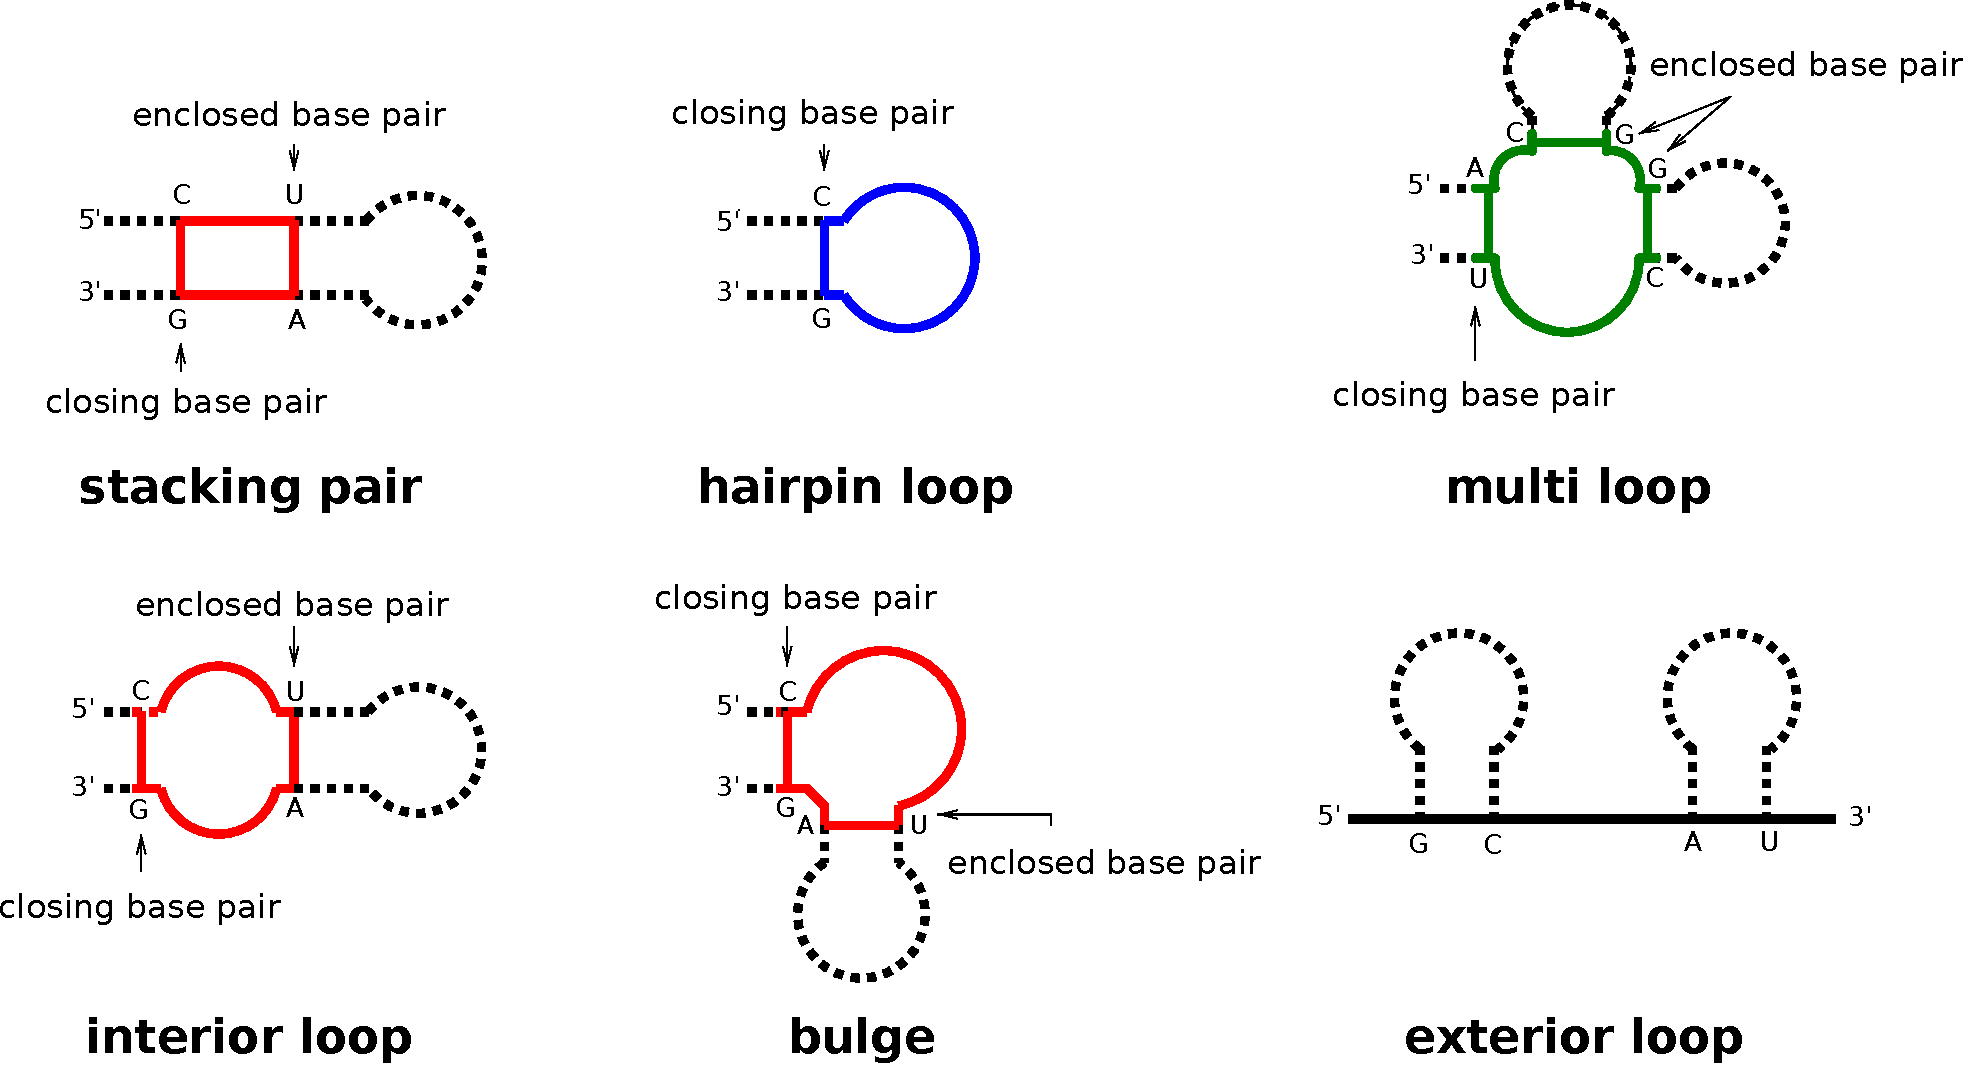
\includegraphics[width=\textwidth,height=\textheight/2,keepaspectratio=true]{loop_types}}
\end{DoxyImageNoCaption}


Any secondary structure can be decomposed into its loops. Each of the loops then can be scored in terms of free energy, and the free energy of an entire secondary structure is simply the sum of free energies of its loops.

 
\begin{DoxyImageNoCaption}
  \mbox{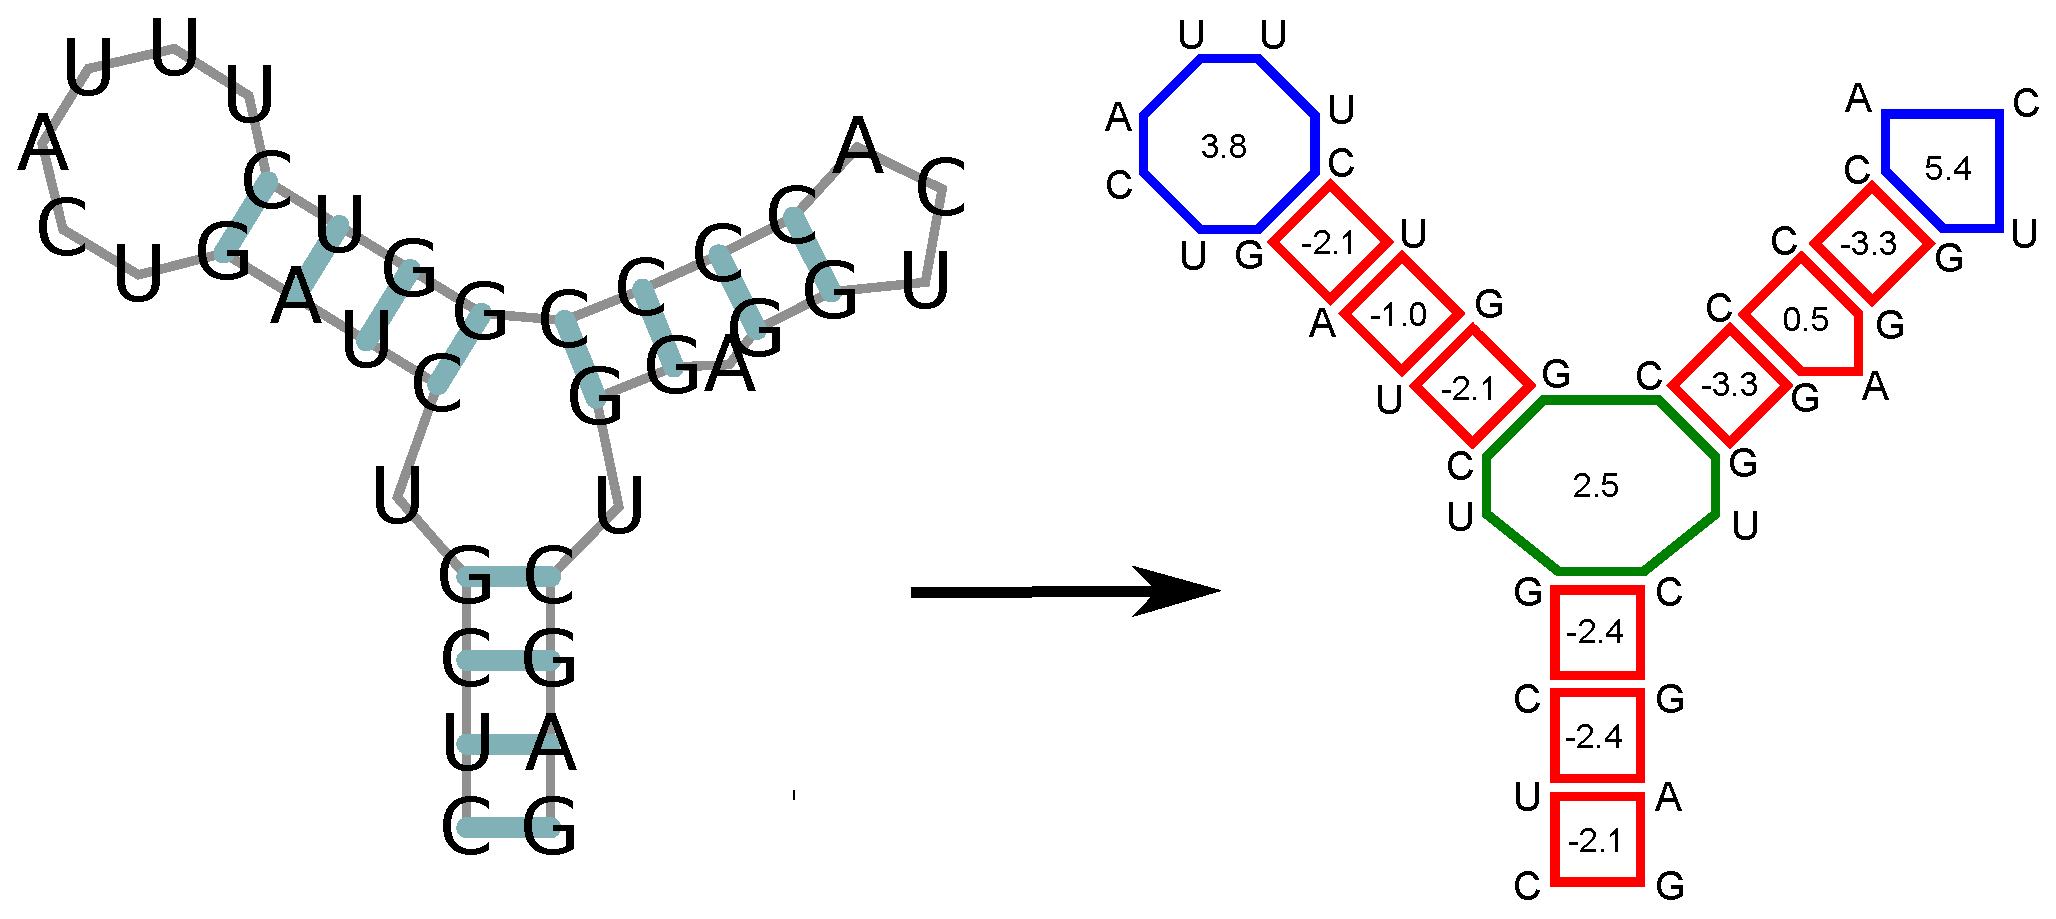
\includegraphics[width=\textwidth,height=\textheight/2,keepaspectratio=true]{loop_decomposition}}
\end{DoxyImageNoCaption}
\hypertarget{energy_evaluation_sec_loop_decomposition_api}{}\subsubsection{Free Energy Evaluation A\+PI}\label{energy_evaluation_sec_loop_decomposition_api}
While we implement some functions that decompose a secondary structure into its individual loops, the majority of methods provided in  are dedicated to free energy evaluation. The corresponding modules are\+:

\begin{DoxySeeAlso}{See also}
\hyperlink{group__eval}{Free Energy Evaluation}, \hyperlink{group__eval__loops}{Energy Evaluation for Individual Loops}
\end{DoxySeeAlso}
\hypertarget{energy_evaluation_sec_energy_parameters}{}\subsection{Free Energy Parameters}\label{energy_evaluation_sec_energy_parameters}
For secondary structure free energy evaluation we usually utilize the set of Nearest Neighbor Parameters also used in other software, such as {\itshape U\+N\+Afold} and {\itshape R\+N\+Astructure}. While the {\itshape R\+N\+Alib} already contains a compiled-\/in set of the latest {\itshape Turner 2004 Free Energy Parameters}, we defined a file format that allows to change these parameters at runtime. The {\ttfamily Vienna\+R\+NA Package} already comes with a set of parameter files containing


\begin{DoxyItemize}
\item Turner 1999 R\+NA parameters
\item Mathews 1999 D\+NA parameters
\item Andronescu 2007 R\+NA parameters
\item Mathews 2004 D\+NA parameters
\end{DoxyItemize}\hypertarget{energy_evaluation_sec_energy_parameters_api}{}\subsubsection{Free Energy Parameters Modification A\+PI}\label{energy_evaluation_sec_energy_parameters_api}
\begin{DoxySeeAlso}{See also}
\hyperlink{group__energy__parameters}{Energy Parameters}, \hyperlink{group__energy__parameters__rw}{Reading/\+Writing Energy Parameter Sets from/to File}
\end{DoxySeeAlso}
\hypertarget{energy_evaluation_sec_model_details}{}\subsection{Fine-\/tuning of the Energy Evaluation Model}\label{energy_evaluation_sec_model_details}
\begin{DoxySeeAlso}{See also}
\hyperlink{group__model__details}{Fine-\/tuning of the Implemented Models}
\end{DoxySeeAlso}
 \hypertarget{folding_grammar}{}\section{Secondary Structure Folding Grammar}\label{folding_grammar}
A description of the basic grammar to generate secondary structures, used for almost all prediction algorithms in our library and how to modify it.\hypertarget{folding_grammar_sec_recursions}{}\subsection{Secondary Structure Folding Recurrences}\label{folding_grammar_sec_recursions}
To predict secondary structures composed of the four distinguished loop types introduced before, all algorithms implemented in {\itshape R\+N\+Alib} follow a specific decomposition scheme, also known as the {\itshape R\+NA folding grammar}, or {\itshape Secondary Structure Folding Recurrences}.

 
\begin{DoxyImageNoCaption}
  \mbox{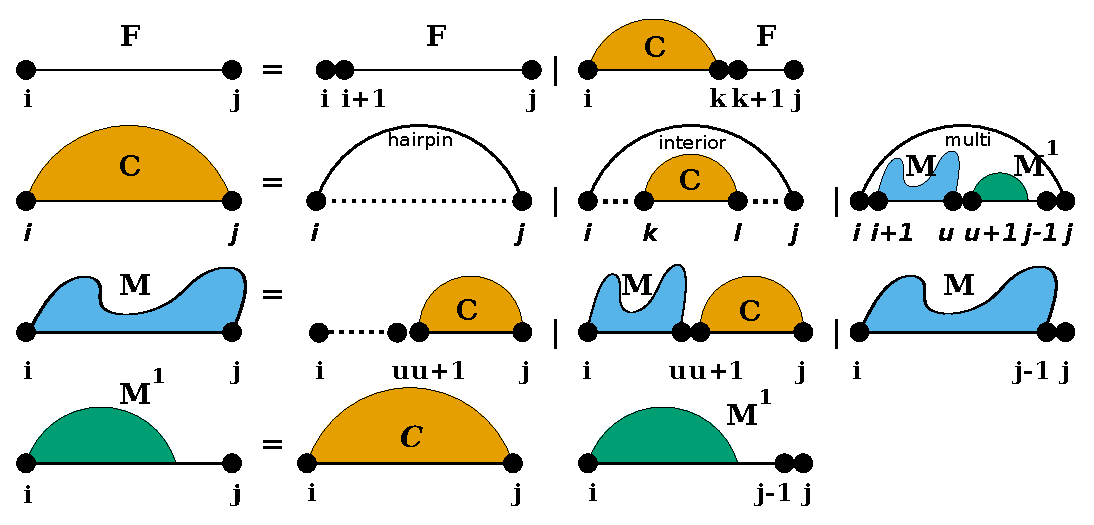
\includegraphics[width=\textwidth,height=\textheight/2,keepaspectratio=true]{recursions}}
\end{DoxyImageNoCaption}


However, compared to other R\+NA secondary structure prediction libraries, our implementation allows for a fine-\/grained control of the above recursions by constraining both, the individual derivations of the grammar as well as the evaluation of particular loop contributions. Furthermore, we provide a mechanism to extend the above grammar with additional derivation rules, so-\/called {\itshape Domains}.\hypertarget{folding_grammar_sec_domains}{}\subsection{Additional Structural Domains}\label{folding_grammar_sec_domains}
Some applications of R\+NA secondary structure prediction require an extension of the {\itshape regular R\+NA folding grammar}. For instance one would like to include proteins and other ligands binding to unpaired loop regions while competing with conventional base pairing. Another application could be that one may want to include the formation of self-\/enclosed structural modules, such as {\itshape G-\/quadruplexes}. For such applications, we provide a pair of additional domains that extend the regular R\+NA folding grammar, \hyperlink{group__domains__struc}{Structured Domains} and \hyperlink{group__domains__up}{Unstructured Domains}.

 
\begin{DoxyImageNoCaption}
  \mbox{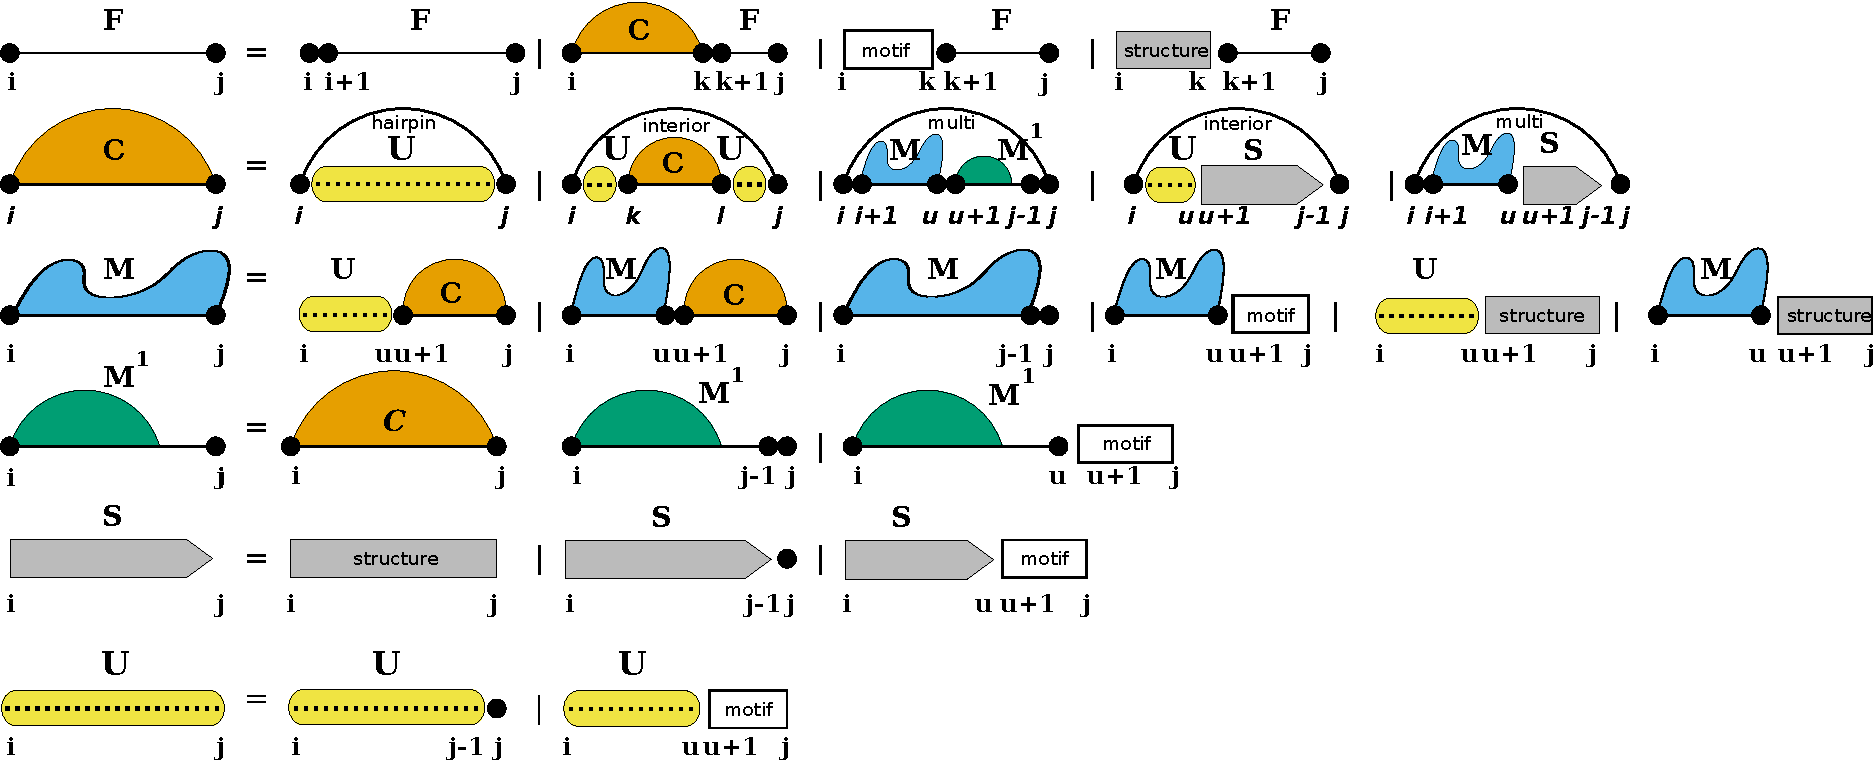
\includegraphics[width=\textwidth,height=\textheight/2,keepaspectratio=true]{GCrecursion}}
\end{DoxyImageNoCaption}


While unstructured domains are usually determined by a more or less precise sequence motif, e.\+g. the binding site for a protein, structured domains are considered self-\/enclosed modules with a more or less complex pairing pattern. Our extension with these two domains introduces two production rules to fill additional dynamic processing matrices {\ttfamily S} and {\ttfamily U} where we store the pre-\/computed contributions of structured domains ({\ttfamily S}), and unstructured domains ({\ttfamily U}).\hypertarget{folding_grammar_sec_domains_structured}{}\subsubsection{Structured Domains}\label{folding_grammar_sec_domains_structured}
Usually, structured domains represent self-\/enclosed structural modules that exhibit a more or less complex base pairing pattern. This can be more or less well-\/defined 3D motifs, such as {\itshape G-\/\+Quadruplexes}, or loops with additional non-\/canonical base pair interactions, such as {\itshape kink-\/turns}.

\begin{DoxyNote}{Note}
Currently, our implementation only provides the specialized case of {\itshape G-\/\+Quadruplexes}.
\end{DoxyNote}
\hypertarget{folding_grammar_sec_domains_up}{}\subsubsection{Unstructured Domains}\label{folding_grammar_sec_domains_up}
Unstructured domains appear in the production rules of the R\+NA folding grammar wherever new unpaired nucleotides are attached to a growing substructure (see also \cite{lorenz:2016b})\+:  
\begin{DoxyImageNoCaption}
  \mbox{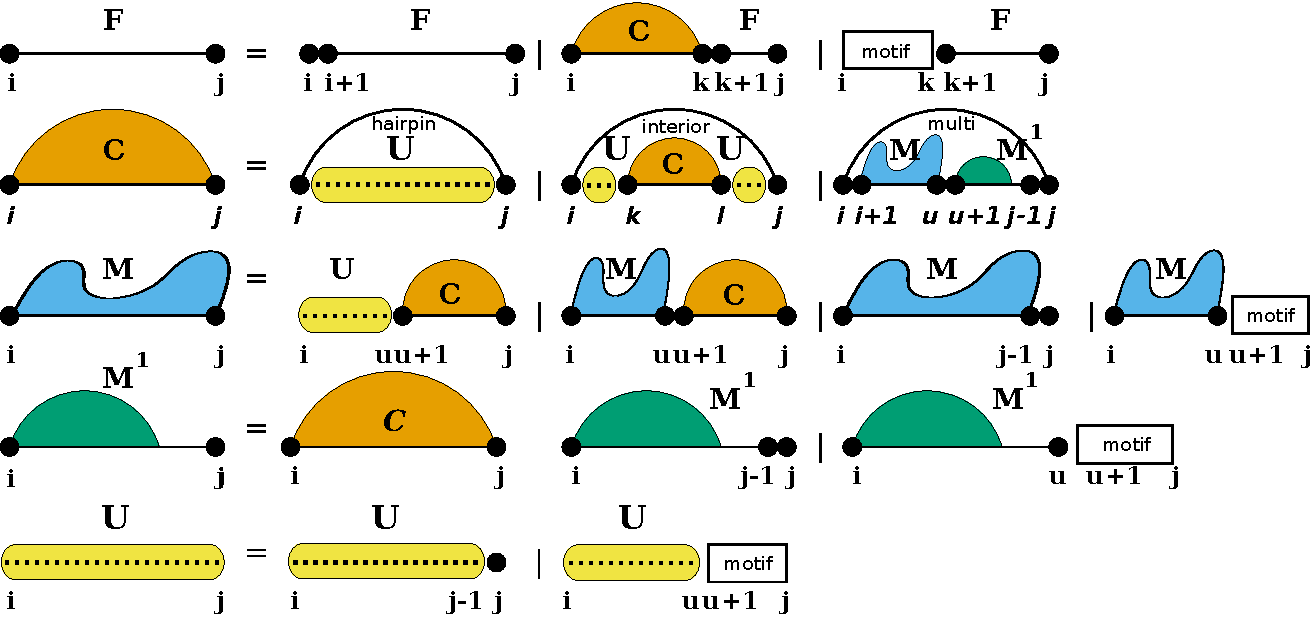
\includegraphics[width=\textwidth,height=\textheight/2,keepaspectratio=true]{Crecursion}}
\end{DoxyImageNoCaption}


The white boxes represent the stretch of R\+NA bound to the ligand and represented by a more or less specific sequence motif. The motif itself is considered unable to form base pairs. The additional production rule {\itshape U} is used to precompute the contribution of unpaired stretches possibly bound by one or more ligands. The auxiliary DP matrix for this production rule is filled right before processing the other (regular) production rules of the R\+NA folding grammar.\hypertarget{folding_grammar_sec_domains_api}{}\subsubsection{Domain Extension A\+PI}\label{folding_grammar_sec_domains_api}
For the sake of flexibility, each of the domains is associated with a specific data structure serving as an abstract interface to the extension. The interface uses callback functions to


\begin{DoxyItemize}
\item pre-\/compute arbitrary data, e.\+g. filling up additional dynamic programming matrices, and
\item evaluate the contribution of a paired or unpaired structural feature of the R\+NA.
\end{DoxyItemize}

Implementations of these callbacks are separate for regular free energy evaluation, e.\+g. M\+FE prediction, and partition function applications. A data structure holding arbitrary data required for the callback functions can be associated to the domain as well. While {\itshape R\+N\+Alib} comes with a default implementation for structured and unstructured domains, the system is entirely user-\/customizable.

\begin{DoxySeeAlso}{See also}
\hyperlink{group__domains__up}{Unstructured Domains}, \hyperlink{group__domains__struc}{Structured Domains}, \hyperlink{group__gquads}{G-\/\+Quadruplexes}, \hyperlink{group__ligands__up}{Ligands Binding to Unstructured Domains}
\end{DoxySeeAlso}
\hypertarget{folding_grammar_sec_constraints}{}\subsection{Constraints on the Folding Grammar}\label{folding_grammar_sec_constraints}
Secondary Structure constraints can be subdivided into two groups\+:


\begin{DoxyItemize}
\item Hard Constraints
\item Soft Constraints
\end{DoxyItemize}

While Hard-\/\+Constraints directly influence the production rules used in the folding recursions by allowing, disallowing, or enforcing certain decomposition steps, Soft-\/constraints on the other hand are used to change position specific contributions in the recursions by adding bonuses/penalties in form of pseudo free energies to certain loop configurations.

\begin{DoxyNote}{Note}
Secondary structure constraints are always applied at decomposition level, i.\+e. in each step of the recursive structure decomposition, for instance during M\+FE prediction.
\end{DoxyNote}
\hypertarget{folding_grammar_sec_constraints_hard_api}{}\subsubsection{Hard Constraints A\+PI}\label{folding_grammar_sec_constraints_hard_api}
Hard constraints as implemented in our library can be specified for individual loop types, i.\+e. the atomic derivations of the R\+NA folding grammar rules. Hence, the pairing behavior of both, single nucleotides and pairs of bases, can be constrained in every loop context separately. Additionally, an abstract implementation using a callback mechanism allows for full control of more complex hard constraints.

\begin{DoxySeeAlso}{See also}
\hyperlink{group__hard__constraints}{Hard Constraints}
\end{DoxySeeAlso}
\hypertarget{folding_grammar_sec_constraints_soft_api}{}\subsubsection{Soft Constraints A\+PI}\label{folding_grammar_sec_constraints_soft_api}
For the sake of memory efficiency, we do not implement a loop context aware version of soft constraints. The {\itshape static} soft constraints as implemented only distinguish unpaired from paired nucleotides. This is usually sufficient for most use-\/case scenarios. However, similar to hard constraints, an abstract soft constraints implementation using a callback mechanism exists, that allows for any soft constraint that is compatible with the R\+NA folding grammar. Thus, loop contexts and even individual derivation rules can be addressed separately for maximum flexibility in soft-\/constraints application.

\begin{DoxySeeAlso}{See also}
\hyperlink{group__soft__constraints}{Soft Constraints}, \hyperlink{group__constraints__ligand}{Incorporating Ligands Binding to Specific Sequence/\+Structure Motifs using Soft Constraints}, \hyperlink{group__SHAPE__reactivities}{S\+H\+A\+PE Reactivity Data}
\end{DoxySeeAlso}
 \hypertarget{secondary_structure_landscape}{}\section{R\+NA Secondary Structure Landscapes}\label{secondary_structure_landscape}
A description of the implicit landscape-\/like network of structures that appears upon modelling the transition of one structure into another\hypertarget{secondary_structure_landscape_landscape_neighborhood}{}\subsection{The Neighborhood of a Secondary Structure}\label{secondary_structure_landscape_landscape_neighborhood}
\hypertarget{secondary_structure_landscape_landscape_api}{}\subsection{The Secondary Structure Landscape A\+PI}\label{secondary_structure_landscape_landscape_api}
 \hypertarget{mfe_algorithm}{}\section{Minimum Free Energy Algorithm(s)}\label{mfe_algorithm}
Computing the Minimum Free Energy (M\+FE), i.\+e. the most stable conformation in thermodynamic equilibrium\hypertarget{mfe_algorithm_zuker_algorithm}{}\subsection{Zuker\textquotesingle{}s Algorithm}\label{mfe_algorithm_zuker_algorithm}
Our library provides fast dynamic programming Minimum Free Energy (M\+FE) folding algorithms derived from the decomposition scheme as described by \char`\"{}\+Zuker \& Stiegler (1981)\char`\"{} \cite{zuker:1981}.\hypertarget{mfe_algorithm_circular_folding}{}\subsection{M\+F\+E for circular R\+N\+As}\label{mfe_algorithm_circular_folding}
Folding of {\itshape circular} R\+NA sequences is handled as a post-\/processing step of the forward recursions. See \cite{hofacker:2006} for further details.\hypertarget{mfe_algorithm_mfe_algorithm_api}{}\subsection{M\+F\+E Algorithm A\+PI}\label{mfe_algorithm_mfe_algorithm_api}
We provide interfaces for the prediction of


\begin{DoxyItemize}
\item M\+FE and corresponding secondary structure for single sequences,
\item consensus M\+FE structures of sequence alignments, and
\item M\+FE structure for two hybridized R\+NA strands
\end{DoxyItemize}

\begin{DoxySeeAlso}{See also}
\hyperlink{group__mfe}{Minimum Free Energy (M\+FE) Algorithms}, consensus\+\_\+mfe\+\_\+fold, mfe\+\_\+cofold, \hyperlink{group__kl__neighborhood__mfe}{Computing M\+FE representatives of a Distance Based Partitioning}
\end{DoxySeeAlso}
 \hypertarget{pf_algorithm}{}\section{Partition Function and Equilibrium Probabilitiy Algorithm(s)}\label{pf_algorithm}
\hypertarget{pf_algorithm_sec_pf_intro}{}\subsection{Equilibrium Ensemble Statistics}\label{pf_algorithm_sec_pf_intro}
In contrast to methods that compute the property of a single structure in the ensemble, e.\+g. \hyperlink{mfe_algorithm}{Minimum Free Energy Algorithm(s)} , the partition function algorithms always consider the entire equilibrium ensemble. For that purpose, the Mc\+Caskill algorithm \cite{mccaskill:1990} and its variants can be used to efficiently compute


\begin{DoxyItemize}
\item the partition function, and from that
\item various equilibrium probabilities, for instance base pair probabilities, probabilities of individual structure motifs, and many more.
\end{DoxyItemize}

The principal idea behind this approach is that in equilibrium, statistical mechanics and polymer theory tells us that the frequency or probability $p(s)$ of a particular state $s$ depends on its energy $E(s)$ and follows a Boltzmann distribution, i.\+e. \[ p(s) \propto e^{-\beta E(s)} \text{ with } \beta = \frac{1}{kT} \] where $k \approx 1.987 \cdot 10^{-3} \frac{kcal}{mol~K}$ is the Boltzmann constant, and $T$ the thermodynamic temperature. From that relation, the actual probability of state $s$ can then be obtained using a proper scaling factor, the {\itshape canonical partition function} \[ Z = \sum_{s \in \Omega} e^{-\beta E(s)} \] where $\Omega$ is the finite set of all states. Finally, the equilibrium probability of state $s$ can be computed as \[ p(s) = \frac{e^{-\beta E(s)}}{Z} \]

Instead of enumerating all states exhaustively to compute $Z$ one can apply the \hyperlink{folding_grammar_sec_recursions}{Secondary Structure Folding Recurrences} again for an efficient computation in cubic time. An {\itshape outside} variant of the same recursions is then used to compute probabilities for base pairs, stretches of consecutive unpaired nucleotides, or structural motifs.

\begin{DoxySeeAlso}{See also}
Further details of the Partition function and Base Pair Probability algorithm can be obtained from Mc\+Caskill 1990 \cite{mccaskill:1990}
\end{DoxySeeAlso}
\hypertarget{pf_algorithm_sec_pf_api}{}\subsection{Partition Function and Equilibrium Probability A\+PI}\label{pf_algorithm_sec_pf_api}
We implement a wide variety of variants of the partition function algorithm according to Mc\+Caskill 1990 \cite{mccaskill:1990}. See the corresponding submodules for specific implementation details.

\begin{DoxySeeAlso}{See also}
\hyperlink{group__pf__fold}{Partition Function and Equilibrium Properties}, consensus\+\_\+pf\+\_\+fold, \hyperlink{group__pf__cofold}{Partition Function for Two Hybridized Sequences}, \hyperlink{group__up__cofold}{Partition Function for two Hybridized Sequences as a Stepwise Process}, local\+\_\+pf\+\_\+fold, \hyperlink{group__kl__neighborhood__pf}{Computing Partition Functions of a Distance Based Partitioning}
\end{DoxySeeAlso}
 \hypertarget{suboptimal_structures}{}\section{Suboptimals and (other) Representative Structures}\label{suboptimal_structures}
\hypertarget{suboptimal_structures_sec_suboptimals}{}\subsection{Suboptimal Secondary Structures}\label{suboptimal_structures_sec_suboptimals}
\hypertarget{suboptimal_structures_sec_samples}{}\subsection{Sampling Secondary Structures from the Ensemble}\label{suboptimal_structures_sec_samples}
\hypertarget{suboptimal_structures_sec_suboptimals_api}{}\subsection{Structure Enumeration and Sampling A\+PI}\label{suboptimal_structures_sec_suboptimals_api}
\begin{DoxySeeAlso}{See also}
\hyperlink{group__subopt__zuker}{Suboptimal Structures sensu Stiegler et al. 1984 / Zuker et al. 1989}, \hyperlink{group__subopt__wuchty}{Suboptimal Structures within an Energy Band around the M\+FE}, \hyperlink{group__subopt__stochbt}{Random Structure Samples from the Ensemble}, \hyperlink{group__mea__fold}{Compute the Structure with Maximum Expected Accuracy (M\+EA)}, \hyperlink{group__centroid__fold}{Compute the Centroid Structure}
\end{DoxySeeAlso}
 \hypertarget{rip}{}\section{R\+N\+A-\/\+R\+NA Interaction}\label{rip}
\hypertarget{rip_rip_intro}{}\subsection{rip\+\_\+intro}\label{rip_rip_intro}
The function of an R\+NA molecule often depends on its interaction with other R\+N\+As. The following routines therefore allows one to predict structures formed by two R\+NA molecules upon hybridization.\hypertarget{rip_rip_concat}{}\subsection{Concatenating R\+N\+A sequences}\label{rip_rip_concat}
One approach to co-\/folding two R\+N\+As consists of concatenating the two sequences and keeping track of the concatenation point in all energy evaluations. Correspondingly, many of the \hyperlink{group__mfe__global__deprecated_gabc8517f22cfe70595ee81fc837910d52}{cofold()} and \hyperlink{group__part__func__global__deprecated_gae5c1e7331718669bdae7a86de2be6184}{co\+\_\+pf\+\_\+fold()} routines take one sequence string as argument and use the the global variable \hyperlink{fold__vars_8h_ab9b2c3a37a5516614c06d0ab54b97cda}{cut\+\_\+point} to mark the concatenation point. Note that while the {\itshape R\+N\+Acofold} program uses the \textquotesingle{}\&\textquotesingle{} character to mark the chain break in its input, you should not use an \textquotesingle{}\&\textquotesingle{} when using the library routines (set \hyperlink{fold__vars_8h_ab9b2c3a37a5516614c06d0ab54b97cda}{cut\+\_\+point} instead).\hypertarget{rip_rip_stepwise}{}\subsection{R\+N\+A-\/\+R\+N\+A interaction as a Stepwise Process}\label{rip_rip_stepwise}
In a second approach to co-\/folding two R\+N\+As, cofolding is seen as a stepwise process. In the first step the probability of an unpaired region is calculated and in a second step this probability of an unpaired region is multiplied with the probability of an interaction between the two R\+N\+As. This approach is implemented for the interaction between a long target sequence and a short ligand R\+NA. Function \hyperlink{group__up__cofold_ga5b4ee40e190d2f633cd01cf0d2fe93cf}{pf\+\_\+unstru()} calculates the partition function over all unpaired regions in the input sequence. Function \hyperlink{group__up__cofold_ga1aa0aa02bc3a724f87360c03097afd00}{pf\+\_\+interact()}, which calculates the partition function over all possible interactions between two sequences, needs both sequence as separate strings as input.\hypertarget{rip_rip_api}{}\subsection{R\+N\+A-\/\+R\+N\+A Interaction A\+PI}\label{rip_rip_api}
 \hypertarget{local_vs_global}{}\section{Locally Stable Secondary Structures}\label{local_vs_global}
\hypertarget{local_vs_global_local_intro}{}\subsection{local\+\_\+intro}\label{local_vs_global_local_intro}
\hypertarget{local_vs_global_local_mfe}{}\subsection{local\+\_\+mfe}\label{local_vs_global_local_mfe}
\hypertarget{local_vs_global_local_pf}{}\subsection{local\+\_\+pf}\label{local_vs_global_local_pf}
\hypertarget{local_vs_global_local_api}{}\subsection{Locally Stable Secondary Structure A\+PI}\label{local_vs_global_local_api}
 \hypertarget{consensus_structures}{}\section{Comparative Structure Prediction}\label{consensus_structures}
\hypertarget{consensus_structures_consensus_structure_intro}{}\subsection{Incorporate Evolutionary Information}\label{consensus_structures_consensus_structure_intro}
Consensus structures can be predicted by a modified version of the \hyperlink{group__mfe__global__deprecated_gaadafcb0f140795ae62e5ca027e335a9b}{fold()} algorithm that takes a set of aligned sequences instead of a single sequence. The energy function consists of the mean energy averaged over the sequences, plus a covariance term that favors pairs with consistent and compensatory mutations and penalizes pairs that cannot be formed by all structures. For details see \cite{hofacker:2002} and \cite{bernhart:2008}.\hypertarget{consensus_structures_consensus_structure_api}{}\subsection{Comparative Structure Prediction A\+PI}\label{consensus_structures_consensus_structure_api}
 \hypertarget{classified_dp}{}\section{Classified DP variations}\label{classified_dp}
\hypertarget{classified_dp_classified_dp_intro}{}\subsection{The Idea of Classified Dynamic Programming}\label{classified_dp_classified_dp_intro}
Usually, thermodynamic properties using the basic recursions for \hyperlink{mfe_algorithm}{Minimum Free Energy Algorithm(s)}, \hyperlink{pf_algorithm}{Partition Function and Equilibrium Probabilitiy Algorithm(s)}, and so forth, are computed over the entire structure space. However, sometimes it is desired to partition the structure space {\itshape a priori} and compute the above properties for each of the resulting partitions. This approach directly leads to {\itshape Classified Dynamic Programming}.\hypertarget{classified_dp_distance_classes}{}\subsection{Distance Class Partitioning}\label{classified_dp_distance_classes}
The secondary structure space is divided into partitions according to the base pair distance to two given reference structures and all relevant properties are calculated for each of the resulting partitions.

\begin{DoxySeeAlso}{See also}
For further details, we refer to Lorenz et al. 2009 \cite{lorenz:2009}
\end{DoxySeeAlso}
\hypertarget{classified_dp_density_of_states}{}\subsection{Density of States (\+D\+O\+S)}\label{classified_dp_density_of_states}
\hypertarget{classified_dp_classified_dp_api}{}\subsection{Classified D\+P A\+PI}\label{classified_dp_classified_dp_api}
 \hypertarget{design}{}\section{R\+NA Sequence Design}\label{design}
\hypertarget{design_design_intro}{}\subsection{Generate Sequences that fold into particular Secondary Structures}\label{design_design_intro}
\hypertarget{design_design_api}{}\subsection{R\+N\+A Sequence Design A\+PI}\label{design_design_api}
\begin{DoxySeeAlso}{See also}
\hyperlink{group__inverse__fold}{Inverse Folding (Design)}
\end{DoxySeeAlso}
 \hypertarget{structure_probing_data}{}\section{Experimental Structure Probing Data}\label{structure_probing_data}
\hypertarget{structure_probing_data_structure_probing_intro}{}\subsection{Guide the Structure Prediction using Experimental Data}\label{structure_probing_data_structure_probing_intro}
\hypertarget{structure_probing_data_structure_probing_SHAPE}{}\subsubsection{S\+H\+A\+P\+E reactivities}\label{structure_probing_data_structure_probing_SHAPE}
\hypertarget{structure_probing_data_structure_probing_api}{}\subsection{Structure Probing Data A\+PI}\label{structure_probing_data_structure_probing_api}
\begin{DoxySeeAlso}{See also}
\hyperlink{group__probing__data}{Experimental Structure Probing Data}, \hyperlink{group__SHAPE__reactivities}{S\+H\+A\+PE Reactivity Data}, pertubation
\end{DoxySeeAlso}
 \hypertarget{ligand_binding}{}\section{Ligand Binding}\label{ligand_binding}
\hypertarget{ligand_binding_ligand_binding_intro}{}\subsection{Small Molecules and Proteins that bind to specific R\+N\+A Structures}\label{ligand_binding_ligand_binding_intro}
\hypertarget{ligand_binding_ligand_binding_api}{}\subsection{ligand\+\_\+binding\+\_\+api}\label{ligand_binding_ligand_binding_api}
In our library, we provide two different ways to incorporate ligand binding to R\+NA structures\+:


\begin{DoxyItemize}
\item \hyperlink{group__ligands__up}{Ligands Binding to Unstructured Domains}, and
\item \hyperlink{group__constraints__ligand}{Incorporating Ligands Binding to Specific Sequence/\+Structure Motifs using Soft Constraints}
\end{DoxyItemize}

The first approach is implemented as an actual extension of the folding grammar. It adds auxiliary derivation rules for each case when consecutive unpaired nucleotides are evaluated. Therefore, this model is applicable to ligand binding to any loop context.

The second approach, on the other hand, uses the soft-\/constraints feature to change the energy evaluation of hairpin-\/ or interior-\/loops. Hence, it can only be appleid when a ligand binds to a hairpin-\/like, or interior-\/loop like motif.

\begin{DoxySeeAlso}{See also}
\hyperlink{group__ligands__up}{Ligands Binding to Unstructured Domains}, \hyperlink{group__constraints__ligand}{Incorporating Ligands Binding to Specific Sequence/\+Structure Motifs using Soft Constraints}
\end{DoxySeeAlso}
 \hypertarget{structure_motifs}{}\section{(Tertiary) Structure Motifs}\label{structure_motifs}
\hypertarget{structure_motifs_structure_motifs_intro}{}\subsection{Incorporating Higher-\/\+Order (\+Tertiary) Structure Motifs}\label{structure_motifs_structure_motifs_intro}
\hypertarget{structure_motifs_structure_motif_gquad}{}\subsection{R\+N\+A G-\/\+Quadruplexes}\label{structure_motifs_structure_motif_gquad}
\hypertarget{structure_motifs_structure_motif_api}{}\subsection{(\+Tertiary) Structure Motif A\+PI}\label{structure_motifs_structure_motif_api}
 
\chapter{I/O Formats}
\label{io}
\Hypertarget{io}
Below, you\textquotesingle{}ll find a listing of different sections that introduce the most common notations of sequence and structure data, specifications of bioinformatics sequence and structure file formats, and various output file formats produced by our library.


\begin{DoxyItemize}
\item \hyperlink{rna_structure_notations}{R\+NA Structure Notations} describes the different notations and representations of R\+NA secondary structures
\item \hyperlink{file_formats}{File Formats} gives an overview of the file formats compatible with our library
\item \hyperlink{plots}{Plotting} shows the different (Post\+Script) plotting functions for R\+NA secondary structures, feature probabilities, and multiple sequence alignments 
\end{DoxyItemize}\hypertarget{rna_structure_notations}{}\section{R\+NA Structure Notations}\label{rna_structure_notations}
\hypertarget{rna_structure_notations_sec_structure_representations}{}\subsection{Representations of Secondary Structures}\label{rna_structure_notations_sec_structure_representations}
The standard representation of a secondary structure in our library is the \hyperlink{rna_structure_notations_dot-bracket-notation}{Dot-\/\+Bracket Notation (a.\+k.\+a. Dot-\/\+Parenthesis Notation)}, where matching brackets symbolize base pairs and unpaired bases are shown as dots. Based on that notation, more elaborate representations have been developed to include additional information, such as the loop context a nucleotide belongs to and to annotated pseudo-\/knots.

\begin{DoxySeeAlso}{See also}
\hyperlink{rna_structure_notations_dot-bracket-ext-notation}{Extended Dot-\/\+Bracket Notation}, \hyperlink{rna_structure_notations_wuss-notation}{Washington University Secondary Structure (W\+U\+SS) notation}
\end{DoxySeeAlso}
\hypertarget{rna_structure_notations_dot-bracket-notation}{}\subsection{Dot-\/\+Bracket Notation (a.\+k.\+a. Dot-\/\+Parenthesis Notation)}\label{rna_structure_notations_dot-bracket-notation}
The Dot-\/\+Bracket notation as introduced already in the early times of the Vienna\+R\+NA Package denotes base pairs by matching pairs of parenthesis {\ttfamily ()} and unpaired nucleotides by dots {\ttfamily .}.

Example\+: A simple helix of size 4 enclosing a hairpin of size 4 is annotated as \begin{DoxyVerb}((((....))))
\end{DoxyVerb}


\begin{DoxySeeAlso}{See also}
\hyperlink{group__struct__utils__pair__table_gac76c9ef3de507748fb0416a59323362b}{vrna\+\_\+ptable\+\_\+from\+\_\+string()}, \hyperlink{group__struct__utils__dot__bracket_gae966b9f44168a4f4b39ca42ffb5f37b7}{vrna\+\_\+db\+\_\+flatten()}, \hyperlink{group__struct__utils__dot__bracket_ga690425199c8b71545e7196e3af1436f8}{vrna\+\_\+db\+\_\+flatten\+\_\+to()}
\end{DoxySeeAlso}
\hypertarget{rna_structure_notations_dot-bracket-ext-notation}{}\subsection{Extended Dot-\/\+Bracket Notation}\label{rna_structure_notations_dot-bracket-ext-notation}
A more generalized version of the original Dot-\/\+Bracket notation may use additional pairs of brackets, such as {\ttfamily $<$$>$}, {\ttfamily \{\}}, and {\ttfamily \mbox{[}\mbox{]}}, and matching pairs of uppercase/lowercase letters. This allows for anotating pseudo-\/knots, since different pairs of brackets are not required to be nested.

Example\+: The follwing annotations of a simple structure with two crossing helices of size 4 are equivalent\+: \begin{DoxyVerb}<<<<[[[[....>>>>]]]]
((((AAAA....))))aaaa
AAAA{{{{....aaaa}}}}
\end{DoxyVerb}


\begin{DoxySeeAlso}{See also}
\hyperlink{group__struct__utils__pair__table_gac76c9ef3de507748fb0416a59323362b}{vrna\+\_\+ptable\+\_\+from\+\_\+string()}, \hyperlink{group__struct__utils__dot__bracket_gae966b9f44168a4f4b39ca42ffb5f37b7}{vrna\+\_\+db\+\_\+flatten()}, \hyperlink{group__struct__utils__dot__bracket_ga690425199c8b71545e7196e3af1436f8}{vrna\+\_\+db\+\_\+flatten\+\_\+to()}
\end{DoxySeeAlso}
\hypertarget{rna_structure_notations_wuss-notation}{}\subsection{Washington University Secondary Structure (\+W\+U\+S\+S) notation}\label{rna_structure_notations_wuss-notation}
The W\+U\+SS notation, as frequently used for consensus secondary structures in \hyperlink{file_formats_msa-formats-stockholm}{Stockholm 1.\+0 format} allows for a fine-\/grained annotation of base pairs and unpaired nucleotides, including pseudo-\/knots.

Below, you\textquotesingle{}ll find a list of secondary structure elements and their corresponding W\+U\+SS annotation (See also the infernal user guide at \href{http://eddylab.org/infernal/Userguide.pdf}{\tt http\+://eddylab.\+org/infernal/\+Userguide.\+pdf})


\begin{DoxyItemize}
\item {\bfseries Base pairs}

Nested base pairs are annotated by matching pairs of the symbols {\ttfamily $<$$>$}, {\ttfamily ()}, {\ttfamily \{\}}, and {\ttfamily \mbox{[}\mbox{]}}. Each of the matching pairs of parenthesis have their special meaning, however, when used as input in our programs, e.\+g. structure constraint, these details are usually ignored. Furthermore, base pairs that constitute as pseudo-\/knot are denoted by letters from the latin alphabet and are, if not denoted otherwise, ignored entirely in our programs.
\item {\bfseries Hairpin loops}

Unpaired nucleotides that constitute the hairpin loop are indicated by underscores, {\ttfamily \+\_\+}.

Example\+:
\begin{DoxyCode}
<<<<<\_\_\_\_\_>>>>>
\end{DoxyCode}

\item {\bfseries Bulges and interior loops}

Residues that constitute a bulge or interior loop are denoted by dashes, {\ttfamily -\/}.

Example\+:
\begin{DoxyCode}
(((--<<\_\_\_\_\_>>-)))
\end{DoxyCode}

\item {\bfseries Multibranch loops}

Unpaired nucleotides in multibranch loops are indicated by commas {\ttfamily ,}.

Example\+:
\begin{DoxyCode}
(((,,<<\_\_\_\_\_>>,<<\_\_\_\_>>)))
\end{DoxyCode}

\item {\bfseries External residues}

Single stranded nucleotides in the exterior loop, i.\+e. not enclosed by any other pair are denoted by colons, {\ttfamily \+:}.

Example\+:
\begin{DoxyCode}
<<<\_\_\_\_>>>:::
\end{DoxyCode}

\item {\bfseries Insertions}

In cases where an alignment represents the consensus with a known structure, insertions relative to the known structure are denoted by periods, {\ttfamily .}. Regions where local structural alignment was invoked, leaving regions of both target and query sequence unaligned, are indicated by tildes, {\ttfamily $\sim$}. \begin{DoxyNote}{Note}
These symbols only appear in alignments of a known (query) structure annotation to a target sequence of unknown structure.
\end{DoxyNote}

\item {\bfseries Pseudo-\/knots}

The W\+U\+SS notation allows for annotation of pseudo-\/knots using pairs of upper-\/case/lower-\/case letters. \begin{DoxyNote}{Note}
Our programs and library functions usually ignore pseudo-\/knots entirely treating them as unpaired nucleotides, if not stated otherwise.
\end{DoxyNote}
Example\+:
\begin{DoxyCode}
<<<\_AAA\_\_\_>>>aaa
\end{DoxyCode}
 
\end{DoxyItemize}

\begin{DoxySeeAlso}{See also}
\hyperlink{group__struct__utils__dot__bracket_ga02ca70cffb2d864f7b2d95d92218bae0}{vrna\+\_\+db\+\_\+from\+\_\+\+W\+U\+S\+S()}
\end{DoxySeeAlso}
\hypertarget{rna_structure_notations_sec_structure_representations_tree}{}\subsection{Tree Representations of Secondary Structures}\label{rna_structure_notations_sec_structure_representations_tree}
Alternatively, one may find representations with two types of node labels, \textquotesingle{}P\textquotesingle{} for paired and \textquotesingle{}U\textquotesingle{} for unpaired; a dot is then replaced by \textquotesingle{}(U)\textquotesingle{}, and each closed bracket is assigned an additional identifier \textquotesingle{}P\textquotesingle{}. We call this the expanded notation. In \cite{fontana:1993b} a condensed representation of the secondary structure is proposed, the so-\/called homeomorphically irreducible tree (H\+IT) representation. Here a stack is represented as a single pair of matching brackets labeled \textquotesingle{}P\textquotesingle{} and weighted by the number of base pairs. Correspondingly, a contiguous strain of unpaired bases is shown as one pair of matching brackets labeled \textquotesingle{}U\textquotesingle{} and weighted by its length. Generally any string consisting of matching brackets and identifiers is equivalent to a plane tree with as many different types of nodes as there are identifiers.

Bruce Shapiro proposed a coarse grained representation \cite{shapiro:1988}, which, does not retain the full information of the secondary structure. He represents the different structure elements by single matching brackets and labels them as


\begin{DoxyItemize}
\item {\ttfamily H} (hairpin loop),
\item {\ttfamily I} (interior loop),
\item {\ttfamily B} (bulge),
\item {\ttfamily M} (multi-\/loop), and
\item {\ttfamily S} (stack).
\end{DoxyItemize}

We extend his alphabet by an extra letter for external elements {\ttfamily E}. Again these identifiers may be followed by a weight corresponding to the number of unpaired bases or base pairs in the structure element. All tree representations (except for the dot-\/bracket form) can be encapsulated into a virtual root (labeled {\ttfamily R}).

The following example illustrates the different linear tree representations used by the package\+:

Consider the secondary structure represented by the dot-\/bracket string (full tree) \begin{DoxyVerb}.((..(((...)))..((..)))). \end{DoxyVerb}
 which is the most convenient condensed notation used by our programs and library functions.

Then, the following tree representations are equivalent\+:


\begin{DoxyItemize}
\item Expanded tree\+: \begin{DoxyVerb}((U)(((U)(U)((((U)(U)(U)P)P)P)(U)(U)(((U)(U)P)P)P)P)(U)R) \end{DoxyVerb}

\item H\+IT representation (Fontana et al. 1993 \cite{fontana:1993b})\+: \begin{DoxyVerb}((U1)((U2)((U3)P3)(U2)((U2)P2)P2)(U1)R) \end{DoxyVerb}

\item Coarse Grained \hyperlink{structTree}{Tree} Representation (Shapiro 1988 \cite{shapiro:1988})\+:
\begin{DoxyItemize}
\item Short (with root node {\ttfamily R}, without stem nodes {\ttfamily S})\+: \begin{DoxyVerb}((H)((H)M)R) \end{DoxyVerb}

\item Full (with root node {\ttfamily R})\+: \begin{DoxyVerb}(((((H)S)((H)S)M)S)R) \end{DoxyVerb}

\item Extended (with root node {\ttfamily R}, with external nodes {\ttfamily E})\+: \begin{DoxyVerb}((((((H)S)((H)S)M)S)E)R) \end{DoxyVerb}

\item Weighted (with root node {\ttfamily R}, with external nodes {\ttfamily E})\+: \begin{DoxyVerb}((((((H3)S3)((H2)S2)M4)S2)E2)R) \end{DoxyVerb}

\end{DoxyItemize}
\end{DoxyItemize}

The Expanded tree is rather clumsy and mostly included for the sake of completeness. The different versions of Coarse Grained \hyperlink{structTree}{Tree} Representations are variatios of Shapiro\textquotesingle{}s linear tree notation.

For the output of aligned structures from string editing, different representations are needed, where we put the label on both sides. The above examples for tree representations would then look like\+:

\begin{DoxyVerb}a) (UU)(P(P(P(P(UU)(UU)(P(P(P(UU)(UU)(UU)P)P)P)(UU)(UU)(P(P(UU)(U...
b) (UU)(P2(P2(U2U2)(P2(U3U3)P3)(U2U2)(P2(U2U2)P2)P2)(UU)P2)(UU)
c) (B(M(HH)(HH)M)B)
   (S(B(S(M(S(HH)S)(S(HH)S)M)S)B)S)
   (E(S(B(S(M(S(HH)S)(S(HH)S)M)S)B)S)E)
d) (R(E2(S2(B1(S2(M4(S3(H3)S3)((H2)S2)M4)S2)B1)S2)E2)R)
\end{DoxyVerb}


Aligned structures additionally contain the gap character \textquotesingle{}\+\_\+\textquotesingle{}.\hypertarget{rna_structure_notations_structure_notations_examples}{}\subsection{Examples for Structure Parsing and Conversion}\label{rna_structure_notations_structure_notations_examples}
\hypertarget{rna_structure_notations_structure_notations_api}{}\subsection{Structure Parsing and Conversion A\+PI}\label{rna_structure_notations_structure_notations_api}
Several functions are provided for parsing structures and converting to different representations.

\begin{DoxyVerb}char  *expand_Full(const char *structure)
\end{DoxyVerb}
 Convert the full structure from bracket notation to the expanded notation including root.

\begin{DoxyVerb}char *b2HIT (const char *structure)
\end{DoxyVerb}
 Converts the full structure from bracket notation to the H\+IT notation including root.

\begin{DoxyVerb}char *b2C (const char *structure)
\end{DoxyVerb}
 Converts the full structure from bracket notation to the a coarse grained notation using the \textquotesingle{}H\textquotesingle{} \textquotesingle{}B\textquotesingle{} \textquotesingle{}I\textquotesingle{} \textquotesingle{}M\textquotesingle{} and \textquotesingle{}R\textquotesingle{} identifiers.

\begin{DoxyVerb}char *b2Shapiro (const char *structure)
\end{DoxyVerb}
 Converts the full structure from bracket notation to the {\itshape weighted} coarse grained notation using the \textquotesingle{}H\textquotesingle{} \textquotesingle{}B\textquotesingle{} \textquotesingle{}I\textquotesingle{} \textquotesingle{}M\textquotesingle{} \textquotesingle{}S\textquotesingle{} \textquotesingle{}E\textquotesingle{} and \textquotesingle{}R\textquotesingle{} identifiers.

\begin{DoxyVerb}char  *expand_Shapiro (const char *coarse);
\end{DoxyVerb}
 Inserts missing \textquotesingle{}S\textquotesingle{} identifiers in unweighted coarse grained structures as obtained from \hyperlink{group__struct__utils__deprecated_ga9c80d92391f2833549a8b6dac92233f0}{b2\+C()}.

\begin{DoxyVerb}char *add_root (const char *structure)
\end{DoxyVerb}
 Adds a root to an un-\/rooted tree in any except bracket notation.

\begin{DoxyVerb}char  *unexpand_Full (const char *ffull)
\end{DoxyVerb}
 Restores the bracket notation from an expanded full or H\+IT tree, that is any tree using only identifiers \textquotesingle{}U\textquotesingle{} \textquotesingle{}P\textquotesingle{} and \textquotesingle{}R\textquotesingle{}.

\begin{DoxyVerb}char  *unweight (const char *wcoarse)
\end{DoxyVerb}
 Strip weights from any weighted tree.

\begin{DoxyVerb}void   unexpand_aligned_F (char *align[2])
\end{DoxyVerb}
 Converts two aligned structures in expanded notation.

\begin{DoxyVerb}void   parse_structure (const char *structure)
\end{DoxyVerb}
 Collects a statistic of structure elements of the full structure in bracket notation.

\begin{DoxySeeAlso}{See also}
\hyperlink{RNAstruct_8h}{R\+N\+Astruct.\+h} for prototypes and more detailed description 
\end{DoxySeeAlso}
\hypertarget{file_formats}{}\section{File Formats}\label{file_formats}
\hypertarget{file_formats_msa-formats}{}\subsection{File formats for Multiple Sequence Alignments (\+M\+S\+A)}\label{file_formats_msa-formats}
\hypertarget{file_formats_msa-formats-clustal}{}\subsubsection{Clustal\+W format}\label{file_formats_msa-formats-clustal}
The {\itshape ClustalW} format is a relatively simple text file containing a single multiple sequence alignment of D\+NA, R\+NA, or protein sequences. It was first used as an output format for the {\itshape clustalw} programs, but nowadays it may also be generated by various other sequence alignment tools. The specification is straight forward\+:


\begin{DoxyItemize}
\item The first line starts with the words\begin{DoxyVerb}CLUSTAL W \end{DoxyVerb}
 or \begin{DoxyVerb}CLUSTALW \end{DoxyVerb}

\item After the above header there is at least one empty line
\item Finally, one or more blocks of sequence data are following, where each block is separated by at least one empty line
\end{DoxyItemize}Each line in a blocks of sequence data consists of the sequence name followed by the sequence symbols, separated by at least one whitespace character. Usually, the length of a sequence in one block does not exceed 60 symbols. Optionally, an additional whitespace separated cumulative residue count may follow the sequence symbols. Optionally, a block may be followed by a line depicting the degree of conservation of the respective alignment columns.

\begin{DoxyNote}{Note}
Sequence names and the sequences must not contain whitespace characters! Allowed gap symbols are the hyphen {\itshape }(\char`\"{}-\/\char`\"{}), and dot {\itshape }(\char`\"{}.\char`\"{}).
\end{DoxyNote}
\begin{DoxyWarning}{Warning}
Please note that many programs that output this format tend to truncate the sequence names to a limited number of characters, for instance the first 15 characters. This can destroy the uniqueness of identifiers in your M\+SA.
\end{DoxyWarning}
Here is an example alignment in ClustalW format\+: 
\begin{DoxyVerbInclude}
CLUSTAL W (1.83) multiple sequence alignment


AL031296.1/85969-86120      CUGCCUCACAACGUUUGUGCCUCAGUUACCCGUAGAUGUAGUGAGGGUAACAAUACUUAC
AANU01225121.1/438-603      CUGCCUCACAACAUUUGUGCCUCAGUUACUCAUAGAUGUAGUGAGGGUGACAAUACUUAC
AAWR02037329.1/29294-29150  ---CUCGACACCACU---GCCUCGGUUACCCAUCGGUGCAGUGCGGGUAGUAGUACCAAU

AL031296.1/85969-86120      UCUCGUUGGUGAUAAGGAACAGCU
AANU01225121.1/438-603      UCUCGUUGGUGAUAAGGAACAGCU
AAWR02037329.1/29294-29150  GCUAAUUAGUUGUGAGGACCAACU 
\end{DoxyVerbInclude}
\hypertarget{file_formats_msa-formats-stockholm}{}\subsubsection{Stockholm 1.\+0 format}\label{file_formats_msa-formats-stockholm}
Here is an example alignment in Stockholm 1.\+0 format\+: 
\begin{DoxyVerbInclude}
# STOCKHOLM 1.0

#=GF AC   RF01293
#=GF ID   ACA59
#=GF DE   Small nucleolar RNA ACA59
#=GF AU   Wilkinson A
#=GF SE   Predicted; WAR; Wilkinson A
#=GF SS   Predicted; WAR; Wilkinson A
#=GF GA   43.00
#=GF TC   44.90
#=GF NC   40.30
#=GF TP   Gene; snRNA; snoRNA; HACA-box;
#=GF BM   cmbuild -F CM SEED
#=GF CB   cmcalibrate --mpi CM
#=GF SM   cmsearch --cpu 4 --verbose --nohmmonly -E 1000 -Z 549862.597050 CM SEQDB
#=GF DR   snoRNABase; ACA59;
#=GF DR   SO; 0001263; ncRNA_gene;
#=GF DR   GO; 0006396; RNA processing;
#=GF DR   GO; 0005730; nucleolus;
#=GF RN   [1]
#=GF RM   15199136
#=GF RT   Human box H/ACA pseudouridylation guide RNA machinery.
#=GF RA   Kiss AM, Jady BE, Bertrand E, Kiss T
#=GF RL   Mol Cell Biol. 2004;24:5797-5807.
#=GF WK   Small_nucleolar_RNA
#=GF SQ   3


AL031296.1/85969-86120     CUGCCUCACAACGUUUGUGCCUCAGUUACCCGUAGAUGUAGUGAGGGUAACAAUACUUACUCUCGUUGGUGAUAAGGAACAGCU
AANU01225121.1/438-603     CUGCCUCACAACAUUUGUGCCUCAGUUACUCAUAGAUGUAGUGAGGGUGACAAUACUUACUCUCGUUGGUGAUAAGGAACAGCU
AAWR02037329.1/29294-29150 ---CUCGACACCACU---GCCUCGGUUACCCAUCGGUGCAGUGCGGGUAGUAGUACCAAUGCUAAUUAGUUGUGAGGACCAACU
#=GC SS_cons               -----((((,<<<<<<<<<___________>>>>>>>>>,,,,<<<<<<<______>>>>>>>,,,,,))))::::::::::::
#=GC RF                    CUGCcccaCAaCacuuguGCCUCaGUUACcCauagguGuAGUGaGgGuggcAaUACccaCcCucgUUgGuggUaAGGAaCAgCU
//
\end{DoxyVerbInclude}


\begin{DoxySeeAlso}{See also}
\hyperlink{rna_structure_notations_wuss-notation}{Washington University Secondary Structure (W\+U\+SS) notation} on legal characters for the consensus secondary structure line {\itshape S\+S\+\_\+cons} and their interpretation
\end{DoxySeeAlso}
\hypertarget{file_formats_msa-formats-fasta}{}\subsubsection{F\+A\+S\+T\+A (\+Pearson) format}\label{file_formats_msa-formats-fasta}
\begin{DoxyNote}{Note}
Sequence names must not contain whitespace characters. Otherwise, the parts after the first whitespace will be dropped. The only allowed gap character is the hyphen {\itshape }(\char`\"{}-\/\char`\"{}).
\end{DoxyNote}
Here is an example alignment in F\+A\+S\+TA format\+: 
\begin{DoxyVerbInclude}
>AL031296.1/85969-86120
CUGCCUCACAACGUUUGUGCCUCAGUUACCCGUAGAUGUAGUGAGGGUAACAAUACUUAC
UCUCGUUGGUGAUAAGGAACAGCU
>AANU01225121.1/438-603
CUGCCUCACAACAUUUGUGCCUCAGUUACUCAUAGAUGUAGUGAGGGUGACAAUACUUAC
UCUCGUUGGUGAUAAGGAACAGCU
>AAWR02037329.1/29294-29150
---CUCGACACCACU---GCCUCGGUUACCCAUCGGUGCAGUGCGGGUAGUAGUACCAAU
GCUAAUUAGUUGUGAGGACCAACU
\end{DoxyVerbInclude}
\hypertarget{file_formats_msa-formats-maf}{}\subsubsection{M\+A\+F format}\label{file_formats_msa-formats-maf}
The multiple alignment format (M\+AF) is usually used to store multiple alignments on D\+NA level between entire genomes. It consists of independent blocks of aligned sequences which are annotated by their genomic location. Consequently, an M\+AF formatted M\+SA file may contain multiple records. M\+AF files start with a line \begin{DoxyVerb}##maf
\end{DoxyVerb}
 which is optionally extended by whitespace delimited key=value pairs. Lines starting with the character (\char`\"{}\#\char`\"{}) are considered comments and usually ignored.

A M\+AF block starts with character (\char`\"{}a\char`\"{}) at the beginning of a line, optionally followed by whitespace delimited key=value pairs. The next lines start with character (\char`\"{}s\char`\"{}) and contain sequence information of the form \begin{DoxyVerb}s src start size strand srcSize sequence
\end{DoxyVerb}
 where
\begin{DoxyItemize}
\item {\itshape src} is the name of the sequence source
\item {\itshape start} is the start of the aligned region within the source (0-\/based)
\item {\itshape size} is the length of the aligned region without gap characters
\item {\itshape strand} is either (\char`\"{}+\char`\"{}) or (\char`\"{}-\/\char`\"{}), depicting the location of the aligned region relative to the source
\item {\itshape src\+Size} is the size of the entire sequence source, e.\+g. the full chromosome
\item {\itshape sequence} is the aligned sequence including gaps depicted by the hyphen (\char`\"{}-\/\char`\"{})
\end{DoxyItemize}Here is an example alignment in M\+AF format (bluntly taken from the \href{https://cgwb.nci.nih.gov/FAQ/FAQformat.html#format5}{\tt U\+C\+SC Genome browser website})\+: 
\begin{DoxyVerbInclude}
##maf version=1 scoring=tba.v8 
# tba.v8 (((human chimp) baboon) (mouse rat)) 
# multiz.v7
# maf_project.v5 _tba_right.maf3 mouse _tba_C
# single_cov2.v4 single_cov2 /dev/stdin
                   
a score=23262.0     
s hg16.chr7    27578828 38 + 158545518 AAA-GGGAATGTTAACCAAATGA---ATTGTCTCTTACGGTG
s panTro1.chr6 28741140 38 + 161576975 AAA-GGGAATGTTAACCAAATGA---ATTGTCTCTTACGGTG
s baboon         116834 38 +   4622798 AAA-GGGAATGTTAACCAAATGA---GTTGTCTCTTATGGTG
s mm4.chr6     53215344 38 + 151104725 -AATGGGAATGTTAAGCAAACGA---ATTGTCTCTCAGTGTG
s rn3.chr4     81344243 40 + 187371129 -AA-GGGGATGCTAAGCCAATGAGTTGTTGTCTCTCAATGTG
                   
a score=5062.0                    
s hg16.chr7    27699739 6 + 158545518 TAAAGA
s panTro1.chr6 28862317 6 + 161576975 TAAAGA
s baboon         241163 6 +   4622798 TAAAGA 
s mm4.chr6     53303881 6 + 151104725 TAAAGA
s rn3.chr4     81444246 6 + 187371129 taagga

a score=6636.0
s hg16.chr7    27707221 13 + 158545518 gcagctgaaaaca
s panTro1.chr6 28869787 13 + 161576975 gcagctgaaaaca
s baboon         249182 13 +   4622798 gcagctgaaaaca
s mm4.chr6     53310102 13 + 151104725 ACAGCTGAAAATA

\end{DoxyVerbInclude}
\hypertarget{file_formats_constraint-formats}{}\subsection{File formats to manipulate the R\+N\+A folding grammar}\label{file_formats_constraint-formats}
\hypertarget{file_formats_constraint-formats-file}{}\subsubsection{Command Files}\label{file_formats_constraint-formats-file}
The R\+N\+Alib and many programs of the Vienna\+R\+NA Package can parse and apply data from so-\/called command files. These commands may refer to structure constraints or even extensions of the R\+NA folding grammar (such as \hyperlink{group__domains__up}{Unstructured Domains}). Commands are given as a line of whitespace delimited data fields. The syntax we use extends the constraint definitions used in the \href{http://mfold.rna.albany.edu/?q=mfold}{\tt mfold} / \href{http://mfold.rna.albany.edu/?q=DINAMelt/software}{\tt U\+N\+Afold} software, where each line begins with a command character followed by a set of positions.~\newline
However, we introduce several new commands, and allow for an optional loop type context specifier in form of a sequence of characters, and an orientation flag that enables one to force a nucleotide to pair upstream, or downstream.\hypertarget{file_formats_constraint_commands}{}\paragraph{Constraint commands}\label{file_formats_constraint_commands}
The following set of commands is recognized\+:
\begin{DoxyItemize}
\item {\ttfamily F} $ \ldots $ Force
\item {\ttfamily P} $ \ldots $ Prohibit
\item {\ttfamily C} $ \ldots $ Conflicts/\+Context dependency
\item {\ttfamily A} $ \ldots $ Allow (for non-\/canonical pairs)
\item {\ttfamily E} $ \ldots $ Soft constraints for unpaired position(s), or base pair(s)
\end{DoxyItemize}\hypertarget{file_formats_domain_commands}{}\paragraph{R\+N\+A folding grammar exensions}\label{file_formats_domain_commands}

\begin{DoxyItemize}
\item {\ttfamily UD} $ \ldots $ Add ligand binding using the \hyperlink{group__domains__up}{Unstructured Domains} feature
\end{DoxyItemize}\hypertarget{file_formats_command_file_loop_types}{}\paragraph{Specification of the loop type context}\label{file_formats_command_file_loop_types}
The optional loop type context specifier {\ttfamily }\mbox{[}L\+O\+OP\mbox{]} may be a combination of the following\+:
\begin{DoxyItemize}
\item {\ttfamily E} $ \ldots $ Exterior loop
\item {\ttfamily H} $ \ldots $ Hairpin loop
\item {\ttfamily I} $ \ldots $ Interior loop
\item {\ttfamily M} $ \ldots $ Multibranch loop
\item {\ttfamily A} $ \ldots $ All loops
\end{DoxyItemize}

For structure constraints, we additionally allow one to address base pairs enclosed by a particular kind of loop, which results in the specifier {\ttfamily }\mbox{[}W\+H\+E\+RE\mbox{]} which consists of {\ttfamily }\mbox{[}L\+O\+OP\mbox{]} plus the following character\+:
\begin{DoxyItemize}
\item {\ttfamily i} $ \ldots $ enclosed pair of an Interior loop
\item {\ttfamily m} $ \ldots $ enclosed pair of a Multibranch loop
\end{DoxyItemize}

If no {\ttfamily }\mbox{[}L\+O\+OP\mbox{]} or {\ttfamily }\mbox{[}W\+H\+E\+RE\mbox{]} flags are set, all contexts are considered (equivalent to {\ttfamily A} )\hypertarget{file_formats_const_file_orientation}{}\paragraph{Controlling the orientation of base pairing}\label{file_formats_const_file_orientation}
For particular nucleotides that are forced to pair, the following {\ttfamily }\mbox{[}O\+R\+I\+E\+N\+T\+A\+T\+I\+ON\mbox{]} flags may be used\+:
\begin{DoxyItemize}
\item {\ttfamily U} $ \ldots $ Upstream
\item {\ttfamily D} $ \ldots $ Downstream
\end{DoxyItemize}

If no {\ttfamily }\mbox{[}O\+R\+I\+E\+N\+T\+A\+T\+I\+ON\mbox{]} flag is set, both directions are considered.\hypertarget{file_formats_const_file_seq_coords}{}\paragraph{Sequence coordinates}\label{file_formats_const_file_seq_coords}
Sequence positions of nucleotides/base pairs are $ 1- $ based and consist of three positions $ i $, $ j $, and $ k $. Alternativly, four positions may be provided as a pair of two position ranges $ [i:j] $, and $ [k:l] $ using the \textquotesingle{}-\/\textquotesingle{} sign as delimiter within each range, i.\+e. $ i-j $, and $ k-l $.\hypertarget{file_formats_const_file_syntax}{}\paragraph{Valid constraint commands}\label{file_formats_const_file_syntax}
Below are resulting general cases that are considered {\itshape valid} constraints\+:


\begin{DoxyEnumerate}
\item {\bfseries \char`\"{}\+Forcing a range of nucleotide positions to be paired\char`\"{}}\+:~\newline
 Syntax\+:
\begin{DoxyCode}
F i 0 k [WHERE] [ORIENTATION] 
\end{DoxyCode}
~\newline
 Description\+:~\newline
 Enforces the set of $ k $ consecutive nucleotides starting at position $ i $ to be paired. The optional loop type specifier {\ttfamily }\mbox{[}W\+H\+E\+RE\mbox{]} allows to force them to appear as closing/enclosed pairs of certain types of loops.
\item {\bfseries \char`\"{}\+Forcing a set of consecutive base pairs to form\char`\"{}}\+:~\newline
 Syntax\+:\begin{DoxyVerb}F i j k [WHERE] \end{DoxyVerb}
~\newline
 Description\+:~\newline
 Enforces the base pairs $ (i,j), \ldots, (i+(k-1), j-(k-1)) $ to form. The optional loop type specifier {\ttfamily }\mbox{[}W\+H\+E\+RE\mbox{]} allows to specify in which loop context the base pair must appear.
\item {\bfseries \char`\"{}\+Prohibiting a range of nucleotide positions to be paired\char`\"{}}\+:~\newline
 Syntax\+:\begin{DoxyVerb}P i 0 k [WHERE] \end{DoxyVerb}
~\newline
 Description\+:~\newline
 Prohibit a set of $ k $ consecutive nucleotides to participate in base pairing, i.\+e. make these positions unpaired. The optional loop type specifier {\ttfamily }\mbox{[}W\+H\+E\+RE\mbox{]} allows to force the nucleotides to appear within the loop of specific types.
\item {\bfseries \char`\"{}\+Probibiting a set of consecutive base pairs to form\char`\"{}}\+:~\newline
 Syntax\+:\begin{DoxyVerb}P i j k [WHERE] \end{DoxyVerb}
~\newline
 Description\+:~\newline
 Probibit the base pairs $ (i,j), \ldots, (i+(k-1), j-(k-1)) $ to form. The optional loop type specifier {\ttfamily }\mbox{[}W\+H\+E\+RE\mbox{]} allows to specify the type of loop they are disallowed to be the closing or an enclosed pair of.
\item {\bfseries \char`\"{}\+Prohibiting two ranges of nucleotides to pair with each other\char`\"{}}\+:~\newline
 Syntax\+:\begin{DoxyVerb}P i-j k-l [WHERE] \end{DoxyVerb}
 Description\+:~\newline
 Prohibit any nucleotide $ p \in [i:j] $ to pair with any other nucleotide $ q \in [k:l] $. The optional loop type specifier {\ttfamily }\mbox{[}W\+H\+E\+RE\mbox{]} allows to specify the type of loop they are disallowed to be the closing or an enclosed pair of.
\item {\bfseries \char`\"{}\+Enforce a loop context for a range of nucleotide positions\char`\"{}}\+:~\newline
 Syntax\+:\begin{DoxyVerb}C i 0 k [WHERE] \end{DoxyVerb}
 Description\+:~\newline
 This command enforces nucleotides to be unpaired similar to {\itshape prohibiting} nucleotides to be paired, as described above. It too marks the corresponding nucleotides to be unpaired, however, the {\ttfamily }\mbox{[}W\+H\+E\+RE\mbox{]} flag can be used to enforce specfic loop types the nucleotides must appear in.
\item {\bfseries \char`\"{}\+Remove pairs that conflict with a set of consecutive base pairs\char`\"{}}\+:~\newline
 Syntax\+:\begin{DoxyVerb}C i j k \end{DoxyVerb}
~\newline
 Description\+:~\newline
 Remove all base pairs that conflict with a set of consecutive base pairs $ (i,j), \ldots, (i+(k-1), j-(k-1)) $. Two base pairs $ (i,j) $ and $ (p,q) $ conflict with each other if $ i < p < j < q $, or $ p < i < q < j $.
\item {\bfseries \char`\"{}\+Allow a set of consecutive (non-\/canonical) base pairs to form\char`\"{}}\+:~\newline
 Syntax\+:
\begin{DoxyCode}
A i j k [WHERE] 
\end{DoxyCode}
~\newline
 Description\+:~\newline
 This command enables the formation of the consecutive base pairs $ (i,j), \ldots, (i+(k-1), j-(k-1)) $, no matter if they are {\itshape canonical}, or {\itshape non-\/canonical}. In contrast to the above {\ttfamily F} and {\ttfamily W} commands, which remove conflicting base pairs, the {\ttfamily A} command does not. Therefore, it may be used to allow {\itshape non-\/canoncial} base pair interactions. Since the R\+N\+Alib does not contain free energy contributions $ E_{ij} $ for non-\/canonical base pairs $ (i,j) $, they are scored as the {\itshape maximum} of similar, known contributions. In terms of a {\itshape Nussinov} like scoring function the free energy of non-\/canonical base pairs is therefore estimated as \[ E_{ij} = \min \left[ \max_{(i,k) \in \{GC, CG, AU, UA, GU, UG\}} E_{ik}, \max_{(k,j) \in \{GC, CG, AU, UA, GU, UG\}} E_{kj} \right]. \] The optional loop type specifier {\ttfamily }\mbox{[}W\+H\+E\+RE\mbox{]} allows to specify in which loop context the base pair may appear.
\item {\bfseries \char`\"{}\+Apply pseudo free energy to a range of unpaired nucleotide positions\char`\"{}}\+:~\newline
 Syntax\+:
\begin{DoxyCode}
E i 0 k e 
\end{DoxyCode}
~\newline
 Description\+:~\newline
 Use this command to apply a pseudo free energy of $ e $ to the set of $ k $ consecutive nucleotides, starting at position $ i $. The pseudo free energy is applied only if these nucleotides are considered unpaired in the recursions, or evaluations, and is expected to be given in $ kcal / mol $.
\item {\bfseries \char`\"{}\+Apply pseudo free energy to a set of consecutive base pairs\char`\"{}}\+:~\newline
 Syntax
\begin{DoxyCode}
E i j k e 
\end{DoxyCode}
~\newline
 Use this command to apply a pseudo free energy of $ e $ to the set of base pairs $ (i,j), \ldots, (i+(k-1), j-(k-1)) $. Energies are expected to be given in $ kcal / mol $.
\end{DoxyEnumerate}\hypertarget{file_formats_domains_syntax}{}\paragraph{Valid domain extensions commands}\label{file_formats_domains_syntax}

\begin{DoxyEnumerate}
\item {\bfseries \char`\"{}\+Add ligand binding to unpaired motif (a.\+k.\+a. unstructured domains)\char`\"{}}\+:~\newline
 Syntax\+:
\begin{DoxyCode}
UD m e [LOOP] 
\end{DoxyCode}
~\newline
 Description\+:~\newline
 Add ligand binding to unpaired sequence motif $ m $ (given in I\+U\+P\+AC format, capital letters) with binding energy $ e $ in particular loop type(s).~\newline
 Example\+: 
\begin{DoxyCode}
UD  AAA   -5.0    A
\end{DoxyCode}
~\newline
 The above example applies a binding free energy of $ -5 kcal/mol $ for a motif A\+AA that may be present in all loop types. 
\end{DoxyEnumerate}\hypertarget{plots}{}\section{Plotting}\label{plots}
Create Plots of Secondary Structures, Feature Motifs, and Sequence Alignments\hypertarget{plots_utils_ss}{}\subsection{Producing secondary structure graphs}\label{plots_utils_ss}
\begin{DoxyVerb}int PS_rna_plot ( char *string,
                  char *structure,
                  char *file)
\end{DoxyVerb}
 Produce a secondary structure graph in Post\+Script and write it to \textquotesingle{}filename\textquotesingle{}.

\begin{DoxyVerb}int PS_rna_plot_a (
            char *string,
            char *structure,
            char *file,
            char *pre,
            char *post)
\end{DoxyVerb}
 Produce a secondary structure graph in Post\+Script including additional annotation macros and write it to \textquotesingle{}filename\textquotesingle{}.

\begin{DoxyVerb}int gmlRNA (char *string,
            char *structure,
            char *ssfile,
            char option)
\end{DoxyVerb}
 Produce a secondary structure graph in Graph Meta Language (gml) and write it to a file.

\begin{DoxyVerb}int ssv_rna_plot (char *string,
                  char *structure,
                  char *ssfile)
\end{DoxyVerb}
 Produce a secondary structure graph in S\+Struct\+View format.

\begin{DoxyVerb}int svg_rna_plot (char *string,
                  char *structure,
                  char *ssfile)
\end{DoxyVerb}
 Produce a secondary structure plot in S\+VG format and write it to a file.

\begin{DoxyVerb}int xrna_plot ( char *string,
                char *structure,
                char *ssfile)
\end{DoxyVerb}
 Produce a secondary structure plot for further editing in X\+R\+NA.

\begin{DoxyVerb}int rna_plot_type
\end{DoxyVerb}
 Switch for changing the secondary structure layout algorithm.

Two low-\/level functions provide direct access to the graph lauyouting algorithms\+:

\begin{DoxyVerb}int simple_xy_coordinates ( short *pair_table,
                            float *X,
                            float *Y)
\end{DoxyVerb}
 Calculate nucleotide coordinates for secondary structure plot the {\itshape Simple way}

\begin{DoxyVerb}int naview_xy_coordinates ( short *pair_table,
                            float *X,
                            float *Y)
\end{DoxyVerb}


\begin{DoxySeeAlso}{See also}
\hyperlink{PS__dot_8h}{P\+S\+\_\+dot.\+h} and naview.\+h for more detailed descriptions.
\end{DoxySeeAlso}
\hypertarget{plots_utils_dot}{}\subsection{Producing (colored) dot plots for base pair probabilities}\label{plots_utils_dot}
\begin{DoxyVerb}int PS_color_dot_plot ( char *string,
                        cpair *pi,
                        char *filename)
\end{DoxyVerb}


\begin{DoxyVerb}int PS_color_dot_plot_turn (char *seq,
                            cpair *pi,
                            char *filename,
                            int winSize)
\end{DoxyVerb}


\begin{DoxyVerb}int PS_dot_plot_list (char *seq,
                      char *filename,
                      plist *pl,
                      plist *mf,
                      char *comment)
\end{DoxyVerb}
 Produce a postscript dot-\/plot from two pair lists.

\begin{DoxyVerb}int PS_dot_plot_turn (char *seq,
                      struct plist *pl,
                      char *filename,
                      int winSize)
\end{DoxyVerb}


\begin{DoxySeeAlso}{See also}
\hyperlink{PS__dot_8h}{P\+S\+\_\+dot.\+h} for more detailed descriptions.
\end{DoxySeeAlso}
\hypertarget{plots_utils_aln}{}\subsection{Producing (colored) alignments}\label{plots_utils_aln}
\begin{DoxyVerb}int PS_color_aln (
            const char *structure,
            const char *filename,
            const char *seqs[],
            const char *names[])
\end{DoxyVerb}
 Produce Post\+Script sequence alignment color-\/annotated by consensus structure. 
\chapter{Basic Data Structures}
\label{data_structures}
\Hypertarget{data_structures}

\begin{DoxyItemize}
\item \hyperlink{sequence_structure_data}{Sequence and Structure Data} shows the most common types for sequence or structure data
\item \hyperlink{fold_compound_container}{The \textquotesingle{}Fold Compound\textquotesingle{}} is the basic, central container for our implementations of prediction-\/, evaluation, and other algorithms
\item \hyperlink{model_settings}{Model Details} provides the means to store the different model parameters 
\end{DoxyItemize}\hypertarget{sequence_structure_data}{}\section{Sequence and Structure Data}\label{sequence_structure_data}
\begin{DoxySeeAlso}{See also}
\hyperlink{group__struct__utils}{Secondary Structure Utilities} 
\end{DoxySeeAlso}
\hypertarget{fold_compound_container}{}\section{The \textquotesingle{}Fold Compound\textquotesingle{}}\label{fold_compound_container}
\begin{DoxySeeAlso}{See also}
\hyperlink{group__fold__compound}{The Fold Compound} 
\end{DoxySeeAlso}
\hypertarget{model_settings}{}\section{Model Details}\label{model_settings}
\begin{DoxySeeAlso}{See also}
\hyperlink{group__model__details}{Fine-\/tuning of the Implemented Models} 
\end{DoxySeeAlso}

\chapter{A\+PI Features}
\label{api_features}
\Hypertarget{api_features}

\begin{DoxyItemize}
\item \hyperlink{newAPI}{R\+N\+Alib A\+PI v3.\+0}
\item \hyperlink{callbacks}{Callback Functions}
\item \hyperlink{wrappers}{Scripting Language interface(s)} 
\end{DoxyItemize}\hypertarget{newAPI}{}\section{R\+N\+Alib A\+PI v3.0}\label{newAPI}
\hypertarget{newAPI_newAPI_intro}{}\subsection{Introduction}\label{newAPI_newAPI_intro}
With version 2.\+2 we introduce the new A\+PI that will take over the old one in the future version 3.\+0. By then, backwards compatibility will be broken, and third party applications using R\+N\+Alib need to be ported. This switch of A\+PI became necessary, since many new features found their way into the R\+N\+Alib where a balance between threadsafety and easy-\/to-\/use library functions is hard or even impossible to establish. Furthermore, many old functions of the library are present as slightly modified copies of themself to provide a crude way to overload functions.

Therefore, we introduce the new v3.\+0 A\+PI very early in our development stage such that developers have enough time to migrate to the new functions and interfaces. We also started to provide encapsulation of the R\+N\+Alib functions, data structures, typedefs, and macros by prefixing them with {\itshape vrna\+\_\+} and {\itshape V\+R\+N\+A\+\_\+} , respectively. Header files should also be included using the {\itshape Vienna\+R\+N\+A/} namespace, e.\+g. 
\begin{DoxyCode}
\textcolor{preprocessor}{#include <\hyperlink{fold_8h}{ViennaRNA/fold.h}>}
\end{DoxyCode}
 instead of just using 
\begin{DoxyCode}
\textcolor{preprocessor}{#include <\hyperlink{fold_8h}{fold.h}>}
\end{DoxyCode}
 as required for R\+N\+Alib 1.\+x and 2.\+x.

This eases the work for programmers of third party applications that would otherwise need to put much effort into renaming functions and data types in their own implementations if their names appear in our library. Since we still provide backward compatibility up to the last version of R\+N\+Alib 2.\+x, this advantage may be fully exploited only starting from v3.\+0 which will be released in the future. However, our plan is to provide the possibility for an early switch-\/off mechanism of the backward compatibility in one of our next releases of Vienna\+R\+NA Package 2.\+x.\hypertarget{newAPI_newAPI_changes}{}\subsection{What are the major changes?}\label{newAPI_newAPI_changes}
...\hypertarget{newAPI_newAPI_porting}{}\subsection{How to port your program to the new A\+PI}\label{newAPI_newAPI_porting}
...\hypertarget{newAPI_newAPI_examples}{}\subsection{Some Examples using R\+N\+Alib A\+P\+I v3.\+0}\label{newAPI_newAPI_examples}
Examples on how to use the new v3.\+0 A\+PI can be found in the examples\+\_\+c\+\_\+new\+\_\+\+A\+PI section. \hypertarget{callbacks}{}\section{Callback Functions}\label{callbacks}
With the new \hyperlink{newAPI}{R\+N\+Alib A\+PI v3.\+0} we introduce so-\/called callback mechanisms for several functions.\hypertarget{callbacks_callbacks_intro}{}\subsection{The purpose of Callback mechanisms}\label{callbacks_callbacks_intro}
Using callback mechanisms, our library enables users not only to retrieve computed data without the need for parsing complicated data structures, but also allows one to tweak our implementation to do additional tasks without the requirement of a re-\/implementation of basic algorithms.

Our implementation of the callback mechanisms always follows the same scheme\+: The user\+:
\begin{DoxyItemize}
\item defines a function that complies with the interface we\textquotesingle{}ve defined, and
\item passes a pointer to said function to our implementations
\end{DoxyItemize}

In addition to the specific arguments of our callback interfaces, virtually all callbacks receive an additional {\itshape pass-\/through-\/pointer} as their last argument. This enables one to\+:
\begin{DoxyItemize}
\item encapsulate data, and
\item provide thread-\/safe operations,
\end{DoxyItemize}

since this pointer is simply passed through by our library functions. It may therefore hold the address of an arbitrary, user-\/defined data structure.\hypertarget{callbacks_callback_descriptions}{}\subsection{List of available Callbacks}\label{callbacks_callback_descriptions}
Below, you find an enumeration of the individual callback functions that are available in {\itshape R\+N\+Alib}.


\begin{DoxyRefList}
\item[\label{callbacks__callbacks000001}%
\Hypertarget{callbacks__callbacks000001}%
Global \hyperlink{group__fold__compound_ga7806651f51b195013839a218b3bbd5a3}{vrna\+\_\+callback\+\_\+free\+\_\+auxdata} (void $\ast$data)]This callback is supposed to free memory occupied by an auxiliary data structure. It will be called when the \hyperlink{group__fold__compound_ga1b0cef17fd40466cef5968eaeeff6166}{vrna\+\_\+fold\+\_\+compound\+\_\+t} is erased from memory through a call to \hyperlink{group__fold__compound_ga576a077b418a9c3650e06f8e5d296fc2}{vrna\+\_\+fold\+\_\+compound\+\_\+free()} and will be passed the address of memory previously bound to the \hyperlink{group__fold__compound_ga1b0cef17fd40466cef5968eaeeff6166}{vrna\+\_\+fold\+\_\+compound\+\_\+t} via \hyperlink{group__fold__compound_gafc44c76a1aacf61bfccb8cd698772b98}{vrna\+\_\+fold\+\_\+compound\+\_\+add\+\_\+auxdata()}.  
\item[\label{callbacks__callbacks000012}%
\Hypertarget{callbacks__callbacks000012}%
Global \hyperlink{group__hard__constraints_gae465f1d4a3d8b6592b38ecbb0d9f613d}{vrna\+\_\+callback\+\_\+hc\+\_\+evaluate} (int i, int j, int k, int l, unsigned char d, void $\ast$data)]This callback enables one to over-\/rule default hard constraints in secondary structure decompositions.  
\item[\label{callbacks__callbacks000002}%
\Hypertarget{callbacks__callbacks000002}%
Global \hyperlink{group__fold__compound_gac86036fa8cad1108832335063243cdc8}{vrna\+\_\+callback\+\_\+recursion\+\_\+status} (unsigned char status, void $\ast$data)]This function will be called to notify a third-\/party implementation about the status of a currently ongoing recursion. The purpose of this callback mechanism is to provide users with a simple way to ensure pre-\/ and post conditions for auxiliary mechanisms attached to our implementations.  
\item[\label{callbacks__callbacks000015}%
\Hypertarget{callbacks__callbacks000015}%
Global \hyperlink{group__soft__constraints_gaeb6448da6c593d4c489c7fbadcb99499}{vrna\+\_\+callback\+\_\+sc\+\_\+backtrack} (int i, int j, int k, int l, unsigned char d, void $\ast$data)]This callback enables one to add auxiliary base pairs in the backtracking steps of hairpin-\/ and interior loops.  
\item[\label{callbacks__callbacks000013}%
\Hypertarget{callbacks__callbacks000013}%
Global \hyperlink{group__soft__constraints_ga88a266695d9e25cc12114dceb7b4565e}{vrna\+\_\+callback\+\_\+sc\+\_\+energy} (int i, int j, int k, int l, unsigned char d, void $\ast$data)]This callback enables one to add (pseudo-\/)energy contributions to individual decompositions of the secondary structure.  
\item[\label{callbacks__callbacks000014}%
\Hypertarget{callbacks__callbacks000014}%
Global \hyperlink{group__soft__constraints_ga4099978d410513edeeff8f3db13144c5}{vrna\+\_\+callback\+\_\+sc\+\_\+exp\+\_\+energy} (int i, int j, int k, int l, unsigned char d, void $\ast$data)]This callback enables one to add (pseudo-\/)energy contributions to individual decompositions of the secondary structure (Partition function variant, i.\+e. contributions must be returned as Boltzmann factors).  
\item[\label{callbacks__callbacks000006}%
\Hypertarget{callbacks__callbacks000006}%
Global \hyperlink{group__domains__up_ga75825c57d0bfde4ae4f95c044260c5c3}{vrna\+\_\+callback\+\_\+ud\+\_\+energy} (vrna\+\_\+fold\+\_\+compound\+\_\+t $\ast$vc, int i, int j, unsigned int loop\+\_\+type, void $\ast$data)]This function will be called to determine the additional energy contribution of a specific unstructured domain, e.\+g. the binding free energy of some ligand.  
\item[\label{callbacks__callbacks000007}%
\Hypertarget{callbacks__callbacks000007}%
Global \hyperlink{group__domains__up_ga861706f257ba993753464b823e65b86e}{vrna\+\_\+callback\+\_\+ud\+\_\+exp\+\_\+energy} (vrna\+\_\+fold\+\_\+compound\+\_\+t $\ast$vc, int i, int j, unsigned int loop\+\_\+type, void $\ast$data)]This function will be called to determine the additional energy contribution of a specific unstructured domain, e.\+g. the binding free energy of some ligand (Partition function variant, i.\+e. the Boltzmann factors instead of actual free energies).  
\item[\label{callbacks__callbacks000009}%
\Hypertarget{callbacks__callbacks000009}%
Global \hyperlink{group__domains__up_ga33d78327dcd04c1ca5ab2887edc18c7b}{vrna\+\_\+callback\+\_\+ud\+\_\+exp\+\_\+production} (vrna\+\_\+fold\+\_\+compound\+\_\+t $\ast$vc, void $\ast$data)]The production rule for the unstructured domain grammar extension (Partition function variant)  
\item[\label{callbacks__callbacks000010}%
\Hypertarget{callbacks__callbacks000010}%
Global \hyperlink{group__domains__up_gab10498abc84fcaf336aca8f8d7d42eb2}{vrna\+\_\+callback\+\_\+ud\+\_\+probs\+\_\+add} (vrna\+\_\+fold\+\_\+compound\+\_\+t $\ast$vc, int i, int j, unsigned int loop\+\_\+type, F\+L\+T\+\_\+\+O\+R\+\_\+\+D\+BL exp\+\_\+energy, void $\ast$data)]A callback function to store equilibrium probabilities for the unstructured domain feature  
\item[\label{callbacks__callbacks000011}%
\Hypertarget{callbacks__callbacks000011}%
Global \hyperlink{group__domains__up_gaa10ba1b6f1e179ea84c5caca9cdaae67}{vrna\+\_\+callback\+\_\+ud\+\_\+probs\+\_\+get} (vrna\+\_\+fold\+\_\+compound\+\_\+t $\ast$vc, int i, int j, unsigned int loop\+\_\+type, int motif, void $\ast$data)]A callback function to retrieve equilibrium probabilities for the unstructured domain feature  
\item[\label{callbacks__callbacks000008}%
\Hypertarget{callbacks__callbacks000008}%
Global \hyperlink{group__domains__up_ga4fdfc02c1b660c07f2d887772f02a0a1}{vrna\+\_\+callback\+\_\+ud\+\_\+production} (vrna\+\_\+fold\+\_\+compound\+\_\+t $\ast$vc, void $\ast$data)]The production rule for the unstructured domain grammar extension  
\item[\label{callbacks__callbacks000003}%
\Hypertarget{callbacks__callbacks000003}%
Global \hyperlink{group__mfe__window_ga4f3e5bc214ef803074ace313cb9571b4}{vrna\+\_\+mfe\+\_\+window\+\_\+callback} (int start, int end, const char $\ast$structure, float en, void $\ast$data)]This function will be called for each hit in a sliding window M\+FE prediction.  
\item[\label{callbacks__callbacks000004}%
\Hypertarget{callbacks__callbacks000004}%
Global \hyperlink{group__part__func__window_gabe710a1182e6db69cc75329dfc9bed67}{vrna\+\_\+probs\+\_\+window\+\_\+callback} (F\+L\+T\+\_\+\+O\+R\+\_\+\+D\+BL $\ast$pr, int pr\+\_\+size, int i, int max, unsigned int type, void $\ast$data)]This function will be called for each probability data set in the sliding window probability computation implementation of \hyperlink{group__part__func__window_ga7115d012988541a65ec323c5f17a334b}{vrna\+\_\+probs\+\_\+window()}. The argument {\itshape type} specifies the type of probability that is passed to this function.  
\item[\label{callbacks__callbacks000005}%
\Hypertarget{callbacks__callbacks000005}%
Global \hyperlink{group__subopt__wuchty_gaa0270c66d04f59e750401695b8282e04}{vrna\+\_\+subopt\+\_\+callback} (const char $\ast$stucture, float energy, void $\ast$data)]This function will be called for each suboptimal secondary structure that is successfully backtraced. 
\end{DoxyRefList}\hypertarget{wrappers}{}\section{Scripting Language interface(s)}\label{wrappers}
\hypertarget{wrappers_scripting_intro}{}\subsection{Introduction}\label{wrappers_scripting_intro}
For an easy integration into scripting languages, we provide an automatically generated interface to the R\+N\+Alib C-\/library, generated with S\+W\+IG.\hypertarget{wrappers_scripting_renaming}{}\subsection{Function renaming scheme}\label{wrappers_scripting_renaming}
The main difference when using a scripting language interface compared to direct calls of R\+N\+Alib C functions is, that the prefix \textquotesingle{}vrna\+\_\+\textquotesingle{} is dropped. For instance, when calling the \hyperlink{group__mfe__global_ga29a33b2895f4e67b0480271ff289afdc}{vrna\+\_\+fold()} function, corresponding calls in perl or python are R\+N\+A\+::fold(), and R\+N\+A.\+fold(), respectively.

Functions that are dedicated to work on specific data structures only, e.\+g. the \hyperlink{group__fold__compound_ga1b0cef17fd40466cef5968eaeeff6166}{vrna\+\_\+fold\+\_\+compound\+\_\+t}, are usually not exported at all. Instead, they are attached as object methods of a corresponding class (see \hyperlink{wrappers_scripting_oo_interface}{Object oriented Interface for data structures} for detailed information).\hypertarget{wrappers_scripting_oo_interface}{}\subsection{Object oriented Interface for data structures}\label{wrappers_scripting_oo_interface}
For data structures, typedefs, and enumerations the \textquotesingle{}vrna\+\_\+\textquotesingle{} prefixes are dropped as well, together with their suffixes \textquotesingle{}\+\_\+s\textquotesingle{}, \textquotesingle{}\+\_\+t\textquotesingle{}, and \textquotesingle{}\+\_\+e\textquotesingle{}, respectively. Furthermore, data structures are usually transformed into classes and relevant functions of the C-\/library are attached as methods.\hypertarget{wrappers_scripting_examples}{}\subsection{Examples}\label{wrappers_scripting_examples}
Examples on the basic usage of the scripting language interfaces can be found in the scripting\+\_\+perl\+\_\+examples and scripting\+\_\+python\+\_\+examples section.\hypertarget{wrappers_scripting_wrapper_notes}{}\subsection{S\+W\+I\+G generated Wrapper notes}\label{wrappers_scripting_wrapper_notes}
Special notes on how functions, structures, enums, and macro definitions are actually wrapped, can be found below


\begin{DoxyRefList}
\item[\label{wrappers__wrappers000002}%
\Hypertarget{wrappers__wrappers000002}%
Global \hyperlink{group__aln__utils_gaa12b481a7e7b965ef2eb1bcc4399e759}{vrna\+\_\+aln\+\_\+conservation\+\_\+col} (const char $\ast$$\ast$alignment, const vrna\+\_\+md\+\_\+t $\ast$md\+\_\+p, unsigned int options)]This function is available in an overloaded form where the last two parameters may be omitted, indicating {\ttfamily md} = {\itshape N\+U\+LL}, and {\ttfamily options} = \hyperlink{group__aln__utils_ga1e659227c9fc077d29989f576f129000}{V\+R\+N\+A\+\_\+\+M\+E\+A\+S\+U\+R\+E\+\_\+\+S\+H\+A\+N\+N\+O\+N\+\_\+\+E\+N\+T\+R\+O\+PY}, respectively.  
\item[\label{wrappers__wrappers000001}%
\Hypertarget{wrappers__wrappers000001}%
Global \hyperlink{group__aln__utils_gab6f16a2ea93f3bfd4d089cc8d448bb16}{vrna\+\_\+aln\+\_\+conservation\+\_\+struct} (const char $\ast$$\ast$alignment, const char $\ast$structure, const vrna\+\_\+md\+\_\+t $\ast$md)]This function is available in an overloaded form where the last parameter may be omitted, indicating {\ttfamily md} = {\itshape N\+U\+LL}  
\item[\label{wrappers__wrappers000094}%
\Hypertarget{wrappers__wrappers000094}%
Global \hyperlink{group__struct__utils__dot__bracket_gae966b9f44168a4f4b39ca42ffb5f37b7}{vrna\+\_\+db\+\_\+flatten} (char $\ast$structure, unsigned int options)]This function flattens an input structure string in-\/place! The second parameter is optional and defaults to \hyperlink{group__struct__utils__dot__bracket_ga559ebf76b1b289f85309f4206e99aa1a}{V\+R\+N\+A\+\_\+\+B\+R\+A\+C\+K\+E\+T\+S\+\_\+\+D\+E\+F\+A\+U\+LT}.

An overloaded version of this function exists, where an additional second parameter can be passed to specify the target brackets, i.\+e. the type of matching pair characters all brackets will be flattened to. Therefore, in the scripting language interface this function is a replacement for \hyperlink{group__struct__utils__dot__bracket_ga690425199c8b71545e7196e3af1436f8}{vrna\+\_\+db\+\_\+flatten\+\_\+to()}.  
\item[\label{wrappers__wrappers000095}%
\Hypertarget{wrappers__wrappers000095}%
Global \hyperlink{group__struct__utils__dot__bracket_ga690425199c8b71545e7196e3af1436f8}{vrna\+\_\+db\+\_\+flatten\+\_\+to} (char $\ast$string, const char target\mbox{[}3\mbox{]}, unsigned int options)]This function is available as an overloaded version of \hyperlink{group__struct__utils__dot__bracket_gae966b9f44168a4f4b39ca42ffb5f37b7}{vrna\+\_\+db\+\_\+flatten()}  
\item[\label{wrappers__wrappers000003}%
\Hypertarget{wrappers__wrappers000003}%
Global \hyperlink{group__combinatorics__utils_gae081ac655a76bd5c4b3d86c60b096b75}{vrna\+\_\+enumerate\+\_\+necklaces} (const unsigned int $\ast$type\+\_\+counts)]This function is available as global function {\bfseries enumerate\+\_\+necklaces()} which accepts lists input, an produces list of lists output.  
\item[\label{wrappers__wrappers000046}%
\Hypertarget{wrappers__wrappers000046}%
Global \hyperlink{group__eval_gac96577cf232c71160f762737a994b7c6}{vrna\+\_\+eval\+\_\+circ\+\_\+consensus\+\_\+structure} (const char $\ast$$\ast$alignment, const char $\ast$structure)]This function is available through an overloadeded version of \hyperlink{group__eval_ga3e05a23ddf9b083f4e69881e440d4866}{vrna\+\_\+eval\+\_\+circ\+\_\+structure()}. Simply pass a sequence alignment as list of strings (including gaps) as first, and the consensus structure as second argument  
\item[\label{wrappers__wrappers000056}%
\Hypertarget{wrappers__wrappers000056}%
Global \hyperlink{group__eval_gae89240c230e4740b22a703ee953396b9}{vrna\+\_\+eval\+\_\+circ\+\_\+consensus\+\_\+structure\+\_\+v} (const char $\ast$$\ast$alignment, const char $\ast$structure, int verbosity\+\_\+level, F\+I\+LE $\ast$file)]This function is available through an overloaded version of \hyperlink{group__eval_ga3e05a23ddf9b083f4e69881e440d4866}{vrna\+\_\+eval\+\_\+circ\+\_\+structure()}. Simply pass a sequence alignment as list of strings (including gaps) as first, and the consensus structure as second argument. The last two arguments are optional and default to \hyperlink{group__eval_gaf4afe19780b61b4962c613bde324128b}{V\+R\+N\+A\+\_\+\+V\+E\+R\+B\+O\+S\+I\+T\+Y\+\_\+\+Q\+U\+I\+ET} and N\+U\+LL, respectively.  
\item[\label{wrappers__wrappers000048}%
\Hypertarget{wrappers__wrappers000048}%
Global \hyperlink{group__eval_gac673ebb9ae2a29f54d201e2ac5b85540}{vrna\+\_\+eval\+\_\+circ\+\_\+gquad\+\_\+consensus\+\_\+structure} (const char $\ast$$\ast$alignment, const char $\ast$structure)]This function is available through an overloadeded version of \hyperlink{group__eval_ga9dba2fc5d7e6ad1359a7c2f350589c0e}{vrna\+\_\+eval\+\_\+circ\+\_\+gquad\+\_\+structure()}. Simply pass a sequence alignment as list of strings (including gaps) as first, and the consensus structure as second argument  
\item[\label{wrappers__wrappers000058}%
\Hypertarget{wrappers__wrappers000058}%
Global \hyperlink{group__eval_gaecd3e17292a0b3927277434019a5e187}{vrna\+\_\+eval\+\_\+circ\+\_\+gquad\+\_\+consensus\+\_\+structure\+\_\+v} (const char $\ast$$\ast$alignment, const char $\ast$structure, int verbosity\+\_\+level, F\+I\+LE $\ast$file)]This function is available through an overloaded version of \hyperlink{group__eval_ga9dba2fc5d7e6ad1359a7c2f350589c0e}{vrna\+\_\+eval\+\_\+circ\+\_\+gquad\+\_\+structure()}. Simply pass a sequence alignment as list of strings (including gaps) as first, and the consensus structure as second argument. The last two arguments are optional and default to \hyperlink{group__eval_gaf4afe19780b61b4962c613bde324128b}{V\+R\+N\+A\+\_\+\+V\+E\+R\+B\+O\+S\+I\+T\+Y\+\_\+\+Q\+U\+I\+ET} and N\+U\+LL, respectively.  
\item[\label{wrappers__wrappers000044}%
\Hypertarget{wrappers__wrappers000044}%
Global \hyperlink{group__eval_ga9dba2fc5d7e6ad1359a7c2f350589c0e}{vrna\+\_\+eval\+\_\+circ\+\_\+gquad\+\_\+structure} (const char $\ast$string, const char $\ast$structure)]In the target scripting language, this function serves as a wrapper for \hyperlink{group__eval_gab96a6c59923ff06c35f8c2fd2c239727}{vrna\+\_\+eval\+\_\+circ\+\_\+gquad\+\_\+structure\+\_\+v()} and, thus, allows for two additional, optional arguments, the verbosity level and a file handle which default to \hyperlink{group__eval_gaf4afe19780b61b4962c613bde324128b}{V\+R\+N\+A\+\_\+\+V\+E\+R\+B\+O\+S\+I\+T\+Y\+\_\+\+Q\+U\+I\+ET} and N\+U\+LL, respectively.  
\item[\label{wrappers__wrappers000054}%
\Hypertarget{wrappers__wrappers000054}%
Global \hyperlink{group__eval_gab96a6c59923ff06c35f8c2fd2c239727}{vrna\+\_\+eval\+\_\+circ\+\_\+gquad\+\_\+structure\+\_\+v} (const char $\ast$string, const char $\ast$structure, int verbosity\+\_\+level, F\+I\+LE $\ast$file)]This function is available through an overloaded version of \hyperlink{group__eval_ga9dba2fc5d7e6ad1359a7c2f350589c0e}{vrna\+\_\+eval\+\_\+circ\+\_\+gquad\+\_\+structure()}. The last two arguments for this function are optional and default to \hyperlink{group__eval_gaf4afe19780b61b4962c613bde324128b}{V\+R\+N\+A\+\_\+\+V\+E\+R\+B\+O\+S\+I\+T\+Y\+\_\+\+Q\+U\+I\+ET} and N\+U\+LL, respectively.  
\item[\label{wrappers__wrappers000042}%
\Hypertarget{wrappers__wrappers000042}%
Global \hyperlink{group__eval_ga3e05a23ddf9b083f4e69881e440d4866}{vrna\+\_\+eval\+\_\+circ\+\_\+structure} (const char $\ast$string, const char $\ast$structure)]In the target scripting language, this function serves as a wrapper for \hyperlink{group__eval_gac3fb44e0773a51be8efc5f4f595a94a7}{vrna\+\_\+eval\+\_\+circ\+\_\+structure\+\_\+v()} and, thus, allows for two additional, optional arguments, the verbosity level and a file handle which default to \hyperlink{group__eval_gaf4afe19780b61b4962c613bde324128b}{V\+R\+N\+A\+\_\+\+V\+E\+R\+B\+O\+S\+I\+T\+Y\+\_\+\+Q\+U\+I\+ET} and N\+U\+LL, respectively.  
\item[\label{wrappers__wrappers000052}%
\Hypertarget{wrappers__wrappers000052}%
Global \hyperlink{group__eval_gac3fb44e0773a51be8efc5f4f595a94a7}{vrna\+\_\+eval\+\_\+circ\+\_\+structure\+\_\+v} (const char $\ast$string, const char $\ast$structure, int verbosity\+\_\+level, F\+I\+LE $\ast$file)]This function is available through an overloaded version of \hyperlink{group__eval_ga3e05a23ddf9b083f4e69881e440d4866}{vrna\+\_\+eval\+\_\+circ\+\_\+structure()}. The last two arguments for this function are optional and default to \hyperlink{group__eval_gaf4afe19780b61b4962c613bde324128b}{V\+R\+N\+A\+\_\+\+V\+E\+R\+B\+O\+S\+I\+T\+Y\+\_\+\+Q\+U\+I\+ET} and N\+U\+LL, respectively.  
\item[\label{wrappers__wrappers000060}%
\Hypertarget{wrappers__wrappers000060}%
Global \hyperlink{group__eval_gabbb4d2a7aa324ec9cce8f47ce61ab8af}{vrna\+\_\+eval\+\_\+consensus\+\_\+structure\+\_\+pt\+\_\+simple} (const char $\ast$$\ast$alignment, const short $\ast$pt)]This function is available through an overloadeded version of \hyperlink{group__eval_ga0bba59b4d6e53461088666ff4aece7b0}{vrna\+\_\+eval\+\_\+structure\+\_\+pt\+\_\+simple()}. Simply pass a sequence alignment as list of strings (including gaps) as first, and the consensus structure as second argument  
\item[\label{wrappers__wrappers000045}%
\Hypertarget{wrappers__wrappers000045}%
Global \hyperlink{group__eval_ga7762c3a7bdcbc3a14ef93259d322c7d6}{vrna\+\_\+eval\+\_\+consensus\+\_\+structure\+\_\+simple} (const char $\ast$$\ast$alignment, const char $\ast$structure)]This function is available through an overloadeded version of \hyperlink{group__eval_ga7e5273464b775d4130245681312c1369}{vrna\+\_\+eval\+\_\+structure\+\_\+simple()}. Simply pass a sequence alignment as list of strings (including gaps) as first, and the consensus structure as second argument  
\item[\label{wrappers__wrappers000055}%
\Hypertarget{wrappers__wrappers000055}%
Global \hyperlink{group__eval_gad88927c62ab0a8b534e078e44be1b36e}{vrna\+\_\+eval\+\_\+consensus\+\_\+structure\+\_\+simple\+\_\+v} (const char $\ast$$\ast$alignment, const char $\ast$structure, int verbosity\+\_\+level, F\+I\+LE $\ast$file)]This function is available through an overloaded version of \hyperlink{group__eval_ga7e5273464b775d4130245681312c1369}{vrna\+\_\+eval\+\_\+structure\+\_\+simple()}. Simply pass a sequence alignment as list of strings (including gaps) as first, and the consensus structure as second argument. The last two arguments are optional and default to \hyperlink{group__eval_gaf4afe19780b61b4962c613bde324128b}{V\+R\+N\+A\+\_\+\+V\+E\+R\+B\+O\+S\+I\+T\+Y\+\_\+\+Q\+U\+I\+ET} and N\+U\+LL, respectively.  
\item[\label{wrappers__wrappers000050}%
\Hypertarget{wrappers__wrappers000050}%
Global \hyperlink{group__eval_ga1c07851f6b665c3461a19e9e4eb33d26}{vrna\+\_\+eval\+\_\+consensus\+\_\+structure\+\_\+simple\+\_\+verbose} (const char $\ast$$\ast$alignment, const char $\ast$structure, F\+I\+LE $\ast$file)]This function is not available. Use \hyperlink{group__eval_gad88927c62ab0a8b534e078e44be1b36e}{vrna\+\_\+eval\+\_\+consensus\+\_\+structure\+\_\+simple\+\_\+v()} instead!  
\item[\label{wrappers__wrappers000035}%
\Hypertarget{wrappers__wrappers000035}%
Global \hyperlink{group__eval_ga6cea75c0eb9857fb59172be54cab09e0}{vrna\+\_\+eval\+\_\+covar\+\_\+structure} (vrna\+\_\+fold\+\_\+compound\+\_\+t $\ast$vc, const char $\ast$structure)]This function is attached as method {\bfseries eval\+\_\+covar\+\_\+structure()} to objects of type {\itshape fold\+\_\+compound}  
\item[\label{wrappers__wrappers000047}%
\Hypertarget{wrappers__wrappers000047}%
Global \hyperlink{group__eval_gaf09a326b3d57a4b30c27bd0e216198ac}{vrna\+\_\+eval\+\_\+gquad\+\_\+consensus\+\_\+structure} (const char $\ast$$\ast$alignment, const char $\ast$structure)]This function is available through an overloadeded version of \hyperlink{group__eval_ga3263504825ef4b523eba797c99921df4}{vrna\+\_\+eval\+\_\+gquad\+\_\+structure()}. Simply pass a sequence alignment as list of strings (including gaps) as first, and the consensus structure as second argument  
\item[\label{wrappers__wrappers000057}%
\Hypertarget{wrappers__wrappers000057}%
Global \hyperlink{group__eval_ga8abc794fc48d43268ced5e8cde017baa}{vrna\+\_\+eval\+\_\+gquad\+\_\+consensus\+\_\+structure\+\_\+v} (const char $\ast$$\ast$alignment, const char $\ast$structure, int verbosity\+\_\+level, F\+I\+LE $\ast$file)]This function is available through an overloaded version of \hyperlink{group__eval_ga3263504825ef4b523eba797c99921df4}{vrna\+\_\+eval\+\_\+gquad\+\_\+structure()}. Simply pass a sequence alignment as list of strings (including gaps) as first, and the consensus structure as second argument. The last two arguments are optional and default to \hyperlink{group__eval_gaf4afe19780b61b4962c613bde324128b}{V\+R\+N\+A\+\_\+\+V\+E\+R\+B\+O\+S\+I\+T\+Y\+\_\+\+Q\+U\+I\+ET} and N\+U\+LL, respectively.  
\item[\label{wrappers__wrappers000043}%
\Hypertarget{wrappers__wrappers000043}%
Global \hyperlink{group__eval_ga3263504825ef4b523eba797c99921df4}{vrna\+\_\+eval\+\_\+gquad\+\_\+structure} (const char $\ast$string, const char $\ast$structure)]In the target scripting language, this function serves as a wrapper for \hyperlink{group__eval_gaeaa2bdbc1b5d78c667e735fbdff87fff}{vrna\+\_\+eval\+\_\+gquad\+\_\+structure\+\_\+v()} and, thus, allows for two additional, optional arguments, the verbosity level and a file handle which default to \hyperlink{group__eval_gaf4afe19780b61b4962c613bde324128b}{V\+R\+N\+A\+\_\+\+V\+E\+R\+B\+O\+S\+I\+T\+Y\+\_\+\+Q\+U\+I\+ET} and N\+U\+LL, respectively.  
\item[\label{wrappers__wrappers000053}%
\Hypertarget{wrappers__wrappers000053}%
Global \hyperlink{group__eval_gaeaa2bdbc1b5d78c667e735fbdff87fff}{vrna\+\_\+eval\+\_\+gquad\+\_\+structure\+\_\+v} (const char $\ast$string, const char $\ast$structure, int verbosity\+\_\+level, F\+I\+LE $\ast$file)]This function is available through an overloaded version of \hyperlink{group__eval_ga3263504825ef4b523eba797c99921df4}{vrna\+\_\+eval\+\_\+gquad\+\_\+structure()}. The last two arguments for this function are optional and default to \hyperlink{group__eval_gaf4afe19780b61b4962c613bde324128b}{V\+R\+N\+A\+\_\+\+V\+E\+R\+B\+O\+S\+I\+T\+Y\+\_\+\+Q\+U\+I\+ET} and N\+U\+LL, respectively.  
\item[\label{wrappers__wrappers000039}%
\Hypertarget{wrappers__wrappers000039}%
Global \hyperlink{group__eval__loops__hp_gad0bb844f8dc704c71737ae1d7e32b975}{vrna\+\_\+eval\+\_\+hp\+\_\+loop} (vrna\+\_\+fold\+\_\+compound\+\_\+t $\ast$fc, int i, int j)]This function is attached as method {\bfseries eval\+\_\+hp\+\_\+loop()} to objects of type {\itshape fold\+\_\+compound}  
\item[\label{wrappers__wrappers000040}%
\Hypertarget{wrappers__wrappers000040}%
Global \hyperlink{group__eval__loops__int_gaab3547bfcdc39d89babbc7ed2a1a4b65}{vrna\+\_\+eval\+\_\+int\+\_\+loop} (vrna\+\_\+fold\+\_\+compound\+\_\+t $\ast$fc, int i, int j, int k, int l)]This function is attached as method {\bfseries eval\+\_\+int\+\_\+loop()} to objects of type {\itshape fold\+\_\+compound}  
\item[\label{wrappers__wrappers000036}%
\Hypertarget{wrappers__wrappers000036}%
Global \hyperlink{group__eval__loops_ga730ba4df55c02fd530a0cddd49faf760}{vrna\+\_\+eval\+\_\+loop\+\_\+pt} (vrna\+\_\+fold\+\_\+compound\+\_\+t $\ast$vc, int i, const short $\ast$pt)]This function is attached as method {\bfseries eval\+\_\+loop\+\_\+pt()} to objects of type {\itshape fold\+\_\+compound}  
\item[\label{wrappers__wrappers000037}%
\Hypertarget{wrappers__wrappers000037}%
Global \hyperlink{group__eval__move_gaff1b9e4f4d17b434b0a822fe783672c1}{vrna\+\_\+eval\+\_\+move} (vrna\+\_\+fold\+\_\+compound\+\_\+t $\ast$vc, const char $\ast$structure, int m1, int m2)]This function is attached as method {\bfseries eval\+\_\+move()} to objects of type {\itshape fold\+\_\+compound}  
\item[\label{wrappers__wrappers000038}%
\Hypertarget{wrappers__wrappers000038}%
Global \hyperlink{group__eval__move_ga123dabc119ea98c968a5e903cc46f0fb}{vrna\+\_\+eval\+\_\+move\+\_\+pt} (vrna\+\_\+fold\+\_\+compound\+\_\+t $\ast$vc, short $\ast$pt, int m1, int m2)]This function is attached as method {\bfseries eval\+\_\+move\+\_\+pt()} to objects of type {\itshape fold\+\_\+compound}  
\item[\label{wrappers__wrappers000031}%
\Hypertarget{wrappers__wrappers000031}%
Global \hyperlink{group__eval_ga58f199f1438d794a265f3b27fc8ea631}{vrna\+\_\+eval\+\_\+structure} (vrna\+\_\+fold\+\_\+compound\+\_\+t $\ast$vc, const char $\ast$structure)]This function is attached as method {\bfseries eval\+\_\+structure()} to objects of type {\itshape fold\+\_\+compound}  
\item[\label{wrappers__wrappers000032}%
\Hypertarget{wrappers__wrappers000032}%
Global \hyperlink{group__eval_gadbd09372ddfd7a450bbd590c96a6bfe4}{vrna\+\_\+eval\+\_\+structure\+\_\+pt} (vrna\+\_\+fold\+\_\+compound\+\_\+t $\ast$vc, const short $\ast$pt)]This function is attached as method {\bfseries eval\+\_\+structure\+\_\+pt()} to objects of type {\itshape fold\+\_\+compound}  
\item[\label{wrappers__wrappers000059}%
\Hypertarget{wrappers__wrappers000059}%
Global \hyperlink{group__eval_ga0bba59b4d6e53461088666ff4aece7b0}{vrna\+\_\+eval\+\_\+structure\+\_\+pt\+\_\+simple} (const char $\ast$string, const short $\ast$pt)]In the target scripting language, this function serves as a wrapper for \hyperlink{group__eval_ga2c6533ba0afe4c88d335d8f1e0e2a48e}{vrna\+\_\+eval\+\_\+structure\+\_\+pt\+\_\+v()} and, thus, allows for two additional, optional arguments, the verbosity level and a file handle which default to \hyperlink{group__eval_gaf4afe19780b61b4962c613bde324128b}{V\+R\+N\+A\+\_\+\+V\+E\+R\+B\+O\+S\+I\+T\+Y\+\_\+\+Q\+U\+I\+ET} and N\+U\+LL, respectively.  
\item[\label{wrappers__wrappers000034}%
\Hypertarget{wrappers__wrappers000034}%
Global \hyperlink{group__eval_ga8a517cfeeae8c376ae7b1e0c401d38b4}{vrna\+\_\+eval\+\_\+structure\+\_\+pt\+\_\+verbose} (vrna\+\_\+fold\+\_\+compound\+\_\+t $\ast$vc, const short $\ast$pt, F\+I\+LE $\ast$file)]This function is attached as method {\bfseries eval\+\_\+structure\+\_\+pt\+\_\+verbose()} to objects of type {\itshape fold\+\_\+compound}  
\item[\label{wrappers__wrappers000041}%
\Hypertarget{wrappers__wrappers000041}%
Global \hyperlink{group__eval_ga7e5273464b775d4130245681312c1369}{vrna\+\_\+eval\+\_\+structure\+\_\+simple} (const char $\ast$string, const char $\ast$structure)]In the target scripting language, this function serves as a wrapper for \hyperlink{group__eval_gacd6278343e77d13f1d53588e50d303bc}{vrna\+\_\+eval\+\_\+structure\+\_\+simple\+\_\+v()} and, thus, allows for two additional, optional arguments, the verbosity level and a file handle which default to \hyperlink{group__eval_gaf4afe19780b61b4962c613bde324128b}{V\+R\+N\+A\+\_\+\+V\+E\+R\+B\+O\+S\+I\+T\+Y\+\_\+\+Q\+U\+I\+ET} and N\+U\+LL, respectively.  
\item[\label{wrappers__wrappers000051}%
\Hypertarget{wrappers__wrappers000051}%
Global \hyperlink{group__eval_gacd6278343e77d13f1d53588e50d303bc}{vrna\+\_\+eval\+\_\+structure\+\_\+simple\+\_\+v} (const char $\ast$string, const char $\ast$structure, int verbosity\+\_\+level, F\+I\+LE $\ast$file)]This function is available through an overloaded version of \hyperlink{group__eval_ga7e5273464b775d4130245681312c1369}{vrna\+\_\+eval\+\_\+structure\+\_\+simple()}. The last two arguments for this function are optional and default to \hyperlink{group__eval_gaf4afe19780b61b4962c613bde324128b}{V\+R\+N\+A\+\_\+\+V\+E\+R\+B\+O\+S\+I\+T\+Y\+\_\+\+Q\+U\+I\+ET} and N\+U\+LL, respectively.  
\item[\label{wrappers__wrappers000049}%
\Hypertarget{wrappers__wrappers000049}%
Global \hyperlink{group__eval_gaf928bfd96767e1b8033a95a4cc432e39}{vrna\+\_\+eval\+\_\+structure\+\_\+simple\+\_\+verbose} (const char $\ast$string, const char $\ast$structure, F\+I\+LE $\ast$file)]This function is not available. Use \hyperlink{group__eval_gacd6278343e77d13f1d53588e50d303bc}{vrna\+\_\+eval\+\_\+structure\+\_\+simple\+\_\+v()} instead!  
\item[\label{wrappers__wrappers000033}%
\Hypertarget{wrappers__wrappers000033}%
Global \hyperlink{group__eval_ga0928d699d310178f84ee2351034e5cb5}{vrna\+\_\+eval\+\_\+structure\+\_\+verbose} (vrna\+\_\+fold\+\_\+compound\+\_\+t $\ast$vc, const char $\ast$structure, F\+I\+LE $\ast$file)]This function is attached as method {\bfseries eval\+\_\+structure\+\_\+verbose()} to objects of type {\itshape fold\+\_\+compound}  
\item[\label{wrappers__wrappers000086}%
\Hypertarget{wrappers__wrappers000086}%
Global \hyperlink{group__energy__parameters_gad607bc3a5b5da16400e2ca4ea5560233}{vrna\+\_\+exp\+\_\+params\+\_\+rescale} (vrna\+\_\+fold\+\_\+compound\+\_\+t $\ast$vc, double $\ast$mfe)]This function is attached to \hyperlink{group__fold__compound_structvrna__fc__s}{vrna\+\_\+fc\+\_\+s} objects as overloaded {\bfseries exp\+\_\+params\+\_\+rescale()} method.

When no parameter is passed to this method, the resulting action is the same as passing {\itshape N\+U\+LL} as second parameter to \hyperlink{group__energy__parameters_gad607bc3a5b5da16400e2ca4ea5560233}{vrna\+\_\+exp\+\_\+params\+\_\+rescale()}, i.\+e. default scaling of the partition function. Passing an energy in kcal/mol, e.\+g. as retrieved by a previous call to the {\itshape mfe()} method, instructs all subsequent calls to scale the partition function accordingly.  
\item[\label{wrappers__wrappers000088}%
\Hypertarget{wrappers__wrappers000088}%
Global \hyperlink{group__energy__parameters_gaa5409218068be84d7b50c78fbdaa85a9}{vrna\+\_\+exp\+\_\+params\+\_\+reset} (vrna\+\_\+fold\+\_\+compound\+\_\+t $\ast$vc, vrna\+\_\+md\+\_\+t $\ast$md\+\_\+p)]This function is attached to \hyperlink{group__fold__compound_structvrna__fc__s}{vrna\+\_\+fc\+\_\+s} objects as overloaded {\bfseries exp\+\_\+params\+\_\+reset()} method.

When no parameter is passed to this method, the resulting action is the same as passing {\itshape N\+U\+LL} as second parameter to \hyperlink{group__energy__parameters_gaa5409218068be84d7b50c78fbdaa85a9}{vrna\+\_\+exp\+\_\+params\+\_\+reset()}, i.\+e. global default model settings are used. Passing an object of type \hyperlink{group__model__details_structvrna__md__s}{vrna\+\_\+md\+\_\+s} resets the fold compound according to the specifications stored within the \hyperlink{group__model__details_structvrna__md__s}{vrna\+\_\+md\+\_\+s} object.  
\item[\label{wrappers__wrappers000073}%
\Hypertarget{wrappers__wrappers000073}%
Class \hyperlink{group__fold__compound}{vrna\+\_\+fc\+\_\+s} ]

This data structure is wrapped as an object {\bfseries fold\+\_\+compound} with several related functions attached as methods.

A new {\bfseries fold\+\_\+compound} can be obtained by calling one of its constructors\+:~\newline

\begin{DoxyItemize}
\item {\itshape fold\+\_\+compound(seq)} -- Initialize with a single sequence, or two concatenated sequences separated by an ampersand character \textquotesingle{}\&\textquotesingle{} (for cofolding)
\item {\itshape fold\+\_\+compound(aln)} -- Initialize with a sequence alignment {\itshape aln} stored as a list of sequences (with gap characters)
\end{DoxyItemize}The resulting object has a list of attached methods which in most cases directly correspond to functions that mainly operate on the corresponding {\itshape C} data structure\+:~\newline

\begin{DoxyItemize}
\item {\itshape \hyperlink{group__fold__compound_a391bcf8ac5997784aaf780cdd251c464}{type()}} -- Get the type of the {\itshape fold\+\_\+compound} (See \hyperlink{group__fold__compound_ga01a4ff86fa71deaaa5d1abbd95a1447d}{vrna\+\_\+fc\+\_\+type\+\_\+e})
\item {\itshape \hyperlink{group__fold__compound_a95fbfed770b858e50c766505dc4bf998}{length()}} -- Get the length of the sequence(s) or alignment stored within the {\itshape fold\+\_\+compound} 
\end{DoxyItemize}
\item[\label{wrappers__wrappers000010}%
\Hypertarget{wrappers__wrappers000010}%
Global \hyperlink{group__command__files_gadbe8c9622f7bcc6dcbe3448b98df8656}{vrna\+\_\+file\+\_\+commands\+\_\+apply} (vrna\+\_\+fold\+\_\+compound\+\_\+t $\ast$vc, const char $\ast$filename, unsigned int options)]This function is attached as method {\bfseries file\+\_\+commands\+\_\+apply()} to objects of type {\itshape fold\+\_\+compound}  
\item[\label{wrappers__wrappers000065}%
\Hypertarget{wrappers__wrappers000065}%
Global \hyperlink{group__file__formats__msa_ga627ac281b5f11c63861726e6472626c9}{vrna\+\_\+file\+\_\+msa\+\_\+detect\+\_\+format} (const char $\ast$filename, unsigned int options)]This function exists as an overloaded version where the {\ttfamily options} parameter may be omitted! In that case, the {\ttfamily options} parameter defaults to \hyperlink{group__file__formats__msa_ga4acc255373831856a8417b68de8a94c0}{V\+R\+N\+A\+\_\+\+F\+I\+L\+E\+\_\+\+F\+O\+R\+M\+A\+T\+\_\+\+M\+S\+A\+\_\+\+D\+E\+F\+A\+U\+LT}.  
\item[\label{wrappers__wrappers000066}%
\Hypertarget{wrappers__wrappers000066}%
Global \hyperlink{group__file__formats__msa_ga08a01c40ac5f5e0e04e9ae2258c99aa6}{vrna\+\_\+file\+\_\+msa\+\_\+read} (const char $\ast$filename, char $\ast$$\ast$$\ast$names, char $\ast$$\ast$$\ast$aln, char $\ast$$\ast$id, char $\ast$$\ast$structure, unsigned int options)]In the target scripting language, only the first and last argument, {\ttfamily filename} and {\ttfamily options}, are passed to the corresponding function. The other arguments, which serve as output in the C-\/library, are available as additional return values. Hence, a function call in python may look like this\+:


\begin{DoxyCode}
num\_seq, names, aln, id, structure = RNA.file\_msa\_read(\textcolor{stringliteral}{"msa.stk"}, RNA.FILE\_FORMAT\_MSA\_STOCKHOLM)
\end{DoxyCode}


After successfully reading the first record, the variable {\ttfamily num\+\_\+seq} contains the number of sequences in the alignment (the actual return value of the C-\/function), while the variables {\ttfamily names}, {\ttfamily aln}, {\ttfamily id}, and {\ttfamily structure} are lists of the sequence names and aligned sequences, as well as strings holding the alignment ID and the structure as stated in the {\ttfamily S\+S\+\_\+cons} line, respectively. Note, the last two return values may be empty strings in case the alignment does not provide the required data.

This function exists as an overloaded version where the {\ttfamily options} parameter may be omitted! In that case, the {\ttfamily options} parameter defaults to \hyperlink{group__file__formats__msa_ga62be992445cd8ab2ad7a8fded944338b}{V\+R\+N\+A\+\_\+\+F\+I\+L\+E\+\_\+\+F\+O\+R\+M\+A\+T\+\_\+\+M\+S\+A\+\_\+\+S\+T\+O\+C\+K\+H\+O\+LM}.  
\item[\label{wrappers__wrappers000067}%
\Hypertarget{wrappers__wrappers000067}%
Global \hyperlink{group__file__formats__msa_ga59204cd1daa4927f5127cc65a2886efd}{vrna\+\_\+file\+\_\+msa\+\_\+read\+\_\+record} (F\+I\+LE $\ast$fp, char $\ast$$\ast$$\ast$names, char $\ast$$\ast$$\ast$aln, char $\ast$$\ast$id, char $\ast$$\ast$structure, unsigned int options)]In the target scripting language, only the first and last argument, {\ttfamily fp} and {\ttfamily options}, are passed to the corresponding function. The other arguments, which serve as output in the C-\/library, are available as additional return values. Hence, a function call in python may look like this\+:


\begin{DoxyCode}
f = open(\textcolor{stringliteral}{'msa.stk'}, \textcolor{charliteral}{'r'})
num\_seq, names, aln, \textcolor{keywordtype}{id}, structure = RNA.file\_msa\_read\_record(f, RNA.FILE\_FORMAT\_MSA\_STOCKHOLM)
f.close() 
\end{DoxyCode}


After successfully reading the first record, the variable {\ttfamily num\+\_\+seq} contains the number of sequences in the alignment (the actual return value of the C-\/function), while the variables {\ttfamily names}, {\ttfamily aln}, {\ttfamily id}, and {\ttfamily structure} are lists of the sequence names and aligned sequences, as well as strings holding the alignment ID and the structure as stated in the {\ttfamily S\+S\+\_\+cons} line, respectively. Note, the last two return values may be empty strings in case the alignment does not provide the required data.

This function exists as an overloaded version where the {\ttfamily options} parameter may be omitted! In that case, the {\ttfamily options} parameter defaults to \hyperlink{group__file__formats__msa_ga62be992445cd8ab2ad7a8fded944338b}{V\+R\+N\+A\+\_\+\+F\+I\+L\+E\+\_\+\+F\+O\+R\+M\+A\+T\+\_\+\+M\+S\+A\+\_\+\+S\+T\+O\+C\+K\+H\+O\+LM}.  
\item[\label{wrappers__wrappers000068}%
\Hypertarget{wrappers__wrappers000068}%
Global \hyperlink{group__file__formats__msa_ga0c90faf1515ce0b16620036b1055ff1e}{vrna\+\_\+file\+\_\+msa\+\_\+write} (const char $\ast$filename, const char $\ast$$\ast$names, const char $\ast$$\ast$aln, const char $\ast$id, const char $\ast$structure, const char $\ast$source, unsigned int options)]In the target scripting language, this function exists as a set of overloaded versions, where the last four parameters may be omitted. If the {\ttfamily options} parameter is missing the options default to (\hyperlink{group__file__formats__msa_ga62be992445cd8ab2ad7a8fded944338b}{V\+R\+N\+A\+\_\+\+F\+I\+L\+E\+\_\+\+F\+O\+R\+M\+A\+T\+\_\+\+M\+S\+A\+\_\+\+S\+T\+O\+C\+K\+H\+O\+LM} $\vert$ \hyperlink{group__file__formats__msa_ga1577ea0f497d9c501549c863a4f2c089}{V\+R\+N\+A\+\_\+\+F\+I\+L\+E\+\_\+\+F\+O\+R\+M\+A\+T\+\_\+\+M\+S\+A\+\_\+\+A\+P\+P\+E\+ND}).  
\item[\label{wrappers__wrappers000016}%
\Hypertarget{wrappers__wrappers000016}%
Global \hyperlink{group__hard__constraints_ga5b4de3247b67358080c176b94591a8e6}{vrna\+\_\+hc\+\_\+add\+\_\+from\+\_\+db} (vrna\+\_\+fold\+\_\+compound\+\_\+t $\ast$vc, const char $\ast$constraint, unsigned int options)]This function is attached as method {\bfseries hc\+\_\+add\+\_\+from\+\_\+db()} to objects of type {\itshape fold\+\_\+compound}  
\item[\label{wrappers__wrappers000012}%
\Hypertarget{wrappers__wrappers000012}%
Global \hyperlink{group__hard__constraints_ga36ff456c43bf920629cee5a236e4f0ff}{vrna\+\_\+hc\+\_\+init} (vrna\+\_\+fold\+\_\+compound\+\_\+t $\ast$vc)]This function is attached as method {\bfseries hc\+\_\+init()} to objects of type {\itshape fold\+\_\+compound}  
\item[\label{wrappers__wrappers000083}%
\Hypertarget{wrappers__wrappers000083}%
Class \hyperlink{group__model__details}{vrna\+\_\+md\+\_\+s} ]This data structure is wrapped as an object {\bfseries md} with multiple related functions attached as methods.

A new set of default parameters can be obtained by calling the constructure of {\bfseries md\+:} ~\newline

\begin{DoxyItemize}
\item {\itshape md()} -- Initialize with default settings
\end{DoxyItemize}

The resulting object has a list of attached methods which directly correspond to functions that mainly operate on the corresponding {\itshape C} data structure\+:~\newline

\begin{DoxyItemize}
\item {\itshape reset()} -- \hyperlink{group__model__details_ga8ac6ff84936282436f822644bf841f66}{vrna\+\_\+md\+\_\+set\+\_\+default()}
\item {\itshape set\+\_\+from\+\_\+globals()} -- \hyperlink{group__model__details_gabad896c3650d420f3f3ddefc69e2bceb}{set\+\_\+model\+\_\+details()}
\item {\itshape option\+\_\+string()} -- \hyperlink{group__model__details_ga3a7469f0725a849af6ba61a57dfd60ce}{vrna\+\_\+md\+\_\+option\+\_\+string()}
\end{DoxyItemize}

Note, that default parameters can be modified by directly setting any of the following global variables. Internally, getting/setting default parameters using their global variable representative translates into calls of the following functions, therefore these wrappers for these functions do not exist in the scripting language interface(s)\+:

\tabulinesep=1mm
\begin{longtabu} spread 0pt [c]{*{3}{|X[-1]}|}
\hline
\rowcolor{\tableheadbgcolor}\textbf{ global variable }&\textbf{ {\itshape C} getter }&\textbf{ {\itshape C} setter  }\\\cline{1-3}
\endfirsthead
\hline
\endfoot
\hline
\rowcolor{\tableheadbgcolor}\textbf{ global variable }&\textbf{ {\itshape C} getter }&\textbf{ {\itshape C} setter  }\\\cline{1-3}
\endhead
temperature &\hyperlink{group__model__details_ga96b24a74437f9ba46c4e06343155bf46}{vrna\+\_\+md\+\_\+defaults\+\_\+temperature\+\_\+get()} &\hyperlink{group__model__details_gaf9e527e9a2f7e6fd6e42bc6e602f5445}{vrna\+\_\+md\+\_\+defaults\+\_\+temperature()} \\\cline{1-3}
dangles &\hyperlink{group__model__details_ga67ca06f95ae133778c79a4493c9817b8}{vrna\+\_\+md\+\_\+defaults\+\_\+dangles\+\_\+get()} &\hyperlink{group__model__details_gac76a5374def8e5e4e644ff6e4cc72dee}{vrna\+\_\+md\+\_\+defaults\+\_\+dangles()} \\\cline{1-3}
beta\+Scale &\hyperlink{group__model__details_gabb8780f5410c52f970d75b044059bd09}{vrna\+\_\+md\+\_\+defaults\+\_\+beta\+Scale\+\_\+get()} &\hyperlink{group__model__details_gae984567db36c3f9b8731ecc917abf3a2}{vrna\+\_\+md\+\_\+defaults\+\_\+beta\+Scale()} \\\cline{1-3}
tetra\+\_\+loop &this is an alias of {\itshape special\+\_\+hp} &\\\cline{1-3}
special\+\_\+hp &\hyperlink{group__model__details_ga1d68a6efdaa1253cc63fd9cd06452559}{vrna\+\_\+md\+\_\+defaults\+\_\+special\+\_\+hp\+\_\+get()} &\hyperlink{group__model__details_gafff6449a02744add0308e653230c15fc}{vrna\+\_\+md\+\_\+defaults\+\_\+special\+\_\+hp()} \\\cline{1-3}
no\+Lonely\+Pairs &this is an alias of {\itshape no\+LP} &\\\cline{1-3}
no\+LP &\hyperlink{group__model__details_ga934344888fbacaed538bbbfe910f2aa6}{vrna\+\_\+md\+\_\+defaults\+\_\+no\+L\+P\+\_\+get()} &\hyperlink{group__model__details_ga2f88ffc393ac9d7987849c965fd29ea8}{vrna\+\_\+md\+\_\+defaults\+\_\+no\+L\+P()} \\\cline{1-3}
no\+GU &\hyperlink{group__model__details_ga5faa7d4e536d7fe36ec25428c0cf2563}{vrna\+\_\+md\+\_\+defaults\+\_\+no\+G\+U\+\_\+get()} &\hyperlink{group__model__details_ga98218f85c7a957a1d1ddf4627fdf5a39}{vrna\+\_\+md\+\_\+defaults\+\_\+no\+G\+U()} \\\cline{1-3}
no\+\_\+closing\+GU &this is an alias of {\itshape no\+G\+Uclosure} &\\\cline{1-3}
no\+G\+Uclosure &\hyperlink{group__model__details_ga4f7fdad083243a5348d63320ddaa70f3}{vrna\+\_\+md\+\_\+defaults\+\_\+no\+G\+Uclosure\+\_\+get()} &\hyperlink{group__model__details_gade5b9951d71ca2fb357a4e6c0c18ccd1}{vrna\+\_\+md\+\_\+defaults\+\_\+no\+G\+Uclosure()} \\\cline{1-3}
log\+ML &\hyperlink{group__model__details_ga93f04e070d529c5d0bb87c9681f6ad29}{vrna\+\_\+md\+\_\+defaults\+\_\+log\+M\+L\+\_\+get()} &\hyperlink{group__model__details_ga3de50a73455d88c3957386933b8e1f90}{vrna\+\_\+md\+\_\+defaults\+\_\+log\+M\+L()} \\\cline{1-3}
circ &\hyperlink{group__model__details_gad3a7e58de344ad93a08925f58f94f6fb}{vrna\+\_\+md\+\_\+defaults\+\_\+circ\+\_\+get()} &\hyperlink{group__model__details_ga4e1deb3e91a8a99e5c6dd905a5eb0186}{vrna\+\_\+md\+\_\+defaults\+\_\+circ()} \\\cline{1-3}
gquad &\hyperlink{group__model__details_gae645b8612f879eb38b45244fa9eddb9e}{vrna\+\_\+md\+\_\+defaults\+\_\+gquad\+\_\+get()} &\hyperlink{group__model__details_ga0685ca2aeb39af76f2421fc308163dce}{vrna\+\_\+md\+\_\+defaults\+\_\+gquad()} \\\cline{1-3}
uniq\+\_\+\+ML &\hyperlink{group__model__details_gab48e70fd024bf838404bcbcca0c874a0}{vrna\+\_\+md\+\_\+defaults\+\_\+uniq\+\_\+\+M\+L\+\_\+get()} &\hyperlink{group__model__details_ga59b944f61c5d2babec2d4c48c820de67}{vrna\+\_\+md\+\_\+defaults\+\_\+uniq\+\_\+\+M\+L()} \\\cline{1-3}
energy\+\_\+set &\hyperlink{group__model__details_ga017ed6afb1cba2b7f242412cab618b53}{vrna\+\_\+md\+\_\+defaults\+\_\+energy\+\_\+set\+\_\+get()} &\hyperlink{group__model__details_ga8dd29c55787a4576277e1907e92d810c}{vrna\+\_\+md\+\_\+defaults\+\_\+energy\+\_\+set()} \\\cline{1-3}
backtrack &\hyperlink{group__model__details_ga90da1156e6883ddd68527c2830706648}{vrna\+\_\+md\+\_\+defaults\+\_\+backtrack\+\_\+get()} &\hyperlink{group__model__details_ga978c468b2fe96a70d5191e3dd17d5599}{vrna\+\_\+md\+\_\+defaults\+\_\+backtrack()} \\\cline{1-3}
backtrack\+\_\+type &\hyperlink{group__model__details_ga1425b4ebd0e034dead66d79becd64143}{vrna\+\_\+md\+\_\+defaults\+\_\+backtrack\+\_\+type\+\_\+get()} &\hyperlink{group__model__details_ga68305274de96b56b7799575e222560d8}{vrna\+\_\+md\+\_\+defaults\+\_\+backtrack\+\_\+type()} \\\cline{1-3}
do\+\_\+backtrack &this is an alias of {\itshape compute\+\_\+bpp} &\\\cline{1-3}
compute\+\_\+bpp &\hyperlink{group__model__details_gaa3a537e61fbe0518673bf9f73fd820f3}{vrna\+\_\+md\+\_\+defaults\+\_\+compute\+\_\+bpp\+\_\+get()} &\hyperlink{group__model__details_gaf1b5db10f1f476767f9a95f8a78e3132}{vrna\+\_\+md\+\_\+defaults\+\_\+compute\+\_\+bpp()} \\\cline{1-3}
max\+\_\+bp\+\_\+span &\hyperlink{group__model__details_gaa60f989e062fecd4d4bac89c1883da85}{vrna\+\_\+md\+\_\+defaults\+\_\+max\+\_\+bp\+\_\+span\+\_\+get()} &\hyperlink{group__model__details_ga4c4bc962f09b4480cb8499f1cf8ae4ec}{vrna\+\_\+md\+\_\+defaults\+\_\+max\+\_\+bp\+\_\+span()} \\\cline{1-3}
min\+\_\+loop\+\_\+size &\hyperlink{group__model__details_ga5cc691174a75c652807dc361b617632a}{vrna\+\_\+md\+\_\+defaults\+\_\+min\+\_\+loop\+\_\+size\+\_\+get()} &\hyperlink{group__model__details_gac152f1e78c1058a10261022c8dfda0f7}{vrna\+\_\+md\+\_\+defaults\+\_\+min\+\_\+loop\+\_\+size()} \\\cline{1-3}
window\+\_\+size &\hyperlink{group__model__details_ga670146a9aa3ba77f4d422d60b7c30ac9}{vrna\+\_\+md\+\_\+defaults\+\_\+window\+\_\+size\+\_\+get()} &\hyperlink{group__model__details_ga7b802ce0e8c3181bf5cb580de6d5b26a}{vrna\+\_\+md\+\_\+defaults\+\_\+window\+\_\+size()} \\\cline{1-3}
old\+Ali\+En &\hyperlink{group__model__details_ga2374492b5019df88022fe4c05f0f3630}{vrna\+\_\+md\+\_\+defaults\+\_\+old\+Ali\+En\+\_\+get()} &\hyperlink{group__model__details_ga41521d5b9fb7e0f31e7ea73f5792afab}{vrna\+\_\+md\+\_\+defaults\+\_\+old\+Ali\+En()} \\\cline{1-3}
ribo &\hyperlink{group__model__details_ga169027f0c0561ea7d87b655e4b336bfc}{vrna\+\_\+md\+\_\+defaults\+\_\+ribo\+\_\+get()} &\hyperlink{group__model__details_ga937c45e1d06fd6168730a9b08d130be3}{vrna\+\_\+md\+\_\+defaults\+\_\+ribo()} \\\cline{1-3}
cv\+\_\+fact &\hyperlink{group__model__details_gae59c68393807217b0a2497adb64d3ee3}{vrna\+\_\+md\+\_\+defaults\+\_\+cv\+\_\+fact\+\_\+get()} &\hyperlink{group__model__details_gad3a3f40baafd91a6ce80a91a68e20053}{vrna\+\_\+md\+\_\+defaults\+\_\+cv\+\_\+fact()} \\\cline{1-3}
nc\+\_\+fact &\hyperlink{group__model__details_ga7ac759eaa7159bf5f022745f5da59508}{vrna\+\_\+md\+\_\+defaults\+\_\+nc\+\_\+fact\+\_\+get()} &\hyperlink{group__model__details_gac35e596c850dce3ad55c49119fd7d471}{vrna\+\_\+md\+\_\+defaults\+\_\+nc\+\_\+fact()} \\\cline{1-3}
sfact &\hyperlink{group__model__details_gab2df6aab954b63fd3592d18e90285dae}{vrna\+\_\+md\+\_\+defaults\+\_\+sfact\+\_\+get()} &\hyperlink{group__model__details_ga3f73d3029d3d0025d4cc311510cd95a3}{vrna\+\_\+md\+\_\+defaults\+\_\+sfact()} \\\cline{1-3}
\end{longtabu}

\item[\label{wrappers__wrappers000091}%
\Hypertarget{wrappers__wrappers000091}%
Global \hyperlink{group__part__func__global_gaa6b8983b559b9ef4b2e1b31113ea317b}{vrna\+\_\+mean\+\_\+bp\+\_\+distance} (vrna\+\_\+fold\+\_\+compound\+\_\+t $\ast$vc)]This function is attached as method {\bfseries \hyperlink{group__part__func__global__deprecated_ga79cbc375af65f11609feb6b055269e7d}{mean\+\_\+bp\+\_\+distance()}} to objects of type {\itshape fold\+\_\+compound}  
\item[\label{wrappers__wrappers000080}%
\Hypertarget{wrappers__wrappers000080}%
Global \hyperlink{group__mfe__global_gabd3b147371ccf25c577f88bbbaf159fd}{vrna\+\_\+mfe} (vrna\+\_\+fold\+\_\+compound\+\_\+t $\ast$vc, char $\ast$structure)]This function is attached as method {\bfseries mfe()} to objects of type {\itshape fold\+\_\+compound}  
\item[\label{wrappers__wrappers000081}%
\Hypertarget{wrappers__wrappers000081}%
Global \hyperlink{group__mfe__global_gaab22d10c1190f205f16a77cab9d5d3ee}{vrna\+\_\+mfe\+\_\+dimer} (vrna\+\_\+fold\+\_\+compound\+\_\+t $\ast$vc, char $\ast$structure)]This function is attached as method {\bfseries mfe\+\_\+dimer()} to objects of type {\itshape fold\+\_\+compound}  
\item[\label{wrappers__wrappers000082}%
\Hypertarget{wrappers__wrappers000082}%
Global \hyperlink{group__mfe__window_ga689df235a1915a1ad56e377383c044ce}{vrna\+\_\+mfe\+\_\+window} (vrna\+\_\+fold\+\_\+compound\+\_\+t $\ast$vc, F\+I\+LE $\ast$file)]This function is attached as method {\bfseries mfe\+\_\+window()} to objects of type {\itshape fold\+\_\+compound}  
\item[\label{wrappers__wrappers000084}%
\Hypertarget{wrappers__wrappers000084}%
Global \hyperlink{group__neighbors_gab1473d856b15da2120fe648977798ad5}{vrna\+\_\+neighbors} (vrna\+\_\+fold\+\_\+compound\+\_\+t $\ast$vc, const short $\ast$pt, unsigned int options)]This function is attached as an overloaded method {\itshape neighbors()} to objects of type {\itshape fold\+\_\+compound}. The optional parameter {\ttfamily options} defaults to \hyperlink{group__neighbors_gaa5ffec4dd0d02df320f123e6888154d1}{V\+R\+N\+A\+\_\+\+M\+O\+V\+E\+S\+E\+T\+\_\+\+D\+E\+F\+A\+U\+LT} if it is omitted.  
\item[\label{wrappers__wrappers000087}%
\Hypertarget{wrappers__wrappers000087}%
Global \hyperlink{group__energy__parameters_gac40dc82e48a72a97cfc58b9da08a7792}{vrna\+\_\+params\+\_\+reset} (vrna\+\_\+fold\+\_\+compound\+\_\+t $\ast$vc, vrna\+\_\+md\+\_\+t $\ast$md\+\_\+p)]This function is attached to \hyperlink{group__fold__compound_structvrna__fc__s}{vrna\+\_\+fc\+\_\+s} objects as overloaded {\bfseries params\+\_\+reset()} method.

When no parameter is passed to this method, the resulting action is the same as passing {\itshape N\+U\+LL} as second parameter to \hyperlink{group__energy__parameters_gac40dc82e48a72a97cfc58b9da08a7792}{vrna\+\_\+params\+\_\+reset()}, i.\+e. global default model settings are used. Passing an object of type \hyperlink{group__model__details_structvrna__md__s}{vrna\+\_\+md\+\_\+s} resets the fold compound according to the specifications stored within the \hyperlink{group__model__details_structvrna__md__s}{vrna\+\_\+md\+\_\+s} object.  
\item[\label{wrappers__wrappers000085}%
\Hypertarget{wrappers__wrappers000085}%
Global \hyperlink{group__energy__parameters_ga5d1909208f7ea3baa98b75afaa1f62ca}{vrna\+\_\+params\+\_\+subst} (vrna\+\_\+fold\+\_\+compound\+\_\+t $\ast$vc, vrna\+\_\+param\+\_\+t $\ast$par)]This function is attached to \hyperlink{group__fold__compound_structvrna__fc__s}{vrna\+\_\+fc\+\_\+s} objects as {\bfseries params\+\_\+subst()} method.  
\item[\label{wrappers__wrappers000099}%
\Hypertarget{wrappers__wrappers000099}%
Global \hyperlink{group__paths_gab6aee4143f8b103518d5cbfe6bfe5eae}{vrna\+\_\+path} (vrna\+\_\+fold\+\_\+compound\+\_\+t $\ast$vc, short $\ast$pt, unsigned int steps, unsigned int options)]This function is attached as an overloaded method {\itshape path()} to objects of type {\itshape fold\+\_\+compound}. The optional parameter {\ttfamily options} defaults to \hyperlink{group__paths_gaf1bb1f8fec8d24e3b821f621b19f77b4}{V\+R\+N\+A\+\_\+\+P\+A\+T\+H\+\_\+\+D\+E\+F\+A\+U\+LT} if it is omitted.  
\item[\label{wrappers__wrappers000071}%
\Hypertarget{wrappers__wrappers000071}%
Global \hyperlink{group__direct__paths_ga4b2283c4142cafd99678495585fcc842}{vrna\+\_\+path\+\_\+findpath} (vrna\+\_\+fold\+\_\+compound\+\_\+t $\ast$vc, const char $\ast$s1, const char $\ast$s2, int width)]This function is attached as an overloaded method {\itshape path\+\_\+findpath()} to objects of type {\itshape fold\+\_\+compound}. The optional parameter {\ttfamily width} defaults to 1 if it is omitted.  
\item[\label{wrappers__wrappers000069}%
\Hypertarget{wrappers__wrappers000069}%
Global \hyperlink{group__direct__paths_gad611574a76593e26021f177e7854b6b4}{vrna\+\_\+path\+\_\+findpath\+\_\+saddle} (vrna\+\_\+fold\+\_\+compound\+\_\+t $\ast$vc, const char $\ast$s1, const char $\ast$s2, int width)]This function is attached as an overloaded method {\itshape path\+\_\+findpath\+\_\+saddle()} to objects of type {\itshape fold\+\_\+compound}. The optional parameter {\ttfamily width} defaults to 1 if it is omitted.  
\item[\label{wrappers__wrappers000070}%
\Hypertarget{wrappers__wrappers000070}%
Global \hyperlink{group__direct__paths_gada8d722e37401b1aea30128b07555771}{vrna\+\_\+path\+\_\+findpath\+\_\+saddle\+\_\+ub} (vrna\+\_\+fold\+\_\+compound\+\_\+t $\ast$vc, const char $\ast$s1, const char $\ast$s2, int width, int maxE)]This function is attached as an overloaded method {\itshape path\+\_\+findpath\+\_\+saddle()} to objects of type {\itshape fold\+\_\+compound}. The optional parameter {\ttfamily width} defaults to 1 if it is omitted, while the optional parameter {\ttfamily maxE} defaults to \hyperlink{constants_8h_a12c2040f25d8e3a7b9e1c2024c618cb6}{I\+NF}. In case the function did not find a path with $E_{saddle} < E_{max}$ the function returns a {\itshape N\+U\+LL} object, i.\+e. {\itshape undef} for Perl and {\itshape None} for Python.  
\item[\label{wrappers__wrappers000072}%
\Hypertarget{wrappers__wrappers000072}%
Global \hyperlink{group__direct__paths_ga8d47812616303f40057dfb033869863a}{vrna\+\_\+path\+\_\+findpath\+\_\+ub} (vrna\+\_\+fold\+\_\+compound\+\_\+t $\ast$vc, const char $\ast$s1, const char $\ast$s2, int width, int maxE)]This function is attached as an overloaded method {\itshape path\+\_\+findpath()} to objects of type {\itshape fold\+\_\+compound}. The optional parameter {\ttfamily width} defaults to 1 if it is omitted, while the optional parameter {\ttfamily maxE} defaults to \hyperlink{constants_8h_a12c2040f25d8e3a7b9e1c2024c618cb6}{I\+NF}. In case the function did not find a path with $E_{saddle} < E_{max}$ the function returns an empty list.  
\item[\label{wrappers__wrappers000100}%
\Hypertarget{wrappers__wrappers000100}%
Global \hyperlink{group__paths_gae92cce443a8a64f7b7fb89867b7d6125}{vrna\+\_\+path\+\_\+gradient} (vrna\+\_\+fold\+\_\+compound\+\_\+t $\ast$vc, short $\ast$pt, unsigned int options)]This function is attached as an overloaded method {\itshape path\+\_\+gradient()} to objects of type {\itshape fold\+\_\+compound}. The optional parameter {\ttfamily options} defaults to \hyperlink{group__paths_gaf1bb1f8fec8d24e3b821f621b19f77b4}{V\+R\+N\+A\+\_\+\+P\+A\+T\+H\+\_\+\+D\+E\+F\+A\+U\+LT} if it is omitted.  
\item[\label{wrappers__wrappers000101}%
\Hypertarget{wrappers__wrappers000101}%
Global \hyperlink{group__paths_ga9234756c337078fa599529d3db70d913}{vrna\+\_\+path\+\_\+random} (vrna\+\_\+fold\+\_\+compound\+\_\+t $\ast$vc, short $\ast$pt, unsigned int steps, unsigned int options)]This function is attached as an overloaded method {\itshape path\+\_\+gradient()} to objects of type {\itshape fold\+\_\+compound}. The optional parameter {\ttfamily options} defaults to \hyperlink{group__paths_gaf1bb1f8fec8d24e3b821f621b19f77b4}{V\+R\+N\+A\+\_\+\+P\+A\+T\+H\+\_\+\+D\+E\+F\+A\+U\+LT} if it is omitted.  
\item[\label{wrappers__wrappers000093}%
\Hypertarget{wrappers__wrappers000093}%
Global \hyperlink{group__subopt__stochbt_ga901fe42a33b07be083421741bf7dc610}{vrna\+\_\+pbacktrack} (vrna\+\_\+fold\+\_\+compound\+\_\+t $\ast$vc)]This function is attached as overloaded method {\bfseries \hyperlink{group__subopt__stochbt_gac03ca6db186bb3bf0a2a326d7fb3ba03}{pbacktrack()}} to objects of type {\itshape fold\+\_\+compound} that accepts an optional {\ttfamily length} argument. Hence, it serves as a replacement for \hyperlink{group__subopt__stochbt_ga901fe42a33b07be083421741bf7dc610}{vrna\+\_\+pbacktrack()}.  
\item[\label{wrappers__wrappers000092}%
\Hypertarget{wrappers__wrappers000092}%
Global \hyperlink{group__subopt__stochbt_ga347375a4da8bdff74639529847f97d4f}{vrna\+\_\+pbacktrack5} (vrna\+\_\+fold\+\_\+compound\+\_\+t $\ast$vc, int length)]This function is attached as overloaded method {\bfseries \hyperlink{group__subopt__stochbt_gac03ca6db186bb3bf0a2a326d7fb3ba03}{pbacktrack()}} to objects of type {\itshape fold\+\_\+compound}  
\item[\label{wrappers__wrappers000089}%
\Hypertarget{wrappers__wrappers000089}%
Global \hyperlink{group__part__func__global_ga29e256d688ad221b78d37f427e0e99bc}{vrna\+\_\+pf} (vrna\+\_\+fold\+\_\+compound\+\_\+t $\ast$vc, char $\ast$structure)]This function is attached as method {\bfseries pf()} to objects of type {\itshape fold\+\_\+compound}  
\item[\label{wrappers__wrappers000090}%
\Hypertarget{wrappers__wrappers000090}%
Global \hyperlink{group__part__func__global_ga4e5c7d06c302a7c59fc0d64dc142ca63}{vrna\+\_\+pf\+\_\+dimer} (vrna\+\_\+fold\+\_\+compound\+\_\+t $\ast$vc, char $\ast$structure)]This function is attached as method {\bfseries pf\+\_\+dimer()} to objects of type {\itshape fold\+\_\+compound}  
\item[\label{wrappers__wrappers000006}%
\Hypertarget{wrappers__wrappers000006}%
Global \hyperlink{group__combinatorics__utils_gae1dec02c4b63f303ce06a9293d316762}{vrna\+\_\+rotational\+\_\+symmetry} (const char $\ast$string)]This function is available as global function {\bfseries rotational\+\_\+symmetry()}. See \hyperlink{group__combinatorics__utils_ga294d48935fcac87ab335d771fe289ecb}{vrna\+\_\+rotational\+\_\+symmetry\+\_\+pos()} for details.  
\item[\label{wrappers__wrappers000008}%
\Hypertarget{wrappers__wrappers000008}%
Global \hyperlink{group__combinatorics__utils_gad42ffd53025bed9d636d811748db7c5a}{vrna\+\_\+rotational\+\_\+symmetry\+\_\+db} (vrna\+\_\+fold\+\_\+compound\+\_\+t $\ast$fc, const char $\ast$structure)]This function is attached as method {\bfseries rotational\+\_\+symmetry\+\_\+db()} to objects of type {\ttfamily fold\+\_\+compound} (i.\+e. \hyperlink{group__fold__compound_ga1b0cef17fd40466cef5968eaeeff6166}{vrna\+\_\+fold\+\_\+compound\+\_\+t}). See \hyperlink{group__combinatorics__utils_ga2a4227ebe28dbc7ad55444a3a1bf7119}{vrna\+\_\+rotational\+\_\+symmetry\+\_\+db\+\_\+pos()} for details.  
\item[\label{wrappers__wrappers000009}%
\Hypertarget{wrappers__wrappers000009}%
Global \hyperlink{group__combinatorics__utils_ga2a4227ebe28dbc7ad55444a3a1bf7119}{vrna\+\_\+rotational\+\_\+symmetry\+\_\+db\+\_\+pos} (vrna\+\_\+fold\+\_\+compound\+\_\+t $\ast$fc, const char $\ast$structure, unsigned int $\ast$$\ast$positions)]This function is attached as method {\bfseries rotational\+\_\+symmetry\+\_\+db()} to objects of type {\ttfamily fold\+\_\+compound} (i.\+e. \hyperlink{group__fold__compound_ga1b0cef17fd40466cef5968eaeeff6166}{vrna\+\_\+fold\+\_\+compound\+\_\+t}). Thus, the first argument must be omitted. In contrast to our C-\/implementation, this function doesn\textquotesingle{}t simply return the order of rotational symmetry of the secondary structure, but returns the list {\ttfamily position} of cyclic permutation shifts that result in a rotationally symmetric structure. The length of the list then determines the order of rotational symmetry.  
\item[\label{wrappers__wrappers000004}%
\Hypertarget{wrappers__wrappers000004}%
Global \hyperlink{group__combinatorics__utils_gac51464b5281833a58c25f9447252c495}{vrna\+\_\+rotational\+\_\+symmetry\+\_\+num} (const unsigned int $\ast$string, size\+\_\+t string\+\_\+length)]This function is available as global function {\bfseries rotational\+\_\+symmetry()}. See \hyperlink{group__combinatorics__utils_ga294d48935fcac87ab335d771fe289ecb}{vrna\+\_\+rotational\+\_\+symmetry\+\_\+pos()} for details. Note, that in the target language the length of the list {\ttfamily string} is always known a-\/priori, so the parameter {\ttfamily string\+\_\+length} must be omitted.  
\item[\label{wrappers__wrappers000005}%
\Hypertarget{wrappers__wrappers000005}%
Global \hyperlink{group__combinatorics__utils_ga95b5a6ac35da982e2a766f8d2f98a2e1}{vrna\+\_\+rotational\+\_\+symmetry\+\_\+pos\+\_\+num} (const unsigned int $\ast$string, size\+\_\+t string\+\_\+length, unsigned int $\ast$$\ast$positions)]This function is available as global function {\bfseries rotational\+\_\+symmetry()}. See \hyperlink{group__combinatorics__utils_ga294d48935fcac87ab335d771fe289ecb}{vrna\+\_\+rotational\+\_\+symmetry\+\_\+pos()} for details. Note, that in the target language the length of the list {\ttfamily string} is always known a-\/priori, so the parameter {\ttfamily string\+\_\+length} must be omitted.  
\item[\label{wrappers__wrappers000024}%
\Hypertarget{wrappers__wrappers000024}%
Global \hyperlink{group__soft__constraints_gaf162aedac7422f2eb16ea030f47d2f4b}{vrna\+\_\+sc\+\_\+add\+\_\+bp} (vrna\+\_\+fold\+\_\+compound\+\_\+t $\ast$vc, int i, int j, F\+L\+T\+\_\+\+O\+R\+\_\+\+D\+BL energy, unsigned int options)]

This function is attached as an overloaded method {\bfseries sc\+\_\+add\+\_\+bp()} to objects of type {\itshape fold\+\_\+compound}. The method either takes arguments for a single base pair (i,j) with the corresponding energy value\+: 
\begin{DoxyCode}
fold\_compound.sc\_add\_bp(i, j, energy, options)
\end{DoxyCode}
 or an entire 2-\/dimensional matrix with dimensions n x n that stores free energy contributions for any base pair (i,j) with $ 1 \leq i < j \leq n $\+: 
\begin{DoxyCode}
fold\_compound.sc\_add\_bp(matrix, options)
\end{DoxyCode}
 In both variants, the {\ttfamily options} argument is optional can may be omitted.  
\item[\label{wrappers__wrappers000029}%
\Hypertarget{wrappers__wrappers000029}%
Global \hyperlink{group__soft__constraints_gabde7d07a79bb9a8f4721aee247b674ea}{vrna\+\_\+sc\+\_\+add\+\_\+bt} (vrna\+\_\+fold\+\_\+compound\+\_\+t $\ast$vc, vrna\+\_\+callback\+\_\+sc\+\_\+backtrack $\ast$f)]This function is attached as method {\bfseries sc\+\_\+add\+\_\+bt()} to objects of type {\itshape fold\+\_\+compound}  
\item[\label{wrappers__wrappers000027}%
\Hypertarget{wrappers__wrappers000027}%
Global \hyperlink{group__soft__constraints_ga15c6d52471ec97897e2bb7f964f5deb6}{vrna\+\_\+sc\+\_\+add\+\_\+data} (vrna\+\_\+fold\+\_\+compound\+\_\+t $\ast$vc, void $\ast$data, vrna\+\_\+callback\+\_\+free\+\_\+auxdata $\ast$free\+\_\+data)]This function is attached as method {\bfseries sc\+\_\+add\+\_\+data()} to objects of type {\itshape fold\+\_\+compound}  
\item[\label{wrappers__wrappers000030}%
\Hypertarget{wrappers__wrappers000030}%
Global \hyperlink{group__soft__constraints_ga87e382b5d0c9b7d9ce1b79c0473ff700}{vrna\+\_\+sc\+\_\+add\+\_\+exp\+\_\+f} (vrna\+\_\+fold\+\_\+compound\+\_\+t $\ast$vc, vrna\+\_\+callback\+\_\+sc\+\_\+exp\+\_\+energy $\ast$exp\+\_\+f)]This function is attached as method {\bfseries sc\+\_\+add\+\_\+exp\+\_\+f()} to objects of type {\itshape fold\+\_\+compound}  
\item[\label{wrappers__wrappers000028}%
\Hypertarget{wrappers__wrappers000028}%
Global \hyperlink{group__soft__constraints_ga8c7d907ec0125cd61c04e0908010a4e9}{vrna\+\_\+sc\+\_\+add\+\_\+f} (vrna\+\_\+fold\+\_\+compound\+\_\+t $\ast$vc, vrna\+\_\+callback\+\_\+sc\+\_\+energy $\ast$f)]This function is attached as method {\bfseries sc\+\_\+add\+\_\+f()} to objects of type {\itshape fold\+\_\+compound}  
\item[\label{wrappers__wrappers000017}%
\Hypertarget{wrappers__wrappers000017}%
Global \hyperlink{group__constraints__ligand_gaa6ff0113a3a76dc0b8d62961f4e1dfa0}{vrna\+\_\+sc\+\_\+add\+\_\+hi\+\_\+motif} (vrna\+\_\+fold\+\_\+compound\+\_\+t $\ast$vc, const char $\ast$seq, const char $\ast$structure, F\+L\+T\+\_\+\+O\+R\+\_\+\+D\+BL energy, unsigned int options)]This function is attached as method {\bfseries sc\+\_\+add\+\_\+hi\+\_\+motif()} to objects of type {\itshape fold\+\_\+compound}  
\item[\label{wrappers__wrappers000018}%
\Hypertarget{wrappers__wrappers000018}%
Global \hyperlink{group__SHAPE__reactivities_ga57d612b58e1c61dd6cfcb5a843f8f1b3}{vrna\+\_\+sc\+\_\+add\+\_\+\+S\+H\+A\+P\+E\+\_\+deigan} (vrna\+\_\+fold\+\_\+compound\+\_\+t $\ast$vc, const double $\ast$reactivities, double m, double b, unsigned int options)]This function is attached as method {\bfseries sc\+\_\+add\+\_\+\+S\+H\+A\+P\+E\+\_\+deigan()} to objects of type {\itshape fold\+\_\+compound}  
\item[\label{wrappers__wrappers000019}%
\Hypertarget{wrappers__wrappers000019}%
Global \hyperlink{group__SHAPE__reactivities_ga04ba85da63d8c793bb8001d1e6f800ba}{vrna\+\_\+sc\+\_\+add\+\_\+\+S\+H\+A\+P\+E\+\_\+deigan\+\_\+ali} (vrna\+\_\+fold\+\_\+compound\+\_\+t $\ast$vc, const char $\ast$$\ast$shape\+\_\+files, const int $\ast$shape\+\_\+file\+\_\+association, double m, double b, unsigned int options)]This function is attached as method {\bfseries sc\+\_\+add\+\_\+\+S\+H\+A\+P\+E\+\_\+deigan\+\_\+ali()} to objects of type {\itshape fold\+\_\+compound}  
\item[\label{wrappers__wrappers000020}%
\Hypertarget{wrappers__wrappers000020}%
Global \hyperlink{group__SHAPE__reactivities_gaf3c65a045060aef5c4e41693d30af58c}{vrna\+\_\+sc\+\_\+add\+\_\+\+S\+H\+A\+P\+E\+\_\+zarringhalam} (vrna\+\_\+fold\+\_\+compound\+\_\+t $\ast$vc, const double $\ast$reactivities, double b, double default\+\_\+value, const char $\ast$shape\+\_\+conversion, unsigned int options)]This function is attached as method {\bfseries sc\+\_\+add\+\_\+\+S\+H\+A\+P\+E\+\_\+zarringhalam()} to objects of type {\itshape fold\+\_\+compound}  
\item[\label{wrappers__wrappers000026}%
\Hypertarget{wrappers__wrappers000026}%
Global \hyperlink{group__soft__constraints_ga069915fe203a2c8e522dd37847177a09}{vrna\+\_\+sc\+\_\+add\+\_\+up} (vrna\+\_\+fold\+\_\+compound\+\_\+t $\ast$vc, int i, F\+L\+T\+\_\+\+O\+R\+\_\+\+D\+BL energy, unsigned int options)]This function is attached as an overloaded method {\bfseries sc\+\_\+add\+\_\+up()} to objects of type {\itshape fold\+\_\+compound}. The method either takes arguments for a single nucleotide $i $ with the corresponding energy value\+: 
\begin{DoxyCode}
fold\_compound.sc\_add\_up(i, energy, options)
\end{DoxyCode}
 or an entire vector that stores free energy contributions for each nucleotide $i $ with $ 1 \leq i \leq n $\+: 
\begin{DoxyCode}
fold\_compound.sc\_add\_bp(vector, options)
\end{DoxyCode}
 In both variants, the {\ttfamily options} argument is optional can may be omitted.  
\item[\label{wrappers__wrappers000021}%
\Hypertarget{wrappers__wrappers000021}%
Global \hyperlink{group__soft__constraints_ga9d977a1681356778cc66dceafbe5b032}{vrna\+\_\+sc\+\_\+init} (vrna\+\_\+fold\+\_\+compound\+\_\+t $\ast$vc)]This function is attached as method {\bfseries sc\+\_\+init()} to objects of type {\itshape fold\+\_\+compound}  
\item[\label{wrappers__wrappers000022}%
\Hypertarget{wrappers__wrappers000022}%
Global \hyperlink{group__soft__constraints_ga73cdc07b9a199c614367bebef0f2c41a}{vrna\+\_\+sc\+\_\+remove} (vrna\+\_\+fold\+\_\+compound\+\_\+t $\ast$vc)]This function is attached as method {\bfseries sc\+\_\+remove()} to objects of type {\itshape fold\+\_\+compound}  
\item[\label{wrappers__wrappers000023}%
\Hypertarget{wrappers__wrappers000023}%
Global \hyperlink{group__soft__constraints_ga8e4334b24bc91453fbcda490a4e331af}{vrna\+\_\+sc\+\_\+set\+\_\+bp} (vrna\+\_\+fold\+\_\+compound\+\_\+t $\ast$vc, const F\+L\+T\+\_\+\+O\+R\+\_\+\+D\+BL $\ast$$\ast$constraints, unsigned int options)]This function is attached as method {\bfseries sc\+\_\+set\+\_\+bp()} to objects of type {\itshape fold\+\_\+compound}  
\item[\label{wrappers__wrappers000025}%
\Hypertarget{wrappers__wrappers000025}%
Global \hyperlink{group__soft__constraints_ga99ed63f3ef9e7fe3997932030487a344}{vrna\+\_\+sc\+\_\+set\+\_\+up} (vrna\+\_\+fold\+\_\+compound\+\_\+t $\ast$vc, const F\+L\+T\+\_\+\+O\+R\+\_\+\+D\+BL $\ast$constraints, unsigned int options)]This function is attached as method {\bfseries sc\+\_\+set\+\_\+up()} to objects of type {\itshape fold\+\_\+compound}  
\item[\label{wrappers__wrappers000096}%
\Hypertarget{wrappers__wrappers000096}%
Global \hyperlink{group__subopt__wuchty_ga0f11d738fb8c8b1885a90c11c8931ff6}{vrna\+\_\+subopt} (vrna\+\_\+fold\+\_\+compound\+\_\+t $\ast$vc, int delta, int sorted, F\+I\+LE $\ast$fp)]This function is attached as method {\bfseries \hyperlink{group__subopt__wuchty_ga700f662506a233e42dd7fda74fafd40e}{subopt()}} to objects of type {\itshape fold\+\_\+compound}  
\item[\label{wrappers__wrappers000097}%
\Hypertarget{wrappers__wrappers000097}%
Global \hyperlink{group__subopt__wuchty_ga1053837e6b6f158093508f8a70998352}{vrna\+\_\+subopt\+\_\+cb} (vrna\+\_\+fold\+\_\+compound\+\_\+t $\ast$vc, int delta, vrna\+\_\+subopt\+\_\+callback $\ast$cb, void $\ast$data)]This function is attached as method {\bfseries subopt\+\_\+cb()} to objects of type {\itshape fold\+\_\+compound}  
\item[\label{wrappers__wrappers000098}%
\Hypertarget{wrappers__wrappers000098}%
Global \hyperlink{group__subopt__zuker_gababde9d210eb433854f1e71da7815fbb}{vrna\+\_\+subopt\+\_\+zuker} (vrna\+\_\+fold\+\_\+compound\+\_\+t $\ast$vc)]This function is attached as method {\bfseries subopt\+\_\+zuker()} to objects of type {\itshape fold\+\_\+compound}  
\item[\label{wrappers__wrappers000075}%
\Hypertarget{wrappers__wrappers000075}%
Global \hyperlink{group__domains__up_gada59cb0c498b812eadd010811af3f2d4}{vrna\+\_\+ud\+\_\+remove} (vrna\+\_\+fold\+\_\+compound\+\_\+t $\ast$vc)]This function is attached as method {\bfseries ud\+\_\+remove()} to objects of type {\itshape fold\+\_\+compound}  
\item[\label{wrappers__wrappers000076}%
\Hypertarget{wrappers__wrappers000076}%
Global \hyperlink{group__domains__up_gac1f18c312b91d80089534a87d956e58b}{vrna\+\_\+ud\+\_\+set\+\_\+data} (vrna\+\_\+fold\+\_\+compound\+\_\+t $\ast$vc, void $\ast$data, vrna\+\_\+callback\+\_\+free\+\_\+auxdata $\ast$free\+\_\+cb)]This function is attached as method {\bfseries ud\+\_\+set\+\_\+data()} to objects of type {\itshape fold\+\_\+compound}  
\item[\label{wrappers__wrappers000078}%
\Hypertarget{wrappers__wrappers000078}%
Global \hyperlink{group__domains__up_ga2fb1db2099da26c76247e1209ad4aa09}{vrna\+\_\+ud\+\_\+set\+\_\+exp\+\_\+prod\+\_\+rule\+\_\+cb} (vrna\+\_\+fold\+\_\+compound\+\_\+t $\ast$vc, vrna\+\_\+callback\+\_\+ud\+\_\+exp\+\_\+production $\ast$pre\+\_\+cb, vrna\+\_\+callback\+\_\+ud\+\_\+exp\+\_\+energy $\ast$exp\+\_\+e\+\_\+cb)]This function is attached as method {\bfseries ud\+\_\+set\+\_\+exp\+\_\+prod\+\_\+rule\+\_\+cb()} to objects of type {\itshape fold\+\_\+compound}  
\item[\label{wrappers__wrappers000079}%
\Hypertarget{wrappers__wrappers000079}%
Global \hyperlink{unstructured__domains_8h_a13ac877c9db89a1a5b5d9c0394148595}{vrna\+\_\+ud\+\_\+set\+\_\+prob\+\_\+cb} (vrna\+\_\+fold\+\_\+compound\+\_\+t $\ast$vc, vrna\+\_\+callback\+\_\+ud\+\_\+probs\+\_\+add $\ast$setter, vrna\+\_\+callback\+\_\+ud\+\_\+probs\+\_\+get $\ast$getter)]This function is attached as method {\bfseries ud\+\_\+set\+\_\+prob\+\_\+cb()} to objects of type {\itshape fold\+\_\+compound}  
\item[\label{wrappers__wrappers000077}%
\Hypertarget{wrappers__wrappers000077}%
Global \hyperlink{group__domains__up_ga745a99f0bc72898d54de16f6e538828a}{vrna\+\_\+ud\+\_\+set\+\_\+prod\+\_\+rule\+\_\+cb} (vrna\+\_\+fold\+\_\+compound\+\_\+t $\ast$vc, vrna\+\_\+callback\+\_\+ud\+\_\+production $\ast$pre\+\_\+cb, vrna\+\_\+callback\+\_\+ud\+\_\+energy $\ast$e\+\_\+cb)]This function is attached as method {\bfseries ud\+\_\+set\+\_\+prod\+\_\+rule\+\_\+cb()} to objects of type {\itshape fold\+\_\+compound} 
\end{DoxyRefList}
\chapter{Additional Utilities}
\label{utilities}
\Hypertarget{utilities}
\input{utilities}
\chapter{Examples}
\label{examples}
\Hypertarget{examples}

\begin{DoxyItemize}
\item \hyperlink{examples_c}{C Examples}
\item \hyperlink{examples_perl5}{Perl5 Examples}
\item \hyperlink{examples_python}{Python Examples} 
\end{DoxyItemize}\hypertarget{examples_c}{}\section{C Examples}\label{examples_c}
\hypertarget{examples_c_ex_c_simple}{}\subsection{Hello World Examples}\label{examples_c_ex_c_simple}
\subsection*{helloworld\+\_\+mfe.\+c }

The following is an example showing the minimal requirements to compute the Minimum Free Energy (M\+FE) and corresponding secondary structure of an R\+NA sequence


\begin{DoxyCodeInclude}
\textcolor{preprocessor}{#include <stdlib.h>}
\textcolor{preprocessor}{#include <stdio.h>}
\textcolor{preprocessor}{#include <string.h>}

\textcolor{preprocessor}{#include <\hyperlink{fold_8h}{ViennaRNA/fold.h}>}
\textcolor{preprocessor}{#include <\hyperlink{utils_2basic_8h}{ViennaRNA/utils/basic.h}>}

\textcolor{keywordtype}{int}
main()
\{
  \textcolor{comment}{/* The RNA sequence */}
  \textcolor{keywordtype}{char}  *seq = \textcolor{stringliteral}{"GAGUAGUGGAACCAGGCUAUGUUUGUGACUCGCAGACUAACA"};

  \textcolor{comment}{/* allocate memory for MFE structure (length + 1) */}
  \textcolor{keywordtype}{char}  *structure = (\textcolor{keywordtype}{char} *)\hyperlink{group__utils_gaf37a0979367c977edfb9da6614eebe99}{vrna\_alloc}(\textcolor{keyword}{sizeof}(\textcolor{keywordtype}{char}) * (strlen(seq) + 1));

  \textcolor{comment}{/* predict Minmum Free Energy and corresponding secondary structure */}
  \textcolor{keywordtype}{float} mfe = \hyperlink{group__mfe__global_ga29a33b2895f4e67b0480271ff289afdc}{vrna\_fold}(seq, structure);

  \textcolor{comment}{/* print sequence, structure and MFE */}
  printf(\textcolor{stringliteral}{"%s\(\backslash\)n%s [ %6.2f ]\(\backslash\)n"}, seq, structure, mfe);

  \textcolor{comment}{/* cleanup memory */}
  free(structure);

  \textcolor{keywordflow}{return} 0;
\}
\end{DoxyCodeInclude}
 \begin{DoxySeeAlso}{See also}
{\ttfamily examples/helloworld\+\_\+mfe.\+c} in the source code tarball
\end{DoxySeeAlso}
\subsection*{helloworld\+\_\+mfe\+\_\+comparative.\+c }

Instead of using a single sequence as done above, this example predicts a consensus structure for a multiple sequence alignment


\begin{DoxyCodeInclude}
\textcolor{preprocessor}{#include <stdlib.h>}
\textcolor{preprocessor}{#include <stdio.h>}
\textcolor{preprocessor}{#include <string.h>}

\textcolor{preprocessor}{#include <\hyperlink{alifold_8h}{ViennaRNA/alifold.h}>}
\textcolor{preprocessor}{#include <\hyperlink{utils_2basic_8h}{ViennaRNA/utils/basic.h}>}
\textcolor{preprocessor}{#include <\hyperlink{utils_2alignments_8h}{ViennaRNA/utils/alignments.h}>}

\textcolor{keywordtype}{int}
main()
\{
  \textcolor{comment}{/* The RNA sequence alignment */}
  \textcolor{keyword}{const} \textcolor{keywordtype}{char}  *sequences[] = \{
    \textcolor{stringliteral}{"CUGCCUCACAACGUUUGUGCCUCAGUUACCCGUAGAUGUAGUGAGGGU"},
    \textcolor{stringliteral}{"CUGCCUCACAACAUUUGUGCCUCAGUUACUCAUAGAUGUAGUGAGGGU"},
    \textcolor{stringliteral}{"---CUCGACACCACU---GCCUCGGUUACCCAUCGGUGCAGUGCGGGU"},
    NULL \textcolor{comment}{/* indicates end of alignment */}
  \};

  \textcolor{comment}{/* compute the consensus sequence */}
  \textcolor{keywordtype}{char}        *cons = consensus(sequences);

  \textcolor{comment}{/* allocate memory for MFE consensus structure (length + 1) */}
  \textcolor{keywordtype}{char}        *structure = (\textcolor{keywordtype}{char} *)\hyperlink{group__utils_gaf37a0979367c977edfb9da6614eebe99}{vrna\_alloc}(\textcolor{keyword}{sizeof}(\textcolor{keywordtype}{char}) * (strlen(sequences[0]) + 1));

  \textcolor{comment}{/* predict Minmum Free Energy and corresponding secondary structure */}
  \textcolor{keywordtype}{float}       mfe = \hyperlink{group__mfe__global_ga6c9d3bef3e92c6d423ffac9f981418c1}{vrna\_alifold}(sequences, structure);

  \textcolor{comment}{/* print consensus sequence, structure and MFE */}
  printf(\textcolor{stringliteral}{"%s\(\backslash\)n%s [ %6.2f ]\(\backslash\)n"}, cons, structure, mfe);

  \textcolor{comment}{/* cleanup memory */}
  free(cons);
  free(structure);

  \textcolor{keywordflow}{return} 0;
\}
\end{DoxyCodeInclude}
 \begin{DoxySeeAlso}{See also}
{\ttfamily examples/helloworld\+\_\+mfe\+\_\+comparative.\+c} in the source code tarball
\end{DoxySeeAlso}
\subsection*{helloworld\+\_\+probabilities.\+c }

This example shows how to compute the partition function and base pair probabilities with minimal implementation effort.


\begin{DoxyCodeInclude}
\textcolor{preprocessor}{#include <stdlib.h>}
\textcolor{preprocessor}{#include <stdio.h>}
\textcolor{preprocessor}{#include <string.h>}

\textcolor{preprocessor}{#include <\hyperlink{fold_8h}{ViennaRNA/fold.h}>}
\textcolor{preprocessor}{#include <\hyperlink{part__func_8h}{ViennaRNA/part\_func.h}>}
\textcolor{preprocessor}{#include <\hyperlink{utils_2basic_8h}{ViennaRNA/utils/basic.h}>}

\textcolor{keywordtype}{int}
main()
\{
  \textcolor{comment}{/* The RNA sequence */}
  \textcolor{keywordtype}{char}      *seq = \textcolor{stringliteral}{"GAGUAGUGGAACCAGGCUAUGUUUGUGACUCGCAGACUAACA"};

  \textcolor{comment}{/* allocate memory for pairing propensity string (length + 1) */}
  \textcolor{keywordtype}{char}      *propensity = (\textcolor{keywordtype}{char} *)\hyperlink{group__utils_gaf37a0979367c977edfb9da6614eebe99}{vrna\_alloc}(\textcolor{keyword}{sizeof}(\textcolor{keywordtype}{char}) * (strlen(seq) + 1));

  \textcolor{comment}{/* pointers for storing and navigating through base pair probabilities */}
  \hyperlink{group__struct__utils__plist_structvrna__elem__prob__s}{vrna\_ep\_t} *ptr, *pair\_probabilities = NULL;

  \textcolor{keywordtype}{float}     en = \hyperlink{group__part__func__global_gac4a2a74a79e49818bc35412a2b392c7e}{vrna\_pf\_fold}(seq, propensity, &pair\_probabilities);

  \textcolor{comment}{/* print sequence, pairing propensity string and ensemble free energy */}
  printf(\textcolor{stringliteral}{"%s\(\backslash\)n%s [ %6.2f ]\(\backslash\)n"}, seq, propensity, en);

  \textcolor{comment}{/* print all base pairs with probability above 50% */}
  \textcolor{keywordflow}{for} (ptr = pair\_probabilities; ptr->\hyperlink{group__struct__utils__plist_a0f8bb11ded4e605f816d7ad92eb568f6}{i} != 0; ptr++)
    \textcolor{keywordflow}{if} (ptr->\hyperlink{group__struct__utils__plist_a9c09385582d8a7ab00485181f4e868b7}{p} > 0.5)
      printf(\textcolor{stringliteral}{"p(%d, %d) = %g\(\backslash\)n"}, ptr->\hyperlink{group__struct__utils__plist_a0f8bb11ded4e605f816d7ad92eb568f6}{i}, ptr->\hyperlink{group__struct__utils__plist_acada5be62ed6843334a918ca543f0c0d}{j}, ptr->\hyperlink{group__struct__utils__plist_a9c09385582d8a7ab00485181f4e868b7}{p});

  \textcolor{comment}{/* cleanup memory */}
  free(pair\_probabilities);
  free(propensity);

  \textcolor{keywordflow}{return} 0;
\}
\end{DoxyCodeInclude}
 \begin{DoxySeeAlso}{See also}
{\ttfamily examples/helloworld\+\_\+probabilities.\+c} in the source code tarball
\end{DoxySeeAlso}
\hypertarget{examples_c_ex_c_fc}{}\subsection{First Steps with the Fold Compound}\label{examples_c_ex_c_fc}
\subsection*{fold\+\_\+compound\+\_\+mfe.\+c }

Instead of calling the simple M\+FE folding interface \hyperlink{group__mfe__global_ga29a33b2895f4e67b0480271ff289afdc}{vrna\+\_\+fold()}, this example shows how to first create a \hyperlink{group__fold__compound_ga1b0cef17fd40466cef5968eaeeff6166}{vrna\+\_\+fold\+\_\+compound\+\_\+t} container with the R\+NA sequence to finally compute the M\+FE using this container. This is especially useful if non-\/default model settings are applied or the dynamic programming (DP) matrices of the M\+FE prediction are required for post-\/processing operations, or other tasks on the same sequence will be performed.


\begin{DoxyCodeInclude}
\textcolor{preprocessor}{#include <stdlib.h>}
\textcolor{preprocessor}{#include <stdio.h>}

\textcolor{preprocessor}{#include <\hyperlink{fold__compound_8h}{ViennaRNA/fold\_compound.h}>}
\textcolor{preprocessor}{#include <\hyperlink{utils_2basic_8h}{ViennaRNA/utils/basic.h}>}
\textcolor{preprocessor}{#include <\hyperlink{strings_8h}{ViennaRNA/utils/strings.h}>}
\textcolor{preprocessor}{#include <\hyperlink{mfe_8h}{ViennaRNA/mfe.h}>}


\textcolor{keywordtype}{int}
main()
\{
  \textcolor{comment}{/* initialize random number generator */}
  \hyperlink{group__utils_ga0ad1f40ea316e5c5918695c35613027a}{vrna\_init\_rand}();

  \textcolor{comment}{/* Generate a random sequence of 50 nucleotides */}
  \textcolor{keywordtype}{char}                  *seq = \hyperlink{group__string__utils_ga4eeb3750dcf860b9f3158249f95dbd7f}{vrna\_random\_string}(50, \textcolor{stringliteral}{"ACGU"});

  \textcolor{comment}{/* Create a fold compound for the sequence */}
  \hyperlink{group__fold__compound_structvrna__fc__s}{vrna\_fold\_compound\_t}  *fc = \hyperlink{group__fold__compound_ga6601d994ba32b11511b36f68b08403be}{vrna\_fold\_compound}(seq, NULL, 
      \hyperlink{group__fold__compound_gacea5b7ee6181c485f36e2afa0e9089e4}{VRNA\_OPTION\_DEFAULT});

  \textcolor{comment}{/* allocate memory for MFE structure (length + 1) */}
  \textcolor{keywordtype}{char}                  *structure = (\textcolor{keywordtype}{char} *)\hyperlink{group__utils_gaf37a0979367c977edfb9da6614eebe99}{vrna\_alloc}(\textcolor{keyword}{sizeof}(\textcolor{keywordtype}{char}) * (strlen(seq) + 1));

  \textcolor{comment}{/* predict Minmum Free Energy and corresponding secondary structure */}
  \textcolor{keywordtype}{float}                 mfe = \hyperlink{group__mfe__global_gabd3b147371ccf25c577f88bbbaf159fd}{vrna\_mfe}(fc, structure);

  \textcolor{comment}{/* print sequence, structure and MFE */}
  printf(\textcolor{stringliteral}{"%s\(\backslash\)n%s [ %6.2f ]\(\backslash\)n"}, seq, structure, mfe);

  \textcolor{comment}{/* cleanup memory */}
  free(seq);
  free(structure);
  \hyperlink{group__fold__compound_ga576a077b418a9c3650e06f8e5d296fc2}{vrna\_fold\_compound\_free}(fc);

  \textcolor{keywordflow}{return} 0;
\}
\end{DoxyCodeInclude}
 \begin{DoxySeeAlso}{See also}
{\ttfamily examples/fold\+\_\+compound\+\_\+mfe.\+c} in the source code tarball
\end{DoxySeeAlso}
\subsection*{fold\+\_\+compound\+\_\+md.\+c }

In the following, we change the model settings (model details) to a temperature of 25 Degree Celcius, and activate G-\/\+Quadruplex precition.


\begin{DoxyCodeInclude}
\textcolor{preprocessor}{#include <stdlib.h>}
\textcolor{preprocessor}{#include <stdio.h>}
\textcolor{preprocessor}{#include <string.h>}

\textcolor{preprocessor}{#include <\hyperlink{model_8h}{ViennaRNA/model.h}>}
\textcolor{preprocessor}{#include <\hyperlink{fold__compound_8h}{ViennaRNA/fold\_compound.h}>}
\textcolor{preprocessor}{#include <\hyperlink{utils_2basic_8h}{ViennaRNA/utils/basic.h}>}
\textcolor{preprocessor}{#include <\hyperlink{strings_8h}{ViennaRNA/utils/strings.h}>}
\textcolor{preprocessor}{#include <\hyperlink{mfe_8h}{ViennaRNA/mfe.h}>}

\textcolor{keywordtype}{int}
main()
\{
  \textcolor{comment}{/* initialize random number generator */}
  \hyperlink{group__utils_ga0ad1f40ea316e5c5918695c35613027a}{vrna\_init\_rand}();

  \textcolor{comment}{/* Generate a random sequence of 50 nucleotides */}
  \textcolor{keywordtype}{char}      *seq = \hyperlink{group__string__utils_ga4eeb3750dcf860b9f3158249f95dbd7f}{vrna\_random\_string}(50, \textcolor{stringliteral}{"ACGU"});

  \textcolor{comment}{/* allocate memory for MFE structure (length + 1) */}
  \textcolor{keywordtype}{char}      *structure = (\textcolor{keywordtype}{char} *)\hyperlink{group__utils_gaf37a0979367c977edfb9da6614eebe99}{vrna\_alloc}(\textcolor{keyword}{sizeof}(\textcolor{keywordtype}{char}) * (strlen(seq) + 1));

  \textcolor{comment}{/* create a new model details structure to store the Model Settings */}
  \hyperlink{group__model__details_structvrna__md__s}{vrna\_md\_t} md;

  \textcolor{comment}{/* ALWAYS set default model settings first! */}
  \hyperlink{group__model__details_ga8ac6ff84936282436f822644bf841f66}{vrna\_md\_set\_default}(&md);

  \textcolor{comment}{/* change temperature and activate G-Quadruplex prediction */}
  md.\hyperlink{group__model__details_a5f7e5c2b65bada5188443470e576aa4b}{temperature}  = 25.0; \textcolor{comment}{/* 25 Deg Celcius */}
  md.\hyperlink{group__model__details_af88a511a2b1f526b4c6213de6cb8fd6e}{gquad}        = 1;    \textcolor{comment}{/* Turn-on G-Quadruples support */}

  \textcolor{comment}{/* create a fold compound */}
  \hyperlink{group__fold__compound_structvrna__fc__s}{vrna\_fold\_compound\_t}  *fc = \hyperlink{group__fold__compound_ga6601d994ba32b11511b36f68b08403be}{vrna\_fold\_compound}(seq, &md, 
      \hyperlink{group__fold__compound_gacea5b7ee6181c485f36e2afa0e9089e4}{VRNA\_OPTION\_DEFAULT});

  \textcolor{comment}{/* predict Minmum Free Energy and corresponding secondary structure */}
  \textcolor{keywordtype}{float}                 mfe = \hyperlink{group__mfe__global_gabd3b147371ccf25c577f88bbbaf159fd}{vrna\_mfe}(fc, structure);

  \textcolor{comment}{/* print sequence, structure and MFE */}
  printf(\textcolor{stringliteral}{"%s\(\backslash\)n%s [ %6.2f ]\(\backslash\)n"}, seq, structure, mfe);

  \textcolor{comment}{/* cleanup memory */}
  free(structure);
  \hyperlink{group__fold__compound_ga576a077b418a9c3650e06f8e5d296fc2}{vrna\_fold\_compound\_free}(fc);

  \textcolor{keywordflow}{return} 0;
\}
\end{DoxyCodeInclude}
 \begin{DoxySeeAlso}{See also}
{\ttfamily examples/fold\+\_\+compound\+\_\+md.\+c} in the source code tarball
\end{DoxySeeAlso}
\hypertarget{examples_c_ex_c_callbacks}{}\subsection{Writing Callback Functions}\label{examples_c_ex_c_callbacks}
\subsection*{callback\+\_\+subopt.\+c }

Here is a basic example how to use the callback mechanism in \hyperlink{group__subopt__wuchty_ga1053837e6b6f158093508f8a70998352}{vrna\+\_\+subopt\+\_\+cb()}. It simply defines a callback function (see interface definition for \hyperlink{group__subopt__wuchty_gaa0270c66d04f59e750401695b8282e04}{vrna\+\_\+subopt\+\_\+callback}) that prints the result and increases a counter variable.


\begin{DoxyCodeInclude}
\textcolor{preprocessor}{#include <stdlib.h>}
\textcolor{preprocessor}{#include <stdio.h>}

\textcolor{preprocessor}{#include <\hyperlink{fold__compound_8h}{ViennaRNA/fold\_compound.h}>}
\textcolor{preprocessor}{#include <\hyperlink{utils_2basic_8h}{ViennaRNA/utils/basic.h}>}
\textcolor{preprocessor}{#include <\hyperlink{strings_8h}{ViennaRNA/utils/strings.h}>}
\textcolor{preprocessor}{#include <\hyperlink{subopt_8h}{ViennaRNA/subopt.h}>}


\textcolor{keywordtype}{void}
subopt\_callback(\textcolor{keyword}{const} \textcolor{keywordtype}{char}  *structure,
                \textcolor{keywordtype}{float}       energy,
                \textcolor{keywordtype}{void}        *data)
\{
  \textcolor{comment}{/* simply print the result and increase the counter variable by 1 */}
  \textcolor{keywordflow}{if} (structure)
    printf(\textcolor{stringliteral}{"%d.\(\backslash\)t%s\(\backslash\)t%6.2f\(\backslash\)n"}, (*((\textcolor{keywordtype}{int} *)data))++, structure, energy);
\}


\textcolor{keywordtype}{int}
main()
\{
  \textcolor{comment}{/* initialize random number generator */}
  \hyperlink{group__utils_ga0ad1f40ea316e5c5918695c35613027a}{vrna\_init\_rand}();

  \textcolor{comment}{/* Generate a random sequence of 50 nucleotides */}
  \textcolor{keywordtype}{char}                  *seq = \hyperlink{group__string__utils_ga4eeb3750dcf860b9f3158249f95dbd7f}{vrna\_random\_string}(50, \textcolor{stringliteral}{"ACGU"});

  \textcolor{comment}{/* Create a fold compound for the sequence */}
  \hyperlink{group__fold__compound_structvrna__fc__s}{vrna\_fold\_compound\_t}  *fc = \hyperlink{group__fold__compound_ga6601d994ba32b11511b36f68b08403be}{vrna\_fold\_compound}(seq, NULL, 
      \hyperlink{group__fold__compound_gacea5b7ee6181c485f36e2afa0e9089e4}{VRNA\_OPTION\_DEFAULT});

  \textcolor{keywordtype}{int}                   counter = 0;

  \textcolor{comment}{/*}
\textcolor{comment}{   *  call subopt to enumerate all secondary structures in an energy band of}
\textcolor{comment}{   *  5 kcal/mol of the MFE and pass it the address of the callback and counter}
\textcolor{comment}{   *  variable}
\textcolor{comment}{   */}
  \hyperlink{group__subopt__wuchty_ga1053837e6b6f158093508f8a70998352}{vrna\_subopt\_cb}(fc, 500, &subopt\_callback, (\textcolor{keywordtype}{void} *)&counter);

  \textcolor{comment}{/* cleanup memory */}
  free(seq);
  \hyperlink{group__fold__compound_ga576a077b418a9c3650e06f8e5d296fc2}{vrna\_fold\_compound\_free}(fc);

  \textcolor{keywordflow}{return} 0;
\}
\end{DoxyCodeInclude}
 \begin{DoxySeeAlso}{See also}
{\ttfamily examples/callback\+\_\+subopt.\+c} in the source code tarball
\end{DoxySeeAlso}
\hypertarget{examples_c_ex_c_sc}{}\subsection{Application of Soft Constraints}\label{examples_c_ex_c_sc}
\subsection*{soft\+\_\+constraints\+\_\+up.\+c }

In this example, a random R\+NA sequence is generated to predict its M\+FE under the constraint that a particular nucleotide receives an additional bonus energy if it remains unpaired.


\begin{DoxyCodeInclude}
\textcolor{preprocessor}{#include <stdlib.h>}
\textcolor{preprocessor}{#include <stdio.h>}

\textcolor{preprocessor}{#include <\hyperlink{fold__compound_8h}{ViennaRNA/fold\_compound.h}>}
\textcolor{preprocessor}{#include <\hyperlink{utils_2basic_8h}{ViennaRNA/utils/basic.h}>}
\textcolor{preprocessor}{#include <\hyperlink{strings_8h}{ViennaRNA/utils/strings.h}>}
\textcolor{preprocessor}{#include <\hyperlink{soft_8h}{ViennaRNA/constraints/soft.h}>}
\textcolor{preprocessor}{#include <\hyperlink{mfe_8h}{ViennaRNA/mfe.h}>}

\textcolor{keywordtype}{int}
main()
\{
  \textcolor{comment}{/* initialize random number generator */}
  \hyperlink{group__utils_ga0ad1f40ea316e5c5918695c35613027a}{vrna\_init\_rand}();

  \textcolor{comment}{/* Generate a random sequence of 50 nucleotides */}
  \textcolor{keywordtype}{char}                  *seq = \hyperlink{group__string__utils_ga4eeb3750dcf860b9f3158249f95dbd7f}{vrna\_random\_string}(50, \textcolor{stringliteral}{"ACGU"});

  \textcolor{comment}{/* Create a fold compound for the sequence */}
  \hyperlink{group__fold__compound_structvrna__fc__s}{vrna\_fold\_compound\_t}  *fc = \hyperlink{group__fold__compound_ga6601d994ba32b11511b36f68b08403be}{vrna\_fold\_compound}(seq, NULL, 
      \hyperlink{group__fold__compound_gacea5b7ee6181c485f36e2afa0e9089e4}{VRNA\_OPTION\_DEFAULT});

  \textcolor{comment}{/* Add soft constraint of -1.7 kcal/mol to nucleotide 5 whenever it appears in an unpaired context */}
  \hyperlink{group__soft__constraints_ga069915fe203a2c8e522dd37847177a09}{vrna\_sc\_add\_up}(fc, 5, -1.7, \hyperlink{group__fold__compound_gacea5b7ee6181c485f36e2afa0e9089e4}{VRNA\_OPTION\_DEFAULT});

  \textcolor{comment}{/* allocate memory for MFE structure (length + 1) */}
  \textcolor{keywordtype}{char}  *structure = (\textcolor{keywordtype}{char} *)\hyperlink{group__utils_gaf37a0979367c977edfb9da6614eebe99}{vrna\_alloc}(\textcolor{keyword}{sizeof}(\textcolor{keywordtype}{char}) * 51);

  \textcolor{comment}{/* predict Minmum Free Energy and corresponding secondary structure */}
  \textcolor{keywordtype}{float} mfe = \hyperlink{group__mfe__global_gabd3b147371ccf25c577f88bbbaf159fd}{vrna\_mfe}(fc, structure);

  \textcolor{comment}{/* print seqeunce, structure and MFE */}
  printf(\textcolor{stringliteral}{"%s\(\backslash\)n%s [ %6.2f ]\(\backslash\)n"}, seq, structure, mfe);

  \textcolor{comment}{/* cleanup memory */}
  free(seq);
  free(structure);
  \hyperlink{group__fold__compound_ga576a077b418a9c3650e06f8e5d296fc2}{vrna\_fold\_compound\_free}(fc);

  \textcolor{keywordflow}{return} 0;
\}
\end{DoxyCodeInclude}
 \begin{DoxySeeAlso}{See also}
{\ttfamily examples/soft\+\_\+constraints\+\_\+up.\+c} in the source code tarball
\end{DoxySeeAlso}
\hypertarget{examples_c_ex_c_other}{}\subsection{Other Examples}\label{examples_c_ex_c_other}
\subsection*{example1.\+c }

A more extensive example including M\+FE, Partition Function, and Centroid structure prediction.


\begin{DoxyCodeInclude}
\textcolor{preprocessor}{#include <stdio.h>}
\textcolor{preprocessor}{#include <stdlib.h>}
\textcolor{preprocessor}{#include <string.h>}

\textcolor{preprocessor}{#include  <\hyperlink{data__structures_8h}{ViennaRNA/data\_structures.h}>}
\textcolor{preprocessor}{#include  <\hyperlink{params_2basic_8h}{ViennaRNA/params/basic.h}>}
\textcolor{preprocessor}{#include  <\hyperlink{utils_2basic_8h}{ViennaRNA/utils/basic.h}>}
\textcolor{preprocessor}{#include  <\hyperlink{eval_8h}{ViennaRNA/eval.h}>}
\textcolor{preprocessor}{#include  <\hyperlink{fold_8h}{ViennaRNA/fold.h}>}
\textcolor{preprocessor}{#include  <\hyperlink{part__func_8h}{ViennaRNA/part\_func.h}>}


\textcolor{keywordtype}{int}
main(\textcolor{keywordtype}{int}  argc,
     \textcolor{keywordtype}{char} *argv[])
\{
  \textcolor{keywordtype}{char}                  *seq =
    \textcolor{stringliteral}{"AGACGACAAGGUUGAAUCGCACCCACAGUCUAUGAGUCGGUGACAACAUUACGAAAGGCUGUAAAAUCAAUUAUUCACCACAGGGGGCCCCCGUGUCUAG"};
  \textcolor{keywordtype}{char}                  *mfe\_structure  = \hyperlink{group__utils_gaf37a0979367c977edfb9da6614eebe99}{vrna\_alloc}(\textcolor{keyword}{sizeof}(\textcolor{keywordtype}{char}) * (strlen(seq) + 1));
  \textcolor{keywordtype}{char}                  *prob\_string    = \hyperlink{group__utils_gaf37a0979367c977edfb9da6614eebe99}{vrna\_alloc}(\textcolor{keyword}{sizeof}(\textcolor{keywordtype}{char}) * (strlen(seq) + 1));

  \textcolor{comment}{/* get a vrna\_fold\_compound with default settings */}
  \hyperlink{group__fold__compound_structvrna__fc__s}{vrna\_fold\_compound\_t}  *vc = \hyperlink{group__fold__compound_ga6601d994ba32b11511b36f68b08403be}{vrna\_fold\_compound}(seq, NULL, 
      \hyperlink{group__fold__compound_gacea5b7ee6181c485f36e2afa0e9089e4}{VRNA\_OPTION\_DEFAULT});

  \textcolor{comment}{/* call MFE function */}
  \textcolor{keywordtype}{double}                mfe = (double)\hyperlink{group__mfe__global_gabd3b147371ccf25c577f88bbbaf159fd}{vrna\_mfe}(vc, mfe\_structure);

  printf(\textcolor{stringliteral}{"%s\(\backslash\)n%s (%6.2f)\(\backslash\)n"}, seq, mfe\_structure, mfe);

  \textcolor{comment}{/* rescale parameters for Boltzmann factors */}
  \hyperlink{group__energy__parameters_gad607bc3a5b5da16400e2ca4ea5560233}{vrna\_exp\_params\_rescale}(vc, &mfe);

  \textcolor{comment}{/* call PF function */}
  \hyperlink{group__data__structures_ga31125aeace516926bf7f251f759b6126}{FLT\_OR\_DBL} en = \hyperlink{group__part__func__global_ga29e256d688ad221b78d37f427e0e99bc}{vrna\_pf}(vc, prob\_string);

  \textcolor{comment}{/* print probability string and free energy of ensemble */}
  printf(\textcolor{stringliteral}{"%s (%6.2f)\(\backslash\)n"}, prob\_string, en);

  \textcolor{comment}{/* compute centroid structure */}
  \textcolor{keywordtype}{double}  dist;
  \textcolor{keywordtype}{char}    *cent = \hyperlink{group__centroid__fold_ga0e64bb67e51963dc71cbd4d30b80a018}{vrna\_centroid}(vc, &dist);

  \textcolor{comment}{/* print centroid structure, its free energy and mean distance to the ensemble */}
  printf(\textcolor{stringliteral}{"%s (%6.2f d=%6.2f)\(\backslash\)n"}, cent, \hyperlink{group__eval_ga58f199f1438d794a265f3b27fc8ea631}{vrna\_eval\_structure}(vc, cent), dist);

  \textcolor{comment}{/* free centroid structure */}
  free(cent);

  \textcolor{comment}{/* free pseudo dot-bracket probability string */}
  free(prob\_string);

  \textcolor{comment}{/* free mfe structure */}
  free(mfe\_structure);

  \textcolor{comment}{/* free memory occupied by vrna\_fold\_compound */}
  \hyperlink{group__fold__compound_ga576a077b418a9c3650e06f8e5d296fc2}{vrna\_fold\_compound\_free}(vc);

  \textcolor{keywordflow}{return} EXIT\_SUCCESS;
\}
\end{DoxyCodeInclude}
 \begin{DoxySeeAlso}{See also}
{\ttfamily examples/example1.\+c} in the source code tarball
\end{DoxySeeAlso}
\hypertarget{examples_c_ex_c_deprecated}{}\subsection{Deprecated Examples}\label{examples_c_ex_c_deprecated}

\begin{DoxyCodeInclude}
\textcolor{preprocessor}{#include  <stdio.h>}
\textcolor{preprocessor}{#include  <stdlib.h>}
\textcolor{preprocessor}{#include  <math.h>}
\textcolor{preprocessor}{#include  <string.h>}
\textcolor{preprocessor}{#include  "utils.h"}
\textcolor{preprocessor}{#include  "\hyperlink{fold__vars_8h}{fold\_vars.h}"}
\textcolor{preprocessor}{#include  "\hyperlink{fold_8h}{fold.h}"}
\textcolor{preprocessor}{#include  "\hyperlink{part__func_8h}{part\_func.h}"}
\textcolor{preprocessor}{#include  "\hyperlink{inverse_8h}{inverse.h}"}
\textcolor{preprocessor}{#include  "\hyperlink{RNAstruct_8h}{RNAstruct.h}"}
\textcolor{preprocessor}{#include  "\hyperlink{treedist_8h}{treedist.h}"}
\textcolor{preprocessor}{#include  "\hyperlink{stringdist_8h}{stringdist.h}"}
\textcolor{preprocessor}{#include  "\hyperlink{profiledist_8h}{profiledist.h}"}

\textcolor{keywordtype}{void}
main()
\{
  \textcolor{keywordtype}{char}        *seq1 = \textcolor{stringliteral}{"CGCAGGGAUACCCGCG"}, *seq2 = \textcolor{stringliteral}{"GCGCCCAUAGGGACGC"},
              *struct1, *struct2, *xstruc;
  \textcolor{keywordtype}{float}       e1, e2, tree\_dist, string\_dist, profile\_dist, kT;
  \hyperlink{structTree}{Tree}        *T1, *T2;
  \hyperlink{structswString}{swString}    *S1, *S2;
  \textcolor{keywordtype}{float}       *pf1, *pf2;
  \hyperlink{group__data__structures_ga31125aeace516926bf7f251f759b6126}{FLT\_OR\_DBL}  *bppm;

  \textcolor{comment}{/* fold at 30C instead of the default 37C */}
  \hyperlink{group__model__details_gab4b11c8d9c758430960896bc3fe82ead}{temperature} = 30.;       \textcolor{comment}{/* must be set *before* initializing  */}

  \textcolor{comment}{/* allocate memory for structure and fold */}
  struct1 = (\textcolor{keywordtype}{char} *)\hyperlink{utils_2basic_8h_ad7e1e137b3bf1f7108933d302a7f0177}{space}(\textcolor{keyword}{sizeof}(\textcolor{keywordtype}{char}) * (strlen(seq1) + 1));
  e1      = \hyperlink{group__mfe__global__deprecated_gaadafcb0f140795ae62e5ca027e335a9b}{fold}(seq1, struct1);

  struct2 = (\textcolor{keywordtype}{char} *)\hyperlink{utils_2basic_8h_ad7e1e137b3bf1f7108933d302a7f0177}{space}(\textcolor{keyword}{sizeof}(\textcolor{keywordtype}{char}) * (strlen(seq2) + 1));
  e2      = \hyperlink{group__mfe__global__deprecated_gaadafcb0f140795ae62e5ca027e335a9b}{fold}(seq2, struct2);

  \hyperlink{group__mfe__global__deprecated_ga107fdfe5fd641868156bfd849f6866c7}{free\_arrays}();      \textcolor{comment}{/* free arrays used in fold() */}

  \textcolor{comment}{/* produce tree and string representations for comparison */}
  xstruc  = \hyperlink{group__struct__utils__deprecated_ga78d73cd54a068ef2812812771cdddc6f}{expand\_Full}(struct1);
  T1      = \hyperlink{treedist_8h_a08fe4d5afd385dce593b86eaf010c6e3}{make\_tree}(xstruc);
  S1      = \hyperlink{stringdist_8h_a3125991b3a403b3f89230474deb3f22e}{Make\_swString}(xstruc);
  free(xstruc);

  xstruc  = \hyperlink{group__struct__utils__deprecated_ga78d73cd54a068ef2812812771cdddc6f}{expand\_Full}(struct2);
  T2      = \hyperlink{treedist_8h_a08fe4d5afd385dce593b86eaf010c6e3}{make\_tree}(xstruc);
  S2      = \hyperlink{stringdist_8h_a3125991b3a403b3f89230474deb3f22e}{Make\_swString}(xstruc);
  free(xstruc);

  \textcolor{comment}{/* calculate tree edit distance and aligned structures with gaps */}
  \hyperlink{dist__vars_8h_aa03194c513af6b860e7b33e370b82bdb}{edit\_backtrack}  = 1;
  tree\_dist       = \hyperlink{treedist_8h_a3b21f1925f7071f46d93431a835217bb}{tree\_edit\_distance}(T1, T2);
  \hyperlink{treedist_8h_acbc1cb9bce582ea945e4a467c76a57aa}{free\_tree}(T1);
  \hyperlink{treedist_8h_acbc1cb9bce582ea945e4a467c76a57aa}{free\_tree}(T2);
  \hyperlink{group__struct__utils__deprecated_ga1054c4477d53b31d79d4cb132100e87a}{unexpand\_aligned\_F}(\hyperlink{dist__vars_8h_ac1605fe3448ad0a0b809c4fb8f6a854a}{aligned\_line});
  printf(\textcolor{stringliteral}{"%s\(\backslash\)n%s  %3.2f\(\backslash\)n"}, \hyperlink{dist__vars_8h_ac1605fe3448ad0a0b809c4fb8f6a854a}{aligned\_line}[0], \hyperlink{dist__vars_8h_ac1605fe3448ad0a0b809c4fb8f6a854a}{aligned\_line}[1], tree\_dist);

  \textcolor{comment}{/* same thing using string edit (alignment) distance */}
  string\_dist = \hyperlink{stringdist_8h_a89e3c335ef17780576d7c0e713830db9}{string\_edit\_distance}(S1, S2);
  free(S1);
  free(S2);
  printf(\textcolor{stringliteral}{"%s  mfe=%5.2f\(\backslash\)n%s  mfe=%5.2f  dist=%3.2f\(\backslash\)n"},
         \hyperlink{dist__vars_8h_ac1605fe3448ad0a0b809c4fb8f6a854a}{aligned\_line}[0], e1, \hyperlink{dist__vars_8h_ac1605fe3448ad0a0b809c4fb8f6a854a}{aligned\_line}[1], e2, string\_dist);

  \textcolor{comment}{/* for longer sequences one should also set a scaling factor for}
\textcolor{comment}{   * partition function folding, e.g: */}
  kT        = (\hyperlink{group__model__details_gab4b11c8d9c758430960896bc3fe82ead}{temperature} + 273.15) * 1.98717 / 1000.; \textcolor{comment}{/* kT in kcal/mol */}
  \hyperlink{group__model__details_gad3b22044065acc6dee0af68931b52cfd}{pf\_scale}  = exp(-e1 / kT / strlen(seq1));

  \textcolor{comment}{/* calculate partition function and base pair probabilities */}
  e1 = \hyperlink{group__part__func__global__deprecated_gadc3db3d98742427e7001a7fd36ef28c2}{pf\_fold}(seq1, struct1);
  \textcolor{comment}{/* get the base pair probability matrix for the previous run of pf\_fold() */}
  bppm  = \hyperlink{group__part__func__global__deprecated_gac5ac7ee281aae1c5cc5898a841178073}{export\_bppm}();
  pf1   = \hyperlink{profiledist_8h_a3dff26e707a2a2e65a0f759caabde6e7}{Make\_bp\_profile\_bppm}(bppm, strlen(seq1));

  e2 = \hyperlink{group__part__func__global__deprecated_gadc3db3d98742427e7001a7fd36ef28c2}{pf\_fold}(seq2, struct2);
  \textcolor{comment}{/* get the base pair probability matrix for the previous run of pf\_fold() */}
  bppm  = \hyperlink{group__part__func__global__deprecated_gac5ac7ee281aae1c5cc5898a841178073}{export\_bppm}();
  pf2   = \hyperlink{profiledist_8h_a3dff26e707a2a2e65a0f759caabde6e7}{Make\_bp\_profile\_bppm}(bppm, strlen(seq2));

  \hyperlink{group__part__func__global__deprecated_gae73db3f49a94f0f72e067ecd12681dbd}{free\_pf\_arrays}();   \textcolor{comment}{/* free space allocated for pf\_fold() */}

  profile\_dist = \hyperlink{profiledist_8h_abe75e90e00a1e5dd8862944ed53dad5d}{profile\_edit\_distance}(pf1, pf2);
  printf(\textcolor{stringliteral}{"%s  free energy=%5.2f\(\backslash\)n%s  free energy=%5.2f  dist=%3.2f\(\backslash\)n"},
         \hyperlink{dist__vars_8h_ac1605fe3448ad0a0b809c4fb8f6a854a}{aligned\_line}[0], e1, \hyperlink{dist__vars_8h_ac1605fe3448ad0a0b809c4fb8f6a854a}{aligned\_line}[1], e2, profile\_dist);

  \hyperlink{profiledist_8h_a9b0b84a5a45761bf42d7c835dcdb3b85}{free\_profile}(pf1);
  \hyperlink{profiledist_8h_a9b0b84a5a45761bf42d7c835dcdb3b85}{free\_profile}(pf2);
\}
\end{DoxyCodeInclude}
 \begin{DoxySeeAlso}{See also}
{\ttfamily examples/example\+\_\+old.\+c} in the source code tarball 
\end{DoxySeeAlso}
\hypertarget{examples_perl5}{}\section{Perl5 Examples}\label{examples_perl5}
\section*{Hello World Examples }

\subsection*{Using the flat interface }


\begin{DoxyItemize}
\item M\+FE prediction 
\begin{DoxyCodeInclude}
use RNA;

# The RNA sequence
my $seq = "GAGUAGUGGAACCAGGCUAUGUUUGUGACUCGCAGACUAACA";

# compute minimum free energy (MFE) and corresponding structure
my ($ss, $mfe) = RNA::fold($seq);

# print output
printf "%s\(\backslash\)n%s [ %6.2f ]\(\backslash\)n", $seq, $ss, $mfe;
\end{DoxyCodeInclude}

\end{DoxyItemize}

\subsection*{Using the object oriented interface }


\begin{DoxyItemize}
\item M\+FE prediction 
\begin{DoxyCodeInclude}
#!/usr/bin/perl

use warnings;
use strict;

use RNA;

my $seq1 = "CGCAGGGAUACCCGCG";

# create new fold\_compound object
my $fc = new RNA::fold\_compound($seq1);

# compute minimum free energy (mfe) and corresponding structure
my ($ss, $mfe) = $fc->mfe();

# print output
printf "%s [ %6.2f ]\(\backslash\)n", $ss, $mfe;
\end{DoxyCodeInclude}

\end{DoxyItemize}

\section*{Changing the Model Settings }

\subsection*{Using the flat interface }


\begin{DoxyItemize}
\item M\+FE prediction at different temperature and dangle model 
\begin{DoxyCodeInclude}
use RNA;

# The RNA sequence
my $seq = "GAGUAGUGGAACCAGGCUAUGUUUGUGACUCGCAGACUAACA";

# create a new model details structure
my $md = new RNA::md();

# change temperature and dangle model
$md->\{temperature\} = 20.0; # 20 Deg Celcius
$md->\{dangles\}     = 1;    # Dangle Model 1

# create a fold compound
my $fc = new RNA::fold\_compound($seq, $md);

# predict Minmum Free Energy and corresponding secondary structure
my ($ss, $mfe) = $fc->mfe();

# print sequence, structure and MFE
printf "%s\(\backslash\)n%s [ %6.2f ]\(\backslash\)n", $seq, $ss, $mfe;

\end{DoxyCodeInclude}

\end{DoxyItemize}

\subsection*{Using the object oriented interface }


\begin{DoxyItemize}
\item M\+FE prediction at different temperature and dangle model 
\begin{DoxyCodeInclude}
\end{DoxyCodeInclude}
 
\end{DoxyItemize}\hypertarget{examples_python}{}\section{Python Examples}\label{examples_python}
\subsection*{M\+FE Prediction (flat interface) }


\begin{DoxyCodeInclude}
\textcolor{keyword}{import} RNA

\textcolor{comment}{# The RNA sequence}
seq = \textcolor{stringliteral}{"GAGUAGUGGAACCAGGCUAUGUUUGUGACUCGCAGACUAACA"}

\textcolor{comment}{# compute minimum free energy (MFE) and corresponding structure}
(ss, mfe) = RNA.fold(seq)

\textcolor{comment}{# print output}
\textcolor{keywordflow}{print} \textcolor{stringliteral}{"%s\(\backslash\)n%s [ %6.2f ]"} % (seq, ss, mfe)
\end{DoxyCodeInclude}


\subsection*{M\+FE Prediction (object oriented interface) }


\begin{DoxyCodeInclude}
\textcolor{keyword}{import} RNA;

sequence = \textcolor{stringliteral}{"CGCAGGGAUACCCGCG"}

\textcolor{comment}{# create new fold\_compound object}
fc = RNA.fold\_compound(sequence)

\textcolor{comment}{# compute minimum free energy (mfe) and corresponding structure}
(ss, mfe) = fc.mfe()

\textcolor{comment}{# print output}
\textcolor{keywordflow}{print} \textcolor{stringliteral}{"%s [ %6.2f ]"} % (ss, mfe)
\end{DoxyCodeInclude}



\begin{DoxyCodeInclude}
\textcolor{keyword}{import} RNA

sequence = \textcolor{stringliteral}{"GGGGAAAACCCC"}

\textcolor{comment}{# Set global switch for unique ML decomposition}
RNA.cvar.uniq\_ML = 1

subopt\_data = \{ \textcolor{stringliteral}{'counter'} : 1, \textcolor{stringliteral}{'sequence'} : sequence \}

\textcolor{comment}{# Print a subopt result as FASTA record}
\textcolor{keyword}{def }print\_subopt\_result(structure, energy, data):
    \textcolor{keywordflow}{if} \textcolor{keywordflow}{not} structure == \textcolor{keywordtype}{None}:
        \textcolor{keywordflow}{print} \textcolor{stringliteral}{">subopt %d"} % data[\textcolor{stringliteral}{'counter'}]
        \textcolor{keywordflow}{print} \textcolor{stringliteral}{"%s"} % data[\textcolor{stringliteral}{'sequence'}]
        \textcolor{keywordflow}{print} \textcolor{stringliteral}{"%s [%6.2f]"} % (structure, energy)
        \textcolor{comment}{# increase structure counter}
        data[\textcolor{stringliteral}{'counter'}] = data[\textcolor{stringliteral}{'counter'}] + 1

\textcolor{comment}{# Create a 'fold\_compound' for our sequence}
a = RNA.fold\_compound(sequence)

\textcolor{comment}{# Enumerate all structures 500 dacal/mol = 5 kcal/mol arround}
\textcolor{comment}{# the MFE and print each structure using the function above}
a.subopt\_cb(500, print\_subopt\_result, subopt\_data);
\end{DoxyCodeInclude}



\begin{DoxyCodeInclude}
\textcolor{keyword}{import} RNA

seq1 = \textcolor{stringliteral}{"CUCGUCGCCUUAAUCCAGUGCGGGCGCUAGACAUCUAGUUAUCGCCGCAA"}

\textcolor{comment}{# Turn-off dangles globally}
RNA.cvar.dangles = 0

\textcolor{comment}{# Data structure that will be passed to our MaximumMatching() callback with two components:}
\textcolor{comment}{# 1. a 'dummy' fold\_compound to evaluate loop energies w/o constraints, 2. a fresh set of energy parameters}
mm\_data = \{ \textcolor{stringliteral}{'dummy'}: RNA.fold\_compound(seq1), \textcolor{stringliteral}{'params'}: RNA.param() \}

\textcolor{comment}{# Nearest Neighbor Parameter reversal functions}
revert\_NN = \{ 
    RNA.DECOMP\_PAIR\_HP:       \textcolor{keyword}{lambda} i, j, k, l, f, p: - f.eval\_hp\_loop(i, j) - 100,
    RNA.DECOMP\_PAIR\_IL:       \textcolor{keyword}{lambda} i, j, k, l, f, p: - f.eval\_int\_loop(i, j, k, l) - 100,
    RNA.DECOMP\_PAIR\_ML:       \textcolor{keyword}{lambda} i, j, k, l, f, p: - p.MLclosing - p.MLintern[0] - (j - i - k + l - 2) 
      * p.MLbase - 100,
    RNA.DECOMP\_ML\_ML\_STEM:    \textcolor{keyword}{lambda} i, j, k, l, f, p: - p.MLintern[0] - (l - k - 1) * p.MLbase,
    RNA.DECOMP\_ML\_STEM:       \textcolor{keyword}{lambda} i, j, k, l, f, p: - p.MLintern[0] - (j - i - k + l) * p.MLbase,
    RNA.DECOMP\_ML\_ML:         \textcolor{keyword}{lambda} i, j, k, l, f, p: - (j - i - k + l) * p.MLbase,
    RNA.DECOMP\_ML\_UP:         \textcolor{keyword}{lambda} i, j, k, l, f, p: - (j - i + 1) * p.MLbase,
    RNA.DECOMP\_EXT\_STEM:      \textcolor{keyword}{lambda} i, j, k, l, f, p: - f.E\_ext\_loop(k, l),
    RNA.DECOMP\_EXT\_STEM\_EXT:  \textcolor{keyword}{lambda} i, j, k, l, f, p: - f.E\_ext\_loop(i, k),
    RNA.DECOMP\_EXT\_EXT\_STEM:  \textcolor{keyword}{lambda} i, j, k, l, f, p: - f.E\_ext\_loop(l, j),
    RNA.DECOMP\_EXT\_EXT\_STEM1: \textcolor{keyword}{lambda} i, j, k, l, f, p: - f.E\_ext\_loop(l, j-1),
            \}

\textcolor{comment}{# Maximum Matching callback function (will be called by RNAlib in each decomposition step)}
\textcolor{keyword}{def }MaximumMatching(i, j, k, l, d, data):
    \textcolor{keywordflow}{return} revert\_NN[d](i, j, k, l, data[\textcolor{stringliteral}{'dummy'}], data[\textcolor{stringliteral}{'params'}])

\textcolor{comment}{# Create a 'fold\_compound' for our sequence}
fc = RNA.fold\_compound(seq1)

\textcolor{comment}{# Add maximum matching soft-constraints}
fc.sc\_add\_f(MaximumMatching)
fc.sc\_add\_data(mm\_data, \textcolor{keywordtype}{None})

\textcolor{comment}{# Call MFE algorithm}
(s, mm) = fc.mfe()

\textcolor{comment}{# print result}
\textcolor{keywordflow}{print} \textcolor{stringliteral}{"%s\(\backslash\)n%s (MM: %d)\(\backslash\)n"} %  (seq1, s, -mm)

\end{DoxyCodeInclude}
 
\chapter{Changelog}
\label{changelog}
\Hypertarget{changelog}
\input{changelog}
\chapter{Deprecated List}
\label{deprecated}
\Hypertarget{deprecated}

\begin{DoxyRefList}
\item[\label{deprecated__deprecated000012}%
\Hypertarget{deprecated__deprecated000012}%
Global \hyperlink{group__mfe__global__deprecated_ga4cf00f0659e5f0480335d69e797f05b1}{alifold} (const char $\ast$$\ast$strings, char $\ast$structure)]Usage of this function is discouraged! Use \hyperlink{group__mfe__global_ga6c9d3bef3e92c6d423ffac9f981418c1}{vrna\+\_\+alifold()}, or \hyperlink{group__mfe__global_gabd3b147371ccf25c577f88bbbaf159fd}{vrna\+\_\+mfe()} instead!  
\item[\label{deprecated__deprecated000187}%
\Hypertarget{deprecated__deprecated000187}%
Global \hyperlink{group__struct__utils__deprecated_ga3c81b3967056c3888b8472b65fbb16f5}{alimake\+\_\+pair\+\_\+table} (const char $\ast$structure)]Use \hyperlink{group__struct__utils__pair__table_ga1ee4cdcda1f57d32dcb38032116d335d}{vrna\+\_\+pt\+\_\+ali\+\_\+get()} instead!


\item[\label{deprecated__deprecated000023}%
\Hypertarget{deprecated__deprecated000023}%
Global \hyperlink{group__part__func__global__deprecated_ga0df40248788f0fb17ebdc59d74116d1c}{alipbacktrack} (double $\ast$prob)]Use \hyperlink{group__subopt__stochbt_ga901fe42a33b07be083421741bf7dc610}{vrna\+\_\+pbacktrack()} instead! 
\item[\label{deprecated__deprecated000020}%
\Hypertarget{deprecated__deprecated000020}%
Global \hyperlink{group__part__func__global__deprecated_ga604a42ad64178279551ad3e4def3d603}{alipf\+\_\+circ\+\_\+fold} (const char $\ast$$\ast$sequences, char $\ast$structure, vrna\+\_\+ep\+\_\+t $\ast$$\ast$pl)]Use \hyperlink{group__part__func__global_ga29e256d688ad221b78d37f427e0e99bc}{vrna\+\_\+pf()} instead 
\item[\label{deprecated__deprecated000019}%
\Hypertarget{deprecated__deprecated000019}%
Global \hyperlink{group__part__func__global__deprecated_ga1a5f6cfb9d761fa862ce4edc7c369cd2}{alipf\+\_\+fold} (const char $\ast$$\ast$sequences, char $\ast$structure, vrna\+\_\+ep\+\_\+t $\ast$$\ast$pl)]Use \hyperlink{group__part__func__global_ga29e256d688ad221b78d37f427e0e99bc}{vrna\+\_\+pf()} instead 
\item[\label{deprecated__deprecated000018}%
\Hypertarget{deprecated__deprecated000018}%
Global \hyperlink{group__part__func__global__deprecated_gab46954fb0ed3b6d5631e7f9b802978cd}{alipf\+\_\+fold\+\_\+par} (const char $\ast$$\ast$sequences, char $\ast$structure, vrna\+\_\+ep\+\_\+t $\ast$$\ast$pl, vrna\+\_\+exp\+\_\+param\+\_\+t $\ast$parameters, int calculate\+\_\+bppm, int is\+\_\+constrained, int is\+\_\+circular)]Use \hyperlink{group__part__func__global_ga29e256d688ad221b78d37f427e0e99bc}{vrna\+\_\+pf()} instead 
\item[\label{deprecated__deprecated000026}%
\Hypertarget{deprecated__deprecated000026}%
File \hyperlink{aln__util_8h}{aln\+\_\+util.h} ]Use \hyperlink{utils_2alignments_8h}{Vienna\+R\+N\+A/utils/alignments.\+h} instead  
\item[\label{deprecated__deprecated000182}%
\Hypertarget{deprecated__deprecated000182}%
Global \hyperlink{group__part__func__global__deprecated_gab61df77cf7949cd516181fce0c3d7d78}{assign\+\_\+plist\+\_\+from\+\_\+db} (vrna\+\_\+ep\+\_\+t $\ast$$\ast$pl, const char $\ast$struc, float pr)]Use \hyperlink{group__struct__utils__plist_gaf002d69024d709744664a8b9ca3dd77d}{vrna\+\_\+plist()} instead 
\item[\label{deprecated__deprecated000192}%
\Hypertarget{deprecated__deprecated000192}%
Global \hyperlink{group__part__func__global__deprecated_ga1cc05aaa9b0e7df2d3887e98321c2030}{assign\+\_\+plist\+\_\+from\+\_\+pr} (vrna\+\_\+ep\+\_\+t $\ast$$\ast$pl, F\+L\+T\+\_\+\+O\+R\+\_\+\+D\+BL $\ast$probs, int length, double cutoff)]Use \hyperlink{group__part__func__global_ga94f6efc0b8d8712b023452794a0a5bd2}{vrna\+\_\+plist\+\_\+from\+\_\+probs()} instead! 
\item[\label{deprecated__deprecated000127}%
\Hypertarget{deprecated__deprecated000127}%
Global \hyperlink{group__struct__utils__deprecated_ga9c80d92391f2833549a8b6dac92233f0}{b2C} (const char $\ast$structure)]See \hyperlink{group__struct__utils__tree_ga56551ab7da64933a7230d29430f40cfe}{vrna\+\_\+db\+\_\+to\+\_\+tree\+\_\+string()} and \hyperlink{group__struct__utils__tree_ga549e259a963d77e2d5b7e14083fc016e}{V\+R\+N\+A\+\_\+\+S\+T\+R\+U\+C\+T\+U\+R\+E\+\_\+\+T\+R\+E\+E\+\_\+\+S\+H\+A\+P\+I\+R\+O\+\_\+\+S\+H\+O\+RT} for a replacement 
\item[\label{deprecated__deprecated000126}%
\Hypertarget{deprecated__deprecated000126}%
Global \hyperlink{group__struct__utils__deprecated_ga07b7e90e712559a1992fba3ac6d21bbd}{b2\+H\+IT} (const char $\ast$structure)]See \hyperlink{group__struct__utils__tree_ga56551ab7da64933a7230d29430f40cfe}{vrna\+\_\+db\+\_\+to\+\_\+tree\+\_\+string()} and \hyperlink{group__struct__utils__tree_ga3ad5609bc93ef20034c3ab989365c1f0}{V\+R\+N\+A\+\_\+\+S\+T\+R\+U\+C\+T\+U\+R\+E\+\_\+\+T\+R\+E\+E\+\_\+\+H\+IT} for a replacement 
\item[\label{deprecated__deprecated000128}%
\Hypertarget{deprecated__deprecated000128}%
Global \hyperlink{group__struct__utils__deprecated_ga5cd2feb367feeacad0c03cb7ddba5f10}{b2\+Shapiro} (const char $\ast$structure)]See \hyperlink{group__struct__utils__tree_ga56551ab7da64933a7230d29430f40cfe}{vrna\+\_\+db\+\_\+to\+\_\+tree\+\_\+string()} and \hyperlink{group__struct__utils__tree_ga91f2e3a3a502d5445fd7fe5983a5fe92}{V\+R\+N\+A\+\_\+\+S\+T\+R\+U\+C\+T\+U\+R\+E\+\_\+\+T\+R\+E\+E\+\_\+\+S\+H\+A\+P\+I\+R\+O\+\_\+\+W\+E\+I\+G\+HT} for a replacement 
\item[\label{deprecated__deprecated000081}%
\Hypertarget{deprecated__deprecated000081}%
Global \hyperlink{fold__vars_8h_a0244a629b5ab4f58b77590c3dfd130dc}{base\+\_\+pair} ]Do not use this variable anymore!  
\item[\label{deprecated__deprecated000201}%
\Hypertarget{deprecated__deprecated000201}%
Global \hyperlink{group__data__structures_gaaeed53a7508c6ce549a98223e94b25df}{bondT} ]Use \hyperlink{group__data__structures_gaa651bda42e7692f08cb603cd6834b0ee}{vrna\+\_\+bp\+\_\+stack\+\_\+t} instead!  
\item[\label{deprecated__deprecated000189}%
\Hypertarget{deprecated__deprecated000189}%
Global \hyperlink{group__struct__utils__deprecated_ga6ebbcd29a754f0e4f1a66d1fd84184db}{bp\+\_\+distance} (const char $\ast$str1, const char $\ast$str2)]Use vrna\+\_\+bp\+\_\+distance instead


\item[\label{deprecated__deprecated000196}%
\Hypertarget{deprecated__deprecated000196}%
Global \hyperlink{group__struct__utils__deprecated_ga49962ad6242b8c628de6ca16bb831c1d}{bppm\+\_\+symbol} (const float $\ast$x)]Use \hyperlink{group__struct__utils_ga025bff1b27fa46534c8fae6980f64bb5}{vrna\+\_\+bpp\+\_\+symbol()} instead!


\item[\label{deprecated__deprecated000195}%
\Hypertarget{deprecated__deprecated000195}%
Global \hyperlink{group__struct__utils__deprecated_ga129d81c4a1ead793c5b2311333e03dfa}{bppm\+\_\+to\+\_\+structure} (char $\ast$structure, F\+L\+T\+\_\+\+O\+R\+\_\+\+D\+BL $\ast$pr, unsigned int length)]Use \hyperlink{group__struct__utils_ga0c28c410a5ab22d6ab9c77a84e8d5b44}{vrna\+\_\+db\+\_\+from\+\_\+probs()} instead!


\item[\label{deprecated__deprecated000105}%
\Hypertarget{deprecated__deprecated000105}%
Global \hyperlink{part__func_8h_ae89a63bd83e75a80b2ba36d20b31ce81}{centroid} (int length, double $\ast$dist)]This function is deprecated and should not be used anymore as it is not threadsafe!  
\item[\label{deprecated__deprecated000029}%
\Hypertarget{deprecated__deprecated000029}%
File \hyperlink{char__stream_8h}{char\+\_\+stream.h} ]Use \hyperlink{datastructures_2char__stream_8h}{Vienna\+R\+N\+A/datastructures/char\+\_\+stream.\+h} instead  
\item[\label{deprecated__deprecated000013}%
\Hypertarget{deprecated__deprecated000013}%
Global \hyperlink{group__mfe__global__deprecated_gadbd3b0b1c144cbfb4efe704b2b260f96}{circalifold} (const char $\ast$$\ast$strings, char $\ast$structure)]Usage of this function is discouraged! Use vrna\+\_\+alicircfold(), and \hyperlink{group__mfe__global_gabd3b147371ccf25c577f88bbbaf159fd}{vrna\+\_\+mfe()} instead!  
\item[\label{deprecated__deprecated000068}%
\Hypertarget{deprecated__deprecated000068}%
Global \hyperlink{group__mfe__global__deprecated_ga4ac63ab3e8d9a80ced28b8052d94e423}{circfold} (const char $\ast$sequence, char $\ast$structure)]Use \hyperlink{group__mfe__global_gaf973483d8acbc8cc9aacfc8a9b7f0074}{vrna\+\_\+circfold()}, or \hyperlink{group__mfe__global_gabd3b147371ccf25c577f88bbbaf159fd}{vrna\+\_\+mfe()} instead! 
\item[\label{deprecated__deprecated000110}%
\Hypertarget{deprecated__deprecated000110}%
Global \hyperlink{group__part__func__global__deprecated_gae5c1e7331718669bdae7a86de2be6184}{co\+\_\+pf\+\_\+fold} (char $\ast$sequence, char $\ast$structure)]\{Use \hyperlink{group__part__func__global_ga4e5c7d06c302a7c59fc0d64dc142ca63}{vrna\+\_\+pf\+\_\+dimer()} instead!\} 
\item[\label{deprecated__deprecated000111}%
\Hypertarget{deprecated__deprecated000111}%
Global \hyperlink{group__part__func__global__deprecated_gaabfc6cb6d02b8f08ac4c92f4f5b125d9}{co\+\_\+pf\+\_\+fold\+\_\+par} (char $\ast$sequence, char $\ast$structure, vrna\+\_\+exp\+\_\+param\+\_\+t $\ast$parameters, int calculate\+\_\+bppm, int is\+\_\+constrained)]Use \hyperlink{group__part__func__global_ga4e5c7d06c302a7c59fc0d64dc142ca63}{vrna\+\_\+pf\+\_\+dimer()} instead! 
\item[\label{deprecated__deprecated000030}%
\Hypertarget{deprecated__deprecated000030}%
Global \hyperlink{group__mfe__global__deprecated_gabc8517f22cfe70595ee81fc837910d52}{cofold} (const char $\ast$sequence, char $\ast$structure)]use \hyperlink{group__mfe__global_gaab22d10c1190f205f16a77cab9d5d3ee}{vrna\+\_\+mfe\+\_\+dimer()} instead 
\item[\label{deprecated__deprecated000031}%
\Hypertarget{deprecated__deprecated000031}%
Global \hyperlink{group__mfe__global__deprecated_ga7612cfeeb1b793f1e4179b1eb53df1f3}{cofold\+\_\+par} (const char $\ast$string, char $\ast$structure, vrna\+\_\+param\+\_\+t $\ast$parameters, int is\+\_\+constrained)]use \hyperlink{group__mfe__global_gaab22d10c1190f205f16a77cab9d5d3ee}{vrna\+\_\+mfe\+\_\+dimer()} instead 
\item[\label{deprecated__deprecated000191}%
\Hypertarget{deprecated__deprecated000191}%
Global \hyperlink{group__struct__utils__deprecated_gadd463184355d0803b6ee6e09f29182f2}{compute\+\_\+\+B\+Pdifferences} (short $\ast$pt1, short $\ast$pt2, unsigned int turn)]Use \hyperlink{group__struct__utils_ga5a27bd058183170afd4716f5b8ff511a}{vrna\+\_\+ref\+B\+Pdist\+\_\+matrix()} instead


\item[\label{deprecated__deprecated000113}%
\Hypertarget{deprecated__deprecated000113}%
Global \hyperlink{group__part__func__global__deprecated_ga94c19120130e66a667a10a3c8598550c}{compute\+\_\+probabilities} (double F\+AB, double F\+EA, double F\+EB, vrna\+\_\+ep\+\_\+t $\ast$pr\+AB, vrna\+\_\+ep\+\_\+t $\ast$prA, vrna\+\_\+ep\+\_\+t $\ast$prB, int Alength)]\{ Use \hyperlink{group__part__func__global_gaa1e39e73afb51fbaf4ae38f0c066c46b}{vrna\+\_\+pf\+\_\+dimer\+\_\+probs()} instead!\} 
\item[\label{deprecated__deprecated000154}%
\Hypertarget{deprecated__deprecated000154}%
Global \hyperlink{hard_8h_a36c3a6c3218b041f992052767bc74549}{constrain\+\_\+ptypes} (const char $\ast$constraint, unsigned int length, char $\ast$ptype, int $\ast$\+BP, int min\+\_\+loop\+\_\+size, unsigned int idx\+\_\+type)]Do not use this function anymore! Structure constraints are now handled through \hyperlink{group__hard__constraints_gac7e4c4f8abe3163a68110c5bff24e01d}{vrna\+\_\+hc\+\_\+t} and related functions. 
\item[\label{deprecated__deprecated000040}%
\Hypertarget{deprecated__deprecated000040}%
File \hyperlink{constraints_8h}{constraints.h} ]Use \hyperlink{constraints_2basic_8h}{Vienna\+R\+N\+A/constraints/basic.\+h} instead  
\item[\label{deprecated__deprecated000041}%
\Hypertarget{deprecated__deprecated000041}%
File \hyperlink{constraints__hard_8h}{constraints\+\_\+hard.h} ]Use \hyperlink{hard_8h}{Vienna\+R\+N\+A/constraints/hard.\+h} instead  
\item[\label{deprecated__deprecated000042}%
\Hypertarget{deprecated__deprecated000042}%
File \hyperlink{constraints__ligand_8h}{constraints\+\_\+ligand.h} ]Use \hyperlink{ligand_8h}{Vienna\+R\+N\+A/constraints/ligand.\+h} instead  
\item[\label{deprecated__deprecated000043}%
\Hypertarget{deprecated__deprecated000043}%
File \hyperlink{constraints__SHAPE_8h}{constraints\+\_\+\+S\+H\+A\+PE.h} ]Use \hyperlink{SHAPE_8h}{Vienna\+R\+N\+A/constraints/\+S\+H\+A\+P\+E.\+h} instead  
\item[\label{deprecated__deprecated000044}%
\Hypertarget{deprecated__deprecated000044}%
File \hyperlink{constraints__soft_8h}{constraints\+\_\+soft.h} ]Use \hyperlink{soft_8h}{Vienna\+R\+N\+A/constraints/soft.\+h} instead  
\item[\label{deprecated__deprecated000045}%
\Hypertarget{deprecated__deprecated000045}%
File \hyperlink{convert__epars_8h}{convert\+\_\+epars.h} ]Use \hyperlink{convert_8h}{Vienna\+R\+N\+A/params/convert.\+h} instead  
\item[\label{deprecated__deprecated000186}%
\Hypertarget{deprecated__deprecated000186}%
Global \hyperlink{group__struct__utils__deprecated_gafeaa6d68eef3a99d0a7aa08aa91c6601}{copy\+\_\+pair\+\_\+table} (const short $\ast$pt)]Use \hyperlink{group__struct__utils__pair__table_ga2daefbbd6d9f8803731651882f54332d}{vrna\+\_\+ptable\+\_\+copy()} instead


\item[\label{deprecated__deprecated000199}%
\Hypertarget{deprecated__deprecated000199}%
Global \hyperlink{group__data__structures_ga8412f116a2eb07b59ade9e14ca7c5ef1}{cpair} ]Use \hyperlink{group__data__structures_gae4fc91141cc69c6d8eaf1332cb991ecc}{vrna\+\_\+cpair\+\_\+t} instead!  
\item[\label{deprecated__deprecated000016}%
\Hypertarget{deprecated__deprecated000016}%
Global \hyperlink{alifold_8h_af3cbac6ff5d706d6e414677841ddf94c}{cv\+\_\+fact} ]See \hyperlink{group__model__details_a62ebefb9d0643e5c4c8a2ec84a105ce6}{vrna\+\_\+md\+\_\+t.\+cv\+\_\+fact}, and \hyperlink{group__mfe__global_gabd3b147371ccf25c577f88bbbaf159fd}{vrna\+\_\+mfe()} to avoid using global variables 
\item[\label{deprecated__deprecated000046}%
\Hypertarget{deprecated__deprecated000046}%
File \hyperlink{data__structures_8h}{data\+\_\+structures.h} ]Use \hyperlink{datastructures_2basic_8h}{Vienna\+R\+N\+A/datastructures/basic.\+h} instead  
\item[\label{deprecated__deprecated000003}%
\Hypertarget{deprecated__deprecated000003}%
Global \hyperlink{group__kl__neighborhood__mfe_ga05bf4f31d216b1b160fd2d3d68e9b487}{destroy\+\_\+\+Two\+Dfold\+\_\+variables} (\hyperlink{group__kl__neighborhood__mfe_structTwoDfold__vars}{Two\+Dfold\+\_\+vars} $\ast$our\+\_\+variables)]Use the new A\+PI that relies on \hyperlink{group__fold__compound_ga1b0cef17fd40466cef5968eaeeff6166}{vrna\+\_\+fold\+\_\+compound\+\_\+t} and the corresponding functions vrna\+\_\+fold\+\_\+compound\+\_\+\+Two\+D(), \hyperlink{group__kl__neighborhood__mfe_ga243c288b463147352829df04de6a2f77}{vrna\+\_\+mfe\+\_\+\+Two\+D()}, and \hyperlink{group__fold__compound_ga576a077b418a9c3650e06f8e5d296fc2}{vrna\+\_\+fold\+\_\+compound\+\_\+free()} instead! 
\item[\label{deprecated__deprecated000008}%
\Hypertarget{deprecated__deprecated000008}%
Global \hyperlink{2Dpfold_8h_afe994291458ee2ac34d3eb825ef62a15}{destroy\+\_\+\+Two\+Dpfold\+\_\+variables} (\hyperlink{structTwoDpfold__vars}{Two\+Dpfold\+\_\+vars} $\ast$vars)]Use the new A\+PI that relies on \hyperlink{group__fold__compound_ga1b0cef17fd40466cef5968eaeeff6166}{vrna\+\_\+fold\+\_\+compound\+\_\+t} and the corresponding functions vrna\+\_\+fold\+\_\+compound\+\_\+\+Two\+D(), \hyperlink{group__kl__neighborhood__pf_ga0bc3427689bd09da09b8b3094a27f836}{vrna\+\_\+pf\+\_\+\+Two\+D()}, and \hyperlink{group__fold__compound_ga576a077b418a9c3650e06f8e5d296fc2}{vrna\+\_\+fold\+\_\+compound\+\_\+free()} instead! 
\item[\label{deprecated__deprecated000047}%
\Hypertarget{deprecated__deprecated000047}%
File \hyperlink{energy__const_8h}{energy\+\_\+const.h} ]Use \hyperlink{constants_8h}{Vienna\+R\+N\+A/params/constants.\+h} instead  
\item[\label{deprecated__deprecated000015}%
\Hypertarget{deprecated__deprecated000015}%
Global \hyperlink{alifold_8h_a1c48869c03b49a342bf4cbdd61900081}{energy\+\_\+of\+\_\+alistruct} (const char $\ast$$\ast$sequences, const char $\ast$structure, int n\+\_\+seq, float $\ast$energy)]Usage of this function is discouraged! Use \hyperlink{group__eval_ga58f199f1438d794a265f3b27fc8ea631}{vrna\+\_\+eval\+\_\+structure()}, and \hyperlink{group__eval_ga6cea75c0eb9857fb59172be54cab09e0}{vrna\+\_\+eval\+\_\+covar\+\_\+structure()} instead! 
\item[\label{deprecated__deprecated000060}%
\Hypertarget{deprecated__deprecated000060}%
Global \hyperlink{group__eval__deprecated_ga657222e2758c46bf13b416ef3032e417}{energy\+\_\+of\+\_\+circ\+\_\+struct} (const char $\ast$string, const char $\ast$structure)]This function is deprecated and should not be used in future programs Use \hyperlink{group__eval__deprecated_gaeb14f3664aec67fc03268ac75253f0f8}{energy\+\_\+of\+\_\+circ\+\_\+structure()} instead! 
\item[\label{deprecated__deprecated000052}%
\Hypertarget{deprecated__deprecated000052}%
Global \hyperlink{group__eval__deprecated_ga3f01f9744ba6a40555eb4d81fc77f6df}{energy\+\_\+of\+\_\+circ\+\_\+struct\+\_\+par} (const char $\ast$string, const char $\ast$structure, vrna\+\_\+param\+\_\+t $\ast$parameters, int verbosity\+\_\+level)]Use \hyperlink{group__eval_ga58f199f1438d794a265f3b27fc8ea631}{vrna\+\_\+eval\+\_\+structure()} or \hyperlink{group__eval_ga0928d699d310178f84ee2351034e5cb5}{vrna\+\_\+eval\+\_\+structure\+\_\+verbose()} instead! 
\item[\label{deprecated__deprecated000051}%
\Hypertarget{deprecated__deprecated000051}%
Global \hyperlink{group__eval__deprecated_gaeb14f3664aec67fc03268ac75253f0f8}{energy\+\_\+of\+\_\+circ\+\_\+structure} (const char $\ast$string, const char $\ast$structure, int verbosity\+\_\+level)]Use \hyperlink{group__eval_ga58f199f1438d794a265f3b27fc8ea631}{vrna\+\_\+eval\+\_\+structure()} or \hyperlink{group__eval_ga0928d699d310178f84ee2351034e5cb5}{vrna\+\_\+eval\+\_\+structure\+\_\+verbose()} instead! 
\item[\label{deprecated__deprecated000055}%
\Hypertarget{deprecated__deprecated000055}%
Global \hyperlink{group__eval__deprecated_ga539ecaed89730f7644c202f304d7529b}{energy\+\_\+of\+\_\+move} (const char $\ast$string, const char $\ast$structure, int m1, int m2)]Use \hyperlink{group__eval__move_gaff1b9e4f4d17b434b0a822fe783672c1}{vrna\+\_\+eval\+\_\+move()} instead! 
\item[\label{deprecated__deprecated000056}%
\Hypertarget{deprecated__deprecated000056}%
Global \hyperlink{group__eval__deprecated_ga49e0ee561be69faf0568213546f6a53f}{energy\+\_\+of\+\_\+move\+\_\+pt} (short $\ast$pt, short $\ast$s, short $\ast$s1, int m1, int m2)]Use \hyperlink{group__eval__move_ga123dabc119ea98c968a5e903cc46f0fb}{vrna\+\_\+eval\+\_\+move\+\_\+pt()} instead! 
\item[\label{deprecated__deprecated000058}%
\Hypertarget{deprecated__deprecated000058}%
Global \hyperlink{group__eval__deprecated_gac2b37fea2145c94d925a3f33378ef87b}{energy\+\_\+of\+\_\+struct} (const char $\ast$string, const char $\ast$structure)]This function is deprecated and should not be used in future programs! Use \hyperlink{group__eval__deprecated_gaf93986cb3cb29770ec9cca69c9fab8cf}{energy\+\_\+of\+\_\+structure()} instead! 
\item[\label{deprecated__deprecated000050}%
\Hypertarget{deprecated__deprecated000050}%
Global \hyperlink{group__eval__deprecated_gaf9d064d3c496de42eca6734a96fd2090}{energy\+\_\+of\+\_\+struct\+\_\+par} (const char $\ast$string, const char $\ast$structure, vrna\+\_\+param\+\_\+t $\ast$parameters, int verbosity\+\_\+level)]Use \hyperlink{group__eval_ga58f199f1438d794a265f3b27fc8ea631}{vrna\+\_\+eval\+\_\+structure()} or \hyperlink{group__eval_ga0928d699d310178f84ee2351034e5cb5}{vrna\+\_\+eval\+\_\+structure\+\_\+verbose()} instead! 
\item[\label{deprecated__deprecated000059}%
\Hypertarget{deprecated__deprecated000059}%
Global \hyperlink{group__eval__deprecated_ga27ce6f68512d43bf1fe14a06c9d76d5c}{energy\+\_\+of\+\_\+struct\+\_\+pt} (const char $\ast$string, short $\ast$ptable, short $\ast$s, short $\ast$s1)]This function is deprecated and should not be used in future programs! Use \hyperlink{group__eval__deprecated_ga8831445966b761417e713360791299d8}{energy\+\_\+of\+\_\+structure\+\_\+pt()} instead! 
\item[\label{deprecated__deprecated000054}%
\Hypertarget{deprecated__deprecated000054}%
Global \hyperlink{group__eval__deprecated_ga49acb3d5627dc6823a7ce12d116d4c69}{energy\+\_\+of\+\_\+struct\+\_\+pt\+\_\+par} (const char $\ast$string, short $\ast$ptable, short $\ast$s, short $\ast$s1, vrna\+\_\+param\+\_\+t $\ast$parameters, int verbosity\+\_\+level)]Use \hyperlink{group__eval_gadbd09372ddfd7a450bbd590c96a6bfe4}{vrna\+\_\+eval\+\_\+structure\+\_\+pt()} or \hyperlink{group__eval_ga8a517cfeeae8c376ae7b1e0c401d38b4}{vrna\+\_\+eval\+\_\+structure\+\_\+pt\+\_\+verbose()} instead! 
\item[\label{deprecated__deprecated000049}%
\Hypertarget{deprecated__deprecated000049}%
Global \hyperlink{group__eval__deprecated_gaf93986cb3cb29770ec9cca69c9fab8cf}{energy\+\_\+of\+\_\+structure} (const char $\ast$string, const char $\ast$structure, int verbosity\+\_\+level)]Use \hyperlink{group__eval_ga58f199f1438d794a265f3b27fc8ea631}{vrna\+\_\+eval\+\_\+structure()} or \hyperlink{group__eval_ga0928d699d310178f84ee2351034e5cb5}{vrna\+\_\+eval\+\_\+structure\+\_\+verbose()} instead! 
\item[\label{deprecated__deprecated000053}%
\Hypertarget{deprecated__deprecated000053}%
Global \hyperlink{group__eval__deprecated_ga8831445966b761417e713360791299d8}{energy\+\_\+of\+\_\+structure\+\_\+pt} (const char $\ast$string, short $\ast$ptable, short $\ast$s, short $\ast$s1, int verbosity\+\_\+level)]Use \hyperlink{group__eval_gadbd09372ddfd7a450bbd590c96a6bfe4}{vrna\+\_\+eval\+\_\+structure\+\_\+pt()} or \hyperlink{group__eval_ga8a517cfeeae8c376ae7b1e0c401d38b4}{vrna\+\_\+eval\+\_\+structure\+\_\+pt\+\_\+verbose()} instead! 
\item[\label{deprecated__deprecated000048}%
\Hypertarget{deprecated__deprecated000048}%
File \hyperlink{energy__par_8h}{energy\+\_\+par.h} ]Use \hyperlink{default_8h_source}{Vienna\+R\+N\+A/params/default.\+h} instead  
\item[\label{deprecated__deprecated000147}%
\Hypertarget{deprecated__deprecated000147}%
Global \hyperlink{group__eval__deprecated_ga446828a191c127861e76e2c84055f672}{exp\+\_\+\+E\+\_\+\+Ext\+Loop} (int type, int si1, int sj1, vrna\+\_\+exp\+\_\+param\+\_\+t $\ast$P)]Use \hyperlink{group__eval__loops__ext_ga357484958d3cd677f88f16c75c8a5730}{vrna\+\_\+exp\+\_\+\+E\+\_\+ext\+\_\+stem()} instead! 
\item[\label{deprecated__deprecated000109}%
\Hypertarget{deprecated__deprecated000109}%
Global \hyperlink{part__func_8h_a7b6ab474cc80accc48010ccfcc59f96b}{exp\+Hairpin\+Energy} (int u, int type, short si1, short sj1, const char $\ast$string)]Use \hyperlink{group__eval__loops__hp_ga51fb555974f180b78d76142b2894851c}{exp\+\_\+\+E\+\_\+\+Hairpin()} from \hyperlink{loop__energies_8h}{loop\+\_\+energies.\+h} instead  
\item[\label{deprecated__deprecated000108}%
\Hypertarget{deprecated__deprecated000108}%
Global \hyperlink{part__func_8h_a68ba6f3a48e08ca131ab54621ce3a2d7}{exp\+Loop\+Energy} (int u1, int u2, int type, int type2, short si1, short sj1, short sp1, short sq1)]Use \hyperlink{group__eval__deprecated_ga95de54d8a2a17645a95e0f34e189d9c9}{exp\+\_\+\+E\+\_\+\+Int\+Loop()} from \hyperlink{loop__energies_8h}{loop\+\_\+energies.\+h} instead  
\item[\label{deprecated__deprecated000021}%
\Hypertarget{deprecated__deprecated000021}%
Global \hyperlink{group__part__func__global__deprecated_ga11b6ab8bd9be1821fea352b190a01cab}{export\+\_\+ali\+\_\+bppm} (void)]Usage of this function is discouraged! The new \hyperlink{group__fold__compound_ga1b0cef17fd40466cef5968eaeeff6166}{vrna\+\_\+fold\+\_\+compound\+\_\+t} allows direct access to the folding matrices, including the pair probabilities! The pair probability array returned here reflects the one of the latest call to \hyperlink{group__part__func__global_ga29e256d688ad221b78d37f427e0e99bc}{vrna\+\_\+pf()}, or any of the old A\+PI calls for consensus structure partition function folding. 
\item[\label{deprecated__deprecated000074}%
\Hypertarget{deprecated__deprecated000074}%
Global \hyperlink{group__mfe__global__deprecated_ga04d5d639fd4473ca766436a9bae5665c}{export\+\_\+circfold\+\_\+arrays} (int $\ast$\+Fc\+\_\+p, int $\ast$\+Fc\+H\+\_\+p, int $\ast$\+Fc\+I\+\_\+p, int $\ast$\+Fc\+M\+\_\+p, int $\ast$$\ast$f\+M2\+\_\+p, int $\ast$$\ast$f5\+\_\+p, int $\ast$$\ast$c\+\_\+p, int $\ast$$\ast$f\+M\+L\+\_\+p, int $\ast$$\ast$f\+M1\+\_\+p, int $\ast$$\ast$indx\+\_\+p, char $\ast$$\ast$ptype\+\_\+p)]See \hyperlink{group__mfe__global_gabd3b147371ccf25c577f88bbbaf159fd}{vrna\+\_\+mfe()} and \hyperlink{group__fold__compound_ga1b0cef17fd40466cef5968eaeeff6166}{vrna\+\_\+fold\+\_\+compound\+\_\+t} for the usage of the new A\+P\+I! 
\item[\label{deprecated__deprecated000075}%
\Hypertarget{deprecated__deprecated000075}%
Global \hyperlink{group__mfe__global__deprecated_ga004bb901e7fd2f8d5ae68f9530318ce1}{export\+\_\+circfold\+\_\+arrays\+\_\+par} (int $\ast$\+Fc\+\_\+p, int $\ast$\+Fc\+H\+\_\+p, int $\ast$\+Fc\+I\+\_\+p, int $\ast$\+Fc\+M\+\_\+p, int $\ast$$\ast$f\+M2\+\_\+p, int $\ast$$\ast$f5\+\_\+p, int $\ast$$\ast$c\+\_\+p, int $\ast$$\ast$f\+M\+L\+\_\+p, int $\ast$$\ast$f\+M1\+\_\+p, int $\ast$$\ast$indx\+\_\+p, char $\ast$$\ast$ptype\+\_\+p, vrna\+\_\+param\+\_\+t $\ast$$\ast$\+P\+\_\+p)]See \hyperlink{group__mfe__global_gabd3b147371ccf25c577f88bbbaf159fd}{vrna\+\_\+mfe()} and \hyperlink{group__fold__compound_ga1b0cef17fd40466cef5968eaeeff6166}{vrna\+\_\+fold\+\_\+compound\+\_\+t} for the usage of the new A\+P\+I! 
\item[\label{deprecated__deprecated000115}%
\Hypertarget{deprecated__deprecated000115}%
Global \hyperlink{group__part__func__global__deprecated_gad94c0133157bed6912fe7fe866e0039e}{export\+\_\+co\+\_\+bppm} (void)]This function is deprecated and will be removed soon! The base pair probability array is available through the \hyperlink{group__fold__compound_ga1b0cef17fd40466cef5968eaeeff6166}{vrna\+\_\+fold\+\_\+compound\+\_\+t} data structure, and its associated \hyperlink{group__dp__matrices_ga68729ab3fed26bdd1806fa814f172fc1}{vrna\+\_\+mx\+\_\+pf\+\_\+t} member. 
\item[\label{deprecated__deprecated000036}%
\Hypertarget{deprecated__deprecated000036}%
Global \hyperlink{group__mfe__global__deprecated_ga5cb6b59983f1f74ccc00b9b9c4e84482}{export\+\_\+cofold\+\_\+arrays} (int $\ast$$\ast$f5\+\_\+p, int $\ast$$\ast$c\+\_\+p, int $\ast$$\ast$f\+M\+L\+\_\+p, int $\ast$$\ast$f\+M1\+\_\+p, int $\ast$$\ast$fc\+\_\+p, int $\ast$$\ast$indx\+\_\+p, char $\ast$$\ast$ptype\+\_\+p)]folding matrices now reside within the \hyperlink{group__fold__compound_ga1b0cef17fd40466cef5968eaeeff6166}{vrna\+\_\+fold\+\_\+compound\+\_\+t}. Thus, this function will only work in conjunction with a prior call to the deprecated functions \hyperlink{group__mfe__global__deprecated_gabc8517f22cfe70595ee81fc837910d52}{cofold()} or \hyperlink{group__mfe__global__deprecated_ga7612cfeeb1b793f1e4179b1eb53df1f3}{cofold\+\_\+par()} 
\item[\label{deprecated__deprecated000035}%
\Hypertarget{deprecated__deprecated000035}%
Global \hyperlink{group__mfe__global__deprecated_ga5f5bf4df35d0554f6ace9579f8744c48}{export\+\_\+cofold\+\_\+arrays\+\_\+gq} (int $\ast$$\ast$f5\+\_\+p, int $\ast$$\ast$c\+\_\+p, int $\ast$$\ast$f\+M\+L\+\_\+p, int $\ast$$\ast$f\+M1\+\_\+p, int $\ast$$\ast$fc\+\_\+p, int $\ast$$\ast$ggg\+\_\+p, int $\ast$$\ast$indx\+\_\+p, char $\ast$$\ast$ptype\+\_\+p)]folding matrices now reside within the fold compound. Thus, this function will only work in conjunction with a prior call to \hyperlink{group__mfe__global__deprecated_gabc8517f22cfe70595ee81fc837910d52}{cofold()} or \hyperlink{group__mfe__global__deprecated_ga7612cfeeb1b793f1e4179b1eb53df1f3}{cofold\+\_\+par()} 
\item[\label{deprecated__deprecated000072}%
\Hypertarget{deprecated__deprecated000072}%
Global \hyperlink{group__mfe__global__deprecated_ga99641b8dbb40891da5490d3cc271e607}{export\+\_\+fold\+\_\+arrays} (int $\ast$$\ast$f5\+\_\+p, int $\ast$$\ast$c\+\_\+p, int $\ast$$\ast$f\+M\+L\+\_\+p, int $\ast$$\ast$f\+M1\+\_\+p, int $\ast$$\ast$indx\+\_\+p, char $\ast$$\ast$ptype\+\_\+p)]See \hyperlink{group__mfe__global_gabd3b147371ccf25c577f88bbbaf159fd}{vrna\+\_\+mfe()} and \hyperlink{group__fold__compound_ga1b0cef17fd40466cef5968eaeeff6166}{vrna\+\_\+fold\+\_\+compound\+\_\+t} for the usage of the new A\+P\+I! 
\item[\label{deprecated__deprecated000073}%
\Hypertarget{deprecated__deprecated000073}%
Global \hyperlink{group__mfe__global__deprecated_ga6606ec0ec964ea506fdadb997a1a5328}{export\+\_\+fold\+\_\+arrays\+\_\+par} (int $\ast$$\ast$f5\+\_\+p, int $\ast$$\ast$c\+\_\+p, int $\ast$$\ast$f\+M\+L\+\_\+p, int $\ast$$\ast$f\+M1\+\_\+p, int $\ast$$\ast$indx\+\_\+p, char $\ast$$\ast$ptype\+\_\+p, vrna\+\_\+param\+\_\+t $\ast$$\ast$\+P\+\_\+p)]See \hyperlink{group__mfe__global_gabd3b147371ccf25c577f88bbbaf159fd}{vrna\+\_\+mfe()} and \hyperlink{group__fold__compound_ga1b0cef17fd40466cef5968eaeeff6166}{vrna\+\_\+fold\+\_\+compound\+\_\+t} for the usage of the new A\+P\+I! 
\item[\label{deprecated__deprecated000061}%
\Hypertarget{deprecated__deprecated000061}%
File \hyperlink{exterior__loops_8h}{exterior\+\_\+loops.h} ]Use \hyperlink{external_8h}{Vienna\+R\+N\+A/loops/external.\+h} instead  
\item[\label{deprecated__deprecated000062}%
\Hypertarget{deprecated__deprecated000062}%
File \hyperlink{file__formats_8h}{file\+\_\+formats.h} ]Use \hyperlink{io_2file__formats_8h}{Vienna\+R\+N\+A/io/file\+\_\+formats.\+h} instead  
\item[\label{deprecated__deprecated000063}%
\Hypertarget{deprecated__deprecated000063}%
File \hyperlink{file__formats__msa_8h}{file\+\_\+formats\+\_\+msa.h} ]Use \hyperlink{io_2file__formats__msa_8h}{Vienna\+R\+N\+A/io/file\+\_\+formats\+\_\+msa.\+h} instead  
\item[\label{deprecated__deprecated000064}%
\Hypertarget{deprecated__deprecated000064}%
File \hyperlink{file__utils_8h}{file\+\_\+utils.h} ]Use \hyperlink{io_2utils_8h}{Vienna\+R\+N\+A/io/utils.\+h} instead  
\item[\label{deprecated__deprecated000175}%
\Hypertarget{deprecated__deprecated000175}%
Global \hyperlink{utils_2basic_8h_ab213334ce977b6d21611cdea6b80c3bf}{filecopy} (F\+I\+LE $\ast$from, F\+I\+LE $\ast$to)]Use \hyperlink{group__file__utils_ga4382a56d2fee9ed738364b99329edc7c}{vrna\+\_\+file\+\_\+copy()} instead!  
\item[\label{deprecated__deprecated000067}%
\Hypertarget{deprecated__deprecated000067}%
Global \hyperlink{group__mfe__global__deprecated_gaadafcb0f140795ae62e5ca027e335a9b}{fold} (const char $\ast$sequence, char $\ast$structure)]use \hyperlink{group__mfe__global_ga29a33b2895f4e67b0480271ff289afdc}{vrna\+\_\+fold()}, or \hyperlink{group__mfe__global_gabd3b147371ccf25c577f88bbbaf159fd}{vrna\+\_\+mfe()} instead! 
\item[\label{deprecated__deprecated000066}%
\Hypertarget{deprecated__deprecated000066}%
Global \hyperlink{group__mfe__global__deprecated_ga2bc41df5d71fee6fd8da9904ee65d8fb}{fold\+\_\+par} (const char $\ast$sequence, char $\ast$structure, vrna\+\_\+param\+\_\+t $\ast$parameters, int is\+\_\+constrained, int is\+\_\+circular)]use \hyperlink{group__mfe__global_gabd3b147371ccf25c577f88bbbaf159fd}{vrna\+\_\+mfe()} instead! 
\item[\label{deprecated__deprecated000014}%
\Hypertarget{deprecated__deprecated000014}%
Global \hyperlink{group__mfe__global__deprecated_ga72095e4554b5d577250ea14c42acc49e}{free\+\_\+alifold\+\_\+arrays} (void)]Usage of this function is discouraged! It only affects memory being free\textquotesingle{}d that was allocated by an old A\+PI function before. Release of memory occupied by the newly introduced \hyperlink{group__fold__compound_ga1b0cef17fd40466cef5968eaeeff6166}{vrna\+\_\+fold\+\_\+compound\+\_\+t} is handled by \hyperlink{group__fold__compound_ga576a077b418a9c3650e06f8e5d296fc2}{vrna\+\_\+fold\+\_\+compound\+\_\+free()} 
\item[\label{deprecated__deprecated000022}%
\Hypertarget{deprecated__deprecated000022}%
Global \hyperlink{group__part__func__global__deprecated_ga0c0498f35686e26b38ee460d3db1a661}{free\+\_\+alipf\+\_\+arrays} (void)]Usage of this function is discouraged! This function only free\textquotesingle{}s memory allocated by old A\+PI function calls. Memory allocated by any of the new A\+PI calls (starting with vrna\+\_\+) will be not affected! 
\item[\label{deprecated__deprecated000069}%
\Hypertarget{deprecated__deprecated000069}%
Global \hyperlink{group__mfe__global__deprecated_ga107fdfe5fd641868156bfd849f6866c7}{free\+\_\+arrays} (void)]See \hyperlink{group__mfe__global_ga29a33b2895f4e67b0480271ff289afdc}{vrna\+\_\+fold()}, \hyperlink{group__mfe__global_gaf973483d8acbc8cc9aacfc8a9b7f0074}{vrna\+\_\+circfold()}, or \hyperlink{group__mfe__global_gabd3b147371ccf25c577f88bbbaf159fd}{vrna\+\_\+mfe()} and \hyperlink{group__fold__compound_ga1b0cef17fd40466cef5968eaeeff6166}{vrna\+\_\+fold\+\_\+compound\+\_\+t} for the usage of the new A\+P\+I! 
\item[\label{deprecated__deprecated000032}%
\Hypertarget{deprecated__deprecated000032}%
Global \hyperlink{group__mfe__global__deprecated_gaafb33d7473eb9af9d1b168ca8761c41a}{free\+\_\+co\+\_\+arrays} (void)]This function will only free memory allocated by a prior call of \hyperlink{group__mfe__global__deprecated_gabc8517f22cfe70595ee81fc837910d52}{cofold()} or \hyperlink{group__mfe__global__deprecated_ga7612cfeeb1b793f1e4179b1eb53df1f3}{cofold\+\_\+par()}. See \hyperlink{group__mfe__global_gaab22d10c1190f205f16a77cab9d5d3ee}{vrna\+\_\+mfe\+\_\+dimer()} for how to use the new A\+PI 
\item[\label{deprecated__deprecated000116}%
\Hypertarget{deprecated__deprecated000116}%
Global \hyperlink{group__part__func__global__deprecated_gade3ce34ae8214811374b1d28a40dc247}{free\+\_\+co\+\_\+pf\+\_\+arrays} (void)]This function will be removed for the new A\+PI soon! See \hyperlink{group__part__func__global_ga4e5c7d06c302a7c59fc0d64dc142ca63}{vrna\+\_\+pf\+\_\+dimer()}, \hyperlink{group__fold__compound_ga6601d994ba32b11511b36f68b08403be}{vrna\+\_\+fold\+\_\+compound()}, and \hyperlink{group__fold__compound_ga576a077b418a9c3650e06f8e5d296fc2}{vrna\+\_\+fold\+\_\+compound\+\_\+free()} for an alternative


\item[\label{deprecated__deprecated000098}%
\Hypertarget{deprecated__deprecated000098}%
Global \hyperlink{group__part__func__global__deprecated_gae73db3f49a94f0f72e067ecd12681dbd}{free\+\_\+pf\+\_\+arrays} (void)]See vrna\+\_\+fold\+\_\+compound\+\_\+t and its related functions for how to free memory occupied by the dynamic programming matrices 
\item[\label{deprecated__deprecated000024}%
\Hypertarget{deprecated__deprecated000024}%
Global \hyperlink{group__part__func__global__deprecated_ga5349960075b1847720a2e9df021e2675}{get\+\_\+alipf\+\_\+arrays} (short $\ast$$\ast$$\ast$\+S\+\_\+p, short $\ast$$\ast$$\ast$\+S5\+\_\+p, short $\ast$$\ast$$\ast$\+S3\+\_\+p, unsigned short $\ast$$\ast$$\ast$a2s\+\_\+p, char $\ast$$\ast$$\ast$\+Ss\+\_\+p, F\+L\+T\+\_\+\+O\+R\+\_\+\+D\+BL $\ast$$\ast$qb\+\_\+p, F\+L\+T\+\_\+\+O\+R\+\_\+\+D\+BL $\ast$$\ast$qm\+\_\+p, F\+L\+T\+\_\+\+O\+R\+\_\+\+D\+BL $\ast$$\ast$q1k\+\_\+p, F\+L\+T\+\_\+\+O\+R\+\_\+\+D\+BL $\ast$$\ast$qln\+\_\+p, short $\ast$$\ast$pscore)]It is discouraged to use this function! The new \hyperlink{group__fold__compound_ga1b0cef17fd40466cef5968eaeeff6166}{vrna\+\_\+fold\+\_\+compound\+\_\+t} allows direct access to all necessary consensus structure prediction related variables! 
\item[\label{deprecated__deprecated000141}%
\Hypertarget{deprecated__deprecated000141}%
Global \hyperlink{group__energy__parameters_ga665a446ba8ff211e551297a8fa36ec27}{get\+\_\+boltzmann\+\_\+factor\+\_\+copy} (vrna\+\_\+exp\+\_\+param\+\_\+t $\ast$parameters)]Use \hyperlink{group__energy__parameters_ga70bc46be7cfa5434a71efe241c4f0609}{vrna\+\_\+exp\+\_\+params\+\_\+copy()} instead! 
\item[\label{deprecated__deprecated000140}%
\Hypertarget{deprecated__deprecated000140}%
Global \hyperlink{group__energy__parameters_gaef2b931c7e9d4ffb0a5c33df50ec2068}{get\+\_\+boltzmann\+\_\+factors} (double temperature, double beta\+Scale, vrna\+\_\+md\+\_\+t md, double pf\+\_\+scale)]Use \hyperlink{group__energy__parameters_gab1f3016f96aa96bff020cdd904605afa}{vrna\+\_\+exp\+\_\+params()} instead! 
\item[\label{deprecated__deprecated000143}%
\Hypertarget{deprecated__deprecated000143}%
Global \hyperlink{group__energy__parameters_ga2aa1d87c97f35d2e4121634a17556829}{get\+\_\+boltzmann\+\_\+factors\+\_\+ali} (unsigned int n\+\_\+seq, double temperature, double beta\+Scale, vrna\+\_\+md\+\_\+t md, double pf\+\_\+scale)]Use \hyperlink{group__energy__parameters_gaf78c09e685e6eef4100b1a41d4042550}{vrna\+\_\+exp\+\_\+params\+\_\+comparative()} instead! 
\item[\label{deprecated__deprecated000106}%
\Hypertarget{deprecated__deprecated000106}%
Global \hyperlink{part__func_8h_a4e99e951dfdc006fe56c3a59374378ed}{get\+\_\+centroid\+\_\+struct\+\_\+gquad\+\_\+pr} (int length, double $\ast$dist)]This function is deprecated and should not be used anymore as it is not threadsafe!  
\item[\label{deprecated__deprecated000027}%
\Hypertarget{deprecated__deprecated000027}%
Global \hyperlink{centroid_8h_a7dcc64bcefcf682396dd3bbea02416fe}{get\+\_\+centroid\+\_\+struct\+\_\+pl} (int length, double $\ast$dist, vrna\+\_\+ep\+\_\+t $\ast$pl)]This function was renamed to \hyperlink{group__centroid__fold_ga13881673a0b214d42a59140ef5764dbb}{vrna\+\_\+centroid\+\_\+from\+\_\+plist()}  
\item[\label{deprecated__deprecated000028}%
\Hypertarget{deprecated__deprecated000028}%
Global \hyperlink{centroid_8h_ac92486ce514677256f4a832dc518759c}{get\+\_\+centroid\+\_\+struct\+\_\+pr} (int length, double $\ast$dist, F\+L\+T\+\_\+\+O\+R\+\_\+\+D\+BL $\ast$pr)]This function was renamed to \hyperlink{group__centroid__fold_ga98193ede06778a9ea966cc8fc43d0804}{vrna\+\_\+centroid\+\_\+from\+\_\+probs()}  
\item[\label{deprecated__deprecated000039}%
\Hypertarget{deprecated__deprecated000039}%
Global \hyperlink{concentrations_8h_a163159722a422ba90335a601fc34b8fb}{get\+\_\+concentrations} (double F\+E\+AB, double F\+E\+AA, double F\+E\+BB, double F\+EA, double F\+EB, double $\ast$startconc)]\{ Use \hyperlink{group__pf__cofold_ga83b8d5d0f7875d6d5013b208f23e3356}{vrna\+\_\+pf\+\_\+dimer\+\_\+concentrations()} instead!\} 
\item[\label{deprecated__deprecated000165}%
\Hypertarget{deprecated__deprecated000165}%
Global \hyperlink{utils_2basic_8h_abe51806d14cff0789a8c1df7dbc45b71}{get\+\_\+line} (F\+I\+LE $\ast$fp)]Use \hyperlink{group__file__utils_gad16c270b70a77c753088b29de8a802dc}{vrna\+\_\+read\+\_\+line()} as a substitute! 
\item[\label{deprecated__deprecated000037}%
\Hypertarget{deprecated__deprecated000037}%
Global \hyperlink{group__mfe__global__deprecated_ga4958b517c613e4d2afd5bce6c1060a79}{get\+\_\+monomere\+\_\+mfes} (float $\ast$e1, float $\ast$e2)]\{This function is obsolete and will be removed soon!\} 
\item[\label{deprecated__deprecated000164}%
\Hypertarget{deprecated__deprecated000164}%
Global \hyperlink{group__aln__utils__deprecated_gaa2d600be90844094ec145ea14a314d2f}{get\+\_\+mpi} (char $\ast$\+Alseq\mbox{[}\mbox{]}, int n\+\_\+seq, int length, int $\ast$mini)]Use \hyperlink{group__aln__utils_gade5a1f2d16e7fd9a57b37d8514f08e8e}{vrna\+\_\+aln\+\_\+mpi()} as a replacement


\item[\label{deprecated__deprecated000112}%
\Hypertarget{deprecated__deprecated000112}%
Global \hyperlink{part__func__co_8h_afb35675f133966dc9f8a8c2c9686e13a}{get\+\_\+plist} (vrna\+\_\+ep\+\_\+t $\ast$pl, int length, double cut\+\_\+off)]\{ This function is deprecated and will be removed soon!\} use \hyperlink{group__part__func__global__deprecated_ga1cc05aaa9b0e7df2d3887e98321c2030}{assign\+\_\+plist\+\_\+from\+\_\+pr()} instead!  
\item[\label{deprecated__deprecated000142}%
\Hypertarget{deprecated__deprecated000142}%
Global \hyperlink{group__energy__parameters_ga0ccf4e1be085a573533fd6b9da2d8cf9}{get\+\_\+scaled\+\_\+alipf\+\_\+parameters} (unsigned int n\+\_\+seq)]Use \hyperlink{group__energy__parameters_gaf78c09e685e6eef4100b1a41d4042550}{vrna\+\_\+exp\+\_\+params\+\_\+comparative()} instead! 
\item[\label{deprecated__deprecated000145}%
\Hypertarget{deprecated__deprecated000145}%
Global \hyperlink{group__energy__parameters_ga7fa6a000d7c16feab939f2c4ee626197}{get\+\_\+scaled\+\_\+parameters} (double temperature, vrna\+\_\+md\+\_\+t md)]Use \hyperlink{group__energy__parameters_gad0e3e7e74bdc50d1709d40c92993185e}{vrna\+\_\+params()} instead! 
\item[\label{deprecated__deprecated000139}%
\Hypertarget{deprecated__deprecated000139}%
Global \hyperlink{group__energy__parameters_gabf3b9271c41dd3fac02d56e0b02b3344}{get\+\_\+scaled\+\_\+pf\+\_\+parameters} (void)]Use \hyperlink{group__energy__parameters_gab1f3016f96aa96bff020cdd904605afa}{vrna\+\_\+exp\+\_\+params()} instead! 
\item[\label{deprecated__deprecated000002}%
\Hypertarget{deprecated__deprecated000002}%
Global \hyperlink{group__kl__neighborhood__mfe_gac9284f132cf0eaa0a2f43590eda05488}{get\+\_\+\+Two\+Dfold\+\_\+variables} (const char $\ast$seq, const char $\ast$structure1, const char $\ast$structure2, int circ)]Use the new A\+PI that relies on \hyperlink{group__fold__compound_ga1b0cef17fd40466cef5968eaeeff6166}{vrna\+\_\+fold\+\_\+compound\+\_\+t} and the corresponding functions vrna\+\_\+fold\+\_\+compound\+\_\+\+Two\+D(), \hyperlink{group__kl__neighborhood__mfe_ga243c288b463147352829df04de6a2f77}{vrna\+\_\+mfe\+\_\+\+Two\+D()}, and \hyperlink{group__fold__compound_ga576a077b418a9c3650e06f8e5d296fc2}{vrna\+\_\+fold\+\_\+compound\+\_\+free()} instead! 
\item[\label{deprecated__deprecated000007}%
\Hypertarget{deprecated__deprecated000007}%
Global \hyperlink{2Dpfold_8h_a1aca740e2a75ab2b2951538266e53d64}{get\+\_\+\+Two\+Dpfold\+\_\+variables} (const char $\ast$seq, const char $\ast$structure1, char $\ast$structure2, int circ)]Use the new A\+PI that relies on \hyperlink{group__fold__compound_ga1b0cef17fd40466cef5968eaeeff6166}{vrna\+\_\+fold\+\_\+compound\+\_\+t} and the corresponding functions vrna\+\_\+fold\+\_\+compound\+\_\+\+Two\+D(), \hyperlink{group__kl__neighborhood__pf_ga0bc3427689bd09da09b8b3094a27f836}{vrna\+\_\+pf\+\_\+\+Two\+D()}, and \hyperlink{group__fold__compound_ga576a077b418a9c3650e06f8e5d296fc2}{vrna\+\_\+fold\+\_\+compound\+\_\+free()} instead! 
\item[\label{deprecated__deprecated000084}%
\Hypertarget{deprecated__deprecated000084}%
File \hyperlink{hairpin__loops_8h}{hairpin\+\_\+loops.h} ]Use \hyperlink{hairpin_8h}{Vienna\+R\+N\+A/loops/hairpin.\+h} instead  
\item[\label{deprecated__deprecated000077}%
\Hypertarget{deprecated__deprecated000077}%
Global \hyperlink{group__mfe__global__deprecated_gab327ce11972f5ac069d52c8dedfdb700}{HairpinE} (int size, int type, int si1, int sj1, const char $\ast$string)]\{This function is deprecated and will be removed soon. Use \hyperlink{group__eval__loops__hp_gadf943ee9a45b7f4cee9192c06210dace}{E\+\_\+\+Hairpin()} instead!\}  
\item[\label{deprecated__deprecated000180}%
\Hypertarget{deprecated__deprecated000180}%
Global \hyperlink{strings_8h_ad9dc7bfc9aa664dc6698f17ce07fc7e7}{hamming} (const char $\ast$s1, const char $\ast$s2)]Use \hyperlink{group__string__utils_ga301798b43b6f66687985c725efd14f32}{vrna\+\_\+hamming\+\_\+distance()} instead!  
\item[\label{deprecated__deprecated000181}%
\Hypertarget{deprecated__deprecated000181}%
Global \hyperlink{strings_8h_a96d3c36717d624514055ce201cab1542}{hamming\+\_\+bound} (const char $\ast$s1, const char $\ast$s2, int n)]Use \hyperlink{group__string__utils_ga5d1c2271e79d9bcb52d4e68360763fb9}{vrna\+\_\+hamming\+\_\+distance\+\_\+bound()} instead!  
\item[\label{deprecated__deprecated000083}%
\Hypertarget{deprecated__deprecated000083}%
Global \hyperlink{fold__vars_8h_a92089ae3a51b5d75a14ce9cc29cc8317}{iindx} ]Do not use this variable anymore!  
\item[\label{deprecated__deprecated000114}%
\Hypertarget{deprecated__deprecated000114}%
Global \hyperlink{group__part__func__global__deprecated_gaa12dda9dd6179cdd22bcce87c0682c07}{init\+\_\+co\+\_\+pf\+\_\+fold} (int length)]\{ This function is deprecated and will be removed soon!\}


\item[\label{deprecated__deprecated000104}%
\Hypertarget{deprecated__deprecated000104}%
Global \hyperlink{group__part__func__global__deprecated_ga15176e23eceeff8c7d14eabcfec8a2af}{init\+\_\+pf\+\_\+fold} (int length)]This function is obsolete and will be removed soon! 
\item[\label{deprecated__deprecated000172}%
\Hypertarget{deprecated__deprecated000172}%
Global \hyperlink{utils_2basic_8h_a8aaa6d9be6f803f496d9b97375c371f3}{init\+\_\+rand} (void)]Use \hyperlink{group__utils_ga0ad1f40ea316e5c5918695c35613027a}{vrna\+\_\+init\+\_\+rand()} instead!  
\item[\label{deprecated__deprecated000038}%
\Hypertarget{deprecated__deprecated000038}%
Global \hyperlink{group__mfe__global__deprecated_gafee0c32208aa2ac97338b6e3fbad7fa5}{initialize\+\_\+cofold} (int length)]\{This function is obsolete and will be removed soon!\} 
\item[\label{deprecated__deprecated000078}%
\Hypertarget{deprecated__deprecated000078}%
Global \hyperlink{group__mfe__global__deprecated_gac3f0a28d9cb609d388b155445073fd20}{initialize\+\_\+fold} (int length)]See \hyperlink{group__mfe__global_gabd3b147371ccf25c577f88bbbaf159fd}{vrna\+\_\+mfe()} and \hyperlink{group__fold__compound_ga1b0cef17fd40466cef5968eaeeff6166}{vrna\+\_\+fold\+\_\+compound\+\_\+t} for the usage of the new A\+P\+I! 
\item[\label{deprecated__deprecated000174}%
\Hypertarget{deprecated__deprecated000174}%
Global \hyperlink{utils_2basic_8h_a68ff0849d44f62fe491800378a5ffcb4}{int\+\_\+urn} (int from, int to)]Use \hyperlink{group__utils_ga46111bb3747dbcf4609f0d40ae169ad9}{vrna\+\_\+int\+\_\+urn()} instead!  
\item[\label{deprecated__deprecated000085}%
\Hypertarget{deprecated__deprecated000085}%
File \hyperlink{interior__loops_8h}{interior\+\_\+loops.h} ]Use \hyperlink{internal_8h}{Vienna\+R\+N\+A/loops/internal.\+h} instead  
\item[\label{deprecated__deprecated000086}%
\Hypertarget{deprecated__deprecated000086}%
Global \hyperlink{group__mfe__window__deprecated_gafdd1e11b5c7ad443b9f86b818e67bab4}{Lfold} (const char $\ast$string, const char $\ast$structure, int maxdist)]Use \hyperlink{group__mfe__window_ga689df235a1915a1ad56e377383c044ce}{vrna\+\_\+mfe\+\_\+window()} instead!  
\item[\label{deprecated__deprecated000087}%
\Hypertarget{deprecated__deprecated000087}%
Global \hyperlink{group__mfe__window__deprecated_ga9b568887c6091a54252729adcb35f6d2}{Lfoldz} (const char $\ast$string, const char $\ast$structure, int maxdist, int zsc, double min\+\_\+z)]Use \hyperlink{group__mfe__window_gaa4f67ae94efd08d800c17f9b53423fd6}{vrna\+\_\+mfe\+\_\+window\+\_\+zscore()} instead!  
\item[\label{deprecated__deprecated000088}%
\Hypertarget{deprecated__deprecated000088}%
File \hyperlink{loop__energies_8h}{loop\+\_\+energies.h} ]Use \hyperlink{all_8h}{Vienna\+R\+N\+A/loops/all.\+h} instead  
\item[\label{deprecated__deprecated000057}%
\Hypertarget{deprecated__deprecated000057}%
Global \hyperlink{group__eval__deprecated_ga507d4fd93f4b398d793ba2402731388d}{loop\+\_\+energy} (short $\ast$ptable, short $\ast$s, short $\ast$s1, int i)]Use \hyperlink{group__eval__loops_ga730ba4df55c02fd530a0cddd49faf760}{vrna\+\_\+eval\+\_\+loop\+\_\+pt()} instead! 
\item[\label{deprecated__deprecated000076}%
\Hypertarget{deprecated__deprecated000076}%
Global \hyperlink{group__mfe__global__deprecated_ga2163034a25c6115d894b199e97e03f6c}{Loop\+Energy} (int n1, int n2, int type, int type\+\_\+2, int si1, int sj1, int sp1, int sq1)]\{This function is deprecated and will be removed soon. Use \hyperlink{group__eval__deprecated_gaafbc187b7f78e8e82afb77dd6f3b8fc5}{E\+\_\+\+Int\+Loop()} instead!\}  
\item[\label{deprecated__deprecated000123}%
\Hypertarget{deprecated__deprecated000123}%
Global \hyperlink{profiledist_8h_a904c7eaf4a2413567c00ac4891749d18}{Make\+\_\+bp\+\_\+profile} (int length)]This function is deprecated and will be removed soon! See \hyperlink{profiledist_8h_a3dff26e707a2a2e65a0f759caabde6e7}{Make\+\_\+bp\+\_\+profile\+\_\+bppm()} for a replacement 
\item[\label{deprecated__deprecated000185}%
\Hypertarget{deprecated__deprecated000185}%
Global \hyperlink{group__struct__utils__deprecated_ga89c32307ee50a0026f4a3131fac0845a}{make\+\_\+pair\+\_\+table} (const char $\ast$structure)]Use \hyperlink{group__struct__utils__pair__table_gae829fb8bb7f694c12a9c0bbc34c77c60}{vrna\+\_\+ptable()} instead


\item[\label{deprecated__deprecated000188}%
\Hypertarget{deprecated__deprecated000188}%
Global \hyperlink{group__struct__utils__deprecated_ga9aa3bf3b4346bb7fb88efc154dd07a79}{make\+\_\+pair\+\_\+table\+\_\+snoop} (const char $\ast$structure)]Use \hyperlink{group__struct__utils__pair__table_gaef0f7e1a6c00c81a349973de53039dda}{vrna\+\_\+pt\+\_\+snoop\+\_\+get()} instead!


\item[\label{deprecated__deprecated000190}%
\Hypertarget{deprecated__deprecated000190}%
Global \hyperlink{group__struct__utils__deprecated_ga578cd9712dee812fb1c58aa3cc489864}{make\+\_\+reference\+B\+P\+\_\+array} (short $\ast$reference\+\_\+pt, unsigned int turn)]Use \hyperlink{group__struct__utils_gab4c2a00c99ce1d612ffa5bde114eb96d}{vrna\+\_\+ref\+B\+Pcnt\+\_\+matrix()} instead


\item[\label{deprecated__deprecated000107}%
\Hypertarget{deprecated__deprecated000107}%
Global \hyperlink{part__func_8h_ae9556ba7ded44fe2321b6f67c3fc02a3}{mean\+\_\+bp\+\_\+dist} (int length)]This function is not threadsafe and should not be used anymore. Use \hyperlink{group__part__func__global__deprecated_ga79cbc375af65f11609feb6b055269e7d}{mean\+\_\+bp\+\_\+distance()} instead!  
\item[\label{deprecated__deprecated000101}%
\Hypertarget{deprecated__deprecated000101}%
Global \hyperlink{group__part__func__global__deprecated_ga79cbc375af65f11609feb6b055269e7d}{mean\+\_\+bp\+\_\+distance} (int length)]Use \hyperlink{group__part__func__global_gaa6b8983b559b9ef4b2e1b31113ea317b}{vrna\+\_\+mean\+\_\+bp\+\_\+distance()} or \hyperlink{group__part__func__global_gad3f0c240512e6d43e2e4d4c2076021f5}{vrna\+\_\+mean\+\_\+bp\+\_\+distance\+\_\+pr()} instead!  
\item[\label{deprecated__deprecated000102}%
\Hypertarget{deprecated__deprecated000102}%
Global \hyperlink{group__part__func__global__deprecated_gad5ba36cef8d01cf4244cc09b9bf1ce1d}{mean\+\_\+bp\+\_\+distance\+\_\+pr} (int length, F\+L\+T\+\_\+\+O\+R\+\_\+\+D\+BL $\ast$pr)]Use \hyperlink{group__part__func__global_gaa6b8983b559b9ef4b2e1b31113ea317b}{vrna\+\_\+mean\+\_\+bp\+\_\+distance()} or \hyperlink{group__part__func__global_gad3f0c240512e6d43e2e4d4c2076021f5}{vrna\+\_\+mean\+\_\+bp\+\_\+distance\+\_\+pr()} instead! 
\item[\label{deprecated__deprecated000091}%
\Hypertarget{deprecated__deprecated000091}%
File \hyperlink{multibranch__loops_8h}{multibranch\+\_\+loops.h} ]Use \hyperlink{multibranch_8h}{Vienna\+R\+N\+A/loops/multibranch.\+h} instead  
\item[\label{deprecated__deprecated000092}%
\Hypertarget{deprecated__deprecated000092}%
File \hyperlink{naview_8h}{naview.h} ]Use \hyperlink{plotting_2naview_8h}{Vienna\+R\+N\+A/plotting/naview.\+h} instead  
\item[\label{deprecated__deprecated000017}%
\Hypertarget{deprecated__deprecated000017}%
Global \hyperlink{alifold_8h_a502948a122a2af5b914355b1f3ea2f61}{nc\+\_\+fact} ]See \hyperlink{group__model__details_abcf568e6124bfcb2f847ff4eb0dfded6}{vrna\+\_\+md\+\_\+t.\+nc\+\_\+fact}, and \hyperlink{group__mfe__global_gabd3b147371ccf25c577f88bbbaf159fd}{vrna\+\_\+mfe()} to avoid using global variables 
\item[\label{deprecated__deprecated000169}%
\Hypertarget{deprecated__deprecated000169}%
Global \hyperlink{utils_2basic_8h_a127ce946e56b5a5773781cabe68e38c5}{nrerror} (const char message\mbox{[}\mbox{]})]Use \hyperlink{group__message__utils_ga36b35be01d7f36cf7f59c245eee628d1}{vrna\+\_\+message\+\_\+error()} instead!  
\item[\label{deprecated__deprecated000183}%
\Hypertarget{deprecated__deprecated000183}%
Global \hyperlink{group__struct__utils__deprecated_gac6dfa5e22928c087c6e09ff0054a7ced}{pack\+\_\+structure} (const char $\ast$struc)]Use \hyperlink{group__struct__utils__dot__bracket_ga55c4783060a1464f862f858d5599c9e1}{vrna\+\_\+db\+\_\+pack()} as a replacement


\item[\label{deprecated__deprecated000197}%
\Hypertarget{deprecated__deprecated000197}%
Global \hyperlink{group__data__structures_ga4381025ffbd692e54189b2c679c79c99}{P\+A\+IR} ]Use \hyperlink{group__data__structures_gac8c5669d3fb813cacf506489689305ce}{vrna\+\_\+basepair\+\_\+t} instead!  
\item[\label{deprecated__deprecated000163}%
\Hypertarget{deprecated__deprecated000163}%
Global \hyperlink{group__aln__utils__deprecated_ga7b61662a793ad0aa1ea38efc3a5baacc}{pair\+\_\+info} ]Use \hyperlink{group__aln__utils_ga6660dfca23debee7306e0cd53341263f}{vrna\+\_\+pinfo\+\_\+t} instead!


\item[\label{deprecated__deprecated000093}%
\Hypertarget{deprecated__deprecated000093}%
File \hyperlink{params_8h}{params.h} ]Use \hyperlink{params_2basic_8h}{Vienna\+R\+N\+A/params/basic.\+h} instead  
\item[\label{deprecated__deprecated000137}%
\Hypertarget{deprecated__deprecated000137}%
Global \hyperlink{group__energy__parameters_ga857dde86357d306cc902f0d8b2797659}{paramT} ]Use \hyperlink{group__energy__parameters_ga8a69ca7d787e4fd6079914f5343a1f35}{vrna\+\_\+param\+\_\+t} instead!  
\item[\label{deprecated__deprecated000193}%
\Hypertarget{deprecated__deprecated000193}%
Global \hyperlink{group__struct__utils__deprecated_gadf0ad2d46c9ca7b850437d1b79627a7e}{parenthesis\+\_\+structure} (char $\ast$structure, vrna\+\_\+bp\+\_\+stack\+\_\+t $\ast$bp, int length)]use vrna\+\_\+parenthesis\+\_\+structure() instead


\item[\label{deprecated__deprecated000194}%
\Hypertarget{deprecated__deprecated000194}%
Global \hyperlink{group__struct__utils__deprecated_gab9c5c8311bd5120900585d4fa50c2df0}{parenthesis\+\_\+zuker} (char $\ast$structure, vrna\+\_\+bp\+\_\+stack\+\_\+t $\ast$bp, int length)]use vrna\+\_\+parenthesis\+\_\+zuker instead


\item[\label{deprecated__deprecated000065}%
\Hypertarget{deprecated__deprecated000065}%
Global \hyperlink{group__direct__paths_gab6b8737d5377e70a7815d04aae7fd884}{path\+\_\+t} ]Use \hyperlink{group__direct__paths_ga818d4f3d1cf8723d6905990b08d909fe}{vrna\+\_\+path\+\_\+t} instead!  
\item[\label{deprecated__deprecated000097}%
\Hypertarget{deprecated__deprecated000097}%
Global \hyperlink{group__subopt__stochbt_ga00474051204ac9ad576b3e45174d03ff}{pbacktrack\+\_\+circ} (char $\ast$sequence)]Use \hyperlink{group__subopt__stochbt_ga901fe42a33b07be083421741bf7dc610}{vrna\+\_\+pbacktrack()} instead. 
\item[\label{deprecated__deprecated000096}%
\Hypertarget{deprecated__deprecated000096}%
Global \hyperlink{group__part__func__global__deprecated_ga819ce5fca8984004ac81c4a3b04cb735}{pf\+\_\+circ\+\_\+fold} (const char $\ast$sequence, char $\ast$structure)]Use \hyperlink{group__part__func__global_ga29e256d688ad221b78d37f427e0e99bc}{vrna\+\_\+pf()} instead!  
\item[\label{deprecated__deprecated000095}%
\Hypertarget{deprecated__deprecated000095}%
Global \hyperlink{group__part__func__global__deprecated_gac4f95bee734b2563a3d6e9932117ebdf}{pf\+\_\+fold\+\_\+par} (const char $\ast$sequence, char $\ast$structure, vrna\+\_\+exp\+\_\+param\+\_\+t $\ast$parameters, int calculate\+\_\+bppm, int is\+\_\+constrained, int is\+\_\+circular)]Use \hyperlink{group__part__func__global_ga29e256d688ad221b78d37f427e0e99bc}{vrna\+\_\+pf()} instead 
\item[\label{deprecated__deprecated000138}%
\Hypertarget{deprecated__deprecated000138}%
Global \hyperlink{group__energy__parameters_ga8bffe1828e2cbec101769f5cc0b1535b}{pf\+\_\+paramT} ]Use \hyperlink{group__energy__parameters_ga01d8b92fe734df8d79a6169482c7d8d8}{vrna\+\_\+exp\+\_\+param\+\_\+t} instead!  
\item[\label{deprecated__deprecated000198}%
\Hypertarget{deprecated__deprecated000198}%
Global \hyperlink{group__data__structures_ga9608eed021ebfbdd7a901cfdc446c8e9}{plist} ]Use \hyperlink{group__struct__utils__plist_gab9ac98ab55ded9fb90043b024b915aca}{vrna\+\_\+ep\+\_\+t} or \hyperlink{group__struct__utils__plist_structvrna__elem__prob__s}{vrna\+\_\+elem\+\_\+prob\+\_\+s} instead!  
\item[\label{deprecated__deprecated000119}%
\Hypertarget{deprecated__deprecated000119}%
File \hyperlink{plot__aln_8h}{plot\+\_\+aln.h} ]Use \hyperlink{plotting_2alignments_8h}{Vienna\+R\+N\+A/plotting/alignments.\+h} instead  
\item[\label{deprecated__deprecated000120}%
\Hypertarget{deprecated__deprecated000120}%
File \hyperlink{plot__layouts_8h}{plot\+\_\+layouts.h} ]Use \hyperlink{layouts_8h}{Vienna\+R\+N\+A/plotting/layouts.\+h} instead  
\item[\label{deprecated__deprecated000121}%
\Hypertarget{deprecated__deprecated000121}%
File \hyperlink{plot__structure_8h}{plot\+\_\+structure.h} ]Use \hyperlink{plotting_2structures_8h}{Vienna\+R\+N\+A/plotting/structures.\+h} instead  
\item[\label{deprecated__deprecated000122}%
\Hypertarget{deprecated__deprecated000122}%
File \hyperlink{plot__utils_8h}{plot\+\_\+utils.h} ]Use \hyperlink{plotting_2utils_8h}{Vienna\+R\+N\+A/plotting/utils.\+h} instead  
\item[\label{deprecated__deprecated000082}%
\Hypertarget{deprecated__deprecated000082}%
Global \hyperlink{fold__vars_8h_ac98ec419070aee6831b44e5c700f090f}{pr} ]Do not use this variable anymore!  
\item[\label{deprecated__deprecated000152}%
\Hypertarget{deprecated__deprecated000152}%
Global \hyperlink{hard_8h_a4d167deb70bb51723e44374dc981deb2}{print\+\_\+tty\+\_\+constraint} (unsigned int option)]Use vrna\+\_\+message\+\_\+constraints() instead!  
\item[\label{deprecated__deprecated000153}%
\Hypertarget{deprecated__deprecated000153}%
Global \hyperlink{hard_8h_ae8ae8a34962b9959be3f6c40f0a80ac1}{print\+\_\+tty\+\_\+constraint\+\_\+full} (void)]Use \hyperlink{group__constraints_gaec7e13fa0465c2acc7a621d1aecb709f}{vrna\+\_\+message\+\_\+constraint\+\_\+options\+\_\+all()} instead!  
\item[\label{deprecated__deprecated000166}%
\Hypertarget{deprecated__deprecated000166}%
Global \hyperlink{utils_2basic_8h_a6bf778117d31b7fd90db435323f4ef74}{print\+\_\+tty\+\_\+input\+\_\+seq} (void)]Use \hyperlink{group__message__utils_gaee1dd652ca5b9e56b096963a1576f73b}{vrna\+\_\+message\+\_\+input\+\_\+seq\+\_\+simple()} instead!  
\item[\label{deprecated__deprecated000167}%
\Hypertarget{deprecated__deprecated000167}%
Global \hyperlink{utils_2basic_8h_ae4ef89b662a3e9b5b5f0781d9757aba0}{print\+\_\+tty\+\_\+input\+\_\+seq\+\_\+str} (const char $\ast$s)]Use \hyperlink{group__message__utils_gaf4d194d558b0c975f269de01dea52460}{vrna\+\_\+message\+\_\+input\+\_\+seq()} instead!  
\item[\label{deprecated__deprecated000124}%
\Hypertarget{deprecated__deprecated000124}%
File \hyperlink{PS__dot_8h}{P\+S\+\_\+dot.h} ]Use \hyperlink{probabilities_8h}{Vienna\+R\+N\+A/plotting/probabilities.\+h} instead  
\item[\label{deprecated__deprecated000159}%
\Hypertarget{deprecated__deprecated000159}%
Global \hyperlink{group__plotting__utils_ga689a97a7e3b8a2df14728b8204d9d57b}{P\+S\+\_\+dot\+\_\+plot} (char $\ast$string, char $\ast$file)]This function is deprecated and will be removed soon! Use \hyperlink{group__plotting__utils_ga00ea223b5cf02eb2faae5ff29f0d5e12}{P\+S\+\_\+dot\+\_\+plot\+\_\+list()} instead!  
\item[\label{deprecated__deprecated000160}%
\Hypertarget{deprecated__deprecated000160}%
Global \hyperlink{group__plotting__utils_ga0873c7cc4cd7a11c9a2cea19dde7e9c9}{P\+S\+\_\+rna\+\_\+plot} (char $\ast$string, char $\ast$structure, char $\ast$file)]Use \hyperlink{group__plotting__utils_gabdc8f6548ba4a3bc3cd868ccbcfdb86a}{vrna\+\_\+file\+\_\+\+P\+S\+\_\+rnaplot()} instead!  
\item[\label{deprecated__deprecated000161}%
\Hypertarget{deprecated__deprecated000161}%
Global \hyperlink{group__plotting__utils_ga47856b2504b566588785597b6ebb8271}{P\+S\+\_\+rna\+\_\+plot\+\_\+a} (char $\ast$string, char $\ast$structure, char $\ast$file, char $\ast$pre, char $\ast$post)]Use \hyperlink{group__plotting__utils_ga139a31dd0ba9fc6612431f67de901c31}{vrna\+\_\+file\+\_\+\+P\+S\+\_\+rnaplot\+\_\+a()} instead!  
\item[\label{deprecated__deprecated000162}%
\Hypertarget{deprecated__deprecated000162}%
Global \hyperlink{group__plotting__utils_ga32fa0f97625119e9d24dd2e7153abc4f}{P\+S\+\_\+rna\+\_\+plot\+\_\+a\+\_\+gquad} (char $\ast$string, char $\ast$structure, char $\ast$ssfile, char $\ast$pre, char $\ast$post)]Use \hyperlink{group__plotting__utils_ga139a31dd0ba9fc6612431f67de901c31}{vrna\+\_\+file\+\_\+\+P\+S\+\_\+rnaplot\+\_\+a()} instead!  
\item[\label{deprecated__deprecated000179}%
\Hypertarget{deprecated__deprecated000179}%
Global \hyperlink{strings_8h_a1b95eac365a021572e1c37e5993a89be}{random\+\_\+string} (int l, const char symbols\mbox{[}\mbox{]})]Use \hyperlink{group__string__utils_ga4eeb3750dcf860b9f3158249f95dbd7f}{vrna\+\_\+random\+\_\+string()} instead!  
\item[\label{deprecated__deprecated000125}%
\Hypertarget{deprecated__deprecated000125}%
File \hyperlink{read__epars_8h}{read\+\_\+epars.h} ]Use \hyperlink{io_8h}{Vienna\+R\+N\+A/params/io.\+h} instead  
\item[\label{deprecated__deprecated000158}%
\Hypertarget{deprecated__deprecated000158}%
Global \hyperlink{group__file__formats_gafd194a69af9d92b5b0412a7627ac1595}{read\+\_\+record} (char $\ast$$\ast$header, char $\ast$$\ast$sequence, char $\ast$$\ast$$\ast$rest, unsigned int options)]This function is deprecated! Use \hyperlink{group__file__formats_ga8cfb7e271efc9e1f34640acb85475639}{vrna\+\_\+file\+\_\+fasta\+\_\+read\+\_\+record()} as a replacment. 
\item[\label{deprecated__deprecated000144}%
\Hypertarget{deprecated__deprecated000144}%
Global \hyperlink{group__energy__parameters_ga541f2cf7436e9bc939b0a49b24baf987}{scale\+\_\+parameters} (void)]Use \hyperlink{group__energy__parameters_gad0e3e7e74bdc50d1709d40c92993185e}{vrna\+\_\+params()} instead! 
\item[\label{deprecated__deprecated000200}%
\Hypertarget{deprecated__deprecated000200}%
Global \hyperlink{group__data__structures_gaaacedee1f05d3d45aa6764eca51a8876}{sect} ]Use \hyperlink{group__data__structures_gacc9cdae790dac75a7024e7069c0d4400}{vrna\+\_\+sect\+\_\+t} instead!  
\item[\label{deprecated__deprecated000090}%
\Hypertarget{deprecated__deprecated000090}%
Global \hyperlink{group__model__details_gabad896c3650d420f3f3ddefc69e2bceb}{set\+\_\+model\+\_\+details} (vrna\+\_\+md\+\_\+t $\ast$md)]This function will vanish as soon as backward compatibility of R\+N\+Alib is dropped (expected in version 3). Use \hyperlink{group__model__details_ga8ac6ff84936282436f822644bf841f66}{vrna\+\_\+md\+\_\+set\+\_\+default()} instead! 
\item[\label{deprecated__deprecated000132}%
\Hypertarget{deprecated__deprecated000132}%
Global \hyperlink{subopt_8h_aa0f46ff02e1017469cf902d02ecd7f9a}{S\+O\+L\+U\+T\+I\+ON} ]Use \hyperlink{subopt_8h_a01ae9a0f27d245d89f705afd843fc457}{vrna\+\_\+subopt\+\_\+solution\+\_\+t} instead!  
\item[\label{deprecated__deprecated000170}%
\Hypertarget{deprecated__deprecated000170}%
Global \hyperlink{utils_2basic_8h_ad7e1e137b3bf1f7108933d302a7f0177}{space} (unsigned size)]Use \hyperlink{group__utils_gaf37a0979367c977edfb9da6614eebe99}{vrna\+\_\+alloc()} instead!  
\item[\label{deprecated__deprecated000094}%
\Hypertarget{deprecated__deprecated000094}%
Global \hyperlink{group__subopt__stochbt_gacd79b1a570e6ad9be24cb11fe8cae30a}{st\+\_\+back} ]set the {\itshape uniq\+\_\+\+ML} flag in \hyperlink{group__model__details_ga1f8a10e12a0a1915f2a4eff0b28ea17c}{vrna\+\_\+md\+\_\+t} before passing it to \hyperlink{group__fold__compound_ga6601d994ba32b11511b36f68b08403be}{vrna\+\_\+fold\+\_\+compound()}. 
\item[\label{deprecated__deprecated000103}%
\Hypertarget{deprecated__deprecated000103}%
Global \hyperlink{group__part__func__global__deprecated_ga8f18624bcd0b47d1a266d9e5527e5362}{stack\+Prob} (double cutoff)]Use \hyperlink{group__part__func__global_ga132664bf29fdc30bb5ea715491d1ab22}{vrna\+\_\+stack\+\_\+prob()} instead! 
\item[\label{deprecated__deprecated000178}%
\Hypertarget{deprecated__deprecated000178}%
Global \hyperlink{strings_8h_ad3f18dd83f958f18b2f26ecb99305208}{str\+\_\+\+D\+N\+A2\+R\+NA} (char $\ast$sequence)]Use \hyperlink{group__string__utils_gacfed92cba77064f6c743f9118d079bfc}{vrna\+\_\+seq\+\_\+to\+R\+N\+A()} instead!  
\item[\label{deprecated__deprecated000177}%
\Hypertarget{deprecated__deprecated000177}%
Global \hyperlink{strings_8h_a17b796b806f96b70382077fb5bc519bb}{str\+\_\+uppercase} (char $\ast$sequence)]Use \hyperlink{group__string__utils_ga4f44dca03c9d708d68e64c0610bb9091}{vrna\+\_\+seq\+\_\+toupper()} instead!  
\item[\label{deprecated__deprecated000129}%
\Hypertarget{deprecated__deprecated000129}%
File \hyperlink{stream__output_8h}{stream\+\_\+output.h} ]Use \hyperlink{datastructures_2stream__output_8h}{Vienna\+R\+N\+A/datastructures/stream\+\_\+output.\+h} instead  
\item[\label{deprecated__deprecated000130}%
\Hypertarget{deprecated__deprecated000130}%
File \hyperlink{string__utils_8h}{string\+\_\+utils.h} ]Use \hyperlink{strings_8h}{Vienna\+R\+N\+A/utils/strings.\+h} instead  
\item[\label{deprecated__deprecated000131}%
\Hypertarget{deprecated__deprecated000131}%
File \hyperlink{structure__utils_8h}{structure\+\_\+utils.h} ]Use \hyperlink{utils_2structures_8h}{Vienna\+R\+N\+A/utils/structures.\+h} instead  
\item[\label{deprecated__deprecated000135}%
\Hypertarget{deprecated__deprecated000135}%
File \hyperlink{svm__utils_8h}{svm\+\_\+utils.h} ]Use \hyperlink{svm_8h_source}{Vienna\+R\+N\+A/utils/svm.\+h} instead  
\item[\label{deprecated__deprecated000089}%
\Hypertarget{deprecated__deprecated000089}%
Global \hyperlink{group__model__details_gab4b11c8d9c758430960896bc3fe82ead}{temperature} ]Use \hyperlink{group__model__details_gaf9e527e9a2f7e6fd6e42bc6e602f5445}{vrna\+\_\+md\+\_\+defaults\+\_\+temperature()}, and \hyperlink{group__model__details_ga96b24a74437f9ba46c4e06343155bf46}{vrna\+\_\+md\+\_\+defaults\+\_\+temperature\+\_\+get()} to change, and read the global default temperature settings  
\item[\label{deprecated__deprecated000176}%
\Hypertarget{deprecated__deprecated000176}%
Global \hyperlink{utils_2basic_8h_a7afeb906cb36e9d77379eabc6907ac46}{time\+\_\+stamp} (void)]Use \hyperlink{group__utils_gad3bbe8d01afb1310609cb018d5290550}{vrna\+\_\+time\+\_\+stamp()} instead!  
\item[\label{deprecated__deprecated000005}%
\Hypertarget{deprecated__deprecated000005}%
Global \hyperlink{group__kl__neighborhood__mfe_gaf4dc05bf8fc1ea53acd7aeb798ba80c2}{Two\+Dfold\+\_\+backtrack\+\_\+f5} (unsigned int j, int k, int l, \hyperlink{group__kl__neighborhood__mfe_structTwoDfold__vars}{Two\+Dfold\+\_\+vars} $\ast$vars)]Use the new A\+PI that relies on \hyperlink{group__fold__compound_ga1b0cef17fd40466cef5968eaeeff6166}{vrna\+\_\+fold\+\_\+compound\+\_\+t} and the corresponding functions vrna\+\_\+fold\+\_\+compound\+\_\+\+Two\+D(), \hyperlink{group__kl__neighborhood__mfe_ga243c288b463147352829df04de6a2f77}{vrna\+\_\+mfe\+\_\+\+Two\+D()}, \hyperlink{group__kl__neighborhood__mfe_ga15a96fc96f4f4c2e01a11b3e17d1ef43}{vrna\+\_\+backtrack5\+\_\+\+Two\+D()}, and \hyperlink{group__fold__compound_ga576a077b418a9c3650e06f8e5d296fc2}{vrna\+\_\+fold\+\_\+compound\+\_\+free()} instead! 
\item[\label{deprecated__deprecated000001}%
\Hypertarget{deprecated__deprecated000001}%
Global \hyperlink{group__kl__neighborhood__mfe_gaf4f514010a14f9d59d850742b3e96954}{Two\+Dfold\+\_\+vars} ]This data structure will be removed from the library soon! Use \hyperlink{group__fold__compound_ga1b0cef17fd40466cef5968eaeeff6166}{vrna\+\_\+fold\+\_\+compound\+\_\+t} and the corresponding functions vrna\+\_\+fold\+\_\+compound\+\_\+\+Two\+D(), \hyperlink{group__kl__neighborhood__mfe_ga243c288b463147352829df04de6a2f77}{vrna\+\_\+mfe\+\_\+\+Two\+D()}, and \hyperlink{group__fold__compound_ga576a077b418a9c3650e06f8e5d296fc2}{vrna\+\_\+fold\+\_\+compound\+\_\+free()} instead!  
\item[\label{deprecated__deprecated000004}%
\Hypertarget{deprecated__deprecated000004}%
Global \hyperlink{group__kl__neighborhood__mfe_ga7fc5e3e92fe97914ca4eccd33c01c2a7}{Two\+Dfold\+List} (\hyperlink{group__kl__neighborhood__mfe_structTwoDfold__vars}{Two\+Dfold\+\_\+vars} $\ast$vars, int distance1, int distance2)]Use the new A\+PI that relies on \hyperlink{group__fold__compound_ga1b0cef17fd40466cef5968eaeeff6166}{vrna\+\_\+fold\+\_\+compound\+\_\+t} and the corresponding functions vrna\+\_\+fold\+\_\+compound\+\_\+\+Two\+D(), \hyperlink{group__kl__neighborhood__mfe_ga243c288b463147352829df04de6a2f77}{vrna\+\_\+mfe\+\_\+\+Two\+D()}, and \hyperlink{group__fold__compound_ga576a077b418a9c3650e06f8e5d296fc2}{vrna\+\_\+fold\+\_\+compound\+\_\+free()} instead! 
\item[\label{deprecated__deprecated000010}%
\Hypertarget{deprecated__deprecated000010}%
Global \hyperlink{2Dpfold_8h_ae251288f50dd4ae7d315af0085775f71}{Two\+Dpfold\+\_\+pbacktrack} (\hyperlink{structTwoDpfold__vars}{Two\+Dpfold\+\_\+vars} $\ast$vars, int d1, int d2)]Use the new A\+PI that relies on \hyperlink{group__fold__compound_ga1b0cef17fd40466cef5968eaeeff6166}{vrna\+\_\+fold\+\_\+compound\+\_\+t} and the corresponding functions vrna\+\_\+fold\+\_\+compound\+\_\+\+Two\+D(), \hyperlink{group__kl__neighborhood__pf_ga0bc3427689bd09da09b8b3094a27f836}{vrna\+\_\+pf\+\_\+\+Two\+D()}, \hyperlink{group__kl__neighborhood__stochbt_ga14aceef73f83bbde77bb3a0ca06c9d13}{vrna\+\_\+pbacktrack\+\_\+\+Two\+D()}, and \hyperlink{group__fold__compound_ga576a077b418a9c3650e06f8e5d296fc2}{vrna\+\_\+fold\+\_\+compound\+\_\+free()} instead! 
\item[\label{deprecated__deprecated000011}%
\Hypertarget{deprecated__deprecated000011}%
Global \hyperlink{2Dpfold_8h_a13430ac6a7f90df426774f131647d2c7}{Two\+Dpfold\+\_\+pbacktrack5} (\hyperlink{structTwoDpfold__vars}{Two\+Dpfold\+\_\+vars} $\ast$vars, int d1, int d2, unsigned int length)]Use the new A\+PI that relies on \hyperlink{group__fold__compound_ga1b0cef17fd40466cef5968eaeeff6166}{vrna\+\_\+fold\+\_\+compound\+\_\+t} and the corresponding functions vrna\+\_\+fold\+\_\+compound\+\_\+\+Two\+D(), \hyperlink{group__kl__neighborhood__pf_ga0bc3427689bd09da09b8b3094a27f836}{vrna\+\_\+pf\+\_\+\+Two\+D()}, \hyperlink{group__kl__neighborhood__stochbt_ga6504913303bc325659c365d5f59b41e0}{vrna\+\_\+pbacktrack5\+\_\+\+Two\+D()}, and \hyperlink{group__fold__compound_ga576a077b418a9c3650e06f8e5d296fc2}{vrna\+\_\+fold\+\_\+compound\+\_\+free()} instead! 
\item[\label{deprecated__deprecated000006}%
\Hypertarget{deprecated__deprecated000006}%
Class \hyperlink{structTwoDpfold__vars}{Two\+Dpfold\+\_\+vars} ]This data structure will be removed from the library soon! Use \hyperlink{group__fold__compound_ga1b0cef17fd40466cef5968eaeeff6166}{vrna\+\_\+fold\+\_\+compound\+\_\+t} and the corresponding functions vrna\+\_\+fold\+\_\+compound\+\_\+\+Two\+D(), \hyperlink{group__kl__neighborhood__pf_ga0bc3427689bd09da09b8b3094a27f836}{vrna\+\_\+pf\+\_\+\+Two\+D()}, and \hyperlink{group__fold__compound_ga576a077b418a9c3650e06f8e5d296fc2}{vrna\+\_\+fold\+\_\+compound\+\_\+free()} instead!  
\item[\label{deprecated__deprecated000009}%
\Hypertarget{deprecated__deprecated000009}%
Global \hyperlink{2Dpfold_8h_a692243dac482a1e158a8e1b7881cfda2}{Two\+Dpfold\+List} (\hyperlink{structTwoDpfold__vars}{Two\+Dpfold\+\_\+vars} $\ast$vars, int max\+Distance1, int max\+Distance2)]Use the new A\+PI that relies on \hyperlink{group__fold__compound_ga1b0cef17fd40466cef5968eaeeff6166}{vrna\+\_\+fold\+\_\+compound\+\_\+t} and the corresponding functions vrna\+\_\+fold\+\_\+compound\+\_\+\+Two\+D(), \hyperlink{group__kl__neighborhood__pf_ga0bc3427689bd09da09b8b3094a27f836}{vrna\+\_\+pf\+\_\+\+Two\+D()}, and \hyperlink{group__fold__compound_ga576a077b418a9c3650e06f8e5d296fc2}{vrna\+\_\+fold\+\_\+compound\+\_\+free()} instead! 
\item[\label{deprecated__deprecated000184}%
\Hypertarget{deprecated__deprecated000184}%
Global \hyperlink{group__struct__utils__deprecated_ga071c6921efe1eb974f115ee6fefa3c39}{unpack\+\_\+structure} (const char $\ast$packed)]Use \hyperlink{group__struct__utils__dot__bracket_ga6490adff857d84ce06e6f379ae3a4512}{vrna\+\_\+db\+\_\+unpack()} as a replacement


\item[\label{deprecated__deprecated000025}%
\Hypertarget{deprecated__deprecated000025}%
Global \hyperlink{alifold_8h_ac484c6bd429bafbd353b91044508d8e9}{update\+\_\+alifold\+\_\+params} (void)]Usage of this function is discouraged! The new A\+PI uses \hyperlink{group__fold__compound_ga1b0cef17fd40466cef5968eaeeff6166}{vrna\+\_\+fold\+\_\+compound\+\_\+t} to lump all folding related necessities together, including the energy parameters. Use vrna\+\_\+update\+\_\+fold\+\_\+params() to update the energy parameters within a \hyperlink{group__fold__compound_ga1b0cef17fd40466cef5968eaeeff6166}{vrna\+\_\+fold\+\_\+compound\+\_\+t}.  
\item[\label{deprecated__deprecated000117}%
\Hypertarget{deprecated__deprecated000117}%
Global \hyperlink{group__part__func__global__deprecated_ga6e0f36c1f9b7d9dd4bfbad914c1119e5}{update\+\_\+co\+\_\+pf\+\_\+params} (int length)]Use \hyperlink{group__energy__parameters_ga8e7ac4fab3b0cc03afbc134eaafb3525}{vrna\+\_\+exp\+\_\+params\+\_\+subst()} instead! 
\item[\label{deprecated__deprecated000118}%
\Hypertarget{deprecated__deprecated000118}%
Global \hyperlink{group__part__func__global__deprecated_ga75465d7e8793db68a434d83df9a2e794}{update\+\_\+co\+\_\+pf\+\_\+params\+\_\+par} (int length, vrna\+\_\+exp\+\_\+param\+\_\+t $\ast$parameters)]Use \hyperlink{group__energy__parameters_ga8e7ac4fab3b0cc03afbc134eaafb3525}{vrna\+\_\+exp\+\_\+params\+\_\+subst()} instead! 
\item[\label{deprecated__deprecated000033}%
\Hypertarget{deprecated__deprecated000033}%
Global \hyperlink{group__mfe__global__deprecated_ga4fcbf34e77b99bfbb2333d2ab0c41a57}{update\+\_\+cofold\+\_\+params} (void)]See \hyperlink{group__energy__parameters_ga5d1909208f7ea3baa98b75afaa1f62ca}{vrna\+\_\+params\+\_\+subst()} for an alternative using the new A\+PI 
\item[\label{deprecated__deprecated000034}%
\Hypertarget{deprecated__deprecated000034}%
Global \hyperlink{group__mfe__global__deprecated_gaaadbd28b4e428710529ab4098fdacad3}{update\+\_\+cofold\+\_\+params\+\_\+par} (vrna\+\_\+param\+\_\+t $\ast$parameters)]See \hyperlink{group__energy__parameters_ga5d1909208f7ea3baa98b75afaa1f62ca}{vrna\+\_\+params\+\_\+subst()} for an alternative using the new A\+PI 
\item[\label{deprecated__deprecated000070}%
\Hypertarget{deprecated__deprecated000070}%
Global \hyperlink{group__mfe__global__deprecated_ga41bf8f6fa15b94471f7095cad9f0ccf3}{update\+\_\+fold\+\_\+params} (void)]For non-\/default model settings use the new A\+PI with \hyperlink{group__energy__parameters_ga5d1909208f7ea3baa98b75afaa1f62ca}{vrna\+\_\+params\+\_\+subst()} and \hyperlink{group__mfe__global_gabd3b147371ccf25c577f88bbbaf159fd}{vrna\+\_\+mfe()} instead! 
\item[\label{deprecated__deprecated000071}%
\Hypertarget{deprecated__deprecated000071}%
Global \hyperlink{group__mfe__global__deprecated_gae66dc422efb8f5d56717d92d6002a9f8}{update\+\_\+fold\+\_\+params\+\_\+par} (vrna\+\_\+param\+\_\+t $\ast$parameters)]For non-\/default model settings use the new A\+PI with \hyperlink{group__energy__parameters_ga5d1909208f7ea3baa98b75afaa1f62ca}{vrna\+\_\+params\+\_\+subst()} and \hyperlink{group__mfe__global_gabd3b147371ccf25c577f88bbbaf159fd}{vrna\+\_\+mfe()} instead! 
\item[\label{deprecated__deprecated000099}%
\Hypertarget{deprecated__deprecated000099}%
Global \hyperlink{group__part__func__global__deprecated_ga384e927890f9c034ff09fa66da102d28}{update\+\_\+pf\+\_\+params} (int length)]Use \hyperlink{group__energy__parameters_ga8e7ac4fab3b0cc03afbc134eaafb3525}{vrna\+\_\+exp\+\_\+params\+\_\+subst()} instead 
\item[\label{deprecated__deprecated000100}%
\Hypertarget{deprecated__deprecated000100}%
Global \hyperlink{group__part__func__global__deprecated_gaafe2d1b21f5418b123b088aa395e827d}{update\+\_\+pf\+\_\+params\+\_\+par} (int length, vrna\+\_\+exp\+\_\+param\+\_\+t $\ast$parameters)]Use \hyperlink{group__energy__parameters_ga8e7ac4fab3b0cc03afbc134eaafb3525}{vrna\+\_\+exp\+\_\+params\+\_\+subst()} instead 
\item[\label{deprecated__deprecated000173}%
\Hypertarget{deprecated__deprecated000173}%
Global \hyperlink{utils_2basic_8h_aaa328491c84996e445d027fde9800f2e}{urn} (void)]Use \hyperlink{group__utils_ga384e256ebb295d04a14426179db0dd6e}{vrna\+\_\+urn()} instead!  
\item[\label{deprecated__deprecated000136}%
\Hypertarget{deprecated__deprecated000136}%
File \hyperlink{utils_8h}{utils.h} ]Use \hyperlink{utils_2basic_8h}{Vienna\+R\+N\+A/utils/basic.\+h} instead  
\item[\label{deprecated__deprecated000148}%
\Hypertarget{deprecated__deprecated000148}%
Global \hyperlink{group__constraints_ga62e0ed0c33002c09423de4e646f85a2b}{V\+R\+N\+A\+\_\+\+C\+O\+N\+S\+T\+R\+A\+I\+N\+T\+\_\+\+F\+I\+LE} ]Use 0 instead!


\item[\label{deprecated__deprecated000155}%
\Hypertarget{deprecated__deprecated000155}%
Global \hyperlink{group__file__formats_ga7d725ef525b29891abef3f1ed42599a4}{V\+R\+N\+A\+\_\+\+C\+O\+N\+S\+T\+R\+A\+I\+N\+T\+\_\+\+M\+U\+L\+T\+I\+L\+I\+NE} ]see \hyperlink{group__file__formats_gad37cbb63a05eed63ba25c91628409be0}{vrna\+\_\+extract\+\_\+record\+\_\+rest\+\_\+structure()}  
\item[\label{deprecated__deprecated000151}%
\Hypertarget{deprecated__deprecated000151}%
Global \hyperlink{hard_8h_a08d12a9a846ea593b7171d277c9f033f}{V\+R\+N\+A\+\_\+\+C\+O\+N\+S\+T\+R\+A\+I\+N\+T\+\_\+\+N\+O\+\_\+\+H\+E\+A\+D\+ER} ]This mode is not supported anymore! 
\item[\label{deprecated__deprecated000149}%
\Hypertarget{deprecated__deprecated000149}%
Global \hyperlink{group__constraints_ga62aa195893d02d1a79ca94952748df36}{V\+R\+N\+A\+\_\+\+C\+O\+N\+S\+T\+R\+A\+I\+N\+T\+\_\+\+S\+O\+F\+T\+\_\+\+M\+FE} ]This flag has no meaning anymore, since constraints are now always stored!


\item[\label{deprecated__deprecated000150}%
\Hypertarget{deprecated__deprecated000150}%
Global \hyperlink{group__constraints_ga03fb5000c19b9a2082bf4ea30a543045}{V\+R\+N\+A\+\_\+\+C\+O\+N\+S\+T\+R\+A\+I\+N\+T\+\_\+\+S\+O\+F\+T\+\_\+\+PF} ]Use \hyperlink{group__fold__compound_gabfbadcddda3e74ce7f49035ef8f058f7}{V\+R\+N\+A\+\_\+\+O\+P\+T\+I\+O\+N\+\_\+\+PF} instead!


\item[\label{deprecated__deprecated000146}%
\Hypertarget{deprecated__deprecated000146}%
Global \hyperlink{group__energy__parameters_a378d5bcf2bae1f3ec84c912c7d3908d2}{vrna\+\_\+exp\+\_\+param\+\_\+s\+:\+:id} ]This attribute will be removed in version 3  
\item[\label{deprecated__deprecated000156}%
\Hypertarget{deprecated__deprecated000156}%
Global \hyperlink{group__file__formats_ga55a9ae6dfeecc1b3f0c2acf6fa796c15}{vrna\+\_\+extract\+\_\+record\+\_\+rest\+\_\+constraint} (char $\ast$$\ast$cstruc, const char $\ast$$\ast$lines, unsigned int option)]Use \hyperlink{group__file__formats_gad37cbb63a05eed63ba25c91628409be0}{vrna\+\_\+extract\+\_\+record\+\_\+rest\+\_\+structure()} instead!  
\item[\label{deprecated__deprecated000080}%
\Hypertarget{deprecated__deprecated000080}%
Global \hyperlink{group__fold__compound_abf5e82d14649b6179ae60ed7da6e4fc0}{vrna\+\_\+fc\+\_\+s\+:\+:pscore\+\_\+pf\+\_\+compat} ]This attribute will vanish in the future!  
\item[\label{deprecated__deprecated000079}%
\Hypertarget{deprecated__deprecated000079}%
Global \hyperlink{group__fold__compound_a7fe1235ce3d41287695f1ae1e283e8fc}{vrna\+\_\+fc\+\_\+s\+:\+:ptype\+\_\+pf\+\_\+compat} ]This attribute will vanish in the future! It\textquotesingle{}s meant for backward compatibility only!  
\item[\label{deprecated__deprecated000168}%
\Hypertarget{deprecated__deprecated000168}%
Global \hyperlink{utils_2basic_8h_af2355fa8746f2f30fbe71db65dea3d51}{warn\+\_\+user} (const char message\mbox{[}\mbox{]})]Use \hyperlink{group__message__utils_ga6e07ed24add60693ba886d54d0a46635}{vrna\+\_\+message\+\_\+warning()} instead!  
\item[\label{deprecated__deprecated000171}%
\Hypertarget{deprecated__deprecated000171}%
Global \hyperlink{utils_2basic_8h_a9037ada838835b1b9db41581a021b0c8}{xrealloc} (void $\ast$p, unsigned size)]Use \hyperlink{group__utils_ga27f4719a66c6f90d1cca3d1e6e696c6a}{vrna\+\_\+realloc()} instead!  
\item[\label{deprecated__deprecated000133}%
\Hypertarget{deprecated__deprecated000133}%
Global \hyperlink{group__subopt__zuker_ga0d5104e3ecf119d8eabd40aa5fe47f90}{zukersubopt} (const char $\ast$string)]use vrna\+\_\+zukersubopt() instead 
\item[\label{deprecated__deprecated000134}%
\Hypertarget{deprecated__deprecated000134}%
Global \hyperlink{group__subopt__zuker_gab6d0ea8cc1d02f6dd831ca81043c9eb8}{zukersubopt\+\_\+par} (const char $\ast$string, vrna\+\_\+param\+\_\+t $\ast$parameters)]use vrna\+\_\+zukersubopt() instead
\end{DoxyRefList}
\chapter{Bug List}
\label{bug}
\Hypertarget{bug}

\begin{DoxyRefList}
\item[\label{bug__bug000003}%
\Hypertarget{bug__bug000003}%
Module \hyperlink{group__domains__up}{domains\+\_\+up} ]Although the additional production rule(s) for unstructured domains as descibed in \hyperlink{folding_grammar_sec_domains_up}{Unstructured Domains} are always treated as \textquotesingle{}segments possibly bound to one or more ligands\textquotesingle{}, the current implementation requires that at least one ligand is bound. The default implementation already takes care of the required changes, however, upon using callback functions other than the default ones, one has to take care of this fact. Please also note, that this behavior might change in one of the next releases, such that the decomposition schemes as shown above comply with the actual implementation. 
\item[\label{bug__bug000001}%
\Hypertarget{bug__bug000001}%
Global \hyperlink{group__part__func__window_ga0a13fc668b02f21b225e2334e4caac08}{V\+R\+N\+A\+\_\+\+P\+R\+O\+B\+S\+\_\+\+W\+I\+N\+D\+O\+W\+\_\+\+S\+T\+A\+C\+KP} ]Currently, this flag is a placeholder doing nothing as the corresponding implementation for stack probability computation is missing. 
\item[\label{bug__bug000002}%
\Hypertarget{bug__bug000002}%
Global \hyperlink{group__subopt__zuker_gababde9d210eb433854f1e71da7815fbb}{vrna\+\_\+subopt\+\_\+zuker} (vrna\+\_\+fold\+\_\+compound\+\_\+t $\ast$vc)]Due to resizing, any pre-\/existing constraints will be lost!
\end{DoxyRefList}
\chapter{Module Index}
\section{The R\+N\+Alib A\+PI}
Our library is grouped into several modules, each addressing different aspects of R\+NA secondary structure related problems. You can find an overview of the different groups below.\begin{DoxyCompactList}
\item \contentsline{section}{Free Energy Evaluation}{\pageref{group__eval}}{}
\begin{DoxyCompactList}
\item \contentsline{section}{Energy Evaluation for Individual Loops}{\pageref{group__eval__loops}}{}
\begin{DoxyCompactList}
\item \contentsline{section}{Exterior Loops}{\pageref{group__eval__loops__ext}}{}
\item \contentsline{section}{Hairpin Loops}{\pageref{group__eval__loops__hp}}{}
\item \contentsline{section}{Internal Loops}{\pageref{group__eval__loops__int}}{}
\item \contentsline{section}{Multibranch Loops}{\pageref{group__eval__loops__mb}}{}
\end{DoxyCompactList}
\item \contentsline{section}{Energy Evaluation for Atomic Moves}{\pageref{group__eval__move}}{}
\item \contentsline{section}{Deprecated Interface for Free Energy Evaluation}{\pageref{group__eval__deprecated}}{}
\end{DoxyCompactList}
\item \contentsline{section}{The R\+NA Folding Grammar}{\pageref{group__grammar}}{}
\begin{DoxyCompactList}
\item \contentsline{section}{Fine-\/tuning of the Implemented Models}{\pageref{group__model__details}}{}
\item \contentsline{section}{Energy Parameters}{\pageref{group__energy__parameters}}{}
\begin{DoxyCompactList}
\item \contentsline{section}{Reading/\+Writing Energy Parameter Sets from/to File}{\pageref{group__energy__parameters__rw}}{}
\begin{DoxyCompactList}
\item \contentsline{section}{Converting Energy Parameter Files}{\pageref{group__energy__parameters__convert}}{}
\end{DoxyCompactList}
\end{DoxyCompactList}
\item \contentsline{section}{Extending the Folding Grammar with Additional Domains}{\pageref{group__domains}}{}
\begin{DoxyCompactList}
\item \contentsline{section}{Unstructured Domains}{\pageref{group__domains__up}}{}
\item \contentsline{section}{Structured Domains}{\pageref{group__domains__struc}}{}
\end{DoxyCompactList}
\item \contentsline{section}{Constraining the R\+NA Folding Grammar}{\pageref{group__constraints}}{}
\begin{DoxyCompactList}
\item \contentsline{section}{Hard Constraints}{\pageref{group__hard__constraints}}{}
\item \contentsline{section}{Soft Constraints}{\pageref{group__soft__constraints}}{}
\end{DoxyCompactList}
\end{DoxyCompactList}
\item \contentsline{section}{The R\+NA Secondary Structure Landscape}{\pageref{group__landscape}}{}
\begin{DoxyCompactList}
\item \contentsline{section}{Neighborhood Relation and Move Sets for Secondary Structures}{\pageref{group__neighbors}}{}
\item \contentsline{section}{Refolding Paths of Secondary Structures}{\pageref{group__paths}}{}
\begin{DoxyCompactList}
\item \contentsline{section}{Direct Refolding Paths between two Secondary Structures}{\pageref{group__direct__paths}}{}
\end{DoxyCompactList}
\end{DoxyCompactList}
\item \contentsline{section}{Minimum Free Energy (M\+FE) Algorithms}{\pageref{group__mfe}}{}
\begin{DoxyCompactList}
\item \contentsline{section}{Global M\+FE Prediction}{\pageref{group__mfe__global}}{}
\begin{DoxyCompactList}
\item \contentsline{section}{Computing M\+FE representatives of a Distance Based Partitioning}{\pageref{group__kl__neighborhood__mfe}}{}
\item \contentsline{section}{Deprecated Interface for Global M\+FE Prediction}{\pageref{group__mfe__global__deprecated}}{}
\end{DoxyCompactList}
\item \contentsline{section}{Local (sliding window) M\+FE Prediction}{\pageref{group__mfe__window}}{}
\begin{DoxyCompactList}
\item \contentsline{section}{Deprecated Interface for Local (Sliding Window) M\+FE Prediction}{\pageref{group__mfe__window__deprecated}}{}
\end{DoxyCompactList}
\item \contentsline{section}{Backtracking M\+FE structures}{\pageref{group__mfe__backtracking}}{}
\end{DoxyCompactList}
\item \contentsline{section}{Partition Function and Equilibrium Properties}{\pageref{group__pf__fold}}{}
\begin{DoxyCompactList}
\item \contentsline{section}{Global Partition Function and Equilibrium Probabilities}{\pageref{group__part__func__global}}{}
\begin{DoxyCompactList}
\item \contentsline{section}{Computing Partition Functions of a Distance Based Partitioning}{\pageref{group__kl__neighborhood__pf}}{}
\item \contentsline{section}{Deprecated Interface for Global Partition Function Computation}{\pageref{group__part__func__global__deprecated}}{}
\end{DoxyCompactList}
\item \contentsline{section}{Local (sliding window) Partition Function and Equilibrium Probabilities}{\pageref{group__part__func__window}}{}
\begin{DoxyCompactList}
\item \contentsline{section}{Deprecated Interface for Local (Sliding Window) Partition Function Computation}{\pageref{group__part__func__window__deprecated}}{}
\end{DoxyCompactList}
\end{DoxyCompactList}
\item \contentsline{section}{Suboptimals and Representative Structures}{\pageref{group__subopt__and__representatives}}{}
\begin{DoxyCompactList}
\item \contentsline{section}{Suboptimal Structures sensu Stiegler et al. 1984 / Zuker et al. 1989}{\pageref{group__subopt__zuker}}{}
\item \contentsline{section}{Suboptimal Structures within an Energy Band around the M\+FE}{\pageref{group__subopt__wuchty}}{}
\item \contentsline{section}{Random Structure Samples from the Ensemble}{\pageref{group__subopt__stochbt}}{}
\begin{DoxyCompactList}
\item \contentsline{section}{Stochastic Backtracking of Structures from Distance Based Partitioning}{\pageref{group__kl__neighborhood__stochbt}}{}
\end{DoxyCompactList}
\item \contentsline{section}{Compute the Structure with Maximum Expected Accuracy (M\+EA)}{\pageref{group__mea__fold}}{}
\item \contentsline{section}{Compute the Centroid Structure}{\pageref{group__centroid__fold}}{}
\end{DoxyCompactList}
\item \contentsline{section}{R\+N\+A-\/\+R\+NA Interaction}{\pageref{group__cofold}}{}
\begin{DoxyCompactList}
\item \contentsline{section}{Partition Function for Two Hybridized Sequences}{\pageref{group__pf__cofold}}{}
\item \contentsline{section}{Partition Function for two Hybridized Sequences as a Stepwise Process}{\pageref{group__up__cofold}}{}
\end{DoxyCompactList}
\item \contentsline{section}{Classified Dynamic Programming Variants}{\pageref{group__class__fold}}{}
\begin{DoxyCompactList}
\item \contentsline{section}{Distance Based Partitioning of the Secondary Structure Space}{\pageref{group__kl__neighborhood}}{}
\begin{DoxyCompactList}
\item \contentsline{section}{Computing M\+FE representatives of a Distance Based Partitioning}{\pageref{group__kl__neighborhood__mfe}}{}
\item \contentsline{section}{Computing Partition Functions of a Distance Based Partitioning}{\pageref{group__kl__neighborhood__pf}}{}
\item \contentsline{section}{Stochastic Backtracking of Structures from Distance Based Partitioning}{\pageref{group__kl__neighborhood__stochbt}}{}
\end{DoxyCompactList}
\item \contentsline{section}{Compute the Density of States}{\pageref{group__dos}}{}
\end{DoxyCompactList}
\item \contentsline{section}{Inverse Folding (Design)}{\pageref{group__inverse__fold}}{}
\item \contentsline{section}{Experimental Structure Probing Data}{\pageref{group__probing__data}}{}
\begin{DoxyCompactList}
\item \contentsline{section}{S\+H\+A\+PE Reactivity Data}{\pageref{group__SHAPE__reactivities}}{}
\item \contentsline{section}{Generate Soft Constraints from Data}{\pageref{group__perturbation}}{}
\end{DoxyCompactList}
\item \contentsline{section}{Ligands Binding to R\+NA Structures}{\pageref{group__ligand__binding}}{}
\begin{DoxyCompactList}
\item \contentsline{section}{Ligands Binding to Unstructured Domains}{\pageref{group__ligands__up}}{}
\item \contentsline{section}{Incorporating Ligands Binding to Specific Sequence/\+Structure Motifs using Soft Constraints}{\pageref{group__constraints__ligand}}{}
\end{DoxyCompactList}
\item \contentsline{section}{Complex Structured Modules}{\pageref{group__paired__modules}}{}
\begin{DoxyCompactList}
\item \contentsline{section}{G-\/\+Quadruplexes}{\pageref{group__gquads}}{}
\end{DoxyCompactList}
\item \contentsline{section}{Utilities}{\pageref{group__utils}}{}
\begin{DoxyCompactList}
\item \contentsline{section}{Utilities to deal with Nucleotide Alphabets}{\pageref{group__alphabet__utils}}{}
\item \contentsline{section}{(Nucleic Acid Sequence) String Utilitites}{\pageref{group__string__utils}}{}
\item \contentsline{section}{Secondary Structure Utilities}{\pageref{group__struct__utils}}{}
\begin{DoxyCompactList}
\item \contentsline{section}{Dot-\/\+Bracket Notation of Secondary Structures}{\pageref{group__struct__utils__dot__bracket}}{}
\item \contentsline{section}{Pair Table Representation of Secondary Structures}{\pageref{group__struct__utils__pair__table}}{}
\item \contentsline{section}{Pair List Representation of Secondary Structures}{\pageref{group__struct__utils__plist}}{}
\item \contentsline{section}{Helix List Representation of Secondary Structures}{\pageref{group__struct__utils__helix__list}}{}
\item \contentsline{section}{Tree Representation of Secondary Structures}{\pageref{group__struct__utils__tree}}{}
\item \contentsline{section}{Deprecated Interface for Secondary Structure Utilities}{\pageref{group__struct__utils__deprecated}}{}
\end{DoxyCompactList}
\item \contentsline{section}{Multiple Sequence Alignment Utilities}{\pageref{group__aln__utils}}{}
\begin{DoxyCompactList}
\item \contentsline{section}{Deprecated Interface for Multiple Sequence Alignment Utilities}{\pageref{group__aln__utils__deprecated}}{}
\end{DoxyCompactList}
\item \contentsline{section}{Files and I/O}{\pageref{group__file__utils}}{}
\begin{DoxyCompactList}
\item \contentsline{section}{Nucleic Acid Sequences and Structures}{\pageref{group__file__formats}}{}
\item \contentsline{section}{Multiple Sequence Alignments}{\pageref{group__file__formats__msa}}{}
\item \contentsline{section}{Command Files}{\pageref{group__command__files}}{}
\end{DoxyCompactList}
\item \contentsline{section}{Plotting}{\pageref{group__plotting__utils}}{}
\begin{DoxyCompactList}
\item \contentsline{section}{Annotation}{\pageref{group__annotation__utils}}{}
\end{DoxyCompactList}
\item \contentsline{section}{Search Algorithms}{\pageref{group__search__utils}}{}
\item \contentsline{section}{Combinatorics Algorithms}{\pageref{group__combinatorics__utils}}{}
\item \contentsline{section}{(Abstract) Data Structures}{\pageref{group__data__structures}}{}
\begin{DoxyCompactList}
\item \contentsline{section}{The Fold Compound}{\pageref{group__fold__compound}}{}
\item \contentsline{section}{The Dynamic Programming Matrices}{\pageref{group__dp__matrices}}{}
\item \contentsline{section}{Hash Tables}{\pageref{group__hash__table__utils}}{}
\item \contentsline{section}{Buffers}{\pageref{group__buffer__utils}}{}
\end{DoxyCompactList}
\item \contentsline{section}{Messages}{\pageref{group__message__utils}}{}
\item \contentsline{section}{Unit Conversion}{\pageref{group__units}}{}
\end{DoxyCompactList}
\end{DoxyCompactList}

\chapter{Data Structure Index}
\section{Data Structures}
Here are the data structures with brief descriptions\+:\begin{DoxyCompactList}
\item\contentsline{section}{\hyperlink{struct__struct__en}{\+\_\+struct\+\_\+en} \\*Data structure for \hyperlink{group__eval__deprecated_ga539ecaed89730f7644c202f304d7529b}{energy\+\_\+of\+\_\+move()} }{\pageref{struct__struct__en}}{}
\item\contentsline{section}{\hyperlink{structLIST}{L\+I\+ST} }{\pageref{structLIST}}{}
\item\contentsline{section}{\hyperlink{structLST__BUCKET}{L\+S\+T\+\_\+\+B\+U\+C\+K\+ET} }{\pageref{structLST__BUCKET}}{}
\item\contentsline{section}{\hyperlink{structPostorder__list}{Postorder\+\_\+list} \\*Postorder data structure }{\pageref{structPostorder__list}}{}
\item\contentsline{section}{\hyperlink{structswString}{sw\+String} \\*Some other data structure }{\pageref{structswString}}{}
\item\contentsline{section}{\hyperlink{structTree}{Tree} \\*\hyperlink{structTree}{Tree} data structure }{\pageref{structTree}}{}
\item\contentsline{section}{\hyperlink{structTwoDpfold__vars}{Two\+Dpfold\+\_\+vars} \\*Variables compound for 2\+Dfold partition function folding }{\pageref{structTwoDpfold__vars}}{}
\item\contentsline{section}{\hyperlink{structvrna__dimer__conc__s}{vrna\+\_\+dimer\+\_\+conc\+\_\+s} \\*Data structure for concentration dependency computations }{\pageref{structvrna__dimer__conc__s}}{}
\item\contentsline{section}{\hyperlink{structvrna__hc__bp__storage__t}{vrna\+\_\+hc\+\_\+bp\+\_\+storage\+\_\+t} \\*A base pair hard constraint }{\pageref{structvrna__hc__bp__storage__t}}{}
\item\contentsline{section}{\hyperlink{structvrna__sc__bp__storage__t}{vrna\+\_\+sc\+\_\+bp\+\_\+storage\+\_\+t} \\*A base pair constraint }{\pageref{structvrna__sc__bp__storage__t}}{}
\item\contentsline{section}{\hyperlink{structvrna__sc__motif__s}{vrna\+\_\+sc\+\_\+motif\+\_\+s} }{\pageref{structvrna__sc__motif__s}}{}
\item\contentsline{section}{\hyperlink{structvrna__structured__domains__s}{vrna\+\_\+structured\+\_\+domains\+\_\+s} }{\pageref{structvrna__structured__domains__s}}{}
\item\contentsline{section}{\hyperlink{structvrna__subopt__sol__s}{vrna\+\_\+subopt\+\_\+sol\+\_\+s} \\*Solution element from subopt.\+c }{\pageref{structvrna__subopt__sol__s}}{}
\item\contentsline{section}{\hyperlink{structvrna__unstructured__domain__motif__s}{vrna\+\_\+unstructured\+\_\+domain\+\_\+motif\+\_\+s} }{\pageref{structvrna__unstructured__domain__motif__s}}{}
\end{DoxyCompactList}

\chapter{File Index}
\section{File List}
Here is a list of all documented files with brief descriptions\+:\begin{DoxyCompactList}
\item\contentsline{section}{Vienna\+R\+N\+A/\hyperlink{2Dfold_8h}{2\+Dfold.\+h} \\*M\+FE structures for base pair distance classes }{\pageref{2Dfold_8h}}{}
\item\contentsline{section}{Vienna\+R\+N\+A/\hyperlink{2Dpfold_8h}{2\+Dpfold.\+h} \\*Partition function implementations for base pair distance classes }{\pageref{2Dpfold_8h}}{}
\item\contentsline{section}{Vienna\+R\+N\+A/{\bfseries ali\+\_\+plex.\+h} }{\pageref{ali__plex_8h}}{}
\item\contentsline{section}{Vienna\+R\+N\+A/\hyperlink{alifold_8h}{alifold.\+h} \\*Functions for comparative structure prediction using R\+NA sequence alignments }{\pageref{alifold_8h}}{}
\item\contentsline{section}{Vienna\+R\+N\+A/\hyperlink{aln__util_8h}{aln\+\_\+util.\+h} \\*Use \hyperlink{utils_2alignments_8h}{Vienna\+R\+N\+A/utils/alignments.\+h} instead }{\pageref{aln__util_8h}}{}
\item\contentsline{section}{Vienna\+R\+N\+A/\hyperlink{alphabet_8h}{alphabet.\+h} \\*Functions to process, convert, and generally handle different nucleotide and/or base pair alphabets }{\pageref{alphabet_8h}}{}
\item\contentsline{section}{Vienna\+R\+N\+A/\hyperlink{boltzmann__sampling_8h}{boltzmann\+\_\+sampling.\+h} \\*Boltzmann Sampling of secondary structures from the ensemble }{\pageref{boltzmann__sampling_8h}}{}
\item\contentsline{section}{Vienna\+R\+N\+A/\hyperlink{centroid_8h}{centroid.\+h} \\*Centroid structure computation }{\pageref{centroid_8h}}{}
\item\contentsline{section}{Vienna\+R\+N\+A/\hyperlink{char__stream_8h}{char\+\_\+stream.\+h} \\*Use \hyperlink{datastructures_2char__stream_8h}{Vienna\+R\+N\+A/datastructures/char\+\_\+stream.\+h} instead }{\pageref{char__stream_8h}}{}
\item\contentsline{section}{Vienna\+R\+N\+A/\hyperlink{cofold_8h}{cofold.\+h} \\*M\+FE implementations for R\+N\+A-\/\+R\+NA interaction }{\pageref{cofold_8h}}{}
\item\contentsline{section}{Vienna\+R\+N\+A/\hyperlink{combinatorics_8h}{combinatorics.\+h} \\*Various implementations that deal with combinatorial aspects of objects }{\pageref{combinatorics_8h}}{}
\item\contentsline{section}{Vienna\+R\+N\+A/\hyperlink{commands_8h}{commands.\+h} \\*Parse and apply different commands that alter the behavior of secondary structure prediction and evaluation }{\pageref{commands_8h}}{}
\item\contentsline{section}{Vienna\+R\+N\+A/\hyperlink{concentrations_8h}{concentrations.\+h} \\*Concentration computations for R\+N\+A-\/\+R\+NA interactions }{\pageref{concentrations_8h}}{}
\item\contentsline{section}{Vienna\+R\+N\+A/\hyperlink{constraints_8h}{constraints.\+h} \\*Use \hyperlink{constraints_2basic_8h}{Vienna\+R\+N\+A/constraints/basic.\+h} instead }{\pageref{constraints_8h}}{}
\item\contentsline{section}{Vienna\+R\+N\+A/\hyperlink{constraints__hard_8h}{constraints\+\_\+hard.\+h} \\*Use \hyperlink{hard_8h}{Vienna\+R\+N\+A/constraints/hard.\+h} instead }{\pageref{constraints__hard_8h}}{}
\item\contentsline{section}{Vienna\+R\+N\+A/\hyperlink{constraints__ligand_8h}{constraints\+\_\+ligand.\+h} \\*Use \hyperlink{ligand_8h}{Vienna\+R\+N\+A/constraints/ligand.\+h} instead }{\pageref{constraints__ligand_8h}}{}
\item\contentsline{section}{Vienna\+R\+N\+A/\hyperlink{constraints__SHAPE_8h}{constraints\+\_\+\+S\+H\+A\+P\+E.\+h} \\*Use \hyperlink{SHAPE_8h}{Vienna\+R\+N\+A/constraints/\+S\+H\+A\+P\+E.\+h} instead }{\pageref{constraints__SHAPE_8h}}{}
\item\contentsline{section}{Vienna\+R\+N\+A/\hyperlink{constraints__soft_8h}{constraints\+\_\+soft.\+h} \\*Use \hyperlink{soft_8h}{Vienna\+R\+N\+A/constraints/soft.\+h} instead }{\pageref{constraints__soft_8h}}{}
\item\contentsline{section}{Vienna\+R\+N\+A/\hyperlink{convert__epars_8h}{convert\+\_\+epars.\+h} \\*Use \hyperlink{convert_8h}{Vienna\+R\+N\+A/params/convert.\+h} instead }{\pageref{convert__epars_8h}}{}
\item\contentsline{section}{Vienna\+R\+N\+A/\hyperlink{data__structures_8h}{data\+\_\+structures.\+h} \\*Use \hyperlink{datastructures_2basic_8h}{Vienna\+R\+N\+A/datastructures/basic.\+h} instead }{\pageref{data__structures_8h}}{}
\item\contentsline{section}{Vienna\+R\+N\+A/\hyperlink{dist__vars_8h}{dist\+\_\+vars.\+h} \\*Global variables for Distance-\/\+Package }{\pageref{dist__vars_8h}}{}
\item\contentsline{section}{Vienna\+R\+N\+A/\hyperlink{dp__matrices_8h}{dp\+\_\+matrices.\+h} \\*Functions to deal with standard dynamic programming (DP) matrices }{\pageref{dp__matrices_8h}}{}
\item\contentsline{section}{Vienna\+R\+N\+A/\hyperlink{duplex_8h}{duplex.\+h} \\*Functions for simple R\+N\+A-\/\+R\+NA duplex interactions }{\pageref{duplex_8h}}{}
\item\contentsline{section}{Vienna\+R\+N\+A/\hyperlink{edit__cost_8h}{edit\+\_\+cost.\+h} \\*Global variables for Edit Costs included by treedist.\+c and stringdist.\+c }{\pageref{edit__cost_8h}}{}
\item\contentsline{section}{Vienna\+R\+N\+A/\hyperlink{energy__const_8h}{energy\+\_\+const.\+h} \\*Use \hyperlink{constants_8h}{Vienna\+R\+N\+A/params/constants.\+h} instead }{\pageref{energy__const_8h}}{}
\item\contentsline{section}{Vienna\+R\+N\+A/\hyperlink{energy__par_8h}{energy\+\_\+par.\+h} \\*Use \hyperlink{default_8h_source}{Vienna\+R\+N\+A/params/default.\+h} instead }{\pageref{energy__par_8h}}{}
\item\contentsline{section}{Vienna\+R\+N\+A/\hyperlink{equilibrium__probs_8h}{equilibrium\+\_\+probs.\+h} \\*Equilibrium Probability implementations }{\pageref{equilibrium__probs_8h}}{}
\item\contentsline{section}{Vienna\+R\+N\+A/\hyperlink{eval_8h}{eval.\+h} \\*Functions and variables related to energy evaluation of sequence/structure pairs }{\pageref{eval_8h}}{}
\item\contentsline{section}{Vienna\+R\+N\+A/\hyperlink{exterior__loops_8h}{exterior\+\_\+loops.\+h} \\*Use \hyperlink{external_8h}{Vienna\+R\+N\+A/loops/external.\+h} instead }{\pageref{exterior__loops_8h}}{}
\item\contentsline{section}{Vienna\+R\+N\+A/\hyperlink{file__formats_8h}{file\+\_\+formats.\+h} \\*Use \hyperlink{io_2file__formats_8h}{Vienna\+R\+N\+A/io/file\+\_\+formats.\+h} instead }{\pageref{file__formats_8h}}{}
\item\contentsline{section}{Vienna\+R\+N\+A/\hyperlink{file__formats__msa_8h}{file\+\_\+formats\+\_\+msa.\+h} \\*Use \hyperlink{io_2file__formats__msa_8h}{Vienna\+R\+N\+A/io/file\+\_\+formats\+\_\+msa.\+h} instead }{\pageref{file__formats__msa_8h}}{}
\item\contentsline{section}{Vienna\+R\+N\+A/\hyperlink{file__utils_8h}{file\+\_\+utils.\+h} \\*Use \hyperlink{io_2utils_8h}{Vienna\+R\+N\+A/io/utils.\+h} instead }{\pageref{file__utils_8h}}{}
\item\contentsline{section}{Vienna\+R\+N\+A/\hyperlink{findpath_8h}{findpath.\+h} \\*A breadth-\/first search heuristic for optimal direct folding paths }{\pageref{findpath_8h}}{}
\item\contentsline{section}{Vienna\+R\+N\+A/\hyperlink{fold_8h}{fold.\+h} \\*M\+FE calculations for single R\+NA sequences }{\pageref{fold_8h}}{}
\item\contentsline{section}{Vienna\+R\+N\+A/\hyperlink{fold__compound_8h}{fold\+\_\+compound.\+h} \\*The Basic Fold Compound A\+PI }{\pageref{fold__compound_8h}}{}
\item\contentsline{section}{Vienna\+R\+N\+A/\hyperlink{fold__vars_8h}{fold\+\_\+vars.\+h} \\*Here all all declarations of the global variables used throughout R\+N\+Alib }{\pageref{fold__vars_8h}}{}
\item\contentsline{section}{Vienna\+R\+N\+A/\hyperlink{gquad_8h}{gquad.\+h} \\*G-\/quadruplexes }{\pageref{gquad_8h}}{}
\item\contentsline{section}{Vienna\+R\+N\+A/\hyperlink{grammar_8h}{grammar.\+h} \\*Implementations for the R\+NA folding grammar }{\pageref{grammar_8h}}{}
\item\contentsline{section}{Vienna\+R\+N\+A/\hyperlink{hairpin__loops_8h}{hairpin\+\_\+loops.\+h} \\*Use \hyperlink{hairpin_8h}{Vienna\+R\+N\+A/loops/hairpin.\+h} instead }{\pageref{hairpin__loops_8h}}{}
\item\contentsline{section}{Vienna\+R\+N\+A/\hyperlink{interior__loops_8h}{interior\+\_\+loops.\+h} \\*Use \hyperlink{internal_8h}{Vienna\+R\+N\+A/loops/internal.\+h} instead }{\pageref{interior__loops_8h}}{}
\item\contentsline{section}{Vienna\+R\+N\+A/\hyperlink{inverse_8h}{inverse.\+h} \\*Inverse folding routines }{\pageref{inverse_8h}}{}
\item\contentsline{section}{Vienna\+R\+N\+A/\hyperlink{Lfold_8h}{Lfold.\+h} \\*Functions for locally optimal M\+FE structure prediction }{\pageref{Lfold_8h}}{}
\item\contentsline{section}{Vienna\+R\+N\+A/\hyperlink{loop__energies_8h}{loop\+\_\+energies.\+h} \\*Use \hyperlink{all_8h}{Vienna\+R\+N\+A/loops/all.\+h} instead }{\pageref{loop__energies_8h}}{}
\item\contentsline{section}{Vienna\+R\+N\+A/\hyperlink{LPfold_8h}{L\+Pfold.\+h} \\*Partition function and equilibrium probability implementation for the sliding window algorithm }{\pageref{LPfold_8h}}{}
\item\contentsline{section}{Vienna\+R\+N\+A/\hyperlink{MEA_8h}{M\+E\+A.\+h} \\*Computes a M\+EA (maximum expected accuracy) structure }{\pageref{MEA_8h}}{}
\item\contentsline{section}{Vienna\+R\+N\+A/\hyperlink{mfe_8h}{mfe.\+h} \\*Compute Minimum Free energy (M\+FE) and backtrace corresponding secondary structures from R\+NA sequence data }{\pageref{mfe_8h}}{}
\item\contentsline{section}{Vienna\+R\+N\+A/\hyperlink{mfe__window_8h}{mfe\+\_\+window.\+h} \\*Compute local Minimum Free Energy (M\+FE) using a sliding window approach and backtrace corresponding secondary structures }{\pageref{mfe__window_8h}}{}
\item\contentsline{section}{Vienna\+R\+N\+A/\hyperlink{mm_8h}{mm.\+h} \\*Several Maximum Matching implementations }{\pageref{mm_8h}}{}
\item\contentsline{section}{Vienna\+R\+N\+A/\hyperlink{model_8h}{model.\+h} \\*The model details data structure and its corresponding modifiers }{\pageref{model_8h}}{}
\item\contentsline{section}{Vienna\+R\+N\+A/{\bfseries move\+\_\+set.\+h} }{\pageref{move__set_8h}}{}
\item\contentsline{section}{Vienna\+R\+N\+A/\hyperlink{multibranch__loops_8h}{multibranch\+\_\+loops.\+h} \\*Use \hyperlink{multibranch_8h}{Vienna\+R\+N\+A/loops/multibranch.\+h} instead }{\pageref{multibranch__loops_8h}}{}
\item\contentsline{section}{Vienna\+R\+N\+A/\hyperlink{naview_8h}{naview.\+h} \\*Use \hyperlink{plotting_2naview_8h}{Vienna\+R\+N\+A/plotting/naview.\+h} instead }{\pageref{naview_8h}}{}
\item\contentsline{section}{Vienna\+R\+N\+A/\hyperlink{neighbor_8h}{neighbor.\+h} \\*Methods to compute the neighbors of an R\+NA secondary structure }{\pageref{neighbor_8h}}{}
\item\contentsline{section}{Vienna\+R\+N\+A/{\bfseries pair\+\_\+mat.\+h} }{\pageref{pair__mat_8h}}{}
\item\contentsline{section}{Vienna\+R\+N\+A/\hyperlink{params_8h}{params.\+h} \\*Use \hyperlink{params_2basic_8h}{Vienna\+R\+N\+A/params/basic.\+h} instead }{\pageref{params_8h}}{}
\item\contentsline{section}{Vienna\+R\+N\+A/\hyperlink{part__func_8h}{part\+\_\+func.\+h} \\*Partition function implementations }{\pageref{part__func_8h}}{}
\item\contentsline{section}{Vienna\+R\+N\+A/\hyperlink{part__func__co_8h}{part\+\_\+func\+\_\+co.\+h} \\*Partition function for two R\+NA sequences }{\pageref{part__func__co_8h}}{}
\item\contentsline{section}{Vienna\+R\+N\+A/\hyperlink{part__func__up_8h}{part\+\_\+func\+\_\+up.\+h} \\*Implementations for accessibility and R\+N\+A-\/\+R\+NA interaction as a stepwise process }{\pageref{part__func__up_8h}}{}
\item\contentsline{section}{Vienna\+R\+N\+A/\hyperlink{part__func__window_8h}{part\+\_\+func\+\_\+window.\+h} \\*Partition function and equilibrium probability implementation for the sliding window algorithm }{\pageref{part__func__window_8h}}{}
\item\contentsline{section}{Vienna\+R\+N\+A/\hyperlink{perturbation__fold_8h}{perturbation\+\_\+fold.\+h} \\*Find a vector of perturbation energies that minimizes the discripancies between predicted and observed pairing probabilities and the amount of neccessary adjustments }{\pageref{perturbation__fold_8h}}{}
\item\contentsline{section}{Vienna\+R\+N\+A/{\bfseries P\+Kplex.\+h} }{\pageref{PKplex_8h}}{}
\item\contentsline{section}{Vienna\+R\+N\+A/{\bfseries plex.\+h} }{\pageref{plex_8h}}{}
\item\contentsline{section}{Vienna\+R\+N\+A/\hyperlink{plot__aln_8h}{plot\+\_\+aln.\+h} \\*Use \hyperlink{plotting_2alignments_8h}{Vienna\+R\+N\+A/plotting/alignments.\+h} instead }{\pageref{plot__aln_8h}}{}
\item\contentsline{section}{Vienna\+R\+N\+A/\hyperlink{plot__layouts_8h}{plot\+\_\+layouts.\+h} \\*Use \hyperlink{layouts_8h}{Vienna\+R\+N\+A/plotting/layouts.\+h} instead }{\pageref{plot__layouts_8h}}{}
\item\contentsline{section}{Vienna\+R\+N\+A/\hyperlink{plot__structure_8h}{plot\+\_\+structure.\+h} \\*Use \hyperlink{plotting_2structures_8h}{Vienna\+R\+N\+A/plotting/structures.\+h} instead }{\pageref{plot__structure_8h}}{}
\item\contentsline{section}{Vienna\+R\+N\+A/\hyperlink{plot__utils_8h}{plot\+\_\+utils.\+h} \\*Use \hyperlink{plotting_2utils_8h}{Vienna\+R\+N\+A/plotting/utils.\+h} instead }{\pageref{plot__utils_8h}}{}
\item\contentsline{section}{Vienna\+R\+N\+A/{\bfseries Profile\+Aln.\+h} }{\pageref{ProfileAln_8h}}{}
\item\contentsline{section}{Vienna\+R\+N\+A/\hyperlink{profiledist_8h}{profiledist.\+h} }{\pageref{profiledist_8h}}{}
\item\contentsline{section}{Vienna\+R\+N\+A/\hyperlink{PS__dot_8h}{P\+S\+\_\+dot.\+h} \\*Use \hyperlink{probabilities_8h}{Vienna\+R\+N\+A/plotting/probabilities.\+h} instead }{\pageref{PS__dot_8h}}{}
\item\contentsline{section}{Vienna\+R\+N\+A/\hyperlink{read__epars_8h}{read\+\_\+epars.\+h} \\*Use \hyperlink{io_8h}{Vienna\+R\+N\+A/params/io.\+h} instead }{\pageref{read__epars_8h}}{}
\item\contentsline{section}{Vienna\+R\+N\+A/\hyperlink{ribo_8h}{ribo.\+h} \\*Parse Ribo\+Sum Scoring Matrices for Covariance Scoring of Alignments }{\pageref{ribo_8h}}{}
\item\contentsline{section}{Vienna\+R\+N\+A/\hyperlink{RNAstruct_8h}{R\+N\+Astruct.\+h} \\*Parsing and Coarse Graining of Structures }{\pageref{RNAstruct_8h}}{}
\item\contentsline{section}{Vienna\+R\+N\+A/\hyperlink{sequence_8h}{sequence.\+h} \\*Functions and data structures related to sequence representations , }{\pageref{sequence_8h}}{}
\item\contentsline{section}{Vienna\+R\+N\+A/{\bfseries snofold.\+h} }{\pageref{snofold_8h}}{}
\item\contentsline{section}{Vienna\+R\+N\+A/{\bfseries snoop.\+h} }{\pageref{snoop_8h}}{}
\item\contentsline{section}{Vienna\+R\+N\+A/{\bfseries special\+\_\+const.\+h} }{\pageref{special__const_8h}}{}
\item\contentsline{section}{Vienna\+R\+N\+A/\hyperlink{stream__output_8h}{stream\+\_\+output.\+h} \\*Use \hyperlink{datastructures_2stream__output_8h}{Vienna\+R\+N\+A/datastructures/stream\+\_\+output.\+h} instead }{\pageref{stream__output_8h}}{}
\item\contentsline{section}{Vienna\+R\+N\+A/\hyperlink{string__utils_8h}{string\+\_\+utils.\+h} \\*Use \hyperlink{strings_8h}{Vienna\+R\+N\+A/utils/strings.\+h} instead }{\pageref{string__utils_8h}}{}
\item\contentsline{section}{Vienna\+R\+N\+A/\hyperlink{stringdist_8h}{stringdist.\+h} \\*Functions for String Alignment }{\pageref{stringdist_8h}}{}
\item\contentsline{section}{Vienna\+R\+N\+A/\hyperlink{structure__utils_8h}{structure\+\_\+utils.\+h} \\*Use \hyperlink{utils_2structures_8h}{Vienna\+R\+N\+A/utils/structures.\+h} instead }{\pageref{structure__utils_8h}}{}
\item\contentsline{section}{Vienna\+R\+N\+A/\hyperlink{structured__domains_8h}{structured\+\_\+domains.\+h} \\*This module provides interfaces that deal with additional structured domains in the folding grammar }{\pageref{structured__domains_8h}}{}
\item\contentsline{section}{Vienna\+R\+N\+A/\hyperlink{subopt_8h}{subopt.\+h} \\*R\+N\+Asubopt and density of states declarations }{\pageref{subopt_8h}}{}
\item\contentsline{section}{Vienna\+R\+N\+A/\hyperlink{svm__utils_8h}{svm\+\_\+utils.\+h} \\*Use \hyperlink{svm_8h_source}{Vienna\+R\+N\+A/utils/svm.\+h} instead }{\pageref{svm__utils_8h}}{}
\item\contentsline{section}{Vienna\+R\+N\+A/\hyperlink{treedist_8h}{treedist.\+h} \\*Functions for \hyperlink{structTree}{Tree} Edit Distances }{\pageref{treedist_8h}}{}
\item\contentsline{section}{Vienna\+R\+N\+A/{\bfseries ugly\+\_\+bt.\+h} }{\pageref{ugly__bt_8h}}{}
\item\contentsline{section}{Vienna\+R\+N\+A/\hyperlink{units_8h}{units.\+h} \\*Physical Units and Functions to convert them into each other }{\pageref{units_8h}}{}
\item\contentsline{section}{Vienna\+R\+N\+A/\hyperlink{unstructured__domains_8h}{unstructured\+\_\+domains.\+h} \\*Functions to modify unstructured domains, e.\+g. to incorporate ligands binding to unpaired stretches }{\pageref{unstructured__domains_8h}}{}
\item\contentsline{section}{Vienna\+R\+N\+A/\hyperlink{utils_8h}{utils.\+h} \\*Use \hyperlink{utils_2basic_8h}{Vienna\+R\+N\+A/utils/basic.\+h} instead }{\pageref{utils_8h}}{}
\item\contentsline{section}{Vienna\+R\+N\+A/{\bfseries vrna\+\_\+config.\+h} }{\pageref{vrna__config_8h}}{}
\item\contentsline{section}{Vienna\+R\+N\+A/\hyperlink{walk_8h}{walk.\+h} \\*Methods to generate particular paths such as gradient or random walks through the energy landscape of an R\+NA sequence }{\pageref{walk_8h}}{}
\item\contentsline{section}{Vienna\+R\+N\+A/constraints/\hyperlink{constraints_2basic_8h}{basic.\+h} \\*Functions and data structures for constraining secondary structure predictions and evaluation }{\pageref{constraints_2basic_8h}}{}
\item\contentsline{section}{Vienna\+R\+N\+A/constraints/\hyperlink{hard_8h}{hard.\+h} \\*Functions and data structures for handling of secondary structure hard constraints }{\pageref{hard_8h}}{}
\item\contentsline{section}{Vienna\+R\+N\+A/constraints/\hyperlink{ligand_8h}{ligand.\+h} \\*Functions for incorporation of ligands binding to hairpin and interior loop motifs using the soft constraints framework }{\pageref{ligand_8h}}{}
\item\contentsline{section}{Vienna\+R\+N\+A/constraints/\hyperlink{SHAPE_8h}{S\+H\+A\+P\+E.\+h} \\*This module provides function to incorporate S\+H\+A\+PE reactivity data into the folding recursions by means of soft constraints }{\pageref{SHAPE_8h}}{}
\item\contentsline{section}{Vienna\+R\+N\+A/constraints/\hyperlink{soft_8h}{soft.\+h} \\*Functions and data structures for secondary structure soft constraints }{\pageref{soft_8h}}{}
\item\contentsline{section}{Vienna\+R\+N\+A/datastructures/\hyperlink{datastructures_2basic_8h}{basic.\+h} \\*Various data structures and pre-\/processor macros }{\pageref{datastructures_2basic_8h}}{}
\item\contentsline{section}{Vienna\+R\+N\+A/datastructures/\hyperlink{datastructures_2char__stream_8h}{char\+\_\+stream.\+h} \\*Implementation of a dynamic, buffered character stream }{\pageref{datastructures_2char__stream_8h}}{}
\item\contentsline{section}{Vienna\+R\+N\+A/datastructures/\hyperlink{hash__tables_8h}{hash\+\_\+tables.\+h} \\*Implementations of hash table functions }{\pageref{hash__tables_8h}}{}
\item\contentsline{section}{Vienna\+R\+N\+A/datastructures/{\bfseries lists.\+h} }{\pageref{lists_8h}}{}
\item\contentsline{section}{Vienna\+R\+N\+A/datastructures/\hyperlink{datastructures_2stream__output_8h}{stream\+\_\+output.\+h} \\*An implementation of a buffered, ordered stream output data structure }{\pageref{datastructures_2stream__output_8h}}{}
\item\contentsline{section}{Vienna\+R\+N\+A/io/\hyperlink{io_2file__formats_8h}{file\+\_\+formats.\+h} \\*Read and write different file formats for R\+NA sequences, structures }{\pageref{io_2file__formats_8h}}{}
\item\contentsline{section}{Vienna\+R\+N\+A/io/\hyperlink{io_2file__formats__msa_8h}{file\+\_\+formats\+\_\+msa.\+h} \\*Functions dealing with file formats for Multiple Sequence Alignments (M\+SA) }{\pageref{io_2file__formats__msa_8h}}{}
\item\contentsline{section}{Vienna\+R\+N\+A/io/\hyperlink{io_2utils_8h}{utils.\+h} \\*Several utilities for file handling }{\pageref{io_2utils_8h}}{}
\item\contentsline{section}{Vienna\+R\+N\+A/loops/\hyperlink{all_8h}{all.\+h} \\*Energy evaluation for M\+FE and partition function calculations }{\pageref{all_8h}}{}
\item\contentsline{section}{Vienna\+R\+N\+A/loops/\hyperlink{external_8h}{external.\+h} \\*Energy evaluation of exterior loops for M\+FE and partition function calculations }{\pageref{external_8h}}{}
\item\contentsline{section}{Vienna\+R\+N\+A/loops/\hyperlink{hairpin_8h}{hairpin.\+h} \\*Energy evaluation of hairpin loops for M\+FE and partition function calculations }{\pageref{hairpin_8h}}{}
\item\contentsline{section}{Vienna\+R\+N\+A/loops/\hyperlink{internal_8h}{internal.\+h} \\*Energy evaluation of interior loops for M\+FE and partition function calculations }{\pageref{internal_8h}}{}
\item\contentsline{section}{Vienna\+R\+N\+A/loops/\hyperlink{multibranch_8h}{multibranch.\+h} \\*Energy evaluation of multibranch loops for M\+FE and partition function calculations }{\pageref{multibranch_8h}}{}
\item\contentsline{section}{Vienna\+R\+N\+A/params/\hyperlink{1_88_84__epars_8h}{1.\+8.\+4\+\_\+epars.\+h} \\*Free energy parameters for parameter file conversion }{\pageref{1_88_84__epars_8h}}{}
\item\contentsline{section}{Vienna\+R\+N\+A/params/\hyperlink{1_88_84__intloops_8h}{1.\+8.\+4\+\_\+intloops.\+h} \\*Free energy parameters for interior loop contributions needed by the parameter file conversion functions }{\pageref{1_88_84__intloops_8h}}{}
\item\contentsline{section}{Vienna\+R\+N\+A/params/\hyperlink{params_2basic_8h}{basic.\+h} \\*Functions to deal with sets of energy parameters }{\pageref{params_2basic_8h}}{}
\item\contentsline{section}{Vienna\+R\+N\+A/params/\hyperlink{constants_8h}{constants.\+h} \\*Energy parameter constants }{\pageref{constants_8h}}{}
\item\contentsline{section}{Vienna\+R\+N\+A/params/\hyperlink{convert_8h}{convert.\+h} \\*Functions and definitions for energy parameter file format conversion }{\pageref{convert_8h}}{}
\item\contentsline{section}{Vienna\+R\+N\+A/params/{\bfseries default.\+h} }{\pageref{default_8h}}{}
\item\contentsline{section}{Vienna\+R\+N\+A/params/{\bfseries intl11.\+h} }{\pageref{intl11_8h}}{}
\item\contentsline{section}{Vienna\+R\+N\+A/params/{\bfseries intl11d\+H.\+h} }{\pageref{intl11dH_8h}}{}
\item\contentsline{section}{Vienna\+R\+N\+A/params/{\bfseries intl21.\+h} }{\pageref{intl21_8h}}{}
\item\contentsline{section}{Vienna\+R\+N\+A/params/{\bfseries intl21d\+H.\+h} }{\pageref{intl21dH_8h}}{}
\item\contentsline{section}{Vienna\+R\+N\+A/params/{\bfseries intl22.\+h} }{\pageref{intl22_8h}}{}
\item\contentsline{section}{Vienna\+R\+N\+A/params/{\bfseries intl22d\+H.\+h} }{\pageref{intl22dH_8h}}{}
\item\contentsline{section}{Vienna\+R\+N\+A/params/\hyperlink{io_8h}{io.\+h} \\*Read and write energy parameter files }{\pageref{io_8h}}{}
\item\contentsline{section}{Vienna\+R\+N\+A/plotting/\hyperlink{plotting_2alignments_8h}{alignments.\+h} \\*Various functions for plotting Sequence / Structure Alignments }{\pageref{plotting_2alignments_8h}}{}
\item\contentsline{section}{Vienna\+R\+N\+A/plotting/\hyperlink{layouts_8h}{layouts.\+h} \\*Secondary structure plot layout algorithms }{\pageref{layouts_8h}}{}
\item\contentsline{section}{Vienna\+R\+N\+A/plotting/\hyperlink{plotting_2naview_8h}{naview.\+h} }{\pageref{plotting_2naview_8h}}{}
\item\contentsline{section}{Vienna\+R\+N\+A/plotting/\hyperlink{probabilities_8h}{probabilities.\+h} \\*Various functions for plotting R\+NA secondary structures, dot-\/plots and other visualizations }{\pageref{probabilities_8h}}{}
\item\contentsline{section}{Vienna\+R\+N\+A/plotting/\hyperlink{plotting_2structures_8h}{structures.\+h} \\*Various functions for plotting R\+NA secondary structures }{\pageref{plotting_2structures_8h}}{}
\item\contentsline{section}{Vienna\+R\+N\+A/plotting/\hyperlink{plotting_2utils_8h}{utils.\+h} \\*Various utilities to assist in plotting secondary structures and consensus structures }{\pageref{plotting_2utils_8h}}{}
\item\contentsline{section}{Vienna\+R\+N\+A/search/\hyperlink{BoyerMoore_8h}{Boyer\+Moore.\+h} \\*Variants of the Boyer-\/\+Moore string search algorithm }{\pageref{BoyerMoore_8h}}{}
\item\contentsline{section}{Vienna\+R\+N\+A/utils/\hyperlink{utils_2alignments_8h}{alignments.\+h} \\*Various utility-\/ and helper-\/functions for sequence alignments and comparative structure prediction }{\pageref{utils_2alignments_8h}}{}
\item\contentsline{section}{Vienna\+R\+N\+A/utils/\hyperlink{utils_2basic_8h}{basic.\+h} \\*General utility-\/ and helper-\/functions used throughout the {\itshape Vienna\+R\+NA} {\itshape Package} }{\pageref{utils_2basic_8h}}{}
\item\contentsline{section}{Vienna\+R\+N\+A/utils/\hyperlink{strings_8h}{strings.\+h} \\*General utility-\/ and helper-\/functions for R\+NA sequence and structure strings used throughout the Vienna\+R\+NA Package }{\pageref{strings_8h}}{}
\item\contentsline{section}{Vienna\+R\+N\+A/utils/\hyperlink{utils_2structures_8h}{structures.\+h} \\*Various utility-\/ and helper-\/functions for secondary structure parsing, converting, etc }{\pageref{utils_2structures_8h}}{}
\item\contentsline{section}{Vienna\+R\+N\+A/utils/{\bfseries svm.\+h} }{\pageref{svm_8h}}{}
\end{DoxyCompactList}

\chapter{Module Documentation}
\hypertarget{group__eval}{}\section{Free Energy Evaluation}
\label{group__eval}\index{Free Energy Evaluation@{Free Energy Evaluation}}


Functions and variables related to free energy evaluation of sequence/structure pairs.  




\subsection{Detailed Description}
Functions and variables related to free energy evaluation of sequence/structure pairs. 

Several different functions to evaluate the free energy of a particular secondary structure under a particular set of parameters and the Nearest Neighbor Energy model are available. For most of them, two different forms of representations for the secondary structure may be used\+:
\begin{DoxyItemize}
\item The Dot-\/\+Bracket string
\item A pair table representation
\end{DoxyItemize}

Furthermore, the evaluation functions are divided into {\ttfamily basic} and {\ttfamily simplified} variants, where {\ttfamily basic} functions require the use of a \hyperlink{group__fold__compound_ga1b0cef17fd40466cef5968eaeeff6166}{vrna\+\_\+fold\+\_\+compound\+\_\+t} data structure holding the sequence string, and model configuration (settings and parameters). The {\ttfamily simplified} functions, on the other hand, provide often used default model settings that may be called directly with only sequence and structure data.

Finally, {\ttfamily verbose} options exist for some functions that allow one to print the (individual) free energy contributions to some {\ttfamily F\+I\+LE} stream. Collaboration diagram for Free Energy Evaluation\+:
\nopagebreak
\begin{figure}[H]
\begin{center}
\leavevmode
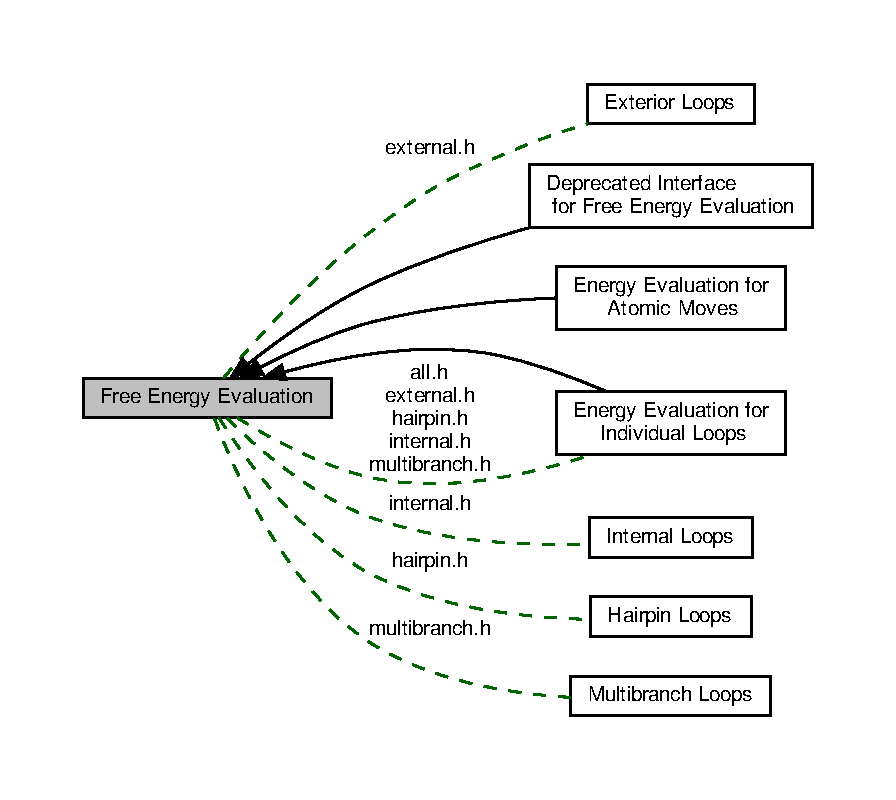
\includegraphics[width=350pt]{group__eval}
\end{center}
\end{figure}
\subsection*{Modules}
\begin{DoxyCompactItemize}
\item 
\hyperlink{group__eval__loops}{Energy Evaluation for Individual Loops}
\begin{DoxyCompactList}\small\item\em Functions to evaluate the free energy of particular types of loops. \end{DoxyCompactList}\item 
\hyperlink{group__eval__move}{Energy Evaluation for Atomic Moves}
\begin{DoxyCompactList}\small\item\em Functions to evaluate the free energy change of a structure after application of (a set of) atomic moves. \end{DoxyCompactList}\item 
\hyperlink{group__eval__deprecated}{Deprecated Interface for Free Energy Evaluation}
\begin{DoxyCompactList}\small\item\em Deprecated Energy Evaluation functions. \end{DoxyCompactList}\end{DoxyCompactItemize}
\subsection*{Files}
\begin{DoxyCompactItemize}
\item 
file \hyperlink{eval_8h}{eval.\+h}
\begin{DoxyCompactList}\small\item\em Functions and variables related to energy evaluation of sequence/structure pairs. \end{DoxyCompactList}\item 
file \hyperlink{all_8h}{all.\+h}
\begin{DoxyCompactList}\small\item\em Energy evaluation for M\+FE and partition function calculations. \end{DoxyCompactList}\item 
file \hyperlink{external_8h}{external.\+h}
\begin{DoxyCompactList}\small\item\em Energy evaluation of exterior loops for M\+FE and partition function calculations. \end{DoxyCompactList}\item 
file \hyperlink{hairpin_8h}{hairpin.\+h}
\begin{DoxyCompactList}\small\item\em Energy evaluation of hairpin loops for M\+FE and partition function calculations. \end{DoxyCompactList}\item 
file \hyperlink{internal_8h}{internal.\+h}
\begin{DoxyCompactList}\small\item\em Energy evaluation of interior loops for M\+FE and partition function calculations. \end{DoxyCompactList}\item 
file \hyperlink{multibranch_8h}{multibranch.\+h}
\begin{DoxyCompactList}\small\item\em Energy evaluation of multibranch loops for M\+FE and partition function calculations. \end{DoxyCompactList}\end{DoxyCompactItemize}
\subsection*{Macros}
\begin{DoxyCompactItemize}
\item 
\mbox{\Hypertarget{group__eval_gaf4afe19780b61b4962c613bde324128b}\label{group__eval_gaf4afe19780b61b4962c613bde324128b}} 
\#define \hyperlink{group__eval_gaf4afe19780b61b4962c613bde324128b}{V\+R\+N\+A\+\_\+\+V\+E\+R\+B\+O\+S\+I\+T\+Y\+\_\+\+Q\+U\+I\+ET}~-\/1
\begin{DoxyCompactList}\small\item\em Quiet level verbosity setting. \end{DoxyCompactList}\item 
\mbox{\Hypertarget{group__eval_ga47430d9e875084cfb983b22612e3abdf}\label{group__eval_ga47430d9e875084cfb983b22612e3abdf}} 
\#define \hyperlink{group__eval_ga47430d9e875084cfb983b22612e3abdf}{V\+R\+N\+A\+\_\+\+V\+E\+R\+B\+O\+S\+I\+T\+Y\+\_\+\+D\+E\+F\+A\+U\+LT}~1
\begin{DoxyCompactList}\small\item\em Default level verbosity setting. \end{DoxyCompactList}\end{DoxyCompactItemize}
\subsection*{Basic Energy Evaluation Interface with Dot-\/\+Bracket Structure String}
\begin{DoxyCompactItemize}
\item 
float \hyperlink{group__eval_ga58f199f1438d794a265f3b27fc8ea631}{vrna\+\_\+eval\+\_\+structure} (\hyperlink{group__fold__compound_ga1b0cef17fd40466cef5968eaeeff6166}{vrna\+\_\+fold\+\_\+compound\+\_\+t} $\ast$vc, const char $\ast$structure)
\begin{DoxyCompactList}\small\item\em Calculate the free energy of an already folded R\+NA. \end{DoxyCompactList}\item 
float \hyperlink{group__eval_ga6cea75c0eb9857fb59172be54cab09e0}{vrna\+\_\+eval\+\_\+covar\+\_\+structure} (\hyperlink{group__fold__compound_ga1b0cef17fd40466cef5968eaeeff6166}{vrna\+\_\+fold\+\_\+compound\+\_\+t} $\ast$vc, const char $\ast$structure)
\begin{DoxyCompactList}\small\item\em Calculate the pseudo energy derived by the covariance scores of a set of aligned sequences. \end{DoxyCompactList}\item 
float \hyperlink{group__eval_ga0928d699d310178f84ee2351034e5cb5}{vrna\+\_\+eval\+\_\+structure\+\_\+verbose} (\hyperlink{group__fold__compound_ga1b0cef17fd40466cef5968eaeeff6166}{vrna\+\_\+fold\+\_\+compound\+\_\+t} $\ast$vc, const char $\ast$structure, F\+I\+LE $\ast$file)
\begin{DoxyCompactList}\small\item\em Calculate the free energy of an already folded R\+NA and print contributions on a per-\/loop base. \end{DoxyCompactList}\item 
float \hyperlink{group__eval_gab12e6b1226227670322150df018734f8}{vrna\+\_\+eval\+\_\+structure\+\_\+v} (\hyperlink{group__fold__compound_ga1b0cef17fd40466cef5968eaeeff6166}{vrna\+\_\+fold\+\_\+compound\+\_\+t} $\ast$vc, const char $\ast$structure, int verbosity\+\_\+level, F\+I\+LE $\ast$file)
\begin{DoxyCompactList}\small\item\em Calculate the free energy of an already folded R\+NA and print contributions on a per-\/loop base. \end{DoxyCompactList}\item 
\mbox{\Hypertarget{group__eval_ga1d49318a535422b723e2c47520ac090a}\label{group__eval_ga1d49318a535422b723e2c47520ac090a}} 
float {\bfseries vrna\+\_\+eval\+\_\+structure\+\_\+cstr} (\hyperlink{group__fold__compound_ga1b0cef17fd40466cef5968eaeeff6166}{vrna\+\_\+fold\+\_\+compound\+\_\+t} $\ast$vc, const char $\ast$structure, int verbosity\+\_\+level, vrna\+\_\+cstr\+\_\+t output\+\_\+stream)
\end{DoxyCompactItemize}
\subsection*{Basic Energy Evaluation Interface with Structure Pair Table}
\begin{DoxyCompactItemize}
\item 
int \hyperlink{group__eval_gadbd09372ddfd7a450bbd590c96a6bfe4}{vrna\+\_\+eval\+\_\+structure\+\_\+pt} (\hyperlink{group__fold__compound_ga1b0cef17fd40466cef5968eaeeff6166}{vrna\+\_\+fold\+\_\+compound\+\_\+t} $\ast$vc, const short $\ast$pt)
\begin{DoxyCompactList}\small\item\em Calculate the free energy of an already folded R\+NA. \end{DoxyCompactList}\item 
int \hyperlink{group__eval_ga8a517cfeeae8c376ae7b1e0c401d38b4}{vrna\+\_\+eval\+\_\+structure\+\_\+pt\+\_\+verbose} (\hyperlink{group__fold__compound_ga1b0cef17fd40466cef5968eaeeff6166}{vrna\+\_\+fold\+\_\+compound\+\_\+t} $\ast$vc, const short $\ast$pt, F\+I\+LE $\ast$file)
\begin{DoxyCompactList}\small\item\em Calculate the free energy of an already folded R\+NA. \end{DoxyCompactList}\item 
int \hyperlink{group__eval_ga2c6533ba0afe4c88d335d8f1e0e2a48e}{vrna\+\_\+eval\+\_\+structure\+\_\+pt\+\_\+v} (\hyperlink{group__fold__compound_ga1b0cef17fd40466cef5968eaeeff6166}{vrna\+\_\+fold\+\_\+compound\+\_\+t} $\ast$vc, const short $\ast$pt, int verbosity\+\_\+level, F\+I\+LE $\ast$file)
\begin{DoxyCompactList}\small\item\em Calculate the free energy of an already folded R\+NA. \end{DoxyCompactList}\end{DoxyCompactItemize}
\subsection*{Simplified Energy Evaluation with Sequence and Dot-\/\+Bracket Strings}
\begin{DoxyCompactItemize}
\item 
float \hyperlink{group__eval_ga7e5273464b775d4130245681312c1369}{vrna\+\_\+eval\+\_\+structure\+\_\+simple} (const char $\ast$string, const char $\ast$structure)
\begin{DoxyCompactList}\small\item\em Calculate the free energy of an already folded R\+NA. \end{DoxyCompactList}\item 
float \hyperlink{group__eval_ga3e05a23ddf9b083f4e69881e440d4866}{vrna\+\_\+eval\+\_\+circ\+\_\+structure} (const char $\ast$string, const char $\ast$structure)
\begin{DoxyCompactList}\small\item\em Evaluate the free energy of a sequence/structure pair where the sequence is circular. \end{DoxyCompactList}\item 
float \hyperlink{group__eval_ga3263504825ef4b523eba797c99921df4}{vrna\+\_\+eval\+\_\+gquad\+\_\+structure} (const char $\ast$string, const char $\ast$structure)
\begin{DoxyCompactList}\small\item\em Evaluate the free energy of a sequence/structure pair where the structure may contain G-\/\+Quadruplexes. \end{DoxyCompactList}\item 
float \hyperlink{group__eval_ga9dba2fc5d7e6ad1359a7c2f350589c0e}{vrna\+\_\+eval\+\_\+circ\+\_\+gquad\+\_\+structure} (const char $\ast$string, const char $\ast$structure)
\begin{DoxyCompactList}\small\item\em Evaluate the free energy of a sequence/structure pair where the sequence is circular and the structure may contain G-\/\+Quadruplexes. \end{DoxyCompactList}\item 
float \hyperlink{group__eval_gaf928bfd96767e1b8033a95a4cc432e39}{vrna\+\_\+eval\+\_\+structure\+\_\+simple\+\_\+verbose} (const char $\ast$string, const char $\ast$structure, F\+I\+LE $\ast$file)
\begin{DoxyCompactList}\small\item\em Calculate the free energy of an already folded R\+NA and print contributions per loop. \end{DoxyCompactList}\item 
float \hyperlink{group__eval_gacd6278343e77d13f1d53588e50d303bc}{vrna\+\_\+eval\+\_\+structure\+\_\+simple\+\_\+v} (const char $\ast$string, const char $\ast$structure, int verbosity\+\_\+level, F\+I\+LE $\ast$file)
\begin{DoxyCompactList}\small\item\em Calculate the free energy of an already folded R\+NA and print contributions per loop. \end{DoxyCompactList}\item 
float \hyperlink{group__eval_gac3fb44e0773a51be8efc5f4f595a94a7}{vrna\+\_\+eval\+\_\+circ\+\_\+structure\+\_\+v} (const char $\ast$string, const char $\ast$structure, int verbosity\+\_\+level, F\+I\+LE $\ast$file)
\begin{DoxyCompactList}\small\item\em Evaluate free energy of a sequence/structure pair, assume sequence to be circular and print contributions per loop. \end{DoxyCompactList}\item 
float \hyperlink{group__eval_gaeaa2bdbc1b5d78c667e735fbdff87fff}{vrna\+\_\+eval\+\_\+gquad\+\_\+structure\+\_\+v} (const char $\ast$string, const char $\ast$structure, int verbosity\+\_\+level, F\+I\+LE $\ast$file)
\begin{DoxyCompactList}\small\item\em Evaluate free energy of a sequence/structure pair, allow for G-\/\+Quadruplexes in the structure and print contributions per loop. \end{DoxyCompactList}\item 
float \hyperlink{group__eval_gab96a6c59923ff06c35f8c2fd2c239727}{vrna\+\_\+eval\+\_\+circ\+\_\+gquad\+\_\+structure\+\_\+v} (const char $\ast$string, const char $\ast$structure, int verbosity\+\_\+level, F\+I\+LE $\ast$file)
\begin{DoxyCompactList}\small\item\em Evaluate free energy of a sequence/structure pair, assume sequence to be circular, allow for G-\/\+Quadruplexes in the structure, and print contributions per loop. \end{DoxyCompactList}\end{DoxyCompactItemize}
\subsection*{Simplified Energy Evaluation with Sequence Alignments and Consensus Structure Dot-\/\+Bracket String}
\begin{DoxyCompactItemize}
\item 
float \hyperlink{group__eval_ga7762c3a7bdcbc3a14ef93259d322c7d6}{vrna\+\_\+eval\+\_\+consensus\+\_\+structure\+\_\+simple} (const char $\ast$$\ast$alignment, const char $\ast$structure)
\begin{DoxyCompactList}\small\item\em Calculate the free energy of an already folded R\+NA sequence alignment. \end{DoxyCompactList}\item 
float \hyperlink{group__eval_gac96577cf232c71160f762737a994b7c6}{vrna\+\_\+eval\+\_\+circ\+\_\+consensus\+\_\+structure} (const char $\ast$$\ast$alignment, const char $\ast$structure)
\begin{DoxyCompactList}\small\item\em Evaluate the free energy of a multiple sequence alignment/consensus structure pair where the sequences are circular. \end{DoxyCompactList}\item 
float \hyperlink{group__eval_gaf09a326b3d57a4b30c27bd0e216198ac}{vrna\+\_\+eval\+\_\+gquad\+\_\+consensus\+\_\+structure} (const char $\ast$$\ast$alignment, const char $\ast$structure)
\begin{DoxyCompactList}\small\item\em Evaluate the free energy of a multiple sequence alignment/consensus structure pair where the structure may contain G-\/\+Quadruplexes. \end{DoxyCompactList}\item 
float \hyperlink{group__eval_gac673ebb9ae2a29f54d201e2ac5b85540}{vrna\+\_\+eval\+\_\+circ\+\_\+gquad\+\_\+consensus\+\_\+structure} (const char $\ast$$\ast$alignment, const char $\ast$structure)
\begin{DoxyCompactList}\small\item\em Evaluate the free energy of a multiple sequence alignment/consensus structure pair where the sequence is circular and the structure may contain G-\/\+Quadruplexes. \end{DoxyCompactList}\item 
float \hyperlink{group__eval_ga1c07851f6b665c3461a19e9e4eb33d26}{vrna\+\_\+eval\+\_\+consensus\+\_\+structure\+\_\+simple\+\_\+verbose} (const char $\ast$$\ast$alignment, const char $\ast$structure, F\+I\+LE $\ast$file)
\begin{DoxyCompactList}\small\item\em Evaluate the free energy of a consensus structure for an R\+NA sequence alignment and print contributions per loop. \end{DoxyCompactList}\item 
float \hyperlink{group__eval_gad88927c62ab0a8b534e078e44be1b36e}{vrna\+\_\+eval\+\_\+consensus\+\_\+structure\+\_\+simple\+\_\+v} (const char $\ast$$\ast$alignment, const char $\ast$structure, int verbosity\+\_\+level, F\+I\+LE $\ast$file)
\begin{DoxyCompactList}\small\item\em Evaluate the free energy of a consensus structure for an R\+NA sequence alignment and print contributions per loop. \end{DoxyCompactList}\item 
float \hyperlink{group__eval_gae89240c230e4740b22a703ee953396b9}{vrna\+\_\+eval\+\_\+circ\+\_\+consensus\+\_\+structure\+\_\+v} (const char $\ast$$\ast$alignment, const char $\ast$structure, int verbosity\+\_\+level, F\+I\+LE $\ast$file)
\begin{DoxyCompactList}\small\item\em Evaluate the free energy of a consensus structure for an alignment of circular R\+NA sequences and print contributions per loop. \end{DoxyCompactList}\item 
float \hyperlink{group__eval_ga8abc794fc48d43268ced5e8cde017baa}{vrna\+\_\+eval\+\_\+gquad\+\_\+consensus\+\_\+structure\+\_\+v} (const char $\ast$$\ast$alignment, const char $\ast$structure, int verbosity\+\_\+level, F\+I\+LE $\ast$file)
\begin{DoxyCompactList}\small\item\em Evaluate the free energy of a consensus structure for an R\+NA sequence alignment, allow for annotated G-\/\+Quadruplexes in the structure and print contributions per loop. \end{DoxyCompactList}\item 
float \hyperlink{group__eval_gaecd3e17292a0b3927277434019a5e187}{vrna\+\_\+eval\+\_\+circ\+\_\+gquad\+\_\+consensus\+\_\+structure\+\_\+v} (const char $\ast$$\ast$alignment, const char $\ast$structure, int verbosity\+\_\+level, F\+I\+LE $\ast$file)
\begin{DoxyCompactList}\small\item\em Evaluate the free energy of a consensus structure for an alignment of circular R\+NA sequences, allow for annotated G-\/\+Quadruplexes in the structure and print contributions per loop. \end{DoxyCompactList}\end{DoxyCompactItemize}
\subsection*{Simplified Energy Evaluation with Sequence String and Structure Pair Table}
\begin{DoxyCompactItemize}
\item 
int \hyperlink{group__eval_ga0bba59b4d6e53461088666ff4aece7b0}{vrna\+\_\+eval\+\_\+structure\+\_\+pt\+\_\+simple} (const char $\ast$string, const short $\ast$pt)
\begin{DoxyCompactList}\small\item\em Calculate the free energy of an already folded R\+NA. \end{DoxyCompactList}\item 
int \hyperlink{group__eval_ga76e152ee9a02be23da14cdddf52b4e44}{vrna\+\_\+eval\+\_\+structure\+\_\+pt\+\_\+simple\+\_\+verbose} (const char $\ast$string, const short $\ast$pt, F\+I\+LE $\ast$file)
\begin{DoxyCompactList}\small\item\em Calculate the free energy of an already folded R\+NA. \end{DoxyCompactList}\item 
int \hyperlink{group__eval_gac40b813d35289da9816d0c1eec94faa5}{vrna\+\_\+eval\+\_\+structure\+\_\+pt\+\_\+simple\+\_\+v} (const char $\ast$string, const short $\ast$pt, int verbosity\+\_\+level, F\+I\+LE $\ast$file)
\begin{DoxyCompactList}\small\item\em Calculate the free energy of an already folded R\+NA. \end{DoxyCompactList}\end{DoxyCompactItemize}
\subsection*{Simplified Energy Evaluation with Sequence Alignment and Consensus Structure Pair Table}
\begin{DoxyCompactItemize}
\item 
int \hyperlink{group__eval_gabbb4d2a7aa324ec9cce8f47ce61ab8af}{vrna\+\_\+eval\+\_\+consensus\+\_\+structure\+\_\+pt\+\_\+simple} (const char $\ast$$\ast$alignment, const short $\ast$pt)
\begin{DoxyCompactList}\small\item\em Evaluate the Free Energy of a Consensus Secondary Structure given a Sequence Alignment. \end{DoxyCompactList}\item 
\mbox{\Hypertarget{group__eval_ga2769e4369d023ad2d5c5f4d2ee825c23}\label{group__eval_ga2769e4369d023ad2d5c5f4d2ee825c23}} 
int {\bfseries vrna\+\_\+eval\+\_\+consensus\+\_\+structure\+\_\+pt\+\_\+simple\+\_\+verbose} (const char $\ast$$\ast$alignment, const short $\ast$pt, F\+I\+LE $\ast$file)
\item 
\mbox{\Hypertarget{group__eval_gaf2d227b3d54bf9b693a3df52faf5e2e4}\label{group__eval_gaf2d227b3d54bf9b693a3df52faf5e2e4}} 
int {\bfseries vrna\+\_\+eval\+\_\+consensus\+\_\+structure\+\_\+pt\+\_\+simple\+\_\+v} (const char $\ast$$\ast$alignment, const short $\ast$pt, int verbosity\+\_\+level, F\+I\+LE $\ast$file)
\end{DoxyCompactItemize}


\subsection{Function Documentation}
\mbox{\Hypertarget{group__eval_ga58f199f1438d794a265f3b27fc8ea631}\label{group__eval_ga58f199f1438d794a265f3b27fc8ea631}} 
\index{Free Energy Evaluation@{Free Energy Evaluation}!vrna\+\_\+eval\+\_\+structure@{vrna\+\_\+eval\+\_\+structure}}
\index{vrna\+\_\+eval\+\_\+structure@{vrna\+\_\+eval\+\_\+structure}!Free Energy Evaluation@{Free Energy Evaluation}}
\subsubsection{\texorpdfstring{vrna\+\_\+eval\+\_\+structure()}{vrna\_eval\_structure()}}
{\footnotesize\ttfamily float vrna\+\_\+eval\+\_\+structure (\begin{DoxyParamCaption}\item[{\hyperlink{group__fold__compound_ga1b0cef17fd40466cef5968eaeeff6166}{vrna\+\_\+fold\+\_\+compound\+\_\+t} $\ast$}]{vc,  }\item[{const char $\ast$}]{structure }\end{DoxyParamCaption})}



{\ttfamily \#include $<$\hyperlink{eval_8h}{Vienna\+R\+N\+A/eval.\+h}$>$}



Calculate the free energy of an already folded R\+NA. 

This function allows for energy evaluation of a given pair of structure and sequence (alignment). Model details, energy parameters, and possibly soft constraints are used as provided via the parameter \textquotesingle{}vc\textquotesingle{}. The \hyperlink{group__fold__compound_ga1b0cef17fd40466cef5968eaeeff6166}{vrna\+\_\+fold\+\_\+compound\+\_\+t} does not need to contain any DP matrices, but requires all most basic init values as one would get from a call like this\+: 
\begin{DoxyCode}
vc = \hyperlink{group__fold__compound_ga6601d994ba32b11511b36f68b08403be}{vrna\_fold\_compound}(sequence, NULL, \hyperlink{group__fold__compound_ga61469c423131552c8483229f8b6c7e0e}{VRNA\_OPTION\_EVAL\_ONLY});
\end{DoxyCode}


\begin{DoxyNote}{Note}
Accepts vrna\+\_\+fold\+\_\+compound\+\_\+t of type \hyperlink{group__fold__compound_gga01a4ff86fa71deaaa5d1abbd95a1447da7e264dd3cf2dc9b6448caabcb7763cd6}{V\+R\+N\+A\+\_\+\+F\+C\+\_\+\+T\+Y\+P\+E\+\_\+\+S\+I\+N\+G\+LE} and \hyperlink{group__fold__compound_gga01a4ff86fa71deaaa5d1abbd95a1447dab821ce46ea3cf665be97df22a76f5023}{V\+R\+N\+A\+\_\+\+F\+C\+\_\+\+T\+Y\+P\+E\+\_\+\+C\+O\+M\+P\+A\+R\+A\+T\+I\+VE}
\end{DoxyNote}
\begin{DoxySeeAlso}{See also}
\hyperlink{group__eval_gadbd09372ddfd7a450bbd590c96a6bfe4}{vrna\+\_\+eval\+\_\+structure\+\_\+pt()}, \hyperlink{group__eval_ga0928d699d310178f84ee2351034e5cb5}{vrna\+\_\+eval\+\_\+structure\+\_\+verbose()}, \hyperlink{group__eval_ga8a517cfeeae8c376ae7b1e0c401d38b4}{vrna\+\_\+eval\+\_\+structure\+\_\+pt\+\_\+verbose()}, \hyperlink{group__fold__compound_ga6601d994ba32b11511b36f68b08403be}{vrna\+\_\+fold\+\_\+compound()}, \hyperlink{group__fold__compound_gad6bacc816af274922b13d947f708aa0c}{vrna\+\_\+fold\+\_\+compound\+\_\+comparative()}, \hyperlink{group__eval_ga6cea75c0eb9857fb59172be54cab09e0}{vrna\+\_\+eval\+\_\+covar\+\_\+structure()}
\end{DoxySeeAlso}

\begin{DoxyParams}{Parameters}
{\em vc} & A vrna\+\_\+fold\+\_\+compound\+\_\+t containing the energy parameters and model details \\
\hline
{\em structure} & Secondary structure in dot-\/bracket notation \\
\hline
\end{DoxyParams}
\begin{DoxyReturn}{Returns}
The free energy of the input structure given the input sequence in kcal/mol
\end{DoxyReturn}
\begin{DoxyRefDesc}{S\+W\+I\+G Wrapper Notes}
\item[\hyperlink{wrappers__wrappers000031}{S\+W\+I\+G Wrapper Notes}]This function is attached as method {\bfseries eval\+\_\+structure()} to objects of type {\itshape fold\+\_\+compound} \end{DoxyRefDesc}
\mbox{\Hypertarget{group__eval_ga6cea75c0eb9857fb59172be54cab09e0}\label{group__eval_ga6cea75c0eb9857fb59172be54cab09e0}} 
\index{Free Energy Evaluation@{Free Energy Evaluation}!vrna\+\_\+eval\+\_\+covar\+\_\+structure@{vrna\+\_\+eval\+\_\+covar\+\_\+structure}}
\index{vrna\+\_\+eval\+\_\+covar\+\_\+structure@{vrna\+\_\+eval\+\_\+covar\+\_\+structure}!Free Energy Evaluation@{Free Energy Evaluation}}
\subsubsection{\texorpdfstring{vrna\+\_\+eval\+\_\+covar\+\_\+structure()}{vrna\_eval\_covar\_structure()}}
{\footnotesize\ttfamily float vrna\+\_\+eval\+\_\+covar\+\_\+structure (\begin{DoxyParamCaption}\item[{\hyperlink{group__fold__compound_ga1b0cef17fd40466cef5968eaeeff6166}{vrna\+\_\+fold\+\_\+compound\+\_\+t} $\ast$}]{vc,  }\item[{const char $\ast$}]{structure }\end{DoxyParamCaption})}



{\ttfamily \#include $<$\hyperlink{eval_8h}{Vienna\+R\+N\+A/eval.\+h}$>$}



Calculate the pseudo energy derived by the covariance scores of a set of aligned sequences. 

Consensus structure prediction is driven by covariance scores of base pairs in rows of the provided alignment. This function allows one to retrieve the total amount of this covariance pseudo energy scores. The \hyperlink{group__fold__compound_ga1b0cef17fd40466cef5968eaeeff6166}{vrna\+\_\+fold\+\_\+compound\+\_\+t} does not need to contain any DP matrices, but requires all most basic init values as one would get from a call like this\+: 
\begin{DoxyCode}
vc = \hyperlink{group__fold__compound_gad6bacc816af274922b13d947f708aa0c}{vrna\_fold\_compound\_comparative}(alignment, NULL, 
      \hyperlink{group__fold__compound_ga61469c423131552c8483229f8b6c7e0e}{VRNA\_OPTION\_EVAL\_ONLY});
\end{DoxyCode}


\begin{DoxyNote}{Note}
Accepts vrna\+\_\+fold\+\_\+compound\+\_\+t of type \hyperlink{group__fold__compound_gga01a4ff86fa71deaaa5d1abbd95a1447dab821ce46ea3cf665be97df22a76f5023}{V\+R\+N\+A\+\_\+\+F\+C\+\_\+\+T\+Y\+P\+E\+\_\+\+C\+O\+M\+P\+A\+R\+A\+T\+I\+VE} only!
\end{DoxyNote}
\begin{DoxySeeAlso}{See also}
\hyperlink{group__fold__compound_gad6bacc816af274922b13d947f708aa0c}{vrna\+\_\+fold\+\_\+compound\+\_\+comparative()}, \hyperlink{group__eval_ga58f199f1438d794a265f3b27fc8ea631}{vrna\+\_\+eval\+\_\+structure()}
\end{DoxySeeAlso}

\begin{DoxyParams}{Parameters}
{\em vc} & A vrna\+\_\+fold\+\_\+compound\+\_\+t containing the energy parameters and model details \\
\hline
{\em structure} & Secondary (consensus) structure in dot-\/bracket notation \\
\hline
\end{DoxyParams}
\begin{DoxyReturn}{Returns}
The covariance pseudo energy score of the input structure given the input sequence alignment in kcal/mol
\end{DoxyReturn}
\begin{DoxyRefDesc}{S\+W\+I\+G Wrapper Notes}
\item[\hyperlink{wrappers__wrappers000035}{S\+W\+I\+G Wrapper Notes}]This function is attached as method {\bfseries eval\+\_\+covar\+\_\+structure()} to objects of type {\itshape fold\+\_\+compound} \end{DoxyRefDesc}
\mbox{\Hypertarget{group__eval_ga0928d699d310178f84ee2351034e5cb5}\label{group__eval_ga0928d699d310178f84ee2351034e5cb5}} 
\index{Free Energy Evaluation@{Free Energy Evaluation}!vrna\+\_\+eval\+\_\+structure\+\_\+verbose@{vrna\+\_\+eval\+\_\+structure\+\_\+verbose}}
\index{vrna\+\_\+eval\+\_\+structure\+\_\+verbose@{vrna\+\_\+eval\+\_\+structure\+\_\+verbose}!Free Energy Evaluation@{Free Energy Evaluation}}
\subsubsection{\texorpdfstring{vrna\+\_\+eval\+\_\+structure\+\_\+verbose()}{vrna\_eval\_structure\_verbose()}}
{\footnotesize\ttfamily float vrna\+\_\+eval\+\_\+structure\+\_\+verbose (\begin{DoxyParamCaption}\item[{\hyperlink{group__fold__compound_ga1b0cef17fd40466cef5968eaeeff6166}{vrna\+\_\+fold\+\_\+compound\+\_\+t} $\ast$}]{vc,  }\item[{const char $\ast$}]{structure,  }\item[{F\+I\+LE $\ast$}]{file }\end{DoxyParamCaption})}



{\ttfamily \#include $<$\hyperlink{eval_8h}{Vienna\+R\+N\+A/eval.\+h}$>$}



Calculate the free energy of an already folded R\+NA and print contributions on a per-\/loop base. 

This function is a simplyfied version of \hyperlink{group__eval_gab12e6b1226227670322150df018734f8}{vrna\+\_\+eval\+\_\+structure\+\_\+v()} that uses the {\itshape default} verbosity level. ( \begin{DoxySeeAlso}{See also}
\hyperlink{group__eval_gadbd09372ddfd7a450bbd590c96a6bfe4}{vrna\+\_\+eval\+\_\+structure\+\_\+pt()}, \hyperlink{group__eval_ga0928d699d310178f84ee2351034e5cb5}{vrna\+\_\+eval\+\_\+structure\+\_\+verbose()}, \hyperlink{group__eval_ga8a517cfeeae8c376ae7b1e0c401d38b4}{vrna\+\_\+eval\+\_\+structure\+\_\+pt\+\_\+verbose()},
\end{DoxySeeAlso}

\begin{DoxyParams}{Parameters}
{\em vc} & A vrna\+\_\+fold\+\_\+compound\+\_\+t containing the energy parameters and model details \\
\hline
{\em structure} & Secondary structure in dot-\/bracket notation \\
\hline
{\em file} & A file handle where this function should print to (may be N\+U\+LL). \\
\hline
\end{DoxyParams}
\begin{DoxyReturn}{Returns}
The free energy of the input structure given the input sequence in kcal/mol
\end{DoxyReturn}
\begin{DoxyRefDesc}{S\+W\+I\+G Wrapper Notes}
\item[\hyperlink{wrappers__wrappers000033}{S\+W\+I\+G Wrapper Notes}]This function is attached as method {\bfseries eval\+\_\+structure\+\_\+verbose()} to objects of type {\itshape fold\+\_\+compound} \end{DoxyRefDesc}
\mbox{\Hypertarget{group__eval_gab12e6b1226227670322150df018734f8}\label{group__eval_gab12e6b1226227670322150df018734f8}} 
\index{Free Energy Evaluation@{Free Energy Evaluation}!vrna\+\_\+eval\+\_\+structure\+\_\+v@{vrna\+\_\+eval\+\_\+structure\+\_\+v}}
\index{vrna\+\_\+eval\+\_\+structure\+\_\+v@{vrna\+\_\+eval\+\_\+structure\+\_\+v}!Free Energy Evaluation@{Free Energy Evaluation}}
\subsubsection{\texorpdfstring{vrna\+\_\+eval\+\_\+structure\+\_\+v()}{vrna\_eval\_structure\_v()}}
{\footnotesize\ttfamily float vrna\+\_\+eval\+\_\+structure\+\_\+v (\begin{DoxyParamCaption}\item[{\hyperlink{group__fold__compound_ga1b0cef17fd40466cef5968eaeeff6166}{vrna\+\_\+fold\+\_\+compound\+\_\+t} $\ast$}]{vc,  }\item[{const char $\ast$}]{structure,  }\item[{int}]{verbosity\+\_\+level,  }\item[{F\+I\+LE $\ast$}]{file }\end{DoxyParamCaption})}



{\ttfamily \#include $<$\hyperlink{eval_8h}{Vienna\+R\+N\+A/eval.\+h}$>$}



Calculate the free energy of an already folded R\+NA and print contributions on a per-\/loop base. 

This function allows for detailed energy evaluation of a given sequence/structure pair. In contrast to \hyperlink{group__eval_ga58f199f1438d794a265f3b27fc8ea631}{vrna\+\_\+eval\+\_\+structure()} this function prints detailed energy contributions based on individual loops to a file handle. If N\+U\+LL is passed as file handle, this function defaults to print to stdout. Any positive {\ttfamily verbosity\+\_\+level} activates potential warning message of the energy evaluting functions, while values $ \ge 1 $ allow for detailed control of what data is printed. A negative parameter {\ttfamily verbosity\+\_\+level} turns off printing all together.

Model details, energy parameters, and possibly soft constraints are used as provided via the parameter \textquotesingle{}vc\textquotesingle{}. The fold\+\_\+compound does not need to contain any DP matrices, but all the most basic init values as one would get from a call like this\+: 
\begin{DoxyCode}
vc = \hyperlink{group__fold__compound_ga6601d994ba32b11511b36f68b08403be}{vrna\_fold\_compound}(sequence, NULL, \hyperlink{group__fold__compound_ga61469c423131552c8483229f8b6c7e0e}{VRNA\_OPTION\_EVAL\_ONLY});
\end{DoxyCode}


\begin{DoxySeeAlso}{See also}
\hyperlink{group__eval_gadbd09372ddfd7a450bbd590c96a6bfe4}{vrna\+\_\+eval\+\_\+structure\+\_\+pt()}, \hyperlink{group__eval_ga0928d699d310178f84ee2351034e5cb5}{vrna\+\_\+eval\+\_\+structure\+\_\+verbose()}, \hyperlink{group__eval_ga8a517cfeeae8c376ae7b1e0c401d38b4}{vrna\+\_\+eval\+\_\+structure\+\_\+pt\+\_\+verbose()},
\end{DoxySeeAlso}

\begin{DoxyParams}{Parameters}
{\em vc} & A vrna\+\_\+fold\+\_\+compound\+\_\+t containing the energy parameters and model details \\
\hline
{\em structure} & Secondary structure in dot-\/bracket notation \\
\hline
{\em verbosity\+\_\+level} & The level of verbosity of this function \\
\hline
{\em file} & A file handle where this function should print to (may be N\+U\+LL). \\
\hline
\end{DoxyParams}
\begin{DoxyReturn}{Returns}
The free energy of the input structure given the input sequence in kcal/mol 
\end{DoxyReturn}
\mbox{\Hypertarget{group__eval_gadbd09372ddfd7a450bbd590c96a6bfe4}\label{group__eval_gadbd09372ddfd7a450bbd590c96a6bfe4}} 
\index{Free Energy Evaluation@{Free Energy Evaluation}!vrna\+\_\+eval\+\_\+structure\+\_\+pt@{vrna\+\_\+eval\+\_\+structure\+\_\+pt}}
\index{vrna\+\_\+eval\+\_\+structure\+\_\+pt@{vrna\+\_\+eval\+\_\+structure\+\_\+pt}!Free Energy Evaluation@{Free Energy Evaluation}}
\subsubsection{\texorpdfstring{vrna\+\_\+eval\+\_\+structure\+\_\+pt()}{vrna\_eval\_structure\_pt()}}
{\footnotesize\ttfamily int vrna\+\_\+eval\+\_\+structure\+\_\+pt (\begin{DoxyParamCaption}\item[{\hyperlink{group__fold__compound_ga1b0cef17fd40466cef5968eaeeff6166}{vrna\+\_\+fold\+\_\+compound\+\_\+t} $\ast$}]{vc,  }\item[{const short $\ast$}]{pt }\end{DoxyParamCaption})}



{\ttfamily \#include $<$\hyperlink{eval_8h}{Vienna\+R\+N\+A/eval.\+h}$>$}



Calculate the free energy of an already folded R\+NA. 

This function allows for energy evaluation of a given sequence/structure pair where the structure is provided in pair\+\_\+table format as obtained from \hyperlink{group__struct__utils__pair__table_gae829fb8bb7f694c12a9c0bbc34c77c60}{vrna\+\_\+ptable()}. Model details, energy parameters, and possibly soft constraints are used as provided via the parameter \textquotesingle{}vc\textquotesingle{}. The fold\+\_\+compound does not need to contain any DP matrices, but all the most basic init values as one would get from a call like this\+: 
\begin{DoxyCode}
vc = \hyperlink{group__fold__compound_ga6601d994ba32b11511b36f68b08403be}{vrna\_fold\_compound}(sequence, NULL, \hyperlink{group__fold__compound_ga61469c423131552c8483229f8b6c7e0e}{VRNA\_OPTION\_EVAL\_ONLY});
\end{DoxyCode}


\begin{DoxySeeAlso}{See also}
\hyperlink{group__struct__utils__pair__table_gae829fb8bb7f694c12a9c0bbc34c77c60}{vrna\+\_\+ptable()}, \hyperlink{group__eval_ga58f199f1438d794a265f3b27fc8ea631}{vrna\+\_\+eval\+\_\+structure()}, \hyperlink{group__eval_ga8a517cfeeae8c376ae7b1e0c401d38b4}{vrna\+\_\+eval\+\_\+structure\+\_\+pt\+\_\+verbose()}
\end{DoxySeeAlso}

\begin{DoxyParams}{Parameters}
{\em vc} & A vrna\+\_\+fold\+\_\+compound\+\_\+t containing the energy parameters and model details \\
\hline
{\em pt} & Secondary structure as pair\+\_\+table \\
\hline
\end{DoxyParams}
\begin{DoxyReturn}{Returns}
The free energy of the input structure given the input sequence in 10cal/mol
\end{DoxyReturn}
\begin{DoxyRefDesc}{S\+W\+I\+G Wrapper Notes}
\item[\hyperlink{wrappers__wrappers000032}{S\+W\+I\+G Wrapper Notes}]This function is attached as method {\bfseries eval\+\_\+structure\+\_\+pt()} to objects of type {\itshape fold\+\_\+compound} \end{DoxyRefDesc}
\mbox{\Hypertarget{group__eval_ga8a517cfeeae8c376ae7b1e0c401d38b4}\label{group__eval_ga8a517cfeeae8c376ae7b1e0c401d38b4}} 
\index{Free Energy Evaluation@{Free Energy Evaluation}!vrna\+\_\+eval\+\_\+structure\+\_\+pt\+\_\+verbose@{vrna\+\_\+eval\+\_\+structure\+\_\+pt\+\_\+verbose}}
\index{vrna\+\_\+eval\+\_\+structure\+\_\+pt\+\_\+verbose@{vrna\+\_\+eval\+\_\+structure\+\_\+pt\+\_\+verbose}!Free Energy Evaluation@{Free Energy Evaluation}}
\subsubsection{\texorpdfstring{vrna\+\_\+eval\+\_\+structure\+\_\+pt\+\_\+verbose()}{vrna\_eval\_structure\_pt\_verbose()}}
{\footnotesize\ttfamily int vrna\+\_\+eval\+\_\+structure\+\_\+pt\+\_\+verbose (\begin{DoxyParamCaption}\item[{\hyperlink{group__fold__compound_ga1b0cef17fd40466cef5968eaeeff6166}{vrna\+\_\+fold\+\_\+compound\+\_\+t} $\ast$}]{vc,  }\item[{const short $\ast$}]{pt,  }\item[{F\+I\+LE $\ast$}]{file }\end{DoxyParamCaption})}



{\ttfamily \#include $<$\hyperlink{eval_8h}{Vienna\+R\+N\+A/eval.\+h}$>$}



Calculate the free energy of an already folded R\+NA. 

This function is a simplyfied version of \hyperlink{group__eval_gacd6278343e77d13f1d53588e50d303bc}{vrna\+\_\+eval\+\_\+structure\+\_\+simple\+\_\+v()} that uses the {\itshape default} verbosity level.

\begin{DoxySeeAlso}{See also}
\hyperlink{group__eval_ga2c6533ba0afe4c88d335d8f1e0e2a48e}{vrna\+\_\+eval\+\_\+structure\+\_\+pt\+\_\+v()}, \hyperlink{group__struct__utils__pair__table_gae829fb8bb7f694c12a9c0bbc34c77c60}{vrna\+\_\+ptable()}, \hyperlink{group__eval_gadbd09372ddfd7a450bbd590c96a6bfe4}{vrna\+\_\+eval\+\_\+structure\+\_\+pt()}, \hyperlink{group__eval_ga0928d699d310178f84ee2351034e5cb5}{vrna\+\_\+eval\+\_\+structure\+\_\+verbose()}
\end{DoxySeeAlso}

\begin{DoxyParams}{Parameters}
{\em vc} & A vrna\+\_\+fold\+\_\+compound\+\_\+t containing the energy parameters and model details \\
\hline
{\em pt} & Secondary structure as pair\+\_\+table \\
\hline
{\em file} & A file handle where this function should print to (may be N\+U\+LL). \\
\hline
\end{DoxyParams}
\begin{DoxyReturn}{Returns}
The free energy of the input structure given the input sequence in 10cal/mol
\end{DoxyReturn}
\begin{DoxyRefDesc}{S\+W\+I\+G Wrapper Notes}
\item[\hyperlink{wrappers__wrappers000034}{S\+W\+I\+G Wrapper Notes}]This function is attached as method {\bfseries eval\+\_\+structure\+\_\+pt\+\_\+verbose()} to objects of type {\itshape fold\+\_\+compound} \end{DoxyRefDesc}
\mbox{\Hypertarget{group__eval_ga2c6533ba0afe4c88d335d8f1e0e2a48e}\label{group__eval_ga2c6533ba0afe4c88d335d8f1e0e2a48e}} 
\index{Free Energy Evaluation@{Free Energy Evaluation}!vrna\+\_\+eval\+\_\+structure\+\_\+pt\+\_\+v@{vrna\+\_\+eval\+\_\+structure\+\_\+pt\+\_\+v}}
\index{vrna\+\_\+eval\+\_\+structure\+\_\+pt\+\_\+v@{vrna\+\_\+eval\+\_\+structure\+\_\+pt\+\_\+v}!Free Energy Evaluation@{Free Energy Evaluation}}
\subsubsection{\texorpdfstring{vrna\+\_\+eval\+\_\+structure\+\_\+pt\+\_\+v()}{vrna\_eval\_structure\_pt\_v()}}
{\footnotesize\ttfamily int vrna\+\_\+eval\+\_\+structure\+\_\+pt\+\_\+v (\begin{DoxyParamCaption}\item[{\hyperlink{group__fold__compound_ga1b0cef17fd40466cef5968eaeeff6166}{vrna\+\_\+fold\+\_\+compound\+\_\+t} $\ast$}]{vc,  }\item[{const short $\ast$}]{pt,  }\item[{int}]{verbosity\+\_\+level,  }\item[{F\+I\+LE $\ast$}]{file }\end{DoxyParamCaption})}



{\ttfamily \#include $<$\hyperlink{eval_8h}{Vienna\+R\+N\+A/eval.\+h}$>$}



Calculate the free energy of an already folded R\+NA. 

This function allows for energy evaluation of a given sequence/structure pair where the structure is provided in pair\+\_\+table format as obtained from \hyperlink{group__struct__utils__pair__table_gae829fb8bb7f694c12a9c0bbc34c77c60}{vrna\+\_\+ptable()}. Model details, energy parameters, and possibly soft constraints are used as provided via the parameter \textquotesingle{}vc\textquotesingle{}. The fold\+\_\+compound does not need to contain any DP matrices, but all the most basic init values as one would get from a call like this\+: 
\begin{DoxyCode}
vc = \hyperlink{group__fold__compound_ga6601d994ba32b11511b36f68b08403be}{vrna\_fold\_compound}(sequence, NULL, \hyperlink{group__fold__compound_ga61469c423131552c8483229f8b6c7e0e}{VRNA\_OPTION\_EVAL\_ONLY});
\end{DoxyCode}
 In contrast to \hyperlink{group__eval_gadbd09372ddfd7a450bbd590c96a6bfe4}{vrna\+\_\+eval\+\_\+structure\+\_\+pt()} this function prints detailed energy contributions based on individual loops to a file handle. If N\+U\+LL is passed as file handle, this function defaults to print to stdout. Any positive {\ttfamily verbosity\+\_\+level} activates potential warning message of the energy evaluting functions, while values $ \ge 1 $ allow for detailed control of what data is printed. A negative parameter {\ttfamily verbosity\+\_\+level} turns off printing all together.

\begin{DoxySeeAlso}{See also}
\hyperlink{group__struct__utils__pair__table_gae829fb8bb7f694c12a9c0bbc34c77c60}{vrna\+\_\+ptable()}, \hyperlink{group__eval_gadbd09372ddfd7a450bbd590c96a6bfe4}{vrna\+\_\+eval\+\_\+structure\+\_\+pt()}, \hyperlink{group__eval_ga0928d699d310178f84ee2351034e5cb5}{vrna\+\_\+eval\+\_\+structure\+\_\+verbose()}
\end{DoxySeeAlso}

\begin{DoxyParams}{Parameters}
{\em vc} & A vrna\+\_\+fold\+\_\+compound\+\_\+t containing the energy parameters and model details \\
\hline
{\em pt} & Secondary structure as pair\+\_\+table \\
\hline
{\em verbosity\+\_\+level} & The level of verbosity of this function \\
\hline
{\em file} & A file handle where this function should print to (may be N\+U\+LL). \\
\hline
\end{DoxyParams}
\begin{DoxyReturn}{Returns}
The free energy of the input structure given the input sequence in 10cal/mol 
\end{DoxyReturn}
\mbox{\Hypertarget{group__eval_ga7e5273464b775d4130245681312c1369}\label{group__eval_ga7e5273464b775d4130245681312c1369}} 
\index{Free Energy Evaluation@{Free Energy Evaluation}!vrna\+\_\+eval\+\_\+structure\+\_\+simple@{vrna\+\_\+eval\+\_\+structure\+\_\+simple}}
\index{vrna\+\_\+eval\+\_\+structure\+\_\+simple@{vrna\+\_\+eval\+\_\+structure\+\_\+simple}!Free Energy Evaluation@{Free Energy Evaluation}}
\subsubsection{\texorpdfstring{vrna\+\_\+eval\+\_\+structure\+\_\+simple()}{vrna\_eval\_structure\_simple()}}
{\footnotesize\ttfamily int vrna\+\_\+eval\+\_\+structure\+\_\+simple (\begin{DoxyParamCaption}\item[{const char $\ast$}]{string,  }\item[{const char $\ast$}]{structure }\end{DoxyParamCaption})}



{\ttfamily \#include $<$\hyperlink{eval_8h}{Vienna\+R\+N\+A/eval.\+h}$>$}



Calculate the free energy of an already folded R\+NA. 

This function allows for energy evaluation of a given sequence/structure pair. In contrast to \hyperlink{group__eval_ga58f199f1438d794a265f3b27fc8ea631}{vrna\+\_\+eval\+\_\+structure()} this function assumes default model details and default energy parameters in order to evaluate the free energy of the secondary structure. Therefore, it serves as a simple interface function for energy evaluation for situations where no changes on the energy model are required.

\begin{DoxySeeAlso}{See also}
\hyperlink{group__eval_ga58f199f1438d794a265f3b27fc8ea631}{vrna\+\_\+eval\+\_\+structure()}, \hyperlink{group__eval_gadbd09372ddfd7a450bbd590c96a6bfe4}{vrna\+\_\+eval\+\_\+structure\+\_\+pt()}, \hyperlink{group__eval_ga0928d699d310178f84ee2351034e5cb5}{vrna\+\_\+eval\+\_\+structure\+\_\+verbose()}, \hyperlink{group__eval_ga8a517cfeeae8c376ae7b1e0c401d38b4}{vrna\+\_\+eval\+\_\+structure\+\_\+pt\+\_\+verbose()},
\end{DoxySeeAlso}

\begin{DoxyParams}{Parameters}
{\em string} & R\+NA sequence in uppercase letters \\
\hline
{\em structure} & Secondary structure in dot-\/bracket notation \\
\hline
\end{DoxyParams}
\begin{DoxyReturn}{Returns}
The free energy of the input structure given the input sequence in kcal/mol
\end{DoxyReturn}
\begin{DoxyRefDesc}{S\+W\+I\+G Wrapper Notes}
\item[\hyperlink{wrappers__wrappers000041}{S\+W\+I\+G Wrapper Notes}]In the target scripting language, this function serves as a wrapper for \hyperlink{group__eval_gacd6278343e77d13f1d53588e50d303bc}{vrna\+\_\+eval\+\_\+structure\+\_\+simple\+\_\+v()} and, thus, allows for two additional, optional arguments, the verbosity level and a file handle which default to \hyperlink{group__eval_gaf4afe19780b61b4962c613bde324128b}{V\+R\+N\+A\+\_\+\+V\+E\+R\+B\+O\+S\+I\+T\+Y\+\_\+\+Q\+U\+I\+ET} and N\+U\+LL, respectively. \end{DoxyRefDesc}
\mbox{\Hypertarget{group__eval_ga3e05a23ddf9b083f4e69881e440d4866}\label{group__eval_ga3e05a23ddf9b083f4e69881e440d4866}} 
\index{Free Energy Evaluation@{Free Energy Evaluation}!vrna\+\_\+eval\+\_\+circ\+\_\+structure@{vrna\+\_\+eval\+\_\+circ\+\_\+structure}}
\index{vrna\+\_\+eval\+\_\+circ\+\_\+structure@{vrna\+\_\+eval\+\_\+circ\+\_\+structure}!Free Energy Evaluation@{Free Energy Evaluation}}
\subsubsection{\texorpdfstring{vrna\+\_\+eval\+\_\+circ\+\_\+structure()}{vrna\_eval\_circ\_structure()}}
{\footnotesize\ttfamily int vrna\+\_\+eval\+\_\+circ\+\_\+structure (\begin{DoxyParamCaption}\item[{const char $\ast$}]{string,  }\item[{const char $\ast$}]{structure }\end{DoxyParamCaption})}



{\ttfamily \#include $<$\hyperlink{eval_8h}{Vienna\+R\+N\+A/eval.\+h}$>$}



Evaluate the free energy of a sequence/structure pair where the sequence is circular. 

\begin{DoxySeeAlso}{See also}
\hyperlink{group__eval_ga7e5273464b775d4130245681312c1369}{vrna\+\_\+eval\+\_\+structure\+\_\+simple()}, \hyperlink{group__eval_ga3263504825ef4b523eba797c99921df4}{vrna\+\_\+eval\+\_\+gquad\+\_\+structure()}, \hyperlink{group__eval_gac96577cf232c71160f762737a994b7c6}{vrna\+\_\+eval\+\_\+circ\+\_\+consensus\+\_\+structure()}, \hyperlink{group__eval_gac3fb44e0773a51be8efc5f4f595a94a7}{vrna\+\_\+eval\+\_\+circ\+\_\+structure\+\_\+v()}, \hyperlink{group__eval_ga58f199f1438d794a265f3b27fc8ea631}{vrna\+\_\+eval\+\_\+structure()}
\end{DoxySeeAlso}

\begin{DoxyParams}{Parameters}
{\em string} & R\+NA sequence in uppercase letters \\
\hline
{\em structure} & Secondary structure in dot-\/bracket notation \\
\hline
\end{DoxyParams}
\begin{DoxyReturn}{Returns}
The free energy of the structure given the circular input sequence in kcal/mol
\end{DoxyReturn}
\begin{DoxyRefDesc}{S\+W\+I\+G Wrapper Notes}
\item[\hyperlink{wrappers__wrappers000042}{S\+W\+I\+G Wrapper Notes}]In the target scripting language, this function serves as a wrapper for \hyperlink{group__eval_gac3fb44e0773a51be8efc5f4f595a94a7}{vrna\+\_\+eval\+\_\+circ\+\_\+structure\+\_\+v()} and, thus, allows for two additional, optional arguments, the verbosity level and a file handle which default to \hyperlink{group__eval_gaf4afe19780b61b4962c613bde324128b}{V\+R\+N\+A\+\_\+\+V\+E\+R\+B\+O\+S\+I\+T\+Y\+\_\+\+Q\+U\+I\+ET} and N\+U\+LL, respectively. \end{DoxyRefDesc}
\mbox{\Hypertarget{group__eval_ga3263504825ef4b523eba797c99921df4}\label{group__eval_ga3263504825ef4b523eba797c99921df4}} 
\index{Free Energy Evaluation@{Free Energy Evaluation}!vrna\+\_\+eval\+\_\+gquad\+\_\+structure@{vrna\+\_\+eval\+\_\+gquad\+\_\+structure}}
\index{vrna\+\_\+eval\+\_\+gquad\+\_\+structure@{vrna\+\_\+eval\+\_\+gquad\+\_\+structure}!Free Energy Evaluation@{Free Energy Evaluation}}
\subsubsection{\texorpdfstring{vrna\+\_\+eval\+\_\+gquad\+\_\+structure()}{vrna\_eval\_gquad\_structure()}}
{\footnotesize\ttfamily int vrna\+\_\+eval\+\_\+gquad\+\_\+structure (\begin{DoxyParamCaption}\item[{const char $\ast$}]{string,  }\item[{const char $\ast$}]{structure }\end{DoxyParamCaption})}



{\ttfamily \#include $<$\hyperlink{eval_8h}{Vienna\+R\+N\+A/eval.\+h}$>$}



Evaluate the free energy of a sequence/structure pair where the structure may contain G-\/\+Quadruplexes. 

G-\/\+Quadruplexes are annotated as plus signs (\textquotesingle{}+\textquotesingle{}) for each G involved in the motif. Linker sequences must be denoted by dots (\textquotesingle{}.\textquotesingle{}) as they are considered unpaired. Below is an example of a 2-\/layer G-\/quadruplex\+: 
\begin{DoxyCode}
GGAAGGAAAGGAGG
++..++...++.++
\end{DoxyCode}


\begin{DoxySeeAlso}{See also}
\hyperlink{group__eval_ga7e5273464b775d4130245681312c1369}{vrna\+\_\+eval\+\_\+structure\+\_\+simple()}, \hyperlink{group__eval_ga3e05a23ddf9b083f4e69881e440d4866}{vrna\+\_\+eval\+\_\+circ\+\_\+structure()}, \hyperlink{group__eval_gaf09a326b3d57a4b30c27bd0e216198ac}{vrna\+\_\+eval\+\_\+gquad\+\_\+consensus\+\_\+structure()}, \hyperlink{group__eval_gaeaa2bdbc1b5d78c667e735fbdff87fff}{vrna\+\_\+eval\+\_\+gquad\+\_\+structure\+\_\+v()}, \hyperlink{group__eval_ga58f199f1438d794a265f3b27fc8ea631}{vrna\+\_\+eval\+\_\+structure()}
\end{DoxySeeAlso}

\begin{DoxyParams}{Parameters}
{\em string} & R\+NA sequence in uppercase letters \\
\hline
{\em structure} & Secondary structure in dot-\/bracket notation \\
\hline
\end{DoxyParams}
\begin{DoxyReturn}{Returns}
The free energy of the structure including contributions of G-\/quadruplexes in kcal/mol
\end{DoxyReturn}
\begin{DoxyRefDesc}{S\+W\+I\+G Wrapper Notes}
\item[\hyperlink{wrappers__wrappers000043}{S\+W\+I\+G Wrapper Notes}]In the target scripting language, this function serves as a wrapper for \hyperlink{group__eval_gaeaa2bdbc1b5d78c667e735fbdff87fff}{vrna\+\_\+eval\+\_\+gquad\+\_\+structure\+\_\+v()} and, thus, allows for two additional, optional arguments, the verbosity level and a file handle which default to \hyperlink{group__eval_gaf4afe19780b61b4962c613bde324128b}{V\+R\+N\+A\+\_\+\+V\+E\+R\+B\+O\+S\+I\+T\+Y\+\_\+\+Q\+U\+I\+ET} and N\+U\+LL, respectively. \end{DoxyRefDesc}
\mbox{\Hypertarget{group__eval_ga9dba2fc5d7e6ad1359a7c2f350589c0e}\label{group__eval_ga9dba2fc5d7e6ad1359a7c2f350589c0e}} 
\index{Free Energy Evaluation@{Free Energy Evaluation}!vrna\+\_\+eval\+\_\+circ\+\_\+gquad\+\_\+structure@{vrna\+\_\+eval\+\_\+circ\+\_\+gquad\+\_\+structure}}
\index{vrna\+\_\+eval\+\_\+circ\+\_\+gquad\+\_\+structure@{vrna\+\_\+eval\+\_\+circ\+\_\+gquad\+\_\+structure}!Free Energy Evaluation@{Free Energy Evaluation}}
\subsubsection{\texorpdfstring{vrna\+\_\+eval\+\_\+circ\+\_\+gquad\+\_\+structure()}{vrna\_eval\_circ\_gquad\_structure()}}
{\footnotesize\ttfamily int vrna\+\_\+eval\+\_\+circ\+\_\+gquad\+\_\+structure (\begin{DoxyParamCaption}\item[{const char $\ast$}]{string,  }\item[{const char $\ast$}]{structure }\end{DoxyParamCaption})}



{\ttfamily \#include $<$\hyperlink{eval_8h}{Vienna\+R\+N\+A/eval.\+h}$>$}



Evaluate the free energy of a sequence/structure pair where the sequence is circular and the structure may contain G-\/\+Quadruplexes. 

G-\/\+Quadruplexes are annotated as plus signs (\textquotesingle{}+\textquotesingle{}) for each G involved in the motif. Linker sequences must be denoted by dots (\textquotesingle{}.\textquotesingle{}) as they are considered unpaired. Below is an example of a 2-\/layer G-\/quadruplex\+: 
\begin{DoxyCode}
GGAAGGAAAGGAGG
++..++...++.++
\end{DoxyCode}


\begin{DoxySeeAlso}{See also}
\hyperlink{group__eval_ga7e5273464b775d4130245681312c1369}{vrna\+\_\+eval\+\_\+structure\+\_\+simple()}, \hyperlink{group__eval_gac673ebb9ae2a29f54d201e2ac5b85540}{vrna\+\_\+eval\+\_\+circ\+\_\+gquad\+\_\+consensus\+\_\+structure()}, \hyperlink{group__eval_gab96a6c59923ff06c35f8c2fd2c239727}{vrna\+\_\+eval\+\_\+circ\+\_\+gquad\+\_\+structure\+\_\+v()}, \hyperlink{group__eval_ga58f199f1438d794a265f3b27fc8ea631}{vrna\+\_\+eval\+\_\+structure()}
\end{DoxySeeAlso}

\begin{DoxyParams}{Parameters}
{\em string} & R\+NA sequence in uppercase letters \\
\hline
{\em structure} & Secondary structure in dot-\/bracket notation \\
\hline
\end{DoxyParams}
\begin{DoxyReturn}{Returns}
The free energy of the structure including contributions of G-\/quadruplexes in kcal/mol
\end{DoxyReturn}
\begin{DoxyRefDesc}{S\+W\+I\+G Wrapper Notes}
\item[\hyperlink{wrappers__wrappers000044}{S\+W\+I\+G Wrapper Notes}]In the target scripting language, this function serves as a wrapper for \hyperlink{group__eval_gab96a6c59923ff06c35f8c2fd2c239727}{vrna\+\_\+eval\+\_\+circ\+\_\+gquad\+\_\+structure\+\_\+v()} and, thus, allows for two additional, optional arguments, the verbosity level and a file handle which default to \hyperlink{group__eval_gaf4afe19780b61b4962c613bde324128b}{V\+R\+N\+A\+\_\+\+V\+E\+R\+B\+O\+S\+I\+T\+Y\+\_\+\+Q\+U\+I\+ET} and N\+U\+LL, respectively. \end{DoxyRefDesc}
\mbox{\Hypertarget{group__eval_gaf928bfd96767e1b8033a95a4cc432e39}\label{group__eval_gaf928bfd96767e1b8033a95a4cc432e39}} 
\index{Free Energy Evaluation@{Free Energy Evaluation}!vrna\+\_\+eval\+\_\+structure\+\_\+simple\+\_\+verbose@{vrna\+\_\+eval\+\_\+structure\+\_\+simple\+\_\+verbose}}
\index{vrna\+\_\+eval\+\_\+structure\+\_\+simple\+\_\+verbose@{vrna\+\_\+eval\+\_\+structure\+\_\+simple\+\_\+verbose}!Free Energy Evaluation@{Free Energy Evaluation}}
\subsubsection{\texorpdfstring{vrna\+\_\+eval\+\_\+structure\+\_\+simple\+\_\+verbose()}{vrna\_eval\_structure\_simple\_verbose()}}
{\footnotesize\ttfamily int vrna\+\_\+eval\+\_\+structure\+\_\+simple\+\_\+verbose (\begin{DoxyParamCaption}\item[{const char $\ast$}]{string,  }\item[{const char $\ast$}]{structure,  }\item[{F\+I\+LE $\ast$}]{file }\end{DoxyParamCaption})}



{\ttfamily \#include $<$\hyperlink{eval_8h}{Vienna\+R\+N\+A/eval.\+h}$>$}



Calculate the free energy of an already folded R\+NA and print contributions per loop. 

This function is a simplyfied version of \hyperlink{group__eval_gacd6278343e77d13f1d53588e50d303bc}{vrna\+\_\+eval\+\_\+structure\+\_\+simple\+\_\+v()} that uses the {\itshape default} verbosity level.

\begin{DoxySeeAlso}{See also}
\hyperlink{group__eval_gacd6278343e77d13f1d53588e50d303bc}{vrna\+\_\+eval\+\_\+structure\+\_\+simple\+\_\+v()}, \hyperlink{group__eval_ga0928d699d310178f84ee2351034e5cb5}{vrna\+\_\+eval\+\_\+structure\+\_\+verbose()}, \hyperlink{group__eval_gadbd09372ddfd7a450bbd590c96a6bfe4}{vrna\+\_\+eval\+\_\+structure\+\_\+pt()}, \hyperlink{group__eval_ga0928d699d310178f84ee2351034e5cb5}{vrna\+\_\+eval\+\_\+structure\+\_\+verbose()}, \hyperlink{group__eval_ga8a517cfeeae8c376ae7b1e0c401d38b4}{vrna\+\_\+eval\+\_\+structure\+\_\+pt\+\_\+verbose()}
\end{DoxySeeAlso}

\begin{DoxyParams}{Parameters}
{\em string} & R\+NA sequence in uppercase letters \\
\hline
{\em structure} & Secondary structure in dot-\/bracket notation \\
\hline
{\em file} & A file handle where this function should print to (may be N\+U\+LL). \\
\hline
\end{DoxyParams}
\begin{DoxyReturn}{Returns}
The free energy of the input structure given the input sequence in kcal/mol
\end{DoxyReturn}
\begin{DoxyRefDesc}{S\+W\+I\+G Wrapper Notes}
\item[\hyperlink{wrappers__wrappers000049}{S\+W\+I\+G Wrapper Notes}]This function is not available. Use \hyperlink{group__eval_gacd6278343e77d13f1d53588e50d303bc}{vrna\+\_\+eval\+\_\+structure\+\_\+simple\+\_\+v()} instead! \end{DoxyRefDesc}
\mbox{\Hypertarget{group__eval_gacd6278343e77d13f1d53588e50d303bc}\label{group__eval_gacd6278343e77d13f1d53588e50d303bc}} 
\index{Free Energy Evaluation@{Free Energy Evaluation}!vrna\+\_\+eval\+\_\+structure\+\_\+simple\+\_\+v@{vrna\+\_\+eval\+\_\+structure\+\_\+simple\+\_\+v}}
\index{vrna\+\_\+eval\+\_\+structure\+\_\+simple\+\_\+v@{vrna\+\_\+eval\+\_\+structure\+\_\+simple\+\_\+v}!Free Energy Evaluation@{Free Energy Evaluation}}
\subsubsection{\texorpdfstring{vrna\+\_\+eval\+\_\+structure\+\_\+simple\+\_\+v()}{vrna\_eval\_structure\_simple\_v()}}
{\footnotesize\ttfamily int vrna\+\_\+eval\+\_\+structure\+\_\+simple\+\_\+v (\begin{DoxyParamCaption}\item[{const char $\ast$}]{string,  }\item[{const char $\ast$}]{structure,  }\item[{int}]{verbosity\+\_\+level,  }\item[{F\+I\+LE $\ast$}]{file }\end{DoxyParamCaption})}



{\ttfamily \#include $<$\hyperlink{eval_8h}{Vienna\+R\+N\+A/eval.\+h}$>$}



Calculate the free energy of an already folded R\+NA and print contributions per loop. 

This function allows for detailed energy evaluation of a given sequence/structure pair. In contrast to \hyperlink{group__eval_ga58f199f1438d794a265f3b27fc8ea631}{vrna\+\_\+eval\+\_\+structure()} this function prints detailed energy contributions based on individual loops to a file handle. If N\+U\+LL is passed as file handle, this function defaults to print to stdout. Any positive {\ttfamily verbosity\+\_\+level} activates potential warning message of the energy evaluting functions, while values $ \ge 1 $ allow for detailed control of what data is printed. A negative parameter {\ttfamily verbosity\+\_\+level} turns off printing all together.

In contrast to \hyperlink{group__eval_ga0928d699d310178f84ee2351034e5cb5}{vrna\+\_\+eval\+\_\+structure\+\_\+verbose()} this function assumes default model details and default energy parameters in order to evaluate the free energy of the secondary structure. Threefore, it serves as a simple interface function for energy evaluation for situations where no changes on the energy model are required.

\begin{DoxySeeAlso}{See also}
\hyperlink{group__eval_ga0928d699d310178f84ee2351034e5cb5}{vrna\+\_\+eval\+\_\+structure\+\_\+verbose()}, \hyperlink{group__eval_gadbd09372ddfd7a450bbd590c96a6bfe4}{vrna\+\_\+eval\+\_\+structure\+\_\+pt()}, \hyperlink{group__eval_ga8a517cfeeae8c376ae7b1e0c401d38b4}{vrna\+\_\+eval\+\_\+structure\+\_\+pt\+\_\+verbose()},
\end{DoxySeeAlso}

\begin{DoxyParams}{Parameters}
{\em string} & R\+NA sequence in uppercase letters \\
\hline
{\em structure} & Secondary structure in dot-\/bracket notation \\
\hline
{\em verbosity\+\_\+level} & The level of verbosity of this function \\
\hline
{\em file} & A file handle where this function should print to (may be N\+U\+LL). \\
\hline
\end{DoxyParams}
\begin{DoxyReturn}{Returns}
The free energy of the input structure given the input sequence in kcal/mol
\end{DoxyReturn}
\begin{DoxyRefDesc}{S\+W\+I\+G Wrapper Notes}
\item[\hyperlink{wrappers__wrappers000051}{S\+W\+I\+G Wrapper Notes}]This function is available through an overloaded version of \hyperlink{group__eval_ga7e5273464b775d4130245681312c1369}{vrna\+\_\+eval\+\_\+structure\+\_\+simple()}. The last two arguments for this function are optional and default to \hyperlink{group__eval_gaf4afe19780b61b4962c613bde324128b}{V\+R\+N\+A\+\_\+\+V\+E\+R\+B\+O\+S\+I\+T\+Y\+\_\+\+Q\+U\+I\+ET} and N\+U\+LL, respectively. \end{DoxyRefDesc}
\mbox{\Hypertarget{group__eval_gac3fb44e0773a51be8efc5f4f595a94a7}\label{group__eval_gac3fb44e0773a51be8efc5f4f595a94a7}} 
\index{Free Energy Evaluation@{Free Energy Evaluation}!vrna\+\_\+eval\+\_\+circ\+\_\+structure\+\_\+v@{vrna\+\_\+eval\+\_\+circ\+\_\+structure\+\_\+v}}
\index{vrna\+\_\+eval\+\_\+circ\+\_\+structure\+\_\+v@{vrna\+\_\+eval\+\_\+circ\+\_\+structure\+\_\+v}!Free Energy Evaluation@{Free Energy Evaluation}}
\subsubsection{\texorpdfstring{vrna\+\_\+eval\+\_\+circ\+\_\+structure\+\_\+v()}{vrna\_eval\_circ\_structure\_v()}}
{\footnotesize\ttfamily int vrna\+\_\+eval\+\_\+circ\+\_\+structure\+\_\+v (\begin{DoxyParamCaption}\item[{const char $\ast$}]{string,  }\item[{const char $\ast$}]{structure,  }\item[{int}]{verbosity\+\_\+level,  }\item[{F\+I\+LE $\ast$}]{file }\end{DoxyParamCaption})}



{\ttfamily \#include $<$\hyperlink{eval_8h}{Vienna\+R\+N\+A/eval.\+h}$>$}



Evaluate free energy of a sequence/structure pair, assume sequence to be circular and print contributions per loop. 

This function is the same as \hyperlink{group__eval_gacd6278343e77d13f1d53588e50d303bc}{vrna\+\_\+eval\+\_\+structure\+\_\+simple\+\_\+v()} but assumes the input sequence to be circularized.

\begin{DoxySeeAlso}{See also}
\hyperlink{group__eval_gacd6278343e77d13f1d53588e50d303bc}{vrna\+\_\+eval\+\_\+structure\+\_\+simple\+\_\+v()}, \hyperlink{group__eval_ga3e05a23ddf9b083f4e69881e440d4866}{vrna\+\_\+eval\+\_\+circ\+\_\+structure()}, \hyperlink{group__eval_ga0928d699d310178f84ee2351034e5cb5}{vrna\+\_\+eval\+\_\+structure\+\_\+verbose()}
\end{DoxySeeAlso}

\begin{DoxyParams}{Parameters}
{\em string} & R\+NA sequence in uppercase letters \\
\hline
{\em structure} & Secondary structure in dot-\/bracket notation \\
\hline
{\em verbosity\+\_\+level} & The level of verbosity of this function \\
\hline
{\em file} & A file handle where this function should print to (may be N\+U\+LL). \\
\hline
\end{DoxyParams}
\begin{DoxyReturn}{Returns}
The free energy of the input structure given the input sequence in kcal/mol
\end{DoxyReturn}
\begin{DoxyRefDesc}{S\+W\+I\+G Wrapper Notes}
\item[\hyperlink{wrappers__wrappers000052}{S\+W\+I\+G Wrapper Notes}]This function is available through an overloaded version of \hyperlink{group__eval_ga3e05a23ddf9b083f4e69881e440d4866}{vrna\+\_\+eval\+\_\+circ\+\_\+structure()}. The last two arguments for this function are optional and default to \hyperlink{group__eval_gaf4afe19780b61b4962c613bde324128b}{V\+R\+N\+A\+\_\+\+V\+E\+R\+B\+O\+S\+I\+T\+Y\+\_\+\+Q\+U\+I\+ET} and N\+U\+LL, respectively. \end{DoxyRefDesc}
\mbox{\Hypertarget{group__eval_gaeaa2bdbc1b5d78c667e735fbdff87fff}\label{group__eval_gaeaa2bdbc1b5d78c667e735fbdff87fff}} 
\index{Free Energy Evaluation@{Free Energy Evaluation}!vrna\+\_\+eval\+\_\+gquad\+\_\+structure\+\_\+v@{vrna\+\_\+eval\+\_\+gquad\+\_\+structure\+\_\+v}}
\index{vrna\+\_\+eval\+\_\+gquad\+\_\+structure\+\_\+v@{vrna\+\_\+eval\+\_\+gquad\+\_\+structure\+\_\+v}!Free Energy Evaluation@{Free Energy Evaluation}}
\subsubsection{\texorpdfstring{vrna\+\_\+eval\+\_\+gquad\+\_\+structure\+\_\+v()}{vrna\_eval\_gquad\_structure\_v()}}
{\footnotesize\ttfamily int vrna\+\_\+eval\+\_\+gquad\+\_\+structure\+\_\+v (\begin{DoxyParamCaption}\item[{const char $\ast$}]{string,  }\item[{const char $\ast$}]{structure,  }\item[{int}]{verbosity\+\_\+level,  }\item[{F\+I\+LE $\ast$}]{file }\end{DoxyParamCaption})}



{\ttfamily \#include $<$\hyperlink{eval_8h}{Vienna\+R\+N\+A/eval.\+h}$>$}



Evaluate free energy of a sequence/structure pair, allow for G-\/\+Quadruplexes in the structure and print contributions per loop. 

This function is the same as \hyperlink{group__eval_gacd6278343e77d13f1d53588e50d303bc}{vrna\+\_\+eval\+\_\+structure\+\_\+simple\+\_\+v()} but allows for annotated G-\/\+Quadruplexes in the dot-\/bracket structure input.

G-\/\+Quadruplexes are annotated as plus signs (\textquotesingle{}+\textquotesingle{}) for each G involved in the motif. Linker sequences must be denoted by dots (\textquotesingle{}.\textquotesingle{}) as they are considered unpaired. Below is an example of a 2-\/layer G-\/quadruplex\+: 
\begin{DoxyCode}
GGAAGGAAAGGAGG
++..++...++.++
\end{DoxyCode}


\begin{DoxySeeAlso}{See also}
\hyperlink{group__eval_gacd6278343e77d13f1d53588e50d303bc}{vrna\+\_\+eval\+\_\+structure\+\_\+simple\+\_\+v()}, \hyperlink{group__eval_ga3263504825ef4b523eba797c99921df4}{vrna\+\_\+eval\+\_\+gquad\+\_\+structure()}, \hyperlink{group__eval_ga0928d699d310178f84ee2351034e5cb5}{vrna\+\_\+eval\+\_\+structure\+\_\+verbose()}
\end{DoxySeeAlso}

\begin{DoxyParams}{Parameters}
{\em string} & R\+NA sequence in uppercase letters \\
\hline
{\em structure} & Secondary structure in dot-\/bracket notation \\
\hline
{\em verbosity\+\_\+level} & The level of verbosity of this function \\
\hline
{\em file} & A file handle where this function should print to (may be N\+U\+LL). \\
\hline
\end{DoxyParams}
\begin{DoxyReturn}{Returns}
The free energy of the input structure given the input sequence in kcal/mol
\end{DoxyReturn}
\begin{DoxyRefDesc}{S\+W\+I\+G Wrapper Notes}
\item[\hyperlink{wrappers__wrappers000053}{S\+W\+I\+G Wrapper Notes}]This function is available through an overloaded version of \hyperlink{group__eval_ga3263504825ef4b523eba797c99921df4}{vrna\+\_\+eval\+\_\+gquad\+\_\+structure()}. The last two arguments for this function are optional and default to \hyperlink{group__eval_gaf4afe19780b61b4962c613bde324128b}{V\+R\+N\+A\+\_\+\+V\+E\+R\+B\+O\+S\+I\+T\+Y\+\_\+\+Q\+U\+I\+ET} and N\+U\+LL, respectively. \end{DoxyRefDesc}
\mbox{\Hypertarget{group__eval_gab96a6c59923ff06c35f8c2fd2c239727}\label{group__eval_gab96a6c59923ff06c35f8c2fd2c239727}} 
\index{Free Energy Evaluation@{Free Energy Evaluation}!vrna\+\_\+eval\+\_\+circ\+\_\+gquad\+\_\+structure\+\_\+v@{vrna\+\_\+eval\+\_\+circ\+\_\+gquad\+\_\+structure\+\_\+v}}
\index{vrna\+\_\+eval\+\_\+circ\+\_\+gquad\+\_\+structure\+\_\+v@{vrna\+\_\+eval\+\_\+circ\+\_\+gquad\+\_\+structure\+\_\+v}!Free Energy Evaluation@{Free Energy Evaluation}}
\subsubsection{\texorpdfstring{vrna\+\_\+eval\+\_\+circ\+\_\+gquad\+\_\+structure\+\_\+v()}{vrna\_eval\_circ\_gquad\_structure\_v()}}
{\footnotesize\ttfamily int vrna\+\_\+eval\+\_\+circ\+\_\+gquad\+\_\+structure\+\_\+v (\begin{DoxyParamCaption}\item[{const char $\ast$}]{string,  }\item[{const char $\ast$}]{structure,  }\item[{int}]{verbosity\+\_\+level,  }\item[{F\+I\+LE $\ast$}]{file }\end{DoxyParamCaption})}



{\ttfamily \#include $<$\hyperlink{eval_8h}{Vienna\+R\+N\+A/eval.\+h}$>$}



Evaluate free energy of a sequence/structure pair, assume sequence to be circular, allow for G-\/\+Quadruplexes in the structure, and print contributions per loop. 

This function is the same as \hyperlink{group__eval_gacd6278343e77d13f1d53588e50d303bc}{vrna\+\_\+eval\+\_\+structure\+\_\+simple\+\_\+v()} but assumes the input sequence to be circular and allows for annotated G-\/\+Quadruplexes in the dot-\/bracket structure input.

G-\/\+Quadruplexes are annotated as plus signs (\textquotesingle{}+\textquotesingle{}) for each G involved in the motif. Linker sequences must be denoted by dots (\textquotesingle{}.\textquotesingle{}) as they are considered unpaired. Below is an example of a 2-\/layer G-\/quadruplex\+: 
\begin{DoxyCode}
GGAAGGAAAGGAGG
++..++...++.++
\end{DoxyCode}



\begin{DoxyParams}{Parameters}
{\em string} & R\+NA sequence in uppercase letters \\
\hline
{\em structure} & Secondary structure in dot-\/bracket notation \\
\hline
{\em verbosity\+\_\+level} & The level of verbosity of this function \\
\hline
{\em file} & A file handle where this function should print to (may be N\+U\+LL). \\
\hline
\end{DoxyParams}
\begin{DoxyReturn}{Returns}
The free energy of the input structure given the input sequence in kcal/mol
\end{DoxyReturn}
\begin{DoxyRefDesc}{S\+W\+I\+G Wrapper Notes}
\item[\hyperlink{wrappers__wrappers000054}{S\+W\+I\+G Wrapper Notes}]This function is available through an overloaded version of \hyperlink{group__eval_ga9dba2fc5d7e6ad1359a7c2f350589c0e}{vrna\+\_\+eval\+\_\+circ\+\_\+gquad\+\_\+structure()}. The last two arguments for this function are optional and default to \hyperlink{group__eval_gaf4afe19780b61b4962c613bde324128b}{V\+R\+N\+A\+\_\+\+V\+E\+R\+B\+O\+S\+I\+T\+Y\+\_\+\+Q\+U\+I\+ET} and N\+U\+LL, respectively. \end{DoxyRefDesc}
\mbox{\Hypertarget{group__eval_ga7762c3a7bdcbc3a14ef93259d322c7d6}\label{group__eval_ga7762c3a7bdcbc3a14ef93259d322c7d6}} 
\index{Free Energy Evaluation@{Free Energy Evaluation}!vrna\+\_\+eval\+\_\+consensus\+\_\+structure\+\_\+simple@{vrna\+\_\+eval\+\_\+consensus\+\_\+structure\+\_\+simple}}
\index{vrna\+\_\+eval\+\_\+consensus\+\_\+structure\+\_\+simple@{vrna\+\_\+eval\+\_\+consensus\+\_\+structure\+\_\+simple}!Free Energy Evaluation@{Free Energy Evaluation}}
\subsubsection{\texorpdfstring{vrna\+\_\+eval\+\_\+consensus\+\_\+structure\+\_\+simple()}{vrna\_eval\_consensus\_structure\_simple()}}
{\footnotesize\ttfamily int vrna\+\_\+eval\+\_\+consensus\+\_\+structure\+\_\+simple (\begin{DoxyParamCaption}\item[{const char $\ast$$\ast$}]{alignment,  }\item[{const char $\ast$}]{structure }\end{DoxyParamCaption})}



{\ttfamily \#include $<$\hyperlink{eval_8h}{Vienna\+R\+N\+A/eval.\+h}$>$}



Calculate the free energy of an already folded R\+NA sequence alignment. 

This function allows for energy evaluation for a given multiple sequence alignment and consensus structure pair. In contrast to \hyperlink{group__eval_ga58f199f1438d794a265f3b27fc8ea631}{vrna\+\_\+eval\+\_\+structure()} this function assumes default model details and default energy parameters in order to evaluate the free energy of the secondary structure. Therefore, it serves as a simple interface function for energy evaluation for situations where no changes on the energy model are required.

\begin{DoxyNote}{Note}
The free energy returned from this function already includes the covariation pseudo energies that is used fir comparative structure prediction within this library.
\end{DoxyNote}
\begin{DoxySeeAlso}{See also}
\hyperlink{group__eval_ga6cea75c0eb9857fb59172be54cab09e0}{vrna\+\_\+eval\+\_\+covar\+\_\+structure()}, \hyperlink{group__eval_ga58f199f1438d794a265f3b27fc8ea631}{vrna\+\_\+eval\+\_\+structure()}, \hyperlink{group__eval_gadbd09372ddfd7a450bbd590c96a6bfe4}{vrna\+\_\+eval\+\_\+structure\+\_\+pt()}, \hyperlink{group__eval_ga0928d699d310178f84ee2351034e5cb5}{vrna\+\_\+eval\+\_\+structure\+\_\+verbose()}, \hyperlink{group__eval_ga8a517cfeeae8c376ae7b1e0c401d38b4}{vrna\+\_\+eval\+\_\+structure\+\_\+pt\+\_\+verbose()}
\end{DoxySeeAlso}

\begin{DoxyParams}{Parameters}
{\em alignment} & R\+NA sequence alignment in uppercase letters and hyphen (\textquotesingle{}-\/\textquotesingle{}) to denote gaps \\
\hline
{\em structure} & Consensus Secondary structure in dot-\/bracket notation \\
\hline
\end{DoxyParams}
\begin{DoxyReturn}{Returns}
The free energy of the consensus structure given the input alignment in kcal/mol
\end{DoxyReturn}
\begin{DoxyRefDesc}{S\+W\+I\+G Wrapper Notes}
\item[\hyperlink{wrappers__wrappers000045}{S\+W\+I\+G Wrapper Notes}]This function is available through an overloadeded version of \hyperlink{group__eval_ga7e5273464b775d4130245681312c1369}{vrna\+\_\+eval\+\_\+structure\+\_\+simple()}. Simply pass a sequence alignment as list of strings (including gaps) as first, and the consensus structure as second argument \end{DoxyRefDesc}
\mbox{\Hypertarget{group__eval_gac96577cf232c71160f762737a994b7c6}\label{group__eval_gac96577cf232c71160f762737a994b7c6}} 
\index{Free Energy Evaluation@{Free Energy Evaluation}!vrna\+\_\+eval\+\_\+circ\+\_\+consensus\+\_\+structure@{vrna\+\_\+eval\+\_\+circ\+\_\+consensus\+\_\+structure}}
\index{vrna\+\_\+eval\+\_\+circ\+\_\+consensus\+\_\+structure@{vrna\+\_\+eval\+\_\+circ\+\_\+consensus\+\_\+structure}!Free Energy Evaluation@{Free Energy Evaluation}}
\subsubsection{\texorpdfstring{vrna\+\_\+eval\+\_\+circ\+\_\+consensus\+\_\+structure()}{vrna\_eval\_circ\_consensus\_structure()}}
{\footnotesize\ttfamily int vrna\+\_\+eval\+\_\+circ\+\_\+consensus\+\_\+structure (\begin{DoxyParamCaption}\item[{const char $\ast$$\ast$}]{alignment,  }\item[{const char $\ast$}]{structure }\end{DoxyParamCaption})}



{\ttfamily \#include $<$\hyperlink{eval_8h}{Vienna\+R\+N\+A/eval.\+h}$>$}



Evaluate the free energy of a multiple sequence alignment/consensus structure pair where the sequences are circular. 

\begin{DoxyNote}{Note}
The free energy returned from this function already includes the covariation pseudo energies that is used fir comparative structure prediction within this library.
\end{DoxyNote}
\begin{DoxySeeAlso}{See also}
\hyperlink{group__eval_ga6cea75c0eb9857fb59172be54cab09e0}{vrna\+\_\+eval\+\_\+covar\+\_\+structure()}, \hyperlink{group__eval_ga7762c3a7bdcbc3a14ef93259d322c7d6}{vrna\+\_\+eval\+\_\+consensus\+\_\+structure\+\_\+simple()}, \hyperlink{group__eval_gaf09a326b3d57a4b30c27bd0e216198ac}{vrna\+\_\+eval\+\_\+gquad\+\_\+consensus\+\_\+structure()}, \hyperlink{group__eval_ga3e05a23ddf9b083f4e69881e440d4866}{vrna\+\_\+eval\+\_\+circ\+\_\+structure()}, \hyperlink{group__eval_gae89240c230e4740b22a703ee953396b9}{vrna\+\_\+eval\+\_\+circ\+\_\+consensus\+\_\+structure\+\_\+v()}, \hyperlink{group__eval_ga58f199f1438d794a265f3b27fc8ea631}{vrna\+\_\+eval\+\_\+structure()}
\end{DoxySeeAlso}

\begin{DoxyParams}{Parameters}
{\em alignment} & R\+NA sequence alignment in uppercase letters \\
\hline
{\em structure} & Consensus secondary structure in dot-\/bracket notation \\
\hline
\end{DoxyParams}
\begin{DoxyReturn}{Returns}
The free energy of the consensus structure given the circular input sequence in kcal/mol
\end{DoxyReturn}
\begin{DoxyRefDesc}{S\+W\+I\+G Wrapper Notes}
\item[\hyperlink{wrappers__wrappers000046}{S\+W\+I\+G Wrapper Notes}]This function is available through an overloadeded version of \hyperlink{group__eval_ga3e05a23ddf9b083f4e69881e440d4866}{vrna\+\_\+eval\+\_\+circ\+\_\+structure()}. Simply pass a sequence alignment as list of strings (including gaps) as first, and the consensus structure as second argument \end{DoxyRefDesc}
\mbox{\Hypertarget{group__eval_gaf09a326b3d57a4b30c27bd0e216198ac}\label{group__eval_gaf09a326b3d57a4b30c27bd0e216198ac}} 
\index{Free Energy Evaluation@{Free Energy Evaluation}!vrna\+\_\+eval\+\_\+gquad\+\_\+consensus\+\_\+structure@{vrna\+\_\+eval\+\_\+gquad\+\_\+consensus\+\_\+structure}}
\index{vrna\+\_\+eval\+\_\+gquad\+\_\+consensus\+\_\+structure@{vrna\+\_\+eval\+\_\+gquad\+\_\+consensus\+\_\+structure}!Free Energy Evaluation@{Free Energy Evaluation}}
\subsubsection{\texorpdfstring{vrna\+\_\+eval\+\_\+gquad\+\_\+consensus\+\_\+structure()}{vrna\_eval\_gquad\_consensus\_structure()}}
{\footnotesize\ttfamily int vrna\+\_\+eval\+\_\+gquad\+\_\+consensus\+\_\+structure (\begin{DoxyParamCaption}\item[{const char $\ast$$\ast$}]{alignment,  }\item[{const char $\ast$}]{structure }\end{DoxyParamCaption})}



{\ttfamily \#include $<$\hyperlink{eval_8h}{Vienna\+R\+N\+A/eval.\+h}$>$}



Evaluate the free energy of a multiple sequence alignment/consensus structure pair where the structure may contain G-\/\+Quadruplexes. 

G-\/\+Quadruplexes are annotated as plus signs (\textquotesingle{}+\textquotesingle{}) for each G involved in the motif. Linker sequences must be denoted by dots (\textquotesingle{}.\textquotesingle{}) as they are considered unpaired. Below is an example of a 2-\/layer G-\/quadruplex\+: 
\begin{DoxyCode}
GGAAGGAAAGGAGG
++..++...++.++
\end{DoxyCode}


\begin{DoxyNote}{Note}
The free energy returned from this function already includes the covariation pseudo energies that is used fir comparative structure prediction within this library.
\end{DoxyNote}
\begin{DoxySeeAlso}{See also}
\hyperlink{group__eval_ga6cea75c0eb9857fb59172be54cab09e0}{vrna\+\_\+eval\+\_\+covar\+\_\+structure()}, \hyperlink{group__eval_ga7762c3a7bdcbc3a14ef93259d322c7d6}{vrna\+\_\+eval\+\_\+consensus\+\_\+structure\+\_\+simple()}, \hyperlink{group__eval_gac96577cf232c71160f762737a994b7c6}{vrna\+\_\+eval\+\_\+circ\+\_\+consensus\+\_\+structure()}, \hyperlink{group__eval_ga3263504825ef4b523eba797c99921df4}{vrna\+\_\+eval\+\_\+gquad\+\_\+structure()}, \hyperlink{group__eval_ga8abc794fc48d43268ced5e8cde017baa}{vrna\+\_\+eval\+\_\+gquad\+\_\+consensus\+\_\+structure\+\_\+v()}, \hyperlink{group__eval_ga58f199f1438d794a265f3b27fc8ea631}{vrna\+\_\+eval\+\_\+structure()}
\end{DoxySeeAlso}

\begin{DoxyParams}{Parameters}
{\em alignment} & R\+NA sequence alignment in uppercase letters \\
\hline
{\em structure} & Consensus secondary structure in dot-\/bracket notation \\
\hline
\end{DoxyParams}
\begin{DoxyReturn}{Returns}
The free energy of the consensus structure including contributions of G-\/quadruplexes in kcal/mol
\end{DoxyReturn}
\begin{DoxyRefDesc}{S\+W\+I\+G Wrapper Notes}
\item[\hyperlink{wrappers__wrappers000047}{S\+W\+I\+G Wrapper Notes}]This function is available through an overloadeded version of \hyperlink{group__eval_ga3263504825ef4b523eba797c99921df4}{vrna\+\_\+eval\+\_\+gquad\+\_\+structure()}. Simply pass a sequence alignment as list of strings (including gaps) as first, and the consensus structure as second argument \end{DoxyRefDesc}
\mbox{\Hypertarget{group__eval_gac673ebb9ae2a29f54d201e2ac5b85540}\label{group__eval_gac673ebb9ae2a29f54d201e2ac5b85540}} 
\index{Free Energy Evaluation@{Free Energy Evaluation}!vrna\+\_\+eval\+\_\+circ\+\_\+gquad\+\_\+consensus\+\_\+structure@{vrna\+\_\+eval\+\_\+circ\+\_\+gquad\+\_\+consensus\+\_\+structure}}
\index{vrna\+\_\+eval\+\_\+circ\+\_\+gquad\+\_\+consensus\+\_\+structure@{vrna\+\_\+eval\+\_\+circ\+\_\+gquad\+\_\+consensus\+\_\+structure}!Free Energy Evaluation@{Free Energy Evaluation}}
\subsubsection{\texorpdfstring{vrna\+\_\+eval\+\_\+circ\+\_\+gquad\+\_\+consensus\+\_\+structure()}{vrna\_eval\_circ\_gquad\_consensus\_structure()}}
{\footnotesize\ttfamily int vrna\+\_\+eval\+\_\+circ\+\_\+gquad\+\_\+consensus\+\_\+structure (\begin{DoxyParamCaption}\item[{const char $\ast$$\ast$}]{alignment,  }\item[{const char $\ast$}]{structure }\end{DoxyParamCaption})}



{\ttfamily \#include $<$\hyperlink{eval_8h}{Vienna\+R\+N\+A/eval.\+h}$>$}



Evaluate the free energy of a multiple sequence alignment/consensus structure pair where the sequence is circular and the structure may contain G-\/\+Quadruplexes. 

G-\/\+Quadruplexes are annotated as plus signs (\textquotesingle{}+\textquotesingle{}) for each G involved in the motif. Linker sequences must be denoted by dots (\textquotesingle{}.\textquotesingle{}) as they are considered unpaired. Below is an example of a 2-\/layer G-\/quadruplex\+: 
\begin{DoxyCode}
GGAAGGAAAGGAGG
++..++...++.++
\end{DoxyCode}


\begin{DoxyNote}{Note}
The free energy returned from this function already includes the covariation pseudo energies that is used fir comparative structure prediction within this library.
\end{DoxyNote}
\begin{DoxySeeAlso}{See also}
\hyperlink{group__eval_ga6cea75c0eb9857fb59172be54cab09e0}{vrna\+\_\+eval\+\_\+covar\+\_\+structure()}, \hyperlink{group__eval_ga7762c3a7bdcbc3a14ef93259d322c7d6}{vrna\+\_\+eval\+\_\+consensus\+\_\+structure\+\_\+simple()}, \hyperlink{group__eval_gac96577cf232c71160f762737a994b7c6}{vrna\+\_\+eval\+\_\+circ\+\_\+consensus\+\_\+structure()}, \hyperlink{group__eval_ga3263504825ef4b523eba797c99921df4}{vrna\+\_\+eval\+\_\+gquad\+\_\+structure()}, \hyperlink{group__eval_gaecd3e17292a0b3927277434019a5e187}{vrna\+\_\+eval\+\_\+circ\+\_\+gquad\+\_\+consensus\+\_\+structure\+\_\+v()}, \hyperlink{group__eval_ga58f199f1438d794a265f3b27fc8ea631}{vrna\+\_\+eval\+\_\+structure()}
\end{DoxySeeAlso}

\begin{DoxyParams}{Parameters}
{\em alignment} & R\+NA sequence alignment in uppercase letters \\
\hline
{\em structure} & Consensus secondary structure in dot-\/bracket notation \\
\hline
\end{DoxyParams}
\begin{DoxyReturn}{Returns}
The free energy of the consensus structure including contributions of G-\/quadruplexes in kcal/mol
\end{DoxyReturn}
\begin{DoxyRefDesc}{S\+W\+I\+G Wrapper Notes}
\item[\hyperlink{wrappers__wrappers000048}{S\+W\+I\+G Wrapper Notes}]This function is available through an overloadeded version of \hyperlink{group__eval_ga9dba2fc5d7e6ad1359a7c2f350589c0e}{vrna\+\_\+eval\+\_\+circ\+\_\+gquad\+\_\+structure()}. Simply pass a sequence alignment as list of strings (including gaps) as first, and the consensus structure as second argument \end{DoxyRefDesc}
\mbox{\Hypertarget{group__eval_ga1c07851f6b665c3461a19e9e4eb33d26}\label{group__eval_ga1c07851f6b665c3461a19e9e4eb33d26}} 
\index{Free Energy Evaluation@{Free Energy Evaluation}!vrna\+\_\+eval\+\_\+consensus\+\_\+structure\+\_\+simple\+\_\+verbose@{vrna\+\_\+eval\+\_\+consensus\+\_\+structure\+\_\+simple\+\_\+verbose}}
\index{vrna\+\_\+eval\+\_\+consensus\+\_\+structure\+\_\+simple\+\_\+verbose@{vrna\+\_\+eval\+\_\+consensus\+\_\+structure\+\_\+simple\+\_\+verbose}!Free Energy Evaluation@{Free Energy Evaluation}}
\subsubsection{\texorpdfstring{vrna\+\_\+eval\+\_\+consensus\+\_\+structure\+\_\+simple\+\_\+verbose()}{vrna\_eval\_consensus\_structure\_simple\_verbose()}}
{\footnotesize\ttfamily int vrna\+\_\+eval\+\_\+consensus\+\_\+structure\+\_\+simple\+\_\+verbose (\begin{DoxyParamCaption}\item[{const char $\ast$$\ast$}]{alignment,  }\item[{const char $\ast$}]{structure,  }\item[{F\+I\+LE $\ast$}]{file }\end{DoxyParamCaption})}



{\ttfamily \#include $<$\hyperlink{eval_8h}{Vienna\+R\+N\+A/eval.\+h}$>$}



Evaluate the free energy of a consensus structure for an R\+NA sequence alignment and print contributions per loop. 

This function is a simplyfied version of \hyperlink{group__eval_gad88927c62ab0a8b534e078e44be1b36e}{vrna\+\_\+eval\+\_\+consensus\+\_\+structure\+\_\+simple\+\_\+v()} that uses the {\itshape default} verbosity level.

\begin{DoxyNote}{Note}
The free energy returned from this function already includes the covariation pseudo energies that is used fir comparative structure prediction within this library.
\end{DoxyNote}
\begin{DoxySeeAlso}{See also}
\hyperlink{group__eval_gad88927c62ab0a8b534e078e44be1b36e}{vrna\+\_\+eval\+\_\+consensus\+\_\+structure\+\_\+simple\+\_\+v()}, \hyperlink{group__eval_ga0928d699d310178f84ee2351034e5cb5}{vrna\+\_\+eval\+\_\+structure\+\_\+verbose()}, \hyperlink{group__eval_gadbd09372ddfd7a450bbd590c96a6bfe4}{vrna\+\_\+eval\+\_\+structure\+\_\+pt()}, \hyperlink{group__eval_ga8a517cfeeae8c376ae7b1e0c401d38b4}{vrna\+\_\+eval\+\_\+structure\+\_\+pt\+\_\+verbose()}
\end{DoxySeeAlso}

\begin{DoxyParams}{Parameters}
{\em alignment} & R\+NA sequence alignment in uppercase letters. Gaps are denoted by hyphens (\textquotesingle{}-\/\textquotesingle{}) \\
\hline
{\em structure} & Consensus secondary structure in dot-\/bracket notation \\
\hline
{\em file} & A file handle where this function should print to (may be N\+U\+LL). \\
\hline
\end{DoxyParams}
\begin{DoxyReturn}{Returns}
The free energy of the conensus structure given the aligned input sequences in kcal/mol
\end{DoxyReturn}
\begin{DoxyRefDesc}{S\+W\+I\+G Wrapper Notes}
\item[\hyperlink{wrappers__wrappers000050}{S\+W\+I\+G Wrapper Notes}]This function is not available. Use \hyperlink{group__eval_gad88927c62ab0a8b534e078e44be1b36e}{vrna\+\_\+eval\+\_\+consensus\+\_\+structure\+\_\+simple\+\_\+v()} instead! \end{DoxyRefDesc}
\mbox{\Hypertarget{group__eval_gad88927c62ab0a8b534e078e44be1b36e}\label{group__eval_gad88927c62ab0a8b534e078e44be1b36e}} 
\index{Free Energy Evaluation@{Free Energy Evaluation}!vrna\+\_\+eval\+\_\+consensus\+\_\+structure\+\_\+simple\+\_\+v@{vrna\+\_\+eval\+\_\+consensus\+\_\+structure\+\_\+simple\+\_\+v}}
\index{vrna\+\_\+eval\+\_\+consensus\+\_\+structure\+\_\+simple\+\_\+v@{vrna\+\_\+eval\+\_\+consensus\+\_\+structure\+\_\+simple\+\_\+v}!Free Energy Evaluation@{Free Energy Evaluation}}
\subsubsection{\texorpdfstring{vrna\+\_\+eval\+\_\+consensus\+\_\+structure\+\_\+simple\+\_\+v()}{vrna\_eval\_consensus\_structure\_simple\_v()}}
{\footnotesize\ttfamily int vrna\+\_\+eval\+\_\+consensus\+\_\+structure\+\_\+simple\+\_\+v (\begin{DoxyParamCaption}\item[{const char $\ast$$\ast$}]{alignment,  }\item[{const char $\ast$}]{structure,  }\item[{int}]{verbosity\+\_\+level,  }\item[{F\+I\+LE $\ast$}]{file }\end{DoxyParamCaption})}



{\ttfamily \#include $<$\hyperlink{eval_8h}{Vienna\+R\+N\+A/eval.\+h}$>$}



Evaluate the free energy of a consensus structure for an R\+NA sequence alignment and print contributions per loop. 

This function allows for detailed energy evaluation of a given sequence alignment/consensus structure pair. In contrast to \hyperlink{group__eval_ga7762c3a7bdcbc3a14ef93259d322c7d6}{vrna\+\_\+eval\+\_\+consensus\+\_\+structure\+\_\+simple()} this function prints detailed energy contributions based on individual loops to a file handle. If N\+U\+LL is passed as file handle, this function defaults to print to stdout. Any positive {\ttfamily verbosity\+\_\+level} activates potential warning message of the energy evaluting functions, while values $ \ge 1 $ allow for detailed control of what data is printed. A negative parameter {\ttfamily verbosity\+\_\+level} turns off printing all together.

\begin{DoxyNote}{Note}
The free energy returned from this function already includes the covariation pseudo energies that is used fir comparative structure prediction within this library.
\end{DoxyNote}
\begin{DoxySeeAlso}{See also}
vrna\+\_\+eval\+\_\+consensus\+\_\+structure(), \hyperlink{group__eval_ga58f199f1438d794a265f3b27fc8ea631}{vrna\+\_\+eval\+\_\+structure()}
\end{DoxySeeAlso}

\begin{DoxyParams}{Parameters}
{\em alignment} & R\+NA sequence alignment in uppercase letters. Gaps are denoted by hyphens (\textquotesingle{}-\/\textquotesingle{}) \\
\hline
{\em structure} & Consensus secondary structure in dot-\/bracket notation \\
\hline
{\em verbosity\+\_\+level} & The level of verbosity of this function \\
\hline
{\em file} & A file handle where this function should print to (may be N\+U\+LL). \\
\hline
\end{DoxyParams}
\begin{DoxyReturn}{Returns}
The free energy of the consensus structure given the sequence alignment in kcal/mol
\end{DoxyReturn}
\begin{DoxyRefDesc}{S\+W\+I\+G Wrapper Notes}
\item[\hyperlink{wrappers__wrappers000055}{S\+W\+I\+G Wrapper Notes}]This function is available through an overloaded version of \hyperlink{group__eval_ga7e5273464b775d4130245681312c1369}{vrna\+\_\+eval\+\_\+structure\+\_\+simple()}. Simply pass a sequence alignment as list of strings (including gaps) as first, and the consensus structure as second argument. The last two arguments are optional and default to \hyperlink{group__eval_gaf4afe19780b61b4962c613bde324128b}{V\+R\+N\+A\+\_\+\+V\+E\+R\+B\+O\+S\+I\+T\+Y\+\_\+\+Q\+U\+I\+ET} and N\+U\+LL, respectively. \end{DoxyRefDesc}
\mbox{\Hypertarget{group__eval_gae89240c230e4740b22a703ee953396b9}\label{group__eval_gae89240c230e4740b22a703ee953396b9}} 
\index{Free Energy Evaluation@{Free Energy Evaluation}!vrna\+\_\+eval\+\_\+circ\+\_\+consensus\+\_\+structure\+\_\+v@{vrna\+\_\+eval\+\_\+circ\+\_\+consensus\+\_\+structure\+\_\+v}}
\index{vrna\+\_\+eval\+\_\+circ\+\_\+consensus\+\_\+structure\+\_\+v@{vrna\+\_\+eval\+\_\+circ\+\_\+consensus\+\_\+structure\+\_\+v}!Free Energy Evaluation@{Free Energy Evaluation}}
\subsubsection{\texorpdfstring{vrna\+\_\+eval\+\_\+circ\+\_\+consensus\+\_\+structure\+\_\+v()}{vrna\_eval\_circ\_consensus\_structure\_v()}}
{\footnotesize\ttfamily int vrna\+\_\+eval\+\_\+circ\+\_\+consensus\+\_\+structure\+\_\+v (\begin{DoxyParamCaption}\item[{const char $\ast$$\ast$}]{alignment,  }\item[{const char $\ast$}]{structure,  }\item[{int}]{verbosity\+\_\+level,  }\item[{F\+I\+LE $\ast$}]{file }\end{DoxyParamCaption})}



{\ttfamily \#include $<$\hyperlink{eval_8h}{Vienna\+R\+N\+A/eval.\+h}$>$}



Evaluate the free energy of a consensus structure for an alignment of circular R\+NA sequences and print contributions per loop. 

This function is identical with \hyperlink{group__eval_gad88927c62ab0a8b534e078e44be1b36e}{vrna\+\_\+eval\+\_\+consensus\+\_\+structure\+\_\+simple\+\_\+v()} but assumed the aligned sequences to be circular.

\begin{DoxyNote}{Note}
The free energy returned from this function already includes the covariation pseudo energies that is used fir comparative structure prediction within this library.
\end{DoxyNote}
\begin{DoxySeeAlso}{See also}
\hyperlink{group__eval_gad88927c62ab0a8b534e078e44be1b36e}{vrna\+\_\+eval\+\_\+consensus\+\_\+structure\+\_\+simple\+\_\+v()}, \hyperlink{group__eval_gac96577cf232c71160f762737a994b7c6}{vrna\+\_\+eval\+\_\+circ\+\_\+consensus\+\_\+structure()}, \hyperlink{group__eval_ga58f199f1438d794a265f3b27fc8ea631}{vrna\+\_\+eval\+\_\+structure()}
\end{DoxySeeAlso}

\begin{DoxyParams}{Parameters}
{\em alignment} & R\+NA sequence alignment in uppercase letters. Gaps are denoted by hyphens (\textquotesingle{}-\/\textquotesingle{}) \\
\hline
{\em structure} & Consensus secondary structure in dot-\/bracket notation \\
\hline
{\em verbosity\+\_\+level} & The level of verbosity of this function \\
\hline
{\em file} & A file handle where this function should print to (may be N\+U\+LL). \\
\hline
\end{DoxyParams}
\begin{DoxyReturn}{Returns}
The free energy of the consensus structure given the sequence alignment in kcal/mol
\end{DoxyReturn}
\begin{DoxyRefDesc}{S\+W\+I\+G Wrapper Notes}
\item[\hyperlink{wrappers__wrappers000056}{S\+W\+I\+G Wrapper Notes}]This function is available through an overloaded version of \hyperlink{group__eval_ga3e05a23ddf9b083f4e69881e440d4866}{vrna\+\_\+eval\+\_\+circ\+\_\+structure()}. Simply pass a sequence alignment as list of strings (including gaps) as first, and the consensus structure as second argument. The last two arguments are optional and default to \hyperlink{group__eval_gaf4afe19780b61b4962c613bde324128b}{V\+R\+N\+A\+\_\+\+V\+E\+R\+B\+O\+S\+I\+T\+Y\+\_\+\+Q\+U\+I\+ET} and N\+U\+LL, respectively. \end{DoxyRefDesc}
\mbox{\Hypertarget{group__eval_ga8abc794fc48d43268ced5e8cde017baa}\label{group__eval_ga8abc794fc48d43268ced5e8cde017baa}} 
\index{Free Energy Evaluation@{Free Energy Evaluation}!vrna\+\_\+eval\+\_\+gquad\+\_\+consensus\+\_\+structure\+\_\+v@{vrna\+\_\+eval\+\_\+gquad\+\_\+consensus\+\_\+structure\+\_\+v}}
\index{vrna\+\_\+eval\+\_\+gquad\+\_\+consensus\+\_\+structure\+\_\+v@{vrna\+\_\+eval\+\_\+gquad\+\_\+consensus\+\_\+structure\+\_\+v}!Free Energy Evaluation@{Free Energy Evaluation}}
\subsubsection{\texorpdfstring{vrna\+\_\+eval\+\_\+gquad\+\_\+consensus\+\_\+structure\+\_\+v()}{vrna\_eval\_gquad\_consensus\_structure\_v()}}
{\footnotesize\ttfamily int vrna\+\_\+eval\+\_\+gquad\+\_\+consensus\+\_\+structure\+\_\+v (\begin{DoxyParamCaption}\item[{const char $\ast$$\ast$}]{alignment,  }\item[{const char $\ast$}]{structure,  }\item[{int}]{verbosity\+\_\+level,  }\item[{F\+I\+LE $\ast$}]{file }\end{DoxyParamCaption})}



{\ttfamily \#include $<$\hyperlink{eval_8h}{Vienna\+R\+N\+A/eval.\+h}$>$}



Evaluate the free energy of a consensus structure for an R\+NA sequence alignment, allow for annotated G-\/\+Quadruplexes in the structure and print contributions per loop. 

This function is identical with \hyperlink{group__eval_gad88927c62ab0a8b534e078e44be1b36e}{vrna\+\_\+eval\+\_\+consensus\+\_\+structure\+\_\+simple\+\_\+v()} but allows for annotated G-\/\+Quadruplexes in the consensus structure.

G-\/\+Quadruplexes are annotated as plus signs (\textquotesingle{}+\textquotesingle{}) for each G involved in the motif. Linker sequences must be denoted by dots (\textquotesingle{}.\textquotesingle{}) as they are considered unpaired. Below is an example of a 2-\/layer G-\/quadruplex\+: 
\begin{DoxyCode}
GGAAGGAAAGGAGG
++..++...++.++
\end{DoxyCode}


\begin{DoxyNote}{Note}
The free energy returned from this function already includes the covariation pseudo energies that is used fir comparative structure prediction within this library.
\end{DoxyNote}
\begin{DoxySeeAlso}{See also}
\hyperlink{group__eval_gad88927c62ab0a8b534e078e44be1b36e}{vrna\+\_\+eval\+\_\+consensus\+\_\+structure\+\_\+simple\+\_\+v()}, \hyperlink{group__eval_gaf09a326b3d57a4b30c27bd0e216198ac}{vrna\+\_\+eval\+\_\+gquad\+\_\+consensus\+\_\+structure()}, \hyperlink{group__eval_ga58f199f1438d794a265f3b27fc8ea631}{vrna\+\_\+eval\+\_\+structure()}
\end{DoxySeeAlso}

\begin{DoxyParams}{Parameters}
{\em alignment} & R\+NA sequence alignment in uppercase letters. Gaps are denoted by hyphens (\textquotesingle{}-\/\textquotesingle{}) \\
\hline
{\em structure} & Consensus secondary structure in dot-\/bracket notation \\
\hline
{\em verbosity\+\_\+level} & The level of verbosity of this function \\
\hline
{\em file} & A file handle where this function should print to (may be N\+U\+LL). \\
\hline
\end{DoxyParams}
\begin{DoxyReturn}{Returns}
The free energy of the consensus structure given the sequence alignment in kcal/mol
\end{DoxyReturn}
\begin{DoxyRefDesc}{S\+W\+I\+G Wrapper Notes}
\item[\hyperlink{wrappers__wrappers000057}{S\+W\+I\+G Wrapper Notes}]This function is available through an overloaded version of \hyperlink{group__eval_ga3263504825ef4b523eba797c99921df4}{vrna\+\_\+eval\+\_\+gquad\+\_\+structure()}. Simply pass a sequence alignment as list of strings (including gaps) as first, and the consensus structure as second argument. The last two arguments are optional and default to \hyperlink{group__eval_gaf4afe19780b61b4962c613bde324128b}{V\+R\+N\+A\+\_\+\+V\+E\+R\+B\+O\+S\+I\+T\+Y\+\_\+\+Q\+U\+I\+ET} and N\+U\+LL, respectively. \end{DoxyRefDesc}
\mbox{\Hypertarget{group__eval_gaecd3e17292a0b3927277434019a5e187}\label{group__eval_gaecd3e17292a0b3927277434019a5e187}} 
\index{Free Energy Evaluation@{Free Energy Evaluation}!vrna\+\_\+eval\+\_\+circ\+\_\+gquad\+\_\+consensus\+\_\+structure\+\_\+v@{vrna\+\_\+eval\+\_\+circ\+\_\+gquad\+\_\+consensus\+\_\+structure\+\_\+v}}
\index{vrna\+\_\+eval\+\_\+circ\+\_\+gquad\+\_\+consensus\+\_\+structure\+\_\+v@{vrna\+\_\+eval\+\_\+circ\+\_\+gquad\+\_\+consensus\+\_\+structure\+\_\+v}!Free Energy Evaluation@{Free Energy Evaluation}}
\subsubsection{\texorpdfstring{vrna\+\_\+eval\+\_\+circ\+\_\+gquad\+\_\+consensus\+\_\+structure\+\_\+v()}{vrna\_eval\_circ\_gquad\_consensus\_structure\_v()}}
{\footnotesize\ttfamily int vrna\+\_\+eval\+\_\+circ\+\_\+gquad\+\_\+consensus\+\_\+structure\+\_\+v (\begin{DoxyParamCaption}\item[{const char $\ast$$\ast$}]{alignment,  }\item[{const char $\ast$}]{structure,  }\item[{int}]{verbosity\+\_\+level,  }\item[{F\+I\+LE $\ast$}]{file }\end{DoxyParamCaption})}



{\ttfamily \#include $<$\hyperlink{eval_8h}{Vienna\+R\+N\+A/eval.\+h}$>$}



Evaluate the free energy of a consensus structure for an alignment of circular R\+NA sequences, allow for annotated G-\/\+Quadruplexes in the structure and print contributions per loop. 

This function is identical with \hyperlink{group__eval_gad88927c62ab0a8b534e078e44be1b36e}{vrna\+\_\+eval\+\_\+consensus\+\_\+structure\+\_\+simple\+\_\+v()} but assumes the sequences in the alignment to be circular and allows for annotated G-\/\+Quadruplexes in the consensus structure.

G-\/\+Quadruplexes are annotated as plus signs (\textquotesingle{}+\textquotesingle{}) for each G involved in the motif. Linker sequences must be denoted by dots (\textquotesingle{}.\textquotesingle{}) as they are considered unpaired. Below is an example of a 2-\/layer G-\/quadruplex\+: 
\begin{DoxyCode}
GGAAGGAAAGGAGG
++..++...++.++
\end{DoxyCode}


\begin{DoxyNote}{Note}
The free energy returned from this function already includes the covariation pseudo energies that is used fir comparative structure prediction within this library.
\end{DoxyNote}
\begin{DoxySeeAlso}{See also}
\hyperlink{group__eval_gad88927c62ab0a8b534e078e44be1b36e}{vrna\+\_\+eval\+\_\+consensus\+\_\+structure\+\_\+simple\+\_\+v()}, \hyperlink{group__eval_gac673ebb9ae2a29f54d201e2ac5b85540}{vrna\+\_\+eval\+\_\+circ\+\_\+gquad\+\_\+consensus\+\_\+structure()}, \hyperlink{group__eval_ga58f199f1438d794a265f3b27fc8ea631}{vrna\+\_\+eval\+\_\+structure()}
\end{DoxySeeAlso}

\begin{DoxyParams}{Parameters}
{\em alignment} & R\+NA sequence alignment in uppercase letters. Gaps are denoted by hyphens (\textquotesingle{}-\/\textquotesingle{}) \\
\hline
{\em structure} & Consensus secondary structure in dot-\/bracket notation \\
\hline
{\em verbosity\+\_\+level} & The level of verbosity of this function \\
\hline
{\em file} & A file handle where this function should print to (may be N\+U\+LL). \\
\hline
\end{DoxyParams}
\begin{DoxyReturn}{Returns}
The free energy of the consensus structure given the sequence alignment in kcal/mol
\end{DoxyReturn}
\begin{DoxyRefDesc}{S\+W\+I\+G Wrapper Notes}
\item[\hyperlink{wrappers__wrappers000058}{S\+W\+I\+G Wrapper Notes}]This function is available through an overloaded version of \hyperlink{group__eval_ga9dba2fc5d7e6ad1359a7c2f350589c0e}{vrna\+\_\+eval\+\_\+circ\+\_\+gquad\+\_\+structure()}. Simply pass a sequence alignment as list of strings (including gaps) as first, and the consensus structure as second argument. The last two arguments are optional and default to \hyperlink{group__eval_gaf4afe19780b61b4962c613bde324128b}{V\+R\+N\+A\+\_\+\+V\+E\+R\+B\+O\+S\+I\+T\+Y\+\_\+\+Q\+U\+I\+ET} and N\+U\+LL, respectively. \end{DoxyRefDesc}
\mbox{\Hypertarget{group__eval_ga0bba59b4d6e53461088666ff4aece7b0}\label{group__eval_ga0bba59b4d6e53461088666ff4aece7b0}} 
\index{Free Energy Evaluation@{Free Energy Evaluation}!vrna\+\_\+eval\+\_\+structure\+\_\+pt\+\_\+simple@{vrna\+\_\+eval\+\_\+structure\+\_\+pt\+\_\+simple}}
\index{vrna\+\_\+eval\+\_\+structure\+\_\+pt\+\_\+simple@{vrna\+\_\+eval\+\_\+structure\+\_\+pt\+\_\+simple}!Free Energy Evaluation@{Free Energy Evaluation}}
\subsubsection{\texorpdfstring{vrna\+\_\+eval\+\_\+structure\+\_\+pt\+\_\+simple()}{vrna\_eval\_structure\_pt\_simple()}}
{\footnotesize\ttfamily int vrna\+\_\+eval\+\_\+structure\+\_\+pt\+\_\+simple (\begin{DoxyParamCaption}\item[{const char $\ast$}]{string,  }\item[{const short $\ast$}]{pt }\end{DoxyParamCaption})}



{\ttfamily \#include $<$\hyperlink{eval_8h}{Vienna\+R\+N\+A/eval.\+h}$>$}



Calculate the free energy of an already folded R\+NA. 

In contrast to \hyperlink{group__eval_gadbd09372ddfd7a450bbd590c96a6bfe4}{vrna\+\_\+eval\+\_\+structure\+\_\+pt()} this function assumes default model details and default energy parameters in order to evaluate the free energy of the secondary structure. Threefore, it serves as a simple interface function for energy evaluation for situations where no changes on the energy model are required.

\begin{DoxySeeAlso}{See also}
\hyperlink{group__struct__utils__pair__table_gae829fb8bb7f694c12a9c0bbc34c77c60}{vrna\+\_\+ptable()}, \hyperlink{group__eval_ga7e5273464b775d4130245681312c1369}{vrna\+\_\+eval\+\_\+structure\+\_\+simple()}, \hyperlink{group__eval_gadbd09372ddfd7a450bbd590c96a6bfe4}{vrna\+\_\+eval\+\_\+structure\+\_\+pt()}
\end{DoxySeeAlso}

\begin{DoxyParams}{Parameters}
{\em string} & R\+NA sequence in uppercase letters \\
\hline
{\em pt} & Secondary structure as pair\+\_\+table \\
\hline
\end{DoxyParams}
\begin{DoxyReturn}{Returns}
The free energy of the input structure given the input sequence in 10cal/mol
\end{DoxyReturn}
\begin{DoxyRefDesc}{S\+W\+I\+G Wrapper Notes}
\item[\hyperlink{wrappers__wrappers000059}{S\+W\+I\+G Wrapper Notes}]In the target scripting language, this function serves as a wrapper for \hyperlink{group__eval_ga2c6533ba0afe4c88d335d8f1e0e2a48e}{vrna\+\_\+eval\+\_\+structure\+\_\+pt\+\_\+v()} and, thus, allows for two additional, optional arguments, the verbosity level and a file handle which default to \hyperlink{group__eval_gaf4afe19780b61b4962c613bde324128b}{V\+R\+N\+A\+\_\+\+V\+E\+R\+B\+O\+S\+I\+T\+Y\+\_\+\+Q\+U\+I\+ET} and N\+U\+LL, respectively. \end{DoxyRefDesc}
\mbox{\Hypertarget{group__eval_ga76e152ee9a02be23da14cdddf52b4e44}\label{group__eval_ga76e152ee9a02be23da14cdddf52b4e44}} 
\index{Free Energy Evaluation@{Free Energy Evaluation}!vrna\+\_\+eval\+\_\+structure\+\_\+pt\+\_\+simple\+\_\+verbose@{vrna\+\_\+eval\+\_\+structure\+\_\+pt\+\_\+simple\+\_\+verbose}}
\index{vrna\+\_\+eval\+\_\+structure\+\_\+pt\+\_\+simple\+\_\+verbose@{vrna\+\_\+eval\+\_\+structure\+\_\+pt\+\_\+simple\+\_\+verbose}!Free Energy Evaluation@{Free Energy Evaluation}}
\subsubsection{\texorpdfstring{vrna\+\_\+eval\+\_\+structure\+\_\+pt\+\_\+simple\+\_\+verbose()}{vrna\_eval\_structure\_pt\_simple\_verbose()}}
{\footnotesize\ttfamily int vrna\+\_\+eval\+\_\+structure\+\_\+pt\+\_\+simple\+\_\+verbose (\begin{DoxyParamCaption}\item[{const char $\ast$}]{string,  }\item[{const short $\ast$}]{pt,  }\item[{F\+I\+LE $\ast$}]{file }\end{DoxyParamCaption})}



{\ttfamily \#include $<$\hyperlink{eval_8h}{Vienna\+R\+N\+A/eval.\+h}$>$}



Calculate the free energy of an already folded R\+NA. 

This function is a simplyfied version of \hyperlink{group__eval_gac40b813d35289da9816d0c1eec94faa5}{vrna\+\_\+eval\+\_\+structure\+\_\+pt\+\_\+simple\+\_\+v()} that uses the {\itshape default} verbosity level.

\begin{DoxySeeAlso}{See also}
\hyperlink{group__eval_gac40b813d35289da9816d0c1eec94faa5}{vrna\+\_\+eval\+\_\+structure\+\_\+pt\+\_\+simple\+\_\+v()}, \hyperlink{group__struct__utils__pair__table_gae829fb8bb7f694c12a9c0bbc34c77c60}{vrna\+\_\+ptable()}, \hyperlink{group__eval_ga8a517cfeeae8c376ae7b1e0c401d38b4}{vrna\+\_\+eval\+\_\+structure\+\_\+pt\+\_\+verbose()}, \hyperlink{group__eval_ga7e5273464b775d4130245681312c1369}{vrna\+\_\+eval\+\_\+structure\+\_\+simple()}
\end{DoxySeeAlso}

\begin{DoxyParams}{Parameters}
{\em string} & R\+NA sequence in uppercase letters \\
\hline
{\em pt} & Secondary structure as pair\+\_\+table \\
\hline
{\em file} & A file handle where this function should print to (may be N\+U\+LL). \\
\hline
\end{DoxyParams}
\begin{DoxyReturn}{Returns}
The free energy of the input structure given the input sequence in 10cal/mol 
\end{DoxyReturn}
\mbox{\Hypertarget{group__eval_gac40b813d35289da9816d0c1eec94faa5}\label{group__eval_gac40b813d35289da9816d0c1eec94faa5}} 
\index{Free Energy Evaluation@{Free Energy Evaluation}!vrna\+\_\+eval\+\_\+structure\+\_\+pt\+\_\+simple\+\_\+v@{vrna\+\_\+eval\+\_\+structure\+\_\+pt\+\_\+simple\+\_\+v}}
\index{vrna\+\_\+eval\+\_\+structure\+\_\+pt\+\_\+simple\+\_\+v@{vrna\+\_\+eval\+\_\+structure\+\_\+pt\+\_\+simple\+\_\+v}!Free Energy Evaluation@{Free Energy Evaluation}}
\subsubsection{\texorpdfstring{vrna\+\_\+eval\+\_\+structure\+\_\+pt\+\_\+simple\+\_\+v()}{vrna\_eval\_structure\_pt\_simple\_v()}}
{\footnotesize\ttfamily int vrna\+\_\+eval\+\_\+structure\+\_\+pt\+\_\+simple\+\_\+v (\begin{DoxyParamCaption}\item[{const char $\ast$}]{string,  }\item[{const short $\ast$}]{pt,  }\item[{int}]{verbosity\+\_\+level,  }\item[{F\+I\+LE $\ast$}]{file }\end{DoxyParamCaption})}



{\ttfamily \#include $<$\hyperlink{eval_8h}{Vienna\+R\+N\+A/eval.\+h}$>$}



Calculate the free energy of an already folded R\+NA. 

This function allows for energy evaluation of a given sequence/structure pair where the structure is provided in pair\+\_\+table format as obtained from \hyperlink{group__struct__utils__pair__table_gae829fb8bb7f694c12a9c0bbc34c77c60}{vrna\+\_\+ptable()}. Model details, energy parameters, and possibly soft constraints are used as provided via the parameter \textquotesingle{}vc\textquotesingle{}. The fold\+\_\+compound does not need to contain any DP matrices, but all the most basic init values as one would get from a call like this\+: 
\begin{DoxyCode}
vc = \hyperlink{group__fold__compound_ga6601d994ba32b11511b36f68b08403be}{vrna\_fold\_compound}(sequence, NULL, \hyperlink{group__fold__compound_ga61469c423131552c8483229f8b6c7e0e}{VRNA\_OPTION\_EVAL\_ONLY});
\end{DoxyCode}
 In contrast to \hyperlink{group__eval_ga8a517cfeeae8c376ae7b1e0c401d38b4}{vrna\+\_\+eval\+\_\+structure\+\_\+pt\+\_\+verbose()} this function assumes default model details and default energy parameters in order to evaluate the free energy of the secondary structure. Threefore, it serves as a simple interface function for energy evaluation for situations where no changes on the energy model are required.

\begin{DoxySeeAlso}{See also}
\hyperlink{group__struct__utils__pair__table_gae829fb8bb7f694c12a9c0bbc34c77c60}{vrna\+\_\+ptable()}, \hyperlink{group__eval_ga2c6533ba0afe4c88d335d8f1e0e2a48e}{vrna\+\_\+eval\+\_\+structure\+\_\+pt\+\_\+v()}, \hyperlink{group__eval_ga7e5273464b775d4130245681312c1369}{vrna\+\_\+eval\+\_\+structure\+\_\+simple()}
\end{DoxySeeAlso}

\begin{DoxyParams}{Parameters}
{\em string} & R\+NA sequence in uppercase letters \\
\hline
{\em pt} & Secondary structure as pair\+\_\+table \\
\hline
{\em verbosity\+\_\+level} & The level of verbosity of this function \\
\hline
{\em file} & A file handle where this function should print to (may be N\+U\+LL). \\
\hline
\end{DoxyParams}
\begin{DoxyReturn}{Returns}
The free energy of the input structure given the input sequence in 10cal/mol 
\end{DoxyReturn}
\mbox{\Hypertarget{group__eval_gabbb4d2a7aa324ec9cce8f47ce61ab8af}\label{group__eval_gabbb4d2a7aa324ec9cce8f47ce61ab8af}} 
\index{Free Energy Evaluation@{Free Energy Evaluation}!vrna\+\_\+eval\+\_\+consensus\+\_\+structure\+\_\+pt\+\_\+simple@{vrna\+\_\+eval\+\_\+consensus\+\_\+structure\+\_\+pt\+\_\+simple}}
\index{vrna\+\_\+eval\+\_\+consensus\+\_\+structure\+\_\+pt\+\_\+simple@{vrna\+\_\+eval\+\_\+consensus\+\_\+structure\+\_\+pt\+\_\+simple}!Free Energy Evaluation@{Free Energy Evaluation}}
\subsubsection{\texorpdfstring{vrna\+\_\+eval\+\_\+consensus\+\_\+structure\+\_\+pt\+\_\+simple()}{vrna\_eval\_consensus\_structure\_pt\_simple()}}
{\footnotesize\ttfamily int vrna\+\_\+eval\+\_\+consensus\+\_\+structure\+\_\+pt\+\_\+simple (\begin{DoxyParamCaption}\item[{const char $\ast$$\ast$}]{alignment,  }\item[{const short $\ast$}]{pt }\end{DoxyParamCaption})}



{\ttfamily \#include $<$\hyperlink{eval_8h}{Vienna\+R\+N\+A/eval.\+h}$>$}



Evaluate the Free Energy of a Consensus Secondary Structure given a Sequence Alignment. 

\begin{DoxyNote}{Note}
The free energy returned from this function already includes the covariation pseudo energies that is used fir comparative structure prediction within this library.
\end{DoxyNote}
\begin{DoxySeeAlso}{See also}
\hyperlink{group__eval_ga7762c3a7bdcbc3a14ef93259d322c7d6}{vrna\+\_\+eval\+\_\+consensus\+\_\+structure\+\_\+simple()}, \hyperlink{group__eval_gadbd09372ddfd7a450bbd590c96a6bfe4}{vrna\+\_\+eval\+\_\+structure\+\_\+pt()}, \hyperlink{group__eval_ga58f199f1438d794a265f3b27fc8ea631}{vrna\+\_\+eval\+\_\+structure()}, \hyperlink{group__eval_ga6cea75c0eb9857fb59172be54cab09e0}{vrna\+\_\+eval\+\_\+covar\+\_\+structure()}
\end{DoxySeeAlso}

\begin{DoxyParams}{Parameters}
{\em alignment} & R\+NA sequence alignment in uppercase letters. Gaps are denoted by hyphens (\textquotesingle{}-\/\textquotesingle{}) \\
\hline
{\em pt} & Secondary structure in pair table format \\
\hline
\end{DoxyParams}
\begin{DoxyReturn}{Returns}
Free energy of the consensus structure in 10cal/mol
\end{DoxyReturn}
\begin{DoxyRefDesc}{S\+W\+I\+G Wrapper Notes}
\item[\hyperlink{wrappers__wrappers000060}{S\+W\+I\+G Wrapper Notes}]This function is available through an overloadeded version of \hyperlink{group__eval_ga0bba59b4d6e53461088666ff4aece7b0}{vrna\+\_\+eval\+\_\+structure\+\_\+pt\+\_\+simple()}. Simply pass a sequence alignment as list of strings (including gaps) as first, and the consensus structure as second argument \end{DoxyRefDesc}

\hypertarget{group__eval__loops}{}\section{Energy Evaluation for Individual Loops}
\label{group__eval__loops}\index{Energy Evaluation for Individual Loops@{Energy Evaluation for Individual Loops}}


Functions to evaluate the free energy of particular types of loops.  




\subsection{Detailed Description}
Functions to evaluate the free energy of particular types of loops. 

To assess the free energy contribution of a particular loop within a secondary structure, two variants are provided\+:
\begin{DoxyItemize}
\item The {\ttfamily bare} free energy $E$ (usually in deka-\/calories, i.\+e. multiples of $10 cal/mol$), and
\item The {\ttfamily Boltzmann weight} $q = exp(-\beta E)$ of the free energy $E$ (with $\beta = \frac{1}{RT}$, gas constant $R$ and temperature $T$)
\end{DoxyItemize}

The latter is usually required for partition function computations. Collaboration diagram for Energy Evaluation for Individual Loops\+:
\nopagebreak
\begin{figure}[H]
\begin{center}
\leavevmode
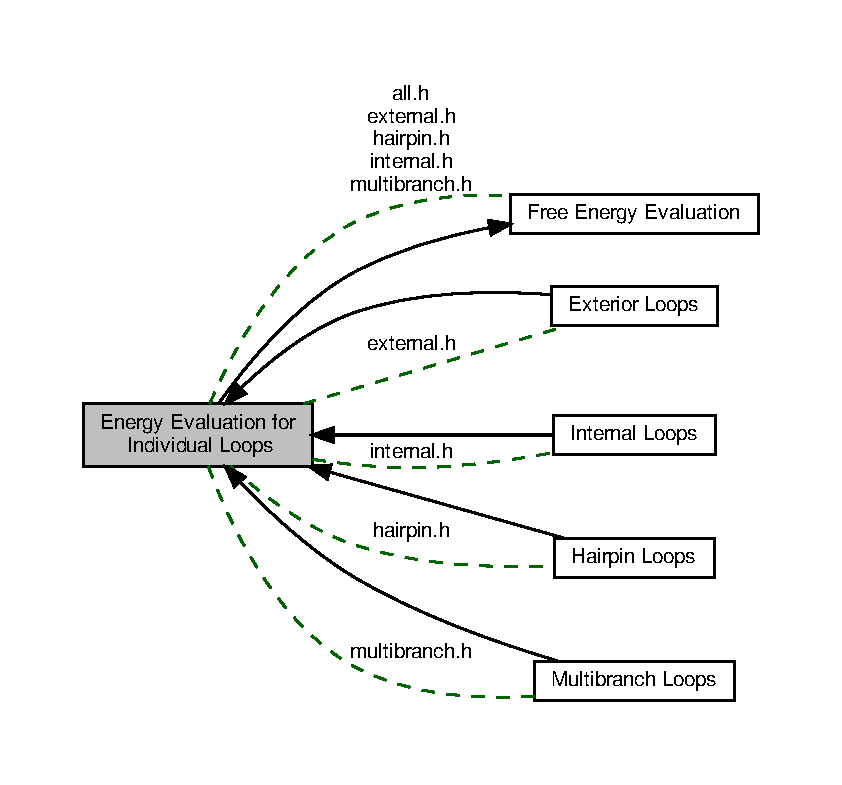
\includegraphics[width=350pt]{group__eval__loops}
\end{center}
\end{figure}
\subsection*{Modules}
\begin{DoxyCompactItemize}
\item 
\hyperlink{group__eval__loops__ext}{Exterior Loops}
\begin{DoxyCompactList}\small\item\em Functions to evaluate the free energy contributions for exterior loops. \end{DoxyCompactList}\item 
\hyperlink{group__eval__loops__hp}{Hairpin Loops}
\begin{DoxyCompactList}\small\item\em Functions to evaluate the free energy contributions for hairpin loops. \end{DoxyCompactList}\item 
\hyperlink{group__eval__loops__int}{Internal Loops}
\begin{DoxyCompactList}\small\item\em Functions to evaluate the free energy contributions for internal loops. \end{DoxyCompactList}\item 
\hyperlink{group__eval__loops__mb}{Multibranch Loops}
\begin{DoxyCompactList}\small\item\em Functions to evaluate the free energy contributions for mutlibranch loops. \end{DoxyCompactList}\end{DoxyCompactItemize}
\subsection*{Files}
\begin{DoxyCompactItemize}
\item 
file \hyperlink{all_8h}{all.\+h}
\begin{DoxyCompactList}\small\item\em Energy evaluation for M\+FE and partition function calculations. \end{DoxyCompactList}\item 
file \hyperlink{external_8h}{external.\+h}
\begin{DoxyCompactList}\small\item\em Energy evaluation of exterior loops for M\+FE and partition function calculations. \end{DoxyCompactList}\item 
file \hyperlink{hairpin_8h}{hairpin.\+h}
\begin{DoxyCompactList}\small\item\em Energy evaluation of hairpin loops for M\+FE and partition function calculations. \end{DoxyCompactList}\item 
file \hyperlink{internal_8h}{internal.\+h}
\begin{DoxyCompactList}\small\item\em Energy evaluation of interior loops for M\+FE and partition function calculations. \end{DoxyCompactList}\item 
file \hyperlink{multibranch_8h}{multibranch.\+h}
\begin{DoxyCompactList}\small\item\em Energy evaluation of multibranch loops for M\+FE and partition function calculations. \end{DoxyCompactList}\end{DoxyCompactItemize}
\subsection*{Functions}
\begin{DoxyCompactItemize}
\item 
int \hyperlink{group__eval__loops_ga730ba4df55c02fd530a0cddd49faf760}{vrna\+\_\+eval\+\_\+loop\+\_\+pt} (\hyperlink{group__fold__compound_ga1b0cef17fd40466cef5968eaeeff6166}{vrna\+\_\+fold\+\_\+compound\+\_\+t} $\ast$vc, int i, const short $\ast$pt)
\begin{DoxyCompactList}\small\item\em Calculate energy of a loop. \end{DoxyCompactList}\item 
int \hyperlink{group__eval__loops_ga30faecaff1009fe62c58312c8d56dabb}{vrna\+\_\+eval\+\_\+loop\+\_\+pt\+\_\+v} (\hyperlink{group__fold__compound_ga1b0cef17fd40466cef5968eaeeff6166}{vrna\+\_\+fold\+\_\+compound\+\_\+t} $\ast$vc, int i, const short $\ast$pt, int verbosity\+\_\+level)
\begin{DoxyCompactList}\small\item\em Calculate energy of a loop. \end{DoxyCompactList}\end{DoxyCompactItemize}


\subsection{Function Documentation}
\mbox{\Hypertarget{group__eval__loops_ga730ba4df55c02fd530a0cddd49faf760}\label{group__eval__loops_ga730ba4df55c02fd530a0cddd49faf760}} 
\index{Energy Evaluation for Individual Loops@{Energy Evaluation for Individual Loops}!vrna\+\_\+eval\+\_\+loop\+\_\+pt@{vrna\+\_\+eval\+\_\+loop\+\_\+pt}}
\index{vrna\+\_\+eval\+\_\+loop\+\_\+pt@{vrna\+\_\+eval\+\_\+loop\+\_\+pt}!Energy Evaluation for Individual Loops@{Energy Evaluation for Individual Loops}}
\subsubsection{\texorpdfstring{vrna\+\_\+eval\+\_\+loop\+\_\+pt()}{vrna\_eval\_loop\_pt()}}
{\footnotesize\ttfamily int vrna\+\_\+eval\+\_\+loop\+\_\+pt (\begin{DoxyParamCaption}\item[{\hyperlink{group__fold__compound_ga1b0cef17fd40466cef5968eaeeff6166}{vrna\+\_\+fold\+\_\+compound\+\_\+t} $\ast$}]{vc,  }\item[{int}]{i,  }\item[{const short $\ast$}]{pt }\end{DoxyParamCaption})}



{\ttfamily \#include $<$\hyperlink{eval_8h}{Vienna\+R\+N\+A/eval.\+h}$>$}



Calculate energy of a loop. 


\begin{DoxyParams}{Parameters}
{\em vc} & A vrna\+\_\+fold\+\_\+compound\+\_\+t containing the energy parameters and model details \\
\hline
{\em i} & position of covering base pair \\
\hline
{\em pt} & the pair table of the secondary structure \\
\hline
\end{DoxyParams}
\begin{DoxyReturn}{Returns}
free energy of the loop in 10cal/mol
\end{DoxyReturn}
\begin{DoxyRefDesc}{S\+W\+I\+G Wrapper Notes}
\item[\hyperlink{wrappers__wrappers000036}{S\+W\+I\+G Wrapper Notes}]This function is attached as method {\bfseries eval\+\_\+loop\+\_\+pt()} to objects of type {\itshape fold\+\_\+compound} \end{DoxyRefDesc}
\mbox{\Hypertarget{group__eval__loops_ga30faecaff1009fe62c58312c8d56dabb}\label{group__eval__loops_ga30faecaff1009fe62c58312c8d56dabb}} 
\index{Energy Evaluation for Individual Loops@{Energy Evaluation for Individual Loops}!vrna\+\_\+eval\+\_\+loop\+\_\+pt\+\_\+v@{vrna\+\_\+eval\+\_\+loop\+\_\+pt\+\_\+v}}
\index{vrna\+\_\+eval\+\_\+loop\+\_\+pt\+\_\+v@{vrna\+\_\+eval\+\_\+loop\+\_\+pt\+\_\+v}!Energy Evaluation for Individual Loops@{Energy Evaluation for Individual Loops}}
\subsubsection{\texorpdfstring{vrna\+\_\+eval\+\_\+loop\+\_\+pt\+\_\+v()}{vrna\_eval\_loop\_pt\_v()}}
{\footnotesize\ttfamily int vrna\+\_\+eval\+\_\+loop\+\_\+pt\+\_\+v (\begin{DoxyParamCaption}\item[{\hyperlink{group__fold__compound_ga1b0cef17fd40466cef5968eaeeff6166}{vrna\+\_\+fold\+\_\+compound\+\_\+t} $\ast$}]{vc,  }\item[{int}]{i,  }\item[{const short $\ast$}]{pt,  }\item[{int}]{verbosity\+\_\+level }\end{DoxyParamCaption})}



{\ttfamily \#include $<$\hyperlink{eval_8h}{Vienna\+R\+N\+A/eval.\+h}$>$}



Calculate energy of a loop. 


\begin{DoxyParams}{Parameters}
{\em vc} & A vrna\+\_\+fold\+\_\+compound\+\_\+t containing the energy parameters and model details \\
\hline
{\em i} & position of covering base pair \\
\hline
{\em pt} & the pair table of the secondary structure \\
\hline
{\em verbosity\+\_\+level} & The level of verbosity of this function \\
\hline
\end{DoxyParams}
\begin{DoxyReturn}{Returns}
free energy of the loop in 10cal/mol 
\end{DoxyReturn}

\hypertarget{group__eval__move}{}\section{Energy Evaluation for Atomic Moves}
\label{group__eval__move}\index{Energy Evaluation for Atomic Moves@{Energy Evaluation for Atomic Moves}}


Functions to evaluate the free energy change of a structure after application of (a set of) atomic moves.  




\subsection{Detailed Description}
Functions to evaluate the free energy change of a structure after application of (a set of) atomic moves. 

Here, atomic moves are not to be confused with moves of actual physical atoms. Instead, an atomic move is considered the smallest conformational change a secondary structure can undergo to form another, distinguishable structure. We currently support the following moves \subparagraph*{Atomic Moves\+:}


\begin{DoxyItemize}
\item Opening (dissociation) of a single base pair
\item Closing (formation) of a single base pair
\item Shifting one pairing partner of an existing pair to a different location 
\end{DoxyItemize}Collaboration diagram for Energy Evaluation for Atomic Moves\+:
\nopagebreak
\begin{figure}[H]
\begin{center}
\leavevmode
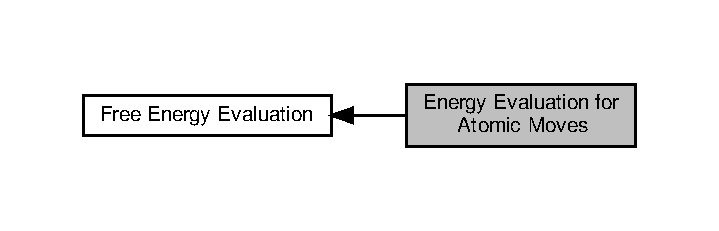
\includegraphics[width=345pt]{group__eval__move}
\end{center}
\end{figure}
\subsection*{Functions}
\begin{DoxyCompactItemize}
\item 
float \hyperlink{group__eval__move_gaff1b9e4f4d17b434b0a822fe783672c1}{vrna\+\_\+eval\+\_\+move} (\hyperlink{group__fold__compound_ga1b0cef17fd40466cef5968eaeeff6166}{vrna\+\_\+fold\+\_\+compound\+\_\+t} $\ast$vc, const char $\ast$structure, int m1, int m2)
\begin{DoxyCompactList}\small\item\em Calculate energy of a move (closing or opening of a base pair) \end{DoxyCompactList}\item 
int \hyperlink{group__eval__move_ga123dabc119ea98c968a5e903cc46f0fb}{vrna\+\_\+eval\+\_\+move\+\_\+pt} (\hyperlink{group__fold__compound_ga1b0cef17fd40466cef5968eaeeff6166}{vrna\+\_\+fold\+\_\+compound\+\_\+t} $\ast$vc, short $\ast$pt, int m1, int m2)
\begin{DoxyCompactList}\small\item\em Calculate energy of a move (closing or opening of a base pair) \end{DoxyCompactList}\end{DoxyCompactItemize}


\subsection{Function Documentation}
\mbox{\Hypertarget{group__eval__move_gaff1b9e4f4d17b434b0a822fe783672c1}\label{group__eval__move_gaff1b9e4f4d17b434b0a822fe783672c1}} 
\index{Energy Evaluation for Atomic Moves@{Energy Evaluation for Atomic Moves}!vrna\+\_\+eval\+\_\+move@{vrna\+\_\+eval\+\_\+move}}
\index{vrna\+\_\+eval\+\_\+move@{vrna\+\_\+eval\+\_\+move}!Energy Evaluation for Atomic Moves@{Energy Evaluation for Atomic Moves}}
\subsubsection{\texorpdfstring{vrna\+\_\+eval\+\_\+move()}{vrna\_eval\_move()}}
{\footnotesize\ttfamily float vrna\+\_\+eval\+\_\+move (\begin{DoxyParamCaption}\item[{\hyperlink{group__fold__compound_ga1b0cef17fd40466cef5968eaeeff6166}{vrna\+\_\+fold\+\_\+compound\+\_\+t} $\ast$}]{vc,  }\item[{const char $\ast$}]{structure,  }\item[{int}]{m1,  }\item[{int}]{m2 }\end{DoxyParamCaption})}



{\ttfamily \#include $<$\hyperlink{eval_8h}{Vienna\+R\+N\+A/eval.\+h}$>$}



Calculate energy of a move (closing or opening of a base pair) 

If the parameters m1 and m2 are negative, it is deletion (opening) of a base pair, otherwise it is insertion (opening).

\begin{DoxySeeAlso}{See also}
\hyperlink{group__eval__move_ga123dabc119ea98c968a5e903cc46f0fb}{vrna\+\_\+eval\+\_\+move\+\_\+pt()} 
\end{DoxySeeAlso}

\begin{DoxyParams}{Parameters}
{\em vc} & A vrna\+\_\+fold\+\_\+compound\+\_\+t containing the energy parameters and model details \\
\hline
{\em structure} & secondary structure in dot-\/bracket notation \\
\hline
{\em m1} & first coordinate of base pair \\
\hline
{\em m2} & second coordinate of base pair \\
\hline
\end{DoxyParams}
\begin{DoxyReturn}{Returns}
energy change of the move in kcal/mol (\hyperlink{constants_8h_a12c2040f25d8e3a7b9e1c2024c618cb6}{I\+NF} / 100. upon any error)
\end{DoxyReturn}
\begin{DoxyRefDesc}{S\+W\+I\+G Wrapper Notes}
\item[\hyperlink{wrappers__wrappers000037}{S\+W\+I\+G Wrapper Notes}]This function is attached as method {\bfseries eval\+\_\+move()} to objects of type {\itshape fold\+\_\+compound} \end{DoxyRefDesc}
\mbox{\Hypertarget{group__eval__move_ga123dabc119ea98c968a5e903cc46f0fb}\label{group__eval__move_ga123dabc119ea98c968a5e903cc46f0fb}} 
\index{Energy Evaluation for Atomic Moves@{Energy Evaluation for Atomic Moves}!vrna\+\_\+eval\+\_\+move\+\_\+pt@{vrna\+\_\+eval\+\_\+move\+\_\+pt}}
\index{vrna\+\_\+eval\+\_\+move\+\_\+pt@{vrna\+\_\+eval\+\_\+move\+\_\+pt}!Energy Evaluation for Atomic Moves@{Energy Evaluation for Atomic Moves}}
\subsubsection{\texorpdfstring{vrna\+\_\+eval\+\_\+move\+\_\+pt()}{vrna\_eval\_move\_pt()}}
{\footnotesize\ttfamily int vrna\+\_\+eval\+\_\+move\+\_\+pt (\begin{DoxyParamCaption}\item[{\hyperlink{group__fold__compound_ga1b0cef17fd40466cef5968eaeeff6166}{vrna\+\_\+fold\+\_\+compound\+\_\+t} $\ast$}]{vc,  }\item[{short $\ast$}]{pt,  }\item[{int}]{m1,  }\item[{int}]{m2 }\end{DoxyParamCaption})}



{\ttfamily \#include $<$\hyperlink{eval_8h}{Vienna\+R\+N\+A/eval.\+h}$>$}



Calculate energy of a move (closing or opening of a base pair) 

If the parameters m1 and m2 are negative, it is deletion (opening) of a base pair, otherwise it is insertion (opening).

\begin{DoxySeeAlso}{See also}
\hyperlink{group__eval__move_gaff1b9e4f4d17b434b0a822fe783672c1}{vrna\+\_\+eval\+\_\+move()} 
\end{DoxySeeAlso}

\begin{DoxyParams}{Parameters}
{\em vc} & A vrna\+\_\+fold\+\_\+compound\+\_\+t containing the energy parameters and model details \\
\hline
{\em pt} & the pair table of the secondary structure \\
\hline
{\em m1} & first coordinate of base pair \\
\hline
{\em m2} & second coordinate of base pair \\
\hline
\end{DoxyParams}
\begin{DoxyReturn}{Returns}
energy change of the move in 10cal/mol
\end{DoxyReturn}
\begin{DoxyRefDesc}{S\+W\+I\+G Wrapper Notes}
\item[\hyperlink{wrappers__wrappers000038}{S\+W\+I\+G Wrapper Notes}]This function is attached as method {\bfseries eval\+\_\+move\+\_\+pt()} to objects of type {\itshape fold\+\_\+compound} \end{DoxyRefDesc}

\hypertarget{group__eval__deprecated}{}\section{Deprecated Interface for Free Energy Evaluation}
\label{group__eval__deprecated}\index{Deprecated Interface for Free Energy Evaluation@{Deprecated Interface for Free Energy Evaluation}}


Deprecated Energy Evaluation functions.  




\subsection{Detailed Description}
Deprecated Energy Evaluation functions. 

Using the functions below is discouraged as they have been marked deprecated and will be removed from the library in the (near) future! Collaboration diagram for Deprecated Interface for Free Energy Evaluation\+:
\nopagebreak
\begin{figure}[H]
\begin{center}
\leavevmode
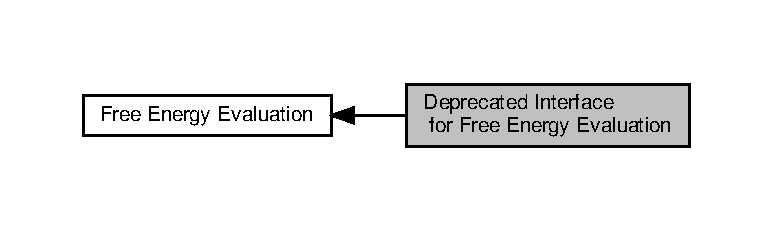
\includegraphics[width=350pt]{group__eval__deprecated}
\end{center}
\end{figure}
\subsection*{Functions}
\begin{DoxyCompactItemize}
\item 
float \hyperlink{group__eval__deprecated_gaf93986cb3cb29770ec9cca69c9fab8cf}{energy\+\_\+of\+\_\+structure} (const char $\ast$string, const char $\ast$structure, int verbosity\+\_\+level)
\begin{DoxyCompactList}\small\item\em Calculate the free energy of an already folded R\+NA using global model detail settings. \end{DoxyCompactList}\item 
float \hyperlink{group__eval__deprecated_gaf9d064d3c496de42eca6734a96fd2090}{energy\+\_\+of\+\_\+struct\+\_\+par} (const char $\ast$string, const char $\ast$structure, \hyperlink{group__energy__parameters_ga8a69ca7d787e4fd6079914f5343a1f35}{vrna\+\_\+param\+\_\+t} $\ast$parameters, int verbosity\+\_\+level)
\begin{DoxyCompactList}\small\item\em Calculate the free energy of an already folded R\+NA. \end{DoxyCompactList}\item 
float \hyperlink{group__eval__deprecated_gaeb14f3664aec67fc03268ac75253f0f8}{energy\+\_\+of\+\_\+circ\+\_\+structure} (const char $\ast$string, const char $\ast$structure, int verbosity\+\_\+level)
\begin{DoxyCompactList}\small\item\em Calculate the free energy of an already folded circular R\+NA. \end{DoxyCompactList}\item 
float \hyperlink{group__eval__deprecated_ga3f01f9744ba6a40555eb4d81fc77f6df}{energy\+\_\+of\+\_\+circ\+\_\+struct\+\_\+par} (const char $\ast$string, const char $\ast$structure, \hyperlink{group__energy__parameters_ga8a69ca7d787e4fd6079914f5343a1f35}{vrna\+\_\+param\+\_\+t} $\ast$parameters, int verbosity\+\_\+level)
\begin{DoxyCompactList}\small\item\em Calculate the free energy of an already folded circular R\+NA. \end{DoxyCompactList}\item 
int \hyperlink{group__eval__deprecated_ga8831445966b761417e713360791299d8}{energy\+\_\+of\+\_\+structure\+\_\+pt} (const char $\ast$string, short $\ast$ptable, short $\ast$s, short $\ast$s1, int verbosity\+\_\+level)
\begin{DoxyCompactList}\small\item\em Calculate the free energy of an already folded R\+NA. \end{DoxyCompactList}\item 
int \hyperlink{group__eval__deprecated_ga49acb3d5627dc6823a7ce12d116d4c69}{energy\+\_\+of\+\_\+struct\+\_\+pt\+\_\+par} (const char $\ast$string, short $\ast$ptable, short $\ast$s, short $\ast$s1, \hyperlink{group__energy__parameters_ga8a69ca7d787e4fd6079914f5343a1f35}{vrna\+\_\+param\+\_\+t} $\ast$parameters, int verbosity\+\_\+level)
\begin{DoxyCompactList}\small\item\em Calculate the free energy of an already folded R\+NA. \end{DoxyCompactList}\item 
float \hyperlink{group__eval__deprecated_ga539ecaed89730f7644c202f304d7529b}{energy\+\_\+of\+\_\+move} (const char $\ast$string, const char $\ast$structure, int m1, int m2)
\begin{DoxyCompactList}\small\item\em Calculate energy of a move (closing or opening of a base pair) \end{DoxyCompactList}\item 
int \hyperlink{group__eval__deprecated_ga49e0ee561be69faf0568213546f6a53f}{energy\+\_\+of\+\_\+move\+\_\+pt} (short $\ast$pt, short $\ast$s, short $\ast$s1, int m1, int m2)
\begin{DoxyCompactList}\small\item\em Calculate energy of a move (closing or opening of a base pair) \end{DoxyCompactList}\item 
int \hyperlink{group__eval__deprecated_ga507d4fd93f4b398d793ba2402731388d}{loop\+\_\+energy} (short $\ast$ptable, short $\ast$s, short $\ast$s1, int i)
\begin{DoxyCompactList}\small\item\em Calculate energy of a loop. \end{DoxyCompactList}\item 
float \hyperlink{group__eval__deprecated_gac2b37fea2145c94d925a3f33378ef87b}{energy\+\_\+of\+\_\+struct} (const char $\ast$string, const char $\ast$structure)
\item 
int \hyperlink{group__eval__deprecated_ga27ce6f68512d43bf1fe14a06c9d76d5c}{energy\+\_\+of\+\_\+struct\+\_\+pt} (const char $\ast$string, short $\ast$ptable, short $\ast$s, short $\ast$s1)
\item 
float \hyperlink{group__eval__deprecated_ga657222e2758c46bf13b416ef3032e417}{energy\+\_\+of\+\_\+circ\+\_\+struct} (const char $\ast$string, const char $\ast$structure)
\item 
int \hyperlink{group__eval__deprecated_ga51f9851f3500c2aae66674142a6a2dd5}{E\+\_\+\+Stem} (int type, int si1, int sj1, int ext\+Loop, \hyperlink{group__energy__parameters_ga8a69ca7d787e4fd6079914f5343a1f35}{vrna\+\_\+param\+\_\+t} $\ast$P)
\begin{DoxyCompactList}\small\item\em Compute the energy contribution of a stem branching off a loop-\/region. \end{DoxyCompactList}\item 
\hyperlink{group__data__structures_ga31125aeace516926bf7f251f759b6126}{F\+L\+T\+\_\+\+O\+R\+\_\+\+D\+BL} \hyperlink{group__eval__deprecated_ga446828a191c127861e76e2c84055f672}{exp\+\_\+\+E\+\_\+\+Ext\+Loop} (int type, int si1, int sj1, \hyperlink{group__energy__parameters_ga01d8b92fe734df8d79a6169482c7d8d8}{vrna\+\_\+exp\+\_\+param\+\_\+t} $\ast$P)
\item 
\hyperlink{group__data__structures_ga31125aeace516926bf7f251f759b6126}{F\+L\+T\+\_\+\+O\+R\+\_\+\+D\+BL} \hyperlink{group__eval__deprecated_gab0aa9833ab41875a91a9be8a5ffd7092}{exp\+\_\+\+E\+\_\+\+Stem} (int type, int si1, int sj1, int ext\+Loop, \hyperlink{group__energy__parameters_ga01d8b92fe734df8d79a6169482c7d8d8}{vrna\+\_\+exp\+\_\+param\+\_\+t} $\ast$P)
\item 
P\+R\+I\+V\+A\+TE int \hyperlink{group__eval__deprecated_gaafbc187b7f78e8e82afb77dd6f3b8fc5}{E\+\_\+\+Int\+Loop} (int n1, int n2, int type, int type\+\_\+2, int si1, int sj1, int sp1, int sq1, \hyperlink{group__energy__parameters_ga8a69ca7d787e4fd6079914f5343a1f35}{vrna\+\_\+param\+\_\+t} $\ast$P)
\item 
P\+R\+I\+V\+A\+TE \hyperlink{group__data__structures_ga31125aeace516926bf7f251f759b6126}{F\+L\+T\+\_\+\+O\+R\+\_\+\+D\+BL} \hyperlink{group__eval__deprecated_ga95de54d8a2a17645a95e0f34e189d9c9}{exp\+\_\+\+E\+\_\+\+Int\+Loop} (int u1, int u2, int type, int type2, short si1, short sj1, short sp1, short sq1, \hyperlink{group__energy__parameters_ga01d8b92fe734df8d79a6169482c7d8d8}{vrna\+\_\+exp\+\_\+param\+\_\+t} $\ast$P)
\end{DoxyCompactItemize}
\subsection*{Variables}
\begin{DoxyCompactItemize}
\item 
\mbox{\Hypertarget{group__eval__deprecated_gab9b2c3a37a5516614c06d0ab54b97cda}\label{group__eval__deprecated_gab9b2c3a37a5516614c06d0ab54b97cda}} 
int \hyperlink{group__eval__deprecated_gab9b2c3a37a5516614c06d0ab54b97cda}{cut\+\_\+point}
\begin{DoxyCompactList}\small\item\em first pos of second seq for cofolding \end{DoxyCompactList}\item 
\mbox{\Hypertarget{group__eval__deprecated_ga567530678f6260a1a649a5beca5da4c5}\label{group__eval__deprecated_ga567530678f6260a1a649a5beca5da4c5}} 
int \hyperlink{group__eval__deprecated_ga567530678f6260a1a649a5beca5da4c5}{eos\+\_\+debug}
\begin{DoxyCompactList}\small\item\em verbose info from energy\+\_\+of\+\_\+struct \end{DoxyCompactList}\end{DoxyCompactItemize}


\subsection{Function Documentation}
\mbox{\Hypertarget{group__eval__deprecated_gaf93986cb3cb29770ec9cca69c9fab8cf}\label{group__eval__deprecated_gaf93986cb3cb29770ec9cca69c9fab8cf}} 
\index{Deprecated Interface for Free Energy Evaluation@{Deprecated Interface for Free Energy Evaluation}!energy\+\_\+of\+\_\+structure@{energy\+\_\+of\+\_\+structure}}
\index{energy\+\_\+of\+\_\+structure@{energy\+\_\+of\+\_\+structure}!Deprecated Interface for Free Energy Evaluation@{Deprecated Interface for Free Energy Evaluation}}
\subsubsection{\texorpdfstring{energy\+\_\+of\+\_\+structure()}{energy\_of\_structure()}}
{\footnotesize\ttfamily float energy\+\_\+of\+\_\+structure (\begin{DoxyParamCaption}\item[{const char $\ast$}]{string,  }\item[{const char $\ast$}]{structure,  }\item[{int}]{verbosity\+\_\+level }\end{DoxyParamCaption})}



{\ttfamily \#include $<$\hyperlink{eval_8h}{Vienna\+R\+N\+A/eval.\+h}$>$}



Calculate the free energy of an already folded R\+NA using global model detail settings. 

If verbosity level is set to a value $>$0, energies of structure elements are printed to stdout

\begin{DoxyNote}{Note}
Open\+MP\+: This function relies on several global model settings variables and thus is not to be considered threadsafe. See \hyperlink{group__eval__deprecated_gaf9d064d3c496de42eca6734a96fd2090}{energy\+\_\+of\+\_\+struct\+\_\+par()} for a completely threadsafe implementation.
\end{DoxyNote}
\begin{DoxyRefDesc}{Deprecated}
\item[\hyperlink{deprecated__deprecated000049}{Deprecated}]Use \hyperlink{group__eval_ga58f199f1438d794a265f3b27fc8ea631}{vrna\+\_\+eval\+\_\+structure()} or \hyperlink{group__eval_ga0928d699d310178f84ee2351034e5cb5}{vrna\+\_\+eval\+\_\+structure\+\_\+verbose()} instead!\end{DoxyRefDesc}


\begin{DoxySeeAlso}{See also}
\hyperlink{group__eval_ga58f199f1438d794a265f3b27fc8ea631}{vrna\+\_\+eval\+\_\+structure()}
\end{DoxySeeAlso}

\begin{DoxyParams}{Parameters}
{\em string} & R\+NA sequence \\
\hline
{\em structure} & secondary structure in dot-\/bracket notation \\
\hline
{\em verbosity\+\_\+level} & a flag to turn verbose output on/off \\
\hline
\end{DoxyParams}
\begin{DoxyReturn}{Returns}
the free energy of the input structure given the input sequence in kcal/mol 
\end{DoxyReturn}
\mbox{\Hypertarget{group__eval__deprecated_gaf9d064d3c496de42eca6734a96fd2090}\label{group__eval__deprecated_gaf9d064d3c496de42eca6734a96fd2090}} 
\index{Deprecated Interface for Free Energy Evaluation@{Deprecated Interface for Free Energy Evaluation}!energy\+\_\+of\+\_\+struct\+\_\+par@{energy\+\_\+of\+\_\+struct\+\_\+par}}
\index{energy\+\_\+of\+\_\+struct\+\_\+par@{energy\+\_\+of\+\_\+struct\+\_\+par}!Deprecated Interface for Free Energy Evaluation@{Deprecated Interface for Free Energy Evaluation}}
\subsubsection{\texorpdfstring{energy\+\_\+of\+\_\+struct\+\_\+par()}{energy\_of\_struct\_par()}}
{\footnotesize\ttfamily float energy\+\_\+of\+\_\+struct\+\_\+par (\begin{DoxyParamCaption}\item[{const char $\ast$}]{string,  }\item[{const char $\ast$}]{structure,  }\item[{\hyperlink{group__energy__parameters_ga8a69ca7d787e4fd6079914f5343a1f35}{vrna\+\_\+param\+\_\+t} $\ast$}]{parameters,  }\item[{int}]{verbosity\+\_\+level }\end{DoxyParamCaption})}



{\ttfamily \#include $<$\hyperlink{eval_8h}{Vienna\+R\+N\+A/eval.\+h}$>$}



Calculate the free energy of an already folded R\+NA. 

If verbosity level is set to a value $>$0, energies of structure elements are printed to stdout

\begin{DoxyRefDesc}{Deprecated}
\item[\hyperlink{deprecated__deprecated000050}{Deprecated}]Use \hyperlink{group__eval_ga58f199f1438d794a265f3b27fc8ea631}{vrna\+\_\+eval\+\_\+structure()} or \hyperlink{group__eval_ga0928d699d310178f84ee2351034e5cb5}{vrna\+\_\+eval\+\_\+structure\+\_\+verbose()} instead!\end{DoxyRefDesc}


\begin{DoxySeeAlso}{See also}
\hyperlink{group__eval_ga58f199f1438d794a265f3b27fc8ea631}{vrna\+\_\+eval\+\_\+structure()}
\end{DoxySeeAlso}

\begin{DoxyParams}{Parameters}
{\em string} & R\+NA sequence in uppercase letters \\
\hline
{\em structure} & Secondary structure in dot-\/bracket notation \\
\hline
{\em parameters} & A data structure containing the prescaled energy contributions and the model details. \\
\hline
{\em verbosity\+\_\+level} & A flag to turn verbose output on/off \\
\hline
\end{DoxyParams}
\begin{DoxyReturn}{Returns}
The free energy of the input structure given the input sequence in kcal/mol 
\end{DoxyReturn}
\mbox{\Hypertarget{group__eval__deprecated_gaeb14f3664aec67fc03268ac75253f0f8}\label{group__eval__deprecated_gaeb14f3664aec67fc03268ac75253f0f8}} 
\index{Deprecated Interface for Free Energy Evaluation@{Deprecated Interface for Free Energy Evaluation}!energy\+\_\+of\+\_\+circ\+\_\+structure@{energy\+\_\+of\+\_\+circ\+\_\+structure}}
\index{energy\+\_\+of\+\_\+circ\+\_\+structure@{energy\+\_\+of\+\_\+circ\+\_\+structure}!Deprecated Interface for Free Energy Evaluation@{Deprecated Interface for Free Energy Evaluation}}
\subsubsection{\texorpdfstring{energy\+\_\+of\+\_\+circ\+\_\+structure()}{energy\_of\_circ\_structure()}}
{\footnotesize\ttfamily float energy\+\_\+of\+\_\+circ\+\_\+structure (\begin{DoxyParamCaption}\item[{const char $\ast$}]{string,  }\item[{const char $\ast$}]{structure,  }\item[{int}]{verbosity\+\_\+level }\end{DoxyParamCaption})}



{\ttfamily \#include $<$\hyperlink{eval_8h}{Vienna\+R\+N\+A/eval.\+h}$>$}



Calculate the free energy of an already folded circular R\+NA. 

\begin{DoxyNote}{Note}
Open\+MP\+: This function relies on several global model settings variables and thus is not to be considered threadsafe. See \hyperlink{group__eval__deprecated_ga3f01f9744ba6a40555eb4d81fc77f6df}{energy\+\_\+of\+\_\+circ\+\_\+struct\+\_\+par()} for a completely threadsafe implementation.
\end{DoxyNote}
If verbosity level is set to a value $>$0, energies of structure elements are printed to stdout

\begin{DoxyRefDesc}{Deprecated}
\item[\hyperlink{deprecated__deprecated000051}{Deprecated}]Use \hyperlink{group__eval_ga58f199f1438d794a265f3b27fc8ea631}{vrna\+\_\+eval\+\_\+structure()} or \hyperlink{group__eval_ga0928d699d310178f84ee2351034e5cb5}{vrna\+\_\+eval\+\_\+structure\+\_\+verbose()} instead!\end{DoxyRefDesc}


\begin{DoxySeeAlso}{See also}
\hyperlink{group__eval_ga58f199f1438d794a265f3b27fc8ea631}{vrna\+\_\+eval\+\_\+structure()}
\end{DoxySeeAlso}

\begin{DoxyParams}{Parameters}
{\em string} & R\+NA sequence \\
\hline
{\em structure} & Secondary structure in dot-\/bracket notation \\
\hline
{\em verbosity\+\_\+level} & A flag to turn verbose output on/off \\
\hline
\end{DoxyParams}
\begin{DoxyReturn}{Returns}
The free energy of the input structure given the input sequence in kcal/mol 
\end{DoxyReturn}
\mbox{\Hypertarget{group__eval__deprecated_ga3f01f9744ba6a40555eb4d81fc77f6df}\label{group__eval__deprecated_ga3f01f9744ba6a40555eb4d81fc77f6df}} 
\index{Deprecated Interface for Free Energy Evaluation@{Deprecated Interface for Free Energy Evaluation}!energy\+\_\+of\+\_\+circ\+\_\+struct\+\_\+par@{energy\+\_\+of\+\_\+circ\+\_\+struct\+\_\+par}}
\index{energy\+\_\+of\+\_\+circ\+\_\+struct\+\_\+par@{energy\+\_\+of\+\_\+circ\+\_\+struct\+\_\+par}!Deprecated Interface for Free Energy Evaluation@{Deprecated Interface for Free Energy Evaluation}}
\subsubsection{\texorpdfstring{energy\+\_\+of\+\_\+circ\+\_\+struct\+\_\+par()}{energy\_of\_circ\_struct\_par()}}
{\footnotesize\ttfamily float energy\+\_\+of\+\_\+circ\+\_\+struct\+\_\+par (\begin{DoxyParamCaption}\item[{const char $\ast$}]{string,  }\item[{const char $\ast$}]{structure,  }\item[{\hyperlink{group__energy__parameters_ga8a69ca7d787e4fd6079914f5343a1f35}{vrna\+\_\+param\+\_\+t} $\ast$}]{parameters,  }\item[{int}]{verbosity\+\_\+level }\end{DoxyParamCaption})}



{\ttfamily \#include $<$\hyperlink{eval_8h}{Vienna\+R\+N\+A/eval.\+h}$>$}



Calculate the free energy of an already folded circular R\+NA. 

If verbosity level is set to a value $>$0, energies of structure elements are printed to stdout

\begin{DoxyRefDesc}{Deprecated}
\item[\hyperlink{deprecated__deprecated000052}{Deprecated}]Use \hyperlink{group__eval_ga58f199f1438d794a265f3b27fc8ea631}{vrna\+\_\+eval\+\_\+structure()} or \hyperlink{group__eval_ga0928d699d310178f84ee2351034e5cb5}{vrna\+\_\+eval\+\_\+structure\+\_\+verbose()} instead!\end{DoxyRefDesc}


\begin{DoxySeeAlso}{See also}
\hyperlink{group__eval_ga58f199f1438d794a265f3b27fc8ea631}{vrna\+\_\+eval\+\_\+structure()}
\end{DoxySeeAlso}

\begin{DoxyParams}{Parameters}
{\em string} & R\+NA sequence \\
\hline
{\em structure} & Secondary structure in dot-\/bracket notation \\
\hline
{\em parameters} & A data structure containing the prescaled energy contributions and the model details. \\
\hline
{\em verbosity\+\_\+level} & A flag to turn verbose output on/off \\
\hline
\end{DoxyParams}
\begin{DoxyReturn}{Returns}
The free energy of the input structure given the input sequence in kcal/mol 
\end{DoxyReturn}
\mbox{\Hypertarget{group__eval__deprecated_ga8831445966b761417e713360791299d8}\label{group__eval__deprecated_ga8831445966b761417e713360791299d8}} 
\index{Deprecated Interface for Free Energy Evaluation@{Deprecated Interface for Free Energy Evaluation}!energy\+\_\+of\+\_\+structure\+\_\+pt@{energy\+\_\+of\+\_\+structure\+\_\+pt}}
\index{energy\+\_\+of\+\_\+structure\+\_\+pt@{energy\+\_\+of\+\_\+structure\+\_\+pt}!Deprecated Interface for Free Energy Evaluation@{Deprecated Interface for Free Energy Evaluation}}
\subsubsection{\texorpdfstring{energy\+\_\+of\+\_\+structure\+\_\+pt()}{energy\_of\_structure\_pt()}}
{\footnotesize\ttfamily int energy\+\_\+of\+\_\+structure\+\_\+pt (\begin{DoxyParamCaption}\item[{const char $\ast$}]{string,  }\item[{short $\ast$}]{ptable,  }\item[{short $\ast$}]{s,  }\item[{short $\ast$}]{s1,  }\item[{int}]{verbosity\+\_\+level }\end{DoxyParamCaption})}



{\ttfamily \#include $<$\hyperlink{eval_8h}{Vienna\+R\+N\+A/eval.\+h}$>$}



Calculate the free energy of an already folded R\+NA. 

If verbosity level is set to a value $>$0, energies of structure elements are printed to stdout

\begin{DoxyNote}{Note}
Open\+MP\+: This function relies on several global model settings variables and thus is not to be considered threadsafe. See \hyperlink{group__eval__deprecated_ga49acb3d5627dc6823a7ce12d116d4c69}{energy\+\_\+of\+\_\+struct\+\_\+pt\+\_\+par()} for a completely threadsafe implementation.
\end{DoxyNote}
\begin{DoxyRefDesc}{Deprecated}
\item[\hyperlink{deprecated__deprecated000053}{Deprecated}]Use \hyperlink{group__eval_gadbd09372ddfd7a450bbd590c96a6bfe4}{vrna\+\_\+eval\+\_\+structure\+\_\+pt()} or \hyperlink{group__eval_ga8a517cfeeae8c376ae7b1e0c401d38b4}{vrna\+\_\+eval\+\_\+structure\+\_\+pt\+\_\+verbose()} instead!\end{DoxyRefDesc}


\begin{DoxySeeAlso}{See also}
\hyperlink{group__eval_gadbd09372ddfd7a450bbd590c96a6bfe4}{vrna\+\_\+eval\+\_\+structure\+\_\+pt()}
\end{DoxySeeAlso}

\begin{DoxyParams}{Parameters}
{\em string} & R\+NA sequence \\
\hline
{\em ptable} & the pair table of the secondary structure \\
\hline
{\em s} & encoded R\+NA sequence \\
\hline
{\em s1} & encoded R\+NA sequence \\
\hline
{\em verbosity\+\_\+level} & a flag to turn verbose output on/off \\
\hline
\end{DoxyParams}
\begin{DoxyReturn}{Returns}
the free energy of the input structure given the input sequence in 10kcal/mol 
\end{DoxyReturn}
\mbox{\Hypertarget{group__eval__deprecated_ga49acb3d5627dc6823a7ce12d116d4c69}\label{group__eval__deprecated_ga49acb3d5627dc6823a7ce12d116d4c69}} 
\index{Deprecated Interface for Free Energy Evaluation@{Deprecated Interface for Free Energy Evaluation}!energy\+\_\+of\+\_\+struct\+\_\+pt\+\_\+par@{energy\+\_\+of\+\_\+struct\+\_\+pt\+\_\+par}}
\index{energy\+\_\+of\+\_\+struct\+\_\+pt\+\_\+par@{energy\+\_\+of\+\_\+struct\+\_\+pt\+\_\+par}!Deprecated Interface for Free Energy Evaluation@{Deprecated Interface for Free Energy Evaluation}}
\subsubsection{\texorpdfstring{energy\+\_\+of\+\_\+struct\+\_\+pt\+\_\+par()}{energy\_of\_struct\_pt\_par()}}
{\footnotesize\ttfamily int energy\+\_\+of\+\_\+struct\+\_\+pt\+\_\+par (\begin{DoxyParamCaption}\item[{const char $\ast$}]{string,  }\item[{short $\ast$}]{ptable,  }\item[{short $\ast$}]{s,  }\item[{short $\ast$}]{s1,  }\item[{\hyperlink{group__energy__parameters_ga8a69ca7d787e4fd6079914f5343a1f35}{vrna\+\_\+param\+\_\+t} $\ast$}]{parameters,  }\item[{int}]{verbosity\+\_\+level }\end{DoxyParamCaption})}



{\ttfamily \#include $<$\hyperlink{eval_8h}{Vienna\+R\+N\+A/eval.\+h}$>$}



Calculate the free energy of an already folded R\+NA. 

If verbosity level is set to a value $>$0, energies of structure elements are printed to stdout

\begin{DoxyRefDesc}{Deprecated}
\item[\hyperlink{deprecated__deprecated000054}{Deprecated}]Use \hyperlink{group__eval_gadbd09372ddfd7a450bbd590c96a6bfe4}{vrna\+\_\+eval\+\_\+structure\+\_\+pt()} or \hyperlink{group__eval_ga8a517cfeeae8c376ae7b1e0c401d38b4}{vrna\+\_\+eval\+\_\+structure\+\_\+pt\+\_\+verbose()} instead!\end{DoxyRefDesc}


\begin{DoxySeeAlso}{See also}
\hyperlink{group__eval_gadbd09372ddfd7a450bbd590c96a6bfe4}{vrna\+\_\+eval\+\_\+structure\+\_\+pt()}
\end{DoxySeeAlso}

\begin{DoxyParams}{Parameters}
{\em string} & R\+NA sequence in uppercase letters \\
\hline
{\em ptable} & The pair table of the secondary structure \\
\hline
{\em s} & Encoded R\+NA sequence \\
\hline
{\em s1} & Encoded R\+NA sequence \\
\hline
{\em parameters} & A data structure containing the prescaled energy contributions and the model details. \\
\hline
{\em verbosity\+\_\+level} & A flag to turn verbose output on/off \\
\hline
\end{DoxyParams}
\begin{DoxyReturn}{Returns}
The free energy of the input structure given the input sequence in 10kcal/mol 
\end{DoxyReturn}
\mbox{\Hypertarget{group__eval__deprecated_ga539ecaed89730f7644c202f304d7529b}\label{group__eval__deprecated_ga539ecaed89730f7644c202f304d7529b}} 
\index{Deprecated Interface for Free Energy Evaluation@{Deprecated Interface for Free Energy Evaluation}!energy\+\_\+of\+\_\+move@{energy\+\_\+of\+\_\+move}}
\index{energy\+\_\+of\+\_\+move@{energy\+\_\+of\+\_\+move}!Deprecated Interface for Free Energy Evaluation@{Deprecated Interface for Free Energy Evaluation}}
\subsubsection{\texorpdfstring{energy\+\_\+of\+\_\+move()}{energy\_of\_move()}}
{\footnotesize\ttfamily float energy\+\_\+of\+\_\+move (\begin{DoxyParamCaption}\item[{const char $\ast$}]{string,  }\item[{const char $\ast$}]{structure,  }\item[{int}]{m1,  }\item[{int}]{m2 }\end{DoxyParamCaption})}



{\ttfamily \#include $<$\hyperlink{eval_8h}{Vienna\+R\+N\+A/eval.\+h}$>$}



Calculate energy of a move (closing or opening of a base pair) 

If the parameters m1 and m2 are negative, it is deletion (opening) of a base pair, otherwise it is insertion (opening).

\begin{DoxyRefDesc}{Deprecated}
\item[\hyperlink{deprecated__deprecated000055}{Deprecated}]Use \hyperlink{group__eval__move_gaff1b9e4f4d17b434b0a822fe783672c1}{vrna\+\_\+eval\+\_\+move()} instead!\end{DoxyRefDesc}


\begin{DoxySeeAlso}{See also}
\hyperlink{group__eval__move_gaff1b9e4f4d17b434b0a822fe783672c1}{vrna\+\_\+eval\+\_\+move()}
\end{DoxySeeAlso}

\begin{DoxyParams}{Parameters}
{\em string} & R\+NA sequence \\
\hline
{\em structure} & secondary structure in dot-\/bracket notation \\
\hline
{\em m1} & first coordinate of base pair \\
\hline
{\em m2} & second coordinate of base pair \\
\hline
\end{DoxyParams}
\begin{DoxyReturn}{Returns}
energy change of the move in kcal/mol 
\end{DoxyReturn}
\mbox{\Hypertarget{group__eval__deprecated_ga49e0ee561be69faf0568213546f6a53f}\label{group__eval__deprecated_ga49e0ee561be69faf0568213546f6a53f}} 
\index{Deprecated Interface for Free Energy Evaluation@{Deprecated Interface for Free Energy Evaluation}!energy\+\_\+of\+\_\+move\+\_\+pt@{energy\+\_\+of\+\_\+move\+\_\+pt}}
\index{energy\+\_\+of\+\_\+move\+\_\+pt@{energy\+\_\+of\+\_\+move\+\_\+pt}!Deprecated Interface for Free Energy Evaluation@{Deprecated Interface for Free Energy Evaluation}}
\subsubsection{\texorpdfstring{energy\+\_\+of\+\_\+move\+\_\+pt()}{energy\_of\_move\_pt()}}
{\footnotesize\ttfamily int energy\+\_\+of\+\_\+move\+\_\+pt (\begin{DoxyParamCaption}\item[{short $\ast$}]{pt,  }\item[{short $\ast$}]{s,  }\item[{short $\ast$}]{s1,  }\item[{int}]{m1,  }\item[{int}]{m2 }\end{DoxyParamCaption})}



{\ttfamily \#include $<$\hyperlink{eval_8h}{Vienna\+R\+N\+A/eval.\+h}$>$}



Calculate energy of a move (closing or opening of a base pair) 

If the parameters m1 and m2 are negative, it is deletion (opening) of a base pair, otherwise it is insertion (opening).

\begin{DoxyRefDesc}{Deprecated}
\item[\hyperlink{deprecated__deprecated000056}{Deprecated}]Use \hyperlink{group__eval__move_ga123dabc119ea98c968a5e903cc46f0fb}{vrna\+\_\+eval\+\_\+move\+\_\+pt()} instead!\end{DoxyRefDesc}


\begin{DoxySeeAlso}{See also}
\hyperlink{group__eval__move_ga123dabc119ea98c968a5e903cc46f0fb}{vrna\+\_\+eval\+\_\+move\+\_\+pt()}
\end{DoxySeeAlso}

\begin{DoxyParams}{Parameters}
{\em pt} & the pair table of the secondary structure \\
\hline
{\em s} & encoded R\+NA sequence \\
\hline
{\em s1} & encoded R\+NA sequence \\
\hline
{\em m1} & first coordinate of base pair \\
\hline
{\em m2} & second coordinate of base pair \\
\hline
\end{DoxyParams}
\begin{DoxyReturn}{Returns}
energy change of the move in 10cal/mol 
\end{DoxyReturn}
\mbox{\Hypertarget{group__eval__deprecated_ga507d4fd93f4b398d793ba2402731388d}\label{group__eval__deprecated_ga507d4fd93f4b398d793ba2402731388d}} 
\index{Deprecated Interface for Free Energy Evaluation@{Deprecated Interface for Free Energy Evaluation}!loop\+\_\+energy@{loop\+\_\+energy}}
\index{loop\+\_\+energy@{loop\+\_\+energy}!Deprecated Interface for Free Energy Evaluation@{Deprecated Interface for Free Energy Evaluation}}
\subsubsection{\texorpdfstring{loop\+\_\+energy()}{loop\_energy()}}
{\footnotesize\ttfamily int loop\+\_\+energy (\begin{DoxyParamCaption}\item[{short $\ast$}]{ptable,  }\item[{short $\ast$}]{s,  }\item[{short $\ast$}]{s1,  }\item[{int}]{i }\end{DoxyParamCaption})}



{\ttfamily \#include $<$\hyperlink{eval_8h}{Vienna\+R\+N\+A/eval.\+h}$>$}



Calculate energy of a loop. 

\begin{DoxyRefDesc}{Deprecated}
\item[\hyperlink{deprecated__deprecated000057}{Deprecated}]Use \hyperlink{group__eval__loops_ga730ba4df55c02fd530a0cddd49faf760}{vrna\+\_\+eval\+\_\+loop\+\_\+pt()} instead!\end{DoxyRefDesc}


\begin{DoxySeeAlso}{See also}
\hyperlink{group__eval__loops_ga730ba4df55c02fd530a0cddd49faf760}{vrna\+\_\+eval\+\_\+loop\+\_\+pt()}
\end{DoxySeeAlso}

\begin{DoxyParams}{Parameters}
{\em ptable} & the pair table of the secondary structure \\
\hline
{\em s} & encoded R\+NA sequence \\
\hline
{\em s1} & encoded R\+NA sequence \\
\hline
{\em i} & position of covering base pair \\
\hline
\end{DoxyParams}
\begin{DoxyReturn}{Returns}
free energy of the loop in 10cal/mol 
\end{DoxyReturn}
\mbox{\Hypertarget{group__eval__deprecated_gac2b37fea2145c94d925a3f33378ef87b}\label{group__eval__deprecated_gac2b37fea2145c94d925a3f33378ef87b}} 
\index{Deprecated Interface for Free Energy Evaluation@{Deprecated Interface for Free Energy Evaluation}!energy\+\_\+of\+\_\+struct@{energy\+\_\+of\+\_\+struct}}
\index{energy\+\_\+of\+\_\+struct@{energy\+\_\+of\+\_\+struct}!Deprecated Interface for Free Energy Evaluation@{Deprecated Interface for Free Energy Evaluation}}
\subsubsection{\texorpdfstring{energy\+\_\+of\+\_\+struct()}{energy\_of\_struct()}}
{\footnotesize\ttfamily float energy\+\_\+of\+\_\+struct (\begin{DoxyParamCaption}\item[{const char $\ast$}]{string,  }\item[{const char $\ast$}]{structure }\end{DoxyParamCaption})}



{\ttfamily \#include $<$\hyperlink{eval_8h}{Vienna\+R\+N\+A/eval.\+h}$>$}

Calculate the free energy of an already folded R\+NA

\begin{DoxyNote}{Note}
This function is not entirely threadsafe! Depending on the state of the global variable \hyperlink{group__eval__deprecated_ga567530678f6260a1a649a5beca5da4c5}{eos\+\_\+debug} it prints energy information to stdout or not...~\newline
 
\end{DoxyNote}
\begin{DoxyRefDesc}{Deprecated}
\item[\hyperlink{deprecated__deprecated000058}{Deprecated}]This function is deprecated and should not be used in future programs! Use \hyperlink{group__eval__deprecated_gaf93986cb3cb29770ec9cca69c9fab8cf}{energy\+\_\+of\+\_\+structure()} instead!\end{DoxyRefDesc}


\begin{DoxySeeAlso}{See also}
\hyperlink{group__eval__deprecated_gaf93986cb3cb29770ec9cca69c9fab8cf}{energy\+\_\+of\+\_\+structure}, \hyperlink{group__eval__deprecated_ga657222e2758c46bf13b416ef3032e417}{energy\+\_\+of\+\_\+circ\+\_\+struct()}, \hyperlink{group__eval__deprecated_ga27ce6f68512d43bf1fe14a06c9d76d5c}{energy\+\_\+of\+\_\+struct\+\_\+pt()} 
\end{DoxySeeAlso}

\begin{DoxyParams}{Parameters}
{\em string} & R\+NA sequence \\
\hline
{\em structure} & secondary structure in dot-\/bracket notation \\
\hline
\end{DoxyParams}
\begin{DoxyReturn}{Returns}
the free energy of the input structure given the input sequence in kcal/mol 
\end{DoxyReturn}
\mbox{\Hypertarget{group__eval__deprecated_ga27ce6f68512d43bf1fe14a06c9d76d5c}\label{group__eval__deprecated_ga27ce6f68512d43bf1fe14a06c9d76d5c}} 
\index{Deprecated Interface for Free Energy Evaluation@{Deprecated Interface for Free Energy Evaluation}!energy\+\_\+of\+\_\+struct\+\_\+pt@{energy\+\_\+of\+\_\+struct\+\_\+pt}}
\index{energy\+\_\+of\+\_\+struct\+\_\+pt@{energy\+\_\+of\+\_\+struct\+\_\+pt}!Deprecated Interface for Free Energy Evaluation@{Deprecated Interface for Free Energy Evaluation}}
\subsubsection{\texorpdfstring{energy\+\_\+of\+\_\+struct\+\_\+pt()}{energy\_of\_struct\_pt()}}
{\footnotesize\ttfamily int energy\+\_\+of\+\_\+struct\+\_\+pt (\begin{DoxyParamCaption}\item[{const char $\ast$}]{string,  }\item[{short $\ast$}]{ptable,  }\item[{short $\ast$}]{s,  }\item[{short $\ast$}]{s1 }\end{DoxyParamCaption})}



{\ttfamily \#include $<$\hyperlink{eval_8h}{Vienna\+R\+N\+A/eval.\+h}$>$}

Calculate the free energy of an already folded R\+NA

\begin{DoxyNote}{Note}
This function is not entirely threadsafe! Depending on the state of the global variable \hyperlink{group__eval__deprecated_ga567530678f6260a1a649a5beca5da4c5}{eos\+\_\+debug} it prints energy information to stdout or not...~\newline
 
\end{DoxyNote}
\begin{DoxyRefDesc}{Deprecated}
\item[\hyperlink{deprecated__deprecated000059}{Deprecated}]This function is deprecated and should not be used in future programs! Use \hyperlink{group__eval__deprecated_ga8831445966b761417e713360791299d8}{energy\+\_\+of\+\_\+structure\+\_\+pt()} instead!\end{DoxyRefDesc}


\begin{DoxySeeAlso}{See also}
\hyperlink{group__struct__utils__deprecated_ga89c32307ee50a0026f4a3131fac0845a}{make\+\_\+pair\+\_\+table()}, \hyperlink{group__eval__deprecated_gaf93986cb3cb29770ec9cca69c9fab8cf}{energy\+\_\+of\+\_\+structure()} 
\end{DoxySeeAlso}

\begin{DoxyParams}{Parameters}
{\em string} & R\+NA sequence \\
\hline
{\em ptable} & the pair table of the secondary structure \\
\hline
{\em s} & encoded R\+NA sequence \\
\hline
{\em s1} & encoded R\+NA sequence \\
\hline
\end{DoxyParams}
\begin{DoxyReturn}{Returns}
the free energy of the input structure given the input sequence in 10kcal/mol 
\end{DoxyReturn}
\mbox{\Hypertarget{group__eval__deprecated_ga657222e2758c46bf13b416ef3032e417}\label{group__eval__deprecated_ga657222e2758c46bf13b416ef3032e417}} 
\index{Deprecated Interface for Free Energy Evaluation@{Deprecated Interface for Free Energy Evaluation}!energy\+\_\+of\+\_\+circ\+\_\+struct@{energy\+\_\+of\+\_\+circ\+\_\+struct}}
\index{energy\+\_\+of\+\_\+circ\+\_\+struct@{energy\+\_\+of\+\_\+circ\+\_\+struct}!Deprecated Interface for Free Energy Evaluation@{Deprecated Interface for Free Energy Evaluation}}
\subsubsection{\texorpdfstring{energy\+\_\+of\+\_\+circ\+\_\+struct()}{energy\_of\_circ\_struct()}}
{\footnotesize\ttfamily float energy\+\_\+of\+\_\+circ\+\_\+struct (\begin{DoxyParamCaption}\item[{const char $\ast$}]{string,  }\item[{const char $\ast$}]{structure }\end{DoxyParamCaption})}



{\ttfamily \#include $<$\hyperlink{eval_8h}{Vienna\+R\+N\+A/eval.\+h}$>$}

Calculate the free energy of an already folded circular R\+NA

\begin{DoxyNote}{Note}
This function is not entirely threadsafe! Depending on the state of the global variable \hyperlink{group__eval__deprecated_ga567530678f6260a1a649a5beca5da4c5}{eos\+\_\+debug} it prints energy information to stdout or not...~\newline
 
\end{DoxyNote}
\begin{DoxyRefDesc}{Deprecated}
\item[\hyperlink{deprecated__deprecated000060}{Deprecated}]This function is deprecated and should not be used in future programs Use \hyperlink{group__eval__deprecated_gaeb14f3664aec67fc03268ac75253f0f8}{energy\+\_\+of\+\_\+circ\+\_\+structure()} instead!\end{DoxyRefDesc}


\begin{DoxySeeAlso}{See also}
\hyperlink{group__eval__deprecated_gaeb14f3664aec67fc03268ac75253f0f8}{energy\+\_\+of\+\_\+circ\+\_\+structure()}, \hyperlink{group__eval__deprecated_gac2b37fea2145c94d925a3f33378ef87b}{energy\+\_\+of\+\_\+struct()}, \hyperlink{group__eval__deprecated_ga27ce6f68512d43bf1fe14a06c9d76d5c}{energy\+\_\+of\+\_\+struct\+\_\+pt()} 
\end{DoxySeeAlso}

\begin{DoxyParams}{Parameters}
{\em string} & R\+NA sequence \\
\hline
{\em structure} & secondary structure in dot-\/bracket notation \\
\hline
\end{DoxyParams}
\begin{DoxyReturn}{Returns}
the free energy of the input structure given the input sequence in kcal/mol 
\end{DoxyReturn}
\mbox{\Hypertarget{group__eval__deprecated_ga51f9851f3500c2aae66674142a6a2dd5}\label{group__eval__deprecated_ga51f9851f3500c2aae66674142a6a2dd5}} 
\index{Deprecated Interface for Free Energy Evaluation@{Deprecated Interface for Free Energy Evaluation}!E\+\_\+\+Stem@{E\+\_\+\+Stem}}
\index{E\+\_\+\+Stem@{E\+\_\+\+Stem}!Deprecated Interface for Free Energy Evaluation@{Deprecated Interface for Free Energy Evaluation}}
\subsubsection{\texorpdfstring{E\+\_\+\+Stem()}{E\_Stem()}}
{\footnotesize\ttfamily int E\+\_\+\+Stem (\begin{DoxyParamCaption}\item[{int}]{type,  }\item[{int}]{si1,  }\item[{int}]{sj1,  }\item[{int}]{ext\+Loop,  }\item[{\hyperlink{group__energy__parameters_ga8a69ca7d787e4fd6079914f5343a1f35}{vrna\+\_\+param\+\_\+t} $\ast$}]{P }\end{DoxyParamCaption})}



{\ttfamily \#include $<$\hyperlink{external_8h}{Vienna\+R\+N\+A/loops/external.\+h}$>$}



Compute the energy contribution of a stem branching off a loop-\/region. 

This function computes the energy contribution of a stem that branches off a loop region. This can be the case in multiloops, when a stem branching off increases the degree of the loop but also {\itshape immediately interior base pairs} of an exterior loop contribute free energy. To switch the behavior of the function according to the evaluation of a multiloop-\/ or exterior-\/loop-\/stem, you pass the flag \textquotesingle{}ext\+Loop\textquotesingle{}. The returned energy contribution consists of a Terminal\+AU penalty if the pair type is greater than 2, dangling end contributions of mismatching nucleotides adjacent to the stem if only one of the si1, sj1 parameters is greater than 0 and mismatch energies if both mismatching nucleotides are positive values. Thus, to avoid incorporating dangling end or mismatch energies just pass a negative number, e.\+g. -\/1 to the mismatch argument.

This is an illustration of how the energy contribution is assembled\+: 
\begin{DoxyPre}
      3'  5'
      |   |
      X - Y
5'-si1     sj1-3'
\end{DoxyPre}


Here, (X,Y) is the base pair that closes the stem that branches off a loop region. The nucleotides si1 and sj1 are the 5\textquotesingle{}-\/ and 3\textquotesingle{}-\/ mismatches, respectively. If the base pair type of (X,Y) is greater than 2 (i.\+e. an A-\/U or G-\/U pair, the Terminal\+AU penalty will be included in the energy contribution returned. If si1 and sj1 are both nonnegative numbers, mismatch energies will also be included. If one of si1 or sj1 is a negative value, only 5\textquotesingle{} or 3\textquotesingle{} dangling end contributions are taken into account. To prohibit any of these mismatch contributions to be incorporated, just pass a negative number to both, si1 and sj1. In case the argument ext\+Loop is 0, the returned energy contribution also includes the {\itshape internal-\/loop-\/penalty} of a multiloop stem with closing pair type.

\begin{DoxySeeAlso}{See also}
E\+\_\+\+M\+Lstem() 

E\+\_\+\+Ext\+Loop() 
\end{DoxySeeAlso}
\begin{DoxyNote}{Note}
This function is threadsafe
\end{DoxyNote}

\begin{DoxyParams}{Parameters}
{\em type} & The pair type of the first base pair un the stem \\
\hline
{\em si1} & The 5\textquotesingle{}-\/mismatching nucleotide \\
\hline
{\em sj1} & The 3\textquotesingle{}-\/mismatching nucleotide \\
\hline
{\em ext\+Loop} & A flag that indicates whether the contribution reflects the one of an exterior loop or not \\
\hline
{\em P} & The data structure containing scaled energy parameters \\
\hline
\end{DoxyParams}
\begin{DoxyReturn}{Returns}
The Free energy of the branch off the loop in dcal/mol 
\end{DoxyReturn}
\mbox{\Hypertarget{group__eval__deprecated_ga446828a191c127861e76e2c84055f672}\label{group__eval__deprecated_ga446828a191c127861e76e2c84055f672}} 
\index{Deprecated Interface for Free Energy Evaluation@{Deprecated Interface for Free Energy Evaluation}!exp\+\_\+\+E\+\_\+\+Ext\+Loop@{exp\+\_\+\+E\+\_\+\+Ext\+Loop}}
\index{exp\+\_\+\+E\+\_\+\+Ext\+Loop@{exp\+\_\+\+E\+\_\+\+Ext\+Loop}!Deprecated Interface for Free Energy Evaluation@{Deprecated Interface for Free Energy Evaluation}}
\subsubsection{\texorpdfstring{exp\+\_\+\+E\+\_\+\+Ext\+Loop()}{exp\_E\_ExtLoop()}}
{\footnotesize\ttfamily \hyperlink{group__data__structures_ga31125aeace516926bf7f251f759b6126}{F\+L\+T\+\_\+\+O\+R\+\_\+\+D\+BL} exp\+\_\+\+E\+\_\+\+Ext\+Loop (\begin{DoxyParamCaption}\item[{int}]{type,  }\item[{int}]{si1,  }\item[{int}]{sj1,  }\item[{\hyperlink{group__energy__parameters_ga01d8b92fe734df8d79a6169482c7d8d8}{vrna\+\_\+exp\+\_\+param\+\_\+t} $\ast$}]{P }\end{DoxyParamCaption})}



{\ttfamily \#include $<$\hyperlink{external_8h}{Vienna\+R\+N\+A/loops/external.\+h}$>$}

This is the partition function variant of E\+\_\+\+Ext\+Loop() \begin{DoxyRefDesc}{Deprecated}
\item[\hyperlink{deprecated__deprecated000147}{Deprecated}]Use \hyperlink{group__eval__loops__ext_ga357484958d3cd677f88f16c75c8a5730}{vrna\+\_\+exp\+\_\+\+E\+\_\+ext\+\_\+stem()} instead!\end{DoxyRefDesc}


\begin{DoxySeeAlso}{See also}
E\+\_\+\+Ext\+Loop() 
\end{DoxySeeAlso}
\begin{DoxyReturn}{Returns}
The Boltzmann weighted energy contribution of the introduced exterior-\/loop stem 
\end{DoxyReturn}
\mbox{\Hypertarget{group__eval__deprecated_gab0aa9833ab41875a91a9be8a5ffd7092}\label{group__eval__deprecated_gab0aa9833ab41875a91a9be8a5ffd7092}} 
\index{Deprecated Interface for Free Energy Evaluation@{Deprecated Interface for Free Energy Evaluation}!exp\+\_\+\+E\+\_\+\+Stem@{exp\+\_\+\+E\+\_\+\+Stem}}
\index{exp\+\_\+\+E\+\_\+\+Stem@{exp\+\_\+\+E\+\_\+\+Stem}!Deprecated Interface for Free Energy Evaluation@{Deprecated Interface for Free Energy Evaluation}}
\subsubsection{\texorpdfstring{exp\+\_\+\+E\+\_\+\+Stem()}{exp\_E\_Stem()}}
{\footnotesize\ttfamily \hyperlink{group__data__structures_ga31125aeace516926bf7f251f759b6126}{F\+L\+T\+\_\+\+O\+R\+\_\+\+D\+BL} exp\+\_\+\+E\+\_\+\+Stem (\begin{DoxyParamCaption}\item[{int}]{type,  }\item[{int}]{si1,  }\item[{int}]{sj1,  }\item[{int}]{ext\+Loop,  }\item[{\hyperlink{group__energy__parameters_ga01d8b92fe734df8d79a6169482c7d8d8}{vrna\+\_\+exp\+\_\+param\+\_\+t} $\ast$}]{P }\end{DoxyParamCaption})}



{\ttfamily \#include $<$\hyperlink{external_8h}{Vienna\+R\+N\+A/loops/external.\+h}$>$}

\subsubsection*{Compute the Boltzmann weighted energy contribution of a stem branching off a loop-\/region}

This is the partition function variant of \hyperlink{group__eval__deprecated_ga51f9851f3500c2aae66674142a6a2dd5}{E\+\_\+\+Stem()} \begin{DoxySeeAlso}{See also}
\hyperlink{group__eval__deprecated_ga51f9851f3500c2aae66674142a6a2dd5}{E\+\_\+\+Stem()} 
\end{DoxySeeAlso}
\begin{DoxyNote}{Note}
This function is threadsafe
\end{DoxyNote}
\begin{DoxyReturn}{Returns}
The Boltzmann weighted energy contribution of the branch off the loop 
\end{DoxyReturn}
\mbox{\Hypertarget{group__eval__deprecated_gaafbc187b7f78e8e82afb77dd6f3b8fc5}\label{group__eval__deprecated_gaafbc187b7f78e8e82afb77dd6f3b8fc5}} 
\index{Deprecated Interface for Free Energy Evaluation@{Deprecated Interface for Free Energy Evaluation}!E\+\_\+\+Int\+Loop@{E\+\_\+\+Int\+Loop}}
\index{E\+\_\+\+Int\+Loop@{E\+\_\+\+Int\+Loop}!Deprecated Interface for Free Energy Evaluation@{Deprecated Interface for Free Energy Evaluation}}
\subsubsection{\texorpdfstring{E\+\_\+\+Int\+Loop()}{E\_IntLoop()}}
{\footnotesize\ttfamily P\+R\+I\+V\+A\+TE int E\+\_\+\+Int\+Loop (\begin{DoxyParamCaption}\item[{int}]{n1,  }\item[{int}]{n2,  }\item[{int}]{type,  }\item[{int}]{type\+\_\+2,  }\item[{int}]{si1,  }\item[{int}]{sj1,  }\item[{int}]{sp1,  }\item[{int}]{sq1,  }\item[{\hyperlink{group__energy__parameters_ga8a69ca7d787e4fd6079914f5343a1f35}{vrna\+\_\+param\+\_\+t} $\ast$}]{P }\end{DoxyParamCaption})}



{\ttfamily \#include $<$\hyperlink{internal_8h}{Vienna\+R\+N\+A/loops/internal.\+h}$>$}

\subsubsection*{Compute the Energy of an interior-\/loop}

This function computes the free energy $\Delta G$ of an interior-\/loop with the following structure\+: ~\newline
 
\begin{DoxyPre}
      3'  5'
      |   |
      U - V
  a\_n       b\_1
   .        .
   .        .
   .        .
  a\_1       b\_m
      X - Y
      |   |
      5'  3'
\end{DoxyPre}
 This general structure depicts an interior-\/loop that is closed by the base pair (X,Y). The enclosed base pair is (V,U) which leaves the unpaired bases a\+\_\+1-\/a\+\_\+n and b\+\_\+1-\/b\+\_\+n that constitute the loop. In this example, the length of the interior-\/loop is $(n+m)$ where n or m may be 0 resulting in a bulge-\/loop or base pair stack. The mismatching nucleotides for the closing pair (X,Y) are\+:~\newline
 5\textquotesingle{}-\/mismatch\+: a\+\_\+1~\newline
 3\textquotesingle{}-\/mismatch\+: b\+\_\+m~\newline
 and for the enclosed base pair (V,U)\+:~\newline
 5\textquotesingle{}-\/mismatch\+: b\+\_\+1~\newline
 3\textquotesingle{}-\/mismatch\+: a\+\_\+n~\newline
 \begin{DoxyNote}{Note}
Base pairs are always denoted in 5\textquotesingle{}-\/$>$3\textquotesingle{} direction. Thus the enclosed base pair must be \textquotesingle{}turned arround\textquotesingle{} when evaluating the free energy of the interior-\/loop 
\end{DoxyNote}
\begin{DoxySeeAlso}{See also}
\hyperlink{group__energy__parameters_ga541f2cf7436e9bc939b0a49b24baf987}{scale\+\_\+parameters()} 

\hyperlink{group__energy__parameters_ga8a69ca7d787e4fd6079914f5343a1f35}{vrna\+\_\+param\+\_\+t} 
\end{DoxySeeAlso}
\begin{DoxyNote}{Note}
This function is threadsafe
\end{DoxyNote}

\begin{DoxyParams}{Parameters}
{\em n1} & The size of the \textquotesingle{}left\textquotesingle{}-\/loop (number of unpaired nucleotides) \\
\hline
{\em n2} & The size of the \textquotesingle{}right\textquotesingle{}-\/loop (number of unpaired nucleotides) \\
\hline
{\em type} & The pair type of the base pair closing the interior loop \\
\hline
{\em type\+\_\+2} & The pair type of the enclosed base pair \\
\hline
{\em si1} & The 5\textquotesingle{}-\/mismatching nucleotide of the closing pair \\
\hline
{\em sj1} & The 3\textquotesingle{}-\/mismatching nucleotide of the closing pair \\
\hline
{\em sp1} & The 3\textquotesingle{}-\/mismatching nucleotide of the enclosed pair \\
\hline
{\em sq1} & The 5\textquotesingle{}-\/mismatching nucleotide of the enclosed pair \\
\hline
{\em P} & The datastructure containing scaled energy parameters \\
\hline
\end{DoxyParams}
\begin{DoxyReturn}{Returns}
The Free energy of the Interior-\/loop in dcal/mol 
\end{DoxyReturn}
\mbox{\Hypertarget{group__eval__deprecated_ga95de54d8a2a17645a95e0f34e189d9c9}\label{group__eval__deprecated_ga95de54d8a2a17645a95e0f34e189d9c9}} 
\index{Deprecated Interface for Free Energy Evaluation@{Deprecated Interface for Free Energy Evaluation}!exp\+\_\+\+E\+\_\+\+Int\+Loop@{exp\+\_\+\+E\+\_\+\+Int\+Loop}}
\index{exp\+\_\+\+E\+\_\+\+Int\+Loop@{exp\+\_\+\+E\+\_\+\+Int\+Loop}!Deprecated Interface for Free Energy Evaluation@{Deprecated Interface for Free Energy Evaluation}}
\subsubsection{\texorpdfstring{exp\+\_\+\+E\+\_\+\+Int\+Loop()}{exp\_E\_IntLoop()}}
{\footnotesize\ttfamily P\+R\+I\+V\+A\+TE \hyperlink{group__data__structures_ga31125aeace516926bf7f251f759b6126}{F\+L\+T\+\_\+\+O\+R\+\_\+\+D\+BL} exp\+\_\+\+E\+\_\+\+Int\+Loop (\begin{DoxyParamCaption}\item[{int}]{u1,  }\item[{int}]{u2,  }\item[{int}]{type,  }\item[{int}]{type2,  }\item[{short}]{si1,  }\item[{short}]{sj1,  }\item[{short}]{sp1,  }\item[{short}]{sq1,  }\item[{\hyperlink{group__energy__parameters_ga01d8b92fe734df8d79a6169482c7d8d8}{vrna\+\_\+exp\+\_\+param\+\_\+t} $\ast$}]{P }\end{DoxyParamCaption})}



{\ttfamily \#include $<$\hyperlink{internal_8h}{Vienna\+R\+N\+A/loops/internal.\+h}$>$}

\subsubsection*{Compute Boltzmann weight $e^{-\Delta G/kT} $ of interior loop}

multiply by scale\mbox{[}u1+u2+2\mbox{]} for scaling \begin{DoxySeeAlso}{See also}
\hyperlink{group__energy__parameters_gabf3b9271c41dd3fac02d56e0b02b3344}{get\+\_\+scaled\+\_\+pf\+\_\+parameters()} 

\hyperlink{group__energy__parameters_ga01d8b92fe734df8d79a6169482c7d8d8}{vrna\+\_\+exp\+\_\+param\+\_\+t} 

\hyperlink{group__eval__deprecated_gaafbc187b7f78e8e82afb77dd6f3b8fc5}{E\+\_\+\+Int\+Loop()} 
\end{DoxySeeAlso}
\begin{DoxyNote}{Note}
This function is threadsafe
\end{DoxyNote}

\begin{DoxyParams}{Parameters}
{\em u1} & The size of the \textquotesingle{}left\textquotesingle{}-\/loop (number of unpaired nucleotides) \\
\hline
{\em u2} & The size of the \textquotesingle{}right\textquotesingle{}-\/loop (number of unpaired nucleotides) \\
\hline
{\em type} & The pair type of the base pair closing the interior loop \\
\hline
{\em type2} & The pair type of the enclosed base pair \\
\hline
{\em si1} & The 5\textquotesingle{}-\/mismatching nucleotide of the closing pair \\
\hline
{\em sj1} & The 3\textquotesingle{}-\/mismatching nucleotide of the closing pair \\
\hline
{\em sp1} & The 3\textquotesingle{}-\/mismatching nucleotide of the enclosed pair \\
\hline
{\em sq1} & The 5\textquotesingle{}-\/mismatching nucleotide of the enclosed pair \\
\hline
{\em P} & The datastructure containing scaled Boltzmann weights of the energy parameters \\
\hline
\end{DoxyParams}
\begin{DoxyReturn}{Returns}
The Boltzmann weight of the Interior-\/loop 
\end{DoxyReturn}

\hypertarget{group__grammar}{}\section{The R\+NA Folding Grammar}
\label{group__grammar}\index{The R\+N\+A Folding Grammar@{The R\+N\+A Folding Grammar}}


The R\+NA folding grammar as implemented in R\+N\+Alib.  




\subsection{Detailed Description}
The R\+NA folding grammar as implemented in R\+N\+Alib. 

Collaboration diagram for The R\+NA Folding Grammar\+:
\nopagebreak
\begin{figure}[H]
\begin{center}
\leavevmode
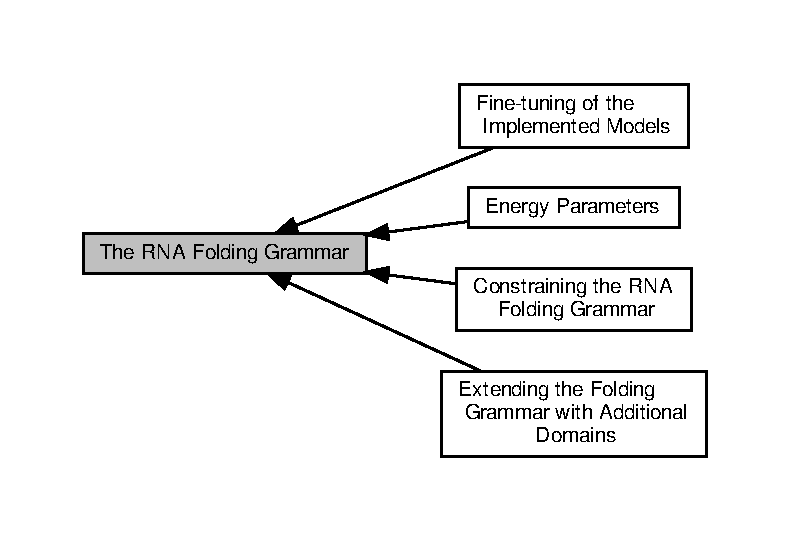
\includegraphics[width=350pt]{group__grammar}
\end{center}
\end{figure}
\subsection*{Modules}
\begin{DoxyCompactItemize}
\item 
\hyperlink{group__model__details}{Fine-\/tuning of the Implemented Models}
\begin{DoxyCompactList}\small\item\em Functions and data structures to fine-\/tune the implemented secondary structure evaluation model. \end{DoxyCompactList}\item 
\hyperlink{group__energy__parameters}{Energy Parameters}
\begin{DoxyCompactList}\small\item\em All relevant functions to retrieve and copy pre-\/calculated energy parameter sets as well as reading/writing the energy parameter set from/to file(s). \end{DoxyCompactList}\item 
\hyperlink{group__domains}{Extending the Folding Grammar with Additional Domains}
\begin{DoxyCompactList}\small\item\em This module covers simple and straight-\/forward extensions to the R\+NA folding grammar. \end{DoxyCompactList}\item 
\hyperlink{group__constraints}{Constraining the R\+N\+A Folding Grammar}
\begin{DoxyCompactList}\small\item\em This module provides general functions that allow for an easy control of constrained secondary structure prediction and evaluation. \end{DoxyCompactList}\end{DoxyCompactItemize}
\subsection*{Files}
\begin{DoxyCompactItemize}
\item 
file \hyperlink{grammar_8h}{grammar.\+h}
\begin{DoxyCompactList}\small\item\em Implementations for the R\+NA folding grammar. \end{DoxyCompactList}\end{DoxyCompactItemize}
\subsection*{Data Structures}
\begin{DoxyCompactItemize}
\item 
struct \hyperlink{group__grammar_structvrna__gr__aux__s}{vrna\+\_\+gr\+\_\+aux\+\_\+s}
\end{DoxyCompactItemize}


\subsection{Data Structure Documentation}
\index{vrna\+\_\+gr\+\_\+aux\+\_\+s@{vrna\+\_\+gr\+\_\+aux\+\_\+s}}\label{structvrna__gr__aux__s}
\Hypertarget{group__grammar_structvrna__gr__aux__s}
\subsubsection{struct vrna\+\_\+gr\+\_\+aux\+\_\+s}
\subsubsection*{Data Fields}
\begin{DoxyCompactItemize}
\item 
\mbox{\Hypertarget{group__grammar_ad4b601db6dc2e18854042b096ee780cc}\label{group__grammar_ad4b601db6dc2e18854042b096ee780cc}} 
vrna\+\_\+callback\+\_\+gr\+\_\+cond $\ast$ \hyperlink{group__grammar_ad4b601db6dc2e18854042b096ee780cc}{cb\+\_\+proc}
\begin{DoxyCompactList}\small\item\em A callback for pre-\/ and post-\/processing of auxiliary grammar rules. \end{DoxyCompactList}\end{DoxyCompactItemize}

\hypertarget{group__model__details}{}\section{Fine-\/tuning of the Implemented Models}
\label{group__model__details}\index{Fine-\/tuning of the Implemented Models@{Fine-\/tuning of the Implemented Models}}


Functions and data structures to fine-\/tune the implemented secondary structure evaluation model.  




\subsection{Detailed Description}
Functions and data structures to fine-\/tune the implemented secondary structure evaluation model. 

Collaboration diagram for Fine-\/tuning of the Implemented Models\+:
\nopagebreak
\begin{figure}[H]
\begin{center}
\leavevmode
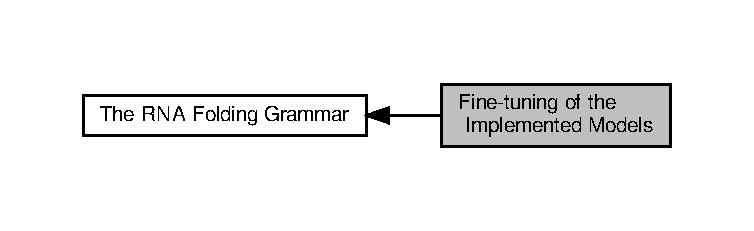
\includegraphics[width=350pt]{group__model__details}
\end{center}
\end{figure}
\subsection*{Files}
\begin{DoxyCompactItemize}
\item 
file \hyperlink{model_8h}{model.\+h}
\begin{DoxyCompactList}\small\item\em The model details data structure and its corresponding modifiers. \end{DoxyCompactList}\end{DoxyCompactItemize}
\subsection*{Data Structures}
\begin{DoxyCompactItemize}
\item 
struct \hyperlink{group__model__details_structvrna__md__s}{vrna\+\_\+md\+\_\+s}
\begin{DoxyCompactList}\small\item\em The data structure that contains the complete model details used throughout the calculations.  \hyperlink{group__model__details_structvrna__md__s}{More...}\end{DoxyCompactList}\end{DoxyCompactItemize}
\subsection*{Macros}
\begin{DoxyCompactItemize}
\item 
\#define \hyperlink{group__model__details_gaf47f9850b3b4763479f7a7e7a15648a2}{V\+R\+N\+A\+\_\+\+M\+O\+D\+E\+L\+\_\+\+D\+E\+F\+A\+U\+L\+T\+\_\+\+T\+E\+M\+P\+E\+R\+A\+T\+U\+RE}~37.\+0
\begin{DoxyCompactList}\small\item\em   Default temperature for structure prediction and free energy evaluation in $^\circ C$  \end{DoxyCompactList}\item 
\#define \hyperlink{group__model__details_ga5505389cba74a18bbc116d2bb20256fa}{V\+R\+N\+A\+\_\+\+M\+O\+D\+E\+L\+\_\+\+D\+E\+F\+A\+U\+L\+T\+\_\+\+P\+F\+\_\+\+S\+C\+A\+LE}~-\/1
\begin{DoxyCompactList}\small\item\em Default scaling factor for partition function computations. \end{DoxyCompactList}\item 
\#define \hyperlink{group__model__details_ga383d3ac8d08c3b6221754b50871c1200}{V\+R\+N\+A\+\_\+\+M\+O\+D\+E\+L\+\_\+\+D\+E\+F\+A\+U\+L\+T\+\_\+\+B\+E\+T\+A\+\_\+\+S\+C\+A\+LE}~1.
\begin{DoxyCompactList}\small\item\em Default scaling factor for absolute thermodynamic temperature in Boltzmann factors. \end{DoxyCompactList}\item 
\#define \hyperlink{group__model__details_ga2aa7bc2cae774b83a5c468f824c27a42}{V\+R\+N\+A\+\_\+\+M\+O\+D\+E\+L\+\_\+\+D\+E\+F\+A\+U\+L\+T\+\_\+\+D\+A\+N\+G\+L\+ES}~2
\begin{DoxyCompactList}\small\item\em Default dangling end model. \end{DoxyCompactList}\item 
\#define \hyperlink{group__model__details_gabd1ab224e1048defd45c165ed7d1c108}{V\+R\+N\+A\+\_\+\+M\+O\+D\+E\+L\+\_\+\+D\+E\+F\+A\+U\+L\+T\+\_\+\+S\+P\+E\+C\+I\+A\+L\+\_\+\+HP}~1
\begin{DoxyCompactList}\small\item\em Default model behavior for lookup of special tri-\/, tetra-\/, and hexa-\/loops. \end{DoxyCompactList}\item 
\#define \hyperlink{group__model__details_gab72462726dd60ed0d43339bbf7ee08ad}{V\+R\+N\+A\+\_\+\+M\+O\+D\+E\+L\+\_\+\+D\+E\+F\+A\+U\+L\+T\+\_\+\+N\+O\+\_\+\+LP}~0
\begin{DoxyCompactList}\small\item\em Default model behavior for so-\/called \textquotesingle{}lonely pairs\textquotesingle{}. \end{DoxyCompactList}\item 
\#define \hyperlink{group__model__details_ga34702f7d14d38b877ba8e475281e97e2}{V\+R\+N\+A\+\_\+\+M\+O\+D\+E\+L\+\_\+\+D\+E\+F\+A\+U\+L\+T\+\_\+\+N\+O\+\_\+\+GU}~0
\begin{DoxyCompactList}\small\item\em Default model behavior for G-\/U base pairs. \end{DoxyCompactList}\item 
\#define \hyperlink{group__model__details_ga5308de46faaca4b9fd16045864901ee7}{V\+R\+N\+A\+\_\+\+M\+O\+D\+E\+L\+\_\+\+D\+E\+F\+A\+U\+L\+T\+\_\+\+N\+O\+\_\+\+G\+U\+\_\+\+C\+L\+O\+S\+U\+RE}~0
\begin{DoxyCompactList}\small\item\em Default model behavior for G-\/U base pairs closing a loop. \end{DoxyCompactList}\item 
\#define \hyperlink{group__model__details_ga22059033db7bcd875c51fec32425490a}{V\+R\+N\+A\+\_\+\+M\+O\+D\+E\+L\+\_\+\+D\+E\+F\+A\+U\+L\+T\+\_\+\+C\+I\+RC}~0
\begin{DoxyCompactList}\small\item\em Default model behavior to treat a molecule as a circular R\+NA (D\+NA) \end{DoxyCompactList}\item 
\#define \hyperlink{group__model__details_ga793ed812e86f43799b14b2deee917f23}{V\+R\+N\+A\+\_\+\+M\+O\+D\+E\+L\+\_\+\+D\+E\+F\+A\+U\+L\+T\+\_\+\+G\+Q\+U\+AD}~0
\begin{DoxyCompactList}\small\item\em Default model behavior regarding the treatment of G-\/\+Quadruplexes. \end{DoxyCompactList}\item 
\#define \hyperlink{group__model__details_ga63f6006a02ba2d89148441f406c309e7}{V\+R\+N\+A\+\_\+\+M\+O\+D\+E\+L\+\_\+\+D\+E\+F\+A\+U\+L\+T\+\_\+\+U\+N\+I\+Q\+\_\+\+ML}~0
\begin{DoxyCompactList}\small\item\em Default behavior of the model regarding unique multi-\/branch loop decomposition. \end{DoxyCompactList}\item 
\#define \hyperlink{group__model__details_ga6fcf6b2d0f89256cdbd166486c9b6e1e}{V\+R\+N\+A\+\_\+\+M\+O\+D\+E\+L\+\_\+\+D\+E\+F\+A\+U\+L\+T\+\_\+\+E\+N\+E\+R\+G\+Y\+\_\+\+S\+ET}~0
\begin{DoxyCompactList}\small\item\em Default model behavior on which energy set to use. \end{DoxyCompactList}\item 
\#define \hyperlink{group__model__details_ga3fda8006ab84baf817bd8e5ccbc6bb35}{V\+R\+N\+A\+\_\+\+M\+O\+D\+E\+L\+\_\+\+D\+E\+F\+A\+U\+L\+T\+\_\+\+B\+A\+C\+K\+T\+R\+A\+CK}~1
\begin{DoxyCompactList}\small\item\em Default model behavior with regards to backtracking of structures. \end{DoxyCompactList}\item 
\#define \hyperlink{group__model__details_gad0e81fcaca53c4a826c68e0796de2afb}{V\+R\+N\+A\+\_\+\+M\+O\+D\+E\+L\+\_\+\+D\+E\+F\+A\+U\+L\+T\+\_\+\+B\+A\+C\+K\+T\+R\+A\+C\+K\+\_\+\+T\+Y\+PE}~\textquotesingle{}F\textquotesingle{}
\begin{DoxyCompactList}\small\item\em Default model behavior on what type of backtracking to perform. \end{DoxyCompactList}\item 
\#define \hyperlink{group__model__details_ga1d6cd5051940b126c248147c011bac6c}{V\+R\+N\+A\+\_\+\+M\+O\+D\+E\+L\+\_\+\+D\+E\+F\+A\+U\+L\+T\+\_\+\+C\+O\+M\+P\+U\+T\+E\+\_\+\+B\+PP}~1
\begin{DoxyCompactList}\small\item\em Default model behavior with regards to computing base pair probabilities. \end{DoxyCompactList}\item 
\#define \hyperlink{group__model__details_ga7cb6f4ae8fdebff6746a4410814f2977}{V\+R\+N\+A\+\_\+\+M\+O\+D\+E\+L\+\_\+\+D\+E\+F\+A\+U\+L\+T\+\_\+\+M\+A\+X\+\_\+\+B\+P\+\_\+\+S\+P\+AN}~-\/1
\begin{DoxyCompactList}\small\item\em Default model behavior for the allowed maximum base pair span. \end{DoxyCompactList}\item 
\#define \hyperlink{group__model__details_ga8de04a9cb57e811e313b0f9f207f6bdb}{V\+R\+N\+A\+\_\+\+M\+O\+D\+E\+L\+\_\+\+D\+E\+F\+A\+U\+L\+T\+\_\+\+W\+I\+N\+D\+O\+W\+\_\+\+S\+I\+ZE}~-\/1
\begin{DoxyCompactList}\small\item\em Default model behavior for the sliding window approach. \end{DoxyCompactList}\item 
\#define \hyperlink{group__model__details_ga938f68463e84fe060aa6502f428a517d}{V\+R\+N\+A\+\_\+\+M\+O\+D\+E\+L\+\_\+\+D\+E\+F\+A\+U\+L\+T\+\_\+\+L\+O\+G\+\_\+\+ML}~0
\begin{DoxyCompactList}\small\item\em Default model behavior on how to evaluate the energy contribution of multi-\/branch loops. \end{DoxyCompactList}\item 
\#define \hyperlink{group__model__details_ga2a5bbfc1edf33077e39466d2d9807115}{V\+R\+N\+A\+\_\+\+M\+O\+D\+E\+L\+\_\+\+D\+E\+F\+A\+U\+L\+T\+\_\+\+A\+L\+I\+\_\+\+O\+L\+D\+\_\+\+EN}~0
\begin{DoxyCompactList}\small\item\em Default model behavior for consensus structure energy evaluation. \end{DoxyCompactList}\item 
\#define \hyperlink{group__model__details_ga64b3ab65a9ca42d4ad1d05e193083147}{V\+R\+N\+A\+\_\+\+M\+O\+D\+E\+L\+\_\+\+D\+E\+F\+A\+U\+L\+T\+\_\+\+A\+L\+I\+\_\+\+R\+I\+BO}~0
\begin{DoxyCompactList}\small\item\em Default model behavior for consensus structure co-\/variance contribution assessment. \end{DoxyCompactList}\item 
\#define \hyperlink{group__model__details_gaaaf3d73d6abc18d3889676952bfedb96}{V\+R\+N\+A\+\_\+\+M\+O\+D\+E\+L\+\_\+\+D\+E\+F\+A\+U\+L\+T\+\_\+\+A\+L\+I\+\_\+\+C\+V\+\_\+\+F\+A\+CT}~1.
\begin{DoxyCompactList}\small\item\em Default model behavior for weighting the co-\/variance score in consensus structure prediction. \end{DoxyCompactList}\item 
\#define \hyperlink{group__model__details_ga8f774daaafec28160c1ca5d09f2cbdba}{V\+R\+N\+A\+\_\+\+M\+O\+D\+E\+L\+\_\+\+D\+E\+F\+A\+U\+L\+T\+\_\+\+A\+L\+I\+\_\+\+N\+C\+\_\+\+F\+A\+CT}~1.
\begin{DoxyCompactList}\small\item\em Default model behavior for weighting the nucleotide conservation? in consensus structure prediction. \end{DoxyCompactList}\item 
\mbox{\Hypertarget{group__model__details_ga05a5ffe718aa431d97419a12fb082379}\label{group__model__details_ga05a5ffe718aa431d97419a12fb082379}} 
\#define \hyperlink{group__model__details_ga05a5ffe718aa431d97419a12fb082379}{M\+A\+X\+A\+L\+P\+HA}~20
\begin{DoxyCompactList}\small\item\em Maximal length of alphabet. \end{DoxyCompactList}\end{DoxyCompactItemize}
\subsection*{Typedefs}
\begin{DoxyCompactItemize}
\item 
\mbox{\Hypertarget{group__model__details_ga1f8a10e12a0a1915f2a4eff0b28ea17c}\label{group__model__details_ga1f8a10e12a0a1915f2a4eff0b28ea17c}} 
typedef struct \hyperlink{group__model__details_structvrna__md__s}{vrna\+\_\+md\+\_\+s} \hyperlink{group__model__details_ga1f8a10e12a0a1915f2a4eff0b28ea17c}{vrna\+\_\+md\+\_\+t}
\begin{DoxyCompactList}\small\item\em Typename for the model details data structure \hyperlink{group__model__details_structvrna__md__s}{vrna\+\_\+md\+\_\+s}. \end{DoxyCompactList}\end{DoxyCompactItemize}
\subsection*{Functions}
\begin{DoxyCompactItemize}
\item 
void \hyperlink{group__model__details_ga8ac6ff84936282436f822644bf841f66}{vrna\+\_\+md\+\_\+set\+\_\+default} (\hyperlink{group__model__details_ga1f8a10e12a0a1915f2a4eff0b28ea17c}{vrna\+\_\+md\+\_\+t} $\ast$md)
\begin{DoxyCompactList}\small\item\em Apply default model details to a provided \hyperlink{group__model__details_ga1f8a10e12a0a1915f2a4eff0b28ea17c}{vrna\+\_\+md\+\_\+t} data structure. \end{DoxyCompactList}\item 
void \hyperlink{group__model__details_ga36ae40b8c3b82362f5798ad5b047b814}{vrna\+\_\+md\+\_\+update} (\hyperlink{group__model__details_ga1f8a10e12a0a1915f2a4eff0b28ea17c}{vrna\+\_\+md\+\_\+t} $\ast$md)
\begin{DoxyCompactList}\small\item\em Update the model details data structure. \end{DoxyCompactList}\item 
\hyperlink{group__model__details_ga1f8a10e12a0a1915f2a4eff0b28ea17c}{vrna\+\_\+md\+\_\+t} $\ast$ \hyperlink{group__model__details_ga619057a740918b5fb01808362bb67aea}{vrna\+\_\+md\+\_\+copy} (\hyperlink{group__model__details_ga1f8a10e12a0a1915f2a4eff0b28ea17c}{vrna\+\_\+md\+\_\+t} $\ast$md\+\_\+to, const \hyperlink{group__model__details_ga1f8a10e12a0a1915f2a4eff0b28ea17c}{vrna\+\_\+md\+\_\+t} $\ast$md\+\_\+from)
\begin{DoxyCompactList}\small\item\em Copy/\+Clone a \hyperlink{group__model__details_ga1f8a10e12a0a1915f2a4eff0b28ea17c}{vrna\+\_\+md\+\_\+t} model. \end{DoxyCompactList}\item 
char $\ast$ \hyperlink{group__model__details_ga3a7469f0725a849af6ba61a57dfd60ce}{vrna\+\_\+md\+\_\+option\+\_\+string} (\hyperlink{group__model__details_ga1f8a10e12a0a1915f2a4eff0b28ea17c}{vrna\+\_\+md\+\_\+t} $\ast$md)
\begin{DoxyCompactList}\small\item\em Get a corresponding commandline parameter string of the options in a \hyperlink{group__model__details_ga1f8a10e12a0a1915f2a4eff0b28ea17c}{vrna\+\_\+md\+\_\+t}. \end{DoxyCompactList}\item 
void \hyperlink{group__model__details_ga70834424cf804d149937de89f80ceb45}{vrna\+\_\+md\+\_\+defaults\+\_\+reset} (\hyperlink{group__model__details_ga1f8a10e12a0a1915f2a4eff0b28ea17c}{vrna\+\_\+md\+\_\+t} $\ast$md\+\_\+p)
\begin{DoxyCompactList}\small\item\em Reset the global default model details to a specific set of parameters, or their initial values. \end{DoxyCompactList}\item 
void \hyperlink{group__model__details_gaf9e527e9a2f7e6fd6e42bc6e602f5445}{vrna\+\_\+md\+\_\+defaults\+\_\+temperature} (double T)
\begin{DoxyCompactList}\small\item\em Set default temperature for energy evaluation of loops. \end{DoxyCompactList}\item 
double \hyperlink{group__model__details_ga96b24a74437f9ba46c4e06343155bf46}{vrna\+\_\+md\+\_\+defaults\+\_\+temperature\+\_\+get} (void)
\begin{DoxyCompactList}\small\item\em Get default temperature for energy evaluation of loops. \end{DoxyCompactList}\item 
void \hyperlink{group__model__details_gae984567db36c3f9b8731ecc917abf3a2}{vrna\+\_\+md\+\_\+defaults\+\_\+beta\+Scale} (double b)
\begin{DoxyCompactList}\small\item\em Set default scaling factor of thermodynamic temperature in Boltzmann factors. \end{DoxyCompactList}\item 
double \hyperlink{group__model__details_gabb8780f5410c52f970d75b044059bd09}{vrna\+\_\+md\+\_\+defaults\+\_\+beta\+Scale\+\_\+get} (void)
\begin{DoxyCompactList}\small\item\em Get default scaling factor of thermodynamic temperature in Boltzmann factors. \end{DoxyCompactList}\item 
void \hyperlink{group__model__details_gac76a5374def8e5e4e644ff6e4cc72dee}{vrna\+\_\+md\+\_\+defaults\+\_\+dangles} (int d)
\begin{DoxyCompactList}\small\item\em Set default dangle model for structure prediction. \end{DoxyCompactList}\item 
int \hyperlink{group__model__details_ga67ca06f95ae133778c79a4493c9817b8}{vrna\+\_\+md\+\_\+defaults\+\_\+dangles\+\_\+get} (void)
\begin{DoxyCompactList}\small\item\em Get default dangle model for structure prediction. \end{DoxyCompactList}\item 
void \hyperlink{group__model__details_gafff6449a02744add0308e653230c15fc}{vrna\+\_\+md\+\_\+defaults\+\_\+special\+\_\+hp} (int flag)
\begin{DoxyCompactList}\small\item\em Set default behavior for lookup of tabulated free energies for special hairpin loops, such as Tri-\/, Tetra-\/, or Hexa-\/loops. \end{DoxyCompactList}\item 
int \hyperlink{group__model__details_ga1d68a6efdaa1253cc63fd9cd06452559}{vrna\+\_\+md\+\_\+defaults\+\_\+special\+\_\+hp\+\_\+get} (void)
\begin{DoxyCompactList}\small\item\em Get default behavior for lookup of tabulated free energies for special hairpin loops, such as Tri-\/, Tetra-\/, or Hexa-\/loops. \end{DoxyCompactList}\item 
void \hyperlink{group__model__details_ga2f88ffc393ac9d7987849c965fd29ea8}{vrna\+\_\+md\+\_\+defaults\+\_\+no\+LP} (int flag)
\begin{DoxyCompactList}\small\item\em Set default behavior for prediction of canonical secondary structures. \end{DoxyCompactList}\item 
int \hyperlink{group__model__details_ga934344888fbacaed538bbbfe910f2aa6}{vrna\+\_\+md\+\_\+defaults\+\_\+no\+L\+P\+\_\+get} (void)
\begin{DoxyCompactList}\small\item\em Get default behavior for prediction of canonical secondary structures. \end{DoxyCompactList}\item 
void \hyperlink{group__model__details_ga98218f85c7a957a1d1ddf4627fdf5a39}{vrna\+\_\+md\+\_\+defaults\+\_\+no\+GU} (int flag)
\begin{DoxyCompactList}\small\item\em Set default behavior for treatment of G-\/U wobble pairs. \end{DoxyCompactList}\item 
int \hyperlink{group__model__details_ga5faa7d4e536d7fe36ec25428c0cf2563}{vrna\+\_\+md\+\_\+defaults\+\_\+no\+G\+U\+\_\+get} (void)
\begin{DoxyCompactList}\small\item\em Get default behavior for treatment of G-\/U wobble pairs. \end{DoxyCompactList}\item 
void \hyperlink{group__model__details_gade5b9951d71ca2fb357a4e6c0c18ccd1}{vrna\+\_\+md\+\_\+defaults\+\_\+no\+G\+Uclosure} (int flag)
\begin{DoxyCompactList}\small\item\em Set default behavior for G-\/U pairs as closing pair for loops. \end{DoxyCompactList}\item 
int \hyperlink{group__model__details_ga4f7fdad083243a5348d63320ddaa70f3}{vrna\+\_\+md\+\_\+defaults\+\_\+no\+G\+Uclosure\+\_\+get} (void)
\begin{DoxyCompactList}\small\item\em Get default behavior for G-\/U pairs as closing pair for loops. \end{DoxyCompactList}\item 
void \hyperlink{group__model__details_ga3de50a73455d88c3957386933b8e1f90}{vrna\+\_\+md\+\_\+defaults\+\_\+log\+ML} (int flag)
\begin{DoxyCompactList}\small\item\em Set default behavior recomputing free energies of multi-\/branch loops using a logarithmic model. \end{DoxyCompactList}\item 
int \hyperlink{group__model__details_ga93f04e070d529c5d0bb87c9681f6ad29}{vrna\+\_\+md\+\_\+defaults\+\_\+log\+M\+L\+\_\+get} (void)
\begin{DoxyCompactList}\small\item\em Get default behavior recomputing free energies of multi-\/branch loops using a logarithmic model. \end{DoxyCompactList}\item 
void \hyperlink{group__model__details_ga4e1deb3e91a8a99e5c6dd905a5eb0186}{vrna\+\_\+md\+\_\+defaults\+\_\+circ} (int flag)
\begin{DoxyCompactList}\small\item\em Set default behavior whether input sequences are circularized. \end{DoxyCompactList}\item 
int \hyperlink{group__model__details_gad3a7e58de344ad93a08925f58f94f6fb}{vrna\+\_\+md\+\_\+defaults\+\_\+circ\+\_\+get} (void)
\begin{DoxyCompactList}\small\item\em Get default behavior whether input sequences are circularized. \end{DoxyCompactList}\item 
void \hyperlink{group__model__details_ga0685ca2aeb39af76f2421fc308163dce}{vrna\+\_\+md\+\_\+defaults\+\_\+gquad} (int flag)
\begin{DoxyCompactList}\small\item\em Set default behavior for treatment of G-\/\+Quadruplexes. \end{DoxyCompactList}\item 
int \hyperlink{group__model__details_gae645b8612f879eb38b45244fa9eddb9e}{vrna\+\_\+md\+\_\+defaults\+\_\+gquad\+\_\+get} (void)
\begin{DoxyCompactList}\small\item\em Get default behavior for treatment of G-\/\+Quadruplexes. \end{DoxyCompactList}\item 
void \hyperlink{group__model__details_ga59b944f61c5d2babec2d4c48c820de67}{vrna\+\_\+md\+\_\+defaults\+\_\+uniq\+\_\+\+ML} (int flag)
\begin{DoxyCompactList}\small\item\em Set default behavior for creating additional matrix for unique multi-\/branch loop prediction. \end{DoxyCompactList}\item 
int \hyperlink{group__model__details_gab48e70fd024bf838404bcbcca0c874a0}{vrna\+\_\+md\+\_\+defaults\+\_\+uniq\+\_\+\+M\+L\+\_\+get} (void)
\begin{DoxyCompactList}\small\item\em Get default behavior for creating additional matrix for unique multi-\/branch loop prediction. \end{DoxyCompactList}\item 
void \hyperlink{group__model__details_ga8dd29c55787a4576277e1907e92d810c}{vrna\+\_\+md\+\_\+defaults\+\_\+energy\+\_\+set} (int e)
\begin{DoxyCompactList}\small\item\em Set default energy set. \end{DoxyCompactList}\item 
int \hyperlink{group__model__details_ga017ed6afb1cba2b7f242412cab618b53}{vrna\+\_\+md\+\_\+defaults\+\_\+energy\+\_\+set\+\_\+get} (void)
\begin{DoxyCompactList}\small\item\em Get default energy set. \end{DoxyCompactList}\item 
void \hyperlink{group__model__details_ga978c468b2fe96a70d5191e3dd17d5599}{vrna\+\_\+md\+\_\+defaults\+\_\+backtrack} (int flag)
\begin{DoxyCompactList}\small\item\em Set default behavior for whether to backtrack secondary structures. \end{DoxyCompactList}\item 
int \hyperlink{group__model__details_ga90da1156e6883ddd68527c2830706648}{vrna\+\_\+md\+\_\+defaults\+\_\+backtrack\+\_\+get} (void)
\begin{DoxyCompactList}\small\item\em Get default behavior for whether to backtrack secondary structures. \end{DoxyCompactList}\item 
void \hyperlink{group__model__details_ga68305274de96b56b7799575e222560d8}{vrna\+\_\+md\+\_\+defaults\+\_\+backtrack\+\_\+type} (char t)
\begin{DoxyCompactList}\small\item\em Set default backtrack type, i.\+e. which DP matrix is used. \end{DoxyCompactList}\item 
char \hyperlink{group__model__details_ga1425b4ebd0e034dead66d79becd64143}{vrna\+\_\+md\+\_\+defaults\+\_\+backtrack\+\_\+type\+\_\+get} (void)
\begin{DoxyCompactList}\small\item\em Get default backtrack type, i.\+e. which DP matrix is used. \end{DoxyCompactList}\item 
void \hyperlink{group__model__details_gaf1b5db10f1f476767f9a95f8a78e3132}{vrna\+\_\+md\+\_\+defaults\+\_\+compute\+\_\+bpp} (int flag)
\begin{DoxyCompactList}\small\item\em Set the default behavior for whether to compute base pair probabilities after partition function computation. \end{DoxyCompactList}\item 
int \hyperlink{group__model__details_gaa3a537e61fbe0518673bf9f73fd820f3}{vrna\+\_\+md\+\_\+defaults\+\_\+compute\+\_\+bpp\+\_\+get} (void)
\begin{DoxyCompactList}\small\item\em Get the default behavior for whether to compute base pair probabilities after partition function computation. \end{DoxyCompactList}\item 
void \hyperlink{group__model__details_ga4c4bc962f09b4480cb8499f1cf8ae4ec}{vrna\+\_\+md\+\_\+defaults\+\_\+max\+\_\+bp\+\_\+span} (int span)
\begin{DoxyCompactList}\small\item\em Set default maximal base pair span. \end{DoxyCompactList}\item 
int \hyperlink{group__model__details_gaa60f989e062fecd4d4bac89c1883da85}{vrna\+\_\+md\+\_\+defaults\+\_\+max\+\_\+bp\+\_\+span\+\_\+get} (void)
\begin{DoxyCompactList}\small\item\em Get default maximal base pair span. \end{DoxyCompactList}\item 
void \hyperlink{group__model__details_gac152f1e78c1058a10261022c8dfda0f7}{vrna\+\_\+md\+\_\+defaults\+\_\+min\+\_\+loop\+\_\+size} (int size)
\begin{DoxyCompactList}\small\item\em Set default minimal loop size. \end{DoxyCompactList}\item 
int \hyperlink{group__model__details_ga5cc691174a75c652807dc361b617632a}{vrna\+\_\+md\+\_\+defaults\+\_\+min\+\_\+loop\+\_\+size\+\_\+get} (void)
\begin{DoxyCompactList}\small\item\em Get default minimal loop size. \end{DoxyCompactList}\item 
void \hyperlink{group__model__details_ga7b802ce0e8c3181bf5cb580de6d5b26a}{vrna\+\_\+md\+\_\+defaults\+\_\+window\+\_\+size} (int size)
\begin{DoxyCompactList}\small\item\em Set default window size for sliding window structure prediction approaches. \end{DoxyCompactList}\item 
int \hyperlink{group__model__details_ga670146a9aa3ba77f4d422d60b7c30ac9}{vrna\+\_\+md\+\_\+defaults\+\_\+window\+\_\+size\+\_\+get} (void)
\begin{DoxyCompactList}\small\item\em Get default window size for sliding window structure prediction approaches. \end{DoxyCompactList}\item 
void \hyperlink{group__model__details_ga41521d5b9fb7e0f31e7ea73f5792afab}{vrna\+\_\+md\+\_\+defaults\+\_\+old\+Ali\+En} (int flag)
\begin{DoxyCompactList}\small\item\em Set default behavior for whether to use old energy model for comparative structure prediction. \end{DoxyCompactList}\item 
int \hyperlink{group__model__details_ga2374492b5019df88022fe4c05f0f3630}{vrna\+\_\+md\+\_\+defaults\+\_\+old\+Ali\+En\+\_\+get} (void)
\begin{DoxyCompactList}\small\item\em Get default behavior for whether to use old energy model for comparative structure prediction. \end{DoxyCompactList}\item 
void \hyperlink{group__model__details_ga937c45e1d06fd6168730a9b08d130be3}{vrna\+\_\+md\+\_\+defaults\+\_\+ribo} (int flag)
\begin{DoxyCompactList}\small\item\em Set default behavior for whether to use Ribosum Scoring in comparative structure prediction. \end{DoxyCompactList}\item 
int \hyperlink{group__model__details_ga169027f0c0561ea7d87b655e4b336bfc}{vrna\+\_\+md\+\_\+defaults\+\_\+ribo\+\_\+get} (void)
\begin{DoxyCompactList}\small\item\em Get default behavior for whether to use Ribosum Scoring in comparative structure prediction. \end{DoxyCompactList}\item 
void \hyperlink{group__model__details_gad3a3f40baafd91a6ce80a91a68e20053}{vrna\+\_\+md\+\_\+defaults\+\_\+cv\+\_\+fact} (double factor)
\begin{DoxyCompactList}\small\item\em Set the default co-\/variance scaling factor used in comparative structure prediction. \end{DoxyCompactList}\item 
double \hyperlink{group__model__details_gae59c68393807217b0a2497adb64d3ee3}{vrna\+\_\+md\+\_\+defaults\+\_\+cv\+\_\+fact\+\_\+get} (void)
\begin{DoxyCompactList}\small\item\em Get the default co-\/variance scaling factor used in comparative structure prediction. \end{DoxyCompactList}\item 
void \hyperlink{group__model__details_gac35e596c850dce3ad55c49119fd7d471}{vrna\+\_\+md\+\_\+defaults\+\_\+nc\+\_\+fact} (double factor)
\item 
double \hyperlink{group__model__details_ga7ac759eaa7159bf5f022745f5da59508}{vrna\+\_\+md\+\_\+defaults\+\_\+nc\+\_\+fact\+\_\+get} (void)
\item 
void \hyperlink{group__model__details_ga3f73d3029d3d0025d4cc311510cd95a3}{vrna\+\_\+md\+\_\+defaults\+\_\+sfact} (double factor)
\begin{DoxyCompactList}\small\item\em Set the default scaling factor used to avoid under-\//overflows in partition function computation. \end{DoxyCompactList}\item 
double \hyperlink{group__model__details_gab2df6aab954b63fd3592d18e90285dae}{vrna\+\_\+md\+\_\+defaults\+\_\+sfact\+\_\+get} (void)
\begin{DoxyCompactList}\small\item\em Get the default scaling factor used to avoid under-\//overflows in partition function computation. \end{DoxyCompactList}\item 
void \hyperlink{group__model__details_gabad896c3650d420f3f3ddefc69e2bceb}{set\+\_\+model\+\_\+details} (\hyperlink{group__model__details_ga1f8a10e12a0a1915f2a4eff0b28ea17c}{vrna\+\_\+md\+\_\+t} $\ast$md)
\begin{DoxyCompactList}\small\item\em Set default model details. \end{DoxyCompactList}\end{DoxyCompactItemize}
\subsection*{Variables}
\begin{DoxyCompactItemize}
\item 
double \hyperlink{group__model__details_gab4b11c8d9c758430960896bc3fe82ead}{temperature}
\begin{DoxyCompactList}\small\item\em Rescale energy parameters to a temperature in degC. \end{DoxyCompactList}\item 
double \hyperlink{group__model__details_gad3b22044065acc6dee0af68931b52cfd}{pf\+\_\+scale}
\begin{DoxyCompactList}\small\item\em A scaling factor used by \hyperlink{group__part__func__global__deprecated_gadc3db3d98742427e7001a7fd36ef28c2}{pf\+\_\+fold()} to avoid overflows. \end{DoxyCompactList}\item 
int \hyperlink{group__model__details_ga72b511ed1201f7e23ec437e468790d74}{dangles}
\begin{DoxyCompactList}\small\item\em Switch the energy model for dangling end contributions (0, 1, 2, 3) \end{DoxyCompactList}\item 
int \hyperlink{group__model__details_ga4f6265bdf0ead7ff4628a360adbfd77e}{tetra\+\_\+loop}
\begin{DoxyCompactList}\small\item\em Include special stabilizing energies for some tri-\/, tetra-\/ and hexa-\/loops;. \end{DoxyCompactList}\item 
int \hyperlink{group__model__details_ga097eccaabd6ae8b4fef83cccff85bb5d}{no\+Lonely\+Pairs}
\begin{DoxyCompactList}\small\item\em Global switch to avoid/allow helices of length 1. \end{DoxyCompactList}\item 
\mbox{\Hypertarget{group__model__details_gabf380d09e4f1ab94fc6af57cf0ad5d32}\label{group__model__details_gabf380d09e4f1ab94fc6af57cf0ad5d32}} 
int \hyperlink{group__model__details_gabf380d09e4f1ab94fc6af57cf0ad5d32}{no\+GU}
\begin{DoxyCompactList}\small\item\em Global switch to forbid/allow GU base pairs at all. \end{DoxyCompactList}\item 
\mbox{\Hypertarget{group__model__details_gaa8d1c7b92489179e1eafa562b7bdd259}\label{group__model__details_gaa8d1c7b92489179e1eafa562b7bdd259}} 
int \hyperlink{group__model__details_gaa8d1c7b92489179e1eafa562b7bdd259}{no\+\_\+closing\+GU}
\begin{DoxyCompactList}\small\item\em GU allowed only inside stacks if set to 1. \end{DoxyCompactList}\item 
\mbox{\Hypertarget{group__model__details_gaf9202a1a09f5828dc731e2d9a10fa111}\label{group__model__details_gaf9202a1a09f5828dc731e2d9a10fa111}} 
int \hyperlink{group__model__details_gaf9202a1a09f5828dc731e2d9a10fa111}{circ}
\begin{DoxyCompactList}\small\item\em backward compatibility variable.. this does not effect anything \end{DoxyCompactList}\item 
\mbox{\Hypertarget{group__model__details_ga25f2bdcdf56e813d288845484a13d704}\label{group__model__details_ga25f2bdcdf56e813d288845484a13d704}} 
int \hyperlink{group__model__details_ga25f2bdcdf56e813d288845484a13d704}{gquad}
\begin{DoxyCompactList}\small\item\em Allow G-\/quadruplex formation. \end{DoxyCompactList}\item 
\mbox{\Hypertarget{group__model__details_ga6c5655c8b272e3e6cab74dd0f540294f}\label{group__model__details_ga6c5655c8b272e3e6cab74dd0f540294f}} 
int \hyperlink{group__model__details_ga6c5655c8b272e3e6cab74dd0f540294f}{uniq\+\_\+\+ML}
\begin{DoxyCompactList}\small\item\em do ML decomposition uniquely (for subopt) \end{DoxyCompactList}\item 
int \hyperlink{group__model__details_gafb1ef1166da85092ae8a325e02dcae71}{energy\+\_\+set}
\begin{DoxyCompactList}\small\item\em 0 = BP; 1=any with GC; 2=any with A\+U-\/parameter \end{DoxyCompactList}\item 
int \hyperlink{group__model__details_gad512b5dd4dbec60faccfe137bb474489}{do\+\_\+backtrack}
\begin{DoxyCompactList}\small\item\em do backtracking, i.\+e. compute secondary structures or base pair probabilities \end{DoxyCompactList}\item 
char \hyperlink{group__model__details_ga83bdb43472a259c71e69fa9f70f420c3}{backtrack\+\_\+type}
\begin{DoxyCompactList}\small\item\em A backtrack array marker for \hyperlink{group__inverse__fold_ga7af026de55d4babad879f2c92559cbbc}{inverse\+\_\+fold()} \end{DoxyCompactList}\item 
char $\ast$ \hyperlink{group__model__details_ga2695d91cc535d09c2eae5c3884e2ec64}{nonstandards}
\begin{DoxyCompactList}\small\item\em contains allowed non standard base pairs \end{DoxyCompactList}\item 
int \hyperlink{group__model__details_ga18df869af0d70101106458fc3f027806}{max\+\_\+bp\+\_\+span}
\begin{DoxyCompactList}\small\item\em Maximum allowed base pair span. \end{DoxyCompactList}\item 
\mbox{\Hypertarget{group__model__details_gac408868ba00671cbc7d1d535105af045}\label{group__model__details_gac408868ba00671cbc7d1d535105af045}} 
int \hyperlink{group__model__details_gac408868ba00671cbc7d1d535105af045}{old\+Ali\+En}
\begin{DoxyCompactList}\small\item\em use old alifold energies (with gaps) \end{DoxyCompactList}\item 
\mbox{\Hypertarget{group__model__details_ga0656afca1d2853f9ee6591172f5638de}\label{group__model__details_ga0656afca1d2853f9ee6591172f5638de}} 
int \hyperlink{group__model__details_ga0656afca1d2853f9ee6591172f5638de}{ribo}
\begin{DoxyCompactList}\small\item\em use ribosum matrices \end{DoxyCompactList}\item 
\mbox{\Hypertarget{group__model__details_ga80c3c5fd35e7479704cc91d2d0367743}\label{group__model__details_ga80c3c5fd35e7479704cc91d2d0367743}} 
int \hyperlink{group__model__details_ga80c3c5fd35e7479704cc91d2d0367743}{log\+ML}
\begin{DoxyCompactList}\small\item\em if nonzero use logarithmic ML energy in energy\+\_\+of\+\_\+struct \end{DoxyCompactList}\end{DoxyCompactItemize}


\subsection{Data Structure Documentation}
\index{vrna\+\_\+md\+\_\+s@{vrna\+\_\+md\+\_\+s}}\label{structvrna__md__s}
\Hypertarget{group__model__details_structvrna__md__s}
\subsubsection{struct vrna\+\_\+md\+\_\+s}
The data structure that contains the complete model details used throughout the calculations. 

For convenience reasons, we provide the type name \hyperlink{group__model__details_ga1f8a10e12a0a1915f2a4eff0b28ea17c}{vrna\+\_\+md\+\_\+t} to address this data structure without the use of the struct keyword

\begin{DoxySeeAlso}{See also}
\hyperlink{group__model__details_ga8ac6ff84936282436f822644bf841f66}{vrna\+\_\+md\+\_\+set\+\_\+default()}, \hyperlink{group__model__details_gabad896c3650d420f3f3ddefc69e2bceb}{set\+\_\+model\+\_\+details()}, \hyperlink{group__model__details_ga36ae40b8c3b82362f5798ad5b047b814}{vrna\+\_\+md\+\_\+update()}, \hyperlink{group__model__details_ga1f8a10e12a0a1915f2a4eff0b28ea17c}{vrna\+\_\+md\+\_\+t}
\end{DoxySeeAlso}
\begin{DoxyRefDesc}{S\+W\+I\+G Wrapper Notes}
\item[\hyperlink{wrappers__wrappers000083}{S\+W\+I\+G Wrapper Notes}]This data structure is wrapped as an object {\bfseries md} with multiple related functions attached as methods.

A new set of default parameters can be obtained by calling the constructure of {\bfseries md\+:} ~\newline

\begin{DoxyItemize}
\item {\itshape md()} -- Initialize with default settings
\end{DoxyItemize}

The resulting object has a list of attached methods which directly correspond to functions that mainly operate on the corresponding {\itshape C} data structure\+:~\newline

\begin{DoxyItemize}
\item {\itshape reset()} -- \hyperlink{group__model__details_ga8ac6ff84936282436f822644bf841f66}{vrna\+\_\+md\+\_\+set\+\_\+default()}
\item {\itshape set\+\_\+from\+\_\+globals()} -- \hyperlink{group__model__details_gabad896c3650d420f3f3ddefc69e2bceb}{set\+\_\+model\+\_\+details()}
\item {\itshape option\+\_\+string()} -- \hyperlink{group__model__details_ga3a7469f0725a849af6ba61a57dfd60ce}{vrna\+\_\+md\+\_\+option\+\_\+string()}
\end{DoxyItemize}

Note, that default parameters can be modified by directly setting any of the following global variables. Internally, getting/setting default parameters using their global variable representative translates into calls of the following functions, therefore these wrappers for these functions do not exist in the scripting language interface(s)\+:

\tabulinesep=1mm
\begin{longtabu} spread 0pt [c]{*{3}{|X[-1]}|}
\hline
\rowcolor{\tableheadbgcolor}\textbf{ global variable }&\textbf{ {\itshape C} getter }&\textbf{ {\itshape C} setter  }\\\cline{1-3}
\endfirsthead
\hline
\endfoot
\hline
\rowcolor{\tableheadbgcolor}\textbf{ global variable }&\textbf{ {\itshape C} getter }&\textbf{ {\itshape C} setter  }\\\cline{1-3}
\endhead
temperature &\hyperlink{group__model__details_ga96b24a74437f9ba46c4e06343155bf46}{vrna\+\_\+md\+\_\+defaults\+\_\+temperature\+\_\+get()} &\hyperlink{group__model__details_gaf9e527e9a2f7e6fd6e42bc6e602f5445}{vrna\+\_\+md\+\_\+defaults\+\_\+temperature()} \\\cline{1-3}
dangles &\hyperlink{group__model__details_ga67ca06f95ae133778c79a4493c9817b8}{vrna\+\_\+md\+\_\+defaults\+\_\+dangles\+\_\+get()} &\hyperlink{group__model__details_gac76a5374def8e5e4e644ff6e4cc72dee}{vrna\+\_\+md\+\_\+defaults\+\_\+dangles()} \\\cline{1-3}
beta\+Scale &\hyperlink{group__model__details_gabb8780f5410c52f970d75b044059bd09}{vrna\+\_\+md\+\_\+defaults\+\_\+beta\+Scale\+\_\+get()} &\hyperlink{group__model__details_gae984567db36c3f9b8731ecc917abf3a2}{vrna\+\_\+md\+\_\+defaults\+\_\+beta\+Scale()} \\\cline{1-3}
tetra\+\_\+loop &this is an alias of {\itshape special\+\_\+hp} &\\\cline{1-3}
special\+\_\+hp &\hyperlink{group__model__details_ga1d68a6efdaa1253cc63fd9cd06452559}{vrna\+\_\+md\+\_\+defaults\+\_\+special\+\_\+hp\+\_\+get()} &\hyperlink{group__model__details_gafff6449a02744add0308e653230c15fc}{vrna\+\_\+md\+\_\+defaults\+\_\+special\+\_\+hp()} \\\cline{1-3}
no\+Lonely\+Pairs &this is an alias of {\itshape no\+LP} &\\\cline{1-3}
no\+LP &\hyperlink{group__model__details_ga934344888fbacaed538bbbfe910f2aa6}{vrna\+\_\+md\+\_\+defaults\+\_\+no\+L\+P\+\_\+get()} &\hyperlink{group__model__details_ga2f88ffc393ac9d7987849c965fd29ea8}{vrna\+\_\+md\+\_\+defaults\+\_\+no\+L\+P()} \\\cline{1-3}
no\+GU &\hyperlink{group__model__details_ga5faa7d4e536d7fe36ec25428c0cf2563}{vrna\+\_\+md\+\_\+defaults\+\_\+no\+G\+U\+\_\+get()} &\hyperlink{group__model__details_ga98218f85c7a957a1d1ddf4627fdf5a39}{vrna\+\_\+md\+\_\+defaults\+\_\+no\+G\+U()} \\\cline{1-3}
no\+\_\+closing\+GU &this is an alias of {\itshape no\+G\+Uclosure} &\\\cline{1-3}
no\+G\+Uclosure &\hyperlink{group__model__details_ga4f7fdad083243a5348d63320ddaa70f3}{vrna\+\_\+md\+\_\+defaults\+\_\+no\+G\+Uclosure\+\_\+get()} &\hyperlink{group__model__details_gade5b9951d71ca2fb357a4e6c0c18ccd1}{vrna\+\_\+md\+\_\+defaults\+\_\+no\+G\+Uclosure()} \\\cline{1-3}
log\+ML &\hyperlink{group__model__details_ga93f04e070d529c5d0bb87c9681f6ad29}{vrna\+\_\+md\+\_\+defaults\+\_\+log\+M\+L\+\_\+get()} &\hyperlink{group__model__details_ga3de50a73455d88c3957386933b8e1f90}{vrna\+\_\+md\+\_\+defaults\+\_\+log\+M\+L()} \\\cline{1-3}
circ &\hyperlink{group__model__details_gad3a7e58de344ad93a08925f58f94f6fb}{vrna\+\_\+md\+\_\+defaults\+\_\+circ\+\_\+get()} &\hyperlink{group__model__details_ga4e1deb3e91a8a99e5c6dd905a5eb0186}{vrna\+\_\+md\+\_\+defaults\+\_\+circ()} \\\cline{1-3}
gquad &\hyperlink{group__model__details_gae645b8612f879eb38b45244fa9eddb9e}{vrna\+\_\+md\+\_\+defaults\+\_\+gquad\+\_\+get()} &\hyperlink{group__model__details_ga0685ca2aeb39af76f2421fc308163dce}{vrna\+\_\+md\+\_\+defaults\+\_\+gquad()} \\\cline{1-3}
uniq\+\_\+\+ML &\hyperlink{group__model__details_gab48e70fd024bf838404bcbcca0c874a0}{vrna\+\_\+md\+\_\+defaults\+\_\+uniq\+\_\+\+M\+L\+\_\+get()} &\hyperlink{group__model__details_ga59b944f61c5d2babec2d4c48c820de67}{vrna\+\_\+md\+\_\+defaults\+\_\+uniq\+\_\+\+M\+L()} \\\cline{1-3}
energy\+\_\+set &\hyperlink{group__model__details_ga017ed6afb1cba2b7f242412cab618b53}{vrna\+\_\+md\+\_\+defaults\+\_\+energy\+\_\+set\+\_\+get()} &\hyperlink{group__model__details_ga8dd29c55787a4576277e1907e92d810c}{vrna\+\_\+md\+\_\+defaults\+\_\+energy\+\_\+set()} \\\cline{1-3}
backtrack &\hyperlink{group__model__details_ga90da1156e6883ddd68527c2830706648}{vrna\+\_\+md\+\_\+defaults\+\_\+backtrack\+\_\+get()} &\hyperlink{group__model__details_ga978c468b2fe96a70d5191e3dd17d5599}{vrna\+\_\+md\+\_\+defaults\+\_\+backtrack()} \\\cline{1-3}
backtrack\+\_\+type &\hyperlink{group__model__details_ga1425b4ebd0e034dead66d79becd64143}{vrna\+\_\+md\+\_\+defaults\+\_\+backtrack\+\_\+type\+\_\+get()} &\hyperlink{group__model__details_ga68305274de96b56b7799575e222560d8}{vrna\+\_\+md\+\_\+defaults\+\_\+backtrack\+\_\+type()} \\\cline{1-3}
do\+\_\+backtrack &this is an alias of {\itshape compute\+\_\+bpp} &\\\cline{1-3}
compute\+\_\+bpp &\hyperlink{group__model__details_gaa3a537e61fbe0518673bf9f73fd820f3}{vrna\+\_\+md\+\_\+defaults\+\_\+compute\+\_\+bpp\+\_\+get()} &\hyperlink{group__model__details_gaf1b5db10f1f476767f9a95f8a78e3132}{vrna\+\_\+md\+\_\+defaults\+\_\+compute\+\_\+bpp()} \\\cline{1-3}
max\+\_\+bp\+\_\+span &\hyperlink{group__model__details_gaa60f989e062fecd4d4bac89c1883da85}{vrna\+\_\+md\+\_\+defaults\+\_\+max\+\_\+bp\+\_\+span\+\_\+get()} &\hyperlink{group__model__details_ga4c4bc962f09b4480cb8499f1cf8ae4ec}{vrna\+\_\+md\+\_\+defaults\+\_\+max\+\_\+bp\+\_\+span()} \\\cline{1-3}
min\+\_\+loop\+\_\+size &\hyperlink{group__model__details_ga5cc691174a75c652807dc361b617632a}{vrna\+\_\+md\+\_\+defaults\+\_\+min\+\_\+loop\+\_\+size\+\_\+get()} &\hyperlink{group__model__details_gac152f1e78c1058a10261022c8dfda0f7}{vrna\+\_\+md\+\_\+defaults\+\_\+min\+\_\+loop\+\_\+size()} \\\cline{1-3}
window\+\_\+size &\hyperlink{group__model__details_ga670146a9aa3ba77f4d422d60b7c30ac9}{vrna\+\_\+md\+\_\+defaults\+\_\+window\+\_\+size\+\_\+get()} &\hyperlink{group__model__details_ga7b802ce0e8c3181bf5cb580de6d5b26a}{vrna\+\_\+md\+\_\+defaults\+\_\+window\+\_\+size()} \\\cline{1-3}
old\+Ali\+En &\hyperlink{group__model__details_ga2374492b5019df88022fe4c05f0f3630}{vrna\+\_\+md\+\_\+defaults\+\_\+old\+Ali\+En\+\_\+get()} &\hyperlink{group__model__details_ga41521d5b9fb7e0f31e7ea73f5792afab}{vrna\+\_\+md\+\_\+defaults\+\_\+old\+Ali\+En()} \\\cline{1-3}
ribo &\hyperlink{group__model__details_ga169027f0c0561ea7d87b655e4b336bfc}{vrna\+\_\+md\+\_\+defaults\+\_\+ribo\+\_\+get()} &\hyperlink{group__model__details_ga937c45e1d06fd6168730a9b08d130be3}{vrna\+\_\+md\+\_\+defaults\+\_\+ribo()} \\\cline{1-3}
cv\+\_\+fact &\hyperlink{group__model__details_gae59c68393807217b0a2497adb64d3ee3}{vrna\+\_\+md\+\_\+defaults\+\_\+cv\+\_\+fact\+\_\+get()} &\hyperlink{group__model__details_gad3a3f40baafd91a6ce80a91a68e20053}{vrna\+\_\+md\+\_\+defaults\+\_\+cv\+\_\+fact()} \\\cline{1-3}
nc\+\_\+fact &\hyperlink{group__model__details_ga7ac759eaa7159bf5f022745f5da59508}{vrna\+\_\+md\+\_\+defaults\+\_\+nc\+\_\+fact\+\_\+get()} &\hyperlink{group__model__details_gac35e596c850dce3ad55c49119fd7d471}{vrna\+\_\+md\+\_\+defaults\+\_\+nc\+\_\+fact()} \\\cline{1-3}
sfact &\hyperlink{group__model__details_gab2df6aab954b63fd3592d18e90285dae}{vrna\+\_\+md\+\_\+defaults\+\_\+sfact\+\_\+get()} &\hyperlink{group__model__details_ga3f73d3029d3d0025d4cc311510cd95a3}{vrna\+\_\+md\+\_\+defaults\+\_\+sfact()} \\\cline{1-3}
\end{longtabu}
\end{DoxyRefDesc}
\subsubsection*{Data Fields}
\begin{DoxyCompactItemize}
\item 
\mbox{\Hypertarget{group__model__details_a5f7e5c2b65bada5188443470e576aa4b}\label{group__model__details_a5f7e5c2b65bada5188443470e576aa4b}} 
double \hyperlink{group__model__details_a5f7e5c2b65bada5188443470e576aa4b}{temperature}
\begin{DoxyCompactList}\small\item\em The temperature used to scale the thermodynamic parameters. \end{DoxyCompactList}\item 
\mbox{\Hypertarget{group__model__details_a19524bf1d8d7ab590ed36edbbcaaba2c}\label{group__model__details_a19524bf1d8d7ab590ed36edbbcaaba2c}} 
double \hyperlink{group__model__details_a19524bf1d8d7ab590ed36edbbcaaba2c}{beta\+Scale}
\begin{DoxyCompactList}\small\item\em A scaling factor for the thermodynamic temperature of the Boltzmann factors. \end{DoxyCompactList}\item 
int \hyperlink{group__model__details_adcda4ff2ea77748ae0e8700288282efc}{dangles}
\begin{DoxyCompactList}\small\item\em Specifies the dangle model used in any energy evaluation (0,1,2 or 3) \end{DoxyCompactList}\item 
\mbox{\Hypertarget{group__model__details_add64a96d23e77ef1d0ddf8dfc5228143}\label{group__model__details_add64a96d23e77ef1d0ddf8dfc5228143}} 
int \hyperlink{group__model__details_add64a96d23e77ef1d0ddf8dfc5228143}{special\+\_\+hp}
\begin{DoxyCompactList}\small\item\em Include special hairpin contributions for tri, tetra and hexaloops. \end{DoxyCompactList}\item 
\mbox{\Hypertarget{group__model__details_a753200bf21cee0ea2df64afe43999f5d}\label{group__model__details_a753200bf21cee0ea2df64afe43999f5d}} 
int \hyperlink{group__model__details_a753200bf21cee0ea2df64afe43999f5d}{no\+LP}
\begin{DoxyCompactList}\small\item\em Only consider canonical structures, i.\+e. no \textquotesingle{}lonely\textquotesingle{} base pairs. \end{DoxyCompactList}\item 
\mbox{\Hypertarget{group__model__details_ad64a5eaf9c4550e7525b36a725fec4b2}\label{group__model__details_ad64a5eaf9c4550e7525b36a725fec4b2}} 
int \hyperlink{group__model__details_ad64a5eaf9c4550e7525b36a725fec4b2}{no\+GU}
\begin{DoxyCompactList}\small\item\em Do not allow GU pairs. \end{DoxyCompactList}\item 
\mbox{\Hypertarget{group__model__details_a7e883db1f33f8f3baa5c9b140350c78e}\label{group__model__details_a7e883db1f33f8f3baa5c9b140350c78e}} 
int \hyperlink{group__model__details_a7e883db1f33f8f3baa5c9b140350c78e}{no\+G\+Uclosure}
\begin{DoxyCompactList}\small\item\em Do not allow loops to be closed by GU pair. \end{DoxyCompactList}\item 
\mbox{\Hypertarget{group__model__details_ae259f89a94acae0c7f1412603e7f57b5}\label{group__model__details_ae259f89a94acae0c7f1412603e7f57b5}} 
int \hyperlink{group__model__details_ae259f89a94acae0c7f1412603e7f57b5}{log\+ML}
\begin{DoxyCompactList}\small\item\em Use logarithmic scaling for multiloops. \end{DoxyCompactList}\item 
\mbox{\Hypertarget{group__model__details_a92762e1008503d4623ff5c01e358a464}\label{group__model__details_a92762e1008503d4623ff5c01e358a464}} 
int \hyperlink{group__model__details_a92762e1008503d4623ff5c01e358a464}{circ}
\begin{DoxyCompactList}\small\item\em Assume R\+NA to be circular instead of linear. \end{DoxyCompactList}\item 
\mbox{\Hypertarget{group__model__details_af88a511a2b1f526b4c6213de6cb8fd6e}\label{group__model__details_af88a511a2b1f526b4c6213de6cb8fd6e}} 
int \hyperlink{group__model__details_af88a511a2b1f526b4c6213de6cb8fd6e}{gquad}
\begin{DoxyCompactList}\small\item\em Include G-\/quadruplexes in structure prediction. \end{DoxyCompactList}\item 
\mbox{\Hypertarget{group__model__details_ade065b814a4e2e72ead93ab502613ed2}\label{group__model__details_ade065b814a4e2e72ead93ab502613ed2}} 
int \hyperlink{group__model__details_ade065b814a4e2e72ead93ab502613ed2}{uniq\+\_\+\+ML}
\begin{DoxyCompactList}\small\item\em Flag to ensure unique multi-\/branch loop decomposition during folding. \end{DoxyCompactList}\item 
\mbox{\Hypertarget{group__model__details_a5eee4e3b468eb690d1407e0178dafb3f}\label{group__model__details_a5eee4e3b468eb690d1407e0178dafb3f}} 
int \hyperlink{group__model__details_a5eee4e3b468eb690d1407e0178dafb3f}{energy\+\_\+set}
\begin{DoxyCompactList}\small\item\em Specifies the energy set that defines set of compatible base pairs. \end{DoxyCompactList}\item 
\mbox{\Hypertarget{group__model__details_a31f4471608cbdd03887f63c281823adb}\label{group__model__details_a31f4471608cbdd03887f63c281823adb}} 
int \hyperlink{group__model__details_a31f4471608cbdd03887f63c281823adb}{backtrack}
\begin{DoxyCompactList}\small\item\em Specifies whether or not secondary structures should be backtraced. \end{DoxyCompactList}\item 
\mbox{\Hypertarget{group__model__details_abb265da25121d22ed11c8435861f0e53}\label{group__model__details_abb265da25121d22ed11c8435861f0e53}} 
char \hyperlink{group__model__details_abb265da25121d22ed11c8435861f0e53}{backtrack\+\_\+type}
\begin{DoxyCompactList}\small\item\em Specifies in which matrix to backtrack. \end{DoxyCompactList}\item 
\mbox{\Hypertarget{group__model__details_aa0c3e03d9064363e27adcc92b8d0380f}\label{group__model__details_aa0c3e03d9064363e27adcc92b8d0380f}} 
int \hyperlink{group__model__details_aa0c3e03d9064363e27adcc92b8d0380f}{compute\+\_\+bpp}
\begin{DoxyCompactList}\small\item\em Specifies whether or not backward recursions for base pair probability (bpp) computation will be performed. \end{DoxyCompactList}\item 
\mbox{\Hypertarget{group__model__details_a3fde4ac9eaf972f503c7a76726cefb59}\label{group__model__details_a3fde4ac9eaf972f503c7a76726cefb59}} 
char \hyperlink{group__model__details_a3fde4ac9eaf972f503c7a76726cefb59}{nonstandards} \mbox{[}64\mbox{]}
\begin{DoxyCompactList}\small\item\em contains allowed non standard bases \end{DoxyCompactList}\item 
\mbox{\Hypertarget{group__model__details_a659e5fcc6e8c9f1a68e7de6548eef3b0}\label{group__model__details_a659e5fcc6e8c9f1a68e7de6548eef3b0}} 
int \hyperlink{group__model__details_a659e5fcc6e8c9f1a68e7de6548eef3b0}{max\+\_\+bp\+\_\+span}
\begin{DoxyCompactList}\small\item\em maximum allowed base pair span \end{DoxyCompactList}\item 
int \hyperlink{group__model__details_a9ed7ba42fcc46915c5c0c524f3d255f5}{min\+\_\+loop\+\_\+size}
\begin{DoxyCompactList}\small\item\em Minimum size of hairpin loops. \end{DoxyCompactList}\item 
\mbox{\Hypertarget{group__model__details_abea42f9229f8d8d6bcbedef316315bfc}\label{group__model__details_abea42f9229f8d8d6bcbedef316315bfc}} 
int \hyperlink{group__model__details_abea42f9229f8d8d6bcbedef316315bfc}{window\+\_\+size}
\begin{DoxyCompactList}\small\item\em Size of the sliding window for locally optimal structure prediction. \end{DoxyCompactList}\item 
\mbox{\Hypertarget{group__model__details_ab53aec4503130877973c6111ae6f0f76}\label{group__model__details_ab53aec4503130877973c6111ae6f0f76}} 
int \hyperlink{group__model__details_ab53aec4503130877973c6111ae6f0f76}{old\+Ali\+En}
\begin{DoxyCompactList}\small\item\em Use old alifold energy model. \end{DoxyCompactList}\item 
\mbox{\Hypertarget{group__model__details_a3df2ae4bd9c133ef8ab92a53b1d035ec}\label{group__model__details_a3df2ae4bd9c133ef8ab92a53b1d035ec}} 
int \hyperlink{group__model__details_a3df2ae4bd9c133ef8ab92a53b1d035ec}{ribo}
\begin{DoxyCompactList}\small\item\em Use ribosum scoring table in alifold energy model. \end{DoxyCompactList}\item 
\mbox{\Hypertarget{group__model__details_a62ebefb9d0643e5c4c8a2ec84a105ce6}\label{group__model__details_a62ebefb9d0643e5c4c8a2ec84a105ce6}} 
double \hyperlink{group__model__details_a62ebefb9d0643e5c4c8a2ec84a105ce6}{cv\+\_\+fact}
\begin{DoxyCompactList}\small\item\em Co-\/variance scaling factor for consensus structure prediction. \end{DoxyCompactList}\item 
\mbox{\Hypertarget{group__model__details_abcf568e6124bfcb2f847ff4eb0dfded6}\label{group__model__details_abcf568e6124bfcb2f847ff4eb0dfded6}} 
double \hyperlink{group__model__details_abcf568e6124bfcb2f847ff4eb0dfded6}{nc\+\_\+fact}
\begin{DoxyCompactList}\small\item\em Scaling factor to weight co-\/variance contributions of non-\/canonical pairs. \end{DoxyCompactList}\item 
\mbox{\Hypertarget{group__model__details_ab6f4cabaa9b4726b13592486d5bc21c7}\label{group__model__details_ab6f4cabaa9b4726b13592486d5bc21c7}} 
double \hyperlink{group__model__details_ab6f4cabaa9b4726b13592486d5bc21c7}{sfact}
\begin{DoxyCompactList}\small\item\em Scaling factor for partition function scaling. \end{DoxyCompactList}\item 
\mbox{\Hypertarget{group__model__details_ad082d0fea31e002b90cdfe5e6382f8b0}\label{group__model__details_ad082d0fea31e002b90cdfe5e6382f8b0}} 
int \hyperlink{group__model__details_ad082d0fea31e002b90cdfe5e6382f8b0}{rtype} \mbox{[}8\mbox{]}
\begin{DoxyCompactList}\small\item\em Reverse base pair type array. \end{DoxyCompactList}\item 
\mbox{\Hypertarget{group__model__details_a66136cf9abc8ff790ec0d33245d68fd5}\label{group__model__details_a66136cf9abc8ff790ec0d33245d68fd5}} 
short \hyperlink{group__model__details_a66136cf9abc8ff790ec0d33245d68fd5}{alias} \mbox{[}\hyperlink{group__model__details_ga05a5ffe718aa431d97419a12fb082379}{M\+A\+X\+A\+L\+P\+HA}+1\mbox{]}
\begin{DoxyCompactList}\small\item\em alias of an integer nucleotide representation \end{DoxyCompactList}\item 
\mbox{\Hypertarget{group__model__details_ab4da594c638707e212f64aadb54a7454}\label{group__model__details_ab4da594c638707e212f64aadb54a7454}} 
int \hyperlink{group__model__details_ab4da594c638707e212f64aadb54a7454}{pair} \mbox{[}\hyperlink{group__model__details_ga05a5ffe718aa431d97419a12fb082379}{M\+A\+X\+A\+L\+P\+HA}+1\mbox{]}\mbox{[}\hyperlink{group__model__details_ga05a5ffe718aa431d97419a12fb082379}{M\+A\+X\+A\+L\+P\+HA}+1\mbox{]}
\begin{DoxyCompactList}\small\item\em Integer representation of a base pair. \end{DoxyCompactList}\end{DoxyCompactItemize}


\paragraph{Field Documentation}
\mbox{\Hypertarget{group__model__details_adcda4ff2ea77748ae0e8700288282efc}\label{group__model__details_adcda4ff2ea77748ae0e8700288282efc}} 
\index{vrna\+\_\+md\+\_\+s@{vrna\+\_\+md\+\_\+s}!dangles@{dangles}}
\index{dangles@{dangles}!vrna\+\_\+md\+\_\+s@{vrna\+\_\+md\+\_\+s}}
\subparagraph{\texorpdfstring{dangles}{dangles}}
{\footnotesize\ttfamily int vrna\+\_\+md\+\_\+s\+::dangles}



Specifies the dangle model used in any energy evaluation (0,1,2 or 3) 

If set to 0 no stabilizing energies are assigned to bases adjacent to helices in free ends and multiloops (so called dangling ends). Normally (dangles = 1) dangling end energies are assigned only to unpaired bases and a base cannot participate simultaneously in two dangling ends. In the partition function algorithm \hyperlink{group__part__func__global_ga29e256d688ad221b78d37f427e0e99bc}{vrna\+\_\+pf()} these checks are neglected. To provide comparability between free energy minimization and partition function algorithms, the default setting is 2. This treatment of dangling ends gives more favorable energies to helices directly adjacent to one another, which can be beneficial since such helices often do engage in stabilizing interactions through co-\/axial stacking.~\newline
If set to 3 co-\/axial stacking is explicitly included for adjacent helices in multiloops. The option affects only mfe folding and energy evaluation (\hyperlink{group__mfe__global_gabd3b147371ccf25c577f88bbbaf159fd}{vrna\+\_\+mfe()} and \hyperlink{group__eval_ga58f199f1438d794a265f3b27fc8ea631}{vrna\+\_\+eval\+\_\+structure()}), as well as suboptimal folding (\hyperlink{group__subopt__wuchty_ga0f11d738fb8c8b1885a90c11c8931ff6}{vrna\+\_\+subopt()}) via re-\/evaluation of energies. Co-\/axial stacking with one intervening mismatch is not considered so far. \begin{DoxyNote}{Note}
Some function do not implement all dangle model but only a subset of (0,1,2,3). In particular, partition function algorithms can only handle 0 and 2. Read the documentation of the particular recurrences or energy evaluation function for information about the provided dangle model. 
\end{DoxyNote}
\mbox{\Hypertarget{group__model__details_a9ed7ba42fcc46915c5c0c524f3d255f5}\label{group__model__details_a9ed7ba42fcc46915c5c0c524f3d255f5}} 
\index{vrna\+\_\+md\+\_\+s@{vrna\+\_\+md\+\_\+s}!min\+\_\+loop\+\_\+size@{min\+\_\+loop\+\_\+size}}
\index{min\+\_\+loop\+\_\+size@{min\+\_\+loop\+\_\+size}!vrna\+\_\+md\+\_\+s@{vrna\+\_\+md\+\_\+s}}
\subparagraph{\texorpdfstring{min\+\_\+loop\+\_\+size}{min\_loop\_size}}
{\footnotesize\ttfamily int vrna\+\_\+md\+\_\+s\+::min\+\_\+loop\+\_\+size}



Minimum size of hairpin loops. 

\begin{DoxyNote}{Note}
The default value for this field is \hyperlink{constants_8h_ae646250fd59311356c7e5722a81c3a96}{T\+U\+RN}, however, it may be 0 in cofolding context. 
\end{DoxyNote}


\subsection{Macro Definition Documentation}
\mbox{\Hypertarget{group__model__details_gaf47f9850b3b4763479f7a7e7a15648a2}\label{group__model__details_gaf47f9850b3b4763479f7a7e7a15648a2}} 
\index{Fine-\/tuning of the Implemented Models@{Fine-\/tuning of the Implemented Models}!V\+R\+N\+A\+\_\+\+M\+O\+D\+E\+L\+\_\+\+D\+E\+F\+A\+U\+L\+T\+\_\+\+T\+E\+M\+P\+E\+R\+A\+T\+U\+RE@{V\+R\+N\+A\+\_\+\+M\+O\+D\+E\+L\+\_\+\+D\+E\+F\+A\+U\+L\+T\+\_\+\+T\+E\+M\+P\+E\+R\+A\+T\+U\+RE}}
\index{V\+R\+N\+A\+\_\+\+M\+O\+D\+E\+L\+\_\+\+D\+E\+F\+A\+U\+L\+T\+\_\+\+T\+E\+M\+P\+E\+R\+A\+T\+U\+RE@{V\+R\+N\+A\+\_\+\+M\+O\+D\+E\+L\+\_\+\+D\+E\+F\+A\+U\+L\+T\+\_\+\+T\+E\+M\+P\+E\+R\+A\+T\+U\+RE}!Fine-\/tuning of the Implemented Models@{Fine-\/tuning of the Implemented Models}}
\subsubsection{\texorpdfstring{V\+R\+N\+A\+\_\+\+M\+O\+D\+E\+L\+\_\+\+D\+E\+F\+A\+U\+L\+T\+\_\+\+T\+E\+M\+P\+E\+R\+A\+T\+U\+RE}{VRNA\_MODEL\_DEFAULT\_TEMPERATURE}}
{\footnotesize\ttfamily \#define V\+R\+N\+A\+\_\+\+M\+O\+D\+E\+L\+\_\+\+D\+E\+F\+A\+U\+L\+T\+\_\+\+T\+E\+M\+P\+E\+R\+A\+T\+U\+RE~37.\+0}



{\ttfamily \#include $<$\hyperlink{model_8h}{Vienna\+R\+N\+A/model.\+h}$>$}



  Default temperature for structure prediction and free energy evaluation in $^\circ C$  

\begin{DoxySeeAlso}{See also}
\hyperlink{group__model__details_a5f7e5c2b65bada5188443470e576aa4b}{vrna\+\_\+md\+\_\+t.\+temperature}, \hyperlink{group__model__details_ga70834424cf804d149937de89f80ceb45}{vrna\+\_\+md\+\_\+defaults\+\_\+reset()}, \hyperlink{group__model__details_ga8ac6ff84936282436f822644bf841f66}{vrna\+\_\+md\+\_\+set\+\_\+default()} 
\end{DoxySeeAlso}
\mbox{\Hypertarget{group__model__details_ga5505389cba74a18bbc116d2bb20256fa}\label{group__model__details_ga5505389cba74a18bbc116d2bb20256fa}} 
\index{Fine-\/tuning of the Implemented Models@{Fine-\/tuning of the Implemented Models}!V\+R\+N\+A\+\_\+\+M\+O\+D\+E\+L\+\_\+\+D\+E\+F\+A\+U\+L\+T\+\_\+\+P\+F\+\_\+\+S\+C\+A\+LE@{V\+R\+N\+A\+\_\+\+M\+O\+D\+E\+L\+\_\+\+D\+E\+F\+A\+U\+L\+T\+\_\+\+P\+F\+\_\+\+S\+C\+A\+LE}}
\index{V\+R\+N\+A\+\_\+\+M\+O\+D\+E\+L\+\_\+\+D\+E\+F\+A\+U\+L\+T\+\_\+\+P\+F\+\_\+\+S\+C\+A\+LE@{V\+R\+N\+A\+\_\+\+M\+O\+D\+E\+L\+\_\+\+D\+E\+F\+A\+U\+L\+T\+\_\+\+P\+F\+\_\+\+S\+C\+A\+LE}!Fine-\/tuning of the Implemented Models@{Fine-\/tuning of the Implemented Models}}
\subsubsection{\texorpdfstring{V\+R\+N\+A\+\_\+\+M\+O\+D\+E\+L\+\_\+\+D\+E\+F\+A\+U\+L\+T\+\_\+\+P\+F\+\_\+\+S\+C\+A\+LE}{VRNA\_MODEL\_DEFAULT\_PF\_SCALE}}
{\footnotesize\ttfamily \#define V\+R\+N\+A\+\_\+\+M\+O\+D\+E\+L\+\_\+\+D\+E\+F\+A\+U\+L\+T\+\_\+\+P\+F\+\_\+\+S\+C\+A\+LE~-\/1}



{\ttfamily \#include $<$\hyperlink{model_8h}{Vienna\+R\+N\+A/model.\+h}$>$}



Default scaling factor for partition function computations. 

\begin{DoxySeeAlso}{See also}
\hyperlink{group__energy__parameters_a53c12f0d74f94ce371e0471a8ab5a377}{vrna\+\_\+exp\+\_\+param\+\_\+t.\+pf\+\_\+scale}, \hyperlink{group__model__details_ga70834424cf804d149937de89f80ceb45}{vrna\+\_\+md\+\_\+defaults\+\_\+reset()}, \hyperlink{group__model__details_ga8ac6ff84936282436f822644bf841f66}{vrna\+\_\+md\+\_\+set\+\_\+default()} 
\end{DoxySeeAlso}
\mbox{\Hypertarget{group__model__details_ga383d3ac8d08c3b6221754b50871c1200}\label{group__model__details_ga383d3ac8d08c3b6221754b50871c1200}} 
\index{Fine-\/tuning of the Implemented Models@{Fine-\/tuning of the Implemented Models}!V\+R\+N\+A\+\_\+\+M\+O\+D\+E\+L\+\_\+\+D\+E\+F\+A\+U\+L\+T\+\_\+\+B\+E\+T\+A\+\_\+\+S\+C\+A\+LE@{V\+R\+N\+A\+\_\+\+M\+O\+D\+E\+L\+\_\+\+D\+E\+F\+A\+U\+L\+T\+\_\+\+B\+E\+T\+A\+\_\+\+S\+C\+A\+LE}}
\index{V\+R\+N\+A\+\_\+\+M\+O\+D\+E\+L\+\_\+\+D\+E\+F\+A\+U\+L\+T\+\_\+\+B\+E\+T\+A\+\_\+\+S\+C\+A\+LE@{V\+R\+N\+A\+\_\+\+M\+O\+D\+E\+L\+\_\+\+D\+E\+F\+A\+U\+L\+T\+\_\+\+B\+E\+T\+A\+\_\+\+S\+C\+A\+LE}!Fine-\/tuning of the Implemented Models@{Fine-\/tuning of the Implemented Models}}
\subsubsection{\texorpdfstring{V\+R\+N\+A\+\_\+\+M\+O\+D\+E\+L\+\_\+\+D\+E\+F\+A\+U\+L\+T\+\_\+\+B\+E\+T\+A\+\_\+\+S\+C\+A\+LE}{VRNA\_MODEL\_DEFAULT\_BETA\_SCALE}}
{\footnotesize\ttfamily \#define V\+R\+N\+A\+\_\+\+M\+O\+D\+E\+L\+\_\+\+D\+E\+F\+A\+U\+L\+T\+\_\+\+B\+E\+T\+A\+\_\+\+S\+C\+A\+LE~1.}



{\ttfamily \#include $<$\hyperlink{model_8h}{Vienna\+R\+N\+A/model.\+h}$>$}



Default scaling factor for absolute thermodynamic temperature in Boltzmann factors. 

\begin{DoxySeeAlso}{See also}
\hyperlink{group__energy__parameters_a77145830b7bb01b36c3217b363310ef0}{vrna\+\_\+exp\+\_\+param\+\_\+t.\+alpha}, \hyperlink{group__model__details_a19524bf1d8d7ab590ed36edbbcaaba2c}{vrna\+\_\+md\+\_\+t.\+beta\+Scale}, \hyperlink{group__model__details_ga70834424cf804d149937de89f80ceb45}{vrna\+\_\+md\+\_\+defaults\+\_\+reset()}, \hyperlink{group__model__details_ga8ac6ff84936282436f822644bf841f66}{vrna\+\_\+md\+\_\+set\+\_\+default()} 
\end{DoxySeeAlso}
\mbox{\Hypertarget{group__model__details_ga2aa7bc2cae774b83a5c468f824c27a42}\label{group__model__details_ga2aa7bc2cae774b83a5c468f824c27a42}} 
\index{Fine-\/tuning of the Implemented Models@{Fine-\/tuning of the Implemented Models}!V\+R\+N\+A\+\_\+\+M\+O\+D\+E\+L\+\_\+\+D\+E\+F\+A\+U\+L\+T\+\_\+\+D\+A\+N\+G\+L\+ES@{V\+R\+N\+A\+\_\+\+M\+O\+D\+E\+L\+\_\+\+D\+E\+F\+A\+U\+L\+T\+\_\+\+D\+A\+N\+G\+L\+ES}}
\index{V\+R\+N\+A\+\_\+\+M\+O\+D\+E\+L\+\_\+\+D\+E\+F\+A\+U\+L\+T\+\_\+\+D\+A\+N\+G\+L\+ES@{V\+R\+N\+A\+\_\+\+M\+O\+D\+E\+L\+\_\+\+D\+E\+F\+A\+U\+L\+T\+\_\+\+D\+A\+N\+G\+L\+ES}!Fine-\/tuning of the Implemented Models@{Fine-\/tuning of the Implemented Models}}
\subsubsection{\texorpdfstring{V\+R\+N\+A\+\_\+\+M\+O\+D\+E\+L\+\_\+\+D\+E\+F\+A\+U\+L\+T\+\_\+\+D\+A\+N\+G\+L\+ES}{VRNA\_MODEL\_DEFAULT\_DANGLES}}
{\footnotesize\ttfamily \#define V\+R\+N\+A\+\_\+\+M\+O\+D\+E\+L\+\_\+\+D\+E\+F\+A\+U\+L\+T\+\_\+\+D\+A\+N\+G\+L\+ES~2}



{\ttfamily \#include $<$\hyperlink{model_8h}{Vienna\+R\+N\+A/model.\+h}$>$}



Default dangling end model. 

\begin{DoxySeeAlso}{See also}
\hyperlink{group__model__details_adcda4ff2ea77748ae0e8700288282efc}{vrna\+\_\+md\+\_\+t.\+dangles}, \hyperlink{group__model__details_ga70834424cf804d149937de89f80ceb45}{vrna\+\_\+md\+\_\+defaults\+\_\+reset()}, \hyperlink{group__model__details_ga8ac6ff84936282436f822644bf841f66}{vrna\+\_\+md\+\_\+set\+\_\+default()} 
\end{DoxySeeAlso}
\mbox{\Hypertarget{group__model__details_gabd1ab224e1048defd45c165ed7d1c108}\label{group__model__details_gabd1ab224e1048defd45c165ed7d1c108}} 
\index{Fine-\/tuning of the Implemented Models@{Fine-\/tuning of the Implemented Models}!V\+R\+N\+A\+\_\+\+M\+O\+D\+E\+L\+\_\+\+D\+E\+F\+A\+U\+L\+T\+\_\+\+S\+P\+E\+C\+I\+A\+L\+\_\+\+HP@{V\+R\+N\+A\+\_\+\+M\+O\+D\+E\+L\+\_\+\+D\+E\+F\+A\+U\+L\+T\+\_\+\+S\+P\+E\+C\+I\+A\+L\+\_\+\+HP}}
\index{V\+R\+N\+A\+\_\+\+M\+O\+D\+E\+L\+\_\+\+D\+E\+F\+A\+U\+L\+T\+\_\+\+S\+P\+E\+C\+I\+A\+L\+\_\+\+HP@{V\+R\+N\+A\+\_\+\+M\+O\+D\+E\+L\+\_\+\+D\+E\+F\+A\+U\+L\+T\+\_\+\+S\+P\+E\+C\+I\+A\+L\+\_\+\+HP}!Fine-\/tuning of the Implemented Models@{Fine-\/tuning of the Implemented Models}}
\subsubsection{\texorpdfstring{V\+R\+N\+A\+\_\+\+M\+O\+D\+E\+L\+\_\+\+D\+E\+F\+A\+U\+L\+T\+\_\+\+S\+P\+E\+C\+I\+A\+L\+\_\+\+HP}{VRNA\_MODEL\_DEFAULT\_SPECIAL\_HP}}
{\footnotesize\ttfamily \#define V\+R\+N\+A\+\_\+\+M\+O\+D\+E\+L\+\_\+\+D\+E\+F\+A\+U\+L\+T\+\_\+\+S\+P\+E\+C\+I\+A\+L\+\_\+\+HP~1}



{\ttfamily \#include $<$\hyperlink{model_8h}{Vienna\+R\+N\+A/model.\+h}$>$}



Default model behavior for lookup of special tri-\/, tetra-\/, and hexa-\/loops. 

\begin{DoxySeeAlso}{See also}
\hyperlink{group__model__details_add64a96d23e77ef1d0ddf8dfc5228143}{vrna\+\_\+md\+\_\+t.\+special\+\_\+hp}, \hyperlink{group__model__details_ga70834424cf804d149937de89f80ceb45}{vrna\+\_\+md\+\_\+defaults\+\_\+reset()}, \hyperlink{group__model__details_ga8ac6ff84936282436f822644bf841f66}{vrna\+\_\+md\+\_\+set\+\_\+default()} 
\end{DoxySeeAlso}
\mbox{\Hypertarget{group__model__details_gab72462726dd60ed0d43339bbf7ee08ad}\label{group__model__details_gab72462726dd60ed0d43339bbf7ee08ad}} 
\index{Fine-\/tuning of the Implemented Models@{Fine-\/tuning of the Implemented Models}!V\+R\+N\+A\+\_\+\+M\+O\+D\+E\+L\+\_\+\+D\+E\+F\+A\+U\+L\+T\+\_\+\+N\+O\+\_\+\+LP@{V\+R\+N\+A\+\_\+\+M\+O\+D\+E\+L\+\_\+\+D\+E\+F\+A\+U\+L\+T\+\_\+\+N\+O\+\_\+\+LP}}
\index{V\+R\+N\+A\+\_\+\+M\+O\+D\+E\+L\+\_\+\+D\+E\+F\+A\+U\+L\+T\+\_\+\+N\+O\+\_\+\+LP@{V\+R\+N\+A\+\_\+\+M\+O\+D\+E\+L\+\_\+\+D\+E\+F\+A\+U\+L\+T\+\_\+\+N\+O\+\_\+\+LP}!Fine-\/tuning of the Implemented Models@{Fine-\/tuning of the Implemented Models}}
\subsubsection{\texorpdfstring{V\+R\+N\+A\+\_\+\+M\+O\+D\+E\+L\+\_\+\+D\+E\+F\+A\+U\+L\+T\+\_\+\+N\+O\+\_\+\+LP}{VRNA\_MODEL\_DEFAULT\_NO\_LP}}
{\footnotesize\ttfamily \#define V\+R\+N\+A\+\_\+\+M\+O\+D\+E\+L\+\_\+\+D\+E\+F\+A\+U\+L\+T\+\_\+\+N\+O\+\_\+\+LP~0}



{\ttfamily \#include $<$\hyperlink{model_8h}{Vienna\+R\+N\+A/model.\+h}$>$}



Default model behavior for so-\/called \textquotesingle{}lonely pairs\textquotesingle{}. 

\begin{DoxySeeAlso}{See also}
\hyperlink{group__model__details_a753200bf21cee0ea2df64afe43999f5d}{vrna\+\_\+md\+\_\+t.\+no\+LP}, \hyperlink{group__model__details_ga70834424cf804d149937de89f80ceb45}{vrna\+\_\+md\+\_\+defaults\+\_\+reset()}, \hyperlink{group__model__details_ga8ac6ff84936282436f822644bf841f66}{vrna\+\_\+md\+\_\+set\+\_\+default()} 
\end{DoxySeeAlso}
\mbox{\Hypertarget{group__model__details_ga34702f7d14d38b877ba8e475281e97e2}\label{group__model__details_ga34702f7d14d38b877ba8e475281e97e2}} 
\index{Fine-\/tuning of the Implemented Models@{Fine-\/tuning of the Implemented Models}!V\+R\+N\+A\+\_\+\+M\+O\+D\+E\+L\+\_\+\+D\+E\+F\+A\+U\+L\+T\+\_\+\+N\+O\+\_\+\+GU@{V\+R\+N\+A\+\_\+\+M\+O\+D\+E\+L\+\_\+\+D\+E\+F\+A\+U\+L\+T\+\_\+\+N\+O\+\_\+\+GU}}
\index{V\+R\+N\+A\+\_\+\+M\+O\+D\+E\+L\+\_\+\+D\+E\+F\+A\+U\+L\+T\+\_\+\+N\+O\+\_\+\+GU@{V\+R\+N\+A\+\_\+\+M\+O\+D\+E\+L\+\_\+\+D\+E\+F\+A\+U\+L\+T\+\_\+\+N\+O\+\_\+\+GU}!Fine-\/tuning of the Implemented Models@{Fine-\/tuning of the Implemented Models}}
\subsubsection{\texorpdfstring{V\+R\+N\+A\+\_\+\+M\+O\+D\+E\+L\+\_\+\+D\+E\+F\+A\+U\+L\+T\+\_\+\+N\+O\+\_\+\+GU}{VRNA\_MODEL\_DEFAULT\_NO\_GU}}
{\footnotesize\ttfamily \#define V\+R\+N\+A\+\_\+\+M\+O\+D\+E\+L\+\_\+\+D\+E\+F\+A\+U\+L\+T\+\_\+\+N\+O\+\_\+\+GU~0}



{\ttfamily \#include $<$\hyperlink{model_8h}{Vienna\+R\+N\+A/model.\+h}$>$}



Default model behavior for G-\/U base pairs. 

\begin{DoxySeeAlso}{See also}
\hyperlink{group__model__details_ad64a5eaf9c4550e7525b36a725fec4b2}{vrna\+\_\+md\+\_\+t.\+no\+GU}, \hyperlink{group__model__details_ga70834424cf804d149937de89f80ceb45}{vrna\+\_\+md\+\_\+defaults\+\_\+reset()}, \hyperlink{group__model__details_ga8ac6ff84936282436f822644bf841f66}{vrna\+\_\+md\+\_\+set\+\_\+default()} 
\end{DoxySeeAlso}
\mbox{\Hypertarget{group__model__details_ga5308de46faaca4b9fd16045864901ee7}\label{group__model__details_ga5308de46faaca4b9fd16045864901ee7}} 
\index{Fine-\/tuning of the Implemented Models@{Fine-\/tuning of the Implemented Models}!V\+R\+N\+A\+\_\+\+M\+O\+D\+E\+L\+\_\+\+D\+E\+F\+A\+U\+L\+T\+\_\+\+N\+O\+\_\+\+G\+U\+\_\+\+C\+L\+O\+S\+U\+RE@{V\+R\+N\+A\+\_\+\+M\+O\+D\+E\+L\+\_\+\+D\+E\+F\+A\+U\+L\+T\+\_\+\+N\+O\+\_\+\+G\+U\+\_\+\+C\+L\+O\+S\+U\+RE}}
\index{V\+R\+N\+A\+\_\+\+M\+O\+D\+E\+L\+\_\+\+D\+E\+F\+A\+U\+L\+T\+\_\+\+N\+O\+\_\+\+G\+U\+\_\+\+C\+L\+O\+S\+U\+RE@{V\+R\+N\+A\+\_\+\+M\+O\+D\+E\+L\+\_\+\+D\+E\+F\+A\+U\+L\+T\+\_\+\+N\+O\+\_\+\+G\+U\+\_\+\+C\+L\+O\+S\+U\+RE}!Fine-\/tuning of the Implemented Models@{Fine-\/tuning of the Implemented Models}}
\subsubsection{\texorpdfstring{V\+R\+N\+A\+\_\+\+M\+O\+D\+E\+L\+\_\+\+D\+E\+F\+A\+U\+L\+T\+\_\+\+N\+O\+\_\+\+G\+U\+\_\+\+C\+L\+O\+S\+U\+RE}{VRNA\_MODEL\_DEFAULT\_NO\_GU\_CLOSURE}}
{\footnotesize\ttfamily \#define V\+R\+N\+A\+\_\+\+M\+O\+D\+E\+L\+\_\+\+D\+E\+F\+A\+U\+L\+T\+\_\+\+N\+O\+\_\+\+G\+U\+\_\+\+C\+L\+O\+S\+U\+RE~0}



{\ttfamily \#include $<$\hyperlink{model_8h}{Vienna\+R\+N\+A/model.\+h}$>$}



Default model behavior for G-\/U base pairs closing a loop. 

\begin{DoxySeeAlso}{See also}
\hyperlink{group__model__details_a7e883db1f33f8f3baa5c9b140350c78e}{vrna\+\_\+md\+\_\+t.\+no\+G\+Uclosure}, \hyperlink{group__model__details_ga70834424cf804d149937de89f80ceb45}{vrna\+\_\+md\+\_\+defaults\+\_\+reset()}, \hyperlink{group__model__details_ga8ac6ff84936282436f822644bf841f66}{vrna\+\_\+md\+\_\+set\+\_\+default()} 
\end{DoxySeeAlso}
\mbox{\Hypertarget{group__model__details_ga22059033db7bcd875c51fec32425490a}\label{group__model__details_ga22059033db7bcd875c51fec32425490a}} 
\index{Fine-\/tuning of the Implemented Models@{Fine-\/tuning of the Implemented Models}!V\+R\+N\+A\+\_\+\+M\+O\+D\+E\+L\+\_\+\+D\+E\+F\+A\+U\+L\+T\+\_\+\+C\+I\+RC@{V\+R\+N\+A\+\_\+\+M\+O\+D\+E\+L\+\_\+\+D\+E\+F\+A\+U\+L\+T\+\_\+\+C\+I\+RC}}
\index{V\+R\+N\+A\+\_\+\+M\+O\+D\+E\+L\+\_\+\+D\+E\+F\+A\+U\+L\+T\+\_\+\+C\+I\+RC@{V\+R\+N\+A\+\_\+\+M\+O\+D\+E\+L\+\_\+\+D\+E\+F\+A\+U\+L\+T\+\_\+\+C\+I\+RC}!Fine-\/tuning of the Implemented Models@{Fine-\/tuning of the Implemented Models}}
\subsubsection{\texorpdfstring{V\+R\+N\+A\+\_\+\+M\+O\+D\+E\+L\+\_\+\+D\+E\+F\+A\+U\+L\+T\+\_\+\+C\+I\+RC}{VRNA\_MODEL\_DEFAULT\_CIRC}}
{\footnotesize\ttfamily \#define V\+R\+N\+A\+\_\+\+M\+O\+D\+E\+L\+\_\+\+D\+E\+F\+A\+U\+L\+T\+\_\+\+C\+I\+RC~0}



{\ttfamily \#include $<$\hyperlink{model_8h}{Vienna\+R\+N\+A/model.\+h}$>$}



Default model behavior to treat a molecule as a circular R\+NA (D\+NA) 

\begin{DoxySeeAlso}{See also}
\hyperlink{group__model__details_a92762e1008503d4623ff5c01e358a464}{vrna\+\_\+md\+\_\+t.\+circ}, \hyperlink{group__model__details_ga70834424cf804d149937de89f80ceb45}{vrna\+\_\+md\+\_\+defaults\+\_\+reset()}, \hyperlink{group__model__details_ga8ac6ff84936282436f822644bf841f66}{vrna\+\_\+md\+\_\+set\+\_\+default()} 
\end{DoxySeeAlso}
\mbox{\Hypertarget{group__model__details_ga793ed812e86f43799b14b2deee917f23}\label{group__model__details_ga793ed812e86f43799b14b2deee917f23}} 
\index{Fine-\/tuning of the Implemented Models@{Fine-\/tuning of the Implemented Models}!V\+R\+N\+A\+\_\+\+M\+O\+D\+E\+L\+\_\+\+D\+E\+F\+A\+U\+L\+T\+\_\+\+G\+Q\+U\+AD@{V\+R\+N\+A\+\_\+\+M\+O\+D\+E\+L\+\_\+\+D\+E\+F\+A\+U\+L\+T\+\_\+\+G\+Q\+U\+AD}}
\index{V\+R\+N\+A\+\_\+\+M\+O\+D\+E\+L\+\_\+\+D\+E\+F\+A\+U\+L\+T\+\_\+\+G\+Q\+U\+AD@{V\+R\+N\+A\+\_\+\+M\+O\+D\+E\+L\+\_\+\+D\+E\+F\+A\+U\+L\+T\+\_\+\+G\+Q\+U\+AD}!Fine-\/tuning of the Implemented Models@{Fine-\/tuning of the Implemented Models}}
\subsubsection{\texorpdfstring{V\+R\+N\+A\+\_\+\+M\+O\+D\+E\+L\+\_\+\+D\+E\+F\+A\+U\+L\+T\+\_\+\+G\+Q\+U\+AD}{VRNA\_MODEL\_DEFAULT\_GQUAD}}
{\footnotesize\ttfamily \#define V\+R\+N\+A\+\_\+\+M\+O\+D\+E\+L\+\_\+\+D\+E\+F\+A\+U\+L\+T\+\_\+\+G\+Q\+U\+AD~0}



{\ttfamily \#include $<$\hyperlink{model_8h}{Vienna\+R\+N\+A/model.\+h}$>$}



Default model behavior regarding the treatment of G-\/\+Quadruplexes. 

\begin{DoxySeeAlso}{See also}
\hyperlink{group__model__details_af88a511a2b1f526b4c6213de6cb8fd6e}{vrna\+\_\+md\+\_\+t.\+gquad}, \hyperlink{group__model__details_ga70834424cf804d149937de89f80ceb45}{vrna\+\_\+md\+\_\+defaults\+\_\+reset()}, \hyperlink{group__model__details_ga8ac6ff84936282436f822644bf841f66}{vrna\+\_\+md\+\_\+set\+\_\+default()} 
\end{DoxySeeAlso}
\mbox{\Hypertarget{group__model__details_ga63f6006a02ba2d89148441f406c309e7}\label{group__model__details_ga63f6006a02ba2d89148441f406c309e7}} 
\index{Fine-\/tuning of the Implemented Models@{Fine-\/tuning of the Implemented Models}!V\+R\+N\+A\+\_\+\+M\+O\+D\+E\+L\+\_\+\+D\+E\+F\+A\+U\+L\+T\+\_\+\+U\+N\+I\+Q\+\_\+\+ML@{V\+R\+N\+A\+\_\+\+M\+O\+D\+E\+L\+\_\+\+D\+E\+F\+A\+U\+L\+T\+\_\+\+U\+N\+I\+Q\+\_\+\+ML}}
\index{V\+R\+N\+A\+\_\+\+M\+O\+D\+E\+L\+\_\+\+D\+E\+F\+A\+U\+L\+T\+\_\+\+U\+N\+I\+Q\+\_\+\+ML@{V\+R\+N\+A\+\_\+\+M\+O\+D\+E\+L\+\_\+\+D\+E\+F\+A\+U\+L\+T\+\_\+\+U\+N\+I\+Q\+\_\+\+ML}!Fine-\/tuning of the Implemented Models@{Fine-\/tuning of the Implemented Models}}
\subsubsection{\texorpdfstring{V\+R\+N\+A\+\_\+\+M\+O\+D\+E\+L\+\_\+\+D\+E\+F\+A\+U\+L\+T\+\_\+\+U\+N\+I\+Q\+\_\+\+ML}{VRNA\_MODEL\_DEFAULT\_UNIQ\_ML}}
{\footnotesize\ttfamily \#define V\+R\+N\+A\+\_\+\+M\+O\+D\+E\+L\+\_\+\+D\+E\+F\+A\+U\+L\+T\+\_\+\+U\+N\+I\+Q\+\_\+\+ML~0}



{\ttfamily \#include $<$\hyperlink{model_8h}{Vienna\+R\+N\+A/model.\+h}$>$}



Default behavior of the model regarding unique multi-\/branch loop decomposition. 

\begin{DoxySeeAlso}{See also}
\hyperlink{group__model__details_ade065b814a4e2e72ead93ab502613ed2}{vrna\+\_\+md\+\_\+t.\+uniq\+\_\+\+ML}, \hyperlink{group__model__details_ga70834424cf804d149937de89f80ceb45}{vrna\+\_\+md\+\_\+defaults\+\_\+reset()}, \hyperlink{group__model__details_ga8ac6ff84936282436f822644bf841f66}{vrna\+\_\+md\+\_\+set\+\_\+default()} 
\end{DoxySeeAlso}
\mbox{\Hypertarget{group__model__details_ga6fcf6b2d0f89256cdbd166486c9b6e1e}\label{group__model__details_ga6fcf6b2d0f89256cdbd166486c9b6e1e}} 
\index{Fine-\/tuning of the Implemented Models@{Fine-\/tuning of the Implemented Models}!V\+R\+N\+A\+\_\+\+M\+O\+D\+E\+L\+\_\+\+D\+E\+F\+A\+U\+L\+T\+\_\+\+E\+N\+E\+R\+G\+Y\+\_\+\+S\+ET@{V\+R\+N\+A\+\_\+\+M\+O\+D\+E\+L\+\_\+\+D\+E\+F\+A\+U\+L\+T\+\_\+\+E\+N\+E\+R\+G\+Y\+\_\+\+S\+ET}}
\index{V\+R\+N\+A\+\_\+\+M\+O\+D\+E\+L\+\_\+\+D\+E\+F\+A\+U\+L\+T\+\_\+\+E\+N\+E\+R\+G\+Y\+\_\+\+S\+ET@{V\+R\+N\+A\+\_\+\+M\+O\+D\+E\+L\+\_\+\+D\+E\+F\+A\+U\+L\+T\+\_\+\+E\+N\+E\+R\+G\+Y\+\_\+\+S\+ET}!Fine-\/tuning of the Implemented Models@{Fine-\/tuning of the Implemented Models}}
\subsubsection{\texorpdfstring{V\+R\+N\+A\+\_\+\+M\+O\+D\+E\+L\+\_\+\+D\+E\+F\+A\+U\+L\+T\+\_\+\+E\+N\+E\+R\+G\+Y\+\_\+\+S\+ET}{VRNA\_MODEL\_DEFAULT\_ENERGY\_SET}}
{\footnotesize\ttfamily \#define V\+R\+N\+A\+\_\+\+M\+O\+D\+E\+L\+\_\+\+D\+E\+F\+A\+U\+L\+T\+\_\+\+E\+N\+E\+R\+G\+Y\+\_\+\+S\+ET~0}



{\ttfamily \#include $<$\hyperlink{model_8h}{Vienna\+R\+N\+A/model.\+h}$>$}



Default model behavior on which energy set to use. 

\begin{DoxySeeAlso}{See also}
\hyperlink{group__model__details_a5eee4e3b468eb690d1407e0178dafb3f}{vrna\+\_\+md\+\_\+t.\+energy\+\_\+set}, \hyperlink{group__model__details_ga70834424cf804d149937de89f80ceb45}{vrna\+\_\+md\+\_\+defaults\+\_\+reset()}, \hyperlink{group__model__details_ga8ac6ff84936282436f822644bf841f66}{vrna\+\_\+md\+\_\+set\+\_\+default()} 
\end{DoxySeeAlso}
\mbox{\Hypertarget{group__model__details_ga3fda8006ab84baf817bd8e5ccbc6bb35}\label{group__model__details_ga3fda8006ab84baf817bd8e5ccbc6bb35}} 
\index{Fine-\/tuning of the Implemented Models@{Fine-\/tuning of the Implemented Models}!V\+R\+N\+A\+\_\+\+M\+O\+D\+E\+L\+\_\+\+D\+E\+F\+A\+U\+L\+T\+\_\+\+B\+A\+C\+K\+T\+R\+A\+CK@{V\+R\+N\+A\+\_\+\+M\+O\+D\+E\+L\+\_\+\+D\+E\+F\+A\+U\+L\+T\+\_\+\+B\+A\+C\+K\+T\+R\+A\+CK}}
\index{V\+R\+N\+A\+\_\+\+M\+O\+D\+E\+L\+\_\+\+D\+E\+F\+A\+U\+L\+T\+\_\+\+B\+A\+C\+K\+T\+R\+A\+CK@{V\+R\+N\+A\+\_\+\+M\+O\+D\+E\+L\+\_\+\+D\+E\+F\+A\+U\+L\+T\+\_\+\+B\+A\+C\+K\+T\+R\+A\+CK}!Fine-\/tuning of the Implemented Models@{Fine-\/tuning of the Implemented Models}}
\subsubsection{\texorpdfstring{V\+R\+N\+A\+\_\+\+M\+O\+D\+E\+L\+\_\+\+D\+E\+F\+A\+U\+L\+T\+\_\+\+B\+A\+C\+K\+T\+R\+A\+CK}{VRNA\_MODEL\_DEFAULT\_BACKTRACK}}
{\footnotesize\ttfamily \#define V\+R\+N\+A\+\_\+\+M\+O\+D\+E\+L\+\_\+\+D\+E\+F\+A\+U\+L\+T\+\_\+\+B\+A\+C\+K\+T\+R\+A\+CK~1}



{\ttfamily \#include $<$\hyperlink{model_8h}{Vienna\+R\+N\+A/model.\+h}$>$}



Default model behavior with regards to backtracking of structures. 

\begin{DoxySeeAlso}{See also}
\hyperlink{group__model__details_a31f4471608cbdd03887f63c281823adb}{vrna\+\_\+md\+\_\+t.\+backtrack}, \hyperlink{group__model__details_ga70834424cf804d149937de89f80ceb45}{vrna\+\_\+md\+\_\+defaults\+\_\+reset()}, \hyperlink{group__model__details_ga8ac6ff84936282436f822644bf841f66}{vrna\+\_\+md\+\_\+set\+\_\+default()} 
\end{DoxySeeAlso}
\mbox{\Hypertarget{group__model__details_gad0e81fcaca53c4a826c68e0796de2afb}\label{group__model__details_gad0e81fcaca53c4a826c68e0796de2afb}} 
\index{Fine-\/tuning of the Implemented Models@{Fine-\/tuning of the Implemented Models}!V\+R\+N\+A\+\_\+\+M\+O\+D\+E\+L\+\_\+\+D\+E\+F\+A\+U\+L\+T\+\_\+\+B\+A\+C\+K\+T\+R\+A\+C\+K\+\_\+\+T\+Y\+PE@{V\+R\+N\+A\+\_\+\+M\+O\+D\+E\+L\+\_\+\+D\+E\+F\+A\+U\+L\+T\+\_\+\+B\+A\+C\+K\+T\+R\+A\+C\+K\+\_\+\+T\+Y\+PE}}
\index{V\+R\+N\+A\+\_\+\+M\+O\+D\+E\+L\+\_\+\+D\+E\+F\+A\+U\+L\+T\+\_\+\+B\+A\+C\+K\+T\+R\+A\+C\+K\+\_\+\+T\+Y\+PE@{V\+R\+N\+A\+\_\+\+M\+O\+D\+E\+L\+\_\+\+D\+E\+F\+A\+U\+L\+T\+\_\+\+B\+A\+C\+K\+T\+R\+A\+C\+K\+\_\+\+T\+Y\+PE}!Fine-\/tuning of the Implemented Models@{Fine-\/tuning of the Implemented Models}}
\subsubsection{\texorpdfstring{V\+R\+N\+A\+\_\+\+M\+O\+D\+E\+L\+\_\+\+D\+E\+F\+A\+U\+L\+T\+\_\+\+B\+A\+C\+K\+T\+R\+A\+C\+K\+\_\+\+T\+Y\+PE}{VRNA\_MODEL\_DEFAULT\_BACKTRACK\_TYPE}}
{\footnotesize\ttfamily \#define V\+R\+N\+A\+\_\+\+M\+O\+D\+E\+L\+\_\+\+D\+E\+F\+A\+U\+L\+T\+\_\+\+B\+A\+C\+K\+T\+R\+A\+C\+K\+\_\+\+T\+Y\+PE~\textquotesingle{}F\textquotesingle{}}



{\ttfamily \#include $<$\hyperlink{model_8h}{Vienna\+R\+N\+A/model.\+h}$>$}



Default model behavior on what type of backtracking to perform. 

\begin{DoxySeeAlso}{See also}
\hyperlink{group__model__details_abb265da25121d22ed11c8435861f0e53}{vrna\+\_\+md\+\_\+t.\+backtrack\+\_\+type}, \hyperlink{group__model__details_ga70834424cf804d149937de89f80ceb45}{vrna\+\_\+md\+\_\+defaults\+\_\+reset()}, \hyperlink{group__model__details_ga8ac6ff84936282436f822644bf841f66}{vrna\+\_\+md\+\_\+set\+\_\+default()} 
\end{DoxySeeAlso}
\mbox{\Hypertarget{group__model__details_ga1d6cd5051940b126c248147c011bac6c}\label{group__model__details_ga1d6cd5051940b126c248147c011bac6c}} 
\index{Fine-\/tuning of the Implemented Models@{Fine-\/tuning of the Implemented Models}!V\+R\+N\+A\+\_\+\+M\+O\+D\+E\+L\+\_\+\+D\+E\+F\+A\+U\+L\+T\+\_\+\+C\+O\+M\+P\+U\+T\+E\+\_\+\+B\+PP@{V\+R\+N\+A\+\_\+\+M\+O\+D\+E\+L\+\_\+\+D\+E\+F\+A\+U\+L\+T\+\_\+\+C\+O\+M\+P\+U\+T\+E\+\_\+\+B\+PP}}
\index{V\+R\+N\+A\+\_\+\+M\+O\+D\+E\+L\+\_\+\+D\+E\+F\+A\+U\+L\+T\+\_\+\+C\+O\+M\+P\+U\+T\+E\+\_\+\+B\+PP@{V\+R\+N\+A\+\_\+\+M\+O\+D\+E\+L\+\_\+\+D\+E\+F\+A\+U\+L\+T\+\_\+\+C\+O\+M\+P\+U\+T\+E\+\_\+\+B\+PP}!Fine-\/tuning of the Implemented Models@{Fine-\/tuning of the Implemented Models}}
\subsubsection{\texorpdfstring{V\+R\+N\+A\+\_\+\+M\+O\+D\+E\+L\+\_\+\+D\+E\+F\+A\+U\+L\+T\+\_\+\+C\+O\+M\+P\+U\+T\+E\+\_\+\+B\+PP}{VRNA\_MODEL\_DEFAULT\_COMPUTE\_BPP}}
{\footnotesize\ttfamily \#define V\+R\+N\+A\+\_\+\+M\+O\+D\+E\+L\+\_\+\+D\+E\+F\+A\+U\+L\+T\+\_\+\+C\+O\+M\+P\+U\+T\+E\+\_\+\+B\+PP~1}



{\ttfamily \#include $<$\hyperlink{model_8h}{Vienna\+R\+N\+A/model.\+h}$>$}



Default model behavior with regards to computing base pair probabilities. 

\begin{DoxySeeAlso}{See also}
\hyperlink{group__model__details_aa0c3e03d9064363e27adcc92b8d0380f}{vrna\+\_\+md\+\_\+t.\+compute\+\_\+bpp}, \hyperlink{group__model__details_ga70834424cf804d149937de89f80ceb45}{vrna\+\_\+md\+\_\+defaults\+\_\+reset()}, \hyperlink{group__model__details_ga8ac6ff84936282436f822644bf841f66}{vrna\+\_\+md\+\_\+set\+\_\+default()} 
\end{DoxySeeAlso}
\mbox{\Hypertarget{group__model__details_ga7cb6f4ae8fdebff6746a4410814f2977}\label{group__model__details_ga7cb6f4ae8fdebff6746a4410814f2977}} 
\index{Fine-\/tuning of the Implemented Models@{Fine-\/tuning of the Implemented Models}!V\+R\+N\+A\+\_\+\+M\+O\+D\+E\+L\+\_\+\+D\+E\+F\+A\+U\+L\+T\+\_\+\+M\+A\+X\+\_\+\+B\+P\+\_\+\+S\+P\+AN@{V\+R\+N\+A\+\_\+\+M\+O\+D\+E\+L\+\_\+\+D\+E\+F\+A\+U\+L\+T\+\_\+\+M\+A\+X\+\_\+\+B\+P\+\_\+\+S\+P\+AN}}
\index{V\+R\+N\+A\+\_\+\+M\+O\+D\+E\+L\+\_\+\+D\+E\+F\+A\+U\+L\+T\+\_\+\+M\+A\+X\+\_\+\+B\+P\+\_\+\+S\+P\+AN@{V\+R\+N\+A\+\_\+\+M\+O\+D\+E\+L\+\_\+\+D\+E\+F\+A\+U\+L\+T\+\_\+\+M\+A\+X\+\_\+\+B\+P\+\_\+\+S\+P\+AN}!Fine-\/tuning of the Implemented Models@{Fine-\/tuning of the Implemented Models}}
\subsubsection{\texorpdfstring{V\+R\+N\+A\+\_\+\+M\+O\+D\+E\+L\+\_\+\+D\+E\+F\+A\+U\+L\+T\+\_\+\+M\+A\+X\+\_\+\+B\+P\+\_\+\+S\+P\+AN}{VRNA\_MODEL\_DEFAULT\_MAX\_BP\_SPAN}}
{\footnotesize\ttfamily \#define V\+R\+N\+A\+\_\+\+M\+O\+D\+E\+L\+\_\+\+D\+E\+F\+A\+U\+L\+T\+\_\+\+M\+A\+X\+\_\+\+B\+P\+\_\+\+S\+P\+AN~-\/1}



{\ttfamily \#include $<$\hyperlink{model_8h}{Vienna\+R\+N\+A/model.\+h}$>$}



Default model behavior for the allowed maximum base pair span. 

\begin{DoxySeeAlso}{See also}
\hyperlink{group__model__details_a659e5fcc6e8c9f1a68e7de6548eef3b0}{vrna\+\_\+md\+\_\+t.\+max\+\_\+bp\+\_\+span}, \hyperlink{group__model__details_ga70834424cf804d149937de89f80ceb45}{vrna\+\_\+md\+\_\+defaults\+\_\+reset()}, \hyperlink{group__model__details_ga8ac6ff84936282436f822644bf841f66}{vrna\+\_\+md\+\_\+set\+\_\+default()} 
\end{DoxySeeAlso}
\mbox{\Hypertarget{group__model__details_ga8de04a9cb57e811e313b0f9f207f6bdb}\label{group__model__details_ga8de04a9cb57e811e313b0f9f207f6bdb}} 
\index{Fine-\/tuning of the Implemented Models@{Fine-\/tuning of the Implemented Models}!V\+R\+N\+A\+\_\+\+M\+O\+D\+E\+L\+\_\+\+D\+E\+F\+A\+U\+L\+T\+\_\+\+W\+I\+N\+D\+O\+W\+\_\+\+S\+I\+ZE@{V\+R\+N\+A\+\_\+\+M\+O\+D\+E\+L\+\_\+\+D\+E\+F\+A\+U\+L\+T\+\_\+\+W\+I\+N\+D\+O\+W\+\_\+\+S\+I\+ZE}}
\index{V\+R\+N\+A\+\_\+\+M\+O\+D\+E\+L\+\_\+\+D\+E\+F\+A\+U\+L\+T\+\_\+\+W\+I\+N\+D\+O\+W\+\_\+\+S\+I\+ZE@{V\+R\+N\+A\+\_\+\+M\+O\+D\+E\+L\+\_\+\+D\+E\+F\+A\+U\+L\+T\+\_\+\+W\+I\+N\+D\+O\+W\+\_\+\+S\+I\+ZE}!Fine-\/tuning of the Implemented Models@{Fine-\/tuning of the Implemented Models}}
\subsubsection{\texorpdfstring{V\+R\+N\+A\+\_\+\+M\+O\+D\+E\+L\+\_\+\+D\+E\+F\+A\+U\+L\+T\+\_\+\+W\+I\+N\+D\+O\+W\+\_\+\+S\+I\+ZE}{VRNA\_MODEL\_DEFAULT\_WINDOW\_SIZE}}
{\footnotesize\ttfamily \#define V\+R\+N\+A\+\_\+\+M\+O\+D\+E\+L\+\_\+\+D\+E\+F\+A\+U\+L\+T\+\_\+\+W\+I\+N\+D\+O\+W\+\_\+\+S\+I\+ZE~-\/1}



{\ttfamily \#include $<$\hyperlink{model_8h}{Vienna\+R\+N\+A/model.\+h}$>$}



Default model behavior for the sliding window approach. 

\begin{DoxySeeAlso}{See also}
\hyperlink{group__model__details_abea42f9229f8d8d6bcbedef316315bfc}{vrna\+\_\+md\+\_\+t.\+window\+\_\+size}, \hyperlink{group__model__details_ga70834424cf804d149937de89f80ceb45}{vrna\+\_\+md\+\_\+defaults\+\_\+reset()}, \hyperlink{group__model__details_ga8ac6ff84936282436f822644bf841f66}{vrna\+\_\+md\+\_\+set\+\_\+default()} 
\end{DoxySeeAlso}
\mbox{\Hypertarget{group__model__details_ga938f68463e84fe060aa6502f428a517d}\label{group__model__details_ga938f68463e84fe060aa6502f428a517d}} 
\index{Fine-\/tuning of the Implemented Models@{Fine-\/tuning of the Implemented Models}!V\+R\+N\+A\+\_\+\+M\+O\+D\+E\+L\+\_\+\+D\+E\+F\+A\+U\+L\+T\+\_\+\+L\+O\+G\+\_\+\+ML@{V\+R\+N\+A\+\_\+\+M\+O\+D\+E\+L\+\_\+\+D\+E\+F\+A\+U\+L\+T\+\_\+\+L\+O\+G\+\_\+\+ML}}
\index{V\+R\+N\+A\+\_\+\+M\+O\+D\+E\+L\+\_\+\+D\+E\+F\+A\+U\+L\+T\+\_\+\+L\+O\+G\+\_\+\+ML@{V\+R\+N\+A\+\_\+\+M\+O\+D\+E\+L\+\_\+\+D\+E\+F\+A\+U\+L\+T\+\_\+\+L\+O\+G\+\_\+\+ML}!Fine-\/tuning of the Implemented Models@{Fine-\/tuning of the Implemented Models}}
\subsubsection{\texorpdfstring{V\+R\+N\+A\+\_\+\+M\+O\+D\+E\+L\+\_\+\+D\+E\+F\+A\+U\+L\+T\+\_\+\+L\+O\+G\+\_\+\+ML}{VRNA\_MODEL\_DEFAULT\_LOG\_ML}}
{\footnotesize\ttfamily \#define V\+R\+N\+A\+\_\+\+M\+O\+D\+E\+L\+\_\+\+D\+E\+F\+A\+U\+L\+T\+\_\+\+L\+O\+G\+\_\+\+ML~0}



{\ttfamily \#include $<$\hyperlink{model_8h}{Vienna\+R\+N\+A/model.\+h}$>$}



Default model behavior on how to evaluate the energy contribution of multi-\/branch loops. 

\begin{DoxySeeAlso}{See also}
\hyperlink{group__model__details_ae259f89a94acae0c7f1412603e7f57b5}{vrna\+\_\+md\+\_\+t.\+log\+ML}, \hyperlink{group__model__details_ga70834424cf804d149937de89f80ceb45}{vrna\+\_\+md\+\_\+defaults\+\_\+reset()}, \hyperlink{group__model__details_ga8ac6ff84936282436f822644bf841f66}{vrna\+\_\+md\+\_\+set\+\_\+default()} 
\end{DoxySeeAlso}
\mbox{\Hypertarget{group__model__details_ga2a5bbfc1edf33077e39466d2d9807115}\label{group__model__details_ga2a5bbfc1edf33077e39466d2d9807115}} 
\index{Fine-\/tuning of the Implemented Models@{Fine-\/tuning of the Implemented Models}!V\+R\+N\+A\+\_\+\+M\+O\+D\+E\+L\+\_\+\+D\+E\+F\+A\+U\+L\+T\+\_\+\+A\+L\+I\+\_\+\+O\+L\+D\+\_\+\+EN@{V\+R\+N\+A\+\_\+\+M\+O\+D\+E\+L\+\_\+\+D\+E\+F\+A\+U\+L\+T\+\_\+\+A\+L\+I\+\_\+\+O\+L\+D\+\_\+\+EN}}
\index{V\+R\+N\+A\+\_\+\+M\+O\+D\+E\+L\+\_\+\+D\+E\+F\+A\+U\+L\+T\+\_\+\+A\+L\+I\+\_\+\+O\+L\+D\+\_\+\+EN@{V\+R\+N\+A\+\_\+\+M\+O\+D\+E\+L\+\_\+\+D\+E\+F\+A\+U\+L\+T\+\_\+\+A\+L\+I\+\_\+\+O\+L\+D\+\_\+\+EN}!Fine-\/tuning of the Implemented Models@{Fine-\/tuning of the Implemented Models}}
\subsubsection{\texorpdfstring{V\+R\+N\+A\+\_\+\+M\+O\+D\+E\+L\+\_\+\+D\+E\+F\+A\+U\+L\+T\+\_\+\+A\+L\+I\+\_\+\+O\+L\+D\+\_\+\+EN}{VRNA\_MODEL\_DEFAULT\_ALI\_OLD\_EN}}
{\footnotesize\ttfamily \#define V\+R\+N\+A\+\_\+\+M\+O\+D\+E\+L\+\_\+\+D\+E\+F\+A\+U\+L\+T\+\_\+\+A\+L\+I\+\_\+\+O\+L\+D\+\_\+\+EN~0}



{\ttfamily \#include $<$\hyperlink{model_8h}{Vienna\+R\+N\+A/model.\+h}$>$}



Default model behavior for consensus structure energy evaluation. 

\begin{DoxySeeAlso}{See also}
\hyperlink{group__model__details_ab53aec4503130877973c6111ae6f0f76}{vrna\+\_\+md\+\_\+t.\+old\+Ali\+En}, \hyperlink{group__model__details_ga70834424cf804d149937de89f80ceb45}{vrna\+\_\+md\+\_\+defaults\+\_\+reset()}, \hyperlink{group__model__details_ga8ac6ff84936282436f822644bf841f66}{vrna\+\_\+md\+\_\+set\+\_\+default()} 
\end{DoxySeeAlso}
\mbox{\Hypertarget{group__model__details_ga64b3ab65a9ca42d4ad1d05e193083147}\label{group__model__details_ga64b3ab65a9ca42d4ad1d05e193083147}} 
\index{Fine-\/tuning of the Implemented Models@{Fine-\/tuning of the Implemented Models}!V\+R\+N\+A\+\_\+\+M\+O\+D\+E\+L\+\_\+\+D\+E\+F\+A\+U\+L\+T\+\_\+\+A\+L\+I\+\_\+\+R\+I\+BO@{V\+R\+N\+A\+\_\+\+M\+O\+D\+E\+L\+\_\+\+D\+E\+F\+A\+U\+L\+T\+\_\+\+A\+L\+I\+\_\+\+R\+I\+BO}}
\index{V\+R\+N\+A\+\_\+\+M\+O\+D\+E\+L\+\_\+\+D\+E\+F\+A\+U\+L\+T\+\_\+\+A\+L\+I\+\_\+\+R\+I\+BO@{V\+R\+N\+A\+\_\+\+M\+O\+D\+E\+L\+\_\+\+D\+E\+F\+A\+U\+L\+T\+\_\+\+A\+L\+I\+\_\+\+R\+I\+BO}!Fine-\/tuning of the Implemented Models@{Fine-\/tuning of the Implemented Models}}
\subsubsection{\texorpdfstring{V\+R\+N\+A\+\_\+\+M\+O\+D\+E\+L\+\_\+\+D\+E\+F\+A\+U\+L\+T\+\_\+\+A\+L\+I\+\_\+\+R\+I\+BO}{VRNA\_MODEL\_DEFAULT\_ALI\_RIBO}}
{\footnotesize\ttfamily \#define V\+R\+N\+A\+\_\+\+M\+O\+D\+E\+L\+\_\+\+D\+E\+F\+A\+U\+L\+T\+\_\+\+A\+L\+I\+\_\+\+R\+I\+BO~0}



{\ttfamily \#include $<$\hyperlink{model_8h}{Vienna\+R\+N\+A/model.\+h}$>$}



Default model behavior for consensus structure co-\/variance contribution assessment. 

\begin{DoxySeeAlso}{See also}
\hyperlink{group__model__details_a3df2ae4bd9c133ef8ab92a53b1d035ec}{vrna\+\_\+md\+\_\+t.\+ribo}, \hyperlink{group__model__details_ga70834424cf804d149937de89f80ceb45}{vrna\+\_\+md\+\_\+defaults\+\_\+reset()}, \hyperlink{group__model__details_ga8ac6ff84936282436f822644bf841f66}{vrna\+\_\+md\+\_\+set\+\_\+default()} 
\end{DoxySeeAlso}
\mbox{\Hypertarget{group__model__details_gaaaf3d73d6abc18d3889676952bfedb96}\label{group__model__details_gaaaf3d73d6abc18d3889676952bfedb96}} 
\index{Fine-\/tuning of the Implemented Models@{Fine-\/tuning of the Implemented Models}!V\+R\+N\+A\+\_\+\+M\+O\+D\+E\+L\+\_\+\+D\+E\+F\+A\+U\+L\+T\+\_\+\+A\+L\+I\+\_\+\+C\+V\+\_\+\+F\+A\+CT@{V\+R\+N\+A\+\_\+\+M\+O\+D\+E\+L\+\_\+\+D\+E\+F\+A\+U\+L\+T\+\_\+\+A\+L\+I\+\_\+\+C\+V\+\_\+\+F\+A\+CT}}
\index{V\+R\+N\+A\+\_\+\+M\+O\+D\+E\+L\+\_\+\+D\+E\+F\+A\+U\+L\+T\+\_\+\+A\+L\+I\+\_\+\+C\+V\+\_\+\+F\+A\+CT@{V\+R\+N\+A\+\_\+\+M\+O\+D\+E\+L\+\_\+\+D\+E\+F\+A\+U\+L\+T\+\_\+\+A\+L\+I\+\_\+\+C\+V\+\_\+\+F\+A\+CT}!Fine-\/tuning of the Implemented Models@{Fine-\/tuning of the Implemented Models}}
\subsubsection{\texorpdfstring{V\+R\+N\+A\+\_\+\+M\+O\+D\+E\+L\+\_\+\+D\+E\+F\+A\+U\+L\+T\+\_\+\+A\+L\+I\+\_\+\+C\+V\+\_\+\+F\+A\+CT}{VRNA\_MODEL\_DEFAULT\_ALI\_CV\_FACT}}
{\footnotesize\ttfamily \#define V\+R\+N\+A\+\_\+\+M\+O\+D\+E\+L\+\_\+\+D\+E\+F\+A\+U\+L\+T\+\_\+\+A\+L\+I\+\_\+\+C\+V\+\_\+\+F\+A\+CT~1.}



{\ttfamily \#include $<$\hyperlink{model_8h}{Vienna\+R\+N\+A/model.\+h}$>$}



Default model behavior for weighting the co-\/variance score in consensus structure prediction. 

\begin{DoxySeeAlso}{See also}
\hyperlink{group__model__details_a62ebefb9d0643e5c4c8a2ec84a105ce6}{vrna\+\_\+md\+\_\+t.\+cv\+\_\+fact}, \hyperlink{group__model__details_ga70834424cf804d149937de89f80ceb45}{vrna\+\_\+md\+\_\+defaults\+\_\+reset()}, \hyperlink{group__model__details_ga8ac6ff84936282436f822644bf841f66}{vrna\+\_\+md\+\_\+set\+\_\+default()} 
\end{DoxySeeAlso}
\mbox{\Hypertarget{group__model__details_ga8f774daaafec28160c1ca5d09f2cbdba}\label{group__model__details_ga8f774daaafec28160c1ca5d09f2cbdba}} 
\index{Fine-\/tuning of the Implemented Models@{Fine-\/tuning of the Implemented Models}!V\+R\+N\+A\+\_\+\+M\+O\+D\+E\+L\+\_\+\+D\+E\+F\+A\+U\+L\+T\+\_\+\+A\+L\+I\+\_\+\+N\+C\+\_\+\+F\+A\+CT@{V\+R\+N\+A\+\_\+\+M\+O\+D\+E\+L\+\_\+\+D\+E\+F\+A\+U\+L\+T\+\_\+\+A\+L\+I\+\_\+\+N\+C\+\_\+\+F\+A\+CT}}
\index{V\+R\+N\+A\+\_\+\+M\+O\+D\+E\+L\+\_\+\+D\+E\+F\+A\+U\+L\+T\+\_\+\+A\+L\+I\+\_\+\+N\+C\+\_\+\+F\+A\+CT@{V\+R\+N\+A\+\_\+\+M\+O\+D\+E\+L\+\_\+\+D\+E\+F\+A\+U\+L\+T\+\_\+\+A\+L\+I\+\_\+\+N\+C\+\_\+\+F\+A\+CT}!Fine-\/tuning of the Implemented Models@{Fine-\/tuning of the Implemented Models}}
\subsubsection{\texorpdfstring{V\+R\+N\+A\+\_\+\+M\+O\+D\+E\+L\+\_\+\+D\+E\+F\+A\+U\+L\+T\+\_\+\+A\+L\+I\+\_\+\+N\+C\+\_\+\+F\+A\+CT}{VRNA\_MODEL\_DEFAULT\_ALI\_NC\_FACT}}
{\footnotesize\ttfamily \#define V\+R\+N\+A\+\_\+\+M\+O\+D\+E\+L\+\_\+\+D\+E\+F\+A\+U\+L\+T\+\_\+\+A\+L\+I\+\_\+\+N\+C\+\_\+\+F\+A\+CT~1.}



{\ttfamily \#include $<$\hyperlink{model_8h}{Vienna\+R\+N\+A/model.\+h}$>$}



Default model behavior for weighting the nucleotide conservation? in consensus structure prediction. 

\begin{DoxySeeAlso}{See also}
\hyperlink{group__model__details_abcf568e6124bfcb2f847ff4eb0dfded6}{vrna\+\_\+md\+\_\+t.\+nc\+\_\+fact}, \hyperlink{group__model__details_ga70834424cf804d149937de89f80ceb45}{vrna\+\_\+md\+\_\+defaults\+\_\+reset()}, \hyperlink{group__model__details_ga8ac6ff84936282436f822644bf841f66}{vrna\+\_\+md\+\_\+set\+\_\+default()} 
\end{DoxySeeAlso}


\subsection{Function Documentation}
\mbox{\Hypertarget{group__model__details_ga8ac6ff84936282436f822644bf841f66}\label{group__model__details_ga8ac6ff84936282436f822644bf841f66}} 
\index{Fine-\/tuning of the Implemented Models@{Fine-\/tuning of the Implemented Models}!vrna\+\_\+md\+\_\+set\+\_\+default@{vrna\+\_\+md\+\_\+set\+\_\+default}}
\index{vrna\+\_\+md\+\_\+set\+\_\+default@{vrna\+\_\+md\+\_\+set\+\_\+default}!Fine-\/tuning of the Implemented Models@{Fine-\/tuning of the Implemented Models}}
\subsubsection{\texorpdfstring{vrna\+\_\+md\+\_\+set\+\_\+default()}{vrna\_md\_set\_default()}}
{\footnotesize\ttfamily void vrna\+\_\+md\+\_\+set\+\_\+default (\begin{DoxyParamCaption}\item[{\hyperlink{group__model__details_ga1f8a10e12a0a1915f2a4eff0b28ea17c}{vrna\+\_\+md\+\_\+t} $\ast$}]{md }\end{DoxyParamCaption})}



{\ttfamily \#include $<$\hyperlink{model_8h}{Vienna\+R\+N\+A/model.\+h}$>$}



Apply default model details to a provided \hyperlink{group__model__details_ga1f8a10e12a0a1915f2a4eff0b28ea17c}{vrna\+\_\+md\+\_\+t} data structure. 

Use this function to initialize a \hyperlink{group__model__details_ga1f8a10e12a0a1915f2a4eff0b28ea17c}{vrna\+\_\+md\+\_\+t} data structure with its default values


\begin{DoxyParams}{Parameters}
{\em md} & A pointer to the data structure that is about to be initialized \\
\hline
\end{DoxyParams}
\mbox{\Hypertarget{group__model__details_ga36ae40b8c3b82362f5798ad5b047b814}\label{group__model__details_ga36ae40b8c3b82362f5798ad5b047b814}} 
\index{Fine-\/tuning of the Implemented Models@{Fine-\/tuning of the Implemented Models}!vrna\+\_\+md\+\_\+update@{vrna\+\_\+md\+\_\+update}}
\index{vrna\+\_\+md\+\_\+update@{vrna\+\_\+md\+\_\+update}!Fine-\/tuning of the Implemented Models@{Fine-\/tuning of the Implemented Models}}
\subsubsection{\texorpdfstring{vrna\+\_\+md\+\_\+update()}{vrna\_md\_update()}}
{\footnotesize\ttfamily void vrna\+\_\+md\+\_\+update (\begin{DoxyParamCaption}\item[{\hyperlink{group__model__details_ga1f8a10e12a0a1915f2a4eff0b28ea17c}{vrna\+\_\+md\+\_\+t} $\ast$}]{md }\end{DoxyParamCaption})}



{\ttfamily \#include $<$\hyperlink{model_8h}{Vienna\+R\+N\+A/model.\+h}$>$}



Update the model details data structure. 

This function should be called after changing the \hyperlink{group__model__details_a5eee4e3b468eb690d1407e0178dafb3f}{vrna\+\_\+md\+\_\+t.\+energy\+\_\+set} attribute since it re-\/initializes base pairing related arrays within the \hyperlink{group__model__details_ga1f8a10e12a0a1915f2a4eff0b28ea17c}{vrna\+\_\+md\+\_\+t} data structure. In particular, \hyperlink{group__model__details_ab4da594c638707e212f64aadb54a7454}{vrna\+\_\+md\+\_\+t.\+pair}, \hyperlink{group__model__details_a66136cf9abc8ff790ec0d33245d68fd5}{vrna\+\_\+md\+\_\+t.\+alias}, and \hyperlink{group__model__details_ad082d0fea31e002b90cdfe5e6382f8b0}{vrna\+\_\+md\+\_\+t.\+rtype} are set to the values that correspond to the specified \hyperlink{group__model__details_a5eee4e3b468eb690d1407e0178dafb3f}{vrna\+\_\+md\+\_\+t.\+energy\+\_\+set} option

\begin{DoxySeeAlso}{See also}
\hyperlink{group__model__details_ga1f8a10e12a0a1915f2a4eff0b28ea17c}{vrna\+\_\+md\+\_\+t}, \hyperlink{group__model__details_a5eee4e3b468eb690d1407e0178dafb3f}{vrna\+\_\+md\+\_\+t.\+energy\+\_\+set}, \hyperlink{group__model__details_ab4da594c638707e212f64aadb54a7454}{vrna\+\_\+md\+\_\+t.\+pair}, \hyperlink{group__model__details_ad082d0fea31e002b90cdfe5e6382f8b0}{vrna\+\_\+md\+\_\+t.\+rtype}, \hyperlink{group__model__details_a66136cf9abc8ff790ec0d33245d68fd5}{vrna\+\_\+md\+\_\+t.\+alias}, \hyperlink{group__model__details_ga8ac6ff84936282436f822644bf841f66}{vrna\+\_\+md\+\_\+set\+\_\+default()} 
\end{DoxySeeAlso}
\mbox{\Hypertarget{group__model__details_ga619057a740918b5fb01808362bb67aea}\label{group__model__details_ga619057a740918b5fb01808362bb67aea}} 
\index{Fine-\/tuning of the Implemented Models@{Fine-\/tuning of the Implemented Models}!vrna\+\_\+md\+\_\+copy@{vrna\+\_\+md\+\_\+copy}}
\index{vrna\+\_\+md\+\_\+copy@{vrna\+\_\+md\+\_\+copy}!Fine-\/tuning of the Implemented Models@{Fine-\/tuning of the Implemented Models}}
\subsubsection{\texorpdfstring{vrna\+\_\+md\+\_\+copy()}{vrna\_md\_copy()}}
{\footnotesize\ttfamily \hyperlink{group__model__details_ga1f8a10e12a0a1915f2a4eff0b28ea17c}{vrna\+\_\+md\+\_\+t}$\ast$ vrna\+\_\+md\+\_\+copy (\begin{DoxyParamCaption}\item[{\hyperlink{group__model__details_ga1f8a10e12a0a1915f2a4eff0b28ea17c}{vrna\+\_\+md\+\_\+t} $\ast$}]{md\+\_\+to,  }\item[{const \hyperlink{group__model__details_ga1f8a10e12a0a1915f2a4eff0b28ea17c}{vrna\+\_\+md\+\_\+t} $\ast$}]{md\+\_\+from }\end{DoxyParamCaption})}



{\ttfamily \#include $<$\hyperlink{model_8h}{Vienna\+R\+N\+A/model.\+h}$>$}



Copy/\+Clone a \hyperlink{group__model__details_ga1f8a10e12a0a1915f2a4eff0b28ea17c}{vrna\+\_\+md\+\_\+t} model. 

Use this function to clone a given model either inplace (target container {\ttfamily md\+\_\+to} given) or create a copy by cloning the source model and returning it ({\ttfamily md\+\_\+to} == N\+U\+LL).


\begin{DoxyParams}{Parameters}
{\em md\+\_\+to} & The model to be overwritten (if non-\/\+N\+U\+LL and {\ttfamily md\+\_\+to} != {\ttfamily md\+\_\+from}) \\
\hline
{\em md\+\_\+from} & The model to copy (if non-\/\+N\+U\+LL) \\
\hline
\end{DoxyParams}
\begin{DoxyReturn}{Returns}
A pointer to the copy model (or N\+U\+LL if {\ttfamily md\+\_\+from} == N\+U\+LL) 
\end{DoxyReturn}
\mbox{\Hypertarget{group__model__details_ga3a7469f0725a849af6ba61a57dfd60ce}\label{group__model__details_ga3a7469f0725a849af6ba61a57dfd60ce}} 
\index{Fine-\/tuning of the Implemented Models@{Fine-\/tuning of the Implemented Models}!vrna\+\_\+md\+\_\+option\+\_\+string@{vrna\+\_\+md\+\_\+option\+\_\+string}}
\index{vrna\+\_\+md\+\_\+option\+\_\+string@{vrna\+\_\+md\+\_\+option\+\_\+string}!Fine-\/tuning of the Implemented Models@{Fine-\/tuning of the Implemented Models}}
\subsubsection{\texorpdfstring{vrna\+\_\+md\+\_\+option\+\_\+string()}{vrna\_md\_option\_string()}}
{\footnotesize\ttfamily char$\ast$ vrna\+\_\+md\+\_\+option\+\_\+string (\begin{DoxyParamCaption}\item[{\hyperlink{group__model__details_ga1f8a10e12a0a1915f2a4eff0b28ea17c}{vrna\+\_\+md\+\_\+t} $\ast$}]{md }\end{DoxyParamCaption})}



{\ttfamily \#include $<$\hyperlink{model_8h}{Vienna\+R\+N\+A/model.\+h}$>$}



Get a corresponding commandline parameter string of the options in a \hyperlink{group__model__details_ga1f8a10e12a0a1915f2a4eff0b28ea17c}{vrna\+\_\+md\+\_\+t}. 

\begin{DoxyNote}{Note}
This function is not threadsafe! 
\end{DoxyNote}
\mbox{\Hypertarget{group__model__details_ga70834424cf804d149937de89f80ceb45}\label{group__model__details_ga70834424cf804d149937de89f80ceb45}} 
\index{Fine-\/tuning of the Implemented Models@{Fine-\/tuning of the Implemented Models}!vrna\+\_\+md\+\_\+defaults\+\_\+reset@{vrna\+\_\+md\+\_\+defaults\+\_\+reset}}
\index{vrna\+\_\+md\+\_\+defaults\+\_\+reset@{vrna\+\_\+md\+\_\+defaults\+\_\+reset}!Fine-\/tuning of the Implemented Models@{Fine-\/tuning of the Implemented Models}}
\subsubsection{\texorpdfstring{vrna\+\_\+md\+\_\+defaults\+\_\+reset()}{vrna\_md\_defaults\_reset()}}
{\footnotesize\ttfamily void vrna\+\_\+md\+\_\+defaults\+\_\+reset (\begin{DoxyParamCaption}\item[{\hyperlink{group__model__details_ga1f8a10e12a0a1915f2a4eff0b28ea17c}{vrna\+\_\+md\+\_\+t} $\ast$}]{md\+\_\+p }\end{DoxyParamCaption})}



{\ttfamily \#include $<$\hyperlink{model_8h}{Vienna\+R\+N\+A/model.\+h}$>$}



Reset the global default model details to a specific set of parameters, or their initial values. 

This function resets the global default model details to their initial values, i.\+e. as specified by the Vienna\+R\+NA Package release, upon passing N\+U\+LL as argument. Alternatively it resets them according to a set of provided parameters.

\begin{DoxyNote}{Note}
The global default parameters affect all function calls of R\+N\+Alib where model details are not explicitly provided. Hence, any change of them is not considered threadsafe 
\end{DoxyNote}
\begin{DoxyWarning}{Warning}
This function first resets the global default settings to factory defaults, and only then applies user provided settings (if any). User settings that do not meet specifications are skipped. 
\end{DoxyWarning}
\begin{DoxySeeAlso}{See also}
\hyperlink{group__model__details_ga8ac6ff84936282436f822644bf841f66}{vrna\+\_\+md\+\_\+set\+\_\+default()}, \hyperlink{group__model__details_ga1f8a10e12a0a1915f2a4eff0b28ea17c}{vrna\+\_\+md\+\_\+t}
\end{DoxySeeAlso}

\begin{DoxyParams}{Parameters}
{\em md\+\_\+p} & A set of model details to use as global default (if N\+U\+LL is passed, factory defaults are restored) \\
\hline
\end{DoxyParams}
\mbox{\Hypertarget{group__model__details_gaf9e527e9a2f7e6fd6e42bc6e602f5445}\label{group__model__details_gaf9e527e9a2f7e6fd6e42bc6e602f5445}} 
\index{Fine-\/tuning of the Implemented Models@{Fine-\/tuning of the Implemented Models}!vrna\+\_\+md\+\_\+defaults\+\_\+temperature@{vrna\+\_\+md\+\_\+defaults\+\_\+temperature}}
\index{vrna\+\_\+md\+\_\+defaults\+\_\+temperature@{vrna\+\_\+md\+\_\+defaults\+\_\+temperature}!Fine-\/tuning of the Implemented Models@{Fine-\/tuning of the Implemented Models}}
\subsubsection{\texorpdfstring{vrna\+\_\+md\+\_\+defaults\+\_\+temperature()}{vrna\_md\_defaults\_temperature()}}
{\footnotesize\ttfamily void vrna\+\_\+md\+\_\+defaults\+\_\+temperature (\begin{DoxyParamCaption}\item[{double}]{T }\end{DoxyParamCaption})}



{\ttfamily \#include $<$\hyperlink{model_8h}{Vienna\+R\+N\+A/model.\+h}$>$}



Set default temperature for energy evaluation of loops. 

\begin{DoxySeeAlso}{See also}
\hyperlink{group__model__details_ga70834424cf804d149937de89f80ceb45}{vrna\+\_\+md\+\_\+defaults\+\_\+reset()}, \hyperlink{group__model__details_ga8ac6ff84936282436f822644bf841f66}{vrna\+\_\+md\+\_\+set\+\_\+default()}, \hyperlink{group__model__details_ga1f8a10e12a0a1915f2a4eff0b28ea17c}{vrna\+\_\+md\+\_\+t}, \hyperlink{group__model__details_gaf47f9850b3b4763479f7a7e7a15648a2}{V\+R\+N\+A\+\_\+\+M\+O\+D\+E\+L\+\_\+\+D\+E\+F\+A\+U\+L\+T\+\_\+\+T\+E\+M\+P\+E\+R\+A\+T\+U\+RE} 
\end{DoxySeeAlso}

\begin{DoxyParams}{Parameters}
{\em T} & Temperature in centigrade \\
\hline
\end{DoxyParams}
\mbox{\Hypertarget{group__model__details_ga96b24a74437f9ba46c4e06343155bf46}\label{group__model__details_ga96b24a74437f9ba46c4e06343155bf46}} 
\index{Fine-\/tuning of the Implemented Models@{Fine-\/tuning of the Implemented Models}!vrna\+\_\+md\+\_\+defaults\+\_\+temperature\+\_\+get@{vrna\+\_\+md\+\_\+defaults\+\_\+temperature\+\_\+get}}
\index{vrna\+\_\+md\+\_\+defaults\+\_\+temperature\+\_\+get@{vrna\+\_\+md\+\_\+defaults\+\_\+temperature\+\_\+get}!Fine-\/tuning of the Implemented Models@{Fine-\/tuning of the Implemented Models}}
\subsubsection{\texorpdfstring{vrna\+\_\+md\+\_\+defaults\+\_\+temperature\+\_\+get()}{vrna\_md\_defaults\_temperature\_get()}}
{\footnotesize\ttfamily double vrna\+\_\+md\+\_\+defaults\+\_\+temperature\+\_\+get (\begin{DoxyParamCaption}\item[{void}]{ }\end{DoxyParamCaption})}



{\ttfamily \#include $<$\hyperlink{model_8h}{Vienna\+R\+N\+A/model.\+h}$>$}



Get default temperature for energy evaluation of loops. 

\begin{DoxySeeAlso}{See also}
\hyperlink{group__model__details_gaf9e527e9a2f7e6fd6e42bc6e602f5445}{vrna\+\_\+md\+\_\+defaults\+\_\+temperature()}, \hyperlink{group__model__details_ga70834424cf804d149937de89f80ceb45}{vrna\+\_\+md\+\_\+defaults\+\_\+reset()}, \hyperlink{group__model__details_ga8ac6ff84936282436f822644bf841f66}{vrna\+\_\+md\+\_\+set\+\_\+default()}, \hyperlink{group__model__details_ga1f8a10e12a0a1915f2a4eff0b28ea17c}{vrna\+\_\+md\+\_\+t}, \hyperlink{group__model__details_gaf47f9850b3b4763479f7a7e7a15648a2}{V\+R\+N\+A\+\_\+\+M\+O\+D\+E\+L\+\_\+\+D\+E\+F\+A\+U\+L\+T\+\_\+\+T\+E\+M\+P\+E\+R\+A\+T\+U\+RE} 
\end{DoxySeeAlso}
\begin{DoxyReturn}{Returns}
The global default settings for temperature in centigrade 
\end{DoxyReturn}
\mbox{\Hypertarget{group__model__details_gae984567db36c3f9b8731ecc917abf3a2}\label{group__model__details_gae984567db36c3f9b8731ecc917abf3a2}} 
\index{Fine-\/tuning of the Implemented Models@{Fine-\/tuning of the Implemented Models}!vrna\+\_\+md\+\_\+defaults\+\_\+beta\+Scale@{vrna\+\_\+md\+\_\+defaults\+\_\+beta\+Scale}}
\index{vrna\+\_\+md\+\_\+defaults\+\_\+beta\+Scale@{vrna\+\_\+md\+\_\+defaults\+\_\+beta\+Scale}!Fine-\/tuning of the Implemented Models@{Fine-\/tuning of the Implemented Models}}
\subsubsection{\texorpdfstring{vrna\+\_\+md\+\_\+defaults\+\_\+beta\+Scale()}{vrna\_md\_defaults\_betaScale()}}
{\footnotesize\ttfamily void vrna\+\_\+md\+\_\+defaults\+\_\+beta\+Scale (\begin{DoxyParamCaption}\item[{double}]{b }\end{DoxyParamCaption})}



{\ttfamily \#include $<$\hyperlink{model_8h}{Vienna\+R\+N\+A/model.\+h}$>$}



Set default scaling factor of thermodynamic temperature in Boltzmann factors. 

Bolzmann factors are then computed as $ exp(-E / (b \cdot kT))$. \begin{DoxySeeAlso}{See also}
\hyperlink{group__model__details_ga70834424cf804d149937de89f80ceb45}{vrna\+\_\+md\+\_\+defaults\+\_\+reset()}, \hyperlink{group__model__details_ga8ac6ff84936282436f822644bf841f66}{vrna\+\_\+md\+\_\+set\+\_\+default()}, \hyperlink{group__model__details_ga1f8a10e12a0a1915f2a4eff0b28ea17c}{vrna\+\_\+md\+\_\+t}, \hyperlink{group__model__details_ga383d3ac8d08c3b6221754b50871c1200}{V\+R\+N\+A\+\_\+\+M\+O\+D\+E\+L\+\_\+\+D\+E\+F\+A\+U\+L\+T\+\_\+\+B\+E\+T\+A\+\_\+\+S\+C\+A\+LE} 
\end{DoxySeeAlso}

\begin{DoxyParams}{Parameters}
{\em b} & The scaling factor, default is 1.\+0 \\
\hline
\end{DoxyParams}
\mbox{\Hypertarget{group__model__details_gabb8780f5410c52f970d75b044059bd09}\label{group__model__details_gabb8780f5410c52f970d75b044059bd09}} 
\index{Fine-\/tuning of the Implemented Models@{Fine-\/tuning of the Implemented Models}!vrna\+\_\+md\+\_\+defaults\+\_\+beta\+Scale\+\_\+get@{vrna\+\_\+md\+\_\+defaults\+\_\+beta\+Scale\+\_\+get}}
\index{vrna\+\_\+md\+\_\+defaults\+\_\+beta\+Scale\+\_\+get@{vrna\+\_\+md\+\_\+defaults\+\_\+beta\+Scale\+\_\+get}!Fine-\/tuning of the Implemented Models@{Fine-\/tuning of the Implemented Models}}
\subsubsection{\texorpdfstring{vrna\+\_\+md\+\_\+defaults\+\_\+beta\+Scale\+\_\+get()}{vrna\_md\_defaults\_betaScale\_get()}}
{\footnotesize\ttfamily double vrna\+\_\+md\+\_\+defaults\+\_\+beta\+Scale\+\_\+get (\begin{DoxyParamCaption}\item[{void}]{ }\end{DoxyParamCaption})}



{\ttfamily \#include $<$\hyperlink{model_8h}{Vienna\+R\+N\+A/model.\+h}$>$}



Get default scaling factor of thermodynamic temperature in Boltzmann factors. 

\begin{DoxySeeAlso}{See also}
\hyperlink{group__model__details_gae984567db36c3f9b8731ecc917abf3a2}{vrna\+\_\+md\+\_\+defaults\+\_\+beta\+Scale()}, \hyperlink{group__model__details_ga70834424cf804d149937de89f80ceb45}{vrna\+\_\+md\+\_\+defaults\+\_\+reset()}, \hyperlink{group__model__details_ga8ac6ff84936282436f822644bf841f66}{vrna\+\_\+md\+\_\+set\+\_\+default()}, \hyperlink{group__model__details_ga1f8a10e12a0a1915f2a4eff0b28ea17c}{vrna\+\_\+md\+\_\+t}, \hyperlink{group__model__details_ga383d3ac8d08c3b6221754b50871c1200}{V\+R\+N\+A\+\_\+\+M\+O\+D\+E\+L\+\_\+\+D\+E\+F\+A\+U\+L\+T\+\_\+\+B\+E\+T\+A\+\_\+\+S\+C\+A\+LE} 
\end{DoxySeeAlso}
\begin{DoxyReturn}{Returns}
The global default thermodynamic temperature scaling factor 
\end{DoxyReturn}
\mbox{\Hypertarget{group__model__details_gac76a5374def8e5e4e644ff6e4cc72dee}\label{group__model__details_gac76a5374def8e5e4e644ff6e4cc72dee}} 
\index{Fine-\/tuning of the Implemented Models@{Fine-\/tuning of the Implemented Models}!vrna\+\_\+md\+\_\+defaults\+\_\+dangles@{vrna\+\_\+md\+\_\+defaults\+\_\+dangles}}
\index{vrna\+\_\+md\+\_\+defaults\+\_\+dangles@{vrna\+\_\+md\+\_\+defaults\+\_\+dangles}!Fine-\/tuning of the Implemented Models@{Fine-\/tuning of the Implemented Models}}
\subsubsection{\texorpdfstring{vrna\+\_\+md\+\_\+defaults\+\_\+dangles()}{vrna\_md\_defaults\_dangles()}}
{\footnotesize\ttfamily void vrna\+\_\+md\+\_\+defaults\+\_\+dangles (\begin{DoxyParamCaption}\item[{int}]{d }\end{DoxyParamCaption})}



{\ttfamily \#include $<$\hyperlink{model_8h}{Vienna\+R\+N\+A/model.\+h}$>$}



Set default dangle model for structure prediction. 

\begin{DoxySeeAlso}{See also}
\hyperlink{group__model__details_ga70834424cf804d149937de89f80ceb45}{vrna\+\_\+md\+\_\+defaults\+\_\+reset()}, \hyperlink{group__model__details_ga8ac6ff84936282436f822644bf841f66}{vrna\+\_\+md\+\_\+set\+\_\+default()}, \hyperlink{group__model__details_ga1f8a10e12a0a1915f2a4eff0b28ea17c}{vrna\+\_\+md\+\_\+t}, \hyperlink{group__model__details_ga2aa7bc2cae774b83a5c468f824c27a42}{V\+R\+N\+A\+\_\+\+M\+O\+D\+E\+L\+\_\+\+D\+E\+F\+A\+U\+L\+T\+\_\+\+D\+A\+N\+G\+L\+ES} 
\end{DoxySeeAlso}

\begin{DoxyParams}{Parameters}
{\em d} & The dangle model \\
\hline
\end{DoxyParams}
\mbox{\Hypertarget{group__model__details_ga67ca06f95ae133778c79a4493c9817b8}\label{group__model__details_ga67ca06f95ae133778c79a4493c9817b8}} 
\index{Fine-\/tuning of the Implemented Models@{Fine-\/tuning of the Implemented Models}!vrna\+\_\+md\+\_\+defaults\+\_\+dangles\+\_\+get@{vrna\+\_\+md\+\_\+defaults\+\_\+dangles\+\_\+get}}
\index{vrna\+\_\+md\+\_\+defaults\+\_\+dangles\+\_\+get@{vrna\+\_\+md\+\_\+defaults\+\_\+dangles\+\_\+get}!Fine-\/tuning of the Implemented Models@{Fine-\/tuning of the Implemented Models}}
\subsubsection{\texorpdfstring{vrna\+\_\+md\+\_\+defaults\+\_\+dangles\+\_\+get()}{vrna\_md\_defaults\_dangles\_get()}}
{\footnotesize\ttfamily int vrna\+\_\+md\+\_\+defaults\+\_\+dangles\+\_\+get (\begin{DoxyParamCaption}\item[{void}]{ }\end{DoxyParamCaption})}



{\ttfamily \#include $<$\hyperlink{model_8h}{Vienna\+R\+N\+A/model.\+h}$>$}



Get default dangle model for structure prediction. 

\begin{DoxySeeAlso}{See also}
\hyperlink{group__model__details_gac76a5374def8e5e4e644ff6e4cc72dee}{vrna\+\_\+md\+\_\+defaults\+\_\+dangles()}, \hyperlink{group__model__details_ga70834424cf804d149937de89f80ceb45}{vrna\+\_\+md\+\_\+defaults\+\_\+reset()}, \hyperlink{group__model__details_ga8ac6ff84936282436f822644bf841f66}{vrna\+\_\+md\+\_\+set\+\_\+default()}, \hyperlink{group__model__details_ga1f8a10e12a0a1915f2a4eff0b28ea17c}{vrna\+\_\+md\+\_\+t}, \hyperlink{group__model__details_ga2aa7bc2cae774b83a5c468f824c27a42}{V\+R\+N\+A\+\_\+\+M\+O\+D\+E\+L\+\_\+\+D\+E\+F\+A\+U\+L\+T\+\_\+\+D\+A\+N\+G\+L\+ES} 
\end{DoxySeeAlso}
\begin{DoxyReturn}{Returns}
The global default settings for the dangle model 
\end{DoxyReturn}
\mbox{\Hypertarget{group__model__details_gafff6449a02744add0308e653230c15fc}\label{group__model__details_gafff6449a02744add0308e653230c15fc}} 
\index{Fine-\/tuning of the Implemented Models@{Fine-\/tuning of the Implemented Models}!vrna\+\_\+md\+\_\+defaults\+\_\+special\+\_\+hp@{vrna\+\_\+md\+\_\+defaults\+\_\+special\+\_\+hp}}
\index{vrna\+\_\+md\+\_\+defaults\+\_\+special\+\_\+hp@{vrna\+\_\+md\+\_\+defaults\+\_\+special\+\_\+hp}!Fine-\/tuning of the Implemented Models@{Fine-\/tuning of the Implemented Models}}
\subsubsection{\texorpdfstring{vrna\+\_\+md\+\_\+defaults\+\_\+special\+\_\+hp()}{vrna\_md\_defaults\_special\_hp()}}
{\footnotesize\ttfamily void vrna\+\_\+md\+\_\+defaults\+\_\+special\+\_\+hp (\begin{DoxyParamCaption}\item[{int}]{flag }\end{DoxyParamCaption})}



{\ttfamily \#include $<$\hyperlink{model_8h}{Vienna\+R\+N\+A/model.\+h}$>$}



Set default behavior for lookup of tabulated free energies for special hairpin loops, such as Tri-\/, Tetra-\/, or Hexa-\/loops. 

\begin{DoxySeeAlso}{See also}
\hyperlink{group__model__details_ga70834424cf804d149937de89f80ceb45}{vrna\+\_\+md\+\_\+defaults\+\_\+reset()}, \hyperlink{group__model__details_ga8ac6ff84936282436f822644bf841f66}{vrna\+\_\+md\+\_\+set\+\_\+default()}, \hyperlink{group__model__details_ga1f8a10e12a0a1915f2a4eff0b28ea17c}{vrna\+\_\+md\+\_\+t}, \hyperlink{group__model__details_gabd1ab224e1048defd45c165ed7d1c108}{V\+R\+N\+A\+\_\+\+M\+O\+D\+E\+L\+\_\+\+D\+E\+F\+A\+U\+L\+T\+\_\+\+S\+P\+E\+C\+I\+A\+L\+\_\+\+HP} 
\end{DoxySeeAlso}

\begin{DoxyParams}{Parameters}
{\em flag} & On/\+Off switch (0 = O\+FF, else = ON) \\
\hline
\end{DoxyParams}
\mbox{\Hypertarget{group__model__details_ga1d68a6efdaa1253cc63fd9cd06452559}\label{group__model__details_ga1d68a6efdaa1253cc63fd9cd06452559}} 
\index{Fine-\/tuning of the Implemented Models@{Fine-\/tuning of the Implemented Models}!vrna\+\_\+md\+\_\+defaults\+\_\+special\+\_\+hp\+\_\+get@{vrna\+\_\+md\+\_\+defaults\+\_\+special\+\_\+hp\+\_\+get}}
\index{vrna\+\_\+md\+\_\+defaults\+\_\+special\+\_\+hp\+\_\+get@{vrna\+\_\+md\+\_\+defaults\+\_\+special\+\_\+hp\+\_\+get}!Fine-\/tuning of the Implemented Models@{Fine-\/tuning of the Implemented Models}}
\subsubsection{\texorpdfstring{vrna\+\_\+md\+\_\+defaults\+\_\+special\+\_\+hp\+\_\+get()}{vrna\_md\_defaults\_special\_hp\_get()}}
{\footnotesize\ttfamily int vrna\+\_\+md\+\_\+defaults\+\_\+special\+\_\+hp\+\_\+get (\begin{DoxyParamCaption}\item[{void}]{ }\end{DoxyParamCaption})}



{\ttfamily \#include $<$\hyperlink{model_8h}{Vienna\+R\+N\+A/model.\+h}$>$}



Get default behavior for lookup of tabulated free energies for special hairpin loops, such as Tri-\/, Tetra-\/, or Hexa-\/loops. 

\begin{DoxySeeAlso}{See also}
\hyperlink{group__model__details_gafff6449a02744add0308e653230c15fc}{vrna\+\_\+md\+\_\+defaults\+\_\+special\+\_\+hp()}, \hyperlink{group__model__details_ga70834424cf804d149937de89f80ceb45}{vrna\+\_\+md\+\_\+defaults\+\_\+reset()}, \hyperlink{group__model__details_ga8ac6ff84936282436f822644bf841f66}{vrna\+\_\+md\+\_\+set\+\_\+default()}, \hyperlink{group__model__details_ga1f8a10e12a0a1915f2a4eff0b28ea17c}{vrna\+\_\+md\+\_\+t}, \hyperlink{group__model__details_gabd1ab224e1048defd45c165ed7d1c108}{V\+R\+N\+A\+\_\+\+M\+O\+D\+E\+L\+\_\+\+D\+E\+F\+A\+U\+L\+T\+\_\+\+S\+P\+E\+C\+I\+A\+L\+\_\+\+HP} 
\end{DoxySeeAlso}
\begin{DoxyReturn}{Returns}
The global default settings for the treatment of special hairpin loops 
\end{DoxyReturn}
\mbox{\Hypertarget{group__model__details_ga2f88ffc393ac9d7987849c965fd29ea8}\label{group__model__details_ga2f88ffc393ac9d7987849c965fd29ea8}} 
\index{Fine-\/tuning of the Implemented Models@{Fine-\/tuning of the Implemented Models}!vrna\+\_\+md\+\_\+defaults\+\_\+no\+LP@{vrna\+\_\+md\+\_\+defaults\+\_\+no\+LP}}
\index{vrna\+\_\+md\+\_\+defaults\+\_\+no\+LP@{vrna\+\_\+md\+\_\+defaults\+\_\+no\+LP}!Fine-\/tuning of the Implemented Models@{Fine-\/tuning of the Implemented Models}}
\subsubsection{\texorpdfstring{vrna\+\_\+md\+\_\+defaults\+\_\+no\+L\+P()}{vrna\_md\_defaults\_noLP()}}
{\footnotesize\ttfamily void vrna\+\_\+md\+\_\+defaults\+\_\+no\+LP (\begin{DoxyParamCaption}\item[{int}]{flag }\end{DoxyParamCaption})}



{\ttfamily \#include $<$\hyperlink{model_8h}{Vienna\+R\+N\+A/model.\+h}$>$}



Set default behavior for prediction of canonical secondary structures. 

\begin{DoxySeeAlso}{See also}
\hyperlink{group__model__details_ga70834424cf804d149937de89f80ceb45}{vrna\+\_\+md\+\_\+defaults\+\_\+reset()}, \hyperlink{group__model__details_ga8ac6ff84936282436f822644bf841f66}{vrna\+\_\+md\+\_\+set\+\_\+default()}, \hyperlink{group__model__details_ga1f8a10e12a0a1915f2a4eff0b28ea17c}{vrna\+\_\+md\+\_\+t}, \hyperlink{group__model__details_gab72462726dd60ed0d43339bbf7ee08ad}{V\+R\+N\+A\+\_\+\+M\+O\+D\+E\+L\+\_\+\+D\+E\+F\+A\+U\+L\+T\+\_\+\+N\+O\+\_\+\+LP} 
\end{DoxySeeAlso}

\begin{DoxyParams}{Parameters}
{\em flag} & On/\+Off switch (0 = O\+FF, else = ON) \\
\hline
\end{DoxyParams}
\mbox{\Hypertarget{group__model__details_ga934344888fbacaed538bbbfe910f2aa6}\label{group__model__details_ga934344888fbacaed538bbbfe910f2aa6}} 
\index{Fine-\/tuning of the Implemented Models@{Fine-\/tuning of the Implemented Models}!vrna\+\_\+md\+\_\+defaults\+\_\+no\+L\+P\+\_\+get@{vrna\+\_\+md\+\_\+defaults\+\_\+no\+L\+P\+\_\+get}}
\index{vrna\+\_\+md\+\_\+defaults\+\_\+no\+L\+P\+\_\+get@{vrna\+\_\+md\+\_\+defaults\+\_\+no\+L\+P\+\_\+get}!Fine-\/tuning of the Implemented Models@{Fine-\/tuning of the Implemented Models}}
\subsubsection{\texorpdfstring{vrna\+\_\+md\+\_\+defaults\+\_\+no\+L\+P\+\_\+get()}{vrna\_md\_defaults\_noLP\_get()}}
{\footnotesize\ttfamily int vrna\+\_\+md\+\_\+defaults\+\_\+no\+L\+P\+\_\+get (\begin{DoxyParamCaption}\item[{void}]{ }\end{DoxyParamCaption})}



{\ttfamily \#include $<$\hyperlink{model_8h}{Vienna\+R\+N\+A/model.\+h}$>$}



Get default behavior for prediction of canonical secondary structures. 

\begin{DoxySeeAlso}{See also}
\hyperlink{group__model__details_ga2f88ffc393ac9d7987849c965fd29ea8}{vrna\+\_\+md\+\_\+defaults\+\_\+no\+L\+P()}, \hyperlink{group__model__details_ga70834424cf804d149937de89f80ceb45}{vrna\+\_\+md\+\_\+defaults\+\_\+reset()}, \hyperlink{group__model__details_ga8ac6ff84936282436f822644bf841f66}{vrna\+\_\+md\+\_\+set\+\_\+default()}, \hyperlink{group__model__details_ga1f8a10e12a0a1915f2a4eff0b28ea17c}{vrna\+\_\+md\+\_\+t}, \hyperlink{group__model__details_gab72462726dd60ed0d43339bbf7ee08ad}{V\+R\+N\+A\+\_\+\+M\+O\+D\+E\+L\+\_\+\+D\+E\+F\+A\+U\+L\+T\+\_\+\+N\+O\+\_\+\+LP} 
\end{DoxySeeAlso}
\begin{DoxyReturn}{Returns}
The global default settings for predicting canonical secondary structures 
\end{DoxyReturn}
\mbox{\Hypertarget{group__model__details_ga98218f85c7a957a1d1ddf4627fdf5a39}\label{group__model__details_ga98218f85c7a957a1d1ddf4627fdf5a39}} 
\index{Fine-\/tuning of the Implemented Models@{Fine-\/tuning of the Implemented Models}!vrna\+\_\+md\+\_\+defaults\+\_\+no\+GU@{vrna\+\_\+md\+\_\+defaults\+\_\+no\+GU}}
\index{vrna\+\_\+md\+\_\+defaults\+\_\+no\+GU@{vrna\+\_\+md\+\_\+defaults\+\_\+no\+GU}!Fine-\/tuning of the Implemented Models@{Fine-\/tuning of the Implemented Models}}
\subsubsection{\texorpdfstring{vrna\+\_\+md\+\_\+defaults\+\_\+no\+G\+U()}{vrna\_md\_defaults\_noGU()}}
{\footnotesize\ttfamily void vrna\+\_\+md\+\_\+defaults\+\_\+no\+GU (\begin{DoxyParamCaption}\item[{int}]{flag }\end{DoxyParamCaption})}



{\ttfamily \#include $<$\hyperlink{model_8h}{Vienna\+R\+N\+A/model.\+h}$>$}



Set default behavior for treatment of G-\/U wobble pairs. 

\begin{DoxySeeAlso}{See also}
\hyperlink{group__model__details_ga70834424cf804d149937de89f80ceb45}{vrna\+\_\+md\+\_\+defaults\+\_\+reset()}, \hyperlink{group__model__details_ga8ac6ff84936282436f822644bf841f66}{vrna\+\_\+md\+\_\+set\+\_\+default()}, \hyperlink{group__model__details_ga1f8a10e12a0a1915f2a4eff0b28ea17c}{vrna\+\_\+md\+\_\+t}, \hyperlink{group__model__details_ga34702f7d14d38b877ba8e475281e97e2}{V\+R\+N\+A\+\_\+\+M\+O\+D\+E\+L\+\_\+\+D\+E\+F\+A\+U\+L\+T\+\_\+\+N\+O\+\_\+\+GU} 
\end{DoxySeeAlso}

\begin{DoxyParams}{Parameters}
{\em flag} & On/\+Off switch (0 = O\+FF, else = ON) \\
\hline
\end{DoxyParams}
\mbox{\Hypertarget{group__model__details_ga5faa7d4e536d7fe36ec25428c0cf2563}\label{group__model__details_ga5faa7d4e536d7fe36ec25428c0cf2563}} 
\index{Fine-\/tuning of the Implemented Models@{Fine-\/tuning of the Implemented Models}!vrna\+\_\+md\+\_\+defaults\+\_\+no\+G\+U\+\_\+get@{vrna\+\_\+md\+\_\+defaults\+\_\+no\+G\+U\+\_\+get}}
\index{vrna\+\_\+md\+\_\+defaults\+\_\+no\+G\+U\+\_\+get@{vrna\+\_\+md\+\_\+defaults\+\_\+no\+G\+U\+\_\+get}!Fine-\/tuning of the Implemented Models@{Fine-\/tuning of the Implemented Models}}
\subsubsection{\texorpdfstring{vrna\+\_\+md\+\_\+defaults\+\_\+no\+G\+U\+\_\+get()}{vrna\_md\_defaults\_noGU\_get()}}
{\footnotesize\ttfamily int vrna\+\_\+md\+\_\+defaults\+\_\+no\+G\+U\+\_\+get (\begin{DoxyParamCaption}\item[{void}]{ }\end{DoxyParamCaption})}



{\ttfamily \#include $<$\hyperlink{model_8h}{Vienna\+R\+N\+A/model.\+h}$>$}



Get default behavior for treatment of G-\/U wobble pairs. 

\begin{DoxySeeAlso}{See also}
\hyperlink{group__model__details_ga98218f85c7a957a1d1ddf4627fdf5a39}{vrna\+\_\+md\+\_\+defaults\+\_\+no\+G\+U()}, \hyperlink{group__model__details_ga70834424cf804d149937de89f80ceb45}{vrna\+\_\+md\+\_\+defaults\+\_\+reset()}, \hyperlink{group__model__details_ga8ac6ff84936282436f822644bf841f66}{vrna\+\_\+md\+\_\+set\+\_\+default()}, \hyperlink{group__model__details_ga1f8a10e12a0a1915f2a4eff0b28ea17c}{vrna\+\_\+md\+\_\+t}, \hyperlink{group__model__details_ga34702f7d14d38b877ba8e475281e97e2}{V\+R\+N\+A\+\_\+\+M\+O\+D\+E\+L\+\_\+\+D\+E\+F\+A\+U\+L\+T\+\_\+\+N\+O\+\_\+\+GU} 
\end{DoxySeeAlso}
\begin{DoxyReturn}{Returns}
The global default settings for treatment of G-\/U wobble pairs 
\end{DoxyReturn}
\mbox{\Hypertarget{group__model__details_gade5b9951d71ca2fb357a4e6c0c18ccd1}\label{group__model__details_gade5b9951d71ca2fb357a4e6c0c18ccd1}} 
\index{Fine-\/tuning of the Implemented Models@{Fine-\/tuning of the Implemented Models}!vrna\+\_\+md\+\_\+defaults\+\_\+no\+G\+Uclosure@{vrna\+\_\+md\+\_\+defaults\+\_\+no\+G\+Uclosure}}
\index{vrna\+\_\+md\+\_\+defaults\+\_\+no\+G\+Uclosure@{vrna\+\_\+md\+\_\+defaults\+\_\+no\+G\+Uclosure}!Fine-\/tuning of the Implemented Models@{Fine-\/tuning of the Implemented Models}}
\subsubsection{\texorpdfstring{vrna\+\_\+md\+\_\+defaults\+\_\+no\+G\+Uclosure()}{vrna\_md\_defaults\_noGUclosure()}}
{\footnotesize\ttfamily void vrna\+\_\+md\+\_\+defaults\+\_\+no\+G\+Uclosure (\begin{DoxyParamCaption}\item[{int}]{flag }\end{DoxyParamCaption})}



{\ttfamily \#include $<$\hyperlink{model_8h}{Vienna\+R\+N\+A/model.\+h}$>$}



Set default behavior for G-\/U pairs as closing pair for loops. 

\begin{DoxySeeAlso}{See also}
\hyperlink{group__model__details_ga70834424cf804d149937de89f80ceb45}{vrna\+\_\+md\+\_\+defaults\+\_\+reset()}, \hyperlink{group__model__details_ga8ac6ff84936282436f822644bf841f66}{vrna\+\_\+md\+\_\+set\+\_\+default()}, \hyperlink{group__model__details_ga1f8a10e12a0a1915f2a4eff0b28ea17c}{vrna\+\_\+md\+\_\+t}, \hyperlink{group__model__details_ga5308de46faaca4b9fd16045864901ee7}{V\+R\+N\+A\+\_\+\+M\+O\+D\+E\+L\+\_\+\+D\+E\+F\+A\+U\+L\+T\+\_\+\+N\+O\+\_\+\+G\+U\+\_\+\+C\+L\+O\+S\+U\+RE} 
\end{DoxySeeAlso}

\begin{DoxyParams}{Parameters}
{\em flag} & On/\+Off switch (0 = O\+FF, else = ON) \\
\hline
\end{DoxyParams}
\mbox{\Hypertarget{group__model__details_ga4f7fdad083243a5348d63320ddaa70f3}\label{group__model__details_ga4f7fdad083243a5348d63320ddaa70f3}} 
\index{Fine-\/tuning of the Implemented Models@{Fine-\/tuning of the Implemented Models}!vrna\+\_\+md\+\_\+defaults\+\_\+no\+G\+Uclosure\+\_\+get@{vrna\+\_\+md\+\_\+defaults\+\_\+no\+G\+Uclosure\+\_\+get}}
\index{vrna\+\_\+md\+\_\+defaults\+\_\+no\+G\+Uclosure\+\_\+get@{vrna\+\_\+md\+\_\+defaults\+\_\+no\+G\+Uclosure\+\_\+get}!Fine-\/tuning of the Implemented Models@{Fine-\/tuning of the Implemented Models}}
\subsubsection{\texorpdfstring{vrna\+\_\+md\+\_\+defaults\+\_\+no\+G\+Uclosure\+\_\+get()}{vrna\_md\_defaults\_noGUclosure\_get()}}
{\footnotesize\ttfamily int vrna\+\_\+md\+\_\+defaults\+\_\+no\+G\+Uclosure\+\_\+get (\begin{DoxyParamCaption}\item[{void}]{ }\end{DoxyParamCaption})}



{\ttfamily \#include $<$\hyperlink{model_8h}{Vienna\+R\+N\+A/model.\+h}$>$}



Get default behavior for G-\/U pairs as closing pair for loops. 

\begin{DoxySeeAlso}{See also}
\hyperlink{group__model__details_gade5b9951d71ca2fb357a4e6c0c18ccd1}{vrna\+\_\+md\+\_\+defaults\+\_\+no\+G\+Uclosure()}, \hyperlink{group__model__details_ga70834424cf804d149937de89f80ceb45}{vrna\+\_\+md\+\_\+defaults\+\_\+reset()}, \hyperlink{group__model__details_ga8ac6ff84936282436f822644bf841f66}{vrna\+\_\+md\+\_\+set\+\_\+default()}, \hyperlink{group__model__details_ga1f8a10e12a0a1915f2a4eff0b28ea17c}{vrna\+\_\+md\+\_\+t}, \hyperlink{group__model__details_ga5308de46faaca4b9fd16045864901ee7}{V\+R\+N\+A\+\_\+\+M\+O\+D\+E\+L\+\_\+\+D\+E\+F\+A\+U\+L\+T\+\_\+\+N\+O\+\_\+\+G\+U\+\_\+\+C\+L\+O\+S\+U\+RE} 
\end{DoxySeeAlso}
\begin{DoxyReturn}{Returns}
The global default settings for treatment of G-\/U pairs closing a loop 
\end{DoxyReturn}
\mbox{\Hypertarget{group__model__details_ga3de50a73455d88c3957386933b8e1f90}\label{group__model__details_ga3de50a73455d88c3957386933b8e1f90}} 
\index{Fine-\/tuning of the Implemented Models@{Fine-\/tuning of the Implemented Models}!vrna\+\_\+md\+\_\+defaults\+\_\+log\+ML@{vrna\+\_\+md\+\_\+defaults\+\_\+log\+ML}}
\index{vrna\+\_\+md\+\_\+defaults\+\_\+log\+ML@{vrna\+\_\+md\+\_\+defaults\+\_\+log\+ML}!Fine-\/tuning of the Implemented Models@{Fine-\/tuning of the Implemented Models}}
\subsubsection{\texorpdfstring{vrna\+\_\+md\+\_\+defaults\+\_\+log\+M\+L()}{vrna\_md\_defaults\_logML()}}
{\footnotesize\ttfamily void vrna\+\_\+md\+\_\+defaults\+\_\+log\+ML (\begin{DoxyParamCaption}\item[{int}]{flag }\end{DoxyParamCaption})}



{\ttfamily \#include $<$\hyperlink{model_8h}{Vienna\+R\+N\+A/model.\+h}$>$}



Set default behavior recomputing free energies of multi-\/branch loops using a logarithmic model. 

\begin{DoxySeeAlso}{See also}
\hyperlink{group__model__details_ga70834424cf804d149937de89f80ceb45}{vrna\+\_\+md\+\_\+defaults\+\_\+reset()}, \hyperlink{group__model__details_ga8ac6ff84936282436f822644bf841f66}{vrna\+\_\+md\+\_\+set\+\_\+default()}, \hyperlink{group__model__details_ga1f8a10e12a0a1915f2a4eff0b28ea17c}{vrna\+\_\+md\+\_\+t}, \hyperlink{group__model__details_ga938f68463e84fe060aa6502f428a517d}{V\+R\+N\+A\+\_\+\+M\+O\+D\+E\+L\+\_\+\+D\+E\+F\+A\+U\+L\+T\+\_\+\+L\+O\+G\+\_\+\+ML} 
\end{DoxySeeAlso}

\begin{DoxyParams}{Parameters}
{\em flag} & On/\+Off switch (0 = O\+FF, else = ON) \\
\hline
\end{DoxyParams}
\mbox{\Hypertarget{group__model__details_ga93f04e070d529c5d0bb87c9681f6ad29}\label{group__model__details_ga93f04e070d529c5d0bb87c9681f6ad29}} 
\index{Fine-\/tuning of the Implemented Models@{Fine-\/tuning of the Implemented Models}!vrna\+\_\+md\+\_\+defaults\+\_\+log\+M\+L\+\_\+get@{vrna\+\_\+md\+\_\+defaults\+\_\+log\+M\+L\+\_\+get}}
\index{vrna\+\_\+md\+\_\+defaults\+\_\+log\+M\+L\+\_\+get@{vrna\+\_\+md\+\_\+defaults\+\_\+log\+M\+L\+\_\+get}!Fine-\/tuning of the Implemented Models@{Fine-\/tuning of the Implemented Models}}
\subsubsection{\texorpdfstring{vrna\+\_\+md\+\_\+defaults\+\_\+log\+M\+L\+\_\+get()}{vrna\_md\_defaults\_logML\_get()}}
{\footnotesize\ttfamily int vrna\+\_\+md\+\_\+defaults\+\_\+log\+M\+L\+\_\+get (\begin{DoxyParamCaption}\item[{void}]{ }\end{DoxyParamCaption})}



{\ttfamily \#include $<$\hyperlink{model_8h}{Vienna\+R\+N\+A/model.\+h}$>$}



Get default behavior recomputing free energies of multi-\/branch loops using a logarithmic model. 

\begin{DoxySeeAlso}{See also}
\hyperlink{group__model__details_ga3de50a73455d88c3957386933b8e1f90}{vrna\+\_\+md\+\_\+defaults\+\_\+log\+M\+L()}, \hyperlink{group__model__details_ga70834424cf804d149937de89f80ceb45}{vrna\+\_\+md\+\_\+defaults\+\_\+reset()}, \hyperlink{group__model__details_ga8ac6ff84936282436f822644bf841f66}{vrna\+\_\+md\+\_\+set\+\_\+default()}, \hyperlink{group__model__details_ga1f8a10e12a0a1915f2a4eff0b28ea17c}{vrna\+\_\+md\+\_\+t}, \hyperlink{group__model__details_ga938f68463e84fe060aa6502f428a517d}{V\+R\+N\+A\+\_\+\+M\+O\+D\+E\+L\+\_\+\+D\+E\+F\+A\+U\+L\+T\+\_\+\+L\+O\+G\+\_\+\+ML} 
\end{DoxySeeAlso}
\begin{DoxyReturn}{Returns}
The global default settings for logarithmic model in multi-\/branch loop free energy evaluation 
\end{DoxyReturn}
\mbox{\Hypertarget{group__model__details_ga4e1deb3e91a8a99e5c6dd905a5eb0186}\label{group__model__details_ga4e1deb3e91a8a99e5c6dd905a5eb0186}} 
\index{Fine-\/tuning of the Implemented Models@{Fine-\/tuning of the Implemented Models}!vrna\+\_\+md\+\_\+defaults\+\_\+circ@{vrna\+\_\+md\+\_\+defaults\+\_\+circ}}
\index{vrna\+\_\+md\+\_\+defaults\+\_\+circ@{vrna\+\_\+md\+\_\+defaults\+\_\+circ}!Fine-\/tuning of the Implemented Models@{Fine-\/tuning of the Implemented Models}}
\subsubsection{\texorpdfstring{vrna\+\_\+md\+\_\+defaults\+\_\+circ()}{vrna\_md\_defaults\_circ()}}
{\footnotesize\ttfamily void vrna\+\_\+md\+\_\+defaults\+\_\+circ (\begin{DoxyParamCaption}\item[{int}]{flag }\end{DoxyParamCaption})}



{\ttfamily \#include $<$\hyperlink{model_8h}{Vienna\+R\+N\+A/model.\+h}$>$}



Set default behavior whether input sequences are circularized. 

\begin{DoxySeeAlso}{See also}
\hyperlink{group__model__details_ga70834424cf804d149937de89f80ceb45}{vrna\+\_\+md\+\_\+defaults\+\_\+reset()}, \hyperlink{group__model__details_ga8ac6ff84936282436f822644bf841f66}{vrna\+\_\+md\+\_\+set\+\_\+default()}, \hyperlink{group__model__details_ga1f8a10e12a0a1915f2a4eff0b28ea17c}{vrna\+\_\+md\+\_\+t}, \hyperlink{group__model__details_ga22059033db7bcd875c51fec32425490a}{V\+R\+N\+A\+\_\+\+M\+O\+D\+E\+L\+\_\+\+D\+E\+F\+A\+U\+L\+T\+\_\+\+C\+I\+RC} 
\end{DoxySeeAlso}

\begin{DoxyParams}{Parameters}
{\em flag} & On/\+Off switch (0 = O\+FF, else = ON) \\
\hline
\end{DoxyParams}
\mbox{\Hypertarget{group__model__details_gad3a7e58de344ad93a08925f58f94f6fb}\label{group__model__details_gad3a7e58de344ad93a08925f58f94f6fb}} 
\index{Fine-\/tuning of the Implemented Models@{Fine-\/tuning of the Implemented Models}!vrna\+\_\+md\+\_\+defaults\+\_\+circ\+\_\+get@{vrna\+\_\+md\+\_\+defaults\+\_\+circ\+\_\+get}}
\index{vrna\+\_\+md\+\_\+defaults\+\_\+circ\+\_\+get@{vrna\+\_\+md\+\_\+defaults\+\_\+circ\+\_\+get}!Fine-\/tuning of the Implemented Models@{Fine-\/tuning of the Implemented Models}}
\subsubsection{\texorpdfstring{vrna\+\_\+md\+\_\+defaults\+\_\+circ\+\_\+get()}{vrna\_md\_defaults\_circ\_get()}}
{\footnotesize\ttfamily int vrna\+\_\+md\+\_\+defaults\+\_\+circ\+\_\+get (\begin{DoxyParamCaption}\item[{void}]{ }\end{DoxyParamCaption})}



{\ttfamily \#include $<$\hyperlink{model_8h}{Vienna\+R\+N\+A/model.\+h}$>$}



Get default behavior whether input sequences are circularized. 

\begin{DoxySeeAlso}{See also}
\hyperlink{group__model__details_ga4e1deb3e91a8a99e5c6dd905a5eb0186}{vrna\+\_\+md\+\_\+defaults\+\_\+circ()}, \hyperlink{group__model__details_ga70834424cf804d149937de89f80ceb45}{vrna\+\_\+md\+\_\+defaults\+\_\+reset()}, \hyperlink{group__model__details_ga8ac6ff84936282436f822644bf841f66}{vrna\+\_\+md\+\_\+set\+\_\+default()}, \hyperlink{group__model__details_ga1f8a10e12a0a1915f2a4eff0b28ea17c}{vrna\+\_\+md\+\_\+t}, \hyperlink{group__model__details_ga22059033db7bcd875c51fec32425490a}{V\+R\+N\+A\+\_\+\+M\+O\+D\+E\+L\+\_\+\+D\+E\+F\+A\+U\+L\+T\+\_\+\+C\+I\+RC} 
\end{DoxySeeAlso}
\begin{DoxyReturn}{Returns}
The global default settings for treating input sequences as circular 
\end{DoxyReturn}
\mbox{\Hypertarget{group__model__details_ga0685ca2aeb39af76f2421fc308163dce}\label{group__model__details_ga0685ca2aeb39af76f2421fc308163dce}} 
\index{Fine-\/tuning of the Implemented Models@{Fine-\/tuning of the Implemented Models}!vrna\+\_\+md\+\_\+defaults\+\_\+gquad@{vrna\+\_\+md\+\_\+defaults\+\_\+gquad}}
\index{vrna\+\_\+md\+\_\+defaults\+\_\+gquad@{vrna\+\_\+md\+\_\+defaults\+\_\+gquad}!Fine-\/tuning of the Implemented Models@{Fine-\/tuning of the Implemented Models}}
\subsubsection{\texorpdfstring{vrna\+\_\+md\+\_\+defaults\+\_\+gquad()}{vrna\_md\_defaults\_gquad()}}
{\footnotesize\ttfamily void vrna\+\_\+md\+\_\+defaults\+\_\+gquad (\begin{DoxyParamCaption}\item[{int}]{flag }\end{DoxyParamCaption})}



{\ttfamily \#include $<$\hyperlink{model_8h}{Vienna\+R\+N\+A/model.\+h}$>$}



Set default behavior for treatment of G-\/\+Quadruplexes. 

\begin{DoxySeeAlso}{See also}
\hyperlink{group__model__details_ga70834424cf804d149937de89f80ceb45}{vrna\+\_\+md\+\_\+defaults\+\_\+reset()}, \hyperlink{group__model__details_ga8ac6ff84936282436f822644bf841f66}{vrna\+\_\+md\+\_\+set\+\_\+default()}, \hyperlink{group__model__details_ga1f8a10e12a0a1915f2a4eff0b28ea17c}{vrna\+\_\+md\+\_\+t}, \hyperlink{group__model__details_ga793ed812e86f43799b14b2deee917f23}{V\+R\+N\+A\+\_\+\+M\+O\+D\+E\+L\+\_\+\+D\+E\+F\+A\+U\+L\+T\+\_\+\+G\+Q\+U\+AD} 
\end{DoxySeeAlso}

\begin{DoxyParams}{Parameters}
{\em flag} & On/\+Off switch (0 = O\+FF, else = ON) \\
\hline
\end{DoxyParams}
\mbox{\Hypertarget{group__model__details_gae645b8612f879eb38b45244fa9eddb9e}\label{group__model__details_gae645b8612f879eb38b45244fa9eddb9e}} 
\index{Fine-\/tuning of the Implemented Models@{Fine-\/tuning of the Implemented Models}!vrna\+\_\+md\+\_\+defaults\+\_\+gquad\+\_\+get@{vrna\+\_\+md\+\_\+defaults\+\_\+gquad\+\_\+get}}
\index{vrna\+\_\+md\+\_\+defaults\+\_\+gquad\+\_\+get@{vrna\+\_\+md\+\_\+defaults\+\_\+gquad\+\_\+get}!Fine-\/tuning of the Implemented Models@{Fine-\/tuning of the Implemented Models}}
\subsubsection{\texorpdfstring{vrna\+\_\+md\+\_\+defaults\+\_\+gquad\+\_\+get()}{vrna\_md\_defaults\_gquad\_get()}}
{\footnotesize\ttfamily int vrna\+\_\+md\+\_\+defaults\+\_\+gquad\+\_\+get (\begin{DoxyParamCaption}\item[{void}]{ }\end{DoxyParamCaption})}



{\ttfamily \#include $<$\hyperlink{model_8h}{Vienna\+R\+N\+A/model.\+h}$>$}



Get default behavior for treatment of G-\/\+Quadruplexes. 

\begin{DoxySeeAlso}{See also}
\hyperlink{group__model__details_ga0685ca2aeb39af76f2421fc308163dce}{vrna\+\_\+md\+\_\+defaults\+\_\+gquad()}, \hyperlink{group__model__details_ga70834424cf804d149937de89f80ceb45}{vrna\+\_\+md\+\_\+defaults\+\_\+reset()}, \hyperlink{group__model__details_ga8ac6ff84936282436f822644bf841f66}{vrna\+\_\+md\+\_\+set\+\_\+default()}, \hyperlink{group__model__details_ga1f8a10e12a0a1915f2a4eff0b28ea17c}{vrna\+\_\+md\+\_\+t}, \hyperlink{group__model__details_ga793ed812e86f43799b14b2deee917f23}{V\+R\+N\+A\+\_\+\+M\+O\+D\+E\+L\+\_\+\+D\+E\+F\+A\+U\+L\+T\+\_\+\+G\+Q\+U\+AD} 
\end{DoxySeeAlso}
\begin{DoxyReturn}{Returns}
The global default settings for treatment of G-\/\+Quadruplexes 
\end{DoxyReturn}
\mbox{\Hypertarget{group__model__details_ga59b944f61c5d2babec2d4c48c820de67}\label{group__model__details_ga59b944f61c5d2babec2d4c48c820de67}} 
\index{Fine-\/tuning of the Implemented Models@{Fine-\/tuning of the Implemented Models}!vrna\+\_\+md\+\_\+defaults\+\_\+uniq\+\_\+\+ML@{vrna\+\_\+md\+\_\+defaults\+\_\+uniq\+\_\+\+ML}}
\index{vrna\+\_\+md\+\_\+defaults\+\_\+uniq\+\_\+\+ML@{vrna\+\_\+md\+\_\+defaults\+\_\+uniq\+\_\+\+ML}!Fine-\/tuning of the Implemented Models@{Fine-\/tuning of the Implemented Models}}
\subsubsection{\texorpdfstring{vrna\+\_\+md\+\_\+defaults\+\_\+uniq\+\_\+\+M\+L()}{vrna\_md\_defaults\_uniq\_ML()}}
{\footnotesize\ttfamily void vrna\+\_\+md\+\_\+defaults\+\_\+uniq\+\_\+\+ML (\begin{DoxyParamCaption}\item[{int}]{flag }\end{DoxyParamCaption})}



{\ttfamily \#include $<$\hyperlink{model_8h}{Vienna\+R\+N\+A/model.\+h}$>$}



Set default behavior for creating additional matrix for unique multi-\/branch loop prediction. 

\begin{DoxyNote}{Note}
Activating this option usually results in higher memory consumption! 
\end{DoxyNote}
\begin{DoxySeeAlso}{See also}
\hyperlink{group__model__details_ga70834424cf804d149937de89f80ceb45}{vrna\+\_\+md\+\_\+defaults\+\_\+reset()}, \hyperlink{group__model__details_ga8ac6ff84936282436f822644bf841f66}{vrna\+\_\+md\+\_\+set\+\_\+default()}, \hyperlink{group__model__details_ga1f8a10e12a0a1915f2a4eff0b28ea17c}{vrna\+\_\+md\+\_\+t}, \hyperlink{group__model__details_ga63f6006a02ba2d89148441f406c309e7}{V\+R\+N\+A\+\_\+\+M\+O\+D\+E\+L\+\_\+\+D\+E\+F\+A\+U\+L\+T\+\_\+\+U\+N\+I\+Q\+\_\+\+ML} 
\end{DoxySeeAlso}

\begin{DoxyParams}{Parameters}
{\em flag} & On/\+Off switch (0 = O\+FF, else = ON) \\
\hline
\end{DoxyParams}
\mbox{\Hypertarget{group__model__details_gab48e70fd024bf838404bcbcca0c874a0}\label{group__model__details_gab48e70fd024bf838404bcbcca0c874a0}} 
\index{Fine-\/tuning of the Implemented Models@{Fine-\/tuning of the Implemented Models}!vrna\+\_\+md\+\_\+defaults\+\_\+uniq\+\_\+\+M\+L\+\_\+get@{vrna\+\_\+md\+\_\+defaults\+\_\+uniq\+\_\+\+M\+L\+\_\+get}}
\index{vrna\+\_\+md\+\_\+defaults\+\_\+uniq\+\_\+\+M\+L\+\_\+get@{vrna\+\_\+md\+\_\+defaults\+\_\+uniq\+\_\+\+M\+L\+\_\+get}!Fine-\/tuning of the Implemented Models@{Fine-\/tuning of the Implemented Models}}
\subsubsection{\texorpdfstring{vrna\+\_\+md\+\_\+defaults\+\_\+uniq\+\_\+\+M\+L\+\_\+get()}{vrna\_md\_defaults\_uniq\_ML\_get()}}
{\footnotesize\ttfamily int vrna\+\_\+md\+\_\+defaults\+\_\+uniq\+\_\+\+M\+L\+\_\+get (\begin{DoxyParamCaption}\item[{void}]{ }\end{DoxyParamCaption})}



{\ttfamily \#include $<$\hyperlink{model_8h}{Vienna\+R\+N\+A/model.\+h}$>$}



Get default behavior for creating additional matrix for unique multi-\/branch loop prediction. 

\begin{DoxySeeAlso}{See also}
\hyperlink{group__model__details_ga59b944f61c5d2babec2d4c48c820de67}{vrna\+\_\+md\+\_\+defaults\+\_\+uniq\+\_\+\+M\+L()}, \hyperlink{group__model__details_ga70834424cf804d149937de89f80ceb45}{vrna\+\_\+md\+\_\+defaults\+\_\+reset()}, \hyperlink{group__model__details_ga8ac6ff84936282436f822644bf841f66}{vrna\+\_\+md\+\_\+set\+\_\+default()}, \hyperlink{group__model__details_ga1f8a10e12a0a1915f2a4eff0b28ea17c}{vrna\+\_\+md\+\_\+t}, \hyperlink{group__model__details_ga63f6006a02ba2d89148441f406c309e7}{V\+R\+N\+A\+\_\+\+M\+O\+D\+E\+L\+\_\+\+D\+E\+F\+A\+U\+L\+T\+\_\+\+U\+N\+I\+Q\+\_\+\+ML} 
\end{DoxySeeAlso}
\begin{DoxyReturn}{Returns}
The global default settings for creating additional matrices for unique multi-\/branch loop prediction 
\end{DoxyReturn}
\mbox{\Hypertarget{group__model__details_ga8dd29c55787a4576277e1907e92d810c}\label{group__model__details_ga8dd29c55787a4576277e1907e92d810c}} 
\index{Fine-\/tuning of the Implemented Models@{Fine-\/tuning of the Implemented Models}!vrna\+\_\+md\+\_\+defaults\+\_\+energy\+\_\+set@{vrna\+\_\+md\+\_\+defaults\+\_\+energy\+\_\+set}}
\index{vrna\+\_\+md\+\_\+defaults\+\_\+energy\+\_\+set@{vrna\+\_\+md\+\_\+defaults\+\_\+energy\+\_\+set}!Fine-\/tuning of the Implemented Models@{Fine-\/tuning of the Implemented Models}}
\subsubsection{\texorpdfstring{vrna\+\_\+md\+\_\+defaults\+\_\+energy\+\_\+set()}{vrna\_md\_defaults\_energy\_set()}}
{\footnotesize\ttfamily void vrna\+\_\+md\+\_\+defaults\+\_\+energy\+\_\+set (\begin{DoxyParamCaption}\item[{int}]{e }\end{DoxyParamCaption})}



{\ttfamily \#include $<$\hyperlink{model_8h}{Vienna\+R\+N\+A/model.\+h}$>$}



Set default energy set. 

\begin{DoxySeeAlso}{See also}
\hyperlink{group__model__details_ga70834424cf804d149937de89f80ceb45}{vrna\+\_\+md\+\_\+defaults\+\_\+reset()}, \hyperlink{group__model__details_ga8ac6ff84936282436f822644bf841f66}{vrna\+\_\+md\+\_\+set\+\_\+default()}, \hyperlink{group__model__details_ga1f8a10e12a0a1915f2a4eff0b28ea17c}{vrna\+\_\+md\+\_\+t}, \hyperlink{group__model__details_ga6fcf6b2d0f89256cdbd166486c9b6e1e}{V\+R\+N\+A\+\_\+\+M\+O\+D\+E\+L\+\_\+\+D\+E\+F\+A\+U\+L\+T\+\_\+\+E\+N\+E\+R\+G\+Y\+\_\+\+S\+ET} 
\end{DoxySeeAlso}

\begin{DoxyParams}{Parameters}
{\em e} & Energy set (0, 1, 2, 3) \\
\hline
\end{DoxyParams}
\mbox{\Hypertarget{group__model__details_ga017ed6afb1cba2b7f242412cab618b53}\label{group__model__details_ga017ed6afb1cba2b7f242412cab618b53}} 
\index{Fine-\/tuning of the Implemented Models@{Fine-\/tuning of the Implemented Models}!vrna\+\_\+md\+\_\+defaults\+\_\+energy\+\_\+set\+\_\+get@{vrna\+\_\+md\+\_\+defaults\+\_\+energy\+\_\+set\+\_\+get}}
\index{vrna\+\_\+md\+\_\+defaults\+\_\+energy\+\_\+set\+\_\+get@{vrna\+\_\+md\+\_\+defaults\+\_\+energy\+\_\+set\+\_\+get}!Fine-\/tuning of the Implemented Models@{Fine-\/tuning of the Implemented Models}}
\subsubsection{\texorpdfstring{vrna\+\_\+md\+\_\+defaults\+\_\+energy\+\_\+set\+\_\+get()}{vrna\_md\_defaults\_energy\_set\_get()}}
{\footnotesize\ttfamily int vrna\+\_\+md\+\_\+defaults\+\_\+energy\+\_\+set\+\_\+get (\begin{DoxyParamCaption}\item[{void}]{ }\end{DoxyParamCaption})}



{\ttfamily \#include $<$\hyperlink{model_8h}{Vienna\+R\+N\+A/model.\+h}$>$}



Get default energy set. 

\begin{DoxySeeAlso}{See also}
\hyperlink{group__model__details_ga8dd29c55787a4576277e1907e92d810c}{vrna\+\_\+md\+\_\+defaults\+\_\+energy\+\_\+set()}, \hyperlink{group__model__details_ga70834424cf804d149937de89f80ceb45}{vrna\+\_\+md\+\_\+defaults\+\_\+reset()}, \hyperlink{group__model__details_ga8ac6ff84936282436f822644bf841f66}{vrna\+\_\+md\+\_\+set\+\_\+default()}, \hyperlink{group__model__details_ga1f8a10e12a0a1915f2a4eff0b28ea17c}{vrna\+\_\+md\+\_\+t}, \hyperlink{group__model__details_ga6fcf6b2d0f89256cdbd166486c9b6e1e}{V\+R\+N\+A\+\_\+\+M\+O\+D\+E\+L\+\_\+\+D\+E\+F\+A\+U\+L\+T\+\_\+\+E\+N\+E\+R\+G\+Y\+\_\+\+S\+ET} 
\end{DoxySeeAlso}
\begin{DoxyReturn}{Returns}
The global default settings for the energy set 
\end{DoxyReturn}
\mbox{\Hypertarget{group__model__details_ga978c468b2fe96a70d5191e3dd17d5599}\label{group__model__details_ga978c468b2fe96a70d5191e3dd17d5599}} 
\index{Fine-\/tuning of the Implemented Models@{Fine-\/tuning of the Implemented Models}!vrna\+\_\+md\+\_\+defaults\+\_\+backtrack@{vrna\+\_\+md\+\_\+defaults\+\_\+backtrack}}
\index{vrna\+\_\+md\+\_\+defaults\+\_\+backtrack@{vrna\+\_\+md\+\_\+defaults\+\_\+backtrack}!Fine-\/tuning of the Implemented Models@{Fine-\/tuning of the Implemented Models}}
\subsubsection{\texorpdfstring{vrna\+\_\+md\+\_\+defaults\+\_\+backtrack()}{vrna\_md\_defaults\_backtrack()}}
{\footnotesize\ttfamily void vrna\+\_\+md\+\_\+defaults\+\_\+backtrack (\begin{DoxyParamCaption}\item[{int}]{flag }\end{DoxyParamCaption})}



{\ttfamily \#include $<$\hyperlink{model_8h}{Vienna\+R\+N\+A/model.\+h}$>$}



Set default behavior for whether to backtrack secondary structures. 

\begin{DoxySeeAlso}{See also}
\hyperlink{group__model__details_ga70834424cf804d149937de89f80ceb45}{vrna\+\_\+md\+\_\+defaults\+\_\+reset()}, \hyperlink{group__model__details_ga8ac6ff84936282436f822644bf841f66}{vrna\+\_\+md\+\_\+set\+\_\+default()}, \hyperlink{group__model__details_ga1f8a10e12a0a1915f2a4eff0b28ea17c}{vrna\+\_\+md\+\_\+t}, \hyperlink{group__model__details_ga3fda8006ab84baf817bd8e5ccbc6bb35}{V\+R\+N\+A\+\_\+\+M\+O\+D\+E\+L\+\_\+\+D\+E\+F\+A\+U\+L\+T\+\_\+\+B\+A\+C\+K\+T\+R\+A\+CK} 
\end{DoxySeeAlso}

\begin{DoxyParams}{Parameters}
{\em flag} & On/\+Off switch (0 = O\+FF, else = ON) \\
\hline
\end{DoxyParams}
\mbox{\Hypertarget{group__model__details_ga90da1156e6883ddd68527c2830706648}\label{group__model__details_ga90da1156e6883ddd68527c2830706648}} 
\index{Fine-\/tuning of the Implemented Models@{Fine-\/tuning of the Implemented Models}!vrna\+\_\+md\+\_\+defaults\+\_\+backtrack\+\_\+get@{vrna\+\_\+md\+\_\+defaults\+\_\+backtrack\+\_\+get}}
\index{vrna\+\_\+md\+\_\+defaults\+\_\+backtrack\+\_\+get@{vrna\+\_\+md\+\_\+defaults\+\_\+backtrack\+\_\+get}!Fine-\/tuning of the Implemented Models@{Fine-\/tuning of the Implemented Models}}
\subsubsection{\texorpdfstring{vrna\+\_\+md\+\_\+defaults\+\_\+backtrack\+\_\+get()}{vrna\_md\_defaults\_backtrack\_get()}}
{\footnotesize\ttfamily int vrna\+\_\+md\+\_\+defaults\+\_\+backtrack\+\_\+get (\begin{DoxyParamCaption}\item[{void}]{ }\end{DoxyParamCaption})}



{\ttfamily \#include $<$\hyperlink{model_8h}{Vienna\+R\+N\+A/model.\+h}$>$}



Get default behavior for whether to backtrack secondary structures. 

\begin{DoxySeeAlso}{See also}
\hyperlink{group__model__details_ga978c468b2fe96a70d5191e3dd17d5599}{vrna\+\_\+md\+\_\+defaults\+\_\+backtrack()}, \hyperlink{group__model__details_ga70834424cf804d149937de89f80ceb45}{vrna\+\_\+md\+\_\+defaults\+\_\+reset()}, \hyperlink{group__model__details_ga8ac6ff84936282436f822644bf841f66}{vrna\+\_\+md\+\_\+set\+\_\+default()}, \hyperlink{group__model__details_ga1f8a10e12a0a1915f2a4eff0b28ea17c}{vrna\+\_\+md\+\_\+t}, \hyperlink{group__model__details_ga3fda8006ab84baf817bd8e5ccbc6bb35}{V\+R\+N\+A\+\_\+\+M\+O\+D\+E\+L\+\_\+\+D\+E\+F\+A\+U\+L\+T\+\_\+\+B\+A\+C\+K\+T\+R\+A\+CK} 
\end{DoxySeeAlso}
\begin{DoxyReturn}{Returns}
The global default settings for backtracking structures 
\end{DoxyReturn}
\mbox{\Hypertarget{group__model__details_ga68305274de96b56b7799575e222560d8}\label{group__model__details_ga68305274de96b56b7799575e222560d8}} 
\index{Fine-\/tuning of the Implemented Models@{Fine-\/tuning of the Implemented Models}!vrna\+\_\+md\+\_\+defaults\+\_\+backtrack\+\_\+type@{vrna\+\_\+md\+\_\+defaults\+\_\+backtrack\+\_\+type}}
\index{vrna\+\_\+md\+\_\+defaults\+\_\+backtrack\+\_\+type@{vrna\+\_\+md\+\_\+defaults\+\_\+backtrack\+\_\+type}!Fine-\/tuning of the Implemented Models@{Fine-\/tuning of the Implemented Models}}
\subsubsection{\texorpdfstring{vrna\+\_\+md\+\_\+defaults\+\_\+backtrack\+\_\+type()}{vrna\_md\_defaults\_backtrack\_type()}}
{\footnotesize\ttfamily void vrna\+\_\+md\+\_\+defaults\+\_\+backtrack\+\_\+type (\begin{DoxyParamCaption}\item[{char}]{t }\end{DoxyParamCaption})}



{\ttfamily \#include $<$\hyperlink{model_8h}{Vienna\+R\+N\+A/model.\+h}$>$}



Set default backtrack type, i.\+e. which DP matrix is used. 

\begin{DoxySeeAlso}{See also}
\hyperlink{group__model__details_ga70834424cf804d149937de89f80ceb45}{vrna\+\_\+md\+\_\+defaults\+\_\+reset()}, \hyperlink{group__model__details_ga8ac6ff84936282436f822644bf841f66}{vrna\+\_\+md\+\_\+set\+\_\+default()}, \hyperlink{group__model__details_ga1f8a10e12a0a1915f2a4eff0b28ea17c}{vrna\+\_\+md\+\_\+t}, \hyperlink{group__model__details_gad0e81fcaca53c4a826c68e0796de2afb}{V\+R\+N\+A\+\_\+\+M\+O\+D\+E\+L\+\_\+\+D\+E\+F\+A\+U\+L\+T\+\_\+\+B\+A\+C\+K\+T\+R\+A\+C\+K\+\_\+\+T\+Y\+PE} 
\end{DoxySeeAlso}

\begin{DoxyParams}{Parameters}
{\em t} & The type (\textquotesingle{}F\textquotesingle{}, \textquotesingle{}C\textquotesingle{}, or \textquotesingle{}M\textquotesingle{}) \\
\hline
\end{DoxyParams}
\mbox{\Hypertarget{group__model__details_ga1425b4ebd0e034dead66d79becd64143}\label{group__model__details_ga1425b4ebd0e034dead66d79becd64143}} 
\index{Fine-\/tuning of the Implemented Models@{Fine-\/tuning of the Implemented Models}!vrna\+\_\+md\+\_\+defaults\+\_\+backtrack\+\_\+type\+\_\+get@{vrna\+\_\+md\+\_\+defaults\+\_\+backtrack\+\_\+type\+\_\+get}}
\index{vrna\+\_\+md\+\_\+defaults\+\_\+backtrack\+\_\+type\+\_\+get@{vrna\+\_\+md\+\_\+defaults\+\_\+backtrack\+\_\+type\+\_\+get}!Fine-\/tuning of the Implemented Models@{Fine-\/tuning of the Implemented Models}}
\subsubsection{\texorpdfstring{vrna\+\_\+md\+\_\+defaults\+\_\+backtrack\+\_\+type\+\_\+get()}{vrna\_md\_defaults\_backtrack\_type\_get()}}
{\footnotesize\ttfamily char vrna\+\_\+md\+\_\+defaults\+\_\+backtrack\+\_\+type\+\_\+get (\begin{DoxyParamCaption}\item[{void}]{ }\end{DoxyParamCaption})}



{\ttfamily \#include $<$\hyperlink{model_8h}{Vienna\+R\+N\+A/model.\+h}$>$}



Get default backtrack type, i.\+e. which DP matrix is used. 

\begin{DoxySeeAlso}{See also}
\hyperlink{group__model__details_ga68305274de96b56b7799575e222560d8}{vrna\+\_\+md\+\_\+defaults\+\_\+backtrack\+\_\+type()}, \hyperlink{group__model__details_ga70834424cf804d149937de89f80ceb45}{vrna\+\_\+md\+\_\+defaults\+\_\+reset()}, \hyperlink{group__model__details_ga8ac6ff84936282436f822644bf841f66}{vrna\+\_\+md\+\_\+set\+\_\+default()}, \hyperlink{group__model__details_ga1f8a10e12a0a1915f2a4eff0b28ea17c}{vrna\+\_\+md\+\_\+t}, \hyperlink{group__model__details_gad0e81fcaca53c4a826c68e0796de2afb}{V\+R\+N\+A\+\_\+\+M\+O\+D\+E\+L\+\_\+\+D\+E\+F\+A\+U\+L\+T\+\_\+\+B\+A\+C\+K\+T\+R\+A\+C\+K\+\_\+\+T\+Y\+PE} 
\end{DoxySeeAlso}
\begin{DoxyReturn}{Returns}
The global default settings that specify which DP matrix is used for backtracking 
\end{DoxyReturn}
\mbox{\Hypertarget{group__model__details_gaf1b5db10f1f476767f9a95f8a78e3132}\label{group__model__details_gaf1b5db10f1f476767f9a95f8a78e3132}} 
\index{Fine-\/tuning of the Implemented Models@{Fine-\/tuning of the Implemented Models}!vrna\+\_\+md\+\_\+defaults\+\_\+compute\+\_\+bpp@{vrna\+\_\+md\+\_\+defaults\+\_\+compute\+\_\+bpp}}
\index{vrna\+\_\+md\+\_\+defaults\+\_\+compute\+\_\+bpp@{vrna\+\_\+md\+\_\+defaults\+\_\+compute\+\_\+bpp}!Fine-\/tuning of the Implemented Models@{Fine-\/tuning of the Implemented Models}}
\subsubsection{\texorpdfstring{vrna\+\_\+md\+\_\+defaults\+\_\+compute\+\_\+bpp()}{vrna\_md\_defaults\_compute\_bpp()}}
{\footnotesize\ttfamily void vrna\+\_\+md\+\_\+defaults\+\_\+compute\+\_\+bpp (\begin{DoxyParamCaption}\item[{int}]{flag }\end{DoxyParamCaption})}



{\ttfamily \#include $<$\hyperlink{model_8h}{Vienna\+R\+N\+A/model.\+h}$>$}



Set the default behavior for whether to compute base pair probabilities after partition function computation. 

\begin{DoxySeeAlso}{See also}
\hyperlink{group__model__details_ga70834424cf804d149937de89f80ceb45}{vrna\+\_\+md\+\_\+defaults\+\_\+reset()}, \hyperlink{group__model__details_ga8ac6ff84936282436f822644bf841f66}{vrna\+\_\+md\+\_\+set\+\_\+default()}, \hyperlink{group__model__details_ga1f8a10e12a0a1915f2a4eff0b28ea17c}{vrna\+\_\+md\+\_\+t}, \hyperlink{group__model__details_ga1d6cd5051940b126c248147c011bac6c}{V\+R\+N\+A\+\_\+\+M\+O\+D\+E\+L\+\_\+\+D\+E\+F\+A\+U\+L\+T\+\_\+\+C\+O\+M\+P\+U\+T\+E\+\_\+\+B\+PP} 
\end{DoxySeeAlso}

\begin{DoxyParams}{Parameters}
{\em flag} & On/\+Off switch (0 = O\+FF, else = ON) \\
\hline
\end{DoxyParams}
\mbox{\Hypertarget{group__model__details_gaa3a537e61fbe0518673bf9f73fd820f3}\label{group__model__details_gaa3a537e61fbe0518673bf9f73fd820f3}} 
\index{Fine-\/tuning of the Implemented Models@{Fine-\/tuning of the Implemented Models}!vrna\+\_\+md\+\_\+defaults\+\_\+compute\+\_\+bpp\+\_\+get@{vrna\+\_\+md\+\_\+defaults\+\_\+compute\+\_\+bpp\+\_\+get}}
\index{vrna\+\_\+md\+\_\+defaults\+\_\+compute\+\_\+bpp\+\_\+get@{vrna\+\_\+md\+\_\+defaults\+\_\+compute\+\_\+bpp\+\_\+get}!Fine-\/tuning of the Implemented Models@{Fine-\/tuning of the Implemented Models}}
\subsubsection{\texorpdfstring{vrna\+\_\+md\+\_\+defaults\+\_\+compute\+\_\+bpp\+\_\+get()}{vrna\_md\_defaults\_compute\_bpp\_get()}}
{\footnotesize\ttfamily int vrna\+\_\+md\+\_\+defaults\+\_\+compute\+\_\+bpp\+\_\+get (\begin{DoxyParamCaption}\item[{void}]{ }\end{DoxyParamCaption})}



{\ttfamily \#include $<$\hyperlink{model_8h}{Vienna\+R\+N\+A/model.\+h}$>$}



Get the default behavior for whether to compute base pair probabilities after partition function computation. 

\begin{DoxySeeAlso}{See also}
\hyperlink{group__model__details_gaf1b5db10f1f476767f9a95f8a78e3132}{vrna\+\_\+md\+\_\+defaults\+\_\+compute\+\_\+bpp()}, \hyperlink{group__model__details_ga70834424cf804d149937de89f80ceb45}{vrna\+\_\+md\+\_\+defaults\+\_\+reset()}, \hyperlink{group__model__details_ga8ac6ff84936282436f822644bf841f66}{vrna\+\_\+md\+\_\+set\+\_\+default()}, \hyperlink{group__model__details_ga1f8a10e12a0a1915f2a4eff0b28ea17c}{vrna\+\_\+md\+\_\+t}, \hyperlink{group__model__details_ga1d6cd5051940b126c248147c011bac6c}{V\+R\+N\+A\+\_\+\+M\+O\+D\+E\+L\+\_\+\+D\+E\+F\+A\+U\+L\+T\+\_\+\+C\+O\+M\+P\+U\+T\+E\+\_\+\+B\+PP} 
\end{DoxySeeAlso}
\begin{DoxyReturn}{Returns}
The global default settings that specify whether base pair probabilities are computed together with partition function 
\end{DoxyReturn}
\mbox{\Hypertarget{group__model__details_ga4c4bc962f09b4480cb8499f1cf8ae4ec}\label{group__model__details_ga4c4bc962f09b4480cb8499f1cf8ae4ec}} 
\index{Fine-\/tuning of the Implemented Models@{Fine-\/tuning of the Implemented Models}!vrna\+\_\+md\+\_\+defaults\+\_\+max\+\_\+bp\+\_\+span@{vrna\+\_\+md\+\_\+defaults\+\_\+max\+\_\+bp\+\_\+span}}
\index{vrna\+\_\+md\+\_\+defaults\+\_\+max\+\_\+bp\+\_\+span@{vrna\+\_\+md\+\_\+defaults\+\_\+max\+\_\+bp\+\_\+span}!Fine-\/tuning of the Implemented Models@{Fine-\/tuning of the Implemented Models}}
\subsubsection{\texorpdfstring{vrna\+\_\+md\+\_\+defaults\+\_\+max\+\_\+bp\+\_\+span()}{vrna\_md\_defaults\_max\_bp\_span()}}
{\footnotesize\ttfamily void vrna\+\_\+md\+\_\+defaults\+\_\+max\+\_\+bp\+\_\+span (\begin{DoxyParamCaption}\item[{int}]{span }\end{DoxyParamCaption})}



{\ttfamily \#include $<$\hyperlink{model_8h}{Vienna\+R\+N\+A/model.\+h}$>$}



Set default maximal base pair span. 

\begin{DoxySeeAlso}{See also}
\hyperlink{group__model__details_ga70834424cf804d149937de89f80ceb45}{vrna\+\_\+md\+\_\+defaults\+\_\+reset()}, \hyperlink{group__model__details_ga8ac6ff84936282436f822644bf841f66}{vrna\+\_\+md\+\_\+set\+\_\+default()}, \hyperlink{group__model__details_ga1f8a10e12a0a1915f2a4eff0b28ea17c}{vrna\+\_\+md\+\_\+t}, \hyperlink{group__model__details_ga7cb6f4ae8fdebff6746a4410814f2977}{V\+R\+N\+A\+\_\+\+M\+O\+D\+E\+L\+\_\+\+D\+E\+F\+A\+U\+L\+T\+\_\+\+M\+A\+X\+\_\+\+B\+P\+\_\+\+S\+P\+AN} 
\end{DoxySeeAlso}

\begin{DoxyParams}{Parameters}
{\em span} & Maximal base pair span \\
\hline
\end{DoxyParams}
\mbox{\Hypertarget{group__model__details_gaa60f989e062fecd4d4bac89c1883da85}\label{group__model__details_gaa60f989e062fecd4d4bac89c1883da85}} 
\index{Fine-\/tuning of the Implemented Models@{Fine-\/tuning of the Implemented Models}!vrna\+\_\+md\+\_\+defaults\+\_\+max\+\_\+bp\+\_\+span\+\_\+get@{vrna\+\_\+md\+\_\+defaults\+\_\+max\+\_\+bp\+\_\+span\+\_\+get}}
\index{vrna\+\_\+md\+\_\+defaults\+\_\+max\+\_\+bp\+\_\+span\+\_\+get@{vrna\+\_\+md\+\_\+defaults\+\_\+max\+\_\+bp\+\_\+span\+\_\+get}!Fine-\/tuning of the Implemented Models@{Fine-\/tuning of the Implemented Models}}
\subsubsection{\texorpdfstring{vrna\+\_\+md\+\_\+defaults\+\_\+max\+\_\+bp\+\_\+span\+\_\+get()}{vrna\_md\_defaults\_max\_bp\_span\_get()}}
{\footnotesize\ttfamily int vrna\+\_\+md\+\_\+defaults\+\_\+max\+\_\+bp\+\_\+span\+\_\+get (\begin{DoxyParamCaption}\item[{void}]{ }\end{DoxyParamCaption})}



{\ttfamily \#include $<$\hyperlink{model_8h}{Vienna\+R\+N\+A/model.\+h}$>$}



Get default maximal base pair span. 

\begin{DoxySeeAlso}{See also}
\hyperlink{group__model__details_ga4c4bc962f09b4480cb8499f1cf8ae4ec}{vrna\+\_\+md\+\_\+defaults\+\_\+max\+\_\+bp\+\_\+span()}, \hyperlink{group__model__details_ga70834424cf804d149937de89f80ceb45}{vrna\+\_\+md\+\_\+defaults\+\_\+reset()}, \hyperlink{group__model__details_ga8ac6ff84936282436f822644bf841f66}{vrna\+\_\+md\+\_\+set\+\_\+default()}, \hyperlink{group__model__details_ga1f8a10e12a0a1915f2a4eff0b28ea17c}{vrna\+\_\+md\+\_\+t}, \hyperlink{group__model__details_ga7cb6f4ae8fdebff6746a4410814f2977}{V\+R\+N\+A\+\_\+\+M\+O\+D\+E\+L\+\_\+\+D\+E\+F\+A\+U\+L\+T\+\_\+\+M\+A\+X\+\_\+\+B\+P\+\_\+\+S\+P\+AN} 
\end{DoxySeeAlso}
\begin{DoxyReturn}{Returns}
The global default settings for maximum base pair span 
\end{DoxyReturn}
\mbox{\Hypertarget{group__model__details_gac152f1e78c1058a10261022c8dfda0f7}\label{group__model__details_gac152f1e78c1058a10261022c8dfda0f7}} 
\index{Fine-\/tuning of the Implemented Models@{Fine-\/tuning of the Implemented Models}!vrna\+\_\+md\+\_\+defaults\+\_\+min\+\_\+loop\+\_\+size@{vrna\+\_\+md\+\_\+defaults\+\_\+min\+\_\+loop\+\_\+size}}
\index{vrna\+\_\+md\+\_\+defaults\+\_\+min\+\_\+loop\+\_\+size@{vrna\+\_\+md\+\_\+defaults\+\_\+min\+\_\+loop\+\_\+size}!Fine-\/tuning of the Implemented Models@{Fine-\/tuning of the Implemented Models}}
\subsubsection{\texorpdfstring{vrna\+\_\+md\+\_\+defaults\+\_\+min\+\_\+loop\+\_\+size()}{vrna\_md\_defaults\_min\_loop\_size()}}
{\footnotesize\ttfamily void vrna\+\_\+md\+\_\+defaults\+\_\+min\+\_\+loop\+\_\+size (\begin{DoxyParamCaption}\item[{int}]{size }\end{DoxyParamCaption})}



{\ttfamily \#include $<$\hyperlink{model_8h}{Vienna\+R\+N\+A/model.\+h}$>$}



Set default minimal loop size. 

\begin{DoxySeeAlso}{See also}
\hyperlink{group__model__details_ga70834424cf804d149937de89f80ceb45}{vrna\+\_\+md\+\_\+defaults\+\_\+reset()}, \hyperlink{group__model__details_ga8ac6ff84936282436f822644bf841f66}{vrna\+\_\+md\+\_\+set\+\_\+default()}, \hyperlink{group__model__details_ga1f8a10e12a0a1915f2a4eff0b28ea17c}{vrna\+\_\+md\+\_\+t}, \hyperlink{constants_8h_ae646250fd59311356c7e5722a81c3a96}{T\+U\+RN} 
\end{DoxySeeAlso}

\begin{DoxyParams}{Parameters}
{\em size} & Minimal size, i.\+e. number of unpaired nucleotides for a hairpin loop \\
\hline
\end{DoxyParams}
\mbox{\Hypertarget{group__model__details_ga5cc691174a75c652807dc361b617632a}\label{group__model__details_ga5cc691174a75c652807dc361b617632a}} 
\index{Fine-\/tuning of the Implemented Models@{Fine-\/tuning of the Implemented Models}!vrna\+\_\+md\+\_\+defaults\+\_\+min\+\_\+loop\+\_\+size\+\_\+get@{vrna\+\_\+md\+\_\+defaults\+\_\+min\+\_\+loop\+\_\+size\+\_\+get}}
\index{vrna\+\_\+md\+\_\+defaults\+\_\+min\+\_\+loop\+\_\+size\+\_\+get@{vrna\+\_\+md\+\_\+defaults\+\_\+min\+\_\+loop\+\_\+size\+\_\+get}!Fine-\/tuning of the Implemented Models@{Fine-\/tuning of the Implemented Models}}
\subsubsection{\texorpdfstring{vrna\+\_\+md\+\_\+defaults\+\_\+min\+\_\+loop\+\_\+size\+\_\+get()}{vrna\_md\_defaults\_min\_loop\_size\_get()}}
{\footnotesize\ttfamily int vrna\+\_\+md\+\_\+defaults\+\_\+min\+\_\+loop\+\_\+size\+\_\+get (\begin{DoxyParamCaption}\item[{void}]{ }\end{DoxyParamCaption})}



{\ttfamily \#include $<$\hyperlink{model_8h}{Vienna\+R\+N\+A/model.\+h}$>$}



Get default minimal loop size. 

\begin{DoxySeeAlso}{See also}
\hyperlink{group__model__details_gac152f1e78c1058a10261022c8dfda0f7}{vrna\+\_\+md\+\_\+defaults\+\_\+min\+\_\+loop\+\_\+size()}, \hyperlink{group__model__details_ga70834424cf804d149937de89f80ceb45}{vrna\+\_\+md\+\_\+defaults\+\_\+reset()}, \hyperlink{group__model__details_ga8ac6ff84936282436f822644bf841f66}{vrna\+\_\+md\+\_\+set\+\_\+default()}, \hyperlink{group__model__details_ga1f8a10e12a0a1915f2a4eff0b28ea17c}{vrna\+\_\+md\+\_\+t}, \hyperlink{constants_8h_ae646250fd59311356c7e5722a81c3a96}{T\+U\+RN} 
\end{DoxySeeAlso}
\begin{DoxyReturn}{Returns}
The global default settings for minimal size of hairpin loops 
\end{DoxyReturn}
\mbox{\Hypertarget{group__model__details_ga7b802ce0e8c3181bf5cb580de6d5b26a}\label{group__model__details_ga7b802ce0e8c3181bf5cb580de6d5b26a}} 
\index{Fine-\/tuning of the Implemented Models@{Fine-\/tuning of the Implemented Models}!vrna\+\_\+md\+\_\+defaults\+\_\+window\+\_\+size@{vrna\+\_\+md\+\_\+defaults\+\_\+window\+\_\+size}}
\index{vrna\+\_\+md\+\_\+defaults\+\_\+window\+\_\+size@{vrna\+\_\+md\+\_\+defaults\+\_\+window\+\_\+size}!Fine-\/tuning of the Implemented Models@{Fine-\/tuning of the Implemented Models}}
\subsubsection{\texorpdfstring{vrna\+\_\+md\+\_\+defaults\+\_\+window\+\_\+size()}{vrna\_md\_defaults\_window\_size()}}
{\footnotesize\ttfamily void vrna\+\_\+md\+\_\+defaults\+\_\+window\+\_\+size (\begin{DoxyParamCaption}\item[{int}]{size }\end{DoxyParamCaption})}



{\ttfamily \#include $<$\hyperlink{model_8h}{Vienna\+R\+N\+A/model.\+h}$>$}



Set default window size for sliding window structure prediction approaches. 

\begin{DoxySeeAlso}{See also}
\hyperlink{group__model__details_ga70834424cf804d149937de89f80ceb45}{vrna\+\_\+md\+\_\+defaults\+\_\+reset()}, \hyperlink{group__model__details_ga8ac6ff84936282436f822644bf841f66}{vrna\+\_\+md\+\_\+set\+\_\+default()}, \hyperlink{group__model__details_ga1f8a10e12a0a1915f2a4eff0b28ea17c}{vrna\+\_\+md\+\_\+t}, \hyperlink{group__model__details_ga8de04a9cb57e811e313b0f9f207f6bdb}{V\+R\+N\+A\+\_\+\+M\+O\+D\+E\+L\+\_\+\+D\+E\+F\+A\+U\+L\+T\+\_\+\+W\+I\+N\+D\+O\+W\+\_\+\+S\+I\+ZE} 
\end{DoxySeeAlso}

\begin{DoxyParams}{Parameters}
{\em size} & The size of the sliding window \\
\hline
\end{DoxyParams}
\mbox{\Hypertarget{group__model__details_ga670146a9aa3ba77f4d422d60b7c30ac9}\label{group__model__details_ga670146a9aa3ba77f4d422d60b7c30ac9}} 
\index{Fine-\/tuning of the Implemented Models@{Fine-\/tuning of the Implemented Models}!vrna\+\_\+md\+\_\+defaults\+\_\+window\+\_\+size\+\_\+get@{vrna\+\_\+md\+\_\+defaults\+\_\+window\+\_\+size\+\_\+get}}
\index{vrna\+\_\+md\+\_\+defaults\+\_\+window\+\_\+size\+\_\+get@{vrna\+\_\+md\+\_\+defaults\+\_\+window\+\_\+size\+\_\+get}!Fine-\/tuning of the Implemented Models@{Fine-\/tuning of the Implemented Models}}
\subsubsection{\texorpdfstring{vrna\+\_\+md\+\_\+defaults\+\_\+window\+\_\+size\+\_\+get()}{vrna\_md\_defaults\_window\_size\_get()}}
{\footnotesize\ttfamily int vrna\+\_\+md\+\_\+defaults\+\_\+window\+\_\+size\+\_\+get (\begin{DoxyParamCaption}\item[{void}]{ }\end{DoxyParamCaption})}



{\ttfamily \#include $<$\hyperlink{model_8h}{Vienna\+R\+N\+A/model.\+h}$>$}



Get default window size for sliding window structure prediction approaches. 

\begin{DoxySeeAlso}{See also}
\hyperlink{group__model__details_ga7b802ce0e8c3181bf5cb580de6d5b26a}{vrna\+\_\+md\+\_\+defaults\+\_\+window\+\_\+size()}, \hyperlink{group__model__details_ga70834424cf804d149937de89f80ceb45}{vrna\+\_\+md\+\_\+defaults\+\_\+reset()}, \hyperlink{group__model__details_ga8ac6ff84936282436f822644bf841f66}{vrna\+\_\+md\+\_\+set\+\_\+default()}, \hyperlink{group__model__details_ga1f8a10e12a0a1915f2a4eff0b28ea17c}{vrna\+\_\+md\+\_\+t}, \hyperlink{group__model__details_ga8de04a9cb57e811e313b0f9f207f6bdb}{V\+R\+N\+A\+\_\+\+M\+O\+D\+E\+L\+\_\+\+D\+E\+F\+A\+U\+L\+T\+\_\+\+W\+I\+N\+D\+O\+W\+\_\+\+S\+I\+ZE} 
\end{DoxySeeAlso}
\begin{DoxyReturn}{Returns}
The global default settings for the size of the sliding window 
\end{DoxyReturn}
\mbox{\Hypertarget{group__model__details_ga41521d5b9fb7e0f31e7ea73f5792afab}\label{group__model__details_ga41521d5b9fb7e0f31e7ea73f5792afab}} 
\index{Fine-\/tuning of the Implemented Models@{Fine-\/tuning of the Implemented Models}!vrna\+\_\+md\+\_\+defaults\+\_\+old\+Ali\+En@{vrna\+\_\+md\+\_\+defaults\+\_\+old\+Ali\+En}}
\index{vrna\+\_\+md\+\_\+defaults\+\_\+old\+Ali\+En@{vrna\+\_\+md\+\_\+defaults\+\_\+old\+Ali\+En}!Fine-\/tuning of the Implemented Models@{Fine-\/tuning of the Implemented Models}}
\subsubsection{\texorpdfstring{vrna\+\_\+md\+\_\+defaults\+\_\+old\+Ali\+En()}{vrna\_md\_defaults\_oldAliEn()}}
{\footnotesize\ttfamily void vrna\+\_\+md\+\_\+defaults\+\_\+old\+Ali\+En (\begin{DoxyParamCaption}\item[{int}]{flag }\end{DoxyParamCaption})}



{\ttfamily \#include $<$\hyperlink{model_8h}{Vienna\+R\+N\+A/model.\+h}$>$}



Set default behavior for whether to use old energy model for comparative structure prediction. 

\begin{DoxyNote}{Note}
This option is outdated. Activating the old energy model usually results in worse consensus structure predictions. 
\end{DoxyNote}
\begin{DoxySeeAlso}{See also}
\hyperlink{group__model__details_ga70834424cf804d149937de89f80ceb45}{vrna\+\_\+md\+\_\+defaults\+\_\+reset()}, \hyperlink{group__model__details_ga8ac6ff84936282436f822644bf841f66}{vrna\+\_\+md\+\_\+set\+\_\+default()}, \hyperlink{group__model__details_ga1f8a10e12a0a1915f2a4eff0b28ea17c}{vrna\+\_\+md\+\_\+t}, \hyperlink{group__model__details_ga2a5bbfc1edf33077e39466d2d9807115}{V\+R\+N\+A\+\_\+\+M\+O\+D\+E\+L\+\_\+\+D\+E\+F\+A\+U\+L\+T\+\_\+\+A\+L\+I\+\_\+\+O\+L\+D\+\_\+\+EN} 
\end{DoxySeeAlso}

\begin{DoxyParams}{Parameters}
{\em flag} & On/\+Off switch (0 = O\+FF, else = ON) \\
\hline
\end{DoxyParams}
\mbox{\Hypertarget{group__model__details_ga2374492b5019df88022fe4c05f0f3630}\label{group__model__details_ga2374492b5019df88022fe4c05f0f3630}} 
\index{Fine-\/tuning of the Implemented Models@{Fine-\/tuning of the Implemented Models}!vrna\+\_\+md\+\_\+defaults\+\_\+old\+Ali\+En\+\_\+get@{vrna\+\_\+md\+\_\+defaults\+\_\+old\+Ali\+En\+\_\+get}}
\index{vrna\+\_\+md\+\_\+defaults\+\_\+old\+Ali\+En\+\_\+get@{vrna\+\_\+md\+\_\+defaults\+\_\+old\+Ali\+En\+\_\+get}!Fine-\/tuning of the Implemented Models@{Fine-\/tuning of the Implemented Models}}
\subsubsection{\texorpdfstring{vrna\+\_\+md\+\_\+defaults\+\_\+old\+Ali\+En\+\_\+get()}{vrna\_md\_defaults\_oldAliEn\_get()}}
{\footnotesize\ttfamily int vrna\+\_\+md\+\_\+defaults\+\_\+old\+Ali\+En\+\_\+get (\begin{DoxyParamCaption}\item[{void}]{ }\end{DoxyParamCaption})}



{\ttfamily \#include $<$\hyperlink{model_8h}{Vienna\+R\+N\+A/model.\+h}$>$}



Get default behavior for whether to use old energy model for comparative structure prediction. 

\begin{DoxySeeAlso}{See also}
\hyperlink{group__model__details_ga41521d5b9fb7e0f31e7ea73f5792afab}{vrna\+\_\+md\+\_\+defaults\+\_\+old\+Ali\+En()}, \hyperlink{group__model__details_ga70834424cf804d149937de89f80ceb45}{vrna\+\_\+md\+\_\+defaults\+\_\+reset()}, \hyperlink{group__model__details_ga8ac6ff84936282436f822644bf841f66}{vrna\+\_\+md\+\_\+set\+\_\+default()}, \hyperlink{group__model__details_ga1f8a10e12a0a1915f2a4eff0b28ea17c}{vrna\+\_\+md\+\_\+t}, \hyperlink{group__model__details_ga2a5bbfc1edf33077e39466d2d9807115}{V\+R\+N\+A\+\_\+\+M\+O\+D\+E\+L\+\_\+\+D\+E\+F\+A\+U\+L\+T\+\_\+\+A\+L\+I\+\_\+\+O\+L\+D\+\_\+\+EN} 
\end{DoxySeeAlso}
\begin{DoxyReturn}{Returns}
The global default settings for using old energy model for comparative structure prediction 
\end{DoxyReturn}
\mbox{\Hypertarget{group__model__details_ga937c45e1d06fd6168730a9b08d130be3}\label{group__model__details_ga937c45e1d06fd6168730a9b08d130be3}} 
\index{Fine-\/tuning of the Implemented Models@{Fine-\/tuning of the Implemented Models}!vrna\+\_\+md\+\_\+defaults\+\_\+ribo@{vrna\+\_\+md\+\_\+defaults\+\_\+ribo}}
\index{vrna\+\_\+md\+\_\+defaults\+\_\+ribo@{vrna\+\_\+md\+\_\+defaults\+\_\+ribo}!Fine-\/tuning of the Implemented Models@{Fine-\/tuning of the Implemented Models}}
\subsubsection{\texorpdfstring{vrna\+\_\+md\+\_\+defaults\+\_\+ribo()}{vrna\_md\_defaults\_ribo()}}
{\footnotesize\ttfamily void vrna\+\_\+md\+\_\+defaults\+\_\+ribo (\begin{DoxyParamCaption}\item[{int}]{flag }\end{DoxyParamCaption})}



{\ttfamily \#include $<$\hyperlink{model_8h}{Vienna\+R\+N\+A/model.\+h}$>$}



Set default behavior for whether to use Ribosum Scoring in comparative structure prediction. 

\begin{DoxySeeAlso}{See also}
\hyperlink{group__model__details_ga70834424cf804d149937de89f80ceb45}{vrna\+\_\+md\+\_\+defaults\+\_\+reset()}, \hyperlink{group__model__details_ga8ac6ff84936282436f822644bf841f66}{vrna\+\_\+md\+\_\+set\+\_\+default()}, \hyperlink{group__model__details_ga1f8a10e12a0a1915f2a4eff0b28ea17c}{vrna\+\_\+md\+\_\+t}, \hyperlink{group__model__details_ga64b3ab65a9ca42d4ad1d05e193083147}{V\+R\+N\+A\+\_\+\+M\+O\+D\+E\+L\+\_\+\+D\+E\+F\+A\+U\+L\+T\+\_\+\+A\+L\+I\+\_\+\+R\+I\+BO} 
\end{DoxySeeAlso}

\begin{DoxyParams}{Parameters}
{\em flag} & On/\+Off switch (0 = O\+FF, else = ON) \\
\hline
\end{DoxyParams}
\mbox{\Hypertarget{group__model__details_ga169027f0c0561ea7d87b655e4b336bfc}\label{group__model__details_ga169027f0c0561ea7d87b655e4b336bfc}} 
\index{Fine-\/tuning of the Implemented Models@{Fine-\/tuning of the Implemented Models}!vrna\+\_\+md\+\_\+defaults\+\_\+ribo\+\_\+get@{vrna\+\_\+md\+\_\+defaults\+\_\+ribo\+\_\+get}}
\index{vrna\+\_\+md\+\_\+defaults\+\_\+ribo\+\_\+get@{vrna\+\_\+md\+\_\+defaults\+\_\+ribo\+\_\+get}!Fine-\/tuning of the Implemented Models@{Fine-\/tuning of the Implemented Models}}
\subsubsection{\texorpdfstring{vrna\+\_\+md\+\_\+defaults\+\_\+ribo\+\_\+get()}{vrna\_md\_defaults\_ribo\_get()}}
{\footnotesize\ttfamily int vrna\+\_\+md\+\_\+defaults\+\_\+ribo\+\_\+get (\begin{DoxyParamCaption}\item[{void}]{ }\end{DoxyParamCaption})}



{\ttfamily \#include $<$\hyperlink{model_8h}{Vienna\+R\+N\+A/model.\+h}$>$}



Get default behavior for whether to use Ribosum Scoring in comparative structure prediction. 

\begin{DoxySeeAlso}{See also}
\hyperlink{group__model__details_ga937c45e1d06fd6168730a9b08d130be3}{vrna\+\_\+md\+\_\+defaults\+\_\+ribo()}, \hyperlink{group__model__details_ga70834424cf804d149937de89f80ceb45}{vrna\+\_\+md\+\_\+defaults\+\_\+reset()}, \hyperlink{group__model__details_ga8ac6ff84936282436f822644bf841f66}{vrna\+\_\+md\+\_\+set\+\_\+default()}, \hyperlink{group__model__details_ga1f8a10e12a0a1915f2a4eff0b28ea17c}{vrna\+\_\+md\+\_\+t}, \hyperlink{group__model__details_ga64b3ab65a9ca42d4ad1d05e193083147}{V\+R\+N\+A\+\_\+\+M\+O\+D\+E\+L\+\_\+\+D\+E\+F\+A\+U\+L\+T\+\_\+\+A\+L\+I\+\_\+\+R\+I\+BO} 
\end{DoxySeeAlso}
\begin{DoxyReturn}{Returns}
The global default settings for using Ribosum scoring in comparative structure prediction 
\end{DoxyReturn}
\mbox{\Hypertarget{group__model__details_gad3a3f40baafd91a6ce80a91a68e20053}\label{group__model__details_gad3a3f40baafd91a6ce80a91a68e20053}} 
\index{Fine-\/tuning of the Implemented Models@{Fine-\/tuning of the Implemented Models}!vrna\+\_\+md\+\_\+defaults\+\_\+cv\+\_\+fact@{vrna\+\_\+md\+\_\+defaults\+\_\+cv\+\_\+fact}}
\index{vrna\+\_\+md\+\_\+defaults\+\_\+cv\+\_\+fact@{vrna\+\_\+md\+\_\+defaults\+\_\+cv\+\_\+fact}!Fine-\/tuning of the Implemented Models@{Fine-\/tuning of the Implemented Models}}
\subsubsection{\texorpdfstring{vrna\+\_\+md\+\_\+defaults\+\_\+cv\+\_\+fact()}{vrna\_md\_defaults\_cv\_fact()}}
{\footnotesize\ttfamily void vrna\+\_\+md\+\_\+defaults\+\_\+cv\+\_\+fact (\begin{DoxyParamCaption}\item[{double}]{factor }\end{DoxyParamCaption})}



{\ttfamily \#include $<$\hyperlink{model_8h}{Vienna\+R\+N\+A/model.\+h}$>$}



Set the default co-\/variance scaling factor used in comparative structure prediction. 

\begin{DoxySeeAlso}{See also}
\hyperlink{group__model__details_ga70834424cf804d149937de89f80ceb45}{vrna\+\_\+md\+\_\+defaults\+\_\+reset()}, \hyperlink{group__model__details_ga8ac6ff84936282436f822644bf841f66}{vrna\+\_\+md\+\_\+set\+\_\+default()}, \hyperlink{group__model__details_ga1f8a10e12a0a1915f2a4eff0b28ea17c}{vrna\+\_\+md\+\_\+t}, \hyperlink{group__model__details_gaaaf3d73d6abc18d3889676952bfedb96}{V\+R\+N\+A\+\_\+\+M\+O\+D\+E\+L\+\_\+\+D\+E\+F\+A\+U\+L\+T\+\_\+\+A\+L\+I\+\_\+\+C\+V\+\_\+\+F\+A\+CT} 
\end{DoxySeeAlso}

\begin{DoxyParams}{Parameters}
{\em factor} & The co-\/variance factor \\
\hline
\end{DoxyParams}
\mbox{\Hypertarget{group__model__details_gae59c68393807217b0a2497adb64d3ee3}\label{group__model__details_gae59c68393807217b0a2497adb64d3ee3}} 
\index{Fine-\/tuning of the Implemented Models@{Fine-\/tuning of the Implemented Models}!vrna\+\_\+md\+\_\+defaults\+\_\+cv\+\_\+fact\+\_\+get@{vrna\+\_\+md\+\_\+defaults\+\_\+cv\+\_\+fact\+\_\+get}}
\index{vrna\+\_\+md\+\_\+defaults\+\_\+cv\+\_\+fact\+\_\+get@{vrna\+\_\+md\+\_\+defaults\+\_\+cv\+\_\+fact\+\_\+get}!Fine-\/tuning of the Implemented Models@{Fine-\/tuning of the Implemented Models}}
\subsubsection{\texorpdfstring{vrna\+\_\+md\+\_\+defaults\+\_\+cv\+\_\+fact\+\_\+get()}{vrna\_md\_defaults\_cv\_fact\_get()}}
{\footnotesize\ttfamily double vrna\+\_\+md\+\_\+defaults\+\_\+cv\+\_\+fact\+\_\+get (\begin{DoxyParamCaption}\item[{void}]{ }\end{DoxyParamCaption})}



{\ttfamily \#include $<$\hyperlink{model_8h}{Vienna\+R\+N\+A/model.\+h}$>$}



Get the default co-\/variance scaling factor used in comparative structure prediction. 

\begin{DoxySeeAlso}{See also}
\hyperlink{group__model__details_gad3a3f40baafd91a6ce80a91a68e20053}{vrna\+\_\+md\+\_\+defaults\+\_\+cv\+\_\+fact()}, \hyperlink{group__model__details_ga70834424cf804d149937de89f80ceb45}{vrna\+\_\+md\+\_\+defaults\+\_\+reset()}, \hyperlink{group__model__details_ga8ac6ff84936282436f822644bf841f66}{vrna\+\_\+md\+\_\+set\+\_\+default()}, \hyperlink{group__model__details_ga1f8a10e12a0a1915f2a4eff0b28ea17c}{vrna\+\_\+md\+\_\+t}, \hyperlink{group__model__details_gaaaf3d73d6abc18d3889676952bfedb96}{V\+R\+N\+A\+\_\+\+M\+O\+D\+E\+L\+\_\+\+D\+E\+F\+A\+U\+L\+T\+\_\+\+A\+L\+I\+\_\+\+C\+V\+\_\+\+F\+A\+CT} 
\end{DoxySeeAlso}
\begin{DoxyReturn}{Returns}
The global default settings for the co-\/variance factor 
\end{DoxyReturn}
\mbox{\Hypertarget{group__model__details_gac35e596c850dce3ad55c49119fd7d471}\label{group__model__details_gac35e596c850dce3ad55c49119fd7d471}} 
\index{Fine-\/tuning of the Implemented Models@{Fine-\/tuning of the Implemented Models}!vrna\+\_\+md\+\_\+defaults\+\_\+nc\+\_\+fact@{vrna\+\_\+md\+\_\+defaults\+\_\+nc\+\_\+fact}}
\index{vrna\+\_\+md\+\_\+defaults\+\_\+nc\+\_\+fact@{vrna\+\_\+md\+\_\+defaults\+\_\+nc\+\_\+fact}!Fine-\/tuning of the Implemented Models@{Fine-\/tuning of the Implemented Models}}
\subsubsection{\texorpdfstring{vrna\+\_\+md\+\_\+defaults\+\_\+nc\+\_\+fact()}{vrna\_md\_defaults\_nc\_fact()}}
{\footnotesize\ttfamily void vrna\+\_\+md\+\_\+defaults\+\_\+nc\+\_\+fact (\begin{DoxyParamCaption}\item[{double}]{factor }\end{DoxyParamCaption})}



{\ttfamily \#include $<$\hyperlink{model_8h}{Vienna\+R\+N\+A/model.\+h}$>$}

\begin{DoxySeeAlso}{See also}
\hyperlink{group__model__details_ga70834424cf804d149937de89f80ceb45}{vrna\+\_\+md\+\_\+defaults\+\_\+reset()}, \hyperlink{group__model__details_ga8ac6ff84936282436f822644bf841f66}{vrna\+\_\+md\+\_\+set\+\_\+default()}, \hyperlink{group__model__details_ga1f8a10e12a0a1915f2a4eff0b28ea17c}{vrna\+\_\+md\+\_\+t}, \hyperlink{group__model__details_ga8f774daaafec28160c1ca5d09f2cbdba}{V\+R\+N\+A\+\_\+\+M\+O\+D\+E\+L\+\_\+\+D\+E\+F\+A\+U\+L\+T\+\_\+\+A\+L\+I\+\_\+\+N\+C\+\_\+\+F\+A\+CT} 
\end{DoxySeeAlso}

\begin{DoxyParams}{Parameters}
{\em factor} & \\
\hline
\end{DoxyParams}
\mbox{\Hypertarget{group__model__details_ga7ac759eaa7159bf5f022745f5da59508}\label{group__model__details_ga7ac759eaa7159bf5f022745f5da59508}} 
\index{Fine-\/tuning of the Implemented Models@{Fine-\/tuning of the Implemented Models}!vrna\+\_\+md\+\_\+defaults\+\_\+nc\+\_\+fact\+\_\+get@{vrna\+\_\+md\+\_\+defaults\+\_\+nc\+\_\+fact\+\_\+get}}
\index{vrna\+\_\+md\+\_\+defaults\+\_\+nc\+\_\+fact\+\_\+get@{vrna\+\_\+md\+\_\+defaults\+\_\+nc\+\_\+fact\+\_\+get}!Fine-\/tuning of the Implemented Models@{Fine-\/tuning of the Implemented Models}}
\subsubsection{\texorpdfstring{vrna\+\_\+md\+\_\+defaults\+\_\+nc\+\_\+fact\+\_\+get()}{vrna\_md\_defaults\_nc\_fact\_get()}}
{\footnotesize\ttfamily double vrna\+\_\+md\+\_\+defaults\+\_\+nc\+\_\+fact\+\_\+get (\begin{DoxyParamCaption}\item[{void}]{ }\end{DoxyParamCaption})}



{\ttfamily \#include $<$\hyperlink{model_8h}{Vienna\+R\+N\+A/model.\+h}$>$}

\begin{DoxySeeAlso}{See also}
\hyperlink{group__model__details_gac35e596c850dce3ad55c49119fd7d471}{vrna\+\_\+md\+\_\+defaults\+\_\+nc\+\_\+fact()}, \hyperlink{group__model__details_ga70834424cf804d149937de89f80ceb45}{vrna\+\_\+md\+\_\+defaults\+\_\+reset()}, \hyperlink{group__model__details_ga8ac6ff84936282436f822644bf841f66}{vrna\+\_\+md\+\_\+set\+\_\+default()}, \hyperlink{group__model__details_ga1f8a10e12a0a1915f2a4eff0b28ea17c}{vrna\+\_\+md\+\_\+t}, \hyperlink{group__model__details_ga8f774daaafec28160c1ca5d09f2cbdba}{V\+R\+N\+A\+\_\+\+M\+O\+D\+E\+L\+\_\+\+D\+E\+F\+A\+U\+L\+T\+\_\+\+A\+L\+I\+\_\+\+N\+C\+\_\+\+F\+A\+CT} 
\end{DoxySeeAlso}
\begin{DoxyReturn}{Returns}

\end{DoxyReturn}
\mbox{\Hypertarget{group__model__details_ga3f73d3029d3d0025d4cc311510cd95a3}\label{group__model__details_ga3f73d3029d3d0025d4cc311510cd95a3}} 
\index{Fine-\/tuning of the Implemented Models@{Fine-\/tuning of the Implemented Models}!vrna\+\_\+md\+\_\+defaults\+\_\+sfact@{vrna\+\_\+md\+\_\+defaults\+\_\+sfact}}
\index{vrna\+\_\+md\+\_\+defaults\+\_\+sfact@{vrna\+\_\+md\+\_\+defaults\+\_\+sfact}!Fine-\/tuning of the Implemented Models@{Fine-\/tuning of the Implemented Models}}
\subsubsection{\texorpdfstring{vrna\+\_\+md\+\_\+defaults\+\_\+sfact()}{vrna\_md\_defaults\_sfact()}}
{\footnotesize\ttfamily void vrna\+\_\+md\+\_\+defaults\+\_\+sfact (\begin{DoxyParamCaption}\item[{double}]{factor }\end{DoxyParamCaption})}



{\ttfamily \#include $<$\hyperlink{model_8h}{Vienna\+R\+N\+A/model.\+h}$>$}



Set the default scaling factor used to avoid under-\//overflows in partition function computation. 

\begin{DoxySeeAlso}{See also}
\hyperlink{group__model__details_ga70834424cf804d149937de89f80ceb45}{vrna\+\_\+md\+\_\+defaults\+\_\+reset()}, \hyperlink{group__model__details_ga8ac6ff84936282436f822644bf841f66}{vrna\+\_\+md\+\_\+set\+\_\+default()}, \hyperlink{group__model__details_ga1f8a10e12a0a1915f2a4eff0b28ea17c}{vrna\+\_\+md\+\_\+t} 
\end{DoxySeeAlso}

\begin{DoxyParams}{Parameters}
{\em factor} & The scaling factor (default\+: 1.\+07) \\
\hline
\end{DoxyParams}
\mbox{\Hypertarget{group__model__details_gab2df6aab954b63fd3592d18e90285dae}\label{group__model__details_gab2df6aab954b63fd3592d18e90285dae}} 
\index{Fine-\/tuning of the Implemented Models@{Fine-\/tuning of the Implemented Models}!vrna\+\_\+md\+\_\+defaults\+\_\+sfact\+\_\+get@{vrna\+\_\+md\+\_\+defaults\+\_\+sfact\+\_\+get}}
\index{vrna\+\_\+md\+\_\+defaults\+\_\+sfact\+\_\+get@{vrna\+\_\+md\+\_\+defaults\+\_\+sfact\+\_\+get}!Fine-\/tuning of the Implemented Models@{Fine-\/tuning of the Implemented Models}}
\subsubsection{\texorpdfstring{vrna\+\_\+md\+\_\+defaults\+\_\+sfact\+\_\+get()}{vrna\_md\_defaults\_sfact\_get()}}
{\footnotesize\ttfamily double vrna\+\_\+md\+\_\+defaults\+\_\+sfact\+\_\+get (\begin{DoxyParamCaption}\item[{void}]{ }\end{DoxyParamCaption})}



{\ttfamily \#include $<$\hyperlink{model_8h}{Vienna\+R\+N\+A/model.\+h}$>$}



Get the default scaling factor used to avoid under-\//overflows in partition function computation. 

\begin{DoxySeeAlso}{See also}
\hyperlink{group__model__details_ga3f73d3029d3d0025d4cc311510cd95a3}{vrna\+\_\+md\+\_\+defaults\+\_\+sfact()}, \hyperlink{group__model__details_ga70834424cf804d149937de89f80ceb45}{vrna\+\_\+md\+\_\+defaults\+\_\+reset()}, \hyperlink{group__model__details_ga8ac6ff84936282436f822644bf841f66}{vrna\+\_\+md\+\_\+set\+\_\+default()}, \hyperlink{group__model__details_ga1f8a10e12a0a1915f2a4eff0b28ea17c}{vrna\+\_\+md\+\_\+t} 
\end{DoxySeeAlso}
\begin{DoxyReturn}{Returns}
The global default settings of the scaling factor 
\end{DoxyReturn}
\mbox{\Hypertarget{group__model__details_gabad896c3650d420f3f3ddefc69e2bceb}\label{group__model__details_gabad896c3650d420f3f3ddefc69e2bceb}} 
\index{Fine-\/tuning of the Implemented Models@{Fine-\/tuning of the Implemented Models}!set\+\_\+model\+\_\+details@{set\+\_\+model\+\_\+details}}
\index{set\+\_\+model\+\_\+details@{set\+\_\+model\+\_\+details}!Fine-\/tuning of the Implemented Models@{Fine-\/tuning of the Implemented Models}}
\subsubsection{\texorpdfstring{set\+\_\+model\+\_\+details()}{set\_model\_details()}}
{\footnotesize\ttfamily void set\+\_\+model\+\_\+details (\begin{DoxyParamCaption}\item[{\hyperlink{group__model__details_ga1f8a10e12a0a1915f2a4eff0b28ea17c}{vrna\+\_\+md\+\_\+t} $\ast$}]{md }\end{DoxyParamCaption})}



{\ttfamily \#include $<$\hyperlink{model_8h}{Vienna\+R\+N\+A/model.\+h}$>$}



Set default model details. 

Use this function if you wish to initialize a \hyperlink{group__model__details_ga1f8a10e12a0a1915f2a4eff0b28ea17c}{vrna\+\_\+md\+\_\+t} data structure with its default values, i.\+e. the global model settings as provided by the deprecated global variables.

\begin{DoxyRefDesc}{Deprecated}
\item[\hyperlink{deprecated__deprecated000090}{Deprecated}]This function will vanish as soon as backward compatibility of R\+N\+Alib is dropped (expected in version 3). Use \hyperlink{group__model__details_ga8ac6ff84936282436f822644bf841f66}{vrna\+\_\+md\+\_\+set\+\_\+default()} instead!\end{DoxyRefDesc}



\begin{DoxyParams}{Parameters}
{\em md} & A pointer to the data structure that is about to be initialized \\
\hline
\end{DoxyParams}


\subsection{Variable Documentation}
\mbox{\Hypertarget{group__model__details_gab4b11c8d9c758430960896bc3fe82ead}\label{group__model__details_gab4b11c8d9c758430960896bc3fe82ead}} 
\index{Fine-\/tuning of the Implemented Models@{Fine-\/tuning of the Implemented Models}!temperature@{temperature}}
\index{temperature@{temperature}!Fine-\/tuning of the Implemented Models@{Fine-\/tuning of the Implemented Models}}
\subsubsection{\texorpdfstring{temperature}{temperature}}
{\footnotesize\ttfamily double temperature}



{\ttfamily \#include $<$\hyperlink{model_8h}{Vienna\+R\+N\+A/model.\+h}$>$}



Rescale energy parameters to a temperature in degC. 

Default is 37C. You have to call the update\+\_\+...\+\_\+params() functions after changing this parameter. \begin{DoxyRefDesc}{Deprecated}
\item[\hyperlink{deprecated__deprecated000089}{Deprecated}]Use \hyperlink{group__model__details_gaf9e527e9a2f7e6fd6e42bc6e602f5445}{vrna\+\_\+md\+\_\+defaults\+\_\+temperature()}, and \hyperlink{group__model__details_ga96b24a74437f9ba46c4e06343155bf46}{vrna\+\_\+md\+\_\+defaults\+\_\+temperature\+\_\+get()} to change, and read the global default temperature settings \end{DoxyRefDesc}
\begin{DoxySeeAlso}{See also}
\hyperlink{group__model__details_gaf9e527e9a2f7e6fd6e42bc6e602f5445}{vrna\+\_\+md\+\_\+defaults\+\_\+temperature()}, \hyperlink{group__model__details_ga96b24a74437f9ba46c4e06343155bf46}{vrna\+\_\+md\+\_\+defaults\+\_\+temperature\+\_\+get()}, \hyperlink{group__model__details_ga70834424cf804d149937de89f80ceb45}{vrna\+\_\+md\+\_\+defaults\+\_\+reset()} 
\end{DoxySeeAlso}
\mbox{\Hypertarget{group__model__details_gad3b22044065acc6dee0af68931b52cfd}\label{group__model__details_gad3b22044065acc6dee0af68931b52cfd}} 
\index{Fine-\/tuning of the Implemented Models@{Fine-\/tuning of the Implemented Models}!pf\+\_\+scale@{pf\+\_\+scale}}
\index{pf\+\_\+scale@{pf\+\_\+scale}!Fine-\/tuning of the Implemented Models@{Fine-\/tuning of the Implemented Models}}
\subsubsection{\texorpdfstring{pf\+\_\+scale}{pf\_scale}}
{\footnotesize\ttfamily double pf\+\_\+scale}



{\ttfamily \#include $<$\hyperlink{model_8h}{Vienna\+R\+N\+A/model.\+h}$>$}



A scaling factor used by \hyperlink{group__part__func__global__deprecated_gadc3db3d98742427e7001a7fd36ef28c2}{pf\+\_\+fold()} to avoid overflows. 

Should be set to approximately $exp{((-F/kT)/length)}$, where $F$ is an estimate for the ensemble free energy, for example the minimum free energy. You must call \hyperlink{group__part__func__global__deprecated_ga384e927890f9c034ff09fa66da102d28}{update\+\_\+pf\+\_\+params()} after changing this parameter.~\newline
If pf\+\_\+scale is -\/1 (the default) , an estimate will be provided automatically when computing partition functions, e.\+g. \hyperlink{group__part__func__global__deprecated_gadc3db3d98742427e7001a7fd36ef28c2}{pf\+\_\+fold()} The automatic estimate is usually insufficient for sequences more than a few hundred bases long. \mbox{\Hypertarget{group__model__details_ga72b511ed1201f7e23ec437e468790d74}\label{group__model__details_ga72b511ed1201f7e23ec437e468790d74}} 
\index{Fine-\/tuning of the Implemented Models@{Fine-\/tuning of the Implemented Models}!dangles@{dangles}}
\index{dangles@{dangles}!Fine-\/tuning of the Implemented Models@{Fine-\/tuning of the Implemented Models}}
\subsubsection{\texorpdfstring{dangles}{dangles}}
{\footnotesize\ttfamily int dangles}



{\ttfamily \#include $<$\hyperlink{model_8h}{Vienna\+R\+N\+A/model.\+h}$>$}



Switch the energy model for dangling end contributions (0, 1, 2, 3) 

If set to 0 no stabilizing energies are assigned to bases adjacent to helices in free ends and multiloops (so called dangling ends). Normally (dangles = 1) dangling end energies are assigned only to unpaired bases and a base cannot participate simultaneously in two dangling ends. In the partition function algorithm \hyperlink{group__part__func__global__deprecated_gadc3db3d98742427e7001a7fd36ef28c2}{pf\+\_\+fold()} these checks are neglected. If \hyperlink{group__model__details_ga72b511ed1201f7e23ec437e468790d74}{dangles} is set to 2, all folding routines will follow this convention. This treatment of dangling ends gives more favorable energies to helices directly adjacent to one another, which can be beneficial since such helices often do engage in stabilizing interactions through co-\/axial stacking.~\newline
If dangles = 3 co-\/axial stacking is explicitly included for adjacent helices in multiloops. The option affects only mfe folding and energy evaluation (\hyperlink{group__mfe__global__deprecated_gaadafcb0f140795ae62e5ca027e335a9b}{fold()} and \hyperlink{group__eval__deprecated_gaf93986cb3cb29770ec9cca69c9fab8cf}{energy\+\_\+of\+\_\+structure()}), as well as suboptimal folding (\hyperlink{group__subopt__wuchty_ga700f662506a233e42dd7fda74fafd40e}{subopt()}) via re-\/evaluation of energies. Co-\/axial stacking with one intervening mismatch is not considered so far.

Default is 2 in most algorithms, partition function algorithms can only handle 0 and 2 \mbox{\Hypertarget{group__model__details_ga4f6265bdf0ead7ff4628a360adbfd77e}\label{group__model__details_ga4f6265bdf0ead7ff4628a360adbfd77e}} 
\index{Fine-\/tuning of the Implemented Models@{Fine-\/tuning of the Implemented Models}!tetra\+\_\+loop@{tetra\+\_\+loop}}
\index{tetra\+\_\+loop@{tetra\+\_\+loop}!Fine-\/tuning of the Implemented Models@{Fine-\/tuning of the Implemented Models}}
\subsubsection{\texorpdfstring{tetra\+\_\+loop}{tetra\_loop}}
{\footnotesize\ttfamily int tetra\+\_\+loop}



{\ttfamily \#include $<$\hyperlink{model_8h}{Vienna\+R\+N\+A/model.\+h}$>$}



Include special stabilizing energies for some tri-\/, tetra-\/ and hexa-\/loops;. 

default is 1. \mbox{\Hypertarget{group__model__details_ga097eccaabd6ae8b4fef83cccff85bb5d}\label{group__model__details_ga097eccaabd6ae8b4fef83cccff85bb5d}} 
\index{Fine-\/tuning of the Implemented Models@{Fine-\/tuning of the Implemented Models}!no\+Lonely\+Pairs@{no\+Lonely\+Pairs}}
\index{no\+Lonely\+Pairs@{no\+Lonely\+Pairs}!Fine-\/tuning of the Implemented Models@{Fine-\/tuning of the Implemented Models}}
\subsubsection{\texorpdfstring{no\+Lonely\+Pairs}{noLonelyPairs}}
{\footnotesize\ttfamily int no\+Lonely\+Pairs}



{\ttfamily \#include $<$\hyperlink{model_8h}{Vienna\+R\+N\+A/model.\+h}$>$}



Global switch to avoid/allow helices of length 1. 

Disallow all pairs which can only occur as lonely pairs (i.\+e. as helix of length 1). This avoids lonely base pairs in the predicted structures in most cases. \mbox{\Hypertarget{group__model__details_gafb1ef1166da85092ae8a325e02dcae71}\label{group__model__details_gafb1ef1166da85092ae8a325e02dcae71}} 
\index{Fine-\/tuning of the Implemented Models@{Fine-\/tuning of the Implemented Models}!energy\+\_\+set@{energy\+\_\+set}}
\index{energy\+\_\+set@{energy\+\_\+set}!Fine-\/tuning of the Implemented Models@{Fine-\/tuning of the Implemented Models}}
\subsubsection{\texorpdfstring{energy\+\_\+set}{energy\_set}}
{\footnotesize\ttfamily int energy\+\_\+set}



{\ttfamily \#include $<$\hyperlink{model_8h}{Vienna\+R\+N\+A/model.\+h}$>$}



0 = BP; 1=any with GC; 2=any with A\+U-\/parameter 

If set to 1 or 2\+: fold sequences from an artificial alphabet A\+B\+CD..., where A pairs B, C pairs D, etc. using either GC (1) or AU parameters (2); default is 0, you probably don\textquotesingle{}t want to change it. \mbox{\Hypertarget{group__model__details_gad512b5dd4dbec60faccfe137bb474489}\label{group__model__details_gad512b5dd4dbec60faccfe137bb474489}} 
\index{Fine-\/tuning of the Implemented Models@{Fine-\/tuning of the Implemented Models}!do\+\_\+backtrack@{do\+\_\+backtrack}}
\index{do\+\_\+backtrack@{do\+\_\+backtrack}!Fine-\/tuning of the Implemented Models@{Fine-\/tuning of the Implemented Models}}
\subsubsection{\texorpdfstring{do\+\_\+backtrack}{do\_backtrack}}
{\footnotesize\ttfamily int do\+\_\+backtrack}



{\ttfamily \#include $<$\hyperlink{model_8h}{Vienna\+R\+N\+A/model.\+h}$>$}



do backtracking, i.\+e. compute secondary structures or base pair probabilities 

If 0, do not calculate pair probabilities in \hyperlink{group__part__func__global__deprecated_gadc3db3d98742427e7001a7fd36ef28c2}{pf\+\_\+fold()}; this is about twice as fast. Default is 1. \mbox{\Hypertarget{group__model__details_ga83bdb43472a259c71e69fa9f70f420c3}\label{group__model__details_ga83bdb43472a259c71e69fa9f70f420c3}} 
\index{Fine-\/tuning of the Implemented Models@{Fine-\/tuning of the Implemented Models}!backtrack\+\_\+type@{backtrack\+\_\+type}}
\index{backtrack\+\_\+type@{backtrack\+\_\+type}!Fine-\/tuning of the Implemented Models@{Fine-\/tuning of the Implemented Models}}
\subsubsection{\texorpdfstring{backtrack\+\_\+type}{backtrack\_type}}
{\footnotesize\ttfamily char backtrack\+\_\+type}



{\ttfamily \#include $<$\hyperlink{model_8h}{Vienna\+R\+N\+A/model.\+h}$>$}



A backtrack array marker for \hyperlink{group__inverse__fold_ga7af026de55d4babad879f2c92559cbbc}{inverse\+\_\+fold()} 

If set to \textquotesingle{}C\textquotesingle{}\+: force (1,N) to be paired, \textquotesingle{}M\textquotesingle{} fold as if the sequence were inside a multiloop. Otherwise (\textquotesingle{}F\textquotesingle{}) the usual mfe structure is computed. \mbox{\Hypertarget{group__model__details_ga2695d91cc535d09c2eae5c3884e2ec64}\label{group__model__details_ga2695d91cc535d09c2eae5c3884e2ec64}} 
\index{Fine-\/tuning of the Implemented Models@{Fine-\/tuning of the Implemented Models}!nonstandards@{nonstandards}}
\index{nonstandards@{nonstandards}!Fine-\/tuning of the Implemented Models@{Fine-\/tuning of the Implemented Models}}
\subsubsection{\texorpdfstring{nonstandards}{nonstandards}}
{\footnotesize\ttfamily char$\ast$ nonstandards}



{\ttfamily \#include $<$\hyperlink{model_8h}{Vienna\+R\+N\+A/model.\+h}$>$}



contains allowed non standard base pairs 

Lists additional base pairs that will be allowed to form in addition to GC, CG, AU, UA, GU and UG. Nonstandard base pairs are given a stacking energy of 0. \mbox{\Hypertarget{group__model__details_ga18df869af0d70101106458fc3f027806}\label{group__model__details_ga18df869af0d70101106458fc3f027806}} 
\index{Fine-\/tuning of the Implemented Models@{Fine-\/tuning of the Implemented Models}!max\+\_\+bp\+\_\+span@{max\+\_\+bp\+\_\+span}}
\index{max\+\_\+bp\+\_\+span@{max\+\_\+bp\+\_\+span}!Fine-\/tuning of the Implemented Models@{Fine-\/tuning of the Implemented Models}}
\subsubsection{\texorpdfstring{max\+\_\+bp\+\_\+span}{max\_bp\_span}}
{\footnotesize\ttfamily int max\+\_\+bp\+\_\+span}



{\ttfamily \#include $<$\hyperlink{model_8h}{Vienna\+R\+N\+A/model.\+h}$>$}



Maximum allowed base pair span. 

A value of -\/1 indicates no restriction for distant base pairs. 
\hypertarget{group__energy__parameters}{}\section{Energy Parameters}
\label{group__energy__parameters}\index{Energy Parameters@{Energy Parameters}}


All relevant functions to retrieve and copy pre-\/calculated energy parameter sets as well as reading/writing the energy parameter set from/to file(s).  




\subsection{Detailed Description}
All relevant functions to retrieve and copy pre-\/calculated energy parameter sets as well as reading/writing the energy parameter set from/to file(s). 

This module covers all relevant functions for pre-\/calculation of the energy parameters necessary for the folding routines provided by R\+N\+Alib. Furthermore, the energy parameter set in the R\+N\+Alib can be easily exchanged by a user-\/defined one. It is also possible to write the current energy parameter set into a text file. Collaboration diagram for Energy Parameters\+:
\nopagebreak
\begin{figure}[H]
\begin{center}
\leavevmode
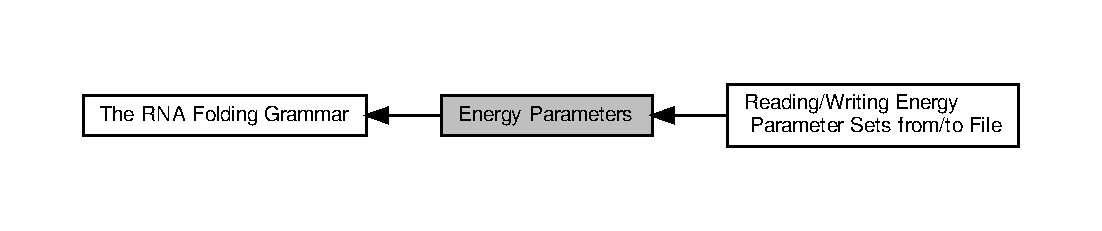
\includegraphics[width=350pt]{group__energy__parameters}
\end{center}
\end{figure}
\subsection*{Modules}
\begin{DoxyCompactItemize}
\item 
\hyperlink{group__energy__parameters__rw}{Reading/\+Writing Energy Parameter Sets from/to File}
\begin{DoxyCompactList}\small\item\em Read and Write energy parameter sets from and to text files. \end{DoxyCompactList}\end{DoxyCompactItemize}
\subsection*{Files}
\begin{DoxyCompactItemize}
\item 
file \hyperlink{params_2basic_8h}{basic.\+h}
\begin{DoxyCompactList}\small\item\em Functions to deal with sets of energy parameters. \end{DoxyCompactList}\item 
file \hyperlink{constants_8h}{constants.\+h}
\begin{DoxyCompactList}\small\item\em Energy parameter constants. \end{DoxyCompactList}\item 
file \hyperlink{convert_8h}{convert.\+h}
\begin{DoxyCompactList}\small\item\em Functions and definitions for energy parameter file format conversion. \end{DoxyCompactList}\item 
file \hyperlink{io_8h}{io.\+h}
\begin{DoxyCompactList}\small\item\em Read and write energy parameter files. \end{DoxyCompactList}\end{DoxyCompactItemize}
\subsection*{Data Structures}
\begin{DoxyCompactItemize}
\item 
struct \hyperlink{group__energy__parameters_structvrna__param__s}{vrna\+\_\+param\+\_\+s}
\begin{DoxyCompactList}\small\item\em The datastructure that contains temperature scaled energy parameters.  \hyperlink{group__energy__parameters_structvrna__param__s}{More...}\end{DoxyCompactList}\item 
struct \hyperlink{group__energy__parameters_structvrna__exp__param__s}{vrna\+\_\+exp\+\_\+param\+\_\+s}
\begin{DoxyCompactList}\small\item\em The data structure that contains temperature scaled Boltzmann weights of the energy parameters.  \hyperlink{group__energy__parameters_structvrna__exp__param__s}{More...}\end{DoxyCompactList}\end{DoxyCompactItemize}
\subsection*{Typedefs}
\begin{DoxyCompactItemize}
\item 
\mbox{\Hypertarget{group__energy__parameters_ga8a69ca7d787e4fd6079914f5343a1f35}\label{group__energy__parameters_ga8a69ca7d787e4fd6079914f5343a1f35}} 
typedef struct \hyperlink{group__energy__parameters_structvrna__param__s}{vrna\+\_\+param\+\_\+s} \hyperlink{group__energy__parameters_ga8a69ca7d787e4fd6079914f5343a1f35}{vrna\+\_\+param\+\_\+t}
\begin{DoxyCompactList}\small\item\em Typename for the free energy parameter data structure \hyperlink{group__energy__parameters_gad0e3e7e74bdc50d1709d40c92993185e}{vrna\+\_\+params}. \end{DoxyCompactList}\item 
\mbox{\Hypertarget{group__energy__parameters_ga01d8b92fe734df8d79a6169482c7d8d8}\label{group__energy__parameters_ga01d8b92fe734df8d79a6169482c7d8d8}} 
typedef struct \hyperlink{group__energy__parameters_structvrna__exp__param__s}{vrna\+\_\+exp\+\_\+param\+\_\+s} \hyperlink{group__energy__parameters_ga01d8b92fe734df8d79a6169482c7d8d8}{vrna\+\_\+exp\+\_\+param\+\_\+t}
\begin{DoxyCompactList}\small\item\em Typename for the Boltzmann factor data structure \hyperlink{group__energy__parameters_gab1f3016f96aa96bff020cdd904605afa}{vrna\+\_\+exp\+\_\+params}. \end{DoxyCompactList}\item 
typedef struct \hyperlink{group__energy__parameters_structvrna__param__s}{vrna\+\_\+param\+\_\+s} \hyperlink{group__energy__parameters_ga857dde86357d306cc902f0d8b2797659}{paramT}
\begin{DoxyCompactList}\small\item\em Old typename of \hyperlink{group__energy__parameters_structvrna__param__s}{vrna\+\_\+param\+\_\+s}. \end{DoxyCompactList}\item 
typedef struct \hyperlink{group__energy__parameters_structvrna__exp__param__s}{vrna\+\_\+exp\+\_\+param\+\_\+s} \hyperlink{group__energy__parameters_ga8bffe1828e2cbec101769f5cc0b1535b}{pf\+\_\+paramT}
\begin{DoxyCompactList}\small\item\em Old typename of \hyperlink{group__energy__parameters_structvrna__exp__param__s}{vrna\+\_\+exp\+\_\+param\+\_\+s}. \end{DoxyCompactList}\end{DoxyCompactItemize}
\subsection*{Functions}
\begin{DoxyCompactItemize}
\item 
\hyperlink{group__energy__parameters_ga8a69ca7d787e4fd6079914f5343a1f35}{vrna\+\_\+param\+\_\+t} $\ast$ \hyperlink{group__energy__parameters_gad0e3e7e74bdc50d1709d40c92993185e}{vrna\+\_\+params} (\hyperlink{group__model__details_ga1f8a10e12a0a1915f2a4eff0b28ea17c}{vrna\+\_\+md\+\_\+t} $\ast$md)
\begin{DoxyCompactList}\small\item\em Get a data structure containing prescaled free energy parameters. \end{DoxyCompactList}\item 
\hyperlink{group__energy__parameters_ga8a69ca7d787e4fd6079914f5343a1f35}{vrna\+\_\+param\+\_\+t} $\ast$ \hyperlink{group__energy__parameters_ga4bffa39f26e7746148444dd8a8426eca}{vrna\+\_\+params\+\_\+copy} (\hyperlink{group__energy__parameters_ga8a69ca7d787e4fd6079914f5343a1f35}{vrna\+\_\+param\+\_\+t} $\ast$par)
\begin{DoxyCompactList}\small\item\em Get a copy of the provided free energy parameters. \end{DoxyCompactList}\item 
\hyperlink{group__energy__parameters_ga01d8b92fe734df8d79a6169482c7d8d8}{vrna\+\_\+exp\+\_\+param\+\_\+t} $\ast$ \hyperlink{group__energy__parameters_gab1f3016f96aa96bff020cdd904605afa}{vrna\+\_\+exp\+\_\+params} (\hyperlink{group__model__details_ga1f8a10e12a0a1915f2a4eff0b28ea17c}{vrna\+\_\+md\+\_\+t} $\ast$md)
\begin{DoxyCompactList}\small\item\em Get a data structure containing prescaled free energy parameters already transformed to Boltzmann factors. \end{DoxyCompactList}\item 
\hyperlink{group__energy__parameters_ga01d8b92fe734df8d79a6169482c7d8d8}{vrna\+\_\+exp\+\_\+param\+\_\+t} $\ast$ \hyperlink{group__energy__parameters_gaf78c09e685e6eef4100b1a41d4042550}{vrna\+\_\+exp\+\_\+params\+\_\+comparative} (unsigned int n\+\_\+seq, \hyperlink{group__model__details_ga1f8a10e12a0a1915f2a4eff0b28ea17c}{vrna\+\_\+md\+\_\+t} $\ast$md)
\begin{DoxyCompactList}\small\item\em Get a data structure containing prescaled free energy parameters already transformed to Boltzmann factors (alifold version) \end{DoxyCompactList}\item 
\hyperlink{group__energy__parameters_ga01d8b92fe734df8d79a6169482c7d8d8}{vrna\+\_\+exp\+\_\+param\+\_\+t} $\ast$ \hyperlink{group__energy__parameters_ga70bc46be7cfa5434a71efe241c4f0609}{vrna\+\_\+exp\+\_\+params\+\_\+copy} (\hyperlink{group__energy__parameters_ga01d8b92fe734df8d79a6169482c7d8d8}{vrna\+\_\+exp\+\_\+param\+\_\+t} $\ast$par)
\begin{DoxyCompactList}\small\item\em Get a copy of the provided free energy parameters (provided as Boltzmann factors) \end{DoxyCompactList}\item 
void \hyperlink{group__energy__parameters_ga5d1909208f7ea3baa98b75afaa1f62ca}{vrna\+\_\+params\+\_\+subst} (\hyperlink{group__fold__compound_ga1b0cef17fd40466cef5968eaeeff6166}{vrna\+\_\+fold\+\_\+compound\+\_\+t} $\ast$vc, \hyperlink{group__energy__parameters_ga8a69ca7d787e4fd6079914f5343a1f35}{vrna\+\_\+param\+\_\+t} $\ast$par)
\begin{DoxyCompactList}\small\item\em Update/\+Reset energy parameters data structure within a \hyperlink{group__fold__compound_ga1b0cef17fd40466cef5968eaeeff6166}{vrna\+\_\+fold\+\_\+compound\+\_\+t}. \end{DoxyCompactList}\item 
void \hyperlink{group__energy__parameters_ga8e7ac4fab3b0cc03afbc134eaafb3525}{vrna\+\_\+exp\+\_\+params\+\_\+subst} (\hyperlink{group__fold__compound_ga1b0cef17fd40466cef5968eaeeff6166}{vrna\+\_\+fold\+\_\+compound\+\_\+t} $\ast$vc, \hyperlink{group__energy__parameters_ga01d8b92fe734df8d79a6169482c7d8d8}{vrna\+\_\+exp\+\_\+param\+\_\+t} $\ast$params)
\begin{DoxyCompactList}\small\item\em Update the energy parameters for subsequent partition function computations. \end{DoxyCompactList}\item 
void \hyperlink{group__energy__parameters_gad607bc3a5b5da16400e2ca4ea5560233}{vrna\+\_\+exp\+\_\+params\+\_\+rescale} (\hyperlink{group__fold__compound_ga1b0cef17fd40466cef5968eaeeff6166}{vrna\+\_\+fold\+\_\+compound\+\_\+t} $\ast$vc, double $\ast$mfe)
\begin{DoxyCompactList}\small\item\em Rescale Boltzmann factors for partition function computations. \end{DoxyCompactList}\item 
void \hyperlink{group__energy__parameters_gac40dc82e48a72a97cfc58b9da08a7792}{vrna\+\_\+params\+\_\+reset} (\hyperlink{group__fold__compound_ga1b0cef17fd40466cef5968eaeeff6166}{vrna\+\_\+fold\+\_\+compound\+\_\+t} $\ast$vc, \hyperlink{group__model__details_ga1f8a10e12a0a1915f2a4eff0b28ea17c}{vrna\+\_\+md\+\_\+t} $\ast$md\+\_\+p)
\begin{DoxyCompactList}\small\item\em Reset free energy parameters within a \hyperlink{group__fold__compound_ga1b0cef17fd40466cef5968eaeeff6166}{vrna\+\_\+fold\+\_\+compound\+\_\+t} according to provided, or default model details. \end{DoxyCompactList}\item 
void \hyperlink{group__energy__parameters_gaa5409218068be84d7b50c78fbdaa85a9}{vrna\+\_\+exp\+\_\+params\+\_\+reset} (\hyperlink{group__fold__compound_ga1b0cef17fd40466cef5968eaeeff6166}{vrna\+\_\+fold\+\_\+compound\+\_\+t} $\ast$vc, \hyperlink{group__model__details_ga1f8a10e12a0a1915f2a4eff0b28ea17c}{vrna\+\_\+md\+\_\+t} $\ast$md\+\_\+p)
\begin{DoxyCompactList}\small\item\em Reset Boltzmann factors for partition function computations within a \hyperlink{group__fold__compound_ga1b0cef17fd40466cef5968eaeeff6166}{vrna\+\_\+fold\+\_\+compound\+\_\+t} according to provided, or default model details. \end{DoxyCompactList}\item 
\hyperlink{group__energy__parameters_ga01d8b92fe734df8d79a6169482c7d8d8}{vrna\+\_\+exp\+\_\+param\+\_\+t} $\ast$ \hyperlink{group__energy__parameters_gabf3b9271c41dd3fac02d56e0b02b3344}{get\+\_\+scaled\+\_\+pf\+\_\+parameters} (void)
\item 
\hyperlink{group__energy__parameters_ga01d8b92fe734df8d79a6169482c7d8d8}{vrna\+\_\+exp\+\_\+param\+\_\+t} $\ast$ \hyperlink{group__energy__parameters_gaef2b931c7e9d4ffb0a5c33df50ec2068}{get\+\_\+boltzmann\+\_\+factors} (double \hyperlink{group__model__details_gab4b11c8d9c758430960896bc3fe82ead}{temperature}, double beta\+Scale, \hyperlink{group__model__details_ga1f8a10e12a0a1915f2a4eff0b28ea17c}{vrna\+\_\+md\+\_\+t} md, double \hyperlink{group__model__details_gad3b22044065acc6dee0af68931b52cfd}{pf\+\_\+scale})
\begin{DoxyCompactList}\small\item\em Get precomputed Boltzmann factors of the loop type dependent energy contributions with independent thermodynamic temperature. \end{DoxyCompactList}\item 
\hyperlink{group__energy__parameters_ga01d8b92fe734df8d79a6169482c7d8d8}{vrna\+\_\+exp\+\_\+param\+\_\+t} $\ast$ \hyperlink{group__energy__parameters_ga665a446ba8ff211e551297a8fa36ec27}{get\+\_\+boltzmann\+\_\+factor\+\_\+copy} (\hyperlink{group__energy__parameters_ga01d8b92fe734df8d79a6169482c7d8d8}{vrna\+\_\+exp\+\_\+param\+\_\+t} $\ast$parameters)
\begin{DoxyCompactList}\small\item\em Get a copy of already precomputed Boltzmann factors. \end{DoxyCompactList}\item 
\hyperlink{group__energy__parameters_ga01d8b92fe734df8d79a6169482c7d8d8}{vrna\+\_\+exp\+\_\+param\+\_\+t} $\ast$ \hyperlink{group__energy__parameters_ga0ccf4e1be085a573533fd6b9da2d8cf9}{get\+\_\+scaled\+\_\+alipf\+\_\+parameters} (unsigned int n\+\_\+seq)
\begin{DoxyCompactList}\small\item\em Get precomputed Boltzmann factors of the loop type dependent energy contributions (alifold variant) \end{DoxyCompactList}\item 
\hyperlink{group__energy__parameters_ga01d8b92fe734df8d79a6169482c7d8d8}{vrna\+\_\+exp\+\_\+param\+\_\+t} $\ast$ \hyperlink{group__energy__parameters_ga2aa1d87c97f35d2e4121634a17556829}{get\+\_\+boltzmann\+\_\+factors\+\_\+ali} (unsigned int n\+\_\+seq, double \hyperlink{group__model__details_gab4b11c8d9c758430960896bc3fe82ead}{temperature}, double beta\+Scale, \hyperlink{group__model__details_ga1f8a10e12a0a1915f2a4eff0b28ea17c}{vrna\+\_\+md\+\_\+t} md, double \hyperlink{group__model__details_gad3b22044065acc6dee0af68931b52cfd}{pf\+\_\+scale})
\begin{DoxyCompactList}\small\item\em Get precomputed Boltzmann factors of the loop type dependent energy contributions (alifold variant) with independent thermodynamic temperature. \end{DoxyCompactList}\item 
\hyperlink{group__energy__parameters_ga8a69ca7d787e4fd6079914f5343a1f35}{vrna\+\_\+param\+\_\+t} $\ast$ \hyperlink{group__energy__parameters_ga541f2cf7436e9bc939b0a49b24baf987}{scale\+\_\+parameters} (void)
\begin{DoxyCompactList}\small\item\em Get precomputed energy contributions for all the known loop types. \end{DoxyCompactList}\item 
\hyperlink{group__energy__parameters_ga8a69ca7d787e4fd6079914f5343a1f35}{vrna\+\_\+param\+\_\+t} $\ast$ \hyperlink{group__energy__parameters_ga7fa6a000d7c16feab939f2c4ee626197}{get\+\_\+scaled\+\_\+parameters} (double \hyperlink{group__model__details_gab4b11c8d9c758430960896bc3fe82ead}{temperature}, \hyperlink{group__model__details_ga1f8a10e12a0a1915f2a4eff0b28ea17c}{vrna\+\_\+md\+\_\+t} md)
\begin{DoxyCompactList}\small\item\em Get precomputed energy contributions for all the known loop types. \end{DoxyCompactList}\end{DoxyCompactItemize}


\subsection{Data Structure Documentation}
\index{vrna\+\_\+param\+\_\+s@{vrna\+\_\+param\+\_\+s}}\label{structvrna__param__s}
\Hypertarget{group__energy__parameters_structvrna__param__s}
\subsubsection{struct vrna\+\_\+param\+\_\+s}
The datastructure that contains temperature scaled energy parameters. 

Collaboration diagram for vrna\+\_\+param\+\_\+s\+:
\nopagebreak
\begin{figure}[H]
\begin{center}
\leavevmode
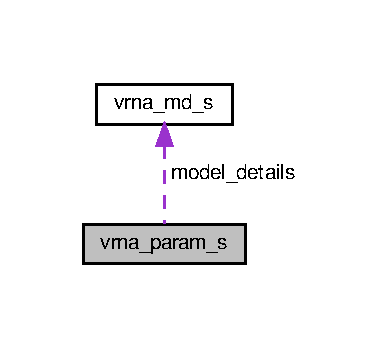
\includegraphics[width=183pt]{structvrna__param__s__coll__graph}
\end{center}
\end{figure}
\subsubsection*{Data Fields}
\begin{DoxyCompactItemize}
\item 
\mbox{\Hypertarget{group__energy__parameters_aeed2cd83713012bcb52e431041e037c8}\label{group__energy__parameters_aeed2cd83713012bcb52e431041e037c8}} 
double \hyperlink{group__energy__parameters_aeed2cd83713012bcb52e431041e037c8}{temperature}
\begin{DoxyCompactList}\small\item\em Temperature used for loop contribution scaling. \end{DoxyCompactList}\item 
\mbox{\Hypertarget{group__energy__parameters_a7b84353eb9075c595bad4ceb871bcae7}\label{group__energy__parameters_a7b84353eb9075c595bad4ceb871bcae7}} 
\hyperlink{group__model__details_ga1f8a10e12a0a1915f2a4eff0b28ea17c}{vrna\+\_\+md\+\_\+t} \hyperlink{group__energy__parameters_a7b84353eb9075c595bad4ceb871bcae7}{model\+\_\+details}
\begin{DoxyCompactList}\small\item\em Model details to be used in the recursions. \end{DoxyCompactList}\item 
\mbox{\Hypertarget{group__energy__parameters_ace10aa4aacffcbf6de92349f2ee0d66a}\label{group__energy__parameters_ace10aa4aacffcbf6de92349f2ee0d66a}} 
char \hyperlink{group__energy__parameters_ace10aa4aacffcbf6de92349f2ee0d66a}{param\+\_\+file} \mbox{[}256\mbox{]}
\begin{DoxyCompactList}\small\item\em The filename the parameters were derived from, or empty string if they represent the default. \end{DoxyCompactList}\end{DoxyCompactItemize}
\index{vrna\+\_\+exp\+\_\+param\+\_\+s@{vrna\+\_\+exp\+\_\+param\+\_\+s}}\label{structvrna__exp__param__s}
\Hypertarget{group__energy__parameters_structvrna__exp__param__s}
\subsubsection{struct vrna\+\_\+exp\+\_\+param\+\_\+s}
The data structure that contains temperature scaled Boltzmann weights of the energy parameters. 

Collaboration diagram for vrna\+\_\+exp\+\_\+param\+\_\+s\+:
\nopagebreak
\begin{figure}[H]
\begin{center}
\leavevmode
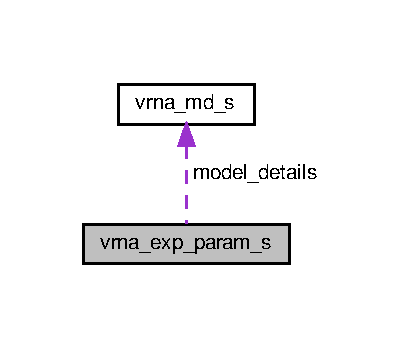
\includegraphics[width=194pt]{structvrna__exp__param__s__coll__graph}
\end{center}
\end{figure}
\subsubsection*{Data Fields}
\begin{DoxyCompactItemize}
\item 
int \hyperlink{group__energy__parameters_a378d5bcf2bae1f3ec84c912c7d3908d2}{id}
\begin{DoxyCompactList}\small\item\em An identifier for the data structure. \end{DoxyCompactList}\item 
\mbox{\Hypertarget{group__energy__parameters_a53c12f0d74f94ce371e0471a8ab5a377}\label{group__energy__parameters_a53c12f0d74f94ce371e0471a8ab5a377}} 
double \hyperlink{group__energy__parameters_a53c12f0d74f94ce371e0471a8ab5a377}{pf\+\_\+scale}
\begin{DoxyCompactList}\small\item\em Scaling factor to avoid over-\//underflows. \end{DoxyCompactList}\item 
\mbox{\Hypertarget{group__energy__parameters_a674656d65ea957ddbeff8bd146b7fc16}\label{group__energy__parameters_a674656d65ea957ddbeff8bd146b7fc16}} 
double \hyperlink{group__energy__parameters_a674656d65ea957ddbeff8bd146b7fc16}{temperature}
\begin{DoxyCompactList}\small\item\em Temperature used for loop contribution scaling. \end{DoxyCompactList}\item 
double \hyperlink{group__energy__parameters_a77145830b7bb01b36c3217b363310ef0}{alpha}
\begin{DoxyCompactList}\small\item\em Scaling factor for the thermodynamic temperature. \end{DoxyCompactList}\item 
\mbox{\Hypertarget{group__energy__parameters_ac18055127bccc27c1223f1d2f3b01b53}\label{group__energy__parameters_ac18055127bccc27c1223f1d2f3b01b53}} 
\hyperlink{group__model__details_ga1f8a10e12a0a1915f2a4eff0b28ea17c}{vrna\+\_\+md\+\_\+t} \hyperlink{group__energy__parameters_ac18055127bccc27c1223f1d2f3b01b53}{model\+\_\+details}
\begin{DoxyCompactList}\small\item\em Model details to be used in the recursions. \end{DoxyCompactList}\item 
\mbox{\Hypertarget{group__energy__parameters_a8e1b02a4753a9b64c3c9ae8529b9d75c}\label{group__energy__parameters_a8e1b02a4753a9b64c3c9ae8529b9d75c}} 
char \hyperlink{group__energy__parameters_a8e1b02a4753a9b64c3c9ae8529b9d75c}{param\+\_\+file} \mbox{[}256\mbox{]}
\begin{DoxyCompactList}\small\item\em The filename the parameters were derived from, or empty string if they represent the default. \end{DoxyCompactList}\end{DoxyCompactItemize}


\paragraph{Field Documentation}
\mbox{\Hypertarget{group__energy__parameters_a378d5bcf2bae1f3ec84c912c7d3908d2}\label{group__energy__parameters_a378d5bcf2bae1f3ec84c912c7d3908d2}} 
\index{vrna\+\_\+exp\+\_\+param\+\_\+s@{vrna\+\_\+exp\+\_\+param\+\_\+s}!id@{id}}
\index{id@{id}!vrna\+\_\+exp\+\_\+param\+\_\+s@{vrna\+\_\+exp\+\_\+param\+\_\+s}}
\subparagraph{\texorpdfstring{id}{id}}
{\footnotesize\ttfamily int vrna\+\_\+exp\+\_\+param\+\_\+s\+::id}



An identifier for the data structure. 

\begin{DoxyRefDesc}{Deprecated}
\item[\hyperlink{deprecated__deprecated000146}{Deprecated}]This attribute will be removed in version 3 \end{DoxyRefDesc}
\mbox{\Hypertarget{group__energy__parameters_a77145830b7bb01b36c3217b363310ef0}\label{group__energy__parameters_a77145830b7bb01b36c3217b363310ef0}} 
\index{vrna\+\_\+exp\+\_\+param\+\_\+s@{vrna\+\_\+exp\+\_\+param\+\_\+s}!alpha@{alpha}}
\index{alpha@{alpha}!vrna\+\_\+exp\+\_\+param\+\_\+s@{vrna\+\_\+exp\+\_\+param\+\_\+s}}
\subparagraph{\texorpdfstring{alpha}{alpha}}
{\footnotesize\ttfamily double vrna\+\_\+exp\+\_\+param\+\_\+s\+::alpha}



Scaling factor for the thermodynamic temperature. 

This allows for temperature scaling in Boltzmann factors independently from the energy contributions. The resulting Boltzmann factors are then computed by $ e^{-E/(\alpha \cdot K \cdot T)} $ 

\subsection{Typedef Documentation}
\mbox{\Hypertarget{group__energy__parameters_ga857dde86357d306cc902f0d8b2797659}\label{group__energy__parameters_ga857dde86357d306cc902f0d8b2797659}} 
\index{Energy Parameters@{Energy Parameters}!paramT@{paramT}}
\index{paramT@{paramT}!Energy Parameters@{Energy Parameters}}
\subsubsection{\texorpdfstring{paramT}{paramT}}
{\footnotesize\ttfamily typedef struct \hyperlink{group__energy__parameters_structvrna__param__s}{vrna\+\_\+param\+\_\+s} \hyperlink{group__energy__parameters_ga857dde86357d306cc902f0d8b2797659}{paramT}}



{\ttfamily \#include $<$\hyperlink{params_2basic_8h}{Vienna\+R\+N\+A/params/basic.\+h}$>$}



Old typename of \hyperlink{group__energy__parameters_structvrna__param__s}{vrna\+\_\+param\+\_\+s}. 

\begin{DoxyRefDesc}{Deprecated}
\item[\hyperlink{deprecated__deprecated000137}{Deprecated}]Use \hyperlink{group__energy__parameters_ga8a69ca7d787e4fd6079914f5343a1f35}{vrna\+\_\+param\+\_\+t} instead! \end{DoxyRefDesc}
\mbox{\Hypertarget{group__energy__parameters_ga8bffe1828e2cbec101769f5cc0b1535b}\label{group__energy__parameters_ga8bffe1828e2cbec101769f5cc0b1535b}} 
\index{Energy Parameters@{Energy Parameters}!pf\+\_\+paramT@{pf\+\_\+paramT}}
\index{pf\+\_\+paramT@{pf\+\_\+paramT}!Energy Parameters@{Energy Parameters}}
\subsubsection{\texorpdfstring{pf\+\_\+paramT}{pf\_paramT}}
{\footnotesize\ttfamily typedef struct \hyperlink{group__energy__parameters_structvrna__exp__param__s}{vrna\+\_\+exp\+\_\+param\+\_\+s} \hyperlink{group__energy__parameters_ga8bffe1828e2cbec101769f5cc0b1535b}{pf\+\_\+paramT}}



{\ttfamily \#include $<$\hyperlink{params_2basic_8h}{Vienna\+R\+N\+A/params/basic.\+h}$>$}



Old typename of \hyperlink{group__energy__parameters_structvrna__exp__param__s}{vrna\+\_\+exp\+\_\+param\+\_\+s}. 

\begin{DoxyRefDesc}{Deprecated}
\item[\hyperlink{deprecated__deprecated000138}{Deprecated}]Use \hyperlink{group__energy__parameters_ga01d8b92fe734df8d79a6169482c7d8d8}{vrna\+\_\+exp\+\_\+param\+\_\+t} instead! \end{DoxyRefDesc}


\subsection{Function Documentation}
\mbox{\Hypertarget{group__energy__parameters_gad0e3e7e74bdc50d1709d40c92993185e}\label{group__energy__parameters_gad0e3e7e74bdc50d1709d40c92993185e}} 
\index{Energy Parameters@{Energy Parameters}!vrna\+\_\+params@{vrna\+\_\+params}}
\index{vrna\+\_\+params@{vrna\+\_\+params}!Energy Parameters@{Energy Parameters}}
\subsubsection{\texorpdfstring{vrna\+\_\+params()}{vrna\_params()}}
{\footnotesize\ttfamily \hyperlink{group__energy__parameters_ga8a69ca7d787e4fd6079914f5343a1f35}{vrna\+\_\+param\+\_\+t}$\ast$ vrna\+\_\+params (\begin{DoxyParamCaption}\item[{\hyperlink{group__model__details_ga1f8a10e12a0a1915f2a4eff0b28ea17c}{vrna\+\_\+md\+\_\+t} $\ast$}]{md }\end{DoxyParamCaption})}



{\ttfamily \#include $<$\hyperlink{params_2basic_8h}{Vienna\+R\+N\+A/params/basic.\+h}$>$}



Get a data structure containing prescaled free energy parameters. 

If a N\+U\+LL pointer is passed for the model details parameter, the default model parameters are stored within the requested \hyperlink{group__energy__parameters_ga8a69ca7d787e4fd6079914f5343a1f35}{vrna\+\_\+param\+\_\+t} structure.

\begin{DoxySeeAlso}{See also}
\hyperlink{group__model__details_ga1f8a10e12a0a1915f2a4eff0b28ea17c}{vrna\+\_\+md\+\_\+t}, \hyperlink{group__model__details_ga8ac6ff84936282436f822644bf841f66}{vrna\+\_\+md\+\_\+set\+\_\+default()}, \hyperlink{group__energy__parameters_gab1f3016f96aa96bff020cdd904605afa}{vrna\+\_\+exp\+\_\+params()}
\end{DoxySeeAlso}

\begin{DoxyParams}{Parameters}
{\em md} & A pointer to the model details to store inside the structure (Maybe N\+U\+LL) \\
\hline
\end{DoxyParams}
\begin{DoxyReturn}{Returns}
A pointer to the memory location where the requested parameters are stored 
\end{DoxyReturn}
\mbox{\Hypertarget{group__energy__parameters_ga4bffa39f26e7746148444dd8a8426eca}\label{group__energy__parameters_ga4bffa39f26e7746148444dd8a8426eca}} 
\index{Energy Parameters@{Energy Parameters}!vrna\+\_\+params\+\_\+copy@{vrna\+\_\+params\+\_\+copy}}
\index{vrna\+\_\+params\+\_\+copy@{vrna\+\_\+params\+\_\+copy}!Energy Parameters@{Energy Parameters}}
\subsubsection{\texorpdfstring{vrna\+\_\+params\+\_\+copy()}{vrna\_params\_copy()}}
{\footnotesize\ttfamily \hyperlink{group__energy__parameters_ga8a69ca7d787e4fd6079914f5343a1f35}{vrna\+\_\+param\+\_\+t}$\ast$ vrna\+\_\+params\+\_\+copy (\begin{DoxyParamCaption}\item[{\hyperlink{group__energy__parameters_ga8a69ca7d787e4fd6079914f5343a1f35}{vrna\+\_\+param\+\_\+t} $\ast$}]{par }\end{DoxyParamCaption})}



{\ttfamily \#include $<$\hyperlink{params_2basic_8h}{Vienna\+R\+N\+A/params/basic.\+h}$>$}



Get a copy of the provided free energy parameters. 

If N\+U\+LL is passed as parameter, a default set of energy parameters is created and returned.

\begin{DoxySeeAlso}{See also}
\hyperlink{group__energy__parameters_gad0e3e7e74bdc50d1709d40c92993185e}{vrna\+\_\+params()}, \hyperlink{group__energy__parameters_ga8a69ca7d787e4fd6079914f5343a1f35}{vrna\+\_\+param\+\_\+t}
\end{DoxySeeAlso}

\begin{DoxyParams}{Parameters}
{\em par} & The free energy parameters that are to be copied (Maybe N\+U\+LL) \\
\hline
\end{DoxyParams}
\begin{DoxyReturn}{Returns}
A copy or a default set of the (provided) parameters 
\end{DoxyReturn}
\mbox{\Hypertarget{group__energy__parameters_gab1f3016f96aa96bff020cdd904605afa}\label{group__energy__parameters_gab1f3016f96aa96bff020cdd904605afa}} 
\index{Energy Parameters@{Energy Parameters}!vrna\+\_\+exp\+\_\+params@{vrna\+\_\+exp\+\_\+params}}
\index{vrna\+\_\+exp\+\_\+params@{vrna\+\_\+exp\+\_\+params}!Energy Parameters@{Energy Parameters}}
\subsubsection{\texorpdfstring{vrna\+\_\+exp\+\_\+params()}{vrna\_exp\_params()}}
{\footnotesize\ttfamily \hyperlink{group__energy__parameters_ga01d8b92fe734df8d79a6169482c7d8d8}{vrna\+\_\+exp\+\_\+param\+\_\+t}$\ast$ vrna\+\_\+exp\+\_\+params (\begin{DoxyParamCaption}\item[{\hyperlink{group__model__details_ga1f8a10e12a0a1915f2a4eff0b28ea17c}{vrna\+\_\+md\+\_\+t} $\ast$}]{md }\end{DoxyParamCaption})}



{\ttfamily \#include $<$\hyperlink{params_2basic_8h}{Vienna\+R\+N\+A/params/basic.\+h}$>$}



Get a data structure containing prescaled free energy parameters already transformed to Boltzmann factors. 

This function returns a data structure that contains all necessary precomputed energy contributions for each type of loop.

In contrast to \hyperlink{group__energy__parameters_gad0e3e7e74bdc50d1709d40c92993185e}{vrna\+\_\+params()}, the free energies within this data structure are stored as their Boltzmann factors, i.\+e.

$ exp(-E / kT) $

where $ E $ is the free energy.

If a N\+U\+LL pointer is passed for the model details parameter, the default model parameters are stored within the requested \hyperlink{group__energy__parameters_ga01d8b92fe734df8d79a6169482c7d8d8}{vrna\+\_\+exp\+\_\+param\+\_\+t} structure.

\begin{DoxySeeAlso}{See also}
\hyperlink{group__model__details_ga1f8a10e12a0a1915f2a4eff0b28ea17c}{vrna\+\_\+md\+\_\+t}, \hyperlink{group__model__details_ga8ac6ff84936282436f822644bf841f66}{vrna\+\_\+md\+\_\+set\+\_\+default()}, \hyperlink{group__energy__parameters_gad0e3e7e74bdc50d1709d40c92993185e}{vrna\+\_\+params()}, vrna\+\_\+rescale\+\_\+pf\+\_\+params()
\end{DoxySeeAlso}

\begin{DoxyParams}{Parameters}
{\em md} & A pointer to the model details to store inside the structure (Maybe N\+U\+LL) \\
\hline
\end{DoxyParams}
\begin{DoxyReturn}{Returns}
A pointer to the memory location where the requested parameters are stored 
\end{DoxyReturn}
\mbox{\Hypertarget{group__energy__parameters_gaf78c09e685e6eef4100b1a41d4042550}\label{group__energy__parameters_gaf78c09e685e6eef4100b1a41d4042550}} 
\index{Energy Parameters@{Energy Parameters}!vrna\+\_\+exp\+\_\+params\+\_\+comparative@{vrna\+\_\+exp\+\_\+params\+\_\+comparative}}
\index{vrna\+\_\+exp\+\_\+params\+\_\+comparative@{vrna\+\_\+exp\+\_\+params\+\_\+comparative}!Energy Parameters@{Energy Parameters}}
\subsubsection{\texorpdfstring{vrna\+\_\+exp\+\_\+params\+\_\+comparative()}{vrna\_exp\_params\_comparative()}}
{\footnotesize\ttfamily \hyperlink{group__energy__parameters_ga01d8b92fe734df8d79a6169482c7d8d8}{vrna\+\_\+exp\+\_\+param\+\_\+t}$\ast$ vrna\+\_\+exp\+\_\+params\+\_\+comparative (\begin{DoxyParamCaption}\item[{unsigned int}]{n\+\_\+seq,  }\item[{\hyperlink{group__model__details_ga1f8a10e12a0a1915f2a4eff0b28ea17c}{vrna\+\_\+md\+\_\+t} $\ast$}]{md }\end{DoxyParamCaption})}



{\ttfamily \#include $<$\hyperlink{params_2basic_8h}{Vienna\+R\+N\+A/params/basic.\+h}$>$}



Get a data structure containing prescaled free energy parameters already transformed to Boltzmann factors (alifold version) 

If a N\+U\+LL pointer is passed for the model details parameter, the default model parameters are stored within the requested \hyperlink{group__energy__parameters_ga01d8b92fe734df8d79a6169482c7d8d8}{vrna\+\_\+exp\+\_\+param\+\_\+t} structure.

\begin{DoxySeeAlso}{See also}
\hyperlink{group__model__details_ga1f8a10e12a0a1915f2a4eff0b28ea17c}{vrna\+\_\+md\+\_\+t}, \hyperlink{group__model__details_ga8ac6ff84936282436f822644bf841f66}{vrna\+\_\+md\+\_\+set\+\_\+default()}, \hyperlink{group__energy__parameters_gab1f3016f96aa96bff020cdd904605afa}{vrna\+\_\+exp\+\_\+params()}, \hyperlink{group__energy__parameters_gad0e3e7e74bdc50d1709d40c92993185e}{vrna\+\_\+params()}
\end{DoxySeeAlso}

\begin{DoxyParams}{Parameters}
{\em n\+\_\+seq} & The number of sequences in the alignment \\
\hline
{\em md} & A pointer to the model details to store inside the structure (Maybe N\+U\+LL) \\
\hline
\end{DoxyParams}
\begin{DoxyReturn}{Returns}
A pointer to the memory location where the requested parameters are stored 
\end{DoxyReturn}
\mbox{\Hypertarget{group__energy__parameters_ga70bc46be7cfa5434a71efe241c4f0609}\label{group__energy__parameters_ga70bc46be7cfa5434a71efe241c4f0609}} 
\index{Energy Parameters@{Energy Parameters}!vrna\+\_\+exp\+\_\+params\+\_\+copy@{vrna\+\_\+exp\+\_\+params\+\_\+copy}}
\index{vrna\+\_\+exp\+\_\+params\+\_\+copy@{vrna\+\_\+exp\+\_\+params\+\_\+copy}!Energy Parameters@{Energy Parameters}}
\subsubsection{\texorpdfstring{vrna\+\_\+exp\+\_\+params\+\_\+copy()}{vrna\_exp\_params\_copy()}}
{\footnotesize\ttfamily \hyperlink{group__energy__parameters_ga01d8b92fe734df8d79a6169482c7d8d8}{vrna\+\_\+exp\+\_\+param\+\_\+t}$\ast$ vrna\+\_\+exp\+\_\+params\+\_\+copy (\begin{DoxyParamCaption}\item[{\hyperlink{group__energy__parameters_ga01d8b92fe734df8d79a6169482c7d8d8}{vrna\+\_\+exp\+\_\+param\+\_\+t} $\ast$}]{par }\end{DoxyParamCaption})}



{\ttfamily \#include $<$\hyperlink{params_2basic_8h}{Vienna\+R\+N\+A/params/basic.\+h}$>$}



Get a copy of the provided free energy parameters (provided as Boltzmann factors) 

If N\+U\+LL is passed as parameter, a default set of energy parameters is created and returned.

\begin{DoxySeeAlso}{See also}
\hyperlink{group__energy__parameters_gab1f3016f96aa96bff020cdd904605afa}{vrna\+\_\+exp\+\_\+params()}, \hyperlink{group__energy__parameters_ga01d8b92fe734df8d79a6169482c7d8d8}{vrna\+\_\+exp\+\_\+param\+\_\+t}
\end{DoxySeeAlso}

\begin{DoxyParams}{Parameters}
{\em par} & The free energy parameters that are to be copied (Maybe N\+U\+LL) \\
\hline
\end{DoxyParams}
\begin{DoxyReturn}{Returns}
A copy or a default set of the (provided) parameters 
\end{DoxyReturn}
\mbox{\Hypertarget{group__energy__parameters_ga5d1909208f7ea3baa98b75afaa1f62ca}\label{group__energy__parameters_ga5d1909208f7ea3baa98b75afaa1f62ca}} 
\index{Energy Parameters@{Energy Parameters}!vrna\+\_\+params\+\_\+subst@{vrna\+\_\+params\+\_\+subst}}
\index{vrna\+\_\+params\+\_\+subst@{vrna\+\_\+params\+\_\+subst}!Energy Parameters@{Energy Parameters}}
\subsubsection{\texorpdfstring{vrna\+\_\+params\+\_\+subst()}{vrna\_params\_subst()}}
{\footnotesize\ttfamily void vrna\+\_\+params\+\_\+subst (\begin{DoxyParamCaption}\item[{\hyperlink{group__fold__compound_ga1b0cef17fd40466cef5968eaeeff6166}{vrna\+\_\+fold\+\_\+compound\+\_\+t} $\ast$}]{vc,  }\item[{\hyperlink{group__energy__parameters_ga8a69ca7d787e4fd6079914f5343a1f35}{vrna\+\_\+param\+\_\+t} $\ast$}]{par }\end{DoxyParamCaption})}



{\ttfamily \#include $<$\hyperlink{params_2basic_8h}{Vienna\+R\+N\+A/params/basic.\+h}$>$}



Update/\+Reset energy parameters data structure within a \hyperlink{group__fold__compound_ga1b0cef17fd40466cef5968eaeeff6166}{vrna\+\_\+fold\+\_\+compound\+\_\+t}. 

Passing N\+U\+LL as second argument leads to a reset of the energy parameters within vc to their default values. Otherwise, the energy parameters provided will be copied over into vc.

\begin{DoxySeeAlso}{See also}
\hyperlink{group__energy__parameters_gac40dc82e48a72a97cfc58b9da08a7792}{vrna\+\_\+params\+\_\+reset()}, \hyperlink{group__energy__parameters_ga8a69ca7d787e4fd6079914f5343a1f35}{vrna\+\_\+param\+\_\+t}, \hyperlink{group__model__details_ga1f8a10e12a0a1915f2a4eff0b28ea17c}{vrna\+\_\+md\+\_\+t}, \hyperlink{group__energy__parameters_gad0e3e7e74bdc50d1709d40c92993185e}{vrna\+\_\+params()}
\end{DoxySeeAlso}

\begin{DoxyParams}{Parameters}
{\em vc} & The \hyperlink{group__fold__compound_ga1b0cef17fd40466cef5968eaeeff6166}{vrna\+\_\+fold\+\_\+compound\+\_\+t} that is about to receive updated energy parameters \\
\hline
{\em par} & The energy parameters used to substitute those within vc (Maybe N\+U\+LL)\\
\hline
\end{DoxyParams}
\begin{DoxyRefDesc}{S\+W\+I\+G Wrapper Notes}
\item[\hyperlink{wrappers__wrappers000085}{S\+W\+I\+G Wrapper Notes}]This function is attached to \hyperlink{group__fold__compound_structvrna__fc__s}{vrna\+\_\+fc\+\_\+s} objects as {\bfseries params\+\_\+subst()} method. \end{DoxyRefDesc}
\mbox{\Hypertarget{group__energy__parameters_ga8e7ac4fab3b0cc03afbc134eaafb3525}\label{group__energy__parameters_ga8e7ac4fab3b0cc03afbc134eaafb3525}} 
\index{Energy Parameters@{Energy Parameters}!vrna\+\_\+exp\+\_\+params\+\_\+subst@{vrna\+\_\+exp\+\_\+params\+\_\+subst}}
\index{vrna\+\_\+exp\+\_\+params\+\_\+subst@{vrna\+\_\+exp\+\_\+params\+\_\+subst}!Energy Parameters@{Energy Parameters}}
\subsubsection{\texorpdfstring{vrna\+\_\+exp\+\_\+params\+\_\+subst()}{vrna\_exp\_params\_subst()}}
{\footnotesize\ttfamily void vrna\+\_\+exp\+\_\+params\+\_\+subst (\begin{DoxyParamCaption}\item[{\hyperlink{group__fold__compound_ga1b0cef17fd40466cef5968eaeeff6166}{vrna\+\_\+fold\+\_\+compound\+\_\+t} $\ast$}]{vc,  }\item[{\hyperlink{group__energy__parameters_ga01d8b92fe734df8d79a6169482c7d8d8}{vrna\+\_\+exp\+\_\+param\+\_\+t} $\ast$}]{params }\end{DoxyParamCaption})}



{\ttfamily \#include $<$\hyperlink{params_2basic_8h}{Vienna\+R\+N\+A/params/basic.\+h}$>$}



Update the energy parameters for subsequent partition function computations. 

This function can be used to properly assign new energy parameters for partition function computations to a \hyperlink{group__fold__compound_ga1b0cef17fd40466cef5968eaeeff6166}{vrna\+\_\+fold\+\_\+compound\+\_\+t}. For this purpose, the data of the provided pointer {\ttfamily params} will be copied into {\ttfamily vc} and a recomputation of the partition function scaling factor is issued, if the {\ttfamily pf\+\_\+scale} attribute of {\ttfamily params} is less than {\ttfamily 1.\+0}.

Passing N\+U\+LL as second argument leads to a reset of the energy parameters within vc to their default values

\begin{DoxySeeAlso}{See also}
\hyperlink{group__energy__parameters_gaa5409218068be84d7b50c78fbdaa85a9}{vrna\+\_\+exp\+\_\+params\+\_\+reset()}, \hyperlink{group__energy__parameters_gad607bc3a5b5da16400e2ca4ea5560233}{vrna\+\_\+exp\+\_\+params\+\_\+rescale()}, \hyperlink{group__energy__parameters_ga01d8b92fe734df8d79a6169482c7d8d8}{vrna\+\_\+exp\+\_\+param\+\_\+t}, \hyperlink{group__model__details_ga1f8a10e12a0a1915f2a4eff0b28ea17c}{vrna\+\_\+md\+\_\+t}, \hyperlink{group__energy__parameters_gab1f3016f96aa96bff020cdd904605afa}{vrna\+\_\+exp\+\_\+params()}
\end{DoxySeeAlso}

\begin{DoxyParams}{Parameters}
{\em vc} & The fold compound data structure \\
\hline
{\em params} & A pointer to the new energy parameters \\
\hline
\end{DoxyParams}
\mbox{\Hypertarget{group__energy__parameters_gad607bc3a5b5da16400e2ca4ea5560233}\label{group__energy__parameters_gad607bc3a5b5da16400e2ca4ea5560233}} 
\index{Energy Parameters@{Energy Parameters}!vrna\+\_\+exp\+\_\+params\+\_\+rescale@{vrna\+\_\+exp\+\_\+params\+\_\+rescale}}
\index{vrna\+\_\+exp\+\_\+params\+\_\+rescale@{vrna\+\_\+exp\+\_\+params\+\_\+rescale}!Energy Parameters@{Energy Parameters}}
\subsubsection{\texorpdfstring{vrna\+\_\+exp\+\_\+params\+\_\+rescale()}{vrna\_exp\_params\_rescale()}}
{\footnotesize\ttfamily void vrna\+\_\+exp\+\_\+params\+\_\+rescale (\begin{DoxyParamCaption}\item[{\hyperlink{group__fold__compound_ga1b0cef17fd40466cef5968eaeeff6166}{vrna\+\_\+fold\+\_\+compound\+\_\+t} $\ast$}]{vc,  }\item[{double $\ast$}]{mfe }\end{DoxyParamCaption})}



{\ttfamily \#include $<$\hyperlink{params_2basic_8h}{Vienna\+R\+N\+A/params/basic.\+h}$>$}



Rescale Boltzmann factors for partition function computations. 

This function may be used to (automatically) rescale the Boltzmann factors used in partition function computations. Since partition functions over subsequences can easily become extremely large, the R\+N\+Alib internally rescales them to avoid numerical over-\/ and/or underflow. Therefore, a proper scaling factor $s$ needs to be chosen that in turn is then used to normalize the corresponding partition functions $\hat{q}[i,j] = q[i,j] / s^{(j-i+1)}$.

This function provides two ways to automatically adjust the scaling factor.
\begin{DoxyEnumerate}
\item Automatic guess
\item Automatic adjustment according to M\+FE
\end{DoxyEnumerate}

Passing {\ttfamily N\+U\+LL} as second parameter activates the {\itshape automatic guess mode}. Here, the scaling factor is recomputed according to a mean free energy of {\ttfamily 184.\+3$\ast$length} cal for random sequences. \begin{DoxyNote}{Note}
This recomputation only takes place if the {\ttfamily pf\+\_\+scale} attribute of the {\ttfamily exp\+\_\+params} data structure contained in {\ttfamily vc} has a value below {\ttfamily 1.\+0}.
\end{DoxyNote}
On the other hand, if the M\+FE for a sequence is known, it can be used to recompute a more robust scaling factor, since it represents the lowest free energy of the entire ensemble of structures, i.\+e. the highest Boltzmann factor. To activate this second mode of {\itshape automatic adjustment according to M\+FE}, a pointer to the M\+FE value needs to be passed as second argument. This value is then taken to compute the scaling factor as $ s = exp((sfact * MFE) / kT / length )$, where sfact is an additional scaling weight located in the vrna\+\_\+md\+\_\+t data structure of {\ttfamily exp\+\_\+params} in {\ttfamily vc}.

The computed scaling factor $s$ will be stored as {\ttfamily pf\+\_\+scale} attribute of the {\ttfamily exp\+\_\+params} data structure in {\ttfamily vc}.

\begin{DoxySeeAlso}{See also}
\hyperlink{group__energy__parameters_ga8e7ac4fab3b0cc03afbc134eaafb3525}{vrna\+\_\+exp\+\_\+params\+\_\+subst()}, \hyperlink{group__model__details_ga1f8a10e12a0a1915f2a4eff0b28ea17c}{vrna\+\_\+md\+\_\+t}, \hyperlink{group__energy__parameters_ga01d8b92fe734df8d79a6169482c7d8d8}{vrna\+\_\+exp\+\_\+param\+\_\+t}, \hyperlink{group__fold__compound_ga1b0cef17fd40466cef5968eaeeff6166}{vrna\+\_\+fold\+\_\+compound\+\_\+t}
\end{DoxySeeAlso}

\begin{DoxyParams}{Parameters}
{\em vc} & The fold compound data structure \\
\hline
{\em mfe} & A pointer to the M\+FE (in kcal/mol) or N\+U\+LL\\
\hline
\end{DoxyParams}
\begin{DoxyRefDesc}{S\+W\+I\+G Wrapper Notes}
\item[\hyperlink{wrappers__wrappers000086}{S\+W\+I\+G Wrapper Notes}]This function is attached to \hyperlink{group__fold__compound_structvrna__fc__s}{vrna\+\_\+fc\+\_\+s} objects as overloaded {\bfseries exp\+\_\+params\+\_\+rescale()} method.

When no parameter is passed to this method, the resulting action is the same as passing {\itshape N\+U\+LL} as second parameter to \hyperlink{group__energy__parameters_gad607bc3a5b5da16400e2ca4ea5560233}{vrna\+\_\+exp\+\_\+params\+\_\+rescale()}, i.\+e. default scaling of the partition function. Passing an energy in kcal/mol, e.\+g. as retrieved by a previous call to the {\itshape mfe()} method, instructs all subsequent calls to scale the partition function accordingly. \end{DoxyRefDesc}
\mbox{\Hypertarget{group__energy__parameters_gac40dc82e48a72a97cfc58b9da08a7792}\label{group__energy__parameters_gac40dc82e48a72a97cfc58b9da08a7792}} 
\index{Energy Parameters@{Energy Parameters}!vrna\+\_\+params\+\_\+reset@{vrna\+\_\+params\+\_\+reset}}
\index{vrna\+\_\+params\+\_\+reset@{vrna\+\_\+params\+\_\+reset}!Energy Parameters@{Energy Parameters}}
\subsubsection{\texorpdfstring{vrna\+\_\+params\+\_\+reset()}{vrna\_params\_reset()}}
{\footnotesize\ttfamily void vrna\+\_\+params\+\_\+reset (\begin{DoxyParamCaption}\item[{\hyperlink{group__fold__compound_ga1b0cef17fd40466cef5968eaeeff6166}{vrna\+\_\+fold\+\_\+compound\+\_\+t} $\ast$}]{vc,  }\item[{\hyperlink{group__model__details_ga1f8a10e12a0a1915f2a4eff0b28ea17c}{vrna\+\_\+md\+\_\+t} $\ast$}]{md\+\_\+p }\end{DoxyParamCaption})}



{\ttfamily \#include $<$\hyperlink{params_2basic_8h}{Vienna\+R\+N\+A/params/basic.\+h}$>$}



Reset free energy parameters within a \hyperlink{group__fold__compound_ga1b0cef17fd40466cef5968eaeeff6166}{vrna\+\_\+fold\+\_\+compound\+\_\+t} according to provided, or default model details. 

This function allows one to rescale free energy parameters for subsequent structure prediction or evaluation according to a set of model details, e.\+g. temperature values. To do so, the caller provides either a pointer to a set of model details to be used for rescaling, or N\+U\+LL if global default setting should be used.

\begin{DoxySeeAlso}{See also}
\hyperlink{group__energy__parameters_gaa5409218068be84d7b50c78fbdaa85a9}{vrna\+\_\+exp\+\_\+params\+\_\+reset()}, vrna\+\_\+params\+\_\+subs() 
\end{DoxySeeAlso}

\begin{DoxyParams}{Parameters}
{\em vc} & The fold compound data structure \\
\hline
{\em md\+\_\+p} & A pointer to the new model details (or N\+U\+LL for reset to defaults)\\
\hline
\end{DoxyParams}
\begin{DoxyRefDesc}{S\+W\+I\+G Wrapper Notes}
\item[\hyperlink{wrappers__wrappers000087}{S\+W\+I\+G Wrapper Notes}]This function is attached to \hyperlink{group__fold__compound_structvrna__fc__s}{vrna\+\_\+fc\+\_\+s} objects as overloaded {\bfseries params\+\_\+reset()} method.

When no parameter is passed to this method, the resulting action is the same as passing {\itshape N\+U\+LL} as second parameter to \hyperlink{group__energy__parameters_gac40dc82e48a72a97cfc58b9da08a7792}{vrna\+\_\+params\+\_\+reset()}, i.\+e. global default model settings are used. Passing an object of type \hyperlink{group__model__details_structvrna__md__s}{vrna\+\_\+md\+\_\+s} resets the fold compound according to the specifications stored within the \hyperlink{group__model__details_structvrna__md__s}{vrna\+\_\+md\+\_\+s} object. \end{DoxyRefDesc}
\mbox{\Hypertarget{group__energy__parameters_gaa5409218068be84d7b50c78fbdaa85a9}\label{group__energy__parameters_gaa5409218068be84d7b50c78fbdaa85a9}} 
\index{Energy Parameters@{Energy Parameters}!vrna\+\_\+exp\+\_\+params\+\_\+reset@{vrna\+\_\+exp\+\_\+params\+\_\+reset}}
\index{vrna\+\_\+exp\+\_\+params\+\_\+reset@{vrna\+\_\+exp\+\_\+params\+\_\+reset}!Energy Parameters@{Energy Parameters}}
\subsubsection{\texorpdfstring{vrna\+\_\+exp\+\_\+params\+\_\+reset()}{vrna\_exp\_params\_reset()}}
{\footnotesize\ttfamily vrna\+\_\+exp\+\_\+params\+\_\+reset (\begin{DoxyParamCaption}\item[{\hyperlink{group__fold__compound_ga1b0cef17fd40466cef5968eaeeff6166}{vrna\+\_\+fold\+\_\+compound\+\_\+t} $\ast$}]{vc,  }\item[{\hyperlink{group__model__details_ga1f8a10e12a0a1915f2a4eff0b28ea17c}{vrna\+\_\+md\+\_\+t} $\ast$}]{md\+\_\+p }\end{DoxyParamCaption})}



{\ttfamily \#include $<$\hyperlink{params_2basic_8h}{Vienna\+R\+N\+A/params/basic.\+h}$>$}



Reset Boltzmann factors for partition function computations within a \hyperlink{group__fold__compound_ga1b0cef17fd40466cef5968eaeeff6166}{vrna\+\_\+fold\+\_\+compound\+\_\+t} according to provided, or default model details. 

This function allows one to rescale Boltzmann factors for subsequent partition function computations according to a set of model details, e.\+g. temperature values. To do so, the caller provides either a pointer to a set of model details to be used for rescaling, or N\+U\+LL if global default setting should be used.

\begin{DoxySeeAlso}{See also}
\hyperlink{group__energy__parameters_gac40dc82e48a72a97cfc58b9da08a7792}{vrna\+\_\+params\+\_\+reset()}, \hyperlink{group__energy__parameters_ga8e7ac4fab3b0cc03afbc134eaafb3525}{vrna\+\_\+exp\+\_\+params\+\_\+subst()}, \hyperlink{group__energy__parameters_gad607bc3a5b5da16400e2ca4ea5560233}{vrna\+\_\+exp\+\_\+params\+\_\+rescale()} 
\end{DoxySeeAlso}

\begin{DoxyParams}{Parameters}
{\em vc} & The fold compound data structure \\
\hline
{\em md\+\_\+p} & A pointer to the new model details (or N\+U\+LL for reset to defaults)\\
\hline
\end{DoxyParams}
\begin{DoxyRefDesc}{S\+W\+I\+G Wrapper Notes}
\item[\hyperlink{wrappers__wrappers000088}{S\+W\+I\+G Wrapper Notes}]This function is attached to \hyperlink{group__fold__compound_structvrna__fc__s}{vrna\+\_\+fc\+\_\+s} objects as overloaded {\bfseries exp\+\_\+params\+\_\+reset()} method.

When no parameter is passed to this method, the resulting action is the same as passing {\itshape N\+U\+LL} as second parameter to \hyperlink{group__energy__parameters_gaa5409218068be84d7b50c78fbdaa85a9}{vrna\+\_\+exp\+\_\+params\+\_\+reset()}, i.\+e. global default model settings are used. Passing an object of type \hyperlink{group__model__details_structvrna__md__s}{vrna\+\_\+md\+\_\+s} resets the fold compound according to the specifications stored within the \hyperlink{group__model__details_structvrna__md__s}{vrna\+\_\+md\+\_\+s} object. \end{DoxyRefDesc}
\mbox{\Hypertarget{group__energy__parameters_gabf3b9271c41dd3fac02d56e0b02b3344}\label{group__energy__parameters_gabf3b9271c41dd3fac02d56e0b02b3344}} 
\index{Energy Parameters@{Energy Parameters}!get\+\_\+scaled\+\_\+pf\+\_\+parameters@{get\+\_\+scaled\+\_\+pf\+\_\+parameters}}
\index{get\+\_\+scaled\+\_\+pf\+\_\+parameters@{get\+\_\+scaled\+\_\+pf\+\_\+parameters}!Energy Parameters@{Energy Parameters}}
\subsubsection{\texorpdfstring{get\+\_\+scaled\+\_\+pf\+\_\+parameters()}{get\_scaled\_pf\_parameters()}}
{\footnotesize\ttfamily \hyperlink{group__energy__parameters_ga01d8b92fe734df8d79a6169482c7d8d8}{vrna\+\_\+exp\+\_\+param\+\_\+t}$\ast$ get\+\_\+scaled\+\_\+pf\+\_\+parameters (\begin{DoxyParamCaption}\item[{void}]{ }\end{DoxyParamCaption})}



{\ttfamily \#include $<$\hyperlink{params_2basic_8h}{Vienna\+R\+N\+A/params/basic.\+h}$>$}

get a data structure of type \hyperlink{group__energy__parameters_ga01d8b92fe734df8d79a6169482c7d8d8}{vrna\+\_\+exp\+\_\+param\+\_\+t} which contains the Boltzmann weights of several energy parameters scaled according to the current temperature

\begin{DoxyRefDesc}{Deprecated}
\item[\hyperlink{deprecated__deprecated000139}{Deprecated}]Use \hyperlink{group__energy__parameters_gab1f3016f96aa96bff020cdd904605afa}{vrna\+\_\+exp\+\_\+params()} instead!\end{DoxyRefDesc}


\begin{DoxyReturn}{Returns}
The data structure containing Boltzmann weights for use in partition function calculations 
\end{DoxyReturn}
\mbox{\Hypertarget{group__energy__parameters_gaef2b931c7e9d4ffb0a5c33df50ec2068}\label{group__energy__parameters_gaef2b931c7e9d4ffb0a5c33df50ec2068}} 
\index{Energy Parameters@{Energy Parameters}!get\+\_\+boltzmann\+\_\+factors@{get\+\_\+boltzmann\+\_\+factors}}
\index{get\+\_\+boltzmann\+\_\+factors@{get\+\_\+boltzmann\+\_\+factors}!Energy Parameters@{Energy Parameters}}
\subsubsection{\texorpdfstring{get\+\_\+boltzmann\+\_\+factors()}{get\_boltzmann\_factors()}}
{\footnotesize\ttfamily \hyperlink{group__energy__parameters_ga01d8b92fe734df8d79a6169482c7d8d8}{vrna\+\_\+exp\+\_\+param\+\_\+t}$\ast$ get\+\_\+boltzmann\+\_\+factors (\begin{DoxyParamCaption}\item[{double}]{temperature,  }\item[{double}]{beta\+Scale,  }\item[{\hyperlink{group__model__details_ga1f8a10e12a0a1915f2a4eff0b28ea17c}{vrna\+\_\+md\+\_\+t}}]{md,  }\item[{double}]{pf\+\_\+scale }\end{DoxyParamCaption})}



{\ttfamily \#include $<$\hyperlink{params_2basic_8h}{Vienna\+R\+N\+A/params/basic.\+h}$>$}



Get precomputed Boltzmann factors of the loop type dependent energy contributions with independent thermodynamic temperature. 

This function returns a data structure that contains all necessary precalculated Boltzmann factors for each loop type contribution.~\newline
 In contrast to \hyperlink{group__energy__parameters_gabf3b9271c41dd3fac02d56e0b02b3344}{get\+\_\+scaled\+\_\+pf\+\_\+parameters()}, this function enables setting of independent temperatures for both, the individual energy contributions as well as the thermodynamic temperature used in $ exp(-\Delta G / kT) $

\begin{DoxyRefDesc}{Deprecated}
\item[\hyperlink{deprecated__deprecated000140}{Deprecated}]Use \hyperlink{group__energy__parameters_gab1f3016f96aa96bff020cdd904605afa}{vrna\+\_\+exp\+\_\+params()} instead!\end{DoxyRefDesc}


\begin{DoxySeeAlso}{See also}
\hyperlink{group__energy__parameters_gabf3b9271c41dd3fac02d56e0b02b3344}{get\+\_\+scaled\+\_\+pf\+\_\+parameters()}, \hyperlink{group__energy__parameters_ga665a446ba8ff211e551297a8fa36ec27}{get\+\_\+boltzmann\+\_\+factor\+\_\+copy()}
\end{DoxySeeAlso}

\begin{DoxyParams}{Parameters}
{\em temperature} & The temperature in degrees Celcius used for (re-\/)scaling the energy contributions \\
\hline
{\em beta\+Scale} & A scaling value that is used as a multiplication factor for the absolute temperature of the system \\
\hline
{\em md} & The model details to be used \\
\hline
{\em pf\+\_\+scale} & The scaling factor for the Boltzmann factors \\
\hline
\end{DoxyParams}
\begin{DoxyReturn}{Returns}
A set of precomputed Boltzmann factors 
\end{DoxyReturn}
\mbox{\Hypertarget{group__energy__parameters_ga665a446ba8ff211e551297a8fa36ec27}\label{group__energy__parameters_ga665a446ba8ff211e551297a8fa36ec27}} 
\index{Energy Parameters@{Energy Parameters}!get\+\_\+boltzmann\+\_\+factor\+\_\+copy@{get\+\_\+boltzmann\+\_\+factor\+\_\+copy}}
\index{get\+\_\+boltzmann\+\_\+factor\+\_\+copy@{get\+\_\+boltzmann\+\_\+factor\+\_\+copy}!Energy Parameters@{Energy Parameters}}
\subsubsection{\texorpdfstring{get\+\_\+boltzmann\+\_\+factor\+\_\+copy()}{get\_boltzmann\_factor\_copy()}}
{\footnotesize\ttfamily \hyperlink{group__energy__parameters_ga01d8b92fe734df8d79a6169482c7d8d8}{vrna\+\_\+exp\+\_\+param\+\_\+t}$\ast$ get\+\_\+boltzmann\+\_\+factor\+\_\+copy (\begin{DoxyParamCaption}\item[{\hyperlink{group__energy__parameters_ga01d8b92fe734df8d79a6169482c7d8d8}{vrna\+\_\+exp\+\_\+param\+\_\+t} $\ast$}]{parameters }\end{DoxyParamCaption})}



{\ttfamily \#include $<$\hyperlink{params_2basic_8h}{Vienna\+R\+N\+A/params/basic.\+h}$>$}



Get a copy of already precomputed Boltzmann factors. 

\begin{DoxyRefDesc}{Deprecated}
\item[\hyperlink{deprecated__deprecated000141}{Deprecated}]Use \hyperlink{group__energy__parameters_ga70bc46be7cfa5434a71efe241c4f0609}{vrna\+\_\+exp\+\_\+params\+\_\+copy()} instead!\end{DoxyRefDesc}


\begin{DoxySeeAlso}{See also}
\hyperlink{group__energy__parameters_gaef2b931c7e9d4ffb0a5c33df50ec2068}{get\+\_\+boltzmann\+\_\+factors()}, \hyperlink{group__energy__parameters_gabf3b9271c41dd3fac02d56e0b02b3344}{get\+\_\+scaled\+\_\+pf\+\_\+parameters()}
\end{DoxySeeAlso}

\begin{DoxyParams}{Parameters}
{\em parameters} & The input data structure that shall be copied \\
\hline
\end{DoxyParams}
\begin{DoxyReturn}{Returns}
A copy of the provided Boltzmann factor data set 
\end{DoxyReturn}
\mbox{\Hypertarget{group__energy__parameters_ga0ccf4e1be085a573533fd6b9da2d8cf9}\label{group__energy__parameters_ga0ccf4e1be085a573533fd6b9da2d8cf9}} 
\index{Energy Parameters@{Energy Parameters}!get\+\_\+scaled\+\_\+alipf\+\_\+parameters@{get\+\_\+scaled\+\_\+alipf\+\_\+parameters}}
\index{get\+\_\+scaled\+\_\+alipf\+\_\+parameters@{get\+\_\+scaled\+\_\+alipf\+\_\+parameters}!Energy Parameters@{Energy Parameters}}
\subsubsection{\texorpdfstring{get\+\_\+scaled\+\_\+alipf\+\_\+parameters()}{get\_scaled\_alipf\_parameters()}}
{\footnotesize\ttfamily \hyperlink{group__energy__parameters_ga01d8b92fe734df8d79a6169482c7d8d8}{vrna\+\_\+exp\+\_\+param\+\_\+t}$\ast$ get\+\_\+scaled\+\_\+alipf\+\_\+parameters (\begin{DoxyParamCaption}\item[{unsigned int}]{n\+\_\+seq }\end{DoxyParamCaption})}



{\ttfamily \#include $<$\hyperlink{params_2basic_8h}{Vienna\+R\+N\+A/params/basic.\+h}$>$}



Get precomputed Boltzmann factors of the loop type dependent energy contributions (alifold variant) 

\begin{DoxyRefDesc}{Deprecated}
\item[\hyperlink{deprecated__deprecated000142}{Deprecated}]Use \hyperlink{group__energy__parameters_gaf78c09e685e6eef4100b1a41d4042550}{vrna\+\_\+exp\+\_\+params\+\_\+comparative()} instead!\end{DoxyRefDesc}
\mbox{\Hypertarget{group__energy__parameters_ga2aa1d87c97f35d2e4121634a17556829}\label{group__energy__parameters_ga2aa1d87c97f35d2e4121634a17556829}} 
\index{Energy Parameters@{Energy Parameters}!get\+\_\+boltzmann\+\_\+factors\+\_\+ali@{get\+\_\+boltzmann\+\_\+factors\+\_\+ali}}
\index{get\+\_\+boltzmann\+\_\+factors\+\_\+ali@{get\+\_\+boltzmann\+\_\+factors\+\_\+ali}!Energy Parameters@{Energy Parameters}}
\subsubsection{\texorpdfstring{get\+\_\+boltzmann\+\_\+factors\+\_\+ali()}{get\_boltzmann\_factors\_ali()}}
{\footnotesize\ttfamily \hyperlink{group__energy__parameters_ga01d8b92fe734df8d79a6169482c7d8d8}{vrna\+\_\+exp\+\_\+param\+\_\+t}$\ast$ get\+\_\+boltzmann\+\_\+factors\+\_\+ali (\begin{DoxyParamCaption}\item[{unsigned int}]{n\+\_\+seq,  }\item[{double}]{temperature,  }\item[{double}]{beta\+Scale,  }\item[{\hyperlink{group__model__details_ga1f8a10e12a0a1915f2a4eff0b28ea17c}{vrna\+\_\+md\+\_\+t}}]{md,  }\item[{double}]{pf\+\_\+scale }\end{DoxyParamCaption})}



{\ttfamily \#include $<$\hyperlink{params_2basic_8h}{Vienna\+R\+N\+A/params/basic.\+h}$>$}



Get precomputed Boltzmann factors of the loop type dependent energy contributions (alifold variant) with independent thermodynamic temperature. 

\begin{DoxyRefDesc}{Deprecated}
\item[\hyperlink{deprecated__deprecated000143}{Deprecated}]Use \hyperlink{group__energy__parameters_gaf78c09e685e6eef4100b1a41d4042550}{vrna\+\_\+exp\+\_\+params\+\_\+comparative()} instead!\end{DoxyRefDesc}
\mbox{\Hypertarget{group__energy__parameters_ga541f2cf7436e9bc939b0a49b24baf987}\label{group__energy__parameters_ga541f2cf7436e9bc939b0a49b24baf987}} 
\index{Energy Parameters@{Energy Parameters}!scale\+\_\+parameters@{scale\+\_\+parameters}}
\index{scale\+\_\+parameters@{scale\+\_\+parameters}!Energy Parameters@{Energy Parameters}}
\subsubsection{\texorpdfstring{scale\+\_\+parameters()}{scale\_parameters()}}
{\footnotesize\ttfamily \hyperlink{group__energy__parameters_ga8a69ca7d787e4fd6079914f5343a1f35}{vrna\+\_\+param\+\_\+t}$\ast$ scale\+\_\+parameters (\begin{DoxyParamCaption}\item[{void}]{ }\end{DoxyParamCaption})}



{\ttfamily \#include $<$\hyperlink{params_2basic_8h}{Vienna\+R\+N\+A/params/basic.\+h}$>$}



Get precomputed energy contributions for all the known loop types. 

\begin{DoxyNote}{Note}
Open\+MP\+: This function relies on several global model settings variables and thus is not to be considered threadsafe. See \hyperlink{group__energy__parameters_ga7fa6a000d7c16feab939f2c4ee626197}{get\+\_\+scaled\+\_\+parameters()} for a completely threadsafe implementation.
\end{DoxyNote}
\begin{DoxyRefDesc}{Deprecated}
\item[\hyperlink{deprecated__deprecated000144}{Deprecated}]Use \hyperlink{group__energy__parameters_gad0e3e7e74bdc50d1709d40c92993185e}{vrna\+\_\+params()} instead!\end{DoxyRefDesc}


\begin{DoxyReturn}{Returns}
A set of precomputed energy contributions 
\end{DoxyReturn}
\mbox{\Hypertarget{group__energy__parameters_ga7fa6a000d7c16feab939f2c4ee626197}\label{group__energy__parameters_ga7fa6a000d7c16feab939f2c4ee626197}} 
\index{Energy Parameters@{Energy Parameters}!get\+\_\+scaled\+\_\+parameters@{get\+\_\+scaled\+\_\+parameters}}
\index{get\+\_\+scaled\+\_\+parameters@{get\+\_\+scaled\+\_\+parameters}!Energy Parameters@{Energy Parameters}}
\subsubsection{\texorpdfstring{get\+\_\+scaled\+\_\+parameters()}{get\_scaled\_parameters()}}
{\footnotesize\ttfamily \hyperlink{group__energy__parameters_ga8a69ca7d787e4fd6079914f5343a1f35}{vrna\+\_\+param\+\_\+t}$\ast$ get\+\_\+scaled\+\_\+parameters (\begin{DoxyParamCaption}\item[{double}]{temperature,  }\item[{\hyperlink{group__model__details_ga1f8a10e12a0a1915f2a4eff0b28ea17c}{vrna\+\_\+md\+\_\+t}}]{md }\end{DoxyParamCaption})}



{\ttfamily \#include $<$\hyperlink{params_2basic_8h}{Vienna\+R\+N\+A/params/basic.\+h}$>$}



Get precomputed energy contributions for all the known loop types. 

Call this function to retrieve precomputed energy contributions, i.\+e. scaled according to the temperature passed. Furthermore, this function assumes a data structure that contains the model details as well, such that subsequent folding recursions are able to retrieve the correct model settings

\begin{DoxyRefDesc}{Deprecated}
\item[\hyperlink{deprecated__deprecated000145}{Deprecated}]Use \hyperlink{group__energy__parameters_gad0e3e7e74bdc50d1709d40c92993185e}{vrna\+\_\+params()} instead!\end{DoxyRefDesc}


\begin{DoxySeeAlso}{See also}
\hyperlink{group__model__details_ga1f8a10e12a0a1915f2a4eff0b28ea17c}{vrna\+\_\+md\+\_\+t}, \hyperlink{group__model__details_gabad896c3650d420f3f3ddefc69e2bceb}{set\+\_\+model\+\_\+details()}
\end{DoxySeeAlso}

\begin{DoxyParams}{Parameters}
{\em temperature} & The temperature in degrees Celcius \\
\hline
{\em md} & The model details \\
\hline
\end{DoxyParams}
\begin{DoxyReturn}{Returns}
precomputed energy contributions and model settings 
\end{DoxyReturn}

\hypertarget{group__domains}{}\section{Extending the Folding Grammar with Additional Domains}
\label{group__domains}\index{Extending the Folding Grammar with Additional Domains@{Extending the Folding Grammar with Additional Domains}}


This module covers simple and straight-\/forward extensions to the R\+NA folding grammar.  




\subsection{Detailed Description}
This module covers simple and straight-\/forward extensions to the R\+NA folding grammar. 

Collaboration diagram for Extending the Folding Grammar with Additional Domains\+:
\nopagebreak
\begin{figure}[H]
\begin{center}
\leavevmode
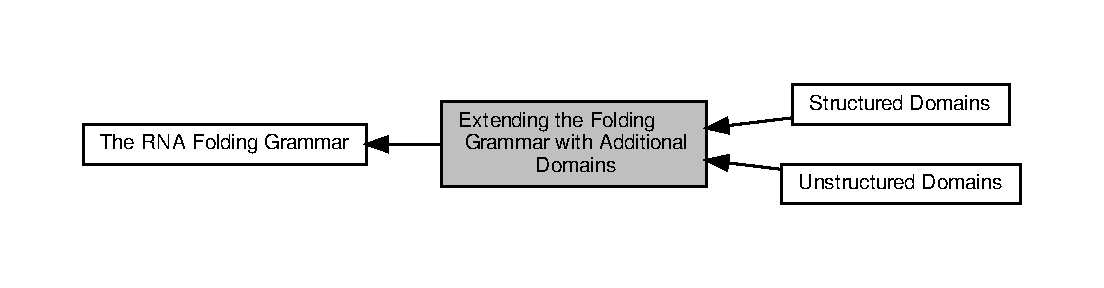
\includegraphics[width=350pt]{group__domains}
\end{center}
\end{figure}
\subsection*{Modules}
\begin{DoxyCompactItemize}
\item 
\hyperlink{group__domains__up}{Unstructured Domains}
\begin{DoxyCompactList}\small\item\em Add and modify unstructured domains to the R\+NA folding grammar. \end{DoxyCompactList}\item 
\hyperlink{group__domains__struc}{Structured Domains}
\begin{DoxyCompactList}\small\item\em Add and modify structured domains to the R\+NA folding grammar. \end{DoxyCompactList}\end{DoxyCompactItemize}

\hypertarget{group__domains__up}{}\section{Unstructured Domains}
\label{group__domains__up}\index{Unstructured Domains@{Unstructured Domains}}


Add and modify unstructured domains to the R\+NA folding grammar.  




\subsection{Detailed Description}
Add and modify unstructured domains to the R\+NA folding grammar. 

This module provides the tools to add and modify unstructured domains to the production rules of the R\+NA folding grammar. Usually this functionality is utilized for incorporating ligand binding to unpaired stretches of an R\+NA.

\begin{DoxyRefDesc}{Bug}
\item[\hyperlink{bug__bug000003}{Bug}]Although the additional production rule(s) for unstructured domains as descibed in \hyperlink{folding_grammar_sec_domains_up}{Unstructured Domains} are always treated as \textquotesingle{}segments possibly bound to one or more ligands\textquotesingle{}, the current implementation requires that at least one ligand is bound. The default implementation already takes care of the required changes, however, upon using callback functions other than the default ones, one has to take care of this fact. Please also note, that this behavior might change in one of the next releases, such that the decomposition schemes as shown above comply with the actual implementation.\end{DoxyRefDesc}


A default implementation allows one to readily use this feature by simply adding sequence motifs and corresponding binding free energies with the function \hyperlink{group__domains__up_ga55f7de5ef5b7472b0eeab9296b57f671}{vrna\+\_\+ud\+\_\+add\+\_\+motif()} (see also \hyperlink{group__ligands__up}{Ligands Binding to Unstructured Domains}).

The grammar extension is realized using a callback function that
\begin{DoxyItemize}
\item evaluates the binding free energy of a ligand to its target sequence segment (white boxes in the figures above), or
\item returns the free energy of an unpaired stretch possibly bound by a ligand, stored in the additional {\itshape U} DP matrix.
\end{DoxyItemize}

The callback is passed the segment positions, the loop context, and which of the two above mentioned evaluations are required. A second callback implements the pre-\/processing step that prepares the {\itshape U} DP matrix by evaluating all possible cases of the additional production rule. Both callbacks have a default implementation in {\itshape R\+N\+Alib}, but may be over-\/written by a user-\/implementation, making it fully user-\/customizable.

For equilibrium probability computations, two additional callbacks exist. One to store/add and one to retrieve the probability of unstructured domains at particular positions. Our implementation already takes care of computing the probabilities, but users of the unstructured domain feature are required to provide a mechanism to efficiently store/add the corresponding values into some external data structure. Collaboration diagram for Unstructured Domains\+:
\nopagebreak
\begin{figure}[H]
\begin{center}
\leavevmode
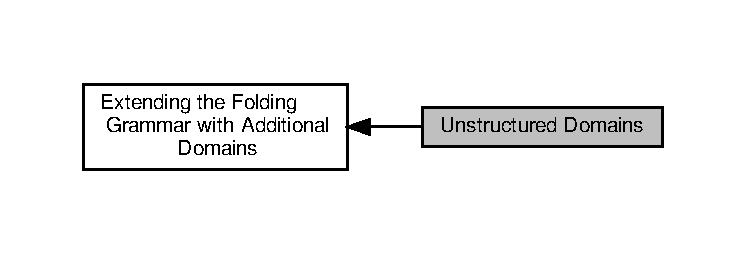
\includegraphics[width=350pt]{group__domains__up}
\end{center}
\end{figure}
\subsection*{Files}
\begin{DoxyCompactItemize}
\item 
file \hyperlink{unstructured__domains_8h}{unstructured\+\_\+domains.\+h}
\begin{DoxyCompactList}\small\item\em Functions to modify unstructured domains, e.\+g. to incorporate ligands binding to unpaired stretches. \end{DoxyCompactList}\end{DoxyCompactItemize}
\subsection*{Data Structures}
\begin{DoxyCompactItemize}
\item 
struct \hyperlink{group__domains__up_structvrna__unstructured__domain__s}{vrna\+\_\+unstructured\+\_\+domain\+\_\+s}
\begin{DoxyCompactList}\small\item\em Data structure to store all functionality for ligand binding.  \hyperlink{group__domains__up_structvrna__unstructured__domain__s}{More...}\end{DoxyCompactList}\end{DoxyCompactItemize}
\subsection*{Macros}
\begin{DoxyCompactItemize}
\item 
\mbox{\Hypertarget{group__domains__up_gaac911374e86236a51bfd42e1f098eaba}\label{group__domains__up_gaac911374e86236a51bfd42e1f098eaba}} 
\#define \hyperlink{group__domains__up_gaac911374e86236a51bfd42e1f098eaba}{V\+R\+N\+A\+\_\+\+U\+N\+S\+T\+R\+U\+C\+T\+U\+R\+E\+D\+\_\+\+D\+O\+M\+A\+I\+N\+\_\+\+E\+X\+T\+\_\+\+L\+O\+OP}~1U
\begin{DoxyCompactList}\small\item\em Flag to indicate ligand bound to unpiared stretch in the exterior loop. \end{DoxyCompactList}\item 
\mbox{\Hypertarget{group__domains__up_ga23b610ea9564346c45cc1e2bbb62adf7}\label{group__domains__up_ga23b610ea9564346c45cc1e2bbb62adf7}} 
\#define \hyperlink{group__domains__up_ga23b610ea9564346c45cc1e2bbb62adf7}{V\+R\+N\+A\+\_\+\+U\+N\+S\+T\+R\+U\+C\+T\+U\+R\+E\+D\+\_\+\+D\+O\+M\+A\+I\+N\+\_\+\+H\+P\+\_\+\+L\+O\+OP}~2U
\begin{DoxyCompactList}\small\item\em Flag to indicate ligand bound to unpaired stretch in a hairpin loop. \end{DoxyCompactList}\item 
\mbox{\Hypertarget{group__domains__up_gac4a0feccd9654c149203200248c2716b}\label{group__domains__up_gac4a0feccd9654c149203200248c2716b}} 
\#define \hyperlink{group__domains__up_gac4a0feccd9654c149203200248c2716b}{V\+R\+N\+A\+\_\+\+U\+N\+S\+T\+R\+U\+C\+T\+U\+R\+E\+D\+\_\+\+D\+O\+M\+A\+I\+N\+\_\+\+I\+N\+T\+\_\+\+L\+O\+OP}~4U
\begin{DoxyCompactList}\small\item\em Flag to indicate ligand bound to unpiared stretch in an interior loop. \end{DoxyCompactList}\item 
\mbox{\Hypertarget{group__domains__up_ga67b80796655e5227a4ed662bfbe398b0}\label{group__domains__up_ga67b80796655e5227a4ed662bfbe398b0}} 
\#define \hyperlink{group__domains__up_ga67b80796655e5227a4ed662bfbe398b0}{V\+R\+N\+A\+\_\+\+U\+N\+S\+T\+R\+U\+C\+T\+U\+R\+E\+D\+\_\+\+D\+O\+M\+A\+I\+N\+\_\+\+M\+B\+\_\+\+L\+O\+OP}~8U
\begin{DoxyCompactList}\small\item\em Flag to indicate ligand bound to unpiared stretch in a multibranch loop. \end{DoxyCompactList}\item 
\mbox{\Hypertarget{group__domains__up_gaab12b58d59be76446a9f76fad2fe624c}\label{group__domains__up_gaab12b58d59be76446a9f76fad2fe624c}} 
\#define \hyperlink{group__domains__up_gaab12b58d59be76446a9f76fad2fe624c}{V\+R\+N\+A\+\_\+\+U\+N\+S\+T\+R\+U\+C\+T\+U\+R\+E\+D\+\_\+\+D\+O\+M\+A\+I\+N\+\_\+\+M\+O\+T\+IF}~16U
\begin{DoxyCompactList}\small\item\em Flag to indicate ligand binding without additional unbound nucleotides (motif-\/only) \end{DoxyCompactList}\item 
\mbox{\Hypertarget{group__domains__up_ga3c6be4cce70f1af9e885788856101699}\label{group__domains__up_ga3c6be4cce70f1af9e885788856101699}} 
\#define \hyperlink{group__domains__up_ga3c6be4cce70f1af9e885788856101699}{V\+R\+N\+A\+\_\+\+U\+N\+S\+T\+R\+U\+C\+T\+U\+R\+E\+D\+\_\+\+D\+O\+M\+A\+I\+N\+\_\+\+A\+L\+L\+\_\+\+L\+O\+O\+PS}
\begin{DoxyCompactList}\small\item\em Flag to indicate ligand bound to unpiared stretch in any loop (convenience macro) \end{DoxyCompactList}\end{DoxyCompactItemize}
\subsection*{Typedefs}
\begin{DoxyCompactItemize}
\item 
\mbox{\Hypertarget{group__domains__up_ga0009117b14d29143e8b18ab891f48c2d}\label{group__domains__up_ga0009117b14d29143e8b18ab891f48c2d}} 
typedef struct \hyperlink{group__domains__up_structvrna__unstructured__domain__s}{vrna\+\_\+unstructured\+\_\+domain\+\_\+s} \hyperlink{group__domains__up_ga0009117b14d29143e8b18ab891f48c2d}{vrna\+\_\+ud\+\_\+t}
\begin{DoxyCompactList}\small\item\em Typename for the ligand binding extension data structure \hyperlink{group__domains__up_structvrna__unstructured__domain__s}{vrna\+\_\+unstructured\+\_\+domain\+\_\+s}. \end{DoxyCompactList}\item 
typedef int() \hyperlink{group__domains__up_ga75825c57d0bfde4ae4f95c044260c5c3}{vrna\+\_\+callback\+\_\+ud\+\_\+energy}(\hyperlink{group__fold__compound_ga1b0cef17fd40466cef5968eaeeff6166}{vrna\+\_\+fold\+\_\+compound\+\_\+t} $\ast$vc, int i, int j, unsigned int loop\+\_\+type, void $\ast$data)
\begin{DoxyCompactList}\small\item\em Callback to retrieve binding free energy of a ligand bound to an unpaired sequence segment. \end{DoxyCompactList}\item 
typedef \hyperlink{group__data__structures_ga31125aeace516926bf7f251f759b6126}{F\+L\+T\+\_\+\+O\+R\+\_\+\+D\+BL}() \hyperlink{group__domains__up_ga861706f257ba993753464b823e65b86e}{vrna\+\_\+callback\+\_\+ud\+\_\+exp\+\_\+energy}(\hyperlink{group__fold__compound_ga1b0cef17fd40466cef5968eaeeff6166}{vrna\+\_\+fold\+\_\+compound\+\_\+t} $\ast$vc, int i, int j, unsigned int loop\+\_\+type, void $\ast$data)
\begin{DoxyCompactList}\small\item\em Callback to retrieve Boltzmann factor of the binding free energy of a ligand bound to an unpaired sequence segment. \end{DoxyCompactList}\item 
typedef void() \hyperlink{group__domains__up_ga4fdfc02c1b660c07f2d887772f02a0a1}{vrna\+\_\+callback\+\_\+ud\+\_\+production}(\hyperlink{group__fold__compound_ga1b0cef17fd40466cef5968eaeeff6166}{vrna\+\_\+fold\+\_\+compound\+\_\+t} $\ast$vc, void $\ast$data)
\begin{DoxyCompactList}\small\item\em Callback for pre-\/processing the production rule of the ligand binding to unpaired stretches feature. \end{DoxyCompactList}\item 
typedef void() \hyperlink{group__domains__up_ga33d78327dcd04c1ca5ab2887edc18c7b}{vrna\+\_\+callback\+\_\+ud\+\_\+exp\+\_\+production}(\hyperlink{group__fold__compound_ga1b0cef17fd40466cef5968eaeeff6166}{vrna\+\_\+fold\+\_\+compound\+\_\+t} $\ast$vc, void $\ast$data)
\begin{DoxyCompactList}\small\item\em Callback for pre-\/processing the production rule of the ligand binding to unpaired stretches feature (partition function variant) \end{DoxyCompactList}\item 
typedef void() \hyperlink{group__domains__up_gab10498abc84fcaf336aca8f8d7d42eb2}{vrna\+\_\+callback\+\_\+ud\+\_\+probs\+\_\+add}(\hyperlink{group__fold__compound_ga1b0cef17fd40466cef5968eaeeff6166}{vrna\+\_\+fold\+\_\+compound\+\_\+t} $\ast$vc, int i, int j, unsigned int loop\+\_\+type, \hyperlink{group__data__structures_ga31125aeace516926bf7f251f759b6126}{F\+L\+T\+\_\+\+O\+R\+\_\+\+D\+BL} exp\+\_\+energy, void $\ast$data)
\begin{DoxyCompactList}\small\item\em Callback to store/add equilibrium probability for a ligand bound to an unpaired sequence segment. \end{DoxyCompactList}\item 
typedef \hyperlink{group__data__structures_ga31125aeace516926bf7f251f759b6126}{F\+L\+T\+\_\+\+O\+R\+\_\+\+D\+BL}() \hyperlink{group__domains__up_gaa10ba1b6f1e179ea84c5caca9cdaae67}{vrna\+\_\+callback\+\_\+ud\+\_\+probs\+\_\+get}(\hyperlink{group__fold__compound_ga1b0cef17fd40466cef5968eaeeff6166}{vrna\+\_\+fold\+\_\+compound\+\_\+t} $\ast$vc, int i, int j, unsigned int loop\+\_\+type, int motif, void $\ast$data)
\begin{DoxyCompactList}\small\item\em Callback to retrieve equilibrium probability for a ligand bound to an unpaired sequence segment. \end{DoxyCompactList}\end{DoxyCompactItemize}
\subsection*{Functions}
\begin{DoxyCompactItemize}
\item 
\hyperlink{structvrna__unstructured__domain__motif__s}{vrna\+\_\+ud\+\_\+motif\+\_\+t} $\ast$ \hyperlink{group__domains__up_ga2039caedf194c5edec794866986d95ec}{vrna\+\_\+ud\+\_\+motifs\+\_\+centroid} (\hyperlink{group__fold__compound_ga1b0cef17fd40466cef5968eaeeff6166}{vrna\+\_\+fold\+\_\+compound\+\_\+t} $\ast$fc, const char $\ast$structure)
\begin{DoxyCompactList}\small\item\em Detect unstructured domains in centroid structure. \end{DoxyCompactList}\item 
\hyperlink{structvrna__unstructured__domain__motif__s}{vrna\+\_\+ud\+\_\+motif\+\_\+t} $\ast$ \hyperlink{group__domains__up_ga980126e9f350b64474b35f20fce2782c}{vrna\+\_\+ud\+\_\+motifs\+\_\+\+M\+EA} (\hyperlink{group__fold__compound_ga1b0cef17fd40466cef5968eaeeff6166}{vrna\+\_\+fold\+\_\+compound\+\_\+t} $\ast$fc, const char $\ast$structure, \hyperlink{group__struct__utils__plist_gab9ac98ab55ded9fb90043b024b915aca}{vrna\+\_\+ep\+\_\+t} $\ast$probability\+\_\+list)
\begin{DoxyCompactList}\small\item\em Detect unstructured domains in M\+EA structure. \end{DoxyCompactList}\item 
\hyperlink{structvrna__unstructured__domain__motif__s}{vrna\+\_\+ud\+\_\+motif\+\_\+t} $\ast$ \hyperlink{group__domains__up_ga464d086264dd6f45089a65acec4e8c21}{vrna\+\_\+ud\+\_\+motifs\+\_\+\+M\+FE} (\hyperlink{group__fold__compound_ga1b0cef17fd40466cef5968eaeeff6166}{vrna\+\_\+fold\+\_\+compound\+\_\+t} $\ast$fc, const char $\ast$structure)
\begin{DoxyCompactList}\small\item\em Detect unstructured domains in M\+FE structure. \end{DoxyCompactList}\item 
void \hyperlink{group__domains__up_ga55f7de5ef5b7472b0eeab9296b57f671}{vrna\+\_\+ud\+\_\+add\+\_\+motif} (\hyperlink{group__fold__compound_ga1b0cef17fd40466cef5968eaeeff6166}{vrna\+\_\+fold\+\_\+compound\+\_\+t} $\ast$vc, const char $\ast$motif, double motif\+\_\+en, const char $\ast$motif\+\_\+name, unsigned int loop\+\_\+type)
\begin{DoxyCompactList}\small\item\em Add an unstructured domain motif, e.\+g. for ligand binding. \end{DoxyCompactList}\item 
void \hyperlink{group__domains__up_gada59cb0c498b812eadd010811af3f2d4}{vrna\+\_\+ud\+\_\+remove} (\hyperlink{group__fold__compound_ga1b0cef17fd40466cef5968eaeeff6166}{vrna\+\_\+fold\+\_\+compound\+\_\+t} $\ast$vc)
\begin{DoxyCompactList}\small\item\em Remove ligand binding to unpaired stretches. \end{DoxyCompactList}\item 
void \hyperlink{group__domains__up_gac1f18c312b91d80089534a87d956e58b}{vrna\+\_\+ud\+\_\+set\+\_\+data} (\hyperlink{group__fold__compound_ga1b0cef17fd40466cef5968eaeeff6166}{vrna\+\_\+fold\+\_\+compound\+\_\+t} $\ast$vc, void $\ast$data, \hyperlink{group__fold__compound_ga7806651f51b195013839a218b3bbd5a3}{vrna\+\_\+callback\+\_\+free\+\_\+auxdata} $\ast$free\+\_\+cb)
\begin{DoxyCompactList}\small\item\em Attach an auxiliary data structure. \end{DoxyCompactList}\item 
void \hyperlink{group__domains__up_ga745a99f0bc72898d54de16f6e538828a}{vrna\+\_\+ud\+\_\+set\+\_\+prod\+\_\+rule\+\_\+cb} (\hyperlink{group__fold__compound_ga1b0cef17fd40466cef5968eaeeff6166}{vrna\+\_\+fold\+\_\+compound\+\_\+t} $\ast$vc, \hyperlink{group__domains__up_ga4fdfc02c1b660c07f2d887772f02a0a1}{vrna\+\_\+callback\+\_\+ud\+\_\+production} $\ast$pre\+\_\+cb, \hyperlink{group__domains__up_ga75825c57d0bfde4ae4f95c044260c5c3}{vrna\+\_\+callback\+\_\+ud\+\_\+energy} $\ast$e\+\_\+cb)
\begin{DoxyCompactList}\small\item\em Attach production rule callbacks for free energies computations. \end{DoxyCompactList}\item 
void \hyperlink{group__domains__up_ga2fb1db2099da26c76247e1209ad4aa09}{vrna\+\_\+ud\+\_\+set\+\_\+exp\+\_\+prod\+\_\+rule\+\_\+cb} (\hyperlink{group__fold__compound_ga1b0cef17fd40466cef5968eaeeff6166}{vrna\+\_\+fold\+\_\+compound\+\_\+t} $\ast$vc, \hyperlink{group__domains__up_ga33d78327dcd04c1ca5ab2887edc18c7b}{vrna\+\_\+callback\+\_\+ud\+\_\+exp\+\_\+production} $\ast$pre\+\_\+cb, \hyperlink{group__domains__up_ga861706f257ba993753464b823e65b86e}{vrna\+\_\+callback\+\_\+ud\+\_\+exp\+\_\+energy} $\ast$exp\+\_\+e\+\_\+cb)
\begin{DoxyCompactList}\small\item\em Attach production rule for partition function. \end{DoxyCompactList}\end{DoxyCompactItemize}


\subsection{Data Structure Documentation}
\index{vrna\+\_\+unstructured\+\_\+domain\+\_\+s@{vrna\+\_\+unstructured\+\_\+domain\+\_\+s}}\label{structvrna__unstructured__domain__s}
\Hypertarget{group__domains__up_structvrna__unstructured__domain__s}
\subsubsection{struct vrna\+\_\+unstructured\+\_\+domain\+\_\+s}
Data structure to store all functionality for ligand binding. \subsubsection*{Data Fields}
\begin{DoxyCompactItemize}
\item 
\mbox{\Hypertarget{group__domains__up_ae17005ef8043aca2fc3864804cd5def6}\label{group__domains__up_ae17005ef8043aca2fc3864804cd5def6}} 
int \hyperlink{group__domains__up_ae17005ef8043aca2fc3864804cd5def6}{uniq\+\_\+motif\+\_\+count}
\begin{DoxyCompactList}\small\item\em The unique number of motifs of different lengths. \end{DoxyCompactList}\item 
\mbox{\Hypertarget{group__domains__up_a2b484b0e19a47145db7055ada8b14159}\label{group__domains__up_a2b484b0e19a47145db7055ada8b14159}} 
unsigned int $\ast$ \hyperlink{group__domains__up_a2b484b0e19a47145db7055ada8b14159}{uniq\+\_\+motif\+\_\+size}
\begin{DoxyCompactList}\small\item\em An array storing a unique list of motif lengths. \end{DoxyCompactList}\item 
\mbox{\Hypertarget{group__domains__up_a5ad34148ea1d2e501f3e02029449546e}\label{group__domains__up_a5ad34148ea1d2e501f3e02029449546e}} 
int \hyperlink{group__domains__up_a5ad34148ea1d2e501f3e02029449546e}{motif\+\_\+count}
\begin{DoxyCompactList}\small\item\em Total number of distinguished motifs. \end{DoxyCompactList}\item 
\mbox{\Hypertarget{group__domains__up_af285436bbdea4436ad2cedec65d48c75}\label{group__domains__up_af285436bbdea4436ad2cedec65d48c75}} 
char $\ast$$\ast$ \hyperlink{group__domains__up_af285436bbdea4436ad2cedec65d48c75}{motif}
\begin{DoxyCompactList}\small\item\em Motif sequences. \end{DoxyCompactList}\item 
\mbox{\Hypertarget{group__domains__up_ad061d55ef0b51d304c8dce88ebdbbf78}\label{group__domains__up_ad061d55ef0b51d304c8dce88ebdbbf78}} 
char $\ast$$\ast$ \hyperlink{group__domains__up_ad061d55ef0b51d304c8dce88ebdbbf78}{motif\+\_\+name}
\begin{DoxyCompactList}\small\item\em Motif identifier/name. \end{DoxyCompactList}\item 
\mbox{\Hypertarget{group__domains__up_a6a9f89ab7d147eb0ffd6cf8d77d178c0}\label{group__domains__up_a6a9f89ab7d147eb0ffd6cf8d77d178c0}} 
unsigned int $\ast$ \hyperlink{group__domains__up_a6a9f89ab7d147eb0ffd6cf8d77d178c0}{motif\+\_\+size}
\begin{DoxyCompactList}\small\item\em Motif lengths. \end{DoxyCompactList}\item 
\mbox{\Hypertarget{group__domains__up_aae4f0a45419784fb7c244bce2781403d}\label{group__domains__up_aae4f0a45419784fb7c244bce2781403d}} 
double $\ast$ \hyperlink{group__domains__up_aae4f0a45419784fb7c244bce2781403d}{motif\+\_\+en}
\begin{DoxyCompactList}\small\item\em Ligand binding free energy contribution. \end{DoxyCompactList}\item 
\mbox{\Hypertarget{group__domains__up_a3f0c026cced369ff176a66b2820f2057}\label{group__domains__up_a3f0c026cced369ff176a66b2820f2057}} 
unsigned int $\ast$ \hyperlink{group__domains__up_a3f0c026cced369ff176a66b2820f2057}{motif\+\_\+type}
\begin{DoxyCompactList}\small\item\em Type of motif, i.\+e. loop type the ligand binds to. \end{DoxyCompactList}\item 
\hyperlink{group__domains__up_ga4fdfc02c1b660c07f2d887772f02a0a1}{vrna\+\_\+callback\+\_\+ud\+\_\+production} $\ast$ \hyperlink{group__domains__up_ac2656d57130ac56e85212836482cbe80}{prod\+\_\+cb}
\begin{DoxyCompactList}\small\item\em Callback to ligand binding production rule, i.\+e. create/fill DP free energy matrices. \end{DoxyCompactList}\item 
\mbox{\Hypertarget{group__domains__up_a181ae6ec67f77e68899ec6a0780f3e01}\label{group__domains__up_a181ae6ec67f77e68899ec6a0780f3e01}} 
\hyperlink{group__domains__up_ga33d78327dcd04c1ca5ab2887edc18c7b}{vrna\+\_\+callback\+\_\+ud\+\_\+exp\+\_\+production} $\ast$ \hyperlink{group__domains__up_a181ae6ec67f77e68899ec6a0780f3e01}{exp\+\_\+prod\+\_\+cb}
\begin{DoxyCompactList}\small\item\em Callback to ligand binding production rule, i.\+e. create/fill DP partition function matrices. \end{DoxyCompactList}\item 
\mbox{\Hypertarget{group__domains__up_a1efba765dd4ea893dc8bd7362761f99b}\label{group__domains__up_a1efba765dd4ea893dc8bd7362761f99b}} 
\hyperlink{group__domains__up_ga75825c57d0bfde4ae4f95c044260c5c3}{vrna\+\_\+callback\+\_\+ud\+\_\+energy} $\ast$ \hyperlink{group__domains__up_a1efba765dd4ea893dc8bd7362761f99b}{energy\+\_\+cb}
\begin{DoxyCompactList}\small\item\em Callback to evaluate free energy of ligand binding to a particular unpaired stretch. \end{DoxyCompactList}\item 
\mbox{\Hypertarget{group__domains__up_ad5aaa2530557880ae89e297f8f09aa55}\label{group__domains__up_ad5aaa2530557880ae89e297f8f09aa55}} 
\hyperlink{group__domains__up_ga861706f257ba993753464b823e65b86e}{vrna\+\_\+callback\+\_\+ud\+\_\+exp\+\_\+energy} $\ast$ \hyperlink{group__domains__up_ad5aaa2530557880ae89e297f8f09aa55}{exp\+\_\+energy\+\_\+cb}
\begin{DoxyCompactList}\small\item\em Callback to evaluate Boltzmann factor of ligand binding to a particular unpaired stretch. \end{DoxyCompactList}\item 
\mbox{\Hypertarget{group__domains__up_a8802b1b0512999a9f35202031811ce17}\label{group__domains__up_a8802b1b0512999a9f35202031811ce17}} 
void $\ast$ \hyperlink{group__domains__up_a8802b1b0512999a9f35202031811ce17}{data}
\begin{DoxyCompactList}\small\item\em Auxiliary data structure passed to energy evaluation callbacks. \end{DoxyCompactList}\item 
\mbox{\Hypertarget{group__domains__up_a21b3084846902172858bc53f113d05a4}\label{group__domains__up_a21b3084846902172858bc53f113d05a4}} 
\hyperlink{group__fold__compound_ga7806651f51b195013839a218b3bbd5a3}{vrna\+\_\+callback\+\_\+free\+\_\+auxdata} $\ast$ \hyperlink{group__domains__up_a21b3084846902172858bc53f113d05a4}{free\+\_\+data}
\begin{DoxyCompactList}\small\item\em Callback to free auxiliary data structure. \end{DoxyCompactList}\item 
\mbox{\Hypertarget{group__domains__up_a457b43dfab7f4321b5d7a84e5deea5d7}\label{group__domains__up_a457b43dfab7f4321b5d7a84e5deea5d7}} 
\hyperlink{group__domains__up_gab10498abc84fcaf336aca8f8d7d42eb2}{vrna\+\_\+callback\+\_\+ud\+\_\+probs\+\_\+add} $\ast$ \hyperlink{group__domains__up_a457b43dfab7f4321b5d7a84e5deea5d7}{probs\+\_\+add}
\begin{DoxyCompactList}\small\item\em Callback to store/add outside partition function. \end{DoxyCompactList}\item 
\mbox{\Hypertarget{group__domains__up_a0b155283bccf65c5253f31e0211ae8ff}\label{group__domains__up_a0b155283bccf65c5253f31e0211ae8ff}} 
\hyperlink{group__domains__up_gaa10ba1b6f1e179ea84c5caca9cdaae67}{vrna\+\_\+callback\+\_\+ud\+\_\+probs\+\_\+get} $\ast$ \hyperlink{group__domains__up_a0b155283bccf65c5253f31e0211ae8ff}{probs\+\_\+get}
\begin{DoxyCompactList}\small\item\em Callback to retrieve outside partition function. \end{DoxyCompactList}\end{DoxyCompactItemize}


\paragraph{Field Documentation}
\mbox{\Hypertarget{group__domains__up_ac2656d57130ac56e85212836482cbe80}\label{group__domains__up_ac2656d57130ac56e85212836482cbe80}} 
\index{vrna\+\_\+unstructured\+\_\+domain\+\_\+s@{vrna\+\_\+unstructured\+\_\+domain\+\_\+s}!prod\+\_\+cb@{prod\+\_\+cb}}
\index{prod\+\_\+cb@{prod\+\_\+cb}!vrna\+\_\+unstructured\+\_\+domain\+\_\+s@{vrna\+\_\+unstructured\+\_\+domain\+\_\+s}}
\subparagraph{\texorpdfstring{prod\+\_\+cb}{prod\_cb}}
{\footnotesize\ttfamily \hyperlink{group__domains__up_ga4fdfc02c1b660c07f2d887772f02a0a1}{vrna\+\_\+callback\+\_\+ud\+\_\+production}$\ast$ vrna\+\_\+unstructured\+\_\+domain\+\_\+s\+::prod\+\_\+cb}



Callback to ligand binding production rule, i.\+e. create/fill DP free energy matrices. 

This callback will be executed right before the actual secondary structure decompositions, and, therefore, any implementation must not interleave with the regular DP matrices. 

\subsection{Typedef Documentation}
\mbox{\Hypertarget{group__domains__up_ga75825c57d0bfde4ae4f95c044260c5c3}\label{group__domains__up_ga75825c57d0bfde4ae4f95c044260c5c3}} 
\index{Unstructured Domains@{Unstructured Domains}!vrna\+\_\+callback\+\_\+ud\+\_\+energy@{vrna\+\_\+callback\+\_\+ud\+\_\+energy}}
\index{vrna\+\_\+callback\+\_\+ud\+\_\+energy@{vrna\+\_\+callback\+\_\+ud\+\_\+energy}!Unstructured Domains@{Unstructured Domains}}
\subsubsection{\texorpdfstring{vrna\+\_\+callback\+\_\+ud\+\_\+energy}{vrna\_callback\_ud\_energy}}
{\footnotesize\ttfamily typedef int() vrna\+\_\+callback\+\_\+ud\+\_\+energy(\hyperlink{group__fold__compound_ga1b0cef17fd40466cef5968eaeeff6166}{vrna\+\_\+fold\+\_\+compound\+\_\+t} $\ast$vc, int i, int j, unsigned int loop\+\_\+type, void $\ast$data)}



{\ttfamily \#include $<$\hyperlink{unstructured__domains_8h}{Vienna\+R\+N\+A/unstructured\+\_\+domains.\+h}$>$}



Callback to retrieve binding free energy of a ligand bound to an unpaired sequence segment. 

\begin{DoxyRefDesc}{Notes on Callback Functions}
\item[\hyperlink{callbacks__callbacks000006}{Notes on Callback Functions}]This function will be called to determine the additional energy contribution of a specific unstructured domain, e.\+g. the binding free energy of some ligand. \end{DoxyRefDesc}



\begin{DoxyParams}{Parameters}
{\em vc} & The current \hyperlink{group__fold__compound_ga1b0cef17fd40466cef5968eaeeff6166}{vrna\+\_\+fold\+\_\+compound\+\_\+t} \\
\hline
{\em i} & The start of the unstructured domain (5\textquotesingle{} end) \\
\hline
{\em j} & The end of the unstructured domain (3\textquotesingle{} end) \\
\hline
{\em loop\+\_\+type} & The loop context of the unstructured domain \\
\hline
{\em data} & Auxiliary data \\
\hline
\end{DoxyParams}
\begin{DoxyReturn}{Returns}
The auxiliary energy contribution in deka-\/cal/mol 
\end{DoxyReturn}
\mbox{\Hypertarget{group__domains__up_ga861706f257ba993753464b823e65b86e}\label{group__domains__up_ga861706f257ba993753464b823e65b86e}} 
\index{Unstructured Domains@{Unstructured Domains}!vrna\+\_\+callback\+\_\+ud\+\_\+exp\+\_\+energy@{vrna\+\_\+callback\+\_\+ud\+\_\+exp\+\_\+energy}}
\index{vrna\+\_\+callback\+\_\+ud\+\_\+exp\+\_\+energy@{vrna\+\_\+callback\+\_\+ud\+\_\+exp\+\_\+energy}!Unstructured Domains@{Unstructured Domains}}
\subsubsection{\texorpdfstring{vrna\+\_\+callback\+\_\+ud\+\_\+exp\+\_\+energy}{vrna\_callback\_ud\_exp\_energy}}
{\footnotesize\ttfamily typedef \hyperlink{group__data__structures_ga31125aeace516926bf7f251f759b6126}{F\+L\+T\+\_\+\+O\+R\+\_\+\+D\+BL}() vrna\+\_\+callback\+\_\+ud\+\_\+exp\+\_\+energy(\hyperlink{group__fold__compound_ga1b0cef17fd40466cef5968eaeeff6166}{vrna\+\_\+fold\+\_\+compound\+\_\+t} $\ast$vc, int i, int j, unsigned int loop\+\_\+type, void $\ast$data)}



{\ttfamily \#include $<$\hyperlink{unstructured__domains_8h}{Vienna\+R\+N\+A/unstructured\+\_\+domains.\+h}$>$}



Callback to retrieve Boltzmann factor of the binding free energy of a ligand bound to an unpaired sequence segment. 

\begin{DoxyRefDesc}{Notes on Callback Functions}
\item[\hyperlink{callbacks__callbacks000007}{Notes on Callback Functions}]This function will be called to determine the additional energy contribution of a specific unstructured domain, e.\+g. the binding free energy of some ligand (Partition function variant, i.\+e. the Boltzmann factors instead of actual free energies). \end{DoxyRefDesc}



\begin{DoxyParams}{Parameters}
{\em vc} & The current \hyperlink{group__fold__compound_ga1b0cef17fd40466cef5968eaeeff6166}{vrna\+\_\+fold\+\_\+compound\+\_\+t} \\
\hline
{\em i} & The start of the unstructured domain (5\textquotesingle{} end) \\
\hline
{\em j} & The end of the unstructured domain (3\textquotesingle{} end) \\
\hline
{\em loop\+\_\+type} & The loop context of the unstructured domain \\
\hline
{\em data} & Auxiliary data \\
\hline
\end{DoxyParams}
\begin{DoxyReturn}{Returns}
The auxiliary energy contribution as Boltzmann factor 
\end{DoxyReturn}
\mbox{\Hypertarget{group__domains__up_ga4fdfc02c1b660c07f2d887772f02a0a1}\label{group__domains__up_ga4fdfc02c1b660c07f2d887772f02a0a1}} 
\index{Unstructured Domains@{Unstructured Domains}!vrna\+\_\+callback\+\_\+ud\+\_\+production@{vrna\+\_\+callback\+\_\+ud\+\_\+production}}
\index{vrna\+\_\+callback\+\_\+ud\+\_\+production@{vrna\+\_\+callback\+\_\+ud\+\_\+production}!Unstructured Domains@{Unstructured Domains}}
\subsubsection{\texorpdfstring{vrna\+\_\+callback\+\_\+ud\+\_\+production}{vrna\_callback\_ud\_production}}
{\footnotesize\ttfamily typedef void() vrna\+\_\+callback\+\_\+ud\+\_\+production(\hyperlink{group__fold__compound_ga1b0cef17fd40466cef5968eaeeff6166}{vrna\+\_\+fold\+\_\+compound\+\_\+t} $\ast$vc, void $\ast$data)}



{\ttfamily \#include $<$\hyperlink{unstructured__domains_8h}{Vienna\+R\+N\+A/unstructured\+\_\+domains.\+h}$>$}



Callback for pre-\/processing the production rule of the ligand binding to unpaired stretches feature. 

\begin{DoxyRefDesc}{Notes on Callback Functions}
\item[\hyperlink{callbacks__callbacks000008}{Notes on Callback Functions}]The production rule for the unstructured domain grammar extension \end{DoxyRefDesc}
\mbox{\Hypertarget{group__domains__up_ga33d78327dcd04c1ca5ab2887edc18c7b}\label{group__domains__up_ga33d78327dcd04c1ca5ab2887edc18c7b}} 
\index{Unstructured Domains@{Unstructured Domains}!vrna\+\_\+callback\+\_\+ud\+\_\+exp\+\_\+production@{vrna\+\_\+callback\+\_\+ud\+\_\+exp\+\_\+production}}
\index{vrna\+\_\+callback\+\_\+ud\+\_\+exp\+\_\+production@{vrna\+\_\+callback\+\_\+ud\+\_\+exp\+\_\+production}!Unstructured Domains@{Unstructured Domains}}
\subsubsection{\texorpdfstring{vrna\+\_\+callback\+\_\+ud\+\_\+exp\+\_\+production}{vrna\_callback\_ud\_exp\_production}}
{\footnotesize\ttfamily typedef void() vrna\+\_\+callback\+\_\+ud\+\_\+exp\+\_\+production(\hyperlink{group__fold__compound_ga1b0cef17fd40466cef5968eaeeff6166}{vrna\+\_\+fold\+\_\+compound\+\_\+t} $\ast$vc, void $\ast$data)}



{\ttfamily \#include $<$\hyperlink{unstructured__domains_8h}{Vienna\+R\+N\+A/unstructured\+\_\+domains.\+h}$>$}



Callback for pre-\/processing the production rule of the ligand binding to unpaired stretches feature (partition function variant) 

\begin{DoxyRefDesc}{Notes on Callback Functions}
\item[\hyperlink{callbacks__callbacks000009}{Notes on Callback Functions}]The production rule for the unstructured domain grammar extension (Partition function variant) \end{DoxyRefDesc}
\mbox{\Hypertarget{group__domains__up_gab10498abc84fcaf336aca8f8d7d42eb2}\label{group__domains__up_gab10498abc84fcaf336aca8f8d7d42eb2}} 
\index{Unstructured Domains@{Unstructured Domains}!vrna\+\_\+callback\+\_\+ud\+\_\+probs\+\_\+add@{vrna\+\_\+callback\+\_\+ud\+\_\+probs\+\_\+add}}
\index{vrna\+\_\+callback\+\_\+ud\+\_\+probs\+\_\+add@{vrna\+\_\+callback\+\_\+ud\+\_\+probs\+\_\+add}!Unstructured Domains@{Unstructured Domains}}
\subsubsection{\texorpdfstring{vrna\+\_\+callback\+\_\+ud\+\_\+probs\+\_\+add}{vrna\_callback\_ud\_probs\_add}}
{\footnotesize\ttfamily typedef void() vrna\+\_\+callback\+\_\+ud\+\_\+probs\+\_\+add(\hyperlink{group__fold__compound_ga1b0cef17fd40466cef5968eaeeff6166}{vrna\+\_\+fold\+\_\+compound\+\_\+t} $\ast$vc, int i, int j, unsigned int loop\+\_\+type, \hyperlink{group__data__structures_ga31125aeace516926bf7f251f759b6126}{F\+L\+T\+\_\+\+O\+R\+\_\+\+D\+BL} exp\+\_\+energy, void $\ast$data)}



{\ttfamily \#include $<$\hyperlink{unstructured__domains_8h}{Vienna\+R\+N\+A/unstructured\+\_\+domains.\+h}$>$}



Callback to store/add equilibrium probability for a ligand bound to an unpaired sequence segment. 

\begin{DoxyRefDesc}{Notes on Callback Functions}
\item[\hyperlink{callbacks__callbacks000010}{Notes on Callback Functions}]A callback function to store equilibrium probabilities for the unstructured domain feature \end{DoxyRefDesc}
\mbox{\Hypertarget{group__domains__up_gaa10ba1b6f1e179ea84c5caca9cdaae67}\label{group__domains__up_gaa10ba1b6f1e179ea84c5caca9cdaae67}} 
\index{Unstructured Domains@{Unstructured Domains}!vrna\+\_\+callback\+\_\+ud\+\_\+probs\+\_\+get@{vrna\+\_\+callback\+\_\+ud\+\_\+probs\+\_\+get}}
\index{vrna\+\_\+callback\+\_\+ud\+\_\+probs\+\_\+get@{vrna\+\_\+callback\+\_\+ud\+\_\+probs\+\_\+get}!Unstructured Domains@{Unstructured Domains}}
\subsubsection{\texorpdfstring{vrna\+\_\+callback\+\_\+ud\+\_\+probs\+\_\+get}{vrna\_callback\_ud\_probs\_get}}
{\footnotesize\ttfamily typedef \hyperlink{group__data__structures_ga31125aeace516926bf7f251f759b6126}{F\+L\+T\+\_\+\+O\+R\+\_\+\+D\+BL}() vrna\+\_\+callback\+\_\+ud\+\_\+probs\+\_\+get(\hyperlink{group__fold__compound_ga1b0cef17fd40466cef5968eaeeff6166}{vrna\+\_\+fold\+\_\+compound\+\_\+t} $\ast$vc, int i, int j, unsigned int loop\+\_\+type, int motif, void $\ast$data)}



{\ttfamily \#include $<$\hyperlink{unstructured__domains_8h}{Vienna\+R\+N\+A/unstructured\+\_\+domains.\+h}$>$}



Callback to retrieve equilibrium probability for a ligand bound to an unpaired sequence segment. 

\begin{DoxyRefDesc}{Notes on Callback Functions}
\item[\hyperlink{callbacks__callbacks000011}{Notes on Callback Functions}]A callback function to retrieve equilibrium probabilities for the unstructured domain feature \end{DoxyRefDesc}


\subsection{Function Documentation}
\mbox{\Hypertarget{group__domains__up_ga2039caedf194c5edec794866986d95ec}\label{group__domains__up_ga2039caedf194c5edec794866986d95ec}} 
\index{Unstructured Domains@{Unstructured Domains}!vrna\+\_\+ud\+\_\+motifs\+\_\+centroid@{vrna\+\_\+ud\+\_\+motifs\+\_\+centroid}}
\index{vrna\+\_\+ud\+\_\+motifs\+\_\+centroid@{vrna\+\_\+ud\+\_\+motifs\+\_\+centroid}!Unstructured Domains@{Unstructured Domains}}
\subsubsection{\texorpdfstring{vrna\+\_\+ud\+\_\+motifs\+\_\+centroid()}{vrna\_ud\_motifs\_centroid()}}
{\footnotesize\ttfamily \hyperlink{structvrna__unstructured__domain__motif__s}{vrna\+\_\+ud\+\_\+motif\+\_\+t}$\ast$ vrna\+\_\+ud\+\_\+motifs\+\_\+centroid (\begin{DoxyParamCaption}\item[{\hyperlink{group__fold__compound_ga1b0cef17fd40466cef5968eaeeff6166}{vrna\+\_\+fold\+\_\+compound\+\_\+t} $\ast$}]{fc,  }\item[{const char $\ast$}]{structure }\end{DoxyParamCaption})}



{\ttfamily \#include $<$\hyperlink{unstructured__domains_8h}{Vienna\+R\+N\+A/unstructured\+\_\+domains.\+h}$>$}



Detect unstructured domains in centroid structure. 

Given a centroid structure and a set of unstructured domains compute the list of unstructured domain motifs present in the centroid. Since we do not explicitly annotate unstructured domain motifs in dot-\/bracket strings, this function can be used to check for the presence and location of unstructured domain motifs under the assumption that the dot-\/bracket string is the centroid structure of the equiibrium ensemble.

\begin{DoxySeeAlso}{See also}
\hyperlink{group__centroid__fold_ga0e64bb67e51963dc71cbd4d30b80a018}{vrna\+\_\+centroid()}
\end{DoxySeeAlso}

\begin{DoxyParams}{Parameters}
{\em fc} & The fold\+\_\+compound data structure with pre-\/computed equilibrium probabilities and model settings \\
\hline
{\em structure} & The centroid structure in dot-\/bracket notation \\
\hline
\end{DoxyParams}
\begin{DoxyReturn}{Returns}
A list of unstructured domain motifs (possibly N\+U\+LL). The last element terminates the list with {\ttfamily start=0}, {\ttfamily number=-\/1} 
\end{DoxyReturn}
\mbox{\Hypertarget{group__domains__up_ga980126e9f350b64474b35f20fce2782c}\label{group__domains__up_ga980126e9f350b64474b35f20fce2782c}} 
\index{Unstructured Domains@{Unstructured Domains}!vrna\+\_\+ud\+\_\+motifs\+\_\+\+M\+EA@{vrna\+\_\+ud\+\_\+motifs\+\_\+\+M\+EA}}
\index{vrna\+\_\+ud\+\_\+motifs\+\_\+\+M\+EA@{vrna\+\_\+ud\+\_\+motifs\+\_\+\+M\+EA}!Unstructured Domains@{Unstructured Domains}}
\subsubsection{\texorpdfstring{vrna\+\_\+ud\+\_\+motifs\+\_\+\+M\+E\+A()}{vrna\_ud\_motifs\_MEA()}}
{\footnotesize\ttfamily \hyperlink{structvrna__unstructured__domain__motif__s}{vrna\+\_\+ud\+\_\+motif\+\_\+t}$\ast$ vrna\+\_\+ud\+\_\+motifs\+\_\+\+M\+EA (\begin{DoxyParamCaption}\item[{\hyperlink{group__fold__compound_ga1b0cef17fd40466cef5968eaeeff6166}{vrna\+\_\+fold\+\_\+compound\+\_\+t} $\ast$}]{fc,  }\item[{const char $\ast$}]{structure,  }\item[{\hyperlink{group__struct__utils__plist_gab9ac98ab55ded9fb90043b024b915aca}{vrna\+\_\+ep\+\_\+t} $\ast$}]{probability\+\_\+list }\end{DoxyParamCaption})}



{\ttfamily \#include $<$\hyperlink{unstructured__domains_8h}{Vienna\+R\+N\+A/unstructured\+\_\+domains.\+h}$>$}



Detect unstructured domains in M\+EA structure. 

Given an M\+EA structure and a set of unstructured domains compute the list of unstructured domain motifs present in the M\+EA structure. Since we do not explicitly annotate unstructured domain motifs in dot-\/bracket strings, this function can be used to check for the presence and location of unstructured domain motifs under the assumption that the dot-\/bracket string is the M\+EA structure of the equiibrium ensemble.

\begin{DoxySeeAlso}{See also}
\hyperlink{group__mea__fold_ga396ec6144c6a74fcbab4cea6b42d76c3}{M\+E\+A()}
\end{DoxySeeAlso}

\begin{DoxyParams}{Parameters}
{\em fc} & The fold\+\_\+compound data structure with pre-\/computed equilibrium probabilities and model settings \\
\hline
{\em structure} & The M\+EA structure in dot-\/bracket notation \\
\hline
{\em probability\+\_\+list} & The list of probabilities to extract the M\+EA structure from \\
\hline
\end{DoxyParams}
\begin{DoxyReturn}{Returns}
A list of unstructured domain motifs (possibly N\+U\+LL). The last element terminates the list with {\ttfamily start=0}, {\ttfamily number=-\/1} 
\end{DoxyReturn}
\mbox{\Hypertarget{group__domains__up_ga464d086264dd6f45089a65acec4e8c21}\label{group__domains__up_ga464d086264dd6f45089a65acec4e8c21}} 
\index{Unstructured Domains@{Unstructured Domains}!vrna\+\_\+ud\+\_\+motifs\+\_\+\+M\+FE@{vrna\+\_\+ud\+\_\+motifs\+\_\+\+M\+FE}}
\index{vrna\+\_\+ud\+\_\+motifs\+\_\+\+M\+FE@{vrna\+\_\+ud\+\_\+motifs\+\_\+\+M\+FE}!Unstructured Domains@{Unstructured Domains}}
\subsubsection{\texorpdfstring{vrna\+\_\+ud\+\_\+motifs\+\_\+\+M\+F\+E()}{vrna\_ud\_motifs\_MFE()}}
{\footnotesize\ttfamily \hyperlink{structvrna__unstructured__domain__motif__s}{vrna\+\_\+ud\+\_\+motif\+\_\+t}$\ast$ vrna\+\_\+ud\+\_\+motifs\+\_\+\+M\+FE (\begin{DoxyParamCaption}\item[{\hyperlink{group__fold__compound_ga1b0cef17fd40466cef5968eaeeff6166}{vrna\+\_\+fold\+\_\+compound\+\_\+t} $\ast$}]{fc,  }\item[{const char $\ast$}]{structure }\end{DoxyParamCaption})}



{\ttfamily \#include $<$\hyperlink{unstructured__domains_8h}{Vienna\+R\+N\+A/unstructured\+\_\+domains.\+h}$>$}



Detect unstructured domains in M\+FE structure. 

Given an M\+FE structure and a set of unstructured domains compute the list of unstructured domain motifs present in the M\+FE structure. Since we do not explicitly annotate unstructured domain motifs in dot-\/bracket strings, this function can be used to check for the presence and location of unstructured domain motifs under the assumption that the dot-\/bracket string is the M\+FE structure of the equiibrium ensemble.

\begin{DoxySeeAlso}{See also}
\hyperlink{group__mfe__global_gabd3b147371ccf25c577f88bbbaf159fd}{vrna\+\_\+mfe()}
\end{DoxySeeAlso}

\begin{DoxyParams}{Parameters}
{\em fc} & The fold\+\_\+compound data structure with model settings \\
\hline
{\em structure} & The M\+FE structure in dot-\/bracket notation \\
\hline
\end{DoxyParams}
\begin{DoxyReturn}{Returns}
A list of unstructured domain motifs (possibly N\+U\+LL). The last element terminates the list with {\ttfamily start=0}, {\ttfamily number=-\/1} 
\end{DoxyReturn}
\mbox{\Hypertarget{group__domains__up_ga55f7de5ef5b7472b0eeab9296b57f671}\label{group__domains__up_ga55f7de5ef5b7472b0eeab9296b57f671}} 
\index{Unstructured Domains@{Unstructured Domains}!vrna\+\_\+ud\+\_\+add\+\_\+motif@{vrna\+\_\+ud\+\_\+add\+\_\+motif}}
\index{vrna\+\_\+ud\+\_\+add\+\_\+motif@{vrna\+\_\+ud\+\_\+add\+\_\+motif}!Unstructured Domains@{Unstructured Domains}}
\subsubsection{\texorpdfstring{vrna\+\_\+ud\+\_\+add\+\_\+motif()}{vrna\_ud\_add\_motif()}}
{\footnotesize\ttfamily void vrna\+\_\+ud\+\_\+add\+\_\+motif (\begin{DoxyParamCaption}\item[{\hyperlink{group__fold__compound_ga1b0cef17fd40466cef5968eaeeff6166}{vrna\+\_\+fold\+\_\+compound\+\_\+t} $\ast$}]{vc,  }\item[{const char $\ast$}]{motif,  }\item[{double}]{motif\+\_\+en,  }\item[{const char $\ast$}]{motif\+\_\+name,  }\item[{unsigned int}]{loop\+\_\+type }\end{DoxyParamCaption})}



{\ttfamily \#include $<$\hyperlink{unstructured__domains_8h}{Vienna\+R\+N\+A/unstructured\+\_\+domains.\+h}$>$}



Add an unstructured domain motif, e.\+g. for ligand binding. 

This function adds a ligand binding motif and the associated binding free energy to the \hyperlink{group__domains__up_ga0009117b14d29143e8b18ab891f48c2d}{vrna\+\_\+ud\+\_\+t} attribute of a \hyperlink{group__fold__compound_ga1b0cef17fd40466cef5968eaeeff6166}{vrna\+\_\+fold\+\_\+compound\+\_\+t}. The motif data will then be used in subsequent secondary structure predictions. Multiple calls to this function with different motifs append all additional data to a list of ligands, which all will be evaluated. Ligand motif data can be removed from the \hyperlink{group__fold__compound_ga1b0cef17fd40466cef5968eaeeff6166}{vrna\+\_\+fold\+\_\+compound\+\_\+t} again using the \hyperlink{group__domains__up_gada59cb0c498b812eadd010811af3f2d4}{vrna\+\_\+ud\+\_\+remove()} function. The loop type parameter allows one to limit the ligand binding to particular loop type, such as the exterior loop, hairpin loops, interior loops, or multibranch loops.

\begin{DoxySeeAlso}{See also}
\hyperlink{group__domains__up_gaac911374e86236a51bfd42e1f098eaba}{V\+R\+N\+A\+\_\+\+U\+N\+S\+T\+R\+U\+C\+T\+U\+R\+E\+D\+\_\+\+D\+O\+M\+A\+I\+N\+\_\+\+E\+X\+T\+\_\+\+L\+O\+OP}, \hyperlink{group__domains__up_ga23b610ea9564346c45cc1e2bbb62adf7}{V\+R\+N\+A\+\_\+\+U\+N\+S\+T\+R\+U\+C\+T\+U\+R\+E\+D\+\_\+\+D\+O\+M\+A\+I\+N\+\_\+\+H\+P\+\_\+\+L\+O\+OP}, \hyperlink{group__domains__up_gac4a0feccd9654c149203200248c2716b}{V\+R\+N\+A\+\_\+\+U\+N\+S\+T\+R\+U\+C\+T\+U\+R\+E\+D\+\_\+\+D\+O\+M\+A\+I\+N\+\_\+\+I\+N\+T\+\_\+\+L\+O\+OP}, \hyperlink{group__domains__up_ga67b80796655e5227a4ed662bfbe398b0}{V\+R\+N\+A\+\_\+\+U\+N\+S\+T\+R\+U\+C\+T\+U\+R\+E\+D\+\_\+\+D\+O\+M\+A\+I\+N\+\_\+\+M\+B\+\_\+\+L\+O\+OP}, \hyperlink{group__domains__up_ga3c6be4cce70f1af9e885788856101699}{V\+R\+N\+A\+\_\+\+U\+N\+S\+T\+R\+U\+C\+T\+U\+R\+E\+D\+\_\+\+D\+O\+M\+A\+I\+N\+\_\+\+A\+L\+L\+\_\+\+L\+O\+O\+PS}, \hyperlink{group__domains__up_gada59cb0c498b812eadd010811af3f2d4}{vrna\+\_\+ud\+\_\+remove()}
\end{DoxySeeAlso}

\begin{DoxyParams}{Parameters}
{\em vc} & The \hyperlink{group__fold__compound_ga1b0cef17fd40466cef5968eaeeff6166}{vrna\+\_\+fold\+\_\+compound\+\_\+t} data structure the ligand motif should be bound to \\
\hline
{\em motif} & The sequence motif the ligand binds to \\
\hline
{\em motif\+\_\+en} & The binding free energy of the ligand in kcal/mol \\
\hline
{\em motif\+\_\+name} & The name/id of the motif (may be {\ttfamily N\+U\+LL}) \\
\hline
{\em loop\+\_\+type} & The loop type the ligand binds to \\
\hline
\end{DoxyParams}
\mbox{\Hypertarget{group__domains__up_gada59cb0c498b812eadd010811af3f2d4}\label{group__domains__up_gada59cb0c498b812eadd010811af3f2d4}} 
\index{Unstructured Domains@{Unstructured Domains}!vrna\+\_\+ud\+\_\+remove@{vrna\+\_\+ud\+\_\+remove}}
\index{vrna\+\_\+ud\+\_\+remove@{vrna\+\_\+ud\+\_\+remove}!Unstructured Domains@{Unstructured Domains}}
\subsubsection{\texorpdfstring{vrna\+\_\+ud\+\_\+remove()}{vrna\_ud\_remove()}}
{\footnotesize\ttfamily void vrna\+\_\+ud\+\_\+remove (\begin{DoxyParamCaption}\item[{\hyperlink{group__fold__compound_ga1b0cef17fd40466cef5968eaeeff6166}{vrna\+\_\+fold\+\_\+compound\+\_\+t} $\ast$}]{vc }\end{DoxyParamCaption})}



{\ttfamily \#include $<$\hyperlink{unstructured__domains_8h}{Vienna\+R\+N\+A/unstructured\+\_\+domains.\+h}$>$}



Remove ligand binding to unpaired stretches. 

This function removes all ligand motifs that were bound to a \hyperlink{group__fold__compound_ga1b0cef17fd40466cef5968eaeeff6166}{vrna\+\_\+fold\+\_\+compound\+\_\+t} using the \hyperlink{group__domains__up_ga55f7de5ef5b7472b0eeab9296b57f671}{vrna\+\_\+ud\+\_\+add\+\_\+motif()} function.


\begin{DoxyParams}{Parameters}
{\em vc} & The \hyperlink{group__fold__compound_ga1b0cef17fd40466cef5968eaeeff6166}{vrna\+\_\+fold\+\_\+compound\+\_\+t} data structure the ligand motif data should be removed from\\
\hline
\end{DoxyParams}
\begin{DoxyRefDesc}{S\+W\+I\+G Wrapper Notes}
\item[\hyperlink{wrappers__wrappers000075}{S\+W\+I\+G Wrapper Notes}]This function is attached as method {\bfseries ud\+\_\+remove()} to objects of type {\itshape fold\+\_\+compound} \end{DoxyRefDesc}
\mbox{\Hypertarget{group__domains__up_gac1f18c312b91d80089534a87d956e58b}\label{group__domains__up_gac1f18c312b91d80089534a87d956e58b}} 
\index{Unstructured Domains@{Unstructured Domains}!vrna\+\_\+ud\+\_\+set\+\_\+data@{vrna\+\_\+ud\+\_\+set\+\_\+data}}
\index{vrna\+\_\+ud\+\_\+set\+\_\+data@{vrna\+\_\+ud\+\_\+set\+\_\+data}!Unstructured Domains@{Unstructured Domains}}
\subsubsection{\texorpdfstring{vrna\+\_\+ud\+\_\+set\+\_\+data()}{vrna\_ud\_set\_data()}}
{\footnotesize\ttfamily void vrna\+\_\+ud\+\_\+set\+\_\+data (\begin{DoxyParamCaption}\item[{\hyperlink{group__fold__compound_ga1b0cef17fd40466cef5968eaeeff6166}{vrna\+\_\+fold\+\_\+compound\+\_\+t} $\ast$}]{vc,  }\item[{void $\ast$}]{data,  }\item[{\hyperlink{group__fold__compound_ga7806651f51b195013839a218b3bbd5a3}{vrna\+\_\+callback\+\_\+free\+\_\+auxdata} $\ast$}]{free\+\_\+cb }\end{DoxyParamCaption})}



{\ttfamily \#include $<$\hyperlink{unstructured__domains_8h}{Vienna\+R\+N\+A/unstructured\+\_\+domains.\+h}$>$}



Attach an auxiliary data structure. 

This function binds an arbitrary, auxiliary data structure for user-\/implemented ligand binding. The optional callback {\ttfamily free\+\_\+cb} will be passed the bound data structure whenever the \hyperlink{group__fold__compound_ga1b0cef17fd40466cef5968eaeeff6166}{vrna\+\_\+fold\+\_\+compound\+\_\+t} is removed from memory to avoid memory leaks.

\begin{DoxySeeAlso}{See also}
\hyperlink{group__domains__up_ga745a99f0bc72898d54de16f6e538828a}{vrna\+\_\+ud\+\_\+set\+\_\+prod\+\_\+rule\+\_\+cb()}, \hyperlink{group__domains__up_ga2fb1db2099da26c76247e1209ad4aa09}{vrna\+\_\+ud\+\_\+set\+\_\+exp\+\_\+prod\+\_\+rule\+\_\+cb()}, \hyperlink{group__domains__up_gada59cb0c498b812eadd010811af3f2d4}{vrna\+\_\+ud\+\_\+remove()}
\end{DoxySeeAlso}

\begin{DoxyParams}{Parameters}
{\em vc} & The \hyperlink{group__fold__compound_ga1b0cef17fd40466cef5968eaeeff6166}{vrna\+\_\+fold\+\_\+compound\+\_\+t} data structure the auxiliary data structure should be bound to \\
\hline
{\em data} & A pointer to the auxiliary data structure \\
\hline
{\em free\+\_\+cb} & A pointer to a callback function that free\textquotesingle{}s memory occupied by {\ttfamily data} \\
\hline
\end{DoxyParams}
\begin{DoxyRefDesc}{S\+W\+I\+G Wrapper Notes}
\item[\hyperlink{wrappers__wrappers000076}{S\+W\+I\+G Wrapper Notes}]This function is attached as method {\bfseries ud\+\_\+set\+\_\+data()} to objects of type {\itshape fold\+\_\+compound} \end{DoxyRefDesc}
\mbox{\Hypertarget{group__domains__up_ga745a99f0bc72898d54de16f6e538828a}\label{group__domains__up_ga745a99f0bc72898d54de16f6e538828a}} 
\index{Unstructured Domains@{Unstructured Domains}!vrna\+\_\+ud\+\_\+set\+\_\+prod\+\_\+rule\+\_\+cb@{vrna\+\_\+ud\+\_\+set\+\_\+prod\+\_\+rule\+\_\+cb}}
\index{vrna\+\_\+ud\+\_\+set\+\_\+prod\+\_\+rule\+\_\+cb@{vrna\+\_\+ud\+\_\+set\+\_\+prod\+\_\+rule\+\_\+cb}!Unstructured Domains@{Unstructured Domains}}
\subsubsection{\texorpdfstring{vrna\+\_\+ud\+\_\+set\+\_\+prod\+\_\+rule\+\_\+cb()}{vrna\_ud\_set\_prod\_rule\_cb()}}
{\footnotesize\ttfamily void vrna\+\_\+ud\+\_\+set\+\_\+prod\+\_\+rule\+\_\+cb (\begin{DoxyParamCaption}\item[{\hyperlink{group__fold__compound_ga1b0cef17fd40466cef5968eaeeff6166}{vrna\+\_\+fold\+\_\+compound\+\_\+t} $\ast$}]{vc,  }\item[{\hyperlink{group__domains__up_ga4fdfc02c1b660c07f2d887772f02a0a1}{vrna\+\_\+callback\+\_\+ud\+\_\+production} $\ast$}]{pre\+\_\+cb,  }\item[{\hyperlink{group__domains__up_ga75825c57d0bfde4ae4f95c044260c5c3}{vrna\+\_\+callback\+\_\+ud\+\_\+energy} $\ast$}]{e\+\_\+cb }\end{DoxyParamCaption})}



{\ttfamily \#include $<$\hyperlink{unstructured__domains_8h}{Vienna\+R\+N\+A/unstructured\+\_\+domains.\+h}$>$}



Attach production rule callbacks for free energies computations. 

Use this function to bind a user-\/implemented grammar extension for unstructured domains.

The callback {\ttfamily e\+\_\+cb} needs to evaluate the free energy contribution $f(i,j)$ of the unpaired segment $[i,j]$. It will be executed in each of the regular secondary structure production rules. Whenever the callback is passed the \hyperlink{group__domains__up_gaab12b58d59be76446a9f76fad2fe624c}{V\+R\+N\+A\+\_\+\+U\+N\+S\+T\+R\+U\+C\+T\+U\+R\+E\+D\+\_\+\+D\+O\+M\+A\+I\+N\+\_\+\+M\+O\+T\+IF} flag via its {\ttfamily loop\+\_\+type} parameter the contribution of any ligand that consecutively binds from position $i$ to $j$ (the white box) is requested. Otherwise, the callback usually performs a lookup in the precomputed {\ttfamily B} matrices. Which {\ttfamily B} matrix is addressed will be indicated by the flags \hyperlink{group__domains__up_gaac911374e86236a51bfd42e1f098eaba}{V\+R\+N\+A\+\_\+\+U\+N\+S\+T\+R\+U\+C\+T\+U\+R\+E\+D\+\_\+\+D\+O\+M\+A\+I\+N\+\_\+\+E\+X\+T\+\_\+\+L\+O\+OP}, \hyperlink{group__domains__up_ga23b610ea9564346c45cc1e2bbb62adf7}{V\+R\+N\+A\+\_\+\+U\+N\+S\+T\+R\+U\+C\+T\+U\+R\+E\+D\+\_\+\+D\+O\+M\+A\+I\+N\+\_\+\+H\+P\+\_\+\+L\+O\+OP} \hyperlink{group__domains__up_gac4a0feccd9654c149203200248c2716b}{V\+R\+N\+A\+\_\+\+U\+N\+S\+T\+R\+U\+C\+T\+U\+R\+E\+D\+\_\+\+D\+O\+M\+A\+I\+N\+\_\+\+I\+N\+T\+\_\+\+L\+O\+OP}, and \hyperlink{group__domains__up_ga67b80796655e5227a4ed662bfbe398b0}{V\+R\+N\+A\+\_\+\+U\+N\+S\+T\+R\+U\+C\+T\+U\+R\+E\+D\+\_\+\+D\+O\+M\+A\+I\+N\+\_\+\+M\+B\+\_\+\+L\+O\+OP}. As their names already imply, they specify exterior loops ({\ttfamily F} production rule), hairpin loops and interior loops ({\ttfamily C} production rule), and multibranch loops ({\ttfamily M} and {\ttfamily M1} production rule).

 
\begin{DoxyImageNoCaption}
  \mbox{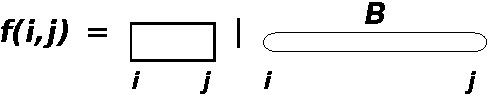
\includegraphics[width=\textwidth,height=\textheight/2,keepaspectratio=true]{ligands_up_callback}}
\end{DoxyImageNoCaption}


The {\ttfamily pre\+\_\+cb} callback will be executed as a pre-\/processing step right before the regular secondary structure rules. Usually one would use this callback to fill the dynamic programming matrices {\ttfamily U} and preparations of the auxiliary data structure \hyperlink{group__domains__up_a8802b1b0512999a9f35202031811ce17}{vrna\+\_\+unstructured\+\_\+domain\+\_\+s.\+data}

 
\begin{DoxyImageNoCaption}
  \mbox{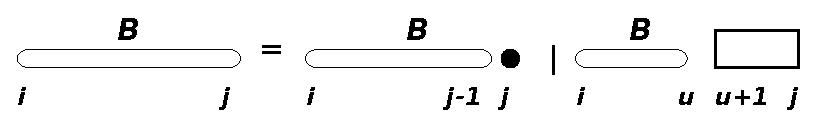
\includegraphics[width=\textwidth,height=\textheight/2,keepaspectratio=true]{B_prod_rule}}
\end{DoxyImageNoCaption}



\begin{DoxyParams}{Parameters}
{\em vc} & The \hyperlink{group__fold__compound_ga1b0cef17fd40466cef5968eaeeff6166}{vrna\+\_\+fold\+\_\+compound\+\_\+t} data structure the callback will be bound to \\
\hline
{\em pre\+\_\+cb} & A pointer to a callback function for the {\ttfamily B} production rule \\
\hline
{\em e\+\_\+cb} & A pointer to a callback function for free energy evaluation\\
\hline
\end{DoxyParams}
\begin{DoxyRefDesc}{S\+W\+I\+G Wrapper Notes}
\item[\hyperlink{wrappers__wrappers000077}{S\+W\+I\+G Wrapper Notes}]This function is attached as method {\bfseries ud\+\_\+set\+\_\+prod\+\_\+rule\+\_\+cb()} to objects of type {\itshape fold\+\_\+compound} \end{DoxyRefDesc}
\mbox{\Hypertarget{group__domains__up_ga2fb1db2099da26c76247e1209ad4aa09}\label{group__domains__up_ga2fb1db2099da26c76247e1209ad4aa09}} 
\index{Unstructured Domains@{Unstructured Domains}!vrna\+\_\+ud\+\_\+set\+\_\+exp\+\_\+prod\+\_\+rule\+\_\+cb@{vrna\+\_\+ud\+\_\+set\+\_\+exp\+\_\+prod\+\_\+rule\+\_\+cb}}
\index{vrna\+\_\+ud\+\_\+set\+\_\+exp\+\_\+prod\+\_\+rule\+\_\+cb@{vrna\+\_\+ud\+\_\+set\+\_\+exp\+\_\+prod\+\_\+rule\+\_\+cb}!Unstructured Domains@{Unstructured Domains}}
\subsubsection{\texorpdfstring{vrna\+\_\+ud\+\_\+set\+\_\+exp\+\_\+prod\+\_\+rule\+\_\+cb()}{vrna\_ud\_set\_exp\_prod\_rule\_cb()}}
{\footnotesize\ttfamily void vrna\+\_\+ud\+\_\+set\+\_\+exp\+\_\+prod\+\_\+rule\+\_\+cb (\begin{DoxyParamCaption}\item[{\hyperlink{group__fold__compound_ga1b0cef17fd40466cef5968eaeeff6166}{vrna\+\_\+fold\+\_\+compound\+\_\+t} $\ast$}]{vc,  }\item[{\hyperlink{group__domains__up_ga33d78327dcd04c1ca5ab2887edc18c7b}{vrna\+\_\+callback\+\_\+ud\+\_\+exp\+\_\+production} $\ast$}]{pre\+\_\+cb,  }\item[{\hyperlink{group__domains__up_ga861706f257ba993753464b823e65b86e}{vrna\+\_\+callback\+\_\+ud\+\_\+exp\+\_\+energy} $\ast$}]{exp\+\_\+e\+\_\+cb }\end{DoxyParamCaption})}



{\ttfamily \#include $<$\hyperlink{unstructured__domains_8h}{Vienna\+R\+N\+A/unstructured\+\_\+domains.\+h}$>$}



Attach production rule for partition function. 

This function is the partition function companion of \hyperlink{group__domains__up_ga745a99f0bc72898d54de16f6e538828a}{vrna\+\_\+ud\+\_\+set\+\_\+prod\+\_\+rule\+\_\+cb()}.

Use it to bind callbacks to (i) fill the {\ttfamily U} production rule dynamic programming matrices and/or prepare the \hyperlink{group__domains__up_a8802b1b0512999a9f35202031811ce17}{vrna\+\_\+unstructured\+\_\+domain\+\_\+s.\+data}, and (ii) provide a callback to retrieve partition functions for subsegments $ [i,j] $.

 
\begin{DoxyImageNoCaption}
  \mbox{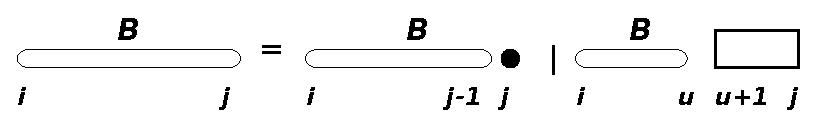
\includegraphics[width=\textwidth,height=\textheight/2,keepaspectratio=true]{B_prod_rule}}
\end{DoxyImageNoCaption}


 
\begin{DoxyImageNoCaption}
  \mbox{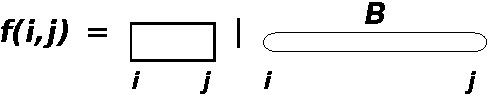
\includegraphics[width=\textwidth,height=\textheight/2,keepaspectratio=true]{ligands_up_callback}}
\end{DoxyImageNoCaption}


\begin{DoxySeeAlso}{See also}
\hyperlink{group__domains__up_ga745a99f0bc72898d54de16f6e538828a}{vrna\+\_\+ud\+\_\+set\+\_\+prod\+\_\+rule\+\_\+cb()}
\end{DoxySeeAlso}

\begin{DoxyParams}{Parameters}
{\em vc} & The \hyperlink{group__fold__compound_ga1b0cef17fd40466cef5968eaeeff6166}{vrna\+\_\+fold\+\_\+compound\+\_\+t} data structure the callback will be bound to \\
\hline
{\em pre\+\_\+cb} & A pointer to a callback function for the {\ttfamily B} production rule \\
\hline
{\em exp\+\_\+e\+\_\+cb} & A pointer to a callback function that retrieves the partition function for a segment $[i,j]$ that may be bound by one or more ligands.\\
\hline
\end{DoxyParams}
\begin{DoxyRefDesc}{S\+W\+I\+G Wrapper Notes}
\item[\hyperlink{wrappers__wrappers000078}{S\+W\+I\+G Wrapper Notes}]This function is attached as method {\bfseries ud\+\_\+set\+\_\+exp\+\_\+prod\+\_\+rule\+\_\+cb()} to objects of type {\itshape fold\+\_\+compound} \end{DoxyRefDesc}

\hypertarget{group__domains__struc}{}\section{Structured Domains}
\label{group__domains__struc}\index{Structured Domains@{Structured Domains}}


Add and modify structured domains to the R\+NA folding grammar.  




\subsection{Detailed Description}
Add and modify structured domains to the R\+NA folding grammar. 

This module provides the tools to add and modify structured domains to the production rules of the R\+NA folding grammar. Usually this functionality is utilized for incorporating self-\/enclosed structural modules that exhibit a more or less complex base pairing pattern. Collaboration diagram for Structured Domains\+:
\nopagebreak
\begin{figure}[H]
\begin{center}
\leavevmode
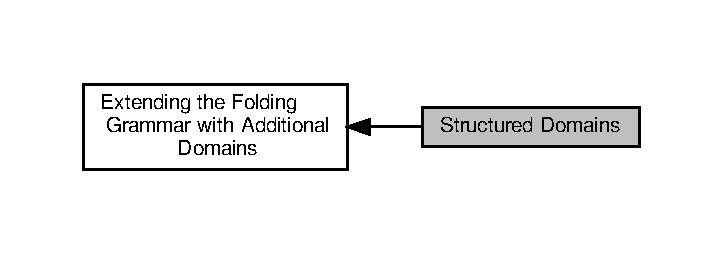
\includegraphics[width=347pt]{group__domains__struc}
\end{center}
\end{figure}
\subsection*{Files}
\begin{DoxyCompactItemize}
\item 
file \hyperlink{structured__domains_8h}{structured\+\_\+domains.\+h}
\begin{DoxyCompactList}\small\item\em This module provides interfaces that deal with additional structured domains in the folding grammar. \end{DoxyCompactList}\end{DoxyCompactItemize}

\hypertarget{group__constraints}{}\section{Constraining the R\+NA Folding Grammar}
\label{group__constraints}\index{Constraining the R\+N\+A Folding Grammar@{Constraining the R\+N\+A Folding Grammar}}


This module provides general functions that allow for an easy control of constrained secondary structure prediction and evaluation.  




\subsection{Detailed Description}
This module provides general functions that allow for an easy control of constrained secondary structure prediction and evaluation. 

Secondary Structure constraints can be subdivided into two groups\+:


\begin{DoxyItemize}
\item \hyperlink{group__hard__constraints}{Hard Constraints}, and
\item \hyperlink{group__soft__constraints}{Soft Constraints}.
\end{DoxyItemize}

While Hard-\/\+Constraints directly influence the production rules used in the folding recursions by allowing, disallowing, or enforcing certain decomposition steps, Soft-\/constraints on the other hand are used to change position specific contributions in the recursions by adding bonuses/penalties in form of pseudo free energies to certain loop configurations.

Secondary structure constraints are always applied at decomposition level, i.\+e. in each step of the recursive structure decomposition, for instance during M\+FE prediction. Below is a visualization of the decomposition scheme

 
\begin{DoxyImageNoCaption}
  \mbox{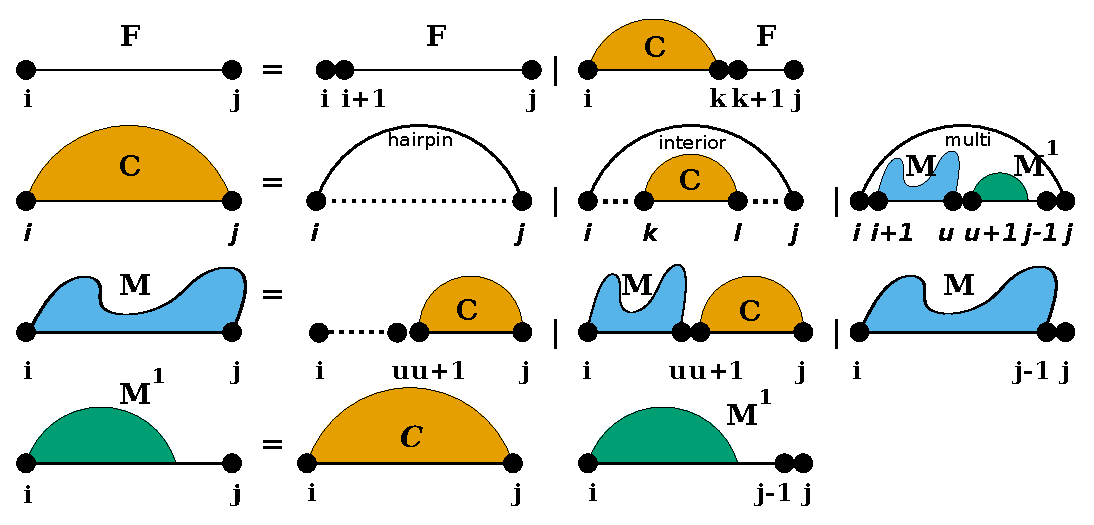
\includegraphics[width=\textwidth,height=\textheight/2,keepaspectratio=true]{recursions}}
\end{DoxyImageNoCaption}


For \hyperlink{group__hard__constraints}{Hard Constraints} the following option flags may be used to constrain the pairing behavior of single, or pairs of nucleotides\+:


\begin{DoxyItemize}
\item \hyperlink{group__hard__constraints_ga9418eda62a5dec070896702c279d2548}{V\+R\+N\+A\+\_\+\+C\+O\+N\+S\+T\+R\+A\+I\+N\+T\+\_\+\+C\+O\+N\+T\+E\+X\+T\+\_\+\+E\+X\+T\+\_\+\+L\+O\+OP} -\/ Hard constraints flag, base pair in the exterior loop.
\item \hyperlink{group__hard__constraints_ga79203702b197b6b9d3b78eed40663eb1}{V\+R\+N\+A\+\_\+\+C\+O\+N\+S\+T\+R\+A\+I\+N\+T\+\_\+\+C\+O\+N\+T\+E\+X\+T\+\_\+\+H\+P\+\_\+\+L\+O\+OP} -\/ Hard constraints flag, base pair encloses hairpin loop.
\item \hyperlink{group__hard__constraints_ga21feeab3a9e5fa5a9e3d9ac0fcf5994f}{V\+R\+N\+A\+\_\+\+C\+O\+N\+S\+T\+R\+A\+I\+N\+T\+\_\+\+C\+O\+N\+T\+E\+X\+T\+\_\+\+I\+N\+T\+\_\+\+L\+O\+OP} -\/ Hard constraints flag, base pair encloses an interior loop.
\item \hyperlink{group__hard__constraints_ga0536288e04ff6332ecdc23ca4705402b}{V\+R\+N\+A\+\_\+\+C\+O\+N\+S\+T\+R\+A\+I\+N\+T\+\_\+\+C\+O\+N\+T\+E\+X\+T\+\_\+\+I\+N\+T\+\_\+\+L\+O\+O\+P\+\_\+\+E\+NC} -\/ Hard constraints flag, base pair encloses a multi branch loop.
\item \hyperlink{group__hard__constraints_ga456ecd2ff00056bb64da8dd4f61bbfc5}{V\+R\+N\+A\+\_\+\+C\+O\+N\+S\+T\+R\+A\+I\+N\+T\+\_\+\+C\+O\+N\+T\+E\+X\+T\+\_\+\+M\+B\+\_\+\+L\+O\+OP} -\/ Hard constraints flag, base pair is enclosed in an interior loop.
\item \hyperlink{group__hard__constraints_ga02a3d703ddbcfce393e4bbfcb9db7077}{V\+R\+N\+A\+\_\+\+C\+O\+N\+S\+T\+R\+A\+I\+N\+T\+\_\+\+C\+O\+N\+T\+E\+X\+T\+\_\+\+M\+B\+\_\+\+L\+O\+O\+P\+\_\+\+E\+NC} -\/ Hard constraints flag, base pair is enclosed in a multi branch loop.
\item \hyperlink{hard_8h_a1aa55f2c6347e670e003b1a765632dad}{V\+R\+N\+A\+\_\+\+C\+O\+N\+S\+T\+R\+A\+I\+N\+T\+\_\+\+C\+O\+N\+T\+E\+X\+T\+\_\+\+E\+N\+F\+O\+R\+CE} -\/ Hard constraint flag to indicate enforcement of constraints.
\item \hyperlink{hard_8h_a9fcac36535850ff612c7e6b1305304a1}{V\+R\+N\+A\+\_\+\+C\+O\+N\+S\+T\+R\+A\+I\+N\+T\+\_\+\+C\+O\+N\+T\+E\+X\+T\+\_\+\+N\+O\+\_\+\+R\+E\+M\+O\+VE} -\/ Hard constraint flag to indicate not to remove base pairs that conflict with a given constraint.
\item \hyperlink{group__hard__constraints_ga886d9127c49bb982a4b67cd7581e8a5a}{V\+R\+N\+A\+\_\+\+C\+O\+N\+S\+T\+R\+A\+I\+N\+T\+\_\+\+C\+O\+N\+T\+E\+X\+T\+\_\+\+A\+L\+L\+\_\+\+L\+O\+O\+PS} -\/ Constraint context flag indicating any loop context.
\end{DoxyItemize}

However, for \hyperlink{group__soft__constraints}{Soft Constraints} we do not allow for simple loop type dependent constraining. But soft constraints are equipped with generic constraint support. This enables the user to pass arbitrary callback functions that return auxiliary energy contributions for evaluation the evaluation of any decomposition.

The callback will then always be notified about the type of decomposition that is happening, and the corresponding delimiting sequence positions. The following decomposition steps are distinguished, and should be captured by the user\textquotesingle{}s implementation of the callback\+:


\begin{DoxyItemize}
\item \hyperlink{group__constraints_ga8bd41ebc8039378d242e4e8c273716a5}{V\+R\+N\+A\+\_\+\+D\+E\+C\+O\+M\+P\+\_\+\+P\+A\+I\+R\+\_\+\+HP} -\/ Flag passed to generic softt constraints callback to indicate hairpin loop decomposition step.
\item \hyperlink{group__constraints_gaeab04f34d7730cff2d651d782f95d857}{V\+R\+N\+A\+\_\+\+D\+E\+C\+O\+M\+P\+\_\+\+P\+A\+I\+R\+\_\+\+IL} -\/ Indicator for interior loop decomposition step.
\item \hyperlink{group__constraints_gaa15b1185673f0b9e900c4748d45f388f}{V\+R\+N\+A\+\_\+\+D\+E\+C\+O\+M\+P\+\_\+\+P\+A\+I\+R\+\_\+\+ML} -\/ Indicator for multibranch loop decomposition step.
\item \hyperlink{group__constraints_ga735517266f2e35e1374b8f1ea77ef23e}{V\+R\+N\+A\+\_\+\+D\+E\+C\+O\+M\+P\+\_\+\+M\+L\+\_\+\+M\+L\+\_\+\+ML} -\/ Indicator for decomposition of multibranch loop part.
\item \hyperlink{group__constraints_ga4a23054c75d8efc785de50e3ea87602f}{V\+R\+N\+A\+\_\+\+D\+E\+C\+O\+M\+P\+\_\+\+M\+L\+\_\+\+S\+T\+EM} -\/ Indicator for decomposition of multibranch loop part.
\item \hyperlink{group__constraints_ga7f4cb9ff7a33e67f0539bd39e7b19a78}{V\+R\+N\+A\+\_\+\+D\+E\+C\+O\+M\+P\+\_\+\+M\+L\+\_\+\+ML} -\/ Indicator for decomposition of multibranch loop part.
\item \hyperlink{group__constraints_gae6478dda14e50e2f2cb9ef333a29256e}{V\+R\+N\+A\+\_\+\+D\+E\+C\+O\+M\+P\+\_\+\+M\+L\+\_\+\+UP} -\/ Indicator for decomposition of multibranch loop part.
\item \hyperlink{group__constraints_ga63d8ceb8c96ae3b463e529e28cc0fe98}{V\+R\+N\+A\+\_\+\+D\+E\+C\+O\+M\+P\+\_\+\+M\+L\+\_\+\+M\+L\+\_\+\+S\+T\+EM} -\/ Indicator for decomposition of multibranch loop part.
\item \hyperlink{group__constraints_ga4fe48d575830b16c208e280e01ab1497}{V\+R\+N\+A\+\_\+\+D\+E\+C\+O\+M\+P\+\_\+\+M\+L\+\_\+\+C\+O\+A\+X\+I\+AL} -\/ Indicator for decomposition of multibranch loop part.
\item \hyperlink{group__constraints_ga437adf5115c1999304eff26b41e4c9b6}{V\+R\+N\+A\+\_\+\+D\+E\+C\+O\+M\+P\+\_\+\+E\+X\+T\+\_\+\+E\+XT} -\/ Indicator for decomposition of exterior loop part.
\item \hyperlink{group__constraints_gaff1ddaffe86d984623910b40cc8a8717}{V\+R\+N\+A\+\_\+\+D\+E\+C\+O\+M\+P\+\_\+\+E\+X\+T\+\_\+\+UP} -\/ Indicator for decomposition of exterior loop part.
\item \hyperlink{group__constraints_gae44b5ace0d9b4a29088069ecb4cec441}{V\+R\+N\+A\+\_\+\+D\+E\+C\+O\+M\+P\+\_\+\+E\+X\+T\+\_\+\+S\+T\+EM} -\/ Indicator for decomposition of exterior loop part.
\item \hyperlink{group__constraints_ga803bd818b3f4b2b0a4a5cfa2f7dc2045}{V\+R\+N\+A\+\_\+\+D\+E\+C\+O\+M\+P\+\_\+\+E\+X\+T\+\_\+\+E\+X\+T\+\_\+\+E\+XT} -\/ Indicator for decomposition of exterior loop part.
\item \hyperlink{group__constraints_gabb09c5b78b75a44502fc77b950125c1e}{V\+R\+N\+A\+\_\+\+D\+E\+C\+O\+M\+P\+\_\+\+E\+X\+T\+\_\+\+S\+T\+E\+M\+\_\+\+E\+XT} -\/ Indicator for decomposition of exterior loop part.
\item \hyperlink{group__constraints_gae7554cd3ff089360c02e4920229e221c}{V\+R\+N\+A\+\_\+\+D\+E\+C\+O\+M\+P\+\_\+\+E\+X\+T\+\_\+\+S\+T\+E\+M\+\_\+\+O\+U\+T\+S\+I\+DE} -\/ Indicator for decomposition of exterior loop part.
\item \hyperlink{group__constraints_ga06efd054c9271438f6d82d4559d9e69f}{V\+R\+N\+A\+\_\+\+D\+E\+C\+O\+M\+P\+\_\+\+E\+X\+T\+\_\+\+E\+X\+T\+\_\+\+S\+T\+EM} -\/ Indicator for decomposition of exterior loop part.
\item \hyperlink{group__constraints_ga2e75d7a77118735b32f25422d9686719}{V\+R\+N\+A\+\_\+\+D\+E\+C\+O\+M\+P\+\_\+\+E\+X\+T\+\_\+\+E\+X\+T\+\_\+\+S\+T\+E\+M1} -\/ Indicator for decomposition of exterior loop part.
\end{DoxyItemize}

Simplified interfaces to the soft constraints framework can be obtained by the implementations in the submodules


\begin{DoxyItemize}
\item \hyperlink{group__SHAPE__reactivities}{S\+H\+A\+PE Reactivity Data} and
\item ligands.
\end{DoxyItemize}

An implementation that generates soft constraints for unpaired nucleotides by minimizing the discrepancy between their predicted and expected pairing probability is available in submodule \hyperlink{group__perturbation}{Generate Soft Constraints from Data}. Collaboration diagram for Constraining the R\+NA Folding Grammar\+:
\nopagebreak
\begin{figure}[H]
\begin{center}
\leavevmode
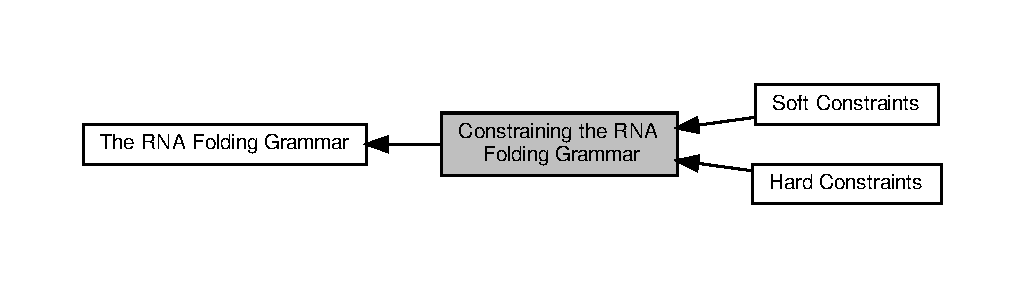
\includegraphics[width=350pt]{group__constraints}
\end{center}
\end{figure}
\subsection*{Modules}
\begin{DoxyCompactItemize}
\item 
\hyperlink{group__hard__constraints}{Hard Constraints}
\begin{DoxyCompactList}\small\item\em This module covers all functionality for hard constraints in secondary structure prediction. \end{DoxyCompactList}\item 
\hyperlink{group__soft__constraints}{Soft Constraints}
\begin{DoxyCompactList}\small\item\em Functions and data structures for secondary structure soft constraints. \end{DoxyCompactList}\end{DoxyCompactItemize}
\subsection*{Files}
\begin{DoxyCompactItemize}
\item 
file \hyperlink{constraints_2basic_8h}{basic.\+h}
\begin{DoxyCompactList}\small\item\em Functions and data structures for constraining secondary structure predictions and evaluation. \end{DoxyCompactList}\end{DoxyCompactItemize}
\subsection*{Macros}
\begin{DoxyCompactItemize}
\item 
\#define \hyperlink{group__constraints_ga62e0ed0c33002c09423de4e646f85a2b}{V\+R\+N\+A\+\_\+\+C\+O\+N\+S\+T\+R\+A\+I\+N\+T\+\_\+\+F\+I\+LE}~0
\begin{DoxyCompactList}\small\item\em Flag for \hyperlink{group__constraints_ga35a401f680969a556858a8dd5f1d07cc}{vrna\+\_\+constraints\+\_\+add()} to indicate that constraints are present in a text file. \end{DoxyCompactList}\item 
\#define \hyperlink{group__constraints_ga62aa195893d02d1a79ca94952748df36}{V\+R\+N\+A\+\_\+\+C\+O\+N\+S\+T\+R\+A\+I\+N\+T\+\_\+\+S\+O\+F\+T\+\_\+\+M\+FE}~0
\begin{DoxyCompactList}\small\item\em Indicate generation of constraints for M\+FE folding. \end{DoxyCompactList}\item 
\#define \hyperlink{group__constraints_ga03fb5000c19b9a2082bf4ea30a543045}{V\+R\+N\+A\+\_\+\+C\+O\+N\+S\+T\+R\+A\+I\+N\+T\+\_\+\+S\+O\+F\+T\+\_\+\+PF}~\hyperlink{group__fold__compound_gabfbadcddda3e74ce7f49035ef8f058f7}{V\+R\+N\+A\+\_\+\+O\+P\+T\+I\+O\+N\+\_\+\+PF}
\begin{DoxyCompactList}\small\item\em Indicate generation of constraints for partition function computation. \end{DoxyCompactList}\item 
\#define \hyperlink{group__constraints_ga8bd41ebc8039378d242e4e8c273716a5}{V\+R\+N\+A\+\_\+\+D\+E\+C\+O\+M\+P\+\_\+\+P\+A\+I\+R\+\_\+\+HP}~(unsigned char)1
\begin{DoxyCompactList}\small\item\em Flag passed to generic softt constraints callback to indicate hairpin loop decomposition step. \end{DoxyCompactList}\item 
\#define \hyperlink{group__constraints_gaeab04f34d7730cff2d651d782f95d857}{V\+R\+N\+A\+\_\+\+D\+E\+C\+O\+M\+P\+\_\+\+P\+A\+I\+R\+\_\+\+IL}~(unsigned char)2
\begin{DoxyCompactList}\small\item\em Indicator for interior loop decomposition step. \end{DoxyCompactList}\item 
\#define \hyperlink{group__constraints_gaa15b1185673f0b9e900c4748d45f388f}{V\+R\+N\+A\+\_\+\+D\+E\+C\+O\+M\+P\+\_\+\+P\+A\+I\+R\+\_\+\+ML}~(unsigned char)3
\begin{DoxyCompactList}\small\item\em Indicator for multibranch loop decomposition step. \end{DoxyCompactList}\item 
\#define \hyperlink{group__constraints_ga735517266f2e35e1374b8f1ea77ef23e}{V\+R\+N\+A\+\_\+\+D\+E\+C\+O\+M\+P\+\_\+\+M\+L\+\_\+\+M\+L\+\_\+\+ML}~(unsigned char)5
\begin{DoxyCompactList}\small\item\em Indicator for decomposition of multibranch loop part. \end{DoxyCompactList}\item 
\#define \hyperlink{group__constraints_ga4a23054c75d8efc785de50e3ea87602f}{V\+R\+N\+A\+\_\+\+D\+E\+C\+O\+M\+P\+\_\+\+M\+L\+\_\+\+S\+T\+EM}~(unsigned char)6
\begin{DoxyCompactList}\small\item\em Indicator for decomposition of multibranch loop part. \end{DoxyCompactList}\item 
\#define \hyperlink{group__constraints_ga7f4cb9ff7a33e67f0539bd39e7b19a78}{V\+R\+N\+A\+\_\+\+D\+E\+C\+O\+M\+P\+\_\+\+M\+L\+\_\+\+ML}~(unsigned char)7
\begin{DoxyCompactList}\small\item\em Indicator for decomposition of multibranch loop part. \end{DoxyCompactList}\item 
\#define \hyperlink{group__constraints_gae6478dda14e50e2f2cb9ef333a29256e}{V\+R\+N\+A\+\_\+\+D\+E\+C\+O\+M\+P\+\_\+\+M\+L\+\_\+\+UP}~(unsigned char)8
\begin{DoxyCompactList}\small\item\em Indicator for decomposition of multibranch loop part. \end{DoxyCompactList}\item 
\#define \hyperlink{group__constraints_ga63d8ceb8c96ae3b463e529e28cc0fe98}{V\+R\+N\+A\+\_\+\+D\+E\+C\+O\+M\+P\+\_\+\+M\+L\+\_\+\+M\+L\+\_\+\+S\+T\+EM}~(unsigned char)9
\begin{DoxyCompactList}\small\item\em Indicator for decomposition of multibranch loop part. \end{DoxyCompactList}\item 
\#define \hyperlink{group__constraints_ga4fe48d575830b16c208e280e01ab1497}{V\+R\+N\+A\+\_\+\+D\+E\+C\+O\+M\+P\+\_\+\+M\+L\+\_\+\+C\+O\+A\+X\+I\+AL}~(unsigned char)10
\begin{DoxyCompactList}\small\item\em Indicator for decomposition of multibranch loop part. \end{DoxyCompactList}\item 
\#define \hyperlink{group__constraints_ga0224727f7b8ad2f23eb0a3fd28d8b3fb}{V\+R\+N\+A\+\_\+\+D\+E\+C\+O\+M\+P\+\_\+\+M\+L\+\_\+\+C\+O\+A\+X\+I\+A\+L\+\_\+\+E\+NC}~(unsigned char)11
\begin{DoxyCompactList}\small\item\em Indicator for decomposition of multibranch loop part. \end{DoxyCompactList}\item 
\#define \hyperlink{group__constraints_ga437adf5115c1999304eff26b41e4c9b6}{V\+R\+N\+A\+\_\+\+D\+E\+C\+O\+M\+P\+\_\+\+E\+X\+T\+\_\+\+E\+XT}~(unsigned char)12
\begin{DoxyCompactList}\small\item\em Indicator for decomposition of exterior loop part. \end{DoxyCompactList}\item 
\#define \hyperlink{group__constraints_gaff1ddaffe86d984623910b40cc8a8717}{V\+R\+N\+A\+\_\+\+D\+E\+C\+O\+M\+P\+\_\+\+E\+X\+T\+\_\+\+UP}~(unsigned char)13
\begin{DoxyCompactList}\small\item\em Indicator for decomposition of exterior loop part. \end{DoxyCompactList}\item 
\#define \hyperlink{group__constraints_gae44b5ace0d9b4a29088069ecb4cec441}{V\+R\+N\+A\+\_\+\+D\+E\+C\+O\+M\+P\+\_\+\+E\+X\+T\+\_\+\+S\+T\+EM}~(unsigned char)14
\begin{DoxyCompactList}\small\item\em Indicator for decomposition of exterior loop part. \end{DoxyCompactList}\item 
\#define \hyperlink{group__constraints_ga803bd818b3f4b2b0a4a5cfa2f7dc2045}{V\+R\+N\+A\+\_\+\+D\+E\+C\+O\+M\+P\+\_\+\+E\+X\+T\+\_\+\+E\+X\+T\+\_\+\+E\+XT}~(unsigned char)15
\begin{DoxyCompactList}\small\item\em Indicator for decomposition of exterior loop part. \end{DoxyCompactList}\item 
\#define \hyperlink{group__constraints_gabb09c5b78b75a44502fc77b950125c1e}{V\+R\+N\+A\+\_\+\+D\+E\+C\+O\+M\+P\+\_\+\+E\+X\+T\+\_\+\+S\+T\+E\+M\+\_\+\+E\+XT}~(unsigned char)16
\begin{DoxyCompactList}\small\item\em Indicator for decomposition of exterior loop part. \end{DoxyCompactList}\item 
\mbox{\Hypertarget{group__constraints_gae7554cd3ff089360c02e4920229e221c}\label{group__constraints_gae7554cd3ff089360c02e4920229e221c}} 
\#define \hyperlink{group__constraints_gae7554cd3ff089360c02e4920229e221c}{V\+R\+N\+A\+\_\+\+D\+E\+C\+O\+M\+P\+\_\+\+E\+X\+T\+\_\+\+S\+T\+E\+M\+\_\+\+O\+U\+T\+S\+I\+DE}~(unsigned char)17
\begin{DoxyCompactList}\small\item\em Indicator for decomposition of exterior loop part. \end{DoxyCompactList}\item 
\#define \hyperlink{group__constraints_ga06efd054c9271438f6d82d4559d9e69f}{V\+R\+N\+A\+\_\+\+D\+E\+C\+O\+M\+P\+\_\+\+E\+X\+T\+\_\+\+E\+X\+T\+\_\+\+S\+T\+EM}~(unsigned char)18
\begin{DoxyCompactList}\small\item\em Indicator for decomposition of exterior loop part. \end{DoxyCompactList}\item 
\#define \hyperlink{group__constraints_ga2e75d7a77118735b32f25422d9686719}{V\+R\+N\+A\+\_\+\+D\+E\+C\+O\+M\+P\+\_\+\+E\+X\+T\+\_\+\+E\+X\+T\+\_\+\+S\+T\+E\+M1}~(unsigned char)19
\begin{DoxyCompactList}\small\item\em Indicator for decomposition of exterior loop part. \end{DoxyCompactList}\end{DoxyCompactItemize}
\subsection*{Functions}
\begin{DoxyCompactItemize}
\item 
void \hyperlink{group__constraints_ga35a401f680969a556858a8dd5f1d07cc}{vrna\+\_\+constraints\+\_\+add} (\hyperlink{group__fold__compound_ga1b0cef17fd40466cef5968eaeeff6166}{vrna\+\_\+fold\+\_\+compound\+\_\+t} $\ast$vc, const char $\ast$constraint, unsigned int options)
\begin{DoxyCompactList}\small\item\em Add constraints to a \hyperlink{group__fold__compound_ga1b0cef17fd40466cef5968eaeeff6166}{vrna\+\_\+fold\+\_\+compound\+\_\+t} data structure. \end{DoxyCompactList}\item 
void \hyperlink{group__constraints_gaa1f20b53bf09ac2e6b0dbb13f7d89670}{vrna\+\_\+message\+\_\+constraint\+\_\+options} (unsigned int option)
\begin{DoxyCompactList}\small\item\em Print a help message for pseudo dot-\/bracket structure constraint characters to stdout. (constraint support is specified by option parameter) \end{DoxyCompactList}\item 
void \hyperlink{group__constraints_gaec7e13fa0465c2acc7a621d1aecb709f}{vrna\+\_\+message\+\_\+constraint\+\_\+options\+\_\+all} (void)
\begin{DoxyCompactList}\small\item\em Print structure constraint characters to stdout (full constraint support) \end{DoxyCompactList}\end{DoxyCompactItemize}


\subsection{Macro Definition Documentation}
\mbox{\Hypertarget{group__constraints_ga62e0ed0c33002c09423de4e646f85a2b}\label{group__constraints_ga62e0ed0c33002c09423de4e646f85a2b}} 
\index{Constraining the R\+N\+A Folding Grammar@{Constraining the R\+N\+A Folding Grammar}!V\+R\+N\+A\+\_\+\+C\+O\+N\+S\+T\+R\+A\+I\+N\+T\+\_\+\+F\+I\+LE@{V\+R\+N\+A\+\_\+\+C\+O\+N\+S\+T\+R\+A\+I\+N\+T\+\_\+\+F\+I\+LE}}
\index{V\+R\+N\+A\+\_\+\+C\+O\+N\+S\+T\+R\+A\+I\+N\+T\+\_\+\+F\+I\+LE@{V\+R\+N\+A\+\_\+\+C\+O\+N\+S\+T\+R\+A\+I\+N\+T\+\_\+\+F\+I\+LE}!Constraining the R\+N\+A Folding Grammar@{Constraining the R\+N\+A Folding Grammar}}
\subsubsection{\texorpdfstring{V\+R\+N\+A\+\_\+\+C\+O\+N\+S\+T\+R\+A\+I\+N\+T\+\_\+\+F\+I\+LE}{VRNA\_CONSTRAINT\_FILE}}
{\footnotesize\ttfamily \#define V\+R\+N\+A\+\_\+\+C\+O\+N\+S\+T\+R\+A\+I\+N\+T\+\_\+\+F\+I\+LE~0}



{\ttfamily \#include $<$\hyperlink{constraints_2basic_8h}{Vienna\+R\+N\+A/constraints/basic.\+h}$>$}



Flag for \hyperlink{group__constraints_ga35a401f680969a556858a8dd5f1d07cc}{vrna\+\_\+constraints\+\_\+add()} to indicate that constraints are present in a text file. 

\begin{DoxySeeAlso}{See also}
\hyperlink{group__constraints_ga35a401f680969a556858a8dd5f1d07cc}{vrna\+\_\+constraints\+\_\+add()} 
\end{DoxySeeAlso}
\begin{DoxyRefDesc}{Deprecated}
\item[\hyperlink{deprecated__deprecated000148}{Deprecated}]Use 0 instead!\end{DoxyRefDesc}
\mbox{\Hypertarget{group__constraints_ga62aa195893d02d1a79ca94952748df36}\label{group__constraints_ga62aa195893d02d1a79ca94952748df36}} 
\index{Constraining the R\+N\+A Folding Grammar@{Constraining the R\+N\+A Folding Grammar}!V\+R\+N\+A\+\_\+\+C\+O\+N\+S\+T\+R\+A\+I\+N\+T\+\_\+\+S\+O\+F\+T\+\_\+\+M\+FE@{V\+R\+N\+A\+\_\+\+C\+O\+N\+S\+T\+R\+A\+I\+N\+T\+\_\+\+S\+O\+F\+T\+\_\+\+M\+FE}}
\index{V\+R\+N\+A\+\_\+\+C\+O\+N\+S\+T\+R\+A\+I\+N\+T\+\_\+\+S\+O\+F\+T\+\_\+\+M\+FE@{V\+R\+N\+A\+\_\+\+C\+O\+N\+S\+T\+R\+A\+I\+N\+T\+\_\+\+S\+O\+F\+T\+\_\+\+M\+FE}!Constraining the R\+N\+A Folding Grammar@{Constraining the R\+N\+A Folding Grammar}}
\subsubsection{\texorpdfstring{V\+R\+N\+A\+\_\+\+C\+O\+N\+S\+T\+R\+A\+I\+N\+T\+\_\+\+S\+O\+F\+T\+\_\+\+M\+FE}{VRNA\_CONSTRAINT\_SOFT\_MFE}}
{\footnotesize\ttfamily \#define V\+R\+N\+A\+\_\+\+C\+O\+N\+S\+T\+R\+A\+I\+N\+T\+\_\+\+S\+O\+F\+T\+\_\+\+M\+FE~0}



{\ttfamily \#include $<$\hyperlink{constraints_2basic_8h}{Vienna\+R\+N\+A/constraints/basic.\+h}$>$}



Indicate generation of constraints for M\+FE folding. 

\begin{DoxyRefDesc}{Deprecated}
\item[\hyperlink{deprecated__deprecated000149}{Deprecated}]This flag has no meaning anymore, since constraints are now always stored!\end{DoxyRefDesc}
\mbox{\Hypertarget{group__constraints_ga03fb5000c19b9a2082bf4ea30a543045}\label{group__constraints_ga03fb5000c19b9a2082bf4ea30a543045}} 
\index{Constraining the R\+N\+A Folding Grammar@{Constraining the R\+N\+A Folding Grammar}!V\+R\+N\+A\+\_\+\+C\+O\+N\+S\+T\+R\+A\+I\+N\+T\+\_\+\+S\+O\+F\+T\+\_\+\+PF@{V\+R\+N\+A\+\_\+\+C\+O\+N\+S\+T\+R\+A\+I\+N\+T\+\_\+\+S\+O\+F\+T\+\_\+\+PF}}
\index{V\+R\+N\+A\+\_\+\+C\+O\+N\+S\+T\+R\+A\+I\+N\+T\+\_\+\+S\+O\+F\+T\+\_\+\+PF@{V\+R\+N\+A\+\_\+\+C\+O\+N\+S\+T\+R\+A\+I\+N\+T\+\_\+\+S\+O\+F\+T\+\_\+\+PF}!Constraining the R\+N\+A Folding Grammar@{Constraining the R\+N\+A Folding Grammar}}
\subsubsection{\texorpdfstring{V\+R\+N\+A\+\_\+\+C\+O\+N\+S\+T\+R\+A\+I\+N\+T\+\_\+\+S\+O\+F\+T\+\_\+\+PF}{VRNA\_CONSTRAINT\_SOFT\_PF}}
{\footnotesize\ttfamily \#define V\+R\+N\+A\+\_\+\+C\+O\+N\+S\+T\+R\+A\+I\+N\+T\+\_\+\+S\+O\+F\+T\+\_\+\+PF~\hyperlink{group__fold__compound_gabfbadcddda3e74ce7f49035ef8f058f7}{V\+R\+N\+A\+\_\+\+O\+P\+T\+I\+O\+N\+\_\+\+PF}}



{\ttfamily \#include $<$\hyperlink{constraints_2basic_8h}{Vienna\+R\+N\+A/constraints/basic.\+h}$>$}



Indicate generation of constraints for partition function computation. 

\begin{DoxyRefDesc}{Deprecated}
\item[\hyperlink{deprecated__deprecated000150}{Deprecated}]Use \hyperlink{group__fold__compound_gabfbadcddda3e74ce7f49035ef8f058f7}{V\+R\+N\+A\+\_\+\+O\+P\+T\+I\+O\+N\+\_\+\+PF} instead!\end{DoxyRefDesc}
\mbox{\Hypertarget{group__constraints_ga8bd41ebc8039378d242e4e8c273716a5}\label{group__constraints_ga8bd41ebc8039378d242e4e8c273716a5}} 
\index{Constraining the R\+N\+A Folding Grammar@{Constraining the R\+N\+A Folding Grammar}!V\+R\+N\+A\+\_\+\+D\+E\+C\+O\+M\+P\+\_\+\+P\+A\+I\+R\+\_\+\+HP@{V\+R\+N\+A\+\_\+\+D\+E\+C\+O\+M\+P\+\_\+\+P\+A\+I\+R\+\_\+\+HP}}
\index{V\+R\+N\+A\+\_\+\+D\+E\+C\+O\+M\+P\+\_\+\+P\+A\+I\+R\+\_\+\+HP@{V\+R\+N\+A\+\_\+\+D\+E\+C\+O\+M\+P\+\_\+\+P\+A\+I\+R\+\_\+\+HP}!Constraining the R\+N\+A Folding Grammar@{Constraining the R\+N\+A Folding Grammar}}
\subsubsection{\texorpdfstring{V\+R\+N\+A\+\_\+\+D\+E\+C\+O\+M\+P\+\_\+\+P\+A\+I\+R\+\_\+\+HP}{VRNA\_DECOMP\_PAIR\_HP}}
{\footnotesize\ttfamily \#define V\+R\+N\+A\+\_\+\+D\+E\+C\+O\+M\+P\+\_\+\+P\+A\+I\+R\+\_\+\+HP~(unsigned char)1}



{\ttfamily \#include $<$\hyperlink{constraints_2basic_8h}{Vienna\+R\+N\+A/constraints/basic.\+h}$>$}



Flag passed to generic softt constraints callback to indicate hairpin loop decomposition step. 

This flag notifies the soft or hard constraint callback function that the current decomposition step evaluates a hairpin loop enclosed by the base pair $(i,j)$.

 
\begin{DoxyImageNoCaption}
  \mbox{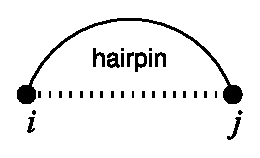
\includegraphics[width=\textwidth,height=\textheight/2,keepaspectratio=true]{decomp_hp}}
\end{DoxyImageNoCaption}
 \mbox{\Hypertarget{group__constraints_gaeab04f34d7730cff2d651d782f95d857}\label{group__constraints_gaeab04f34d7730cff2d651d782f95d857}} 
\index{Constraining the R\+N\+A Folding Grammar@{Constraining the R\+N\+A Folding Grammar}!V\+R\+N\+A\+\_\+\+D\+E\+C\+O\+M\+P\+\_\+\+P\+A\+I\+R\+\_\+\+IL@{V\+R\+N\+A\+\_\+\+D\+E\+C\+O\+M\+P\+\_\+\+P\+A\+I\+R\+\_\+\+IL}}
\index{V\+R\+N\+A\+\_\+\+D\+E\+C\+O\+M\+P\+\_\+\+P\+A\+I\+R\+\_\+\+IL@{V\+R\+N\+A\+\_\+\+D\+E\+C\+O\+M\+P\+\_\+\+P\+A\+I\+R\+\_\+\+IL}!Constraining the R\+N\+A Folding Grammar@{Constraining the R\+N\+A Folding Grammar}}
\subsubsection{\texorpdfstring{V\+R\+N\+A\+\_\+\+D\+E\+C\+O\+M\+P\+\_\+\+P\+A\+I\+R\+\_\+\+IL}{VRNA\_DECOMP\_PAIR\_IL}}
{\footnotesize\ttfamily \#define V\+R\+N\+A\+\_\+\+D\+E\+C\+O\+M\+P\+\_\+\+P\+A\+I\+R\+\_\+\+IL~(unsigned char)2}



{\ttfamily \#include $<$\hyperlink{constraints_2basic_8h}{Vienna\+R\+N\+A/constraints/basic.\+h}$>$}



Indicator for interior loop decomposition step. 

This flag notifies the soft or hard constraint callback function that the current decomposition step evaluates an interior loop enclosed by the base pair $(i,j)$, and enclosing the base pair $(k,l)$.

 
\begin{DoxyImageNoCaption}
  \mbox{
\includegraphics[width=\textwidth,height=\textheight/2,keepaspectratio=true]{decomp_il}}
\end{DoxyImageNoCaption}
 \mbox{\Hypertarget{group__constraints_gaa15b1185673f0b9e900c4748d45f388f}\label{group__constraints_gaa15b1185673f0b9e900c4748d45f388f}} 
\index{Constraining the R\+N\+A Folding Grammar@{Constraining the R\+N\+A Folding Grammar}!V\+R\+N\+A\+\_\+\+D\+E\+C\+O\+M\+P\+\_\+\+P\+A\+I\+R\+\_\+\+ML@{V\+R\+N\+A\+\_\+\+D\+E\+C\+O\+M\+P\+\_\+\+P\+A\+I\+R\+\_\+\+ML}}
\index{V\+R\+N\+A\+\_\+\+D\+E\+C\+O\+M\+P\+\_\+\+P\+A\+I\+R\+\_\+\+ML@{V\+R\+N\+A\+\_\+\+D\+E\+C\+O\+M\+P\+\_\+\+P\+A\+I\+R\+\_\+\+ML}!Constraining the R\+N\+A Folding Grammar@{Constraining the R\+N\+A Folding Grammar}}
\subsubsection{\texorpdfstring{V\+R\+N\+A\+\_\+\+D\+E\+C\+O\+M\+P\+\_\+\+P\+A\+I\+R\+\_\+\+ML}{VRNA\_DECOMP\_PAIR\_ML}}
{\footnotesize\ttfamily \#define V\+R\+N\+A\+\_\+\+D\+E\+C\+O\+M\+P\+\_\+\+P\+A\+I\+R\+\_\+\+ML~(unsigned char)3}



{\ttfamily \#include $<$\hyperlink{constraints_2basic_8h}{Vienna\+R\+N\+A/constraints/basic.\+h}$>$}



Indicator for multibranch loop decomposition step. 

This flag notifies the soft or hard constraint callback function that the current decomposition step evaluates a multibranch loop enclosed by the base pair $(i,j)$, and consisting of some enclosed multi loop content from k to l.

 
\begin{DoxyImageNoCaption}
  \mbox{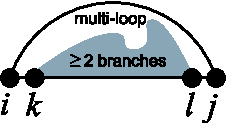
\includegraphics[width=\textwidth,height=\textheight/2,keepaspectratio=true]{decomp_ml}}
\end{DoxyImageNoCaption}
 \mbox{\Hypertarget{group__constraints_ga735517266f2e35e1374b8f1ea77ef23e}\label{group__constraints_ga735517266f2e35e1374b8f1ea77ef23e}} 
\index{Constraining the R\+N\+A Folding Grammar@{Constraining the R\+N\+A Folding Grammar}!V\+R\+N\+A\+\_\+\+D\+E\+C\+O\+M\+P\+\_\+\+M\+L\+\_\+\+M\+L\+\_\+\+ML@{V\+R\+N\+A\+\_\+\+D\+E\+C\+O\+M\+P\+\_\+\+M\+L\+\_\+\+M\+L\+\_\+\+ML}}
\index{V\+R\+N\+A\+\_\+\+D\+E\+C\+O\+M\+P\+\_\+\+M\+L\+\_\+\+M\+L\+\_\+\+ML@{V\+R\+N\+A\+\_\+\+D\+E\+C\+O\+M\+P\+\_\+\+M\+L\+\_\+\+M\+L\+\_\+\+ML}!Constraining the R\+N\+A Folding Grammar@{Constraining the R\+N\+A Folding Grammar}}
\subsubsection{\texorpdfstring{V\+R\+N\+A\+\_\+\+D\+E\+C\+O\+M\+P\+\_\+\+M\+L\+\_\+\+M\+L\+\_\+\+ML}{VRNA\_DECOMP\_ML\_ML\_ML}}
{\footnotesize\ttfamily \#define V\+R\+N\+A\+\_\+\+D\+E\+C\+O\+M\+P\+\_\+\+M\+L\+\_\+\+M\+L\+\_\+\+ML~(unsigned char)5}



{\ttfamily \#include $<$\hyperlink{constraints_2basic_8h}{Vienna\+R\+N\+A/constraints/basic.\+h}$>$}



Indicator for decomposition of multibranch loop part. 

This flag notifies the soft or hard constraint callback function that the current decomposition step evaluates a multibranch loop part in the interval $[i:j]$, which will be decomposed into two multibranch loop parts $[i:k]$, and $[l:j]$.

 
\begin{DoxyImageNoCaption}
  \mbox{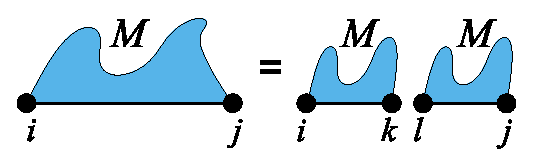
\includegraphics[width=\textwidth,height=\textheight/2,keepaspectratio=true]{decomp_ml_ml_ml}}
\end{DoxyImageNoCaption}
 \mbox{\Hypertarget{group__constraints_ga4a23054c75d8efc785de50e3ea87602f}\label{group__constraints_ga4a23054c75d8efc785de50e3ea87602f}} 
\index{Constraining the R\+N\+A Folding Grammar@{Constraining the R\+N\+A Folding Grammar}!V\+R\+N\+A\+\_\+\+D\+E\+C\+O\+M\+P\+\_\+\+M\+L\+\_\+\+S\+T\+EM@{V\+R\+N\+A\+\_\+\+D\+E\+C\+O\+M\+P\+\_\+\+M\+L\+\_\+\+S\+T\+EM}}
\index{V\+R\+N\+A\+\_\+\+D\+E\+C\+O\+M\+P\+\_\+\+M\+L\+\_\+\+S\+T\+EM@{V\+R\+N\+A\+\_\+\+D\+E\+C\+O\+M\+P\+\_\+\+M\+L\+\_\+\+S\+T\+EM}!Constraining the R\+N\+A Folding Grammar@{Constraining the R\+N\+A Folding Grammar}}
\subsubsection{\texorpdfstring{V\+R\+N\+A\+\_\+\+D\+E\+C\+O\+M\+P\+\_\+\+M\+L\+\_\+\+S\+T\+EM}{VRNA\_DECOMP\_ML\_STEM}}
{\footnotesize\ttfamily \#define V\+R\+N\+A\+\_\+\+D\+E\+C\+O\+M\+P\+\_\+\+M\+L\+\_\+\+S\+T\+EM~(unsigned char)6}



{\ttfamily \#include $<$\hyperlink{constraints_2basic_8h}{Vienna\+R\+N\+A/constraints/basic.\+h}$>$}



Indicator for decomposition of multibranch loop part. 

This flag notifies the soft or hard constraint callback function that the current decomposition step evaluates a multibranch loop part in the interval $[i:j]$, which will be considered a single stem branching off with base pair $(k,l)$.

 
\begin{DoxyImageNoCaption}
  \mbox{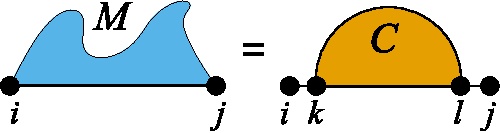
\includegraphics[width=\textwidth,height=\textheight/2,keepaspectratio=true]{decomp_ml_stem}}
\end{DoxyImageNoCaption}
 \mbox{\Hypertarget{group__constraints_ga7f4cb9ff7a33e67f0539bd39e7b19a78}\label{group__constraints_ga7f4cb9ff7a33e67f0539bd39e7b19a78}} 
\index{Constraining the R\+N\+A Folding Grammar@{Constraining the R\+N\+A Folding Grammar}!V\+R\+N\+A\+\_\+\+D\+E\+C\+O\+M\+P\+\_\+\+M\+L\+\_\+\+ML@{V\+R\+N\+A\+\_\+\+D\+E\+C\+O\+M\+P\+\_\+\+M\+L\+\_\+\+ML}}
\index{V\+R\+N\+A\+\_\+\+D\+E\+C\+O\+M\+P\+\_\+\+M\+L\+\_\+\+ML@{V\+R\+N\+A\+\_\+\+D\+E\+C\+O\+M\+P\+\_\+\+M\+L\+\_\+\+ML}!Constraining the R\+N\+A Folding Grammar@{Constraining the R\+N\+A Folding Grammar}}
\subsubsection{\texorpdfstring{V\+R\+N\+A\+\_\+\+D\+E\+C\+O\+M\+P\+\_\+\+M\+L\+\_\+\+ML}{VRNA\_DECOMP\_ML\_ML}}
{\footnotesize\ttfamily \#define V\+R\+N\+A\+\_\+\+D\+E\+C\+O\+M\+P\+\_\+\+M\+L\+\_\+\+ML~(unsigned char)7}



{\ttfamily \#include $<$\hyperlink{constraints_2basic_8h}{Vienna\+R\+N\+A/constraints/basic.\+h}$>$}



Indicator for decomposition of multibranch loop part. 

This flag notifies the soft or hard constraint callback function that the current decomposition step evaluates a multibranch loop part in the interval $[i:j]$, which will be decomposed into a (usually) smaller multibranch loop part $[k:l]$.

 
\begin{DoxyImageNoCaption}
  \mbox{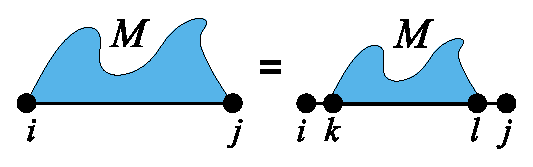
\includegraphics[width=\textwidth,height=\textheight/2,keepaspectratio=true]{decomp_ml_ml}}
\end{DoxyImageNoCaption}
 \mbox{\Hypertarget{group__constraints_gae6478dda14e50e2f2cb9ef333a29256e}\label{group__constraints_gae6478dda14e50e2f2cb9ef333a29256e}} 
\index{Constraining the R\+N\+A Folding Grammar@{Constraining the R\+N\+A Folding Grammar}!V\+R\+N\+A\+\_\+\+D\+E\+C\+O\+M\+P\+\_\+\+M\+L\+\_\+\+UP@{V\+R\+N\+A\+\_\+\+D\+E\+C\+O\+M\+P\+\_\+\+M\+L\+\_\+\+UP}}
\index{V\+R\+N\+A\+\_\+\+D\+E\+C\+O\+M\+P\+\_\+\+M\+L\+\_\+\+UP@{V\+R\+N\+A\+\_\+\+D\+E\+C\+O\+M\+P\+\_\+\+M\+L\+\_\+\+UP}!Constraining the R\+N\+A Folding Grammar@{Constraining the R\+N\+A Folding Grammar}}
\subsubsection{\texorpdfstring{V\+R\+N\+A\+\_\+\+D\+E\+C\+O\+M\+P\+\_\+\+M\+L\+\_\+\+UP}{VRNA\_DECOMP\_ML\_UP}}
{\footnotesize\ttfamily \#define V\+R\+N\+A\+\_\+\+D\+E\+C\+O\+M\+P\+\_\+\+M\+L\+\_\+\+UP~(unsigned char)8}



{\ttfamily \#include $<$\hyperlink{constraints_2basic_8h}{Vienna\+R\+N\+A/constraints/basic.\+h}$>$}



Indicator for decomposition of multibranch loop part. 

This flag notifies the soft or hard constraint callback function that the current decomposition step evaluates a multibranch loop part in the interval $[i:j]$, which will be considered a multibranch loop part that only consists of unpaired nucleotides.

 
\begin{DoxyImageNoCaption}
  \mbox{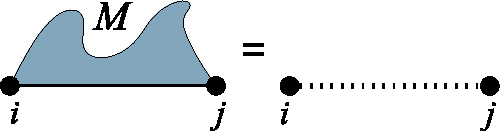
\includegraphics[width=\textwidth,height=\textheight/2,keepaspectratio=true]{decomp_ml_up}}
\end{DoxyImageNoCaption}
 \mbox{\Hypertarget{group__constraints_ga63d8ceb8c96ae3b463e529e28cc0fe98}\label{group__constraints_ga63d8ceb8c96ae3b463e529e28cc0fe98}} 
\index{Constraining the R\+N\+A Folding Grammar@{Constraining the R\+N\+A Folding Grammar}!V\+R\+N\+A\+\_\+\+D\+E\+C\+O\+M\+P\+\_\+\+M\+L\+\_\+\+M\+L\+\_\+\+S\+T\+EM@{V\+R\+N\+A\+\_\+\+D\+E\+C\+O\+M\+P\+\_\+\+M\+L\+\_\+\+M\+L\+\_\+\+S\+T\+EM}}
\index{V\+R\+N\+A\+\_\+\+D\+E\+C\+O\+M\+P\+\_\+\+M\+L\+\_\+\+M\+L\+\_\+\+S\+T\+EM@{V\+R\+N\+A\+\_\+\+D\+E\+C\+O\+M\+P\+\_\+\+M\+L\+\_\+\+M\+L\+\_\+\+S\+T\+EM}!Constraining the R\+N\+A Folding Grammar@{Constraining the R\+N\+A Folding Grammar}}
\subsubsection{\texorpdfstring{V\+R\+N\+A\+\_\+\+D\+E\+C\+O\+M\+P\+\_\+\+M\+L\+\_\+\+M\+L\+\_\+\+S\+T\+EM}{VRNA\_DECOMP\_ML\_ML\_STEM}}
{\footnotesize\ttfamily \#define V\+R\+N\+A\+\_\+\+D\+E\+C\+O\+M\+P\+\_\+\+M\+L\+\_\+\+M\+L\+\_\+\+S\+T\+EM~(unsigned char)9}



{\ttfamily \#include $<$\hyperlink{constraints_2basic_8h}{Vienna\+R\+N\+A/constraints/basic.\+h}$>$}



Indicator for decomposition of multibranch loop part. 

This flag notifies the soft or hard constraint callback function that the current decomposition step evaluates a multibranch loop part in the interval $[i:j]$, which will decomposed into a multibranch loop part $[i:k]$, and a stem with enclosing base pair $(l,j)$.

 
\begin{DoxyImageNoCaption}
  \mbox{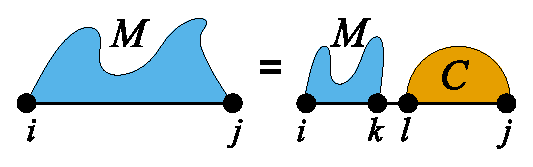
\includegraphics[width=\textwidth,height=\textheight/2,keepaspectratio=true]{decomp_ml_ml_stem}}
\end{DoxyImageNoCaption}
 \mbox{\Hypertarget{group__constraints_ga4fe48d575830b16c208e280e01ab1497}\label{group__constraints_ga4fe48d575830b16c208e280e01ab1497}} 
\index{Constraining the R\+N\+A Folding Grammar@{Constraining the R\+N\+A Folding Grammar}!V\+R\+N\+A\+\_\+\+D\+E\+C\+O\+M\+P\+\_\+\+M\+L\+\_\+\+C\+O\+A\+X\+I\+AL@{V\+R\+N\+A\+\_\+\+D\+E\+C\+O\+M\+P\+\_\+\+M\+L\+\_\+\+C\+O\+A\+X\+I\+AL}}
\index{V\+R\+N\+A\+\_\+\+D\+E\+C\+O\+M\+P\+\_\+\+M\+L\+\_\+\+C\+O\+A\+X\+I\+AL@{V\+R\+N\+A\+\_\+\+D\+E\+C\+O\+M\+P\+\_\+\+M\+L\+\_\+\+C\+O\+A\+X\+I\+AL}!Constraining the R\+N\+A Folding Grammar@{Constraining the R\+N\+A Folding Grammar}}
\subsubsection{\texorpdfstring{V\+R\+N\+A\+\_\+\+D\+E\+C\+O\+M\+P\+\_\+\+M\+L\+\_\+\+C\+O\+A\+X\+I\+AL}{VRNA\_DECOMP\_ML\_COAXIAL}}
{\footnotesize\ttfamily \#define V\+R\+N\+A\+\_\+\+D\+E\+C\+O\+M\+P\+\_\+\+M\+L\+\_\+\+C\+O\+A\+X\+I\+AL~(unsigned char)10}



{\ttfamily \#include $<$\hyperlink{constraints_2basic_8h}{Vienna\+R\+N\+A/constraints/basic.\+h}$>$}



Indicator for decomposition of multibranch loop part. 

This flag notifies the soft or hard constraint callback function that the current decomposition step evaluates a multibranch loop part in the interval $[i:j]$, where two stems with enclosing pairs $(i,k)$ and $(l,j)$ are coaxially stacking onto each other.

 
\begin{DoxyImageNoCaption}
  \mbox{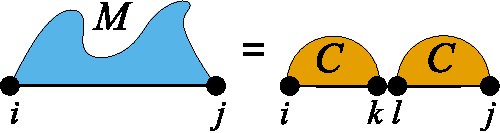
\includegraphics[width=\textwidth,height=\textheight/2,keepaspectratio=true]{decomp_ml_coaxial}}
\end{DoxyImageNoCaption}
 \mbox{\Hypertarget{group__constraints_ga0224727f7b8ad2f23eb0a3fd28d8b3fb}\label{group__constraints_ga0224727f7b8ad2f23eb0a3fd28d8b3fb}} 
\index{Constraining the R\+N\+A Folding Grammar@{Constraining the R\+N\+A Folding Grammar}!V\+R\+N\+A\+\_\+\+D\+E\+C\+O\+M\+P\+\_\+\+M\+L\+\_\+\+C\+O\+A\+X\+I\+A\+L\+\_\+\+E\+NC@{V\+R\+N\+A\+\_\+\+D\+E\+C\+O\+M\+P\+\_\+\+M\+L\+\_\+\+C\+O\+A\+X\+I\+A\+L\+\_\+\+E\+NC}}
\index{V\+R\+N\+A\+\_\+\+D\+E\+C\+O\+M\+P\+\_\+\+M\+L\+\_\+\+C\+O\+A\+X\+I\+A\+L\+\_\+\+E\+NC@{V\+R\+N\+A\+\_\+\+D\+E\+C\+O\+M\+P\+\_\+\+M\+L\+\_\+\+C\+O\+A\+X\+I\+A\+L\+\_\+\+E\+NC}!Constraining the R\+N\+A Folding Grammar@{Constraining the R\+N\+A Folding Grammar}}
\subsubsection{\texorpdfstring{V\+R\+N\+A\+\_\+\+D\+E\+C\+O\+M\+P\+\_\+\+M\+L\+\_\+\+C\+O\+A\+X\+I\+A\+L\+\_\+\+E\+NC}{VRNA\_DECOMP\_ML\_COAXIAL\_ENC}}
{\footnotesize\ttfamily \#define V\+R\+N\+A\+\_\+\+D\+E\+C\+O\+M\+P\+\_\+\+M\+L\+\_\+\+C\+O\+A\+X\+I\+A\+L\+\_\+\+E\+NC~(unsigned char)11}



{\ttfamily \#include $<$\hyperlink{constraints_2basic_8h}{Vienna\+R\+N\+A/constraints/basic.\+h}$>$}



Indicator for decomposition of multibranch loop part. 

This flag notifies the soft or hard constraint callback function that the current decomposition step evaluates a multibranch loop part in the interval $[i:j]$, where two stems with enclosing pairs $(i,k)$ and $(l,j)$ are coaxially stacking onto each other.

 
\begin{DoxyImageNoCaption}
  \mbox{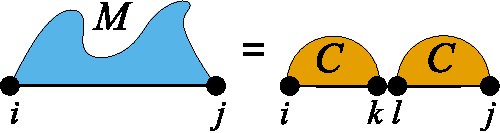
\includegraphics[width=\textwidth,height=\textheight/2,keepaspectratio=true]{decomp_ml_coaxial}}
\end{DoxyImageNoCaption}
 \mbox{\Hypertarget{group__constraints_ga437adf5115c1999304eff26b41e4c9b6}\label{group__constraints_ga437adf5115c1999304eff26b41e4c9b6}} 
\index{Constraining the R\+N\+A Folding Grammar@{Constraining the R\+N\+A Folding Grammar}!V\+R\+N\+A\+\_\+\+D\+E\+C\+O\+M\+P\+\_\+\+E\+X\+T\+\_\+\+E\+XT@{V\+R\+N\+A\+\_\+\+D\+E\+C\+O\+M\+P\+\_\+\+E\+X\+T\+\_\+\+E\+XT}}
\index{V\+R\+N\+A\+\_\+\+D\+E\+C\+O\+M\+P\+\_\+\+E\+X\+T\+\_\+\+E\+XT@{V\+R\+N\+A\+\_\+\+D\+E\+C\+O\+M\+P\+\_\+\+E\+X\+T\+\_\+\+E\+XT}!Constraining the R\+N\+A Folding Grammar@{Constraining the R\+N\+A Folding Grammar}}
\subsubsection{\texorpdfstring{V\+R\+N\+A\+\_\+\+D\+E\+C\+O\+M\+P\+\_\+\+E\+X\+T\+\_\+\+E\+XT}{VRNA\_DECOMP\_EXT\_EXT}}
{\footnotesize\ttfamily \#define V\+R\+N\+A\+\_\+\+D\+E\+C\+O\+M\+P\+\_\+\+E\+X\+T\+\_\+\+E\+XT~(unsigned char)12}



{\ttfamily \#include $<$\hyperlink{constraints_2basic_8h}{Vienna\+R\+N\+A/constraints/basic.\+h}$>$}



Indicator for decomposition of exterior loop part. 

This flag notifies the soft or hard constraint callback function that the current decomposition step evaluates an exterior loop part in the interval $[i:j]$, which will be decomposed into a (usually) smaller exterior loop part $[k:l]$.

 
\begin{DoxyImageNoCaption}
  \mbox{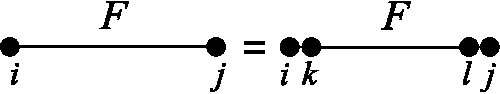
\includegraphics[width=\textwidth,height=\textheight/2,keepaspectratio=true]{decomp_ext_ext}}
\end{DoxyImageNoCaption}
 \mbox{\Hypertarget{group__constraints_gaff1ddaffe86d984623910b40cc8a8717}\label{group__constraints_gaff1ddaffe86d984623910b40cc8a8717}} 
\index{Constraining the R\+N\+A Folding Grammar@{Constraining the R\+N\+A Folding Grammar}!V\+R\+N\+A\+\_\+\+D\+E\+C\+O\+M\+P\+\_\+\+E\+X\+T\+\_\+\+UP@{V\+R\+N\+A\+\_\+\+D\+E\+C\+O\+M\+P\+\_\+\+E\+X\+T\+\_\+\+UP}}
\index{V\+R\+N\+A\+\_\+\+D\+E\+C\+O\+M\+P\+\_\+\+E\+X\+T\+\_\+\+UP@{V\+R\+N\+A\+\_\+\+D\+E\+C\+O\+M\+P\+\_\+\+E\+X\+T\+\_\+\+UP}!Constraining the R\+N\+A Folding Grammar@{Constraining the R\+N\+A Folding Grammar}}
\subsubsection{\texorpdfstring{V\+R\+N\+A\+\_\+\+D\+E\+C\+O\+M\+P\+\_\+\+E\+X\+T\+\_\+\+UP}{VRNA\_DECOMP\_EXT\_UP}}
{\footnotesize\ttfamily \#define V\+R\+N\+A\+\_\+\+D\+E\+C\+O\+M\+P\+\_\+\+E\+X\+T\+\_\+\+UP~(unsigned char)13}



{\ttfamily \#include $<$\hyperlink{constraints_2basic_8h}{Vienna\+R\+N\+A/constraints/basic.\+h}$>$}



Indicator for decomposition of exterior loop part. 

This flag notifies the soft or hard constraint callback function that the current decomposition step evaluates an exterior loop part in the interval $[i:j]$, which will be considered as an exterior loop component consisting of only unpaired nucleotides.

 
\begin{DoxyImageNoCaption}
  \mbox{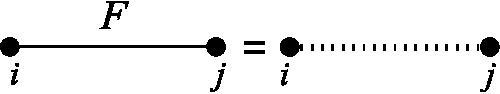
\includegraphics[width=\textwidth,height=\textheight/2,keepaspectratio=true]{decomp_ext_up}}
\end{DoxyImageNoCaption}
 \mbox{\Hypertarget{group__constraints_gae44b5ace0d9b4a29088069ecb4cec441}\label{group__constraints_gae44b5ace0d9b4a29088069ecb4cec441}} 
\index{Constraining the R\+N\+A Folding Grammar@{Constraining the R\+N\+A Folding Grammar}!V\+R\+N\+A\+\_\+\+D\+E\+C\+O\+M\+P\+\_\+\+E\+X\+T\+\_\+\+S\+T\+EM@{V\+R\+N\+A\+\_\+\+D\+E\+C\+O\+M\+P\+\_\+\+E\+X\+T\+\_\+\+S\+T\+EM}}
\index{V\+R\+N\+A\+\_\+\+D\+E\+C\+O\+M\+P\+\_\+\+E\+X\+T\+\_\+\+S\+T\+EM@{V\+R\+N\+A\+\_\+\+D\+E\+C\+O\+M\+P\+\_\+\+E\+X\+T\+\_\+\+S\+T\+EM}!Constraining the R\+N\+A Folding Grammar@{Constraining the R\+N\+A Folding Grammar}}
\subsubsection{\texorpdfstring{V\+R\+N\+A\+\_\+\+D\+E\+C\+O\+M\+P\+\_\+\+E\+X\+T\+\_\+\+S\+T\+EM}{VRNA\_DECOMP\_EXT\_STEM}}
{\footnotesize\ttfamily \#define V\+R\+N\+A\+\_\+\+D\+E\+C\+O\+M\+P\+\_\+\+E\+X\+T\+\_\+\+S\+T\+EM~(unsigned char)14}



{\ttfamily \#include $<$\hyperlink{constraints_2basic_8h}{Vienna\+R\+N\+A/constraints/basic.\+h}$>$}



Indicator for decomposition of exterior loop part. 

This flag notifies the soft or hard constraint callback function that the current decomposition step evaluates an exterior loop part in the interval $[i:j]$, which will be considered a stem with enclosing pair $(k,l)$.

 
\begin{DoxyImageNoCaption}
  \mbox{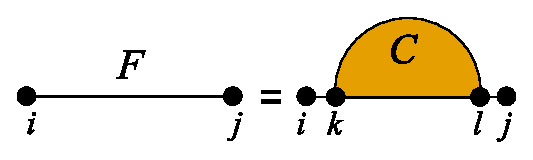
\includegraphics[width=\textwidth,height=\textheight/2,keepaspectratio=true]{decomp_ext_stem}}
\end{DoxyImageNoCaption}
 \mbox{\Hypertarget{group__constraints_ga803bd818b3f4b2b0a4a5cfa2f7dc2045}\label{group__constraints_ga803bd818b3f4b2b0a4a5cfa2f7dc2045}} 
\index{Constraining the R\+N\+A Folding Grammar@{Constraining the R\+N\+A Folding Grammar}!V\+R\+N\+A\+\_\+\+D\+E\+C\+O\+M\+P\+\_\+\+E\+X\+T\+\_\+\+E\+X\+T\+\_\+\+E\+XT@{V\+R\+N\+A\+\_\+\+D\+E\+C\+O\+M\+P\+\_\+\+E\+X\+T\+\_\+\+E\+X\+T\+\_\+\+E\+XT}}
\index{V\+R\+N\+A\+\_\+\+D\+E\+C\+O\+M\+P\+\_\+\+E\+X\+T\+\_\+\+E\+X\+T\+\_\+\+E\+XT@{V\+R\+N\+A\+\_\+\+D\+E\+C\+O\+M\+P\+\_\+\+E\+X\+T\+\_\+\+E\+X\+T\+\_\+\+E\+XT}!Constraining the R\+N\+A Folding Grammar@{Constraining the R\+N\+A Folding Grammar}}
\subsubsection{\texorpdfstring{V\+R\+N\+A\+\_\+\+D\+E\+C\+O\+M\+P\+\_\+\+E\+X\+T\+\_\+\+E\+X\+T\+\_\+\+E\+XT}{VRNA\_DECOMP\_EXT\_EXT\_EXT}}
{\footnotesize\ttfamily \#define V\+R\+N\+A\+\_\+\+D\+E\+C\+O\+M\+P\+\_\+\+E\+X\+T\+\_\+\+E\+X\+T\+\_\+\+E\+XT~(unsigned char)15}



{\ttfamily \#include $<$\hyperlink{constraints_2basic_8h}{Vienna\+R\+N\+A/constraints/basic.\+h}$>$}



Indicator for decomposition of exterior loop part. 

This flag notifies the soft or hard constraint callback function that the current decomposition step evaluates an exterior loop part in the interval $[i:j]$, which will be decomposed into two exterior loop parts $[i:k]$ and $[l:j]$.

 
\begin{DoxyImageNoCaption}
  \mbox{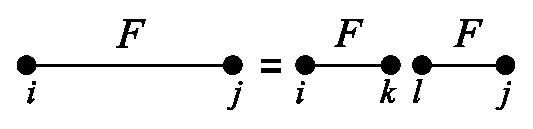
\includegraphics[width=\textwidth,height=\textheight/2,keepaspectratio=true]{decomp_ext_ext_ext}}
\end{DoxyImageNoCaption}
 \mbox{\Hypertarget{group__constraints_gabb09c5b78b75a44502fc77b950125c1e}\label{group__constraints_gabb09c5b78b75a44502fc77b950125c1e}} 
\index{Constraining the R\+N\+A Folding Grammar@{Constraining the R\+N\+A Folding Grammar}!V\+R\+N\+A\+\_\+\+D\+E\+C\+O\+M\+P\+\_\+\+E\+X\+T\+\_\+\+S\+T\+E\+M\+\_\+\+E\+XT@{V\+R\+N\+A\+\_\+\+D\+E\+C\+O\+M\+P\+\_\+\+E\+X\+T\+\_\+\+S\+T\+E\+M\+\_\+\+E\+XT}}
\index{V\+R\+N\+A\+\_\+\+D\+E\+C\+O\+M\+P\+\_\+\+E\+X\+T\+\_\+\+S\+T\+E\+M\+\_\+\+E\+XT@{V\+R\+N\+A\+\_\+\+D\+E\+C\+O\+M\+P\+\_\+\+E\+X\+T\+\_\+\+S\+T\+E\+M\+\_\+\+E\+XT}!Constraining the R\+N\+A Folding Grammar@{Constraining the R\+N\+A Folding Grammar}}
\subsubsection{\texorpdfstring{V\+R\+N\+A\+\_\+\+D\+E\+C\+O\+M\+P\+\_\+\+E\+X\+T\+\_\+\+S\+T\+E\+M\+\_\+\+E\+XT}{VRNA\_DECOMP\_EXT\_STEM\_EXT}}
{\footnotesize\ttfamily \#define V\+R\+N\+A\+\_\+\+D\+E\+C\+O\+M\+P\+\_\+\+E\+X\+T\+\_\+\+S\+T\+E\+M\+\_\+\+E\+XT~(unsigned char)16}



{\ttfamily \#include $<$\hyperlink{constraints_2basic_8h}{Vienna\+R\+N\+A/constraints/basic.\+h}$>$}



Indicator for decomposition of exterior loop part. 

This flag notifies the soft or hard constraint callback function that the current decomposition step evaluates an exterior loop part in the interval $[i:j]$, which will be decomposed into a stem branching off with base pair $(i,k)$, and an exterior loop part $[l:j]$.

 
\begin{DoxyImageNoCaption}
  \mbox{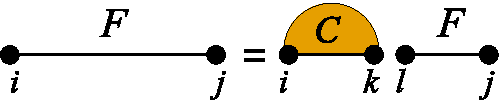
\includegraphics[width=\textwidth,height=\textheight/2,keepaspectratio=true]{decomp_ext_stem_ext}}
\end{DoxyImageNoCaption}
 \mbox{\Hypertarget{group__constraints_ga06efd054c9271438f6d82d4559d9e69f}\label{group__constraints_ga06efd054c9271438f6d82d4559d9e69f}} 
\index{Constraining the R\+N\+A Folding Grammar@{Constraining the R\+N\+A Folding Grammar}!V\+R\+N\+A\+\_\+\+D\+E\+C\+O\+M\+P\+\_\+\+E\+X\+T\+\_\+\+E\+X\+T\+\_\+\+S\+T\+EM@{V\+R\+N\+A\+\_\+\+D\+E\+C\+O\+M\+P\+\_\+\+E\+X\+T\+\_\+\+E\+X\+T\+\_\+\+S\+T\+EM}}
\index{V\+R\+N\+A\+\_\+\+D\+E\+C\+O\+M\+P\+\_\+\+E\+X\+T\+\_\+\+E\+X\+T\+\_\+\+S\+T\+EM@{V\+R\+N\+A\+\_\+\+D\+E\+C\+O\+M\+P\+\_\+\+E\+X\+T\+\_\+\+E\+X\+T\+\_\+\+S\+T\+EM}!Constraining the R\+N\+A Folding Grammar@{Constraining the R\+N\+A Folding Grammar}}
\subsubsection{\texorpdfstring{V\+R\+N\+A\+\_\+\+D\+E\+C\+O\+M\+P\+\_\+\+E\+X\+T\+\_\+\+E\+X\+T\+\_\+\+S\+T\+EM}{VRNA\_DECOMP\_EXT\_EXT\_STEM}}
{\footnotesize\ttfamily \#define V\+R\+N\+A\+\_\+\+D\+E\+C\+O\+M\+P\+\_\+\+E\+X\+T\+\_\+\+E\+X\+T\+\_\+\+S\+T\+EM~(unsigned char)18}



{\ttfamily \#include $<$\hyperlink{constraints_2basic_8h}{Vienna\+R\+N\+A/constraints/basic.\+h}$>$}



Indicator for decomposition of exterior loop part. 

This flag notifies the soft or hard constraint callback function that the current decomposition step evaluates an exterior loop part in the interval $[i:j]$, which will be decomposed into an exterior loop part $[i:k]$, and a stem branching off with base pair $(l,j)$.

 
\begin{DoxyImageNoCaption}
  \mbox{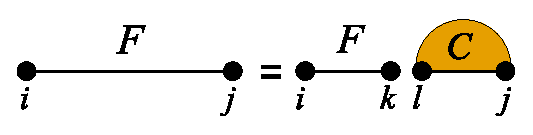
\includegraphics[width=\textwidth,height=\textheight/2,keepaspectratio=true]{decomp_ext_ext_stem}}
\end{DoxyImageNoCaption}
 \mbox{\Hypertarget{group__constraints_ga2e75d7a77118735b32f25422d9686719}\label{group__constraints_ga2e75d7a77118735b32f25422d9686719}} 
\index{Constraining the R\+N\+A Folding Grammar@{Constraining the R\+N\+A Folding Grammar}!V\+R\+N\+A\+\_\+\+D\+E\+C\+O\+M\+P\+\_\+\+E\+X\+T\+\_\+\+E\+X\+T\+\_\+\+S\+T\+E\+M1@{V\+R\+N\+A\+\_\+\+D\+E\+C\+O\+M\+P\+\_\+\+E\+X\+T\+\_\+\+E\+X\+T\+\_\+\+S\+T\+E\+M1}}
\index{V\+R\+N\+A\+\_\+\+D\+E\+C\+O\+M\+P\+\_\+\+E\+X\+T\+\_\+\+E\+X\+T\+\_\+\+S\+T\+E\+M1@{V\+R\+N\+A\+\_\+\+D\+E\+C\+O\+M\+P\+\_\+\+E\+X\+T\+\_\+\+E\+X\+T\+\_\+\+S\+T\+E\+M1}!Constraining the R\+N\+A Folding Grammar@{Constraining the R\+N\+A Folding Grammar}}
\subsubsection{\texorpdfstring{V\+R\+N\+A\+\_\+\+D\+E\+C\+O\+M\+P\+\_\+\+E\+X\+T\+\_\+\+E\+X\+T\+\_\+\+S\+T\+E\+M1}{VRNA\_DECOMP\_EXT\_EXT\_STEM1}}
{\footnotesize\ttfamily \#define V\+R\+N\+A\+\_\+\+D\+E\+C\+O\+M\+P\+\_\+\+E\+X\+T\+\_\+\+E\+X\+T\+\_\+\+S\+T\+E\+M1~(unsigned char)19}



{\ttfamily \#include $<$\hyperlink{constraints_2basic_8h}{Vienna\+R\+N\+A/constraints/basic.\+h}$>$}



Indicator for decomposition of exterior loop part. 

This flag notifies the soft or hard constraint callback function that the current decomposition step evaluates an exterior loop part in the interval $[i:j]$, which will be decomposed into an exterior loop part $[i:k]$, and a stem branching off with base pair $(l,j-1)$.

 
\begin{DoxyImageNoCaption}
  \mbox{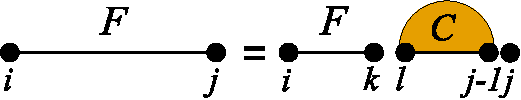
\includegraphics[width=\textwidth,height=\textheight/2,keepaspectratio=true]{decomp_ext_ext_stem1}}
\end{DoxyImageNoCaption}
 

\subsection{Function Documentation}
\mbox{\Hypertarget{group__constraints_ga35a401f680969a556858a8dd5f1d07cc}\label{group__constraints_ga35a401f680969a556858a8dd5f1d07cc}} 
\index{Constraining the R\+N\+A Folding Grammar@{Constraining the R\+N\+A Folding Grammar}!vrna\+\_\+constraints\+\_\+add@{vrna\+\_\+constraints\+\_\+add}}
\index{vrna\+\_\+constraints\+\_\+add@{vrna\+\_\+constraints\+\_\+add}!Constraining the R\+N\+A Folding Grammar@{Constraining the R\+N\+A Folding Grammar}}
\subsubsection{\texorpdfstring{vrna\+\_\+constraints\+\_\+add()}{vrna\_constraints\_add()}}
{\footnotesize\ttfamily void vrna\+\_\+constraints\+\_\+add (\begin{DoxyParamCaption}\item[{\hyperlink{group__fold__compound_ga1b0cef17fd40466cef5968eaeeff6166}{vrna\+\_\+fold\+\_\+compound\+\_\+t} $\ast$}]{vc,  }\item[{const char $\ast$}]{constraint,  }\item[{unsigned int}]{options }\end{DoxyParamCaption})}



{\ttfamily \#include $<$\hyperlink{constraints_2basic_8h}{Vienna\+R\+N\+A/constraints/basic.\+h}$>$}



Add constraints to a \hyperlink{group__fold__compound_ga1b0cef17fd40466cef5968eaeeff6166}{vrna\+\_\+fold\+\_\+compound\+\_\+t} data structure. 

Use this function to add/update the hard/soft constraints The function allows for passing a string \textquotesingle{}constraint\textquotesingle{} that can either be a filename that points to a constraints definition file or it may be a pseudo dot-\/bracket notation indicating hard constraints. For the latter, the user has to pass the \hyperlink{group__hard__constraints_ga4bfc2f15c4f261c62a11af9d2aa80c90}{V\+R\+N\+A\+\_\+\+C\+O\+N\+S\+T\+R\+A\+I\+N\+T\+\_\+\+DB} option. Also, the user has to specify, which characters are allowed to be interpreted as constraints by passing the corresponding options via the third parameter.

\begin{DoxySeeAlso}{See also}
\hyperlink{group__hard__constraints_ga36ff456c43bf920629cee5a236e4f0ff}{vrna\+\_\+hc\+\_\+init()}, \hyperlink{group__hard__constraints_ga447d88e06ad97bb225cd83310ace8345}{vrna\+\_\+hc\+\_\+add\+\_\+up()}, \hyperlink{group__hard__constraints_ga5070f296c8af2baea10951525519464f}{vrna\+\_\+hc\+\_\+add\+\_\+up\+\_\+batch()}, \hyperlink{group__hard__constraints_ga7cba95ebe2ceb5ec9a5768f2232854fd}{vrna\+\_\+hc\+\_\+add\+\_\+bp()}, \hyperlink{group__soft__constraints_ga9d977a1681356778cc66dceafbe5b032}{vrna\+\_\+sc\+\_\+init()}, \hyperlink{group__soft__constraints_ga99ed63f3ef9e7fe3997932030487a344}{vrna\+\_\+sc\+\_\+set\+\_\+up()}, \hyperlink{group__soft__constraints_ga8e4334b24bc91453fbcda490a4e331af}{vrna\+\_\+sc\+\_\+set\+\_\+bp()}, \hyperlink{group__SHAPE__reactivities_ga57d612b58e1c61dd6cfcb5a843f8f1b3}{vrna\+\_\+sc\+\_\+add\+\_\+\+S\+H\+A\+P\+E\+\_\+deigan()}, \hyperlink{group__SHAPE__reactivities_gaf3c65a045060aef5c4e41693d30af58c}{vrna\+\_\+sc\+\_\+add\+\_\+\+S\+H\+A\+P\+E\+\_\+zarringhalam()}, \hyperlink{group__hard__constraints_ga696dcf77887d856c6f21ea266d8b9ca2}{vrna\+\_\+hc\+\_\+free()}, \hyperlink{group__soft__constraints_ga6d55446448d69346fc313b993c4fb3e8}{vrna\+\_\+sc\+\_\+free()}, \hyperlink{group__hard__constraints_ga4bfc2f15c4f261c62a11af9d2aa80c90}{V\+R\+N\+A\+\_\+\+C\+O\+N\+S\+T\+R\+A\+I\+N\+T\+\_\+\+DB}, \hyperlink{group__hard__constraints_ga1c3864bdc92147a4d93de2b1b4356177}{V\+R\+N\+A\+\_\+\+C\+O\+N\+S\+T\+R\+A\+I\+N\+T\+\_\+\+D\+B\+\_\+\+D\+E\+F\+A\+U\+LT}, \hyperlink{group__hard__constraints_ga13053547a2de5532b64b64d35e097ae1}{V\+R\+N\+A\+\_\+\+C\+O\+N\+S\+T\+R\+A\+I\+N\+T\+\_\+\+D\+B\+\_\+\+P\+I\+PE}, \hyperlink{group__hard__constraints_ga369bea82eae75fbe626f409fa425747e}{V\+R\+N\+A\+\_\+\+C\+O\+N\+S\+T\+R\+A\+I\+N\+T\+\_\+\+D\+B\+\_\+\+D\+OT}, \hyperlink{group__hard__constraints_ga7283bbe0f8954f7b030ecc3f2d1932b2}{V\+R\+N\+A\+\_\+\+C\+O\+N\+S\+T\+R\+A\+I\+N\+T\+\_\+\+D\+B\+\_\+X}, \hyperlink{hard_8h_ad54c1315a47d55653dcaa5de6e544b77}{V\+R\+N\+A\+\_\+\+C\+O\+N\+S\+T\+R\+A\+I\+N\+T\+\_\+\+D\+B\+\_\+\+A\+N\+G\+\_\+\+B\+R\+A\+CK}, \hyperlink{group__hard__constraints_gac17b034852c914bc5879954c65d7e74b}{V\+R\+N\+A\+\_\+\+C\+O\+N\+S\+T\+R\+A\+I\+N\+T\+\_\+\+D\+B\+\_\+\+R\+N\+D\+\_\+\+B\+R\+A\+CK}, \hyperlink{group__hard__constraints_ga5c17253f5a39d1d49b0fb11f5196982a}{V\+R\+N\+A\+\_\+\+C\+O\+N\+S\+T\+R\+A\+I\+N\+T\+\_\+\+D\+B\+\_\+\+I\+N\+T\+R\+A\+M\+OL}, \hyperlink{group__hard__constraints_ga31d0ebb9755ca8a4acafc14f00ca755d}{V\+R\+N\+A\+\_\+\+C\+O\+N\+S\+T\+R\+A\+I\+N\+T\+\_\+\+D\+B\+\_\+\+I\+N\+T\+E\+R\+M\+OL}, \hyperlink{group__hard__constraints_ga75cfab03cdc97c95b3ce8bb29f52b08e}{V\+R\+N\+A\+\_\+\+C\+O\+N\+S\+T\+R\+A\+I\+N\+T\+\_\+\+D\+B\+\_\+\+G\+Q\+U\+AD}
\end{DoxySeeAlso}
The following is an example for adding hard constraints given in pseudo dot-\/bracket notation. Here, {\ttfamily vc} is the \hyperlink{group__fold__compound_ga1b0cef17fd40466cef5968eaeeff6166}{vrna\+\_\+fold\+\_\+compound\+\_\+t} object, {\ttfamily structure} is a char array with the hard constraint in dot-\/bracket notation, and {\ttfamily enforce\+Constraints} is a flag indicating whether or not constraints for base pairs should be enforced instead of just doing a removal of base pair that conflict with the constraint.


\begin{DoxyCodeInclude}
      \textcolor{keywordtype}{unsigned} \textcolor{keywordtype}{int} constraint\_options = \hyperlink{group__hard__constraints_ga1c3864bdc92147a4d93de2b1b4356177}{VRNA\_CONSTRAINT\_DB\_DEFAULT};

      \textcolor{keywordflow}{if} (enforceConstraints)
        constraint\_options |= \hyperlink{group__hard__constraints_ga29ebe940110d60ab798fdacbcdbbfb7d}{VRNA\_CONSTRAINT\_DB\_ENFORCE\_BP};

      \textcolor{keywordflow}{if} (canonicalBPonly)
        constraint\_options |= VRNA\_CONSTRAINT\_DB\_CANONICAL\_BP;

      \hyperlink{group__constraints_ga35a401f680969a556858a8dd5f1d07cc}{vrna\_constraints\_add}(fc, (\textcolor{keyword}{const} \textcolor{keywordtype}{char} *)cstruc, constraint\_options);
\end{DoxyCodeInclude}
 In constrat to the above, constraints may also be read from file\+:


\begin{DoxyCodeInclude}
    \hyperlink{group__constraints_ga35a401f680969a556858a8dd5f1d07cc}{vrna\_constraints\_add}(fc, constraints\_file, 
      \hyperlink{group__fold__compound_gacea5b7ee6181c485f36e2afa0e9089e4}{VRNA\_OPTION\_DEFAULT});
\end{DoxyCodeInclude}
 \begin{DoxySeeAlso}{See also}
\hyperlink{group__hard__constraints_ga5b4de3247b67358080c176b94591a8e6}{vrna\+\_\+hc\+\_\+add\+\_\+from\+\_\+db()}, \hyperlink{group__hard__constraints_ga447d88e06ad97bb225cd83310ace8345}{vrna\+\_\+hc\+\_\+add\+\_\+up()}, \hyperlink{group__hard__constraints_ga5070f296c8af2baea10951525519464f}{vrna\+\_\+hc\+\_\+add\+\_\+up\+\_\+batch()} vrna\+\_\+hc\+\_\+add\+\_\+bp\+\_\+unspecific(), \hyperlink{group__hard__constraints_ga7cba95ebe2ceb5ec9a5768f2232854fd}{vrna\+\_\+hc\+\_\+add\+\_\+bp()}
\end{DoxySeeAlso}

\begin{DoxyParams}{Parameters}
{\em vc} & The fold compound \\
\hline
{\em constraint} & A string with either the filename of the constraint definitions or a pseudo dot-\/bracket notation of the hard constraint. May be N\+U\+LL. \\
\hline
{\em options} & The option flags \\
\hline
\end{DoxyParams}
\mbox{\Hypertarget{group__constraints_gaa1f20b53bf09ac2e6b0dbb13f7d89670}\label{group__constraints_gaa1f20b53bf09ac2e6b0dbb13f7d89670}} 
\index{Constraining the R\+N\+A Folding Grammar@{Constraining the R\+N\+A Folding Grammar}!vrna\+\_\+message\+\_\+constraint\+\_\+options@{vrna\+\_\+message\+\_\+constraint\+\_\+options}}
\index{vrna\+\_\+message\+\_\+constraint\+\_\+options@{vrna\+\_\+message\+\_\+constraint\+\_\+options}!Constraining the R\+N\+A Folding Grammar@{Constraining the R\+N\+A Folding Grammar}}
\subsubsection{\texorpdfstring{vrna\+\_\+message\+\_\+constraint\+\_\+options()}{vrna\_message\_constraint\_options()}}
{\footnotesize\ttfamily void vrna\+\_\+message\+\_\+constraint\+\_\+options (\begin{DoxyParamCaption}\item[{unsigned int}]{option }\end{DoxyParamCaption})}



{\ttfamily \#include $<$\hyperlink{hard_8h}{Vienna\+R\+N\+A/constraints/hard.\+h}$>$}



Print a help message for pseudo dot-\/bracket structure constraint characters to stdout. (constraint support is specified by option parameter) 

Currently available options are\+:~\newline
\hyperlink{group__hard__constraints_ga13053547a2de5532b64b64d35e097ae1}{V\+R\+N\+A\+\_\+\+C\+O\+N\+S\+T\+R\+A\+I\+N\+T\+\_\+\+D\+B\+\_\+\+P\+I\+PE} (paired with another base)~\newline
\hyperlink{group__hard__constraints_ga369bea82eae75fbe626f409fa425747e}{V\+R\+N\+A\+\_\+\+C\+O\+N\+S\+T\+R\+A\+I\+N\+T\+\_\+\+D\+B\+\_\+\+D\+OT} (no constraint at all)~\newline
\hyperlink{group__hard__constraints_ga7283bbe0f8954f7b030ecc3f2d1932b2}{V\+R\+N\+A\+\_\+\+C\+O\+N\+S\+T\+R\+A\+I\+N\+T\+\_\+\+D\+B\+\_\+X} (base must not pair)~\newline
\hyperlink{hard_8h_ad54c1315a47d55653dcaa5de6e544b77}{V\+R\+N\+A\+\_\+\+C\+O\+N\+S\+T\+R\+A\+I\+N\+T\+\_\+\+D\+B\+\_\+\+A\+N\+G\+\_\+\+B\+R\+A\+CK} (paired downstream/upstream)~\newline
\hyperlink{group__hard__constraints_gac17b034852c914bc5879954c65d7e74b}{V\+R\+N\+A\+\_\+\+C\+O\+N\+S\+T\+R\+A\+I\+N\+T\+\_\+\+D\+B\+\_\+\+R\+N\+D\+\_\+\+B\+R\+A\+CK} (base i pairs base j)~\newline
 pass a collection of options as one value like this\+: \begin{DoxyVerb}vrna_message_constraints(option_1 | option_2 | option_n) \end{DoxyVerb}


\begin{DoxySeeAlso}{See also}
\hyperlink{group__constraints_gaec7e13fa0465c2acc7a621d1aecb709f}{vrna\+\_\+message\+\_\+constraint\+\_\+options\+\_\+all()}, \hyperlink{group__constraints_ga35a401f680969a556858a8dd5f1d07cc}{vrna\+\_\+constraints\+\_\+add()}, \hyperlink{group__hard__constraints_ga4bfc2f15c4f261c62a11af9d2aa80c90}{V\+R\+N\+A\+\_\+\+C\+O\+N\+S\+T\+R\+A\+I\+N\+T\+\_\+\+DB}, \hyperlink{group__hard__constraints_ga13053547a2de5532b64b64d35e097ae1}{V\+R\+N\+A\+\_\+\+C\+O\+N\+S\+T\+R\+A\+I\+N\+T\+\_\+\+D\+B\+\_\+\+P\+I\+PE}, \hyperlink{group__hard__constraints_ga369bea82eae75fbe626f409fa425747e}{V\+R\+N\+A\+\_\+\+C\+O\+N\+S\+T\+R\+A\+I\+N\+T\+\_\+\+D\+B\+\_\+\+D\+OT}, \hyperlink{group__hard__constraints_ga7283bbe0f8954f7b030ecc3f2d1932b2}{V\+R\+N\+A\+\_\+\+C\+O\+N\+S\+T\+R\+A\+I\+N\+T\+\_\+\+D\+B\+\_\+X}, \hyperlink{hard_8h_ad54c1315a47d55653dcaa5de6e544b77}{V\+R\+N\+A\+\_\+\+C\+O\+N\+S\+T\+R\+A\+I\+N\+T\+\_\+\+D\+B\+\_\+\+A\+N\+G\+\_\+\+B\+R\+A\+CK}, \hyperlink{group__hard__constraints_gac17b034852c914bc5879954c65d7e74b}{V\+R\+N\+A\+\_\+\+C\+O\+N\+S\+T\+R\+A\+I\+N\+T\+\_\+\+D\+B\+\_\+\+R\+N\+D\+\_\+\+B\+R\+A\+CK}, \hyperlink{group__hard__constraints_ga31d0ebb9755ca8a4acafc14f00ca755d}{V\+R\+N\+A\+\_\+\+C\+O\+N\+S\+T\+R\+A\+I\+N\+T\+\_\+\+D\+B\+\_\+\+I\+N\+T\+E\+R\+M\+OL}, \hyperlink{group__hard__constraints_ga5c17253f5a39d1d49b0fb11f5196982a}{V\+R\+N\+A\+\_\+\+C\+O\+N\+S\+T\+R\+A\+I\+N\+T\+\_\+\+D\+B\+\_\+\+I\+N\+T\+R\+A\+M\+OL}
\end{DoxySeeAlso}

\begin{DoxyParams}{Parameters}
{\em option} & Option switch that tells which constraint help will be printed \\
\hline
\end{DoxyParams}
\mbox{\Hypertarget{group__constraints_gaec7e13fa0465c2acc7a621d1aecb709f}\label{group__constraints_gaec7e13fa0465c2acc7a621d1aecb709f}} 
\index{Constraining the R\+N\+A Folding Grammar@{Constraining the R\+N\+A Folding Grammar}!vrna\+\_\+message\+\_\+constraint\+\_\+options\+\_\+all@{vrna\+\_\+message\+\_\+constraint\+\_\+options\+\_\+all}}
\index{vrna\+\_\+message\+\_\+constraint\+\_\+options\+\_\+all@{vrna\+\_\+message\+\_\+constraint\+\_\+options\+\_\+all}!Constraining the R\+N\+A Folding Grammar@{Constraining the R\+N\+A Folding Grammar}}
\subsubsection{\texorpdfstring{vrna\+\_\+message\+\_\+constraint\+\_\+options\+\_\+all()}{vrna\_message\_constraint\_options\_all()}}
{\footnotesize\ttfamily void vrna\+\_\+message\+\_\+constraint\+\_\+options\+\_\+all (\begin{DoxyParamCaption}\item[{void}]{ }\end{DoxyParamCaption})}



{\ttfamily \#include $<$\hyperlink{hard_8h}{Vienna\+R\+N\+A/constraints/hard.\+h}$>$}



Print structure constraint characters to stdout (full constraint support) 

\begin{DoxySeeAlso}{See also}
\hyperlink{group__constraints_gaa1f20b53bf09ac2e6b0dbb13f7d89670}{vrna\+\_\+message\+\_\+constraint\+\_\+options()}, \hyperlink{group__constraints_ga35a401f680969a556858a8dd5f1d07cc}{vrna\+\_\+constraints\+\_\+add()}, \hyperlink{group__hard__constraints_ga4bfc2f15c4f261c62a11af9d2aa80c90}{V\+R\+N\+A\+\_\+\+C\+O\+N\+S\+T\+R\+A\+I\+N\+T\+\_\+\+DB}, \hyperlink{group__hard__constraints_ga13053547a2de5532b64b64d35e097ae1}{V\+R\+N\+A\+\_\+\+C\+O\+N\+S\+T\+R\+A\+I\+N\+T\+\_\+\+D\+B\+\_\+\+P\+I\+PE}, \hyperlink{group__hard__constraints_ga369bea82eae75fbe626f409fa425747e}{V\+R\+N\+A\+\_\+\+C\+O\+N\+S\+T\+R\+A\+I\+N\+T\+\_\+\+D\+B\+\_\+\+D\+OT}, \hyperlink{group__hard__constraints_ga7283bbe0f8954f7b030ecc3f2d1932b2}{V\+R\+N\+A\+\_\+\+C\+O\+N\+S\+T\+R\+A\+I\+N\+T\+\_\+\+D\+B\+\_\+X}, \hyperlink{hard_8h_ad54c1315a47d55653dcaa5de6e544b77}{V\+R\+N\+A\+\_\+\+C\+O\+N\+S\+T\+R\+A\+I\+N\+T\+\_\+\+D\+B\+\_\+\+A\+N\+G\+\_\+\+B\+R\+A\+CK}, \hyperlink{group__hard__constraints_gac17b034852c914bc5879954c65d7e74b}{V\+R\+N\+A\+\_\+\+C\+O\+N\+S\+T\+R\+A\+I\+N\+T\+\_\+\+D\+B\+\_\+\+R\+N\+D\+\_\+\+B\+R\+A\+CK}, \hyperlink{group__hard__constraints_ga31d0ebb9755ca8a4acafc14f00ca755d}{V\+R\+N\+A\+\_\+\+C\+O\+N\+S\+T\+R\+A\+I\+N\+T\+\_\+\+D\+B\+\_\+\+I\+N\+T\+E\+R\+M\+OL}, \hyperlink{group__hard__constraints_ga5c17253f5a39d1d49b0fb11f5196982a}{V\+R\+N\+A\+\_\+\+C\+O\+N\+S\+T\+R\+A\+I\+N\+T\+\_\+\+D\+B\+\_\+\+I\+N\+T\+R\+A\+M\+OL} 
\end{DoxySeeAlso}

\hypertarget{group__hard__constraints}{}\section{Hard Constraints}
\label{group__hard__constraints}\index{Hard Constraints@{Hard Constraints}}


This module covers all functionality for hard constraints in secondary structure prediction.  




\subsection{Detailed Description}
This module covers all functionality for hard constraints in secondary structure prediction. 

Collaboration diagram for Hard Constraints\+:
\nopagebreak
\begin{figure}[H]
\begin{center}
\leavevmode
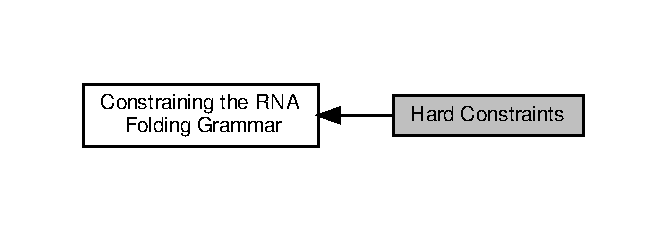
\includegraphics[width=320pt]{group__hard__constraints}
\end{center}
\end{figure}
\subsection*{Files}
\begin{DoxyCompactItemize}
\item 
file \hyperlink{hard_8h}{hard.\+h}
\begin{DoxyCompactList}\small\item\em Functions and data structures for handling of secondary structure hard constraints. \end{DoxyCompactList}\end{DoxyCompactItemize}
\subsection*{Data Structures}
\begin{DoxyCompactItemize}
\item 
struct \hyperlink{group__hard__constraints_structvrna__hc__s}{vrna\+\_\+hc\+\_\+s}
\begin{DoxyCompactList}\small\item\em The hard constraints data structure.  \hyperlink{group__hard__constraints_structvrna__hc__s}{More...}\end{DoxyCompactList}\item 
struct \hyperlink{group__hard__constraints_structvrna__hc__up__s}{vrna\+\_\+hc\+\_\+up\+\_\+s}
\begin{DoxyCompactList}\small\item\em A single hard constraint for a single nucleotide.  \hyperlink{group__hard__constraints_structvrna__hc__up__s}{More...}\end{DoxyCompactList}\end{DoxyCompactItemize}
\subsection*{Macros}
\begin{DoxyCompactItemize}
\item 
\#define \hyperlink{group__hard__constraints_ga4bfc2f15c4f261c62a11af9d2aa80c90}{V\+R\+N\+A\+\_\+\+C\+O\+N\+S\+T\+R\+A\+I\+N\+T\+\_\+\+DB}~16384U
\begin{DoxyCompactList}\small\item\em Flag for \hyperlink{group__constraints_ga35a401f680969a556858a8dd5f1d07cc}{vrna\+\_\+constraints\+\_\+add()} to indicate that constraint is passed in pseudo dot-\/bracket notation. \end{DoxyCompactList}\item 
\#define \hyperlink{group__hard__constraints_ga29ebe940110d60ab798fdacbcdbbfb7d}{V\+R\+N\+A\+\_\+\+C\+O\+N\+S\+T\+R\+A\+I\+N\+T\+\_\+\+D\+B\+\_\+\+E\+N\+F\+O\+R\+C\+E\+\_\+\+BP}~32768U
\begin{DoxyCompactList}\small\item\em Switch for dot-\/bracket structure constraint to enforce base pairs. \end{DoxyCompactList}\item 
\#define \hyperlink{group__hard__constraints_ga13053547a2de5532b64b64d35e097ae1}{V\+R\+N\+A\+\_\+\+C\+O\+N\+S\+T\+R\+A\+I\+N\+T\+\_\+\+D\+B\+\_\+\+P\+I\+PE}~65536U
\begin{DoxyCompactList}\small\item\em Flag that is used to indicate the pipe \textquotesingle{}$\vert$\textquotesingle{} sign in pseudo dot-\/bracket notation of hard constraints. \end{DoxyCompactList}\item 
\#define \hyperlink{group__hard__constraints_ga369bea82eae75fbe626f409fa425747e}{V\+R\+N\+A\+\_\+\+C\+O\+N\+S\+T\+R\+A\+I\+N\+T\+\_\+\+D\+B\+\_\+\+D\+OT}~131072U
\begin{DoxyCompactList}\small\item\em dot \textquotesingle{}.\textquotesingle{} switch for structure constraints (no constraint at all) \end{DoxyCompactList}\item 
\#define \hyperlink{group__hard__constraints_ga7283bbe0f8954f7b030ecc3f2d1932b2}{V\+R\+N\+A\+\_\+\+C\+O\+N\+S\+T\+R\+A\+I\+N\+T\+\_\+\+D\+B\+\_\+X}~262144U
\begin{DoxyCompactList}\small\item\em \textquotesingle{}x\textquotesingle{} switch for structure constraint (base must not pair) \end{DoxyCompactList}\item 
\#define \hyperlink{group__hard__constraints_gac17b034852c914bc5879954c65d7e74b}{V\+R\+N\+A\+\_\+\+C\+O\+N\+S\+T\+R\+A\+I\+N\+T\+\_\+\+D\+B\+\_\+\+R\+N\+D\+\_\+\+B\+R\+A\+CK}~1048576U
\begin{DoxyCompactList}\small\item\em round brackets \textquotesingle{}(\textquotesingle{},\textquotesingle{})\textquotesingle{} switch for structure constraint (base i pairs base j) \end{DoxyCompactList}\item 
\#define \hyperlink{group__hard__constraints_ga5c17253f5a39d1d49b0fb11f5196982a}{V\+R\+N\+A\+\_\+\+C\+O\+N\+S\+T\+R\+A\+I\+N\+T\+\_\+\+D\+B\+\_\+\+I\+N\+T\+R\+A\+M\+OL}~2097152U
\begin{DoxyCompactList}\small\item\em Flag that is used to indicate the character \textquotesingle{}l\textquotesingle{} in pseudo dot-\/bracket notation of hard constraints. \end{DoxyCompactList}\item 
\#define \hyperlink{group__hard__constraints_ga31d0ebb9755ca8a4acafc14f00ca755d}{V\+R\+N\+A\+\_\+\+C\+O\+N\+S\+T\+R\+A\+I\+N\+T\+\_\+\+D\+B\+\_\+\+I\+N\+T\+E\+R\+M\+OL}~4194304U
\begin{DoxyCompactList}\small\item\em Flag that is used to indicate the character \textquotesingle{}e\textquotesingle{} in pseudo dot-\/bracket notation of hard constraints. \end{DoxyCompactList}\item 
\#define \hyperlink{group__hard__constraints_ga75cfab03cdc97c95b3ce8bb29f52b08e}{V\+R\+N\+A\+\_\+\+C\+O\+N\+S\+T\+R\+A\+I\+N\+T\+\_\+\+D\+B\+\_\+\+G\+Q\+U\+AD}~8388608U
\begin{DoxyCompactList}\small\item\em \textquotesingle{}+\textquotesingle{} switch for structure constraint (base is involved in a gquad) \end{DoxyCompactList}\item 
\#define \hyperlink{group__hard__constraints_ga10ce6bd2355945f3c8161b7a30a2c322}{V\+R\+N\+A\+\_\+\+C\+O\+N\+S\+T\+R\+A\+I\+N\+T\+\_\+\+D\+B\+\_\+\+W\+U\+SS}~33554432U
\begin{DoxyCompactList}\small\item\em Flag to indicate Washington University Secondary Structure (W\+U\+SS) notation of the hard constraint string. \end{DoxyCompactList}\item 
\#define \hyperlink{group__hard__constraints_ga1c3864bdc92147a4d93de2b1b4356177}{V\+R\+N\+A\+\_\+\+C\+O\+N\+S\+T\+R\+A\+I\+N\+T\+\_\+\+D\+B\+\_\+\+D\+E\+F\+A\+U\+LT}
\begin{DoxyCompactList}\small\item\em Switch for dot-\/bracket structure constraint with default symbols. \end{DoxyCompactList}\item 
\mbox{\Hypertarget{group__hard__constraints_ga9418eda62a5dec070896702c279d2548}\label{group__hard__constraints_ga9418eda62a5dec070896702c279d2548}} 
\#define \hyperlink{group__hard__constraints_ga9418eda62a5dec070896702c279d2548}{V\+R\+N\+A\+\_\+\+C\+O\+N\+S\+T\+R\+A\+I\+N\+T\+\_\+\+C\+O\+N\+T\+E\+X\+T\+\_\+\+E\+X\+T\+\_\+\+L\+O\+OP}~(unsigned char)0x01
\begin{DoxyCompactList}\small\item\em Hard constraints flag, base pair in the exterior loop. \end{DoxyCompactList}\item 
\mbox{\Hypertarget{group__hard__constraints_ga79203702b197b6b9d3b78eed40663eb1}\label{group__hard__constraints_ga79203702b197b6b9d3b78eed40663eb1}} 
\#define \hyperlink{group__hard__constraints_ga79203702b197b6b9d3b78eed40663eb1}{V\+R\+N\+A\+\_\+\+C\+O\+N\+S\+T\+R\+A\+I\+N\+T\+\_\+\+C\+O\+N\+T\+E\+X\+T\+\_\+\+H\+P\+\_\+\+L\+O\+OP}~(unsigned char)0x02
\begin{DoxyCompactList}\small\item\em Hard constraints flag, base pair encloses hairpin loop. \end{DoxyCompactList}\item 
\mbox{\Hypertarget{group__hard__constraints_ga21feeab3a9e5fa5a9e3d9ac0fcf5994f}\label{group__hard__constraints_ga21feeab3a9e5fa5a9e3d9ac0fcf5994f}} 
\#define \hyperlink{group__hard__constraints_ga21feeab3a9e5fa5a9e3d9ac0fcf5994f}{V\+R\+N\+A\+\_\+\+C\+O\+N\+S\+T\+R\+A\+I\+N\+T\+\_\+\+C\+O\+N\+T\+E\+X\+T\+\_\+\+I\+N\+T\+\_\+\+L\+O\+OP}~(unsigned char)0x04
\begin{DoxyCompactList}\small\item\em Hard constraints flag, base pair encloses an interior loop. \end{DoxyCompactList}\item 
\mbox{\Hypertarget{group__hard__constraints_ga0536288e04ff6332ecdc23ca4705402b}\label{group__hard__constraints_ga0536288e04ff6332ecdc23ca4705402b}} 
\#define \hyperlink{group__hard__constraints_ga0536288e04ff6332ecdc23ca4705402b}{V\+R\+N\+A\+\_\+\+C\+O\+N\+S\+T\+R\+A\+I\+N\+T\+\_\+\+C\+O\+N\+T\+E\+X\+T\+\_\+\+I\+N\+T\+\_\+\+L\+O\+O\+P\+\_\+\+E\+NC}~(unsigned char)0x08
\begin{DoxyCompactList}\small\item\em Hard constraints flag, base pair encloses a multi branch loop. \end{DoxyCompactList}\item 
\mbox{\Hypertarget{group__hard__constraints_ga456ecd2ff00056bb64da8dd4f61bbfc5}\label{group__hard__constraints_ga456ecd2ff00056bb64da8dd4f61bbfc5}} 
\#define \hyperlink{group__hard__constraints_ga456ecd2ff00056bb64da8dd4f61bbfc5}{V\+R\+N\+A\+\_\+\+C\+O\+N\+S\+T\+R\+A\+I\+N\+T\+\_\+\+C\+O\+N\+T\+E\+X\+T\+\_\+\+M\+B\+\_\+\+L\+O\+OP}~(unsigned char)0x10
\begin{DoxyCompactList}\small\item\em Hard constraints flag, base pair is enclosed in an interior loop. \end{DoxyCompactList}\item 
\mbox{\Hypertarget{group__hard__constraints_ga02a3d703ddbcfce393e4bbfcb9db7077}\label{group__hard__constraints_ga02a3d703ddbcfce393e4bbfcb9db7077}} 
\#define \hyperlink{group__hard__constraints_ga02a3d703ddbcfce393e4bbfcb9db7077}{V\+R\+N\+A\+\_\+\+C\+O\+N\+S\+T\+R\+A\+I\+N\+T\+\_\+\+C\+O\+N\+T\+E\+X\+T\+\_\+\+M\+B\+\_\+\+L\+O\+O\+P\+\_\+\+E\+NC}~(unsigned char)0x20
\begin{DoxyCompactList}\small\item\em Hard constraints flag, base pair is enclosed in a multi branch loop. \end{DoxyCompactList}\item 
\mbox{\Hypertarget{group__hard__constraints_ga886d9127c49bb982a4b67cd7581e8a5a}\label{group__hard__constraints_ga886d9127c49bb982a4b67cd7581e8a5a}} 
\#define \hyperlink{group__hard__constraints_ga886d9127c49bb982a4b67cd7581e8a5a}{V\+R\+N\+A\+\_\+\+C\+O\+N\+S\+T\+R\+A\+I\+N\+T\+\_\+\+C\+O\+N\+T\+E\+X\+T\+\_\+\+A\+L\+L\+\_\+\+L\+O\+O\+PS}
\begin{DoxyCompactList}\small\item\em Constraint context flag indicating any loop context. \end{DoxyCompactList}\end{DoxyCompactItemize}
\subsection*{Typedefs}
\begin{DoxyCompactItemize}
\item 
\mbox{\Hypertarget{group__hard__constraints_gac7e4c4f8abe3163a68110c5bff24e01d}\label{group__hard__constraints_gac7e4c4f8abe3163a68110c5bff24e01d}} 
typedef struct \hyperlink{group__hard__constraints_structvrna__hc__s}{vrna\+\_\+hc\+\_\+s} \hyperlink{group__hard__constraints_gac7e4c4f8abe3163a68110c5bff24e01d}{vrna\+\_\+hc\+\_\+t}
\begin{DoxyCompactList}\small\item\em Typename for the hard constraints data structure \hyperlink{group__hard__constraints_structvrna__hc__s}{vrna\+\_\+hc\+\_\+s}. \end{DoxyCompactList}\item 
\mbox{\Hypertarget{group__hard__constraints_ga8cd53427a942a81c87ec526bbff32ef9}\label{group__hard__constraints_ga8cd53427a942a81c87ec526bbff32ef9}} 
typedef struct \hyperlink{group__hard__constraints_structvrna__hc__up__s}{vrna\+\_\+hc\+\_\+up\+\_\+s} \hyperlink{group__hard__constraints_ga8cd53427a942a81c87ec526bbff32ef9}{vrna\+\_\+hc\+\_\+up\+\_\+t}
\begin{DoxyCompactList}\small\item\em Typename for the single nucleotide hard constraint data structure \hyperlink{group__hard__constraints_structvrna__hc__up__s}{vrna\+\_\+hc\+\_\+up\+\_\+s}. \end{DoxyCompactList}\item 
typedef unsigned char() \hyperlink{group__hard__constraints_gae465f1d4a3d8b6592b38ecbb0d9f613d}{vrna\+\_\+callback\+\_\+hc\+\_\+evaluate}(int i, int j, int k, int l, unsigned char d, void $\ast$data)
\begin{DoxyCompactList}\small\item\em Callback to evaluate whether or not a particular decomposition step is contributing to the solution space. \end{DoxyCompactList}\end{DoxyCompactItemize}
\subsection*{Functions}
\begin{DoxyCompactItemize}
\item 
void \hyperlink{group__hard__constraints_ga36ff456c43bf920629cee5a236e4f0ff}{vrna\+\_\+hc\+\_\+init} (\hyperlink{group__fold__compound_ga1b0cef17fd40466cef5968eaeeff6166}{vrna\+\_\+fold\+\_\+compound\+\_\+t} $\ast$vc)
\begin{DoxyCompactList}\small\item\em Initialize/\+Reset hard constraints to default values. \end{DoxyCompactList}\item 
void \hyperlink{group__hard__constraints_ga447d88e06ad97bb225cd83310ace8345}{vrna\+\_\+hc\+\_\+add\+\_\+up} (\hyperlink{group__fold__compound_ga1b0cef17fd40466cef5968eaeeff6166}{vrna\+\_\+fold\+\_\+compound\+\_\+t} $\ast$vc, int i, unsigned char option)
\begin{DoxyCompactList}\small\item\em Make a certain nucleotide unpaired. \end{DoxyCompactList}\item 
int \hyperlink{group__hard__constraints_ga5070f296c8af2baea10951525519464f}{vrna\+\_\+hc\+\_\+add\+\_\+up\+\_\+batch} (\hyperlink{group__fold__compound_ga1b0cef17fd40466cef5968eaeeff6166}{vrna\+\_\+fold\+\_\+compound\+\_\+t} $\ast$vc, \hyperlink{group__hard__constraints_ga8cd53427a942a81c87ec526bbff32ef9}{vrna\+\_\+hc\+\_\+up\+\_\+t} $\ast$constraints)
\begin{DoxyCompactList}\small\item\em Apply a list of hard constraints for single nucleotides. \end{DoxyCompactList}\item 
void \hyperlink{group__hard__constraints_ga7cba95ebe2ceb5ec9a5768f2232854fd}{vrna\+\_\+hc\+\_\+add\+\_\+bp} (\hyperlink{group__fold__compound_ga1b0cef17fd40466cef5968eaeeff6166}{vrna\+\_\+fold\+\_\+compound\+\_\+t} $\ast$vc, int i, int j, unsigned char option)
\begin{DoxyCompactList}\small\item\em Favorize/\+Enforce a certain base pair (i,j) \end{DoxyCompactList}\item 
void \hyperlink{group__hard__constraints_gaed50398ade2d4852c9e82592fe76046c}{vrna\+\_\+hc\+\_\+add\+\_\+bp\+\_\+nonspecific} (\hyperlink{group__fold__compound_ga1b0cef17fd40466cef5968eaeeff6166}{vrna\+\_\+fold\+\_\+compound\+\_\+t} $\ast$vc, int i, int d, unsigned char option)
\begin{DoxyCompactList}\small\item\em Enforce a nucleotide to be paired (upstream/downstream) \end{DoxyCompactList}\item 
void \hyperlink{group__hard__constraints_ga696dcf77887d856c6f21ea266d8b9ca2}{vrna\+\_\+hc\+\_\+free} (\hyperlink{group__hard__constraints_gac7e4c4f8abe3163a68110c5bff24e01d}{vrna\+\_\+hc\+\_\+t} $\ast$hc)
\begin{DoxyCompactList}\small\item\em Free the memory allocated by a \hyperlink{group__hard__constraints_gac7e4c4f8abe3163a68110c5bff24e01d}{vrna\+\_\+hc\+\_\+t} data structure. \end{DoxyCompactList}\item 
int \hyperlink{group__hard__constraints_ga5b4de3247b67358080c176b94591a8e6}{vrna\+\_\+hc\+\_\+add\+\_\+from\+\_\+db} (\hyperlink{group__fold__compound_ga1b0cef17fd40466cef5968eaeeff6166}{vrna\+\_\+fold\+\_\+compound\+\_\+t} $\ast$vc, const char $\ast$constraint, unsigned int options)
\begin{DoxyCompactList}\small\item\em Add hard constraints from pseudo dot-\/bracket notation. \end{DoxyCompactList}\end{DoxyCompactItemize}


\subsection{Data Structure Documentation}
\index{vrna\+\_\+hc\+\_\+s@{vrna\+\_\+hc\+\_\+s}}\label{structvrna__hc__s}
\Hypertarget{group__hard__constraints_structvrna__hc__s}
\subsubsection{struct vrna\+\_\+hc\+\_\+s}
The hard constraints data structure. 

The content of this data structure determines the decomposition pattern used in the folding recursions. Attribute \textquotesingle{}matrix\textquotesingle{} is used as source for the branching pattern of the decompositions during all folding recursions. Any entry in matrix\mbox{[}i,j\mbox{]} consists of the 6 L\+SB that allows one to distinguish the following types of base pairs\+:
\begin{DoxyItemize}
\item in the exterior loop (\hyperlink{group__hard__constraints_ga9418eda62a5dec070896702c279d2548}{V\+R\+N\+A\+\_\+\+C\+O\+N\+S\+T\+R\+A\+I\+N\+T\+\_\+\+C\+O\+N\+T\+E\+X\+T\+\_\+\+E\+X\+T\+\_\+\+L\+O\+OP})
\item enclosing a hairpin (\hyperlink{group__hard__constraints_ga79203702b197b6b9d3b78eed40663eb1}{V\+R\+N\+A\+\_\+\+C\+O\+N\+S\+T\+R\+A\+I\+N\+T\+\_\+\+C\+O\+N\+T\+E\+X\+T\+\_\+\+H\+P\+\_\+\+L\+O\+OP})
\item enclosing an interior loop (\hyperlink{group__hard__constraints_ga21feeab3a9e5fa5a9e3d9ac0fcf5994f}{V\+R\+N\+A\+\_\+\+C\+O\+N\+S\+T\+R\+A\+I\+N\+T\+\_\+\+C\+O\+N\+T\+E\+X\+T\+\_\+\+I\+N\+T\+\_\+\+L\+O\+OP})
\item enclosed by an exterior loop (\hyperlink{group__hard__constraints_ga0536288e04ff6332ecdc23ca4705402b}{V\+R\+N\+A\+\_\+\+C\+O\+N\+S\+T\+R\+A\+I\+N\+T\+\_\+\+C\+O\+N\+T\+E\+X\+T\+\_\+\+I\+N\+T\+\_\+\+L\+O\+O\+P\+\_\+\+E\+NC})
\item enclosing a multi branch loop (\hyperlink{group__hard__constraints_ga456ecd2ff00056bb64da8dd4f61bbfc5}{V\+R\+N\+A\+\_\+\+C\+O\+N\+S\+T\+R\+A\+I\+N\+T\+\_\+\+C\+O\+N\+T\+E\+X\+T\+\_\+\+M\+B\+\_\+\+L\+O\+OP})
\item enclosed by a multi branch loop (\hyperlink{group__hard__constraints_ga02a3d703ddbcfce393e4bbfcb9db7077}{V\+R\+N\+A\+\_\+\+C\+O\+N\+S\+T\+R\+A\+I\+N\+T\+\_\+\+C\+O\+N\+T\+E\+X\+T\+\_\+\+M\+B\+\_\+\+L\+O\+O\+P\+\_\+\+E\+NC})
\end{DoxyItemize}

The four linear arrays \textquotesingle{}up\+\_\+xxx\textquotesingle{} provide the number of available unpaired nucleotides (including position i) 3\textquotesingle{} of each position in the sequence.

\begin{DoxySeeAlso}{See also}
\hyperlink{group__hard__constraints_ga36ff456c43bf920629cee5a236e4f0ff}{vrna\+\_\+hc\+\_\+init()}, \hyperlink{group__hard__constraints_ga696dcf77887d856c6f21ea266d8b9ca2}{vrna\+\_\+hc\+\_\+free()}, \hyperlink{group__hard__constraints_ga9418eda62a5dec070896702c279d2548}{V\+R\+N\+A\+\_\+\+C\+O\+N\+S\+T\+R\+A\+I\+N\+T\+\_\+\+C\+O\+N\+T\+E\+X\+T\+\_\+\+E\+X\+T\+\_\+\+L\+O\+OP}, \hyperlink{group__hard__constraints_ga79203702b197b6b9d3b78eed40663eb1}{V\+R\+N\+A\+\_\+\+C\+O\+N\+S\+T\+R\+A\+I\+N\+T\+\_\+\+C\+O\+N\+T\+E\+X\+T\+\_\+\+H\+P\+\_\+\+L\+O\+OP}, \hyperlink{group__hard__constraints_ga21feeab3a9e5fa5a9e3d9ac0fcf5994f}{V\+R\+N\+A\+\_\+\+C\+O\+N\+S\+T\+R\+A\+I\+N\+T\+\_\+\+C\+O\+N\+T\+E\+X\+T\+\_\+\+I\+N\+T\+\_\+\+L\+O\+OP}, \hyperlink{group__hard__constraints_ga456ecd2ff00056bb64da8dd4f61bbfc5}{V\+R\+N\+A\+\_\+\+C\+O\+N\+S\+T\+R\+A\+I\+N\+T\+\_\+\+C\+O\+N\+T\+E\+X\+T\+\_\+\+M\+B\+\_\+\+L\+O\+OP}, \hyperlink{group__hard__constraints_ga02a3d703ddbcfce393e4bbfcb9db7077}{V\+R\+N\+A\+\_\+\+C\+O\+N\+S\+T\+R\+A\+I\+N\+T\+\_\+\+C\+O\+N\+T\+E\+X\+T\+\_\+\+M\+B\+\_\+\+L\+O\+O\+P\+\_\+\+E\+NC} 
\end{DoxySeeAlso}


Collaboration diagram for vrna\+\_\+hc\+\_\+s\+:
\nopagebreak
\begin{figure}[H]
\begin{center}
\leavevmode
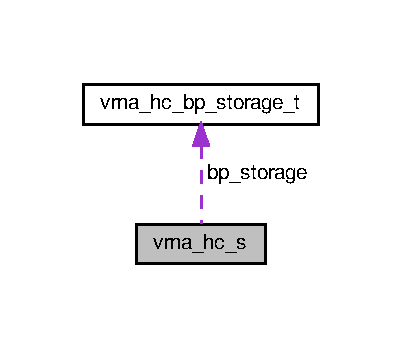
\includegraphics[width=193pt]{structvrna__hc__s__coll__graph}
\end{center}
\end{figure}
\subsubsection*{Data Fields}
\begin{DoxyCompactItemize}
\item 
\mbox{\Hypertarget{group__hard__constraints_a60094038af04093b2fee9b883266ff75}\label{group__hard__constraints_a60094038af04093b2fee9b883266ff75}} 
int $\ast$ \hyperlink{group__hard__constraints_a60094038af04093b2fee9b883266ff75}{up\+\_\+ext}
\begin{DoxyCompactList}\small\item\em A linear array that holds the number of allowed unpaired nucleotides in an exterior loop. \end{DoxyCompactList}\item 
\mbox{\Hypertarget{group__hard__constraints_a853255558e7e7d9eb382ac142ac8de3d}\label{group__hard__constraints_a853255558e7e7d9eb382ac142ac8de3d}} 
int $\ast$ \hyperlink{group__hard__constraints_a853255558e7e7d9eb382ac142ac8de3d}{up\+\_\+hp}
\begin{DoxyCompactList}\small\item\em A linear array that holds the number of allowed unpaired nucleotides in a hairpin loop. \end{DoxyCompactList}\item 
\mbox{\Hypertarget{group__hard__constraints_a455f994af0ec892d84fee1bf60d14a81}\label{group__hard__constraints_a455f994af0ec892d84fee1bf60d14a81}} 
int $\ast$ \hyperlink{group__hard__constraints_a455f994af0ec892d84fee1bf60d14a81}{up\+\_\+int}
\begin{DoxyCompactList}\small\item\em A linear array that holds the number of allowed unpaired nucleotides in an interior loop. \end{DoxyCompactList}\item 
\mbox{\Hypertarget{group__hard__constraints_aa318079c2e3cfaca8dc589cc478d3b29}\label{group__hard__constraints_aa318079c2e3cfaca8dc589cc478d3b29}} 
int $\ast$ \hyperlink{group__hard__constraints_aa318079c2e3cfaca8dc589cc478d3b29}{up\+\_\+ml}
\begin{DoxyCompactList}\small\item\em A linear array that holds the number of allowed unpaired nucleotides in a multi branched loop. \end{DoxyCompactList}\item 
\mbox{\Hypertarget{group__hard__constraints_a85714afbf27012165ec80c564bd62931}\label{group__hard__constraints_a85714afbf27012165ec80c564bd62931}} 
\hyperlink{group__hard__constraints_gae465f1d4a3d8b6592b38ecbb0d9f613d}{vrna\+\_\+callback\+\_\+hc\+\_\+evaluate} $\ast$ \hyperlink{group__hard__constraints_a85714afbf27012165ec80c564bd62931}{f}
\begin{DoxyCompactList}\small\item\em A function pointer that returns whether or not a certain decomposition may be evaluated. \end{DoxyCompactList}\item 
\mbox{\Hypertarget{group__hard__constraints_acef3d722142cb5f4a8e114e5fbce3b1a}\label{group__hard__constraints_acef3d722142cb5f4a8e114e5fbce3b1a}} 
void $\ast$ \hyperlink{group__hard__constraints_acef3d722142cb5f4a8e114e5fbce3b1a}{data}
\begin{DoxyCompactList}\small\item\em A pointer to some structure where the user may store necessary data to evaluate its generic hard constraint function. \end{DoxyCompactList}\item 
\hyperlink{group__fold__compound_ga7806651f51b195013839a218b3bbd5a3}{vrna\+\_\+callback\+\_\+free\+\_\+auxdata} $\ast$ \hyperlink{group__hard__constraints_a970e0e202c9e46ebc7640ddc43357ba6}{free\+\_\+data}
\begin{DoxyCompactList}\small\item\em A pointer to a function to free memory occupied by auxiliary data. \end{DoxyCompactList}\item 
\mbox{\Hypertarget{group__hard__constraints_a6ff99f530ca7ca9719e164321d051bde}\label{group__hard__constraints_a6ff99f530ca7ca9719e164321d051bde}} 
unsigned char $\ast$ \hyperlink{group__hard__constraints_a6ff99f530ca7ca9719e164321d051bde}{matrix}
\begin{DoxyCompactList}\small\item\em Upper triangular matrix that encodes where a base pair or unpaired nucleotide is allowed. \end{DoxyCompactList}\end{DoxyCompactItemize}


\paragraph{Field Documentation}
\mbox{\Hypertarget{group__hard__constraints_a970e0e202c9e46ebc7640ddc43357ba6}\label{group__hard__constraints_a970e0e202c9e46ebc7640ddc43357ba6}} 
\index{vrna\+\_\+hc\+\_\+s@{vrna\+\_\+hc\+\_\+s}!free\+\_\+data@{free\+\_\+data}}
\index{free\+\_\+data@{free\+\_\+data}!vrna\+\_\+hc\+\_\+s@{vrna\+\_\+hc\+\_\+s}}
\subparagraph{\texorpdfstring{free\+\_\+data}{free\_data}}
{\footnotesize\ttfamily \hyperlink{group__fold__compound_ga7806651f51b195013839a218b3bbd5a3}{vrna\+\_\+callback\+\_\+free\+\_\+auxdata}$\ast$ vrna\+\_\+hc\+\_\+s\+::free\+\_\+data}



A pointer to a function to free memory occupied by auxiliary data. 

The function this pointer is pointing to will be called upon destruction of the \hyperlink{group__hard__constraints_structvrna__hc__s}{vrna\+\_\+hc\+\_\+s}, and provided with the \hyperlink{group__hard__constraints_acef3d722142cb5f4a8e114e5fbce3b1a}{vrna\+\_\+hc\+\_\+s.\+data} pointer that may hold auxiliary data. Hence, to avoid leaking memory, the user may use this pointer to free memory occupied by auxiliary data. \index{vrna\+\_\+hc\+\_\+up\+\_\+s@{vrna\+\_\+hc\+\_\+up\+\_\+s}}\label{structvrna__hc__up__s}
\Hypertarget{group__hard__constraints_structvrna__hc__up__s}
\subsubsection{struct vrna\+\_\+hc\+\_\+up\+\_\+s}
A single hard constraint for a single nucleotide. \subsubsection*{Data Fields}
\begin{DoxyCompactItemize}
\item 
\mbox{\Hypertarget{group__hard__constraints_a67a98def263c534a8c57298098da16e8}\label{group__hard__constraints_a67a98def263c534a8c57298098da16e8}} 
int \hyperlink{group__hard__constraints_a67a98def263c534a8c57298098da16e8}{position}
\begin{DoxyCompactList}\small\item\em The sequence position (1-\/based) \end{DoxyCompactList}\item 
\mbox{\Hypertarget{group__hard__constraints_a468414760f373f7dc0eb1fd47cf708d0}\label{group__hard__constraints_a468414760f373f7dc0eb1fd47cf708d0}} 
unsigned char \hyperlink{group__hard__constraints_a468414760f373f7dc0eb1fd47cf708d0}{options}
\begin{DoxyCompactList}\small\item\em The hard constraint option. \end{DoxyCompactList}\end{DoxyCompactItemize}


\subsection{Macro Definition Documentation}
\mbox{\Hypertarget{group__hard__constraints_ga4bfc2f15c4f261c62a11af9d2aa80c90}\label{group__hard__constraints_ga4bfc2f15c4f261c62a11af9d2aa80c90}} 
\index{Hard Constraints@{Hard Constraints}!V\+R\+N\+A\+\_\+\+C\+O\+N\+S\+T\+R\+A\+I\+N\+T\+\_\+\+DB@{V\+R\+N\+A\+\_\+\+C\+O\+N\+S\+T\+R\+A\+I\+N\+T\+\_\+\+DB}}
\index{V\+R\+N\+A\+\_\+\+C\+O\+N\+S\+T\+R\+A\+I\+N\+T\+\_\+\+DB@{V\+R\+N\+A\+\_\+\+C\+O\+N\+S\+T\+R\+A\+I\+N\+T\+\_\+\+DB}!Hard Constraints@{Hard Constraints}}
\subsubsection{\texorpdfstring{V\+R\+N\+A\+\_\+\+C\+O\+N\+S\+T\+R\+A\+I\+N\+T\+\_\+\+DB}{VRNA\_CONSTRAINT\_DB}}
{\footnotesize\ttfamily \#define V\+R\+N\+A\+\_\+\+C\+O\+N\+S\+T\+R\+A\+I\+N\+T\+\_\+\+DB~16384U}



{\ttfamily \#include $<$\hyperlink{hard_8h}{Vienna\+R\+N\+A/constraints/hard.\+h}$>$}



Flag for \hyperlink{group__constraints_ga35a401f680969a556858a8dd5f1d07cc}{vrna\+\_\+constraints\+\_\+add()} to indicate that constraint is passed in pseudo dot-\/bracket notation. 

\begin{DoxySeeAlso}{See also}
\hyperlink{group__constraints_ga35a401f680969a556858a8dd5f1d07cc}{vrna\+\_\+constraints\+\_\+add()}, \hyperlink{group__constraints_gaa1f20b53bf09ac2e6b0dbb13f7d89670}{vrna\+\_\+message\+\_\+constraint\+\_\+options()}, \hyperlink{group__constraints_gaec7e13fa0465c2acc7a621d1aecb709f}{vrna\+\_\+message\+\_\+constraint\+\_\+options\+\_\+all()} 
\end{DoxySeeAlso}
\mbox{\Hypertarget{group__hard__constraints_ga29ebe940110d60ab798fdacbcdbbfb7d}\label{group__hard__constraints_ga29ebe940110d60ab798fdacbcdbbfb7d}} 
\index{Hard Constraints@{Hard Constraints}!V\+R\+N\+A\+\_\+\+C\+O\+N\+S\+T\+R\+A\+I\+N\+T\+\_\+\+D\+B\+\_\+\+E\+N\+F\+O\+R\+C\+E\+\_\+\+BP@{V\+R\+N\+A\+\_\+\+C\+O\+N\+S\+T\+R\+A\+I\+N\+T\+\_\+\+D\+B\+\_\+\+E\+N\+F\+O\+R\+C\+E\+\_\+\+BP}}
\index{V\+R\+N\+A\+\_\+\+C\+O\+N\+S\+T\+R\+A\+I\+N\+T\+\_\+\+D\+B\+\_\+\+E\+N\+F\+O\+R\+C\+E\+\_\+\+BP@{V\+R\+N\+A\+\_\+\+C\+O\+N\+S\+T\+R\+A\+I\+N\+T\+\_\+\+D\+B\+\_\+\+E\+N\+F\+O\+R\+C\+E\+\_\+\+BP}!Hard Constraints@{Hard Constraints}}
\subsubsection{\texorpdfstring{V\+R\+N\+A\+\_\+\+C\+O\+N\+S\+T\+R\+A\+I\+N\+T\+\_\+\+D\+B\+\_\+\+E\+N\+F\+O\+R\+C\+E\+\_\+\+BP}{VRNA\_CONSTRAINT\_DB\_ENFORCE\_BP}}
{\footnotesize\ttfamily \#define V\+R\+N\+A\+\_\+\+C\+O\+N\+S\+T\+R\+A\+I\+N\+T\+\_\+\+D\+B\+\_\+\+E\+N\+F\+O\+R\+C\+E\+\_\+\+BP~32768U}



{\ttfamily \#include $<$\hyperlink{hard_8h}{Vienna\+R\+N\+A/constraints/hard.\+h}$>$}



Switch for dot-\/bracket structure constraint to enforce base pairs. 

This flag should be used to really enforce base pairs given in dot-\/bracket constraint rather than just weakly-\/enforcing them.

\begin{DoxySeeAlso}{See also}
\hyperlink{group__hard__constraints_ga5b4de3247b67358080c176b94591a8e6}{vrna\+\_\+hc\+\_\+add\+\_\+from\+\_\+db()}, \hyperlink{group__constraints_ga35a401f680969a556858a8dd5f1d07cc}{vrna\+\_\+constraints\+\_\+add()}, \hyperlink{group__constraints_gaa1f20b53bf09ac2e6b0dbb13f7d89670}{vrna\+\_\+message\+\_\+constraint\+\_\+options()}, \hyperlink{group__constraints_gaec7e13fa0465c2acc7a621d1aecb709f}{vrna\+\_\+message\+\_\+constraint\+\_\+options\+\_\+all()} 
\end{DoxySeeAlso}
\mbox{\Hypertarget{group__hard__constraints_ga13053547a2de5532b64b64d35e097ae1}\label{group__hard__constraints_ga13053547a2de5532b64b64d35e097ae1}} 
\index{Hard Constraints@{Hard Constraints}!V\+R\+N\+A\+\_\+\+C\+O\+N\+S\+T\+R\+A\+I\+N\+T\+\_\+\+D\+B\+\_\+\+P\+I\+PE@{V\+R\+N\+A\+\_\+\+C\+O\+N\+S\+T\+R\+A\+I\+N\+T\+\_\+\+D\+B\+\_\+\+P\+I\+PE}}
\index{V\+R\+N\+A\+\_\+\+C\+O\+N\+S\+T\+R\+A\+I\+N\+T\+\_\+\+D\+B\+\_\+\+P\+I\+PE@{V\+R\+N\+A\+\_\+\+C\+O\+N\+S\+T\+R\+A\+I\+N\+T\+\_\+\+D\+B\+\_\+\+P\+I\+PE}!Hard Constraints@{Hard Constraints}}
\subsubsection{\texorpdfstring{V\+R\+N\+A\+\_\+\+C\+O\+N\+S\+T\+R\+A\+I\+N\+T\+\_\+\+D\+B\+\_\+\+P\+I\+PE}{VRNA\_CONSTRAINT\_DB\_PIPE}}
{\footnotesize\ttfamily \#define V\+R\+N\+A\+\_\+\+C\+O\+N\+S\+T\+R\+A\+I\+N\+T\+\_\+\+D\+B\+\_\+\+P\+I\+PE~65536U}



{\ttfamily \#include $<$\hyperlink{hard_8h}{Vienna\+R\+N\+A/constraints/hard.\+h}$>$}



Flag that is used to indicate the pipe \textquotesingle{}$\vert$\textquotesingle{} sign in pseudo dot-\/bracket notation of hard constraints. 

Use this definition to indicate the pipe sign \textquotesingle{}$\vert$\textquotesingle{} (paired with another base)

\begin{DoxySeeAlso}{See also}
\hyperlink{group__hard__constraints_ga5b4de3247b67358080c176b94591a8e6}{vrna\+\_\+hc\+\_\+add\+\_\+from\+\_\+db()}, \hyperlink{group__constraints_ga35a401f680969a556858a8dd5f1d07cc}{vrna\+\_\+constraints\+\_\+add()}, \hyperlink{group__constraints_gaa1f20b53bf09ac2e6b0dbb13f7d89670}{vrna\+\_\+message\+\_\+constraint\+\_\+options()}, \hyperlink{group__constraints_gaec7e13fa0465c2acc7a621d1aecb709f}{vrna\+\_\+message\+\_\+constraint\+\_\+options\+\_\+all()} 
\end{DoxySeeAlso}
\mbox{\Hypertarget{group__hard__constraints_ga369bea82eae75fbe626f409fa425747e}\label{group__hard__constraints_ga369bea82eae75fbe626f409fa425747e}} 
\index{Hard Constraints@{Hard Constraints}!V\+R\+N\+A\+\_\+\+C\+O\+N\+S\+T\+R\+A\+I\+N\+T\+\_\+\+D\+B\+\_\+\+D\+OT@{V\+R\+N\+A\+\_\+\+C\+O\+N\+S\+T\+R\+A\+I\+N\+T\+\_\+\+D\+B\+\_\+\+D\+OT}}
\index{V\+R\+N\+A\+\_\+\+C\+O\+N\+S\+T\+R\+A\+I\+N\+T\+\_\+\+D\+B\+\_\+\+D\+OT@{V\+R\+N\+A\+\_\+\+C\+O\+N\+S\+T\+R\+A\+I\+N\+T\+\_\+\+D\+B\+\_\+\+D\+OT}!Hard Constraints@{Hard Constraints}}
\subsubsection{\texorpdfstring{V\+R\+N\+A\+\_\+\+C\+O\+N\+S\+T\+R\+A\+I\+N\+T\+\_\+\+D\+B\+\_\+\+D\+OT}{VRNA\_CONSTRAINT\_DB\_DOT}}
{\footnotesize\ttfamily \#define V\+R\+N\+A\+\_\+\+C\+O\+N\+S\+T\+R\+A\+I\+N\+T\+\_\+\+D\+B\+\_\+\+D\+OT~131072U}



{\ttfamily \#include $<$\hyperlink{hard_8h}{Vienna\+R\+N\+A/constraints/hard.\+h}$>$}



dot \textquotesingle{}.\textquotesingle{} switch for structure constraints (no constraint at all) 

\begin{DoxySeeAlso}{See also}
\hyperlink{group__hard__constraints_ga5b4de3247b67358080c176b94591a8e6}{vrna\+\_\+hc\+\_\+add\+\_\+from\+\_\+db()}, \hyperlink{group__constraints_ga35a401f680969a556858a8dd5f1d07cc}{vrna\+\_\+constraints\+\_\+add()}, \hyperlink{group__constraints_gaa1f20b53bf09ac2e6b0dbb13f7d89670}{vrna\+\_\+message\+\_\+constraint\+\_\+options()}, \hyperlink{group__constraints_gaec7e13fa0465c2acc7a621d1aecb709f}{vrna\+\_\+message\+\_\+constraint\+\_\+options\+\_\+all()} 
\end{DoxySeeAlso}
\mbox{\Hypertarget{group__hard__constraints_ga7283bbe0f8954f7b030ecc3f2d1932b2}\label{group__hard__constraints_ga7283bbe0f8954f7b030ecc3f2d1932b2}} 
\index{Hard Constraints@{Hard Constraints}!V\+R\+N\+A\+\_\+\+C\+O\+N\+S\+T\+R\+A\+I\+N\+T\+\_\+\+D\+B\+\_\+X@{V\+R\+N\+A\+\_\+\+C\+O\+N\+S\+T\+R\+A\+I\+N\+T\+\_\+\+D\+B\+\_\+X}}
\index{V\+R\+N\+A\+\_\+\+C\+O\+N\+S\+T\+R\+A\+I\+N\+T\+\_\+\+D\+B\+\_\+X@{V\+R\+N\+A\+\_\+\+C\+O\+N\+S\+T\+R\+A\+I\+N\+T\+\_\+\+D\+B\+\_\+X}!Hard Constraints@{Hard Constraints}}
\subsubsection{\texorpdfstring{V\+R\+N\+A\+\_\+\+C\+O\+N\+S\+T\+R\+A\+I\+N\+T\+\_\+\+D\+B\+\_\+X}{VRNA\_CONSTRAINT\_DB\_X}}
{\footnotesize\ttfamily \#define V\+R\+N\+A\+\_\+\+C\+O\+N\+S\+T\+R\+A\+I\+N\+T\+\_\+\+D\+B\+\_\+X~262144U}



{\ttfamily \#include $<$\hyperlink{hard_8h}{Vienna\+R\+N\+A/constraints/hard.\+h}$>$}



\textquotesingle{}x\textquotesingle{} switch for structure constraint (base must not pair) 

\begin{DoxySeeAlso}{See also}
\hyperlink{group__hard__constraints_ga5b4de3247b67358080c176b94591a8e6}{vrna\+\_\+hc\+\_\+add\+\_\+from\+\_\+db()}, \hyperlink{group__constraints_ga35a401f680969a556858a8dd5f1d07cc}{vrna\+\_\+constraints\+\_\+add()}, \hyperlink{group__constraints_gaa1f20b53bf09ac2e6b0dbb13f7d89670}{vrna\+\_\+message\+\_\+constraint\+\_\+options()}, \hyperlink{group__constraints_gaec7e13fa0465c2acc7a621d1aecb709f}{vrna\+\_\+message\+\_\+constraint\+\_\+options\+\_\+all()} 
\end{DoxySeeAlso}
\mbox{\Hypertarget{group__hard__constraints_gac17b034852c914bc5879954c65d7e74b}\label{group__hard__constraints_gac17b034852c914bc5879954c65d7e74b}} 
\index{Hard Constraints@{Hard Constraints}!V\+R\+N\+A\+\_\+\+C\+O\+N\+S\+T\+R\+A\+I\+N\+T\+\_\+\+D\+B\+\_\+\+R\+N\+D\+\_\+\+B\+R\+A\+CK@{V\+R\+N\+A\+\_\+\+C\+O\+N\+S\+T\+R\+A\+I\+N\+T\+\_\+\+D\+B\+\_\+\+R\+N\+D\+\_\+\+B\+R\+A\+CK}}
\index{V\+R\+N\+A\+\_\+\+C\+O\+N\+S\+T\+R\+A\+I\+N\+T\+\_\+\+D\+B\+\_\+\+R\+N\+D\+\_\+\+B\+R\+A\+CK@{V\+R\+N\+A\+\_\+\+C\+O\+N\+S\+T\+R\+A\+I\+N\+T\+\_\+\+D\+B\+\_\+\+R\+N\+D\+\_\+\+B\+R\+A\+CK}!Hard Constraints@{Hard Constraints}}
\subsubsection{\texorpdfstring{V\+R\+N\+A\+\_\+\+C\+O\+N\+S\+T\+R\+A\+I\+N\+T\+\_\+\+D\+B\+\_\+\+R\+N\+D\+\_\+\+B\+R\+A\+CK}{VRNA\_CONSTRAINT\_DB\_RND\_BRACK}}
{\footnotesize\ttfamily \#define V\+R\+N\+A\+\_\+\+C\+O\+N\+S\+T\+R\+A\+I\+N\+T\+\_\+\+D\+B\+\_\+\+R\+N\+D\+\_\+\+B\+R\+A\+CK~1048576U}



{\ttfamily \#include $<$\hyperlink{hard_8h}{Vienna\+R\+N\+A/constraints/hard.\+h}$>$}



round brackets \textquotesingle{}(\textquotesingle{},\textquotesingle{})\textquotesingle{} switch for structure constraint (base i pairs base j) 

\begin{DoxySeeAlso}{See also}
\hyperlink{group__hard__constraints_ga5b4de3247b67358080c176b94591a8e6}{vrna\+\_\+hc\+\_\+add\+\_\+from\+\_\+db()}, \hyperlink{group__constraints_ga35a401f680969a556858a8dd5f1d07cc}{vrna\+\_\+constraints\+\_\+add()}, \hyperlink{group__constraints_gaa1f20b53bf09ac2e6b0dbb13f7d89670}{vrna\+\_\+message\+\_\+constraint\+\_\+options()}, \hyperlink{group__constraints_gaec7e13fa0465c2acc7a621d1aecb709f}{vrna\+\_\+message\+\_\+constraint\+\_\+options\+\_\+all()} 
\end{DoxySeeAlso}
\mbox{\Hypertarget{group__hard__constraints_ga5c17253f5a39d1d49b0fb11f5196982a}\label{group__hard__constraints_ga5c17253f5a39d1d49b0fb11f5196982a}} 
\index{Hard Constraints@{Hard Constraints}!V\+R\+N\+A\+\_\+\+C\+O\+N\+S\+T\+R\+A\+I\+N\+T\+\_\+\+D\+B\+\_\+\+I\+N\+T\+R\+A\+M\+OL@{V\+R\+N\+A\+\_\+\+C\+O\+N\+S\+T\+R\+A\+I\+N\+T\+\_\+\+D\+B\+\_\+\+I\+N\+T\+R\+A\+M\+OL}}
\index{V\+R\+N\+A\+\_\+\+C\+O\+N\+S\+T\+R\+A\+I\+N\+T\+\_\+\+D\+B\+\_\+\+I\+N\+T\+R\+A\+M\+OL@{V\+R\+N\+A\+\_\+\+C\+O\+N\+S\+T\+R\+A\+I\+N\+T\+\_\+\+D\+B\+\_\+\+I\+N\+T\+R\+A\+M\+OL}!Hard Constraints@{Hard Constraints}}
\subsubsection{\texorpdfstring{V\+R\+N\+A\+\_\+\+C\+O\+N\+S\+T\+R\+A\+I\+N\+T\+\_\+\+D\+B\+\_\+\+I\+N\+T\+R\+A\+M\+OL}{VRNA\_CONSTRAINT\_DB\_INTRAMOL}}
{\footnotesize\ttfamily \#define V\+R\+N\+A\+\_\+\+C\+O\+N\+S\+T\+R\+A\+I\+N\+T\+\_\+\+D\+B\+\_\+\+I\+N\+T\+R\+A\+M\+OL~2097152U}



{\ttfamily \#include $<$\hyperlink{hard_8h}{Vienna\+R\+N\+A/constraints/hard.\+h}$>$}



Flag that is used to indicate the character \textquotesingle{}l\textquotesingle{} in pseudo dot-\/bracket notation of hard constraints. 

Use this definition to indicate the usage of \textquotesingle{}l\textquotesingle{} character (intramolecular pairs only)

\begin{DoxySeeAlso}{See also}
\hyperlink{group__hard__constraints_ga5b4de3247b67358080c176b94591a8e6}{vrna\+\_\+hc\+\_\+add\+\_\+from\+\_\+db()}, \hyperlink{group__constraints_ga35a401f680969a556858a8dd5f1d07cc}{vrna\+\_\+constraints\+\_\+add()}, \hyperlink{group__constraints_gaa1f20b53bf09ac2e6b0dbb13f7d89670}{vrna\+\_\+message\+\_\+constraint\+\_\+options()}, \hyperlink{group__constraints_gaec7e13fa0465c2acc7a621d1aecb709f}{vrna\+\_\+message\+\_\+constraint\+\_\+options\+\_\+all()} 
\end{DoxySeeAlso}
\mbox{\Hypertarget{group__hard__constraints_ga31d0ebb9755ca8a4acafc14f00ca755d}\label{group__hard__constraints_ga31d0ebb9755ca8a4acafc14f00ca755d}} 
\index{Hard Constraints@{Hard Constraints}!V\+R\+N\+A\+\_\+\+C\+O\+N\+S\+T\+R\+A\+I\+N\+T\+\_\+\+D\+B\+\_\+\+I\+N\+T\+E\+R\+M\+OL@{V\+R\+N\+A\+\_\+\+C\+O\+N\+S\+T\+R\+A\+I\+N\+T\+\_\+\+D\+B\+\_\+\+I\+N\+T\+E\+R\+M\+OL}}
\index{V\+R\+N\+A\+\_\+\+C\+O\+N\+S\+T\+R\+A\+I\+N\+T\+\_\+\+D\+B\+\_\+\+I\+N\+T\+E\+R\+M\+OL@{V\+R\+N\+A\+\_\+\+C\+O\+N\+S\+T\+R\+A\+I\+N\+T\+\_\+\+D\+B\+\_\+\+I\+N\+T\+E\+R\+M\+OL}!Hard Constraints@{Hard Constraints}}
\subsubsection{\texorpdfstring{V\+R\+N\+A\+\_\+\+C\+O\+N\+S\+T\+R\+A\+I\+N\+T\+\_\+\+D\+B\+\_\+\+I\+N\+T\+E\+R\+M\+OL}{VRNA\_CONSTRAINT\_DB\_INTERMOL}}
{\footnotesize\ttfamily \#define V\+R\+N\+A\+\_\+\+C\+O\+N\+S\+T\+R\+A\+I\+N\+T\+\_\+\+D\+B\+\_\+\+I\+N\+T\+E\+R\+M\+OL~4194304U}



{\ttfamily \#include $<$\hyperlink{hard_8h}{Vienna\+R\+N\+A/constraints/hard.\+h}$>$}



Flag that is used to indicate the character \textquotesingle{}e\textquotesingle{} in pseudo dot-\/bracket notation of hard constraints. 

Use this definition to indicate the usage of \textquotesingle{}e\textquotesingle{} character (intermolecular pairs only)

\begin{DoxySeeAlso}{See also}
\hyperlink{group__hard__constraints_ga5b4de3247b67358080c176b94591a8e6}{vrna\+\_\+hc\+\_\+add\+\_\+from\+\_\+db()}, \hyperlink{group__constraints_ga35a401f680969a556858a8dd5f1d07cc}{vrna\+\_\+constraints\+\_\+add()}, \hyperlink{group__constraints_gaa1f20b53bf09ac2e6b0dbb13f7d89670}{vrna\+\_\+message\+\_\+constraint\+\_\+options()}, \hyperlink{group__constraints_gaec7e13fa0465c2acc7a621d1aecb709f}{vrna\+\_\+message\+\_\+constraint\+\_\+options\+\_\+all()} 
\end{DoxySeeAlso}
\mbox{\Hypertarget{group__hard__constraints_ga75cfab03cdc97c95b3ce8bb29f52b08e}\label{group__hard__constraints_ga75cfab03cdc97c95b3ce8bb29f52b08e}} 
\index{Hard Constraints@{Hard Constraints}!V\+R\+N\+A\+\_\+\+C\+O\+N\+S\+T\+R\+A\+I\+N\+T\+\_\+\+D\+B\+\_\+\+G\+Q\+U\+AD@{V\+R\+N\+A\+\_\+\+C\+O\+N\+S\+T\+R\+A\+I\+N\+T\+\_\+\+D\+B\+\_\+\+G\+Q\+U\+AD}}
\index{V\+R\+N\+A\+\_\+\+C\+O\+N\+S\+T\+R\+A\+I\+N\+T\+\_\+\+D\+B\+\_\+\+G\+Q\+U\+AD@{V\+R\+N\+A\+\_\+\+C\+O\+N\+S\+T\+R\+A\+I\+N\+T\+\_\+\+D\+B\+\_\+\+G\+Q\+U\+AD}!Hard Constraints@{Hard Constraints}}
\subsubsection{\texorpdfstring{V\+R\+N\+A\+\_\+\+C\+O\+N\+S\+T\+R\+A\+I\+N\+T\+\_\+\+D\+B\+\_\+\+G\+Q\+U\+AD}{VRNA\_CONSTRAINT\_DB\_GQUAD}}
{\footnotesize\ttfamily \#define V\+R\+N\+A\+\_\+\+C\+O\+N\+S\+T\+R\+A\+I\+N\+T\+\_\+\+D\+B\+\_\+\+G\+Q\+U\+AD~8388608U}



{\ttfamily \#include $<$\hyperlink{hard_8h}{Vienna\+R\+N\+A/constraints/hard.\+h}$>$}



\textquotesingle{}+\textquotesingle{} switch for structure constraint (base is involved in a gquad) 

\begin{DoxySeeAlso}{See also}
\hyperlink{group__hard__constraints_ga5b4de3247b67358080c176b94591a8e6}{vrna\+\_\+hc\+\_\+add\+\_\+from\+\_\+db()}, \hyperlink{group__constraints_ga35a401f680969a556858a8dd5f1d07cc}{vrna\+\_\+constraints\+\_\+add()}, \hyperlink{group__constraints_gaa1f20b53bf09ac2e6b0dbb13f7d89670}{vrna\+\_\+message\+\_\+constraint\+\_\+options()}, \hyperlink{group__constraints_gaec7e13fa0465c2acc7a621d1aecb709f}{vrna\+\_\+message\+\_\+constraint\+\_\+options\+\_\+all()}
\end{DoxySeeAlso}
\begin{DoxyWarning}{Warning}
This flag is for future purposes only! No implementation recognizes it yet. 
\end{DoxyWarning}
\mbox{\Hypertarget{group__hard__constraints_ga10ce6bd2355945f3c8161b7a30a2c322}\label{group__hard__constraints_ga10ce6bd2355945f3c8161b7a30a2c322}} 
\index{Hard Constraints@{Hard Constraints}!V\+R\+N\+A\+\_\+\+C\+O\+N\+S\+T\+R\+A\+I\+N\+T\+\_\+\+D\+B\+\_\+\+W\+U\+SS@{V\+R\+N\+A\+\_\+\+C\+O\+N\+S\+T\+R\+A\+I\+N\+T\+\_\+\+D\+B\+\_\+\+W\+U\+SS}}
\index{V\+R\+N\+A\+\_\+\+C\+O\+N\+S\+T\+R\+A\+I\+N\+T\+\_\+\+D\+B\+\_\+\+W\+U\+SS@{V\+R\+N\+A\+\_\+\+C\+O\+N\+S\+T\+R\+A\+I\+N\+T\+\_\+\+D\+B\+\_\+\+W\+U\+SS}!Hard Constraints@{Hard Constraints}}
\subsubsection{\texorpdfstring{V\+R\+N\+A\+\_\+\+C\+O\+N\+S\+T\+R\+A\+I\+N\+T\+\_\+\+D\+B\+\_\+\+W\+U\+SS}{VRNA\_CONSTRAINT\_DB\_WUSS}}
{\footnotesize\ttfamily \#define V\+R\+N\+A\+\_\+\+C\+O\+N\+S\+T\+R\+A\+I\+N\+T\+\_\+\+D\+B\+\_\+\+W\+U\+SS~33554432U}



{\ttfamily \#include $<$\hyperlink{hard_8h}{Vienna\+R\+N\+A/constraints/hard.\+h}$>$}



Flag to indicate Washington University Secondary Structure (W\+U\+SS) notation of the hard constraint string. 

This secondary structure notation for R\+N\+As is usually used as consensus secondary structure (S\+S\+\_\+cons) entry in Stockholm formatted files \mbox{\Hypertarget{group__hard__constraints_ga1c3864bdc92147a4d93de2b1b4356177}\label{group__hard__constraints_ga1c3864bdc92147a4d93de2b1b4356177}} 
\index{Hard Constraints@{Hard Constraints}!V\+R\+N\+A\+\_\+\+C\+O\+N\+S\+T\+R\+A\+I\+N\+T\+\_\+\+D\+B\+\_\+\+D\+E\+F\+A\+U\+LT@{V\+R\+N\+A\+\_\+\+C\+O\+N\+S\+T\+R\+A\+I\+N\+T\+\_\+\+D\+B\+\_\+\+D\+E\+F\+A\+U\+LT}}
\index{V\+R\+N\+A\+\_\+\+C\+O\+N\+S\+T\+R\+A\+I\+N\+T\+\_\+\+D\+B\+\_\+\+D\+E\+F\+A\+U\+LT@{V\+R\+N\+A\+\_\+\+C\+O\+N\+S\+T\+R\+A\+I\+N\+T\+\_\+\+D\+B\+\_\+\+D\+E\+F\+A\+U\+LT}!Hard Constraints@{Hard Constraints}}
\subsubsection{\texorpdfstring{V\+R\+N\+A\+\_\+\+C\+O\+N\+S\+T\+R\+A\+I\+N\+T\+\_\+\+D\+B\+\_\+\+D\+E\+F\+A\+U\+LT}{VRNA\_CONSTRAINT\_DB\_DEFAULT}}
{\footnotesize\ttfamily \#define V\+R\+N\+A\+\_\+\+C\+O\+N\+S\+T\+R\+A\+I\+N\+T\+\_\+\+D\+B\+\_\+\+D\+E\+F\+A\+U\+LT}



{\ttfamily \#include $<$\hyperlink{hard_8h}{Vienna\+R\+N\+A/constraints/hard.\+h}$>$}

{\bfseries Value\+:}
\begin{DoxyCode}
(\hyperlink{group__hard__constraints_ga4bfc2f15c4f261c62a11af9d2aa80c90}{VRNA\_CONSTRAINT\_DB} \(\backslash\)
   | \hyperlink{group__hard__constraints_ga13053547a2de5532b64b64d35e097ae1}{VRNA\_CONSTRAINT\_DB\_PIPE} \(\backslash\)
   | \hyperlink{group__hard__constraints_ga369bea82eae75fbe626f409fa425747e}{VRNA\_CONSTRAINT\_DB\_DOT} \(\backslash\)
   | \hyperlink{group__hard__constraints_ga7283bbe0f8954f7b030ecc3f2d1932b2}{VRNA\_CONSTRAINT\_DB\_X} \(\backslash\)
   | \hyperlink{hard_8h_ad54c1315a47d55653dcaa5de6e544b77}{VRNA\_CONSTRAINT\_DB\_ANG\_BRACK} \(\backslash\)
   | \hyperlink{group__hard__constraints_gac17b034852c914bc5879954c65d7e74b}{VRNA\_CONSTRAINT\_DB\_RND\_BRACK} \(\backslash\)
   | \hyperlink{group__hard__constraints_ga5c17253f5a39d1d49b0fb11f5196982a}{VRNA\_CONSTRAINT\_DB\_INTRAMOL} \(\backslash\)
   | \hyperlink{group__hard__constraints_ga31d0ebb9755ca8a4acafc14f00ca755d}{VRNA\_CONSTRAINT\_DB\_INTERMOL} \(\backslash\)
   | \hyperlink{group__hard__constraints_ga75cfab03cdc97c95b3ce8bb29f52b08e}{VRNA\_CONSTRAINT\_DB\_GQUAD} \(\backslash\)
  )
\end{DoxyCode}


Switch for dot-\/bracket structure constraint with default symbols. 

This flag conveniently combines all possible symbols in dot-\/bracket notation for hard constraints and \hyperlink{group__hard__constraints_ga4bfc2f15c4f261c62a11af9d2aa80c90}{V\+R\+N\+A\+\_\+\+C\+O\+N\+S\+T\+R\+A\+I\+N\+T\+\_\+\+DB}

\begin{DoxySeeAlso}{See also}
\hyperlink{group__hard__constraints_ga5b4de3247b67358080c176b94591a8e6}{vrna\+\_\+hc\+\_\+add\+\_\+from\+\_\+db()}, \hyperlink{group__constraints_ga35a401f680969a556858a8dd5f1d07cc}{vrna\+\_\+constraints\+\_\+add()}, \hyperlink{group__constraints_gaa1f20b53bf09ac2e6b0dbb13f7d89670}{vrna\+\_\+message\+\_\+constraint\+\_\+options()}, \hyperlink{group__constraints_gaec7e13fa0465c2acc7a621d1aecb709f}{vrna\+\_\+message\+\_\+constraint\+\_\+options\+\_\+all()} 
\end{DoxySeeAlso}


\subsection{Typedef Documentation}
\mbox{\Hypertarget{group__hard__constraints_gae465f1d4a3d8b6592b38ecbb0d9f613d}\label{group__hard__constraints_gae465f1d4a3d8b6592b38ecbb0d9f613d}} 
\index{Hard Constraints@{Hard Constraints}!vrna\+\_\+callback\+\_\+hc\+\_\+evaluate@{vrna\+\_\+callback\+\_\+hc\+\_\+evaluate}}
\index{vrna\+\_\+callback\+\_\+hc\+\_\+evaluate@{vrna\+\_\+callback\+\_\+hc\+\_\+evaluate}!Hard Constraints@{Hard Constraints}}
\subsubsection{\texorpdfstring{vrna\+\_\+callback\+\_\+hc\+\_\+evaluate}{vrna\_callback\_hc\_evaluate}}
{\footnotesize\ttfamily typedef unsigned char() vrna\+\_\+callback\+\_\+hc\+\_\+evaluate(int i, int j, int k, int l, unsigned char d, void $\ast$data)}



{\ttfamily \#include $<$\hyperlink{hard_8h}{Vienna\+R\+N\+A/constraints/hard.\+h}$>$}



Callback to evaluate whether or not a particular decomposition step is contributing to the solution space. 

This is the prototype for callback functions used by the folding recursions to evaluate generic hard constraints. The first four parameters passed indicate the delimiting nucleotide positions of the decomposition, and the parameter {\ttfamily denotes} the decomposition step. The last parameter {\ttfamily data} is the auxiliary data structure associated to the hard constraints via \hyperlink{hard_8h_a128920e0af52e4196a9d59fa13336c7c}{vrna\+\_\+hc\+\_\+add\+\_\+data()}, or N\+U\+LL if no auxiliary data was added.

\begin{DoxyRefDesc}{Notes on Callback Functions}
\item[\hyperlink{callbacks__callbacks000012}{Notes on Callback Functions}]This callback enables one to over-\/rule default hard constraints in secondary structure decompositions. \end{DoxyRefDesc}


\begin{DoxySeeAlso}{See also}
\hyperlink{group__constraints_ga8bd41ebc8039378d242e4e8c273716a5}{V\+R\+N\+A\+\_\+\+D\+E\+C\+O\+M\+P\+\_\+\+P\+A\+I\+R\+\_\+\+HP}, \hyperlink{group__constraints_gaeab04f34d7730cff2d651d782f95d857}{V\+R\+N\+A\+\_\+\+D\+E\+C\+O\+M\+P\+\_\+\+P\+A\+I\+R\+\_\+\+IL}, \hyperlink{group__constraints_gaa15b1185673f0b9e900c4748d45f388f}{V\+R\+N\+A\+\_\+\+D\+E\+C\+O\+M\+P\+\_\+\+P\+A\+I\+R\+\_\+\+ML}, \hyperlink{group__constraints_ga735517266f2e35e1374b8f1ea77ef23e}{V\+R\+N\+A\+\_\+\+D\+E\+C\+O\+M\+P\+\_\+\+M\+L\+\_\+\+M\+L\+\_\+\+ML}, \hyperlink{group__constraints_ga4a23054c75d8efc785de50e3ea87602f}{V\+R\+N\+A\+\_\+\+D\+E\+C\+O\+M\+P\+\_\+\+M\+L\+\_\+\+S\+T\+EM}, \hyperlink{group__constraints_ga7f4cb9ff7a33e67f0539bd39e7b19a78}{V\+R\+N\+A\+\_\+\+D\+E\+C\+O\+M\+P\+\_\+\+M\+L\+\_\+\+ML}, \hyperlink{group__constraints_gae6478dda14e50e2f2cb9ef333a29256e}{V\+R\+N\+A\+\_\+\+D\+E\+C\+O\+M\+P\+\_\+\+M\+L\+\_\+\+UP}, \hyperlink{group__constraints_ga63d8ceb8c96ae3b463e529e28cc0fe98}{V\+R\+N\+A\+\_\+\+D\+E\+C\+O\+M\+P\+\_\+\+M\+L\+\_\+\+M\+L\+\_\+\+S\+T\+EM}, \hyperlink{group__constraints_ga4fe48d575830b16c208e280e01ab1497}{V\+R\+N\+A\+\_\+\+D\+E\+C\+O\+M\+P\+\_\+\+M\+L\+\_\+\+C\+O\+A\+X\+I\+AL}, \hyperlink{group__constraints_ga437adf5115c1999304eff26b41e4c9b6}{V\+R\+N\+A\+\_\+\+D\+E\+C\+O\+M\+P\+\_\+\+E\+X\+T\+\_\+\+E\+XT}, \hyperlink{group__constraints_gaff1ddaffe86d984623910b40cc8a8717}{V\+R\+N\+A\+\_\+\+D\+E\+C\+O\+M\+P\+\_\+\+E\+X\+T\+\_\+\+UP}, \hyperlink{group__constraints_gae44b5ace0d9b4a29088069ecb4cec441}{V\+R\+N\+A\+\_\+\+D\+E\+C\+O\+M\+P\+\_\+\+E\+X\+T\+\_\+\+S\+T\+EM}, \hyperlink{group__constraints_ga803bd818b3f4b2b0a4a5cfa2f7dc2045}{V\+R\+N\+A\+\_\+\+D\+E\+C\+O\+M\+P\+\_\+\+E\+X\+T\+\_\+\+E\+X\+T\+\_\+\+E\+XT}, \hyperlink{group__constraints_gabb09c5b78b75a44502fc77b950125c1e}{V\+R\+N\+A\+\_\+\+D\+E\+C\+O\+M\+P\+\_\+\+E\+X\+T\+\_\+\+S\+T\+E\+M\+\_\+\+E\+XT}, \hyperlink{group__constraints_ga06efd054c9271438f6d82d4559d9e69f}{V\+R\+N\+A\+\_\+\+D\+E\+C\+O\+M\+P\+\_\+\+E\+X\+T\+\_\+\+E\+X\+T\+\_\+\+S\+T\+EM}, \hyperlink{group__constraints_ga2e75d7a77118735b32f25422d9686719}{V\+R\+N\+A\+\_\+\+D\+E\+C\+O\+M\+P\+\_\+\+E\+X\+T\+\_\+\+E\+X\+T\+\_\+\+S\+T\+E\+M1}, \hyperlink{hard_8h_af220427ba7ecc8e786a07b7799658f18}{vrna\+\_\+hc\+\_\+add\+\_\+f()}, \hyperlink{hard_8h_a128920e0af52e4196a9d59fa13336c7c}{vrna\+\_\+hc\+\_\+add\+\_\+data()}
\end{DoxySeeAlso}

\begin{DoxyParams}{Parameters}
{\em i} & Left (5\textquotesingle{}) delimiter position of substructure \\
\hline
{\em j} & Right (3\textquotesingle{}) delimiter position of substructure \\
\hline
{\em k} & Left delimiter of decomposition \\
\hline
{\em l} & Right delimiter of decomposition \\
\hline
{\em d} & Decomposition step indicator \\
\hline
{\em data} & Auxiliary data \\
\hline
\end{DoxyParams}
\begin{DoxyReturn}{Returns}
A non-\/zero value if the decomposition is valid, 0 otherwise 
\end{DoxyReturn}


\subsection{Function Documentation}
\mbox{\Hypertarget{group__hard__constraints_ga36ff456c43bf920629cee5a236e4f0ff}\label{group__hard__constraints_ga36ff456c43bf920629cee5a236e4f0ff}} 
\index{Hard Constraints@{Hard Constraints}!vrna\+\_\+hc\+\_\+init@{vrna\+\_\+hc\+\_\+init}}
\index{vrna\+\_\+hc\+\_\+init@{vrna\+\_\+hc\+\_\+init}!Hard Constraints@{Hard Constraints}}
\subsubsection{\texorpdfstring{vrna\+\_\+hc\+\_\+init()}{vrna\_hc\_init()}}
{\footnotesize\ttfamily void vrna\+\_\+hc\+\_\+init (\begin{DoxyParamCaption}\item[{\hyperlink{group__fold__compound_ga1b0cef17fd40466cef5968eaeeff6166}{vrna\+\_\+fold\+\_\+compound\+\_\+t} $\ast$}]{vc }\end{DoxyParamCaption})}



{\ttfamily \#include $<$\hyperlink{hard_8h}{Vienna\+R\+N\+A/constraints/hard.\+h}$>$}



Initialize/\+Reset hard constraints to default values. 

This function resets the hard constraints to their default values, i.\+e. all positions may be unpaired in all contexts, and base pairs are allowed in all contexts, if they resemble canonical pairs. Previously set hard constraints will be removed vefore initialization.

\begin{DoxySeeAlso}{See also}
\hyperlink{group__hard__constraints_ga7cba95ebe2ceb5ec9a5768f2232854fd}{vrna\+\_\+hc\+\_\+add\+\_\+bp()}, \hyperlink{group__hard__constraints_gaed50398ade2d4852c9e82592fe76046c}{vrna\+\_\+hc\+\_\+add\+\_\+bp\+\_\+nonspecific()}, \hyperlink{group__hard__constraints_ga447d88e06ad97bb225cd83310ace8345}{vrna\+\_\+hc\+\_\+add\+\_\+up()}
\end{DoxySeeAlso}

\begin{DoxyParams}{Parameters}
{\em vc} & The fold compound\\
\hline
\end{DoxyParams}
\begin{DoxyRefDesc}{S\+W\+I\+G Wrapper Notes}
\item[\hyperlink{wrappers__wrappers000012}{S\+W\+I\+G Wrapper Notes}]This function is attached as method {\bfseries hc\+\_\+init()} to objects of type {\itshape fold\+\_\+compound} \end{DoxyRefDesc}
\mbox{\Hypertarget{group__hard__constraints_ga447d88e06ad97bb225cd83310ace8345}\label{group__hard__constraints_ga447d88e06ad97bb225cd83310ace8345}} 
\index{Hard Constraints@{Hard Constraints}!vrna\+\_\+hc\+\_\+add\+\_\+up@{vrna\+\_\+hc\+\_\+add\+\_\+up}}
\index{vrna\+\_\+hc\+\_\+add\+\_\+up@{vrna\+\_\+hc\+\_\+add\+\_\+up}!Hard Constraints@{Hard Constraints}}
\subsubsection{\texorpdfstring{vrna\+\_\+hc\+\_\+add\+\_\+up()}{vrna\_hc\_add\_up()}}
{\footnotesize\ttfamily void vrna\+\_\+hc\+\_\+add\+\_\+up (\begin{DoxyParamCaption}\item[{\hyperlink{group__fold__compound_ga1b0cef17fd40466cef5968eaeeff6166}{vrna\+\_\+fold\+\_\+compound\+\_\+t} $\ast$}]{vc,  }\item[{int}]{i,  }\item[{unsigned char}]{option }\end{DoxyParamCaption})}



{\ttfamily \#include $<$\hyperlink{hard_8h}{Vienna\+R\+N\+A/constraints/hard.\+h}$>$}



Make a certain nucleotide unpaired. 

\begin{DoxySeeAlso}{See also}
\hyperlink{group__hard__constraints_ga7cba95ebe2ceb5ec9a5768f2232854fd}{vrna\+\_\+hc\+\_\+add\+\_\+bp()}, \hyperlink{group__hard__constraints_gaed50398ade2d4852c9e82592fe76046c}{vrna\+\_\+hc\+\_\+add\+\_\+bp\+\_\+nonspecific()}, \hyperlink{group__hard__constraints_ga36ff456c43bf920629cee5a236e4f0ff}{vrna\+\_\+hc\+\_\+init()}, \hyperlink{group__hard__constraints_ga9418eda62a5dec070896702c279d2548}{V\+R\+N\+A\+\_\+\+C\+O\+N\+S\+T\+R\+A\+I\+N\+T\+\_\+\+C\+O\+N\+T\+E\+X\+T\+\_\+\+E\+X\+T\+\_\+\+L\+O\+OP}, \hyperlink{group__hard__constraints_ga79203702b197b6b9d3b78eed40663eb1}{V\+R\+N\+A\+\_\+\+C\+O\+N\+S\+T\+R\+A\+I\+N\+T\+\_\+\+C\+O\+N\+T\+E\+X\+T\+\_\+\+H\+P\+\_\+\+L\+O\+OP}, \hyperlink{group__hard__constraints_ga21feeab3a9e5fa5a9e3d9ac0fcf5994f}{V\+R\+N\+A\+\_\+\+C\+O\+N\+S\+T\+R\+A\+I\+N\+T\+\_\+\+C\+O\+N\+T\+E\+X\+T\+\_\+\+I\+N\+T\+\_\+\+L\+O\+OP}, \hyperlink{group__hard__constraints_ga456ecd2ff00056bb64da8dd4f61bbfc5}{V\+R\+N\+A\+\_\+\+C\+O\+N\+S\+T\+R\+A\+I\+N\+T\+\_\+\+C\+O\+N\+T\+E\+X\+T\+\_\+\+M\+B\+\_\+\+L\+O\+OP}, \hyperlink{group__hard__constraints_ga886d9127c49bb982a4b67cd7581e8a5a}{V\+R\+N\+A\+\_\+\+C\+O\+N\+S\+T\+R\+A\+I\+N\+T\+\_\+\+C\+O\+N\+T\+E\+X\+T\+\_\+\+A\+L\+L\+\_\+\+L\+O\+O\+PS}
\end{DoxySeeAlso}

\begin{DoxyParams}{Parameters}
{\em vc} & The \hyperlink{group__fold__compound_ga1b0cef17fd40466cef5968eaeeff6166}{vrna\+\_\+fold\+\_\+compound\+\_\+t} the hard constraints are associated with \\
\hline
{\em i} & The position that needs to stay unpaired (1-\/based) \\
\hline
{\em option} & The options flag indicating how/where to store the hard constraints \\
\hline
\end{DoxyParams}
\mbox{\Hypertarget{group__hard__constraints_ga5070f296c8af2baea10951525519464f}\label{group__hard__constraints_ga5070f296c8af2baea10951525519464f}} 
\index{Hard Constraints@{Hard Constraints}!vrna\+\_\+hc\+\_\+add\+\_\+up\+\_\+batch@{vrna\+\_\+hc\+\_\+add\+\_\+up\+\_\+batch}}
\index{vrna\+\_\+hc\+\_\+add\+\_\+up\+\_\+batch@{vrna\+\_\+hc\+\_\+add\+\_\+up\+\_\+batch}!Hard Constraints@{Hard Constraints}}
\subsubsection{\texorpdfstring{vrna\+\_\+hc\+\_\+add\+\_\+up\+\_\+batch()}{vrna\_hc\_add\_up\_batch()}}
{\footnotesize\ttfamily int vrna\+\_\+hc\+\_\+add\+\_\+up\+\_\+batch (\begin{DoxyParamCaption}\item[{\hyperlink{group__fold__compound_ga1b0cef17fd40466cef5968eaeeff6166}{vrna\+\_\+fold\+\_\+compound\+\_\+t} $\ast$}]{vc,  }\item[{\hyperlink{group__hard__constraints_ga8cd53427a942a81c87ec526bbff32ef9}{vrna\+\_\+hc\+\_\+up\+\_\+t} $\ast$}]{constraints }\end{DoxyParamCaption})}



{\ttfamily \#include $<$\hyperlink{hard_8h}{Vienna\+R\+N\+A/constraints/hard.\+h}$>$}



Apply a list of hard constraints for single nucleotides. 


\begin{DoxyParams}{Parameters}
{\em vc} & The \hyperlink{group__fold__compound_ga1b0cef17fd40466cef5968eaeeff6166}{vrna\+\_\+fold\+\_\+compound\+\_\+t} the hard constraints are associated with \\
\hline
{\em constraints} & The list off constraints to apply, last entry must have position attribute set to 0 \\
\hline
\end{DoxyParams}
\mbox{\Hypertarget{group__hard__constraints_ga7cba95ebe2ceb5ec9a5768f2232854fd}\label{group__hard__constraints_ga7cba95ebe2ceb5ec9a5768f2232854fd}} 
\index{Hard Constraints@{Hard Constraints}!vrna\+\_\+hc\+\_\+add\+\_\+bp@{vrna\+\_\+hc\+\_\+add\+\_\+bp}}
\index{vrna\+\_\+hc\+\_\+add\+\_\+bp@{vrna\+\_\+hc\+\_\+add\+\_\+bp}!Hard Constraints@{Hard Constraints}}
\subsubsection{\texorpdfstring{vrna\+\_\+hc\+\_\+add\+\_\+bp()}{vrna\_hc\_add\_bp()}}
{\footnotesize\ttfamily void vrna\+\_\+hc\+\_\+add\+\_\+bp (\begin{DoxyParamCaption}\item[{\hyperlink{group__fold__compound_ga1b0cef17fd40466cef5968eaeeff6166}{vrna\+\_\+fold\+\_\+compound\+\_\+t} $\ast$}]{vc,  }\item[{int}]{i,  }\item[{int}]{j,  }\item[{unsigned char}]{option }\end{DoxyParamCaption})}



{\ttfamily \#include $<$\hyperlink{hard_8h}{Vienna\+R\+N\+A/constraints/hard.\+h}$>$}



Favorize/\+Enforce a certain base pair (i,j) 

\begin{DoxySeeAlso}{See also}
\hyperlink{group__hard__constraints_gaed50398ade2d4852c9e82592fe76046c}{vrna\+\_\+hc\+\_\+add\+\_\+bp\+\_\+nonspecific()}, \hyperlink{group__hard__constraints_ga447d88e06ad97bb225cd83310ace8345}{vrna\+\_\+hc\+\_\+add\+\_\+up()}, \hyperlink{group__hard__constraints_ga36ff456c43bf920629cee5a236e4f0ff}{vrna\+\_\+hc\+\_\+init()}, \hyperlink{group__hard__constraints_ga9418eda62a5dec070896702c279d2548}{V\+R\+N\+A\+\_\+\+C\+O\+N\+S\+T\+R\+A\+I\+N\+T\+\_\+\+C\+O\+N\+T\+E\+X\+T\+\_\+\+E\+X\+T\+\_\+\+L\+O\+OP}, \hyperlink{group__hard__constraints_ga79203702b197b6b9d3b78eed40663eb1}{V\+R\+N\+A\+\_\+\+C\+O\+N\+S\+T\+R\+A\+I\+N\+T\+\_\+\+C\+O\+N\+T\+E\+X\+T\+\_\+\+H\+P\+\_\+\+L\+O\+OP}, \hyperlink{group__hard__constraints_ga21feeab3a9e5fa5a9e3d9ac0fcf5994f}{V\+R\+N\+A\+\_\+\+C\+O\+N\+S\+T\+R\+A\+I\+N\+T\+\_\+\+C\+O\+N\+T\+E\+X\+T\+\_\+\+I\+N\+T\+\_\+\+L\+O\+OP}, \hyperlink{group__hard__constraints_ga0536288e04ff6332ecdc23ca4705402b}{V\+R\+N\+A\+\_\+\+C\+O\+N\+S\+T\+R\+A\+I\+N\+T\+\_\+\+C\+O\+N\+T\+E\+X\+T\+\_\+\+I\+N\+T\+\_\+\+L\+O\+O\+P\+\_\+\+E\+NC}, \hyperlink{group__hard__constraints_ga456ecd2ff00056bb64da8dd4f61bbfc5}{V\+R\+N\+A\+\_\+\+C\+O\+N\+S\+T\+R\+A\+I\+N\+T\+\_\+\+C\+O\+N\+T\+E\+X\+T\+\_\+\+M\+B\+\_\+\+L\+O\+OP}, \hyperlink{group__hard__constraints_ga02a3d703ddbcfce393e4bbfcb9db7077}{V\+R\+N\+A\+\_\+\+C\+O\+N\+S\+T\+R\+A\+I\+N\+T\+\_\+\+C\+O\+N\+T\+E\+X\+T\+\_\+\+M\+B\+\_\+\+L\+O\+O\+P\+\_\+\+E\+NC}, \hyperlink{hard_8h_a1aa55f2c6347e670e003b1a765632dad}{V\+R\+N\+A\+\_\+\+C\+O\+N\+S\+T\+R\+A\+I\+N\+T\+\_\+\+C\+O\+N\+T\+E\+X\+T\+\_\+\+E\+N\+F\+O\+R\+CE}, \hyperlink{group__hard__constraints_ga886d9127c49bb982a4b67cd7581e8a5a}{V\+R\+N\+A\+\_\+\+C\+O\+N\+S\+T\+R\+A\+I\+N\+T\+\_\+\+C\+O\+N\+T\+E\+X\+T\+\_\+\+A\+L\+L\+\_\+\+L\+O\+O\+PS}
\end{DoxySeeAlso}

\begin{DoxyParams}{Parameters}
{\em vc} & The \hyperlink{group__fold__compound_ga1b0cef17fd40466cef5968eaeeff6166}{vrna\+\_\+fold\+\_\+compound\+\_\+t} the hard constraints are associated with \\
\hline
{\em i} & The 5\textquotesingle{} located nucleotide position of the base pair (1-\/based) \\
\hline
{\em j} & The 3\textquotesingle{} located nucleotide position of the base pair (1-\/based) \\
\hline
{\em option} & The options flag indicating how/where to store the hard constraints \\
\hline
\end{DoxyParams}
\mbox{\Hypertarget{group__hard__constraints_gaed50398ade2d4852c9e82592fe76046c}\label{group__hard__constraints_gaed50398ade2d4852c9e82592fe76046c}} 
\index{Hard Constraints@{Hard Constraints}!vrna\+\_\+hc\+\_\+add\+\_\+bp\+\_\+nonspecific@{vrna\+\_\+hc\+\_\+add\+\_\+bp\+\_\+nonspecific}}
\index{vrna\+\_\+hc\+\_\+add\+\_\+bp\+\_\+nonspecific@{vrna\+\_\+hc\+\_\+add\+\_\+bp\+\_\+nonspecific}!Hard Constraints@{Hard Constraints}}
\subsubsection{\texorpdfstring{vrna\+\_\+hc\+\_\+add\+\_\+bp\+\_\+nonspecific()}{vrna\_hc\_add\_bp\_nonspecific()}}
{\footnotesize\ttfamily void vrna\+\_\+hc\+\_\+add\+\_\+bp\+\_\+nonspecific (\begin{DoxyParamCaption}\item[{\hyperlink{group__fold__compound_ga1b0cef17fd40466cef5968eaeeff6166}{vrna\+\_\+fold\+\_\+compound\+\_\+t} $\ast$}]{vc,  }\item[{int}]{i,  }\item[{int}]{d,  }\item[{unsigned char}]{option }\end{DoxyParamCaption})}



{\ttfamily \#include $<$\hyperlink{hard_8h}{Vienna\+R\+N\+A/constraints/hard.\+h}$>$}



Enforce a nucleotide to be paired (upstream/downstream) 

\begin{DoxySeeAlso}{See also}
\hyperlink{group__hard__constraints_ga7cba95ebe2ceb5ec9a5768f2232854fd}{vrna\+\_\+hc\+\_\+add\+\_\+bp()}, \hyperlink{group__hard__constraints_ga447d88e06ad97bb225cd83310ace8345}{vrna\+\_\+hc\+\_\+add\+\_\+up()}, \hyperlink{group__hard__constraints_ga36ff456c43bf920629cee5a236e4f0ff}{vrna\+\_\+hc\+\_\+init()}, \hyperlink{group__hard__constraints_ga9418eda62a5dec070896702c279d2548}{V\+R\+N\+A\+\_\+\+C\+O\+N\+S\+T\+R\+A\+I\+N\+T\+\_\+\+C\+O\+N\+T\+E\+X\+T\+\_\+\+E\+X\+T\+\_\+\+L\+O\+OP}, \hyperlink{group__hard__constraints_ga79203702b197b6b9d3b78eed40663eb1}{V\+R\+N\+A\+\_\+\+C\+O\+N\+S\+T\+R\+A\+I\+N\+T\+\_\+\+C\+O\+N\+T\+E\+X\+T\+\_\+\+H\+P\+\_\+\+L\+O\+OP}, \hyperlink{group__hard__constraints_ga21feeab3a9e5fa5a9e3d9ac0fcf5994f}{V\+R\+N\+A\+\_\+\+C\+O\+N\+S\+T\+R\+A\+I\+N\+T\+\_\+\+C\+O\+N\+T\+E\+X\+T\+\_\+\+I\+N\+T\+\_\+\+L\+O\+OP}, \hyperlink{group__hard__constraints_ga0536288e04ff6332ecdc23ca4705402b}{V\+R\+N\+A\+\_\+\+C\+O\+N\+S\+T\+R\+A\+I\+N\+T\+\_\+\+C\+O\+N\+T\+E\+X\+T\+\_\+\+I\+N\+T\+\_\+\+L\+O\+O\+P\+\_\+\+E\+NC}, \hyperlink{group__hard__constraints_ga456ecd2ff00056bb64da8dd4f61bbfc5}{V\+R\+N\+A\+\_\+\+C\+O\+N\+S\+T\+R\+A\+I\+N\+T\+\_\+\+C\+O\+N\+T\+E\+X\+T\+\_\+\+M\+B\+\_\+\+L\+O\+OP}, \hyperlink{group__hard__constraints_ga02a3d703ddbcfce393e4bbfcb9db7077}{V\+R\+N\+A\+\_\+\+C\+O\+N\+S\+T\+R\+A\+I\+N\+T\+\_\+\+C\+O\+N\+T\+E\+X\+T\+\_\+\+M\+B\+\_\+\+L\+O\+O\+P\+\_\+\+E\+NC}, \hyperlink{group__hard__constraints_ga886d9127c49bb982a4b67cd7581e8a5a}{V\+R\+N\+A\+\_\+\+C\+O\+N\+S\+T\+R\+A\+I\+N\+T\+\_\+\+C\+O\+N\+T\+E\+X\+T\+\_\+\+A\+L\+L\+\_\+\+L\+O\+O\+PS}
\end{DoxySeeAlso}

\begin{DoxyParams}{Parameters}
{\em vc} & The \hyperlink{group__fold__compound_ga1b0cef17fd40466cef5968eaeeff6166}{vrna\+\_\+fold\+\_\+compound\+\_\+t} the hard constraints are associated with \\
\hline
{\em i} & The position that needs to stay unpaired (1-\/based) \\
\hline
{\em d} & The direction of base pairing ( $ d < 0 $\+: pairs upstream, $ d > 0 $\+: pairs downstream, $ d == 0 $\+: no direction) \\
\hline
{\em option} & The options flag indicating in which loop type context the pairs may appear \\
\hline
\end{DoxyParams}
\mbox{\Hypertarget{group__hard__constraints_ga696dcf77887d856c6f21ea266d8b9ca2}\label{group__hard__constraints_ga696dcf77887d856c6f21ea266d8b9ca2}} 
\index{Hard Constraints@{Hard Constraints}!vrna\+\_\+hc\+\_\+free@{vrna\+\_\+hc\+\_\+free}}
\index{vrna\+\_\+hc\+\_\+free@{vrna\+\_\+hc\+\_\+free}!Hard Constraints@{Hard Constraints}}
\subsubsection{\texorpdfstring{vrna\+\_\+hc\+\_\+free()}{vrna\_hc\_free()}}
{\footnotesize\ttfamily void vrna\+\_\+hc\+\_\+free (\begin{DoxyParamCaption}\item[{\hyperlink{group__hard__constraints_gac7e4c4f8abe3163a68110c5bff24e01d}{vrna\+\_\+hc\+\_\+t} $\ast$}]{hc }\end{DoxyParamCaption})}



{\ttfamily \#include $<$\hyperlink{hard_8h}{Vienna\+R\+N\+A/constraints/hard.\+h}$>$}



Free the memory allocated by a \hyperlink{group__hard__constraints_gac7e4c4f8abe3163a68110c5bff24e01d}{vrna\+\_\+hc\+\_\+t} data structure. 

Use this function to free all memory that was allocated for a data structure of type \hyperlink{group__hard__constraints_gac7e4c4f8abe3163a68110c5bff24e01d}{vrna\+\_\+hc\+\_\+t} .

\begin{DoxySeeAlso}{See also}
get\+\_\+hard\+\_\+constraints(), \hyperlink{group__hard__constraints_gac7e4c4f8abe3163a68110c5bff24e01d}{vrna\+\_\+hc\+\_\+t} 
\end{DoxySeeAlso}
\mbox{\Hypertarget{group__hard__constraints_ga5b4de3247b67358080c176b94591a8e6}\label{group__hard__constraints_ga5b4de3247b67358080c176b94591a8e6}} 
\index{Hard Constraints@{Hard Constraints}!vrna\+\_\+hc\+\_\+add\+\_\+from\+\_\+db@{vrna\+\_\+hc\+\_\+add\+\_\+from\+\_\+db}}
\index{vrna\+\_\+hc\+\_\+add\+\_\+from\+\_\+db@{vrna\+\_\+hc\+\_\+add\+\_\+from\+\_\+db}!Hard Constraints@{Hard Constraints}}
\subsubsection{\texorpdfstring{vrna\+\_\+hc\+\_\+add\+\_\+from\+\_\+db()}{vrna\_hc\_add\_from\_db()}}
{\footnotesize\ttfamily int vrna\+\_\+hc\+\_\+add\+\_\+from\+\_\+db (\begin{DoxyParamCaption}\item[{\hyperlink{group__fold__compound_ga1b0cef17fd40466cef5968eaeeff6166}{vrna\+\_\+fold\+\_\+compound\+\_\+t} $\ast$}]{vc,  }\item[{const char $\ast$}]{constraint,  }\item[{unsigned int}]{options }\end{DoxyParamCaption})}



{\ttfamily \#include $<$\hyperlink{hard_8h}{Vienna\+R\+N\+A/constraints/hard.\+h}$>$}



Add hard constraints from pseudo dot-\/bracket notation. 

This function allows one to apply hard constraints from a pseudo dot-\/bracket notation. The {\ttfamily options} parameter controls, which characters are recognized by the parser. Use the \hyperlink{group__hard__constraints_ga1c3864bdc92147a4d93de2b1b4356177}{V\+R\+N\+A\+\_\+\+C\+O\+N\+S\+T\+R\+A\+I\+N\+T\+\_\+\+D\+B\+\_\+\+D\+E\+F\+A\+U\+LT} convenience macro, if you want to allow all known characters

\begin{DoxySeeAlso}{See also}
\hyperlink{group__hard__constraints_ga13053547a2de5532b64b64d35e097ae1}{V\+R\+N\+A\+\_\+\+C\+O\+N\+S\+T\+R\+A\+I\+N\+T\+\_\+\+D\+B\+\_\+\+P\+I\+PE}, \hyperlink{group__hard__constraints_ga369bea82eae75fbe626f409fa425747e}{V\+R\+N\+A\+\_\+\+C\+O\+N\+S\+T\+R\+A\+I\+N\+T\+\_\+\+D\+B\+\_\+\+D\+OT}, \hyperlink{group__hard__constraints_ga7283bbe0f8954f7b030ecc3f2d1932b2}{V\+R\+N\+A\+\_\+\+C\+O\+N\+S\+T\+R\+A\+I\+N\+T\+\_\+\+D\+B\+\_\+X}, \hyperlink{hard_8h_ad54c1315a47d55653dcaa5de6e544b77}{V\+R\+N\+A\+\_\+\+C\+O\+N\+S\+T\+R\+A\+I\+N\+T\+\_\+\+D\+B\+\_\+\+A\+N\+G\+\_\+\+B\+R\+A\+CK}, \hyperlink{group__hard__constraints_gac17b034852c914bc5879954c65d7e74b}{V\+R\+N\+A\+\_\+\+C\+O\+N\+S\+T\+R\+A\+I\+N\+T\+\_\+\+D\+B\+\_\+\+R\+N\+D\+\_\+\+B\+R\+A\+CK}, \hyperlink{group__hard__constraints_ga5c17253f5a39d1d49b0fb11f5196982a}{V\+R\+N\+A\+\_\+\+C\+O\+N\+S\+T\+R\+A\+I\+N\+T\+\_\+\+D\+B\+\_\+\+I\+N\+T\+R\+A\+M\+OL}, \hyperlink{group__hard__constraints_ga31d0ebb9755ca8a4acafc14f00ca755d}{V\+R\+N\+A\+\_\+\+C\+O\+N\+S\+T\+R\+A\+I\+N\+T\+\_\+\+D\+B\+\_\+\+I\+N\+T\+E\+R\+M\+OL}, \hyperlink{group__hard__constraints_ga75cfab03cdc97c95b3ce8bb29f52b08e}{V\+R\+N\+A\+\_\+\+C\+O\+N\+S\+T\+R\+A\+I\+N\+T\+\_\+\+D\+B\+\_\+\+G\+Q\+U\+AD}
\end{DoxySeeAlso}

\begin{DoxyParams}{Parameters}
{\em vc} & The fold compound \\
\hline
{\em constraint} & A pseudo dot-\/bracket notation of the hard constraint. \\
\hline
{\em options} & The option flags\\
\hline
\end{DoxyParams}
\begin{DoxyRefDesc}{S\+W\+I\+G Wrapper Notes}
\item[\hyperlink{wrappers__wrappers000016}{S\+W\+I\+G Wrapper Notes}]This function is attached as method {\bfseries hc\+\_\+add\+\_\+from\+\_\+db()} to objects of type {\itshape fold\+\_\+compound} \end{DoxyRefDesc}

\hypertarget{group__soft__constraints}{}\section{Soft Constraints}
\label{group__soft__constraints}\index{Soft Constraints@{Soft Constraints}}


Functions and data structures for secondary structure soft constraints.  




\subsection{Detailed Description}
Functions and data structures for secondary structure soft constraints. 

Soft-\/constraints are used to change position specific contributions in the recursions by adding bonuses/penalties in form of pseudo free energies to certain loop configurations. Collaboration diagram for Soft Constraints\+:
\nopagebreak
\begin{figure}[H]
\begin{center}
\leavevmode
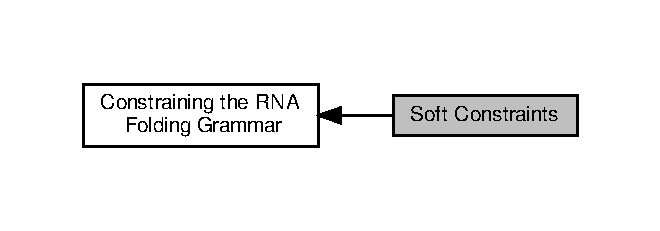
\includegraphics[width=317pt]{group__soft__constraints}
\end{center}
\end{figure}
\subsection*{Files}
\begin{DoxyCompactItemize}
\item 
file \hyperlink{soft_8h}{soft.\+h}
\begin{DoxyCompactList}\small\item\em Functions and data structures for secondary structure soft constraints. \end{DoxyCompactList}\end{DoxyCompactItemize}
\subsection*{Data Structures}
\begin{DoxyCompactItemize}
\item 
struct \hyperlink{group__soft__constraints_structvrna__sc__s}{vrna\+\_\+sc\+\_\+s}
\begin{DoxyCompactList}\small\item\em The soft constraints data structure.  \hyperlink{group__soft__constraints_structvrna__sc__s}{More...}\end{DoxyCompactList}\end{DoxyCompactItemize}
\subsection*{Typedefs}
\begin{DoxyCompactItemize}
\item 
\mbox{\Hypertarget{group__soft__constraints_ga75401ce219ef8dbcceb672db82d434c6}\label{group__soft__constraints_ga75401ce219ef8dbcceb672db82d434c6}} 
typedef struct \hyperlink{group__soft__constraints_structvrna__sc__s}{vrna\+\_\+sc\+\_\+s} \hyperlink{group__soft__constraints_ga75401ce219ef8dbcceb672db82d434c6}{vrna\+\_\+sc\+\_\+t}
\begin{DoxyCompactList}\small\item\em Typename for the soft constraints data structure \hyperlink{group__soft__constraints_structvrna__sc__s}{vrna\+\_\+sc\+\_\+s}. \end{DoxyCompactList}\item 
typedef int() \hyperlink{group__soft__constraints_ga88a266695d9e25cc12114dceb7b4565e}{vrna\+\_\+callback\+\_\+sc\+\_\+energy}(int i, int j, int k, int l, unsigned char d, void $\ast$data)
\begin{DoxyCompactList}\small\item\em Callback to retrieve pseudo energy contribution for soft constraint feature. \end{DoxyCompactList}\item 
typedef \hyperlink{group__data__structures_ga31125aeace516926bf7f251f759b6126}{F\+L\+T\+\_\+\+O\+R\+\_\+\+D\+BL}() \hyperlink{group__soft__constraints_ga4099978d410513edeeff8f3db13144c5}{vrna\+\_\+callback\+\_\+sc\+\_\+exp\+\_\+energy}(int i, int j, int k, int l, unsigned char d, void $\ast$data)
\begin{DoxyCompactList}\small\item\em Callback to retrieve pseudo energy contribution as Boltzmann Factors for soft constraint feature. \end{DoxyCompactList}\item 
typedef \hyperlink{group__data__structures_gac8c5669d3fb813cacf506489689305ce}{vrna\+\_\+basepair\+\_\+t} $\ast$() \hyperlink{group__soft__constraints_gaeb6448da6c593d4c489c7fbadcb99499}{vrna\+\_\+callback\+\_\+sc\+\_\+backtrack}(int i, int j, int k, int l, unsigned char d, void $\ast$data)
\begin{DoxyCompactList}\small\item\em Callback to retrieve auxiliary base pairs for soft constraint feature. \end{DoxyCompactList}\end{DoxyCompactItemize}
\subsection*{Functions}
\begin{DoxyCompactItemize}
\item 
void \hyperlink{group__soft__constraints_ga9d977a1681356778cc66dceafbe5b032}{vrna\+\_\+sc\+\_\+init} (\hyperlink{group__fold__compound_ga1b0cef17fd40466cef5968eaeeff6166}{vrna\+\_\+fold\+\_\+compound\+\_\+t} $\ast$vc)
\begin{DoxyCompactList}\small\item\em Initialize an empty soft constraints data structure within a \hyperlink{group__fold__compound_ga1b0cef17fd40466cef5968eaeeff6166}{vrna\+\_\+fold\+\_\+compound\+\_\+t}. \end{DoxyCompactList}\item 
void \hyperlink{group__soft__constraints_ga8e4334b24bc91453fbcda490a4e331af}{vrna\+\_\+sc\+\_\+set\+\_\+bp} (\hyperlink{group__fold__compound_ga1b0cef17fd40466cef5968eaeeff6166}{vrna\+\_\+fold\+\_\+compound\+\_\+t} $\ast$vc, const \hyperlink{group__data__structures_ga31125aeace516926bf7f251f759b6126}{F\+L\+T\+\_\+\+O\+R\+\_\+\+D\+BL} $\ast$$\ast$constraints, unsigned int options)
\begin{DoxyCompactList}\small\item\em Set soft constraints for paired nucleotides. \end{DoxyCompactList}\item 
void \hyperlink{group__soft__constraints_gaf162aedac7422f2eb16ea030f47d2f4b}{vrna\+\_\+sc\+\_\+add\+\_\+bp} (\hyperlink{group__fold__compound_ga1b0cef17fd40466cef5968eaeeff6166}{vrna\+\_\+fold\+\_\+compound\+\_\+t} $\ast$vc, int i, int j, \hyperlink{group__data__structures_ga31125aeace516926bf7f251f759b6126}{F\+L\+T\+\_\+\+O\+R\+\_\+\+D\+BL} energy, unsigned int options)
\begin{DoxyCompactList}\small\item\em Add soft constraints for paired nucleotides. \end{DoxyCompactList}\item 
void \hyperlink{group__soft__constraints_ga99ed63f3ef9e7fe3997932030487a344}{vrna\+\_\+sc\+\_\+set\+\_\+up} (\hyperlink{group__fold__compound_ga1b0cef17fd40466cef5968eaeeff6166}{vrna\+\_\+fold\+\_\+compound\+\_\+t} $\ast$vc, const \hyperlink{group__data__structures_ga31125aeace516926bf7f251f759b6126}{F\+L\+T\+\_\+\+O\+R\+\_\+\+D\+BL} $\ast$constraints, unsigned int options)
\begin{DoxyCompactList}\small\item\em Set soft constraints for unpaired nucleotides. \end{DoxyCompactList}\item 
void \hyperlink{group__soft__constraints_ga069915fe203a2c8e522dd37847177a09}{vrna\+\_\+sc\+\_\+add\+\_\+up} (\hyperlink{group__fold__compound_ga1b0cef17fd40466cef5968eaeeff6166}{vrna\+\_\+fold\+\_\+compound\+\_\+t} $\ast$vc, int i, \hyperlink{group__data__structures_ga31125aeace516926bf7f251f759b6126}{F\+L\+T\+\_\+\+O\+R\+\_\+\+D\+BL} energy, unsigned int options)
\begin{DoxyCompactList}\small\item\em Add soft constraints for unpaired nucleotides. \end{DoxyCompactList}\item 
void \hyperlink{group__soft__constraints_ga73cdc07b9a199c614367bebef0f2c41a}{vrna\+\_\+sc\+\_\+remove} (\hyperlink{group__fold__compound_ga1b0cef17fd40466cef5968eaeeff6166}{vrna\+\_\+fold\+\_\+compound\+\_\+t} $\ast$vc)
\begin{DoxyCompactList}\small\item\em Remove soft constraints from \hyperlink{group__fold__compound_ga1b0cef17fd40466cef5968eaeeff6166}{vrna\+\_\+fold\+\_\+compound\+\_\+t}. \end{DoxyCompactList}\item 
void \hyperlink{group__soft__constraints_ga6d55446448d69346fc313b993c4fb3e8}{vrna\+\_\+sc\+\_\+free} (\hyperlink{group__soft__constraints_ga75401ce219ef8dbcceb672db82d434c6}{vrna\+\_\+sc\+\_\+t} $\ast$sc)
\begin{DoxyCompactList}\small\item\em Free memory occupied by a \hyperlink{group__soft__constraints_ga75401ce219ef8dbcceb672db82d434c6}{vrna\+\_\+sc\+\_\+t} data structure. \end{DoxyCompactList}\item 
void \hyperlink{group__soft__constraints_ga15c6d52471ec97897e2bb7f964f5deb6}{vrna\+\_\+sc\+\_\+add\+\_\+data} (\hyperlink{group__fold__compound_ga1b0cef17fd40466cef5968eaeeff6166}{vrna\+\_\+fold\+\_\+compound\+\_\+t} $\ast$vc, void $\ast$data, \hyperlink{group__fold__compound_ga7806651f51b195013839a218b3bbd5a3}{vrna\+\_\+callback\+\_\+free\+\_\+auxdata} $\ast$free\+\_\+data)
\begin{DoxyCompactList}\small\item\em Add an auxiliary data structure for the generic soft constraints callback function. \end{DoxyCompactList}\item 
void \hyperlink{group__soft__constraints_ga8c7d907ec0125cd61c04e0908010a4e9}{vrna\+\_\+sc\+\_\+add\+\_\+f} (\hyperlink{group__fold__compound_ga1b0cef17fd40466cef5968eaeeff6166}{vrna\+\_\+fold\+\_\+compound\+\_\+t} $\ast$vc, \hyperlink{group__soft__constraints_ga88a266695d9e25cc12114dceb7b4565e}{vrna\+\_\+callback\+\_\+sc\+\_\+energy} $\ast$f)
\begin{DoxyCompactList}\small\item\em Bind a function pointer for generic soft constraint feature (M\+FE version) \end{DoxyCompactList}\item 
void \hyperlink{group__soft__constraints_gabde7d07a79bb9a8f4721aee247b674ea}{vrna\+\_\+sc\+\_\+add\+\_\+bt} (\hyperlink{group__fold__compound_ga1b0cef17fd40466cef5968eaeeff6166}{vrna\+\_\+fold\+\_\+compound\+\_\+t} $\ast$vc, \hyperlink{group__soft__constraints_gaeb6448da6c593d4c489c7fbadcb99499}{vrna\+\_\+callback\+\_\+sc\+\_\+backtrack} $\ast$f)
\begin{DoxyCompactList}\small\item\em Bind a backtracking function pointer for generic soft constraint feature. \end{DoxyCompactList}\item 
void \hyperlink{group__soft__constraints_ga87e382b5d0c9b7d9ce1b79c0473ff700}{vrna\+\_\+sc\+\_\+add\+\_\+exp\+\_\+f} (\hyperlink{group__fold__compound_ga1b0cef17fd40466cef5968eaeeff6166}{vrna\+\_\+fold\+\_\+compound\+\_\+t} $\ast$vc, \hyperlink{group__soft__constraints_ga4099978d410513edeeff8f3db13144c5}{vrna\+\_\+callback\+\_\+sc\+\_\+exp\+\_\+energy} $\ast$exp\+\_\+f)
\begin{DoxyCompactList}\small\item\em Bind a function pointer for generic soft constraint feature (PF version) \end{DoxyCompactList}\end{DoxyCompactItemize}


\subsection{Data Structure Documentation}
\index{vrna\+\_\+sc\+\_\+s@{vrna\+\_\+sc\+\_\+s}}\label{structvrna__sc__s}
\Hypertarget{group__soft__constraints_structvrna__sc__s}
\subsubsection{struct vrna\+\_\+sc\+\_\+s}
The soft constraints data structure. 

Collaboration diagram for vrna\+\_\+sc\+\_\+s\+:
\nopagebreak
\begin{figure}[H]
\begin{center}
\leavevmode
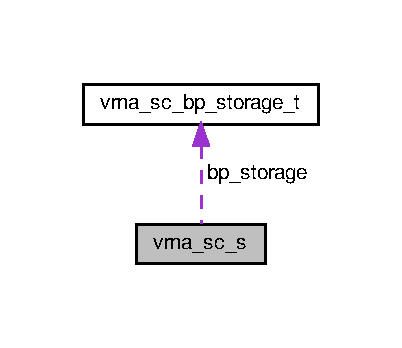
\includegraphics[width=193pt]{structvrna__sc__s__coll__graph}
\end{center}
\end{figure}
\subsubsection*{Data Fields}
\begin{DoxyCompactItemize}
\item 
\mbox{\Hypertarget{group__soft__constraints_a57e4dbb924ab11f304e3762a3a9b07a1}\label{group__soft__constraints_a57e4dbb924ab11f304e3762a3a9b07a1}} 
int $\ast$$\ast$ \hyperlink{group__soft__constraints_a57e4dbb924ab11f304e3762a3a9b07a1}{energy\+\_\+up}
\begin{DoxyCompactList}\small\item\em Energy contribution for stretches of unpaired nucleotides. \end{DoxyCompactList}\item 
\mbox{\Hypertarget{group__soft__constraints_ad3b4972d3b6c23865587e4ac56a37375}\label{group__soft__constraints_ad3b4972d3b6c23865587e4ac56a37375}} 
\hyperlink{group__data__structures_ga31125aeace516926bf7f251f759b6126}{F\+L\+T\+\_\+\+O\+R\+\_\+\+D\+BL} $\ast$$\ast$ \hyperlink{group__soft__constraints_ad3b4972d3b6c23865587e4ac56a37375}{exp\+\_\+energy\+\_\+up}
\begin{DoxyCompactList}\small\item\em Boltzmann Factors of the energy contributions for unpaired sequence stretches. \end{DoxyCompactList}\item 
\mbox{\Hypertarget{group__soft__constraints_a16c564d3170b7357620860de1e5faed6}\label{group__soft__constraints_a16c564d3170b7357620860de1e5faed6}} 
int $\ast$ \hyperlink{group__soft__constraints_a16c564d3170b7357620860de1e5faed6}{up\+\_\+storage}
\begin{DoxyCompactList}\small\item\em Storage container for energy contributions per unpaired nucleotide. \end{DoxyCompactList}\item 
\mbox{\Hypertarget{group__soft__constraints_a8e261e29462f6bdba3259e5eb61e48e8}\label{group__soft__constraints_a8e261e29462f6bdba3259e5eb61e48e8}} 
\hyperlink{structvrna__sc__bp__storage__t}{vrna\+\_\+sc\+\_\+bp\+\_\+storage\+\_\+t} $\ast$$\ast$ \hyperlink{group__soft__constraints_a8e261e29462f6bdba3259e5eb61e48e8}{bp\+\_\+storage}
\begin{DoxyCompactList}\small\item\em Storage container for energy contributions per base pair. \end{DoxyCompactList}\item 
\mbox{\Hypertarget{group__soft__constraints_ac20dded6068e81acd0f1139092f66a22}\label{group__soft__constraints_ac20dded6068e81acd0f1139092f66a22}} 
int $\ast$ \hyperlink{group__soft__constraints_ac20dded6068e81acd0f1139092f66a22}{energy\+\_\+stack}
\begin{DoxyCompactList}\small\item\em Pseudo Energy contribution per base pair involved in a stack. \end{DoxyCompactList}\item 
\mbox{\Hypertarget{group__soft__constraints_a4a0058fe3d5ba3416f0aaab677610115}\label{group__soft__constraints_a4a0058fe3d5ba3416f0aaab677610115}} 
\hyperlink{group__data__structures_ga31125aeace516926bf7f251f759b6126}{F\+L\+T\+\_\+\+O\+R\+\_\+\+D\+BL} $\ast$ \hyperlink{group__soft__constraints_a4a0058fe3d5ba3416f0aaab677610115}{exp\+\_\+energy\+\_\+stack}
\begin{DoxyCompactList}\small\item\em Boltzmann weighted pseudo energy contribution per nucleotide involved in a stack. \end{DoxyCompactList}\item 
\hyperlink{group__soft__constraints_ga88a266695d9e25cc12114dceb7b4565e}{vrna\+\_\+callback\+\_\+sc\+\_\+energy} $\ast$ \hyperlink{group__soft__constraints_a32dc86090237888c75491bbd4861a04b}{f}
\begin{DoxyCompactList}\small\item\em A function pointer used for pseudo energy contribution in M\+FE calculations. \end{DoxyCompactList}\item 
\hyperlink{group__soft__constraints_gaeb6448da6c593d4c489c7fbadcb99499}{vrna\+\_\+callback\+\_\+sc\+\_\+backtrack} $\ast$ \hyperlink{group__soft__constraints_a2a2aca01782c2b980d7b7fd05b9be89c}{bt}
\begin{DoxyCompactList}\small\item\em A function pointer used to obtain backtraced base pairs in loop regions that were altered by soft constrained pseudo energy contributions. \end{DoxyCompactList}\item 
\hyperlink{group__soft__constraints_ga4099978d410513edeeff8f3db13144c5}{vrna\+\_\+callback\+\_\+sc\+\_\+exp\+\_\+energy} $\ast$ \hyperlink{group__soft__constraints_a0de08a09f3ccf2f97974d23192668ab0}{exp\+\_\+f}
\begin{DoxyCompactList}\small\item\em A function pointer used for pseudo energy contribution boltzmann factors in PF calculations. \end{DoxyCompactList}\item 
\mbox{\Hypertarget{group__soft__constraints_a7574680143df97b9029146c2150bf06d}\label{group__soft__constraints_a7574680143df97b9029146c2150bf06d}} 
void $\ast$ \hyperlink{group__soft__constraints_a7574680143df97b9029146c2150bf06d}{data}
\begin{DoxyCompactList}\small\item\em A pointer to the data object provided for for pseudo energy contribution functions of the generic soft constraints feature. \end{DoxyCompactList}\item 
\mbox{\Hypertarget{group__soft__constraints_ad139b8e06632e00cbcf3909815d0d03d}\label{group__soft__constraints_ad139b8e06632e00cbcf3909815d0d03d}} 
int $\ast$ \hyperlink{group__soft__constraints_ad139b8e06632e00cbcf3909815d0d03d}{energy\+\_\+bp}
\begin{DoxyCompactList}\small\item\em Energy contribution for base pairs. \end{DoxyCompactList}\item 
\mbox{\Hypertarget{group__soft__constraints_a62c22be478cd630541c91f73e6cb0d75}\label{group__soft__constraints_a62c22be478cd630541c91f73e6cb0d75}} 
\hyperlink{group__data__structures_ga31125aeace516926bf7f251f759b6126}{F\+L\+T\+\_\+\+O\+R\+\_\+\+D\+BL} $\ast$ \hyperlink{group__soft__constraints_a62c22be478cd630541c91f73e6cb0d75}{exp\+\_\+energy\+\_\+bp}
\begin{DoxyCompactList}\small\item\em Boltzmann Factors of the energy contribution for base pairs. \end{DoxyCompactList}\item 
\mbox{\Hypertarget{group__soft__constraints_ad939d2511afe7b3db9b802fdeff2bac4}\label{group__soft__constraints_ad939d2511afe7b3db9b802fdeff2bac4}} 
int $\ast$$\ast$ \hyperlink{group__soft__constraints_ad939d2511afe7b3db9b802fdeff2bac4}{energy\+\_\+bp\+\_\+local}
\begin{DoxyCompactList}\small\item\em Energy contribution for base pairs (sliding window approach) \end{DoxyCompactList}\item 
\mbox{\Hypertarget{group__soft__constraints_a6d882019efc1e09d385ef751765b3a80}\label{group__soft__constraints_a6d882019efc1e09d385ef751765b3a80}} 
\hyperlink{group__data__structures_ga31125aeace516926bf7f251f759b6126}{F\+L\+T\+\_\+\+O\+R\+\_\+\+D\+BL} $\ast$$\ast$ \hyperlink{group__soft__constraints_a6d882019efc1e09d385ef751765b3a80}{exp\+\_\+energy\+\_\+bp\+\_\+local}
\begin{DoxyCompactList}\small\item\em Boltzmann Factors of the energy contribution for base pairs (sliding window approach) \end{DoxyCompactList}\end{DoxyCompactItemize}


\paragraph{Field Documentation}
\mbox{\Hypertarget{group__soft__constraints_a32dc86090237888c75491bbd4861a04b}\label{group__soft__constraints_a32dc86090237888c75491bbd4861a04b}} 
\index{vrna\+\_\+sc\+\_\+s@{vrna\+\_\+sc\+\_\+s}!f@{f}}
\index{f@{f}!vrna\+\_\+sc\+\_\+s@{vrna\+\_\+sc\+\_\+s}}
\subparagraph{\texorpdfstring{f}{f}}
{\footnotesize\ttfamily \hyperlink{group__soft__constraints_ga88a266695d9e25cc12114dceb7b4565e}{vrna\+\_\+callback\+\_\+sc\+\_\+energy}$\ast$ vrna\+\_\+sc\+\_\+s\+::f}



A function pointer used for pseudo energy contribution in M\+FE calculations. 

\begin{DoxySeeAlso}{See also}
\hyperlink{group__soft__constraints_ga8c7d907ec0125cd61c04e0908010a4e9}{vrna\+\_\+sc\+\_\+add\+\_\+f()} 
\end{DoxySeeAlso}
\mbox{\Hypertarget{group__soft__constraints_a2a2aca01782c2b980d7b7fd05b9be89c}\label{group__soft__constraints_a2a2aca01782c2b980d7b7fd05b9be89c}} 
\index{vrna\+\_\+sc\+\_\+s@{vrna\+\_\+sc\+\_\+s}!bt@{bt}}
\index{bt@{bt}!vrna\+\_\+sc\+\_\+s@{vrna\+\_\+sc\+\_\+s}}
\subparagraph{\texorpdfstring{bt}{bt}}
{\footnotesize\ttfamily \hyperlink{group__soft__constraints_gaeb6448da6c593d4c489c7fbadcb99499}{vrna\+\_\+callback\+\_\+sc\+\_\+backtrack}$\ast$ vrna\+\_\+sc\+\_\+s\+::bt}



A function pointer used to obtain backtraced base pairs in loop regions that were altered by soft constrained pseudo energy contributions. 

\begin{DoxySeeAlso}{See also}
\hyperlink{group__soft__constraints_gabde7d07a79bb9a8f4721aee247b674ea}{vrna\+\_\+sc\+\_\+add\+\_\+bt()} 
\end{DoxySeeAlso}
\mbox{\Hypertarget{group__soft__constraints_a0de08a09f3ccf2f97974d23192668ab0}\label{group__soft__constraints_a0de08a09f3ccf2f97974d23192668ab0}} 
\index{vrna\+\_\+sc\+\_\+s@{vrna\+\_\+sc\+\_\+s}!exp\+\_\+f@{exp\+\_\+f}}
\index{exp\+\_\+f@{exp\+\_\+f}!vrna\+\_\+sc\+\_\+s@{vrna\+\_\+sc\+\_\+s}}
\subparagraph{\texorpdfstring{exp\+\_\+f}{exp\_f}}
{\footnotesize\ttfamily \hyperlink{group__soft__constraints_ga4099978d410513edeeff8f3db13144c5}{vrna\+\_\+callback\+\_\+sc\+\_\+exp\+\_\+energy}$\ast$ vrna\+\_\+sc\+\_\+s\+::exp\+\_\+f}



A function pointer used for pseudo energy contribution boltzmann factors in PF calculations. 

\begin{DoxySeeAlso}{See also}
\hyperlink{group__soft__constraints_ga87e382b5d0c9b7d9ce1b79c0473ff700}{vrna\+\_\+sc\+\_\+add\+\_\+exp\+\_\+f()} 
\end{DoxySeeAlso}


\subsection{Typedef Documentation}
\mbox{\Hypertarget{group__soft__constraints_ga88a266695d9e25cc12114dceb7b4565e}\label{group__soft__constraints_ga88a266695d9e25cc12114dceb7b4565e}} 
\index{Soft Constraints@{Soft Constraints}!vrna\+\_\+callback\+\_\+sc\+\_\+energy@{vrna\+\_\+callback\+\_\+sc\+\_\+energy}}
\index{vrna\+\_\+callback\+\_\+sc\+\_\+energy@{vrna\+\_\+callback\+\_\+sc\+\_\+energy}!Soft Constraints@{Soft Constraints}}
\subsubsection{\texorpdfstring{vrna\+\_\+callback\+\_\+sc\+\_\+energy}{vrna\_callback\_sc\_energy}}
{\footnotesize\ttfamily typedef int() vrna\+\_\+callback\+\_\+sc\+\_\+energy(int i, int j, int k, int l, unsigned char d, void $\ast$data)}



{\ttfamily \#include $<$\hyperlink{soft_8h}{Vienna\+R\+N\+A/constraints/soft.\+h}$>$}



Callback to retrieve pseudo energy contribution for soft constraint feature. 

This is the prototype for callback functions used by the folding recursions to evaluate generic soft constraints. The first four parameters passed indicate the delimiting nucleotide positions of the decomposition, and the parameter {\ttfamily denotes} the decomposition step. The last parameter {\ttfamily data} is the auxiliary data structure associated to the hard constraints via \hyperlink{group__soft__constraints_ga15c6d52471ec97897e2bb7f964f5deb6}{vrna\+\_\+sc\+\_\+add\+\_\+data()}, or N\+U\+LL if no auxiliary data was added.

\begin{DoxyRefDesc}{Notes on Callback Functions}
\item[\hyperlink{callbacks__callbacks000013}{Notes on Callback Functions}]This callback enables one to add (pseudo-\/)energy contributions to individual decompositions of the secondary structure. \end{DoxyRefDesc}


\begin{DoxySeeAlso}{See also}
\hyperlink{group__constraints_ga8bd41ebc8039378d242e4e8c273716a5}{V\+R\+N\+A\+\_\+\+D\+E\+C\+O\+M\+P\+\_\+\+P\+A\+I\+R\+\_\+\+HP}, \hyperlink{group__constraints_gaeab04f34d7730cff2d651d782f95d857}{V\+R\+N\+A\+\_\+\+D\+E\+C\+O\+M\+P\+\_\+\+P\+A\+I\+R\+\_\+\+IL}, \hyperlink{group__constraints_gaa15b1185673f0b9e900c4748d45f388f}{V\+R\+N\+A\+\_\+\+D\+E\+C\+O\+M\+P\+\_\+\+P\+A\+I\+R\+\_\+\+ML}, \hyperlink{group__constraints_ga735517266f2e35e1374b8f1ea77ef23e}{V\+R\+N\+A\+\_\+\+D\+E\+C\+O\+M\+P\+\_\+\+M\+L\+\_\+\+M\+L\+\_\+\+ML}, \hyperlink{group__constraints_ga4a23054c75d8efc785de50e3ea87602f}{V\+R\+N\+A\+\_\+\+D\+E\+C\+O\+M\+P\+\_\+\+M\+L\+\_\+\+S\+T\+EM}, \hyperlink{group__constraints_ga7f4cb9ff7a33e67f0539bd39e7b19a78}{V\+R\+N\+A\+\_\+\+D\+E\+C\+O\+M\+P\+\_\+\+M\+L\+\_\+\+ML}, \hyperlink{group__constraints_gae6478dda14e50e2f2cb9ef333a29256e}{V\+R\+N\+A\+\_\+\+D\+E\+C\+O\+M\+P\+\_\+\+M\+L\+\_\+\+UP}, \hyperlink{group__constraints_ga63d8ceb8c96ae3b463e529e28cc0fe98}{V\+R\+N\+A\+\_\+\+D\+E\+C\+O\+M\+P\+\_\+\+M\+L\+\_\+\+M\+L\+\_\+\+S\+T\+EM}, \hyperlink{group__constraints_ga4fe48d575830b16c208e280e01ab1497}{V\+R\+N\+A\+\_\+\+D\+E\+C\+O\+M\+P\+\_\+\+M\+L\+\_\+\+C\+O\+A\+X\+I\+AL}, \hyperlink{group__constraints_ga437adf5115c1999304eff26b41e4c9b6}{V\+R\+N\+A\+\_\+\+D\+E\+C\+O\+M\+P\+\_\+\+E\+X\+T\+\_\+\+E\+XT}, \hyperlink{group__constraints_gaff1ddaffe86d984623910b40cc8a8717}{V\+R\+N\+A\+\_\+\+D\+E\+C\+O\+M\+P\+\_\+\+E\+X\+T\+\_\+\+UP}, \hyperlink{group__constraints_gae44b5ace0d9b4a29088069ecb4cec441}{V\+R\+N\+A\+\_\+\+D\+E\+C\+O\+M\+P\+\_\+\+E\+X\+T\+\_\+\+S\+T\+EM}, \hyperlink{group__constraints_ga803bd818b3f4b2b0a4a5cfa2f7dc2045}{V\+R\+N\+A\+\_\+\+D\+E\+C\+O\+M\+P\+\_\+\+E\+X\+T\+\_\+\+E\+X\+T\+\_\+\+E\+XT}, \hyperlink{group__constraints_gabb09c5b78b75a44502fc77b950125c1e}{V\+R\+N\+A\+\_\+\+D\+E\+C\+O\+M\+P\+\_\+\+E\+X\+T\+\_\+\+S\+T\+E\+M\+\_\+\+E\+XT}, \hyperlink{group__constraints_ga06efd054c9271438f6d82d4559d9e69f}{V\+R\+N\+A\+\_\+\+D\+E\+C\+O\+M\+P\+\_\+\+E\+X\+T\+\_\+\+E\+X\+T\+\_\+\+S\+T\+EM}, \hyperlink{group__constraints_ga2e75d7a77118735b32f25422d9686719}{V\+R\+N\+A\+\_\+\+D\+E\+C\+O\+M\+P\+\_\+\+E\+X\+T\+\_\+\+E\+X\+T\+\_\+\+S\+T\+E\+M1}, \hyperlink{group__soft__constraints_ga8c7d907ec0125cd61c04e0908010a4e9}{vrna\+\_\+sc\+\_\+add\+\_\+f()}, \hyperlink{group__soft__constraints_ga87e382b5d0c9b7d9ce1b79c0473ff700}{vrna\+\_\+sc\+\_\+add\+\_\+exp\+\_\+f()}, \hyperlink{group__soft__constraints_gabde7d07a79bb9a8f4721aee247b674ea}{vrna\+\_\+sc\+\_\+add\+\_\+bt()}, \hyperlink{group__soft__constraints_ga15c6d52471ec97897e2bb7f964f5deb6}{vrna\+\_\+sc\+\_\+add\+\_\+data()}
\end{DoxySeeAlso}

\begin{DoxyParams}{Parameters}
{\em i} & Left (5\textquotesingle{}) delimiter position of substructure \\
\hline
{\em j} & Right (3\textquotesingle{}) delimiter position of substructure \\
\hline
{\em k} & Left delimiter of decomposition \\
\hline
{\em l} & Right delimiter of decomposition \\
\hline
{\em d} & Decomposition step indicator \\
\hline
{\em data} & Auxiliary data \\
\hline
\end{DoxyParams}
\begin{DoxyReturn}{Returns}
Pseudo energy contribution in deka-\/kalories per mol 
\end{DoxyReturn}
\mbox{\Hypertarget{group__soft__constraints_ga4099978d410513edeeff8f3db13144c5}\label{group__soft__constraints_ga4099978d410513edeeff8f3db13144c5}} 
\index{Soft Constraints@{Soft Constraints}!vrna\+\_\+callback\+\_\+sc\+\_\+exp\+\_\+energy@{vrna\+\_\+callback\+\_\+sc\+\_\+exp\+\_\+energy}}
\index{vrna\+\_\+callback\+\_\+sc\+\_\+exp\+\_\+energy@{vrna\+\_\+callback\+\_\+sc\+\_\+exp\+\_\+energy}!Soft Constraints@{Soft Constraints}}
\subsubsection{\texorpdfstring{vrna\+\_\+callback\+\_\+sc\+\_\+exp\+\_\+energy}{vrna\_callback\_sc\_exp\_energy}}
{\footnotesize\ttfamily typedef \hyperlink{group__data__structures_ga31125aeace516926bf7f251f759b6126}{F\+L\+T\+\_\+\+O\+R\+\_\+\+D\+BL}() vrna\+\_\+callback\+\_\+sc\+\_\+exp\+\_\+energy(int i, int j, int k, int l, unsigned char d, void $\ast$data)}



{\ttfamily \#include $<$\hyperlink{soft_8h}{Vienna\+R\+N\+A/constraints/soft.\+h}$>$}



Callback to retrieve pseudo energy contribution as Boltzmann Factors for soft constraint feature. 

This is the prototype for callback functions used by the partition function recursions to evaluate generic soft constraints. The first four parameters passed indicate the delimiting nucleotide positions of the decomposition, and the parameter {\ttfamily denotes} the decomposition step. The last parameter {\ttfamily data} is the auxiliary data structure associated to the hard constraints via \hyperlink{group__soft__constraints_ga15c6d52471ec97897e2bb7f964f5deb6}{vrna\+\_\+sc\+\_\+add\+\_\+data()}, or N\+U\+LL if no auxiliary data was added.

\begin{DoxyRefDesc}{Notes on Callback Functions}
\item[\hyperlink{callbacks__callbacks000014}{Notes on Callback Functions}]This callback enables one to add (pseudo-\/)energy contributions to individual decompositions of the secondary structure (Partition function variant, i.\+e. contributions must be returned as Boltzmann factors). \end{DoxyRefDesc}


\begin{DoxySeeAlso}{See also}
\hyperlink{group__constraints_ga8bd41ebc8039378d242e4e8c273716a5}{V\+R\+N\+A\+\_\+\+D\+E\+C\+O\+M\+P\+\_\+\+P\+A\+I\+R\+\_\+\+HP}, \hyperlink{group__constraints_gaeab04f34d7730cff2d651d782f95d857}{V\+R\+N\+A\+\_\+\+D\+E\+C\+O\+M\+P\+\_\+\+P\+A\+I\+R\+\_\+\+IL}, \hyperlink{group__constraints_gaa15b1185673f0b9e900c4748d45f388f}{V\+R\+N\+A\+\_\+\+D\+E\+C\+O\+M\+P\+\_\+\+P\+A\+I\+R\+\_\+\+ML}, \hyperlink{group__constraints_ga735517266f2e35e1374b8f1ea77ef23e}{V\+R\+N\+A\+\_\+\+D\+E\+C\+O\+M\+P\+\_\+\+M\+L\+\_\+\+M\+L\+\_\+\+ML}, \hyperlink{group__constraints_ga4a23054c75d8efc785de50e3ea87602f}{V\+R\+N\+A\+\_\+\+D\+E\+C\+O\+M\+P\+\_\+\+M\+L\+\_\+\+S\+T\+EM}, \hyperlink{group__constraints_ga7f4cb9ff7a33e67f0539bd39e7b19a78}{V\+R\+N\+A\+\_\+\+D\+E\+C\+O\+M\+P\+\_\+\+M\+L\+\_\+\+ML}, \hyperlink{group__constraints_gae6478dda14e50e2f2cb9ef333a29256e}{V\+R\+N\+A\+\_\+\+D\+E\+C\+O\+M\+P\+\_\+\+M\+L\+\_\+\+UP}, \hyperlink{group__constraints_ga63d8ceb8c96ae3b463e529e28cc0fe98}{V\+R\+N\+A\+\_\+\+D\+E\+C\+O\+M\+P\+\_\+\+M\+L\+\_\+\+M\+L\+\_\+\+S\+T\+EM}, \hyperlink{group__constraints_ga4fe48d575830b16c208e280e01ab1497}{V\+R\+N\+A\+\_\+\+D\+E\+C\+O\+M\+P\+\_\+\+M\+L\+\_\+\+C\+O\+A\+X\+I\+AL}, \hyperlink{group__constraints_ga437adf5115c1999304eff26b41e4c9b6}{V\+R\+N\+A\+\_\+\+D\+E\+C\+O\+M\+P\+\_\+\+E\+X\+T\+\_\+\+E\+XT}, \hyperlink{group__constraints_gaff1ddaffe86d984623910b40cc8a8717}{V\+R\+N\+A\+\_\+\+D\+E\+C\+O\+M\+P\+\_\+\+E\+X\+T\+\_\+\+UP}, \hyperlink{group__constraints_gae44b5ace0d9b4a29088069ecb4cec441}{V\+R\+N\+A\+\_\+\+D\+E\+C\+O\+M\+P\+\_\+\+E\+X\+T\+\_\+\+S\+T\+EM}, \hyperlink{group__constraints_ga803bd818b3f4b2b0a4a5cfa2f7dc2045}{V\+R\+N\+A\+\_\+\+D\+E\+C\+O\+M\+P\+\_\+\+E\+X\+T\+\_\+\+E\+X\+T\+\_\+\+E\+XT}, \hyperlink{group__constraints_gabb09c5b78b75a44502fc77b950125c1e}{V\+R\+N\+A\+\_\+\+D\+E\+C\+O\+M\+P\+\_\+\+E\+X\+T\+\_\+\+S\+T\+E\+M\+\_\+\+E\+XT}, \hyperlink{group__constraints_ga06efd054c9271438f6d82d4559d9e69f}{V\+R\+N\+A\+\_\+\+D\+E\+C\+O\+M\+P\+\_\+\+E\+X\+T\+\_\+\+E\+X\+T\+\_\+\+S\+T\+EM}, \hyperlink{group__constraints_ga2e75d7a77118735b32f25422d9686719}{V\+R\+N\+A\+\_\+\+D\+E\+C\+O\+M\+P\+\_\+\+E\+X\+T\+\_\+\+E\+X\+T\+\_\+\+S\+T\+E\+M1}, \hyperlink{group__soft__constraints_ga87e382b5d0c9b7d9ce1b79c0473ff700}{vrna\+\_\+sc\+\_\+add\+\_\+exp\+\_\+f()}, \hyperlink{group__soft__constraints_ga8c7d907ec0125cd61c04e0908010a4e9}{vrna\+\_\+sc\+\_\+add\+\_\+f()}, \hyperlink{group__soft__constraints_gabde7d07a79bb9a8f4721aee247b674ea}{vrna\+\_\+sc\+\_\+add\+\_\+bt()}, \hyperlink{group__soft__constraints_ga15c6d52471ec97897e2bb7f964f5deb6}{vrna\+\_\+sc\+\_\+add\+\_\+data()}
\end{DoxySeeAlso}

\begin{DoxyParams}{Parameters}
{\em i} & Left (5\textquotesingle{}) delimiter position of substructure \\
\hline
{\em j} & Right (3\textquotesingle{}) delimiter position of substructure \\
\hline
{\em k} & Left delimiter of decomposition \\
\hline
{\em l} & Right delimiter of decomposition \\
\hline
{\em d} & Decomposition step indicator \\
\hline
{\em data} & Auxiliary data \\
\hline
\end{DoxyParams}
\begin{DoxyReturn}{Returns}
Pseudo energy contribution in deka-\/kalories per mol 
\end{DoxyReturn}
\mbox{\Hypertarget{group__soft__constraints_gaeb6448da6c593d4c489c7fbadcb99499}\label{group__soft__constraints_gaeb6448da6c593d4c489c7fbadcb99499}} 
\index{Soft Constraints@{Soft Constraints}!vrna\+\_\+callback\+\_\+sc\+\_\+backtrack@{vrna\+\_\+callback\+\_\+sc\+\_\+backtrack}}
\index{vrna\+\_\+callback\+\_\+sc\+\_\+backtrack@{vrna\+\_\+callback\+\_\+sc\+\_\+backtrack}!Soft Constraints@{Soft Constraints}}
\subsubsection{\texorpdfstring{vrna\+\_\+callback\+\_\+sc\+\_\+backtrack}{vrna\_callback\_sc\_backtrack}}
{\footnotesize\ttfamily typedef \hyperlink{group__data__structures_gac8c5669d3fb813cacf506489689305ce}{vrna\+\_\+basepair\+\_\+t}$\ast$() vrna\+\_\+callback\+\_\+sc\+\_\+backtrack(int i, int j, int k, int l, unsigned char d, void $\ast$data)}



{\ttfamily \#include $<$\hyperlink{soft_8h}{Vienna\+R\+N\+A/constraints/soft.\+h}$>$}



Callback to retrieve auxiliary base pairs for soft constraint feature. 

\begin{DoxyRefDesc}{Notes on Callback Functions}
\item[\hyperlink{callbacks__callbacks000015}{Notes on Callback Functions}]This callback enables one to add auxiliary base pairs in the backtracking steps of hairpin-\/ and interior loops. \end{DoxyRefDesc}


\begin{DoxySeeAlso}{See also}
\hyperlink{group__constraints_ga8bd41ebc8039378d242e4e8c273716a5}{V\+R\+N\+A\+\_\+\+D\+E\+C\+O\+M\+P\+\_\+\+P\+A\+I\+R\+\_\+\+HP}, \hyperlink{group__constraints_gaeab04f34d7730cff2d651d782f95d857}{V\+R\+N\+A\+\_\+\+D\+E\+C\+O\+M\+P\+\_\+\+P\+A\+I\+R\+\_\+\+IL}, \hyperlink{group__constraints_gaa15b1185673f0b9e900c4748d45f388f}{V\+R\+N\+A\+\_\+\+D\+E\+C\+O\+M\+P\+\_\+\+P\+A\+I\+R\+\_\+\+ML}, \hyperlink{group__constraints_ga735517266f2e35e1374b8f1ea77ef23e}{V\+R\+N\+A\+\_\+\+D\+E\+C\+O\+M\+P\+\_\+\+M\+L\+\_\+\+M\+L\+\_\+\+ML}, \hyperlink{group__constraints_ga4a23054c75d8efc785de50e3ea87602f}{V\+R\+N\+A\+\_\+\+D\+E\+C\+O\+M\+P\+\_\+\+M\+L\+\_\+\+S\+T\+EM}, \hyperlink{group__constraints_ga7f4cb9ff7a33e67f0539bd39e7b19a78}{V\+R\+N\+A\+\_\+\+D\+E\+C\+O\+M\+P\+\_\+\+M\+L\+\_\+\+ML}, \hyperlink{group__constraints_gae6478dda14e50e2f2cb9ef333a29256e}{V\+R\+N\+A\+\_\+\+D\+E\+C\+O\+M\+P\+\_\+\+M\+L\+\_\+\+UP}, \hyperlink{group__constraints_ga63d8ceb8c96ae3b463e529e28cc0fe98}{V\+R\+N\+A\+\_\+\+D\+E\+C\+O\+M\+P\+\_\+\+M\+L\+\_\+\+M\+L\+\_\+\+S\+T\+EM}, \hyperlink{group__constraints_ga4fe48d575830b16c208e280e01ab1497}{V\+R\+N\+A\+\_\+\+D\+E\+C\+O\+M\+P\+\_\+\+M\+L\+\_\+\+C\+O\+A\+X\+I\+AL}, \hyperlink{group__constraints_ga437adf5115c1999304eff26b41e4c9b6}{V\+R\+N\+A\+\_\+\+D\+E\+C\+O\+M\+P\+\_\+\+E\+X\+T\+\_\+\+E\+XT}, \hyperlink{group__constraints_gaff1ddaffe86d984623910b40cc8a8717}{V\+R\+N\+A\+\_\+\+D\+E\+C\+O\+M\+P\+\_\+\+E\+X\+T\+\_\+\+UP}, \hyperlink{group__constraints_gae44b5ace0d9b4a29088069ecb4cec441}{V\+R\+N\+A\+\_\+\+D\+E\+C\+O\+M\+P\+\_\+\+E\+X\+T\+\_\+\+S\+T\+EM}, \hyperlink{group__constraints_ga803bd818b3f4b2b0a4a5cfa2f7dc2045}{V\+R\+N\+A\+\_\+\+D\+E\+C\+O\+M\+P\+\_\+\+E\+X\+T\+\_\+\+E\+X\+T\+\_\+\+E\+XT}, \hyperlink{group__constraints_gabb09c5b78b75a44502fc77b950125c1e}{V\+R\+N\+A\+\_\+\+D\+E\+C\+O\+M\+P\+\_\+\+E\+X\+T\+\_\+\+S\+T\+E\+M\+\_\+\+E\+XT}, \hyperlink{group__constraints_ga06efd054c9271438f6d82d4559d9e69f}{V\+R\+N\+A\+\_\+\+D\+E\+C\+O\+M\+P\+\_\+\+E\+X\+T\+\_\+\+E\+X\+T\+\_\+\+S\+T\+EM}, \hyperlink{group__constraints_ga2e75d7a77118735b32f25422d9686719}{V\+R\+N\+A\+\_\+\+D\+E\+C\+O\+M\+P\+\_\+\+E\+X\+T\+\_\+\+E\+X\+T\+\_\+\+S\+T\+E\+M1}, \hyperlink{group__soft__constraints_gabde7d07a79bb9a8f4721aee247b674ea}{vrna\+\_\+sc\+\_\+add\+\_\+bt()}, \hyperlink{group__soft__constraints_ga8c7d907ec0125cd61c04e0908010a4e9}{vrna\+\_\+sc\+\_\+add\+\_\+f()}, \hyperlink{group__soft__constraints_ga87e382b5d0c9b7d9ce1b79c0473ff700}{vrna\+\_\+sc\+\_\+add\+\_\+exp\+\_\+f()}, \hyperlink{group__soft__constraints_ga15c6d52471ec97897e2bb7f964f5deb6}{vrna\+\_\+sc\+\_\+add\+\_\+data()}
\end{DoxySeeAlso}

\begin{DoxyParams}{Parameters}
{\em i} & Left (5\textquotesingle{}) delimiter position of substructure \\
\hline
{\em j} & Right (3\textquotesingle{}) delimiter position of substructure \\
\hline
{\em k} & Left delimiter of decomposition \\
\hline
{\em l} & Right delimiter of decomposition \\
\hline
{\em d} & Decomposition step indicator \\
\hline
{\em data} & Auxiliary data \\
\hline
\end{DoxyParams}
\begin{DoxyReturn}{Returns}
List of additional base pairs 
\end{DoxyReturn}


\subsection{Function Documentation}
\mbox{\Hypertarget{group__soft__constraints_ga9d977a1681356778cc66dceafbe5b032}\label{group__soft__constraints_ga9d977a1681356778cc66dceafbe5b032}} 
\index{Soft Constraints@{Soft Constraints}!vrna\+\_\+sc\+\_\+init@{vrna\+\_\+sc\+\_\+init}}
\index{vrna\+\_\+sc\+\_\+init@{vrna\+\_\+sc\+\_\+init}!Soft Constraints@{Soft Constraints}}
\subsubsection{\texorpdfstring{vrna\+\_\+sc\+\_\+init()}{vrna\_sc\_init()}}
{\footnotesize\ttfamily void vrna\+\_\+sc\+\_\+init (\begin{DoxyParamCaption}\item[{\hyperlink{group__fold__compound_ga1b0cef17fd40466cef5968eaeeff6166}{vrna\+\_\+fold\+\_\+compound\+\_\+t} $\ast$}]{vc }\end{DoxyParamCaption})}



{\ttfamily \#include $<$\hyperlink{soft_8h}{Vienna\+R\+N\+A/constraints/soft.\+h}$>$}



Initialize an empty soft constraints data structure within a \hyperlink{group__fold__compound_ga1b0cef17fd40466cef5968eaeeff6166}{vrna\+\_\+fold\+\_\+compound\+\_\+t}. 

This function adds a proper soft constraints data structure to the \hyperlink{group__fold__compound_ga1b0cef17fd40466cef5968eaeeff6166}{vrna\+\_\+fold\+\_\+compound\+\_\+t} data structure. If soft constraints already exist within the fold compound, they are removed.

\begin{DoxyNote}{Note}
Accepts vrna\+\_\+fold\+\_\+compound\+\_\+t of type \hyperlink{group__fold__compound_gga01a4ff86fa71deaaa5d1abbd95a1447da7e264dd3cf2dc9b6448caabcb7763cd6}{V\+R\+N\+A\+\_\+\+F\+C\+\_\+\+T\+Y\+P\+E\+\_\+\+S\+I\+N\+G\+LE} and \hyperlink{group__fold__compound_gga01a4ff86fa71deaaa5d1abbd95a1447dab821ce46ea3cf665be97df22a76f5023}{V\+R\+N\+A\+\_\+\+F\+C\+\_\+\+T\+Y\+P\+E\+\_\+\+C\+O\+M\+P\+A\+R\+A\+T\+I\+VE}
\end{DoxyNote}
\begin{DoxySeeAlso}{See also}
\hyperlink{group__soft__constraints_ga8e4334b24bc91453fbcda490a4e331af}{vrna\+\_\+sc\+\_\+set\+\_\+bp()}, \hyperlink{group__soft__constraints_ga99ed63f3ef9e7fe3997932030487a344}{vrna\+\_\+sc\+\_\+set\+\_\+up()}, \hyperlink{group__SHAPE__reactivities_ga57d612b58e1c61dd6cfcb5a843f8f1b3}{vrna\+\_\+sc\+\_\+add\+\_\+\+S\+H\+A\+P\+E\+\_\+deigan()}, \hyperlink{group__SHAPE__reactivities_gaf3c65a045060aef5c4e41693d30af58c}{vrna\+\_\+sc\+\_\+add\+\_\+\+S\+H\+A\+P\+E\+\_\+zarringhalam()}, \hyperlink{group__soft__constraints_ga73cdc07b9a199c614367bebef0f2c41a}{vrna\+\_\+sc\+\_\+remove()}, \hyperlink{group__soft__constraints_ga8c7d907ec0125cd61c04e0908010a4e9}{vrna\+\_\+sc\+\_\+add\+\_\+f()}, \hyperlink{group__soft__constraints_ga87e382b5d0c9b7d9ce1b79c0473ff700}{vrna\+\_\+sc\+\_\+add\+\_\+exp\+\_\+f()}, vrna\+\_\+sc\+\_\+add\+\_\+pre(), vrna\+\_\+sc\+\_\+add\+\_\+post() 
\end{DoxySeeAlso}

\begin{DoxyParams}{Parameters}
{\em vc} & The \hyperlink{group__fold__compound_ga1b0cef17fd40466cef5968eaeeff6166}{vrna\+\_\+fold\+\_\+compound\+\_\+t} where an empty soft constraint feature is to be added to\\
\hline
\end{DoxyParams}
\begin{DoxyRefDesc}{S\+W\+I\+G Wrapper Notes}
\item[\hyperlink{wrappers__wrappers000021}{S\+W\+I\+G Wrapper Notes}]This function is attached as method {\bfseries sc\+\_\+init()} to objects of type {\itshape fold\+\_\+compound} \end{DoxyRefDesc}
\mbox{\Hypertarget{group__soft__constraints_ga8e4334b24bc91453fbcda490a4e331af}\label{group__soft__constraints_ga8e4334b24bc91453fbcda490a4e331af}} 
\index{Soft Constraints@{Soft Constraints}!vrna\+\_\+sc\+\_\+set\+\_\+bp@{vrna\+\_\+sc\+\_\+set\+\_\+bp}}
\index{vrna\+\_\+sc\+\_\+set\+\_\+bp@{vrna\+\_\+sc\+\_\+set\+\_\+bp}!Soft Constraints@{Soft Constraints}}
\subsubsection{\texorpdfstring{vrna\+\_\+sc\+\_\+set\+\_\+bp()}{vrna\_sc\_set\_bp()}}
{\footnotesize\ttfamily void vrna\+\_\+sc\+\_\+set\+\_\+bp (\begin{DoxyParamCaption}\item[{\hyperlink{group__fold__compound_ga1b0cef17fd40466cef5968eaeeff6166}{vrna\+\_\+fold\+\_\+compound\+\_\+t} $\ast$}]{vc,  }\item[{const \hyperlink{group__data__structures_ga31125aeace516926bf7f251f759b6126}{F\+L\+T\+\_\+\+O\+R\+\_\+\+D\+BL} $\ast$$\ast$}]{constraints,  }\item[{unsigned int}]{options }\end{DoxyParamCaption})}



{\ttfamily \#include $<$\hyperlink{soft_8h}{Vienna\+R\+N\+A/constraints/soft.\+h}$>$}



Set soft constraints for paired nucleotides. 

\begin{DoxyNote}{Note}
This function replaces any pre-\/exisitng soft constraints with the ones supplied in {\ttfamily constraints}.
\end{DoxyNote}
\begin{DoxySeeAlso}{See also}
\hyperlink{group__soft__constraints_gaf162aedac7422f2eb16ea030f47d2f4b}{vrna\+\_\+sc\+\_\+add\+\_\+bp()}, \hyperlink{group__soft__constraints_ga99ed63f3ef9e7fe3997932030487a344}{vrna\+\_\+sc\+\_\+set\+\_\+up()}, \hyperlink{group__soft__constraints_ga069915fe203a2c8e522dd37847177a09}{vrna\+\_\+sc\+\_\+add\+\_\+up()}
\end{DoxySeeAlso}

\begin{DoxyParams}{Parameters}
{\em vc} & The \hyperlink{group__fold__compound_ga1b0cef17fd40466cef5968eaeeff6166}{vrna\+\_\+fold\+\_\+compound\+\_\+t} the soft constraints are associated with \\
\hline
{\em constraints} & A two-\/dimensional array of pseudo free energies in $ kcal / mol $ \\
\hline
{\em options} & The options flag indicating how/where to store the soft constraints\\
\hline
\end{DoxyParams}
\begin{DoxyRefDesc}{S\+W\+I\+G Wrapper Notes}
\item[\hyperlink{wrappers__wrappers000023}{S\+W\+I\+G Wrapper Notes}]This function is attached as method {\bfseries sc\+\_\+set\+\_\+bp()} to objects of type {\itshape fold\+\_\+compound} \end{DoxyRefDesc}
\mbox{\Hypertarget{group__soft__constraints_gaf162aedac7422f2eb16ea030f47d2f4b}\label{group__soft__constraints_gaf162aedac7422f2eb16ea030f47d2f4b}} 
\index{Soft Constraints@{Soft Constraints}!vrna\+\_\+sc\+\_\+add\+\_\+bp@{vrna\+\_\+sc\+\_\+add\+\_\+bp}}
\index{vrna\+\_\+sc\+\_\+add\+\_\+bp@{vrna\+\_\+sc\+\_\+add\+\_\+bp}!Soft Constraints@{Soft Constraints}}
\subsubsection{\texorpdfstring{vrna\+\_\+sc\+\_\+add\+\_\+bp()}{vrna\_sc\_add\_bp()}}
{\footnotesize\ttfamily void vrna\+\_\+sc\+\_\+add\+\_\+bp (\begin{DoxyParamCaption}\item[{\hyperlink{group__fold__compound_ga1b0cef17fd40466cef5968eaeeff6166}{vrna\+\_\+fold\+\_\+compound\+\_\+t} $\ast$}]{vc,  }\item[{int}]{i,  }\item[{int}]{j,  }\item[{\hyperlink{group__data__structures_ga31125aeace516926bf7f251f759b6126}{F\+L\+T\+\_\+\+O\+R\+\_\+\+D\+BL}}]{energy,  }\item[{unsigned int}]{options }\end{DoxyParamCaption})}



{\ttfamily \#include $<$\hyperlink{soft_8h}{Vienna\+R\+N\+A/constraints/soft.\+h}$>$}



Add soft constraints for paired nucleotides. 

\begin{DoxySeeAlso}{See also}
\hyperlink{group__soft__constraints_ga8e4334b24bc91453fbcda490a4e331af}{vrna\+\_\+sc\+\_\+set\+\_\+bp()}, \hyperlink{group__soft__constraints_ga99ed63f3ef9e7fe3997932030487a344}{vrna\+\_\+sc\+\_\+set\+\_\+up()}, \hyperlink{group__soft__constraints_ga069915fe203a2c8e522dd37847177a09}{vrna\+\_\+sc\+\_\+add\+\_\+up()}
\end{DoxySeeAlso}

\begin{DoxyParams}{Parameters}
{\em vc} & The \hyperlink{group__fold__compound_ga1b0cef17fd40466cef5968eaeeff6166}{vrna\+\_\+fold\+\_\+compound\+\_\+t} the soft constraints are associated with \\
\hline
{\em i} & The 5\textquotesingle{} position of the base pair the soft constraint is added for \\
\hline
{\em j} & The 3\textquotesingle{} position of the base pair the soft constraint is added for \\
\hline
{\em energy} & The free energy (soft-\/constraint) in $ kcal / mol $ \\
\hline
{\em options} & The options flag indicating how/where to store the soft constraints\\
\hline
\end{DoxyParams}
\begin{DoxyRefDesc}{S\+W\+I\+G Wrapper Notes}
\item[\hyperlink{wrappers__wrappers000024}{S\+W\+I\+G Wrapper Notes}]

This function is attached as an overloaded method {\bfseries sc\+\_\+add\+\_\+bp()} to objects of type {\itshape fold\+\_\+compound}. The method either takes arguments for a single base pair (i,j) with the corresponding energy value\+: 
\begin{DoxyCode}
fold\_compound.sc\_add\_bp(i, j, energy, options)
\end{DoxyCode}
 or an entire 2-\/dimensional matrix with dimensions n x n that stores free energy contributions for any base pair (i,j) with $ 1 \leq i < j \leq n $\+: 
\begin{DoxyCode}
fold\_compound.sc\_add\_bp(matrix, options)
\end{DoxyCode}
 In both variants, the {\ttfamily options} argument is optional can may be omitted. \end{DoxyRefDesc}
\mbox{\Hypertarget{group__soft__constraints_ga99ed63f3ef9e7fe3997932030487a344}\label{group__soft__constraints_ga99ed63f3ef9e7fe3997932030487a344}} 
\index{Soft Constraints@{Soft Constraints}!vrna\+\_\+sc\+\_\+set\+\_\+up@{vrna\+\_\+sc\+\_\+set\+\_\+up}}
\index{vrna\+\_\+sc\+\_\+set\+\_\+up@{vrna\+\_\+sc\+\_\+set\+\_\+up}!Soft Constraints@{Soft Constraints}}
\subsubsection{\texorpdfstring{vrna\+\_\+sc\+\_\+set\+\_\+up()}{vrna\_sc\_set\_up()}}
{\footnotesize\ttfamily void vrna\+\_\+sc\+\_\+set\+\_\+up (\begin{DoxyParamCaption}\item[{\hyperlink{group__fold__compound_ga1b0cef17fd40466cef5968eaeeff6166}{vrna\+\_\+fold\+\_\+compound\+\_\+t} $\ast$}]{vc,  }\item[{const \hyperlink{group__data__structures_ga31125aeace516926bf7f251f759b6126}{F\+L\+T\+\_\+\+O\+R\+\_\+\+D\+BL} $\ast$}]{constraints,  }\item[{unsigned int}]{options }\end{DoxyParamCaption})}



{\ttfamily \#include $<$\hyperlink{soft_8h}{Vienna\+R\+N\+A/constraints/soft.\+h}$>$}



Set soft constraints for unpaired nucleotides. 

\begin{DoxyNote}{Note}
This function replaces any pre-\/exisitng soft constraints with the ones supplied in {\ttfamily constraints}.
\end{DoxyNote}
\begin{DoxySeeAlso}{See also}
\hyperlink{group__soft__constraints_ga069915fe203a2c8e522dd37847177a09}{vrna\+\_\+sc\+\_\+add\+\_\+up()}, \hyperlink{group__soft__constraints_ga8e4334b24bc91453fbcda490a4e331af}{vrna\+\_\+sc\+\_\+set\+\_\+bp()}, \hyperlink{group__soft__constraints_gaf162aedac7422f2eb16ea030f47d2f4b}{vrna\+\_\+sc\+\_\+add\+\_\+bp()}
\end{DoxySeeAlso}

\begin{DoxyParams}{Parameters}
{\em vc} & The \hyperlink{group__fold__compound_ga1b0cef17fd40466cef5968eaeeff6166}{vrna\+\_\+fold\+\_\+compound\+\_\+t} the soft constraints are associated with \\
\hline
{\em constraints} & A vector of pseudo free energies in $ kcal / mol $ \\
\hline
{\em options} & The options flag indicating how/where to store the soft constraints\\
\hline
\end{DoxyParams}
\begin{DoxyRefDesc}{S\+W\+I\+G Wrapper Notes}
\item[\hyperlink{wrappers__wrappers000025}{S\+W\+I\+G Wrapper Notes}]This function is attached as method {\bfseries sc\+\_\+set\+\_\+up()} to objects of type {\itshape fold\+\_\+compound} \end{DoxyRefDesc}
\mbox{\Hypertarget{group__soft__constraints_ga069915fe203a2c8e522dd37847177a09}\label{group__soft__constraints_ga069915fe203a2c8e522dd37847177a09}} 
\index{Soft Constraints@{Soft Constraints}!vrna\+\_\+sc\+\_\+add\+\_\+up@{vrna\+\_\+sc\+\_\+add\+\_\+up}}
\index{vrna\+\_\+sc\+\_\+add\+\_\+up@{vrna\+\_\+sc\+\_\+add\+\_\+up}!Soft Constraints@{Soft Constraints}}
\subsubsection{\texorpdfstring{vrna\+\_\+sc\+\_\+add\+\_\+up()}{vrna\_sc\_add\_up()}}
{\footnotesize\ttfamily void vrna\+\_\+sc\+\_\+add\+\_\+up (\begin{DoxyParamCaption}\item[{\hyperlink{group__fold__compound_ga1b0cef17fd40466cef5968eaeeff6166}{vrna\+\_\+fold\+\_\+compound\+\_\+t} $\ast$}]{vc,  }\item[{int}]{i,  }\item[{\hyperlink{group__data__structures_ga31125aeace516926bf7f251f759b6126}{F\+L\+T\+\_\+\+O\+R\+\_\+\+D\+BL}}]{energy,  }\item[{unsigned int}]{options }\end{DoxyParamCaption})}



{\ttfamily \#include $<$\hyperlink{soft_8h}{Vienna\+R\+N\+A/constraints/soft.\+h}$>$}



Add soft constraints for unpaired nucleotides. 

\begin{DoxySeeAlso}{See also}
\hyperlink{group__soft__constraints_ga99ed63f3ef9e7fe3997932030487a344}{vrna\+\_\+sc\+\_\+set\+\_\+up()}, \hyperlink{group__soft__constraints_gaf162aedac7422f2eb16ea030f47d2f4b}{vrna\+\_\+sc\+\_\+add\+\_\+bp()}, \hyperlink{group__soft__constraints_ga8e4334b24bc91453fbcda490a4e331af}{vrna\+\_\+sc\+\_\+set\+\_\+bp()}
\end{DoxySeeAlso}

\begin{DoxyParams}{Parameters}
{\em vc} & The \hyperlink{group__fold__compound_ga1b0cef17fd40466cef5968eaeeff6166}{vrna\+\_\+fold\+\_\+compound\+\_\+t} the soft constraints are associated with \\
\hline
{\em i} & The nucleotide position the soft constraint is added for \\
\hline
{\em energy} & The free energy (soft-\/constraint) in $ kcal / mol $ \\
\hline
{\em options} & The options flag indicating how/where to store the soft constraints\\
\hline
\end{DoxyParams}
\begin{DoxyRefDesc}{S\+W\+I\+G Wrapper Notes}
\item[\hyperlink{wrappers__wrappers000026}{S\+W\+I\+G Wrapper Notes}]This function is attached as an overloaded method {\bfseries sc\+\_\+add\+\_\+up()} to objects of type {\itshape fold\+\_\+compound}. The method either takes arguments for a single nucleotide $i $ with the corresponding energy value\+: 
\begin{DoxyCode}
fold\_compound.sc\_add\_up(i, energy, options)
\end{DoxyCode}
 or an entire vector that stores free energy contributions for each nucleotide $i $ with $ 1 \leq i \leq n $\+: 
\begin{DoxyCode}
fold\_compound.sc\_add\_bp(vector, options)
\end{DoxyCode}
 In both variants, the {\ttfamily options} argument is optional can may be omitted. \end{DoxyRefDesc}
\mbox{\Hypertarget{group__soft__constraints_ga73cdc07b9a199c614367bebef0f2c41a}\label{group__soft__constraints_ga73cdc07b9a199c614367bebef0f2c41a}} 
\index{Soft Constraints@{Soft Constraints}!vrna\+\_\+sc\+\_\+remove@{vrna\+\_\+sc\+\_\+remove}}
\index{vrna\+\_\+sc\+\_\+remove@{vrna\+\_\+sc\+\_\+remove}!Soft Constraints@{Soft Constraints}}
\subsubsection{\texorpdfstring{vrna\+\_\+sc\+\_\+remove()}{vrna\_sc\_remove()}}
{\footnotesize\ttfamily void vrna\+\_\+sc\+\_\+remove (\begin{DoxyParamCaption}\item[{\hyperlink{group__fold__compound_ga1b0cef17fd40466cef5968eaeeff6166}{vrna\+\_\+fold\+\_\+compound\+\_\+t} $\ast$}]{vc }\end{DoxyParamCaption})}



{\ttfamily \#include $<$\hyperlink{soft_8h}{Vienna\+R\+N\+A/constraints/soft.\+h}$>$}



Remove soft constraints from \hyperlink{group__fold__compound_ga1b0cef17fd40466cef5968eaeeff6166}{vrna\+\_\+fold\+\_\+compound\+\_\+t}. 

\begin{DoxyNote}{Note}
Accepts vrna\+\_\+fold\+\_\+compound\+\_\+t of type \hyperlink{group__fold__compound_gga01a4ff86fa71deaaa5d1abbd95a1447da7e264dd3cf2dc9b6448caabcb7763cd6}{V\+R\+N\+A\+\_\+\+F\+C\+\_\+\+T\+Y\+P\+E\+\_\+\+S\+I\+N\+G\+LE} and \hyperlink{group__fold__compound_gga01a4ff86fa71deaaa5d1abbd95a1447dab821ce46ea3cf665be97df22a76f5023}{V\+R\+N\+A\+\_\+\+F\+C\+\_\+\+T\+Y\+P\+E\+\_\+\+C\+O\+M\+P\+A\+R\+A\+T\+I\+VE}
\end{DoxyNote}

\begin{DoxyParams}{Parameters}
{\em vc} & The \hyperlink{group__fold__compound_ga1b0cef17fd40466cef5968eaeeff6166}{vrna\+\_\+fold\+\_\+compound\+\_\+t} possibly containing soft constraints\\
\hline
\end{DoxyParams}
\begin{DoxyRefDesc}{S\+W\+I\+G Wrapper Notes}
\item[\hyperlink{wrappers__wrappers000022}{S\+W\+I\+G Wrapper Notes}]This function is attached as method {\bfseries sc\+\_\+remove()} to objects of type {\itshape fold\+\_\+compound} \end{DoxyRefDesc}
\mbox{\Hypertarget{group__soft__constraints_ga6d55446448d69346fc313b993c4fb3e8}\label{group__soft__constraints_ga6d55446448d69346fc313b993c4fb3e8}} 
\index{Soft Constraints@{Soft Constraints}!vrna\+\_\+sc\+\_\+free@{vrna\+\_\+sc\+\_\+free}}
\index{vrna\+\_\+sc\+\_\+free@{vrna\+\_\+sc\+\_\+free}!Soft Constraints@{Soft Constraints}}
\subsubsection{\texorpdfstring{vrna\+\_\+sc\+\_\+free()}{vrna\_sc\_free()}}
{\footnotesize\ttfamily void vrna\+\_\+sc\+\_\+free (\begin{DoxyParamCaption}\item[{\hyperlink{group__soft__constraints_ga75401ce219ef8dbcceb672db82d434c6}{vrna\+\_\+sc\+\_\+t} $\ast$}]{sc }\end{DoxyParamCaption})}



{\ttfamily \#include $<$\hyperlink{soft_8h}{Vienna\+R\+N\+A/constraints/soft.\+h}$>$}



Free memory occupied by a \hyperlink{group__soft__constraints_ga75401ce219ef8dbcceb672db82d434c6}{vrna\+\_\+sc\+\_\+t} data structure. 


\begin{DoxyParams}{Parameters}
{\em sc} & The data structure to free from memory \\
\hline
\end{DoxyParams}
\mbox{\Hypertarget{group__soft__constraints_ga15c6d52471ec97897e2bb7f964f5deb6}\label{group__soft__constraints_ga15c6d52471ec97897e2bb7f964f5deb6}} 
\index{Soft Constraints@{Soft Constraints}!vrna\+\_\+sc\+\_\+add\+\_\+data@{vrna\+\_\+sc\+\_\+add\+\_\+data}}
\index{vrna\+\_\+sc\+\_\+add\+\_\+data@{vrna\+\_\+sc\+\_\+add\+\_\+data}!Soft Constraints@{Soft Constraints}}
\subsubsection{\texorpdfstring{vrna\+\_\+sc\+\_\+add\+\_\+data()}{vrna\_sc\_add\_data()}}
{\footnotesize\ttfamily void vrna\+\_\+sc\+\_\+add\+\_\+data (\begin{DoxyParamCaption}\item[{\hyperlink{group__fold__compound_ga1b0cef17fd40466cef5968eaeeff6166}{vrna\+\_\+fold\+\_\+compound\+\_\+t} $\ast$}]{vc,  }\item[{void $\ast$}]{data,  }\item[{\hyperlink{group__fold__compound_ga7806651f51b195013839a218b3bbd5a3}{vrna\+\_\+callback\+\_\+free\+\_\+auxdata} $\ast$}]{free\+\_\+data }\end{DoxyParamCaption})}



{\ttfamily \#include $<$\hyperlink{soft_8h}{Vienna\+R\+N\+A/constraints/soft.\+h}$>$}



Add an auxiliary data structure for the generic soft constraints callback function. 

\begin{DoxySeeAlso}{See also}
\hyperlink{group__soft__constraints_ga8c7d907ec0125cd61c04e0908010a4e9}{vrna\+\_\+sc\+\_\+add\+\_\+f()}, \hyperlink{group__soft__constraints_ga87e382b5d0c9b7d9ce1b79c0473ff700}{vrna\+\_\+sc\+\_\+add\+\_\+exp\+\_\+f()}, \hyperlink{group__soft__constraints_gabde7d07a79bb9a8f4721aee247b674ea}{vrna\+\_\+sc\+\_\+add\+\_\+bt()}
\end{DoxySeeAlso}

\begin{DoxyParams}{Parameters}
{\em vc} & The fold compound the generic soft constraint function should be bound to \\
\hline
{\em data} & A pointer to the data structure that holds required data for function \textquotesingle{}f\textquotesingle{} \\
\hline
{\em free\+\_\+data} & A pointer to a function that free\textquotesingle{}s the memory occupied by {\ttfamily data} (Maybe N\+U\+LL)\\
\hline
\end{DoxyParams}
\begin{DoxyRefDesc}{S\+W\+I\+G Wrapper Notes}
\item[\hyperlink{wrappers__wrappers000027}{S\+W\+I\+G Wrapper Notes}]This function is attached as method {\bfseries sc\+\_\+add\+\_\+data()} to objects of type {\itshape fold\+\_\+compound} \end{DoxyRefDesc}
\mbox{\Hypertarget{group__soft__constraints_ga8c7d907ec0125cd61c04e0908010a4e9}\label{group__soft__constraints_ga8c7d907ec0125cd61c04e0908010a4e9}} 
\index{Soft Constraints@{Soft Constraints}!vrna\+\_\+sc\+\_\+add\+\_\+f@{vrna\+\_\+sc\+\_\+add\+\_\+f}}
\index{vrna\+\_\+sc\+\_\+add\+\_\+f@{vrna\+\_\+sc\+\_\+add\+\_\+f}!Soft Constraints@{Soft Constraints}}
\subsubsection{\texorpdfstring{vrna\+\_\+sc\+\_\+add\+\_\+f()}{vrna\_sc\_add\_f()}}
{\footnotesize\ttfamily void vrna\+\_\+sc\+\_\+add\+\_\+f (\begin{DoxyParamCaption}\item[{\hyperlink{group__fold__compound_ga1b0cef17fd40466cef5968eaeeff6166}{vrna\+\_\+fold\+\_\+compound\+\_\+t} $\ast$}]{vc,  }\item[{\hyperlink{group__soft__constraints_ga88a266695d9e25cc12114dceb7b4565e}{vrna\+\_\+callback\+\_\+sc\+\_\+energy} $\ast$}]{f }\end{DoxyParamCaption})}



{\ttfamily \#include $<$\hyperlink{soft_8h}{Vienna\+R\+N\+A/constraints/soft.\+h}$>$}



Bind a function pointer for generic soft constraint feature (M\+FE version) 

This function allows one to easily bind a function pointer and corresponding data structure to the soft constraint part \hyperlink{group__soft__constraints_ga75401ce219ef8dbcceb672db82d434c6}{vrna\+\_\+sc\+\_\+t} of the \hyperlink{group__fold__compound_ga1b0cef17fd40466cef5968eaeeff6166}{vrna\+\_\+fold\+\_\+compound\+\_\+t}. The function for evaluating the generic soft constraint feature has to return a pseudo free energy $ \hat{E} $ in $ dacal/mol $, where $ 1 dacal/mol = 10 cal/mol $.

\begin{DoxySeeAlso}{See also}
\hyperlink{group__soft__constraints_ga15c6d52471ec97897e2bb7f964f5deb6}{vrna\+\_\+sc\+\_\+add\+\_\+data()}, \hyperlink{group__soft__constraints_gabde7d07a79bb9a8f4721aee247b674ea}{vrna\+\_\+sc\+\_\+add\+\_\+bt()}, \hyperlink{group__soft__constraints_ga87e382b5d0c9b7d9ce1b79c0473ff700}{vrna\+\_\+sc\+\_\+add\+\_\+exp\+\_\+f()}
\end{DoxySeeAlso}

\begin{DoxyParams}{Parameters}
{\em vc} & The fold compound the generic soft constraint function should be bound to \\
\hline
{\em f} & A pointer to the function that evaluates the generic soft constraint feature\\
\hline
\end{DoxyParams}
\begin{DoxyRefDesc}{S\+W\+I\+G Wrapper Notes}
\item[\hyperlink{wrappers__wrappers000028}{S\+W\+I\+G Wrapper Notes}]This function is attached as method {\bfseries sc\+\_\+add\+\_\+f()} to objects of type {\itshape fold\+\_\+compound} \end{DoxyRefDesc}
\mbox{\Hypertarget{group__soft__constraints_gabde7d07a79bb9a8f4721aee247b674ea}\label{group__soft__constraints_gabde7d07a79bb9a8f4721aee247b674ea}} 
\index{Soft Constraints@{Soft Constraints}!vrna\+\_\+sc\+\_\+add\+\_\+bt@{vrna\+\_\+sc\+\_\+add\+\_\+bt}}
\index{vrna\+\_\+sc\+\_\+add\+\_\+bt@{vrna\+\_\+sc\+\_\+add\+\_\+bt}!Soft Constraints@{Soft Constraints}}
\subsubsection{\texorpdfstring{vrna\+\_\+sc\+\_\+add\+\_\+bt()}{vrna\_sc\_add\_bt()}}
{\footnotesize\ttfamily void vrna\+\_\+sc\+\_\+add\+\_\+bt (\begin{DoxyParamCaption}\item[{\hyperlink{group__fold__compound_ga1b0cef17fd40466cef5968eaeeff6166}{vrna\+\_\+fold\+\_\+compound\+\_\+t} $\ast$}]{vc,  }\item[{\hyperlink{group__soft__constraints_gaeb6448da6c593d4c489c7fbadcb99499}{vrna\+\_\+callback\+\_\+sc\+\_\+backtrack} $\ast$}]{f }\end{DoxyParamCaption})}



{\ttfamily \#include $<$\hyperlink{soft_8h}{Vienna\+R\+N\+A/constraints/soft.\+h}$>$}



Bind a backtracking function pointer for generic soft constraint feature. 

This function allows one to easily bind a function pointer to the soft constraint part \hyperlink{group__soft__constraints_ga75401ce219ef8dbcceb672db82d434c6}{vrna\+\_\+sc\+\_\+t} of the \hyperlink{group__fold__compound_ga1b0cef17fd40466cef5968eaeeff6166}{vrna\+\_\+fold\+\_\+compound\+\_\+t}. The provided function should be used for backtracking purposes in loop regions that were altered via the generic soft constraint feature. It has to return an array of \hyperlink{group__data__structures_gac8c5669d3fb813cacf506489689305ce}{vrna\+\_\+basepair\+\_\+t} data structures, were the last element in the list is indicated by a value of -\/1 in it\textquotesingle{}s i position.

\begin{DoxySeeAlso}{See also}
\hyperlink{group__soft__constraints_ga15c6d52471ec97897e2bb7f964f5deb6}{vrna\+\_\+sc\+\_\+add\+\_\+data()}, \hyperlink{group__soft__constraints_ga8c7d907ec0125cd61c04e0908010a4e9}{vrna\+\_\+sc\+\_\+add\+\_\+f()}, \hyperlink{group__soft__constraints_ga87e382b5d0c9b7d9ce1b79c0473ff700}{vrna\+\_\+sc\+\_\+add\+\_\+exp\+\_\+f()}
\end{DoxySeeAlso}

\begin{DoxyParams}{Parameters}
{\em vc} & The fold compound the generic soft constraint function should be bound to \\
\hline
{\em f} & A pointer to the function that returns additional base pairs\\
\hline
\end{DoxyParams}
\begin{DoxyRefDesc}{S\+W\+I\+G Wrapper Notes}
\item[\hyperlink{wrappers__wrappers000029}{S\+W\+I\+G Wrapper Notes}]This function is attached as method {\bfseries sc\+\_\+add\+\_\+bt()} to objects of type {\itshape fold\+\_\+compound} \end{DoxyRefDesc}
\mbox{\Hypertarget{group__soft__constraints_ga87e382b5d0c9b7d9ce1b79c0473ff700}\label{group__soft__constraints_ga87e382b5d0c9b7d9ce1b79c0473ff700}} 
\index{Soft Constraints@{Soft Constraints}!vrna\+\_\+sc\+\_\+add\+\_\+exp\+\_\+f@{vrna\+\_\+sc\+\_\+add\+\_\+exp\+\_\+f}}
\index{vrna\+\_\+sc\+\_\+add\+\_\+exp\+\_\+f@{vrna\+\_\+sc\+\_\+add\+\_\+exp\+\_\+f}!Soft Constraints@{Soft Constraints}}
\subsubsection{\texorpdfstring{vrna\+\_\+sc\+\_\+add\+\_\+exp\+\_\+f()}{vrna\_sc\_add\_exp\_f()}}
{\footnotesize\ttfamily void vrna\+\_\+sc\+\_\+add\+\_\+exp\+\_\+f (\begin{DoxyParamCaption}\item[{\hyperlink{group__fold__compound_ga1b0cef17fd40466cef5968eaeeff6166}{vrna\+\_\+fold\+\_\+compound\+\_\+t} $\ast$}]{vc,  }\item[{\hyperlink{group__soft__constraints_ga4099978d410513edeeff8f3db13144c5}{vrna\+\_\+callback\+\_\+sc\+\_\+exp\+\_\+energy} $\ast$}]{exp\+\_\+f }\end{DoxyParamCaption})}



{\ttfamily \#include $<$\hyperlink{soft_8h}{Vienna\+R\+N\+A/constraints/soft.\+h}$>$}



Bind a function pointer for generic soft constraint feature (PF version) 

This function allows one to easily bind a function pointer and corresponding data structure to the soft constraint part \hyperlink{group__soft__constraints_ga75401ce219ef8dbcceb672db82d434c6}{vrna\+\_\+sc\+\_\+t} of the \hyperlink{group__fold__compound_ga1b0cef17fd40466cef5968eaeeff6166}{vrna\+\_\+fold\+\_\+compound\+\_\+t}. The function for evaluating the generic soft constraint feature has to return a pseudo free energy $ \hat{E} $ as Boltzmann factor, i.\+e. $ exp(- \hat{E} / kT) $. The required unit for $ E $ is $ cal/mol $.

\begin{DoxySeeAlso}{See also}
\hyperlink{group__soft__constraints_gabde7d07a79bb9a8f4721aee247b674ea}{vrna\+\_\+sc\+\_\+add\+\_\+bt()}, \hyperlink{group__soft__constraints_ga8c7d907ec0125cd61c04e0908010a4e9}{vrna\+\_\+sc\+\_\+add\+\_\+f()}, \hyperlink{group__soft__constraints_ga15c6d52471ec97897e2bb7f964f5deb6}{vrna\+\_\+sc\+\_\+add\+\_\+data()}
\end{DoxySeeAlso}

\begin{DoxyParams}{Parameters}
{\em vc} & The fold compound the generic soft constraint function should be bound to \\
\hline
{\em exp\+\_\+f} & A pointer to the function that evaluates the generic soft constraint feature\\
\hline
\end{DoxyParams}
\begin{DoxyRefDesc}{S\+W\+I\+G Wrapper Notes}
\item[\hyperlink{wrappers__wrappers000030}{S\+W\+I\+G Wrapper Notes}]This function is attached as method {\bfseries sc\+\_\+add\+\_\+exp\+\_\+f()} to objects of type {\itshape fold\+\_\+compound} \end{DoxyRefDesc}

\hypertarget{group__landscape}{}\section{The R\+NA Secondary Structure Landscape}
\label{group__landscape}\index{The R\+N\+A Secondary Structure Landscape@{The R\+N\+A Secondary Structure Landscape}}


\subsection{Detailed Description}
Collaboration diagram for The R\+NA Secondary Structure Landscape\+:
\nopagebreak
\begin{figure}[H]
\begin{center}
\leavevmode
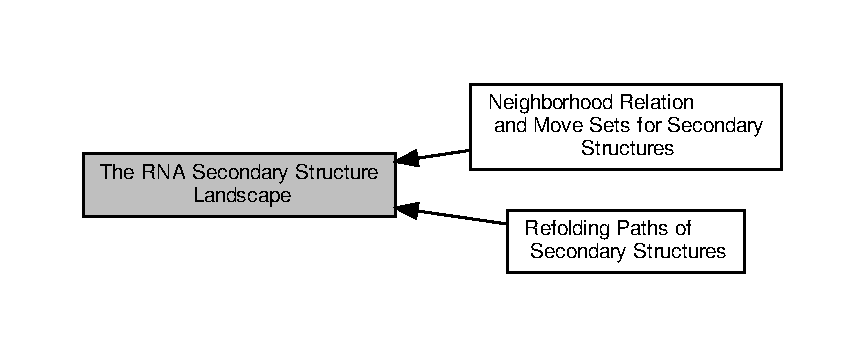
\includegraphics[width=350pt]{group__landscape}
\end{center}
\end{figure}
\subsection*{Modules}
\begin{DoxyCompactItemize}
\item 
\hyperlink{group__neighbors}{Neighborhood Relation and Move Sets for Secondary Structures}
\begin{DoxyCompactList}\small\item\em Different functions to generate structural neighbors of a secondary structure according to a particular Move Set. \end{DoxyCompactList}\item 
\hyperlink{group__paths}{Refolding Paths of Secondary Structures}
\end{DoxyCompactItemize}

\hypertarget{group__mfe}{}\section{Minimum Free Energy (M\+FE) Algorithms}
\label{group__mfe}\index{Minimum Free Energy (\+M\+F\+E) Algorithms@{Minimum Free Energy (\+M\+F\+E) Algorithms}}


Predicting the Minimum Free Energy (M\+FE) and a corresponding (consensus) secondary structure.  




\subsection{Detailed Description}
Predicting the Minimum Free Energy (M\+FE) and a corresponding (consensus) secondary structure. 

In a nutshell we provide two different flavors for M\+FE prediction\+:
\begin{DoxyItemize}
\item \hyperlink{group__mfe__global}{Global M\+FE Prediction} -\/ to compute the M\+FE for the entire sequence
\item \hyperlink{group__mfe__window}{Local (sliding window) M\+FE Prediction} -\/ to compute M\+F\+Es for each window using a sliding window approach
\end{DoxyItemize}

Each of these flavors, again, provides two implementations to either compute the M\+FE based on
\begin{DoxyItemize}
\item single R\+NA (D\+NA) sequence(s), or
\item a comparative approach using multiple sequence alignments (M\+SA).
\end{DoxyItemize}

For the latter, a consensus secondary structure is predicted and our implementations compute an average of free energies for each sequence in the M\+SA plus an additional covariance pseudo-\/energy term.

The implementations for \hyperlink{group__mfe__backtracking}{Backtracking M\+FE structures} are generally agnostic with respect to whether local or global structure prediction is in place. Collaboration diagram for Minimum Free Energy (M\+FE) Algorithms\+:
\nopagebreak
\begin{figure}[H]
\begin{center}
\leavevmode
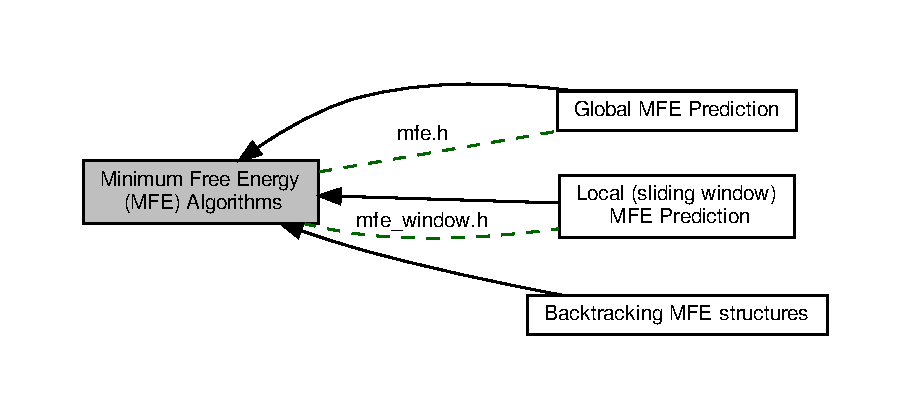
\includegraphics[width=350pt]{group__mfe}
\end{center}
\end{figure}
\subsection*{Modules}
\begin{DoxyCompactItemize}
\item 
\hyperlink{group__mfe__global}{Global M\+F\+E Prediction}
\begin{DoxyCompactList}\small\item\em Variations of the global Minimum Free Energy (M\+FE) prediction algorithm. \end{DoxyCompactList}\item 
\hyperlink{group__mfe__window}{Local (sliding window) M\+F\+E Prediction}
\begin{DoxyCompactList}\small\item\em Variations of the local (sliding window) Minimum Free Energy (M\+FE) prediction algorithm. \end{DoxyCompactList}\item 
\hyperlink{group__mfe__backtracking}{Backtracking M\+F\+E structures}
\begin{DoxyCompactList}\small\item\em Backtracking related interfaces. \end{DoxyCompactList}\end{DoxyCompactItemize}
\subsection*{Files}
\begin{DoxyCompactItemize}
\item 
file \hyperlink{mfe_8h}{mfe.\+h}
\begin{DoxyCompactList}\small\item\em Compute Minimum Free energy (M\+FE) and backtrace corresponding secondary structures from R\+NA sequence data. \end{DoxyCompactList}\item 
file \hyperlink{mfe__window_8h}{mfe\+\_\+window.\+h}
\begin{DoxyCompactList}\small\item\em Compute local Minimum Free Energy (M\+FE) using a sliding window approach and backtrace corresponding secondary structures. \end{DoxyCompactList}\end{DoxyCompactItemize}

\hypertarget{group__pf__fold}{}\section{Partition Function and Equilibrium Properties}
\label{group__pf__fold}\index{Partition Function and Equilibrium Properties@{Partition Function and Equilibrium Properties}}


Compute the partition function to assess various equilibrium properties.  




\subsection{Detailed Description}
Compute the partition function to assess various equilibrium properties. 

Similar to our \hyperlink{group__mfe}{Minimum Free Energy (M\+FE) Algorithms}, we provide two different flavors for partition function computations\+:
\begin{DoxyItemize}
\item \hyperlink{group__part__func__global}{Global Partition Function and Equilibrium Probabilities} -\/ to compute the partition function for a full length sequence
\item \hyperlink{group__part__func__window}{Local (sliding window) Partition Function and Equilibrium Probabilities} -\/ to compute the partition function of each window using a sliding window approach
\end{DoxyItemize}

While the global partition function approach supports predictions using single sequences as well as consensus partition functions for multiple sequence alignments (M\+SA), we currently do not support M\+SA input for the local variant.

Comparative prediction computes an average of the free energy contributions plus an additional covariance pseudo-\/energy term, exactly as we do for the \hyperlink{group__mfe}{Minimum Free Energy (M\+FE) Algorithms} implementation.

Boltzmann weights for the free energy contributions of individual loops can be found in \hyperlink{group__eval__loops}{Energy Evaluation for Individual Loops}.

Our implementations also provide a stochastic backtracking procedure to draw \hyperlink{group__subopt__stochbt}{Random Structure Samples from the Ensemble} according to their equilibrium probabilty. Collaboration diagram for Partition Function and Equilibrium Properties\+:
\nopagebreak
\begin{figure}[H]
\begin{center}
\leavevmode
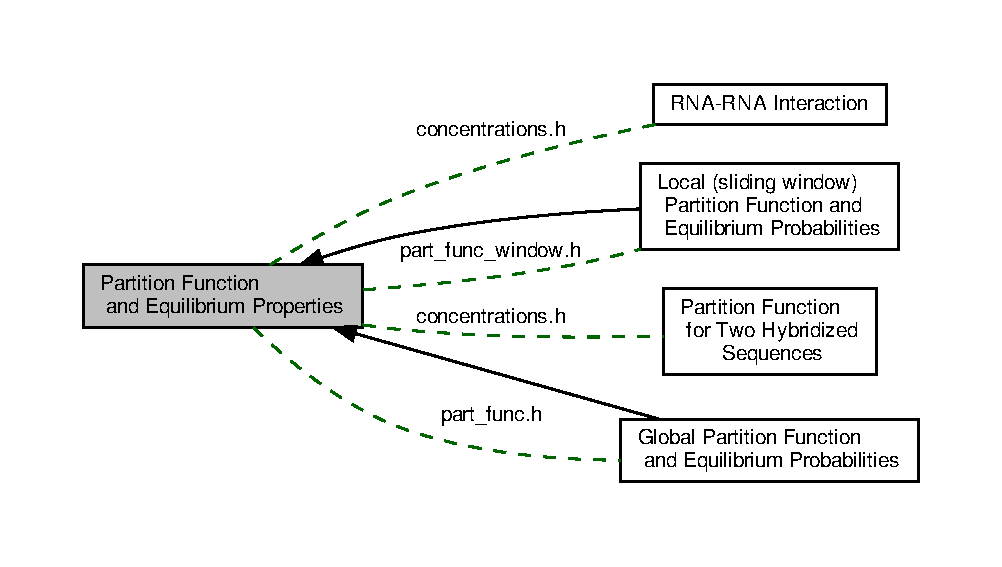
\includegraphics[width=350pt]{group__pf__fold}
\end{center}
\end{figure}
\subsection*{Modules}
\begin{DoxyCompactItemize}
\item 
\hyperlink{group__part__func__global}{Global Partition Function and Equilibrium Probabilities}
\begin{DoxyCompactList}\small\item\em Variations of the global partition function algorithm. \end{DoxyCompactList}\item 
\hyperlink{group__part__func__window}{Local (sliding window) Partition Function and Equilibrium Probabilities}
\begin{DoxyCompactList}\small\item\em Scanning version using a sliding window approach to compute equilibrium probabilities. \end{DoxyCompactList}\end{DoxyCompactItemize}
\subsection*{Files}
\begin{DoxyCompactItemize}
\item 
file \hyperlink{concentrations_8h}{concentrations.\+h}
\begin{DoxyCompactList}\small\item\em Concentration computations for R\+N\+A-\/\+R\+NA interactions. \end{DoxyCompactList}\item 
file \hyperlink{equilibrium__probs_8h}{equilibrium\+\_\+probs.\+h}
\begin{DoxyCompactList}\small\item\em Equilibrium Probability implementations. \end{DoxyCompactList}\item 
file \hyperlink{part__func_8h}{part\+\_\+func.\+h}
\begin{DoxyCompactList}\small\item\em Partition function implementations. \end{DoxyCompactList}\item 
file \hyperlink{part__func__window_8h}{part\+\_\+func\+\_\+window.\+h}
\begin{DoxyCompactList}\small\item\em Partition function and equilibrium probability implementation for the sliding window algorithm. \end{DoxyCompactList}\end{DoxyCompactItemize}
\subsection*{Functions}
\begin{DoxyCompactItemize}
\item 
int \hyperlink{group__pf__fold_gad2b3594f0b50b68029e0f54fdce59313}{vrna\+\_\+pf\+\_\+float\+\_\+precision} (void)
\begin{DoxyCompactList}\small\item\em Find out whether partition function computations are using single precision floating points. \end{DoxyCompactList}\end{DoxyCompactItemize}


\subsection{Function Documentation}
\mbox{\Hypertarget{group__pf__fold_gad2b3594f0b50b68029e0f54fdce59313}\label{group__pf__fold_gad2b3594f0b50b68029e0f54fdce59313}} 
\index{Partition Function and Equilibrium Properties@{Partition Function and Equilibrium Properties}!vrna\+\_\+pf\+\_\+float\+\_\+precision@{vrna\+\_\+pf\+\_\+float\+\_\+precision}}
\index{vrna\+\_\+pf\+\_\+float\+\_\+precision@{vrna\+\_\+pf\+\_\+float\+\_\+precision}!Partition Function and Equilibrium Properties@{Partition Function and Equilibrium Properties}}
\subsubsection{\texorpdfstring{vrna\+\_\+pf\+\_\+float\+\_\+precision()}{vrna\_pf\_float\_precision()}}
{\footnotesize\ttfamily int vrna\+\_\+pf\+\_\+float\+\_\+precision (\begin{DoxyParamCaption}\item[{void}]{ }\end{DoxyParamCaption})}



{\ttfamily \#include $<$\hyperlink{part__func_8h}{Vienna\+R\+N\+A/part\+\_\+func.\+h}$>$}



Find out whether partition function computations are using single precision floating points. 

\begin{DoxySeeAlso}{See also}
\hyperlink{group__data__structures_ga31125aeace516926bf7f251f759b6126}{F\+L\+T\+\_\+\+O\+R\+\_\+\+D\+BL} 
\end{DoxySeeAlso}
\begin{DoxyReturn}{Returns}
1 if single precision is used, 0 otherwise 
\end{DoxyReturn}

\hypertarget{group__mfe__global}{}\section{Global M\+FE Prediction}
\label{group__mfe__global}\index{Global M\+F\+E Prediction@{Global M\+F\+E Prediction}}


Variations of the global Minimum Free Energy (M\+FE) prediction algorithm.  




\subsection{Detailed Description}
Variations of the global Minimum Free Energy (M\+FE) prediction algorithm. 

We provide implementations of the global M\+FE prediction algorithm for
\begin{DoxyItemize}
\item Single sequences,
\item Multiple sequence alignments (M\+SA), and
\item R\+N\+A-\/\+R\+NA hybrids 
\end{DoxyItemize}Collaboration diagram for Global M\+FE Prediction\+:
\nopagebreak
\begin{figure}[H]
\begin{center}
\leavevmode
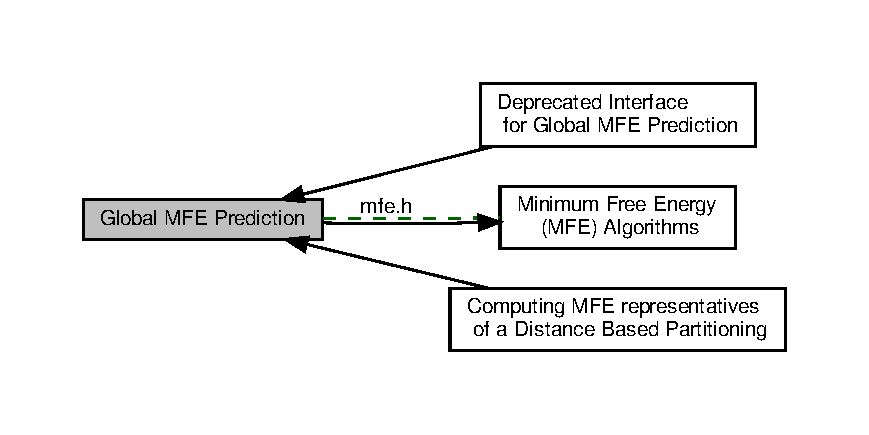
\includegraphics[width=350pt]{group__mfe__global}
\end{center}
\end{figure}
\subsection*{Modules}
\begin{DoxyCompactItemize}
\item 
\hyperlink{group__kl__neighborhood__mfe}{Computing M\+F\+E representatives of a Distance Based Partitioning}
\begin{DoxyCompactList}\small\item\em Compute the minimum free energy (M\+FE) and secondary structures for a partitioning of the secondary structure space according to the base pair distance to two fixed reference structures basepair distance to two fixed reference structures. \end{DoxyCompactList}\item 
\hyperlink{group__mfe__global__deprecated}{Deprecated Interface for Global M\+F\+E Prediction}
\end{DoxyCompactItemize}
\subsection*{Files}
\begin{DoxyCompactItemize}
\item 
file \hyperlink{mfe_8h}{mfe.\+h}
\begin{DoxyCompactList}\small\item\em Compute Minimum Free energy (M\+FE) and backtrace corresponding secondary structures from R\+NA sequence data. \end{DoxyCompactList}\end{DoxyCompactItemize}
\subsection*{Basic global M\+FE prediction interface}
\begin{DoxyCompactItemize}
\item 
float \hyperlink{group__mfe__global_gabd3b147371ccf25c577f88bbbaf159fd}{vrna\+\_\+mfe} (\hyperlink{group__fold__compound_ga1b0cef17fd40466cef5968eaeeff6166}{vrna\+\_\+fold\+\_\+compound\+\_\+t} $\ast$vc, char $\ast$structure)
\begin{DoxyCompactList}\small\item\em Compute minimum free energy and an appropriate secondary structure of an R\+NA sequence, or R\+NA sequence alignment. \end{DoxyCompactList}\item 
float \hyperlink{group__mfe__global_gaab22d10c1190f205f16a77cab9d5d3ee}{vrna\+\_\+mfe\+\_\+dimer} (\hyperlink{group__fold__compound_ga1b0cef17fd40466cef5968eaeeff6166}{vrna\+\_\+fold\+\_\+compound\+\_\+t} $\ast$vc, char $\ast$structure)
\begin{DoxyCompactList}\small\item\em Compute the minimum free energy of two interacting R\+NA molecules. \end{DoxyCompactList}\end{DoxyCompactItemize}
\subsection*{Simplified global M\+FE prediction using sequence(s) or multiple sequence alignment(s)}
\begin{DoxyCompactItemize}
\item 
float \hyperlink{group__mfe__global_ga29a33b2895f4e67b0480271ff289afdc}{vrna\+\_\+fold} (const char $\ast$sequence, char $\ast$structure)
\begin{DoxyCompactList}\small\item\em Compute Minimum Free Energy (M\+FE), and a corresponding secondary structure for an R\+NA sequence. \end{DoxyCompactList}\item 
float \hyperlink{group__mfe__global_gaf973483d8acbc8cc9aacfc8a9b7f0074}{vrna\+\_\+circfold} (const char $\ast$sequence, char $\ast$structure)
\begin{DoxyCompactList}\small\item\em Compute Minimum Free Energy (M\+FE), and a corresponding secondary structure for a circular R\+NA sequence. \end{DoxyCompactList}\item 
float \hyperlink{group__mfe__global_ga6c9d3bef3e92c6d423ffac9f981418c1}{vrna\+\_\+alifold} (const char $\ast$$\ast$sequences, char $\ast$structure)
\begin{DoxyCompactList}\small\item\em Compute Minimum Free Energy (M\+FE), and a corresponding consensus secondary structure for an R\+NA sequence alignment using a comparative method. \end{DoxyCompactList}\item 
float \hyperlink{group__mfe__global_ga17a1be7490468c29c335ba9bffacba53}{vrna\+\_\+circalifold} (const char $\ast$$\ast$sequences, char $\ast$structure)
\begin{DoxyCompactList}\small\item\em Compute Minimum Free Energy (M\+FE), and a corresponding consensus secondary structure for a sequence alignment of circular R\+N\+As using a comparative method. \end{DoxyCompactList}\item 
float \hyperlink{group__mfe__global_ga9ef3a297201dbf838a8daff2b45c0c82}{vrna\+\_\+cofold} (const char $\ast$sequence, char $\ast$structure)
\begin{DoxyCompactList}\small\item\em Compute Minimum Free Energy (M\+FE), and a corresponding secondary structure for two dimerized R\+NA sequences. \end{DoxyCompactList}\end{DoxyCompactItemize}


\subsection{Function Documentation}
\mbox{\Hypertarget{group__mfe__global_gabd3b147371ccf25c577f88bbbaf159fd}\label{group__mfe__global_gabd3b147371ccf25c577f88bbbaf159fd}} 
\index{Global M\+F\+E Prediction@{Global M\+F\+E Prediction}!vrna\+\_\+mfe@{vrna\+\_\+mfe}}
\index{vrna\+\_\+mfe@{vrna\+\_\+mfe}!Global M\+F\+E Prediction@{Global M\+F\+E Prediction}}
\subsubsection{\texorpdfstring{vrna\+\_\+mfe()}{vrna\_mfe()}}
{\footnotesize\ttfamily float vrna\+\_\+mfe (\begin{DoxyParamCaption}\item[{\hyperlink{group__fold__compound_ga1b0cef17fd40466cef5968eaeeff6166}{vrna\+\_\+fold\+\_\+compound\+\_\+t} $\ast$}]{vc,  }\item[{char $\ast$}]{structure }\end{DoxyParamCaption})}



{\ttfamily \#include $<$\hyperlink{mfe_8h}{Vienna\+R\+N\+A/mfe.\+h}$>$}



Compute minimum free energy and an appropriate secondary structure of an R\+NA sequence, or R\+NA sequence alignment. 

Depending on the type of the provided \hyperlink{group__fold__compound_ga1b0cef17fd40466cef5968eaeeff6166}{vrna\+\_\+fold\+\_\+compound\+\_\+t}, this function predicts the M\+FE for a single sequence, or a corresponding averaged M\+FE for a sequence alignment. If backtracking is activated, it also constructs the corresponding secondary structure, or consensus structure. Therefore, the second parameter, {\itshape structure}, has to point to an allocated block of memory with a size of at least $\mathrm{strlen}(\mathrm{sequence})+1$ to store the backtracked M\+FE structure. (For consensus structures, this is the length of the alignment + 1. If {\ttfamily N\+U\+LL} is passed, no backtracking will be performed.

\begin{DoxyNote}{Note}
This function is polymorphic. It accepts \hyperlink{group__fold__compound_ga1b0cef17fd40466cef5968eaeeff6166}{vrna\+\_\+fold\+\_\+compound\+\_\+t} of type \hyperlink{group__fold__compound_gga01a4ff86fa71deaaa5d1abbd95a1447da7e264dd3cf2dc9b6448caabcb7763cd6}{V\+R\+N\+A\+\_\+\+F\+C\+\_\+\+T\+Y\+P\+E\+\_\+\+S\+I\+N\+G\+LE}, and \hyperlink{group__fold__compound_gga01a4ff86fa71deaaa5d1abbd95a1447dab821ce46ea3cf665be97df22a76f5023}{V\+R\+N\+A\+\_\+\+F\+C\+\_\+\+T\+Y\+P\+E\+\_\+\+C\+O\+M\+P\+A\+R\+A\+T\+I\+VE}.
\end{DoxyNote}
\begin{DoxySeeAlso}{See also}
\hyperlink{group__fold__compound_ga1b0cef17fd40466cef5968eaeeff6166}{vrna\+\_\+fold\+\_\+compound\+\_\+t}, \hyperlink{group__fold__compound_ga6601d994ba32b11511b36f68b08403be}{vrna\+\_\+fold\+\_\+compound()}, \hyperlink{group__mfe__global_ga29a33b2895f4e67b0480271ff289afdc}{vrna\+\_\+fold()}, \hyperlink{group__mfe__global_gaf973483d8acbc8cc9aacfc8a9b7f0074}{vrna\+\_\+circfold()}, \hyperlink{group__fold__compound_gad6bacc816af274922b13d947f708aa0c}{vrna\+\_\+fold\+\_\+compound\+\_\+comparative()}, \hyperlink{group__mfe__global_ga6c9d3bef3e92c6d423ffac9f981418c1}{vrna\+\_\+alifold()}, \hyperlink{group__mfe__global_ga17a1be7490468c29c335ba9bffacba53}{vrna\+\_\+circalifold()}
\end{DoxySeeAlso}

\begin{DoxyParams}{Parameters}
{\em vc} & fold compound \\
\hline
{\em structure} & A pointer to the character array where the secondary structure in dot-\/bracket notation will be written to (Maybe N\+U\+LL)\\
\hline
\end{DoxyParams}
\begin{DoxyReturn}{Returns}
the minimum free energy (M\+FE) in kcal/mol
\end{DoxyReturn}
\begin{DoxyRefDesc}{S\+W\+I\+G Wrapper Notes}
\item[\hyperlink{wrappers__wrappers000080}{S\+W\+I\+G Wrapper Notes}]This function is attached as method {\bfseries mfe()} to objects of type {\itshape fold\+\_\+compound} \end{DoxyRefDesc}
\mbox{\Hypertarget{group__mfe__global_gaab22d10c1190f205f16a77cab9d5d3ee}\label{group__mfe__global_gaab22d10c1190f205f16a77cab9d5d3ee}} 
\index{Global M\+F\+E Prediction@{Global M\+F\+E Prediction}!vrna\+\_\+mfe\+\_\+dimer@{vrna\+\_\+mfe\+\_\+dimer}}
\index{vrna\+\_\+mfe\+\_\+dimer@{vrna\+\_\+mfe\+\_\+dimer}!Global M\+F\+E Prediction@{Global M\+F\+E Prediction}}
\subsubsection{\texorpdfstring{vrna\+\_\+mfe\+\_\+dimer()}{vrna\_mfe\_dimer()}}
{\footnotesize\ttfamily float vrna\+\_\+mfe\+\_\+dimer (\begin{DoxyParamCaption}\item[{\hyperlink{group__fold__compound_ga1b0cef17fd40466cef5968eaeeff6166}{vrna\+\_\+fold\+\_\+compound\+\_\+t} $\ast$}]{vc,  }\item[{char $\ast$}]{structure }\end{DoxyParamCaption})}



{\ttfamily \#include $<$\hyperlink{mfe_8h}{Vienna\+R\+N\+A/mfe.\+h}$>$}



Compute the minimum free energy of two interacting R\+NA molecules. 

The code is analog to the \hyperlink{group__mfe__global_gabd3b147371ccf25c577f88bbbaf159fd}{vrna\+\_\+mfe()} function.


\begin{DoxyParams}{Parameters}
{\em vc} & fold compound \\
\hline
{\em structure} & Will hold the barcket dot structure of the dimer molecule \\
\hline
\end{DoxyParams}
\begin{DoxyReturn}{Returns}
minimum free energy of the structure
\end{DoxyReturn}
\begin{DoxyRefDesc}{S\+W\+I\+G Wrapper Notes}
\item[\hyperlink{wrappers__wrappers000081}{S\+W\+I\+G Wrapper Notes}]This function is attached as method {\bfseries mfe\+\_\+dimer()} to objects of type {\itshape fold\+\_\+compound} \end{DoxyRefDesc}
\mbox{\Hypertarget{group__mfe__global_ga29a33b2895f4e67b0480271ff289afdc}\label{group__mfe__global_ga29a33b2895f4e67b0480271ff289afdc}} 
\index{Global M\+F\+E Prediction@{Global M\+F\+E Prediction}!vrna\+\_\+fold@{vrna\+\_\+fold}}
\index{vrna\+\_\+fold@{vrna\+\_\+fold}!Global M\+F\+E Prediction@{Global M\+F\+E Prediction}}
\subsubsection{\texorpdfstring{vrna\+\_\+fold()}{vrna\_fold()}}
{\footnotesize\ttfamily float vrna\+\_\+fold (\begin{DoxyParamCaption}\item[{const char $\ast$}]{sequence,  }\item[{char $\ast$}]{structure }\end{DoxyParamCaption})}



{\ttfamily \#include $<$\hyperlink{mfe_8h}{Vienna\+R\+N\+A/mfe.\+h}$>$}



Compute Minimum Free Energy (M\+FE), and a corresponding secondary structure for an R\+NA sequence. 

This simplified interface to \hyperlink{group__mfe__global_gabd3b147371ccf25c577f88bbbaf159fd}{vrna\+\_\+mfe()} computes the M\+FE and, if required, a secondary structure for an R\+NA sequence using default options. Memory required for dynamic programming (DP) matrices will be allocated and free\textquotesingle{}d on-\/the-\/fly. Hence, after return of this function, the recursively filled matrices are not available any more for any post-\/processing, e.\+g. suboptimal backtracking, etc.

\begin{DoxyNote}{Note}
In case you want to use the filled DP matrices for any subsequent post-\/processing step, or you require other conditions than specified by the default model details, use \hyperlink{group__mfe__global_gabd3b147371ccf25c577f88bbbaf159fd}{vrna\+\_\+mfe()}, and the data structure \hyperlink{group__fold__compound_ga1b0cef17fd40466cef5968eaeeff6166}{vrna\+\_\+fold\+\_\+compound\+\_\+t} instead.
\end{DoxyNote}
\begin{DoxySeeAlso}{See also}
\hyperlink{group__mfe__global_gaf973483d8acbc8cc9aacfc8a9b7f0074}{vrna\+\_\+circfold()}, \hyperlink{group__mfe__global_gabd3b147371ccf25c577f88bbbaf159fd}{vrna\+\_\+mfe()}
\end{DoxySeeAlso}

\begin{DoxyParams}{Parameters}
{\em sequence} & R\+NA sequence \\
\hline
{\em structure} & A pointer to the character array where the secondary structure in dot-\/bracket notation will be written to \\
\hline
\end{DoxyParams}
\begin{DoxyReturn}{Returns}
the minimum free energy (M\+FE) in kcal/mol 
\end{DoxyReturn}
\mbox{\Hypertarget{group__mfe__global_gaf973483d8acbc8cc9aacfc8a9b7f0074}\label{group__mfe__global_gaf973483d8acbc8cc9aacfc8a9b7f0074}} 
\index{Global M\+F\+E Prediction@{Global M\+F\+E Prediction}!vrna\+\_\+circfold@{vrna\+\_\+circfold}}
\index{vrna\+\_\+circfold@{vrna\+\_\+circfold}!Global M\+F\+E Prediction@{Global M\+F\+E Prediction}}
\subsubsection{\texorpdfstring{vrna\+\_\+circfold()}{vrna\_circfold()}}
{\footnotesize\ttfamily float vrna\+\_\+circfold (\begin{DoxyParamCaption}\item[{const char $\ast$}]{sequence,  }\item[{char $\ast$}]{structure }\end{DoxyParamCaption})}



{\ttfamily \#include $<$\hyperlink{mfe_8h}{Vienna\+R\+N\+A/mfe.\+h}$>$}



Compute Minimum Free Energy (M\+FE), and a corresponding secondary structure for a circular R\+NA sequence. 

This simplified interface to \hyperlink{group__mfe__global_gabd3b147371ccf25c577f88bbbaf159fd}{vrna\+\_\+mfe()} computes the M\+FE and, if required, a secondary structure for a circular R\+NA sequence using default options. Memory required for dynamic programming (DP) matrices will be allocated and free\textquotesingle{}d on-\/the-\/fly. Hence, after return of this function, the recursively filled matrices are not available any more for any post-\/processing, e.\+g. suboptimal backtracking, etc.

Folding of circular R\+NA sequences is handled as a post-\/processing step of the forward recursions. See \cite{hofacker:2006} for further details.

\begin{DoxyNote}{Note}
In case you want to use the filled DP matrices for any subsequent post-\/processing step, or you require other conditions than specified by the default model details, use \hyperlink{group__mfe__global_gabd3b147371ccf25c577f88bbbaf159fd}{vrna\+\_\+mfe()}, and the data structure \hyperlink{group__fold__compound_ga1b0cef17fd40466cef5968eaeeff6166}{vrna\+\_\+fold\+\_\+compound\+\_\+t} instead.
\end{DoxyNote}
\begin{DoxySeeAlso}{See also}
\hyperlink{group__mfe__global_ga29a33b2895f4e67b0480271ff289afdc}{vrna\+\_\+fold()}, \hyperlink{group__mfe__global_gabd3b147371ccf25c577f88bbbaf159fd}{vrna\+\_\+mfe()}
\end{DoxySeeAlso}

\begin{DoxyParams}{Parameters}
{\em sequence} & R\+NA sequence \\
\hline
{\em structure} & A pointer to the character array where the secondary structure in dot-\/bracket notation will be written to \\
\hline
\end{DoxyParams}
\begin{DoxyReturn}{Returns}
the minimum free energy (M\+FE) in kcal/mol 
\end{DoxyReturn}
\mbox{\Hypertarget{group__mfe__global_ga6c9d3bef3e92c6d423ffac9f981418c1}\label{group__mfe__global_ga6c9d3bef3e92c6d423ffac9f981418c1}} 
\index{Global M\+F\+E Prediction@{Global M\+F\+E Prediction}!vrna\+\_\+alifold@{vrna\+\_\+alifold}}
\index{vrna\+\_\+alifold@{vrna\+\_\+alifold}!Global M\+F\+E Prediction@{Global M\+F\+E Prediction}}
\subsubsection{\texorpdfstring{vrna\+\_\+alifold()}{vrna\_alifold()}}
{\footnotesize\ttfamily float vrna\+\_\+alifold (\begin{DoxyParamCaption}\item[{const char $\ast$$\ast$}]{sequences,  }\item[{char $\ast$}]{structure }\end{DoxyParamCaption})}



{\ttfamily \#include $<$\hyperlink{mfe_8h}{Vienna\+R\+N\+A/mfe.\+h}$>$}



Compute Minimum Free Energy (M\+FE), and a corresponding consensus secondary structure for an R\+NA sequence alignment using a comparative method. 

This simplified interface to \hyperlink{group__mfe__global_gabd3b147371ccf25c577f88bbbaf159fd}{vrna\+\_\+mfe()} computes the M\+FE and, if required, a consensus secondary structure for an R\+NA sequence alignment using default options. Memory required for dynamic programming (DP) matrices will be allocated and free\textquotesingle{}d on-\/the-\/fly. Hence, after return of this function, the recursively filled matrices are not available any more for any post-\/processing, e.\+g. suboptimal backtracking, etc.

\begin{DoxyNote}{Note}
In case you want to use the filled DP matrices for any subsequent post-\/processing step, or you require other conditions than specified by the default model details, use \hyperlink{group__mfe__global_gabd3b147371ccf25c577f88bbbaf159fd}{vrna\+\_\+mfe()}, and the data structure \hyperlink{group__fold__compound_ga1b0cef17fd40466cef5968eaeeff6166}{vrna\+\_\+fold\+\_\+compound\+\_\+t} instead.
\end{DoxyNote}
\begin{DoxySeeAlso}{See also}
\hyperlink{group__mfe__global_ga17a1be7490468c29c335ba9bffacba53}{vrna\+\_\+circalifold()}, \hyperlink{group__mfe__global_gabd3b147371ccf25c577f88bbbaf159fd}{vrna\+\_\+mfe()}
\end{DoxySeeAlso}

\begin{DoxyParams}{Parameters}
{\em sequences} & R\+NA sequence alignment \\
\hline
{\em structure} & A pointer to the character array where the secondary structure in dot-\/bracket notation will be written to \\
\hline
\end{DoxyParams}
\begin{DoxyReturn}{Returns}
the minimum free energy (M\+FE) in kcal/mol 
\end{DoxyReturn}
\mbox{\Hypertarget{group__mfe__global_ga17a1be7490468c29c335ba9bffacba53}\label{group__mfe__global_ga17a1be7490468c29c335ba9bffacba53}} 
\index{Global M\+F\+E Prediction@{Global M\+F\+E Prediction}!vrna\+\_\+circalifold@{vrna\+\_\+circalifold}}
\index{vrna\+\_\+circalifold@{vrna\+\_\+circalifold}!Global M\+F\+E Prediction@{Global M\+F\+E Prediction}}
\subsubsection{\texorpdfstring{vrna\+\_\+circalifold()}{vrna\_circalifold()}}
{\footnotesize\ttfamily float vrna\+\_\+circalifold (\begin{DoxyParamCaption}\item[{const char $\ast$$\ast$}]{sequences,  }\item[{char $\ast$}]{structure }\end{DoxyParamCaption})}



{\ttfamily \#include $<$\hyperlink{mfe_8h}{Vienna\+R\+N\+A/mfe.\+h}$>$}



Compute Minimum Free Energy (M\+FE), and a corresponding consensus secondary structure for a sequence alignment of circular R\+N\+As using a comparative method. 

This simplified interface to \hyperlink{group__mfe__global_gabd3b147371ccf25c577f88bbbaf159fd}{vrna\+\_\+mfe()} computes the M\+FE and, if required, a consensus secondary structure for an R\+NA sequence alignment using default options. Memory required for dynamic programming (DP) matrices will be allocated and free\textquotesingle{}d on-\/the-\/fly. Hence, after return of this function, the recursively filled matrices are not available any more for any post-\/processing, e.\+g. suboptimal backtracking, etc.

Folding of circular R\+NA sequences is handled as a post-\/processing step of the forward recursions. See \cite{hofacker:2006} for further details.

\begin{DoxyNote}{Note}
In case you want to use the filled DP matrices for any subsequent post-\/processing step, or you require other conditions than specified by the default model details, use \hyperlink{group__mfe__global_gabd3b147371ccf25c577f88bbbaf159fd}{vrna\+\_\+mfe()}, and the data structure \hyperlink{group__fold__compound_ga1b0cef17fd40466cef5968eaeeff6166}{vrna\+\_\+fold\+\_\+compound\+\_\+t} instead.
\end{DoxyNote}
\begin{DoxySeeAlso}{See also}
\hyperlink{group__mfe__global_ga6c9d3bef3e92c6d423ffac9f981418c1}{vrna\+\_\+alifold()}, \hyperlink{group__mfe__global_gabd3b147371ccf25c577f88bbbaf159fd}{vrna\+\_\+mfe()}
\end{DoxySeeAlso}

\begin{DoxyParams}{Parameters}
{\em sequences} & Sequence alignment of circular R\+N\+As \\
\hline
{\em structure} & A pointer to the character array where the secondary structure in dot-\/bracket notation will be written to \\
\hline
\end{DoxyParams}
\begin{DoxyReturn}{Returns}
the minimum free energy (M\+FE) in kcal/mol 
\end{DoxyReturn}
\mbox{\Hypertarget{group__mfe__global_ga9ef3a297201dbf838a8daff2b45c0c82}\label{group__mfe__global_ga9ef3a297201dbf838a8daff2b45c0c82}} 
\index{Global M\+F\+E Prediction@{Global M\+F\+E Prediction}!vrna\+\_\+cofold@{vrna\+\_\+cofold}}
\index{vrna\+\_\+cofold@{vrna\+\_\+cofold}!Global M\+F\+E Prediction@{Global M\+F\+E Prediction}}
\subsubsection{\texorpdfstring{vrna\+\_\+cofold()}{vrna\_cofold()}}
{\footnotesize\ttfamily float vrna\+\_\+cofold (\begin{DoxyParamCaption}\item[{const char $\ast$}]{sequence,  }\item[{char $\ast$}]{structure }\end{DoxyParamCaption})}



{\ttfamily \#include $<$\hyperlink{mfe_8h}{Vienna\+R\+N\+A/mfe.\+h}$>$}



Compute Minimum Free Energy (M\+FE), and a corresponding secondary structure for two dimerized R\+NA sequences. 

This simplified interface to \hyperlink{group__mfe__global_gabd3b147371ccf25c577f88bbbaf159fd}{vrna\+\_\+mfe()} computes the M\+FE and, if required, a secondary structure for two R\+NA sequences upon dimerization using default options. Memory required for dynamic programming (DP) matrices will be allocated and free\textquotesingle{}d on-\/the-\/fly. Hence, after return of this function, the recursively filled matrices are not available any more for any post-\/processing, e.\+g. suboptimal backtracking, etc.

\begin{DoxyNote}{Note}
In case you want to use the filled DP matrices for any subsequent post-\/processing step, or you require other conditions than specified by the default model details, use \hyperlink{group__mfe__global_gabd3b147371ccf25c577f88bbbaf159fd}{vrna\+\_\+mfe()}, and the data structure \hyperlink{group__fold__compound_ga1b0cef17fd40466cef5968eaeeff6166}{vrna\+\_\+fold\+\_\+compound\+\_\+t} instead.
\end{DoxyNote}
\begin{DoxySeeAlso}{See also}
\hyperlink{group__mfe__global_gaab22d10c1190f205f16a77cab9d5d3ee}{vrna\+\_\+mfe\+\_\+dimer()}, \hyperlink{group__fold__compound_ga6601d994ba32b11511b36f68b08403be}{vrna\+\_\+fold\+\_\+compound()}, \hyperlink{group__fold__compound_ga1b0cef17fd40466cef5968eaeeff6166}{vrna\+\_\+fold\+\_\+compound\+\_\+t}, \hyperlink{group__string__utils_ga74f05ece32ea73b59f84a7452afd5fae}{vrna\+\_\+cut\+\_\+point\+\_\+insert()}
\end{DoxySeeAlso}

\begin{DoxyParams}{Parameters}
{\em sequence} & two R\+NA sequences separated by the \textquotesingle{}\&\textquotesingle{} character \\
\hline
{\em structure} & A pointer to the character array where the secondary structure in dot-\/bracket notation will be written to \\
\hline
\end{DoxyParams}
\begin{DoxyReturn}{Returns}
the minimum free energy (M\+FE) in kcal/mol 
\end{DoxyReturn}

\hypertarget{group__mfe__window}{}\section{Local (sliding window) M\+FE Prediction}
\label{group__mfe__window}\index{Local (sliding window) M\+F\+E Prediction@{Local (sliding window) M\+F\+E Prediction}}


Variations of the local (sliding window) Minimum Free Energy (M\+FE) prediction algorithm.  




\subsection{Detailed Description}
Variations of the local (sliding window) Minimum Free Energy (M\+FE) prediction algorithm. 

We provide implementations for the local (sliding window) M\+FE prediction algorithm for
\begin{DoxyItemize}
\item Single sequences,
\item Multiple sequence alignments (M\+SA), and
\end{DoxyItemize}

Note, that our implementation scans an R\+NA sequence (or M\+SA) from the 3\textquotesingle{} to the 5\textquotesingle{} end, and reports back locally optimal (consensus) structures, the corresponding free energy, and the position of the sliding window in global coordinates.

For any particular R\+NA sequence (or M\+SA) multiple locally optimal (consensus) secondary structures may be predicted. Thus, we tried to implement an interface that allows for an effortless conversion of the corresponding hits into any target data structure. As a consequence, we provide two distinct ways to retrieve the corresponding predictions, either
\begin{DoxyItemize}
\item through directly writing to an open {\ttfamily F\+I\+LE} stream on-\/the-\/fly, or
\item through a callback function mechanism.
\end{DoxyItemize}

The latter allows one to store the results in any possible target data structure. Our implementations then pass the results through the user-\/implemented callback as soon as the prediction for a particular window is finished. Collaboration diagram for Local (sliding window) M\+FE Prediction\+:
\nopagebreak
\begin{figure}[H]
\begin{center}
\leavevmode
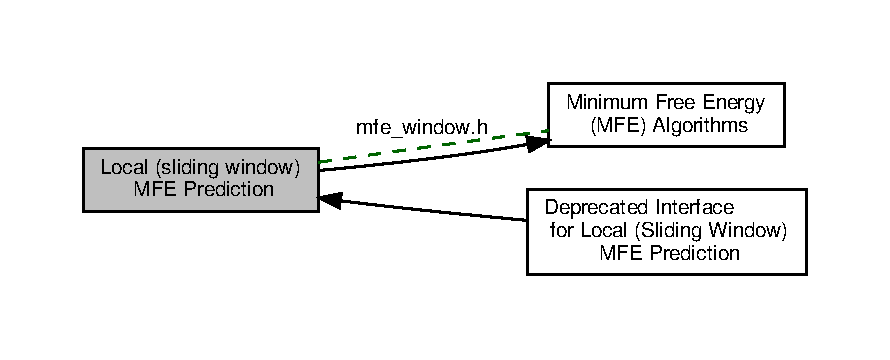
\includegraphics[width=350pt]{group__mfe__window}
\end{center}
\end{figure}
\subsection*{Modules}
\begin{DoxyCompactItemize}
\item 
\hyperlink{group__mfe__window__deprecated}{Deprecated Interface for Local (\+Sliding Window) M\+F\+E Prediction}
\end{DoxyCompactItemize}
\subsection*{Files}
\begin{DoxyCompactItemize}
\item 
file \hyperlink{mfe__window_8h}{mfe\+\_\+window.\+h}
\begin{DoxyCompactList}\small\item\em Compute local Minimum Free Energy (M\+FE) using a sliding window approach and backtrace corresponding secondary structures. \end{DoxyCompactList}\end{DoxyCompactItemize}
\subsection*{Typedefs}
\begin{DoxyCompactItemize}
\item 
typedef void() \hyperlink{group__mfe__window_ga4f3e5bc214ef803074ace313cb9571b4}{vrna\+\_\+mfe\+\_\+window\+\_\+callback}(int start, int end, const char $\ast$structure, float en, void $\ast$data)
\begin{DoxyCompactList}\small\item\em The default callback for sliding window M\+FE structure predictions. \end{DoxyCompactList}\end{DoxyCompactItemize}
\subsection*{Basic local (sliding window) M\+FE prediction interface}
\begin{DoxyCompactItemize}
\item 
float \hyperlink{group__mfe__window_ga689df235a1915a1ad56e377383c044ce}{vrna\+\_\+mfe\+\_\+window} (\hyperlink{group__fold__compound_ga1b0cef17fd40466cef5968eaeeff6166}{vrna\+\_\+fold\+\_\+compound\+\_\+t} $\ast$vc, F\+I\+LE $\ast$file)
\begin{DoxyCompactList}\small\item\em Local M\+FE prediction using a sliding window approach. \end{DoxyCompactList}\item 
\mbox{\Hypertarget{group__mfe__window_gad4995894b294ddb8550af444a0decbd1}\label{group__mfe__window_gad4995894b294ddb8550af444a0decbd1}} 
float {\bfseries vrna\+\_\+mfe\+\_\+window\+\_\+cb} (\hyperlink{group__fold__compound_ga1b0cef17fd40466cef5968eaeeff6166}{vrna\+\_\+fold\+\_\+compound\+\_\+t} $\ast$vc, \hyperlink{group__mfe__window_ga4f3e5bc214ef803074ace313cb9571b4}{vrna\+\_\+mfe\+\_\+window\+\_\+callback} $\ast$cb, void $\ast$data)
\item 
float \hyperlink{group__mfe__window_gaa4f67ae94efd08d800c17f9b53423fd6}{vrna\+\_\+mfe\+\_\+window\+\_\+zscore} (\hyperlink{group__fold__compound_ga1b0cef17fd40466cef5968eaeeff6166}{vrna\+\_\+fold\+\_\+compound\+\_\+t} $\ast$vc, double min\+\_\+z, F\+I\+LE $\ast$file)
\begin{DoxyCompactList}\small\item\em Local M\+FE prediction using a sliding window approach (with z-\/score cut-\/off) \end{DoxyCompactList}\item 
\mbox{\Hypertarget{group__mfe__window_ga2762be816af3dbc18c256e44c1345e4f}\label{group__mfe__window_ga2762be816af3dbc18c256e44c1345e4f}} 
float {\bfseries vrna\+\_\+mfe\+\_\+window\+\_\+zscore\+\_\+cb} (\hyperlink{group__fold__compound_ga1b0cef17fd40466cef5968eaeeff6166}{vrna\+\_\+fold\+\_\+compound\+\_\+t} $\ast$vc, double min\+\_\+z, vrna\+\_\+mfe\+\_\+window\+\_\+zscore\+\_\+callback $\ast$cb, void $\ast$data)
\end{DoxyCompactItemize}
\subsection*{Simplified local M\+FE prediction using sequence(s) or multiple sequence alignment(s)}
\begin{DoxyCompactItemize}
\item 
float \hyperlink{group__mfe__window_ga4918cce52bf69c1913cda503b2ac75d8}{vrna\+\_\+\+Lfold} (const char $\ast$string, int window\+\_\+size, F\+I\+LE $\ast$file)
\begin{DoxyCompactList}\small\item\em Local M\+FE prediction using a sliding window approach (simplified interface) \end{DoxyCompactList}\item 
\mbox{\Hypertarget{group__mfe__window_ga8b70293ad3c9dd3dc384d06290bf8069}\label{group__mfe__window_ga8b70293ad3c9dd3dc384d06290bf8069}} 
float {\bfseries vrna\+\_\+\+Lfold\+\_\+cb} (const char $\ast$string, int window\+\_\+size, \hyperlink{group__mfe__window_ga4f3e5bc214ef803074ace313cb9571b4}{vrna\+\_\+mfe\+\_\+window\+\_\+callback} $\ast$cb, void $\ast$data)
\item 
float \hyperlink{group__mfe__window_ga27fddda5fc63eb49c861e38845fc34b4}{vrna\+\_\+\+Lfoldz} (const char $\ast$string, int window\+\_\+size, double min\+\_\+z, F\+I\+LE $\ast$file)
\begin{DoxyCompactList}\small\item\em Local M\+FE prediction using a sliding window approach with z-\/score cut-\/off (simplified interface) \end{DoxyCompactList}\item 
\mbox{\Hypertarget{group__mfe__window_ga41b18568b846f1db70cdf2fe83b0ed47}\label{group__mfe__window_ga41b18568b846f1db70cdf2fe83b0ed47}} 
float {\bfseries vrna\+\_\+\+Lfoldz\+\_\+cb} (const char $\ast$string, int window\+\_\+size, double min\+\_\+z, vrna\+\_\+mfe\+\_\+window\+\_\+zscore\+\_\+callback $\ast$cb, void $\ast$data)
\item 
\mbox{\Hypertarget{group__mfe__window_gaa43d3de352753529a4578cb02cd8bc52}\label{group__mfe__window_gaa43d3de352753529a4578cb02cd8bc52}} 
float {\bfseries vrna\+\_\+ali\+Lfold} (const char $\ast$$\ast$alignment, int maxdist, F\+I\+LE $\ast$fp)
\item 
\mbox{\Hypertarget{group__mfe__window_ga09756293446a6ae67c783bc8d567d884}\label{group__mfe__window_ga09756293446a6ae67c783bc8d567d884}} 
float {\bfseries vrna\+\_\+ali\+Lfold\+\_\+cb} (const char $\ast$$\ast$alignment, int maxdist, \hyperlink{group__mfe__window_ga4f3e5bc214ef803074ace313cb9571b4}{vrna\+\_\+mfe\+\_\+window\+\_\+callback} $\ast$cb, void $\ast$data)
\end{DoxyCompactItemize}


\subsection{Typedef Documentation}
\mbox{\Hypertarget{group__mfe__window_ga4f3e5bc214ef803074ace313cb9571b4}\label{group__mfe__window_ga4f3e5bc214ef803074ace313cb9571b4}} 
\index{Local (sliding window) M\+F\+E Prediction@{Local (sliding window) M\+F\+E Prediction}!vrna\+\_\+mfe\+\_\+window\+\_\+callback@{vrna\+\_\+mfe\+\_\+window\+\_\+callback}}
\index{vrna\+\_\+mfe\+\_\+window\+\_\+callback@{vrna\+\_\+mfe\+\_\+window\+\_\+callback}!Local (sliding window) M\+F\+E Prediction@{Local (sliding window) M\+F\+E Prediction}}
\subsubsection{\texorpdfstring{vrna\+\_\+mfe\+\_\+window\+\_\+callback}{vrna\_mfe\_window\_callback}}
{\footnotesize\ttfamily typedef void() vrna\+\_\+mfe\+\_\+window\+\_\+callback(int start, int end, const char $\ast$structure, float en, void $\ast$data)}



{\ttfamily \#include $<$\hyperlink{mfe__window_8h}{Vienna\+R\+N\+A/mfe\+\_\+window.\+h}$>$}



The default callback for sliding window M\+FE structure predictions. 

\begin{DoxyRefDesc}{Notes on Callback Functions}
\item[\hyperlink{callbacks__callbacks000003}{Notes on Callback Functions}]This function will be called for each hit in a sliding window M\+FE prediction. \end{DoxyRefDesc}


\begin{DoxySeeAlso}{See also}
\hyperlink{group__mfe__window_ga689df235a1915a1ad56e377383c044ce}{vrna\+\_\+mfe\+\_\+window()}
\end{DoxySeeAlso}

\begin{DoxyParams}{Parameters}
{\em start} & provides the first position of the hit (1-\/based, relative to entire sequence/alignment) \\
\hline
{\em end} & provides the last position of the hit (1-\/based, relative to the entire sequence/alignment) \\
\hline
{\em structure} & provides the (sub)structure in dot-\/bracket notation \\
\hline
{\em en} & is the free energy of the structure hit in kcal/mol \\
\hline
{\em data} & is some arbitrary data pointer passed through by the function executing the callback \\
\hline
\end{DoxyParams}


\subsection{Function Documentation}
\mbox{\Hypertarget{group__mfe__window_ga689df235a1915a1ad56e377383c044ce}\label{group__mfe__window_ga689df235a1915a1ad56e377383c044ce}} 
\index{Local (sliding window) M\+F\+E Prediction@{Local (sliding window) M\+F\+E Prediction}!vrna\+\_\+mfe\+\_\+window@{vrna\+\_\+mfe\+\_\+window}}
\index{vrna\+\_\+mfe\+\_\+window@{vrna\+\_\+mfe\+\_\+window}!Local (sliding window) M\+F\+E Prediction@{Local (sliding window) M\+F\+E Prediction}}
\subsubsection{\texorpdfstring{vrna\+\_\+mfe\+\_\+window()}{vrna\_mfe\_window()}}
{\footnotesize\ttfamily float vrna\+\_\+mfe\+\_\+window (\begin{DoxyParamCaption}\item[{\hyperlink{group__fold__compound_ga1b0cef17fd40466cef5968eaeeff6166}{vrna\+\_\+fold\+\_\+compound\+\_\+t} $\ast$}]{vc,  }\item[{F\+I\+LE $\ast$}]{file }\end{DoxyParamCaption})}



{\ttfamily \#include $<$\hyperlink{mfe__window_8h}{Vienna\+R\+N\+A/mfe\+\_\+window.\+h}$>$}



Local M\+FE prediction using a sliding window approach. 

Computes minimum free energy structures using a sliding window approach, where base pairs may not span outside the window. In contrast to \hyperlink{group__mfe__global_gabd3b147371ccf25c577f88bbbaf159fd}{vrna\+\_\+mfe()}, where a maximum base pair span may be set using the \hyperlink{group__model__details_a659e5fcc6e8c9f1a68e7de6548eef3b0}{vrna\+\_\+md\+\_\+t.\+max\+\_\+bp\+\_\+span} attribute and one globally optimal structure is predicted, this function uses a sliding window to retrieve all locally optimal structures within each window. The size of the sliding window is set in the \hyperlink{group__model__details_abea42f9229f8d8d6bcbedef316315bfc}{vrna\+\_\+md\+\_\+t.\+window\+\_\+size} attribute, prior to the retrieval of the \hyperlink{group__fold__compound_ga1b0cef17fd40466cef5968eaeeff6166}{vrna\+\_\+fold\+\_\+compound\+\_\+t} using \hyperlink{group__fold__compound_ga6601d994ba32b11511b36f68b08403be}{vrna\+\_\+fold\+\_\+compound()} with option \hyperlink{group__fold__compound_ga2b2a8009ccdccc3eb1571556261aee8e}{V\+R\+N\+A\+\_\+\+O\+P\+T\+I\+O\+N\+\_\+\+W\+I\+N\+D\+OW}

The predicted structures are written on-\/the-\/fly, either to stdout, if a N\+U\+LL pointer is passed as file parameter, or to the corresponding filehandle.

\begin{DoxySeeAlso}{See also}
\hyperlink{group__fold__compound_ga6601d994ba32b11511b36f68b08403be}{vrna\+\_\+fold\+\_\+compound()}, \hyperlink{group__mfe__window_gaa4f67ae94efd08d800c17f9b53423fd6}{vrna\+\_\+mfe\+\_\+window\+\_\+zscore()}, \hyperlink{group__mfe__global_gabd3b147371ccf25c577f88bbbaf159fd}{vrna\+\_\+mfe()}, \hyperlink{group__mfe__window_ga4918cce52bf69c1913cda503b2ac75d8}{vrna\+\_\+\+Lfold()}, \hyperlink{group__mfe__window_ga27fddda5fc63eb49c861e38845fc34b4}{vrna\+\_\+\+Lfoldz()}, \hyperlink{group__fold__compound_ga2b2a8009ccdccc3eb1571556261aee8e}{V\+R\+N\+A\+\_\+\+O\+P\+T\+I\+O\+N\+\_\+\+W\+I\+N\+D\+OW}, \hyperlink{group__model__details_a659e5fcc6e8c9f1a68e7de6548eef3b0}{vrna\+\_\+md\+\_\+t.\+max\+\_\+bp\+\_\+span}, \hyperlink{group__model__details_abea42f9229f8d8d6bcbedef316315bfc}{vrna\+\_\+md\+\_\+t.\+window\+\_\+size}
\end{DoxySeeAlso}

\begin{DoxyParams}{Parameters}
{\em vc} & The \hyperlink{group__fold__compound_ga1b0cef17fd40466cef5968eaeeff6166}{vrna\+\_\+fold\+\_\+compound\+\_\+t} with preallocated memory for the DP matrices \\
\hline
{\em file} & The output file handle where predictions are written to (maybe N\+U\+LL)\\
\hline
\end{DoxyParams}
\begin{DoxyRefDesc}{S\+W\+I\+G Wrapper Notes}
\item[\hyperlink{wrappers__wrappers000082}{S\+W\+I\+G Wrapper Notes}]This function is attached as method {\bfseries mfe\+\_\+window()} to objects of type {\itshape fold\+\_\+compound} \end{DoxyRefDesc}
\mbox{\Hypertarget{group__mfe__window_gaa4f67ae94efd08d800c17f9b53423fd6}\label{group__mfe__window_gaa4f67ae94efd08d800c17f9b53423fd6}} 
\index{Local (sliding window) M\+F\+E Prediction@{Local (sliding window) M\+F\+E Prediction}!vrna\+\_\+mfe\+\_\+window\+\_\+zscore@{vrna\+\_\+mfe\+\_\+window\+\_\+zscore}}
\index{vrna\+\_\+mfe\+\_\+window\+\_\+zscore@{vrna\+\_\+mfe\+\_\+window\+\_\+zscore}!Local (sliding window) M\+F\+E Prediction@{Local (sliding window) M\+F\+E Prediction}}
\subsubsection{\texorpdfstring{vrna\+\_\+mfe\+\_\+window\+\_\+zscore()}{vrna\_mfe\_window\_zscore()}}
{\footnotesize\ttfamily float vrna\+\_\+mfe\+\_\+window\+\_\+zscore (\begin{DoxyParamCaption}\item[{\hyperlink{group__fold__compound_ga1b0cef17fd40466cef5968eaeeff6166}{vrna\+\_\+fold\+\_\+compound\+\_\+t} $\ast$}]{vc,  }\item[{double}]{min\+\_\+z,  }\item[{F\+I\+LE $\ast$}]{file }\end{DoxyParamCaption})}



{\ttfamily \#include $<$\hyperlink{mfe__window_8h}{Vienna\+R\+N\+A/mfe\+\_\+window.\+h}$>$}



Local M\+FE prediction using a sliding window approach (with z-\/score cut-\/off) 

Computes minimum free energy structures using a sliding window approach, where base pairs may not span outside the window. This function is the z-\/score version of \hyperlink{group__mfe__window_ga689df235a1915a1ad56e377383c044ce}{vrna\+\_\+mfe\+\_\+window()}, i.\+e. only predictions above a certain z-\/score cut-\/off value are printed. As for \hyperlink{group__mfe__window_ga689df235a1915a1ad56e377383c044ce}{vrna\+\_\+mfe\+\_\+window()}, the size of the sliding window is set in the \hyperlink{group__model__details_abea42f9229f8d8d6bcbedef316315bfc}{vrna\+\_\+md\+\_\+t.\+window\+\_\+size} attribute, prior to the retrieval of the \hyperlink{group__fold__compound_ga1b0cef17fd40466cef5968eaeeff6166}{vrna\+\_\+fold\+\_\+compound\+\_\+t} using \hyperlink{group__fold__compound_ga6601d994ba32b11511b36f68b08403be}{vrna\+\_\+fold\+\_\+compound()} with option \hyperlink{group__fold__compound_ga2b2a8009ccdccc3eb1571556261aee8e}{V\+R\+N\+A\+\_\+\+O\+P\+T\+I\+O\+N\+\_\+\+W\+I\+N\+D\+OW}.

The predicted structures are written on-\/the-\/fly, either to stdout, if a N\+U\+LL pointer is passed as file parameter, or to the corresponding filehandle.

\begin{DoxySeeAlso}{See also}
\hyperlink{group__fold__compound_ga6601d994ba32b11511b36f68b08403be}{vrna\+\_\+fold\+\_\+compound()}, \hyperlink{group__mfe__window_gaa4f67ae94efd08d800c17f9b53423fd6}{vrna\+\_\+mfe\+\_\+window\+\_\+zscore()}, \hyperlink{group__mfe__global_gabd3b147371ccf25c577f88bbbaf159fd}{vrna\+\_\+mfe()}, \hyperlink{group__mfe__window_ga4918cce52bf69c1913cda503b2ac75d8}{vrna\+\_\+\+Lfold()}, \hyperlink{group__mfe__window_ga27fddda5fc63eb49c861e38845fc34b4}{vrna\+\_\+\+Lfoldz()}, \hyperlink{group__fold__compound_ga2b2a8009ccdccc3eb1571556261aee8e}{V\+R\+N\+A\+\_\+\+O\+P\+T\+I\+O\+N\+\_\+\+W\+I\+N\+D\+OW}, \hyperlink{group__model__details_a659e5fcc6e8c9f1a68e7de6548eef3b0}{vrna\+\_\+md\+\_\+t.\+max\+\_\+bp\+\_\+span}, \hyperlink{group__model__details_abea42f9229f8d8d6bcbedef316315bfc}{vrna\+\_\+md\+\_\+t.\+window\+\_\+size}
\end{DoxySeeAlso}

\begin{DoxyParams}{Parameters}
{\em vc} & The \hyperlink{group__fold__compound_ga1b0cef17fd40466cef5968eaeeff6166}{vrna\+\_\+fold\+\_\+compound\+\_\+t} with preallocated memory for the DP matrices \\
\hline
{\em min\+\_\+z} & The minimal z-\/score for a predicted structure to appear in the output \\
\hline
{\em file} & The output file handle where predictions are written to (maybe N\+U\+LL) \\
\hline
\end{DoxyParams}
\mbox{\Hypertarget{group__mfe__window_ga4918cce52bf69c1913cda503b2ac75d8}\label{group__mfe__window_ga4918cce52bf69c1913cda503b2ac75d8}} 
\index{Local (sliding window) M\+F\+E Prediction@{Local (sliding window) M\+F\+E Prediction}!vrna\+\_\+\+Lfold@{vrna\+\_\+\+Lfold}}
\index{vrna\+\_\+\+Lfold@{vrna\+\_\+\+Lfold}!Local (sliding window) M\+F\+E Prediction@{Local (sliding window) M\+F\+E Prediction}}
\subsubsection{\texorpdfstring{vrna\+\_\+\+Lfold()}{vrna\_Lfold()}}
{\footnotesize\ttfamily float vrna\+\_\+\+Lfold (\begin{DoxyParamCaption}\item[{const char $\ast$}]{string,  }\item[{int}]{window\+\_\+size,  }\item[{F\+I\+LE $\ast$}]{file }\end{DoxyParamCaption})}



{\ttfamily \#include $<$\hyperlink{mfe__window_8h}{Vienna\+R\+N\+A/mfe\+\_\+window.\+h}$>$}



Local M\+FE prediction using a sliding window approach (simplified interface) 

This simplified interface to \hyperlink{group__mfe__window_ga689df235a1915a1ad56e377383c044ce}{vrna\+\_\+mfe\+\_\+window()} computes the M\+FE and locally optimal secondary structure using default options. Structures are predicted using a sliding window approach, where base pairs may not span outside the window. Memory required for dynamic programming (DP) matrices will be allocated and free\textquotesingle{}d on-\/the-\/fly. Hence, after return of this function, the recursively filled matrices are not available any more for any post-\/processing.

\begin{DoxyNote}{Note}
In case you want to use the filled DP matrices for any subsequent post-\/processing step, or you require other conditions than specified by the default model details, use \hyperlink{group__mfe__window_ga689df235a1915a1ad56e377383c044ce}{vrna\+\_\+mfe\+\_\+window()}, and the data structure \hyperlink{group__fold__compound_ga1b0cef17fd40466cef5968eaeeff6166}{vrna\+\_\+fold\+\_\+compound\+\_\+t} instead.
\end{DoxyNote}
\begin{DoxySeeAlso}{See also}
\hyperlink{group__mfe__window_ga689df235a1915a1ad56e377383c044ce}{vrna\+\_\+mfe\+\_\+window()}, \hyperlink{group__mfe__window_ga27fddda5fc63eb49c861e38845fc34b4}{vrna\+\_\+\+Lfoldz()}, \hyperlink{group__mfe__window_gaa4f67ae94efd08d800c17f9b53423fd6}{vrna\+\_\+mfe\+\_\+window\+\_\+zscore()}
\end{DoxySeeAlso}

\begin{DoxyParams}{Parameters}
{\em string} & The nucleic acid sequence \\
\hline
{\em window\+\_\+size} & The window size for locally optimal structures \\
\hline
{\em file} & The output file handle where predictions are written to (if N\+U\+LL, output is written to stdout) \\
\hline
\end{DoxyParams}
\mbox{\Hypertarget{group__mfe__window_ga27fddda5fc63eb49c861e38845fc34b4}\label{group__mfe__window_ga27fddda5fc63eb49c861e38845fc34b4}} 
\index{Local (sliding window) M\+F\+E Prediction@{Local (sliding window) M\+F\+E Prediction}!vrna\+\_\+\+Lfoldz@{vrna\+\_\+\+Lfoldz}}
\index{vrna\+\_\+\+Lfoldz@{vrna\+\_\+\+Lfoldz}!Local (sliding window) M\+F\+E Prediction@{Local (sliding window) M\+F\+E Prediction}}
\subsubsection{\texorpdfstring{vrna\+\_\+\+Lfoldz()}{vrna\_Lfoldz()}}
{\footnotesize\ttfamily float vrna\+\_\+\+Lfoldz (\begin{DoxyParamCaption}\item[{const char $\ast$}]{string,  }\item[{int}]{window\+\_\+size,  }\item[{double}]{min\+\_\+z,  }\item[{F\+I\+LE $\ast$}]{file }\end{DoxyParamCaption})}



{\ttfamily \#include $<$\hyperlink{mfe__window_8h}{Vienna\+R\+N\+A/mfe\+\_\+window.\+h}$>$}



Local M\+FE prediction using a sliding window approach with z-\/score cut-\/off (simplified interface) 

This simplified interface to \hyperlink{group__mfe__window_gaa4f67ae94efd08d800c17f9b53423fd6}{vrna\+\_\+mfe\+\_\+window\+\_\+zscore()} computes the M\+FE and locally optimal secondary structure using default options. Structures are predicted using a sliding window approach, where base pairs may not span outside the window. Memory required for dynamic programming (DP) matrices will be allocated and free\textquotesingle{}d on-\/the-\/fly. Hence, after return of this function, the recursively filled matrices are not available any more for any post-\/processing. This function is the z-\/score version of \hyperlink{group__mfe__window_ga4918cce52bf69c1913cda503b2ac75d8}{vrna\+\_\+\+Lfold()}, i.\+e. only predictions above a certain z-\/score cut-\/off value are printed.

\begin{DoxyNote}{Note}
In case you want to use the filled DP matrices for any subsequent post-\/processing step, or you require other conditions than specified by the default model details, use \hyperlink{group__mfe__window_ga689df235a1915a1ad56e377383c044ce}{vrna\+\_\+mfe\+\_\+window()}, and the data structure \hyperlink{group__fold__compound_ga1b0cef17fd40466cef5968eaeeff6166}{vrna\+\_\+fold\+\_\+compound\+\_\+t} instead.
\end{DoxyNote}
\begin{DoxySeeAlso}{See also}
\hyperlink{group__mfe__window_gaa4f67ae94efd08d800c17f9b53423fd6}{vrna\+\_\+mfe\+\_\+window\+\_\+zscore()}, \hyperlink{group__mfe__window_ga4918cce52bf69c1913cda503b2ac75d8}{vrna\+\_\+\+Lfold()}, \hyperlink{group__mfe__window_ga689df235a1915a1ad56e377383c044ce}{vrna\+\_\+mfe\+\_\+window()}
\end{DoxySeeAlso}

\begin{DoxyParams}{Parameters}
{\em string} & The nucleic acid sequence \\
\hline
{\em window\+\_\+size} & The window size for locally optimal structures \\
\hline
{\em min\+\_\+z} & The minimal z-\/score for a predicted structure to appear in the output \\
\hline
{\em file} & The output file handle where predictions are written to (if N\+U\+LL, output is written to stdout) \\
\hline
\end{DoxyParams}

\hypertarget{group__mfe__backtracking}{}\section{Backtracking M\+FE structures}
\label{group__mfe__backtracking}\index{Backtracking M\+F\+E structures@{Backtracking M\+F\+E structures}}


Backtracking related interfaces.  




\subsection{Detailed Description}
Backtracking related interfaces. 

Collaboration diagram for Backtracking M\+FE structures\+:
\nopagebreak
\begin{figure}[H]
\begin{center}
\leavevmode
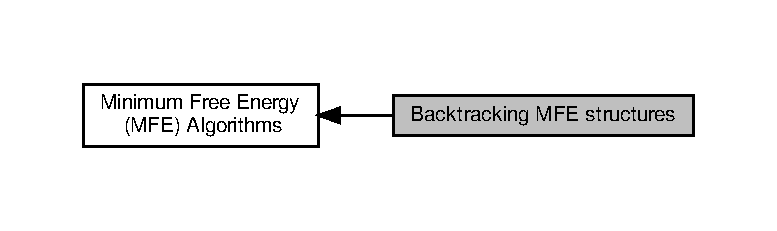
\includegraphics[width=350pt]{group__mfe__backtracking}
\end{center}
\end{figure}
\subsection*{Functions}
\begin{DoxyCompactItemize}
\item 
int \hyperlink{group__mfe__backtracking_gae20d5805ddedc9b81d24735b11b6a9bf}{vrna\+\_\+\+B\+T\+\_\+hp\+\_\+loop} (\hyperlink{group__fold__compound_ga1b0cef17fd40466cef5968eaeeff6166}{vrna\+\_\+fold\+\_\+compound\+\_\+t} $\ast$fc, int i, int j, int en, \hyperlink{group__data__structures_gaa651bda42e7692f08cb603cd6834b0ee}{vrna\+\_\+bp\+\_\+stack\+\_\+t} $\ast$bp\+\_\+stack, int $\ast$stack\+\_\+count)
\begin{DoxyCompactList}\small\item\em Backtrack a hairpin loop closed by $ (i,j) $. \end{DoxyCompactList}\item 
\mbox{\Hypertarget{group__mfe__backtracking_ga28015cfbd0afc759b94ff58cc241cb13}\label{group__mfe__backtracking_ga28015cfbd0afc759b94ff58cc241cb13}} 
int \hyperlink{group__mfe__backtracking_ga28015cfbd0afc759b94ff58cc241cb13}{vrna\+\_\+\+B\+T\+\_\+stack} (\hyperlink{group__fold__compound_ga1b0cef17fd40466cef5968eaeeff6166}{vrna\+\_\+fold\+\_\+compound\+\_\+t} $\ast$fc, int $\ast$i, int $\ast$j, int $\ast$en, \hyperlink{group__data__structures_gaa651bda42e7692f08cb603cd6834b0ee}{vrna\+\_\+bp\+\_\+stack\+\_\+t} $\ast$bp\+\_\+stack, int $\ast$stack\+\_\+count)
\begin{DoxyCompactList}\small\item\em Backtrack a stacked pair closed by $ (i,j) $. \end{DoxyCompactList}\item 
\mbox{\Hypertarget{group__mfe__backtracking_ga90b5a5723173996fb40640ce7c95c07e}\label{group__mfe__backtracking_ga90b5a5723173996fb40640ce7c95c07e}} 
int \hyperlink{group__mfe__backtracking_ga90b5a5723173996fb40640ce7c95c07e}{vrna\+\_\+\+B\+T\+\_\+int\+\_\+loop} (\hyperlink{group__fold__compound_ga1b0cef17fd40466cef5968eaeeff6166}{vrna\+\_\+fold\+\_\+compound\+\_\+t} $\ast$fc, int $\ast$i, int $\ast$j, int en, \hyperlink{group__data__structures_gaa651bda42e7692f08cb603cd6834b0ee}{vrna\+\_\+bp\+\_\+stack\+\_\+t} $\ast$bp\+\_\+stack, int $\ast$stack\+\_\+count)
\begin{DoxyCompactList}\small\item\em Backtrack an interior loop closed by $ (i,j) $. \end{DoxyCompactList}\item 
int \hyperlink{group__mfe__backtracking_ga5b62d56c9d47c1e8792b02cd6b95e78b}{vrna\+\_\+\+B\+T\+\_\+mb\+\_\+loop} (\hyperlink{group__fold__compound_ga1b0cef17fd40466cef5968eaeeff6166}{vrna\+\_\+fold\+\_\+compound\+\_\+t} $\ast$fc, int $\ast$i, int $\ast$j, int $\ast$k, int en, int $\ast$component1, int $\ast$component2)
\begin{DoxyCompactList}\small\item\em Backtrack the decomposition of a multi branch loop closed by $ (i,j) $. \end{DoxyCompactList}\end{DoxyCompactItemize}


\subsection{Function Documentation}
\mbox{\Hypertarget{group__mfe__backtracking_gae20d5805ddedc9b81d24735b11b6a9bf}\label{group__mfe__backtracking_gae20d5805ddedc9b81d24735b11b6a9bf}} 
\index{Backtracking M\+F\+E structures@{Backtracking M\+F\+E structures}!vrna\+\_\+\+B\+T\+\_\+hp\+\_\+loop@{vrna\+\_\+\+B\+T\+\_\+hp\+\_\+loop}}
\index{vrna\+\_\+\+B\+T\+\_\+hp\+\_\+loop@{vrna\+\_\+\+B\+T\+\_\+hp\+\_\+loop}!Backtracking M\+F\+E structures@{Backtracking M\+F\+E structures}}
\subsubsection{\texorpdfstring{vrna\+\_\+\+B\+T\+\_\+hp\+\_\+loop()}{vrna\_BT\_hp\_loop()}}
{\footnotesize\ttfamily int vrna\+\_\+\+B\+T\+\_\+hp\+\_\+loop (\begin{DoxyParamCaption}\item[{\hyperlink{group__fold__compound_ga1b0cef17fd40466cef5968eaeeff6166}{vrna\+\_\+fold\+\_\+compound\+\_\+t} $\ast$}]{fc,  }\item[{int}]{i,  }\item[{int}]{j,  }\item[{int}]{en,  }\item[{\hyperlink{group__data__structures_gaa651bda42e7692f08cb603cd6834b0ee}{vrna\+\_\+bp\+\_\+stack\+\_\+t} $\ast$}]{bp\+\_\+stack,  }\item[{int $\ast$}]{stack\+\_\+count }\end{DoxyParamCaption})}



{\ttfamily \#include $<$\hyperlink{hairpin_8h}{Vienna\+R\+N\+A/loops/hairpin.\+h}$>$}



Backtrack a hairpin loop closed by $ (i,j) $. 

\begin{DoxyNote}{Note}
This function is polymorphic! The provided \hyperlink{group__fold__compound_ga1b0cef17fd40466cef5968eaeeff6166}{vrna\+\_\+fold\+\_\+compound\+\_\+t} may be of type \hyperlink{group__fold__compound_gga01a4ff86fa71deaaa5d1abbd95a1447da7e264dd3cf2dc9b6448caabcb7763cd6}{V\+R\+N\+A\+\_\+\+F\+C\+\_\+\+T\+Y\+P\+E\+\_\+\+S\+I\+N\+G\+LE} or \hyperlink{group__fold__compound_gga01a4ff86fa71deaaa5d1abbd95a1447dab821ce46ea3cf665be97df22a76f5023}{V\+R\+N\+A\+\_\+\+F\+C\+\_\+\+T\+Y\+P\+E\+\_\+\+C\+O\+M\+P\+A\+R\+A\+T\+I\+VE} 
\end{DoxyNote}
\mbox{\Hypertarget{group__mfe__backtracking_ga5b62d56c9d47c1e8792b02cd6b95e78b}\label{group__mfe__backtracking_ga5b62d56c9d47c1e8792b02cd6b95e78b}} 
\index{Backtracking M\+F\+E structures@{Backtracking M\+F\+E structures}!vrna\+\_\+\+B\+T\+\_\+mb\+\_\+loop@{vrna\+\_\+\+B\+T\+\_\+mb\+\_\+loop}}
\index{vrna\+\_\+\+B\+T\+\_\+mb\+\_\+loop@{vrna\+\_\+\+B\+T\+\_\+mb\+\_\+loop}!Backtracking M\+F\+E structures@{Backtracking M\+F\+E structures}}
\subsubsection{\texorpdfstring{vrna\+\_\+\+B\+T\+\_\+mb\+\_\+loop()}{vrna\_BT\_mb\_loop()}}
{\footnotesize\ttfamily int vrna\+\_\+\+B\+T\+\_\+mb\+\_\+loop (\begin{DoxyParamCaption}\item[{\hyperlink{group__fold__compound_ga1b0cef17fd40466cef5968eaeeff6166}{vrna\+\_\+fold\+\_\+compound\+\_\+t} $\ast$}]{fc,  }\item[{int $\ast$}]{i,  }\item[{int $\ast$}]{j,  }\item[{int $\ast$}]{k,  }\item[{int}]{en,  }\item[{int $\ast$}]{component1,  }\item[{int $\ast$}]{component2 }\end{DoxyParamCaption})}



{\ttfamily \#include $<$\hyperlink{multibranch_8h}{Vienna\+R\+N\+A/loops/multibranch.\+h}$>$}



Backtrack the decomposition of a multi branch loop closed by $ (i,j) $. 


\begin{DoxyParams}{Parameters}
{\em fc} & The \hyperlink{group__fold__compound_ga1b0cef17fd40466cef5968eaeeff6166}{vrna\+\_\+fold\+\_\+compound\+\_\+t} filled with all relevant data for backtracking \\
\hline
{\em i} & 5\textquotesingle{} position of base pair closing the loop (will be set to 5\textquotesingle{} position of leftmost decomposed block upon successful backtracking) \\
\hline
{\em j} & 3\textquotesingle{} position of base pair closing the loop (will be set to 3\textquotesingle{} position of rightmost decomposed block upon successful backtracking) \\
\hline
{\em k} & Split position that delimits leftmost from rightmost block, \mbox{[}i,k\mbox{]} and \mbox{[}k+1, j\mbox{]}, respectively. (Will be set upon successful backtracking) \\
\hline
{\em en} & The energy contribution of the substructure enclosed by $ (i,j) $ \\
\hline
{\em component1} & Type of leftmost block (1 = ML, 2 = C) \\
\hline
{\em component2} & Type of rightmost block (1 = ML, 2 = C) \\
\hline
\end{DoxyParams}
\begin{DoxyReturn}{Returns}
1, if backtracking succeeded, 0 otherwise. 
\end{DoxyReturn}

\hypertarget{group__part__func__global}{}\section{Global Partition Function and Equilibrium Probabilities}
\label{group__part__func__global}\index{Global Partition Function and Equilibrium Probabilities@{Global Partition Function and Equilibrium Probabilities}}


Variations of the global partition function algorithm.  




\subsection{Detailed Description}
Variations of the global partition function algorithm. 

We provide implementations of the global partition function algorithm for
\begin{DoxyItemize}
\item Single sequences,
\item Multiple sequence alignments (M\+SA), and
\item R\+N\+A-\/\+R\+NA hybrids 
\end{DoxyItemize}Collaboration diagram for Global Partition Function and Equilibrium Probabilities\+:
\nopagebreak
\begin{figure}[H]
\begin{center}
\leavevmode
\includegraphics[width=350pt]{group__part__func__global}
\end{center}
\end{figure}
\subsection*{Modules}
\begin{DoxyCompactItemize}
\item 
\hyperlink{group__kl__neighborhood__pf}{Computing Partition Functions of a Distance Based Partitioning}
\begin{DoxyCompactList}\small\item\em Compute the partition function and stochastically sample secondary structures for a partitioning of the secondary structure space according to the base pair distance to two fixed reference structures. \end{DoxyCompactList}\item 
\hyperlink{group__part__func__global__deprecated}{Deprecated Interface for Global Partition Function Computation}
\end{DoxyCompactItemize}
\subsection*{Files}
\begin{DoxyCompactItemize}
\item 
file \hyperlink{part__func_8h}{part\+\_\+func.\+h}
\begin{DoxyCompactList}\small\item\em Partition function implementations. \end{DoxyCompactList}\end{DoxyCompactItemize}
\subsection*{Data Structures}
\begin{DoxyCompactItemize}
\item 
struct \hyperlink{group__part__func__global_structvrna__dimer__pf__s}{vrna\+\_\+dimer\+\_\+pf\+\_\+s}
\begin{DoxyCompactList}\small\item\em Data structure returned by \hyperlink{group__part__func__global_ga4e5c7d06c302a7c59fc0d64dc142ca63}{vrna\+\_\+pf\+\_\+dimer()}  \hyperlink{group__part__func__global_structvrna__dimer__pf__s}{More...}\end{DoxyCompactList}\end{DoxyCompactItemize}
\subsection*{Functions}
\begin{DoxyCompactItemize}
\item 
void \hyperlink{group__part__func__global_gaa1e39e73afb51fbaf4ae38f0c066c46b}{vrna\+\_\+pf\+\_\+dimer\+\_\+probs} (double F\+AB, double FA, double FB, \hyperlink{group__struct__utils__plist_gab9ac98ab55ded9fb90043b024b915aca}{vrna\+\_\+ep\+\_\+t} $\ast$pr\+AB, const \hyperlink{group__struct__utils__plist_gab9ac98ab55ded9fb90043b024b915aca}{vrna\+\_\+ep\+\_\+t} $\ast$prA, const \hyperlink{group__struct__utils__plist_gab9ac98ab55ded9fb90043b024b915aca}{vrna\+\_\+ep\+\_\+t} $\ast$prB, int Alength, const \hyperlink{group__energy__parameters_ga01d8b92fe734df8d79a6169482c7d8d8}{vrna\+\_\+exp\+\_\+param\+\_\+t} $\ast$exp\+\_\+params)
\begin{DoxyCompactList}\small\item\em Compute Boltzmann probabilities of dimerization without homodimers. \end{DoxyCompactList}\item 
double \hyperlink{group__part__func__global_ga882c35d9dd775c1275593b3b6a966bec}{vrna\+\_\+pr\+\_\+structure} (\hyperlink{group__fold__compound_ga1b0cef17fd40466cef5968eaeeff6166}{vrna\+\_\+fold\+\_\+compound\+\_\+t} $\ast$fc, const char $\ast$structure)
\begin{DoxyCompactList}\small\item\em Compute the equilibrium probability of a particular secondary structure. \end{DoxyCompactList}\item 
\hyperlink{group__struct__utils__plist_gab9ac98ab55ded9fb90043b024b915aca}{vrna\+\_\+ep\+\_\+t} $\ast$ \hyperlink{group__part__func__global_ga94f6efc0b8d8712b023452794a0a5bd2}{vrna\+\_\+plist\+\_\+from\+\_\+probs} (\hyperlink{group__fold__compound_ga1b0cef17fd40466cef5968eaeeff6166}{vrna\+\_\+fold\+\_\+compound\+\_\+t} $\ast$vc, double cut\+\_\+off)
\begin{DoxyCompactList}\small\item\em Create a \hyperlink{group__struct__utils__plist_gab9ac98ab55ded9fb90043b024b915aca}{vrna\+\_\+ep\+\_\+t} from base pair probability matrix. \end{DoxyCompactList}\end{DoxyCompactItemize}
\subsection*{Base pair related probability computations}
\begin{DoxyCompactItemize}
\item 
double \hyperlink{group__part__func__global_gad3f0c240512e6d43e2e4d4c2076021f5}{vrna\+\_\+mean\+\_\+bp\+\_\+distance\+\_\+pr} (int length, \hyperlink{group__data__structures_ga31125aeace516926bf7f251f759b6126}{F\+L\+T\+\_\+\+O\+R\+\_\+\+D\+BL} $\ast$\hyperlink{fold__vars_8h_ac98ec419070aee6831b44e5c700f090f}{pr})
\begin{DoxyCompactList}\small\item\em Get the mean base pair distance in the thermodynamic ensemble from a probability matrix. \end{DoxyCompactList}\item 
double \hyperlink{group__part__func__global_gaa6b8983b559b9ef4b2e1b31113ea317b}{vrna\+\_\+mean\+\_\+bp\+\_\+distance} (\hyperlink{group__fold__compound_ga1b0cef17fd40466cef5968eaeeff6166}{vrna\+\_\+fold\+\_\+compound\+\_\+t} $\ast$vc)
\begin{DoxyCompactList}\small\item\em Get the mean base pair distance in the thermodynamic ensemble. \end{DoxyCompactList}\item 
\hyperlink{group__struct__utils__plist_gab9ac98ab55ded9fb90043b024b915aca}{vrna\+\_\+ep\+\_\+t} $\ast$ \hyperlink{group__part__func__global_ga132664bf29fdc30bb5ea715491d1ab22}{vrna\+\_\+stack\+\_\+prob} (\hyperlink{group__fold__compound_ga1b0cef17fd40466cef5968eaeeff6166}{vrna\+\_\+fold\+\_\+compound\+\_\+t} $\ast$vc, double cutoff)
\begin{DoxyCompactList}\small\item\em Compute stacking probabilities. \end{DoxyCompactList}\end{DoxyCompactItemize}
\subsection*{Basic global partition function interface}
\begin{DoxyCompactItemize}
\item 
float \hyperlink{group__part__func__global_ga29e256d688ad221b78d37f427e0e99bc}{vrna\+\_\+pf} (\hyperlink{group__fold__compound_ga1b0cef17fd40466cef5968eaeeff6166}{vrna\+\_\+fold\+\_\+compound\+\_\+t} $\ast$vc, char $\ast$structure)
\begin{DoxyCompactList}\small\item\em Compute the partition function $Q$ for a given R\+NA sequence, or sequence alignment. \end{DoxyCompactList}\item 
\hyperlink{group__pf__cofold_ga444df1587c9a2ca15b8eb25188f629c3}{vrna\+\_\+dimer\+\_\+pf\+\_\+t} \hyperlink{group__part__func__global_ga4e5c7d06c302a7c59fc0d64dc142ca63}{vrna\+\_\+pf\+\_\+dimer} (\hyperlink{group__fold__compound_ga1b0cef17fd40466cef5968eaeeff6166}{vrna\+\_\+fold\+\_\+compound\+\_\+t} $\ast$vc, char $\ast$structure)
\begin{DoxyCompactList}\small\item\em Calculate partition function and base pair probabilities of nucleic acid/nucleic acid dimers. \end{DoxyCompactList}\end{DoxyCompactItemize}
\subsection*{Simplified global partition function computation using sequence(s) or multiple sequence alignment(s)}
\begin{DoxyCompactItemize}
\item 
float \hyperlink{group__part__func__global_gac4a2a74a79e49818bc35412a2b392c7e}{vrna\+\_\+pf\+\_\+fold} (const char $\ast$sequence, char $\ast$structure, \hyperlink{group__struct__utils__plist_gab9ac98ab55ded9fb90043b024b915aca}{vrna\+\_\+ep\+\_\+t} $\ast$$\ast$pl)
\begin{DoxyCompactList}\small\item\em Compute Partition function $Q$ (and base pair probabilities) for an R\+NA sequence using a comparative method. \end{DoxyCompactList}\item 
float \hyperlink{group__part__func__global_ga87e5a77b6e50dd54e9d032a9b92973be}{vrna\+\_\+pf\+\_\+circfold} (const char $\ast$sequence, char $\ast$structure, \hyperlink{group__struct__utils__plist_gab9ac98ab55ded9fb90043b024b915aca}{vrna\+\_\+ep\+\_\+t} $\ast$$\ast$pl)
\begin{DoxyCompactList}\small\item\em Compute Partition function $Q$ (and base pair probabilities) for a circular R\+NA sequences using a comparative method. \end{DoxyCompactList}\item 
float \hyperlink{group__part__func__global_ga374e31a0f326b2c5da5b84e143a63f38}{vrna\+\_\+pf\+\_\+alifold} (const char $\ast$$\ast$sequences, char $\ast$structure, \hyperlink{group__struct__utils__plist_gab9ac98ab55ded9fb90043b024b915aca}{vrna\+\_\+ep\+\_\+t} $\ast$$\ast$pl)
\begin{DoxyCompactList}\small\item\em Compute Partition function $Q$ (and base pair probabilities) for an R\+NA sequence alignment using a comparative method. \end{DoxyCompactList}\item 
float \hyperlink{group__part__func__global_gab70fe6c9a78b79cc5669881720926e1d}{vrna\+\_\+pf\+\_\+circalifold} (const char $\ast$$\ast$sequences, char $\ast$structure, \hyperlink{group__struct__utils__plist_gab9ac98ab55ded9fb90043b024b915aca}{vrna\+\_\+ep\+\_\+t} $\ast$$\ast$pl)
\begin{DoxyCompactList}\small\item\em Compute Partition function $Q$ (and base pair probabilities) for an alignment of circular R\+NA sequences using a comparative method. \end{DoxyCompactList}\item 
\hyperlink{group__pf__cofold_ga444df1587c9a2ca15b8eb25188f629c3}{vrna\+\_\+dimer\+\_\+pf\+\_\+t} \hyperlink{group__part__func__global_gaf2b846f7ac382686f35ff7b9202fdd5c}{vrna\+\_\+pf\+\_\+co\+\_\+fold} (const char $\ast$seq, char $\ast$structure, \hyperlink{group__struct__utils__plist_gab9ac98ab55ded9fb90043b024b915aca}{vrna\+\_\+ep\+\_\+t} $\ast$$\ast$pl)
\begin{DoxyCompactList}\small\item\em Calculate partition function and base pair probabilities of nucleic acid/nucleic acid dimers. \end{DoxyCompactList}\end{DoxyCompactItemize}


\subsection{Data Structure Documentation}
\index{vrna\+\_\+dimer\+\_\+pf\+\_\+s@{vrna\+\_\+dimer\+\_\+pf\+\_\+s}}\label{structvrna__dimer__pf__s}
\Hypertarget{group__part__func__global_structvrna__dimer__pf__s}
\subsubsection{struct vrna\+\_\+dimer\+\_\+pf\+\_\+s}
Data structure returned by \hyperlink{group__part__func__global_ga4e5c7d06c302a7c59fc0d64dc142ca63}{vrna\+\_\+pf\+\_\+dimer()} \subsubsection*{Data Fields}
\begin{DoxyCompactItemize}
\item 
\mbox{\Hypertarget{group__part__func__global_a82e31d1fb6e95923fab6036f52c370af}\label{group__part__func__global_a82e31d1fb6e95923fab6036f52c370af}} 
double \hyperlink{group__part__func__global_a82e31d1fb6e95923fab6036f52c370af}{F0\+AB}
\begin{DoxyCompactList}\small\item\em Null model without Duplex\+Init. \end{DoxyCompactList}\item 
\mbox{\Hypertarget{group__part__func__global_a01a87f59db2b7fbf883b056e6f6c673a}\label{group__part__func__global_a01a87f59db2b7fbf883b056e6f6c673a}} 
double \hyperlink{group__part__func__global_a01a87f59db2b7fbf883b056e6f6c673a}{F\+AB}
\begin{DoxyCompactList}\small\item\em all states with Duplex\+Init correction \end{DoxyCompactList}\item 
\mbox{\Hypertarget{group__part__func__global_a7b01cea5721f61badebc29cf0a9c4266}\label{group__part__func__global_a7b01cea5721f61badebc29cf0a9c4266}} 
double \hyperlink{group__part__func__global_a7b01cea5721f61badebc29cf0a9c4266}{Fc\+AB}
\begin{DoxyCompactList}\small\item\em true hybrid states only \end{DoxyCompactList}\item 
\mbox{\Hypertarget{group__part__func__global_a1aca57247f2c023d08028b1919005b0a}\label{group__part__func__global_a1aca57247f2c023d08028b1919005b0a}} 
double \hyperlink{group__part__func__global_a1aca57247f2c023d08028b1919005b0a}{FA}
\begin{DoxyCompactList}\small\item\em monomer A \end{DoxyCompactList}\item 
\mbox{\Hypertarget{group__part__func__global_ab4d307be5400604d3c1d84d58a9981df}\label{group__part__func__global_ab4d307be5400604d3c1d84d58a9981df}} 
double \hyperlink{group__part__func__global_ab4d307be5400604d3c1d84d58a9981df}{FB}
\begin{DoxyCompactList}\small\item\em monomer B \end{DoxyCompactList}\end{DoxyCompactItemize}


\subsection{Function Documentation}
\mbox{\Hypertarget{group__part__func__global_gad3f0c240512e6d43e2e4d4c2076021f5}\label{group__part__func__global_gad3f0c240512e6d43e2e4d4c2076021f5}} 
\index{Global Partition Function and Equilibrium Probabilities@{Global Partition Function and Equilibrium Probabilities}!vrna\+\_\+mean\+\_\+bp\+\_\+distance\+\_\+pr@{vrna\+\_\+mean\+\_\+bp\+\_\+distance\+\_\+pr}}
\index{vrna\+\_\+mean\+\_\+bp\+\_\+distance\+\_\+pr@{vrna\+\_\+mean\+\_\+bp\+\_\+distance\+\_\+pr}!Global Partition Function and Equilibrium Probabilities@{Global Partition Function and Equilibrium Probabilities}}
\subsubsection{\texorpdfstring{vrna\+\_\+mean\+\_\+bp\+\_\+distance\+\_\+pr()}{vrna\_mean\_bp\_distance\_pr()}}
{\footnotesize\ttfamily double vrna\+\_\+mean\+\_\+bp\+\_\+distance\+\_\+pr (\begin{DoxyParamCaption}\item[{int}]{length,  }\item[{\hyperlink{group__data__structures_ga31125aeace516926bf7f251f759b6126}{F\+L\+T\+\_\+\+O\+R\+\_\+\+D\+BL} $\ast$}]{pr }\end{DoxyParamCaption})}



{\ttfamily \#include $<$\hyperlink{equilibrium__probs_8h}{Vienna\+R\+N\+A/equilibrium\+\_\+probs.\+h}$>$}



Get the mean base pair distance in the thermodynamic ensemble from a probability matrix. 

$<d> = \sum_{a,b} p_a p_b d(S_a,S_b)$~\newline
this can be computed from the pair probs $p_ij$ as~\newline
 $<d> = \sum_{ij} p_{ij}(1-p_{ij})$


\begin{DoxyParams}{Parameters}
{\em length} & The length of the sequence \\
\hline
{\em pr} & The matrix containing the base pair probabilities \\
\hline
\end{DoxyParams}
\begin{DoxyReturn}{Returns}
The mean pair distance of the structure ensemble 
\end{DoxyReturn}
\mbox{\Hypertarget{group__part__func__global_gaa6b8983b559b9ef4b2e1b31113ea317b}\label{group__part__func__global_gaa6b8983b559b9ef4b2e1b31113ea317b}} 
\index{Global Partition Function and Equilibrium Probabilities@{Global Partition Function and Equilibrium Probabilities}!vrna\+\_\+mean\+\_\+bp\+\_\+distance@{vrna\+\_\+mean\+\_\+bp\+\_\+distance}}
\index{vrna\+\_\+mean\+\_\+bp\+\_\+distance@{vrna\+\_\+mean\+\_\+bp\+\_\+distance}!Global Partition Function and Equilibrium Probabilities@{Global Partition Function and Equilibrium Probabilities}}
\subsubsection{\texorpdfstring{vrna\+\_\+mean\+\_\+bp\+\_\+distance()}{vrna\_mean\_bp\_distance()}}
{\footnotesize\ttfamily double vrna\+\_\+mean\+\_\+bp\+\_\+distance (\begin{DoxyParamCaption}\item[{\hyperlink{group__fold__compound_ga1b0cef17fd40466cef5968eaeeff6166}{vrna\+\_\+fold\+\_\+compound\+\_\+t} $\ast$}]{vc }\end{DoxyParamCaption})}



{\ttfamily \#include $<$\hyperlink{equilibrium__probs_8h}{Vienna\+R\+N\+A/equilibrium\+\_\+probs.\+h}$>$}



Get the mean base pair distance in the thermodynamic ensemble. 

$<d> = \sum_{a,b} p_a p_b d(S_a,S_b)$~\newline
this can be computed from the pair probs $p_ij$ as~\newline
 $<d> = \sum_{ij} p_{ij}(1-p_{ij})$


\begin{DoxyParams}{Parameters}
{\em vc} & The fold compound data structure \\
\hline
\end{DoxyParams}
\begin{DoxyReturn}{Returns}
The mean pair distance of the structure ensemble
\end{DoxyReturn}
\begin{DoxyRefDesc}{S\+W\+I\+G Wrapper Notes}
\item[\hyperlink{wrappers__wrappers000091}{S\+W\+I\+G Wrapper Notes}]This function is attached as method {\bfseries \hyperlink{group__part__func__global__deprecated_ga79cbc375af65f11609feb6b055269e7d}{mean\+\_\+bp\+\_\+distance()}} to objects of type {\itshape fold\+\_\+compound} \end{DoxyRefDesc}
\mbox{\Hypertarget{group__part__func__global_ga132664bf29fdc30bb5ea715491d1ab22}\label{group__part__func__global_ga132664bf29fdc30bb5ea715491d1ab22}} 
\index{Global Partition Function and Equilibrium Probabilities@{Global Partition Function and Equilibrium Probabilities}!vrna\+\_\+stack\+\_\+prob@{vrna\+\_\+stack\+\_\+prob}}
\index{vrna\+\_\+stack\+\_\+prob@{vrna\+\_\+stack\+\_\+prob}!Global Partition Function and Equilibrium Probabilities@{Global Partition Function and Equilibrium Probabilities}}
\subsubsection{\texorpdfstring{vrna\+\_\+stack\+\_\+prob()}{vrna\_stack\_prob()}}
{\footnotesize\ttfamily \hyperlink{group__struct__utils__plist_gab9ac98ab55ded9fb90043b024b915aca}{vrna\+\_\+ep\+\_\+t}$\ast$ vrna\+\_\+stack\+\_\+prob (\begin{DoxyParamCaption}\item[{\hyperlink{group__fold__compound_ga1b0cef17fd40466cef5968eaeeff6166}{vrna\+\_\+fold\+\_\+compound\+\_\+t} $\ast$}]{vc,  }\item[{double}]{cutoff }\end{DoxyParamCaption})}



{\ttfamily \#include $<$\hyperlink{equilibrium__probs_8h}{Vienna\+R\+N\+A/equilibrium\+\_\+probs.\+h}$>$}



Compute stacking probabilities. 

For each possible base pair $(i,j)$, compute the probability of a stack $(i,j)$, $(i+1, j-1)$.


\begin{DoxyParams}{Parameters}
{\em vc} & The fold compound data structure with precomputed base pair probabilities \\
\hline
{\em cutoff} & A cutoff value that limits the output to stacks with $ p > \textrm{cutoff} $. \\
\hline
\end{DoxyParams}
\begin{DoxyReturn}{Returns}
A list of stacks with enclosing base pair $(i,j)$ and probabiltiy $ p $ 
\end{DoxyReturn}
\mbox{\Hypertarget{group__part__func__global_gaa1e39e73afb51fbaf4ae38f0c066c46b}\label{group__part__func__global_gaa1e39e73afb51fbaf4ae38f0c066c46b}} 
\index{Global Partition Function and Equilibrium Probabilities@{Global Partition Function and Equilibrium Probabilities}!vrna\+\_\+pf\+\_\+dimer\+\_\+probs@{vrna\+\_\+pf\+\_\+dimer\+\_\+probs}}
\index{vrna\+\_\+pf\+\_\+dimer\+\_\+probs@{vrna\+\_\+pf\+\_\+dimer\+\_\+probs}!Global Partition Function and Equilibrium Probabilities@{Global Partition Function and Equilibrium Probabilities}}
\subsubsection{\texorpdfstring{vrna\+\_\+pf\+\_\+dimer\+\_\+probs()}{vrna\_pf\_dimer\_probs()}}
{\footnotesize\ttfamily void vrna\+\_\+pf\+\_\+dimer\+\_\+probs (\begin{DoxyParamCaption}\item[{double}]{F\+AB,  }\item[{double}]{FA,  }\item[{double}]{FB,  }\item[{\hyperlink{group__struct__utils__plist_gab9ac98ab55ded9fb90043b024b915aca}{vrna\+\_\+ep\+\_\+t} $\ast$}]{pr\+AB,  }\item[{const \hyperlink{group__struct__utils__plist_gab9ac98ab55ded9fb90043b024b915aca}{vrna\+\_\+ep\+\_\+t} $\ast$}]{prA,  }\item[{const \hyperlink{group__struct__utils__plist_gab9ac98ab55ded9fb90043b024b915aca}{vrna\+\_\+ep\+\_\+t} $\ast$}]{prB,  }\item[{int}]{Alength,  }\item[{const \hyperlink{group__energy__parameters_ga01d8b92fe734df8d79a6169482c7d8d8}{vrna\+\_\+exp\+\_\+param\+\_\+t} $\ast$}]{exp\+\_\+params }\end{DoxyParamCaption})}



{\ttfamily \#include $<$\hyperlink{equilibrium__probs_8h}{Vienna\+R\+N\+A/equilibrium\+\_\+probs.\+h}$>$}



Compute Boltzmann probabilities of dimerization without homodimers. 

Given the pair probabilities and free energies (in the null model) for a dimer AB and the two constituent monomers A and B, compute the conditional pair probabilities given that a dimer AB actually forms. Null model pair probabilities are given as a list as produced by \hyperlink{group__part__func__global_ga94f6efc0b8d8712b023452794a0a5bd2}{vrna\+\_\+plist\+\_\+from\+\_\+probs()}, the dimer probabilities \textquotesingle{}pr\+AB\textquotesingle{} are modified in place.


\begin{DoxyParams}{Parameters}
{\em F\+AB} & free energy of dimer AB \\
\hline
{\em FA} & free energy of monomer A \\
\hline
{\em FB} & free energy of monomer B \\
\hline
{\em pr\+AB} & pair probabilities for dimer \\
\hline
{\em prA} & pair probabilities monomer \\
\hline
{\em prB} & pair probabilities monomer \\
\hline
{\em Alength} & Length of molecule A \\
\hline
{\em exp\+\_\+params} & The precomputed Boltzmann factors \\
\hline
\end{DoxyParams}
\mbox{\Hypertarget{group__part__func__global_ga882c35d9dd775c1275593b3b6a966bec}\label{group__part__func__global_ga882c35d9dd775c1275593b3b6a966bec}} 
\index{Global Partition Function and Equilibrium Probabilities@{Global Partition Function and Equilibrium Probabilities}!vrna\+\_\+pr\+\_\+structure@{vrna\+\_\+pr\+\_\+structure}}
\index{vrna\+\_\+pr\+\_\+structure@{vrna\+\_\+pr\+\_\+structure}!Global Partition Function and Equilibrium Probabilities@{Global Partition Function and Equilibrium Probabilities}}
\subsubsection{\texorpdfstring{vrna\+\_\+pr\+\_\+structure()}{vrna\_pr\_structure()}}
{\footnotesize\ttfamily double vrna\+\_\+pr\+\_\+structure (\begin{DoxyParamCaption}\item[{\hyperlink{group__fold__compound_ga1b0cef17fd40466cef5968eaeeff6166}{vrna\+\_\+fold\+\_\+compound\+\_\+t} $\ast$}]{fc,  }\item[{const char $\ast$}]{structure }\end{DoxyParamCaption})}



{\ttfamily \#include $<$\hyperlink{equilibrium__probs_8h}{Vienna\+R\+N\+A/equilibrium\+\_\+probs.\+h}$>$}



Compute the equilibrium probability of a particular secondary structure. 

The probability $p(s)$ of a particular secondary structure $s$ can be computed as \[ p(s) = \frac{exp(-\beta E(s)}{Z} \] from the structures free energy $E(s)$ and the partition function \[ Z = \sum_s exp(-\beta E(s)),\quad\mathrm{with}\quad\beta = \frac{1}{RT} \] where $R$ is the gas constant and $T$ the thermodynamic temperature.

\begin{DoxyPrecond}{Precondition}
The fold compound {\ttfamily fc} must have went through a call to \hyperlink{group__part__func__global_ga29e256d688ad221b78d37f427e0e99bc}{vrna\+\_\+pf()} to fill the dynamic programming matrices with the corresponding partition function.
\end{DoxyPrecond}

\begin{DoxyParams}{Parameters}
{\em fc} & The fold compound data structure with precomputed partition function \\
\hline
{\em structure} & The secondary structure to compute the probability for in dot-\/bracket notation \\
\hline
\end{DoxyParams}
\begin{DoxyReturn}{Returns}
The probability of the input structure (range $[0:1]$) 
\end{DoxyReturn}
\mbox{\Hypertarget{group__part__func__global_ga29e256d688ad221b78d37f427e0e99bc}\label{group__part__func__global_ga29e256d688ad221b78d37f427e0e99bc}} 
\index{Global Partition Function and Equilibrium Probabilities@{Global Partition Function and Equilibrium Probabilities}!vrna\+\_\+pf@{vrna\+\_\+pf}}
\index{vrna\+\_\+pf@{vrna\+\_\+pf}!Global Partition Function and Equilibrium Probabilities@{Global Partition Function and Equilibrium Probabilities}}
\subsubsection{\texorpdfstring{vrna\+\_\+pf()}{vrna\_pf()}}
{\footnotesize\ttfamily float vrna\+\_\+pf (\begin{DoxyParamCaption}\item[{\hyperlink{group__fold__compound_ga1b0cef17fd40466cef5968eaeeff6166}{vrna\+\_\+fold\+\_\+compound\+\_\+t} $\ast$}]{vc,  }\item[{char $\ast$}]{structure }\end{DoxyParamCaption})}



{\ttfamily \#include $<$\hyperlink{part__func_8h}{Vienna\+R\+N\+A/part\+\_\+func.\+h}$>$}



Compute the partition function $Q$ for a given R\+NA sequence, or sequence alignment. 

If {\itshape structure} is not a N\+U\+LL pointer on input, it contains on return a string consisting of the letters \char`\"{} . , $\vert$ \{ \} ( ) \char`\"{} denoting bases that are essentially unpaired, weakly paired, strongly paired without preference, weakly upstream (downstream) paired, or strongly up-\/ (down-\/)stream paired bases, respectively. If the model\textquotesingle{}s compute\+\_\+bpp is set to 0 base pairing probabilities will not be computed (saving C\+PU time), otherwise after calculations took place \hyperlink{fold__vars_8h_ac98ec419070aee6831b44e5c700f090f}{pr} will contain the probability that bases {\itshape i} and {\itshape j} pair.

\begin{DoxyNote}{Note}
This function is polymorphic. It accepts \hyperlink{group__fold__compound_ga1b0cef17fd40466cef5968eaeeff6166}{vrna\+\_\+fold\+\_\+compound\+\_\+t} of type \hyperlink{group__fold__compound_gga01a4ff86fa71deaaa5d1abbd95a1447da7e264dd3cf2dc9b6448caabcb7763cd6}{V\+R\+N\+A\+\_\+\+F\+C\+\_\+\+T\+Y\+P\+E\+\_\+\+S\+I\+N\+G\+LE}, and \hyperlink{group__fold__compound_gga01a4ff86fa71deaaa5d1abbd95a1447dab821ce46ea3cf665be97df22a76f5023}{V\+R\+N\+A\+\_\+\+F\+C\+\_\+\+T\+Y\+P\+E\+\_\+\+C\+O\+M\+P\+A\+R\+A\+T\+I\+VE}.

This function may return \hyperlink{constants_8h_a12c2040f25d8e3a7b9e1c2024c618cb6}{I\+NF} / 100. in case of contradicting constraints or numerical over-\//underflow. In the latter case, a corresponding warning will be issued to {\ttfamily stdout}.
\end{DoxyNote}
\begin{DoxySeeAlso}{See also}
\hyperlink{group__fold__compound_ga1b0cef17fd40466cef5968eaeeff6166}{vrna\+\_\+fold\+\_\+compound\+\_\+t}, \hyperlink{group__fold__compound_ga6601d994ba32b11511b36f68b08403be}{vrna\+\_\+fold\+\_\+compound()}, \hyperlink{group__part__func__global_gac4a2a74a79e49818bc35412a2b392c7e}{vrna\+\_\+pf\+\_\+fold()}, \hyperlink{group__part__func__global_ga87e5a77b6e50dd54e9d032a9b92973be}{vrna\+\_\+pf\+\_\+circfold()}, \hyperlink{group__fold__compound_gad6bacc816af274922b13d947f708aa0c}{vrna\+\_\+fold\+\_\+compound\+\_\+comparative()}, \hyperlink{group__part__func__global_ga374e31a0f326b2c5da5b84e143a63f38}{vrna\+\_\+pf\+\_\+alifold()}, \hyperlink{group__part__func__global_gab70fe6c9a78b79cc5669881720926e1d}{vrna\+\_\+pf\+\_\+circalifold()}, \hyperlink{group__struct__utils_ga0c28c410a5ab22d6ab9c77a84e8d5b44}{vrna\+\_\+db\+\_\+from\+\_\+probs()}, \hyperlink{group__energy__parameters_gab1f3016f96aa96bff020cdd904605afa}{vrna\+\_\+exp\+\_\+params()}, \hyperlink{group__aln__utils_gaf6421a1318586c59fea6a127ed9f65f3}{vrna\+\_\+aln\+\_\+pinfo()}
\end{DoxySeeAlso}

\begin{DoxyParams}[1]{Parameters}
\mbox{\tt in,out}  & {\em vc} & The fold compound data structure \\
\hline
\mbox{\tt in,out}  & {\em structure} & A pointer to the character array where position-\/wise pairing propensity will be stored. (Maybe N\+U\+LL) \\
\hline
\end{DoxyParams}
\begin{DoxyReturn}{Returns}
The Gibbs free energy of the ensemble ( $G = -RT \cdot \log(Q) $) in kcal/mol
\end{DoxyReturn}
\begin{DoxyRefDesc}{S\+W\+I\+G Wrapper Notes}
\item[\hyperlink{wrappers__wrappers000089}{S\+W\+I\+G Wrapper Notes}]This function is attached as method {\bfseries pf()} to objects of type {\itshape fold\+\_\+compound} \end{DoxyRefDesc}
\mbox{\Hypertarget{group__part__func__global_ga4e5c7d06c302a7c59fc0d64dc142ca63}\label{group__part__func__global_ga4e5c7d06c302a7c59fc0d64dc142ca63}} 
\index{Global Partition Function and Equilibrium Probabilities@{Global Partition Function and Equilibrium Probabilities}!vrna\+\_\+pf\+\_\+dimer@{vrna\+\_\+pf\+\_\+dimer}}
\index{vrna\+\_\+pf\+\_\+dimer@{vrna\+\_\+pf\+\_\+dimer}!Global Partition Function and Equilibrium Probabilities@{Global Partition Function and Equilibrium Probabilities}}
\subsubsection{\texorpdfstring{vrna\+\_\+pf\+\_\+dimer()}{vrna\_pf\_dimer()}}
{\footnotesize\ttfamily \hyperlink{group__pf__cofold_ga444df1587c9a2ca15b8eb25188f629c3}{vrna\+\_\+dimer\+\_\+pf\+\_\+t} vrna\+\_\+pf\+\_\+dimer (\begin{DoxyParamCaption}\item[{\hyperlink{group__fold__compound_ga1b0cef17fd40466cef5968eaeeff6166}{vrna\+\_\+fold\+\_\+compound\+\_\+t} $\ast$}]{vc,  }\item[{char $\ast$}]{structure }\end{DoxyParamCaption})}



{\ttfamily \#include $<$\hyperlink{part__func_8h}{Vienna\+R\+N\+A/part\+\_\+func.\+h}$>$}



Calculate partition function and base pair probabilities of nucleic acid/nucleic acid dimers. 

This is the cofold partition function folding.

\begin{DoxyNote}{Note}
This function may return \hyperlink{constants_8h_a12c2040f25d8e3a7b9e1c2024c618cb6}{I\+NF} / 100. for the {\ttfamily FA}, {\ttfamily FB}, {\ttfamily F\+AB}, {\ttfamily F0\+AB} members of the output data structure in case of contradicting constraints or numerical over-\//underflow. In the latter case, a corresponding warning will be issued to {\ttfamily stdout}.
\end{DoxyNote}
\begin{DoxySeeAlso}{See also}
\hyperlink{group__fold__compound_ga6601d994ba32b11511b36f68b08403be}{vrna\+\_\+fold\+\_\+compound()} for how to retrieve the necessary data structure
\end{DoxySeeAlso}

\begin{DoxyParams}{Parameters}
{\em vc} & the fold compound data structure \\
\hline
{\em structure} & Will hold the structure or constraints \\
\hline
\end{DoxyParams}
\begin{DoxyReturn}{Returns}
vrna\+\_\+dimer\+\_\+pf\+\_\+t structure containing a set of energies needed for concentration computations.
\end{DoxyReturn}
\begin{DoxyRefDesc}{S\+W\+I\+G Wrapper Notes}
\item[\hyperlink{wrappers__wrappers000090}{S\+W\+I\+G Wrapper Notes}]This function is attached as method {\bfseries pf\+\_\+dimer()} to objects of type {\itshape fold\+\_\+compound} \end{DoxyRefDesc}
\mbox{\Hypertarget{group__part__func__global_gac4a2a74a79e49818bc35412a2b392c7e}\label{group__part__func__global_gac4a2a74a79e49818bc35412a2b392c7e}} 
\index{Global Partition Function and Equilibrium Probabilities@{Global Partition Function and Equilibrium Probabilities}!vrna\+\_\+pf\+\_\+fold@{vrna\+\_\+pf\+\_\+fold}}
\index{vrna\+\_\+pf\+\_\+fold@{vrna\+\_\+pf\+\_\+fold}!Global Partition Function and Equilibrium Probabilities@{Global Partition Function and Equilibrium Probabilities}}
\subsubsection{\texorpdfstring{vrna\+\_\+pf\+\_\+fold()}{vrna\_pf\_fold()}}
{\footnotesize\ttfamily float vrna\+\_\+pf\+\_\+fold (\begin{DoxyParamCaption}\item[{const char $\ast$}]{sequence,  }\item[{char $\ast$}]{structure,  }\item[{\hyperlink{group__struct__utils__plist_gab9ac98ab55ded9fb90043b024b915aca}{vrna\+\_\+ep\+\_\+t} $\ast$$\ast$}]{pl }\end{DoxyParamCaption})}



{\ttfamily \#include $<$\hyperlink{part__func_8h}{Vienna\+R\+N\+A/part\+\_\+func.\+h}$>$}



Compute Partition function $Q$ (and base pair probabilities) for an R\+NA sequence using a comparative method. 

This simplified interface to \hyperlink{group__part__func__global_ga29e256d688ad221b78d37f427e0e99bc}{vrna\+\_\+pf()} computes the partition function and, if required, base pair probabilities for an R\+NA sequence using default options. Memory required for dynamic programming (DP) matrices will be allocated and free\textquotesingle{}d on-\/the-\/fly. Hence, after return of this function, the recursively filled matrices are not available any more for any post-\/processing.

\begin{DoxyNote}{Note}
In case you want to use the filled DP matrices for any subsequent post-\/processing step, or you require other conditions than specified by the default model details, use \hyperlink{group__part__func__global_ga29e256d688ad221b78d37f427e0e99bc}{vrna\+\_\+pf()}, and the data structure \hyperlink{group__fold__compound_ga1b0cef17fd40466cef5968eaeeff6166}{vrna\+\_\+fold\+\_\+compound\+\_\+t} instead.
\end{DoxyNote}
\begin{DoxySeeAlso}{See also}
\hyperlink{group__part__func__global_ga87e5a77b6e50dd54e9d032a9b92973be}{vrna\+\_\+pf\+\_\+circfold()}, \hyperlink{group__part__func__global_ga29e256d688ad221b78d37f427e0e99bc}{vrna\+\_\+pf()}, \hyperlink{group__fold__compound_ga6601d994ba32b11511b36f68b08403be}{vrna\+\_\+fold\+\_\+compound()}, \hyperlink{group__fold__compound_ga1b0cef17fd40466cef5968eaeeff6166}{vrna\+\_\+fold\+\_\+compound\+\_\+t}
\end{DoxySeeAlso}

\begin{DoxyParams}{Parameters}
{\em sequence} & R\+NA sequence \\
\hline
{\em structure} & A pointer to the character array where position-\/wise pairing propensity will be stored. (Maybe N\+U\+LL) \\
\hline
{\em pl} & A pointer to a list of \hyperlink{group__struct__utils__plist_gab9ac98ab55ded9fb90043b024b915aca}{vrna\+\_\+ep\+\_\+t} to store pairing probabilities (Maybe N\+U\+LL) \\
\hline
\end{DoxyParams}
\begin{DoxyReturn}{Returns}
The Gibbs free energy of the ensemble ( $G = -RT \cdot \log(Q) $) in kcal/mol 
\end{DoxyReturn}
\mbox{\Hypertarget{group__part__func__global_ga87e5a77b6e50dd54e9d032a9b92973be}\label{group__part__func__global_ga87e5a77b6e50dd54e9d032a9b92973be}} 
\index{Global Partition Function and Equilibrium Probabilities@{Global Partition Function and Equilibrium Probabilities}!vrna\+\_\+pf\+\_\+circfold@{vrna\+\_\+pf\+\_\+circfold}}
\index{vrna\+\_\+pf\+\_\+circfold@{vrna\+\_\+pf\+\_\+circfold}!Global Partition Function and Equilibrium Probabilities@{Global Partition Function and Equilibrium Probabilities}}
\subsubsection{\texorpdfstring{vrna\+\_\+pf\+\_\+circfold()}{vrna\_pf\_circfold()}}
{\footnotesize\ttfamily float vrna\+\_\+pf\+\_\+circfold (\begin{DoxyParamCaption}\item[{const char $\ast$}]{sequence,  }\item[{char $\ast$}]{structure,  }\item[{\hyperlink{group__struct__utils__plist_gab9ac98ab55ded9fb90043b024b915aca}{vrna\+\_\+ep\+\_\+t} $\ast$$\ast$}]{pl }\end{DoxyParamCaption})}



{\ttfamily \#include $<$\hyperlink{part__func_8h}{Vienna\+R\+N\+A/part\+\_\+func.\+h}$>$}



Compute Partition function $Q$ (and base pair probabilities) for a circular R\+NA sequences using a comparative method. 

This simplified interface to \hyperlink{group__part__func__global_ga29e256d688ad221b78d37f427e0e99bc}{vrna\+\_\+pf()} computes the partition function and, if required, base pair probabilities for a circular R\+NA sequence using default options. Memory required for dynamic programming (DP) matrices will be allocated and free\textquotesingle{}d on-\/the-\/fly. Hence, after return of this function, the recursively filled matrices are not available any more for any post-\/processing.

\begin{DoxyNote}{Note}
In case you want to use the filled DP matrices for any subsequent post-\/processing step, or you require other conditions than specified by the default model details, use \hyperlink{group__part__func__global_ga29e256d688ad221b78d37f427e0e99bc}{vrna\+\_\+pf()}, and the data structure \hyperlink{group__fold__compound_ga1b0cef17fd40466cef5968eaeeff6166}{vrna\+\_\+fold\+\_\+compound\+\_\+t} instead.
\end{DoxyNote}
Folding of circular R\+NA sequences is handled as a post-\/processing step of the forward recursions. See \cite{hofacker:2006} for further details.

\begin{DoxySeeAlso}{See also}
\hyperlink{group__part__func__global_gac4a2a74a79e49818bc35412a2b392c7e}{vrna\+\_\+pf\+\_\+fold()}, \hyperlink{group__part__func__global_ga29e256d688ad221b78d37f427e0e99bc}{vrna\+\_\+pf()}, \hyperlink{group__fold__compound_ga6601d994ba32b11511b36f68b08403be}{vrna\+\_\+fold\+\_\+compound()}, \hyperlink{group__fold__compound_ga1b0cef17fd40466cef5968eaeeff6166}{vrna\+\_\+fold\+\_\+compound\+\_\+t}
\end{DoxySeeAlso}

\begin{DoxyParams}{Parameters}
{\em sequence} & A circular R\+NA sequence \\
\hline
{\em structure} & A pointer to the character array where position-\/wise pairing propensity will be stored. (Maybe N\+U\+LL) \\
\hline
{\em pl} & A pointer to a list of \hyperlink{group__struct__utils__plist_gab9ac98ab55ded9fb90043b024b915aca}{vrna\+\_\+ep\+\_\+t} to store pairing probabilities (Maybe N\+U\+LL) \\
\hline
\end{DoxyParams}
\begin{DoxyReturn}{Returns}
The Gibbs free energy of the ensemble ( $G = -RT \cdot \log(Q) $) in kcal/mol 
\end{DoxyReturn}
\mbox{\Hypertarget{group__part__func__global_ga374e31a0f326b2c5da5b84e143a63f38}\label{group__part__func__global_ga374e31a0f326b2c5da5b84e143a63f38}} 
\index{Global Partition Function and Equilibrium Probabilities@{Global Partition Function and Equilibrium Probabilities}!vrna\+\_\+pf\+\_\+alifold@{vrna\+\_\+pf\+\_\+alifold}}
\index{vrna\+\_\+pf\+\_\+alifold@{vrna\+\_\+pf\+\_\+alifold}!Global Partition Function and Equilibrium Probabilities@{Global Partition Function and Equilibrium Probabilities}}
\subsubsection{\texorpdfstring{vrna\+\_\+pf\+\_\+alifold()}{vrna\_pf\_alifold()}}
{\footnotesize\ttfamily float vrna\+\_\+pf\+\_\+alifold (\begin{DoxyParamCaption}\item[{const char $\ast$$\ast$}]{sequences,  }\item[{char $\ast$}]{structure,  }\item[{\hyperlink{group__struct__utils__plist_gab9ac98ab55ded9fb90043b024b915aca}{vrna\+\_\+ep\+\_\+t} $\ast$$\ast$}]{pl }\end{DoxyParamCaption})}



{\ttfamily \#include $<$\hyperlink{part__func_8h}{Vienna\+R\+N\+A/part\+\_\+func.\+h}$>$}



Compute Partition function $Q$ (and base pair probabilities) for an R\+NA sequence alignment using a comparative method. 

This simplified interface to \hyperlink{group__part__func__global_ga29e256d688ad221b78d37f427e0e99bc}{vrna\+\_\+pf()} computes the partition function and, if required, base pair probabilities for an R\+NA sequence alignment using default options. Memory required for dynamic programming (DP) matrices will be allocated and free\textquotesingle{}d on-\/the-\/fly. Hence, after return of this function, the recursively filled matrices are not available any more for any post-\/processing.

\begin{DoxyNote}{Note}
In case you want to use the filled DP matrices for any subsequent post-\/processing step, or you require other conditions than specified by the default model details, use \hyperlink{group__part__func__global_ga29e256d688ad221b78d37f427e0e99bc}{vrna\+\_\+pf()}, and the data structure \hyperlink{group__fold__compound_ga1b0cef17fd40466cef5968eaeeff6166}{vrna\+\_\+fold\+\_\+compound\+\_\+t} instead.
\end{DoxyNote}
\begin{DoxySeeAlso}{See also}
\hyperlink{group__part__func__global_gab70fe6c9a78b79cc5669881720926e1d}{vrna\+\_\+pf\+\_\+circalifold()}, \hyperlink{group__part__func__global_ga29e256d688ad221b78d37f427e0e99bc}{vrna\+\_\+pf()}, \hyperlink{group__fold__compound_gad6bacc816af274922b13d947f708aa0c}{vrna\+\_\+fold\+\_\+compound\+\_\+comparative()}, \hyperlink{group__fold__compound_ga1b0cef17fd40466cef5968eaeeff6166}{vrna\+\_\+fold\+\_\+compound\+\_\+t}
\end{DoxySeeAlso}

\begin{DoxyParams}{Parameters}
{\em sequences} & R\+NA sequence alignment \\
\hline
{\em structure} & A pointer to the character array where position-\/wise pairing propensity will be stored. (Maybe N\+U\+LL) \\
\hline
{\em pl} & A pointer to a list of \hyperlink{group__struct__utils__plist_gab9ac98ab55ded9fb90043b024b915aca}{vrna\+\_\+ep\+\_\+t} to store pairing probabilities (Maybe N\+U\+LL) \\
\hline
\end{DoxyParams}
\begin{DoxyReturn}{Returns}
The Gibbs free energy of the ensemble ( $G = -RT \cdot \log(Q) $) in kcal/mol 
\end{DoxyReturn}
\mbox{\Hypertarget{group__part__func__global_gab70fe6c9a78b79cc5669881720926e1d}\label{group__part__func__global_gab70fe6c9a78b79cc5669881720926e1d}} 
\index{Global Partition Function and Equilibrium Probabilities@{Global Partition Function and Equilibrium Probabilities}!vrna\+\_\+pf\+\_\+circalifold@{vrna\+\_\+pf\+\_\+circalifold}}
\index{vrna\+\_\+pf\+\_\+circalifold@{vrna\+\_\+pf\+\_\+circalifold}!Global Partition Function and Equilibrium Probabilities@{Global Partition Function and Equilibrium Probabilities}}
\subsubsection{\texorpdfstring{vrna\+\_\+pf\+\_\+circalifold()}{vrna\_pf\_circalifold()}}
{\footnotesize\ttfamily float vrna\+\_\+pf\+\_\+circalifold (\begin{DoxyParamCaption}\item[{const char $\ast$$\ast$}]{sequences,  }\item[{char $\ast$}]{structure,  }\item[{\hyperlink{group__struct__utils__plist_gab9ac98ab55ded9fb90043b024b915aca}{vrna\+\_\+ep\+\_\+t} $\ast$$\ast$}]{pl }\end{DoxyParamCaption})}



{\ttfamily \#include $<$\hyperlink{part__func_8h}{Vienna\+R\+N\+A/part\+\_\+func.\+h}$>$}



Compute Partition function $Q$ (and base pair probabilities) for an alignment of circular R\+NA sequences using a comparative method. 

This simplified interface to \hyperlink{group__part__func__global_ga29e256d688ad221b78d37f427e0e99bc}{vrna\+\_\+pf()} computes the partition function and, if required, base pair probabilities for an R\+NA sequence alignment using default options. Memory required for dynamic programming (DP) matrices will be allocated and free\textquotesingle{}d on-\/the-\/fly. Hence, after return of this function, the recursively filled matrices are not available any more for any post-\/processing.

\begin{DoxyNote}{Note}
In case you want to use the filled DP matrices for any subsequent post-\/processing step, or you require other conditions than specified by the default model details, use \hyperlink{group__part__func__global_ga29e256d688ad221b78d37f427e0e99bc}{vrna\+\_\+pf()}, and the data structure \hyperlink{group__fold__compound_ga1b0cef17fd40466cef5968eaeeff6166}{vrna\+\_\+fold\+\_\+compound\+\_\+t} instead.
\end{DoxyNote}
Folding of circular R\+NA sequences is handled as a post-\/processing step of the forward recursions. See \cite{hofacker:2006} for further details.

\begin{DoxySeeAlso}{See also}
\hyperlink{group__part__func__global_ga374e31a0f326b2c5da5b84e143a63f38}{vrna\+\_\+pf\+\_\+alifold()}, \hyperlink{group__part__func__global_ga29e256d688ad221b78d37f427e0e99bc}{vrna\+\_\+pf()}, \hyperlink{group__fold__compound_gad6bacc816af274922b13d947f708aa0c}{vrna\+\_\+fold\+\_\+compound\+\_\+comparative()}, \hyperlink{group__fold__compound_ga1b0cef17fd40466cef5968eaeeff6166}{vrna\+\_\+fold\+\_\+compound\+\_\+t}
\end{DoxySeeAlso}

\begin{DoxyParams}{Parameters}
{\em sequences} & Sequence alignment of circular R\+N\+As \\
\hline
{\em structure} & A pointer to the character array where position-\/wise pairing propensity will be stored. (Maybe N\+U\+LL) \\
\hline
{\em pl} & A pointer to a list of \hyperlink{group__struct__utils__plist_gab9ac98ab55ded9fb90043b024b915aca}{vrna\+\_\+ep\+\_\+t} to store pairing probabilities (Maybe N\+U\+LL) \\
\hline
\end{DoxyParams}
\begin{DoxyReturn}{Returns}
The Gibbs free energy of the ensemble ( $G = -RT \cdot \log(Q) $) in kcal/mol 
\end{DoxyReturn}
\mbox{\Hypertarget{group__part__func__global_ga94f6efc0b8d8712b023452794a0a5bd2}\label{group__part__func__global_ga94f6efc0b8d8712b023452794a0a5bd2}} 
\index{Global Partition Function and Equilibrium Probabilities@{Global Partition Function and Equilibrium Probabilities}!vrna\+\_\+plist\+\_\+from\+\_\+probs@{vrna\+\_\+plist\+\_\+from\+\_\+probs}}
\index{vrna\+\_\+plist\+\_\+from\+\_\+probs@{vrna\+\_\+plist\+\_\+from\+\_\+probs}!Global Partition Function and Equilibrium Probabilities@{Global Partition Function and Equilibrium Probabilities}}
\subsubsection{\texorpdfstring{vrna\+\_\+plist\+\_\+from\+\_\+probs()}{vrna\_plist\_from\_probs()}}
{\footnotesize\ttfamily \hyperlink{group__struct__utils__plist_gab9ac98ab55ded9fb90043b024b915aca}{vrna\+\_\+ep\+\_\+t}$\ast$ vrna\+\_\+plist\+\_\+from\+\_\+probs (\begin{DoxyParamCaption}\item[{\hyperlink{group__fold__compound_ga1b0cef17fd40466cef5968eaeeff6166}{vrna\+\_\+fold\+\_\+compound\+\_\+t} $\ast$}]{vc,  }\item[{double}]{cut\+\_\+off }\end{DoxyParamCaption})}



{\ttfamily \#include $<$\hyperlink{utils_2structures_8h}{Vienna\+R\+N\+A/utils/structures.\+h}$>$}



Create a \hyperlink{group__struct__utils__plist_gab9ac98ab55ded9fb90043b024b915aca}{vrna\+\_\+ep\+\_\+t} from base pair probability matrix. 

The probability matrix provided via the \hyperlink{group__fold__compound_ga1b0cef17fd40466cef5968eaeeff6166}{vrna\+\_\+fold\+\_\+compound\+\_\+t} is parsed and all pair probabilities above the given threshold are used to create an entry in the plist

The end of the plist is marked by sequence positions i as well as j equal to 0. This condition should be used to stop looping over its entries


\begin{DoxyParams}[1]{Parameters}
\mbox{\tt in}  & {\em vc} & The fold compound \\
\hline
\mbox{\tt in}  & {\em cut\+\_\+off} & The cutoff value \\
\hline
\end{DoxyParams}
\begin{DoxyReturn}{Returns}
A pointer to the plist that is to be created 
\end{DoxyReturn}
\mbox{\Hypertarget{group__part__func__global_gaf2b846f7ac382686f35ff7b9202fdd5c}\label{group__part__func__global_gaf2b846f7ac382686f35ff7b9202fdd5c}} 
\index{Global Partition Function and Equilibrium Probabilities@{Global Partition Function and Equilibrium Probabilities}!vrna\+\_\+pf\+\_\+co\+\_\+fold@{vrna\+\_\+pf\+\_\+co\+\_\+fold}}
\index{vrna\+\_\+pf\+\_\+co\+\_\+fold@{vrna\+\_\+pf\+\_\+co\+\_\+fold}!Global Partition Function and Equilibrium Probabilities@{Global Partition Function and Equilibrium Probabilities}}
\subsubsection{\texorpdfstring{vrna\+\_\+pf\+\_\+co\+\_\+fold()}{vrna\_pf\_co\_fold()}}
{\footnotesize\ttfamily \hyperlink{group__pf__cofold_ga444df1587c9a2ca15b8eb25188f629c3}{vrna\+\_\+dimer\+\_\+pf\+\_\+t} vrna\+\_\+pf\+\_\+co\+\_\+fold (\begin{DoxyParamCaption}\item[{const char $\ast$}]{seq,  }\item[{char $\ast$}]{structure,  }\item[{\hyperlink{group__struct__utils__plist_gab9ac98ab55ded9fb90043b024b915aca}{vrna\+\_\+ep\+\_\+t} $\ast$$\ast$}]{pl }\end{DoxyParamCaption})}



{\ttfamily \#include $<$\hyperlink{part__func_8h}{Vienna\+R\+N\+A/part\+\_\+func.\+h}$>$}



Calculate partition function and base pair probabilities of nucleic acid/nucleic acid dimers. 

This simplified interface to \hyperlink{group__part__func__global_ga4e5c7d06c302a7c59fc0d64dc142ca63}{vrna\+\_\+pf\+\_\+dimer()} computes the partition function and, if required, base pair probabilities for an R\+N\+A-\/\+R\+NA interaction using default options. Memory required for dynamic programming (DP) matrices will be allocated and free\textquotesingle{}d on-\/the-\/fly. Hence, after return of this function, the recursively filled matrices are not available any more for any post-\/processing.

\begin{DoxyNote}{Note}
In case you want to use the filled DP matrices for any subsequent post-\/processing step, or you require other conditions than specified by the default model details, use \hyperlink{group__part__func__global_ga4e5c7d06c302a7c59fc0d64dc142ca63}{vrna\+\_\+pf\+\_\+dimer()}, and the data structure \hyperlink{group__fold__compound_ga1b0cef17fd40466cef5968eaeeff6166}{vrna\+\_\+fold\+\_\+compound\+\_\+t} instead.
\end{DoxyNote}
\begin{DoxySeeAlso}{See also}
\hyperlink{group__part__func__global_ga4e5c7d06c302a7c59fc0d64dc142ca63}{vrna\+\_\+pf\+\_\+dimer()}
\end{DoxySeeAlso}

\begin{DoxyParams}{Parameters}
{\em seq} & Two concatenated R\+NA sequences with a delimiting \textquotesingle{}\&\textquotesingle{} in between \\
\hline
{\em structure} & A pointer to the character array where position-\/wise pairing propensity will be stored. (Maybe N\+U\+LL) \\
\hline
{\em pl} & A pointer to a list of \hyperlink{group__struct__utils__plist_gab9ac98ab55ded9fb90043b024b915aca}{vrna\+\_\+ep\+\_\+t} to store pairing probabilities (Maybe N\+U\+LL) \\
\hline
\end{DoxyParams}
\begin{DoxyReturn}{Returns}
vrna\+\_\+dimer\+\_\+pf\+\_\+t structure containing a set of energies needed for concentration computations. 
\end{DoxyReturn}

\hypertarget{group__part__func__window}{}\section{Local (sliding window) Partition Function and Equilibrium Probabilities}
\label{group__part__func__window}\index{Local (sliding window) Partition Function and Equilibrium Probabilities@{Local (sliding window) Partition Function and Equilibrium Probabilities}}


Scanning version using a sliding window approach to compute equilibrium probabilities.  




\subsection{Detailed Description}
Scanning version using a sliding window approach to compute equilibrium probabilities. 

Collaboration diagram for Local (sliding window) Partition Function and Equilibrium Probabilities\+:
\nopagebreak
\begin{figure}[H]
\begin{center}
\leavevmode
\includegraphics[width=350pt]{group__part__func__window}
\end{center}
\end{figure}
\subsection*{Modules}
\begin{DoxyCompactItemize}
\item 
\hyperlink{group__part__func__window__deprecated}{Deprecated Interface for Local (\+Sliding Window) Partition Function Computation}
\end{DoxyCompactItemize}
\subsection*{Files}
\begin{DoxyCompactItemize}
\item 
file \hyperlink{part__func__window_8h}{part\+\_\+func\+\_\+window.\+h}
\begin{DoxyCompactList}\small\item\em Partition function and equilibrium probability implementation for the sliding window algorithm. \end{DoxyCompactList}\end{DoxyCompactItemize}
\subsection*{Macros}
\begin{DoxyCompactItemize}
\item 
\mbox{\Hypertarget{group__part__func__window_gaf0bb577130090f6c856d1358804250bf}\label{group__part__func__window_gaf0bb577130090f6c856d1358804250bf}} 
\#define \hyperlink{group__part__func__window_gaf0bb577130090f6c856d1358804250bf}{V\+R\+N\+A\+\_\+\+E\+X\+T\+\_\+\+L\+O\+OP}~1U
\begin{DoxyCompactList}\small\item\em Exterior loop. \end{DoxyCompactList}\item 
\mbox{\Hypertarget{group__part__func__window_ga30170811c320f3a7b23ffff3b3343b91}\label{group__part__func__window_ga30170811c320f3a7b23ffff3b3343b91}} 
\#define \hyperlink{group__part__func__window_ga30170811c320f3a7b23ffff3b3343b91}{V\+R\+N\+A\+\_\+\+H\+P\+\_\+\+L\+O\+OP}~2U
\begin{DoxyCompactList}\small\item\em Hairpin loop. \end{DoxyCompactList}\item 
\mbox{\Hypertarget{group__part__func__window_ga956a237e7d956b684b7d593cb3eca665}\label{group__part__func__window_ga956a237e7d956b684b7d593cb3eca665}} 
\#define \hyperlink{group__part__func__window_ga956a237e7d956b684b7d593cb3eca665}{V\+R\+N\+A\+\_\+\+I\+N\+T\+\_\+\+L\+O\+OP}~4U
\begin{DoxyCompactList}\small\item\em Internal loop. \end{DoxyCompactList}\item 
\mbox{\Hypertarget{group__part__func__window_gad905b71f02b3799eb84b490435aec837}\label{group__part__func__window_gad905b71f02b3799eb84b490435aec837}} 
\#define \hyperlink{group__part__func__window_gad905b71f02b3799eb84b490435aec837}{V\+R\+N\+A\+\_\+\+M\+B\+\_\+\+L\+O\+OP}~8U
\begin{DoxyCompactList}\small\item\em Multibranch loop. \end{DoxyCompactList}\item 
\mbox{\Hypertarget{group__part__func__window_ga1fef1ad234755db78ab6b695edce5080}\label{group__part__func__window_ga1fef1ad234755db78ab6b695edce5080}} 
\#define \hyperlink{group__part__func__window_ga1fef1ad234755db78ab6b695edce5080}{V\+R\+N\+A\+\_\+\+A\+N\+Y\+\_\+\+L\+O\+OP}~(\hyperlink{group__part__func__window_gaf0bb577130090f6c856d1358804250bf}{V\+R\+N\+A\+\_\+\+E\+X\+T\+\_\+\+L\+O\+OP} $\vert$ \hyperlink{group__part__func__window_ga30170811c320f3a7b23ffff3b3343b91}{V\+R\+N\+A\+\_\+\+H\+P\+\_\+\+L\+O\+OP} $\vert$ \hyperlink{group__part__func__window_ga956a237e7d956b684b7d593cb3eca665}{V\+R\+N\+A\+\_\+\+I\+N\+T\+\_\+\+L\+O\+OP} $\vert$ \hyperlink{group__part__func__window_gad905b71f02b3799eb84b490435aec837}{V\+R\+N\+A\+\_\+\+M\+B\+\_\+\+L\+O\+OP})
\begin{DoxyCompactList}\small\item\em Any loop. \end{DoxyCompactList}\item 
\#define \hyperlink{group__part__func__window_ga296217b76e76e5f7e6927e7210aa9b1f}{V\+R\+N\+A\+\_\+\+P\+R\+O\+B\+S\+\_\+\+W\+I\+N\+D\+O\+W\+\_\+\+B\+PP}~4096U
\begin{DoxyCompactList}\small\item\em Trigger base pairing probabilities. \end{DoxyCompactList}\item 
\#define \hyperlink{group__part__func__window_ga18325811c7dfc7b7d9d4ac37f4353615}{V\+R\+N\+A\+\_\+\+P\+R\+O\+B\+S\+\_\+\+W\+I\+N\+D\+O\+W\+\_\+\+UP}~8192U
\begin{DoxyCompactList}\small\item\em Trigger unpaired probabilities. \end{DoxyCompactList}\item 
\#define \hyperlink{group__part__func__window_ga0a13fc668b02f21b225e2334e4caac08}{V\+R\+N\+A\+\_\+\+P\+R\+O\+B\+S\+\_\+\+W\+I\+N\+D\+O\+W\+\_\+\+S\+T\+A\+C\+KP}~16384U
\begin{DoxyCompactList}\small\item\em Trigger base pair stack probabilities. \end{DoxyCompactList}\item 
\#define \hyperlink{group__part__func__window_ga9068f4ec008bf1c042a9357f5c2c5e13}{V\+R\+N\+A\+\_\+\+P\+R\+O\+B\+S\+\_\+\+W\+I\+N\+D\+O\+W\+\_\+\+U\+P\+\_\+\+S\+P\+L\+IT}~32768U
\begin{DoxyCompactList}\small\item\em Trigger detailed unpaired probabilities split up into different loop type contexts. \end{DoxyCompactList}\item 
\#define \hyperlink{group__part__func__window_ga4b79137d9b28b1f9cac7983792ce34a0}{V\+R\+N\+A\+\_\+\+P\+R\+O\+B\+S\+\_\+\+W\+I\+N\+D\+O\+W\+\_\+\+PF}~65536U
\begin{DoxyCompactList}\small\item\em Trigger partition function. \end{DoxyCompactList}\end{DoxyCompactItemize}
\subsection*{Typedefs}
\begin{DoxyCompactItemize}
\item 
typedef void() \hyperlink{group__part__func__window_gabe710a1182e6db69cc75329dfc9bed67}{vrna\+\_\+probs\+\_\+window\+\_\+callback}(\hyperlink{group__data__structures_ga31125aeace516926bf7f251f759b6126}{F\+L\+T\+\_\+\+O\+R\+\_\+\+D\+BL} $\ast$\hyperlink{fold__vars_8h_ac98ec419070aee6831b44e5c700f090f}{pr}, int pr\+\_\+size, int i, int max, unsigned int type, void $\ast$data)
\begin{DoxyCompactList}\small\item\em Sliding window probability computation callback. \end{DoxyCompactList}\end{DoxyCompactItemize}
\subsection*{Basic local partition function interface}
\begin{DoxyCompactItemize}
\item 
int \hyperlink{group__part__func__window_ga7115d012988541a65ec323c5f17a334b}{vrna\+\_\+probs\+\_\+window} (\hyperlink{group__fold__compound_ga1b0cef17fd40466cef5968eaeeff6166}{vrna\+\_\+fold\+\_\+compound\+\_\+t} $\ast$fc, int ulength, unsigned int options, \hyperlink{group__part__func__window_gabe710a1182e6db69cc75329dfc9bed67}{vrna\+\_\+probs\+\_\+window\+\_\+callback} $\ast$cb, void $\ast$data)
\begin{DoxyCompactList}\small\item\em Compute various equilibrium probabilities under a sliding window approach. \end{DoxyCompactList}\end{DoxyCompactItemize}
\subsection*{Simplified global partition function computation using sequence(s) or multiple sequence alignment(s)}
\begin{DoxyCompactItemize}
\item 
\hyperlink{group__struct__utils__plist_gab9ac98ab55ded9fb90043b024b915aca}{vrna\+\_\+ep\+\_\+t} $\ast$ \hyperlink{group__part__func__window_ga6267230f20cab0e2315375310b4dad85}{vrna\+\_\+pfl\+\_\+fold} (const char $\ast$sequence, int window\+\_\+size, int \hyperlink{group__model__details_ga18df869af0d70101106458fc3f027806}{max\+\_\+bp\+\_\+span}, float cutoff)
\begin{DoxyCompactList}\small\item\em Compute base pair probabilities using a sliding-\/window approach. \end{DoxyCompactList}\item 
int \hyperlink{group__part__func__window_ga457a60751b2a5225477e3b7735636a5f}{vrna\+\_\+pfl\+\_\+fold\+\_\+cb} (const char $\ast$sequence, int window\+\_\+size, int \hyperlink{group__model__details_ga18df869af0d70101106458fc3f027806}{max\+\_\+bp\+\_\+span}, \hyperlink{group__part__func__window_gabe710a1182e6db69cc75329dfc9bed67}{vrna\+\_\+probs\+\_\+window\+\_\+callback} $\ast$cb, void $\ast$data)
\begin{DoxyCompactList}\small\item\em Compute base pair probabilities using a sliding-\/window approach (callback version) \end{DoxyCompactList}\item 
double $\ast$$\ast$ \hyperlink{group__part__func__window_ga1dd5c51b797c961124912e289bff553a}{vrna\+\_\+pfl\+\_\+fold\+\_\+up} (const char $\ast$sequence, int ulength, int window\+\_\+size, int \hyperlink{group__model__details_ga18df869af0d70101106458fc3f027806}{max\+\_\+bp\+\_\+span})
\begin{DoxyCompactList}\small\item\em Compute probability of contiguous unpaired segments. \end{DoxyCompactList}\item 
int \hyperlink{group__part__func__window_gac3251d3da0238d6d9ffdd6703b00f1d3}{vrna\+\_\+pfl\+\_\+fold\+\_\+up\+\_\+cb} (const char $\ast$sequence, int ulength, int window\+\_\+size, int \hyperlink{group__model__details_ga18df869af0d70101106458fc3f027806}{max\+\_\+bp\+\_\+span}, \hyperlink{group__part__func__window_gabe710a1182e6db69cc75329dfc9bed67}{vrna\+\_\+probs\+\_\+window\+\_\+callback} $\ast$cb, void $\ast$data)
\begin{DoxyCompactList}\small\item\em Compute probability of contiguous unpaired segments. \end{DoxyCompactList}\end{DoxyCompactItemize}


\subsection{Macro Definition Documentation}
\mbox{\Hypertarget{group__part__func__window_ga296217b76e76e5f7e6927e7210aa9b1f}\label{group__part__func__window_ga296217b76e76e5f7e6927e7210aa9b1f}} 
\index{Local (sliding window) Partition Function and Equilibrium Probabilities@{Local (sliding window) Partition Function and Equilibrium Probabilities}!V\+R\+N\+A\+\_\+\+P\+R\+O\+B\+S\+\_\+\+W\+I\+N\+D\+O\+W\+\_\+\+B\+PP@{V\+R\+N\+A\+\_\+\+P\+R\+O\+B\+S\+\_\+\+W\+I\+N\+D\+O\+W\+\_\+\+B\+PP}}
\index{V\+R\+N\+A\+\_\+\+P\+R\+O\+B\+S\+\_\+\+W\+I\+N\+D\+O\+W\+\_\+\+B\+PP@{V\+R\+N\+A\+\_\+\+P\+R\+O\+B\+S\+\_\+\+W\+I\+N\+D\+O\+W\+\_\+\+B\+PP}!Local (sliding window) Partition Function and Equilibrium Probabilities@{Local (sliding window) Partition Function and Equilibrium Probabilities}}
\subsubsection{\texorpdfstring{V\+R\+N\+A\+\_\+\+P\+R\+O\+B\+S\+\_\+\+W\+I\+N\+D\+O\+W\+\_\+\+B\+PP}{VRNA\_PROBS\_WINDOW\_BPP}}
{\footnotesize\ttfamily \#define V\+R\+N\+A\+\_\+\+P\+R\+O\+B\+S\+\_\+\+W\+I\+N\+D\+O\+W\+\_\+\+B\+PP~4096U}



{\ttfamily \#include $<$\hyperlink{part__func__window_8h}{Vienna\+R\+N\+A/part\+\_\+func\+\_\+window.\+h}$>$}



Trigger base pairing probabilities. 

Passing this flag to \hyperlink{group__part__func__window_ga7115d012988541a65ec323c5f17a334b}{vrna\+\_\+probs\+\_\+window()} activates callback execution for base pairing probabilities. In turn, the corresponding callback receives this flag through the {\ttfamily type} argument whenever base pairing probabilities are provided.

Detailed information for the algorithm to compute unpaired probabilities can be taken from \cite{bernhart:2005}.

\begin{DoxySeeAlso}{See also}
\hyperlink{group__part__func__window_ga7115d012988541a65ec323c5f17a334b}{vrna\+\_\+probs\+\_\+window()} 
\end{DoxySeeAlso}
\mbox{\Hypertarget{group__part__func__window_ga18325811c7dfc7b7d9d4ac37f4353615}\label{group__part__func__window_ga18325811c7dfc7b7d9d4ac37f4353615}} 
\index{Local (sliding window) Partition Function and Equilibrium Probabilities@{Local (sliding window) Partition Function and Equilibrium Probabilities}!V\+R\+N\+A\+\_\+\+P\+R\+O\+B\+S\+\_\+\+W\+I\+N\+D\+O\+W\+\_\+\+UP@{V\+R\+N\+A\+\_\+\+P\+R\+O\+B\+S\+\_\+\+W\+I\+N\+D\+O\+W\+\_\+\+UP}}
\index{V\+R\+N\+A\+\_\+\+P\+R\+O\+B\+S\+\_\+\+W\+I\+N\+D\+O\+W\+\_\+\+UP@{V\+R\+N\+A\+\_\+\+P\+R\+O\+B\+S\+\_\+\+W\+I\+N\+D\+O\+W\+\_\+\+UP}!Local (sliding window) Partition Function and Equilibrium Probabilities@{Local (sliding window) Partition Function and Equilibrium Probabilities}}
\subsubsection{\texorpdfstring{V\+R\+N\+A\+\_\+\+P\+R\+O\+B\+S\+\_\+\+W\+I\+N\+D\+O\+W\+\_\+\+UP}{VRNA\_PROBS\_WINDOW\_UP}}
{\footnotesize\ttfamily \#define V\+R\+N\+A\+\_\+\+P\+R\+O\+B\+S\+\_\+\+W\+I\+N\+D\+O\+W\+\_\+\+UP~8192U}



{\ttfamily \#include $<$\hyperlink{part__func__window_8h}{Vienna\+R\+N\+A/part\+\_\+func\+\_\+window.\+h}$>$}



Trigger unpaired probabilities. 

Passing this flag to \hyperlink{group__part__func__window_ga7115d012988541a65ec323c5f17a334b}{vrna\+\_\+probs\+\_\+window()} activates callback execution for unpaired probabilities. In turn, the corresponding callback receives this flag through the {\ttfamily type} argument whenever unpaired probabilities are provided.

Detailed information for the algorithm to compute unpaired probabilities can be taken from \cite{bernhart:2011}.

\begin{DoxySeeAlso}{See also}
\hyperlink{group__part__func__window_ga7115d012988541a65ec323c5f17a334b}{vrna\+\_\+probs\+\_\+window()} 
\end{DoxySeeAlso}
\mbox{\Hypertarget{group__part__func__window_ga0a13fc668b02f21b225e2334e4caac08}\label{group__part__func__window_ga0a13fc668b02f21b225e2334e4caac08}} 
\index{Local (sliding window) Partition Function and Equilibrium Probabilities@{Local (sliding window) Partition Function and Equilibrium Probabilities}!V\+R\+N\+A\+\_\+\+P\+R\+O\+B\+S\+\_\+\+W\+I\+N\+D\+O\+W\+\_\+\+S\+T\+A\+C\+KP@{V\+R\+N\+A\+\_\+\+P\+R\+O\+B\+S\+\_\+\+W\+I\+N\+D\+O\+W\+\_\+\+S\+T\+A\+C\+KP}}
\index{V\+R\+N\+A\+\_\+\+P\+R\+O\+B\+S\+\_\+\+W\+I\+N\+D\+O\+W\+\_\+\+S\+T\+A\+C\+KP@{V\+R\+N\+A\+\_\+\+P\+R\+O\+B\+S\+\_\+\+W\+I\+N\+D\+O\+W\+\_\+\+S\+T\+A\+C\+KP}!Local (sliding window) Partition Function and Equilibrium Probabilities@{Local (sliding window) Partition Function and Equilibrium Probabilities}}
\subsubsection{\texorpdfstring{V\+R\+N\+A\+\_\+\+P\+R\+O\+B\+S\+\_\+\+W\+I\+N\+D\+O\+W\+\_\+\+S\+T\+A\+C\+KP}{VRNA\_PROBS\_WINDOW\_STACKP}}
{\footnotesize\ttfamily \#define V\+R\+N\+A\+\_\+\+P\+R\+O\+B\+S\+\_\+\+W\+I\+N\+D\+O\+W\+\_\+\+S\+T\+A\+C\+KP~16384U}



{\ttfamily \#include $<$\hyperlink{part__func__window_8h}{Vienna\+R\+N\+A/part\+\_\+func\+\_\+window.\+h}$>$}



Trigger base pair stack probabilities. 

Passing this flag to \hyperlink{group__part__func__window_ga7115d012988541a65ec323c5f17a334b}{vrna\+\_\+probs\+\_\+window()} activates callback execution for stacking probabilities. In turn, the corresponding callback receives this flag through the {\ttfamily type} argument whenever stack probabilities are provided.

\begin{DoxyRefDesc}{Bug}
\item[\hyperlink{bug__bug000001}{Bug}]Currently, this flag is a placeholder doing nothing as the corresponding implementation for stack probability computation is missing.\end{DoxyRefDesc}


\begin{DoxySeeAlso}{See also}
\hyperlink{group__part__func__window_ga7115d012988541a65ec323c5f17a334b}{vrna\+\_\+probs\+\_\+window()} 
\end{DoxySeeAlso}
\mbox{\Hypertarget{group__part__func__window_ga9068f4ec008bf1c042a9357f5c2c5e13}\label{group__part__func__window_ga9068f4ec008bf1c042a9357f5c2c5e13}} 
\index{Local (sliding window) Partition Function and Equilibrium Probabilities@{Local (sliding window) Partition Function and Equilibrium Probabilities}!V\+R\+N\+A\+\_\+\+P\+R\+O\+B\+S\+\_\+\+W\+I\+N\+D\+O\+W\+\_\+\+U\+P\+\_\+\+S\+P\+L\+IT@{V\+R\+N\+A\+\_\+\+P\+R\+O\+B\+S\+\_\+\+W\+I\+N\+D\+O\+W\+\_\+\+U\+P\+\_\+\+S\+P\+L\+IT}}
\index{V\+R\+N\+A\+\_\+\+P\+R\+O\+B\+S\+\_\+\+W\+I\+N\+D\+O\+W\+\_\+\+U\+P\+\_\+\+S\+P\+L\+IT@{V\+R\+N\+A\+\_\+\+P\+R\+O\+B\+S\+\_\+\+W\+I\+N\+D\+O\+W\+\_\+\+U\+P\+\_\+\+S\+P\+L\+IT}!Local (sliding window) Partition Function and Equilibrium Probabilities@{Local (sliding window) Partition Function and Equilibrium Probabilities}}
\subsubsection{\texorpdfstring{V\+R\+N\+A\+\_\+\+P\+R\+O\+B\+S\+\_\+\+W\+I\+N\+D\+O\+W\+\_\+\+U\+P\+\_\+\+S\+P\+L\+IT}{VRNA\_PROBS\_WINDOW\_UP\_SPLIT}}
{\footnotesize\ttfamily \#define V\+R\+N\+A\+\_\+\+P\+R\+O\+B\+S\+\_\+\+W\+I\+N\+D\+O\+W\+\_\+\+U\+P\+\_\+\+S\+P\+L\+IT~32768U}



{\ttfamily \#include $<$\hyperlink{part__func__window_8h}{Vienna\+R\+N\+A/part\+\_\+func\+\_\+window.\+h}$>$}



Trigger detailed unpaired probabilities split up into different loop type contexts. 

Passing this flag to \hyperlink{group__part__func__window_ga7115d012988541a65ec323c5f17a334b}{vrna\+\_\+probs\+\_\+window()} activates callback execution for unpaired probabilities. In contrast to \hyperlink{group__part__func__window_ga18325811c7dfc7b7d9d4ac37f4353615}{V\+R\+N\+A\+\_\+\+P\+R\+O\+B\+S\+\_\+\+W\+I\+N\+D\+O\+W\+\_\+\+UP} this flag requests unpaired probabilities to be split up into different loop type contexts. In turn, the corresponding callback receives the \hyperlink{group__part__func__window_ga18325811c7dfc7b7d9d4ac37f4353615}{V\+R\+N\+A\+\_\+\+P\+R\+O\+B\+S\+\_\+\+W\+I\+N\+D\+O\+W\+\_\+\+UP} flag O\+R-\/ed together with the corresponding loop type, i.\+e.\+:


\begin{DoxyItemize}
\item \hyperlink{group__part__func__window_gaf0bb577130090f6c856d1358804250bf}{V\+R\+N\+A\+\_\+\+E\+X\+T\+\_\+\+L\+O\+OP} -\/ Exterior loop.
\item \hyperlink{group__part__func__window_ga30170811c320f3a7b23ffff3b3343b91}{V\+R\+N\+A\+\_\+\+H\+P\+\_\+\+L\+O\+OP} -\/ Hairpin loop.
\item \hyperlink{group__part__func__window_ga956a237e7d956b684b7d593cb3eca665}{V\+R\+N\+A\+\_\+\+I\+N\+T\+\_\+\+L\+O\+OP} -\/ Internal loop.
\item \hyperlink{group__part__func__window_gad905b71f02b3799eb84b490435aec837}{V\+R\+N\+A\+\_\+\+M\+B\+\_\+\+L\+O\+OP} -\/ Multibranch loop.
\item \hyperlink{group__part__func__window_ga1fef1ad234755db78ab6b695edce5080}{V\+R\+N\+A\+\_\+\+A\+N\+Y\+\_\+\+L\+O\+OP} -\/ Any loop.
\end{DoxyItemize}

\begin{DoxySeeAlso}{See also}
\hyperlink{group__part__func__window_ga7115d012988541a65ec323c5f17a334b}{vrna\+\_\+probs\+\_\+window()}, \hyperlink{group__part__func__window_ga18325811c7dfc7b7d9d4ac37f4353615}{V\+R\+N\+A\+\_\+\+P\+R\+O\+B\+S\+\_\+\+W\+I\+N\+D\+O\+W\+\_\+\+UP} 
\end{DoxySeeAlso}
\mbox{\Hypertarget{group__part__func__window_ga4b79137d9b28b1f9cac7983792ce34a0}\label{group__part__func__window_ga4b79137d9b28b1f9cac7983792ce34a0}} 
\index{Local (sliding window) Partition Function and Equilibrium Probabilities@{Local (sliding window) Partition Function and Equilibrium Probabilities}!V\+R\+N\+A\+\_\+\+P\+R\+O\+B\+S\+\_\+\+W\+I\+N\+D\+O\+W\+\_\+\+PF@{V\+R\+N\+A\+\_\+\+P\+R\+O\+B\+S\+\_\+\+W\+I\+N\+D\+O\+W\+\_\+\+PF}}
\index{V\+R\+N\+A\+\_\+\+P\+R\+O\+B\+S\+\_\+\+W\+I\+N\+D\+O\+W\+\_\+\+PF@{V\+R\+N\+A\+\_\+\+P\+R\+O\+B\+S\+\_\+\+W\+I\+N\+D\+O\+W\+\_\+\+PF}!Local (sliding window) Partition Function and Equilibrium Probabilities@{Local (sliding window) Partition Function and Equilibrium Probabilities}}
\subsubsection{\texorpdfstring{V\+R\+N\+A\+\_\+\+P\+R\+O\+B\+S\+\_\+\+W\+I\+N\+D\+O\+W\+\_\+\+PF}{VRNA\_PROBS\_WINDOW\_PF}}
{\footnotesize\ttfamily \#define V\+R\+N\+A\+\_\+\+P\+R\+O\+B\+S\+\_\+\+W\+I\+N\+D\+O\+W\+\_\+\+PF~65536U}



{\ttfamily \#include $<$\hyperlink{part__func__window_8h}{Vienna\+R\+N\+A/part\+\_\+func\+\_\+window.\+h}$>$}



Trigger partition function. 

Passing this flag to \hyperlink{group__part__func__window_ga7115d012988541a65ec323c5f17a334b}{vrna\+\_\+probs\+\_\+window()} activates callback execution for partition function. In turn, the corresponding callback receives this flag through it\textquotesingle{}s {\ttfamily type} argument whenever partition function data is provided.

\begin{DoxyNote}{Note}
Instead of actually providing the partition function $Z$, the callback is always provided with the corresponding enemble free energy $\Delta G = - RT \ln Z$.
\end{DoxyNote}
\begin{DoxySeeAlso}{See also}
\hyperlink{group__part__func__window_ga7115d012988541a65ec323c5f17a334b}{vrna\+\_\+probs\+\_\+window()} 
\end{DoxySeeAlso}


\subsection{Typedef Documentation}
\mbox{\Hypertarget{group__part__func__window_gabe710a1182e6db69cc75329dfc9bed67}\label{group__part__func__window_gabe710a1182e6db69cc75329dfc9bed67}} 
\index{Local (sliding window) Partition Function and Equilibrium Probabilities@{Local (sliding window) Partition Function and Equilibrium Probabilities}!vrna\+\_\+probs\+\_\+window\+\_\+callback@{vrna\+\_\+probs\+\_\+window\+\_\+callback}}
\index{vrna\+\_\+probs\+\_\+window\+\_\+callback@{vrna\+\_\+probs\+\_\+window\+\_\+callback}!Local (sliding window) Partition Function and Equilibrium Probabilities@{Local (sliding window) Partition Function and Equilibrium Probabilities}}
\subsubsection{\texorpdfstring{vrna\+\_\+probs\+\_\+window\+\_\+callback}{vrna\_probs\_window\_callback}}
{\footnotesize\ttfamily typedef void() vrna\+\_\+probs\+\_\+window\+\_\+callback(\hyperlink{group__data__structures_ga31125aeace516926bf7f251f759b6126}{F\+L\+T\+\_\+\+O\+R\+\_\+\+D\+BL} $\ast$\hyperlink{fold__vars_8h_ac98ec419070aee6831b44e5c700f090f}{pr}, int pr\+\_\+size, int i, int max, unsigned int type, void $\ast$data)}



{\ttfamily \#include $<$\hyperlink{part__func__window_8h}{Vienna\+R\+N\+A/part\+\_\+func\+\_\+window.\+h}$>$}



Sliding window probability computation callback. 

\begin{DoxyRefDesc}{Notes on Callback Functions}
\item[\hyperlink{callbacks__callbacks000004}{Notes on Callback Functions}]This function will be called for each probability data set in the sliding window probability computation implementation of \hyperlink{group__part__func__window_ga7115d012988541a65ec323c5f17a334b}{vrna\+\_\+probs\+\_\+window()}. The argument {\itshape type} specifies the type of probability that is passed to this function. \end{DoxyRefDesc}


\subparagraph*{Types\+:}


\begin{DoxyItemize}
\item \hyperlink{group__part__func__window_ga296217b76e76e5f7e6927e7210aa9b1f}{V\+R\+N\+A\+\_\+\+P\+R\+O\+B\+S\+\_\+\+W\+I\+N\+D\+O\+W\+\_\+\+B\+PP} -\/ Trigger base pairing probabilities.
\item \hyperlink{group__part__func__window_ga18325811c7dfc7b7d9d4ac37f4353615}{V\+R\+N\+A\+\_\+\+P\+R\+O\+B\+S\+\_\+\+W\+I\+N\+D\+O\+W\+\_\+\+UP} -\/ Trigger unpaired probabilities.
\item \hyperlink{group__part__func__window_ga4b79137d9b28b1f9cac7983792ce34a0}{V\+R\+N\+A\+\_\+\+P\+R\+O\+B\+S\+\_\+\+W\+I\+N\+D\+O\+W\+\_\+\+PF} -\/ Trigger partition function.
\end{DoxyItemize}

The above types usually come exclusively. However, for unpaired probabilities, the \hyperlink{group__part__func__window_ga18325811c7dfc7b7d9d4ac37f4353615}{V\+R\+N\+A\+\_\+\+P\+R\+O\+B\+S\+\_\+\+W\+I\+N\+D\+O\+W\+\_\+\+UP} flag is O\+R-\/ed together with one of the loop type contexts


\begin{DoxyItemize}
\item \hyperlink{group__part__func__window_gaf0bb577130090f6c856d1358804250bf}{V\+R\+N\+A\+\_\+\+E\+X\+T\+\_\+\+L\+O\+OP} -\/ Exterior loop.
\item \hyperlink{group__part__func__window_ga30170811c320f3a7b23ffff3b3343b91}{V\+R\+N\+A\+\_\+\+H\+P\+\_\+\+L\+O\+OP} -\/ Hairpin loop.
\item \hyperlink{group__part__func__window_ga956a237e7d956b684b7d593cb3eca665}{V\+R\+N\+A\+\_\+\+I\+N\+T\+\_\+\+L\+O\+OP} -\/ Internal loop.
\item \hyperlink{group__part__func__window_gad905b71f02b3799eb84b490435aec837}{V\+R\+N\+A\+\_\+\+M\+B\+\_\+\+L\+O\+OP} -\/ Multibranch loop.
\item \hyperlink{group__part__func__window_ga1fef1ad234755db78ab6b695edce5080}{V\+R\+N\+A\+\_\+\+A\+N\+Y\+\_\+\+L\+O\+OP} -\/ Any loop.
\end{DoxyItemize}

to indicate the particular type of data available through the {\ttfamily pr} pointer.

\begin{DoxySeeAlso}{See also}
\hyperlink{group__part__func__window_ga7115d012988541a65ec323c5f17a334b}{vrna\+\_\+probs\+\_\+window()}, \hyperlink{group__part__func__window_gac3251d3da0238d6d9ffdd6703b00f1d3}{vrna\+\_\+pfl\+\_\+fold\+\_\+up\+\_\+cb()}
\end{DoxySeeAlso}

\begin{DoxyParams}{Parameters}
{\em pr} & An array of probabilities \\
\hline
{\em pr\+\_\+size} & The length of the probability array \\
\hline
{\em i} & The i-\/position (5\textquotesingle{}) of the probabilities \\
\hline
{\em max} & The (theoretical) maximum length of the probability array \\
\hline
{\em type} & The type of data that is provided \\
\hline
{\em data} & Auxiliary data \\
\hline
\end{DoxyParams}


\subsection{Function Documentation}
\mbox{\Hypertarget{group__part__func__window_ga7115d012988541a65ec323c5f17a334b}\label{group__part__func__window_ga7115d012988541a65ec323c5f17a334b}} 
\index{Local (sliding window) Partition Function and Equilibrium Probabilities@{Local (sliding window) Partition Function and Equilibrium Probabilities}!vrna\+\_\+probs\+\_\+window@{vrna\+\_\+probs\+\_\+window}}
\index{vrna\+\_\+probs\+\_\+window@{vrna\+\_\+probs\+\_\+window}!Local (sliding window) Partition Function and Equilibrium Probabilities@{Local (sliding window) Partition Function and Equilibrium Probabilities}}
\subsubsection{\texorpdfstring{vrna\+\_\+probs\+\_\+window()}{vrna\_probs\_window()}}
{\footnotesize\ttfamily int vrna\+\_\+probs\+\_\+window (\begin{DoxyParamCaption}\item[{\hyperlink{group__fold__compound_ga1b0cef17fd40466cef5968eaeeff6166}{vrna\+\_\+fold\+\_\+compound\+\_\+t} $\ast$}]{fc,  }\item[{int}]{ulength,  }\item[{unsigned int}]{options,  }\item[{\hyperlink{group__part__func__window_gabe710a1182e6db69cc75329dfc9bed67}{vrna\+\_\+probs\+\_\+window\+\_\+callback} $\ast$}]{cb,  }\item[{void $\ast$}]{data }\end{DoxyParamCaption})}



{\ttfamily \#include $<$\hyperlink{part__func__window_8h}{Vienna\+R\+N\+A/part\+\_\+func\+\_\+window.\+h}$>$}



Compute various equilibrium probabilities under a sliding window approach. 

This function applies a sliding window scan for the sequence provided with the argument {\ttfamily fc} and reports back equilibrium probabilities through the callback function {\ttfamily cb}. The data reported to the callback depends on the {\ttfamily options} flag.

\begin{DoxyNote}{Note}
The parameter {\ttfamily ulength} only affects computation and resulting data if unpaired probability computations are requested through the {\ttfamily options} flag.
\end{DoxyNote}
\subparagraph*{Options\+:}


\begin{DoxyItemize}
\item \hyperlink{group__part__func__window_ga296217b76e76e5f7e6927e7210aa9b1f}{V\+R\+N\+A\+\_\+\+P\+R\+O\+B\+S\+\_\+\+W\+I\+N\+D\+O\+W\+\_\+\+B\+PP} -\/ Trigger base pairing probabilities.
\item \hyperlink{group__part__func__window_ga18325811c7dfc7b7d9d4ac37f4353615}{V\+R\+N\+A\+\_\+\+P\+R\+O\+B\+S\+\_\+\+W\+I\+N\+D\+O\+W\+\_\+\+UP} -\/ Trigger unpaired probabilities.
\item \hyperlink{group__part__func__window_ga9068f4ec008bf1c042a9357f5c2c5e13}{V\+R\+N\+A\+\_\+\+P\+R\+O\+B\+S\+\_\+\+W\+I\+N\+D\+O\+W\+\_\+\+U\+P\+\_\+\+S\+P\+L\+IT} -\/ Trigger detailed unpaired probabilities split up into different loop type contexts.
\end{DoxyItemize}

Options may be O\+R-\/ed together

\begin{DoxySeeAlso}{See also}
\hyperlink{group__part__func__window_ga457a60751b2a5225477e3b7735636a5f}{vrna\+\_\+pfl\+\_\+fold\+\_\+cb()}, \hyperlink{group__part__func__window_gac3251d3da0238d6d9ffdd6703b00f1d3}{vrna\+\_\+pfl\+\_\+fold\+\_\+up\+\_\+cb()}
\end{DoxySeeAlso}

\begin{DoxyParams}{Parameters}
{\em fc} & The fold compound with sequence data, model settings and precomputed energy parameters \\
\hline
{\em ulength} & The maximal length of an unpaired segment (only for unpaired probability computations) \\
\hline
{\em cb} & The callback function which collects the pair probability data for further processing \\
\hline
{\em data} & Some arbitrary data structure that is passed to the callback {\ttfamily cb} \\
\hline
{\em options} & Option flags to control the behavior of this function \\
\hline
\end{DoxyParams}
\begin{DoxyReturn}{Returns}
0 on failure, non-\/zero on success 
\end{DoxyReturn}
\mbox{\Hypertarget{group__part__func__window_ga6267230f20cab0e2315375310b4dad85}\label{group__part__func__window_ga6267230f20cab0e2315375310b4dad85}} 
\index{Local (sliding window) Partition Function and Equilibrium Probabilities@{Local (sliding window) Partition Function and Equilibrium Probabilities}!vrna\+\_\+pfl\+\_\+fold@{vrna\+\_\+pfl\+\_\+fold}}
\index{vrna\+\_\+pfl\+\_\+fold@{vrna\+\_\+pfl\+\_\+fold}!Local (sliding window) Partition Function and Equilibrium Probabilities@{Local (sliding window) Partition Function and Equilibrium Probabilities}}
\subsubsection{\texorpdfstring{vrna\+\_\+pfl\+\_\+fold()}{vrna\_pfl\_fold()}}
{\footnotesize\ttfamily \hyperlink{group__struct__utils__plist_gab9ac98ab55ded9fb90043b024b915aca}{vrna\+\_\+ep\+\_\+t}$\ast$ vrna\+\_\+pfl\+\_\+fold (\begin{DoxyParamCaption}\item[{const char $\ast$}]{sequence,  }\item[{int}]{window\+\_\+size,  }\item[{int}]{max\+\_\+bp\+\_\+span,  }\item[{float}]{cutoff }\end{DoxyParamCaption})}



{\ttfamily \#include $<$\hyperlink{part__func__window_8h}{Vienna\+R\+N\+A/part\+\_\+func\+\_\+window.\+h}$>$}



Compute base pair probabilities using a sliding-\/window approach. 

This is a simplified wrapper to \hyperlink{group__part__func__window_ga7115d012988541a65ec323c5f17a334b}{vrna\+\_\+probs\+\_\+window()} that given a nucleid acid sequence, a window size, a maximum base pair span, and a cutoff value computes the pair probabilities for any base pair in any window. The pair probabilities are returned as a list and the user has to take care to free() the memory occupied by the list.

\begin{DoxyNote}{Note}
This function uses default model settings! For custom model settings, we refer to the function \hyperlink{group__part__func__window_ga7115d012988541a65ec323c5f17a334b}{vrna\+\_\+probs\+\_\+window()}.

In case of any computation errors, this function returns {\ttfamily N\+U\+LL} 
\end{DoxyNote}
\begin{DoxySeeAlso}{See also}
\hyperlink{group__part__func__window_ga7115d012988541a65ec323c5f17a334b}{vrna\+\_\+probs\+\_\+window()}, \hyperlink{group__part__func__window_ga457a60751b2a5225477e3b7735636a5f}{vrna\+\_\+pfl\+\_\+fold\+\_\+cb()}, \hyperlink{group__part__func__window_ga1dd5c51b797c961124912e289bff553a}{vrna\+\_\+pfl\+\_\+fold\+\_\+up()}
\end{DoxySeeAlso}

\begin{DoxyParams}{Parameters}
{\em sequence} & The nucleic acid input sequence \\
\hline
{\em window\+\_\+size} & The size of the sliding window \\
\hline
{\em max\+\_\+bp\+\_\+span} & The maximum distance along the backbone between two nucleotides that form a base pairs \\
\hline
{\em cutoff} & A cutoff value that omits all pairs with lower probability \\
\hline
\end{DoxyParams}
\begin{DoxyReturn}{Returns}
A list of base pair probabilities, terminated by an entry with \hyperlink{group__struct__utils__plist_a0f8bb11ded4e605f816d7ad92eb568f6}{vrna\+\_\+ep\+\_\+t.\+i} and \hyperlink{group__struct__utils__plist_acada5be62ed6843334a918ca543f0c0d}{vrna\+\_\+ep\+\_\+t.\+j} set to 0 
\end{DoxyReturn}
\mbox{\Hypertarget{group__part__func__window_ga457a60751b2a5225477e3b7735636a5f}\label{group__part__func__window_ga457a60751b2a5225477e3b7735636a5f}} 
\index{Local (sliding window) Partition Function and Equilibrium Probabilities@{Local (sliding window) Partition Function and Equilibrium Probabilities}!vrna\+\_\+pfl\+\_\+fold\+\_\+cb@{vrna\+\_\+pfl\+\_\+fold\+\_\+cb}}
\index{vrna\+\_\+pfl\+\_\+fold\+\_\+cb@{vrna\+\_\+pfl\+\_\+fold\+\_\+cb}!Local (sliding window) Partition Function and Equilibrium Probabilities@{Local (sliding window) Partition Function and Equilibrium Probabilities}}
\subsubsection{\texorpdfstring{vrna\+\_\+pfl\+\_\+fold\+\_\+cb()}{vrna\_pfl\_fold\_cb()}}
{\footnotesize\ttfamily int vrna\+\_\+pfl\+\_\+fold\+\_\+cb (\begin{DoxyParamCaption}\item[{const char $\ast$}]{sequence,  }\item[{int}]{window\+\_\+size,  }\item[{int}]{max\+\_\+bp\+\_\+span,  }\item[{\hyperlink{group__part__func__window_gabe710a1182e6db69cc75329dfc9bed67}{vrna\+\_\+probs\+\_\+window\+\_\+callback} $\ast$}]{cb,  }\item[{void $\ast$}]{data }\end{DoxyParamCaption})}



{\ttfamily \#include $<$\hyperlink{part__func__window_8h}{Vienna\+R\+N\+A/part\+\_\+func\+\_\+window.\+h}$>$}



Compute base pair probabilities using a sliding-\/window approach (callback version) 

This is a simplified wrapper to \hyperlink{group__part__func__window_ga7115d012988541a65ec323c5f17a334b}{vrna\+\_\+probs\+\_\+window()} that given a nucleid acid sequence, a window size, a maximum base pair span, and a cutoff value computes the pair probabilities for any base pair in any window. It is similar to \hyperlink{group__part__func__window_ga6267230f20cab0e2315375310b4dad85}{vrna\+\_\+pfl\+\_\+fold()} but uses a callback mechanism to return the pair probabilities.

Read the details for \hyperlink{group__part__func__window_ga7115d012988541a65ec323c5f17a334b}{vrna\+\_\+probs\+\_\+window()} for details on the callback implementation!

\begin{DoxyNote}{Note}
This function uses default model settings! For custom model settings, we refer to the function \hyperlink{group__part__func__window_ga7115d012988541a65ec323c5f17a334b}{vrna\+\_\+probs\+\_\+window()}.
\end{DoxyNote}
\begin{DoxySeeAlso}{See also}
\hyperlink{group__part__func__window_ga7115d012988541a65ec323c5f17a334b}{vrna\+\_\+probs\+\_\+window()}, \hyperlink{group__part__func__window_ga6267230f20cab0e2315375310b4dad85}{vrna\+\_\+pfl\+\_\+fold()}, \hyperlink{group__part__func__window_gac3251d3da0238d6d9ffdd6703b00f1d3}{vrna\+\_\+pfl\+\_\+fold\+\_\+up\+\_\+cb()}
\end{DoxySeeAlso}

\begin{DoxyParams}{Parameters}
{\em sequence} & The nucleic acid input sequence \\
\hline
{\em window\+\_\+size} & The size of the sliding window \\
\hline
{\em max\+\_\+bp\+\_\+span} & The maximum distance along the backbone between two nucleotides that form a base pairs \\
\hline
{\em cb} & The callback function which collects the pair probability data for further processing \\
\hline
{\em data} & Some arbitrary data structure that is passed to the callback {\ttfamily cb} \\
\hline
\end{DoxyParams}
\begin{DoxyReturn}{Returns}
0 on failure, non-\/zero on success 
\end{DoxyReturn}
\mbox{\Hypertarget{group__part__func__window_ga1dd5c51b797c961124912e289bff553a}\label{group__part__func__window_ga1dd5c51b797c961124912e289bff553a}} 
\index{Local (sliding window) Partition Function and Equilibrium Probabilities@{Local (sliding window) Partition Function and Equilibrium Probabilities}!vrna\+\_\+pfl\+\_\+fold\+\_\+up@{vrna\+\_\+pfl\+\_\+fold\+\_\+up}}
\index{vrna\+\_\+pfl\+\_\+fold\+\_\+up@{vrna\+\_\+pfl\+\_\+fold\+\_\+up}!Local (sliding window) Partition Function and Equilibrium Probabilities@{Local (sliding window) Partition Function and Equilibrium Probabilities}}
\subsubsection{\texorpdfstring{vrna\+\_\+pfl\+\_\+fold\+\_\+up()}{vrna\_pfl\_fold\_up()}}
{\footnotesize\ttfamily double$\ast$$\ast$ vrna\+\_\+pfl\+\_\+fold\+\_\+up (\begin{DoxyParamCaption}\item[{const char $\ast$}]{sequence,  }\item[{int}]{ulength,  }\item[{int}]{window\+\_\+size,  }\item[{int}]{max\+\_\+bp\+\_\+span }\end{DoxyParamCaption})}



{\ttfamily \#include $<$\hyperlink{part__func__window_8h}{Vienna\+R\+N\+A/part\+\_\+func\+\_\+window.\+h}$>$}



Compute probability of contiguous unpaired segments. 

This is a simplified wrapper to \hyperlink{group__part__func__window_ga7115d012988541a65ec323c5f17a334b}{vrna\+\_\+probs\+\_\+window()} that given a nucleic acid sequence, a maximum length of unpaired segments ({\ttfamily ulength}), a window size, and a maximum base pair span computes the equilibrium probability of any segment not exceeding {\ttfamily ulength}. The probabilities to be unpaired are returned as a 1-\/based, 2-\/dimensional matrix with dimensions $ N \times M $, where $N$ is the length of the sequence and $M$ is the maximum segment length. As an example, the probability of a segment of size 5 starting at position 100 is stored in the matrix entry $X[100][5]$.

It is the users responsibility to free the memory occupied by this matrix.

\begin{DoxyNote}{Note}
This function uses default model settings! For custom model settings, we refer to the function \hyperlink{group__part__func__window_ga7115d012988541a65ec323c5f17a334b}{vrna\+\_\+probs\+\_\+window()}.
\end{DoxyNote}

\begin{DoxyParams}{Parameters}
{\em sequence} & The nucleic acid input sequence \\
\hline
{\em ulength} & The maximal length of an unpaired segment \\
\hline
{\em window\+\_\+size} & The size of the sliding window \\
\hline
{\em max\+\_\+bp\+\_\+span} & The maximum distance along the backbone between two nucleotides that form a base pairs \\
\hline
\end{DoxyParams}
\begin{DoxyReturn}{Returns}
The probabilities to be unpaired for any segment not exceeding {\ttfamily ulength} 
\end{DoxyReturn}
\mbox{\Hypertarget{group__part__func__window_gac3251d3da0238d6d9ffdd6703b00f1d3}\label{group__part__func__window_gac3251d3da0238d6d9ffdd6703b00f1d3}} 
\index{Local (sliding window) Partition Function and Equilibrium Probabilities@{Local (sliding window) Partition Function and Equilibrium Probabilities}!vrna\+\_\+pfl\+\_\+fold\+\_\+up\+\_\+cb@{vrna\+\_\+pfl\+\_\+fold\+\_\+up\+\_\+cb}}
\index{vrna\+\_\+pfl\+\_\+fold\+\_\+up\+\_\+cb@{vrna\+\_\+pfl\+\_\+fold\+\_\+up\+\_\+cb}!Local (sliding window) Partition Function and Equilibrium Probabilities@{Local (sliding window) Partition Function and Equilibrium Probabilities}}
\subsubsection{\texorpdfstring{vrna\+\_\+pfl\+\_\+fold\+\_\+up\+\_\+cb()}{vrna\_pfl\_fold\_up\_cb()}}
{\footnotesize\ttfamily int vrna\+\_\+pfl\+\_\+fold\+\_\+up\+\_\+cb (\begin{DoxyParamCaption}\item[{const char $\ast$}]{sequence,  }\item[{int}]{ulength,  }\item[{int}]{window\+\_\+size,  }\item[{int}]{max\+\_\+bp\+\_\+span,  }\item[{\hyperlink{group__part__func__window_gabe710a1182e6db69cc75329dfc9bed67}{vrna\+\_\+probs\+\_\+window\+\_\+callback} $\ast$}]{cb,  }\item[{void $\ast$}]{data }\end{DoxyParamCaption})}



{\ttfamily \#include $<$\hyperlink{part__func__window_8h}{Vienna\+R\+N\+A/part\+\_\+func\+\_\+window.\+h}$>$}



Compute probability of contiguous unpaired segments. 

This is a simplified wrapper to \hyperlink{group__part__func__window_ga7115d012988541a65ec323c5f17a334b}{vrna\+\_\+probs\+\_\+window()} that given a nucleic acid sequence, a maximum length of unpaired segments ({\ttfamily ulength}), a window size, and a maximum base pair span computes the equilibrium probability of any segment not exceeding {\ttfamily ulength}. It is similar to \hyperlink{group__part__func__window_ga1dd5c51b797c961124912e289bff553a}{vrna\+\_\+pfl\+\_\+fold\+\_\+up()} but uses a callback mechanism to return the unpaired probabilities.

Read the details for \hyperlink{group__part__func__window_ga7115d012988541a65ec323c5f17a334b}{vrna\+\_\+probs\+\_\+window()} for details on the callback implementation!

\begin{DoxyNote}{Note}
This function uses default model settings! For custom model settings, we refer to the function \hyperlink{group__part__func__window_ga7115d012988541a65ec323c5f17a334b}{vrna\+\_\+probs\+\_\+window()}.
\end{DoxyNote}

\begin{DoxyParams}{Parameters}
{\em sequence} & The nucleic acid input sequence \\
\hline
{\em ulength} & The maximal length of an unpaired segment \\
\hline
{\em window\+\_\+size} & The size of the sliding window \\
\hline
{\em max\+\_\+bp\+\_\+span} & The maximum distance along the backbone between two nucleotides that form a base pairs \\
\hline
{\em cb} & The callback function which collects the pair probability data for further processing \\
\hline
{\em data} & Some arbitrary data structure that is passed to the callback {\ttfamily cb} \\
\hline
\end{DoxyParams}
\begin{DoxyReturn}{Returns}
0 on failure, non-\/zero on success 
\end{DoxyReturn}

\hypertarget{group__subopt__and__representatives}{}\section{Suboptimals and Representative Structures}
\label{group__subopt__and__representatives}\index{Suboptimals and Representative Structures@{Suboptimals and Representative Structures}}


Sample and enumerate suboptimal secondary structures from R\+NA sequence data.  




\subsection{Detailed Description}
Sample and enumerate suboptimal secondary structures from R\+NA sequence data. 

Collaboration diagram for Suboptimals and Representative Structures\+:
\nopagebreak
\begin{figure}[H]
\begin{center}
\leavevmode
\includegraphics[width=350pt]{group__subopt__and__representatives}
\end{center}
\end{figure}
\subsection*{Modules}
\begin{DoxyCompactItemize}
\item 
\hyperlink{group__subopt__zuker}{Suboptimal Structures sensu Stiegler et al. 1984 / Zuker et al. 1989}
\item 
\hyperlink{group__subopt__wuchty}{Suboptimal Structures within an Energy Band around the M\+FE}
\item 
\hyperlink{group__subopt__stochbt}{Random Structure Samples from the Ensemble}
\begin{DoxyCompactList}\small\item\em Functions to draw random structure samples from the ensemble according to their equilibrium probability. \end{DoxyCompactList}\item 
\hyperlink{group__mea__fold}{Compute the Structure with Maximum Expected Accuracy (\+M\+E\+A)}
\item 
\hyperlink{group__centroid__fold}{Compute the Centroid Structure}
\end{DoxyCompactItemize}
\subsection*{Files}
\begin{DoxyCompactItemize}
\item 
file \hyperlink{boltzmann__sampling_8h}{boltzmann\+\_\+sampling.\+h}
\begin{DoxyCompactList}\small\item\em Boltzmann Sampling of secondary structures from the ensemble. \end{DoxyCompactList}\item 
file \hyperlink{centroid_8h}{centroid.\+h}
\begin{DoxyCompactList}\small\item\em Centroid structure computation. \end{DoxyCompactList}\item 
file \hyperlink{MEA_8h}{M\+E\+A.\+h}
\begin{DoxyCompactList}\small\item\em Computes a M\+EA (maximum expected accuracy) structure. \end{DoxyCompactList}\item 
file \hyperlink{mm_8h}{mm.\+h}
\begin{DoxyCompactList}\small\item\em Several Maximum Matching implementations. \end{DoxyCompactList}\item 
file \hyperlink{subopt_8h}{subopt.\+h}
\begin{DoxyCompactList}\small\item\em R\+N\+Asubopt and density of states declarations. \end{DoxyCompactList}\end{DoxyCompactItemize}

\hypertarget{group__subopt__zuker}{}\section{Suboptimal Structures sensu Stiegler et al. 1984 / Zuker et al. 1989}
\label{group__subopt__zuker}\index{Suboptimal Structures sensu Stiegler et al. 1984 / Zuker et al. 1989@{Suboptimal Structures sensu Stiegler et al. 1984 / Zuker et al. 1989}}


\subsection{Detailed Description}
Collaboration diagram for Suboptimal Structures sensu Stiegler et al. 1984 / Zuker et al. 1989\+:
\nopagebreak
\begin{figure}[H]
\begin{center}
\leavevmode
\includegraphics[width=350pt]{group__subopt__zuker}
\end{center}
\end{figure}
\subsection*{Functions}
\begin{DoxyCompactItemize}
\item 
\hyperlink{subopt_8h_a01ae9a0f27d245d89f705afd843fc457}{vrna\+\_\+subopt\+\_\+solution\+\_\+t} $\ast$ \hyperlink{group__subopt__zuker_gababde9d210eb433854f1e71da7815fbb}{vrna\+\_\+subopt\+\_\+zuker} (\hyperlink{group__fold__compound_ga1b0cef17fd40466cef5968eaeeff6166}{vrna\+\_\+fold\+\_\+compound\+\_\+t} $\ast$vc)
\begin{DoxyCompactList}\small\item\em Compute Zuker type suboptimal structures. \end{DoxyCompactList}\item 
\hyperlink{subopt_8h_aa0f46ff02e1017469cf902d02ecd7f9a}{S\+O\+L\+U\+T\+I\+ON} $\ast$ \hyperlink{group__subopt__zuker_ga0d5104e3ecf119d8eabd40aa5fe47f90}{zukersubopt} (const char $\ast$string)
\begin{DoxyCompactList}\small\item\em Compute Zuker type suboptimal structures. \end{DoxyCompactList}\item 
\hyperlink{subopt_8h_aa0f46ff02e1017469cf902d02ecd7f9a}{S\+O\+L\+U\+T\+I\+ON} $\ast$ \hyperlink{group__subopt__zuker_gab6d0ea8cc1d02f6dd831ca81043c9eb8}{zukersubopt\+\_\+par} (const char $\ast$string, \hyperlink{group__energy__parameters_ga8a69ca7d787e4fd6079914f5343a1f35}{vrna\+\_\+param\+\_\+t} $\ast$parameters)
\begin{DoxyCompactList}\small\item\em Compute Zuker type suboptimal structures. \end{DoxyCompactList}\end{DoxyCompactItemize}


\subsection{Function Documentation}
\mbox{\Hypertarget{group__subopt__zuker_gababde9d210eb433854f1e71da7815fbb}\label{group__subopt__zuker_gababde9d210eb433854f1e71da7815fbb}} 
\index{Suboptimal Structures sensu Stiegler et al. 1984 / Zuker et al. 1989@{Suboptimal Structures sensu Stiegler et al. 1984 / Zuker et al. 1989}!vrna\+\_\+subopt\+\_\+zuker@{vrna\+\_\+subopt\+\_\+zuker}}
\index{vrna\+\_\+subopt\+\_\+zuker@{vrna\+\_\+subopt\+\_\+zuker}!Suboptimal Structures sensu Stiegler et al. 1984 / Zuker et al. 1989@{Suboptimal Structures sensu Stiegler et al. 1984 / Zuker et al. 1989}}
\subsubsection{\texorpdfstring{vrna\+\_\+subopt\+\_\+zuker()}{vrna\_subopt\_zuker()}}
{\footnotesize\ttfamily \hyperlink{subopt_8h_a01ae9a0f27d245d89f705afd843fc457}{vrna\+\_\+subopt\+\_\+solution\+\_\+t} $\ast$ vrna\+\_\+subopt\+\_\+zuker (\begin{DoxyParamCaption}\item[{\hyperlink{group__fold__compound_ga1b0cef17fd40466cef5968eaeeff6166}{vrna\+\_\+fold\+\_\+compound\+\_\+t} $\ast$}]{vc }\end{DoxyParamCaption})}



{\ttfamily \#include $<$\hyperlink{subopt_8h}{Vienna\+R\+N\+A/subopt.\+h}$>$}



Compute Zuker type suboptimal structures. 

Compute Suboptimal structures according to M. Zuker \cite{zuker:1989} , i.\+e. for every possible base pair the minimum energy structure containing the resp. base pair. Returns a list of these structures and their energies.

\begin{DoxyNote}{Note}
This function internally uses the cofold implementation to compute the suboptimal structures. For that purpose, the function doubles the sequence and enlarges the DP matrices, which in fact will grow by a factor of 4 during the computation! At the end of the structure prediction, everything will be re-\/set to its original requriements, i.\+e. normal sequence, normal (empty) DP matrices.
\end{DoxyNote}
\begin{DoxyRefDesc}{Bug}
\item[\hyperlink{bug__bug000002}{Bug}]Due to resizing, any pre-\/existing constraints will be lost!\end{DoxyRefDesc}


\begin{DoxySeeAlso}{See also}
\hyperlink{group__subopt__wuchty_ga0f11d738fb8c8b1885a90c11c8931ff6}{vrna\+\_\+subopt()}, \hyperlink{group__subopt__zuker_ga0d5104e3ecf119d8eabd40aa5fe47f90}{zukersubopt()}, \hyperlink{group__subopt__zuker_gab6d0ea8cc1d02f6dd831ca81043c9eb8}{zukersubopt\+\_\+par()}
\end{DoxySeeAlso}

\begin{DoxyParams}{Parameters}
{\em vc} & fold compound \\
\hline
\end{DoxyParams}
\begin{DoxyReturn}{Returns}
List of zuker suboptimal structures
\end{DoxyReturn}
\begin{DoxyRefDesc}{S\+W\+I\+G Wrapper Notes}
\item[\hyperlink{wrappers__wrappers000098}{S\+W\+I\+G Wrapper Notes}]This function is attached as method {\bfseries subopt\+\_\+zuker()} to objects of type {\itshape fold\+\_\+compound} \end{DoxyRefDesc}
\mbox{\Hypertarget{group__subopt__zuker_ga0d5104e3ecf119d8eabd40aa5fe47f90}\label{group__subopt__zuker_ga0d5104e3ecf119d8eabd40aa5fe47f90}} 
\index{Suboptimal Structures sensu Stiegler et al. 1984 / Zuker et al. 1989@{Suboptimal Structures sensu Stiegler et al. 1984 / Zuker et al. 1989}!zukersubopt@{zukersubopt}}
\index{zukersubopt@{zukersubopt}!Suboptimal Structures sensu Stiegler et al. 1984 / Zuker et al. 1989@{Suboptimal Structures sensu Stiegler et al. 1984 / Zuker et al. 1989}}
\subsubsection{\texorpdfstring{zukersubopt()}{zukersubopt()}}
{\footnotesize\ttfamily \hyperlink{subopt_8h_aa0f46ff02e1017469cf902d02ecd7f9a}{S\+O\+L\+U\+T\+I\+ON}$\ast$ zukersubopt (\begin{DoxyParamCaption}\item[{const char $\ast$}]{string }\end{DoxyParamCaption})}



{\ttfamily \#include $<$\hyperlink{subopt_8h}{Vienna\+R\+N\+A/subopt.\+h}$>$}



Compute Zuker type suboptimal structures. 

Compute Suboptimal structures according to M. Zuker, i.\+e. for every possible base pair the minimum energy structure containing the resp. base pair. Returns a list of these structures and their energies.

\begin{DoxyRefDesc}{Deprecated}
\item[\hyperlink{deprecated__deprecated000133}{Deprecated}]use vrna\+\_\+zukersubopt() instead\end{DoxyRefDesc}



\begin{DoxyParams}{Parameters}
{\em string} & R\+NA sequence \\
\hline
\end{DoxyParams}
\begin{DoxyReturn}{Returns}
List of zuker suboptimal structures 
\end{DoxyReturn}
\mbox{\Hypertarget{group__subopt__zuker_gab6d0ea8cc1d02f6dd831ca81043c9eb8}\label{group__subopt__zuker_gab6d0ea8cc1d02f6dd831ca81043c9eb8}} 
\index{Suboptimal Structures sensu Stiegler et al. 1984 / Zuker et al. 1989@{Suboptimal Structures sensu Stiegler et al. 1984 / Zuker et al. 1989}!zukersubopt\+\_\+par@{zukersubopt\+\_\+par}}
\index{zukersubopt\+\_\+par@{zukersubopt\+\_\+par}!Suboptimal Structures sensu Stiegler et al. 1984 / Zuker et al. 1989@{Suboptimal Structures sensu Stiegler et al. 1984 / Zuker et al. 1989}}
\subsubsection{\texorpdfstring{zukersubopt\+\_\+par()}{zukersubopt\_par()}}
{\footnotesize\ttfamily \hyperlink{subopt_8h_aa0f46ff02e1017469cf902d02ecd7f9a}{S\+O\+L\+U\+T\+I\+ON}$\ast$ zukersubopt\+\_\+par (\begin{DoxyParamCaption}\item[{const char $\ast$}]{string,  }\item[{\hyperlink{group__energy__parameters_ga8a69ca7d787e4fd6079914f5343a1f35}{vrna\+\_\+param\+\_\+t} $\ast$}]{parameters }\end{DoxyParamCaption})}



{\ttfamily \#include $<$\hyperlink{subopt_8h}{Vienna\+R\+N\+A/subopt.\+h}$>$}



Compute Zuker type suboptimal structures. 

\begin{DoxyRefDesc}{Deprecated}
\item[\hyperlink{deprecated__deprecated000134}{Deprecated}]use vrna\+\_\+zukersubopt() instead\end{DoxyRefDesc}

\hypertarget{group__subopt__wuchty}{}\section{Suboptimal Structures within an Energy Band around the M\+FE}
\label{group__subopt__wuchty}\index{Suboptimal Structures within an Energy Band around the M\+FE@{Suboptimal Structures within an Energy Band around the M\+FE}}


\subsection{Detailed Description}
Collaboration diagram for Suboptimal Structures within an Energy Band around the M\+FE\+:
\nopagebreak
\begin{figure}[H]
\begin{center}
\leavevmode
\includegraphics[width=350pt]{group__subopt__wuchty}
\end{center}
\end{figure}
\subsection*{Typedefs}
\begin{DoxyCompactItemize}
\item 
typedef void() \hyperlink{group__subopt__wuchty_gaa0270c66d04f59e750401695b8282e04}{vrna\+\_\+subopt\+\_\+callback}(const char $\ast$stucture, float energy, void $\ast$data)
\begin{DoxyCompactList}\small\item\em Callback for \hyperlink{group__subopt__wuchty_ga1053837e6b6f158093508f8a70998352}{vrna\+\_\+subopt\+\_\+cb()} \end{DoxyCompactList}\end{DoxyCompactItemize}
\subsection*{Functions}
\begin{DoxyCompactItemize}
\item 
\hyperlink{subopt_8h_a01ae9a0f27d245d89f705afd843fc457}{vrna\+\_\+subopt\+\_\+solution\+\_\+t} $\ast$ \hyperlink{group__subopt__wuchty_ga0f11d738fb8c8b1885a90c11c8931ff6}{vrna\+\_\+subopt} (\hyperlink{group__fold__compound_ga1b0cef17fd40466cef5968eaeeff6166}{vrna\+\_\+fold\+\_\+compound\+\_\+t} $\ast$vc, int delta, int sorted, F\+I\+LE $\ast$fp)
\begin{DoxyCompactList}\small\item\em Returns list of subopt structures or writes to fp. \end{DoxyCompactList}\item 
void \hyperlink{group__subopt__wuchty_ga1053837e6b6f158093508f8a70998352}{vrna\+\_\+subopt\+\_\+cb} (\hyperlink{group__fold__compound_ga1b0cef17fd40466cef5968eaeeff6166}{vrna\+\_\+fold\+\_\+compound\+\_\+t} $\ast$vc, int delta, \hyperlink{group__subopt__wuchty_gaa0270c66d04f59e750401695b8282e04}{vrna\+\_\+subopt\+\_\+callback} $\ast$cb, void $\ast$data)
\begin{DoxyCompactList}\small\item\em Generate suboptimal structures within an energy band arround the M\+FE. \end{DoxyCompactList}\item 
\hyperlink{subopt_8h_aa0f46ff02e1017469cf902d02ecd7f9a}{S\+O\+L\+U\+T\+I\+ON} $\ast$ \hyperlink{group__subopt__wuchty_ga700f662506a233e42dd7fda74fafd40e}{subopt} (char $\ast$seq, char $\ast$structure, int delta, F\+I\+LE $\ast$fp)
\begin{DoxyCompactList}\small\item\em Returns list of subopt structures or writes to fp. \end{DoxyCompactList}\item 
\mbox{\Hypertarget{group__subopt__wuchty_gaa1e1e7031a948ebcb39a9d58d1e9842c}\label{group__subopt__wuchty_gaa1e1e7031a948ebcb39a9d58d1e9842c}} 
\hyperlink{subopt_8h_aa0f46ff02e1017469cf902d02ecd7f9a}{S\+O\+L\+U\+T\+I\+ON} $\ast$ \hyperlink{group__subopt__wuchty_gaa1e1e7031a948ebcb39a9d58d1e9842c}{subopt\+\_\+par} (char $\ast$seq, char $\ast$structure, \hyperlink{group__energy__parameters_ga8a69ca7d787e4fd6079914f5343a1f35}{vrna\+\_\+param\+\_\+t} $\ast$parameters, int delta, int is\+\_\+constrained, int is\+\_\+circular, F\+I\+LE $\ast$fp)
\begin{DoxyCompactList}\small\item\em Returns list of subopt structures or writes to fp. \end{DoxyCompactList}\item 
\hyperlink{subopt_8h_aa0f46ff02e1017469cf902d02ecd7f9a}{S\+O\+L\+U\+T\+I\+ON} $\ast$ \hyperlink{group__subopt__wuchty_ga8634516e4740e0b6c9a46d2bae940340}{subopt\+\_\+circ} (char $\ast$seq, char $\ast$sequence, int delta, F\+I\+LE $\ast$fp)
\begin{DoxyCompactList}\small\item\em Returns list of circular subopt structures or writes to fp. \end{DoxyCompactList}\end{DoxyCompactItemize}
\subsection*{Variables}
\begin{DoxyCompactItemize}
\item 
\mbox{\Hypertarget{group__subopt__wuchty_ga5e57d914bcb5feeecdf520e25313fcfe}\label{group__subopt__wuchty_ga5e57d914bcb5feeecdf520e25313fcfe}} 
double \hyperlink{group__subopt__wuchty_ga5e57d914bcb5feeecdf520e25313fcfe}{print\+\_\+energy}
\begin{DoxyCompactList}\small\item\em printing threshold for use with log\+ML \end{DoxyCompactList}\item 
\mbox{\Hypertarget{group__subopt__wuchty_ga873cf8ed69e0437f8efa8b1fec854a0e}\label{group__subopt__wuchty_ga873cf8ed69e0437f8efa8b1fec854a0e}} 
int \hyperlink{group__subopt__wuchty_ga873cf8ed69e0437f8efa8b1fec854a0e}{subopt\+\_\+sorted}
\begin{DoxyCompactList}\small\item\em Sort output by energy. \end{DoxyCompactList}\end{DoxyCompactItemize}


\subsection{Typedef Documentation}
\mbox{\Hypertarget{group__subopt__wuchty_gaa0270c66d04f59e750401695b8282e04}\label{group__subopt__wuchty_gaa0270c66d04f59e750401695b8282e04}} 
\index{Suboptimal Structures within an Energy Band around the M\+FE@{Suboptimal Structures within an Energy Band around the M\+FE}!vrna\+\_\+subopt\+\_\+callback@{vrna\+\_\+subopt\+\_\+callback}}
\index{vrna\+\_\+subopt\+\_\+callback@{vrna\+\_\+subopt\+\_\+callback}!Suboptimal Structures within an Energy Band around the M\+FE@{Suboptimal Structures within an Energy Band around the M\+FE}}
\subsubsection{\texorpdfstring{vrna\+\_\+subopt\+\_\+callback}{vrna\_subopt\_callback}}
{\footnotesize\ttfamily typedef void() vrna\+\_\+subopt\+\_\+callback(const char $\ast$stucture, float energy, void $\ast$data)}



{\ttfamily \#include $<$\hyperlink{subopt_8h}{Vienna\+R\+N\+A/subopt.\+h}$>$}



Callback for \hyperlink{group__subopt__wuchty_ga1053837e6b6f158093508f8a70998352}{vrna\+\_\+subopt\+\_\+cb()} 

\begin{DoxyRefDesc}{Notes on Callback Functions}
\item[\hyperlink{callbacks__callbacks000005}{Notes on Callback Functions}]This function will be called for each suboptimal secondary structure that is successfully backtraced. \end{DoxyRefDesc}


\begin{DoxySeeAlso}{See also}
\hyperlink{group__subopt__wuchty_ga1053837e6b6f158093508f8a70998352}{vrna\+\_\+subopt\+\_\+cb()}
\end{DoxySeeAlso}

\begin{DoxyParams}{Parameters}
{\em structure} & The suboptimal secondary structure in dot-\/bracket notation \\
\hline
{\em energy} & The free energy of the secondary structure in kcal/mol \\
\hline
{\em data} & Some arbitrary, auxiliary data address as passed to \hyperlink{group__subopt__wuchty_ga1053837e6b6f158093508f8a70998352}{vrna\+\_\+subopt\+\_\+cb()} \\
\hline
\end{DoxyParams}


\subsection{Function Documentation}
\mbox{\Hypertarget{group__subopt__wuchty_ga0f11d738fb8c8b1885a90c11c8931ff6}\label{group__subopt__wuchty_ga0f11d738fb8c8b1885a90c11c8931ff6}} 
\index{Suboptimal Structures within an Energy Band around the M\+FE@{Suboptimal Structures within an Energy Band around the M\+FE}!vrna\+\_\+subopt@{vrna\+\_\+subopt}}
\index{vrna\+\_\+subopt@{vrna\+\_\+subopt}!Suboptimal Structures within an Energy Band around the M\+FE@{Suboptimal Structures within an Energy Band around the M\+FE}}
\subsubsection{\texorpdfstring{vrna\+\_\+subopt()}{vrna\_subopt()}}
{\footnotesize\ttfamily \hyperlink{subopt_8h_a01ae9a0f27d245d89f705afd843fc457}{vrna\+\_\+subopt\+\_\+solution\+\_\+t} $\ast$ vrna\+\_\+subopt (\begin{DoxyParamCaption}\item[{\hyperlink{group__fold__compound_ga1b0cef17fd40466cef5968eaeeff6166}{vrna\+\_\+fold\+\_\+compound\+\_\+t} $\ast$}]{vc,  }\item[{int}]{delta,  }\item[{int}]{sorted,  }\item[{F\+I\+LE $\ast$}]{fp }\end{DoxyParamCaption})}



{\ttfamily \#include $<$\hyperlink{subopt_8h}{Vienna\+R\+N\+A/subopt.\+h}$>$}



Returns list of subopt structures or writes to fp. 

This function produces {\bfseries all} suboptimal secondary structures within \textquotesingle{}delta\textquotesingle{} $\ast$ 0.\+01 kcal/mol of the optimum, see \cite{wuchty:1999}. The results are either directly written to a \textquotesingle{}fp\textquotesingle{} (if \textquotesingle{}fp\textquotesingle{} is not N\+U\+LL), or (fp==N\+U\+LL) returned in a \hyperlink{subopt_8h_a01ae9a0f27d245d89f705afd843fc457}{vrna\+\_\+subopt\+\_\+solution\+\_\+t} $\ast$ list terminated by an entry were the \textquotesingle{}structure\textquotesingle{} member is N\+U\+LL.

\begin{DoxyNote}{Note}
This function requires all multibranch loop DP matrices for unique multibranch loop backtracing. Therefore, the supplied \hyperlink{group__fold__compound_ga1b0cef17fd40466cef5968eaeeff6166}{vrna\+\_\+fold\+\_\+compound\+\_\+t} {\ttfamily vc} (argument 1) must be initialized with \hyperlink{group__model__details_ade065b814a4e2e72ead93ab502613ed2}{vrna\+\_\+md\+\_\+t.\+uniq\+\_\+\+ML} = 1, for instance like this\+: 
\begin{DoxyCode}
\hyperlink{group__model__details_structvrna__md__s}{vrna\_md\_t} md;
\hyperlink{group__model__details_ga8ac6ff84936282436f822644bf841f66}{vrna\_md\_set\_default}(&md);
md.\hyperlink{group__model__details_ade065b814a4e2e72ead93ab502613ed2}{uniq\_ML} = 1;

\hyperlink{group__fold__compound_structvrna__fc__s}{vrna\_fold\_compound\_t} *vc=\hyperlink{group__fold__compound_ga6601d994ba32b11511b36f68b08403be}{vrna\_fold\_compound}(\textcolor{stringliteral}{"GGGGGGAAAAAACCCCCC"}, &md
      , \hyperlink{group__fold__compound_gacea5b7ee6181c485f36e2afa0e9089e4}{VRNA\_OPTION\_DEFAULT});
\end{DoxyCode}

\end{DoxyNote}
\begin{DoxySeeAlso}{See also}
\hyperlink{group__subopt__wuchty_ga1053837e6b6f158093508f8a70998352}{vrna\+\_\+subopt\+\_\+cb()}, \hyperlink{group__subopt__zuker_gababde9d210eb433854f1e71da7815fbb}{vrna\+\_\+subopt\+\_\+zuker()} 
\end{DoxySeeAlso}

\begin{DoxyParams}{Parameters}
{\em vc} & \\
\hline
{\em delta} & \\
\hline
{\em sorted} & Sort results by energy in ascending order \\
\hline
{\em fp} & \\
\hline
\end{DoxyParams}
\begin{DoxyReturn}{Returns}

\end{DoxyReturn}
\begin{DoxyRefDesc}{S\+W\+I\+G Wrapper Notes}
\item[\hyperlink{wrappers__wrappers000096}{S\+W\+I\+G Wrapper Notes}]This function is attached as method {\bfseries \hyperlink{group__subopt__wuchty_ga700f662506a233e42dd7fda74fafd40e}{subopt()}} to objects of type {\itshape fold\+\_\+compound} \end{DoxyRefDesc}
\mbox{\Hypertarget{group__subopt__wuchty_ga1053837e6b6f158093508f8a70998352}\label{group__subopt__wuchty_ga1053837e6b6f158093508f8a70998352}} 
\index{Suboptimal Structures within an Energy Band around the M\+FE@{Suboptimal Structures within an Energy Band around the M\+FE}!vrna\+\_\+subopt\+\_\+cb@{vrna\+\_\+subopt\+\_\+cb}}
\index{vrna\+\_\+subopt\+\_\+cb@{vrna\+\_\+subopt\+\_\+cb}!Suboptimal Structures within an Energy Band around the M\+FE@{Suboptimal Structures within an Energy Band around the M\+FE}}
\subsubsection{\texorpdfstring{vrna\+\_\+subopt\+\_\+cb()}{vrna\_subopt\_cb()}}
{\footnotesize\ttfamily void vrna\+\_\+subopt\+\_\+cb (\begin{DoxyParamCaption}\item[{\hyperlink{group__fold__compound_ga1b0cef17fd40466cef5968eaeeff6166}{vrna\+\_\+fold\+\_\+compound\+\_\+t} $\ast$}]{vc,  }\item[{int}]{delta,  }\item[{\hyperlink{group__subopt__wuchty_gaa0270c66d04f59e750401695b8282e04}{vrna\+\_\+subopt\+\_\+callback} $\ast$}]{cb,  }\item[{void $\ast$}]{data }\end{DoxyParamCaption})}



{\ttfamily \#include $<$\hyperlink{subopt_8h}{Vienna\+R\+N\+A/subopt.\+h}$>$}



Generate suboptimal structures within an energy band arround the M\+FE. 

This is the most generic implementation of the suboptimal structure generator according to Wuchty et al. 1999 \cite{wuchty:1999}. Identical to \hyperlink{group__subopt__wuchty_ga0f11d738fb8c8b1885a90c11c8931ff6}{vrna\+\_\+subopt()}, it computes all secondary structures within an energy band {\ttfamily delta} arround the M\+FE. However, this function does not print the resulting structures and their corresponding free energies to a file pointer, or returns them as a list. Instead, it calls a user-\/provided callback function which it passes the structure in dot-\/bracket format, the corresponding free energy in kcal/mol, and a user-\/provided data structure each time a structure was backtracked successfully. This function indicates the final output, i.\+e. the end of the backtracking procedure by passing N\+U\+LL instead of an actual dot-\/bracket string to the callback.

\begin{DoxyNote}{Note}
This function requires all multibranch loop DP matrices for unique multibranch loop backtracing. Therefore, the supplied \hyperlink{group__fold__compound_ga1b0cef17fd40466cef5968eaeeff6166}{vrna\+\_\+fold\+\_\+compound\+\_\+t} {\ttfamily vc} (argument 1) must be initialized with \hyperlink{group__model__details_ade065b814a4e2e72ead93ab502613ed2}{vrna\+\_\+md\+\_\+t.\+uniq\+\_\+\+ML} = 1, for instance like this\+: 
\begin{DoxyCode}
\hyperlink{group__model__details_structvrna__md__s}{vrna\_md\_t} md;
\hyperlink{group__model__details_ga8ac6ff84936282436f822644bf841f66}{vrna\_md\_set\_default}(&md);
md.\hyperlink{group__model__details_ade065b814a4e2e72ead93ab502613ed2}{uniq\_ML} = 1;

\hyperlink{group__fold__compound_structvrna__fc__s}{vrna\_fold\_compound\_t} *vc=\hyperlink{group__fold__compound_ga6601d994ba32b11511b36f68b08403be}{vrna\_fold\_compound}(\textcolor{stringliteral}{"GGGGGGAAAAAACCCCCC"}, &md
      , \hyperlink{group__fold__compound_gacea5b7ee6181c485f36e2afa0e9089e4}{VRNA\_OPTION\_DEFAULT});
\end{DoxyCode}

\end{DoxyNote}
\begin{DoxySeeAlso}{See also}
\hyperlink{group__subopt__wuchty_gaa0270c66d04f59e750401695b8282e04}{vrna\+\_\+subopt\+\_\+callback}, \hyperlink{group__subopt__wuchty_ga0f11d738fb8c8b1885a90c11c8931ff6}{vrna\+\_\+subopt()}, \hyperlink{group__subopt__zuker_gababde9d210eb433854f1e71da7815fbb}{vrna\+\_\+subopt\+\_\+zuker()} 
\end{DoxySeeAlso}

\begin{DoxyParams}{Parameters}
{\em vc} & fold compount with the sequence data \\
\hline
{\em delta} & Energy band arround the M\+FE in 10cal/mol, i.\+e. deka-\/calories \\
\hline
{\em cb} & Pointer to a callback function that handles the backtracked structure and its free energy in kcal/mol \\
\hline
{\em data} & Pointer to some data structure that is passed along to the callback\\
\hline
\end{DoxyParams}
\begin{DoxyRefDesc}{S\+W\+I\+G Wrapper Notes}
\item[\hyperlink{wrappers__wrappers000097}{S\+W\+I\+G Wrapper Notes}]This function is attached as method {\bfseries subopt\+\_\+cb()} to objects of type {\itshape fold\+\_\+compound} \end{DoxyRefDesc}
\mbox{\Hypertarget{group__subopt__wuchty_ga700f662506a233e42dd7fda74fafd40e}\label{group__subopt__wuchty_ga700f662506a233e42dd7fda74fafd40e}} 
\index{Suboptimal Structures within an Energy Band around the M\+FE@{Suboptimal Structures within an Energy Band around the M\+FE}!subopt@{subopt}}
\index{subopt@{subopt}!Suboptimal Structures within an Energy Band around the M\+FE@{Suboptimal Structures within an Energy Band around the M\+FE}}
\subsubsection{\texorpdfstring{subopt()}{subopt()}}
{\footnotesize\ttfamily \hyperlink{subopt_8h_aa0f46ff02e1017469cf902d02ecd7f9a}{S\+O\+L\+U\+T\+I\+ON}$\ast$ subopt (\begin{DoxyParamCaption}\item[{char $\ast$}]{seq,  }\item[{char $\ast$}]{structure,  }\item[{int}]{delta,  }\item[{F\+I\+LE $\ast$}]{fp }\end{DoxyParamCaption})}



{\ttfamily \#include $<$\hyperlink{subopt_8h}{Vienna\+R\+N\+A/subopt.\+h}$>$}



Returns list of subopt structures or writes to fp. 

This function produces {\bfseries all} suboptimal secondary structures within \textquotesingle{}delta\textquotesingle{} $\ast$ 0.\+01 kcal/mol of the optimum. The results are either directly written to a \textquotesingle{}fp\textquotesingle{} (if \textquotesingle{}fp\textquotesingle{} is not N\+U\+LL), or (fp==N\+U\+LL) returned in a \hyperlink{subopt_8h_aa0f46ff02e1017469cf902d02ecd7f9a}{S\+O\+L\+U\+T\+I\+ON} $\ast$ list terminated by an entry were the \textquotesingle{}structure\textquotesingle{} pointer is N\+U\+LL.


\begin{DoxyParams}{Parameters}
{\em seq} & \\
\hline
{\em structure} & \\
\hline
{\em delta} & \\
\hline
{\em fp} & \\
\hline
\end{DoxyParams}
\begin{DoxyReturn}{Returns}

\end{DoxyReturn}
\mbox{\Hypertarget{group__subopt__wuchty_ga8634516e4740e0b6c9a46d2bae940340}\label{group__subopt__wuchty_ga8634516e4740e0b6c9a46d2bae940340}} 
\index{Suboptimal Structures within an Energy Band around the M\+FE@{Suboptimal Structures within an Energy Band around the M\+FE}!subopt\+\_\+circ@{subopt\+\_\+circ}}
\index{subopt\+\_\+circ@{subopt\+\_\+circ}!Suboptimal Structures within an Energy Band around the M\+FE@{Suboptimal Structures within an Energy Band around the M\+FE}}
\subsubsection{\texorpdfstring{subopt\+\_\+circ()}{subopt\_circ()}}
{\footnotesize\ttfamily \hyperlink{subopt_8h_aa0f46ff02e1017469cf902d02ecd7f9a}{S\+O\+L\+U\+T\+I\+ON}$\ast$ subopt\+\_\+circ (\begin{DoxyParamCaption}\item[{char $\ast$}]{seq,  }\item[{char $\ast$}]{sequence,  }\item[{int}]{delta,  }\item[{F\+I\+LE $\ast$}]{fp }\end{DoxyParamCaption})}



{\ttfamily \#include $<$\hyperlink{subopt_8h}{Vienna\+R\+N\+A/subopt.\+h}$>$}



Returns list of circular subopt structures or writes to fp. 

This function is similar to \hyperlink{group__subopt__wuchty_ga700f662506a233e42dd7fda74fafd40e}{subopt()} but calculates secondary structures assuming the R\+NA sequence to be circular instead of linear


\begin{DoxyParams}{Parameters}
{\em seq} & \\
\hline
{\em sequence} & \\
\hline
{\em delta} & \\
\hline
{\em fp} & \\
\hline
\end{DoxyParams}
\begin{DoxyReturn}{Returns}

\end{DoxyReturn}

\hypertarget{group__subopt__stochbt}{}\section{Random Structure Samples from the Ensemble}
\label{group__subopt__stochbt}\index{Random Structure Samples from the Ensemble@{Random Structure Samples from the Ensemble}}


Functions to draw random structure samples from the ensemble according to their equilibrium probability.  




\subsection{Detailed Description}
Functions to draw random structure samples from the ensemble according to their equilibrium probability. 

Collaboration diagram for Random Structure Samples from the Ensemble\+:
\nopagebreak
\begin{figure}[H]
\begin{center}
\leavevmode
\includegraphics[width=350pt]{group__subopt__stochbt}
\end{center}
\end{figure}
\subsection*{Modules}
\begin{DoxyCompactItemize}
\item 
\hyperlink{group__kl__neighborhood__stochbt}{Stochastic Backtracking of Structures from Distance Based Partitioning}
\begin{DoxyCompactList}\small\item\em Contains functions related to stochastic backtracking from a specified distance class. \end{DoxyCompactList}\end{DoxyCompactItemize}
\subsection*{Functions}
\begin{DoxyCompactItemize}
\item 
char $\ast$ \hyperlink{group__subopt__stochbt_ga347375a4da8bdff74639529847f97d4f}{vrna\+\_\+pbacktrack5} (\hyperlink{group__fold__compound_ga1b0cef17fd40466cef5968eaeeff6166}{vrna\+\_\+fold\+\_\+compound\+\_\+t} $\ast$vc, int length)
\begin{DoxyCompactList}\small\item\em Sample a secondary structure of a subsequence from the Boltzmann ensemble according its probability. \end{DoxyCompactList}\item 
char $\ast$ \hyperlink{group__subopt__stochbt_ga901fe42a33b07be083421741bf7dc610}{vrna\+\_\+pbacktrack} (\hyperlink{group__fold__compound_ga1b0cef17fd40466cef5968eaeeff6166}{vrna\+\_\+fold\+\_\+compound\+\_\+t} $\ast$vc)
\begin{DoxyCompactList}\small\item\em Sample a secondary structure (consensus structure) from the Boltzmann ensemble according its probability. \end{DoxyCompactList}\item 
char $\ast$ \hyperlink{group__subopt__stochbt_gac03ca6db186bb3bf0a2a326d7fb3ba03}{pbacktrack} (char $\ast$sequence)
\begin{DoxyCompactList}\small\item\em Sample a secondary structure from the Boltzmann ensemble according its probability. \end{DoxyCompactList}\item 
char $\ast$ \hyperlink{group__subopt__stochbt_ga00474051204ac9ad576b3e45174d03ff}{pbacktrack\+\_\+circ} (char $\ast$sequence)
\begin{DoxyCompactList}\small\item\em Sample a secondary structure of a circular R\+NA from the Boltzmann ensemble according its probability. \end{DoxyCompactList}\end{DoxyCompactItemize}
\subsection*{Variables}
\begin{DoxyCompactItemize}
\item 
int \hyperlink{group__subopt__stochbt_gacd79b1a570e6ad9be24cb11fe8cae30a}{st\+\_\+back}
\begin{DoxyCompactList}\small\item\em Flag indicating that auxilary arrays are needed throughout the computations. This is essential for stochastic backtracking. \end{DoxyCompactList}\end{DoxyCompactItemize}


\subsection{Function Documentation}
\mbox{\Hypertarget{group__subopt__stochbt_ga347375a4da8bdff74639529847f97d4f}\label{group__subopt__stochbt_ga347375a4da8bdff74639529847f97d4f}} 
\index{Random Structure Samples from the Ensemble@{Random Structure Samples from the Ensemble}!vrna\+\_\+pbacktrack5@{vrna\+\_\+pbacktrack5}}
\index{vrna\+\_\+pbacktrack5@{vrna\+\_\+pbacktrack5}!Random Structure Samples from the Ensemble@{Random Structure Samples from the Ensemble}}
\subsubsection{\texorpdfstring{vrna\+\_\+pbacktrack5()}{vrna\_pbacktrack5()}}
{\footnotesize\ttfamily char $\ast$ vrna\+\_\+pbacktrack5 (\begin{DoxyParamCaption}\item[{\hyperlink{group__fold__compound_ga1b0cef17fd40466cef5968eaeeff6166}{vrna\+\_\+fold\+\_\+compound\+\_\+t} $\ast$}]{vc,  }\item[{int}]{length }\end{DoxyParamCaption})}



{\ttfamily \#include $<$\hyperlink{boltzmann__sampling_8h}{Vienna\+R\+N\+A/boltzmann\+\_\+sampling.\+h}$>$}



Sample a secondary structure of a subsequence from the Boltzmann ensemble according its probability. 

\begin{DoxyPrecond}{Precondition}
Unique multiloop decomposition has to be active upon creation of {\ttfamily vc} with \hyperlink{group__fold__compound_ga6601d994ba32b11511b36f68b08403be}{vrna\+\_\+fold\+\_\+compound()} or similar. This can be done easily by passing \hyperlink{group__fold__compound_ga6601d994ba32b11511b36f68b08403be}{vrna\+\_\+fold\+\_\+compound()} a model details parameter with \hyperlink{group__model__details_ade065b814a4e2e72ead93ab502613ed2}{vrna\+\_\+md\+\_\+t.\+uniq\+\_\+\+ML} = 1. 

\hyperlink{group__part__func__global_ga29e256d688ad221b78d37f427e0e99bc}{vrna\+\_\+pf()} has to be called first to fill the partition function matrices
\end{DoxyPrecond}

\begin{DoxyParams}{Parameters}
{\em vc} & The fold compound data structure \\
\hline
{\em length} & The length of the subsequence to consider (starting with 5\textquotesingle{} end) \\
\hline
\end{DoxyParams}
\begin{DoxyReturn}{Returns}
A sampled secondary structure in dot-\/bracket notation (or N\+U\+LL on error)
\end{DoxyReturn}
\begin{DoxyRefDesc}{S\+W\+I\+G Wrapper Notes}
\item[\hyperlink{wrappers__wrappers000092}{S\+W\+I\+G Wrapper Notes}]This function is attached as overloaded method {\bfseries \hyperlink{group__subopt__stochbt_gac03ca6db186bb3bf0a2a326d7fb3ba03}{pbacktrack()}} to objects of type {\itshape fold\+\_\+compound} \end{DoxyRefDesc}
\mbox{\Hypertarget{group__subopt__stochbt_ga901fe42a33b07be083421741bf7dc610}\label{group__subopt__stochbt_ga901fe42a33b07be083421741bf7dc610}} 
\index{Random Structure Samples from the Ensemble@{Random Structure Samples from the Ensemble}!vrna\+\_\+pbacktrack@{vrna\+\_\+pbacktrack}}
\index{vrna\+\_\+pbacktrack@{vrna\+\_\+pbacktrack}!Random Structure Samples from the Ensemble@{Random Structure Samples from the Ensemble}}
\subsubsection{\texorpdfstring{vrna\+\_\+pbacktrack()}{vrna\_pbacktrack()}}
{\footnotesize\ttfamily char $\ast$ vrna\+\_\+pbacktrack (\begin{DoxyParamCaption}\item[{\hyperlink{group__fold__compound_ga1b0cef17fd40466cef5968eaeeff6166}{vrna\+\_\+fold\+\_\+compound\+\_\+t} $\ast$}]{vc }\end{DoxyParamCaption})}



{\ttfamily \#include $<$\hyperlink{boltzmann__sampling_8h}{Vienna\+R\+N\+A/boltzmann\+\_\+sampling.\+h}$>$}



Sample a secondary structure (consensus structure) from the Boltzmann ensemble according its probability. 

\begin{DoxyPrecond}{Precondition}
Unique multiloop decomposition has to be active upon creation of {\ttfamily vc} with \hyperlink{group__fold__compound_ga6601d994ba32b11511b36f68b08403be}{vrna\+\_\+fold\+\_\+compound()} or similar. This can be done easily by passing \hyperlink{group__fold__compound_ga6601d994ba32b11511b36f68b08403be}{vrna\+\_\+fold\+\_\+compound()} a model details parameter with \hyperlink{group__model__details_ade065b814a4e2e72ead93ab502613ed2}{vrna\+\_\+md\+\_\+t.\+uniq\+\_\+\+ML} = 1. 

\hyperlink{group__part__func__global_ga29e256d688ad221b78d37f427e0e99bc}{vrna\+\_\+pf()} has to be called first to fill the partition function matrices
\end{DoxyPrecond}
\begin{DoxyNote}{Note}
This function is polymorphic. It accepts \hyperlink{group__fold__compound_ga1b0cef17fd40466cef5968eaeeff6166}{vrna\+\_\+fold\+\_\+compound\+\_\+t} of type \hyperlink{group__fold__compound_gga01a4ff86fa71deaaa5d1abbd95a1447da7e264dd3cf2dc9b6448caabcb7763cd6}{V\+R\+N\+A\+\_\+\+F\+C\+\_\+\+T\+Y\+P\+E\+\_\+\+S\+I\+N\+G\+LE}, and \hyperlink{group__fold__compound_gga01a4ff86fa71deaaa5d1abbd95a1447dab821ce46ea3cf665be97df22a76f5023}{V\+R\+N\+A\+\_\+\+F\+C\+\_\+\+T\+Y\+P\+E\+\_\+\+C\+O\+M\+P\+A\+R\+A\+T\+I\+VE}.

The function will automagically detect cicular R\+N\+As based on the model\+\_\+details in exp\+\_\+params as provided via the \hyperlink{group__fold__compound_ga1b0cef17fd40466cef5968eaeeff6166}{vrna\+\_\+fold\+\_\+compound\+\_\+t}
\end{DoxyNote}

\begin{DoxyParams}{Parameters}
{\em vc} & The fold compound data structure \\
\hline
\end{DoxyParams}
\begin{DoxyReturn}{Returns}
A sampled secondary structure in dot-\/bracket notation (or N\+U\+LL on error)
\end{DoxyReturn}
\begin{DoxyRefDesc}{S\+W\+I\+G Wrapper Notes}
\item[\hyperlink{wrappers__wrappers000093}{S\+W\+I\+G Wrapper Notes}]This function is attached as overloaded method {\bfseries \hyperlink{group__subopt__stochbt_gac03ca6db186bb3bf0a2a326d7fb3ba03}{pbacktrack()}} to objects of type {\itshape fold\+\_\+compound} that accepts an optional {\ttfamily length} argument. Hence, it serves as a replacement for \hyperlink{group__subopt__stochbt_ga901fe42a33b07be083421741bf7dc610}{vrna\+\_\+pbacktrack()}. \end{DoxyRefDesc}
\mbox{\Hypertarget{group__subopt__stochbt_gac03ca6db186bb3bf0a2a326d7fb3ba03}\label{group__subopt__stochbt_gac03ca6db186bb3bf0a2a326d7fb3ba03}} 
\index{Random Structure Samples from the Ensemble@{Random Structure Samples from the Ensemble}!pbacktrack@{pbacktrack}}
\index{pbacktrack@{pbacktrack}!Random Structure Samples from the Ensemble@{Random Structure Samples from the Ensemble}}
\subsubsection{\texorpdfstring{pbacktrack()}{pbacktrack()}}
{\footnotesize\ttfamily char$\ast$ pbacktrack (\begin{DoxyParamCaption}\item[{char $\ast$}]{sequence }\end{DoxyParamCaption})}



{\ttfamily \#include $<$\hyperlink{part__func_8h}{Vienna\+R\+N\+A/part\+\_\+func.\+h}$>$}



Sample a secondary structure from the Boltzmann ensemble according its probability. 

\begin{DoxyPrecond}{Precondition}
\hyperlink{group__subopt__stochbt_gacd79b1a570e6ad9be24cb11fe8cae30a}{st\+\_\+back} has to be set to 1 before calling \hyperlink{group__part__func__global__deprecated_gadc3db3d98742427e7001a7fd36ef28c2}{pf\+\_\+fold()} or \hyperlink{group__part__func__global__deprecated_gac4f95bee734b2563a3d6e9932117ebdf}{pf\+\_\+fold\+\_\+par()} 

\hyperlink{group__part__func__global__deprecated_gac4f95bee734b2563a3d6e9932117ebdf}{pf\+\_\+fold\+\_\+par()} or \hyperlink{group__part__func__global__deprecated_gadc3db3d98742427e7001a7fd36ef28c2}{pf\+\_\+fold()} have to be called first to fill the partition function matrices
\end{DoxyPrecond}

\begin{DoxyParams}{Parameters}
{\em sequence} & The R\+NA sequence \\
\hline
\end{DoxyParams}
\begin{DoxyReturn}{Returns}
A sampled secondary structure in dot-\/bracket notation 
\end{DoxyReturn}
\mbox{\Hypertarget{group__subopt__stochbt_ga00474051204ac9ad576b3e45174d03ff}\label{group__subopt__stochbt_ga00474051204ac9ad576b3e45174d03ff}} 
\index{Random Structure Samples from the Ensemble@{Random Structure Samples from the Ensemble}!pbacktrack\+\_\+circ@{pbacktrack\+\_\+circ}}
\index{pbacktrack\+\_\+circ@{pbacktrack\+\_\+circ}!Random Structure Samples from the Ensemble@{Random Structure Samples from the Ensemble}}
\subsubsection{\texorpdfstring{pbacktrack\+\_\+circ()}{pbacktrack\_circ()}}
{\footnotesize\ttfamily char$\ast$ pbacktrack\+\_\+circ (\begin{DoxyParamCaption}\item[{char $\ast$}]{sequence }\end{DoxyParamCaption})}



{\ttfamily \#include $<$\hyperlink{part__func_8h}{Vienna\+R\+N\+A/part\+\_\+func.\+h}$>$}



Sample a secondary structure of a circular R\+NA from the Boltzmann ensemble according its probability. 

This function does the same as \hyperlink{group__subopt__stochbt_gac03ca6db186bb3bf0a2a326d7fb3ba03}{pbacktrack()} but assumes the R\+NA molecule to be circular

\begin{DoxyPrecond}{Precondition}
\hyperlink{group__subopt__stochbt_gacd79b1a570e6ad9be24cb11fe8cae30a}{st\+\_\+back} has to be set to 1 before calling \hyperlink{group__part__func__global__deprecated_gadc3db3d98742427e7001a7fd36ef28c2}{pf\+\_\+fold()} or \hyperlink{group__part__func__global__deprecated_gac4f95bee734b2563a3d6e9932117ebdf}{pf\+\_\+fold\+\_\+par()} 

\hyperlink{group__part__func__global__deprecated_gac4f95bee734b2563a3d6e9932117ebdf}{pf\+\_\+fold\+\_\+par()} or \hyperlink{group__part__func__global__deprecated_ga819ce5fca8984004ac81c4a3b04cb735}{pf\+\_\+circ\+\_\+fold()} have to be called first to fill the partition function matrices
\end{DoxyPrecond}
\begin{DoxyRefDesc}{Deprecated}
\item[\hyperlink{deprecated__deprecated000097}{Deprecated}]Use \hyperlink{group__subopt__stochbt_ga901fe42a33b07be083421741bf7dc610}{vrna\+\_\+pbacktrack()} instead.\end{DoxyRefDesc}



\begin{DoxyParams}{Parameters}
{\em sequence} & The R\+NA sequence \\
\hline
\end{DoxyParams}
\begin{DoxyReturn}{Returns}
A sampled secondary structure in dot-\/bracket notation 
\end{DoxyReturn}


\subsection{Variable Documentation}
\mbox{\Hypertarget{group__subopt__stochbt_gacd79b1a570e6ad9be24cb11fe8cae30a}\label{group__subopt__stochbt_gacd79b1a570e6ad9be24cb11fe8cae30a}} 
\index{Random Structure Samples from the Ensemble@{Random Structure Samples from the Ensemble}!st\+\_\+back@{st\+\_\+back}}
\index{st\+\_\+back@{st\+\_\+back}!Random Structure Samples from the Ensemble@{Random Structure Samples from the Ensemble}}
\subsubsection{\texorpdfstring{st\+\_\+back}{st\_back}}
{\footnotesize\ttfamily int st\+\_\+back}



{\ttfamily \#include $<$\hyperlink{part__func_8h}{Vienna\+R\+N\+A/part\+\_\+func.\+h}$>$}



Flag indicating that auxilary arrays are needed throughout the computations. This is essential for stochastic backtracking. 

Set this variable to 1 prior to a call of \hyperlink{group__part__func__global__deprecated_gadc3db3d98742427e7001a7fd36ef28c2}{pf\+\_\+fold()} to ensure that all matrices needed for stochastic backtracking are filled in the forward recursions

\begin{DoxyRefDesc}{Deprecated}
\item[\hyperlink{deprecated__deprecated000094}{Deprecated}]set the {\itshape uniq\+\_\+\+ML} flag in \hyperlink{group__model__details_ga1f8a10e12a0a1915f2a4eff0b28ea17c}{vrna\+\_\+md\+\_\+t} before passing it to \hyperlink{group__fold__compound_ga6601d994ba32b11511b36f68b08403be}{vrna\+\_\+fold\+\_\+compound()}.\end{DoxyRefDesc}


\begin{DoxySeeAlso}{See also}
\hyperlink{group__subopt__stochbt_gac03ca6db186bb3bf0a2a326d7fb3ba03}{pbacktrack()}, \hyperlink{group__subopt__stochbt_ga00474051204ac9ad576b3e45174d03ff}{pbacktrack\+\_\+circ} 
\end{DoxySeeAlso}

\hypertarget{group__mea__fold}{}\section{Compute the Structure with Maximum Expected Accuracy (M\+EA)}
\label{group__mea__fold}\index{Compute the Structure with Maximum Expected Accuracy (\+M\+E\+A)@{Compute the Structure with Maximum Expected Accuracy (\+M\+E\+A)}}


\subsection{Detailed Description}
Collaboration diagram for Compute the Structure with Maximum Expected Accuracy (M\+EA)\+:
\nopagebreak
\begin{figure}[H]
\begin{center}
\leavevmode
\includegraphics[width=350pt]{group__mea__fold}
\end{center}
\end{figure}
\subsection*{Functions}
\begin{DoxyCompactItemize}
\item 
float \hyperlink{group__mea__fold_ga396ec6144c6a74fcbab4cea6b42d76c3}{M\+EA} (\hyperlink{group__data__structures_ga9608eed021ebfbdd7a901cfdc446c8e9}{plist} $\ast$p, char $\ast$structure, double gamma)
\begin{DoxyCompactList}\small\item\em Computes a M\+EA (maximum expected accuracy) structure. \end{DoxyCompactList}\end{DoxyCompactItemize}


\subsection{Function Documentation}
\mbox{\Hypertarget{group__mea__fold_ga396ec6144c6a74fcbab4cea6b42d76c3}\label{group__mea__fold_ga396ec6144c6a74fcbab4cea6b42d76c3}} 
\index{Compute the Structure with Maximum Expected Accuracy (\+M\+E\+A)@{Compute the Structure with Maximum Expected Accuracy (\+M\+E\+A)}!M\+EA@{M\+EA}}
\index{M\+EA@{M\+EA}!Compute the Structure with Maximum Expected Accuracy (\+M\+E\+A)@{Compute the Structure with Maximum Expected Accuracy (\+M\+E\+A)}}
\subsubsection{\texorpdfstring{M\+E\+A()}{MEA()}}
{\footnotesize\ttfamily float M\+EA (\begin{DoxyParamCaption}\item[{\hyperlink{group__data__structures_ga9608eed021ebfbdd7a901cfdc446c8e9}{plist} $\ast$}]{p,  }\item[{char $\ast$}]{structure,  }\item[{double}]{gamma }\end{DoxyParamCaption})}



{\ttfamily \#include $<$\hyperlink{MEA_8h}{Vienna\+R\+N\+A/\+M\+E\+A.\+h}$>$}



Computes a M\+EA (maximum expected accuracy) structure. 

The algorithm maximizes the expected accuracy \[ A(S) = \sum_{(i,j) \in S} 2 \gamma p_{ij} + \sum_{i \notin S} p^u_i \] Higher values of $\gamma$ result in more base pairs of lower probability and thus higher sensitivity. Low values of $\gamma$ result in structures containing only highly likely pairs (high specificity). The code of the M\+EA function also demonstrates the use of sparse dynamic programming scheme to reduce the time and memory complexity of folding. 
\hypertarget{group__centroid__fold}{}\section{Compute the Centroid Structure}
\label{group__centroid__fold}\index{Compute the Centroid Structure@{Compute the Centroid Structure}}


\subsection{Detailed Description}
Collaboration diagram for Compute the Centroid Structure\+:
\nopagebreak
\begin{figure}[H]
\begin{center}
\leavevmode
\includegraphics[width=350pt]{group__centroid__fold}
\end{center}
\end{figure}
\subsection*{Functions}
\begin{DoxyCompactItemize}
\item 
char $\ast$ \hyperlink{group__centroid__fold_ga0e64bb67e51963dc71cbd4d30b80a018}{vrna\+\_\+centroid} (\hyperlink{group__fold__compound_ga1b0cef17fd40466cef5968eaeeff6166}{vrna\+\_\+fold\+\_\+compound\+\_\+t} $\ast$vc, double $\ast$dist)
\begin{DoxyCompactList}\small\item\em Get the centroid structure of the ensemble. \end{DoxyCompactList}\item 
char $\ast$ \hyperlink{group__centroid__fold_ga13881673a0b214d42a59140ef5764dbb}{vrna\+\_\+centroid\+\_\+from\+\_\+plist} (int length, double $\ast$dist, \hyperlink{group__struct__utils__plist_gab9ac98ab55ded9fb90043b024b915aca}{vrna\+\_\+ep\+\_\+t} $\ast$pl)
\begin{DoxyCompactList}\small\item\em Get the centroid structure of the ensemble. \end{DoxyCompactList}\item 
char $\ast$ \hyperlink{group__centroid__fold_ga98193ede06778a9ea966cc8fc43d0804}{vrna\+\_\+centroid\+\_\+from\+\_\+probs} (int length, double $\ast$dist, \hyperlink{group__data__structures_ga31125aeace516926bf7f251f759b6126}{F\+L\+T\+\_\+\+O\+R\+\_\+\+D\+BL} $\ast$probs)
\begin{DoxyCompactList}\small\item\em Get the centroid structure of the ensemble. \end{DoxyCompactList}\end{DoxyCompactItemize}


\subsection{Function Documentation}
\mbox{\Hypertarget{group__centroid__fold_ga0e64bb67e51963dc71cbd4d30b80a018}\label{group__centroid__fold_ga0e64bb67e51963dc71cbd4d30b80a018}} 
\index{Compute the Centroid Structure@{Compute the Centroid Structure}!vrna\+\_\+centroid@{vrna\+\_\+centroid}}
\index{vrna\+\_\+centroid@{vrna\+\_\+centroid}!Compute the Centroid Structure@{Compute the Centroid Structure}}
\subsubsection{\texorpdfstring{vrna\+\_\+centroid()}{vrna\_centroid()}}
{\footnotesize\ttfamily char$\ast$ vrna\+\_\+centroid (\begin{DoxyParamCaption}\item[{\hyperlink{group__fold__compound_ga1b0cef17fd40466cef5968eaeeff6166}{vrna\+\_\+fold\+\_\+compound\+\_\+t} $\ast$}]{vc,  }\item[{double $\ast$}]{dist }\end{DoxyParamCaption})}



{\ttfamily \#include $<$\hyperlink{centroid_8h}{Vienna\+R\+N\+A/centroid.\+h}$>$}



Get the centroid structure of the ensemble. 

The centroid is the structure with the minimal average distance to all other structures ~\newline
 $ <d(S)> = \sum_{(i,j) \in S} (1-p_{ij}) + \sum_{(i,j) \notin S} p_{ij} $ ~\newline
Thus, the centroid is simply the structure containing all pairs with $p_ij>0.5$ The distance of the centroid to the ensemble is written to the memory adressed by {\itshape dist}.


\begin{DoxyParams}[1]{Parameters}
\mbox{\tt in}  & {\em vc} & The fold compound data structure \\
\hline
\mbox{\tt out}  & {\em dist} & A pointer to the distance variable where the centroid distance will be written to \\
\hline
\end{DoxyParams}
\begin{DoxyReturn}{Returns}
The centroid structure of the ensemble in dot-\/bracket notation ({\ttfamily N\+U\+LL} on error) 
\end{DoxyReturn}
\mbox{\Hypertarget{group__centroid__fold_ga13881673a0b214d42a59140ef5764dbb}\label{group__centroid__fold_ga13881673a0b214d42a59140ef5764dbb}} 
\index{Compute the Centroid Structure@{Compute the Centroid Structure}!vrna\+\_\+centroid\+\_\+from\+\_\+plist@{vrna\+\_\+centroid\+\_\+from\+\_\+plist}}
\index{vrna\+\_\+centroid\+\_\+from\+\_\+plist@{vrna\+\_\+centroid\+\_\+from\+\_\+plist}!Compute the Centroid Structure@{Compute the Centroid Structure}}
\subsubsection{\texorpdfstring{vrna\+\_\+centroid\+\_\+from\+\_\+plist()}{vrna\_centroid\_from\_plist()}}
{\footnotesize\ttfamily char$\ast$ vrna\+\_\+centroid\+\_\+from\+\_\+plist (\begin{DoxyParamCaption}\item[{int}]{length,  }\item[{double $\ast$}]{dist,  }\item[{\hyperlink{group__struct__utils__plist_gab9ac98ab55ded9fb90043b024b915aca}{vrna\+\_\+ep\+\_\+t} $\ast$}]{pl }\end{DoxyParamCaption})}



{\ttfamily \#include $<$\hyperlink{centroid_8h}{Vienna\+R\+N\+A/centroid.\+h}$>$}



Get the centroid structure of the ensemble. 

This function is a threadsafe replacement for \hyperlink{part__func_8h_ae89a63bd83e75a80b2ba36d20b31ce81}{centroid()} with a \hyperlink{group__struct__utils__plist_gab9ac98ab55ded9fb90043b024b915aca}{vrna\+\_\+ep\+\_\+t} input

The centroid is the structure with the minimal average distance to all other structures ~\newline
 $ <d(S)> = \sum_{(i,j) \in S} (1-p_{ij}) + \sum_{(i,j) \notin S} p_{ij} $ ~\newline
Thus, the centroid is simply the structure containing all pairs with $p_ij>0.5$ The distance of the centroid to the ensemble is written to the memory adressed by {\itshape dist}.


\begin{DoxyParams}[1]{Parameters}
\mbox{\tt in}  & {\em length} & The length of the sequence \\
\hline
\mbox{\tt out}  & {\em dist} & A pointer to the distance variable where the centroid distance will be written to \\
\hline
\mbox{\tt in}  & {\em pl} & A pair list containing base pair probability information about the ensemble \\
\hline
\end{DoxyParams}
\begin{DoxyReturn}{Returns}
The centroid structure of the ensemble in dot-\/bracket notation ({\ttfamily N\+U\+LL} on error) 
\end{DoxyReturn}
\mbox{\Hypertarget{group__centroid__fold_ga98193ede06778a9ea966cc8fc43d0804}\label{group__centroid__fold_ga98193ede06778a9ea966cc8fc43d0804}} 
\index{Compute the Centroid Structure@{Compute the Centroid Structure}!vrna\+\_\+centroid\+\_\+from\+\_\+probs@{vrna\+\_\+centroid\+\_\+from\+\_\+probs}}
\index{vrna\+\_\+centroid\+\_\+from\+\_\+probs@{vrna\+\_\+centroid\+\_\+from\+\_\+probs}!Compute the Centroid Structure@{Compute the Centroid Structure}}
\subsubsection{\texorpdfstring{vrna\+\_\+centroid\+\_\+from\+\_\+probs()}{vrna\_centroid\_from\_probs()}}
{\footnotesize\ttfamily char$\ast$ vrna\+\_\+centroid\+\_\+from\+\_\+probs (\begin{DoxyParamCaption}\item[{int}]{length,  }\item[{double $\ast$}]{dist,  }\item[{\hyperlink{group__data__structures_ga31125aeace516926bf7f251f759b6126}{F\+L\+T\+\_\+\+O\+R\+\_\+\+D\+BL} $\ast$}]{probs }\end{DoxyParamCaption})}



{\ttfamily \#include $<$\hyperlink{centroid_8h}{Vienna\+R\+N\+A/centroid.\+h}$>$}



Get the centroid structure of the ensemble. 

This function is a threadsafe replacement for \hyperlink{part__func_8h_ae89a63bd83e75a80b2ba36d20b31ce81}{centroid()} with a probability array input

The centroid is the structure with the minimal average distance to all other structures ~\newline
 $ <d(S)> = \sum_{(i,j) \in S} (1-p_{ij}) + \sum_{(i,j) \notin S} p_{ij} $ ~\newline
Thus, the centroid is simply the structure containing all pairs with $p_ij>0.5$ The distance of the centroid to the ensemble is written to the memory adressed by {\itshape dist}.


\begin{DoxyParams}[1]{Parameters}
\mbox{\tt in}  & {\em length} & The length of the sequence \\
\hline
\mbox{\tt out}  & {\em dist} & A pointer to the distance variable where the centroid distance will be written to \\
\hline
\mbox{\tt in}  & {\em probs} & An upper triangular matrix containing base pair probabilities (access via iindx \hyperlink{group__utils_ga70b180e9ea764218a82647a1cd347445}{vrna\+\_\+idx\+\_\+row\+\_\+wise()} ) \\
\hline
\end{DoxyParams}
\begin{DoxyReturn}{Returns}
The centroid structure of the ensemble in dot-\/bracket notation ({\ttfamily N\+U\+LL} on error) 
\end{DoxyReturn}

\hypertarget{group__cofold}{}\section{R\+N\+A-\/\+R\+NA Interaction}
\label{group__cofold}\index{R\+N\+A-\/\+R\+N\+A Interaction@{R\+N\+A-\/\+R\+N\+A Interaction}}


\subsection{Detailed Description}
Collaboration diagram for R\+N\+A-\/\+R\+NA Interaction\+:
\nopagebreak
\begin{figure}[H]
\begin{center}
\leavevmode
\includegraphics[width=350pt]{group__cofold}
\end{center}
\end{figure}
\subsection*{Modules}
\begin{DoxyCompactItemize}
\item 
\hyperlink{group__pf__cofold}{Partition Function for Two Hybridized Sequences}
\begin{DoxyCompactList}\small\item\em Partition Function Cofolding. \end{DoxyCompactList}\item 
\hyperlink{group__up__cofold}{Partition Function for two Hybridized Sequences as a Stepwise Process}
\begin{DoxyCompactList}\small\item\em R\+N\+A-\/\+R\+NA interaction as a stepwise process. \end{DoxyCompactList}\end{DoxyCompactItemize}
\subsection*{Files}
\begin{DoxyCompactItemize}
\item 
file \hyperlink{concentrations_8h}{concentrations.\+h}
\begin{DoxyCompactList}\small\item\em Concentration computations for R\+N\+A-\/\+R\+NA interactions. \end{DoxyCompactList}\item 
file \hyperlink{duplex_8h}{duplex.\+h}
\begin{DoxyCompactList}\small\item\em Functions for simple R\+N\+A-\/\+R\+NA duplex interactions. \end{DoxyCompactList}\item 
file \hyperlink{part__func__up_8h}{part\+\_\+func\+\_\+up.\+h}
\begin{DoxyCompactList}\small\item\em Implementations for accessibility and R\+N\+A-\/\+R\+NA interaction as a stepwise process. \end{DoxyCompactList}\end{DoxyCompactItemize}

\hypertarget{group__class__fold}{}\section{Classified Dynamic Programming Variants}
\label{group__class__fold}\index{Classified Dynamic Programming Variants@{Classified Dynamic Programming Variants}}


\subsection{Detailed Description}
Collaboration diagram for Classified Dynamic Programming Variants\+:
\nopagebreak
\begin{figure}[H]
\begin{center}
\leavevmode
\includegraphics[width=350pt]{group__class__fold}
\end{center}
\end{figure}
\subsection*{Modules}
\begin{DoxyCompactItemize}
\item 
\hyperlink{group__kl__neighborhood}{Distance Based Partitioning of the Secondary Structure Space}
\item 
\hyperlink{group__dos}{Compute the Density of States}
\end{DoxyCompactItemize}

\hypertarget{group__kl__neighborhood}{}\section{Distance Based Partitioning of the Secondary Structure Space}
\label{group__kl__neighborhood}\index{Distance Based Partitioning of the Secondary Structure Space@{Distance Based Partitioning of the Secondary Structure Space}}


\subsection{Detailed Description}
Collaboration diagram for Distance Based Partitioning of the Secondary Structure Space\+:
\nopagebreak
\begin{figure}[H]
\begin{center}
\leavevmode
\includegraphics[width=350pt]{group__kl__neighborhood}
\end{center}
\end{figure}
\subsection*{Modules}
\begin{DoxyCompactItemize}
\item 
\hyperlink{group__kl__neighborhood__mfe}{Computing M\+F\+E representatives of a Distance Based Partitioning}
\begin{DoxyCompactList}\small\item\em Compute the minimum free energy (M\+FE) and secondary structures for a partitioning of the secondary structure space according to the base pair distance to two fixed reference structures basepair distance to two fixed reference structures. \end{DoxyCompactList}\item 
\hyperlink{group__kl__neighborhood__pf}{Computing Partition Functions of a Distance Based Partitioning}
\begin{DoxyCompactList}\small\item\em Compute the partition function and stochastically sample secondary structures for a partitioning of the secondary structure space according to the base pair distance to two fixed reference structures. \end{DoxyCompactList}\item 
\hyperlink{group__kl__neighborhood__stochbt}{Stochastic Backtracking of Structures from Distance Based Partitioning}
\begin{DoxyCompactList}\small\item\em Contains functions related to stochastic backtracking from a specified distance class. \end{DoxyCompactList}\end{DoxyCompactItemize}
\subsection*{Files}
\begin{DoxyCompactItemize}
\item 
file \hyperlink{2Dfold_8h}{2\+Dfold.\+h}
\begin{DoxyCompactList}\small\item\em M\+FE structures for base pair distance classes. \end{DoxyCompactList}\item 
file \hyperlink{2Dpfold_8h}{2\+Dpfold.\+h}
\begin{DoxyCompactList}\small\item\em Partition function implementations for base pair distance classes. \end{DoxyCompactList}\end{DoxyCompactItemize}

\hypertarget{group__kl__neighborhood__mfe}{}\section{Computing M\+FE representatives of a Distance Based Partitioning}
\label{group__kl__neighborhood__mfe}\index{Computing M\+F\+E representatives of a Distance Based Partitioning@{Computing M\+F\+E representatives of a Distance Based Partitioning}}


Compute the minimum free energy (M\+FE) and secondary structures for a partitioning of the secondary structure space according to the base pair distance to two fixed reference structures basepair distance to two fixed reference structures.  




\subsection{Detailed Description}
Compute the minimum free energy (M\+FE) and secondary structures for a partitioning of the secondary structure space according to the base pair distance to two fixed reference structures basepair distance to two fixed reference structures. 

\begin{DoxySeeAlso}{See also}
For further details, we refer to Lorenz et al. 2009 \cite{lorenz:2009} 
\end{DoxySeeAlso}
Collaboration diagram for Computing M\+FE representatives of a Distance Based Partitioning\+:
\nopagebreak
\begin{figure}[H]
\begin{center}
\leavevmode
\includegraphics[width=350pt]{group__kl__neighborhood__mfe}
\end{center}
\end{figure}
\subsection*{Data Structures}
\begin{DoxyCompactItemize}
\item 
struct \hyperlink{group__kl__neighborhood__mfe_structvrna__sol__TwoD__t}{vrna\+\_\+sol\+\_\+\+Two\+D\+\_\+t}
\begin{DoxyCompactList}\small\item\em Solution element returned from \hyperlink{group__kl__neighborhood__mfe_ga243c288b463147352829df04de6a2f77}{vrna\+\_\+mfe\+\_\+\+Two\+D()}  \hyperlink{group__kl__neighborhood__mfe_structvrna__sol__TwoD__t}{More...}\end{DoxyCompactList}\item 
struct \hyperlink{group__kl__neighborhood__mfe_structTwoDfold__vars}{Two\+Dfold\+\_\+vars}
\begin{DoxyCompactList}\small\item\em Variables compound for 2\+Dfold M\+FE folding.  \hyperlink{group__kl__neighborhood__mfe_structTwoDfold__vars}{More...}\end{DoxyCompactList}\end{DoxyCompactItemize}
\subsection*{Typedefs}
\begin{DoxyCompactItemize}
\item 
typedef struct \hyperlink{group__kl__neighborhood__mfe_structvrna__sol__TwoD__t}{vrna\+\_\+sol\+\_\+\+Two\+D\+\_\+t} \hyperlink{group__kl__neighborhood__mfe_ga6a81a58268d250309712549a3fa0aab2}{vrna\+\_\+sol\+\_\+\+Two\+D\+\_\+t}
\begin{DoxyCompactList}\small\item\em Solution element returned from \hyperlink{group__kl__neighborhood__mfe_ga243c288b463147352829df04de6a2f77}{vrna\+\_\+mfe\+\_\+\+Two\+D()} \end{DoxyCompactList}\item 
typedef struct \hyperlink{group__kl__neighborhood__mfe_structTwoDfold__vars}{Two\+Dfold\+\_\+vars} \hyperlink{group__kl__neighborhood__mfe_gaf4f514010a14f9d59d850742b3e96954}{Two\+Dfold\+\_\+vars}
\begin{DoxyCompactList}\small\item\em Variables compound for 2\+Dfold M\+FE folding. \end{DoxyCompactList}\end{DoxyCompactItemize}
\subsection*{Functions}
\begin{DoxyCompactItemize}
\item 
\hyperlink{group__kl__neighborhood__mfe_structvrna__sol__TwoD__t}{vrna\+\_\+sol\+\_\+\+Two\+D\+\_\+t} $\ast$ \hyperlink{group__kl__neighborhood__mfe_ga243c288b463147352829df04de6a2f77}{vrna\+\_\+mfe\+\_\+\+TwoD} (\hyperlink{group__fold__compound_ga1b0cef17fd40466cef5968eaeeff6166}{vrna\+\_\+fold\+\_\+compound\+\_\+t} $\ast$vc, int distance1, int distance2)
\begin{DoxyCompactList}\small\item\em Compute M\+FE\textquotesingle{}s and representative for distance partitioning. \end{DoxyCompactList}\item 
char $\ast$ \hyperlink{group__kl__neighborhood__mfe_ga15a96fc96f4f4c2e01a11b3e17d1ef43}{vrna\+\_\+backtrack5\+\_\+\+TwoD} (\hyperlink{group__fold__compound_ga1b0cef17fd40466cef5968eaeeff6166}{vrna\+\_\+fold\+\_\+compound\+\_\+t} $\ast$vc, int k, int l, unsigned int j)
\begin{DoxyCompactList}\small\item\em Backtrack a minimum free energy structure from a 5\textquotesingle{} section of specified length. \end{DoxyCompactList}\item 
\hyperlink{group__kl__neighborhood__mfe_structTwoDfold__vars}{Two\+Dfold\+\_\+vars} $\ast$ \hyperlink{group__kl__neighborhood__mfe_gac9284f132cf0eaa0a2f43590eda05488}{get\+\_\+\+Two\+Dfold\+\_\+variables} (const char $\ast$seq, const char $\ast$structure1, const char $\ast$structure2, int \hyperlink{group__model__details_gaf9202a1a09f5828dc731e2d9a10fa111}{circ})
\begin{DoxyCompactList}\small\item\em Get a structure of type \hyperlink{group__kl__neighborhood__mfe_structTwoDfold__vars}{Two\+Dfold\+\_\+vars} prefilled with current global settings. \end{DoxyCompactList}\item 
void \hyperlink{group__kl__neighborhood__mfe_ga05bf4f31d216b1b160fd2d3d68e9b487}{destroy\+\_\+\+Two\+Dfold\+\_\+variables} (\hyperlink{group__kl__neighborhood__mfe_structTwoDfold__vars}{Two\+Dfold\+\_\+vars} $\ast$our\+\_\+variables)
\begin{DoxyCompactList}\small\item\em Destroy a \hyperlink{group__kl__neighborhood__mfe_structTwoDfold__vars}{Two\+Dfold\+\_\+vars} datastructure without memory loss. \end{DoxyCompactList}\item 
\hyperlink{group__kl__neighborhood__mfe_structvrna__sol__TwoD__t}{vrna\+\_\+sol\+\_\+\+Two\+D\+\_\+t} $\ast$ \hyperlink{group__kl__neighborhood__mfe_ga7fc5e3e92fe97914ca4eccd33c01c2a7}{Two\+Dfold\+List} (\hyperlink{group__kl__neighborhood__mfe_structTwoDfold__vars}{Two\+Dfold\+\_\+vars} $\ast$vars, int distance1, int distance2)
\begin{DoxyCompactList}\small\item\em Compute M\+FE\textquotesingle{}s and representative for distance partitioning. \end{DoxyCompactList}\item 
char $\ast$ \hyperlink{group__kl__neighborhood__mfe_gaf4dc05bf8fc1ea53acd7aeb798ba80c2}{Two\+Dfold\+\_\+backtrack\+\_\+f5} (unsigned int j, int k, int l, \hyperlink{group__kl__neighborhood__mfe_structTwoDfold__vars}{Two\+Dfold\+\_\+vars} $\ast$vars)
\begin{DoxyCompactList}\small\item\em Backtrack a minimum free energy structure from a 5\textquotesingle{} section of specified length. \end{DoxyCompactList}\end{DoxyCompactItemize}


\subsection{Data Structure Documentation}
\index{vrna\+\_\+sol\+\_\+\+Two\+D\+\_\+t@{vrna\+\_\+sol\+\_\+\+Two\+D\+\_\+t}}\label{structvrna__sol__TwoD__t}
\Hypertarget{group__kl__neighborhood__mfe_structvrna__sol__TwoD__t}
\subsubsection{struct vrna\+\_\+sol\+\_\+\+Two\+D\+\_\+t}
Solution element returned from \hyperlink{group__kl__neighborhood__mfe_ga243c288b463147352829df04de6a2f77}{vrna\+\_\+mfe\+\_\+\+Two\+D()} 

This element contains free energy and structure for the appropriate kappa (k), lambda (l) neighborhood The datastructure contains two integer attributes \textquotesingle{}k\textquotesingle{} and \textquotesingle{}l\textquotesingle{} as well as an attribute \textquotesingle{}en\textquotesingle{} of type float representing the free energy in kcal/mol and an attribute \textquotesingle{}s\textquotesingle{} of type char$\ast$ containg the secondary structure representative,

A value of \hyperlink{constants_8h_a12c2040f25d8e3a7b9e1c2024c618cb6}{I\+NF} in k denotes the end of a list

\begin{DoxySeeAlso}{See also}
\hyperlink{group__kl__neighborhood__mfe_ga243c288b463147352829df04de6a2f77}{vrna\+\_\+mfe\+\_\+\+Two\+D()} 
\end{DoxySeeAlso}
\subsubsection*{Data Fields}
\begin{DoxyCompactItemize}
\item 
\mbox{\Hypertarget{group__kl__neighborhood__mfe_ac111e850bb3b3a11b6b5707912cfa1b8}\label{group__kl__neighborhood__mfe_ac111e850bb3b3a11b6b5707912cfa1b8}} 
int \hyperlink{group__kl__neighborhood__mfe_ac111e850bb3b3a11b6b5707912cfa1b8}{k}
\begin{DoxyCompactList}\small\item\em Distance to first reference. \end{DoxyCompactList}\item 
\mbox{\Hypertarget{group__kl__neighborhood__mfe_ab8e95cd920901175a2cc8de726ab1d36}\label{group__kl__neighborhood__mfe_ab8e95cd920901175a2cc8de726ab1d36}} 
int \hyperlink{group__kl__neighborhood__mfe_ab8e95cd920901175a2cc8de726ab1d36}{l}
\begin{DoxyCompactList}\small\item\em Distance to second reference. \end{DoxyCompactList}\item 
\mbox{\Hypertarget{group__kl__neighborhood__mfe_a7577863a6a84224dfee39b321c03cab1}\label{group__kl__neighborhood__mfe_a7577863a6a84224dfee39b321c03cab1}} 
float \hyperlink{group__kl__neighborhood__mfe_a7577863a6a84224dfee39b321c03cab1}{en}
\begin{DoxyCompactList}\small\item\em Free energy in kcal/mol. \end{DoxyCompactList}\item 
\mbox{\Hypertarget{group__kl__neighborhood__mfe_ac5942d2505a6cd7e4a8073a321d5d2d5}\label{group__kl__neighborhood__mfe_ac5942d2505a6cd7e4a8073a321d5d2d5}} 
char $\ast$ \hyperlink{group__kl__neighborhood__mfe_ac5942d2505a6cd7e4a8073a321d5d2d5}{s}
\begin{DoxyCompactList}\small\item\em M\+FE representative structure in dot-\/bracket notation. \end{DoxyCompactList}\end{DoxyCompactItemize}
\index{Two\+Dfold\+\_\+vars@{Two\+Dfold\+\_\+vars}}\label{structTwoDfold__vars}
\Hypertarget{group__kl__neighborhood__mfe_structTwoDfold__vars}
\subsubsection{struct Two\+Dfold\+\_\+vars}
Variables compound for 2\+Dfold M\+FE folding. 

\begin{DoxyRefDesc}{Deprecated}
\item[\hyperlink{deprecated__deprecated000001}{Deprecated}]This data structure will be removed from the library soon! Use \hyperlink{group__fold__compound_ga1b0cef17fd40466cef5968eaeeff6166}{vrna\+\_\+fold\+\_\+compound\+\_\+t} and the corresponding functions vrna\+\_\+fold\+\_\+compound\+\_\+\+Two\+D(), \hyperlink{group__kl__neighborhood__mfe_ga243c288b463147352829df04de6a2f77}{vrna\+\_\+mfe\+\_\+\+Two\+D()}, and \hyperlink{group__fold__compound_ga576a077b418a9c3650e06f8e5d296fc2}{vrna\+\_\+fold\+\_\+compound\+\_\+free()} instead! \end{DoxyRefDesc}


Collaboration diagram for Two\+Dfold\+\_\+vars\+:
\nopagebreak
\begin{figure}[H]
\begin{center}
\leavevmode
\includegraphics[width=350pt]{structTwoDfold__vars__coll__graph}
\end{center}
\end{figure}
\subsubsection*{Data Fields}
\begin{DoxyCompactItemize}
\item 
\mbox{\Hypertarget{group__kl__neighborhood__mfe_a70da9e83ad87c37013b4bf0b265dd307}\label{group__kl__neighborhood__mfe_a70da9e83ad87c37013b4bf0b265dd307}} 
\hyperlink{group__energy__parameters_ga8a69ca7d787e4fd6079914f5343a1f35}{vrna\+\_\+param\+\_\+t} $\ast$ \hyperlink{group__kl__neighborhood__mfe_a70da9e83ad87c37013b4bf0b265dd307}{P}
\begin{DoxyCompactList}\small\item\em Precomputed energy parameters and model details. \end{DoxyCompactList}\item 
\mbox{\Hypertarget{group__kl__neighborhood__mfe_ade5c7e9337a458ae20bac75abdc52d64}\label{group__kl__neighborhood__mfe_ade5c7e9337a458ae20bac75abdc52d64}} 
int \hyperlink{group__kl__neighborhood__mfe_ade5c7e9337a458ae20bac75abdc52d64}{do\+\_\+backtrack}
\begin{DoxyCompactList}\small\item\em Flag whether to do backtracing of the structure(s) or not. \end{DoxyCompactList}\item 
\mbox{\Hypertarget{group__kl__neighborhood__mfe_aedf60b8b26dae05ad266d3e098d18208}\label{group__kl__neighborhood__mfe_aedf60b8b26dae05ad266d3e098d18208}} 
char $\ast$ \hyperlink{group__kl__neighborhood__mfe_aedf60b8b26dae05ad266d3e098d18208}{ptype}
\begin{DoxyCompactList}\small\item\em Precomputed array of pair types. \end{DoxyCompactList}\item 
\mbox{\Hypertarget{group__kl__neighborhood__mfe_a3596f3d4d320318c4b8428e2abc7ab56}\label{group__kl__neighborhood__mfe_a3596f3d4d320318c4b8428e2abc7ab56}} 
char $\ast$ \hyperlink{group__kl__neighborhood__mfe_a3596f3d4d320318c4b8428e2abc7ab56}{sequence}
\begin{DoxyCompactList}\small\item\em The input sequence. \end{DoxyCompactList}\item 
\mbox{\Hypertarget{group__kl__neighborhood__mfe_ab9ee459ffbfb5d2c138a033516056cdc}\label{group__kl__neighborhood__mfe_ab9ee459ffbfb5d2c138a033516056cdc}} 
short $\ast$ \hyperlink{group__kl__neighborhood__mfe_ab9ee459ffbfb5d2c138a033516056cdc}{S1}
\begin{DoxyCompactList}\small\item\em The input sequences in numeric form. \end{DoxyCompactList}\item 
\mbox{\Hypertarget{group__kl__neighborhood__mfe_a621ed2ab02116f3f8f5e7120dec429eb}\label{group__kl__neighborhood__mfe_a621ed2ab02116f3f8f5e7120dec429eb}} 
unsigned int \hyperlink{group__kl__neighborhood__mfe_a621ed2ab02116f3f8f5e7120dec429eb}{max\+D1}
\begin{DoxyCompactList}\small\item\em Maximum allowed base pair distance to first reference. \end{DoxyCompactList}\item 
\mbox{\Hypertarget{group__kl__neighborhood__mfe_a03f198a4abdb3b784486d2ba5c533aa4}\label{group__kl__neighborhood__mfe_a03f198a4abdb3b784486d2ba5c533aa4}} 
unsigned int \hyperlink{group__kl__neighborhood__mfe_a03f198a4abdb3b784486d2ba5c533aa4}{max\+D2}
\begin{DoxyCompactList}\small\item\em Maximum allowed base pair distance to second reference. \end{DoxyCompactList}\item 
\mbox{\Hypertarget{group__kl__neighborhood__mfe_aa11f5bcd8c4fe70a91c155c877c855d5}\label{group__kl__neighborhood__mfe_aa11f5bcd8c4fe70a91c155c877c855d5}} 
unsigned int $\ast$ \hyperlink{group__kl__neighborhood__mfe_aa11f5bcd8c4fe70a91c155c877c855d5}{mm1}
\begin{DoxyCompactList}\small\item\em Maximum matching matrix, reference struct 1 disallowed. \end{DoxyCompactList}\item 
\mbox{\Hypertarget{group__kl__neighborhood__mfe_a2eaa93316b6beb17531f0c078806036c}\label{group__kl__neighborhood__mfe_a2eaa93316b6beb17531f0c078806036c}} 
unsigned int $\ast$ \hyperlink{group__kl__neighborhood__mfe_a2eaa93316b6beb17531f0c078806036c}{mm2}
\begin{DoxyCompactList}\small\item\em Maximum matching matrix, reference struct 2 disallowed. \end{DoxyCompactList}\item 
\mbox{\Hypertarget{group__kl__neighborhood__mfe_a1a20cb06b58b75d1a3dbdbc8bc60d0a7}\label{group__kl__neighborhood__mfe_a1a20cb06b58b75d1a3dbdbc8bc60d0a7}} 
int $\ast$ \hyperlink{group__kl__neighborhood__mfe_a1a20cb06b58b75d1a3dbdbc8bc60d0a7}{my\+\_\+iindx}
\begin{DoxyCompactList}\small\item\em Index for moving in quadratic distancy dimensions. \end{DoxyCompactList}\item 
\mbox{\Hypertarget{group__kl__neighborhood__mfe_a536525b98c1b633d4c5f2da4f8d78c18}\label{group__kl__neighborhood__mfe_a536525b98c1b633d4c5f2da4f8d78c18}} 
unsigned int $\ast$ \hyperlink{group__kl__neighborhood__mfe_a536525b98c1b633d4c5f2da4f8d78c18}{reference\+B\+Ps1}
\begin{DoxyCompactList}\small\item\em Matrix containing number of basepairs of reference structure1 in interval \mbox{[}i,j\mbox{]}. \end{DoxyCompactList}\item 
\mbox{\Hypertarget{group__kl__neighborhood__mfe_aa7abf73c3114cb5f0dc90e702fa9dd0f}\label{group__kl__neighborhood__mfe_aa7abf73c3114cb5f0dc90e702fa9dd0f}} 
unsigned int $\ast$ \hyperlink{group__kl__neighborhood__mfe_aa7abf73c3114cb5f0dc90e702fa9dd0f}{reference\+B\+Ps2}
\begin{DoxyCompactList}\small\item\em Matrix containing number of basepairs of reference structure2 in interval \mbox{[}i,j\mbox{]}. \end{DoxyCompactList}\item 
\mbox{\Hypertarget{group__kl__neighborhood__mfe_af1106e1a592e2dccc92b3452340549e0}\label{group__kl__neighborhood__mfe_af1106e1a592e2dccc92b3452340549e0}} 
unsigned int $\ast$ \hyperlink{group__kl__neighborhood__mfe_af1106e1a592e2dccc92b3452340549e0}{bpdist}
\begin{DoxyCompactList}\small\item\em Matrix containing base pair distance of reference structure 1 and 2 on interval \mbox{[}i,j\mbox{]}. \end{DoxyCompactList}\end{DoxyCompactItemize}


\subsection{Typedef Documentation}
\mbox{\Hypertarget{group__kl__neighborhood__mfe_ga6a81a58268d250309712549a3fa0aab2}\label{group__kl__neighborhood__mfe_ga6a81a58268d250309712549a3fa0aab2}} 
\index{Computing M\+F\+E representatives of a Distance Based Partitioning@{Computing M\+F\+E representatives of a Distance Based Partitioning}!vrna\+\_\+sol\+\_\+\+Two\+D\+\_\+t@{vrna\+\_\+sol\+\_\+\+Two\+D\+\_\+t}}
\index{vrna\+\_\+sol\+\_\+\+Two\+D\+\_\+t@{vrna\+\_\+sol\+\_\+\+Two\+D\+\_\+t}!Computing M\+F\+E representatives of a Distance Based Partitioning@{Computing M\+F\+E representatives of a Distance Based Partitioning}}
\subsubsection{\texorpdfstring{vrna\+\_\+sol\+\_\+\+Two\+D\+\_\+t}{vrna\_sol\_TwoD\_t}}
{\footnotesize\ttfamily typedef struct \hyperlink{group__kl__neighborhood__mfe_structvrna__sol__TwoD__t}{vrna\+\_\+sol\+\_\+\+Two\+D\+\_\+t}  \hyperlink{group__kl__neighborhood__mfe_structvrna__sol__TwoD__t}{vrna\+\_\+sol\+\_\+\+Two\+D\+\_\+t}}



{\ttfamily \#include $<$\hyperlink{2Dfold_8h}{Vienna\+R\+N\+A/2\+Dfold.\+h}$>$}



Solution element returned from \hyperlink{group__kl__neighborhood__mfe_ga243c288b463147352829df04de6a2f77}{vrna\+\_\+mfe\+\_\+\+Two\+D()} 

This element contains free energy and structure for the appropriate kappa (k), lambda (l) neighborhood The datastructure contains two integer attributes \textquotesingle{}k\textquotesingle{} and \textquotesingle{}l\textquotesingle{} as well as an attribute \textquotesingle{}en\textquotesingle{} of type float representing the free energy in kcal/mol and an attribute \textquotesingle{}s\textquotesingle{} of type char$\ast$ containg the secondary structure representative,

A value of \hyperlink{constants_8h_a12c2040f25d8e3a7b9e1c2024c618cb6}{I\+NF} in k denotes the end of a list

\begin{DoxySeeAlso}{See also}
\hyperlink{group__kl__neighborhood__mfe_ga243c288b463147352829df04de6a2f77}{vrna\+\_\+mfe\+\_\+\+Two\+D()} 
\end{DoxySeeAlso}
\mbox{\Hypertarget{group__kl__neighborhood__mfe_gaf4f514010a14f9d59d850742b3e96954}\label{group__kl__neighborhood__mfe_gaf4f514010a14f9d59d850742b3e96954}} 
\index{Computing M\+F\+E representatives of a Distance Based Partitioning@{Computing M\+F\+E representatives of a Distance Based Partitioning}!Two\+Dfold\+\_\+vars@{Two\+Dfold\+\_\+vars}}
\index{Two\+Dfold\+\_\+vars@{Two\+Dfold\+\_\+vars}!Computing M\+F\+E representatives of a Distance Based Partitioning@{Computing M\+F\+E representatives of a Distance Based Partitioning}}
\subsubsection{\texorpdfstring{Two\+Dfold\+\_\+vars}{TwoDfold\_vars}}
{\footnotesize\ttfamily typedef struct \hyperlink{group__kl__neighborhood__mfe_structTwoDfold__vars}{Two\+Dfold\+\_\+vars}  \hyperlink{group__kl__neighborhood__mfe_structTwoDfold__vars}{Two\+Dfold\+\_\+vars}}



{\ttfamily \#include $<$\hyperlink{2Dfold_8h}{Vienna\+R\+N\+A/2\+Dfold.\+h}$>$}



Variables compound for 2\+Dfold M\+FE folding. 

\begin{DoxyRefDesc}{Deprecated}
\item[\hyperlink{deprecated__deprecated000001}{Deprecated}]This data structure will be removed from the library soon! Use \hyperlink{group__fold__compound_ga1b0cef17fd40466cef5968eaeeff6166}{vrna\+\_\+fold\+\_\+compound\+\_\+t} and the corresponding functions vrna\+\_\+fold\+\_\+compound\+\_\+\+Two\+D(), \hyperlink{group__kl__neighborhood__mfe_ga243c288b463147352829df04de6a2f77}{vrna\+\_\+mfe\+\_\+\+Two\+D()}, and \hyperlink{group__fold__compound_ga576a077b418a9c3650e06f8e5d296fc2}{vrna\+\_\+fold\+\_\+compound\+\_\+free()} instead! \end{DoxyRefDesc}


\subsection{Function Documentation}
\mbox{\Hypertarget{group__kl__neighborhood__mfe_ga243c288b463147352829df04de6a2f77}\label{group__kl__neighborhood__mfe_ga243c288b463147352829df04de6a2f77}} 
\index{Computing M\+F\+E representatives of a Distance Based Partitioning@{Computing M\+F\+E representatives of a Distance Based Partitioning}!vrna\+\_\+mfe\+\_\+\+TwoD@{vrna\+\_\+mfe\+\_\+\+TwoD}}
\index{vrna\+\_\+mfe\+\_\+\+TwoD@{vrna\+\_\+mfe\+\_\+\+TwoD}!Computing M\+F\+E representatives of a Distance Based Partitioning@{Computing M\+F\+E representatives of a Distance Based Partitioning}}
\subsubsection{\texorpdfstring{vrna\+\_\+mfe\+\_\+\+Two\+D()}{vrna\_mfe\_TwoD()}}
{\footnotesize\ttfamily \hyperlink{group__kl__neighborhood__mfe_structvrna__sol__TwoD__t}{vrna\+\_\+sol\+\_\+\+Two\+D\+\_\+t}$\ast$ vrna\+\_\+mfe\+\_\+\+TwoD (\begin{DoxyParamCaption}\item[{\hyperlink{group__fold__compound_ga1b0cef17fd40466cef5968eaeeff6166}{vrna\+\_\+fold\+\_\+compound\+\_\+t} $\ast$}]{vc,  }\item[{int}]{distance1,  }\item[{int}]{distance2 }\end{DoxyParamCaption})}



{\ttfamily \#include $<$\hyperlink{2Dfold_8h}{Vienna\+R\+N\+A/2\+Dfold.\+h}$>$}



Compute M\+FE\textquotesingle{}s and representative for distance partitioning. 

This function computes the minimum free energies and a representative secondary structure for each distance class according to the two references specified in the datastructure \textquotesingle{}vars\textquotesingle{}. The maximum basepair distance to each of both references may be set by the arguments \textquotesingle{}distance1\textquotesingle{} and \textquotesingle{}distance2\textquotesingle{}, respectively. If both distance arguments are set to \textquotesingle{}-\/1\textquotesingle{}, no restriction is assumed and the calculation is performed for each distance class possible.

The returned list contains an entry for each distance class. If a maximum basepair distance to either of the references was passed, an entry with k=l=-\/1 will be appended in the list, denoting the class where all structures exceeding the maximum will be thrown into. The end of the list is denoted by an attribute value of \hyperlink{constants_8h_a12c2040f25d8e3a7b9e1c2024c618cb6}{I\+NF} in the k-\/attribute of the list entry.

\begin{DoxySeeAlso}{See also}
vrna\+\_\+fold\+\_\+compound\+\_\+\+Two\+D(), \hyperlink{group__fold__compound_ga576a077b418a9c3650e06f8e5d296fc2}{vrna\+\_\+fold\+\_\+compound\+\_\+free()}, \hyperlink{group__kl__neighborhood__pf_ga0bc3427689bd09da09b8b3094a27f836}{vrna\+\_\+pf\+\_\+\+Two\+D()} \hyperlink{group__kl__neighborhood__mfe_ga15a96fc96f4f4c2e01a11b3e17d1ef43}{vrna\+\_\+backtrack5\+\_\+\+Two\+D()}, \hyperlink{group__kl__neighborhood__mfe_structvrna__sol__TwoD__t}{vrna\+\_\+sol\+\_\+\+Two\+D\+\_\+t}, \hyperlink{group__fold__compound_ga1b0cef17fd40466cef5968eaeeff6166}{vrna\+\_\+fold\+\_\+compound\+\_\+t}
\end{DoxySeeAlso}

\begin{DoxyParams}{Parameters}
{\em vc} & The datastructure containing all precomputed folding attributes \\
\hline
{\em distance1} & maximum distance to reference1 (-\/1 means no restriction) \\
\hline
{\em distance2} & maximum distance to reference2 (-\/1 means no restriction) \\
\hline
\end{DoxyParams}
\begin{DoxyReturn}{Returns}
A list of minimum free energies (and corresponding structures) for each distance class 
\end{DoxyReturn}
\mbox{\Hypertarget{group__kl__neighborhood__mfe_ga15a96fc96f4f4c2e01a11b3e17d1ef43}\label{group__kl__neighborhood__mfe_ga15a96fc96f4f4c2e01a11b3e17d1ef43}} 
\index{Computing M\+F\+E representatives of a Distance Based Partitioning@{Computing M\+F\+E representatives of a Distance Based Partitioning}!vrna\+\_\+backtrack5\+\_\+\+TwoD@{vrna\+\_\+backtrack5\+\_\+\+TwoD}}
\index{vrna\+\_\+backtrack5\+\_\+\+TwoD@{vrna\+\_\+backtrack5\+\_\+\+TwoD}!Computing M\+F\+E representatives of a Distance Based Partitioning@{Computing M\+F\+E representatives of a Distance Based Partitioning}}
\subsubsection{\texorpdfstring{vrna\+\_\+backtrack5\+\_\+\+Two\+D()}{vrna\_backtrack5\_TwoD()}}
{\footnotesize\ttfamily char$\ast$ vrna\+\_\+backtrack5\+\_\+\+TwoD (\begin{DoxyParamCaption}\item[{\hyperlink{group__fold__compound_ga1b0cef17fd40466cef5968eaeeff6166}{vrna\+\_\+fold\+\_\+compound\+\_\+t} $\ast$}]{vc,  }\item[{int}]{k,  }\item[{int}]{l,  }\item[{unsigned int}]{j }\end{DoxyParamCaption})}



{\ttfamily \#include $<$\hyperlink{2Dfold_8h}{Vienna\+R\+N\+A/2\+Dfold.\+h}$>$}



Backtrack a minimum free energy structure from a 5\textquotesingle{} section of specified length. 

This function allows one to backtrack a secondary structure beginning at the 5\textquotesingle{} end, a specified length and residing in a specific distance class. If the argument \textquotesingle{}k\textquotesingle{} gets a value of -\/1, the structure that is backtracked is assumed to reside in the distance class where all structures exceeding the maximum basepair distance specified in \hyperlink{group__kl__neighborhood__mfe_ga243c288b463147352829df04de6a2f77}{vrna\+\_\+mfe\+\_\+\+Two\+D()} belong to. \begin{DoxyNote}{Note}
The argument \textquotesingle{}vars\textquotesingle{} must contain precalculated energy values in the energy matrices, i.\+e. a call to \hyperlink{group__kl__neighborhood__mfe_ga243c288b463147352829df04de6a2f77}{vrna\+\_\+mfe\+\_\+\+Two\+D()} preceding this function is mandatory!
\end{DoxyNote}
\begin{DoxySeeAlso}{See also}
\hyperlink{group__kl__neighborhood__mfe_ga243c288b463147352829df04de6a2f77}{vrna\+\_\+mfe\+\_\+\+Two\+D()}
\end{DoxySeeAlso}

\begin{DoxyParams}{Parameters}
{\em vc} & The datastructure containing all precomputed folding attributes \\
\hline
{\em j} & The length in nucleotides beginning from the 5\textquotesingle{} end \\
\hline
{\em k} & distance to reference1 (may be -\/1) \\
\hline
{\em l} & distance to reference2 \\
\hline
\end{DoxyParams}
\mbox{\Hypertarget{group__kl__neighborhood__mfe_gac9284f132cf0eaa0a2f43590eda05488}\label{group__kl__neighborhood__mfe_gac9284f132cf0eaa0a2f43590eda05488}} 
\index{Computing M\+F\+E representatives of a Distance Based Partitioning@{Computing M\+F\+E representatives of a Distance Based Partitioning}!get\+\_\+\+Two\+Dfold\+\_\+variables@{get\+\_\+\+Two\+Dfold\+\_\+variables}}
\index{get\+\_\+\+Two\+Dfold\+\_\+variables@{get\+\_\+\+Two\+Dfold\+\_\+variables}!Computing M\+F\+E representatives of a Distance Based Partitioning@{Computing M\+F\+E representatives of a Distance Based Partitioning}}
\subsubsection{\texorpdfstring{get\+\_\+\+Two\+Dfold\+\_\+variables()}{get\_TwoDfold\_variables()}}
{\footnotesize\ttfamily \hyperlink{group__kl__neighborhood__mfe_structTwoDfold__vars}{Two\+Dfold\+\_\+vars}$\ast$ get\+\_\+\+Two\+Dfold\+\_\+variables (\begin{DoxyParamCaption}\item[{const char $\ast$}]{seq,  }\item[{const char $\ast$}]{structure1,  }\item[{const char $\ast$}]{structure2,  }\item[{int}]{circ }\end{DoxyParamCaption})}



{\ttfamily \#include $<$\hyperlink{2Dfold_8h}{Vienna\+R\+N\+A/2\+Dfold.\+h}$>$}



Get a structure of type \hyperlink{group__kl__neighborhood__mfe_structTwoDfold__vars}{Two\+Dfold\+\_\+vars} prefilled with current global settings. 

This function returns a datastructure of type \hyperlink{group__kl__neighborhood__mfe_structTwoDfold__vars}{Two\+Dfold\+\_\+vars}. The data fields inside the \hyperlink{group__kl__neighborhood__mfe_structTwoDfold__vars}{Two\+Dfold\+\_\+vars} are prefilled by global settings and all memory allocations necessary to start a computation are already done for the convenience of the user

\begin{DoxyNote}{Note}
Make sure that the reference structures are compatible with the sequence according to Watson-\/\+Crick-\/ and Wobble-\/base pairing
\end{DoxyNote}
\begin{DoxyRefDesc}{Deprecated}
\item[\hyperlink{deprecated__deprecated000002}{Deprecated}]Use the new A\+PI that relies on \hyperlink{group__fold__compound_ga1b0cef17fd40466cef5968eaeeff6166}{vrna\+\_\+fold\+\_\+compound\+\_\+t} and the corresponding functions vrna\+\_\+fold\+\_\+compound\+\_\+\+Two\+D(), \hyperlink{group__kl__neighborhood__mfe_ga243c288b463147352829df04de6a2f77}{vrna\+\_\+mfe\+\_\+\+Two\+D()}, and \hyperlink{group__fold__compound_ga576a077b418a9c3650e06f8e5d296fc2}{vrna\+\_\+fold\+\_\+compound\+\_\+free()} instead!\end{DoxyRefDesc}



\begin{DoxyParams}{Parameters}
{\em seq} & The R\+NA sequence \\
\hline
{\em structure1} & The first reference structure in dot-\/bracket notation \\
\hline
{\em structure2} & The second reference structure in dot-\/bracket notation \\
\hline
{\em circ} & A switch to indicate the assumption to fold a circular instead of linear R\+NA (0=O\+FF, 1=ON) \\
\hline
\end{DoxyParams}
\begin{DoxyReturn}{Returns}
A datastructure prefilled with folding options and allocated memory 
\end{DoxyReturn}
\mbox{\Hypertarget{group__kl__neighborhood__mfe_ga05bf4f31d216b1b160fd2d3d68e9b487}\label{group__kl__neighborhood__mfe_ga05bf4f31d216b1b160fd2d3d68e9b487}} 
\index{Computing M\+F\+E representatives of a Distance Based Partitioning@{Computing M\+F\+E representatives of a Distance Based Partitioning}!destroy\+\_\+\+Two\+Dfold\+\_\+variables@{destroy\+\_\+\+Two\+Dfold\+\_\+variables}}
\index{destroy\+\_\+\+Two\+Dfold\+\_\+variables@{destroy\+\_\+\+Two\+Dfold\+\_\+variables}!Computing M\+F\+E representatives of a Distance Based Partitioning@{Computing M\+F\+E representatives of a Distance Based Partitioning}}
\subsubsection{\texorpdfstring{destroy\+\_\+\+Two\+Dfold\+\_\+variables()}{destroy\_TwoDfold\_variables()}}
{\footnotesize\ttfamily void destroy\+\_\+\+Two\+Dfold\+\_\+variables (\begin{DoxyParamCaption}\item[{\hyperlink{group__kl__neighborhood__mfe_structTwoDfold__vars}{Two\+Dfold\+\_\+vars} $\ast$}]{our\+\_\+variables }\end{DoxyParamCaption})}



{\ttfamily \#include $<$\hyperlink{2Dfold_8h}{Vienna\+R\+N\+A/2\+Dfold.\+h}$>$}



Destroy a \hyperlink{group__kl__neighborhood__mfe_structTwoDfold__vars}{Two\+Dfold\+\_\+vars} datastructure without memory loss. 

This function free\textquotesingle{}s all allocated memory that depends on the datastructure given.

\begin{DoxyRefDesc}{Deprecated}
\item[\hyperlink{deprecated__deprecated000003}{Deprecated}]Use the new A\+PI that relies on \hyperlink{group__fold__compound_ga1b0cef17fd40466cef5968eaeeff6166}{vrna\+\_\+fold\+\_\+compound\+\_\+t} and the corresponding functions vrna\+\_\+fold\+\_\+compound\+\_\+\+Two\+D(), \hyperlink{group__kl__neighborhood__mfe_ga243c288b463147352829df04de6a2f77}{vrna\+\_\+mfe\+\_\+\+Two\+D()}, and \hyperlink{group__fold__compound_ga576a077b418a9c3650e06f8e5d296fc2}{vrna\+\_\+fold\+\_\+compound\+\_\+free()} instead!\end{DoxyRefDesc}



\begin{DoxyParams}{Parameters}
{\em our\+\_\+variables} & A pointer to the datastructure to be destroyed \\
\hline
\end{DoxyParams}
\mbox{\Hypertarget{group__kl__neighborhood__mfe_ga7fc5e3e92fe97914ca4eccd33c01c2a7}\label{group__kl__neighborhood__mfe_ga7fc5e3e92fe97914ca4eccd33c01c2a7}} 
\index{Computing M\+F\+E representatives of a Distance Based Partitioning@{Computing M\+F\+E representatives of a Distance Based Partitioning}!Two\+Dfold\+List@{Two\+Dfold\+List}}
\index{Two\+Dfold\+List@{Two\+Dfold\+List}!Computing M\+F\+E representatives of a Distance Based Partitioning@{Computing M\+F\+E representatives of a Distance Based Partitioning}}
\subsubsection{\texorpdfstring{Two\+Dfold\+List()}{TwoDfoldList()}}
{\footnotesize\ttfamily \hyperlink{group__kl__neighborhood__mfe_structvrna__sol__TwoD__t}{vrna\+\_\+sol\+\_\+\+Two\+D\+\_\+t}$\ast$ Two\+Dfold\+List (\begin{DoxyParamCaption}\item[{\hyperlink{group__kl__neighborhood__mfe_structTwoDfold__vars}{Two\+Dfold\+\_\+vars} $\ast$}]{vars,  }\item[{int}]{distance1,  }\item[{int}]{distance2 }\end{DoxyParamCaption})}



{\ttfamily \#include $<$\hyperlink{2Dfold_8h}{Vienna\+R\+N\+A/2\+Dfold.\+h}$>$}



Compute M\+FE\textquotesingle{}s and representative for distance partitioning. 

This function computes the minimum free energies and a representative secondary structure for each distance class according to the two references specified in the datastructure \textquotesingle{}vars\textquotesingle{}. The maximum basepair distance to each of both references may be set by the arguments \textquotesingle{}distance1\textquotesingle{} and \textquotesingle{}distance2\textquotesingle{}, respectively. If both distance arguments are set to \textquotesingle{}-\/1\textquotesingle{}, no restriction is assumed and the calculation is performed for each distance class possible.

The returned list contains an entry for each distance class. If a maximum basepair distance to either of the references was passed, an entry with k=l=-\/1 will be appended in the list, denoting the class where all structures exceeding the maximum will be thrown into. The end of the list is denoted by an attribute value of \hyperlink{constants_8h_a12c2040f25d8e3a7b9e1c2024c618cb6}{I\+NF} in the k-\/attribute of the list entry.

\begin{DoxyRefDesc}{Deprecated}
\item[\hyperlink{deprecated__deprecated000004}{Deprecated}]Use the new A\+PI that relies on \hyperlink{group__fold__compound_ga1b0cef17fd40466cef5968eaeeff6166}{vrna\+\_\+fold\+\_\+compound\+\_\+t} and the corresponding functions vrna\+\_\+fold\+\_\+compound\+\_\+\+Two\+D(), \hyperlink{group__kl__neighborhood__mfe_ga243c288b463147352829df04de6a2f77}{vrna\+\_\+mfe\+\_\+\+Two\+D()}, and \hyperlink{group__fold__compound_ga576a077b418a9c3650e06f8e5d296fc2}{vrna\+\_\+fold\+\_\+compound\+\_\+free()} instead!\end{DoxyRefDesc}



\begin{DoxyParams}{Parameters}
{\em vars} & the datastructure containing all predefined folding attributes \\
\hline
{\em distance1} & maximum distance to reference1 (-\/1 means no restriction) \\
\hline
{\em distance2} & maximum distance to reference2 (-\/1 means no restriction) \\
\hline
\end{DoxyParams}
\mbox{\Hypertarget{group__kl__neighborhood__mfe_gaf4dc05bf8fc1ea53acd7aeb798ba80c2}\label{group__kl__neighborhood__mfe_gaf4dc05bf8fc1ea53acd7aeb798ba80c2}} 
\index{Computing M\+F\+E representatives of a Distance Based Partitioning@{Computing M\+F\+E representatives of a Distance Based Partitioning}!Two\+Dfold\+\_\+backtrack\+\_\+f5@{Two\+Dfold\+\_\+backtrack\+\_\+f5}}
\index{Two\+Dfold\+\_\+backtrack\+\_\+f5@{Two\+Dfold\+\_\+backtrack\+\_\+f5}!Computing M\+F\+E representatives of a Distance Based Partitioning@{Computing M\+F\+E representatives of a Distance Based Partitioning}}
\subsubsection{\texorpdfstring{Two\+Dfold\+\_\+backtrack\+\_\+f5()}{TwoDfold\_backtrack\_f5()}}
{\footnotesize\ttfamily char$\ast$ Two\+Dfold\+\_\+backtrack\+\_\+f5 (\begin{DoxyParamCaption}\item[{unsigned int}]{j,  }\item[{int}]{k,  }\item[{int}]{l,  }\item[{\hyperlink{group__kl__neighborhood__mfe_structTwoDfold__vars}{Two\+Dfold\+\_\+vars} $\ast$}]{vars }\end{DoxyParamCaption})}



{\ttfamily \#include $<$\hyperlink{2Dfold_8h}{Vienna\+R\+N\+A/2\+Dfold.\+h}$>$}



Backtrack a minimum free energy structure from a 5\textquotesingle{} section of specified length. 

This function allows one to backtrack a secondary structure beginning at the 5\textquotesingle{} end, a specified length and residing in a specific distance class. If the argument \textquotesingle{}k\textquotesingle{} gets a value of -\/1, the structure that is backtracked is assumed to reside in the distance class where all structures exceeding the maximum basepair distance specified in Two\+Dfold() belong to. \begin{DoxyNote}{Note}
The argument \textquotesingle{}vars\textquotesingle{} must contain precalculated energy values in the energy matrices, i.\+e. a call to Two\+Dfold() preceding this function is mandatory!
\end{DoxyNote}
\begin{DoxyRefDesc}{Deprecated}
\item[\hyperlink{deprecated__deprecated000005}{Deprecated}]Use the new A\+PI that relies on \hyperlink{group__fold__compound_ga1b0cef17fd40466cef5968eaeeff6166}{vrna\+\_\+fold\+\_\+compound\+\_\+t} and the corresponding functions vrna\+\_\+fold\+\_\+compound\+\_\+\+Two\+D(), \hyperlink{group__kl__neighborhood__mfe_ga243c288b463147352829df04de6a2f77}{vrna\+\_\+mfe\+\_\+\+Two\+D()}, \hyperlink{group__kl__neighborhood__mfe_ga15a96fc96f4f4c2e01a11b3e17d1ef43}{vrna\+\_\+backtrack5\+\_\+\+Two\+D()}, and \hyperlink{group__fold__compound_ga576a077b418a9c3650e06f8e5d296fc2}{vrna\+\_\+fold\+\_\+compound\+\_\+free()} instead!\end{DoxyRefDesc}



\begin{DoxyParams}{Parameters}
{\em j} & The length in nucleotides beginning from the 5\textquotesingle{} end \\
\hline
{\em k} & distance to reference1 (may be -\/1) \\
\hline
{\em l} & distance to reference2 \\
\hline
{\em vars} & the datastructure containing all predefined folding attributes \\
\hline
\end{DoxyParams}

\hypertarget{group__kl__neighborhood__pf}{}\section{Computing Partition Functions of a Distance Based Partitioning}
\label{group__kl__neighborhood__pf}\index{Computing Partition Functions of a Distance Based Partitioning@{Computing Partition Functions of a Distance Based Partitioning}}


Compute the partition function and stochastically sample secondary structures for a partitioning of the secondary structure space according to the base pair distance to two fixed reference structures.  




\subsection{Detailed Description}
Compute the partition function and stochastically sample secondary structures for a partitioning of the secondary structure space according to the base pair distance to two fixed reference structures. 

Collaboration diagram for Computing Partition Functions of a Distance Based Partitioning\+:
\nopagebreak
\begin{figure}[H]
\begin{center}
\leavevmode
\includegraphics[width=350pt]{group__kl__neighborhood__pf}
\end{center}
\end{figure}
\subsection*{Data Structures}
\begin{DoxyCompactItemize}
\item 
struct \hyperlink{group__kl__neighborhood__pf_structvrna__sol__TwoD__pf__t}{vrna\+\_\+sol\+\_\+\+Two\+D\+\_\+pf\+\_\+t}
\begin{DoxyCompactList}\small\item\em Solution element returned from \hyperlink{group__kl__neighborhood__pf_ga0bc3427689bd09da09b8b3094a27f836}{vrna\+\_\+pf\+\_\+\+Two\+D()}  \hyperlink{group__kl__neighborhood__pf_structvrna__sol__TwoD__pf__t}{More...}\end{DoxyCompactList}\end{DoxyCompactItemize}
\subsection*{Typedefs}
\begin{DoxyCompactItemize}
\item 
typedef struct \hyperlink{group__kl__neighborhood__pf_structvrna__sol__TwoD__pf__t}{vrna\+\_\+sol\+\_\+\+Two\+D\+\_\+pf\+\_\+t} \hyperlink{group__kl__neighborhood__pf_ga5e449fbd695406aabd2bcabddc374621}{vrna\+\_\+sol\+\_\+\+Two\+D\+\_\+pf\+\_\+t}
\begin{DoxyCompactList}\small\item\em Solution element returned from \hyperlink{group__kl__neighborhood__pf_ga0bc3427689bd09da09b8b3094a27f836}{vrna\+\_\+pf\+\_\+\+Two\+D()} \end{DoxyCompactList}\end{DoxyCompactItemize}
\subsection*{Functions}
\begin{DoxyCompactItemize}
\item 
\hyperlink{group__kl__neighborhood__pf_structvrna__sol__TwoD__pf__t}{vrna\+\_\+sol\+\_\+\+Two\+D\+\_\+pf\+\_\+t} $\ast$ \hyperlink{group__kl__neighborhood__pf_ga0bc3427689bd09da09b8b3094a27f836}{vrna\+\_\+pf\+\_\+\+TwoD} (\hyperlink{group__fold__compound_ga1b0cef17fd40466cef5968eaeeff6166}{vrna\+\_\+fold\+\_\+compound\+\_\+t} $\ast$vc, int max\+Distance1, int max\+Distance2)
\begin{DoxyCompactList}\small\item\em Compute the partition function for all distance classes. \end{DoxyCompactList}\end{DoxyCompactItemize}


\subsection{Data Structure Documentation}
\index{vrna\+\_\+sol\+\_\+\+Two\+D\+\_\+pf\+\_\+t@{vrna\+\_\+sol\+\_\+\+Two\+D\+\_\+pf\+\_\+t}}\label{structvrna__sol__TwoD__pf__t}
\Hypertarget{group__kl__neighborhood__pf_structvrna__sol__TwoD__pf__t}
\subsubsection{struct vrna\+\_\+sol\+\_\+\+Two\+D\+\_\+pf\+\_\+t}
Solution element returned from \hyperlink{group__kl__neighborhood__pf_ga0bc3427689bd09da09b8b3094a27f836}{vrna\+\_\+pf\+\_\+\+Two\+D()} 

This element contains the partition function for the appropriate kappa (k), lambda (l) neighborhood The datastructure contains two integer attributes \textquotesingle{}k\textquotesingle{} and \textquotesingle{}l\textquotesingle{} as well as an attribute \textquotesingle{}q\textquotesingle{} of type \hyperlink{group__data__structures_ga31125aeace516926bf7f251f759b6126}{F\+L\+T\+\_\+\+O\+R\+\_\+\+D\+BL}

A value of \hyperlink{constants_8h_a12c2040f25d8e3a7b9e1c2024c618cb6}{I\+NF} in k denotes the end of a list

\begin{DoxySeeAlso}{See also}
\hyperlink{group__kl__neighborhood__pf_ga0bc3427689bd09da09b8b3094a27f836}{vrna\+\_\+pf\+\_\+\+Two\+D()} 
\end{DoxySeeAlso}
\subsubsection*{Data Fields}
\begin{DoxyCompactItemize}
\item 
\mbox{\Hypertarget{group__kl__neighborhood__pf_ad1f23b46dc4ebd373abdeb0382d87b83}\label{group__kl__neighborhood__pf_ad1f23b46dc4ebd373abdeb0382d87b83}} 
int \hyperlink{group__kl__neighborhood__pf_ad1f23b46dc4ebd373abdeb0382d87b83}{k}
\begin{DoxyCompactList}\small\item\em Distance to first reference. \end{DoxyCompactList}\item 
\mbox{\Hypertarget{group__kl__neighborhood__pf_a01133c264eff2c988d144e07803d1b8b}\label{group__kl__neighborhood__pf_a01133c264eff2c988d144e07803d1b8b}} 
int \hyperlink{group__kl__neighborhood__pf_a01133c264eff2c988d144e07803d1b8b}{l}
\begin{DoxyCompactList}\small\item\em Distance to second reference. \end{DoxyCompactList}\item 
\mbox{\Hypertarget{group__kl__neighborhood__pf_a17ebbf425b8769ded74b5c7b85e58ee1}\label{group__kl__neighborhood__pf_a17ebbf425b8769ded74b5c7b85e58ee1}} 
\hyperlink{group__data__structures_ga31125aeace516926bf7f251f759b6126}{F\+L\+T\+\_\+\+O\+R\+\_\+\+D\+BL} \hyperlink{group__kl__neighborhood__pf_a17ebbf425b8769ded74b5c7b85e58ee1}{q}
\begin{DoxyCompactList}\small\item\em partition function \end{DoxyCompactList}\end{DoxyCompactItemize}


\subsection{Typedef Documentation}
\mbox{\Hypertarget{group__kl__neighborhood__pf_ga5e449fbd695406aabd2bcabddc374621}\label{group__kl__neighborhood__pf_ga5e449fbd695406aabd2bcabddc374621}} 
\index{Computing Partition Functions of a Distance Based Partitioning@{Computing Partition Functions of a Distance Based Partitioning}!vrna\+\_\+sol\+\_\+\+Two\+D\+\_\+pf\+\_\+t@{vrna\+\_\+sol\+\_\+\+Two\+D\+\_\+pf\+\_\+t}}
\index{vrna\+\_\+sol\+\_\+\+Two\+D\+\_\+pf\+\_\+t@{vrna\+\_\+sol\+\_\+\+Two\+D\+\_\+pf\+\_\+t}!Computing Partition Functions of a Distance Based Partitioning@{Computing Partition Functions of a Distance Based Partitioning}}
\subsubsection{\texorpdfstring{vrna\+\_\+sol\+\_\+\+Two\+D\+\_\+pf\+\_\+t}{vrna\_sol\_TwoD\_pf\_t}}
{\footnotesize\ttfamily typedef struct \hyperlink{group__kl__neighborhood__pf_structvrna__sol__TwoD__pf__t}{vrna\+\_\+sol\+\_\+\+Two\+D\+\_\+pf\+\_\+t}  \hyperlink{group__kl__neighborhood__pf_structvrna__sol__TwoD__pf__t}{vrna\+\_\+sol\+\_\+\+Two\+D\+\_\+pf\+\_\+t}}



{\ttfamily \#include $<$\hyperlink{2Dpfold_8h}{Vienna\+R\+N\+A/2\+Dpfold.\+h}$>$}



Solution element returned from \hyperlink{group__kl__neighborhood__pf_ga0bc3427689bd09da09b8b3094a27f836}{vrna\+\_\+pf\+\_\+\+Two\+D()} 

This element contains the partition function for the appropriate kappa (k), lambda (l) neighborhood The datastructure contains two integer attributes \textquotesingle{}k\textquotesingle{} and \textquotesingle{}l\textquotesingle{} as well as an attribute \textquotesingle{}q\textquotesingle{} of type \hyperlink{group__data__structures_ga31125aeace516926bf7f251f759b6126}{F\+L\+T\+\_\+\+O\+R\+\_\+\+D\+BL}

A value of \hyperlink{constants_8h_a12c2040f25d8e3a7b9e1c2024c618cb6}{I\+NF} in k denotes the end of a list

\begin{DoxySeeAlso}{See also}
\hyperlink{group__kl__neighborhood__pf_ga0bc3427689bd09da09b8b3094a27f836}{vrna\+\_\+pf\+\_\+\+Two\+D()} 
\end{DoxySeeAlso}


\subsection{Function Documentation}
\mbox{\Hypertarget{group__kl__neighborhood__pf_ga0bc3427689bd09da09b8b3094a27f836}\label{group__kl__neighborhood__pf_ga0bc3427689bd09da09b8b3094a27f836}} 
\index{Computing Partition Functions of a Distance Based Partitioning@{Computing Partition Functions of a Distance Based Partitioning}!vrna\+\_\+pf\+\_\+\+TwoD@{vrna\+\_\+pf\+\_\+\+TwoD}}
\index{vrna\+\_\+pf\+\_\+\+TwoD@{vrna\+\_\+pf\+\_\+\+TwoD}!Computing Partition Functions of a Distance Based Partitioning@{Computing Partition Functions of a Distance Based Partitioning}}
\subsubsection{\texorpdfstring{vrna\+\_\+pf\+\_\+\+Two\+D()}{vrna\_pf\_TwoD()}}
{\footnotesize\ttfamily \hyperlink{group__kl__neighborhood__pf_structvrna__sol__TwoD__pf__t}{vrna\+\_\+sol\+\_\+\+Two\+D\+\_\+pf\+\_\+t}$\ast$ vrna\+\_\+pf\+\_\+\+TwoD (\begin{DoxyParamCaption}\item[{\hyperlink{group__fold__compound_ga1b0cef17fd40466cef5968eaeeff6166}{vrna\+\_\+fold\+\_\+compound\+\_\+t} $\ast$}]{vc,  }\item[{int}]{max\+Distance1,  }\item[{int}]{max\+Distance2 }\end{DoxyParamCaption})}



{\ttfamily \#include $<$\hyperlink{2Dpfold_8h}{Vienna\+R\+N\+A/2\+Dpfold.\+h}$>$}



Compute the partition function for all distance classes. 

This function computes the partition functions for all distance classes according the two reference structures specified in the datastructure \textquotesingle{}vars\textquotesingle{}. Similar to \hyperlink{group__kl__neighborhood__mfe_ga243c288b463147352829df04de6a2f77}{vrna\+\_\+mfe\+\_\+\+Two\+D()} the arguments max\+Distance1 and max\+Distance2 specify the maximum distance to both reference structures. A value of \textquotesingle{}-\/1\textquotesingle{} in either of them makes the appropriate distance restrictionless, i.\+e. all basepair distancies to the reference are taken into account during computation. In case there is a restriction, the returned solution contains an entry where the attribute k=l=-\/1 contains the partition function for all structures exceeding the restriction. A value of \hyperlink{constants_8h_a12c2040f25d8e3a7b9e1c2024c618cb6}{I\+NF} in the attribute \textquotesingle{}k\textquotesingle{} of the returned list denotes the end of the list

\begin{DoxySeeAlso}{See also}
vrna\+\_\+fold\+\_\+compound\+\_\+\+Two\+D(), \hyperlink{group__fold__compound_ga576a077b418a9c3650e06f8e5d296fc2}{vrna\+\_\+fold\+\_\+compound\+\_\+free()}, \hyperlink{group__fold__compound_ga6601d994ba32b11511b36f68b08403be}{vrna\+\_\+fold\+\_\+compound} \hyperlink{group__kl__neighborhood__pf_structvrna__sol__TwoD__pf__t}{vrna\+\_\+sol\+\_\+\+Two\+D\+\_\+pf\+\_\+t}
\end{DoxySeeAlso}

\begin{DoxyParams}{Parameters}
{\em vc} & The datastructure containing all necessary folding attributes and matrices \\
\hline
{\em max\+Distance1} & The maximum basepair distance to reference1 (may be -\/1) \\
\hline
{\em max\+Distance2} & The maximum basepair distance to reference2 (may be -\/1) \\
\hline
\end{DoxyParams}
\begin{DoxyReturn}{Returns}
A list of partition funtions for the corresponding distance classes 
\end{DoxyReturn}

\hypertarget{group__kl__neighborhood__stochbt}{}\section{Stochastic Backtracking of Structures from Distance Based Partitioning}
\label{group__kl__neighborhood__stochbt}\index{Stochastic Backtracking of Structures from Distance Based Partitioning@{Stochastic Backtracking of Structures from Distance Based Partitioning}}


Contains functions related to stochastic backtracking from a specified distance class.  




\subsection{Detailed Description}
Contains functions related to stochastic backtracking from a specified distance class. 

Collaboration diagram for Stochastic Backtracking of Structures from Distance Based Partitioning\+:
\nopagebreak
\begin{figure}[H]
\begin{center}
\leavevmode
\includegraphics[width=350pt]{group__kl__neighborhood__stochbt}
\end{center}
\end{figure}
\subsection*{Functions}
\begin{DoxyCompactItemize}
\item 
char $\ast$ \hyperlink{group__kl__neighborhood__stochbt_ga14aceef73f83bbde77bb3a0ca06c9d13}{vrna\+\_\+pbacktrack\+\_\+\+TwoD} (\hyperlink{group__fold__compound_ga1b0cef17fd40466cef5968eaeeff6166}{vrna\+\_\+fold\+\_\+compound\+\_\+t} $\ast$vc, int d1, int d2)
\begin{DoxyCompactList}\small\item\em Sample secondary structure representatives from a set of distance classes according to their Boltzmann probability. \end{DoxyCompactList}\item 
char $\ast$ \hyperlink{group__kl__neighborhood__stochbt_ga6504913303bc325659c365d5f59b41e0}{vrna\+\_\+pbacktrack5\+\_\+\+TwoD} (\hyperlink{group__fold__compound_ga1b0cef17fd40466cef5968eaeeff6166}{vrna\+\_\+fold\+\_\+compound\+\_\+t} $\ast$vc, int d1, int d2, unsigned int length)
\begin{DoxyCompactList}\small\item\em Sample secondary structure representatives with a specified length from a set of distance classes according to their Boltzmann probability. \end{DoxyCompactList}\end{DoxyCompactItemize}


\subsection{Function Documentation}
\mbox{\Hypertarget{group__kl__neighborhood__stochbt_ga14aceef73f83bbde77bb3a0ca06c9d13}\label{group__kl__neighborhood__stochbt_ga14aceef73f83bbde77bb3a0ca06c9d13}} 
\index{Stochastic Backtracking of Structures from Distance Based Partitioning@{Stochastic Backtracking of Structures from Distance Based Partitioning}!vrna\+\_\+pbacktrack\+\_\+\+TwoD@{vrna\+\_\+pbacktrack\+\_\+\+TwoD}}
\index{vrna\+\_\+pbacktrack\+\_\+\+TwoD@{vrna\+\_\+pbacktrack\+\_\+\+TwoD}!Stochastic Backtracking of Structures from Distance Based Partitioning@{Stochastic Backtracking of Structures from Distance Based Partitioning}}
\subsubsection{\texorpdfstring{vrna\+\_\+pbacktrack\+\_\+\+Two\+D()}{vrna\_pbacktrack\_TwoD()}}
{\footnotesize\ttfamily char$\ast$ vrna\+\_\+pbacktrack\+\_\+\+TwoD (\begin{DoxyParamCaption}\item[{\hyperlink{group__fold__compound_ga1b0cef17fd40466cef5968eaeeff6166}{vrna\+\_\+fold\+\_\+compound\+\_\+t} $\ast$}]{vc,  }\item[{int}]{d1,  }\item[{int}]{d2 }\end{DoxyParamCaption})}



{\ttfamily \#include $<$\hyperlink{2Dpfold_8h}{Vienna\+R\+N\+A/2\+Dpfold.\+h}$>$}



Sample secondary structure representatives from a set of distance classes according to their Boltzmann probability. 

If the argument \textquotesingle{}d1\textquotesingle{} is set to \textquotesingle{}-\/1\textquotesingle{}, the structure will be backtracked in the distance class where all structures exceeding the maximum basepair distance to either of the references reside.

\begin{DoxyPrecond}{Precondition}
The argument \textquotesingle{}vars\textquotesingle{} must contain precalculated partition function matrices, i.\+e. a call to \hyperlink{group__kl__neighborhood__pf_ga0bc3427689bd09da09b8b3094a27f836}{vrna\+\_\+pf\+\_\+\+Two\+D()} preceding this function is mandatory!
\end{DoxyPrecond}
\begin{DoxySeeAlso}{See also}
\hyperlink{group__kl__neighborhood__pf_ga0bc3427689bd09da09b8b3094a27f836}{vrna\+\_\+pf\+\_\+\+Two\+D()}
\end{DoxySeeAlso}

\begin{DoxyParams}[1]{Parameters}
\mbox{\tt in,out}  & {\em vc} & The \hyperlink{group__fold__compound_ga1b0cef17fd40466cef5968eaeeff6166}{vrna\+\_\+fold\+\_\+compound\+\_\+t} datastructure containing all necessary folding attributes and matrices \\
\hline
\mbox{\tt in}  & {\em d1} & The distance to reference1 (may be -\/1) \\
\hline
\mbox{\tt in}  & {\em d2} & The distance to reference2 \\
\hline
\end{DoxyParams}
\begin{DoxyReturn}{Returns}
A sampled secondary structure in dot-\/bracket notation 
\end{DoxyReturn}
\mbox{\Hypertarget{group__kl__neighborhood__stochbt_ga6504913303bc325659c365d5f59b41e0}\label{group__kl__neighborhood__stochbt_ga6504913303bc325659c365d5f59b41e0}} 
\index{Stochastic Backtracking of Structures from Distance Based Partitioning@{Stochastic Backtracking of Structures from Distance Based Partitioning}!vrna\+\_\+pbacktrack5\+\_\+\+TwoD@{vrna\+\_\+pbacktrack5\+\_\+\+TwoD}}
\index{vrna\+\_\+pbacktrack5\+\_\+\+TwoD@{vrna\+\_\+pbacktrack5\+\_\+\+TwoD}!Stochastic Backtracking of Structures from Distance Based Partitioning@{Stochastic Backtracking of Structures from Distance Based Partitioning}}
\subsubsection{\texorpdfstring{vrna\+\_\+pbacktrack5\+\_\+\+Two\+D()}{vrna\_pbacktrack5\_TwoD()}}
{\footnotesize\ttfamily char$\ast$ vrna\+\_\+pbacktrack5\+\_\+\+TwoD (\begin{DoxyParamCaption}\item[{\hyperlink{group__fold__compound_ga1b0cef17fd40466cef5968eaeeff6166}{vrna\+\_\+fold\+\_\+compound\+\_\+t} $\ast$}]{vc,  }\item[{int}]{d1,  }\item[{int}]{d2,  }\item[{unsigned int}]{length }\end{DoxyParamCaption})}



{\ttfamily \#include $<$\hyperlink{2Dpfold_8h}{Vienna\+R\+N\+A/2\+Dpfold.\+h}$>$}



Sample secondary structure representatives with a specified length from a set of distance classes according to their Boltzmann probability. 

This function does essentially the same as \hyperlink{group__kl__neighborhood__stochbt_ga14aceef73f83bbde77bb3a0ca06c9d13}{vrna\+\_\+pbacktrack\+\_\+\+Two\+D()} with the only difference that partial structures, i.\+e. structures beginning from the 5\textquotesingle{} end with a specified length of the sequence, are backtracked

\begin{DoxyNote}{Note}
This function does not work (since it makes no sense) for circular R\+NA sequences! 
\end{DoxyNote}
\begin{DoxyPrecond}{Precondition}
The argument \textquotesingle{}vars\textquotesingle{} must contain precalculated partition function matrices, i.\+e. a call to \hyperlink{group__kl__neighborhood__pf_ga0bc3427689bd09da09b8b3094a27f836}{vrna\+\_\+pf\+\_\+\+Two\+D()} preceding this function is mandatory!
\end{DoxyPrecond}
\begin{DoxySeeAlso}{See also}
\hyperlink{group__kl__neighborhood__stochbt_ga14aceef73f83bbde77bb3a0ca06c9d13}{vrna\+\_\+pbacktrack\+\_\+\+Two\+D()}, \hyperlink{group__kl__neighborhood__pf_ga0bc3427689bd09da09b8b3094a27f836}{vrna\+\_\+pf\+\_\+\+Two\+D()}
\end{DoxySeeAlso}

\begin{DoxyParams}[1]{Parameters}
\mbox{\tt in,out}  & {\em vc} & The \hyperlink{group__fold__compound_ga1b0cef17fd40466cef5968eaeeff6166}{vrna\+\_\+fold\+\_\+compound\+\_\+t} datastructure containing all necessary folding attributes and matrices \\
\hline
\mbox{\tt in}  & {\em d1} & The distance to reference1 (may be -\/1) \\
\hline
\mbox{\tt in}  & {\em d2} & The distance to reference2 \\
\hline
\mbox{\tt in}  & {\em length} & The length of the structure beginning from the 5\textquotesingle{} end \\
\hline
\end{DoxyParams}
\begin{DoxyReturn}{Returns}
A sampled secondary structure in dot-\/bracket notation 
\end{DoxyReturn}

\hypertarget{group__dos}{}\section{Compute the Density of States}
\label{group__dos}\index{Compute the Density of States@{Compute the Density of States}}


\subsection{Detailed Description}
Collaboration diagram for Compute the Density of States\+:
\nopagebreak
\begin{figure}[H]
\begin{center}
\leavevmode
\includegraphics[width=342pt]{group__dos}
\end{center}
\end{figure}
\subsection*{Variables}
\begin{DoxyCompactItemize}
\item 
int \hyperlink{group__dos_ga937634a76b46a22530a74906f1957a9e}{density\+\_\+of\+\_\+states} \mbox{[}\hyperlink{subopt_8h_a5ec740b80afb4906ba4311dbd8ddbd89}{M\+A\+X\+D\+OS}+1\mbox{]}
\begin{DoxyCompactList}\small\item\em The Density of States. \end{DoxyCompactList}\end{DoxyCompactItemize}


\subsection{Variable Documentation}
\mbox{\Hypertarget{group__dos_ga937634a76b46a22530a74906f1957a9e}\label{group__dos_ga937634a76b46a22530a74906f1957a9e}} 
\index{Compute the Density of States@{Compute the Density of States}!density\+\_\+of\+\_\+states@{density\+\_\+of\+\_\+states}}
\index{density\+\_\+of\+\_\+states@{density\+\_\+of\+\_\+states}!Compute the Density of States@{Compute the Density of States}}
\subsubsection{\texorpdfstring{density\+\_\+of\+\_\+states}{density\_of\_states}}
{\footnotesize\ttfamily int density\+\_\+of\+\_\+states\mbox{[}\hyperlink{subopt_8h_a5ec740b80afb4906ba4311dbd8ddbd89}{M\+A\+X\+D\+OS}+1\mbox{]}}



{\ttfamily \#include $<$\hyperlink{subopt_8h}{Vienna\+R\+N\+A/subopt.\+h}$>$}



The Density of States. 

This array contains the density of states for an R\+NA sequences after a call to \hyperlink{group__subopt__wuchty_gaa1e1e7031a948ebcb39a9d58d1e9842c}{subopt\+\_\+par()}, \hyperlink{group__subopt__wuchty_ga700f662506a233e42dd7fda74fafd40e}{subopt()} or \hyperlink{group__subopt__wuchty_ga8634516e4740e0b6c9a46d2bae940340}{subopt\+\_\+circ()}.

\begin{DoxyPrecond}{Precondition}
Call one of the functions \hyperlink{group__subopt__wuchty_gaa1e1e7031a948ebcb39a9d58d1e9842c}{subopt\+\_\+par()}, \hyperlink{group__subopt__wuchty_ga700f662506a233e42dd7fda74fafd40e}{subopt()} or \hyperlink{group__subopt__wuchty_ga8634516e4740e0b6c9a46d2bae940340}{subopt\+\_\+circ()} prior accessing the contents of this array 
\end{DoxyPrecond}
\begin{DoxySeeAlso}{See also}
\hyperlink{group__subopt__wuchty_gaa1e1e7031a948ebcb39a9d58d1e9842c}{subopt\+\_\+par()}, \hyperlink{group__subopt__wuchty_ga700f662506a233e42dd7fda74fafd40e}{subopt()}, \hyperlink{group__subopt__wuchty_ga8634516e4740e0b6c9a46d2bae940340}{subopt\+\_\+circ()} 
\end{DoxySeeAlso}

\hypertarget{group__inverse__fold}{}\section{Inverse Folding (Design)}
\label{group__inverse__fold}\index{Inverse Folding (\+Design)@{Inverse Folding (\+Design)}}


R\+NA sequence design.  




\subsection{Detailed Description}
R\+NA sequence design. 

\subsection*{Files}
\begin{DoxyCompactItemize}
\item 
file \hyperlink{inverse_8h}{inverse.\+h}
\begin{DoxyCompactList}\small\item\em Inverse folding routines. \end{DoxyCompactList}\end{DoxyCompactItemize}
\subsection*{Functions}
\begin{DoxyCompactItemize}
\item 
float \hyperlink{group__inverse__fold_ga7af026de55d4babad879f2c92559cbbc}{inverse\+\_\+fold} (char $\ast$start, const char $\ast$target)
\begin{DoxyCompactList}\small\item\em Find sequences with predefined structure. \end{DoxyCompactList}\item 
float \hyperlink{group__inverse__fold_gaeef52ecbf2a2450ad585a344f9826806}{inverse\+\_\+pf\+\_\+fold} (char $\ast$start, const char $\ast$target)
\begin{DoxyCompactList}\small\item\em Find sequence that maximizes probability of a predefined structure. \end{DoxyCompactList}\end{DoxyCompactItemize}
\subsection*{Variables}
\begin{DoxyCompactItemize}
\item 
\mbox{\Hypertarget{group__inverse__fold_ga8f791e7740a5a28b9f6fafb4e60301d9}\label{group__inverse__fold_ga8f791e7740a5a28b9f6fafb4e60301d9}} 
char $\ast$ \hyperlink{group__inverse__fold_ga8f791e7740a5a28b9f6fafb4e60301d9}{symbolset}
\begin{DoxyCompactList}\small\item\em This global variable points to the allowed bases, initially \char`\"{}\+A\+U\+G\+C\char`\"{}. It can be used to design sequences from reduced alphabets. \end{DoxyCompactList}\item 
float \hyperlink{group__inverse__fold_ga7f17d3b169af048d32bb185039a9c09c}{final\+\_\+cost}
\item 
int \hyperlink{group__inverse__fold_ga7ec4ba51f86e1717a1e174264e4a75ce}{give\+\_\+up}
\item 
int \hyperlink{group__inverse__fold_gafcfc65fba01b9cca5946726ed9057a63}{inv\+\_\+verbose}
\end{DoxyCompactItemize}


\subsection{Function Documentation}
\mbox{\Hypertarget{group__inverse__fold_ga7af026de55d4babad879f2c92559cbbc}\label{group__inverse__fold_ga7af026de55d4babad879f2c92559cbbc}} 
\index{Inverse Folding (\+Design)@{Inverse Folding (\+Design)}!inverse\+\_\+fold@{inverse\+\_\+fold}}
\index{inverse\+\_\+fold@{inverse\+\_\+fold}!Inverse Folding (\+Design)@{Inverse Folding (\+Design)}}
\subsubsection{\texorpdfstring{inverse\+\_\+fold()}{inverse\_fold()}}
{\footnotesize\ttfamily float inverse\+\_\+fold (\begin{DoxyParamCaption}\item[{char $\ast$}]{start,  }\item[{const char $\ast$}]{target }\end{DoxyParamCaption})}



{\ttfamily \#include $<$\hyperlink{inverse_8h}{Vienna\+R\+N\+A/inverse.\+h}$>$}



Find sequences with predefined structure. 

This function searches for a sequence with minimum free energy structure provided in the parameter \textquotesingle{}target\textquotesingle{}, starting with sequence \textquotesingle{}start\textquotesingle{}. It returns 0 if the search was successful, otherwise a structure distance in terms of the energy difference between the search result and the actual target \textquotesingle{}target\textquotesingle{} is returned. The found sequence is returned in \textquotesingle{}start\textquotesingle{}. If \hyperlink{group__inverse__fold_ga7ec4ba51f86e1717a1e174264e4a75ce}{give\+\_\+up} is set to 1, the function will return as soon as it is clear that the search will be unsuccessful, this speeds up the algorithm if you are only interested in exact solutions.


\begin{DoxyParams}{Parameters}
{\em start} & The start sequence \\
\hline
{\em target} & The target secondary structure in dot-\/bracket notation \\
\hline
\end{DoxyParams}
\begin{DoxyReturn}{Returns}
The distance to the target in case a search was unsuccessful, 0 otherwise 
\end{DoxyReturn}
\mbox{\Hypertarget{group__inverse__fold_gaeef52ecbf2a2450ad585a344f9826806}\label{group__inverse__fold_gaeef52ecbf2a2450ad585a344f9826806}} 
\index{Inverse Folding (\+Design)@{Inverse Folding (\+Design)}!inverse\+\_\+pf\+\_\+fold@{inverse\+\_\+pf\+\_\+fold}}
\index{inverse\+\_\+pf\+\_\+fold@{inverse\+\_\+pf\+\_\+fold}!Inverse Folding (\+Design)@{Inverse Folding (\+Design)}}
\subsubsection{\texorpdfstring{inverse\+\_\+pf\+\_\+fold()}{inverse\_pf\_fold()}}
{\footnotesize\ttfamily float inverse\+\_\+pf\+\_\+fold (\begin{DoxyParamCaption}\item[{char $\ast$}]{start,  }\item[{const char $\ast$}]{target }\end{DoxyParamCaption})}



{\ttfamily \#include $<$\hyperlink{inverse_8h}{Vienna\+R\+N\+A/inverse.\+h}$>$}



Find sequence that maximizes probability of a predefined structure. 

This function searches for a sequence with maximum probability to fold into the provided structure \textquotesingle{}target\textquotesingle{} using the partition function algorithm. It returns $-kT \cdot \log(p)$ where $p$ is the frequency of \textquotesingle{}target\textquotesingle{} in the ensemble of possible structures. This is usually much slower than \hyperlink{group__inverse__fold_ga7af026de55d4babad879f2c92559cbbc}{inverse\+\_\+fold()}.


\begin{DoxyParams}{Parameters}
{\em start} & The start sequence \\
\hline
{\em target} & The target secondary structure in dot-\/bracket notation \\
\hline
\end{DoxyParams}
\begin{DoxyReturn}{Returns}
The distance to the target in case a search was unsuccessful, 0 otherwise 
\end{DoxyReturn}


\subsection{Variable Documentation}
\mbox{\Hypertarget{group__inverse__fold_ga7f17d3b169af048d32bb185039a9c09c}\label{group__inverse__fold_ga7f17d3b169af048d32bb185039a9c09c}} 
\index{Inverse Folding (\+Design)@{Inverse Folding (\+Design)}!final\+\_\+cost@{final\+\_\+cost}}
\index{final\+\_\+cost@{final\+\_\+cost}!Inverse Folding (\+Design)@{Inverse Folding (\+Design)}}
\subsubsection{\texorpdfstring{final\+\_\+cost}{final\_cost}}
{\footnotesize\ttfamily float final\+\_\+cost}



{\ttfamily \#include $<$\hyperlink{inverse_8h}{Vienna\+R\+N\+A/inverse.\+h}$>$}

when to stop \hyperlink{group__inverse__fold_gaeef52ecbf2a2450ad585a344f9826806}{inverse\+\_\+pf\+\_\+fold()} \mbox{\Hypertarget{group__inverse__fold_ga7ec4ba51f86e1717a1e174264e4a75ce}\label{group__inverse__fold_ga7ec4ba51f86e1717a1e174264e4a75ce}} 
\index{Inverse Folding (\+Design)@{Inverse Folding (\+Design)}!give\+\_\+up@{give\+\_\+up}}
\index{give\+\_\+up@{give\+\_\+up}!Inverse Folding (\+Design)@{Inverse Folding (\+Design)}}
\subsubsection{\texorpdfstring{give\+\_\+up}{give\_up}}
{\footnotesize\ttfamily int give\+\_\+up}



{\ttfamily \#include $<$\hyperlink{inverse_8h}{Vienna\+R\+N\+A/inverse.\+h}$>$}

default 0\+: try to minimize structure distance even if no exact solution can be found \mbox{\Hypertarget{group__inverse__fold_gafcfc65fba01b9cca5946726ed9057a63}\label{group__inverse__fold_gafcfc65fba01b9cca5946726ed9057a63}} 
\index{Inverse Folding (\+Design)@{Inverse Folding (\+Design)}!inv\+\_\+verbose@{inv\+\_\+verbose}}
\index{inv\+\_\+verbose@{inv\+\_\+verbose}!Inverse Folding (\+Design)@{Inverse Folding (\+Design)}}
\subsubsection{\texorpdfstring{inv\+\_\+verbose}{inv\_verbose}}
{\footnotesize\ttfamily int inv\+\_\+verbose}



{\ttfamily \#include $<$\hyperlink{inverse_8h}{Vienna\+R\+N\+A/inverse.\+h}$>$}

print out substructure on which \hyperlink{group__inverse__fold_ga7af026de55d4babad879f2c92559cbbc}{inverse\+\_\+fold()} fails 
\hypertarget{group__neighbors}{}\section{Neighborhood Relation and Move Sets for Secondary Structures}
\label{group__neighbors}\index{Neighborhood Relation and Move Sets for Secondary Structures@{Neighborhood Relation and Move Sets for Secondary Structures}}


Different functions to generate structural neighbors of a secondary structure according to a particular Move Set.  




\subsection{Detailed Description}
Different functions to generate structural neighbors of a secondary structure according to a particular Move Set. 

This module contains methods to compute the neighbors of an R\+NA secondary structure. Neighbors of a given structure are all structures that differ in exactly one base pair. That means one can insert an delete base pairs in the given structure. These insertions and deletions of base pairs are usually called moves. A third move which is considered in these methods is a shift move. A shifted base pair has one stable position and one position that changes. These moves are encoded as follows\+: ~\newline

\begin{DoxyItemize}
\item insertion\+: (i, j) where i,j $>$ 0 ~\newline

\item deletion\+: (i, j) where i,j $<$ 0 ~\newline
 shift\+: (i, j) where either i $>$ 0, j $<$ 0 or i $<$ 0, j $>$ 0 ~\newline
 The negative position of a shift indicates the position that has changed.
\end{DoxyItemize}


\begin{DoxyCode}
Example:
         We have given a sequence and a structure.
         Sequence  AAGGAAACC
         Structure ..(.....)
         Indices   123456789

         The given base pair is (3,9) and the neighbors are the insertion (4, 8), the deletion (-3,-9), the
       shift (3,-8)
         and the shift (-4, 9).
         This leads to the neighbored structures:
         ...(....)
         .........
         ...(...).
         ....(...)
\end{DoxyCode}


A simple method to construct all insertions is to iterate over the positions of a sequence twice. The first iteration has the index i in \mbox{[}1, sequence length\mbox{]}, the second iteration has the index j in \mbox{[}i+1, sequence length\mbox{]}. All pairs (i,j) with compatible letters and which are non-\/crossing with present base pairs are valid neighbored insertion moves. Valid deletion moves are all present base pairs with negative sign. Valid shift moves are constructed by taking all paired positions as fix position of a shift move and iterating over all positions of the sequence. If the letters of a position are compatible and if it the move is non-\/crossing with existing base pairs, we have a valid shift move. The method of generating shift moves can be accelerated by skipping neighbored base pairs.

If we need to construct all neighbors several times for subsequent moves, we can speed up the task by using the move set of the previous structure. The previous move set has to be filtered, such that all moves that would cross the next selected move are non-\/crossing. Next, the selected move has to be removed. Then one has to only to generate all moves that were not possible before. One move is the inverted selected move (if it was an insertion, simply make the indices negative). The generation of all other new moves is different and depends on the selected move. It is easy for an insertion move, because we have only to include all non-\/crossing shift moves, that are possible with the new base pair. For that we can either iterate over the sequence or we can select all crossing shift moves in the filter procedure and convert them into shifts.

The generation of new moves given a deletion is a little bit more complex, because we can create more moves. At first we can insert the deleted pair as insertion move. Then we generate all insertions that would have crossed the deleted base pair. Finally we construct all crossing shift moves.

If the given move is a shift, we can save much time by specifying the intervals for the generation of new moves. The interval which was enclosed by the positive position of the shift move and the previous paired position is the freed interval after applying the move. This freed interval includes all positions and base pairs that we need to construct new insertions and shifts. All these new moves have one position in the freed interval and the other position in the environment of the freed interval. The environment are all position which are outside the freed interval, but within the same enclosing loop of the shift move. The environment for valid base pairs can be divided into one or more intervals, depending on the shift move. The following examples describe a few scenarios to specify the intervals of the environment.

 
\begin{DoxyImageNoCaption}
  \mbox{\includegraphics[width=\textwidth,height=\textheight/2,keepaspectratio=true]{shift_move_intervals}}
\end{DoxyImageNoCaption}


Given the intervals of the environment and the freed interval, the new shift moves can be constructed quickly. One has to take all positions of pairs from the environment in order to create valid pairs with positions in the freed interval. The same procedure can be applied for the other direction. This is taking all paired positions within the freed interval in order to look for pairs with valid positions in the intervals of the environment. Collaboration diagram for Neighborhood Relation and Move Sets for Secondary Structures\+:
\nopagebreak
\begin{figure}[H]
\begin{center}
\leavevmode
\includegraphics[width=350pt]{group__neighbors}
\end{center}
\end{figure}
\subsection*{Files}
\begin{DoxyCompactItemize}
\item 
file \hyperlink{neighbor_8h}{neighbor.\+h}
\begin{DoxyCompactList}\small\item\em Methods to compute the neighbors of an R\+NA secondary structure. \end{DoxyCompactList}\end{DoxyCompactItemize}
\subsection*{Data Structures}
\begin{DoxyCompactItemize}
\item 
struct \hyperlink{group__neighbors_structvrna__move__s}{vrna\+\_\+move\+\_\+s}
\begin{DoxyCompactList}\small\item\em An atomic representation of the transition / move from one structure to its neighbor.  \hyperlink{group__neighbors_structvrna__move__s}{More...}\end{DoxyCompactList}\end{DoxyCompactItemize}
\subsection*{Macros}
\begin{DoxyCompactItemize}
\item 
\#define \hyperlink{group__neighbors_gaf39028db9c70d3be528929182a3f2d5a}{V\+R\+N\+A\+\_\+\+M\+O\+V\+E\+S\+E\+T\+\_\+\+I\+N\+S\+E\+R\+T\+I\+ON}~4
\begin{DoxyCompactList}\small\item\em Option flag indicating insertion move. \end{DoxyCompactList}\item 
\#define \hyperlink{group__neighbors_gac05db9392c6647e3e9a6982096c5b384}{V\+R\+N\+A\+\_\+\+M\+O\+V\+E\+S\+E\+T\+\_\+\+D\+E\+L\+E\+T\+I\+ON}~8
\begin{DoxyCompactList}\small\item\em Option flag indicating deletion move. \end{DoxyCompactList}\item 
\#define \hyperlink{group__neighbors_ga68ea27c81de4b74e48b775c04052590b}{V\+R\+N\+A\+\_\+\+M\+O\+V\+E\+S\+E\+T\+\_\+\+S\+H\+I\+FT}~16
\begin{DoxyCompactList}\small\item\em Option flag indicating shift move. \end{DoxyCompactList}\item 
\#define \hyperlink{group__neighbors_ga258084b251b218fba9398826435a4393}{V\+R\+N\+A\+\_\+\+M\+O\+V\+E\+S\+E\+T\+\_\+\+N\+O\+\_\+\+LP}~32
\begin{DoxyCompactList}\small\item\em Option flag indicating moves without lonely base pairs. \end{DoxyCompactList}\item 
\#define \hyperlink{group__neighbors_gaa5ffec4dd0d02df320f123e6888154d1}{V\+R\+N\+A\+\_\+\+M\+O\+V\+E\+S\+E\+T\+\_\+\+D\+E\+F\+A\+U\+LT}~(\hyperlink{group__neighbors_gaf39028db9c70d3be528929182a3f2d5a}{V\+R\+N\+A\+\_\+\+M\+O\+V\+E\+S\+E\+T\+\_\+\+I\+N\+S\+E\+R\+T\+I\+ON} $\vert$ \hyperlink{group__neighbors_gac05db9392c6647e3e9a6982096c5b384}{V\+R\+N\+A\+\_\+\+M\+O\+V\+E\+S\+E\+T\+\_\+\+D\+E\+L\+E\+T\+I\+ON})
\begin{DoxyCompactList}\small\item\em Option flag indicating default move set, i.\+e. insertions/deletion of a base pair. \end{DoxyCompactList}\end{DoxyCompactItemize}
\subsection*{Functions}
\begin{DoxyCompactItemize}
\item 
void \hyperlink{group__neighbors_gad085062ae3aa7ee20783debe4a906fad}{vrna\+\_\+move\+\_\+list\+\_\+free} (\hyperlink{group__neighbors_structvrna__move__s}{vrna\+\_\+move\+\_\+t} $\ast$moves)
\item 
void \hyperlink{group__neighbors_gacdbc5f609b46aeb07d2c7e015677a1e0}{vrna\+\_\+move\+\_\+apply} (short $\ast$pt, const \hyperlink{group__neighbors_structvrna__move__s}{vrna\+\_\+move\+\_\+t} $\ast$m)
\begin{DoxyCompactList}\small\item\em Apply a particular move / transition to a secondary structure, i.\+e. transform a structure. \end{DoxyCompactList}\item 
void \hyperlink{group__neighbors_ga5ceb55ee56494b1f5b7aaa758cb722d1}{vrna\+\_\+loopidx\+\_\+update} (int $\ast$loopidx, const short $\ast$pt, int length, const \hyperlink{group__neighbors_structvrna__move__s}{vrna\+\_\+move\+\_\+t} $\ast$m)
\begin{DoxyCompactList}\small\item\em Alters the loop\+Indices array that was constructed with \hyperlink{group__struct__utils_ga03e15af299be0866ff21da880c74b92e}{vrna\+\_\+loopidx\+\_\+from\+\_\+ptable()}. \end{DoxyCompactList}\item 
\hyperlink{group__neighbors_structvrna__move__s}{vrna\+\_\+move\+\_\+t} $\ast$ \hyperlink{group__neighbors_gab1473d856b15da2120fe648977798ad5}{vrna\+\_\+neighbors} (\hyperlink{group__fold__compound_ga1b0cef17fd40466cef5968eaeeff6166}{vrna\+\_\+fold\+\_\+compound\+\_\+t} $\ast$vc, const short $\ast$pt, unsigned int options)
\begin{DoxyCompactList}\small\item\em Generate neighbors of a secondary structure. \end{DoxyCompactList}\item 
\hyperlink{group__neighbors_structvrna__move__s}{vrna\+\_\+move\+\_\+t} $\ast$ \hyperlink{group__neighbors_gae5aaa1c5a1f22e889843f3edbdd04714}{vrna\+\_\+neighbors\+\_\+successive} (const \hyperlink{group__fold__compound_ga1b0cef17fd40466cef5968eaeeff6166}{vrna\+\_\+fold\+\_\+compound\+\_\+t} $\ast$vc, const \hyperlink{group__neighbors_structvrna__move__s}{vrna\+\_\+move\+\_\+t} $\ast$curr\+\_\+move, const short $\ast$prev\+\_\+pt, const \hyperlink{group__neighbors_structvrna__move__s}{vrna\+\_\+move\+\_\+t} $\ast$prev\+\_\+neighbors, int size\+\_\+prev\+\_\+neighbors, int $\ast$size\+\_\+neighbors, unsigned int options)
\begin{DoxyCompactList}\small\item\em Generate neighbors of a secondary structure (the fast way) \end{DoxyCompactList}\end{DoxyCompactItemize}


\subsection{Data Structure Documentation}
\index{vrna\+\_\+move\+\_\+s@{vrna\+\_\+move\+\_\+s}}\label{structvrna__move__s}
\Hypertarget{group__neighbors_structvrna__move__s}
\subsubsection{struct vrna\+\_\+move\+\_\+s}
An atomic representation of the transition / move from one structure to its neighbor. 

An atomic transition / move may be (a) the insertion of a base pair (both fields are positive), (b) the deletion of a base pair (both fields are negative), or (c) a base pair shift where one position stays constant while the other is allowed to shift along the same loop it resides in (one field position and the other negative, where the positive field indicates the constant position and the absolute value of the negative field is the new position of the pairing partner).

A value of 0 is either field is typically used to indicate the lists last element. 

Collaboration diagram for vrna\+\_\+move\+\_\+s\+:
\nopagebreak
\begin{figure}[H]
\begin{center}
\leavevmode
\includegraphics[width=195pt]{structvrna__move__s__coll__graph}
\end{center}
\end{figure}
\subsubsection*{Data Fields}
\begin{DoxyCompactItemize}
\item 
int \hyperlink{group__neighbors_a8af908c74786675a456d0f20cc8fcb9b}{pos\+\_\+5}
\item 
int \hyperlink{group__neighbors_a3849db905a45c4e399991df38705a36b}{pos\+\_\+3}
\item 
\hyperlink{group__neighbors_structvrna__move__s}{vrna\+\_\+move\+\_\+t} $\ast$ \hyperlink{group__neighbors_a181681bc3aab907d93e340df4777e759}{next}
\end{DoxyCompactItemize}


\paragraph{Field Documentation}
\mbox{\Hypertarget{group__neighbors_a8af908c74786675a456d0f20cc8fcb9b}\label{group__neighbors_a8af908c74786675a456d0f20cc8fcb9b}} 
\index{vrna\+\_\+move\+\_\+s@{vrna\+\_\+move\+\_\+s}!pos\+\_\+5@{pos\+\_\+5}}
\index{pos\+\_\+5@{pos\+\_\+5}!vrna\+\_\+move\+\_\+s@{vrna\+\_\+move\+\_\+s}}
\subparagraph{\texorpdfstring{pos\+\_\+5}{pos\_5}}
{\footnotesize\ttfamily int vrna\+\_\+move\+\_\+s\+::pos\+\_\+5}

The 5\textquotesingle{} position of a base pair, or any position of a shifted pair \mbox{\Hypertarget{group__neighbors_a3849db905a45c4e399991df38705a36b}\label{group__neighbors_a3849db905a45c4e399991df38705a36b}} 
\index{vrna\+\_\+move\+\_\+s@{vrna\+\_\+move\+\_\+s}!pos\+\_\+3@{pos\+\_\+3}}
\index{pos\+\_\+3@{pos\+\_\+3}!vrna\+\_\+move\+\_\+s@{vrna\+\_\+move\+\_\+s}}
\subparagraph{\texorpdfstring{pos\+\_\+3}{pos\_3}}
{\footnotesize\ttfamily int vrna\+\_\+move\+\_\+s\+::pos\+\_\+3}

The 3\textquotesingle{} position of a base pair, or any position of a shifted pair \mbox{\Hypertarget{group__neighbors_a181681bc3aab907d93e340df4777e759}\label{group__neighbors_a181681bc3aab907d93e340df4777e759}} 
\index{vrna\+\_\+move\+\_\+s@{vrna\+\_\+move\+\_\+s}!next@{next}}
\index{next@{next}!vrna\+\_\+move\+\_\+s@{vrna\+\_\+move\+\_\+s}}
\subparagraph{\texorpdfstring{next}{next}}
{\footnotesize\ttfamily \hyperlink{group__neighbors_structvrna__move__s}{vrna\+\_\+move\+\_\+t}$\ast$ vrna\+\_\+move\+\_\+s\+::next}

The next base pair (if an elementary move changes more than one base pair) Has to be terminated with move 0,0 

\subsection{Macro Definition Documentation}
\mbox{\Hypertarget{group__neighbors_gaf39028db9c70d3be528929182a3f2d5a}\label{group__neighbors_gaf39028db9c70d3be528929182a3f2d5a}} 
\index{Neighborhood Relation and Move Sets for Secondary Structures@{Neighborhood Relation and Move Sets for Secondary Structures}!V\+R\+N\+A\+\_\+\+M\+O\+V\+E\+S\+E\+T\+\_\+\+I\+N\+S\+E\+R\+T\+I\+ON@{V\+R\+N\+A\+\_\+\+M\+O\+V\+E\+S\+E\+T\+\_\+\+I\+N\+S\+E\+R\+T\+I\+ON}}
\index{V\+R\+N\+A\+\_\+\+M\+O\+V\+E\+S\+E\+T\+\_\+\+I\+N\+S\+E\+R\+T\+I\+ON@{V\+R\+N\+A\+\_\+\+M\+O\+V\+E\+S\+E\+T\+\_\+\+I\+N\+S\+E\+R\+T\+I\+ON}!Neighborhood Relation and Move Sets for Secondary Structures@{Neighborhood Relation and Move Sets for Secondary Structures}}
\subsubsection{\texorpdfstring{V\+R\+N\+A\+\_\+\+M\+O\+V\+E\+S\+E\+T\+\_\+\+I\+N\+S\+E\+R\+T\+I\+ON}{VRNA\_MOVESET\_INSERTION}}
{\footnotesize\ttfamily \#define V\+R\+N\+A\+\_\+\+M\+O\+V\+E\+S\+E\+T\+\_\+\+I\+N\+S\+E\+R\+T\+I\+ON~4}



{\ttfamily \#include $<$\hyperlink{neighbor_8h}{Vienna\+R\+N\+A/neighbor.\+h}$>$}



Option flag indicating insertion move. 

\begin{DoxySeeAlso}{See also}
\hyperlink{group__neighbors_gab1473d856b15da2120fe648977798ad5}{vrna\+\_\+neighbors()}, \hyperlink{group__neighbors_gae5aaa1c5a1f22e889843f3edbdd04714}{vrna\+\_\+neighbors\+\_\+successive}, \hyperlink{group__paths_gab6aee4143f8b103518d5cbfe6bfe5eae}{vrna\+\_\+path()} 
\end{DoxySeeAlso}
\mbox{\Hypertarget{group__neighbors_gac05db9392c6647e3e9a6982096c5b384}\label{group__neighbors_gac05db9392c6647e3e9a6982096c5b384}} 
\index{Neighborhood Relation and Move Sets for Secondary Structures@{Neighborhood Relation and Move Sets for Secondary Structures}!V\+R\+N\+A\+\_\+\+M\+O\+V\+E\+S\+E\+T\+\_\+\+D\+E\+L\+E\+T\+I\+ON@{V\+R\+N\+A\+\_\+\+M\+O\+V\+E\+S\+E\+T\+\_\+\+D\+E\+L\+E\+T\+I\+ON}}
\index{V\+R\+N\+A\+\_\+\+M\+O\+V\+E\+S\+E\+T\+\_\+\+D\+E\+L\+E\+T\+I\+ON@{V\+R\+N\+A\+\_\+\+M\+O\+V\+E\+S\+E\+T\+\_\+\+D\+E\+L\+E\+T\+I\+ON}!Neighborhood Relation and Move Sets for Secondary Structures@{Neighborhood Relation and Move Sets for Secondary Structures}}
\subsubsection{\texorpdfstring{V\+R\+N\+A\+\_\+\+M\+O\+V\+E\+S\+E\+T\+\_\+\+D\+E\+L\+E\+T\+I\+ON}{VRNA\_MOVESET\_DELETION}}
{\footnotesize\ttfamily \#define V\+R\+N\+A\+\_\+\+M\+O\+V\+E\+S\+E\+T\+\_\+\+D\+E\+L\+E\+T\+I\+ON~8}



{\ttfamily \#include $<$\hyperlink{neighbor_8h}{Vienna\+R\+N\+A/neighbor.\+h}$>$}



Option flag indicating deletion move. 

\begin{DoxySeeAlso}{See also}
\hyperlink{group__neighbors_gab1473d856b15da2120fe648977798ad5}{vrna\+\_\+neighbors()}, \hyperlink{group__neighbors_gae5aaa1c5a1f22e889843f3edbdd04714}{vrna\+\_\+neighbors\+\_\+successive}, \hyperlink{group__paths_gab6aee4143f8b103518d5cbfe6bfe5eae}{vrna\+\_\+path()} 
\end{DoxySeeAlso}
\mbox{\Hypertarget{group__neighbors_ga68ea27c81de4b74e48b775c04052590b}\label{group__neighbors_ga68ea27c81de4b74e48b775c04052590b}} 
\index{Neighborhood Relation and Move Sets for Secondary Structures@{Neighborhood Relation and Move Sets for Secondary Structures}!V\+R\+N\+A\+\_\+\+M\+O\+V\+E\+S\+E\+T\+\_\+\+S\+H\+I\+FT@{V\+R\+N\+A\+\_\+\+M\+O\+V\+E\+S\+E\+T\+\_\+\+S\+H\+I\+FT}}
\index{V\+R\+N\+A\+\_\+\+M\+O\+V\+E\+S\+E\+T\+\_\+\+S\+H\+I\+FT@{V\+R\+N\+A\+\_\+\+M\+O\+V\+E\+S\+E\+T\+\_\+\+S\+H\+I\+FT}!Neighborhood Relation and Move Sets for Secondary Structures@{Neighborhood Relation and Move Sets for Secondary Structures}}
\subsubsection{\texorpdfstring{V\+R\+N\+A\+\_\+\+M\+O\+V\+E\+S\+E\+T\+\_\+\+S\+H\+I\+FT}{VRNA\_MOVESET\_SHIFT}}
{\footnotesize\ttfamily \#define V\+R\+N\+A\+\_\+\+M\+O\+V\+E\+S\+E\+T\+\_\+\+S\+H\+I\+FT~16}



{\ttfamily \#include $<$\hyperlink{neighbor_8h}{Vienna\+R\+N\+A/neighbor.\+h}$>$}



Option flag indicating shift move. 

\begin{DoxySeeAlso}{See also}
\hyperlink{group__neighbors_gab1473d856b15da2120fe648977798ad5}{vrna\+\_\+neighbors()}, \hyperlink{group__neighbors_gae5aaa1c5a1f22e889843f3edbdd04714}{vrna\+\_\+neighbors\+\_\+successive}, \hyperlink{group__paths_gab6aee4143f8b103518d5cbfe6bfe5eae}{vrna\+\_\+path()} 
\end{DoxySeeAlso}
\mbox{\Hypertarget{group__neighbors_ga258084b251b218fba9398826435a4393}\label{group__neighbors_ga258084b251b218fba9398826435a4393}} 
\index{Neighborhood Relation and Move Sets for Secondary Structures@{Neighborhood Relation and Move Sets for Secondary Structures}!V\+R\+N\+A\+\_\+\+M\+O\+V\+E\+S\+E\+T\+\_\+\+N\+O\+\_\+\+LP@{V\+R\+N\+A\+\_\+\+M\+O\+V\+E\+S\+E\+T\+\_\+\+N\+O\+\_\+\+LP}}
\index{V\+R\+N\+A\+\_\+\+M\+O\+V\+E\+S\+E\+T\+\_\+\+N\+O\+\_\+\+LP@{V\+R\+N\+A\+\_\+\+M\+O\+V\+E\+S\+E\+T\+\_\+\+N\+O\+\_\+\+LP}!Neighborhood Relation and Move Sets for Secondary Structures@{Neighborhood Relation and Move Sets for Secondary Structures}}
\subsubsection{\texorpdfstring{V\+R\+N\+A\+\_\+\+M\+O\+V\+E\+S\+E\+T\+\_\+\+N\+O\+\_\+\+LP}{VRNA\_MOVESET\_NO\_LP}}
{\footnotesize\ttfamily \#define V\+R\+N\+A\+\_\+\+M\+O\+V\+E\+S\+E\+T\+\_\+\+N\+O\+\_\+\+LP~32}



{\ttfamily \#include $<$\hyperlink{neighbor_8h}{Vienna\+R\+N\+A/neighbor.\+h}$>$}



Option flag indicating moves without lonely base pairs. 

\begin{DoxySeeAlso}{See also}
\hyperlink{group__neighbors_gab1473d856b15da2120fe648977798ad5}{vrna\+\_\+neighbors()}, \hyperlink{group__neighbors_gae5aaa1c5a1f22e889843f3edbdd04714}{vrna\+\_\+neighbors\+\_\+successive}, \hyperlink{group__paths_gab6aee4143f8b103518d5cbfe6bfe5eae}{vrna\+\_\+path()} 
\end{DoxySeeAlso}
\mbox{\Hypertarget{group__neighbors_gaa5ffec4dd0d02df320f123e6888154d1}\label{group__neighbors_gaa5ffec4dd0d02df320f123e6888154d1}} 
\index{Neighborhood Relation and Move Sets for Secondary Structures@{Neighborhood Relation and Move Sets for Secondary Structures}!V\+R\+N\+A\+\_\+\+M\+O\+V\+E\+S\+E\+T\+\_\+\+D\+E\+F\+A\+U\+LT@{V\+R\+N\+A\+\_\+\+M\+O\+V\+E\+S\+E\+T\+\_\+\+D\+E\+F\+A\+U\+LT}}
\index{V\+R\+N\+A\+\_\+\+M\+O\+V\+E\+S\+E\+T\+\_\+\+D\+E\+F\+A\+U\+LT@{V\+R\+N\+A\+\_\+\+M\+O\+V\+E\+S\+E\+T\+\_\+\+D\+E\+F\+A\+U\+LT}!Neighborhood Relation and Move Sets for Secondary Structures@{Neighborhood Relation and Move Sets for Secondary Structures}}
\subsubsection{\texorpdfstring{V\+R\+N\+A\+\_\+\+M\+O\+V\+E\+S\+E\+T\+\_\+\+D\+E\+F\+A\+U\+LT}{VRNA\_MOVESET\_DEFAULT}}
{\footnotesize\ttfamily \#define V\+R\+N\+A\+\_\+\+M\+O\+V\+E\+S\+E\+T\+\_\+\+D\+E\+F\+A\+U\+LT~(\hyperlink{group__neighbors_gaf39028db9c70d3be528929182a3f2d5a}{V\+R\+N\+A\+\_\+\+M\+O\+V\+E\+S\+E\+T\+\_\+\+I\+N\+S\+E\+R\+T\+I\+ON} $\vert$ \hyperlink{group__neighbors_gac05db9392c6647e3e9a6982096c5b384}{V\+R\+N\+A\+\_\+\+M\+O\+V\+E\+S\+E\+T\+\_\+\+D\+E\+L\+E\+T\+I\+ON})}



{\ttfamily \#include $<$\hyperlink{neighbor_8h}{Vienna\+R\+N\+A/neighbor.\+h}$>$}



Option flag indicating default move set, i.\+e. insertions/deletion of a base pair. 

\begin{DoxySeeAlso}{See also}
\hyperlink{group__neighbors_gab1473d856b15da2120fe648977798ad5}{vrna\+\_\+neighbors()}, \hyperlink{group__neighbors_gae5aaa1c5a1f22e889843f3edbdd04714}{vrna\+\_\+neighbors\+\_\+successive}, \hyperlink{group__paths_gab6aee4143f8b103518d5cbfe6bfe5eae}{vrna\+\_\+path()} 
\end{DoxySeeAlso}


\subsection{Function Documentation}
\mbox{\Hypertarget{group__neighbors_gad085062ae3aa7ee20783debe4a906fad}\label{group__neighbors_gad085062ae3aa7ee20783debe4a906fad}} 
\index{Neighborhood Relation and Move Sets for Secondary Structures@{Neighborhood Relation and Move Sets for Secondary Structures}!vrna\+\_\+move\+\_\+list\+\_\+free@{vrna\+\_\+move\+\_\+list\+\_\+free}}
\index{vrna\+\_\+move\+\_\+list\+\_\+free@{vrna\+\_\+move\+\_\+list\+\_\+free}!Neighborhood Relation and Move Sets for Secondary Structures@{Neighborhood Relation and Move Sets for Secondary Structures}}
\subsubsection{\texorpdfstring{vrna\+\_\+move\+\_\+list\+\_\+free()}{vrna\_move\_list\_free()}}
{\footnotesize\ttfamily void vrna\+\_\+move\+\_\+list\+\_\+free (\begin{DoxyParamCaption}\item[{\hyperlink{group__neighbors_structvrna__move__s}{vrna\+\_\+move\+\_\+t} $\ast$}]{moves }\end{DoxyParamCaption})}



{\ttfamily \#include $<$\hyperlink{neighbor_8h}{Vienna\+R\+N\+A/neighbor.\+h}$>$}

delete all moves in a zero terminated list. \mbox{\Hypertarget{group__neighbors_gacdbc5f609b46aeb07d2c7e015677a1e0}\label{group__neighbors_gacdbc5f609b46aeb07d2c7e015677a1e0}} 
\index{Neighborhood Relation and Move Sets for Secondary Structures@{Neighborhood Relation and Move Sets for Secondary Structures}!vrna\+\_\+move\+\_\+apply@{vrna\+\_\+move\+\_\+apply}}
\index{vrna\+\_\+move\+\_\+apply@{vrna\+\_\+move\+\_\+apply}!Neighborhood Relation and Move Sets for Secondary Structures@{Neighborhood Relation and Move Sets for Secondary Structures}}
\subsubsection{\texorpdfstring{vrna\+\_\+move\+\_\+apply()}{vrna\_move\_apply()}}
{\footnotesize\ttfamily void vrna\+\_\+move\+\_\+apply (\begin{DoxyParamCaption}\item[{short $\ast$}]{pt,  }\item[{const \hyperlink{group__neighbors_structvrna__move__s}{vrna\+\_\+move\+\_\+t} $\ast$}]{m }\end{DoxyParamCaption})}



{\ttfamily \#include $<$\hyperlink{neighbor_8h}{Vienna\+R\+N\+A/neighbor.\+h}$>$}



Apply a particular move / transition to a secondary structure, i.\+e. transform a structure. 


\begin{DoxyParams}[1]{Parameters}
\mbox{\tt in,out}  & {\em pt} & The pair table representation of the secondary structure \\
\hline
\mbox{\tt in}  & {\em m} & The move to apply \\
\hline
\end{DoxyParams}
\mbox{\Hypertarget{group__neighbors_ga5ceb55ee56494b1f5b7aaa758cb722d1}\label{group__neighbors_ga5ceb55ee56494b1f5b7aaa758cb722d1}} 
\index{Neighborhood Relation and Move Sets for Secondary Structures@{Neighborhood Relation and Move Sets for Secondary Structures}!vrna\+\_\+loopidx\+\_\+update@{vrna\+\_\+loopidx\+\_\+update}}
\index{vrna\+\_\+loopidx\+\_\+update@{vrna\+\_\+loopidx\+\_\+update}!Neighborhood Relation and Move Sets for Secondary Structures@{Neighborhood Relation and Move Sets for Secondary Structures}}
\subsubsection{\texorpdfstring{vrna\+\_\+loopidx\+\_\+update()}{vrna\_loopidx\_update()}}
{\footnotesize\ttfamily void vrna\+\_\+loopidx\+\_\+update (\begin{DoxyParamCaption}\item[{int $\ast$}]{loopidx,  }\item[{const short $\ast$}]{pt,  }\item[{int}]{length,  }\item[{const \hyperlink{group__neighbors_structvrna__move__s}{vrna\+\_\+move\+\_\+t} $\ast$}]{m }\end{DoxyParamCaption})}



{\ttfamily \#include $<$\hyperlink{neighbor_8h}{Vienna\+R\+N\+A/neighbor.\+h}$>$}



Alters the loop\+Indices array that was constructed with \hyperlink{group__struct__utils_ga03e15af299be0866ff21da880c74b92e}{vrna\+\_\+loopidx\+\_\+from\+\_\+ptable()}. 

The loop\+Index of the current move will be inserted. The correctness of the input will not be checked because the speed should be optimized.


\begin{DoxyParams}[1]{Parameters}
\mbox{\tt in,out}  & {\em loopidx} & The loop index data structure that needs an update \\
\hline
\mbox{\tt in}  & {\em pt} & A pair table on which the move will be executed \\
\hline
 & {\em length} & The length of the structure \\
\hline
\mbox{\tt in}  & {\em m} & The move that is applied to the current structure \\
\hline
\end{DoxyParams}
\mbox{\Hypertarget{group__neighbors_gab1473d856b15da2120fe648977798ad5}\label{group__neighbors_gab1473d856b15da2120fe648977798ad5}} 
\index{Neighborhood Relation and Move Sets for Secondary Structures@{Neighborhood Relation and Move Sets for Secondary Structures}!vrna\+\_\+neighbors@{vrna\+\_\+neighbors}}
\index{vrna\+\_\+neighbors@{vrna\+\_\+neighbors}!Neighborhood Relation and Move Sets for Secondary Structures@{Neighborhood Relation and Move Sets for Secondary Structures}}
\subsubsection{\texorpdfstring{vrna\+\_\+neighbors()}{vrna\_neighbors()}}
{\footnotesize\ttfamily vrna\+\_\+neighbors (\begin{DoxyParamCaption}\item[{\hyperlink{group__fold__compound_ga1b0cef17fd40466cef5968eaeeff6166}{vrna\+\_\+fold\+\_\+compound\+\_\+t} $\ast$}]{vc,  }\item[{const short $\ast$}]{pt,  }\item[{unsigned int}]{options }\end{DoxyParamCaption})}



{\ttfamily \#include $<$\hyperlink{neighbor_8h}{Vienna\+R\+N\+A/neighbor.\+h}$>$}



Generate neighbors of a secondary structure. 

This function allows one to generate all structural neighbors (according to a particular move set) of an R\+NA secondary structure. The neighborhood is then returned as a list of transitions / moves required to transform the current structure into the actual neighbor.

\begin{DoxySeeAlso}{See also}
\hyperlink{group__neighbors_gae5aaa1c5a1f22e889843f3edbdd04714}{vrna\+\_\+neighbors\+\_\+successive()}, \hyperlink{group__neighbors_gacdbc5f609b46aeb07d2c7e015677a1e0}{vrna\+\_\+move\+\_\+apply()}, \hyperlink{group__neighbors_gaf39028db9c70d3be528929182a3f2d5a}{V\+R\+N\+A\+\_\+\+M\+O\+V\+E\+S\+E\+T\+\_\+\+I\+N\+S\+E\+R\+T\+I\+ON}, \hyperlink{group__neighbors_gac05db9392c6647e3e9a6982096c5b384}{V\+R\+N\+A\+\_\+\+M\+O\+V\+E\+S\+E\+T\+\_\+\+D\+E\+L\+E\+T\+I\+ON}, \hyperlink{group__neighbors_ga68ea27c81de4b74e48b775c04052590b}{V\+R\+N\+A\+\_\+\+M\+O\+V\+E\+S\+E\+T\+\_\+\+S\+H\+I\+FT}, \hyperlink{group__neighbors_gaa5ffec4dd0d02df320f123e6888154d1}{V\+R\+N\+A\+\_\+\+M\+O\+V\+E\+S\+E\+T\+\_\+\+D\+E\+F\+A\+U\+LT}
\end{DoxySeeAlso}

\begin{DoxyParams}[1]{Parameters}
\mbox{\tt in}  & {\em vc} & A vrna\+\_\+fold\+\_\+compound\+\_\+t containing the energy parameters and model details \\
\hline
\mbox{\tt in}  & {\em pt} & The pair table representation of the structure \\
\hline
 & {\em options} & Options to modify the behavior of this function, e.\+g. available move set \\
\hline
\end{DoxyParams}
\begin{DoxyReturn}{Returns}
Neighbors as a list of moves / transitions (the last element in the list has both of its fields set to 0)
\end{DoxyReturn}
\begin{DoxyRefDesc}{S\+W\+I\+G Wrapper Notes}
\item[\hyperlink{wrappers__wrappers000084}{S\+W\+I\+G Wrapper Notes}]This function is attached as an overloaded method {\itshape neighbors()} to objects of type {\itshape fold\+\_\+compound}. The optional parameter {\ttfamily options} defaults to \hyperlink{group__neighbors_gaa5ffec4dd0d02df320f123e6888154d1}{V\+R\+N\+A\+\_\+\+M\+O\+V\+E\+S\+E\+T\+\_\+\+D\+E\+F\+A\+U\+LT} if it is omitted. \end{DoxyRefDesc}
\mbox{\Hypertarget{group__neighbors_gae5aaa1c5a1f22e889843f3edbdd04714}\label{group__neighbors_gae5aaa1c5a1f22e889843f3edbdd04714}} 
\index{Neighborhood Relation and Move Sets for Secondary Structures@{Neighborhood Relation and Move Sets for Secondary Structures}!vrna\+\_\+neighbors\+\_\+successive@{vrna\+\_\+neighbors\+\_\+successive}}
\index{vrna\+\_\+neighbors\+\_\+successive@{vrna\+\_\+neighbors\+\_\+successive}!Neighborhood Relation and Move Sets for Secondary Structures@{Neighborhood Relation and Move Sets for Secondary Structures}}
\subsubsection{\texorpdfstring{vrna\+\_\+neighbors\+\_\+successive()}{vrna\_neighbors\_successive()}}
{\footnotesize\ttfamily \hyperlink{group__neighbors_structvrna__move__s}{vrna\+\_\+move\+\_\+t}$\ast$ vrna\+\_\+neighbors\+\_\+successive (\begin{DoxyParamCaption}\item[{const \hyperlink{group__fold__compound_ga1b0cef17fd40466cef5968eaeeff6166}{vrna\+\_\+fold\+\_\+compound\+\_\+t} $\ast$}]{vc,  }\item[{const \hyperlink{group__neighbors_structvrna__move__s}{vrna\+\_\+move\+\_\+t} $\ast$}]{curr\+\_\+move,  }\item[{const short $\ast$}]{prev\+\_\+pt,  }\item[{const \hyperlink{group__neighbors_structvrna__move__s}{vrna\+\_\+move\+\_\+t} $\ast$}]{prev\+\_\+neighbors,  }\item[{int}]{size\+\_\+prev\+\_\+neighbors,  }\item[{int $\ast$}]{size\+\_\+neighbors,  }\item[{unsigned int}]{options }\end{DoxyParamCaption})}



{\ttfamily \#include $<$\hyperlink{neighbor_8h}{Vienna\+R\+N\+A/neighbor.\+h}$>$}



Generate neighbors of a secondary structure (the fast way) 

This function implements a fast way to generate all neighbors of a secondary structure that results from successive applications of individual moves. The speed-\/up results from updating an already known list of valid neighbors before the individual move towards the current structure took place. In essence, this function removes neighbors that are not accessible anymore and inserts neighbors emerging after a move took place.

\begin{DoxySeeAlso}{See also}
\hyperlink{group__neighbors_gab1473d856b15da2120fe648977798ad5}{vrna\+\_\+neighbors()}, \hyperlink{group__neighbors_gacdbc5f609b46aeb07d2c7e015677a1e0}{vrna\+\_\+move\+\_\+apply()}, \hyperlink{group__neighbors_gaf39028db9c70d3be528929182a3f2d5a}{V\+R\+N\+A\+\_\+\+M\+O\+V\+E\+S\+E\+T\+\_\+\+I\+N\+S\+E\+R\+T\+I\+ON}, \hyperlink{group__neighbors_gac05db9392c6647e3e9a6982096c5b384}{V\+R\+N\+A\+\_\+\+M\+O\+V\+E\+S\+E\+T\+\_\+\+D\+E\+L\+E\+T\+I\+ON}, \hyperlink{group__neighbors_ga68ea27c81de4b74e48b775c04052590b}{V\+R\+N\+A\+\_\+\+M\+O\+V\+E\+S\+E\+T\+\_\+\+S\+H\+I\+FT}, \hyperlink{group__neighbors_gaa5ffec4dd0d02df320f123e6888154d1}{V\+R\+N\+A\+\_\+\+M\+O\+V\+E\+S\+E\+T\+\_\+\+D\+E\+F\+A\+U\+LT}
\end{DoxySeeAlso}

\begin{DoxyParams}[1]{Parameters}
\mbox{\tt in}  & {\em vc} & A vrna\+\_\+fold\+\_\+compound\+\_\+t containing the energy parameters and model details \\
\hline
\mbox{\tt in}  & {\em curr\+\_\+move} & The move that was/will be applied to {\ttfamily prev\+\_\+pt} \\
\hline
\mbox{\tt in}  & {\em prev\+\_\+pt} & A pair table representation of the structure before {\ttfamily curr\+\_\+move} is/was applied \\
\hline
\mbox{\tt in}  & {\em prev\+\_\+neighbors} & The list of neighbors of {\ttfamily prev\+\_\+pt} \\
\hline
 & {\em size\+\_\+prev\+\_\+neighbors} & The size of {\ttfamily prev\+\_\+neighbors}, i.\+e. the lists length \\
\hline
\mbox{\tt out}  & {\em size\+\_\+neighbors} & A pointer to store the size / length of the new neighbor list \\
\hline
 & {\em options} & Options to modify the behavior of this function, e.\+g. available move set \\
\hline
\end{DoxyParams}
\begin{DoxyReturn}{Returns}
Neighbors as a list of moves / transitions (the last element in the list has both of its fields set to 0) 
\end{DoxyReturn}

\hypertarget{group__paths}{}\section{Refolding Paths of Secondary Structures}
\label{group__paths}\index{Refolding Paths of Secondary Structures@{Refolding Paths of Secondary Structures}}


\subsection{Detailed Description}
Collaboration diagram for Refolding Paths of Secondary Structures\+:
\nopagebreak
\begin{figure}[H]
\begin{center}
\leavevmode
\includegraphics[width=350pt]{group__paths}
\end{center}
\end{figure}
\subsection*{Modules}
\begin{DoxyCompactItemize}
\item 
\hyperlink{group__direct__paths}{Direct Refolding Paths between two Secondary Structures}
\begin{DoxyCompactList}\small\item\em Heuristics to explore direct, optimal (re-\/)folding paths between two secondary structures. \end{DoxyCompactList}\end{DoxyCompactItemize}
\subsection*{Files}
\begin{DoxyCompactItemize}
\item 
file \hyperlink{findpath_8h}{findpath.\+h}
\begin{DoxyCompactList}\small\item\em A breadth-\/first search heuristic for optimal direct folding paths. \end{DoxyCompactList}\item 
file \hyperlink{walk_8h}{walk.\+h}
\begin{DoxyCompactList}\small\item\em Methods to generate particular paths such as gradient or random walks through the energy landscape of an R\+NA sequence. \end{DoxyCompactList}\end{DoxyCompactItemize}
\subsection*{Macros}
\begin{DoxyCompactItemize}
\item 
\#define \hyperlink{group__paths_ga705cea2b3243a38a2d6e3b1e141ed061}{V\+R\+N\+A\+\_\+\+P\+A\+T\+H\+\_\+\+S\+T\+E\+E\+P\+E\+S\+T\+\_\+\+D\+E\+S\+C\+E\+NT}~128
\begin{DoxyCompactList}\small\item\em Option flag to request a steepest descent / gradient path. \end{DoxyCompactList}\item 
\#define \hyperlink{group__paths_ga0b84bd36bfd783130297797c51dd85ae}{V\+R\+N\+A\+\_\+\+P\+A\+T\+H\+\_\+\+R\+A\+N\+D\+OM}~256
\begin{DoxyCompactList}\small\item\em Option flag to request a random walk path. \end{DoxyCompactList}\item 
\#define \hyperlink{group__paths_ga1ee63e54ecf136491e12ff03ede2622d}{V\+R\+N\+A\+\_\+\+P\+A\+T\+H\+\_\+\+N\+O\+\_\+\+T\+R\+A\+N\+S\+I\+T\+I\+O\+N\+\_\+\+O\+U\+T\+P\+UT}~512
\begin{DoxyCompactList}\small\item\em Option flag to omit returning the transition path. \end{DoxyCompactList}\item 
\#define \hyperlink{group__paths_gaf1bb1f8fec8d24e3b821f621b19f77b4}{V\+R\+N\+A\+\_\+\+P\+A\+T\+H\+\_\+\+D\+E\+F\+A\+U\+LT}~(\hyperlink{group__paths_ga705cea2b3243a38a2d6e3b1e141ed061}{V\+R\+N\+A\+\_\+\+P\+A\+T\+H\+\_\+\+S\+T\+E\+E\+P\+E\+S\+T\+\_\+\+D\+E\+S\+C\+E\+NT} $\vert$ \hyperlink{group__neighbors_gaa5ffec4dd0d02df320f123e6888154d1}{V\+R\+N\+A\+\_\+\+M\+O\+V\+E\+S\+E\+T\+\_\+\+D\+E\+F\+A\+U\+LT})
\begin{DoxyCompactList}\small\item\em Option flag to request defaults (steepest descent / default move set) \end{DoxyCompactList}\end{DoxyCompactItemize}
\subsection*{Functions}
\begin{DoxyCompactItemize}
\item 
\hyperlink{group__neighbors_structvrna__move__s}{vrna\+\_\+move\+\_\+t} $\ast$ \hyperlink{group__paths_gab6aee4143f8b103518d5cbfe6bfe5eae}{vrna\+\_\+path} (\hyperlink{group__fold__compound_ga1b0cef17fd40466cef5968eaeeff6166}{vrna\+\_\+fold\+\_\+compound\+\_\+t} $\ast$vc, short $\ast$pt, unsigned int steps, unsigned int options)
\begin{DoxyCompactList}\small\item\em Compute a path, store the final structure, and return a list of transition moves from the start to the final structure. \end{DoxyCompactList}\item 
\hyperlink{group__neighbors_structvrna__move__s}{vrna\+\_\+move\+\_\+t} $\ast$ \hyperlink{group__paths_gae92cce443a8a64f7b7fb89867b7d6125}{vrna\+\_\+path\+\_\+gradient} (\hyperlink{group__fold__compound_ga1b0cef17fd40466cef5968eaeeff6166}{vrna\+\_\+fold\+\_\+compound\+\_\+t} $\ast$vc, short $\ast$pt, unsigned int options)
\begin{DoxyCompactList}\small\item\em Compute a steepest descent / gradient path, store the final structure, and return a list of transition moves from the start to the final structure. \end{DoxyCompactList}\item 
\hyperlink{group__neighbors_structvrna__move__s}{vrna\+\_\+move\+\_\+t} $\ast$ \hyperlink{group__paths_ga9234756c337078fa599529d3db70d913}{vrna\+\_\+path\+\_\+random} (\hyperlink{group__fold__compound_ga1b0cef17fd40466cef5968eaeeff6166}{vrna\+\_\+fold\+\_\+compound\+\_\+t} $\ast$vc, short $\ast$pt, unsigned int steps, unsigned int options)
\begin{DoxyCompactList}\small\item\em Generate a random walk / path of a given length, store the final structure, and return a list of transition moves from the start to the final structure. \end{DoxyCompactList}\end{DoxyCompactItemize}


\subsection{Macro Definition Documentation}
\mbox{\Hypertarget{group__paths_ga705cea2b3243a38a2d6e3b1e141ed061}\label{group__paths_ga705cea2b3243a38a2d6e3b1e141ed061}} 
\index{Refolding Paths of Secondary Structures@{Refolding Paths of Secondary Structures}!V\+R\+N\+A\+\_\+\+P\+A\+T\+H\+\_\+\+S\+T\+E\+E\+P\+E\+S\+T\+\_\+\+D\+E\+S\+C\+E\+NT@{V\+R\+N\+A\+\_\+\+P\+A\+T\+H\+\_\+\+S\+T\+E\+E\+P\+E\+S\+T\+\_\+\+D\+E\+S\+C\+E\+NT}}
\index{V\+R\+N\+A\+\_\+\+P\+A\+T\+H\+\_\+\+S\+T\+E\+E\+P\+E\+S\+T\+\_\+\+D\+E\+S\+C\+E\+NT@{V\+R\+N\+A\+\_\+\+P\+A\+T\+H\+\_\+\+S\+T\+E\+E\+P\+E\+S\+T\+\_\+\+D\+E\+S\+C\+E\+NT}!Refolding Paths of Secondary Structures@{Refolding Paths of Secondary Structures}}
\subsubsection{\texorpdfstring{V\+R\+N\+A\+\_\+\+P\+A\+T\+H\+\_\+\+S\+T\+E\+E\+P\+E\+S\+T\+\_\+\+D\+E\+S\+C\+E\+NT}{VRNA\_PATH\_STEEPEST\_DESCENT}}
{\footnotesize\ttfamily \#define V\+R\+N\+A\+\_\+\+P\+A\+T\+H\+\_\+\+S\+T\+E\+E\+P\+E\+S\+T\+\_\+\+D\+E\+S\+C\+E\+NT~128}



{\ttfamily \#include $<$\hyperlink{walk_8h}{Vienna\+R\+N\+A/walk.\+h}$>$}



Option flag to request a steepest descent / gradient path. 

\begin{DoxySeeAlso}{See also}
\hyperlink{group__paths_gab6aee4143f8b103518d5cbfe6bfe5eae}{vrna\+\_\+path()} 
\end{DoxySeeAlso}
\mbox{\Hypertarget{group__paths_ga0b84bd36bfd783130297797c51dd85ae}\label{group__paths_ga0b84bd36bfd783130297797c51dd85ae}} 
\index{Refolding Paths of Secondary Structures@{Refolding Paths of Secondary Structures}!V\+R\+N\+A\+\_\+\+P\+A\+T\+H\+\_\+\+R\+A\+N\+D\+OM@{V\+R\+N\+A\+\_\+\+P\+A\+T\+H\+\_\+\+R\+A\+N\+D\+OM}}
\index{V\+R\+N\+A\+\_\+\+P\+A\+T\+H\+\_\+\+R\+A\+N\+D\+OM@{V\+R\+N\+A\+\_\+\+P\+A\+T\+H\+\_\+\+R\+A\+N\+D\+OM}!Refolding Paths of Secondary Structures@{Refolding Paths of Secondary Structures}}
\subsubsection{\texorpdfstring{V\+R\+N\+A\+\_\+\+P\+A\+T\+H\+\_\+\+R\+A\+N\+D\+OM}{VRNA\_PATH\_RANDOM}}
{\footnotesize\ttfamily \#define V\+R\+N\+A\+\_\+\+P\+A\+T\+H\+\_\+\+R\+A\+N\+D\+OM~256}



{\ttfamily \#include $<$\hyperlink{walk_8h}{Vienna\+R\+N\+A/walk.\+h}$>$}



Option flag to request a random walk path. 

\begin{DoxySeeAlso}{See also}
\hyperlink{group__paths_gab6aee4143f8b103518d5cbfe6bfe5eae}{vrna\+\_\+path()} 
\end{DoxySeeAlso}
\mbox{\Hypertarget{group__paths_ga1ee63e54ecf136491e12ff03ede2622d}\label{group__paths_ga1ee63e54ecf136491e12ff03ede2622d}} 
\index{Refolding Paths of Secondary Structures@{Refolding Paths of Secondary Structures}!V\+R\+N\+A\+\_\+\+P\+A\+T\+H\+\_\+\+N\+O\+\_\+\+T\+R\+A\+N\+S\+I\+T\+I\+O\+N\+\_\+\+O\+U\+T\+P\+UT@{V\+R\+N\+A\+\_\+\+P\+A\+T\+H\+\_\+\+N\+O\+\_\+\+T\+R\+A\+N\+S\+I\+T\+I\+O\+N\+\_\+\+O\+U\+T\+P\+UT}}
\index{V\+R\+N\+A\+\_\+\+P\+A\+T\+H\+\_\+\+N\+O\+\_\+\+T\+R\+A\+N\+S\+I\+T\+I\+O\+N\+\_\+\+O\+U\+T\+P\+UT@{V\+R\+N\+A\+\_\+\+P\+A\+T\+H\+\_\+\+N\+O\+\_\+\+T\+R\+A\+N\+S\+I\+T\+I\+O\+N\+\_\+\+O\+U\+T\+P\+UT}!Refolding Paths of Secondary Structures@{Refolding Paths of Secondary Structures}}
\subsubsection{\texorpdfstring{V\+R\+N\+A\+\_\+\+P\+A\+T\+H\+\_\+\+N\+O\+\_\+\+T\+R\+A\+N\+S\+I\+T\+I\+O\+N\+\_\+\+O\+U\+T\+P\+UT}{VRNA\_PATH\_NO\_TRANSITION\_OUTPUT}}
{\footnotesize\ttfamily \#define V\+R\+N\+A\+\_\+\+P\+A\+T\+H\+\_\+\+N\+O\+\_\+\+T\+R\+A\+N\+S\+I\+T\+I\+O\+N\+\_\+\+O\+U\+T\+P\+UT~512}



{\ttfamily \#include $<$\hyperlink{walk_8h}{Vienna\+R\+N\+A/walk.\+h}$>$}



Option flag to omit returning the transition path. 

\begin{DoxySeeAlso}{See also}
\hyperlink{group__paths_gab6aee4143f8b103518d5cbfe6bfe5eae}{vrna\+\_\+path()}, \hyperlink{group__paths_gae92cce443a8a64f7b7fb89867b7d6125}{vrna\+\_\+path\+\_\+gradient()}, \hyperlink{group__paths_ga9234756c337078fa599529d3db70d913}{vrna\+\_\+path\+\_\+random()} 
\end{DoxySeeAlso}
\mbox{\Hypertarget{group__paths_gaf1bb1f8fec8d24e3b821f621b19f77b4}\label{group__paths_gaf1bb1f8fec8d24e3b821f621b19f77b4}} 
\index{Refolding Paths of Secondary Structures@{Refolding Paths of Secondary Structures}!V\+R\+N\+A\+\_\+\+P\+A\+T\+H\+\_\+\+D\+E\+F\+A\+U\+LT@{V\+R\+N\+A\+\_\+\+P\+A\+T\+H\+\_\+\+D\+E\+F\+A\+U\+LT}}
\index{V\+R\+N\+A\+\_\+\+P\+A\+T\+H\+\_\+\+D\+E\+F\+A\+U\+LT@{V\+R\+N\+A\+\_\+\+P\+A\+T\+H\+\_\+\+D\+E\+F\+A\+U\+LT}!Refolding Paths of Secondary Structures@{Refolding Paths of Secondary Structures}}
\subsubsection{\texorpdfstring{V\+R\+N\+A\+\_\+\+P\+A\+T\+H\+\_\+\+D\+E\+F\+A\+U\+LT}{VRNA\_PATH\_DEFAULT}}
{\footnotesize\ttfamily \#define V\+R\+N\+A\+\_\+\+P\+A\+T\+H\+\_\+\+D\+E\+F\+A\+U\+LT~(\hyperlink{group__paths_ga705cea2b3243a38a2d6e3b1e141ed061}{V\+R\+N\+A\+\_\+\+P\+A\+T\+H\+\_\+\+S\+T\+E\+E\+P\+E\+S\+T\+\_\+\+D\+E\+S\+C\+E\+NT} $\vert$ \hyperlink{group__neighbors_gaa5ffec4dd0d02df320f123e6888154d1}{V\+R\+N\+A\+\_\+\+M\+O\+V\+E\+S\+E\+T\+\_\+\+D\+E\+F\+A\+U\+LT})}



{\ttfamily \#include $<$\hyperlink{walk_8h}{Vienna\+R\+N\+A/walk.\+h}$>$}



Option flag to request defaults (steepest descent / default move set) 

\begin{DoxySeeAlso}{See also}
\hyperlink{group__paths_gab6aee4143f8b103518d5cbfe6bfe5eae}{vrna\+\_\+path()}, \hyperlink{group__paths_ga705cea2b3243a38a2d6e3b1e141ed061}{V\+R\+N\+A\+\_\+\+P\+A\+T\+H\+\_\+\+S\+T\+E\+E\+P\+E\+S\+T\+\_\+\+D\+E\+S\+C\+E\+NT}, \hyperlink{group__neighbors_gaa5ffec4dd0d02df320f123e6888154d1}{V\+R\+N\+A\+\_\+\+M\+O\+V\+E\+S\+E\+T\+\_\+\+D\+E\+F\+A\+U\+LT} 
\end{DoxySeeAlso}


\subsection{Function Documentation}
\mbox{\Hypertarget{group__paths_gab6aee4143f8b103518d5cbfe6bfe5eae}\label{group__paths_gab6aee4143f8b103518d5cbfe6bfe5eae}} 
\index{Refolding Paths of Secondary Structures@{Refolding Paths of Secondary Structures}!vrna\+\_\+path@{vrna\+\_\+path}}
\index{vrna\+\_\+path@{vrna\+\_\+path}!Refolding Paths of Secondary Structures@{Refolding Paths of Secondary Structures}}
\subsubsection{\texorpdfstring{vrna\+\_\+path()}{vrna\_path()}}
{\footnotesize\ttfamily vrna\+\_\+path (\begin{DoxyParamCaption}\item[{\hyperlink{group__fold__compound_ga1b0cef17fd40466cef5968eaeeff6166}{vrna\+\_\+fold\+\_\+compound\+\_\+t} $\ast$}]{vc,  }\item[{short $\ast$}]{pt,  }\item[{unsigned int}]{steps,  }\item[{unsigned int}]{options }\end{DoxyParamCaption})}



{\ttfamily \#include $<$\hyperlink{walk_8h}{Vienna\+R\+N\+A/walk.\+h}$>$}



Compute a path, store the final structure, and return a list of transition moves from the start to the final structure. 

This function computes, given a start structure in pair table format, a transition path, updates the pair table to the final structure of the path. Finally, if not requested otherwise by using the \hyperlink{group__paths_ga1ee63e54ecf136491e12ff03ede2622d}{V\+R\+N\+A\+\_\+\+P\+A\+T\+H\+\_\+\+N\+O\+\_\+\+T\+R\+A\+N\+S\+I\+T\+I\+O\+N\+\_\+\+O\+U\+T\+P\+UT} flag in the {\ttfamily options} field, this function returns a list of individual transitions that lead from the start to the final structure if requested.

The currently available transition paths are
\begin{DoxyItemize}
\item Steepest Descent / Gradient walk (flag\+: \hyperlink{group__paths_ga705cea2b3243a38a2d6e3b1e141ed061}{V\+R\+N\+A\+\_\+\+P\+A\+T\+H\+\_\+\+S\+T\+E\+E\+P\+E\+S\+T\+\_\+\+D\+E\+S\+C\+E\+NT})
\item Random walk (flag\+: \hyperlink{group__paths_ga0b84bd36bfd783130297797c51dd85ae}{V\+R\+N\+A\+\_\+\+P\+A\+T\+H\+\_\+\+R\+A\+N\+D\+OM})
\end{DoxyItemize}

The type of transitions must be set through the {\ttfamily options} parameter

\begin{DoxyNote}{Note}
Since the result is written to the input structure you may want to use \hyperlink{group__struct__utils__pair__table_ga2daefbbd6d9f8803731651882f54332d}{vrna\+\_\+ptable\+\_\+copy()} before calling this function to keep the initial structure
\end{DoxyNote}
\begin{DoxySeeAlso}{See also}
\hyperlink{group__paths_gae92cce443a8a64f7b7fb89867b7d6125}{vrna\+\_\+path\+\_\+gradient()}, \hyperlink{group__paths_ga9234756c337078fa599529d3db70d913}{vrna\+\_\+path\+\_\+random()}, \hyperlink{group__struct__utils__pair__table_gae829fb8bb7f694c12a9c0bbc34c77c60}{vrna\+\_\+ptable()}, \hyperlink{group__struct__utils__pair__table_ga2daefbbd6d9f8803731651882f54332d}{vrna\+\_\+ptable\+\_\+copy()}, \hyperlink{group__fold__compound_ga6601d994ba32b11511b36f68b08403be}{vrna\+\_\+fold\+\_\+compound()} \hyperlink{group__paths_ga705cea2b3243a38a2d6e3b1e141ed061}{V\+R\+N\+A\+\_\+\+P\+A\+T\+H\+\_\+\+S\+T\+E\+E\+P\+E\+S\+T\+\_\+\+D\+E\+S\+C\+E\+NT}, \hyperlink{group__paths_ga0b84bd36bfd783130297797c51dd85ae}{V\+R\+N\+A\+\_\+\+P\+A\+T\+H\+\_\+\+R\+A\+N\+D\+OM}, \hyperlink{group__neighbors_gaa5ffec4dd0d02df320f123e6888154d1}{V\+R\+N\+A\+\_\+\+M\+O\+V\+E\+S\+E\+T\+\_\+\+D\+E\+F\+A\+U\+LT}, \hyperlink{group__neighbors_ga68ea27c81de4b74e48b775c04052590b}{V\+R\+N\+A\+\_\+\+M\+O\+V\+E\+S\+E\+T\+\_\+\+S\+H\+I\+FT}, \hyperlink{group__paths_ga1ee63e54ecf136491e12ff03ede2622d}{V\+R\+N\+A\+\_\+\+P\+A\+T\+H\+\_\+\+N\+O\+\_\+\+T\+R\+A\+N\+S\+I\+T\+I\+O\+N\+\_\+\+O\+U\+T\+P\+UT}
\end{DoxySeeAlso}

\begin{DoxyParams}[1]{Parameters}
\mbox{\tt in}  & {\em vc} & A vrna\+\_\+fold\+\_\+compound\+\_\+t containing the energy parameters and model details \\
\hline
\mbox{\tt in,out}  & {\em pt} & The pair table containing the start structure. Used to update to the final structure after execution of this function \\
\hline
\mbox{\tt in}  & {\em options} & Options to modify the behavior of this function \\
\hline
\end{DoxyParams}
\begin{DoxyReturn}{Returns}
A list of transition moves (default), or N\+U\+LL (if options \& \hyperlink{group__paths_ga1ee63e54ecf136491e12ff03ede2622d}{V\+R\+N\+A\+\_\+\+P\+A\+T\+H\+\_\+\+N\+O\+\_\+\+T\+R\+A\+N\+S\+I\+T\+I\+O\+N\+\_\+\+O\+U\+T\+P\+UT})
\end{DoxyReturn}
\begin{DoxyRefDesc}{S\+W\+I\+G Wrapper Notes}
\item[\hyperlink{wrappers__wrappers000099}{S\+W\+I\+G Wrapper Notes}]This function is attached as an overloaded method {\itshape path()} to objects of type {\itshape fold\+\_\+compound}. The optional parameter {\ttfamily options} defaults to \hyperlink{group__paths_gaf1bb1f8fec8d24e3b821f621b19f77b4}{V\+R\+N\+A\+\_\+\+P\+A\+T\+H\+\_\+\+D\+E\+F\+A\+U\+LT} if it is omitted. \end{DoxyRefDesc}
\mbox{\Hypertarget{group__paths_gae92cce443a8a64f7b7fb89867b7d6125}\label{group__paths_gae92cce443a8a64f7b7fb89867b7d6125}} 
\index{Refolding Paths of Secondary Structures@{Refolding Paths of Secondary Structures}!vrna\+\_\+path\+\_\+gradient@{vrna\+\_\+path\+\_\+gradient}}
\index{vrna\+\_\+path\+\_\+gradient@{vrna\+\_\+path\+\_\+gradient}!Refolding Paths of Secondary Structures@{Refolding Paths of Secondary Structures}}
\subsubsection{\texorpdfstring{vrna\+\_\+path\+\_\+gradient()}{vrna\_path\_gradient()}}
{\footnotesize\ttfamily vrna\+\_\+path\+\_\+gradient (\begin{DoxyParamCaption}\item[{\hyperlink{group__fold__compound_ga1b0cef17fd40466cef5968eaeeff6166}{vrna\+\_\+fold\+\_\+compound\+\_\+t} $\ast$}]{vc,  }\item[{short $\ast$}]{pt,  }\item[{unsigned int}]{options }\end{DoxyParamCaption})}



{\ttfamily \#include $<$\hyperlink{walk_8h}{Vienna\+R\+N\+A/walk.\+h}$>$}



Compute a steepest descent / gradient path, store the final structure, and return a list of transition moves from the start to the final structure. 

This function computes, given a start structure in pair table format, a steepest descent path, updates the pair table to the final structure of the path. Finally, if not requested otherwise by using the \hyperlink{group__paths_ga1ee63e54ecf136491e12ff03ede2622d}{V\+R\+N\+A\+\_\+\+P\+A\+T\+H\+\_\+\+N\+O\+\_\+\+T\+R\+A\+N\+S\+I\+T\+I\+O\+N\+\_\+\+O\+U\+T\+P\+UT} flag in the {\ttfamily options} field, this function returns a list of individual transitions that lead from the start to the final structure if requested.

\begin{DoxyNote}{Note}
Since the result is written to the input structure you may want to use \hyperlink{group__struct__utils__pair__table_ga2daefbbd6d9f8803731651882f54332d}{vrna\+\_\+ptable\+\_\+copy()} before calling this function to keep the initial structure
\end{DoxyNote}
\begin{DoxySeeAlso}{See also}
\hyperlink{group__paths_ga9234756c337078fa599529d3db70d913}{vrna\+\_\+path\+\_\+random()}, \hyperlink{group__paths_gab6aee4143f8b103518d5cbfe6bfe5eae}{vrna\+\_\+path()}, \hyperlink{group__struct__utils__pair__table_gae829fb8bb7f694c12a9c0bbc34c77c60}{vrna\+\_\+ptable()}, \hyperlink{group__struct__utils__pair__table_ga2daefbbd6d9f8803731651882f54332d}{vrna\+\_\+ptable\+\_\+copy()}, \hyperlink{group__fold__compound_ga6601d994ba32b11511b36f68b08403be}{vrna\+\_\+fold\+\_\+compound()} \hyperlink{group__neighbors_gaa5ffec4dd0d02df320f123e6888154d1}{V\+R\+N\+A\+\_\+\+M\+O\+V\+E\+S\+E\+T\+\_\+\+D\+E\+F\+A\+U\+LT}, \hyperlink{group__neighbors_ga68ea27c81de4b74e48b775c04052590b}{V\+R\+N\+A\+\_\+\+M\+O\+V\+E\+S\+E\+T\+\_\+\+S\+H\+I\+FT}, \hyperlink{group__paths_ga1ee63e54ecf136491e12ff03ede2622d}{V\+R\+N\+A\+\_\+\+P\+A\+T\+H\+\_\+\+N\+O\+\_\+\+T\+R\+A\+N\+S\+I\+T\+I\+O\+N\+\_\+\+O\+U\+T\+P\+UT}
\end{DoxySeeAlso}

\begin{DoxyParams}[1]{Parameters}
\mbox{\tt in}  & {\em vc} & A vrna\+\_\+fold\+\_\+compound\+\_\+t containing the energy parameters and model details \\
\hline
\mbox{\tt in,out}  & {\em pt} & The pair table containing the start structure. Used to update to the final structure after execution of this function \\
\hline
\mbox{\tt in}  & {\em options} & Options to modify the behavior of this function \\
\hline
\end{DoxyParams}
\begin{DoxyReturn}{Returns}
A list of transition moves (default), or N\+U\+LL (if options \& \hyperlink{group__paths_ga1ee63e54ecf136491e12ff03ede2622d}{V\+R\+N\+A\+\_\+\+P\+A\+T\+H\+\_\+\+N\+O\+\_\+\+T\+R\+A\+N\+S\+I\+T\+I\+O\+N\+\_\+\+O\+U\+T\+P\+UT})
\end{DoxyReturn}
\begin{DoxyRefDesc}{S\+W\+I\+G Wrapper Notes}
\item[\hyperlink{wrappers__wrappers000100}{S\+W\+I\+G Wrapper Notes}]This function is attached as an overloaded method {\itshape path\+\_\+gradient()} to objects of type {\itshape fold\+\_\+compound}. The optional parameter {\ttfamily options} defaults to \hyperlink{group__paths_gaf1bb1f8fec8d24e3b821f621b19f77b4}{V\+R\+N\+A\+\_\+\+P\+A\+T\+H\+\_\+\+D\+E\+F\+A\+U\+LT} if it is omitted. \end{DoxyRefDesc}
\mbox{\Hypertarget{group__paths_ga9234756c337078fa599529d3db70d913}\label{group__paths_ga9234756c337078fa599529d3db70d913}} 
\index{Refolding Paths of Secondary Structures@{Refolding Paths of Secondary Structures}!vrna\+\_\+path\+\_\+random@{vrna\+\_\+path\+\_\+random}}
\index{vrna\+\_\+path\+\_\+random@{vrna\+\_\+path\+\_\+random}!Refolding Paths of Secondary Structures@{Refolding Paths of Secondary Structures}}
\subsubsection{\texorpdfstring{vrna\+\_\+path\+\_\+random()}{vrna\_path\_random()}}
{\footnotesize\ttfamily vrna\+\_\+path\+\_\+random (\begin{DoxyParamCaption}\item[{\hyperlink{group__fold__compound_ga1b0cef17fd40466cef5968eaeeff6166}{vrna\+\_\+fold\+\_\+compound\+\_\+t} $\ast$}]{vc,  }\item[{short $\ast$}]{pt,  }\item[{unsigned int}]{steps,  }\item[{unsigned int}]{options }\end{DoxyParamCaption})}



{\ttfamily \#include $<$\hyperlink{walk_8h}{Vienna\+R\+N\+A/walk.\+h}$>$}



Generate a random walk / path of a given length, store the final structure, and return a list of transition moves from the start to the final structure. 

This function generates, given a start structure in pair table format, a random walk / path, updates the pair table to the final structure of the path. Finally, if not requested otherwise by using the \hyperlink{group__paths_ga1ee63e54ecf136491e12ff03ede2622d}{V\+R\+N\+A\+\_\+\+P\+A\+T\+H\+\_\+\+N\+O\+\_\+\+T\+R\+A\+N\+S\+I\+T\+I\+O\+N\+\_\+\+O\+U\+T\+P\+UT} flag in the {\ttfamily options} field, this function returns a list of individual transitions that lead from the start to the final structure if requested.

\begin{DoxyNote}{Note}
Since the result is written to the input structure you may want to use \hyperlink{group__struct__utils__pair__table_ga2daefbbd6d9f8803731651882f54332d}{vrna\+\_\+ptable\+\_\+copy()} before calling this function to keep the initial structure
\end{DoxyNote}
\begin{DoxySeeAlso}{See also}
\hyperlink{group__paths_gae92cce443a8a64f7b7fb89867b7d6125}{vrna\+\_\+path\+\_\+gradient()}, \hyperlink{group__paths_gab6aee4143f8b103518d5cbfe6bfe5eae}{vrna\+\_\+path()}, \hyperlink{group__struct__utils__pair__table_gae829fb8bb7f694c12a9c0bbc34c77c60}{vrna\+\_\+ptable()}, \hyperlink{group__struct__utils__pair__table_ga2daefbbd6d9f8803731651882f54332d}{vrna\+\_\+ptable\+\_\+copy()}, \hyperlink{group__fold__compound_ga6601d994ba32b11511b36f68b08403be}{vrna\+\_\+fold\+\_\+compound()} \hyperlink{group__neighbors_gaa5ffec4dd0d02df320f123e6888154d1}{V\+R\+N\+A\+\_\+\+M\+O\+V\+E\+S\+E\+T\+\_\+\+D\+E\+F\+A\+U\+LT}, \hyperlink{group__neighbors_ga68ea27c81de4b74e48b775c04052590b}{V\+R\+N\+A\+\_\+\+M\+O\+V\+E\+S\+E\+T\+\_\+\+S\+H\+I\+FT}, \hyperlink{group__paths_ga1ee63e54ecf136491e12ff03ede2622d}{V\+R\+N\+A\+\_\+\+P\+A\+T\+H\+\_\+\+N\+O\+\_\+\+T\+R\+A\+N\+S\+I\+T\+I\+O\+N\+\_\+\+O\+U\+T\+P\+UT}
\end{DoxySeeAlso}

\begin{DoxyParams}[1]{Parameters}
\mbox{\tt in}  & {\em vc} & A vrna\+\_\+fold\+\_\+compound\+\_\+t containing the energy parameters and model details \\
\hline
\mbox{\tt in,out}  & {\em pt} & The pair table containing the start structure. Used to update to the final structure after execution of this function \\
\hline
\mbox{\tt in}  & {\em steps} & The length of the path, i.\+e. the total number of transitions / moves \\
\hline
\mbox{\tt in}  & {\em options} & Options to modify the behavior of this function \\
\hline
\end{DoxyParams}
\begin{DoxyReturn}{Returns}
A list of transition moves (default), or N\+U\+LL (if options \& \hyperlink{group__paths_ga1ee63e54ecf136491e12ff03ede2622d}{V\+R\+N\+A\+\_\+\+P\+A\+T\+H\+\_\+\+N\+O\+\_\+\+T\+R\+A\+N\+S\+I\+T\+I\+O\+N\+\_\+\+O\+U\+T\+P\+UT})
\end{DoxyReturn}
\begin{DoxyRefDesc}{S\+W\+I\+G Wrapper Notes}
\item[\hyperlink{wrappers__wrappers000101}{S\+W\+I\+G Wrapper Notes}]This function is attached as an overloaded method {\itshape path\+\_\+gradient()} to objects of type {\itshape fold\+\_\+compound}. The optional parameter {\ttfamily options} defaults to \hyperlink{group__paths_gaf1bb1f8fec8d24e3b821f621b19f77b4}{V\+R\+N\+A\+\_\+\+P\+A\+T\+H\+\_\+\+D\+E\+F\+A\+U\+LT} if it is omitted. \end{DoxyRefDesc}

\hypertarget{group__probing__data}{}\section{Experimental Structure Probing Data}
\label{group__probing__data}\index{Experimental Structure Probing Data@{Experimental Structure Probing Data}}


Include Experimental Structure Probing Data to Guide Structure Predictions.  




\subsection{Detailed Description}
Include Experimental Structure Probing Data to Guide Structure Predictions. 

Collaboration diagram for Experimental Structure Probing Data\+:
\nopagebreak
\begin{figure}[H]
\begin{center}
\leavevmode
\includegraphics[width=350pt]{group__probing__data}
\end{center}
\end{figure}
\subsection*{Modules}
\begin{DoxyCompactItemize}
\item 
\hyperlink{group__SHAPE__reactivities}{S\+H\+A\+P\+E Reactivity Data}
\begin{DoxyCompactList}\small\item\em Incorporate S\+H\+A\+PE reactivity structure probing data into the folding recursions by means of soft constraints. \end{DoxyCompactList}\item 
\hyperlink{group__perturbation}{Generate Soft Constraints from Data}
\begin{DoxyCompactList}\small\item\em Find a vector of perturbation energies that minimizes the discripancies between predicted and observed pairing probabilities and the amount of neccessary adjustments. \end{DoxyCompactList}\end{DoxyCompactItemize}

\hypertarget{group__SHAPE__reactivities}{}\section{S\+H\+A\+PE Reactivity Data}
\label{group__SHAPE__reactivities}\index{S\+H\+A\+P\+E Reactivity Data@{S\+H\+A\+P\+E Reactivity Data}}


Incorporate S\+H\+A\+PE reactivity structure probing data into the folding recursions by means of soft constraints.  




\subsection{Detailed Description}
Incorporate S\+H\+A\+PE reactivity structure probing data into the folding recursions by means of soft constraints. 

Details for our implementation to incorporate S\+H\+A\+PE reactivity data to guide secondary structure prediction can be found in \cite{lorenz:2016a} Collaboration diagram for S\+H\+A\+PE Reactivity Data\+:
\nopagebreak
\begin{figure}[H]
\begin{center}
\leavevmode
\includegraphics[width=350pt]{group__SHAPE__reactivities}
\end{center}
\end{figure}
\subsection*{Files}
\begin{DoxyCompactItemize}
\item 
file \hyperlink{SHAPE_8h}{S\+H\+A\+P\+E.\+h}
\begin{DoxyCompactList}\small\item\em This module provides function to incorporate S\+H\+A\+PE reactivity data into the folding recursions by means of soft constraints. \end{DoxyCompactList}\end{DoxyCompactItemize}
\subsection*{Functions}
\begin{DoxyCompactItemize}
\item 
int \hyperlink{group__SHAPE__reactivities_ga57d612b58e1c61dd6cfcb5a843f8f1b3}{vrna\+\_\+sc\+\_\+add\+\_\+\+S\+H\+A\+P\+E\+\_\+deigan} (\hyperlink{group__fold__compound_ga1b0cef17fd40466cef5968eaeeff6166}{vrna\+\_\+fold\+\_\+compound\+\_\+t} $\ast$vc, const double $\ast$reactivities, double m, double b, unsigned int options)
\begin{DoxyCompactList}\small\item\em Add S\+H\+A\+PE reactivity data as soft constraints (Deigan et al. method) \end{DoxyCompactList}\item 
int \hyperlink{group__SHAPE__reactivities_ga04ba85da63d8c793bb8001d1e6f800ba}{vrna\+\_\+sc\+\_\+add\+\_\+\+S\+H\+A\+P\+E\+\_\+deigan\+\_\+ali} (\hyperlink{group__fold__compound_ga1b0cef17fd40466cef5968eaeeff6166}{vrna\+\_\+fold\+\_\+compound\+\_\+t} $\ast$vc, const char $\ast$$\ast$shape\+\_\+files, const int $\ast$shape\+\_\+file\+\_\+association, double m, double b, unsigned int options)
\begin{DoxyCompactList}\small\item\em Add S\+H\+A\+PE reactivity data from files as soft constraints for consensus structure prediction (Deigan et al. method) \end{DoxyCompactList}\item 
int \hyperlink{group__SHAPE__reactivities_gaf3c65a045060aef5c4e41693d30af58c}{vrna\+\_\+sc\+\_\+add\+\_\+\+S\+H\+A\+P\+E\+\_\+zarringhalam} (\hyperlink{group__fold__compound_ga1b0cef17fd40466cef5968eaeeff6166}{vrna\+\_\+fold\+\_\+compound\+\_\+t} $\ast$vc, const double $\ast$reactivities, double b, double default\+\_\+value, const char $\ast$shape\+\_\+conversion, unsigned int options)
\begin{DoxyCompactList}\small\item\em Add S\+H\+A\+PE reactivity data as soft constraints (Zarringhalam et al. method) \end{DoxyCompactList}\item 
int \hyperlink{group__SHAPE__reactivities_ga67675b3ed48744489a3bcfa4174197cb}{vrna\+\_\+sc\+\_\+\+S\+H\+A\+P\+E\+\_\+to\+\_\+pr} (const char $\ast$shape\+\_\+conversion, double $\ast$values, int length, double default\+\_\+value)
\begin{DoxyCompactList}\small\item\em Convert S\+H\+A\+PE reactivity values to probabilities for being unpaired. \end{DoxyCompactList}\end{DoxyCompactItemize}


\subsection{Function Documentation}
\mbox{\Hypertarget{group__SHAPE__reactivities_ga57d612b58e1c61dd6cfcb5a843f8f1b3}\label{group__SHAPE__reactivities_ga57d612b58e1c61dd6cfcb5a843f8f1b3}} 
\index{S\+H\+A\+P\+E Reactivity Data@{S\+H\+A\+P\+E Reactivity Data}!vrna\+\_\+sc\+\_\+add\+\_\+\+S\+H\+A\+P\+E\+\_\+deigan@{vrna\+\_\+sc\+\_\+add\+\_\+\+S\+H\+A\+P\+E\+\_\+deigan}}
\index{vrna\+\_\+sc\+\_\+add\+\_\+\+S\+H\+A\+P\+E\+\_\+deigan@{vrna\+\_\+sc\+\_\+add\+\_\+\+S\+H\+A\+P\+E\+\_\+deigan}!S\+H\+A\+P\+E Reactivity Data@{S\+H\+A\+P\+E Reactivity Data}}
\subsubsection{\texorpdfstring{vrna\+\_\+sc\+\_\+add\+\_\+\+S\+H\+A\+P\+E\+\_\+deigan()}{vrna\_sc\_add\_SHAPE\_deigan()}}
{\footnotesize\ttfamily int vrna\+\_\+sc\+\_\+add\+\_\+\+S\+H\+A\+P\+E\+\_\+deigan (\begin{DoxyParamCaption}\item[{\hyperlink{group__fold__compound_ga1b0cef17fd40466cef5968eaeeff6166}{vrna\+\_\+fold\+\_\+compound\+\_\+t} $\ast$}]{vc,  }\item[{const double $\ast$}]{reactivities,  }\item[{double}]{m,  }\item[{double}]{b,  }\item[{unsigned int}]{options }\end{DoxyParamCaption})}



{\ttfamily \#include $<$\hyperlink{SHAPE_8h}{Vienna\+R\+N\+A/constraints/\+S\+H\+A\+P\+E.\+h}$>$}



Add S\+H\+A\+PE reactivity data as soft constraints (Deigan et al. method) 

This approach of S\+H\+A\+PE directed R\+NA folding uses the simple linear ansatz \[ \Delta G_{\text{SHAPE}}(i) = m \ln(\text{SHAPE reactivity}(i)+1)+ b \] to convert S\+H\+A\+PE reactivity values to pseudo energies whenever a nucleotide $ i $ contributes to a stacked pair. A positive slope $ m $ penalizes high reactivities in paired regions, while a negative intercept $ b $ results in a confirmatory ``bonus\textquotesingle{}\textquotesingle{} free energy for correctly predicted base pairs. Since the energy evaluation of a base pair stack involves two pairs, the pseudo energies are added for all four contributing nucleotides. Consequently, the energy term is applied twice for pairs inside a helix and only once for pairs adjacent to other structures. For all other loop types the energy model remains unchanged even when the experimental data highly disagrees with a certain motif.

\begin{DoxySeeAlso}{See also}
For further details, we refer to \cite{deigan:2009}. 

\hyperlink{group__soft__constraints_ga73cdc07b9a199c614367bebef0f2c41a}{vrna\+\_\+sc\+\_\+remove()}, \hyperlink{group__SHAPE__reactivities_gaf3c65a045060aef5c4e41693d30af58c}{vrna\+\_\+sc\+\_\+add\+\_\+\+S\+H\+A\+P\+E\+\_\+zarringhalam()}, \hyperlink{group__perturbation_gaa124bdc20d88001c38ade590c4bcc3c4}{vrna\+\_\+sc\+\_\+minimize\+\_\+pertubation()}
\end{DoxySeeAlso}

\begin{DoxyParams}{Parameters}
{\em vc} & The \hyperlink{group__fold__compound_ga1b0cef17fd40466cef5968eaeeff6166}{vrna\+\_\+fold\+\_\+compound\+\_\+t} the soft constraints are associated with \\
\hline
{\em reactivities} & A vector of normalized S\+H\+A\+PE reactivities \\
\hline
{\em m} & The slope of the conversion function \\
\hline
{\em b} & The intercept of the conversion function \\
\hline
{\em options} & The options flag indicating how/where to store the soft constraints \\
\hline
\end{DoxyParams}
\begin{DoxyReturn}{Returns}
1 on successful extraction of the method, 0 on errors
\end{DoxyReturn}
\begin{DoxyRefDesc}{S\+W\+I\+G Wrapper Notes}
\item[\hyperlink{wrappers__wrappers000018}{S\+W\+I\+G Wrapper Notes}]This function is attached as method {\bfseries sc\+\_\+add\+\_\+\+S\+H\+A\+P\+E\+\_\+deigan()} to objects of type {\itshape fold\+\_\+compound} \end{DoxyRefDesc}
\mbox{\Hypertarget{group__SHAPE__reactivities_ga04ba85da63d8c793bb8001d1e6f800ba}\label{group__SHAPE__reactivities_ga04ba85da63d8c793bb8001d1e6f800ba}} 
\index{S\+H\+A\+P\+E Reactivity Data@{S\+H\+A\+P\+E Reactivity Data}!vrna\+\_\+sc\+\_\+add\+\_\+\+S\+H\+A\+P\+E\+\_\+deigan\+\_\+ali@{vrna\+\_\+sc\+\_\+add\+\_\+\+S\+H\+A\+P\+E\+\_\+deigan\+\_\+ali}}
\index{vrna\+\_\+sc\+\_\+add\+\_\+\+S\+H\+A\+P\+E\+\_\+deigan\+\_\+ali@{vrna\+\_\+sc\+\_\+add\+\_\+\+S\+H\+A\+P\+E\+\_\+deigan\+\_\+ali}!S\+H\+A\+P\+E Reactivity Data@{S\+H\+A\+P\+E Reactivity Data}}
\subsubsection{\texorpdfstring{vrna\+\_\+sc\+\_\+add\+\_\+\+S\+H\+A\+P\+E\+\_\+deigan\+\_\+ali()}{vrna\_sc\_add\_SHAPE\_deigan\_ali()}}
{\footnotesize\ttfamily int vrna\+\_\+sc\+\_\+add\+\_\+\+S\+H\+A\+P\+E\+\_\+deigan\+\_\+ali (\begin{DoxyParamCaption}\item[{\hyperlink{group__fold__compound_ga1b0cef17fd40466cef5968eaeeff6166}{vrna\+\_\+fold\+\_\+compound\+\_\+t} $\ast$}]{vc,  }\item[{const char $\ast$$\ast$}]{shape\+\_\+files,  }\item[{const int $\ast$}]{shape\+\_\+file\+\_\+association,  }\item[{double}]{m,  }\item[{double}]{b,  }\item[{unsigned int}]{options }\end{DoxyParamCaption})}



{\ttfamily \#include $<$\hyperlink{SHAPE_8h}{Vienna\+R\+N\+A/constraints/\+S\+H\+A\+P\+E.\+h}$>$}



Add S\+H\+A\+PE reactivity data from files as soft constraints for consensus structure prediction (Deigan et al. method) 


\begin{DoxyParams}{Parameters}
{\em vc} & The \hyperlink{group__fold__compound_ga1b0cef17fd40466cef5968eaeeff6166}{vrna\+\_\+fold\+\_\+compound\+\_\+t} the soft constraints are associated with \\
\hline
{\em shape\+\_\+files} & A set of filenames that contain normalized S\+H\+A\+PE reactivity data \\
\hline
{\em shape\+\_\+file\+\_\+association} & An array of integers that associate the files with sequences in the alignment \\
\hline
{\em m} & The slope of the conversion function \\
\hline
{\em b} & The intercept of the conversion function \\
\hline
{\em options} & The options flag indicating how/where to store the soft constraints \\
\hline
\end{DoxyParams}
\begin{DoxyReturn}{Returns}
1 on successful extraction of the method, 0 on errors
\end{DoxyReturn}
\begin{DoxyRefDesc}{S\+W\+I\+G Wrapper Notes}
\item[\hyperlink{wrappers__wrappers000019}{S\+W\+I\+G Wrapper Notes}]This function is attached as method {\bfseries sc\+\_\+add\+\_\+\+S\+H\+A\+P\+E\+\_\+deigan\+\_\+ali()} to objects of type {\itshape fold\+\_\+compound} \end{DoxyRefDesc}
\mbox{\Hypertarget{group__SHAPE__reactivities_gaf3c65a045060aef5c4e41693d30af58c}\label{group__SHAPE__reactivities_gaf3c65a045060aef5c4e41693d30af58c}} 
\index{S\+H\+A\+P\+E Reactivity Data@{S\+H\+A\+P\+E Reactivity Data}!vrna\+\_\+sc\+\_\+add\+\_\+\+S\+H\+A\+P\+E\+\_\+zarringhalam@{vrna\+\_\+sc\+\_\+add\+\_\+\+S\+H\+A\+P\+E\+\_\+zarringhalam}}
\index{vrna\+\_\+sc\+\_\+add\+\_\+\+S\+H\+A\+P\+E\+\_\+zarringhalam@{vrna\+\_\+sc\+\_\+add\+\_\+\+S\+H\+A\+P\+E\+\_\+zarringhalam}!S\+H\+A\+P\+E Reactivity Data@{S\+H\+A\+P\+E Reactivity Data}}
\subsubsection{\texorpdfstring{vrna\+\_\+sc\+\_\+add\+\_\+\+S\+H\+A\+P\+E\+\_\+zarringhalam()}{vrna\_sc\_add\_SHAPE\_zarringhalam()}}
{\footnotesize\ttfamily int vrna\+\_\+sc\+\_\+add\+\_\+\+S\+H\+A\+P\+E\+\_\+zarringhalam (\begin{DoxyParamCaption}\item[{\hyperlink{group__fold__compound_ga1b0cef17fd40466cef5968eaeeff6166}{vrna\+\_\+fold\+\_\+compound\+\_\+t} $\ast$}]{vc,  }\item[{const double $\ast$}]{reactivities,  }\item[{double}]{b,  }\item[{double}]{default\+\_\+value,  }\item[{const char $\ast$}]{shape\+\_\+conversion,  }\item[{unsigned int}]{options }\end{DoxyParamCaption})}



{\ttfamily \#include $<$\hyperlink{SHAPE_8h}{Vienna\+R\+N\+A/constraints/\+S\+H\+A\+P\+E.\+h}$>$}



Add S\+H\+A\+PE reactivity data as soft constraints (Zarringhalam et al. method) 

This method first converts the observed S\+H\+A\+PE reactivity of nucleotide $ i $ into a probability $ q_i $ that position $ i $ is unpaired by means of a non-\/linear map. Then pseudo-\/energies of the form \[ \Delta G_{\text{SHAPE}}(x,i) = \beta\ |x_i - q_i| \] are computed, where $ x_i=0 $ if position $ i $ is unpaired and $ x_i=1 $ if $ i $ is paired in a given secondary structure. The parameter $ \beta $ serves as scaling factor. The magnitude of discrepancy between prediction and experimental observation is represented by $ |x_i - q_i| $.

\begin{DoxySeeAlso}{See also}
For further details, we refer to \cite{zarringhalam:2012} 

\hyperlink{group__soft__constraints_ga73cdc07b9a199c614367bebef0f2c41a}{vrna\+\_\+sc\+\_\+remove()}, \hyperlink{group__SHAPE__reactivities_ga57d612b58e1c61dd6cfcb5a843f8f1b3}{vrna\+\_\+sc\+\_\+add\+\_\+\+S\+H\+A\+P\+E\+\_\+deigan()}, \hyperlink{group__perturbation_gaa124bdc20d88001c38ade590c4bcc3c4}{vrna\+\_\+sc\+\_\+minimize\+\_\+pertubation()}
\end{DoxySeeAlso}

\begin{DoxyParams}{Parameters}
{\em vc} & The \hyperlink{group__fold__compound_ga1b0cef17fd40466cef5968eaeeff6166}{vrna\+\_\+fold\+\_\+compound\+\_\+t} the soft constraints are associated with \\
\hline
{\em reactivities} & A vector of normalized S\+H\+A\+PE reactivities \\
\hline
{\em b} & The scaling factor $ \beta $ of the conversion function \\
\hline
{\em default\+\_\+value} & The default value for a nucleotide where reactivity data is missing for \\
\hline
{\em shape\+\_\+conversion} & A flag that specifies how to convert reactivities to probabilities \\
\hline
{\em options} & The options flag indicating how/where to store the soft constraints \\
\hline
\end{DoxyParams}
\begin{DoxyReturn}{Returns}
1 on successful extraction of the method, 0 on errors
\end{DoxyReturn}
\begin{DoxyRefDesc}{S\+W\+I\+G Wrapper Notes}
\item[\hyperlink{wrappers__wrappers000020}{S\+W\+I\+G Wrapper Notes}]This function is attached as method {\bfseries sc\+\_\+add\+\_\+\+S\+H\+A\+P\+E\+\_\+zarringhalam()} to objects of type {\itshape fold\+\_\+compound} \end{DoxyRefDesc}
\mbox{\Hypertarget{group__SHAPE__reactivities_ga67675b3ed48744489a3bcfa4174197cb}\label{group__SHAPE__reactivities_ga67675b3ed48744489a3bcfa4174197cb}} 
\index{S\+H\+A\+P\+E Reactivity Data@{S\+H\+A\+P\+E Reactivity Data}!vrna\+\_\+sc\+\_\+\+S\+H\+A\+P\+E\+\_\+to\+\_\+pr@{vrna\+\_\+sc\+\_\+\+S\+H\+A\+P\+E\+\_\+to\+\_\+pr}}
\index{vrna\+\_\+sc\+\_\+\+S\+H\+A\+P\+E\+\_\+to\+\_\+pr@{vrna\+\_\+sc\+\_\+\+S\+H\+A\+P\+E\+\_\+to\+\_\+pr}!S\+H\+A\+P\+E Reactivity Data@{S\+H\+A\+P\+E Reactivity Data}}
\subsubsection{\texorpdfstring{vrna\+\_\+sc\+\_\+\+S\+H\+A\+P\+E\+\_\+to\+\_\+pr()}{vrna\_sc\_SHAPE\_to\_pr()}}
{\footnotesize\ttfamily int vrna\+\_\+sc\+\_\+\+S\+H\+A\+P\+E\+\_\+to\+\_\+pr (\begin{DoxyParamCaption}\item[{const char $\ast$}]{shape\+\_\+conversion,  }\item[{double $\ast$}]{values,  }\item[{int}]{length,  }\item[{double}]{default\+\_\+value }\end{DoxyParamCaption})}



{\ttfamily \#include $<$\hyperlink{SHAPE_8h}{Vienna\+R\+N\+A/constraints/\+S\+H\+A\+P\+E.\+h}$>$}



Convert S\+H\+A\+PE reactivity values to probabilities for being unpaired. 

This function parses the informations from a given file and stores the result in the preallocated string sequence and the \hyperlink{group__data__structures_ga31125aeace516926bf7f251f759b6126}{F\+L\+T\+\_\+\+O\+R\+\_\+\+D\+BL} array values.

\begin{DoxySeeAlso}{See also}
\hyperlink{group__file__formats_ga646ebf45450a69a7f2533f9ecd283a32}{vrna\+\_\+file\+\_\+\+S\+H\+A\+P\+E\+\_\+read()} 
\end{DoxySeeAlso}

\begin{DoxyParams}{Parameters}
{\em shape\+\_\+conversion} & String definining the method used for the conversion process \\
\hline
{\em values} & Pointer to an array of S\+H\+A\+PE reactivities \\
\hline
{\em length} & Length of the array of S\+H\+A\+PE reactivities \\
\hline
{\em default\+\_\+value} & Result used for position with invalid/missing reactivity values \\
\hline
\end{DoxyParams}

\hypertarget{group__perturbation}{}\section{Generate Soft Constraints from Data}
\label{group__perturbation}\index{Generate Soft Constraints from Data@{Generate Soft Constraints from Data}}


Find a vector of perturbation energies that minimizes the discripancies between predicted and observed pairing probabilities and the amount of neccessary adjustments.  




\subsection{Detailed Description}
Find a vector of perturbation energies that minimizes the discripancies between predicted and observed pairing probabilities and the amount of neccessary adjustments. 

Collaboration diagram for Generate Soft Constraints from Data\+:
\nopagebreak
\begin{figure}[H]
\begin{center}
\leavevmode
\includegraphics[width=350pt]{group__perturbation}
\end{center}
\end{figure}
\subsection*{Files}
\begin{DoxyCompactItemize}
\item 
file \hyperlink{perturbation__fold_8h}{perturbation\+\_\+fold.\+h}
\begin{DoxyCompactList}\small\item\em Find a vector of perturbation energies that minimizes the discripancies between predicted and observed pairing probabilities and the amount of neccessary adjustments. \end{DoxyCompactList}\end{DoxyCompactItemize}
\subsection*{Macros}
\begin{DoxyCompactItemize}
\item 
\#define \hyperlink{group__perturbation_ga81e10993d1ae728e4e02022b33155a12}{V\+R\+N\+A\+\_\+\+O\+B\+J\+E\+C\+T\+I\+V\+E\+\_\+\+F\+U\+N\+C\+T\+I\+O\+N\+\_\+\+Q\+U\+A\+D\+R\+A\+T\+IC}~0
\begin{DoxyCompactList}\small\item\em Use the sum of squared aberrations as objective function. \end{DoxyCompactList}\item 
\#define \hyperlink{group__perturbation_gac070dfb9cafaeb14d5652bd9adf0f6b1}{V\+R\+N\+A\+\_\+\+O\+B\+J\+E\+C\+T\+I\+V\+E\+\_\+\+F\+U\+N\+C\+T\+I\+O\+N\+\_\+\+A\+B\+S\+O\+L\+U\+TE}~1
\begin{DoxyCompactList}\small\item\em Use the sum of absolute aberrations as objective function. \end{DoxyCompactList}\item 
\mbox{\Hypertarget{group__perturbation_gae5126200d80dbb282f46083fffc606bf}\label{group__perturbation_gae5126200d80dbb282f46083fffc606bf}} 
\#define \hyperlink{group__perturbation_gae5126200d80dbb282f46083fffc606bf}{V\+R\+N\+A\+\_\+\+M\+I\+N\+I\+M\+I\+Z\+E\+R\+\_\+\+D\+E\+F\+A\+U\+LT}~0
\begin{DoxyCompactList}\small\item\em Use a custom implementation of the gradient descent algorithm to minimize the objective function. \end{DoxyCompactList}\item 
\#define \hyperlink{group__perturbation_gab1d89db58e8c497795a5005f5dbc8c4a}{V\+R\+N\+A\+\_\+\+M\+I\+N\+I\+M\+I\+Z\+E\+R\+\_\+\+C\+O\+N\+J\+U\+G\+A\+T\+E\+\_\+\+FR}~1
\begin{DoxyCompactList}\small\item\em Use the G\+NU Scientific Library implementation of the Fletcher-\/\+Reeves conjugate gradient algorithm to minimize the objective function. \end{DoxyCompactList}\item 
\#define \hyperlink{group__perturbation_ga5aaeafe1b0aa77a5cda18943ff94b02f}{V\+R\+N\+A\+\_\+\+M\+I\+N\+I\+M\+I\+Z\+E\+R\+\_\+\+C\+O\+N\+J\+U\+G\+A\+T\+E\+\_\+\+PR}~2
\begin{DoxyCompactList}\small\item\em Use the G\+NU Scientific Library implementation of the Polak-\/\+Ribiere conjugate gradient algorithm to minimize the objective function. \end{DoxyCompactList}\item 
\#define \hyperlink{group__perturbation_ga9be8a702cddf58235571ace11cc41b22}{V\+R\+N\+A\+\_\+\+M\+I\+N\+I\+M\+I\+Z\+E\+R\+\_\+\+V\+E\+C\+T\+O\+R\+\_\+\+B\+F\+GS}~3
\begin{DoxyCompactList}\small\item\em Use the G\+NU Scientific Library implementation of the vector Broyden-\/\+Fletcher-\/\+Goldfarb-\/\+Shanno algorithm to minimize the objective function. \end{DoxyCompactList}\item 
\#define \hyperlink{group__perturbation_ga7b0a65c6c92fa1d8012383ba9d3dcb4f}{V\+R\+N\+A\+\_\+\+M\+I\+N\+I\+M\+I\+Z\+E\+R\+\_\+\+V\+E\+C\+T\+O\+R\+\_\+\+B\+F\+G\+S2}~4
\begin{DoxyCompactList}\small\item\em Use the G\+NU Scientific Library implementation of the vector Broyden-\/\+Fletcher-\/\+Goldfarb-\/\+Shanno algorithm to minimize the objective function. \end{DoxyCompactList}\item 
\#define \hyperlink{group__perturbation_ga9ecd2144c2ebed7533233da3986521b0}{V\+R\+N\+A\+\_\+\+M\+I\+N\+I\+M\+I\+Z\+E\+R\+\_\+\+S\+T\+E\+E\+P\+E\+S\+T\+\_\+\+D\+E\+S\+C\+E\+NT}~5
\begin{DoxyCompactList}\small\item\em Use the G\+NU Scientific Library implementation of the steepest descent algorithm to minimize the objective function. \end{DoxyCompactList}\end{DoxyCompactItemize}
\subsection*{Typedefs}
\begin{DoxyCompactItemize}
\item 
typedef void($\ast$ \hyperlink{group__perturbation_gaa715397c7afd2d2955c315512a3d571a}{progress\+\_\+callback}) (int iteration, double score, double $\ast$epsilon)
\begin{DoxyCompactList}\small\item\em Callback for following the progress of the minimization process. \end{DoxyCompactList}\end{DoxyCompactItemize}
\subsection*{Functions}
\begin{DoxyCompactItemize}
\item 
void \hyperlink{group__perturbation_gaa124bdc20d88001c38ade590c4bcc3c4}{vrna\+\_\+sc\+\_\+minimize\+\_\+pertubation} (\hyperlink{group__fold__compound_ga1b0cef17fd40466cef5968eaeeff6166}{vrna\+\_\+fold\+\_\+compound\+\_\+t} $\ast$vc, const double $\ast$q\+\_\+prob\+\_\+unpaired, int objective\+\_\+function, double sigma\+\_\+squared, double tau\+\_\+squared, int algorithm, int sample\+\_\+size, double $\ast$epsilon, double initial\+Step\+Size, double min\+Step\+Size, double min\+Improvement, double minimizer\+Tolerance, \hyperlink{group__perturbation_gaa715397c7afd2d2955c315512a3d571a}{progress\+\_\+callback} callback)
\begin{DoxyCompactList}\small\item\em Find a vector of perturbation energies that minimizes the discripancies between predicted and observed pairing probabilities and the amount of neccessary adjustments. \end{DoxyCompactList}\end{DoxyCompactItemize}


\subsection{Macro Definition Documentation}
\mbox{\Hypertarget{group__perturbation_ga81e10993d1ae728e4e02022b33155a12}\label{group__perturbation_ga81e10993d1ae728e4e02022b33155a12}} 
\index{Generate Soft Constraints from Data@{Generate Soft Constraints from Data}!V\+R\+N\+A\+\_\+\+O\+B\+J\+E\+C\+T\+I\+V\+E\+\_\+\+F\+U\+N\+C\+T\+I\+O\+N\+\_\+\+Q\+U\+A\+D\+R\+A\+T\+IC@{V\+R\+N\+A\+\_\+\+O\+B\+J\+E\+C\+T\+I\+V\+E\+\_\+\+F\+U\+N\+C\+T\+I\+O\+N\+\_\+\+Q\+U\+A\+D\+R\+A\+T\+IC}}
\index{V\+R\+N\+A\+\_\+\+O\+B\+J\+E\+C\+T\+I\+V\+E\+\_\+\+F\+U\+N\+C\+T\+I\+O\+N\+\_\+\+Q\+U\+A\+D\+R\+A\+T\+IC@{V\+R\+N\+A\+\_\+\+O\+B\+J\+E\+C\+T\+I\+V\+E\+\_\+\+F\+U\+N\+C\+T\+I\+O\+N\+\_\+\+Q\+U\+A\+D\+R\+A\+T\+IC}!Generate Soft Constraints from Data@{Generate Soft Constraints from Data}}
\subsubsection{\texorpdfstring{V\+R\+N\+A\+\_\+\+O\+B\+J\+E\+C\+T\+I\+V\+E\+\_\+\+F\+U\+N\+C\+T\+I\+O\+N\+\_\+\+Q\+U\+A\+D\+R\+A\+T\+IC}{VRNA\_OBJECTIVE\_FUNCTION\_QUADRATIC}}
{\footnotesize\ttfamily \#define V\+R\+N\+A\+\_\+\+O\+B\+J\+E\+C\+T\+I\+V\+E\+\_\+\+F\+U\+N\+C\+T\+I\+O\+N\+\_\+\+Q\+U\+A\+D\+R\+A\+T\+IC~0}



{\ttfamily \#include $<$\hyperlink{perturbation__fold_8h}{Vienna\+R\+N\+A/perturbation\+\_\+fold.\+h}$>$}



Use the sum of squared aberrations as objective function. 

$ F(\vec\epsilon) = \sum_{i = 1}^n{ \frac{\epsilon_i^2}{\tau^2} } + \sum_{i = 1}^n{ \frac{(p_i(\vec\epsilon) - q_i)^2}{\sigma^2} } \to min $ \mbox{\Hypertarget{group__perturbation_gac070dfb9cafaeb14d5652bd9adf0f6b1}\label{group__perturbation_gac070dfb9cafaeb14d5652bd9adf0f6b1}} 
\index{Generate Soft Constraints from Data@{Generate Soft Constraints from Data}!V\+R\+N\+A\+\_\+\+O\+B\+J\+E\+C\+T\+I\+V\+E\+\_\+\+F\+U\+N\+C\+T\+I\+O\+N\+\_\+\+A\+B\+S\+O\+L\+U\+TE@{V\+R\+N\+A\+\_\+\+O\+B\+J\+E\+C\+T\+I\+V\+E\+\_\+\+F\+U\+N\+C\+T\+I\+O\+N\+\_\+\+A\+B\+S\+O\+L\+U\+TE}}
\index{V\+R\+N\+A\+\_\+\+O\+B\+J\+E\+C\+T\+I\+V\+E\+\_\+\+F\+U\+N\+C\+T\+I\+O\+N\+\_\+\+A\+B\+S\+O\+L\+U\+TE@{V\+R\+N\+A\+\_\+\+O\+B\+J\+E\+C\+T\+I\+V\+E\+\_\+\+F\+U\+N\+C\+T\+I\+O\+N\+\_\+\+A\+B\+S\+O\+L\+U\+TE}!Generate Soft Constraints from Data@{Generate Soft Constraints from Data}}
\subsubsection{\texorpdfstring{V\+R\+N\+A\+\_\+\+O\+B\+J\+E\+C\+T\+I\+V\+E\+\_\+\+F\+U\+N\+C\+T\+I\+O\+N\+\_\+\+A\+B\+S\+O\+L\+U\+TE}{VRNA\_OBJECTIVE\_FUNCTION\_ABSOLUTE}}
{\footnotesize\ttfamily \#define V\+R\+N\+A\+\_\+\+O\+B\+J\+E\+C\+T\+I\+V\+E\+\_\+\+F\+U\+N\+C\+T\+I\+O\+N\+\_\+\+A\+B\+S\+O\+L\+U\+TE~1}



{\ttfamily \#include $<$\hyperlink{perturbation__fold_8h}{Vienna\+R\+N\+A/perturbation\+\_\+fold.\+h}$>$}



Use the sum of absolute aberrations as objective function. 

$ F(\vec\epsilon) = \sum_{i = 1}^n{ \frac{|\epsilon_i|}{\tau^2} } + \sum_{i = 1}^n{ \frac{|p_i(\vec\epsilon) - q_i|}{\sigma^2} } \to min $ \mbox{\Hypertarget{group__perturbation_gab1d89db58e8c497795a5005f5dbc8c4a}\label{group__perturbation_gab1d89db58e8c497795a5005f5dbc8c4a}} 
\index{Generate Soft Constraints from Data@{Generate Soft Constraints from Data}!V\+R\+N\+A\+\_\+\+M\+I\+N\+I\+M\+I\+Z\+E\+R\+\_\+\+C\+O\+N\+J\+U\+G\+A\+T\+E\+\_\+\+FR@{V\+R\+N\+A\+\_\+\+M\+I\+N\+I\+M\+I\+Z\+E\+R\+\_\+\+C\+O\+N\+J\+U\+G\+A\+T\+E\+\_\+\+FR}}
\index{V\+R\+N\+A\+\_\+\+M\+I\+N\+I\+M\+I\+Z\+E\+R\+\_\+\+C\+O\+N\+J\+U\+G\+A\+T\+E\+\_\+\+FR@{V\+R\+N\+A\+\_\+\+M\+I\+N\+I\+M\+I\+Z\+E\+R\+\_\+\+C\+O\+N\+J\+U\+G\+A\+T\+E\+\_\+\+FR}!Generate Soft Constraints from Data@{Generate Soft Constraints from Data}}
\subsubsection{\texorpdfstring{V\+R\+N\+A\+\_\+\+M\+I\+N\+I\+M\+I\+Z\+E\+R\+\_\+\+C\+O\+N\+J\+U\+G\+A\+T\+E\+\_\+\+FR}{VRNA\_MINIMIZER\_CONJUGATE\_FR}}
{\footnotesize\ttfamily \#define V\+R\+N\+A\+\_\+\+M\+I\+N\+I\+M\+I\+Z\+E\+R\+\_\+\+C\+O\+N\+J\+U\+G\+A\+T\+E\+\_\+\+FR~1}



{\ttfamily \#include $<$\hyperlink{perturbation__fold_8h}{Vienna\+R\+N\+A/perturbation\+\_\+fold.\+h}$>$}



Use the G\+NU Scientific Library implementation of the Fletcher-\/\+Reeves conjugate gradient algorithm to minimize the objective function. 

Please note that this algorithm can only be used when the G\+NU Scientific Library is available on your system \mbox{\Hypertarget{group__perturbation_ga5aaeafe1b0aa77a5cda18943ff94b02f}\label{group__perturbation_ga5aaeafe1b0aa77a5cda18943ff94b02f}} 
\index{Generate Soft Constraints from Data@{Generate Soft Constraints from Data}!V\+R\+N\+A\+\_\+\+M\+I\+N\+I\+M\+I\+Z\+E\+R\+\_\+\+C\+O\+N\+J\+U\+G\+A\+T\+E\+\_\+\+PR@{V\+R\+N\+A\+\_\+\+M\+I\+N\+I\+M\+I\+Z\+E\+R\+\_\+\+C\+O\+N\+J\+U\+G\+A\+T\+E\+\_\+\+PR}}
\index{V\+R\+N\+A\+\_\+\+M\+I\+N\+I\+M\+I\+Z\+E\+R\+\_\+\+C\+O\+N\+J\+U\+G\+A\+T\+E\+\_\+\+PR@{V\+R\+N\+A\+\_\+\+M\+I\+N\+I\+M\+I\+Z\+E\+R\+\_\+\+C\+O\+N\+J\+U\+G\+A\+T\+E\+\_\+\+PR}!Generate Soft Constraints from Data@{Generate Soft Constraints from Data}}
\subsubsection{\texorpdfstring{V\+R\+N\+A\+\_\+\+M\+I\+N\+I\+M\+I\+Z\+E\+R\+\_\+\+C\+O\+N\+J\+U\+G\+A\+T\+E\+\_\+\+PR}{VRNA\_MINIMIZER\_CONJUGATE\_PR}}
{\footnotesize\ttfamily \#define V\+R\+N\+A\+\_\+\+M\+I\+N\+I\+M\+I\+Z\+E\+R\+\_\+\+C\+O\+N\+J\+U\+G\+A\+T\+E\+\_\+\+PR~2}



{\ttfamily \#include $<$\hyperlink{perturbation__fold_8h}{Vienna\+R\+N\+A/perturbation\+\_\+fold.\+h}$>$}



Use the G\+NU Scientific Library implementation of the Polak-\/\+Ribiere conjugate gradient algorithm to minimize the objective function. 

Please note that this algorithm can only be used when the G\+NU Scientific Library is available on your system \mbox{\Hypertarget{group__perturbation_ga9be8a702cddf58235571ace11cc41b22}\label{group__perturbation_ga9be8a702cddf58235571ace11cc41b22}} 
\index{Generate Soft Constraints from Data@{Generate Soft Constraints from Data}!V\+R\+N\+A\+\_\+\+M\+I\+N\+I\+M\+I\+Z\+E\+R\+\_\+\+V\+E\+C\+T\+O\+R\+\_\+\+B\+F\+GS@{V\+R\+N\+A\+\_\+\+M\+I\+N\+I\+M\+I\+Z\+E\+R\+\_\+\+V\+E\+C\+T\+O\+R\+\_\+\+B\+F\+GS}}
\index{V\+R\+N\+A\+\_\+\+M\+I\+N\+I\+M\+I\+Z\+E\+R\+\_\+\+V\+E\+C\+T\+O\+R\+\_\+\+B\+F\+GS@{V\+R\+N\+A\+\_\+\+M\+I\+N\+I\+M\+I\+Z\+E\+R\+\_\+\+V\+E\+C\+T\+O\+R\+\_\+\+B\+F\+GS}!Generate Soft Constraints from Data@{Generate Soft Constraints from Data}}
\subsubsection{\texorpdfstring{V\+R\+N\+A\+\_\+\+M\+I\+N\+I\+M\+I\+Z\+E\+R\+\_\+\+V\+E\+C\+T\+O\+R\+\_\+\+B\+F\+GS}{VRNA\_MINIMIZER\_VECTOR\_BFGS}}
{\footnotesize\ttfamily \#define V\+R\+N\+A\+\_\+\+M\+I\+N\+I\+M\+I\+Z\+E\+R\+\_\+\+V\+E\+C\+T\+O\+R\+\_\+\+B\+F\+GS~3}



{\ttfamily \#include $<$\hyperlink{perturbation__fold_8h}{Vienna\+R\+N\+A/perturbation\+\_\+fold.\+h}$>$}



Use the G\+NU Scientific Library implementation of the vector Broyden-\/\+Fletcher-\/\+Goldfarb-\/\+Shanno algorithm to minimize the objective function. 

Please note that this algorithm can only be used when the G\+NU Scientific Library is available on your system \mbox{\Hypertarget{group__perturbation_ga7b0a65c6c92fa1d8012383ba9d3dcb4f}\label{group__perturbation_ga7b0a65c6c92fa1d8012383ba9d3dcb4f}} 
\index{Generate Soft Constraints from Data@{Generate Soft Constraints from Data}!V\+R\+N\+A\+\_\+\+M\+I\+N\+I\+M\+I\+Z\+E\+R\+\_\+\+V\+E\+C\+T\+O\+R\+\_\+\+B\+F\+G\+S2@{V\+R\+N\+A\+\_\+\+M\+I\+N\+I\+M\+I\+Z\+E\+R\+\_\+\+V\+E\+C\+T\+O\+R\+\_\+\+B\+F\+G\+S2}}
\index{V\+R\+N\+A\+\_\+\+M\+I\+N\+I\+M\+I\+Z\+E\+R\+\_\+\+V\+E\+C\+T\+O\+R\+\_\+\+B\+F\+G\+S2@{V\+R\+N\+A\+\_\+\+M\+I\+N\+I\+M\+I\+Z\+E\+R\+\_\+\+V\+E\+C\+T\+O\+R\+\_\+\+B\+F\+G\+S2}!Generate Soft Constraints from Data@{Generate Soft Constraints from Data}}
\subsubsection{\texorpdfstring{V\+R\+N\+A\+\_\+\+M\+I\+N\+I\+M\+I\+Z\+E\+R\+\_\+\+V\+E\+C\+T\+O\+R\+\_\+\+B\+F\+G\+S2}{VRNA\_MINIMIZER\_VECTOR\_BFGS2}}
{\footnotesize\ttfamily \#define V\+R\+N\+A\+\_\+\+M\+I\+N\+I\+M\+I\+Z\+E\+R\+\_\+\+V\+E\+C\+T\+O\+R\+\_\+\+B\+F\+G\+S2~4}



{\ttfamily \#include $<$\hyperlink{perturbation__fold_8h}{Vienna\+R\+N\+A/perturbation\+\_\+fold.\+h}$>$}



Use the G\+NU Scientific Library implementation of the vector Broyden-\/\+Fletcher-\/\+Goldfarb-\/\+Shanno algorithm to minimize the objective function. 

Please note that this algorithm can only be used when the G\+NU Scientific Library is available on your system \mbox{\Hypertarget{group__perturbation_ga9ecd2144c2ebed7533233da3986521b0}\label{group__perturbation_ga9ecd2144c2ebed7533233da3986521b0}} 
\index{Generate Soft Constraints from Data@{Generate Soft Constraints from Data}!V\+R\+N\+A\+\_\+\+M\+I\+N\+I\+M\+I\+Z\+E\+R\+\_\+\+S\+T\+E\+E\+P\+E\+S\+T\+\_\+\+D\+E\+S\+C\+E\+NT@{V\+R\+N\+A\+\_\+\+M\+I\+N\+I\+M\+I\+Z\+E\+R\+\_\+\+S\+T\+E\+E\+P\+E\+S\+T\+\_\+\+D\+E\+S\+C\+E\+NT}}
\index{V\+R\+N\+A\+\_\+\+M\+I\+N\+I\+M\+I\+Z\+E\+R\+\_\+\+S\+T\+E\+E\+P\+E\+S\+T\+\_\+\+D\+E\+S\+C\+E\+NT@{V\+R\+N\+A\+\_\+\+M\+I\+N\+I\+M\+I\+Z\+E\+R\+\_\+\+S\+T\+E\+E\+P\+E\+S\+T\+\_\+\+D\+E\+S\+C\+E\+NT}!Generate Soft Constraints from Data@{Generate Soft Constraints from Data}}
\subsubsection{\texorpdfstring{V\+R\+N\+A\+\_\+\+M\+I\+N\+I\+M\+I\+Z\+E\+R\+\_\+\+S\+T\+E\+E\+P\+E\+S\+T\+\_\+\+D\+E\+S\+C\+E\+NT}{VRNA\_MINIMIZER\_STEEPEST\_DESCENT}}
{\footnotesize\ttfamily \#define V\+R\+N\+A\+\_\+\+M\+I\+N\+I\+M\+I\+Z\+E\+R\+\_\+\+S\+T\+E\+E\+P\+E\+S\+T\+\_\+\+D\+E\+S\+C\+E\+NT~5}



{\ttfamily \#include $<$\hyperlink{perturbation__fold_8h}{Vienna\+R\+N\+A/perturbation\+\_\+fold.\+h}$>$}



Use the G\+NU Scientific Library implementation of the steepest descent algorithm to minimize the objective function. 

Please note that this algorithm can only be used when the G\+NU Scientific Library is available on your system 

\subsection{Typedef Documentation}
\mbox{\Hypertarget{group__perturbation_gaa715397c7afd2d2955c315512a3d571a}\label{group__perturbation_gaa715397c7afd2d2955c315512a3d571a}} 
\index{Generate Soft Constraints from Data@{Generate Soft Constraints from Data}!progress\+\_\+callback@{progress\+\_\+callback}}
\index{progress\+\_\+callback@{progress\+\_\+callback}!Generate Soft Constraints from Data@{Generate Soft Constraints from Data}}
\subsubsection{\texorpdfstring{progress\+\_\+callback}{progress\_callback}}
{\footnotesize\ttfamily typedef void($\ast$ progress\+\_\+callback) (int iteration, double score, double $\ast$epsilon)}



{\ttfamily \#include $<$\hyperlink{perturbation__fold_8h}{Vienna\+R\+N\+A/perturbation\+\_\+fold.\+h}$>$}



Callback for following the progress of the minimization process. 


\begin{DoxyParams}{Parameters}
{\em iteration} & The number of the current iteration \\
\hline
{\em score} & The score of the objective function \\
\hline
{\em epsilon} & The perturbation vector yielding the reported score \\
\hline
\end{DoxyParams}


\subsection{Function Documentation}
\mbox{\Hypertarget{group__perturbation_gaa124bdc20d88001c38ade590c4bcc3c4}\label{group__perturbation_gaa124bdc20d88001c38ade590c4bcc3c4}} 
\index{Generate Soft Constraints from Data@{Generate Soft Constraints from Data}!vrna\+\_\+sc\+\_\+minimize\+\_\+pertubation@{vrna\+\_\+sc\+\_\+minimize\+\_\+pertubation}}
\index{vrna\+\_\+sc\+\_\+minimize\+\_\+pertubation@{vrna\+\_\+sc\+\_\+minimize\+\_\+pertubation}!Generate Soft Constraints from Data@{Generate Soft Constraints from Data}}
\subsubsection{\texorpdfstring{vrna\+\_\+sc\+\_\+minimize\+\_\+pertubation()}{vrna\_sc\_minimize\_pertubation()}}
{\footnotesize\ttfamily void vrna\+\_\+sc\+\_\+minimize\+\_\+pertubation (\begin{DoxyParamCaption}\item[{\hyperlink{group__fold__compound_ga1b0cef17fd40466cef5968eaeeff6166}{vrna\+\_\+fold\+\_\+compound\+\_\+t} $\ast$}]{vc,  }\item[{const double $\ast$}]{q\+\_\+prob\+\_\+unpaired,  }\item[{int}]{objective\+\_\+function,  }\item[{double}]{sigma\+\_\+squared,  }\item[{double}]{tau\+\_\+squared,  }\item[{int}]{algorithm,  }\item[{int}]{sample\+\_\+size,  }\item[{double $\ast$}]{epsilon,  }\item[{double}]{initial\+Step\+Size,  }\item[{double}]{min\+Step\+Size,  }\item[{double}]{min\+Improvement,  }\item[{double}]{minimizer\+Tolerance,  }\item[{\hyperlink{group__perturbation_gaa715397c7afd2d2955c315512a3d571a}{progress\+\_\+callback}}]{callback }\end{DoxyParamCaption})}



{\ttfamily \#include $<$\hyperlink{perturbation__fold_8h}{Vienna\+R\+N\+A/perturbation\+\_\+fold.\+h}$>$}



Find a vector of perturbation energies that minimizes the discripancies between predicted and observed pairing probabilities and the amount of neccessary adjustments. 

Use an iterative minimization algorithm to find a vector of perturbation energies whose incorporation as soft constraints shifts the predicted pairing probabilities closer to the experimentally observed probabilities. The algorithm aims to minimize an objective function that penalizes discripancies between predicted and observed pairing probabilities and energy model adjustments, i.\+e. an appropriate vector of perturbation energies satisfies \[ F(\vec\epsilon) = \sum_{\mu}{ \frac{\epsilon_{\mu}^2}{\tau^2} } + \sum_{i = 1}^n{ \frac{(p_i(\vec\epsilon) - q_i)^2}{\sigma^2} } \to \min. \]

An initialized fold compound and an array containing the observed probability for each nucleotide to be unbound are required as input data. The parameters objective\+\_\+function, sigma\+\_\+squared and tau\+\_\+squared are responsible for adjusting the aim of the objective function. Dependend on which type of objective function is selected, either squared or absolute aberrations are contributing to the objective function. The ratio of the parameters sigma\+\_\+squared and tau\+\_\+squared can be used to adjust the algorithm to find a solution either close to the thermodynamic prediction (sigma\+\_\+squared $>$$>$ tau\+\_\+squared) or close to the experimental data (tau\+\_\+squared $>$$>$ sigma\+\_\+squared). The minimization can be performed by makeing use of a custom gradient descent implementation or using one of the minimizing algorithms provided by the G\+NU Scientific Library. All algorithms require the evaluation of the gradient of the objective function, which includes the evaluation of conditional pairing probabilites. Since an exact evaluation is expensive, the probabilities can also be estimated from sampling by setting an appropriate sample size. The found vector of perturbation energies will be stored in the array epsilon. The progress of the minimization process can be tracked by implementing and passing a callback function.

\begin{DoxySeeAlso}{See also}
For further details we refere to \cite{washietl:2012}.
\end{DoxySeeAlso}

\begin{DoxyParams}{Parameters}
{\em vc} & Pointer to a fold compound \\
\hline
{\em q\+\_\+prob\+\_\+unpaired} & Pointer to an array containing the probability to be unpaired for each nucleotide \\
\hline
{\em objective\+\_\+function} & The type of objective function to be used (V\+R\+N\+A\+\_\+\+O\+B\+J\+E\+C\+T\+I\+V\+E\+\_\+\+F\+U\+N\+C\+T\+I\+O\+N\+\_\+\+Q\+U\+A\+D\+R\+A\+T\+IC / V\+R\+N\+A\+\_\+\+O\+B\+J\+E\+C\+T\+I\+V\+E\+\_\+\+F\+U\+N\+C\+T\+I\+O\+N\+\_\+\+L\+I\+N\+E\+AR) \\
\hline
{\em sigma\+\_\+squared} & A factor used for weighting the objective function. More weight on this factor will lead to a solution close to the null vector. \\
\hline
{\em tau\+\_\+squared} & A factor used for weighting the objective function. More weight on this factor will lead to a solution close to the data provided in q\+\_\+prob\+\_\+unpaired. \\
\hline
{\em algorithm} & The minimization algorithm (V\+R\+N\+A\+\_\+\+M\+I\+N\+I\+M\+I\+Z\+E\+R\+\_\+$\ast$) \\
\hline
{\em sample\+\_\+size} & The number of sampled sequences used for estimating the pairing probabilities. A value $<$= 0 will lead to an exact evaluation. \\
\hline
{\em epsilon} & A pointer to an array used for storing the calculated vector of perturbation energies \\
\hline
{\em callback} & A pointer to a callback function used for reporting the current minimization progress \\
\hline
\end{DoxyParams}

\hypertarget{group__ligand__binding}{}\section{Ligands Binding to R\+NA Structures}
\label{group__ligand__binding}\index{Ligands Binding to R\+N\+A Structures@{Ligands Binding to R\+N\+A Structures}}


Simple Extensions to Model Ligand Binding to R\+NA Structures.  




\subsection{Detailed Description}
Simple Extensions to Model Ligand Binding to R\+NA Structures. 

Collaboration diagram for Ligands Binding to R\+NA Structures\+:
\nopagebreak
\begin{figure}[H]
\begin{center}
\leavevmode
\includegraphics[width=349pt]{group__ligand__binding}
\end{center}
\end{figure}
\subsection*{Modules}
\begin{DoxyCompactItemize}
\item 
\hyperlink{group__ligands__up}{Ligands Binding to Unstructured Domains}
\begin{DoxyCompactList}\small\item\em Add ligand binding to loop regions using the \hyperlink{group__domains__up}{Unstructured Domains} feature. \end{DoxyCompactList}\item 
\hyperlink{group__constraints__ligand}{Incorporating Ligands Binding to Specific Sequence/\+Structure Motifs using Soft Constraints}
\begin{DoxyCompactList}\small\item\em Ligand binding to specific hairpin/interior loop like motifs using the \hyperlink{group__soft__constraints}{Soft Constraints} feature. \end{DoxyCompactList}\end{DoxyCompactItemize}
\subsection*{Files}
\begin{DoxyCompactItemize}
\item 
file \hyperlink{ligand_8h}{ligand.\+h}
\begin{DoxyCompactList}\small\item\em Functions for incorporation of ligands binding to hairpin and interior loop motifs using the soft constraints framework. \end{DoxyCompactList}\end{DoxyCompactItemize}

\hypertarget{group__ligands__up}{}\section{Ligands Binding to Unstructured Domains}
\label{group__ligands__up}\index{Ligands Binding to Unstructured Domains@{Ligands Binding to Unstructured Domains}}


Add ligand binding to loop regions using the \hyperlink{group__domains__up}{Unstructured Domains} feature.  


Add ligand binding to loop regions using the \hyperlink{group__domains__up}{Unstructured Domains} feature. 

Sometime, certain ligands, like single strand binding (S\+SB) proteins, compete with intramolecular base pairing of the R\+NA. In situations, where the dissociation constant of the ligand is known and the ligand binds to a consecutive stretch of single-\/stranded nucleotides we can use the \hyperlink{group__domains__up}{Unstructured Domains} functionality to extend the R\+NA folding grammar. This module provides a convenience default implementation that covers most of the application scenarios.

The function \hyperlink{group__domains__up_ga55f7de5ef5b7472b0eeab9296b57f671}{vrna\+\_\+ud\+\_\+add\+\_\+motif()} attaches a ligands sequence motif and corresponding binding free energy to the list of known ligand motifs within a \hyperlink{group__fold__compound_a4f70b6d32681fc8ca061236f21819ae7}{vrna\+\_\+fold\+\_\+compound\+\_\+t.\+domains\+\_\+up} attribute. The first call to this function initializes the \hyperlink{group__domains__up}{Unstructured Domains} feature with our default implementation. Subsequent calls of secondary structure predciction algorithms with the modified \hyperlink{group__fold__compound_ga1b0cef17fd40466cef5968eaeeff6166}{vrna\+\_\+fold\+\_\+compound\+\_\+t} then directly include the competition of the ligand with regules base pairing. Since we utilize the unstructured domain extension, The ligand binding model can be removed again using the \hyperlink{group__domains__up_gada59cb0c498b812eadd010811af3f2d4}{vrna\+\_\+ud\+\_\+remove()} function. Collaboration diagram for Ligands Binding to Unstructured Domains\+:
\nopagebreak
\begin{figure}[H]
\begin{center}
\leavevmode
\includegraphics[width=331pt]{group__ligands__up}
\end{center}
\end{figure}

\hypertarget{group__constraints__ligand}{}\section{Incorporating Ligands Binding to Specific Sequence/\+Structure Motifs using Soft Constraints}
\label{group__constraints__ligand}\index{Incorporating Ligands Binding to Specific Sequence/\+Structure Motifs using Soft Constraints@{Incorporating Ligands Binding to Specific Sequence/\+Structure Motifs using Soft Constraints}}


Ligand binding to specific hairpin/interior loop like motifs using the \hyperlink{group__soft__constraints}{Soft Constraints} feature.  




\subsection{Detailed Description}
Ligand binding to specific hairpin/interior loop like motifs using the \hyperlink{group__soft__constraints}{Soft Constraints} feature. 

Here is an example that adds a theophylline binding motif. Free energy contribution is derived from $k_d = 0.32 \mu mol / l $, taken from Jenison et al. 1994

 
\begin{DoxyImageNoCaption}
  \mbox{\includegraphics[width=\textwidth,height=\textheight/2,keepaspectratio=true]{theo_aptamer}}
\end{DoxyImageNoCaption}



\begin{DoxyCode}
\hyperlink{group__constraints__ligand_gaa6ff0113a3a76dc0b8d62961f4e1dfa0}{vrna\_sc\_add\_hi\_motif}(vc,
                   \textcolor{stringliteral}{"GAUACCAG&CCCUUGGCAGC"},
                   \textcolor{stringliteral}{"(...((((&)...)))...)"},
                   -9.22, \hyperlink{group__fold__compound_gacea5b7ee6181c485f36e2afa0e9089e4}{VRNA\_OPTION\_DEFAULT}); 
\end{DoxyCode}
 Collaboration diagram for Incorporating Ligands Binding to Specific Sequence/\+Structure Motifs using Soft Constraints\+:
\nopagebreak
\begin{figure}[H]
\begin{center}
\leavevmode
\includegraphics[width=349pt]{group__constraints__ligand}
\end{center}
\end{figure}
\subsection*{Functions}
\begin{DoxyCompactItemize}
\item 
int \hyperlink{group__constraints__ligand_gaa6ff0113a3a76dc0b8d62961f4e1dfa0}{vrna\+\_\+sc\+\_\+add\+\_\+hi\+\_\+motif} (\hyperlink{group__fold__compound_ga1b0cef17fd40466cef5968eaeeff6166}{vrna\+\_\+fold\+\_\+compound\+\_\+t} $\ast$vc, const char $\ast$seq, const char $\ast$structure, \hyperlink{group__data__structures_ga31125aeace516926bf7f251f759b6126}{F\+L\+T\+\_\+\+O\+R\+\_\+\+D\+BL} energy, unsigned int options)
\begin{DoxyCompactList}\small\item\em Add soft constraints for hairpin or interior loop binding motif. \end{DoxyCompactList}\end{DoxyCompactItemize}


\subsection{Function Documentation}
\mbox{\Hypertarget{group__constraints__ligand_gaa6ff0113a3a76dc0b8d62961f4e1dfa0}\label{group__constraints__ligand_gaa6ff0113a3a76dc0b8d62961f4e1dfa0}} 
\index{Incorporating Ligands Binding to Specific Sequence/\+Structure Motifs using Soft Constraints@{Incorporating Ligands Binding to Specific Sequence/\+Structure Motifs using Soft Constraints}!vrna\+\_\+sc\+\_\+add\+\_\+hi\+\_\+motif@{vrna\+\_\+sc\+\_\+add\+\_\+hi\+\_\+motif}}
\index{vrna\+\_\+sc\+\_\+add\+\_\+hi\+\_\+motif@{vrna\+\_\+sc\+\_\+add\+\_\+hi\+\_\+motif}!Incorporating Ligands Binding to Specific Sequence/\+Structure Motifs using Soft Constraints@{Incorporating Ligands Binding to Specific Sequence/\+Structure Motifs using Soft Constraints}}
\subsubsection{\texorpdfstring{vrna\+\_\+sc\+\_\+add\+\_\+hi\+\_\+motif()}{vrna\_sc\_add\_hi\_motif()}}
{\footnotesize\ttfamily int vrna\+\_\+sc\+\_\+add\+\_\+hi\+\_\+motif (\begin{DoxyParamCaption}\item[{\hyperlink{group__fold__compound_ga1b0cef17fd40466cef5968eaeeff6166}{vrna\+\_\+fold\+\_\+compound\+\_\+t} $\ast$}]{vc,  }\item[{const char $\ast$}]{seq,  }\item[{const char $\ast$}]{structure,  }\item[{\hyperlink{group__data__structures_ga31125aeace516926bf7f251f759b6126}{F\+L\+T\+\_\+\+O\+R\+\_\+\+D\+BL}}]{energy,  }\item[{unsigned int}]{options }\end{DoxyParamCaption})}



{\ttfamily \#include $<$\hyperlink{ligand_8h}{Vienna\+R\+N\+A/constraints/ligand.\+h}$>$}



Add soft constraints for hairpin or interior loop binding motif. 


\begin{DoxyParams}{Parameters}
{\em vc} & The \hyperlink{group__fold__compound_ga1b0cef17fd40466cef5968eaeeff6166}{vrna\+\_\+fold\+\_\+compound\+\_\+t} the motif is applied to \\
\hline
{\em seq} & The sequence motif (may be interspaced by \textquotesingle{}\&\textquotesingle{} character \\
\hline
{\em structure} & The structure motif (may be interspaced by \textquotesingle{}\&\textquotesingle{} character \\
\hline
{\em energy} & The free energy of the motif (e.\+g. binding free energy) \\
\hline
{\em options} & Options \\
\hline
\end{DoxyParams}
\begin{DoxyReturn}{Returns}
non-\/zero value if application of the motif using soft constraints was successful
\end{DoxyReturn}
\begin{DoxyRefDesc}{S\+W\+I\+G Wrapper Notes}
\item[\hyperlink{wrappers__wrappers000017}{S\+W\+I\+G Wrapper Notes}]This function is attached as method {\bfseries sc\+\_\+add\+\_\+hi\+\_\+motif()} to objects of type {\itshape fold\+\_\+compound} \end{DoxyRefDesc}

\hypertarget{group__paired__modules}{}\section{Complex Structured Modules}
\label{group__paired__modules}\index{Complex Structured Modules@{Complex Structured Modules}}


\subsection{Detailed Description}
Collaboration diagram for Complex Structured Modules\+:
\nopagebreak
\begin{figure}[H]
\begin{center}
\leavevmode
\includegraphics[width=307pt]{group__paired__modules}
\end{center}
\end{figure}
\subsection*{Modules}
\begin{DoxyCompactItemize}
\item 
\hyperlink{group__gquads}{G-\/\+Quadruplexes}
\begin{DoxyCompactList}\small\item\em Various functions related to G-\/quadruplex computations. \end{DoxyCompactList}\end{DoxyCompactItemize}
\subsection*{Files}
\begin{DoxyCompactItemize}
\item 
file \hyperlink{gquad_8h}{gquad.\+h}
\begin{DoxyCompactList}\small\item\em G-\/quadruplexes. \end{DoxyCompactList}\end{DoxyCompactItemize}

\hypertarget{group__gquads}{}\section{G-\/\+Quadruplexes}
\label{group__gquads}\index{G-\/\+Quadruplexes@{G-\/\+Quadruplexes}}


Various functions related to G-\/quadruplex computations.  




\subsection{Detailed Description}
Various functions related to G-\/quadruplex computations. 

Collaboration diagram for G-\/\+Quadruplexes\+:
\nopagebreak
\begin{figure}[H]
\begin{center}
\leavevmode
\includegraphics[width=307pt]{group__gquads}
\end{center}
\end{figure}
\subsection*{Functions}
\begin{DoxyCompactItemize}
\item 
int $\ast$ \hyperlink{group__gquads_ga392e45c9615aa123737671603fa4203c}{get\+\_\+gquad\+\_\+matrix} (short $\ast$S, \hyperlink{group__energy__parameters_ga8a69ca7d787e4fd6079914f5343a1f35}{vrna\+\_\+param\+\_\+t} $\ast$P)
\begin{DoxyCompactList}\small\item\em Get a triangular matrix prefilled with minimum free energy contributions of G-\/quadruplexes. \end{DoxyCompactList}\item 
int \hyperlink{group__gquads_gae41763215b9c64d2a7b67f0df8a28078}{parse\+\_\+gquad} (const char $\ast$struc, int $\ast$L, int l\mbox{[}3\mbox{]})
\item 
P\+R\+I\+V\+A\+TE int \hyperlink{group__gquads_ga220c41e8dbcee940ac975b8ce88e55c5}{backtrack\+\_\+\+G\+Quad\+\_\+\+Int\+Loop} (int c, int i, int j, int type, short $\ast$S, int $\ast$ggg, int $\ast$index, int $\ast$p, int $\ast$q, \hyperlink{group__energy__parameters_ga8a69ca7d787e4fd6079914f5343a1f35}{vrna\+\_\+param\+\_\+t} $\ast$P)
\item 
P\+R\+I\+V\+A\+TE int \hyperlink{group__gquads_ga7b371308fa5a45c7ac353ef6ed1014de}{backtrack\+\_\+\+G\+Quad\+\_\+\+Int\+Loop\+\_\+L} (int c, int i, int j, int type, short $\ast$S, int $\ast$$\ast$ggg, int maxdist, int $\ast$p, int $\ast$q, \hyperlink{group__energy__parameters_ga8a69ca7d787e4fd6079914f5343a1f35}{vrna\+\_\+param\+\_\+t} $\ast$P)
\end{DoxyCompactItemize}


\subsection{Function Documentation}
\mbox{\Hypertarget{group__gquads_ga392e45c9615aa123737671603fa4203c}\label{group__gquads_ga392e45c9615aa123737671603fa4203c}} 
\index{G-\/\+Quadruplexes@{G-\/\+Quadruplexes}!get\+\_\+gquad\+\_\+matrix@{get\+\_\+gquad\+\_\+matrix}}
\index{get\+\_\+gquad\+\_\+matrix@{get\+\_\+gquad\+\_\+matrix}!G-\/\+Quadruplexes@{G-\/\+Quadruplexes}}
\subsubsection{\texorpdfstring{get\+\_\+gquad\+\_\+matrix()}{get\_gquad\_matrix()}}
{\footnotesize\ttfamily int$\ast$ get\+\_\+gquad\+\_\+matrix (\begin{DoxyParamCaption}\item[{short $\ast$}]{S,  }\item[{\hyperlink{group__energy__parameters_ga8a69ca7d787e4fd6079914f5343a1f35}{vrna\+\_\+param\+\_\+t} $\ast$}]{P }\end{DoxyParamCaption})}



{\ttfamily \#include $<$\hyperlink{gquad_8h}{Vienna\+R\+N\+A/gquad.\+h}$>$}



Get a triangular matrix prefilled with minimum free energy contributions of G-\/quadruplexes. 

At each position ij in the matrix, the minimum free energy of any G-\/quadruplex delimited by i and j is stored. If no G-\/quadruplex formation is possible, the matrix element is set to I\+NF. Access the elements in the matrix via matrix\mbox{[}indx\mbox{[}j\mbox{]}+i\mbox{]}. To get the integer array indx see get\+\_\+jindx().

\begin{DoxySeeAlso}{See also}
get\+\_\+jindx(), encode\+\_\+sequence()
\end{DoxySeeAlso}

\begin{DoxyParams}{Parameters}
{\em S} & The encoded sequence \\
\hline
{\em P} & A pointer to the data structure containing the precomputed energy contributions \\
\hline
\end{DoxyParams}
\begin{DoxyReturn}{Returns}
A pointer to the G-\/quadruplex contribution matrix 
\end{DoxyReturn}
\mbox{\Hypertarget{group__gquads_gae41763215b9c64d2a7b67f0df8a28078}\label{group__gquads_gae41763215b9c64d2a7b67f0df8a28078}} 
\index{G-\/\+Quadruplexes@{G-\/\+Quadruplexes}!parse\+\_\+gquad@{parse\+\_\+gquad}}
\index{parse\+\_\+gquad@{parse\+\_\+gquad}!G-\/\+Quadruplexes@{G-\/\+Quadruplexes}}
\subsubsection{\texorpdfstring{parse\+\_\+gquad()}{parse\_gquad()}}
{\footnotesize\ttfamily int parse\+\_\+gquad (\begin{DoxyParamCaption}\item[{const char $\ast$}]{struc,  }\item[{int $\ast$}]{L,  }\item[{int}]{l\mbox{[}3\mbox{]} }\end{DoxyParamCaption})}



{\ttfamily \#include $<$\hyperlink{gquad_8h}{Vienna\+R\+N\+A/gquad.\+h}$>$}

given a dot-\/bracket structure (possibly) containing gquads encoded by \textquotesingle{}+\textquotesingle{} signs, find first gquad, return end position or 0 if none found Upon return L and l\mbox{[}\mbox{]} contain the number of stacked layers, as well as the lengths of the linker regions. To parse a string with many gquads, call parse\+\_\+gquad repeatedly e.\+g. end1 = parse\+\_\+gquad(struc, \&\+L, l); ... ; end2 = parse\+\_\+gquad(struc+end1, \&L, l); end2+=end1; ... ; end3 = parse\+\_\+gquad(struc+end2, \&L, l); end3+=end2; ... ; \mbox{\Hypertarget{group__gquads_ga220c41e8dbcee940ac975b8ce88e55c5}\label{group__gquads_ga220c41e8dbcee940ac975b8ce88e55c5}} 
\index{G-\/\+Quadruplexes@{G-\/\+Quadruplexes}!backtrack\+\_\+\+G\+Quad\+\_\+\+Int\+Loop@{backtrack\+\_\+\+G\+Quad\+\_\+\+Int\+Loop}}
\index{backtrack\+\_\+\+G\+Quad\+\_\+\+Int\+Loop@{backtrack\+\_\+\+G\+Quad\+\_\+\+Int\+Loop}!G-\/\+Quadruplexes@{G-\/\+Quadruplexes}}
\subsubsection{\texorpdfstring{backtrack\+\_\+\+G\+Quad\+\_\+\+Int\+Loop()}{backtrack\_GQuad\_IntLoop()}}
{\footnotesize\ttfamily P\+R\+I\+V\+A\+TE int backtrack\+\_\+\+G\+Quad\+\_\+\+Int\+Loop (\begin{DoxyParamCaption}\item[{int}]{c,  }\item[{int}]{i,  }\item[{int}]{j,  }\item[{int}]{type,  }\item[{short $\ast$}]{S,  }\item[{int $\ast$}]{ggg,  }\item[{int $\ast$}]{index,  }\item[{int $\ast$}]{p,  }\item[{int $\ast$}]{q,  }\item[{\hyperlink{group__energy__parameters_ga8a69ca7d787e4fd6079914f5343a1f35}{vrna\+\_\+param\+\_\+t} $\ast$}]{P }\end{DoxyParamCaption})}



{\ttfamily \#include $<$\hyperlink{gquad_8h}{Vienna\+R\+N\+A/gquad.\+h}$>$}

backtrack an interior loop like enclosed g-\/quadruplex with closing pair (i,j)


\begin{DoxyParams}{Parameters}
{\em c} & The total contribution the loop should resemble \\
\hline
{\em i} & position i of enclosing pair \\
\hline
{\em j} & position j of enclosing pair \\
\hline
{\em type} & base pair type of enclosing pair (must be reverse type) \\
\hline
{\em S} & integer encoded sequence \\
\hline
{\em ggg} & triangular matrix containing g-\/quadruplex contributions \\
\hline
{\em index} & the index for accessing the triangular matrix \\
\hline
{\em p} & here the 5\textquotesingle{} position of the gquad is stored \\
\hline
{\em q} & here the 3\textquotesingle{} position of the gquad is stored \\
\hline
{\em P} & the datastructure containing the precalculated contibutions\\
\hline
\end{DoxyParams}
\begin{DoxyReturn}{Returns}
1 on success, 0 if no gquad found 
\end{DoxyReturn}
\mbox{\Hypertarget{group__gquads_ga7b371308fa5a45c7ac353ef6ed1014de}\label{group__gquads_ga7b371308fa5a45c7ac353ef6ed1014de}} 
\index{G-\/\+Quadruplexes@{G-\/\+Quadruplexes}!backtrack\+\_\+\+G\+Quad\+\_\+\+Int\+Loop\+\_\+L@{backtrack\+\_\+\+G\+Quad\+\_\+\+Int\+Loop\+\_\+L}}
\index{backtrack\+\_\+\+G\+Quad\+\_\+\+Int\+Loop\+\_\+L@{backtrack\+\_\+\+G\+Quad\+\_\+\+Int\+Loop\+\_\+L}!G-\/\+Quadruplexes@{G-\/\+Quadruplexes}}
\subsubsection{\texorpdfstring{backtrack\+\_\+\+G\+Quad\+\_\+\+Int\+Loop\+\_\+\+L()}{backtrack\_GQuad\_IntLoop\_L()}}
{\footnotesize\ttfamily P\+R\+I\+V\+A\+TE int backtrack\+\_\+\+G\+Quad\+\_\+\+Int\+Loop\+\_\+L (\begin{DoxyParamCaption}\item[{int}]{c,  }\item[{int}]{i,  }\item[{int}]{j,  }\item[{int}]{type,  }\item[{short $\ast$}]{S,  }\item[{int $\ast$$\ast$}]{ggg,  }\item[{int}]{maxdist,  }\item[{int $\ast$}]{p,  }\item[{int $\ast$}]{q,  }\item[{\hyperlink{group__energy__parameters_ga8a69ca7d787e4fd6079914f5343a1f35}{vrna\+\_\+param\+\_\+t} $\ast$}]{P }\end{DoxyParamCaption})}



{\ttfamily \#include $<$\hyperlink{gquad_8h}{Vienna\+R\+N\+A/gquad.\+h}$>$}

backtrack an interior loop like enclosed g-\/quadruplex with closing pair (i,j) with underlying Lfold matrix


\begin{DoxyParams}{Parameters}
{\em c} & The total contribution the loop should resemble \\
\hline
{\em i} & position i of enclosing pair \\
\hline
{\em j} & position j of enclosing pair \\
\hline
{\em type} & base pair type of enclosing pair (must be reverse type) \\
\hline
{\em S} & integer encoded sequence \\
\hline
{\em ggg} & triangular matrix containing g-\/quadruplex contributions \\
\hline
{\em p} & here the 5\textquotesingle{} position of the gquad is stored \\
\hline
{\em q} & here the 3\textquotesingle{} position of the gquad is stored \\
\hline
{\em P} & the datastructure containing the precalculated contibutions\\
\hline
\end{DoxyParams}
\begin{DoxyReturn}{Returns}
1 on success, 0 if no gquad found 
\end{DoxyReturn}

\hypertarget{group__utils}{}\section{Utilities}
\label{group__utils}\index{Utilities@{Utilities}}


\subsection{Detailed Description}
Collaboration diagram for Utilities\+:
\nopagebreak
\begin{figure}[H]
\begin{center}
\leavevmode
\includegraphics[height=550pt]{group__utils}
\end{center}
\end{figure}
\subsection*{Modules}
\begin{DoxyCompactItemize}
\item 
\hyperlink{group__alphabet__utils}{Utilities to deal with Nucleotide Alphabets}
\begin{DoxyCompactList}\small\item\em Functions to cope with various aspects related to the nucleotide sequence alphabet. \end{DoxyCompactList}\item 
\hyperlink{group__string__utils}{(\+Nucleic Acid Sequence) String Utilitites}
\begin{DoxyCompactList}\small\item\em Functions to parse, convert, manipulate, create, and compare (nucleic acid sequence) strings. \end{DoxyCompactList}\item 
\hyperlink{group__struct__utils}{Secondary Structure Utilities}
\begin{DoxyCompactList}\small\item\em Functions to create, parse, convert, manipulate, and compare secondary structure representations. \end{DoxyCompactList}\item 
\hyperlink{group__aln__utils}{Multiple Sequence Alignment Utilities}
\begin{DoxyCompactList}\small\item\em Functions to extract features from and to manipulate multiple sequence alignments. \end{DoxyCompactList}\item 
\hyperlink{group__file__utils}{Files and I/O}
\begin{DoxyCompactList}\small\item\em Functions to parse, write, and convert various file formats and to deal with file system related issues. \end{DoxyCompactList}\item 
\hyperlink{group__plotting__utils}{Plotting}
\begin{DoxyCompactList}\small\item\em Functions for Creating Secondary Structure Plots, Dot-\/\+Plots, and More. \end{DoxyCompactList}\item 
\hyperlink{group__search__utils}{Search Algorithms}
\begin{DoxyCompactList}\small\item\em Implementations of various search algorithms to detect strings of objects within other strings of objects. \end{DoxyCompactList}\item 
\hyperlink{group__combinatorics__utils}{Combinatorics Algorithms}
\begin{DoxyCompactList}\small\item\em Implementations to solve various combinatorial aspects for strings of objects. \end{DoxyCompactList}\item 
\hyperlink{group__data__structures}{(\+Abstract) Data Structures}
\begin{DoxyCompactList}\small\item\em All datastructures and typedefs shared among the Vienna\+R\+NA Package can be found here. \end{DoxyCompactList}\item 
\hyperlink{group__message__utils}{Messages}
\begin{DoxyCompactList}\small\item\em Functions to print various kind of messages. \end{DoxyCompactList}\item 
\hyperlink{group__units}{Unit Conversion}
\begin{DoxyCompactList}\small\item\em Functions to convert between various physical units. \end{DoxyCompactList}\end{DoxyCompactItemize}
\subsection*{Files}
\begin{DoxyCompactItemize}
\item 
file \hyperlink{alphabet_8h}{alphabet.\+h}
\begin{DoxyCompactList}\small\item\em Functions to process, convert, and generally handle different nucleotide and/or base pair alphabets. \end{DoxyCompactList}\item 
file \hyperlink{combinatorics_8h}{combinatorics.\+h}
\begin{DoxyCompactList}\small\item\em Various implementations that deal with combinatorial aspects of objects. \end{DoxyCompactList}\item 
file \hyperlink{commands_8h}{commands.\+h}
\begin{DoxyCompactList}\small\item\em Parse and apply different commands that alter the behavior of secondary structure prediction and evaluation. \end{DoxyCompactList}\item 
file \hyperlink{sequence_8h}{sequence.\+h}
\begin{DoxyCompactList}\small\item\em Functions and data structures related to sequence representations ,. \end{DoxyCompactList}\item 
file \hyperlink{units_8h}{units.\+h}
\begin{DoxyCompactList}\small\item\em Physical Units and Functions to convert them into each other. \end{DoxyCompactList}\item 
file \hyperlink{io_2file__formats__msa_8h}{file\+\_\+formats\+\_\+msa.\+h}
\begin{DoxyCompactList}\small\item\em Functions dealing with file formats for Multiple Sequence Alignments (M\+SA) \end{DoxyCompactList}\item 
file \hyperlink{io_2utils_8h}{utils.\+h}
\begin{DoxyCompactList}\small\item\em Several utilities for file handling. \end{DoxyCompactList}\item 
file \hyperlink{plotting_2utils_8h}{utils.\+h}
\begin{DoxyCompactList}\small\item\em Various utilities to assist in plotting secondary structures and consensus structures. \end{DoxyCompactList}\item 
file \hyperlink{utils_2alignments_8h}{alignments.\+h}
\begin{DoxyCompactList}\small\item\em Various utility-\/ and helper-\/functions for sequence alignments and comparative structure prediction. \end{DoxyCompactList}\item 
file \hyperlink{utils_2basic_8h}{basic.\+h}
\begin{DoxyCompactList}\small\item\em General utility-\/ and helper-\/functions used throughout the {\itshape Vienna\+R\+NA} {\itshape Package}. \end{DoxyCompactList}\item 
file \hyperlink{strings_8h}{strings.\+h}
\begin{DoxyCompactList}\small\item\em General utility-\/ and helper-\/functions for R\+NA sequence and structure strings used throughout the Vienna\+R\+NA Package. \end{DoxyCompactList}\item 
file \hyperlink{BoyerMoore_8h}{Boyer\+Moore.\+h}
\begin{DoxyCompactList}\small\item\em Variants of the Boyer-\/\+Moore string search algorithm. \end{DoxyCompactList}\item 
file \hyperlink{datastructures_2char__stream_8h}{char\+\_\+stream.\+h}
\begin{DoxyCompactList}\small\item\em Implementation of a dynamic, buffered character stream. \end{DoxyCompactList}\item 
file \hyperlink{datastructures_2stream__output_8h}{stream\+\_\+output.\+h}
\begin{DoxyCompactList}\small\item\em An implementation of a buffered, ordered stream output data structure. \end{DoxyCompactList}\end{DoxyCompactItemize}
\subsection*{Macros}
\begin{DoxyCompactItemize}
\item 
\mbox{\Hypertarget{group__utils_gad403c9ea58f1836689404c2931419c8c}\label{group__utils_gad403c9ea58f1836689404c2931419c8c}} 
\#define \hyperlink{group__utils_gad403c9ea58f1836689404c2931419c8c}{V\+R\+N\+A\+\_\+\+I\+N\+P\+U\+T\+\_\+\+E\+R\+R\+OR}~1U
\begin{DoxyCompactList}\small\item\em Output flag of \hyperlink{group__utils_ga8ef1835eb83f542396f59f0b205965e5}{get\+\_\+input\+\_\+line()}\+: {\itshape \char`\"{}\+An E\+R\+R\+O\+R has occured, maybe E\+O\+F\char`\"{}}. \end{DoxyCompactList}\item 
\mbox{\Hypertarget{group__utils_ga72f3c6ca5c83d2b9baed2922d19c403d}\label{group__utils_ga72f3c6ca5c83d2b9baed2922d19c403d}} 
\#define \hyperlink{group__utils_ga72f3c6ca5c83d2b9baed2922d19c403d}{V\+R\+N\+A\+\_\+\+I\+N\+P\+U\+T\+\_\+\+Q\+U\+IT}~2U
\begin{DoxyCompactList}\small\item\em Output flag of \hyperlink{group__utils_ga8ef1835eb83f542396f59f0b205965e5}{get\+\_\+input\+\_\+line()}\+: {\itshape \char`\"{}the user requested quitting the program\char`\"{}}. \end{DoxyCompactList}\item 
\mbox{\Hypertarget{group__utils_ga8e3241b321c9c1a78a69e59e2e019a71}\label{group__utils_ga8e3241b321c9c1a78a69e59e2e019a71}} 
\#define \hyperlink{group__utils_ga8e3241b321c9c1a78a69e59e2e019a71}{V\+R\+N\+A\+\_\+\+I\+N\+P\+U\+T\+\_\+\+M\+I\+SC}~4U
\begin{DoxyCompactList}\small\item\em Output flag of \hyperlink{group__utils_ga8ef1835eb83f542396f59f0b205965e5}{get\+\_\+input\+\_\+line()}\+: {\itshape \char`\"{}something was read\char`\"{}}. \end{DoxyCompactList}\item 
\#define \hyperlink{group__utils_ga2f0d8069e93d3ac54d9320d6bdb8e7e7}{V\+R\+N\+A\+\_\+\+I\+N\+P\+U\+T\+\_\+\+F\+A\+S\+T\+A\+\_\+\+H\+E\+A\+D\+ER}~8U
\begin{DoxyCompactList}\small\item\em Input/\+Output flag of \hyperlink{group__utils_ga8ef1835eb83f542396f59f0b205965e5}{get\+\_\+input\+\_\+line()}\+:~\newline
if used as input option this tells \hyperlink{group__utils_ga8ef1835eb83f542396f59f0b205965e5}{get\+\_\+input\+\_\+line()} that the data to be read should comply with the F\+A\+S\+TA format. \end{DoxyCompactList}\item 
\#define \hyperlink{group__utils_gac08a9df45b9721b97a47dbfe7a6e5f85}{V\+R\+N\+A\+\_\+\+I\+N\+P\+U\+T\+\_\+\+C\+O\+N\+S\+T\+R\+A\+I\+NT}~32U
\begin{DoxyCompactList}\small\item\em Input flag for \hyperlink{group__utils_ga8ef1835eb83f542396f59f0b205965e5}{get\+\_\+input\+\_\+line()}\+:~\newline
Tell \hyperlink{group__utils_ga8ef1835eb83f542396f59f0b205965e5}{get\+\_\+input\+\_\+line()} that we assume to read a structure constraint. \end{DoxyCompactList}\item 
\mbox{\Hypertarget{group__utils_ga086742158293217a46ae2f71bb296937}\label{group__utils_ga086742158293217a46ae2f71bb296937}} 
\#define \hyperlink{group__utils_ga086742158293217a46ae2f71bb296937}{V\+R\+N\+A\+\_\+\+I\+N\+P\+U\+T\+\_\+\+N\+O\+\_\+\+T\+R\+U\+N\+C\+A\+T\+I\+ON}~256U
\begin{DoxyCompactList}\small\item\em Input switch for \hyperlink{group__utils_ga8ef1835eb83f542396f59f0b205965e5}{get\+\_\+input\+\_\+line()}\+: {\itshape \char`\"{}do not trunkate the line by eliminating white spaces at end of line\char`\"{}}. \end{DoxyCompactList}\item 
\mbox{\Hypertarget{group__utils_ga7a2e8c50a0c7ce82e60da1016e1367fd}\label{group__utils_ga7a2e8c50a0c7ce82e60da1016e1367fd}} 
\#define \hyperlink{group__utils_ga7a2e8c50a0c7ce82e60da1016e1367fd}{V\+R\+N\+A\+\_\+\+I\+N\+P\+U\+T\+\_\+\+N\+O\+\_\+\+R\+E\+ST}~512U
\begin{DoxyCompactList}\small\item\em Input switch for \hyperlink{group__file__formats_ga8cfb7e271efc9e1f34640acb85475639}{vrna\+\_\+file\+\_\+fasta\+\_\+read\+\_\+record()}\+: {\itshape \char`\"{}do fill rest array\char`\"{}}. \end{DoxyCompactList}\item 
\mbox{\Hypertarget{group__utils_ga0de536599b881c787b0943a2671da476}\label{group__utils_ga0de536599b881c787b0943a2671da476}} 
\#define \hyperlink{group__utils_ga0de536599b881c787b0943a2671da476}{V\+R\+N\+A\+\_\+\+I\+N\+P\+U\+T\+\_\+\+N\+O\+\_\+\+S\+P\+AN}~1024U
\begin{DoxyCompactList}\small\item\em Input switch for \hyperlink{group__file__formats_ga8cfb7e271efc9e1f34640acb85475639}{vrna\+\_\+file\+\_\+fasta\+\_\+read\+\_\+record()}\+: {\itshape \char`\"{}never allow data to span more than one line\char`\"{}}. \end{DoxyCompactList}\item 
\mbox{\Hypertarget{group__utils_gab4db885222b3b69608310d7c7e63e286}\label{group__utils_gab4db885222b3b69608310d7c7e63e286}} 
\#define \hyperlink{group__utils_gab4db885222b3b69608310d7c7e63e286}{V\+R\+N\+A\+\_\+\+I\+N\+P\+U\+T\+\_\+\+N\+O\+S\+K\+I\+P\+\_\+\+B\+L\+A\+N\+K\+\_\+\+L\+I\+N\+ES}~2048U
\begin{DoxyCompactList}\small\item\em Input switch for \hyperlink{group__file__formats_ga8cfb7e271efc9e1f34640acb85475639}{vrna\+\_\+file\+\_\+fasta\+\_\+read\+\_\+record()}\+: {\itshape \char`\"{}do not skip empty lines\char`\"{}}. \end{DoxyCompactList}\item 
\mbox{\Hypertarget{group__utils_ga305474b93ccb79ae4c7754016a8ddd84}\label{group__utils_ga305474b93ccb79ae4c7754016a8ddd84}} 
\#define \hyperlink{group__utils_ga305474b93ccb79ae4c7754016a8ddd84}{V\+R\+N\+A\+\_\+\+I\+N\+P\+U\+T\+\_\+\+B\+L\+A\+N\+K\+\_\+\+L\+I\+NE}~4096U
\begin{DoxyCompactList}\small\item\em Output flag for \hyperlink{group__file__formats_ga8cfb7e271efc9e1f34640acb85475639}{vrna\+\_\+file\+\_\+fasta\+\_\+read\+\_\+record()}\+: {\itshape \char`\"{}read an empty line\char`\"{}}. \end{DoxyCompactList}\item 
\mbox{\Hypertarget{group__utils_ga0f6311f11bed1842e3a527ab27b294c6}\label{group__utils_ga0f6311f11bed1842e3a527ab27b294c6}} 
\#define \hyperlink{group__utils_ga0f6311f11bed1842e3a527ab27b294c6}{V\+R\+N\+A\+\_\+\+I\+N\+P\+U\+T\+\_\+\+N\+O\+S\+K\+I\+P\+\_\+\+C\+O\+M\+M\+E\+N\+TS}~128U
\begin{DoxyCompactList}\small\item\em Input switch for \hyperlink{group__utils_ga8ef1835eb83f542396f59f0b205965e5}{get\+\_\+input\+\_\+line()}\+: {\itshape \char`\"{}do not skip comment lines\char`\"{}}. \end{DoxyCompactList}\item 
\mbox{\Hypertarget{group__utils_gaf2062e0eeefffd3ed639af460b3d4fab}\label{group__utils_gaf2062e0eeefffd3ed639af460b3d4fab}} 
\#define \hyperlink{group__utils_gaf2062e0eeefffd3ed639af460b3d4fab}{V\+R\+N\+A\+\_\+\+I\+N\+P\+U\+T\+\_\+\+C\+O\+M\+M\+E\+NT}~8192U
\begin{DoxyCompactList}\small\item\em Output flag for \hyperlink{group__file__formats_ga8cfb7e271efc9e1f34640acb85475639}{vrna\+\_\+file\+\_\+fasta\+\_\+read\+\_\+record()}\+: {\itshape \char`\"{}read a comment\char`\"{}}. \end{DoxyCompactList}\item 
\mbox{\Hypertarget{group__utils_gae0b9cd0ce090bd69b951aa73e8fa4f7d}\label{group__utils_gae0b9cd0ce090bd69b951aa73e8fa4f7d}} 
\#define \hyperlink{group__utils_gae0b9cd0ce090bd69b951aa73e8fa4f7d}{M\+I\+N2}(A,  B)~((A) $<$ (B) ? (A) \+: (B))
\begin{DoxyCompactList}\small\item\em Get the minimum of two comparable values. \end{DoxyCompactList}\item 
\mbox{\Hypertarget{group__utils_ga33297b3679c713b0c4d897cd0fe3b122}\label{group__utils_ga33297b3679c713b0c4d897cd0fe3b122}} 
\#define \hyperlink{group__utils_ga33297b3679c713b0c4d897cd0fe3b122}{M\+A\+X2}(A,  B)~((A) $>$ (B) ? (A) \+: (B))
\begin{DoxyCompactList}\small\item\em Get the maximum of two comparable values. \end{DoxyCompactList}\item 
\mbox{\Hypertarget{group__utils_ga721b8d5f3abef17f10293f1f7f8c958e}\label{group__utils_ga721b8d5f3abef17f10293f1f7f8c958e}} 
\#define \hyperlink{group__utils_ga721b8d5f3abef17f10293f1f7f8c958e}{M\+I\+N3}(A,  B,  C)~(\hyperlink{group__utils_gae0b9cd0ce090bd69b951aa73e8fa4f7d}{M\+I\+N2}(  (\hyperlink{group__utils_gae0b9cd0ce090bd69b951aa73e8fa4f7d}{M\+I\+N2}((A),(B))) ,(C)))
\begin{DoxyCompactList}\small\item\em Get the minimum of three comparable values. \end{DoxyCompactList}\item 
\mbox{\Hypertarget{group__utils_ga8d577123d2e66d2b7d0bf9af6e172b93}\label{group__utils_ga8d577123d2e66d2b7d0bf9af6e172b93}} 
\#define \hyperlink{group__utils_ga8d577123d2e66d2b7d0bf9af6e172b93}{M\+A\+X3}(A,  B,  C)~(\hyperlink{group__utils_ga33297b3679c713b0c4d897cd0fe3b122}{M\+A\+X2}(  (\hyperlink{group__utils_ga33297b3679c713b0c4d897cd0fe3b122}{M\+A\+X2}((A),(B))) ,(C)))
\begin{DoxyCompactList}\small\item\em Get the maximum of three comparable values. \end{DoxyCompactList}\end{DoxyCompactItemize}
\subsection*{Functions}
\begin{DoxyCompactItemize}
\item 
void $\ast$ \hyperlink{group__utils_gaf37a0979367c977edfb9da6614eebe99}{vrna\+\_\+alloc} (unsigned size)
\begin{DoxyCompactList}\small\item\em Allocate space safely. \end{DoxyCompactList}\item 
void $\ast$ \hyperlink{group__utils_ga27f4719a66c6f90d1cca3d1e6e696c6a}{vrna\+\_\+realloc} (void $\ast$p, unsigned size)
\begin{DoxyCompactList}\small\item\em Reallocate space safely. \end{DoxyCompactList}\item 
\mbox{\Hypertarget{group__utils_ga0ad1f40ea316e5c5918695c35613027a}\label{group__utils_ga0ad1f40ea316e5c5918695c35613027a}} 
void \hyperlink{group__utils_ga0ad1f40ea316e5c5918695c35613027a}{vrna\+\_\+init\+\_\+rand} (void)
\begin{DoxyCompactList}\small\item\em Initialize seed for random number generator. \end{DoxyCompactList}\item 
double \hyperlink{group__utils_ga384e256ebb295d04a14426179db0dd6e}{vrna\+\_\+urn} (void)
\begin{DoxyCompactList}\small\item\em get a random number from \mbox{[}0..1\mbox{]} \end{DoxyCompactList}\item 
int \hyperlink{group__utils_ga46111bb3747dbcf4609f0d40ae169ad9}{vrna\+\_\+int\+\_\+urn} (int from, int to)
\begin{DoxyCompactList}\small\item\em Generates a pseudo random integer in a specified range. \end{DoxyCompactList}\item 
char $\ast$ \hyperlink{group__utils_gad3bbe8d01afb1310609cb018d5290550}{vrna\+\_\+time\+\_\+stamp} (void)
\begin{DoxyCompactList}\small\item\em Get a timestamp. \end{DoxyCompactList}\item 
unsigned int \hyperlink{group__utils_ga8ef1835eb83f542396f59f0b205965e5}{get\+\_\+input\+\_\+line} (char $\ast$$\ast$string, unsigned int options)
\item 
int $\ast$ \hyperlink{group__utils_ga70b180e9ea764218a82647a1cd347445}{vrna\+\_\+idx\+\_\+row\+\_\+wise} (unsigned int length)
\begin{DoxyCompactList}\small\item\em Get an index mapper array (iindx) for accessing the energy matrices, e.\+g. in partition function related functions. \end{DoxyCompactList}\item 
int $\ast$ \hyperlink{group__utils_ga89ebc69c52fa0c78c9e1974b0017746b}{vrna\+\_\+idx\+\_\+col\+\_\+wise} (unsigned int length)
\begin{DoxyCompactList}\small\item\em Get an index mapper array (indx) for accessing the energy matrices, e.\+g. in M\+FE related functions. \end{DoxyCompactList}\end{DoxyCompactItemize}
\subsection*{Variables}
\begin{DoxyCompactItemize}
\item 
unsigned short \hyperlink{group__utils_gaf9a866c8417afda7368bbac939ab3c47}{xsubi} \mbox{[}3\mbox{]}
\begin{DoxyCompactList}\small\item\em Current 48 bit random number. \end{DoxyCompactList}\end{DoxyCompactItemize}


\subsection{Macro Definition Documentation}
\mbox{\Hypertarget{group__utils_ga2f0d8069e93d3ac54d9320d6bdb8e7e7}\label{group__utils_ga2f0d8069e93d3ac54d9320d6bdb8e7e7}} 
\index{Utilities@{Utilities}!V\+R\+N\+A\+\_\+\+I\+N\+P\+U\+T\+\_\+\+F\+A\+S\+T\+A\+\_\+\+H\+E\+A\+D\+ER@{V\+R\+N\+A\+\_\+\+I\+N\+P\+U\+T\+\_\+\+F\+A\+S\+T\+A\+\_\+\+H\+E\+A\+D\+ER}}
\index{V\+R\+N\+A\+\_\+\+I\+N\+P\+U\+T\+\_\+\+F\+A\+S\+T\+A\+\_\+\+H\+E\+A\+D\+ER@{V\+R\+N\+A\+\_\+\+I\+N\+P\+U\+T\+\_\+\+F\+A\+S\+T\+A\+\_\+\+H\+E\+A\+D\+ER}!Utilities@{Utilities}}
\subsubsection{\texorpdfstring{V\+R\+N\+A\+\_\+\+I\+N\+P\+U\+T\+\_\+\+F\+A\+S\+T\+A\+\_\+\+H\+E\+A\+D\+ER}{VRNA\_INPUT\_FASTA\_HEADER}}
{\footnotesize\ttfamily \#define V\+R\+N\+A\+\_\+\+I\+N\+P\+U\+T\+\_\+\+F\+A\+S\+T\+A\+\_\+\+H\+E\+A\+D\+ER~8U}



{\ttfamily \#include $<$\hyperlink{utils_2basic_8h}{Vienna\+R\+N\+A/utils/basic.\+h}$>$}



Input/\+Output flag of \hyperlink{group__utils_ga8ef1835eb83f542396f59f0b205965e5}{get\+\_\+input\+\_\+line()}\+:~\newline
if used as input option this tells \hyperlink{group__utils_ga8ef1835eb83f542396f59f0b205965e5}{get\+\_\+input\+\_\+line()} that the data to be read should comply with the F\+A\+S\+TA format. 

the function will return this flag if a fasta header was read \mbox{\Hypertarget{group__utils_gac08a9df45b9721b97a47dbfe7a6e5f85}\label{group__utils_gac08a9df45b9721b97a47dbfe7a6e5f85}} 
\index{Utilities@{Utilities}!V\+R\+N\+A\+\_\+\+I\+N\+P\+U\+T\+\_\+\+C\+O\+N\+S\+T\+R\+A\+I\+NT@{V\+R\+N\+A\+\_\+\+I\+N\+P\+U\+T\+\_\+\+C\+O\+N\+S\+T\+R\+A\+I\+NT}}
\index{V\+R\+N\+A\+\_\+\+I\+N\+P\+U\+T\+\_\+\+C\+O\+N\+S\+T\+R\+A\+I\+NT@{V\+R\+N\+A\+\_\+\+I\+N\+P\+U\+T\+\_\+\+C\+O\+N\+S\+T\+R\+A\+I\+NT}!Utilities@{Utilities}}
\subsubsection{\texorpdfstring{V\+R\+N\+A\+\_\+\+I\+N\+P\+U\+T\+\_\+\+C\+O\+N\+S\+T\+R\+A\+I\+NT}{VRNA\_INPUT\_CONSTRAINT}}
{\footnotesize\ttfamily \#define V\+R\+N\+A\+\_\+\+I\+N\+P\+U\+T\+\_\+\+C\+O\+N\+S\+T\+R\+A\+I\+NT~32U}



{\ttfamily \#include $<$\hyperlink{utils_2basic_8h}{Vienna\+R\+N\+A/utils/basic.\+h}$>$}



Input flag for \hyperlink{group__utils_ga8ef1835eb83f542396f59f0b205965e5}{get\+\_\+input\+\_\+line()}\+:~\newline
Tell \hyperlink{group__utils_ga8ef1835eb83f542396f59f0b205965e5}{get\+\_\+input\+\_\+line()} that we assume to read a structure constraint. 



\subsection{Function Documentation}
\mbox{\Hypertarget{group__utils_gaf37a0979367c977edfb9da6614eebe99}\label{group__utils_gaf37a0979367c977edfb9da6614eebe99}} 
\index{Utilities@{Utilities}!vrna\+\_\+alloc@{vrna\+\_\+alloc}}
\index{vrna\+\_\+alloc@{vrna\+\_\+alloc}!Utilities@{Utilities}}
\subsubsection{\texorpdfstring{vrna\+\_\+alloc()}{vrna\_alloc()}}
{\footnotesize\ttfamily void$\ast$ vrna\+\_\+alloc (\begin{DoxyParamCaption}\item[{unsigned}]{size }\end{DoxyParamCaption})}



{\ttfamily \#include $<$\hyperlink{utils_2basic_8h}{Vienna\+R\+N\+A/utils/basic.\+h}$>$}



Allocate space safely. 


\begin{DoxyParams}{Parameters}
{\em size} & The size of the memory to be allocated in bytes \\
\hline
\end{DoxyParams}
\begin{DoxyReturn}{Returns}
A pointer to the allocated memory 
\end{DoxyReturn}
\mbox{\Hypertarget{group__utils_ga27f4719a66c6f90d1cca3d1e6e696c6a}\label{group__utils_ga27f4719a66c6f90d1cca3d1e6e696c6a}} 
\index{Utilities@{Utilities}!vrna\+\_\+realloc@{vrna\+\_\+realloc}}
\index{vrna\+\_\+realloc@{vrna\+\_\+realloc}!Utilities@{Utilities}}
\subsubsection{\texorpdfstring{vrna\+\_\+realloc()}{vrna\_realloc()}}
{\footnotesize\ttfamily void$\ast$ vrna\+\_\+realloc (\begin{DoxyParamCaption}\item[{void $\ast$}]{p,  }\item[{unsigned}]{size }\end{DoxyParamCaption})}



{\ttfamily \#include $<$\hyperlink{utils_2basic_8h}{Vienna\+R\+N\+A/utils/basic.\+h}$>$}



Reallocate space safely. 


\begin{DoxyParams}{Parameters}
{\em p} & A pointer to the memory region to be reallocated \\
\hline
{\em size} & The size of the memory to be allocated in bytes \\
\hline
\end{DoxyParams}
\begin{DoxyReturn}{Returns}
A pointer to the newly allocated memory 
\end{DoxyReturn}
\mbox{\Hypertarget{group__utils_ga384e256ebb295d04a14426179db0dd6e}\label{group__utils_ga384e256ebb295d04a14426179db0dd6e}} 
\index{Utilities@{Utilities}!vrna\+\_\+urn@{vrna\+\_\+urn}}
\index{vrna\+\_\+urn@{vrna\+\_\+urn}!Utilities@{Utilities}}
\subsubsection{\texorpdfstring{vrna\+\_\+urn()}{vrna\_urn()}}
{\footnotesize\ttfamily double vrna\+\_\+urn (\begin{DoxyParamCaption}\item[{void}]{ }\end{DoxyParamCaption})}



{\ttfamily \#include $<$\hyperlink{utils_2basic_8h}{Vienna\+R\+N\+A/utils/basic.\+h}$>$}



get a random number from \mbox{[}0..1\mbox{]} 

\begin{DoxySeeAlso}{See also}
\hyperlink{group__utils_ga46111bb3747dbcf4609f0d40ae169ad9}{vrna\+\_\+int\+\_\+urn()}, \hyperlink{group__utils_ga0ad1f40ea316e5c5918695c35613027a}{vrna\+\_\+init\+\_\+rand()} 
\end{DoxySeeAlso}
\begin{DoxyNote}{Note}
Usually implemented by calling {\itshape erand48()}. 
\end{DoxyNote}
\begin{DoxyReturn}{Returns}
A random number in range \mbox{[}0..1\mbox{]} 
\end{DoxyReturn}
\mbox{\Hypertarget{group__utils_ga46111bb3747dbcf4609f0d40ae169ad9}\label{group__utils_ga46111bb3747dbcf4609f0d40ae169ad9}} 
\index{Utilities@{Utilities}!vrna\+\_\+int\+\_\+urn@{vrna\+\_\+int\+\_\+urn}}
\index{vrna\+\_\+int\+\_\+urn@{vrna\+\_\+int\+\_\+urn}!Utilities@{Utilities}}
\subsubsection{\texorpdfstring{vrna\+\_\+int\+\_\+urn()}{vrna\_int\_urn()}}
{\footnotesize\ttfamily int vrna\+\_\+int\+\_\+urn (\begin{DoxyParamCaption}\item[{int}]{from,  }\item[{int}]{to }\end{DoxyParamCaption})}



{\ttfamily \#include $<$\hyperlink{utils_2basic_8h}{Vienna\+R\+N\+A/utils/basic.\+h}$>$}



Generates a pseudo random integer in a specified range. 

\begin{DoxySeeAlso}{See also}
\hyperlink{group__utils_ga384e256ebb295d04a14426179db0dd6e}{vrna\+\_\+urn()}, \hyperlink{group__utils_ga0ad1f40ea316e5c5918695c35613027a}{vrna\+\_\+init\+\_\+rand()} 
\end{DoxySeeAlso}

\begin{DoxyParams}{Parameters}
{\em from} & The first number in range \\
\hline
{\em to} & The last number in range \\
\hline
\end{DoxyParams}
\begin{DoxyReturn}{Returns}
A pseudo random number in range \mbox{[}from, to\mbox{]} 
\end{DoxyReturn}
\mbox{\Hypertarget{group__utils_gad3bbe8d01afb1310609cb018d5290550}\label{group__utils_gad3bbe8d01afb1310609cb018d5290550}} 
\index{Utilities@{Utilities}!vrna\+\_\+time\+\_\+stamp@{vrna\+\_\+time\+\_\+stamp}}
\index{vrna\+\_\+time\+\_\+stamp@{vrna\+\_\+time\+\_\+stamp}!Utilities@{Utilities}}
\subsubsection{\texorpdfstring{vrna\+\_\+time\+\_\+stamp()}{vrna\_time\_stamp()}}
{\footnotesize\ttfamily char$\ast$ vrna\+\_\+time\+\_\+stamp (\begin{DoxyParamCaption}\item[{void}]{ }\end{DoxyParamCaption})}



{\ttfamily \#include $<$\hyperlink{utils_2basic_8h}{Vienna\+R\+N\+A/utils/basic.\+h}$>$}



Get a timestamp. 

Returns a string containing the current date in the format \begin{DoxyVerb}Fri Mar 19 21:10:57 1993 \end{DoxyVerb}


\begin{DoxyReturn}{Returns}
A string containing the timestamp 
\end{DoxyReturn}
\mbox{\Hypertarget{group__utils_ga8ef1835eb83f542396f59f0b205965e5}\label{group__utils_ga8ef1835eb83f542396f59f0b205965e5}} 
\index{Utilities@{Utilities}!get\+\_\+input\+\_\+line@{get\+\_\+input\+\_\+line}}
\index{get\+\_\+input\+\_\+line@{get\+\_\+input\+\_\+line}!Utilities@{Utilities}}
\subsubsection{\texorpdfstring{get\+\_\+input\+\_\+line()}{get\_input\_line()}}
{\footnotesize\ttfamily unsigned int get\+\_\+input\+\_\+line (\begin{DoxyParamCaption}\item[{char $\ast$$\ast$}]{string,  }\item[{unsigned int}]{options }\end{DoxyParamCaption})}



{\ttfamily \#include $<$\hyperlink{utils_2basic_8h}{Vienna\+R\+N\+A/utils/basic.\+h}$>$}

Retrieve a line from \textquotesingle{}stdin\textquotesingle{} savely while skipping comment characters and other features This function returns the type of input it has read if recognized. An option argument allows one to switch between different reading modes.~\newline
Currently available options are\+:~\newline
\#\+V\+R\+N\+A\+\_\+\+I\+N\+P\+U\+T\+\_\+\+N\+O\+P\+R\+I\+N\+T\+\_\+\+C\+O\+M\+M\+E\+N\+TS, \hyperlink{group__utils_ga0f6311f11bed1842e3a527ab27b294c6}{V\+R\+N\+A\+\_\+\+I\+N\+P\+U\+T\+\_\+\+N\+O\+S\+K\+I\+P\+\_\+\+C\+O\+M\+M\+E\+N\+TS}, \#\+V\+R\+N\+A\+\_\+\+I\+N\+P\+U\+T\+\_\+\+N\+O\+E\+L\+I\+M\+\_\+\+W\+S\+\_\+\+S\+U\+F\+F\+IX

pass a collection of options as one value like this\+: \begin{DoxyVerb}get_input_line(string, option_1 | option_2 | option_n) \end{DoxyVerb}


If the function recognizes the type of input, it will report it in the return value. It also reports if a user defined \textquotesingle{}quit\textquotesingle{} command (-\/sign on \textquotesingle{}stdin\textquotesingle{}) was given. Possible return values are\+:~\newline
\hyperlink{group__utils_ga2f0d8069e93d3ac54d9320d6bdb8e7e7}{V\+R\+N\+A\+\_\+\+I\+N\+P\+U\+T\+\_\+\+F\+A\+S\+T\+A\+\_\+\+H\+E\+A\+D\+ER}, \hyperlink{group__utils_gad403c9ea58f1836689404c2931419c8c}{V\+R\+N\+A\+\_\+\+I\+N\+P\+U\+T\+\_\+\+E\+R\+R\+OR}, \hyperlink{group__utils_ga8e3241b321c9c1a78a69e59e2e019a71}{V\+R\+N\+A\+\_\+\+I\+N\+P\+U\+T\+\_\+\+M\+I\+SC}, \hyperlink{group__utils_ga72f3c6ca5c83d2b9baed2922d19c403d}{V\+R\+N\+A\+\_\+\+I\+N\+P\+U\+T\+\_\+\+Q\+U\+IT}


\begin{DoxyParams}{Parameters}
{\em string} & A pointer to the character array that contains the line read \\
\hline
{\em options} & A collection of options for switching the functions behavior \\
\hline
\end{DoxyParams}
\begin{DoxyReturn}{Returns}
A flag with information about what has been read 
\end{DoxyReturn}
\mbox{\Hypertarget{group__utils_ga70b180e9ea764218a82647a1cd347445}\label{group__utils_ga70b180e9ea764218a82647a1cd347445}} 
\index{Utilities@{Utilities}!vrna\+\_\+idx\+\_\+row\+\_\+wise@{vrna\+\_\+idx\+\_\+row\+\_\+wise}}
\index{vrna\+\_\+idx\+\_\+row\+\_\+wise@{vrna\+\_\+idx\+\_\+row\+\_\+wise}!Utilities@{Utilities}}
\subsubsection{\texorpdfstring{vrna\+\_\+idx\+\_\+row\+\_\+wise()}{vrna\_idx\_row\_wise()}}
{\footnotesize\ttfamily int$\ast$ vrna\+\_\+idx\+\_\+row\+\_\+wise (\begin{DoxyParamCaption}\item[{unsigned int}]{length }\end{DoxyParamCaption})}



{\ttfamily \#include $<$\hyperlink{utils_2basic_8h}{Vienna\+R\+N\+A/utils/basic.\+h}$>$}



Get an index mapper array (iindx) for accessing the energy matrices, e.\+g. in partition function related functions. 

Access of a position \char`\"{}(i,j)\char`\"{} is then accomplished by using\begin{DoxyVerb}(i,j) ~ iindx[i]-j \end{DoxyVerb}
 This function is necessary as most of the two-\/dimensional energy matrices are actually one-\/dimensional arrays throughout the Vienna\+R\+NA Package

Consult the implemented code to find out about the mapping formula ;)

\begin{DoxySeeAlso}{See also}
\hyperlink{group__utils_ga89ebc69c52fa0c78c9e1974b0017746b}{vrna\+\_\+idx\+\_\+col\+\_\+wise()} 
\end{DoxySeeAlso}

\begin{DoxyParams}{Parameters}
{\em length} & The length of the R\+NA sequence \\
\hline
\end{DoxyParams}
\begin{DoxyReturn}{Returns}
The mapper array 
\end{DoxyReturn}
\mbox{\Hypertarget{group__utils_ga89ebc69c52fa0c78c9e1974b0017746b}\label{group__utils_ga89ebc69c52fa0c78c9e1974b0017746b}} 
\index{Utilities@{Utilities}!vrna\+\_\+idx\+\_\+col\+\_\+wise@{vrna\+\_\+idx\+\_\+col\+\_\+wise}}
\index{vrna\+\_\+idx\+\_\+col\+\_\+wise@{vrna\+\_\+idx\+\_\+col\+\_\+wise}!Utilities@{Utilities}}
\subsubsection{\texorpdfstring{vrna\+\_\+idx\+\_\+col\+\_\+wise()}{vrna\_idx\_col\_wise()}}
{\footnotesize\ttfamily int$\ast$ vrna\+\_\+idx\+\_\+col\+\_\+wise (\begin{DoxyParamCaption}\item[{unsigned int}]{length }\end{DoxyParamCaption})}



{\ttfamily \#include $<$\hyperlink{utils_2basic_8h}{Vienna\+R\+N\+A/utils/basic.\+h}$>$}



Get an index mapper array (indx) for accessing the energy matrices, e.\+g. in M\+FE related functions. 

Access of a position \char`\"{}(i,j)\char`\"{} is then accomplished by using\begin{DoxyVerb}(i,j) ~ indx[j]+i \end{DoxyVerb}
 This function is necessary as most of the two-\/dimensional energy matrices are actually one-\/dimensional arrays throughout the Vienna\+R\+N\+A\+Package

Consult the implemented code to find out about the mapping formula ;)

\begin{DoxySeeAlso}{See also}
\hyperlink{group__utils_ga70b180e9ea764218a82647a1cd347445}{vrna\+\_\+idx\+\_\+row\+\_\+wise()} 
\end{DoxySeeAlso}

\begin{DoxyParams}{Parameters}
{\em length} & The length of the R\+NA sequence \\
\hline
\end{DoxyParams}
\begin{DoxyReturn}{Returns}
The mapper array 
\end{DoxyReturn}


\subsection{Variable Documentation}
\mbox{\Hypertarget{group__utils_gaf9a866c8417afda7368bbac939ab3c47}\label{group__utils_gaf9a866c8417afda7368bbac939ab3c47}} 
\index{Utilities@{Utilities}!xsubi@{xsubi}}
\index{xsubi@{xsubi}!Utilities@{Utilities}}
\subsubsection{\texorpdfstring{xsubi}{xsubi}}
{\footnotesize\ttfamily unsigned short xsubi\mbox{[}3\mbox{]}}



{\ttfamily \#include $<$\hyperlink{utils_2basic_8h}{Vienna\+R\+N\+A/utils/basic.\+h}$>$}



Current 48 bit random number. 

This variable is used by \hyperlink{group__utils_ga384e256ebb295d04a14426179db0dd6e}{vrna\+\_\+urn()}. These should be set to some random number seeds before the first call to \hyperlink{group__utils_ga384e256ebb295d04a14426179db0dd6e}{vrna\+\_\+urn()}.

\begin{DoxySeeAlso}{See also}
\hyperlink{group__utils_ga384e256ebb295d04a14426179db0dd6e}{vrna\+\_\+urn()} 
\end{DoxySeeAlso}

\hypertarget{group__eval__loops__ext}{}\section{Exterior Loops}
\label{group__eval__loops__ext}\index{Exterior Loops@{Exterior Loops}}


Functions to evaluate the free energy contributions for exterior loops.  




\subsection{Detailed Description}
Functions to evaluate the free energy contributions for exterior loops. 

Collaboration diagram for Exterior Loops\+:
\nopagebreak
\begin{figure}[H]
\begin{center}
\leavevmode
\includegraphics[width=350pt]{group__eval__loops__ext}
\end{center}
\end{figure}
\subsection*{Files}
\begin{DoxyCompactItemize}
\item 
file \hyperlink{external_8h}{external.\+h}
\begin{DoxyCompactList}\small\item\em Energy evaluation of exterior loops for M\+FE and partition function calculations. \end{DoxyCompactList}\end{DoxyCompactItemize}
\subsection*{Basic free energy interface}
\begin{DoxyCompactItemize}
\item 
int \hyperlink{group__eval__loops__ext_gaa0c313c90da11aa741dcd62746d85337}{vrna\+\_\+\+E\+\_\+ext\+\_\+stem} (unsigned int type, int n5d, int n3d, \hyperlink{group__energy__parameters_ga8a69ca7d787e4fd6079914f5343a1f35}{vrna\+\_\+param\+\_\+t} $\ast$p)
\begin{DoxyCompactList}\small\item\em Evaluate a stem branching off the exterior loop. \end{DoxyCompactList}\item 
int \hyperlink{group__eval__loops__ext_gace51f32d5b34b7003b51c948afc6c207}{vrna\+\_\+\+E\+\_\+ext\+\_\+loop} (\hyperlink{group__fold__compound_ga1b0cef17fd40466cef5968eaeeff6166}{vrna\+\_\+fold\+\_\+compound\+\_\+t} $\ast$fc, int i, int j)
\begin{DoxyCompactList}\small\item\em Evaluate the free energy of a base pair in the exterior loop. \end{DoxyCompactList}\item 
\mbox{\Hypertarget{group__eval__loops__ext_gad26689b27fcaab5a1dcbd0d37d27ad5f}\label{group__eval__loops__ext_gad26689b27fcaab5a1dcbd0d37d27ad5f}} 
int {\bfseries vrna\+\_\+\+E\+\_\+ext\+\_\+loop\+\_\+5} (\hyperlink{group__fold__compound_ga1b0cef17fd40466cef5968eaeeff6166}{vrna\+\_\+fold\+\_\+compound\+\_\+t} $\ast$fc)
\item 
\mbox{\Hypertarget{group__eval__loops__ext_ga6e57363a8ff3597cc69181c33fbb8196}\label{group__eval__loops__ext_ga6e57363a8ff3597cc69181c33fbb8196}} 
int {\bfseries vrna\+\_\+\+E\+\_\+ext\+\_\+loop\+\_\+3} (\hyperlink{group__fold__compound_ga1b0cef17fd40466cef5968eaeeff6166}{vrna\+\_\+fold\+\_\+compound\+\_\+t} $\ast$fc, int i)
\end{DoxyCompactItemize}
\subsection*{Boltzmann weight (partition function) interface}
\begin{DoxyCompactItemize}
\item 
typedef struct vrna\+\_\+mx\+\_\+pf\+\_\+aux\+\_\+el\+\_\+s $\ast$ \hyperlink{group__eval__loops__ext_gaf9d5160c11ffad3ec258124a77fee13c}{vrna\+\_\+mx\+\_\+pf\+\_\+aux\+\_\+el\+\_\+t}
\begin{DoxyCompactList}\small\item\em Auxiliary helper arrays for fast exterior loop computations. \end{DoxyCompactList}\item 
\hyperlink{group__data__structures_ga31125aeace516926bf7f251f759b6126}{F\+L\+T\+\_\+\+O\+R\+\_\+\+D\+BL} \hyperlink{group__eval__loops__ext_ga357484958d3cd677f88f16c75c8a5730}{vrna\+\_\+exp\+\_\+\+E\+\_\+ext\+\_\+stem} (unsigned int type, int n5d, int n3d, \hyperlink{group__energy__parameters_ga01d8b92fe734df8d79a6169482c7d8d8}{vrna\+\_\+exp\+\_\+param\+\_\+t} $\ast$p)
\begin{DoxyCompactList}\small\item\em Evaluate a stem branching off the exterior loop (Boltzmann factor version) \end{DoxyCompactList}\item 
\mbox{\Hypertarget{group__eval__loops__ext_ga2537300864b4498ab2bac23cc725719f}\label{group__eval__loops__ext_ga2537300864b4498ab2bac23cc725719f}} 
struct vrna\+\_\+mx\+\_\+pf\+\_\+aux\+\_\+el\+\_\+s $\ast$ {\bfseries vrna\+\_\+exp\+\_\+\+E\+\_\+ext\+\_\+fast\+\_\+init} (\hyperlink{group__fold__compound_ga1b0cef17fd40466cef5968eaeeff6166}{vrna\+\_\+fold\+\_\+compound\+\_\+t} $\ast$fc)
\item 
\mbox{\Hypertarget{group__eval__loops__ext_gabe4ed7e3d6152a3b9db4e4ed762aa1ba}\label{group__eval__loops__ext_gabe4ed7e3d6152a3b9db4e4ed762aa1ba}} 
void {\bfseries vrna\+\_\+exp\+\_\+\+E\+\_\+ext\+\_\+fast\+\_\+rotate} (struct vrna\+\_\+mx\+\_\+pf\+\_\+aux\+\_\+el\+\_\+s $\ast$aux\+\_\+mx)
\item 
\mbox{\Hypertarget{group__eval__loops__ext_ga4357b7937f1b840f063e44b859332f98}\label{group__eval__loops__ext_ga4357b7937f1b840f063e44b859332f98}} 
void {\bfseries vrna\+\_\+exp\+\_\+\+E\+\_\+ext\+\_\+fast\+\_\+free} (struct vrna\+\_\+mx\+\_\+pf\+\_\+aux\+\_\+el\+\_\+s $\ast$aux\+\_\+mx)
\item 
\mbox{\Hypertarget{group__eval__loops__ext_gacbcedbc2b94515a9dfb0b754e713ea16}\label{group__eval__loops__ext_gacbcedbc2b94515a9dfb0b754e713ea16}} 
\hyperlink{group__data__structures_ga31125aeace516926bf7f251f759b6126}{F\+L\+T\+\_\+\+O\+R\+\_\+\+D\+BL} {\bfseries vrna\+\_\+exp\+\_\+\+E\+\_\+ext\+\_\+fast} (\hyperlink{group__fold__compound_ga1b0cef17fd40466cef5968eaeeff6166}{vrna\+\_\+fold\+\_\+compound\+\_\+t} $\ast$fc, int i, int j, struct vrna\+\_\+mx\+\_\+pf\+\_\+aux\+\_\+el\+\_\+s $\ast$aux\+\_\+mx)
\item 
\mbox{\Hypertarget{group__eval__loops__ext_gaceb115e3d8855129797620b3b26882d5}\label{group__eval__loops__ext_gaceb115e3d8855129797620b3b26882d5}} 
void {\bfseries vrna\+\_\+exp\+\_\+\+E\+\_\+ext\+\_\+fast\+\_\+update} (\hyperlink{group__fold__compound_ga1b0cef17fd40466cef5968eaeeff6166}{vrna\+\_\+fold\+\_\+compound\+\_\+t} $\ast$fc, int j, struct vrna\+\_\+mx\+\_\+pf\+\_\+aux\+\_\+el\+\_\+s $\ast$aux\+\_\+mx)
\end{DoxyCompactItemize}


\subsection{Typedef Documentation}
\mbox{\Hypertarget{group__eval__loops__ext_gaf9d5160c11ffad3ec258124a77fee13c}\label{group__eval__loops__ext_gaf9d5160c11ffad3ec258124a77fee13c}} 
\index{Exterior Loops@{Exterior Loops}!vrna\+\_\+mx\+\_\+pf\+\_\+aux\+\_\+el\+\_\+t@{vrna\+\_\+mx\+\_\+pf\+\_\+aux\+\_\+el\+\_\+t}}
\index{vrna\+\_\+mx\+\_\+pf\+\_\+aux\+\_\+el\+\_\+t@{vrna\+\_\+mx\+\_\+pf\+\_\+aux\+\_\+el\+\_\+t}!Exterior Loops@{Exterior Loops}}
\subsubsection{\texorpdfstring{vrna\+\_\+mx\+\_\+pf\+\_\+aux\+\_\+el\+\_\+t}{vrna\_mx\_pf\_aux\_el\_t}}
{\footnotesize\ttfamily typedef struct vrna\+\_\+mx\+\_\+pf\+\_\+aux\+\_\+el\+\_\+s$\ast$ \hyperlink{group__eval__loops__ext_gaf9d5160c11ffad3ec258124a77fee13c}{vrna\+\_\+mx\+\_\+pf\+\_\+aux\+\_\+el\+\_\+t}}



{\ttfamily \#include $<$\hyperlink{external_8h}{Vienna\+R\+N\+A/loops/external.\+h}$>$}



Auxiliary helper arrays for fast exterior loop computations. 

\begin{DoxySeeAlso}{See also}
vrna\+\_\+exp\+\_\+\+E\+\_\+ext\+\_\+fast\+\_\+init(), vrna\+\_\+exp\+\_\+\+E\+\_\+ext\+\_\+fast\+\_\+rotate(), vrna\+\_\+exp\+\_\+\+E\+\_\+ext\+\_\+fast\+\_\+free(), vrna\+\_\+exp\+\_\+\+E\+\_\+ext\+\_\+fast() 
\end{DoxySeeAlso}


\subsection{Function Documentation}
\mbox{\Hypertarget{group__eval__loops__ext_gaa0c313c90da11aa741dcd62746d85337}\label{group__eval__loops__ext_gaa0c313c90da11aa741dcd62746d85337}} 
\index{Exterior Loops@{Exterior Loops}!vrna\+\_\+\+E\+\_\+ext\+\_\+stem@{vrna\+\_\+\+E\+\_\+ext\+\_\+stem}}
\index{vrna\+\_\+\+E\+\_\+ext\+\_\+stem@{vrna\+\_\+\+E\+\_\+ext\+\_\+stem}!Exterior Loops@{Exterior Loops}}
\subsubsection{\texorpdfstring{vrna\+\_\+\+E\+\_\+ext\+\_\+stem()}{vrna\_E\_ext\_stem()}}
{\footnotesize\ttfamily int vrna\+\_\+\+E\+\_\+ext\+\_\+stem (\begin{DoxyParamCaption}\item[{unsigned int}]{type,  }\item[{int}]{n5d,  }\item[{int}]{n3d,  }\item[{\hyperlink{group__energy__parameters_ga8a69ca7d787e4fd6079914f5343a1f35}{vrna\+\_\+param\+\_\+t} $\ast$}]{p }\end{DoxyParamCaption})}



{\ttfamily \#include $<$\hyperlink{external_8h}{Vienna\+R\+N\+A/loops/external.\+h}$>$}



Evaluate a stem branching off the exterior loop. 

Given a base pair $(i,j)$ encoded by {\itshape type}, compute the energy contribution including dangling-\/end/terminal-\/mismatch contributions. Instead of returning the energy contribution per-\/se, this function returns the corresponding Boltzmann factor. If either of the adjacent nucleotides $(i - 1)$ and $(j+1)$ must not contribute stacking energy, the corresponding encoding must be $-1$.

\begin{DoxySeeAlso}{See also}
vrna\+\_\+\+E\+\_\+exp\+\_\+stem()
\end{DoxySeeAlso}

\begin{DoxyParams}{Parameters}
{\em type} & The base pair encoding \\
\hline
{\em n5d} & The encoded nucleotide directly adjacent at the 5\textquotesingle{} side of the base pair (may be -\/1) \\
\hline
{\em n3d} & The encoded nucleotide directly adjacent at the 3\textquotesingle{} side of the base pair (may be -\/1) \\
\hline
{\em p} & The pre-\/computed energy parameters \\
\hline
\end{DoxyParams}
\begin{DoxyReturn}{Returns}
The energy contribution of the introduced exterior-\/loop stem 
\end{DoxyReturn}
\mbox{\Hypertarget{group__eval__loops__ext_gace51f32d5b34b7003b51c948afc6c207}\label{group__eval__loops__ext_gace51f32d5b34b7003b51c948afc6c207}} 
\index{Exterior Loops@{Exterior Loops}!vrna\+\_\+\+E\+\_\+ext\+\_\+loop@{vrna\+\_\+\+E\+\_\+ext\+\_\+loop}}
\index{vrna\+\_\+\+E\+\_\+ext\+\_\+loop@{vrna\+\_\+\+E\+\_\+ext\+\_\+loop}!Exterior Loops@{Exterior Loops}}
\subsubsection{\texorpdfstring{vrna\+\_\+\+E\+\_\+ext\+\_\+loop()}{vrna\_E\_ext\_loop()}}
{\footnotesize\ttfamily int vrna\+\_\+\+E\+\_\+ext\+\_\+loop (\begin{DoxyParamCaption}\item[{\hyperlink{group__fold__compound_ga1b0cef17fd40466cef5968eaeeff6166}{vrna\+\_\+fold\+\_\+compound\+\_\+t} $\ast$}]{fc,  }\item[{int}]{i,  }\item[{int}]{j }\end{DoxyParamCaption})}



{\ttfamily \#include $<$\hyperlink{external_8h}{Vienna\+R\+N\+A/loops/external.\+h}$>$}



Evaluate the free energy of a base pair in the exterior loop. 

Evalue the free energy of a base pair connecting two nucleotides in the exterior loop and take hard constraints into account.

Typically, this is simply dangling end contributions of the adjacent nucleotides, potentially a terminal A-\/U mismatch penalty, and maybe some generic soft constraint contribution for that decomposition.

\begin{DoxyNote}{Note}
For dangles == 1 $\vert$$\vert$ 3 this function also evaluates the three additional pairs (i + 1, j), (i, j -\/ 1), and (i + 1, j -\/ 1) and returns the minimum for all four possibilities in total.
\end{DoxyNote}

\begin{DoxyParams}{Parameters}
{\em fc} & Fold compound to work on (defines the model and parameters) \\
\hline
{\em i} & 5\textquotesingle{} position of the base pair \\
\hline
{\em j} & 3\textquotesingle{} position of the base pair \\
\hline
\end{DoxyParams}
\begin{DoxyReturn}{Returns}
Free energy contribution that arises when this pair is formed in the exterior loop 
\end{DoxyReturn}
\mbox{\Hypertarget{group__eval__loops__ext_ga357484958d3cd677f88f16c75c8a5730}\label{group__eval__loops__ext_ga357484958d3cd677f88f16c75c8a5730}} 
\index{Exterior Loops@{Exterior Loops}!vrna\+\_\+exp\+\_\+\+E\+\_\+ext\+\_\+stem@{vrna\+\_\+exp\+\_\+\+E\+\_\+ext\+\_\+stem}}
\index{vrna\+\_\+exp\+\_\+\+E\+\_\+ext\+\_\+stem@{vrna\+\_\+exp\+\_\+\+E\+\_\+ext\+\_\+stem}!Exterior Loops@{Exterior Loops}}
\subsubsection{\texorpdfstring{vrna\+\_\+exp\+\_\+\+E\+\_\+ext\+\_\+stem()}{vrna\_exp\_E\_ext\_stem()}}
{\footnotesize\ttfamily \hyperlink{group__data__structures_ga31125aeace516926bf7f251f759b6126}{F\+L\+T\+\_\+\+O\+R\+\_\+\+D\+BL} vrna\+\_\+exp\+\_\+\+E\+\_\+ext\+\_\+stem (\begin{DoxyParamCaption}\item[{unsigned int}]{type,  }\item[{int}]{n5d,  }\item[{int}]{n3d,  }\item[{\hyperlink{group__energy__parameters_ga01d8b92fe734df8d79a6169482c7d8d8}{vrna\+\_\+exp\+\_\+param\+\_\+t} $\ast$}]{p }\end{DoxyParamCaption})}



{\ttfamily \#include $<$\hyperlink{external_8h}{Vienna\+R\+N\+A/loops/external.\+h}$>$}



Evaluate a stem branching off the exterior loop (Boltzmann factor version) 

Given a base pair $(i,j)$ encoded by {\itshape type}, compute the energy contribution including dangling-\/end/terminal-\/mismatch contributions. Instead of returning the energy contribution per-\/se, this function returns the corresponding Boltzmann factor. If either of the adjacent nucleotides $(i - 1)$ and $(j+1)$ must not contribute stacking energy, the corresponding encoding must be $-1$.

\begin{DoxySeeAlso}{See also}
\hyperlink{group__eval__loops__ext_gaa0c313c90da11aa741dcd62746d85337}{vrna\+\_\+\+E\+\_\+ext\+\_\+stem()}
\end{DoxySeeAlso}

\begin{DoxyParams}{Parameters}
{\em type} & The base pair encoding \\
\hline
{\em n5d} & The encoded nucleotide directly adjacent at the 5\textquotesingle{} side of the base pair (may be -\/1) \\
\hline
{\em n3d} & The encoded nucleotide directly adjacent at the 3\textquotesingle{} side of the base pair (may be -\/1) \\
\hline
{\em p} & The pre-\/computed energy parameters (Boltzmann factor version) \\
\hline
\end{DoxyParams}
\begin{DoxyReturn}{Returns}
The Boltzmann weighted energy contribution of the introduced exterior-\/loop stem 
\end{DoxyReturn}

\hypertarget{group__eval__loops__hp}{}\section{Hairpin Loops}
\label{group__eval__loops__hp}\index{Hairpin Loops@{Hairpin Loops}}


Functions to evaluate the free energy contributions for hairpin loops.  




\subsection{Detailed Description}
Functions to evaluate the free energy contributions for hairpin loops. 

Collaboration diagram for Hairpin Loops\+:
\nopagebreak
\begin{figure}[H]
\begin{center}
\leavevmode
\includegraphics[width=349pt]{group__eval__loops__hp}
\end{center}
\end{figure}
\subsection*{Files}
\begin{DoxyCompactItemize}
\item 
file \hyperlink{hairpin_8h}{hairpin.\+h}
\begin{DoxyCompactList}\small\item\em Energy evaluation of hairpin loops for M\+FE and partition function calculations. \end{DoxyCompactList}\end{DoxyCompactItemize}
\subsection*{Basic free energy interface}
\begin{DoxyCompactItemize}
\item 
int \hyperlink{group__eval__loops__hp_ga57179ea326cc5ed8dfe4d3962b233128}{vrna\+\_\+\+E\+\_\+hp\+\_\+loop} (\hyperlink{group__fold__compound_ga1b0cef17fd40466cef5968eaeeff6166}{vrna\+\_\+fold\+\_\+compound\+\_\+t} $\ast$fc, int i, int j)
\begin{DoxyCompactList}\small\item\em Evaluate the free energy of a hairpin loop and consider hard constraints if they apply. \end{DoxyCompactList}\item 
int \hyperlink{group__eval__loops__hp_ga7d358fa17aaf1cfc312a053accd10778}{vrna\+\_\+\+E\+\_\+ext\+\_\+hp\+\_\+loop} (\hyperlink{group__fold__compound_ga1b0cef17fd40466cef5968eaeeff6166}{vrna\+\_\+fold\+\_\+compound\+\_\+t} $\ast$fc, int i, int j)
\begin{DoxyCompactList}\small\item\em Evaluate the free energy of an exterior hairpin loop and consider possible hard constraints. \end{DoxyCompactList}\item 
\mbox{\Hypertarget{group__eval__loops__hp_gafd39e7355dcf36bf1517bafc1b49c2d2}\label{group__eval__loops__hp_gafd39e7355dcf36bf1517bafc1b49c2d2}} 
int \hyperlink{group__eval__loops__hp_gafd39e7355dcf36bf1517bafc1b49c2d2}{vrna\+\_\+eval\+\_\+ext\+\_\+hp\+\_\+loop} (\hyperlink{group__fold__compound_ga1b0cef17fd40466cef5968eaeeff6166}{vrna\+\_\+fold\+\_\+compound\+\_\+t} $\ast$fc, int i, int j)
\begin{DoxyCompactList}\small\item\em Evaluate free energy of an exterior hairpin loop. \end{DoxyCompactList}\item 
int \hyperlink{group__eval__loops__hp_gad0bb844f8dc704c71737ae1d7e32b975}{vrna\+\_\+eval\+\_\+hp\+\_\+loop} (\hyperlink{group__fold__compound_ga1b0cef17fd40466cef5968eaeeff6166}{vrna\+\_\+fold\+\_\+compound\+\_\+t} $\ast$fc, int i, int j)
\begin{DoxyCompactList}\small\item\em Evaluate free energy of a hairpin loop. \end{DoxyCompactList}\item 
P\+R\+I\+V\+A\+TE int \hyperlink{group__eval__loops__hp_gadf943ee9a45b7f4cee9192c06210dace}{E\+\_\+\+Hairpin} (int size, int type, int si1, int sj1, const char $\ast$string, \hyperlink{group__energy__parameters_ga8a69ca7d787e4fd6079914f5343a1f35}{vrna\+\_\+param\+\_\+t} $\ast$P)
\begin{DoxyCompactList}\small\item\em Compute the Energy of a hairpin-\/loop. \end{DoxyCompactList}\end{DoxyCompactItemize}
\subsection*{Boltzmann weight (partition function) interface}
\begin{DoxyCompactItemize}
\item 
P\+R\+I\+V\+A\+TE \hyperlink{group__data__structures_ga31125aeace516926bf7f251f759b6126}{F\+L\+T\+\_\+\+O\+R\+\_\+\+D\+BL} \hyperlink{group__eval__loops__hp_ga51fb555974f180b78d76142b2894851c}{exp\+\_\+\+E\+\_\+\+Hairpin} (int u, int type, short si1, short sj1, const char $\ast$string, \hyperlink{group__energy__parameters_ga01d8b92fe734df8d79a6169482c7d8d8}{vrna\+\_\+exp\+\_\+param\+\_\+t} $\ast$P)
\begin{DoxyCompactList}\small\item\em Compute Boltzmann weight $e^{-\Delta G/kT} $ of a hairpin loop. \end{DoxyCompactList}\item 
\hyperlink{group__data__structures_ga31125aeace516926bf7f251f759b6126}{F\+L\+T\+\_\+\+O\+R\+\_\+\+D\+BL} \hyperlink{group__eval__loops__hp_gad62fe037be0a3fc6914676e5cb85be5e}{vrna\+\_\+exp\+\_\+\+E\+\_\+hp\+\_\+loop} (\hyperlink{group__fold__compound_ga1b0cef17fd40466cef5968eaeeff6166}{vrna\+\_\+fold\+\_\+compound\+\_\+t} $\ast$fc, int i, int j)
\begin{DoxyCompactList}\small\item\em High-\/\+Level function for hairpin loop energy evaluation (partition function variant) \end{DoxyCompactList}\end{DoxyCompactItemize}


\subsection{Function Documentation}
\mbox{\Hypertarget{group__eval__loops__hp_ga57179ea326cc5ed8dfe4d3962b233128}\label{group__eval__loops__hp_ga57179ea326cc5ed8dfe4d3962b233128}} 
\index{Hairpin Loops@{Hairpin Loops}!vrna\+\_\+\+E\+\_\+hp\+\_\+loop@{vrna\+\_\+\+E\+\_\+hp\+\_\+loop}}
\index{vrna\+\_\+\+E\+\_\+hp\+\_\+loop@{vrna\+\_\+\+E\+\_\+hp\+\_\+loop}!Hairpin Loops@{Hairpin Loops}}
\subsubsection{\texorpdfstring{vrna\+\_\+\+E\+\_\+hp\+\_\+loop()}{vrna\_E\_hp\_loop()}}
{\footnotesize\ttfamily int vrna\+\_\+\+E\+\_\+hp\+\_\+loop (\begin{DoxyParamCaption}\item[{\hyperlink{group__fold__compound_ga1b0cef17fd40466cef5968eaeeff6166}{vrna\+\_\+fold\+\_\+compound\+\_\+t} $\ast$}]{fc,  }\item[{int}]{i,  }\item[{int}]{j }\end{DoxyParamCaption})}



{\ttfamily \#include $<$\hyperlink{hairpin_8h}{Vienna\+R\+N\+A/loops/hairpin.\+h}$>$}



Evaluate the free energy of a hairpin loop and consider hard constraints if they apply. 

This function evaluates the free energy of a hairpin loop

In case the base pair is not allowed due to a constraint conflict, this function returns \hyperlink{constants_8h_a12c2040f25d8e3a7b9e1c2024c618cb6}{I\+NF}.

\begin{DoxyNote}{Note}
This function is polymorphic! The provided \hyperlink{group__fold__compound_ga1b0cef17fd40466cef5968eaeeff6166}{vrna\+\_\+fold\+\_\+compound\+\_\+t} may be of type \hyperlink{group__fold__compound_gga01a4ff86fa71deaaa5d1abbd95a1447da7e264dd3cf2dc9b6448caabcb7763cd6}{V\+R\+N\+A\+\_\+\+F\+C\+\_\+\+T\+Y\+P\+E\+\_\+\+S\+I\+N\+G\+LE} or \hyperlink{group__fold__compound_gga01a4ff86fa71deaaa5d1abbd95a1447dab821ce46ea3cf665be97df22a76f5023}{V\+R\+N\+A\+\_\+\+F\+C\+\_\+\+T\+Y\+P\+E\+\_\+\+C\+O\+M\+P\+A\+R\+A\+T\+I\+VE}
\end{DoxyNote}

\begin{DoxyParams}{Parameters}
{\em fc} & The \hyperlink{group__fold__compound_ga1b0cef17fd40466cef5968eaeeff6166}{vrna\+\_\+fold\+\_\+compound\+\_\+t} that stores all relevant model settings \\
\hline
{\em i} & The 5\textquotesingle{} nucleotide of the base pair (3\textquotesingle{} to evaluate the pair as exterior hairpin loop) \\
\hline
{\em j} & The 3\textquotesingle{} nucleotide of the base pair (5\textquotesingle{} to evaluate the pair as exterior hairpin loop) \\
\hline
\end{DoxyParams}
\begin{DoxyReturn}{Returns}
The free energy of the hairpin loop in 10cal/mol 
\end{DoxyReturn}
\mbox{\Hypertarget{group__eval__loops__hp_ga7d358fa17aaf1cfc312a053accd10778}\label{group__eval__loops__hp_ga7d358fa17aaf1cfc312a053accd10778}} 
\index{Hairpin Loops@{Hairpin Loops}!vrna\+\_\+\+E\+\_\+ext\+\_\+hp\+\_\+loop@{vrna\+\_\+\+E\+\_\+ext\+\_\+hp\+\_\+loop}}
\index{vrna\+\_\+\+E\+\_\+ext\+\_\+hp\+\_\+loop@{vrna\+\_\+\+E\+\_\+ext\+\_\+hp\+\_\+loop}!Hairpin Loops@{Hairpin Loops}}
\subsubsection{\texorpdfstring{vrna\+\_\+\+E\+\_\+ext\+\_\+hp\+\_\+loop()}{vrna\_E\_ext\_hp\_loop()}}
{\footnotesize\ttfamily int vrna\+\_\+\+E\+\_\+ext\+\_\+hp\+\_\+loop (\begin{DoxyParamCaption}\item[{\hyperlink{group__fold__compound_ga1b0cef17fd40466cef5968eaeeff6166}{vrna\+\_\+fold\+\_\+compound\+\_\+t} $\ast$}]{fc,  }\item[{int}]{i,  }\item[{int}]{j }\end{DoxyParamCaption})}



{\ttfamily \#include $<$\hyperlink{hairpin_8h}{Vienna\+R\+N\+A/loops/hairpin.\+h}$>$}



Evaluate the free energy of an exterior hairpin loop and consider possible hard constraints. 

\begin{DoxyNote}{Note}
This function is polymorphic! The provided \hyperlink{group__fold__compound_ga1b0cef17fd40466cef5968eaeeff6166}{vrna\+\_\+fold\+\_\+compound\+\_\+t} may be of type \hyperlink{group__fold__compound_gga01a4ff86fa71deaaa5d1abbd95a1447da7e264dd3cf2dc9b6448caabcb7763cd6}{V\+R\+N\+A\+\_\+\+F\+C\+\_\+\+T\+Y\+P\+E\+\_\+\+S\+I\+N\+G\+LE} or \hyperlink{group__fold__compound_gga01a4ff86fa71deaaa5d1abbd95a1447dab821ce46ea3cf665be97df22a76f5023}{V\+R\+N\+A\+\_\+\+F\+C\+\_\+\+T\+Y\+P\+E\+\_\+\+C\+O\+M\+P\+A\+R\+A\+T\+I\+VE} 
\end{DoxyNote}
\mbox{\Hypertarget{group__eval__loops__hp_gad0bb844f8dc704c71737ae1d7e32b975}\label{group__eval__loops__hp_gad0bb844f8dc704c71737ae1d7e32b975}} 
\index{Hairpin Loops@{Hairpin Loops}!vrna\+\_\+eval\+\_\+hp\+\_\+loop@{vrna\+\_\+eval\+\_\+hp\+\_\+loop}}
\index{vrna\+\_\+eval\+\_\+hp\+\_\+loop@{vrna\+\_\+eval\+\_\+hp\+\_\+loop}!Hairpin Loops@{Hairpin Loops}}
\subsubsection{\texorpdfstring{vrna\+\_\+eval\+\_\+hp\+\_\+loop()}{vrna\_eval\_hp\_loop()}}
{\footnotesize\ttfamily int vrna\+\_\+eval\+\_\+hp\+\_\+loop (\begin{DoxyParamCaption}\item[{\hyperlink{group__fold__compound_ga1b0cef17fd40466cef5968eaeeff6166}{vrna\+\_\+fold\+\_\+compound\+\_\+t} $\ast$}]{fc,  }\item[{int}]{i,  }\item[{int}]{j }\end{DoxyParamCaption})}



{\ttfamily \#include $<$\hyperlink{hairpin_8h}{Vienna\+R\+N\+A/loops/hairpin.\+h}$>$}



Evaluate free energy of a hairpin loop. 

\begin{DoxyNote}{Note}
This function is polymorphic! The provided \hyperlink{group__fold__compound_ga1b0cef17fd40466cef5968eaeeff6166}{vrna\+\_\+fold\+\_\+compound\+\_\+t} may be of type \hyperlink{group__fold__compound_gga01a4ff86fa71deaaa5d1abbd95a1447da7e264dd3cf2dc9b6448caabcb7763cd6}{V\+R\+N\+A\+\_\+\+F\+C\+\_\+\+T\+Y\+P\+E\+\_\+\+S\+I\+N\+G\+LE} or \hyperlink{group__fold__compound_gga01a4ff86fa71deaaa5d1abbd95a1447dab821ce46ea3cf665be97df22a76f5023}{V\+R\+N\+A\+\_\+\+F\+C\+\_\+\+T\+Y\+P\+E\+\_\+\+C\+O\+M\+P\+A\+R\+A\+T\+I\+VE}
\end{DoxyNote}

\begin{DoxyParams}{Parameters}
{\em fc} & The \hyperlink{group__fold__compound_ga1b0cef17fd40466cef5968eaeeff6166}{vrna\+\_\+fold\+\_\+compound\+\_\+t} for the particular energy evaluation \\
\hline
{\em i} & 5\textquotesingle{}-\/position of the base pair \\
\hline
{\em j} & 3\textquotesingle{}-\/position of the base pair \\
\hline
\end{DoxyParams}
\begin{DoxyReturn}{Returns}
Free energy of the hairpin loop closed by $ (i,j) $ in deka-\/kal/mol
\end{DoxyReturn}
\begin{DoxyRefDesc}{S\+W\+I\+G Wrapper Notes}
\item[\hyperlink{wrappers__wrappers000039}{S\+W\+I\+G Wrapper Notes}]This function is attached as method {\bfseries eval\+\_\+hp\+\_\+loop()} to objects of type {\itshape fold\+\_\+compound} \end{DoxyRefDesc}
\mbox{\Hypertarget{group__eval__loops__hp_gadf943ee9a45b7f4cee9192c06210dace}\label{group__eval__loops__hp_gadf943ee9a45b7f4cee9192c06210dace}} 
\index{Hairpin Loops@{Hairpin Loops}!E\+\_\+\+Hairpin@{E\+\_\+\+Hairpin}}
\index{E\+\_\+\+Hairpin@{E\+\_\+\+Hairpin}!Hairpin Loops@{Hairpin Loops}}
\subsubsection{\texorpdfstring{E\+\_\+\+Hairpin()}{E\_Hairpin()}}
{\footnotesize\ttfamily P\+R\+I\+V\+A\+TE int E\+\_\+\+Hairpin (\begin{DoxyParamCaption}\item[{int}]{size,  }\item[{int}]{type,  }\item[{int}]{si1,  }\item[{int}]{sj1,  }\item[{const char $\ast$}]{string,  }\item[{\hyperlink{group__energy__parameters_ga8a69ca7d787e4fd6079914f5343a1f35}{vrna\+\_\+param\+\_\+t} $\ast$}]{P }\end{DoxyParamCaption})}



{\ttfamily \#include $<$\hyperlink{hairpin_8h}{Vienna\+R\+N\+A/loops/hairpin.\+h}$>$}



Compute the Energy of a hairpin-\/loop. 

To evaluate the free energy of a hairpin-\/loop, several parameters have to be known. A general hairpin-\/loop has this structure\+:~\newline
 
\begin{DoxyPre}
      a3 a4
    a2     a5
    a1     a6
      X - Y
      |   |
      5'  3'
\end{DoxyPre}
 where X-\/Y marks the closing pair \mbox{[}e.\+g. a {\bfseries (G,C)} pair\mbox{]}. The length of this loop is 6 as there are six unpaired nucleotides (a1-\/a6) enclosed by (X,Y). The 5\textquotesingle{} mismatching nucleotide is a1 while the 3\textquotesingle{} mismatch is a6. The nucleotide sequence of this loop is "a1.\+a2.\+a3.\+a4.\+a5.\+a6" ~\newline
 \begin{DoxyNote}{Note}
The parameter sequence should contain the sequence of the loop in capital letters of the nucleic acid alphabet if the loop size is below 7. This is useful for unusually stable tri-\/, tetra-\/ and hexa-\/loops which are treated differently (based on experimental data) if they are tabulated. 
\end{DoxyNote}
\begin{DoxySeeAlso}{See also}
\hyperlink{group__energy__parameters_ga541f2cf7436e9bc939b0a49b24baf987}{scale\+\_\+parameters()} 

\hyperlink{group__energy__parameters_ga8a69ca7d787e4fd6079914f5343a1f35}{vrna\+\_\+param\+\_\+t} 
\end{DoxySeeAlso}
\begin{DoxyWarning}{Warning}
Not (really) thread safe! A threadsafe implementation will replace this function in a future release!~\newline
Energy evaluation may change due to updates in global variable \char`\"{}tetra\+\_\+loop\char`\"{}
\end{DoxyWarning}

\begin{DoxyParams}{Parameters}
{\em size} & The size of the loop (number of unpaired nucleotides) \\
\hline
{\em type} & The pair type of the base pair closing the hairpin \\
\hline
{\em si1} & The 5\textquotesingle{}-\/mismatching nucleotide \\
\hline
{\em sj1} & The 3\textquotesingle{}-\/mismatching nucleotide \\
\hline
{\em string} & The sequence of the loop (May be {\ttfamily N\+U\+LL}, otherwise mst be at least $size + 2$ long) \\
\hline
{\em P} & The datastructure containing scaled energy parameters \\
\hline
\end{DoxyParams}
\begin{DoxyReturn}{Returns}
The Free energy of the Hairpin-\/loop in dcal/mol 
\end{DoxyReturn}
\mbox{\Hypertarget{group__eval__loops__hp_ga51fb555974f180b78d76142b2894851c}\label{group__eval__loops__hp_ga51fb555974f180b78d76142b2894851c}} 
\index{Hairpin Loops@{Hairpin Loops}!exp\+\_\+\+E\+\_\+\+Hairpin@{exp\+\_\+\+E\+\_\+\+Hairpin}}
\index{exp\+\_\+\+E\+\_\+\+Hairpin@{exp\+\_\+\+E\+\_\+\+Hairpin}!Hairpin Loops@{Hairpin Loops}}
\subsubsection{\texorpdfstring{exp\+\_\+\+E\+\_\+\+Hairpin()}{exp\_E\_Hairpin()}}
{\footnotesize\ttfamily P\+R\+I\+V\+A\+TE \hyperlink{group__data__structures_ga31125aeace516926bf7f251f759b6126}{F\+L\+T\+\_\+\+O\+R\+\_\+\+D\+BL} exp\+\_\+\+E\+\_\+\+Hairpin (\begin{DoxyParamCaption}\item[{int}]{u,  }\item[{int}]{type,  }\item[{short}]{si1,  }\item[{short}]{sj1,  }\item[{const char $\ast$}]{string,  }\item[{\hyperlink{group__energy__parameters_ga01d8b92fe734df8d79a6169482c7d8d8}{vrna\+\_\+exp\+\_\+param\+\_\+t} $\ast$}]{P }\end{DoxyParamCaption})}



{\ttfamily \#include $<$\hyperlink{hairpin_8h}{Vienna\+R\+N\+A/loops/hairpin.\+h}$>$}



Compute Boltzmann weight $e^{-\Delta G/kT} $ of a hairpin loop. 

multiply by scale\mbox{[}u+2\mbox{]} \begin{DoxySeeAlso}{See also}
\hyperlink{group__energy__parameters_gabf3b9271c41dd3fac02d56e0b02b3344}{get\+\_\+scaled\+\_\+pf\+\_\+parameters()} 

\hyperlink{group__energy__parameters_ga01d8b92fe734df8d79a6169482c7d8d8}{vrna\+\_\+exp\+\_\+param\+\_\+t} 

\hyperlink{group__eval__loops__hp_gadf943ee9a45b7f4cee9192c06210dace}{E\+\_\+\+Hairpin()} 
\end{DoxySeeAlso}
\begin{DoxyWarning}{Warning}
Not (really) thread safe! A threadsafe implementation will replace this function in a future release!~\newline
Energy evaluation may change due to updates in global variable \char`\"{}tetra\+\_\+loop\char`\"{}
\end{DoxyWarning}

\begin{DoxyParams}{Parameters}
{\em u} & The size of the loop (number of unpaired nucleotides) \\
\hline
{\em type} & The pair type of the base pair closing the hairpin \\
\hline
{\em si1} & The 5\textquotesingle{}-\/mismatching nucleotide \\
\hline
{\em sj1} & The 3\textquotesingle{}-\/mismatching nucleotide \\
\hline
{\em string} & The sequence of the loop (May be {\ttfamily N\+U\+LL}, otherwise mst be at least $size + 2$ long) \\
\hline
{\em P} & The datastructure containing scaled Boltzmann weights of the energy parameters \\
\hline
\end{DoxyParams}
\begin{DoxyReturn}{Returns}
The Boltzmann weight of the Hairpin-\/loop 
\end{DoxyReturn}
\mbox{\Hypertarget{group__eval__loops__hp_gad62fe037be0a3fc6914676e5cb85be5e}\label{group__eval__loops__hp_gad62fe037be0a3fc6914676e5cb85be5e}} 
\index{Hairpin Loops@{Hairpin Loops}!vrna\+\_\+exp\+\_\+\+E\+\_\+hp\+\_\+loop@{vrna\+\_\+exp\+\_\+\+E\+\_\+hp\+\_\+loop}}
\index{vrna\+\_\+exp\+\_\+\+E\+\_\+hp\+\_\+loop@{vrna\+\_\+exp\+\_\+\+E\+\_\+hp\+\_\+loop}!Hairpin Loops@{Hairpin Loops}}
\subsubsection{\texorpdfstring{vrna\+\_\+exp\+\_\+\+E\+\_\+hp\+\_\+loop()}{vrna\_exp\_E\_hp\_loop()}}
{\footnotesize\ttfamily \hyperlink{group__data__structures_ga31125aeace516926bf7f251f759b6126}{F\+L\+T\+\_\+\+O\+R\+\_\+\+D\+BL} vrna\+\_\+exp\+\_\+\+E\+\_\+hp\+\_\+loop (\begin{DoxyParamCaption}\item[{\hyperlink{group__fold__compound_ga1b0cef17fd40466cef5968eaeeff6166}{vrna\+\_\+fold\+\_\+compound\+\_\+t} $\ast$}]{fc,  }\item[{int}]{i,  }\item[{int}]{j }\end{DoxyParamCaption})}



{\ttfamily \#include $<$\hyperlink{hairpin_8h}{Vienna\+R\+N\+A/loops/hairpin.\+h}$>$}



High-\/\+Level function for hairpin loop energy evaluation (partition function variant) 

\begin{DoxySeeAlso}{See also}
\hyperlink{group__eval__loops__hp_ga57179ea326cc5ed8dfe4d3962b233128}{vrna\+\_\+\+E\+\_\+hp\+\_\+loop()} for it\textquotesingle{}s free energy counterpart
\end{DoxySeeAlso}
\begin{DoxyNote}{Note}
This function is polymorphic! The provided \hyperlink{group__fold__compound_ga1b0cef17fd40466cef5968eaeeff6166}{vrna\+\_\+fold\+\_\+compound\+\_\+t} may be of type \hyperlink{group__fold__compound_gga01a4ff86fa71deaaa5d1abbd95a1447da7e264dd3cf2dc9b6448caabcb7763cd6}{V\+R\+N\+A\+\_\+\+F\+C\+\_\+\+T\+Y\+P\+E\+\_\+\+S\+I\+N\+G\+LE} or \hyperlink{group__fold__compound_gga01a4ff86fa71deaaa5d1abbd95a1447dab821ce46ea3cf665be97df22a76f5023}{V\+R\+N\+A\+\_\+\+F\+C\+\_\+\+T\+Y\+P\+E\+\_\+\+C\+O\+M\+P\+A\+R\+A\+T\+I\+VE} 
\end{DoxyNote}

\hypertarget{group__eval__loops__int}{}\section{Internal Loops}
\label{group__eval__loops__int}\index{Internal Loops@{Internal Loops}}


Functions to evaluate the free energy contributions for internal loops.  




\subsection{Detailed Description}
Functions to evaluate the free energy contributions for internal loops. 

Collaboration diagram for Internal Loops\+:
\nopagebreak
\begin{figure}[H]
\begin{center}
\leavevmode
\includegraphics[width=350pt]{group__eval__loops__int}
\end{center}
\end{figure}
\subsection*{Files}
\begin{DoxyCompactItemize}
\item 
file \hyperlink{internal_8h}{internal.\+h}
\begin{DoxyCompactList}\small\item\em Energy evaluation of interior loops for M\+FE and partition function calculations. \end{DoxyCompactList}\end{DoxyCompactItemize}
\subsection*{Basic free energy interface}
\begin{DoxyCompactItemize}
\item 
\mbox{\Hypertarget{group__eval__loops__int_gab927db1b264b253a9acd5e63ab5404a1}\label{group__eval__loops__int_gab927db1b264b253a9acd5e63ab5404a1}} 
int {\bfseries vrna\+\_\+\+E\+\_\+int\+\_\+loop} (\hyperlink{group__fold__compound_ga1b0cef17fd40466cef5968eaeeff6166}{vrna\+\_\+fold\+\_\+compound\+\_\+t} $\ast$fc, int i, int j)
\item 
int \hyperlink{group__eval__loops__int_gaab3547bfcdc39d89babbc7ed2a1a4b65}{vrna\+\_\+eval\+\_\+int\+\_\+loop} (\hyperlink{group__fold__compound_ga1b0cef17fd40466cef5968eaeeff6166}{vrna\+\_\+fold\+\_\+compound\+\_\+t} $\ast$fc, int i, int j, int k, int l)
\begin{DoxyCompactList}\small\item\em Evaluate the free energy contribution of an interior loop with delimiting base pairs $(i,j)$ and $(k,l)$. \end{DoxyCompactList}\item 
\mbox{\Hypertarget{group__eval__loops__int_gadad05dffc71e28377acdcedde9a3d9fc}\label{group__eval__loops__int_gadad05dffc71e28377acdcedde9a3d9fc}} 
int {\bfseries vrna\+\_\+\+E\+\_\+ext\+\_\+int\+\_\+loop} (\hyperlink{group__fold__compound_ga1b0cef17fd40466cef5968eaeeff6166}{vrna\+\_\+fold\+\_\+compound\+\_\+t} $\ast$fc, int i, int j, int $\ast$ip, int $\ast$iq)
\item 
\mbox{\Hypertarget{group__eval__loops__int_ga75bade120c653de9959a1e0eab879ab9}\label{group__eval__loops__int_ga75bade120c653de9959a1e0eab879ab9}} 
int {\bfseries vrna\+\_\+\+E\+\_\+stack} (\hyperlink{group__fold__compound_ga1b0cef17fd40466cef5968eaeeff6166}{vrna\+\_\+fold\+\_\+compound\+\_\+t} $\ast$fc, int i, int j)
\end{DoxyCompactItemize}
\subsection*{Boltzmann weight (partition function) interface}
\begin{DoxyCompactItemize}
\item 
\mbox{\Hypertarget{group__eval__loops__int_gaa64bb3e28f557985a4d448f8fd86a115}\label{group__eval__loops__int_gaa64bb3e28f557985a4d448f8fd86a115}} 
\hyperlink{group__data__structures_ga31125aeace516926bf7f251f759b6126}{F\+L\+T\+\_\+\+O\+R\+\_\+\+D\+BL} {\bfseries vrna\+\_\+exp\+\_\+\+E\+\_\+int\+\_\+loop} (\hyperlink{group__fold__compound_ga1b0cef17fd40466cef5968eaeeff6166}{vrna\+\_\+fold\+\_\+compound\+\_\+t} $\ast$fc, int i, int j)
\item 
\mbox{\Hypertarget{group__eval__loops__int_ga51130eaa2debd3bb8e52de7a3de048ad}\label{group__eval__loops__int_ga51130eaa2debd3bb8e52de7a3de048ad}} 
\hyperlink{group__data__structures_ga31125aeace516926bf7f251f759b6126}{F\+L\+T\+\_\+\+O\+R\+\_\+\+D\+BL} {\bfseries vrna\+\_\+exp\+\_\+\+E\+\_\+interior\+\_\+loop} (\hyperlink{group__fold__compound_ga1b0cef17fd40466cef5968eaeeff6166}{vrna\+\_\+fold\+\_\+compound\+\_\+t} $\ast$fc, int i, int j, int k, int l)
\end{DoxyCompactItemize}


\subsection{Function Documentation}
\mbox{\Hypertarget{group__eval__loops__int_gaab3547bfcdc39d89babbc7ed2a1a4b65}\label{group__eval__loops__int_gaab3547bfcdc39d89babbc7ed2a1a4b65}} 
\index{Internal Loops@{Internal Loops}!vrna\+\_\+eval\+\_\+int\+\_\+loop@{vrna\+\_\+eval\+\_\+int\+\_\+loop}}
\index{vrna\+\_\+eval\+\_\+int\+\_\+loop@{vrna\+\_\+eval\+\_\+int\+\_\+loop}!Internal Loops@{Internal Loops}}
\subsubsection{\texorpdfstring{vrna\+\_\+eval\+\_\+int\+\_\+loop()}{vrna\_eval\_int\_loop()}}
{\footnotesize\ttfamily int vrna\+\_\+eval\+\_\+int\+\_\+loop (\begin{DoxyParamCaption}\item[{\hyperlink{group__fold__compound_ga1b0cef17fd40466cef5968eaeeff6166}{vrna\+\_\+fold\+\_\+compound\+\_\+t} $\ast$}]{vc,  }\item[{int}]{i,  }\item[{int}]{j,  }\item[{int}]{k,  }\item[{int}]{l }\end{DoxyParamCaption})}



{\ttfamily \#include $<$\hyperlink{internal_8h}{Vienna\+R\+N\+A/loops/internal.\+h}$>$}



Evaluate the free energy contribution of an interior loop with delimiting base pairs $(i,j)$ and $(k,l)$. 

\begin{DoxyNote}{Note}
This function is polymorphic, i.\+e. it accepts \hyperlink{group__fold__compound_ga1b0cef17fd40466cef5968eaeeff6166}{vrna\+\_\+fold\+\_\+compound\+\_\+t} of type \hyperlink{group__fold__compound_gga01a4ff86fa71deaaa5d1abbd95a1447da7e264dd3cf2dc9b6448caabcb7763cd6}{V\+R\+N\+A\+\_\+\+F\+C\+\_\+\+T\+Y\+P\+E\+\_\+\+S\+I\+N\+G\+LE} as well as \hyperlink{group__fold__compound_gga01a4ff86fa71deaaa5d1abbd95a1447dab821ce46ea3cf665be97df22a76f5023}{V\+R\+N\+A\+\_\+\+F\+C\+\_\+\+T\+Y\+P\+E\+\_\+\+C\+O\+M\+P\+A\+R\+A\+T\+I\+VE}
\end{DoxyNote}
\begin{DoxyRefDesc}{S\+W\+I\+G Wrapper Notes}
\item[\hyperlink{wrappers__wrappers000040}{S\+W\+I\+G Wrapper Notes}]This function is attached as method {\bfseries eval\+\_\+int\+\_\+loop()} to objects of type {\itshape fold\+\_\+compound} \end{DoxyRefDesc}

\hypertarget{group__eval__loops__mb}{}\section{Multibranch Loops}
\label{group__eval__loops__mb}\index{Multibranch Loops@{Multibranch Loops}}


Functions to evaluate the free energy contributions for mutlibranch loops.  




\subsection{Detailed Description}
Functions to evaluate the free energy contributions for mutlibranch loops. 

Collaboration diagram for Multibranch Loops\+:
\nopagebreak
\begin{figure}[H]
\begin{center}
\leavevmode
\includegraphics[width=350pt]{group__eval__loops__mb}
\end{center}
\end{figure}
\subsection*{Files}
\begin{DoxyCompactItemize}
\item 
file \hyperlink{multibranch_8h}{multibranch.\+h}
\begin{DoxyCompactList}\small\item\em Energy evaluation of multibranch loops for M\+FE and partition function calculations. \end{DoxyCompactList}\end{DoxyCompactItemize}
\subsection*{Basic free energy interface}
\begin{DoxyCompactItemize}
\item 
int \hyperlink{group__eval__loops__mb_ga91af6d5fcb0aef243a4071cf9e718020}{vrna\+\_\+\+E\+\_\+mb\+\_\+loop\+\_\+stack} (\hyperlink{group__fold__compound_ga1b0cef17fd40466cef5968eaeeff6166}{vrna\+\_\+fold\+\_\+compound\+\_\+t} $\ast$fc, int i, int j)
\begin{DoxyCompactList}\small\item\em Evaluate energy of a multi branch helices stacking onto closing pair (i,j) \end{DoxyCompactList}\item 
\mbox{\Hypertarget{group__eval__loops__mb_ga2fb0e2d1e0d6280f4e8e7f12b345c334}\label{group__eval__loops__mb_ga2fb0e2d1e0d6280f4e8e7f12b345c334}} 
int {\bfseries vrna\+\_\+\+E\+\_\+mb\+\_\+loop\+\_\+fast} (\hyperlink{group__fold__compound_ga1b0cef17fd40466cef5968eaeeff6166}{vrna\+\_\+fold\+\_\+compound\+\_\+t} $\ast$fc, int i, int j, int $\ast$dmli1, int $\ast$dmli2)
\item 
\mbox{\Hypertarget{group__eval__loops__mb_gabbf601fe425b60dbc6599865bb8a1ee3}\label{group__eval__loops__mb_gabbf601fe425b60dbc6599865bb8a1ee3}} 
int {\bfseries E\+\_\+ml\+\_\+rightmost\+\_\+stem} (int i, int j, \hyperlink{group__fold__compound_ga1b0cef17fd40466cef5968eaeeff6166}{vrna\+\_\+fold\+\_\+compound\+\_\+t} $\ast$fc)
\item 
\mbox{\Hypertarget{group__eval__loops__mb_ga9e000f5f16177b8696bde5ed4db96d18}\label{group__eval__loops__mb_ga9e000f5f16177b8696bde5ed4db96d18}} 
int {\bfseries vrna\+\_\+\+E\+\_\+ml\+\_\+stems\+\_\+fast} (\hyperlink{group__fold__compound_ga1b0cef17fd40466cef5968eaeeff6166}{vrna\+\_\+fold\+\_\+compound\+\_\+t} $\ast$fc, int i, int j, int $\ast$fmi, int $\ast$dmli)
\end{DoxyCompactItemize}
\subsection*{Boltzmann weight (partition function) interface}
\begin{DoxyCompactItemize}
\item 
typedef struct vrna\+\_\+mx\+\_\+pf\+\_\+aux\+\_\+ml\+\_\+s $\ast$ \hyperlink{group__eval__loops__mb_ga39a8cc1385dcb542a60a9393cde6a1e3}{vrna\+\_\+mx\+\_\+pf\+\_\+aux\+\_\+ml\+\_\+t}
\begin{DoxyCompactList}\small\item\em Auxiliary helper arrays for fast exterior loop computations. \end{DoxyCompactList}\item 
\mbox{\Hypertarget{group__eval__loops__mb_gac4a6acc1fded0e89460692ef9f62a6c2}\label{group__eval__loops__mb_gac4a6acc1fded0e89460692ef9f62a6c2}} 
\hyperlink{group__data__structures_ga31125aeace516926bf7f251f759b6126}{F\+L\+T\+\_\+\+O\+R\+\_\+\+D\+BL} {\bfseries vrna\+\_\+exp\+\_\+\+E\+\_\+mb\+\_\+loop\+\_\+fast} (\hyperlink{group__fold__compound_ga1b0cef17fd40466cef5968eaeeff6166}{vrna\+\_\+fold\+\_\+compound\+\_\+t} $\ast$fc, int i, int j, \hyperlink{group__eval__loops__mb_ga39a8cc1385dcb542a60a9393cde6a1e3}{vrna\+\_\+mx\+\_\+pf\+\_\+aux\+\_\+ml\+\_\+t} aux\+\_\+mx)
\item 
\mbox{\Hypertarget{group__eval__loops__mb_gab4ec400cb861b8102ca9974406d9de9b}\label{group__eval__loops__mb_gab4ec400cb861b8102ca9974406d9de9b}} 
\hyperlink{group__eval__loops__mb_ga39a8cc1385dcb542a60a9393cde6a1e3}{vrna\+\_\+mx\+\_\+pf\+\_\+aux\+\_\+ml\+\_\+t} {\bfseries vrna\+\_\+exp\+\_\+\+E\+\_\+ml\+\_\+fast\+\_\+init} (\hyperlink{group__fold__compound_ga1b0cef17fd40466cef5968eaeeff6166}{vrna\+\_\+fold\+\_\+compound\+\_\+t} $\ast$fc)
\item 
\mbox{\Hypertarget{group__eval__loops__mb_gabc73c029027ba09bfe70e2318052f0ae}\label{group__eval__loops__mb_gabc73c029027ba09bfe70e2318052f0ae}} 
void {\bfseries vrna\+\_\+exp\+\_\+\+E\+\_\+ml\+\_\+fast\+\_\+rotate} (\hyperlink{group__eval__loops__mb_ga39a8cc1385dcb542a60a9393cde6a1e3}{vrna\+\_\+mx\+\_\+pf\+\_\+aux\+\_\+ml\+\_\+t} aux\+\_\+mx)
\item 
\mbox{\Hypertarget{group__eval__loops__mb_ga3bbc24b3950867b039104ce8b4f39346}\label{group__eval__loops__mb_ga3bbc24b3950867b039104ce8b4f39346}} 
void {\bfseries vrna\+\_\+exp\+\_\+\+E\+\_\+ml\+\_\+fast\+\_\+free} (\hyperlink{group__eval__loops__mb_ga39a8cc1385dcb542a60a9393cde6a1e3}{vrna\+\_\+mx\+\_\+pf\+\_\+aux\+\_\+ml\+\_\+t} aux\+\_\+mx)
\item 
\mbox{\Hypertarget{group__eval__loops__mb_gadb5ec8ebfe72254dace68f3693376643}\label{group__eval__loops__mb_gadb5ec8ebfe72254dace68f3693376643}} 
const \hyperlink{group__data__structures_ga31125aeace516926bf7f251f759b6126}{F\+L\+T\+\_\+\+O\+R\+\_\+\+D\+BL} $\ast$ {\bfseries vrna\+\_\+exp\+\_\+\+E\+\_\+ml\+\_\+fast\+\_\+qqm} (struct vrna\+\_\+mx\+\_\+pf\+\_\+aux\+\_\+ml\+\_\+s $\ast$aux\+\_\+mx)
\item 
\mbox{\Hypertarget{group__eval__loops__mb_ga38ecb773ebbc084d563339919152bcf7}\label{group__eval__loops__mb_ga38ecb773ebbc084d563339919152bcf7}} 
const \hyperlink{group__data__structures_ga31125aeace516926bf7f251f759b6126}{F\+L\+T\+\_\+\+O\+R\+\_\+\+D\+BL} $\ast$ {\bfseries vrna\+\_\+exp\+\_\+\+E\+\_\+ml\+\_\+fast\+\_\+qqm1} (struct vrna\+\_\+mx\+\_\+pf\+\_\+aux\+\_\+ml\+\_\+s $\ast$aux\+\_\+mx)
\item 
\mbox{\Hypertarget{group__eval__loops__mb_gaf688fa4e6331403debb9802f3fda8bf4}\label{group__eval__loops__mb_gaf688fa4e6331403debb9802f3fda8bf4}} 
\hyperlink{group__data__structures_ga31125aeace516926bf7f251f759b6126}{F\+L\+T\+\_\+\+O\+R\+\_\+\+D\+BL} {\bfseries vrna\+\_\+exp\+\_\+\+E\+\_\+ml\+\_\+fast} (\hyperlink{group__fold__compound_ga1b0cef17fd40466cef5968eaeeff6166}{vrna\+\_\+fold\+\_\+compound\+\_\+t} $\ast$fc, int i, int j, \hyperlink{group__eval__loops__mb_ga39a8cc1385dcb542a60a9393cde6a1e3}{vrna\+\_\+mx\+\_\+pf\+\_\+aux\+\_\+ml\+\_\+t} aux\+\_\+mx)
\end{DoxyCompactItemize}


\subsection{Typedef Documentation}
\mbox{\Hypertarget{group__eval__loops__mb_ga39a8cc1385dcb542a60a9393cde6a1e3}\label{group__eval__loops__mb_ga39a8cc1385dcb542a60a9393cde6a1e3}} 
\index{Multibranch Loops@{Multibranch Loops}!vrna\+\_\+mx\+\_\+pf\+\_\+aux\+\_\+ml\+\_\+t@{vrna\+\_\+mx\+\_\+pf\+\_\+aux\+\_\+ml\+\_\+t}}
\index{vrna\+\_\+mx\+\_\+pf\+\_\+aux\+\_\+ml\+\_\+t@{vrna\+\_\+mx\+\_\+pf\+\_\+aux\+\_\+ml\+\_\+t}!Multibranch Loops@{Multibranch Loops}}
\subsubsection{\texorpdfstring{vrna\+\_\+mx\+\_\+pf\+\_\+aux\+\_\+ml\+\_\+t}{vrna\_mx\_pf\_aux\_ml\_t}}
{\footnotesize\ttfamily typedef struct vrna\+\_\+mx\+\_\+pf\+\_\+aux\+\_\+ml\+\_\+s$\ast$ \hyperlink{group__eval__loops__mb_ga39a8cc1385dcb542a60a9393cde6a1e3}{vrna\+\_\+mx\+\_\+pf\+\_\+aux\+\_\+ml\+\_\+t}}



{\ttfamily \#include $<$\hyperlink{multibranch_8h}{Vienna\+R\+N\+A/loops/multibranch.\+h}$>$}



Auxiliary helper arrays for fast exterior loop computations. 

\begin{DoxySeeAlso}{See also}
vrna\+\_\+exp\+\_\+\+E\+\_\+ml\+\_\+fast\+\_\+init(), vrna\+\_\+exp\+\_\+\+E\+\_\+ml\+\_\+fast\+\_\+rotate(), vrna\+\_\+exp\+\_\+\+E\+\_\+ml\+\_\+fast\+\_\+free(), vrna\+\_\+exp\+\_\+\+E\+\_\+ml\+\_\+fast() 
\end{DoxySeeAlso}


\subsection{Function Documentation}
\mbox{\Hypertarget{group__eval__loops__mb_ga91af6d5fcb0aef243a4071cf9e718020}\label{group__eval__loops__mb_ga91af6d5fcb0aef243a4071cf9e718020}} 
\index{Multibranch Loops@{Multibranch Loops}!vrna\+\_\+\+E\+\_\+mb\+\_\+loop\+\_\+stack@{vrna\+\_\+\+E\+\_\+mb\+\_\+loop\+\_\+stack}}
\index{vrna\+\_\+\+E\+\_\+mb\+\_\+loop\+\_\+stack@{vrna\+\_\+\+E\+\_\+mb\+\_\+loop\+\_\+stack}!Multibranch Loops@{Multibranch Loops}}
\subsubsection{\texorpdfstring{vrna\+\_\+\+E\+\_\+mb\+\_\+loop\+\_\+stack()}{vrna\_E\_mb\_loop\_stack()}}
{\footnotesize\ttfamily int vrna\+\_\+\+E\+\_\+mb\+\_\+loop\+\_\+stack (\begin{DoxyParamCaption}\item[{\hyperlink{group__fold__compound_ga1b0cef17fd40466cef5968eaeeff6166}{vrna\+\_\+fold\+\_\+compound\+\_\+t} $\ast$}]{fc,  }\item[{int}]{i,  }\item[{int}]{j }\end{DoxyParamCaption})}



{\ttfamily \#include $<$\hyperlink{multibranch_8h}{Vienna\+R\+N\+A/loops/multibranch.\+h}$>$}



Evaluate energy of a multi branch helices stacking onto closing pair (i,j) 

Computes total free energy for coaxial stacking of (i.\+j) with (i+1.k) or (k+1.j-\/1) 
\hypertarget{group__mfe__global__deprecated}{}\section{Deprecated Interface for Global M\+FE Prediction}
\label{group__mfe__global__deprecated}\index{Deprecated Interface for Global M\+F\+E Prediction@{Deprecated Interface for Global M\+F\+E Prediction}}


\subsection{Detailed Description}
Collaboration diagram for Deprecated Interface for Global M\+FE Prediction\+:
\nopagebreak
\begin{figure}[H]
\begin{center}
\leavevmode
\includegraphics[width=350pt]{group__mfe__global__deprecated}
\end{center}
\end{figure}
\subsection*{Files}
\begin{DoxyCompactItemize}
\item 
file \hyperlink{alifold_8h}{alifold.\+h}
\begin{DoxyCompactList}\small\item\em Functions for comparative structure prediction using R\+NA sequence alignments. \end{DoxyCompactList}\item 
file \hyperlink{cofold_8h}{cofold.\+h}
\begin{DoxyCompactList}\small\item\em M\+FE implementations for R\+N\+A-\/\+R\+NA interaction. \end{DoxyCompactList}\item 
file \hyperlink{fold_8h}{fold.\+h}
\begin{DoxyCompactList}\small\item\em M\+FE calculations for single R\+NA sequences. \end{DoxyCompactList}\end{DoxyCompactItemize}
\subsection*{Functions}
\begin{DoxyCompactItemize}
\item 
float \hyperlink{group__mfe__global__deprecated_gabc8517f22cfe70595ee81fc837910d52}{cofold} (const char $\ast$sequence, char $\ast$structure)
\begin{DoxyCompactList}\small\item\em Compute the minimum free energy of two interacting R\+NA molecules. \end{DoxyCompactList}\item 
float \hyperlink{group__mfe__global__deprecated_ga7612cfeeb1b793f1e4179b1eb53df1f3}{cofold\+\_\+par} (const char $\ast$string, char $\ast$structure, \hyperlink{group__energy__parameters_ga8a69ca7d787e4fd6079914f5343a1f35}{vrna\+\_\+param\+\_\+t} $\ast$parameters, int is\+\_\+constrained)
\begin{DoxyCompactList}\small\item\em Compute the minimum free energy of two interacting R\+NA molecules. \end{DoxyCompactList}\item 
void \hyperlink{group__mfe__global__deprecated_gaafb33d7473eb9af9d1b168ca8761c41a}{free\+\_\+co\+\_\+arrays} (void)
\begin{DoxyCompactList}\small\item\em Free memory occupied by \hyperlink{group__mfe__global__deprecated_gabc8517f22cfe70595ee81fc837910d52}{cofold()} \end{DoxyCompactList}\item 
void \hyperlink{group__mfe__global__deprecated_ga4fcbf34e77b99bfbb2333d2ab0c41a57}{update\+\_\+cofold\+\_\+params} (void)
\begin{DoxyCompactList}\small\item\em Recalculate parameters. \end{DoxyCompactList}\item 
void \hyperlink{group__mfe__global__deprecated_gaaadbd28b4e428710529ab4098fdacad3}{update\+\_\+cofold\+\_\+params\+\_\+par} (\hyperlink{group__energy__parameters_ga8a69ca7d787e4fd6079914f5343a1f35}{vrna\+\_\+param\+\_\+t} $\ast$parameters)
\begin{DoxyCompactList}\small\item\em Recalculate parameters. \end{DoxyCompactList}\item 
void \hyperlink{group__mfe__global__deprecated_ga5f5bf4df35d0554f6ace9579f8744c48}{export\+\_\+cofold\+\_\+arrays\+\_\+gq} (int $\ast$$\ast$f5\+\_\+p, int $\ast$$\ast$c\+\_\+p, int $\ast$$\ast$f\+M\+L\+\_\+p, int $\ast$$\ast$f\+M1\+\_\+p, int $\ast$$\ast$fc\+\_\+p, int $\ast$$\ast$ggg\+\_\+p, int $\ast$$\ast$indx\+\_\+p, char $\ast$$\ast$ptype\+\_\+p)
\begin{DoxyCompactList}\small\item\em Export the arrays of partition function cofold (with gquadruplex support) \end{DoxyCompactList}\item 
void \hyperlink{group__mfe__global__deprecated_ga5cb6b59983f1f74ccc00b9b9c4e84482}{export\+\_\+cofold\+\_\+arrays} (int $\ast$$\ast$f5\+\_\+p, int $\ast$$\ast$c\+\_\+p, int $\ast$$\ast$f\+M\+L\+\_\+p, int $\ast$$\ast$f\+M1\+\_\+p, int $\ast$$\ast$fc\+\_\+p, int $\ast$$\ast$indx\+\_\+p, char $\ast$$\ast$ptype\+\_\+p)
\begin{DoxyCompactList}\small\item\em Export the arrays of partition function cofold. \end{DoxyCompactList}\item 
void \hyperlink{group__mfe__global__deprecated_ga4958b517c613e4d2afd5bce6c1060a79}{get\+\_\+monomere\+\_\+mfes} (float $\ast$e1, float $\ast$e2)
\begin{DoxyCompactList}\small\item\em get\+\_\+monomer\+\_\+free\+\_\+energies \end{DoxyCompactList}\item 
void \hyperlink{group__mfe__global__deprecated_gafee0c32208aa2ac97338b6e3fbad7fa5}{initialize\+\_\+cofold} (int length)
\item 
float \hyperlink{group__mfe__global__deprecated_ga2bc41df5d71fee6fd8da9904ee65d8fb}{fold\+\_\+par} (const char $\ast$sequence, char $\ast$structure, \hyperlink{group__energy__parameters_ga8a69ca7d787e4fd6079914f5343a1f35}{vrna\+\_\+param\+\_\+t} $\ast$parameters, int is\+\_\+constrained, int is\+\_\+circular)
\begin{DoxyCompactList}\small\item\em Compute minimum free energy and an appropriate secondary structure of an R\+NA sequence. \end{DoxyCompactList}\item 
float \hyperlink{group__mfe__global__deprecated_gaadafcb0f140795ae62e5ca027e335a9b}{fold} (const char $\ast$sequence, char $\ast$structure)
\begin{DoxyCompactList}\small\item\em Compute minimum free energy and an appropriate secondary structure of an R\+NA sequence. \end{DoxyCompactList}\item 
float \hyperlink{group__mfe__global__deprecated_ga4ac63ab3e8d9a80ced28b8052d94e423}{circfold} (const char $\ast$sequence, char $\ast$structure)
\begin{DoxyCompactList}\small\item\em Compute minimum free energy and an appropriate secondary structure of a circular R\+NA sequence. \end{DoxyCompactList}\item 
void \hyperlink{group__mfe__global__deprecated_ga107fdfe5fd641868156bfd849f6866c7}{free\+\_\+arrays} (void)
\begin{DoxyCompactList}\small\item\em Free arrays for mfe folding. \end{DoxyCompactList}\item 
void \hyperlink{group__mfe__global__deprecated_ga41bf8f6fa15b94471f7095cad9f0ccf3}{update\+\_\+fold\+\_\+params} (void)
\begin{DoxyCompactList}\small\item\em Recalculate energy parameters. \end{DoxyCompactList}\item 
void \hyperlink{group__mfe__global__deprecated_gae66dc422efb8f5d56717d92d6002a9f8}{update\+\_\+fold\+\_\+params\+\_\+par} (\hyperlink{group__energy__parameters_ga8a69ca7d787e4fd6079914f5343a1f35}{vrna\+\_\+param\+\_\+t} $\ast$parameters)
\begin{DoxyCompactList}\small\item\em Recalculate energy parameters. \end{DoxyCompactList}\item 
void \hyperlink{group__mfe__global__deprecated_ga99641b8dbb40891da5490d3cc271e607}{export\+\_\+fold\+\_\+arrays} (int $\ast$$\ast$f5\+\_\+p, int $\ast$$\ast$c\+\_\+p, int $\ast$$\ast$f\+M\+L\+\_\+p, int $\ast$$\ast$f\+M1\+\_\+p, int $\ast$$\ast$indx\+\_\+p, char $\ast$$\ast$ptype\+\_\+p)
\item 
void \hyperlink{group__mfe__global__deprecated_ga6606ec0ec964ea506fdadb997a1a5328}{export\+\_\+fold\+\_\+arrays\+\_\+par} (int $\ast$$\ast$f5\+\_\+p, int $\ast$$\ast$c\+\_\+p, int $\ast$$\ast$f\+M\+L\+\_\+p, int $\ast$$\ast$f\+M1\+\_\+p, int $\ast$$\ast$indx\+\_\+p, char $\ast$$\ast$ptype\+\_\+p, \hyperlink{group__energy__parameters_ga8a69ca7d787e4fd6079914f5343a1f35}{vrna\+\_\+param\+\_\+t} $\ast$$\ast$P\+\_\+p)
\item 
void \hyperlink{group__mfe__global__deprecated_ga04d5d639fd4473ca766436a9bae5665c}{export\+\_\+circfold\+\_\+arrays} (int $\ast$Fc\+\_\+p, int $\ast$Fc\+H\+\_\+p, int $\ast$Fc\+I\+\_\+p, int $\ast$Fc\+M\+\_\+p, int $\ast$$\ast$f\+M2\+\_\+p, int $\ast$$\ast$f5\+\_\+p, int $\ast$$\ast$c\+\_\+p, int $\ast$$\ast$f\+M\+L\+\_\+p, int $\ast$$\ast$f\+M1\+\_\+p, int $\ast$$\ast$indx\+\_\+p, char $\ast$$\ast$ptype\+\_\+p)
\item 
void \hyperlink{group__mfe__global__deprecated_ga004bb901e7fd2f8d5ae68f9530318ce1}{export\+\_\+circfold\+\_\+arrays\+\_\+par} (int $\ast$Fc\+\_\+p, int $\ast$Fc\+H\+\_\+p, int $\ast$Fc\+I\+\_\+p, int $\ast$Fc\+M\+\_\+p, int $\ast$$\ast$f\+M2\+\_\+p, int $\ast$$\ast$f5\+\_\+p, int $\ast$$\ast$c\+\_\+p, int $\ast$$\ast$f\+M\+L\+\_\+p, int $\ast$$\ast$f\+M1\+\_\+p, int $\ast$$\ast$indx\+\_\+p, char $\ast$$\ast$ptype\+\_\+p, \hyperlink{group__energy__parameters_ga8a69ca7d787e4fd6079914f5343a1f35}{vrna\+\_\+param\+\_\+t} $\ast$$\ast$P\+\_\+p)
\item 
int \hyperlink{group__mfe__global__deprecated_ga2163034a25c6115d894b199e97e03f6c}{Loop\+Energy} (int n1, int n2, int type, int type\+\_\+2, int si1, int sj1, int sp1, int sq1)
\item 
int \hyperlink{group__mfe__global__deprecated_gab327ce11972f5ac069d52c8dedfdb700}{HairpinE} (int size, int type, int si1, int sj1, const char $\ast$string)
\item 
void \hyperlink{group__mfe__global__deprecated_gac3f0a28d9cb609d388b155445073fd20}{initialize\+\_\+fold} (int length)
\end{DoxyCompactItemize}
\begin{DoxyCompactItemize}
\item 
float \hyperlink{group__mfe__global__deprecated_ga4cf00f0659e5f0480335d69e797f05b1}{alifold} (const char $\ast$$\ast$strings, char $\ast$structure)
\begin{DoxyCompactList}\small\item\em Compute M\+FE and according consensus structure of an alignment of sequences. \end{DoxyCompactList}\item 
float \hyperlink{group__mfe__global__deprecated_gadbd3b0b1c144cbfb4efe704b2b260f96}{circalifold} (const char $\ast$$\ast$strings, char $\ast$structure)
\begin{DoxyCompactList}\small\item\em Compute M\+FE and according structure of an alignment of sequences assuming the sequences are circular instead of linear. \end{DoxyCompactList}\item 
void \hyperlink{group__mfe__global__deprecated_ga72095e4554b5d577250ea14c42acc49e}{free\+\_\+alifold\+\_\+arrays} (void)
\begin{DoxyCompactList}\small\item\em Free the memory occupied by M\+FE alifold functions. \end{DoxyCompactList}\end{DoxyCompactItemize}


\subsection{Function Documentation}
\mbox{\Hypertarget{group__mfe__global__deprecated_ga4cf00f0659e5f0480335d69e797f05b1}\label{group__mfe__global__deprecated_ga4cf00f0659e5f0480335d69e797f05b1}} 
\index{Deprecated Interface for Global M\+F\+E Prediction@{Deprecated Interface for Global M\+F\+E Prediction}!alifold@{alifold}}
\index{alifold@{alifold}!Deprecated Interface for Global M\+F\+E Prediction@{Deprecated Interface for Global M\+F\+E Prediction}}
\subsubsection{\texorpdfstring{alifold()}{alifold()}}
{\footnotesize\ttfamily float alifold (\begin{DoxyParamCaption}\item[{const char $\ast$$\ast$}]{strings,  }\item[{char $\ast$}]{structure }\end{DoxyParamCaption})}



{\ttfamily \#include $<$\hyperlink{alifold_8h}{Vienna\+R\+N\+A/alifold.\+h}$>$}



Compute M\+FE and according consensus structure of an alignment of sequences. 

This function predicts the consensus structure for the aligned \textquotesingle{}sequences\textquotesingle{} and returns the minimum free energy; the mfe structure in bracket notation is returned in \textquotesingle{}structure\textquotesingle{}.

Sufficient space must be allocated for \textquotesingle{}structure\textquotesingle{} before calling \hyperlink{group__mfe__global__deprecated_ga4cf00f0659e5f0480335d69e797f05b1}{alifold()}.

\begin{DoxyRefDesc}{Deprecated}
\item[\hyperlink{deprecated__deprecated000012}{Deprecated}]Usage of this function is discouraged! Use \hyperlink{group__mfe__global_ga6c9d3bef3e92c6d423ffac9f981418c1}{vrna\+\_\+alifold()}, or \hyperlink{group__mfe__global_gabd3b147371ccf25c577f88bbbaf159fd}{vrna\+\_\+mfe()} instead! \end{DoxyRefDesc}
\begin{DoxySeeAlso}{See also}
\hyperlink{group__mfe__global_ga6c9d3bef3e92c6d423ffac9f981418c1}{vrna\+\_\+alifold()}, \hyperlink{group__mfe__global_gabd3b147371ccf25c577f88bbbaf159fd}{vrna\+\_\+mfe()}
\end{DoxySeeAlso}

\begin{DoxyParams}{Parameters}
{\em strings} & A pointer to a N\+U\+LL terminated array of character arrays \\
\hline
{\em structure} & A pointer to a character array that may contain a constraining consensus structure (will be overwritten by a consensus structure that exhibits the M\+FE) \\
\hline
\end{DoxyParams}
\begin{DoxyReturn}{Returns}
The free energy score in kcal/mol 
\end{DoxyReturn}
\mbox{\Hypertarget{group__mfe__global__deprecated_gabc8517f22cfe70595ee81fc837910d52}\label{group__mfe__global__deprecated_gabc8517f22cfe70595ee81fc837910d52}} 
\index{Deprecated Interface for Global M\+F\+E Prediction@{Deprecated Interface for Global M\+F\+E Prediction}!cofold@{cofold}}
\index{cofold@{cofold}!Deprecated Interface for Global M\+F\+E Prediction@{Deprecated Interface for Global M\+F\+E Prediction}}
\subsubsection{\texorpdfstring{cofold()}{cofold()}}
{\footnotesize\ttfamily float cofold (\begin{DoxyParamCaption}\item[{const char $\ast$}]{sequence,  }\item[{char $\ast$}]{structure }\end{DoxyParamCaption})}



{\ttfamily \#include $<$\hyperlink{cofold_8h}{Vienna\+R\+N\+A/cofold.\+h}$>$}



Compute the minimum free energy of two interacting R\+NA molecules. 

The code is analog to the \hyperlink{group__mfe__global__deprecated_gaadafcb0f140795ae62e5ca027e335a9b}{fold()} function. If \hyperlink{fold__vars_8h_ab9b2c3a37a5516614c06d0ab54b97cda}{cut\+\_\+point} ==-\/1 results should be the same as with \hyperlink{group__mfe__global__deprecated_gaadafcb0f140795ae62e5ca027e335a9b}{fold()}.

\begin{DoxyRefDesc}{Deprecated}
\item[\hyperlink{deprecated__deprecated000030}{Deprecated}]use \hyperlink{group__mfe__global_gaab22d10c1190f205f16a77cab9d5d3ee}{vrna\+\_\+mfe\+\_\+dimer()} instead\end{DoxyRefDesc}



\begin{DoxyParams}{Parameters}
{\em sequence} & The two sequences concatenated \\
\hline
{\em structure} & Will hold the barcket dot structure of the dimer molecule \\
\hline
\end{DoxyParams}
\begin{DoxyReturn}{Returns}
minimum free energy of the structure 
\end{DoxyReturn}
\mbox{\Hypertarget{group__mfe__global__deprecated_ga7612cfeeb1b793f1e4179b1eb53df1f3}\label{group__mfe__global__deprecated_ga7612cfeeb1b793f1e4179b1eb53df1f3}} 
\index{Deprecated Interface for Global M\+F\+E Prediction@{Deprecated Interface for Global M\+F\+E Prediction}!cofold\+\_\+par@{cofold\+\_\+par}}
\index{cofold\+\_\+par@{cofold\+\_\+par}!Deprecated Interface for Global M\+F\+E Prediction@{Deprecated Interface for Global M\+F\+E Prediction}}
\subsubsection{\texorpdfstring{cofold\+\_\+par()}{cofold\_par()}}
{\footnotesize\ttfamily float cofold\+\_\+par (\begin{DoxyParamCaption}\item[{const char $\ast$}]{string,  }\item[{char $\ast$}]{structure,  }\item[{\hyperlink{group__energy__parameters_ga8a69ca7d787e4fd6079914f5343a1f35}{vrna\+\_\+param\+\_\+t} $\ast$}]{parameters,  }\item[{int}]{is\+\_\+constrained }\end{DoxyParamCaption})}



{\ttfamily \#include $<$\hyperlink{cofold_8h}{Vienna\+R\+N\+A/cofold.\+h}$>$}



Compute the minimum free energy of two interacting R\+NA molecules. 

\begin{DoxyRefDesc}{Deprecated}
\item[\hyperlink{deprecated__deprecated000031}{Deprecated}]use \hyperlink{group__mfe__global_gaab22d10c1190f205f16a77cab9d5d3ee}{vrna\+\_\+mfe\+\_\+dimer()} instead\end{DoxyRefDesc}
\mbox{\Hypertarget{group__mfe__global__deprecated_gaafb33d7473eb9af9d1b168ca8761c41a}\label{group__mfe__global__deprecated_gaafb33d7473eb9af9d1b168ca8761c41a}} 
\index{Deprecated Interface for Global M\+F\+E Prediction@{Deprecated Interface for Global M\+F\+E Prediction}!free\+\_\+co\+\_\+arrays@{free\+\_\+co\+\_\+arrays}}
\index{free\+\_\+co\+\_\+arrays@{free\+\_\+co\+\_\+arrays}!Deprecated Interface for Global M\+F\+E Prediction@{Deprecated Interface for Global M\+F\+E Prediction}}
\subsubsection{\texorpdfstring{free\+\_\+co\+\_\+arrays()}{free\_co\_arrays()}}
{\footnotesize\ttfamily void free\+\_\+co\+\_\+arrays (\begin{DoxyParamCaption}\item[{void}]{ }\end{DoxyParamCaption})}



{\ttfamily \#include $<$\hyperlink{cofold_8h}{Vienna\+R\+N\+A/cofold.\+h}$>$}



Free memory occupied by \hyperlink{group__mfe__global__deprecated_gabc8517f22cfe70595ee81fc837910d52}{cofold()} 

\begin{DoxyRefDesc}{Deprecated}
\item[\hyperlink{deprecated__deprecated000032}{Deprecated}]This function will only free memory allocated by a prior call of \hyperlink{group__mfe__global__deprecated_gabc8517f22cfe70595ee81fc837910d52}{cofold()} or \hyperlink{group__mfe__global__deprecated_ga7612cfeeb1b793f1e4179b1eb53df1f3}{cofold\+\_\+par()}. See \hyperlink{group__mfe__global_gaab22d10c1190f205f16a77cab9d5d3ee}{vrna\+\_\+mfe\+\_\+dimer()} for how to use the new A\+PI\end{DoxyRefDesc}


\begin{DoxyNote}{Note}
folding matrices now reside in the fold compound, and should be free\textquotesingle{}d there 
\end{DoxyNote}
\begin{DoxySeeAlso}{See also}
vrna\+\_\+fc\+\_\+destroy(), \hyperlink{group__mfe__global_gaab22d10c1190f205f16a77cab9d5d3ee}{vrna\+\_\+mfe\+\_\+dimer()} 
\end{DoxySeeAlso}
\mbox{\Hypertarget{group__mfe__global__deprecated_ga4fcbf34e77b99bfbb2333d2ab0c41a57}\label{group__mfe__global__deprecated_ga4fcbf34e77b99bfbb2333d2ab0c41a57}} 
\index{Deprecated Interface for Global M\+F\+E Prediction@{Deprecated Interface for Global M\+F\+E Prediction}!update\+\_\+cofold\+\_\+params@{update\+\_\+cofold\+\_\+params}}
\index{update\+\_\+cofold\+\_\+params@{update\+\_\+cofold\+\_\+params}!Deprecated Interface for Global M\+F\+E Prediction@{Deprecated Interface for Global M\+F\+E Prediction}}
\subsubsection{\texorpdfstring{update\+\_\+cofold\+\_\+params()}{update\_cofold\_params()}}
{\footnotesize\ttfamily void update\+\_\+cofold\+\_\+params (\begin{DoxyParamCaption}\item[{void}]{ }\end{DoxyParamCaption})}



{\ttfamily \#include $<$\hyperlink{cofold_8h}{Vienna\+R\+N\+A/cofold.\+h}$>$}



Recalculate parameters. 

\begin{DoxyRefDesc}{Deprecated}
\item[\hyperlink{deprecated__deprecated000033}{Deprecated}]See \hyperlink{group__energy__parameters_ga5d1909208f7ea3baa98b75afaa1f62ca}{vrna\+\_\+params\+\_\+subst()} for an alternative using the new A\+PI\end{DoxyRefDesc}
\mbox{\Hypertarget{group__mfe__global__deprecated_gaaadbd28b4e428710529ab4098fdacad3}\label{group__mfe__global__deprecated_gaaadbd28b4e428710529ab4098fdacad3}} 
\index{Deprecated Interface for Global M\+F\+E Prediction@{Deprecated Interface for Global M\+F\+E Prediction}!update\+\_\+cofold\+\_\+params\+\_\+par@{update\+\_\+cofold\+\_\+params\+\_\+par}}
\index{update\+\_\+cofold\+\_\+params\+\_\+par@{update\+\_\+cofold\+\_\+params\+\_\+par}!Deprecated Interface for Global M\+F\+E Prediction@{Deprecated Interface for Global M\+F\+E Prediction}}
\subsubsection{\texorpdfstring{update\+\_\+cofold\+\_\+params\+\_\+par()}{update\_cofold\_params\_par()}}
{\footnotesize\ttfamily void update\+\_\+cofold\+\_\+params\+\_\+par (\begin{DoxyParamCaption}\item[{\hyperlink{group__energy__parameters_ga8a69ca7d787e4fd6079914f5343a1f35}{vrna\+\_\+param\+\_\+t} $\ast$}]{parameters }\end{DoxyParamCaption})}



{\ttfamily \#include $<$\hyperlink{cofold_8h}{Vienna\+R\+N\+A/cofold.\+h}$>$}



Recalculate parameters. 

\begin{DoxyRefDesc}{Deprecated}
\item[\hyperlink{deprecated__deprecated000034}{Deprecated}]See \hyperlink{group__energy__parameters_ga5d1909208f7ea3baa98b75afaa1f62ca}{vrna\+\_\+params\+\_\+subst()} for an alternative using the new A\+PI\end{DoxyRefDesc}
\mbox{\Hypertarget{group__mfe__global__deprecated_ga5f5bf4df35d0554f6ace9579f8744c48}\label{group__mfe__global__deprecated_ga5f5bf4df35d0554f6ace9579f8744c48}} 
\index{Deprecated Interface for Global M\+F\+E Prediction@{Deprecated Interface for Global M\+F\+E Prediction}!export\+\_\+cofold\+\_\+arrays\+\_\+gq@{export\+\_\+cofold\+\_\+arrays\+\_\+gq}}
\index{export\+\_\+cofold\+\_\+arrays\+\_\+gq@{export\+\_\+cofold\+\_\+arrays\+\_\+gq}!Deprecated Interface for Global M\+F\+E Prediction@{Deprecated Interface for Global M\+F\+E Prediction}}
\subsubsection{\texorpdfstring{export\+\_\+cofold\+\_\+arrays\+\_\+gq()}{export\_cofold\_arrays\_gq()}}
{\footnotesize\ttfamily void export\+\_\+cofold\+\_\+arrays\+\_\+gq (\begin{DoxyParamCaption}\item[{int $\ast$$\ast$}]{f5\+\_\+p,  }\item[{int $\ast$$\ast$}]{c\+\_\+p,  }\item[{int $\ast$$\ast$}]{f\+M\+L\+\_\+p,  }\item[{int $\ast$$\ast$}]{f\+M1\+\_\+p,  }\item[{int $\ast$$\ast$}]{fc\+\_\+p,  }\item[{int $\ast$$\ast$}]{ggg\+\_\+p,  }\item[{int $\ast$$\ast$}]{indx\+\_\+p,  }\item[{char $\ast$$\ast$}]{ptype\+\_\+p }\end{DoxyParamCaption})}



{\ttfamily \#include $<$\hyperlink{cofold_8h}{Vienna\+R\+N\+A/cofold.\+h}$>$}



Export the arrays of partition function cofold (with gquadruplex support) 

Export the cofold arrays for use e.\+g. in the concentration Computations or suboptimal secondary structure backtracking

\begin{DoxyRefDesc}{Deprecated}
\item[\hyperlink{deprecated__deprecated000035}{Deprecated}]folding matrices now reside within the fold compound. Thus, this function will only work in conjunction with a prior call to \hyperlink{group__mfe__global__deprecated_gabc8517f22cfe70595ee81fc837910d52}{cofold()} or \hyperlink{group__mfe__global__deprecated_ga7612cfeeb1b793f1e4179b1eb53df1f3}{cofold\+\_\+par()}\end{DoxyRefDesc}


\begin{DoxySeeAlso}{See also}
\hyperlink{group__mfe__global_gaab22d10c1190f205f16a77cab9d5d3ee}{vrna\+\_\+mfe\+\_\+dimer()} for the new A\+PI
\end{DoxySeeAlso}

\begin{DoxyParams}{Parameters}
{\em f5\+\_\+p} & A pointer to the \textquotesingle{}f5\textquotesingle{} array, i.\+e. array conatining best free energy in interval \mbox{[}1,j\mbox{]} \\
\hline
{\em c\+\_\+p} & A pointer to the \textquotesingle{}c\textquotesingle{} array, i.\+e. array containing best free energy in interval \mbox{[}i,j\mbox{]} given that i pairs with j \\
\hline
{\em f\+M\+L\+\_\+p} & A pointer to the \textquotesingle{}M\textquotesingle{} array, i.\+e. array containing best free energy in interval \mbox{[}i,j\mbox{]} for any multiloop segment with at least one stem \\
\hline
{\em f\+M1\+\_\+p} & A pointer to the \textquotesingle{}M1\textquotesingle{} array, i.\+e. array containing best free energy in interval \mbox{[}i,j\mbox{]} for multiloop segment with exactly one stem \\
\hline
{\em fc\+\_\+p} & A pointer to the \textquotesingle{}fc\textquotesingle{} array, i.\+e. array ... \\
\hline
{\em ggg\+\_\+p} & A pointer to the \textquotesingle{}ggg\textquotesingle{} array, i.\+e. array containing best free energy of a gquadruplex delimited by \mbox{[}i,j\mbox{]} \\
\hline
{\em indx\+\_\+p} & A pointer to the indexing array used for accessing the energy matrices \\
\hline
{\em ptype\+\_\+p} & A pointer to the ptype array containing the base pair types for each possibility (i,j) \\
\hline
\end{DoxyParams}
\mbox{\Hypertarget{group__mfe__global__deprecated_ga5cb6b59983f1f74ccc00b9b9c4e84482}\label{group__mfe__global__deprecated_ga5cb6b59983f1f74ccc00b9b9c4e84482}} 
\index{Deprecated Interface for Global M\+F\+E Prediction@{Deprecated Interface for Global M\+F\+E Prediction}!export\+\_\+cofold\+\_\+arrays@{export\+\_\+cofold\+\_\+arrays}}
\index{export\+\_\+cofold\+\_\+arrays@{export\+\_\+cofold\+\_\+arrays}!Deprecated Interface for Global M\+F\+E Prediction@{Deprecated Interface for Global M\+F\+E Prediction}}
\subsubsection{\texorpdfstring{export\+\_\+cofold\+\_\+arrays()}{export\_cofold\_arrays()}}
{\footnotesize\ttfamily void export\+\_\+cofold\+\_\+arrays (\begin{DoxyParamCaption}\item[{int $\ast$$\ast$}]{f5\+\_\+p,  }\item[{int $\ast$$\ast$}]{c\+\_\+p,  }\item[{int $\ast$$\ast$}]{f\+M\+L\+\_\+p,  }\item[{int $\ast$$\ast$}]{f\+M1\+\_\+p,  }\item[{int $\ast$$\ast$}]{fc\+\_\+p,  }\item[{int $\ast$$\ast$}]{indx\+\_\+p,  }\item[{char $\ast$$\ast$}]{ptype\+\_\+p }\end{DoxyParamCaption})}



{\ttfamily \#include $<$\hyperlink{cofold_8h}{Vienna\+R\+N\+A/cofold.\+h}$>$}



Export the arrays of partition function cofold. 

Export the cofold arrays for use e.\+g. in the concentration Computations or suboptimal secondary structure backtracking

\begin{DoxyRefDesc}{Deprecated}
\item[\hyperlink{deprecated__deprecated000036}{Deprecated}]folding matrices now reside within the \hyperlink{group__fold__compound_ga1b0cef17fd40466cef5968eaeeff6166}{vrna\+\_\+fold\+\_\+compound\+\_\+t}. Thus, this function will only work in conjunction with a prior call to the deprecated functions \hyperlink{group__mfe__global__deprecated_gabc8517f22cfe70595ee81fc837910d52}{cofold()} or \hyperlink{group__mfe__global__deprecated_ga7612cfeeb1b793f1e4179b1eb53df1f3}{cofold\+\_\+par()}\end{DoxyRefDesc}


\begin{DoxySeeAlso}{See also}
\hyperlink{group__mfe__global_gaab22d10c1190f205f16a77cab9d5d3ee}{vrna\+\_\+mfe\+\_\+dimer()} for the new A\+PI
\end{DoxySeeAlso}

\begin{DoxyParams}{Parameters}
{\em f5\+\_\+p} & A pointer to the \textquotesingle{}f5\textquotesingle{} array, i.\+e. array conatining best free energy in interval \mbox{[}1,j\mbox{]} \\
\hline
{\em c\+\_\+p} & A pointer to the \textquotesingle{}c\textquotesingle{} array, i.\+e. array containing best free energy in interval \mbox{[}i,j\mbox{]} given that i pairs with j \\
\hline
{\em f\+M\+L\+\_\+p} & A pointer to the \textquotesingle{}M\textquotesingle{} array, i.\+e. array containing best free energy in interval \mbox{[}i,j\mbox{]} for any multiloop segment with at least one stem \\
\hline
{\em f\+M1\+\_\+p} & A pointer to the \textquotesingle{}M1\textquotesingle{} array, i.\+e. array containing best free energy in interval \mbox{[}i,j\mbox{]} for multiloop segment with exactly one stem \\
\hline
{\em fc\+\_\+p} & A pointer to the \textquotesingle{}fc\textquotesingle{} array, i.\+e. array ... \\
\hline
{\em indx\+\_\+p} & A pointer to the indexing array used for accessing the energy matrices \\
\hline
{\em ptype\+\_\+p} & A pointer to the ptype array containing the base pair types for each possibility (i,j) \\
\hline
\end{DoxyParams}
\mbox{\Hypertarget{group__mfe__global__deprecated_ga4958b517c613e4d2afd5bce6c1060a79}\label{group__mfe__global__deprecated_ga4958b517c613e4d2afd5bce6c1060a79}} 
\index{Deprecated Interface for Global M\+F\+E Prediction@{Deprecated Interface for Global M\+F\+E Prediction}!get\+\_\+monomere\+\_\+mfes@{get\+\_\+monomere\+\_\+mfes}}
\index{get\+\_\+monomere\+\_\+mfes@{get\+\_\+monomere\+\_\+mfes}!Deprecated Interface for Global M\+F\+E Prediction@{Deprecated Interface for Global M\+F\+E Prediction}}
\subsubsection{\texorpdfstring{get\+\_\+monomere\+\_\+mfes()}{get\_monomere\_mfes()}}
{\footnotesize\ttfamily void get\+\_\+monomere\+\_\+mfes (\begin{DoxyParamCaption}\item[{float $\ast$}]{e1,  }\item[{float $\ast$}]{e2 }\end{DoxyParamCaption})}



{\ttfamily \#include $<$\hyperlink{cofold_8h}{Vienna\+R\+N\+A/cofold.\+h}$>$}



get\+\_\+monomer\+\_\+free\+\_\+energies 

Export monomer free energies out of cofold arrays \begin{DoxyRefDesc}{Deprecated}
\item[\hyperlink{deprecated__deprecated000037}{Deprecated}]\{This function is obsolete and will be removed soon!\}\end{DoxyRefDesc}



\begin{DoxyParams}{Parameters}
{\em e1} & A pointer to a variable where the energy of molecule A will be written to \\
\hline
{\em e2} & A pointer to a variable where the energy of molecule B will be written to \\
\hline
\end{DoxyParams}
\mbox{\Hypertarget{group__mfe__global__deprecated_gafee0c32208aa2ac97338b6e3fbad7fa5}\label{group__mfe__global__deprecated_gafee0c32208aa2ac97338b6e3fbad7fa5}} 
\index{Deprecated Interface for Global M\+F\+E Prediction@{Deprecated Interface for Global M\+F\+E Prediction}!initialize\+\_\+cofold@{initialize\+\_\+cofold}}
\index{initialize\+\_\+cofold@{initialize\+\_\+cofold}!Deprecated Interface for Global M\+F\+E Prediction@{Deprecated Interface for Global M\+F\+E Prediction}}
\subsubsection{\texorpdfstring{initialize\+\_\+cofold()}{initialize\_cofold()}}
{\footnotesize\ttfamily void initialize\+\_\+cofold (\begin{DoxyParamCaption}\item[{int}]{length }\end{DoxyParamCaption})}



{\ttfamily \#include $<$\hyperlink{cofold_8h}{Vienna\+R\+N\+A/cofold.\+h}$>$}

allocate arrays for folding \begin{DoxyRefDesc}{Deprecated}
\item[\hyperlink{deprecated__deprecated000038}{Deprecated}]\{This function is obsolete and will be removed soon!\}\end{DoxyRefDesc}
\mbox{\Hypertarget{group__mfe__global__deprecated_ga2bc41df5d71fee6fd8da9904ee65d8fb}\label{group__mfe__global__deprecated_ga2bc41df5d71fee6fd8da9904ee65d8fb}} 
\index{Deprecated Interface for Global M\+F\+E Prediction@{Deprecated Interface for Global M\+F\+E Prediction}!fold\+\_\+par@{fold\+\_\+par}}
\index{fold\+\_\+par@{fold\+\_\+par}!Deprecated Interface for Global M\+F\+E Prediction@{Deprecated Interface for Global M\+F\+E Prediction}}
\subsubsection{\texorpdfstring{fold\+\_\+par()}{fold\_par()}}
{\footnotesize\ttfamily float fold\+\_\+par (\begin{DoxyParamCaption}\item[{const char $\ast$}]{sequence,  }\item[{char $\ast$}]{structure,  }\item[{\hyperlink{group__energy__parameters_ga8a69ca7d787e4fd6079914f5343a1f35}{vrna\+\_\+param\+\_\+t} $\ast$}]{parameters,  }\item[{int}]{is\+\_\+constrained,  }\item[{int}]{is\+\_\+circular }\end{DoxyParamCaption})}



{\ttfamily \#include $<$\hyperlink{fold_8h}{Vienna\+R\+N\+A/fold.\+h}$>$}



Compute minimum free energy and an appropriate secondary structure of an R\+NA sequence. 

The first parameter given, the R\+NA sequence, must be {\itshape uppercase} and should only contain an alphabet $\Sigma$ that is understood by the R\+N\+Alib~\newline
(e.\+g. $ \Sigma = \{A,U,C,G\} $)~\newline
 The second parameter, {\itshape structure}, must always point to an allocated block of memory with a size of at least $\mathrm{strlen}(\mathrm{sequence})+1$

If the third parameter is N\+U\+LL, global model detail settings are assumed for the folding recursions. Otherwise, the provided parameters are used.

The fourth parameter indicates whether a secondary structure constraint in enhanced dot-\/bracket notation is passed through the structure parameter or not. If so, the characters \char`\"{} $\vert$ x $<$ $>$ \char`\"{} are recognized to mark bases that are paired, unpaired, paired upstream, or downstream, respectively. Matching brackets \char`\"{} ( ) \char`\"{} denote base pairs, dots \char`\"{}.\char`\"{} are used for unconstrained bases.

To indicate that the R\+NA sequence is circular and thus has to be post-\/processed, set the last parameter to non-\/zero

After a successful call of \hyperlink{group__mfe__global__deprecated_ga2bc41df5d71fee6fd8da9904ee65d8fb}{fold\+\_\+par()}, a backtracked secondary structure (in dot-\/bracket notation) that exhibits the minimum of free energy will be written to the memory {\itshape structure} is pointing to. The function returns the minimum of free energy for any fold of the sequence given.

\begin{DoxyNote}{Note}
Open\+MP\+: Passing N\+U\+LL to the \textquotesingle{}parameters\textquotesingle{} argument involves access to several global model detail variables and thus is not to be considered threadsafe
\end{DoxyNote}
\begin{DoxyRefDesc}{Deprecated}
\item[\hyperlink{deprecated__deprecated000066}{Deprecated}]use \hyperlink{group__mfe__global_gabd3b147371ccf25c577f88bbbaf159fd}{vrna\+\_\+mfe()} instead!\end{DoxyRefDesc}


\begin{DoxySeeAlso}{See also}
\hyperlink{group__mfe__global_gabd3b147371ccf25c577f88bbbaf159fd}{vrna\+\_\+mfe()}, \hyperlink{group__mfe__global__deprecated_gaadafcb0f140795ae62e5ca027e335a9b}{fold()}, \hyperlink{group__mfe__global__deprecated_ga4ac63ab3e8d9a80ced28b8052d94e423}{circfold()}, \hyperlink{group__model__details_ga1f8a10e12a0a1915f2a4eff0b28ea17c}{vrna\+\_\+md\+\_\+t}, set\+\_\+energy\+\_\+model(), \hyperlink{group__energy__parameters_ga7fa6a000d7c16feab939f2c4ee626197}{get\+\_\+scaled\+\_\+parameters()}
\end{DoxySeeAlso}

\begin{DoxyParams}{Parameters}
{\em sequence} & R\+NA sequence \\
\hline
{\em structure} & A pointer to the character array where the secondary structure in dot-\/bracket notation will be written to \\
\hline
{\em parameters} & A data structure containing the pre-\/scaled energy contributions and the model details. (N\+U\+LL may be passed, see Open\+MP notes above) \\
\hline
{\em is\+\_\+constrained} & Switch to indicate that a structure constraint is passed via the structure argument (0==off) \\
\hline
{\em is\+\_\+circular} & Switch to (de-\/)activate post-\/processing steps in case R\+NA sequence is circular (0==off)\\
\hline
\end{DoxyParams}
\begin{DoxyReturn}{Returns}
the minimum free energy (M\+FE) in kcal/mol 
\end{DoxyReturn}
\mbox{\Hypertarget{group__mfe__global__deprecated_gaadafcb0f140795ae62e5ca027e335a9b}\label{group__mfe__global__deprecated_gaadafcb0f140795ae62e5ca027e335a9b}} 
\index{Deprecated Interface for Global M\+F\+E Prediction@{Deprecated Interface for Global M\+F\+E Prediction}!fold@{fold}}
\index{fold@{fold}!Deprecated Interface for Global M\+F\+E Prediction@{Deprecated Interface for Global M\+F\+E Prediction}}
\subsubsection{\texorpdfstring{fold()}{fold()}}
{\footnotesize\ttfamily float fold (\begin{DoxyParamCaption}\item[{const char $\ast$}]{sequence,  }\item[{char $\ast$}]{structure }\end{DoxyParamCaption})}



{\ttfamily \#include $<$\hyperlink{fold_8h}{Vienna\+R\+N\+A/fold.\+h}$>$}



Compute minimum free energy and an appropriate secondary structure of an R\+NA sequence. 

This function essentially does the same thing as \hyperlink{group__mfe__global__deprecated_ga2bc41df5d71fee6fd8da9904ee65d8fb}{fold\+\_\+par()}. However, it takes its model details, i.\+e. \hyperlink{group__model__details_gab4b11c8d9c758430960896bc3fe82ead}{temperature}, \hyperlink{group__model__details_ga72b511ed1201f7e23ec437e468790d74}{dangles}, \hyperlink{group__model__details_ga4f6265bdf0ead7ff4628a360adbfd77e}{tetra\+\_\+loop}, \hyperlink{group__model__details_gabf380d09e4f1ab94fc6af57cf0ad5d32}{no\+GU}, \hyperlink{group__model__details_gaa8d1c7b92489179e1eafa562b7bdd259}{no\+\_\+closing\+GU}, \hyperlink{fold__vars_8h_a0afc287c2464866d94858c39175154af}{fold\+\_\+constrained}, \hyperlink{group__model__details_ga097eccaabd6ae8b4fef83cccff85bb5d}{no\+Lonely\+Pairs} from the current global settings within the library

\begin{DoxyRefDesc}{Deprecated}
\item[\hyperlink{deprecated__deprecated000067}{Deprecated}]use \hyperlink{group__mfe__global_ga29a33b2895f4e67b0480271ff289afdc}{vrna\+\_\+fold()}, or \hyperlink{group__mfe__global_gabd3b147371ccf25c577f88bbbaf159fd}{vrna\+\_\+mfe()} instead!\end{DoxyRefDesc}


\begin{DoxySeeAlso}{See also}
\hyperlink{group__mfe__global__deprecated_ga2bc41df5d71fee6fd8da9904ee65d8fb}{fold\+\_\+par()}, \hyperlink{group__mfe__global__deprecated_ga4ac63ab3e8d9a80ced28b8052d94e423}{circfold()}
\end{DoxySeeAlso}

\begin{DoxyParams}{Parameters}
{\em sequence} & R\+NA sequence \\
\hline
{\em structure} & A pointer to the character array where the secondary structure in dot-\/bracket notation will be written to \\
\hline
\end{DoxyParams}
\begin{DoxyReturn}{Returns}
the minimum free energy (M\+FE) in kcal/mol 
\end{DoxyReturn}
\mbox{\Hypertarget{group__mfe__global__deprecated_ga4ac63ab3e8d9a80ced28b8052d94e423}\label{group__mfe__global__deprecated_ga4ac63ab3e8d9a80ced28b8052d94e423}} 
\index{Deprecated Interface for Global M\+F\+E Prediction@{Deprecated Interface for Global M\+F\+E Prediction}!circfold@{circfold}}
\index{circfold@{circfold}!Deprecated Interface for Global M\+F\+E Prediction@{Deprecated Interface for Global M\+F\+E Prediction}}
\subsubsection{\texorpdfstring{circfold()}{circfold()}}
{\footnotesize\ttfamily float circfold (\begin{DoxyParamCaption}\item[{const char $\ast$}]{sequence,  }\item[{char $\ast$}]{structure }\end{DoxyParamCaption})}



{\ttfamily \#include $<$\hyperlink{fold_8h}{Vienna\+R\+N\+A/fold.\+h}$>$}



Compute minimum free energy and an appropriate secondary structure of a circular R\+NA sequence. 

This function essentially does the same thing as \hyperlink{group__mfe__global__deprecated_ga2bc41df5d71fee6fd8da9904ee65d8fb}{fold\+\_\+par()}. However, it takes its model details, i.\+e. \hyperlink{group__model__details_gab4b11c8d9c758430960896bc3fe82ead}{temperature}, \hyperlink{group__model__details_ga72b511ed1201f7e23ec437e468790d74}{dangles}, \hyperlink{group__model__details_ga4f6265bdf0ead7ff4628a360adbfd77e}{tetra\+\_\+loop}, \hyperlink{group__model__details_gabf380d09e4f1ab94fc6af57cf0ad5d32}{no\+GU}, \hyperlink{group__model__details_gaa8d1c7b92489179e1eafa562b7bdd259}{no\+\_\+closing\+GU}, \hyperlink{fold__vars_8h_a0afc287c2464866d94858c39175154af}{fold\+\_\+constrained}, \hyperlink{group__model__details_ga097eccaabd6ae8b4fef83cccff85bb5d}{no\+Lonely\+Pairs} from the current global settings within the library

\begin{DoxyRefDesc}{Deprecated}
\item[\hyperlink{deprecated__deprecated000068}{Deprecated}]Use \hyperlink{group__mfe__global_gaf973483d8acbc8cc9aacfc8a9b7f0074}{vrna\+\_\+circfold()}, or \hyperlink{group__mfe__global_gabd3b147371ccf25c577f88bbbaf159fd}{vrna\+\_\+mfe()} instead!\end{DoxyRefDesc}


\begin{DoxySeeAlso}{See also}
\hyperlink{group__mfe__global__deprecated_ga2bc41df5d71fee6fd8da9904ee65d8fb}{fold\+\_\+par()}, \hyperlink{group__mfe__global__deprecated_ga4ac63ab3e8d9a80ced28b8052d94e423}{circfold()}
\end{DoxySeeAlso}

\begin{DoxyParams}{Parameters}
{\em sequence} & R\+NA sequence \\
\hline
{\em structure} & A pointer to the character array where the secondary structure in dot-\/bracket notation will be written to \\
\hline
\end{DoxyParams}
\begin{DoxyReturn}{Returns}
the minimum free energy (M\+FE) in kcal/mol 
\end{DoxyReturn}
\mbox{\Hypertarget{group__mfe__global__deprecated_ga107fdfe5fd641868156bfd849f6866c7}\label{group__mfe__global__deprecated_ga107fdfe5fd641868156bfd849f6866c7}} 
\index{Deprecated Interface for Global M\+F\+E Prediction@{Deprecated Interface for Global M\+F\+E Prediction}!free\+\_\+arrays@{free\+\_\+arrays}}
\index{free\+\_\+arrays@{free\+\_\+arrays}!Deprecated Interface for Global M\+F\+E Prediction@{Deprecated Interface for Global M\+F\+E Prediction}}
\subsubsection{\texorpdfstring{free\+\_\+arrays()}{free\_arrays()}}
{\footnotesize\ttfamily void free\+\_\+arrays (\begin{DoxyParamCaption}\item[{void}]{ }\end{DoxyParamCaption})}



{\ttfamily \#include $<$\hyperlink{fold_8h}{Vienna\+R\+N\+A/fold.\+h}$>$}



Free arrays for mfe folding. 

\begin{DoxyRefDesc}{Deprecated}
\item[\hyperlink{deprecated__deprecated000069}{Deprecated}]See \hyperlink{group__mfe__global_ga29a33b2895f4e67b0480271ff289afdc}{vrna\+\_\+fold()}, \hyperlink{group__mfe__global_gaf973483d8acbc8cc9aacfc8a9b7f0074}{vrna\+\_\+circfold()}, or \hyperlink{group__mfe__global_gabd3b147371ccf25c577f88bbbaf159fd}{vrna\+\_\+mfe()} and \hyperlink{group__fold__compound_ga1b0cef17fd40466cef5968eaeeff6166}{vrna\+\_\+fold\+\_\+compound\+\_\+t} for the usage of the new A\+P\+I!\end{DoxyRefDesc}
\mbox{\Hypertarget{group__mfe__global__deprecated_ga41bf8f6fa15b94471f7095cad9f0ccf3}\label{group__mfe__global__deprecated_ga41bf8f6fa15b94471f7095cad9f0ccf3}} 
\index{Deprecated Interface for Global M\+F\+E Prediction@{Deprecated Interface for Global M\+F\+E Prediction}!update\+\_\+fold\+\_\+params@{update\+\_\+fold\+\_\+params}}
\index{update\+\_\+fold\+\_\+params@{update\+\_\+fold\+\_\+params}!Deprecated Interface for Global M\+F\+E Prediction@{Deprecated Interface for Global M\+F\+E Prediction}}
\subsubsection{\texorpdfstring{update\+\_\+fold\+\_\+params()}{update\_fold\_params()}}
{\footnotesize\ttfamily void update\+\_\+fold\+\_\+params (\begin{DoxyParamCaption}\item[{void}]{ }\end{DoxyParamCaption})}



{\ttfamily \#include $<$\hyperlink{fold_8h}{Vienna\+R\+N\+A/fold.\+h}$>$}



Recalculate energy parameters. 

\begin{DoxyRefDesc}{Deprecated}
\item[\hyperlink{deprecated__deprecated000070}{Deprecated}]For non-\/default model settings use the new A\+PI with \hyperlink{group__energy__parameters_ga5d1909208f7ea3baa98b75afaa1f62ca}{vrna\+\_\+params\+\_\+subst()} and \hyperlink{group__mfe__global_gabd3b147371ccf25c577f88bbbaf159fd}{vrna\+\_\+mfe()} instead!\end{DoxyRefDesc}
\mbox{\Hypertarget{group__mfe__global__deprecated_gae66dc422efb8f5d56717d92d6002a9f8}\label{group__mfe__global__deprecated_gae66dc422efb8f5d56717d92d6002a9f8}} 
\index{Deprecated Interface for Global M\+F\+E Prediction@{Deprecated Interface for Global M\+F\+E Prediction}!update\+\_\+fold\+\_\+params\+\_\+par@{update\+\_\+fold\+\_\+params\+\_\+par}}
\index{update\+\_\+fold\+\_\+params\+\_\+par@{update\+\_\+fold\+\_\+params\+\_\+par}!Deprecated Interface for Global M\+F\+E Prediction@{Deprecated Interface for Global M\+F\+E Prediction}}
\subsubsection{\texorpdfstring{update\+\_\+fold\+\_\+params\+\_\+par()}{update\_fold\_params\_par()}}
{\footnotesize\ttfamily void update\+\_\+fold\+\_\+params\+\_\+par (\begin{DoxyParamCaption}\item[{\hyperlink{group__energy__parameters_ga8a69ca7d787e4fd6079914f5343a1f35}{vrna\+\_\+param\+\_\+t} $\ast$}]{parameters }\end{DoxyParamCaption})}



{\ttfamily \#include $<$\hyperlink{fold_8h}{Vienna\+R\+N\+A/fold.\+h}$>$}



Recalculate energy parameters. 

\begin{DoxyRefDesc}{Deprecated}
\item[\hyperlink{deprecated__deprecated000071}{Deprecated}]For non-\/default model settings use the new A\+PI with \hyperlink{group__energy__parameters_ga5d1909208f7ea3baa98b75afaa1f62ca}{vrna\+\_\+params\+\_\+subst()} and \hyperlink{group__mfe__global_gabd3b147371ccf25c577f88bbbaf159fd}{vrna\+\_\+mfe()} instead!\end{DoxyRefDesc}
\mbox{\Hypertarget{group__mfe__global__deprecated_ga99641b8dbb40891da5490d3cc271e607}\label{group__mfe__global__deprecated_ga99641b8dbb40891da5490d3cc271e607}} 
\index{Deprecated Interface for Global M\+F\+E Prediction@{Deprecated Interface for Global M\+F\+E Prediction}!export\+\_\+fold\+\_\+arrays@{export\+\_\+fold\+\_\+arrays}}
\index{export\+\_\+fold\+\_\+arrays@{export\+\_\+fold\+\_\+arrays}!Deprecated Interface for Global M\+F\+E Prediction@{Deprecated Interface for Global M\+F\+E Prediction}}
\subsubsection{\texorpdfstring{export\+\_\+fold\+\_\+arrays()}{export\_fold\_arrays()}}
{\footnotesize\ttfamily void export\+\_\+fold\+\_\+arrays (\begin{DoxyParamCaption}\item[{int $\ast$$\ast$}]{f5\+\_\+p,  }\item[{int $\ast$$\ast$}]{c\+\_\+p,  }\item[{int $\ast$$\ast$}]{f\+M\+L\+\_\+p,  }\item[{int $\ast$$\ast$}]{f\+M1\+\_\+p,  }\item[{int $\ast$$\ast$}]{indx\+\_\+p,  }\item[{char $\ast$$\ast$}]{ptype\+\_\+p }\end{DoxyParamCaption})}



{\ttfamily \#include $<$\hyperlink{fold_8h}{Vienna\+R\+N\+A/fold.\+h}$>$}

\begin{DoxyRefDesc}{Deprecated}
\item[\hyperlink{deprecated__deprecated000072}{Deprecated}]See \hyperlink{group__mfe__global_gabd3b147371ccf25c577f88bbbaf159fd}{vrna\+\_\+mfe()} and \hyperlink{group__fold__compound_ga1b0cef17fd40466cef5968eaeeff6166}{vrna\+\_\+fold\+\_\+compound\+\_\+t} for the usage of the new A\+P\+I!\end{DoxyRefDesc}
\mbox{\Hypertarget{group__mfe__global__deprecated_ga6606ec0ec964ea506fdadb997a1a5328}\label{group__mfe__global__deprecated_ga6606ec0ec964ea506fdadb997a1a5328}} 
\index{Deprecated Interface for Global M\+F\+E Prediction@{Deprecated Interface for Global M\+F\+E Prediction}!export\+\_\+fold\+\_\+arrays\+\_\+par@{export\+\_\+fold\+\_\+arrays\+\_\+par}}
\index{export\+\_\+fold\+\_\+arrays\+\_\+par@{export\+\_\+fold\+\_\+arrays\+\_\+par}!Deprecated Interface for Global M\+F\+E Prediction@{Deprecated Interface for Global M\+F\+E Prediction}}
\subsubsection{\texorpdfstring{export\+\_\+fold\+\_\+arrays\+\_\+par()}{export\_fold\_arrays\_par()}}
{\footnotesize\ttfamily void export\+\_\+fold\+\_\+arrays\+\_\+par (\begin{DoxyParamCaption}\item[{int $\ast$$\ast$}]{f5\+\_\+p,  }\item[{int $\ast$$\ast$}]{c\+\_\+p,  }\item[{int $\ast$$\ast$}]{f\+M\+L\+\_\+p,  }\item[{int $\ast$$\ast$}]{f\+M1\+\_\+p,  }\item[{int $\ast$$\ast$}]{indx\+\_\+p,  }\item[{char $\ast$$\ast$}]{ptype\+\_\+p,  }\item[{\hyperlink{group__energy__parameters_ga8a69ca7d787e4fd6079914f5343a1f35}{vrna\+\_\+param\+\_\+t} $\ast$$\ast$}]{P\+\_\+p }\end{DoxyParamCaption})}



{\ttfamily \#include $<$\hyperlink{fold_8h}{Vienna\+R\+N\+A/fold.\+h}$>$}

\begin{DoxyRefDesc}{Deprecated}
\item[\hyperlink{deprecated__deprecated000073}{Deprecated}]See \hyperlink{group__mfe__global_gabd3b147371ccf25c577f88bbbaf159fd}{vrna\+\_\+mfe()} and \hyperlink{group__fold__compound_ga1b0cef17fd40466cef5968eaeeff6166}{vrna\+\_\+fold\+\_\+compound\+\_\+t} for the usage of the new A\+P\+I!\end{DoxyRefDesc}
\mbox{\Hypertarget{group__mfe__global__deprecated_ga04d5d639fd4473ca766436a9bae5665c}\label{group__mfe__global__deprecated_ga04d5d639fd4473ca766436a9bae5665c}} 
\index{Deprecated Interface for Global M\+F\+E Prediction@{Deprecated Interface for Global M\+F\+E Prediction}!export\+\_\+circfold\+\_\+arrays@{export\+\_\+circfold\+\_\+arrays}}
\index{export\+\_\+circfold\+\_\+arrays@{export\+\_\+circfold\+\_\+arrays}!Deprecated Interface for Global M\+F\+E Prediction@{Deprecated Interface for Global M\+F\+E Prediction}}
\subsubsection{\texorpdfstring{export\+\_\+circfold\+\_\+arrays()}{export\_circfold\_arrays()}}
{\footnotesize\ttfamily void export\+\_\+circfold\+\_\+arrays (\begin{DoxyParamCaption}\item[{int $\ast$}]{Fc\+\_\+p,  }\item[{int $\ast$}]{Fc\+H\+\_\+p,  }\item[{int $\ast$}]{Fc\+I\+\_\+p,  }\item[{int $\ast$}]{Fc\+M\+\_\+p,  }\item[{int $\ast$$\ast$}]{f\+M2\+\_\+p,  }\item[{int $\ast$$\ast$}]{f5\+\_\+p,  }\item[{int $\ast$$\ast$}]{c\+\_\+p,  }\item[{int $\ast$$\ast$}]{f\+M\+L\+\_\+p,  }\item[{int $\ast$$\ast$}]{f\+M1\+\_\+p,  }\item[{int $\ast$$\ast$}]{indx\+\_\+p,  }\item[{char $\ast$$\ast$}]{ptype\+\_\+p }\end{DoxyParamCaption})}



{\ttfamily \#include $<$\hyperlink{fold_8h}{Vienna\+R\+N\+A/fold.\+h}$>$}

\begin{DoxyRefDesc}{Deprecated}
\item[\hyperlink{deprecated__deprecated000074}{Deprecated}]See \hyperlink{group__mfe__global_gabd3b147371ccf25c577f88bbbaf159fd}{vrna\+\_\+mfe()} and \hyperlink{group__fold__compound_ga1b0cef17fd40466cef5968eaeeff6166}{vrna\+\_\+fold\+\_\+compound\+\_\+t} for the usage of the new A\+P\+I!\end{DoxyRefDesc}
\mbox{\Hypertarget{group__mfe__global__deprecated_ga004bb901e7fd2f8d5ae68f9530318ce1}\label{group__mfe__global__deprecated_ga004bb901e7fd2f8d5ae68f9530318ce1}} 
\index{Deprecated Interface for Global M\+F\+E Prediction@{Deprecated Interface for Global M\+F\+E Prediction}!export\+\_\+circfold\+\_\+arrays\+\_\+par@{export\+\_\+circfold\+\_\+arrays\+\_\+par}}
\index{export\+\_\+circfold\+\_\+arrays\+\_\+par@{export\+\_\+circfold\+\_\+arrays\+\_\+par}!Deprecated Interface for Global M\+F\+E Prediction@{Deprecated Interface for Global M\+F\+E Prediction}}
\subsubsection{\texorpdfstring{export\+\_\+circfold\+\_\+arrays\+\_\+par()}{export\_circfold\_arrays\_par()}}
{\footnotesize\ttfamily void export\+\_\+circfold\+\_\+arrays\+\_\+par (\begin{DoxyParamCaption}\item[{int $\ast$}]{Fc\+\_\+p,  }\item[{int $\ast$}]{Fc\+H\+\_\+p,  }\item[{int $\ast$}]{Fc\+I\+\_\+p,  }\item[{int $\ast$}]{Fc\+M\+\_\+p,  }\item[{int $\ast$$\ast$}]{f\+M2\+\_\+p,  }\item[{int $\ast$$\ast$}]{f5\+\_\+p,  }\item[{int $\ast$$\ast$}]{c\+\_\+p,  }\item[{int $\ast$$\ast$}]{f\+M\+L\+\_\+p,  }\item[{int $\ast$$\ast$}]{f\+M1\+\_\+p,  }\item[{int $\ast$$\ast$}]{indx\+\_\+p,  }\item[{char $\ast$$\ast$}]{ptype\+\_\+p,  }\item[{\hyperlink{group__energy__parameters_ga8a69ca7d787e4fd6079914f5343a1f35}{vrna\+\_\+param\+\_\+t} $\ast$$\ast$}]{P\+\_\+p }\end{DoxyParamCaption})}



{\ttfamily \#include $<$\hyperlink{fold_8h}{Vienna\+R\+N\+A/fold.\+h}$>$}

\begin{DoxyRefDesc}{Deprecated}
\item[\hyperlink{deprecated__deprecated000075}{Deprecated}]See \hyperlink{group__mfe__global_gabd3b147371ccf25c577f88bbbaf159fd}{vrna\+\_\+mfe()} and \hyperlink{group__fold__compound_ga1b0cef17fd40466cef5968eaeeff6166}{vrna\+\_\+fold\+\_\+compound\+\_\+t} for the usage of the new A\+P\+I!\end{DoxyRefDesc}
\mbox{\Hypertarget{group__mfe__global__deprecated_ga2163034a25c6115d894b199e97e03f6c}\label{group__mfe__global__deprecated_ga2163034a25c6115d894b199e97e03f6c}} 
\index{Deprecated Interface for Global M\+F\+E Prediction@{Deprecated Interface for Global M\+F\+E Prediction}!Loop\+Energy@{Loop\+Energy}}
\index{Loop\+Energy@{Loop\+Energy}!Deprecated Interface for Global M\+F\+E Prediction@{Deprecated Interface for Global M\+F\+E Prediction}}
\subsubsection{\texorpdfstring{Loop\+Energy()}{LoopEnergy()}}
{\footnotesize\ttfamily int Loop\+Energy (\begin{DoxyParamCaption}\item[{int}]{n1,  }\item[{int}]{n2,  }\item[{int}]{type,  }\item[{int}]{type\+\_\+2,  }\item[{int}]{si1,  }\item[{int}]{sj1,  }\item[{int}]{sp1,  }\item[{int}]{sq1 }\end{DoxyParamCaption})}



{\ttfamily \#include $<$\hyperlink{fold_8h}{Vienna\+R\+N\+A/fold.\+h}$>$}

\begin{DoxyRefDesc}{Deprecated}
\item[\hyperlink{deprecated__deprecated000076}{Deprecated}]\{This function is deprecated and will be removed soon. Use \hyperlink{group__eval__deprecated_gaafbc187b7f78e8e82afb77dd6f3b8fc5}{E\+\_\+\+Int\+Loop()} instead!\} \end{DoxyRefDesc}
\mbox{\Hypertarget{group__mfe__global__deprecated_gab327ce11972f5ac069d52c8dedfdb700}\label{group__mfe__global__deprecated_gab327ce11972f5ac069d52c8dedfdb700}} 
\index{Deprecated Interface for Global M\+F\+E Prediction@{Deprecated Interface for Global M\+F\+E Prediction}!HairpinE@{HairpinE}}
\index{HairpinE@{HairpinE}!Deprecated Interface for Global M\+F\+E Prediction@{Deprecated Interface for Global M\+F\+E Prediction}}
\subsubsection{\texorpdfstring{Hairpin\+E()}{HairpinE()}}
{\footnotesize\ttfamily int HairpinE (\begin{DoxyParamCaption}\item[{int}]{size,  }\item[{int}]{type,  }\item[{int}]{si1,  }\item[{int}]{sj1,  }\item[{const char $\ast$}]{string }\end{DoxyParamCaption})}



{\ttfamily \#include $<$\hyperlink{fold_8h}{Vienna\+R\+N\+A/fold.\+h}$>$}

\begin{DoxyRefDesc}{Deprecated}
\item[\hyperlink{deprecated__deprecated000077}{Deprecated}]\{This function is deprecated and will be removed soon. Use \hyperlink{group__eval__loops__hp_gadf943ee9a45b7f4cee9192c06210dace}{E\+\_\+\+Hairpin()} instead!\} \end{DoxyRefDesc}
\mbox{\Hypertarget{group__mfe__global__deprecated_gac3f0a28d9cb609d388b155445073fd20}\label{group__mfe__global__deprecated_gac3f0a28d9cb609d388b155445073fd20}} 
\index{Deprecated Interface for Global M\+F\+E Prediction@{Deprecated Interface for Global M\+F\+E Prediction}!initialize\+\_\+fold@{initialize\+\_\+fold}}
\index{initialize\+\_\+fold@{initialize\+\_\+fold}!Deprecated Interface for Global M\+F\+E Prediction@{Deprecated Interface for Global M\+F\+E Prediction}}
\subsubsection{\texorpdfstring{initialize\+\_\+fold()}{initialize\_fold()}}
{\footnotesize\ttfamily void initialize\+\_\+fold (\begin{DoxyParamCaption}\item[{int}]{length }\end{DoxyParamCaption})}



{\ttfamily \#include $<$\hyperlink{fold_8h}{Vienna\+R\+N\+A/fold.\+h}$>$}

Allocate arrays for folding~\newline
\begin{DoxyRefDesc}{Deprecated}
\item[\hyperlink{deprecated__deprecated000078}{Deprecated}]See \hyperlink{group__mfe__global_gabd3b147371ccf25c577f88bbbaf159fd}{vrna\+\_\+mfe()} and \hyperlink{group__fold__compound_ga1b0cef17fd40466cef5968eaeeff6166}{vrna\+\_\+fold\+\_\+compound\+\_\+t} for the usage of the new A\+P\+I!\end{DoxyRefDesc}
\mbox{\Hypertarget{group__mfe__global__deprecated_gadbd3b0b1c144cbfb4efe704b2b260f96}\label{group__mfe__global__deprecated_gadbd3b0b1c144cbfb4efe704b2b260f96}} 
\index{Deprecated Interface for Global M\+F\+E Prediction@{Deprecated Interface for Global M\+F\+E Prediction}!circalifold@{circalifold}}
\index{circalifold@{circalifold}!Deprecated Interface for Global M\+F\+E Prediction@{Deprecated Interface for Global M\+F\+E Prediction}}
\subsubsection{\texorpdfstring{circalifold()}{circalifold()}}
{\footnotesize\ttfamily float circalifold (\begin{DoxyParamCaption}\item[{const char $\ast$$\ast$}]{strings,  }\item[{char $\ast$}]{structure }\end{DoxyParamCaption})}



{\ttfamily \#include $<$\hyperlink{alifold_8h}{Vienna\+R\+N\+A/alifold.\+h}$>$}



Compute M\+FE and according structure of an alignment of sequences assuming the sequences are circular instead of linear. 

\begin{DoxyRefDesc}{Deprecated}
\item[\hyperlink{deprecated__deprecated000013}{Deprecated}]Usage of this function is discouraged! Use vrna\+\_\+alicircfold(), and \hyperlink{group__mfe__global_gabd3b147371ccf25c577f88bbbaf159fd}{vrna\+\_\+mfe()} instead! \end{DoxyRefDesc}
\begin{DoxySeeAlso}{See also}
vrna\+\_\+alicircfold(), \hyperlink{group__mfe__global_ga6c9d3bef3e92c6d423ffac9f981418c1}{vrna\+\_\+alifold()}, \hyperlink{group__mfe__global_gabd3b147371ccf25c577f88bbbaf159fd}{vrna\+\_\+mfe()}
\end{DoxySeeAlso}

\begin{DoxyParams}{Parameters}
{\em strings} & A pointer to a N\+U\+LL terminated array of character arrays \\
\hline
{\em structure} & A pointer to a character array that may contain a constraining consensus structure (will be overwritten by a consensus structure that exhibits the M\+FE) \\
\hline
\end{DoxyParams}
\begin{DoxyReturn}{Returns}
The free energy score in kcal/mol 
\end{DoxyReturn}
\mbox{\Hypertarget{group__mfe__global__deprecated_ga72095e4554b5d577250ea14c42acc49e}\label{group__mfe__global__deprecated_ga72095e4554b5d577250ea14c42acc49e}} 
\index{Deprecated Interface for Global M\+F\+E Prediction@{Deprecated Interface for Global M\+F\+E Prediction}!free\+\_\+alifold\+\_\+arrays@{free\+\_\+alifold\+\_\+arrays}}
\index{free\+\_\+alifold\+\_\+arrays@{free\+\_\+alifold\+\_\+arrays}!Deprecated Interface for Global M\+F\+E Prediction@{Deprecated Interface for Global M\+F\+E Prediction}}
\subsubsection{\texorpdfstring{free\+\_\+alifold\+\_\+arrays()}{free\_alifold\_arrays()}}
{\footnotesize\ttfamily void free\+\_\+alifold\+\_\+arrays (\begin{DoxyParamCaption}\item[{void}]{ }\end{DoxyParamCaption})}



{\ttfamily \#include $<$\hyperlink{alifold_8h}{Vienna\+R\+N\+A/alifold.\+h}$>$}



Free the memory occupied by M\+FE alifold functions. 

\begin{DoxyRefDesc}{Deprecated}
\item[\hyperlink{deprecated__deprecated000014}{Deprecated}]Usage of this function is discouraged! It only affects memory being free\textquotesingle{}d that was allocated by an old A\+PI function before. Release of memory occupied by the newly introduced \hyperlink{group__fold__compound_ga1b0cef17fd40466cef5968eaeeff6166}{vrna\+\_\+fold\+\_\+compound\+\_\+t} is handled by \hyperlink{group__fold__compound_ga576a077b418a9c3650e06f8e5d296fc2}{vrna\+\_\+fold\+\_\+compound\+\_\+free()}\end{DoxyRefDesc}


\begin{DoxySeeAlso}{See also}
\hyperlink{group__fold__compound_ga576a077b418a9c3650e06f8e5d296fc2}{vrna\+\_\+fold\+\_\+compound\+\_\+free()} 
\end{DoxySeeAlso}

\hypertarget{group__mfe__window__deprecated}{}\section{Deprecated Interface for Local (Sliding Window) M\+FE Prediction}
\label{group__mfe__window__deprecated}\index{Deprecated Interface for Local (\+Sliding Window) M\+F\+E Prediction@{Deprecated Interface for Local (\+Sliding Window) M\+F\+E Prediction}}


\subsection{Detailed Description}
Collaboration diagram for Deprecated Interface for Local (Sliding Window) M\+FE Prediction\+:
\nopagebreak
\begin{figure}[H]
\begin{center}
\leavevmode
\includegraphics[width=350pt]{group__mfe__window__deprecated}
\end{center}
\end{figure}
\subsection*{Files}
\begin{DoxyCompactItemize}
\item 
file \hyperlink{Lfold_8h}{Lfold.\+h}
\begin{DoxyCompactList}\small\item\em Functions for locally optimal M\+FE structure prediction. \end{DoxyCompactList}\end{DoxyCompactItemize}
\subsection*{Functions}
\begin{DoxyCompactItemize}
\item 
float \hyperlink{group__mfe__window__deprecated_gafdd1e11b5c7ad443b9f86b818e67bab4}{Lfold} (const char $\ast$string, const char $\ast$structure, int maxdist)
\begin{DoxyCompactList}\small\item\em The local analog to \hyperlink{group__mfe__global__deprecated_gaadafcb0f140795ae62e5ca027e335a9b}{fold()}. \end{DoxyCompactList}\item 
float \hyperlink{group__mfe__window__deprecated_ga9b568887c6091a54252729adcb35f6d2}{Lfoldz} (const char $\ast$string, const char $\ast$structure, int maxdist, int zsc, double min\+\_\+z)
\end{DoxyCompactItemize}


\subsection{Function Documentation}
\mbox{\Hypertarget{group__mfe__window__deprecated_gafdd1e11b5c7ad443b9f86b818e67bab4}\label{group__mfe__window__deprecated_gafdd1e11b5c7ad443b9f86b818e67bab4}} 
\index{Deprecated Interface for Local (\+Sliding Window) M\+F\+E Prediction@{Deprecated Interface for Local (\+Sliding Window) M\+F\+E Prediction}!Lfold@{Lfold}}
\index{Lfold@{Lfold}!Deprecated Interface for Local (\+Sliding Window) M\+F\+E Prediction@{Deprecated Interface for Local (\+Sliding Window) M\+F\+E Prediction}}
\subsubsection{\texorpdfstring{Lfold()}{Lfold()}}
{\footnotesize\ttfamily float Lfold (\begin{DoxyParamCaption}\item[{const char $\ast$}]{string,  }\item[{const char $\ast$}]{structure,  }\item[{int}]{maxdist }\end{DoxyParamCaption})}



{\ttfamily \#include $<$\hyperlink{Lfold_8h}{Vienna\+R\+N\+A/\+Lfold.\+h}$>$}



The local analog to \hyperlink{group__mfe__global__deprecated_gaadafcb0f140795ae62e5ca027e335a9b}{fold()}. 

Computes the minimum free energy structure including only base pairs with a span smaller than \textquotesingle{}maxdist\textquotesingle{}

\begin{DoxyRefDesc}{Deprecated}
\item[\hyperlink{deprecated__deprecated000086}{Deprecated}]Use \hyperlink{group__mfe__window_ga689df235a1915a1ad56e377383c044ce}{vrna\+\_\+mfe\+\_\+window()} instead! \end{DoxyRefDesc}
\mbox{\Hypertarget{group__mfe__window__deprecated_ga9b568887c6091a54252729adcb35f6d2}\label{group__mfe__window__deprecated_ga9b568887c6091a54252729adcb35f6d2}} 
\index{Deprecated Interface for Local (\+Sliding Window) M\+F\+E Prediction@{Deprecated Interface for Local (\+Sliding Window) M\+F\+E Prediction}!Lfoldz@{Lfoldz}}
\index{Lfoldz@{Lfoldz}!Deprecated Interface for Local (\+Sliding Window) M\+F\+E Prediction@{Deprecated Interface for Local (\+Sliding Window) M\+F\+E Prediction}}
\subsubsection{\texorpdfstring{Lfoldz()}{Lfoldz()}}
{\footnotesize\ttfamily float Lfoldz (\begin{DoxyParamCaption}\item[{const char $\ast$}]{string,  }\item[{const char $\ast$}]{structure,  }\item[{int}]{maxdist,  }\item[{int}]{zsc,  }\item[{double}]{min\+\_\+z }\end{DoxyParamCaption})}



{\ttfamily \#include $<$\hyperlink{Lfold_8h}{Vienna\+R\+N\+A/\+Lfold.\+h}$>$}

\begin{DoxyRefDesc}{Deprecated}
\item[\hyperlink{deprecated__deprecated000087}{Deprecated}]Use \hyperlink{group__mfe__window_gaa4f67ae94efd08d800c17f9b53423fd6}{vrna\+\_\+mfe\+\_\+window\+\_\+zscore()} instead! \end{DoxyRefDesc}

\hypertarget{group__part__func__global__deprecated}{}\section{Deprecated Interface for Global Partition Function Computation}
\label{group__part__func__global__deprecated}\index{Deprecated Interface for Global Partition Function Computation@{Deprecated Interface for Global Partition Function Computation}}


\subsection{Detailed Description}
Collaboration diagram for Deprecated Interface for Global Partition Function Computation\+:
\nopagebreak
\begin{figure}[H]
\begin{center}
\leavevmode
\includegraphics[width=350pt]{group__part__func__global__deprecated}
\end{center}
\end{figure}
\subsection*{Files}
\begin{DoxyCompactItemize}
\item 
file \hyperlink{part__func__co_8h}{part\+\_\+func\+\_\+co.\+h}
\begin{DoxyCompactList}\small\item\em Partition function for two R\+NA sequences. \end{DoxyCompactList}\end{DoxyCompactItemize}
\subsection*{Functions}
\begin{DoxyCompactItemize}
\item 
float \hyperlink{group__part__func__global__deprecated_gac4f95bee734b2563a3d6e9932117ebdf}{pf\+\_\+fold\+\_\+par} (const char $\ast$sequence, char $\ast$structure, \hyperlink{group__energy__parameters_ga01d8b92fe734df8d79a6169482c7d8d8}{vrna\+\_\+exp\+\_\+param\+\_\+t} $\ast$parameters, int calculate\+\_\+bppm, int is\+\_\+constrained, int is\+\_\+circular)
\begin{DoxyCompactList}\small\item\em Compute the partition function $Q$ for a given R\+NA sequence. \end{DoxyCompactList}\item 
float \hyperlink{group__part__func__global__deprecated_gadc3db3d98742427e7001a7fd36ef28c2}{pf\+\_\+fold} (const char $\ast$sequence, char $\ast$structure)
\begin{DoxyCompactList}\small\item\em Compute the partition function $Q$ of an R\+NA sequence. \end{DoxyCompactList}\item 
float \hyperlink{group__part__func__global__deprecated_ga819ce5fca8984004ac81c4a3b04cb735}{pf\+\_\+circ\+\_\+fold} (const char $\ast$sequence, char $\ast$structure)
\begin{DoxyCompactList}\small\item\em Compute the partition function of a circular R\+NA sequence. \end{DoxyCompactList}\item 
void \hyperlink{group__part__func__global__deprecated_gae73db3f49a94f0f72e067ecd12681dbd}{free\+\_\+pf\+\_\+arrays} (void)
\begin{DoxyCompactList}\small\item\em Free arrays for the partition function recursions. \end{DoxyCompactList}\item 
void \hyperlink{group__part__func__global__deprecated_ga384e927890f9c034ff09fa66da102d28}{update\+\_\+pf\+\_\+params} (int length)
\begin{DoxyCompactList}\small\item\em Recalculate energy parameters. \end{DoxyCompactList}\item 
void \hyperlink{group__part__func__global__deprecated_gaafe2d1b21f5418b123b088aa395e827d}{update\+\_\+pf\+\_\+params\+\_\+par} (int length, \hyperlink{group__energy__parameters_ga01d8b92fe734df8d79a6169482c7d8d8}{vrna\+\_\+exp\+\_\+param\+\_\+t} $\ast$parameters)
\begin{DoxyCompactList}\small\item\em Recalculate energy parameters. \end{DoxyCompactList}\item 
\hyperlink{group__data__structures_ga31125aeace516926bf7f251f759b6126}{F\+L\+T\+\_\+\+O\+R\+\_\+\+D\+BL} $\ast$ \hyperlink{group__part__func__global__deprecated_gac5ac7ee281aae1c5cc5898a841178073}{export\+\_\+bppm} (void)
\begin{DoxyCompactList}\small\item\em Get a pointer to the base pair probability array. \end{DoxyCompactList}\item 
int \hyperlink{group__part__func__global__deprecated_ga42faebdfce6f070c5f89adfc8427525c}{get\+\_\+pf\+\_\+arrays} (short $\ast$$\ast$S\+\_\+p, short $\ast$$\ast$S1\+\_\+p, char $\ast$$\ast$ptype\+\_\+p, \hyperlink{group__data__structures_ga31125aeace516926bf7f251f759b6126}{F\+L\+T\+\_\+\+O\+R\+\_\+\+D\+BL} $\ast$$\ast$qb\+\_\+p, \hyperlink{group__data__structures_ga31125aeace516926bf7f251f759b6126}{F\+L\+T\+\_\+\+O\+R\+\_\+\+D\+BL} $\ast$$\ast$qm\+\_\+p, \hyperlink{group__data__structures_ga31125aeace516926bf7f251f759b6126}{F\+L\+T\+\_\+\+O\+R\+\_\+\+D\+BL} $\ast$$\ast$q1k\+\_\+p, \hyperlink{group__data__structures_ga31125aeace516926bf7f251f759b6126}{F\+L\+T\+\_\+\+O\+R\+\_\+\+D\+BL} $\ast$$\ast$qln\+\_\+p)
\begin{DoxyCompactList}\small\item\em Get the pointers to (almost) all relavant computation arrays used in partition function computation. \end{DoxyCompactList}\item 
\mbox{\Hypertarget{group__part__func__global__deprecated_ga189e2a1ec6cc32c53ea72f7543b0441e}\label{group__part__func__global__deprecated_ga189e2a1ec6cc32c53ea72f7543b0441e}} 
double \hyperlink{group__part__func__global__deprecated_ga189e2a1ec6cc32c53ea72f7543b0441e}{get\+\_\+subseq\+\_\+F} (int i, int j)
\begin{DoxyCompactList}\small\item\em Get the free energy of a subsequence from the q\mbox{[}\mbox{]} array. \end{DoxyCompactList}\item 
double \hyperlink{group__part__func__global__deprecated_ga79cbc375af65f11609feb6b055269e7d}{mean\+\_\+bp\+\_\+distance} (int length)
\begin{DoxyCompactList}\small\item\em Get the mean base pair distance of the last partition function computation. \end{DoxyCompactList}\item 
double \hyperlink{group__part__func__global__deprecated_gad5ba36cef8d01cf4244cc09b9bf1ce1d}{mean\+\_\+bp\+\_\+distance\+\_\+pr} (int length, \hyperlink{group__data__structures_ga31125aeace516926bf7f251f759b6126}{F\+L\+T\+\_\+\+O\+R\+\_\+\+D\+BL} $\ast$\hyperlink{fold__vars_8h_ac98ec419070aee6831b44e5c700f090f}{pr})
\begin{DoxyCompactList}\small\item\em Get the mean base pair distance in the thermodynamic ensemble. \end{DoxyCompactList}\item 
\hyperlink{group__struct__utils__plist_gab9ac98ab55ded9fb90043b024b915aca}{vrna\+\_\+ep\+\_\+t} $\ast$ \hyperlink{group__part__func__global__deprecated_ga8f18624bcd0b47d1a266d9e5527e5362}{stack\+Prob} (double cutoff)
\begin{DoxyCompactList}\small\item\em Get the probability of stacks. \end{DoxyCompactList}\item 
void \hyperlink{group__part__func__global__deprecated_ga15176e23eceeff8c7d14eabcfec8a2af}{init\+\_\+pf\+\_\+fold} (int length)
\begin{DoxyCompactList}\small\item\em Allocate space for \hyperlink{group__part__func__global__deprecated_gadc3db3d98742427e7001a7fd36ef28c2}{pf\+\_\+fold()} \end{DoxyCompactList}\item 
\hyperlink{group__pf__cofold_ga444df1587c9a2ca15b8eb25188f629c3}{vrna\+\_\+dimer\+\_\+pf\+\_\+t} \hyperlink{group__part__func__global__deprecated_gae5c1e7331718669bdae7a86de2be6184}{co\+\_\+pf\+\_\+fold} (char $\ast$sequence, char $\ast$structure)
\begin{DoxyCompactList}\small\item\em Calculate partition function and base pair probabilities. \end{DoxyCompactList}\item 
\hyperlink{group__pf__cofold_ga444df1587c9a2ca15b8eb25188f629c3}{vrna\+\_\+dimer\+\_\+pf\+\_\+t} \hyperlink{group__part__func__global__deprecated_gaabfc6cb6d02b8f08ac4c92f4f5b125d9}{co\+\_\+pf\+\_\+fold\+\_\+par} (char $\ast$sequence, char $\ast$structure, \hyperlink{group__energy__parameters_ga01d8b92fe734df8d79a6169482c7d8d8}{vrna\+\_\+exp\+\_\+param\+\_\+t} $\ast$parameters, int calculate\+\_\+bppm, int is\+\_\+constrained)
\begin{DoxyCompactList}\small\item\em Calculate partition function and base pair probabilities. \end{DoxyCompactList}\item 
void \hyperlink{group__part__func__global__deprecated_ga94c19120130e66a667a10a3c8598550c}{compute\+\_\+probabilities} (double F\+AB, double F\+EA, double F\+EB, \hyperlink{group__struct__utils__plist_gab9ac98ab55ded9fb90043b024b915aca}{vrna\+\_\+ep\+\_\+t} $\ast$pr\+AB, \hyperlink{group__struct__utils__plist_gab9ac98ab55ded9fb90043b024b915aca}{vrna\+\_\+ep\+\_\+t} $\ast$prA, \hyperlink{group__struct__utils__plist_gab9ac98ab55ded9fb90043b024b915aca}{vrna\+\_\+ep\+\_\+t} $\ast$prB, int Alength)
\begin{DoxyCompactList}\small\item\em Compute Boltzmann probabilities of dimerization without homodimers. \end{DoxyCompactList}\item 
void \hyperlink{group__part__func__global__deprecated_gaa12dda9dd6179cdd22bcce87c0682c07}{init\+\_\+co\+\_\+pf\+\_\+fold} (int length)
\item 
\hyperlink{group__data__structures_ga31125aeace516926bf7f251f759b6126}{F\+L\+T\+\_\+\+O\+R\+\_\+\+D\+BL} $\ast$ \hyperlink{group__part__func__global__deprecated_gad94c0133157bed6912fe7fe866e0039e}{export\+\_\+co\+\_\+bppm} (void)
\begin{DoxyCompactList}\small\item\em Get a pointer to the base pair probability array. \end{DoxyCompactList}\item 
void \hyperlink{group__part__func__global__deprecated_gade3ce34ae8214811374b1d28a40dc247}{free\+\_\+co\+\_\+pf\+\_\+arrays} (void)
\begin{DoxyCompactList}\small\item\em Free the memory occupied by \hyperlink{group__part__func__global__deprecated_gae5c1e7331718669bdae7a86de2be6184}{co\+\_\+pf\+\_\+fold()} \end{DoxyCompactList}\item 
void \hyperlink{group__part__func__global__deprecated_ga6e0f36c1f9b7d9dd4bfbad914c1119e5}{update\+\_\+co\+\_\+pf\+\_\+params} (int length)
\begin{DoxyCompactList}\small\item\em Recalculate energy parameters. \end{DoxyCompactList}\item 
void \hyperlink{group__part__func__global__deprecated_ga75465d7e8793db68a434d83df9a2e794}{update\+\_\+co\+\_\+pf\+\_\+params\+\_\+par} (int length, \hyperlink{group__energy__parameters_ga01d8b92fe734df8d79a6169482c7d8d8}{vrna\+\_\+exp\+\_\+param\+\_\+t} $\ast$parameters)
\begin{DoxyCompactList}\small\item\em Recalculate energy parameters. \end{DoxyCompactList}\item 
void \hyperlink{group__part__func__global__deprecated_gab61df77cf7949cd516181fce0c3d7d78}{assign\+\_\+plist\+\_\+from\+\_\+db} (\hyperlink{group__struct__utils__plist_gab9ac98ab55ded9fb90043b024b915aca}{vrna\+\_\+ep\+\_\+t} $\ast$$\ast$pl, const char $\ast$struc, float \hyperlink{fold__vars_8h_ac98ec419070aee6831b44e5c700f090f}{pr})
\begin{DoxyCompactList}\small\item\em Create a \hyperlink{group__struct__utils__plist_gab9ac98ab55ded9fb90043b024b915aca}{vrna\+\_\+ep\+\_\+t} from a dot-\/bracket string. \end{DoxyCompactList}\item 
void \hyperlink{group__part__func__global__deprecated_ga1cc05aaa9b0e7df2d3887e98321c2030}{assign\+\_\+plist\+\_\+from\+\_\+pr} (\hyperlink{group__struct__utils__plist_gab9ac98ab55ded9fb90043b024b915aca}{vrna\+\_\+ep\+\_\+t} $\ast$$\ast$pl, \hyperlink{group__data__structures_ga31125aeace516926bf7f251f759b6126}{F\+L\+T\+\_\+\+O\+R\+\_\+\+D\+BL} $\ast$probs, int length, double cutoff)
\begin{DoxyCompactList}\small\item\em Create a vrna\+\_\+ep\+\_\+t from a probability matrix. \end{DoxyCompactList}\end{DoxyCompactItemize}
\begin{DoxyCompactItemize}
\item 
float \hyperlink{group__part__func__global__deprecated_gab46954fb0ed3b6d5631e7f9b802978cd}{alipf\+\_\+fold\+\_\+par} (const char $\ast$$\ast$sequences, char $\ast$structure, \hyperlink{group__struct__utils__plist_gab9ac98ab55ded9fb90043b024b915aca}{vrna\+\_\+ep\+\_\+t} $\ast$$\ast$pl, \hyperlink{group__energy__parameters_ga01d8b92fe734df8d79a6169482c7d8d8}{vrna\+\_\+exp\+\_\+param\+\_\+t} $\ast$parameters, int calculate\+\_\+bppm, int is\+\_\+constrained, int is\+\_\+circular)
\item 
float \hyperlink{group__part__func__global__deprecated_ga1a5f6cfb9d761fa862ce4edc7c369cd2}{alipf\+\_\+fold} (const char $\ast$$\ast$sequences, char $\ast$structure, \hyperlink{group__struct__utils__plist_gab9ac98ab55ded9fb90043b024b915aca}{vrna\+\_\+ep\+\_\+t} $\ast$$\ast$pl)
\begin{DoxyCompactList}\small\item\em The partition function version of \hyperlink{group__mfe__global__deprecated_ga4cf00f0659e5f0480335d69e797f05b1}{alifold()} works in analogy to \hyperlink{group__part__func__global__deprecated_gadc3db3d98742427e7001a7fd36ef28c2}{pf\+\_\+fold()}. Pair probabilities and information about sequence covariations are returned via the \textquotesingle{}pi\textquotesingle{} variable as a list of \hyperlink{group__aln__utils_ga6660dfca23debee7306e0cd53341263f}{vrna\+\_\+pinfo\+\_\+t} structs. The list is terminated by the first entry with pi.\+i = 0. \end{DoxyCompactList}\item 
float \hyperlink{group__part__func__global__deprecated_ga604a42ad64178279551ad3e4def3d603}{alipf\+\_\+circ\+\_\+fold} (const char $\ast$$\ast$sequences, char $\ast$structure, \hyperlink{group__struct__utils__plist_gab9ac98ab55ded9fb90043b024b915aca}{vrna\+\_\+ep\+\_\+t} $\ast$$\ast$pl)
\item 
\hyperlink{group__data__structures_ga31125aeace516926bf7f251f759b6126}{F\+L\+T\+\_\+\+O\+R\+\_\+\+D\+BL} $\ast$ \hyperlink{group__part__func__global__deprecated_ga11b6ab8bd9be1821fea352b190a01cab}{export\+\_\+ali\+\_\+bppm} (void)
\begin{DoxyCompactList}\small\item\em Get a pointer to the base pair probability array. \end{DoxyCompactList}\item 
void \hyperlink{group__part__func__global__deprecated_ga0c0498f35686e26b38ee460d3db1a661}{free\+\_\+alipf\+\_\+arrays} (void)
\begin{DoxyCompactList}\small\item\em Free the memory occupied by folding matrices allocated by alipf\+\_\+fold, alipf\+\_\+circ\+\_\+fold, etc. \end{DoxyCompactList}\item 
char $\ast$ \hyperlink{group__part__func__global__deprecated_ga0df40248788f0fb17ebdc59d74116d1c}{alipbacktrack} (double $\ast$prob)
\begin{DoxyCompactList}\small\item\em Sample a consensus secondary structure from the Boltzmann ensemble according its probability. \end{DoxyCompactList}\item 
int \hyperlink{group__part__func__global__deprecated_ga5349960075b1847720a2e9df021e2675}{get\+\_\+alipf\+\_\+arrays} (short $\ast$$\ast$$\ast$S\+\_\+p, short $\ast$$\ast$$\ast$S5\+\_\+p, short $\ast$$\ast$$\ast$S3\+\_\+p, unsigned short $\ast$$\ast$$\ast$a2s\+\_\+p, char $\ast$$\ast$$\ast$Ss\+\_\+p, \hyperlink{group__data__structures_ga31125aeace516926bf7f251f759b6126}{F\+L\+T\+\_\+\+O\+R\+\_\+\+D\+BL} $\ast$$\ast$qb\+\_\+p, \hyperlink{group__data__structures_ga31125aeace516926bf7f251f759b6126}{F\+L\+T\+\_\+\+O\+R\+\_\+\+D\+BL} $\ast$$\ast$qm\+\_\+p, \hyperlink{group__data__structures_ga31125aeace516926bf7f251f759b6126}{F\+L\+T\+\_\+\+O\+R\+\_\+\+D\+BL} $\ast$$\ast$q1k\+\_\+p, \hyperlink{group__data__structures_ga31125aeace516926bf7f251f759b6126}{F\+L\+T\+\_\+\+O\+R\+\_\+\+D\+BL} $\ast$$\ast$qln\+\_\+p, short $\ast$$\ast$pscore)
\begin{DoxyCompactList}\small\item\em Get pointers to (almost) all relavant arrays used in alifold\textquotesingle{}s partition function computation. \end{DoxyCompactList}\end{DoxyCompactItemize}


\subsection{Function Documentation}
\mbox{\Hypertarget{group__part__func__global__deprecated_gab46954fb0ed3b6d5631e7f9b802978cd}\label{group__part__func__global__deprecated_gab46954fb0ed3b6d5631e7f9b802978cd}} 
\index{Deprecated Interface for Global Partition Function Computation@{Deprecated Interface for Global Partition Function Computation}!alipf\+\_\+fold\+\_\+par@{alipf\+\_\+fold\+\_\+par}}
\index{alipf\+\_\+fold\+\_\+par@{alipf\+\_\+fold\+\_\+par}!Deprecated Interface for Global Partition Function Computation@{Deprecated Interface for Global Partition Function Computation}}
\subsubsection{\texorpdfstring{alipf\+\_\+fold\+\_\+par()}{alipf\_fold\_par()}}
{\footnotesize\ttfamily float alipf\+\_\+fold\+\_\+par (\begin{DoxyParamCaption}\item[{const char $\ast$$\ast$}]{sequences,  }\item[{char $\ast$}]{structure,  }\item[{\hyperlink{group__struct__utils__plist_gab9ac98ab55ded9fb90043b024b915aca}{vrna\+\_\+ep\+\_\+t} $\ast$$\ast$}]{pl,  }\item[{\hyperlink{group__energy__parameters_ga01d8b92fe734df8d79a6169482c7d8d8}{vrna\+\_\+exp\+\_\+param\+\_\+t} $\ast$}]{parameters,  }\item[{int}]{calculate\+\_\+bppm,  }\item[{int}]{is\+\_\+constrained,  }\item[{int}]{is\+\_\+circular }\end{DoxyParamCaption})}



{\ttfamily \#include $<$\hyperlink{alifold_8h}{Vienna\+R\+N\+A/alifold.\+h}$>$}

\begin{DoxyRefDesc}{Deprecated}
\item[\hyperlink{deprecated__deprecated000018}{Deprecated}]Use \hyperlink{group__part__func__global_ga29e256d688ad221b78d37f427e0e99bc}{vrna\+\_\+pf()} instead\end{DoxyRefDesc}



\begin{DoxyParams}{Parameters}
{\em sequences} & \\
\hline
{\em structure} & \\
\hline
{\em pl} & \\
\hline
{\em parameters} & \\
\hline
{\em calculate\+\_\+bppm} & \\
\hline
{\em is\+\_\+constrained} & \\
\hline
{\em is\+\_\+circular} & \\
\hline
\end{DoxyParams}
\begin{DoxyReturn}{Returns}

\end{DoxyReturn}
\mbox{\Hypertarget{group__part__func__global__deprecated_gac4f95bee734b2563a3d6e9932117ebdf}\label{group__part__func__global__deprecated_gac4f95bee734b2563a3d6e9932117ebdf}} 
\index{Deprecated Interface for Global Partition Function Computation@{Deprecated Interface for Global Partition Function Computation}!pf\+\_\+fold\+\_\+par@{pf\+\_\+fold\+\_\+par}}
\index{pf\+\_\+fold\+\_\+par@{pf\+\_\+fold\+\_\+par}!Deprecated Interface for Global Partition Function Computation@{Deprecated Interface for Global Partition Function Computation}}
\subsubsection{\texorpdfstring{pf\+\_\+fold\+\_\+par()}{pf\_fold\_par()}}
{\footnotesize\ttfamily float pf\+\_\+fold\+\_\+par (\begin{DoxyParamCaption}\item[{const char $\ast$}]{sequence,  }\item[{char $\ast$}]{structure,  }\item[{\hyperlink{group__energy__parameters_ga01d8b92fe734df8d79a6169482c7d8d8}{vrna\+\_\+exp\+\_\+param\+\_\+t} $\ast$}]{parameters,  }\item[{int}]{calculate\+\_\+bppm,  }\item[{int}]{is\+\_\+constrained,  }\item[{int}]{is\+\_\+circular }\end{DoxyParamCaption})}



{\ttfamily \#include $<$\hyperlink{part__func_8h}{Vienna\+R\+N\+A/part\+\_\+func.\+h}$>$}



Compute the partition function $Q$ for a given R\+NA sequence. 

If {\itshape structure} is not a N\+U\+LL pointer on input, it contains on return a string consisting of the letters \char`\"{} . , $\vert$ \{ \} ( ) \char`\"{} denoting bases that are essentially unpaired, weakly paired, strongly paired without preference, weakly upstream (downstream) paired, or strongly up-\/ (down-\/)stream paired bases, respectively. If \hyperlink{fold__vars_8h_a0afc287c2464866d94858c39175154af}{fold\+\_\+constrained} is not 0, the {\itshape structure} string is interpreted on input as a list of constraints for the folding. The character \char`\"{}x\char`\"{} marks bases that must be unpaired, matching brackets \char`\"{} ( ) \char`\"{} denote base pairs, all other characters are ignored. Any pairs conflicting with the constraint will be forbidden. This is usually sufficient to ensure the constraints are honored. If the parameter calculate\+\_\+bppm is set to 0 base pairing probabilities will not be computed (saving C\+PU time), otherwise after calculations took place \hyperlink{fold__vars_8h_ac98ec419070aee6831b44e5c700f090f}{pr} will contain the probability that bases {\itshape i} and {\itshape j} pair.

\begin{DoxyRefDesc}{Deprecated}
\item[\hyperlink{deprecated__deprecated000095}{Deprecated}]Use \hyperlink{group__part__func__global_ga29e256d688ad221b78d37f427e0e99bc}{vrna\+\_\+pf()} instead\end{DoxyRefDesc}


\begin{DoxyNote}{Note}
The global array \hyperlink{fold__vars_8h_ac98ec419070aee6831b44e5c700f090f}{pr} is deprecated and the user who wants the calculated base pair probabilities for further computations is advised to use the function \hyperlink{group__part__func__global__deprecated_gac5ac7ee281aae1c5cc5898a841178073}{export\+\_\+bppm()} 
\end{DoxyNote}
\begin{DoxyPostcond}{Postcondition}
After successful run the hidden folding matrices are filled with the appropriate Boltzmann factors. Depending on whether the global variable \hyperlink{group__model__details_gad512b5dd4dbec60faccfe137bb474489}{do\+\_\+backtrack} was set the base pair probabilities are already computed and may be accessed for further usage via the \hyperlink{group__part__func__global__deprecated_gac5ac7ee281aae1c5cc5898a841178073}{export\+\_\+bppm()} function. A call of \hyperlink{group__part__func__global__deprecated_gae73db3f49a94f0f72e067ecd12681dbd}{free\+\_\+pf\+\_\+arrays()} will free all memory allocated by this function. Successive calls will first free previously allocated memory before starting the computation. 
\end{DoxyPostcond}
\begin{DoxySeeAlso}{See also}
\hyperlink{group__part__func__global_ga29e256d688ad221b78d37f427e0e99bc}{vrna\+\_\+pf()}, \hyperlink{group__struct__utils__deprecated_ga129d81c4a1ead793c5b2311333e03dfa}{bppm\+\_\+to\+\_\+structure()}, \hyperlink{group__part__func__global__deprecated_gac5ac7ee281aae1c5cc5898a841178073}{export\+\_\+bppm()}, \hyperlink{group__energy__parameters_gab1f3016f96aa96bff020cdd904605afa}{vrna\+\_\+exp\+\_\+params()}, \hyperlink{group__part__func__global__deprecated_gae73db3f49a94f0f72e067ecd12681dbd}{free\+\_\+pf\+\_\+arrays()} 
\end{DoxySeeAlso}

\begin{DoxyParams}[1]{Parameters}
\mbox{\tt in}  & {\em sequence} & The R\+NA sequence input \\
\hline
\mbox{\tt in,out}  & {\em structure} & A pointer to a char array where a base pair probability information can be stored in a pseudo-\/dot-\/bracket notation (may be N\+U\+LL, too) \\
\hline
\mbox{\tt in}  & {\em parameters} & Data structure containing the precalculated Boltzmann factors \\
\hline
\mbox{\tt in}  & {\em calculate\+\_\+bppm} & Switch to Base pair probability calculations on/off (0==off) \\
\hline
\mbox{\tt in}  & {\em is\+\_\+constrained} & Switch to indicate that a structure contraint is passed via the structure argument (0==off) \\
\hline
\mbox{\tt in}  & {\em is\+\_\+circular} & Switch to (de-\/)activate postprocessing steps in case R\+NA sequence is circular (0==off) \\
\hline
\end{DoxyParams}
\begin{DoxyReturn}{Returns}
The Gibbs free energy of the ensemble ( $G = -RT \cdot \log(Q) $) in kcal/mol 
\end{DoxyReturn}
\mbox{\Hypertarget{group__part__func__global__deprecated_gadc3db3d98742427e7001a7fd36ef28c2}\label{group__part__func__global__deprecated_gadc3db3d98742427e7001a7fd36ef28c2}} 
\index{Deprecated Interface for Global Partition Function Computation@{Deprecated Interface for Global Partition Function Computation}!pf\+\_\+fold@{pf\+\_\+fold}}
\index{pf\+\_\+fold@{pf\+\_\+fold}!Deprecated Interface for Global Partition Function Computation@{Deprecated Interface for Global Partition Function Computation}}
\subsubsection{\texorpdfstring{pf\+\_\+fold()}{pf\_fold()}}
{\footnotesize\ttfamily float pf\+\_\+fold (\begin{DoxyParamCaption}\item[{const char $\ast$}]{sequence,  }\item[{char $\ast$}]{structure }\end{DoxyParamCaption})}



{\ttfamily \#include $<$\hyperlink{part__func_8h}{Vienna\+R\+N\+A/part\+\_\+func.\+h}$>$}



Compute the partition function $Q$ of an R\+NA sequence. 

If {\itshape structure} is not a N\+U\+LL pointer on input, it contains on return a string consisting of the letters \char`\"{} . , $\vert$ \{ \} ( ) \char`\"{} denoting bases that are essentially unpaired, weakly paired, strongly paired without preference, weakly upstream (downstream) paired, or strongly up-\/ (down-\/)stream paired bases, respectively. If \hyperlink{fold__vars_8h_a0afc287c2464866d94858c39175154af}{fold\+\_\+constrained} is not 0, the {\itshape structure} string is interpreted on input as a list of constraints for the folding. The character \char`\"{}x\char`\"{} marks bases that must be unpaired, matching brackets \char`\"{} ( ) \char`\"{} denote base pairs, all other characters are ignored. Any pairs conflicting with the constraint will be forbidden. This is usually sufficient to ensure the constraints are honored. If \hyperlink{group__model__details_gad512b5dd4dbec60faccfe137bb474489}{do\+\_\+backtrack} has been set to 0 base pairing probabilities will not be computed (saving C\+PU time), otherwise \hyperlink{fold__vars_8h_ac98ec419070aee6831b44e5c700f090f}{pr} will contain the probability that bases {\itshape i} and {\itshape j} pair.

\begin{DoxyNote}{Note}
The global array \hyperlink{fold__vars_8h_ac98ec419070aee6831b44e5c700f090f}{pr} is deprecated and the user who wants the calculated base pair probabilities for further computations is advised to use the function \hyperlink{group__part__func__global__deprecated_gac5ac7ee281aae1c5cc5898a841178073}{export\+\_\+bppm()}. 

{\bfseries Open\+MP\+:} This function is not entirely threadsafe. While the recursions are working on their own copies of data the model details for the recursions are determined from the global settings just before entering the recursions. Consider using \hyperlink{group__part__func__global__deprecated_gac4f95bee734b2563a3d6e9932117ebdf}{pf\+\_\+fold\+\_\+par()} for a really threadsafe implementation. 
\end{DoxyNote}
\begin{DoxyPrecond}{Precondition}
This function takes its model details from the global variables provided in {\itshape R\+N\+Alib} 
\end{DoxyPrecond}
\begin{DoxyPostcond}{Postcondition}
After successful run the hidden folding matrices are filled with the appropriate Boltzmann factors. Depending on whether the global variable \hyperlink{group__model__details_gad512b5dd4dbec60faccfe137bb474489}{do\+\_\+backtrack} was set the base pair probabilities are already computed and may be accessed for further usage via the \hyperlink{group__part__func__global__deprecated_gac5ac7ee281aae1c5cc5898a841178073}{export\+\_\+bppm()} function. A call of \hyperlink{group__part__func__global__deprecated_gae73db3f49a94f0f72e067ecd12681dbd}{free\+\_\+pf\+\_\+arrays()} will free all memory allocated by this function. Successive calls will first free previously allocated memory before starting the computation. 
\end{DoxyPostcond}
\begin{DoxySeeAlso}{See also}
\hyperlink{group__part__func__global__deprecated_gac4f95bee734b2563a3d6e9932117ebdf}{pf\+\_\+fold\+\_\+par()}, \hyperlink{group__part__func__global__deprecated_ga819ce5fca8984004ac81c4a3b04cb735}{pf\+\_\+circ\+\_\+fold()}, \hyperlink{group__struct__utils__deprecated_ga129d81c4a1ead793c5b2311333e03dfa}{bppm\+\_\+to\+\_\+structure()}, \hyperlink{group__part__func__global__deprecated_gac5ac7ee281aae1c5cc5898a841178073}{export\+\_\+bppm()} 
\end{DoxySeeAlso}

\begin{DoxyParams}{Parameters}
{\em sequence} & The R\+NA sequence input \\
\hline
{\em structure} & A pointer to a char array where a base pair probability information can be stored in a pseudo-\/dot-\/bracket notation (may be N\+U\+LL, too) \\
\hline
\end{DoxyParams}
\begin{DoxyReturn}{Returns}
The Gibbs free energy of the ensemble ( $G = -RT \cdot \log(Q) $) in kcal/mol 
\end{DoxyReturn}
\mbox{\Hypertarget{group__part__func__global__deprecated_ga819ce5fca8984004ac81c4a3b04cb735}\label{group__part__func__global__deprecated_ga819ce5fca8984004ac81c4a3b04cb735}} 
\index{Deprecated Interface for Global Partition Function Computation@{Deprecated Interface for Global Partition Function Computation}!pf\+\_\+circ\+\_\+fold@{pf\+\_\+circ\+\_\+fold}}
\index{pf\+\_\+circ\+\_\+fold@{pf\+\_\+circ\+\_\+fold}!Deprecated Interface for Global Partition Function Computation@{Deprecated Interface for Global Partition Function Computation}}
\subsubsection{\texorpdfstring{pf\+\_\+circ\+\_\+fold()}{pf\_circ\_fold()}}
{\footnotesize\ttfamily float pf\+\_\+circ\+\_\+fold (\begin{DoxyParamCaption}\item[{const char $\ast$}]{sequence,  }\item[{char $\ast$}]{structure }\end{DoxyParamCaption})}



{\ttfamily \#include $<$\hyperlink{part__func_8h}{Vienna\+R\+N\+A/part\+\_\+func.\+h}$>$}



Compute the partition function of a circular R\+NA sequence. 

\begin{DoxyNote}{Note}
The global array \hyperlink{fold__vars_8h_ac98ec419070aee6831b44e5c700f090f}{pr} is deprecated and the user who wants the calculated base pair probabilities for further computations is advised to use the function \hyperlink{group__part__func__global__deprecated_gac5ac7ee281aae1c5cc5898a841178073}{export\+\_\+bppm()}. 

{\bfseries Open\+MP\+:} This function is not entirely threadsafe. While the recursions are working on their own copies of data the model details for the recursions are determined from the global settings just before entering the recursions. Consider using \hyperlink{group__part__func__global__deprecated_gac4f95bee734b2563a3d6e9932117ebdf}{pf\+\_\+fold\+\_\+par()} for a really threadsafe implementation. 
\end{DoxyNote}
\begin{DoxyPrecond}{Precondition}
This function takes its model details from the global variables provided in {\itshape R\+N\+Alib} 
\end{DoxyPrecond}
\begin{DoxyPostcond}{Postcondition}
After successful run the hidden folding matrices are filled with the appropriate Boltzmann factors. Depending on whether the global variable \hyperlink{group__model__details_gad512b5dd4dbec60faccfe137bb474489}{do\+\_\+backtrack} was set the base pair probabilities are already computed and may be accessed for further usage via the \hyperlink{group__part__func__global__deprecated_gac5ac7ee281aae1c5cc5898a841178073}{export\+\_\+bppm()} function. A call of \hyperlink{group__part__func__global__deprecated_gae73db3f49a94f0f72e067ecd12681dbd}{free\+\_\+pf\+\_\+arrays()} will free all memory allocated by this function. Successive calls will first free previously allocated memory before starting the computation. 
\end{DoxyPostcond}
\begin{DoxySeeAlso}{See also}
\hyperlink{group__part__func__global_ga29e256d688ad221b78d37f427e0e99bc}{vrna\+\_\+pf()} 
\end{DoxySeeAlso}
\begin{DoxyRefDesc}{Deprecated}
\item[\hyperlink{deprecated__deprecated000096}{Deprecated}]Use \hyperlink{group__part__func__global_ga29e256d688ad221b78d37f427e0e99bc}{vrna\+\_\+pf()} instead! \end{DoxyRefDesc}

\begin{DoxyParams}[1]{Parameters}
\mbox{\tt in}  & {\em sequence} & The R\+NA sequence input \\
\hline
\mbox{\tt in,out}  & {\em structure} & A pointer to a char array where a base pair probability information can be stored in a pseudo-\/dot-\/bracket notation (may be N\+U\+LL, too) \\
\hline
\end{DoxyParams}
\begin{DoxyReturn}{Returns}
The Gibbs free energy of the ensemble ( $G = -RT \cdot \log(Q) $) in kcal/mol 
\end{DoxyReturn}
\mbox{\Hypertarget{group__part__func__global__deprecated_gae73db3f49a94f0f72e067ecd12681dbd}\label{group__part__func__global__deprecated_gae73db3f49a94f0f72e067ecd12681dbd}} 
\index{Deprecated Interface for Global Partition Function Computation@{Deprecated Interface for Global Partition Function Computation}!free\+\_\+pf\+\_\+arrays@{free\+\_\+pf\+\_\+arrays}}
\index{free\+\_\+pf\+\_\+arrays@{free\+\_\+pf\+\_\+arrays}!Deprecated Interface for Global Partition Function Computation@{Deprecated Interface for Global Partition Function Computation}}
\subsubsection{\texorpdfstring{free\+\_\+pf\+\_\+arrays()}{free\_pf\_arrays()}}
{\footnotesize\ttfamily void free\+\_\+pf\+\_\+arrays (\begin{DoxyParamCaption}\item[{void}]{ }\end{DoxyParamCaption})}



{\ttfamily \#include $<$\hyperlink{part__func_8h}{Vienna\+R\+N\+A/part\+\_\+func.\+h}$>$}



Free arrays for the partition function recursions. 

Call this function if you want to free all allocated memory associated with the partition function forward recursion. \begin{DoxyNote}{Note}
Successive calls of \hyperlink{group__part__func__global__deprecated_gadc3db3d98742427e7001a7fd36ef28c2}{pf\+\_\+fold()}, \hyperlink{group__part__func__global__deprecated_ga819ce5fca8984004ac81c4a3b04cb735}{pf\+\_\+circ\+\_\+fold()} already check if they should free any memory from a previous run. 

{\bfseries Open\+MP notice\+:}~\newline
 This function should be called before leaving a thread in order to avoid leaking memory
\end{DoxyNote}
\begin{DoxyRefDesc}{Deprecated}
\item[\hyperlink{deprecated__deprecated000098}{Deprecated}]See vrna\+\_\+fold\+\_\+compound\+\_\+t and its related functions for how to free memory occupied by the dynamic programming matrices\end{DoxyRefDesc}


\begin{DoxyPostcond}{Postcondition}
All memory allocated by \hyperlink{group__part__func__global__deprecated_gac4f95bee734b2563a3d6e9932117ebdf}{pf\+\_\+fold\+\_\+par()}, \hyperlink{group__part__func__global__deprecated_gadc3db3d98742427e7001a7fd36ef28c2}{pf\+\_\+fold()} or \hyperlink{group__part__func__global__deprecated_ga819ce5fca8984004ac81c4a3b04cb735}{pf\+\_\+circ\+\_\+fold()} will be free\textquotesingle{}d 
\end{DoxyPostcond}
\begin{DoxySeeAlso}{See also}
\hyperlink{group__part__func__global__deprecated_gac4f95bee734b2563a3d6e9932117ebdf}{pf\+\_\+fold\+\_\+par()}, \hyperlink{group__part__func__global__deprecated_gadc3db3d98742427e7001a7fd36ef28c2}{pf\+\_\+fold()}, \hyperlink{group__part__func__global__deprecated_ga819ce5fca8984004ac81c4a3b04cb735}{pf\+\_\+circ\+\_\+fold()} 
\end{DoxySeeAlso}
\mbox{\Hypertarget{group__part__func__global__deprecated_ga384e927890f9c034ff09fa66da102d28}\label{group__part__func__global__deprecated_ga384e927890f9c034ff09fa66da102d28}} 
\index{Deprecated Interface for Global Partition Function Computation@{Deprecated Interface for Global Partition Function Computation}!update\+\_\+pf\+\_\+params@{update\+\_\+pf\+\_\+params}}
\index{update\+\_\+pf\+\_\+params@{update\+\_\+pf\+\_\+params}!Deprecated Interface for Global Partition Function Computation@{Deprecated Interface for Global Partition Function Computation}}
\subsubsection{\texorpdfstring{update\+\_\+pf\+\_\+params()}{update\_pf\_params()}}
{\footnotesize\ttfamily void update\+\_\+pf\+\_\+params (\begin{DoxyParamCaption}\item[{int}]{length }\end{DoxyParamCaption})}



{\ttfamily \#include $<$\hyperlink{part__func_8h}{Vienna\+R\+N\+A/part\+\_\+func.\+h}$>$}



Recalculate energy parameters. 

Call this function to recalculate the pair matrix and energy parameters after a change in folding parameters like \hyperlink{group__model__details_gab4b11c8d9c758430960896bc3fe82ead}{temperature}

\begin{DoxyRefDesc}{Deprecated}
\item[\hyperlink{deprecated__deprecated000099}{Deprecated}]Use \hyperlink{group__energy__parameters_ga8e7ac4fab3b0cc03afbc134eaafb3525}{vrna\+\_\+exp\+\_\+params\+\_\+subst()} instead\end{DoxyRefDesc}
\mbox{\Hypertarget{group__part__func__global__deprecated_gaafe2d1b21f5418b123b088aa395e827d}\label{group__part__func__global__deprecated_gaafe2d1b21f5418b123b088aa395e827d}} 
\index{Deprecated Interface for Global Partition Function Computation@{Deprecated Interface for Global Partition Function Computation}!update\+\_\+pf\+\_\+params\+\_\+par@{update\+\_\+pf\+\_\+params\+\_\+par}}
\index{update\+\_\+pf\+\_\+params\+\_\+par@{update\+\_\+pf\+\_\+params\+\_\+par}!Deprecated Interface for Global Partition Function Computation@{Deprecated Interface for Global Partition Function Computation}}
\subsubsection{\texorpdfstring{update\+\_\+pf\+\_\+params\+\_\+par()}{update\_pf\_params\_par()}}
{\footnotesize\ttfamily void update\+\_\+pf\+\_\+params\+\_\+par (\begin{DoxyParamCaption}\item[{int}]{length,  }\item[{\hyperlink{group__energy__parameters_ga01d8b92fe734df8d79a6169482c7d8d8}{vrna\+\_\+exp\+\_\+param\+\_\+t} $\ast$}]{parameters }\end{DoxyParamCaption})}



{\ttfamily \#include $<$\hyperlink{part__func_8h}{Vienna\+R\+N\+A/part\+\_\+func.\+h}$>$}



Recalculate energy parameters. 

\begin{DoxyRefDesc}{Deprecated}
\item[\hyperlink{deprecated__deprecated000100}{Deprecated}]Use \hyperlink{group__energy__parameters_ga8e7ac4fab3b0cc03afbc134eaafb3525}{vrna\+\_\+exp\+\_\+params\+\_\+subst()} instead\end{DoxyRefDesc}
\mbox{\Hypertarget{group__part__func__global__deprecated_gac5ac7ee281aae1c5cc5898a841178073}\label{group__part__func__global__deprecated_gac5ac7ee281aae1c5cc5898a841178073}} 
\index{Deprecated Interface for Global Partition Function Computation@{Deprecated Interface for Global Partition Function Computation}!export\+\_\+bppm@{export\+\_\+bppm}}
\index{export\+\_\+bppm@{export\+\_\+bppm}!Deprecated Interface for Global Partition Function Computation@{Deprecated Interface for Global Partition Function Computation}}
\subsubsection{\texorpdfstring{export\+\_\+bppm()}{export\_bppm()}}
{\footnotesize\ttfamily \hyperlink{group__data__structures_ga31125aeace516926bf7f251f759b6126}{F\+L\+T\+\_\+\+O\+R\+\_\+\+D\+BL}$\ast$ export\+\_\+bppm (\begin{DoxyParamCaption}\item[{void}]{ }\end{DoxyParamCaption})}



{\ttfamily \#include $<$\hyperlink{part__func_8h}{Vienna\+R\+N\+A/part\+\_\+func.\+h}$>$}



Get a pointer to the base pair probability array. 

Accessing the base pair probabilities for a pair (i,j) is achieved by 
\begin{DoxyCode}
\hyperlink{group__data__structures_ga31125aeace516926bf7f251f759b6126}{FLT\_OR\_DBL} *pr  = \hyperlink{group__part__func__global__deprecated_gac5ac7ee281aae1c5cc5898a841178073}{export\_bppm}();
pr\_ij           = pr[iindx[i]-j];
\end{DoxyCode}


\begin{DoxyPrecond}{Precondition}
Call \hyperlink{group__part__func__global__deprecated_gac4f95bee734b2563a3d6e9932117ebdf}{pf\+\_\+fold\+\_\+par()}, \hyperlink{group__part__func__global__deprecated_gadc3db3d98742427e7001a7fd36ef28c2}{pf\+\_\+fold()} or \hyperlink{group__part__func__global__deprecated_ga819ce5fca8984004ac81c4a3b04cb735}{pf\+\_\+circ\+\_\+fold()} first to fill the base pair probability array
\end{DoxyPrecond}
\begin{DoxySeeAlso}{See also}
\hyperlink{group__part__func__global__deprecated_gadc3db3d98742427e7001a7fd36ef28c2}{pf\+\_\+fold()}, \hyperlink{group__part__func__global__deprecated_ga819ce5fca8984004ac81c4a3b04cb735}{pf\+\_\+circ\+\_\+fold()}, \hyperlink{group__utils_ga70b180e9ea764218a82647a1cd347445}{vrna\+\_\+idx\+\_\+row\+\_\+wise()}
\end{DoxySeeAlso}
\begin{DoxyReturn}{Returns}
A pointer to the base pair probability array 
\end{DoxyReturn}
\mbox{\Hypertarget{group__part__func__global__deprecated_ga42faebdfce6f070c5f89adfc8427525c}\label{group__part__func__global__deprecated_ga42faebdfce6f070c5f89adfc8427525c}} 
\index{Deprecated Interface for Global Partition Function Computation@{Deprecated Interface for Global Partition Function Computation}!get\+\_\+pf\+\_\+arrays@{get\+\_\+pf\+\_\+arrays}}
\index{get\+\_\+pf\+\_\+arrays@{get\+\_\+pf\+\_\+arrays}!Deprecated Interface for Global Partition Function Computation@{Deprecated Interface for Global Partition Function Computation}}
\subsubsection{\texorpdfstring{get\+\_\+pf\+\_\+arrays()}{get\_pf\_arrays()}}
{\footnotesize\ttfamily int get\+\_\+pf\+\_\+arrays (\begin{DoxyParamCaption}\item[{short $\ast$$\ast$}]{S\+\_\+p,  }\item[{short $\ast$$\ast$}]{S1\+\_\+p,  }\item[{char $\ast$$\ast$}]{ptype\+\_\+p,  }\item[{\hyperlink{group__data__structures_ga31125aeace516926bf7f251f759b6126}{F\+L\+T\+\_\+\+O\+R\+\_\+\+D\+BL} $\ast$$\ast$}]{qb\+\_\+p,  }\item[{\hyperlink{group__data__structures_ga31125aeace516926bf7f251f759b6126}{F\+L\+T\+\_\+\+O\+R\+\_\+\+D\+BL} $\ast$$\ast$}]{qm\+\_\+p,  }\item[{\hyperlink{group__data__structures_ga31125aeace516926bf7f251f759b6126}{F\+L\+T\+\_\+\+O\+R\+\_\+\+D\+BL} $\ast$$\ast$}]{q1k\+\_\+p,  }\item[{\hyperlink{group__data__structures_ga31125aeace516926bf7f251f759b6126}{F\+L\+T\+\_\+\+O\+R\+\_\+\+D\+BL} $\ast$$\ast$}]{qln\+\_\+p }\end{DoxyParamCaption})}



{\ttfamily \#include $<$\hyperlink{part__func_8h}{Vienna\+R\+N\+A/part\+\_\+func.\+h}$>$}



Get the pointers to (almost) all relavant computation arrays used in partition function computation. 

\begin{DoxyPrecond}{Precondition}
In order to assign meaningful pointers, you have to call \hyperlink{group__part__func__global__deprecated_gac4f95bee734b2563a3d6e9932117ebdf}{pf\+\_\+fold\+\_\+par()} or \hyperlink{group__part__func__global__deprecated_gadc3db3d98742427e7001a7fd36ef28c2}{pf\+\_\+fold()} first! 
\end{DoxyPrecond}
\begin{DoxySeeAlso}{See also}
\hyperlink{group__part__func__global__deprecated_gac4f95bee734b2563a3d6e9932117ebdf}{pf\+\_\+fold\+\_\+par()}, \hyperlink{group__part__func__global__deprecated_gadc3db3d98742427e7001a7fd36ef28c2}{pf\+\_\+fold()}, \hyperlink{group__part__func__global__deprecated_ga819ce5fca8984004ac81c4a3b04cb735}{pf\+\_\+circ\+\_\+fold()} 
\end{DoxySeeAlso}

\begin{DoxyParams}[1]{Parameters}
\mbox{\tt out}  & {\em S\+\_\+p} & A pointer to the \textquotesingle{}S\textquotesingle{} array (integer representation of nucleotides) \\
\hline
\mbox{\tt out}  & {\em S1\+\_\+p} & A pointer to the \textquotesingle{}S1\textquotesingle{} array (2nd integer representation of nucleotides) \\
\hline
\mbox{\tt out}  & {\em ptype\+\_\+p} & A pointer to the pair type matrix \\
\hline
\mbox{\tt out}  & {\em qb\+\_\+p} & A pointer to the Q\textsuperscript{B} matrix \\
\hline
\mbox{\tt out}  & {\em qm\+\_\+p} & A pointer to the Q\textsuperscript{M} matrix \\
\hline
\mbox{\tt out}  & {\em q1k\+\_\+p} & A pointer to the 5\textquotesingle{} slice of the Q matrix ( $q1k(k) = Q(1, k)$) \\
\hline
\mbox{\tt out}  & {\em qln\+\_\+p} & A pointer to the 3\textquotesingle{} slice of the Q matrix ( $qln(l) = Q(l, n)$) \\
\hline
\end{DoxyParams}
\begin{DoxyReturn}{Returns}
Non Zero if everything went fine, 0 otherwise 
\end{DoxyReturn}
\mbox{\Hypertarget{group__part__func__global__deprecated_ga79cbc375af65f11609feb6b055269e7d}\label{group__part__func__global__deprecated_ga79cbc375af65f11609feb6b055269e7d}} 
\index{Deprecated Interface for Global Partition Function Computation@{Deprecated Interface for Global Partition Function Computation}!mean\+\_\+bp\+\_\+distance@{mean\+\_\+bp\+\_\+distance}}
\index{mean\+\_\+bp\+\_\+distance@{mean\+\_\+bp\+\_\+distance}!Deprecated Interface for Global Partition Function Computation@{Deprecated Interface for Global Partition Function Computation}}
\subsubsection{\texorpdfstring{mean\+\_\+bp\+\_\+distance()}{mean\_bp\_distance()}}
{\footnotesize\ttfamily double mean\+\_\+bp\+\_\+distance (\begin{DoxyParamCaption}\item[{int}]{length }\end{DoxyParamCaption})}



{\ttfamily \#include $<$\hyperlink{part__func_8h}{Vienna\+R\+N\+A/part\+\_\+func.\+h}$>$}



Get the mean base pair distance of the last partition function computation. 

\begin{DoxyRefDesc}{Deprecated}
\item[\hyperlink{deprecated__deprecated000101}{Deprecated}]Use \hyperlink{group__part__func__global_gaa6b8983b559b9ef4b2e1b31113ea317b}{vrna\+\_\+mean\+\_\+bp\+\_\+distance()} or \hyperlink{group__part__func__global_gad3f0c240512e6d43e2e4d4c2076021f5}{vrna\+\_\+mean\+\_\+bp\+\_\+distance\+\_\+pr()} instead! \end{DoxyRefDesc}
\begin{DoxySeeAlso}{See also}
\hyperlink{group__part__func__global_gaa6b8983b559b9ef4b2e1b31113ea317b}{vrna\+\_\+mean\+\_\+bp\+\_\+distance()}, \hyperlink{group__part__func__global_gad3f0c240512e6d43e2e4d4c2076021f5}{vrna\+\_\+mean\+\_\+bp\+\_\+distance\+\_\+pr()}
\end{DoxySeeAlso}

\begin{DoxyParams}{Parameters}
{\em length} & \\
\hline
\end{DoxyParams}
\begin{DoxyReturn}{Returns}
mean base pair distance in thermodynamic ensemble 
\end{DoxyReturn}
\mbox{\Hypertarget{group__part__func__global__deprecated_gad5ba36cef8d01cf4244cc09b9bf1ce1d}\label{group__part__func__global__deprecated_gad5ba36cef8d01cf4244cc09b9bf1ce1d}} 
\index{Deprecated Interface for Global Partition Function Computation@{Deprecated Interface for Global Partition Function Computation}!mean\+\_\+bp\+\_\+distance\+\_\+pr@{mean\+\_\+bp\+\_\+distance\+\_\+pr}}
\index{mean\+\_\+bp\+\_\+distance\+\_\+pr@{mean\+\_\+bp\+\_\+distance\+\_\+pr}!Deprecated Interface for Global Partition Function Computation@{Deprecated Interface for Global Partition Function Computation}}
\subsubsection{\texorpdfstring{mean\+\_\+bp\+\_\+distance\+\_\+pr()}{mean\_bp\_distance\_pr()}}
{\footnotesize\ttfamily double mean\+\_\+bp\+\_\+distance\+\_\+pr (\begin{DoxyParamCaption}\item[{int}]{length,  }\item[{\hyperlink{group__data__structures_ga31125aeace516926bf7f251f759b6126}{F\+L\+T\+\_\+\+O\+R\+\_\+\+D\+BL} $\ast$}]{pr }\end{DoxyParamCaption})}



{\ttfamily \#include $<$\hyperlink{part__func_8h}{Vienna\+R\+N\+A/part\+\_\+func.\+h}$>$}



Get the mean base pair distance in the thermodynamic ensemble. 

This is a threadsafe implementation of \hyperlink{part__func_8h_ae9556ba7ded44fe2321b6f67c3fc02a3}{mean\+\_\+bp\+\_\+dist()} !

$<d> = \sum_{a,b} p_a p_b d(S_a,S_b)$~\newline
this can be computed from the pair probs $p_ij$ as~\newline
 $<d> = \sum_{ij} p_{ij}(1-p_{ij})$

\begin{DoxyRefDesc}{Deprecated}
\item[\hyperlink{deprecated__deprecated000102}{Deprecated}]Use \hyperlink{group__part__func__global_gaa6b8983b559b9ef4b2e1b31113ea317b}{vrna\+\_\+mean\+\_\+bp\+\_\+distance()} or \hyperlink{group__part__func__global_gad3f0c240512e6d43e2e4d4c2076021f5}{vrna\+\_\+mean\+\_\+bp\+\_\+distance\+\_\+pr()} instead!\end{DoxyRefDesc}



\begin{DoxyParams}{Parameters}
{\em length} & The length of the sequence \\
\hline
{\em pr} & The matrix containing the base pair probabilities \\
\hline
\end{DoxyParams}
\begin{DoxyReturn}{Returns}
The mean pair distance of the structure ensemble 
\end{DoxyReturn}
\mbox{\Hypertarget{group__part__func__global__deprecated_ga8f18624bcd0b47d1a266d9e5527e5362}\label{group__part__func__global__deprecated_ga8f18624bcd0b47d1a266d9e5527e5362}} 
\index{Deprecated Interface for Global Partition Function Computation@{Deprecated Interface for Global Partition Function Computation}!stack\+Prob@{stack\+Prob}}
\index{stack\+Prob@{stack\+Prob}!Deprecated Interface for Global Partition Function Computation@{Deprecated Interface for Global Partition Function Computation}}
\subsubsection{\texorpdfstring{stack\+Prob()}{stackProb()}}
{\footnotesize\ttfamily \hyperlink{group__struct__utils__plist_gab9ac98ab55ded9fb90043b024b915aca}{vrna\+\_\+ep\+\_\+t}$\ast$ stack\+Prob (\begin{DoxyParamCaption}\item[{double}]{cutoff }\end{DoxyParamCaption})}



{\ttfamily \#include $<$\hyperlink{part__func_8h}{Vienna\+R\+N\+A/part\+\_\+func.\+h}$>$}



Get the probability of stacks. 

\begin{DoxyRefDesc}{Deprecated}
\item[\hyperlink{deprecated__deprecated000103}{Deprecated}]Use \hyperlink{group__part__func__global_ga132664bf29fdc30bb5ea715491d1ab22}{vrna\+\_\+stack\+\_\+prob()} instead!\end{DoxyRefDesc}
\mbox{\Hypertarget{group__part__func__global__deprecated_ga15176e23eceeff8c7d14eabcfec8a2af}\label{group__part__func__global__deprecated_ga15176e23eceeff8c7d14eabcfec8a2af}} 
\index{Deprecated Interface for Global Partition Function Computation@{Deprecated Interface for Global Partition Function Computation}!init\+\_\+pf\+\_\+fold@{init\+\_\+pf\+\_\+fold}}
\index{init\+\_\+pf\+\_\+fold@{init\+\_\+pf\+\_\+fold}!Deprecated Interface for Global Partition Function Computation@{Deprecated Interface for Global Partition Function Computation}}
\subsubsection{\texorpdfstring{init\+\_\+pf\+\_\+fold()}{init\_pf\_fold()}}
{\footnotesize\ttfamily void init\+\_\+pf\+\_\+fold (\begin{DoxyParamCaption}\item[{int}]{length }\end{DoxyParamCaption})}



{\ttfamily \#include $<$\hyperlink{part__func_8h}{Vienna\+R\+N\+A/part\+\_\+func.\+h}$>$}



Allocate space for \hyperlink{group__part__func__global__deprecated_gadc3db3d98742427e7001a7fd36ef28c2}{pf\+\_\+fold()} 

\begin{DoxyRefDesc}{Deprecated}
\item[\hyperlink{deprecated__deprecated000104}{Deprecated}]This function is obsolete and will be removed soon!\end{DoxyRefDesc}
\mbox{\Hypertarget{group__part__func__global__deprecated_gae5c1e7331718669bdae7a86de2be6184}\label{group__part__func__global__deprecated_gae5c1e7331718669bdae7a86de2be6184}} 
\index{Deprecated Interface for Global Partition Function Computation@{Deprecated Interface for Global Partition Function Computation}!co\+\_\+pf\+\_\+fold@{co\+\_\+pf\+\_\+fold}}
\index{co\+\_\+pf\+\_\+fold@{co\+\_\+pf\+\_\+fold}!Deprecated Interface for Global Partition Function Computation@{Deprecated Interface for Global Partition Function Computation}}
\subsubsection{\texorpdfstring{co\+\_\+pf\+\_\+fold()}{co\_pf\_fold()}}
{\footnotesize\ttfamily \hyperlink{group__pf__cofold_ga444df1587c9a2ca15b8eb25188f629c3}{vrna\+\_\+dimer\+\_\+pf\+\_\+t} co\+\_\+pf\+\_\+fold (\begin{DoxyParamCaption}\item[{char $\ast$}]{sequence,  }\item[{char $\ast$}]{structure }\end{DoxyParamCaption})}



{\ttfamily \#include $<$\hyperlink{part__func__co_8h}{Vienna\+R\+N\+A/part\+\_\+func\+\_\+co.\+h}$>$}



Calculate partition function and base pair probabilities. 

This is the cofold partition function folding. The second molecule starts at the \hyperlink{fold__vars_8h_ab9b2c3a37a5516614c06d0ab54b97cda}{cut\+\_\+point} nucleotide.

\begin{DoxyNote}{Note}
Open\+MP\+: Since this function relies on the global parameters \hyperlink{group__model__details_gad512b5dd4dbec60faccfe137bb474489}{do\+\_\+backtrack}, \hyperlink{group__model__details_ga72b511ed1201f7e23ec437e468790d74}{dangles}, \hyperlink{group__model__details_gab4b11c8d9c758430960896bc3fe82ead}{temperature} and \hyperlink{group__model__details_gad3b22044065acc6dee0af68931b52cfd}{pf\+\_\+scale} it is not threadsafe according to concurrent changes in these variables! Use \hyperlink{group__part__func__global__deprecated_gaabfc6cb6d02b8f08ac4c92f4f5b125d9}{co\+\_\+pf\+\_\+fold\+\_\+par()} instead to circumvent this issue.
\end{DoxyNote}
\begin{DoxyRefDesc}{Deprecated}
\item[\hyperlink{deprecated__deprecated000110}{Deprecated}]\{Use \hyperlink{group__part__func__global_ga4e5c7d06c302a7c59fc0d64dc142ca63}{vrna\+\_\+pf\+\_\+dimer()} instead!\}\end{DoxyRefDesc}



\begin{DoxyParams}{Parameters}
{\em sequence} & Concatenated R\+NA sequences \\
\hline
{\em structure} & Will hold the structure or constraints \\
\hline
\end{DoxyParams}
\begin{DoxyReturn}{Returns}
vrna\+\_\+dimer\+\_\+pf\+\_\+t structure containing a set of energies needed for concentration computations. 
\end{DoxyReturn}
\mbox{\Hypertarget{group__part__func__global__deprecated_gaabfc6cb6d02b8f08ac4c92f4f5b125d9}\label{group__part__func__global__deprecated_gaabfc6cb6d02b8f08ac4c92f4f5b125d9}} 
\index{Deprecated Interface for Global Partition Function Computation@{Deprecated Interface for Global Partition Function Computation}!co\+\_\+pf\+\_\+fold\+\_\+par@{co\+\_\+pf\+\_\+fold\+\_\+par}}
\index{co\+\_\+pf\+\_\+fold\+\_\+par@{co\+\_\+pf\+\_\+fold\+\_\+par}!Deprecated Interface for Global Partition Function Computation@{Deprecated Interface for Global Partition Function Computation}}
\subsubsection{\texorpdfstring{co\+\_\+pf\+\_\+fold\+\_\+par()}{co\_pf\_fold\_par()}}
{\footnotesize\ttfamily \hyperlink{group__pf__cofold_ga444df1587c9a2ca15b8eb25188f629c3}{vrna\+\_\+dimer\+\_\+pf\+\_\+t} co\+\_\+pf\+\_\+fold\+\_\+par (\begin{DoxyParamCaption}\item[{char $\ast$}]{sequence,  }\item[{char $\ast$}]{structure,  }\item[{\hyperlink{group__energy__parameters_ga01d8b92fe734df8d79a6169482c7d8d8}{vrna\+\_\+exp\+\_\+param\+\_\+t} $\ast$}]{parameters,  }\item[{int}]{calculate\+\_\+bppm,  }\item[{int}]{is\+\_\+constrained }\end{DoxyParamCaption})}



{\ttfamily \#include $<$\hyperlink{part__func__co_8h}{Vienna\+R\+N\+A/part\+\_\+func\+\_\+co.\+h}$>$}



Calculate partition function and base pair probabilities. 

This is the cofold partition function folding. The second molecule starts at the \hyperlink{fold__vars_8h_ab9b2c3a37a5516614c06d0ab54b97cda}{cut\+\_\+point} nucleotide.

\begin{DoxyRefDesc}{Deprecated}
\item[\hyperlink{deprecated__deprecated000111}{Deprecated}]Use \hyperlink{group__part__func__global_ga4e5c7d06c302a7c59fc0d64dc142ca63}{vrna\+\_\+pf\+\_\+dimer()} instead!\end{DoxyRefDesc}


\begin{DoxySeeAlso}{See also}
\hyperlink{group__energy__parameters_gaef2b931c7e9d4ffb0a5c33df50ec2068}{get\+\_\+boltzmann\+\_\+factors()}, \hyperlink{group__part__func__global__deprecated_gae5c1e7331718669bdae7a86de2be6184}{co\+\_\+pf\+\_\+fold()}
\end{DoxySeeAlso}

\begin{DoxyParams}{Parameters}
{\em sequence} & Concatenated R\+NA sequences \\
\hline
{\em structure} & Pointer to the structure constraint \\
\hline
{\em parameters} & Data structure containing the precalculated Boltzmann factors \\
\hline
{\em calculate\+\_\+bppm} & Switch to turn Base pair probability calculations on/off (0==off) \\
\hline
{\em is\+\_\+constrained} & Switch to indicate that a structure contraint is passed via the structure argument (0==off) \\
\hline
\end{DoxyParams}
\begin{DoxyReturn}{Returns}
vrna\+\_\+dimer\+\_\+pf\+\_\+t structure containing a set of energies needed for concentration computations. 
\end{DoxyReturn}
\mbox{\Hypertarget{group__part__func__global__deprecated_ga94c19120130e66a667a10a3c8598550c}\label{group__part__func__global__deprecated_ga94c19120130e66a667a10a3c8598550c}} 
\index{Deprecated Interface for Global Partition Function Computation@{Deprecated Interface for Global Partition Function Computation}!compute\+\_\+probabilities@{compute\+\_\+probabilities}}
\index{compute\+\_\+probabilities@{compute\+\_\+probabilities}!Deprecated Interface for Global Partition Function Computation@{Deprecated Interface for Global Partition Function Computation}}
\subsubsection{\texorpdfstring{compute\+\_\+probabilities()}{compute\_probabilities()}}
{\footnotesize\ttfamily void compute\+\_\+probabilities (\begin{DoxyParamCaption}\item[{double}]{F\+AB,  }\item[{double}]{F\+EA,  }\item[{double}]{F\+EB,  }\item[{\hyperlink{group__struct__utils__plist_gab9ac98ab55ded9fb90043b024b915aca}{vrna\+\_\+ep\+\_\+t} $\ast$}]{pr\+AB,  }\item[{\hyperlink{group__struct__utils__plist_gab9ac98ab55ded9fb90043b024b915aca}{vrna\+\_\+ep\+\_\+t} $\ast$}]{prA,  }\item[{\hyperlink{group__struct__utils__plist_gab9ac98ab55ded9fb90043b024b915aca}{vrna\+\_\+ep\+\_\+t} $\ast$}]{prB,  }\item[{int}]{Alength }\end{DoxyParamCaption})}



{\ttfamily \#include $<$\hyperlink{part__func__co_8h}{Vienna\+R\+N\+A/part\+\_\+func\+\_\+co.\+h}$>$}



Compute Boltzmann probabilities of dimerization without homodimers. 

Given the pair probabilities and free energies (in the null model) for a dimer AB and the two constituent monomers A and B, compute the conditional pair probabilities given that a dimer AB actually forms. Null model pair probabilities are given as a list as produced by \hyperlink{group__part__func__global__deprecated_ga1cc05aaa9b0e7df2d3887e98321c2030}{assign\+\_\+plist\+\_\+from\+\_\+pr()}, the dimer probabilities \textquotesingle{}pr\+AB\textquotesingle{} are modified in place.

\begin{DoxyRefDesc}{Deprecated}
\item[\hyperlink{deprecated__deprecated000113}{Deprecated}]\{ Use \hyperlink{group__part__func__global_gaa1e39e73afb51fbaf4ae38f0c066c46b}{vrna\+\_\+pf\+\_\+dimer\+\_\+probs()} instead!\}\end{DoxyRefDesc}



\begin{DoxyParams}{Parameters}
{\em F\+AB} & free energy of dimer AB \\
\hline
{\em F\+EA} & free energy of monomer A \\
\hline
{\em F\+EB} & free energy of monomer B \\
\hline
{\em pr\+AB} & pair probabilities for dimer \\
\hline
{\em prA} & pair probabilities monomer \\
\hline
{\em prB} & pair probabilities monomer \\
\hline
{\em Alength} & Length of molecule A \\
\hline
\end{DoxyParams}
\mbox{\Hypertarget{group__part__func__global__deprecated_gaa12dda9dd6179cdd22bcce87c0682c07}\label{group__part__func__global__deprecated_gaa12dda9dd6179cdd22bcce87c0682c07}} 
\index{Deprecated Interface for Global Partition Function Computation@{Deprecated Interface for Global Partition Function Computation}!init\+\_\+co\+\_\+pf\+\_\+fold@{init\+\_\+co\+\_\+pf\+\_\+fold}}
\index{init\+\_\+co\+\_\+pf\+\_\+fold@{init\+\_\+co\+\_\+pf\+\_\+fold}!Deprecated Interface for Global Partition Function Computation@{Deprecated Interface for Global Partition Function Computation}}
\subsubsection{\texorpdfstring{init\+\_\+co\+\_\+pf\+\_\+fold()}{init\_co\_pf\_fold()}}
{\footnotesize\ttfamily void init\+\_\+co\+\_\+pf\+\_\+fold (\begin{DoxyParamCaption}\item[{int}]{length }\end{DoxyParamCaption})}



{\ttfamily \#include $<$\hyperlink{part__func__co_8h}{Vienna\+R\+N\+A/part\+\_\+func\+\_\+co.\+h}$>$}

DO N\+OT U\+SE T\+H\+IS F\+U\+N\+C\+T\+I\+ON A\+N\+Y\+M\+O\+RE \begin{DoxyRefDesc}{Deprecated}
\item[\hyperlink{deprecated__deprecated000114}{Deprecated}]\{ This function is deprecated and will be removed soon!\}\end{DoxyRefDesc}
\mbox{\Hypertarget{group__part__func__global__deprecated_gad94c0133157bed6912fe7fe866e0039e}\label{group__part__func__global__deprecated_gad94c0133157bed6912fe7fe866e0039e}} 
\index{Deprecated Interface for Global Partition Function Computation@{Deprecated Interface for Global Partition Function Computation}!export\+\_\+co\+\_\+bppm@{export\+\_\+co\+\_\+bppm}}
\index{export\+\_\+co\+\_\+bppm@{export\+\_\+co\+\_\+bppm}!Deprecated Interface for Global Partition Function Computation@{Deprecated Interface for Global Partition Function Computation}}
\subsubsection{\texorpdfstring{export\+\_\+co\+\_\+bppm()}{export\_co\_bppm()}}
{\footnotesize\ttfamily \hyperlink{group__data__structures_ga31125aeace516926bf7f251f759b6126}{F\+L\+T\+\_\+\+O\+R\+\_\+\+D\+BL}$\ast$ export\+\_\+co\+\_\+bppm (\begin{DoxyParamCaption}\item[{void}]{ }\end{DoxyParamCaption})}



{\ttfamily \#include $<$\hyperlink{part__func__co_8h}{Vienna\+R\+N\+A/part\+\_\+func\+\_\+co.\+h}$>$}



Get a pointer to the base pair probability array. 

Accessing the base pair probabilities for a pair (i,j) is achieved by \begin{DoxyVerb}FLT_OR_DBL *pr = export_bppm(); pr_ij = pr[iindx[i]-j]; \end{DoxyVerb}


\begin{DoxyRefDesc}{Deprecated}
\item[\hyperlink{deprecated__deprecated000115}{Deprecated}]This function is deprecated and will be removed soon! The base pair probability array is available through the \hyperlink{group__fold__compound_ga1b0cef17fd40466cef5968eaeeff6166}{vrna\+\_\+fold\+\_\+compound\+\_\+t} data structure, and its associated \hyperlink{group__dp__matrices_ga68729ab3fed26bdd1806fa814f172fc1}{vrna\+\_\+mx\+\_\+pf\+\_\+t} member.\end{DoxyRefDesc}


\begin{DoxySeeAlso}{See also}
\hyperlink{group__utils_ga70b180e9ea764218a82647a1cd347445}{vrna\+\_\+idx\+\_\+row\+\_\+wise()} 
\end{DoxySeeAlso}
\begin{DoxyReturn}{Returns}
A pointer to the base pair probability array 
\end{DoxyReturn}
\mbox{\Hypertarget{group__part__func__global__deprecated_gade3ce34ae8214811374b1d28a40dc247}\label{group__part__func__global__deprecated_gade3ce34ae8214811374b1d28a40dc247}} 
\index{Deprecated Interface for Global Partition Function Computation@{Deprecated Interface for Global Partition Function Computation}!free\+\_\+co\+\_\+pf\+\_\+arrays@{free\+\_\+co\+\_\+pf\+\_\+arrays}}
\index{free\+\_\+co\+\_\+pf\+\_\+arrays@{free\+\_\+co\+\_\+pf\+\_\+arrays}!Deprecated Interface for Global Partition Function Computation@{Deprecated Interface for Global Partition Function Computation}}
\subsubsection{\texorpdfstring{free\+\_\+co\+\_\+pf\+\_\+arrays()}{free\_co\_pf\_arrays()}}
{\footnotesize\ttfamily void free\+\_\+co\+\_\+pf\+\_\+arrays (\begin{DoxyParamCaption}\item[{void}]{ }\end{DoxyParamCaption})}



{\ttfamily \#include $<$\hyperlink{part__func__co_8h}{Vienna\+R\+N\+A/part\+\_\+func\+\_\+co.\+h}$>$}



Free the memory occupied by \hyperlink{group__part__func__global__deprecated_gae5c1e7331718669bdae7a86de2be6184}{co\+\_\+pf\+\_\+fold()} 

\begin{DoxyRefDesc}{Deprecated}
\item[\hyperlink{deprecated__deprecated000116}{Deprecated}]This function will be removed for the new A\+PI soon! See \hyperlink{group__part__func__global_ga4e5c7d06c302a7c59fc0d64dc142ca63}{vrna\+\_\+pf\+\_\+dimer()}, \hyperlink{group__fold__compound_ga6601d994ba32b11511b36f68b08403be}{vrna\+\_\+fold\+\_\+compound()}, and \hyperlink{group__fold__compound_ga576a077b418a9c3650e06f8e5d296fc2}{vrna\+\_\+fold\+\_\+compound\+\_\+free()} for an alternative\end{DoxyRefDesc}
\mbox{\Hypertarget{group__part__func__global__deprecated_ga6e0f36c1f9b7d9dd4bfbad914c1119e5}\label{group__part__func__global__deprecated_ga6e0f36c1f9b7d9dd4bfbad914c1119e5}} 
\index{Deprecated Interface for Global Partition Function Computation@{Deprecated Interface for Global Partition Function Computation}!update\+\_\+co\+\_\+pf\+\_\+params@{update\+\_\+co\+\_\+pf\+\_\+params}}
\index{update\+\_\+co\+\_\+pf\+\_\+params@{update\+\_\+co\+\_\+pf\+\_\+params}!Deprecated Interface for Global Partition Function Computation@{Deprecated Interface for Global Partition Function Computation}}
\subsubsection{\texorpdfstring{update\+\_\+co\+\_\+pf\+\_\+params()}{update\_co\_pf\_params()}}
{\footnotesize\ttfamily void update\+\_\+co\+\_\+pf\+\_\+params (\begin{DoxyParamCaption}\item[{int}]{length }\end{DoxyParamCaption})}



{\ttfamily \#include $<$\hyperlink{part__func__co_8h}{Vienna\+R\+N\+A/part\+\_\+func\+\_\+co.\+h}$>$}



Recalculate energy parameters. 

This function recalculates all energy parameters given the current model settings.

\begin{DoxyRefDesc}{Deprecated}
\item[\hyperlink{deprecated__deprecated000117}{Deprecated}]Use \hyperlink{group__energy__parameters_ga8e7ac4fab3b0cc03afbc134eaafb3525}{vrna\+\_\+exp\+\_\+params\+\_\+subst()} instead!\end{DoxyRefDesc}



\begin{DoxyParams}{Parameters}
{\em length} & Length of the current R\+NA sequence \\
\hline
\end{DoxyParams}
\mbox{\Hypertarget{group__part__func__global__deprecated_ga75465d7e8793db68a434d83df9a2e794}\label{group__part__func__global__deprecated_ga75465d7e8793db68a434d83df9a2e794}} 
\index{Deprecated Interface for Global Partition Function Computation@{Deprecated Interface for Global Partition Function Computation}!update\+\_\+co\+\_\+pf\+\_\+params\+\_\+par@{update\+\_\+co\+\_\+pf\+\_\+params\+\_\+par}}
\index{update\+\_\+co\+\_\+pf\+\_\+params\+\_\+par@{update\+\_\+co\+\_\+pf\+\_\+params\+\_\+par}!Deprecated Interface for Global Partition Function Computation@{Deprecated Interface for Global Partition Function Computation}}
\subsubsection{\texorpdfstring{update\+\_\+co\+\_\+pf\+\_\+params\+\_\+par()}{update\_co\_pf\_params\_par()}}
{\footnotesize\ttfamily void update\+\_\+co\+\_\+pf\+\_\+params\+\_\+par (\begin{DoxyParamCaption}\item[{int}]{length,  }\item[{\hyperlink{group__energy__parameters_ga01d8b92fe734df8d79a6169482c7d8d8}{vrna\+\_\+exp\+\_\+param\+\_\+t} $\ast$}]{parameters }\end{DoxyParamCaption})}



{\ttfamily \#include $<$\hyperlink{part__func__co_8h}{Vienna\+R\+N\+A/part\+\_\+func\+\_\+co.\+h}$>$}



Recalculate energy parameters. 

This function recalculates all energy parameters given the current model settings. It\textquotesingle{}s second argument can either be N\+U\+LL or a data structure containing the precomputed Boltzmann factors. In the first scenario, the necessary data structure will be created automatically according to the current global model settings, i.\+e. this mode might not be threadsafe. However, if the provided data structure is not N\+U\+LL, threadsafety for the model parameters \hyperlink{group__model__details_ga72b511ed1201f7e23ec437e468790d74}{dangles}, \hyperlink{group__model__details_gad3b22044065acc6dee0af68931b52cfd}{pf\+\_\+scale} and \hyperlink{group__model__details_gab4b11c8d9c758430960896bc3fe82ead}{temperature} is regained, since their values are taken from this data structure during subsequent calculations.

\begin{DoxyRefDesc}{Deprecated}
\item[\hyperlink{deprecated__deprecated000118}{Deprecated}]Use \hyperlink{group__energy__parameters_ga8e7ac4fab3b0cc03afbc134eaafb3525}{vrna\+\_\+exp\+\_\+params\+\_\+subst()} instead!\end{DoxyRefDesc}



\begin{DoxyParams}{Parameters}
{\em length} & Length of the current R\+NA sequence \\
\hline
{\em parameters} & data structure containing the precomputed Boltzmann factors \\
\hline
\end{DoxyParams}
\mbox{\Hypertarget{group__part__func__global__deprecated_gab61df77cf7949cd516181fce0c3d7d78}\label{group__part__func__global__deprecated_gab61df77cf7949cd516181fce0c3d7d78}} 
\index{Deprecated Interface for Global Partition Function Computation@{Deprecated Interface for Global Partition Function Computation}!assign\+\_\+plist\+\_\+from\+\_\+db@{assign\+\_\+plist\+\_\+from\+\_\+db}}
\index{assign\+\_\+plist\+\_\+from\+\_\+db@{assign\+\_\+plist\+\_\+from\+\_\+db}!Deprecated Interface for Global Partition Function Computation@{Deprecated Interface for Global Partition Function Computation}}
\subsubsection{\texorpdfstring{assign\+\_\+plist\+\_\+from\+\_\+db()}{assign\_plist\_from\_db()}}
{\footnotesize\ttfamily void assign\+\_\+plist\+\_\+from\+\_\+db (\begin{DoxyParamCaption}\item[{\hyperlink{group__struct__utils__plist_gab9ac98ab55ded9fb90043b024b915aca}{vrna\+\_\+ep\+\_\+t} $\ast$$\ast$}]{pl,  }\item[{const char $\ast$}]{struc,  }\item[{float}]{pr }\end{DoxyParamCaption})}



{\ttfamily \#include $<$\hyperlink{utils_2structures_8h}{Vienna\+R\+N\+A/utils/structures.\+h}$>$}



Create a \hyperlink{group__struct__utils__plist_gab9ac98ab55ded9fb90043b024b915aca}{vrna\+\_\+ep\+\_\+t} from a dot-\/bracket string. 

The dot-\/bracket string is parsed and for each base pair an entry in the plist is created. The probability of each pair in the list is set by a function parameter.

The end of the plist is marked by sequence positions i as well as j equal to 0. This condition should be used to stop looping over its entries

\begin{DoxyRefDesc}{Deprecated}
\item[\hyperlink{deprecated__deprecated000182}{Deprecated}]Use \hyperlink{group__struct__utils__plist_gaf002d69024d709744664a8b9ca3dd77d}{vrna\+\_\+plist()} instead\end{DoxyRefDesc}



\begin{DoxyParams}{Parameters}
{\em pl} & A pointer to the \hyperlink{group__struct__utils__plist_gab9ac98ab55ded9fb90043b024b915aca}{vrna\+\_\+ep\+\_\+t} that is to be created \\
\hline
{\em struc} & The secondary structure in dot-\/bracket notation \\
\hline
{\em pr} & The probability for each base pair \\
\hline
\end{DoxyParams}
\mbox{\Hypertarget{group__part__func__global__deprecated_ga1cc05aaa9b0e7df2d3887e98321c2030}\label{group__part__func__global__deprecated_ga1cc05aaa9b0e7df2d3887e98321c2030}} 
\index{Deprecated Interface for Global Partition Function Computation@{Deprecated Interface for Global Partition Function Computation}!assign\+\_\+plist\+\_\+from\+\_\+pr@{assign\+\_\+plist\+\_\+from\+\_\+pr}}
\index{assign\+\_\+plist\+\_\+from\+\_\+pr@{assign\+\_\+plist\+\_\+from\+\_\+pr}!Deprecated Interface for Global Partition Function Computation@{Deprecated Interface for Global Partition Function Computation}}
\subsubsection{\texorpdfstring{assign\+\_\+plist\+\_\+from\+\_\+pr()}{assign\_plist\_from\_pr()}}
{\footnotesize\ttfamily void assign\+\_\+plist\+\_\+from\+\_\+pr (\begin{DoxyParamCaption}\item[{\hyperlink{group__struct__utils__plist_gab9ac98ab55ded9fb90043b024b915aca}{vrna\+\_\+ep\+\_\+t} $\ast$$\ast$}]{pl,  }\item[{\hyperlink{group__data__structures_ga31125aeace516926bf7f251f759b6126}{F\+L\+T\+\_\+\+O\+R\+\_\+\+D\+BL} $\ast$}]{probs,  }\item[{int}]{length,  }\item[{double}]{cutoff }\end{DoxyParamCaption})}



{\ttfamily \#include $<$\hyperlink{utils_2structures_8h}{Vienna\+R\+N\+A/utils/structures.\+h}$>$}



Create a vrna\+\_\+ep\+\_\+t from a probability matrix. 

The probability matrix given is parsed and all pair probabilities above the given threshold are used to create an entry in the plist

The end of the plist is marked by sequence positions i as well as j equal to 0. This condition should be used to stop looping over its entries

\begin{DoxyNote}{Note}
This function is threadsafe 
\end{DoxyNote}
\begin{DoxyRefDesc}{Deprecated}
\item[\hyperlink{deprecated__deprecated000192}{Deprecated}]Use \hyperlink{group__part__func__global_ga94f6efc0b8d8712b023452794a0a5bd2}{vrna\+\_\+plist\+\_\+from\+\_\+probs()} instead!\end{DoxyRefDesc}



\begin{DoxyParams}[1]{Parameters}
\mbox{\tt out}  & {\em pl} & A pointer to the vrna\+\_\+ep\+\_\+t that is to be created \\
\hline
\mbox{\tt in}  & {\em probs} & The probability matrix used for creating the plist \\
\hline
\mbox{\tt in}  & {\em length} & The length of the R\+NA sequence \\
\hline
\mbox{\tt in}  & {\em cutoff} & The cutoff value \\
\hline
\end{DoxyParams}
\mbox{\Hypertarget{group__part__func__global__deprecated_ga1a5f6cfb9d761fa862ce4edc7c369cd2}\label{group__part__func__global__deprecated_ga1a5f6cfb9d761fa862ce4edc7c369cd2}} 
\index{Deprecated Interface for Global Partition Function Computation@{Deprecated Interface for Global Partition Function Computation}!alipf\+\_\+fold@{alipf\+\_\+fold}}
\index{alipf\+\_\+fold@{alipf\+\_\+fold}!Deprecated Interface for Global Partition Function Computation@{Deprecated Interface for Global Partition Function Computation}}
\subsubsection{\texorpdfstring{alipf\+\_\+fold()}{alipf\_fold()}}
{\footnotesize\ttfamily float alipf\+\_\+fold (\begin{DoxyParamCaption}\item[{const char $\ast$$\ast$}]{sequences,  }\item[{char $\ast$}]{structure,  }\item[{\hyperlink{group__struct__utils__plist_gab9ac98ab55ded9fb90043b024b915aca}{vrna\+\_\+ep\+\_\+t} $\ast$$\ast$}]{pl }\end{DoxyParamCaption})}



{\ttfamily \#include $<$\hyperlink{alifold_8h}{Vienna\+R\+N\+A/alifold.\+h}$>$}



The partition function version of \hyperlink{group__mfe__global__deprecated_ga4cf00f0659e5f0480335d69e797f05b1}{alifold()} works in analogy to \hyperlink{group__part__func__global__deprecated_gadc3db3d98742427e7001a7fd36ef28c2}{pf\+\_\+fold()}. Pair probabilities and information about sequence covariations are returned via the \textquotesingle{}pi\textquotesingle{} variable as a list of \hyperlink{group__aln__utils_ga6660dfca23debee7306e0cd53341263f}{vrna\+\_\+pinfo\+\_\+t} structs. The list is terminated by the first entry with pi.\+i = 0. 

\begin{DoxyRefDesc}{Deprecated}
\item[\hyperlink{deprecated__deprecated000019}{Deprecated}]Use \hyperlink{group__part__func__global_ga29e256d688ad221b78d37f427e0e99bc}{vrna\+\_\+pf()} instead\end{DoxyRefDesc}



\begin{DoxyParams}{Parameters}
{\em sequences} & \\
\hline
{\em structure} & \\
\hline
{\em pl} & \\
\hline
\end{DoxyParams}
\begin{DoxyReturn}{Returns}

\end{DoxyReturn}
\mbox{\Hypertarget{group__part__func__global__deprecated_ga604a42ad64178279551ad3e4def3d603}\label{group__part__func__global__deprecated_ga604a42ad64178279551ad3e4def3d603}} 
\index{Deprecated Interface for Global Partition Function Computation@{Deprecated Interface for Global Partition Function Computation}!alipf\+\_\+circ\+\_\+fold@{alipf\+\_\+circ\+\_\+fold}}
\index{alipf\+\_\+circ\+\_\+fold@{alipf\+\_\+circ\+\_\+fold}!Deprecated Interface for Global Partition Function Computation@{Deprecated Interface for Global Partition Function Computation}}
\subsubsection{\texorpdfstring{alipf\+\_\+circ\+\_\+fold()}{alipf\_circ\_fold()}}
{\footnotesize\ttfamily float alipf\+\_\+circ\+\_\+fold (\begin{DoxyParamCaption}\item[{const char $\ast$$\ast$}]{sequences,  }\item[{char $\ast$}]{structure,  }\item[{\hyperlink{group__struct__utils__plist_gab9ac98ab55ded9fb90043b024b915aca}{vrna\+\_\+ep\+\_\+t} $\ast$$\ast$}]{pl }\end{DoxyParamCaption})}



{\ttfamily \#include $<$\hyperlink{alifold_8h}{Vienna\+R\+N\+A/alifold.\+h}$>$}

\begin{DoxyRefDesc}{Deprecated}
\item[\hyperlink{deprecated__deprecated000020}{Deprecated}]Use \hyperlink{group__part__func__global_ga29e256d688ad221b78d37f427e0e99bc}{vrna\+\_\+pf()} instead\end{DoxyRefDesc}



\begin{DoxyParams}{Parameters}
{\em sequences} & \\
\hline
{\em structure} & \\
\hline
{\em pl} & \\
\hline
\end{DoxyParams}
\begin{DoxyReturn}{Returns}

\end{DoxyReturn}
\mbox{\Hypertarget{group__part__func__global__deprecated_ga11b6ab8bd9be1821fea352b190a01cab}\label{group__part__func__global__deprecated_ga11b6ab8bd9be1821fea352b190a01cab}} 
\index{Deprecated Interface for Global Partition Function Computation@{Deprecated Interface for Global Partition Function Computation}!export\+\_\+ali\+\_\+bppm@{export\+\_\+ali\+\_\+bppm}}
\index{export\+\_\+ali\+\_\+bppm@{export\+\_\+ali\+\_\+bppm}!Deprecated Interface for Global Partition Function Computation@{Deprecated Interface for Global Partition Function Computation}}
\subsubsection{\texorpdfstring{export\+\_\+ali\+\_\+bppm()}{export\_ali\_bppm()}}
{\footnotesize\ttfamily \hyperlink{group__data__structures_ga31125aeace516926bf7f251f759b6126}{F\+L\+T\+\_\+\+O\+R\+\_\+\+D\+BL}$\ast$ export\+\_\+ali\+\_\+bppm (\begin{DoxyParamCaption}\item[{void}]{ }\end{DoxyParamCaption})}



{\ttfamily \#include $<$\hyperlink{alifold_8h}{Vienna\+R\+N\+A/alifold.\+h}$>$}



Get a pointer to the base pair probability array. 

Accessing the base pair probabilities for a pair (i,j) is achieved by \begin{DoxyVerb}FLT_OR_DBL *pr = export_bppm(); pr_ij = pr[iindx[i]-j]; \end{DoxyVerb}


\begin{DoxyRefDesc}{Deprecated}
\item[\hyperlink{deprecated__deprecated000021}{Deprecated}]Usage of this function is discouraged! The new \hyperlink{group__fold__compound_ga1b0cef17fd40466cef5968eaeeff6166}{vrna\+\_\+fold\+\_\+compound\+\_\+t} allows direct access to the folding matrices, including the pair probabilities! The pair probability array returned here reflects the one of the latest call to \hyperlink{group__part__func__global_ga29e256d688ad221b78d37f427e0e99bc}{vrna\+\_\+pf()}, or any of the old A\+PI calls for consensus structure partition function folding.\end{DoxyRefDesc}


\begin{DoxySeeAlso}{See also}
\hyperlink{group__fold__compound_ga1b0cef17fd40466cef5968eaeeff6166}{vrna\+\_\+fold\+\_\+compound\+\_\+t}, \hyperlink{group__fold__compound_gad6bacc816af274922b13d947f708aa0c}{vrna\+\_\+fold\+\_\+compound\+\_\+comparative()}, and \hyperlink{group__part__func__global_ga29e256d688ad221b78d37f427e0e99bc}{vrna\+\_\+pf()}
\end{DoxySeeAlso}
\begin{DoxyReturn}{Returns}
A pointer to the base pair probability array 
\end{DoxyReturn}
\mbox{\Hypertarget{group__part__func__global__deprecated_ga0c0498f35686e26b38ee460d3db1a661}\label{group__part__func__global__deprecated_ga0c0498f35686e26b38ee460d3db1a661}} 
\index{Deprecated Interface for Global Partition Function Computation@{Deprecated Interface for Global Partition Function Computation}!free\+\_\+alipf\+\_\+arrays@{free\+\_\+alipf\+\_\+arrays}}
\index{free\+\_\+alipf\+\_\+arrays@{free\+\_\+alipf\+\_\+arrays}!Deprecated Interface for Global Partition Function Computation@{Deprecated Interface for Global Partition Function Computation}}
\subsubsection{\texorpdfstring{free\+\_\+alipf\+\_\+arrays()}{free\_alipf\_arrays()}}
{\footnotesize\ttfamily void free\+\_\+alipf\+\_\+arrays (\begin{DoxyParamCaption}\item[{void}]{ }\end{DoxyParamCaption})}



{\ttfamily \#include $<$\hyperlink{alifold_8h}{Vienna\+R\+N\+A/alifold.\+h}$>$}



Free the memory occupied by folding matrices allocated by alipf\+\_\+fold, alipf\+\_\+circ\+\_\+fold, etc. 

\begin{DoxyRefDesc}{Deprecated}
\item[\hyperlink{deprecated__deprecated000022}{Deprecated}]Usage of this function is discouraged! This function only free\textquotesingle{}s memory allocated by old A\+PI function calls. Memory allocated by any of the new A\+PI calls (starting with vrna\+\_\+) will be not affected!\end{DoxyRefDesc}


\begin{DoxySeeAlso}{See also}
\hyperlink{group__fold__compound_ga1b0cef17fd40466cef5968eaeeff6166}{vrna\+\_\+fold\+\_\+compound\+\_\+t}, vrna\+\_\+vrna\+\_\+fold\+\_\+compound\+\_\+free() 
\end{DoxySeeAlso}
\mbox{\Hypertarget{group__part__func__global__deprecated_ga0df40248788f0fb17ebdc59d74116d1c}\label{group__part__func__global__deprecated_ga0df40248788f0fb17ebdc59d74116d1c}} 
\index{Deprecated Interface for Global Partition Function Computation@{Deprecated Interface for Global Partition Function Computation}!alipbacktrack@{alipbacktrack}}
\index{alipbacktrack@{alipbacktrack}!Deprecated Interface for Global Partition Function Computation@{Deprecated Interface for Global Partition Function Computation}}
\subsubsection{\texorpdfstring{alipbacktrack()}{alipbacktrack()}}
{\footnotesize\ttfamily char$\ast$ alipbacktrack (\begin{DoxyParamCaption}\item[{double $\ast$}]{prob }\end{DoxyParamCaption})}



{\ttfamily \#include $<$\hyperlink{alifold_8h}{Vienna\+R\+N\+A/alifold.\+h}$>$}



Sample a consensus secondary structure from the Boltzmann ensemble according its probability. 

\begin{DoxyRefDesc}{Deprecated}
\item[\hyperlink{deprecated__deprecated000023}{Deprecated}]Use \hyperlink{group__subopt__stochbt_ga901fe42a33b07be083421741bf7dc610}{vrna\+\_\+pbacktrack()} instead!\end{DoxyRefDesc}



\begin{DoxyParams}{Parameters}
{\em prob} & to be described (berni) \\
\hline
\end{DoxyParams}
\begin{DoxyReturn}{Returns}
A sampled consensus secondary structure in dot-\/bracket notation 
\end{DoxyReturn}
\mbox{\Hypertarget{group__part__func__global__deprecated_ga5349960075b1847720a2e9df021e2675}\label{group__part__func__global__deprecated_ga5349960075b1847720a2e9df021e2675}} 
\index{Deprecated Interface for Global Partition Function Computation@{Deprecated Interface for Global Partition Function Computation}!get\+\_\+alipf\+\_\+arrays@{get\+\_\+alipf\+\_\+arrays}}
\index{get\+\_\+alipf\+\_\+arrays@{get\+\_\+alipf\+\_\+arrays}!Deprecated Interface for Global Partition Function Computation@{Deprecated Interface for Global Partition Function Computation}}
\subsubsection{\texorpdfstring{get\+\_\+alipf\+\_\+arrays()}{get\_alipf\_arrays()}}
{\footnotesize\ttfamily int get\+\_\+alipf\+\_\+arrays (\begin{DoxyParamCaption}\item[{short $\ast$$\ast$$\ast$}]{S\+\_\+p,  }\item[{short $\ast$$\ast$$\ast$}]{S5\+\_\+p,  }\item[{short $\ast$$\ast$$\ast$}]{S3\+\_\+p,  }\item[{unsigned short $\ast$$\ast$$\ast$}]{a2s\+\_\+p,  }\item[{char $\ast$$\ast$$\ast$}]{Ss\+\_\+p,  }\item[{\hyperlink{group__data__structures_ga31125aeace516926bf7f251f759b6126}{F\+L\+T\+\_\+\+O\+R\+\_\+\+D\+BL} $\ast$$\ast$}]{qb\+\_\+p,  }\item[{\hyperlink{group__data__structures_ga31125aeace516926bf7f251f759b6126}{F\+L\+T\+\_\+\+O\+R\+\_\+\+D\+BL} $\ast$$\ast$}]{qm\+\_\+p,  }\item[{\hyperlink{group__data__structures_ga31125aeace516926bf7f251f759b6126}{F\+L\+T\+\_\+\+O\+R\+\_\+\+D\+BL} $\ast$$\ast$}]{q1k\+\_\+p,  }\item[{\hyperlink{group__data__structures_ga31125aeace516926bf7f251f759b6126}{F\+L\+T\+\_\+\+O\+R\+\_\+\+D\+BL} $\ast$$\ast$}]{qln\+\_\+p,  }\item[{short $\ast$$\ast$}]{pscore }\end{DoxyParamCaption})}



{\ttfamily \#include $<$\hyperlink{alifold_8h}{Vienna\+R\+N\+A/alifold.\+h}$>$}



Get pointers to (almost) all relavant arrays used in alifold\textquotesingle{}s partition function computation. 

\begin{DoxyNote}{Note}
To obtain meaningful pointers, call alipf\+\_\+fold first!
\end{DoxyNote}
\begin{DoxySeeAlso}{See also}
pf\+\_\+alifold(), \hyperlink{group__part__func__global__deprecated_ga604a42ad64178279551ad3e4def3d603}{alipf\+\_\+circ\+\_\+fold()}
\end{DoxySeeAlso}
\begin{DoxyRefDesc}{Deprecated}
\item[\hyperlink{deprecated__deprecated000024}{Deprecated}]It is discouraged to use this function! The new \hyperlink{group__fold__compound_ga1b0cef17fd40466cef5968eaeeff6166}{vrna\+\_\+fold\+\_\+compound\+\_\+t} allows direct access to all necessary consensus structure prediction related variables!\end{DoxyRefDesc}


\begin{DoxySeeAlso}{See also}
\hyperlink{group__fold__compound_ga1b0cef17fd40466cef5968eaeeff6166}{vrna\+\_\+fold\+\_\+compound\+\_\+t}, \hyperlink{group__fold__compound_gad6bacc816af274922b13d947f708aa0c}{vrna\+\_\+fold\+\_\+compound\+\_\+comparative()}, \hyperlink{group__part__func__global_ga29e256d688ad221b78d37f427e0e99bc}{vrna\+\_\+pf()}
\end{DoxySeeAlso}

\begin{DoxyParams}{Parameters}
{\em S\+\_\+p} & A pointer to the \textquotesingle{}S\textquotesingle{} array (integer representation of nucleotides) \\
\hline
{\em S5\+\_\+p} & A pointer to the \textquotesingle{}S5\textquotesingle{} array \\
\hline
{\em S3\+\_\+p} & A pointer to the \textquotesingle{}S3\textquotesingle{} array \\
\hline
{\em a2s\+\_\+p} & A pointer to the alignment-\/column to sequence position mapping array \\
\hline
{\em Ss\+\_\+p} & A pointer to the \textquotesingle{}Ss\textquotesingle{} array \\
\hline
{\em qb\+\_\+p} & A pointer to the Q\textsuperscript{B} matrix \\
\hline
{\em qm\+\_\+p} & A pointer to the Q\textsuperscript{M} matrix \\
\hline
{\em q1k\+\_\+p} & A pointer to the 5\textquotesingle{} slice of the Q matrix ( $q1k(k) = Q(1, k)$) \\
\hline
{\em qln\+\_\+p} & A pointer to the 3\textquotesingle{} slice of the Q matrix ( $qln(l) = Q(l, n)$) \\
\hline
{\em pscore} & A pointer to the start of a pscore list \\
\hline
\end{DoxyParams}
\begin{DoxyReturn}{Returns}
Non Zero if everything went fine, 0 otherwise 
\end{DoxyReturn}

\hypertarget{group__part__func__window__deprecated}{}\section{Deprecated Interface for Local (Sliding Window) Partition Function Computation}
\label{group__part__func__window__deprecated}\index{Deprecated Interface for Local (\+Sliding Window) Partition Function Computation@{Deprecated Interface for Local (\+Sliding Window) Partition Function Computation}}


\subsection{Detailed Description}
Collaboration diagram for Deprecated Interface for Local (Sliding Window) Partition Function Computation\+:
\nopagebreak
\begin{figure}[H]
\begin{center}
\leavevmode
\includegraphics[width=350pt]{group__part__func__window__deprecated}
\end{center}
\end{figure}
\subsection*{Files}
\begin{DoxyCompactItemize}
\item 
file \hyperlink{LPfold_8h}{L\+Pfold.\+h}
\begin{DoxyCompactList}\small\item\em Partition function and equilibrium probability implementation for the sliding window algorithm. \end{DoxyCompactList}\end{DoxyCompactItemize}
\subsection*{Functions}
\begin{DoxyCompactItemize}
\item 
void \hyperlink{group__part__func__window__deprecated_ga5a019014d37fe6105131dfc2fc447880}{update\+\_\+pf\+\_\+params\+LP} (int length)
\item 
\hyperlink{group__struct__utils__plist_gab9ac98ab55ded9fb90043b024b915aca}{vrna\+\_\+ep\+\_\+t} $\ast$ \hyperlink{group__part__func__window__deprecated_ga7cdf690583871f9c158a0f91d4785cb6}{pfl\+\_\+fold} (char $\ast$sequence, int win\+Size, int pair\+Size, float cutoffb, double $\ast$$\ast$pU, \hyperlink{group__struct__utils__plist_gab9ac98ab55ded9fb90043b024b915aca}{vrna\+\_\+ep\+\_\+t} $\ast$$\ast$dpp2, F\+I\+LE $\ast$p\+Ufp, F\+I\+LE $\ast$spup)
\begin{DoxyCompactList}\small\item\em Compute partition functions for locally stable secondary structures. \end{DoxyCompactList}\item 
\mbox{\Hypertarget{group__part__func__window__deprecated_gaedf355f07b3d83bc93f98712132571b0}\label{group__part__func__window__deprecated_gaedf355f07b3d83bc93f98712132571b0}} 
\hyperlink{group__struct__utils__plist_gab9ac98ab55ded9fb90043b024b915aca}{vrna\+\_\+ep\+\_\+t} $\ast$ \hyperlink{group__part__func__window__deprecated_gaedf355f07b3d83bc93f98712132571b0}{pfl\+\_\+fold\+\_\+par} (char $\ast$sequence, int win\+Size, int pair\+Size, float cutoffb, double $\ast$$\ast$pU, \hyperlink{group__struct__utils__plist_gab9ac98ab55ded9fb90043b024b915aca}{vrna\+\_\+ep\+\_\+t} $\ast$$\ast$dpp2, F\+I\+LE $\ast$p\+Ufp, F\+I\+LE $\ast$spup, \hyperlink{group__energy__parameters_ga01d8b92fe734df8d79a6169482c7d8d8}{vrna\+\_\+exp\+\_\+param\+\_\+t} $\ast$parameters)
\begin{DoxyCompactList}\small\item\em Compute partition functions for locally stable secondary structures. \end{DoxyCompactList}\item 
void \hyperlink{group__part__func__window__deprecated_ga0bcb751860bbf34e3dfee8c2fbdb3ef3}{putoutp\+U\+\_\+prob} (double $\ast$$\ast$pU, int length, int ulength, F\+I\+LE $\ast$fp, int energies)
\begin{DoxyCompactList}\small\item\em Writes the unpaired probabilities (pU) or opening energies into a file. \end{DoxyCompactList}\item 
void \hyperlink{group__part__func__window__deprecated_ga9acb00ee10e96b1ca4ea394cd8bcec75}{putoutp\+U\+\_\+prob\+\_\+bin} (double $\ast$$\ast$pU, int length, int ulength, F\+I\+LE $\ast$fp, int energies)
\begin{DoxyCompactList}\small\item\em Writes the unpaired probabilities (pU) or opening energies into a binary file. \end{DoxyCompactList}\end{DoxyCompactItemize}


\subsection{Function Documentation}
\mbox{\Hypertarget{group__part__func__window__deprecated_ga5a019014d37fe6105131dfc2fc447880}\label{group__part__func__window__deprecated_ga5a019014d37fe6105131dfc2fc447880}} 
\index{Deprecated Interface for Local (\+Sliding Window) Partition Function Computation@{Deprecated Interface for Local (\+Sliding Window) Partition Function Computation}!update\+\_\+pf\+\_\+params\+LP@{update\+\_\+pf\+\_\+params\+LP}}
\index{update\+\_\+pf\+\_\+params\+LP@{update\+\_\+pf\+\_\+params\+LP}!Deprecated Interface for Local (\+Sliding Window) Partition Function Computation@{Deprecated Interface for Local (\+Sliding Window) Partition Function Computation}}
\subsubsection{\texorpdfstring{update\+\_\+pf\+\_\+params\+L\+P()}{update\_pf\_paramsLP()}}
{\footnotesize\ttfamily void update\+\_\+pf\+\_\+params\+LP (\begin{DoxyParamCaption}\item[{int}]{length }\end{DoxyParamCaption})}



{\ttfamily \#include $<$\hyperlink{LPfold_8h}{Vienna\+R\+N\+A/\+L\+Pfold.\+h}$>$}


\begin{DoxyParams}{Parameters}
{\em length} & \\
\hline
\end{DoxyParams}
\mbox{\Hypertarget{group__part__func__window__deprecated_ga7cdf690583871f9c158a0f91d4785cb6}\label{group__part__func__window__deprecated_ga7cdf690583871f9c158a0f91d4785cb6}} 
\index{Deprecated Interface for Local (\+Sliding Window) Partition Function Computation@{Deprecated Interface for Local (\+Sliding Window) Partition Function Computation}!pfl\+\_\+fold@{pfl\+\_\+fold}}
\index{pfl\+\_\+fold@{pfl\+\_\+fold}!Deprecated Interface for Local (\+Sliding Window) Partition Function Computation@{Deprecated Interface for Local (\+Sliding Window) Partition Function Computation}}
\subsubsection{\texorpdfstring{pfl\+\_\+fold()}{pfl\_fold()}}
{\footnotesize\ttfamily \hyperlink{group__struct__utils__plist_gab9ac98ab55ded9fb90043b024b915aca}{vrna\+\_\+ep\+\_\+t}$\ast$ pfl\+\_\+fold (\begin{DoxyParamCaption}\item[{char $\ast$}]{sequence,  }\item[{int}]{win\+Size,  }\item[{int}]{pair\+Size,  }\item[{float}]{cutoffb,  }\item[{double $\ast$$\ast$}]{pU,  }\item[{\hyperlink{group__struct__utils__plist_gab9ac98ab55ded9fb90043b024b915aca}{vrna\+\_\+ep\+\_\+t} $\ast$$\ast$}]{dpp2,  }\item[{F\+I\+LE $\ast$}]{p\+Ufp,  }\item[{F\+I\+LE $\ast$}]{spup }\end{DoxyParamCaption})}



{\ttfamily \#include $<$\hyperlink{LPfold_8h}{Vienna\+R\+N\+A/\+L\+Pfold.\+h}$>$}



Compute partition functions for locally stable secondary structures. 

pfl\+\_\+fold computes partition functions for every window of size \textquotesingle{}win\+Size\textquotesingle{} possible in a R\+NA molecule, allowing only pairs with a span smaller than \textquotesingle{}pair\+Size\textquotesingle{}. It returns the mean pair probabilities averaged over all windows containing the pair in \textquotesingle{}pl\textquotesingle{}. \textquotesingle{}win\+Size\textquotesingle{} should always be $>$= \textquotesingle{}pair\+Size\textquotesingle{}. Note that in contrast to \hyperlink{group__mfe__window__deprecated_gafdd1e11b5c7ad443b9f86b818e67bab4}{Lfold()}, bases outside of the window do not influence the structure at all. Only probabilities higher than \textquotesingle{}cutoffb\textquotesingle{} are kept.

If \textquotesingle{}pU\textquotesingle{} is supplied (i.\+e is not the N\+U\+LL pointer), \hyperlink{group__part__func__window__deprecated_ga7cdf690583871f9c158a0f91d4785cb6}{pfl\+\_\+fold()} will also compute the mean probability that regions of length \textquotesingle{}u\textquotesingle{} and smaller are unpaired. The parameter \textquotesingle{}u\textquotesingle{} is supplied in \textquotesingle{}pup\mbox{[}0\mbox{]}\mbox{[}0\mbox{]}\textquotesingle{}. On return the \textquotesingle{}pup\textquotesingle{} array will contain these probabilities, with the entry on \textquotesingle{}pup\mbox{[}x\mbox{]}\mbox{[}y\mbox{]}\textquotesingle{} containing the mean probability that x and the y-\/1 preceding bases are unpaired. The \textquotesingle{}pU\textquotesingle{} array needs to be large enough to hold n+1 float$\ast$ entries, where n is the sequence length.

If an array dpp2 is supplied, the probability of base pair (i,j) given that there already exists a base pair (i+1,j-\/1) is also computed and saved in this array. If p\+Ufp is given (i.\+e. not N\+U\+LL), pU is not saved but put out imediately. If spup is given (i.\+e. is not N\+U\+LL), the pair probabilities in pl are not saved but put out imediately.


\begin{DoxyParams}{Parameters}
{\em sequence} & R\+NA sequence \\
\hline
{\em win\+Size} & size of the window \\
\hline
{\em pair\+Size} & maximum size of base pair \\
\hline
{\em cutoffb} & cutoffb for base pairs \\
\hline
{\em pU} & array holding all unpaired probabilities \\
\hline
{\em dpp2} & array of dependent pair probabilities \\
\hline
{\em p\+Ufp} & file pointer for pU \\
\hline
{\em spup} & file pointer for pair probabilities \\
\hline
\end{DoxyParams}
\begin{DoxyReturn}{Returns}
list of pair probabilities 
\end{DoxyReturn}
\mbox{\Hypertarget{group__part__func__window__deprecated_ga0bcb751860bbf34e3dfee8c2fbdb3ef3}\label{group__part__func__window__deprecated_ga0bcb751860bbf34e3dfee8c2fbdb3ef3}} 
\index{Deprecated Interface for Local (\+Sliding Window) Partition Function Computation@{Deprecated Interface for Local (\+Sliding Window) Partition Function Computation}!putoutp\+U\+\_\+prob@{putoutp\+U\+\_\+prob}}
\index{putoutp\+U\+\_\+prob@{putoutp\+U\+\_\+prob}!Deprecated Interface for Local (\+Sliding Window) Partition Function Computation@{Deprecated Interface for Local (\+Sliding Window) Partition Function Computation}}
\subsubsection{\texorpdfstring{putoutp\+U\+\_\+prob()}{putoutpU\_prob()}}
{\footnotesize\ttfamily void putoutp\+U\+\_\+prob (\begin{DoxyParamCaption}\item[{double $\ast$$\ast$}]{pU,  }\item[{int}]{length,  }\item[{int}]{ulength,  }\item[{F\+I\+LE $\ast$}]{fp,  }\item[{int}]{energies }\end{DoxyParamCaption})}



{\ttfamily \#include $<$\hyperlink{LPfold_8h}{Vienna\+R\+N\+A/\+L\+Pfold.\+h}$>$}



Writes the unpaired probabilities (pU) or opening energies into a file. 

Can write either the unpaired probabilities (accessibilities) pU or the opening energies -\/log(pU)kT into a file


\begin{DoxyParams}{Parameters}
{\em pU} & pair probabilities \\
\hline
{\em length} & length of R\+NA sequence \\
\hline
{\em ulength} & maximum length of unpaired stretch \\
\hline
{\em fp} & file pointer of destination file \\
\hline
{\em energies} & switch to put out as opening energies \\
\hline
\end{DoxyParams}
\mbox{\Hypertarget{group__part__func__window__deprecated_ga9acb00ee10e96b1ca4ea394cd8bcec75}\label{group__part__func__window__deprecated_ga9acb00ee10e96b1ca4ea394cd8bcec75}} 
\index{Deprecated Interface for Local (\+Sliding Window) Partition Function Computation@{Deprecated Interface for Local (\+Sliding Window) Partition Function Computation}!putoutp\+U\+\_\+prob\+\_\+bin@{putoutp\+U\+\_\+prob\+\_\+bin}}
\index{putoutp\+U\+\_\+prob\+\_\+bin@{putoutp\+U\+\_\+prob\+\_\+bin}!Deprecated Interface for Local (\+Sliding Window) Partition Function Computation@{Deprecated Interface for Local (\+Sliding Window) Partition Function Computation}}
\subsubsection{\texorpdfstring{putoutp\+U\+\_\+prob\+\_\+bin()}{putoutpU\_prob\_bin()}}
{\footnotesize\ttfamily void putoutp\+U\+\_\+prob\+\_\+bin (\begin{DoxyParamCaption}\item[{double $\ast$$\ast$}]{pU,  }\item[{int}]{length,  }\item[{int}]{ulength,  }\item[{F\+I\+LE $\ast$}]{fp,  }\item[{int}]{energies }\end{DoxyParamCaption})}



{\ttfamily \#include $<$\hyperlink{LPfold_8h}{Vienna\+R\+N\+A/\+L\+Pfold.\+h}$>$}



Writes the unpaired probabilities (pU) or opening energies into a binary file. 

Can write either the unpaired probabilities (accessibilities) pU or the opening energies -\/log(pU)kT into a file


\begin{DoxyParams}{Parameters}
{\em pU} & pair probabilities \\
\hline
{\em length} & length of R\+NA sequence \\
\hline
{\em ulength} & maximum length of unpaired stretch \\
\hline
{\em fp} & file pointer of destination file \\
\hline
{\em energies} & switch to put out as opening energies \\
\hline
\end{DoxyParams}

\hypertarget{group__pf__cofold}{}\section{Partition Function for Two Hybridized Sequences}
\label{group__pf__cofold}\index{Partition Function for Two Hybridized Sequences@{Partition Function for Two Hybridized Sequences}}


Partition Function Cofolding.  




\subsection{Detailed Description}
Partition Function Cofolding. 

To simplify the implementation the partition function computation is done internally in a null model that does not include the duplex initiation energy, i.\+e. the entropic penalty for producing a dimer from two monomers). The resulting free energies and pair probabilities are initially relative to that null model. In a second step the free energies can be corrected to include the dimerization penalty, and the pair probabilities can be divided into the conditional pair probabilities given that a re dimer is formed or not formed. See \cite{bernhart:2006} for further details.

As for folding one R\+NA molecule, this computes the partition function of all possible structures and the base pair probabilities. Uses the same global \hyperlink{group__model__details_gad3b22044065acc6dee0af68931b52cfd}{pf\+\_\+scale} variable to avoid overflows.

After computing the partition functions of all possible dimeres one can compute the probabilities of base pairs, the concentrations out of start concentrations and sofar and soaway.

Dimer formation is inherently concentration dependent. Given the free energies of the monomers A and B and dimers AB, AA, and BB one can compute the equilibrium concentrations, given input concentrations of A and B, see e.\+g. Dimitrov \& Zuker (2004) Collaboration diagram for Partition Function for Two Hybridized Sequences\+:
\nopagebreak
\begin{figure}[H]
\begin{center}
\leavevmode
\includegraphics[width=350pt]{group__pf__cofold}
\end{center}
\end{figure}
\subsection*{Files}
\begin{DoxyCompactItemize}
\item 
file \hyperlink{concentrations_8h}{concentrations.\+h}
\begin{DoxyCompactList}\small\item\em Concentration computations for R\+N\+A-\/\+R\+NA interactions. \end{DoxyCompactList}\item 
file \hyperlink{part__func__up_8h}{part\+\_\+func\+\_\+up.\+h}
\begin{DoxyCompactList}\small\item\em Implementations for accessibility and R\+N\+A-\/\+R\+NA interaction as a stepwise process. \end{DoxyCompactList}\end{DoxyCompactItemize}
\subsection*{Typedefs}
\begin{DoxyCompactItemize}
\item 
\mbox{\Hypertarget{group__pf__cofold_ga444df1587c9a2ca15b8eb25188f629c3}\label{group__pf__cofold_ga444df1587c9a2ca15b8eb25188f629c3}} 
typedef struct \hyperlink{group__part__func__global_structvrna__dimer__pf__s}{vrna\+\_\+dimer\+\_\+pf\+\_\+s} \hyperlink{group__pf__cofold_ga444df1587c9a2ca15b8eb25188f629c3}{vrna\+\_\+dimer\+\_\+pf\+\_\+t}
\begin{DoxyCompactList}\small\item\em Typename for the data structure that stores the dimer partition functions, \hyperlink{group__part__func__global_structvrna__dimer__pf__s}{vrna\+\_\+dimer\+\_\+pf\+\_\+s}, as returned by \hyperlink{group__part__func__global_ga4e5c7d06c302a7c59fc0d64dc142ca63}{vrna\+\_\+pf\+\_\+dimer()} \end{DoxyCompactList}\item 
\mbox{\Hypertarget{group__pf__cofold_ga5445d8d96a40e9e79b1fa5a7f1a6b7ea}\label{group__pf__cofold_ga5445d8d96a40e9e79b1fa5a7f1a6b7ea}} 
typedef struct \hyperlink{group__part__func__global_structvrna__dimer__pf__s}{vrna\+\_\+dimer\+\_\+pf\+\_\+s} \hyperlink{group__pf__cofold_ga5445d8d96a40e9e79b1fa5a7f1a6b7ea}{cofoldF}
\begin{DoxyCompactList}\small\item\em Backward compatibility typedef for \hyperlink{group__part__func__global_structvrna__dimer__pf__s}{vrna\+\_\+dimer\+\_\+pf\+\_\+s}. \end{DoxyCompactList}\end{DoxyCompactItemize}
\subsection*{Variables}
\begin{DoxyCompactItemize}
\item 
\mbox{\Hypertarget{group__pf__cofold_gaff27888c4088cc1f60fd59cbd589474c}\label{group__pf__cofold_gaff27888c4088cc1f60fd59cbd589474c}} 
int \hyperlink{group__pf__cofold_gaff27888c4088cc1f60fd59cbd589474c}{mirnatog}
\begin{DoxyCompactList}\small\item\em Toggles no intrabp in 2nd mol. \end{DoxyCompactList}\item 
\mbox{\Hypertarget{group__pf__cofold_gac2d1851a710a8561390861155ca988fe}\label{group__pf__cofold_gac2d1851a710a8561390861155ca988fe}} 
double \hyperlink{group__pf__cofold_gac2d1851a710a8561390861155ca988fe}{F\+\_\+monomer} \mbox{[}2\mbox{]}
\begin{DoxyCompactList}\small\item\em Free energies of the two monomers. \end{DoxyCompactList}\end{DoxyCompactItemize}
\begin{DoxyCompactItemize}
\item 
\mbox{\Hypertarget{group__pf__cofold_gac48c2723444ecfdceafcfd525ca98322}\label{group__pf__cofold_gac48c2723444ecfdceafcfd525ca98322}} 
typedef struct \hyperlink{structvrna__dimer__conc__s}{vrna\+\_\+dimer\+\_\+conc\+\_\+s} \hyperlink{group__pf__cofold_gac48c2723444ecfdceafcfd525ca98322}{vrna\+\_\+dimer\+\_\+conc\+\_\+t}
\begin{DoxyCompactList}\small\item\em Typename for the data structure that stores the dimer concentrations, \hyperlink{structvrna__dimer__conc__s}{vrna\+\_\+dimer\+\_\+conc\+\_\+s}, as required by vrna\+\_\+pf\+\_\+dimer\+\_\+concentration() \end{DoxyCompactList}\item 
\mbox{\Hypertarget{group__pf__cofold_ga46244c7adf5040580291c45b465f4efa}\label{group__pf__cofold_ga46244c7adf5040580291c45b465f4efa}} 
typedef struct \hyperlink{structvrna__dimer__conc__s}{vrna\+\_\+dimer\+\_\+conc\+\_\+s} \hyperlink{group__pf__cofold_ga46244c7adf5040580291c45b465f4efa}{Conc\+Ent}
\begin{DoxyCompactList}\small\item\em Backward compatibility typedef for \hyperlink{structvrna__dimer__conc__s}{vrna\+\_\+dimer\+\_\+conc\+\_\+s}. \end{DoxyCompactList}\item 
\hyperlink{group__pf__cofold_gac48c2723444ecfdceafcfd525ca98322}{vrna\+\_\+dimer\+\_\+conc\+\_\+t} $\ast$ \hyperlink{group__pf__cofold_ga83b8d5d0f7875d6d5013b208f23e3356}{vrna\+\_\+pf\+\_\+dimer\+\_\+concentrations} (double Fc\+AB, double Fc\+AA, double Fc\+BB, double F\+EA, double F\+EB, const double $\ast$startconc, const \hyperlink{group__energy__parameters_ga01d8b92fe734df8d79a6169482c7d8d8}{vrna\+\_\+exp\+\_\+param\+\_\+t} $\ast$exp\+\_\+params)
\begin{DoxyCompactList}\small\item\em Given two start monomer concentrations a and b, compute the concentrations in thermodynamic equilibrium of all dimers and the monomers. \end{DoxyCompactList}\end{DoxyCompactItemize}
\subsection*{Simplified global partition function computation using sequence(s) or multiple sequence alignment(s)}
\begin{DoxyCompactItemize}
\item 
\hyperlink{group__pf__cofold_ga444df1587c9a2ca15b8eb25188f629c3}{vrna\+\_\+dimer\+\_\+pf\+\_\+t} \hyperlink{group__part__func__global_gaf2b846f7ac382686f35ff7b9202fdd5c}{vrna\+\_\+pf\+\_\+co\+\_\+fold} (const char $\ast$seq, char $\ast$structure, \hyperlink{group__struct__utils__plist_gab9ac98ab55ded9fb90043b024b915aca}{vrna\+\_\+ep\+\_\+t} $\ast$$\ast$pl)
\begin{DoxyCompactList}\small\item\em Calculate partition function and base pair probabilities of nucleic acid/nucleic acid dimers. \end{DoxyCompactList}\end{DoxyCompactItemize}


\subsection{Function Documentation}
\mbox{\Hypertarget{group__part__func__global_gaf2b846f7ac382686f35ff7b9202fdd5c}\label{group__part__func__global_gaf2b846f7ac382686f35ff7b9202fdd5c}} 
\index{Partition Function for Two Hybridized Sequences@{Partition Function for Two Hybridized Sequences}!vrna\+\_\+pf\+\_\+co\+\_\+fold@{vrna\+\_\+pf\+\_\+co\+\_\+fold}}
\index{vrna\+\_\+pf\+\_\+co\+\_\+fold@{vrna\+\_\+pf\+\_\+co\+\_\+fold}!Partition Function for Two Hybridized Sequences@{Partition Function for Two Hybridized Sequences}}
\subsubsection{\texorpdfstring{vrna\+\_\+pf\+\_\+co\+\_\+fold()}{vrna\_pf\_co\_fold()}}
{\footnotesize\ttfamily \hyperlink{group__pf__cofold_ga444df1587c9a2ca15b8eb25188f629c3}{vrna\+\_\+dimer\+\_\+pf\+\_\+t} vrna\+\_\+pf\+\_\+co\+\_\+fold (\begin{DoxyParamCaption}\item[{const char $\ast$}]{seq,  }\item[{char $\ast$}]{structure,  }\item[{\hyperlink{group__struct__utils__plist_gab9ac98ab55ded9fb90043b024b915aca}{vrna\+\_\+ep\+\_\+t} $\ast$$\ast$}]{pl }\end{DoxyParamCaption})}



{\ttfamily \#include $<$\hyperlink{part__func_8h}{Vienna\+R\+N\+A/part\+\_\+func.\+h}$>$}



Calculate partition function and base pair probabilities of nucleic acid/nucleic acid dimers. 

This simplified interface to \hyperlink{group__part__func__global_ga4e5c7d06c302a7c59fc0d64dc142ca63}{vrna\+\_\+pf\+\_\+dimer()} computes the partition function and, if required, base pair probabilities for an R\+N\+A-\/\+R\+NA interaction using default options. Memory required for dynamic programming (DP) matrices will be allocated and free\textquotesingle{}d on-\/the-\/fly. Hence, after return of this function, the recursively filled matrices are not available any more for any post-\/processing.

\begin{DoxyNote}{Note}
In case you want to use the filled DP matrices for any subsequent post-\/processing step, or you require other conditions than specified by the default model details, use \hyperlink{group__part__func__global_ga4e5c7d06c302a7c59fc0d64dc142ca63}{vrna\+\_\+pf\+\_\+dimer()}, and the data structure \hyperlink{group__fold__compound_ga1b0cef17fd40466cef5968eaeeff6166}{vrna\+\_\+fold\+\_\+compound\+\_\+t} instead.
\end{DoxyNote}
\begin{DoxySeeAlso}{See also}
\hyperlink{group__part__func__global_ga4e5c7d06c302a7c59fc0d64dc142ca63}{vrna\+\_\+pf\+\_\+dimer()}
\end{DoxySeeAlso}

\begin{DoxyParams}{Parameters}
{\em seq} & Two concatenated R\+NA sequences with a delimiting \textquotesingle{}\&\textquotesingle{} in between \\
\hline
{\em structure} & A pointer to the character array where position-\/wise pairing propensity will be stored. (Maybe N\+U\+LL) \\
\hline
{\em pl} & A pointer to a list of \hyperlink{group__struct__utils__plist_gab9ac98ab55ded9fb90043b024b915aca}{vrna\+\_\+ep\+\_\+t} to store pairing probabilities (Maybe N\+U\+LL) \\
\hline
\end{DoxyParams}
\begin{DoxyReturn}{Returns}
vrna\+\_\+dimer\+\_\+pf\+\_\+t structure containing a set of energies needed for concentration computations. 
\end{DoxyReturn}
\mbox{\Hypertarget{group__pf__cofold_ga83b8d5d0f7875d6d5013b208f23e3356}\label{group__pf__cofold_ga83b8d5d0f7875d6d5013b208f23e3356}} 
\index{Partition Function for Two Hybridized Sequences@{Partition Function for Two Hybridized Sequences}!vrna\+\_\+pf\+\_\+dimer\+\_\+concentrations@{vrna\+\_\+pf\+\_\+dimer\+\_\+concentrations}}
\index{vrna\+\_\+pf\+\_\+dimer\+\_\+concentrations@{vrna\+\_\+pf\+\_\+dimer\+\_\+concentrations}!Partition Function for Two Hybridized Sequences@{Partition Function for Two Hybridized Sequences}}
\subsubsection{\texorpdfstring{vrna\+\_\+pf\+\_\+dimer\+\_\+concentrations()}{vrna\_pf\_dimer\_concentrations()}}
{\footnotesize\ttfamily \hyperlink{group__pf__cofold_gac48c2723444ecfdceafcfd525ca98322}{vrna\+\_\+dimer\+\_\+conc\+\_\+t}$\ast$ vrna\+\_\+pf\+\_\+dimer\+\_\+concentrations (\begin{DoxyParamCaption}\item[{double}]{Fc\+AB,  }\item[{double}]{Fc\+AA,  }\item[{double}]{Fc\+BB,  }\item[{double}]{F\+EA,  }\item[{double}]{F\+EB,  }\item[{const double $\ast$}]{startconc,  }\item[{const \hyperlink{group__energy__parameters_ga01d8b92fe734df8d79a6169482c7d8d8}{vrna\+\_\+exp\+\_\+param\+\_\+t} $\ast$}]{exp\+\_\+params }\end{DoxyParamCaption})}



{\ttfamily \#include $<$\hyperlink{concentrations_8h}{Vienna\+R\+N\+A/concentrations.\+h}$>$}



Given two start monomer concentrations a and b, compute the concentrations in thermodynamic equilibrium of all dimers and the monomers. 

This function takes an array \textquotesingle{}startconc\textquotesingle{} of input concentrations with alternating entries for the initial concentrations of molecules A and B (terminated by two zeroes), then computes the resulting equilibrium concentrations from the free energies for the dimers. Dimer free energies should be the dimer-\/only free energies, i.\+e. the Fc\+AB entries from the \hyperlink{group__pf__cofold_ga444df1587c9a2ca15b8eb25188f629c3}{vrna\+\_\+dimer\+\_\+pf\+\_\+t} struct.


\begin{DoxyParams}{Parameters}
{\em Fc\+AB} & Free energy of AB dimer (Fc\+AB entry) \\
\hline
{\em Fc\+AA} & Free energy of AA dimer (Fc\+AB entry) \\
\hline
{\em Fc\+BB} & Free energy of BB dimer (Fc\+AB entry) \\
\hline
{\em F\+EA} & Free energy of monomer A \\
\hline
{\em F\+EB} & Free energy of monomer B \\
\hline
{\em startconc} & List of start concentrations \mbox{[}a0\mbox{]},\mbox{[}b0\mbox{]},\mbox{[}a1\mbox{]},\mbox{[}b1\mbox{]},...,\mbox{[}an\mbox{]}\mbox{[}bn\mbox{]},\mbox{[}0\mbox{]},\mbox{[}0\mbox{]} \\
\hline
{\em exp\+\_\+params} & The precomputed Boltzmann factors \\
\hline
\end{DoxyParams}
\begin{DoxyReturn}{Returns}
vrna\+\_\+dimer\+\_\+conc\+\_\+t array containing the equilibrium energies and start concentrations 
\end{DoxyReturn}

\hypertarget{group__up__cofold}{}\section{Partition Function for two Hybridized Sequences as a Stepwise Process}
\label{group__up__cofold}\index{Partition Function for two Hybridized Sequences as a Stepwise Process@{Partition Function for two Hybridized Sequences as a Stepwise Process}}


R\+N\+A-\/\+R\+NA interaction as a stepwise process.  




\subsection{Detailed Description}
R\+N\+A-\/\+R\+NA interaction as a stepwise process. 

In this approach to cofolding the interaction between two R\+NA molecules is seen as a stepwise process. In a first step, the target molecule has to adopt a structure in which a binding site is accessible. In a second step, the ligand molecule will hybridize with a region accessible to an interaction. Consequently the algorithm is designed as a two step process\+: The first step is the calculation of the probability that a region within the target is unpaired, or equivalently, the calculation of the free energy needed to expose a region. In the second step we compute the free energy of an interaction for every possible binding site. Collaboration diagram for Partition Function for two Hybridized Sequences as a Stepwise Process\+:
\nopagebreak
\begin{figure}[H]
\begin{center}
\leavevmode
\includegraphics[width=350pt]{group__up__cofold}
\end{center}
\end{figure}
\subsection*{Functions}
\begin{DoxyCompactItemize}
\item 
\hyperlink{group__data__structures_structpu__contrib}{pu\+\_\+contrib} $\ast$ \hyperlink{group__up__cofold_ga5b4ee40e190d2f633cd01cf0d2fe93cf}{pf\+\_\+unstru} (char $\ast$sequence, int max\+\_\+w)
\begin{DoxyCompactList}\small\item\em Calculate the partition function over all unpaired regions of a maximal length. \end{DoxyCompactList}\item 
\hyperlink{group__data__structures_structinteract}{interact} $\ast$ \hyperlink{group__up__cofold_ga1aa0aa02bc3a724f87360c03097afd00}{pf\+\_\+interact} (const char $\ast$s1, const char $\ast$s2, \hyperlink{group__data__structures_structpu__contrib}{pu\+\_\+contrib} $\ast$p\+\_\+c, \hyperlink{group__data__structures_structpu__contrib}{pu\+\_\+contrib} $\ast$p\+\_\+c2, int max\+\_\+w, char $\ast$cstruc, int incr3, int incr5)
\begin{DoxyCompactList}\small\item\em Calculates the probability of a local interaction between two sequences. \end{DoxyCompactList}\item 
\mbox{\Hypertarget{group__up__cofold_gadde308fd5f696dc271b1532aa96fd12f}\label{group__up__cofold_gadde308fd5f696dc271b1532aa96fd12f}} 
void \hyperlink{group__up__cofold_gadde308fd5f696dc271b1532aa96fd12f}{free\+\_\+interact} (\hyperlink{group__data__structures_structinteract}{interact} $\ast$pin)
\begin{DoxyCompactList}\small\item\em Frees the output of function \hyperlink{group__up__cofold_ga1aa0aa02bc3a724f87360c03097afd00}{pf\+\_\+interact()}. \end{DoxyCompactList}\item 
\mbox{\Hypertarget{group__up__cofold_gac20bd61824981d45ce0dc9934aa56df8}\label{group__up__cofold_gac20bd61824981d45ce0dc9934aa56df8}} 
void \hyperlink{group__up__cofold_gac20bd61824981d45ce0dc9934aa56df8}{free\+\_\+pu\+\_\+contrib\+\_\+struct} (\hyperlink{group__data__structures_structpu__contrib}{pu\+\_\+contrib} $\ast$pu)
\begin{DoxyCompactList}\small\item\em Frees the output of function \hyperlink{group__up__cofold_ga5b4ee40e190d2f633cd01cf0d2fe93cf}{pf\+\_\+unstru()}. \end{DoxyCompactList}\end{DoxyCompactItemize}


\subsection{Function Documentation}
\mbox{\Hypertarget{group__up__cofold_ga5b4ee40e190d2f633cd01cf0d2fe93cf}\label{group__up__cofold_ga5b4ee40e190d2f633cd01cf0d2fe93cf}} 
\index{Partition Function for two Hybridized Sequences as a Stepwise Process@{Partition Function for two Hybridized Sequences as a Stepwise Process}!pf\+\_\+unstru@{pf\+\_\+unstru}}
\index{pf\+\_\+unstru@{pf\+\_\+unstru}!Partition Function for two Hybridized Sequences as a Stepwise Process@{Partition Function for two Hybridized Sequences as a Stepwise Process}}
\subsubsection{\texorpdfstring{pf\+\_\+unstru()}{pf\_unstru()}}
{\footnotesize\ttfamily \hyperlink{group__data__structures_structpu__contrib}{pu\+\_\+contrib}$\ast$ pf\+\_\+unstru (\begin{DoxyParamCaption}\item[{char $\ast$}]{sequence,  }\item[{int}]{max\+\_\+w }\end{DoxyParamCaption})}



{\ttfamily \#include $<$\hyperlink{part__func__up_8h}{Vienna\+R\+N\+A/part\+\_\+func\+\_\+up.\+h}$>$}



Calculate the partition function over all unpaired regions of a maximal length. 

You have to call function \hyperlink{group__part__func__global__deprecated_gadc3db3d98742427e7001a7fd36ef28c2}{pf\+\_\+fold()} providing the same sequence before calling \hyperlink{group__up__cofold_ga5b4ee40e190d2f633cd01cf0d2fe93cf}{pf\+\_\+unstru()}. If you want to calculate unpaired regions for a constrained structure, set variable \textquotesingle{}structure\textquotesingle{} in function \textquotesingle{}\hyperlink{group__part__func__global__deprecated_gadc3db3d98742427e7001a7fd36ef28c2}{pf\+\_\+fold()}\textquotesingle{} to the constrain string. It returns a \hyperlink{group__data__structures_structpu__contrib}{pu\+\_\+contrib} struct containing four arrays of dimension \mbox{[}i = 1 to length(sequence)\mbox{]}\mbox{[}j = 0 to u-\/1\mbox{]} containing all possible contributions to the probabilities of unpaired regions of maximum length u. Each array in \hyperlink{group__data__structures_structpu__contrib}{pu\+\_\+contrib} contains one of the contributions to the total probability of being unpaired\+: The probability of being unpaired within an exterior loop is in array \hyperlink{group__data__structures_structpu__contrib}{pu\+\_\+contrib}-\/$>$E, the probability of being unpaired within a hairpin loop is in array \hyperlink{group__data__structures_structpu__contrib}{pu\+\_\+contrib}-\/$>$H, the probability of being unpaired within an interior loop is in array \hyperlink{group__data__structures_structpu__contrib}{pu\+\_\+contrib}-\/$>$I and probability of being unpaired within a multi-\/loop is in array \hyperlink{group__data__structures_structpu__contrib}{pu\+\_\+contrib}-\/$>$M. The total probability of being unpaired is the sum of the four arrays of \hyperlink{group__data__structures_structpu__contrib}{pu\+\_\+contrib}.

This function frees everything allocated automatically. To free the output structure call free\+\_\+pu\+\_\+contrib().


\begin{DoxyParams}{Parameters}
{\em sequence} & \\
\hline
{\em max\+\_\+w} & \\
\hline
\end{DoxyParams}
\begin{DoxyReturn}{Returns}

\end{DoxyReturn}
\mbox{\Hypertarget{group__up__cofold_ga1aa0aa02bc3a724f87360c03097afd00}\label{group__up__cofold_ga1aa0aa02bc3a724f87360c03097afd00}} 
\index{Partition Function for two Hybridized Sequences as a Stepwise Process@{Partition Function for two Hybridized Sequences as a Stepwise Process}!pf\+\_\+interact@{pf\+\_\+interact}}
\index{pf\+\_\+interact@{pf\+\_\+interact}!Partition Function for two Hybridized Sequences as a Stepwise Process@{Partition Function for two Hybridized Sequences as a Stepwise Process}}
\subsubsection{\texorpdfstring{pf\+\_\+interact()}{pf\_interact()}}
{\footnotesize\ttfamily \hyperlink{group__data__structures_structinteract}{interact}$\ast$ pf\+\_\+interact (\begin{DoxyParamCaption}\item[{const char $\ast$}]{s1,  }\item[{const char $\ast$}]{s2,  }\item[{\hyperlink{group__data__structures_structpu__contrib}{pu\+\_\+contrib} $\ast$}]{p\+\_\+c,  }\item[{\hyperlink{group__data__structures_structpu__contrib}{pu\+\_\+contrib} $\ast$}]{p\+\_\+c2,  }\item[{int}]{max\+\_\+w,  }\item[{char $\ast$}]{cstruc,  }\item[{int}]{incr3,  }\item[{int}]{incr5 }\end{DoxyParamCaption})}



{\ttfamily \#include $<$\hyperlink{part__func__up_8h}{Vienna\+R\+N\+A/part\+\_\+func\+\_\+up.\+h}$>$}



Calculates the probability of a local interaction between two sequences. 

The function considers the probability that the region of interaction is unpaired within \textquotesingle{}s1\textquotesingle{} and \textquotesingle{}s2\textquotesingle{}. The longer sequence has to be given as \textquotesingle{}s1\textquotesingle{}. The shorter sequence has to be given as \textquotesingle{}s2\textquotesingle{}. Function \hyperlink{group__up__cofold_ga5b4ee40e190d2f633cd01cf0d2fe93cf}{pf\+\_\+unstru()} has to be called for \textquotesingle{}s1\textquotesingle{} and \textquotesingle{}s2\textquotesingle{}, where the probabilities of being unpaired have to be given in \textquotesingle{}p\+\_\+c\textquotesingle{} and \textquotesingle{}p\+\_\+c2\textquotesingle{}, respectively. If you do not want to include the probabilities of being unpaired for \textquotesingle{}s2\textquotesingle{} set \textquotesingle{}p\+\_\+c2\textquotesingle{} to N\+U\+LL. If variable \textquotesingle{}cstruc\textquotesingle{} is not N\+U\+LL, constrained folding is done\+: The available constrains for intermolecular interaction are\+: \textquotesingle{}.\textquotesingle{} (no constrain), \textquotesingle{}x\textquotesingle{} (the base has no intermolecular interaction) and \textquotesingle{}$\vert$\textquotesingle{} (the corresponding base has to be paired intermolecularily).~\newline
The parameter \textquotesingle{}w\textquotesingle{} determines the maximal length of the interaction. The parameters \textquotesingle{}incr5\textquotesingle{} and \textquotesingle{}incr3\textquotesingle{} allows inclusion of unpaired residues left (\textquotesingle{}incr5\textquotesingle{}) and right (\textquotesingle{}incr3\textquotesingle{}) of the region of interaction in \textquotesingle{}s1\textquotesingle{}. If the \textquotesingle{}incr\textquotesingle{} options are used, function \hyperlink{group__up__cofold_ga5b4ee40e190d2f633cd01cf0d2fe93cf}{pf\+\_\+unstru()} has to be called with w=w+incr5+incr3 for the longer sequence \textquotesingle{}s1\textquotesingle{}.

It returns a structure of type \hyperlink{group__data__structures_structinteract}{interact} which contains the probability of the best local interaction including residue i in Pi and the minimum free energy in Gi, where i is the position in sequence \textquotesingle{}s1\textquotesingle{}. The member Gikjl of structure \hyperlink{group__data__structures_structinteract}{interact} is the best interaction between region \mbox{[}k,i\mbox{]} k$<$i in longer sequence \textquotesingle{}s1\textquotesingle{} and region \mbox{[}j,l\mbox{]} j$<$l in \textquotesingle{}s2\textquotesingle{}. Gikjl\+\_\+wo is Gikjl without the probability of beeing unpaired.~\newline
Use \hyperlink{group__up__cofold_gadde308fd5f696dc271b1532aa96fd12f}{free\+\_\+interact()} to free the returned structure, all other stuff is freed inside \hyperlink{group__up__cofold_ga1aa0aa02bc3a724f87360c03097afd00}{pf\+\_\+interact()}.


\begin{DoxyParams}{Parameters}
{\em s1} & \\
\hline
{\em s2} & \\
\hline
{\em p\+\_\+c} & \\
\hline
{\em p\+\_\+c2} & \\
\hline
{\em max\+\_\+w} & \\
\hline
{\em cstruc} & \\
\hline
{\em incr3} & \\
\hline
{\em incr5} & \\
\hline
\end{DoxyParams}
\begin{DoxyReturn}{Returns}

\end{DoxyReturn}

\hypertarget{group__energy__parameters__rw}{}\section{Reading/\+Writing Energy Parameter Sets from/to File}
\label{group__energy__parameters__rw}\index{Reading/\+Writing Energy Parameter Sets from/to File@{Reading/\+Writing Energy Parameter Sets from/to File}}


Read and Write energy parameter sets from and to text files.  




\subsection{Detailed Description}
Read and Write energy parameter sets from and to text files. 

A default set of parameters, identical to the one described in \cite{mathews:2004} and \cite{turner:2010}, is compiled into the library. Collaboration diagram for Reading/\+Writing Energy Parameter Sets from/to File\+:
\nopagebreak
\begin{figure}[H]
\begin{center}
\leavevmode
\includegraphics[width=350pt]{group__energy__parameters__rw}
\end{center}
\end{figure}
\subsection*{Modules}
\begin{DoxyCompactItemize}
\item 
\hyperlink{group__energy__parameters__convert}{Converting Energy Parameter Files}
\begin{DoxyCompactList}\small\item\em Convert energy parameter files into the latest format. \end{DoxyCompactList}\end{DoxyCompactItemize}
\subsection*{Functions}
\begin{DoxyCompactItemize}
\item 
const char $\ast$ \hyperlink{group__energy__parameters__rw_ga5abafd7bad6d506e18bed13b18123cfe}{last\+\_\+parameter\+\_\+file} (void)
\begin{DoxyCompactList}\small\item\em Get the file name of the parameter file that was most recently loaded. \end{DoxyCompactList}\item 
void \hyperlink{group__energy__parameters__rw_ga165a142a3c68fb6655c69ef4ab7cd749}{read\+\_\+parameter\+\_\+file} (const char fname\mbox{[}$\,$\mbox{]})
\begin{DoxyCompactList}\small\item\em Read energy parameters from a file. \end{DoxyCompactList}\item 
void \hyperlink{group__energy__parameters__rw_ga8a43459be386a7489feeab68dc2c6c76}{write\+\_\+parameter\+\_\+file} (const char fname\mbox{[}$\,$\mbox{]})
\begin{DoxyCompactList}\small\item\em Write energy parameters to a file. \end{DoxyCompactList}\end{DoxyCompactItemize}


\subsection{Function Documentation}
\mbox{\Hypertarget{group__energy__parameters__rw_ga5abafd7bad6d506e18bed13b18123cfe}\label{group__energy__parameters__rw_ga5abafd7bad6d506e18bed13b18123cfe}} 
\index{Reading/\+Writing Energy Parameter Sets from/to File@{Reading/\+Writing Energy Parameter Sets from/to File}!last\+\_\+parameter\+\_\+file@{last\+\_\+parameter\+\_\+file}}
\index{last\+\_\+parameter\+\_\+file@{last\+\_\+parameter\+\_\+file}!Reading/\+Writing Energy Parameter Sets from/to File@{Reading/\+Writing Energy Parameter Sets from/to File}}
\subsubsection{\texorpdfstring{last\+\_\+parameter\+\_\+file()}{last\_parameter\_file()}}
{\footnotesize\ttfamily const char$\ast$ last\+\_\+parameter\+\_\+file (\begin{DoxyParamCaption}\item[{void}]{ }\end{DoxyParamCaption})}



{\ttfamily \#include $<$\hyperlink{io_8h}{Vienna\+R\+N\+A/params/io.\+h}$>$}



Get the file name of the parameter file that was most recently loaded. 

\begin{DoxyReturn}{Returns}
The file name of the last parameter file, or N\+U\+LL if parameters are still at defaults 
\end{DoxyReturn}
\mbox{\Hypertarget{group__energy__parameters__rw_ga165a142a3c68fb6655c69ef4ab7cd749}\label{group__energy__parameters__rw_ga165a142a3c68fb6655c69ef4ab7cd749}} 
\index{Reading/\+Writing Energy Parameter Sets from/to File@{Reading/\+Writing Energy Parameter Sets from/to File}!read\+\_\+parameter\+\_\+file@{read\+\_\+parameter\+\_\+file}}
\index{read\+\_\+parameter\+\_\+file@{read\+\_\+parameter\+\_\+file}!Reading/\+Writing Energy Parameter Sets from/to File@{Reading/\+Writing Energy Parameter Sets from/to File}}
\subsubsection{\texorpdfstring{read\+\_\+parameter\+\_\+file()}{read\_parameter\_file()}}
{\footnotesize\ttfamily void read\+\_\+parameter\+\_\+file (\begin{DoxyParamCaption}\item[{const char}]{fname\mbox{[}$\,$\mbox{]} }\end{DoxyParamCaption})}



{\ttfamily \#include $<$\hyperlink{io_8h}{Vienna\+R\+N\+A/params/io.\+h}$>$}



Read energy parameters from a file. 


\begin{DoxyParams}{Parameters}
{\em fname} & The path to the file containing the energy parameters \\
\hline
\end{DoxyParams}
\mbox{\Hypertarget{group__energy__parameters__rw_ga8a43459be386a7489feeab68dc2c6c76}\label{group__energy__parameters__rw_ga8a43459be386a7489feeab68dc2c6c76}} 
\index{Reading/\+Writing Energy Parameter Sets from/to File@{Reading/\+Writing Energy Parameter Sets from/to File}!write\+\_\+parameter\+\_\+file@{write\+\_\+parameter\+\_\+file}}
\index{write\+\_\+parameter\+\_\+file@{write\+\_\+parameter\+\_\+file}!Reading/\+Writing Energy Parameter Sets from/to File@{Reading/\+Writing Energy Parameter Sets from/to File}}
\subsubsection{\texorpdfstring{write\+\_\+parameter\+\_\+file()}{write\_parameter\_file()}}
{\footnotesize\ttfamily void write\+\_\+parameter\+\_\+file (\begin{DoxyParamCaption}\item[{const char}]{fname\mbox{[}$\,$\mbox{]} }\end{DoxyParamCaption})}



{\ttfamily \#include $<$\hyperlink{io_8h}{Vienna\+R\+N\+A/params/io.\+h}$>$}



Write energy parameters to a file. 


\begin{DoxyParams}{Parameters}
{\em fname} & A filename (path) for the file where the current energy parameters will be written to \\
\hline
\end{DoxyParams}

\hypertarget{group__energy__parameters__convert}{}\section{Converting Energy Parameter Files}
\label{group__energy__parameters__convert}\index{Converting Energy Parameter Files@{Converting Energy Parameter Files}}


Convert energy parameter files into the latest format.  




\subsection{Detailed Description}
Convert energy parameter files into the latest format. 

To preserve some backward compatibility the R\+N\+Alib also provides functions to convert energy parameter files from the format used in version 1.\+4-\/1.\+8 into the new format used since version 2.\+0 Collaboration diagram for Converting Energy Parameter Files\+:
\nopagebreak
\begin{figure}[H]
\begin{center}
\leavevmode
\includegraphics[width=350pt]{group__energy__parameters__convert}
\end{center}
\end{figure}
\subsection*{Files}
\begin{DoxyCompactItemize}
\item 
file \hyperlink{1_88_84__epars_8h}{1.\+8.\+4\+\_\+epars.\+h}
\begin{DoxyCompactList}\small\item\em Free energy parameters for parameter file conversion. \end{DoxyCompactList}\item 
file \hyperlink{1_88_84__intloops_8h}{1.\+8.\+4\+\_\+intloops.\+h}
\begin{DoxyCompactList}\small\item\em Free energy parameters for interior loop contributions needed by the parameter file conversion functions. \end{DoxyCompactList}\end{DoxyCompactItemize}
\subsection*{Macros}
\begin{DoxyCompactItemize}
\item 
\#define \hyperlink{group__energy__parameters__convert_ga8dc6aee5a806c49b71557152f9616bc4}{V\+R\+N\+A\+\_\+\+C\+O\+N\+V\+E\+R\+T\+\_\+\+O\+U\+T\+P\+U\+T\+\_\+\+A\+LL}~1U
\item 
\#define \hyperlink{group__energy__parameters__convert_gaf66fe2cb11dfcfd32d791049c254a8a4}{V\+R\+N\+A\+\_\+\+C\+O\+N\+V\+E\+R\+T\+\_\+\+O\+U\+T\+P\+U\+T\+\_\+\+HP}~2U
\item 
\#define \hyperlink{group__energy__parameters__convert_gad23522d63f8d4c50d5a5deee9bee3ef2}{V\+R\+N\+A\+\_\+\+C\+O\+N\+V\+E\+R\+T\+\_\+\+O\+U\+T\+P\+U\+T\+\_\+\+S\+T\+A\+CK}~4U
\item 
\#define \hyperlink{group__energy__parameters__convert_gaa892c7b4957459090f3e08da298cc347}{V\+R\+N\+A\+\_\+\+C\+O\+N\+V\+E\+R\+T\+\_\+\+O\+U\+T\+P\+U\+T\+\_\+\+M\+M\+\_\+\+HP}~8U
\item 
\#define \hyperlink{group__energy__parameters__convert_ga4ff223fb1f9c62cd92d9ab811ad03d55}{V\+R\+N\+A\+\_\+\+C\+O\+N\+V\+E\+R\+T\+\_\+\+O\+U\+T\+P\+U\+T\+\_\+\+M\+M\+\_\+\+I\+NT}~16U
\item 
\#define \hyperlink{group__energy__parameters__convert_gaf5d3743219f83c6348155cd81e755bbb}{V\+R\+N\+A\+\_\+\+C\+O\+N\+V\+E\+R\+T\+\_\+\+O\+U\+T\+P\+U\+T\+\_\+\+M\+M\+\_\+\+I\+N\+T\+\_\+1N}~32U
\item 
\#define \hyperlink{group__energy__parameters__convert_ga78382ec622ba99e0ac2262317bdd7316}{V\+R\+N\+A\+\_\+\+C\+O\+N\+V\+E\+R\+T\+\_\+\+O\+U\+T\+P\+U\+T\+\_\+\+M\+M\+\_\+\+I\+N\+T\+\_\+23}~64U
\item 
\#define \hyperlink{group__energy__parameters__convert_gae67af9f1cdf7baf2865481282a5d1034}{V\+R\+N\+A\+\_\+\+C\+O\+N\+V\+E\+R\+T\+\_\+\+O\+U\+T\+P\+U\+T\+\_\+\+M\+M\+\_\+\+M\+U\+L\+TI}~128U
\item 
\#define \hyperlink{group__energy__parameters__convert_gaf14ead7ef1fdbe725ade653750fc51e3}{V\+R\+N\+A\+\_\+\+C\+O\+N\+V\+E\+R\+T\+\_\+\+O\+U\+T\+P\+U\+T\+\_\+\+M\+M\+\_\+\+E\+XT}~256U
\item 
\#define \hyperlink{group__energy__parameters__convert_ga036ffd996d8c8a9acf631760dd1da24b}{V\+R\+N\+A\+\_\+\+C\+O\+N\+V\+E\+R\+T\+\_\+\+O\+U\+T\+P\+U\+T\+\_\+\+D\+A\+N\+G\+L\+E5}~512U
\item 
\#define \hyperlink{group__energy__parameters__convert_ga34a8a5479ef885834ef32f3fb43d79bc}{V\+R\+N\+A\+\_\+\+C\+O\+N\+V\+E\+R\+T\+\_\+\+O\+U\+T\+P\+U\+T\+\_\+\+D\+A\+N\+G\+L\+E3}~1024U
\item 
\#define \hyperlink{group__energy__parameters__convert_ga079aafefd5f8ab57ee5120099a34bd25}{V\+R\+N\+A\+\_\+\+C\+O\+N\+V\+E\+R\+T\+\_\+\+O\+U\+T\+P\+U\+T\+\_\+\+I\+N\+T\+\_\+11}~2048U
\item 
\#define \hyperlink{group__energy__parameters__convert_gacf770881d9034431ebe741642342a1f9}{V\+R\+N\+A\+\_\+\+C\+O\+N\+V\+E\+R\+T\+\_\+\+O\+U\+T\+P\+U\+T\+\_\+\+I\+N\+T\+\_\+21}~4096U
\item 
\#define \hyperlink{group__energy__parameters__convert_gaa307671e2631cdacad9cbe4c6583b05f}{V\+R\+N\+A\+\_\+\+C\+O\+N\+V\+E\+R\+T\+\_\+\+O\+U\+T\+P\+U\+T\+\_\+\+I\+N\+T\+\_\+22}~8192U
\item 
\#define \hyperlink{group__energy__parameters__convert_ga7092fe0be4de6f02cc0bf08e81af726a}{V\+R\+N\+A\+\_\+\+C\+O\+N\+V\+E\+R\+T\+\_\+\+O\+U\+T\+P\+U\+T\+\_\+\+B\+U\+L\+GE}~16384U
\item 
\#define \hyperlink{group__energy__parameters__convert_gac5c2289fdf8ff1b980976d1613ff943a}{V\+R\+N\+A\+\_\+\+C\+O\+N\+V\+E\+R\+T\+\_\+\+O\+U\+T\+P\+U\+T\+\_\+\+I\+NT}~32768U
\item 
\#define \hyperlink{group__energy__parameters__convert_gaf2c8755d64eff3852aa45df9ac80a4fe}{V\+R\+N\+A\+\_\+\+C\+O\+N\+V\+E\+R\+T\+\_\+\+O\+U\+T\+P\+U\+T\+\_\+\+ML}~65536U
\item 
\#define \hyperlink{group__energy__parameters__convert_ga46d5b1535ae86060b6317565b7c6b40b}{V\+R\+N\+A\+\_\+\+C\+O\+N\+V\+E\+R\+T\+\_\+\+O\+U\+T\+P\+U\+T\+\_\+\+M\+I\+SC}~131072U
\item 
\#define \hyperlink{group__energy__parameters__convert_gaa1ff48a79642d69579d1766561ec6db6}{V\+R\+N\+A\+\_\+\+C\+O\+N\+V\+E\+R\+T\+\_\+\+O\+U\+T\+P\+U\+T\+\_\+\+S\+P\+E\+C\+I\+A\+L\+\_\+\+HP}~262144U
\item 
\#define \hyperlink{group__energy__parameters__convert_ga0d4e8a836bb4864ab5129c085dbf592d}{V\+R\+N\+A\+\_\+\+C\+O\+N\+V\+E\+R\+T\+\_\+\+O\+U\+T\+P\+U\+T\+\_\+\+V\+A\+N\+I\+L\+LA}~524288U
\item 
\#define \hyperlink{group__energy__parameters__convert_ga2eb0462f16939ddacdaf751a88d675ce}{V\+R\+N\+A\+\_\+\+C\+O\+N\+V\+E\+R\+T\+\_\+\+O\+U\+T\+P\+U\+T\+\_\+\+N\+I\+N\+IO}~1048576U
\item 
\#define \hyperlink{group__energy__parameters__convert_gac86976e9c2a55b3a6481ea60044f6098}{V\+R\+N\+A\+\_\+\+C\+O\+N\+V\+E\+R\+T\+\_\+\+O\+U\+T\+P\+U\+T\+\_\+\+D\+U\+MP}~2097152U
\end{DoxyCompactItemize}
\subsection*{Functions}
\begin{DoxyCompactItemize}
\item 
void \hyperlink{group__energy__parameters__convert_gafbe538bc4eb2cf2a33326e1010005f8a}{convert\+\_\+parameter\+\_\+file} (const char $\ast$iname, const char $\ast$oname, unsigned int options)
\end{DoxyCompactItemize}


\subsection{Macro Definition Documentation}
\mbox{\Hypertarget{group__energy__parameters__convert_ga8dc6aee5a806c49b71557152f9616bc4}\label{group__energy__parameters__convert_ga8dc6aee5a806c49b71557152f9616bc4}} 
\index{Converting Energy Parameter Files@{Converting Energy Parameter Files}!V\+R\+N\+A\+\_\+\+C\+O\+N\+V\+E\+R\+T\+\_\+\+O\+U\+T\+P\+U\+T\+\_\+\+A\+LL@{V\+R\+N\+A\+\_\+\+C\+O\+N\+V\+E\+R\+T\+\_\+\+O\+U\+T\+P\+U\+T\+\_\+\+A\+LL}}
\index{V\+R\+N\+A\+\_\+\+C\+O\+N\+V\+E\+R\+T\+\_\+\+O\+U\+T\+P\+U\+T\+\_\+\+A\+LL@{V\+R\+N\+A\+\_\+\+C\+O\+N\+V\+E\+R\+T\+\_\+\+O\+U\+T\+P\+U\+T\+\_\+\+A\+LL}!Converting Energy Parameter Files@{Converting Energy Parameter Files}}
\subsubsection{\texorpdfstring{V\+R\+N\+A\+\_\+\+C\+O\+N\+V\+E\+R\+T\+\_\+\+O\+U\+T\+P\+U\+T\+\_\+\+A\+LL}{VRNA\_CONVERT\_OUTPUT\_ALL}}
{\footnotesize\ttfamily \#define V\+R\+N\+A\+\_\+\+C\+O\+N\+V\+E\+R\+T\+\_\+\+O\+U\+T\+P\+U\+T\+\_\+\+A\+LL~1U}



{\ttfamily \#include $<$\hyperlink{convert_8h}{Vienna\+R\+N\+A/params/convert.\+h}$>$}

Flag to indicate printing of a complete parameter set \mbox{\Hypertarget{group__energy__parameters__convert_gaf66fe2cb11dfcfd32d791049c254a8a4}\label{group__energy__parameters__convert_gaf66fe2cb11dfcfd32d791049c254a8a4}} 
\index{Converting Energy Parameter Files@{Converting Energy Parameter Files}!V\+R\+N\+A\+\_\+\+C\+O\+N\+V\+E\+R\+T\+\_\+\+O\+U\+T\+P\+U\+T\+\_\+\+HP@{V\+R\+N\+A\+\_\+\+C\+O\+N\+V\+E\+R\+T\+\_\+\+O\+U\+T\+P\+U\+T\+\_\+\+HP}}
\index{V\+R\+N\+A\+\_\+\+C\+O\+N\+V\+E\+R\+T\+\_\+\+O\+U\+T\+P\+U\+T\+\_\+\+HP@{V\+R\+N\+A\+\_\+\+C\+O\+N\+V\+E\+R\+T\+\_\+\+O\+U\+T\+P\+U\+T\+\_\+\+HP}!Converting Energy Parameter Files@{Converting Energy Parameter Files}}
\subsubsection{\texorpdfstring{V\+R\+N\+A\+\_\+\+C\+O\+N\+V\+E\+R\+T\+\_\+\+O\+U\+T\+P\+U\+T\+\_\+\+HP}{VRNA\_CONVERT\_OUTPUT\_HP}}
{\footnotesize\ttfamily \#define V\+R\+N\+A\+\_\+\+C\+O\+N\+V\+E\+R\+T\+\_\+\+O\+U\+T\+P\+U\+T\+\_\+\+HP~2U}



{\ttfamily \#include $<$\hyperlink{convert_8h}{Vienna\+R\+N\+A/params/convert.\+h}$>$}

Flag to indicate printing of hairpin contributions \mbox{\Hypertarget{group__energy__parameters__convert_gad23522d63f8d4c50d5a5deee9bee3ef2}\label{group__energy__parameters__convert_gad23522d63f8d4c50d5a5deee9bee3ef2}} 
\index{Converting Energy Parameter Files@{Converting Energy Parameter Files}!V\+R\+N\+A\+\_\+\+C\+O\+N\+V\+E\+R\+T\+\_\+\+O\+U\+T\+P\+U\+T\+\_\+\+S\+T\+A\+CK@{V\+R\+N\+A\+\_\+\+C\+O\+N\+V\+E\+R\+T\+\_\+\+O\+U\+T\+P\+U\+T\+\_\+\+S\+T\+A\+CK}}
\index{V\+R\+N\+A\+\_\+\+C\+O\+N\+V\+E\+R\+T\+\_\+\+O\+U\+T\+P\+U\+T\+\_\+\+S\+T\+A\+CK@{V\+R\+N\+A\+\_\+\+C\+O\+N\+V\+E\+R\+T\+\_\+\+O\+U\+T\+P\+U\+T\+\_\+\+S\+T\+A\+CK}!Converting Energy Parameter Files@{Converting Energy Parameter Files}}
\subsubsection{\texorpdfstring{V\+R\+N\+A\+\_\+\+C\+O\+N\+V\+E\+R\+T\+\_\+\+O\+U\+T\+P\+U\+T\+\_\+\+S\+T\+A\+CK}{VRNA\_CONVERT\_OUTPUT\_STACK}}
{\footnotesize\ttfamily \#define V\+R\+N\+A\+\_\+\+C\+O\+N\+V\+E\+R\+T\+\_\+\+O\+U\+T\+P\+U\+T\+\_\+\+S\+T\+A\+CK~4U}



{\ttfamily \#include $<$\hyperlink{convert_8h}{Vienna\+R\+N\+A/params/convert.\+h}$>$}

Flag to indicate printing of base pair stack contributions \mbox{\Hypertarget{group__energy__parameters__convert_gaa892c7b4957459090f3e08da298cc347}\label{group__energy__parameters__convert_gaa892c7b4957459090f3e08da298cc347}} 
\index{Converting Energy Parameter Files@{Converting Energy Parameter Files}!V\+R\+N\+A\+\_\+\+C\+O\+N\+V\+E\+R\+T\+\_\+\+O\+U\+T\+P\+U\+T\+\_\+\+M\+M\+\_\+\+HP@{V\+R\+N\+A\+\_\+\+C\+O\+N\+V\+E\+R\+T\+\_\+\+O\+U\+T\+P\+U\+T\+\_\+\+M\+M\+\_\+\+HP}}
\index{V\+R\+N\+A\+\_\+\+C\+O\+N\+V\+E\+R\+T\+\_\+\+O\+U\+T\+P\+U\+T\+\_\+\+M\+M\+\_\+\+HP@{V\+R\+N\+A\+\_\+\+C\+O\+N\+V\+E\+R\+T\+\_\+\+O\+U\+T\+P\+U\+T\+\_\+\+M\+M\+\_\+\+HP}!Converting Energy Parameter Files@{Converting Energy Parameter Files}}
\subsubsection{\texorpdfstring{V\+R\+N\+A\+\_\+\+C\+O\+N\+V\+E\+R\+T\+\_\+\+O\+U\+T\+P\+U\+T\+\_\+\+M\+M\+\_\+\+HP}{VRNA\_CONVERT\_OUTPUT\_MM\_HP}}
{\footnotesize\ttfamily \#define V\+R\+N\+A\+\_\+\+C\+O\+N\+V\+E\+R\+T\+\_\+\+O\+U\+T\+P\+U\+T\+\_\+\+M\+M\+\_\+\+HP~8U}



{\ttfamily \#include $<$\hyperlink{convert_8h}{Vienna\+R\+N\+A/params/convert.\+h}$>$}

Flag to indicate printing of hairpin mismatch contribution \mbox{\Hypertarget{group__energy__parameters__convert_ga4ff223fb1f9c62cd92d9ab811ad03d55}\label{group__energy__parameters__convert_ga4ff223fb1f9c62cd92d9ab811ad03d55}} 
\index{Converting Energy Parameter Files@{Converting Energy Parameter Files}!V\+R\+N\+A\+\_\+\+C\+O\+N\+V\+E\+R\+T\+\_\+\+O\+U\+T\+P\+U\+T\+\_\+\+M\+M\+\_\+\+I\+NT@{V\+R\+N\+A\+\_\+\+C\+O\+N\+V\+E\+R\+T\+\_\+\+O\+U\+T\+P\+U\+T\+\_\+\+M\+M\+\_\+\+I\+NT}}
\index{V\+R\+N\+A\+\_\+\+C\+O\+N\+V\+E\+R\+T\+\_\+\+O\+U\+T\+P\+U\+T\+\_\+\+M\+M\+\_\+\+I\+NT@{V\+R\+N\+A\+\_\+\+C\+O\+N\+V\+E\+R\+T\+\_\+\+O\+U\+T\+P\+U\+T\+\_\+\+M\+M\+\_\+\+I\+NT}!Converting Energy Parameter Files@{Converting Energy Parameter Files}}
\subsubsection{\texorpdfstring{V\+R\+N\+A\+\_\+\+C\+O\+N\+V\+E\+R\+T\+\_\+\+O\+U\+T\+P\+U\+T\+\_\+\+M\+M\+\_\+\+I\+NT}{VRNA\_CONVERT\_OUTPUT\_MM\_INT}}
{\footnotesize\ttfamily \#define V\+R\+N\+A\+\_\+\+C\+O\+N\+V\+E\+R\+T\+\_\+\+O\+U\+T\+P\+U\+T\+\_\+\+M\+M\+\_\+\+I\+NT~16U}



{\ttfamily \#include $<$\hyperlink{convert_8h}{Vienna\+R\+N\+A/params/convert.\+h}$>$}

Flag to indicate printing of interior loop mismatch contribution \mbox{\Hypertarget{group__energy__parameters__convert_gaf5d3743219f83c6348155cd81e755bbb}\label{group__energy__parameters__convert_gaf5d3743219f83c6348155cd81e755bbb}} 
\index{Converting Energy Parameter Files@{Converting Energy Parameter Files}!V\+R\+N\+A\+\_\+\+C\+O\+N\+V\+E\+R\+T\+\_\+\+O\+U\+T\+P\+U\+T\+\_\+\+M\+M\+\_\+\+I\+N\+T\+\_\+1N@{V\+R\+N\+A\+\_\+\+C\+O\+N\+V\+E\+R\+T\+\_\+\+O\+U\+T\+P\+U\+T\+\_\+\+M\+M\+\_\+\+I\+N\+T\+\_\+1N}}
\index{V\+R\+N\+A\+\_\+\+C\+O\+N\+V\+E\+R\+T\+\_\+\+O\+U\+T\+P\+U\+T\+\_\+\+M\+M\+\_\+\+I\+N\+T\+\_\+1N@{V\+R\+N\+A\+\_\+\+C\+O\+N\+V\+E\+R\+T\+\_\+\+O\+U\+T\+P\+U\+T\+\_\+\+M\+M\+\_\+\+I\+N\+T\+\_\+1N}!Converting Energy Parameter Files@{Converting Energy Parameter Files}}
\subsubsection{\texorpdfstring{V\+R\+N\+A\+\_\+\+C\+O\+N\+V\+E\+R\+T\+\_\+\+O\+U\+T\+P\+U\+T\+\_\+\+M\+M\+\_\+\+I\+N\+T\+\_\+1N}{VRNA\_CONVERT\_OUTPUT\_MM\_INT\_1N}}
{\footnotesize\ttfamily \#define V\+R\+N\+A\+\_\+\+C\+O\+N\+V\+E\+R\+T\+\_\+\+O\+U\+T\+P\+U\+T\+\_\+\+M\+M\+\_\+\+I\+N\+T\+\_\+1N~32U}



{\ttfamily \#include $<$\hyperlink{convert_8h}{Vienna\+R\+N\+A/params/convert.\+h}$>$}

Flag to indicate printing of 1\+:n interior loop mismatch contribution \mbox{\Hypertarget{group__energy__parameters__convert_ga78382ec622ba99e0ac2262317bdd7316}\label{group__energy__parameters__convert_ga78382ec622ba99e0ac2262317bdd7316}} 
\index{Converting Energy Parameter Files@{Converting Energy Parameter Files}!V\+R\+N\+A\+\_\+\+C\+O\+N\+V\+E\+R\+T\+\_\+\+O\+U\+T\+P\+U\+T\+\_\+\+M\+M\+\_\+\+I\+N\+T\+\_\+23@{V\+R\+N\+A\+\_\+\+C\+O\+N\+V\+E\+R\+T\+\_\+\+O\+U\+T\+P\+U\+T\+\_\+\+M\+M\+\_\+\+I\+N\+T\+\_\+23}}
\index{V\+R\+N\+A\+\_\+\+C\+O\+N\+V\+E\+R\+T\+\_\+\+O\+U\+T\+P\+U\+T\+\_\+\+M\+M\+\_\+\+I\+N\+T\+\_\+23@{V\+R\+N\+A\+\_\+\+C\+O\+N\+V\+E\+R\+T\+\_\+\+O\+U\+T\+P\+U\+T\+\_\+\+M\+M\+\_\+\+I\+N\+T\+\_\+23}!Converting Energy Parameter Files@{Converting Energy Parameter Files}}
\subsubsection{\texorpdfstring{V\+R\+N\+A\+\_\+\+C\+O\+N\+V\+E\+R\+T\+\_\+\+O\+U\+T\+P\+U\+T\+\_\+\+M\+M\+\_\+\+I\+N\+T\+\_\+23}{VRNA\_CONVERT\_OUTPUT\_MM\_INT\_23}}
{\footnotesize\ttfamily \#define V\+R\+N\+A\+\_\+\+C\+O\+N\+V\+E\+R\+T\+\_\+\+O\+U\+T\+P\+U\+T\+\_\+\+M\+M\+\_\+\+I\+N\+T\+\_\+23~64U}



{\ttfamily \#include $<$\hyperlink{convert_8h}{Vienna\+R\+N\+A/params/convert.\+h}$>$}

Flag to indicate printing of 2\+:3 interior loop mismatch contribution \mbox{\Hypertarget{group__energy__parameters__convert_gae67af9f1cdf7baf2865481282a5d1034}\label{group__energy__parameters__convert_gae67af9f1cdf7baf2865481282a5d1034}} 
\index{Converting Energy Parameter Files@{Converting Energy Parameter Files}!V\+R\+N\+A\+\_\+\+C\+O\+N\+V\+E\+R\+T\+\_\+\+O\+U\+T\+P\+U\+T\+\_\+\+M\+M\+\_\+\+M\+U\+L\+TI@{V\+R\+N\+A\+\_\+\+C\+O\+N\+V\+E\+R\+T\+\_\+\+O\+U\+T\+P\+U\+T\+\_\+\+M\+M\+\_\+\+M\+U\+L\+TI}}
\index{V\+R\+N\+A\+\_\+\+C\+O\+N\+V\+E\+R\+T\+\_\+\+O\+U\+T\+P\+U\+T\+\_\+\+M\+M\+\_\+\+M\+U\+L\+TI@{V\+R\+N\+A\+\_\+\+C\+O\+N\+V\+E\+R\+T\+\_\+\+O\+U\+T\+P\+U\+T\+\_\+\+M\+M\+\_\+\+M\+U\+L\+TI}!Converting Energy Parameter Files@{Converting Energy Parameter Files}}
\subsubsection{\texorpdfstring{V\+R\+N\+A\+\_\+\+C\+O\+N\+V\+E\+R\+T\+\_\+\+O\+U\+T\+P\+U\+T\+\_\+\+M\+M\+\_\+\+M\+U\+L\+TI}{VRNA\_CONVERT\_OUTPUT\_MM\_MULTI}}
{\footnotesize\ttfamily \#define V\+R\+N\+A\+\_\+\+C\+O\+N\+V\+E\+R\+T\+\_\+\+O\+U\+T\+P\+U\+T\+\_\+\+M\+M\+\_\+\+M\+U\+L\+TI~128U}



{\ttfamily \#include $<$\hyperlink{convert_8h}{Vienna\+R\+N\+A/params/convert.\+h}$>$}

Flag to indicate printing of multi loop mismatch contribution \mbox{\Hypertarget{group__energy__parameters__convert_gaf14ead7ef1fdbe725ade653750fc51e3}\label{group__energy__parameters__convert_gaf14ead7ef1fdbe725ade653750fc51e3}} 
\index{Converting Energy Parameter Files@{Converting Energy Parameter Files}!V\+R\+N\+A\+\_\+\+C\+O\+N\+V\+E\+R\+T\+\_\+\+O\+U\+T\+P\+U\+T\+\_\+\+M\+M\+\_\+\+E\+XT@{V\+R\+N\+A\+\_\+\+C\+O\+N\+V\+E\+R\+T\+\_\+\+O\+U\+T\+P\+U\+T\+\_\+\+M\+M\+\_\+\+E\+XT}}
\index{V\+R\+N\+A\+\_\+\+C\+O\+N\+V\+E\+R\+T\+\_\+\+O\+U\+T\+P\+U\+T\+\_\+\+M\+M\+\_\+\+E\+XT@{V\+R\+N\+A\+\_\+\+C\+O\+N\+V\+E\+R\+T\+\_\+\+O\+U\+T\+P\+U\+T\+\_\+\+M\+M\+\_\+\+E\+XT}!Converting Energy Parameter Files@{Converting Energy Parameter Files}}
\subsubsection{\texorpdfstring{V\+R\+N\+A\+\_\+\+C\+O\+N\+V\+E\+R\+T\+\_\+\+O\+U\+T\+P\+U\+T\+\_\+\+M\+M\+\_\+\+E\+XT}{VRNA\_CONVERT\_OUTPUT\_MM\_EXT}}
{\footnotesize\ttfamily \#define V\+R\+N\+A\+\_\+\+C\+O\+N\+V\+E\+R\+T\+\_\+\+O\+U\+T\+P\+U\+T\+\_\+\+M\+M\+\_\+\+E\+XT~256U}



{\ttfamily \#include $<$\hyperlink{convert_8h}{Vienna\+R\+N\+A/params/convert.\+h}$>$}

Flag to indicate printing of exterior loop mismatch contribution \mbox{\Hypertarget{group__energy__parameters__convert_ga036ffd996d8c8a9acf631760dd1da24b}\label{group__energy__parameters__convert_ga036ffd996d8c8a9acf631760dd1da24b}} 
\index{Converting Energy Parameter Files@{Converting Energy Parameter Files}!V\+R\+N\+A\+\_\+\+C\+O\+N\+V\+E\+R\+T\+\_\+\+O\+U\+T\+P\+U\+T\+\_\+\+D\+A\+N\+G\+L\+E5@{V\+R\+N\+A\+\_\+\+C\+O\+N\+V\+E\+R\+T\+\_\+\+O\+U\+T\+P\+U\+T\+\_\+\+D\+A\+N\+G\+L\+E5}}
\index{V\+R\+N\+A\+\_\+\+C\+O\+N\+V\+E\+R\+T\+\_\+\+O\+U\+T\+P\+U\+T\+\_\+\+D\+A\+N\+G\+L\+E5@{V\+R\+N\+A\+\_\+\+C\+O\+N\+V\+E\+R\+T\+\_\+\+O\+U\+T\+P\+U\+T\+\_\+\+D\+A\+N\+G\+L\+E5}!Converting Energy Parameter Files@{Converting Energy Parameter Files}}
\subsubsection{\texorpdfstring{V\+R\+N\+A\+\_\+\+C\+O\+N\+V\+E\+R\+T\+\_\+\+O\+U\+T\+P\+U\+T\+\_\+\+D\+A\+N\+G\+L\+E5}{VRNA\_CONVERT\_OUTPUT\_DANGLE5}}
{\footnotesize\ttfamily \#define V\+R\+N\+A\+\_\+\+C\+O\+N\+V\+E\+R\+T\+\_\+\+O\+U\+T\+P\+U\+T\+\_\+\+D\+A\+N\+G\+L\+E5~512U}



{\ttfamily \#include $<$\hyperlink{convert_8h}{Vienna\+R\+N\+A/params/convert.\+h}$>$}

Flag to indicate printing of 5\textquotesingle{} dangle conctribution \mbox{\Hypertarget{group__energy__parameters__convert_ga34a8a5479ef885834ef32f3fb43d79bc}\label{group__energy__parameters__convert_ga34a8a5479ef885834ef32f3fb43d79bc}} 
\index{Converting Energy Parameter Files@{Converting Energy Parameter Files}!V\+R\+N\+A\+\_\+\+C\+O\+N\+V\+E\+R\+T\+\_\+\+O\+U\+T\+P\+U\+T\+\_\+\+D\+A\+N\+G\+L\+E3@{V\+R\+N\+A\+\_\+\+C\+O\+N\+V\+E\+R\+T\+\_\+\+O\+U\+T\+P\+U\+T\+\_\+\+D\+A\+N\+G\+L\+E3}}
\index{V\+R\+N\+A\+\_\+\+C\+O\+N\+V\+E\+R\+T\+\_\+\+O\+U\+T\+P\+U\+T\+\_\+\+D\+A\+N\+G\+L\+E3@{V\+R\+N\+A\+\_\+\+C\+O\+N\+V\+E\+R\+T\+\_\+\+O\+U\+T\+P\+U\+T\+\_\+\+D\+A\+N\+G\+L\+E3}!Converting Energy Parameter Files@{Converting Energy Parameter Files}}
\subsubsection{\texorpdfstring{V\+R\+N\+A\+\_\+\+C\+O\+N\+V\+E\+R\+T\+\_\+\+O\+U\+T\+P\+U\+T\+\_\+\+D\+A\+N\+G\+L\+E3}{VRNA\_CONVERT\_OUTPUT\_DANGLE3}}
{\footnotesize\ttfamily \#define V\+R\+N\+A\+\_\+\+C\+O\+N\+V\+E\+R\+T\+\_\+\+O\+U\+T\+P\+U\+T\+\_\+\+D\+A\+N\+G\+L\+E3~1024U}



{\ttfamily \#include $<$\hyperlink{convert_8h}{Vienna\+R\+N\+A/params/convert.\+h}$>$}

Flag to indicate printing of 3\textquotesingle{} dangle contribution \mbox{\Hypertarget{group__energy__parameters__convert_ga079aafefd5f8ab57ee5120099a34bd25}\label{group__energy__parameters__convert_ga079aafefd5f8ab57ee5120099a34bd25}} 
\index{Converting Energy Parameter Files@{Converting Energy Parameter Files}!V\+R\+N\+A\+\_\+\+C\+O\+N\+V\+E\+R\+T\+\_\+\+O\+U\+T\+P\+U\+T\+\_\+\+I\+N\+T\+\_\+11@{V\+R\+N\+A\+\_\+\+C\+O\+N\+V\+E\+R\+T\+\_\+\+O\+U\+T\+P\+U\+T\+\_\+\+I\+N\+T\+\_\+11}}
\index{V\+R\+N\+A\+\_\+\+C\+O\+N\+V\+E\+R\+T\+\_\+\+O\+U\+T\+P\+U\+T\+\_\+\+I\+N\+T\+\_\+11@{V\+R\+N\+A\+\_\+\+C\+O\+N\+V\+E\+R\+T\+\_\+\+O\+U\+T\+P\+U\+T\+\_\+\+I\+N\+T\+\_\+11}!Converting Energy Parameter Files@{Converting Energy Parameter Files}}
\subsubsection{\texorpdfstring{V\+R\+N\+A\+\_\+\+C\+O\+N\+V\+E\+R\+T\+\_\+\+O\+U\+T\+P\+U\+T\+\_\+\+I\+N\+T\+\_\+11}{VRNA\_CONVERT\_OUTPUT\_INT\_11}}
{\footnotesize\ttfamily \#define V\+R\+N\+A\+\_\+\+C\+O\+N\+V\+E\+R\+T\+\_\+\+O\+U\+T\+P\+U\+T\+\_\+\+I\+N\+T\+\_\+11~2048U}



{\ttfamily \#include $<$\hyperlink{convert_8h}{Vienna\+R\+N\+A/params/convert.\+h}$>$}

Flag to indicate printing of 1\+:1 interior loop contribution \mbox{\Hypertarget{group__energy__parameters__convert_gacf770881d9034431ebe741642342a1f9}\label{group__energy__parameters__convert_gacf770881d9034431ebe741642342a1f9}} 
\index{Converting Energy Parameter Files@{Converting Energy Parameter Files}!V\+R\+N\+A\+\_\+\+C\+O\+N\+V\+E\+R\+T\+\_\+\+O\+U\+T\+P\+U\+T\+\_\+\+I\+N\+T\+\_\+21@{V\+R\+N\+A\+\_\+\+C\+O\+N\+V\+E\+R\+T\+\_\+\+O\+U\+T\+P\+U\+T\+\_\+\+I\+N\+T\+\_\+21}}
\index{V\+R\+N\+A\+\_\+\+C\+O\+N\+V\+E\+R\+T\+\_\+\+O\+U\+T\+P\+U\+T\+\_\+\+I\+N\+T\+\_\+21@{V\+R\+N\+A\+\_\+\+C\+O\+N\+V\+E\+R\+T\+\_\+\+O\+U\+T\+P\+U\+T\+\_\+\+I\+N\+T\+\_\+21}!Converting Energy Parameter Files@{Converting Energy Parameter Files}}
\subsubsection{\texorpdfstring{V\+R\+N\+A\+\_\+\+C\+O\+N\+V\+E\+R\+T\+\_\+\+O\+U\+T\+P\+U\+T\+\_\+\+I\+N\+T\+\_\+21}{VRNA\_CONVERT\_OUTPUT\_INT\_21}}
{\footnotesize\ttfamily \#define V\+R\+N\+A\+\_\+\+C\+O\+N\+V\+E\+R\+T\+\_\+\+O\+U\+T\+P\+U\+T\+\_\+\+I\+N\+T\+\_\+21~4096U}



{\ttfamily \#include $<$\hyperlink{convert_8h}{Vienna\+R\+N\+A/params/convert.\+h}$>$}

Flag to indicate printing of 2\+:1 interior loop contribution \mbox{\Hypertarget{group__energy__parameters__convert_gaa307671e2631cdacad9cbe4c6583b05f}\label{group__energy__parameters__convert_gaa307671e2631cdacad9cbe4c6583b05f}} 
\index{Converting Energy Parameter Files@{Converting Energy Parameter Files}!V\+R\+N\+A\+\_\+\+C\+O\+N\+V\+E\+R\+T\+\_\+\+O\+U\+T\+P\+U\+T\+\_\+\+I\+N\+T\+\_\+22@{V\+R\+N\+A\+\_\+\+C\+O\+N\+V\+E\+R\+T\+\_\+\+O\+U\+T\+P\+U\+T\+\_\+\+I\+N\+T\+\_\+22}}
\index{V\+R\+N\+A\+\_\+\+C\+O\+N\+V\+E\+R\+T\+\_\+\+O\+U\+T\+P\+U\+T\+\_\+\+I\+N\+T\+\_\+22@{V\+R\+N\+A\+\_\+\+C\+O\+N\+V\+E\+R\+T\+\_\+\+O\+U\+T\+P\+U\+T\+\_\+\+I\+N\+T\+\_\+22}!Converting Energy Parameter Files@{Converting Energy Parameter Files}}
\subsubsection{\texorpdfstring{V\+R\+N\+A\+\_\+\+C\+O\+N\+V\+E\+R\+T\+\_\+\+O\+U\+T\+P\+U\+T\+\_\+\+I\+N\+T\+\_\+22}{VRNA\_CONVERT\_OUTPUT\_INT\_22}}
{\footnotesize\ttfamily \#define V\+R\+N\+A\+\_\+\+C\+O\+N\+V\+E\+R\+T\+\_\+\+O\+U\+T\+P\+U\+T\+\_\+\+I\+N\+T\+\_\+22~8192U}



{\ttfamily \#include $<$\hyperlink{convert_8h}{Vienna\+R\+N\+A/params/convert.\+h}$>$}

Flag to indicate printing of 2\+:2 interior loop contribution \mbox{\Hypertarget{group__energy__parameters__convert_ga7092fe0be4de6f02cc0bf08e81af726a}\label{group__energy__parameters__convert_ga7092fe0be4de6f02cc0bf08e81af726a}} 
\index{Converting Energy Parameter Files@{Converting Energy Parameter Files}!V\+R\+N\+A\+\_\+\+C\+O\+N\+V\+E\+R\+T\+\_\+\+O\+U\+T\+P\+U\+T\+\_\+\+B\+U\+L\+GE@{V\+R\+N\+A\+\_\+\+C\+O\+N\+V\+E\+R\+T\+\_\+\+O\+U\+T\+P\+U\+T\+\_\+\+B\+U\+L\+GE}}
\index{V\+R\+N\+A\+\_\+\+C\+O\+N\+V\+E\+R\+T\+\_\+\+O\+U\+T\+P\+U\+T\+\_\+\+B\+U\+L\+GE@{V\+R\+N\+A\+\_\+\+C\+O\+N\+V\+E\+R\+T\+\_\+\+O\+U\+T\+P\+U\+T\+\_\+\+B\+U\+L\+GE}!Converting Energy Parameter Files@{Converting Energy Parameter Files}}
\subsubsection{\texorpdfstring{V\+R\+N\+A\+\_\+\+C\+O\+N\+V\+E\+R\+T\+\_\+\+O\+U\+T\+P\+U\+T\+\_\+\+B\+U\+L\+GE}{VRNA\_CONVERT\_OUTPUT\_BULGE}}
{\footnotesize\ttfamily \#define V\+R\+N\+A\+\_\+\+C\+O\+N\+V\+E\+R\+T\+\_\+\+O\+U\+T\+P\+U\+T\+\_\+\+B\+U\+L\+GE~16384U}



{\ttfamily \#include $<$\hyperlink{convert_8h}{Vienna\+R\+N\+A/params/convert.\+h}$>$}

Flag to indicate printing of bulge loop contribution \mbox{\Hypertarget{group__energy__parameters__convert_gac5c2289fdf8ff1b980976d1613ff943a}\label{group__energy__parameters__convert_gac5c2289fdf8ff1b980976d1613ff943a}} 
\index{Converting Energy Parameter Files@{Converting Energy Parameter Files}!V\+R\+N\+A\+\_\+\+C\+O\+N\+V\+E\+R\+T\+\_\+\+O\+U\+T\+P\+U\+T\+\_\+\+I\+NT@{V\+R\+N\+A\+\_\+\+C\+O\+N\+V\+E\+R\+T\+\_\+\+O\+U\+T\+P\+U\+T\+\_\+\+I\+NT}}
\index{V\+R\+N\+A\+\_\+\+C\+O\+N\+V\+E\+R\+T\+\_\+\+O\+U\+T\+P\+U\+T\+\_\+\+I\+NT@{V\+R\+N\+A\+\_\+\+C\+O\+N\+V\+E\+R\+T\+\_\+\+O\+U\+T\+P\+U\+T\+\_\+\+I\+NT}!Converting Energy Parameter Files@{Converting Energy Parameter Files}}
\subsubsection{\texorpdfstring{V\+R\+N\+A\+\_\+\+C\+O\+N\+V\+E\+R\+T\+\_\+\+O\+U\+T\+P\+U\+T\+\_\+\+I\+NT}{VRNA\_CONVERT\_OUTPUT\_INT}}
{\footnotesize\ttfamily \#define V\+R\+N\+A\+\_\+\+C\+O\+N\+V\+E\+R\+T\+\_\+\+O\+U\+T\+P\+U\+T\+\_\+\+I\+NT~32768U}



{\ttfamily \#include $<$\hyperlink{convert_8h}{Vienna\+R\+N\+A/params/convert.\+h}$>$}

Flag to indicate printing of interior loop contribution \mbox{\Hypertarget{group__energy__parameters__convert_gaf2c8755d64eff3852aa45df9ac80a4fe}\label{group__energy__parameters__convert_gaf2c8755d64eff3852aa45df9ac80a4fe}} 
\index{Converting Energy Parameter Files@{Converting Energy Parameter Files}!V\+R\+N\+A\+\_\+\+C\+O\+N\+V\+E\+R\+T\+\_\+\+O\+U\+T\+P\+U\+T\+\_\+\+ML@{V\+R\+N\+A\+\_\+\+C\+O\+N\+V\+E\+R\+T\+\_\+\+O\+U\+T\+P\+U\+T\+\_\+\+ML}}
\index{V\+R\+N\+A\+\_\+\+C\+O\+N\+V\+E\+R\+T\+\_\+\+O\+U\+T\+P\+U\+T\+\_\+\+ML@{V\+R\+N\+A\+\_\+\+C\+O\+N\+V\+E\+R\+T\+\_\+\+O\+U\+T\+P\+U\+T\+\_\+\+ML}!Converting Energy Parameter Files@{Converting Energy Parameter Files}}
\subsubsection{\texorpdfstring{V\+R\+N\+A\+\_\+\+C\+O\+N\+V\+E\+R\+T\+\_\+\+O\+U\+T\+P\+U\+T\+\_\+\+ML}{VRNA\_CONVERT\_OUTPUT\_ML}}
{\footnotesize\ttfamily \#define V\+R\+N\+A\+\_\+\+C\+O\+N\+V\+E\+R\+T\+\_\+\+O\+U\+T\+P\+U\+T\+\_\+\+ML~65536U}



{\ttfamily \#include $<$\hyperlink{convert_8h}{Vienna\+R\+N\+A/params/convert.\+h}$>$}

Flag to indicate printing of multi loop contribution \mbox{\Hypertarget{group__energy__parameters__convert_ga46d5b1535ae86060b6317565b7c6b40b}\label{group__energy__parameters__convert_ga46d5b1535ae86060b6317565b7c6b40b}} 
\index{Converting Energy Parameter Files@{Converting Energy Parameter Files}!V\+R\+N\+A\+\_\+\+C\+O\+N\+V\+E\+R\+T\+\_\+\+O\+U\+T\+P\+U\+T\+\_\+\+M\+I\+SC@{V\+R\+N\+A\+\_\+\+C\+O\+N\+V\+E\+R\+T\+\_\+\+O\+U\+T\+P\+U\+T\+\_\+\+M\+I\+SC}}
\index{V\+R\+N\+A\+\_\+\+C\+O\+N\+V\+E\+R\+T\+\_\+\+O\+U\+T\+P\+U\+T\+\_\+\+M\+I\+SC@{V\+R\+N\+A\+\_\+\+C\+O\+N\+V\+E\+R\+T\+\_\+\+O\+U\+T\+P\+U\+T\+\_\+\+M\+I\+SC}!Converting Energy Parameter Files@{Converting Energy Parameter Files}}
\subsubsection{\texorpdfstring{V\+R\+N\+A\+\_\+\+C\+O\+N\+V\+E\+R\+T\+\_\+\+O\+U\+T\+P\+U\+T\+\_\+\+M\+I\+SC}{VRNA\_CONVERT\_OUTPUT\_MISC}}
{\footnotesize\ttfamily \#define V\+R\+N\+A\+\_\+\+C\+O\+N\+V\+E\+R\+T\+\_\+\+O\+U\+T\+P\+U\+T\+\_\+\+M\+I\+SC~131072U}



{\ttfamily \#include $<$\hyperlink{convert_8h}{Vienna\+R\+N\+A/params/convert.\+h}$>$}

Flag to indicate printing of misc contributions (such as terminal\+AU) \mbox{\Hypertarget{group__energy__parameters__convert_gaa1ff48a79642d69579d1766561ec6db6}\label{group__energy__parameters__convert_gaa1ff48a79642d69579d1766561ec6db6}} 
\index{Converting Energy Parameter Files@{Converting Energy Parameter Files}!V\+R\+N\+A\+\_\+\+C\+O\+N\+V\+E\+R\+T\+\_\+\+O\+U\+T\+P\+U\+T\+\_\+\+S\+P\+E\+C\+I\+A\+L\+\_\+\+HP@{V\+R\+N\+A\+\_\+\+C\+O\+N\+V\+E\+R\+T\+\_\+\+O\+U\+T\+P\+U\+T\+\_\+\+S\+P\+E\+C\+I\+A\+L\+\_\+\+HP}}
\index{V\+R\+N\+A\+\_\+\+C\+O\+N\+V\+E\+R\+T\+\_\+\+O\+U\+T\+P\+U\+T\+\_\+\+S\+P\+E\+C\+I\+A\+L\+\_\+\+HP@{V\+R\+N\+A\+\_\+\+C\+O\+N\+V\+E\+R\+T\+\_\+\+O\+U\+T\+P\+U\+T\+\_\+\+S\+P\+E\+C\+I\+A\+L\+\_\+\+HP}!Converting Energy Parameter Files@{Converting Energy Parameter Files}}
\subsubsection{\texorpdfstring{V\+R\+N\+A\+\_\+\+C\+O\+N\+V\+E\+R\+T\+\_\+\+O\+U\+T\+P\+U\+T\+\_\+\+S\+P\+E\+C\+I\+A\+L\+\_\+\+HP}{VRNA\_CONVERT\_OUTPUT\_SPECIAL\_HP}}
{\footnotesize\ttfamily \#define V\+R\+N\+A\+\_\+\+C\+O\+N\+V\+E\+R\+T\+\_\+\+O\+U\+T\+P\+U\+T\+\_\+\+S\+P\+E\+C\+I\+A\+L\+\_\+\+HP~262144U}



{\ttfamily \#include $<$\hyperlink{convert_8h}{Vienna\+R\+N\+A/params/convert.\+h}$>$}

Flag to indicate printing of special hairpin contributions (tri-\/, tetra-\/, hexa-\/loops) \mbox{\Hypertarget{group__energy__parameters__convert_ga0d4e8a836bb4864ab5129c085dbf592d}\label{group__energy__parameters__convert_ga0d4e8a836bb4864ab5129c085dbf592d}} 
\index{Converting Energy Parameter Files@{Converting Energy Parameter Files}!V\+R\+N\+A\+\_\+\+C\+O\+N\+V\+E\+R\+T\+\_\+\+O\+U\+T\+P\+U\+T\+\_\+\+V\+A\+N\+I\+L\+LA@{V\+R\+N\+A\+\_\+\+C\+O\+N\+V\+E\+R\+T\+\_\+\+O\+U\+T\+P\+U\+T\+\_\+\+V\+A\+N\+I\+L\+LA}}
\index{V\+R\+N\+A\+\_\+\+C\+O\+N\+V\+E\+R\+T\+\_\+\+O\+U\+T\+P\+U\+T\+\_\+\+V\+A\+N\+I\+L\+LA@{V\+R\+N\+A\+\_\+\+C\+O\+N\+V\+E\+R\+T\+\_\+\+O\+U\+T\+P\+U\+T\+\_\+\+V\+A\+N\+I\+L\+LA}!Converting Energy Parameter Files@{Converting Energy Parameter Files}}
\subsubsection{\texorpdfstring{V\+R\+N\+A\+\_\+\+C\+O\+N\+V\+E\+R\+T\+\_\+\+O\+U\+T\+P\+U\+T\+\_\+\+V\+A\+N\+I\+L\+LA}{VRNA\_CONVERT\_OUTPUT\_VANILLA}}
{\footnotesize\ttfamily \#define V\+R\+N\+A\+\_\+\+C\+O\+N\+V\+E\+R\+T\+\_\+\+O\+U\+T\+P\+U\+T\+\_\+\+V\+A\+N\+I\+L\+LA~524288U}



{\ttfamily \#include $<$\hyperlink{convert_8h}{Vienna\+R\+N\+A/params/convert.\+h}$>$}

Flag to indicate printing of given parameters only~\newline
\begin{DoxyNote}{Note}
This option overrides all other output options, except \hyperlink{group__energy__parameters__convert_gac86976e9c2a55b3a6481ea60044f6098}{V\+R\+N\+A\+\_\+\+C\+O\+N\+V\+E\+R\+T\+\_\+\+O\+U\+T\+P\+U\+T\+\_\+\+D\+U\+MP} ! 
\end{DoxyNote}
\mbox{\Hypertarget{group__energy__parameters__convert_ga2eb0462f16939ddacdaf751a88d675ce}\label{group__energy__parameters__convert_ga2eb0462f16939ddacdaf751a88d675ce}} 
\index{Converting Energy Parameter Files@{Converting Energy Parameter Files}!V\+R\+N\+A\+\_\+\+C\+O\+N\+V\+E\+R\+T\+\_\+\+O\+U\+T\+P\+U\+T\+\_\+\+N\+I\+N\+IO@{V\+R\+N\+A\+\_\+\+C\+O\+N\+V\+E\+R\+T\+\_\+\+O\+U\+T\+P\+U\+T\+\_\+\+N\+I\+N\+IO}}
\index{V\+R\+N\+A\+\_\+\+C\+O\+N\+V\+E\+R\+T\+\_\+\+O\+U\+T\+P\+U\+T\+\_\+\+N\+I\+N\+IO@{V\+R\+N\+A\+\_\+\+C\+O\+N\+V\+E\+R\+T\+\_\+\+O\+U\+T\+P\+U\+T\+\_\+\+N\+I\+N\+IO}!Converting Energy Parameter Files@{Converting Energy Parameter Files}}
\subsubsection{\texorpdfstring{V\+R\+N\+A\+\_\+\+C\+O\+N\+V\+E\+R\+T\+\_\+\+O\+U\+T\+P\+U\+T\+\_\+\+N\+I\+N\+IO}{VRNA\_CONVERT\_OUTPUT\_NINIO}}
{\footnotesize\ttfamily \#define V\+R\+N\+A\+\_\+\+C\+O\+N\+V\+E\+R\+T\+\_\+\+O\+U\+T\+P\+U\+T\+\_\+\+N\+I\+N\+IO~1048576U}



{\ttfamily \#include $<$\hyperlink{convert_8h}{Vienna\+R\+N\+A/params/convert.\+h}$>$}

Flag to indicate printing of interior loop asymmetry contribution \mbox{\Hypertarget{group__energy__parameters__convert_gac86976e9c2a55b3a6481ea60044f6098}\label{group__energy__parameters__convert_gac86976e9c2a55b3a6481ea60044f6098}} 
\index{Converting Energy Parameter Files@{Converting Energy Parameter Files}!V\+R\+N\+A\+\_\+\+C\+O\+N\+V\+E\+R\+T\+\_\+\+O\+U\+T\+P\+U\+T\+\_\+\+D\+U\+MP@{V\+R\+N\+A\+\_\+\+C\+O\+N\+V\+E\+R\+T\+\_\+\+O\+U\+T\+P\+U\+T\+\_\+\+D\+U\+MP}}
\index{V\+R\+N\+A\+\_\+\+C\+O\+N\+V\+E\+R\+T\+\_\+\+O\+U\+T\+P\+U\+T\+\_\+\+D\+U\+MP@{V\+R\+N\+A\+\_\+\+C\+O\+N\+V\+E\+R\+T\+\_\+\+O\+U\+T\+P\+U\+T\+\_\+\+D\+U\+MP}!Converting Energy Parameter Files@{Converting Energy Parameter Files}}
\subsubsection{\texorpdfstring{V\+R\+N\+A\+\_\+\+C\+O\+N\+V\+E\+R\+T\+\_\+\+O\+U\+T\+P\+U\+T\+\_\+\+D\+U\+MP}{VRNA\_CONVERT\_OUTPUT\_DUMP}}
{\footnotesize\ttfamily \#define V\+R\+N\+A\+\_\+\+C\+O\+N\+V\+E\+R\+T\+\_\+\+O\+U\+T\+P\+U\+T\+\_\+\+D\+U\+MP~2097152U}



{\ttfamily \#include $<$\hyperlink{convert_8h}{Vienna\+R\+N\+A/params/convert.\+h}$>$}

Flag to indicate dumping the energy contributions from the library instead of an input file 

\subsection{Function Documentation}
\mbox{\Hypertarget{group__energy__parameters__convert_gafbe538bc4eb2cf2a33326e1010005f8a}\label{group__energy__parameters__convert_gafbe538bc4eb2cf2a33326e1010005f8a}} 
\index{Converting Energy Parameter Files@{Converting Energy Parameter Files}!convert\+\_\+parameter\+\_\+file@{convert\+\_\+parameter\+\_\+file}}
\index{convert\+\_\+parameter\+\_\+file@{convert\+\_\+parameter\+\_\+file}!Converting Energy Parameter Files@{Converting Energy Parameter Files}}
\subsubsection{\texorpdfstring{convert\+\_\+parameter\+\_\+file()}{convert\_parameter\_file()}}
{\footnotesize\ttfamily void convert\+\_\+parameter\+\_\+file (\begin{DoxyParamCaption}\item[{const char $\ast$}]{iname,  }\item[{const char $\ast$}]{oname,  }\item[{unsigned int}]{options }\end{DoxyParamCaption})}



{\ttfamily \#include $<$\hyperlink{convert_8h}{Vienna\+R\+N\+A/params/convert.\+h}$>$}

Convert/dump a Vienna 1.\+8.\+4 formatted energy parameter file

The options argument allows one to control the different output modes.~\newline
Currently available options are\+:~\newline
\hyperlink{group__energy__parameters__convert_ga8dc6aee5a806c49b71557152f9616bc4}{V\+R\+N\+A\+\_\+\+C\+O\+N\+V\+E\+R\+T\+\_\+\+O\+U\+T\+P\+U\+T\+\_\+\+A\+LL}, \hyperlink{group__energy__parameters__convert_gaf66fe2cb11dfcfd32d791049c254a8a4}{V\+R\+N\+A\+\_\+\+C\+O\+N\+V\+E\+R\+T\+\_\+\+O\+U\+T\+P\+U\+T\+\_\+\+HP}, \hyperlink{group__energy__parameters__convert_gad23522d63f8d4c50d5a5deee9bee3ef2}{V\+R\+N\+A\+\_\+\+C\+O\+N\+V\+E\+R\+T\+\_\+\+O\+U\+T\+P\+U\+T\+\_\+\+S\+T\+A\+CK}~\newline
\hyperlink{group__energy__parameters__convert_gaa892c7b4957459090f3e08da298cc347}{V\+R\+N\+A\+\_\+\+C\+O\+N\+V\+E\+R\+T\+\_\+\+O\+U\+T\+P\+U\+T\+\_\+\+M\+M\+\_\+\+HP}, \hyperlink{group__energy__parameters__convert_ga4ff223fb1f9c62cd92d9ab811ad03d55}{V\+R\+N\+A\+\_\+\+C\+O\+N\+V\+E\+R\+T\+\_\+\+O\+U\+T\+P\+U\+T\+\_\+\+M\+M\+\_\+\+I\+NT}, \hyperlink{group__energy__parameters__convert_gaf5d3743219f83c6348155cd81e755bbb}{V\+R\+N\+A\+\_\+\+C\+O\+N\+V\+E\+R\+T\+\_\+\+O\+U\+T\+P\+U\+T\+\_\+\+M\+M\+\_\+\+I\+N\+T\+\_\+1N}~\newline
\hyperlink{group__energy__parameters__convert_ga78382ec622ba99e0ac2262317bdd7316}{V\+R\+N\+A\+\_\+\+C\+O\+N\+V\+E\+R\+T\+\_\+\+O\+U\+T\+P\+U\+T\+\_\+\+M\+M\+\_\+\+I\+N\+T\+\_\+23}, \hyperlink{group__energy__parameters__convert_gae67af9f1cdf7baf2865481282a5d1034}{V\+R\+N\+A\+\_\+\+C\+O\+N\+V\+E\+R\+T\+\_\+\+O\+U\+T\+P\+U\+T\+\_\+\+M\+M\+\_\+\+M\+U\+L\+TI}, \hyperlink{group__energy__parameters__convert_gaf14ead7ef1fdbe725ade653750fc51e3}{V\+R\+N\+A\+\_\+\+C\+O\+N\+V\+E\+R\+T\+\_\+\+O\+U\+T\+P\+U\+T\+\_\+\+M\+M\+\_\+\+E\+XT}~\newline
\hyperlink{group__energy__parameters__convert_ga036ffd996d8c8a9acf631760dd1da24b}{V\+R\+N\+A\+\_\+\+C\+O\+N\+V\+E\+R\+T\+\_\+\+O\+U\+T\+P\+U\+T\+\_\+\+D\+A\+N\+G\+L\+E5}, \hyperlink{group__energy__parameters__convert_ga34a8a5479ef885834ef32f3fb43d79bc}{V\+R\+N\+A\+\_\+\+C\+O\+N\+V\+E\+R\+T\+\_\+\+O\+U\+T\+P\+U\+T\+\_\+\+D\+A\+N\+G\+L\+E3}, \hyperlink{group__energy__parameters__convert_ga079aafefd5f8ab57ee5120099a34bd25}{V\+R\+N\+A\+\_\+\+C\+O\+N\+V\+E\+R\+T\+\_\+\+O\+U\+T\+P\+U\+T\+\_\+\+I\+N\+T\+\_\+11}~\newline
\hyperlink{group__energy__parameters__convert_gacf770881d9034431ebe741642342a1f9}{V\+R\+N\+A\+\_\+\+C\+O\+N\+V\+E\+R\+T\+\_\+\+O\+U\+T\+P\+U\+T\+\_\+\+I\+N\+T\+\_\+21}, \hyperlink{group__energy__parameters__convert_gaa307671e2631cdacad9cbe4c6583b05f}{V\+R\+N\+A\+\_\+\+C\+O\+N\+V\+E\+R\+T\+\_\+\+O\+U\+T\+P\+U\+T\+\_\+\+I\+N\+T\+\_\+22}, \hyperlink{group__energy__parameters__convert_ga7092fe0be4de6f02cc0bf08e81af726a}{V\+R\+N\+A\+\_\+\+C\+O\+N\+V\+E\+R\+T\+\_\+\+O\+U\+T\+P\+U\+T\+\_\+\+B\+U\+L\+GE}~\newline
\hyperlink{group__energy__parameters__convert_gac5c2289fdf8ff1b980976d1613ff943a}{V\+R\+N\+A\+\_\+\+C\+O\+N\+V\+E\+R\+T\+\_\+\+O\+U\+T\+P\+U\+T\+\_\+\+I\+NT}, \hyperlink{group__energy__parameters__convert_gaf2c8755d64eff3852aa45df9ac80a4fe}{V\+R\+N\+A\+\_\+\+C\+O\+N\+V\+E\+R\+T\+\_\+\+O\+U\+T\+P\+U\+T\+\_\+\+ML}, \hyperlink{group__energy__parameters__convert_ga46d5b1535ae86060b6317565b7c6b40b}{V\+R\+N\+A\+\_\+\+C\+O\+N\+V\+E\+R\+T\+\_\+\+O\+U\+T\+P\+U\+T\+\_\+\+M\+I\+SC}~\newline
\hyperlink{group__energy__parameters__convert_gaa1ff48a79642d69579d1766561ec6db6}{V\+R\+N\+A\+\_\+\+C\+O\+N\+V\+E\+R\+T\+\_\+\+O\+U\+T\+P\+U\+T\+\_\+\+S\+P\+E\+C\+I\+A\+L\+\_\+\+HP}, \hyperlink{group__energy__parameters__convert_ga0d4e8a836bb4864ab5129c085dbf592d}{V\+R\+N\+A\+\_\+\+C\+O\+N\+V\+E\+R\+T\+\_\+\+O\+U\+T\+P\+U\+T\+\_\+\+V\+A\+N\+I\+L\+LA}, \hyperlink{group__energy__parameters__convert_ga2eb0462f16939ddacdaf751a88d675ce}{V\+R\+N\+A\+\_\+\+C\+O\+N\+V\+E\+R\+T\+\_\+\+O\+U\+T\+P\+U\+T\+\_\+\+N\+I\+N\+IO}~\newline
\hyperlink{group__energy__parameters__convert_gac86976e9c2a55b3a6481ea60044f6098}{V\+R\+N\+A\+\_\+\+C\+O\+N\+V\+E\+R\+T\+\_\+\+O\+U\+T\+P\+U\+T\+\_\+\+D\+U\+MP}

The defined options are fine for bitwise compare-\/ and assignment-\/operations, e. g.\+: pass a collection of options as a single value like this\+: \begin{DoxyVerb}convert_parameter_file(ifile, ofile, option_1 | option_2 | option_n) \end{DoxyVerb}



\begin{DoxyParams}{Parameters}
{\em iname} & The input file name (If N\+U\+LL input is read from stdin) \\
\hline
{\em oname} & The output file name (If N\+U\+LL output is written to stdout) \\
\hline
{\em options} & The options (as described above) \\
\hline
\end{DoxyParams}

\hypertarget{group__direct__paths}{}\section{Direct Refolding Paths between two Secondary Structures}
\label{group__direct__paths}\index{Direct Refolding Paths between two Secondary Structures@{Direct Refolding Paths between two Secondary Structures}}


Heuristics to explore direct, optimal (re-\/)folding paths between two secondary structures.  




\subsection{Detailed Description}
Heuristics to explore direct, optimal (re-\/)folding paths between two secondary structures. 

Collaboration diagram for Direct Refolding Paths between two Secondary Structures\+:
\nopagebreak
\begin{figure}[H]
\begin{center}
\leavevmode
\includegraphics[width=350pt]{group__direct__paths}
\end{center}
\end{figure}
\subsection*{Data Structures}
\begin{DoxyCompactItemize}
\item 
struct \hyperlink{group__direct__paths_structvrna__path__s}{vrna\+\_\+path\+\_\+s}
\begin{DoxyCompactList}\small\item\em An element of a refolding path list.  \hyperlink{group__direct__paths_structvrna__path__s}{More...}\end{DoxyCompactList}\end{DoxyCompactItemize}
\subsection*{Typedefs}
\begin{DoxyCompactItemize}
\item 
\mbox{\Hypertarget{group__direct__paths_ga818d4f3d1cf8723d6905990b08d909fe}\label{group__direct__paths_ga818d4f3d1cf8723d6905990b08d909fe}} 
typedef struct \hyperlink{group__direct__paths_structvrna__path__s}{vrna\+\_\+path\+\_\+s} \hyperlink{group__direct__paths_ga818d4f3d1cf8723d6905990b08d909fe}{vrna\+\_\+path\+\_\+t}
\begin{DoxyCompactList}\small\item\em Typename for the refolding path data structure \hyperlink{group__direct__paths_structvrna__path__s}{vrna\+\_\+path\+\_\+s}. \end{DoxyCompactList}\item 
typedef struct \hyperlink{group__direct__paths_structvrna__path__s}{vrna\+\_\+path\+\_\+s} \hyperlink{group__direct__paths_gab6b8737d5377e70a7815d04aae7fd884}{path\+\_\+t}
\begin{DoxyCompactList}\small\item\em Old typename of \hyperlink{group__direct__paths_structvrna__path__s}{vrna\+\_\+path\+\_\+s}. \end{DoxyCompactList}\end{DoxyCompactItemize}
\subsection*{Functions}
\begin{DoxyCompactItemize}
\item 
int \hyperlink{group__direct__paths_gad611574a76593e26021f177e7854b6b4}{vrna\+\_\+path\+\_\+findpath\+\_\+saddle} (\hyperlink{group__fold__compound_ga1b0cef17fd40466cef5968eaeeff6166}{vrna\+\_\+fold\+\_\+compound\+\_\+t} $\ast$vc, const char $\ast$s1, const char $\ast$s2, int width)
\begin{DoxyCompactList}\small\item\em Find energy of a saddle point between 2 structures (search only direct path) \end{DoxyCompactList}\item 
int \hyperlink{group__direct__paths_gada8d722e37401b1aea30128b07555771}{vrna\+\_\+path\+\_\+findpath\+\_\+saddle\+\_\+ub} (\hyperlink{group__fold__compound_ga1b0cef17fd40466cef5968eaeeff6166}{vrna\+\_\+fold\+\_\+compound\+\_\+t} $\ast$vc, const char $\ast$s1, const char $\ast$s2, int width, int maxE)
\begin{DoxyCompactList}\small\item\em Find energy of a saddle point between 2 structures (search only direct path) \end{DoxyCompactList}\item 
\hyperlink{group__direct__paths_ga818d4f3d1cf8723d6905990b08d909fe}{vrna\+\_\+path\+\_\+t} $\ast$ \hyperlink{group__direct__paths_ga4b2283c4142cafd99678495585fcc842}{vrna\+\_\+path\+\_\+findpath} (\hyperlink{group__fold__compound_ga1b0cef17fd40466cef5968eaeeff6166}{vrna\+\_\+fold\+\_\+compound\+\_\+t} $\ast$vc, const char $\ast$s1, const char $\ast$s2, int width)
\begin{DoxyCompactList}\small\item\em Find refolding path between 2 structures (search only direct path) \end{DoxyCompactList}\item 
\hyperlink{group__direct__paths_ga818d4f3d1cf8723d6905990b08d909fe}{vrna\+\_\+path\+\_\+t} $\ast$ \hyperlink{group__direct__paths_ga8d47812616303f40057dfb033869863a}{vrna\+\_\+path\+\_\+findpath\+\_\+ub} (\hyperlink{group__fold__compound_ga1b0cef17fd40466cef5968eaeeff6166}{vrna\+\_\+fold\+\_\+compound\+\_\+t} $\ast$vc, const char $\ast$s1, const char $\ast$s2, int width, int maxE)
\begin{DoxyCompactList}\small\item\em Find refolding path between 2 structures (search only direct path) \end{DoxyCompactList}\item 
int \hyperlink{group__direct__paths_ga4c0dabf032c04eeab9c7370d15db6ad2}{find\+\_\+saddle} (const char $\ast$seq, const char $\ast$s1, const char $\ast$s2, int width)
\begin{DoxyCompactList}\small\item\em Find energy of a saddle point between 2 structures (search only direct path) \end{DoxyCompactList}\item 
void \hyperlink{group__direct__paths_ga9056421d716ae89f0ed3f107627f395b}{free\+\_\+path} (\hyperlink{group__direct__paths_ga818d4f3d1cf8723d6905990b08d909fe}{vrna\+\_\+path\+\_\+t} $\ast$path)
\begin{DoxyCompactList}\small\item\em Free memory allocated by \hyperlink{group__direct__paths_gac009a44db824f90a6de5f9c28b9b3222}{get\+\_\+path()} function. \end{DoxyCompactList}\item 
\hyperlink{group__direct__paths_ga818d4f3d1cf8723d6905990b08d909fe}{vrna\+\_\+path\+\_\+t} $\ast$ \hyperlink{group__direct__paths_gac009a44db824f90a6de5f9c28b9b3222}{get\+\_\+path} (const char $\ast$seq, const char $\ast$s1, const char $\ast$s2, int width)
\begin{DoxyCompactList}\small\item\em Find refolding path between 2 structures (search only direct path) \end{DoxyCompactList}\end{DoxyCompactItemize}


\subsection{Data Structure Documentation}
\index{vrna\+\_\+path\+\_\+s@{vrna\+\_\+path\+\_\+s}}\label{structvrna__path__s}
\Hypertarget{group__direct__paths_structvrna__path__s}
\subsubsection{struct vrna\+\_\+path\+\_\+s}
An element of a refolding path list. 

\begin{DoxySeeAlso}{See also}
\hyperlink{group__direct__paths_ga4b2283c4142cafd99678495585fcc842}{vrna\+\_\+path\+\_\+findpath()} 
\end{DoxySeeAlso}
\subsubsection*{Data Fields}
\begin{DoxyCompactItemize}
\item 
\mbox{\Hypertarget{group__direct__paths_ac25160bf31d28097358278f367e41227}\label{group__direct__paths_ac25160bf31d28097358278f367e41227}} 
double \hyperlink{group__direct__paths_ac25160bf31d28097358278f367e41227}{en}
\begin{DoxyCompactList}\small\item\em Free energy of current structure. \end{DoxyCompactList}\item 
\mbox{\Hypertarget{group__direct__paths_a141b70a59cb81d10bc65bbb7a0f6db77}\label{group__direct__paths_a141b70a59cb81d10bc65bbb7a0f6db77}} 
char $\ast$ \hyperlink{group__direct__paths_a141b70a59cb81d10bc65bbb7a0f6db77}{s}
\begin{DoxyCompactList}\small\item\em Secondary structure in dot-\/bracket notation. \end{DoxyCompactList}\end{DoxyCompactItemize}


\subsection{Typedef Documentation}
\mbox{\Hypertarget{group__direct__paths_gab6b8737d5377e70a7815d04aae7fd884}\label{group__direct__paths_gab6b8737d5377e70a7815d04aae7fd884}} 
\index{Direct Refolding Paths between two Secondary Structures@{Direct Refolding Paths between two Secondary Structures}!path\+\_\+t@{path\+\_\+t}}
\index{path\+\_\+t@{path\+\_\+t}!Direct Refolding Paths between two Secondary Structures@{Direct Refolding Paths between two Secondary Structures}}
\subsubsection{\texorpdfstring{path\+\_\+t}{path\_t}}
{\footnotesize\ttfamily typedef struct \hyperlink{group__direct__paths_structvrna__path__s}{vrna\+\_\+path\+\_\+s} \hyperlink{group__direct__paths_gab6b8737d5377e70a7815d04aae7fd884}{path\+\_\+t}}



{\ttfamily \#include $<$\hyperlink{findpath_8h}{Vienna\+R\+N\+A/findpath.\+h}$>$}



Old typename of \hyperlink{group__direct__paths_structvrna__path__s}{vrna\+\_\+path\+\_\+s}. 

\begin{DoxyRefDesc}{Deprecated}
\item[\hyperlink{deprecated__deprecated000065}{Deprecated}]Use \hyperlink{group__direct__paths_ga818d4f3d1cf8723d6905990b08d909fe}{vrna\+\_\+path\+\_\+t} instead! \end{DoxyRefDesc}


\subsection{Function Documentation}
\mbox{\Hypertarget{group__direct__paths_gad611574a76593e26021f177e7854b6b4}\label{group__direct__paths_gad611574a76593e26021f177e7854b6b4}} 
\index{Direct Refolding Paths between two Secondary Structures@{Direct Refolding Paths between two Secondary Structures}!vrna\+\_\+path\+\_\+findpath\+\_\+saddle@{vrna\+\_\+path\+\_\+findpath\+\_\+saddle}}
\index{vrna\+\_\+path\+\_\+findpath\+\_\+saddle@{vrna\+\_\+path\+\_\+findpath\+\_\+saddle}!Direct Refolding Paths between two Secondary Structures@{Direct Refolding Paths between two Secondary Structures}}
\subsubsection{\texorpdfstring{vrna\+\_\+path\+\_\+findpath\+\_\+saddle()}{vrna\_path\_findpath\_saddle()}}
{\footnotesize\ttfamily vrna\+\_\+path\+\_\+findpath\+\_\+saddle (\begin{DoxyParamCaption}\item[{\hyperlink{group__fold__compound_ga1b0cef17fd40466cef5968eaeeff6166}{vrna\+\_\+fold\+\_\+compound\+\_\+t} $\ast$}]{vc,  }\item[{const char $\ast$}]{s1,  }\item[{const char $\ast$}]{s2,  }\item[{int}]{width }\end{DoxyParamCaption})}



{\ttfamily \#include $<$\hyperlink{findpath_8h}{Vienna\+R\+N\+A/findpath.\+h}$>$}



Find energy of a saddle point between 2 structures (search only direct path) 

This function uses an inplementation of the {\itshape findpath} algorithm \cite{flamm:2001} for near-\/optimal direct refolding path prediction.

Model details, and energy parameters are used as provided via the parameter \textquotesingle{}vc\textquotesingle{}. The \hyperlink{group__fold__compound_ga1b0cef17fd40466cef5968eaeeff6166}{vrna\+\_\+fold\+\_\+compound\+\_\+t} does not require memory for any DP matrices, but requires all most basic init values as one would get from a call like this\+: 
\begin{DoxyCode}
vc = \hyperlink{group__fold__compound_ga6601d994ba32b11511b36f68b08403be}{vrna\_fold\_compound}(sequence, NULL, \hyperlink{group__fold__compound_gacea5b7ee6181c485f36e2afa0e9089e4}{VRNA\_OPTION\_DEFAULT});
\end{DoxyCode}


\begin{DoxySeeAlso}{See also}
\hyperlink{group__direct__paths_gada8d722e37401b1aea30128b07555771}{vrna\+\_\+path\+\_\+findpath\+\_\+saddle\+\_\+ub()}, \hyperlink{group__fold__compound_ga6601d994ba32b11511b36f68b08403be}{vrna\+\_\+fold\+\_\+compound()}, \hyperlink{group__fold__compound_ga1b0cef17fd40466cef5968eaeeff6166}{vrna\+\_\+fold\+\_\+compound\+\_\+t}, \hyperlink{group__direct__paths_ga4b2283c4142cafd99678495585fcc842}{vrna\+\_\+path\+\_\+findpath()}
\end{DoxySeeAlso}

\begin{DoxyParams}{Parameters}
{\em vc} & The \hyperlink{group__fold__compound_ga1b0cef17fd40466cef5968eaeeff6166}{vrna\+\_\+fold\+\_\+compound\+\_\+t} with precomputed sequence encoding and model details \\
\hline
{\em s1} & The start structure in dot-\/bracket notation \\
\hline
{\em s2} & The target structure in dot-\/bracket notation \\
\hline
{\em width} & A number specifying how many strutures are being kept at each step during the search \\
\hline
\end{DoxyParams}
\begin{DoxyReturn}{Returns}
The saddle energy in 10cal/mol
\end{DoxyReturn}
\begin{DoxyRefDesc}{S\+W\+I\+G Wrapper Notes}
\item[\hyperlink{wrappers__wrappers000069}{S\+W\+I\+G Wrapper Notes}]This function is attached as an overloaded method {\itshape path\+\_\+findpath\+\_\+saddle()} to objects of type {\itshape fold\+\_\+compound}. The optional parameter {\ttfamily width} defaults to 1 if it is omitted. \end{DoxyRefDesc}
\mbox{\Hypertarget{group__direct__paths_gada8d722e37401b1aea30128b07555771}\label{group__direct__paths_gada8d722e37401b1aea30128b07555771}} 
\index{Direct Refolding Paths between two Secondary Structures@{Direct Refolding Paths between two Secondary Structures}!vrna\+\_\+path\+\_\+findpath\+\_\+saddle\+\_\+ub@{vrna\+\_\+path\+\_\+findpath\+\_\+saddle\+\_\+ub}}
\index{vrna\+\_\+path\+\_\+findpath\+\_\+saddle\+\_\+ub@{vrna\+\_\+path\+\_\+findpath\+\_\+saddle\+\_\+ub}!Direct Refolding Paths between two Secondary Structures@{Direct Refolding Paths between two Secondary Structures}}
\subsubsection{\texorpdfstring{vrna\+\_\+path\+\_\+findpath\+\_\+saddle\+\_\+ub()}{vrna\_path\_findpath\_saddle\_ub()}}
{\footnotesize\ttfamily vrna\+\_\+path\+\_\+findpath\+\_\+saddle\+\_\+ub (\begin{DoxyParamCaption}\item[{\hyperlink{group__fold__compound_ga1b0cef17fd40466cef5968eaeeff6166}{vrna\+\_\+fold\+\_\+compound\+\_\+t} $\ast$}]{vc,  }\item[{const char $\ast$}]{s1,  }\item[{const char $\ast$}]{s2,  }\item[{int}]{width,  }\item[{int}]{maxE }\end{DoxyParamCaption})}



{\ttfamily \#include $<$\hyperlink{findpath_8h}{Vienna\+R\+N\+A/findpath.\+h}$>$}



Find energy of a saddle point between 2 structures (search only direct path) 

This function uses an inplementation of the {\itshape findpath} algorithm \cite{flamm:2001} for near-\/optimal direct refolding path prediction.

Model details, and energy parameters are used as provided via the parameter \textquotesingle{}vc\textquotesingle{}. The \hyperlink{group__fold__compound_ga1b0cef17fd40466cef5968eaeeff6166}{vrna\+\_\+fold\+\_\+compound\+\_\+t} does not require memory for any DP matrices, but requires all most basic init values as one would get from a call like this\+: 
\begin{DoxyCode}
vc = \hyperlink{group__fold__compound_ga6601d994ba32b11511b36f68b08403be}{vrna\_fold\_compound}(sequence, NULL, \hyperlink{group__fold__compound_gacea5b7ee6181c485f36e2afa0e9089e4}{VRNA\_OPTION\_DEFAULT});
\end{DoxyCode}


\begin{DoxyWarning}{Warning}
The argument {\ttfamily maxE} ( $E_{max}$) enables one to specify an upper bound, or maximum free energy for the saddle point between the two input structures. If no path with $E_{saddle} < E_{max}$ is found, the function simply returns {\ttfamily maxE} 
\end{DoxyWarning}
\begin{DoxySeeAlso}{See also}
\hyperlink{group__direct__paths_gad611574a76593e26021f177e7854b6b4}{vrna\+\_\+path\+\_\+findpath\+\_\+saddle()}, \hyperlink{group__fold__compound_ga6601d994ba32b11511b36f68b08403be}{vrna\+\_\+fold\+\_\+compound()}, \hyperlink{group__fold__compound_ga1b0cef17fd40466cef5968eaeeff6166}{vrna\+\_\+fold\+\_\+compound\+\_\+t}, \hyperlink{group__direct__paths_ga4b2283c4142cafd99678495585fcc842}{vrna\+\_\+path\+\_\+findpath()}
\end{DoxySeeAlso}

\begin{DoxyParams}{Parameters}
{\em vc} & The \hyperlink{group__fold__compound_ga1b0cef17fd40466cef5968eaeeff6166}{vrna\+\_\+fold\+\_\+compound\+\_\+t} with precomputed sequence encoding and model details \\
\hline
{\em s1} & The start structure in dot-\/bracket notation \\
\hline
{\em s2} & The target structure in dot-\/bracket notation \\
\hline
{\em width} & A number specifying how many strutures are being kept at each step during the search \\
\hline
{\em maxE} & An upper bound for the saddle point energy in 10cal/mol \\
\hline
\end{DoxyParams}
\begin{DoxyReturn}{Returns}
The saddle energy in 10cal/mol
\end{DoxyReturn}
\begin{DoxyRefDesc}{S\+W\+I\+G Wrapper Notes}
\item[\hyperlink{wrappers__wrappers000070}{S\+W\+I\+G Wrapper Notes}]This function is attached as an overloaded method {\itshape path\+\_\+findpath\+\_\+saddle()} to objects of type {\itshape fold\+\_\+compound}. The optional parameter {\ttfamily width} defaults to 1 if it is omitted, while the optional parameter {\ttfamily maxE} defaults to \hyperlink{constants_8h_a12c2040f25d8e3a7b9e1c2024c618cb6}{I\+NF}. In case the function did not find a path with $E_{saddle} < E_{max}$ the function returns a {\itshape N\+U\+LL} object, i.\+e. {\itshape undef} for Perl and {\itshape None} for Python. \end{DoxyRefDesc}
\mbox{\Hypertarget{group__direct__paths_ga4b2283c4142cafd99678495585fcc842}\label{group__direct__paths_ga4b2283c4142cafd99678495585fcc842}} 
\index{Direct Refolding Paths between two Secondary Structures@{Direct Refolding Paths between two Secondary Structures}!vrna\+\_\+path\+\_\+findpath@{vrna\+\_\+path\+\_\+findpath}}
\index{vrna\+\_\+path\+\_\+findpath@{vrna\+\_\+path\+\_\+findpath}!Direct Refolding Paths between two Secondary Structures@{Direct Refolding Paths between two Secondary Structures}}
\subsubsection{\texorpdfstring{vrna\+\_\+path\+\_\+findpath()}{vrna\_path\_findpath()}}
{\footnotesize\ttfamily vrna\+\_\+path\+\_\+findpath (\begin{DoxyParamCaption}\item[{\hyperlink{group__fold__compound_ga1b0cef17fd40466cef5968eaeeff6166}{vrna\+\_\+fold\+\_\+compound\+\_\+t} $\ast$}]{vc,  }\item[{const char $\ast$}]{s1,  }\item[{const char $\ast$}]{s2,  }\item[{int}]{width }\end{DoxyParamCaption})}



{\ttfamily \#include $<$\hyperlink{findpath_8h}{Vienna\+R\+N\+A/findpath.\+h}$>$}



Find refolding path between 2 structures (search only direct path) 

This function uses an inplementation of the {\itshape findpath} algorithm \cite{flamm:2001} for near-\/optimal direct refolding path prediction.

Model details, and energy parameters are used as provided via the parameter \textquotesingle{}vc\textquotesingle{}. The \hyperlink{group__fold__compound_ga1b0cef17fd40466cef5968eaeeff6166}{vrna\+\_\+fold\+\_\+compound\+\_\+t} does not require memory for any DP matrices, but requires all most basic init values as one would get from a call like this\+: 
\begin{DoxyCode}
vc = \hyperlink{group__fold__compound_ga6601d994ba32b11511b36f68b08403be}{vrna\_fold\_compound}(sequence, NULL, \hyperlink{group__fold__compound_gacea5b7ee6181c485f36e2afa0e9089e4}{VRNA\_OPTION\_DEFAULT});
\end{DoxyCode}


\begin{DoxySeeAlso}{See also}
\hyperlink{group__direct__paths_ga8d47812616303f40057dfb033869863a}{vrna\+\_\+path\+\_\+findpath\+\_\+ub()}, \hyperlink{group__fold__compound_ga6601d994ba32b11511b36f68b08403be}{vrna\+\_\+fold\+\_\+compound()}, \hyperlink{group__fold__compound_ga1b0cef17fd40466cef5968eaeeff6166}{vrna\+\_\+fold\+\_\+compound\+\_\+t}, \hyperlink{group__direct__paths_gad611574a76593e26021f177e7854b6b4}{vrna\+\_\+path\+\_\+findpath\+\_\+saddle()}
\end{DoxySeeAlso}

\begin{DoxyParams}{Parameters}
{\em vc} & The \hyperlink{group__fold__compound_ga1b0cef17fd40466cef5968eaeeff6166}{vrna\+\_\+fold\+\_\+compound\+\_\+t} with precomputed sequence encoding and model details \\
\hline
{\em s1} & The start structure in dot-\/bracket notation \\
\hline
{\em s2} & The target structure in dot-\/bracket notation \\
\hline
{\em width} & A number specifying how many strutures are being kept at each step during the search \\
\hline
\end{DoxyParams}
\begin{DoxyReturn}{Returns}
The saddle energy in 10cal/mol
\end{DoxyReturn}
\begin{DoxyRefDesc}{S\+W\+I\+G Wrapper Notes}
\item[\hyperlink{wrappers__wrappers000071}{S\+W\+I\+G Wrapper Notes}]This function is attached as an overloaded method {\itshape path\+\_\+findpath()} to objects of type {\itshape fold\+\_\+compound}. The optional parameter {\ttfamily width} defaults to 1 if it is omitted. \end{DoxyRefDesc}
\mbox{\Hypertarget{group__direct__paths_ga8d47812616303f40057dfb033869863a}\label{group__direct__paths_ga8d47812616303f40057dfb033869863a}} 
\index{Direct Refolding Paths between two Secondary Structures@{Direct Refolding Paths between two Secondary Structures}!vrna\+\_\+path\+\_\+findpath\+\_\+ub@{vrna\+\_\+path\+\_\+findpath\+\_\+ub}}
\index{vrna\+\_\+path\+\_\+findpath\+\_\+ub@{vrna\+\_\+path\+\_\+findpath\+\_\+ub}!Direct Refolding Paths between two Secondary Structures@{Direct Refolding Paths between two Secondary Structures}}
\subsubsection{\texorpdfstring{vrna\+\_\+path\+\_\+findpath\+\_\+ub()}{vrna\_path\_findpath\_ub()}}
{\footnotesize\ttfamily vrna\+\_\+path\+\_\+findpath\+\_\+ub (\begin{DoxyParamCaption}\item[{\hyperlink{group__fold__compound_ga1b0cef17fd40466cef5968eaeeff6166}{vrna\+\_\+fold\+\_\+compound\+\_\+t} $\ast$}]{vc,  }\item[{const char $\ast$}]{s1,  }\item[{const char $\ast$}]{s2,  }\item[{int}]{width,  }\item[{int}]{maxE }\end{DoxyParamCaption})}



{\ttfamily \#include $<$\hyperlink{findpath_8h}{Vienna\+R\+N\+A/findpath.\+h}$>$}



Find refolding path between 2 structures (search only direct path) 

This function uses an inplementation of the {\itshape findpath} algorithm \cite{flamm:2001} for near-\/optimal direct refolding path prediction.

Model details, and energy parameters are used as provided via the parameter \textquotesingle{}vc\textquotesingle{}. The \hyperlink{group__fold__compound_ga1b0cef17fd40466cef5968eaeeff6166}{vrna\+\_\+fold\+\_\+compound\+\_\+t} does not require memory for any DP matrices, but requires all most basic init values as one would get from a call like this\+: 
\begin{DoxyCode}
vc = \hyperlink{group__fold__compound_ga6601d994ba32b11511b36f68b08403be}{vrna\_fold\_compound}(sequence, NULL, \hyperlink{group__fold__compound_gacea5b7ee6181c485f36e2afa0e9089e4}{VRNA\_OPTION\_DEFAULT});
\end{DoxyCode}


\begin{DoxyWarning}{Warning}
The argument {\ttfamily maxE} enables one to specify an upper bound, or maximum free energy for the saddle point between the two input structures. If no path with $E_{saddle} < E_{max}$ is found, the function simply returns {\itshape N\+U\+LL} 
\end{DoxyWarning}
\begin{DoxySeeAlso}{See also}
\hyperlink{group__direct__paths_ga4b2283c4142cafd99678495585fcc842}{vrna\+\_\+path\+\_\+findpath()}, \hyperlink{group__fold__compound_ga6601d994ba32b11511b36f68b08403be}{vrna\+\_\+fold\+\_\+compound()}, \hyperlink{group__fold__compound_ga1b0cef17fd40466cef5968eaeeff6166}{vrna\+\_\+fold\+\_\+compound\+\_\+t}, \hyperlink{group__direct__paths_gad611574a76593e26021f177e7854b6b4}{vrna\+\_\+path\+\_\+findpath\+\_\+saddle()}
\end{DoxySeeAlso}

\begin{DoxyParams}{Parameters}
{\em vc} & The \hyperlink{group__fold__compound_ga1b0cef17fd40466cef5968eaeeff6166}{vrna\+\_\+fold\+\_\+compound\+\_\+t} with precomputed sequence encoding and model details \\
\hline
{\em s1} & The start structure in dot-\/bracket notation \\
\hline
{\em s2} & The target structure in dot-\/bracket notation \\
\hline
{\em width} & A number specifying how many strutures are being kept at each step during the search \\
\hline
{\em maxE} & An upper bound for the saddle point energy in 10cal/mol \\
\hline
\end{DoxyParams}
\begin{DoxyReturn}{Returns}
The saddle energy in 10cal/mol
\end{DoxyReturn}
\begin{DoxyRefDesc}{S\+W\+I\+G Wrapper Notes}
\item[\hyperlink{wrappers__wrappers000072}{S\+W\+I\+G Wrapper Notes}]This function is attached as an overloaded method {\itshape path\+\_\+findpath()} to objects of type {\itshape fold\+\_\+compound}. The optional parameter {\ttfamily width} defaults to 1 if it is omitted, while the optional parameter {\ttfamily maxE} defaults to \hyperlink{constants_8h_a12c2040f25d8e3a7b9e1c2024c618cb6}{I\+NF}. In case the function did not find a path with $E_{saddle} < E_{max}$ the function returns an empty list. \end{DoxyRefDesc}
\mbox{\Hypertarget{group__direct__paths_ga4c0dabf032c04eeab9c7370d15db6ad2}\label{group__direct__paths_ga4c0dabf032c04eeab9c7370d15db6ad2}} 
\index{Direct Refolding Paths between two Secondary Structures@{Direct Refolding Paths between two Secondary Structures}!find\+\_\+saddle@{find\+\_\+saddle}}
\index{find\+\_\+saddle@{find\+\_\+saddle}!Direct Refolding Paths between two Secondary Structures@{Direct Refolding Paths between two Secondary Structures}}
\subsubsection{\texorpdfstring{find\+\_\+saddle()}{find\_saddle()}}
{\footnotesize\ttfamily int find\+\_\+saddle (\begin{DoxyParamCaption}\item[{const char $\ast$}]{seq,  }\item[{const char $\ast$}]{s1,  }\item[{const char $\ast$}]{s2,  }\item[{int}]{width }\end{DoxyParamCaption})}



{\ttfamily \#include $<$\hyperlink{findpath_8h}{Vienna\+R\+N\+A/findpath.\+h}$>$}



Find energy of a saddle point between 2 structures (search only direct path) 


\begin{DoxyParams}{Parameters}
{\em seq} & R\+NA sequence \\
\hline
{\em s1} & A pointer to the character array where the first secondary structure in dot-\/bracket notation will be written to \\
\hline
{\em s2} & A pointer to the character array where the second secondary structure in dot-\/bracket notation will be written to \\
\hline
{\em width} & integer how many strutures are being kept during the search \\
\hline
\end{DoxyParams}
\begin{DoxyReturn}{Returns}
the saddle energy in 10cal/mol 
\end{DoxyReturn}
\mbox{\Hypertarget{group__direct__paths_ga9056421d716ae89f0ed3f107627f395b}\label{group__direct__paths_ga9056421d716ae89f0ed3f107627f395b}} 
\index{Direct Refolding Paths between two Secondary Structures@{Direct Refolding Paths between two Secondary Structures}!free\+\_\+path@{free\+\_\+path}}
\index{free\+\_\+path@{free\+\_\+path}!Direct Refolding Paths between two Secondary Structures@{Direct Refolding Paths between two Secondary Structures}}
\subsubsection{\texorpdfstring{free\+\_\+path()}{free\_path()}}
{\footnotesize\ttfamily void free\+\_\+path (\begin{DoxyParamCaption}\item[{\hyperlink{group__direct__paths_ga818d4f3d1cf8723d6905990b08d909fe}{vrna\+\_\+path\+\_\+t} $\ast$}]{path }\end{DoxyParamCaption})}



{\ttfamily \#include $<$\hyperlink{findpath_8h}{Vienna\+R\+N\+A/findpath.\+h}$>$}



Free memory allocated by \hyperlink{group__direct__paths_gac009a44db824f90a6de5f9c28b9b3222}{get\+\_\+path()} function. 


\begin{DoxyParams}{Parameters}
{\em path} & pointer to memory to be freed \\
\hline
\end{DoxyParams}
\mbox{\Hypertarget{group__direct__paths_gac009a44db824f90a6de5f9c28b9b3222}\label{group__direct__paths_gac009a44db824f90a6de5f9c28b9b3222}} 
\index{Direct Refolding Paths between two Secondary Structures@{Direct Refolding Paths between two Secondary Structures}!get\+\_\+path@{get\+\_\+path}}
\index{get\+\_\+path@{get\+\_\+path}!Direct Refolding Paths between two Secondary Structures@{Direct Refolding Paths between two Secondary Structures}}
\subsubsection{\texorpdfstring{get\+\_\+path()}{get\_path()}}
{\footnotesize\ttfamily \hyperlink{group__direct__paths_ga818d4f3d1cf8723d6905990b08d909fe}{vrna\+\_\+path\+\_\+t}$\ast$ get\+\_\+path (\begin{DoxyParamCaption}\item[{const char $\ast$}]{seq,  }\item[{const char $\ast$}]{s1,  }\item[{const char $\ast$}]{s2,  }\item[{int}]{width }\end{DoxyParamCaption})}



{\ttfamily \#include $<$\hyperlink{findpath_8h}{Vienna\+R\+N\+A/findpath.\+h}$>$}



Find refolding path between 2 structures (search only direct path) 


\begin{DoxyParams}{Parameters}
{\em seq} & R\+NA sequence \\
\hline
{\em s1} & A pointer to the character array where the first secondary structure in dot-\/bracket notation will be written to \\
\hline
{\em s2} & A pointer to the character array where the second secondary structure in dot-\/bracket notation will be written to \\
\hline
{\em width} & integer how many strutures are being kept during the search \\
\hline
\end{DoxyParams}
\begin{DoxyReturn}{Returns}
direct refolding path between two structures 
\end{DoxyReturn}

\hypertarget{group__alphabet__utils}{}\section{Utilities to deal with Nucleotide Alphabets}
\label{group__alphabet__utils}\index{Utilities to deal with Nucleotide Alphabets@{Utilities to deal with Nucleotide Alphabets}}


Functions to cope with various aspects related to the nucleotide sequence alphabet.  




\subsection{Detailed Description}
Functions to cope with various aspects related to the nucleotide sequence alphabet. 

Collaboration diagram for Utilities to deal with Nucleotide Alphabets\+:
\nopagebreak
\begin{figure}[H]
\begin{center}
\leavevmode
\includegraphics[width=330pt]{group__alphabet__utils}
\end{center}
\end{figure}
\subsection*{Files}
\begin{DoxyCompactItemize}
\item 
file \hyperlink{alphabet_8h}{alphabet.\+h}
\begin{DoxyCompactList}\small\item\em Functions to process, convert, and generally handle different nucleotide and/or base pair alphabets. \end{DoxyCompactList}\item 
file \hyperlink{sequence_8h}{sequence.\+h}
\begin{DoxyCompactList}\small\item\em Functions and data structures related to sequence representations ,. \end{DoxyCompactList}\end{DoxyCompactItemize}
\subsection*{Data Structures}
\begin{DoxyCompactItemize}
\item 
struct \hyperlink{group__alphabet__utils_structvrna__sequence__s}{vrna\+\_\+sequence\+\_\+s}
\begin{DoxyCompactList}\small\item\em Data structure representing a nucleotide sequence.  \hyperlink{group__alphabet__utils_structvrna__sequence__s}{More...}\end{DoxyCompactList}\end{DoxyCompactItemize}
\subsection*{Typedefs}
\begin{DoxyCompactItemize}
\item 
\mbox{\Hypertarget{group__alphabet__utils_gaa35bee3061759495467070b47d0e1f22}\label{group__alphabet__utils_gaa35bee3061759495467070b47d0e1f22}} 
typedef struct \hyperlink{group__alphabet__utils_structvrna__sequence__s}{vrna\+\_\+sequence\+\_\+s} \hyperlink{group__alphabet__utils_gaa35bee3061759495467070b47d0e1f22}{vrna\+\_\+seq\+\_\+t}
\begin{DoxyCompactList}\small\item\em Typename for nucleotide sequence representation data structure \hyperlink{group__alphabet__utils_structvrna__sequence__s}{vrna\+\_\+sequence\+\_\+s}. \end{DoxyCompactList}\end{DoxyCompactItemize}
\subsection*{Enumerations}
\begin{DoxyCompactItemize}
\item 
enum \hyperlink{group__alphabet__utils_ga85cda3fcf5d6bd7ec090d3a96e808609}{vrna\+\_\+seq\+\_\+type\+\_\+e} \{ \hyperlink{group__alphabet__utils_gga85cda3fcf5d6bd7ec090d3a96e808609ad8682ac290d0dd51022e3b82840e1a74}{V\+R\+N\+A\+\_\+\+S\+E\+Q\+\_\+\+U\+N\+K\+N\+O\+WN}, 
\hyperlink{group__alphabet__utils_gga85cda3fcf5d6bd7ec090d3a96e808609ac52309234beaf94e6a3bd1b9b69de9f4}{V\+R\+N\+A\+\_\+\+S\+E\+Q\+\_\+\+R\+NA}, 
\hyperlink{group__alphabet__utils_gga85cda3fcf5d6bd7ec090d3a96e808609a4da1613644c3a3766ef1d6494f271332}{V\+R\+N\+A\+\_\+\+S\+E\+Q\+\_\+\+D\+NA}
 \}\begin{DoxyCompactList}\small\item\em A enumerator used in \hyperlink{group__alphabet__utils_structvrna__sequence__s}{vrna\+\_\+sequence\+\_\+s} to distinguish different nucleotide sequences. \end{DoxyCompactList}
\end{DoxyCompactItemize}
\subsection*{Functions}
\begin{DoxyCompactItemize}
\item 
char $\ast$ \hyperlink{group__alphabet__utils_ga51a9e86a5f731f5f2f5584ee67cee4a8}{vrna\+\_\+ptypes} (const short $\ast$S, \hyperlink{group__model__details_ga1f8a10e12a0a1915f2a4eff0b28ea17c}{vrna\+\_\+md\+\_\+t} $\ast$md)
\begin{DoxyCompactList}\small\item\em Get an array of the numerical encoding for each possible base pair (i,j) \end{DoxyCompactList}\item 
\mbox{\Hypertarget{group__alphabet__utils_ga636e7d6f888fd639587296a5eddea660}\label{group__alphabet__utils_ga636e7d6f888fd639587296a5eddea660}} 
short $\ast$ \hyperlink{group__alphabet__utils_ga636e7d6f888fd639587296a5eddea660}{vrna\+\_\+seq\+\_\+encode} (const char $\ast$sequence, \hyperlink{group__model__details_ga1f8a10e12a0a1915f2a4eff0b28ea17c}{vrna\+\_\+md\+\_\+t} $\ast$md)
\begin{DoxyCompactList}\small\item\em Get a numerical representation of the nucleotide sequence. \end{DoxyCompactList}\item 
\mbox{\Hypertarget{group__alphabet__utils_ga3cd79d21d53248ad2634c1c0d43e97d7}\label{group__alphabet__utils_ga3cd79d21d53248ad2634c1c0d43e97d7}} 
short $\ast$ \hyperlink{group__alphabet__utils_ga3cd79d21d53248ad2634c1c0d43e97d7}{vrna\+\_\+seq\+\_\+encode\+\_\+simple} (const char $\ast$sequence, \hyperlink{group__model__details_ga1f8a10e12a0a1915f2a4eff0b28ea17c}{vrna\+\_\+md\+\_\+t} $\ast$md)
\begin{DoxyCompactList}\small\item\em Get a numerical representation of the nucleotide sequence (simple version) \end{DoxyCompactList}\item 
int \hyperlink{group__alphabet__utils_gac12bf00123f88621c9be847b0879c1fb}{vrna\+\_\+nucleotide\+\_\+encode} (char c, \hyperlink{group__model__details_ga1f8a10e12a0a1915f2a4eff0b28ea17c}{vrna\+\_\+md\+\_\+t} $\ast$md)
\begin{DoxyCompactList}\small\item\em Encode a nucleotide character to numerical value. \end{DoxyCompactList}\item 
char \hyperlink{group__alphabet__utils_ga48ef585e697be9c8a08ed68c655e29b6}{vrna\+\_\+nucleotide\+\_\+decode} (int enc, \hyperlink{group__model__details_ga1f8a10e12a0a1915f2a4eff0b28ea17c}{vrna\+\_\+md\+\_\+t} $\ast$md)
\begin{DoxyCompactList}\small\item\em Decode a numerical representation of a nucleotide back into nucleotide alphabet. \end{DoxyCompactList}\end{DoxyCompactItemize}


\subsection{Data Structure Documentation}
\index{vrna\+\_\+sequence\+\_\+s@{vrna\+\_\+sequence\+\_\+s}}\label{structvrna__sequence__s}
\Hypertarget{group__alphabet__utils_structvrna__sequence__s}
\subsubsection{struct vrna\+\_\+sequence\+\_\+s}
Data structure representing a nucleotide sequence. \subsubsection*{Data Fields}
\begin{DoxyCompactItemize}
\item 
\mbox{\Hypertarget{group__alphabet__utils_aee11f4cc6f792cd36afab3bf7a30ca7b}\label{group__alphabet__utils_aee11f4cc6f792cd36afab3bf7a30ca7b}} 
\hyperlink{group__alphabet__utils_ga85cda3fcf5d6bd7ec090d3a96e808609}{vrna\+\_\+seq\+\_\+type\+\_\+e} \hyperlink{group__alphabet__utils_aee11f4cc6f792cd36afab3bf7a30ca7b}{type}
\begin{DoxyCompactList}\small\item\em The type of sequence. \end{DoxyCompactList}\item 
\mbox{\Hypertarget{group__alphabet__utils_aa885a2c52b3f87fb6c8f51a77a3430a7}\label{group__alphabet__utils_aa885a2c52b3f87fb6c8f51a77a3430a7}} 
char $\ast$ \hyperlink{group__alphabet__utils_aa885a2c52b3f87fb6c8f51a77a3430a7}{string}
\begin{DoxyCompactList}\small\item\em The string representation of the sequence. \end{DoxyCompactList}\item 
\mbox{\Hypertarget{group__alphabet__utils_a8010ad82da6766e859e6f25e275a1d89}\label{group__alphabet__utils_a8010ad82da6766e859e6f25e275a1d89}} 
short $\ast$ \hyperlink{group__alphabet__utils_a8010ad82da6766e859e6f25e275a1d89}{encoding}
\begin{DoxyCompactList}\small\item\em The integer representation of the sequence. \end{DoxyCompactList}\item 
\mbox{\Hypertarget{group__alphabet__utils_af60876d93312ce0b842574a14c3a9cdd}\label{group__alphabet__utils_af60876d93312ce0b842574a14c3a9cdd}} 
unsigned int \hyperlink{group__alphabet__utils_af60876d93312ce0b842574a14c3a9cdd}{length}
\begin{DoxyCompactList}\small\item\em The length of the sequence. \end{DoxyCompactList}\end{DoxyCompactItemize}


\subsection{Enumeration Type Documentation}
\mbox{\Hypertarget{group__alphabet__utils_ga85cda3fcf5d6bd7ec090d3a96e808609}\label{group__alphabet__utils_ga85cda3fcf5d6bd7ec090d3a96e808609}} 
\index{Utilities to deal with Nucleotide Alphabets@{Utilities to deal with Nucleotide Alphabets}!vrna\+\_\+seq\+\_\+type\+\_\+e@{vrna\+\_\+seq\+\_\+type\+\_\+e}}
\index{vrna\+\_\+seq\+\_\+type\+\_\+e@{vrna\+\_\+seq\+\_\+type\+\_\+e}!Utilities to deal with Nucleotide Alphabets@{Utilities to deal with Nucleotide Alphabets}}
\subsubsection{\texorpdfstring{vrna\+\_\+seq\+\_\+type\+\_\+e}{vrna\_seq\_type\_e}}
{\footnotesize\ttfamily enum \hyperlink{group__alphabet__utils_ga85cda3fcf5d6bd7ec090d3a96e808609}{vrna\+\_\+seq\+\_\+type\+\_\+e}}



{\ttfamily \#include $<$\hyperlink{sequence_8h}{Vienna\+R\+N\+A/sequence.\+h}$>$}



A enumerator used in \hyperlink{group__alphabet__utils_structvrna__sequence__s}{vrna\+\_\+sequence\+\_\+s} to distinguish different nucleotide sequences. 

\begin{DoxyEnumFields}{Enumerator}
\raisebox{\heightof{T}}[0pt][0pt]{\index{V\+R\+N\+A\+\_\+\+S\+E\+Q\+\_\+\+U\+N\+K\+N\+O\+WN@{V\+R\+N\+A\+\_\+\+S\+E\+Q\+\_\+\+U\+N\+K\+N\+O\+WN}!Utilities to deal with Nucleotide Alphabets@{Utilities to deal with Nucleotide Alphabets}}\index{Utilities to deal with Nucleotide Alphabets@{Utilities to deal with Nucleotide Alphabets}!V\+R\+N\+A\+\_\+\+S\+E\+Q\+\_\+\+U\+N\+K\+N\+O\+WN@{V\+R\+N\+A\+\_\+\+S\+E\+Q\+\_\+\+U\+N\+K\+N\+O\+WN}}}\mbox{\Hypertarget{group__alphabet__utils_gga85cda3fcf5d6bd7ec090d3a96e808609ad8682ac290d0dd51022e3b82840e1a74}\label{group__alphabet__utils_gga85cda3fcf5d6bd7ec090d3a96e808609ad8682ac290d0dd51022e3b82840e1a74}} 
V\+R\+N\+A\+\_\+\+S\+E\+Q\+\_\+\+U\+N\+K\+N\+O\+WN&Nucleotide sequence represents an Unkown type. \\
\hline

\raisebox{\heightof{T}}[0pt][0pt]{\index{V\+R\+N\+A\+\_\+\+S\+E\+Q\+\_\+\+R\+NA@{V\+R\+N\+A\+\_\+\+S\+E\+Q\+\_\+\+R\+NA}!Utilities to deal with Nucleotide Alphabets@{Utilities to deal with Nucleotide Alphabets}}\index{Utilities to deal with Nucleotide Alphabets@{Utilities to deal with Nucleotide Alphabets}!V\+R\+N\+A\+\_\+\+S\+E\+Q\+\_\+\+R\+NA@{V\+R\+N\+A\+\_\+\+S\+E\+Q\+\_\+\+R\+NA}}}\mbox{\Hypertarget{group__alphabet__utils_gga85cda3fcf5d6bd7ec090d3a96e808609ac52309234beaf94e6a3bd1b9b69de9f4}\label{group__alphabet__utils_gga85cda3fcf5d6bd7ec090d3a96e808609ac52309234beaf94e6a3bd1b9b69de9f4}} 
V\+R\+N\+A\+\_\+\+S\+E\+Q\+\_\+\+R\+NA&Nucleotide sequence represents an R\+NA type. \\
\hline

\raisebox{\heightof{T}}[0pt][0pt]{\index{V\+R\+N\+A\+\_\+\+S\+E\+Q\+\_\+\+D\+NA@{V\+R\+N\+A\+\_\+\+S\+E\+Q\+\_\+\+D\+NA}!Utilities to deal with Nucleotide Alphabets@{Utilities to deal with Nucleotide Alphabets}}\index{Utilities to deal with Nucleotide Alphabets@{Utilities to deal with Nucleotide Alphabets}!V\+R\+N\+A\+\_\+\+S\+E\+Q\+\_\+\+D\+NA@{V\+R\+N\+A\+\_\+\+S\+E\+Q\+\_\+\+D\+NA}}}\mbox{\Hypertarget{group__alphabet__utils_gga85cda3fcf5d6bd7ec090d3a96e808609a4da1613644c3a3766ef1d6494f271332}\label{group__alphabet__utils_gga85cda3fcf5d6bd7ec090d3a96e808609a4da1613644c3a3766ef1d6494f271332}} 
V\+R\+N\+A\+\_\+\+S\+E\+Q\+\_\+\+D\+NA&Nucleotide sequence represents a D\+NA type. \\
\hline

\end{DoxyEnumFields}


\subsection{Function Documentation}
\mbox{\Hypertarget{group__alphabet__utils_ga51a9e86a5f731f5f2f5584ee67cee4a8}\label{group__alphabet__utils_ga51a9e86a5f731f5f2f5584ee67cee4a8}} 
\index{Utilities to deal with Nucleotide Alphabets@{Utilities to deal with Nucleotide Alphabets}!vrna\+\_\+ptypes@{vrna\+\_\+ptypes}}
\index{vrna\+\_\+ptypes@{vrna\+\_\+ptypes}!Utilities to deal with Nucleotide Alphabets@{Utilities to deal with Nucleotide Alphabets}}
\subsubsection{\texorpdfstring{vrna\+\_\+ptypes()}{vrna\_ptypes()}}
{\footnotesize\ttfamily char$\ast$ vrna\+\_\+ptypes (\begin{DoxyParamCaption}\item[{const short $\ast$}]{S,  }\item[{\hyperlink{group__model__details_ga1f8a10e12a0a1915f2a4eff0b28ea17c}{vrna\+\_\+md\+\_\+t} $\ast$}]{md }\end{DoxyParamCaption})}



{\ttfamily \#include $<$\hyperlink{alphabet_8h}{Vienna\+R\+N\+A/alphabet.\+h}$>$}



Get an array of the numerical encoding for each possible base pair (i,j) 

\begin{DoxyNote}{Note}
This array is always indexed in column-\/wise order, in contrast to previously different indexing between mfe and pf variants!
\end{DoxyNote}
\begin{DoxySeeAlso}{See also}
\hyperlink{group__utils_ga89ebc69c52fa0c78c9e1974b0017746b}{vrna\+\_\+idx\+\_\+col\+\_\+wise()}, \hyperlink{group__fold__compound_ga1b0cef17fd40466cef5968eaeeff6166}{vrna\+\_\+fold\+\_\+compound\+\_\+t} 
\end{DoxySeeAlso}
\mbox{\Hypertarget{group__alphabet__utils_gac12bf00123f88621c9be847b0879c1fb}\label{group__alphabet__utils_gac12bf00123f88621c9be847b0879c1fb}} 
\index{Utilities to deal with Nucleotide Alphabets@{Utilities to deal with Nucleotide Alphabets}!vrna\+\_\+nucleotide\+\_\+encode@{vrna\+\_\+nucleotide\+\_\+encode}}
\index{vrna\+\_\+nucleotide\+\_\+encode@{vrna\+\_\+nucleotide\+\_\+encode}!Utilities to deal with Nucleotide Alphabets@{Utilities to deal with Nucleotide Alphabets}}
\subsubsection{\texorpdfstring{vrna\+\_\+nucleotide\+\_\+encode()}{vrna\_nucleotide\_encode()}}
{\footnotesize\ttfamily int vrna\+\_\+nucleotide\+\_\+encode (\begin{DoxyParamCaption}\item[{char}]{c,  }\item[{\hyperlink{group__model__details_ga1f8a10e12a0a1915f2a4eff0b28ea17c}{vrna\+\_\+md\+\_\+t} $\ast$}]{md }\end{DoxyParamCaption})}



{\ttfamily \#include $<$\hyperlink{alphabet_8h}{Vienna\+R\+N\+A/alphabet.\+h}$>$}



Encode a nucleotide character to numerical value. 

This function encodes a nucleotide character to its numerical representation as required by many functions in R\+N\+Alib.

\begin{DoxySeeAlso}{See also}
\hyperlink{group__alphabet__utils_ga48ef585e697be9c8a08ed68c655e29b6}{vrna\+\_\+nucleotide\+\_\+decode()}, \hyperlink{group__alphabet__utils_ga636e7d6f888fd639587296a5eddea660}{vrna\+\_\+seq\+\_\+encode()}
\end{DoxySeeAlso}

\begin{DoxyParams}{Parameters}
{\em c} & The nucleotide character to encode \\
\hline
{\em md} & The model details that determine the kind of encoding \\
\hline
\end{DoxyParams}
\begin{DoxyReturn}{Returns}
The encoded nucleotide 
\end{DoxyReturn}
\mbox{\Hypertarget{group__alphabet__utils_ga48ef585e697be9c8a08ed68c655e29b6}\label{group__alphabet__utils_ga48ef585e697be9c8a08ed68c655e29b6}} 
\index{Utilities to deal with Nucleotide Alphabets@{Utilities to deal with Nucleotide Alphabets}!vrna\+\_\+nucleotide\+\_\+decode@{vrna\+\_\+nucleotide\+\_\+decode}}
\index{vrna\+\_\+nucleotide\+\_\+decode@{vrna\+\_\+nucleotide\+\_\+decode}!Utilities to deal with Nucleotide Alphabets@{Utilities to deal with Nucleotide Alphabets}}
\subsubsection{\texorpdfstring{vrna\+\_\+nucleotide\+\_\+decode()}{vrna\_nucleotide\_decode()}}
{\footnotesize\ttfamily char vrna\+\_\+nucleotide\+\_\+decode (\begin{DoxyParamCaption}\item[{int}]{enc,  }\item[{\hyperlink{group__model__details_ga1f8a10e12a0a1915f2a4eff0b28ea17c}{vrna\+\_\+md\+\_\+t} $\ast$}]{md }\end{DoxyParamCaption})}



{\ttfamily \#include $<$\hyperlink{alphabet_8h}{Vienna\+R\+N\+A/alphabet.\+h}$>$}



Decode a numerical representation of a nucleotide back into nucleotide alphabet. 

This function decodes a numerical representation of a nucleotide character back into nucleotide alphabet

\begin{DoxySeeAlso}{See also}
\hyperlink{group__alphabet__utils_gac12bf00123f88621c9be847b0879c1fb}{vrna\+\_\+nucleotide\+\_\+encode()}, \hyperlink{group__alphabet__utils_ga636e7d6f888fd639587296a5eddea660}{vrna\+\_\+seq\+\_\+encode()}
\end{DoxySeeAlso}

\begin{DoxyParams}{Parameters}
{\em enc} & The encoded nucleotide \\
\hline
{\em md} & The model details that determine the kind of decoding \\
\hline
\end{DoxyParams}
\begin{DoxyReturn}{Returns}
The decoded nucleotide character 
\end{DoxyReturn}

\hypertarget{group__string__utils}{}\section{(Nucleic Acid Sequence) String Utilitites}
\label{group__string__utils}\index{(\+Nucleic Acid Sequence) String Utilitites@{(\+Nucleic Acid Sequence) String Utilitites}}


Functions to parse, convert, manipulate, create, and compare (nucleic acid sequence) strings.  




\subsection{Detailed Description}
Functions to parse, convert, manipulate, create, and compare (nucleic acid sequence) strings. 

Collaboration diagram for (Nucleic Acid Sequence) String Utilitites\+:
\nopagebreak
\begin{figure}[H]
\begin{center}
\leavevmode
\includegraphics[width=329pt]{group__string__utils}
\end{center}
\end{figure}
\subsection*{Files}
\begin{DoxyCompactItemize}
\item 
file \hyperlink{strings_8h}{strings.\+h}
\begin{DoxyCompactList}\small\item\em General utility-\/ and helper-\/functions for R\+NA sequence and structure strings used throughout the Vienna\+R\+NA Package. \end{DoxyCompactList}\end{DoxyCompactItemize}
\subsection*{Macros}
\begin{DoxyCompactItemize}
\item 
\mbox{\Hypertarget{group__string__utils_ga03943706e48069237cd57f2d35ca987e}\label{group__string__utils_ga03943706e48069237cd57f2d35ca987e}} 
\#define \hyperlink{group__string__utils_ga03943706e48069237cd57f2d35ca987e}{X\+S\+TR}(s)~\hyperlink{group__string__utils_ga6388870e639eee9c0a69446876f1f8cc}{S\+TR}(s)
\begin{DoxyCompactList}\small\item\em Stringify a macro after expansion. \end{DoxyCompactList}\item 
\mbox{\Hypertarget{group__string__utils_ga6388870e639eee9c0a69446876f1f8cc}\label{group__string__utils_ga6388870e639eee9c0a69446876f1f8cc}} 
\#define \hyperlink{group__string__utils_ga6388870e639eee9c0a69446876f1f8cc}{S\+TR}(s)~\#s
\begin{DoxyCompactList}\small\item\em Stringify a macro argument. \end{DoxyCompactList}\item 
\#define \hyperlink{group__string__utils_gafb228174279df9486a5cb56ac0bc79a3}{F\+I\+L\+E\+N\+A\+M\+E\+\_\+\+M\+A\+X\+\_\+\+L\+E\+N\+G\+TH}~80
\begin{DoxyCompactList}\small\item\em Maximum length of filenames that are generated by our programs. \end{DoxyCompactList}\item 
\#define \hyperlink{group__string__utils_ga33c3b1826b8e2739f09f111ec719ded5}{F\+I\+L\+E\+N\+A\+M\+E\+\_\+\+I\+D\+\_\+\+L\+E\+N\+G\+TH}~42
\begin{DoxyCompactList}\small\item\em Maximum length of id taken from fasta header for filename generation. \end{DoxyCompactList}\end{DoxyCompactItemize}
\subsection*{Functions}
\begin{DoxyCompactItemize}
\item 
char $\ast$ \hyperlink{group__string__utils_ga33cc0190a326ec368277caa777b8bf18}{vrna\+\_\+strdup\+\_\+printf} (const char $\ast$format,...)
\begin{DoxyCompactList}\small\item\em Safely create a formatted string. \end{DoxyCompactList}\item 
char $\ast$ \hyperlink{group__string__utils_ga459fdee190ed81bb7773cbaf671748a9}{vrna\+\_\+strdup\+\_\+vprintf} (const char $\ast$format, va\+\_\+list argp)
\begin{DoxyCompactList}\small\item\em Safely create a formatted string. \end{DoxyCompactList}\item 
int \hyperlink{group__string__utils_gac0771ec71316023067f2aae61a5aa0fb}{vrna\+\_\+strcat\+\_\+printf} (char $\ast$$\ast$dest, const char $\ast$format,...)
\begin{DoxyCompactList}\small\item\em Safely append a formatted string to another string. \end{DoxyCompactList}\item 
int \hyperlink{group__string__utils_ga122df216996ba62fd5056b7743e3131a}{vrna\+\_\+strcat\+\_\+vprintf} (char $\ast$$\ast$dest, const char $\ast$format, va\+\_\+list args)
\begin{DoxyCompactList}\small\item\em Safely append a formatted string to another string. \end{DoxyCompactList}\item 
char $\ast$$\ast$ \hyperlink{group__string__utils_gac632775617f4b2df096bfe8efb53d07f}{vrna\+\_\+strsplit} (const char $\ast$string, const char $\ast$delimiter)
\begin{DoxyCompactList}\small\item\em Split a string into tokens using a delimiting character. \end{DoxyCompactList}\item 
char $\ast$ \hyperlink{group__string__utils_ga4eeb3750dcf860b9f3158249f95dbd7f}{vrna\+\_\+random\+\_\+string} (int l, const char symbols\mbox{[}$\,$\mbox{]})
\begin{DoxyCompactList}\small\item\em Create a random string using characters from a specified symbol set. \end{DoxyCompactList}\item 
int \hyperlink{group__string__utils_ga301798b43b6f66687985c725efd14f32}{vrna\+\_\+hamming\+\_\+distance} (const char $\ast$s1, const char $\ast$s2)
\begin{DoxyCompactList}\small\item\em Calculate hamming distance between two sequences. \end{DoxyCompactList}\item 
int \hyperlink{group__string__utils_ga5d1c2271e79d9bcb52d4e68360763fb9}{vrna\+\_\+hamming\+\_\+distance\+\_\+bound} (const char $\ast$s1, const char $\ast$s2, int n)
\begin{DoxyCompactList}\small\item\em Calculate hamming distance between two sequences up to a specified length. \end{DoxyCompactList}\item 
void \hyperlink{group__string__utils_gacfed92cba77064f6c743f9118d079bfc}{vrna\+\_\+seq\+\_\+to\+R\+NA} (char $\ast$sequence)
\begin{DoxyCompactList}\small\item\em Convert an input sequence (possibly containing D\+NA alphabet characters) to R\+NA alphabet. \end{DoxyCompactList}\item 
void \hyperlink{group__string__utils_ga4f44dca03c9d708d68e64c0610bb9091}{vrna\+\_\+seq\+\_\+toupper} (char $\ast$sequence)
\begin{DoxyCompactList}\small\item\em Convert an input sequence to uppercase. \end{DoxyCompactList}\item 
char $\ast$ \hyperlink{group__string__utils_ga0d031df5266328fe455e244e094634fd}{vrna\+\_\+seq\+\_\+ungapped} (const char $\ast$seq)
\begin{DoxyCompactList}\small\item\em Remove gap characters from a nucleotide sequence. \end{DoxyCompactList}\item 
char $\ast$ \hyperlink{group__string__utils_ga74f05ece32ea73b59f84a7452afd5fae}{vrna\+\_\+cut\+\_\+point\+\_\+insert} (const char $\ast$string, int cp)
\begin{DoxyCompactList}\small\item\em Add a separating \textquotesingle{}\&\textquotesingle{} character into a string according to cut-\/point position. \end{DoxyCompactList}\item 
char $\ast$ \hyperlink{group__string__utils_ga1fbd821d4408cc5f1dd9d12c15e092cb}{vrna\+\_\+cut\+\_\+point\+\_\+remove} (const char $\ast$string, int $\ast$cp)
\begin{DoxyCompactList}\small\item\em Remove a separating \textquotesingle{}\&\textquotesingle{} character from a string. \end{DoxyCompactList}\end{DoxyCompactItemize}


\subsection{Macro Definition Documentation}
\mbox{\Hypertarget{group__string__utils_gafb228174279df9486a5cb56ac0bc79a3}\label{group__string__utils_gafb228174279df9486a5cb56ac0bc79a3}} 
\index{(\+Nucleic Acid Sequence) String Utilitites@{(\+Nucleic Acid Sequence) String Utilitites}!F\+I\+L\+E\+N\+A\+M\+E\+\_\+\+M\+A\+X\+\_\+\+L\+E\+N\+G\+TH@{F\+I\+L\+E\+N\+A\+M\+E\+\_\+\+M\+A\+X\+\_\+\+L\+E\+N\+G\+TH}}
\index{F\+I\+L\+E\+N\+A\+M\+E\+\_\+\+M\+A\+X\+\_\+\+L\+E\+N\+G\+TH@{F\+I\+L\+E\+N\+A\+M\+E\+\_\+\+M\+A\+X\+\_\+\+L\+E\+N\+G\+TH}!(\+Nucleic Acid Sequence) String Utilitites@{(\+Nucleic Acid Sequence) String Utilitites}}
\subsubsection{\texorpdfstring{F\+I\+L\+E\+N\+A\+M\+E\+\_\+\+M\+A\+X\+\_\+\+L\+E\+N\+G\+TH}{FILENAME\_MAX\_LENGTH}}
{\footnotesize\ttfamily \#define F\+I\+L\+E\+N\+A\+M\+E\+\_\+\+M\+A\+X\+\_\+\+L\+E\+N\+G\+TH~80}



{\ttfamily \#include $<$\hyperlink{strings_8h}{Vienna\+R\+N\+A/utils/strings.\+h}$>$}



Maximum length of filenames that are generated by our programs. 

This definition should be used throughout the complete Vienna\+R\+NA package wherever a static array holding filenames of output files is declared. \mbox{\Hypertarget{group__string__utils_ga33c3b1826b8e2739f09f111ec719ded5}\label{group__string__utils_ga33c3b1826b8e2739f09f111ec719ded5}} 
\index{(\+Nucleic Acid Sequence) String Utilitites@{(\+Nucleic Acid Sequence) String Utilitites}!F\+I\+L\+E\+N\+A\+M\+E\+\_\+\+I\+D\+\_\+\+L\+E\+N\+G\+TH@{F\+I\+L\+E\+N\+A\+M\+E\+\_\+\+I\+D\+\_\+\+L\+E\+N\+G\+TH}}
\index{F\+I\+L\+E\+N\+A\+M\+E\+\_\+\+I\+D\+\_\+\+L\+E\+N\+G\+TH@{F\+I\+L\+E\+N\+A\+M\+E\+\_\+\+I\+D\+\_\+\+L\+E\+N\+G\+TH}!(\+Nucleic Acid Sequence) String Utilitites@{(\+Nucleic Acid Sequence) String Utilitites}}
\subsubsection{\texorpdfstring{F\+I\+L\+E\+N\+A\+M\+E\+\_\+\+I\+D\+\_\+\+L\+E\+N\+G\+TH}{FILENAME\_ID\_LENGTH}}
{\footnotesize\ttfamily \#define F\+I\+L\+E\+N\+A\+M\+E\+\_\+\+I\+D\+\_\+\+L\+E\+N\+G\+TH~42}



{\ttfamily \#include $<$\hyperlink{strings_8h}{Vienna\+R\+N\+A/utils/strings.\+h}$>$}



Maximum length of id taken from fasta header for filename generation. 

this has to be smaller than F\+I\+L\+E\+N\+A\+M\+E\+\_\+\+M\+A\+X\+\_\+\+L\+E\+N\+G\+TH since in most cases, some suffix will be appended to the ID 

\subsection{Function Documentation}
\mbox{\Hypertarget{group__string__utils_ga33cc0190a326ec368277caa777b8bf18}\label{group__string__utils_ga33cc0190a326ec368277caa777b8bf18}} 
\index{(\+Nucleic Acid Sequence) String Utilitites@{(\+Nucleic Acid Sequence) String Utilitites}!vrna\+\_\+strdup\+\_\+printf@{vrna\+\_\+strdup\+\_\+printf}}
\index{vrna\+\_\+strdup\+\_\+printf@{vrna\+\_\+strdup\+\_\+printf}!(\+Nucleic Acid Sequence) String Utilitites@{(\+Nucleic Acid Sequence) String Utilitites}}
\subsubsection{\texorpdfstring{vrna\+\_\+strdup\+\_\+printf()}{vrna\_strdup\_printf()}}
{\footnotesize\ttfamily char$\ast$ vrna\+\_\+strdup\+\_\+printf (\begin{DoxyParamCaption}\item[{const char $\ast$}]{format,  }\item[{}]{... }\end{DoxyParamCaption})}



{\ttfamily \#include $<$\hyperlink{strings_8h}{Vienna\+R\+N\+A/utils/strings.\+h}$>$}



Safely create a formatted string. 

This function is a safe implementation for creating a formatted character array, similar to {\itshape sprintf}. Internally, it uses the {\itshape asprintf} function if available to dynamically allocate a large enough character array to store the supplied content. If {\itshape asprintf} is not available, mimic it\textquotesingle{}s behavior using {\itshape vsnprintf}.

\begin{DoxyNote}{Note}
The returned pointer of this function should always be passed to {\itshape free()} to release the allocated memory
\end{DoxyNote}
\begin{DoxySeeAlso}{See also}
\hyperlink{group__string__utils_ga459fdee190ed81bb7773cbaf671748a9}{vrna\+\_\+strdup\+\_\+vprintf()}, \hyperlink{group__string__utils_gac0771ec71316023067f2aae61a5aa0fb}{vrna\+\_\+strcat\+\_\+printf()}
\end{DoxySeeAlso}

\begin{DoxyParams}{Parameters}
{\em format} & The format string (See also asprintf) \\
\hline
{\em ...} & The list of variables used to fill the format string \\
\hline
\end{DoxyParams}
\begin{DoxyReturn}{Returns}
The formatted, null-\/terminated string, or N\+U\+LL if something has gone wrong 
\end{DoxyReturn}
\mbox{\Hypertarget{group__string__utils_ga459fdee190ed81bb7773cbaf671748a9}\label{group__string__utils_ga459fdee190ed81bb7773cbaf671748a9}} 
\index{(\+Nucleic Acid Sequence) String Utilitites@{(\+Nucleic Acid Sequence) String Utilitites}!vrna\+\_\+strdup\+\_\+vprintf@{vrna\+\_\+strdup\+\_\+vprintf}}
\index{vrna\+\_\+strdup\+\_\+vprintf@{vrna\+\_\+strdup\+\_\+vprintf}!(\+Nucleic Acid Sequence) String Utilitites@{(\+Nucleic Acid Sequence) String Utilitites}}
\subsubsection{\texorpdfstring{vrna\+\_\+strdup\+\_\+vprintf()}{vrna\_strdup\_vprintf()}}
{\footnotesize\ttfamily char$\ast$ vrna\+\_\+strdup\+\_\+vprintf (\begin{DoxyParamCaption}\item[{const char $\ast$}]{format,  }\item[{va\+\_\+list}]{argp }\end{DoxyParamCaption})}



{\ttfamily \#include $<$\hyperlink{strings_8h}{Vienna\+R\+N\+A/utils/strings.\+h}$>$}



Safely create a formatted string. 

This function is the {\itshape va\+\_\+list} version of \hyperlink{group__string__utils_ga33cc0190a326ec368277caa777b8bf18}{vrna\+\_\+strdup\+\_\+printf()}

\begin{DoxyNote}{Note}
The returned pointer of this function should always be passed to {\itshape free()} to release the allocated memory
\end{DoxyNote}
\begin{DoxySeeAlso}{See also}
\hyperlink{group__string__utils_ga33cc0190a326ec368277caa777b8bf18}{vrna\+\_\+strdup\+\_\+printf()}, \hyperlink{group__string__utils_gac0771ec71316023067f2aae61a5aa0fb}{vrna\+\_\+strcat\+\_\+printf()}, \hyperlink{group__string__utils_ga122df216996ba62fd5056b7743e3131a}{vrna\+\_\+strcat\+\_\+vprintf()}
\end{DoxySeeAlso}

\begin{DoxyParams}{Parameters}
{\em format} & The format string (See also asprintf) \\
\hline
{\em argp} & The list of arguments to fill the format string \\
\hline
\end{DoxyParams}
\begin{DoxyReturn}{Returns}
The formatted, null-\/terminated string, or N\+U\+LL if something has gone wrong 
\end{DoxyReturn}
\mbox{\Hypertarget{group__string__utils_gac0771ec71316023067f2aae61a5aa0fb}\label{group__string__utils_gac0771ec71316023067f2aae61a5aa0fb}} 
\index{(\+Nucleic Acid Sequence) String Utilitites@{(\+Nucleic Acid Sequence) String Utilitites}!vrna\+\_\+strcat\+\_\+printf@{vrna\+\_\+strcat\+\_\+printf}}
\index{vrna\+\_\+strcat\+\_\+printf@{vrna\+\_\+strcat\+\_\+printf}!(\+Nucleic Acid Sequence) String Utilitites@{(\+Nucleic Acid Sequence) String Utilitites}}
\subsubsection{\texorpdfstring{vrna\+\_\+strcat\+\_\+printf()}{vrna\_strcat\_printf()}}
{\footnotesize\ttfamily int vrna\+\_\+strcat\+\_\+printf (\begin{DoxyParamCaption}\item[{char $\ast$$\ast$}]{dest,  }\item[{const char $\ast$}]{format,  }\item[{}]{... }\end{DoxyParamCaption})}



{\ttfamily \#include $<$\hyperlink{strings_8h}{Vienna\+R\+N\+A/utils/strings.\+h}$>$}



Safely append a formatted string to another string. 

This function is a safe implementation for appending a formatted character array, similar to a cobination of {\itshape strcat} and {\itshape sprintf}. The function automatically allocates enough memory to store both, the previous content stored at {\ttfamily dest} and the appended format string. If the {\ttfamily dest} pointer is N\+U\+LL, the function allocate memory only for the format string. The function returns the number of characters in the resulting string or -\/1 in case of an error.

\begin{DoxySeeAlso}{See also}
\hyperlink{group__string__utils_ga122df216996ba62fd5056b7743e3131a}{vrna\+\_\+strcat\+\_\+vprintf()}, \hyperlink{group__string__utils_ga33cc0190a326ec368277caa777b8bf18}{vrna\+\_\+strdup\+\_\+printf()}, \hyperlink{group__string__utils_ga459fdee190ed81bb7773cbaf671748a9}{vrna\+\_\+strdup\+\_\+vprintf()}
\end{DoxySeeAlso}

\begin{DoxyParams}{Parameters}
{\em dest} & The address of a char $\ast$pointer where the formatted string is to be appended \\
\hline
{\em format} & The format string (See also sprintf) \\
\hline
{\em ...} & The list of variables used to fill the format string \\
\hline
\end{DoxyParams}
\begin{DoxyReturn}{Returns}
The number of characters in the final string, or -\/1 on error 
\end{DoxyReturn}
\mbox{\Hypertarget{group__string__utils_ga122df216996ba62fd5056b7743e3131a}\label{group__string__utils_ga122df216996ba62fd5056b7743e3131a}} 
\index{(\+Nucleic Acid Sequence) String Utilitites@{(\+Nucleic Acid Sequence) String Utilitites}!vrna\+\_\+strcat\+\_\+vprintf@{vrna\+\_\+strcat\+\_\+vprintf}}
\index{vrna\+\_\+strcat\+\_\+vprintf@{vrna\+\_\+strcat\+\_\+vprintf}!(\+Nucleic Acid Sequence) String Utilitites@{(\+Nucleic Acid Sequence) String Utilitites}}
\subsubsection{\texorpdfstring{vrna\+\_\+strcat\+\_\+vprintf()}{vrna\_strcat\_vprintf()}}
{\footnotesize\ttfamily int vrna\+\_\+strcat\+\_\+vprintf (\begin{DoxyParamCaption}\item[{char $\ast$$\ast$}]{dest,  }\item[{const char $\ast$}]{format,  }\item[{va\+\_\+list}]{args }\end{DoxyParamCaption})}



{\ttfamily \#include $<$\hyperlink{strings_8h}{Vienna\+R\+N\+A/utils/strings.\+h}$>$}



Safely append a formatted string to another string. 

This function is the {\itshape va\+\_\+list} version of \hyperlink{group__string__utils_gac0771ec71316023067f2aae61a5aa0fb}{vrna\+\_\+strcat\+\_\+printf()}

\begin{DoxySeeAlso}{See also}
\hyperlink{group__string__utils_gac0771ec71316023067f2aae61a5aa0fb}{vrna\+\_\+strcat\+\_\+printf()}, \hyperlink{group__string__utils_ga33cc0190a326ec368277caa777b8bf18}{vrna\+\_\+strdup\+\_\+printf()}, \hyperlink{group__string__utils_ga459fdee190ed81bb7773cbaf671748a9}{vrna\+\_\+strdup\+\_\+vprintf()}
\end{DoxySeeAlso}

\begin{DoxyParams}{Parameters}
{\em dest} & The address of a char $\ast$pointer where the formatted string is to be appended \\
\hline
{\em format} & The format string (See also sprintf) \\
\hline
{\em args} & The list of argument to fill the format string \\
\hline
\end{DoxyParams}
\begin{DoxyReturn}{Returns}
The number of characters in the final string, or -\/1 on error 
\end{DoxyReturn}
\mbox{\Hypertarget{group__string__utils_gac632775617f4b2df096bfe8efb53d07f}\label{group__string__utils_gac632775617f4b2df096bfe8efb53d07f}} 
\index{(\+Nucleic Acid Sequence) String Utilitites@{(\+Nucleic Acid Sequence) String Utilitites}!vrna\+\_\+strsplit@{vrna\+\_\+strsplit}}
\index{vrna\+\_\+strsplit@{vrna\+\_\+strsplit}!(\+Nucleic Acid Sequence) String Utilitites@{(\+Nucleic Acid Sequence) String Utilitites}}
\subsubsection{\texorpdfstring{vrna\+\_\+strsplit()}{vrna\_strsplit()}}
{\footnotesize\ttfamily char$\ast$$\ast$ vrna\+\_\+strsplit (\begin{DoxyParamCaption}\item[{const char $\ast$}]{string,  }\item[{const char $\ast$}]{delimiter }\end{DoxyParamCaption})}



{\ttfamily \#include $<$\hyperlink{strings_8h}{Vienna\+R\+N\+A/utils/strings.\+h}$>$}



Split a string into tokens using a delimiting character. 

This function splits a string into an array of strings using a single character that delimits the elements within the string. The default delimiter is the ampersand {\ttfamily \textquotesingle{}\&\textquotesingle{}} and will be used when {\ttfamily N\+U\+LL} is passed as a second argument. The returned list is N\+U\+LL terminated, i.\+e. the last element is {\ttfamily N\+U\+LL}. If the delimiter is not found, the returned list contains exactly one element\+: the input string.

For instance, the following code\+:


\begin{DoxyCode}
\textcolor{keywordtype}{char} **tok = \hyperlink{group__string__utils_gac632775617f4b2df096bfe8efb53d07f}{vrna\_strsplit}(\textcolor{stringliteral}{"GGGG&CCCC&AAAAA"}, NULL);

\textcolor{keywordflow}{for} (\textcolor{keywordtype}{char} **ptr = tok; *ptr; ptr++) \{
 printf(\textcolor{stringliteral}{"%s\(\backslash\)n"}, *ptr);
 free(*ptr);
\}
free(tok);
\end{DoxyCode}
 produces this output\+:

\begin{DoxyVerb}GGGG
CCCC
AAAAA
\end{DoxyVerb}
 and properly free\textquotesingle{}s the memory occupied by the returned element array.

\begin{DoxyNote}{Note}
This function internally uses {\itshape strtok\+\_\+r()} and is therefore considered to be thread-\/safe. Also note, that it is the users responsibility to free the memory of the array and that of the individual element strings!
\end{DoxyNote}

\begin{DoxyParams}{Parameters}
{\em string} & The input string that should be split into elements \\
\hline
{\em delimiter} & The delimiting character. If {\ttfamily N\+U\+LL}, the delimiter is {\ttfamily \char`\"{}\&\char`\"{}} \\
\hline
\end{DoxyParams}
\begin{DoxyReturn}{Returns}
A {\ttfamily N\+U\+LL} terminated list of the elements in the string 
\end{DoxyReturn}
\mbox{\Hypertarget{group__string__utils_ga4eeb3750dcf860b9f3158249f95dbd7f}\label{group__string__utils_ga4eeb3750dcf860b9f3158249f95dbd7f}} 
\index{(\+Nucleic Acid Sequence) String Utilitites@{(\+Nucleic Acid Sequence) String Utilitites}!vrna\+\_\+random\+\_\+string@{vrna\+\_\+random\+\_\+string}}
\index{vrna\+\_\+random\+\_\+string@{vrna\+\_\+random\+\_\+string}!(\+Nucleic Acid Sequence) String Utilitites@{(\+Nucleic Acid Sequence) String Utilitites}}
\subsubsection{\texorpdfstring{vrna\+\_\+random\+\_\+string()}{vrna\_random\_string()}}
{\footnotesize\ttfamily char$\ast$ vrna\+\_\+random\+\_\+string (\begin{DoxyParamCaption}\item[{int}]{l,  }\item[{const char}]{symbols\mbox{[}$\,$\mbox{]} }\end{DoxyParamCaption})}



{\ttfamily \#include $<$\hyperlink{strings_8h}{Vienna\+R\+N\+A/utils/strings.\+h}$>$}



Create a random string using characters from a specified symbol set. 


\begin{DoxyParams}{Parameters}
{\em l} & The length of the sequence \\
\hline
{\em symbols} & The symbol set \\
\hline
\end{DoxyParams}
\begin{DoxyReturn}{Returns}
A random string of length \textquotesingle{}l\textquotesingle{} containing characters from the symbolset 
\end{DoxyReturn}
\mbox{\Hypertarget{group__string__utils_ga301798b43b6f66687985c725efd14f32}\label{group__string__utils_ga301798b43b6f66687985c725efd14f32}} 
\index{(\+Nucleic Acid Sequence) String Utilitites@{(\+Nucleic Acid Sequence) String Utilitites}!vrna\+\_\+hamming\+\_\+distance@{vrna\+\_\+hamming\+\_\+distance}}
\index{vrna\+\_\+hamming\+\_\+distance@{vrna\+\_\+hamming\+\_\+distance}!(\+Nucleic Acid Sequence) String Utilitites@{(\+Nucleic Acid Sequence) String Utilitites}}
\subsubsection{\texorpdfstring{vrna\+\_\+hamming\+\_\+distance()}{vrna\_hamming\_distance()}}
{\footnotesize\ttfamily int vrna\+\_\+hamming\+\_\+distance (\begin{DoxyParamCaption}\item[{const char $\ast$}]{s1,  }\item[{const char $\ast$}]{s2 }\end{DoxyParamCaption})}



{\ttfamily \#include $<$\hyperlink{strings_8h}{Vienna\+R\+N\+A/utils/strings.\+h}$>$}



Calculate hamming distance between two sequences. 


\begin{DoxyParams}{Parameters}
{\em s1} & The first sequence \\
\hline
{\em s2} & The second sequence \\
\hline
\end{DoxyParams}
\begin{DoxyReturn}{Returns}
The hamming distance between s1 and s2 
\end{DoxyReturn}
\mbox{\Hypertarget{group__string__utils_ga5d1c2271e79d9bcb52d4e68360763fb9}\label{group__string__utils_ga5d1c2271e79d9bcb52d4e68360763fb9}} 
\index{(\+Nucleic Acid Sequence) String Utilitites@{(\+Nucleic Acid Sequence) String Utilitites}!vrna\+\_\+hamming\+\_\+distance\+\_\+bound@{vrna\+\_\+hamming\+\_\+distance\+\_\+bound}}
\index{vrna\+\_\+hamming\+\_\+distance\+\_\+bound@{vrna\+\_\+hamming\+\_\+distance\+\_\+bound}!(\+Nucleic Acid Sequence) String Utilitites@{(\+Nucleic Acid Sequence) String Utilitites}}
\subsubsection{\texorpdfstring{vrna\+\_\+hamming\+\_\+distance\+\_\+bound()}{vrna\_hamming\_distance\_bound()}}
{\footnotesize\ttfamily int vrna\+\_\+hamming\+\_\+distance\+\_\+bound (\begin{DoxyParamCaption}\item[{const char $\ast$}]{s1,  }\item[{const char $\ast$}]{s2,  }\item[{int}]{n }\end{DoxyParamCaption})}



{\ttfamily \#include $<$\hyperlink{strings_8h}{Vienna\+R\+N\+A/utils/strings.\+h}$>$}



Calculate hamming distance between two sequences up to a specified length. 

This function is similar to \hyperlink{group__string__utils_ga301798b43b6f66687985c725efd14f32}{vrna\+\_\+hamming\+\_\+distance()} but instead of comparing both sequences up to their actual length only the first \textquotesingle{}n\textquotesingle{} characters are taken into account 
\begin{DoxyParams}{Parameters}
{\em s1} & The first sequence \\
\hline
{\em s2} & The second sequence \\
\hline
{\em n} & The length of the subsequences to consider (starting from the 5\textquotesingle{} end) \\
\hline
\end{DoxyParams}
\begin{DoxyReturn}{Returns}
The hamming distance between s1 and s2 
\end{DoxyReturn}
\mbox{\Hypertarget{group__string__utils_gacfed92cba77064f6c743f9118d079bfc}\label{group__string__utils_gacfed92cba77064f6c743f9118d079bfc}} 
\index{(\+Nucleic Acid Sequence) String Utilitites@{(\+Nucleic Acid Sequence) String Utilitites}!vrna\+\_\+seq\+\_\+to\+R\+NA@{vrna\+\_\+seq\+\_\+to\+R\+NA}}
\index{vrna\+\_\+seq\+\_\+to\+R\+NA@{vrna\+\_\+seq\+\_\+to\+R\+NA}!(\+Nucleic Acid Sequence) String Utilitites@{(\+Nucleic Acid Sequence) String Utilitites}}
\subsubsection{\texorpdfstring{vrna\+\_\+seq\+\_\+to\+R\+N\+A()}{vrna\_seq\_toRNA()}}
{\footnotesize\ttfamily void vrna\+\_\+seq\+\_\+to\+R\+NA (\begin{DoxyParamCaption}\item[{char $\ast$}]{sequence }\end{DoxyParamCaption})}



{\ttfamily \#include $<$\hyperlink{strings_8h}{Vienna\+R\+N\+A/utils/strings.\+h}$>$}



Convert an input sequence (possibly containing D\+NA alphabet characters) to R\+NA alphabet. 

This function substitudes {\itshape T} and {\itshape t} with {\itshape U} and {\itshape u}, respectively


\begin{DoxyParams}{Parameters}
{\em sequence} & The sequence to be converted \\
\hline
\end{DoxyParams}
\mbox{\Hypertarget{group__string__utils_ga4f44dca03c9d708d68e64c0610bb9091}\label{group__string__utils_ga4f44dca03c9d708d68e64c0610bb9091}} 
\index{(\+Nucleic Acid Sequence) String Utilitites@{(\+Nucleic Acid Sequence) String Utilitites}!vrna\+\_\+seq\+\_\+toupper@{vrna\+\_\+seq\+\_\+toupper}}
\index{vrna\+\_\+seq\+\_\+toupper@{vrna\+\_\+seq\+\_\+toupper}!(\+Nucleic Acid Sequence) String Utilitites@{(\+Nucleic Acid Sequence) String Utilitites}}
\subsubsection{\texorpdfstring{vrna\+\_\+seq\+\_\+toupper()}{vrna\_seq\_toupper()}}
{\footnotesize\ttfamily void vrna\+\_\+seq\+\_\+toupper (\begin{DoxyParamCaption}\item[{char $\ast$}]{sequence }\end{DoxyParamCaption})}



{\ttfamily \#include $<$\hyperlink{strings_8h}{Vienna\+R\+N\+A/utils/strings.\+h}$>$}



Convert an input sequence to uppercase. 


\begin{DoxyParams}{Parameters}
{\em sequence} & The sequence to be converted \\
\hline
\end{DoxyParams}
\mbox{\Hypertarget{group__string__utils_ga0d031df5266328fe455e244e094634fd}\label{group__string__utils_ga0d031df5266328fe455e244e094634fd}} 
\index{(\+Nucleic Acid Sequence) String Utilitites@{(\+Nucleic Acid Sequence) String Utilitites}!vrna\+\_\+seq\+\_\+ungapped@{vrna\+\_\+seq\+\_\+ungapped}}
\index{vrna\+\_\+seq\+\_\+ungapped@{vrna\+\_\+seq\+\_\+ungapped}!(\+Nucleic Acid Sequence) String Utilitites@{(\+Nucleic Acid Sequence) String Utilitites}}
\subsubsection{\texorpdfstring{vrna\+\_\+seq\+\_\+ungapped()}{vrna\_seq\_ungapped()}}
{\footnotesize\ttfamily char$\ast$ vrna\+\_\+seq\+\_\+ungapped (\begin{DoxyParamCaption}\item[{const char $\ast$}]{seq }\end{DoxyParamCaption})}



{\ttfamily \#include $<$\hyperlink{strings_8h}{Vienna\+R\+N\+A/utils/strings.\+h}$>$}



Remove gap characters from a nucleotide sequence. 


\begin{DoxyParams}{Parameters}
{\em sequence} & The original, null-\/terminated nucleotide sequence \\
\hline
\end{DoxyParams}
\begin{DoxyReturn}{Returns}
A copy of the input sequence with all gap characters removed 
\end{DoxyReturn}
\mbox{\Hypertarget{group__string__utils_ga74f05ece32ea73b59f84a7452afd5fae}\label{group__string__utils_ga74f05ece32ea73b59f84a7452afd5fae}} 
\index{(\+Nucleic Acid Sequence) String Utilitites@{(\+Nucleic Acid Sequence) String Utilitites}!vrna\+\_\+cut\+\_\+point\+\_\+insert@{vrna\+\_\+cut\+\_\+point\+\_\+insert}}
\index{vrna\+\_\+cut\+\_\+point\+\_\+insert@{vrna\+\_\+cut\+\_\+point\+\_\+insert}!(\+Nucleic Acid Sequence) String Utilitites@{(\+Nucleic Acid Sequence) String Utilitites}}
\subsubsection{\texorpdfstring{vrna\+\_\+cut\+\_\+point\+\_\+insert()}{vrna\_cut\_point\_insert()}}
{\footnotesize\ttfamily char$\ast$ vrna\+\_\+cut\+\_\+point\+\_\+insert (\begin{DoxyParamCaption}\item[{const char $\ast$}]{string,  }\item[{int}]{cp }\end{DoxyParamCaption})}



{\ttfamily \#include $<$\hyperlink{strings_8h}{Vienna\+R\+N\+A/utils/strings.\+h}$>$}



Add a separating \textquotesingle{}\&\textquotesingle{} character into a string according to cut-\/point position. 

If the cut-\/point position is less or equal to zero, this function just returns a copy of the provided string. Otherwise, the cut-\/point character is set at the corresponding position


\begin{DoxyParams}{Parameters}
{\em string} & The original string \\
\hline
{\em cp} & The cut-\/point position \\
\hline
\end{DoxyParams}
\begin{DoxyReturn}{Returns}
A copy of the provided string including the cut-\/point character 
\end{DoxyReturn}
\mbox{\Hypertarget{group__string__utils_ga1fbd821d4408cc5f1dd9d12c15e092cb}\label{group__string__utils_ga1fbd821d4408cc5f1dd9d12c15e092cb}} 
\index{(\+Nucleic Acid Sequence) String Utilitites@{(\+Nucleic Acid Sequence) String Utilitites}!vrna\+\_\+cut\+\_\+point\+\_\+remove@{vrna\+\_\+cut\+\_\+point\+\_\+remove}}
\index{vrna\+\_\+cut\+\_\+point\+\_\+remove@{vrna\+\_\+cut\+\_\+point\+\_\+remove}!(\+Nucleic Acid Sequence) String Utilitites@{(\+Nucleic Acid Sequence) String Utilitites}}
\subsubsection{\texorpdfstring{vrna\+\_\+cut\+\_\+point\+\_\+remove()}{vrna\_cut\_point\_remove()}}
{\footnotesize\ttfamily char$\ast$ vrna\+\_\+cut\+\_\+point\+\_\+remove (\begin{DoxyParamCaption}\item[{const char $\ast$}]{string,  }\item[{int $\ast$}]{cp }\end{DoxyParamCaption})}



{\ttfamily \#include $<$\hyperlink{strings_8h}{Vienna\+R\+N\+A/utils/strings.\+h}$>$}



Remove a separating \textquotesingle{}\&\textquotesingle{} character from a string. 

This function removes the cut-\/point indicating \textquotesingle{}\&\textquotesingle{} character from a string and memorizes its position in a provided integer variable. If not \textquotesingle{}\&\textquotesingle{} is found in the input, the integer variable is set to -\/1. The function returns a copy of the input string with the \textquotesingle{}\&\textquotesingle{} being sliced out.


\begin{DoxyParams}{Parameters}
{\em string} & The original string \\
\hline
{\em cp} & The cut-\/point position \\
\hline
\end{DoxyParams}
\begin{DoxyReturn}{Returns}
A copy of the input string with the \textquotesingle{}\&\textquotesingle{} being sliced out 
\end{DoxyReturn}

\hypertarget{group__struct__utils}{}\section{Secondary Structure Utilities}
\label{group__struct__utils}\index{Secondary Structure Utilities@{Secondary Structure Utilities}}


Functions to create, parse, convert, manipulate, and compare secondary structure representations.  




\subsection{Detailed Description}
Functions to create, parse, convert, manipulate, and compare secondary structure representations. 

Collaboration diagram for Secondary Structure Utilities\+:
\nopagebreak
\begin{figure}[H]
\begin{center}
\leavevmode
\includegraphics[width=350pt]{group__struct__utils}
\end{center}
\end{figure}
\subsection*{Modules}
\begin{DoxyCompactItemize}
\item 
\hyperlink{group__struct__utils__dot__bracket}{Dot-\/\+Bracket Notation of Secondary Structures}
\item 
\hyperlink{group__struct__utils__pair__table}{Pair Table Representation of Secondary Structures}
\item 
\hyperlink{group__struct__utils__plist}{Pair List Representation of Secondary Structures}
\item 
\hyperlink{group__struct__utils__helix__list}{Helix List Representation of Secondary Structures}
\item 
\hyperlink{group__struct__utils__tree}{Tree Representation of Secondary Structures}
\item 
\hyperlink{group__struct__utils__deprecated}{Deprecated Interface for Secondary Structure Utilities}
\end{DoxyCompactItemize}
\subsection*{Files}
\begin{DoxyCompactItemize}
\item 
file \hyperlink{utils_2structures_8h}{structures.\+h}
\begin{DoxyCompactList}\small\item\em Various utility-\/ and helper-\/functions for secondary structure parsing, converting, etc. \end{DoxyCompactList}\end{DoxyCompactItemize}
\subsection*{Functions}
\begin{DoxyCompactItemize}
\item 
\mbox{\Hypertarget{group__struct__utils_ga03e15af299be0866ff21da880c74b92e}\label{group__struct__utils_ga03e15af299be0866ff21da880c74b92e}} 
int $\ast$ \hyperlink{group__struct__utils_ga03e15af299be0866ff21da880c74b92e}{vrna\+\_\+loopidx\+\_\+from\+\_\+ptable} (const short $\ast$pt)
\begin{DoxyCompactList}\small\item\em Get a loop index representation of a structure. \end{DoxyCompactList}\item 
int \hyperlink{group__struct__utils_ga65bdfbac6a16bf30286e8a3f7d15f60a}{vrna\+\_\+bp\+\_\+distance} (const char $\ast$str1, const char $\ast$str2)
\begin{DoxyCompactList}\small\item\em Compute the \char`\"{}base pair\char`\"{} distance between two secondary structures s1 and s2. \end{DoxyCompactList}\item 
unsigned int $\ast$ \hyperlink{group__struct__utils_gab4c2a00c99ce1d612ffa5bde114eb96d}{vrna\+\_\+ref\+B\+Pcnt\+\_\+matrix} (const short $\ast$reference\+\_\+pt, unsigned int turn)
\begin{DoxyCompactList}\small\item\em Make a reference base pair count matrix. \end{DoxyCompactList}\item 
unsigned int $\ast$ \hyperlink{group__struct__utils_ga5a27bd058183170afd4716f5b8ff511a}{vrna\+\_\+ref\+B\+Pdist\+\_\+matrix} (const short $\ast$pt1, const short $\ast$pt2, unsigned int turn)
\begin{DoxyCompactList}\small\item\em Make a reference base pair distance matrix. \end{DoxyCompactList}\item 
\mbox{\Hypertarget{group__struct__utils_ga0c28c410a5ab22d6ab9c77a84e8d5b44}\label{group__struct__utils_ga0c28c410a5ab22d6ab9c77a84e8d5b44}} 
char $\ast$ \hyperlink{group__struct__utils_ga0c28c410a5ab22d6ab9c77a84e8d5b44}{vrna\+\_\+db\+\_\+from\+\_\+probs} (const \hyperlink{group__data__structures_ga31125aeace516926bf7f251f759b6126}{F\+L\+T\+\_\+\+O\+R\+\_\+\+D\+BL} $\ast$\hyperlink{fold__vars_8h_ac98ec419070aee6831b44e5c700f090f}{pr}, unsigned int length)
\begin{DoxyCompactList}\small\item\em Create a dot-\/bracket like structure string from base pair probability matrix. \end{DoxyCompactList}\item 
\mbox{\Hypertarget{group__struct__utils_ga025bff1b27fa46534c8fae6980f64bb5}\label{group__struct__utils_ga025bff1b27fa46534c8fae6980f64bb5}} 
char \hyperlink{group__struct__utils_ga025bff1b27fa46534c8fae6980f64bb5}{vrna\+\_\+bpp\+\_\+symbol} (const float $\ast$x)
\begin{DoxyCompactList}\small\item\em Get a pseudo dot bracket notation for a given probability information. \end{DoxyCompactList}\item 
char $\ast$ \hyperlink{group__struct__utils_ga27bea2c241564af53a065982183389df}{vrna\+\_\+db\+\_\+from\+\_\+bp\+\_\+stack} (\hyperlink{group__data__structures_gaa651bda42e7692f08cb603cd6834b0ee}{vrna\+\_\+bp\+\_\+stack\+\_\+t} $\ast$bp, unsigned int length)
\begin{DoxyCompactList}\small\item\em Create a dot-\/backet/parenthesis structure from backtracking stack. \end{DoxyCompactList}\end{DoxyCompactItemize}


\subsection{Function Documentation}
\mbox{\Hypertarget{group__struct__utils_ga65bdfbac6a16bf30286e8a3f7d15f60a}\label{group__struct__utils_ga65bdfbac6a16bf30286e8a3f7d15f60a}} 
\index{Secondary Structure Utilities@{Secondary Structure Utilities}!vrna\+\_\+bp\+\_\+distance@{vrna\+\_\+bp\+\_\+distance}}
\index{vrna\+\_\+bp\+\_\+distance@{vrna\+\_\+bp\+\_\+distance}!Secondary Structure Utilities@{Secondary Structure Utilities}}
\subsubsection{\texorpdfstring{vrna\+\_\+bp\+\_\+distance()}{vrna\_bp\_distance()}}
{\footnotesize\ttfamily int vrna\+\_\+bp\+\_\+distance (\begin{DoxyParamCaption}\item[{const char $\ast$}]{str1,  }\item[{const char $\ast$}]{str2 }\end{DoxyParamCaption})}



{\ttfamily \#include $<$\hyperlink{utils_2structures_8h}{Vienna\+R\+N\+A/utils/structures.\+h}$>$}



Compute the \char`\"{}base pair\char`\"{} distance between two secondary structures s1 and s2. 

The sequences should have the same length. dist = number of base pairs in one structure but not in the other same as edit distance with open-\/pair close-\/pair as move-\/set


\begin{DoxyParams}{Parameters}
{\em str1} & First structure in dot-\/bracket notation \\
\hline
{\em str2} & Second structure in dot-\/bracket notation \\
\hline
\end{DoxyParams}
\begin{DoxyReturn}{Returns}
The base pair distance between str1 and str2 
\end{DoxyReturn}
\mbox{\Hypertarget{group__struct__utils_gab4c2a00c99ce1d612ffa5bde114eb96d}\label{group__struct__utils_gab4c2a00c99ce1d612ffa5bde114eb96d}} 
\index{Secondary Structure Utilities@{Secondary Structure Utilities}!vrna\+\_\+ref\+B\+Pcnt\+\_\+matrix@{vrna\+\_\+ref\+B\+Pcnt\+\_\+matrix}}
\index{vrna\+\_\+ref\+B\+Pcnt\+\_\+matrix@{vrna\+\_\+ref\+B\+Pcnt\+\_\+matrix}!Secondary Structure Utilities@{Secondary Structure Utilities}}
\subsubsection{\texorpdfstring{vrna\+\_\+ref\+B\+Pcnt\+\_\+matrix()}{vrna\_refBPcnt\_matrix()}}
{\footnotesize\ttfamily unsigned int$\ast$ vrna\+\_\+ref\+B\+Pcnt\+\_\+matrix (\begin{DoxyParamCaption}\item[{const short $\ast$}]{reference\+\_\+pt,  }\item[{unsigned int}]{turn }\end{DoxyParamCaption})}



{\ttfamily \#include $<$\hyperlink{utils_2structures_8h}{Vienna\+R\+N\+A/utils/structures.\+h}$>$}



Make a reference base pair count matrix. 

Get an upper triangular matrix containing the number of basepairs of a reference structure for each interval \mbox{[}i,j\mbox{]} with i$<$j. Access it via iindx!!! \mbox{\Hypertarget{group__struct__utils_ga5a27bd058183170afd4716f5b8ff511a}\label{group__struct__utils_ga5a27bd058183170afd4716f5b8ff511a}} 
\index{Secondary Structure Utilities@{Secondary Structure Utilities}!vrna\+\_\+ref\+B\+Pdist\+\_\+matrix@{vrna\+\_\+ref\+B\+Pdist\+\_\+matrix}}
\index{vrna\+\_\+ref\+B\+Pdist\+\_\+matrix@{vrna\+\_\+ref\+B\+Pdist\+\_\+matrix}!Secondary Structure Utilities@{Secondary Structure Utilities}}
\subsubsection{\texorpdfstring{vrna\+\_\+ref\+B\+Pdist\+\_\+matrix()}{vrna\_refBPdist\_matrix()}}
{\footnotesize\ttfamily unsigned int$\ast$ vrna\+\_\+ref\+B\+Pdist\+\_\+matrix (\begin{DoxyParamCaption}\item[{const short $\ast$}]{pt1,  }\item[{const short $\ast$}]{pt2,  }\item[{unsigned int}]{turn }\end{DoxyParamCaption})}



{\ttfamily \#include $<$\hyperlink{utils_2structures_8h}{Vienna\+R\+N\+A/utils/structures.\+h}$>$}



Make a reference base pair distance matrix. 

Get an upper triangular matrix containing the base pair distance of two reference structures for each interval \mbox{[}i,j\mbox{]} with i$<$j. Access it via iindx!!! \mbox{\Hypertarget{group__struct__utils_ga27bea2c241564af53a065982183389df}\label{group__struct__utils_ga27bea2c241564af53a065982183389df}} 
\index{Secondary Structure Utilities@{Secondary Structure Utilities}!vrna\+\_\+db\+\_\+from\+\_\+bp\+\_\+stack@{vrna\+\_\+db\+\_\+from\+\_\+bp\+\_\+stack}}
\index{vrna\+\_\+db\+\_\+from\+\_\+bp\+\_\+stack@{vrna\+\_\+db\+\_\+from\+\_\+bp\+\_\+stack}!Secondary Structure Utilities@{Secondary Structure Utilities}}
\subsubsection{\texorpdfstring{vrna\+\_\+db\+\_\+from\+\_\+bp\+\_\+stack()}{vrna\_db\_from\_bp\_stack()}}
{\footnotesize\ttfamily char$\ast$ vrna\+\_\+db\+\_\+from\+\_\+bp\+\_\+stack (\begin{DoxyParamCaption}\item[{\hyperlink{group__data__structures_gaa651bda42e7692f08cb603cd6834b0ee}{vrna\+\_\+bp\+\_\+stack\+\_\+t} $\ast$}]{bp,  }\item[{unsigned int}]{length }\end{DoxyParamCaption})}



{\ttfamily \#include $<$\hyperlink{utils_2structures_8h}{Vienna\+R\+N\+A/utils/structures.\+h}$>$}



Create a dot-\/backet/parenthesis structure from backtracking stack. 

This function is capable to create dot-\/bracket structures from suboptimal structure prediction sensu M. Zuker


\begin{DoxyParams}{Parameters}
{\em bp} & Base pair stack containing the traced base pairs \\
\hline
{\em length} & The length of the structure \\
\hline
\end{DoxyParams}
\begin{DoxyReturn}{Returns}
The secondary structure in dot-\/bracket notation as provided in the input 
\end{DoxyReturn}

\hypertarget{group__struct__utils__dot__bracket}{}\section{Dot-\/\+Bracket Notation of Secondary Structures}
\label{group__struct__utils__dot__bracket}\index{Dot-\/\+Bracket Notation of Secondary Structures@{Dot-\/\+Bracket Notation of Secondary Structures}}


\subsection{Detailed Description}
Collaboration diagram for Dot-\/\+Bracket Notation of Secondary Structures\+:
\nopagebreak
\begin{figure}[H]
\begin{center}
\leavevmode
\includegraphics[width=347pt]{group__struct__utils__dot__bracket}
\end{center}
\end{figure}
\subsection*{Macros}
\begin{DoxyCompactItemize}
\item 
\#define \hyperlink{group__struct__utils__dot__bracket_ga7e3f630af8d69bb0e917145aacf2f96d}{V\+R\+N\+A\+\_\+\+B\+R\+A\+C\+K\+E\+T\+S\+\_\+\+A\+L\+P\+HA}~4U
\begin{DoxyCompactList}\small\item\em Bitflag to indicate secondary structure notations using uppercase/lowercase letters from the latin alphabet. \end{DoxyCompactList}\item 
\#define \hyperlink{group__struct__utils__dot__bracket_gac92d5fa7c6625bce2670ece510a24fbd}{V\+R\+N\+A\+\_\+\+B\+R\+A\+C\+K\+E\+T\+S\+\_\+\+R\+ND}~8U
\begin{DoxyCompactList}\small\item\em Bitflag to indicate secondary structure notations using round brackets (parenthesis), {\ttfamily ()} \end{DoxyCompactList}\item 
\#define \hyperlink{group__struct__utils__dot__bracket_gaf41be40e79cb756c4e0bb8edb4d803d2}{V\+R\+N\+A\+\_\+\+B\+R\+A\+C\+K\+E\+T\+S\+\_\+\+C\+LY}~16U
\begin{DoxyCompactList}\small\item\em Bitflag to indicate secondary structure notations using curly brackets, {\ttfamily \{\}} \end{DoxyCompactList}\item 
\#define \hyperlink{group__struct__utils__dot__bracket_ga863e03f7f73f10fc9bbcbefbdda4bec8}{V\+R\+N\+A\+\_\+\+B\+R\+A\+C\+K\+E\+T\+S\+\_\+\+A\+NG}~32U
\begin{DoxyCompactList}\small\item\em Bitflag to indicate secondary structure notations using angular brackets, {\ttfamily $<$$>$} \end{DoxyCompactList}\item 
\#define \hyperlink{group__struct__utils__dot__bracket_ga60525d61d7496eeea490a37f3d6bf757}{V\+R\+N\+A\+\_\+\+B\+R\+A\+C\+K\+E\+T\+S\+\_\+\+S\+QR}~64U
\begin{DoxyCompactList}\small\item\em Bitflag to indicate secondary structure notations using square brackets, {\ttfamily \mbox{[}\mbox{]}} \end{DoxyCompactList}\item 
\#define \hyperlink{group__struct__utils__dot__bracket_ga559ebf76b1b289f85309f4206e99aa1a}{V\+R\+N\+A\+\_\+\+B\+R\+A\+C\+K\+E\+T\+S\+\_\+\+D\+E\+F\+A\+U\+LT}
\begin{DoxyCompactList}\small\item\em Default bitmask to indicate secondary structure notation using any pair of brackets. \end{DoxyCompactList}\end{DoxyCompactItemize}
\subsection*{Functions}
\begin{DoxyCompactItemize}
\item 
char $\ast$ \hyperlink{group__struct__utils__dot__bracket_ga55c4783060a1464f862f858d5599c9e1}{vrna\+\_\+db\+\_\+pack} (const char $\ast$struc)
\begin{DoxyCompactList}\small\item\em Pack secondary secondary structure, 5\+:1 compression using base 3 encoding. \end{DoxyCompactList}\item 
char $\ast$ \hyperlink{group__struct__utils__dot__bracket_ga6490adff857d84ce06e6f379ae3a4512}{vrna\+\_\+db\+\_\+unpack} (const char $\ast$packed)
\begin{DoxyCompactList}\small\item\em Unpack secondary structure previously packed with \hyperlink{group__struct__utils__dot__bracket_ga55c4783060a1464f862f858d5599c9e1}{vrna\+\_\+db\+\_\+pack()} \end{DoxyCompactList}\item 
void \hyperlink{group__struct__utils__dot__bracket_gae966b9f44168a4f4b39ca42ffb5f37b7}{vrna\+\_\+db\+\_\+flatten} (char $\ast$structure, unsigned int options)
\begin{DoxyCompactList}\small\item\em Substitute pairs of brackets in a string with parenthesis. \end{DoxyCompactList}\item 
void \hyperlink{group__struct__utils__dot__bracket_ga690425199c8b71545e7196e3af1436f8}{vrna\+\_\+db\+\_\+flatten\+\_\+to} (char $\ast$string, const char target\mbox{[}3\mbox{]}, unsigned int options)
\begin{DoxyCompactList}\small\item\em Substitute pairs of brackets in a string with another type of pair characters. \end{DoxyCompactList}\item 
char $\ast$ \hyperlink{group__struct__utils__dot__bracket_gaf9ecd0d7877fecdbb0292e24f40283d5}{vrna\+\_\+db\+\_\+from\+\_\+ptable} (short $\ast$pt)
\begin{DoxyCompactList}\small\item\em Convert a pair table into dot-\/parenthesis notation. \end{DoxyCompactList}\item 
char $\ast$ \hyperlink{group__struct__utils__dot__bracket_ga02ca70cffb2d864f7b2d95d92218bae0}{vrna\+\_\+db\+\_\+from\+\_\+\+W\+U\+SS} (const char $\ast$wuss)
\begin{DoxyCompactList}\small\item\em Convert a W\+U\+SS annotation string to dot-\/bracket format. \end{DoxyCompactList}\item 
char $\ast$ \hyperlink{group__struct__utils__dot__bracket_ga6a51a36b9245d0bac868c5cd172b9611}{vrna\+\_\+db\+\_\+from\+\_\+plist} (\hyperlink{group__struct__utils__plist_gab9ac98ab55ded9fb90043b024b915aca}{vrna\+\_\+ep\+\_\+t} $\ast$\hyperlink{group__struct__utils__deprecated_ga6341cbb704924824e0236c1dce791032}{pairs}, unsigned int n)
\begin{DoxyCompactList}\small\item\em Convert a list of base pairs into dot-\/bracket notation. \end{DoxyCompactList}\item 
char $\ast$ \hyperlink{group__struct__utils__dot__bracket_ga45360c09fb6d04d96e42dcccbb66015b}{vrna\+\_\+db\+\_\+to\+\_\+element\+\_\+string} (const char $\ast$structure)
\begin{DoxyCompactList}\small\item\em Convert a secondary structure in dot-\/bracket notation to a nucleotide annotation of loop contexts. \end{DoxyCompactList}\end{DoxyCompactItemize}


\subsection{Macro Definition Documentation}
\mbox{\Hypertarget{group__struct__utils__dot__bracket_ga7e3f630af8d69bb0e917145aacf2f96d}\label{group__struct__utils__dot__bracket_ga7e3f630af8d69bb0e917145aacf2f96d}} 
\index{Dot-\/\+Bracket Notation of Secondary Structures@{Dot-\/\+Bracket Notation of Secondary Structures}!V\+R\+N\+A\+\_\+\+B\+R\+A\+C\+K\+E\+T\+S\+\_\+\+A\+L\+P\+HA@{V\+R\+N\+A\+\_\+\+B\+R\+A\+C\+K\+E\+T\+S\+\_\+\+A\+L\+P\+HA}}
\index{V\+R\+N\+A\+\_\+\+B\+R\+A\+C\+K\+E\+T\+S\+\_\+\+A\+L\+P\+HA@{V\+R\+N\+A\+\_\+\+B\+R\+A\+C\+K\+E\+T\+S\+\_\+\+A\+L\+P\+HA}!Dot-\/\+Bracket Notation of Secondary Structures@{Dot-\/\+Bracket Notation of Secondary Structures}}
\subsubsection{\texorpdfstring{V\+R\+N\+A\+\_\+\+B\+R\+A\+C\+K\+E\+T\+S\+\_\+\+A\+L\+P\+HA}{VRNA\_BRACKETS\_ALPHA}}
{\footnotesize\ttfamily \#define V\+R\+N\+A\+\_\+\+B\+R\+A\+C\+K\+E\+T\+S\+\_\+\+A\+L\+P\+HA~4U}



{\ttfamily \#include $<$\hyperlink{utils_2structures_8h}{Vienna\+R\+N\+A/utils/structures.\+h}$>$}



Bitflag to indicate secondary structure notations using uppercase/lowercase letters from the latin alphabet. 

\begin{DoxySeeAlso}{See also}
\hyperlink{group__struct__utils__pair__table_gac76c9ef3de507748fb0416a59323362b}{vrna\+\_\+ptable\+\_\+from\+\_\+string()} 
\end{DoxySeeAlso}
\mbox{\Hypertarget{group__struct__utils__dot__bracket_gac92d5fa7c6625bce2670ece510a24fbd}\label{group__struct__utils__dot__bracket_gac92d5fa7c6625bce2670ece510a24fbd}} 
\index{Dot-\/\+Bracket Notation of Secondary Structures@{Dot-\/\+Bracket Notation of Secondary Structures}!V\+R\+N\+A\+\_\+\+B\+R\+A\+C\+K\+E\+T\+S\+\_\+\+R\+ND@{V\+R\+N\+A\+\_\+\+B\+R\+A\+C\+K\+E\+T\+S\+\_\+\+R\+ND}}
\index{V\+R\+N\+A\+\_\+\+B\+R\+A\+C\+K\+E\+T\+S\+\_\+\+R\+ND@{V\+R\+N\+A\+\_\+\+B\+R\+A\+C\+K\+E\+T\+S\+\_\+\+R\+ND}!Dot-\/\+Bracket Notation of Secondary Structures@{Dot-\/\+Bracket Notation of Secondary Structures}}
\subsubsection{\texorpdfstring{V\+R\+N\+A\+\_\+\+B\+R\+A\+C\+K\+E\+T\+S\+\_\+\+R\+ND}{VRNA\_BRACKETS\_RND}}
{\footnotesize\ttfamily \#define V\+R\+N\+A\+\_\+\+B\+R\+A\+C\+K\+E\+T\+S\+\_\+\+R\+ND~8U}



{\ttfamily \#include $<$\hyperlink{utils_2structures_8h}{Vienna\+R\+N\+A/utils/structures.\+h}$>$}



Bitflag to indicate secondary structure notations using round brackets (parenthesis), {\ttfamily ()} 

\begin{DoxySeeAlso}{See also}
\hyperlink{group__struct__utils__pair__table_gac76c9ef3de507748fb0416a59323362b}{vrna\+\_\+ptable\+\_\+from\+\_\+string()}, \hyperlink{group__struct__utils__dot__bracket_gae966b9f44168a4f4b39ca42ffb5f37b7}{vrna\+\_\+db\+\_\+flatten()}, \hyperlink{group__struct__utils__dot__bracket_ga690425199c8b71545e7196e3af1436f8}{vrna\+\_\+db\+\_\+flatten\+\_\+to()} 
\end{DoxySeeAlso}
\mbox{\Hypertarget{group__struct__utils__dot__bracket_gaf41be40e79cb756c4e0bb8edb4d803d2}\label{group__struct__utils__dot__bracket_gaf41be40e79cb756c4e0bb8edb4d803d2}} 
\index{Dot-\/\+Bracket Notation of Secondary Structures@{Dot-\/\+Bracket Notation of Secondary Structures}!V\+R\+N\+A\+\_\+\+B\+R\+A\+C\+K\+E\+T\+S\+\_\+\+C\+LY@{V\+R\+N\+A\+\_\+\+B\+R\+A\+C\+K\+E\+T\+S\+\_\+\+C\+LY}}
\index{V\+R\+N\+A\+\_\+\+B\+R\+A\+C\+K\+E\+T\+S\+\_\+\+C\+LY@{V\+R\+N\+A\+\_\+\+B\+R\+A\+C\+K\+E\+T\+S\+\_\+\+C\+LY}!Dot-\/\+Bracket Notation of Secondary Structures@{Dot-\/\+Bracket Notation of Secondary Structures}}
\subsubsection{\texorpdfstring{V\+R\+N\+A\+\_\+\+B\+R\+A\+C\+K\+E\+T\+S\+\_\+\+C\+LY}{VRNA\_BRACKETS\_CLY}}
{\footnotesize\ttfamily \#define V\+R\+N\+A\+\_\+\+B\+R\+A\+C\+K\+E\+T\+S\+\_\+\+C\+LY~16U}



{\ttfamily \#include $<$\hyperlink{utils_2structures_8h}{Vienna\+R\+N\+A/utils/structures.\+h}$>$}



Bitflag to indicate secondary structure notations using curly brackets, {\ttfamily \{\}} 

\begin{DoxySeeAlso}{See also}
\hyperlink{group__struct__utils__pair__table_gac76c9ef3de507748fb0416a59323362b}{vrna\+\_\+ptable\+\_\+from\+\_\+string()}, \hyperlink{group__struct__utils__dot__bracket_gae966b9f44168a4f4b39ca42ffb5f37b7}{vrna\+\_\+db\+\_\+flatten()}, \hyperlink{group__struct__utils__dot__bracket_ga690425199c8b71545e7196e3af1436f8}{vrna\+\_\+db\+\_\+flatten\+\_\+to()} 
\end{DoxySeeAlso}
\mbox{\Hypertarget{group__struct__utils__dot__bracket_ga863e03f7f73f10fc9bbcbefbdda4bec8}\label{group__struct__utils__dot__bracket_ga863e03f7f73f10fc9bbcbefbdda4bec8}} 
\index{Dot-\/\+Bracket Notation of Secondary Structures@{Dot-\/\+Bracket Notation of Secondary Structures}!V\+R\+N\+A\+\_\+\+B\+R\+A\+C\+K\+E\+T\+S\+\_\+\+A\+NG@{V\+R\+N\+A\+\_\+\+B\+R\+A\+C\+K\+E\+T\+S\+\_\+\+A\+NG}}
\index{V\+R\+N\+A\+\_\+\+B\+R\+A\+C\+K\+E\+T\+S\+\_\+\+A\+NG@{V\+R\+N\+A\+\_\+\+B\+R\+A\+C\+K\+E\+T\+S\+\_\+\+A\+NG}!Dot-\/\+Bracket Notation of Secondary Structures@{Dot-\/\+Bracket Notation of Secondary Structures}}
\subsubsection{\texorpdfstring{V\+R\+N\+A\+\_\+\+B\+R\+A\+C\+K\+E\+T\+S\+\_\+\+A\+NG}{VRNA\_BRACKETS\_ANG}}
{\footnotesize\ttfamily \#define V\+R\+N\+A\+\_\+\+B\+R\+A\+C\+K\+E\+T\+S\+\_\+\+A\+NG~32U}



{\ttfamily \#include $<$\hyperlink{utils_2structures_8h}{Vienna\+R\+N\+A/utils/structures.\+h}$>$}



Bitflag to indicate secondary structure notations using angular brackets, {\ttfamily $<$$>$} 

\begin{DoxySeeAlso}{See also}
\hyperlink{group__struct__utils__pair__table_gac76c9ef3de507748fb0416a59323362b}{vrna\+\_\+ptable\+\_\+from\+\_\+string()}, \hyperlink{group__struct__utils__dot__bracket_gae966b9f44168a4f4b39ca42ffb5f37b7}{vrna\+\_\+db\+\_\+flatten()}, \hyperlink{group__struct__utils__dot__bracket_ga690425199c8b71545e7196e3af1436f8}{vrna\+\_\+db\+\_\+flatten\+\_\+to()} 
\end{DoxySeeAlso}
\mbox{\Hypertarget{group__struct__utils__dot__bracket_ga60525d61d7496eeea490a37f3d6bf757}\label{group__struct__utils__dot__bracket_ga60525d61d7496eeea490a37f3d6bf757}} 
\index{Dot-\/\+Bracket Notation of Secondary Structures@{Dot-\/\+Bracket Notation of Secondary Structures}!V\+R\+N\+A\+\_\+\+B\+R\+A\+C\+K\+E\+T\+S\+\_\+\+S\+QR@{V\+R\+N\+A\+\_\+\+B\+R\+A\+C\+K\+E\+T\+S\+\_\+\+S\+QR}}
\index{V\+R\+N\+A\+\_\+\+B\+R\+A\+C\+K\+E\+T\+S\+\_\+\+S\+QR@{V\+R\+N\+A\+\_\+\+B\+R\+A\+C\+K\+E\+T\+S\+\_\+\+S\+QR}!Dot-\/\+Bracket Notation of Secondary Structures@{Dot-\/\+Bracket Notation of Secondary Structures}}
\subsubsection{\texorpdfstring{V\+R\+N\+A\+\_\+\+B\+R\+A\+C\+K\+E\+T\+S\+\_\+\+S\+QR}{VRNA\_BRACKETS\_SQR}}
{\footnotesize\ttfamily \#define V\+R\+N\+A\+\_\+\+B\+R\+A\+C\+K\+E\+T\+S\+\_\+\+S\+QR~64U}



{\ttfamily \#include $<$\hyperlink{utils_2structures_8h}{Vienna\+R\+N\+A/utils/structures.\+h}$>$}



Bitflag to indicate secondary structure notations using square brackets, {\ttfamily \mbox{[}\mbox{]}} 

\begin{DoxySeeAlso}{See also}
\hyperlink{group__struct__utils__pair__table_gac76c9ef3de507748fb0416a59323362b}{vrna\+\_\+ptable\+\_\+from\+\_\+string()}, \hyperlink{group__struct__utils__dot__bracket_gae966b9f44168a4f4b39ca42ffb5f37b7}{vrna\+\_\+db\+\_\+flatten()}, \hyperlink{group__struct__utils__dot__bracket_ga690425199c8b71545e7196e3af1436f8}{vrna\+\_\+db\+\_\+flatten\+\_\+to()} 
\end{DoxySeeAlso}
\mbox{\Hypertarget{group__struct__utils__dot__bracket_ga559ebf76b1b289f85309f4206e99aa1a}\label{group__struct__utils__dot__bracket_ga559ebf76b1b289f85309f4206e99aa1a}} 
\index{Dot-\/\+Bracket Notation of Secondary Structures@{Dot-\/\+Bracket Notation of Secondary Structures}!V\+R\+N\+A\+\_\+\+B\+R\+A\+C\+K\+E\+T\+S\+\_\+\+D\+E\+F\+A\+U\+LT@{V\+R\+N\+A\+\_\+\+B\+R\+A\+C\+K\+E\+T\+S\+\_\+\+D\+E\+F\+A\+U\+LT}}
\index{V\+R\+N\+A\+\_\+\+B\+R\+A\+C\+K\+E\+T\+S\+\_\+\+D\+E\+F\+A\+U\+LT@{V\+R\+N\+A\+\_\+\+B\+R\+A\+C\+K\+E\+T\+S\+\_\+\+D\+E\+F\+A\+U\+LT}!Dot-\/\+Bracket Notation of Secondary Structures@{Dot-\/\+Bracket Notation of Secondary Structures}}
\subsubsection{\texorpdfstring{V\+R\+N\+A\+\_\+\+B\+R\+A\+C\+K\+E\+T\+S\+\_\+\+D\+E\+F\+A\+U\+LT}{VRNA\_BRACKETS\_DEFAULT}}
{\footnotesize\ttfamily \#define V\+R\+N\+A\+\_\+\+B\+R\+A\+C\+K\+E\+T\+S\+\_\+\+D\+E\+F\+A\+U\+LT}



{\ttfamily \#include $<$\hyperlink{utils_2structures_8h}{Vienna\+R\+N\+A/utils/structures.\+h}$>$}

{\bfseries Value\+:}
\begin{DoxyCode}
(\hyperlink{group__struct__utils__dot__bracket_gac92d5fa7c6625bce2670ece510a24fbd}{VRNA\_BRACKETS\_RND} | \(\backslash\)
   VRNA\_BRACKETS\_CLY | \(\backslash\)
   VRNA\_BRACKETS\_ANG | \(\backslash\)
   VRNA\_BRACKETS\_SQR)
\end{DoxyCode}


Default bitmask to indicate secondary structure notation using any pair of brackets. 

\begin{DoxySeeAlso}{See also}
\hyperlink{group__struct__utils__pair__table_gac76c9ef3de507748fb0416a59323362b}{vrna\+\_\+ptable\+\_\+from\+\_\+string()}, \hyperlink{group__struct__utils__dot__bracket_gae966b9f44168a4f4b39ca42ffb5f37b7}{vrna\+\_\+db\+\_\+flatten()}, \hyperlink{group__struct__utils__dot__bracket_ga690425199c8b71545e7196e3af1436f8}{vrna\+\_\+db\+\_\+flatten\+\_\+to()} 
\end{DoxySeeAlso}


\subsection{Function Documentation}
\mbox{\Hypertarget{group__struct__utils__dot__bracket_ga55c4783060a1464f862f858d5599c9e1}\label{group__struct__utils__dot__bracket_ga55c4783060a1464f862f858d5599c9e1}} 
\index{Dot-\/\+Bracket Notation of Secondary Structures@{Dot-\/\+Bracket Notation of Secondary Structures}!vrna\+\_\+db\+\_\+pack@{vrna\+\_\+db\+\_\+pack}}
\index{vrna\+\_\+db\+\_\+pack@{vrna\+\_\+db\+\_\+pack}!Dot-\/\+Bracket Notation of Secondary Structures@{Dot-\/\+Bracket Notation of Secondary Structures}}
\subsubsection{\texorpdfstring{vrna\+\_\+db\+\_\+pack()}{vrna\_db\_pack()}}
{\footnotesize\ttfamily char$\ast$ vrna\+\_\+db\+\_\+pack (\begin{DoxyParamCaption}\item[{const char $\ast$}]{struc }\end{DoxyParamCaption})}



{\ttfamily \#include $<$\hyperlink{utils_2structures_8h}{Vienna\+R\+N\+A/utils/structures.\+h}$>$}



Pack secondary secondary structure, 5\+:1 compression using base 3 encoding. 

Returns a binary string encoding of the secondary structure using a 5\+:1 compression scheme. The string is N\+U\+LL terminated and can therefore be used with standard string functions such as strcmp(). Useful for programs that need to keep many structures in memory.

\begin{DoxySeeAlso}{See also}
\hyperlink{group__struct__utils__dot__bracket_ga6490adff857d84ce06e6f379ae3a4512}{vrna\+\_\+db\+\_\+unpack()} 
\end{DoxySeeAlso}

\begin{DoxyParams}{Parameters}
{\em struc} & The secondary structure in dot-\/bracket notation \\
\hline
\end{DoxyParams}
\begin{DoxyReturn}{Returns}
The binary encoded structure 
\end{DoxyReturn}
\mbox{\Hypertarget{group__struct__utils__dot__bracket_ga6490adff857d84ce06e6f379ae3a4512}\label{group__struct__utils__dot__bracket_ga6490adff857d84ce06e6f379ae3a4512}} 
\index{Dot-\/\+Bracket Notation of Secondary Structures@{Dot-\/\+Bracket Notation of Secondary Structures}!vrna\+\_\+db\+\_\+unpack@{vrna\+\_\+db\+\_\+unpack}}
\index{vrna\+\_\+db\+\_\+unpack@{vrna\+\_\+db\+\_\+unpack}!Dot-\/\+Bracket Notation of Secondary Structures@{Dot-\/\+Bracket Notation of Secondary Structures}}
\subsubsection{\texorpdfstring{vrna\+\_\+db\+\_\+unpack()}{vrna\_db\_unpack()}}
{\footnotesize\ttfamily char$\ast$ vrna\+\_\+db\+\_\+unpack (\begin{DoxyParamCaption}\item[{const char $\ast$}]{packed }\end{DoxyParamCaption})}



{\ttfamily \#include $<$\hyperlink{utils_2structures_8h}{Vienna\+R\+N\+A/utils/structures.\+h}$>$}



Unpack secondary structure previously packed with \hyperlink{group__struct__utils__dot__bracket_ga55c4783060a1464f862f858d5599c9e1}{vrna\+\_\+db\+\_\+pack()} 

Translate a compressed binary string produced by \hyperlink{group__struct__utils__dot__bracket_ga55c4783060a1464f862f858d5599c9e1}{vrna\+\_\+db\+\_\+pack()} back into the familiar dot-\/bracket notation.

\begin{DoxySeeAlso}{See also}
\hyperlink{group__struct__utils__dot__bracket_ga55c4783060a1464f862f858d5599c9e1}{vrna\+\_\+db\+\_\+pack()} 
\end{DoxySeeAlso}

\begin{DoxyParams}{Parameters}
{\em packed} & The binary encoded packed secondary structure \\
\hline
\end{DoxyParams}
\begin{DoxyReturn}{Returns}
The unpacked secondary structure in dot-\/bracket notation 
\end{DoxyReturn}
\mbox{\Hypertarget{group__struct__utils__dot__bracket_gae966b9f44168a4f4b39ca42ffb5f37b7}\label{group__struct__utils__dot__bracket_gae966b9f44168a4f4b39ca42ffb5f37b7}} 
\index{Dot-\/\+Bracket Notation of Secondary Structures@{Dot-\/\+Bracket Notation of Secondary Structures}!vrna\+\_\+db\+\_\+flatten@{vrna\+\_\+db\+\_\+flatten}}
\index{vrna\+\_\+db\+\_\+flatten@{vrna\+\_\+db\+\_\+flatten}!Dot-\/\+Bracket Notation of Secondary Structures@{Dot-\/\+Bracket Notation of Secondary Structures}}
\subsubsection{\texorpdfstring{vrna\+\_\+db\+\_\+flatten()}{vrna\_db\_flatten()}}
{\footnotesize\ttfamily vrna\+\_\+db\+\_\+flatten (\begin{DoxyParamCaption}\item[{char $\ast$}]{structure,  }\item[{unsigned int}]{options }\end{DoxyParamCaption})}



{\ttfamily \#include $<$\hyperlink{utils_2structures_8h}{Vienna\+R\+N\+A/utils/structures.\+h}$>$}



Substitute pairs of brackets in a string with parenthesis. 

This function can be used to replace brackets of unusual types, such as angular brackets {\ttfamily $<$$>$} , to dot-\/bracket format. The {\ttfamily options} parameter is used tpo specify which types of brackets will be replaced by round parenthesis {\ttfamily }() .

\begin{DoxySeeAlso}{See also}
\hyperlink{group__struct__utils__dot__bracket_ga690425199c8b71545e7196e3af1436f8}{vrna\+\_\+db\+\_\+flatten\+\_\+to()}, \hyperlink{group__struct__utils__dot__bracket_gac92d5fa7c6625bce2670ece510a24fbd}{V\+R\+N\+A\+\_\+\+B\+R\+A\+C\+K\+E\+T\+S\+\_\+\+R\+ND}, \hyperlink{group__struct__utils__dot__bracket_ga863e03f7f73f10fc9bbcbefbdda4bec8}{V\+R\+N\+A\+\_\+\+B\+R\+A\+C\+K\+E\+T\+S\+\_\+\+A\+NG}, \hyperlink{group__struct__utils__dot__bracket_gaf41be40e79cb756c4e0bb8edb4d803d2}{V\+R\+N\+A\+\_\+\+B\+R\+A\+C\+K\+E\+T\+S\+\_\+\+C\+LY}, \hyperlink{group__struct__utils__dot__bracket_ga60525d61d7496eeea490a37f3d6bf757}{V\+R\+N\+A\+\_\+\+B\+R\+A\+C\+K\+E\+T\+S\+\_\+\+S\+QR}, \hyperlink{group__struct__utils__dot__bracket_ga559ebf76b1b289f85309f4206e99aa1a}{V\+R\+N\+A\+\_\+\+B\+R\+A\+C\+K\+E\+T\+S\+\_\+\+D\+E\+F\+A\+U\+LT}
\end{DoxySeeAlso}

\begin{DoxyParams}{Parameters}
{\em structure} & The structure string where brackets are flattened in-\/place \\
\hline
{\em options} & A bitmask to specify which types of brackets should be flattened out\\
\hline
\end{DoxyParams}
\begin{DoxyRefDesc}{S\+W\+I\+G Wrapper Notes}
\item[\hyperlink{wrappers__wrappers000094}{S\+W\+I\+G Wrapper Notes}]This function flattens an input structure string in-\/place! The second parameter is optional and defaults to \hyperlink{group__struct__utils__dot__bracket_ga559ebf76b1b289f85309f4206e99aa1a}{V\+R\+N\+A\+\_\+\+B\+R\+A\+C\+K\+E\+T\+S\+\_\+\+D\+E\+F\+A\+U\+LT}.

An overloaded version of this function exists, where an additional second parameter can be passed to specify the target brackets, i.\+e. the type of matching pair characters all brackets will be flattened to. Therefore, in the scripting language interface this function is a replacement for \hyperlink{group__struct__utils__dot__bracket_ga690425199c8b71545e7196e3af1436f8}{vrna\+\_\+db\+\_\+flatten\+\_\+to()}. \end{DoxyRefDesc}
\mbox{\Hypertarget{group__struct__utils__dot__bracket_ga690425199c8b71545e7196e3af1436f8}\label{group__struct__utils__dot__bracket_ga690425199c8b71545e7196e3af1436f8}} 
\index{Dot-\/\+Bracket Notation of Secondary Structures@{Dot-\/\+Bracket Notation of Secondary Structures}!vrna\+\_\+db\+\_\+flatten\+\_\+to@{vrna\+\_\+db\+\_\+flatten\+\_\+to}}
\index{vrna\+\_\+db\+\_\+flatten\+\_\+to@{vrna\+\_\+db\+\_\+flatten\+\_\+to}!Dot-\/\+Bracket Notation of Secondary Structures@{Dot-\/\+Bracket Notation of Secondary Structures}}
\subsubsection{\texorpdfstring{vrna\+\_\+db\+\_\+flatten\+\_\+to()}{vrna\_db\_flatten\_to()}}
{\footnotesize\ttfamily void vrna\+\_\+db\+\_\+flatten\+\_\+to (\begin{DoxyParamCaption}\item[{char $\ast$}]{string,  }\item[{const char}]{target\mbox{[}3\mbox{]},  }\item[{unsigned int}]{options }\end{DoxyParamCaption})}



{\ttfamily \#include $<$\hyperlink{utils_2structures_8h}{Vienna\+R\+N\+A/utils/structures.\+h}$>$}



Substitute pairs of brackets in a string with another type of pair characters. 

This function can be used to replace brackets in a structure annotation string, such as square brackets {\ttfamily }\mbox{[}\mbox{]} , to another type of pair characters, e.\+g. angular brackets {\ttfamily $<$$>$} .

The {\ttfamily target} array must contain a character for the \textquotesingle{}pair open\textquotesingle{} annotation at position 0, and one for \textquotesingle{}pair close\textquotesingle{} at position 1. T{\ttfamily options} parameter is used to specify which types of brackets will be replaced by the new pairs.

\begin{DoxySeeAlso}{See also}
\hyperlink{group__struct__utils__dot__bracket_gae966b9f44168a4f4b39ca42ffb5f37b7}{vrna\+\_\+db\+\_\+flatten()}, \hyperlink{group__struct__utils__dot__bracket_gac92d5fa7c6625bce2670ece510a24fbd}{V\+R\+N\+A\+\_\+\+B\+R\+A\+C\+K\+E\+T\+S\+\_\+\+R\+ND}, \hyperlink{group__struct__utils__dot__bracket_ga863e03f7f73f10fc9bbcbefbdda4bec8}{V\+R\+N\+A\+\_\+\+B\+R\+A\+C\+K\+E\+T\+S\+\_\+\+A\+NG}, \hyperlink{group__struct__utils__dot__bracket_gaf41be40e79cb756c4e0bb8edb4d803d2}{V\+R\+N\+A\+\_\+\+B\+R\+A\+C\+K\+E\+T\+S\+\_\+\+C\+LY}, \hyperlink{group__struct__utils__dot__bracket_ga60525d61d7496eeea490a37f3d6bf757}{V\+R\+N\+A\+\_\+\+B\+R\+A\+C\+K\+E\+T\+S\+\_\+\+S\+QR}, \hyperlink{group__struct__utils__dot__bracket_ga559ebf76b1b289f85309f4206e99aa1a}{V\+R\+N\+A\+\_\+\+B\+R\+A\+C\+K\+E\+T\+S\+\_\+\+D\+E\+F\+A\+U\+LT}
\end{DoxySeeAlso}

\begin{DoxyParams}{Parameters}
{\em string} & The structure string where brackets are flattened in-\/place \\
\hline
{\em target} & The new pair characters the string will be flattened to \\
\hline
{\em options} & A bitmask to specify which types of brackets should be flattened out\\
\hline
\end{DoxyParams}
\begin{DoxyRefDesc}{S\+W\+I\+G Wrapper Notes}
\item[\hyperlink{wrappers__wrappers000095}{S\+W\+I\+G Wrapper Notes}]This function is available as an overloaded version of \hyperlink{group__struct__utils__dot__bracket_gae966b9f44168a4f4b39ca42ffb5f37b7}{vrna\+\_\+db\+\_\+flatten()} \end{DoxyRefDesc}
\mbox{\Hypertarget{group__struct__utils__dot__bracket_gaf9ecd0d7877fecdbb0292e24f40283d5}\label{group__struct__utils__dot__bracket_gaf9ecd0d7877fecdbb0292e24f40283d5}} 
\index{Dot-\/\+Bracket Notation of Secondary Structures@{Dot-\/\+Bracket Notation of Secondary Structures}!vrna\+\_\+db\+\_\+from\+\_\+ptable@{vrna\+\_\+db\+\_\+from\+\_\+ptable}}
\index{vrna\+\_\+db\+\_\+from\+\_\+ptable@{vrna\+\_\+db\+\_\+from\+\_\+ptable}!Dot-\/\+Bracket Notation of Secondary Structures@{Dot-\/\+Bracket Notation of Secondary Structures}}
\subsubsection{\texorpdfstring{vrna\+\_\+db\+\_\+from\+\_\+ptable()}{vrna\_db\_from\_ptable()}}
{\footnotesize\ttfamily char$\ast$ vrna\+\_\+db\+\_\+from\+\_\+ptable (\begin{DoxyParamCaption}\item[{short $\ast$}]{pt }\end{DoxyParamCaption})}



{\ttfamily \#include $<$\hyperlink{utils_2structures_8h}{Vienna\+R\+N\+A/utils/structures.\+h}$>$}



Convert a pair table into dot-\/parenthesis notation. 


\begin{DoxyParams}{Parameters}
{\em pt} & The pair table to be copied \\
\hline
\end{DoxyParams}
\begin{DoxyReturn}{Returns}
A char pointer to the dot-\/bracket string 
\end{DoxyReturn}
\mbox{\Hypertarget{group__struct__utils__dot__bracket_ga02ca70cffb2d864f7b2d95d92218bae0}\label{group__struct__utils__dot__bracket_ga02ca70cffb2d864f7b2d95d92218bae0}} 
\index{Dot-\/\+Bracket Notation of Secondary Structures@{Dot-\/\+Bracket Notation of Secondary Structures}!vrna\+\_\+db\+\_\+from\+\_\+\+W\+U\+SS@{vrna\+\_\+db\+\_\+from\+\_\+\+W\+U\+SS}}
\index{vrna\+\_\+db\+\_\+from\+\_\+\+W\+U\+SS@{vrna\+\_\+db\+\_\+from\+\_\+\+W\+U\+SS}!Dot-\/\+Bracket Notation of Secondary Structures@{Dot-\/\+Bracket Notation of Secondary Structures}}
\subsubsection{\texorpdfstring{vrna\+\_\+db\+\_\+from\+\_\+\+W\+U\+S\+S()}{vrna\_db\_from\_WUSS()}}
{\footnotesize\ttfamily char$\ast$ vrna\+\_\+db\+\_\+from\+\_\+\+W\+U\+SS (\begin{DoxyParamCaption}\item[{const char $\ast$}]{wuss }\end{DoxyParamCaption})}



{\ttfamily \#include $<$\hyperlink{utils_2structures_8h}{Vienna\+R\+N\+A/utils/structures.\+h}$>$}



Convert a W\+U\+SS annotation string to dot-\/bracket format. 

\begin{DoxyNote}{Note}
This function flattens all brackets, and treats pseudo-\/knots annotated by matching pairs of upper/lowercase letters as unpaired nucleotides
\end{DoxyNote}
\begin{DoxySeeAlso}{See also}
\hyperlink{rna_structure_notations_wuss-notation}{Washington University Secondary Structure (W\+U\+SS) notation}
\end{DoxySeeAlso}

\begin{DoxyParams}{Parameters}
{\em wuss} & The input string in W\+U\+SS notation \\
\hline
\end{DoxyParams}
\begin{DoxyReturn}{Returns}
A dot-\/bracket notation of the input secondary structure 
\end{DoxyReturn}
\mbox{\Hypertarget{group__struct__utils__dot__bracket_ga6a51a36b9245d0bac868c5cd172b9611}\label{group__struct__utils__dot__bracket_ga6a51a36b9245d0bac868c5cd172b9611}} 
\index{Dot-\/\+Bracket Notation of Secondary Structures@{Dot-\/\+Bracket Notation of Secondary Structures}!vrna\+\_\+db\+\_\+from\+\_\+plist@{vrna\+\_\+db\+\_\+from\+\_\+plist}}
\index{vrna\+\_\+db\+\_\+from\+\_\+plist@{vrna\+\_\+db\+\_\+from\+\_\+plist}!Dot-\/\+Bracket Notation of Secondary Structures@{Dot-\/\+Bracket Notation of Secondary Structures}}
\subsubsection{\texorpdfstring{vrna\+\_\+db\+\_\+from\+\_\+plist()}{vrna\_db\_from\_plist()}}
{\footnotesize\ttfamily char$\ast$ vrna\+\_\+db\+\_\+from\+\_\+plist (\begin{DoxyParamCaption}\item[{\hyperlink{group__struct__utils__plist_gab9ac98ab55ded9fb90043b024b915aca}{vrna\+\_\+ep\+\_\+t} $\ast$}]{pairs,  }\item[{unsigned int}]{n }\end{DoxyParamCaption})}



{\ttfamily \#include $<$\hyperlink{utils_2structures_8h}{Vienna\+R\+N\+A/utils/structures.\+h}$>$}



Convert a list of base pairs into dot-\/bracket notation. 

\begin{DoxySeeAlso}{See also}
\hyperlink{group__struct__utils__plist_gaf002d69024d709744664a8b9ca3dd77d}{vrna\+\_\+plist()} 
\end{DoxySeeAlso}

\begin{DoxyParams}{Parameters}
{\em pairs} & A \hyperlink{group__struct__utils__plist_gab9ac98ab55ded9fb90043b024b915aca}{vrna\+\_\+ep\+\_\+t} containing the pairs to be included in the dot-\/bracket string \\
\hline
{\em n} & The length of the structure (number of nucleotides) \\
\hline
\end{DoxyParams}
\begin{DoxyReturn}{Returns}
The dot-\/bracket string containing the provided base pairs 
\end{DoxyReturn}
\mbox{\Hypertarget{group__struct__utils__dot__bracket_ga45360c09fb6d04d96e42dcccbb66015b}\label{group__struct__utils__dot__bracket_ga45360c09fb6d04d96e42dcccbb66015b}} 
\index{Dot-\/\+Bracket Notation of Secondary Structures@{Dot-\/\+Bracket Notation of Secondary Structures}!vrna\+\_\+db\+\_\+to\+\_\+element\+\_\+string@{vrna\+\_\+db\+\_\+to\+\_\+element\+\_\+string}}
\index{vrna\+\_\+db\+\_\+to\+\_\+element\+\_\+string@{vrna\+\_\+db\+\_\+to\+\_\+element\+\_\+string}!Dot-\/\+Bracket Notation of Secondary Structures@{Dot-\/\+Bracket Notation of Secondary Structures}}
\subsubsection{\texorpdfstring{vrna\+\_\+db\+\_\+to\+\_\+element\+\_\+string()}{vrna\_db\_to\_element\_string()}}
{\footnotesize\ttfamily char$\ast$ vrna\+\_\+db\+\_\+to\+\_\+element\+\_\+string (\begin{DoxyParamCaption}\item[{const char $\ast$}]{structure }\end{DoxyParamCaption})}



{\ttfamily \#include $<$\hyperlink{utils_2structures_8h}{Vienna\+R\+N\+A/utils/structures.\+h}$>$}



Convert a secondary structure in dot-\/bracket notation to a nucleotide annotation of loop contexts. 


\begin{DoxyParams}{Parameters}
{\em structure} & The secondary structure in dot-\/bracket notation \\
\hline
\end{DoxyParams}
\begin{DoxyReturn}{Returns}
A string annotating each nucleotide according to it\textquotesingle{}s structural context 
\end{DoxyReturn}

\hypertarget{group__struct__utils__pair__table}{}\section{Pair Table Representation of Secondary Structures}
\label{group__struct__utils__pair__table}\index{Pair Table Representation of Secondary Structures@{Pair Table Representation of Secondary Structures}}


\subsection{Detailed Description}
Collaboration diagram for Pair Table Representation of Secondary Structures\+:
\nopagebreak
\begin{figure}[H]
\begin{center}
\leavevmode
\includegraphics[width=350pt]{group__struct__utils__pair__table}
\end{center}
\end{figure}
\subsection*{Functions}
\begin{DoxyCompactItemize}
\item 
short $\ast$ \hyperlink{group__struct__utils__pair__table_gae829fb8bb7f694c12a9c0bbc34c77c60}{vrna\+\_\+ptable} (const char $\ast$structure)
\begin{DoxyCompactList}\small\item\em Create a pair table from a dot-\/bracket notation of a secondary structure. \end{DoxyCompactList}\item 
short $\ast$ \hyperlink{group__struct__utils__pair__table_gac76c9ef3de507748fb0416a59323362b}{vrna\+\_\+ptable\+\_\+from\+\_\+string} (const char $\ast$string, unsigned int options)
\begin{DoxyCompactList}\small\item\em Create a pair table for a secondary structure string. \end{DoxyCompactList}\item 
short $\ast$ \hyperlink{group__struct__utils__pair__table_gacca520048b24ec5a8978f4dafb4e4bf8}{vrna\+\_\+pt\+\_\+pk\+\_\+get} (const char $\ast$structure)
\begin{DoxyCompactList}\small\item\em Create a pair table of a secondary structure (pseudo-\/knot version) \end{DoxyCompactList}\item 
short $\ast$ \hyperlink{group__struct__utils__pair__table_ga2daefbbd6d9f8803731651882f54332d}{vrna\+\_\+ptable\+\_\+copy} (const short $\ast$pt)
\begin{DoxyCompactList}\small\item\em Get an exact copy of a pair table. \end{DoxyCompactList}\item 
\mbox{\Hypertarget{group__struct__utils__pair__table_ga1ee4cdcda1f57d32dcb38032116d335d}\label{group__struct__utils__pair__table_ga1ee4cdcda1f57d32dcb38032116d335d}} 
short $\ast$ \hyperlink{group__struct__utils__pair__table_ga1ee4cdcda1f57d32dcb38032116d335d}{vrna\+\_\+pt\+\_\+ali\+\_\+get} (const char $\ast$structure)
\begin{DoxyCompactList}\small\item\em Create a pair table of a secondary structure (snoop align version) \end{DoxyCompactList}\item 
short $\ast$ \hyperlink{group__struct__utils__pair__table_gaef0f7e1a6c00c81a349973de53039dda}{vrna\+\_\+pt\+\_\+snoop\+\_\+get} (const char $\ast$structure)
\begin{DoxyCompactList}\small\item\em Create a pair table of a secondary structure (snoop version) \end{DoxyCompactList}\end{DoxyCompactItemize}


\subsection{Function Documentation}
\mbox{\Hypertarget{group__struct__utils__pair__table_gae829fb8bb7f694c12a9c0bbc34c77c60}\label{group__struct__utils__pair__table_gae829fb8bb7f694c12a9c0bbc34c77c60}} 
\index{Pair Table Representation of Secondary Structures@{Pair Table Representation of Secondary Structures}!vrna\+\_\+ptable@{vrna\+\_\+ptable}}
\index{vrna\+\_\+ptable@{vrna\+\_\+ptable}!Pair Table Representation of Secondary Structures@{Pair Table Representation of Secondary Structures}}
\subsubsection{\texorpdfstring{vrna\+\_\+ptable()}{vrna\_ptable()}}
{\footnotesize\ttfamily short$\ast$ vrna\+\_\+ptable (\begin{DoxyParamCaption}\item[{const char $\ast$}]{structure }\end{DoxyParamCaption})}



{\ttfamily \#include $<$\hyperlink{utils_2structures_8h}{Vienna\+R\+N\+A/utils/structures.\+h}$>$}



Create a pair table from a dot-\/bracket notation of a secondary structure. 

Returns a newly allocated table, such that table\mbox{[}i\mbox{]}=j if (i.\+j) pair or 0 if i is unpaired, table\mbox{[}0\mbox{]} contains the length of the structure.

\begin{DoxySeeAlso}{See also}
\hyperlink{group__struct__utils__pair__table_gac76c9ef3de507748fb0416a59323362b}{vrna\+\_\+ptable\+\_\+from\+\_\+string()}, \hyperlink{group__struct__utils__dot__bracket_gaf9ecd0d7877fecdbb0292e24f40283d5}{vrna\+\_\+db\+\_\+from\+\_\+ptable()}
\end{DoxySeeAlso}

\begin{DoxyParams}{Parameters}
{\em structure} & The secondary structure in dot-\/bracket notation \\
\hline
\end{DoxyParams}
\begin{DoxyReturn}{Returns}
A pointer to the created pair\+\_\+table 
\end{DoxyReturn}
\mbox{\Hypertarget{group__struct__utils__pair__table_gac76c9ef3de507748fb0416a59323362b}\label{group__struct__utils__pair__table_gac76c9ef3de507748fb0416a59323362b}} 
\index{Pair Table Representation of Secondary Structures@{Pair Table Representation of Secondary Structures}!vrna\+\_\+ptable\+\_\+from\+\_\+string@{vrna\+\_\+ptable\+\_\+from\+\_\+string}}
\index{vrna\+\_\+ptable\+\_\+from\+\_\+string@{vrna\+\_\+ptable\+\_\+from\+\_\+string}!Pair Table Representation of Secondary Structures@{Pair Table Representation of Secondary Structures}}
\subsubsection{\texorpdfstring{vrna\+\_\+ptable\+\_\+from\+\_\+string()}{vrna\_ptable\_from\_string()}}
{\footnotesize\ttfamily short$\ast$ vrna\+\_\+ptable\+\_\+from\+\_\+string (\begin{DoxyParamCaption}\item[{const char $\ast$}]{string,  }\item[{unsigned int}]{options }\end{DoxyParamCaption})}



{\ttfamily \#include $<$\hyperlink{utils_2structures_8h}{Vienna\+R\+N\+A/utils/structures.\+h}$>$}



Create a pair table for a secondary structure string. 

This function takes an input string of a secondary structure annotation in \hyperlink{rna_structure_notations_dot-bracket-notation}{Dot-\/\+Bracket Notation (a.\+k.\+a. Dot-\/\+Parenthesis Notation)} or \hyperlink{rna_structure_notations_dot-bracket-ext-notation}{Extended Dot-\/\+Bracket Notation}, and converts it into a pair table representation.

\begin{DoxySeeAlso}{See also}
\hyperlink{group__struct__utils__pair__table_gae829fb8bb7f694c12a9c0bbc34c77c60}{vrna\+\_\+ptable()}, \hyperlink{group__struct__utils__dot__bracket_gaf9ecd0d7877fecdbb0292e24f40283d5}{vrna\+\_\+db\+\_\+from\+\_\+ptable()}, \hyperlink{group__struct__utils__dot__bracket_ga690425199c8b71545e7196e3af1436f8}{vrna\+\_\+db\+\_\+flatten\+\_\+to()}, \hyperlink{group__struct__utils__dot__bracket_gac92d5fa7c6625bce2670ece510a24fbd}{V\+R\+N\+A\+\_\+\+B\+R\+A\+C\+K\+E\+T\+S\+\_\+\+R\+ND}, \hyperlink{group__struct__utils__dot__bracket_ga863e03f7f73f10fc9bbcbefbdda4bec8}{V\+R\+N\+A\+\_\+\+B\+R\+A\+C\+K\+E\+T\+S\+\_\+\+A\+NG}, \hyperlink{group__struct__utils__dot__bracket_gaf41be40e79cb756c4e0bb8edb4d803d2}{V\+R\+N\+A\+\_\+\+B\+R\+A\+C\+K\+E\+T\+S\+\_\+\+C\+LY}, \hyperlink{group__struct__utils__dot__bracket_ga60525d61d7496eeea490a37f3d6bf757}{V\+R\+N\+A\+\_\+\+B\+R\+A\+C\+K\+E\+T\+S\+\_\+\+S\+QR}, \hyperlink{group__struct__utils__dot__bracket_ga559ebf76b1b289f85309f4206e99aa1a}{V\+R\+N\+A\+\_\+\+B\+R\+A\+C\+K\+E\+T\+S\+\_\+\+D\+E\+F\+A\+U\+LT}
\end{DoxySeeAlso}

\begin{DoxyParams}{Parameters}
{\em string} & Secondary structure in \hyperlink{rna_structure_notations_dot-bracket-ext-notation}{Extended Dot-\/\+Bracket Notation} \\
\hline
{\em options} & A bitmask to specify which brackets are recognized during conversion to pair table \\
\hline
\end{DoxyParams}
\begin{DoxyReturn}{Returns}
A pointer to a new pair table of the provided secondary structure 
\end{DoxyReturn}
\mbox{\Hypertarget{group__struct__utils__pair__table_gacca520048b24ec5a8978f4dafb4e4bf8}\label{group__struct__utils__pair__table_gacca520048b24ec5a8978f4dafb4e4bf8}} 
\index{Pair Table Representation of Secondary Structures@{Pair Table Representation of Secondary Structures}!vrna\+\_\+pt\+\_\+pk\+\_\+get@{vrna\+\_\+pt\+\_\+pk\+\_\+get}}
\index{vrna\+\_\+pt\+\_\+pk\+\_\+get@{vrna\+\_\+pt\+\_\+pk\+\_\+get}!Pair Table Representation of Secondary Structures@{Pair Table Representation of Secondary Structures}}
\subsubsection{\texorpdfstring{vrna\+\_\+pt\+\_\+pk\+\_\+get()}{vrna\_pt\_pk\_get()}}
{\footnotesize\ttfamily short$\ast$ vrna\+\_\+pt\+\_\+pk\+\_\+get (\begin{DoxyParamCaption}\item[{const char $\ast$}]{structure }\end{DoxyParamCaption})}



{\ttfamily \#include $<$\hyperlink{utils_2structures_8h}{Vienna\+R\+N\+A/utils/structures.\+h}$>$}



Create a pair table of a secondary structure (pseudo-\/knot version) 

Returns a newly allocated table, such that table\mbox{[}i\mbox{]}=j if (i.\+j) pair or 0 if i is unpaired, table\mbox{[}0\mbox{]} contains the length of the structure.

In contrast to \hyperlink{group__struct__utils__pair__table_gae829fb8bb7f694c12a9c0bbc34c77c60}{vrna\+\_\+ptable()} this function also recognizes the base pairs denoted by \textquotesingle{}\mbox{[}\textquotesingle{} and \textquotesingle{}\mbox{]}\textquotesingle{} brackets.


\begin{DoxyParams}{Parameters}
{\em structure} & The secondary structure in (extended) dot-\/bracket notation \\
\hline
\end{DoxyParams}
\begin{DoxyReturn}{Returns}
A pointer to the created pair\+\_\+table 
\end{DoxyReturn}
\mbox{\Hypertarget{group__struct__utils__pair__table_ga2daefbbd6d9f8803731651882f54332d}\label{group__struct__utils__pair__table_ga2daefbbd6d9f8803731651882f54332d}} 
\index{Pair Table Representation of Secondary Structures@{Pair Table Representation of Secondary Structures}!vrna\+\_\+ptable\+\_\+copy@{vrna\+\_\+ptable\+\_\+copy}}
\index{vrna\+\_\+ptable\+\_\+copy@{vrna\+\_\+ptable\+\_\+copy}!Pair Table Representation of Secondary Structures@{Pair Table Representation of Secondary Structures}}
\subsubsection{\texorpdfstring{vrna\+\_\+ptable\+\_\+copy()}{vrna\_ptable\_copy()}}
{\footnotesize\ttfamily short$\ast$ vrna\+\_\+ptable\+\_\+copy (\begin{DoxyParamCaption}\item[{const short $\ast$}]{pt }\end{DoxyParamCaption})}



{\ttfamily \#include $<$\hyperlink{utils_2structures_8h}{Vienna\+R\+N\+A/utils/structures.\+h}$>$}



Get an exact copy of a pair table. 


\begin{DoxyParams}{Parameters}
{\em pt} & The pair table to be copied \\
\hline
\end{DoxyParams}
\begin{DoxyReturn}{Returns}
A pointer to the copy of \textquotesingle{}pt\textquotesingle{} 
\end{DoxyReturn}
\mbox{\Hypertarget{group__struct__utils__pair__table_gaef0f7e1a6c00c81a349973de53039dda}\label{group__struct__utils__pair__table_gaef0f7e1a6c00c81a349973de53039dda}} 
\index{Pair Table Representation of Secondary Structures@{Pair Table Representation of Secondary Structures}!vrna\+\_\+pt\+\_\+snoop\+\_\+get@{vrna\+\_\+pt\+\_\+snoop\+\_\+get}}
\index{vrna\+\_\+pt\+\_\+snoop\+\_\+get@{vrna\+\_\+pt\+\_\+snoop\+\_\+get}!Pair Table Representation of Secondary Structures@{Pair Table Representation of Secondary Structures}}
\subsubsection{\texorpdfstring{vrna\+\_\+pt\+\_\+snoop\+\_\+get()}{vrna\_pt\_snoop\_get()}}
{\footnotesize\ttfamily short$\ast$ vrna\+\_\+pt\+\_\+snoop\+\_\+get (\begin{DoxyParamCaption}\item[{const char $\ast$}]{structure }\end{DoxyParamCaption})}



{\ttfamily \#include $<$\hyperlink{utils_2structures_8h}{Vienna\+R\+N\+A/utils/structures.\+h}$>$}



Create a pair table of a secondary structure (snoop version) 

returns a newly allocated table, such that\+: table\mbox{[}i\mbox{]}=j if (i.\+j) pair or 0 if i is unpaired, table\mbox{[}0\mbox{]} contains the length of the structure. The special pseudoknotted H/\+A\+C\+A-\/m\+R\+NA structure is taken into account. 
\hypertarget{group__struct__utils__plist}{}\section{Pair List Representation of Secondary Structures}
\label{group__struct__utils__plist}\index{Pair List Representation of Secondary Structures@{Pair List Representation of Secondary Structures}}


\subsection{Detailed Description}
Collaboration diagram for Pair List Representation of Secondary Structures\+:
\nopagebreak
\begin{figure}[H]
\begin{center}
\leavevmode
\includegraphics[width=347pt]{group__struct__utils__plist}
\end{center}
\end{figure}
\subsection*{Data Structures}
\begin{DoxyCompactItemize}
\item 
struct \hyperlink{group__struct__utils__plist_structvrna__elem__prob__s}{vrna\+\_\+elem\+\_\+prob\+\_\+s}
\begin{DoxyCompactList}\small\item\em Data structure representing a single entry of an element probability list (e.\+g. list of pair probabilities)  \hyperlink{group__struct__utils__plist_structvrna__elem__prob__s}{More...}\end{DoxyCompactList}\end{DoxyCompactItemize}
\subsection*{Macros}
\begin{DoxyCompactItemize}
\item 
\mbox{\Hypertarget{group__struct__utils__plist_ga7c7484a8a1e6704b1aefaf589f3b27c1}\label{group__struct__utils__plist_ga7c7484a8a1e6704b1aefaf589f3b27c1}} 
\#define \hyperlink{group__struct__utils__plist_ga7c7484a8a1e6704b1aefaf589f3b27c1}{V\+R\+N\+A\+\_\+\+P\+L\+I\+S\+T\+\_\+\+T\+Y\+P\+E\+\_\+\+B\+A\+S\+E\+P\+A\+IR}~0
\begin{DoxyCompactList}\small\item\em A Base Pair element. \end{DoxyCompactList}\item 
\mbox{\Hypertarget{group__struct__utils__plist_gac91ab79e9feede5347103949ecf04f8a}\label{group__struct__utils__plist_gac91ab79e9feede5347103949ecf04f8a}} 
\#define \hyperlink{group__struct__utils__plist_gac91ab79e9feede5347103949ecf04f8a}{V\+R\+N\+A\+\_\+\+P\+L\+I\+S\+T\+\_\+\+T\+Y\+P\+E\+\_\+\+G\+Q\+U\+AD}~1
\begin{DoxyCompactList}\small\item\em A G-\/\+Quadruplex element. \end{DoxyCompactList}\item 
\mbox{\Hypertarget{group__struct__utils__plist_ga4d142e0187b8410b61ec2b168ed4513e}\label{group__struct__utils__plist_ga4d142e0187b8410b61ec2b168ed4513e}} 
\#define \hyperlink{group__struct__utils__plist_ga4d142e0187b8410b61ec2b168ed4513e}{V\+R\+N\+A\+\_\+\+P\+L\+I\+S\+T\+\_\+\+T\+Y\+P\+E\+\_\+\+H\+\_\+\+M\+O\+T\+IF}~2
\begin{DoxyCompactList}\small\item\em A Hairpin loop motif element. \end{DoxyCompactList}\item 
\mbox{\Hypertarget{group__struct__utils__plist_gadf5905518079b5495bce3394cd7afb9a}\label{group__struct__utils__plist_gadf5905518079b5495bce3394cd7afb9a}} 
\#define \hyperlink{group__struct__utils__plist_gadf5905518079b5495bce3394cd7afb9a}{V\+R\+N\+A\+\_\+\+P\+L\+I\+S\+T\+\_\+\+T\+Y\+P\+E\+\_\+\+I\+\_\+\+M\+O\+T\+IF}~3
\begin{DoxyCompactList}\small\item\em An Internal loop motif element. \end{DoxyCompactList}\item 
\mbox{\Hypertarget{group__struct__utils__plist_ga01d749cdb675dcdbac1dc5103378c699}\label{group__struct__utils__plist_ga01d749cdb675dcdbac1dc5103378c699}} 
\#define \hyperlink{group__struct__utils__plist_ga01d749cdb675dcdbac1dc5103378c699}{V\+R\+N\+A\+\_\+\+P\+L\+I\+S\+T\+\_\+\+T\+Y\+P\+E\+\_\+\+U\+D\+\_\+\+M\+O\+T\+IF}~4
\begin{DoxyCompactList}\small\item\em An Unstructured Domain motif element. \end{DoxyCompactList}\item 
\mbox{\Hypertarget{group__struct__utils__plist_ga36df728a95452170ca8684fc224299ea}\label{group__struct__utils__plist_ga36df728a95452170ca8684fc224299ea}} 
\#define \hyperlink{group__struct__utils__plist_ga36df728a95452170ca8684fc224299ea}{V\+R\+N\+A\+\_\+\+P\+L\+I\+S\+T\+\_\+\+T\+Y\+P\+E\+\_\+\+S\+T\+A\+CK}~5
\begin{DoxyCompactList}\small\item\em A Base Pair stack element. \end{DoxyCompactList}\end{DoxyCompactItemize}
\subsection*{Typedefs}
\begin{DoxyCompactItemize}
\item 
\mbox{\Hypertarget{group__struct__utils__plist_gab9ac98ab55ded9fb90043b024b915aca}\label{group__struct__utils__plist_gab9ac98ab55ded9fb90043b024b915aca}} 
typedef struct \hyperlink{group__struct__utils__plist_structvrna__elem__prob__s}{vrna\+\_\+elem\+\_\+prob\+\_\+s} \hyperlink{group__struct__utils__plist_gab9ac98ab55ded9fb90043b024b915aca}{vrna\+\_\+ep\+\_\+t}
\begin{DoxyCompactList}\small\item\em Convenience typedef for data structure \hyperlink{group__struct__utils__plist_structvrna__elem__prob__s}{vrna\+\_\+elem\+\_\+prob\+\_\+s}. \end{DoxyCompactList}\end{DoxyCompactItemize}
\subsection*{Functions}
\begin{DoxyCompactItemize}
\item 
\hyperlink{group__struct__utils__plist_gab9ac98ab55ded9fb90043b024b915aca}{vrna\+\_\+ep\+\_\+t} $\ast$ \hyperlink{group__struct__utils__plist_gaf002d69024d709744664a8b9ca3dd77d}{vrna\+\_\+plist} (const char $\ast$struc, float \hyperlink{fold__vars_8h_ac98ec419070aee6831b44e5c700f090f}{pr})
\begin{DoxyCompactList}\small\item\em Create a \hyperlink{group__struct__utils__plist_gab9ac98ab55ded9fb90043b024b915aca}{vrna\+\_\+ep\+\_\+t} from a dot-\/bracket string. \end{DoxyCompactList}\end{DoxyCompactItemize}


\subsection{Data Structure Documentation}
\index{vrna\+\_\+elem\+\_\+prob\+\_\+s@{vrna\+\_\+elem\+\_\+prob\+\_\+s}}\label{structvrna__elem__prob__s}
\Hypertarget{group__struct__utils__plist_structvrna__elem__prob__s}
\subsubsection{struct vrna\+\_\+elem\+\_\+prob\+\_\+s}
Data structure representing a single entry of an element probability list (e.\+g. list of pair probabilities) 

\begin{DoxySeeAlso}{See also}
\hyperlink{group__struct__utils__plist_gaf002d69024d709744664a8b9ca3dd77d}{vrna\+\_\+plist()}, \hyperlink{group__part__func__global_ga94f6efc0b8d8712b023452794a0a5bd2}{vrna\+\_\+plist\+\_\+from\+\_\+probs()}, \hyperlink{group__struct__utils__dot__bracket_ga6a51a36b9245d0bac868c5cd172b9611}{vrna\+\_\+db\+\_\+from\+\_\+plist()}, \hyperlink{group__struct__utils__plist_ga7c7484a8a1e6704b1aefaf589f3b27c1}{V\+R\+N\+A\+\_\+\+P\+L\+I\+S\+T\+\_\+\+T\+Y\+P\+E\+\_\+\+B\+A\+S\+E\+P\+A\+IR}, \hyperlink{group__struct__utils__plist_gac91ab79e9feede5347103949ecf04f8a}{V\+R\+N\+A\+\_\+\+P\+L\+I\+S\+T\+\_\+\+T\+Y\+P\+E\+\_\+\+G\+Q\+U\+AD}, \hyperlink{group__struct__utils__plist_ga4d142e0187b8410b61ec2b168ed4513e}{V\+R\+N\+A\+\_\+\+P\+L\+I\+S\+T\+\_\+\+T\+Y\+P\+E\+\_\+\+H\+\_\+\+M\+O\+T\+IF}, \hyperlink{group__struct__utils__plist_gadf5905518079b5495bce3394cd7afb9a}{V\+R\+N\+A\+\_\+\+P\+L\+I\+S\+T\+\_\+\+T\+Y\+P\+E\+\_\+\+I\+\_\+\+M\+O\+T\+IF}, \hyperlink{group__struct__utils__plist_ga01d749cdb675dcdbac1dc5103378c699}{V\+R\+N\+A\+\_\+\+P\+L\+I\+S\+T\+\_\+\+T\+Y\+P\+E\+\_\+\+U\+D\+\_\+\+M\+O\+T\+IF}, \hyperlink{group__struct__utils__plist_ga36df728a95452170ca8684fc224299ea}{V\+R\+N\+A\+\_\+\+P\+L\+I\+S\+T\+\_\+\+T\+Y\+P\+E\+\_\+\+S\+T\+A\+CK} 
\end{DoxySeeAlso}
\subsubsection*{Data Fields}
\begin{DoxyCompactItemize}
\item 
\mbox{\Hypertarget{group__struct__utils__plist_a0f8bb11ded4e605f816d7ad92eb568f6}\label{group__struct__utils__plist_a0f8bb11ded4e605f816d7ad92eb568f6}} 
int \hyperlink{group__struct__utils__plist_a0f8bb11ded4e605f816d7ad92eb568f6}{i}
\begin{DoxyCompactList}\small\item\em Start position (usually 5\textquotesingle{} nucleotide that starts the element, e.\+g. base pair) \end{DoxyCompactList}\item 
\mbox{\Hypertarget{group__struct__utils__plist_acada5be62ed6843334a918ca543f0c0d}\label{group__struct__utils__plist_acada5be62ed6843334a918ca543f0c0d}} 
int \hyperlink{group__struct__utils__plist_acada5be62ed6843334a918ca543f0c0d}{j}
\begin{DoxyCompactList}\small\item\em End position (usually 3\textquotesingle{} nucleotide that ends the element, e.\+g. base pair) \end{DoxyCompactList}\item 
\mbox{\Hypertarget{group__struct__utils__plist_a9c09385582d8a7ab00485181f4e868b7}\label{group__struct__utils__plist_a9c09385582d8a7ab00485181f4e868b7}} 
float \hyperlink{group__struct__utils__plist_a9c09385582d8a7ab00485181f4e868b7}{p}
\begin{DoxyCompactList}\small\item\em Probability of the element. \end{DoxyCompactList}\item 
\mbox{\Hypertarget{group__struct__utils__plist_a11715ffa51cb6277db7ebd3d9170d691}\label{group__struct__utils__plist_a11715ffa51cb6277db7ebd3d9170d691}} 
int \hyperlink{group__struct__utils__plist_a11715ffa51cb6277db7ebd3d9170d691}{type}
\begin{DoxyCompactList}\small\item\em Type of the element. \end{DoxyCompactList}\end{DoxyCompactItemize}


\subsection{Function Documentation}
\mbox{\Hypertarget{group__struct__utils__plist_gaf002d69024d709744664a8b9ca3dd77d}\label{group__struct__utils__plist_gaf002d69024d709744664a8b9ca3dd77d}} 
\index{Pair List Representation of Secondary Structures@{Pair List Representation of Secondary Structures}!vrna\+\_\+plist@{vrna\+\_\+plist}}
\index{vrna\+\_\+plist@{vrna\+\_\+plist}!Pair List Representation of Secondary Structures@{Pair List Representation of Secondary Structures}}
\subsubsection{\texorpdfstring{vrna\+\_\+plist()}{vrna\_plist()}}
{\footnotesize\ttfamily \hyperlink{group__struct__utils__plist_gab9ac98ab55ded9fb90043b024b915aca}{vrna\+\_\+ep\+\_\+t}$\ast$ vrna\+\_\+plist (\begin{DoxyParamCaption}\item[{const char $\ast$}]{struc,  }\item[{float}]{pr }\end{DoxyParamCaption})}



{\ttfamily \#include $<$\hyperlink{utils_2structures_8h}{Vienna\+R\+N\+A/utils/structures.\+h}$>$}



Create a \hyperlink{group__struct__utils__plist_gab9ac98ab55ded9fb90043b024b915aca}{vrna\+\_\+ep\+\_\+t} from a dot-\/bracket string. 

The dot-\/bracket string is parsed and for each base pair an entry in the plist is created. The probability of each pair in the list is set by a function parameter.

The end of the plist is marked by sequence positions i as well as j equal to 0. This condition should be used to stop looping over its entries


\begin{DoxyParams}{Parameters}
{\em struc} & The secondary structure in dot-\/bracket notation \\
\hline
{\em pr} & The probability for each base pair used in the plist \\
\hline
\end{DoxyParams}
\begin{DoxyReturn}{Returns}
The plist array 
\end{DoxyReturn}

\hypertarget{group__struct__utils__helix__list}{}\section{Helix List Representation of Secondary Structures}
\label{group__struct__utils__helix__list}\index{Helix List Representation of Secondary Structures@{Helix List Representation of Secondary Structures}}


\subsection{Detailed Description}
Collaboration diagram for Helix List Representation of Secondary Structures\+:
\nopagebreak
\begin{figure}[H]
\begin{center}
\leavevmode
\includegraphics[width=349pt]{group__struct__utils__helix__list}
\end{center}
\end{figure}
\subsection*{Data Structures}
\begin{DoxyCompactItemize}
\item 
struct \hyperlink{group__struct__utils__helix__list_structvrna__hx__s}{vrna\+\_\+hx\+\_\+s}
\begin{DoxyCompactList}\small\item\em Data structure representing an entry of a helix list.  \hyperlink{group__struct__utils__helix__list_structvrna__hx__s}{More...}\end{DoxyCompactList}\end{DoxyCompactItemize}
\subsection*{Typedefs}
\begin{DoxyCompactItemize}
\item 
\mbox{\Hypertarget{group__struct__utils__helix__list_ga877363f3a1703b53ecd025c6fcf897a0}\label{group__struct__utils__helix__list_ga877363f3a1703b53ecd025c6fcf897a0}} 
typedef struct \hyperlink{group__struct__utils__helix__list_structvrna__hx__s}{vrna\+\_\+hx\+\_\+s} \hyperlink{group__struct__utils__helix__list_ga877363f3a1703b53ecd025c6fcf897a0}{vrna\+\_\+hx\+\_\+t}
\begin{DoxyCompactList}\small\item\em Convenience typedef for data structure \hyperlink{group__struct__utils__helix__list_structvrna__hx__s}{vrna\+\_\+hx\+\_\+s}. \end{DoxyCompactList}\end{DoxyCompactItemize}
\subsection*{Functions}
\begin{DoxyCompactItemize}
\item 
\hyperlink{group__struct__utils__helix__list_ga877363f3a1703b53ecd025c6fcf897a0}{vrna\+\_\+hx\+\_\+t} $\ast$ \hyperlink{group__struct__utils__helix__list_ga7ca60670fbbf23ae2ac9f63e5dbf8aef}{vrna\+\_\+hx\+\_\+from\+\_\+ptable} (short $\ast$pt)
\begin{DoxyCompactList}\small\item\em Convert a pair table representation of a secondary structure into a helix list. \end{DoxyCompactList}\item 
\mbox{\Hypertarget{group__struct__utils__helix__list_ga2fdaac8bb6c239c119ad5c20b145b7f2}\label{group__struct__utils__helix__list_ga2fdaac8bb6c239c119ad5c20b145b7f2}} 
\hyperlink{group__struct__utils__helix__list_ga877363f3a1703b53ecd025c6fcf897a0}{vrna\+\_\+hx\+\_\+t} $\ast$ \hyperlink{group__struct__utils__helix__list_ga2fdaac8bb6c239c119ad5c20b145b7f2}{vrna\+\_\+hx\+\_\+merge} (const \hyperlink{group__struct__utils__helix__list_ga877363f3a1703b53ecd025c6fcf897a0}{vrna\+\_\+hx\+\_\+t} $\ast$list, int maxdist)
\begin{DoxyCompactList}\small\item\em Create a merged helix list from another helix list. \end{DoxyCompactList}\end{DoxyCompactItemize}


\subsection{Data Structure Documentation}
\index{vrna\+\_\+hx\+\_\+s@{vrna\+\_\+hx\+\_\+s}}\label{structvrna__hx__s}
\Hypertarget{group__struct__utils__helix__list_structvrna__hx__s}
\subsubsection{struct vrna\+\_\+hx\+\_\+s}
Data structure representing an entry of a helix list. 

\subsection{Function Documentation}
\mbox{\Hypertarget{group__struct__utils__helix__list_ga7ca60670fbbf23ae2ac9f63e5dbf8aef}\label{group__struct__utils__helix__list_ga7ca60670fbbf23ae2ac9f63e5dbf8aef}} 
\index{Helix List Representation of Secondary Structures@{Helix List Representation of Secondary Structures}!vrna\+\_\+hx\+\_\+from\+\_\+ptable@{vrna\+\_\+hx\+\_\+from\+\_\+ptable}}
\index{vrna\+\_\+hx\+\_\+from\+\_\+ptable@{vrna\+\_\+hx\+\_\+from\+\_\+ptable}!Helix List Representation of Secondary Structures@{Helix List Representation of Secondary Structures}}
\subsubsection{\texorpdfstring{vrna\+\_\+hx\+\_\+from\+\_\+ptable()}{vrna\_hx\_from\_ptable()}}
{\footnotesize\ttfamily \hyperlink{group__struct__utils__helix__list_ga877363f3a1703b53ecd025c6fcf897a0}{vrna\+\_\+hx\+\_\+t}$\ast$ vrna\+\_\+hx\+\_\+from\+\_\+ptable (\begin{DoxyParamCaption}\item[{short $\ast$}]{pt }\end{DoxyParamCaption})}



{\ttfamily \#include $<$\hyperlink{utils_2structures_8h}{Vienna\+R\+N\+A/utils/structures.\+h}$>$}



Convert a pair table representation of a secondary structure into a helix list. 


\begin{DoxyParams}{Parameters}
{\em pt} & The secondary structure in pair table representation \\
\hline
\end{DoxyParams}
\begin{DoxyReturn}{Returns}
The secondary structure represented as a helix list 
\end{DoxyReturn}

\hypertarget{group__struct__utils__tree}{}\section{Tree Representation of Secondary Structures}
\label{group__struct__utils__tree}\index{Tree Representation of Secondary Structures@{Tree Representation of Secondary Structures}}


\subsection{Detailed Description}
Secondary structures can be readily represented as trees, where internal nodes represent base pairs, and leaves represent unpaired nucleotides. The dot-\/bracket structure string already is a tree represented by a string of parenthesis (base pairs) and dots for the leaf nodes (unpaired nucleotides).

See \hyperlink{rna_structure_notations_sec_structure_representations_tree}{Tree Representations of Secondary Structures} for a detailed description on tree representation of secondary structures. Collaboration diagram for Tree Representation of Secondary Structures\+:
\nopagebreak
\begin{figure}[H]
\begin{center}
\leavevmode
\includegraphics[width=347pt]{group__struct__utils__tree}
\end{center}
\end{figure}
\subsection*{Macros}
\begin{DoxyCompactItemize}
\item 
\#define \hyperlink{group__struct__utils__tree_ga3ad5609bc93ef20034c3ab989365c1f0}{V\+R\+N\+A\+\_\+\+S\+T\+R\+U\+C\+T\+U\+R\+E\+\_\+\+T\+R\+E\+E\+\_\+\+H\+IT}~1U
\begin{DoxyCompactList}\small\item\em Homeomorphically Irreducible \hyperlink{structTree}{Tree} (H\+IT) representation of a secondary structure. \end{DoxyCompactList}\item 
\#define \hyperlink{group__struct__utils__tree_ga549e259a963d77e2d5b7e14083fc016e}{V\+R\+N\+A\+\_\+\+S\+T\+R\+U\+C\+T\+U\+R\+E\+\_\+\+T\+R\+E\+E\+\_\+\+S\+H\+A\+P\+I\+R\+O\+\_\+\+S\+H\+O\+RT}~2U
\begin{DoxyCompactList}\small\item\em (short) Coarse Grained representation of a secondary structure \end{DoxyCompactList}\item 
\#define \hyperlink{group__struct__utils__tree_ga4acd9991a0250ccd4cd44c4725b31927}{V\+R\+N\+A\+\_\+\+S\+T\+R\+U\+C\+T\+U\+R\+E\+\_\+\+T\+R\+E\+E\+\_\+\+S\+H\+A\+P\+I\+RO}~3U
\begin{DoxyCompactList}\small\item\em (full) Coarse Grained representation of a secondary structure \end{DoxyCompactList}\item 
\#define \hyperlink{group__struct__utils__tree_ga8666a10982a4f7a26892066ff07b4b48}{V\+R\+N\+A\+\_\+\+S\+T\+R\+U\+C\+T\+U\+R\+E\+\_\+\+T\+R\+E\+E\+\_\+\+S\+H\+A\+P\+I\+R\+O\+\_\+\+E\+XT}~4U
\begin{DoxyCompactList}\small\item\em (extended) Coarse Grained representation of a secondary structure \end{DoxyCompactList}\item 
\#define \hyperlink{group__struct__utils__tree_ga91f2e3a3a502d5445fd7fe5983a5fe92}{V\+R\+N\+A\+\_\+\+S\+T\+R\+U\+C\+T\+U\+R\+E\+\_\+\+T\+R\+E\+E\+\_\+\+S\+H\+A\+P\+I\+R\+O\+\_\+\+W\+E\+I\+G\+HT}~5U
\begin{DoxyCompactList}\small\item\em (weighted) Coarse Grained representation of a secondary structure \end{DoxyCompactList}\item 
\#define \hyperlink{group__struct__utils__tree_gab3b65489d1322da65d3a3e53242307ef}{V\+R\+N\+A\+\_\+\+S\+T\+R\+U\+C\+T\+U\+R\+E\+\_\+\+T\+R\+E\+E\+\_\+\+E\+X\+P\+A\+N\+D\+ED}~6U
\begin{DoxyCompactList}\small\item\em Expanded \hyperlink{structTree}{Tree} representation of a secondary structure. \end{DoxyCompactList}\end{DoxyCompactItemize}
\subsection*{Functions}
\begin{DoxyCompactItemize}
\item 
char $\ast$ \hyperlink{group__struct__utils__tree_ga56551ab7da64933a7230d29430f40cfe}{vrna\+\_\+db\+\_\+to\+\_\+tree\+\_\+string} (const char $\ast$structure, unsigned int type)
\begin{DoxyCompactList}\small\item\em Convert a Dot-\/\+Bracket structure string into tree string representation. \end{DoxyCompactList}\item 
char $\ast$ \hyperlink{group__struct__utils__tree_gaa31da26a3f582ddc35a84ff1b9c0a2b0}{vrna\+\_\+tree\+\_\+string\+\_\+unweight} (const char $\ast$structure)
\begin{DoxyCompactList}\small\item\em Remove weights from a linear string tree representation of a secondary structure. \end{DoxyCompactList}\item 
char $\ast$ \hyperlink{group__struct__utils__tree_ga99d280319a7fd3f87e9f0d8c44520774}{vrna\+\_\+tree\+\_\+string\+\_\+to\+\_\+db} (const char $\ast$tree)
\begin{DoxyCompactList}\small\item\em Convert a linear tree string representation of a secondary structure back to Dot-\/\+Bracket notation. \end{DoxyCompactList}\end{DoxyCompactItemize}


\subsection{Macro Definition Documentation}
\mbox{\Hypertarget{group__struct__utils__tree_ga3ad5609bc93ef20034c3ab989365c1f0}\label{group__struct__utils__tree_ga3ad5609bc93ef20034c3ab989365c1f0}} 
\index{Tree Representation of Secondary Structures@{Tree Representation of Secondary Structures}!V\+R\+N\+A\+\_\+\+S\+T\+R\+U\+C\+T\+U\+R\+E\+\_\+\+T\+R\+E\+E\+\_\+\+H\+IT@{V\+R\+N\+A\+\_\+\+S\+T\+R\+U\+C\+T\+U\+R\+E\+\_\+\+T\+R\+E\+E\+\_\+\+H\+IT}}
\index{V\+R\+N\+A\+\_\+\+S\+T\+R\+U\+C\+T\+U\+R\+E\+\_\+\+T\+R\+E\+E\+\_\+\+H\+IT@{V\+R\+N\+A\+\_\+\+S\+T\+R\+U\+C\+T\+U\+R\+E\+\_\+\+T\+R\+E\+E\+\_\+\+H\+IT}!Tree Representation of Secondary Structures@{Tree Representation of Secondary Structures}}
\subsubsection{\texorpdfstring{V\+R\+N\+A\+\_\+\+S\+T\+R\+U\+C\+T\+U\+R\+E\+\_\+\+T\+R\+E\+E\+\_\+\+H\+IT}{VRNA\_STRUCTURE\_TREE\_HIT}}
{\footnotesize\ttfamily \#define V\+R\+N\+A\+\_\+\+S\+T\+R\+U\+C\+T\+U\+R\+E\+\_\+\+T\+R\+E\+E\+\_\+\+H\+IT~1U}



{\ttfamily \#include $<$\hyperlink{utils_2structures_8h}{Vienna\+R\+N\+A/utils/structures.\+h}$>$}



Homeomorphically Irreducible \hyperlink{structTree}{Tree} (H\+IT) representation of a secondary structure. 

\begin{DoxySeeAlso}{See also}
\hyperlink{group__struct__utils__tree_ga56551ab7da64933a7230d29430f40cfe}{vrna\+\_\+db\+\_\+to\+\_\+tree\+\_\+string()} 
\end{DoxySeeAlso}
\mbox{\Hypertarget{group__struct__utils__tree_ga549e259a963d77e2d5b7e14083fc016e}\label{group__struct__utils__tree_ga549e259a963d77e2d5b7e14083fc016e}} 
\index{Tree Representation of Secondary Structures@{Tree Representation of Secondary Structures}!V\+R\+N\+A\+\_\+\+S\+T\+R\+U\+C\+T\+U\+R\+E\+\_\+\+T\+R\+E\+E\+\_\+\+S\+H\+A\+P\+I\+R\+O\+\_\+\+S\+H\+O\+RT@{V\+R\+N\+A\+\_\+\+S\+T\+R\+U\+C\+T\+U\+R\+E\+\_\+\+T\+R\+E\+E\+\_\+\+S\+H\+A\+P\+I\+R\+O\+\_\+\+S\+H\+O\+RT}}
\index{V\+R\+N\+A\+\_\+\+S\+T\+R\+U\+C\+T\+U\+R\+E\+\_\+\+T\+R\+E\+E\+\_\+\+S\+H\+A\+P\+I\+R\+O\+\_\+\+S\+H\+O\+RT@{V\+R\+N\+A\+\_\+\+S\+T\+R\+U\+C\+T\+U\+R\+E\+\_\+\+T\+R\+E\+E\+\_\+\+S\+H\+A\+P\+I\+R\+O\+\_\+\+S\+H\+O\+RT}!Tree Representation of Secondary Structures@{Tree Representation of Secondary Structures}}
\subsubsection{\texorpdfstring{V\+R\+N\+A\+\_\+\+S\+T\+R\+U\+C\+T\+U\+R\+E\+\_\+\+T\+R\+E\+E\+\_\+\+S\+H\+A\+P\+I\+R\+O\+\_\+\+S\+H\+O\+RT}{VRNA\_STRUCTURE\_TREE\_SHAPIRO\_SHORT}}
{\footnotesize\ttfamily \#define V\+R\+N\+A\+\_\+\+S\+T\+R\+U\+C\+T\+U\+R\+E\+\_\+\+T\+R\+E\+E\+\_\+\+S\+H\+A\+P\+I\+R\+O\+\_\+\+S\+H\+O\+RT~2U}



{\ttfamily \#include $<$\hyperlink{utils_2structures_8h}{Vienna\+R\+N\+A/utils/structures.\+h}$>$}



(short) Coarse Grained representation of a secondary structure 

\begin{DoxySeeAlso}{See also}
\hyperlink{group__struct__utils__tree_ga56551ab7da64933a7230d29430f40cfe}{vrna\+\_\+db\+\_\+to\+\_\+tree\+\_\+string()} 
\end{DoxySeeAlso}
\mbox{\Hypertarget{group__struct__utils__tree_ga4acd9991a0250ccd4cd44c4725b31927}\label{group__struct__utils__tree_ga4acd9991a0250ccd4cd44c4725b31927}} 
\index{Tree Representation of Secondary Structures@{Tree Representation of Secondary Structures}!V\+R\+N\+A\+\_\+\+S\+T\+R\+U\+C\+T\+U\+R\+E\+\_\+\+T\+R\+E\+E\+\_\+\+S\+H\+A\+P\+I\+RO@{V\+R\+N\+A\+\_\+\+S\+T\+R\+U\+C\+T\+U\+R\+E\+\_\+\+T\+R\+E\+E\+\_\+\+S\+H\+A\+P\+I\+RO}}
\index{V\+R\+N\+A\+\_\+\+S\+T\+R\+U\+C\+T\+U\+R\+E\+\_\+\+T\+R\+E\+E\+\_\+\+S\+H\+A\+P\+I\+RO@{V\+R\+N\+A\+\_\+\+S\+T\+R\+U\+C\+T\+U\+R\+E\+\_\+\+T\+R\+E\+E\+\_\+\+S\+H\+A\+P\+I\+RO}!Tree Representation of Secondary Structures@{Tree Representation of Secondary Structures}}
\subsubsection{\texorpdfstring{V\+R\+N\+A\+\_\+\+S\+T\+R\+U\+C\+T\+U\+R\+E\+\_\+\+T\+R\+E\+E\+\_\+\+S\+H\+A\+P\+I\+RO}{VRNA\_STRUCTURE\_TREE\_SHAPIRO}}
{\footnotesize\ttfamily \#define V\+R\+N\+A\+\_\+\+S\+T\+R\+U\+C\+T\+U\+R\+E\+\_\+\+T\+R\+E\+E\+\_\+\+S\+H\+A\+P\+I\+RO~3U}



{\ttfamily \#include $<$\hyperlink{utils_2structures_8h}{Vienna\+R\+N\+A/utils/structures.\+h}$>$}



(full) Coarse Grained representation of a secondary structure 

\begin{DoxySeeAlso}{See also}
\hyperlink{group__struct__utils__tree_ga56551ab7da64933a7230d29430f40cfe}{vrna\+\_\+db\+\_\+to\+\_\+tree\+\_\+string()} 
\end{DoxySeeAlso}
\mbox{\Hypertarget{group__struct__utils__tree_ga8666a10982a4f7a26892066ff07b4b48}\label{group__struct__utils__tree_ga8666a10982a4f7a26892066ff07b4b48}} 
\index{Tree Representation of Secondary Structures@{Tree Representation of Secondary Structures}!V\+R\+N\+A\+\_\+\+S\+T\+R\+U\+C\+T\+U\+R\+E\+\_\+\+T\+R\+E\+E\+\_\+\+S\+H\+A\+P\+I\+R\+O\+\_\+\+E\+XT@{V\+R\+N\+A\+\_\+\+S\+T\+R\+U\+C\+T\+U\+R\+E\+\_\+\+T\+R\+E\+E\+\_\+\+S\+H\+A\+P\+I\+R\+O\+\_\+\+E\+XT}}
\index{V\+R\+N\+A\+\_\+\+S\+T\+R\+U\+C\+T\+U\+R\+E\+\_\+\+T\+R\+E\+E\+\_\+\+S\+H\+A\+P\+I\+R\+O\+\_\+\+E\+XT@{V\+R\+N\+A\+\_\+\+S\+T\+R\+U\+C\+T\+U\+R\+E\+\_\+\+T\+R\+E\+E\+\_\+\+S\+H\+A\+P\+I\+R\+O\+\_\+\+E\+XT}!Tree Representation of Secondary Structures@{Tree Representation of Secondary Structures}}
\subsubsection{\texorpdfstring{V\+R\+N\+A\+\_\+\+S\+T\+R\+U\+C\+T\+U\+R\+E\+\_\+\+T\+R\+E\+E\+\_\+\+S\+H\+A\+P\+I\+R\+O\+\_\+\+E\+XT}{VRNA\_STRUCTURE\_TREE\_SHAPIRO\_EXT}}
{\footnotesize\ttfamily \#define V\+R\+N\+A\+\_\+\+S\+T\+R\+U\+C\+T\+U\+R\+E\+\_\+\+T\+R\+E\+E\+\_\+\+S\+H\+A\+P\+I\+R\+O\+\_\+\+E\+XT~4U}



{\ttfamily \#include $<$\hyperlink{utils_2structures_8h}{Vienna\+R\+N\+A/utils/structures.\+h}$>$}



(extended) Coarse Grained representation of a secondary structure 

\begin{DoxySeeAlso}{See also}
\hyperlink{group__struct__utils__tree_ga56551ab7da64933a7230d29430f40cfe}{vrna\+\_\+db\+\_\+to\+\_\+tree\+\_\+string()} 
\end{DoxySeeAlso}
\mbox{\Hypertarget{group__struct__utils__tree_ga91f2e3a3a502d5445fd7fe5983a5fe92}\label{group__struct__utils__tree_ga91f2e3a3a502d5445fd7fe5983a5fe92}} 
\index{Tree Representation of Secondary Structures@{Tree Representation of Secondary Structures}!V\+R\+N\+A\+\_\+\+S\+T\+R\+U\+C\+T\+U\+R\+E\+\_\+\+T\+R\+E\+E\+\_\+\+S\+H\+A\+P\+I\+R\+O\+\_\+\+W\+E\+I\+G\+HT@{V\+R\+N\+A\+\_\+\+S\+T\+R\+U\+C\+T\+U\+R\+E\+\_\+\+T\+R\+E\+E\+\_\+\+S\+H\+A\+P\+I\+R\+O\+\_\+\+W\+E\+I\+G\+HT}}
\index{V\+R\+N\+A\+\_\+\+S\+T\+R\+U\+C\+T\+U\+R\+E\+\_\+\+T\+R\+E\+E\+\_\+\+S\+H\+A\+P\+I\+R\+O\+\_\+\+W\+E\+I\+G\+HT@{V\+R\+N\+A\+\_\+\+S\+T\+R\+U\+C\+T\+U\+R\+E\+\_\+\+T\+R\+E\+E\+\_\+\+S\+H\+A\+P\+I\+R\+O\+\_\+\+W\+E\+I\+G\+HT}!Tree Representation of Secondary Structures@{Tree Representation of Secondary Structures}}
\subsubsection{\texorpdfstring{V\+R\+N\+A\+\_\+\+S\+T\+R\+U\+C\+T\+U\+R\+E\+\_\+\+T\+R\+E\+E\+\_\+\+S\+H\+A\+P\+I\+R\+O\+\_\+\+W\+E\+I\+G\+HT}{VRNA\_STRUCTURE\_TREE\_SHAPIRO\_WEIGHT}}
{\footnotesize\ttfamily \#define V\+R\+N\+A\+\_\+\+S\+T\+R\+U\+C\+T\+U\+R\+E\+\_\+\+T\+R\+E\+E\+\_\+\+S\+H\+A\+P\+I\+R\+O\+\_\+\+W\+E\+I\+G\+HT~5U}



{\ttfamily \#include $<$\hyperlink{utils_2structures_8h}{Vienna\+R\+N\+A/utils/structures.\+h}$>$}



(weighted) Coarse Grained representation of a secondary structure 

\begin{DoxySeeAlso}{See also}
\hyperlink{group__struct__utils__tree_ga56551ab7da64933a7230d29430f40cfe}{vrna\+\_\+db\+\_\+to\+\_\+tree\+\_\+string()} 
\end{DoxySeeAlso}
\mbox{\Hypertarget{group__struct__utils__tree_gab3b65489d1322da65d3a3e53242307ef}\label{group__struct__utils__tree_gab3b65489d1322da65d3a3e53242307ef}} 
\index{Tree Representation of Secondary Structures@{Tree Representation of Secondary Structures}!V\+R\+N\+A\+\_\+\+S\+T\+R\+U\+C\+T\+U\+R\+E\+\_\+\+T\+R\+E\+E\+\_\+\+E\+X\+P\+A\+N\+D\+ED@{V\+R\+N\+A\+\_\+\+S\+T\+R\+U\+C\+T\+U\+R\+E\+\_\+\+T\+R\+E\+E\+\_\+\+E\+X\+P\+A\+N\+D\+ED}}
\index{V\+R\+N\+A\+\_\+\+S\+T\+R\+U\+C\+T\+U\+R\+E\+\_\+\+T\+R\+E\+E\+\_\+\+E\+X\+P\+A\+N\+D\+ED@{V\+R\+N\+A\+\_\+\+S\+T\+R\+U\+C\+T\+U\+R\+E\+\_\+\+T\+R\+E\+E\+\_\+\+E\+X\+P\+A\+N\+D\+ED}!Tree Representation of Secondary Structures@{Tree Representation of Secondary Structures}}
\subsubsection{\texorpdfstring{V\+R\+N\+A\+\_\+\+S\+T\+R\+U\+C\+T\+U\+R\+E\+\_\+\+T\+R\+E\+E\+\_\+\+E\+X\+P\+A\+N\+D\+ED}{VRNA\_STRUCTURE\_TREE\_EXPANDED}}
{\footnotesize\ttfamily \#define V\+R\+N\+A\+\_\+\+S\+T\+R\+U\+C\+T\+U\+R\+E\+\_\+\+T\+R\+E\+E\+\_\+\+E\+X\+P\+A\+N\+D\+ED~6U}



{\ttfamily \#include $<$\hyperlink{utils_2structures_8h}{Vienna\+R\+N\+A/utils/structures.\+h}$>$}



Expanded \hyperlink{structTree}{Tree} representation of a secondary structure. 

\begin{DoxySeeAlso}{See also}
\hyperlink{group__struct__utils__tree_ga56551ab7da64933a7230d29430f40cfe}{vrna\+\_\+db\+\_\+to\+\_\+tree\+\_\+string()} 
\end{DoxySeeAlso}


\subsection{Function Documentation}
\mbox{\Hypertarget{group__struct__utils__tree_ga56551ab7da64933a7230d29430f40cfe}\label{group__struct__utils__tree_ga56551ab7da64933a7230d29430f40cfe}} 
\index{Tree Representation of Secondary Structures@{Tree Representation of Secondary Structures}!vrna\+\_\+db\+\_\+to\+\_\+tree\+\_\+string@{vrna\+\_\+db\+\_\+to\+\_\+tree\+\_\+string}}
\index{vrna\+\_\+db\+\_\+to\+\_\+tree\+\_\+string@{vrna\+\_\+db\+\_\+to\+\_\+tree\+\_\+string}!Tree Representation of Secondary Structures@{Tree Representation of Secondary Structures}}
\subsubsection{\texorpdfstring{vrna\+\_\+db\+\_\+to\+\_\+tree\+\_\+string()}{vrna\_db\_to\_tree\_string()}}
{\footnotesize\ttfamily char$\ast$ vrna\+\_\+db\+\_\+to\+\_\+tree\+\_\+string (\begin{DoxyParamCaption}\item[{const char $\ast$}]{structure,  }\item[{unsigned int}]{type }\end{DoxyParamCaption})}



{\ttfamily \#include $<$\hyperlink{utils_2structures_8h}{Vienna\+R\+N\+A/utils/structures.\+h}$>$}



Convert a Dot-\/\+Bracket structure string into tree string representation. 

This function allows one to convert a secondary structure in dot-\/bracket notation into one of the various tree representations for secondary structures. The resulting tree is then represented as a string of parenthesis and node symbols, similar to to the Newick format.

Currently we support conversion into the following formats, denoted by the value of parameter {\ttfamily type\+:} 
\begin{DoxyItemize}
\item \hyperlink{group__struct__utils__tree_ga3ad5609bc93ef20034c3ab989365c1f0}{V\+R\+N\+A\+\_\+\+S\+T\+R\+U\+C\+T\+U\+R\+E\+\_\+\+T\+R\+E\+E\+\_\+\+H\+IT} -\/ Homeomorphically Irreducible \hyperlink{structTree}{Tree} (H\+IT) representation of a secondary structure. (See also Fontana et al. 1993 \cite{fontana:1993b})
\item \hyperlink{group__struct__utils__tree_ga549e259a963d77e2d5b7e14083fc016e}{V\+R\+N\+A\+\_\+\+S\+T\+R\+U\+C\+T\+U\+R\+E\+\_\+\+T\+R\+E\+E\+\_\+\+S\+H\+A\+P\+I\+R\+O\+\_\+\+S\+H\+O\+RT} -\/ (short) Coarse Grained representation of a secondary structure (same as Shapiro 1988 \cite{shapiro:1988}, but with root node {\ttfamily R} and without {\ttfamily S} nodes for the stems)
\item \hyperlink{group__struct__utils__tree_ga4acd9991a0250ccd4cd44c4725b31927}{V\+R\+N\+A\+\_\+\+S\+T\+R\+U\+C\+T\+U\+R\+E\+\_\+\+T\+R\+E\+E\+\_\+\+S\+H\+A\+P\+I\+RO} -\/ (full) Coarse Grained representation of a secondary structure (See also Shapiro 1988 \cite{shapiro:1988})
\item \hyperlink{group__struct__utils__tree_ga8666a10982a4f7a26892066ff07b4b48}{V\+R\+N\+A\+\_\+\+S\+T\+R\+U\+C\+T\+U\+R\+E\+\_\+\+T\+R\+E\+E\+\_\+\+S\+H\+A\+P\+I\+R\+O\+\_\+\+E\+XT} -\/ (extended) Coarse Grained representation of a secondary structure (same as Shapiro 1988 \cite{shapiro:1988}, but external nodes denoted as {\ttfamily E} )
\item \hyperlink{group__struct__utils__tree_ga91f2e3a3a502d5445fd7fe5983a5fe92}{V\+R\+N\+A\+\_\+\+S\+T\+R\+U\+C\+T\+U\+R\+E\+\_\+\+T\+R\+E\+E\+\_\+\+S\+H\+A\+P\+I\+R\+O\+\_\+\+W\+E\+I\+G\+HT} -\/ (weighted) Coarse Grained representation of a secondary structure (same as \hyperlink{group__struct__utils__tree_ga8666a10982a4f7a26892066ff07b4b48}{V\+R\+N\+A\+\_\+\+S\+T\+R\+U\+C\+T\+U\+R\+E\+\_\+\+T\+R\+E\+E\+\_\+\+S\+H\+A\+P\+I\+R\+O\+\_\+\+E\+XT} but with additional weights for number of unpaired nucleotides in loop, and number of pairs in stems)
\item \hyperlink{group__struct__utils__tree_gab3b65489d1322da65d3a3e53242307ef}{V\+R\+N\+A\+\_\+\+S\+T\+R\+U\+C\+T\+U\+R\+E\+\_\+\+T\+R\+E\+E\+\_\+\+E\+X\+P\+A\+N\+D\+ED} -\/ Expanded \hyperlink{structTree}{Tree} representation of a secondary structure.
\end{DoxyItemize}

\begin{DoxySeeAlso}{See also}
\hyperlink{rna_structure_notations_sec_structure_representations_tree}{Tree Representations of Secondary Structures}
\end{DoxySeeAlso}

\begin{DoxyParams}{Parameters}
{\em structure} & The null-\/terminated dot-\/bracket structure string \\
\hline
{\em type} & A switch to determine the type of tree string representation \\
\hline
\end{DoxyParams}
\begin{DoxyReturn}{Returns}
A tree representation of the input {\ttfamily structure} 
\end{DoxyReturn}
\mbox{\Hypertarget{group__struct__utils__tree_gaa31da26a3f582ddc35a84ff1b9c0a2b0}\label{group__struct__utils__tree_gaa31da26a3f582ddc35a84ff1b9c0a2b0}} 
\index{Tree Representation of Secondary Structures@{Tree Representation of Secondary Structures}!vrna\+\_\+tree\+\_\+string\+\_\+unweight@{vrna\+\_\+tree\+\_\+string\+\_\+unweight}}
\index{vrna\+\_\+tree\+\_\+string\+\_\+unweight@{vrna\+\_\+tree\+\_\+string\+\_\+unweight}!Tree Representation of Secondary Structures@{Tree Representation of Secondary Structures}}
\subsubsection{\texorpdfstring{vrna\+\_\+tree\+\_\+string\+\_\+unweight()}{vrna\_tree\_string\_unweight()}}
{\footnotesize\ttfamily char$\ast$ vrna\+\_\+tree\+\_\+string\+\_\+unweight (\begin{DoxyParamCaption}\item[{const char $\ast$}]{structure }\end{DoxyParamCaption})}



{\ttfamily \#include $<$\hyperlink{utils_2structures_8h}{Vienna\+R\+N\+A/utils/structures.\+h}$>$}



Remove weights from a linear string tree representation of a secondary structure. 

This function strips the weights of a linear string tree representation such as {\ttfamily H\+IT}, or Coarse Grained \hyperlink{structTree}{Tree} sensu Shapiro \cite{shapiro:1988}

\begin{DoxySeeAlso}{See also}
\hyperlink{group__struct__utils__tree_ga56551ab7da64933a7230d29430f40cfe}{vrna\+\_\+db\+\_\+to\+\_\+tree\+\_\+string()}
\end{DoxySeeAlso}

\begin{DoxyParams}{Parameters}
{\em structure} & A linear string tree representation of a secondary structure with weights \\
\hline
\end{DoxyParams}
\begin{DoxyReturn}{Returns}
A linear string tree representation of a secondary structure without weights 
\end{DoxyReturn}
\mbox{\Hypertarget{group__struct__utils__tree_ga99d280319a7fd3f87e9f0d8c44520774}\label{group__struct__utils__tree_ga99d280319a7fd3f87e9f0d8c44520774}} 
\index{Tree Representation of Secondary Structures@{Tree Representation of Secondary Structures}!vrna\+\_\+tree\+\_\+string\+\_\+to\+\_\+db@{vrna\+\_\+tree\+\_\+string\+\_\+to\+\_\+db}}
\index{vrna\+\_\+tree\+\_\+string\+\_\+to\+\_\+db@{vrna\+\_\+tree\+\_\+string\+\_\+to\+\_\+db}!Tree Representation of Secondary Structures@{Tree Representation of Secondary Structures}}
\subsubsection{\texorpdfstring{vrna\+\_\+tree\+\_\+string\+\_\+to\+\_\+db()}{vrna\_tree\_string\_to\_db()}}
{\footnotesize\ttfamily char$\ast$ vrna\+\_\+tree\+\_\+string\+\_\+to\+\_\+db (\begin{DoxyParamCaption}\item[{const char $\ast$}]{tree }\end{DoxyParamCaption})}



{\ttfamily \#include $<$\hyperlink{utils_2structures_8h}{Vienna\+R\+N\+A/utils/structures.\+h}$>$}



Convert a linear tree string representation of a secondary structure back to Dot-\/\+Bracket notation. 

\begin{DoxyWarning}{Warning}
This function only accepts {\itshape Expanded} and {\itshape H\+IT} tree representations!
\end{DoxyWarning}
\begin{DoxySeeAlso}{See also}
\hyperlink{group__struct__utils__tree_ga56551ab7da64933a7230d29430f40cfe}{vrna\+\_\+db\+\_\+to\+\_\+tree\+\_\+string()}, \hyperlink{group__struct__utils__tree_gab3b65489d1322da65d3a3e53242307ef}{V\+R\+N\+A\+\_\+\+S\+T\+R\+U\+C\+T\+U\+R\+E\+\_\+\+T\+R\+E\+E\+\_\+\+E\+X\+P\+A\+N\+D\+ED}, \hyperlink{group__struct__utils__tree_ga3ad5609bc93ef20034c3ab989365c1f0}{V\+R\+N\+A\+\_\+\+S\+T\+R\+U\+C\+T\+U\+R\+E\+\_\+\+T\+R\+E\+E\+\_\+\+H\+IT}, \hyperlink{rna_structure_notations_sec_structure_representations_tree}{Tree Representations of Secondary Structures}
\end{DoxySeeAlso}

\begin{DoxyParams}{Parameters}
{\em tree} & A linear tree string representation of a secondary structure \\
\hline
\end{DoxyParams}
\begin{DoxyReturn}{Returns}
A dot-\/bracket notation of the secondary structure provided in {\ttfamily tree} 
\end{DoxyReturn}

\hypertarget{group__struct__utils__deprecated}{}\section{Deprecated Interface for Secondary Structure Utilities}
\label{group__struct__utils__deprecated}\index{Deprecated Interface for Secondary Structure Utilities@{Deprecated Interface for Secondary Structure Utilities}}


\subsection{Detailed Description}
Collaboration diagram for Deprecated Interface for Secondary Structure Utilities\+:
\nopagebreak
\begin{figure}[H]
\begin{center}
\leavevmode
\includegraphics[width=345pt]{group__struct__utils__deprecated}
\end{center}
\end{figure}
\subsection*{Files}
\begin{DoxyCompactItemize}
\item 
file \hyperlink{RNAstruct_8h}{R\+N\+Astruct.\+h}
\begin{DoxyCompactList}\small\item\em Parsing and Coarse Graining of Structures. \end{DoxyCompactList}\end{DoxyCompactItemize}
\subsection*{Functions}
\begin{DoxyCompactItemize}
\item 
char $\ast$ \hyperlink{group__struct__utils__deprecated_ga07b7e90e712559a1992fba3ac6d21bbd}{b2\+H\+IT} (const char $\ast$structure)
\begin{DoxyCompactList}\small\item\em Converts the full structure from bracket notation to the H\+IT notation including root. \end{DoxyCompactList}\item 
char $\ast$ \hyperlink{group__struct__utils__deprecated_ga9c80d92391f2833549a8b6dac92233f0}{b2C} (const char $\ast$structure)
\begin{DoxyCompactList}\small\item\em Converts the full structure from bracket notation to the a coarse grained notation using the \textquotesingle{}H\textquotesingle{} \textquotesingle{}B\textquotesingle{} \textquotesingle{}I\textquotesingle{} \textquotesingle{}M\textquotesingle{} and \textquotesingle{}R\textquotesingle{} identifiers. \end{DoxyCompactList}\item 
char $\ast$ \hyperlink{group__struct__utils__deprecated_ga5cd2feb367feeacad0c03cb7ddba5f10}{b2\+Shapiro} (const char $\ast$structure)
\begin{DoxyCompactList}\small\item\em Converts the full structure from bracket notation to the {\itshape weighted} coarse grained notation using the \textquotesingle{}H\textquotesingle{} \textquotesingle{}B\textquotesingle{} \textquotesingle{}I\textquotesingle{} \textquotesingle{}M\textquotesingle{} \textquotesingle{}S\textquotesingle{} \textquotesingle{}E\textquotesingle{} and \textquotesingle{}R\textquotesingle{} identifiers. \end{DoxyCompactList}\item 
char $\ast$ \hyperlink{group__struct__utils__deprecated_ga880d33066dd95441e5fbb73c57ed1c3e}{add\+\_\+root} (const char $\ast$structure)
\begin{DoxyCompactList}\small\item\em Adds a root to an un-\/rooted tree in any except bracket notation. \end{DoxyCompactList}\item 
char $\ast$ \hyperlink{group__struct__utils__deprecated_gabe3d815b420dc4553bfb23511198b4c6}{expand\+\_\+\+Shapiro} (const char $\ast$coarse)
\begin{DoxyCompactList}\small\item\em Inserts missing \textquotesingle{}S\textquotesingle{} identifiers in unweighted coarse grained structures as obtained from \hyperlink{group__struct__utils__deprecated_ga9c80d92391f2833549a8b6dac92233f0}{b2\+C()}. \end{DoxyCompactList}\item 
char $\ast$ \hyperlink{group__struct__utils__deprecated_ga78d73cd54a068ef2812812771cdddc6f}{expand\+\_\+\+Full} (const char $\ast$structure)
\begin{DoxyCompactList}\small\item\em Convert the full structure from bracket notation to the expanded notation including root. \end{DoxyCompactList}\item 
char $\ast$ \hyperlink{group__struct__utils__deprecated_ga260c4b622093b76a883bf96628280de1}{unexpand\+\_\+\+Full} (const char $\ast$ffull)
\begin{DoxyCompactList}\small\item\em Restores the bracket notation from an expanded full or H\+IT tree, that is any tree using only identifiers \textquotesingle{}U\textquotesingle{} \textquotesingle{}P\textquotesingle{} and \textquotesingle{}R\textquotesingle{}. \end{DoxyCompactList}\item 
char $\ast$ \hyperlink{group__struct__utils__deprecated_ga09a80253ac7b6bae606871ba7c6e5136}{unweight} (const char $\ast$wcoarse)
\begin{DoxyCompactList}\small\item\em Strip weights from any weighted tree. \end{DoxyCompactList}\item 
void \hyperlink{group__struct__utils__deprecated_ga1054c4477d53b31d79d4cb132100e87a}{unexpand\+\_\+aligned\+\_\+F} (char $\ast$align\mbox{[}2\mbox{]})
\begin{DoxyCompactList}\small\item\em Converts two aligned structures in expanded notation. \end{DoxyCompactList}\item 
void \hyperlink{group__struct__utils__deprecated_ga3c79042e6bf6f01706bf30ec9e69e8ac}{parse\+\_\+structure} (const char $\ast$structure)
\begin{DoxyCompactList}\small\item\em Collects a statistic of structure elements of the full structure in bracket notation. \end{DoxyCompactList}\item 
char $\ast$ \hyperlink{group__struct__utils__deprecated_gac6dfa5e22928c087c6e09ff0054a7ced}{pack\+\_\+structure} (const char $\ast$struc)
\begin{DoxyCompactList}\small\item\em Pack secondary secondary structure, 5\+:1 compression using base 3 encoding. \end{DoxyCompactList}\item 
char $\ast$ \hyperlink{group__struct__utils__deprecated_ga071c6921efe1eb974f115ee6fefa3c39}{unpack\+\_\+structure} (const char $\ast$packed)
\begin{DoxyCompactList}\small\item\em Unpack secondary structure previously packed with \hyperlink{group__struct__utils__deprecated_gac6dfa5e22928c087c6e09ff0054a7ced}{pack\+\_\+structure()} \end{DoxyCompactList}\item 
short $\ast$ \hyperlink{group__struct__utils__deprecated_ga89c32307ee50a0026f4a3131fac0845a}{make\+\_\+pair\+\_\+table} (const char $\ast$structure)
\begin{DoxyCompactList}\small\item\em Create a pair table of a secondary structure. \end{DoxyCompactList}\item 
short $\ast$ \hyperlink{group__struct__utils__deprecated_gafeaa6d68eef3a99d0a7aa08aa91c6601}{copy\+\_\+pair\+\_\+table} (const short $\ast$pt)
\begin{DoxyCompactList}\small\item\em Get an exact copy of a pair table. \end{DoxyCompactList}\item 
short $\ast$ \hyperlink{group__struct__utils__deprecated_ga3c81b3967056c3888b8472b65fbb16f5}{alimake\+\_\+pair\+\_\+table} (const char $\ast$structure)
\item 
short $\ast$ \hyperlink{group__struct__utils__deprecated_ga9aa3bf3b4346bb7fb88efc154dd07a79}{make\+\_\+pair\+\_\+table\+\_\+snoop} (const char $\ast$structure)
\item 
int \hyperlink{group__struct__utils__deprecated_ga6ebbcd29a754f0e4f1a66d1fd84184db}{bp\+\_\+distance} (const char $\ast$str1, const char $\ast$str2)
\begin{DoxyCompactList}\small\item\em Compute the \char`\"{}base pair\char`\"{} distance between two secondary structures s1 and s2. \end{DoxyCompactList}\item 
unsigned int $\ast$ \hyperlink{group__struct__utils__deprecated_ga578cd9712dee812fb1c58aa3cc489864}{make\+\_\+reference\+B\+P\+\_\+array} (short $\ast$reference\+\_\+pt, unsigned int turn)
\begin{DoxyCompactList}\small\item\em Make a reference base pair count matrix. \end{DoxyCompactList}\item 
unsigned int $\ast$ \hyperlink{group__struct__utils__deprecated_gadd463184355d0803b6ee6e09f29182f2}{compute\+\_\+\+B\+Pdifferences} (short $\ast$pt1, short $\ast$pt2, unsigned int turn)
\begin{DoxyCompactList}\small\item\em Make a reference base pair distance matrix. \end{DoxyCompactList}\item 
void \hyperlink{group__struct__utils__deprecated_gadf0ad2d46c9ca7b850437d1b79627a7e}{parenthesis\+\_\+structure} (char $\ast$structure, \hyperlink{group__data__structures_gaa651bda42e7692f08cb603cd6834b0ee}{vrna\+\_\+bp\+\_\+stack\+\_\+t} $\ast$bp, int length)
\begin{DoxyCompactList}\small\item\em Create a dot-\/backet/parenthesis structure from backtracking stack. \end{DoxyCompactList}\item 
void \hyperlink{group__struct__utils__deprecated_gab9c5c8311bd5120900585d4fa50c2df0}{parenthesis\+\_\+zuker} (char $\ast$structure, \hyperlink{group__data__structures_gaa651bda42e7692f08cb603cd6834b0ee}{vrna\+\_\+bp\+\_\+stack\+\_\+t} $\ast$bp, int length)
\begin{DoxyCompactList}\small\item\em Create a dot-\/backet/parenthesis structure from backtracking stack obtained by zuker suboptimal calculation in cofold.\+c. \end{DoxyCompactList}\item 
void \hyperlink{group__struct__utils__deprecated_ga129d81c4a1ead793c5b2311333e03dfa}{bppm\+\_\+to\+\_\+structure} (char $\ast$structure, \hyperlink{group__data__structures_ga31125aeace516926bf7f251f759b6126}{F\+L\+T\+\_\+\+O\+R\+\_\+\+D\+BL} $\ast$\hyperlink{fold__vars_8h_ac98ec419070aee6831b44e5c700f090f}{pr}, unsigned int length)
\begin{DoxyCompactList}\small\item\em Create a dot-\/bracket like structure string from base pair probability matrix. \end{DoxyCompactList}\item 
char \hyperlink{group__struct__utils__deprecated_ga49962ad6242b8c628de6ca16bb831c1d}{bppm\+\_\+symbol} (const float $\ast$x)
\begin{DoxyCompactList}\small\item\em Get a pseudo dot bracket notation for a given probability information. \end{DoxyCompactList}\end{DoxyCompactItemize}
\subsection*{Variables}
\begin{DoxyCompactItemize}
\item 
\mbox{\Hypertarget{group__struct__utils__deprecated_ga365a3fad38b21ca8606cb556f2896218}\label{group__struct__utils__deprecated_ga365a3fad38b21ca8606cb556f2896218}} 
int \hyperlink{group__struct__utils__deprecated_ga365a3fad38b21ca8606cb556f2896218}{loop\+\_\+size} \mbox{[}2000\mbox{]}
\begin{DoxyCompactList}\small\item\em contains a list of all loop sizes. loop\+\_\+size\mbox{[}0\mbox{]} contains the number of external bases. \end{DoxyCompactList}\item 
\mbox{\Hypertarget{group__struct__utils__deprecated_ga3fce53616c021cbc724fc80b8c1ebeb5}\label{group__struct__utils__deprecated_ga3fce53616c021cbc724fc80b8c1ebeb5}} 
int \hyperlink{group__struct__utils__deprecated_ga3fce53616c021cbc724fc80b8c1ebeb5}{helix\+\_\+size} \mbox{[}2000\mbox{]}
\begin{DoxyCompactList}\small\item\em contains a list of all stack sizes. \end{DoxyCompactList}\item 
\mbox{\Hypertarget{group__struct__utils__deprecated_ga0518a287aa4a870508cea819029778ab}\label{group__struct__utils__deprecated_ga0518a287aa4a870508cea819029778ab}} 
int \hyperlink{group__struct__utils__deprecated_ga0518a287aa4a870508cea819029778ab}{loop\+\_\+degree} \mbox{[}2000\mbox{]}
\begin{DoxyCompactList}\small\item\em contains the corresponding list of loop degrees. \end{DoxyCompactList}\item 
\mbox{\Hypertarget{group__struct__utils__deprecated_ga439fcb9f8d4f9f4d2227fde5fbfecb30}\label{group__struct__utils__deprecated_ga439fcb9f8d4f9f4d2227fde5fbfecb30}} 
int \hyperlink{group__struct__utils__deprecated_ga439fcb9f8d4f9f4d2227fde5fbfecb30}{loops}
\begin{DoxyCompactList}\small\item\em contains the number of loops ( and therefore of stacks ). \end{DoxyCompactList}\item 
\mbox{\Hypertarget{group__struct__utils__deprecated_gadd2f952597e02d66e1116a9d11d252d6}\label{group__struct__utils__deprecated_gadd2f952597e02d66e1116a9d11d252d6}} 
int \hyperlink{group__struct__utils__deprecated_gadd2f952597e02d66e1116a9d11d252d6}{unpaired}
\begin{DoxyCompactList}\small\item\em contains the number of unpaired bases. \end{DoxyCompactList}\item 
\mbox{\Hypertarget{group__struct__utils__deprecated_ga6341cbb704924824e0236c1dce791032}\label{group__struct__utils__deprecated_ga6341cbb704924824e0236c1dce791032}} 
int \hyperlink{group__struct__utils__deprecated_ga6341cbb704924824e0236c1dce791032}{pairs}
\begin{DoxyCompactList}\small\item\em contains the number of base pairs in the last parsed structure. \end{DoxyCompactList}\end{DoxyCompactItemize}


\subsection{Function Documentation}
\mbox{\Hypertarget{group__struct__utils__deprecated_ga07b7e90e712559a1992fba3ac6d21bbd}\label{group__struct__utils__deprecated_ga07b7e90e712559a1992fba3ac6d21bbd}} 
\index{Deprecated Interface for Secondary Structure Utilities@{Deprecated Interface for Secondary Structure Utilities}!b2\+H\+IT@{b2\+H\+IT}}
\index{b2\+H\+IT@{b2\+H\+IT}!Deprecated Interface for Secondary Structure Utilities@{Deprecated Interface for Secondary Structure Utilities}}
\subsubsection{\texorpdfstring{b2\+H\+I\+T()}{b2HIT()}}
{\footnotesize\ttfamily char$\ast$ b2\+H\+IT (\begin{DoxyParamCaption}\item[{const char $\ast$}]{structure }\end{DoxyParamCaption})}



{\ttfamily \#include $<$\hyperlink{RNAstruct_8h}{Vienna\+R\+N\+A/\+R\+N\+Astruct.\+h}$>$}



Converts the full structure from bracket notation to the H\+IT notation including root. 

\begin{DoxyRefDesc}{Deprecated}
\item[\hyperlink{deprecated__deprecated000126}{Deprecated}]See \hyperlink{group__struct__utils__tree_ga56551ab7da64933a7230d29430f40cfe}{vrna\+\_\+db\+\_\+to\+\_\+tree\+\_\+string()} and \hyperlink{group__struct__utils__tree_ga3ad5609bc93ef20034c3ab989365c1f0}{V\+R\+N\+A\+\_\+\+S\+T\+R\+U\+C\+T\+U\+R\+E\+\_\+\+T\+R\+E\+E\+\_\+\+H\+IT} for a replacement\end{DoxyRefDesc}



\begin{DoxyParams}{Parameters}
{\em structure} & \\
\hline
\end{DoxyParams}
\begin{DoxyReturn}{Returns}

\end{DoxyReturn}
\mbox{\Hypertarget{group__struct__utils__deprecated_ga9c80d92391f2833549a8b6dac92233f0}\label{group__struct__utils__deprecated_ga9c80d92391f2833549a8b6dac92233f0}} 
\index{Deprecated Interface for Secondary Structure Utilities@{Deprecated Interface for Secondary Structure Utilities}!b2C@{b2C}}
\index{b2C@{b2C}!Deprecated Interface for Secondary Structure Utilities@{Deprecated Interface for Secondary Structure Utilities}}
\subsubsection{\texorpdfstring{b2\+C()}{b2C()}}
{\footnotesize\ttfamily char$\ast$ b2C (\begin{DoxyParamCaption}\item[{const char $\ast$}]{structure }\end{DoxyParamCaption})}



{\ttfamily \#include $<$\hyperlink{RNAstruct_8h}{Vienna\+R\+N\+A/\+R\+N\+Astruct.\+h}$>$}



Converts the full structure from bracket notation to the a coarse grained notation using the \textquotesingle{}H\textquotesingle{} \textquotesingle{}B\textquotesingle{} \textquotesingle{}I\textquotesingle{} \textquotesingle{}M\textquotesingle{} and \textquotesingle{}R\textquotesingle{} identifiers. 

\begin{DoxyRefDesc}{Deprecated}
\item[\hyperlink{deprecated__deprecated000127}{Deprecated}]See \hyperlink{group__struct__utils__tree_ga56551ab7da64933a7230d29430f40cfe}{vrna\+\_\+db\+\_\+to\+\_\+tree\+\_\+string()} and \hyperlink{group__struct__utils__tree_ga549e259a963d77e2d5b7e14083fc016e}{V\+R\+N\+A\+\_\+\+S\+T\+R\+U\+C\+T\+U\+R\+E\+\_\+\+T\+R\+E\+E\+\_\+\+S\+H\+A\+P\+I\+R\+O\+\_\+\+S\+H\+O\+RT} for a replacement\end{DoxyRefDesc}



\begin{DoxyParams}{Parameters}
{\em structure} & \\
\hline
\end{DoxyParams}
\begin{DoxyReturn}{Returns}

\end{DoxyReturn}
\mbox{\Hypertarget{group__struct__utils__deprecated_ga5cd2feb367feeacad0c03cb7ddba5f10}\label{group__struct__utils__deprecated_ga5cd2feb367feeacad0c03cb7ddba5f10}} 
\index{Deprecated Interface for Secondary Structure Utilities@{Deprecated Interface for Secondary Structure Utilities}!b2\+Shapiro@{b2\+Shapiro}}
\index{b2\+Shapiro@{b2\+Shapiro}!Deprecated Interface for Secondary Structure Utilities@{Deprecated Interface for Secondary Structure Utilities}}
\subsubsection{\texorpdfstring{b2\+Shapiro()}{b2Shapiro()}}
{\footnotesize\ttfamily char$\ast$ b2\+Shapiro (\begin{DoxyParamCaption}\item[{const char $\ast$}]{structure }\end{DoxyParamCaption})}



{\ttfamily \#include $<$\hyperlink{RNAstruct_8h}{Vienna\+R\+N\+A/\+R\+N\+Astruct.\+h}$>$}



Converts the full structure from bracket notation to the {\itshape weighted} coarse grained notation using the \textquotesingle{}H\textquotesingle{} \textquotesingle{}B\textquotesingle{} \textquotesingle{}I\textquotesingle{} \textquotesingle{}M\textquotesingle{} \textquotesingle{}S\textquotesingle{} \textquotesingle{}E\textquotesingle{} and \textquotesingle{}R\textquotesingle{} identifiers. 

\begin{DoxyRefDesc}{Deprecated}
\item[\hyperlink{deprecated__deprecated000128}{Deprecated}]See \hyperlink{group__struct__utils__tree_ga56551ab7da64933a7230d29430f40cfe}{vrna\+\_\+db\+\_\+to\+\_\+tree\+\_\+string()} and \hyperlink{group__struct__utils__tree_ga91f2e3a3a502d5445fd7fe5983a5fe92}{V\+R\+N\+A\+\_\+\+S\+T\+R\+U\+C\+T\+U\+R\+E\+\_\+\+T\+R\+E\+E\+\_\+\+S\+H\+A\+P\+I\+R\+O\+\_\+\+W\+E\+I\+G\+HT} for a replacement\end{DoxyRefDesc}



\begin{DoxyParams}{Parameters}
{\em structure} & \\
\hline
\end{DoxyParams}
\begin{DoxyReturn}{Returns}

\end{DoxyReturn}
\mbox{\Hypertarget{group__struct__utils__deprecated_ga880d33066dd95441e5fbb73c57ed1c3e}\label{group__struct__utils__deprecated_ga880d33066dd95441e5fbb73c57ed1c3e}} 
\index{Deprecated Interface for Secondary Structure Utilities@{Deprecated Interface for Secondary Structure Utilities}!add\+\_\+root@{add\+\_\+root}}
\index{add\+\_\+root@{add\+\_\+root}!Deprecated Interface for Secondary Structure Utilities@{Deprecated Interface for Secondary Structure Utilities}}
\subsubsection{\texorpdfstring{add\+\_\+root()}{add\_root()}}
{\footnotesize\ttfamily char$\ast$ add\+\_\+root (\begin{DoxyParamCaption}\item[{const char $\ast$}]{structure }\end{DoxyParamCaption})}



{\ttfamily \#include $<$\hyperlink{RNAstruct_8h}{Vienna\+R\+N\+A/\+R\+N\+Astruct.\+h}$>$}



Adds a root to an un-\/rooted tree in any except bracket notation. 


\begin{DoxyParams}{Parameters}
{\em structure} & \\
\hline
\end{DoxyParams}
\begin{DoxyReturn}{Returns}

\end{DoxyReturn}
\mbox{\Hypertarget{group__struct__utils__deprecated_gabe3d815b420dc4553bfb23511198b4c6}\label{group__struct__utils__deprecated_gabe3d815b420dc4553bfb23511198b4c6}} 
\index{Deprecated Interface for Secondary Structure Utilities@{Deprecated Interface for Secondary Structure Utilities}!expand\+\_\+\+Shapiro@{expand\+\_\+\+Shapiro}}
\index{expand\+\_\+\+Shapiro@{expand\+\_\+\+Shapiro}!Deprecated Interface for Secondary Structure Utilities@{Deprecated Interface for Secondary Structure Utilities}}
\subsubsection{\texorpdfstring{expand\+\_\+\+Shapiro()}{expand\_Shapiro()}}
{\footnotesize\ttfamily char$\ast$ expand\+\_\+\+Shapiro (\begin{DoxyParamCaption}\item[{const char $\ast$}]{coarse }\end{DoxyParamCaption})}



{\ttfamily \#include $<$\hyperlink{RNAstruct_8h}{Vienna\+R\+N\+A/\+R\+N\+Astruct.\+h}$>$}



Inserts missing \textquotesingle{}S\textquotesingle{} identifiers in unweighted coarse grained structures as obtained from \hyperlink{group__struct__utils__deprecated_ga9c80d92391f2833549a8b6dac92233f0}{b2\+C()}. 


\begin{DoxyParams}{Parameters}
{\em coarse} & \\
\hline
\end{DoxyParams}
\begin{DoxyReturn}{Returns}

\end{DoxyReturn}
\mbox{\Hypertarget{group__struct__utils__deprecated_ga78d73cd54a068ef2812812771cdddc6f}\label{group__struct__utils__deprecated_ga78d73cd54a068ef2812812771cdddc6f}} 
\index{Deprecated Interface for Secondary Structure Utilities@{Deprecated Interface for Secondary Structure Utilities}!expand\+\_\+\+Full@{expand\+\_\+\+Full}}
\index{expand\+\_\+\+Full@{expand\+\_\+\+Full}!Deprecated Interface for Secondary Structure Utilities@{Deprecated Interface for Secondary Structure Utilities}}
\subsubsection{\texorpdfstring{expand\+\_\+\+Full()}{expand\_Full()}}
{\footnotesize\ttfamily char$\ast$ expand\+\_\+\+Full (\begin{DoxyParamCaption}\item[{const char $\ast$}]{structure }\end{DoxyParamCaption})}



{\ttfamily \#include $<$\hyperlink{RNAstruct_8h}{Vienna\+R\+N\+A/\+R\+N\+Astruct.\+h}$>$}



Convert the full structure from bracket notation to the expanded notation including root. 


\begin{DoxyParams}{Parameters}
{\em structure} & \\
\hline
\end{DoxyParams}
\begin{DoxyReturn}{Returns}

\end{DoxyReturn}
\mbox{\Hypertarget{group__struct__utils__deprecated_ga260c4b622093b76a883bf96628280de1}\label{group__struct__utils__deprecated_ga260c4b622093b76a883bf96628280de1}} 
\index{Deprecated Interface for Secondary Structure Utilities@{Deprecated Interface for Secondary Structure Utilities}!unexpand\+\_\+\+Full@{unexpand\+\_\+\+Full}}
\index{unexpand\+\_\+\+Full@{unexpand\+\_\+\+Full}!Deprecated Interface for Secondary Structure Utilities@{Deprecated Interface for Secondary Structure Utilities}}
\subsubsection{\texorpdfstring{unexpand\+\_\+\+Full()}{unexpand\_Full()}}
{\footnotesize\ttfamily char$\ast$ unexpand\+\_\+\+Full (\begin{DoxyParamCaption}\item[{const char $\ast$}]{ffull }\end{DoxyParamCaption})}



{\ttfamily \#include $<$\hyperlink{RNAstruct_8h}{Vienna\+R\+N\+A/\+R\+N\+Astruct.\+h}$>$}



Restores the bracket notation from an expanded full or H\+IT tree, that is any tree using only identifiers \textquotesingle{}U\textquotesingle{} \textquotesingle{}P\textquotesingle{} and \textquotesingle{}R\textquotesingle{}. 


\begin{DoxyParams}{Parameters}
{\em ffull} & \\
\hline
\end{DoxyParams}
\begin{DoxyReturn}{Returns}

\end{DoxyReturn}
\mbox{\Hypertarget{group__struct__utils__deprecated_ga09a80253ac7b6bae606871ba7c6e5136}\label{group__struct__utils__deprecated_ga09a80253ac7b6bae606871ba7c6e5136}} 
\index{Deprecated Interface for Secondary Structure Utilities@{Deprecated Interface for Secondary Structure Utilities}!unweight@{unweight}}
\index{unweight@{unweight}!Deprecated Interface for Secondary Structure Utilities@{Deprecated Interface for Secondary Structure Utilities}}
\subsubsection{\texorpdfstring{unweight()}{unweight()}}
{\footnotesize\ttfamily char$\ast$ unweight (\begin{DoxyParamCaption}\item[{const char $\ast$}]{wcoarse }\end{DoxyParamCaption})}



{\ttfamily \#include $<$\hyperlink{RNAstruct_8h}{Vienna\+R\+N\+A/\+R\+N\+Astruct.\+h}$>$}



Strip weights from any weighted tree. 


\begin{DoxyParams}{Parameters}
{\em wcoarse} & \\
\hline
\end{DoxyParams}
\begin{DoxyReturn}{Returns}

\end{DoxyReturn}
\mbox{\Hypertarget{group__struct__utils__deprecated_ga1054c4477d53b31d79d4cb132100e87a}\label{group__struct__utils__deprecated_ga1054c4477d53b31d79d4cb132100e87a}} 
\index{Deprecated Interface for Secondary Structure Utilities@{Deprecated Interface for Secondary Structure Utilities}!unexpand\+\_\+aligned\+\_\+F@{unexpand\+\_\+aligned\+\_\+F}}
\index{unexpand\+\_\+aligned\+\_\+F@{unexpand\+\_\+aligned\+\_\+F}!Deprecated Interface for Secondary Structure Utilities@{Deprecated Interface for Secondary Structure Utilities}}
\subsubsection{\texorpdfstring{unexpand\+\_\+aligned\+\_\+\+F()}{unexpand\_aligned\_F()}}
{\footnotesize\ttfamily void unexpand\+\_\+aligned\+\_\+F (\begin{DoxyParamCaption}\item[{char $\ast$}]{align\mbox{[}2\mbox{]} }\end{DoxyParamCaption})}



{\ttfamily \#include $<$\hyperlink{RNAstruct_8h}{Vienna\+R\+N\+A/\+R\+N\+Astruct.\+h}$>$}



Converts two aligned structures in expanded notation. 

Takes two aligned structures as produced by \hyperlink{treedist_8h_a3b21f1925f7071f46d93431a835217bb}{tree\+\_\+edit\+\_\+distance()} function back to bracket notation with \textquotesingle{}\+\_\+\textquotesingle{} as the gap character. The result overwrites the input.


\begin{DoxyParams}{Parameters}
{\em align} & \\
\hline
\end{DoxyParams}
\mbox{\Hypertarget{group__struct__utils__deprecated_ga3c79042e6bf6f01706bf30ec9e69e8ac}\label{group__struct__utils__deprecated_ga3c79042e6bf6f01706bf30ec9e69e8ac}} 
\index{Deprecated Interface for Secondary Structure Utilities@{Deprecated Interface for Secondary Structure Utilities}!parse\+\_\+structure@{parse\+\_\+structure}}
\index{parse\+\_\+structure@{parse\+\_\+structure}!Deprecated Interface for Secondary Structure Utilities@{Deprecated Interface for Secondary Structure Utilities}}
\subsubsection{\texorpdfstring{parse\+\_\+structure()}{parse\_structure()}}
{\footnotesize\ttfamily void parse\+\_\+structure (\begin{DoxyParamCaption}\item[{const char $\ast$}]{structure }\end{DoxyParamCaption})}



{\ttfamily \#include $<$\hyperlink{RNAstruct_8h}{Vienna\+R\+N\+A/\+R\+N\+Astruct.\+h}$>$}



Collects a statistic of structure elements of the full structure in bracket notation. 

The function writes to the following global variables\+: \hyperlink{group__struct__utils__deprecated_ga365a3fad38b21ca8606cb556f2896218}{loop\+\_\+size}, \hyperlink{group__struct__utils__deprecated_ga0518a287aa4a870508cea819029778ab}{loop\+\_\+degree}, \hyperlink{group__struct__utils__deprecated_ga3fce53616c021cbc724fc80b8c1ebeb5}{helix\+\_\+size}, \hyperlink{group__struct__utils__deprecated_ga439fcb9f8d4f9f4d2227fde5fbfecb30}{loops}, \hyperlink{group__struct__utils__deprecated_ga6341cbb704924824e0236c1dce791032}{pairs}, \hyperlink{group__struct__utils__deprecated_gadd2f952597e02d66e1116a9d11d252d6}{unpaired}


\begin{DoxyParams}{Parameters}
{\em structure} & \\
\hline
\end{DoxyParams}
\begin{DoxyReturn}{Returns}

\end{DoxyReturn}
\mbox{\Hypertarget{group__struct__utils__deprecated_gac6dfa5e22928c087c6e09ff0054a7ced}\label{group__struct__utils__deprecated_gac6dfa5e22928c087c6e09ff0054a7ced}} 
\index{Deprecated Interface for Secondary Structure Utilities@{Deprecated Interface for Secondary Structure Utilities}!pack\+\_\+structure@{pack\+\_\+structure}}
\index{pack\+\_\+structure@{pack\+\_\+structure}!Deprecated Interface for Secondary Structure Utilities@{Deprecated Interface for Secondary Structure Utilities}}
\subsubsection{\texorpdfstring{pack\+\_\+structure()}{pack\_structure()}}
{\footnotesize\ttfamily char$\ast$ pack\+\_\+structure (\begin{DoxyParamCaption}\item[{const char $\ast$}]{struc }\end{DoxyParamCaption})}



{\ttfamily \#include $<$\hyperlink{utils_2structures_8h}{Vienna\+R\+N\+A/utils/structures.\+h}$>$}



Pack secondary secondary structure, 5\+:1 compression using base 3 encoding. 

Returns a binary string encoding of the secondary structure using a 5\+:1 compression scheme. The string is N\+U\+LL terminated and can therefore be used with standard string functions such as strcmp(). Useful for programs that need to keep many structures in memory.

\begin{DoxyRefDesc}{Deprecated}
\item[\hyperlink{deprecated__deprecated000183}{Deprecated}]Use \hyperlink{group__struct__utils__dot__bracket_ga55c4783060a1464f862f858d5599c9e1}{vrna\+\_\+db\+\_\+pack()} as a replacement\end{DoxyRefDesc}

\begin{DoxyParams}{Parameters}
{\em struc} & The secondary structure in dot-\/bracket notation \\
\hline
\end{DoxyParams}
\begin{DoxyReturn}{Returns}
The binary encoded structure 
\end{DoxyReturn}
\mbox{\Hypertarget{group__struct__utils__deprecated_ga071c6921efe1eb974f115ee6fefa3c39}\label{group__struct__utils__deprecated_ga071c6921efe1eb974f115ee6fefa3c39}} 
\index{Deprecated Interface for Secondary Structure Utilities@{Deprecated Interface for Secondary Structure Utilities}!unpack\+\_\+structure@{unpack\+\_\+structure}}
\index{unpack\+\_\+structure@{unpack\+\_\+structure}!Deprecated Interface for Secondary Structure Utilities@{Deprecated Interface for Secondary Structure Utilities}}
\subsubsection{\texorpdfstring{unpack\+\_\+structure()}{unpack\_structure()}}
{\footnotesize\ttfamily char$\ast$ unpack\+\_\+structure (\begin{DoxyParamCaption}\item[{const char $\ast$}]{packed }\end{DoxyParamCaption})}



{\ttfamily \#include $<$\hyperlink{utils_2structures_8h}{Vienna\+R\+N\+A/utils/structures.\+h}$>$}



Unpack secondary structure previously packed with \hyperlink{group__struct__utils__deprecated_gac6dfa5e22928c087c6e09ff0054a7ced}{pack\+\_\+structure()} 

Translate a compressed binary string produced by \hyperlink{group__struct__utils__deprecated_gac6dfa5e22928c087c6e09ff0054a7ced}{pack\+\_\+structure()} back into the familiar dot-\/bracket notation.

\begin{DoxyRefDesc}{Deprecated}
\item[\hyperlink{deprecated__deprecated000184}{Deprecated}]Use \hyperlink{group__struct__utils__dot__bracket_ga6490adff857d84ce06e6f379ae3a4512}{vrna\+\_\+db\+\_\+unpack()} as a replacement\end{DoxyRefDesc}

\begin{DoxyParams}{Parameters}
{\em packed} & The binary encoded packed secondary structure \\
\hline
\end{DoxyParams}
\begin{DoxyReturn}{Returns}
The unpacked secondary structure in dot-\/bracket notation 
\end{DoxyReturn}
\mbox{\Hypertarget{group__struct__utils__deprecated_ga89c32307ee50a0026f4a3131fac0845a}\label{group__struct__utils__deprecated_ga89c32307ee50a0026f4a3131fac0845a}} 
\index{Deprecated Interface for Secondary Structure Utilities@{Deprecated Interface for Secondary Structure Utilities}!make\+\_\+pair\+\_\+table@{make\+\_\+pair\+\_\+table}}
\index{make\+\_\+pair\+\_\+table@{make\+\_\+pair\+\_\+table}!Deprecated Interface for Secondary Structure Utilities@{Deprecated Interface for Secondary Structure Utilities}}
\subsubsection{\texorpdfstring{make\+\_\+pair\+\_\+table()}{make\_pair\_table()}}
{\footnotesize\ttfamily short$\ast$ make\+\_\+pair\+\_\+table (\begin{DoxyParamCaption}\item[{const char $\ast$}]{structure }\end{DoxyParamCaption})}



{\ttfamily \#include $<$\hyperlink{utils_2structures_8h}{Vienna\+R\+N\+A/utils/structures.\+h}$>$}



Create a pair table of a secondary structure. 

Returns a newly allocated table, such that table\mbox{[}i\mbox{]}=j if (i.\+j) pair or 0 if i is unpaired, table\mbox{[}0\mbox{]} contains the length of the structure.

\begin{DoxyRefDesc}{Deprecated}
\item[\hyperlink{deprecated__deprecated000185}{Deprecated}]Use \hyperlink{group__struct__utils__pair__table_gae829fb8bb7f694c12a9c0bbc34c77c60}{vrna\+\_\+ptable()} instead\end{DoxyRefDesc}

\begin{DoxyParams}{Parameters}
{\em structure} & The secondary structure in dot-\/bracket notation \\
\hline
\end{DoxyParams}
\begin{DoxyReturn}{Returns}
A pointer to the created pair\+\_\+table 
\end{DoxyReturn}
\mbox{\Hypertarget{group__struct__utils__deprecated_gafeaa6d68eef3a99d0a7aa08aa91c6601}\label{group__struct__utils__deprecated_gafeaa6d68eef3a99d0a7aa08aa91c6601}} 
\index{Deprecated Interface for Secondary Structure Utilities@{Deprecated Interface for Secondary Structure Utilities}!copy\+\_\+pair\+\_\+table@{copy\+\_\+pair\+\_\+table}}
\index{copy\+\_\+pair\+\_\+table@{copy\+\_\+pair\+\_\+table}!Deprecated Interface for Secondary Structure Utilities@{Deprecated Interface for Secondary Structure Utilities}}
\subsubsection{\texorpdfstring{copy\+\_\+pair\+\_\+table()}{copy\_pair\_table()}}
{\footnotesize\ttfamily short$\ast$ copy\+\_\+pair\+\_\+table (\begin{DoxyParamCaption}\item[{const short $\ast$}]{pt }\end{DoxyParamCaption})}



{\ttfamily \#include $<$\hyperlink{utils_2structures_8h}{Vienna\+R\+N\+A/utils/structures.\+h}$>$}



Get an exact copy of a pair table. 

\begin{DoxyRefDesc}{Deprecated}
\item[\hyperlink{deprecated__deprecated000186}{Deprecated}]Use \hyperlink{group__struct__utils__pair__table_ga2daefbbd6d9f8803731651882f54332d}{vrna\+\_\+ptable\+\_\+copy()} instead\end{DoxyRefDesc}

\begin{DoxyParams}{Parameters}
{\em pt} & The pair table to be copied \\
\hline
\end{DoxyParams}
\begin{DoxyReturn}{Returns}
A pointer to the copy of \textquotesingle{}pt\textquotesingle{} 
\end{DoxyReturn}
\mbox{\Hypertarget{group__struct__utils__deprecated_ga3c81b3967056c3888b8472b65fbb16f5}\label{group__struct__utils__deprecated_ga3c81b3967056c3888b8472b65fbb16f5}} 
\index{Deprecated Interface for Secondary Structure Utilities@{Deprecated Interface for Secondary Structure Utilities}!alimake\+\_\+pair\+\_\+table@{alimake\+\_\+pair\+\_\+table}}
\index{alimake\+\_\+pair\+\_\+table@{alimake\+\_\+pair\+\_\+table}!Deprecated Interface for Secondary Structure Utilities@{Deprecated Interface for Secondary Structure Utilities}}
\subsubsection{\texorpdfstring{alimake\+\_\+pair\+\_\+table()}{alimake\_pair\_table()}}
{\footnotesize\ttfamily short$\ast$ alimake\+\_\+pair\+\_\+table (\begin{DoxyParamCaption}\item[{const char $\ast$}]{structure }\end{DoxyParamCaption})}



{\ttfamily \#include $<$\hyperlink{utils_2structures_8h}{Vienna\+R\+N\+A/utils/structures.\+h}$>$}

Pair table for snoop align

\begin{DoxyRefDesc}{Deprecated}
\item[\hyperlink{deprecated__deprecated000187}{Deprecated}]Use \hyperlink{group__struct__utils__pair__table_ga1ee4cdcda1f57d32dcb38032116d335d}{vrna\+\_\+pt\+\_\+ali\+\_\+get()} instead!\end{DoxyRefDesc}
\mbox{\Hypertarget{group__struct__utils__deprecated_ga9aa3bf3b4346bb7fb88efc154dd07a79}\label{group__struct__utils__deprecated_ga9aa3bf3b4346bb7fb88efc154dd07a79}} 
\index{Deprecated Interface for Secondary Structure Utilities@{Deprecated Interface for Secondary Structure Utilities}!make\+\_\+pair\+\_\+table\+\_\+snoop@{make\+\_\+pair\+\_\+table\+\_\+snoop}}
\index{make\+\_\+pair\+\_\+table\+\_\+snoop@{make\+\_\+pair\+\_\+table\+\_\+snoop}!Deprecated Interface for Secondary Structure Utilities@{Deprecated Interface for Secondary Structure Utilities}}
\subsubsection{\texorpdfstring{make\+\_\+pair\+\_\+table\+\_\+snoop()}{make\_pair\_table\_snoop()}}
{\footnotesize\ttfamily short$\ast$ make\+\_\+pair\+\_\+table\+\_\+snoop (\begin{DoxyParamCaption}\item[{const char $\ast$}]{structure }\end{DoxyParamCaption})}



{\ttfamily \#include $<$\hyperlink{utils_2structures_8h}{Vienna\+R\+N\+A/utils/structures.\+h}$>$}

returns a newly allocated table, such that\+: table\mbox{[}i\mbox{]}=j if (i.\+j) pair or 0 if i is unpaired, table\mbox{[}0\mbox{]} contains the length of the structure. The special pseudoknotted H/\+A\+C\+A-\/m\+R\+NA structure is taken into account. \begin{DoxyRefDesc}{Deprecated}
\item[\hyperlink{deprecated__deprecated000188}{Deprecated}]Use \hyperlink{group__struct__utils__pair__table_gaef0f7e1a6c00c81a349973de53039dda}{vrna\+\_\+pt\+\_\+snoop\+\_\+get()} instead!\end{DoxyRefDesc}
\mbox{\Hypertarget{group__struct__utils__deprecated_ga6ebbcd29a754f0e4f1a66d1fd84184db}\label{group__struct__utils__deprecated_ga6ebbcd29a754f0e4f1a66d1fd84184db}} 
\index{Deprecated Interface for Secondary Structure Utilities@{Deprecated Interface for Secondary Structure Utilities}!bp\+\_\+distance@{bp\+\_\+distance}}
\index{bp\+\_\+distance@{bp\+\_\+distance}!Deprecated Interface for Secondary Structure Utilities@{Deprecated Interface for Secondary Structure Utilities}}
\subsubsection{\texorpdfstring{bp\+\_\+distance()}{bp\_distance()}}
{\footnotesize\ttfamily int bp\+\_\+distance (\begin{DoxyParamCaption}\item[{const char $\ast$}]{str1,  }\item[{const char $\ast$}]{str2 }\end{DoxyParamCaption})}



{\ttfamily \#include $<$\hyperlink{utils_2structures_8h}{Vienna\+R\+N\+A/utils/structures.\+h}$>$}



Compute the \char`\"{}base pair\char`\"{} distance between two secondary structures s1 and s2. 

The sequences should have the same length. dist = number of base pairs in one structure but not in the other same as edit distance with open-\/pair close-\/pair as move-\/set

\begin{DoxyRefDesc}{Deprecated}
\item[\hyperlink{deprecated__deprecated000189}{Deprecated}]Use vrna\+\_\+bp\+\_\+distance instead\end{DoxyRefDesc}

\begin{DoxyParams}{Parameters}
{\em str1} & First structure in dot-\/bracket notation \\
\hline
{\em str2} & Second structure in dot-\/bracket notation \\
\hline
\end{DoxyParams}
\begin{DoxyReturn}{Returns}
The base pair distance between str1 and str2 
\end{DoxyReturn}
\mbox{\Hypertarget{group__struct__utils__deprecated_ga578cd9712dee812fb1c58aa3cc489864}\label{group__struct__utils__deprecated_ga578cd9712dee812fb1c58aa3cc489864}} 
\index{Deprecated Interface for Secondary Structure Utilities@{Deprecated Interface for Secondary Structure Utilities}!make\+\_\+reference\+B\+P\+\_\+array@{make\+\_\+reference\+B\+P\+\_\+array}}
\index{make\+\_\+reference\+B\+P\+\_\+array@{make\+\_\+reference\+B\+P\+\_\+array}!Deprecated Interface for Secondary Structure Utilities@{Deprecated Interface for Secondary Structure Utilities}}
\subsubsection{\texorpdfstring{make\+\_\+reference\+B\+P\+\_\+array()}{make\_referenceBP\_array()}}
{\footnotesize\ttfamily unsigned int$\ast$ make\+\_\+reference\+B\+P\+\_\+array (\begin{DoxyParamCaption}\item[{short $\ast$}]{reference\+\_\+pt,  }\item[{unsigned int}]{turn }\end{DoxyParamCaption})}



{\ttfamily \#include $<$\hyperlink{utils_2structures_8h}{Vienna\+R\+N\+A/utils/structures.\+h}$>$}



Make a reference base pair count matrix. 

Get an upper triangular matrix containing the number of basepairs of a reference structure for each interval \mbox{[}i,j\mbox{]} with i$<$j. Access it via iindx!!!

\begin{DoxyRefDesc}{Deprecated}
\item[\hyperlink{deprecated__deprecated000190}{Deprecated}]Use \hyperlink{group__struct__utils_gab4c2a00c99ce1d612ffa5bde114eb96d}{vrna\+\_\+ref\+B\+Pcnt\+\_\+matrix()} instead\end{DoxyRefDesc}
\mbox{\Hypertarget{group__struct__utils__deprecated_gadd463184355d0803b6ee6e09f29182f2}\label{group__struct__utils__deprecated_gadd463184355d0803b6ee6e09f29182f2}} 
\index{Deprecated Interface for Secondary Structure Utilities@{Deprecated Interface for Secondary Structure Utilities}!compute\+\_\+\+B\+Pdifferences@{compute\+\_\+\+B\+Pdifferences}}
\index{compute\+\_\+\+B\+Pdifferences@{compute\+\_\+\+B\+Pdifferences}!Deprecated Interface for Secondary Structure Utilities@{Deprecated Interface for Secondary Structure Utilities}}
\subsubsection{\texorpdfstring{compute\+\_\+\+B\+Pdifferences()}{compute\_BPdifferences()}}
{\footnotesize\ttfamily unsigned int$\ast$ compute\+\_\+\+B\+Pdifferences (\begin{DoxyParamCaption}\item[{short $\ast$}]{pt1,  }\item[{short $\ast$}]{pt2,  }\item[{unsigned int}]{turn }\end{DoxyParamCaption})}



{\ttfamily \#include $<$\hyperlink{utils_2structures_8h}{Vienna\+R\+N\+A/utils/structures.\+h}$>$}



Make a reference base pair distance matrix. 

Get an upper triangular matrix containing the base pair distance of two reference structures for each interval \mbox{[}i,j\mbox{]} with i$<$j. Access it via iindx!!!

\begin{DoxyRefDesc}{Deprecated}
\item[\hyperlink{deprecated__deprecated000191}{Deprecated}]Use \hyperlink{group__struct__utils_ga5a27bd058183170afd4716f5b8ff511a}{vrna\+\_\+ref\+B\+Pdist\+\_\+matrix()} instead\end{DoxyRefDesc}
\mbox{\Hypertarget{group__struct__utils__deprecated_gadf0ad2d46c9ca7b850437d1b79627a7e}\label{group__struct__utils__deprecated_gadf0ad2d46c9ca7b850437d1b79627a7e}} 
\index{Deprecated Interface for Secondary Structure Utilities@{Deprecated Interface for Secondary Structure Utilities}!parenthesis\+\_\+structure@{parenthesis\+\_\+structure}}
\index{parenthesis\+\_\+structure@{parenthesis\+\_\+structure}!Deprecated Interface for Secondary Structure Utilities@{Deprecated Interface for Secondary Structure Utilities}}
\subsubsection{\texorpdfstring{parenthesis\+\_\+structure()}{parenthesis\_structure()}}
{\footnotesize\ttfamily void parenthesis\+\_\+structure (\begin{DoxyParamCaption}\item[{char $\ast$}]{structure,  }\item[{\hyperlink{group__data__structures_gaa651bda42e7692f08cb603cd6834b0ee}{vrna\+\_\+bp\+\_\+stack\+\_\+t} $\ast$}]{bp,  }\item[{int}]{length }\end{DoxyParamCaption})}



{\ttfamily \#include $<$\hyperlink{utils_2structures_8h}{Vienna\+R\+N\+A/utils/structures.\+h}$>$}



Create a dot-\/backet/parenthesis structure from backtracking stack. 

\begin{DoxyRefDesc}{Deprecated}
\item[\hyperlink{deprecated__deprecated000193}{Deprecated}]use vrna\+\_\+parenthesis\+\_\+structure() instead\end{DoxyRefDesc}
\begin{DoxyNote}{Note}
This function is threadsafe 
\end{DoxyNote}
\mbox{\Hypertarget{group__struct__utils__deprecated_gab9c5c8311bd5120900585d4fa50c2df0}\label{group__struct__utils__deprecated_gab9c5c8311bd5120900585d4fa50c2df0}} 
\index{Deprecated Interface for Secondary Structure Utilities@{Deprecated Interface for Secondary Structure Utilities}!parenthesis\+\_\+zuker@{parenthesis\+\_\+zuker}}
\index{parenthesis\+\_\+zuker@{parenthesis\+\_\+zuker}!Deprecated Interface for Secondary Structure Utilities@{Deprecated Interface for Secondary Structure Utilities}}
\subsubsection{\texorpdfstring{parenthesis\+\_\+zuker()}{parenthesis\_zuker()}}
{\footnotesize\ttfamily void parenthesis\+\_\+zuker (\begin{DoxyParamCaption}\item[{char $\ast$}]{structure,  }\item[{\hyperlink{group__data__structures_gaa651bda42e7692f08cb603cd6834b0ee}{vrna\+\_\+bp\+\_\+stack\+\_\+t} $\ast$}]{bp,  }\item[{int}]{length }\end{DoxyParamCaption})}



{\ttfamily \#include $<$\hyperlink{utils_2structures_8h}{Vienna\+R\+N\+A/utils/structures.\+h}$>$}



Create a dot-\/backet/parenthesis structure from backtracking stack obtained by zuker suboptimal calculation in cofold.\+c. 

\begin{DoxyRefDesc}{Deprecated}
\item[\hyperlink{deprecated__deprecated000194}{Deprecated}]use vrna\+\_\+parenthesis\+\_\+zuker instead\end{DoxyRefDesc}
\begin{DoxyNote}{Note}
This function is threadsafe 
\end{DoxyNote}
\mbox{\Hypertarget{group__struct__utils__deprecated_ga129d81c4a1ead793c5b2311333e03dfa}\label{group__struct__utils__deprecated_ga129d81c4a1ead793c5b2311333e03dfa}} 
\index{Deprecated Interface for Secondary Structure Utilities@{Deprecated Interface for Secondary Structure Utilities}!bppm\+\_\+to\+\_\+structure@{bppm\+\_\+to\+\_\+structure}}
\index{bppm\+\_\+to\+\_\+structure@{bppm\+\_\+to\+\_\+structure}!Deprecated Interface for Secondary Structure Utilities@{Deprecated Interface for Secondary Structure Utilities}}
\subsubsection{\texorpdfstring{bppm\+\_\+to\+\_\+structure()}{bppm\_to\_structure()}}
{\footnotesize\ttfamily void bppm\+\_\+to\+\_\+structure (\begin{DoxyParamCaption}\item[{char $\ast$}]{structure,  }\item[{\hyperlink{group__data__structures_ga31125aeace516926bf7f251f759b6126}{F\+L\+T\+\_\+\+O\+R\+\_\+\+D\+BL} $\ast$}]{pr,  }\item[{unsigned int}]{length }\end{DoxyParamCaption})}



{\ttfamily \#include $<$\hyperlink{utils_2structures_8h}{Vienna\+R\+N\+A/utils/structures.\+h}$>$}



Create a dot-\/bracket like structure string from base pair probability matrix. 

\begin{DoxyRefDesc}{Deprecated}
\item[\hyperlink{deprecated__deprecated000195}{Deprecated}]Use \hyperlink{group__struct__utils_ga0c28c410a5ab22d6ab9c77a84e8d5b44}{vrna\+\_\+db\+\_\+from\+\_\+probs()} instead!\end{DoxyRefDesc}
\mbox{\Hypertarget{group__struct__utils__deprecated_ga49962ad6242b8c628de6ca16bb831c1d}\label{group__struct__utils__deprecated_ga49962ad6242b8c628de6ca16bb831c1d}} 
\index{Deprecated Interface for Secondary Structure Utilities@{Deprecated Interface for Secondary Structure Utilities}!bppm\+\_\+symbol@{bppm\+\_\+symbol}}
\index{bppm\+\_\+symbol@{bppm\+\_\+symbol}!Deprecated Interface for Secondary Structure Utilities@{Deprecated Interface for Secondary Structure Utilities}}
\subsubsection{\texorpdfstring{bppm\+\_\+symbol()}{bppm\_symbol()}}
{\footnotesize\ttfamily char bppm\+\_\+symbol (\begin{DoxyParamCaption}\item[{const float $\ast$}]{x }\end{DoxyParamCaption})}



{\ttfamily \#include $<$\hyperlink{utils_2structures_8h}{Vienna\+R\+N\+A/utils/structures.\+h}$>$}



Get a pseudo dot bracket notation for a given probability information. 

\begin{DoxyRefDesc}{Deprecated}
\item[\hyperlink{deprecated__deprecated000196}{Deprecated}]Use \hyperlink{group__struct__utils_ga025bff1b27fa46534c8fae6980f64bb5}{vrna\+\_\+bpp\+\_\+symbol()} instead!\end{DoxyRefDesc}

\hypertarget{group__aln__utils}{}\section{Multiple Sequence Alignment Utilities}
\label{group__aln__utils}\index{Multiple Sequence Alignment Utilities@{Multiple Sequence Alignment Utilities}}


Functions to extract features from and to manipulate multiple sequence alignments.  




\subsection{Detailed Description}
Functions to extract features from and to manipulate multiple sequence alignments. 

Collaboration diagram for Multiple Sequence Alignment Utilities\+:
\nopagebreak
\begin{figure}[H]
\begin{center}
\leavevmode
\includegraphics[width=350pt]{group__aln__utils}
\end{center}
\end{figure}
\subsection*{Modules}
\begin{DoxyCompactItemize}
\item 
\hyperlink{group__aln__utils__deprecated}{Deprecated Interface for Multiple Sequence Alignment Utilities}
\end{DoxyCompactItemize}
\subsection*{Files}
\begin{DoxyCompactItemize}
\item 
file \hyperlink{utils_2alignments_8h}{alignments.\+h}
\begin{DoxyCompactList}\small\item\em Various utility-\/ and helper-\/functions for sequence alignments and comparative structure prediction. \end{DoxyCompactList}\end{DoxyCompactItemize}
\subsection*{Data Structures}
\begin{DoxyCompactItemize}
\item 
struct \hyperlink{group__aln__utils_structvrna__pinfo__s}{vrna\+\_\+pinfo\+\_\+s}
\begin{DoxyCompactList}\small\item\em A base pair info structure.  \hyperlink{group__aln__utils_structvrna__pinfo__s}{More...}\end{DoxyCompactList}\end{DoxyCompactItemize}
\subsection*{Macros}
\begin{DoxyCompactItemize}
\item 
\mbox{\Hypertarget{group__aln__utils_ga7437bcbc3142b266f1f3b086eb669092}\label{group__aln__utils_ga7437bcbc3142b266f1f3b086eb669092}} 
\#define \hyperlink{group__aln__utils_ga7437bcbc3142b266f1f3b086eb669092}{V\+R\+N\+A\+\_\+\+A\+L\+N\+\_\+\+D\+E\+F\+A\+U\+LT}~0U
\begin{DoxyCompactList}\small\item\em Use default alignment settings. \end{DoxyCompactList}\item 
\mbox{\Hypertarget{group__aln__utils_ga1a2aa60bcc51dc8e48c07bf146bd28c1}\label{group__aln__utils_ga1a2aa60bcc51dc8e48c07bf146bd28c1}} 
\#define \hyperlink{group__aln__utils_ga1a2aa60bcc51dc8e48c07bf146bd28c1}{V\+R\+N\+A\+\_\+\+A\+L\+N\+\_\+\+R\+NA}~1U
\begin{DoxyCompactList}\small\item\em Convert to R\+NA alphabet. \end{DoxyCompactList}\item 
\mbox{\Hypertarget{group__aln__utils_ga36affc310a5adedf1bdbf9669dd4bf85}\label{group__aln__utils_ga36affc310a5adedf1bdbf9669dd4bf85}} 
\#define \hyperlink{group__aln__utils_ga36affc310a5adedf1bdbf9669dd4bf85}{V\+R\+N\+A\+\_\+\+A\+L\+N\+\_\+\+D\+NA}~2U
\begin{DoxyCompactList}\small\item\em Convert to D\+NA alphabet. \end{DoxyCompactList}\item 
\mbox{\Hypertarget{group__aln__utils_ga0de72fc917d72acafe862750a3a5e0bc}\label{group__aln__utils_ga0de72fc917d72acafe862750a3a5e0bc}} 
\#define \hyperlink{group__aln__utils_ga0de72fc917d72acafe862750a3a5e0bc}{V\+R\+N\+A\+\_\+\+A\+L\+N\+\_\+\+U\+P\+P\+E\+R\+C\+A\+SE}~4U
\begin{DoxyCompactList}\small\item\em Convert to uppercase nucleotide letters. \end{DoxyCompactList}\item 
\mbox{\Hypertarget{group__aln__utils_ga27eb303be3c8368c9e8be76a4d6ca35e}\label{group__aln__utils_ga27eb303be3c8368c9e8be76a4d6ca35e}} 
\#define \hyperlink{group__aln__utils_ga27eb303be3c8368c9e8be76a4d6ca35e}{V\+R\+N\+A\+\_\+\+A\+L\+N\+\_\+\+L\+O\+W\+E\+R\+C\+A\+SE}~8U
\begin{DoxyCompactList}\small\item\em Convert to lowercase nucleotide letters. \end{DoxyCompactList}\item 
\#define \hyperlink{group__aln__utils_ga1e659227c9fc077d29989f576f129000}{V\+R\+N\+A\+\_\+\+M\+E\+A\+S\+U\+R\+E\+\_\+\+S\+H\+A\+N\+N\+O\+N\+\_\+\+E\+N\+T\+R\+O\+PY}~1U
\begin{DoxyCompactList}\small\item\em Flag indicating Shannon Entropy measure. \end{DoxyCompactList}\end{DoxyCompactItemize}
\subsection*{Typedefs}
\begin{DoxyCompactItemize}
\item 
\mbox{\Hypertarget{group__aln__utils_ga6660dfca23debee7306e0cd53341263f}\label{group__aln__utils_ga6660dfca23debee7306e0cd53341263f}} 
typedef struct \hyperlink{group__aln__utils_structvrna__pinfo__s}{vrna\+\_\+pinfo\+\_\+s} \hyperlink{group__aln__utils_ga6660dfca23debee7306e0cd53341263f}{vrna\+\_\+pinfo\+\_\+t}
\begin{DoxyCompactList}\small\item\em Typename for the base pair info repesenting data structure \hyperlink{group__aln__utils_structvrna__pinfo__s}{vrna\+\_\+pinfo\+\_\+s}. \end{DoxyCompactList}\end{DoxyCompactItemize}
\subsection*{Functions}
\begin{DoxyCompactItemize}
\item 
int \hyperlink{group__aln__utils_gade5a1f2d16e7fd9a57b37d8514f08e8e}{vrna\+\_\+aln\+\_\+mpi} (const char $\ast$$\ast$alignment)
\begin{DoxyCompactList}\small\item\em Get the mean pairwise identity in steps from ?to?(ident) \end{DoxyCompactList}\item 
\hyperlink{group__aln__utils_ga6660dfca23debee7306e0cd53341263f}{vrna\+\_\+pinfo\+\_\+t} $\ast$ \hyperlink{group__aln__utils_gaf6421a1318586c59fea6a127ed9f65f3}{vrna\+\_\+aln\+\_\+pinfo} (\hyperlink{group__fold__compound_ga1b0cef17fd40466cef5968eaeeff6166}{vrna\+\_\+fold\+\_\+compound\+\_\+t} $\ast$vc, const char $\ast$structure, double threshold)
\begin{DoxyCompactList}\small\item\em Retrieve an array of \hyperlink{group__aln__utils_ga6660dfca23debee7306e0cd53341263f}{vrna\+\_\+pinfo\+\_\+t} structures from precomputed pair probabilities. \end{DoxyCompactList}\item 
char $\ast$$\ast$ \hyperlink{group__aln__utils_gac801b0a72eac4ab9d5b2ef7533db9193}{vrna\+\_\+aln\+\_\+slice} (const char $\ast$$\ast$alignment, unsigned int i, unsigned int j)
\begin{DoxyCompactList}\small\item\em Slice out a subalignment from a larger alignment. \end{DoxyCompactList}\item 
void \hyperlink{group__aln__utils_gac00dc80b8a324f151f92f11ab6850ecf}{vrna\+\_\+aln\+\_\+free} (char $\ast$$\ast$alignment)
\begin{DoxyCompactList}\small\item\em Free memory occupied by a set of aligned sequences. \end{DoxyCompactList}\item 
char $\ast$$\ast$ \hyperlink{group__aln__utils_ga3a0476a71c4bae3d302790de58055704}{vrna\+\_\+aln\+\_\+uppercase} (const char $\ast$$\ast$alignment)
\begin{DoxyCompactList}\small\item\em Create a copy of an alignment with only uppercase letters in the sequences. \end{DoxyCompactList}\item 
char $\ast$$\ast$ \hyperlink{group__aln__utils_ga7886fc678553c06472a712a335cde9cf}{vrna\+\_\+aln\+\_\+to\+R\+NA} (const char $\ast$$\ast$alignment)
\begin{DoxyCompactList}\small\item\em Create a copy of an alignment where D\+NA alphabet is replaced by R\+NA alphabet. \end{DoxyCompactList}\item 
char $\ast$$\ast$ \hyperlink{group__aln__utils_ga08cdca592461436860daf9738279ce17}{vrna\+\_\+aln\+\_\+copy} (const char $\ast$$\ast$alignment, unsigned int options)
\begin{DoxyCompactList}\small\item\em Make a copy of a multiple sequence alignment. \end{DoxyCompactList}\item 
float $\ast$ \hyperlink{group__aln__utils_gab6f16a2ea93f3bfd4d089cc8d448bb16}{vrna\+\_\+aln\+\_\+conservation\+\_\+struct} (const char $\ast$$\ast$alignment, const char $\ast$structure, const \hyperlink{group__model__details_ga1f8a10e12a0a1915f2a4eff0b28ea17c}{vrna\+\_\+md\+\_\+t} $\ast$md)
\begin{DoxyCompactList}\small\item\em Compute base pair conservation of a consensus structure. \end{DoxyCompactList}\item 
float $\ast$ \hyperlink{group__aln__utils_gaa12b481a7e7b965ef2eb1bcc4399e759}{vrna\+\_\+aln\+\_\+conservation\+\_\+col} (const char $\ast$$\ast$alignment, const \hyperlink{group__model__details_ga1f8a10e12a0a1915f2a4eff0b28ea17c}{vrna\+\_\+md\+\_\+t} $\ast$md\+\_\+p, unsigned int options)
\begin{DoxyCompactList}\small\item\em Compute nucleotide conservation in an alignment. \end{DoxyCompactList}\item 
char $\ast$ \hyperlink{group__aln__utils_ga1f74eba3006fddd91195456ed1e58483}{vrna\+\_\+aln\+\_\+consensus\+\_\+sequence} (const char $\ast$$\ast$alignment, const \hyperlink{group__model__details_ga1f8a10e12a0a1915f2a4eff0b28ea17c}{vrna\+\_\+md\+\_\+t} $\ast$md\+\_\+p)
\begin{DoxyCompactList}\small\item\em Compute the consensus sequence for a given multiple sequence alignment. \end{DoxyCompactList}\item 
char $\ast$ \hyperlink{group__aln__utils_gad9e74f6549e819f5f330a06d57d45f2a}{vrna\+\_\+aln\+\_\+consensus\+\_\+mis} (const char $\ast$$\ast$alignment, const \hyperlink{group__model__details_ga1f8a10e12a0a1915f2a4eff0b28ea17c}{vrna\+\_\+md\+\_\+t} $\ast$md\+\_\+p)
\begin{DoxyCompactList}\small\item\em Compute the Most Informative Sequence (M\+IS) for a given multiple sequence alignment. \end{DoxyCompactList}\end{DoxyCompactItemize}


\subsection{Data Structure Documentation}
\index{vrna\+\_\+pinfo\+\_\+s@{vrna\+\_\+pinfo\+\_\+s}}\label{structvrna__pinfo__s}
\Hypertarget{group__aln__utils_structvrna__pinfo__s}
\subsubsection{struct vrna\+\_\+pinfo\+\_\+s}
A base pair info structure. 

For each base pair (i,j) with i,j in \mbox{[}0, n-\/1\mbox{]} the structure lists\+:
\begin{DoxyItemize}
\item its probability \textquotesingle{}p\textquotesingle{}
\item an entropy-\/like measure for its well-\/definedness \textquotesingle{}ent\textquotesingle{}
\item the frequency of each type of pair in \textquotesingle{}bp\mbox{[}\mbox{]}\textquotesingle{}
\begin{DoxyItemize}
\item \textquotesingle{}bp\mbox{[}0\mbox{]}\textquotesingle{} contains the number of non-\/compatible sequences
\item \textquotesingle{}bp\mbox{[}1\mbox{]}\textquotesingle{} the number of CG pairs, etc. 
\end{DoxyItemize}
\end{DoxyItemize}\subsubsection*{Data Fields}
\begin{DoxyCompactItemize}
\item 
\mbox{\Hypertarget{group__aln__utils_ab91db0a87ef8402dc151795ba5a64c6f}\label{group__aln__utils_ab91db0a87ef8402dc151795ba5a64c6f}} 
unsigned \hyperlink{group__aln__utils_ab91db0a87ef8402dc151795ba5a64c6f}{i}
\begin{DoxyCompactList}\small\item\em nucleotide position i \end{DoxyCompactList}\item 
\mbox{\Hypertarget{group__aln__utils_a4142e38d6ba127acccdf680300a88e1f}\label{group__aln__utils_a4142e38d6ba127acccdf680300a88e1f}} 
unsigned \hyperlink{group__aln__utils_a4142e38d6ba127acccdf680300a88e1f}{j}
\begin{DoxyCompactList}\small\item\em nucleotide position j \end{DoxyCompactList}\item 
\mbox{\Hypertarget{group__aln__utils_a71990eae41fa100db8b557e4512ec281}\label{group__aln__utils_a71990eae41fa100db8b557e4512ec281}} 
float \hyperlink{group__aln__utils_a71990eae41fa100db8b557e4512ec281}{p}
\begin{DoxyCompactList}\small\item\em Probability. \end{DoxyCompactList}\item 
\mbox{\Hypertarget{group__aln__utils_a5ab2a63f3da8e12c6d54d8e9dd9e3e73}\label{group__aln__utils_a5ab2a63f3da8e12c6d54d8e9dd9e3e73}} 
float \hyperlink{group__aln__utils_a5ab2a63f3da8e12c6d54d8e9dd9e3e73}{ent}
\begin{DoxyCompactList}\small\item\em Pseudo entropy for $ p(i,j) = S_i + S_j - p_ij*ln(p_ij) $. \end{DoxyCompactList}\item 
\mbox{\Hypertarget{group__aln__utils_aa5feac5559b36dcd7cb38111c45d444d}\label{group__aln__utils_aa5feac5559b36dcd7cb38111c45d444d}} 
short \hyperlink{group__aln__utils_aa5feac5559b36dcd7cb38111c45d444d}{bp} \mbox{[}8\mbox{]}
\begin{DoxyCompactList}\small\item\em Frequencies of pair\+\_\+types. \end{DoxyCompactList}\item 
\mbox{\Hypertarget{group__aln__utils_a0720ae74ce53802a759ee9f98e9c8c43}\label{group__aln__utils_a0720ae74ce53802a759ee9f98e9c8c43}} 
char \hyperlink{group__aln__utils_a0720ae74ce53802a759ee9f98e9c8c43}{comp}
\begin{DoxyCompactList}\small\item\em 1 iff pair is in mfe structure \end{DoxyCompactList}\end{DoxyCompactItemize}


\subsection{Macro Definition Documentation}
\mbox{\Hypertarget{group__aln__utils_ga1e659227c9fc077d29989f576f129000}\label{group__aln__utils_ga1e659227c9fc077d29989f576f129000}} 
\index{Multiple Sequence Alignment Utilities@{Multiple Sequence Alignment Utilities}!V\+R\+N\+A\+\_\+\+M\+E\+A\+S\+U\+R\+E\+\_\+\+S\+H\+A\+N\+N\+O\+N\+\_\+\+E\+N\+T\+R\+O\+PY@{V\+R\+N\+A\+\_\+\+M\+E\+A\+S\+U\+R\+E\+\_\+\+S\+H\+A\+N\+N\+O\+N\+\_\+\+E\+N\+T\+R\+O\+PY}}
\index{V\+R\+N\+A\+\_\+\+M\+E\+A\+S\+U\+R\+E\+\_\+\+S\+H\+A\+N\+N\+O\+N\+\_\+\+E\+N\+T\+R\+O\+PY@{V\+R\+N\+A\+\_\+\+M\+E\+A\+S\+U\+R\+E\+\_\+\+S\+H\+A\+N\+N\+O\+N\+\_\+\+E\+N\+T\+R\+O\+PY}!Multiple Sequence Alignment Utilities@{Multiple Sequence Alignment Utilities}}
\subsubsection{\texorpdfstring{V\+R\+N\+A\+\_\+\+M\+E\+A\+S\+U\+R\+E\+\_\+\+S\+H\+A\+N\+N\+O\+N\+\_\+\+E\+N\+T\+R\+O\+PY}{VRNA\_MEASURE\_SHANNON\_ENTROPY}}
{\footnotesize\ttfamily \#define V\+R\+N\+A\+\_\+\+M\+E\+A\+S\+U\+R\+E\+\_\+\+S\+H\+A\+N\+N\+O\+N\+\_\+\+E\+N\+T\+R\+O\+PY~1U}



{\ttfamily \#include $<$\hyperlink{utils_2alignments_8h}{Vienna\+R\+N\+A/utils/alignments.\+h}$>$}



Flag indicating Shannon Entropy measure. 

Shannon Entropy is defined as $ H = - \sum_c p_c \cdot \log_2 p_c $ 

\subsection{Function Documentation}
\mbox{\Hypertarget{group__aln__utils_gade5a1f2d16e7fd9a57b37d8514f08e8e}\label{group__aln__utils_gade5a1f2d16e7fd9a57b37d8514f08e8e}} 
\index{Multiple Sequence Alignment Utilities@{Multiple Sequence Alignment Utilities}!vrna\+\_\+aln\+\_\+mpi@{vrna\+\_\+aln\+\_\+mpi}}
\index{vrna\+\_\+aln\+\_\+mpi@{vrna\+\_\+aln\+\_\+mpi}!Multiple Sequence Alignment Utilities@{Multiple Sequence Alignment Utilities}}
\subsubsection{\texorpdfstring{vrna\+\_\+aln\+\_\+mpi()}{vrna\_aln\_mpi()}}
{\footnotesize\ttfamily int vrna\+\_\+aln\+\_\+mpi (\begin{DoxyParamCaption}\item[{const char $\ast$$\ast$}]{alignment }\end{DoxyParamCaption})}



{\ttfamily \#include $<$\hyperlink{utils_2alignments_8h}{Vienna\+R\+N\+A/utils/alignments.\+h}$>$}



Get the mean pairwise identity in steps from ?to?(ident) 


\begin{DoxyParams}{Parameters}
{\em alignment} & Aligned sequences \\
\hline
\end{DoxyParams}
\begin{DoxyReturn}{Returns}
The mean pairwise identity 
\end{DoxyReturn}
\mbox{\Hypertarget{group__aln__utils_gaf6421a1318586c59fea6a127ed9f65f3}\label{group__aln__utils_gaf6421a1318586c59fea6a127ed9f65f3}} 
\index{Multiple Sequence Alignment Utilities@{Multiple Sequence Alignment Utilities}!vrna\+\_\+aln\+\_\+pinfo@{vrna\+\_\+aln\+\_\+pinfo}}
\index{vrna\+\_\+aln\+\_\+pinfo@{vrna\+\_\+aln\+\_\+pinfo}!Multiple Sequence Alignment Utilities@{Multiple Sequence Alignment Utilities}}
\subsubsection{\texorpdfstring{vrna\+\_\+aln\+\_\+pinfo()}{vrna\_aln\_pinfo()}}
{\footnotesize\ttfamily \hyperlink{group__aln__utils_ga6660dfca23debee7306e0cd53341263f}{vrna\+\_\+pinfo\+\_\+t}$\ast$ vrna\+\_\+aln\+\_\+pinfo (\begin{DoxyParamCaption}\item[{\hyperlink{group__fold__compound_ga1b0cef17fd40466cef5968eaeeff6166}{vrna\+\_\+fold\+\_\+compound\+\_\+t} $\ast$}]{vc,  }\item[{const char $\ast$}]{structure,  }\item[{double}]{threshold }\end{DoxyParamCaption})}



{\ttfamily \#include $<$\hyperlink{utils_2alignments_8h}{Vienna\+R\+N\+A/utils/alignments.\+h}$>$}



Retrieve an array of \hyperlink{group__aln__utils_ga6660dfca23debee7306e0cd53341263f}{vrna\+\_\+pinfo\+\_\+t} structures from precomputed pair probabilities. 

This array of structures contains information about positionwise pair probabilies, base pair entropy and more

\begin{DoxySeeAlso}{See also}
\hyperlink{group__aln__utils_ga6660dfca23debee7306e0cd53341263f}{vrna\+\_\+pinfo\+\_\+t}, and \hyperlink{group__part__func__global_ga29e256d688ad221b78d37f427e0e99bc}{vrna\+\_\+pf()}
\end{DoxySeeAlso}

\begin{DoxyParams}{Parameters}
{\em vc} & The \hyperlink{group__fold__compound_ga1b0cef17fd40466cef5968eaeeff6166}{vrna\+\_\+fold\+\_\+compound\+\_\+t} of type \hyperlink{group__fold__compound_gga01a4ff86fa71deaaa5d1abbd95a1447dab821ce46ea3cf665be97df22a76f5023}{V\+R\+N\+A\+\_\+\+F\+C\+\_\+\+T\+Y\+P\+E\+\_\+\+C\+O\+M\+P\+A\+R\+A\+T\+I\+VE} with precomputed partition function matrices \\
\hline
{\em structure} & An optional structure in dot-\/bracket notation (Maybe N\+U\+LL) \\
\hline
{\em threshold} & Do not include results with pair probabilities below threshold \\
\hline
\end{DoxyParams}
\begin{DoxyReturn}{Returns}
The \hyperlink{group__aln__utils_ga6660dfca23debee7306e0cd53341263f}{vrna\+\_\+pinfo\+\_\+t} array 
\end{DoxyReturn}
\mbox{\Hypertarget{group__aln__utils_gac801b0a72eac4ab9d5b2ef7533db9193}\label{group__aln__utils_gac801b0a72eac4ab9d5b2ef7533db9193}} 
\index{Multiple Sequence Alignment Utilities@{Multiple Sequence Alignment Utilities}!vrna\+\_\+aln\+\_\+slice@{vrna\+\_\+aln\+\_\+slice}}
\index{vrna\+\_\+aln\+\_\+slice@{vrna\+\_\+aln\+\_\+slice}!Multiple Sequence Alignment Utilities@{Multiple Sequence Alignment Utilities}}
\subsubsection{\texorpdfstring{vrna\+\_\+aln\+\_\+slice()}{vrna\_aln\_slice()}}
{\footnotesize\ttfamily char$\ast$$\ast$ vrna\+\_\+aln\+\_\+slice (\begin{DoxyParamCaption}\item[{const char $\ast$$\ast$}]{alignment,  }\item[{unsigned int}]{i,  }\item[{unsigned int}]{j }\end{DoxyParamCaption})}



{\ttfamily \#include $<$\hyperlink{utils_2alignments_8h}{Vienna\+R\+N\+A/utils/alignments.\+h}$>$}



Slice out a subalignment from a larger alignment. 

\begin{DoxyNote}{Note}
The user is responsible to free the memory occupied by the returned subalignment
\end{DoxyNote}
\begin{DoxySeeAlso}{See also}
\hyperlink{group__aln__utils_gac00dc80b8a324f151f92f11ab6850ecf}{vrna\+\_\+aln\+\_\+free()}
\end{DoxySeeAlso}

\begin{DoxyParams}{Parameters}
{\em alignment} & The input alignment \\
\hline
{\em i} & The first column of the subalignment (1-\/based) \\
\hline
{\em j} & The last column of the subalignment (1-\/based) \\
\hline
\end{DoxyParams}
\begin{DoxyReturn}{Returns}
The subalignment between column $i$ and $j$ 
\end{DoxyReturn}
\mbox{\Hypertarget{group__aln__utils_gac00dc80b8a324f151f92f11ab6850ecf}\label{group__aln__utils_gac00dc80b8a324f151f92f11ab6850ecf}} 
\index{Multiple Sequence Alignment Utilities@{Multiple Sequence Alignment Utilities}!vrna\+\_\+aln\+\_\+free@{vrna\+\_\+aln\+\_\+free}}
\index{vrna\+\_\+aln\+\_\+free@{vrna\+\_\+aln\+\_\+free}!Multiple Sequence Alignment Utilities@{Multiple Sequence Alignment Utilities}}
\subsubsection{\texorpdfstring{vrna\+\_\+aln\+\_\+free()}{vrna\_aln\_free()}}
{\footnotesize\ttfamily void vrna\+\_\+aln\+\_\+free (\begin{DoxyParamCaption}\item[{char $\ast$$\ast$}]{alignment }\end{DoxyParamCaption})}



{\ttfamily \#include $<$\hyperlink{utils_2alignments_8h}{Vienna\+R\+N\+A/utils/alignments.\+h}$>$}



Free memory occupied by a set of aligned sequences. 


\begin{DoxyParams}{Parameters}
{\em alignment} & The input alignment \\
\hline
\end{DoxyParams}
\mbox{\Hypertarget{group__aln__utils_ga3a0476a71c4bae3d302790de58055704}\label{group__aln__utils_ga3a0476a71c4bae3d302790de58055704}} 
\index{Multiple Sequence Alignment Utilities@{Multiple Sequence Alignment Utilities}!vrna\+\_\+aln\+\_\+uppercase@{vrna\+\_\+aln\+\_\+uppercase}}
\index{vrna\+\_\+aln\+\_\+uppercase@{vrna\+\_\+aln\+\_\+uppercase}!Multiple Sequence Alignment Utilities@{Multiple Sequence Alignment Utilities}}
\subsubsection{\texorpdfstring{vrna\+\_\+aln\+\_\+uppercase()}{vrna\_aln\_uppercase()}}
{\footnotesize\ttfamily char$\ast$$\ast$ vrna\+\_\+aln\+\_\+uppercase (\begin{DoxyParamCaption}\item[{const char $\ast$$\ast$}]{alignment }\end{DoxyParamCaption})}



{\ttfamily \#include $<$\hyperlink{utils_2alignments_8h}{Vienna\+R\+N\+A/utils/alignments.\+h}$>$}



Create a copy of an alignment with only uppercase letters in the sequences. 

\begin{DoxySeeAlso}{See also}
\hyperlink{group__aln__utils_ga08cdca592461436860daf9738279ce17}{vrna\+\_\+aln\+\_\+copy}
\end{DoxySeeAlso}

\begin{DoxyParams}{Parameters}
{\em alignment} & The input sequence alignment (last entry must be {\itshape N\+U\+LL} terminated) \\
\hline
\end{DoxyParams}
\begin{DoxyReturn}{Returns}
A copy of the input alignment where lowercase sequence letters are replaced by uppercase letters 
\end{DoxyReturn}
\mbox{\Hypertarget{group__aln__utils_ga7886fc678553c06472a712a335cde9cf}\label{group__aln__utils_ga7886fc678553c06472a712a335cde9cf}} 
\index{Multiple Sequence Alignment Utilities@{Multiple Sequence Alignment Utilities}!vrna\+\_\+aln\+\_\+to\+R\+NA@{vrna\+\_\+aln\+\_\+to\+R\+NA}}
\index{vrna\+\_\+aln\+\_\+to\+R\+NA@{vrna\+\_\+aln\+\_\+to\+R\+NA}!Multiple Sequence Alignment Utilities@{Multiple Sequence Alignment Utilities}}
\subsubsection{\texorpdfstring{vrna\+\_\+aln\+\_\+to\+R\+N\+A()}{vrna\_aln\_toRNA()}}
{\footnotesize\ttfamily char$\ast$$\ast$ vrna\+\_\+aln\+\_\+to\+R\+NA (\begin{DoxyParamCaption}\item[{const char $\ast$$\ast$}]{alignment }\end{DoxyParamCaption})}



{\ttfamily \#include $<$\hyperlink{utils_2alignments_8h}{Vienna\+R\+N\+A/utils/alignments.\+h}$>$}



Create a copy of an alignment where D\+NA alphabet is replaced by R\+NA alphabet. 

\begin{DoxySeeAlso}{See also}
\hyperlink{group__aln__utils_ga08cdca592461436860daf9738279ce17}{vrna\+\_\+aln\+\_\+copy}
\end{DoxySeeAlso}

\begin{DoxyParams}{Parameters}
{\em alignment} & The input sequence alignment (last entry must be {\itshape N\+U\+LL} terminated) \\
\hline
\end{DoxyParams}
\begin{DoxyReturn}{Returns}
A copy of the input alignment where D\+NA alphabet is replaced by R\+NA alphabet (T -\/$>$ U) 
\end{DoxyReturn}
\mbox{\Hypertarget{group__aln__utils_ga08cdca592461436860daf9738279ce17}\label{group__aln__utils_ga08cdca592461436860daf9738279ce17}} 
\index{Multiple Sequence Alignment Utilities@{Multiple Sequence Alignment Utilities}!vrna\+\_\+aln\+\_\+copy@{vrna\+\_\+aln\+\_\+copy}}
\index{vrna\+\_\+aln\+\_\+copy@{vrna\+\_\+aln\+\_\+copy}!Multiple Sequence Alignment Utilities@{Multiple Sequence Alignment Utilities}}
\subsubsection{\texorpdfstring{vrna\+\_\+aln\+\_\+copy()}{vrna\_aln\_copy()}}
{\footnotesize\ttfamily char$\ast$$\ast$ vrna\+\_\+aln\+\_\+copy (\begin{DoxyParamCaption}\item[{const char $\ast$$\ast$}]{alignment,  }\item[{unsigned int}]{options }\end{DoxyParamCaption})}



{\ttfamily \#include $<$\hyperlink{utils_2alignments_8h}{Vienna\+R\+N\+A/utils/alignments.\+h}$>$}



Make a copy of a multiple sequence alignment. 

This function allows one to create a copy of a multiple sequence alignment. The {\ttfamily options} parameter additionally allows for sequence manipulation, such as converting D\+NA to R\+NA alphabet, and conversion to uppercase letters.

\begin{DoxySeeAlso}{See also}
\hyperlink{group__aln__utils_ga08cdca592461436860daf9738279ce17}{vrna\+\_\+aln\+\_\+copy()}, \hyperlink{group__aln__utils_ga1a2aa60bcc51dc8e48c07bf146bd28c1}{V\+R\+N\+A\+\_\+\+A\+L\+N\+\_\+\+R\+NA}, \hyperlink{group__aln__utils_ga0de72fc917d72acafe862750a3a5e0bc}{V\+R\+N\+A\+\_\+\+A\+L\+N\+\_\+\+U\+P\+P\+E\+R\+C\+A\+SE}, \hyperlink{group__aln__utils_ga7437bcbc3142b266f1f3b086eb669092}{V\+R\+N\+A\+\_\+\+A\+L\+N\+\_\+\+D\+E\+F\+A\+U\+LT}
\end{DoxySeeAlso}

\begin{DoxyParams}{Parameters}
{\em alignment} & The input sequence alignment (last entry must be {\itshape N\+U\+LL} terminated) \\
\hline
{\em options} & Option flags indicating whether the aligned sequences should be converted \\
\hline
\end{DoxyParams}
\begin{DoxyReturn}{Returns}
A (manipulated) copy of the input alignment 
\end{DoxyReturn}
\mbox{\Hypertarget{group__aln__utils_gab6f16a2ea93f3bfd4d089cc8d448bb16}\label{group__aln__utils_gab6f16a2ea93f3bfd4d089cc8d448bb16}} 
\index{Multiple Sequence Alignment Utilities@{Multiple Sequence Alignment Utilities}!vrna\+\_\+aln\+\_\+conservation\+\_\+struct@{vrna\+\_\+aln\+\_\+conservation\+\_\+struct}}
\index{vrna\+\_\+aln\+\_\+conservation\+\_\+struct@{vrna\+\_\+aln\+\_\+conservation\+\_\+struct}!Multiple Sequence Alignment Utilities@{Multiple Sequence Alignment Utilities}}
\subsubsection{\texorpdfstring{vrna\+\_\+aln\+\_\+conservation\+\_\+struct()}{vrna\_aln\_conservation\_struct()}}
{\footnotesize\ttfamily float $\ast$ vrna\+\_\+aln\+\_\+conservation\+\_\+struct (\begin{DoxyParamCaption}\item[{const char $\ast$$\ast$}]{alignment,  }\item[{const char $\ast$}]{structure,  }\item[{const \hyperlink{group__model__details_ga1f8a10e12a0a1915f2a4eff0b28ea17c}{vrna\+\_\+md\+\_\+t} $\ast$}]{md }\end{DoxyParamCaption})}



{\ttfamily \#include $<$\hyperlink{utils_2alignments_8h}{Vienna\+R\+N\+A/utils/alignments.\+h}$>$}



Compute base pair conservation of a consensus structure. 

This function computes the base pair conservation (fraction of canonical base pairs) of a consensus structure given a multiple sequence alignment. The base pair types that are considered canonical may be specified using the \hyperlink{group__model__details_ab4da594c638707e212f64aadb54a7454}{vrna\+\_\+md\+\_\+t.\+pair} array. Passing {\itshape N\+U\+LL} as parameter {\ttfamily md} results in default pairing rules, i.\+e. canonical Watson-\/\+Crick and GU Wobble pairs.


\begin{DoxyParams}{Parameters}
{\em alignment} & The input sequence alignment (last entry must be {\itshape N\+U\+LL} terminated) \\
\hline
{\em structure} & The consensus structure in dot-\/bracket notation \\
\hline
{\em md} & Model details that specify compatible base pairs (Maybe {\itshape N\+U\+LL}) \\
\hline
\end{DoxyParams}
\begin{DoxyReturn}{Returns}
A 1-\/based vector of base pair conservations
\end{DoxyReturn}
\begin{DoxyRefDesc}{S\+W\+I\+G Wrapper Notes}
\item[\hyperlink{wrappers__wrappers000001}{S\+W\+I\+G Wrapper Notes}]This function is available in an overloaded form where the last parameter may be omitted, indicating {\ttfamily md} = {\itshape N\+U\+LL} \end{DoxyRefDesc}
\mbox{\Hypertarget{group__aln__utils_gaa12b481a7e7b965ef2eb1bcc4399e759}\label{group__aln__utils_gaa12b481a7e7b965ef2eb1bcc4399e759}} 
\index{Multiple Sequence Alignment Utilities@{Multiple Sequence Alignment Utilities}!vrna\+\_\+aln\+\_\+conservation\+\_\+col@{vrna\+\_\+aln\+\_\+conservation\+\_\+col}}
\index{vrna\+\_\+aln\+\_\+conservation\+\_\+col@{vrna\+\_\+aln\+\_\+conservation\+\_\+col}!Multiple Sequence Alignment Utilities@{Multiple Sequence Alignment Utilities}}
\subsubsection{\texorpdfstring{vrna\+\_\+aln\+\_\+conservation\+\_\+col()}{vrna\_aln\_conservation\_col()}}
{\footnotesize\ttfamily float $\ast$ vrna\+\_\+aln\+\_\+conservation\+\_\+col (\begin{DoxyParamCaption}\item[{const char $\ast$$\ast$}]{alignment,  }\item[{const \hyperlink{group__model__details_ga1f8a10e12a0a1915f2a4eff0b28ea17c}{vrna\+\_\+md\+\_\+t} $\ast$}]{md,  }\item[{unsigned int}]{options }\end{DoxyParamCaption})}



{\ttfamily \#include $<$\hyperlink{utils_2alignments_8h}{Vienna\+R\+N\+A/utils/alignments.\+h}$>$}



Compute nucleotide conservation in an alignment. 

This function computes the conservation of nucleotides in alignment columns. The simples measure is Shannon Entropy and can be selected by passing the \hyperlink{group__aln__utils_ga1e659227c9fc077d29989f576f129000}{V\+R\+N\+A\+\_\+\+M\+E\+A\+S\+U\+R\+E\+\_\+\+S\+H\+A\+N\+N\+O\+N\+\_\+\+E\+N\+T\+R\+O\+PY} flag in the {\ttfamily options} parameter.

\begin{DoxyNote}{Note}
Currently, only \hyperlink{group__aln__utils_ga1e659227c9fc077d29989f576f129000}{V\+R\+N\+A\+\_\+\+M\+E\+A\+S\+U\+R\+E\+\_\+\+S\+H\+A\+N\+N\+O\+N\+\_\+\+E\+N\+T\+R\+O\+PY} is supported as conservation measure.
\end{DoxyNote}
\begin{DoxySeeAlso}{See also}
\hyperlink{group__aln__utils_ga1e659227c9fc077d29989f576f129000}{V\+R\+N\+A\+\_\+\+M\+E\+A\+S\+U\+R\+E\+\_\+\+S\+H\+A\+N\+N\+O\+N\+\_\+\+E\+N\+T\+R\+O\+PY}
\end{DoxySeeAlso}

\begin{DoxyParams}{Parameters}
{\em alignment} & The input sequence alignment (last entry must be {\itshape N\+U\+LL} terminated) \\
\hline
{\em md} & Model details that specify known nucleotides (Maybe {\itshape N\+U\+LL}) \\
\hline
{\em options} & A flag indicating which measure of conservation should be applied \\
\hline
\end{DoxyParams}
\begin{DoxyReturn}{Returns}
A 1-\/based vector of column conservations
\end{DoxyReturn}
\begin{DoxyRefDesc}{S\+W\+I\+G Wrapper Notes}
\item[\hyperlink{wrappers__wrappers000002}{S\+W\+I\+G Wrapper Notes}]This function is available in an overloaded form where the last two parameters may be omitted, indicating {\ttfamily md} = {\itshape N\+U\+LL}, and {\ttfamily options} = \hyperlink{group__aln__utils_ga1e659227c9fc077d29989f576f129000}{V\+R\+N\+A\+\_\+\+M\+E\+A\+S\+U\+R\+E\+\_\+\+S\+H\+A\+N\+N\+O\+N\+\_\+\+E\+N\+T\+R\+O\+PY}, respectively. \end{DoxyRefDesc}
\mbox{\Hypertarget{group__aln__utils_ga1f74eba3006fddd91195456ed1e58483}\label{group__aln__utils_ga1f74eba3006fddd91195456ed1e58483}} 
\index{Multiple Sequence Alignment Utilities@{Multiple Sequence Alignment Utilities}!vrna\+\_\+aln\+\_\+consensus\+\_\+sequence@{vrna\+\_\+aln\+\_\+consensus\+\_\+sequence}}
\index{vrna\+\_\+aln\+\_\+consensus\+\_\+sequence@{vrna\+\_\+aln\+\_\+consensus\+\_\+sequence}!Multiple Sequence Alignment Utilities@{Multiple Sequence Alignment Utilities}}
\subsubsection{\texorpdfstring{vrna\+\_\+aln\+\_\+consensus\+\_\+sequence()}{vrna\_aln\_consensus\_sequence()}}
{\footnotesize\ttfamily char$\ast$ vrna\+\_\+aln\+\_\+consensus\+\_\+sequence (\begin{DoxyParamCaption}\item[{const char $\ast$$\ast$}]{alignment,  }\item[{const \hyperlink{group__model__details_ga1f8a10e12a0a1915f2a4eff0b28ea17c}{vrna\+\_\+md\+\_\+t} $\ast$}]{md\+\_\+p }\end{DoxyParamCaption})}



{\ttfamily \#include $<$\hyperlink{utils_2alignments_8h}{Vienna\+R\+N\+A/utils/alignments.\+h}$>$}



Compute the consensus sequence for a given multiple sequence alignment. 


\begin{DoxyParams}{Parameters}
{\em alignment} & The input sequence alignment (last entry must be {\itshape N\+U\+LL} terminated) \\
\hline
{\em md\+\_\+p} & Model details that specify known nucleotides (Maybe {\itshape N\+U\+LL}) \\
\hline
\end{DoxyParams}
\begin{DoxyReturn}{Returns}
The consensus sequence of the alignment, i.\+e. the most frequent nucleotide for each alignment column 
\end{DoxyReturn}
\mbox{\Hypertarget{group__aln__utils_gad9e74f6549e819f5f330a06d57d45f2a}\label{group__aln__utils_gad9e74f6549e819f5f330a06d57d45f2a}} 
\index{Multiple Sequence Alignment Utilities@{Multiple Sequence Alignment Utilities}!vrna\+\_\+aln\+\_\+consensus\+\_\+mis@{vrna\+\_\+aln\+\_\+consensus\+\_\+mis}}
\index{vrna\+\_\+aln\+\_\+consensus\+\_\+mis@{vrna\+\_\+aln\+\_\+consensus\+\_\+mis}!Multiple Sequence Alignment Utilities@{Multiple Sequence Alignment Utilities}}
\subsubsection{\texorpdfstring{vrna\+\_\+aln\+\_\+consensus\+\_\+mis()}{vrna\_aln\_consensus\_mis()}}
{\footnotesize\ttfamily char$\ast$ vrna\+\_\+aln\+\_\+consensus\+\_\+mis (\begin{DoxyParamCaption}\item[{const char $\ast$$\ast$}]{alignment,  }\item[{const \hyperlink{group__model__details_ga1f8a10e12a0a1915f2a4eff0b28ea17c}{vrna\+\_\+md\+\_\+t} $\ast$}]{md\+\_\+p }\end{DoxyParamCaption})}



{\ttfamily \#include $<$\hyperlink{utils_2alignments_8h}{Vienna\+R\+N\+A/utils/alignments.\+h}$>$}



Compute the Most Informative Sequence (M\+IS) for a given multiple sequence alignment. 

The most informative sequence (M\+IS) \cite{freyhult:2005} displays for each alignment column the nucleotides with frequency greater than the background frequency, projected into I\+U\+P\+AC notation. Columns where gaps are over-\/represented are in lower case.


\begin{DoxyParams}{Parameters}
{\em alignment} & The input sequence alignment (last entry must be {\itshape N\+U\+LL} terminated) \\
\hline
{\em md\+\_\+p} & Model details that specify known nucleotides (Maybe {\itshape N\+U\+LL}) \\
\hline
\end{DoxyParams}
\begin{DoxyReturn}{Returns}
The most informative sequence for the alignment 
\end{DoxyReturn}

\hypertarget{group__aln__utils__deprecated}{}\section{Deprecated Interface for Multiple Sequence Alignment Utilities}
\label{group__aln__utils__deprecated}\index{Deprecated Interface for Multiple Sequence Alignment Utilities@{Deprecated Interface for Multiple Sequence Alignment Utilities}}


\subsection{Detailed Description}
Collaboration diagram for Deprecated Interface for Multiple Sequence Alignment Utilities\+:
\nopagebreak
\begin{figure}[H]
\begin{center}
\leavevmode
\includegraphics[width=350pt]{group__aln__utils__deprecated}
\end{center}
\end{figure}
\subsection*{Typedefs}
\begin{DoxyCompactItemize}
\item 
typedef struct \hyperlink{group__aln__utils_structvrna__pinfo__s}{vrna\+\_\+pinfo\+\_\+s} \hyperlink{group__aln__utils__deprecated_ga7b61662a793ad0aa1ea38efc3a5baacc}{pair\+\_\+info}
\begin{DoxyCompactList}\small\item\em Old typename of \hyperlink{group__aln__utils_structvrna__pinfo__s}{vrna\+\_\+pinfo\+\_\+s}. \end{DoxyCompactList}\end{DoxyCompactItemize}
\subsection*{Functions}
\begin{DoxyCompactItemize}
\item 
int \hyperlink{group__aln__utils__deprecated_gaa2d600be90844094ec145ea14a314d2f}{get\+\_\+mpi} (char $\ast$Alseq\mbox{[}$\,$\mbox{]}, int n\+\_\+seq, int length, int $\ast$mini)
\begin{DoxyCompactList}\small\item\em Get the mean pairwise identity in steps from ?to?(ident) \end{DoxyCompactList}\item 
void \hyperlink{group__aln__utils__deprecated_gaa3e40277c837d6f7603afe319884c786}{encode\+\_\+ali\+\_\+sequence} (const char $\ast$sequence, short $\ast$S, short $\ast$s5, short $\ast$s3, char $\ast$ss, unsigned short $\ast$as, int \hyperlink{group__model__details_gaf9202a1a09f5828dc731e2d9a10fa111}{circ})
\begin{DoxyCompactList}\small\item\em Get arrays with encoded sequence of the alignment. \end{DoxyCompactList}\item 
void \hyperlink{group__aln__utils__deprecated_ga8a560930f7f2582cc3967723a86cfdfa}{alloc\+\_\+sequence\+\_\+arrays} (const char $\ast$$\ast$sequences, short $\ast$$\ast$$\ast$S, short $\ast$$\ast$$\ast$S5, short $\ast$$\ast$$\ast$S3, unsigned short $\ast$$\ast$$\ast$a2s, char $\ast$$\ast$$\ast$Ss, int \hyperlink{group__model__details_gaf9202a1a09f5828dc731e2d9a10fa111}{circ})
\begin{DoxyCompactList}\small\item\em Allocate memory for sequence array used to deal with aligned sequences. \end{DoxyCompactList}\item 
void \hyperlink{group__aln__utils__deprecated_ga298a420a8c879202e2617b3f724fde38}{free\+\_\+sequence\+\_\+arrays} (unsigned int n\+\_\+seq, short $\ast$$\ast$$\ast$S, short $\ast$$\ast$$\ast$S5, short $\ast$$\ast$$\ast$S3, unsigned short $\ast$$\ast$$\ast$a2s, char $\ast$$\ast$$\ast$Ss)
\begin{DoxyCompactList}\small\item\em Free the memory of the sequence arrays used to deal with aligned sequences. \end{DoxyCompactList}\end{DoxyCompactItemize}


\subsection{Typedef Documentation}
\mbox{\Hypertarget{group__aln__utils__deprecated_ga7b61662a793ad0aa1ea38efc3a5baacc}\label{group__aln__utils__deprecated_ga7b61662a793ad0aa1ea38efc3a5baacc}} 
\index{Deprecated Interface for Multiple Sequence Alignment Utilities@{Deprecated Interface for Multiple Sequence Alignment Utilities}!pair\+\_\+info@{pair\+\_\+info}}
\index{pair\+\_\+info@{pair\+\_\+info}!Deprecated Interface for Multiple Sequence Alignment Utilities@{Deprecated Interface for Multiple Sequence Alignment Utilities}}
\subsubsection{\texorpdfstring{pair\+\_\+info}{pair\_info}}
{\footnotesize\ttfamily typedef struct \hyperlink{group__aln__utils_structvrna__pinfo__s}{vrna\+\_\+pinfo\+\_\+s} \hyperlink{group__aln__utils__deprecated_ga7b61662a793ad0aa1ea38efc3a5baacc}{pair\+\_\+info}}



{\ttfamily \#include $<$\hyperlink{utils_2alignments_8h}{Vienna\+R\+N\+A/utils/alignments.\+h}$>$}



Old typename of \hyperlink{group__aln__utils_structvrna__pinfo__s}{vrna\+\_\+pinfo\+\_\+s}. 

\begin{DoxyRefDesc}{Deprecated}
\item[\hyperlink{deprecated__deprecated000163}{Deprecated}]Use \hyperlink{group__aln__utils_ga6660dfca23debee7306e0cd53341263f}{vrna\+\_\+pinfo\+\_\+t} instead!\end{DoxyRefDesc}


\subsection{Function Documentation}
\mbox{\Hypertarget{group__aln__utils__deprecated_gaa2d600be90844094ec145ea14a314d2f}\label{group__aln__utils__deprecated_gaa2d600be90844094ec145ea14a314d2f}} 
\index{Deprecated Interface for Multiple Sequence Alignment Utilities@{Deprecated Interface for Multiple Sequence Alignment Utilities}!get\+\_\+mpi@{get\+\_\+mpi}}
\index{get\+\_\+mpi@{get\+\_\+mpi}!Deprecated Interface for Multiple Sequence Alignment Utilities@{Deprecated Interface for Multiple Sequence Alignment Utilities}}
\subsubsection{\texorpdfstring{get\+\_\+mpi()}{get\_mpi()}}
{\footnotesize\ttfamily int get\+\_\+mpi (\begin{DoxyParamCaption}\item[{char $\ast$}]{Alseq\mbox{[}$\,$\mbox{]},  }\item[{int}]{n\+\_\+seq,  }\item[{int}]{length,  }\item[{int $\ast$}]{mini }\end{DoxyParamCaption})}



{\ttfamily \#include $<$\hyperlink{utils_2alignments_8h}{Vienna\+R\+N\+A/utils/alignments.\+h}$>$}



Get the mean pairwise identity in steps from ?to?(ident) 

\begin{DoxyRefDesc}{Deprecated}
\item[\hyperlink{deprecated__deprecated000164}{Deprecated}]Use \hyperlink{group__aln__utils_gade5a1f2d16e7fd9a57b37d8514f08e8e}{vrna\+\_\+aln\+\_\+mpi()} as a replacement\end{DoxyRefDesc}

\begin{DoxyParams}{Parameters}
{\em Alseq} & \\
\hline
{\em n\+\_\+seq} & The number of sequences in the alignment \\
\hline
{\em length} & The length of the alignment \\
\hline
{\em mini} & \\
\hline
\end{DoxyParams}
\begin{DoxyReturn}{Returns}
The mean pairwise identity 
\end{DoxyReturn}
\mbox{\Hypertarget{group__aln__utils__deprecated_gaa3e40277c837d6f7603afe319884c786}\label{group__aln__utils__deprecated_gaa3e40277c837d6f7603afe319884c786}} 
\index{Deprecated Interface for Multiple Sequence Alignment Utilities@{Deprecated Interface for Multiple Sequence Alignment Utilities}!encode\+\_\+ali\+\_\+sequence@{encode\+\_\+ali\+\_\+sequence}}
\index{encode\+\_\+ali\+\_\+sequence@{encode\+\_\+ali\+\_\+sequence}!Deprecated Interface for Multiple Sequence Alignment Utilities@{Deprecated Interface for Multiple Sequence Alignment Utilities}}
\subsubsection{\texorpdfstring{encode\+\_\+ali\+\_\+sequence()}{encode\_ali\_sequence()}}
{\footnotesize\ttfamily void encode\+\_\+ali\+\_\+sequence (\begin{DoxyParamCaption}\item[{const char $\ast$}]{sequence,  }\item[{short $\ast$}]{S,  }\item[{short $\ast$}]{s5,  }\item[{short $\ast$}]{s3,  }\item[{char $\ast$}]{ss,  }\item[{unsigned short $\ast$}]{as,  }\item[{int}]{circ }\end{DoxyParamCaption})}



{\ttfamily \#include $<$\hyperlink{utils_2alignments_8h}{Vienna\+R\+N\+A/utils/alignments.\+h}$>$}



Get arrays with encoded sequence of the alignment. 

this function assumes that in S, S5, s3, ss and as enough space is already allocated (size must be at least sequence length+2)


\begin{DoxyParams}{Parameters}
{\em sequence} & The gapped sequence from the alignment \\
\hline
{\em S} & pointer to an array that holds encoded sequence \\
\hline
{\em s5} & pointer to an array that holds the next base 5\textquotesingle{} of alignment position i \\
\hline
{\em s3} & pointer to an array that holds the next base 3\textquotesingle{} of alignment position i \\
\hline
{\em ss} & \\
\hline
{\em as} & \\
\hline
{\em circ} & assume the molecules to be circular instead of linear (circ=0) \\
\hline
\end{DoxyParams}
\mbox{\Hypertarget{group__aln__utils__deprecated_ga8a560930f7f2582cc3967723a86cfdfa}\label{group__aln__utils__deprecated_ga8a560930f7f2582cc3967723a86cfdfa}} 
\index{Deprecated Interface for Multiple Sequence Alignment Utilities@{Deprecated Interface for Multiple Sequence Alignment Utilities}!alloc\+\_\+sequence\+\_\+arrays@{alloc\+\_\+sequence\+\_\+arrays}}
\index{alloc\+\_\+sequence\+\_\+arrays@{alloc\+\_\+sequence\+\_\+arrays}!Deprecated Interface for Multiple Sequence Alignment Utilities@{Deprecated Interface for Multiple Sequence Alignment Utilities}}
\subsubsection{\texorpdfstring{alloc\+\_\+sequence\+\_\+arrays()}{alloc\_sequence\_arrays()}}
{\footnotesize\ttfamily void alloc\+\_\+sequence\+\_\+arrays (\begin{DoxyParamCaption}\item[{const char $\ast$$\ast$}]{sequences,  }\item[{short $\ast$$\ast$$\ast$}]{S,  }\item[{short $\ast$$\ast$$\ast$}]{S5,  }\item[{short $\ast$$\ast$$\ast$}]{S3,  }\item[{unsigned short $\ast$$\ast$$\ast$}]{a2s,  }\item[{char $\ast$$\ast$$\ast$}]{Ss,  }\item[{int}]{circ }\end{DoxyParamCaption})}



{\ttfamily \#include $<$\hyperlink{utils_2alignments_8h}{Vienna\+R\+N\+A/utils/alignments.\+h}$>$}



Allocate memory for sequence array used to deal with aligned sequences. 

Note that these arrays will also be initialized according to the sequence alignment given

\begin{DoxySeeAlso}{See also}
\hyperlink{group__aln__utils__deprecated_ga298a420a8c879202e2617b3f724fde38}{free\+\_\+sequence\+\_\+arrays()}
\end{DoxySeeAlso}

\begin{DoxyParams}{Parameters}
{\em sequences} & The aligned sequences \\
\hline
{\em S} & A pointer to the array of encoded sequences \\
\hline
{\em S5} & A pointer to the array that contains the next 5\textquotesingle{} nucleotide of a sequence position \\
\hline
{\em S3} & A pointer to the array that contains the next 3\textquotesingle{} nucleotide of a sequence position \\
\hline
{\em a2s} & A pointer to the array that contains the alignment to sequence position mapping \\
\hline
{\em Ss} & A pointer to the array that contains the ungapped sequence \\
\hline
{\em circ} & assume the molecules to be circular instead of linear (circ=0) \\
\hline
\end{DoxyParams}
\mbox{\Hypertarget{group__aln__utils__deprecated_ga298a420a8c879202e2617b3f724fde38}\label{group__aln__utils__deprecated_ga298a420a8c879202e2617b3f724fde38}} 
\index{Deprecated Interface for Multiple Sequence Alignment Utilities@{Deprecated Interface for Multiple Sequence Alignment Utilities}!free\+\_\+sequence\+\_\+arrays@{free\+\_\+sequence\+\_\+arrays}}
\index{free\+\_\+sequence\+\_\+arrays@{free\+\_\+sequence\+\_\+arrays}!Deprecated Interface for Multiple Sequence Alignment Utilities@{Deprecated Interface for Multiple Sequence Alignment Utilities}}
\subsubsection{\texorpdfstring{free\+\_\+sequence\+\_\+arrays()}{free\_sequence\_arrays()}}
{\footnotesize\ttfamily void free\+\_\+sequence\+\_\+arrays (\begin{DoxyParamCaption}\item[{unsigned int}]{n\+\_\+seq,  }\item[{short $\ast$$\ast$$\ast$}]{S,  }\item[{short $\ast$$\ast$$\ast$}]{S5,  }\item[{short $\ast$$\ast$$\ast$}]{S3,  }\item[{unsigned short $\ast$$\ast$$\ast$}]{a2s,  }\item[{char $\ast$$\ast$$\ast$}]{Ss }\end{DoxyParamCaption})}



{\ttfamily \#include $<$\hyperlink{utils_2alignments_8h}{Vienna\+R\+N\+A/utils/alignments.\+h}$>$}



Free the memory of the sequence arrays used to deal with aligned sequences. 

This function frees the memory previously allocated with \hyperlink{group__aln__utils__deprecated_ga8a560930f7f2582cc3967723a86cfdfa}{alloc\+\_\+sequence\+\_\+arrays()}

\begin{DoxySeeAlso}{See also}
\hyperlink{group__aln__utils__deprecated_ga8a560930f7f2582cc3967723a86cfdfa}{alloc\+\_\+sequence\+\_\+arrays()}
\end{DoxySeeAlso}

\begin{DoxyParams}{Parameters}
{\em n\+\_\+seq} & The number of aligned sequences \\
\hline
{\em S} & A pointer to the array of encoded sequences \\
\hline
{\em S5} & A pointer to the array that contains the next 5\textquotesingle{} nucleotide of a sequence position \\
\hline
{\em S3} & A pointer to the array that contains the next 3\textquotesingle{} nucleotide of a sequence position \\
\hline
{\em a2s} & A pointer to the array that contains the alignment to sequence position mapping \\
\hline
{\em Ss} & A pointer to the array that contains the ungapped sequence \\
\hline
\end{DoxyParams}

\hypertarget{group__file__utils}{}\section{Files and I/O}
\label{group__file__utils}\index{Files and I/O@{Files and I/O}}


Functions to parse, write, and convert various file formats and to deal with file system related issues.  




\subsection{Detailed Description}
Functions to parse, write, and convert various file formats and to deal with file system related issues. 

Collaboration diagram for Files and I/O\+:
\nopagebreak
\begin{figure}[H]
\begin{center}
\leavevmode
\includegraphics[width=350pt]{group__file__utils}
\end{center}
\end{figure}
\subsection*{Modules}
\begin{DoxyCompactItemize}
\item 
\hyperlink{group__file__formats}{Nucleic Acid Sequences and Structures}
\begin{DoxyCompactList}\small\item\em Functions to read/write different file formats for nucleic acid sequences and secondary structures. \end{DoxyCompactList}\item 
\hyperlink{group__file__formats__msa}{Multiple Sequence Alignments}
\begin{DoxyCompactList}\small\item\em Functions to read/write multiple sequence alignments (M\+SA) in various file formats. \end{DoxyCompactList}\item 
\hyperlink{group__command__files}{Command Files}
\begin{DoxyCompactList}\small\item\em Functions to parse and interpret the content of \hyperlink{file_formats_constraint-formats-file}{Command Files}. \end{DoxyCompactList}\end{DoxyCompactItemize}
\subsection*{Files}
\begin{DoxyCompactItemize}
\item 
file \hyperlink{commands_8h}{commands.\+h}
\begin{DoxyCompactList}\small\item\em Parse and apply different commands that alter the behavior of secondary structure prediction and evaluation. \end{DoxyCompactList}\item 
file \hyperlink{ribo_8h}{ribo.\+h}
\begin{DoxyCompactList}\small\item\em Parse Ribo\+Sum Scoring Matrices for Covariance Scoring of Alignments. \end{DoxyCompactList}\item 
file \hyperlink{io_2file__formats_8h}{file\+\_\+formats.\+h}
\begin{DoxyCompactList}\small\item\em Read and write different file formats for R\+NA sequences, structures. \end{DoxyCompactList}\item 
file \hyperlink{io_2file__formats__msa_8h}{file\+\_\+formats\+\_\+msa.\+h}
\begin{DoxyCompactList}\small\item\em Functions dealing with file formats for Multiple Sequence Alignments (M\+SA) \end{DoxyCompactList}\item 
file \hyperlink{io_2utils_8h}{utils.\+h}
\begin{DoxyCompactList}\small\item\em Several utilities for file handling. \end{DoxyCompactList}\end{DoxyCompactItemize}
\subsection*{Functions}
\begin{DoxyCompactItemize}
\item 
\mbox{\Hypertarget{group__file__utils_ga1116aed4b2dab5252cd23946d47d52c3}\label{group__file__utils_ga1116aed4b2dab5252cd23946d47d52c3}} 
float $\ast$$\ast$ \hyperlink{group__file__utils_ga1116aed4b2dab5252cd23946d47d52c3}{get\+\_\+ribosum} (const char $\ast$$\ast$Alseq, int n\+\_\+seq, int length)
\begin{DoxyCompactList}\small\item\em Retrieve a Ribo\+Sum Scoring Matrix for a given Alignment. \end{DoxyCompactList}\item 
\mbox{\Hypertarget{group__file__utils_ga5e125c9586fcd4e2e1559fe76f7289cc}\label{group__file__utils_ga5e125c9586fcd4e2e1559fe76f7289cc}} 
float $\ast$$\ast$ \hyperlink{group__file__utils_ga5e125c9586fcd4e2e1559fe76f7289cc}{readribosum} (char $\ast$name)
\begin{DoxyCompactList}\small\item\em Read a Ribo\+Sum or other user-\/defined Scoring Matrix and Store into global Memory. \end{DoxyCompactList}\item 
\mbox{\Hypertarget{group__file__utils_ga4382a56d2fee9ed738364b99329edc7c}\label{group__file__utils_ga4382a56d2fee9ed738364b99329edc7c}} 
void \hyperlink{group__file__utils_ga4382a56d2fee9ed738364b99329edc7c}{vrna\+\_\+file\+\_\+copy} (F\+I\+LE $\ast$from, F\+I\+LE $\ast$to)
\begin{DoxyCompactList}\small\item\em Inefficient `cp\textquotesingle{}. \end{DoxyCompactList}\item 
char $\ast$ \hyperlink{group__file__utils_gad16c270b70a77c753088b29de8a802dc}{vrna\+\_\+read\+\_\+line} (F\+I\+LE $\ast$fp)
\begin{DoxyCompactList}\small\item\em Read a line of arbitrary length from a stream. \end{DoxyCompactList}\item 
\mbox{\Hypertarget{group__file__utils_gacfa44a974272a4d42c5d391cc780a0ec}\label{group__file__utils_gacfa44a974272a4d42c5d391cc780a0ec}} 
int \hyperlink{group__file__utils_gacfa44a974272a4d42c5d391cc780a0ec}{vrna\+\_\+mkdir\+\_\+p} (const char $\ast$path)
\begin{DoxyCompactList}\small\item\em Recursivly create a directory tree. \end{DoxyCompactList}\item 
\mbox{\Hypertarget{group__file__utils_ga8d0f8f84f1e2628172cf3c8648b2e507}\label{group__file__utils_ga8d0f8f84f1e2628172cf3c8648b2e507}} 
char $\ast$ \hyperlink{group__file__utils_ga8d0f8f84f1e2628172cf3c8648b2e507}{vrna\+\_\+basename} (const char $\ast$path)
\begin{DoxyCompactList}\small\item\em Extract the filename from a file path. \end{DoxyCompactList}\item 
\mbox{\Hypertarget{group__file__utils_gae006d31b088d52d8aace86948def5fe8}\label{group__file__utils_gae006d31b088d52d8aace86948def5fe8}} 
char $\ast$ \hyperlink{group__file__utils_gae006d31b088d52d8aace86948def5fe8}{vrna\+\_\+dirname} (const char $\ast$path)
\begin{DoxyCompactList}\small\item\em Extract the directory part of a file path. \end{DoxyCompactList}\item 
char $\ast$ \hyperlink{group__file__utils_ga72eae0a472bad905b6facccf5b453a76}{vrna\+\_\+filename\+\_\+sanitize} (const char $\ast$name, const char $\ast$replacement)
\begin{DoxyCompactList}\small\item\em Sanitize a file name. \end{DoxyCompactList}\item 
int \hyperlink{group__file__utils_ga80cf1f4bb5704622f72f2911f48aee55}{vrna\+\_\+file\+\_\+exists} (const char $\ast$filename)
\begin{DoxyCompactList}\small\item\em Check if a file already exists in the file system. \end{DoxyCompactList}\end{DoxyCompactItemize}


\subsection{Function Documentation}
\mbox{\Hypertarget{group__file__utils_gad16c270b70a77c753088b29de8a802dc}\label{group__file__utils_gad16c270b70a77c753088b29de8a802dc}} 
\index{Files and I/O@{Files and I/O}!vrna\+\_\+read\+\_\+line@{vrna\+\_\+read\+\_\+line}}
\index{vrna\+\_\+read\+\_\+line@{vrna\+\_\+read\+\_\+line}!Files and I/O@{Files and I/O}}
\subsubsection{\texorpdfstring{vrna\+\_\+read\+\_\+line()}{vrna\_read\_line()}}
{\footnotesize\ttfamily char$\ast$ vrna\+\_\+read\+\_\+line (\begin{DoxyParamCaption}\item[{F\+I\+LE $\ast$}]{fp }\end{DoxyParamCaption})}



{\ttfamily \#include $<$\hyperlink{io_2utils_8h}{Vienna\+R\+N\+A/io/utils.\+h}$>$}



Read a line of arbitrary length from a stream. 

Returns a pointer to the resulting string. The necessary memory is allocated and should be released using {\itshape free()} when the string is no longer needed.


\begin{DoxyParams}{Parameters}
{\em fp} & A file pointer to the stream where the function should read from \\
\hline
\end{DoxyParams}
\begin{DoxyReturn}{Returns}
A pointer to the resulting string 
\end{DoxyReturn}
\mbox{\Hypertarget{group__file__utils_ga72eae0a472bad905b6facccf5b453a76}\label{group__file__utils_ga72eae0a472bad905b6facccf5b453a76}} 
\index{Files and I/O@{Files and I/O}!vrna\+\_\+filename\+\_\+sanitize@{vrna\+\_\+filename\+\_\+sanitize}}
\index{vrna\+\_\+filename\+\_\+sanitize@{vrna\+\_\+filename\+\_\+sanitize}!Files and I/O@{Files and I/O}}
\subsubsection{\texorpdfstring{vrna\+\_\+filename\+\_\+sanitize()}{vrna\_filename\_sanitize()}}
{\footnotesize\ttfamily char$\ast$ vrna\+\_\+filename\+\_\+sanitize (\begin{DoxyParamCaption}\item[{const char $\ast$}]{name,  }\item[{const char $\ast$}]{replacement }\end{DoxyParamCaption})}



{\ttfamily \#include $<$\hyperlink{io_2utils_8h}{Vienna\+R\+N\+A/io/utils.\+h}$>$}



Sanitize a file name. 

Returns a new file name where all invalid characters are substituted by a replacement character. If no replacement character is supplied, invalid characters are simply removed from the filename. File names may also never exceed a length of 255 characters. Longer file names will undergo a \textquotesingle{}smart\textquotesingle{} truncation process, where the filenames` suffix, i.\+e. everything after the last dot \textquotesingle{}.\textquotesingle{}, is attempted to be kept intact. Hence, only the filename part before the suffix is reduced in such a way that the total filename complies to the length restriction of 255 characters. If no suffix is present or the suffix itself already exceeds the maximum length, the filename is simply truncated from the back of the string.

For now we consider the following characters invalid\+:
\begin{DoxyItemize}
\item backslash \textquotesingle{}\textbackslash{}\textquotesingle{}
\item slash \textquotesingle{}/\textquotesingle{}
\item question mark \textquotesingle{}?\textquotesingle{}
\item percent sign \textquotesingle{}\textquotesingle{}
\item asterisk \textquotesingle{}$\ast$\textquotesingle{}
\item colon \textquotesingle{}\+:\textquotesingle{}
\item pipe symbol \textquotesingle{}$\vert$\textquotesingle{}
\item double quote \textquotesingle{}\char`\"{}\textquotesingle{}
\item triangular brackets \textquotesingle{}$<$\textquotesingle{} and \textquotesingle{}$>$\textquotesingle{}
\end{DoxyItemize}

Furthermore, the (resulting) file name must not be a reserved file name, such as\+:
\begin{DoxyItemize}
\item \textquotesingle{}.\textquotesingle{}
\item \textquotesingle{}..\textquotesingle{}
\end{DoxyItemize}

\begin{DoxyNote}{Note}
This function allocates a new block of memory for the sanitized string. It also may return (a) N\+U\+LL if the input is pointing to N\+U\+LL, or (b) an empty string if the input only consists of invalid characters which are simply removed!
\end{DoxyNote}

\begin{DoxyParams}{Parameters}
{\em name} & The input file name \\
\hline
{\em replacement} & The replacement character, or N\+U\+LL \\
\hline
\end{DoxyParams}
\begin{DoxyReturn}{Returns}
The sanitized file name, or N\+U\+LL 
\end{DoxyReturn}
\mbox{\Hypertarget{group__file__utils_ga80cf1f4bb5704622f72f2911f48aee55}\label{group__file__utils_ga80cf1f4bb5704622f72f2911f48aee55}} 
\index{Files and I/O@{Files and I/O}!vrna\+\_\+file\+\_\+exists@{vrna\+\_\+file\+\_\+exists}}
\index{vrna\+\_\+file\+\_\+exists@{vrna\+\_\+file\+\_\+exists}!Files and I/O@{Files and I/O}}
\subsubsection{\texorpdfstring{vrna\+\_\+file\+\_\+exists()}{vrna\_file\_exists()}}
{\footnotesize\ttfamily int vrna\+\_\+file\+\_\+exists (\begin{DoxyParamCaption}\item[{const char $\ast$}]{filename }\end{DoxyParamCaption})}



{\ttfamily \#include $<$\hyperlink{io_2utils_8h}{Vienna\+R\+N\+A/io/utils.\+h}$>$}



Check if a file already exists in the file system. 


\begin{DoxyParams}{Parameters}
{\em filename} & The name of (path to) the file to check for existence \\
\hline
\end{DoxyParams}
\begin{DoxyReturn}{Returns}
0 if it doesn\textquotesingle{}t exists, 1 otherwise 
\end{DoxyReturn}

\hypertarget{group__file__formats}{}\section{Nucleic Acid Sequences and Structures}
\label{group__file__formats}\index{Nucleic Acid Sequences and Structures@{Nucleic Acid Sequences and Structures}}


Functions to read/write different file formats for nucleic acid sequences and secondary structures.  




\subsection{Detailed Description}
Functions to read/write different file formats for nucleic acid sequences and secondary structures. 

Collaboration diagram for Nucleic Acid Sequences and Structures\+:
\nopagebreak
\begin{figure}[H]
\begin{center}
\leavevmode
\includegraphics[width=350pt]{group__file__formats}
\end{center}
\end{figure}
\subsection*{Files}
\begin{DoxyCompactItemize}
\item 
file \hyperlink{io_2file__formats_8h}{file\+\_\+formats.\+h}
\begin{DoxyCompactList}\small\item\em Read and write different file formats for R\+NA sequences, structures. \end{DoxyCompactList}\end{DoxyCompactItemize}
\subsection*{Macros}
\begin{DoxyCompactItemize}
\item 
\#define \hyperlink{group__file__formats_gabec89c09874528c6cb73140a4c3d86d7}{V\+R\+N\+A\+\_\+\+O\+P\+T\+I\+O\+N\+\_\+\+M\+U\+L\+T\+I\+L\+I\+NE}~32U
\begin{DoxyCompactList}\small\item\em Tell a function that an input is assumed to span several lines. \end{DoxyCompactList}\item 
\#define \hyperlink{group__file__formats_ga7d725ef525b29891abef3f1ed42599a4}{V\+R\+N\+A\+\_\+\+C\+O\+N\+S\+T\+R\+A\+I\+N\+T\+\_\+\+M\+U\+L\+T\+I\+L\+I\+NE}~32U
\begin{DoxyCompactList}\small\item\em parse multiline constraint \end{DoxyCompactList}\end{DoxyCompactItemize}
\subsection*{Functions}
\begin{DoxyCompactItemize}
\item 
void \hyperlink{group__file__formats_gaaface7db12fadc3d271641c4515ab6e4}{vrna\+\_\+file\+\_\+helixlist} (const char $\ast$seq, const char $\ast$db, float energy, F\+I\+LE $\ast$file)
\begin{DoxyCompactList}\small\item\em Print a secondary structure as helix list. \end{DoxyCompactList}\item 
void \hyperlink{group__file__formats_gab69682373ccca1e0e28cc967eec07745}{vrna\+\_\+file\+\_\+connect} (const char $\ast$seq, const char $\ast$db, float energy, const char $\ast$identifier, F\+I\+LE $\ast$file)
\begin{DoxyCompactList}\small\item\em Print a secondary structure as connect table. \end{DoxyCompactList}\item 
void \hyperlink{group__file__formats_ga9b462e6f202594af5d3fa56e280d633f}{vrna\+\_\+file\+\_\+bpseq} (const char $\ast$seq, const char $\ast$db, F\+I\+LE $\ast$file)
\begin{DoxyCompactList}\small\item\em Print a secondary structure in bpseq format. \end{DoxyCompactList}\item 
void \hyperlink{group__file__formats_ga31f4a6c2ea1495a6e4f9eb45a9f6193d}{vrna\+\_\+file\+\_\+json} (const char $\ast$seq, const char $\ast$db, double energy, const char $\ast$identifier, F\+I\+LE $\ast$file)
\begin{DoxyCompactList}\small\item\em Print a secondary structure in jsonformat. \end{DoxyCompactList}\item 
unsigned int \hyperlink{group__file__formats_ga8cfb7e271efc9e1f34640acb85475639}{vrna\+\_\+file\+\_\+fasta\+\_\+read\+\_\+record} (char $\ast$$\ast$header, char $\ast$$\ast$sequence, char $\ast$$\ast$$\ast$rest, F\+I\+LE $\ast$file, unsigned int options)
\begin{DoxyCompactList}\small\item\em Get a (fasta) data set from a file or stdin. \end{DoxyCompactList}\item 
char $\ast$ \hyperlink{group__file__formats_gad37cbb63a05eed63ba25c91628409be0}{vrna\+\_\+extract\+\_\+record\+\_\+rest\+\_\+structure} (const char $\ast$$\ast$lines, unsigned int length, unsigned int option)
\begin{DoxyCompactList}\small\item\em Extract a dot-\/bracket structure string from (multiline)character array. \end{DoxyCompactList}\item 
int \hyperlink{group__file__formats_ga646ebf45450a69a7f2533f9ecd283a32}{vrna\+\_\+file\+\_\+\+S\+H\+A\+P\+E\+\_\+read} (const char $\ast$file\+\_\+name, int length, double default\+\_\+value, char $\ast$sequence, double $\ast$values)
\begin{DoxyCompactList}\small\item\em Read data from a given S\+H\+A\+PE reactivity input file. \end{DoxyCompactList}\item 
void \hyperlink{group__file__formats_ga55a9ae6dfeecc1b3f0c2acf6fa796c15}{vrna\+\_\+extract\+\_\+record\+\_\+rest\+\_\+constraint} (char $\ast$$\ast$cstruc, const char $\ast$$\ast$lines, unsigned int option)
\begin{DoxyCompactList}\small\item\em Extract a hard constraint encoded as pseudo dot-\/bracket string. \end{DoxyCompactList}\item 
unsigned int \hyperlink{group__file__formats_gafd194a69af9d92b5b0412a7627ac1595}{read\+\_\+record} (char $\ast$$\ast$header, char $\ast$$\ast$sequence, char $\ast$$\ast$$\ast$rest, unsigned int options)
\begin{DoxyCompactList}\small\item\em Get a data record from stdin. \end{DoxyCompactList}\end{DoxyCompactItemize}


\subsection{Macro Definition Documentation}
\mbox{\Hypertarget{group__file__formats_gabec89c09874528c6cb73140a4c3d86d7}\label{group__file__formats_gabec89c09874528c6cb73140a4c3d86d7}} 
\index{Nucleic Acid Sequences and Structures@{Nucleic Acid Sequences and Structures}!V\+R\+N\+A\+\_\+\+O\+P\+T\+I\+O\+N\+\_\+\+M\+U\+L\+T\+I\+L\+I\+NE@{V\+R\+N\+A\+\_\+\+O\+P\+T\+I\+O\+N\+\_\+\+M\+U\+L\+T\+I\+L\+I\+NE}}
\index{V\+R\+N\+A\+\_\+\+O\+P\+T\+I\+O\+N\+\_\+\+M\+U\+L\+T\+I\+L\+I\+NE@{V\+R\+N\+A\+\_\+\+O\+P\+T\+I\+O\+N\+\_\+\+M\+U\+L\+T\+I\+L\+I\+NE}!Nucleic Acid Sequences and Structures@{Nucleic Acid Sequences and Structures}}
\subsubsection{\texorpdfstring{V\+R\+N\+A\+\_\+\+O\+P\+T\+I\+O\+N\+\_\+\+M\+U\+L\+T\+I\+L\+I\+NE}{VRNA\_OPTION\_MULTILINE}}
{\footnotesize\ttfamily \#define V\+R\+N\+A\+\_\+\+O\+P\+T\+I\+O\+N\+\_\+\+M\+U\+L\+T\+I\+L\+I\+NE~32U}



{\ttfamily \#include $<$\hyperlink{io_2file__formats_8h}{Vienna\+R\+N\+A/io/file\+\_\+formats.\+h}$>$}



Tell a function that an input is assumed to span several lines. 

If used as input-\/option a function might also be returning this state telling that it has read data from multiple lines.

\begin{DoxySeeAlso}{See also}
\hyperlink{group__file__formats_gad37cbb63a05eed63ba25c91628409be0}{vrna\+\_\+extract\+\_\+record\+\_\+rest\+\_\+structure()}, \hyperlink{group__file__formats_ga8cfb7e271efc9e1f34640acb85475639}{vrna\+\_\+file\+\_\+fasta\+\_\+read\+\_\+record()} 
\end{DoxySeeAlso}
\mbox{\Hypertarget{group__file__formats_ga7d725ef525b29891abef3f1ed42599a4}\label{group__file__formats_ga7d725ef525b29891abef3f1ed42599a4}} 
\index{Nucleic Acid Sequences and Structures@{Nucleic Acid Sequences and Structures}!V\+R\+N\+A\+\_\+\+C\+O\+N\+S\+T\+R\+A\+I\+N\+T\+\_\+\+M\+U\+L\+T\+I\+L\+I\+NE@{V\+R\+N\+A\+\_\+\+C\+O\+N\+S\+T\+R\+A\+I\+N\+T\+\_\+\+M\+U\+L\+T\+I\+L\+I\+NE}}
\index{V\+R\+N\+A\+\_\+\+C\+O\+N\+S\+T\+R\+A\+I\+N\+T\+\_\+\+M\+U\+L\+T\+I\+L\+I\+NE@{V\+R\+N\+A\+\_\+\+C\+O\+N\+S\+T\+R\+A\+I\+N\+T\+\_\+\+M\+U\+L\+T\+I\+L\+I\+NE}!Nucleic Acid Sequences and Structures@{Nucleic Acid Sequences and Structures}}
\subsubsection{\texorpdfstring{V\+R\+N\+A\+\_\+\+C\+O\+N\+S\+T\+R\+A\+I\+N\+T\+\_\+\+M\+U\+L\+T\+I\+L\+I\+NE}{VRNA\_CONSTRAINT\_MULTILINE}}
{\footnotesize\ttfamily \#define V\+R\+N\+A\+\_\+\+C\+O\+N\+S\+T\+R\+A\+I\+N\+T\+\_\+\+M\+U\+L\+T\+I\+L\+I\+NE~32U}



{\ttfamily \#include $<$\hyperlink{io_2file__formats_8h}{Vienna\+R\+N\+A/io/file\+\_\+formats.\+h}$>$}



parse multiline constraint 

\begin{DoxyRefDesc}{Deprecated}
\item[\hyperlink{deprecated__deprecated000155}{Deprecated}]see \hyperlink{group__file__formats_gad37cbb63a05eed63ba25c91628409be0}{vrna\+\_\+extract\+\_\+record\+\_\+rest\+\_\+structure()} \end{DoxyRefDesc}


\subsection{Function Documentation}
\mbox{\Hypertarget{group__file__formats_gaaface7db12fadc3d271641c4515ab6e4}\label{group__file__formats_gaaface7db12fadc3d271641c4515ab6e4}} 
\index{Nucleic Acid Sequences and Structures@{Nucleic Acid Sequences and Structures}!vrna\+\_\+file\+\_\+helixlist@{vrna\+\_\+file\+\_\+helixlist}}
\index{vrna\+\_\+file\+\_\+helixlist@{vrna\+\_\+file\+\_\+helixlist}!Nucleic Acid Sequences and Structures@{Nucleic Acid Sequences and Structures}}
\subsubsection{\texorpdfstring{vrna\+\_\+file\+\_\+helixlist()}{vrna\_file\_helixlist()}}
{\footnotesize\ttfamily void vrna\+\_\+file\+\_\+helixlist (\begin{DoxyParamCaption}\item[{const char $\ast$}]{seq,  }\item[{const char $\ast$}]{db,  }\item[{float}]{energy,  }\item[{F\+I\+LE $\ast$}]{file }\end{DoxyParamCaption})}



{\ttfamily \#include $<$\hyperlink{io_2file__formats_8h}{Vienna\+R\+N\+A/io/file\+\_\+formats.\+h}$>$}



Print a secondary structure as helix list. 


\begin{DoxyParams}{Parameters}
{\em seq} & The R\+NA sequence \\
\hline
{\em db} & The structure in dot-\/bracket format \\
\hline
{\em energy} & Free energy of the structure in kcal/mol \\
\hline
{\em file} & The file handle used to print to (print defaults to \textquotesingle{}stdout\textquotesingle{} if(file == N\+U\+LL) ) \\
\hline
\end{DoxyParams}
\mbox{\Hypertarget{group__file__formats_gab69682373ccca1e0e28cc967eec07745}\label{group__file__formats_gab69682373ccca1e0e28cc967eec07745}} 
\index{Nucleic Acid Sequences and Structures@{Nucleic Acid Sequences and Structures}!vrna\+\_\+file\+\_\+connect@{vrna\+\_\+file\+\_\+connect}}
\index{vrna\+\_\+file\+\_\+connect@{vrna\+\_\+file\+\_\+connect}!Nucleic Acid Sequences and Structures@{Nucleic Acid Sequences and Structures}}
\subsubsection{\texorpdfstring{vrna\+\_\+file\+\_\+connect()}{vrna\_file\_connect()}}
{\footnotesize\ttfamily void vrna\+\_\+file\+\_\+connect (\begin{DoxyParamCaption}\item[{const char $\ast$}]{seq,  }\item[{const char $\ast$}]{db,  }\item[{float}]{energy,  }\item[{const char $\ast$}]{identifier,  }\item[{F\+I\+LE $\ast$}]{file }\end{DoxyParamCaption})}



{\ttfamily \#include $<$\hyperlink{io_2file__formats_8h}{Vienna\+R\+N\+A/io/file\+\_\+formats.\+h}$>$}



Print a secondary structure as connect table. 

Connect table file format looks like this\+: \begin{DoxyVerb}300  ENERGY = 7.0  example
  1 G       0    2   22    1
  2 G       1    3   21    2
\end{DoxyVerb}
 where the headerline is followed by 6 columns with\+:
\begin{DoxyEnumerate}
\item Base number\+: index n
\item Base (A, C, G, T, U, X)
\item Index n-\/1 (0 if first nucleotide)
\item Index n+1 (0 if last nucleotide)
\item Number of the base to which n is paired. No pairing is indicated by 0 (zero).
\item Natural numbering.
\end{DoxyEnumerate}


\begin{DoxyParams}{Parameters}
{\em seq} & The R\+NA sequence \\
\hline
{\em db} & The structure in dot-\/bracket format \\
\hline
{\em energy} & The free energy of the structure \\
\hline
{\em identifier} & An optional identifier for the sequence \\
\hline
{\em file} & The file handle used to print to (print defaults to \textquotesingle{}stdout\textquotesingle{} if(file == N\+U\+LL) ) \\
\hline
\end{DoxyParams}
\mbox{\Hypertarget{group__file__formats_ga9b462e6f202594af5d3fa56e280d633f}\label{group__file__formats_ga9b462e6f202594af5d3fa56e280d633f}} 
\index{Nucleic Acid Sequences and Structures@{Nucleic Acid Sequences and Structures}!vrna\+\_\+file\+\_\+bpseq@{vrna\+\_\+file\+\_\+bpseq}}
\index{vrna\+\_\+file\+\_\+bpseq@{vrna\+\_\+file\+\_\+bpseq}!Nucleic Acid Sequences and Structures@{Nucleic Acid Sequences and Structures}}
\subsubsection{\texorpdfstring{vrna\+\_\+file\+\_\+bpseq()}{vrna\_file\_bpseq()}}
{\footnotesize\ttfamily void vrna\+\_\+file\+\_\+bpseq (\begin{DoxyParamCaption}\item[{const char $\ast$}]{seq,  }\item[{const char $\ast$}]{db,  }\item[{F\+I\+LE $\ast$}]{file }\end{DoxyParamCaption})}



{\ttfamily \#include $<$\hyperlink{io_2file__formats_8h}{Vienna\+R\+N\+A/io/file\+\_\+formats.\+h}$>$}



Print a secondary structure in bpseq format. 


\begin{DoxyParams}{Parameters}
{\em seq} & The R\+NA sequence \\
\hline
{\em db} & The structure in dot-\/bracket format \\
\hline
{\em file} & The file handle used to print to (print defaults to \textquotesingle{}stdout\textquotesingle{} if(file == N\+U\+LL) ) \\
\hline
\end{DoxyParams}
\mbox{\Hypertarget{group__file__formats_ga31f4a6c2ea1495a6e4f9eb45a9f6193d}\label{group__file__formats_ga31f4a6c2ea1495a6e4f9eb45a9f6193d}} 
\index{Nucleic Acid Sequences and Structures@{Nucleic Acid Sequences and Structures}!vrna\+\_\+file\+\_\+json@{vrna\+\_\+file\+\_\+json}}
\index{vrna\+\_\+file\+\_\+json@{vrna\+\_\+file\+\_\+json}!Nucleic Acid Sequences and Structures@{Nucleic Acid Sequences and Structures}}
\subsubsection{\texorpdfstring{vrna\+\_\+file\+\_\+json()}{vrna\_file\_json()}}
{\footnotesize\ttfamily void vrna\+\_\+file\+\_\+json (\begin{DoxyParamCaption}\item[{const char $\ast$}]{seq,  }\item[{const char $\ast$}]{db,  }\item[{double}]{energy,  }\item[{const char $\ast$}]{identifier,  }\item[{F\+I\+LE $\ast$}]{file }\end{DoxyParamCaption})}



{\ttfamily \#include $<$\hyperlink{io_2file__formats_8h}{Vienna\+R\+N\+A/io/file\+\_\+formats.\+h}$>$}



Print a secondary structure in jsonformat. 


\begin{DoxyParams}{Parameters}
{\em seq} & The R\+NA sequence \\
\hline
{\em db} & The structure in dot-\/bracket format \\
\hline
{\em energy} & The free energy \\
\hline
{\em identifier} & An identifier for the sequence \\
\hline
{\em file} & The file handle used to print to (print defaults to \textquotesingle{}stdout\textquotesingle{} if(file == N\+U\+LL) ) \\
\hline
\end{DoxyParams}
\mbox{\Hypertarget{group__file__formats_ga8cfb7e271efc9e1f34640acb85475639}\label{group__file__formats_ga8cfb7e271efc9e1f34640acb85475639}} 
\index{Nucleic Acid Sequences and Structures@{Nucleic Acid Sequences and Structures}!vrna\+\_\+file\+\_\+fasta\+\_\+read\+\_\+record@{vrna\+\_\+file\+\_\+fasta\+\_\+read\+\_\+record}}
\index{vrna\+\_\+file\+\_\+fasta\+\_\+read\+\_\+record@{vrna\+\_\+file\+\_\+fasta\+\_\+read\+\_\+record}!Nucleic Acid Sequences and Structures@{Nucleic Acid Sequences and Structures}}
\subsubsection{\texorpdfstring{vrna\+\_\+file\+\_\+fasta\+\_\+read\+\_\+record()}{vrna\_file\_fasta\_read\_record()}}
{\footnotesize\ttfamily unsigned int vrna\+\_\+file\+\_\+fasta\+\_\+read\+\_\+record (\begin{DoxyParamCaption}\item[{char $\ast$$\ast$}]{header,  }\item[{char $\ast$$\ast$}]{sequence,  }\item[{char $\ast$$\ast$$\ast$}]{rest,  }\item[{F\+I\+LE $\ast$}]{file,  }\item[{unsigned int}]{options }\end{DoxyParamCaption})}



{\ttfamily \#include $<$\hyperlink{io_2file__formats_8h}{Vienna\+R\+N\+A/io/file\+\_\+formats.\+h}$>$}



Get a (fasta) data set from a file or stdin. 

This function may be used to obtain complete datasets from a filehandle or stdin. A dataset is always defined to contain at least a sequence. If data starts with a fasta header, i.\+e. a line like \begin{DoxyVerb}>some header info \end{DoxyVerb}
 then \hyperlink{group__file__formats_ga8cfb7e271efc9e1f34640acb85475639}{vrna\+\_\+file\+\_\+fasta\+\_\+read\+\_\+record()} will assume that the sequence that follows the header may span over several lines. To disable this behavior and to assign a single line to the argument \textquotesingle{}sequence\textquotesingle{} one can pass \hyperlink{group__utils_ga0de536599b881c787b0943a2671da476}{V\+R\+N\+A\+\_\+\+I\+N\+P\+U\+T\+\_\+\+N\+O\+\_\+\+S\+P\+AN} in the \textquotesingle{}options\textquotesingle{} argument. If no fasta header is read in the beginning of a data block, a sequence must not span over multiple lines!~\newline
 Unless the options \hyperlink{group__utils_ga0f6311f11bed1842e3a527ab27b294c6}{V\+R\+N\+A\+\_\+\+I\+N\+P\+U\+T\+\_\+\+N\+O\+S\+K\+I\+P\+\_\+\+C\+O\+M\+M\+E\+N\+TS} or \hyperlink{group__utils_gab4db885222b3b69608310d7c7e63e286}{V\+R\+N\+A\+\_\+\+I\+N\+P\+U\+T\+\_\+\+N\+O\+S\+K\+I\+P\+\_\+\+B\+L\+A\+N\+K\+\_\+\+L\+I\+N\+ES} are passed, a sequence may be interrupted by lines starting with a comment character or empty lines.~\newline
 A sequence is regarded as completely read if it was either assumed to not span over multiple lines, a secondary structure or structure constraint follows the sequence on the next line, or a new header marks the beginning of a new sequence...~\newline
 All lines following the sequence (this includes comments) that do not initiate a new dataset according to the above definition are available through the line-\/array \textquotesingle{}rest\textquotesingle{}. Here one can usually find the structure constraint or other information belonging to the current dataset. Filling of \textquotesingle{}rest\textquotesingle{} may be prevented by passing \hyperlink{group__utils_ga7a2e8c50a0c7ce82e60da1016e1367fd}{V\+R\+N\+A\+\_\+\+I\+N\+P\+U\+T\+\_\+\+N\+O\+\_\+\+R\+E\+ST} to the options argument.~\newline
 \begin{DoxyNote}{Note}
This function will exit any program with an error message if no sequence could be read! 

This function is N\+OT threadsafe! It uses a global variable to store information about the next data block.
\end{DoxyNote}
The main purpose of this function is to be able to easily parse blocks of data in the header of a loop where all calculations for the appropriate data is done inside the loop. The loop may be then left on certain return values, e.\+g.\+: 
\begin{DoxyCode}
\textcolor{keywordtype}{char} *id, *seq, **rest;
\textcolor{keywordtype}{int}  i;
\textcolor{keywordtype}{id} = seq = NULL;
rest = NULL;
\textcolor{keywordflow}{while}(!(\hyperlink{group__file__formats_ga8cfb7e271efc9e1f34640acb85475639}{vrna\_file\_fasta\_read\_record}(&\textcolor{keywordtype}{id}, &seq, &rest, NULL, 0) & (
      \hyperlink{group__utils_gad403c9ea58f1836689404c2931419c8c}{VRNA\_INPUT\_ERROR} | \hyperlink{group__utils_ga72f3c6ca5c83d2b9baed2922d19c403d}{VRNA\_INPUT\_QUIT})))\{
  \textcolor{keywordflow}{if}(\textcolor{keywordtype}{id}) printf(\textcolor{stringliteral}{"%s\(\backslash\)n"}, \textcolor{keywordtype}{id});
  printf(\textcolor{stringliteral}{"%s\(\backslash\)n"}, seq);
  \textcolor{keywordflow}{if}(rest)
    \textcolor{keywordflow}{for}(i=0;rest[i];i++)\{
      printf(\textcolor{stringliteral}{"%s\(\backslash\)n"}, rest[i]);
      free(rest[i]);
    \}
  free(rest);
  free(seq);
  free(\textcolor{keywordtype}{id});
\}
\end{DoxyCode}
 In the example above, the while loop will be terminated when \hyperlink{group__file__formats_ga8cfb7e271efc9e1f34640acb85475639}{vrna\+\_\+file\+\_\+fasta\+\_\+read\+\_\+record()} returns either an error, E\+OF, or a user initiated quit request.~\newline
 As long as data is read from stdin (we are passing N\+U\+LL as the file pointer), the id is printed if it is available for the current block of data. The sequence will be printed in any case and if some more lines belong to the current block of data each line will be printed as well.

\begin{DoxyNote}{Note}
Do not forget to free the memory occupied by header, sequence and rest!
\end{DoxyNote}

\begin{DoxyParams}{Parameters}
{\em header} & A pointer which will be set such that it points to the header of the record \\
\hline
{\em sequence} & A pointer which will be set such that it points to the sequence of the record \\
\hline
{\em rest} & A pointer which will be set such that it points to an array of lines which also belong to the record \\
\hline
{\em file} & A file handle to read from (if N\+U\+LL, this function reads from stdin) \\
\hline
{\em options} & Some options which may be passed to alter the behavior of the function, use 0 for no options \\
\hline
\end{DoxyParams}
\begin{DoxyReturn}{Returns}
A flag with information about what the function actually did read 
\end{DoxyReturn}
\mbox{\Hypertarget{group__file__formats_gad37cbb63a05eed63ba25c91628409be0}\label{group__file__formats_gad37cbb63a05eed63ba25c91628409be0}} 
\index{Nucleic Acid Sequences and Structures@{Nucleic Acid Sequences and Structures}!vrna\+\_\+extract\+\_\+record\+\_\+rest\+\_\+structure@{vrna\+\_\+extract\+\_\+record\+\_\+rest\+\_\+structure}}
\index{vrna\+\_\+extract\+\_\+record\+\_\+rest\+\_\+structure@{vrna\+\_\+extract\+\_\+record\+\_\+rest\+\_\+structure}!Nucleic Acid Sequences and Structures@{Nucleic Acid Sequences and Structures}}
\subsubsection{\texorpdfstring{vrna\+\_\+extract\+\_\+record\+\_\+rest\+\_\+structure()}{vrna\_extract\_record\_rest\_structure()}}
{\footnotesize\ttfamily char$\ast$ vrna\+\_\+extract\+\_\+record\+\_\+rest\+\_\+structure (\begin{DoxyParamCaption}\item[{const char $\ast$$\ast$}]{lines,  }\item[{unsigned int}]{length,  }\item[{unsigned int}]{option }\end{DoxyParamCaption})}



{\ttfamily \#include $<$\hyperlink{io_2file__formats_8h}{Vienna\+R\+N\+A/io/file\+\_\+formats.\+h}$>$}



Extract a dot-\/bracket structure string from (multiline)character array. 

This function extracts a dot-\/bracket structure string from the \textquotesingle{}rest\textquotesingle{} array as returned by \hyperlink{group__file__formats_ga8cfb7e271efc9e1f34640acb85475639}{vrna\+\_\+file\+\_\+fasta\+\_\+read\+\_\+record()} and returns it. All occurences of comments within the \textquotesingle{}lines\textquotesingle{} array will be skipped as long as they do not break the structure string. If no structure could be read, this function returns N\+U\+LL.

\begin{DoxyPrecond}{Precondition}
The argument \textquotesingle{}lines\textquotesingle{} has to be a 2-\/dimensional character array as obtained by \hyperlink{group__file__formats_ga8cfb7e271efc9e1f34640acb85475639}{vrna\+\_\+file\+\_\+fasta\+\_\+read\+\_\+record()} 
\end{DoxyPrecond}
\begin{DoxySeeAlso}{See also}
\hyperlink{group__file__formats_ga8cfb7e271efc9e1f34640acb85475639}{vrna\+\_\+file\+\_\+fasta\+\_\+read\+\_\+record()}
\end{DoxySeeAlso}

\begin{DoxyParams}{Parameters}
{\em lines} & The (multiline) character array to be parsed \\
\hline
{\em length} & The assumed length of the dot-\/bracket string (passing a value $<$ 1 results in no length limit) \\
\hline
{\em option} & Some options which may be passed to alter the behavior of the function, use 0 for no options \\
\hline
\end{DoxyParams}
\begin{DoxyReturn}{Returns}
The dot-\/bracket string read from lines or N\+U\+LL 
\end{DoxyReturn}
\mbox{\Hypertarget{group__file__formats_ga646ebf45450a69a7f2533f9ecd283a32}\label{group__file__formats_ga646ebf45450a69a7f2533f9ecd283a32}} 
\index{Nucleic Acid Sequences and Structures@{Nucleic Acid Sequences and Structures}!vrna\+\_\+file\+\_\+\+S\+H\+A\+P\+E\+\_\+read@{vrna\+\_\+file\+\_\+\+S\+H\+A\+P\+E\+\_\+read}}
\index{vrna\+\_\+file\+\_\+\+S\+H\+A\+P\+E\+\_\+read@{vrna\+\_\+file\+\_\+\+S\+H\+A\+P\+E\+\_\+read}!Nucleic Acid Sequences and Structures@{Nucleic Acid Sequences and Structures}}
\subsubsection{\texorpdfstring{vrna\+\_\+file\+\_\+\+S\+H\+A\+P\+E\+\_\+read()}{vrna\_file\_SHAPE\_read()}}
{\footnotesize\ttfamily int vrna\+\_\+file\+\_\+\+S\+H\+A\+P\+E\+\_\+read (\begin{DoxyParamCaption}\item[{const char $\ast$}]{file\+\_\+name,  }\item[{int}]{length,  }\item[{double}]{default\+\_\+value,  }\item[{char $\ast$}]{sequence,  }\item[{double $\ast$}]{values }\end{DoxyParamCaption})}



{\ttfamily \#include $<$\hyperlink{io_2file__formats_8h}{Vienna\+R\+N\+A/io/file\+\_\+formats.\+h}$>$}



Read data from a given S\+H\+A\+PE reactivity input file. 

This function parses the informations from a given file and stores the result in the preallocated string sequence and the double array values.


\begin{DoxyParams}{Parameters}
{\em file\+\_\+name} & Path to the constraints file \\
\hline
{\em length} & Length of the sequence (file entries exceeding this limit will cause an error) \\
\hline
{\em default\+\_\+value} & Value for missing indices \\
\hline
{\em sequence} & Pointer to an array used for storing the sequence obtained from the S\+H\+A\+PE reactivity file \\
\hline
{\em values} & Pointer to an array used for storing the values obtained from the S\+H\+A\+PE reactivity file \\
\hline
\end{DoxyParams}
\mbox{\Hypertarget{group__file__formats_ga55a9ae6dfeecc1b3f0c2acf6fa796c15}\label{group__file__formats_ga55a9ae6dfeecc1b3f0c2acf6fa796c15}} 
\index{Nucleic Acid Sequences and Structures@{Nucleic Acid Sequences and Structures}!vrna\+\_\+extract\+\_\+record\+\_\+rest\+\_\+constraint@{vrna\+\_\+extract\+\_\+record\+\_\+rest\+\_\+constraint}}
\index{vrna\+\_\+extract\+\_\+record\+\_\+rest\+\_\+constraint@{vrna\+\_\+extract\+\_\+record\+\_\+rest\+\_\+constraint}!Nucleic Acid Sequences and Structures@{Nucleic Acid Sequences and Structures}}
\subsubsection{\texorpdfstring{vrna\+\_\+extract\+\_\+record\+\_\+rest\+\_\+constraint()}{vrna\_extract\_record\_rest\_constraint()}}
{\footnotesize\ttfamily void vrna\+\_\+extract\+\_\+record\+\_\+rest\+\_\+constraint (\begin{DoxyParamCaption}\item[{char $\ast$$\ast$}]{cstruc,  }\item[{const char $\ast$$\ast$}]{lines,  }\item[{unsigned int}]{option }\end{DoxyParamCaption})}



{\ttfamily \#include $<$\hyperlink{io_2file__formats_8h}{Vienna\+R\+N\+A/io/file\+\_\+formats.\+h}$>$}



Extract a hard constraint encoded as pseudo dot-\/bracket string. 

\begin{DoxyRefDesc}{Deprecated}
\item[\hyperlink{deprecated__deprecated000156}{Deprecated}]Use \hyperlink{group__file__formats_gad37cbb63a05eed63ba25c91628409be0}{vrna\+\_\+extract\+\_\+record\+\_\+rest\+\_\+structure()} instead! \end{DoxyRefDesc}
\begin{DoxyPrecond}{Precondition}
The argument \textquotesingle{}lines\textquotesingle{} has to be a 2-\/dimensional character array as obtained by \hyperlink{group__file__formats_ga8cfb7e271efc9e1f34640acb85475639}{vrna\+\_\+file\+\_\+fasta\+\_\+read\+\_\+record()} 
\end{DoxyPrecond}
\begin{DoxySeeAlso}{See also}
\hyperlink{group__file__formats_ga8cfb7e271efc9e1f34640acb85475639}{vrna\+\_\+file\+\_\+fasta\+\_\+read\+\_\+record()}, \hyperlink{group__hard__constraints_ga13053547a2de5532b64b64d35e097ae1}{V\+R\+N\+A\+\_\+\+C\+O\+N\+S\+T\+R\+A\+I\+N\+T\+\_\+\+D\+B\+\_\+\+P\+I\+PE}, \hyperlink{group__hard__constraints_ga369bea82eae75fbe626f409fa425747e}{V\+R\+N\+A\+\_\+\+C\+O\+N\+S\+T\+R\+A\+I\+N\+T\+\_\+\+D\+B\+\_\+\+D\+OT}, \hyperlink{group__hard__constraints_ga7283bbe0f8954f7b030ecc3f2d1932b2}{V\+R\+N\+A\+\_\+\+C\+O\+N\+S\+T\+R\+A\+I\+N\+T\+\_\+\+D\+B\+\_\+X} \hyperlink{hard_8h_ad54c1315a47d55653dcaa5de6e544b77}{V\+R\+N\+A\+\_\+\+C\+O\+N\+S\+T\+R\+A\+I\+N\+T\+\_\+\+D\+B\+\_\+\+A\+N\+G\+\_\+\+B\+R\+A\+CK}, \hyperlink{group__hard__constraints_gac17b034852c914bc5879954c65d7e74b}{V\+R\+N\+A\+\_\+\+C\+O\+N\+S\+T\+R\+A\+I\+N\+T\+\_\+\+D\+B\+\_\+\+R\+N\+D\+\_\+\+B\+R\+A\+CK}
\end{DoxySeeAlso}

\begin{DoxyParams}{Parameters}
{\em cstruc} & A pointer to a character array that is used as pseudo dot-\/bracket output \\
\hline
{\em lines} & A 2-\/dimensional character array with the extension lines from the F\+A\+S\+TA input \\
\hline
{\em option} & The option flags that define the behavior and recognition pattern of this function \\
\hline
\end{DoxyParams}
\mbox{\Hypertarget{group__file__formats_gafd194a69af9d92b5b0412a7627ac1595}\label{group__file__formats_gafd194a69af9d92b5b0412a7627ac1595}} 
\index{Nucleic Acid Sequences and Structures@{Nucleic Acid Sequences and Structures}!read\+\_\+record@{read\+\_\+record}}
\index{read\+\_\+record@{read\+\_\+record}!Nucleic Acid Sequences and Structures@{Nucleic Acid Sequences and Structures}}
\subsubsection{\texorpdfstring{read\+\_\+record()}{read\_record()}}
{\footnotesize\ttfamily unsigned int read\+\_\+record (\begin{DoxyParamCaption}\item[{char $\ast$$\ast$}]{header,  }\item[{char $\ast$$\ast$}]{sequence,  }\item[{char $\ast$$\ast$$\ast$}]{rest,  }\item[{unsigned int}]{options }\end{DoxyParamCaption})}



{\ttfamily \#include $<$\hyperlink{io_2file__formats_8h}{Vienna\+R\+N\+A/io/file\+\_\+formats.\+h}$>$}



Get a data record from stdin. 

\begin{DoxyRefDesc}{Deprecated}
\item[\hyperlink{deprecated__deprecated000158}{Deprecated}]This function is deprecated! Use \hyperlink{group__file__formats_ga8cfb7e271efc9e1f34640acb85475639}{vrna\+\_\+file\+\_\+fasta\+\_\+read\+\_\+record()} as a replacment.\end{DoxyRefDesc}

\hypertarget{group__file__formats__msa}{}\section{Multiple Sequence Alignments}
\label{group__file__formats__msa}\index{Multiple Sequence Alignments@{Multiple Sequence Alignments}}


Functions to read/write multiple sequence alignments (M\+SA) in various file formats.  




\subsection{Detailed Description}
Functions to read/write multiple sequence alignments (M\+SA) in various file formats. 

Collaboration diagram for Multiple Sequence Alignments\+:
\nopagebreak
\begin{figure}[H]
\begin{center}
\leavevmode
\includegraphics[width=350pt]{group__file__formats__msa}
\end{center}
\end{figure}
\subsection*{Files}
\begin{DoxyCompactItemize}
\item 
file \hyperlink{io_2file__formats__msa_8h}{file\+\_\+formats\+\_\+msa.\+h}
\begin{DoxyCompactList}\small\item\em Functions dealing with file formats for Multiple Sequence Alignments (M\+SA) \end{DoxyCompactList}\end{DoxyCompactItemize}
\subsection*{Macros}
\begin{DoxyCompactItemize}
\item 
\#define \hyperlink{group__file__formats__msa_ga79a23de2c7249f2cccd762e475c81859}{V\+R\+N\+A\+\_\+\+F\+I\+L\+E\+\_\+\+F\+O\+R\+M\+A\+T\+\_\+\+M\+S\+A\+\_\+\+C\+L\+U\+S\+T\+AL}~1U
\begin{DoxyCompactList}\small\item\em Option flag indicating ClustalW formatted files. \end{DoxyCompactList}\item 
\#define \hyperlink{group__file__formats__msa_ga62be992445cd8ab2ad7a8fded944338b}{V\+R\+N\+A\+\_\+\+F\+I\+L\+E\+\_\+\+F\+O\+R\+M\+A\+T\+\_\+\+M\+S\+A\+\_\+\+S\+T\+O\+C\+K\+H\+O\+LM}~2U
\begin{DoxyCompactList}\small\item\em Option flag indicating Stockholm 1.\+0 formatted files. \end{DoxyCompactList}\item 
\#define \hyperlink{group__file__formats__msa_gacf6274a2c825f34e4131404665b00604}{V\+R\+N\+A\+\_\+\+F\+I\+L\+E\+\_\+\+F\+O\+R\+M\+A\+T\+\_\+\+M\+S\+A\+\_\+\+F\+A\+S\+TA}~4U
\begin{DoxyCompactList}\small\item\em Option flag indicating F\+A\+S\+TA (Pearson) formatted files. \end{DoxyCompactList}\item 
\#define \hyperlink{group__file__formats__msa_gab3186d774c01570d2a47d0308eec4927}{V\+R\+N\+A\+\_\+\+F\+I\+L\+E\+\_\+\+F\+O\+R\+M\+A\+T\+\_\+\+M\+S\+A\+\_\+\+M\+AF}~8U
\begin{DoxyCompactList}\small\item\em Option flag indicating M\+AF formatted files. \end{DoxyCompactList}\item 
\#define \hyperlink{group__file__formats__msa_ga494488a771aa0c602fb4cf445be34d47}{V\+R\+N\+A\+\_\+\+F\+I\+L\+E\+\_\+\+F\+O\+R\+M\+A\+T\+\_\+\+M\+S\+A\+\_\+\+M\+IS}~16U
\begin{DoxyCompactList}\small\item\em Option flag indicating most informative sequence (M\+IS) output. \end{DoxyCompactList}\item 
\#define \hyperlink{group__file__formats__msa_ga4acc255373831856a8417b68de8a94c0}{V\+R\+N\+A\+\_\+\+F\+I\+L\+E\+\_\+\+F\+O\+R\+M\+A\+T\+\_\+\+M\+S\+A\+\_\+\+D\+E\+F\+A\+U\+LT}
\begin{DoxyCompactList}\small\item\em Option flag indicating the set of default file formats. \end{DoxyCompactList}\item 
\#define \hyperlink{group__file__formats__msa_ga229fb3778ecabea4782902b69fa48fd1}{V\+R\+N\+A\+\_\+\+F\+I\+L\+E\+\_\+\+F\+O\+R\+M\+A\+T\+\_\+\+M\+S\+A\+\_\+\+N\+O\+C\+H\+E\+CK}~4096U
\begin{DoxyCompactList}\small\item\em Option flag to disable validation of the alignment. \end{DoxyCompactList}\item 
\#define \hyperlink{group__file__formats__msa_gabdc948f547e550125de3e7c65878400c}{V\+R\+N\+A\+\_\+\+F\+I\+L\+E\+\_\+\+F\+O\+R\+M\+A\+T\+\_\+\+M\+S\+A\+\_\+\+U\+N\+K\+N\+O\+WN}~8192U
\begin{DoxyCompactList}\small\item\em Return flag of \hyperlink{group__file__formats__msa_ga627ac281b5f11c63861726e6472626c9}{vrna\+\_\+file\+\_\+msa\+\_\+detect\+\_\+format()} to indicate unknown or malformatted alignment. \end{DoxyCompactList}\item 
\#define \hyperlink{group__file__formats__msa_ga1577ea0f497d9c501549c863a4f2c089}{V\+R\+N\+A\+\_\+\+F\+I\+L\+E\+\_\+\+F\+O\+R\+M\+A\+T\+\_\+\+M\+S\+A\+\_\+\+A\+P\+P\+E\+ND}~16384U
\begin{DoxyCompactList}\small\item\em Option flag indicating to append data to a multiple sequence alignment file rather than overwriting it. \end{DoxyCompactList}\item 
\#define \hyperlink{group__file__formats__msa_ga73aa3701a22c5acfcb2e8927287a0554}{V\+R\+N\+A\+\_\+\+F\+I\+L\+E\+\_\+\+F\+O\+R\+M\+A\+T\+\_\+\+M\+S\+A\+\_\+\+Q\+U\+I\+ET}~32768U
\begin{DoxyCompactList}\small\item\em Option flag to suppress unnecessary spam messages on {\ttfamily stderr} \end{DoxyCompactList}\item 
\#define \hyperlink{group__file__formats__msa_gad98ca08968d19f221f29d2a1faf26887}{V\+R\+N\+A\+\_\+\+F\+I\+L\+E\+\_\+\+F\+O\+R\+M\+A\+T\+\_\+\+M\+S\+A\+\_\+\+S\+I\+L\+E\+NT}~65536U
\begin{DoxyCompactList}\small\item\em Option flag to completely silence any warnings on {\ttfamily stderr} \end{DoxyCompactList}\end{DoxyCompactItemize}
\subsection*{Functions}
\begin{DoxyCompactItemize}
\item 
int \hyperlink{group__file__formats__msa_ga08a01c40ac5f5e0e04e9ae2258c99aa6}{vrna\+\_\+file\+\_\+msa\+\_\+read} (const char $\ast$filename, char $\ast$$\ast$$\ast$names, char $\ast$$\ast$$\ast$aln, char $\ast$$\ast$id, char $\ast$$\ast$structure, unsigned int options)
\begin{DoxyCompactList}\small\item\em Read a multiple sequence alignment from file. \end{DoxyCompactList}\item 
int \hyperlink{group__file__formats__msa_ga59204cd1daa4927f5127cc65a2886efd}{vrna\+\_\+file\+\_\+msa\+\_\+read\+\_\+record} (F\+I\+LE $\ast$fp, char $\ast$$\ast$$\ast$names, char $\ast$$\ast$$\ast$aln, char $\ast$$\ast$id, char $\ast$$\ast$structure, unsigned int options)
\begin{DoxyCompactList}\small\item\em Read a multiple sequence alignment from file handle. \end{DoxyCompactList}\item 
unsigned int \hyperlink{group__file__formats__msa_ga627ac281b5f11c63861726e6472626c9}{vrna\+\_\+file\+\_\+msa\+\_\+detect\+\_\+format} (const char $\ast$filename, unsigned int options)
\begin{DoxyCompactList}\small\item\em Detect the format of a multiple sequence alignment file. \end{DoxyCompactList}\item 
int \hyperlink{group__file__formats__msa_ga0c90faf1515ce0b16620036b1055ff1e}{vrna\+\_\+file\+\_\+msa\+\_\+write} (const char $\ast$filename, const char $\ast$$\ast$names, const char $\ast$$\ast$aln, const char $\ast$id, const char $\ast$structure, const char $\ast$source, unsigned int options)
\begin{DoxyCompactList}\small\item\em Write multiple sequence alignment file. \end{DoxyCompactList}\end{DoxyCompactItemize}


\subsection{Macro Definition Documentation}
\mbox{\Hypertarget{group__file__formats__msa_ga79a23de2c7249f2cccd762e475c81859}\label{group__file__formats__msa_ga79a23de2c7249f2cccd762e475c81859}} 
\index{Multiple Sequence Alignments@{Multiple Sequence Alignments}!V\+R\+N\+A\+\_\+\+F\+I\+L\+E\+\_\+\+F\+O\+R\+M\+A\+T\+\_\+\+M\+S\+A\+\_\+\+C\+L\+U\+S\+T\+AL@{V\+R\+N\+A\+\_\+\+F\+I\+L\+E\+\_\+\+F\+O\+R\+M\+A\+T\+\_\+\+M\+S\+A\+\_\+\+C\+L\+U\+S\+T\+AL}}
\index{V\+R\+N\+A\+\_\+\+F\+I\+L\+E\+\_\+\+F\+O\+R\+M\+A\+T\+\_\+\+M\+S\+A\+\_\+\+C\+L\+U\+S\+T\+AL@{V\+R\+N\+A\+\_\+\+F\+I\+L\+E\+\_\+\+F\+O\+R\+M\+A\+T\+\_\+\+M\+S\+A\+\_\+\+C\+L\+U\+S\+T\+AL}!Multiple Sequence Alignments@{Multiple Sequence Alignments}}
\subsubsection{\texorpdfstring{V\+R\+N\+A\+\_\+\+F\+I\+L\+E\+\_\+\+F\+O\+R\+M\+A\+T\+\_\+\+M\+S\+A\+\_\+\+C\+L\+U\+S\+T\+AL}{VRNA\_FILE\_FORMAT\_MSA\_CLUSTAL}}
{\footnotesize\ttfamily \#define V\+R\+N\+A\+\_\+\+F\+I\+L\+E\+\_\+\+F\+O\+R\+M\+A\+T\+\_\+\+M\+S\+A\+\_\+\+C\+L\+U\+S\+T\+AL~1U}



{\ttfamily \#include $<$\hyperlink{io_2file__formats__msa_8h}{Vienna\+R\+N\+A/io/file\+\_\+formats\+\_\+msa.\+h}$>$}



Option flag indicating ClustalW formatted files. 

\begin{DoxySeeAlso}{See also}
\hyperlink{group__file__formats__msa_ga08a01c40ac5f5e0e04e9ae2258c99aa6}{vrna\+\_\+file\+\_\+msa\+\_\+read()}, \hyperlink{group__file__formats__msa_ga59204cd1daa4927f5127cc65a2886efd}{vrna\+\_\+file\+\_\+msa\+\_\+read\+\_\+record()}, \hyperlink{group__file__formats__msa_ga627ac281b5f11c63861726e6472626c9}{vrna\+\_\+file\+\_\+msa\+\_\+detect\+\_\+format()} 
\end{DoxySeeAlso}
\mbox{\Hypertarget{group__file__formats__msa_ga62be992445cd8ab2ad7a8fded944338b}\label{group__file__formats__msa_ga62be992445cd8ab2ad7a8fded944338b}} 
\index{Multiple Sequence Alignments@{Multiple Sequence Alignments}!V\+R\+N\+A\+\_\+\+F\+I\+L\+E\+\_\+\+F\+O\+R\+M\+A\+T\+\_\+\+M\+S\+A\+\_\+\+S\+T\+O\+C\+K\+H\+O\+LM@{V\+R\+N\+A\+\_\+\+F\+I\+L\+E\+\_\+\+F\+O\+R\+M\+A\+T\+\_\+\+M\+S\+A\+\_\+\+S\+T\+O\+C\+K\+H\+O\+LM}}
\index{V\+R\+N\+A\+\_\+\+F\+I\+L\+E\+\_\+\+F\+O\+R\+M\+A\+T\+\_\+\+M\+S\+A\+\_\+\+S\+T\+O\+C\+K\+H\+O\+LM@{V\+R\+N\+A\+\_\+\+F\+I\+L\+E\+\_\+\+F\+O\+R\+M\+A\+T\+\_\+\+M\+S\+A\+\_\+\+S\+T\+O\+C\+K\+H\+O\+LM}!Multiple Sequence Alignments@{Multiple Sequence Alignments}}
\subsubsection{\texorpdfstring{V\+R\+N\+A\+\_\+\+F\+I\+L\+E\+\_\+\+F\+O\+R\+M\+A\+T\+\_\+\+M\+S\+A\+\_\+\+S\+T\+O\+C\+K\+H\+O\+LM}{VRNA\_FILE\_FORMAT\_MSA\_STOCKHOLM}}
{\footnotesize\ttfamily \#define V\+R\+N\+A\+\_\+\+F\+I\+L\+E\+\_\+\+F\+O\+R\+M\+A\+T\+\_\+\+M\+S\+A\+\_\+\+S\+T\+O\+C\+K\+H\+O\+LM~2U}



{\ttfamily \#include $<$\hyperlink{io_2file__formats__msa_8h}{Vienna\+R\+N\+A/io/file\+\_\+formats\+\_\+msa.\+h}$>$}



Option flag indicating Stockholm 1.\+0 formatted files. 

\begin{DoxySeeAlso}{See also}
\hyperlink{group__file__formats__msa_ga08a01c40ac5f5e0e04e9ae2258c99aa6}{vrna\+\_\+file\+\_\+msa\+\_\+read()}, \hyperlink{group__file__formats__msa_ga59204cd1daa4927f5127cc65a2886efd}{vrna\+\_\+file\+\_\+msa\+\_\+read\+\_\+record()}, \hyperlink{group__file__formats__msa_ga627ac281b5f11c63861726e6472626c9}{vrna\+\_\+file\+\_\+msa\+\_\+detect\+\_\+format()} 
\end{DoxySeeAlso}
\mbox{\Hypertarget{group__file__formats__msa_gacf6274a2c825f34e4131404665b00604}\label{group__file__formats__msa_gacf6274a2c825f34e4131404665b00604}} 
\index{Multiple Sequence Alignments@{Multiple Sequence Alignments}!V\+R\+N\+A\+\_\+\+F\+I\+L\+E\+\_\+\+F\+O\+R\+M\+A\+T\+\_\+\+M\+S\+A\+\_\+\+F\+A\+S\+TA@{V\+R\+N\+A\+\_\+\+F\+I\+L\+E\+\_\+\+F\+O\+R\+M\+A\+T\+\_\+\+M\+S\+A\+\_\+\+F\+A\+S\+TA}}
\index{V\+R\+N\+A\+\_\+\+F\+I\+L\+E\+\_\+\+F\+O\+R\+M\+A\+T\+\_\+\+M\+S\+A\+\_\+\+F\+A\+S\+TA@{V\+R\+N\+A\+\_\+\+F\+I\+L\+E\+\_\+\+F\+O\+R\+M\+A\+T\+\_\+\+M\+S\+A\+\_\+\+F\+A\+S\+TA}!Multiple Sequence Alignments@{Multiple Sequence Alignments}}
\subsubsection{\texorpdfstring{V\+R\+N\+A\+\_\+\+F\+I\+L\+E\+\_\+\+F\+O\+R\+M\+A\+T\+\_\+\+M\+S\+A\+\_\+\+F\+A\+S\+TA}{VRNA\_FILE\_FORMAT\_MSA\_FASTA}}
{\footnotesize\ttfamily \#define V\+R\+N\+A\+\_\+\+F\+I\+L\+E\+\_\+\+F\+O\+R\+M\+A\+T\+\_\+\+M\+S\+A\+\_\+\+F\+A\+S\+TA~4U}



{\ttfamily \#include $<$\hyperlink{io_2file__formats__msa_8h}{Vienna\+R\+N\+A/io/file\+\_\+formats\+\_\+msa.\+h}$>$}



Option flag indicating F\+A\+S\+TA (Pearson) formatted files. 

\begin{DoxySeeAlso}{See also}
\hyperlink{group__file__formats__msa_ga08a01c40ac5f5e0e04e9ae2258c99aa6}{vrna\+\_\+file\+\_\+msa\+\_\+read()}, \hyperlink{group__file__formats__msa_ga59204cd1daa4927f5127cc65a2886efd}{vrna\+\_\+file\+\_\+msa\+\_\+read\+\_\+record()}, \hyperlink{group__file__formats__msa_ga627ac281b5f11c63861726e6472626c9}{vrna\+\_\+file\+\_\+msa\+\_\+detect\+\_\+format()} 
\end{DoxySeeAlso}
\mbox{\Hypertarget{group__file__formats__msa_gab3186d774c01570d2a47d0308eec4927}\label{group__file__formats__msa_gab3186d774c01570d2a47d0308eec4927}} 
\index{Multiple Sequence Alignments@{Multiple Sequence Alignments}!V\+R\+N\+A\+\_\+\+F\+I\+L\+E\+\_\+\+F\+O\+R\+M\+A\+T\+\_\+\+M\+S\+A\+\_\+\+M\+AF@{V\+R\+N\+A\+\_\+\+F\+I\+L\+E\+\_\+\+F\+O\+R\+M\+A\+T\+\_\+\+M\+S\+A\+\_\+\+M\+AF}}
\index{V\+R\+N\+A\+\_\+\+F\+I\+L\+E\+\_\+\+F\+O\+R\+M\+A\+T\+\_\+\+M\+S\+A\+\_\+\+M\+AF@{V\+R\+N\+A\+\_\+\+F\+I\+L\+E\+\_\+\+F\+O\+R\+M\+A\+T\+\_\+\+M\+S\+A\+\_\+\+M\+AF}!Multiple Sequence Alignments@{Multiple Sequence Alignments}}
\subsubsection{\texorpdfstring{V\+R\+N\+A\+\_\+\+F\+I\+L\+E\+\_\+\+F\+O\+R\+M\+A\+T\+\_\+\+M\+S\+A\+\_\+\+M\+AF}{VRNA\_FILE\_FORMAT\_MSA\_MAF}}
{\footnotesize\ttfamily \#define V\+R\+N\+A\+\_\+\+F\+I\+L\+E\+\_\+\+F\+O\+R\+M\+A\+T\+\_\+\+M\+S\+A\+\_\+\+M\+AF~8U}



{\ttfamily \#include $<$\hyperlink{io_2file__formats__msa_8h}{Vienna\+R\+N\+A/io/file\+\_\+formats\+\_\+msa.\+h}$>$}



Option flag indicating M\+AF formatted files. 

\begin{DoxySeeAlso}{See also}
\hyperlink{group__file__formats__msa_ga08a01c40ac5f5e0e04e9ae2258c99aa6}{vrna\+\_\+file\+\_\+msa\+\_\+read()}, \hyperlink{group__file__formats__msa_ga59204cd1daa4927f5127cc65a2886efd}{vrna\+\_\+file\+\_\+msa\+\_\+read\+\_\+record()}, \hyperlink{group__file__formats__msa_ga627ac281b5f11c63861726e6472626c9}{vrna\+\_\+file\+\_\+msa\+\_\+detect\+\_\+format()} 
\end{DoxySeeAlso}
\mbox{\Hypertarget{group__file__formats__msa_ga494488a771aa0c602fb4cf445be34d47}\label{group__file__formats__msa_ga494488a771aa0c602fb4cf445be34d47}} 
\index{Multiple Sequence Alignments@{Multiple Sequence Alignments}!V\+R\+N\+A\+\_\+\+F\+I\+L\+E\+\_\+\+F\+O\+R\+M\+A\+T\+\_\+\+M\+S\+A\+\_\+\+M\+IS@{V\+R\+N\+A\+\_\+\+F\+I\+L\+E\+\_\+\+F\+O\+R\+M\+A\+T\+\_\+\+M\+S\+A\+\_\+\+M\+IS}}
\index{V\+R\+N\+A\+\_\+\+F\+I\+L\+E\+\_\+\+F\+O\+R\+M\+A\+T\+\_\+\+M\+S\+A\+\_\+\+M\+IS@{V\+R\+N\+A\+\_\+\+F\+I\+L\+E\+\_\+\+F\+O\+R\+M\+A\+T\+\_\+\+M\+S\+A\+\_\+\+M\+IS}!Multiple Sequence Alignments@{Multiple Sequence Alignments}}
\subsubsection{\texorpdfstring{V\+R\+N\+A\+\_\+\+F\+I\+L\+E\+\_\+\+F\+O\+R\+M\+A\+T\+\_\+\+M\+S\+A\+\_\+\+M\+IS}{VRNA\_FILE\_FORMAT\_MSA\_MIS}}
{\footnotesize\ttfamily \#define V\+R\+N\+A\+\_\+\+F\+I\+L\+E\+\_\+\+F\+O\+R\+M\+A\+T\+\_\+\+M\+S\+A\+\_\+\+M\+IS~16U}



{\ttfamily \#include $<$\hyperlink{io_2file__formats__msa_8h}{Vienna\+R\+N\+A/io/file\+\_\+formats\+\_\+msa.\+h}$>$}



Option flag indicating most informative sequence (M\+IS) output. 

The default reference sequence output for an alignment is simply a consensus sequence. This flag allows to write the most informative equence (M\+IS) instead.

\begin{DoxySeeAlso}{See also}
\hyperlink{group__file__formats__msa_ga0c90faf1515ce0b16620036b1055ff1e}{vrna\+\_\+file\+\_\+msa\+\_\+write()} 
\end{DoxySeeAlso}
\mbox{\Hypertarget{group__file__formats__msa_ga4acc255373831856a8417b68de8a94c0}\label{group__file__formats__msa_ga4acc255373831856a8417b68de8a94c0}} 
\index{Multiple Sequence Alignments@{Multiple Sequence Alignments}!V\+R\+N\+A\+\_\+\+F\+I\+L\+E\+\_\+\+F\+O\+R\+M\+A\+T\+\_\+\+M\+S\+A\+\_\+\+D\+E\+F\+A\+U\+LT@{V\+R\+N\+A\+\_\+\+F\+I\+L\+E\+\_\+\+F\+O\+R\+M\+A\+T\+\_\+\+M\+S\+A\+\_\+\+D\+E\+F\+A\+U\+LT}}
\index{V\+R\+N\+A\+\_\+\+F\+I\+L\+E\+\_\+\+F\+O\+R\+M\+A\+T\+\_\+\+M\+S\+A\+\_\+\+D\+E\+F\+A\+U\+LT@{V\+R\+N\+A\+\_\+\+F\+I\+L\+E\+\_\+\+F\+O\+R\+M\+A\+T\+\_\+\+M\+S\+A\+\_\+\+D\+E\+F\+A\+U\+LT}!Multiple Sequence Alignments@{Multiple Sequence Alignments}}
\subsubsection{\texorpdfstring{V\+R\+N\+A\+\_\+\+F\+I\+L\+E\+\_\+\+F\+O\+R\+M\+A\+T\+\_\+\+M\+S\+A\+\_\+\+D\+E\+F\+A\+U\+LT}{VRNA\_FILE\_FORMAT\_MSA\_DEFAULT}}
{\footnotesize\ttfamily \#define V\+R\+N\+A\+\_\+\+F\+I\+L\+E\+\_\+\+F\+O\+R\+M\+A\+T\+\_\+\+M\+S\+A\+\_\+\+D\+E\+F\+A\+U\+LT}



{\ttfamily \#include $<$\hyperlink{io_2file__formats__msa_8h}{Vienna\+R\+N\+A/io/file\+\_\+formats\+\_\+msa.\+h}$>$}

{\bfseries Value\+:}
\begin{DoxyCode}
( \(\backslash\)
    VRNA\_FILE\_FORMAT\_MSA\_CLUSTAL \(\backslash\)
    | \hyperlink{group__file__formats__msa_ga62be992445cd8ab2ad7a8fded944338b}{VRNA\_FILE\_FORMAT\_MSA\_STOCKHOLM} \(\backslash\)
    | \hyperlink{group__file__formats__msa_gacf6274a2c825f34e4131404665b00604}{VRNA\_FILE\_FORMAT\_MSA\_FASTA} \(\backslash\)
    | \hyperlink{group__file__formats__msa_gab3186d774c01570d2a47d0308eec4927}{VRNA\_FILE\_FORMAT\_MSA\_MAF} \(\backslash\)
    )
\end{DoxyCode}


Option flag indicating the set of default file formats. 

\begin{DoxySeeAlso}{See also}
\hyperlink{group__file__formats__msa_ga08a01c40ac5f5e0e04e9ae2258c99aa6}{vrna\+\_\+file\+\_\+msa\+\_\+read()}, \hyperlink{group__file__formats__msa_ga59204cd1daa4927f5127cc65a2886efd}{vrna\+\_\+file\+\_\+msa\+\_\+read\+\_\+record()}, \hyperlink{group__file__formats__msa_ga627ac281b5f11c63861726e6472626c9}{vrna\+\_\+file\+\_\+msa\+\_\+detect\+\_\+format()} 
\end{DoxySeeAlso}
\mbox{\Hypertarget{group__file__formats__msa_ga229fb3778ecabea4782902b69fa48fd1}\label{group__file__formats__msa_ga229fb3778ecabea4782902b69fa48fd1}} 
\index{Multiple Sequence Alignments@{Multiple Sequence Alignments}!V\+R\+N\+A\+\_\+\+F\+I\+L\+E\+\_\+\+F\+O\+R\+M\+A\+T\+\_\+\+M\+S\+A\+\_\+\+N\+O\+C\+H\+E\+CK@{V\+R\+N\+A\+\_\+\+F\+I\+L\+E\+\_\+\+F\+O\+R\+M\+A\+T\+\_\+\+M\+S\+A\+\_\+\+N\+O\+C\+H\+E\+CK}}
\index{V\+R\+N\+A\+\_\+\+F\+I\+L\+E\+\_\+\+F\+O\+R\+M\+A\+T\+\_\+\+M\+S\+A\+\_\+\+N\+O\+C\+H\+E\+CK@{V\+R\+N\+A\+\_\+\+F\+I\+L\+E\+\_\+\+F\+O\+R\+M\+A\+T\+\_\+\+M\+S\+A\+\_\+\+N\+O\+C\+H\+E\+CK}!Multiple Sequence Alignments@{Multiple Sequence Alignments}}
\subsubsection{\texorpdfstring{V\+R\+N\+A\+\_\+\+F\+I\+L\+E\+\_\+\+F\+O\+R\+M\+A\+T\+\_\+\+M\+S\+A\+\_\+\+N\+O\+C\+H\+E\+CK}{VRNA\_FILE\_FORMAT\_MSA\_NOCHECK}}
{\footnotesize\ttfamily \#define V\+R\+N\+A\+\_\+\+F\+I\+L\+E\+\_\+\+F\+O\+R\+M\+A\+T\+\_\+\+M\+S\+A\+\_\+\+N\+O\+C\+H\+E\+CK~4096U}



{\ttfamily \#include $<$\hyperlink{io_2file__formats__msa_8h}{Vienna\+R\+N\+A/io/file\+\_\+formats\+\_\+msa.\+h}$>$}



Option flag to disable validation of the alignment. 

\begin{DoxySeeAlso}{See also}
\hyperlink{group__file__formats__msa_ga08a01c40ac5f5e0e04e9ae2258c99aa6}{vrna\+\_\+file\+\_\+msa\+\_\+read()}, \hyperlink{group__file__formats__msa_ga59204cd1daa4927f5127cc65a2886efd}{vrna\+\_\+file\+\_\+msa\+\_\+read\+\_\+record()} 
\end{DoxySeeAlso}
\mbox{\Hypertarget{group__file__formats__msa_gabdc948f547e550125de3e7c65878400c}\label{group__file__formats__msa_gabdc948f547e550125de3e7c65878400c}} 
\index{Multiple Sequence Alignments@{Multiple Sequence Alignments}!V\+R\+N\+A\+\_\+\+F\+I\+L\+E\+\_\+\+F\+O\+R\+M\+A\+T\+\_\+\+M\+S\+A\+\_\+\+U\+N\+K\+N\+O\+WN@{V\+R\+N\+A\+\_\+\+F\+I\+L\+E\+\_\+\+F\+O\+R\+M\+A\+T\+\_\+\+M\+S\+A\+\_\+\+U\+N\+K\+N\+O\+WN}}
\index{V\+R\+N\+A\+\_\+\+F\+I\+L\+E\+\_\+\+F\+O\+R\+M\+A\+T\+\_\+\+M\+S\+A\+\_\+\+U\+N\+K\+N\+O\+WN@{V\+R\+N\+A\+\_\+\+F\+I\+L\+E\+\_\+\+F\+O\+R\+M\+A\+T\+\_\+\+M\+S\+A\+\_\+\+U\+N\+K\+N\+O\+WN}!Multiple Sequence Alignments@{Multiple Sequence Alignments}}
\subsubsection{\texorpdfstring{V\+R\+N\+A\+\_\+\+F\+I\+L\+E\+\_\+\+F\+O\+R\+M\+A\+T\+\_\+\+M\+S\+A\+\_\+\+U\+N\+K\+N\+O\+WN}{VRNA\_FILE\_FORMAT\_MSA\_UNKNOWN}}
{\footnotesize\ttfamily \#define V\+R\+N\+A\+\_\+\+F\+I\+L\+E\+\_\+\+F\+O\+R\+M\+A\+T\+\_\+\+M\+S\+A\+\_\+\+U\+N\+K\+N\+O\+WN~8192U}



{\ttfamily \#include $<$\hyperlink{io_2file__formats__msa_8h}{Vienna\+R\+N\+A/io/file\+\_\+formats\+\_\+msa.\+h}$>$}



Return flag of \hyperlink{group__file__formats__msa_ga627ac281b5f11c63861726e6472626c9}{vrna\+\_\+file\+\_\+msa\+\_\+detect\+\_\+format()} to indicate unknown or malformatted alignment. 

\begin{DoxySeeAlso}{See also}
\hyperlink{group__file__formats__msa_ga627ac281b5f11c63861726e6472626c9}{vrna\+\_\+file\+\_\+msa\+\_\+detect\+\_\+format()} 
\end{DoxySeeAlso}
\mbox{\Hypertarget{group__file__formats__msa_ga1577ea0f497d9c501549c863a4f2c089}\label{group__file__formats__msa_ga1577ea0f497d9c501549c863a4f2c089}} 
\index{Multiple Sequence Alignments@{Multiple Sequence Alignments}!V\+R\+N\+A\+\_\+\+F\+I\+L\+E\+\_\+\+F\+O\+R\+M\+A\+T\+\_\+\+M\+S\+A\+\_\+\+A\+P\+P\+E\+ND@{V\+R\+N\+A\+\_\+\+F\+I\+L\+E\+\_\+\+F\+O\+R\+M\+A\+T\+\_\+\+M\+S\+A\+\_\+\+A\+P\+P\+E\+ND}}
\index{V\+R\+N\+A\+\_\+\+F\+I\+L\+E\+\_\+\+F\+O\+R\+M\+A\+T\+\_\+\+M\+S\+A\+\_\+\+A\+P\+P\+E\+ND@{V\+R\+N\+A\+\_\+\+F\+I\+L\+E\+\_\+\+F\+O\+R\+M\+A\+T\+\_\+\+M\+S\+A\+\_\+\+A\+P\+P\+E\+ND}!Multiple Sequence Alignments@{Multiple Sequence Alignments}}
\subsubsection{\texorpdfstring{V\+R\+N\+A\+\_\+\+F\+I\+L\+E\+\_\+\+F\+O\+R\+M\+A\+T\+\_\+\+M\+S\+A\+\_\+\+A\+P\+P\+E\+ND}{VRNA\_FILE\_FORMAT\_MSA\_APPEND}}
{\footnotesize\ttfamily \#define V\+R\+N\+A\+\_\+\+F\+I\+L\+E\+\_\+\+F\+O\+R\+M\+A\+T\+\_\+\+M\+S\+A\+\_\+\+A\+P\+P\+E\+ND~16384U}



{\ttfamily \#include $<$\hyperlink{io_2file__formats__msa_8h}{Vienna\+R\+N\+A/io/file\+\_\+formats\+\_\+msa.\+h}$>$}



Option flag indicating to append data to a multiple sequence alignment file rather than overwriting it. 

\begin{DoxySeeAlso}{See also}
\hyperlink{group__file__formats__msa_ga0c90faf1515ce0b16620036b1055ff1e}{vrna\+\_\+file\+\_\+msa\+\_\+write()} 
\end{DoxySeeAlso}
\mbox{\Hypertarget{group__file__formats__msa_ga73aa3701a22c5acfcb2e8927287a0554}\label{group__file__formats__msa_ga73aa3701a22c5acfcb2e8927287a0554}} 
\index{Multiple Sequence Alignments@{Multiple Sequence Alignments}!V\+R\+N\+A\+\_\+\+F\+I\+L\+E\+\_\+\+F\+O\+R\+M\+A\+T\+\_\+\+M\+S\+A\+\_\+\+Q\+U\+I\+ET@{V\+R\+N\+A\+\_\+\+F\+I\+L\+E\+\_\+\+F\+O\+R\+M\+A\+T\+\_\+\+M\+S\+A\+\_\+\+Q\+U\+I\+ET}}
\index{V\+R\+N\+A\+\_\+\+F\+I\+L\+E\+\_\+\+F\+O\+R\+M\+A\+T\+\_\+\+M\+S\+A\+\_\+\+Q\+U\+I\+ET@{V\+R\+N\+A\+\_\+\+F\+I\+L\+E\+\_\+\+F\+O\+R\+M\+A\+T\+\_\+\+M\+S\+A\+\_\+\+Q\+U\+I\+ET}!Multiple Sequence Alignments@{Multiple Sequence Alignments}}
\subsubsection{\texorpdfstring{V\+R\+N\+A\+\_\+\+F\+I\+L\+E\+\_\+\+F\+O\+R\+M\+A\+T\+\_\+\+M\+S\+A\+\_\+\+Q\+U\+I\+ET}{VRNA\_FILE\_FORMAT\_MSA\_QUIET}}
{\footnotesize\ttfamily \#define V\+R\+N\+A\+\_\+\+F\+I\+L\+E\+\_\+\+F\+O\+R\+M\+A\+T\+\_\+\+M\+S\+A\+\_\+\+Q\+U\+I\+ET~32768U}



{\ttfamily \#include $<$\hyperlink{io_2file__formats__msa_8h}{Vienna\+R\+N\+A/io/file\+\_\+formats\+\_\+msa.\+h}$>$}



Option flag to suppress unnecessary spam messages on {\ttfamily stderr} 

\begin{DoxySeeAlso}{See also}
\hyperlink{group__file__formats__msa_ga08a01c40ac5f5e0e04e9ae2258c99aa6}{vrna\+\_\+file\+\_\+msa\+\_\+read()}, \hyperlink{group__file__formats__msa_ga59204cd1daa4927f5127cc65a2886efd}{vrna\+\_\+file\+\_\+msa\+\_\+read\+\_\+record()} 
\end{DoxySeeAlso}
\mbox{\Hypertarget{group__file__formats__msa_gad98ca08968d19f221f29d2a1faf26887}\label{group__file__formats__msa_gad98ca08968d19f221f29d2a1faf26887}} 
\index{Multiple Sequence Alignments@{Multiple Sequence Alignments}!V\+R\+N\+A\+\_\+\+F\+I\+L\+E\+\_\+\+F\+O\+R\+M\+A\+T\+\_\+\+M\+S\+A\+\_\+\+S\+I\+L\+E\+NT@{V\+R\+N\+A\+\_\+\+F\+I\+L\+E\+\_\+\+F\+O\+R\+M\+A\+T\+\_\+\+M\+S\+A\+\_\+\+S\+I\+L\+E\+NT}}
\index{V\+R\+N\+A\+\_\+\+F\+I\+L\+E\+\_\+\+F\+O\+R\+M\+A\+T\+\_\+\+M\+S\+A\+\_\+\+S\+I\+L\+E\+NT@{V\+R\+N\+A\+\_\+\+F\+I\+L\+E\+\_\+\+F\+O\+R\+M\+A\+T\+\_\+\+M\+S\+A\+\_\+\+S\+I\+L\+E\+NT}!Multiple Sequence Alignments@{Multiple Sequence Alignments}}
\subsubsection{\texorpdfstring{V\+R\+N\+A\+\_\+\+F\+I\+L\+E\+\_\+\+F\+O\+R\+M\+A\+T\+\_\+\+M\+S\+A\+\_\+\+S\+I\+L\+E\+NT}{VRNA\_FILE\_FORMAT\_MSA\_SILENT}}
{\footnotesize\ttfamily \#define V\+R\+N\+A\+\_\+\+F\+I\+L\+E\+\_\+\+F\+O\+R\+M\+A\+T\+\_\+\+M\+S\+A\+\_\+\+S\+I\+L\+E\+NT~65536U}



{\ttfamily \#include $<$\hyperlink{io_2file__formats__msa_8h}{Vienna\+R\+N\+A/io/file\+\_\+formats\+\_\+msa.\+h}$>$}



Option flag to completely silence any warnings on {\ttfamily stderr} 

\begin{DoxySeeAlso}{See also}
\hyperlink{group__file__formats__msa_ga08a01c40ac5f5e0e04e9ae2258c99aa6}{vrna\+\_\+file\+\_\+msa\+\_\+read()}, \hyperlink{group__file__formats__msa_ga59204cd1daa4927f5127cc65a2886efd}{vrna\+\_\+file\+\_\+msa\+\_\+read\+\_\+record()} 
\end{DoxySeeAlso}


\subsection{Function Documentation}
\mbox{\Hypertarget{group__file__formats__msa_ga08a01c40ac5f5e0e04e9ae2258c99aa6}\label{group__file__formats__msa_ga08a01c40ac5f5e0e04e9ae2258c99aa6}} 
\index{Multiple Sequence Alignments@{Multiple Sequence Alignments}!vrna\+\_\+file\+\_\+msa\+\_\+read@{vrna\+\_\+file\+\_\+msa\+\_\+read}}
\index{vrna\+\_\+file\+\_\+msa\+\_\+read@{vrna\+\_\+file\+\_\+msa\+\_\+read}!Multiple Sequence Alignments@{Multiple Sequence Alignments}}
\subsubsection{\texorpdfstring{vrna\+\_\+file\+\_\+msa\+\_\+read()}{vrna\_file\_msa\_read()}}
{\footnotesize\ttfamily vrna\+\_\+file\+\_\+msa\+\_\+read (\begin{DoxyParamCaption}\item[{const char $\ast$}]{filename,  }\item[{char $\ast$$\ast$$\ast$}]{names,  }\item[{char $\ast$$\ast$$\ast$}]{aln,  }\item[{char $\ast$$\ast$}]{id,  }\item[{char $\ast$$\ast$}]{structure,  }\item[{unsigned int}]{options }\end{DoxyParamCaption})}



{\ttfamily \#include $<$\hyperlink{io_2file__formats__msa_8h}{Vienna\+R\+N\+A/io/file\+\_\+formats\+\_\+msa.\+h}$>$}



Read a multiple sequence alignment from file. 

This function reads the (first) multiple sequence alignment from an input file. The read alignment is split into the sequence id/name part and the actual sequence information and stored in memory as arrays of ids/names and sequences. If the alignment file format allows for additional information, such as an ID of the entire alignment or consensus structure information, this data is retrieved as well and made available. The {\ttfamily options} parameter allows to specify the set of alignment file formats that should be used to retrieve the data. If 0 is passed as option, the list of alignment file formats defaults to \hyperlink{group__file__formats__msa_ga4acc255373831856a8417b68de8a94c0}{V\+R\+N\+A\+\_\+\+F\+I\+L\+E\+\_\+\+F\+O\+R\+M\+A\+T\+\_\+\+M\+S\+A\+\_\+\+D\+E\+F\+A\+U\+LT}.

Currently, the list of parsable multiple sequence alignment file formats consists of\+:
\begin{DoxyItemize}
\item \hyperlink{file_formats_msa-formats-clustal}{ClustalW format}
\item \hyperlink{file_formats_msa-formats-stockholm}{Stockholm 1.\+0 format}
\item \hyperlink{file_formats_msa-formats-fasta}{F\+A\+S\+TA (Pearson) format}
\item \hyperlink{file_formats_msa-formats-maf}{M\+AF format}
\end{DoxyItemize}\begin{DoxyNote}{Note}
After successfully reading an alignment, this function performs a validation of the data that includes uniqueness of the sequence identifiers, and equal sequence lengths. This check can be deactivated by passing \hyperlink{group__file__formats__msa_ga229fb3778ecabea4782902b69fa48fd1}{V\+R\+N\+A\+\_\+\+F\+I\+L\+E\+\_\+\+F\+O\+R\+M\+A\+T\+\_\+\+M\+S\+A\+\_\+\+N\+O\+C\+H\+E\+CK} in the {\ttfamily options} parameter.

It is the users responsibility to free any memory occupied by the output arguments {\ttfamily names}, {\ttfamily aln}, {\ttfamily id}, and {\ttfamily structure} after calling this function. The function automatically sets the latter two arguments to {\ttfamily N\+U\+LL} in case no corresponding data could be retrieved from the input alignment.
\end{DoxyNote}
\begin{DoxySeeAlso}{See also}
\hyperlink{group__file__formats__msa_ga59204cd1daa4927f5127cc65a2886efd}{vrna\+\_\+file\+\_\+msa\+\_\+read\+\_\+record()}, \hyperlink{group__file__formats__msa_ga79a23de2c7249f2cccd762e475c81859}{V\+R\+N\+A\+\_\+\+F\+I\+L\+E\+\_\+\+F\+O\+R\+M\+A\+T\+\_\+\+M\+S\+A\+\_\+\+C\+L\+U\+S\+T\+AL}, \hyperlink{group__file__formats__msa_ga62be992445cd8ab2ad7a8fded944338b}{V\+R\+N\+A\+\_\+\+F\+I\+L\+E\+\_\+\+F\+O\+R\+M\+A\+T\+\_\+\+M\+S\+A\+\_\+\+S\+T\+O\+C\+K\+H\+O\+LM}, \hyperlink{group__file__formats__msa_gacf6274a2c825f34e4131404665b00604}{V\+R\+N\+A\+\_\+\+F\+I\+L\+E\+\_\+\+F\+O\+R\+M\+A\+T\+\_\+\+M\+S\+A\+\_\+\+F\+A\+S\+TA}, \hyperlink{group__file__formats__msa_gab3186d774c01570d2a47d0308eec4927}{V\+R\+N\+A\+\_\+\+F\+I\+L\+E\+\_\+\+F\+O\+R\+M\+A\+T\+\_\+\+M\+S\+A\+\_\+\+M\+AF}, \hyperlink{group__file__formats__msa_ga4acc255373831856a8417b68de8a94c0}{V\+R\+N\+A\+\_\+\+F\+I\+L\+E\+\_\+\+F\+O\+R\+M\+A\+T\+\_\+\+M\+S\+A\+\_\+\+D\+E\+F\+A\+U\+LT}, \hyperlink{group__file__formats__msa_ga229fb3778ecabea4782902b69fa48fd1}{V\+R\+N\+A\+\_\+\+F\+I\+L\+E\+\_\+\+F\+O\+R\+M\+A\+T\+\_\+\+M\+S\+A\+\_\+\+N\+O\+C\+H\+E\+CK}
\end{DoxySeeAlso}

\begin{DoxyParams}{Parameters}
{\em filename} & The name of input file that contains the alignment \\
\hline
{\em names} & An address to the pointer where sequence identifiers should be written to \\
\hline
{\em aln} & An address to the pointer where aligned sequences should be written to \\
\hline
{\em id} & An address to the pointer where the alignment ID should be written to (Maybe N\+U\+LL) \\
\hline
{\em structure} & An address to the pointer where consensus structure information should be written to (Maybe N\+U\+LL) \\
\hline
{\em options} & Options to manipulate the behavior of this function \\
\hline
\end{DoxyParams}
\begin{DoxyReturn}{Returns}
The number of sequences in the alignment, or -\/1 if no alignment record could be found
\end{DoxyReturn}
\begin{DoxyRefDesc}{S\+W\+I\+G Wrapper Notes}
\item[\hyperlink{wrappers__wrappers000066}{S\+W\+I\+G Wrapper Notes}]In the target scripting language, only the first and last argument, {\ttfamily filename} and {\ttfamily options}, are passed to the corresponding function. The other arguments, which serve as output in the C-\/library, are available as additional return values. Hence, a function call in python may look like this\+:


\begin{DoxyCode}
num\_seq, names, aln, id, structure = RNA.file\_msa\_read(\textcolor{stringliteral}{"msa.stk"}, RNA.FILE\_FORMAT\_MSA\_STOCKHOLM)
\end{DoxyCode}


After successfully reading the first record, the variable {\ttfamily num\+\_\+seq} contains the number of sequences in the alignment (the actual return value of the C-\/function), while the variables {\ttfamily names}, {\ttfamily aln}, {\ttfamily id}, and {\ttfamily structure} are lists of the sequence names and aligned sequences, as well as strings holding the alignment ID and the structure as stated in the {\ttfamily S\+S\+\_\+cons} line, respectively. Note, the last two return values may be empty strings in case the alignment does not provide the required data.

This function exists as an overloaded version where the {\ttfamily options} parameter may be omitted! In that case, the {\ttfamily options} parameter defaults to \hyperlink{group__file__formats__msa_ga62be992445cd8ab2ad7a8fded944338b}{V\+R\+N\+A\+\_\+\+F\+I\+L\+E\+\_\+\+F\+O\+R\+M\+A\+T\+\_\+\+M\+S\+A\+\_\+\+S\+T\+O\+C\+K\+H\+O\+LM}. \end{DoxyRefDesc}
\mbox{\Hypertarget{group__file__formats__msa_ga59204cd1daa4927f5127cc65a2886efd}\label{group__file__formats__msa_ga59204cd1daa4927f5127cc65a2886efd}} 
\index{Multiple Sequence Alignments@{Multiple Sequence Alignments}!vrna\+\_\+file\+\_\+msa\+\_\+read\+\_\+record@{vrna\+\_\+file\+\_\+msa\+\_\+read\+\_\+record}}
\index{vrna\+\_\+file\+\_\+msa\+\_\+read\+\_\+record@{vrna\+\_\+file\+\_\+msa\+\_\+read\+\_\+record}!Multiple Sequence Alignments@{Multiple Sequence Alignments}}
\subsubsection{\texorpdfstring{vrna\+\_\+file\+\_\+msa\+\_\+read\+\_\+record()}{vrna\_file\_msa\_read\_record()}}
{\footnotesize\ttfamily vrna\+\_\+file\+\_\+msa\+\_\+read\+\_\+record (\begin{DoxyParamCaption}\item[{F\+I\+LE $\ast$}]{fp,  }\item[{char $\ast$$\ast$$\ast$}]{names,  }\item[{char $\ast$$\ast$$\ast$}]{aln,  }\item[{char $\ast$$\ast$}]{id,  }\item[{char $\ast$$\ast$}]{structure,  }\item[{unsigned int}]{options }\end{DoxyParamCaption})}



{\ttfamily \#include $<$\hyperlink{io_2file__formats__msa_8h}{Vienna\+R\+N\+A/io/file\+\_\+formats\+\_\+msa.\+h}$>$}



Read a multiple sequence alignment from file handle. 

Similar to \hyperlink{group__file__formats__msa_ga08a01c40ac5f5e0e04e9ae2258c99aa6}{vrna\+\_\+file\+\_\+msa\+\_\+read()}, this function reads a multiple sequence alignment from an input file handle. Since using a file handle, this function is not limited to the first alignment record, but allows for looping over all alignments within the input.

The read alignment is split into the sequence id/name part and the actual sequence information and stored in memory as arrays of ids/names and sequences. If the alignment file format allows for additional information, such as an ID of the entire alignment or consensus structure information, this data is retrieved as well and made available. The {\ttfamily options} parameter allows to specify the alignment file format used to retrieve the data. A single format must be specified here, see \hyperlink{group__file__formats__msa_ga627ac281b5f11c63861726e6472626c9}{vrna\+\_\+file\+\_\+msa\+\_\+detect\+\_\+format()} for helping to determine the correct M\+SA file format.

Currently, the list of parsable multiple sequence alignment file formats consists of\+:
\begin{DoxyItemize}
\item \hyperlink{file_formats_msa-formats-clustal}{ClustalW format}
\item \hyperlink{file_formats_msa-formats-stockholm}{Stockholm 1.\+0 format}
\item \hyperlink{file_formats_msa-formats-fasta}{F\+A\+S\+TA (Pearson) format}
\item \hyperlink{file_formats_msa-formats-maf}{M\+AF format}
\end{DoxyItemize}\begin{DoxyNote}{Note}
After successfully reading an alignment, this function performs a validation of the data that includes uniqueness of the sequence identifiers, and equal sequence lengths. This check can be deactivated by passing \hyperlink{group__file__formats__msa_ga229fb3778ecabea4782902b69fa48fd1}{V\+R\+N\+A\+\_\+\+F\+I\+L\+E\+\_\+\+F\+O\+R\+M\+A\+T\+\_\+\+M\+S\+A\+\_\+\+N\+O\+C\+H\+E\+CK} in the {\ttfamily options} parameter.

It is the users responsibility to free any memory occupied by the output arguments {\ttfamily names}, {\ttfamily aln}, {\ttfamily id}, and {\ttfamily structure} after calling this function. The function automatically sets the latter two arguments to {\ttfamily N\+U\+LL} in case no corresponding data could be retrieved from the input alignment.
\end{DoxyNote}
\begin{DoxySeeAlso}{See also}
\hyperlink{group__file__formats__msa_ga08a01c40ac5f5e0e04e9ae2258c99aa6}{vrna\+\_\+file\+\_\+msa\+\_\+read()}, \hyperlink{group__file__formats__msa_ga627ac281b5f11c63861726e6472626c9}{vrna\+\_\+file\+\_\+msa\+\_\+detect\+\_\+format()}, \hyperlink{group__file__formats__msa_ga79a23de2c7249f2cccd762e475c81859}{V\+R\+N\+A\+\_\+\+F\+I\+L\+E\+\_\+\+F\+O\+R\+M\+A\+T\+\_\+\+M\+S\+A\+\_\+\+C\+L\+U\+S\+T\+AL}, \hyperlink{group__file__formats__msa_ga62be992445cd8ab2ad7a8fded944338b}{V\+R\+N\+A\+\_\+\+F\+I\+L\+E\+\_\+\+F\+O\+R\+M\+A\+T\+\_\+\+M\+S\+A\+\_\+\+S\+T\+O\+C\+K\+H\+O\+LM}, \hyperlink{group__file__formats__msa_gacf6274a2c825f34e4131404665b00604}{V\+R\+N\+A\+\_\+\+F\+I\+L\+E\+\_\+\+F\+O\+R\+M\+A\+T\+\_\+\+M\+S\+A\+\_\+\+F\+A\+S\+TA}, \hyperlink{group__file__formats__msa_gab3186d774c01570d2a47d0308eec4927}{V\+R\+N\+A\+\_\+\+F\+I\+L\+E\+\_\+\+F\+O\+R\+M\+A\+T\+\_\+\+M\+S\+A\+\_\+\+M\+AF}, \hyperlink{group__file__formats__msa_ga4acc255373831856a8417b68de8a94c0}{V\+R\+N\+A\+\_\+\+F\+I\+L\+E\+\_\+\+F\+O\+R\+M\+A\+T\+\_\+\+M\+S\+A\+\_\+\+D\+E\+F\+A\+U\+LT}, \hyperlink{group__file__formats__msa_ga229fb3778ecabea4782902b69fa48fd1}{V\+R\+N\+A\+\_\+\+F\+I\+L\+E\+\_\+\+F\+O\+R\+M\+A\+T\+\_\+\+M\+S\+A\+\_\+\+N\+O\+C\+H\+E\+CK}
\end{DoxySeeAlso}

\begin{DoxyParams}{Parameters}
{\em fp} & The file pointer the data will be retrieved from \\
\hline
{\em names} & An address to the pointer where sequence identifiers should be written to \\
\hline
{\em aln} & An address to the pointer where aligned sequences should be written to \\
\hline
{\em id} & An address to the pointer where the alignment ID should be written to (Maybe N\+U\+LL) \\
\hline
{\em structure} & An address to the pointer where consensus structure information should be written to (Maybe N\+U\+LL) \\
\hline
{\em options} & Options to manipulate the behavior of this function \\
\hline
\end{DoxyParams}
\begin{DoxyReturn}{Returns}
The number of sequences in the alignment, or -\/1 if no alignment record could be found
\end{DoxyReturn}
\begin{DoxyRefDesc}{S\+W\+I\+G Wrapper Notes}
\item[\hyperlink{wrappers__wrappers000067}{S\+W\+I\+G Wrapper Notes}]In the target scripting language, only the first and last argument, {\ttfamily fp} and {\ttfamily options}, are passed to the corresponding function. The other arguments, which serve as output in the C-\/library, are available as additional return values. Hence, a function call in python may look like this\+:


\begin{DoxyCode}
f = open(\textcolor{stringliteral}{'msa.stk'}, \textcolor{charliteral}{'r'})
num\_seq, names, aln, \textcolor{keywordtype}{id}, structure = RNA.file\_msa\_read\_record(f, RNA.FILE\_FORMAT\_MSA\_STOCKHOLM)
f.close() 
\end{DoxyCode}


After successfully reading the first record, the variable {\ttfamily num\+\_\+seq} contains the number of sequences in the alignment (the actual return value of the C-\/function), while the variables {\ttfamily names}, {\ttfamily aln}, {\ttfamily id}, and {\ttfamily structure} are lists of the sequence names and aligned sequences, as well as strings holding the alignment ID and the structure as stated in the {\ttfamily S\+S\+\_\+cons} line, respectively. Note, the last two return values may be empty strings in case the alignment does not provide the required data.

This function exists as an overloaded version where the {\ttfamily options} parameter may be omitted! In that case, the {\ttfamily options} parameter defaults to \hyperlink{group__file__formats__msa_ga62be992445cd8ab2ad7a8fded944338b}{V\+R\+N\+A\+\_\+\+F\+I\+L\+E\+\_\+\+F\+O\+R\+M\+A\+T\+\_\+\+M\+S\+A\+\_\+\+S\+T\+O\+C\+K\+H\+O\+LM}. \end{DoxyRefDesc}
\mbox{\Hypertarget{group__file__formats__msa_ga627ac281b5f11c63861726e6472626c9}\label{group__file__formats__msa_ga627ac281b5f11c63861726e6472626c9}} 
\index{Multiple Sequence Alignments@{Multiple Sequence Alignments}!vrna\+\_\+file\+\_\+msa\+\_\+detect\+\_\+format@{vrna\+\_\+file\+\_\+msa\+\_\+detect\+\_\+format}}
\index{vrna\+\_\+file\+\_\+msa\+\_\+detect\+\_\+format@{vrna\+\_\+file\+\_\+msa\+\_\+detect\+\_\+format}!Multiple Sequence Alignments@{Multiple Sequence Alignments}}
\subsubsection{\texorpdfstring{vrna\+\_\+file\+\_\+msa\+\_\+detect\+\_\+format()}{vrna\_file\_msa\_detect\_format()}}
{\footnotesize\ttfamily vrna\+\_\+file\+\_\+msa\+\_\+detect\+\_\+format (\begin{DoxyParamCaption}\item[{const char $\ast$}]{filename,  }\item[{unsigned int}]{options }\end{DoxyParamCaption})}



{\ttfamily \#include $<$\hyperlink{io_2file__formats__msa_8h}{Vienna\+R\+N\+A/io/file\+\_\+formats\+\_\+msa.\+h}$>$}



Detect the format of a multiple sequence alignment file. 

This function attempts to determine the format of a file that supposedly contains a multiple sequence alignment (M\+SA). This is useful in cases where a M\+SA file contains more than a single record and therefore \hyperlink{group__file__formats__msa_ga08a01c40ac5f5e0e04e9ae2258c99aa6}{vrna\+\_\+file\+\_\+msa\+\_\+read()} can not be applied, since it only retrieves the first. Here, one can try to guess the correct file format using this function and then loop over the file, record by record using one of the low-\/level record retrieval functions for the corresponding M\+SA file format.

\begin{DoxyNote}{Note}
This function parses the entire first record within the specified file. As a result, it returns \hyperlink{group__file__formats__msa_gabdc948f547e550125de3e7c65878400c}{V\+R\+N\+A\+\_\+\+F\+I\+L\+E\+\_\+\+F\+O\+R\+M\+A\+T\+\_\+\+M\+S\+A\+\_\+\+U\+N\+K\+N\+O\+WN} not only if it can\textquotesingle{}t detect the file\textquotesingle{}s format, but also in cases where the file doesn\textquotesingle{}t contain sequences!
\end{DoxyNote}
\begin{DoxySeeAlso}{See also}
\hyperlink{group__file__formats__msa_ga08a01c40ac5f5e0e04e9ae2258c99aa6}{vrna\+\_\+file\+\_\+msa\+\_\+read()}, vrna\+\_\+file\+\_\+stockholm\+\_\+read\+\_\+record(), vrna\+\_\+file\+\_\+clustal\+\_\+read\+\_\+record(), \hyperlink{group__file__formats_ga8cfb7e271efc9e1f34640acb85475639}{vrna\+\_\+file\+\_\+fasta\+\_\+read\+\_\+record()}
\end{DoxySeeAlso}

\begin{DoxyParams}{Parameters}
{\em filename} & The name of input file that contains the alignment \\
\hline
{\em options} & Options to manipulate the behavior of this function \\
\hline
\end{DoxyParams}
\begin{DoxyReturn}{Returns}
The M\+SA file format, or \hyperlink{group__file__formats__msa_gabdc948f547e550125de3e7c65878400c}{V\+R\+N\+A\+\_\+\+F\+I\+L\+E\+\_\+\+F\+O\+R\+M\+A\+T\+\_\+\+M\+S\+A\+\_\+\+U\+N\+K\+N\+O\+WN}
\end{DoxyReturn}
\begin{DoxyRefDesc}{S\+W\+I\+G Wrapper Notes}
\item[\hyperlink{wrappers__wrappers000065}{S\+W\+I\+G Wrapper Notes}]This function exists as an overloaded version where the {\ttfamily options} parameter may be omitted! In that case, the {\ttfamily options} parameter defaults to \hyperlink{group__file__formats__msa_ga4acc255373831856a8417b68de8a94c0}{V\+R\+N\+A\+\_\+\+F\+I\+L\+E\+\_\+\+F\+O\+R\+M\+A\+T\+\_\+\+M\+S\+A\+\_\+\+D\+E\+F\+A\+U\+LT}. \end{DoxyRefDesc}
\mbox{\Hypertarget{group__file__formats__msa_ga0c90faf1515ce0b16620036b1055ff1e}\label{group__file__formats__msa_ga0c90faf1515ce0b16620036b1055ff1e}} 
\index{Multiple Sequence Alignments@{Multiple Sequence Alignments}!vrna\+\_\+file\+\_\+msa\+\_\+write@{vrna\+\_\+file\+\_\+msa\+\_\+write}}
\index{vrna\+\_\+file\+\_\+msa\+\_\+write@{vrna\+\_\+file\+\_\+msa\+\_\+write}!Multiple Sequence Alignments@{Multiple Sequence Alignments}}
\subsubsection{\texorpdfstring{vrna\+\_\+file\+\_\+msa\+\_\+write()}{vrna\_file\_msa\_write()}}
{\footnotesize\ttfamily vrna\+\_\+file\+\_\+msa\+\_\+write (\begin{DoxyParamCaption}\item[{const char $\ast$}]{filename,  }\item[{const char $\ast$$\ast$}]{names,  }\item[{const char $\ast$$\ast$}]{aln,  }\item[{const char $\ast$}]{id,  }\item[{const char $\ast$}]{structure,  }\item[{const char $\ast$}]{source,  }\item[{unsigned int}]{options }\end{DoxyParamCaption})}



{\ttfamily \#include $<$\hyperlink{io_2file__formats__msa_8h}{Vienna\+R\+N\+A/io/file\+\_\+formats\+\_\+msa.\+h}$>$}



Write multiple sequence alignment file. 

\begin{DoxyNote}{Note}
Currently, we only support \hyperlink{file_formats_msa-formats-stockholm}{Stockholm 1.\+0 format} output
\end{DoxyNote}
\begin{DoxySeeAlso}{See also}
\hyperlink{group__file__formats__msa_ga62be992445cd8ab2ad7a8fded944338b}{V\+R\+N\+A\+\_\+\+F\+I\+L\+E\+\_\+\+F\+O\+R\+M\+A\+T\+\_\+\+M\+S\+A\+\_\+\+S\+T\+O\+C\+K\+H\+O\+LM}, \hyperlink{group__file__formats__msa_ga1577ea0f497d9c501549c863a4f2c089}{V\+R\+N\+A\+\_\+\+F\+I\+L\+E\+\_\+\+F\+O\+R\+M\+A\+T\+\_\+\+M\+S\+A\+\_\+\+A\+P\+P\+E\+ND}, \hyperlink{group__file__formats__msa_ga494488a771aa0c602fb4cf445be34d47}{V\+R\+N\+A\+\_\+\+F\+I\+L\+E\+\_\+\+F\+O\+R\+M\+A\+T\+\_\+\+M\+S\+A\+\_\+\+M\+IS}
\end{DoxySeeAlso}

\begin{DoxyParams}{Parameters}
{\em filename} & The output filename \\
\hline
{\em names} & The array of sequence names / identifies \\
\hline
{\em aln} & The array of aligned sequences \\
\hline
{\em id} & An optional ID for the alignment \\
\hline
{\em structure} & An optional consensus structure \\
\hline
{\em source} & A string describing the source of the alignment \\
\hline
{\em options} & Options to manipulate the behavior of this function \\
\hline
\end{DoxyParams}
\begin{DoxyReturn}{Returns}
Non-\/null upon successfully writing the alignment to file
\end{DoxyReturn}
\begin{DoxyRefDesc}{S\+W\+I\+G Wrapper Notes}
\item[\hyperlink{wrappers__wrappers000068}{S\+W\+I\+G Wrapper Notes}]In the target scripting language, this function exists as a set of overloaded versions, where the last four parameters may be omitted. If the {\ttfamily options} parameter is missing the options default to (\hyperlink{group__file__formats__msa_ga62be992445cd8ab2ad7a8fded944338b}{V\+R\+N\+A\+\_\+\+F\+I\+L\+E\+\_\+\+F\+O\+R\+M\+A\+T\+\_\+\+M\+S\+A\+\_\+\+S\+T\+O\+C\+K\+H\+O\+LM} $\vert$ \hyperlink{group__file__formats__msa_ga1577ea0f497d9c501549c863a4f2c089}{V\+R\+N\+A\+\_\+\+F\+I\+L\+E\+\_\+\+F\+O\+R\+M\+A\+T\+\_\+\+M\+S\+A\+\_\+\+A\+P\+P\+E\+ND}). \end{DoxyRefDesc}

\hypertarget{group__command__files}{}\section{Command Files}
\label{group__command__files}\index{Command Files@{Command Files}}


Functions to parse and interpret the content of \hyperlink{file_formats_constraint-formats-file}{Command Files}.  




\subsection{Detailed Description}
Functions to parse and interpret the content of \hyperlink{file_formats_constraint-formats-file}{Command Files}. 

Collaboration diagram for Command Files\+:
\nopagebreak
\begin{figure}[H]
\begin{center}
\leavevmode
\includegraphics[width=332pt]{group__command__files}
\end{center}
\end{figure}
\subsection*{Files}
\begin{DoxyCompactItemize}
\item 
file \hyperlink{commands_8h}{commands.\+h}
\begin{DoxyCompactList}\small\item\em Parse and apply different commands that alter the behavior of secondary structure prediction and evaluation. \end{DoxyCompactList}\end{DoxyCompactItemize}
\subsection*{Macros}
\begin{DoxyCompactItemize}
\item 
\#define \hyperlink{group__command__files_gac54dec838d7b6bebd5df85f71702d324}{V\+R\+N\+A\+\_\+\+C\+M\+D\+\_\+\+P\+A\+R\+S\+E\+\_\+\+HC}~1U
\begin{DoxyCompactList}\small\item\em Command parse/apply flag indicating hard constraints. \end{DoxyCompactList}\item 
\#define \hyperlink{group__command__files_ga8cad3c1f83e6f149829c49a186a83e21}{V\+R\+N\+A\+\_\+\+C\+M\+D\+\_\+\+P\+A\+R\+S\+E\+\_\+\+SC}~2U
\begin{DoxyCompactList}\small\item\em Command parse/apply flag indicating soft constraints. \end{DoxyCompactList}\item 
\#define \hyperlink{group__command__files_ga6c6409780698826b04ebfed9151d7649}{V\+R\+N\+A\+\_\+\+C\+M\+D\+\_\+\+P\+A\+R\+S\+E\+\_\+\+UD}~4U
\begin{DoxyCompactList}\small\item\em Command parse/apply flag indicating unstructured domains. \end{DoxyCompactList}\item 
\#define \hyperlink{group__command__files_gaf5e20210173cdb83bf70256a454f284b}{V\+R\+N\+A\+\_\+\+C\+M\+D\+\_\+\+P\+A\+R\+S\+E\+\_\+\+SD}~8U
\begin{DoxyCompactList}\small\item\em Command parse/apply flag indicating structured domains. \end{DoxyCompactList}\item 
\#define \hyperlink{group__command__files_ga0a6c88e21e366dca14958d69cd024008}{V\+R\+N\+A\+\_\+\+C\+M\+D\+\_\+\+P\+A\+R\+S\+E\+\_\+\+D\+E\+F\+A\+U\+L\+TS}
\begin{DoxyCompactList}\small\item\em Command parse/apply flag indicating default set of commands. \end{DoxyCompactList}\end{DoxyCompactItemize}
\subsection*{Typedefs}
\begin{DoxyCompactItemize}
\item 
\mbox{\Hypertarget{group__command__files_gaf31afe4c5f8e4bf44a670ab4c3dcd916}\label{group__command__files_gaf31afe4c5f8e4bf44a670ab4c3dcd916}} 
typedef struct vrna\+\_\+command\+\_\+s $\ast$ \hyperlink{group__command__files_gaf31afe4c5f8e4bf44a670ab4c3dcd916}{vrna\+\_\+cmd\+\_\+t}
\begin{DoxyCompactList}\small\item\em A data structure that contains commands. \end{DoxyCompactList}\end{DoxyCompactItemize}
\subsection*{Functions}
\begin{DoxyCompactItemize}
\item 
\hyperlink{group__command__files_gaf31afe4c5f8e4bf44a670ab4c3dcd916}{vrna\+\_\+cmd\+\_\+t} \hyperlink{group__command__files_gae5f56400ed43683338f7bf1c1102655a}{vrna\+\_\+file\+\_\+commands\+\_\+read} (const char $\ast$filename, unsigned int options)
\begin{DoxyCompactList}\small\item\em Extract a list of commands from a command file. \end{DoxyCompactList}\item 
int \hyperlink{group__command__files_gadbe8c9622f7bcc6dcbe3448b98df8656}{vrna\+\_\+file\+\_\+commands\+\_\+apply} (\hyperlink{group__fold__compound_ga1b0cef17fd40466cef5968eaeeff6166}{vrna\+\_\+fold\+\_\+compound\+\_\+t} $\ast$vc, const char $\ast$filename, unsigned int options)
\begin{DoxyCompactList}\small\item\em Apply a list of commands from a command file. \end{DoxyCompactList}\item 
int \hyperlink{group__command__files_gac65d0fe86f7671a2d2b85dda1a3ddc16}{vrna\+\_\+commands\+\_\+apply} (\hyperlink{group__fold__compound_ga1b0cef17fd40466cef5968eaeeff6166}{vrna\+\_\+fold\+\_\+compound\+\_\+t} $\ast$vc, \hyperlink{group__command__files_gaf31afe4c5f8e4bf44a670ab4c3dcd916}{vrna\+\_\+cmd\+\_\+t} commands, unsigned int options)
\begin{DoxyCompactList}\small\item\em Apply a list of commands to a \hyperlink{group__fold__compound_ga1b0cef17fd40466cef5968eaeeff6166}{vrna\+\_\+fold\+\_\+compound\+\_\+t}. \end{DoxyCompactList}\item 
void \hyperlink{group__command__files_ga3dc372dcbb43d2c4c91b5ef79b460428}{vrna\+\_\+commands\+\_\+free} (\hyperlink{group__command__files_gaf31afe4c5f8e4bf44a670ab4c3dcd916}{vrna\+\_\+cmd\+\_\+t} commands)
\begin{DoxyCompactList}\small\item\em Free memory occupied by a list of commands. \end{DoxyCompactList}\end{DoxyCompactItemize}


\subsection{Macro Definition Documentation}
\mbox{\Hypertarget{group__command__files_gac54dec838d7b6bebd5df85f71702d324}\label{group__command__files_gac54dec838d7b6bebd5df85f71702d324}} 
\index{Command Files@{Command Files}!V\+R\+N\+A\+\_\+\+C\+M\+D\+\_\+\+P\+A\+R\+S\+E\+\_\+\+HC@{V\+R\+N\+A\+\_\+\+C\+M\+D\+\_\+\+P\+A\+R\+S\+E\+\_\+\+HC}}
\index{V\+R\+N\+A\+\_\+\+C\+M\+D\+\_\+\+P\+A\+R\+S\+E\+\_\+\+HC@{V\+R\+N\+A\+\_\+\+C\+M\+D\+\_\+\+P\+A\+R\+S\+E\+\_\+\+HC}!Command Files@{Command Files}}
\subsubsection{\texorpdfstring{V\+R\+N\+A\+\_\+\+C\+M\+D\+\_\+\+P\+A\+R\+S\+E\+\_\+\+HC}{VRNA\_CMD\_PARSE\_HC}}
{\footnotesize\ttfamily \#define V\+R\+N\+A\+\_\+\+C\+M\+D\+\_\+\+P\+A\+R\+S\+E\+\_\+\+HC~1U}



{\ttfamily \#include $<$\hyperlink{commands_8h}{Vienna\+R\+N\+A/commands.\+h}$>$}



Command parse/apply flag indicating hard constraints. 

\begin{DoxySeeAlso}{See also}
\hyperlink{group__command__files_gaf31afe4c5f8e4bf44a670ab4c3dcd916}{vrna\+\_\+cmd\+\_\+t}, \hyperlink{group__command__files_gae5f56400ed43683338f7bf1c1102655a}{vrna\+\_\+file\+\_\+commands\+\_\+read()}, \hyperlink{group__command__files_gadbe8c9622f7bcc6dcbe3448b98df8656}{vrna\+\_\+file\+\_\+commands\+\_\+apply()}, \hyperlink{group__command__files_gac65d0fe86f7671a2d2b85dda1a3ddc16}{vrna\+\_\+commands\+\_\+apply()} 
\end{DoxySeeAlso}
\mbox{\Hypertarget{group__command__files_ga8cad3c1f83e6f149829c49a186a83e21}\label{group__command__files_ga8cad3c1f83e6f149829c49a186a83e21}} 
\index{Command Files@{Command Files}!V\+R\+N\+A\+\_\+\+C\+M\+D\+\_\+\+P\+A\+R\+S\+E\+\_\+\+SC@{V\+R\+N\+A\+\_\+\+C\+M\+D\+\_\+\+P\+A\+R\+S\+E\+\_\+\+SC}}
\index{V\+R\+N\+A\+\_\+\+C\+M\+D\+\_\+\+P\+A\+R\+S\+E\+\_\+\+SC@{V\+R\+N\+A\+\_\+\+C\+M\+D\+\_\+\+P\+A\+R\+S\+E\+\_\+\+SC}!Command Files@{Command Files}}
\subsubsection{\texorpdfstring{V\+R\+N\+A\+\_\+\+C\+M\+D\+\_\+\+P\+A\+R\+S\+E\+\_\+\+SC}{VRNA\_CMD\_PARSE\_SC}}
{\footnotesize\ttfamily \#define V\+R\+N\+A\+\_\+\+C\+M\+D\+\_\+\+P\+A\+R\+S\+E\+\_\+\+SC~2U}



{\ttfamily \#include $<$\hyperlink{commands_8h}{Vienna\+R\+N\+A/commands.\+h}$>$}



Command parse/apply flag indicating soft constraints. 

\begin{DoxySeeAlso}{See also}
\hyperlink{group__command__files_gaf31afe4c5f8e4bf44a670ab4c3dcd916}{vrna\+\_\+cmd\+\_\+t}, \hyperlink{group__command__files_gae5f56400ed43683338f7bf1c1102655a}{vrna\+\_\+file\+\_\+commands\+\_\+read()}, \hyperlink{group__command__files_gadbe8c9622f7bcc6dcbe3448b98df8656}{vrna\+\_\+file\+\_\+commands\+\_\+apply()}, \hyperlink{group__command__files_gac65d0fe86f7671a2d2b85dda1a3ddc16}{vrna\+\_\+commands\+\_\+apply()} 
\end{DoxySeeAlso}
\mbox{\Hypertarget{group__command__files_ga6c6409780698826b04ebfed9151d7649}\label{group__command__files_ga6c6409780698826b04ebfed9151d7649}} 
\index{Command Files@{Command Files}!V\+R\+N\+A\+\_\+\+C\+M\+D\+\_\+\+P\+A\+R\+S\+E\+\_\+\+UD@{V\+R\+N\+A\+\_\+\+C\+M\+D\+\_\+\+P\+A\+R\+S\+E\+\_\+\+UD}}
\index{V\+R\+N\+A\+\_\+\+C\+M\+D\+\_\+\+P\+A\+R\+S\+E\+\_\+\+UD@{V\+R\+N\+A\+\_\+\+C\+M\+D\+\_\+\+P\+A\+R\+S\+E\+\_\+\+UD}!Command Files@{Command Files}}
\subsubsection{\texorpdfstring{V\+R\+N\+A\+\_\+\+C\+M\+D\+\_\+\+P\+A\+R\+S\+E\+\_\+\+UD}{VRNA\_CMD\_PARSE\_UD}}
{\footnotesize\ttfamily \#define V\+R\+N\+A\+\_\+\+C\+M\+D\+\_\+\+P\+A\+R\+S\+E\+\_\+\+UD~4U}



{\ttfamily \#include $<$\hyperlink{commands_8h}{Vienna\+R\+N\+A/commands.\+h}$>$}



Command parse/apply flag indicating unstructured domains. 

\begin{DoxySeeAlso}{See also}
\hyperlink{group__command__files_gaf31afe4c5f8e4bf44a670ab4c3dcd916}{vrna\+\_\+cmd\+\_\+t}, \hyperlink{group__command__files_gae5f56400ed43683338f7bf1c1102655a}{vrna\+\_\+file\+\_\+commands\+\_\+read()}, \hyperlink{group__command__files_gadbe8c9622f7bcc6dcbe3448b98df8656}{vrna\+\_\+file\+\_\+commands\+\_\+apply()}, \hyperlink{group__command__files_gac65d0fe86f7671a2d2b85dda1a3ddc16}{vrna\+\_\+commands\+\_\+apply()} 
\end{DoxySeeAlso}
\mbox{\Hypertarget{group__command__files_gaf5e20210173cdb83bf70256a454f284b}\label{group__command__files_gaf5e20210173cdb83bf70256a454f284b}} 
\index{Command Files@{Command Files}!V\+R\+N\+A\+\_\+\+C\+M\+D\+\_\+\+P\+A\+R\+S\+E\+\_\+\+SD@{V\+R\+N\+A\+\_\+\+C\+M\+D\+\_\+\+P\+A\+R\+S\+E\+\_\+\+SD}}
\index{V\+R\+N\+A\+\_\+\+C\+M\+D\+\_\+\+P\+A\+R\+S\+E\+\_\+\+SD@{V\+R\+N\+A\+\_\+\+C\+M\+D\+\_\+\+P\+A\+R\+S\+E\+\_\+\+SD}!Command Files@{Command Files}}
\subsubsection{\texorpdfstring{V\+R\+N\+A\+\_\+\+C\+M\+D\+\_\+\+P\+A\+R\+S\+E\+\_\+\+SD}{VRNA\_CMD\_PARSE\_SD}}
{\footnotesize\ttfamily \#define V\+R\+N\+A\+\_\+\+C\+M\+D\+\_\+\+P\+A\+R\+S\+E\+\_\+\+SD~8U}



{\ttfamily \#include $<$\hyperlink{commands_8h}{Vienna\+R\+N\+A/commands.\+h}$>$}



Command parse/apply flag indicating structured domains. 

\begin{DoxySeeAlso}{See also}
\hyperlink{group__command__files_gaf31afe4c5f8e4bf44a670ab4c3dcd916}{vrna\+\_\+cmd\+\_\+t}, \hyperlink{group__command__files_gae5f56400ed43683338f7bf1c1102655a}{vrna\+\_\+file\+\_\+commands\+\_\+read()}, \hyperlink{group__command__files_gadbe8c9622f7bcc6dcbe3448b98df8656}{vrna\+\_\+file\+\_\+commands\+\_\+apply()}, \hyperlink{group__command__files_gac65d0fe86f7671a2d2b85dda1a3ddc16}{vrna\+\_\+commands\+\_\+apply()} 
\end{DoxySeeAlso}
\mbox{\Hypertarget{group__command__files_ga0a6c88e21e366dca14958d69cd024008}\label{group__command__files_ga0a6c88e21e366dca14958d69cd024008}} 
\index{Command Files@{Command Files}!V\+R\+N\+A\+\_\+\+C\+M\+D\+\_\+\+P\+A\+R\+S\+E\+\_\+\+D\+E\+F\+A\+U\+L\+TS@{V\+R\+N\+A\+\_\+\+C\+M\+D\+\_\+\+P\+A\+R\+S\+E\+\_\+\+D\+E\+F\+A\+U\+L\+TS}}
\index{V\+R\+N\+A\+\_\+\+C\+M\+D\+\_\+\+P\+A\+R\+S\+E\+\_\+\+D\+E\+F\+A\+U\+L\+TS@{V\+R\+N\+A\+\_\+\+C\+M\+D\+\_\+\+P\+A\+R\+S\+E\+\_\+\+D\+E\+F\+A\+U\+L\+TS}!Command Files@{Command Files}}
\subsubsection{\texorpdfstring{V\+R\+N\+A\+\_\+\+C\+M\+D\+\_\+\+P\+A\+R\+S\+E\+\_\+\+D\+E\+F\+A\+U\+L\+TS}{VRNA\_CMD\_PARSE\_DEFAULTS}}
{\footnotesize\ttfamily \#define V\+R\+N\+A\+\_\+\+C\+M\+D\+\_\+\+P\+A\+R\+S\+E\+\_\+\+D\+E\+F\+A\+U\+L\+TS}



{\ttfamily \#include $<$\hyperlink{commands_8h}{Vienna\+R\+N\+A/commands.\+h}$>$}

{\bfseries Value\+:}
\begin{DoxyCode}
(\hyperlink{group__command__files_gac54dec838d7b6bebd5df85f71702d324}{VRNA\_CMD\_PARSE\_HC} \(\backslash\)
                                 | \hyperlink{group__command__files_ga8cad3c1f83e6f149829c49a186a83e21}{VRNA\_CMD\_PARSE\_SC} \(\backslash\)
                                 | \hyperlink{group__command__files_ga6c6409780698826b04ebfed9151d7649}{VRNA\_CMD\_PARSE\_UD} \(\backslash\)
                                 | \hyperlink{group__command__files_gaf5e20210173cdb83bf70256a454f284b}{VRNA\_CMD\_PARSE\_SD} \(\backslash\)
                                 )
\end{DoxyCode}


Command parse/apply flag indicating default set of commands. 

\begin{DoxySeeAlso}{See also}
\hyperlink{group__command__files_gaf31afe4c5f8e4bf44a670ab4c3dcd916}{vrna\+\_\+cmd\+\_\+t}, \hyperlink{group__command__files_gae5f56400ed43683338f7bf1c1102655a}{vrna\+\_\+file\+\_\+commands\+\_\+read()}, \hyperlink{group__command__files_gadbe8c9622f7bcc6dcbe3448b98df8656}{vrna\+\_\+file\+\_\+commands\+\_\+apply()}, \hyperlink{group__command__files_gac65d0fe86f7671a2d2b85dda1a3ddc16}{vrna\+\_\+commands\+\_\+apply()} 
\end{DoxySeeAlso}


\subsection{Function Documentation}
\mbox{\Hypertarget{group__command__files_gae5f56400ed43683338f7bf1c1102655a}\label{group__command__files_gae5f56400ed43683338f7bf1c1102655a}} 
\index{Command Files@{Command Files}!vrna\+\_\+file\+\_\+commands\+\_\+read@{vrna\+\_\+file\+\_\+commands\+\_\+read}}
\index{vrna\+\_\+file\+\_\+commands\+\_\+read@{vrna\+\_\+file\+\_\+commands\+\_\+read}!Command Files@{Command Files}}
\subsubsection{\texorpdfstring{vrna\+\_\+file\+\_\+commands\+\_\+read()}{vrna\_file\_commands\_read()}}
{\footnotesize\ttfamily \hyperlink{group__command__files_gaf31afe4c5f8e4bf44a670ab4c3dcd916}{vrna\+\_\+cmd\+\_\+t} vrna\+\_\+file\+\_\+commands\+\_\+read (\begin{DoxyParamCaption}\item[{const char $\ast$}]{filename,  }\item[{unsigned int}]{options }\end{DoxyParamCaption})}



{\ttfamily \#include $<$\hyperlink{commands_8h}{Vienna\+R\+N\+A/commands.\+h}$>$}



Extract a list of commands from a command file. 

Read a list of commands specified in the input file and return them as list of abstract commands

\begin{DoxySeeAlso}{See also}
\hyperlink{group__command__files_gac65d0fe86f7671a2d2b85dda1a3ddc16}{vrna\+\_\+commands\+\_\+apply()}, \hyperlink{group__command__files_gadbe8c9622f7bcc6dcbe3448b98df8656}{vrna\+\_\+file\+\_\+commands\+\_\+apply()}, \hyperlink{group__command__files_ga3dc372dcbb43d2c4c91b5ef79b460428}{vrna\+\_\+commands\+\_\+free()}
\end{DoxySeeAlso}

\begin{DoxyParams}{Parameters}
{\em filename} & The filename \\
\hline
{\em options} & Options to limit the type of commands read from the file \\
\hline
\end{DoxyParams}
\begin{DoxyReturn}{Returns}
A list of abstract commands 
\end{DoxyReturn}
\mbox{\Hypertarget{group__command__files_gadbe8c9622f7bcc6dcbe3448b98df8656}\label{group__command__files_gadbe8c9622f7bcc6dcbe3448b98df8656}} 
\index{Command Files@{Command Files}!vrna\+\_\+file\+\_\+commands\+\_\+apply@{vrna\+\_\+file\+\_\+commands\+\_\+apply}}
\index{vrna\+\_\+file\+\_\+commands\+\_\+apply@{vrna\+\_\+file\+\_\+commands\+\_\+apply}!Command Files@{Command Files}}
\subsubsection{\texorpdfstring{vrna\+\_\+file\+\_\+commands\+\_\+apply()}{vrna\_file\_commands\_apply()}}
{\footnotesize\ttfamily int vrna\+\_\+file\+\_\+commands\+\_\+apply (\begin{DoxyParamCaption}\item[{\hyperlink{group__fold__compound_ga1b0cef17fd40466cef5968eaeeff6166}{vrna\+\_\+fold\+\_\+compound\+\_\+t} $\ast$}]{vc,  }\item[{const char $\ast$}]{filename,  }\item[{unsigned int}]{options }\end{DoxyParamCaption})}



{\ttfamily \#include $<$\hyperlink{commands_8h}{Vienna\+R\+N\+A/commands.\+h}$>$}



Apply a list of commands from a command file. 

This function is a shortcut to directly parse a commands file and apply all successfully parsed commands to a \hyperlink{group__fold__compound_ga1b0cef17fd40466cef5968eaeeff6166}{vrna\+\_\+fold\+\_\+compound\+\_\+t} data structure. It is the same as\+: 
\begin{DoxyCodeInclude}
  \textcolor{keywordtype}{int}                   r;
  \textcolor{keyword}{struct }vrna\_command\_s *cmds;

  cmds  = \hyperlink{group__command__files_gae5f56400ed43683338f7bf1c1102655a}{vrna\_file\_commands\_read}(filename, options);
  r     = \hyperlink{group__command__files_gac65d0fe86f7671a2d2b85dda1a3ddc16}{vrna\_commands\_apply}(vc, cmds, options);

  \hyperlink{group__command__files_ga3dc372dcbb43d2c4c91b5ef79b460428}{vrna\_commands\_free}(cmds);

  \textcolor{keywordflow}{return} r;
\end{DoxyCodeInclude}
 
\begin{DoxyParams}{Parameters}
{\em vc} & The \hyperlink{group__fold__compound_ga1b0cef17fd40466cef5968eaeeff6166}{vrna\+\_\+fold\+\_\+compound\+\_\+t} the command list will be applied to \\
\hline
{\em filename} & The filename \\
\hline
{\em options} & Options to limit the type of commands read from the file \\
\hline
\end{DoxyParams}
\begin{DoxyReturn}{Returns}
The number of commands successfully applied
\end{DoxyReturn}
\begin{DoxyRefDesc}{S\+W\+I\+G Wrapper Notes}
\item[\hyperlink{wrappers__wrappers000010}{S\+W\+I\+G Wrapper Notes}]This function is attached as method {\bfseries file\+\_\+commands\+\_\+apply()} to objects of type {\itshape fold\+\_\+compound} \end{DoxyRefDesc}
\mbox{\Hypertarget{group__command__files_gac65d0fe86f7671a2d2b85dda1a3ddc16}\label{group__command__files_gac65d0fe86f7671a2d2b85dda1a3ddc16}} 
\index{Command Files@{Command Files}!vrna\+\_\+commands\+\_\+apply@{vrna\+\_\+commands\+\_\+apply}}
\index{vrna\+\_\+commands\+\_\+apply@{vrna\+\_\+commands\+\_\+apply}!Command Files@{Command Files}}
\subsubsection{\texorpdfstring{vrna\+\_\+commands\+\_\+apply()}{vrna\_commands\_apply()}}
{\footnotesize\ttfamily int vrna\+\_\+commands\+\_\+apply (\begin{DoxyParamCaption}\item[{\hyperlink{group__fold__compound_ga1b0cef17fd40466cef5968eaeeff6166}{vrna\+\_\+fold\+\_\+compound\+\_\+t} $\ast$}]{vc,  }\item[{\hyperlink{group__command__files_gaf31afe4c5f8e4bf44a670ab4c3dcd916}{vrna\+\_\+cmd\+\_\+t}}]{commands,  }\item[{unsigned int}]{options }\end{DoxyParamCaption})}



{\ttfamily \#include $<$\hyperlink{commands_8h}{Vienna\+R\+N\+A/commands.\+h}$>$}



Apply a list of commands to a \hyperlink{group__fold__compound_ga1b0cef17fd40466cef5968eaeeff6166}{vrna\+\_\+fold\+\_\+compound\+\_\+t}. 


\begin{DoxyParams}{Parameters}
{\em vc} & The \hyperlink{group__fold__compound_ga1b0cef17fd40466cef5968eaeeff6166}{vrna\+\_\+fold\+\_\+compound\+\_\+t} the command list will be applied to \\
\hline
{\em commands} & The commands to apply \\
\hline
{\em options} & Options to limit the type of commands read from the file \\
\hline
\end{DoxyParams}
\begin{DoxyReturn}{Returns}
The number of commands successfully applied 
\end{DoxyReturn}
\mbox{\Hypertarget{group__command__files_ga3dc372dcbb43d2c4c91b5ef79b460428}\label{group__command__files_ga3dc372dcbb43d2c4c91b5ef79b460428}} 
\index{Command Files@{Command Files}!vrna\+\_\+commands\+\_\+free@{vrna\+\_\+commands\+\_\+free}}
\index{vrna\+\_\+commands\+\_\+free@{vrna\+\_\+commands\+\_\+free}!Command Files@{Command Files}}
\subsubsection{\texorpdfstring{vrna\+\_\+commands\+\_\+free()}{vrna\_commands\_free()}}
{\footnotesize\ttfamily void vrna\+\_\+commands\+\_\+free (\begin{DoxyParamCaption}\item[{\hyperlink{group__command__files_gaf31afe4c5f8e4bf44a670ab4c3dcd916}{vrna\+\_\+cmd\+\_\+t}}]{commands }\end{DoxyParamCaption})}



{\ttfamily \#include $<$\hyperlink{commands_8h}{Vienna\+R\+N\+A/commands.\+h}$>$}



Free memory occupied by a list of commands. 

Release memory occupied by a list of commands 
\begin{DoxyParams}{Parameters}
{\em commands} & A pointer to a list of commands \\
\hline
\end{DoxyParams}

\hypertarget{group__plotting__utils}{}\section{Plotting}
\label{group__plotting__utils}\index{Plotting@{Plotting}}


Functions for Creating Secondary Structure Plots, Dot-\/\+Plots, and More.  




\subsection{Detailed Description}
Functions for Creating Secondary Structure Plots, Dot-\/\+Plots, and More. 

Collaboration diagram for Plotting\+:
\nopagebreak
\begin{figure}[H]
\begin{center}
\leavevmode
\includegraphics[width=256pt]{group__plotting__utils}
\end{center}
\end{figure}
\subsection*{Modules}
\begin{DoxyCompactItemize}
\item 
\hyperlink{group__annotation__utils}{Annotation}
\begin{DoxyCompactList}\small\item\em Functions to generate annotations for Secondary Structure Plots, Dot-\/\+Plots, and Others. \end{DoxyCompactList}\end{DoxyCompactItemize}
\subsection*{Files}
\begin{DoxyCompactItemize}
\item 
file \hyperlink{plotting_2alignments_8h}{alignments.\+h}
\begin{DoxyCompactList}\small\item\em Various functions for plotting Sequence / Structure Alignments. \end{DoxyCompactList}\item 
file \hyperlink{layouts_8h}{layouts.\+h}
\begin{DoxyCompactList}\small\item\em Secondary structure plot layout algorithms. \end{DoxyCompactList}\item 
file \hyperlink{plotting_2naview_8h}{naview.\+h}
\item 
file \hyperlink{probabilities_8h}{probabilities.\+h}
\begin{DoxyCompactList}\small\item\em Various functions for plotting R\+NA secondary structures, dot-\/plots and other visualizations. \end{DoxyCompactList}\item 
file \hyperlink{plotting_2structures_8h}{structures.\+h}
\begin{DoxyCompactList}\small\item\em Various functions for plotting R\+NA secondary structures. \end{DoxyCompactList}\item 
file \hyperlink{plotting_2utils_8h}{utils.\+h}
\begin{DoxyCompactList}\small\item\em Various utilities to assist in plotting secondary structures and consensus structures. \end{DoxyCompactList}\end{DoxyCompactItemize}
\subsection*{Data Structures}
\begin{DoxyCompactItemize}
\item 
struct \hyperlink{group__plotting__utils_structCOORDINATE}{C\+O\+O\+R\+D\+I\+N\+A\+TE}
\begin{DoxyCompactList}\small\item\em this is a workarround for the S\+W\+IG Perl Wrapper R\+NA plot function that returns an array of type \hyperlink{group__plotting__utils_structCOORDINATE}{C\+O\+O\+R\+D\+I\+N\+A\+TE}  \hyperlink{group__plotting__utils_structCOORDINATE}{More...}\end{DoxyCompactList}\item 
struct \hyperlink{group__plotting__utils_structvrna__dotplot__auxdata__t}{vrna\+\_\+dotplot\+\_\+auxdata\+\_\+t}
\end{DoxyCompactItemize}
\subsection*{Macros}
\begin{DoxyCompactItemize}
\item 
\#define \hyperlink{group__plotting__utils_gae6d17b9f0a53cf5205a9181e0f8422e9}{V\+R\+N\+A\+\_\+\+P\+L\+O\+T\+\_\+\+T\+Y\+P\+E\+\_\+\+S\+I\+M\+P\+LE}~0
\begin{DoxyCompactList}\small\item\em Definition of Plot type {\itshape simple} \end{DoxyCompactList}\item 
\#define \hyperlink{group__plotting__utils_ga94d4c863ecac2f220f76658afb92f964}{V\+R\+N\+A\+\_\+\+P\+L\+O\+T\+\_\+\+T\+Y\+P\+E\+\_\+\+N\+A\+V\+I\+EW}~1
\begin{DoxyCompactList}\small\item\em Definition of Plot type {\itshape Naview} \end{DoxyCompactList}\item 
\#define \hyperlink{group__plotting__utils_ga8c9eac631348da92136c8363ecdd9fb9}{V\+R\+N\+A\+\_\+\+P\+L\+O\+T\+\_\+\+T\+Y\+P\+E\+\_\+\+C\+I\+R\+C\+U\+L\+AR}~2
\begin{DoxyCompactList}\small\item\em Definition of Plot type {\itshape Circular} \end{DoxyCompactList}\end{DoxyCompactItemize}
\subsection*{Functions}
\begin{DoxyCompactItemize}
\item 
\mbox{\Hypertarget{group__plotting__utils_ga821802c3685e37e15182341f6217470d}\label{group__plotting__utils_ga821802c3685e37e15182341f6217470d}} 
int \hyperlink{group__plotting__utils_ga821802c3685e37e15182341f6217470d}{P\+S\+\_\+color\+\_\+aln} (const char $\ast$structure, const char $\ast$filename, const char $\ast$seqs\mbox{[}$\,$\mbox{]}, const char $\ast$names\mbox{[}$\,$\mbox{]})
\begin{DoxyCompactList}\small\item\em Produce Post\+Script sequence alignment color-\/annotated by consensus structure. \end{DoxyCompactList}\item 
int \hyperlink{group__plotting__utils_ga76b5c0637db9385a553cdd8e66e61eca}{vrna\+\_\+file\+\_\+\+P\+S\+\_\+aln} (const char $\ast$filename, const char $\ast$$\ast$seqs, const char $\ast$$\ast$names, const char $\ast$structure, int columns)
\item 
int \hyperlink{group__plotting__utils_ga2881c9b855baff948f92b93262df9ff6}{vrna\+\_\+file\+\_\+\+P\+S\+\_\+aln\+\_\+sub} (const char $\ast$filename, const char $\ast$$\ast$seqs, const char $\ast$$\ast$names, const char $\ast$structure, int start, int end, int columns)
\item 
int \hyperlink{group__plotting__utils_gaab48d4dac655d688abe921389ac2847c}{ali\+P\+S\+\_\+color\+\_\+aln} (const char $\ast$structure, const char $\ast$filename, const char $\ast$seqs\mbox{[}$\,$\mbox{]}, const char $\ast$names\mbox{[}$\,$\mbox{]})
\item 
int \hyperlink{group__plotting__utils_gaf4b9173e7d3fd361c3c85e6def194123}{simple\+\_\+xy\+\_\+coordinates} (short $\ast$pair\+\_\+table, float $\ast$X, float $\ast$Y)
\begin{DoxyCompactList}\small\item\em Calculate nucleotide coordinates for secondary structure plot the {\itshape Simple way} \end{DoxyCompactList}\item 
int \hyperlink{group__plotting__utils_gac4ea13d35308f09940178d2b05a248c2}{simple\+\_\+circplot\+\_\+coordinates} (short $\ast$pair\+\_\+table, float $\ast$x, float $\ast$y)
\begin{DoxyCompactList}\small\item\em Calculate nucleotide coordinates for {\itshape Circular Plot} \end{DoxyCompactList}\item 
int \hyperlink{group__plotting__utils_ga00ea223b5cf02eb2faae5ff29f0d5e12}{P\+S\+\_\+dot\+\_\+plot\+\_\+list} (char $\ast$seq, char $\ast$filename, \hyperlink{group__data__structures_ga9608eed021ebfbdd7a901cfdc446c8e9}{plist} $\ast$pl, \hyperlink{group__data__structures_ga9608eed021ebfbdd7a901cfdc446c8e9}{plist} $\ast$mf, char $\ast$comment)
\begin{DoxyCompactList}\small\item\em Produce a postscript dot-\/plot from two pair lists. \end{DoxyCompactList}\item 
int \hyperlink{group__plotting__utils_ga689a97a7e3b8a2df14728b8204d9d57b}{P\+S\+\_\+dot\+\_\+plot} (char $\ast$string, char $\ast$file)
\begin{DoxyCompactList}\small\item\em Produce postscript dot-\/plot. \end{DoxyCompactList}\item 
int \hyperlink{group__plotting__utils_gabdc8f6548ba4a3bc3cd868ccbcfdb86a}{vrna\+\_\+file\+\_\+\+P\+S\+\_\+rnaplot} (const char $\ast$seq, const char $\ast$structure, const char $\ast$file, \hyperlink{group__model__details_ga1f8a10e12a0a1915f2a4eff0b28ea17c}{vrna\+\_\+md\+\_\+t} $\ast$md\+\_\+p)
\begin{DoxyCompactList}\small\item\em Produce a secondary structure graph in Post\+Script and write it to \textquotesingle{}filename\textquotesingle{}. \end{DoxyCompactList}\item 
int \hyperlink{group__plotting__utils_ga139a31dd0ba9fc6612431f67de901c31}{vrna\+\_\+file\+\_\+\+P\+S\+\_\+rnaplot\+\_\+a} (const char $\ast$seq, const char $\ast$structure, const char $\ast$file, const char $\ast$pre, const char $\ast$post, \hyperlink{group__model__details_ga1f8a10e12a0a1915f2a4eff0b28ea17c}{vrna\+\_\+md\+\_\+t} $\ast$md\+\_\+p)
\begin{DoxyCompactList}\small\item\em Produce a secondary structure graph in Post\+Script including additional annotation macros and write it to \textquotesingle{}filename\textquotesingle{}. \end{DoxyCompactList}\item 
int \hyperlink{group__plotting__utils_ga70834bc8c0aad4fe6824ff76ccb8f329}{gml\+R\+NA} (char $\ast$string, char $\ast$structure, char $\ast$ssfile, char option)
\begin{DoxyCompactList}\small\item\em Produce a secondary structure graph in Graph Meta Language (gml) and write it to a file. \end{DoxyCompactList}\item 
int \hyperlink{group__plotting__utils_gadd368528755f9a830727b680243541df}{ssv\+\_\+rna\+\_\+plot} (char $\ast$string, char $\ast$structure, char $\ast$ssfile)
\begin{DoxyCompactList}\small\item\em Produce a secondary structure graph in S\+Struct\+View format. \end{DoxyCompactList}\item 
int \hyperlink{group__plotting__utils_gae7853539b5df98f294b4af434e979304}{svg\+\_\+rna\+\_\+plot} (char $\ast$string, char $\ast$structure, char $\ast$ssfile)
\begin{DoxyCompactList}\small\item\em Produce a secondary structure plot in S\+VG format and write it to a file. \end{DoxyCompactList}\item 
int \hyperlink{group__plotting__utils_ga2f6d5953e6a323df898896b8d6614483}{xrna\+\_\+plot} (char $\ast$string, char $\ast$structure, char $\ast$ssfile)
\begin{DoxyCompactList}\small\item\em Produce a secondary structure plot for further editing in X\+R\+NA. \end{DoxyCompactList}\item 
int \hyperlink{group__plotting__utils_ga0873c7cc4cd7a11c9a2cea19dde7e9c9}{P\+S\+\_\+rna\+\_\+plot} (char $\ast$string, char $\ast$structure, char $\ast$file)
\begin{DoxyCompactList}\small\item\em Produce a secondary structure graph in Post\+Script and write it to \textquotesingle{}filename\textquotesingle{}. \end{DoxyCompactList}\item 
int \hyperlink{group__plotting__utils_ga47856b2504b566588785597b6ebb8271}{P\+S\+\_\+rna\+\_\+plot\+\_\+a} (char $\ast$string, char $\ast$structure, char $\ast$file, char $\ast$pre, char $\ast$post)
\begin{DoxyCompactList}\small\item\em Produce a secondary structure graph in Post\+Script including additional annotation macros and write it to \textquotesingle{}filename\textquotesingle{}. \end{DoxyCompactList}\item 
int \hyperlink{group__plotting__utils_ga32fa0f97625119e9d24dd2e7153abc4f}{P\+S\+\_\+rna\+\_\+plot\+\_\+a\+\_\+gquad} (char $\ast$string, char $\ast$structure, char $\ast$ssfile, char $\ast$pre, char $\ast$post)
\begin{DoxyCompactList}\small\item\em Produce a secondary structure graph in Post\+Script including additional annotation macros and write it to \textquotesingle{}filename\textquotesingle{} (detect and draw g-\/quadruplexes) \end{DoxyCompactList}\end{DoxyCompactItemize}
\subsection*{Variables}
\begin{DoxyCompactItemize}
\item 
int \hyperlink{group__plotting__utils_ga5964c4581431b098b80027d6e14dcdd4}{rna\+\_\+plot\+\_\+type}
\begin{DoxyCompactList}\small\item\em Switch for changing the secondary structure layout algorithm. \end{DoxyCompactList}\end{DoxyCompactItemize}


\subsection{Data Structure Documentation}
\index{C\+O\+O\+R\+D\+I\+N\+A\+TE@{C\+O\+O\+R\+D\+I\+N\+A\+TE}}\label{structCOORDINATE}
\Hypertarget{group__plotting__utils_structCOORDINATE}
\subsubsection{struct C\+O\+O\+R\+D\+I\+N\+A\+TE}
this is a workarround for the S\+W\+IG Perl Wrapper R\+NA plot function that returns an array of type \hyperlink{group__plotting__utils_structCOORDINATE}{C\+O\+O\+R\+D\+I\+N\+A\+TE} \index{vrna\+\_\+dotplot\+\_\+auxdata\+\_\+t@{vrna\+\_\+dotplot\+\_\+auxdata\+\_\+t}}\label{structvrna__dotplot__auxdata__t}
\Hypertarget{group__plotting__utils_structvrna__dotplot__auxdata__t}
\subsubsection{struct vrna\+\_\+dotplot\+\_\+auxdata\+\_\+t}


Collaboration diagram for vrna\+\_\+dotplot\+\_\+auxdata\+\_\+t\+:
\nopagebreak
\begin{figure}[H]
\begin{center}
\leavevmode
\includegraphics[width=198pt]{structvrna__dotplot__auxdata__t__coll__graph}
\end{center}
\end{figure}


\subsection{Macro Definition Documentation}
\mbox{\Hypertarget{group__plotting__utils_gae6d17b9f0a53cf5205a9181e0f8422e9}\label{group__plotting__utils_gae6d17b9f0a53cf5205a9181e0f8422e9}} 
\index{Plotting@{Plotting}!V\+R\+N\+A\+\_\+\+P\+L\+O\+T\+\_\+\+T\+Y\+P\+E\+\_\+\+S\+I\+M\+P\+LE@{V\+R\+N\+A\+\_\+\+P\+L\+O\+T\+\_\+\+T\+Y\+P\+E\+\_\+\+S\+I\+M\+P\+LE}}
\index{V\+R\+N\+A\+\_\+\+P\+L\+O\+T\+\_\+\+T\+Y\+P\+E\+\_\+\+S\+I\+M\+P\+LE@{V\+R\+N\+A\+\_\+\+P\+L\+O\+T\+\_\+\+T\+Y\+P\+E\+\_\+\+S\+I\+M\+P\+LE}!Plotting@{Plotting}}
\subsubsection{\texorpdfstring{V\+R\+N\+A\+\_\+\+P\+L\+O\+T\+\_\+\+T\+Y\+P\+E\+\_\+\+S\+I\+M\+P\+LE}{VRNA\_PLOT\_TYPE\_SIMPLE}}
{\footnotesize\ttfamily \#define V\+R\+N\+A\+\_\+\+P\+L\+O\+T\+\_\+\+T\+Y\+P\+E\+\_\+\+S\+I\+M\+P\+LE~0}



{\ttfamily \#include $<$\hyperlink{layouts_8h}{Vienna\+R\+N\+A/plotting/layouts.\+h}$>$}



Definition of Plot type {\itshape simple} 

This is the plot type definition for several R\+NA structure plotting functions telling them to use {\bfseries Simple} plotting algorithm

\begin{DoxySeeAlso}{See also}
\hyperlink{group__plotting__utils_ga5964c4581431b098b80027d6e14dcdd4}{rna\+\_\+plot\+\_\+type}, \hyperlink{group__plotting__utils_ga139a31dd0ba9fc6612431f67de901c31}{vrna\+\_\+file\+\_\+\+P\+S\+\_\+rnaplot\+\_\+a()}, \hyperlink{group__plotting__utils_gabdc8f6548ba4a3bc3cd868ccbcfdb86a}{vrna\+\_\+file\+\_\+\+P\+S\+\_\+rnaplot()}, \hyperlink{group__plotting__utils_gae7853539b5df98f294b4af434e979304}{svg\+\_\+rna\+\_\+plot()}, \hyperlink{group__plotting__utils_ga70834bc8c0aad4fe6824ff76ccb8f329}{gml\+R\+N\+A()}, \hyperlink{group__plotting__utils_gadd368528755f9a830727b680243541df}{ssv\+\_\+rna\+\_\+plot()}, \hyperlink{group__plotting__utils_ga2f6d5953e6a323df898896b8d6614483}{xrna\+\_\+plot()} 
\end{DoxySeeAlso}
\mbox{\Hypertarget{group__plotting__utils_ga94d4c863ecac2f220f76658afb92f964}\label{group__plotting__utils_ga94d4c863ecac2f220f76658afb92f964}} 
\index{Plotting@{Plotting}!V\+R\+N\+A\+\_\+\+P\+L\+O\+T\+\_\+\+T\+Y\+P\+E\+\_\+\+N\+A\+V\+I\+EW@{V\+R\+N\+A\+\_\+\+P\+L\+O\+T\+\_\+\+T\+Y\+P\+E\+\_\+\+N\+A\+V\+I\+EW}}
\index{V\+R\+N\+A\+\_\+\+P\+L\+O\+T\+\_\+\+T\+Y\+P\+E\+\_\+\+N\+A\+V\+I\+EW@{V\+R\+N\+A\+\_\+\+P\+L\+O\+T\+\_\+\+T\+Y\+P\+E\+\_\+\+N\+A\+V\+I\+EW}!Plotting@{Plotting}}
\subsubsection{\texorpdfstring{V\+R\+N\+A\+\_\+\+P\+L\+O\+T\+\_\+\+T\+Y\+P\+E\+\_\+\+N\+A\+V\+I\+EW}{VRNA\_PLOT\_TYPE\_NAVIEW}}
{\footnotesize\ttfamily \#define V\+R\+N\+A\+\_\+\+P\+L\+O\+T\+\_\+\+T\+Y\+P\+E\+\_\+\+N\+A\+V\+I\+EW~1}



{\ttfamily \#include $<$\hyperlink{layouts_8h}{Vienna\+R\+N\+A/plotting/layouts.\+h}$>$}



Definition of Plot type {\itshape Naview} 

This is the plot type definition for several R\+NA structure plotting functions telling them to use {\bfseries Naview} plotting algorithm

\begin{DoxySeeAlso}{See also}
\hyperlink{group__plotting__utils_ga5964c4581431b098b80027d6e14dcdd4}{rna\+\_\+plot\+\_\+type}, \hyperlink{group__plotting__utils_ga139a31dd0ba9fc6612431f67de901c31}{vrna\+\_\+file\+\_\+\+P\+S\+\_\+rnaplot\+\_\+a()}, \hyperlink{group__plotting__utils_gabdc8f6548ba4a3bc3cd868ccbcfdb86a}{vrna\+\_\+file\+\_\+\+P\+S\+\_\+rnaplot()}, \hyperlink{group__plotting__utils_gae7853539b5df98f294b4af434e979304}{svg\+\_\+rna\+\_\+plot()}, \hyperlink{group__plotting__utils_ga70834bc8c0aad4fe6824ff76ccb8f329}{gml\+R\+N\+A()}, \hyperlink{group__plotting__utils_gadd368528755f9a830727b680243541df}{ssv\+\_\+rna\+\_\+plot()}, \hyperlink{group__plotting__utils_ga2f6d5953e6a323df898896b8d6614483}{xrna\+\_\+plot()} 
\end{DoxySeeAlso}
\mbox{\Hypertarget{group__plotting__utils_ga8c9eac631348da92136c8363ecdd9fb9}\label{group__plotting__utils_ga8c9eac631348da92136c8363ecdd9fb9}} 
\index{Plotting@{Plotting}!V\+R\+N\+A\+\_\+\+P\+L\+O\+T\+\_\+\+T\+Y\+P\+E\+\_\+\+C\+I\+R\+C\+U\+L\+AR@{V\+R\+N\+A\+\_\+\+P\+L\+O\+T\+\_\+\+T\+Y\+P\+E\+\_\+\+C\+I\+R\+C\+U\+L\+AR}}
\index{V\+R\+N\+A\+\_\+\+P\+L\+O\+T\+\_\+\+T\+Y\+P\+E\+\_\+\+C\+I\+R\+C\+U\+L\+AR@{V\+R\+N\+A\+\_\+\+P\+L\+O\+T\+\_\+\+T\+Y\+P\+E\+\_\+\+C\+I\+R\+C\+U\+L\+AR}!Plotting@{Plotting}}
\subsubsection{\texorpdfstring{V\+R\+N\+A\+\_\+\+P\+L\+O\+T\+\_\+\+T\+Y\+P\+E\+\_\+\+C\+I\+R\+C\+U\+L\+AR}{VRNA\_PLOT\_TYPE\_CIRCULAR}}
{\footnotesize\ttfamily \#define V\+R\+N\+A\+\_\+\+P\+L\+O\+T\+\_\+\+T\+Y\+P\+E\+\_\+\+C\+I\+R\+C\+U\+L\+AR~2}



{\ttfamily \#include $<$\hyperlink{layouts_8h}{Vienna\+R\+N\+A/plotting/layouts.\+h}$>$}



Definition of Plot type {\itshape Circular} 

This is the plot type definition for several R\+NA structure plotting functions telling them to produce a {\bfseries Circular plot}

\begin{DoxySeeAlso}{See also}
\hyperlink{group__plotting__utils_ga5964c4581431b098b80027d6e14dcdd4}{rna\+\_\+plot\+\_\+type}, \hyperlink{group__plotting__utils_ga139a31dd0ba9fc6612431f67de901c31}{vrna\+\_\+file\+\_\+\+P\+S\+\_\+rnaplot\+\_\+a()}, \hyperlink{group__plotting__utils_gabdc8f6548ba4a3bc3cd868ccbcfdb86a}{vrna\+\_\+file\+\_\+\+P\+S\+\_\+rnaplot()}, \hyperlink{group__plotting__utils_gae7853539b5df98f294b4af434e979304}{svg\+\_\+rna\+\_\+plot()}, \hyperlink{group__plotting__utils_ga70834bc8c0aad4fe6824ff76ccb8f329}{gml\+R\+N\+A()}, \hyperlink{group__plotting__utils_gadd368528755f9a830727b680243541df}{ssv\+\_\+rna\+\_\+plot()}, \hyperlink{group__plotting__utils_ga2f6d5953e6a323df898896b8d6614483}{xrna\+\_\+plot()} 
\end{DoxySeeAlso}


\subsection{Function Documentation}
\mbox{\Hypertarget{group__plotting__utils_ga76b5c0637db9385a553cdd8e66e61eca}\label{group__plotting__utils_ga76b5c0637db9385a553cdd8e66e61eca}} 
\index{Plotting@{Plotting}!vrna\+\_\+file\+\_\+\+P\+S\+\_\+aln@{vrna\+\_\+file\+\_\+\+P\+S\+\_\+aln}}
\index{vrna\+\_\+file\+\_\+\+P\+S\+\_\+aln@{vrna\+\_\+file\+\_\+\+P\+S\+\_\+aln}!Plotting@{Plotting}}
\subsubsection{\texorpdfstring{vrna\+\_\+file\+\_\+\+P\+S\+\_\+aln()}{vrna\_file\_PS\_aln()}}
{\footnotesize\ttfamily int vrna\+\_\+file\+\_\+\+P\+S\+\_\+aln (\begin{DoxyParamCaption}\item[{const char $\ast$}]{filename,  }\item[{const char $\ast$$\ast$}]{seqs,  }\item[{const char $\ast$$\ast$}]{names,  }\item[{const char $\ast$}]{structure,  }\item[{int}]{columns }\end{DoxyParamCaption})}



{\ttfamily \#include $<$\hyperlink{plotting_2alignments_8h}{Vienna\+R\+N\+A/plotting/alignments.\+h}$>$}


\begin{DoxyParams}{Parameters}
{\em columns} & The number of columns before the alignment is wrapped as a new block (values less than 1 indicate no wrapping) \\
\hline
\end{DoxyParams}
\mbox{\Hypertarget{group__plotting__utils_ga2881c9b855baff948f92b93262df9ff6}\label{group__plotting__utils_ga2881c9b855baff948f92b93262df9ff6}} 
\index{Plotting@{Plotting}!vrna\+\_\+file\+\_\+\+P\+S\+\_\+aln\+\_\+sub@{vrna\+\_\+file\+\_\+\+P\+S\+\_\+aln\+\_\+sub}}
\index{vrna\+\_\+file\+\_\+\+P\+S\+\_\+aln\+\_\+sub@{vrna\+\_\+file\+\_\+\+P\+S\+\_\+aln\+\_\+sub}!Plotting@{Plotting}}
\subsubsection{\texorpdfstring{vrna\+\_\+file\+\_\+\+P\+S\+\_\+aln\+\_\+sub()}{vrna\_file\_PS\_aln\_sub()}}
{\footnotesize\ttfamily int vrna\+\_\+file\+\_\+\+P\+S\+\_\+aln\+\_\+sub (\begin{DoxyParamCaption}\item[{const char $\ast$}]{filename,  }\item[{const char $\ast$$\ast$}]{seqs,  }\item[{const char $\ast$$\ast$}]{names,  }\item[{const char $\ast$}]{structure,  }\item[{int}]{start,  }\item[{int}]{end,  }\item[{int}]{columns }\end{DoxyParamCaption})}



{\ttfamily \#include $<$\hyperlink{plotting_2alignments_8h}{Vienna\+R\+N\+A/plotting/alignments.\+h}$>$}


\begin{DoxyParams}{Parameters}
{\em columns} & The number of columns before the alignment is wrapped as a new block (values less than 1 indicate no wrapping) \\
\hline
\end{DoxyParams}
\mbox{\Hypertarget{group__plotting__utils_gaab48d4dac655d688abe921389ac2847c}\label{group__plotting__utils_gaab48d4dac655d688abe921389ac2847c}} 
\index{Plotting@{Plotting}!ali\+P\+S\+\_\+color\+\_\+aln@{ali\+P\+S\+\_\+color\+\_\+aln}}
\index{ali\+P\+S\+\_\+color\+\_\+aln@{ali\+P\+S\+\_\+color\+\_\+aln}!Plotting@{Plotting}}
\subsubsection{\texorpdfstring{ali\+P\+S\+\_\+color\+\_\+aln()}{aliPS\_color\_aln()}}
{\footnotesize\ttfamily int ali\+P\+S\+\_\+color\+\_\+aln (\begin{DoxyParamCaption}\item[{const char $\ast$}]{structure,  }\item[{const char $\ast$}]{filename,  }\item[{const char $\ast$}]{seqs\mbox{[}$\,$\mbox{]},  }\item[{const char $\ast$}]{names\mbox{[}$\,$\mbox{]} }\end{DoxyParamCaption})}



{\ttfamily \#include $<$\hyperlink{plotting_2alignments_8h}{Vienna\+R\+N\+A/plotting/alignments.\+h}$>$}

P\+S\+\_\+color\+\_\+aln for duplexes \mbox{\Hypertarget{group__plotting__utils_gaf4b9173e7d3fd361c3c85e6def194123}\label{group__plotting__utils_gaf4b9173e7d3fd361c3c85e6def194123}} 
\index{Plotting@{Plotting}!simple\+\_\+xy\+\_\+coordinates@{simple\+\_\+xy\+\_\+coordinates}}
\index{simple\+\_\+xy\+\_\+coordinates@{simple\+\_\+xy\+\_\+coordinates}!Plotting@{Plotting}}
\subsubsection{\texorpdfstring{simple\+\_\+xy\+\_\+coordinates()}{simple\_xy\_coordinates()}}
{\footnotesize\ttfamily int simple\+\_\+xy\+\_\+coordinates (\begin{DoxyParamCaption}\item[{short $\ast$}]{pair\+\_\+table,  }\item[{float $\ast$}]{X,  }\item[{float $\ast$}]{Y }\end{DoxyParamCaption})}



{\ttfamily \#include $<$\hyperlink{layouts_8h}{Vienna\+R\+N\+A/plotting/layouts.\+h}$>$}



Calculate nucleotide coordinates for secondary structure plot the {\itshape Simple way} 

\begin{DoxySeeAlso}{See also}
\hyperlink{group__struct__utils__deprecated_ga89c32307ee50a0026f4a3131fac0845a}{make\+\_\+pair\+\_\+table()}, \hyperlink{group__plotting__utils_ga5964c4581431b098b80027d6e14dcdd4}{rna\+\_\+plot\+\_\+type}, \hyperlink{group__plotting__utils_gac4ea13d35308f09940178d2b05a248c2}{simple\+\_\+circplot\+\_\+coordinates()}, naview\+\_\+xy\+\_\+coordinates(), \hyperlink{group__plotting__utils_ga139a31dd0ba9fc6612431f67de901c31}{vrna\+\_\+file\+\_\+\+P\+S\+\_\+rnaplot\+\_\+a()}, \hyperlink{group__plotting__utils_gabdc8f6548ba4a3bc3cd868ccbcfdb86a}{vrna\+\_\+file\+\_\+\+P\+S\+\_\+rnaplot}, \hyperlink{group__plotting__utils_gae7853539b5df98f294b4af434e979304}{svg\+\_\+rna\+\_\+plot()}
\end{DoxySeeAlso}

\begin{DoxyParams}{Parameters}
{\em pair\+\_\+table} & The pair table of the secondary structure \\
\hline
{\em X} & a pointer to an array with enough allocated space to hold the x coordinates \\
\hline
{\em Y} & a pointer to an array with enough allocated space to hold the y coordinates \\
\hline
\end{DoxyParams}
\begin{DoxyReturn}{Returns}
length of sequence on success, 0 otherwise 
\end{DoxyReturn}
\mbox{\Hypertarget{group__plotting__utils_gac4ea13d35308f09940178d2b05a248c2}\label{group__plotting__utils_gac4ea13d35308f09940178d2b05a248c2}} 
\index{Plotting@{Plotting}!simple\+\_\+circplot\+\_\+coordinates@{simple\+\_\+circplot\+\_\+coordinates}}
\index{simple\+\_\+circplot\+\_\+coordinates@{simple\+\_\+circplot\+\_\+coordinates}!Plotting@{Plotting}}
\subsubsection{\texorpdfstring{simple\+\_\+circplot\+\_\+coordinates()}{simple\_circplot\_coordinates()}}
{\footnotesize\ttfamily int simple\+\_\+circplot\+\_\+coordinates (\begin{DoxyParamCaption}\item[{short $\ast$}]{pair\+\_\+table,  }\item[{float $\ast$}]{x,  }\item[{float $\ast$}]{y }\end{DoxyParamCaption})}



{\ttfamily \#include $<$\hyperlink{layouts_8h}{Vienna\+R\+N\+A/plotting/layouts.\+h}$>$}



Calculate nucleotide coordinates for {\itshape Circular Plot} 

This function calculates the coordinates of nucleotides mapped in equal distancies onto a unit circle.

\begin{DoxyNote}{Note}
In order to draw nice arcs using quadratic bezier curves that connect base pairs one may calculate a second tangential point $P^t$ in addition to the actual R\textsuperscript{2} coordinates. the simplest way to do so may be to compute a radius scaling factor $rs$ in the interval $[0,1]$ that weights the proportion of base pair span to the actual length of the sequence. This scaling factor can then be used to calculate the coordinates for $P^t$, i.\+e. $ P^{t}_x[i] = X[i] * rs$ and $P^{t}_y[i] = Y[i] * rs$.
\end{DoxyNote}
\begin{DoxySeeAlso}{See also}
\hyperlink{group__struct__utils__deprecated_ga89c32307ee50a0026f4a3131fac0845a}{make\+\_\+pair\+\_\+table()}, \hyperlink{group__plotting__utils_ga5964c4581431b098b80027d6e14dcdd4}{rna\+\_\+plot\+\_\+type}, \hyperlink{group__plotting__utils_gaf4b9173e7d3fd361c3c85e6def194123}{simple\+\_\+xy\+\_\+coordinates()}, naview\+\_\+xy\+\_\+coordinates(), \hyperlink{group__plotting__utils_ga139a31dd0ba9fc6612431f67de901c31}{vrna\+\_\+file\+\_\+\+P\+S\+\_\+rnaplot\+\_\+a()}, \hyperlink{group__plotting__utils_gabdc8f6548ba4a3bc3cd868ccbcfdb86a}{vrna\+\_\+file\+\_\+\+P\+S\+\_\+rnaplot}, \hyperlink{group__plotting__utils_gae7853539b5df98f294b4af434e979304}{svg\+\_\+rna\+\_\+plot()}
\end{DoxySeeAlso}

\begin{DoxyParams}{Parameters}
{\em pair\+\_\+table} & The pair table of the secondary structure \\
\hline
{\em x} & a pointer to an array with enough allocated space to hold the x coordinates \\
\hline
{\em y} & a pointer to an array with enough allocated space to hold the y coordinates \\
\hline
\end{DoxyParams}
\begin{DoxyReturn}{Returns}
length of sequence on success, 0 otherwise 
\end{DoxyReturn}
\mbox{\Hypertarget{group__plotting__utils_ga00ea223b5cf02eb2faae5ff29f0d5e12}\label{group__plotting__utils_ga00ea223b5cf02eb2faae5ff29f0d5e12}} 
\index{Plotting@{Plotting}!P\+S\+\_\+dot\+\_\+plot\+\_\+list@{P\+S\+\_\+dot\+\_\+plot\+\_\+list}}
\index{P\+S\+\_\+dot\+\_\+plot\+\_\+list@{P\+S\+\_\+dot\+\_\+plot\+\_\+list}!Plotting@{Plotting}}
\subsubsection{\texorpdfstring{P\+S\+\_\+dot\+\_\+plot\+\_\+list()}{PS\_dot\_plot\_list()}}
{\footnotesize\ttfamily int P\+S\+\_\+dot\+\_\+plot\+\_\+list (\begin{DoxyParamCaption}\item[{char $\ast$}]{seq,  }\item[{char $\ast$}]{filename,  }\item[{\hyperlink{group__data__structures_ga9608eed021ebfbdd7a901cfdc446c8e9}{plist} $\ast$}]{pl,  }\item[{\hyperlink{group__data__structures_ga9608eed021ebfbdd7a901cfdc446c8e9}{plist} $\ast$}]{mf,  }\item[{char $\ast$}]{comment }\end{DoxyParamCaption})}



{\ttfamily \#include $<$\hyperlink{probabilities_8h}{Vienna\+R\+N\+A/plotting/probabilities.\+h}$>$}



Produce a postscript dot-\/plot from two pair lists. 

This function reads two plist structures (e.\+g. base pair probabilities and a secondary structure) as produced by \hyperlink{group__part__func__global__deprecated_ga1cc05aaa9b0e7df2d3887e98321c2030}{assign\+\_\+plist\+\_\+from\+\_\+pr()} and \hyperlink{group__part__func__global__deprecated_gab61df77cf7949cd516181fce0c3d7d78}{assign\+\_\+plist\+\_\+from\+\_\+db()} and produces a postscript \char`\"{}dot plot\char`\"{} that is written to \textquotesingle{}filename\textquotesingle{}.~\newline
Using base pair probabilities in the first and mfe structure in the second plist, the resulting \char`\"{}dot plot\char`\"{} represents each base pairing probability by a square of corresponding area in a upper triangle matrix. The lower part of the matrix contains the minimum free energy structure.

\begin{DoxySeeAlso}{See also}
\hyperlink{group__part__func__global__deprecated_ga1cc05aaa9b0e7df2d3887e98321c2030}{assign\+\_\+plist\+\_\+from\+\_\+pr()}, \hyperlink{group__part__func__global__deprecated_gab61df77cf7949cd516181fce0c3d7d78}{assign\+\_\+plist\+\_\+from\+\_\+db()}
\end{DoxySeeAlso}

\begin{DoxyParams}{Parameters}
{\em seq} & The R\+NA sequence \\
\hline
{\em filename} & A filename for the postscript output \\
\hline
{\em pl} & The base pair probability pairlist \\
\hline
{\em mf} & The mfe secondary structure pairlist \\
\hline
{\em comment} & A comment \\
\hline
\end{DoxyParams}
\begin{DoxyReturn}{Returns}
1 if postscript was successfully written, 0 otherwise 
\end{DoxyReturn}
\mbox{\Hypertarget{group__plotting__utils_ga689a97a7e3b8a2df14728b8204d9d57b}\label{group__plotting__utils_ga689a97a7e3b8a2df14728b8204d9d57b}} 
\index{Plotting@{Plotting}!P\+S\+\_\+dot\+\_\+plot@{P\+S\+\_\+dot\+\_\+plot}}
\index{P\+S\+\_\+dot\+\_\+plot@{P\+S\+\_\+dot\+\_\+plot}!Plotting@{Plotting}}
\subsubsection{\texorpdfstring{P\+S\+\_\+dot\+\_\+plot()}{PS\_dot\_plot()}}
{\footnotesize\ttfamily int P\+S\+\_\+dot\+\_\+plot (\begin{DoxyParamCaption}\item[{char $\ast$}]{string,  }\item[{char $\ast$}]{file }\end{DoxyParamCaption})}



{\ttfamily \#include $<$\hyperlink{probabilities_8h}{Vienna\+R\+N\+A/plotting/probabilities.\+h}$>$}



Produce postscript dot-\/plot. 

Wrapper to P\+S\+\_\+dot\+\_\+plot\+\_\+list

Reads base pair probabilities produced by \hyperlink{group__part__func__global__deprecated_gadc3db3d98742427e7001a7fd36ef28c2}{pf\+\_\+fold()} from the global array \hyperlink{fold__vars_8h_ac98ec419070aee6831b44e5c700f090f}{pr} and the pair list \hyperlink{fold__vars_8h_a0244a629b5ab4f58b77590c3dfd130dc}{base\+\_\+pair} produced by \hyperlink{group__mfe__global__deprecated_gaadafcb0f140795ae62e5ca027e335a9b}{fold()} and produces a postscript \char`\"{}dot plot\char`\"{} that is written to \textquotesingle{}filename\textquotesingle{}. The \char`\"{}dot plot\char`\"{} represents each base pairing probability by a square of corresponding area in a upper triangle matrix. The lower part of the matrix contains the minimum free energy \begin{DoxyNote}{Note}
DO N\+OT U\+SE T\+H\+IS F\+U\+N\+C\+T\+I\+ON A\+N\+Y\+M\+O\+RE S\+I\+N\+CE IT IS N\+OT T\+H\+R\+E\+A\+D\+S\+A\+FE
\end{DoxyNote}
\begin{DoxyRefDesc}{Deprecated}
\item[\hyperlink{deprecated__deprecated000159}{Deprecated}]This function is deprecated and will be removed soon! Use \hyperlink{group__plotting__utils_ga00ea223b5cf02eb2faae5ff29f0d5e12}{P\+S\+\_\+dot\+\_\+plot\+\_\+list()} instead! \end{DoxyRefDesc}
\mbox{\Hypertarget{group__plotting__utils_gabdc8f6548ba4a3bc3cd868ccbcfdb86a}\label{group__plotting__utils_gabdc8f6548ba4a3bc3cd868ccbcfdb86a}} 
\index{Plotting@{Plotting}!vrna\+\_\+file\+\_\+\+P\+S\+\_\+rnaplot@{vrna\+\_\+file\+\_\+\+P\+S\+\_\+rnaplot}}
\index{vrna\+\_\+file\+\_\+\+P\+S\+\_\+rnaplot@{vrna\+\_\+file\+\_\+\+P\+S\+\_\+rnaplot}!Plotting@{Plotting}}
\subsubsection{\texorpdfstring{vrna\+\_\+file\+\_\+\+P\+S\+\_\+rnaplot()}{vrna\_file\_PS\_rnaplot()}}
{\footnotesize\ttfamily int vrna\+\_\+file\+\_\+\+P\+S\+\_\+rnaplot (\begin{DoxyParamCaption}\item[{const char $\ast$}]{seq,  }\item[{const char $\ast$}]{structure,  }\item[{const char $\ast$}]{file,  }\item[{\hyperlink{group__model__details_ga1f8a10e12a0a1915f2a4eff0b28ea17c}{vrna\+\_\+md\+\_\+t} $\ast$}]{md\+\_\+p }\end{DoxyParamCaption})}



{\ttfamily \#include $<$\hyperlink{plotting_2structures_8h}{Vienna\+R\+N\+A/plotting/structures.\+h}$>$}



Produce a secondary structure graph in Post\+Script and write it to \textquotesingle{}filename\textquotesingle{}. 

Note that this function has changed from previous versions and now expects the structure to be plotted in dot-\/bracket notation as an argument. It does not make use of the global \hyperlink{fold__vars_8h_a0244a629b5ab4f58b77590c3dfd130dc}{base\+\_\+pair} array anymore.


\begin{DoxyParams}{Parameters}
{\em seq} & The R\+NA sequence \\
\hline
{\em structure} & The secondary structure in dot-\/bracket notation \\
\hline
{\em file} & The filename of the postscript output \\
\hline
{\em md\+\_\+p} & Model parameters used to generate a commandline option string in the output (Maybe N\+U\+LL) \\
\hline
\end{DoxyParams}
\begin{DoxyReturn}{Returns}
1 on success, 0 otherwise 
\end{DoxyReturn}
\mbox{\Hypertarget{group__plotting__utils_ga139a31dd0ba9fc6612431f67de901c31}\label{group__plotting__utils_ga139a31dd0ba9fc6612431f67de901c31}} 
\index{Plotting@{Plotting}!vrna\+\_\+file\+\_\+\+P\+S\+\_\+rnaplot\+\_\+a@{vrna\+\_\+file\+\_\+\+P\+S\+\_\+rnaplot\+\_\+a}}
\index{vrna\+\_\+file\+\_\+\+P\+S\+\_\+rnaplot\+\_\+a@{vrna\+\_\+file\+\_\+\+P\+S\+\_\+rnaplot\+\_\+a}!Plotting@{Plotting}}
\subsubsection{\texorpdfstring{vrna\+\_\+file\+\_\+\+P\+S\+\_\+rnaplot\+\_\+a()}{vrna\_file\_PS\_rnaplot\_a()}}
{\footnotesize\ttfamily int vrna\+\_\+file\+\_\+\+P\+S\+\_\+rnaplot\+\_\+a (\begin{DoxyParamCaption}\item[{const char $\ast$}]{seq,  }\item[{const char $\ast$}]{structure,  }\item[{const char $\ast$}]{file,  }\item[{const char $\ast$}]{pre,  }\item[{const char $\ast$}]{post,  }\item[{\hyperlink{group__model__details_ga1f8a10e12a0a1915f2a4eff0b28ea17c}{vrna\+\_\+md\+\_\+t} $\ast$}]{md\+\_\+p }\end{DoxyParamCaption})}



{\ttfamily \#include $<$\hyperlink{plotting_2structures_8h}{Vienna\+R\+N\+A/plotting/structures.\+h}$>$}



Produce a secondary structure graph in Post\+Script including additional annotation macros and write it to \textquotesingle{}filename\textquotesingle{}. 

Same as \hyperlink{group__plotting__utils_gabdc8f6548ba4a3bc3cd868ccbcfdb86a}{vrna\+\_\+file\+\_\+\+P\+S\+\_\+rnaplot()} but adds extra Post\+Script macros for various annotations (see generated PS code). The \textquotesingle{}pre\textquotesingle{} and \textquotesingle{}post\textquotesingle{} variables contain Post\+Script code that is verbatim copied in the resulting PS file just before and after the structure plot. If both arguments (\textquotesingle{}pre\textquotesingle{} and \textquotesingle{}post\textquotesingle{}) are N\+U\+LL, no additional macros will be printed into the Post\+Script.


\begin{DoxyParams}{Parameters}
{\em seq} & The R\+NA sequence \\
\hline
{\em structure} & The secondary structure in dot-\/bracket notation \\
\hline
{\em file} & The filename of the postscript output \\
\hline
{\em pre} & Post\+Script code to appear before the secondary structure plot \\
\hline
{\em post} & Post\+Script code to appear after the secondary structure plot \\
\hline
{\em md\+\_\+p} & Model parameters used to generate a commandline option string in the output (Maybe N\+U\+LL) \\
\hline
\end{DoxyParams}
\begin{DoxyReturn}{Returns}
1 on success, 0 otherwise 
\end{DoxyReturn}
\mbox{\Hypertarget{group__plotting__utils_ga70834bc8c0aad4fe6824ff76ccb8f329}\label{group__plotting__utils_ga70834bc8c0aad4fe6824ff76ccb8f329}} 
\index{Plotting@{Plotting}!gml\+R\+NA@{gml\+R\+NA}}
\index{gml\+R\+NA@{gml\+R\+NA}!Plotting@{Plotting}}
\subsubsection{\texorpdfstring{gml\+R\+N\+A()}{gmlRNA()}}
{\footnotesize\ttfamily int gml\+R\+NA (\begin{DoxyParamCaption}\item[{char $\ast$}]{string,  }\item[{char $\ast$}]{structure,  }\item[{char $\ast$}]{ssfile,  }\item[{char}]{option }\end{DoxyParamCaption})}



{\ttfamily \#include $<$\hyperlink{plotting_2structures_8h}{Vienna\+R\+N\+A/plotting/structures.\+h}$>$}



Produce a secondary structure graph in Graph Meta Language (gml) and write it to a file. 

If \textquotesingle{}option\textquotesingle{} is an uppercase letter the R\+NA sequence is used to label nodes, if \textquotesingle{}option\textquotesingle{} equals {\itshape \textquotesingle{}X\textquotesingle{}} or {\itshape \textquotesingle{}x\textquotesingle{}} the resulting file will coordinates for an initial layout of the graph.


\begin{DoxyParams}{Parameters}
{\em string} & The R\+NA sequence \\
\hline
{\em structure} & The secondary structure in dot-\/bracket notation \\
\hline
{\em ssfile} & The filename of the gml output \\
\hline
{\em option} & The option flag \\
\hline
\end{DoxyParams}
\begin{DoxyReturn}{Returns}
1 on success, 0 otherwise 
\end{DoxyReturn}
\mbox{\Hypertarget{group__plotting__utils_gadd368528755f9a830727b680243541df}\label{group__plotting__utils_gadd368528755f9a830727b680243541df}} 
\index{Plotting@{Plotting}!ssv\+\_\+rna\+\_\+plot@{ssv\+\_\+rna\+\_\+plot}}
\index{ssv\+\_\+rna\+\_\+plot@{ssv\+\_\+rna\+\_\+plot}!Plotting@{Plotting}}
\subsubsection{\texorpdfstring{ssv\+\_\+rna\+\_\+plot()}{ssv\_rna\_plot()}}
{\footnotesize\ttfamily int ssv\+\_\+rna\+\_\+plot (\begin{DoxyParamCaption}\item[{char $\ast$}]{string,  }\item[{char $\ast$}]{structure,  }\item[{char $\ast$}]{ssfile }\end{DoxyParamCaption})}



{\ttfamily \#include $<$\hyperlink{plotting_2structures_8h}{Vienna\+R\+N\+A/plotting/structures.\+h}$>$}



Produce a secondary structure graph in S\+Struct\+View format. 

Write coord file for S\+Struct\+View


\begin{DoxyParams}{Parameters}
{\em string} & The R\+NA sequence \\
\hline
{\em structure} & The secondary structure in dot-\/bracket notation \\
\hline
{\em ssfile} & The filename of the ssv output \\
\hline
\end{DoxyParams}
\begin{DoxyReturn}{Returns}
1 on success, 0 otherwise 
\end{DoxyReturn}
\mbox{\Hypertarget{group__plotting__utils_gae7853539b5df98f294b4af434e979304}\label{group__plotting__utils_gae7853539b5df98f294b4af434e979304}} 
\index{Plotting@{Plotting}!svg\+\_\+rna\+\_\+plot@{svg\+\_\+rna\+\_\+plot}}
\index{svg\+\_\+rna\+\_\+plot@{svg\+\_\+rna\+\_\+plot}!Plotting@{Plotting}}
\subsubsection{\texorpdfstring{svg\+\_\+rna\+\_\+plot()}{svg\_rna\_plot()}}
{\footnotesize\ttfamily int svg\+\_\+rna\+\_\+plot (\begin{DoxyParamCaption}\item[{char $\ast$}]{string,  }\item[{char $\ast$}]{structure,  }\item[{char $\ast$}]{ssfile }\end{DoxyParamCaption})}



{\ttfamily \#include $<$\hyperlink{plotting_2structures_8h}{Vienna\+R\+N\+A/plotting/structures.\+h}$>$}



Produce a secondary structure plot in S\+VG format and write it to a file. 


\begin{DoxyParams}{Parameters}
{\em string} & The R\+NA sequence \\
\hline
{\em structure} & The secondary structure in dot-\/bracket notation \\
\hline
{\em ssfile} & The filename of the svg output \\
\hline
\end{DoxyParams}
\begin{DoxyReturn}{Returns}
1 on success, 0 otherwise 
\end{DoxyReturn}
\mbox{\Hypertarget{group__plotting__utils_ga2f6d5953e6a323df898896b8d6614483}\label{group__plotting__utils_ga2f6d5953e6a323df898896b8d6614483}} 
\index{Plotting@{Plotting}!xrna\+\_\+plot@{xrna\+\_\+plot}}
\index{xrna\+\_\+plot@{xrna\+\_\+plot}!Plotting@{Plotting}}
\subsubsection{\texorpdfstring{xrna\+\_\+plot()}{xrna\_plot()}}
{\footnotesize\ttfamily int xrna\+\_\+plot (\begin{DoxyParamCaption}\item[{char $\ast$}]{string,  }\item[{char $\ast$}]{structure,  }\item[{char $\ast$}]{ssfile }\end{DoxyParamCaption})}



{\ttfamily \#include $<$\hyperlink{plotting_2structures_8h}{Vienna\+R\+N\+A/plotting/structures.\+h}$>$}



Produce a secondary structure plot for further editing in X\+R\+NA. 


\begin{DoxyParams}{Parameters}
{\em string} & The R\+NA sequence \\
\hline
{\em structure} & The secondary structure in dot-\/bracket notation \\
\hline
{\em ssfile} & The filename of the xrna output \\
\hline
\end{DoxyParams}
\begin{DoxyReturn}{Returns}
1 on success, 0 otherwise 
\end{DoxyReturn}
\mbox{\Hypertarget{group__plotting__utils_ga0873c7cc4cd7a11c9a2cea19dde7e9c9}\label{group__plotting__utils_ga0873c7cc4cd7a11c9a2cea19dde7e9c9}} 
\index{Plotting@{Plotting}!P\+S\+\_\+rna\+\_\+plot@{P\+S\+\_\+rna\+\_\+plot}}
\index{P\+S\+\_\+rna\+\_\+plot@{P\+S\+\_\+rna\+\_\+plot}!Plotting@{Plotting}}
\subsubsection{\texorpdfstring{P\+S\+\_\+rna\+\_\+plot()}{PS\_rna\_plot()}}
{\footnotesize\ttfamily int P\+S\+\_\+rna\+\_\+plot (\begin{DoxyParamCaption}\item[{char $\ast$}]{string,  }\item[{char $\ast$}]{structure,  }\item[{char $\ast$}]{file }\end{DoxyParamCaption})}



{\ttfamily \#include $<$\hyperlink{plotting_2structures_8h}{Vienna\+R\+N\+A/plotting/structures.\+h}$>$}



Produce a secondary structure graph in Post\+Script and write it to \textquotesingle{}filename\textquotesingle{}. 

\begin{DoxyRefDesc}{Deprecated}
\item[\hyperlink{deprecated__deprecated000160}{Deprecated}]Use \hyperlink{group__plotting__utils_gabdc8f6548ba4a3bc3cd868ccbcfdb86a}{vrna\+\_\+file\+\_\+\+P\+S\+\_\+rnaplot()} instead! \end{DoxyRefDesc}
\mbox{\Hypertarget{group__plotting__utils_ga47856b2504b566588785597b6ebb8271}\label{group__plotting__utils_ga47856b2504b566588785597b6ebb8271}} 
\index{Plotting@{Plotting}!P\+S\+\_\+rna\+\_\+plot\+\_\+a@{P\+S\+\_\+rna\+\_\+plot\+\_\+a}}
\index{P\+S\+\_\+rna\+\_\+plot\+\_\+a@{P\+S\+\_\+rna\+\_\+plot\+\_\+a}!Plotting@{Plotting}}
\subsubsection{\texorpdfstring{P\+S\+\_\+rna\+\_\+plot\+\_\+a()}{PS\_rna\_plot\_a()}}
{\footnotesize\ttfamily int P\+S\+\_\+rna\+\_\+plot\+\_\+a (\begin{DoxyParamCaption}\item[{char $\ast$}]{string,  }\item[{char $\ast$}]{structure,  }\item[{char $\ast$}]{file,  }\item[{char $\ast$}]{pre,  }\item[{char $\ast$}]{post }\end{DoxyParamCaption})}



{\ttfamily \#include $<$\hyperlink{plotting_2structures_8h}{Vienna\+R\+N\+A/plotting/structures.\+h}$>$}



Produce a secondary structure graph in Post\+Script including additional annotation macros and write it to \textquotesingle{}filename\textquotesingle{}. 

\begin{DoxyRefDesc}{Deprecated}
\item[\hyperlink{deprecated__deprecated000161}{Deprecated}]Use \hyperlink{group__plotting__utils_ga139a31dd0ba9fc6612431f67de901c31}{vrna\+\_\+file\+\_\+\+P\+S\+\_\+rnaplot\+\_\+a()} instead! \end{DoxyRefDesc}
\mbox{\Hypertarget{group__plotting__utils_ga32fa0f97625119e9d24dd2e7153abc4f}\label{group__plotting__utils_ga32fa0f97625119e9d24dd2e7153abc4f}} 
\index{Plotting@{Plotting}!P\+S\+\_\+rna\+\_\+plot\+\_\+a\+\_\+gquad@{P\+S\+\_\+rna\+\_\+plot\+\_\+a\+\_\+gquad}}
\index{P\+S\+\_\+rna\+\_\+plot\+\_\+a\+\_\+gquad@{P\+S\+\_\+rna\+\_\+plot\+\_\+a\+\_\+gquad}!Plotting@{Plotting}}
\subsubsection{\texorpdfstring{P\+S\+\_\+rna\+\_\+plot\+\_\+a\+\_\+gquad()}{PS\_rna\_plot\_a\_gquad()}}
{\footnotesize\ttfamily int P\+S\+\_\+rna\+\_\+plot\+\_\+a\+\_\+gquad (\begin{DoxyParamCaption}\item[{char $\ast$}]{string,  }\item[{char $\ast$}]{structure,  }\item[{char $\ast$}]{ssfile,  }\item[{char $\ast$}]{pre,  }\item[{char $\ast$}]{post }\end{DoxyParamCaption})}



{\ttfamily \#include $<$\hyperlink{plotting_2structures_8h}{Vienna\+R\+N\+A/plotting/structures.\+h}$>$}



Produce a secondary structure graph in Post\+Script including additional annotation macros and write it to \textquotesingle{}filename\textquotesingle{} (detect and draw g-\/quadruplexes) 

\begin{DoxyRefDesc}{Deprecated}
\item[\hyperlink{deprecated__deprecated000162}{Deprecated}]Use \hyperlink{group__plotting__utils_ga139a31dd0ba9fc6612431f67de901c31}{vrna\+\_\+file\+\_\+\+P\+S\+\_\+rnaplot\+\_\+a()} instead! \end{DoxyRefDesc}


\subsection{Variable Documentation}
\mbox{\Hypertarget{group__plotting__utils_ga5964c4581431b098b80027d6e14dcdd4}\label{group__plotting__utils_ga5964c4581431b098b80027d6e14dcdd4}} 
\index{Plotting@{Plotting}!rna\+\_\+plot\+\_\+type@{rna\+\_\+plot\+\_\+type}}
\index{rna\+\_\+plot\+\_\+type@{rna\+\_\+plot\+\_\+type}!Plotting@{Plotting}}
\subsubsection{\texorpdfstring{rna\+\_\+plot\+\_\+type}{rna\_plot\_type}}
{\footnotesize\ttfamily int rna\+\_\+plot\+\_\+type}



{\ttfamily \#include $<$\hyperlink{layouts_8h}{Vienna\+R\+N\+A/plotting/layouts.\+h}$>$}



Switch for changing the secondary structure layout algorithm. 

Current possibility are 0 for a simple radial drawing or 1 for the modified radial drawing taken from the {\itshape naview} program of \cite{bruccoleri:1988}.

\begin{DoxyNote}{Note}
To provide thread safety please do not rely on this global variable in future implementations but pass a plot type flag directly to the function that decides which layout algorithm it may use!
\end{DoxyNote}
\begin{DoxySeeAlso}{See also}
\hyperlink{group__plotting__utils_gae6d17b9f0a53cf5205a9181e0f8422e9}{V\+R\+N\+A\+\_\+\+P\+L\+O\+T\+\_\+\+T\+Y\+P\+E\+\_\+\+S\+I\+M\+P\+LE}, \hyperlink{group__plotting__utils_ga94d4c863ecac2f220f76658afb92f964}{V\+R\+N\+A\+\_\+\+P\+L\+O\+T\+\_\+\+T\+Y\+P\+E\+\_\+\+N\+A\+V\+I\+EW}, \hyperlink{group__plotting__utils_ga8c9eac631348da92136c8363ecdd9fb9}{V\+R\+N\+A\+\_\+\+P\+L\+O\+T\+\_\+\+T\+Y\+P\+E\+\_\+\+C\+I\+R\+C\+U\+L\+AR} 
\end{DoxySeeAlso}

\hypertarget{group__annotation__utils}{}\section{Annotation}
\label{group__annotation__utils}\index{Annotation@{Annotation}}


Functions to generate annotations for Secondary Structure Plots, Dot-\/\+Plots, and Others.  




\subsection{Detailed Description}
Functions to generate annotations for Secondary Structure Plots, Dot-\/\+Plots, and Others. 

Collaboration diagram for Annotation\+:
\nopagebreak
\begin{figure}[H]
\begin{center}
\leavevmode
\includegraphics[width=229pt]{group__annotation__utils}
\end{center}
\end{figure}
\subsection*{Functions}
\begin{DoxyCompactItemize}
\item 
\mbox{\Hypertarget{group__annotation__utils_gae0305bbf95eddd4a57648a1e4739a7f3}\label{group__annotation__utils_gae0305bbf95eddd4a57648a1e4739a7f3}} 
char $\ast$$\ast$ \hyperlink{group__annotation__utils_gae0305bbf95eddd4a57648a1e4739a7f3}{vrna\+\_\+annotate\+\_\+covar\+\_\+struct} (const char $\ast$$\ast$alignment, const char $\ast$structure, \hyperlink{group__model__details_ga1f8a10e12a0a1915f2a4eff0b28ea17c}{vrna\+\_\+md\+\_\+t} $\ast$md)
\begin{DoxyCompactList}\small\item\em Produce covariance annotation for an alignment given a secondary structure. \end{DoxyCompactList}\item 
\mbox{\Hypertarget{group__annotation__utils_gadb9ba32197f05d5876d389b2ba92edac}\label{group__annotation__utils_gadb9ba32197f05d5876d389b2ba92edac}} 
\hyperlink{group__data__structures_gae4fc91141cc69c6d8eaf1332cb991ecc}{vrna\+\_\+cpair\+\_\+t} $\ast$ \hyperlink{group__annotation__utils_gadb9ba32197f05d5876d389b2ba92edac}{vrna\+\_\+annotate\+\_\+covar\+\_\+pairs} (const char $\ast$$\ast$alignment, \hyperlink{group__struct__utils__plist_gab9ac98ab55ded9fb90043b024b915aca}{vrna\+\_\+ep\+\_\+t} $\ast$pl, \hyperlink{group__struct__utils__plist_gab9ac98ab55ded9fb90043b024b915aca}{vrna\+\_\+ep\+\_\+t} $\ast$mfel, double threshold, \hyperlink{group__model__details_ga1f8a10e12a0a1915f2a4eff0b28ea17c}{vrna\+\_\+md\+\_\+t} $\ast$md)
\begin{DoxyCompactList}\small\item\em Produce covariance annotation for an alignment given a set of base pairs. \end{DoxyCompactList}\end{DoxyCompactItemize}

\hypertarget{group__search__utils}{}\section{Search Algorithms}
\label{group__search__utils}\index{Search Algorithms@{Search Algorithms}}


Implementations of various search algorithms to detect strings of objects within other strings of objects.  




\subsection{Detailed Description}
Implementations of various search algorithms to detect strings of objects within other strings of objects. 

Collaboration diagram for Search Algorithms\+:
\nopagebreak
\begin{figure}[H]
\begin{center}
\leavevmode
\includegraphics[width=324pt]{group__search__utils}
\end{center}
\end{figure}
\subsection*{Files}
\begin{DoxyCompactItemize}
\item 
file \hyperlink{BoyerMoore_8h}{Boyer\+Moore.\+h}
\begin{DoxyCompactList}\small\item\em Variants of the Boyer-\/\+Moore string search algorithm. \end{DoxyCompactList}\end{DoxyCompactItemize}
\subsection*{Functions}
\begin{DoxyCompactItemize}
\item 
const unsigned int $\ast$ \hyperlink{group__search__utils_ga8af89ab58905851f3dbd52624227d372}{vrna\+\_\+search\+\_\+\+B\+M\+H\+\_\+num} (const unsigned int $\ast$needle, size\+\_\+t needle\+\_\+size, const unsigned int $\ast$haystack, size\+\_\+t haystack\+\_\+size, size\+\_\+t start, size\+\_\+t $\ast$badchars, unsigned char cyclic)
\begin{DoxyCompactList}\small\item\em Search for a string of elements in a larger string of elements using the Boyer-\/\+Moore-\/\+Horspool algorithm. \end{DoxyCompactList}\item 
const char $\ast$ \hyperlink{group__search__utils_ga72574a7cf9786d825ce73f7f7748d3c4}{vrna\+\_\+search\+\_\+\+B\+MH} (const char $\ast$needle, size\+\_\+t needle\+\_\+size, const char $\ast$haystack, size\+\_\+t haystack\+\_\+size, size\+\_\+t start, size\+\_\+t $\ast$badchars, unsigned char cyclic)
\begin{DoxyCompactList}\small\item\em Search for an A\+S\+C\+II pattern within a larger A\+S\+C\+II string using the Boyer-\/\+Moore-\/\+Horspool algorithm. \end{DoxyCompactList}\item 
size\+\_\+t $\ast$ \hyperlink{group__search__utils_gad315a442e099c86c5dbf6c1c7933223d}{vrna\+\_\+search\+\_\+\+B\+M\+\_\+\+B\+C\+T\+\_\+num} (const unsigned int $\ast$pattern, size\+\_\+t pattern\+\_\+size, unsigned int num\+\_\+max)
\begin{DoxyCompactList}\small\item\em Retrieve a Boyer-\/\+Moore Bad Character Table for a pattern of elements represented by natural numbers. \end{DoxyCompactList}\item 
size\+\_\+t $\ast$ \hyperlink{group__search__utils_ga1d675ef5dcdcc8c33a1b79956a246697}{vrna\+\_\+search\+\_\+\+B\+M\+\_\+\+B\+CT} (const char $\ast$pattern)
\begin{DoxyCompactList}\small\item\em Retrieve a Boyer-\/\+Moore Bad Character Table for a N\+U\+L\+L-\/terminated pattern of A\+S\+C\+II characters. \end{DoxyCompactList}\end{DoxyCompactItemize}


\subsection{Function Documentation}
\mbox{\Hypertarget{group__search__utils_ga8af89ab58905851f3dbd52624227d372}\label{group__search__utils_ga8af89ab58905851f3dbd52624227d372}} 
\index{Search Algorithms@{Search Algorithms}!vrna\+\_\+search\+\_\+\+B\+M\+H\+\_\+num@{vrna\+\_\+search\+\_\+\+B\+M\+H\+\_\+num}}
\index{vrna\+\_\+search\+\_\+\+B\+M\+H\+\_\+num@{vrna\+\_\+search\+\_\+\+B\+M\+H\+\_\+num}!Search Algorithms@{Search Algorithms}}
\subsubsection{\texorpdfstring{vrna\+\_\+search\+\_\+\+B\+M\+H\+\_\+num()}{vrna\_search\_BMH\_num()}}
{\footnotesize\ttfamily const unsigned int$\ast$ vrna\+\_\+search\+\_\+\+B\+M\+H\+\_\+num (\begin{DoxyParamCaption}\item[{const unsigned int $\ast$}]{needle,  }\item[{size\+\_\+t}]{needle\+\_\+size,  }\item[{const unsigned int $\ast$}]{haystack,  }\item[{size\+\_\+t}]{haystack\+\_\+size,  }\item[{size\+\_\+t}]{start,  }\item[{size\+\_\+t $\ast$}]{badchars,  }\item[{unsigned char}]{cyclic }\end{DoxyParamCaption})}



{\ttfamily \#include $<$\hyperlink{BoyerMoore_8h}{Vienna\+R\+N\+A/search/\+Boyer\+Moore.\+h}$>$}



Search for a string of elements in a larger string of elements using the Boyer-\/\+Moore-\/\+Horspool algorithm. 

To speed-\/up subsequent searches with this function, the Bad Character Table should be precomputed and passed as argument {\ttfamily badchars}.

\begin{DoxySeeAlso}{See also}
\hyperlink{group__search__utils_gad315a442e099c86c5dbf6c1c7933223d}{vrna\+\_\+search\+\_\+\+B\+M\+\_\+\+B\+C\+T\+\_\+num()}, \hyperlink{group__search__utils_ga72574a7cf9786d825ce73f7f7748d3c4}{vrna\+\_\+search\+\_\+\+B\+M\+H()}
\end{DoxySeeAlso}

\begin{DoxyParams}{Parameters}
{\em needle} & The pattern of object representations to search for \\
\hline
{\em needle\+\_\+size} & The size (length) of the pattern provided in {\ttfamily needle} \\
\hline
{\em haystack} & The string of objects the search will be performed on \\
\hline
{\em haystack\+\_\+size} & The size (length) of the {\ttfamily haystack} string \\
\hline
{\em start} & The position within {\ttfamily haystack} where to start the search \\
\hline
{\em badchars} & A pre-\/computed Bad Character Table obtained from \hyperlink{group__search__utils_gad315a442e099c86c5dbf6c1c7933223d}{vrna\+\_\+search\+\_\+\+B\+M\+\_\+\+B\+C\+T\+\_\+num()} (If N\+U\+LL, a Bad Character Table will be generated automatically) \\
\hline
{\em cyclic} & Allow for cyclic matches if non-\/zero, stop search at end of haystack otherwise \\
\hline
\end{DoxyParams}
\begin{DoxyReturn}{Returns}
A pointer to the first occurence of {\ttfamily needle} within {\ttfamily haystack} after position {\ttfamily start} 
\end{DoxyReturn}
\mbox{\Hypertarget{group__search__utils_ga72574a7cf9786d825ce73f7f7748d3c4}\label{group__search__utils_ga72574a7cf9786d825ce73f7f7748d3c4}} 
\index{Search Algorithms@{Search Algorithms}!vrna\+\_\+search\+\_\+\+B\+MH@{vrna\+\_\+search\+\_\+\+B\+MH}}
\index{vrna\+\_\+search\+\_\+\+B\+MH@{vrna\+\_\+search\+\_\+\+B\+MH}!Search Algorithms@{Search Algorithms}}
\subsubsection{\texorpdfstring{vrna\+\_\+search\+\_\+\+B\+M\+H()}{vrna\_search\_BMH()}}
{\footnotesize\ttfamily const char$\ast$ vrna\+\_\+search\+\_\+\+B\+MH (\begin{DoxyParamCaption}\item[{const char $\ast$}]{needle,  }\item[{size\+\_\+t}]{needle\+\_\+size,  }\item[{const char $\ast$}]{haystack,  }\item[{size\+\_\+t}]{haystack\+\_\+size,  }\item[{size\+\_\+t}]{start,  }\item[{size\+\_\+t $\ast$}]{badchars,  }\item[{unsigned char}]{cyclic }\end{DoxyParamCaption})}



{\ttfamily \#include $<$\hyperlink{BoyerMoore_8h}{Vienna\+R\+N\+A/search/\+Boyer\+Moore.\+h}$>$}



Search for an A\+S\+C\+II pattern within a larger A\+S\+C\+II string using the Boyer-\/\+Moore-\/\+Horspool algorithm. 

To speed-\/up subsequent searches with this function, the Bad Character Table should be precomputed and passed as argument {\ttfamily badchars}. Furthermore, both, the lengths of {\ttfamily needle} and the length of {\ttfamily haystack} should be pre-\/computed and must be passed along with each call.

\begin{DoxySeeAlso}{See also}
\hyperlink{group__search__utils_ga1d675ef5dcdcc8c33a1b79956a246697}{vrna\+\_\+search\+\_\+\+B\+M\+\_\+\+B\+C\+T()}, \hyperlink{group__search__utils_ga8af89ab58905851f3dbd52624227d372}{vrna\+\_\+search\+\_\+\+B\+M\+H\+\_\+num()}
\end{DoxySeeAlso}

\begin{DoxyParams}{Parameters}
{\em needle} & The N\+U\+L\+L-\/terminated A\+S\+C\+II pattern to search for \\
\hline
{\em needle\+\_\+size} & The size (length) of the pattern provided in {\ttfamily needle} \\
\hline
{\em haystack} & The N\+U\+L\+L-\/terminated A\+S\+C\+II string of the search will be performed on \\
\hline
{\em haystack\+\_\+size} & The size (length) of the {\ttfamily haystack} string \\
\hline
{\em start} & The position within {\ttfamily haystack} where to start the search \\
\hline
{\em badchars} & A pre-\/computed Bad Character Table obtained from \hyperlink{group__search__utils_ga1d675ef5dcdcc8c33a1b79956a246697}{vrna\+\_\+search\+\_\+\+B\+M\+\_\+\+B\+C\+T()} (If N\+U\+LL, a Bad Character Table will be generated automatically) \\
\hline
{\em cyclic} & Allow for cyclic matches if non-\/zero, stop search at end of haystack otherwise \\
\hline
\end{DoxyParams}
\begin{DoxyReturn}{Returns}
A pointer to the first occurence of {\ttfamily needle} within {\ttfamily haystack} after position {\ttfamily start} 
\end{DoxyReturn}
\mbox{\Hypertarget{group__search__utils_gad315a442e099c86c5dbf6c1c7933223d}\label{group__search__utils_gad315a442e099c86c5dbf6c1c7933223d}} 
\index{Search Algorithms@{Search Algorithms}!vrna\+\_\+search\+\_\+\+B\+M\+\_\+\+B\+C\+T\+\_\+num@{vrna\+\_\+search\+\_\+\+B\+M\+\_\+\+B\+C\+T\+\_\+num}}
\index{vrna\+\_\+search\+\_\+\+B\+M\+\_\+\+B\+C\+T\+\_\+num@{vrna\+\_\+search\+\_\+\+B\+M\+\_\+\+B\+C\+T\+\_\+num}!Search Algorithms@{Search Algorithms}}
\subsubsection{\texorpdfstring{vrna\+\_\+search\+\_\+\+B\+M\+\_\+\+B\+C\+T\+\_\+num()}{vrna\_search\_BM\_BCT\_num()}}
{\footnotesize\ttfamily size\+\_\+t$\ast$ vrna\+\_\+search\+\_\+\+B\+M\+\_\+\+B\+C\+T\+\_\+num (\begin{DoxyParamCaption}\item[{const unsigned int $\ast$}]{pattern,  }\item[{size\+\_\+t}]{pattern\+\_\+size,  }\item[{unsigned int}]{num\+\_\+max }\end{DoxyParamCaption})}



{\ttfamily \#include $<$\hyperlink{BoyerMoore_8h}{Vienna\+R\+N\+A/search/\+Boyer\+Moore.\+h}$>$}



Retrieve a Boyer-\/\+Moore Bad Character Table for a pattern of elements represented by natural numbers. 

\begin{DoxyNote}{Note}
We store the maximum number representation of an element {\ttfamily num\+\_\+max} at position {\ttfamily 0}. So the actual bad character table {\ttfamily T} starts at {\ttfamily T}\mbox{[}1\mbox{]} for an element represented by number {\ttfamily 0}.
\end{DoxyNote}
\begin{DoxySeeAlso}{See also}
\hyperlink{group__search__utils_ga8af89ab58905851f3dbd52624227d372}{vrna\+\_\+search\+\_\+\+B\+M\+H\+\_\+num()}, \hyperlink{group__search__utils_ga1d675ef5dcdcc8c33a1b79956a246697}{vrna\+\_\+search\+\_\+\+B\+M\+\_\+\+B\+C\+T()}
\end{DoxySeeAlso}

\begin{DoxyParams}{Parameters}
{\em pattern} & The pattern of element representations used in the subsequent search \\
\hline
{\em pattern\+\_\+size} & The size (length) of the pattern provided in {\ttfamily pattern} \\
\hline
{\em num\+\_\+max} & The maximum number representation of an element, i.\+e. the size of the alphabet \\
\hline
\end{DoxyParams}
\begin{DoxyReturn}{Returns}
A Bad Character Table for use in our Boyer-\/\+Moore search algorithm implementation(s) 
\end{DoxyReturn}
\mbox{\Hypertarget{group__search__utils_ga1d675ef5dcdcc8c33a1b79956a246697}\label{group__search__utils_ga1d675ef5dcdcc8c33a1b79956a246697}} 
\index{Search Algorithms@{Search Algorithms}!vrna\+\_\+search\+\_\+\+B\+M\+\_\+\+B\+CT@{vrna\+\_\+search\+\_\+\+B\+M\+\_\+\+B\+CT}}
\index{vrna\+\_\+search\+\_\+\+B\+M\+\_\+\+B\+CT@{vrna\+\_\+search\+\_\+\+B\+M\+\_\+\+B\+CT}!Search Algorithms@{Search Algorithms}}
\subsubsection{\texorpdfstring{vrna\+\_\+search\+\_\+\+B\+M\+\_\+\+B\+C\+T()}{vrna\_search\_BM\_BCT()}}
{\footnotesize\ttfamily size\+\_\+t$\ast$ vrna\+\_\+search\+\_\+\+B\+M\+\_\+\+B\+CT (\begin{DoxyParamCaption}\item[{const char $\ast$}]{pattern }\end{DoxyParamCaption})}



{\ttfamily \#include $<$\hyperlink{BoyerMoore_8h}{Vienna\+R\+N\+A/search/\+Boyer\+Moore.\+h}$>$}



Retrieve a Boyer-\/\+Moore Bad Character Table for a N\+U\+L\+L-\/terminated pattern of A\+S\+C\+II characters. 

\begin{DoxyNote}{Note}
We store the maximum number representation of an element, i.\+e. {\ttfamily 127} at position {\ttfamily 0}. So the actual bad character table {\ttfamily T} starts at {\ttfamily T}\mbox{[}1\mbox{]} for an element represented by A\+S\+C\+II code {\ttfamily 0}.
\end{DoxyNote}
\begin{DoxySeeAlso}{See also}
\hyperlink{group__search__utils_ga72574a7cf9786d825ce73f7f7748d3c4}{vrna\+\_\+search\+\_\+\+B\+M\+H()}, \hyperlink{group__search__utils_gad315a442e099c86c5dbf6c1c7933223d}{vrna\+\_\+search\+\_\+\+B\+M\+\_\+\+B\+C\+T\+\_\+num()}
\end{DoxySeeAlso}

\begin{DoxyParams}{Parameters}
{\em pattern} & The N\+U\+L\+L-\/terminated pattern of A\+S\+C\+II characters used in the subsequent search \\
\hline
\end{DoxyParams}
\begin{DoxyReturn}{Returns}
A Bad Character Table for use in our Boyer-\/\+Moore search algorithm implementation(s) 
\end{DoxyReturn}

\hypertarget{group__combinatorics__utils}{}\section{Combinatorics Algorithms}
\label{group__combinatorics__utils}\index{Combinatorics Algorithms@{Combinatorics Algorithms}}


Implementations to solve various combinatorial aspects for strings of objects.  




\subsection{Detailed Description}
Implementations to solve various combinatorial aspects for strings of objects. 

Collaboration diagram for Combinatorics Algorithms\+:
\nopagebreak
\begin{figure}[H]
\begin{center}
\leavevmode
\includegraphics[width=350pt]{group__combinatorics__utils}
\end{center}
\end{figure}
\subsection*{Files}
\begin{DoxyCompactItemize}
\item 
file \hyperlink{combinatorics_8h}{combinatorics.\+h}
\begin{DoxyCompactList}\small\item\em Various implementations that deal with combinatorial aspects of objects. \end{DoxyCompactList}\end{DoxyCompactItemize}
\subsection*{Functions}
\begin{DoxyCompactItemize}
\item 
unsigned int $\ast$$\ast$ \hyperlink{group__combinatorics__utils_gae081ac655a76bd5c4b3d86c60b096b75}{vrna\+\_\+enumerate\+\_\+necklaces} (const unsigned int $\ast$type\+\_\+counts)
\begin{DoxyCompactList}\small\item\em Enumerate all necklaces with fixed content. \end{DoxyCompactList}\item 
unsigned int \hyperlink{group__combinatorics__utils_gac51464b5281833a58c25f9447252c495}{vrna\+\_\+rotational\+\_\+symmetry\+\_\+num} (const unsigned int $\ast$string, size\+\_\+t string\+\_\+length)
\begin{DoxyCompactList}\small\item\em Determine the order of rotational symmetry for a string of objects represented by natural numbers. \end{DoxyCompactList}\item 
unsigned int \hyperlink{group__combinatorics__utils_ga95b5a6ac35da982e2a766f8d2f98a2e1}{vrna\+\_\+rotational\+\_\+symmetry\+\_\+pos\+\_\+num} (const unsigned int $\ast$string, size\+\_\+t string\+\_\+length, unsigned int $\ast$$\ast$positions)
\begin{DoxyCompactList}\small\item\em Determine the order of rotational symmetry for a string of objects represented by natural numbers. \end{DoxyCompactList}\item 
unsigned int \hyperlink{group__combinatorics__utils_gae1dec02c4b63f303ce06a9293d316762}{vrna\+\_\+rotational\+\_\+symmetry} (const char $\ast$string)
\begin{DoxyCompactList}\small\item\em Determine the order of rotational symmetry for a N\+U\+L\+L-\/terminated string of A\+S\+C\+II characters. \end{DoxyCompactList}\item 
unsigned int \hyperlink{group__combinatorics__utils_ga294d48935fcac87ab335d771fe289ecb}{vrna\+\_\+rotational\+\_\+symmetry\+\_\+pos} (const char $\ast$string, unsigned int $\ast$$\ast$positions)
\begin{DoxyCompactList}\small\item\em Determine the order of rotational symmetry for a N\+U\+L\+L-\/terminated string of A\+S\+C\+II characters. \end{DoxyCompactList}\item 
unsigned int \hyperlink{group__combinatorics__utils_gad42ffd53025bed9d636d811748db7c5a}{vrna\+\_\+rotational\+\_\+symmetry\+\_\+db} (\hyperlink{group__fold__compound_ga1b0cef17fd40466cef5968eaeeff6166}{vrna\+\_\+fold\+\_\+compound\+\_\+t} $\ast$fc, const char $\ast$structure)
\begin{DoxyCompactList}\small\item\em Determine the order of rotational symmetry for a dot-\/bracket structure. \end{DoxyCompactList}\item 
unsigned int \hyperlink{group__combinatorics__utils_ga2a4227ebe28dbc7ad55444a3a1bf7119}{vrna\+\_\+rotational\+\_\+symmetry\+\_\+db\+\_\+pos} (\hyperlink{group__fold__compound_ga1b0cef17fd40466cef5968eaeeff6166}{vrna\+\_\+fold\+\_\+compound\+\_\+t} $\ast$fc, const char $\ast$structure, unsigned int $\ast$$\ast$positions)
\begin{DoxyCompactList}\small\item\em Determine the order of rotational symmetry for a dot-\/bracket structure. \end{DoxyCompactList}\end{DoxyCompactItemize}


\subsection{Function Documentation}
\mbox{\Hypertarget{group__combinatorics__utils_gae081ac655a76bd5c4b3d86c60b096b75}\label{group__combinatorics__utils_gae081ac655a76bd5c4b3d86c60b096b75}} 
\index{Combinatorics Algorithms@{Combinatorics Algorithms}!vrna\+\_\+enumerate\+\_\+necklaces@{vrna\+\_\+enumerate\+\_\+necklaces}}
\index{vrna\+\_\+enumerate\+\_\+necklaces@{vrna\+\_\+enumerate\+\_\+necklaces}!Combinatorics Algorithms@{Combinatorics Algorithms}}
\subsubsection{\texorpdfstring{vrna\+\_\+enumerate\+\_\+necklaces()}{vrna\_enumerate\_necklaces()}}
{\footnotesize\ttfamily unsigned int $\ast$$\ast$ vrna\+\_\+enumerate\+\_\+necklaces (\begin{DoxyParamCaption}\item[{const unsigned int $\ast$}]{type\+\_\+counts }\end{DoxyParamCaption})}



{\ttfamily \#include $<$\hyperlink{combinatorics_8h}{Vienna\+R\+N\+A/combinatorics.\+h}$>$}



Enumerate all necklaces with fixed content. 

This function implements {\itshape A fast algorithm to generate necklaces with fixed content} as published by Joe Sawada in 2003 \cite{sawada:2003}.

The function receives a list of counts (the elements on the necklace) for each type of object within a necklace. The list starts at index 0 and ends with an entry that has a count of 0. The algorithm then enumerates all non-\/cyclic permutations of the content, returned as a list of necklaces. This list, again, is zero-\/terminated, i.\+e. the last entry of the list is a {\ttfamily N\+U\+LL} pointer.


\begin{DoxyParams}{Parameters}
{\em type\+\_\+counts} & A 0-\/terminated list of entity counts \\
\hline
\end{DoxyParams}
\begin{DoxyReturn}{Returns}
A list of all non-\/cyclic permutations of the entities
\end{DoxyReturn}
\begin{DoxyRefDesc}{S\+W\+I\+G Wrapper Notes}
\item[\hyperlink{wrappers__wrappers000003}{S\+W\+I\+G Wrapper Notes}]This function is available as global function {\bfseries enumerate\+\_\+necklaces()} which accepts lists input, an produces list of lists output. \end{DoxyRefDesc}
\mbox{\Hypertarget{group__combinatorics__utils_gac51464b5281833a58c25f9447252c495}\label{group__combinatorics__utils_gac51464b5281833a58c25f9447252c495}} 
\index{Combinatorics Algorithms@{Combinatorics Algorithms}!vrna\+\_\+rotational\+\_\+symmetry\+\_\+num@{vrna\+\_\+rotational\+\_\+symmetry\+\_\+num}}
\index{vrna\+\_\+rotational\+\_\+symmetry\+\_\+num@{vrna\+\_\+rotational\+\_\+symmetry\+\_\+num}!Combinatorics Algorithms@{Combinatorics Algorithms}}
\subsubsection{\texorpdfstring{vrna\+\_\+rotational\+\_\+symmetry\+\_\+num()}{vrna\_rotational\_symmetry\_num()}}
{\footnotesize\ttfamily unsigned int vrna\+\_\+rotational\+\_\+symmetry\+\_\+num (\begin{DoxyParamCaption}\item[{const unsigned int $\ast$}]{string,  }\item[{size\+\_\+t}]{string\+\_\+length }\end{DoxyParamCaption})}



{\ttfamily \#include $<$\hyperlink{combinatorics_8h}{Vienna\+R\+N\+A/combinatorics.\+h}$>$}



Determine the order of rotational symmetry for a string of objects represented by natural numbers. 

The algorithm applies a fast search of the provided string within itself, assuming the end of the string wraps around to connect with it\textquotesingle{}s start. For example, a string of the form {\ttfamily 011011} has rotational symmetry of order {\ttfamily 2} 

This is a simplified version of \hyperlink{group__combinatorics__utils_ga95b5a6ac35da982e2a766f8d2f98a2e1}{vrna\+\_\+rotational\+\_\+symmetry\+\_\+pos\+\_\+num()} that may be useful if one is only interested in the degree of rotational symmetry but not the actual set of rotational symmetric strings.

\begin{DoxySeeAlso}{See also}
\hyperlink{group__combinatorics__utils_ga95b5a6ac35da982e2a766f8d2f98a2e1}{vrna\+\_\+rotational\+\_\+symmetry\+\_\+pos\+\_\+num()}, vrna\+\_\+rotationa\+\_\+symmetry()
\end{DoxySeeAlso}

\begin{DoxyParams}{Parameters}
{\em string} & The string of elements encoded as natural numbers \\
\hline
{\em string\+\_\+length} & The length of the string \\
\hline
\end{DoxyParams}
\begin{DoxyReturn}{Returns}
The order of rotational symmetry
\end{DoxyReturn}
\begin{DoxyRefDesc}{S\+W\+I\+G Wrapper Notes}
\item[\hyperlink{wrappers__wrappers000004}{S\+W\+I\+G Wrapper Notes}]This function is available as global function {\bfseries rotational\+\_\+symmetry()}. See \hyperlink{group__combinatorics__utils_ga294d48935fcac87ab335d771fe289ecb}{vrna\+\_\+rotational\+\_\+symmetry\+\_\+pos()} for details. Note, that in the target language the length of the list {\ttfamily string} is always known a-\/priori, so the parameter {\ttfamily string\+\_\+length} must be omitted. \end{DoxyRefDesc}
\mbox{\Hypertarget{group__combinatorics__utils_ga95b5a6ac35da982e2a766f8d2f98a2e1}\label{group__combinatorics__utils_ga95b5a6ac35da982e2a766f8d2f98a2e1}} 
\index{Combinatorics Algorithms@{Combinatorics Algorithms}!vrna\+\_\+rotational\+\_\+symmetry\+\_\+pos\+\_\+num@{vrna\+\_\+rotational\+\_\+symmetry\+\_\+pos\+\_\+num}}
\index{vrna\+\_\+rotational\+\_\+symmetry\+\_\+pos\+\_\+num@{vrna\+\_\+rotational\+\_\+symmetry\+\_\+pos\+\_\+num}!Combinatorics Algorithms@{Combinatorics Algorithms}}
\subsubsection{\texorpdfstring{vrna\+\_\+rotational\+\_\+symmetry\+\_\+pos\+\_\+num()}{vrna\_rotational\_symmetry\_pos\_num()}}
{\footnotesize\ttfamily unsigned int vrna\+\_\+rotational\+\_\+symmetry\+\_\+pos\+\_\+num (\begin{DoxyParamCaption}\item[{const unsigned int $\ast$}]{string,  }\item[{size\+\_\+t}]{string\+\_\+length,  }\item[{unsigned int $\ast$$\ast$}]{positions }\end{DoxyParamCaption})}



{\ttfamily \#include $<$\hyperlink{combinatorics_8h}{Vienna\+R\+N\+A/combinatorics.\+h}$>$}



Determine the order of rotational symmetry for a string of objects represented by natural numbers. 

The algorithm applies a fast search of the provided string within itself, assuming the end of the string wraps around to connect with it\textquotesingle{}s start. For example, a string of the form {\ttfamily 011011} has rotational symmetry of order {\ttfamily 2} 

If the argument {\ttfamily positions} is not {\ttfamily N\+U\+LL}, the function stores an array of string start positions for rotational shifts that map the string back onto itself. This array has length of order of rotational symmetry, i.\+e. the number returned by this function. The first element {\ttfamily positions}\mbox{[}0\mbox{]} always contains a shift value of {\ttfamily 0} representing the trivial rotation.

\begin{DoxyNote}{Note}
Do not forget to release the memory occupied by {\ttfamily positions} after a successful execution of this function.
\end{DoxyNote}
\begin{DoxySeeAlso}{See also}
\hyperlink{group__combinatorics__utils_gac51464b5281833a58c25f9447252c495}{vrna\+\_\+rotational\+\_\+symmetry\+\_\+num()}, \hyperlink{group__combinatorics__utils_gae1dec02c4b63f303ce06a9293d316762}{vrna\+\_\+rotational\+\_\+symmetry()}, \hyperlink{group__combinatorics__utils_ga294d48935fcac87ab335d771fe289ecb}{vrna\+\_\+rotational\+\_\+symmetry\+\_\+pos()}
\end{DoxySeeAlso}

\begin{DoxyParams}{Parameters}
{\em string} & The string of elements encoded as natural numbers \\
\hline
{\em string\+\_\+length} & The length of the string \\
\hline
{\em positions} & A pointer to an (undefined) list of alternative string start positions that lead to an identity mapping (may be N\+U\+LL) \\
\hline
\end{DoxyParams}
\begin{DoxyReturn}{Returns}
The order of rotational symmetry
\end{DoxyReturn}
\begin{DoxyRefDesc}{S\+W\+I\+G Wrapper Notes}
\item[\hyperlink{wrappers__wrappers000005}{S\+W\+I\+G Wrapper Notes}]This function is available as global function {\bfseries rotational\+\_\+symmetry()}. See \hyperlink{group__combinatorics__utils_ga294d48935fcac87ab335d771fe289ecb}{vrna\+\_\+rotational\+\_\+symmetry\+\_\+pos()} for details. Note, that in the target language the length of the list {\ttfamily string} is always known a-\/priori, so the parameter {\ttfamily string\+\_\+length} must be omitted. \end{DoxyRefDesc}
\mbox{\Hypertarget{group__combinatorics__utils_gae1dec02c4b63f303ce06a9293d316762}\label{group__combinatorics__utils_gae1dec02c4b63f303ce06a9293d316762}} 
\index{Combinatorics Algorithms@{Combinatorics Algorithms}!vrna\+\_\+rotational\+\_\+symmetry@{vrna\+\_\+rotational\+\_\+symmetry}}
\index{vrna\+\_\+rotational\+\_\+symmetry@{vrna\+\_\+rotational\+\_\+symmetry}!Combinatorics Algorithms@{Combinatorics Algorithms}}
\subsubsection{\texorpdfstring{vrna\+\_\+rotational\+\_\+symmetry()}{vrna\_rotational\_symmetry()}}
{\footnotesize\ttfamily unsigned int vrna\+\_\+rotational\+\_\+symmetry (\begin{DoxyParamCaption}\item[{const char $\ast$}]{string }\end{DoxyParamCaption})}



{\ttfamily \#include $<$\hyperlink{combinatorics_8h}{Vienna\+R\+N\+A/combinatorics.\+h}$>$}



Determine the order of rotational symmetry for a N\+U\+L\+L-\/terminated string of A\+S\+C\+II characters. 

The algorithm applies a fast search of the provided string within itself, assuming the end of the string wraps around to connect with it\textquotesingle{}s start. For example, a string of the form {\ttfamily A\+A\+B\+A\+AB} has rotational symmetry of order {\ttfamily 2} 

This is a simplified version of \hyperlink{group__combinatorics__utils_ga294d48935fcac87ab335d771fe289ecb}{vrna\+\_\+rotational\+\_\+symmetry\+\_\+pos()} that may be useful if one is only interested in the degree of rotational symmetry but not the actual set of rotational symmetric strings.

\begin{DoxySeeAlso}{See also}
\hyperlink{group__combinatorics__utils_ga294d48935fcac87ab335d771fe289ecb}{vrna\+\_\+rotational\+\_\+symmetry\+\_\+pos()}, vrna\+\_\+rotationa\+\_\+symmetry\+\_\+num()
\end{DoxySeeAlso}

\begin{DoxyParams}{Parameters}
{\em string} & A N\+U\+L\+L-\/terminated string of characters \\
\hline
\end{DoxyParams}
\begin{DoxyReturn}{Returns}
The order of rotational symmetry
\end{DoxyReturn}
\begin{DoxyRefDesc}{S\+W\+I\+G Wrapper Notes}
\item[\hyperlink{wrappers__wrappers000006}{S\+W\+I\+G Wrapper Notes}]This function is available as global function {\bfseries rotational\+\_\+symmetry()}. See \hyperlink{group__combinatorics__utils_ga294d48935fcac87ab335d771fe289ecb}{vrna\+\_\+rotational\+\_\+symmetry\+\_\+pos()} for details. \end{DoxyRefDesc}
\mbox{\Hypertarget{group__combinatorics__utils_ga294d48935fcac87ab335d771fe289ecb}\label{group__combinatorics__utils_ga294d48935fcac87ab335d771fe289ecb}} 
\index{Combinatorics Algorithms@{Combinatorics Algorithms}!vrna\+\_\+rotational\+\_\+symmetry\+\_\+pos@{vrna\+\_\+rotational\+\_\+symmetry\+\_\+pos}}
\index{vrna\+\_\+rotational\+\_\+symmetry\+\_\+pos@{vrna\+\_\+rotational\+\_\+symmetry\+\_\+pos}!Combinatorics Algorithms@{Combinatorics Algorithms}}
\subsubsection{\texorpdfstring{vrna\+\_\+rotational\+\_\+symmetry\+\_\+pos()}{vrna\_rotational\_symmetry\_pos()}}
{\footnotesize\ttfamily unsigned int vrna\+\_\+rotational\+\_\+symmetry\+\_\+pos (\begin{DoxyParamCaption}\item[{const char $\ast$}]{string,  }\item[{unsigned int $\ast$$\ast$}]{positions }\end{DoxyParamCaption})}



{\ttfamily \#include $<$\hyperlink{combinatorics_8h}{Vienna\+R\+N\+A/combinatorics.\+h}$>$}



Determine the order of rotational symmetry for a N\+U\+L\+L-\/terminated string of A\+S\+C\+II characters. 

The algorithm applies a fast search of the provided string within itself, assuming the end of the string wraps around to connect with it\textquotesingle{}s start. For example, a string of the form {\ttfamily A\+A\+B\+A\+AB} has rotational symmetry of order {\ttfamily 2} 

If the argument {\ttfamily positions} is not {\ttfamily N\+U\+LL}, the function stores an array of string start positions for rotational shifts that map the string back onto itself. This array has length of order of rotational symmetry, i.\+e. the number returned by this function. The first element {\ttfamily positions}\mbox{[}0\mbox{]} always contains a shift value of {\ttfamily 0} representing the trivial rotation.

\begin{DoxyNote}{Note}
Do not forget to release the memory occupied by {\ttfamily positions} after a successful execution of this function.
\end{DoxyNote}
\begin{DoxySeeAlso}{See also}
\hyperlink{group__combinatorics__utils_gae1dec02c4b63f303ce06a9293d316762}{vrna\+\_\+rotational\+\_\+symmetry()}, \hyperlink{group__combinatorics__utils_gac51464b5281833a58c25f9447252c495}{vrna\+\_\+rotational\+\_\+symmetry\+\_\+num()}, vrna\+\_\+rotational\+\_\+symmetry\+\_\+num\+\_\+pos()
\end{DoxySeeAlso}

\begin{DoxyParams}{Parameters}
{\em string} & A N\+U\+L\+L-\/terminated string of characters \\
\hline
{\em positions} & A pointer to an (undefined) list of alternative string start positions that lead to an identity mapping (may be N\+U\+LL) \\
\hline
\end{DoxyParams}
\begin{DoxyReturn}{Returns}
The order of rotational symmetry 
\end{DoxyReturn}
\mbox{\Hypertarget{group__combinatorics__utils_gad42ffd53025bed9d636d811748db7c5a}\label{group__combinatorics__utils_gad42ffd53025bed9d636d811748db7c5a}} 
\index{Combinatorics Algorithms@{Combinatorics Algorithms}!vrna\+\_\+rotational\+\_\+symmetry\+\_\+db@{vrna\+\_\+rotational\+\_\+symmetry\+\_\+db}}
\index{vrna\+\_\+rotational\+\_\+symmetry\+\_\+db@{vrna\+\_\+rotational\+\_\+symmetry\+\_\+db}!Combinatorics Algorithms@{Combinatorics Algorithms}}
\subsubsection{\texorpdfstring{vrna\+\_\+rotational\+\_\+symmetry\+\_\+db()}{vrna\_rotational\_symmetry\_db()}}
{\footnotesize\ttfamily unsigned int vrna\+\_\+rotational\+\_\+symmetry\+\_\+db (\begin{DoxyParamCaption}\item[{\hyperlink{group__fold__compound_ga1b0cef17fd40466cef5968eaeeff6166}{vrna\+\_\+fold\+\_\+compound\+\_\+t} $\ast$}]{fc,  }\item[{const char $\ast$}]{structure }\end{DoxyParamCaption})}



{\ttfamily \#include $<$\hyperlink{combinatorics_8h}{Vienna\+R\+N\+A/combinatorics.\+h}$>$}



Determine the order of rotational symmetry for a dot-\/bracket structure. 

Given a (permutation of multiple) R\+NA strand(s) and a particular secondary structure in dot-\/bracket notation, compute the degree of rotational symmetry. In case there is only a single linear R\+NA strand, the structure always has degree 1, as there are no rotational symmetries due to the direction of the nucleic acid sequence and the fixed positions of 5\textquotesingle{} and 3\textquotesingle{} ends. However, for circular R\+N\+As, rotational symmetries might arise if the sequence consists of a concatenation of $k$ identical subsequences.

This is a simplified version of \hyperlink{group__combinatorics__utils_ga2a4227ebe28dbc7ad55444a3a1bf7119}{vrna\+\_\+rotational\+\_\+symmetry\+\_\+db\+\_\+pos()} that may be useful if one is only interested in the degree of rotational symmetry but not the actual set of rotational symmetric strings.

\begin{DoxySeeAlso}{See also}
\hyperlink{group__combinatorics__utils_ga2a4227ebe28dbc7ad55444a3a1bf7119}{vrna\+\_\+rotational\+\_\+symmetry\+\_\+db\+\_\+pos()}, \hyperlink{group__combinatorics__utils_gae1dec02c4b63f303ce06a9293d316762}{vrna\+\_\+rotational\+\_\+symmetry()}, \hyperlink{group__combinatorics__utils_gac51464b5281833a58c25f9447252c495}{vrna\+\_\+rotational\+\_\+symmetry\+\_\+num()}
\end{DoxySeeAlso}

\begin{DoxyParams}{Parameters}
{\em fc} & A fold\+\_\+compound data structure containing the nucleic acid sequence(s), their order, and model settings \\
\hline
{\em structure} & The dot-\/bracket structure the degree of rotational symmetry is checked for \\
\hline
\end{DoxyParams}
\begin{DoxyReturn}{Returns}
The degree of rotational symmetry of the {\ttfamily structure} (0 in case of any errors)
\end{DoxyReturn}
\begin{DoxyRefDesc}{S\+W\+I\+G Wrapper Notes}
\item[\hyperlink{wrappers__wrappers000008}{S\+W\+I\+G Wrapper Notes}]This function is attached as method {\bfseries rotational\+\_\+symmetry\+\_\+db()} to objects of type {\ttfamily fold\+\_\+compound} (i.\+e. \hyperlink{group__fold__compound_ga1b0cef17fd40466cef5968eaeeff6166}{vrna\+\_\+fold\+\_\+compound\+\_\+t}). See \hyperlink{group__combinatorics__utils_ga2a4227ebe28dbc7ad55444a3a1bf7119}{vrna\+\_\+rotational\+\_\+symmetry\+\_\+db\+\_\+pos()} for details. \end{DoxyRefDesc}
\mbox{\Hypertarget{group__combinatorics__utils_ga2a4227ebe28dbc7ad55444a3a1bf7119}\label{group__combinatorics__utils_ga2a4227ebe28dbc7ad55444a3a1bf7119}} 
\index{Combinatorics Algorithms@{Combinatorics Algorithms}!vrna\+\_\+rotational\+\_\+symmetry\+\_\+db\+\_\+pos@{vrna\+\_\+rotational\+\_\+symmetry\+\_\+db\+\_\+pos}}
\index{vrna\+\_\+rotational\+\_\+symmetry\+\_\+db\+\_\+pos@{vrna\+\_\+rotational\+\_\+symmetry\+\_\+db\+\_\+pos}!Combinatorics Algorithms@{Combinatorics Algorithms}}
\subsubsection{\texorpdfstring{vrna\+\_\+rotational\+\_\+symmetry\+\_\+db\+\_\+pos()}{vrna\_rotational\_symmetry\_db\_pos()}}
{\footnotesize\ttfamily unsigned int vrna\+\_\+rotational\+\_\+symmetry\+\_\+db\+\_\+pos (\begin{DoxyParamCaption}\item[{\hyperlink{group__fold__compound_ga1b0cef17fd40466cef5968eaeeff6166}{vrna\+\_\+fold\+\_\+compound\+\_\+t} $\ast$}]{fc,  }\item[{const char $\ast$}]{structure,  }\item[{unsigned int $\ast$$\ast$}]{positions }\end{DoxyParamCaption})}



{\ttfamily \#include $<$\hyperlink{combinatorics_8h}{Vienna\+R\+N\+A/combinatorics.\+h}$>$}



Determine the order of rotational symmetry for a dot-\/bracket structure. 

Given a (permutation of multiple) R\+NA strand(s) and a particular secondary structure in dot-\/bracket notation, compute the degree of rotational symmetry. In case there is only a single linear R\+NA strand, the structure always has degree 1, as there are no rotational symmetries due to the direction of the nucleic acid sequence and the fixed positions of 5\textquotesingle{} and 3\textquotesingle{} ends. However, for circular R\+N\+As, rotational symmetries might arise if the sequence consists of a concatenation of $k$ identical subsequences.

If the argument {\ttfamily positions} is not {\ttfamily N\+U\+LL}, the function stores an array of string start positions for rotational shifts that map the string back onto itself. This array has length of order of rotational symmetry, i.\+e. the number returned by this function. The first element {\ttfamily positions}\mbox{[}0\mbox{]} always contains a shift value of {\ttfamily 0} representing the trivial rotation.

\begin{DoxyNote}{Note}
Do not forget to release the memory occupied by {\ttfamily positions} after a successful execution of this function.
\end{DoxyNote}
\begin{DoxySeeAlso}{See also}
\hyperlink{group__combinatorics__utils_gad42ffd53025bed9d636d811748db7c5a}{vrna\+\_\+rotational\+\_\+symmetry\+\_\+db()}, \hyperlink{group__combinatorics__utils_ga294d48935fcac87ab335d771fe289ecb}{vrna\+\_\+rotational\+\_\+symmetry\+\_\+pos()}, \hyperlink{group__combinatorics__utils_ga95b5a6ac35da982e2a766f8d2f98a2e1}{vrna\+\_\+rotational\+\_\+symmetry\+\_\+pos\+\_\+num()}
\end{DoxySeeAlso}

\begin{DoxyParams}{Parameters}
{\em fc} & A fold\+\_\+compound data structure containing the nucleic acid sequence(s), their order, and model settings \\
\hline
{\em structure} & The dot-\/bracket structure the degree of rotational symmetry is checked for \\
\hline
{\em positions} & A pointer to an (undefined) list of alternative string start positions that lead to an identity mapping (may be N\+U\+LL) \\
\hline
\end{DoxyParams}
\begin{DoxyReturn}{Returns}
The degree of rotational symmetry of the {\ttfamily structure} (0 in case of any errors)
\end{DoxyReturn}
\begin{DoxyRefDesc}{S\+W\+I\+G Wrapper Notes}
\item[\hyperlink{wrappers__wrappers000009}{S\+W\+I\+G Wrapper Notes}]This function is attached as method {\bfseries rotational\+\_\+symmetry\+\_\+db()} to objects of type {\ttfamily fold\+\_\+compound} (i.\+e. \hyperlink{group__fold__compound_ga1b0cef17fd40466cef5968eaeeff6166}{vrna\+\_\+fold\+\_\+compound\+\_\+t}). Thus, the first argument must be omitted. In contrast to our C-\/implementation, this function doesn\textquotesingle{}t simply return the order of rotational symmetry of the secondary structure, but returns the list {\ttfamily position} of cyclic permutation shifts that result in a rotationally symmetric structure. The length of the list then determines the order of rotational symmetry. \end{DoxyRefDesc}

\hypertarget{group__data__structures}{}\section{(Abstract) Data Structures}
\label{group__data__structures}\index{(\+Abstract) Data Structures@{(\+Abstract) Data Structures}}


All datastructures and typedefs shared among the Vienna\+R\+NA Package can be found here.  




\subsection{Detailed Description}
All datastructures and typedefs shared among the Vienna\+R\+NA Package can be found here. 

Collaboration diagram for (Abstract) Data Structures\+:
\nopagebreak
\begin{figure}[H]
\begin{center}
\leavevmode
\includegraphics[width=350pt]{group__data__structures}
\end{center}
\end{figure}
\subsection*{Modules}
\begin{DoxyCompactItemize}
\item 
\hyperlink{group__fold__compound}{The Fold Compound}
\begin{DoxyCompactList}\small\item\em This module provides interfaces that deal with the most basic data structure used in structure predicting and energy evaluating function of the R\+N\+Alib. \end{DoxyCompactList}\item 
\hyperlink{group__dp__matrices}{The Dynamic Programming Matrices}
\begin{DoxyCompactList}\small\item\em This module provides interfaces that deal with creation and destruction of dynamic programming matrices used within the R\+N\+Alib. \end{DoxyCompactList}\item 
\hyperlink{group__hash__table__utils}{Hash Tables}
\begin{DoxyCompactList}\small\item\em Various implementations of hash table functions. \end{DoxyCompactList}\item 
\hyperlink{group__buffer__utils}{Buffers}
\begin{DoxyCompactList}\small\item\em Functions that provide dynamically buffered stream-\/like data structures. \end{DoxyCompactList}\end{DoxyCompactItemize}
\subsection*{Files}
\begin{DoxyCompactItemize}
\item 
file \hyperlink{dp__matrices_8h}{dp\+\_\+matrices.\+h}
\begin{DoxyCompactList}\small\item\em Functions to deal with standard dynamic programming (DP) matrices. \end{DoxyCompactList}\item 
file \hyperlink{datastructures_2basic_8h}{basic.\+h}
\begin{DoxyCompactList}\small\item\em Various data structures and pre-\/processor macros. \end{DoxyCompactList}\end{DoxyCompactItemize}
\subsection*{Data Structures}
\begin{DoxyCompactItemize}
\item 
struct \hyperlink{group__data__structures_structvrna__basepair__s}{vrna\+\_\+basepair\+\_\+s}
\begin{DoxyCompactList}\small\item\em Base pair data structure used in subopt.\+c.  \hyperlink{group__data__structures_structvrna__basepair__s}{More...}\end{DoxyCompactList}\item 
struct \hyperlink{group__data__structures_structvrna__cpair__s}{vrna\+\_\+cpair\+\_\+s}
\begin{DoxyCompactList}\small\item\em this datastructure is used as input parameter in functions of P\+S\+\_\+dot.\+c  \hyperlink{group__data__structures_structvrna__cpair__s}{More...}\end{DoxyCompactList}\item 
struct \hyperlink{group__data__structures_structvrna__color__s}{vrna\+\_\+color\+\_\+s}
\item 
struct \hyperlink{group__data__structures_structvrna__data__linear__s}{vrna\+\_\+data\+\_\+linear\+\_\+s}
\item 
struct \hyperlink{group__data__structures_structvrna__sect__s}{vrna\+\_\+sect\+\_\+s}
\begin{DoxyCompactList}\small\item\em Stack of partial structures for backtracking.  \hyperlink{group__data__structures_structvrna__sect__s}{More...}\end{DoxyCompactList}\item 
struct \hyperlink{group__data__structures_structvrna__bp__stack__s}{vrna\+\_\+bp\+\_\+stack\+\_\+s}
\begin{DoxyCompactList}\small\item\em Base pair stack element.  \hyperlink{group__data__structures_structvrna__bp__stack__s}{More...}\end{DoxyCompactList}\item 
struct \hyperlink{group__data__structures_structpu__contrib}{pu\+\_\+contrib}
\begin{DoxyCompactList}\small\item\em contributions to p\+\_\+u  \hyperlink{group__data__structures_structpu__contrib}{More...}\end{DoxyCompactList}\item 
struct \hyperlink{group__data__structures_structinteract}{interact}
\begin{DoxyCompactList}\small\item\em interaction data structure for R\+N\+Aup  \hyperlink{group__data__structures_structinteract}{More...}\end{DoxyCompactList}\item 
struct \hyperlink{group__data__structures_structpu__out}{pu\+\_\+out}
\begin{DoxyCompactList}\small\item\em Collection of all free\+\_\+energy of beeing unpaired values for output.  \hyperlink{group__data__structures_structpu__out}{More...}\end{DoxyCompactList}\item 
struct \hyperlink{group__data__structures_structconstrain}{constrain}
\begin{DoxyCompactList}\small\item\em constraints for cofolding  \hyperlink{group__data__structures_structconstrain}{More...}\end{DoxyCompactList}\item 
struct \hyperlink{group__data__structures_structduplexT}{duplexT}
\begin{DoxyCompactList}\small\item\em Data structure for R\+N\+Aduplex.  \hyperlink{group__data__structures_structduplexT}{More...}\end{DoxyCompactList}\item 
struct \hyperlink{group__data__structures_structnode}{node}
\begin{DoxyCompactList}\small\item\em Data structure for R\+N\+Asnoop (fold energy list)  \hyperlink{group__data__structures_structnode}{More...}\end{DoxyCompactList}\item 
struct \hyperlink{group__data__structures_structsnoopT}{snoopT}
\begin{DoxyCompactList}\small\item\em Data structure for R\+N\+Asnoop.  \hyperlink{group__data__structures_structsnoopT}{More...}\end{DoxyCompactList}\item 
struct \hyperlink{group__data__structures_structdupVar}{dup\+Var}
\begin{DoxyCompactList}\small\item\em Data structure used in R\+N\+Apkplex.  \hyperlink{group__data__structures_structdupVar}{More...}\end{DoxyCompactList}\end{DoxyCompactItemize}
\subsection*{Typedefs}
\begin{DoxyCompactItemize}
\item 
\mbox{\Hypertarget{group__data__structures_gac8c5669d3fb813cacf506489689305ce}\label{group__data__structures_gac8c5669d3fb813cacf506489689305ce}} 
typedef struct \hyperlink{group__data__structures_structvrna__basepair__s}{vrna\+\_\+basepair\+\_\+s} \hyperlink{group__data__structures_gac8c5669d3fb813cacf506489689305ce}{vrna\+\_\+basepair\+\_\+t}
\begin{DoxyCompactList}\small\item\em Typename for the base pair repesenting data structure \hyperlink{group__data__structures_structvrna__basepair__s}{vrna\+\_\+basepair\+\_\+s}. \end{DoxyCompactList}\item 
\mbox{\Hypertarget{group__data__structures_ga5bd6f0d16685b1249b7c3b73049dd5dc}\label{group__data__structures_ga5bd6f0d16685b1249b7c3b73049dd5dc}} 
typedef struct \hyperlink{group__struct__utils__plist_structvrna__elem__prob__s}{vrna\+\_\+elem\+\_\+prob\+\_\+s} \hyperlink{group__data__structures_ga5bd6f0d16685b1249b7c3b73049dd5dc}{vrna\+\_\+plist\+\_\+t}
\begin{DoxyCompactList}\small\item\em Typename for the base pair list repesenting data structure \hyperlink{group__struct__utils__plist_structvrna__elem__prob__s}{vrna\+\_\+elem\+\_\+prob\+\_\+s}. \end{DoxyCompactList}\item 
\mbox{\Hypertarget{group__data__structures_gaa651bda42e7692f08cb603cd6834b0ee}\label{group__data__structures_gaa651bda42e7692f08cb603cd6834b0ee}} 
typedef struct \hyperlink{group__data__structures_structvrna__bp__stack__s}{vrna\+\_\+bp\+\_\+stack\+\_\+s} \hyperlink{group__data__structures_gaa651bda42e7692f08cb603cd6834b0ee}{vrna\+\_\+bp\+\_\+stack\+\_\+t}
\begin{DoxyCompactList}\small\item\em Typename for the base pair stack repesenting data structure \hyperlink{group__data__structures_structvrna__bp__stack__s}{vrna\+\_\+bp\+\_\+stack\+\_\+s}. \end{DoxyCompactList}\item 
\mbox{\Hypertarget{group__data__structures_gae4fc91141cc69c6d8eaf1332cb991ecc}\label{group__data__structures_gae4fc91141cc69c6d8eaf1332cb991ecc}} 
typedef struct \hyperlink{group__data__structures_structvrna__cpair__s}{vrna\+\_\+cpair\+\_\+s} \hyperlink{group__data__structures_gae4fc91141cc69c6d8eaf1332cb991ecc}{vrna\+\_\+cpair\+\_\+t}
\begin{DoxyCompactList}\small\item\em Typename for data structure \hyperlink{group__data__structures_structvrna__cpair__s}{vrna\+\_\+cpair\+\_\+s}. \end{DoxyCompactList}\item 
\mbox{\Hypertarget{group__data__structures_gacc9cdae790dac75a7024e7069c0d4400}\label{group__data__structures_gacc9cdae790dac75a7024e7069c0d4400}} 
typedef struct \hyperlink{group__data__structures_structvrna__sect__s}{vrna\+\_\+sect\+\_\+s} \hyperlink{group__data__structures_gacc9cdae790dac75a7024e7069c0d4400}{vrna\+\_\+sect\+\_\+t}
\begin{DoxyCompactList}\small\item\em Typename for stack of partial structures \hyperlink{group__data__structures_structvrna__sect__s}{vrna\+\_\+sect\+\_\+s}. \end{DoxyCompactList}\item 
\mbox{\Hypertarget{group__data__structures_ga31125aeace516926bf7f251f759b6126}\label{group__data__structures_ga31125aeace516926bf7f251f759b6126}} 
typedef double \hyperlink{group__data__structures_ga31125aeace516926bf7f251f759b6126}{F\+L\+T\+\_\+\+O\+R\+\_\+\+D\+BL}
\begin{DoxyCompactList}\small\item\em Typename for floating point number in partition function computations. \end{DoxyCompactList}\item 
typedef struct \hyperlink{group__data__structures_structvrna__basepair__s}{vrna\+\_\+basepair\+\_\+s} \hyperlink{group__data__structures_ga4381025ffbd692e54189b2c679c79c99}{P\+A\+IR}
\begin{DoxyCompactList}\small\item\em Old typename of \hyperlink{group__data__structures_structvrna__basepair__s}{vrna\+\_\+basepair\+\_\+s}. \end{DoxyCompactList}\item 
typedef struct \hyperlink{group__struct__utils__plist_structvrna__elem__prob__s}{vrna\+\_\+elem\+\_\+prob\+\_\+s} \hyperlink{group__data__structures_ga9608eed021ebfbdd7a901cfdc446c8e9}{plist}
\begin{DoxyCompactList}\small\item\em Old typename of \hyperlink{group__struct__utils__plist_structvrna__elem__prob__s}{vrna\+\_\+elem\+\_\+prob\+\_\+s}. \end{DoxyCompactList}\item 
typedef struct \hyperlink{group__data__structures_structvrna__cpair__s}{vrna\+\_\+cpair\+\_\+s} \hyperlink{group__data__structures_ga8412f116a2eb07b59ade9e14ca7c5ef1}{cpair}
\begin{DoxyCompactList}\small\item\em Old typename of \hyperlink{group__data__structures_structvrna__cpair__s}{vrna\+\_\+cpair\+\_\+s}. \end{DoxyCompactList}\item 
typedef struct \hyperlink{group__data__structures_structvrna__sect__s}{vrna\+\_\+sect\+\_\+s} \hyperlink{group__data__structures_gaaacedee1f05d3d45aa6764eca51a8876}{sect}
\begin{DoxyCompactList}\small\item\em Old typename of \hyperlink{group__data__structures_structvrna__sect__s}{vrna\+\_\+sect\+\_\+s}. \end{DoxyCompactList}\item 
typedef struct \hyperlink{group__data__structures_structvrna__bp__stack__s}{vrna\+\_\+bp\+\_\+stack\+\_\+s} \hyperlink{group__data__structures_gaaeed53a7508c6ce549a98223e94b25df}{bondT}
\begin{DoxyCompactList}\small\item\em Old typename of \hyperlink{group__data__structures_structvrna__bp__stack__s}{vrna\+\_\+bp\+\_\+stack\+\_\+s}. \end{DoxyCompactList}\item 
\mbox{\Hypertarget{group__data__structures_ga20881ac02e5932356c09b070efedb560}\label{group__data__structures_ga20881ac02e5932356c09b070efedb560}} 
typedef struct \hyperlink{group__data__structures_structpu__contrib}{pu\+\_\+contrib} \hyperlink{group__data__structures_ga20881ac02e5932356c09b070efedb560}{pu\+\_\+contrib}
\begin{DoxyCompactList}\small\item\em contributions to p\+\_\+u \end{DoxyCompactList}\item 
\mbox{\Hypertarget{group__data__structures_ga5a052dbe39d3ca1b13932934b13f5263}\label{group__data__structures_ga5a052dbe39d3ca1b13932934b13f5263}} 
typedef struct \hyperlink{group__data__structures_structinteract}{interact} \hyperlink{group__data__structures_ga5a052dbe39d3ca1b13932934b13f5263}{interact}
\begin{DoxyCompactList}\small\item\em interaction data structure for R\+N\+Aup \end{DoxyCompactList}\item 
\mbox{\Hypertarget{group__data__structures_ga501763bd204b60f40e3ab68b40023023}\label{group__data__structures_ga501763bd204b60f40e3ab68b40023023}} 
typedef struct \hyperlink{group__data__structures_structpu__out}{pu\+\_\+out} \hyperlink{group__data__structures_ga501763bd204b60f40e3ab68b40023023}{pu\+\_\+out}
\begin{DoxyCompactList}\small\item\em Collection of all free\+\_\+energy of beeing unpaired values for output. \end{DoxyCompactList}\item 
\mbox{\Hypertarget{group__data__structures_ga212e3afb0cc299acdfb1ec976435686e}\label{group__data__structures_ga212e3afb0cc299acdfb1ec976435686e}} 
typedef struct \hyperlink{group__data__structures_structconstrain}{constrain} \hyperlink{group__data__structures_ga212e3afb0cc299acdfb1ec976435686e}{constrain}
\begin{DoxyCompactList}\small\item\em constraints for cofolding \end{DoxyCompactList}\item 
\mbox{\Hypertarget{group__data__structures_gaaf402058651c8218fa72788d591cda05}\label{group__data__structures_gaaf402058651c8218fa72788d591cda05}} 
typedef struct \hyperlink{group__data__structures_structnode}{node} \hyperlink{group__data__structures_gaaf402058651c8218fa72788d591cda05}{folden}
\begin{DoxyCompactList}\small\item\em Data structure for R\+N\+Asnoop (fold energy list) \end{DoxyCompactList}\item 
\mbox{\Hypertarget{group__data__structures_gabd3b93f9aaa9f3acce2d148bae97d24e}\label{group__data__structures_gabd3b93f9aaa9f3acce2d148bae97d24e}} 
typedef struct \hyperlink{group__data__structures_structdupVar}{dup\+Var} \hyperlink{group__data__structures_gabd3b93f9aaa9f3acce2d148bae97d24e}{dup\+Var}
\begin{DoxyCompactList}\small\item\em Data structure used in R\+N\+Apkplex. \end{DoxyCompactList}\end{DoxyCompactItemize}
\subsection*{Functions}
\begin{DoxyCompactItemize}
\item 
void \hyperlink{group__data__structures_ga21744ae2d6a17309f9327d3547cef0cb}{vrna\+\_\+\+C11\+\_\+features} (void)
\begin{DoxyCompactList}\small\item\em Dummy symbol to check whether the library was build using C11/\+C++11 features. \end{DoxyCompactList}\end{DoxyCompactItemize}


\subsection{Data Structure Documentation}
\index{vrna\+\_\+basepair\+\_\+s@{vrna\+\_\+basepair\+\_\+s}}\label{structvrna__basepair__s}
\Hypertarget{group__data__structures_structvrna__basepair__s}
\subsubsection{struct vrna\+\_\+basepair\+\_\+s}
Base pair data structure used in subopt.\+c. \index{vrna\+\_\+cpair\+\_\+s@{vrna\+\_\+cpair\+\_\+s}}\label{structvrna__cpair__s}
\Hypertarget{group__data__structures_structvrna__cpair__s}
\subsubsection{struct vrna\+\_\+cpair\+\_\+s}
this datastructure is used as input parameter in functions of P\+S\+\_\+dot.\+c \index{vrna\+\_\+color\+\_\+s@{vrna\+\_\+color\+\_\+s}}\label{structvrna__color__s}
\Hypertarget{group__data__structures_structvrna__color__s}
\subsubsection{struct vrna\+\_\+color\+\_\+s}
\index{vrna\+\_\+data\+\_\+linear\+\_\+s@{vrna\+\_\+data\+\_\+linear\+\_\+s}}\label{structvrna__data__linear__s}
\Hypertarget{group__data__structures_structvrna__data__linear__s}
\subsubsection{struct vrna\+\_\+data\+\_\+linear\+\_\+s}


Collaboration diagram for vrna\+\_\+data\+\_\+linear\+\_\+s\+:
\nopagebreak
\begin{figure}[H]
\begin{center}
\leavevmode
\includegraphics[width=178pt]{structvrna__data__linear__s__coll__graph}
\end{center}
\end{figure}
\index{vrna\+\_\+sect\+\_\+s@{vrna\+\_\+sect\+\_\+s}}\label{structvrna__sect__s}
\Hypertarget{group__data__structures_structvrna__sect__s}
\subsubsection{struct vrna\+\_\+sect\+\_\+s}
Stack of partial structures for backtracking. \index{vrna\+\_\+bp\+\_\+stack\+\_\+s@{vrna\+\_\+bp\+\_\+stack\+\_\+s}}\label{structvrna__bp__stack__s}
\Hypertarget{group__data__structures_structvrna__bp__stack__s}
\subsubsection{struct vrna\+\_\+bp\+\_\+stack\+\_\+s}
Base pair stack element. \index{pu\+\_\+contrib@{pu\+\_\+contrib}}\label{structpu__contrib}
\Hypertarget{group__data__structures_structpu__contrib}
\subsubsection{struct pu\+\_\+contrib}
contributions to p\+\_\+u \subsubsection*{Data Fields}
\begin{DoxyCompactItemize}
\item 
\mbox{\Hypertarget{group__data__structures_ac9034ac9a84ed0647587659d6e9be1e8}\label{group__data__structures_ac9034ac9a84ed0647587659d6e9be1e8}} 
double $\ast$$\ast$ \hyperlink{group__data__structures_ac9034ac9a84ed0647587659d6e9be1e8}{H}
\begin{DoxyCompactList}\small\item\em hairpin loops \end{DoxyCompactList}\item 
\mbox{\Hypertarget{group__data__structures_a8ca0da20536780589fb3e3472ca0581f}\label{group__data__structures_a8ca0da20536780589fb3e3472ca0581f}} 
double $\ast$$\ast$ \hyperlink{group__data__structures_a8ca0da20536780589fb3e3472ca0581f}{I}
\begin{DoxyCompactList}\small\item\em interior loops \end{DoxyCompactList}\item 
\mbox{\Hypertarget{group__data__structures_a1222ebf74f426bbcd843dcc325da207b}\label{group__data__structures_a1222ebf74f426bbcd843dcc325da207b}} 
double $\ast$$\ast$ \hyperlink{group__data__structures_a1222ebf74f426bbcd843dcc325da207b}{M}
\begin{DoxyCompactList}\small\item\em multi loops \end{DoxyCompactList}\item 
\mbox{\Hypertarget{group__data__structures_accb192ba6b4b91a1cb2f8080934fd428}\label{group__data__structures_accb192ba6b4b91a1cb2f8080934fd428}} 
double $\ast$$\ast$ \hyperlink{group__data__structures_accb192ba6b4b91a1cb2f8080934fd428}{E}
\begin{DoxyCompactList}\small\item\em exterior loop \end{DoxyCompactList}\item 
\mbox{\Hypertarget{group__data__structures_a33d5ada6e861db0c81aa3d5b2989262e}\label{group__data__structures_a33d5ada6e861db0c81aa3d5b2989262e}} 
int \hyperlink{group__data__structures_a33d5ada6e861db0c81aa3d5b2989262e}{length}
\begin{DoxyCompactList}\small\item\em length of the input sequence \end{DoxyCompactList}\item 
\mbox{\Hypertarget{group__data__structures_a403c1c7f20beeeffba7632fac0cfcbff}\label{group__data__structures_a403c1c7f20beeeffba7632fac0cfcbff}} 
int \hyperlink{group__data__structures_a403c1c7f20beeeffba7632fac0cfcbff}{w}
\begin{DoxyCompactList}\small\item\em longest unpaired region \end{DoxyCompactList}\end{DoxyCompactItemize}
\index{interact@{interact}}\label{structinteract}
\Hypertarget{group__data__structures_structinteract}
\subsubsection{struct interact}
interaction data structure for R\+N\+Aup \subsubsection*{Data Fields}
\begin{DoxyCompactItemize}
\item 
\mbox{\Hypertarget{group__data__structures_a1fc8b3860c083f164daa9712690a3a56}\label{group__data__structures_a1fc8b3860c083f164daa9712690a3a56}} 
double $\ast$ \hyperlink{group__data__structures_a1fc8b3860c083f164daa9712690a3a56}{Pi}
\begin{DoxyCompactList}\small\item\em probabilities of interaction \end{DoxyCompactList}\item 
\mbox{\Hypertarget{group__data__structures_a54f8183542fff4c32ab7ace49a16c02c}\label{group__data__structures_a54f8183542fff4c32ab7ace49a16c02c}} 
double $\ast$ \hyperlink{group__data__structures_a54f8183542fff4c32ab7ace49a16c02c}{Gi}
\begin{DoxyCompactList}\small\item\em free energies of interaction \end{DoxyCompactList}\item 
\mbox{\Hypertarget{group__data__structures_ad58303190f9e085c3ab59890cbf61223}\label{group__data__structures_ad58303190f9e085c3ab59890cbf61223}} 
double \hyperlink{group__data__structures_ad58303190f9e085c3ab59890cbf61223}{Gikjl}
\begin{DoxyCompactList}\small\item\em full free energy for interaction between \mbox{[}k,i\mbox{]} k$<$i in longer seq and \mbox{[}j,l\mbox{]} j$<$l in shorter seq \end{DoxyCompactList}\item 
\mbox{\Hypertarget{group__data__structures_a41793812abae560805414761fec398fe}\label{group__data__structures_a41793812abae560805414761fec398fe}} 
double \hyperlink{group__data__structures_a41793812abae560805414761fec398fe}{Gikjl\+\_\+wo}
\begin{DoxyCompactList}\small\item\em Gikjl without contributions for prob\+\_\+unpaired. \end{DoxyCompactList}\item 
\mbox{\Hypertarget{group__data__structures_ab6d031a21388be8763b75ea74c937f17}\label{group__data__structures_ab6d031a21388be8763b75ea74c937f17}} 
int \hyperlink{group__data__structures_ab6d031a21388be8763b75ea74c937f17}{i}
\begin{DoxyCompactList}\small\item\em k$<$i in longer seq \end{DoxyCompactList}\item 
\mbox{\Hypertarget{group__data__structures_a61e457fbf943d57364be6ddf1b4e7b8a}\label{group__data__structures_a61e457fbf943d57364be6ddf1b4e7b8a}} 
int \hyperlink{group__data__structures_a61e457fbf943d57364be6ddf1b4e7b8a}{k}
\begin{DoxyCompactList}\small\item\em k$<$i in longer seq \end{DoxyCompactList}\item 
\mbox{\Hypertarget{group__data__structures_a7555cb6363d1479341eb72b9c087aa34}\label{group__data__structures_a7555cb6363d1479341eb72b9c087aa34}} 
int \hyperlink{group__data__structures_a7555cb6363d1479341eb72b9c087aa34}{j}
\begin{DoxyCompactList}\small\item\em j$<$l in shorter seq \end{DoxyCompactList}\item 
\mbox{\Hypertarget{group__data__structures_a030ab45056342e12cb3955e4defd3904}\label{group__data__structures_a030ab45056342e12cb3955e4defd3904}} 
int \hyperlink{group__data__structures_a030ab45056342e12cb3955e4defd3904}{l}
\begin{DoxyCompactList}\small\item\em j$<$l in shorter seq \end{DoxyCompactList}\item 
\mbox{\Hypertarget{group__data__structures_ac9fcb5dca54ec5faa76e02b6488b9524}\label{group__data__structures_ac9fcb5dca54ec5faa76e02b6488b9524}} 
int \hyperlink{group__data__structures_ac9fcb5dca54ec5faa76e02b6488b9524}{length}
\begin{DoxyCompactList}\small\item\em length of longer sequence \end{DoxyCompactList}\end{DoxyCompactItemize}
\index{pu\+\_\+out@{pu\+\_\+out}}\label{structpu__out}
\Hypertarget{group__data__structures_structpu__out}
\subsubsection{struct pu\+\_\+out}
Collection of all free\+\_\+energy of beeing unpaired values for output. \subsubsection*{Data Fields}
\begin{DoxyCompactItemize}
\item 
\mbox{\Hypertarget{group__data__structures_a314b8f43c3ee0bf6060afbeced5dbe6c}\label{group__data__structures_a314b8f43c3ee0bf6060afbeced5dbe6c}} 
int \hyperlink{group__data__structures_a314b8f43c3ee0bf6060afbeced5dbe6c}{len}
\begin{DoxyCompactList}\small\item\em sequence length \end{DoxyCompactList}\item 
\mbox{\Hypertarget{group__data__structures_a7697bc7a46cd1b8e37e337e708cb6023}\label{group__data__structures_a7697bc7a46cd1b8e37e337e708cb6023}} 
int \hyperlink{group__data__structures_a7697bc7a46cd1b8e37e337e708cb6023}{u\+\_\+vals}
\begin{DoxyCompactList}\small\item\em number of different -\/u values \end{DoxyCompactList}\item 
\mbox{\Hypertarget{group__data__structures_a638b0de1837cfd441871d005d3ab2938}\label{group__data__structures_a638b0de1837cfd441871d005d3ab2938}} 
int \hyperlink{group__data__structures_a638b0de1837cfd441871d005d3ab2938}{contribs}
\begin{DoxyCompactList}\small\item\em \mbox{[}-\/c \char`\"{}\+S\+H\+I\+M\+E\char`\"{}\mbox{]} \end{DoxyCompactList}\item 
\mbox{\Hypertarget{group__data__structures_ac9e9e30b16e7d04c770460b8487fb09d}\label{group__data__structures_ac9e9e30b16e7d04c770460b8487fb09d}} 
char $\ast$$\ast$ \hyperlink{group__data__structures_ac9e9e30b16e7d04c770460b8487fb09d}{header}
\begin{DoxyCompactList}\small\item\em header line \end{DoxyCompactList}\item 
\mbox{\Hypertarget{group__data__structures_a366edbc4170d5c177908e178ff340828}\label{group__data__structures_a366edbc4170d5c177908e178ff340828}} 
double $\ast$$\ast$ \hyperlink{group__data__structures_a366edbc4170d5c177908e178ff340828}{u\+\_\+values}
\begin{DoxyCompactList}\small\item\em (the -\/u values $\ast$ \mbox{[}-\/c \char`\"{}\+S\+H\+I\+M\+E\char`\"{}\mbox{]}) $\ast$ seq len \end{DoxyCompactList}\end{DoxyCompactItemize}
\index{constrain@{constrain}}\label{structconstrain}
\Hypertarget{group__data__structures_structconstrain}
\subsubsection{struct constrain}
constraints for cofolding \index{duplexT@{duplexT}}\label{structduplexT}
\Hypertarget{group__data__structures_structduplexT}
\subsubsection{struct duplexT}
Data structure for R\+N\+Aduplex. \index{node@{node}}\label{structnode}
\Hypertarget{group__data__structures_structnode}
\subsubsection{struct node}
Data structure for R\+N\+Asnoop (fold energy list) 

Collaboration diagram for node\+:
\nopagebreak
\begin{figure}[H]
\begin{center}
\leavevmode
\includegraphics[width=158pt]{structnode__coll__graph}
\end{center}
\end{figure}
\index{snoopT@{snoopT}}\label{structsnoopT}
\Hypertarget{group__data__structures_structsnoopT}
\subsubsection{struct snoopT}
Data structure for R\+N\+Asnoop. \index{dup\+Var@{dup\+Var}}\label{structdupVar}
\Hypertarget{group__data__structures_structdupVar}
\subsubsection{struct dup\+Var}
Data structure used in R\+N\+Apkplex. 

\subsection{Typedef Documentation}
\mbox{\Hypertarget{group__data__structures_ga4381025ffbd692e54189b2c679c79c99}\label{group__data__structures_ga4381025ffbd692e54189b2c679c79c99}} 
\index{(\+Abstract) Data Structures@{(\+Abstract) Data Structures}!P\+A\+IR@{P\+A\+IR}}
\index{P\+A\+IR@{P\+A\+IR}!(\+Abstract) Data Structures@{(\+Abstract) Data Structures}}
\subsubsection{\texorpdfstring{P\+A\+IR}{PAIR}}
{\footnotesize\ttfamily typedef struct \hyperlink{group__data__structures_structvrna__basepair__s}{vrna\+\_\+basepair\+\_\+s} \hyperlink{group__data__structures_ga4381025ffbd692e54189b2c679c79c99}{P\+A\+IR}}



{\ttfamily \#include $<$\hyperlink{datastructures_2basic_8h}{Vienna\+R\+N\+A/datastructures/basic.\+h}$>$}



Old typename of \hyperlink{group__data__structures_structvrna__basepair__s}{vrna\+\_\+basepair\+\_\+s}. 

\begin{DoxyRefDesc}{Deprecated}
\item[\hyperlink{deprecated__deprecated000197}{Deprecated}]Use \hyperlink{group__data__structures_gac8c5669d3fb813cacf506489689305ce}{vrna\+\_\+basepair\+\_\+t} instead! \end{DoxyRefDesc}
\mbox{\Hypertarget{group__data__structures_ga9608eed021ebfbdd7a901cfdc446c8e9}\label{group__data__structures_ga9608eed021ebfbdd7a901cfdc446c8e9}} 
\index{(\+Abstract) Data Structures@{(\+Abstract) Data Structures}!plist@{plist}}
\index{plist@{plist}!(\+Abstract) Data Structures@{(\+Abstract) Data Structures}}
\subsubsection{\texorpdfstring{plist}{plist}}
{\footnotesize\ttfamily typedef struct \hyperlink{group__struct__utils__plist_structvrna__elem__prob__s}{vrna\+\_\+elem\+\_\+prob\+\_\+s} \hyperlink{group__data__structures_ga9608eed021ebfbdd7a901cfdc446c8e9}{plist}}



{\ttfamily \#include $<$\hyperlink{datastructures_2basic_8h}{Vienna\+R\+N\+A/datastructures/basic.\+h}$>$}



Old typename of \hyperlink{group__struct__utils__plist_structvrna__elem__prob__s}{vrna\+\_\+elem\+\_\+prob\+\_\+s}. 

\begin{DoxyRefDesc}{Deprecated}
\item[\hyperlink{deprecated__deprecated000198}{Deprecated}]Use \hyperlink{group__struct__utils__plist_gab9ac98ab55ded9fb90043b024b915aca}{vrna\+\_\+ep\+\_\+t} or \hyperlink{group__struct__utils__plist_structvrna__elem__prob__s}{vrna\+\_\+elem\+\_\+prob\+\_\+s} instead! \end{DoxyRefDesc}
\mbox{\Hypertarget{group__data__structures_ga8412f116a2eb07b59ade9e14ca7c5ef1}\label{group__data__structures_ga8412f116a2eb07b59ade9e14ca7c5ef1}} 
\index{(\+Abstract) Data Structures@{(\+Abstract) Data Structures}!cpair@{cpair}}
\index{cpair@{cpair}!(\+Abstract) Data Structures@{(\+Abstract) Data Structures}}
\subsubsection{\texorpdfstring{cpair}{cpair}}
{\footnotesize\ttfamily typedef struct \hyperlink{group__data__structures_structvrna__cpair__s}{vrna\+\_\+cpair\+\_\+s} \hyperlink{group__data__structures_ga8412f116a2eb07b59ade9e14ca7c5ef1}{cpair}}



{\ttfamily \#include $<$\hyperlink{datastructures_2basic_8h}{Vienna\+R\+N\+A/datastructures/basic.\+h}$>$}



Old typename of \hyperlink{group__data__structures_structvrna__cpair__s}{vrna\+\_\+cpair\+\_\+s}. 

\begin{DoxyRefDesc}{Deprecated}
\item[\hyperlink{deprecated__deprecated000199}{Deprecated}]Use \hyperlink{group__data__structures_gae4fc91141cc69c6d8eaf1332cb991ecc}{vrna\+\_\+cpair\+\_\+t} instead! \end{DoxyRefDesc}
\mbox{\Hypertarget{group__data__structures_gaaacedee1f05d3d45aa6764eca51a8876}\label{group__data__structures_gaaacedee1f05d3d45aa6764eca51a8876}} 
\index{(\+Abstract) Data Structures@{(\+Abstract) Data Structures}!sect@{sect}}
\index{sect@{sect}!(\+Abstract) Data Structures@{(\+Abstract) Data Structures}}
\subsubsection{\texorpdfstring{sect}{sect}}
{\footnotesize\ttfamily typedef struct \hyperlink{group__data__structures_structvrna__sect__s}{vrna\+\_\+sect\+\_\+s} \hyperlink{group__data__structures_gaaacedee1f05d3d45aa6764eca51a8876}{sect}}



{\ttfamily \#include $<$\hyperlink{datastructures_2basic_8h}{Vienna\+R\+N\+A/datastructures/basic.\+h}$>$}



Old typename of \hyperlink{group__data__structures_structvrna__sect__s}{vrna\+\_\+sect\+\_\+s}. 

\begin{DoxyRefDesc}{Deprecated}
\item[\hyperlink{deprecated__deprecated000200}{Deprecated}]Use \hyperlink{group__data__structures_gacc9cdae790dac75a7024e7069c0d4400}{vrna\+\_\+sect\+\_\+t} instead! \end{DoxyRefDesc}
\mbox{\Hypertarget{group__data__structures_gaaeed53a7508c6ce549a98223e94b25df}\label{group__data__structures_gaaeed53a7508c6ce549a98223e94b25df}} 
\index{(\+Abstract) Data Structures@{(\+Abstract) Data Structures}!bondT@{bondT}}
\index{bondT@{bondT}!(\+Abstract) Data Structures@{(\+Abstract) Data Structures}}
\subsubsection{\texorpdfstring{bondT}{bondT}}
{\footnotesize\ttfamily typedef struct \hyperlink{group__data__structures_structvrna__bp__stack__s}{vrna\+\_\+bp\+\_\+stack\+\_\+s} \hyperlink{group__data__structures_gaaeed53a7508c6ce549a98223e94b25df}{bondT}}



{\ttfamily \#include $<$\hyperlink{datastructures_2basic_8h}{Vienna\+R\+N\+A/datastructures/basic.\+h}$>$}



Old typename of \hyperlink{group__data__structures_structvrna__bp__stack__s}{vrna\+\_\+bp\+\_\+stack\+\_\+s}. 

\begin{DoxyRefDesc}{Deprecated}
\item[\hyperlink{deprecated__deprecated000201}{Deprecated}]Use \hyperlink{group__data__structures_gaa651bda42e7692f08cb603cd6834b0ee}{vrna\+\_\+bp\+\_\+stack\+\_\+t} instead! \end{DoxyRefDesc}


\subsection{Function Documentation}
\mbox{\Hypertarget{group__data__structures_ga21744ae2d6a17309f9327d3547cef0cb}\label{group__data__structures_ga21744ae2d6a17309f9327d3547cef0cb}} 
\index{(\+Abstract) Data Structures@{(\+Abstract) Data Structures}!vrna\+\_\+\+C11\+\_\+features@{vrna\+\_\+\+C11\+\_\+features}}
\index{vrna\+\_\+\+C11\+\_\+features@{vrna\+\_\+\+C11\+\_\+features}!(\+Abstract) Data Structures@{(\+Abstract) Data Structures}}
\subsubsection{\texorpdfstring{vrna\+\_\+\+C11\+\_\+features()}{vrna\_C11\_features()}}
{\footnotesize\ttfamily void vrna\+\_\+\+C11\+\_\+features (\begin{DoxyParamCaption}\item[{void}]{ }\end{DoxyParamCaption})}



{\ttfamily \#include $<$\hyperlink{datastructures_2basic_8h}{Vienna\+R\+N\+A/datastructures/basic.\+h}$>$}



Dummy symbol to check whether the library was build using C11/\+C++11 features. 

By default, several data structures of our new v3.\+0 A\+PI use C11/\+C++11 features, such as unnamed unions, unnamed structs. However, these features can be deactivated at compile time to allow building the library and executables with compilers that do not support these features.

Now, the problem arises that once our static library is compiled and a third-\/party application is supposed to link against it, it needs to know, at compile time, how to correctly address particular data structures. This is usually implicitely taken care of through the A\+PI exposed in our header files. Unfortunately, we had some preprocessor directives in our header files that changed the A\+PI depending on the capabilities of the compiler the third-\/party application is build with. This in turn prohibited the use of an R\+N\+Alib compiled without C11/\+C++11 support in a program that compiles/links with enabled C11/\+C++11 support and vice-\/versa.

Therefore, we introduce this dummy symbol which can be used to check, whether the static library was build with C11/\+C++11 features.

\begin{DoxyNote}{Note}
If the symbol is present, the library was build with enabled C11/\+C++11 features support and no action is required. However, if the symbol is missing in R\+N\+Alib $>$= 2.\+2.\+9, programs that link to R\+N\+Alib must define a pre-\/processor identifier {\itshape V\+R\+N\+A\+\_\+\+D\+I\+S\+A\+B\+L\+E\+\_\+\+C11\+\_\+\+F\+E\+A\+T\+U\+R\+ES} before including any Vienna\+R\+NA Package header file, for instance by adding a {\itshape C\+P\+P\+F\+L\+AG} 
\begin{DoxyCode}
CPPFLAGS+=-DVRNA\_DISABLE\_C11\_FEATURES
\end{DoxyCode}

\end{DoxyNote}
\begin{DoxySince}{Since}
v2.\+2.\+9 
\end{DoxySince}

\hypertarget{group__message__utils}{}\section{Messages}
\label{group__message__utils}\index{Messages@{Messages}}


Functions to print various kind of messages.  




\subsection{Detailed Description}
Functions to print various kind of messages. 

Collaboration diagram for Messages\+:
\nopagebreak
\begin{figure}[H]
\begin{center}
\leavevmode
\includegraphics[width=228pt]{group__message__utils}
\end{center}
\end{figure}
\subsection*{Functions}
\begin{DoxyCompactItemize}
\item 
void \hyperlink{group__message__utils_ga36b35be01d7f36cf7f59c245eee628d1}{vrna\+\_\+message\+\_\+error} (const char $\ast$format,...)
\begin{DoxyCompactList}\small\item\em Print an error message and die. \end{DoxyCompactList}\item 
void \hyperlink{group__message__utils_gabc1a08dea0d84b5c33701732172a8b18}{vrna\+\_\+message\+\_\+verror} (const char $\ast$format, va\+\_\+list args)
\begin{DoxyCompactList}\small\item\em Print an error message and die. \end{DoxyCompactList}\item 
void \hyperlink{group__message__utils_ga6e07ed24add60693ba886d54d0a46635}{vrna\+\_\+message\+\_\+warning} (const char $\ast$format,...)
\begin{DoxyCompactList}\small\item\em Print a warning message. \end{DoxyCompactList}\item 
void \hyperlink{group__message__utils_ga377aa8ec8a49d343063adb22e6311f26}{vrna\+\_\+message\+\_\+vwarning} (const char $\ast$format, va\+\_\+list args)
\begin{DoxyCompactList}\small\item\em Print a warning message. \end{DoxyCompactList}\item 
void \hyperlink{group__message__utils_ga039bae6153a6415b054dbe6045f83d03}{vrna\+\_\+message\+\_\+info} (F\+I\+LE $\ast$fp, const char $\ast$format,...)
\begin{DoxyCompactList}\small\item\em Print an info message. \end{DoxyCompactList}\item 
void \hyperlink{group__message__utils_gad8b8139bd04fbfb51e398e9fcd6908dc}{vrna\+\_\+message\+\_\+vinfo} (F\+I\+LE $\ast$fp, const char $\ast$format, va\+\_\+list args)
\begin{DoxyCompactList}\small\item\em Print an info message. \end{DoxyCompactList}\item 
void \hyperlink{group__message__utils_gaee1dd652ca5b9e56b096963a1576f73b}{vrna\+\_\+message\+\_\+input\+\_\+seq\+\_\+simple} (void)
\begin{DoxyCompactList}\small\item\em Print a line to {\itshape stdout} that asks for an input sequence. \end{DoxyCompactList}\item 
void \hyperlink{group__message__utils_gaf4d194d558b0c975f269de01dea52460}{vrna\+\_\+message\+\_\+input\+\_\+seq} (const char $\ast$s)
\begin{DoxyCompactList}\small\item\em Print a line with a user defined string and a ruler to stdout. \end{DoxyCompactList}\end{DoxyCompactItemize}


\subsection{Function Documentation}
\mbox{\Hypertarget{group__message__utils_ga36b35be01d7f36cf7f59c245eee628d1}\label{group__message__utils_ga36b35be01d7f36cf7f59c245eee628d1}} 
\index{Messages@{Messages}!vrna\+\_\+message\+\_\+error@{vrna\+\_\+message\+\_\+error}}
\index{vrna\+\_\+message\+\_\+error@{vrna\+\_\+message\+\_\+error}!Messages@{Messages}}
\subsubsection{\texorpdfstring{vrna\+\_\+message\+\_\+error()}{vrna\_message\_error()}}
{\footnotesize\ttfamily void vrna\+\_\+message\+\_\+error (\begin{DoxyParamCaption}\item[{const char $\ast$}]{format,  }\item[{}]{... }\end{DoxyParamCaption})}



{\ttfamily \#include $<$\hyperlink{utils_2basic_8h}{Vienna\+R\+N\+A/utils/basic.\+h}$>$}



Print an error message and die. 

This function is a wrapper to {\itshape fprintf}(stderr, ...) that puts a capital {\bfseries E\+R\+R\+OR\+:} in front of the message and then exits the calling program.

\begin{DoxySeeAlso}{See also}
\hyperlink{group__message__utils_gabc1a08dea0d84b5c33701732172a8b18}{vrna\+\_\+message\+\_\+verror()}, \hyperlink{group__message__utils_ga6e07ed24add60693ba886d54d0a46635}{vrna\+\_\+message\+\_\+warning()}, \hyperlink{group__message__utils_ga039bae6153a6415b054dbe6045f83d03}{vrna\+\_\+message\+\_\+info()}
\end{DoxySeeAlso}

\begin{DoxyParams}{Parameters}
{\em format} & The error message to be printed \\
\hline
{\em ...} & Optional arguments for the formatted message string \\
\hline
\end{DoxyParams}
\mbox{\Hypertarget{group__message__utils_gabc1a08dea0d84b5c33701732172a8b18}\label{group__message__utils_gabc1a08dea0d84b5c33701732172a8b18}} 
\index{Messages@{Messages}!vrna\+\_\+message\+\_\+verror@{vrna\+\_\+message\+\_\+verror}}
\index{vrna\+\_\+message\+\_\+verror@{vrna\+\_\+message\+\_\+verror}!Messages@{Messages}}
\subsubsection{\texorpdfstring{vrna\+\_\+message\+\_\+verror()}{vrna\_message\_verror()}}
{\footnotesize\ttfamily void vrna\+\_\+message\+\_\+verror (\begin{DoxyParamCaption}\item[{const char $\ast$}]{format,  }\item[{va\+\_\+list}]{args }\end{DoxyParamCaption})}



{\ttfamily \#include $<$\hyperlink{utils_2basic_8h}{Vienna\+R\+N\+A/utils/basic.\+h}$>$}



Print an error message and die. 

This function is a wrapper to {\itshape vfprintf}(stderr, ...) that puts a capital {\bfseries E\+R\+R\+OR\+:} in front of the message and then exits the calling program.

\begin{DoxySeeAlso}{See also}
\hyperlink{group__message__utils_ga36b35be01d7f36cf7f59c245eee628d1}{vrna\+\_\+message\+\_\+error()}, \hyperlink{group__message__utils_ga6e07ed24add60693ba886d54d0a46635}{vrna\+\_\+message\+\_\+warning()}, \hyperlink{group__message__utils_ga039bae6153a6415b054dbe6045f83d03}{vrna\+\_\+message\+\_\+info()}
\end{DoxySeeAlso}

\begin{DoxyParams}{Parameters}
{\em format} & The error message to be printed \\
\hline
{\em args} & The argument list for the formatted message string \\
\hline
\end{DoxyParams}
\mbox{\Hypertarget{group__message__utils_ga6e07ed24add60693ba886d54d0a46635}\label{group__message__utils_ga6e07ed24add60693ba886d54d0a46635}} 
\index{Messages@{Messages}!vrna\+\_\+message\+\_\+warning@{vrna\+\_\+message\+\_\+warning}}
\index{vrna\+\_\+message\+\_\+warning@{vrna\+\_\+message\+\_\+warning}!Messages@{Messages}}
\subsubsection{\texorpdfstring{vrna\+\_\+message\+\_\+warning()}{vrna\_message\_warning()}}
{\footnotesize\ttfamily void vrna\+\_\+message\+\_\+warning (\begin{DoxyParamCaption}\item[{const char $\ast$}]{format,  }\item[{}]{... }\end{DoxyParamCaption})}



{\ttfamily \#include $<$\hyperlink{utils_2basic_8h}{Vienna\+R\+N\+A/utils/basic.\+h}$>$}



Print a warning message. 

This function is a wrapper to {\itshape fprintf}(stderr, ...) that puts a capital {\bfseries W\+A\+R\+N\+I\+NG\+:} in front of the message.

\begin{DoxySeeAlso}{See also}
\hyperlink{group__message__utils_ga377aa8ec8a49d343063adb22e6311f26}{vrna\+\_\+message\+\_\+vwarning()}, \hyperlink{group__message__utils_ga36b35be01d7f36cf7f59c245eee628d1}{vrna\+\_\+message\+\_\+error()}, \hyperlink{group__message__utils_ga039bae6153a6415b054dbe6045f83d03}{vrna\+\_\+message\+\_\+info()}
\end{DoxySeeAlso}

\begin{DoxyParams}{Parameters}
{\em format} & The warning message to be printed \\
\hline
{\em ...} & Optional arguments for the formatted message string \\
\hline
\end{DoxyParams}
\mbox{\Hypertarget{group__message__utils_ga377aa8ec8a49d343063adb22e6311f26}\label{group__message__utils_ga377aa8ec8a49d343063adb22e6311f26}} 
\index{Messages@{Messages}!vrna\+\_\+message\+\_\+vwarning@{vrna\+\_\+message\+\_\+vwarning}}
\index{vrna\+\_\+message\+\_\+vwarning@{vrna\+\_\+message\+\_\+vwarning}!Messages@{Messages}}
\subsubsection{\texorpdfstring{vrna\+\_\+message\+\_\+vwarning()}{vrna\_message\_vwarning()}}
{\footnotesize\ttfamily void vrna\+\_\+message\+\_\+vwarning (\begin{DoxyParamCaption}\item[{const char $\ast$}]{format,  }\item[{va\+\_\+list}]{args }\end{DoxyParamCaption})}



{\ttfamily \#include $<$\hyperlink{utils_2basic_8h}{Vienna\+R\+N\+A/utils/basic.\+h}$>$}



Print a warning message. 

This function is a wrapper to {\itshape fprintf}(stderr, ...) that puts a capital {\bfseries W\+A\+R\+N\+I\+NG\+:} in front of the message.

\begin{DoxySeeAlso}{See also}
\hyperlink{group__message__utils_ga377aa8ec8a49d343063adb22e6311f26}{vrna\+\_\+message\+\_\+vwarning()}, \hyperlink{group__message__utils_ga36b35be01d7f36cf7f59c245eee628d1}{vrna\+\_\+message\+\_\+error()}, \hyperlink{group__message__utils_ga039bae6153a6415b054dbe6045f83d03}{vrna\+\_\+message\+\_\+info()}
\end{DoxySeeAlso}

\begin{DoxyParams}{Parameters}
{\em format} & The warning message to be printed \\
\hline
{\em args} & The argument list for the formatted message string \\
\hline
\end{DoxyParams}
\mbox{\Hypertarget{group__message__utils_ga039bae6153a6415b054dbe6045f83d03}\label{group__message__utils_ga039bae6153a6415b054dbe6045f83d03}} 
\index{Messages@{Messages}!vrna\+\_\+message\+\_\+info@{vrna\+\_\+message\+\_\+info}}
\index{vrna\+\_\+message\+\_\+info@{vrna\+\_\+message\+\_\+info}!Messages@{Messages}}
\subsubsection{\texorpdfstring{vrna\+\_\+message\+\_\+info()}{vrna\_message\_info()}}
{\footnotesize\ttfamily void vrna\+\_\+message\+\_\+info (\begin{DoxyParamCaption}\item[{F\+I\+LE $\ast$}]{fp,  }\item[{const char $\ast$}]{format,  }\item[{}]{... }\end{DoxyParamCaption})}



{\ttfamily \#include $<$\hyperlink{utils_2basic_8h}{Vienna\+R\+N\+A/utils/basic.\+h}$>$}



Print an info message. 

This function is a wrapper to {\itshape fprintf}(...).

\begin{DoxySeeAlso}{See also}
\hyperlink{group__message__utils_gad8b8139bd04fbfb51e398e9fcd6908dc}{vrna\+\_\+message\+\_\+vinfo()}, \hyperlink{group__message__utils_ga36b35be01d7f36cf7f59c245eee628d1}{vrna\+\_\+message\+\_\+error()}, \hyperlink{group__message__utils_ga6e07ed24add60693ba886d54d0a46635}{vrna\+\_\+message\+\_\+warning()}
\end{DoxySeeAlso}

\begin{DoxyParams}{Parameters}
{\em fp} & The file pointer where the message is printed to \\
\hline
{\em format} & The warning message to be printed \\
\hline
{\em ...} & Optional arguments for the formatted message string \\
\hline
\end{DoxyParams}
\mbox{\Hypertarget{group__message__utils_gad8b8139bd04fbfb51e398e9fcd6908dc}\label{group__message__utils_gad8b8139bd04fbfb51e398e9fcd6908dc}} 
\index{Messages@{Messages}!vrna\+\_\+message\+\_\+vinfo@{vrna\+\_\+message\+\_\+vinfo}}
\index{vrna\+\_\+message\+\_\+vinfo@{vrna\+\_\+message\+\_\+vinfo}!Messages@{Messages}}
\subsubsection{\texorpdfstring{vrna\+\_\+message\+\_\+vinfo()}{vrna\_message\_vinfo()}}
{\footnotesize\ttfamily void vrna\+\_\+message\+\_\+vinfo (\begin{DoxyParamCaption}\item[{F\+I\+LE $\ast$}]{fp,  }\item[{const char $\ast$}]{format,  }\item[{va\+\_\+list}]{args }\end{DoxyParamCaption})}



{\ttfamily \#include $<$\hyperlink{utils_2basic_8h}{Vienna\+R\+N\+A/utils/basic.\+h}$>$}



Print an info message. 

This function is a wrapper to {\itshape fprintf}(...).

\begin{DoxySeeAlso}{See also}
\hyperlink{group__message__utils_gad8b8139bd04fbfb51e398e9fcd6908dc}{vrna\+\_\+message\+\_\+vinfo()}, \hyperlink{group__message__utils_ga36b35be01d7f36cf7f59c245eee628d1}{vrna\+\_\+message\+\_\+error()}, \hyperlink{group__message__utils_ga6e07ed24add60693ba886d54d0a46635}{vrna\+\_\+message\+\_\+warning()}
\end{DoxySeeAlso}

\begin{DoxyParams}{Parameters}
{\em fp} & The file pointer where the message is printed to \\
\hline
{\em format} & The info message to be printed \\
\hline
{\em args} & The argument list for the formatted message string \\
\hline
\end{DoxyParams}
\mbox{\Hypertarget{group__message__utils_gaee1dd652ca5b9e56b096963a1576f73b}\label{group__message__utils_gaee1dd652ca5b9e56b096963a1576f73b}} 
\index{Messages@{Messages}!vrna\+\_\+message\+\_\+input\+\_\+seq\+\_\+simple@{vrna\+\_\+message\+\_\+input\+\_\+seq\+\_\+simple}}
\index{vrna\+\_\+message\+\_\+input\+\_\+seq\+\_\+simple@{vrna\+\_\+message\+\_\+input\+\_\+seq\+\_\+simple}!Messages@{Messages}}
\subsubsection{\texorpdfstring{vrna\+\_\+message\+\_\+input\+\_\+seq\+\_\+simple()}{vrna\_message\_input\_seq\_simple()}}
{\footnotesize\ttfamily void vrna\+\_\+message\+\_\+input\+\_\+seq\+\_\+simple (\begin{DoxyParamCaption}\item[{void}]{ }\end{DoxyParamCaption})}



{\ttfamily \#include $<$\hyperlink{utils_2basic_8h}{Vienna\+R\+N\+A/utils/basic.\+h}$>$}



Print a line to {\itshape stdout} that asks for an input sequence. 

There will also be a ruler (scale line) printed that helps orientation of the sequence positions \mbox{\Hypertarget{group__message__utils_gaf4d194d558b0c975f269de01dea52460}\label{group__message__utils_gaf4d194d558b0c975f269de01dea52460}} 
\index{Messages@{Messages}!vrna\+\_\+message\+\_\+input\+\_\+seq@{vrna\+\_\+message\+\_\+input\+\_\+seq}}
\index{vrna\+\_\+message\+\_\+input\+\_\+seq@{vrna\+\_\+message\+\_\+input\+\_\+seq}!Messages@{Messages}}
\subsubsection{\texorpdfstring{vrna\+\_\+message\+\_\+input\+\_\+seq()}{vrna\_message\_input\_seq()}}
{\footnotesize\ttfamily void vrna\+\_\+message\+\_\+input\+\_\+seq (\begin{DoxyParamCaption}\item[{const char $\ast$}]{s }\end{DoxyParamCaption})}



{\ttfamily \#include $<$\hyperlink{utils_2basic_8h}{Vienna\+R\+N\+A/utils/basic.\+h}$>$}



Print a line with a user defined string and a ruler to stdout. 

(usually this is used to ask for user input) There will also be a ruler (scale line) printed that helps orientation of the sequence positions


\begin{DoxyParams}{Parameters}
{\em s} & A user defined string that will be printed to stdout \\
\hline
\end{DoxyParams}

\hypertarget{group__units}{}\section{Unit Conversion}
\label{group__units}\index{Unit Conversion@{Unit Conversion}}


Functions to convert between various physical units.  




\subsection{Detailed Description}
Functions to convert between various physical units. 

Collaboration diagram for Unit Conversion\+:
\nopagebreak
\begin{figure}[H]
\begin{center}
\leavevmode
\includegraphics[width=283pt]{group__units}
\end{center}
\end{figure}
\subsection*{Files}
\begin{DoxyCompactItemize}
\item 
file \hyperlink{units_8h}{units.\+h}
\begin{DoxyCompactList}\small\item\em Physical Units and Functions to convert them into each other. \end{DoxyCompactList}\end{DoxyCompactItemize}
\subsection*{Enumerations}
\begin{DoxyCompactItemize}
\item 
enum \hyperlink{group__units_ga1d2fd1e73caf995e4dc69072b33e6ba5}{vrna\+\_\+unit\+\_\+energy\+\_\+e} \{ \newline
\hyperlink{group__units_gga1d2fd1e73caf995e4dc69072b33e6ba5a0120f465758c5d3f0c416bb6b68ac008}{V\+R\+N\+A\+\_\+\+U\+N\+I\+T\+\_\+J}, 
\hyperlink{group__units_gga1d2fd1e73caf995e4dc69072b33e6ba5af992c2a5505ac9e419ea906752810141}{V\+R\+N\+A\+\_\+\+U\+N\+I\+T\+\_\+\+KJ}, 
\hyperlink{group__units_gga1d2fd1e73caf995e4dc69072b33e6ba5a9aa5cffe20a1407ad113a9cd10a28287}{V\+R\+N\+A\+\_\+\+U\+N\+I\+T\+\_\+\+C\+A\+L\+\_\+\+IT}, 
\hyperlink{group__units_gga1d2fd1e73caf995e4dc69072b33e6ba5a16f8d3c98e6baf1662c33f082e50e3aa}{V\+R\+N\+A\+\_\+\+U\+N\+I\+T\+\_\+\+D\+A\+C\+A\+L\+\_\+\+IT}, 
\newline
\hyperlink{group__units_gga1d2fd1e73caf995e4dc69072b33e6ba5aafecefeb1301d0d40ce7d4c60f5aaeeb}{V\+R\+N\+A\+\_\+\+U\+N\+I\+T\+\_\+\+K\+C\+A\+L\+\_\+\+IT}, 
\hyperlink{group__units_gga1d2fd1e73caf995e4dc69072b33e6ba5af9b9e10348e63083965843e9c4bd285b}{V\+R\+N\+A\+\_\+\+U\+N\+I\+T\+\_\+\+C\+AL}, 
\hyperlink{group__units_gga1d2fd1e73caf995e4dc69072b33e6ba5a579ddb9fef9ec4b1a198b556715b549c}{V\+R\+N\+A\+\_\+\+U\+N\+I\+T\+\_\+\+D\+A\+C\+AL}, 
\hyperlink{group__units_gga1d2fd1e73caf995e4dc69072b33e6ba5a5a231fa4f1f62a1d6e5f9af020014b79}{V\+R\+N\+A\+\_\+\+U\+N\+I\+T\+\_\+\+K\+C\+AL}, 
\newline
\hyperlink{group__units_gga1d2fd1e73caf995e4dc69072b33e6ba5a40325b8627e91b92dc5481961e2193d5}{V\+R\+N\+A\+\_\+\+U\+N\+I\+T\+\_\+\+G\+\_\+\+T\+NT}, 
\hyperlink{group__units_gga1d2fd1e73caf995e4dc69072b33e6ba5a32711a912cf18203c635a49ccf104a7a}{V\+R\+N\+A\+\_\+\+U\+N\+I\+T\+\_\+\+K\+G\+\_\+\+T\+NT}, 
\hyperlink{group__units_gga1d2fd1e73caf995e4dc69072b33e6ba5a5186dbc0bc2a6fcce080753389e2759c}{V\+R\+N\+A\+\_\+\+U\+N\+I\+T\+\_\+\+T\+\_\+\+T\+NT}, 
\hyperlink{group__units_gga1d2fd1e73caf995e4dc69072b33e6ba5ad1e56199abf591432c1d75ecd3bd9702}{V\+R\+N\+A\+\_\+\+U\+N\+I\+T\+\_\+\+EV}, 
\newline
\hyperlink{group__units_gga1d2fd1e73caf995e4dc69072b33e6ba5a94309db45738a94c6a78ed1434346a7d}{V\+R\+N\+A\+\_\+\+U\+N\+I\+T\+\_\+\+WH}, 
\hyperlink{group__units_gga1d2fd1e73caf995e4dc69072b33e6ba5a57b033a1f079079cac03c0866ab69ec9}{V\+R\+N\+A\+\_\+\+U\+N\+I\+T\+\_\+\+K\+WH}
 \}\begin{DoxyCompactList}\small\item\em Energy / Work Units. \end{DoxyCompactList}
\item 
enum \hyperlink{group__units_gadeca8d9e91ef85f1b652cc8aef63d7e4}{vrna\+\_\+unit\+\_\+temperature\+\_\+e} \{ \newline
\hyperlink{group__units_ggadeca8d9e91ef85f1b652cc8aef63d7e4a9b970a8dd20a98af000ac43e393a1d2d}{V\+R\+N\+A\+\_\+\+U\+N\+I\+T\+\_\+K}, 
\hyperlink{group__units_ggadeca8d9e91ef85f1b652cc8aef63d7e4a64b03f220d7256def88b3ed4a78440b2}{V\+R\+N\+A\+\_\+\+U\+N\+I\+T\+\_\+\+D\+E\+G\+\_\+C}, 
\hyperlink{group__units_ggadeca8d9e91ef85f1b652cc8aef63d7e4a56a659dc1a1e6c01a62c67ed8799fea9}{V\+R\+N\+A\+\_\+\+U\+N\+I\+T\+\_\+\+D\+E\+G\+\_\+F}, 
\hyperlink{group__units_ggadeca8d9e91ef85f1b652cc8aef63d7e4a71335b199e50c9ac773d4090018984bc}{V\+R\+N\+A\+\_\+\+U\+N\+I\+T\+\_\+\+D\+E\+G\+\_\+R}, 
\newline
\hyperlink{group__units_ggadeca8d9e91ef85f1b652cc8aef63d7e4ac3c83c399df537d213671bf6537bd400}{V\+R\+N\+A\+\_\+\+U\+N\+I\+T\+\_\+\+D\+E\+G\+\_\+N}, 
\hyperlink{group__units_ggadeca8d9e91ef85f1b652cc8aef63d7e4a8b047fe5980c99270a587e668c2a2d8b}{V\+R\+N\+A\+\_\+\+U\+N\+I\+T\+\_\+\+D\+E\+G\+\_\+\+DE}, 
\hyperlink{group__units_ggadeca8d9e91ef85f1b652cc8aef63d7e4a94dce0a5f2e13a3a3fd554d6b0cd6395}{V\+R\+N\+A\+\_\+\+U\+N\+I\+T\+\_\+\+D\+E\+G\+\_\+\+RE}, 
\hyperlink{group__units_ggadeca8d9e91ef85f1b652cc8aef63d7e4a405589efa7e654a6cfe148a992adc1d0}{V\+R\+N\+A\+\_\+\+U\+N\+I\+T\+\_\+\+D\+E\+G\+\_\+\+RO}
 \}\begin{DoxyCompactList}\small\item\em Temperature Units. \end{DoxyCompactList}
\end{DoxyCompactItemize}
\subsection*{Functions}
\begin{DoxyCompactItemize}
\item 
double \hyperlink{group__units_gada3216e97b410928ba19a4487e5fe6f2}{vrna\+\_\+convert\+\_\+energy} (double energy, \hyperlink{group__units_ga1d2fd1e73caf995e4dc69072b33e6ba5}{vrna\+\_\+unit\+\_\+energy\+\_\+e} from, \hyperlink{group__units_ga1d2fd1e73caf995e4dc69072b33e6ba5}{vrna\+\_\+unit\+\_\+energy\+\_\+e} to)
\begin{DoxyCompactList}\small\item\em Convert between energy / work units. \end{DoxyCompactList}\item 
double \hyperlink{group__units_gaf1bb1db32eba33b9f306214f5955d0c2}{vrna\+\_\+convert\+\_\+temperature} (double temp, \hyperlink{group__units_gadeca8d9e91ef85f1b652cc8aef63d7e4}{vrna\+\_\+unit\+\_\+temperature\+\_\+e} from, \hyperlink{group__units_gadeca8d9e91ef85f1b652cc8aef63d7e4}{vrna\+\_\+unit\+\_\+temperature\+\_\+e} to)
\begin{DoxyCompactList}\small\item\em Convert between temperature units. \end{DoxyCompactList}\end{DoxyCompactItemize}


\subsection{Enumeration Type Documentation}
\mbox{\Hypertarget{group__units_ga1d2fd1e73caf995e4dc69072b33e6ba5}\label{group__units_ga1d2fd1e73caf995e4dc69072b33e6ba5}} 
\index{Unit Conversion@{Unit Conversion}!vrna\+\_\+unit\+\_\+energy\+\_\+e@{vrna\+\_\+unit\+\_\+energy\+\_\+e}}
\index{vrna\+\_\+unit\+\_\+energy\+\_\+e@{vrna\+\_\+unit\+\_\+energy\+\_\+e}!Unit Conversion@{Unit Conversion}}
\subsubsection{\texorpdfstring{vrna\+\_\+unit\+\_\+energy\+\_\+e}{vrna\_unit\_energy\_e}}
{\footnotesize\ttfamily enum \hyperlink{group__units_ga1d2fd1e73caf995e4dc69072b33e6ba5}{vrna\+\_\+unit\+\_\+energy\+\_\+e}}



{\ttfamily \#include $<$\hyperlink{units_8h}{Vienna\+R\+N\+A/units.\+h}$>$}



Energy / Work Units. 

\begin{DoxySeeAlso}{See also}
\hyperlink{group__units_gada3216e97b410928ba19a4487e5fe6f2}{vrna\+\_\+convert\+\_\+energy()} 
\end{DoxySeeAlso}
\begin{DoxyEnumFields}{Enumerator}
\raisebox{\heightof{T}}[0pt][0pt]{\index{V\+R\+N\+A\+\_\+\+U\+N\+I\+T\+\_\+J@{V\+R\+N\+A\+\_\+\+U\+N\+I\+T\+\_\+J}!Unit Conversion@{Unit Conversion}}\index{Unit Conversion@{Unit Conversion}!V\+R\+N\+A\+\_\+\+U\+N\+I\+T\+\_\+J@{V\+R\+N\+A\+\_\+\+U\+N\+I\+T\+\_\+J}}}\mbox{\Hypertarget{group__units_gga1d2fd1e73caf995e4dc69072b33e6ba5a0120f465758c5d3f0c416bb6b68ac008}\label{group__units_gga1d2fd1e73caf995e4dc69072b33e6ba5a0120f465758c5d3f0c416bb6b68ac008}} 
V\+R\+N\+A\+\_\+\+U\+N\+I\+T\+\_\+J&Joule ( $ 1~J = 1~kg \cdot m^2 s^{-2} $ ) \\
\hline

\raisebox{\heightof{T}}[0pt][0pt]{\index{V\+R\+N\+A\+\_\+\+U\+N\+I\+T\+\_\+\+KJ@{V\+R\+N\+A\+\_\+\+U\+N\+I\+T\+\_\+\+KJ}!Unit Conversion@{Unit Conversion}}\index{Unit Conversion@{Unit Conversion}!V\+R\+N\+A\+\_\+\+U\+N\+I\+T\+\_\+\+KJ@{V\+R\+N\+A\+\_\+\+U\+N\+I\+T\+\_\+\+KJ}}}\mbox{\Hypertarget{group__units_gga1d2fd1e73caf995e4dc69072b33e6ba5af992c2a5505ac9e419ea906752810141}\label{group__units_gga1d2fd1e73caf995e4dc69072b33e6ba5af992c2a5505ac9e419ea906752810141}} 
V\+R\+N\+A\+\_\+\+U\+N\+I\+T\+\_\+\+KJ&Kilojoule ( $ 1~kJ = 1,000~J $ ) \\
\hline

\raisebox{\heightof{T}}[0pt][0pt]{\index{V\+R\+N\+A\+\_\+\+U\+N\+I\+T\+\_\+\+C\+A\+L\+\_\+\+IT@{V\+R\+N\+A\+\_\+\+U\+N\+I\+T\+\_\+\+C\+A\+L\+\_\+\+IT}!Unit Conversion@{Unit Conversion}}\index{Unit Conversion@{Unit Conversion}!V\+R\+N\+A\+\_\+\+U\+N\+I\+T\+\_\+\+C\+A\+L\+\_\+\+IT@{V\+R\+N\+A\+\_\+\+U\+N\+I\+T\+\_\+\+C\+A\+L\+\_\+\+IT}}}\mbox{\Hypertarget{group__units_gga1d2fd1e73caf995e4dc69072b33e6ba5a9aa5cffe20a1407ad113a9cd10a28287}\label{group__units_gga1d2fd1e73caf995e4dc69072b33e6ba5a9aa5cffe20a1407ad113a9cd10a28287}} 
V\+R\+N\+A\+\_\+\+U\+N\+I\+T\+\_\+\+C\+A\+L\+\_\+\+IT&Calorie (International (Steam) Table, $ 1~cal_{IT} = 4.1868~J $ ) \\
\hline

\raisebox{\heightof{T}}[0pt][0pt]{\index{V\+R\+N\+A\+\_\+\+U\+N\+I\+T\+\_\+\+D\+A\+C\+A\+L\+\_\+\+IT@{V\+R\+N\+A\+\_\+\+U\+N\+I\+T\+\_\+\+D\+A\+C\+A\+L\+\_\+\+IT}!Unit Conversion@{Unit Conversion}}\index{Unit Conversion@{Unit Conversion}!V\+R\+N\+A\+\_\+\+U\+N\+I\+T\+\_\+\+D\+A\+C\+A\+L\+\_\+\+IT@{V\+R\+N\+A\+\_\+\+U\+N\+I\+T\+\_\+\+D\+A\+C\+A\+L\+\_\+\+IT}}}\mbox{\Hypertarget{group__units_gga1d2fd1e73caf995e4dc69072b33e6ba5a16f8d3c98e6baf1662c33f082e50e3aa}\label{group__units_gga1d2fd1e73caf995e4dc69072b33e6ba5a16f8d3c98e6baf1662c33f082e50e3aa}} 
V\+R\+N\+A\+\_\+\+U\+N\+I\+T\+\_\+\+D\+A\+C\+A\+L\+\_\+\+IT&Decacolorie (International (Steam) Table, $ 1~dacal_{IT} = 10~cal_{IT} = 41.868~J $ ) \\
\hline

\raisebox{\heightof{T}}[0pt][0pt]{\index{V\+R\+N\+A\+\_\+\+U\+N\+I\+T\+\_\+\+K\+C\+A\+L\+\_\+\+IT@{V\+R\+N\+A\+\_\+\+U\+N\+I\+T\+\_\+\+K\+C\+A\+L\+\_\+\+IT}!Unit Conversion@{Unit Conversion}}\index{Unit Conversion@{Unit Conversion}!V\+R\+N\+A\+\_\+\+U\+N\+I\+T\+\_\+\+K\+C\+A\+L\+\_\+\+IT@{V\+R\+N\+A\+\_\+\+U\+N\+I\+T\+\_\+\+K\+C\+A\+L\+\_\+\+IT}}}\mbox{\Hypertarget{group__units_gga1d2fd1e73caf995e4dc69072b33e6ba5aafecefeb1301d0d40ce7d4c60f5aaeeb}\label{group__units_gga1d2fd1e73caf995e4dc69072b33e6ba5aafecefeb1301d0d40ce7d4c60f5aaeeb}} 
V\+R\+N\+A\+\_\+\+U\+N\+I\+T\+\_\+\+K\+C\+A\+L\+\_\+\+IT&Kilocalorie (International (Steam) Table, $ 1~kcal_{IT} = 4.1868~kJ $ ) \\
\hline

\raisebox{\heightof{T}}[0pt][0pt]{\index{V\+R\+N\+A\+\_\+\+U\+N\+I\+T\+\_\+\+C\+AL@{V\+R\+N\+A\+\_\+\+U\+N\+I\+T\+\_\+\+C\+AL}!Unit Conversion@{Unit Conversion}}\index{Unit Conversion@{Unit Conversion}!V\+R\+N\+A\+\_\+\+U\+N\+I\+T\+\_\+\+C\+AL@{V\+R\+N\+A\+\_\+\+U\+N\+I\+T\+\_\+\+C\+AL}}}\mbox{\Hypertarget{group__units_gga1d2fd1e73caf995e4dc69072b33e6ba5af9b9e10348e63083965843e9c4bd285b}\label{group__units_gga1d2fd1e73caf995e4dc69072b33e6ba5af9b9e10348e63083965843e9c4bd285b}} 
V\+R\+N\+A\+\_\+\+U\+N\+I\+T\+\_\+\+C\+AL&Calorie (Thermochemical, $ 1~cal_{th} = 4.184~J $ ) \\
\hline

\raisebox{\heightof{T}}[0pt][0pt]{\index{V\+R\+N\+A\+\_\+\+U\+N\+I\+T\+\_\+\+D\+A\+C\+AL@{V\+R\+N\+A\+\_\+\+U\+N\+I\+T\+\_\+\+D\+A\+C\+AL}!Unit Conversion@{Unit Conversion}}\index{Unit Conversion@{Unit Conversion}!V\+R\+N\+A\+\_\+\+U\+N\+I\+T\+\_\+\+D\+A\+C\+AL@{V\+R\+N\+A\+\_\+\+U\+N\+I\+T\+\_\+\+D\+A\+C\+AL}}}\mbox{\Hypertarget{group__units_gga1d2fd1e73caf995e4dc69072b33e6ba5a579ddb9fef9ec4b1a198b556715b549c}\label{group__units_gga1d2fd1e73caf995e4dc69072b33e6ba5a579ddb9fef9ec4b1a198b556715b549c}} 
V\+R\+N\+A\+\_\+\+U\+N\+I\+T\+\_\+\+D\+A\+C\+AL&Decacalorie (Thermochemical, $ 1~dacal_{th} = 10~cal_{th} = 41.84~J $ ) \\
\hline

\raisebox{\heightof{T}}[0pt][0pt]{\index{V\+R\+N\+A\+\_\+\+U\+N\+I\+T\+\_\+\+K\+C\+AL@{V\+R\+N\+A\+\_\+\+U\+N\+I\+T\+\_\+\+K\+C\+AL}!Unit Conversion@{Unit Conversion}}\index{Unit Conversion@{Unit Conversion}!V\+R\+N\+A\+\_\+\+U\+N\+I\+T\+\_\+\+K\+C\+AL@{V\+R\+N\+A\+\_\+\+U\+N\+I\+T\+\_\+\+K\+C\+AL}}}\mbox{\Hypertarget{group__units_gga1d2fd1e73caf995e4dc69072b33e6ba5a5a231fa4f1f62a1d6e5f9af020014b79}\label{group__units_gga1d2fd1e73caf995e4dc69072b33e6ba5a5a231fa4f1f62a1d6e5f9af020014b79}} 
V\+R\+N\+A\+\_\+\+U\+N\+I\+T\+\_\+\+K\+C\+AL&Kilocalorie (Thermochemical, $ 1~kcal_{th} = 4.184~kJ $ ) \\
\hline

\raisebox{\heightof{T}}[0pt][0pt]{\index{V\+R\+N\+A\+\_\+\+U\+N\+I\+T\+\_\+\+G\+\_\+\+T\+NT@{V\+R\+N\+A\+\_\+\+U\+N\+I\+T\+\_\+\+G\+\_\+\+T\+NT}!Unit Conversion@{Unit Conversion}}\index{Unit Conversion@{Unit Conversion}!V\+R\+N\+A\+\_\+\+U\+N\+I\+T\+\_\+\+G\+\_\+\+T\+NT@{V\+R\+N\+A\+\_\+\+U\+N\+I\+T\+\_\+\+G\+\_\+\+T\+NT}}}\mbox{\Hypertarget{group__units_gga1d2fd1e73caf995e4dc69072b33e6ba5a40325b8627e91b92dc5481961e2193d5}\label{group__units_gga1d2fd1e73caf995e4dc69072b33e6ba5a40325b8627e91b92dc5481961e2193d5}} 
V\+R\+N\+A\+\_\+\+U\+N\+I\+T\+\_\+\+G\+\_\+\+T\+NT&g T\+NT ( $ 1~g~\mathrm{TNT} = 1,000~cal_{th} = 4,184~J $ ) \\
\hline

\raisebox{\heightof{T}}[0pt][0pt]{\index{V\+R\+N\+A\+\_\+\+U\+N\+I\+T\+\_\+\+K\+G\+\_\+\+T\+NT@{V\+R\+N\+A\+\_\+\+U\+N\+I\+T\+\_\+\+K\+G\+\_\+\+T\+NT}!Unit Conversion@{Unit Conversion}}\index{Unit Conversion@{Unit Conversion}!V\+R\+N\+A\+\_\+\+U\+N\+I\+T\+\_\+\+K\+G\+\_\+\+T\+NT@{V\+R\+N\+A\+\_\+\+U\+N\+I\+T\+\_\+\+K\+G\+\_\+\+T\+NT}}}\mbox{\Hypertarget{group__units_gga1d2fd1e73caf995e4dc69072b33e6ba5a32711a912cf18203c635a49ccf104a7a}\label{group__units_gga1d2fd1e73caf995e4dc69072b33e6ba5a32711a912cf18203c635a49ccf104a7a}} 
V\+R\+N\+A\+\_\+\+U\+N\+I\+T\+\_\+\+K\+G\+\_\+\+T\+NT&kg T\+NT ( $ 1~kg~\mathrm{TNT} = 1,000~kcal_{th} = 4,184~kJ $ ) \\
\hline

\raisebox{\heightof{T}}[0pt][0pt]{\index{V\+R\+N\+A\+\_\+\+U\+N\+I\+T\+\_\+\+T\+\_\+\+T\+NT@{V\+R\+N\+A\+\_\+\+U\+N\+I\+T\+\_\+\+T\+\_\+\+T\+NT}!Unit Conversion@{Unit Conversion}}\index{Unit Conversion@{Unit Conversion}!V\+R\+N\+A\+\_\+\+U\+N\+I\+T\+\_\+\+T\+\_\+\+T\+NT@{V\+R\+N\+A\+\_\+\+U\+N\+I\+T\+\_\+\+T\+\_\+\+T\+NT}}}\mbox{\Hypertarget{group__units_gga1d2fd1e73caf995e4dc69072b33e6ba5a5186dbc0bc2a6fcce080753389e2759c}\label{group__units_gga1d2fd1e73caf995e4dc69072b33e6ba5a5186dbc0bc2a6fcce080753389e2759c}} 
V\+R\+N\+A\+\_\+\+U\+N\+I\+T\+\_\+\+T\+\_\+\+T\+NT&ton T\+NT ( $ 1~t~\mathrm{TNT} = 1,000,000~kcal_{th} = 4,184~MJ $ ) \\
\hline

\raisebox{\heightof{T}}[0pt][0pt]{\index{V\+R\+N\+A\+\_\+\+U\+N\+I\+T\+\_\+\+EV@{V\+R\+N\+A\+\_\+\+U\+N\+I\+T\+\_\+\+EV}!Unit Conversion@{Unit Conversion}}\index{Unit Conversion@{Unit Conversion}!V\+R\+N\+A\+\_\+\+U\+N\+I\+T\+\_\+\+EV@{V\+R\+N\+A\+\_\+\+U\+N\+I\+T\+\_\+\+EV}}}\mbox{\Hypertarget{group__units_gga1d2fd1e73caf995e4dc69072b33e6ba5ad1e56199abf591432c1d75ecd3bd9702}\label{group__units_gga1d2fd1e73caf995e4dc69072b33e6ba5ad1e56199abf591432c1d75ecd3bd9702}} 
V\+R\+N\+A\+\_\+\+U\+N\+I\+T\+\_\+\+EV&Electronvolt ( $ 1~eV = 1.602176565 \times 10^{-19}~J $ ) \\
\hline

\raisebox{\heightof{T}}[0pt][0pt]{\index{V\+R\+N\+A\+\_\+\+U\+N\+I\+T\+\_\+\+WH@{V\+R\+N\+A\+\_\+\+U\+N\+I\+T\+\_\+\+WH}!Unit Conversion@{Unit Conversion}}\index{Unit Conversion@{Unit Conversion}!V\+R\+N\+A\+\_\+\+U\+N\+I\+T\+\_\+\+WH@{V\+R\+N\+A\+\_\+\+U\+N\+I\+T\+\_\+\+WH}}}\mbox{\Hypertarget{group__units_gga1d2fd1e73caf995e4dc69072b33e6ba5a94309db45738a94c6a78ed1434346a7d}\label{group__units_gga1d2fd1e73caf995e4dc69072b33e6ba5a94309db45738a94c6a78ed1434346a7d}} 
V\+R\+N\+A\+\_\+\+U\+N\+I\+T\+\_\+\+WH&Watt hour ( $ 1~W \cdot h = 1~W \cdot 3,600 s = 3,600~J = 3.6~kJ $ ) \\
\hline

\raisebox{\heightof{T}}[0pt][0pt]{\index{V\+R\+N\+A\+\_\+\+U\+N\+I\+T\+\_\+\+K\+WH@{V\+R\+N\+A\+\_\+\+U\+N\+I\+T\+\_\+\+K\+WH}!Unit Conversion@{Unit Conversion}}\index{Unit Conversion@{Unit Conversion}!V\+R\+N\+A\+\_\+\+U\+N\+I\+T\+\_\+\+K\+WH@{V\+R\+N\+A\+\_\+\+U\+N\+I\+T\+\_\+\+K\+WH}}}\mbox{\Hypertarget{group__units_gga1d2fd1e73caf995e4dc69072b33e6ba5a57b033a1f079079cac03c0866ab69ec9}\label{group__units_gga1d2fd1e73caf995e4dc69072b33e6ba5a57b033a1f079079cac03c0866ab69ec9}} 
V\+R\+N\+A\+\_\+\+U\+N\+I\+T\+\_\+\+K\+WH&Kilowatt hour ( $ 1~kW \cdot h = 1~kW \cdot 3,600~s = 3,600~kJ = 3.6~MJ $ ) \\
\hline

\end{DoxyEnumFields}
\mbox{\Hypertarget{group__units_gadeca8d9e91ef85f1b652cc8aef63d7e4}\label{group__units_gadeca8d9e91ef85f1b652cc8aef63d7e4}} 
\index{Unit Conversion@{Unit Conversion}!vrna\+\_\+unit\+\_\+temperature\+\_\+e@{vrna\+\_\+unit\+\_\+temperature\+\_\+e}}
\index{vrna\+\_\+unit\+\_\+temperature\+\_\+e@{vrna\+\_\+unit\+\_\+temperature\+\_\+e}!Unit Conversion@{Unit Conversion}}
\subsubsection{\texorpdfstring{vrna\+\_\+unit\+\_\+temperature\+\_\+e}{vrna\_unit\_temperature\_e}}
{\footnotesize\ttfamily enum \hyperlink{group__units_gadeca8d9e91ef85f1b652cc8aef63d7e4}{vrna\+\_\+unit\+\_\+temperature\+\_\+e}}



{\ttfamily \#include $<$\hyperlink{units_8h}{Vienna\+R\+N\+A/units.\+h}$>$}



Temperature Units. 

\begin{DoxySeeAlso}{See also}
\hyperlink{group__units_gaf1bb1db32eba33b9f306214f5955d0c2}{vrna\+\_\+convert\+\_\+temperature()} 
\end{DoxySeeAlso}
\begin{DoxyEnumFields}{Enumerator}
\raisebox{\heightof{T}}[0pt][0pt]{\index{V\+R\+N\+A\+\_\+\+U\+N\+I\+T\+\_\+K@{V\+R\+N\+A\+\_\+\+U\+N\+I\+T\+\_\+K}!Unit Conversion@{Unit Conversion}}\index{Unit Conversion@{Unit Conversion}!V\+R\+N\+A\+\_\+\+U\+N\+I\+T\+\_\+K@{V\+R\+N\+A\+\_\+\+U\+N\+I\+T\+\_\+K}}}\mbox{\Hypertarget{group__units_ggadeca8d9e91ef85f1b652cc8aef63d7e4a9b970a8dd20a98af000ac43e393a1d2d}\label{group__units_ggadeca8d9e91ef85f1b652cc8aef63d7e4a9b970a8dd20a98af000ac43e393a1d2d}} 
V\+R\+N\+A\+\_\+\+U\+N\+I\+T\+\_\+K&Kelvin (K) \\
\hline

\raisebox{\heightof{T}}[0pt][0pt]{\index{V\+R\+N\+A\+\_\+\+U\+N\+I\+T\+\_\+\+D\+E\+G\+\_\+C@{V\+R\+N\+A\+\_\+\+U\+N\+I\+T\+\_\+\+D\+E\+G\+\_\+C}!Unit Conversion@{Unit Conversion}}\index{Unit Conversion@{Unit Conversion}!V\+R\+N\+A\+\_\+\+U\+N\+I\+T\+\_\+\+D\+E\+G\+\_\+C@{V\+R\+N\+A\+\_\+\+U\+N\+I\+T\+\_\+\+D\+E\+G\+\_\+C}}}\mbox{\Hypertarget{group__units_ggadeca8d9e91ef85f1b652cc8aef63d7e4a64b03f220d7256def88b3ed4a78440b2}\label{group__units_ggadeca8d9e91ef85f1b652cc8aef63d7e4a64b03f220d7256def88b3ed4a78440b2}} 
V\+R\+N\+A\+\_\+\+U\+N\+I\+T\+\_\+\+D\+E\+G\+\_\+C&Degree Celcius (\textdegree{}C) ( $ [^{\circ}C] = [K] - 273.15 $ ) \\
\hline

\raisebox{\heightof{T}}[0pt][0pt]{\index{V\+R\+N\+A\+\_\+\+U\+N\+I\+T\+\_\+\+D\+E\+G\+\_\+F@{V\+R\+N\+A\+\_\+\+U\+N\+I\+T\+\_\+\+D\+E\+G\+\_\+F}!Unit Conversion@{Unit Conversion}}\index{Unit Conversion@{Unit Conversion}!V\+R\+N\+A\+\_\+\+U\+N\+I\+T\+\_\+\+D\+E\+G\+\_\+F@{V\+R\+N\+A\+\_\+\+U\+N\+I\+T\+\_\+\+D\+E\+G\+\_\+F}}}\mbox{\Hypertarget{group__units_ggadeca8d9e91ef85f1b652cc8aef63d7e4a56a659dc1a1e6c01a62c67ed8799fea9}\label{group__units_ggadeca8d9e91ef85f1b652cc8aef63d7e4a56a659dc1a1e6c01a62c67ed8799fea9}} 
V\+R\+N\+A\+\_\+\+U\+N\+I\+T\+\_\+\+D\+E\+G\+\_\+F&Degree Fahrenheit (\textdegree{}F) ( $ [^{\circ}F] = [K] \times \frac{9}{5} - 459.67 $ ) \\
\hline

\raisebox{\heightof{T}}[0pt][0pt]{\index{V\+R\+N\+A\+\_\+\+U\+N\+I\+T\+\_\+\+D\+E\+G\+\_\+R@{V\+R\+N\+A\+\_\+\+U\+N\+I\+T\+\_\+\+D\+E\+G\+\_\+R}!Unit Conversion@{Unit Conversion}}\index{Unit Conversion@{Unit Conversion}!V\+R\+N\+A\+\_\+\+U\+N\+I\+T\+\_\+\+D\+E\+G\+\_\+R@{V\+R\+N\+A\+\_\+\+U\+N\+I\+T\+\_\+\+D\+E\+G\+\_\+R}}}\mbox{\Hypertarget{group__units_ggadeca8d9e91ef85f1b652cc8aef63d7e4a71335b199e50c9ac773d4090018984bc}\label{group__units_ggadeca8d9e91ef85f1b652cc8aef63d7e4a71335b199e50c9ac773d4090018984bc}} 
V\+R\+N\+A\+\_\+\+U\+N\+I\+T\+\_\+\+D\+E\+G\+\_\+R&Degree Rankine (\textdegree{}R) ( $ [^{\circ}R] = [K] \times \frac{9}{5} $ ) \\
\hline

\raisebox{\heightof{T}}[0pt][0pt]{\index{V\+R\+N\+A\+\_\+\+U\+N\+I\+T\+\_\+\+D\+E\+G\+\_\+N@{V\+R\+N\+A\+\_\+\+U\+N\+I\+T\+\_\+\+D\+E\+G\+\_\+N}!Unit Conversion@{Unit Conversion}}\index{Unit Conversion@{Unit Conversion}!V\+R\+N\+A\+\_\+\+U\+N\+I\+T\+\_\+\+D\+E\+G\+\_\+N@{V\+R\+N\+A\+\_\+\+U\+N\+I\+T\+\_\+\+D\+E\+G\+\_\+N}}}\mbox{\Hypertarget{group__units_ggadeca8d9e91ef85f1b652cc8aef63d7e4ac3c83c399df537d213671bf6537bd400}\label{group__units_ggadeca8d9e91ef85f1b652cc8aef63d7e4ac3c83c399df537d213671bf6537bd400}} 
V\+R\+N\+A\+\_\+\+U\+N\+I\+T\+\_\+\+D\+E\+G\+\_\+N&Degree Newton (\textdegree{}N) ( $ [^{\circ}N] = ([K] - 273.15) \times \frac{33}{100} $ ) \\
\hline

\raisebox{\heightof{T}}[0pt][0pt]{\index{V\+R\+N\+A\+\_\+\+U\+N\+I\+T\+\_\+\+D\+E\+G\+\_\+\+DE@{V\+R\+N\+A\+\_\+\+U\+N\+I\+T\+\_\+\+D\+E\+G\+\_\+\+DE}!Unit Conversion@{Unit Conversion}}\index{Unit Conversion@{Unit Conversion}!V\+R\+N\+A\+\_\+\+U\+N\+I\+T\+\_\+\+D\+E\+G\+\_\+\+DE@{V\+R\+N\+A\+\_\+\+U\+N\+I\+T\+\_\+\+D\+E\+G\+\_\+\+DE}}}\mbox{\Hypertarget{group__units_ggadeca8d9e91ef85f1b652cc8aef63d7e4a8b047fe5980c99270a587e668c2a2d8b}\label{group__units_ggadeca8d9e91ef85f1b652cc8aef63d7e4a8b047fe5980c99270a587e668c2a2d8b}} 
V\+R\+N\+A\+\_\+\+U\+N\+I\+T\+\_\+\+D\+E\+G\+\_\+\+DE&Degree Delisle (\textdegree{}De) ( $ [^{\circ}De] = (373.15 - [K]) \time \frac{3}{2} $ ) \\
\hline

\raisebox{\heightof{T}}[0pt][0pt]{\index{V\+R\+N\+A\+\_\+\+U\+N\+I\+T\+\_\+\+D\+E\+G\+\_\+\+RE@{V\+R\+N\+A\+\_\+\+U\+N\+I\+T\+\_\+\+D\+E\+G\+\_\+\+RE}!Unit Conversion@{Unit Conversion}}\index{Unit Conversion@{Unit Conversion}!V\+R\+N\+A\+\_\+\+U\+N\+I\+T\+\_\+\+D\+E\+G\+\_\+\+RE@{V\+R\+N\+A\+\_\+\+U\+N\+I\+T\+\_\+\+D\+E\+G\+\_\+\+RE}}}\mbox{\Hypertarget{group__units_ggadeca8d9e91ef85f1b652cc8aef63d7e4a94dce0a5f2e13a3a3fd554d6b0cd6395}\label{group__units_ggadeca8d9e91ef85f1b652cc8aef63d7e4a94dce0a5f2e13a3a3fd554d6b0cd6395}} 
V\+R\+N\+A\+\_\+\+U\+N\+I\+T\+\_\+\+D\+E\+G\+\_\+\+RE&Degree R\'{e}aumur (\textdegree{}R\'{e}) ( $ [^{\circ}R{\acute e}] = ([K] - 273.15) \times \frac{4}{5} $ ) \\
\hline

\raisebox{\heightof{T}}[0pt][0pt]{\index{V\+R\+N\+A\+\_\+\+U\+N\+I\+T\+\_\+\+D\+E\+G\+\_\+\+RO@{V\+R\+N\+A\+\_\+\+U\+N\+I\+T\+\_\+\+D\+E\+G\+\_\+\+RO}!Unit Conversion@{Unit Conversion}}\index{Unit Conversion@{Unit Conversion}!V\+R\+N\+A\+\_\+\+U\+N\+I\+T\+\_\+\+D\+E\+G\+\_\+\+RO@{V\+R\+N\+A\+\_\+\+U\+N\+I\+T\+\_\+\+D\+E\+G\+\_\+\+RO}}}\mbox{\Hypertarget{group__units_ggadeca8d9e91ef85f1b652cc8aef63d7e4a405589efa7e654a6cfe148a992adc1d0}\label{group__units_ggadeca8d9e91ef85f1b652cc8aef63d7e4a405589efa7e654a6cfe148a992adc1d0}} 
V\+R\+N\+A\+\_\+\+U\+N\+I\+T\+\_\+\+D\+E\+G\+\_\+\+RO&Degree R{\o}mer (\textdegree{}R{\o}) ( $ [^{\circ}\mathrm{R{\o}}] = ([K] - 273.15) \times \frac{21}{40} + 7.5 $ ) \\
\hline

\end{DoxyEnumFields}


\subsection{Function Documentation}
\mbox{\Hypertarget{group__units_gada3216e97b410928ba19a4487e5fe6f2}\label{group__units_gada3216e97b410928ba19a4487e5fe6f2}} 
\index{Unit Conversion@{Unit Conversion}!vrna\+\_\+convert\+\_\+energy@{vrna\+\_\+convert\+\_\+energy}}
\index{vrna\+\_\+convert\+\_\+energy@{vrna\+\_\+convert\+\_\+energy}!Unit Conversion@{Unit Conversion}}
\subsubsection{\texorpdfstring{vrna\+\_\+convert\+\_\+energy()}{vrna\_convert\_energy()}}
{\footnotesize\ttfamily double vrna\+\_\+convert\+\_\+energy (\begin{DoxyParamCaption}\item[{double}]{energy,  }\item[{\hyperlink{group__units_ga1d2fd1e73caf995e4dc69072b33e6ba5}{vrna\+\_\+unit\+\_\+energy\+\_\+e}}]{from,  }\item[{\hyperlink{group__units_ga1d2fd1e73caf995e4dc69072b33e6ba5}{vrna\+\_\+unit\+\_\+energy\+\_\+e}}]{to }\end{DoxyParamCaption})}



{\ttfamily \#include $<$\hyperlink{units_8h}{Vienna\+R\+N\+A/units.\+h}$>$}



Convert between energy / work units. 

\begin{DoxySeeAlso}{See also}
\hyperlink{group__units_ga1d2fd1e73caf995e4dc69072b33e6ba5}{vrna\+\_\+unit\+\_\+energy\+\_\+e} 
\end{DoxySeeAlso}

\begin{DoxyParams}{Parameters}
{\em energy} & Input energy value \\
\hline
{\em from} & Input unit \\
\hline
{\em to} & Output unit \\
\hline
\end{DoxyParams}
\begin{DoxyReturn}{Returns}
Energy value in Output unit 
\end{DoxyReturn}
\mbox{\Hypertarget{group__units_gaf1bb1db32eba33b9f306214f5955d0c2}\label{group__units_gaf1bb1db32eba33b9f306214f5955d0c2}} 
\index{Unit Conversion@{Unit Conversion}!vrna\+\_\+convert\+\_\+temperature@{vrna\+\_\+convert\+\_\+temperature}}
\index{vrna\+\_\+convert\+\_\+temperature@{vrna\+\_\+convert\+\_\+temperature}!Unit Conversion@{Unit Conversion}}
\subsubsection{\texorpdfstring{vrna\+\_\+convert\+\_\+temperature()}{vrna\_convert\_temperature()}}
{\footnotesize\ttfamily double vrna\+\_\+convert\+\_\+temperature (\begin{DoxyParamCaption}\item[{double}]{temp,  }\item[{\hyperlink{group__units_gadeca8d9e91ef85f1b652cc8aef63d7e4}{vrna\+\_\+unit\+\_\+temperature\+\_\+e}}]{from,  }\item[{\hyperlink{group__units_gadeca8d9e91ef85f1b652cc8aef63d7e4}{vrna\+\_\+unit\+\_\+temperature\+\_\+e}}]{to }\end{DoxyParamCaption})}



{\ttfamily \#include $<$\hyperlink{units_8h}{Vienna\+R\+N\+A/units.\+h}$>$}



Convert between temperature units. 

\begin{DoxySeeAlso}{See also}
\hyperlink{group__units_gadeca8d9e91ef85f1b652cc8aef63d7e4}{vrna\+\_\+unit\+\_\+temperature\+\_\+e} 
\end{DoxySeeAlso}

\begin{DoxyParams}{Parameters}
{\em temp} & Input temperature value \\
\hline
{\em from} & Input unit \\
\hline
{\em to} & Output unit \\
\hline
\end{DoxyParams}
\begin{DoxyReturn}{Returns}
Temperature value in Output unit 
\end{DoxyReturn}

\hypertarget{group__fold__compound}{}\section{The Fold Compound}
\label{group__fold__compound}\index{The Fold Compound@{The Fold Compound}}


This module provides interfaces that deal with the most basic data structure used in structure predicting and energy evaluating function of the R\+N\+Alib.  




\subsection{Detailed Description}
This module provides interfaces that deal with the most basic data structure used in structure predicting and energy evaluating function of the R\+N\+Alib. 

Throughout the entire R\+N\+Alib, the \hyperlink{group__fold__compound_ga1b0cef17fd40466cef5968eaeeff6166}{vrna\+\_\+fold\+\_\+compound\+\_\+t}, is used to group information and data that is required for structure prediction and energy evaluation. Here, you\textquotesingle{}ll find interface functions to create, modify, and delete \hyperlink{group__fold__compound_ga1b0cef17fd40466cef5968eaeeff6166}{vrna\+\_\+fold\+\_\+compound\+\_\+t} data structures. Collaboration diagram for The Fold Compound\+:
\nopagebreak
\begin{figure}[H]
\begin{center}
\leavevmode
\includegraphics[width=350pt]{group__fold__compound}
\end{center}
\end{figure}
\subsection*{Files}
\begin{DoxyCompactItemize}
\item 
file \hyperlink{fold__compound_8h}{fold\+\_\+compound.\+h}
\begin{DoxyCompactList}\small\item\em The Basic Fold Compound A\+PI. \end{DoxyCompactList}\end{DoxyCompactItemize}
\subsection*{Data Structures}
\begin{DoxyCompactItemize}
\item 
struct \hyperlink{group__fold__compound_structvrna__fc__s}{vrna\+\_\+fc\+\_\+s}
\begin{DoxyCompactList}\small\item\em The most basic data structure required by many functions throughout the R\+N\+Alib.  \hyperlink{group__fold__compound_structvrna__fc__s}{More...}\end{DoxyCompactList}\end{DoxyCompactItemize}
\subsection*{Macros}
\begin{DoxyCompactItemize}
\item 
\#define \hyperlink{group__fold__compound_ga1a5053dc8acbb0111e852988726f07d6}{V\+R\+N\+A\+\_\+\+S\+T\+A\+T\+U\+S\+\_\+\+M\+F\+E\+\_\+\+P\+RE}~(unsigned char)1
\begin{DoxyCompactList}\small\item\em Status message indicating that M\+FE computations are about to begin. \end{DoxyCompactList}\item 
\#define \hyperlink{group__fold__compound_ga47c900ca76e56e59e2e83a06e0bde641}{V\+R\+N\+A\+\_\+\+S\+T\+A\+T\+U\+S\+\_\+\+M\+F\+E\+\_\+\+P\+O\+ST}~(unsigned char)2
\begin{DoxyCompactList}\small\item\em Status message indicating that M\+FE computations are finished. \end{DoxyCompactList}\item 
\#define \hyperlink{group__fold__compound_ga91795d35ebdb6f32be50459f24b3d114}{V\+R\+N\+A\+\_\+\+S\+T\+A\+T\+U\+S\+\_\+\+P\+F\+\_\+\+P\+RE}~(unsigned char)3
\begin{DoxyCompactList}\small\item\em Status message indicating that Partition function computations are about to begin. \end{DoxyCompactList}\item 
\#define \hyperlink{group__fold__compound_ga1c6fa243533fd026e50f7d595eaaa565}{V\+R\+N\+A\+\_\+\+S\+T\+A\+T\+U\+S\+\_\+\+P\+F\+\_\+\+P\+O\+ST}~(unsigned char)4
\begin{DoxyCompactList}\small\item\em Status message indicating that Partition function computations are finished. \end{DoxyCompactList}\item 
\mbox{\Hypertarget{group__fold__compound_gacea5b7ee6181c485f36e2afa0e9089e4}\label{group__fold__compound_gacea5b7ee6181c485f36e2afa0e9089e4}} 
\#define \hyperlink{group__fold__compound_gacea5b7ee6181c485f36e2afa0e9089e4}{V\+R\+N\+A\+\_\+\+O\+P\+T\+I\+O\+N\+\_\+\+D\+E\+F\+A\+U\+LT}~0U
\begin{DoxyCompactList}\small\item\em Option flag to specify default settings/requirements. \end{DoxyCompactList}\item 
\#define \hyperlink{group__fold__compound_gae63be9127fe7dcc1f9bb14f5bb1064ee}{V\+R\+N\+A\+\_\+\+O\+P\+T\+I\+O\+N\+\_\+\+M\+FE}~1U
\begin{DoxyCompactList}\small\item\em Option flag to specify requirement of Minimum Free Energy (M\+FE) DP matrices and corresponding set of energy parameters. \end{DoxyCompactList}\item 
\#define \hyperlink{group__fold__compound_gabfbadcddda3e74ce7f49035ef8f058f7}{V\+R\+N\+A\+\_\+\+O\+P\+T\+I\+O\+N\+\_\+\+PF}~2U
\begin{DoxyCompactList}\small\item\em Option flag to specify requirement of Partition Function (PF) DP matrices and corresponding set of Boltzmann factors. \end{DoxyCompactList}\item 
\mbox{\Hypertarget{group__fold__compound_ga8f681fa12b8d4b348bf58415fd1fc82f}\label{group__fold__compound_ga8f681fa12b8d4b348bf58415fd1fc82f}} 
\#define \hyperlink{group__fold__compound_ga8f681fa12b8d4b348bf58415fd1fc82f}{V\+R\+N\+A\+\_\+\+O\+P\+T\+I\+O\+N\+\_\+\+H\+Y\+B\+R\+ID}~4U
\begin{DoxyCompactList}\small\item\em Option flag to specify requirement of dimer DP matrices. \end{DoxyCompactList}\item 
\#define \hyperlink{group__fold__compound_ga61469c423131552c8483229f8b6c7e0e}{V\+R\+N\+A\+\_\+\+O\+P\+T\+I\+O\+N\+\_\+\+E\+V\+A\+L\+\_\+\+O\+N\+LY}~8U
\begin{DoxyCompactList}\small\item\em Option flag to specify that neither M\+FE, nor PF DP matrices are required. \end{DoxyCompactList}\item 
\mbox{\Hypertarget{group__fold__compound_ga2b2a8009ccdccc3eb1571556261aee8e}\label{group__fold__compound_ga2b2a8009ccdccc3eb1571556261aee8e}} 
\#define \hyperlink{group__fold__compound_ga2b2a8009ccdccc3eb1571556261aee8e}{V\+R\+N\+A\+\_\+\+O\+P\+T\+I\+O\+N\+\_\+\+W\+I\+N\+D\+OW}~16U
\begin{DoxyCompactList}\small\item\em Option flag to specify requirement of DP matrices for local folding approaches. \end{DoxyCompactList}\end{DoxyCompactItemize}
\subsection*{Typedefs}
\begin{DoxyCompactItemize}
\item 
\mbox{\Hypertarget{group__fold__compound_ga1b0cef17fd40466cef5968eaeeff6166}\label{group__fold__compound_ga1b0cef17fd40466cef5968eaeeff6166}} 
typedef struct \hyperlink{group__fold__compound_structvrna__fc__s}{vrna\+\_\+fc\+\_\+s} \hyperlink{group__fold__compound_ga1b0cef17fd40466cef5968eaeeff6166}{vrna\+\_\+fold\+\_\+compound\+\_\+t}
\begin{DoxyCompactList}\small\item\em Typename for the fold\+\_\+compound data structure \hyperlink{group__fold__compound_structvrna__fc__s}{vrna\+\_\+fc\+\_\+s}. \end{DoxyCompactList}\item 
typedef void() \hyperlink{group__fold__compound_ga7806651f51b195013839a218b3bbd5a3}{vrna\+\_\+callback\+\_\+free\+\_\+auxdata}(void $\ast$data)
\begin{DoxyCompactList}\small\item\em Callback to free memory allocated for auxiliary user-\/provided data. \end{DoxyCompactList}\item 
typedef void() \hyperlink{group__fold__compound_gac86036fa8cad1108832335063243cdc8}{vrna\+\_\+callback\+\_\+recursion\+\_\+status}(unsigned char status, void $\ast$data)
\begin{DoxyCompactList}\small\item\em Callback to perform specific user-\/defined actions before, or after recursive computations. \end{DoxyCompactList}\end{DoxyCompactItemize}
\subsection*{Enumerations}
\begin{DoxyCompactItemize}
\item 
enum \hyperlink{group__fold__compound_ga01a4ff86fa71deaaa5d1abbd95a1447d}{vrna\+\_\+fc\+\_\+type\+\_\+e} \{ \hyperlink{group__fold__compound_gga01a4ff86fa71deaaa5d1abbd95a1447da7e264dd3cf2dc9b6448caabcb7763cd6}{V\+R\+N\+A\+\_\+\+F\+C\+\_\+\+T\+Y\+P\+E\+\_\+\+S\+I\+N\+G\+LE}, 
\hyperlink{group__fold__compound_gga01a4ff86fa71deaaa5d1abbd95a1447dab821ce46ea3cf665be97df22a76f5023}{V\+R\+N\+A\+\_\+\+F\+C\+\_\+\+T\+Y\+P\+E\+\_\+\+C\+O\+M\+P\+A\+R\+A\+T\+I\+VE}
 \}\begin{DoxyCompactList}\small\item\em An enumerator that is used to specify the type of a \hyperlink{group__fold__compound_ga1b0cef17fd40466cef5968eaeeff6166}{vrna\+\_\+fold\+\_\+compound\+\_\+t}. \end{DoxyCompactList}
\end{DoxyCompactItemize}
\subsection*{Functions}
\begin{DoxyCompactItemize}
\item 
\hyperlink{group__fold__compound_ga1b0cef17fd40466cef5968eaeeff6166}{vrna\+\_\+fold\+\_\+compound\+\_\+t} $\ast$ \hyperlink{group__fold__compound_ga6601d994ba32b11511b36f68b08403be}{vrna\+\_\+fold\+\_\+compound} (const char $\ast$sequence, \hyperlink{group__model__details_ga1f8a10e12a0a1915f2a4eff0b28ea17c}{vrna\+\_\+md\+\_\+t} $\ast$md\+\_\+p, unsigned int options)
\begin{DoxyCompactList}\small\item\em Retrieve a \hyperlink{group__fold__compound_ga1b0cef17fd40466cef5968eaeeff6166}{vrna\+\_\+fold\+\_\+compound\+\_\+t} data structure for single sequences and hybridizing sequences. \end{DoxyCompactList}\item 
\hyperlink{group__fold__compound_ga1b0cef17fd40466cef5968eaeeff6166}{vrna\+\_\+fold\+\_\+compound\+\_\+t} $\ast$ \hyperlink{group__fold__compound_gad6bacc816af274922b13d947f708aa0c}{vrna\+\_\+fold\+\_\+compound\+\_\+comparative} (const char $\ast$$\ast$sequences, \hyperlink{group__model__details_ga1f8a10e12a0a1915f2a4eff0b28ea17c}{vrna\+\_\+md\+\_\+t} $\ast$md\+\_\+p, unsigned int options)
\begin{DoxyCompactList}\small\item\em Retrieve a \hyperlink{group__fold__compound_ga1b0cef17fd40466cef5968eaeeff6166}{vrna\+\_\+fold\+\_\+compound\+\_\+t} data structure for sequence alignments. \end{DoxyCompactList}\item 
void \hyperlink{group__fold__compound_ga576a077b418a9c3650e06f8e5d296fc2}{vrna\+\_\+fold\+\_\+compound\+\_\+free} (\hyperlink{group__fold__compound_ga1b0cef17fd40466cef5968eaeeff6166}{vrna\+\_\+fold\+\_\+compound\+\_\+t} $\ast$fc)
\begin{DoxyCompactList}\small\item\em Free memory occupied by a \hyperlink{group__fold__compound_ga1b0cef17fd40466cef5968eaeeff6166}{vrna\+\_\+fold\+\_\+compound\+\_\+t}. \end{DoxyCompactList}\item 
void \hyperlink{group__fold__compound_gafc44c76a1aacf61bfccb8cd698772b98}{vrna\+\_\+fold\+\_\+compound\+\_\+add\+\_\+auxdata} (\hyperlink{group__fold__compound_ga1b0cef17fd40466cef5968eaeeff6166}{vrna\+\_\+fold\+\_\+compound\+\_\+t} $\ast$fc, void $\ast$data, \hyperlink{group__fold__compound_ga7806651f51b195013839a218b3bbd5a3}{vrna\+\_\+callback\+\_\+free\+\_\+auxdata} $\ast$f)
\begin{DoxyCompactList}\small\item\em Add auxiliary data to the \hyperlink{group__fold__compound_ga1b0cef17fd40466cef5968eaeeff6166}{vrna\+\_\+fold\+\_\+compound\+\_\+t}. \end{DoxyCompactList}\item 
void \hyperlink{group__fold__compound_ga680ddfe1e67d1459689b1e92c80b9c4c}{vrna\+\_\+fold\+\_\+compound\+\_\+add\+\_\+callback} (\hyperlink{group__fold__compound_ga1b0cef17fd40466cef5968eaeeff6166}{vrna\+\_\+fold\+\_\+compound\+\_\+t} $\ast$fc, \hyperlink{group__fold__compound_gac86036fa8cad1108832335063243cdc8}{vrna\+\_\+callback\+\_\+recursion\+\_\+status} $\ast$f)
\begin{DoxyCompactList}\small\item\em Add a recursion status callback to the \hyperlink{group__fold__compound_ga1b0cef17fd40466cef5968eaeeff6166}{vrna\+\_\+fold\+\_\+compound\+\_\+t}. \end{DoxyCompactList}\end{DoxyCompactItemize}


\subsection{Data Structure Documentation}
\index{vrna\+\_\+fc\+\_\+s@{vrna\+\_\+fc\+\_\+s}}\label{structvrna__fc__s}
\Hypertarget{group__fold__compound_structvrna__fc__s}
\subsubsection{struct vrna\+\_\+fc\+\_\+s}
The most basic data structure required by many functions throughout the R\+N\+Alib. 

\begin{DoxyNote}{Note}
Please read the documentation of this data structure carefully! Some attributes are only available for specific types this data structure can adopt.
\end{DoxyNote}
\begin{DoxyWarning}{Warning}
Reading/\+Writing from/to attributes that are not within the scope of the current type usually result in undefined behavior!
\end{DoxyWarning}
\begin{DoxySeeAlso}{See also}
\hyperlink{group__fold__compound_a391bcf8ac5997784aaf780cdd251c464}{vrna\+\_\+fold\+\_\+compound\+\_\+t.\+type}, \hyperlink{group__fold__compound_ga6601d994ba32b11511b36f68b08403be}{vrna\+\_\+fold\+\_\+compound()}, \hyperlink{group__fold__compound_gad6bacc816af274922b13d947f708aa0c}{vrna\+\_\+fold\+\_\+compound\+\_\+comparative()}, \hyperlink{group__fold__compound_ga576a077b418a9c3650e06f8e5d296fc2}{vrna\+\_\+fold\+\_\+compound\+\_\+free()}, \hyperlink{group__fold__compound_gga01a4ff86fa71deaaa5d1abbd95a1447da7e264dd3cf2dc9b6448caabcb7763cd6}{V\+R\+N\+A\+\_\+\+F\+C\+\_\+\+T\+Y\+P\+E\+\_\+\+S\+I\+N\+G\+LE}, \hyperlink{group__fold__compound_gga01a4ff86fa71deaaa5d1abbd95a1447dab821ce46ea3cf665be97df22a76f5023}{V\+R\+N\+A\+\_\+\+F\+C\+\_\+\+T\+Y\+P\+E\+\_\+\+C\+O\+M\+P\+A\+R\+A\+T\+I\+VE}
\end{DoxySeeAlso}
\begin{DoxyRefDesc}{S\+W\+I\+G Wrapper Notes}
\item[\hyperlink{wrappers__wrappers000073}{S\+W\+I\+G Wrapper Notes}]

This data structure is wrapped as an object {\bfseries fold\+\_\+compound} with several related functions attached as methods.

A new {\bfseries fold\+\_\+compound} can be obtained by calling one of its constructors\+:~\newline

\begin{DoxyItemize}
\item {\itshape fold\+\_\+compound(seq)} -- Initialize with a single sequence, or two concatenated sequences separated by an ampersand character \textquotesingle{}\&\textquotesingle{} (for cofolding)
\item {\itshape fold\+\_\+compound(aln)} -- Initialize with a sequence alignment {\itshape aln} stored as a list of sequences (with gap characters)
\end{DoxyItemize}The resulting object has a list of attached methods which in most cases directly correspond to functions that mainly operate on the corresponding {\itshape C} data structure\+:~\newline

\begin{DoxyItemize}
\item {\itshape \hyperlink{group__fold__compound_a391bcf8ac5997784aaf780cdd251c464}{type()}} -- Get the type of the {\itshape fold\+\_\+compound} (See \hyperlink{group__fold__compound_ga01a4ff86fa71deaaa5d1abbd95a1447d}{vrna\+\_\+fc\+\_\+type\+\_\+e})
\item {\itshape \hyperlink{group__fold__compound_a95fbfed770b858e50c766505dc4bf998}{length()}} -- Get the length of the sequence(s) or alignment stored within the {\itshape fold\+\_\+compound} 
\end{DoxyItemize}\end{DoxyRefDesc}


Collaboration diagram for vrna\+\_\+fc\+\_\+s\+:
\nopagebreak
\begin{figure}[H]
\begin{center}
\leavevmode
\includegraphics[width=350pt]{structvrna__fc__s__coll__graph}
\end{center}
\end{figure}
\subsubsection*{Data Fields}
\begin{Indent}\textbf{ Common data fields}\par
\begin{DoxyCompactItemize}
\item 
const \hyperlink{group__fold__compound_ga01a4ff86fa71deaaa5d1abbd95a1447d}{vrna\+\_\+fc\+\_\+type\+\_\+e} \hyperlink{group__fold__compound_a391bcf8ac5997784aaf780cdd251c464}{type}
\begin{DoxyCompactList}\small\item\em The type of the \hyperlink{group__fold__compound_ga1b0cef17fd40466cef5968eaeeff6166}{vrna\+\_\+fold\+\_\+compound\+\_\+t}. \end{DoxyCompactList}\item 
\mbox{\Hypertarget{group__fold__compound_a95fbfed770b858e50c766505dc4bf998}\label{group__fold__compound_a95fbfed770b858e50c766505dc4bf998}} 
unsigned int \hyperlink{group__fold__compound_a95fbfed770b858e50c766505dc4bf998}{length}
\begin{DoxyCompactList}\small\item\em The length of the sequence (or sequence alignment) \end{DoxyCompactList}\item 
\mbox{\Hypertarget{group__fold__compound_ae1a7bbff0256577e2b22709bac11fdb4}\label{group__fold__compound_ae1a7bbff0256577e2b22709bac11fdb4}} 
int \hyperlink{group__fold__compound_ae1a7bbff0256577e2b22709bac11fdb4}{cutpoint}
\begin{DoxyCompactList}\small\item\em The position of the (cofold) cutpoint within the provided sequence. If there is no cutpoint, this field will be set to -\/1. \end{DoxyCompactList}\item 
\mbox{\Hypertarget{group__fold__compound_a23304c5186dfae97bc69dc19d37f70c3}\label{group__fold__compound_a23304c5186dfae97bc69dc19d37f70c3}} 
unsigned int $\ast$ \hyperlink{group__fold__compound_a23304c5186dfae97bc69dc19d37f70c3}{strand\+\_\+number}
\begin{DoxyCompactList}\small\item\em The strand number a particular nucleotide is associated with. \end{DoxyCompactList}\item 
\mbox{\Hypertarget{group__fold__compound_a3bf15e0e44539f9f622fd09227bf3de1}\label{group__fold__compound_a3bf15e0e44539f9f622fd09227bf3de1}} 
unsigned int $\ast$ {\bfseries strand\+\_\+order}
\item 
\mbox{\Hypertarget{group__fold__compound_a571ee9a932f633c7d9167ae029573935}\label{group__fold__compound_a571ee9a932f633c7d9167ae029573935}} 
unsigned int $\ast$ {\bfseries strand\+\_\+start}
\item 
\mbox{\Hypertarget{group__fold__compound_aaa1b51bc6eb47cc661fea834d7175a54}\label{group__fold__compound_aaa1b51bc6eb47cc661fea834d7175a54}} 
unsigned int $\ast$ {\bfseries strand\+\_\+end}
\item 
\mbox{\Hypertarget{group__fold__compound_ad8962b97f5e5e233d9bfb5b16a691d26}\label{group__fold__compound_ad8962b97f5e5e233d9bfb5b16a691d26}} 
unsigned int {\bfseries strands}
\item 
\mbox{\Hypertarget{group__fold__compound_a855b503aefd052430bf463d8518d2ff5}\label{group__fold__compound_a855b503aefd052430bf463d8518d2ff5}} 
\hyperlink{group__alphabet__utils_gaa35bee3061759495467070b47d0e1f22}{vrna\+\_\+seq\+\_\+t} $\ast$ {\bfseries nucleotides}
\item 
\mbox{\Hypertarget{group__fold__compound_aceaa904dbf50092d403ca99422e8f824}\label{group__fold__compound_aceaa904dbf50092d403ca99422e8f824}} 
\hyperlink{group__hard__constraints_gac7e4c4f8abe3163a68110c5bff24e01d}{vrna\+\_\+hc\+\_\+t} $\ast$ \hyperlink{group__fold__compound_aceaa904dbf50092d403ca99422e8f824}{hc}
\begin{DoxyCompactList}\small\item\em The hard constraints data structure used for structure prediction. \end{DoxyCompactList}\item 
\mbox{\Hypertarget{group__fold__compound_aca8be7bdc65bafe2172c6ee777f18568}\label{group__fold__compound_aca8be7bdc65bafe2172c6ee777f18568}} 
\hyperlink{group__dp__matrices_gae5aef35d016475e758f619b7bcb534f9}{vrna\+\_\+mx\+\_\+mfe\+\_\+t} $\ast$ \hyperlink{group__fold__compound_aca8be7bdc65bafe2172c6ee777f18568}{matrices}
\begin{DoxyCompactList}\small\item\em The M\+FE DP matrices. \end{DoxyCompactList}\item 
\mbox{\Hypertarget{group__fold__compound_afc38ed5a1028a2712d2365274bf49727}\label{group__fold__compound_afc38ed5a1028a2712d2365274bf49727}} 
\hyperlink{group__dp__matrices_ga68729ab3fed26bdd1806fa814f172fc1}{vrna\+\_\+mx\+\_\+pf\+\_\+t} $\ast$ \hyperlink{group__fold__compound_afc38ed5a1028a2712d2365274bf49727}{exp\+\_\+matrices}
\begin{DoxyCompactList}\small\item\em The PF DP matrices. \end{DoxyCompactList}\item 
\mbox{\Hypertarget{group__fold__compound_a19b8720c2c5321c1b97c830bd17566ea}\label{group__fold__compound_a19b8720c2c5321c1b97c830bd17566ea}} 
\hyperlink{group__energy__parameters_ga8a69ca7d787e4fd6079914f5343a1f35}{vrna\+\_\+param\+\_\+t} $\ast$ \hyperlink{group__fold__compound_a19b8720c2c5321c1b97c830bd17566ea}{params}
\begin{DoxyCompactList}\small\item\em The precomputed free energy contributions for each type of loop. \end{DoxyCompactList}\item 
\mbox{\Hypertarget{group__fold__compound_a7052a5d24f6091b9c5f79edcc9456a12}\label{group__fold__compound_a7052a5d24f6091b9c5f79edcc9456a12}} 
\hyperlink{group__energy__parameters_ga01d8b92fe734df8d79a6169482c7d8d8}{vrna\+\_\+exp\+\_\+param\+\_\+t} $\ast$ \hyperlink{group__fold__compound_a7052a5d24f6091b9c5f79edcc9456a12}{exp\+\_\+params}
\begin{DoxyCompactList}\small\item\em The precomputed free energy contributions as Boltzmann factors. \end{DoxyCompactList}\item 
\mbox{\Hypertarget{group__fold__compound_afdead4cf55c882d3497e779573e17e03}\label{group__fold__compound_afdead4cf55c882d3497e779573e17e03}} 
int $\ast$ \hyperlink{group__fold__compound_afdead4cf55c882d3497e779573e17e03}{iindx}
\begin{DoxyCompactList}\small\item\em DP matrix accessor. \end{DoxyCompactList}\item 
\mbox{\Hypertarget{group__fold__compound_a5037235dee512efd85ca543780bbca1a}\label{group__fold__compound_a5037235dee512efd85ca543780bbca1a}} 
int $\ast$ \hyperlink{group__fold__compound_a5037235dee512efd85ca543780bbca1a}{jindx}
\begin{DoxyCompactList}\small\item\em DP matrix accessor. \end{DoxyCompactList}\end{DoxyCompactItemize}
\end{Indent}
\begin{Indent}\textbf{ User-\/defined data fields}\par
\begin{DoxyCompactItemize}
\item 
\hyperlink{group__fold__compound_gac86036fa8cad1108832335063243cdc8}{vrna\+\_\+callback\+\_\+recursion\+\_\+status} $\ast$ \hyperlink{group__fold__compound_a87a83f6795b569000efcbe65acc3dd81}{stat\+\_\+cb}
\begin{DoxyCompactList}\small\item\em Recursion status callback (usually called just before, and after recursive computations in the library. \end{DoxyCompactList}\item 
void $\ast$ \hyperlink{group__fold__compound_a20048e0c369e9f24b55423d600037c68}{auxdata}
\begin{DoxyCompactList}\small\item\em A pointer to auxiliary, user-\/defined data. \end{DoxyCompactList}\item 
\hyperlink{group__fold__compound_ga7806651f51b195013839a218b3bbd5a3}{vrna\+\_\+callback\+\_\+free\+\_\+auxdata} $\ast$ \hyperlink{group__fold__compound_a8e84dbabab016ecd74da6c38cb94e816}{free\+\_\+auxdata}
\begin{DoxyCompactList}\small\item\em A callback to free auxiliary user data whenever the fold\+\_\+compound itself is free\textquotesingle{}d. \end{DoxyCompactList}\end{DoxyCompactItemize}
\end{Indent}
\begin{Indent}\textbf{ Secondary Structure Decomposition (grammar) related data fields}\par
\begin{DoxyCompactItemize}
\item 
\mbox{\Hypertarget{group__fold__compound_ac25a84f2658de0d7a54cd710c16198b1}\label{group__fold__compound_ac25a84f2658de0d7a54cd710c16198b1}} 
\hyperlink{structvrna__structured__domains__s}{vrna\+\_\+sd\+\_\+t} $\ast$ \hyperlink{group__fold__compound_ac25a84f2658de0d7a54cd710c16198b1}{domains\+\_\+struc}
\begin{DoxyCompactList}\small\item\em Additional structured domains. \end{DoxyCompactList}\item 
\mbox{\Hypertarget{group__fold__compound_a4f70b6d32681fc8ca061236f21819ae7}\label{group__fold__compound_a4f70b6d32681fc8ca061236f21819ae7}} 
\hyperlink{group__domains__up_ga0009117b14d29143e8b18ab891f48c2d}{vrna\+\_\+ud\+\_\+t} $\ast$ \hyperlink{group__fold__compound_a4f70b6d32681fc8ca061236f21819ae7}{domains\+\_\+up}
\begin{DoxyCompactList}\small\item\em Additional unstructured domains. \end{DoxyCompactList}\item 
\mbox{\Hypertarget{group__fold__compound_a42f34f531718cead0550a1ed59785e6d}\label{group__fold__compound_a42f34f531718cead0550a1ed59785e6d}} 
\hyperlink{group__grammar_structvrna__gr__aux__s}{vrna\+\_\+gr\+\_\+aux\+\_\+t} $\ast$ {\bfseries aux\+\_\+grammar}
\end{DoxyCompactItemize}
\end{Indent}
\begin{Indent}\textbf{ Data fields available for single/hybrid structure prediction}\par
\end{Indent}
\begin{Indent}\textbf{ Data fields for consensus structure prediction}\par
\end{Indent}
\begin{Indent}\textbf{ Additional data fields for Distance Class Partitioning}\par
{\em These data fields are typically populated with meaningful data only if used in the context of Distance Class Partitioning }\begin{DoxyCompactItemize}
\item 
\mbox{\Hypertarget{group__fold__compound_a426305721b16023f2f3247f7354d2c46}\label{group__fold__compound_a426305721b16023f2f3247f7354d2c46}} 
unsigned int \hyperlink{group__fold__compound_a426305721b16023f2f3247f7354d2c46}{max\+D1}
\begin{DoxyCompactList}\small\item\em Maximum allowed base pair distance to first reference. \end{DoxyCompactList}\item 
\mbox{\Hypertarget{group__fold__compound_a38695774fd396c892f9a70d39978b231}\label{group__fold__compound_a38695774fd396c892f9a70d39978b231}} 
unsigned int \hyperlink{group__fold__compound_a38695774fd396c892f9a70d39978b231}{max\+D2}
\begin{DoxyCompactList}\small\item\em Maximum allowed base pair distance to second reference. \end{DoxyCompactList}\item 
\mbox{\Hypertarget{group__fold__compound_aa279ba4bd0ff541d435d3a049687f3ac}\label{group__fold__compound_aa279ba4bd0ff541d435d3a049687f3ac}} 
short $\ast$ \hyperlink{group__fold__compound_aa279ba4bd0ff541d435d3a049687f3ac}{reference\+\_\+pt1}
\begin{DoxyCompactList}\small\item\em A pairtable of the first reference structure. \end{DoxyCompactList}\item 
\mbox{\Hypertarget{group__fold__compound_a926ad253f5f0eed642bc227493d0278d}\label{group__fold__compound_a926ad253f5f0eed642bc227493d0278d}} 
short $\ast$ \hyperlink{group__fold__compound_a926ad253f5f0eed642bc227493d0278d}{reference\+\_\+pt2}
\begin{DoxyCompactList}\small\item\em A pairtable of the second reference structure. \end{DoxyCompactList}\item 
\mbox{\Hypertarget{group__fold__compound_a62a8d4ab8dadffbf09da917adff6c71e}\label{group__fold__compound_a62a8d4ab8dadffbf09da917adff6c71e}} 
unsigned int $\ast$ \hyperlink{group__fold__compound_a62a8d4ab8dadffbf09da917adff6c71e}{reference\+B\+Ps1}
\begin{DoxyCompactList}\small\item\em Matrix containing number of basepairs of reference structure1 in interval \mbox{[}i,j\mbox{]}. \end{DoxyCompactList}\item 
\mbox{\Hypertarget{group__fold__compound_a19187f33433e84683730dedff8544f71}\label{group__fold__compound_a19187f33433e84683730dedff8544f71}} 
unsigned int $\ast$ \hyperlink{group__fold__compound_a19187f33433e84683730dedff8544f71}{reference\+B\+Ps2}
\begin{DoxyCompactList}\small\item\em Matrix containing number of basepairs of reference structure2 in interval \mbox{[}i,j\mbox{]}. \end{DoxyCompactList}\item 
\mbox{\Hypertarget{group__fold__compound_a5c53e55583ce096148075bc240fc2bce}\label{group__fold__compound_a5c53e55583ce096148075bc240fc2bce}} 
unsigned int $\ast$ \hyperlink{group__fold__compound_a5c53e55583ce096148075bc240fc2bce}{bpdist}
\begin{DoxyCompactList}\small\item\em Matrix containing base pair distance of reference structure 1 and 2 on interval \mbox{[}i,j\mbox{]}. \end{DoxyCompactList}\item 
\mbox{\Hypertarget{group__fold__compound_a0af5a888bac2ae32107da32776144504}\label{group__fold__compound_a0af5a888bac2ae32107da32776144504}} 
unsigned int $\ast$ \hyperlink{group__fold__compound_a0af5a888bac2ae32107da32776144504}{mm1}
\begin{DoxyCompactList}\small\item\em Maximum matching matrix, reference struct 1 disallowed. \end{DoxyCompactList}\item 
\mbox{\Hypertarget{group__fold__compound_a54c0b979274b285a7e093ed54aa3252e}\label{group__fold__compound_a54c0b979274b285a7e093ed54aa3252e}} 
unsigned int $\ast$ \hyperlink{group__fold__compound_a54c0b979274b285a7e093ed54aa3252e}{mm2}
\begin{DoxyCompactList}\small\item\em Maximum matching matrix, reference struct 2 disallowed. \end{DoxyCompactList}\end{DoxyCompactItemize}
\end{Indent}
\begin{Indent}\textbf{ Additional data fields for local folding}\par
{\em These data fields are typically populated with meaningful data only if used in the context of local folding }\begin{DoxyCompactItemize}
\item 
\mbox{\Hypertarget{group__fold__compound_adacbf7cdfb47d3072683ab509de735f6}\label{group__fold__compound_adacbf7cdfb47d3072683ab509de735f6}} 
int \hyperlink{group__fold__compound_adacbf7cdfb47d3072683ab509de735f6}{window\+\_\+size}
\begin{DoxyCompactList}\small\item\em window size for local folding sliding window approach \end{DoxyCompactList}\item 
\mbox{\Hypertarget{group__fold__compound_a2ecb8ff5e21190936a8a146be7a251ff}\label{group__fold__compound_a2ecb8ff5e21190936a8a146be7a251ff}} 
char $\ast$$\ast$ \hyperlink{group__fold__compound_a2ecb8ff5e21190936a8a146be7a251ff}{ptype\+\_\+local}
\begin{DoxyCompactList}\small\item\em Pair type array (for local folding) \end{DoxyCompactList}\end{DoxyCompactItemize}
\end{Indent}


\paragraph{Field Documentation}
\mbox{\Hypertarget{group__fold__compound_a391bcf8ac5997784aaf780cdd251c464}\label{group__fold__compound_a391bcf8ac5997784aaf780cdd251c464}} 
\index{vrna\+\_\+fc\+\_\+s@{vrna\+\_\+fc\+\_\+s}!type@{type}}
\index{type@{type}!vrna\+\_\+fc\+\_\+s@{vrna\+\_\+fc\+\_\+s}}
\subparagraph{\texorpdfstring{type}{type}}
{\footnotesize\ttfamily const \hyperlink{group__fold__compound_ga01a4ff86fa71deaaa5d1abbd95a1447d}{vrna\+\_\+fc\+\_\+type\+\_\+e} vrna\+\_\+fc\+\_\+s\+::type}



The type of the \hyperlink{group__fold__compound_ga1b0cef17fd40466cef5968eaeeff6166}{vrna\+\_\+fold\+\_\+compound\+\_\+t}. 

Currently possible values are \hyperlink{group__fold__compound_gga01a4ff86fa71deaaa5d1abbd95a1447da7e264dd3cf2dc9b6448caabcb7763cd6}{V\+R\+N\+A\+\_\+\+F\+C\+\_\+\+T\+Y\+P\+E\+\_\+\+S\+I\+N\+G\+LE}, and \hyperlink{group__fold__compound_gga01a4ff86fa71deaaa5d1abbd95a1447dab821ce46ea3cf665be97df22a76f5023}{V\+R\+N\+A\+\_\+\+F\+C\+\_\+\+T\+Y\+P\+E\+\_\+\+C\+O\+M\+P\+A\+R\+A\+T\+I\+VE} \begin{DoxyWarning}{Warning}
Do not edit this attribute, it will be automagically set by the corresponding get() methods for the \hyperlink{group__fold__compound_ga1b0cef17fd40466cef5968eaeeff6166}{vrna\+\_\+fold\+\_\+compound\+\_\+t}. The value specified in this attribute dictates the set of other attributes to use within this data structure. 
\end{DoxyWarning}
\mbox{\Hypertarget{group__fold__compound_a87a83f6795b569000efcbe65acc3dd81}\label{group__fold__compound_a87a83f6795b569000efcbe65acc3dd81}} 
\index{vrna\+\_\+fc\+\_\+s@{vrna\+\_\+fc\+\_\+s}!stat\+\_\+cb@{stat\+\_\+cb}}
\index{stat\+\_\+cb@{stat\+\_\+cb}!vrna\+\_\+fc\+\_\+s@{vrna\+\_\+fc\+\_\+s}}
\subparagraph{\texorpdfstring{stat\+\_\+cb}{stat\_cb}}
{\footnotesize\ttfamily \hyperlink{group__fold__compound_gac86036fa8cad1108832335063243cdc8}{vrna\+\_\+callback\+\_\+recursion\+\_\+status}$\ast$ vrna\+\_\+fc\+\_\+s\+::stat\+\_\+cb}



Recursion status callback (usually called just before, and after recursive computations in the library. 

\begin{DoxySeeAlso}{See also}
\hyperlink{group__fold__compound_gac86036fa8cad1108832335063243cdc8}{vrna\+\_\+callback\+\_\+recursion\+\_\+status()}, \hyperlink{group__fold__compound_ga680ddfe1e67d1459689b1e92c80b9c4c}{vrna\+\_\+fold\+\_\+compound\+\_\+add\+\_\+callback()} 
\end{DoxySeeAlso}
\mbox{\Hypertarget{group__fold__compound_a20048e0c369e9f24b55423d600037c68}\label{group__fold__compound_a20048e0c369e9f24b55423d600037c68}} 
\index{vrna\+\_\+fc\+\_\+s@{vrna\+\_\+fc\+\_\+s}!auxdata@{auxdata}}
\index{auxdata@{auxdata}!vrna\+\_\+fc\+\_\+s@{vrna\+\_\+fc\+\_\+s}}
\subparagraph{\texorpdfstring{auxdata}{auxdata}}
{\footnotesize\ttfamily void$\ast$ vrna\+\_\+fc\+\_\+s\+::auxdata}



A pointer to auxiliary, user-\/defined data. 

\begin{DoxySeeAlso}{See also}
\hyperlink{group__fold__compound_gafc44c76a1aacf61bfccb8cd698772b98}{vrna\+\_\+fold\+\_\+compound\+\_\+add\+\_\+auxdata()}, \hyperlink{group__fold__compound_a8e84dbabab016ecd74da6c38cb94e816}{vrna\+\_\+fold\+\_\+compound\+\_\+t.\+free\+\_\+auxdata} 
\end{DoxySeeAlso}
\mbox{\Hypertarget{group__fold__compound_a8e84dbabab016ecd74da6c38cb94e816}\label{group__fold__compound_a8e84dbabab016ecd74da6c38cb94e816}} 
\index{vrna\+\_\+fc\+\_\+s@{vrna\+\_\+fc\+\_\+s}!free\+\_\+auxdata@{free\+\_\+auxdata}}
\index{free\+\_\+auxdata@{free\+\_\+auxdata}!vrna\+\_\+fc\+\_\+s@{vrna\+\_\+fc\+\_\+s}}
\subparagraph{\texorpdfstring{free\+\_\+auxdata}{free\_auxdata}}
{\footnotesize\ttfamily \hyperlink{group__fold__compound_ga7806651f51b195013839a218b3bbd5a3}{vrna\+\_\+callback\+\_\+free\+\_\+auxdata}$\ast$ vrna\+\_\+fc\+\_\+s\+::free\+\_\+auxdata}



A callback to free auxiliary user data whenever the fold\+\_\+compound itself is free\textquotesingle{}d. 

\begin{DoxySeeAlso}{See also}
\hyperlink{group__fold__compound_a20048e0c369e9f24b55423d600037c68}{vrna\+\_\+fold\+\_\+compound\+\_\+t.\+auxdata}, \hyperlink{group__fold__compound_ga7806651f51b195013839a218b3bbd5a3}{vrna\+\_\+callback\+\_\+free\+\_\+auxdata()} 
\end{DoxySeeAlso}
\mbox{\Hypertarget{group__fold__compound_a87f6abcda89cfb7a486c97e1f5371525}\label{group__fold__compound_a87f6abcda89cfb7a486c97e1f5371525}} 
\index{vrna\+\_\+fc\+\_\+s@{vrna\+\_\+fc\+\_\+s}!sequence@{sequence}}
\index{sequence@{sequence}!vrna\+\_\+fc\+\_\+s@{vrna\+\_\+fc\+\_\+s}}
\subparagraph{\texorpdfstring{sequence}{sequence}}
{\footnotesize\ttfamily char$\ast$ vrna\+\_\+fc\+\_\+s\+::sequence}



The input sequence string. 

\begin{DoxyWarning}{Warning}
Only available if\begin{DoxyVerb}type==VRNA_FC_TYPE_SINGLE \end{DoxyVerb}
 
\end{DoxyWarning}
\mbox{\Hypertarget{group__fold__compound_a9934bdb695d35a3544285cbcc19f9763}\label{group__fold__compound_a9934bdb695d35a3544285cbcc19f9763}} 
\index{vrna\+\_\+fc\+\_\+s@{vrna\+\_\+fc\+\_\+s}!sequence\+\_\+encoding@{sequence\+\_\+encoding}}
\index{sequence\+\_\+encoding@{sequence\+\_\+encoding}!vrna\+\_\+fc\+\_\+s@{vrna\+\_\+fc\+\_\+s}}
\subparagraph{\texorpdfstring{sequence\+\_\+encoding}{sequence\_encoding}}
{\footnotesize\ttfamily short$\ast$ vrna\+\_\+fc\+\_\+s\+::sequence\+\_\+encoding}



Numerical encoding of the input sequence. 

\begin{DoxySeeAlso}{See also}
vrna\+\_\+sequence\+\_\+encode() 
\end{DoxySeeAlso}
\begin{DoxyWarning}{Warning}
Only available if\begin{DoxyVerb}type==VRNA_FC_TYPE_SINGLE \end{DoxyVerb}
 
\end{DoxyWarning}
\mbox{\Hypertarget{group__fold__compound_a3fbea559f1d1976b2d67c215cdeee0b2}\label{group__fold__compound_a3fbea559f1d1976b2d67c215cdeee0b2}} 
\index{vrna\+\_\+fc\+\_\+s@{vrna\+\_\+fc\+\_\+s}!ptype@{ptype}}
\index{ptype@{ptype}!vrna\+\_\+fc\+\_\+s@{vrna\+\_\+fc\+\_\+s}}
\subparagraph{\texorpdfstring{ptype}{ptype}}
{\footnotesize\ttfamily char$\ast$ vrna\+\_\+fc\+\_\+s\+::ptype}



Pair type array. 

Contains the numerical encoding of the pair type for each pair (i,j) used in M\+FE, Partition function and Evaluation computations. \begin{DoxyNote}{Note}
This array is always indexed via jindx, in contrast to previously different indexing between mfe and pf variants! 
\end{DoxyNote}
\begin{DoxyWarning}{Warning}
Only available if\begin{DoxyVerb}type==VRNA_FC_TYPE_SINGLE \end{DoxyVerb}
 
\end{DoxyWarning}
\begin{DoxySeeAlso}{See also}
\hyperlink{group__utils_ga89ebc69c52fa0c78c9e1974b0017746b}{vrna\+\_\+idx\+\_\+col\+\_\+wise()}, \hyperlink{group__alphabet__utils_ga51a9e86a5f731f5f2f5584ee67cee4a8}{vrna\+\_\+ptypes()} 
\end{DoxySeeAlso}
\mbox{\Hypertarget{group__fold__compound_a7fe1235ce3d41287695f1ae1e283e8fc}\label{group__fold__compound_a7fe1235ce3d41287695f1ae1e283e8fc}} 
\index{vrna\+\_\+fc\+\_\+s@{vrna\+\_\+fc\+\_\+s}!ptype\+\_\+pf\+\_\+compat@{ptype\+\_\+pf\+\_\+compat}}
\index{ptype\+\_\+pf\+\_\+compat@{ptype\+\_\+pf\+\_\+compat}!vrna\+\_\+fc\+\_\+s@{vrna\+\_\+fc\+\_\+s}}
\subparagraph{\texorpdfstring{ptype\+\_\+pf\+\_\+compat}{ptype\_pf\_compat}}
{\footnotesize\ttfamily char$\ast$ vrna\+\_\+fc\+\_\+s\+::ptype\+\_\+pf\+\_\+compat}



ptype array indexed via iindx 

\begin{DoxyRefDesc}{Deprecated}
\item[\hyperlink{deprecated__deprecated000079}{Deprecated}]This attribute will vanish in the future! It\textquotesingle{}s meant for backward compatibility only! \end{DoxyRefDesc}
\begin{DoxyWarning}{Warning}
Only available if\begin{DoxyVerb}type==VRNA_FC_TYPE_SINGLE \end{DoxyVerb}
 
\end{DoxyWarning}
\mbox{\Hypertarget{group__fold__compound_ac7089e90460ad3990a308808c8044c9f}\label{group__fold__compound_ac7089e90460ad3990a308808c8044c9f}} 
\index{vrna\+\_\+fc\+\_\+s@{vrna\+\_\+fc\+\_\+s}!sc@{sc}}
\index{sc@{sc}!vrna\+\_\+fc\+\_\+s@{vrna\+\_\+fc\+\_\+s}}
\subparagraph{\texorpdfstring{sc}{sc}}
{\footnotesize\ttfamily \hyperlink{group__soft__constraints_ga75401ce219ef8dbcceb672db82d434c6}{vrna\+\_\+sc\+\_\+t}$\ast$ vrna\+\_\+fc\+\_\+s\+::sc}



The soft constraints for usage in structure prediction and evaluation. 

\begin{DoxyWarning}{Warning}
Only available if\begin{DoxyVerb}type==VRNA_FC_TYPE_SINGLE \end{DoxyVerb}
 
\end{DoxyWarning}
\mbox{\Hypertarget{group__fold__compound_a965dbb42f2e13cace5aa3bbab4396530}\label{group__fold__compound_a965dbb42f2e13cace5aa3bbab4396530}} 
\index{vrna\+\_\+fc\+\_\+s@{vrna\+\_\+fc\+\_\+s}!sequences@{sequences}}
\index{sequences@{sequences}!vrna\+\_\+fc\+\_\+s@{vrna\+\_\+fc\+\_\+s}}
\subparagraph{\texorpdfstring{sequences}{sequences}}
{\footnotesize\ttfamily char$\ast$$\ast$ vrna\+\_\+fc\+\_\+s\+::sequences}



The aligned sequences. 

\begin{DoxyNote}{Note}
The end of the alignment is indicated by a N\+U\+LL pointer in the second dimension 
\end{DoxyNote}
\begin{DoxyWarning}{Warning}
Only available if\begin{DoxyVerb}type==VRNA_FC_TYPE_COMPARATIVE \end{DoxyVerb}
 
\end{DoxyWarning}
\mbox{\Hypertarget{group__fold__compound_a614702ab74478e786272be44f8cebfe3}\label{group__fold__compound_a614702ab74478e786272be44f8cebfe3}} 
\index{vrna\+\_\+fc\+\_\+s@{vrna\+\_\+fc\+\_\+s}!n\+\_\+seq@{n\+\_\+seq}}
\index{n\+\_\+seq@{n\+\_\+seq}!vrna\+\_\+fc\+\_\+s@{vrna\+\_\+fc\+\_\+s}}
\subparagraph{\texorpdfstring{n\+\_\+seq}{n\_seq}}
{\footnotesize\ttfamily unsigned int vrna\+\_\+fc\+\_\+s\+::n\+\_\+seq}



The number of sequences in the alignment. 

\begin{DoxyWarning}{Warning}
Only available if\begin{DoxyVerb}type==VRNA_FC_TYPE_COMPARATIVE \end{DoxyVerb}
 
\end{DoxyWarning}
\mbox{\Hypertarget{group__fold__compound_ac472afde64d8b3c8b84e4809fda7d814}\label{group__fold__compound_ac472afde64d8b3c8b84e4809fda7d814}} 
\index{vrna\+\_\+fc\+\_\+s@{vrna\+\_\+fc\+\_\+s}!cons\+\_\+seq@{cons\+\_\+seq}}
\index{cons\+\_\+seq@{cons\+\_\+seq}!vrna\+\_\+fc\+\_\+s@{vrna\+\_\+fc\+\_\+s}}
\subparagraph{\texorpdfstring{cons\+\_\+seq}{cons\_seq}}
{\footnotesize\ttfamily char$\ast$ vrna\+\_\+fc\+\_\+s\+::cons\+\_\+seq}



The consensus sequence of the aligned sequences. 

\begin{DoxyWarning}{Warning}
Only available if\begin{DoxyVerb}type==VRNA_FC_TYPE_COMPARATIVE \end{DoxyVerb}
 
\end{DoxyWarning}
\mbox{\Hypertarget{group__fold__compound_aa3fab7ae38ebfed2028375221d295686}\label{group__fold__compound_aa3fab7ae38ebfed2028375221d295686}} 
\index{vrna\+\_\+fc\+\_\+s@{vrna\+\_\+fc\+\_\+s}!S\+\_\+cons@{S\+\_\+cons}}
\index{S\+\_\+cons@{S\+\_\+cons}!vrna\+\_\+fc\+\_\+s@{vrna\+\_\+fc\+\_\+s}}
\subparagraph{\texorpdfstring{S\+\_\+cons}{S\_cons}}
{\footnotesize\ttfamily short$\ast$ vrna\+\_\+fc\+\_\+s\+::\+S\+\_\+cons}



Numerical encoding of the consensus sequence. 

\begin{DoxyWarning}{Warning}
Only available if\begin{DoxyVerb}type==VRNA_FC_TYPE_COMPARATIVE \end{DoxyVerb}
 
\end{DoxyWarning}
\mbox{\Hypertarget{group__fold__compound_aebb37297f92c7bd22aac6343f8f61d61}\label{group__fold__compound_aebb37297f92c7bd22aac6343f8f61d61}} 
\index{vrna\+\_\+fc\+\_\+s@{vrna\+\_\+fc\+\_\+s}!S@{S}}
\index{S@{S}!vrna\+\_\+fc\+\_\+s@{vrna\+\_\+fc\+\_\+s}}
\subparagraph{\texorpdfstring{S}{S}}
{\footnotesize\ttfamily short$\ast$$\ast$ vrna\+\_\+fc\+\_\+s\+::S}



Numerical encoding of the sequences in the alignment. 

\begin{DoxyWarning}{Warning}
Only available if\begin{DoxyVerb}type==VRNA_FC_TYPE_COMPARATIVE \end{DoxyVerb}
 
\end{DoxyWarning}
\mbox{\Hypertarget{group__fold__compound_a78d089b475e2230bd536b9a6ed8bb17c}\label{group__fold__compound_a78d089b475e2230bd536b9a6ed8bb17c}} 
\index{vrna\+\_\+fc\+\_\+s@{vrna\+\_\+fc\+\_\+s}!S5@{S5}}
\index{S5@{S5}!vrna\+\_\+fc\+\_\+s@{vrna\+\_\+fc\+\_\+s}}
\subparagraph{\texorpdfstring{S5}{S5}}
{\footnotesize\ttfamily short$\ast$$\ast$ vrna\+\_\+fc\+\_\+s\+::\+S5}



S5\mbox{[}s\mbox{]}\mbox{[}i\mbox{]} holds next base 5\textquotesingle{} of i in sequence s. 

\begin{DoxyWarning}{Warning}
Only available if\begin{DoxyVerb}type==VRNA_FC_TYPE_COMPARATIVE \end{DoxyVerb}
 
\end{DoxyWarning}
\mbox{\Hypertarget{group__fold__compound_af6ab2a25b84d2308ee23f6b11b5fd52d}\label{group__fold__compound_af6ab2a25b84d2308ee23f6b11b5fd52d}} 
\index{vrna\+\_\+fc\+\_\+s@{vrna\+\_\+fc\+\_\+s}!S3@{S3}}
\index{S3@{S3}!vrna\+\_\+fc\+\_\+s@{vrna\+\_\+fc\+\_\+s}}
\subparagraph{\texorpdfstring{S3}{S3}}
{\footnotesize\ttfamily short$\ast$$\ast$ vrna\+\_\+fc\+\_\+s\+::\+S3}



Sl\mbox{[}s\mbox{]}\mbox{[}i\mbox{]} holds next base 3\textquotesingle{} of i in sequence s. 

\begin{DoxyWarning}{Warning}
Only available if\begin{DoxyVerb}type==VRNA_FC_TYPE_COMPARATIVE \end{DoxyVerb}
 
\end{DoxyWarning}
\mbox{\Hypertarget{group__fold__compound_a14dc7755af6019ddbd0cf94b209e89dd}\label{group__fold__compound_a14dc7755af6019ddbd0cf94b209e89dd}} 
\index{vrna\+\_\+fc\+\_\+s@{vrna\+\_\+fc\+\_\+s}!pscore@{pscore}}
\index{pscore@{pscore}!vrna\+\_\+fc\+\_\+s@{vrna\+\_\+fc\+\_\+s}}
\subparagraph{\texorpdfstring{pscore}{pscore}}
{\footnotesize\ttfamily int$\ast$ vrna\+\_\+fc\+\_\+s\+::pscore}



Precomputed array of pair types expressed as pairing scores. 

\begin{DoxyWarning}{Warning}
Only available if\begin{DoxyVerb}type==VRNA_FC_TYPE_COMPARATIVE \end{DoxyVerb}
 
\end{DoxyWarning}
\mbox{\Hypertarget{group__fold__compound_ad966c15907e6c2e32b0910c7a3154509}\label{group__fold__compound_ad966c15907e6c2e32b0910c7a3154509}} 
\index{vrna\+\_\+fc\+\_\+s@{vrna\+\_\+fc\+\_\+s}!pscore\+\_\+local@{pscore\+\_\+local}}
\index{pscore\+\_\+local@{pscore\+\_\+local}!vrna\+\_\+fc\+\_\+s@{vrna\+\_\+fc\+\_\+s}}
\subparagraph{\texorpdfstring{pscore\+\_\+local}{pscore\_local}}
{\footnotesize\ttfamily int$\ast$$\ast$ vrna\+\_\+fc\+\_\+s\+::pscore\+\_\+local}



Precomputed array of pair types expressed as pairing scores. 

\begin{DoxyWarning}{Warning}
Only available if\begin{DoxyVerb}type==VRNA_FC_TYPE_COMPARATIVE \end{DoxyVerb}
 
\end{DoxyWarning}
\mbox{\Hypertarget{group__fold__compound_abf5e82d14649b6179ae60ed7da6e4fc0}\label{group__fold__compound_abf5e82d14649b6179ae60ed7da6e4fc0}} 
\index{vrna\+\_\+fc\+\_\+s@{vrna\+\_\+fc\+\_\+s}!pscore\+\_\+pf\+\_\+compat@{pscore\+\_\+pf\+\_\+compat}}
\index{pscore\+\_\+pf\+\_\+compat@{pscore\+\_\+pf\+\_\+compat}!vrna\+\_\+fc\+\_\+s@{vrna\+\_\+fc\+\_\+s}}
\subparagraph{\texorpdfstring{pscore\+\_\+pf\+\_\+compat}{pscore\_pf\_compat}}
{\footnotesize\ttfamily short$\ast$ vrna\+\_\+fc\+\_\+s\+::pscore\+\_\+pf\+\_\+compat}



Precomputed array of pair types expressed as pairing scores indexed via iindx. 

\begin{DoxyRefDesc}{Deprecated}
\item[\hyperlink{deprecated__deprecated000080}{Deprecated}]This attribute will vanish in the future! \end{DoxyRefDesc}
\begin{DoxyWarning}{Warning}
Only available if\begin{DoxyVerb}type==VRNA_FC_TYPE_COMPARATIVE \end{DoxyVerb}
 
\end{DoxyWarning}
\mbox{\Hypertarget{group__fold__compound_ac2b047fddabc51a76a96511174e47db1}\label{group__fold__compound_ac2b047fddabc51a76a96511174e47db1}} 
\index{vrna\+\_\+fc\+\_\+s@{vrna\+\_\+fc\+\_\+s}!scs@{scs}}
\index{scs@{scs}!vrna\+\_\+fc\+\_\+s@{vrna\+\_\+fc\+\_\+s}}
\subparagraph{\texorpdfstring{scs}{scs}}
{\footnotesize\ttfamily \hyperlink{group__soft__constraints_ga75401ce219ef8dbcceb672db82d434c6}{vrna\+\_\+sc\+\_\+t}$\ast$$\ast$ vrna\+\_\+fc\+\_\+s\+::scs}



A set of soft constraints (for each sequence in the alignment) 

\begin{DoxyWarning}{Warning}
Only available if\begin{DoxyVerb}type==VRNA_FC_TYPE_COMPARATIVE \end{DoxyVerb}
 
\end{DoxyWarning}


\subsection{Macro Definition Documentation}
\mbox{\Hypertarget{group__fold__compound_ga1a5053dc8acbb0111e852988726f07d6}\label{group__fold__compound_ga1a5053dc8acbb0111e852988726f07d6}} 
\index{The Fold Compound@{The Fold Compound}!V\+R\+N\+A\+\_\+\+S\+T\+A\+T\+U\+S\+\_\+\+M\+F\+E\+\_\+\+P\+RE@{V\+R\+N\+A\+\_\+\+S\+T\+A\+T\+U\+S\+\_\+\+M\+F\+E\+\_\+\+P\+RE}}
\index{V\+R\+N\+A\+\_\+\+S\+T\+A\+T\+U\+S\+\_\+\+M\+F\+E\+\_\+\+P\+RE@{V\+R\+N\+A\+\_\+\+S\+T\+A\+T\+U\+S\+\_\+\+M\+F\+E\+\_\+\+P\+RE}!The Fold Compound@{The Fold Compound}}
\subsubsection{\texorpdfstring{V\+R\+N\+A\+\_\+\+S\+T\+A\+T\+U\+S\+\_\+\+M\+F\+E\+\_\+\+P\+RE}{VRNA\_STATUS\_MFE\_PRE}}
{\footnotesize\ttfamily \#define V\+R\+N\+A\+\_\+\+S\+T\+A\+T\+U\+S\+\_\+\+M\+F\+E\+\_\+\+P\+RE~(unsigned char)1}



{\ttfamily \#include $<$\hyperlink{fold__compound_8h}{Vienna\+R\+N\+A/fold\+\_\+compound.\+h}$>$}



Status message indicating that M\+FE computations are about to begin. 

\begin{DoxySeeAlso}{See also}
\hyperlink{group__fold__compound_a87a83f6795b569000efcbe65acc3dd81}{vrna\+\_\+fold\+\_\+compound\+\_\+t.\+stat\+\_\+cb}, \hyperlink{group__fold__compound_gac86036fa8cad1108832335063243cdc8}{vrna\+\_\+callback\+\_\+recursion\+\_\+status()}, \hyperlink{group__mfe__global_gabd3b147371ccf25c577f88bbbaf159fd}{vrna\+\_\+mfe()}, \hyperlink{group__mfe__global_ga29a33b2895f4e67b0480271ff289afdc}{vrna\+\_\+fold()}, \hyperlink{group__mfe__global_gaf973483d8acbc8cc9aacfc8a9b7f0074}{vrna\+\_\+circfold()}, \hyperlink{group__mfe__global_ga6c9d3bef3e92c6d423ffac9f981418c1}{vrna\+\_\+alifold()}, \hyperlink{group__mfe__global_ga17a1be7490468c29c335ba9bffacba53}{vrna\+\_\+circalifold()}, \hyperlink{group__mfe__global_ga9ef3a297201dbf838a8daff2b45c0c82}{vrna\+\_\+cofold()} 
\end{DoxySeeAlso}
\mbox{\Hypertarget{group__fold__compound_ga47c900ca76e56e59e2e83a06e0bde641}\label{group__fold__compound_ga47c900ca76e56e59e2e83a06e0bde641}} 
\index{The Fold Compound@{The Fold Compound}!V\+R\+N\+A\+\_\+\+S\+T\+A\+T\+U\+S\+\_\+\+M\+F\+E\+\_\+\+P\+O\+ST@{V\+R\+N\+A\+\_\+\+S\+T\+A\+T\+U\+S\+\_\+\+M\+F\+E\+\_\+\+P\+O\+ST}}
\index{V\+R\+N\+A\+\_\+\+S\+T\+A\+T\+U\+S\+\_\+\+M\+F\+E\+\_\+\+P\+O\+ST@{V\+R\+N\+A\+\_\+\+S\+T\+A\+T\+U\+S\+\_\+\+M\+F\+E\+\_\+\+P\+O\+ST}!The Fold Compound@{The Fold Compound}}
\subsubsection{\texorpdfstring{V\+R\+N\+A\+\_\+\+S\+T\+A\+T\+U\+S\+\_\+\+M\+F\+E\+\_\+\+P\+O\+ST}{VRNA\_STATUS\_MFE\_POST}}
{\footnotesize\ttfamily \#define V\+R\+N\+A\+\_\+\+S\+T\+A\+T\+U\+S\+\_\+\+M\+F\+E\+\_\+\+P\+O\+ST~(unsigned char)2}



{\ttfamily \#include $<$\hyperlink{fold__compound_8h}{Vienna\+R\+N\+A/fold\+\_\+compound.\+h}$>$}



Status message indicating that M\+FE computations are finished. 

\begin{DoxySeeAlso}{See also}
\hyperlink{group__fold__compound_a87a83f6795b569000efcbe65acc3dd81}{vrna\+\_\+fold\+\_\+compound\+\_\+t.\+stat\+\_\+cb}, \hyperlink{group__fold__compound_gac86036fa8cad1108832335063243cdc8}{vrna\+\_\+callback\+\_\+recursion\+\_\+status()}, \hyperlink{group__mfe__global_gabd3b147371ccf25c577f88bbbaf159fd}{vrna\+\_\+mfe()}, \hyperlink{group__mfe__global_ga29a33b2895f4e67b0480271ff289afdc}{vrna\+\_\+fold()}, \hyperlink{group__mfe__global_gaf973483d8acbc8cc9aacfc8a9b7f0074}{vrna\+\_\+circfold()}, \hyperlink{group__mfe__global_ga6c9d3bef3e92c6d423ffac9f981418c1}{vrna\+\_\+alifold()}, \hyperlink{group__mfe__global_ga17a1be7490468c29c335ba9bffacba53}{vrna\+\_\+circalifold()}, \hyperlink{group__mfe__global_ga9ef3a297201dbf838a8daff2b45c0c82}{vrna\+\_\+cofold()} 
\end{DoxySeeAlso}
\mbox{\Hypertarget{group__fold__compound_ga91795d35ebdb6f32be50459f24b3d114}\label{group__fold__compound_ga91795d35ebdb6f32be50459f24b3d114}} 
\index{The Fold Compound@{The Fold Compound}!V\+R\+N\+A\+\_\+\+S\+T\+A\+T\+U\+S\+\_\+\+P\+F\+\_\+\+P\+RE@{V\+R\+N\+A\+\_\+\+S\+T\+A\+T\+U\+S\+\_\+\+P\+F\+\_\+\+P\+RE}}
\index{V\+R\+N\+A\+\_\+\+S\+T\+A\+T\+U\+S\+\_\+\+P\+F\+\_\+\+P\+RE@{V\+R\+N\+A\+\_\+\+S\+T\+A\+T\+U\+S\+\_\+\+P\+F\+\_\+\+P\+RE}!The Fold Compound@{The Fold Compound}}
\subsubsection{\texorpdfstring{V\+R\+N\+A\+\_\+\+S\+T\+A\+T\+U\+S\+\_\+\+P\+F\+\_\+\+P\+RE}{VRNA\_STATUS\_PF\_PRE}}
{\footnotesize\ttfamily \#define V\+R\+N\+A\+\_\+\+S\+T\+A\+T\+U\+S\+\_\+\+P\+F\+\_\+\+P\+RE~(unsigned char)3}



{\ttfamily \#include $<$\hyperlink{fold__compound_8h}{Vienna\+R\+N\+A/fold\+\_\+compound.\+h}$>$}



Status message indicating that Partition function computations are about to begin. 

\begin{DoxySeeAlso}{See also}
\hyperlink{group__fold__compound_a87a83f6795b569000efcbe65acc3dd81}{vrna\+\_\+fold\+\_\+compound\+\_\+t.\+stat\+\_\+cb}, \hyperlink{group__fold__compound_gac86036fa8cad1108832335063243cdc8}{vrna\+\_\+callback\+\_\+recursion\+\_\+status()}, \hyperlink{group__part__func__global_ga29e256d688ad221b78d37f427e0e99bc}{vrna\+\_\+pf()} 
\end{DoxySeeAlso}
\mbox{\Hypertarget{group__fold__compound_ga1c6fa243533fd026e50f7d595eaaa565}\label{group__fold__compound_ga1c6fa243533fd026e50f7d595eaaa565}} 
\index{The Fold Compound@{The Fold Compound}!V\+R\+N\+A\+\_\+\+S\+T\+A\+T\+U\+S\+\_\+\+P\+F\+\_\+\+P\+O\+ST@{V\+R\+N\+A\+\_\+\+S\+T\+A\+T\+U\+S\+\_\+\+P\+F\+\_\+\+P\+O\+ST}}
\index{V\+R\+N\+A\+\_\+\+S\+T\+A\+T\+U\+S\+\_\+\+P\+F\+\_\+\+P\+O\+ST@{V\+R\+N\+A\+\_\+\+S\+T\+A\+T\+U\+S\+\_\+\+P\+F\+\_\+\+P\+O\+ST}!The Fold Compound@{The Fold Compound}}
\subsubsection{\texorpdfstring{V\+R\+N\+A\+\_\+\+S\+T\+A\+T\+U\+S\+\_\+\+P\+F\+\_\+\+P\+O\+ST}{VRNA\_STATUS\_PF\_POST}}
{\footnotesize\ttfamily \#define V\+R\+N\+A\+\_\+\+S\+T\+A\+T\+U\+S\+\_\+\+P\+F\+\_\+\+P\+O\+ST~(unsigned char)4}



{\ttfamily \#include $<$\hyperlink{fold__compound_8h}{Vienna\+R\+N\+A/fold\+\_\+compound.\+h}$>$}



Status message indicating that Partition function computations are finished. 

\begin{DoxySeeAlso}{See also}
\hyperlink{group__fold__compound_a87a83f6795b569000efcbe65acc3dd81}{vrna\+\_\+fold\+\_\+compound\+\_\+t.\+stat\+\_\+cb}, \hyperlink{group__fold__compound_gac86036fa8cad1108832335063243cdc8}{vrna\+\_\+callback\+\_\+recursion\+\_\+status()}, \hyperlink{group__part__func__global_ga29e256d688ad221b78d37f427e0e99bc}{vrna\+\_\+pf()} 
\end{DoxySeeAlso}
\mbox{\Hypertarget{group__fold__compound_gae63be9127fe7dcc1f9bb14f5bb1064ee}\label{group__fold__compound_gae63be9127fe7dcc1f9bb14f5bb1064ee}} 
\index{The Fold Compound@{The Fold Compound}!V\+R\+N\+A\+\_\+\+O\+P\+T\+I\+O\+N\+\_\+\+M\+FE@{V\+R\+N\+A\+\_\+\+O\+P\+T\+I\+O\+N\+\_\+\+M\+FE}}
\index{V\+R\+N\+A\+\_\+\+O\+P\+T\+I\+O\+N\+\_\+\+M\+FE@{V\+R\+N\+A\+\_\+\+O\+P\+T\+I\+O\+N\+\_\+\+M\+FE}!The Fold Compound@{The Fold Compound}}
\subsubsection{\texorpdfstring{V\+R\+N\+A\+\_\+\+O\+P\+T\+I\+O\+N\+\_\+\+M\+FE}{VRNA\_OPTION\_MFE}}
{\footnotesize\ttfamily \#define V\+R\+N\+A\+\_\+\+O\+P\+T\+I\+O\+N\+\_\+\+M\+FE~1U}



{\ttfamily \#include $<$\hyperlink{fold__compound_8h}{Vienna\+R\+N\+A/fold\+\_\+compound.\+h}$>$}



Option flag to specify requirement of Minimum Free Energy (M\+FE) DP matrices and corresponding set of energy parameters. 

\begin{DoxySeeAlso}{See also}
\hyperlink{group__fold__compound_ga6601d994ba32b11511b36f68b08403be}{vrna\+\_\+fold\+\_\+compound()}, \hyperlink{group__fold__compound_gad6bacc816af274922b13d947f708aa0c}{vrna\+\_\+fold\+\_\+compound\+\_\+comparative()}, \hyperlink{group__fold__compound_ga61469c423131552c8483229f8b6c7e0e}{V\+R\+N\+A\+\_\+\+O\+P\+T\+I\+O\+N\+\_\+\+E\+V\+A\+L\+\_\+\+O\+N\+LY} 
\end{DoxySeeAlso}
\mbox{\Hypertarget{group__fold__compound_gabfbadcddda3e74ce7f49035ef8f058f7}\label{group__fold__compound_gabfbadcddda3e74ce7f49035ef8f058f7}} 
\index{The Fold Compound@{The Fold Compound}!V\+R\+N\+A\+\_\+\+O\+P\+T\+I\+O\+N\+\_\+\+PF@{V\+R\+N\+A\+\_\+\+O\+P\+T\+I\+O\+N\+\_\+\+PF}}
\index{V\+R\+N\+A\+\_\+\+O\+P\+T\+I\+O\+N\+\_\+\+PF@{V\+R\+N\+A\+\_\+\+O\+P\+T\+I\+O\+N\+\_\+\+PF}!The Fold Compound@{The Fold Compound}}
\subsubsection{\texorpdfstring{V\+R\+N\+A\+\_\+\+O\+P\+T\+I\+O\+N\+\_\+\+PF}{VRNA\_OPTION\_PF}}
{\footnotesize\ttfamily \#define V\+R\+N\+A\+\_\+\+O\+P\+T\+I\+O\+N\+\_\+\+PF~2U}



{\ttfamily \#include $<$\hyperlink{fold__compound_8h}{Vienna\+R\+N\+A/fold\+\_\+compound.\+h}$>$}



Option flag to specify requirement of Partition Function (PF) DP matrices and corresponding set of Boltzmann factors. 

\begin{DoxySeeAlso}{See also}
\hyperlink{group__fold__compound_ga6601d994ba32b11511b36f68b08403be}{vrna\+\_\+fold\+\_\+compound()}, \hyperlink{group__fold__compound_gad6bacc816af274922b13d947f708aa0c}{vrna\+\_\+fold\+\_\+compound\+\_\+comparative()}, \hyperlink{group__fold__compound_ga61469c423131552c8483229f8b6c7e0e}{V\+R\+N\+A\+\_\+\+O\+P\+T\+I\+O\+N\+\_\+\+E\+V\+A\+L\+\_\+\+O\+N\+LY} 
\end{DoxySeeAlso}
\mbox{\Hypertarget{group__fold__compound_ga61469c423131552c8483229f8b6c7e0e}\label{group__fold__compound_ga61469c423131552c8483229f8b6c7e0e}} 
\index{The Fold Compound@{The Fold Compound}!V\+R\+N\+A\+\_\+\+O\+P\+T\+I\+O\+N\+\_\+\+E\+V\+A\+L\+\_\+\+O\+N\+LY@{V\+R\+N\+A\+\_\+\+O\+P\+T\+I\+O\+N\+\_\+\+E\+V\+A\+L\+\_\+\+O\+N\+LY}}
\index{V\+R\+N\+A\+\_\+\+O\+P\+T\+I\+O\+N\+\_\+\+E\+V\+A\+L\+\_\+\+O\+N\+LY@{V\+R\+N\+A\+\_\+\+O\+P\+T\+I\+O\+N\+\_\+\+E\+V\+A\+L\+\_\+\+O\+N\+LY}!The Fold Compound@{The Fold Compound}}
\subsubsection{\texorpdfstring{V\+R\+N\+A\+\_\+\+O\+P\+T\+I\+O\+N\+\_\+\+E\+V\+A\+L\+\_\+\+O\+N\+LY}{VRNA\_OPTION\_EVAL\_ONLY}}
{\footnotesize\ttfamily \#define V\+R\+N\+A\+\_\+\+O\+P\+T\+I\+O\+N\+\_\+\+E\+V\+A\+L\+\_\+\+O\+N\+LY~8U}



{\ttfamily \#include $<$\hyperlink{fold__compound_8h}{Vienna\+R\+N\+A/fold\+\_\+compound.\+h}$>$}



Option flag to specify that neither M\+FE, nor PF DP matrices are required. 

Use this flag in conjuntion with \hyperlink{group__fold__compound_gae63be9127fe7dcc1f9bb14f5bb1064ee}{V\+R\+N\+A\+\_\+\+O\+P\+T\+I\+O\+N\+\_\+\+M\+FE}, and \hyperlink{group__fold__compound_gabfbadcddda3e74ce7f49035ef8f058f7}{V\+R\+N\+A\+\_\+\+O\+P\+T\+I\+O\+N\+\_\+\+PF} to save memory for a \hyperlink{group__fold__compound_ga1b0cef17fd40466cef5968eaeeff6166}{vrna\+\_\+fold\+\_\+compound\+\_\+t} obtained from \hyperlink{group__fold__compound_ga6601d994ba32b11511b36f68b08403be}{vrna\+\_\+fold\+\_\+compound()}, or \hyperlink{group__fold__compound_gad6bacc816af274922b13d947f708aa0c}{vrna\+\_\+fold\+\_\+compound\+\_\+comparative()} in cases where only energy evaluation but no structure prediction is required.

\begin{DoxySeeAlso}{See also}
\hyperlink{group__fold__compound_ga6601d994ba32b11511b36f68b08403be}{vrna\+\_\+fold\+\_\+compound()}, \hyperlink{group__fold__compound_gad6bacc816af274922b13d947f708aa0c}{vrna\+\_\+fold\+\_\+compound\+\_\+comparative()}, \hyperlink{group__eval_ga58f199f1438d794a265f3b27fc8ea631}{vrna\+\_\+eval\+\_\+structure()} 
\end{DoxySeeAlso}


\subsection{Typedef Documentation}
\mbox{\Hypertarget{group__fold__compound_ga7806651f51b195013839a218b3bbd5a3}\label{group__fold__compound_ga7806651f51b195013839a218b3bbd5a3}} 
\index{The Fold Compound@{The Fold Compound}!vrna\+\_\+callback\+\_\+free\+\_\+auxdata@{vrna\+\_\+callback\+\_\+free\+\_\+auxdata}}
\index{vrna\+\_\+callback\+\_\+free\+\_\+auxdata@{vrna\+\_\+callback\+\_\+free\+\_\+auxdata}!The Fold Compound@{The Fold Compound}}
\subsubsection{\texorpdfstring{vrna\+\_\+callback\+\_\+free\+\_\+auxdata}{vrna\_callback\_free\_auxdata}}
{\footnotesize\ttfamily typedef void() vrna\+\_\+callback\+\_\+free\+\_\+auxdata(void $\ast$data)}



{\ttfamily \#include $<$\hyperlink{fold__compound_8h}{Vienna\+R\+N\+A/fold\+\_\+compound.\+h}$>$}



Callback to free memory allocated for auxiliary user-\/provided data. 

This type of user-\/implemented function usually deletes auxiliary data structures. The user must take care to free all the memory occupied by the data structure passed.

\begin{DoxyRefDesc}{Notes on Callback Functions}
\item[\hyperlink{callbacks__callbacks000001}{Notes on Callback Functions}]This callback is supposed to free memory occupied by an auxiliary data structure. It will be called when the \hyperlink{group__fold__compound_ga1b0cef17fd40466cef5968eaeeff6166}{vrna\+\_\+fold\+\_\+compound\+\_\+t} is erased from memory through a call to \hyperlink{group__fold__compound_ga576a077b418a9c3650e06f8e5d296fc2}{vrna\+\_\+fold\+\_\+compound\+\_\+free()} and will be passed the address of memory previously bound to the \hyperlink{group__fold__compound_ga1b0cef17fd40466cef5968eaeeff6166}{vrna\+\_\+fold\+\_\+compound\+\_\+t} via \hyperlink{group__fold__compound_gafc44c76a1aacf61bfccb8cd698772b98}{vrna\+\_\+fold\+\_\+compound\+\_\+add\+\_\+auxdata()}. \end{DoxyRefDesc}


\begin{DoxySeeAlso}{See also}
\hyperlink{group__fold__compound_gafc44c76a1aacf61bfccb8cd698772b98}{vrna\+\_\+fold\+\_\+compound\+\_\+add\+\_\+auxdata()}, \hyperlink{group__fold__compound_ga576a077b418a9c3650e06f8e5d296fc2}{vrna\+\_\+fold\+\_\+compound\+\_\+free()}, \hyperlink{group__fold__compound_ga680ddfe1e67d1459689b1e92c80b9c4c}{vrna\+\_\+fold\+\_\+compound\+\_\+add\+\_\+callback()}
\end{DoxySeeAlso}

\begin{DoxyParams}{Parameters}
{\em data} & The data that needs to be free\textquotesingle{}d \\
\hline
\end{DoxyParams}
\mbox{\Hypertarget{group__fold__compound_gac86036fa8cad1108832335063243cdc8}\label{group__fold__compound_gac86036fa8cad1108832335063243cdc8}} 
\index{The Fold Compound@{The Fold Compound}!vrna\+\_\+callback\+\_\+recursion\+\_\+status@{vrna\+\_\+callback\+\_\+recursion\+\_\+status}}
\index{vrna\+\_\+callback\+\_\+recursion\+\_\+status@{vrna\+\_\+callback\+\_\+recursion\+\_\+status}!The Fold Compound@{The Fold Compound}}
\subsubsection{\texorpdfstring{vrna\+\_\+callback\+\_\+recursion\+\_\+status}{vrna\_callback\_recursion\_status}}
{\footnotesize\ttfamily typedef void() vrna\+\_\+callback\+\_\+recursion\+\_\+status(unsigned char status, void $\ast$data)}



{\ttfamily \#include $<$\hyperlink{fold__compound_8h}{Vienna\+R\+N\+A/fold\+\_\+compound.\+h}$>$}



Callback to perform specific user-\/defined actions before, or after recursive computations. 

\begin{DoxyRefDesc}{Notes on Callback Functions}
\item[\hyperlink{callbacks__callbacks000002}{Notes on Callback Functions}]This function will be called to notify a third-\/party implementation about the status of a currently ongoing recursion. The purpose of this callback mechanism is to provide users with a simple way to ensure pre-\/ and post conditions for auxiliary mechanisms attached to our implementations. \end{DoxyRefDesc}


\begin{DoxySeeAlso}{See also}
\hyperlink{group__fold__compound_gafc44c76a1aacf61bfccb8cd698772b98}{vrna\+\_\+fold\+\_\+compound\+\_\+add\+\_\+auxdata()}, \hyperlink{group__fold__compound_ga680ddfe1e67d1459689b1e92c80b9c4c}{vrna\+\_\+fold\+\_\+compound\+\_\+add\+\_\+callback()}, \hyperlink{group__mfe__global_gabd3b147371ccf25c577f88bbbaf159fd}{vrna\+\_\+mfe()}, \hyperlink{group__part__func__global_ga29e256d688ad221b78d37f427e0e99bc}{vrna\+\_\+pf()}, \hyperlink{group__fold__compound_ga1a5053dc8acbb0111e852988726f07d6}{V\+R\+N\+A\+\_\+\+S\+T\+A\+T\+U\+S\+\_\+\+M\+F\+E\+\_\+\+P\+RE}, \hyperlink{group__fold__compound_ga47c900ca76e56e59e2e83a06e0bde641}{V\+R\+N\+A\+\_\+\+S\+T\+A\+T\+U\+S\+\_\+\+M\+F\+E\+\_\+\+P\+O\+ST}, \hyperlink{group__fold__compound_ga91795d35ebdb6f32be50459f24b3d114}{V\+R\+N\+A\+\_\+\+S\+T\+A\+T\+U\+S\+\_\+\+P\+F\+\_\+\+P\+RE}, \hyperlink{group__fold__compound_ga1c6fa243533fd026e50f7d595eaaa565}{V\+R\+N\+A\+\_\+\+S\+T\+A\+T\+U\+S\+\_\+\+P\+F\+\_\+\+P\+O\+ST}
\end{DoxySeeAlso}

\begin{DoxyParams}{Parameters}
{\em status} & The status indicator \\
\hline
{\em data} & The data structure that was assigned with \hyperlink{group__fold__compound_gafc44c76a1aacf61bfccb8cd698772b98}{vrna\+\_\+fold\+\_\+compound\+\_\+add\+\_\+auxdata()} \\
\hline
{\em status} & The status indicator \\
\hline
\end{DoxyParams}


\subsection{Enumeration Type Documentation}
\mbox{\Hypertarget{group__fold__compound_ga01a4ff86fa71deaaa5d1abbd95a1447d}\label{group__fold__compound_ga01a4ff86fa71deaaa5d1abbd95a1447d}} 
\index{The Fold Compound@{The Fold Compound}!vrna\+\_\+fc\+\_\+type\+\_\+e@{vrna\+\_\+fc\+\_\+type\+\_\+e}}
\index{vrna\+\_\+fc\+\_\+type\+\_\+e@{vrna\+\_\+fc\+\_\+type\+\_\+e}!The Fold Compound@{The Fold Compound}}
\subsubsection{\texorpdfstring{vrna\+\_\+fc\+\_\+type\+\_\+e}{vrna\_fc\_type\_e}}
{\footnotesize\ttfamily enum \hyperlink{group__fold__compound_ga01a4ff86fa71deaaa5d1abbd95a1447d}{vrna\+\_\+fc\+\_\+type\+\_\+e}}



{\ttfamily \#include $<$\hyperlink{fold__compound_8h}{Vienna\+R\+N\+A/fold\+\_\+compound.\+h}$>$}



An enumerator that is used to specify the type of a \hyperlink{group__fold__compound_ga1b0cef17fd40466cef5968eaeeff6166}{vrna\+\_\+fold\+\_\+compound\+\_\+t}. 

\begin{DoxyEnumFields}{Enumerator}
\raisebox{\heightof{T}}[0pt][0pt]{\index{V\+R\+N\+A\+\_\+\+F\+C\+\_\+\+T\+Y\+P\+E\+\_\+\+S\+I\+N\+G\+LE@{V\+R\+N\+A\+\_\+\+F\+C\+\_\+\+T\+Y\+P\+E\+\_\+\+S\+I\+N\+G\+LE}!The Fold Compound@{The Fold Compound}}\index{The Fold Compound@{The Fold Compound}!V\+R\+N\+A\+\_\+\+F\+C\+\_\+\+T\+Y\+P\+E\+\_\+\+S\+I\+N\+G\+LE@{V\+R\+N\+A\+\_\+\+F\+C\+\_\+\+T\+Y\+P\+E\+\_\+\+S\+I\+N\+G\+LE}}}\mbox{\Hypertarget{group__fold__compound_gga01a4ff86fa71deaaa5d1abbd95a1447da7e264dd3cf2dc9b6448caabcb7763cd6}\label{group__fold__compound_gga01a4ff86fa71deaaa5d1abbd95a1447da7e264dd3cf2dc9b6448caabcb7763cd6}} 
V\+R\+N\+A\+\_\+\+F\+C\+\_\+\+T\+Y\+P\+E\+\_\+\+S\+I\+N\+G\+LE&Type is suitable for single, and hybridizing sequences \\
\hline

\raisebox{\heightof{T}}[0pt][0pt]{\index{V\+R\+N\+A\+\_\+\+F\+C\+\_\+\+T\+Y\+P\+E\+\_\+\+C\+O\+M\+P\+A\+R\+A\+T\+I\+VE@{V\+R\+N\+A\+\_\+\+F\+C\+\_\+\+T\+Y\+P\+E\+\_\+\+C\+O\+M\+P\+A\+R\+A\+T\+I\+VE}!The Fold Compound@{The Fold Compound}}\index{The Fold Compound@{The Fold Compound}!V\+R\+N\+A\+\_\+\+F\+C\+\_\+\+T\+Y\+P\+E\+\_\+\+C\+O\+M\+P\+A\+R\+A\+T\+I\+VE@{V\+R\+N\+A\+\_\+\+F\+C\+\_\+\+T\+Y\+P\+E\+\_\+\+C\+O\+M\+P\+A\+R\+A\+T\+I\+VE}}}\mbox{\Hypertarget{group__fold__compound_gga01a4ff86fa71deaaa5d1abbd95a1447dab821ce46ea3cf665be97df22a76f5023}\label{group__fold__compound_gga01a4ff86fa71deaaa5d1abbd95a1447dab821ce46ea3cf665be97df22a76f5023}} 
V\+R\+N\+A\+\_\+\+F\+C\+\_\+\+T\+Y\+P\+E\+\_\+\+C\+O\+M\+P\+A\+R\+A\+T\+I\+VE&Type is suitable for sequence alignments (consensus structure prediction) \\
\hline

\end{DoxyEnumFields}


\subsection{Function Documentation}
\mbox{\Hypertarget{group__fold__compound_ga6601d994ba32b11511b36f68b08403be}\label{group__fold__compound_ga6601d994ba32b11511b36f68b08403be}} 
\index{The Fold Compound@{The Fold Compound}!vrna\+\_\+fold\+\_\+compound@{vrna\+\_\+fold\+\_\+compound}}
\index{vrna\+\_\+fold\+\_\+compound@{vrna\+\_\+fold\+\_\+compound}!The Fold Compound@{The Fold Compound}}
\subsubsection{\texorpdfstring{vrna\+\_\+fold\+\_\+compound()}{vrna\_fold\_compound()}}
{\footnotesize\ttfamily \hyperlink{group__fold__compound_ga1b0cef17fd40466cef5968eaeeff6166}{vrna\+\_\+fold\+\_\+compound\+\_\+t}$\ast$ vrna\+\_\+fold\+\_\+compound (\begin{DoxyParamCaption}\item[{const char $\ast$}]{sequence,  }\item[{\hyperlink{group__model__details_ga1f8a10e12a0a1915f2a4eff0b28ea17c}{vrna\+\_\+md\+\_\+t} $\ast$}]{md\+\_\+p,  }\item[{unsigned int}]{options }\end{DoxyParamCaption})}



{\ttfamily \#include $<$\hyperlink{fold__compound_8h}{Vienna\+R\+N\+A/fold\+\_\+compound.\+h}$>$}



Retrieve a \hyperlink{group__fold__compound_ga1b0cef17fd40466cef5968eaeeff6166}{vrna\+\_\+fold\+\_\+compound\+\_\+t} data structure for single sequences and hybridizing sequences. 

This function provides an easy interface to obtain a prefilled \hyperlink{group__fold__compound_ga1b0cef17fd40466cef5968eaeeff6166}{vrna\+\_\+fold\+\_\+compound\+\_\+t} by passing a single sequence, or two contatenated sequences as input. For the latter, sequences need to be seperated by an \textquotesingle{}\&\textquotesingle{} character like this\+:\begin{DoxyVerb}char *sequence = "GGGG&CCCC"; \end{DoxyVerb}


The optional parameter {\ttfamily md\+\_\+p} can be used to specify the model details for successive computations based on the content of the generated \hyperlink{group__fold__compound_ga1b0cef17fd40466cef5968eaeeff6166}{vrna\+\_\+fold\+\_\+compound\+\_\+t}. Passing N\+U\+LL will instruct the function to use default model details. The third parameter {\ttfamily options} may be used to specify dynamic programming (DP) matrix requirements.

\subparagraph*{Options}


\begin{DoxyItemize}
\item \hyperlink{group__fold__compound_gacea5b7ee6181c485f36e2afa0e9089e4}{V\+R\+N\+A\+\_\+\+O\+P\+T\+I\+O\+N\+\_\+\+D\+E\+F\+A\+U\+LT} -\/ Option flag to specify default settings/requirements.
\item \hyperlink{group__fold__compound_gae63be9127fe7dcc1f9bb14f5bb1064ee}{V\+R\+N\+A\+\_\+\+O\+P\+T\+I\+O\+N\+\_\+\+M\+FE} -\/ Option flag to specify requirement of Minimum Free Energy (M\+FE) DP matrices and corresponding set of energy parameters.
\item \hyperlink{group__fold__compound_gabfbadcddda3e74ce7f49035ef8f058f7}{V\+R\+N\+A\+\_\+\+O\+P\+T\+I\+O\+N\+\_\+\+PF} -\/ Option flag to specify requirement of Partition Function (PF) DP matrices and corresponding set of Boltzmann factors.
\item \hyperlink{group__fold__compound_ga2b2a8009ccdccc3eb1571556261aee8e}{V\+R\+N\+A\+\_\+\+O\+P\+T\+I\+O\+N\+\_\+\+W\+I\+N\+D\+OW} -\/ Option flag to specify requirement of DP matrices for local folding approaches.
\end{DoxyItemize}

The above options may be O\+R-\/ed together.

If you just need the folding compound serving as a container for your data, you can simply pass \hyperlink{group__fold__compound_gacea5b7ee6181c485f36e2afa0e9089e4}{V\+R\+N\+A\+\_\+\+O\+P\+T\+I\+O\+N\+\_\+\+D\+E\+F\+A\+U\+LT} to the {\ttfamily option} parameter. This creates a \hyperlink{group__fold__compound_ga1b0cef17fd40466cef5968eaeeff6166}{vrna\+\_\+fold\+\_\+compound\+\_\+t} without DP matrices, thus saving memory. Subsequent calls of any structure prediction function will then take care of allocating the memory required for the DP matrices. If you only intend to evaluate structures instead of actually predicting them, you may use the \hyperlink{group__fold__compound_ga61469c423131552c8483229f8b6c7e0e}{V\+R\+N\+A\+\_\+\+O\+P\+T\+I\+O\+N\+\_\+\+E\+V\+A\+L\+\_\+\+O\+N\+LY} macro. This will seriously speedup the creation of the \hyperlink{group__fold__compound_ga1b0cef17fd40466cef5968eaeeff6166}{vrna\+\_\+fold\+\_\+compound\+\_\+t}.

\begin{DoxyNote}{Note}
The sequence string must be uppercase, and should contain only R\+NA (resp. D\+NA) alphabet depending on what energy parameter set is used
\end{DoxyNote}
\begin{DoxySeeAlso}{See also}
\hyperlink{group__fold__compound_ga576a077b418a9c3650e06f8e5d296fc2}{vrna\+\_\+fold\+\_\+compound\+\_\+free()}, \hyperlink{group__fold__compound_gad6bacc816af274922b13d947f708aa0c}{vrna\+\_\+fold\+\_\+compound\+\_\+comparative()}, \hyperlink{group__model__details_ga1f8a10e12a0a1915f2a4eff0b28ea17c}{vrna\+\_\+md\+\_\+t}
\end{DoxySeeAlso}

\begin{DoxyParams}{Parameters}
{\em sequence} & A single sequence, or two concatenated sequences seperated by an \textquotesingle{}\&\textquotesingle{} character \\
\hline
{\em md\+\_\+p} & An optional set of model details \\
\hline
{\em options} & The options for DP matrices memory allocation \\
\hline
\end{DoxyParams}
\begin{DoxyReturn}{Returns}
A prefilled vrna\+\_\+fold\+\_\+compound\+\_\+t ready to be used for computations (may be {\ttfamily N\+U\+LL} on error) 
\end{DoxyReturn}
\mbox{\Hypertarget{group__fold__compound_gad6bacc816af274922b13d947f708aa0c}\label{group__fold__compound_gad6bacc816af274922b13d947f708aa0c}} 
\index{The Fold Compound@{The Fold Compound}!vrna\+\_\+fold\+\_\+compound\+\_\+comparative@{vrna\+\_\+fold\+\_\+compound\+\_\+comparative}}
\index{vrna\+\_\+fold\+\_\+compound\+\_\+comparative@{vrna\+\_\+fold\+\_\+compound\+\_\+comparative}!The Fold Compound@{The Fold Compound}}
\subsubsection{\texorpdfstring{vrna\+\_\+fold\+\_\+compound\+\_\+comparative()}{vrna\_fold\_compound\_comparative()}}
{\footnotesize\ttfamily \hyperlink{group__fold__compound_ga1b0cef17fd40466cef5968eaeeff6166}{vrna\+\_\+fold\+\_\+compound\+\_\+t}$\ast$ vrna\+\_\+fold\+\_\+compound\+\_\+comparative (\begin{DoxyParamCaption}\item[{const char $\ast$$\ast$}]{sequences,  }\item[{\hyperlink{group__model__details_ga1f8a10e12a0a1915f2a4eff0b28ea17c}{vrna\+\_\+md\+\_\+t} $\ast$}]{md\+\_\+p,  }\item[{unsigned int}]{options }\end{DoxyParamCaption})}



{\ttfamily \#include $<$\hyperlink{fold__compound_8h}{Vienna\+R\+N\+A/fold\+\_\+compound.\+h}$>$}



Retrieve a \hyperlink{group__fold__compound_ga1b0cef17fd40466cef5968eaeeff6166}{vrna\+\_\+fold\+\_\+compound\+\_\+t} data structure for sequence alignments. 

This function provides an easy interface to obtain a prefilled \hyperlink{group__fold__compound_ga1b0cef17fd40466cef5968eaeeff6166}{vrna\+\_\+fold\+\_\+compound\+\_\+t} by passing an alignment of sequences.

The optional parameter {\ttfamily md\+\_\+p} can be used to specify the model details for successive computations based on the content of the generated \hyperlink{group__fold__compound_ga1b0cef17fd40466cef5968eaeeff6166}{vrna\+\_\+fold\+\_\+compound\+\_\+t}. Passing N\+U\+LL will instruct the function to use default model details. The third parameter {\ttfamily options} may be used to specify dynamic programming (DP) matrix requirements.

\subparagraph*{Options}


\begin{DoxyItemize}
\item \hyperlink{group__fold__compound_gacea5b7ee6181c485f36e2afa0e9089e4}{V\+R\+N\+A\+\_\+\+O\+P\+T\+I\+O\+N\+\_\+\+D\+E\+F\+A\+U\+LT} -\/ Option flag to specify default settings/requirements.
\item \hyperlink{group__fold__compound_gae63be9127fe7dcc1f9bb14f5bb1064ee}{V\+R\+N\+A\+\_\+\+O\+P\+T\+I\+O\+N\+\_\+\+M\+FE} -\/ Option flag to specify requirement of Minimum Free Energy (M\+FE) DP matrices and corresponding set of energy parameters.
\item \hyperlink{group__fold__compound_gabfbadcddda3e74ce7f49035ef8f058f7}{V\+R\+N\+A\+\_\+\+O\+P\+T\+I\+O\+N\+\_\+\+PF} -\/ Option flag to specify requirement of Partition Function (PF) DP matrices and corresponding set of Boltzmann factors.
\item \hyperlink{group__fold__compound_ga2b2a8009ccdccc3eb1571556261aee8e}{V\+R\+N\+A\+\_\+\+O\+P\+T\+I\+O\+N\+\_\+\+W\+I\+N\+D\+OW} -\/ Option flag to specify requirement of DP matrices for local folding approaches.
\end{DoxyItemize}

The above options may be O\+R-\/ed together.

If you just need the folding compound serving as a container for your data, you can simply pass \hyperlink{group__fold__compound_gacea5b7ee6181c485f36e2afa0e9089e4}{V\+R\+N\+A\+\_\+\+O\+P\+T\+I\+O\+N\+\_\+\+D\+E\+F\+A\+U\+LT} to the {\ttfamily option} parameter. This creates a \hyperlink{group__fold__compound_ga1b0cef17fd40466cef5968eaeeff6166}{vrna\+\_\+fold\+\_\+compound\+\_\+t} without DP matrices, thus saving memory. Subsequent calls of any structure prediction function will then take care of allocating the memory required for the DP matrices. If you only intend to evaluate structures instead of actually predicting them, you may use the \hyperlink{group__fold__compound_ga61469c423131552c8483229f8b6c7e0e}{V\+R\+N\+A\+\_\+\+O\+P\+T\+I\+O\+N\+\_\+\+E\+V\+A\+L\+\_\+\+O\+N\+LY} macro. This will seriously speedup the creation of the \hyperlink{group__fold__compound_ga1b0cef17fd40466cef5968eaeeff6166}{vrna\+\_\+fold\+\_\+compound\+\_\+t}.

\begin{DoxyNote}{Note}
The sequence strings must be uppercase, and should contain only R\+NA (resp. D\+NA) alphabet including gap characters depending on what energy parameter set is used.
\end{DoxyNote}
\begin{DoxySeeAlso}{See also}
\hyperlink{group__fold__compound_ga576a077b418a9c3650e06f8e5d296fc2}{vrna\+\_\+fold\+\_\+compound\+\_\+free()}, \hyperlink{group__fold__compound_ga6601d994ba32b11511b36f68b08403be}{vrna\+\_\+fold\+\_\+compound()}, \hyperlink{group__model__details_ga1f8a10e12a0a1915f2a4eff0b28ea17c}{vrna\+\_\+md\+\_\+t}, \hyperlink{group__fold__compound_gae63be9127fe7dcc1f9bb14f5bb1064ee}{V\+R\+N\+A\+\_\+\+O\+P\+T\+I\+O\+N\+\_\+\+M\+FE}, \hyperlink{group__fold__compound_gabfbadcddda3e74ce7f49035ef8f058f7}{V\+R\+N\+A\+\_\+\+O\+P\+T\+I\+O\+N\+\_\+\+PF}, \hyperlink{group__fold__compound_ga61469c423131552c8483229f8b6c7e0e}{V\+R\+N\+A\+\_\+\+O\+P\+T\+I\+O\+N\+\_\+\+E\+V\+A\+L\+\_\+\+O\+N\+LY}, read\+\_\+clustal()
\end{DoxySeeAlso}

\begin{DoxyParams}{Parameters}
{\em sequences} & A sequence alignment including \textquotesingle{}gap\textquotesingle{} characters \\
\hline
{\em md\+\_\+p} & An optional set of model details \\
\hline
{\em options} & The options for DP matrices memory allocation \\
\hline
\end{DoxyParams}
\begin{DoxyReturn}{Returns}
A prefilled vrna\+\_\+fold\+\_\+compound\+\_\+t ready to be used for computations (may be {\ttfamily N\+U\+LL} on error) 
\end{DoxyReturn}
\mbox{\Hypertarget{group__fold__compound_ga576a077b418a9c3650e06f8e5d296fc2}\label{group__fold__compound_ga576a077b418a9c3650e06f8e5d296fc2}} 
\index{The Fold Compound@{The Fold Compound}!vrna\+\_\+fold\+\_\+compound\+\_\+free@{vrna\+\_\+fold\+\_\+compound\+\_\+free}}
\index{vrna\+\_\+fold\+\_\+compound\+\_\+free@{vrna\+\_\+fold\+\_\+compound\+\_\+free}!The Fold Compound@{The Fold Compound}}
\subsubsection{\texorpdfstring{vrna\+\_\+fold\+\_\+compound\+\_\+free()}{vrna\_fold\_compound\_free()}}
{\footnotesize\ttfamily void vrna\+\_\+fold\+\_\+compound\+\_\+free (\begin{DoxyParamCaption}\item[{\hyperlink{group__fold__compound_ga1b0cef17fd40466cef5968eaeeff6166}{vrna\+\_\+fold\+\_\+compound\+\_\+t} $\ast$}]{fc }\end{DoxyParamCaption})}



{\ttfamily \#include $<$\hyperlink{fold__compound_8h}{Vienna\+R\+N\+A/fold\+\_\+compound.\+h}$>$}



Free memory occupied by a \hyperlink{group__fold__compound_ga1b0cef17fd40466cef5968eaeeff6166}{vrna\+\_\+fold\+\_\+compound\+\_\+t}. 

\begin{DoxySeeAlso}{See also}
\hyperlink{group__fold__compound_ga6601d994ba32b11511b36f68b08403be}{vrna\+\_\+fold\+\_\+compound()}, \hyperlink{group__fold__compound_gad6bacc816af274922b13d947f708aa0c}{vrna\+\_\+fold\+\_\+compound\+\_\+comparative()}, \hyperlink{group__dp__matrices_ga6a9422feb5dfe5c64050cebf447672d0}{vrna\+\_\+mx\+\_\+mfe\+\_\+free()}, \hyperlink{group__dp__matrices_ga2283e69fd139fb8e58d7ade3b5773f9c}{vrna\+\_\+mx\+\_\+pf\+\_\+free()}
\end{DoxySeeAlso}

\begin{DoxyParams}{Parameters}
{\em fc} & The \hyperlink{group__fold__compound_ga1b0cef17fd40466cef5968eaeeff6166}{vrna\+\_\+fold\+\_\+compound\+\_\+t} that is to be erased from memory \\
\hline
\end{DoxyParams}
\mbox{\Hypertarget{group__fold__compound_gafc44c76a1aacf61bfccb8cd698772b98}\label{group__fold__compound_gafc44c76a1aacf61bfccb8cd698772b98}} 
\index{The Fold Compound@{The Fold Compound}!vrna\+\_\+fold\+\_\+compound\+\_\+add\+\_\+auxdata@{vrna\+\_\+fold\+\_\+compound\+\_\+add\+\_\+auxdata}}
\index{vrna\+\_\+fold\+\_\+compound\+\_\+add\+\_\+auxdata@{vrna\+\_\+fold\+\_\+compound\+\_\+add\+\_\+auxdata}!The Fold Compound@{The Fold Compound}}
\subsubsection{\texorpdfstring{vrna\+\_\+fold\+\_\+compound\+\_\+add\+\_\+auxdata()}{vrna\_fold\_compound\_add\_auxdata()}}
{\footnotesize\ttfamily void vrna\+\_\+fold\+\_\+compound\+\_\+add\+\_\+auxdata (\begin{DoxyParamCaption}\item[{\hyperlink{group__fold__compound_ga1b0cef17fd40466cef5968eaeeff6166}{vrna\+\_\+fold\+\_\+compound\+\_\+t} $\ast$}]{fc,  }\item[{void $\ast$}]{data,  }\item[{\hyperlink{group__fold__compound_ga7806651f51b195013839a218b3bbd5a3}{vrna\+\_\+callback\+\_\+free\+\_\+auxdata} $\ast$}]{f }\end{DoxyParamCaption})}



{\ttfamily \#include $<$\hyperlink{fold__compound_8h}{Vienna\+R\+N\+A/fold\+\_\+compound.\+h}$>$}



Add auxiliary data to the \hyperlink{group__fold__compound_ga1b0cef17fd40466cef5968eaeeff6166}{vrna\+\_\+fold\+\_\+compound\+\_\+t}. 

This function allows one to bind arbitrary data to a \hyperlink{group__fold__compound_ga1b0cef17fd40466cef5968eaeeff6166}{vrna\+\_\+fold\+\_\+compound\+\_\+t} which may later on be used by one of the callback functions, e.\+g. \hyperlink{group__fold__compound_gac86036fa8cad1108832335063243cdc8}{vrna\+\_\+callback\+\_\+recursion\+\_\+status()}. To allow for proper cleanup of the memory occupied by this auxiliary data, the user may also provide a pointer to a cleanup function that free\textquotesingle{}s the corresponding memory. This function will be called automatically when the \hyperlink{group__fold__compound_ga1b0cef17fd40466cef5968eaeeff6166}{vrna\+\_\+fold\+\_\+compound\+\_\+t} is free\textquotesingle{}d with \hyperlink{group__fold__compound_ga576a077b418a9c3650e06f8e5d296fc2}{vrna\+\_\+fold\+\_\+compound\+\_\+free()}.

\begin{DoxyNote}{Note}
Before attaching the arbitrary data pointer, this function will call the \hyperlink{group__fold__compound_ga7806651f51b195013839a218b3bbd5a3}{vrna\+\_\+callback\+\_\+free\+\_\+auxdata()} on any pre-\/existing data that is already attached.
\end{DoxyNote}
\begin{DoxySeeAlso}{See also}
\hyperlink{group__fold__compound_ga7806651f51b195013839a218b3bbd5a3}{vrna\+\_\+callback\+\_\+free\+\_\+auxdata()} 
\end{DoxySeeAlso}

\begin{DoxyParams}{Parameters}
{\em fc} & The fold\+\_\+compound the arbitrary data pointer should be associated with \\
\hline
{\em data} & A pointer to an arbitrary data structure \\
\hline
{\em f} & A pointer to function that free\textquotesingle{}s memory occupied by the arbitrary data (May be N\+U\+LL) \\
\hline
\end{DoxyParams}
\mbox{\Hypertarget{group__fold__compound_ga680ddfe1e67d1459689b1e92c80b9c4c}\label{group__fold__compound_ga680ddfe1e67d1459689b1e92c80b9c4c}} 
\index{The Fold Compound@{The Fold Compound}!vrna\+\_\+fold\+\_\+compound\+\_\+add\+\_\+callback@{vrna\+\_\+fold\+\_\+compound\+\_\+add\+\_\+callback}}
\index{vrna\+\_\+fold\+\_\+compound\+\_\+add\+\_\+callback@{vrna\+\_\+fold\+\_\+compound\+\_\+add\+\_\+callback}!The Fold Compound@{The Fold Compound}}
\subsubsection{\texorpdfstring{vrna\+\_\+fold\+\_\+compound\+\_\+add\+\_\+callback()}{vrna\_fold\_compound\_add\_callback()}}
{\footnotesize\ttfamily void vrna\+\_\+fold\+\_\+compound\+\_\+add\+\_\+callback (\begin{DoxyParamCaption}\item[{\hyperlink{group__fold__compound_ga1b0cef17fd40466cef5968eaeeff6166}{vrna\+\_\+fold\+\_\+compound\+\_\+t} $\ast$}]{fc,  }\item[{\hyperlink{group__fold__compound_gac86036fa8cad1108832335063243cdc8}{vrna\+\_\+callback\+\_\+recursion\+\_\+status} $\ast$}]{f }\end{DoxyParamCaption})}



{\ttfamily \#include $<$\hyperlink{fold__compound_8h}{Vienna\+R\+N\+A/fold\+\_\+compound.\+h}$>$}



Add a recursion status callback to the \hyperlink{group__fold__compound_ga1b0cef17fd40466cef5968eaeeff6166}{vrna\+\_\+fold\+\_\+compound\+\_\+t}. 

Binding a recursion status callback function to a \hyperlink{group__fold__compound_ga1b0cef17fd40466cef5968eaeeff6166}{vrna\+\_\+fold\+\_\+compound\+\_\+t} allows one to perform arbitrary operations just before, or after an actual recursive computations, e.\+g. M\+FE prediction, is performed by the R\+N\+Alib. The callback function will be provided with a pointer to its \hyperlink{group__fold__compound_ga1b0cef17fd40466cef5968eaeeff6166}{vrna\+\_\+fold\+\_\+compound\+\_\+t}, and a status message. Hence, it has complete access to all variables that incluence the recursive computations.

\begin{DoxySeeAlso}{See also}
\hyperlink{group__fold__compound_gac86036fa8cad1108832335063243cdc8}{vrna\+\_\+callback\+\_\+recursion\+\_\+status()}, \hyperlink{group__fold__compound_ga1b0cef17fd40466cef5968eaeeff6166}{vrna\+\_\+fold\+\_\+compound\+\_\+t}, \hyperlink{group__fold__compound_ga1a5053dc8acbb0111e852988726f07d6}{V\+R\+N\+A\+\_\+\+S\+T\+A\+T\+U\+S\+\_\+\+M\+F\+E\+\_\+\+P\+RE}, \hyperlink{group__fold__compound_ga47c900ca76e56e59e2e83a06e0bde641}{V\+R\+N\+A\+\_\+\+S\+T\+A\+T\+U\+S\+\_\+\+M\+F\+E\+\_\+\+P\+O\+ST}, \hyperlink{group__fold__compound_ga91795d35ebdb6f32be50459f24b3d114}{V\+R\+N\+A\+\_\+\+S\+T\+A\+T\+U\+S\+\_\+\+P\+F\+\_\+\+P\+RE}, \hyperlink{group__fold__compound_ga1c6fa243533fd026e50f7d595eaaa565}{V\+R\+N\+A\+\_\+\+S\+T\+A\+T\+U\+S\+\_\+\+P\+F\+\_\+\+P\+O\+ST}
\end{DoxySeeAlso}

\begin{DoxyParams}{Parameters}
{\em fc} & The fold\+\_\+compound the callback function should be attached to \\
\hline
{\em f} & The pointer to the recursion status callback function \\
\hline
\end{DoxyParams}

\hypertarget{group__dp__matrices}{}\section{The Dynamic Programming Matrices}
\label{group__dp__matrices}\index{The Dynamic Programming Matrices@{The Dynamic Programming Matrices}}


This module provides interfaces that deal with creation and destruction of dynamic programming matrices used within the R\+N\+Alib.  




\subsection{Detailed Description}
This module provides interfaces that deal with creation and destruction of dynamic programming matrices used within the R\+N\+Alib. 

Collaboration diagram for The Dynamic Programming Matrices\+:
\nopagebreak
\begin{figure}[H]
\begin{center}
\leavevmode
\includegraphics[width=350pt]{group__dp__matrices}
\end{center}
\end{figure}
\subsection*{Data Structures}
\begin{DoxyCompactItemize}
\item 
struct \hyperlink{group__dp__matrices_structvrna__mx__mfe__s}{vrna\+\_\+mx\+\_\+mfe\+\_\+s}
\begin{DoxyCompactList}\small\item\em Minimum Free Energy (M\+FE) Dynamic Programming (DP) matrices data structure required within the \hyperlink{group__fold__compound_ga1b0cef17fd40466cef5968eaeeff6166}{vrna\+\_\+fold\+\_\+compound\+\_\+t}.  \hyperlink{group__dp__matrices_structvrna__mx__mfe__s}{More...}\end{DoxyCompactList}\item 
struct \hyperlink{group__dp__matrices_structvrna__mx__pf__s}{vrna\+\_\+mx\+\_\+pf\+\_\+s}
\begin{DoxyCompactList}\small\item\em Partition function (PF) Dynamic Programming (DP) matrices data structure required within the \hyperlink{group__fold__compound_ga1b0cef17fd40466cef5968eaeeff6166}{vrna\+\_\+fold\+\_\+compound\+\_\+t}.  \hyperlink{group__dp__matrices_structvrna__mx__pf__s}{More...}\end{DoxyCompactList}\end{DoxyCompactItemize}
\subsection*{Typedefs}
\begin{DoxyCompactItemize}
\item 
\mbox{\Hypertarget{group__dp__matrices_gae5aef35d016475e758f619b7bcb534f9}\label{group__dp__matrices_gae5aef35d016475e758f619b7bcb534f9}} 
typedef struct \hyperlink{group__dp__matrices_structvrna__mx__mfe__s}{vrna\+\_\+mx\+\_\+mfe\+\_\+s} \hyperlink{group__dp__matrices_gae5aef35d016475e758f619b7bcb534f9}{vrna\+\_\+mx\+\_\+mfe\+\_\+t}
\begin{DoxyCompactList}\small\item\em Typename for the Minimum Free Energy (M\+FE) DP matrices data structure \hyperlink{group__dp__matrices_structvrna__mx__mfe__s}{vrna\+\_\+mx\+\_\+mfe\+\_\+s}. \end{DoxyCompactList}\item 
\mbox{\Hypertarget{group__dp__matrices_ga68729ab3fed26bdd1806fa814f172fc1}\label{group__dp__matrices_ga68729ab3fed26bdd1806fa814f172fc1}} 
typedef struct \hyperlink{group__dp__matrices_structvrna__mx__pf__s}{vrna\+\_\+mx\+\_\+pf\+\_\+s} \hyperlink{group__dp__matrices_ga68729ab3fed26bdd1806fa814f172fc1}{vrna\+\_\+mx\+\_\+pf\+\_\+t}
\begin{DoxyCompactList}\small\item\em Typename for the Partition Function (PF) DP matrices data structure \hyperlink{group__dp__matrices_structvrna__mx__pf__s}{vrna\+\_\+mx\+\_\+pf\+\_\+s}. \end{DoxyCompactList}\end{DoxyCompactItemize}
\subsection*{Enumerations}
\begin{DoxyCompactItemize}
\item 
enum \hyperlink{group__dp__matrices_ga6042ea1d58d01931e959791be6d89343}{vrna\+\_\+mx\+\_\+type\+\_\+e} \{ \hyperlink{group__dp__matrices_gga6042ea1d58d01931e959791be6d89343aafa2568956dab79595521e20c49a5f75}{V\+R\+N\+A\+\_\+\+M\+X\+\_\+\+D\+E\+F\+A\+U\+LT}, 
\hyperlink{group__dp__matrices_gga6042ea1d58d01931e959791be6d89343a2ea5d5947f6ec02544934b0ff2785e99}{V\+R\+N\+A\+\_\+\+M\+X\+\_\+\+W\+I\+N\+D\+OW}, 
\hyperlink{group__dp__matrices_gga6042ea1d58d01931e959791be6d89343ae656f8391445ff71bed8a597a0a19417}{V\+R\+N\+A\+\_\+\+M\+X\+\_\+2\+D\+F\+O\+LD}
 \}\begin{DoxyCompactList}\small\item\em An enumerator that is used to specify the type of a polymorphic Dynamic Programming (DP) matrix data structure. \end{DoxyCompactList}
\end{DoxyCompactItemize}
\subsection*{Functions}
\begin{DoxyCompactItemize}
\item 
int \hyperlink{group__dp__matrices_ga08661f098008961dab0023bf300f0c33}{vrna\+\_\+mx\+\_\+add} (\hyperlink{group__fold__compound_ga1b0cef17fd40466cef5968eaeeff6166}{vrna\+\_\+fold\+\_\+compound\+\_\+t} $\ast$vc, \hyperlink{group__dp__matrices_ga6042ea1d58d01931e959791be6d89343}{vrna\+\_\+mx\+\_\+type\+\_\+e} type, unsigned int options)
\begin{DoxyCompactList}\small\item\em Add Dynamic Programming (DP) matrices (allocate memory) \end{DoxyCompactList}\item 
void \hyperlink{group__dp__matrices_ga6a9422feb5dfe5c64050cebf447672d0}{vrna\+\_\+mx\+\_\+mfe\+\_\+free} (\hyperlink{group__fold__compound_ga1b0cef17fd40466cef5968eaeeff6166}{vrna\+\_\+fold\+\_\+compound\+\_\+t} $\ast$vc)
\begin{DoxyCompactList}\small\item\em Free memory occupied by the Minimum Free Energy (M\+FE) Dynamic Programming (DP) matrices. \end{DoxyCompactList}\item 
void \hyperlink{group__dp__matrices_ga2283e69fd139fb8e58d7ade3b5773f9c}{vrna\+\_\+mx\+\_\+pf\+\_\+free} (\hyperlink{group__fold__compound_ga1b0cef17fd40466cef5968eaeeff6166}{vrna\+\_\+fold\+\_\+compound\+\_\+t} $\ast$vc)
\begin{DoxyCompactList}\small\item\em Free memory occupied by the Partition Function (PF) Dynamic Programming (DP) matrices. \end{DoxyCompactList}\end{DoxyCompactItemize}


\subsection{Data Structure Documentation}
\index{vrna\+\_\+mx\+\_\+mfe\+\_\+s@{vrna\+\_\+mx\+\_\+mfe\+\_\+s}}\label{structvrna__mx__mfe__s}
\Hypertarget{group__dp__matrices_structvrna__mx__mfe__s}
\subsubsection{struct vrna\+\_\+mx\+\_\+mfe\+\_\+s}
Minimum Free Energy (M\+FE) Dynamic Programming (DP) matrices data structure required within the \hyperlink{group__fold__compound_ga1b0cef17fd40466cef5968eaeeff6166}{vrna\+\_\+fold\+\_\+compound\+\_\+t}. \subsubsection*{Data Fields}
\begin{Indent}\textbf{ Common fields for M\+FE matrices}\par
\begin{DoxyCompactItemize}
\item 
\mbox{\Hypertarget{group__dp__matrices_a468680aa937b664d453075108d976ae2}\label{group__dp__matrices_a468680aa937b664d453075108d976ae2}} 
\hyperlink{group__dp__matrices_ga6042ea1d58d01931e959791be6d89343}{vrna\+\_\+mx\+\_\+type\+\_\+e} {\bfseries type}
\item 
\mbox{\Hypertarget{group__dp__matrices_a1f92a8406fc1fb721dbf9193c34ad826}\label{group__dp__matrices_a1f92a8406fc1fb721dbf9193c34ad826}} 
unsigned int \hyperlink{group__dp__matrices_a1f92a8406fc1fb721dbf9193c34ad826}{length}
\begin{DoxyCompactList}\small\item\em Length of the sequence, therefore an indicator of the size of the DP matrices. \end{DoxyCompactList}\end{DoxyCompactItemize}
\end{Indent}
\begin{Indent}\textbf{ Default DP matrices}\par
{\em \begin{DoxyNote}{Note}
These data fields are available if 
\begin{DoxyCode}
\hyperlink{group__dp__matrices_structvrna__mx__mfe__s}{vrna\_mx\_mfe\_t}.type == \hyperlink{group__dp__matrices_gga6042ea1d58d01931e959791be6d89343aafa2568956dab79595521e20c49a5f75}{VRNA\_MX\_DEFAULT} 
\end{DoxyCode}
 
\end{DoxyNote}
}\end{Indent}
\begin{Indent}\textbf{ Local Folding DP matrices using window approach}\par
{\em \begin{DoxyNote}{Note}
These data fields are available if 
\begin{DoxyCode}
\hyperlink{group__dp__matrices_structvrna__mx__mfe__s}{vrna\_mx\_mfe\_t}.type == \hyperlink{group__dp__matrices_gga6042ea1d58d01931e959791be6d89343a2ea5d5947f6ec02544934b0ff2785e99}{VRNA\_MX\_WINDOW} 
\end{DoxyCode}
 
\end{DoxyNote}
}\end{Indent}
\begin{Indent}\textbf{ Distance Class DP matrices}\par
{\em \begin{DoxyNote}{Note}
These data fields are available if 
\begin{DoxyCode}
\hyperlink{group__dp__matrices_structvrna__mx__mfe__s}{vrna\_mx\_mfe\_t}.type == \hyperlink{group__dp__matrices_gga6042ea1d58d01931e959791be6d89343ae656f8391445ff71bed8a597a0a19417}{VRNA\_MX\_2DFOLD} 
\end{DoxyCode}
 
\end{DoxyNote}
}\end{Indent}
\index{vrna\+\_\+mx\+\_\+pf\+\_\+s@{vrna\+\_\+mx\+\_\+pf\+\_\+s}}\label{structvrna__mx__pf__s}
\Hypertarget{group__dp__matrices_structvrna__mx__pf__s}
\subsubsection{struct vrna\+\_\+mx\+\_\+pf\+\_\+s}
Partition function (PF) Dynamic Programming (DP) matrices data structure required within the \hyperlink{group__fold__compound_ga1b0cef17fd40466cef5968eaeeff6166}{vrna\+\_\+fold\+\_\+compound\+\_\+t}. \subsubsection*{Data Fields}
\begin{Indent}\textbf{ Common fields for DP matrices}\par
\begin{DoxyCompactItemize}
\item 
\mbox{\Hypertarget{group__dp__matrices_a74ba745d6fc4ac5d437bc24450ea789c}\label{group__dp__matrices_a74ba745d6fc4ac5d437bc24450ea789c}} 
\hyperlink{group__dp__matrices_ga6042ea1d58d01931e959791be6d89343}{vrna\+\_\+mx\+\_\+type\+\_\+e} {\bfseries type}
\item 
\mbox{\Hypertarget{group__dp__matrices_a798f72ece3f3f970bb0de2120600ad63}\label{group__dp__matrices_a798f72ece3f3f970bb0de2120600ad63}} 
unsigned int {\bfseries length}
\item 
\mbox{\Hypertarget{group__dp__matrices_a133ac57938cb0969da254a594572baf8}\label{group__dp__matrices_a133ac57938cb0969da254a594572baf8}} 
\hyperlink{group__data__structures_ga31125aeace516926bf7f251f759b6126}{F\+L\+T\+\_\+\+O\+R\+\_\+\+D\+BL} $\ast$ {\bfseries scale}
\item 
\mbox{\Hypertarget{group__dp__matrices_ae18e83833416f62943d5dd7be1cc038f}\label{group__dp__matrices_ae18e83833416f62943d5dd7be1cc038f}} 
\hyperlink{group__data__structures_ga31125aeace516926bf7f251f759b6126}{F\+L\+T\+\_\+\+O\+R\+\_\+\+D\+BL} $\ast$ {\bfseries exp\+M\+Lbase}
\end{DoxyCompactItemize}
\end{Indent}
\begin{Indent}\textbf{ Default PF matrices}\par
{\em \begin{DoxyNote}{Note}
These data fields are available if 
\begin{DoxyCode}
\hyperlink{group__dp__matrices_structvrna__mx__pf__s}{vrna\_mx\_pf\_t}.type == \hyperlink{group__dp__matrices_gga6042ea1d58d01931e959791be6d89343aafa2568956dab79595521e20c49a5f75}{VRNA\_MX\_DEFAULT} 
\end{DoxyCode}
 
\end{DoxyNote}
}\end{Indent}
\begin{Indent}\textbf{ Local Folding DP matrices using window approach}\par
{\em \begin{DoxyNote}{Note}
These data fields are available if 
\begin{DoxyCode}
\hyperlink{group__dp__matrices_structvrna__mx__mfe__s}{vrna\_mx\_mfe\_t}.type == \hyperlink{group__dp__matrices_gga6042ea1d58d01931e959791be6d89343a2ea5d5947f6ec02544934b0ff2785e99}{VRNA\_MX\_WINDOW} 
\end{DoxyCode}
 
\end{DoxyNote}
}\end{Indent}
\begin{Indent}\textbf{ Distance Class DP matrices}\par
{\em \begin{DoxyNote}{Note}
These data fields are available if 
\begin{DoxyCode}
\hyperlink{group__dp__matrices_structvrna__mx__pf__s}{vrna\_mx\_pf\_t}.type == \hyperlink{group__dp__matrices_gga6042ea1d58d01931e959791be6d89343ae656f8391445ff71bed8a597a0a19417}{VRNA\_MX\_2DFOLD} 
\end{DoxyCode}
 
\end{DoxyNote}
}\end{Indent}


\subsection{Enumeration Type Documentation}
\mbox{\Hypertarget{group__dp__matrices_ga6042ea1d58d01931e959791be6d89343}\label{group__dp__matrices_ga6042ea1d58d01931e959791be6d89343}} 
\index{The Dynamic Programming Matrices@{The Dynamic Programming Matrices}!vrna\+\_\+mx\+\_\+type\+\_\+e@{vrna\+\_\+mx\+\_\+type\+\_\+e}}
\index{vrna\+\_\+mx\+\_\+type\+\_\+e@{vrna\+\_\+mx\+\_\+type\+\_\+e}!The Dynamic Programming Matrices@{The Dynamic Programming Matrices}}
\subsubsection{\texorpdfstring{vrna\+\_\+mx\+\_\+type\+\_\+e}{vrna\_mx\_type\_e}}
{\footnotesize\ttfamily enum \hyperlink{group__dp__matrices_ga6042ea1d58d01931e959791be6d89343}{vrna\+\_\+mx\+\_\+type\+\_\+e}}



{\ttfamily \#include $<$\hyperlink{dp__matrices_8h}{Vienna\+R\+N\+A/dp\+\_\+matrices.\+h}$>$}



An enumerator that is used to specify the type of a polymorphic Dynamic Programming (DP) matrix data structure. 

\begin{DoxySeeAlso}{See also}
\hyperlink{group__dp__matrices_gae5aef35d016475e758f619b7bcb534f9}{vrna\+\_\+mx\+\_\+mfe\+\_\+t}, \hyperlink{group__dp__matrices_ga68729ab3fed26bdd1806fa814f172fc1}{vrna\+\_\+mx\+\_\+pf\+\_\+t} 
\end{DoxySeeAlso}
\begin{DoxyEnumFields}{Enumerator}
\raisebox{\heightof{T}}[0pt][0pt]{\index{V\+R\+N\+A\+\_\+\+M\+X\+\_\+\+D\+E\+F\+A\+U\+LT@{V\+R\+N\+A\+\_\+\+M\+X\+\_\+\+D\+E\+F\+A\+U\+LT}!The Dynamic Programming Matrices@{The Dynamic Programming Matrices}}\index{The Dynamic Programming Matrices@{The Dynamic Programming Matrices}!V\+R\+N\+A\+\_\+\+M\+X\+\_\+\+D\+E\+F\+A\+U\+LT@{V\+R\+N\+A\+\_\+\+M\+X\+\_\+\+D\+E\+F\+A\+U\+LT}}}\mbox{\Hypertarget{group__dp__matrices_gga6042ea1d58d01931e959791be6d89343aafa2568956dab79595521e20c49a5f75}\label{group__dp__matrices_gga6042ea1d58d01931e959791be6d89343aafa2568956dab79595521e20c49a5f75}} 
V\+R\+N\+A\+\_\+\+M\+X\+\_\+\+D\+E\+F\+A\+U\+LT&Default DP matrices. \\
\hline

\raisebox{\heightof{T}}[0pt][0pt]{\index{V\+R\+N\+A\+\_\+\+M\+X\+\_\+\+W\+I\+N\+D\+OW@{V\+R\+N\+A\+\_\+\+M\+X\+\_\+\+W\+I\+N\+D\+OW}!The Dynamic Programming Matrices@{The Dynamic Programming Matrices}}\index{The Dynamic Programming Matrices@{The Dynamic Programming Matrices}!V\+R\+N\+A\+\_\+\+M\+X\+\_\+\+W\+I\+N\+D\+OW@{V\+R\+N\+A\+\_\+\+M\+X\+\_\+\+W\+I\+N\+D\+OW}}}\mbox{\Hypertarget{group__dp__matrices_gga6042ea1d58d01931e959791be6d89343a2ea5d5947f6ec02544934b0ff2785e99}\label{group__dp__matrices_gga6042ea1d58d01931e959791be6d89343a2ea5d5947f6ec02544934b0ff2785e99}} 
V\+R\+N\+A\+\_\+\+M\+X\+\_\+\+W\+I\+N\+D\+OW&DP matrices suitable for local structure prediction using window approach. \begin{DoxySeeAlso}{See also}
\hyperlink{group__mfe__window_ga689df235a1915a1ad56e377383c044ce}{vrna\+\_\+mfe\+\_\+window()}, \hyperlink{group__mfe__window_gaa4f67ae94efd08d800c17f9b53423fd6}{vrna\+\_\+mfe\+\_\+window\+\_\+zscore()}, \hyperlink{group__part__func__window__deprecated_ga7cdf690583871f9c158a0f91d4785cb6}{pfl\+\_\+fold()} 
\end{DoxySeeAlso}
\\
\hline

\raisebox{\heightof{T}}[0pt][0pt]{\index{V\+R\+N\+A\+\_\+\+M\+X\+\_\+2\+D\+F\+O\+LD@{V\+R\+N\+A\+\_\+\+M\+X\+\_\+2\+D\+F\+O\+LD}!The Dynamic Programming Matrices@{The Dynamic Programming Matrices}}\index{The Dynamic Programming Matrices@{The Dynamic Programming Matrices}!V\+R\+N\+A\+\_\+\+M\+X\+\_\+2\+D\+F\+O\+LD@{V\+R\+N\+A\+\_\+\+M\+X\+\_\+2\+D\+F\+O\+LD}}}\mbox{\Hypertarget{group__dp__matrices_gga6042ea1d58d01931e959791be6d89343ae656f8391445ff71bed8a597a0a19417}\label{group__dp__matrices_gga6042ea1d58d01931e959791be6d89343ae656f8391445ff71bed8a597a0a19417}} 
V\+R\+N\+A\+\_\+\+M\+X\+\_\+2\+D\+F\+O\+LD&DP matrices suitable for distance class partitioned structure prediction. \begin{DoxySeeAlso}{See also}
\hyperlink{group__kl__neighborhood__mfe_ga243c288b463147352829df04de6a2f77}{vrna\+\_\+mfe\+\_\+\+Two\+D()}, \hyperlink{group__kl__neighborhood__pf_ga0bc3427689bd09da09b8b3094a27f836}{vrna\+\_\+pf\+\_\+\+Two\+D()} 
\end{DoxySeeAlso}
\\
\hline

\end{DoxyEnumFields}


\subsection{Function Documentation}
\mbox{\Hypertarget{group__dp__matrices_ga08661f098008961dab0023bf300f0c33}\label{group__dp__matrices_ga08661f098008961dab0023bf300f0c33}} 
\index{The Dynamic Programming Matrices@{The Dynamic Programming Matrices}!vrna\+\_\+mx\+\_\+add@{vrna\+\_\+mx\+\_\+add}}
\index{vrna\+\_\+mx\+\_\+add@{vrna\+\_\+mx\+\_\+add}!The Dynamic Programming Matrices@{The Dynamic Programming Matrices}}
\subsubsection{\texorpdfstring{vrna\+\_\+mx\+\_\+add()}{vrna\_mx\_add()}}
{\footnotesize\ttfamily int vrna\+\_\+mx\+\_\+add (\begin{DoxyParamCaption}\item[{\hyperlink{group__fold__compound_ga1b0cef17fd40466cef5968eaeeff6166}{vrna\+\_\+fold\+\_\+compound\+\_\+t} $\ast$}]{vc,  }\item[{\hyperlink{group__dp__matrices_ga6042ea1d58d01931e959791be6d89343}{vrna\+\_\+mx\+\_\+type\+\_\+e}}]{type,  }\item[{unsigned int}]{options }\end{DoxyParamCaption})}



{\ttfamily \#include $<$\hyperlink{dp__matrices_8h}{Vienna\+R\+N\+A/dp\+\_\+matrices.\+h}$>$}



Add Dynamic Programming (DP) matrices (allocate memory) 

This function adds DP matrices of a specific type to the provided \hyperlink{group__fold__compound_ga1b0cef17fd40466cef5968eaeeff6166}{vrna\+\_\+fold\+\_\+compound\+\_\+t}, such that successive DP recursion can be applied. The function caller has to specify which type of DP matrix is requested, see \hyperlink{group__dp__matrices_ga6042ea1d58d01931e959791be6d89343}{vrna\+\_\+mx\+\_\+type\+\_\+e}, and what kind of recursive algorithm will be applied later on, using the parameters type, and options, respectively. For the latter, Minimum free energy (M\+FE), and Partition function (PF) computations are distinguished. A third option that may be passed is \hyperlink{group__fold__compound_ga8f681fa12b8d4b348bf58415fd1fc82f}{V\+R\+N\+A\+\_\+\+O\+P\+T\+I\+O\+N\+\_\+\+H\+Y\+B\+R\+ID}, indicating that auxiliary DP arrays are required for R\+N\+A-\/\+R\+NA interaction prediction.

\begin{DoxyNote}{Note}
Usually, there is no need to call this function, since the constructors of \hyperlink{group__fold__compound_ga1b0cef17fd40466cef5968eaeeff6166}{vrna\+\_\+fold\+\_\+compound\+\_\+t} are handling all the DP matrix memory allocation.
\end{DoxyNote}
\begin{DoxySeeAlso}{See also}
vrna\+\_\+mx\+\_\+mfe\+\_\+add(), vrna\+\_\+mx\+\_\+pf\+\_\+add(), \hyperlink{group__fold__compound_ga6601d994ba32b11511b36f68b08403be}{vrna\+\_\+fold\+\_\+compound()}, \hyperlink{group__fold__compound_gad6bacc816af274922b13d947f708aa0c}{vrna\+\_\+fold\+\_\+compound\+\_\+comparative()}, \hyperlink{group__fold__compound_ga576a077b418a9c3650e06f8e5d296fc2}{vrna\+\_\+fold\+\_\+compound\+\_\+free()}, \hyperlink{group__dp__matrices_ga2283e69fd139fb8e58d7ade3b5773f9c}{vrna\+\_\+mx\+\_\+pf\+\_\+free()}, \hyperlink{group__dp__matrices_ga6a9422feb5dfe5c64050cebf447672d0}{vrna\+\_\+mx\+\_\+mfe\+\_\+free()}, \hyperlink{group__dp__matrices_ga6042ea1d58d01931e959791be6d89343}{vrna\+\_\+mx\+\_\+type\+\_\+e}, \hyperlink{group__fold__compound_gae63be9127fe7dcc1f9bb14f5bb1064ee}{V\+R\+N\+A\+\_\+\+O\+P\+T\+I\+O\+N\+\_\+\+M\+FE}, \hyperlink{group__fold__compound_gabfbadcddda3e74ce7f49035ef8f058f7}{V\+R\+N\+A\+\_\+\+O\+P\+T\+I\+O\+N\+\_\+\+PF}, \hyperlink{group__fold__compound_ga8f681fa12b8d4b348bf58415fd1fc82f}{V\+R\+N\+A\+\_\+\+O\+P\+T\+I\+O\+N\+\_\+\+H\+Y\+B\+R\+ID}, \hyperlink{group__fold__compound_ga61469c423131552c8483229f8b6c7e0e}{V\+R\+N\+A\+\_\+\+O\+P\+T\+I\+O\+N\+\_\+\+E\+V\+A\+L\+\_\+\+O\+N\+LY}
\end{DoxySeeAlso}

\begin{DoxyParams}{Parameters}
{\em vc} & The \hyperlink{group__fold__compound_ga1b0cef17fd40466cef5968eaeeff6166}{vrna\+\_\+fold\+\_\+compound\+\_\+t} that holds pointers to the DP matrices \\
\hline
{\em type} & The type of DP matrices requested \\
\hline
{\em options} & Option flags that specify the kind of DP matrices, such as M\+FE or PF arrays, and auxiliary requirements \\
\hline
\end{DoxyParams}
\begin{DoxyReturn}{Returns}
1 if DP matrices were properly allocated and attached, 0 otherwise 
\end{DoxyReturn}
\mbox{\Hypertarget{group__dp__matrices_ga6a9422feb5dfe5c64050cebf447672d0}\label{group__dp__matrices_ga6a9422feb5dfe5c64050cebf447672d0}} 
\index{The Dynamic Programming Matrices@{The Dynamic Programming Matrices}!vrna\+\_\+mx\+\_\+mfe\+\_\+free@{vrna\+\_\+mx\+\_\+mfe\+\_\+free}}
\index{vrna\+\_\+mx\+\_\+mfe\+\_\+free@{vrna\+\_\+mx\+\_\+mfe\+\_\+free}!The Dynamic Programming Matrices@{The Dynamic Programming Matrices}}
\subsubsection{\texorpdfstring{vrna\+\_\+mx\+\_\+mfe\+\_\+free()}{vrna\_mx\_mfe\_free()}}
{\footnotesize\ttfamily void vrna\+\_\+mx\+\_\+mfe\+\_\+free (\begin{DoxyParamCaption}\item[{\hyperlink{group__fold__compound_ga1b0cef17fd40466cef5968eaeeff6166}{vrna\+\_\+fold\+\_\+compound\+\_\+t} $\ast$}]{vc }\end{DoxyParamCaption})}



{\ttfamily \#include $<$\hyperlink{dp__matrices_8h}{Vienna\+R\+N\+A/dp\+\_\+matrices.\+h}$>$}



Free memory occupied by the Minimum Free Energy (M\+FE) Dynamic Programming (DP) matrices. 

\begin{DoxySeeAlso}{See also}
\hyperlink{group__fold__compound_ga6601d994ba32b11511b36f68b08403be}{vrna\+\_\+fold\+\_\+compound()}, \hyperlink{group__fold__compound_gad6bacc816af274922b13d947f708aa0c}{vrna\+\_\+fold\+\_\+compound\+\_\+comparative()}, \hyperlink{group__fold__compound_ga576a077b418a9c3650e06f8e5d296fc2}{vrna\+\_\+fold\+\_\+compound\+\_\+free()}, \hyperlink{group__dp__matrices_ga2283e69fd139fb8e58d7ade3b5773f9c}{vrna\+\_\+mx\+\_\+pf\+\_\+free()}
\end{DoxySeeAlso}

\begin{DoxyParams}{Parameters}
{\em vc} & The \hyperlink{group__fold__compound_ga1b0cef17fd40466cef5968eaeeff6166}{vrna\+\_\+fold\+\_\+compound\+\_\+t} storing the M\+FE DP matrices that are to be erased from memory \\
\hline
\end{DoxyParams}
\mbox{\Hypertarget{group__dp__matrices_ga2283e69fd139fb8e58d7ade3b5773f9c}\label{group__dp__matrices_ga2283e69fd139fb8e58d7ade3b5773f9c}} 
\index{The Dynamic Programming Matrices@{The Dynamic Programming Matrices}!vrna\+\_\+mx\+\_\+pf\+\_\+free@{vrna\+\_\+mx\+\_\+pf\+\_\+free}}
\index{vrna\+\_\+mx\+\_\+pf\+\_\+free@{vrna\+\_\+mx\+\_\+pf\+\_\+free}!The Dynamic Programming Matrices@{The Dynamic Programming Matrices}}
\subsubsection{\texorpdfstring{vrna\+\_\+mx\+\_\+pf\+\_\+free()}{vrna\_mx\_pf\_free()}}
{\footnotesize\ttfamily void vrna\+\_\+mx\+\_\+pf\+\_\+free (\begin{DoxyParamCaption}\item[{\hyperlink{group__fold__compound_ga1b0cef17fd40466cef5968eaeeff6166}{vrna\+\_\+fold\+\_\+compound\+\_\+t} $\ast$}]{vc }\end{DoxyParamCaption})}



{\ttfamily \#include $<$\hyperlink{dp__matrices_8h}{Vienna\+R\+N\+A/dp\+\_\+matrices.\+h}$>$}



Free memory occupied by the Partition Function (PF) Dynamic Programming (DP) matrices. 

\begin{DoxySeeAlso}{See also}
\hyperlink{group__fold__compound_ga6601d994ba32b11511b36f68b08403be}{vrna\+\_\+fold\+\_\+compound()}, \hyperlink{group__fold__compound_gad6bacc816af274922b13d947f708aa0c}{vrna\+\_\+fold\+\_\+compound\+\_\+comparative()}, \hyperlink{group__fold__compound_ga576a077b418a9c3650e06f8e5d296fc2}{vrna\+\_\+fold\+\_\+compound\+\_\+free()}, \hyperlink{group__dp__matrices_ga6a9422feb5dfe5c64050cebf447672d0}{vrna\+\_\+mx\+\_\+mfe\+\_\+free()}
\end{DoxySeeAlso}

\begin{DoxyParams}{Parameters}
{\em vc} & The \hyperlink{group__fold__compound_ga1b0cef17fd40466cef5968eaeeff6166}{vrna\+\_\+fold\+\_\+compound\+\_\+t} storing the PF DP matrices that are to be erased from memory \\
\hline
\end{DoxyParams}

\hypertarget{group__hash__table__utils}{}\section{Hash Tables}
\label{group__hash__table__utils}\index{Hash Tables@{Hash Tables}}


Various implementations of hash table functions.  




\subsection{Detailed Description}
Various implementations of hash table functions. 

Hash tables are common data structures that allow for fast random access to the data that is stored within.

Here, we provide an abstract implementation of a hash table interface and a concrete implementation for pairs of secondary structure and corresponding free energy value. Collaboration diagram for Hash Tables\+:
\nopagebreak
\begin{figure}[H]
\begin{center}
\leavevmode
\includegraphics[width=319pt]{group__hash__table__utils}
\end{center}
\end{figure}
\subsection*{Files}
\begin{DoxyCompactItemize}
\item 
file \hyperlink{hash__tables_8h}{hash\+\_\+tables.\+h}
\begin{DoxyCompactList}\small\item\em Implementations of hash table functions. \end{DoxyCompactList}\end{DoxyCompactItemize}
\subsection*{Data Structures}
\begin{DoxyCompactItemize}
\item 
struct \hyperlink{group__hash__table__utils_structvrna__ht__entry__db__t}{vrna\+\_\+ht\+\_\+entry\+\_\+db\+\_\+t}
\begin{DoxyCompactList}\small\item\em Default hash table entry.  \hyperlink{group__hash__table__utils_structvrna__ht__entry__db__t}{More...}\end{DoxyCompactList}\end{DoxyCompactItemize}
\subsection*{Abstract interface}
\begin{DoxyCompactItemize}
\item 
typedef struct vrna\+\_\+hash\+\_\+table\+\_\+s $\ast$ \hyperlink{group__hash__table__utils_gabc7c6f41b718c8e23929e528891a89c4}{vrna\+\_\+hash\+\_\+table\+\_\+t}
\begin{DoxyCompactList}\small\item\em A hash table object. \end{DoxyCompactList}\item 
typedef int() \hyperlink{group__hash__table__utils_gace4adf608f9dc246f66f6264d30c0f8d}{vrna\+\_\+callback\+\_\+ht\+\_\+compare\+\_\+entries}(void $\ast$x, void $\ast$y)
\begin{DoxyCompactList}\small\item\em Callback function to compare two hash table entries. \end{DoxyCompactList}\item 
typedef unsigned int() \hyperlink{group__hash__table__utils_ga8533dc0cb44035d5fdb05e3c28922d2b}{vrna\+\_\+callback\+\_\+ht\+\_\+hash\+\_\+function}(void $\ast$x, unsigned long hashtable\+\_\+size)
\begin{DoxyCompactList}\small\item\em Callback function to generate a hash key, i.\+e. hash function. \end{DoxyCompactList}\item 
typedef int() \hyperlink{group__hash__table__utils_ga3ff18cc70db8bb6f8cfee2c2b1542afc}{vrna\+\_\+callback\+\_\+ht\+\_\+free\+\_\+entry}(void $\ast$x)
\begin{DoxyCompactList}\small\item\em Callback function to free a hash table entry. \end{DoxyCompactList}\item 
\hyperlink{group__hash__table__utils_gabc7c6f41b718c8e23929e528891a89c4}{vrna\+\_\+hash\+\_\+table\+\_\+t} \hyperlink{group__hash__table__utils_ga37d1c7e13087a2b7c1b87fda34577c29}{vrna\+\_\+ht\+\_\+init} (unsigned int b, \hyperlink{group__hash__table__utils_gace4adf608f9dc246f66f6264d30c0f8d}{vrna\+\_\+callback\+\_\+ht\+\_\+compare\+\_\+entries} $\ast$compare\+\_\+function, \hyperlink{group__hash__table__utils_ga8533dc0cb44035d5fdb05e3c28922d2b}{vrna\+\_\+callback\+\_\+ht\+\_\+hash\+\_\+function} $\ast$hash\+\_\+function, \hyperlink{group__hash__table__utils_ga3ff18cc70db8bb6f8cfee2c2b1542afc}{vrna\+\_\+callback\+\_\+ht\+\_\+free\+\_\+entry} $\ast$free\+\_\+hash\+\_\+entry)
\begin{DoxyCompactList}\small\item\em Get an initialized hash table. \end{DoxyCompactList}\item 
unsigned long \hyperlink{group__hash__table__utils_ga1d7a50bb20b32275e742ec575966412b}{vrna\+\_\+ht\+\_\+size} (\hyperlink{group__hash__table__utils_gabc7c6f41b718c8e23929e528891a89c4}{vrna\+\_\+hash\+\_\+table\+\_\+t} ht)
\begin{DoxyCompactList}\small\item\em Get the size of the hash table. \end{DoxyCompactList}\item 
unsigned long \hyperlink{group__hash__table__utils_ga928e7a27a9d34d254ce3855f1ab1d190}{vrna\+\_\+ht\+\_\+collisions} (struct vrna\+\_\+hash\+\_\+table\+\_\+s $\ast$ht)
\begin{DoxyCompactList}\small\item\em Get the number of collisions in the hash table. \end{DoxyCompactList}\item 
void $\ast$ \hyperlink{group__hash__table__utils_ga38f124472c8e7e75f067d3b27b43da09}{vrna\+\_\+ht\+\_\+get} (\hyperlink{group__hash__table__utils_gabc7c6f41b718c8e23929e528891a89c4}{vrna\+\_\+hash\+\_\+table\+\_\+t} ht, void $\ast$x)
\begin{DoxyCompactList}\small\item\em Get an element from the hash table. \end{DoxyCompactList}\item 
int \hyperlink{group__hash__table__utils_ga4d2189ce8048f031a15ca5e4b290d494}{vrna\+\_\+ht\+\_\+insert} (\hyperlink{group__hash__table__utils_gabc7c6f41b718c8e23929e528891a89c4}{vrna\+\_\+hash\+\_\+table\+\_\+t} ht, void $\ast$x)
\begin{DoxyCompactList}\small\item\em Insert an object into a hash table. \end{DoxyCompactList}\item 
void \hyperlink{group__hash__table__utils_ga1162aa0d1bd82af7420bb727a87d3e2f}{vrna\+\_\+ht\+\_\+remove} (\hyperlink{group__hash__table__utils_gabc7c6f41b718c8e23929e528891a89c4}{vrna\+\_\+hash\+\_\+table\+\_\+t} ht, void $\ast$x)
\begin{DoxyCompactList}\small\item\em Remove an object from the hash table. \end{DoxyCompactList}\item 
void \hyperlink{group__hash__table__utils_gab90583f8f7395e735c865ad2ebdb3c29}{vrna\+\_\+ht\+\_\+clear} (\hyperlink{group__hash__table__utils_gabc7c6f41b718c8e23929e528891a89c4}{vrna\+\_\+hash\+\_\+table\+\_\+t} ht)
\begin{DoxyCompactList}\small\item\em Clear the hash table. \end{DoxyCompactList}\item 
void \hyperlink{group__hash__table__utils_ga479db024c70437aa2576d60b373c5262}{vrna\+\_\+ht\+\_\+free} (\hyperlink{group__hash__table__utils_gabc7c6f41b718c8e23929e528891a89c4}{vrna\+\_\+hash\+\_\+table\+\_\+t} ht)
\begin{DoxyCompactList}\small\item\em Free all memory occupied by the hash table. \end{DoxyCompactList}\end{DoxyCompactItemize}
\subsection*{Dot-\/\+Bracket / Free Energy entries}
\begin{DoxyCompactItemize}
\item 
int \hyperlink{group__hash__table__utils_gac4ec0b8372d50d7347a63f140f340962}{vrna\+\_\+ht\+\_\+db\+\_\+comp} (void $\ast$x, void $\ast$y)
\begin{DoxyCompactList}\small\item\em Default hash table entry comparison. \end{DoxyCompactList}\item 
unsigned int \hyperlink{group__hash__table__utils_gad133721a3cd2f8ca259fe315d86035a7}{vrna\+\_\+ht\+\_\+db\+\_\+hash\+\_\+func} (void $\ast$x, unsigned long hashtable\+\_\+size)
\begin{DoxyCompactList}\small\item\em Default hash function. \end{DoxyCompactList}\item 
int \hyperlink{group__hash__table__utils_gabcdcd0d070b3dfd2634a09e7838acf66}{vrna\+\_\+ht\+\_\+db\+\_\+free\+\_\+entry} (void $\ast$hash\+\_\+entry)
\begin{DoxyCompactList}\small\item\em Default function to free memory occupied by a hash entry. \end{DoxyCompactList}\end{DoxyCompactItemize}


\subsection{Data Structure Documentation}
\index{vrna\+\_\+ht\+\_\+entry\+\_\+db\+\_\+t@{vrna\+\_\+ht\+\_\+entry\+\_\+db\+\_\+t}}\label{structvrna__ht__entry__db__t}
\Hypertarget{group__hash__table__utils_structvrna__ht__entry__db__t}
\subsubsection{struct vrna\+\_\+ht\+\_\+entry\+\_\+db\+\_\+t}
Default hash table entry. 

\begin{DoxySeeAlso}{See also}
\hyperlink{group__hash__table__utils_ga37d1c7e13087a2b7c1b87fda34577c29}{vrna\+\_\+ht\+\_\+init()}, \hyperlink{group__hash__table__utils_gac4ec0b8372d50d7347a63f140f340962}{vrna\+\_\+ht\+\_\+db\+\_\+comp()}, \hyperlink{group__hash__table__utils_gad133721a3cd2f8ca259fe315d86035a7}{vrna\+\_\+ht\+\_\+db\+\_\+hash\+\_\+func()}, \hyperlink{group__hash__table__utils_gabcdcd0d070b3dfd2634a09e7838acf66}{vrna\+\_\+ht\+\_\+db\+\_\+free\+\_\+entry()} 
\end{DoxySeeAlso}
\subsubsection*{Data Fields}
\begin{DoxyCompactItemize}
\item 
char $\ast$ \hyperlink{group__hash__table__utils_a094ce43244eced065ea0e5fa50287a25}{structure}
\item 
float \hyperlink{group__hash__table__utils_afffab6040a5cfc3ac465d94d8538d88a}{energy}
\end{DoxyCompactItemize}


\paragraph{Field Documentation}
\mbox{\Hypertarget{group__hash__table__utils_a094ce43244eced065ea0e5fa50287a25}\label{group__hash__table__utils_a094ce43244eced065ea0e5fa50287a25}} 
\index{vrna\+\_\+ht\+\_\+entry\+\_\+db\+\_\+t@{vrna\+\_\+ht\+\_\+entry\+\_\+db\+\_\+t}!structure@{structure}}
\index{structure@{structure}!vrna\+\_\+ht\+\_\+entry\+\_\+db\+\_\+t@{vrna\+\_\+ht\+\_\+entry\+\_\+db\+\_\+t}}
\subparagraph{\texorpdfstring{structure}{structure}}
{\footnotesize\ttfamily char$\ast$ vrna\+\_\+ht\+\_\+entry\+\_\+db\+\_\+t\+::structure}

A secondary structure in dot-\/bracket notation \mbox{\Hypertarget{group__hash__table__utils_afffab6040a5cfc3ac465d94d8538d88a}\label{group__hash__table__utils_afffab6040a5cfc3ac465d94d8538d88a}} 
\index{vrna\+\_\+ht\+\_\+entry\+\_\+db\+\_\+t@{vrna\+\_\+ht\+\_\+entry\+\_\+db\+\_\+t}!energy@{energy}}
\index{energy@{energy}!vrna\+\_\+ht\+\_\+entry\+\_\+db\+\_\+t@{vrna\+\_\+ht\+\_\+entry\+\_\+db\+\_\+t}}
\subparagraph{\texorpdfstring{energy}{energy}}
{\footnotesize\ttfamily float vrna\+\_\+ht\+\_\+entry\+\_\+db\+\_\+t\+::energy}

The free energy of {\ttfamily structure} 

\subsection{Typedef Documentation}
\mbox{\Hypertarget{group__hash__table__utils_gabc7c6f41b718c8e23929e528891a89c4}\label{group__hash__table__utils_gabc7c6f41b718c8e23929e528891a89c4}} 
\index{Hash Tables@{Hash Tables}!vrna\+\_\+hash\+\_\+table\+\_\+t@{vrna\+\_\+hash\+\_\+table\+\_\+t}}
\index{vrna\+\_\+hash\+\_\+table\+\_\+t@{vrna\+\_\+hash\+\_\+table\+\_\+t}!Hash Tables@{Hash Tables}}
\subsubsection{\texorpdfstring{vrna\+\_\+hash\+\_\+table\+\_\+t}{vrna\_hash\_table\_t}}
{\footnotesize\ttfamily typedef struct vrna\+\_\+hash\+\_\+table\+\_\+s$\ast$ \hyperlink{group__hash__table__utils_gabc7c6f41b718c8e23929e528891a89c4}{vrna\+\_\+hash\+\_\+table\+\_\+t}}



{\ttfamily \#include $<$\hyperlink{hash__tables_8h}{Vienna\+R\+N\+A/datastructures/hash\+\_\+tables.\+h}$>$}



A hash table object. 

\begin{DoxySeeAlso}{See also}
\hyperlink{group__hash__table__utils_ga37d1c7e13087a2b7c1b87fda34577c29}{vrna\+\_\+ht\+\_\+init()}, \hyperlink{group__hash__table__utils_ga479db024c70437aa2576d60b373c5262}{vrna\+\_\+ht\+\_\+free()} 
\end{DoxySeeAlso}
\mbox{\Hypertarget{group__hash__table__utils_gace4adf608f9dc246f66f6264d30c0f8d}\label{group__hash__table__utils_gace4adf608f9dc246f66f6264d30c0f8d}} 
\index{Hash Tables@{Hash Tables}!vrna\+\_\+callback\+\_\+ht\+\_\+compare\+\_\+entries@{vrna\+\_\+callback\+\_\+ht\+\_\+compare\+\_\+entries}}
\index{vrna\+\_\+callback\+\_\+ht\+\_\+compare\+\_\+entries@{vrna\+\_\+callback\+\_\+ht\+\_\+compare\+\_\+entries}!Hash Tables@{Hash Tables}}
\subsubsection{\texorpdfstring{vrna\+\_\+callback\+\_\+ht\+\_\+compare\+\_\+entries}{vrna\_callback\_ht\_compare\_entries}}
{\footnotesize\ttfamily typedef int() vrna\+\_\+callback\+\_\+ht\+\_\+compare\+\_\+entries(void $\ast$x, void $\ast$y)}



{\ttfamily \#include $<$\hyperlink{hash__tables_8h}{Vienna\+R\+N\+A/datastructures/hash\+\_\+tables.\+h}$>$}



Callback function to compare two hash table entries. 

\begin{DoxySeeAlso}{See also}
\hyperlink{group__hash__table__utils_ga37d1c7e13087a2b7c1b87fda34577c29}{vrna\+\_\+ht\+\_\+init()}, \hyperlink{group__hash__table__utils_gac4ec0b8372d50d7347a63f140f340962}{vrna\+\_\+ht\+\_\+db\+\_\+comp()} 
\end{DoxySeeAlso}

\begin{DoxyParams}{Parameters}
{\em x} & A hash table entry \\
\hline
{\em y} & A hash table entry \\
\hline
\end{DoxyParams}
\begin{DoxyReturn}{Returns}
-\/1 if x is smaller, +1 if x is larger than y. 0 if $x == y $ 
\end{DoxyReturn}
\mbox{\Hypertarget{group__hash__table__utils_ga8533dc0cb44035d5fdb05e3c28922d2b}\label{group__hash__table__utils_ga8533dc0cb44035d5fdb05e3c28922d2b}} 
\index{Hash Tables@{Hash Tables}!vrna\+\_\+callback\+\_\+ht\+\_\+hash\+\_\+function@{vrna\+\_\+callback\+\_\+ht\+\_\+hash\+\_\+function}}
\index{vrna\+\_\+callback\+\_\+ht\+\_\+hash\+\_\+function@{vrna\+\_\+callback\+\_\+ht\+\_\+hash\+\_\+function}!Hash Tables@{Hash Tables}}
\subsubsection{\texorpdfstring{vrna\+\_\+callback\+\_\+ht\+\_\+hash\+\_\+function}{vrna\_callback\_ht\_hash\_function}}
{\footnotesize\ttfamily typedef unsigned int() vrna\+\_\+callback\+\_\+ht\+\_\+hash\+\_\+function(void $\ast$x, unsigned long hashtable\+\_\+size)}



{\ttfamily \#include $<$\hyperlink{hash__tables_8h}{Vienna\+R\+N\+A/datastructures/hash\+\_\+tables.\+h}$>$}



Callback function to generate a hash key, i.\+e. hash function. 

\begin{DoxySeeAlso}{See also}
\hyperlink{group__hash__table__utils_ga37d1c7e13087a2b7c1b87fda34577c29}{vrna\+\_\+ht\+\_\+init()}, \hyperlink{group__hash__table__utils_gad133721a3cd2f8ca259fe315d86035a7}{vrna\+\_\+ht\+\_\+db\+\_\+hash\+\_\+func()} 
\end{DoxySeeAlso}

\begin{DoxyParams}{Parameters}
{\em x} & A hash table entry \\
\hline
{\em hashtable\+\_\+size} & The size of the hash table \\
\hline
\end{DoxyParams}
\begin{DoxyReturn}{Returns}
The hash table key for entry {\ttfamily x} 
\end{DoxyReturn}
\mbox{\Hypertarget{group__hash__table__utils_ga3ff18cc70db8bb6f8cfee2c2b1542afc}\label{group__hash__table__utils_ga3ff18cc70db8bb6f8cfee2c2b1542afc}} 
\index{Hash Tables@{Hash Tables}!vrna\+\_\+callback\+\_\+ht\+\_\+free\+\_\+entry@{vrna\+\_\+callback\+\_\+ht\+\_\+free\+\_\+entry}}
\index{vrna\+\_\+callback\+\_\+ht\+\_\+free\+\_\+entry@{vrna\+\_\+callback\+\_\+ht\+\_\+free\+\_\+entry}!Hash Tables@{Hash Tables}}
\subsubsection{\texorpdfstring{vrna\+\_\+callback\+\_\+ht\+\_\+free\+\_\+entry}{vrna\_callback\_ht\_free\_entry}}
{\footnotesize\ttfamily typedef int() vrna\+\_\+callback\+\_\+ht\+\_\+free\+\_\+entry(void $\ast$x)}



{\ttfamily \#include $<$\hyperlink{hash__tables_8h}{Vienna\+R\+N\+A/datastructures/hash\+\_\+tables.\+h}$>$}



Callback function to free a hash table entry. 

\begin{DoxySeeAlso}{See also}
\hyperlink{group__hash__table__utils_ga37d1c7e13087a2b7c1b87fda34577c29}{vrna\+\_\+ht\+\_\+init()}, \hyperlink{group__hash__table__utils_gabcdcd0d070b3dfd2634a09e7838acf66}{vrna\+\_\+ht\+\_\+db\+\_\+free\+\_\+entry()} 
\end{DoxySeeAlso}

\begin{DoxyParams}{Parameters}
{\em x} & A hash table entry \\
\hline
\end{DoxyParams}
\begin{DoxyReturn}{Returns}
0 on success 
\end{DoxyReturn}


\subsection{Function Documentation}
\mbox{\Hypertarget{group__hash__table__utils_ga37d1c7e13087a2b7c1b87fda34577c29}\label{group__hash__table__utils_ga37d1c7e13087a2b7c1b87fda34577c29}} 
\index{Hash Tables@{Hash Tables}!vrna\+\_\+ht\+\_\+init@{vrna\+\_\+ht\+\_\+init}}
\index{vrna\+\_\+ht\+\_\+init@{vrna\+\_\+ht\+\_\+init}!Hash Tables@{Hash Tables}}
\subsubsection{\texorpdfstring{vrna\+\_\+ht\+\_\+init()}{vrna\_ht\_init()}}
{\footnotesize\ttfamily \hyperlink{group__hash__table__utils_gabc7c6f41b718c8e23929e528891a89c4}{vrna\+\_\+hash\+\_\+table\+\_\+t} vrna\+\_\+ht\+\_\+init (\begin{DoxyParamCaption}\item[{unsigned int}]{b,  }\item[{\hyperlink{group__hash__table__utils_gace4adf608f9dc246f66f6264d30c0f8d}{vrna\+\_\+callback\+\_\+ht\+\_\+compare\+\_\+entries} $\ast$}]{compare\+\_\+function,  }\item[{\hyperlink{group__hash__table__utils_ga8533dc0cb44035d5fdb05e3c28922d2b}{vrna\+\_\+callback\+\_\+ht\+\_\+hash\+\_\+function} $\ast$}]{hash\+\_\+function,  }\item[{\hyperlink{group__hash__table__utils_ga3ff18cc70db8bb6f8cfee2c2b1542afc}{vrna\+\_\+callback\+\_\+ht\+\_\+free\+\_\+entry} $\ast$}]{free\+\_\+hash\+\_\+entry }\end{DoxyParamCaption})}



{\ttfamily \#include $<$\hyperlink{hash__tables_8h}{Vienna\+R\+N\+A/datastructures/hash\+\_\+tables.\+h}$>$}



Get an initialized hash table. 

This function returns a ready-\/to-\/use hash table with pre-\/allocated memory for a particular number of entries.

\begin{DoxyNote}{Note}
If all function pointers are {\ttfamily N\+U\+LL}, this function initializes the hash table with {\itshape default functions}, i.\+e.
\begin{DoxyItemize}
\item \hyperlink{group__hash__table__utils_gac4ec0b8372d50d7347a63f140f340962}{vrna\+\_\+ht\+\_\+db\+\_\+comp()} for the {\ttfamily compare\+\_\+function},
\item \hyperlink{group__hash__table__utils_gad133721a3cd2f8ca259fe315d86035a7}{vrna\+\_\+ht\+\_\+db\+\_\+hash\+\_\+func()} for the {\ttfamily hash\+\_\+function}, and
\item \hyperlink{group__hash__table__utils_gabcdcd0d070b3dfd2634a09e7838acf66}{vrna\+\_\+ht\+\_\+db\+\_\+free\+\_\+entry()} for the {\ttfamily free\+\_\+hash\+\_\+entry} 
\end{DoxyItemize}

arguments. 
\end{DoxyNote}


\begin{DoxyWarning}{Warning}
If {\ttfamily hash\+\_\+bits} is larger than 27 you have to compile it with the flag gcc -\/mcmodel=large.
\end{DoxyWarning}

\begin{DoxyParams}{Parameters}
{\em b} & Number of bits for the hash table. This determines the size ( $2^b -1$). \\
\hline
{\em compare\+\_\+function} & A function pointer to compare any two entries in the hash table (may be {\ttfamily N\+U\+LL}) \\
\hline
{\em hash\+\_\+function} & A function pointer to retrieve the hash value of any entry (may be {\ttfamily N\+U\+LL}) \\
\hline
{\em free\+\_\+hash\+\_\+entry} & A function pointer to free the memory occupied by any entry (may be {\ttfamily N\+U\+LL}) \\
\hline
\end{DoxyParams}
\begin{DoxyReturn}{Returns}
An initialized, empty hash table, or {\ttfamily N\+U\+LL} on any error 
\end{DoxyReturn}
\mbox{\Hypertarget{group__hash__table__utils_ga1d7a50bb20b32275e742ec575966412b}\label{group__hash__table__utils_ga1d7a50bb20b32275e742ec575966412b}} 
\index{Hash Tables@{Hash Tables}!vrna\+\_\+ht\+\_\+size@{vrna\+\_\+ht\+\_\+size}}
\index{vrna\+\_\+ht\+\_\+size@{vrna\+\_\+ht\+\_\+size}!Hash Tables@{Hash Tables}}
\subsubsection{\texorpdfstring{vrna\+\_\+ht\+\_\+size()}{vrna\_ht\_size()}}
{\footnotesize\ttfamily unsigned long vrna\+\_\+ht\+\_\+size (\begin{DoxyParamCaption}\item[{\hyperlink{group__hash__table__utils_gabc7c6f41b718c8e23929e528891a89c4}{vrna\+\_\+hash\+\_\+table\+\_\+t}}]{ht }\end{DoxyParamCaption})}



{\ttfamily \#include $<$\hyperlink{hash__tables_8h}{Vienna\+R\+N\+A/datastructures/hash\+\_\+tables.\+h}$>$}



Get the size of the hash table. 


\begin{DoxyParams}{Parameters}
{\em ht} & The hash table \\
\hline
\end{DoxyParams}
\begin{DoxyReturn}{Returns}
The size of the hash table, i.\+e. the maximum number of entries 
\end{DoxyReturn}
\mbox{\Hypertarget{group__hash__table__utils_ga928e7a27a9d34d254ce3855f1ab1d190}\label{group__hash__table__utils_ga928e7a27a9d34d254ce3855f1ab1d190}} 
\index{Hash Tables@{Hash Tables}!vrna\+\_\+ht\+\_\+collisions@{vrna\+\_\+ht\+\_\+collisions}}
\index{vrna\+\_\+ht\+\_\+collisions@{vrna\+\_\+ht\+\_\+collisions}!Hash Tables@{Hash Tables}}
\subsubsection{\texorpdfstring{vrna\+\_\+ht\+\_\+collisions()}{vrna\_ht\_collisions()}}
{\footnotesize\ttfamily unsigned long vrna\+\_\+ht\+\_\+collisions (\begin{DoxyParamCaption}\item[{struct vrna\+\_\+hash\+\_\+table\+\_\+s $\ast$}]{ht }\end{DoxyParamCaption})}



{\ttfamily \#include $<$\hyperlink{hash__tables_8h}{Vienna\+R\+N\+A/datastructures/hash\+\_\+tables.\+h}$>$}



Get the number of collisions in the hash table. 


\begin{DoxyParams}{Parameters}
{\em ht} & The hash table \\
\hline
\end{DoxyParams}
\begin{DoxyReturn}{Returns}
The number of collisions in the hash table 
\end{DoxyReturn}
\mbox{\Hypertarget{group__hash__table__utils_ga38f124472c8e7e75f067d3b27b43da09}\label{group__hash__table__utils_ga38f124472c8e7e75f067d3b27b43da09}} 
\index{Hash Tables@{Hash Tables}!vrna\+\_\+ht\+\_\+get@{vrna\+\_\+ht\+\_\+get}}
\index{vrna\+\_\+ht\+\_\+get@{vrna\+\_\+ht\+\_\+get}!Hash Tables@{Hash Tables}}
\subsubsection{\texorpdfstring{vrna\+\_\+ht\+\_\+get()}{vrna\_ht\_get()}}
{\footnotesize\ttfamily void$\ast$ vrna\+\_\+ht\+\_\+get (\begin{DoxyParamCaption}\item[{\hyperlink{group__hash__table__utils_gabc7c6f41b718c8e23929e528891a89c4}{vrna\+\_\+hash\+\_\+table\+\_\+t}}]{ht,  }\item[{void $\ast$}]{x }\end{DoxyParamCaption})}



{\ttfamily \#include $<$\hyperlink{hash__tables_8h}{Vienna\+R\+N\+A/datastructures/hash\+\_\+tables.\+h}$>$}



Get an element from the hash table. 

This function takes an object {\ttfamily x} and performs a look-\/up whether the object is stored within the hash table {\ttfamily ht}. If the object is already stored in {\ttfamily ht}, the function simply returns the entry, otherwise it returns {\ttfamily N\+U\+LL}.

\begin{DoxySeeAlso}{See also}
\hyperlink{group__hash__table__utils_ga4d2189ce8048f031a15ca5e4b290d494}{vrna\+\_\+ht\+\_\+insert()}, vrna\+\_\+hash\+\_\+delete(), \hyperlink{group__hash__table__utils_ga37d1c7e13087a2b7c1b87fda34577c29}{vrna\+\_\+ht\+\_\+init()}
\end{DoxySeeAlso}

\begin{DoxyParams}{Parameters}
{\em ht} & The hash table \\
\hline
{\em x} & The hash entry to look-\/up \\
\hline
\end{DoxyParams}
\begin{DoxyReturn}{Returns}
The entry {\ttfamily x} if it is stored in {\ttfamily ht}, {\ttfamily N\+U\+LL} otherwise 
\end{DoxyReturn}
\mbox{\Hypertarget{group__hash__table__utils_ga4d2189ce8048f031a15ca5e4b290d494}\label{group__hash__table__utils_ga4d2189ce8048f031a15ca5e4b290d494}} 
\index{Hash Tables@{Hash Tables}!vrna\+\_\+ht\+\_\+insert@{vrna\+\_\+ht\+\_\+insert}}
\index{vrna\+\_\+ht\+\_\+insert@{vrna\+\_\+ht\+\_\+insert}!Hash Tables@{Hash Tables}}
\subsubsection{\texorpdfstring{vrna\+\_\+ht\+\_\+insert()}{vrna\_ht\_insert()}}
{\footnotesize\ttfamily int vrna\+\_\+ht\+\_\+insert (\begin{DoxyParamCaption}\item[{\hyperlink{group__hash__table__utils_gabc7c6f41b718c8e23929e528891a89c4}{vrna\+\_\+hash\+\_\+table\+\_\+t}}]{ht,  }\item[{void $\ast$}]{x }\end{DoxyParamCaption})}



{\ttfamily \#include $<$\hyperlink{hash__tables_8h}{Vienna\+R\+N\+A/datastructures/hash\+\_\+tables.\+h}$>$}



Insert an object into a hash table. 

Writes the pointer to your hash entry into the table.

\begin{DoxyWarning}{Warning}
In case of collisions, this function simply increments the hash key until a free entry in the hash table is found.
\end{DoxyWarning}
\begin{DoxySeeAlso}{See also}
\hyperlink{group__hash__table__utils_ga37d1c7e13087a2b7c1b87fda34577c29}{vrna\+\_\+ht\+\_\+init()}, vrna\+\_\+hash\+\_\+delete(), \hyperlink{group__hash__table__utils_gab90583f8f7395e735c865ad2ebdb3c29}{vrna\+\_\+ht\+\_\+clear()}
\end{DoxySeeAlso}

\begin{DoxyParams}{Parameters}
{\em ht} & The hash table \\
\hline
{\em x} & The hash entry \\
\hline
\end{DoxyParams}
\begin{DoxyReturn}{Returns}
0 on success, 1 if the value is already in the hash table, -\/1 on error. 
\end{DoxyReturn}
\mbox{\Hypertarget{group__hash__table__utils_ga1162aa0d1bd82af7420bb727a87d3e2f}\label{group__hash__table__utils_ga1162aa0d1bd82af7420bb727a87d3e2f}} 
\index{Hash Tables@{Hash Tables}!vrna\+\_\+ht\+\_\+remove@{vrna\+\_\+ht\+\_\+remove}}
\index{vrna\+\_\+ht\+\_\+remove@{vrna\+\_\+ht\+\_\+remove}!Hash Tables@{Hash Tables}}
\subsubsection{\texorpdfstring{vrna\+\_\+ht\+\_\+remove()}{vrna\_ht\_remove()}}
{\footnotesize\ttfamily void vrna\+\_\+ht\+\_\+remove (\begin{DoxyParamCaption}\item[{\hyperlink{group__hash__table__utils_gabc7c6f41b718c8e23929e528891a89c4}{vrna\+\_\+hash\+\_\+table\+\_\+t}}]{ht,  }\item[{void $\ast$}]{x }\end{DoxyParamCaption})}



{\ttfamily \#include $<$\hyperlink{hash__tables_8h}{Vienna\+R\+N\+A/datastructures/hash\+\_\+tables.\+h}$>$}



Remove an object from the hash table. 

Deletes the pointer to your hash entry from the table.

\begin{DoxyNote}{Note}
This function doesn\textquotesingle{}t free any memory occupied by the hash entry.
\end{DoxyNote}

\begin{DoxyParams}{Parameters}
{\em ht} & The hash table \\
\hline
{\em x} & The hash entry \\
\hline
\end{DoxyParams}
\mbox{\Hypertarget{group__hash__table__utils_gab90583f8f7395e735c865ad2ebdb3c29}\label{group__hash__table__utils_gab90583f8f7395e735c865ad2ebdb3c29}} 
\index{Hash Tables@{Hash Tables}!vrna\+\_\+ht\+\_\+clear@{vrna\+\_\+ht\+\_\+clear}}
\index{vrna\+\_\+ht\+\_\+clear@{vrna\+\_\+ht\+\_\+clear}!Hash Tables@{Hash Tables}}
\subsubsection{\texorpdfstring{vrna\+\_\+ht\+\_\+clear()}{vrna\_ht\_clear()}}
{\footnotesize\ttfamily void vrna\+\_\+ht\+\_\+clear (\begin{DoxyParamCaption}\item[{\hyperlink{group__hash__table__utils_gabc7c6f41b718c8e23929e528891a89c4}{vrna\+\_\+hash\+\_\+table\+\_\+t}}]{ht }\end{DoxyParamCaption})}



{\ttfamily \#include $<$\hyperlink{hash__tables_8h}{Vienna\+R\+N\+A/datastructures/hash\+\_\+tables.\+h}$>$}



Clear the hash table. 

This function removes all entries from the hash table and automatically free\textquotesingle{}s the memory occupied by each entry using the bound () function.

\begin{DoxySeeAlso}{See also}
\hyperlink{group__hash__table__utils_ga479db024c70437aa2576d60b373c5262}{vrna\+\_\+ht\+\_\+free()}, \hyperlink{group__hash__table__utils_ga37d1c7e13087a2b7c1b87fda34577c29}{vrna\+\_\+ht\+\_\+init()}
\end{DoxySeeAlso}

\begin{DoxyParams}{Parameters}
{\em ht} & The hash table \\
\hline
\end{DoxyParams}
\mbox{\Hypertarget{group__hash__table__utils_ga479db024c70437aa2576d60b373c5262}\label{group__hash__table__utils_ga479db024c70437aa2576d60b373c5262}} 
\index{Hash Tables@{Hash Tables}!vrna\+\_\+ht\+\_\+free@{vrna\+\_\+ht\+\_\+free}}
\index{vrna\+\_\+ht\+\_\+free@{vrna\+\_\+ht\+\_\+free}!Hash Tables@{Hash Tables}}
\subsubsection{\texorpdfstring{vrna\+\_\+ht\+\_\+free()}{vrna\_ht\_free()}}
{\footnotesize\ttfamily void vrna\+\_\+ht\+\_\+free (\begin{DoxyParamCaption}\item[{\hyperlink{group__hash__table__utils_gabc7c6f41b718c8e23929e528891a89c4}{vrna\+\_\+hash\+\_\+table\+\_\+t}}]{ht }\end{DoxyParamCaption})}



{\ttfamily \#include $<$\hyperlink{hash__tables_8h}{Vienna\+R\+N\+A/datastructures/hash\+\_\+tables.\+h}$>$}



Free all memory occupied by the hash table. 

This function removes all entries from the hash table by calling the \hyperlink{group__hash__table__utils_ga3ff18cc70db8bb6f8cfee2c2b1542afc}{vrna\+\_\+callback\+\_\+ht\+\_\+free\+\_\+entry()} function for each entry. Finally, the memory occupied by the hash table itself is free\textquotesingle{}d as well.


\begin{DoxyParams}{Parameters}
{\em ht} & The hash table \\
\hline
\end{DoxyParams}
\mbox{\Hypertarget{group__hash__table__utils_gac4ec0b8372d50d7347a63f140f340962}\label{group__hash__table__utils_gac4ec0b8372d50d7347a63f140f340962}} 
\index{Hash Tables@{Hash Tables}!vrna\+\_\+ht\+\_\+db\+\_\+comp@{vrna\+\_\+ht\+\_\+db\+\_\+comp}}
\index{vrna\+\_\+ht\+\_\+db\+\_\+comp@{vrna\+\_\+ht\+\_\+db\+\_\+comp}!Hash Tables@{Hash Tables}}
\subsubsection{\texorpdfstring{vrna\+\_\+ht\+\_\+db\+\_\+comp()}{vrna\_ht\_db\_comp()}}
{\footnotesize\ttfamily int vrna\+\_\+ht\+\_\+db\+\_\+comp (\begin{DoxyParamCaption}\item[{void $\ast$}]{x,  }\item[{void $\ast$}]{y }\end{DoxyParamCaption})}



{\ttfamily \#include $<$\hyperlink{hash__tables_8h}{Vienna\+R\+N\+A/datastructures/hash\+\_\+tables.\+h}$>$}



Default hash table entry comparison. 

This is the default comparison function for hash table entries. It assumes the both entries {\ttfamily x} and {\ttfamily y} are of type \hyperlink{group__hash__table__utils_structvrna__ht__entry__db__t}{vrna\+\_\+ht\+\_\+entry\+\_\+db\+\_\+t} and compares the {\ttfamily structure} attribute of both entries

\begin{DoxySeeAlso}{See also}
\hyperlink{group__hash__table__utils_structvrna__ht__entry__db__t}{vrna\+\_\+ht\+\_\+entry\+\_\+db\+\_\+t}, \hyperlink{group__hash__table__utils_ga37d1c7e13087a2b7c1b87fda34577c29}{vrna\+\_\+ht\+\_\+init()}, \hyperlink{group__hash__table__utils_gad133721a3cd2f8ca259fe315d86035a7}{vrna\+\_\+ht\+\_\+db\+\_\+hash\+\_\+func()}, \hyperlink{group__hash__table__utils_gabcdcd0d070b3dfd2634a09e7838acf66}{vrna\+\_\+ht\+\_\+db\+\_\+free\+\_\+entry()}
\end{DoxySeeAlso}

\begin{DoxyParams}{Parameters}
{\em x} & A hash table entry of type \hyperlink{group__hash__table__utils_structvrna__ht__entry__db__t}{vrna\+\_\+ht\+\_\+entry\+\_\+db\+\_\+t} \\
\hline
{\em y} & A hash table entry of type \hyperlink{group__hash__table__utils_structvrna__ht__entry__db__t}{vrna\+\_\+ht\+\_\+entry\+\_\+db\+\_\+t} \\
\hline
\end{DoxyParams}
\begin{DoxyReturn}{Returns}
-\/1 if x is smaller, +1 if x is larger than y. 0 if both are equal. 
\end{DoxyReturn}
\mbox{\Hypertarget{group__hash__table__utils_gad133721a3cd2f8ca259fe315d86035a7}\label{group__hash__table__utils_gad133721a3cd2f8ca259fe315d86035a7}} 
\index{Hash Tables@{Hash Tables}!vrna\+\_\+ht\+\_\+db\+\_\+hash\+\_\+func@{vrna\+\_\+ht\+\_\+db\+\_\+hash\+\_\+func}}
\index{vrna\+\_\+ht\+\_\+db\+\_\+hash\+\_\+func@{vrna\+\_\+ht\+\_\+db\+\_\+hash\+\_\+func}!Hash Tables@{Hash Tables}}
\subsubsection{\texorpdfstring{vrna\+\_\+ht\+\_\+db\+\_\+hash\+\_\+func()}{vrna\_ht\_db\_hash\_func()}}
{\footnotesize\ttfamily unsigned int vrna\+\_\+ht\+\_\+db\+\_\+hash\+\_\+func (\begin{DoxyParamCaption}\item[{void $\ast$}]{x,  }\item[{unsigned long}]{hashtable\+\_\+size }\end{DoxyParamCaption})}



{\ttfamily \#include $<$\hyperlink{hash__tables_8h}{Vienna\+R\+N\+A/datastructures/hash\+\_\+tables.\+h}$>$}



Default hash function. 

This is the default hash function for hash table insertion/lookup. It assumes that entries are of type \hyperlink{group__hash__table__utils_structvrna__ht__entry__db__t}{vrna\+\_\+ht\+\_\+entry\+\_\+db\+\_\+t} and uses the Bob Jenkins 1996 mix function to create a hash key from the {\ttfamily structure} attribute of the hash entry.

\begin{DoxySeeAlso}{See also}
\hyperlink{group__hash__table__utils_structvrna__ht__entry__db__t}{vrna\+\_\+ht\+\_\+entry\+\_\+db\+\_\+t}, \hyperlink{group__hash__table__utils_ga37d1c7e13087a2b7c1b87fda34577c29}{vrna\+\_\+ht\+\_\+init()}, \hyperlink{group__hash__table__utils_gac4ec0b8372d50d7347a63f140f340962}{vrna\+\_\+ht\+\_\+db\+\_\+comp()}, \hyperlink{group__hash__table__utils_gabcdcd0d070b3dfd2634a09e7838acf66}{vrna\+\_\+ht\+\_\+db\+\_\+free\+\_\+entry()}
\end{DoxySeeAlso}

\begin{DoxyParams}{Parameters}
{\em x} & A hash table entry to compute the key for \\
\hline
{\em hashtable\+\_\+size} & The size of the hash table \\
\hline
\end{DoxyParams}
\begin{DoxyReturn}{Returns}
The hash key for entry {\ttfamily x} 
\end{DoxyReturn}
\mbox{\Hypertarget{group__hash__table__utils_gabcdcd0d070b3dfd2634a09e7838acf66}\label{group__hash__table__utils_gabcdcd0d070b3dfd2634a09e7838acf66}} 
\index{Hash Tables@{Hash Tables}!vrna\+\_\+ht\+\_\+db\+\_\+free\+\_\+entry@{vrna\+\_\+ht\+\_\+db\+\_\+free\+\_\+entry}}
\index{vrna\+\_\+ht\+\_\+db\+\_\+free\+\_\+entry@{vrna\+\_\+ht\+\_\+db\+\_\+free\+\_\+entry}!Hash Tables@{Hash Tables}}
\subsubsection{\texorpdfstring{vrna\+\_\+ht\+\_\+db\+\_\+free\+\_\+entry()}{vrna\_ht\_db\_free\_entry()}}
{\footnotesize\ttfamily int vrna\+\_\+ht\+\_\+db\+\_\+free\+\_\+entry (\begin{DoxyParamCaption}\item[{void $\ast$}]{hash\+\_\+entry }\end{DoxyParamCaption})}



{\ttfamily \#include $<$\hyperlink{hash__tables_8h}{Vienna\+R\+N\+A/datastructures/hash\+\_\+tables.\+h}$>$}



Default function to free memory occupied by a hash entry. 

This function assumes that hash entries are of type \hyperlink{group__hash__table__utils_structvrna__ht__entry__db__t}{vrna\+\_\+ht\+\_\+entry\+\_\+db\+\_\+t} and free\textquotesingle{}s the memory occupied by that entry.

\begin{DoxySeeAlso}{See also}
\hyperlink{group__hash__table__utils_structvrna__ht__entry__db__t}{vrna\+\_\+ht\+\_\+entry\+\_\+db\+\_\+t}, \hyperlink{group__hash__table__utils_ga37d1c7e13087a2b7c1b87fda34577c29}{vrna\+\_\+ht\+\_\+init()}, \hyperlink{group__hash__table__utils_gac4ec0b8372d50d7347a63f140f340962}{vrna\+\_\+ht\+\_\+db\+\_\+comp()}, \hyperlink{group__hash__table__utils_gad133721a3cd2f8ca259fe315d86035a7}{vrna\+\_\+ht\+\_\+db\+\_\+hash\+\_\+func()}
\end{DoxySeeAlso}

\begin{DoxyParams}{Parameters}
{\em hash\+\_\+entry} & The hash entry to remove from memory \\
\hline
\end{DoxyParams}
\begin{DoxyReturn}{Returns}
0 on success 
\end{DoxyReturn}

\hypertarget{group__buffer__utils}{}\section{Buffers}
\label{group__buffer__utils}\index{Buffers@{Buffers}}


Functions that provide dynamically buffered stream-\/like data structures.  




\subsection{Detailed Description}
Functions that provide dynamically buffered stream-\/like data structures. 

Collaboration diagram for Buffers\+:
\nopagebreak
\begin{figure}[H]
\begin{center}
\leavevmode
\includegraphics[width=350pt]{group__buffer__utils}
\end{center}
\end{figure}
\subsection*{Files}
\begin{DoxyCompactItemize}
\item 
file \hyperlink{datastructures_2char__stream_8h}{char\+\_\+stream.\+h}
\begin{DoxyCompactList}\small\item\em Implementation of a dynamic, buffered character stream. \end{DoxyCompactList}\item 
file \hyperlink{datastructures_2stream__output_8h}{stream\+\_\+output.\+h}
\begin{DoxyCompactList}\small\item\em An implementation of a buffered, ordered stream output data structure. \end{DoxyCompactList}\end{DoxyCompactItemize}
\subsection*{Typedefs}
\begin{DoxyCompactItemize}
\item 
\mbox{\Hypertarget{group__buffer__utils_ga8da189552af21ab6e4e88bdcc240870c}\label{group__buffer__utils_ga8da189552af21ab6e4e88bdcc240870c}} 
typedef struct vrna\+\_\+ordered\+\_\+stream\+\_\+s $\ast$ \hyperlink{group__buffer__utils_ga8da189552af21ab6e4e88bdcc240870c}{vrna\+\_\+ostream\+\_\+t}
\begin{DoxyCompactList}\small\item\em An ordered output stream structure with unordered insert capabilities. \end{DoxyCompactList}\item 
typedef void() \hyperlink{group__buffer__utils_ga4adb94338a6f0a1a451e03c1bdac0d9d}{vrna\+\_\+callback\+\_\+stream\+\_\+output}(void $\ast$auxdata, unsigned int i, void $\ast$data)
\begin{DoxyCompactList}\small\item\em Ordered stream processing callback. \end{DoxyCompactList}\end{DoxyCompactItemize}
\subsection*{Functions}
\begin{DoxyCompactItemize}
\item 
\hyperlink{group__buffer__utils_ga8da189552af21ab6e4e88bdcc240870c}{vrna\+\_\+ostream\+\_\+t} \hyperlink{group__buffer__utils_gad23113e66a0910ec2341856e2da56bf6}{vrna\+\_\+ostream\+\_\+init} (\hyperlink{group__buffer__utils_ga4adb94338a6f0a1a451e03c1bdac0d9d}{vrna\+\_\+callback\+\_\+stream\+\_\+output} $\ast$output, void $\ast$auxdata)
\begin{DoxyCompactList}\small\item\em Get an initialized ordered output stream. \end{DoxyCompactList}\item 
void \hyperlink{group__buffer__utils_gaf813ec90e1446ba82c89f9a39688a3b3}{vrna\+\_\+ostream\+\_\+free} (\hyperlink{group__buffer__utils_ga8da189552af21ab6e4e88bdcc240870c}{vrna\+\_\+ostream\+\_\+t} dat)
\begin{DoxyCompactList}\small\item\em Free an initialized ordered output stream. \end{DoxyCompactList}\item 
void \hyperlink{group__buffer__utils_gaebca91932705d71bcbf00bd8d82bd7c8}{vrna\+\_\+ostream\+\_\+request} (\hyperlink{group__buffer__utils_ga8da189552af21ab6e4e88bdcc240870c}{vrna\+\_\+ostream\+\_\+t} dat, unsigned int num)
\begin{DoxyCompactList}\small\item\em Request index in ordered output stream. \end{DoxyCompactList}\item 
void \hyperlink{group__buffer__utils_ga6253c42abdeaf3b41a38204865e1f0f7}{vrna\+\_\+ostream\+\_\+provide} (\hyperlink{group__buffer__utils_ga8da189552af21ab6e4e88bdcc240870c}{vrna\+\_\+ostream\+\_\+t} dat, unsigned int i, void $\ast$data)
\begin{DoxyCompactList}\small\item\em Provide output stream data for a particular index. \end{DoxyCompactList}\end{DoxyCompactItemize}


\subsection{Typedef Documentation}
\mbox{\Hypertarget{group__buffer__utils_ga4adb94338a6f0a1a451e03c1bdac0d9d}\label{group__buffer__utils_ga4adb94338a6f0a1a451e03c1bdac0d9d}} 
\index{Buffers@{Buffers}!vrna\+\_\+callback\+\_\+stream\+\_\+output@{vrna\+\_\+callback\+\_\+stream\+\_\+output}}
\index{vrna\+\_\+callback\+\_\+stream\+\_\+output@{vrna\+\_\+callback\+\_\+stream\+\_\+output}!Buffers@{Buffers}}
\subsubsection{\texorpdfstring{vrna\+\_\+callback\+\_\+stream\+\_\+output}{vrna\_callback\_stream\_output}}
{\footnotesize\ttfamily typedef void() vrna\+\_\+callback\+\_\+stream\+\_\+output(void $\ast$auxdata, unsigned int i, void $\ast$data)}



{\ttfamily \#include $<$\hyperlink{datastructures_2stream__output_8h}{Vienna\+R\+N\+A/datastructures/stream\+\_\+output.\+h}$>$}



Ordered stream processing callback. 

This callback will be processed in sequential order as soon as sequential data in the output stream becomes available.

\begin{DoxyNote}{Note}
The callback must also release the memory occupied by the data passed since the stream will lose any reference to it after the callback has been executed.
\end{DoxyNote}

\begin{DoxyParams}{Parameters}
{\em auxdata} & A shared pointer for all calls, as provided by the second argument to \hyperlink{group__buffer__utils_gad23113e66a0910ec2341856e2da56bf6}{vrna\+\_\+ostream\+\_\+init()} \\
\hline
{\em i} & The index number of the data passed to {\ttfamily data} \\
\hline
{\em data} & A block of data ready for processing \\
\hline
\end{DoxyParams}


\subsection{Function Documentation}
\mbox{\Hypertarget{group__buffer__utils_gad23113e66a0910ec2341856e2da56bf6}\label{group__buffer__utils_gad23113e66a0910ec2341856e2da56bf6}} 
\index{Buffers@{Buffers}!vrna\+\_\+ostream\+\_\+init@{vrna\+\_\+ostream\+\_\+init}}
\index{vrna\+\_\+ostream\+\_\+init@{vrna\+\_\+ostream\+\_\+init}!Buffers@{Buffers}}
\subsubsection{\texorpdfstring{vrna\+\_\+ostream\+\_\+init()}{vrna\_ostream\_init()}}
{\footnotesize\ttfamily \hyperlink{group__buffer__utils_ga8da189552af21ab6e4e88bdcc240870c}{vrna\+\_\+ostream\+\_\+t} vrna\+\_\+ostream\+\_\+init (\begin{DoxyParamCaption}\item[{\hyperlink{group__buffer__utils_ga4adb94338a6f0a1a451e03c1bdac0d9d}{vrna\+\_\+callback\+\_\+stream\+\_\+output} $\ast$}]{output,  }\item[{void $\ast$}]{auxdata }\end{DoxyParamCaption})}



{\ttfamily \#include $<$\hyperlink{datastructures_2stream__output_8h}{Vienna\+R\+N\+A/datastructures/stream\+\_\+output.\+h}$>$}



Get an initialized ordered output stream. 

\begin{DoxySeeAlso}{See also}
\hyperlink{group__buffer__utils_gaf813ec90e1446ba82c89f9a39688a3b3}{vrna\+\_\+ostream\+\_\+free()}, \hyperlink{group__buffer__utils_gaebca91932705d71bcbf00bd8d82bd7c8}{vrna\+\_\+ostream\+\_\+request()}, \hyperlink{group__buffer__utils_ga6253c42abdeaf3b41a38204865e1f0f7}{vrna\+\_\+ostream\+\_\+provide()}
\end{DoxySeeAlso}

\begin{DoxyParams}{Parameters}
{\em output} & A callback function that processes and releases data in the stream \\
\hline
{\em auxdata} & A pointer to auxiliary data passed as first argument to the {\ttfamily output} callback \\
\hline
\end{DoxyParams}
\begin{DoxyReturn}{Returns}
An initialized ordered output stream 
\end{DoxyReturn}
\mbox{\Hypertarget{group__buffer__utils_gaf813ec90e1446ba82c89f9a39688a3b3}\label{group__buffer__utils_gaf813ec90e1446ba82c89f9a39688a3b3}} 
\index{Buffers@{Buffers}!vrna\+\_\+ostream\+\_\+free@{vrna\+\_\+ostream\+\_\+free}}
\index{vrna\+\_\+ostream\+\_\+free@{vrna\+\_\+ostream\+\_\+free}!Buffers@{Buffers}}
\subsubsection{\texorpdfstring{vrna\+\_\+ostream\+\_\+free()}{vrna\_ostream\_free()}}
{\footnotesize\ttfamily void vrna\+\_\+ostream\+\_\+free (\begin{DoxyParamCaption}\item[{\hyperlink{group__buffer__utils_ga8da189552af21ab6e4e88bdcc240870c}{vrna\+\_\+ostream\+\_\+t}}]{dat }\end{DoxyParamCaption})}



{\ttfamily \#include $<$\hyperlink{datastructures_2stream__output_8h}{Vienna\+R\+N\+A/datastructures/stream\+\_\+output.\+h}$>$}



Free an initialized ordered output stream. 

\begin{DoxySeeAlso}{See also}
\hyperlink{group__buffer__utils_gad23113e66a0910ec2341856e2da56bf6}{vrna\+\_\+ostream\+\_\+init()}
\end{DoxySeeAlso}

\begin{DoxyParams}{Parameters}
{\em dat} & The output stream for which occupied memory should be free\textquotesingle{}d \\
\hline
\end{DoxyParams}
\mbox{\Hypertarget{group__buffer__utils_gaebca91932705d71bcbf00bd8d82bd7c8}\label{group__buffer__utils_gaebca91932705d71bcbf00bd8d82bd7c8}} 
\index{Buffers@{Buffers}!vrna\+\_\+ostream\+\_\+request@{vrna\+\_\+ostream\+\_\+request}}
\index{vrna\+\_\+ostream\+\_\+request@{vrna\+\_\+ostream\+\_\+request}!Buffers@{Buffers}}
\subsubsection{\texorpdfstring{vrna\+\_\+ostream\+\_\+request()}{vrna\_ostream\_request()}}
{\footnotesize\ttfamily void vrna\+\_\+ostream\+\_\+request (\begin{DoxyParamCaption}\item[{\hyperlink{group__buffer__utils_ga8da189552af21ab6e4e88bdcc240870c}{vrna\+\_\+ostream\+\_\+t}}]{dat,  }\item[{unsigned int}]{num }\end{DoxyParamCaption})}



{\ttfamily \#include $<$\hyperlink{datastructures_2stream__output_8h}{Vienna\+R\+N\+A/datastructures/stream\+\_\+output.\+h}$>$}



Request index in ordered output stream. 

This function must be called prior to \hyperlink{group__buffer__utils_ga6253c42abdeaf3b41a38204865e1f0f7}{vrna\+\_\+ostream\+\_\+provide()} to indicate that data associted with a certain index number is expected to be inserted into the stream in the future.

\begin{DoxySeeAlso}{See also}
\hyperlink{group__buffer__utils_gad23113e66a0910ec2341856e2da56bf6}{vrna\+\_\+ostream\+\_\+init()}, \hyperlink{group__buffer__utils_ga6253c42abdeaf3b41a38204865e1f0f7}{vrna\+\_\+ostream\+\_\+provide()}, \hyperlink{group__buffer__utils_gaf813ec90e1446ba82c89f9a39688a3b3}{vrna\+\_\+ostream\+\_\+free()}
\end{DoxySeeAlso}

\begin{DoxyParams}{Parameters}
{\em dat} & The output stream for which the index is requested \\
\hline
{\em num} & The index to request data for \\
\hline
\end{DoxyParams}
\mbox{\Hypertarget{group__buffer__utils_ga6253c42abdeaf3b41a38204865e1f0f7}\label{group__buffer__utils_ga6253c42abdeaf3b41a38204865e1f0f7}} 
\index{Buffers@{Buffers}!vrna\+\_\+ostream\+\_\+provide@{vrna\+\_\+ostream\+\_\+provide}}
\index{vrna\+\_\+ostream\+\_\+provide@{vrna\+\_\+ostream\+\_\+provide}!Buffers@{Buffers}}
\subsubsection{\texorpdfstring{vrna\+\_\+ostream\+\_\+provide()}{vrna\_ostream\_provide()}}
{\footnotesize\ttfamily void vrna\+\_\+ostream\+\_\+provide (\begin{DoxyParamCaption}\item[{\hyperlink{group__buffer__utils_ga8da189552af21ab6e4e88bdcc240870c}{vrna\+\_\+ostream\+\_\+t}}]{dat,  }\item[{unsigned int}]{i,  }\item[{void $\ast$}]{data }\end{DoxyParamCaption})}



{\ttfamily \#include $<$\hyperlink{datastructures_2stream__output_8h}{Vienna\+R\+N\+A/datastructures/stream\+\_\+output.\+h}$>$}



Provide output stream data for a particular index. 

\begin{DoxyPrecond}{Precondition}
The index data is provided for must have been requested using \hyperlink{group__buffer__utils_gaebca91932705d71bcbf00bd8d82bd7c8}{vrna\+\_\+ostream\+\_\+request()} beforehand.
\end{DoxyPrecond}
\begin{DoxySeeAlso}{See also}
\hyperlink{group__buffer__utils_gaebca91932705d71bcbf00bd8d82bd7c8}{vrna\+\_\+ostream\+\_\+request()}
\end{DoxySeeAlso}

\begin{DoxyParams}{Parameters}
{\em dat} & The output stream for which data is provided \\
\hline
{\em i} & The index of the provided data \\
\hline
{\em data} & The data provided \\
\hline
\end{DoxyParams}

\chapter{Data Structure Documentation}
\hypertarget{struct__struct__en}{}\section{\+\_\+struct\+\_\+en Struct Reference}
\label{struct__struct__en}\index{\+\_\+struct\+\_\+en@{\+\_\+struct\+\_\+en}}


Data structure for \hyperlink{group__eval__deprecated_ga539ecaed89730f7644c202f304d7529b}{energy\+\_\+of\+\_\+move()}  




\subsection{Detailed Description}
Data structure for \hyperlink{group__eval__deprecated_ga539ecaed89730f7644c202f304d7529b}{energy\+\_\+of\+\_\+move()} 

The documentation for this struct was generated from the following file\+:\begin{DoxyCompactItemize}
\item 
Vienna\+R\+N\+A/move\+\_\+set.\+h\end{DoxyCompactItemize}

\hypertarget{structLIST}{}\section{L\+I\+ST Struct Reference}
\label{structLIST}\index{L\+I\+ST@{L\+I\+ST}}


Collaboration diagram for L\+I\+ST\+:
\nopagebreak
\begin{figure}[H]
\begin{center}
\leavevmode
\includegraphics[width=201pt]{structLIST__coll__graph}
\end{center}
\end{figure}


The documentation for this struct was generated from the following file\+:\begin{DoxyCompactItemize}
\item 
Vienna\+R\+N\+A/datastructures/lists.\+h\end{DoxyCompactItemize}

\hypertarget{structLST__BUCKET}{}\section{L\+S\+T\+\_\+\+B\+U\+C\+K\+ET Struct Reference}
\label{structLST__BUCKET}\index{L\+S\+T\+\_\+\+B\+U\+C\+K\+ET@{L\+S\+T\+\_\+\+B\+U\+C\+K\+ET}}


Collaboration diagram for L\+S\+T\+\_\+\+B\+U\+C\+K\+ET\+:
\nopagebreak
\begin{figure}[H]
\begin{center}
\leavevmode
\includegraphics[width=201pt]{structLST__BUCKET__coll__graph}
\end{center}
\end{figure}


The documentation for this struct was generated from the following file\+:\begin{DoxyCompactItemize}
\item 
Vienna\+R\+N\+A/datastructures/lists.\+h\end{DoxyCompactItemize}

\hypertarget{structPostorder__list}{}\section{Postorder\+\_\+list Struct Reference}
\label{structPostorder__list}\index{Postorder\+\_\+list@{Postorder\+\_\+list}}


Postorder data structure.  




\subsection{Detailed Description}
Postorder data structure. 

The documentation for this struct was generated from the following file\+:\begin{DoxyCompactItemize}
\item 
Vienna\+R\+N\+A/\hyperlink{dist__vars_8h}{dist\+\_\+vars.\+h}\end{DoxyCompactItemize}

\hypertarget{structswString}{}\section{sw\+String Struct Reference}
\label{structswString}\index{sw\+String@{sw\+String}}


Some other data structure.  




\subsection{Detailed Description}
Some other data structure. 

The documentation for this struct was generated from the following file\+:\begin{DoxyCompactItemize}
\item 
Vienna\+R\+N\+A/\hyperlink{dist__vars_8h}{dist\+\_\+vars.\+h}\end{DoxyCompactItemize}

\hypertarget{structTree}{}\section{Tree Struct Reference}
\label{structTree}\index{Tree@{Tree}}


\hyperlink{structTree}{Tree} data structure.  




Collaboration diagram for Tree\+:
\nopagebreak
\begin{figure}[H]
\begin{center}
\leavevmode
\includegraphics[width=181pt]{structTree__coll__graph}
\end{center}
\end{figure}


\subsection{Detailed Description}
\hyperlink{structTree}{Tree} data structure. 

The documentation for this struct was generated from the following file\+:\begin{DoxyCompactItemize}
\item 
Vienna\+R\+N\+A/\hyperlink{dist__vars_8h}{dist\+\_\+vars.\+h}\end{DoxyCompactItemize}

\hypertarget{structTwoDpfold__vars}{}\section{Two\+Dpfold\+\_\+vars Struct Reference}
\label{structTwoDpfold__vars}\index{Two\+Dpfold\+\_\+vars@{Two\+Dpfold\+\_\+vars}}


Variables compound for 2\+Dfold partition function folding.  




Collaboration diagram for Two\+Dpfold\+\_\+vars\+:
\nopagebreak
\begin{figure}[H]
\begin{center}
\leavevmode
\includegraphics[width=350pt]{structTwoDpfold__vars__coll__graph}
\end{center}
\end{figure}
\subsection*{Data Fields}
\begin{DoxyCompactItemize}
\item 
\mbox{\Hypertarget{structTwoDpfold__vars_a67f37b8901b8d0a049c216d4c6241b07}\label{structTwoDpfold__vars_a67f37b8901b8d0a049c216d4c6241b07}} 
char $\ast$ \hyperlink{structTwoDpfold__vars_a67f37b8901b8d0a049c216d4c6241b07}{ptype}
\begin{DoxyCompactList}\small\item\em Precomputed array of pair types. \end{DoxyCompactList}\item 
\mbox{\Hypertarget{structTwoDpfold__vars_a32c15a1e31856588259556c9020f32c6}\label{structTwoDpfold__vars_a32c15a1e31856588259556c9020f32c6}} 
char $\ast$ \hyperlink{structTwoDpfold__vars_a32c15a1e31856588259556c9020f32c6}{sequence}
\begin{DoxyCompactList}\small\item\em The input sequence. \end{DoxyCompactList}\item 
\mbox{\Hypertarget{structTwoDpfold__vars_a240311ae1e8e121441651d6101e187ac}\label{structTwoDpfold__vars_a240311ae1e8e121441651d6101e187ac}} 
short $\ast$ \hyperlink{structTwoDpfold__vars_a240311ae1e8e121441651d6101e187ac}{S1}
\begin{DoxyCompactList}\small\item\em The input sequences in numeric form. \end{DoxyCompactList}\item 
\mbox{\Hypertarget{structTwoDpfold__vars_a7292b6cbc1ee5bacf55e842f316c4bef}\label{structTwoDpfold__vars_a7292b6cbc1ee5bacf55e842f316c4bef}} 
unsigned int \hyperlink{structTwoDpfold__vars_a7292b6cbc1ee5bacf55e842f316c4bef}{max\+D1}
\begin{DoxyCompactList}\small\item\em Maximum allowed base pair distance to first reference. \end{DoxyCompactList}\item 
\mbox{\Hypertarget{structTwoDpfold__vars_a8900622d91454d2d037242e290e42834}\label{structTwoDpfold__vars_a8900622d91454d2d037242e290e42834}} 
unsigned int \hyperlink{structTwoDpfold__vars_a8900622d91454d2d037242e290e42834}{max\+D2}
\begin{DoxyCompactList}\small\item\em Maximum allowed base pair distance to second reference. \end{DoxyCompactList}\item 
\mbox{\Hypertarget{structTwoDpfold__vars_ac2d3e6abf0cb0e1df363904fc938076e}\label{structTwoDpfold__vars_ac2d3e6abf0cb0e1df363904fc938076e}} 
int $\ast$ \hyperlink{structTwoDpfold__vars_ac2d3e6abf0cb0e1df363904fc938076e}{my\+\_\+iindx}
\begin{DoxyCompactList}\small\item\em Index for moving in quadratic distancy dimensions. \end{DoxyCompactList}\item 
\mbox{\Hypertarget{structTwoDpfold__vars_a0699e194a797532c91b284ab10272384}\label{structTwoDpfold__vars_a0699e194a797532c91b284ab10272384}} 
int $\ast$ \hyperlink{structTwoDpfold__vars_a0699e194a797532c91b284ab10272384}{jindx}
\begin{DoxyCompactList}\small\item\em Index for moving in the triangular matrix qm1. \end{DoxyCompactList}\item 
\mbox{\Hypertarget{structTwoDpfold__vars_aea15706d27b6b0fc19f5773919f43a8a}\label{structTwoDpfold__vars_aea15706d27b6b0fc19f5773919f43a8a}} 
unsigned int $\ast$ \hyperlink{structTwoDpfold__vars_aea15706d27b6b0fc19f5773919f43a8a}{reference\+B\+Ps1}
\begin{DoxyCompactList}\small\item\em Matrix containing number of basepairs of reference structure1 in interval \mbox{[}i,j\mbox{]}. \end{DoxyCompactList}\item 
\mbox{\Hypertarget{structTwoDpfold__vars_a1221396d712bf76b7f35297f2ab35a9f}\label{structTwoDpfold__vars_a1221396d712bf76b7f35297f2ab35a9f}} 
unsigned int $\ast$ \hyperlink{structTwoDpfold__vars_a1221396d712bf76b7f35297f2ab35a9f}{reference\+B\+Ps2}
\begin{DoxyCompactList}\small\item\em Matrix containing number of basepairs of reference structure2 in interval \mbox{[}i,j\mbox{]}. \end{DoxyCompactList}\item 
\mbox{\Hypertarget{structTwoDpfold__vars_accef8eaa05fa57ca33aa22cbc7b7aaff}\label{structTwoDpfold__vars_accef8eaa05fa57ca33aa22cbc7b7aaff}} 
unsigned int $\ast$ \hyperlink{structTwoDpfold__vars_accef8eaa05fa57ca33aa22cbc7b7aaff}{bpdist}
\begin{DoxyCompactList}\small\item\em Matrix containing base pair distance of reference structure 1 and 2 on interval \mbox{[}i,j\mbox{]}. \end{DoxyCompactList}\item 
\mbox{\Hypertarget{structTwoDpfold__vars_a7c9e9af6224d4696118e05835441863d}\label{structTwoDpfold__vars_a7c9e9af6224d4696118e05835441863d}} 
unsigned int $\ast$ \hyperlink{structTwoDpfold__vars_a7c9e9af6224d4696118e05835441863d}{mm1}
\begin{DoxyCompactList}\small\item\em Maximum matching matrix, reference struct 1 disallowed. \end{DoxyCompactList}\item 
\mbox{\Hypertarget{structTwoDpfold__vars_affb913470783f9edb12a0bfc22466269}\label{structTwoDpfold__vars_affb913470783f9edb12a0bfc22466269}} 
unsigned int $\ast$ \hyperlink{structTwoDpfold__vars_affb913470783f9edb12a0bfc22466269}{mm2}
\begin{DoxyCompactList}\small\item\em Maximum matching matrix, reference struct 2 disallowed. \end{DoxyCompactList}\end{DoxyCompactItemize}


\subsection{Detailed Description}
Variables compound for 2\+Dfold partition function folding. 

\begin{DoxyRefDesc}{Deprecated}
\item[\hyperlink{deprecated__deprecated000006}{Deprecated}]This data structure will be removed from the library soon! Use \hyperlink{group__fold__compound_ga1b0cef17fd40466cef5968eaeeff6166}{vrna\+\_\+fold\+\_\+compound\+\_\+t} and the corresponding functions vrna\+\_\+fold\+\_\+compound\+\_\+\+Two\+D(), \hyperlink{group__kl__neighborhood__pf_ga0bc3427689bd09da09b8b3094a27f836}{vrna\+\_\+pf\+\_\+\+Two\+D()}, and \hyperlink{group__fold__compound_ga576a077b418a9c3650e06f8e5d296fc2}{vrna\+\_\+fold\+\_\+compound\+\_\+free()} instead! \end{DoxyRefDesc}


The documentation for this struct was generated from the following file\+:\begin{DoxyCompactItemize}
\item 
Vienna\+R\+N\+A/\hyperlink{2Dpfold_8h}{2\+Dpfold.\+h}\end{DoxyCompactItemize}

\hypertarget{structvrna__dimer__conc__s}{}\section{vrna\+\_\+dimer\+\_\+conc\+\_\+s Struct Reference}
\label{structvrna__dimer__conc__s}\index{vrna\+\_\+dimer\+\_\+conc\+\_\+s@{vrna\+\_\+dimer\+\_\+conc\+\_\+s}}


Data structure for concentration dependency computations.  


\subsection*{Data Fields}
\begin{DoxyCompactItemize}
\item 
\mbox{\Hypertarget{structvrna__dimer__conc__s_a6e64ce1afbc93756afef06c0e3ccce97}\label{structvrna__dimer__conc__s_a6e64ce1afbc93756afef06c0e3ccce97}} 
double \hyperlink{structvrna__dimer__conc__s_a6e64ce1afbc93756afef06c0e3ccce97}{Ac\+\_\+start}
\begin{DoxyCompactList}\small\item\em start concentration A \end{DoxyCompactList}\item 
\mbox{\Hypertarget{structvrna__dimer__conc__s_a5763381efee22a0bbec2f2d0754f7697}\label{structvrna__dimer__conc__s_a5763381efee22a0bbec2f2d0754f7697}} 
double \hyperlink{structvrna__dimer__conc__s_a5763381efee22a0bbec2f2d0754f7697}{Bc\+\_\+start}
\begin{DoxyCompactList}\small\item\em start concentration B \end{DoxyCompactList}\item 
\mbox{\Hypertarget{structvrna__dimer__conc__s_aef56a1fe8d7f07e7b5d9a65417dda8a4}\label{structvrna__dimer__conc__s_aef56a1fe8d7f07e7b5d9a65417dda8a4}} 
double \hyperlink{structvrna__dimer__conc__s_aef56a1fe8d7f07e7b5d9a65417dda8a4}{A\+Bc}
\begin{DoxyCompactList}\small\item\em End concentration AB. \end{DoxyCompactList}\end{DoxyCompactItemize}


\subsection{Detailed Description}
Data structure for concentration dependency computations. 

The documentation for this struct was generated from the following file\+:\begin{DoxyCompactItemize}
\item 
Vienna\+R\+N\+A/\hyperlink{concentrations_8h}{concentrations.\+h}\end{DoxyCompactItemize}

\hypertarget{structvrna__hc__bp__storage__t}{}\section{vrna\+\_\+hc\+\_\+bp\+\_\+storage\+\_\+t Struct Reference}
\label{structvrna__hc__bp__storage__t}\index{vrna\+\_\+hc\+\_\+bp\+\_\+storage\+\_\+t@{vrna\+\_\+hc\+\_\+bp\+\_\+storage\+\_\+t}}


A base pair hard constraint.  




\subsection{Detailed Description}
A base pair hard constraint. 

The documentation for this struct was generated from the following file\+:\begin{DoxyCompactItemize}
\item 
Vienna\+R\+N\+A/constraints/\hyperlink{hard_8h}{hard.\+h}\end{DoxyCompactItemize}

\hypertarget{structvrna__sc__bp__storage__t}{}\section{vrna\+\_\+sc\+\_\+bp\+\_\+storage\+\_\+t Struct Reference}
\label{structvrna__sc__bp__storage__t}\index{vrna\+\_\+sc\+\_\+bp\+\_\+storage\+\_\+t@{vrna\+\_\+sc\+\_\+bp\+\_\+storage\+\_\+t}}


A base pair constraint.  




\subsection{Detailed Description}
A base pair constraint. 

The documentation for this struct was generated from the following file\+:\begin{DoxyCompactItemize}
\item 
Vienna\+R\+N\+A/constraints/\hyperlink{soft_8h}{soft.\+h}\end{DoxyCompactItemize}

\hypertarget{structvrna__sc__motif__s}{}\section{vrna\+\_\+sc\+\_\+motif\+\_\+s Struct Reference}
\label{structvrna__sc__motif__s}\index{vrna\+\_\+sc\+\_\+motif\+\_\+s@{vrna\+\_\+sc\+\_\+motif\+\_\+s}}


The documentation for this struct was generated from the following file\+:\begin{DoxyCompactItemize}
\item 
Vienna\+R\+N\+A/constraints/\hyperlink{ligand_8h}{ligand.\+h}\end{DoxyCompactItemize}

\hypertarget{structvrna__structured__domains__s}{}\section{vrna\+\_\+structured\+\_\+domains\+\_\+s Struct Reference}
\label{structvrna__structured__domains__s}\index{vrna\+\_\+structured\+\_\+domains\+\_\+s@{vrna\+\_\+structured\+\_\+domains\+\_\+s}}


The documentation for this struct was generated from the following file\+:\begin{DoxyCompactItemize}
\item 
Vienna\+R\+N\+A/\hyperlink{structured__domains_8h}{structured\+\_\+domains.\+h}\end{DoxyCompactItemize}

\hypertarget{structvrna__subopt__sol__s}{}\section{vrna\+\_\+subopt\+\_\+sol\+\_\+s Struct Reference}
\label{structvrna__subopt__sol__s}\index{vrna\+\_\+subopt\+\_\+sol\+\_\+s@{vrna\+\_\+subopt\+\_\+sol\+\_\+s}}


Solution element from subopt.\+c.  


\subsection*{Data Fields}
\begin{DoxyCompactItemize}
\item 
\mbox{\Hypertarget{structvrna__subopt__sol__s_a99bc26ca68392aa4656386cf73b73fef}\label{structvrna__subopt__sol__s_a99bc26ca68392aa4656386cf73b73fef}} 
float \hyperlink{structvrna__subopt__sol__s_a99bc26ca68392aa4656386cf73b73fef}{energy}
\begin{DoxyCompactList}\small\item\em Free Energy of structure in kcal/mol. \end{DoxyCompactList}\item 
\mbox{\Hypertarget{structvrna__subopt__sol__s_a3c632c7f08eb6a8827c6151625e5ef8e}\label{structvrna__subopt__sol__s_a3c632c7f08eb6a8827c6151625e5ef8e}} 
char $\ast$ \hyperlink{structvrna__subopt__sol__s_a3c632c7f08eb6a8827c6151625e5ef8e}{structure}
\begin{DoxyCompactList}\small\item\em Structure in dot-\/bracket notation. \end{DoxyCompactList}\end{DoxyCompactItemize}


\subsection{Detailed Description}
Solution element from subopt.\+c. 

The documentation for this struct was generated from the following file\+:\begin{DoxyCompactItemize}
\item 
Vienna\+R\+N\+A/\hyperlink{subopt_8h}{subopt.\+h}\end{DoxyCompactItemize}

\hypertarget{structvrna__unstructured__domain__motif__s}{}\section{vrna\+\_\+unstructured\+\_\+domain\+\_\+motif\+\_\+s Struct Reference}
\label{structvrna__unstructured__domain__motif__s}\index{vrna\+\_\+unstructured\+\_\+domain\+\_\+motif\+\_\+s@{vrna\+\_\+unstructured\+\_\+domain\+\_\+motif\+\_\+s}}


The documentation for this struct was generated from the following file\+:\begin{DoxyCompactItemize}
\item 
Vienna\+R\+N\+A/\hyperlink{unstructured__domains_8h}{unstructured\+\_\+domains.\+h}\end{DoxyCompactItemize}

\chapter{File Documentation}
\hypertarget{2Dfold_8h}{}\section{Vienna\+R\+N\+A/2\+Dfold.h File Reference}
\label{2Dfold_8h}\index{Vienna\+R\+N\+A/2\+Dfold.\+h@{Vienna\+R\+N\+A/2\+Dfold.\+h}}


M\+FE structures for base pair distance classes.  


Include dependency graph for 2\+Dfold.h\+:
\nopagebreak
\begin{figure}[H]
\begin{center}
\leavevmode
\includegraphics[width=350pt]{2Dfold_8h__incl}
\end{center}
\end{figure}
\subsection*{Data Structures}
\begin{DoxyCompactItemize}
\item 
struct \hyperlink{group__kl__neighborhood__mfe_structvrna__sol__TwoD__t}{vrna\+\_\+sol\+\_\+\+Two\+D\+\_\+t}
\begin{DoxyCompactList}\small\item\em Solution element returned from \hyperlink{group__kl__neighborhood__mfe_ga243c288b463147352829df04de6a2f77}{vrna\+\_\+mfe\+\_\+\+Two\+D()}  \hyperlink{group__kl__neighborhood__mfe_structvrna__sol__TwoD__t}{More...}\end{DoxyCompactList}\item 
struct \hyperlink{group__kl__neighborhood__mfe_structTwoDfold__vars}{Two\+Dfold\+\_\+vars}
\begin{DoxyCompactList}\small\item\em Variables compound for 2\+Dfold M\+FE folding.  \hyperlink{group__kl__neighborhood__mfe_structTwoDfold__vars}{More...}\end{DoxyCompactList}\end{DoxyCompactItemize}
\subsection*{Typedefs}
\begin{DoxyCompactItemize}
\item 
typedef struct \hyperlink{group__kl__neighborhood__mfe_structvrna__sol__TwoD__t}{vrna\+\_\+sol\+\_\+\+Two\+D\+\_\+t} \hyperlink{group__kl__neighborhood__mfe_ga6a81a58268d250309712549a3fa0aab2}{vrna\+\_\+sol\+\_\+\+Two\+D\+\_\+t}
\begin{DoxyCompactList}\small\item\em Solution element returned from \hyperlink{group__kl__neighborhood__mfe_ga243c288b463147352829df04de6a2f77}{vrna\+\_\+mfe\+\_\+\+Two\+D()} \end{DoxyCompactList}\item 
typedef struct \hyperlink{group__kl__neighborhood__mfe_structTwoDfold__vars}{Two\+Dfold\+\_\+vars} \hyperlink{group__kl__neighborhood__mfe_gaf4f514010a14f9d59d850742b3e96954}{Two\+Dfold\+\_\+vars}
\begin{DoxyCompactList}\small\item\em Variables compound for 2\+Dfold M\+FE folding. \end{DoxyCompactList}\end{DoxyCompactItemize}
\subsection*{Functions}
\begin{DoxyCompactItemize}
\item 
\hyperlink{group__kl__neighborhood__mfe_structvrna__sol__TwoD__t}{vrna\+\_\+sol\+\_\+\+Two\+D\+\_\+t} $\ast$ \hyperlink{group__kl__neighborhood__mfe_ga243c288b463147352829df04de6a2f77}{vrna\+\_\+mfe\+\_\+\+TwoD} (\hyperlink{group__fold__compound_ga1b0cef17fd40466cef5968eaeeff6166}{vrna\+\_\+fold\+\_\+compound\+\_\+t} $\ast$vc, int distance1, int distance2)
\begin{DoxyCompactList}\small\item\em Compute M\+FE\textquotesingle{}s and representative for distance partitioning. \end{DoxyCompactList}\item 
char $\ast$ \hyperlink{group__kl__neighborhood__mfe_ga15a96fc96f4f4c2e01a11b3e17d1ef43}{vrna\+\_\+backtrack5\+\_\+\+TwoD} (\hyperlink{group__fold__compound_ga1b0cef17fd40466cef5968eaeeff6166}{vrna\+\_\+fold\+\_\+compound\+\_\+t} $\ast$vc, int k, int l, unsigned int j)
\begin{DoxyCompactList}\small\item\em Backtrack a minimum free energy structure from a 5\textquotesingle{} section of specified length. \end{DoxyCompactList}\item 
\hyperlink{group__kl__neighborhood__mfe_structTwoDfold__vars}{Two\+Dfold\+\_\+vars} $\ast$ \hyperlink{group__kl__neighborhood__mfe_gac9284f132cf0eaa0a2f43590eda05488}{get\+\_\+\+Two\+Dfold\+\_\+variables} (const char $\ast$seq, const char $\ast$structure1, const char $\ast$structure2, int \hyperlink{group__model__details_gaf9202a1a09f5828dc731e2d9a10fa111}{circ})
\begin{DoxyCompactList}\small\item\em Get a structure of type \hyperlink{group__kl__neighborhood__mfe_structTwoDfold__vars}{Two\+Dfold\+\_\+vars} prefilled with current global settings. \end{DoxyCompactList}\item 
void \hyperlink{group__kl__neighborhood__mfe_ga05bf4f31d216b1b160fd2d3d68e9b487}{destroy\+\_\+\+Two\+Dfold\+\_\+variables} (\hyperlink{group__kl__neighborhood__mfe_structTwoDfold__vars}{Two\+Dfold\+\_\+vars} $\ast$our\+\_\+variables)
\begin{DoxyCompactList}\small\item\em Destroy a \hyperlink{group__kl__neighborhood__mfe_structTwoDfold__vars}{Two\+Dfold\+\_\+vars} datastructure without memory loss. \end{DoxyCompactList}\item 
\hyperlink{group__kl__neighborhood__mfe_structvrna__sol__TwoD__t}{vrna\+\_\+sol\+\_\+\+Two\+D\+\_\+t} $\ast$ \hyperlink{group__kl__neighborhood__mfe_ga7fc5e3e92fe97914ca4eccd33c01c2a7}{Two\+Dfold\+List} (\hyperlink{group__kl__neighborhood__mfe_structTwoDfold__vars}{Two\+Dfold\+\_\+vars} $\ast$vars, int distance1, int distance2)
\begin{DoxyCompactList}\small\item\em Compute M\+FE\textquotesingle{}s and representative for distance partitioning. \end{DoxyCompactList}\item 
char $\ast$ \hyperlink{group__kl__neighborhood__mfe_gaf4dc05bf8fc1ea53acd7aeb798ba80c2}{Two\+Dfold\+\_\+backtrack\+\_\+f5} (unsigned int j, int k, int l, \hyperlink{group__kl__neighborhood__mfe_structTwoDfold__vars}{Two\+Dfold\+\_\+vars} $\ast$vars)
\begin{DoxyCompactList}\small\item\em Backtrack a minimum free energy structure from a 5\textquotesingle{} section of specified length. \end{DoxyCompactList}\end{DoxyCompactItemize}


\subsection{Detailed Description}
M\+FE structures for base pair distance classes. 


\hypertarget{2Dpfold_8h}{}\section{Vienna\+R\+N\+A/2\+Dpfold.h File Reference}
\label{2Dpfold_8h}\index{Vienna\+R\+N\+A/2\+Dpfold.\+h@{Vienna\+R\+N\+A/2\+Dpfold.\+h}}


Partition function implementations for base pair distance classes.  


Include dependency graph for 2\+Dpfold.h\+:
\nopagebreak
\begin{figure}[H]
\begin{center}
\leavevmode
\includegraphics[width=350pt]{2Dpfold_8h__incl}
\end{center}
\end{figure}
\subsection*{Data Structures}
\begin{DoxyCompactItemize}
\item 
struct \hyperlink{group__kl__neighborhood__pf_structvrna__sol__TwoD__pf__t}{vrna\+\_\+sol\+\_\+\+Two\+D\+\_\+pf\+\_\+t}
\begin{DoxyCompactList}\small\item\em Solution element returned from \hyperlink{group__kl__neighborhood__pf_ga0bc3427689bd09da09b8b3094a27f836}{vrna\+\_\+pf\+\_\+\+Two\+D()}  \hyperlink{group__kl__neighborhood__pf_structvrna__sol__TwoD__pf__t}{More...}\end{DoxyCompactList}\item 
struct \hyperlink{structTwoDpfold__vars}{Two\+Dpfold\+\_\+vars}
\begin{DoxyCompactList}\small\item\em Variables compound for 2\+Dfold partition function folding. \end{DoxyCompactList}\end{DoxyCompactItemize}
\subsection*{Typedefs}
\begin{DoxyCompactItemize}
\item 
typedef struct \hyperlink{group__kl__neighborhood__pf_structvrna__sol__TwoD__pf__t}{vrna\+\_\+sol\+\_\+\+Two\+D\+\_\+pf\+\_\+t} \hyperlink{group__kl__neighborhood__pf_ga5e449fbd695406aabd2bcabddc374621}{vrna\+\_\+sol\+\_\+\+Two\+D\+\_\+pf\+\_\+t}
\begin{DoxyCompactList}\small\item\em Solution element returned from \hyperlink{group__kl__neighborhood__pf_ga0bc3427689bd09da09b8b3094a27f836}{vrna\+\_\+pf\+\_\+\+Two\+D()} \end{DoxyCompactList}\end{DoxyCompactItemize}
\subsection*{Functions}
\begin{DoxyCompactItemize}
\item 
\hyperlink{group__kl__neighborhood__pf_structvrna__sol__TwoD__pf__t}{vrna\+\_\+sol\+\_\+\+Two\+D\+\_\+pf\+\_\+t} $\ast$ \hyperlink{group__kl__neighborhood__pf_ga0bc3427689bd09da09b8b3094a27f836}{vrna\+\_\+pf\+\_\+\+TwoD} (\hyperlink{group__fold__compound_ga1b0cef17fd40466cef5968eaeeff6166}{vrna\+\_\+fold\+\_\+compound\+\_\+t} $\ast$vc, int max\+Distance1, int max\+Distance2)
\begin{DoxyCompactList}\small\item\em Compute the partition function for all distance classes. \end{DoxyCompactList}\item 
char $\ast$ \hyperlink{group__kl__neighborhood__stochbt_ga14aceef73f83bbde77bb3a0ca06c9d13}{vrna\+\_\+pbacktrack\+\_\+\+TwoD} (\hyperlink{group__fold__compound_ga1b0cef17fd40466cef5968eaeeff6166}{vrna\+\_\+fold\+\_\+compound\+\_\+t} $\ast$vc, int d1, int d2)
\begin{DoxyCompactList}\small\item\em Sample secondary structure representatives from a set of distance classes according to their Boltzmann probability. \end{DoxyCompactList}\item 
char $\ast$ \hyperlink{group__kl__neighborhood__stochbt_ga6504913303bc325659c365d5f59b41e0}{vrna\+\_\+pbacktrack5\+\_\+\+TwoD} (\hyperlink{group__fold__compound_ga1b0cef17fd40466cef5968eaeeff6166}{vrna\+\_\+fold\+\_\+compound\+\_\+t} $\ast$vc, int d1, int d2, unsigned int length)
\begin{DoxyCompactList}\small\item\em Sample secondary structure representatives with a specified length from a set of distance classes according to their Boltzmann probability. \end{DoxyCompactList}\item 
\hyperlink{structTwoDpfold__vars}{Two\+Dpfold\+\_\+vars} $\ast$ \hyperlink{2Dpfold_8h_a1aca740e2a75ab2b2951538266e53d64}{get\+\_\+\+Two\+Dpfold\+\_\+variables} (const char $\ast$seq, const char $\ast$structure1, char $\ast$structure2, int \hyperlink{group__model__details_gaf9202a1a09f5828dc731e2d9a10fa111}{circ})
\begin{DoxyCompactList}\small\item\em Get a datastructure containing all necessary attributes and global folding switches. \end{DoxyCompactList}\item 
void \hyperlink{2Dpfold_8h_afe994291458ee2ac34d3eb825ef62a15}{destroy\+\_\+\+Two\+Dpfold\+\_\+variables} (\hyperlink{structTwoDpfold__vars}{Two\+Dpfold\+\_\+vars} $\ast$vars)
\begin{DoxyCompactList}\small\item\em Free all memory occupied by a \hyperlink{structTwoDpfold__vars}{Two\+Dpfold\+\_\+vars} datastructure. \end{DoxyCompactList}\item 
\hyperlink{group__kl__neighborhood__pf_structvrna__sol__TwoD__pf__t}{vrna\+\_\+sol\+\_\+\+Two\+D\+\_\+pf\+\_\+t} $\ast$ \hyperlink{2Dpfold_8h_a692243dac482a1e158a8e1b7881cfda2}{Two\+Dpfold\+List} (\hyperlink{structTwoDpfold__vars}{Two\+Dpfold\+\_\+vars} $\ast$vars, int max\+Distance1, int max\+Distance2)
\begin{DoxyCompactList}\small\item\em Compute the partition function for all distance classes. \end{DoxyCompactList}\item 
char $\ast$ \hyperlink{2Dpfold_8h_ae251288f50dd4ae7d315af0085775f71}{Two\+Dpfold\+\_\+pbacktrack} (\hyperlink{structTwoDpfold__vars}{Two\+Dpfold\+\_\+vars} $\ast$vars, int d1, int d2)
\begin{DoxyCompactList}\small\item\em Sample secondary structure representatives from a set of distance classes according to their Boltzmann probability. \end{DoxyCompactList}\item 
char $\ast$ \hyperlink{2Dpfold_8h_a13430ac6a7f90df426774f131647d2c7}{Two\+Dpfold\+\_\+pbacktrack5} (\hyperlink{structTwoDpfold__vars}{Two\+Dpfold\+\_\+vars} $\ast$vars, int d1, int d2, unsigned int length)
\begin{DoxyCompactList}\small\item\em Sample secondary structure representatives with a specified length from a set of distance classes according to their Boltzmann probability. \end{DoxyCompactList}\end{DoxyCompactItemize}


\subsection{Detailed Description}
Partition function implementations for base pair distance classes. 



\subsection{Function Documentation}
\mbox{\Hypertarget{2Dpfold_8h_a1aca740e2a75ab2b2951538266e53d64}\label{2Dpfold_8h_a1aca740e2a75ab2b2951538266e53d64}} 
\index{2\+Dpfold.\+h@{2\+Dpfold.\+h}!get\+\_\+\+Two\+Dpfold\+\_\+variables@{get\+\_\+\+Two\+Dpfold\+\_\+variables}}
\index{get\+\_\+\+Two\+Dpfold\+\_\+variables@{get\+\_\+\+Two\+Dpfold\+\_\+variables}!2\+Dpfold.\+h@{2\+Dpfold.\+h}}
\subsubsection{\texorpdfstring{get\+\_\+\+Two\+Dpfold\+\_\+variables()}{get\_TwoDpfold\_variables()}}
{\footnotesize\ttfamily \hyperlink{structTwoDpfold__vars}{Two\+Dpfold\+\_\+vars}$\ast$ get\+\_\+\+Two\+Dpfold\+\_\+variables (\begin{DoxyParamCaption}\item[{const char $\ast$}]{seq,  }\item[{const char $\ast$}]{structure1,  }\item[{char $\ast$}]{structure2,  }\item[{int}]{circ }\end{DoxyParamCaption})}



Get a datastructure containing all necessary attributes and global folding switches. 

This function prepares all necessary attributes and matrices etc which are needed for a call of Two\+Dpfold() . A snapshot of all current global model switches (dangles, temperature and so on) is done and stored in the returned datastructure. Additionally, all matrices that will hold the partition function values are prepared.

\begin{DoxyRefDesc}{Deprecated}
\item[\hyperlink{deprecated__deprecated000007}{Deprecated}]Use the new A\+PI that relies on \hyperlink{group__fold__compound_ga1b0cef17fd40466cef5968eaeeff6166}{vrna\+\_\+fold\+\_\+compound\+\_\+t} and the corresponding functions vrna\+\_\+fold\+\_\+compound\+\_\+\+Two\+D(), \hyperlink{group__kl__neighborhood__pf_ga0bc3427689bd09da09b8b3094a27f836}{vrna\+\_\+pf\+\_\+\+Two\+D()}, and \hyperlink{group__fold__compound_ga576a077b418a9c3650e06f8e5d296fc2}{vrna\+\_\+fold\+\_\+compound\+\_\+free()} instead!\end{DoxyRefDesc}



\begin{DoxyParams}{Parameters}
{\em seq} & the R\+NA sequence in uppercase format with letters from the alphabet \{A\+U\+CG\} \\
\hline
{\em structure1} & the first reference structure in dot-\/bracket notation \\
\hline
{\em structure2} & the second reference structure in dot-\/bracket notation \\
\hline
{\em circ} & a switch indicating if the sequence is linear (0) or circular (1) \\
\hline
\end{DoxyParams}
\begin{DoxyReturn}{Returns}
the datastructure containing all necessary partition function attributes 
\end{DoxyReturn}
\mbox{\Hypertarget{2Dpfold_8h_afe994291458ee2ac34d3eb825ef62a15}\label{2Dpfold_8h_afe994291458ee2ac34d3eb825ef62a15}} 
\index{2\+Dpfold.\+h@{2\+Dpfold.\+h}!destroy\+\_\+\+Two\+Dpfold\+\_\+variables@{destroy\+\_\+\+Two\+Dpfold\+\_\+variables}}
\index{destroy\+\_\+\+Two\+Dpfold\+\_\+variables@{destroy\+\_\+\+Two\+Dpfold\+\_\+variables}!2\+Dpfold.\+h@{2\+Dpfold.\+h}}
\subsubsection{\texorpdfstring{destroy\+\_\+\+Two\+Dpfold\+\_\+variables()}{destroy\_TwoDpfold\_variables()}}
{\footnotesize\ttfamily void destroy\+\_\+\+Two\+Dpfold\+\_\+variables (\begin{DoxyParamCaption}\item[{\hyperlink{structTwoDpfold__vars}{Two\+Dpfold\+\_\+vars} $\ast$}]{vars }\end{DoxyParamCaption})}



Free all memory occupied by a \hyperlink{structTwoDpfold__vars}{Two\+Dpfold\+\_\+vars} datastructure. 

This function free\textquotesingle{}s all memory occupied by a datastructure obtained from from get\+\_\+\+Two\+Dpfold\+\_\+variabless() or get\+\_\+\+Two\+Dpfold\+\_\+variables\+\_\+from\+\_\+\+M\+F\+E()

\begin{DoxyRefDesc}{Deprecated}
\item[\hyperlink{deprecated__deprecated000008}{Deprecated}]Use the new A\+PI that relies on \hyperlink{group__fold__compound_ga1b0cef17fd40466cef5968eaeeff6166}{vrna\+\_\+fold\+\_\+compound\+\_\+t} and the corresponding functions vrna\+\_\+fold\+\_\+compound\+\_\+\+Two\+D(), \hyperlink{group__kl__neighborhood__pf_ga0bc3427689bd09da09b8b3094a27f836}{vrna\+\_\+pf\+\_\+\+Two\+D()}, and \hyperlink{group__fold__compound_ga576a077b418a9c3650e06f8e5d296fc2}{vrna\+\_\+fold\+\_\+compound\+\_\+free()} instead!\end{DoxyRefDesc}


\begin{DoxySeeAlso}{See also}
\hyperlink{2Dpfold_8h_a1aca740e2a75ab2b2951538266e53d64}{get\+\_\+\+Two\+Dpfold\+\_\+variables()}, get\+\_\+\+Two\+Dpfold\+\_\+variables\+\_\+from\+\_\+\+M\+F\+E()
\end{DoxySeeAlso}

\begin{DoxyParams}{Parameters}
{\em vars} & the datastructure to be free\textquotesingle{}d \\
\hline
\end{DoxyParams}
\mbox{\Hypertarget{2Dpfold_8h_a692243dac482a1e158a8e1b7881cfda2}\label{2Dpfold_8h_a692243dac482a1e158a8e1b7881cfda2}} 
\index{2\+Dpfold.\+h@{2\+Dpfold.\+h}!Two\+Dpfold\+List@{Two\+Dpfold\+List}}
\index{Two\+Dpfold\+List@{Two\+Dpfold\+List}!2\+Dpfold.\+h@{2\+Dpfold.\+h}}
\subsubsection{\texorpdfstring{Two\+Dpfold\+List()}{TwoDpfoldList()}}
{\footnotesize\ttfamily \hyperlink{group__kl__neighborhood__pf_structvrna__sol__TwoD__pf__t}{vrna\+\_\+sol\+\_\+\+Two\+D\+\_\+pf\+\_\+t}$\ast$ Two\+Dpfold\+List (\begin{DoxyParamCaption}\item[{\hyperlink{structTwoDpfold__vars}{Two\+Dpfold\+\_\+vars} $\ast$}]{vars,  }\item[{int}]{max\+Distance1,  }\item[{int}]{max\+Distance2 }\end{DoxyParamCaption})}



Compute the partition function for all distance classes. 

This function computes the partition functions for all distance classes according the two reference structures specified in the datastructure \textquotesingle{}vars\textquotesingle{}. Similar to Two\+Dfold() the arguments max\+Distance1 and max\+Distance2 specify the maximum distance to both reference structures. A value of \textquotesingle{}-\/1\textquotesingle{} in either of them makes the appropriate distance restrictionless, i.\+e. all basepair distancies to the reference are taken into account during computation. In case there is a restriction, the returned solution contains an entry where the attribute k=l=-\/1 contains the partition function for all structures exceeding the restriction. A values of \hyperlink{constants_8h_a12c2040f25d8e3a7b9e1c2024c618cb6}{I\+NF} in the attribute \textquotesingle{}k\textquotesingle{} of the returned list denotes the end of the list

\begin{DoxyRefDesc}{Deprecated}
\item[\hyperlink{deprecated__deprecated000009}{Deprecated}]Use the new A\+PI that relies on \hyperlink{group__fold__compound_ga1b0cef17fd40466cef5968eaeeff6166}{vrna\+\_\+fold\+\_\+compound\+\_\+t} and the corresponding functions vrna\+\_\+fold\+\_\+compound\+\_\+\+Two\+D(), \hyperlink{group__kl__neighborhood__pf_ga0bc3427689bd09da09b8b3094a27f836}{vrna\+\_\+pf\+\_\+\+Two\+D()}, and \hyperlink{group__fold__compound_ga576a077b418a9c3650e06f8e5d296fc2}{vrna\+\_\+fold\+\_\+compound\+\_\+free()} instead!\end{DoxyRefDesc}


\begin{DoxySeeAlso}{See also}
\hyperlink{2Dpfold_8h_a1aca740e2a75ab2b2951538266e53d64}{get\+\_\+\+Two\+Dpfold\+\_\+variables()}, \hyperlink{2Dpfold_8h_afe994291458ee2ac34d3eb825ef62a15}{destroy\+\_\+\+Two\+Dpfold\+\_\+variables()}, \hyperlink{group__kl__neighborhood__pf_structvrna__sol__TwoD__pf__t}{vrna\+\_\+sol\+\_\+\+Two\+D\+\_\+pf\+\_\+t}
\end{DoxySeeAlso}

\begin{DoxyParams}{Parameters}
{\em vars} & the datastructure containing all necessary folding attributes and matrices \\
\hline
{\em max\+Distance1} & the maximum basepair distance to reference1 (may be -\/1) \\
\hline
{\em max\+Distance2} & the maximum basepair distance to reference2 (may be -\/1) \\
\hline
\end{DoxyParams}
\begin{DoxyReturn}{Returns}
a list of partition funtions for the appropriate distance classes 
\end{DoxyReturn}
\mbox{\Hypertarget{2Dpfold_8h_ae251288f50dd4ae7d315af0085775f71}\label{2Dpfold_8h_ae251288f50dd4ae7d315af0085775f71}} 
\index{2\+Dpfold.\+h@{2\+Dpfold.\+h}!Two\+Dpfold\+\_\+pbacktrack@{Two\+Dpfold\+\_\+pbacktrack}}
\index{Two\+Dpfold\+\_\+pbacktrack@{Two\+Dpfold\+\_\+pbacktrack}!2\+Dpfold.\+h@{2\+Dpfold.\+h}}
\subsubsection{\texorpdfstring{Two\+Dpfold\+\_\+pbacktrack()}{TwoDpfold\_pbacktrack()}}
{\footnotesize\ttfamily char$\ast$ Two\+Dpfold\+\_\+pbacktrack (\begin{DoxyParamCaption}\item[{\hyperlink{structTwoDpfold__vars}{Two\+Dpfold\+\_\+vars} $\ast$}]{vars,  }\item[{int}]{d1,  }\item[{int}]{d2 }\end{DoxyParamCaption})}



Sample secondary structure representatives from a set of distance classes according to their Boltzmann probability. 

If the argument \textquotesingle{}d1\textquotesingle{} is set to \textquotesingle{}-\/1\textquotesingle{}, the structure will be backtracked in the distance class where all structures exceeding the maximum basepair distance to either of the references reside.

\begin{DoxyPrecond}{Precondition}
The argument \textquotesingle{}vars\textquotesingle{} must contain precalculated partition function matrices, i.\+e. a call to Two\+Dpfold() preceding this function is mandatory!
\end{DoxyPrecond}
\begin{DoxyRefDesc}{Deprecated}
\item[\hyperlink{deprecated__deprecated000010}{Deprecated}]Use the new A\+PI that relies on \hyperlink{group__fold__compound_ga1b0cef17fd40466cef5968eaeeff6166}{vrna\+\_\+fold\+\_\+compound\+\_\+t} and the corresponding functions vrna\+\_\+fold\+\_\+compound\+\_\+\+Two\+D(), \hyperlink{group__kl__neighborhood__pf_ga0bc3427689bd09da09b8b3094a27f836}{vrna\+\_\+pf\+\_\+\+Two\+D()}, \hyperlink{group__kl__neighborhood__stochbt_ga14aceef73f83bbde77bb3a0ca06c9d13}{vrna\+\_\+pbacktrack\+\_\+\+Two\+D()}, and \hyperlink{group__fold__compound_ga576a077b418a9c3650e06f8e5d296fc2}{vrna\+\_\+fold\+\_\+compound\+\_\+free()} instead!\end{DoxyRefDesc}


\begin{DoxySeeAlso}{See also}
Two\+Dpfold()
\end{DoxySeeAlso}

\begin{DoxyParams}[1]{Parameters}
\mbox{\tt in}  & {\em vars} & the datastructure containing all necessary folding attributes and matrices \\
\hline
\mbox{\tt in}  & {\em d1} & the distance to reference1 (may be -\/1) \\
\hline
\mbox{\tt in}  & {\em d2} & the distance to reference2 \\
\hline
\end{DoxyParams}
\begin{DoxyReturn}{Returns}
A sampled secondary structure in dot-\/bracket notation 
\end{DoxyReturn}
\mbox{\Hypertarget{2Dpfold_8h_a13430ac6a7f90df426774f131647d2c7}\label{2Dpfold_8h_a13430ac6a7f90df426774f131647d2c7}} 
\index{2\+Dpfold.\+h@{2\+Dpfold.\+h}!Two\+Dpfold\+\_\+pbacktrack5@{Two\+Dpfold\+\_\+pbacktrack5}}
\index{Two\+Dpfold\+\_\+pbacktrack5@{Two\+Dpfold\+\_\+pbacktrack5}!2\+Dpfold.\+h@{2\+Dpfold.\+h}}
\subsubsection{\texorpdfstring{Two\+Dpfold\+\_\+pbacktrack5()}{TwoDpfold\_pbacktrack5()}}
{\footnotesize\ttfamily char$\ast$ Two\+Dpfold\+\_\+pbacktrack5 (\begin{DoxyParamCaption}\item[{\hyperlink{structTwoDpfold__vars}{Two\+Dpfold\+\_\+vars} $\ast$}]{vars,  }\item[{int}]{d1,  }\item[{int}]{d2,  }\item[{unsigned int}]{length }\end{DoxyParamCaption})}



Sample secondary structure representatives with a specified length from a set of distance classes according to their Boltzmann probability. 

This function does essentially the same as \hyperlink{2Dpfold_8h_ae251288f50dd4ae7d315af0085775f71}{Two\+Dpfold\+\_\+pbacktrack()} with the only difference that partial structures, i.\+e. structures beginning from the 5\textquotesingle{} end with a specified length of the sequence, are backtracked

\begin{DoxyNote}{Note}
This function does not work (since it makes no sense) for circular R\+NA sequences! 
\end{DoxyNote}
\begin{DoxyPrecond}{Precondition}
The argument \textquotesingle{}vars\textquotesingle{} must contain precalculated partition function matrices, i.\+e. a call to Two\+Dpfold() preceding this function is mandatory!
\end{DoxyPrecond}
\begin{DoxyRefDesc}{Deprecated}
\item[\hyperlink{deprecated__deprecated000011}{Deprecated}]Use the new A\+PI that relies on \hyperlink{group__fold__compound_ga1b0cef17fd40466cef5968eaeeff6166}{vrna\+\_\+fold\+\_\+compound\+\_\+t} and the corresponding functions vrna\+\_\+fold\+\_\+compound\+\_\+\+Two\+D(), \hyperlink{group__kl__neighborhood__pf_ga0bc3427689bd09da09b8b3094a27f836}{vrna\+\_\+pf\+\_\+\+Two\+D()}, \hyperlink{group__kl__neighborhood__stochbt_ga6504913303bc325659c365d5f59b41e0}{vrna\+\_\+pbacktrack5\+\_\+\+Two\+D()}, and \hyperlink{group__fold__compound_ga576a077b418a9c3650e06f8e5d296fc2}{vrna\+\_\+fold\+\_\+compound\+\_\+free()} instead!\end{DoxyRefDesc}


\begin{DoxySeeAlso}{See also}
\hyperlink{2Dpfold_8h_ae251288f50dd4ae7d315af0085775f71}{Two\+Dpfold\+\_\+pbacktrack()}, Two\+Dpfold()
\end{DoxySeeAlso}

\begin{DoxyParams}[1]{Parameters}
\mbox{\tt in}  & {\em vars} & the datastructure containing all necessary folding attributes and matrices \\
\hline
\mbox{\tt in}  & {\em d1} & the distance to reference1 (may be -\/1) \\
\hline
\mbox{\tt in}  & {\em d2} & the distance to reference2 \\
\hline
\mbox{\tt in}  & {\em length} & the length of the structure beginning from the 5\textquotesingle{} end \\
\hline
\end{DoxyParams}
\begin{DoxyReturn}{Returns}
A sampled secondary structure in dot-\/bracket notation 
\end{DoxyReturn}

\hypertarget{alifold_8h}{}\section{Vienna\+R\+N\+A/alifold.h File Reference}
\label{alifold_8h}\index{Vienna\+R\+N\+A/alifold.\+h@{Vienna\+R\+N\+A/alifold.\+h}}


Functions for comparative structure prediction using R\+NA sequence alignments.  


Include dependency graph for alifold.\+h\+:
\nopagebreak
\begin{figure}[H]
\begin{center}
\leavevmode
\includegraphics[width=350pt]{alifold_8h__incl}
\end{center}
\end{figure}
\subsection*{Functions}
\begin{DoxyCompactItemize}
\item 
float \hyperlink{alifold_8h_a1c48869c03b49a342bf4cbdd61900081}{energy\+\_\+of\+\_\+alistruct} (const char $\ast$$\ast$sequences, const char $\ast$structure, int n\+\_\+seq, float $\ast$energy)
\begin{DoxyCompactList}\small\item\em Calculate the free energy of a consensus structure given a set of aligned sequences. \end{DoxyCompactList}\item 
void \hyperlink{alifold_8h_ac484c6bd429bafbd353b91044508d8e9}{update\+\_\+alifold\+\_\+params} (void)
\begin{DoxyCompactList}\small\item\em Update the energy parameters for alifold function. \end{DoxyCompactList}\end{DoxyCompactItemize}
\textbf{ }\par
\begin{DoxyCompactItemize}
\item 
float \hyperlink{group__mfe__global__deprecated_ga4cf00f0659e5f0480335d69e797f05b1}{alifold} (const char $\ast$$\ast$strings, char $\ast$structure)
\begin{DoxyCompactList}\small\item\em Compute M\+FE and according consensus structure of an alignment of sequences. \end{DoxyCompactList}\item 
float \hyperlink{group__mfe__global__deprecated_gadbd3b0b1c144cbfb4efe704b2b260f96}{circalifold} (const char $\ast$$\ast$strings, char $\ast$structure)
\begin{DoxyCompactList}\small\item\em Compute M\+FE and according structure of an alignment of sequences assuming the sequences are circular instead of linear. \end{DoxyCompactList}\item 
void \hyperlink{group__mfe__global__deprecated_ga72095e4554b5d577250ea14c42acc49e}{free\+\_\+alifold\+\_\+arrays} (void)
\begin{DoxyCompactList}\small\item\em Free the memory occupied by M\+FE alifold functions. \end{DoxyCompactList}\end{DoxyCompactItemize}

\textbf{ }\par
\begin{DoxyCompactItemize}
\item 
float \hyperlink{group__part__func__global__deprecated_gab46954fb0ed3b6d5631e7f9b802978cd}{alipf\+\_\+fold\+\_\+par} (const char $\ast$$\ast$sequences, char $\ast$structure, \hyperlink{group__struct__utils__plist_gab9ac98ab55ded9fb90043b024b915aca}{vrna\+\_\+ep\+\_\+t} $\ast$$\ast$pl, \hyperlink{group__energy__parameters_ga01d8b92fe734df8d79a6169482c7d8d8}{vrna\+\_\+exp\+\_\+param\+\_\+t} $\ast$parameters, int calculate\+\_\+bppm, int is\+\_\+constrained, int is\+\_\+circular)
\item 
float \hyperlink{group__part__func__global__deprecated_ga1a5f6cfb9d761fa862ce4edc7c369cd2}{alipf\+\_\+fold} (const char $\ast$$\ast$sequences, char $\ast$structure, \hyperlink{group__struct__utils__plist_gab9ac98ab55ded9fb90043b024b915aca}{vrna\+\_\+ep\+\_\+t} $\ast$$\ast$pl)
\begin{DoxyCompactList}\small\item\em The partition function version of \hyperlink{group__mfe__global__deprecated_ga4cf00f0659e5f0480335d69e797f05b1}{alifold()} works in analogy to \hyperlink{group__part__func__global__deprecated_gadc3db3d98742427e7001a7fd36ef28c2}{pf\+\_\+fold()}. Pair probabilities and information about sequence covariations are returned via the \textquotesingle{}pi\textquotesingle{} variable as a list of \hyperlink{group__aln__utils_ga6660dfca23debee7306e0cd53341263f}{vrna\+\_\+pinfo\+\_\+t} structs. The list is terminated by the first entry with pi.\+i = 0. \end{DoxyCompactList}\item 
float \hyperlink{group__part__func__global__deprecated_ga604a42ad64178279551ad3e4def3d603}{alipf\+\_\+circ\+\_\+fold} (const char $\ast$$\ast$sequences, char $\ast$structure, \hyperlink{group__struct__utils__plist_gab9ac98ab55ded9fb90043b024b915aca}{vrna\+\_\+ep\+\_\+t} $\ast$$\ast$pl)
\item 
\hyperlink{group__data__structures_ga31125aeace516926bf7f251f759b6126}{F\+L\+T\+\_\+\+O\+R\+\_\+\+D\+BL} $\ast$ \hyperlink{group__part__func__global__deprecated_ga11b6ab8bd9be1821fea352b190a01cab}{export\+\_\+ali\+\_\+bppm} (void)
\begin{DoxyCompactList}\small\item\em Get a pointer to the base pair probability array. \end{DoxyCompactList}\item 
void \hyperlink{group__part__func__global__deprecated_ga0c0498f35686e26b38ee460d3db1a661}{free\+\_\+alipf\+\_\+arrays} (void)
\begin{DoxyCompactList}\small\item\em Free the memory occupied by folding matrices allocated by alipf\+\_\+fold, alipf\+\_\+circ\+\_\+fold, etc. \end{DoxyCompactList}\item 
char $\ast$ \hyperlink{group__part__func__global__deprecated_ga0df40248788f0fb17ebdc59d74116d1c}{alipbacktrack} (double $\ast$prob)
\begin{DoxyCompactList}\small\item\em Sample a consensus secondary structure from the Boltzmann ensemble according its probability. \end{DoxyCompactList}\item 
int \hyperlink{group__part__func__global__deprecated_ga5349960075b1847720a2e9df021e2675}{get\+\_\+alipf\+\_\+arrays} (short $\ast$$\ast$$\ast$S\+\_\+p, short $\ast$$\ast$$\ast$S5\+\_\+p, short $\ast$$\ast$$\ast$S3\+\_\+p, unsigned short $\ast$$\ast$$\ast$a2s\+\_\+p, char $\ast$$\ast$$\ast$Ss\+\_\+p, \hyperlink{group__data__structures_ga31125aeace516926bf7f251f759b6126}{F\+L\+T\+\_\+\+O\+R\+\_\+\+D\+BL} $\ast$$\ast$qb\+\_\+p, \hyperlink{group__data__structures_ga31125aeace516926bf7f251f759b6126}{F\+L\+T\+\_\+\+O\+R\+\_\+\+D\+BL} $\ast$$\ast$qm\+\_\+p, \hyperlink{group__data__structures_ga31125aeace516926bf7f251f759b6126}{F\+L\+T\+\_\+\+O\+R\+\_\+\+D\+BL} $\ast$$\ast$q1k\+\_\+p, \hyperlink{group__data__structures_ga31125aeace516926bf7f251f759b6126}{F\+L\+T\+\_\+\+O\+R\+\_\+\+D\+BL} $\ast$$\ast$qln\+\_\+p, short $\ast$$\ast$pscore)
\begin{DoxyCompactList}\small\item\em Get pointers to (almost) all relavant arrays used in alifold\textquotesingle{}s partition function computation. \end{DoxyCompactList}\end{DoxyCompactItemize}

\subsection*{Variables}
\begin{DoxyCompactItemize}
\item 
double \hyperlink{alifold_8h_af3cbac6ff5d706d6e414677841ddf94c}{cv\+\_\+fact}
\begin{DoxyCompactList}\small\item\em This variable controls the weight of the covariance term in the energy function of alignment folding algorithms. \end{DoxyCompactList}\item 
double \hyperlink{alifold_8h_a502948a122a2af5b914355b1f3ea2f61}{nc\+\_\+fact}
\begin{DoxyCompactList}\small\item\em This variable controls the magnitude of the penalty for non-\/compatible sequences in the covariance term of alignment folding algorithms. \end{DoxyCompactList}\end{DoxyCompactItemize}


\subsection{Detailed Description}
Functions for comparative structure prediction using R\+NA sequence alignments. 



\subsection{Function Documentation}
\mbox{\Hypertarget{alifold_8h_a1c48869c03b49a342bf4cbdd61900081}\label{alifold_8h_a1c48869c03b49a342bf4cbdd61900081}} 
\index{alifold.\+h@{alifold.\+h}!energy\+\_\+of\+\_\+alistruct@{energy\+\_\+of\+\_\+alistruct}}
\index{energy\+\_\+of\+\_\+alistruct@{energy\+\_\+of\+\_\+alistruct}!alifold.\+h@{alifold.\+h}}
\subsubsection{\texorpdfstring{energy\+\_\+of\+\_\+alistruct()}{energy\_of\_alistruct()}}
{\footnotesize\ttfamily float energy\+\_\+of\+\_\+alistruct (\begin{DoxyParamCaption}\item[{const char $\ast$$\ast$}]{sequences,  }\item[{const char $\ast$}]{structure,  }\item[{int}]{n\+\_\+seq,  }\item[{float $\ast$}]{energy }\end{DoxyParamCaption})}



Calculate the free energy of a consensus structure given a set of aligned sequences. 

\begin{DoxyRefDesc}{Deprecated}
\item[\hyperlink{deprecated__deprecated000015}{Deprecated}]Usage of this function is discouraged! Use \hyperlink{group__eval_ga58f199f1438d794a265f3b27fc8ea631}{vrna\+\_\+eval\+\_\+structure()}, and \hyperlink{group__eval_ga6cea75c0eb9857fb59172be54cab09e0}{vrna\+\_\+eval\+\_\+covar\+\_\+structure()} instead!\end{DoxyRefDesc}



\begin{DoxyParams}{Parameters}
{\em sequences} & The N\+U\+LL terminated array of sequences \\
\hline
{\em structure} & The consensus structure \\
\hline
{\em n\+\_\+seq} & The number of sequences in the alignment \\
\hline
{\em energy} & A pointer to an array of at least two floats that will hold the free energies (energy\mbox{[}0\mbox{]} will contain the free energy, energy\mbox{[}1\mbox{]} will be filled with the covariance energy term) \\
\hline
\end{DoxyParams}
\begin{DoxyReturn}{Returns}
free energy in kcal/mol 
\end{DoxyReturn}
\mbox{\Hypertarget{alifold_8h_ac484c6bd429bafbd353b91044508d8e9}\label{alifold_8h_ac484c6bd429bafbd353b91044508d8e9}} 
\index{alifold.\+h@{alifold.\+h}!update\+\_\+alifold\+\_\+params@{update\+\_\+alifold\+\_\+params}}
\index{update\+\_\+alifold\+\_\+params@{update\+\_\+alifold\+\_\+params}!alifold.\+h@{alifold.\+h}}
\subsubsection{\texorpdfstring{update\+\_\+alifold\+\_\+params()}{update\_alifold\_params()}}
{\footnotesize\ttfamily void update\+\_\+alifold\+\_\+params (\begin{DoxyParamCaption}\item[{void}]{ }\end{DoxyParamCaption})}



Update the energy parameters for alifold function. 

Call this to recalculate the pair matrix and energy parameters after a change in folding parameters like \hyperlink{group__model__details_gab4b11c8d9c758430960896bc3fe82ead}{temperature}

\begin{DoxyRefDesc}{Deprecated}
\item[\hyperlink{deprecated__deprecated000025}{Deprecated}]Usage of this function is discouraged! The new A\+PI uses \hyperlink{group__fold__compound_ga1b0cef17fd40466cef5968eaeeff6166}{vrna\+\_\+fold\+\_\+compound\+\_\+t} to lump all folding related necessities together, including the energy parameters. Use vrna\+\_\+update\+\_\+fold\+\_\+params() to update the energy parameters within a \hyperlink{group__fold__compound_ga1b0cef17fd40466cef5968eaeeff6166}{vrna\+\_\+fold\+\_\+compound\+\_\+t}. \end{DoxyRefDesc}


\subsection{Variable Documentation}
\mbox{\Hypertarget{alifold_8h_af3cbac6ff5d706d6e414677841ddf94c}\label{alifold_8h_af3cbac6ff5d706d6e414677841ddf94c}} 
\index{alifold.\+h@{alifold.\+h}!cv\+\_\+fact@{cv\+\_\+fact}}
\index{cv\+\_\+fact@{cv\+\_\+fact}!alifold.\+h@{alifold.\+h}}
\subsubsection{\texorpdfstring{cv\+\_\+fact}{cv\_fact}}
{\footnotesize\ttfamily double cv\+\_\+fact}



This variable controls the weight of the covariance term in the energy function of alignment folding algorithms. 

\begin{DoxyRefDesc}{Deprecated}
\item[\hyperlink{deprecated__deprecated000016}{Deprecated}]See \hyperlink{group__model__details_a62ebefb9d0643e5c4c8a2ec84a105ce6}{vrna\+\_\+md\+\_\+t.\+cv\+\_\+fact}, and \hyperlink{group__mfe__global_gabd3b147371ccf25c577f88bbbaf159fd}{vrna\+\_\+mfe()} to avoid using global variables\end{DoxyRefDesc}


Default is 1. \mbox{\Hypertarget{alifold_8h_a502948a122a2af5b914355b1f3ea2f61}\label{alifold_8h_a502948a122a2af5b914355b1f3ea2f61}} 
\index{alifold.\+h@{alifold.\+h}!nc\+\_\+fact@{nc\+\_\+fact}}
\index{nc\+\_\+fact@{nc\+\_\+fact}!alifold.\+h@{alifold.\+h}}
\subsubsection{\texorpdfstring{nc\+\_\+fact}{nc\_fact}}
{\footnotesize\ttfamily double nc\+\_\+fact}



This variable controls the magnitude of the penalty for non-\/compatible sequences in the covariance term of alignment folding algorithms. 

\begin{DoxyRefDesc}{Deprecated}
\item[\hyperlink{deprecated__deprecated000017}{Deprecated}]See \hyperlink{group__model__details_abcf568e6124bfcb2f847ff4eb0dfded6}{vrna\+\_\+md\+\_\+t.\+nc\+\_\+fact}, and \hyperlink{group__mfe__global_gabd3b147371ccf25c577f88bbbaf159fd}{vrna\+\_\+mfe()} to avoid using global variables\end{DoxyRefDesc}


Default is 1. 
\hypertarget{aln__util_8h}{}\section{Vienna\+R\+N\+A/aln\+\_\+util.h File Reference}
\label{aln__util_8h}\index{Vienna\+R\+N\+A/aln\+\_\+util.\+h@{Vienna\+R\+N\+A/aln\+\_\+util.\+h}}


Use \hyperlink{utils_2alignments_8h}{Vienna\+R\+N\+A/utils/alignments.\+h} instead.  


Include dependency graph for aln\+\_\+util.\+h\+:
\nopagebreak
\begin{figure}[H]
\begin{center}
\leavevmode
\includegraphics[width=350pt]{aln__util_8h__incl}
\end{center}
\end{figure}


\subsection{Detailed Description}
Use \hyperlink{utils_2alignments_8h}{Vienna\+R\+N\+A/utils/alignments.\+h} instead. 

\begin{DoxyRefDesc}{Deprecated}
\item[\hyperlink{deprecated__deprecated000026}{Deprecated}]Use \hyperlink{utils_2alignments_8h}{Vienna\+R\+N\+A/utils/alignments.\+h} instead \end{DoxyRefDesc}

\hypertarget{alphabet_8h}{}\section{Vienna\+R\+N\+A/alphabet.h File Reference}
\label{alphabet_8h}\index{Vienna\+R\+N\+A/alphabet.\+h@{Vienna\+R\+N\+A/alphabet.\+h}}


Functions to process, convert, and generally handle different nucleotide and/or base pair alphabets.  


Include dependency graph for alphabet.\+h\+:
\nopagebreak
\begin{figure}[H]
\begin{center}
\leavevmode
\includegraphics[width=196pt]{alphabet_8h__incl}
\end{center}
\end{figure}
This graph shows which files directly or indirectly include this file\+:
\nopagebreak
\begin{figure}[H]
\begin{center}
\leavevmode
\includegraphics[width=196pt]{alphabet_8h__dep__incl}
\end{center}
\end{figure}
\subsection*{Functions}
\begin{DoxyCompactItemize}
\item 
char $\ast$ \hyperlink{group__alphabet__utils_ga51a9e86a5f731f5f2f5584ee67cee4a8}{vrna\+\_\+ptypes} (const short $\ast$S, \hyperlink{group__model__details_ga1f8a10e12a0a1915f2a4eff0b28ea17c}{vrna\+\_\+md\+\_\+t} $\ast$md)
\begin{DoxyCompactList}\small\item\em Get an array of the numerical encoding for each possible base pair (i,j) \end{DoxyCompactList}\item 
short $\ast$ \hyperlink{group__alphabet__utils_ga636e7d6f888fd639587296a5eddea660}{vrna\+\_\+seq\+\_\+encode} (const char $\ast$sequence, \hyperlink{group__model__details_ga1f8a10e12a0a1915f2a4eff0b28ea17c}{vrna\+\_\+md\+\_\+t} $\ast$md)
\begin{DoxyCompactList}\small\item\em Get a numerical representation of the nucleotide sequence. \end{DoxyCompactList}\item 
short $\ast$ \hyperlink{group__alphabet__utils_ga3cd79d21d53248ad2634c1c0d43e97d7}{vrna\+\_\+seq\+\_\+encode\+\_\+simple} (const char $\ast$sequence, \hyperlink{group__model__details_ga1f8a10e12a0a1915f2a4eff0b28ea17c}{vrna\+\_\+md\+\_\+t} $\ast$md)
\begin{DoxyCompactList}\small\item\em Get a numerical representation of the nucleotide sequence (simple version) \end{DoxyCompactList}\item 
int \hyperlink{group__alphabet__utils_gac12bf00123f88621c9be847b0879c1fb}{vrna\+\_\+nucleotide\+\_\+encode} (char c, \hyperlink{group__model__details_ga1f8a10e12a0a1915f2a4eff0b28ea17c}{vrna\+\_\+md\+\_\+t} $\ast$md)
\begin{DoxyCompactList}\small\item\em Encode a nucleotide character to numerical value. \end{DoxyCompactList}\item 
char \hyperlink{group__alphabet__utils_ga48ef585e697be9c8a08ed68c655e29b6}{vrna\+\_\+nucleotide\+\_\+decode} (int enc, \hyperlink{group__model__details_ga1f8a10e12a0a1915f2a4eff0b28ea17c}{vrna\+\_\+md\+\_\+t} $\ast$md)
\begin{DoxyCompactList}\small\item\em Decode a numerical representation of a nucleotide back into nucleotide alphabet. \end{DoxyCompactList}\end{DoxyCompactItemize}


\subsection{Detailed Description}
Functions to process, convert, and generally handle different nucleotide and/or base pair alphabets. 

, 
\hypertarget{boltzmann__sampling_8h}{}\section{Vienna\+R\+N\+A/boltzmann\+\_\+sampling.h File Reference}
\label{boltzmann__sampling_8h}\index{Vienna\+R\+N\+A/boltzmann\+\_\+sampling.\+h@{Vienna\+R\+N\+A/boltzmann\+\_\+sampling.\+h}}


Boltzmann Sampling of secondary structures from the ensemble.  


Include dependency graph for boltzmann\+\_\+sampling.\+h\+:
\nopagebreak
\begin{figure}[H]
\begin{center}
\leavevmode
\includegraphics[width=350pt]{boltzmann__sampling_8h__incl}
\end{center}
\end{figure}
This graph shows which files directly or indirectly include this file\+:
\nopagebreak
\begin{figure}[H]
\begin{center}
\leavevmode
\includegraphics[width=340pt]{boltzmann__sampling_8h__dep__incl}
\end{center}
\end{figure}
\subsection*{Functions}
\begin{DoxyCompactItemize}
\item 
char $\ast$ \hyperlink{group__subopt__stochbt_ga347375a4da8bdff74639529847f97d4f}{vrna\+\_\+pbacktrack5} (\hyperlink{group__fold__compound_ga1b0cef17fd40466cef5968eaeeff6166}{vrna\+\_\+fold\+\_\+compound\+\_\+t} $\ast$vc, int length)
\begin{DoxyCompactList}\small\item\em Sample a secondary structure of a subsequence from the Boltzmann ensemble according its probability. \end{DoxyCompactList}\item 
char $\ast$ \hyperlink{group__subopt__stochbt_ga901fe42a33b07be083421741bf7dc610}{vrna\+\_\+pbacktrack} (\hyperlink{group__fold__compound_ga1b0cef17fd40466cef5968eaeeff6166}{vrna\+\_\+fold\+\_\+compound\+\_\+t} $\ast$vc)
\begin{DoxyCompactList}\small\item\em Sample a secondary structure (consensus structure) from the Boltzmann ensemble according its probability. \end{DoxyCompactList}\end{DoxyCompactItemize}


\subsection{Detailed Description}
Boltzmann Sampling of secondary structures from the ensemble. 

A.\+k.\+a. Stochastic backtracking 
\hypertarget{centroid_8h}{}\section{Vienna\+R\+N\+A/centroid.h File Reference}
\label{centroid_8h}\index{Vienna\+R\+N\+A/centroid.\+h@{Vienna\+R\+N\+A/centroid.\+h}}


Centroid structure computation.  


Include dependency graph for centroid.\+h\+:
\nopagebreak
\begin{figure}[H]
\begin{center}
\leavevmode
\includegraphics[width=350pt]{centroid_8h__incl}
\end{center}
\end{figure}
This graph shows which files directly or indirectly include this file\+:
\nopagebreak
\begin{figure}[H]
\begin{center}
\leavevmode
\includegraphics[width=340pt]{centroid_8h__dep__incl}
\end{center}
\end{figure}
\subsection*{Functions}
\begin{DoxyCompactItemize}
\item 
char $\ast$ \hyperlink{group__centroid__fold_ga0e64bb67e51963dc71cbd4d30b80a018}{vrna\+\_\+centroid} (\hyperlink{group__fold__compound_ga1b0cef17fd40466cef5968eaeeff6166}{vrna\+\_\+fold\+\_\+compound\+\_\+t} $\ast$vc, double $\ast$dist)
\begin{DoxyCompactList}\small\item\em Get the centroid structure of the ensemble. \end{DoxyCompactList}\item 
char $\ast$ \hyperlink{group__centroid__fold_ga13881673a0b214d42a59140ef5764dbb}{vrna\+\_\+centroid\+\_\+from\+\_\+plist} (int length, double $\ast$dist, \hyperlink{group__struct__utils__plist_gab9ac98ab55ded9fb90043b024b915aca}{vrna\+\_\+ep\+\_\+t} $\ast$pl)
\begin{DoxyCompactList}\small\item\em Get the centroid structure of the ensemble. \end{DoxyCompactList}\item 
char $\ast$ \hyperlink{group__centroid__fold_ga98193ede06778a9ea966cc8fc43d0804}{vrna\+\_\+centroid\+\_\+from\+\_\+probs} (int length, double $\ast$dist, \hyperlink{group__data__structures_ga31125aeace516926bf7f251f759b6126}{F\+L\+T\+\_\+\+O\+R\+\_\+\+D\+BL} $\ast$probs)
\begin{DoxyCompactList}\small\item\em Get the centroid structure of the ensemble. \end{DoxyCompactList}\item 
char $\ast$ \hyperlink{centroid_8h_a7dcc64bcefcf682396dd3bbea02416fe}{get\+\_\+centroid\+\_\+struct\+\_\+pl} (int length, double $\ast$dist, \hyperlink{group__struct__utils__plist_gab9ac98ab55ded9fb90043b024b915aca}{vrna\+\_\+ep\+\_\+t} $\ast$pl)
\begin{DoxyCompactList}\small\item\em Get the centroid structure of the ensemble. \end{DoxyCompactList}\item 
char $\ast$ \hyperlink{centroid_8h_ac92486ce514677256f4a832dc518759c}{get\+\_\+centroid\+\_\+struct\+\_\+pr} (int length, double $\ast$dist, \hyperlink{group__data__structures_ga31125aeace516926bf7f251f759b6126}{F\+L\+T\+\_\+\+O\+R\+\_\+\+D\+BL} $\ast$\hyperlink{fold__vars_8h_ac98ec419070aee6831b44e5c700f090f}{pr})
\begin{DoxyCompactList}\small\item\em Get the centroid structure of the ensemble. \end{DoxyCompactList}\end{DoxyCompactItemize}


\subsection{Detailed Description}
Centroid structure computation. 



\subsection{Function Documentation}
\mbox{\Hypertarget{centroid_8h_a7dcc64bcefcf682396dd3bbea02416fe}\label{centroid_8h_a7dcc64bcefcf682396dd3bbea02416fe}} 
\index{centroid.\+h@{centroid.\+h}!get\+\_\+centroid\+\_\+struct\+\_\+pl@{get\+\_\+centroid\+\_\+struct\+\_\+pl}}
\index{get\+\_\+centroid\+\_\+struct\+\_\+pl@{get\+\_\+centroid\+\_\+struct\+\_\+pl}!centroid.\+h@{centroid.\+h}}
\subsubsection{\texorpdfstring{get\+\_\+centroid\+\_\+struct\+\_\+pl()}{get\_centroid\_struct\_pl()}}
{\footnotesize\ttfamily char$\ast$ get\+\_\+centroid\+\_\+struct\+\_\+pl (\begin{DoxyParamCaption}\item[{int}]{length,  }\item[{double $\ast$}]{dist,  }\item[{\hyperlink{group__struct__utils__plist_gab9ac98ab55ded9fb90043b024b915aca}{vrna\+\_\+ep\+\_\+t} $\ast$}]{pl }\end{DoxyParamCaption})}



Get the centroid structure of the ensemble. 

\begin{DoxyRefDesc}{Deprecated}
\item[\hyperlink{deprecated__deprecated000027}{Deprecated}]This function was renamed to \hyperlink{group__centroid__fold_ga13881673a0b214d42a59140ef5764dbb}{vrna\+\_\+centroid\+\_\+from\+\_\+plist()} \end{DoxyRefDesc}
\mbox{\Hypertarget{centroid_8h_ac92486ce514677256f4a832dc518759c}\label{centroid_8h_ac92486ce514677256f4a832dc518759c}} 
\index{centroid.\+h@{centroid.\+h}!get\+\_\+centroid\+\_\+struct\+\_\+pr@{get\+\_\+centroid\+\_\+struct\+\_\+pr}}
\index{get\+\_\+centroid\+\_\+struct\+\_\+pr@{get\+\_\+centroid\+\_\+struct\+\_\+pr}!centroid.\+h@{centroid.\+h}}
\subsubsection{\texorpdfstring{get\+\_\+centroid\+\_\+struct\+\_\+pr()}{get\_centroid\_struct\_pr()}}
{\footnotesize\ttfamily char$\ast$ get\+\_\+centroid\+\_\+struct\+\_\+pr (\begin{DoxyParamCaption}\item[{int}]{length,  }\item[{double $\ast$}]{dist,  }\item[{\hyperlink{group__data__structures_ga31125aeace516926bf7f251f759b6126}{F\+L\+T\+\_\+\+O\+R\+\_\+\+D\+BL} $\ast$}]{pr }\end{DoxyParamCaption})}



Get the centroid structure of the ensemble. 

\begin{DoxyRefDesc}{Deprecated}
\item[\hyperlink{deprecated__deprecated000028}{Deprecated}]This function was renamed to \hyperlink{group__centroid__fold_ga98193ede06778a9ea966cc8fc43d0804}{vrna\+\_\+centroid\+\_\+from\+\_\+probs()} \end{DoxyRefDesc}

\hypertarget{char__stream_8h}{}\section{Vienna\+R\+N\+A/char\+\_\+stream.h File Reference}
\label{char__stream_8h}\index{Vienna\+R\+N\+A/char\+\_\+stream.\+h@{Vienna\+R\+N\+A/char\+\_\+stream.\+h}}


Use \hyperlink{datastructures_2char__stream_8h}{Vienna\+R\+N\+A/datastructures/char\+\_\+stream.\+h} instead.  


Include dependency graph for char\+\_\+stream.\+h\+:
\nopagebreak
\begin{figure}[H]
\begin{center}
\leavevmode
\includegraphics[width=214pt]{char__stream_8h__incl}
\end{center}
\end{figure}


\subsection{Detailed Description}
Use \hyperlink{datastructures_2char__stream_8h}{Vienna\+R\+N\+A/datastructures/char\+\_\+stream.\+h} instead. 

\begin{DoxyRefDesc}{Deprecated}
\item[\hyperlink{deprecated__deprecated000029}{Deprecated}]Use \hyperlink{datastructures_2char__stream_8h}{Vienna\+R\+N\+A/datastructures/char\+\_\+stream.\+h} instead \end{DoxyRefDesc}

\hypertarget{datastructures_2char__stream_8h}{}\section{Vienna\+R\+N\+A/datastructures/char\+\_\+stream.h File Reference}
\label{datastructures_2char__stream_8h}\index{Vienna\+R\+N\+A/datastructures/char\+\_\+stream.\+h@{Vienna\+R\+N\+A/datastructures/char\+\_\+stream.\+h}}


Implementation of a dynamic, buffered character stream.  


Include dependency graph for char\+\_\+stream.\+h\+:
\nopagebreak
\begin{figure}[H]
\begin{center}
\leavevmode
\includegraphics[width=214pt]{datastructures_2char__stream_8h__incl}
\end{center}
\end{figure}
This graph shows which files directly or indirectly include this file\+:
\nopagebreak
\begin{figure}[H]
\begin{center}
\leavevmode
\includegraphics[width=330pt]{datastructures_2char__stream_8h__dep__incl}
\end{center}
\end{figure}


\subsection{Detailed Description}
Implementation of a dynamic, buffered character stream. 

, 
\hypertarget{cofold_8h}{}\section{Vienna\+R\+N\+A/cofold.h File Reference}
\label{cofold_8h}\index{Vienna\+R\+N\+A/cofold.\+h@{Vienna\+R\+N\+A/cofold.\+h}}


M\+FE implementations for R\+N\+A-\/\+R\+NA interaction.  


Include dependency graph for cofold.\+h\+:
\nopagebreak
\begin{figure}[H]
\begin{center}
\leavevmode
\includegraphics[width=350pt]{cofold_8h__incl}
\end{center}
\end{figure}
\subsection*{Functions}
\begin{DoxyCompactItemize}
\item 
float \hyperlink{group__mfe__global__deprecated_gabc8517f22cfe70595ee81fc837910d52}{cofold} (const char $\ast$sequence, char $\ast$structure)
\begin{DoxyCompactList}\small\item\em Compute the minimum free energy of two interacting R\+NA molecules. \end{DoxyCompactList}\item 
float \hyperlink{group__mfe__global__deprecated_ga7612cfeeb1b793f1e4179b1eb53df1f3}{cofold\+\_\+par} (const char $\ast$string, char $\ast$structure, \hyperlink{group__energy__parameters_ga8a69ca7d787e4fd6079914f5343a1f35}{vrna\+\_\+param\+\_\+t} $\ast$parameters, int is\+\_\+constrained)
\begin{DoxyCompactList}\small\item\em Compute the minimum free energy of two interacting R\+NA molecules. \end{DoxyCompactList}\item 
void \hyperlink{group__mfe__global__deprecated_gaafb33d7473eb9af9d1b168ca8761c41a}{free\+\_\+co\+\_\+arrays} (void)
\begin{DoxyCompactList}\small\item\em Free memory occupied by \hyperlink{group__mfe__global__deprecated_gabc8517f22cfe70595ee81fc837910d52}{cofold()} \end{DoxyCompactList}\item 
void \hyperlink{group__mfe__global__deprecated_ga4fcbf34e77b99bfbb2333d2ab0c41a57}{update\+\_\+cofold\+\_\+params} (void)
\begin{DoxyCompactList}\small\item\em Recalculate parameters. \end{DoxyCompactList}\item 
void \hyperlink{group__mfe__global__deprecated_gaaadbd28b4e428710529ab4098fdacad3}{update\+\_\+cofold\+\_\+params\+\_\+par} (\hyperlink{group__energy__parameters_ga8a69ca7d787e4fd6079914f5343a1f35}{vrna\+\_\+param\+\_\+t} $\ast$parameters)
\begin{DoxyCompactList}\small\item\em Recalculate parameters. \end{DoxyCompactList}\item 
void \hyperlink{group__mfe__global__deprecated_ga5f5bf4df35d0554f6ace9579f8744c48}{export\+\_\+cofold\+\_\+arrays\+\_\+gq} (int $\ast$$\ast$f5\+\_\+p, int $\ast$$\ast$c\+\_\+p, int $\ast$$\ast$f\+M\+L\+\_\+p, int $\ast$$\ast$f\+M1\+\_\+p, int $\ast$$\ast$fc\+\_\+p, int $\ast$$\ast$ggg\+\_\+p, int $\ast$$\ast$indx\+\_\+p, char $\ast$$\ast$ptype\+\_\+p)
\begin{DoxyCompactList}\small\item\em Export the arrays of partition function cofold (with gquadruplex support) \end{DoxyCompactList}\item 
void \hyperlink{group__mfe__global__deprecated_ga5cb6b59983f1f74ccc00b9b9c4e84482}{export\+\_\+cofold\+\_\+arrays} (int $\ast$$\ast$f5\+\_\+p, int $\ast$$\ast$c\+\_\+p, int $\ast$$\ast$f\+M\+L\+\_\+p, int $\ast$$\ast$f\+M1\+\_\+p, int $\ast$$\ast$fc\+\_\+p, int $\ast$$\ast$indx\+\_\+p, char $\ast$$\ast$ptype\+\_\+p)
\begin{DoxyCompactList}\small\item\em Export the arrays of partition function cofold. \end{DoxyCompactList}\item 
void \hyperlink{group__mfe__global__deprecated_ga4958b517c613e4d2afd5bce6c1060a79}{get\+\_\+monomere\+\_\+mfes} (float $\ast$e1, float $\ast$e2)
\begin{DoxyCompactList}\small\item\em get\+\_\+monomer\+\_\+free\+\_\+energies \end{DoxyCompactList}\item 
void \hyperlink{group__mfe__global__deprecated_gafee0c32208aa2ac97338b6e3fbad7fa5}{initialize\+\_\+cofold} (int length)
\end{DoxyCompactItemize}


\subsection{Detailed Description}
M\+FE implementations for R\+N\+A-\/\+R\+NA interaction. 


\hypertarget{combinatorics_8h}{}\section{Vienna\+R\+N\+A/combinatorics.h File Reference}
\label{combinatorics_8h}\index{Vienna\+R\+N\+A/combinatorics.\+h@{Vienna\+R\+N\+A/combinatorics.\+h}}


Various implementations that deal with combinatorial aspects of objects.  


\subsection*{Functions}
\begin{DoxyCompactItemize}
\item 
unsigned int $\ast$$\ast$ \hyperlink{group__combinatorics__utils_gae081ac655a76bd5c4b3d86c60b096b75}{vrna\+\_\+enumerate\+\_\+necklaces} (const unsigned int $\ast$type\+\_\+counts)
\begin{DoxyCompactList}\small\item\em Enumerate all necklaces with fixed content. \end{DoxyCompactList}\item 
unsigned int \hyperlink{group__combinatorics__utils_gac51464b5281833a58c25f9447252c495}{vrna\+\_\+rotational\+\_\+symmetry\+\_\+num} (const unsigned int $\ast$string, size\+\_\+t string\+\_\+length)
\begin{DoxyCompactList}\small\item\em Determine the order of rotational symmetry for a string of objects represented by natural numbers. \end{DoxyCompactList}\item 
unsigned int \hyperlink{group__combinatorics__utils_ga95b5a6ac35da982e2a766f8d2f98a2e1}{vrna\+\_\+rotational\+\_\+symmetry\+\_\+pos\+\_\+num} (const unsigned int $\ast$string, size\+\_\+t string\+\_\+length, unsigned int $\ast$$\ast$positions)
\begin{DoxyCompactList}\small\item\em Determine the order of rotational symmetry for a string of objects represented by natural numbers. \end{DoxyCompactList}\item 
unsigned int \hyperlink{group__combinatorics__utils_gae1dec02c4b63f303ce06a9293d316762}{vrna\+\_\+rotational\+\_\+symmetry} (const char $\ast$string)
\begin{DoxyCompactList}\small\item\em Determine the order of rotational symmetry for a N\+U\+L\+L-\/terminated string of A\+S\+C\+II characters. \end{DoxyCompactList}\item 
unsigned int \hyperlink{group__combinatorics__utils_ga294d48935fcac87ab335d771fe289ecb}{vrna\+\_\+rotational\+\_\+symmetry\+\_\+pos} (const char $\ast$string, unsigned int $\ast$$\ast$positions)
\begin{DoxyCompactList}\small\item\em Determine the order of rotational symmetry for a N\+U\+L\+L-\/terminated string of A\+S\+C\+II characters. \end{DoxyCompactList}\item 
unsigned int \hyperlink{group__combinatorics__utils_gad42ffd53025bed9d636d811748db7c5a}{vrna\+\_\+rotational\+\_\+symmetry\+\_\+db} (\hyperlink{group__fold__compound_ga1b0cef17fd40466cef5968eaeeff6166}{vrna\+\_\+fold\+\_\+compound\+\_\+t} $\ast$fc, const char $\ast$structure)
\begin{DoxyCompactList}\small\item\em Determine the order of rotational symmetry for a dot-\/bracket structure. \end{DoxyCompactList}\item 
unsigned int \hyperlink{group__combinatorics__utils_ga2a4227ebe28dbc7ad55444a3a1bf7119}{vrna\+\_\+rotational\+\_\+symmetry\+\_\+db\+\_\+pos} (\hyperlink{group__fold__compound_ga1b0cef17fd40466cef5968eaeeff6166}{vrna\+\_\+fold\+\_\+compound\+\_\+t} $\ast$fc, const char $\ast$structure, unsigned int $\ast$$\ast$positions)
\begin{DoxyCompactList}\small\item\em Determine the order of rotational symmetry for a dot-\/bracket structure. \end{DoxyCompactList}\end{DoxyCompactItemize}


\subsection{Detailed Description}
Various implementations that deal with combinatorial aspects of objects. 

, 
\hypertarget{commands_8h}{}\section{Vienna\+R\+N\+A/commands.h File Reference}
\label{commands_8h}\index{Vienna\+R\+N\+A/commands.\+h@{Vienna\+R\+N\+A/commands.\+h}}


Parse and apply different commands that alter the behavior of secondary structure prediction and evaluation.  


Include dependency graph for commands.\+h\+:
\nopagebreak
\begin{figure}[H]
\begin{center}
\leavevmode
\includegraphics[width=350pt]{commands_8h__incl}
\end{center}
\end{figure}
\subsection*{Macros}
\begin{DoxyCompactItemize}
\item 
\#define \hyperlink{group__command__files_gac54dec838d7b6bebd5df85f71702d324}{V\+R\+N\+A\+\_\+\+C\+M\+D\+\_\+\+P\+A\+R\+S\+E\+\_\+\+HC}~1U
\begin{DoxyCompactList}\small\item\em Command parse/apply flag indicating hard constraints. \end{DoxyCompactList}\item 
\#define \hyperlink{group__command__files_ga8cad3c1f83e6f149829c49a186a83e21}{V\+R\+N\+A\+\_\+\+C\+M\+D\+\_\+\+P\+A\+R\+S\+E\+\_\+\+SC}~2U
\begin{DoxyCompactList}\small\item\em Command parse/apply flag indicating soft constraints. \end{DoxyCompactList}\item 
\#define \hyperlink{group__command__files_ga6c6409780698826b04ebfed9151d7649}{V\+R\+N\+A\+\_\+\+C\+M\+D\+\_\+\+P\+A\+R\+S\+E\+\_\+\+UD}~4U
\begin{DoxyCompactList}\small\item\em Command parse/apply flag indicating unstructured domains. \end{DoxyCompactList}\item 
\#define \hyperlink{group__command__files_gaf5e20210173cdb83bf70256a454f284b}{V\+R\+N\+A\+\_\+\+C\+M\+D\+\_\+\+P\+A\+R\+S\+E\+\_\+\+SD}~8U
\begin{DoxyCompactList}\small\item\em Command parse/apply flag indicating structured domains. \end{DoxyCompactList}\item 
\#define \hyperlink{group__command__files_ga0a6c88e21e366dca14958d69cd024008}{V\+R\+N\+A\+\_\+\+C\+M\+D\+\_\+\+P\+A\+R\+S\+E\+\_\+\+D\+E\+F\+A\+U\+L\+TS}
\begin{DoxyCompactList}\small\item\em Command parse/apply flag indicating default set of commands. \end{DoxyCompactList}\end{DoxyCompactItemize}
\subsection*{Typedefs}
\begin{DoxyCompactItemize}
\item 
typedef struct vrna\+\_\+command\+\_\+s $\ast$ \hyperlink{group__command__files_gaf31afe4c5f8e4bf44a670ab4c3dcd916}{vrna\+\_\+cmd\+\_\+t}
\begin{DoxyCompactList}\small\item\em A data structure that contains commands. \end{DoxyCompactList}\end{DoxyCompactItemize}
\subsection*{Functions}
\begin{DoxyCompactItemize}
\item 
\hyperlink{group__command__files_gaf31afe4c5f8e4bf44a670ab4c3dcd916}{vrna\+\_\+cmd\+\_\+t} \hyperlink{group__command__files_gae5f56400ed43683338f7bf1c1102655a}{vrna\+\_\+file\+\_\+commands\+\_\+read} (const char $\ast$filename, unsigned int options)
\begin{DoxyCompactList}\small\item\em Extract a list of commands from a command file. \end{DoxyCompactList}\item 
int \hyperlink{group__command__files_gadbe8c9622f7bcc6dcbe3448b98df8656}{vrna\+\_\+file\+\_\+commands\+\_\+apply} (\hyperlink{group__fold__compound_ga1b0cef17fd40466cef5968eaeeff6166}{vrna\+\_\+fold\+\_\+compound\+\_\+t} $\ast$vc, const char $\ast$filename, unsigned int options)
\begin{DoxyCompactList}\small\item\em Apply a list of commands from a command file. \end{DoxyCompactList}\item 
int \hyperlink{group__command__files_gac65d0fe86f7671a2d2b85dda1a3ddc16}{vrna\+\_\+commands\+\_\+apply} (\hyperlink{group__fold__compound_ga1b0cef17fd40466cef5968eaeeff6166}{vrna\+\_\+fold\+\_\+compound\+\_\+t} $\ast$vc, \hyperlink{group__command__files_gaf31afe4c5f8e4bf44a670ab4c3dcd916}{vrna\+\_\+cmd\+\_\+t} commands, unsigned int options)
\begin{DoxyCompactList}\small\item\em Apply a list of commands to a \hyperlink{group__fold__compound_ga1b0cef17fd40466cef5968eaeeff6166}{vrna\+\_\+fold\+\_\+compound\+\_\+t}. \end{DoxyCompactList}\item 
void \hyperlink{group__command__files_ga3dc372dcbb43d2c4c91b5ef79b460428}{vrna\+\_\+commands\+\_\+free} (\hyperlink{group__command__files_gaf31afe4c5f8e4bf44a670ab4c3dcd916}{vrna\+\_\+cmd\+\_\+t} commands)
\begin{DoxyCompactList}\small\item\em Free memory occupied by a list of commands. \end{DoxyCompactList}\end{DoxyCompactItemize}


\subsection{Detailed Description}
Parse and apply different commands that alter the behavior of secondary structure prediction and evaluation. 

, , 
\hypertarget{concentrations_8h}{}\section{Vienna\+R\+N\+A/concentrations.h File Reference}
\label{concentrations_8h}\index{Vienna\+R\+N\+A/concentrations.\+h@{Vienna\+R\+N\+A/concentrations.\+h}}


Concentration computations for R\+N\+A-\/\+R\+NA interactions.  


Include dependency graph for concentrations.\+h\+:
\nopagebreak
\begin{figure}[H]
\begin{center}
\leavevmode
\includegraphics[width=350pt]{concentrations_8h__incl}
\end{center}
\end{figure}
This graph shows which files directly or indirectly include this file\+:
\nopagebreak
\begin{figure}[H]
\begin{center}
\leavevmode
\includegraphics[width=223pt]{concentrations_8h__dep__incl}
\end{center}
\end{figure}
\subsection*{Data Structures}
\begin{DoxyCompactItemize}
\item 
struct \hyperlink{structvrna__dimer__conc__s}{vrna\+\_\+dimer\+\_\+conc\+\_\+s}
\begin{DoxyCompactList}\small\item\em Data structure for concentration dependency computations. \end{DoxyCompactList}\end{DoxyCompactItemize}
\subsection*{Functions}
\begin{DoxyCompactItemize}
\item 
\hyperlink{group__pf__cofold_gac48c2723444ecfdceafcfd525ca98322}{vrna\+\_\+dimer\+\_\+conc\+\_\+t} $\ast$ \hyperlink{concentrations_8h_a163159722a422ba90335a601fc34b8fb}{get\+\_\+concentrations} (double F\+E\+AB, double F\+E\+AA, double F\+E\+BB, double F\+EA, double F\+EB, double $\ast$startconc)
\begin{DoxyCompactList}\small\item\em Given two start monomer concentrations a and b, compute the concentrations in thermodynamic equilibrium of all dimers and the monomers. \end{DoxyCompactList}\end{DoxyCompactItemize}
\begin{DoxyCompactItemize}
\item 
typedef struct \hyperlink{structvrna__dimer__conc__s}{vrna\+\_\+dimer\+\_\+conc\+\_\+s} \hyperlink{group__pf__cofold_gac48c2723444ecfdceafcfd525ca98322}{vrna\+\_\+dimer\+\_\+conc\+\_\+t}
\begin{DoxyCompactList}\small\item\em Typename for the data structure that stores the dimer concentrations, \hyperlink{structvrna__dimer__conc__s}{vrna\+\_\+dimer\+\_\+conc\+\_\+s}, as required by vrna\+\_\+pf\+\_\+dimer\+\_\+concentration() \end{DoxyCompactList}\item 
typedef struct \hyperlink{structvrna__dimer__conc__s}{vrna\+\_\+dimer\+\_\+conc\+\_\+s} \hyperlink{group__pf__cofold_ga46244c7adf5040580291c45b465f4efa}{Conc\+Ent}
\begin{DoxyCompactList}\small\item\em Backward compatibility typedef for \hyperlink{structvrna__dimer__conc__s}{vrna\+\_\+dimer\+\_\+conc\+\_\+s}. \end{DoxyCompactList}\item 
\hyperlink{group__pf__cofold_gac48c2723444ecfdceafcfd525ca98322}{vrna\+\_\+dimer\+\_\+conc\+\_\+t} $\ast$ \hyperlink{group__pf__cofold_ga83b8d5d0f7875d6d5013b208f23e3356}{vrna\+\_\+pf\+\_\+dimer\+\_\+concentrations} (double Fc\+AB, double Fc\+AA, double Fc\+BB, double F\+EA, double F\+EB, const double $\ast$startconc, const \hyperlink{group__energy__parameters_ga01d8b92fe734df8d79a6169482c7d8d8}{vrna\+\_\+exp\+\_\+param\+\_\+t} $\ast$exp\+\_\+params)
\begin{DoxyCompactList}\small\item\em Given two start monomer concentrations a and b, compute the concentrations in thermodynamic equilibrium of all dimers and the monomers. \end{DoxyCompactList}\end{DoxyCompactItemize}


\subsection{Detailed Description}
Concentration computations for R\+N\+A-\/\+R\+NA interactions. 



\subsection{Function Documentation}
\mbox{\Hypertarget{concentrations_8h_a163159722a422ba90335a601fc34b8fb}\label{concentrations_8h_a163159722a422ba90335a601fc34b8fb}} 
\index{concentrations.\+h@{concentrations.\+h}!get\+\_\+concentrations@{get\+\_\+concentrations}}
\index{get\+\_\+concentrations@{get\+\_\+concentrations}!concentrations.\+h@{concentrations.\+h}}
\subsubsection{\texorpdfstring{get\+\_\+concentrations()}{get\_concentrations()}}
{\footnotesize\ttfamily \hyperlink{group__pf__cofold_gac48c2723444ecfdceafcfd525ca98322}{vrna\+\_\+dimer\+\_\+conc\+\_\+t}$\ast$ get\+\_\+concentrations (\begin{DoxyParamCaption}\item[{double}]{F\+E\+AB,  }\item[{double}]{F\+E\+AA,  }\item[{double}]{F\+E\+BB,  }\item[{double}]{F\+EA,  }\item[{double}]{F\+EB,  }\item[{double $\ast$}]{startconc }\end{DoxyParamCaption})}



Given two start monomer concentrations a and b, compute the concentrations in thermodynamic equilibrium of all dimers and the monomers. 

This function takes an array \textquotesingle{}startconc\textquotesingle{} of input concentrations with alternating entries for the initial concentrations of molecules A and B (terminated by two zeroes), then computes the resulting equilibrium concentrations from the free energies for the dimers. Dimer free energies should be the dimer-\/only free energies, i.\+e. the Fc\+AB entries from the \hyperlink{group__pf__cofold_ga444df1587c9a2ca15b8eb25188f629c3}{vrna\+\_\+dimer\+\_\+pf\+\_\+t} struct.

\begin{DoxyRefDesc}{Deprecated}
\item[\hyperlink{deprecated__deprecated000039}{Deprecated}]\{ Use \hyperlink{group__pf__cofold_ga83b8d5d0f7875d6d5013b208f23e3356}{vrna\+\_\+pf\+\_\+dimer\+\_\+concentrations()} instead!\}\end{DoxyRefDesc}



\begin{DoxyParams}{Parameters}
{\em F\+E\+AB} & Free energy of AB dimer (Fc\+AB entry) \\
\hline
{\em F\+E\+AA} & Free energy of AA dimer (Fc\+AB entry) \\
\hline
{\em F\+E\+BB} & Free energy of BB dimer (Fc\+AB entry) \\
\hline
{\em F\+EA} & Free energy of monomer A \\
\hline
{\em F\+EB} & Free energy of monomer B \\
\hline
{\em startconc} & List of start concentrations \mbox{[}a0\mbox{]},\mbox{[}b0\mbox{]},\mbox{[}a1\mbox{]},\mbox{[}b1\mbox{]},...,\mbox{[}an\mbox{]}\mbox{[}bn\mbox{]},\mbox{[}0\mbox{]},\mbox{[}0\mbox{]} \\
\hline
\end{DoxyParams}
\begin{DoxyReturn}{Returns}
vrna\+\_\+dimer\+\_\+conc\+\_\+t array containing the equilibrium energies and start concentrations 
\end{DoxyReturn}

\hypertarget{constraints_8h}{}\section{Vienna\+R\+N\+A/constraints.h File Reference}
\label{constraints_8h}\index{Vienna\+R\+N\+A/constraints.\+h@{Vienna\+R\+N\+A/constraints.\+h}}


Use \hyperlink{constraints_2basic_8h}{Vienna\+R\+N\+A/constraints/basic.\+h} instead.  


Include dependency graph for constraints.\+h\+:
\nopagebreak
\begin{figure}[H]
\begin{center}
\leavevmode
\includegraphics[width=350pt]{constraints_8h__incl}
\end{center}
\end{figure}


\subsection{Detailed Description}
Use \hyperlink{constraints_2basic_8h}{Vienna\+R\+N\+A/constraints/basic.\+h} instead. 

\begin{DoxyRefDesc}{Deprecated}
\item[\hyperlink{deprecated__deprecated000040}{Deprecated}]Use \hyperlink{constraints_2basic_8h}{Vienna\+R\+N\+A/constraints/basic.\+h} instead \end{DoxyRefDesc}

\hypertarget{hard_8h}{}\section{Vienna\+R\+N\+A/constraints/hard.h File Reference}
\label{hard_8h}\index{Vienna\+R\+N\+A/constraints/hard.\+h@{Vienna\+R\+N\+A/constraints/hard.\+h}}


Functions and data structures for handling of secondary structure hard constraints.  


Include dependency graph for hard.\+h\+:
\nopagebreak
\begin{figure}[H]
\begin{center}
\leavevmode
\includegraphics[width=350pt]{hard_8h__incl}
\end{center}
\end{figure}
This graph shows which files directly or indirectly include this file\+:
\nopagebreak
\begin{figure}[H]
\begin{center}
\leavevmode
\includegraphics[width=350pt]{hard_8h__dep__incl}
\end{center}
\end{figure}
\subsection*{Data Structures}
\begin{DoxyCompactItemize}
\item 
struct \hyperlink{structvrna__hc__bp__storage__t}{vrna\+\_\+hc\+\_\+bp\+\_\+storage\+\_\+t}
\begin{DoxyCompactList}\small\item\em A base pair hard constraint. \end{DoxyCompactList}\item 
struct \hyperlink{group__hard__constraints_structvrna__hc__s}{vrna\+\_\+hc\+\_\+s}
\begin{DoxyCompactList}\small\item\em The hard constraints data structure.  \hyperlink{group__hard__constraints_structvrna__hc__s}{More...}\end{DoxyCompactList}\item 
struct \hyperlink{group__hard__constraints_structvrna__hc__up__s}{vrna\+\_\+hc\+\_\+up\+\_\+s}
\begin{DoxyCompactList}\small\item\em A single hard constraint for a single nucleotide.  \hyperlink{group__hard__constraints_structvrna__hc__up__s}{More...}\end{DoxyCompactList}\end{DoxyCompactItemize}
\subsection*{Macros}
\begin{DoxyCompactItemize}
\item 
\#define \hyperlink{hard_8h_a08d12a9a846ea593b7171d277c9f033f}{V\+R\+N\+A\+\_\+\+C\+O\+N\+S\+T\+R\+A\+I\+N\+T\+\_\+\+N\+O\+\_\+\+H\+E\+A\+D\+ER}~0
\begin{DoxyCompactList}\small\item\em do not print the header information line \end{DoxyCompactList}\item 
\#define \hyperlink{group__hard__constraints_ga4bfc2f15c4f261c62a11af9d2aa80c90}{V\+R\+N\+A\+\_\+\+C\+O\+N\+S\+T\+R\+A\+I\+N\+T\+\_\+\+DB}~16384U
\begin{DoxyCompactList}\small\item\em Flag for \hyperlink{group__constraints_ga35a401f680969a556858a8dd5f1d07cc}{vrna\+\_\+constraints\+\_\+add()} to indicate that constraint is passed in pseudo dot-\/bracket notation. \end{DoxyCompactList}\item 
\#define \hyperlink{group__hard__constraints_ga29ebe940110d60ab798fdacbcdbbfb7d}{V\+R\+N\+A\+\_\+\+C\+O\+N\+S\+T\+R\+A\+I\+N\+T\+\_\+\+D\+B\+\_\+\+E\+N\+F\+O\+R\+C\+E\+\_\+\+BP}~32768U
\begin{DoxyCompactList}\small\item\em Switch for dot-\/bracket structure constraint to enforce base pairs. \end{DoxyCompactList}\item 
\#define \hyperlink{group__hard__constraints_ga13053547a2de5532b64b64d35e097ae1}{V\+R\+N\+A\+\_\+\+C\+O\+N\+S\+T\+R\+A\+I\+N\+T\+\_\+\+D\+B\+\_\+\+P\+I\+PE}~65536U
\begin{DoxyCompactList}\small\item\em Flag that is used to indicate the pipe \textquotesingle{}$\vert$\textquotesingle{} sign in pseudo dot-\/bracket notation of hard constraints. \end{DoxyCompactList}\item 
\#define \hyperlink{group__hard__constraints_ga369bea82eae75fbe626f409fa425747e}{V\+R\+N\+A\+\_\+\+C\+O\+N\+S\+T\+R\+A\+I\+N\+T\+\_\+\+D\+B\+\_\+\+D\+OT}~131072U
\begin{DoxyCompactList}\small\item\em dot \textquotesingle{}.\textquotesingle{} switch for structure constraints (no constraint at all) \end{DoxyCompactList}\item 
\#define \hyperlink{group__hard__constraints_ga7283bbe0f8954f7b030ecc3f2d1932b2}{V\+R\+N\+A\+\_\+\+C\+O\+N\+S\+T\+R\+A\+I\+N\+T\+\_\+\+D\+B\+\_\+X}~262144U
\begin{DoxyCompactList}\small\item\em \textquotesingle{}x\textquotesingle{} switch for structure constraint (base must not pair) \end{DoxyCompactList}\item 
\#define \hyperlink{hard_8h_ad54c1315a47d55653dcaa5de6e544b77}{V\+R\+N\+A\+\_\+\+C\+O\+N\+S\+T\+R\+A\+I\+N\+T\+\_\+\+D\+B\+\_\+\+A\+N\+G\+\_\+\+B\+R\+A\+CK}~524288U
\begin{DoxyCompactList}\small\item\em angle brackets \textquotesingle{}$<$\textquotesingle{}, \textquotesingle{}$>$\textquotesingle{} switch for structure constraint (paired downstream/upstream) \end{DoxyCompactList}\item 
\#define \hyperlink{group__hard__constraints_gac17b034852c914bc5879954c65d7e74b}{V\+R\+N\+A\+\_\+\+C\+O\+N\+S\+T\+R\+A\+I\+N\+T\+\_\+\+D\+B\+\_\+\+R\+N\+D\+\_\+\+B\+R\+A\+CK}~1048576U
\begin{DoxyCompactList}\small\item\em round brackets \textquotesingle{}(\textquotesingle{},\textquotesingle{})\textquotesingle{} switch for structure constraint (base i pairs base j) \end{DoxyCompactList}\item 
\#define \hyperlink{group__hard__constraints_ga5c17253f5a39d1d49b0fb11f5196982a}{V\+R\+N\+A\+\_\+\+C\+O\+N\+S\+T\+R\+A\+I\+N\+T\+\_\+\+D\+B\+\_\+\+I\+N\+T\+R\+A\+M\+OL}~2097152U
\begin{DoxyCompactList}\small\item\em Flag that is used to indicate the character \textquotesingle{}l\textquotesingle{} in pseudo dot-\/bracket notation of hard constraints. \end{DoxyCompactList}\item 
\#define \hyperlink{group__hard__constraints_ga31d0ebb9755ca8a4acafc14f00ca755d}{V\+R\+N\+A\+\_\+\+C\+O\+N\+S\+T\+R\+A\+I\+N\+T\+\_\+\+D\+B\+\_\+\+I\+N\+T\+E\+R\+M\+OL}~4194304U
\begin{DoxyCompactList}\small\item\em Flag that is used to indicate the character \textquotesingle{}e\textquotesingle{} in pseudo dot-\/bracket notation of hard constraints. \end{DoxyCompactList}\item 
\#define \hyperlink{group__hard__constraints_ga75cfab03cdc97c95b3ce8bb29f52b08e}{V\+R\+N\+A\+\_\+\+C\+O\+N\+S\+T\+R\+A\+I\+N\+T\+\_\+\+D\+B\+\_\+\+G\+Q\+U\+AD}~8388608U
\begin{DoxyCompactList}\small\item\em \textquotesingle{}+\textquotesingle{} switch for structure constraint (base is involved in a gquad) \end{DoxyCompactList}\item 
\#define \hyperlink{group__hard__constraints_ga10ce6bd2355945f3c8161b7a30a2c322}{V\+R\+N\+A\+\_\+\+C\+O\+N\+S\+T\+R\+A\+I\+N\+T\+\_\+\+D\+B\+\_\+\+W\+U\+SS}~33554432U
\begin{DoxyCompactList}\small\item\em Flag to indicate Washington University Secondary Structure (W\+U\+SS) notation of the hard constraint string. \end{DoxyCompactList}\item 
\#define \hyperlink{group__hard__constraints_ga1c3864bdc92147a4d93de2b1b4356177}{V\+R\+N\+A\+\_\+\+C\+O\+N\+S\+T\+R\+A\+I\+N\+T\+\_\+\+D\+B\+\_\+\+D\+E\+F\+A\+U\+LT}
\begin{DoxyCompactList}\small\item\em Switch for dot-\/bracket structure constraint with default symbols. \end{DoxyCompactList}\item 
\#define \hyperlink{group__hard__constraints_ga9418eda62a5dec070896702c279d2548}{V\+R\+N\+A\+\_\+\+C\+O\+N\+S\+T\+R\+A\+I\+N\+T\+\_\+\+C\+O\+N\+T\+E\+X\+T\+\_\+\+E\+X\+T\+\_\+\+L\+O\+OP}~(unsigned char)0x01
\begin{DoxyCompactList}\small\item\em Hard constraints flag, base pair in the exterior loop. \end{DoxyCompactList}\item 
\#define \hyperlink{group__hard__constraints_ga79203702b197b6b9d3b78eed40663eb1}{V\+R\+N\+A\+\_\+\+C\+O\+N\+S\+T\+R\+A\+I\+N\+T\+\_\+\+C\+O\+N\+T\+E\+X\+T\+\_\+\+H\+P\+\_\+\+L\+O\+OP}~(unsigned char)0x02
\begin{DoxyCompactList}\small\item\em Hard constraints flag, base pair encloses hairpin loop. \end{DoxyCompactList}\item 
\#define \hyperlink{group__hard__constraints_ga21feeab3a9e5fa5a9e3d9ac0fcf5994f}{V\+R\+N\+A\+\_\+\+C\+O\+N\+S\+T\+R\+A\+I\+N\+T\+\_\+\+C\+O\+N\+T\+E\+X\+T\+\_\+\+I\+N\+T\+\_\+\+L\+O\+OP}~(unsigned char)0x04
\begin{DoxyCompactList}\small\item\em Hard constraints flag, base pair encloses an interior loop. \end{DoxyCompactList}\item 
\#define \hyperlink{group__hard__constraints_ga0536288e04ff6332ecdc23ca4705402b}{V\+R\+N\+A\+\_\+\+C\+O\+N\+S\+T\+R\+A\+I\+N\+T\+\_\+\+C\+O\+N\+T\+E\+X\+T\+\_\+\+I\+N\+T\+\_\+\+L\+O\+O\+P\+\_\+\+E\+NC}~(unsigned char)0x08
\begin{DoxyCompactList}\small\item\em Hard constraints flag, base pair encloses a multi branch loop. \end{DoxyCompactList}\item 
\#define \hyperlink{group__hard__constraints_ga456ecd2ff00056bb64da8dd4f61bbfc5}{V\+R\+N\+A\+\_\+\+C\+O\+N\+S\+T\+R\+A\+I\+N\+T\+\_\+\+C\+O\+N\+T\+E\+X\+T\+\_\+\+M\+B\+\_\+\+L\+O\+OP}~(unsigned char)0x10
\begin{DoxyCompactList}\small\item\em Hard constraints flag, base pair is enclosed in an interior loop. \end{DoxyCompactList}\item 
\#define \hyperlink{group__hard__constraints_ga02a3d703ddbcfce393e4bbfcb9db7077}{V\+R\+N\+A\+\_\+\+C\+O\+N\+S\+T\+R\+A\+I\+N\+T\+\_\+\+C\+O\+N\+T\+E\+X\+T\+\_\+\+M\+B\+\_\+\+L\+O\+O\+P\+\_\+\+E\+NC}~(unsigned char)0x20
\begin{DoxyCompactList}\small\item\em Hard constraints flag, base pair is enclosed in a multi branch loop. \end{DoxyCompactList}\item 
\mbox{\Hypertarget{hard_8h_a1aa55f2c6347e670e003b1a765632dad}\label{hard_8h_a1aa55f2c6347e670e003b1a765632dad}} 
\#define \hyperlink{hard_8h_a1aa55f2c6347e670e003b1a765632dad}{V\+R\+N\+A\+\_\+\+C\+O\+N\+S\+T\+R\+A\+I\+N\+T\+\_\+\+C\+O\+N\+T\+E\+X\+T\+\_\+\+E\+N\+F\+O\+R\+CE}~(unsigned char)0x40
\begin{DoxyCompactList}\small\item\em Hard constraint flag to indicate enforcement of constraints. \end{DoxyCompactList}\item 
\mbox{\Hypertarget{hard_8h_a9fcac36535850ff612c7e6b1305304a1}\label{hard_8h_a9fcac36535850ff612c7e6b1305304a1}} 
\#define \hyperlink{hard_8h_a9fcac36535850ff612c7e6b1305304a1}{V\+R\+N\+A\+\_\+\+C\+O\+N\+S\+T\+R\+A\+I\+N\+T\+\_\+\+C\+O\+N\+T\+E\+X\+T\+\_\+\+N\+O\+\_\+\+R\+E\+M\+O\+VE}~(unsigned char)0x80
\begin{DoxyCompactList}\small\item\em Hard constraint flag to indicate not to remove base pairs that conflict with a given constraint. \end{DoxyCompactList}\item 
\mbox{\Hypertarget{hard_8h_addb99fd07ad9acc0201fd07eada8f661}\label{hard_8h_addb99fd07ad9acc0201fd07eada8f661}} 
\#define \hyperlink{hard_8h_addb99fd07ad9acc0201fd07eada8f661}{V\+R\+N\+A\+\_\+\+C\+O\+N\+S\+T\+R\+A\+I\+N\+T\+\_\+\+C\+O\+N\+T\+E\+X\+T\+\_\+\+N\+O\+NE}~(unsigned char)0
\begin{DoxyCompactList}\small\item\em Constraint context flag that forbids any loop. \end{DoxyCompactList}\item 
\mbox{\Hypertarget{hard_8h_a10675929fdc14c5f81df49d77933067a}\label{hard_8h_a10675929fdc14c5f81df49d77933067a}} 
\#define \hyperlink{hard_8h_a10675929fdc14c5f81df49d77933067a}{V\+R\+N\+A\+\_\+\+C\+O\+N\+S\+T\+R\+A\+I\+N\+T\+\_\+\+C\+O\+N\+T\+E\+X\+T\+\_\+\+C\+L\+O\+S\+I\+N\+G\+\_\+\+L\+O\+O\+PS}
\begin{DoxyCompactList}\small\item\em Constraint context flag indicating base pairs that close any loop. \end{DoxyCompactList}\item 
\mbox{\Hypertarget{hard_8h_ae03ed6ba25cf3cefdf36516e4081eb17}\label{hard_8h_ae03ed6ba25cf3cefdf36516e4081eb17}} 
\#define \hyperlink{hard_8h_ae03ed6ba25cf3cefdf36516e4081eb17}{V\+R\+N\+A\+\_\+\+C\+O\+N\+S\+T\+R\+A\+I\+N\+T\+\_\+\+C\+O\+N\+T\+E\+X\+T\+\_\+\+E\+N\+C\+L\+O\+S\+E\+D\+\_\+\+L\+O\+O\+PS}
\begin{DoxyCompactList}\small\item\em Constraint context flag indicating base pairs enclosed by any loop. \end{DoxyCompactList}\item 
\#define \hyperlink{group__hard__constraints_ga886d9127c49bb982a4b67cd7581e8a5a}{V\+R\+N\+A\+\_\+\+C\+O\+N\+S\+T\+R\+A\+I\+N\+T\+\_\+\+C\+O\+N\+T\+E\+X\+T\+\_\+\+A\+L\+L\+\_\+\+L\+O\+O\+PS}
\begin{DoxyCompactList}\small\item\em Constraint context flag indicating any loop context. \end{DoxyCompactList}\end{DoxyCompactItemize}
\subsection*{Typedefs}
\begin{DoxyCompactItemize}
\item 
typedef struct \hyperlink{group__hard__constraints_structvrna__hc__s}{vrna\+\_\+hc\+\_\+s} \hyperlink{group__hard__constraints_gac7e4c4f8abe3163a68110c5bff24e01d}{vrna\+\_\+hc\+\_\+t}
\begin{DoxyCompactList}\small\item\em Typename for the hard constraints data structure \hyperlink{group__hard__constraints_structvrna__hc__s}{vrna\+\_\+hc\+\_\+s}. \end{DoxyCompactList}\item 
typedef struct \hyperlink{group__hard__constraints_structvrna__hc__up__s}{vrna\+\_\+hc\+\_\+up\+\_\+s} \hyperlink{group__hard__constraints_ga8cd53427a942a81c87ec526bbff32ef9}{vrna\+\_\+hc\+\_\+up\+\_\+t}
\begin{DoxyCompactList}\small\item\em Typename for the single nucleotide hard constraint data structure \hyperlink{group__hard__constraints_structvrna__hc__up__s}{vrna\+\_\+hc\+\_\+up\+\_\+s}. \end{DoxyCompactList}\item 
typedef unsigned char() \hyperlink{group__hard__constraints_gae465f1d4a3d8b6592b38ecbb0d9f613d}{vrna\+\_\+callback\+\_\+hc\+\_\+evaluate}(int i, int j, int k, int l, unsigned char d, void $\ast$data)
\begin{DoxyCompactList}\small\item\em Callback to evaluate whether or not a particular decomposition step is contributing to the solution space. \end{DoxyCompactList}\end{DoxyCompactItemize}
\subsection*{Enumerations}
\begin{DoxyCompactItemize}
\item 
enum \hyperlink{hard_8h_a0fcb8bda9b3712e14f8f513def112435}{vrna\+\_\+hc\+\_\+type\+\_\+e} \{ \hyperlink{hard_8h_a0fcb8bda9b3712e14f8f513def112435a030a42722f849b10dd5780ceed7dfedd}{V\+R\+N\+A\+\_\+\+H\+C\+\_\+\+D\+E\+F\+A\+U\+LT}, 
\hyperlink{hard_8h_a0fcb8bda9b3712e14f8f513def112435a876c110b3de8e8c89ba5824b08cadb74}{V\+R\+N\+A\+\_\+\+H\+C\+\_\+\+W\+I\+N\+D\+OW}
 \}\begin{DoxyCompactList}\small\item\em The hard constraints type. \end{DoxyCompactList}
\end{DoxyCompactItemize}
\subsection*{Functions}
\begin{DoxyCompactItemize}
\item 
void \hyperlink{group__constraints_gaa1f20b53bf09ac2e6b0dbb13f7d89670}{vrna\+\_\+message\+\_\+constraint\+\_\+options} (unsigned int option)
\begin{DoxyCompactList}\small\item\em Print a help message for pseudo dot-\/bracket structure constraint characters to stdout. (constraint support is specified by option parameter) \end{DoxyCompactList}\item 
void \hyperlink{group__constraints_gaec7e13fa0465c2acc7a621d1aecb709f}{vrna\+\_\+message\+\_\+constraint\+\_\+options\+\_\+all} (void)
\begin{DoxyCompactList}\small\item\em Print structure constraint characters to stdout (full constraint support) \end{DoxyCompactList}\item 
void \hyperlink{group__hard__constraints_ga36ff456c43bf920629cee5a236e4f0ff}{vrna\+\_\+hc\+\_\+init} (\hyperlink{group__fold__compound_ga1b0cef17fd40466cef5968eaeeff6166}{vrna\+\_\+fold\+\_\+compound\+\_\+t} $\ast$vc)
\begin{DoxyCompactList}\small\item\em Initialize/\+Reset hard constraints to default values. \end{DoxyCompactList}\item 
void \hyperlink{group__hard__constraints_ga447d88e06ad97bb225cd83310ace8345}{vrna\+\_\+hc\+\_\+add\+\_\+up} (\hyperlink{group__fold__compound_ga1b0cef17fd40466cef5968eaeeff6166}{vrna\+\_\+fold\+\_\+compound\+\_\+t} $\ast$vc, int i, unsigned char option)
\begin{DoxyCompactList}\small\item\em Make a certain nucleotide unpaired. \end{DoxyCompactList}\item 
int \hyperlink{group__hard__constraints_ga5070f296c8af2baea10951525519464f}{vrna\+\_\+hc\+\_\+add\+\_\+up\+\_\+batch} (\hyperlink{group__fold__compound_ga1b0cef17fd40466cef5968eaeeff6166}{vrna\+\_\+fold\+\_\+compound\+\_\+t} $\ast$vc, \hyperlink{group__hard__constraints_ga8cd53427a942a81c87ec526bbff32ef9}{vrna\+\_\+hc\+\_\+up\+\_\+t} $\ast$constraints)
\begin{DoxyCompactList}\small\item\em Apply a list of hard constraints for single nucleotides. \end{DoxyCompactList}\item 
void \hyperlink{group__hard__constraints_ga7cba95ebe2ceb5ec9a5768f2232854fd}{vrna\+\_\+hc\+\_\+add\+\_\+bp} (\hyperlink{group__fold__compound_ga1b0cef17fd40466cef5968eaeeff6166}{vrna\+\_\+fold\+\_\+compound\+\_\+t} $\ast$vc, int i, int j, unsigned char option)
\begin{DoxyCompactList}\small\item\em Favorize/\+Enforce a certain base pair (i,j) \end{DoxyCompactList}\item 
void \hyperlink{group__hard__constraints_gaed50398ade2d4852c9e82592fe76046c}{vrna\+\_\+hc\+\_\+add\+\_\+bp\+\_\+nonspecific} (\hyperlink{group__fold__compound_ga1b0cef17fd40466cef5968eaeeff6166}{vrna\+\_\+fold\+\_\+compound\+\_\+t} $\ast$vc, int i, int d, unsigned char option)
\begin{DoxyCompactList}\small\item\em Enforce a nucleotide to be paired (upstream/downstream) \end{DoxyCompactList}\item 
void \hyperlink{group__hard__constraints_ga696dcf77887d856c6f21ea266d8b9ca2}{vrna\+\_\+hc\+\_\+free} (\hyperlink{group__hard__constraints_gac7e4c4f8abe3163a68110c5bff24e01d}{vrna\+\_\+hc\+\_\+t} $\ast$hc)
\begin{DoxyCompactList}\small\item\em Free the memory allocated by a \hyperlink{group__hard__constraints_gac7e4c4f8abe3163a68110c5bff24e01d}{vrna\+\_\+hc\+\_\+t} data structure. \end{DoxyCompactList}\item 
\mbox{\Hypertarget{hard_8h_af220427ba7ecc8e786a07b7799658f18}\label{hard_8h_af220427ba7ecc8e786a07b7799658f18}} 
void \hyperlink{hard_8h_af220427ba7ecc8e786a07b7799658f18}{vrna\+\_\+hc\+\_\+add\+\_\+f} (\hyperlink{group__fold__compound_ga1b0cef17fd40466cef5968eaeeff6166}{vrna\+\_\+fold\+\_\+compound\+\_\+t} $\ast$vc, \hyperlink{group__hard__constraints_gae465f1d4a3d8b6592b38ecbb0d9f613d}{vrna\+\_\+callback\+\_\+hc\+\_\+evaluate} $\ast$f)
\begin{DoxyCompactList}\small\item\em Add a function pointer pointer for the generic hard constraint feature. \end{DoxyCompactList}\item 
void \hyperlink{hard_8h_a128920e0af52e4196a9d59fa13336c7c}{vrna\+\_\+hc\+\_\+add\+\_\+data} (\hyperlink{group__fold__compound_ga1b0cef17fd40466cef5968eaeeff6166}{vrna\+\_\+fold\+\_\+compound\+\_\+t} $\ast$vc, void $\ast$data, \hyperlink{group__fold__compound_ga7806651f51b195013839a218b3bbd5a3}{vrna\+\_\+callback\+\_\+free\+\_\+auxdata} $\ast$f)
\begin{DoxyCompactList}\small\item\em Add an auxiliary data structure for the generic hard constraints callback function. \end{DoxyCompactList}\item 
int \hyperlink{group__hard__constraints_ga5b4de3247b67358080c176b94591a8e6}{vrna\+\_\+hc\+\_\+add\+\_\+from\+\_\+db} (\hyperlink{group__fold__compound_ga1b0cef17fd40466cef5968eaeeff6166}{vrna\+\_\+fold\+\_\+compound\+\_\+t} $\ast$vc, const char $\ast$constraint, unsigned int options)
\begin{DoxyCompactList}\small\item\em Add hard constraints from pseudo dot-\/bracket notation. \end{DoxyCompactList}\item 
void \hyperlink{hard_8h_a4d167deb70bb51723e44374dc981deb2}{print\+\_\+tty\+\_\+constraint} (unsigned int option)
\begin{DoxyCompactList}\small\item\em Print structure constraint characters to stdout. (constraint support is specified by option parameter) \end{DoxyCompactList}\item 
void \hyperlink{hard_8h_ae8ae8a34962b9959be3f6c40f0a80ac1}{print\+\_\+tty\+\_\+constraint\+\_\+full} (void)
\begin{DoxyCompactList}\small\item\em Print structure constraint characters to stdout (full constraint support) \end{DoxyCompactList}\item 
void \hyperlink{hard_8h_a36c3a6c3218b041f992052767bc74549}{constrain\+\_\+ptypes} (const char $\ast$constraint, unsigned int length, char $\ast$ptype, int $\ast$BP, int min\+\_\+loop\+\_\+size, unsigned int idx\+\_\+type)
\begin{DoxyCompactList}\small\item\em Insert constraining pair types according to constraint structure string. \end{DoxyCompactList}\end{DoxyCompactItemize}


\subsection{Detailed Description}
Functions and data structures for handling of secondary structure hard constraints. 



\subsection{Macro Definition Documentation}
\mbox{\Hypertarget{hard_8h_a08d12a9a846ea593b7171d277c9f033f}\label{hard_8h_a08d12a9a846ea593b7171d277c9f033f}} 
\index{hard.\+h@{hard.\+h}!V\+R\+N\+A\+\_\+\+C\+O\+N\+S\+T\+R\+A\+I\+N\+T\+\_\+\+N\+O\+\_\+\+H\+E\+A\+D\+ER@{V\+R\+N\+A\+\_\+\+C\+O\+N\+S\+T\+R\+A\+I\+N\+T\+\_\+\+N\+O\+\_\+\+H\+E\+A\+D\+ER}}
\index{V\+R\+N\+A\+\_\+\+C\+O\+N\+S\+T\+R\+A\+I\+N\+T\+\_\+\+N\+O\+\_\+\+H\+E\+A\+D\+ER@{V\+R\+N\+A\+\_\+\+C\+O\+N\+S\+T\+R\+A\+I\+N\+T\+\_\+\+N\+O\+\_\+\+H\+E\+A\+D\+ER}!hard.\+h@{hard.\+h}}
\subsubsection{\texorpdfstring{V\+R\+N\+A\+\_\+\+C\+O\+N\+S\+T\+R\+A\+I\+N\+T\+\_\+\+N\+O\+\_\+\+H\+E\+A\+D\+ER}{VRNA\_CONSTRAINT\_NO\_HEADER}}
{\footnotesize\ttfamily \#define V\+R\+N\+A\+\_\+\+C\+O\+N\+S\+T\+R\+A\+I\+N\+T\+\_\+\+N\+O\+\_\+\+H\+E\+A\+D\+ER~0}



do not print the header information line 

\begin{DoxyRefDesc}{Deprecated}
\item[\hyperlink{deprecated__deprecated000151}{Deprecated}]This mode is not supported anymore!\end{DoxyRefDesc}
\mbox{\Hypertarget{hard_8h_ad54c1315a47d55653dcaa5de6e544b77}\label{hard_8h_ad54c1315a47d55653dcaa5de6e544b77}} 
\index{hard.\+h@{hard.\+h}!V\+R\+N\+A\+\_\+\+C\+O\+N\+S\+T\+R\+A\+I\+N\+T\+\_\+\+D\+B\+\_\+\+A\+N\+G\+\_\+\+B\+R\+A\+CK@{V\+R\+N\+A\+\_\+\+C\+O\+N\+S\+T\+R\+A\+I\+N\+T\+\_\+\+D\+B\+\_\+\+A\+N\+G\+\_\+\+B\+R\+A\+CK}}
\index{V\+R\+N\+A\+\_\+\+C\+O\+N\+S\+T\+R\+A\+I\+N\+T\+\_\+\+D\+B\+\_\+\+A\+N\+G\+\_\+\+B\+R\+A\+CK@{V\+R\+N\+A\+\_\+\+C\+O\+N\+S\+T\+R\+A\+I\+N\+T\+\_\+\+D\+B\+\_\+\+A\+N\+G\+\_\+\+B\+R\+A\+CK}!hard.\+h@{hard.\+h}}
\subsubsection{\texorpdfstring{V\+R\+N\+A\+\_\+\+C\+O\+N\+S\+T\+R\+A\+I\+N\+T\+\_\+\+D\+B\+\_\+\+A\+N\+G\+\_\+\+B\+R\+A\+CK}{VRNA\_CONSTRAINT\_DB\_ANG\_BRACK}}
{\footnotesize\ttfamily \#define V\+R\+N\+A\+\_\+\+C\+O\+N\+S\+T\+R\+A\+I\+N\+T\+\_\+\+D\+B\+\_\+\+A\+N\+G\+\_\+\+B\+R\+A\+CK~524288U}



angle brackets \textquotesingle{}$<$\textquotesingle{}, \textquotesingle{}$>$\textquotesingle{} switch for structure constraint (paired downstream/upstream) 

\begin{DoxySeeAlso}{See also}
\hyperlink{group__hard__constraints_ga5b4de3247b67358080c176b94591a8e6}{vrna\+\_\+hc\+\_\+add\+\_\+from\+\_\+db()}, \hyperlink{group__constraints_ga35a401f680969a556858a8dd5f1d07cc}{vrna\+\_\+constraints\+\_\+add()}, \hyperlink{group__constraints_gaa1f20b53bf09ac2e6b0dbb13f7d89670}{vrna\+\_\+message\+\_\+constraint\+\_\+options()}, \hyperlink{group__constraints_gaec7e13fa0465c2acc7a621d1aecb709f}{vrna\+\_\+message\+\_\+constraint\+\_\+options\+\_\+all()} 
\end{DoxySeeAlso}


\subsection{Enumeration Type Documentation}
\mbox{\Hypertarget{hard_8h_a0fcb8bda9b3712e14f8f513def112435}\label{hard_8h_a0fcb8bda9b3712e14f8f513def112435}} 
\index{hard.\+h@{hard.\+h}!vrna\+\_\+hc\+\_\+type\+\_\+e@{vrna\+\_\+hc\+\_\+type\+\_\+e}}
\index{vrna\+\_\+hc\+\_\+type\+\_\+e@{vrna\+\_\+hc\+\_\+type\+\_\+e}!hard.\+h@{hard.\+h}}
\subsubsection{\texorpdfstring{vrna\+\_\+hc\+\_\+type\+\_\+e}{vrna\_hc\_type\_e}}
{\footnotesize\ttfamily enum \hyperlink{hard_8h_a0fcb8bda9b3712e14f8f513def112435}{vrna\+\_\+hc\+\_\+type\+\_\+e}}



The hard constraints type. 

Global and local structure prediction methods use a slightly different way to handle hard constraints internally. This enum is used to distinguish both types. \begin{DoxyEnumFields}{Enumerator}
\raisebox{\heightof{T}}[0pt][0pt]{\index{V\+R\+N\+A\+\_\+\+H\+C\+\_\+\+D\+E\+F\+A\+U\+LT@{V\+R\+N\+A\+\_\+\+H\+C\+\_\+\+D\+E\+F\+A\+U\+LT}!hard.\+h@{hard.\+h}}\index{hard.\+h@{hard.\+h}!V\+R\+N\+A\+\_\+\+H\+C\+\_\+\+D\+E\+F\+A\+U\+LT@{V\+R\+N\+A\+\_\+\+H\+C\+\_\+\+D\+E\+F\+A\+U\+LT}}}\mbox{\Hypertarget{hard_8h_a0fcb8bda9b3712e14f8f513def112435a030a42722f849b10dd5780ceed7dfedd}\label{hard_8h_a0fcb8bda9b3712e14f8f513def112435a030a42722f849b10dd5780ceed7dfedd}} 
V\+R\+N\+A\+\_\+\+H\+C\+\_\+\+D\+E\+F\+A\+U\+LT&Default Hard Constraints. \\
\hline

\raisebox{\heightof{T}}[0pt][0pt]{\index{V\+R\+N\+A\+\_\+\+H\+C\+\_\+\+W\+I\+N\+D\+OW@{V\+R\+N\+A\+\_\+\+H\+C\+\_\+\+W\+I\+N\+D\+OW}!hard.\+h@{hard.\+h}}\index{hard.\+h@{hard.\+h}!V\+R\+N\+A\+\_\+\+H\+C\+\_\+\+W\+I\+N\+D\+OW@{V\+R\+N\+A\+\_\+\+H\+C\+\_\+\+W\+I\+N\+D\+OW}}}\mbox{\Hypertarget{hard_8h_a0fcb8bda9b3712e14f8f513def112435a876c110b3de8e8c89ba5824b08cadb74}\label{hard_8h_a0fcb8bda9b3712e14f8f513def112435a876c110b3de8e8c89ba5824b08cadb74}} 
V\+R\+N\+A\+\_\+\+H\+C\+\_\+\+W\+I\+N\+D\+OW&Hard Constraints suitable for local structure prediction using window approach. \begin{DoxySeeAlso}{See also}
\hyperlink{group__mfe__window_ga689df235a1915a1ad56e377383c044ce}{vrna\+\_\+mfe\+\_\+window()}, \hyperlink{group__mfe__window_gaa4f67ae94efd08d800c17f9b53423fd6}{vrna\+\_\+mfe\+\_\+window\+\_\+zscore()}, \hyperlink{group__part__func__window__deprecated_ga7cdf690583871f9c158a0f91d4785cb6}{pfl\+\_\+fold()} 
\end{DoxySeeAlso}
\\
\hline

\end{DoxyEnumFields}


\subsection{Function Documentation}
\mbox{\Hypertarget{hard_8h_a128920e0af52e4196a9d59fa13336c7c}\label{hard_8h_a128920e0af52e4196a9d59fa13336c7c}} 
\index{hard.\+h@{hard.\+h}!vrna\+\_\+hc\+\_\+add\+\_\+data@{vrna\+\_\+hc\+\_\+add\+\_\+data}}
\index{vrna\+\_\+hc\+\_\+add\+\_\+data@{vrna\+\_\+hc\+\_\+add\+\_\+data}!hard.\+h@{hard.\+h}}
\subsubsection{\texorpdfstring{vrna\+\_\+hc\+\_\+add\+\_\+data()}{vrna\_hc\_add\_data()}}
{\footnotesize\ttfamily void vrna\+\_\+hc\+\_\+add\+\_\+data (\begin{DoxyParamCaption}\item[{\hyperlink{group__fold__compound_ga1b0cef17fd40466cef5968eaeeff6166}{vrna\+\_\+fold\+\_\+compound\+\_\+t} $\ast$}]{vc,  }\item[{void $\ast$}]{data,  }\item[{\hyperlink{group__fold__compound_ga7806651f51b195013839a218b3bbd5a3}{vrna\+\_\+callback\+\_\+free\+\_\+auxdata} $\ast$}]{f }\end{DoxyParamCaption})}



Add an auxiliary data structure for the generic hard constraints callback function. 

\begin{DoxySeeAlso}{See also}
\hyperlink{hard_8h_af220427ba7ecc8e786a07b7799658f18}{vrna\+\_\+hc\+\_\+add\+\_\+f()}
\end{DoxySeeAlso}

\begin{DoxyParams}{Parameters}
{\em vc} & The fold compound the generic hard constraint function should be bound to \\
\hline
{\em data} & A pointer to the data structure that holds required data for function \textquotesingle{}f\textquotesingle{} \\
\hline
{\em f} & A pointer to a function that free\textquotesingle{}s the memory occupied by {\ttfamily data} (Maybe {\ttfamily N\+U\+LL}) \\
\hline
\end{DoxyParams}
\mbox{\Hypertarget{hard_8h_a4d167deb70bb51723e44374dc981deb2}\label{hard_8h_a4d167deb70bb51723e44374dc981deb2}} 
\index{hard.\+h@{hard.\+h}!print\+\_\+tty\+\_\+constraint@{print\+\_\+tty\+\_\+constraint}}
\index{print\+\_\+tty\+\_\+constraint@{print\+\_\+tty\+\_\+constraint}!hard.\+h@{hard.\+h}}
\subsubsection{\texorpdfstring{print\+\_\+tty\+\_\+constraint()}{print\_tty\_constraint()}}
{\footnotesize\ttfamily void print\+\_\+tty\+\_\+constraint (\begin{DoxyParamCaption}\item[{unsigned int}]{option }\end{DoxyParamCaption})}



Print structure constraint characters to stdout. (constraint support is specified by option parameter) 

\begin{DoxyRefDesc}{Deprecated}
\item[\hyperlink{deprecated__deprecated000152}{Deprecated}]Use vrna\+\_\+message\+\_\+constraints() instead! \end{DoxyRefDesc}

\begin{DoxyParams}{Parameters}
{\em option} & Option switch that tells which constraint help will be printed \\
\hline
\end{DoxyParams}
\mbox{\Hypertarget{hard_8h_ae8ae8a34962b9959be3f6c40f0a80ac1}\label{hard_8h_ae8ae8a34962b9959be3f6c40f0a80ac1}} 
\index{hard.\+h@{hard.\+h}!print\+\_\+tty\+\_\+constraint\+\_\+full@{print\+\_\+tty\+\_\+constraint\+\_\+full}}
\index{print\+\_\+tty\+\_\+constraint\+\_\+full@{print\+\_\+tty\+\_\+constraint\+\_\+full}!hard.\+h@{hard.\+h}}
\subsubsection{\texorpdfstring{print\+\_\+tty\+\_\+constraint\+\_\+full()}{print\_tty\_constraint\_full()}}
{\footnotesize\ttfamily void print\+\_\+tty\+\_\+constraint\+\_\+full (\begin{DoxyParamCaption}\item[{void}]{ }\end{DoxyParamCaption})}



Print structure constraint characters to stdout (full constraint support) 

\begin{DoxyRefDesc}{Deprecated}
\item[\hyperlink{deprecated__deprecated000153}{Deprecated}]Use \hyperlink{group__constraints_gaec7e13fa0465c2acc7a621d1aecb709f}{vrna\+\_\+message\+\_\+constraint\+\_\+options\+\_\+all()} instead! \end{DoxyRefDesc}
\mbox{\Hypertarget{hard_8h_a36c3a6c3218b041f992052767bc74549}\label{hard_8h_a36c3a6c3218b041f992052767bc74549}} 
\index{hard.\+h@{hard.\+h}!constrain\+\_\+ptypes@{constrain\+\_\+ptypes}}
\index{constrain\+\_\+ptypes@{constrain\+\_\+ptypes}!hard.\+h@{hard.\+h}}
\subsubsection{\texorpdfstring{constrain\+\_\+ptypes()}{constrain\_ptypes()}}
{\footnotesize\ttfamily void constrain\+\_\+ptypes (\begin{DoxyParamCaption}\item[{const char $\ast$}]{constraint,  }\item[{unsigned int}]{length,  }\item[{char $\ast$}]{ptype,  }\item[{int $\ast$}]{BP,  }\item[{int}]{min\+\_\+loop\+\_\+size,  }\item[{unsigned int}]{idx\+\_\+type }\end{DoxyParamCaption})}



Insert constraining pair types according to constraint structure string. 

\begin{DoxyRefDesc}{Deprecated}
\item[\hyperlink{deprecated__deprecated000154}{Deprecated}]Do not use this function anymore! Structure constraints are now handled through \hyperlink{group__hard__constraints_gac7e4c4f8abe3163a68110c5bff24e01d}{vrna\+\_\+hc\+\_\+t} and related functions.\end{DoxyRefDesc}



\begin{DoxyParams}{Parameters}
{\em constraint} & The structure constraint string \\
\hline
{\em length} & The actual length of the sequence (constraint may be shorter) \\
\hline
{\em ptype} & A pointer to the basepair type array \\
\hline
{\em BP} & (not used anymore) \\
\hline
{\em min\+\_\+loop\+\_\+size} & The minimal loop size (usually \hyperlink{constants_8h_ae646250fd59311356c7e5722a81c3a96}{T\+U\+RN} ) \\
\hline
{\em idx\+\_\+type} & Define the access type for base pair type array (0 = indx, 1 = iindx) \\
\hline
\end{DoxyParams}

\hypertarget{ligand_8h}{}\section{Vienna\+R\+N\+A/constraints/ligand.h File Reference}
\label{ligand_8h}\index{Vienna\+R\+N\+A/constraints/ligand.\+h@{Vienna\+R\+N\+A/constraints/ligand.\+h}}


Functions for incorporation of ligands binding to hairpin and interior loop motifs using the soft constraints framework.  


Include dependency graph for ligand.\+h\+:
\nopagebreak
\begin{figure}[H]
\begin{center}
\leavevmode
\includegraphics[width=350pt]{ligand_8h__incl}
\end{center}
\end{figure}
This graph shows which files directly or indirectly include this file\+:
\nopagebreak
\begin{figure}[H]
\begin{center}
\leavevmode
\includegraphics[width=346pt]{ligand_8h__dep__incl}
\end{center}
\end{figure}
\subsection*{Data Structures}
\begin{DoxyCompactItemize}
\item 
struct \hyperlink{structvrna__sc__motif__s}{vrna\+\_\+sc\+\_\+motif\+\_\+s}
\end{DoxyCompactItemize}
\subsection*{Functions}
\begin{DoxyCompactItemize}
\item 
int \hyperlink{group__constraints__ligand_gaa6ff0113a3a76dc0b8d62961f4e1dfa0}{vrna\+\_\+sc\+\_\+add\+\_\+hi\+\_\+motif} (\hyperlink{group__fold__compound_ga1b0cef17fd40466cef5968eaeeff6166}{vrna\+\_\+fold\+\_\+compound\+\_\+t} $\ast$vc, const char $\ast$seq, const char $\ast$structure, \hyperlink{group__data__structures_ga31125aeace516926bf7f251f759b6126}{F\+L\+T\+\_\+\+O\+R\+\_\+\+D\+BL} energy, unsigned int options)
\begin{DoxyCompactList}\small\item\em Add soft constraints for hairpin or interior loop binding motif. \end{DoxyCompactList}\end{DoxyCompactItemize}


\subsection{Detailed Description}
Functions for incorporation of ligands binding to hairpin and interior loop motifs using the soft constraints framework. 


\hypertarget{SHAPE_8h}{}\section{Vienna\+R\+N\+A/constraints/\+S\+H\+A\+PE.h File Reference}
\label{SHAPE_8h}\index{Vienna\+R\+N\+A/constraints/\+S\+H\+A\+P\+E.\+h@{Vienna\+R\+N\+A/constraints/\+S\+H\+A\+P\+E.\+h}}


This module provides function to incorporate S\+H\+A\+PE reactivity data into the folding recursions by means of soft constraints.  


Include dependency graph for S\+H\+A\+P\+E.\+h\+:
\nopagebreak
\begin{figure}[H]
\begin{center}
\leavevmode
\includegraphics[width=350pt]{SHAPE_8h__incl}
\end{center}
\end{figure}
This graph shows which files directly or indirectly include this file\+:
\nopagebreak
\begin{figure}[H]
\begin{center}
\leavevmode
\includegraphics[width=346pt]{SHAPE_8h__dep__incl}
\end{center}
\end{figure}
\subsection*{Functions}
\begin{DoxyCompactItemize}
\item 
int \hyperlink{group__SHAPE__reactivities_ga57d612b58e1c61dd6cfcb5a843f8f1b3}{vrna\+\_\+sc\+\_\+add\+\_\+\+S\+H\+A\+P\+E\+\_\+deigan} (\hyperlink{group__fold__compound_ga1b0cef17fd40466cef5968eaeeff6166}{vrna\+\_\+fold\+\_\+compound\+\_\+t} $\ast$vc, const double $\ast$reactivities, double m, double b, unsigned int options)
\begin{DoxyCompactList}\small\item\em Add S\+H\+A\+PE reactivity data as soft constraints (Deigan et al. method) \end{DoxyCompactList}\item 
int \hyperlink{group__SHAPE__reactivities_ga04ba85da63d8c793bb8001d1e6f800ba}{vrna\+\_\+sc\+\_\+add\+\_\+\+S\+H\+A\+P\+E\+\_\+deigan\+\_\+ali} (\hyperlink{group__fold__compound_ga1b0cef17fd40466cef5968eaeeff6166}{vrna\+\_\+fold\+\_\+compound\+\_\+t} $\ast$vc, const char $\ast$$\ast$shape\+\_\+files, const int $\ast$shape\+\_\+file\+\_\+association, double m, double b, unsigned int options)
\begin{DoxyCompactList}\small\item\em Add S\+H\+A\+PE reactivity data from files as soft constraints for consensus structure prediction (Deigan et al. method) \end{DoxyCompactList}\item 
int \hyperlink{group__SHAPE__reactivities_gaf3c65a045060aef5c4e41693d30af58c}{vrna\+\_\+sc\+\_\+add\+\_\+\+S\+H\+A\+P\+E\+\_\+zarringhalam} (\hyperlink{group__fold__compound_ga1b0cef17fd40466cef5968eaeeff6166}{vrna\+\_\+fold\+\_\+compound\+\_\+t} $\ast$vc, const double $\ast$reactivities, double b, double default\+\_\+value, const char $\ast$shape\+\_\+conversion, unsigned int options)
\begin{DoxyCompactList}\small\item\em Add S\+H\+A\+PE reactivity data as soft constraints (Zarringhalam et al. method) \end{DoxyCompactList}\item 
int \hyperlink{SHAPE_8h_a71b84eb0dd69e5c256f4ecf8f78cf314}{vrna\+\_\+sc\+\_\+\+S\+H\+A\+P\+E\+\_\+parse\+\_\+method} (const char $\ast$method\+\_\+string, char $\ast$method, float $\ast$param\+\_\+1, float $\ast$param\+\_\+2)
\begin{DoxyCompactList}\small\item\em Parse a character string and extract the encoded S\+H\+A\+PE reactivity conversion method and possibly the parameters for conversion into pseudo free energies. \end{DoxyCompactList}\item 
int \hyperlink{group__SHAPE__reactivities_ga67675b3ed48744489a3bcfa4174197cb}{vrna\+\_\+sc\+\_\+\+S\+H\+A\+P\+E\+\_\+to\+\_\+pr} (const char $\ast$shape\+\_\+conversion, double $\ast$values, int length, double default\+\_\+value)
\begin{DoxyCompactList}\small\item\em Convert S\+H\+A\+PE reactivity values to probabilities for being unpaired. \end{DoxyCompactList}\end{DoxyCompactItemize}


\subsection{Detailed Description}
This module provides function to incorporate S\+H\+A\+PE reactivity data into the folding recursions by means of soft constraints. 



\subsection{Function Documentation}
\mbox{\Hypertarget{SHAPE_8h_a71b84eb0dd69e5c256f4ecf8f78cf314}\label{SHAPE_8h_a71b84eb0dd69e5c256f4ecf8f78cf314}} 
\index{S\+H\+A\+P\+E.\+h@{S\+H\+A\+P\+E.\+h}!vrna\+\_\+sc\+\_\+\+S\+H\+A\+P\+E\+\_\+parse\+\_\+method@{vrna\+\_\+sc\+\_\+\+S\+H\+A\+P\+E\+\_\+parse\+\_\+method}}
\index{vrna\+\_\+sc\+\_\+\+S\+H\+A\+P\+E\+\_\+parse\+\_\+method@{vrna\+\_\+sc\+\_\+\+S\+H\+A\+P\+E\+\_\+parse\+\_\+method}!S\+H\+A\+P\+E.\+h@{S\+H\+A\+P\+E.\+h}}
\subsubsection{\texorpdfstring{vrna\+\_\+sc\+\_\+\+S\+H\+A\+P\+E\+\_\+parse\+\_\+method()}{vrna\_sc\_SHAPE\_parse\_method()}}
{\footnotesize\ttfamily int vrna\+\_\+sc\+\_\+\+S\+H\+A\+P\+E\+\_\+parse\+\_\+method (\begin{DoxyParamCaption}\item[{const char $\ast$}]{method\+\_\+string,  }\item[{char $\ast$}]{method,  }\item[{float $\ast$}]{param\+\_\+1,  }\item[{float $\ast$}]{param\+\_\+2 }\end{DoxyParamCaption})}



Parse a character string and extract the encoded S\+H\+A\+PE reactivity conversion method and possibly the parameters for conversion into pseudo free energies. 


\begin{DoxyParams}{Parameters}
{\em method\+\_\+string} & The string that contains the encoded S\+H\+A\+PE reactivity conversion method \\
\hline
{\em method} & A pointer to the memory location where the method character will be stored \\
\hline
{\em param\+\_\+1} & A pointer to the memory location where the first parameter of the corresponding method will be stored \\
\hline
{\em param\+\_\+2} & A pointer to the memory location where the second parameter of the corresponding method will be stored \\
\hline
\end{DoxyParams}
\begin{DoxyReturn}{Returns}
1 on successful extraction of the method, 0 on errors 
\end{DoxyReturn}

\hypertarget{soft_8h}{}\section{Vienna\+R\+N\+A/constraints/soft.h File Reference}
\label{soft_8h}\index{Vienna\+R\+N\+A/constraints/soft.\+h@{Vienna\+R\+N\+A/constraints/soft.\+h}}


Functions and data structures for secondary structure soft constraints.  


Include dependency graph for soft.\+h\+:
\nopagebreak
\begin{figure}[H]
\begin{center}
\leavevmode
\includegraphics[width=350pt]{soft_8h__incl}
\end{center}
\end{figure}
This graph shows which files directly or indirectly include this file\+:
\nopagebreak
\begin{figure}[H]
\begin{center}
\leavevmode
\includegraphics[width=350pt]{soft_8h__dep__incl}
\end{center}
\end{figure}
\subsection*{Data Structures}
\begin{DoxyCompactItemize}
\item 
struct \hyperlink{structvrna__sc__bp__storage__t}{vrna\+\_\+sc\+\_\+bp\+\_\+storage\+\_\+t}
\begin{DoxyCompactList}\small\item\em A base pair constraint. \end{DoxyCompactList}\item 
struct \hyperlink{group__soft__constraints_structvrna__sc__s}{vrna\+\_\+sc\+\_\+s}
\begin{DoxyCompactList}\small\item\em The soft constraints data structure.  \hyperlink{group__soft__constraints_structvrna__sc__s}{More...}\end{DoxyCompactList}\end{DoxyCompactItemize}
\subsection*{Typedefs}
\begin{DoxyCompactItemize}
\item 
typedef struct \hyperlink{group__soft__constraints_structvrna__sc__s}{vrna\+\_\+sc\+\_\+s} \hyperlink{group__soft__constraints_ga75401ce219ef8dbcceb672db82d434c6}{vrna\+\_\+sc\+\_\+t}
\begin{DoxyCompactList}\small\item\em Typename for the soft constraints data structure \hyperlink{group__soft__constraints_structvrna__sc__s}{vrna\+\_\+sc\+\_\+s}. \end{DoxyCompactList}\item 
typedef int() \hyperlink{group__soft__constraints_ga88a266695d9e25cc12114dceb7b4565e}{vrna\+\_\+callback\+\_\+sc\+\_\+energy}(int i, int j, int k, int l, unsigned char d, void $\ast$data)
\begin{DoxyCompactList}\small\item\em Callback to retrieve pseudo energy contribution for soft constraint feature. \end{DoxyCompactList}\item 
typedef \hyperlink{group__data__structures_ga31125aeace516926bf7f251f759b6126}{F\+L\+T\+\_\+\+O\+R\+\_\+\+D\+BL}() \hyperlink{group__soft__constraints_ga4099978d410513edeeff8f3db13144c5}{vrna\+\_\+callback\+\_\+sc\+\_\+exp\+\_\+energy}(int i, int j, int k, int l, unsigned char d, void $\ast$data)
\begin{DoxyCompactList}\small\item\em Callback to retrieve pseudo energy contribution as Boltzmann Factors for soft constraint feature. \end{DoxyCompactList}\item 
typedef \hyperlink{group__data__structures_gac8c5669d3fb813cacf506489689305ce}{vrna\+\_\+basepair\+\_\+t} $\ast$() \hyperlink{group__soft__constraints_gaeb6448da6c593d4c489c7fbadcb99499}{vrna\+\_\+callback\+\_\+sc\+\_\+backtrack}(int i, int j, int k, int l, unsigned char d, void $\ast$data)
\begin{DoxyCompactList}\small\item\em Callback to retrieve auxiliary base pairs for soft constraint feature. \end{DoxyCompactList}\end{DoxyCompactItemize}
\subsection*{Enumerations}
\begin{DoxyCompactItemize}
\item 
enum \hyperlink{soft_8h_ab926b4d8c342aa5fb2f8f007200635a8}{vrna\+\_\+sc\+\_\+type\+\_\+e} \{ \hyperlink{soft_8h_ab926b4d8c342aa5fb2f8f007200635a8a0bd84aa58715eb7fb12cd385c7d27201}{V\+R\+N\+A\+\_\+\+S\+C\+\_\+\+D\+E\+F\+A\+U\+LT}, 
\hyperlink{soft_8h_ab926b4d8c342aa5fb2f8f007200635a8a4a982ee6f7310949a504cc9f75f34581}{V\+R\+N\+A\+\_\+\+S\+C\+\_\+\+W\+I\+N\+D\+OW}
 \}\begin{DoxyCompactList}\small\item\em The type of a soft constraint. \end{DoxyCompactList}
\end{DoxyCompactItemize}
\subsection*{Functions}
\begin{DoxyCompactItemize}
\item 
void \hyperlink{group__soft__constraints_ga9d977a1681356778cc66dceafbe5b032}{vrna\+\_\+sc\+\_\+init} (\hyperlink{group__fold__compound_ga1b0cef17fd40466cef5968eaeeff6166}{vrna\+\_\+fold\+\_\+compound\+\_\+t} $\ast$vc)
\begin{DoxyCompactList}\small\item\em Initialize an empty soft constraints data structure within a \hyperlink{group__fold__compound_ga1b0cef17fd40466cef5968eaeeff6166}{vrna\+\_\+fold\+\_\+compound\+\_\+t}. \end{DoxyCompactList}\item 
void \hyperlink{group__soft__constraints_ga8e4334b24bc91453fbcda490a4e331af}{vrna\+\_\+sc\+\_\+set\+\_\+bp} (\hyperlink{group__fold__compound_ga1b0cef17fd40466cef5968eaeeff6166}{vrna\+\_\+fold\+\_\+compound\+\_\+t} $\ast$vc, const \hyperlink{group__data__structures_ga31125aeace516926bf7f251f759b6126}{F\+L\+T\+\_\+\+O\+R\+\_\+\+D\+BL} $\ast$$\ast$constraints, unsigned int options)
\begin{DoxyCompactList}\small\item\em Set soft constraints for paired nucleotides. \end{DoxyCompactList}\item 
void \hyperlink{group__soft__constraints_gaf162aedac7422f2eb16ea030f47d2f4b}{vrna\+\_\+sc\+\_\+add\+\_\+bp} (\hyperlink{group__fold__compound_ga1b0cef17fd40466cef5968eaeeff6166}{vrna\+\_\+fold\+\_\+compound\+\_\+t} $\ast$vc, int i, int j, \hyperlink{group__data__structures_ga31125aeace516926bf7f251f759b6126}{F\+L\+T\+\_\+\+O\+R\+\_\+\+D\+BL} energy, unsigned int options)
\begin{DoxyCompactList}\small\item\em Add soft constraints for paired nucleotides. \end{DoxyCompactList}\item 
void \hyperlink{group__soft__constraints_ga99ed63f3ef9e7fe3997932030487a344}{vrna\+\_\+sc\+\_\+set\+\_\+up} (\hyperlink{group__fold__compound_ga1b0cef17fd40466cef5968eaeeff6166}{vrna\+\_\+fold\+\_\+compound\+\_\+t} $\ast$vc, const \hyperlink{group__data__structures_ga31125aeace516926bf7f251f759b6126}{F\+L\+T\+\_\+\+O\+R\+\_\+\+D\+BL} $\ast$constraints, unsigned int options)
\begin{DoxyCompactList}\small\item\em Set soft constraints for unpaired nucleotides. \end{DoxyCompactList}\item 
void \hyperlink{group__soft__constraints_ga069915fe203a2c8e522dd37847177a09}{vrna\+\_\+sc\+\_\+add\+\_\+up} (\hyperlink{group__fold__compound_ga1b0cef17fd40466cef5968eaeeff6166}{vrna\+\_\+fold\+\_\+compound\+\_\+t} $\ast$vc, int i, \hyperlink{group__data__structures_ga31125aeace516926bf7f251f759b6126}{F\+L\+T\+\_\+\+O\+R\+\_\+\+D\+BL} energy, unsigned int options)
\begin{DoxyCompactList}\small\item\em Add soft constraints for unpaired nucleotides. \end{DoxyCompactList}\item 
void \hyperlink{group__soft__constraints_ga73cdc07b9a199c614367bebef0f2c41a}{vrna\+\_\+sc\+\_\+remove} (\hyperlink{group__fold__compound_ga1b0cef17fd40466cef5968eaeeff6166}{vrna\+\_\+fold\+\_\+compound\+\_\+t} $\ast$vc)
\begin{DoxyCompactList}\small\item\em Remove soft constraints from \hyperlink{group__fold__compound_ga1b0cef17fd40466cef5968eaeeff6166}{vrna\+\_\+fold\+\_\+compound\+\_\+t}. \end{DoxyCompactList}\item 
void \hyperlink{group__soft__constraints_ga6d55446448d69346fc313b993c4fb3e8}{vrna\+\_\+sc\+\_\+free} (\hyperlink{group__soft__constraints_ga75401ce219ef8dbcceb672db82d434c6}{vrna\+\_\+sc\+\_\+t} $\ast$sc)
\begin{DoxyCompactList}\small\item\em Free memory occupied by a \hyperlink{group__soft__constraints_ga75401ce219ef8dbcceb672db82d434c6}{vrna\+\_\+sc\+\_\+t} data structure. \end{DoxyCompactList}\item 
void \hyperlink{group__soft__constraints_ga15c6d52471ec97897e2bb7f964f5deb6}{vrna\+\_\+sc\+\_\+add\+\_\+data} (\hyperlink{group__fold__compound_ga1b0cef17fd40466cef5968eaeeff6166}{vrna\+\_\+fold\+\_\+compound\+\_\+t} $\ast$vc, void $\ast$data, \hyperlink{group__fold__compound_ga7806651f51b195013839a218b3bbd5a3}{vrna\+\_\+callback\+\_\+free\+\_\+auxdata} $\ast$free\+\_\+data)
\begin{DoxyCompactList}\small\item\em Add an auxiliary data structure for the generic soft constraints callback function. \end{DoxyCompactList}\item 
void \hyperlink{group__soft__constraints_ga8c7d907ec0125cd61c04e0908010a4e9}{vrna\+\_\+sc\+\_\+add\+\_\+f} (\hyperlink{group__fold__compound_ga1b0cef17fd40466cef5968eaeeff6166}{vrna\+\_\+fold\+\_\+compound\+\_\+t} $\ast$vc, \hyperlink{group__soft__constraints_ga88a266695d9e25cc12114dceb7b4565e}{vrna\+\_\+callback\+\_\+sc\+\_\+energy} $\ast$f)
\begin{DoxyCompactList}\small\item\em Bind a function pointer for generic soft constraint feature (M\+FE version) \end{DoxyCompactList}\item 
void \hyperlink{group__soft__constraints_gabde7d07a79bb9a8f4721aee247b674ea}{vrna\+\_\+sc\+\_\+add\+\_\+bt} (\hyperlink{group__fold__compound_ga1b0cef17fd40466cef5968eaeeff6166}{vrna\+\_\+fold\+\_\+compound\+\_\+t} $\ast$vc, \hyperlink{group__soft__constraints_gaeb6448da6c593d4c489c7fbadcb99499}{vrna\+\_\+callback\+\_\+sc\+\_\+backtrack} $\ast$f)
\begin{DoxyCompactList}\small\item\em Bind a backtracking function pointer for generic soft constraint feature. \end{DoxyCompactList}\item 
void \hyperlink{group__soft__constraints_ga87e382b5d0c9b7d9ce1b79c0473ff700}{vrna\+\_\+sc\+\_\+add\+\_\+exp\+\_\+f} (\hyperlink{group__fold__compound_ga1b0cef17fd40466cef5968eaeeff6166}{vrna\+\_\+fold\+\_\+compound\+\_\+t} $\ast$vc, \hyperlink{group__soft__constraints_ga4099978d410513edeeff8f3db13144c5}{vrna\+\_\+callback\+\_\+sc\+\_\+exp\+\_\+energy} $\ast$exp\+\_\+f)
\begin{DoxyCompactList}\small\item\em Bind a function pointer for generic soft constraint feature (PF version) \end{DoxyCompactList}\end{DoxyCompactItemize}


\subsection{Detailed Description}
Functions and data structures for secondary structure soft constraints. 



\subsection{Enumeration Type Documentation}
\mbox{\Hypertarget{soft_8h_ab926b4d8c342aa5fb2f8f007200635a8}\label{soft_8h_ab926b4d8c342aa5fb2f8f007200635a8}} 
\index{soft.\+h@{soft.\+h}!vrna\+\_\+sc\+\_\+type\+\_\+e@{vrna\+\_\+sc\+\_\+type\+\_\+e}}
\index{vrna\+\_\+sc\+\_\+type\+\_\+e@{vrna\+\_\+sc\+\_\+type\+\_\+e}!soft.\+h@{soft.\+h}}
\subsubsection{\texorpdfstring{vrna\+\_\+sc\+\_\+type\+\_\+e}{vrna\_sc\_type\_e}}
{\footnotesize\ttfamily enum \hyperlink{soft_8h_ab926b4d8c342aa5fb2f8f007200635a8}{vrna\+\_\+sc\+\_\+type\+\_\+e}}



The type of a soft constraint. 

\begin{DoxyEnumFields}{Enumerator}
\raisebox{\heightof{T}}[0pt][0pt]{\index{V\+R\+N\+A\+\_\+\+S\+C\+\_\+\+D\+E\+F\+A\+U\+LT@{V\+R\+N\+A\+\_\+\+S\+C\+\_\+\+D\+E\+F\+A\+U\+LT}!soft.\+h@{soft.\+h}}\index{soft.\+h@{soft.\+h}!V\+R\+N\+A\+\_\+\+S\+C\+\_\+\+D\+E\+F\+A\+U\+LT@{V\+R\+N\+A\+\_\+\+S\+C\+\_\+\+D\+E\+F\+A\+U\+LT}}}\mbox{\Hypertarget{soft_8h_ab926b4d8c342aa5fb2f8f007200635a8a0bd84aa58715eb7fb12cd385c7d27201}\label{soft_8h_ab926b4d8c342aa5fb2f8f007200635a8a0bd84aa58715eb7fb12cd385c7d27201}} 
V\+R\+N\+A\+\_\+\+S\+C\+\_\+\+D\+E\+F\+A\+U\+LT&Default Soft Constraints. \\
\hline

\raisebox{\heightof{T}}[0pt][0pt]{\index{V\+R\+N\+A\+\_\+\+S\+C\+\_\+\+W\+I\+N\+D\+OW@{V\+R\+N\+A\+\_\+\+S\+C\+\_\+\+W\+I\+N\+D\+OW}!soft.\+h@{soft.\+h}}\index{soft.\+h@{soft.\+h}!V\+R\+N\+A\+\_\+\+S\+C\+\_\+\+W\+I\+N\+D\+OW@{V\+R\+N\+A\+\_\+\+S\+C\+\_\+\+W\+I\+N\+D\+OW}}}\mbox{\Hypertarget{soft_8h_ab926b4d8c342aa5fb2f8f007200635a8a4a982ee6f7310949a504cc9f75f34581}\label{soft_8h_ab926b4d8c342aa5fb2f8f007200635a8a4a982ee6f7310949a504cc9f75f34581}} 
V\+R\+N\+A\+\_\+\+S\+C\+\_\+\+W\+I\+N\+D\+OW&Soft Constraints suitable for local structure prediction using window approach. \begin{DoxySeeAlso}{See also}
\hyperlink{group__mfe__window_ga689df235a1915a1ad56e377383c044ce}{vrna\+\_\+mfe\+\_\+window()}, \hyperlink{group__mfe__window_gaa4f67ae94efd08d800c17f9b53423fd6}{vrna\+\_\+mfe\+\_\+window\+\_\+zscore()}, \hyperlink{group__part__func__window__deprecated_ga7cdf690583871f9c158a0f91d4785cb6}{pfl\+\_\+fold()} 
\end{DoxySeeAlso}
\\
\hline

\end{DoxyEnumFields}

\hypertarget{constraints__hard_8h}{}\section{Vienna\+R\+N\+A/constraints\+\_\+hard.h File Reference}
\label{constraints__hard_8h}\index{Vienna\+R\+N\+A/constraints\+\_\+hard.\+h@{Vienna\+R\+N\+A/constraints\+\_\+hard.\+h}}


Use \hyperlink{hard_8h}{Vienna\+R\+N\+A/constraints/hard.\+h} instead.  


Include dependency graph for constraints\+\_\+hard.\+h\+:
\nopagebreak
\begin{figure}[H]
\begin{center}
\leavevmode
\includegraphics[width=350pt]{constraints__hard_8h__incl}
\end{center}
\end{figure}


\subsection{Detailed Description}
Use \hyperlink{hard_8h}{Vienna\+R\+N\+A/constraints/hard.\+h} instead. 

\begin{DoxyRefDesc}{Deprecated}
\item[\hyperlink{deprecated__deprecated000041}{Deprecated}]Use \hyperlink{hard_8h}{Vienna\+R\+N\+A/constraints/hard.\+h} instead \end{DoxyRefDesc}

\hypertarget{constraints__ligand_8h}{}\section{Vienna\+R\+N\+A/constraints\+\_\+ligand.h File Reference}
\label{constraints__ligand_8h}\index{Vienna\+R\+N\+A/constraints\+\_\+ligand.\+h@{Vienna\+R\+N\+A/constraints\+\_\+ligand.\+h}}


Use \hyperlink{ligand_8h}{Vienna\+R\+N\+A/constraints/ligand.\+h} instead.  


Include dependency graph for constraints\+\_\+ligand.\+h\+:
\nopagebreak
\begin{figure}[H]
\begin{center}
\leavevmode
\includegraphics[width=350pt]{constraints__ligand_8h__incl}
\end{center}
\end{figure}


\subsection{Detailed Description}
Use \hyperlink{ligand_8h}{Vienna\+R\+N\+A/constraints/ligand.\+h} instead. 

\begin{DoxyRefDesc}{Deprecated}
\item[\hyperlink{deprecated__deprecated000042}{Deprecated}]Use \hyperlink{ligand_8h}{Vienna\+R\+N\+A/constraints/ligand.\+h} instead \end{DoxyRefDesc}

\hypertarget{constraints__SHAPE_8h}{}\section{Vienna\+R\+N\+A/constraints\+\_\+\+S\+H\+A\+PE.h File Reference}
\label{constraints__SHAPE_8h}\index{Vienna\+R\+N\+A/constraints\+\_\+\+S\+H\+A\+P\+E.\+h@{Vienna\+R\+N\+A/constraints\+\_\+\+S\+H\+A\+P\+E.\+h}}


Use \hyperlink{SHAPE_8h}{Vienna\+R\+N\+A/constraints/\+S\+H\+A\+P\+E.\+h} instead.  


Include dependency graph for constraints\+\_\+\+S\+H\+A\+P\+E.\+h\+:
\nopagebreak
\begin{figure}[H]
\begin{center}
\leavevmode
\includegraphics[width=350pt]{constraints__SHAPE_8h__incl}
\end{center}
\end{figure}


\subsection{Detailed Description}
Use \hyperlink{SHAPE_8h}{Vienna\+R\+N\+A/constraints/\+S\+H\+A\+P\+E.\+h} instead. 

\begin{DoxyRefDesc}{Deprecated}
\item[\hyperlink{deprecated__deprecated000043}{Deprecated}]Use \hyperlink{SHAPE_8h}{Vienna\+R\+N\+A/constraints/\+S\+H\+A\+P\+E.\+h} instead \end{DoxyRefDesc}

\hypertarget{constraints__soft_8h}{}\section{Vienna\+R\+N\+A/constraints\+\_\+soft.h File Reference}
\label{constraints__soft_8h}\index{Vienna\+R\+N\+A/constraints\+\_\+soft.\+h@{Vienna\+R\+N\+A/constraints\+\_\+soft.\+h}}


Use \hyperlink{soft_8h}{Vienna\+R\+N\+A/constraints/soft.\+h} instead.  


Include dependency graph for constraints\+\_\+soft.\+h\+:
\nopagebreak
\begin{figure}[H]
\begin{center}
\leavevmode
\includegraphics[width=350pt]{constraints__soft_8h__incl}
\end{center}
\end{figure}


\subsection{Detailed Description}
Use \hyperlink{soft_8h}{Vienna\+R\+N\+A/constraints/soft.\+h} instead. 

\begin{DoxyRefDesc}{Deprecated}
\item[\hyperlink{deprecated__deprecated000044}{Deprecated}]Use \hyperlink{soft_8h}{Vienna\+R\+N\+A/constraints/soft.\+h} instead \end{DoxyRefDesc}

\hypertarget{convert__epars_8h}{}\section{Vienna\+R\+N\+A/convert\+\_\+epars.h File Reference}
\label{convert__epars_8h}\index{Vienna\+R\+N\+A/convert\+\_\+epars.\+h@{Vienna\+R\+N\+A/convert\+\_\+epars.\+h}}


Use \hyperlink{convert_8h}{Vienna\+R\+N\+A/params/convert.\+h} instead.  


Include dependency graph for convert\+\_\+epars.\+h\+:
\nopagebreak
\begin{figure}[H]
\begin{center}
\leavevmode
\includegraphics[width=227pt]{convert__epars_8h__incl}
\end{center}
\end{figure}


\subsection{Detailed Description}
Use \hyperlink{convert_8h}{Vienna\+R\+N\+A/params/convert.\+h} instead. 

\begin{DoxyRefDesc}{Deprecated}
\item[\hyperlink{deprecated__deprecated000045}{Deprecated}]Use \hyperlink{convert_8h}{Vienna\+R\+N\+A/params/convert.\+h} instead \end{DoxyRefDesc}

\hypertarget{data__structures_8h}{}\section{Vienna\+R\+N\+A/data\+\_\+structures.h File Reference}
\label{data__structures_8h}\index{Vienna\+R\+N\+A/data\+\_\+structures.\+h@{Vienna\+R\+N\+A/data\+\_\+structures.\+h}}


Use \hyperlink{datastructures_2basic_8h}{Vienna\+R\+N\+A/datastructures/basic.\+h} instead.  


Include dependency graph for data\+\_\+structures.\+h\+:
\nopagebreak
\begin{figure}[H]
\begin{center}
\leavevmode
\includegraphics[width=350pt]{data__structures_8h__incl}
\end{center}
\end{figure}
This graph shows which files directly or indirectly include this file\+:
\nopagebreak
\begin{figure}[H]
\begin{center}
\leavevmode
\includegraphics[width=227pt]{data__structures_8h__dep__incl}
\end{center}
\end{figure}


\subsection{Detailed Description}
Use \hyperlink{datastructures_2basic_8h}{Vienna\+R\+N\+A/datastructures/basic.\+h} instead. 

\begin{DoxyRefDesc}{Deprecated}
\item[\hyperlink{deprecated__deprecated000046}{Deprecated}]Use \hyperlink{datastructures_2basic_8h}{Vienna\+R\+N\+A/datastructures/basic.\+h} instead \end{DoxyRefDesc}

\hypertarget{hash__tables_8h}{}\section{Vienna\+R\+N\+A/datastructures/hash\+\_\+tables.h File Reference}
\label{hash__tables_8h}\index{Vienna\+R\+N\+A/datastructures/hash\+\_\+tables.\+h@{Vienna\+R\+N\+A/datastructures/hash\+\_\+tables.\+h}}


Implementations of hash table functions.  


\subsection*{Data Structures}
\begin{DoxyCompactItemize}
\item 
struct \hyperlink{group__hash__table__utils_structvrna__ht__entry__db__t}{vrna\+\_\+ht\+\_\+entry\+\_\+db\+\_\+t}
\begin{DoxyCompactList}\small\item\em Default hash table entry.  \hyperlink{group__hash__table__utils_structvrna__ht__entry__db__t}{More...}\end{DoxyCompactList}\end{DoxyCompactItemize}
\subsection*{Functions}
\begin{Indent}\textbf{ Dot-\/\+Bracket / Free Energy entries}\par
\begin{DoxyCompactItemize}
\item 
int \hyperlink{group__hash__table__utils_gac4ec0b8372d50d7347a63f140f340962}{vrna\+\_\+ht\+\_\+db\+\_\+comp} (void $\ast$x, void $\ast$y)
\begin{DoxyCompactList}\small\item\em Default hash table entry comparison. \end{DoxyCompactList}\item 
unsigned int \hyperlink{group__hash__table__utils_gad133721a3cd2f8ca259fe315d86035a7}{vrna\+\_\+ht\+\_\+db\+\_\+hash\+\_\+func} (void $\ast$x, unsigned long hashtable\+\_\+size)
\begin{DoxyCompactList}\small\item\em Default hash function. \end{DoxyCompactList}\item 
int \hyperlink{group__hash__table__utils_gabcdcd0d070b3dfd2634a09e7838acf66}{vrna\+\_\+ht\+\_\+db\+\_\+free\+\_\+entry} (void $\ast$hash\+\_\+entry)
\begin{DoxyCompactList}\small\item\em Default function to free memory occupied by a hash entry. \end{DoxyCompactList}\end{DoxyCompactItemize}
\end{Indent}
\subsection*{Abstract interface}
\begin{DoxyCompactItemize}
\item 
typedef struct vrna\+\_\+hash\+\_\+table\+\_\+s $\ast$ \hyperlink{group__hash__table__utils_gabc7c6f41b718c8e23929e528891a89c4}{vrna\+\_\+hash\+\_\+table\+\_\+t}
\begin{DoxyCompactList}\small\item\em A hash table object. \end{DoxyCompactList}\item 
typedef int() \hyperlink{group__hash__table__utils_gace4adf608f9dc246f66f6264d30c0f8d}{vrna\+\_\+callback\+\_\+ht\+\_\+compare\+\_\+entries}(void $\ast$x, void $\ast$y)
\begin{DoxyCompactList}\small\item\em Callback function to compare two hash table entries. \end{DoxyCompactList}\item 
typedef unsigned int() \hyperlink{group__hash__table__utils_ga8533dc0cb44035d5fdb05e3c28922d2b}{vrna\+\_\+callback\+\_\+ht\+\_\+hash\+\_\+function}(void $\ast$x, unsigned long hashtable\+\_\+size)
\begin{DoxyCompactList}\small\item\em Callback function to generate a hash key, i.\+e. hash function. \end{DoxyCompactList}\item 
typedef int() \hyperlink{group__hash__table__utils_ga3ff18cc70db8bb6f8cfee2c2b1542afc}{vrna\+\_\+callback\+\_\+ht\+\_\+free\+\_\+entry}(void $\ast$x)
\begin{DoxyCompactList}\small\item\em Callback function to free a hash table entry. \end{DoxyCompactList}\item 
\hyperlink{group__hash__table__utils_gabc7c6f41b718c8e23929e528891a89c4}{vrna\+\_\+hash\+\_\+table\+\_\+t} \hyperlink{group__hash__table__utils_ga37d1c7e13087a2b7c1b87fda34577c29}{vrna\+\_\+ht\+\_\+init} (unsigned int b, \hyperlink{group__hash__table__utils_gace4adf608f9dc246f66f6264d30c0f8d}{vrna\+\_\+callback\+\_\+ht\+\_\+compare\+\_\+entries} $\ast$compare\+\_\+function, \hyperlink{group__hash__table__utils_ga8533dc0cb44035d5fdb05e3c28922d2b}{vrna\+\_\+callback\+\_\+ht\+\_\+hash\+\_\+function} $\ast$hash\+\_\+function, \hyperlink{group__hash__table__utils_ga3ff18cc70db8bb6f8cfee2c2b1542afc}{vrna\+\_\+callback\+\_\+ht\+\_\+free\+\_\+entry} $\ast$free\+\_\+hash\+\_\+entry)
\begin{DoxyCompactList}\small\item\em Get an initialized hash table. \end{DoxyCompactList}\item 
unsigned long \hyperlink{group__hash__table__utils_ga1d7a50bb20b32275e742ec575966412b}{vrna\+\_\+ht\+\_\+size} (\hyperlink{group__hash__table__utils_gabc7c6f41b718c8e23929e528891a89c4}{vrna\+\_\+hash\+\_\+table\+\_\+t} ht)
\begin{DoxyCompactList}\small\item\em Get the size of the hash table. \end{DoxyCompactList}\item 
unsigned long \hyperlink{group__hash__table__utils_ga928e7a27a9d34d254ce3855f1ab1d190}{vrna\+\_\+ht\+\_\+collisions} (struct vrna\+\_\+hash\+\_\+table\+\_\+s $\ast$ht)
\begin{DoxyCompactList}\small\item\em Get the number of collisions in the hash table. \end{DoxyCompactList}\item 
void $\ast$ \hyperlink{group__hash__table__utils_ga38f124472c8e7e75f067d3b27b43da09}{vrna\+\_\+ht\+\_\+get} (\hyperlink{group__hash__table__utils_gabc7c6f41b718c8e23929e528891a89c4}{vrna\+\_\+hash\+\_\+table\+\_\+t} ht, void $\ast$x)
\begin{DoxyCompactList}\small\item\em Get an element from the hash table. \end{DoxyCompactList}\item 
int \hyperlink{group__hash__table__utils_ga4d2189ce8048f031a15ca5e4b290d494}{vrna\+\_\+ht\+\_\+insert} (\hyperlink{group__hash__table__utils_gabc7c6f41b718c8e23929e528891a89c4}{vrna\+\_\+hash\+\_\+table\+\_\+t} ht, void $\ast$x)
\begin{DoxyCompactList}\small\item\em Insert an object into a hash table. \end{DoxyCompactList}\item 
void \hyperlink{group__hash__table__utils_ga1162aa0d1bd82af7420bb727a87d3e2f}{vrna\+\_\+ht\+\_\+remove} (\hyperlink{group__hash__table__utils_gabc7c6f41b718c8e23929e528891a89c4}{vrna\+\_\+hash\+\_\+table\+\_\+t} ht, void $\ast$x)
\begin{DoxyCompactList}\small\item\em Remove an object from the hash table. \end{DoxyCompactList}\item 
void \hyperlink{group__hash__table__utils_gab90583f8f7395e735c865ad2ebdb3c29}{vrna\+\_\+ht\+\_\+clear} (\hyperlink{group__hash__table__utils_gabc7c6f41b718c8e23929e528891a89c4}{vrna\+\_\+hash\+\_\+table\+\_\+t} ht)
\begin{DoxyCompactList}\small\item\em Clear the hash table. \end{DoxyCompactList}\item 
void \hyperlink{group__hash__table__utils_ga479db024c70437aa2576d60b373c5262}{vrna\+\_\+ht\+\_\+free} (\hyperlink{group__hash__table__utils_gabc7c6f41b718c8e23929e528891a89c4}{vrna\+\_\+hash\+\_\+table\+\_\+t} ht)
\begin{DoxyCompactList}\small\item\em Free all memory occupied by the hash table. \end{DoxyCompactList}\end{DoxyCompactItemize}


\subsection{Detailed Description}
Implementations of hash table functions. 


\hypertarget{dist__vars_8h}{}\section{Vienna\+R\+N\+A/dist\+\_\+vars.h File Reference}
\label{dist__vars_8h}\index{Vienna\+R\+N\+A/dist\+\_\+vars.\+h@{Vienna\+R\+N\+A/dist\+\_\+vars.\+h}}


Global variables for Distance-\/\+Package.  


This graph shows which files directly or indirectly include this file\+:
\nopagebreak
\begin{figure}[H]
\begin{center}
\leavevmode
\includegraphics[width=330pt]{dist__vars_8h__dep__incl}
\end{center}
\end{figure}
\subsection*{Data Structures}
\begin{DoxyCompactItemize}
\item 
struct \hyperlink{structPostorder__list}{Postorder\+\_\+list}
\begin{DoxyCompactList}\small\item\em Postorder data structure. \end{DoxyCompactList}\item 
struct \hyperlink{structTree}{Tree}
\begin{DoxyCompactList}\small\item\em \hyperlink{structTree}{Tree} data structure. \end{DoxyCompactList}\item 
struct \hyperlink{structswString}{sw\+String}
\begin{DoxyCompactList}\small\item\em Some other data structure. \end{DoxyCompactList}\end{DoxyCompactItemize}
\subsection*{Variables}
\begin{DoxyCompactItemize}
\item 
int \hyperlink{dist__vars_8h_aa03194c513af6b860e7b33e370b82bdb}{edit\+\_\+backtrack}
\begin{DoxyCompactList}\small\item\em Produce an alignment of the two structures being compared by tracing the editing path giving the minimum distance. \end{DoxyCompactList}\item 
\mbox{\Hypertarget{dist__vars_8h_ac1605fe3448ad0a0b809c4fb8f6a854a}\label{dist__vars_8h_ac1605fe3448ad0a0b809c4fb8f6a854a}} 
char $\ast$ \hyperlink{dist__vars_8h_ac1605fe3448ad0a0b809c4fb8f6a854a}{aligned\+\_\+line} \mbox{[}4\mbox{]}
\begin{DoxyCompactList}\small\item\em Contains the two aligned structures after a call to one of the distance functions with \hyperlink{dist__vars_8h_aa03194c513af6b860e7b33e370b82bdb}{edit\+\_\+backtrack} set to 1. \end{DoxyCompactList}\item 
int \hyperlink{dist__vars_8h_ab65d8ff14c6937612212526a60f59b3c}{cost\+\_\+matrix}
\begin{DoxyCompactList}\small\item\em Specify the cost matrix to be used for distance calculations. \end{DoxyCompactList}\end{DoxyCompactItemize}


\subsection{Detailed Description}
Global variables for Distance-\/\+Package. 



\subsection{Variable Documentation}
\mbox{\Hypertarget{dist__vars_8h_aa03194c513af6b860e7b33e370b82bdb}\label{dist__vars_8h_aa03194c513af6b860e7b33e370b82bdb}} 
\index{dist\+\_\+vars.\+h@{dist\+\_\+vars.\+h}!edit\+\_\+backtrack@{edit\+\_\+backtrack}}
\index{edit\+\_\+backtrack@{edit\+\_\+backtrack}!dist\+\_\+vars.\+h@{dist\+\_\+vars.\+h}}
\subsubsection{\texorpdfstring{edit\+\_\+backtrack}{edit\_backtrack}}
{\footnotesize\ttfamily int edit\+\_\+backtrack}



Produce an alignment of the two structures being compared by tracing the editing path giving the minimum distance. 

set to 1 if you want backtracking \mbox{\Hypertarget{dist__vars_8h_ab65d8ff14c6937612212526a60f59b3c}\label{dist__vars_8h_ab65d8ff14c6937612212526a60f59b3c}} 
\index{dist\+\_\+vars.\+h@{dist\+\_\+vars.\+h}!cost\+\_\+matrix@{cost\+\_\+matrix}}
\index{cost\+\_\+matrix@{cost\+\_\+matrix}!dist\+\_\+vars.\+h@{dist\+\_\+vars.\+h}}
\subsubsection{\texorpdfstring{cost\+\_\+matrix}{cost\_matrix}}
{\footnotesize\ttfamily int cost\+\_\+matrix}



Specify the cost matrix to be used for distance calculations. 

if 0, use the default cost matrix (upper matrix in example), otherwise use Shapiro\textquotesingle{}s costs (lower matrix). 
\hypertarget{dp__matrices_8h}{}\section{Vienna\+R\+N\+A/dp\+\_\+matrices.h File Reference}
\label{dp__matrices_8h}\index{Vienna\+R\+N\+A/dp\+\_\+matrices.\+h@{Vienna\+R\+N\+A/dp\+\_\+matrices.\+h}}


Functions to deal with standard dynamic programming (DP) matrices.  


Include dependency graph for dp\+\_\+matrices.\+h\+:
\nopagebreak
\begin{figure}[H]
\begin{center}
\leavevmode
\includegraphics[width=350pt]{dp__matrices_8h__incl}
\end{center}
\end{figure}
This graph shows which files directly or indirectly include this file\+:
\nopagebreak
\begin{figure}[H]
\begin{center}
\leavevmode
\includegraphics[width=350pt]{dp__matrices_8h__dep__incl}
\end{center}
\end{figure}
\subsection*{Data Structures}
\begin{DoxyCompactItemize}
\item 
struct \hyperlink{group__dp__matrices_structvrna__mx__mfe__s}{vrna\+\_\+mx\+\_\+mfe\+\_\+s}
\begin{DoxyCompactList}\small\item\em Minimum Free Energy (M\+FE) Dynamic Programming (DP) matrices data structure required within the \hyperlink{group__fold__compound_ga1b0cef17fd40466cef5968eaeeff6166}{vrna\+\_\+fold\+\_\+compound\+\_\+t}.  \hyperlink{group__dp__matrices_structvrna__mx__mfe__s}{More...}\end{DoxyCompactList}\item 
struct \hyperlink{group__dp__matrices_structvrna__mx__pf__s}{vrna\+\_\+mx\+\_\+pf\+\_\+s}
\begin{DoxyCompactList}\small\item\em Partition function (PF) Dynamic Programming (DP) matrices data structure required within the \hyperlink{group__fold__compound_ga1b0cef17fd40466cef5968eaeeff6166}{vrna\+\_\+fold\+\_\+compound\+\_\+t}.  \hyperlink{group__dp__matrices_structvrna__mx__pf__s}{More...}\end{DoxyCompactList}\end{DoxyCompactItemize}
\subsection*{Typedefs}
\begin{DoxyCompactItemize}
\item 
typedef struct \hyperlink{group__dp__matrices_structvrna__mx__mfe__s}{vrna\+\_\+mx\+\_\+mfe\+\_\+s} \hyperlink{group__dp__matrices_gae5aef35d016475e758f619b7bcb534f9}{vrna\+\_\+mx\+\_\+mfe\+\_\+t}
\begin{DoxyCompactList}\small\item\em Typename for the Minimum Free Energy (M\+FE) DP matrices data structure \hyperlink{group__dp__matrices_structvrna__mx__mfe__s}{vrna\+\_\+mx\+\_\+mfe\+\_\+s}. \end{DoxyCompactList}\item 
typedef struct \hyperlink{group__dp__matrices_structvrna__mx__pf__s}{vrna\+\_\+mx\+\_\+pf\+\_\+s} \hyperlink{group__dp__matrices_ga68729ab3fed26bdd1806fa814f172fc1}{vrna\+\_\+mx\+\_\+pf\+\_\+t}
\begin{DoxyCompactList}\small\item\em Typename for the Partition Function (PF) DP matrices data structure \hyperlink{group__dp__matrices_structvrna__mx__pf__s}{vrna\+\_\+mx\+\_\+pf\+\_\+s}. \end{DoxyCompactList}\end{DoxyCompactItemize}
\subsection*{Enumerations}
\begin{DoxyCompactItemize}
\item 
enum \hyperlink{group__dp__matrices_ga6042ea1d58d01931e959791be6d89343}{vrna\+\_\+mx\+\_\+type\+\_\+e} \{ \hyperlink{group__dp__matrices_gga6042ea1d58d01931e959791be6d89343aafa2568956dab79595521e20c49a5f75}{V\+R\+N\+A\+\_\+\+M\+X\+\_\+\+D\+E\+F\+A\+U\+LT}, 
\hyperlink{group__dp__matrices_gga6042ea1d58d01931e959791be6d89343a2ea5d5947f6ec02544934b0ff2785e99}{V\+R\+N\+A\+\_\+\+M\+X\+\_\+\+W\+I\+N\+D\+OW}, 
\hyperlink{group__dp__matrices_gga6042ea1d58d01931e959791be6d89343ae656f8391445ff71bed8a597a0a19417}{V\+R\+N\+A\+\_\+\+M\+X\+\_\+2\+D\+F\+O\+LD}
 \}\begin{DoxyCompactList}\small\item\em An enumerator that is used to specify the type of a polymorphic Dynamic Programming (DP) matrix data structure. \end{DoxyCompactList}
\end{DoxyCompactItemize}
\subsection*{Functions}
\begin{DoxyCompactItemize}
\item 
int \hyperlink{group__dp__matrices_ga08661f098008961dab0023bf300f0c33}{vrna\+\_\+mx\+\_\+add} (\hyperlink{group__fold__compound_ga1b0cef17fd40466cef5968eaeeff6166}{vrna\+\_\+fold\+\_\+compound\+\_\+t} $\ast$vc, \hyperlink{group__dp__matrices_ga6042ea1d58d01931e959791be6d89343}{vrna\+\_\+mx\+\_\+type\+\_\+e} type, unsigned int options)
\begin{DoxyCompactList}\small\item\em Add Dynamic Programming (DP) matrices (allocate memory) \end{DoxyCompactList}\item 
void \hyperlink{group__dp__matrices_ga6a9422feb5dfe5c64050cebf447672d0}{vrna\+\_\+mx\+\_\+mfe\+\_\+free} (\hyperlink{group__fold__compound_ga1b0cef17fd40466cef5968eaeeff6166}{vrna\+\_\+fold\+\_\+compound\+\_\+t} $\ast$vc)
\begin{DoxyCompactList}\small\item\em Free memory occupied by the Minimum Free Energy (M\+FE) Dynamic Programming (DP) matrices. \end{DoxyCompactList}\item 
void \hyperlink{group__dp__matrices_ga2283e69fd139fb8e58d7ade3b5773f9c}{vrna\+\_\+mx\+\_\+pf\+\_\+free} (\hyperlink{group__fold__compound_ga1b0cef17fd40466cef5968eaeeff6166}{vrna\+\_\+fold\+\_\+compound\+\_\+t} $\ast$vc)
\begin{DoxyCompactList}\small\item\em Free memory occupied by the Partition Function (PF) Dynamic Programming (DP) matrices. \end{DoxyCompactList}\end{DoxyCompactItemize}


\subsection{Detailed Description}
Functions to deal with standard dynamic programming (DP) matrices. 


\hypertarget{duplex_8h}{}\section{Vienna\+R\+N\+A/duplex.h File Reference}
\label{duplex_8h}\index{Vienna\+R\+N\+A/duplex.\+h@{Vienna\+R\+N\+A/duplex.\+h}}


Functions for simple R\+N\+A-\/\+R\+NA duplex interactions.  


Include dependency graph for duplex.\+h\+:
\nopagebreak
\begin{figure}[H]
\begin{center}
\leavevmode
\includegraphics[width=350pt]{duplex_8h__incl}
\end{center}
\end{figure}


\subsection{Detailed Description}
Functions for simple R\+N\+A-\/\+R\+NA duplex interactions. 


\hypertarget{edit__cost_8h}{}\section{Vienna\+R\+N\+A/edit\+\_\+cost.h File Reference}
\label{edit__cost_8h}\index{Vienna\+R\+N\+A/edit\+\_\+cost.\+h@{Vienna\+R\+N\+A/edit\+\_\+cost.\+h}}


global variables for Edit Costs included by treedist.\+c and stringdist.\+c  




\subsection{Detailed Description}
global variables for Edit Costs included by treedist.\+c and stringdist.\+c 


\hypertarget{energy__const_8h}{}\section{Vienna\+R\+N\+A/energy\+\_\+const.h File Reference}
\label{energy__const_8h}\index{Vienna\+R\+N\+A/energy\+\_\+const.\+h@{Vienna\+R\+N\+A/energy\+\_\+const.\+h}}


Use \hyperlink{constants_8h}{Vienna\+R\+N\+A/params/constants.\+h} instead.  


Include dependency graph for energy\+\_\+const.\+h\+:
\nopagebreak
\begin{figure}[H]
\begin{center}
\leavevmode
\includegraphics[width=238pt]{energy__const_8h__incl}
\end{center}
\end{figure}


\subsection{Detailed Description}
Use \hyperlink{constants_8h}{Vienna\+R\+N\+A/params/constants.\+h} instead. 

\begin{DoxyRefDesc}{Deprecated}
\item[\hyperlink{deprecated__deprecated000047}{Deprecated}]Use \hyperlink{constants_8h}{Vienna\+R\+N\+A/params/constants.\+h} instead \end{DoxyRefDesc}

\hypertarget{energy__par_8h}{}\section{Vienna\+R\+N\+A/energy\+\_\+par.h File Reference}
\label{energy__par_8h}\index{Vienna\+R\+N\+A/energy\+\_\+par.\+h@{Vienna\+R\+N\+A/energy\+\_\+par.\+h}}


Use \hyperlink{default_8h_source}{Vienna\+R\+N\+A/params/default.\+h} instead.  


Include dependency graph for energy\+\_\+par.\+h\+:
\nopagebreak
\begin{figure}[H]
\begin{center}
\leavevmode
\includegraphics[width=238pt]{energy__par_8h__incl}
\end{center}
\end{figure}


\subsection{Detailed Description}
Use \hyperlink{default_8h_source}{Vienna\+R\+N\+A/params/default.\+h} instead. 

\begin{DoxyRefDesc}{Deprecated}
\item[\hyperlink{deprecated__deprecated000048}{Deprecated}]Use \hyperlink{default_8h_source}{Vienna\+R\+N\+A/params/default.\+h} instead \end{DoxyRefDesc}

\hypertarget{equilibrium__probs_8h}{}\section{Vienna\+R\+N\+A/equilibrium\+\_\+probs.h File Reference}
\label{equilibrium__probs_8h}\index{Vienna\+R\+N\+A/equilibrium\+\_\+probs.\+h@{Vienna\+R\+N\+A/equilibrium\+\_\+probs.\+h}}


Equilibrium Probability implementations.  


Include dependency graph for equilibrium\+\_\+probs.\+h\+:
\nopagebreak
\begin{figure}[H]
\begin{center}
\leavevmode
\includegraphics[width=350pt]{equilibrium__probs_8h__incl}
\end{center}
\end{figure}
This graph shows which files directly or indirectly include this file\+:
\nopagebreak
\begin{figure}[H]
\begin{center}
\leavevmode
\includegraphics[width=340pt]{equilibrium__probs_8h__dep__incl}
\end{center}
\end{figure}
\subsection*{Functions}
\begin{DoxyCompactItemize}
\item 
void \hyperlink{group__part__func__global_gaa1e39e73afb51fbaf4ae38f0c066c46b}{vrna\+\_\+pf\+\_\+dimer\+\_\+probs} (double F\+AB, double FA, double FB, \hyperlink{group__struct__utils__plist_gab9ac98ab55ded9fb90043b024b915aca}{vrna\+\_\+ep\+\_\+t} $\ast$pr\+AB, const \hyperlink{group__struct__utils__plist_gab9ac98ab55ded9fb90043b024b915aca}{vrna\+\_\+ep\+\_\+t} $\ast$prA, const \hyperlink{group__struct__utils__plist_gab9ac98ab55ded9fb90043b024b915aca}{vrna\+\_\+ep\+\_\+t} $\ast$prB, int Alength, const \hyperlink{group__energy__parameters_ga01d8b92fe734df8d79a6169482c7d8d8}{vrna\+\_\+exp\+\_\+param\+\_\+t} $\ast$exp\+\_\+params)
\begin{DoxyCompactList}\small\item\em Compute Boltzmann probabilities of dimerization without homodimers. \end{DoxyCompactList}\item 
double \hyperlink{group__part__func__global_ga882c35d9dd775c1275593b3b6a966bec}{vrna\+\_\+pr\+\_\+structure} (\hyperlink{group__fold__compound_ga1b0cef17fd40466cef5968eaeeff6166}{vrna\+\_\+fold\+\_\+compound\+\_\+t} $\ast$fc, const char $\ast$structure)
\begin{DoxyCompactList}\small\item\em Compute the equilibrium probability of a particular secondary structure. \end{DoxyCompactList}\end{DoxyCompactItemize}
\begin{Indent}\textbf{ Base pair related probability computations}\par
\begin{DoxyCompactItemize}
\item 
double \hyperlink{group__part__func__global_gad3f0c240512e6d43e2e4d4c2076021f5}{vrna\+\_\+mean\+\_\+bp\+\_\+distance\+\_\+pr} (int length, \hyperlink{group__data__structures_ga31125aeace516926bf7f251f759b6126}{F\+L\+T\+\_\+\+O\+R\+\_\+\+D\+BL} $\ast$\hyperlink{fold__vars_8h_ac98ec419070aee6831b44e5c700f090f}{pr})
\begin{DoxyCompactList}\small\item\em Get the mean base pair distance in the thermodynamic ensemble from a probability matrix. \end{DoxyCompactList}\item 
double \hyperlink{group__part__func__global_gaa6b8983b559b9ef4b2e1b31113ea317b}{vrna\+\_\+mean\+\_\+bp\+\_\+distance} (\hyperlink{group__fold__compound_ga1b0cef17fd40466cef5968eaeeff6166}{vrna\+\_\+fold\+\_\+compound\+\_\+t} $\ast$vc)
\begin{DoxyCompactList}\small\item\em Get the mean base pair distance in the thermodynamic ensemble. \end{DoxyCompactList}\item 
\hyperlink{group__struct__utils__plist_gab9ac98ab55ded9fb90043b024b915aca}{vrna\+\_\+ep\+\_\+t} $\ast$ \hyperlink{group__part__func__global_ga132664bf29fdc30bb5ea715491d1ab22}{vrna\+\_\+stack\+\_\+prob} (\hyperlink{group__fold__compound_ga1b0cef17fd40466cef5968eaeeff6166}{vrna\+\_\+fold\+\_\+compound\+\_\+t} $\ast$vc, double cutoff)
\begin{DoxyCompactList}\small\item\em Compute stacking probabilities. \end{DoxyCompactList}\end{DoxyCompactItemize}
\end{Indent}


\subsection{Detailed Description}
Equilibrium Probability implementations. 

This file includes various implementations for equilibrium probability computations based on the partition function of an R\+NA sequence, two concatenated sequences, or a sequence alignment. 
\hypertarget{eval_8h}{}\section{Vienna\+R\+N\+A/eval.h File Reference}
\label{eval_8h}\index{Vienna\+R\+N\+A/eval.\+h@{Vienna\+R\+N\+A/eval.\+h}}


Functions and variables related to energy evaluation of sequence/structure pairs.  


Include dependency graph for eval.\+h\+:
\nopagebreak
\begin{figure}[H]
\begin{center}
\leavevmode
\includegraphics[width=350pt]{eval_8h__incl}
\end{center}
\end{figure}
This graph shows which files directly or indirectly include this file\+:
\nopagebreak
\begin{figure}[H]
\begin{center}
\leavevmode
\includegraphics[width=178pt]{eval_8h__dep__incl}
\end{center}
\end{figure}
\subsection*{Macros}
\begin{DoxyCompactItemize}
\item 
\#define \hyperlink{group__eval_gaf4afe19780b61b4962c613bde324128b}{V\+R\+N\+A\+\_\+\+V\+E\+R\+B\+O\+S\+I\+T\+Y\+\_\+\+Q\+U\+I\+ET}~-\/1
\begin{DoxyCompactList}\small\item\em Quiet level verbosity setting. \end{DoxyCompactList}\item 
\#define \hyperlink{group__eval_ga47430d9e875084cfb983b22612e3abdf}{V\+R\+N\+A\+\_\+\+V\+E\+R\+B\+O\+S\+I\+T\+Y\+\_\+\+D\+E\+F\+A\+U\+LT}~1
\begin{DoxyCompactList}\small\item\em Default level verbosity setting. \end{DoxyCompactList}\end{DoxyCompactItemize}
\subsection*{Functions}
\begin{DoxyCompactItemize}
\item 
int \hyperlink{group__eval__loops_ga730ba4df55c02fd530a0cddd49faf760}{vrna\+\_\+eval\+\_\+loop\+\_\+pt} (\hyperlink{group__fold__compound_ga1b0cef17fd40466cef5968eaeeff6166}{vrna\+\_\+fold\+\_\+compound\+\_\+t} $\ast$vc, int i, const short $\ast$pt)
\begin{DoxyCompactList}\small\item\em Calculate energy of a loop. \end{DoxyCompactList}\item 
int \hyperlink{group__eval__loops_ga30faecaff1009fe62c58312c8d56dabb}{vrna\+\_\+eval\+\_\+loop\+\_\+pt\+\_\+v} (\hyperlink{group__fold__compound_ga1b0cef17fd40466cef5968eaeeff6166}{vrna\+\_\+fold\+\_\+compound\+\_\+t} $\ast$vc, int i, const short $\ast$pt, int verbosity\+\_\+level)
\begin{DoxyCompactList}\small\item\em Calculate energy of a loop. \end{DoxyCompactList}\item 
float \hyperlink{group__eval__move_gaff1b9e4f4d17b434b0a822fe783672c1}{vrna\+\_\+eval\+\_\+move} (\hyperlink{group__fold__compound_ga1b0cef17fd40466cef5968eaeeff6166}{vrna\+\_\+fold\+\_\+compound\+\_\+t} $\ast$vc, const char $\ast$structure, int m1, int m2)
\begin{DoxyCompactList}\small\item\em Calculate energy of a move (closing or opening of a base pair) \end{DoxyCompactList}\item 
int \hyperlink{group__eval__move_ga123dabc119ea98c968a5e903cc46f0fb}{vrna\+\_\+eval\+\_\+move\+\_\+pt} (\hyperlink{group__fold__compound_ga1b0cef17fd40466cef5968eaeeff6166}{vrna\+\_\+fold\+\_\+compound\+\_\+t} $\ast$vc, short $\ast$pt, int m1, int m2)
\begin{DoxyCompactList}\small\item\em Calculate energy of a move (closing or opening of a base pair) \end{DoxyCompactList}\item 
float \hyperlink{group__eval__deprecated_gaf93986cb3cb29770ec9cca69c9fab8cf}{energy\+\_\+of\+\_\+structure} (const char $\ast$string, const char $\ast$structure, int verbosity\+\_\+level)
\begin{DoxyCompactList}\small\item\em Calculate the free energy of an already folded R\+NA using global model detail settings. \end{DoxyCompactList}\item 
float \hyperlink{group__eval__deprecated_gaf9d064d3c496de42eca6734a96fd2090}{energy\+\_\+of\+\_\+struct\+\_\+par} (const char $\ast$string, const char $\ast$structure, \hyperlink{group__energy__parameters_ga8a69ca7d787e4fd6079914f5343a1f35}{vrna\+\_\+param\+\_\+t} $\ast$parameters, int verbosity\+\_\+level)
\begin{DoxyCompactList}\small\item\em Calculate the free energy of an already folded R\+NA. \end{DoxyCompactList}\item 
float \hyperlink{group__eval__deprecated_gaeb14f3664aec67fc03268ac75253f0f8}{energy\+\_\+of\+\_\+circ\+\_\+structure} (const char $\ast$string, const char $\ast$structure, int verbosity\+\_\+level)
\begin{DoxyCompactList}\small\item\em Calculate the free energy of an already folded circular R\+NA. \end{DoxyCompactList}\item 
float \hyperlink{group__eval__deprecated_ga3f01f9744ba6a40555eb4d81fc77f6df}{energy\+\_\+of\+\_\+circ\+\_\+struct\+\_\+par} (const char $\ast$string, const char $\ast$structure, \hyperlink{group__energy__parameters_ga8a69ca7d787e4fd6079914f5343a1f35}{vrna\+\_\+param\+\_\+t} $\ast$parameters, int verbosity\+\_\+level)
\begin{DoxyCompactList}\small\item\em Calculate the free energy of an already folded circular R\+NA. \end{DoxyCompactList}\item 
int \hyperlink{group__eval__deprecated_ga8831445966b761417e713360791299d8}{energy\+\_\+of\+\_\+structure\+\_\+pt} (const char $\ast$string, short $\ast$ptable, short $\ast$s, short $\ast$s1, int verbosity\+\_\+level)
\begin{DoxyCompactList}\small\item\em Calculate the free energy of an already folded R\+NA. \end{DoxyCompactList}\item 
int \hyperlink{group__eval__deprecated_ga49acb3d5627dc6823a7ce12d116d4c69}{energy\+\_\+of\+\_\+struct\+\_\+pt\+\_\+par} (const char $\ast$string, short $\ast$ptable, short $\ast$s, short $\ast$s1, \hyperlink{group__energy__parameters_ga8a69ca7d787e4fd6079914f5343a1f35}{vrna\+\_\+param\+\_\+t} $\ast$parameters, int verbosity\+\_\+level)
\begin{DoxyCompactList}\small\item\em Calculate the free energy of an already folded R\+NA. \end{DoxyCompactList}\item 
float \hyperlink{group__eval__deprecated_ga539ecaed89730f7644c202f304d7529b}{energy\+\_\+of\+\_\+move} (const char $\ast$string, const char $\ast$structure, int m1, int m2)
\begin{DoxyCompactList}\small\item\em Calculate energy of a move (closing or opening of a base pair) \end{DoxyCompactList}\item 
int \hyperlink{group__eval__deprecated_ga49e0ee561be69faf0568213546f6a53f}{energy\+\_\+of\+\_\+move\+\_\+pt} (short $\ast$pt, short $\ast$s, short $\ast$s1, int m1, int m2)
\begin{DoxyCompactList}\small\item\em Calculate energy of a move (closing or opening of a base pair) \end{DoxyCompactList}\item 
int \hyperlink{group__eval__deprecated_ga507d4fd93f4b398d793ba2402731388d}{loop\+\_\+energy} (short $\ast$ptable, short $\ast$s, short $\ast$s1, int i)
\begin{DoxyCompactList}\small\item\em Calculate energy of a loop. \end{DoxyCompactList}\item 
float \hyperlink{group__eval__deprecated_gac2b37fea2145c94d925a3f33378ef87b}{energy\+\_\+of\+\_\+struct} (const char $\ast$string, const char $\ast$structure)
\item 
int \hyperlink{group__eval__deprecated_ga27ce6f68512d43bf1fe14a06c9d76d5c}{energy\+\_\+of\+\_\+struct\+\_\+pt} (const char $\ast$string, short $\ast$ptable, short $\ast$s, short $\ast$s1)
\item 
float \hyperlink{group__eval__deprecated_ga657222e2758c46bf13b416ef3032e417}{energy\+\_\+of\+\_\+circ\+\_\+struct} (const char $\ast$string, const char $\ast$structure)
\end{DoxyCompactItemize}
\begin{Indent}\textbf{ Basic Energy Evaluation Interface with Dot-\/\+Bracket Structure String}\par
\begin{DoxyCompactItemize}
\item 
float \hyperlink{group__eval_ga58f199f1438d794a265f3b27fc8ea631}{vrna\+\_\+eval\+\_\+structure} (\hyperlink{group__fold__compound_ga1b0cef17fd40466cef5968eaeeff6166}{vrna\+\_\+fold\+\_\+compound\+\_\+t} $\ast$vc, const char $\ast$structure)
\begin{DoxyCompactList}\small\item\em Calculate the free energy of an already folded R\+NA. \end{DoxyCompactList}\item 
float \hyperlink{group__eval_ga6cea75c0eb9857fb59172be54cab09e0}{vrna\+\_\+eval\+\_\+covar\+\_\+structure} (\hyperlink{group__fold__compound_ga1b0cef17fd40466cef5968eaeeff6166}{vrna\+\_\+fold\+\_\+compound\+\_\+t} $\ast$vc, const char $\ast$structure)
\begin{DoxyCompactList}\small\item\em Calculate the pseudo energy derived by the covariance scores of a set of aligned sequences. \end{DoxyCompactList}\item 
float \hyperlink{group__eval_ga0928d699d310178f84ee2351034e5cb5}{vrna\+\_\+eval\+\_\+structure\+\_\+verbose} (\hyperlink{group__fold__compound_ga1b0cef17fd40466cef5968eaeeff6166}{vrna\+\_\+fold\+\_\+compound\+\_\+t} $\ast$vc, const char $\ast$structure, F\+I\+LE $\ast$file)
\begin{DoxyCompactList}\small\item\em Calculate the free energy of an already folded R\+NA and print contributions on a per-\/loop base. \end{DoxyCompactList}\item 
float \hyperlink{group__eval_gab12e6b1226227670322150df018734f8}{vrna\+\_\+eval\+\_\+structure\+\_\+v} (\hyperlink{group__fold__compound_ga1b0cef17fd40466cef5968eaeeff6166}{vrna\+\_\+fold\+\_\+compound\+\_\+t} $\ast$vc, const char $\ast$structure, int verbosity\+\_\+level, F\+I\+LE $\ast$file)
\begin{DoxyCompactList}\small\item\em Calculate the free energy of an already folded R\+NA and print contributions on a per-\/loop base. \end{DoxyCompactList}\item 
float {\bfseries vrna\+\_\+eval\+\_\+structure\+\_\+cstr} (\hyperlink{group__fold__compound_ga1b0cef17fd40466cef5968eaeeff6166}{vrna\+\_\+fold\+\_\+compound\+\_\+t} $\ast$vc, const char $\ast$structure, int verbosity\+\_\+level, vrna\+\_\+cstr\+\_\+t output\+\_\+stream)
\end{DoxyCompactItemize}
\end{Indent}
\begin{Indent}\textbf{ Basic Energy Evaluation Interface with Structure Pair Table}\par
\begin{DoxyCompactItemize}
\item 
int \hyperlink{group__eval_gadbd09372ddfd7a450bbd590c96a6bfe4}{vrna\+\_\+eval\+\_\+structure\+\_\+pt} (\hyperlink{group__fold__compound_ga1b0cef17fd40466cef5968eaeeff6166}{vrna\+\_\+fold\+\_\+compound\+\_\+t} $\ast$vc, const short $\ast$pt)
\begin{DoxyCompactList}\small\item\em Calculate the free energy of an already folded R\+NA. \end{DoxyCompactList}\item 
int \hyperlink{group__eval_ga8a517cfeeae8c376ae7b1e0c401d38b4}{vrna\+\_\+eval\+\_\+structure\+\_\+pt\+\_\+verbose} (\hyperlink{group__fold__compound_ga1b0cef17fd40466cef5968eaeeff6166}{vrna\+\_\+fold\+\_\+compound\+\_\+t} $\ast$vc, const short $\ast$pt, F\+I\+LE $\ast$file)
\begin{DoxyCompactList}\small\item\em Calculate the free energy of an already folded R\+NA. \end{DoxyCompactList}\item 
int \hyperlink{group__eval_ga2c6533ba0afe4c88d335d8f1e0e2a48e}{vrna\+\_\+eval\+\_\+structure\+\_\+pt\+\_\+v} (\hyperlink{group__fold__compound_ga1b0cef17fd40466cef5968eaeeff6166}{vrna\+\_\+fold\+\_\+compound\+\_\+t} $\ast$vc, const short $\ast$pt, int verbosity\+\_\+level, F\+I\+LE $\ast$file)
\begin{DoxyCompactList}\small\item\em Calculate the free energy of an already folded R\+NA. \end{DoxyCompactList}\end{DoxyCompactItemize}
\end{Indent}
\begin{Indent}\textbf{ Simplified Energy Evaluation with Sequence and Dot-\/\+Bracket Strings}\par
\begin{DoxyCompactItemize}
\item 
float \hyperlink{group__eval_ga7e5273464b775d4130245681312c1369}{vrna\+\_\+eval\+\_\+structure\+\_\+simple} (const char $\ast$string, const char $\ast$structure)
\begin{DoxyCompactList}\small\item\em Calculate the free energy of an already folded R\+NA. \end{DoxyCompactList}\item 
float \hyperlink{group__eval_ga3e05a23ddf9b083f4e69881e440d4866}{vrna\+\_\+eval\+\_\+circ\+\_\+structure} (const char $\ast$string, const char $\ast$structure)
\begin{DoxyCompactList}\small\item\em Evaluate the free energy of a sequence/structure pair where the sequence is circular. \end{DoxyCompactList}\item 
float \hyperlink{group__eval_ga3263504825ef4b523eba797c99921df4}{vrna\+\_\+eval\+\_\+gquad\+\_\+structure} (const char $\ast$string, const char $\ast$structure)
\begin{DoxyCompactList}\small\item\em Evaluate the free energy of a sequence/structure pair where the structure may contain G-\/\+Quadruplexes. \end{DoxyCompactList}\item 
float \hyperlink{group__eval_ga9dba2fc5d7e6ad1359a7c2f350589c0e}{vrna\+\_\+eval\+\_\+circ\+\_\+gquad\+\_\+structure} (const char $\ast$string, const char $\ast$structure)
\begin{DoxyCompactList}\small\item\em Evaluate the free energy of a sequence/structure pair where the sequence is circular and the structure may contain G-\/\+Quadruplexes. \end{DoxyCompactList}\item 
float \hyperlink{group__eval_gaf928bfd96767e1b8033a95a4cc432e39}{vrna\+\_\+eval\+\_\+structure\+\_\+simple\+\_\+verbose} (const char $\ast$string, const char $\ast$structure, F\+I\+LE $\ast$file)
\begin{DoxyCompactList}\small\item\em Calculate the free energy of an already folded R\+NA and print contributions per loop. \end{DoxyCompactList}\item 
float \hyperlink{group__eval_gacd6278343e77d13f1d53588e50d303bc}{vrna\+\_\+eval\+\_\+structure\+\_\+simple\+\_\+v} (const char $\ast$string, const char $\ast$structure, int verbosity\+\_\+level, F\+I\+LE $\ast$file)
\begin{DoxyCompactList}\small\item\em Calculate the free energy of an already folded R\+NA and print contributions per loop. \end{DoxyCompactList}\item 
float \hyperlink{group__eval_gac3fb44e0773a51be8efc5f4f595a94a7}{vrna\+\_\+eval\+\_\+circ\+\_\+structure\+\_\+v} (const char $\ast$string, const char $\ast$structure, int verbosity\+\_\+level, F\+I\+LE $\ast$file)
\begin{DoxyCompactList}\small\item\em Evaluate free energy of a sequence/structure pair, assume sequence to be circular and print contributions per loop. \end{DoxyCompactList}\item 
float \hyperlink{group__eval_gaeaa2bdbc1b5d78c667e735fbdff87fff}{vrna\+\_\+eval\+\_\+gquad\+\_\+structure\+\_\+v} (const char $\ast$string, const char $\ast$structure, int verbosity\+\_\+level, F\+I\+LE $\ast$file)
\begin{DoxyCompactList}\small\item\em Evaluate free energy of a sequence/structure pair, allow for G-\/\+Quadruplexes in the structure and print contributions per loop. \end{DoxyCompactList}\item 
float \hyperlink{group__eval_gab96a6c59923ff06c35f8c2fd2c239727}{vrna\+\_\+eval\+\_\+circ\+\_\+gquad\+\_\+structure\+\_\+v} (const char $\ast$string, const char $\ast$structure, int verbosity\+\_\+level, F\+I\+LE $\ast$file)
\begin{DoxyCompactList}\small\item\em Evaluate free energy of a sequence/structure pair, assume sequence to be circular, allow for G-\/\+Quadruplexes in the structure, and print contributions per loop. \end{DoxyCompactList}\end{DoxyCompactItemize}
\end{Indent}
\begin{Indent}\textbf{ Simplified Energy Evaluation with Sequence Alignments and Consensus Structure Dot-\/\+Bracket String}\par
\begin{DoxyCompactItemize}
\item 
float \hyperlink{group__eval_ga7762c3a7bdcbc3a14ef93259d322c7d6}{vrna\+\_\+eval\+\_\+consensus\+\_\+structure\+\_\+simple} (const char $\ast$$\ast$alignment, const char $\ast$structure)
\begin{DoxyCompactList}\small\item\em Calculate the free energy of an already folded R\+NA sequence alignment. \end{DoxyCompactList}\item 
float \hyperlink{group__eval_gac96577cf232c71160f762737a994b7c6}{vrna\+\_\+eval\+\_\+circ\+\_\+consensus\+\_\+structure} (const char $\ast$$\ast$alignment, const char $\ast$structure)
\begin{DoxyCompactList}\small\item\em Evaluate the free energy of a multiple sequence alignment/consensus structure pair where the sequences are circular. \end{DoxyCompactList}\item 
float \hyperlink{group__eval_gaf09a326b3d57a4b30c27bd0e216198ac}{vrna\+\_\+eval\+\_\+gquad\+\_\+consensus\+\_\+structure} (const char $\ast$$\ast$alignment, const char $\ast$structure)
\begin{DoxyCompactList}\small\item\em Evaluate the free energy of a multiple sequence alignment/consensus structure pair where the structure may contain G-\/\+Quadruplexes. \end{DoxyCompactList}\item 
float \hyperlink{group__eval_gac673ebb9ae2a29f54d201e2ac5b85540}{vrna\+\_\+eval\+\_\+circ\+\_\+gquad\+\_\+consensus\+\_\+structure} (const char $\ast$$\ast$alignment, const char $\ast$structure)
\begin{DoxyCompactList}\small\item\em Evaluate the free energy of a multiple sequence alignment/consensus structure pair where the sequence is circular and the structure may contain G-\/\+Quadruplexes. \end{DoxyCompactList}\item 
float \hyperlink{group__eval_ga1c07851f6b665c3461a19e9e4eb33d26}{vrna\+\_\+eval\+\_\+consensus\+\_\+structure\+\_\+simple\+\_\+verbose} (const char $\ast$$\ast$alignment, const char $\ast$structure, F\+I\+LE $\ast$file)
\begin{DoxyCompactList}\small\item\em Evaluate the free energy of a consensus structure for an R\+NA sequence alignment and print contributions per loop. \end{DoxyCompactList}\item 
float \hyperlink{group__eval_gad88927c62ab0a8b534e078e44be1b36e}{vrna\+\_\+eval\+\_\+consensus\+\_\+structure\+\_\+simple\+\_\+v} (const char $\ast$$\ast$alignment, const char $\ast$structure, int verbosity\+\_\+level, F\+I\+LE $\ast$file)
\begin{DoxyCompactList}\small\item\em Evaluate the free energy of a consensus structure for an R\+NA sequence alignment and print contributions per loop. \end{DoxyCompactList}\item 
float \hyperlink{group__eval_gae89240c230e4740b22a703ee953396b9}{vrna\+\_\+eval\+\_\+circ\+\_\+consensus\+\_\+structure\+\_\+v} (const char $\ast$$\ast$alignment, const char $\ast$structure, int verbosity\+\_\+level, F\+I\+LE $\ast$file)
\begin{DoxyCompactList}\small\item\em Evaluate the free energy of a consensus structure for an alignment of circular R\+NA sequences and print contributions per loop. \end{DoxyCompactList}\item 
float \hyperlink{group__eval_ga8abc794fc48d43268ced5e8cde017baa}{vrna\+\_\+eval\+\_\+gquad\+\_\+consensus\+\_\+structure\+\_\+v} (const char $\ast$$\ast$alignment, const char $\ast$structure, int verbosity\+\_\+level, F\+I\+LE $\ast$file)
\begin{DoxyCompactList}\small\item\em Evaluate the free energy of a consensus structure for an R\+NA sequence alignment, allow for annotated G-\/\+Quadruplexes in the structure and print contributions per loop. \end{DoxyCompactList}\item 
float \hyperlink{group__eval_gaecd3e17292a0b3927277434019a5e187}{vrna\+\_\+eval\+\_\+circ\+\_\+gquad\+\_\+consensus\+\_\+structure\+\_\+v} (const char $\ast$$\ast$alignment, const char $\ast$structure, int verbosity\+\_\+level, F\+I\+LE $\ast$file)
\begin{DoxyCompactList}\small\item\em Evaluate the free energy of a consensus structure for an alignment of circular R\+NA sequences, allow for annotated G-\/\+Quadruplexes in the structure and print contributions per loop. \end{DoxyCompactList}\end{DoxyCompactItemize}
\end{Indent}
\begin{Indent}\textbf{ Simplified Energy Evaluation with Sequence String and Structure Pair Table}\par
\begin{DoxyCompactItemize}
\item 
int \hyperlink{group__eval_ga0bba59b4d6e53461088666ff4aece7b0}{vrna\+\_\+eval\+\_\+structure\+\_\+pt\+\_\+simple} (const char $\ast$string, const short $\ast$pt)
\begin{DoxyCompactList}\small\item\em Calculate the free energy of an already folded R\+NA. \end{DoxyCompactList}\item 
int \hyperlink{group__eval_ga76e152ee9a02be23da14cdddf52b4e44}{vrna\+\_\+eval\+\_\+structure\+\_\+pt\+\_\+simple\+\_\+verbose} (const char $\ast$string, const short $\ast$pt, F\+I\+LE $\ast$file)
\begin{DoxyCompactList}\small\item\em Calculate the free energy of an already folded R\+NA. \end{DoxyCompactList}\item 
int \hyperlink{group__eval_gac40b813d35289da9816d0c1eec94faa5}{vrna\+\_\+eval\+\_\+structure\+\_\+pt\+\_\+simple\+\_\+v} (const char $\ast$string, const short $\ast$pt, int verbosity\+\_\+level, F\+I\+LE $\ast$file)
\begin{DoxyCompactList}\small\item\em Calculate the free energy of an already folded R\+NA. \end{DoxyCompactList}\end{DoxyCompactItemize}
\end{Indent}
\begin{Indent}\textbf{ Simplified Energy Evaluation with Sequence Alignment and Consensus Structure Pair Table}\par
\begin{DoxyCompactItemize}
\item 
int \hyperlink{group__eval_gabbb4d2a7aa324ec9cce8f47ce61ab8af}{vrna\+\_\+eval\+\_\+consensus\+\_\+structure\+\_\+pt\+\_\+simple} (const char $\ast$$\ast$alignment, const short $\ast$pt)
\begin{DoxyCompactList}\small\item\em Evaluate the Free Energy of a Consensus Secondary Structure given a Sequence Alignment. \end{DoxyCompactList}\item 
int {\bfseries vrna\+\_\+eval\+\_\+consensus\+\_\+structure\+\_\+pt\+\_\+simple\+\_\+verbose} (const char $\ast$$\ast$alignment, const short $\ast$pt, F\+I\+LE $\ast$file)
\item 
int {\bfseries vrna\+\_\+eval\+\_\+consensus\+\_\+structure\+\_\+pt\+\_\+simple\+\_\+v} (const char $\ast$$\ast$alignment, const short $\ast$pt, int verbosity\+\_\+level, F\+I\+LE $\ast$file)
\end{DoxyCompactItemize}
\end{Indent}
\subsection*{Variables}
\begin{DoxyCompactItemize}
\item 
int \hyperlink{group__eval__deprecated_gab9b2c3a37a5516614c06d0ab54b97cda}{cut\+\_\+point}
\begin{DoxyCompactList}\small\item\em first pos of second seq for cofolding \end{DoxyCompactList}\item 
int \hyperlink{group__eval__deprecated_ga567530678f6260a1a649a5beca5da4c5}{eos\+\_\+debug}
\begin{DoxyCompactList}\small\item\em verbose info from energy\+\_\+of\+\_\+struct \end{DoxyCompactList}\end{DoxyCompactItemize}


\subsection{Detailed Description}
Functions and variables related to energy evaluation of sequence/structure pairs. 


\hypertarget{exterior__loops_8h}{}\section{Vienna\+R\+N\+A/exterior\+\_\+loops.h File Reference}
\label{exterior__loops_8h}\index{Vienna\+R\+N\+A/exterior\+\_\+loops.\+h@{Vienna\+R\+N\+A/exterior\+\_\+loops.\+h}}


Use \hyperlink{external_8h}{Vienna\+R\+N\+A/loops/external.\+h} instead.  


Include dependency graph for exterior\+\_\+loops.\+h\+:
\nopagebreak
\begin{figure}[H]
\begin{center}
\leavevmode
\includegraphics[width=350pt]{exterior__loops_8h__incl}
\end{center}
\end{figure}


\subsection{Detailed Description}
Use \hyperlink{external_8h}{Vienna\+R\+N\+A/loops/external.\+h} instead. 

\begin{DoxyRefDesc}{Deprecated}
\item[\hyperlink{deprecated__deprecated000061}{Deprecated}]Use \hyperlink{external_8h}{Vienna\+R\+N\+A/loops/external.\+h} instead \end{DoxyRefDesc}

\hypertarget{file__formats_8h}{}\section{Vienna\+R\+N\+A/file\+\_\+formats.h File Reference}
\label{file__formats_8h}\index{Vienna\+R\+N\+A/file\+\_\+formats.\+h@{Vienna\+R\+N\+A/file\+\_\+formats.\+h}}


Use \hyperlink{io_2file__formats_8h}{Vienna\+R\+N\+A/io/file\+\_\+formats.\+h} instead.  


Include dependency graph for file\+\_\+formats.\+h\+:
\nopagebreak
\begin{figure}[H]
\begin{center}
\leavevmode
\includegraphics[width=350pt]{file__formats_8h__incl}
\end{center}
\end{figure}


\subsection{Detailed Description}
Use \hyperlink{io_2file__formats_8h}{Vienna\+R\+N\+A/io/file\+\_\+formats.\+h} instead. 

\begin{DoxyRefDesc}{Deprecated}
\item[\hyperlink{deprecated__deprecated000062}{Deprecated}]Use \hyperlink{io_2file__formats_8h}{Vienna\+R\+N\+A/io/file\+\_\+formats.\+h} instead \end{DoxyRefDesc}

\hypertarget{io_2file__formats_8h}{}\section{Vienna\+R\+N\+A/io/file\+\_\+formats.h File Reference}
\label{io_2file__formats_8h}\index{Vienna\+R\+N\+A/io/file\+\_\+formats.\+h@{Vienna\+R\+N\+A/io/file\+\_\+formats.\+h}}


Read and write different file formats for R\+NA sequences, structures.  


Include dependency graph for file\+\_\+formats.\+h\+:
\nopagebreak
\begin{figure}[H]
\begin{center}
\leavevmode
\includegraphics[width=350pt]{io_2file__formats_8h__incl}
\end{center}
\end{figure}
This graph shows which files directly or indirectly include this file\+:
\nopagebreak
\begin{figure}[H]
\begin{center}
\leavevmode
\includegraphics[width=221pt]{io_2file__formats_8h__dep__incl}
\end{center}
\end{figure}
\subsection*{Macros}
\begin{DoxyCompactItemize}
\item 
\#define \hyperlink{group__file__formats_gabec89c09874528c6cb73140a4c3d86d7}{V\+R\+N\+A\+\_\+\+O\+P\+T\+I\+O\+N\+\_\+\+M\+U\+L\+T\+I\+L\+I\+NE}~32U
\begin{DoxyCompactList}\small\item\em Tell a function that an input is assumed to span several lines. \end{DoxyCompactList}\item 
\#define \hyperlink{group__file__formats_ga7d725ef525b29891abef3f1ed42599a4}{V\+R\+N\+A\+\_\+\+C\+O\+N\+S\+T\+R\+A\+I\+N\+T\+\_\+\+M\+U\+L\+T\+I\+L\+I\+NE}~32U
\begin{DoxyCompactList}\small\item\em parse multiline constraint \end{DoxyCompactList}\end{DoxyCompactItemize}
\subsection*{Functions}
\begin{DoxyCompactItemize}
\item 
void \hyperlink{group__file__formats_gaaface7db12fadc3d271641c4515ab6e4}{vrna\+\_\+file\+\_\+helixlist} (const char $\ast$seq, const char $\ast$db, float energy, F\+I\+LE $\ast$file)
\begin{DoxyCompactList}\small\item\em Print a secondary structure as helix list. \end{DoxyCompactList}\item 
void \hyperlink{group__file__formats_gab69682373ccca1e0e28cc967eec07745}{vrna\+\_\+file\+\_\+connect} (const char $\ast$seq, const char $\ast$db, float energy, const char $\ast$identifier, F\+I\+LE $\ast$file)
\begin{DoxyCompactList}\small\item\em Print a secondary structure as connect table. \end{DoxyCompactList}\item 
void \hyperlink{group__file__formats_ga9b462e6f202594af5d3fa56e280d633f}{vrna\+\_\+file\+\_\+bpseq} (const char $\ast$seq, const char $\ast$db, F\+I\+LE $\ast$file)
\begin{DoxyCompactList}\small\item\em Print a secondary structure in bpseq format. \end{DoxyCompactList}\item 
void \hyperlink{group__file__formats_ga31f4a6c2ea1495a6e4f9eb45a9f6193d}{vrna\+\_\+file\+\_\+json} (const char $\ast$seq, const char $\ast$db, double energy, const char $\ast$identifier, F\+I\+LE $\ast$file)
\begin{DoxyCompactList}\small\item\em Print a secondary structure in jsonformat. \end{DoxyCompactList}\item 
unsigned int \hyperlink{group__file__formats_ga8cfb7e271efc9e1f34640acb85475639}{vrna\+\_\+file\+\_\+fasta\+\_\+read\+\_\+record} (char $\ast$$\ast$header, char $\ast$$\ast$sequence, char $\ast$$\ast$$\ast$rest, F\+I\+LE $\ast$file, unsigned int options)
\begin{DoxyCompactList}\small\item\em Get a (fasta) data set from a file or stdin. \end{DoxyCompactList}\item 
char $\ast$ \hyperlink{group__file__formats_gad37cbb63a05eed63ba25c91628409be0}{vrna\+\_\+extract\+\_\+record\+\_\+rest\+\_\+structure} (const char $\ast$$\ast$lines, unsigned int length, unsigned int option)
\begin{DoxyCompactList}\small\item\em Extract a dot-\/bracket structure string from (multiline)character array. \end{DoxyCompactList}\item 
int \hyperlink{group__file__formats_ga646ebf45450a69a7f2533f9ecd283a32}{vrna\+\_\+file\+\_\+\+S\+H\+A\+P\+E\+\_\+read} (const char $\ast$file\+\_\+name, int length, double default\+\_\+value, char $\ast$sequence, double $\ast$values)
\begin{DoxyCompactList}\small\item\em Read data from a given S\+H\+A\+PE reactivity input file. \end{DoxyCompactList}\item 
void \hyperlink{group__file__formats_ga55a9ae6dfeecc1b3f0c2acf6fa796c15}{vrna\+\_\+extract\+\_\+record\+\_\+rest\+\_\+constraint} (char $\ast$$\ast$cstruc, const char $\ast$$\ast$lines, unsigned int option)
\begin{DoxyCompactList}\small\item\em Extract a hard constraint encoded as pseudo dot-\/bracket string. \end{DoxyCompactList}\item 
unsigned int \hyperlink{group__file__formats_gafd194a69af9d92b5b0412a7627ac1595}{read\+\_\+record} (char $\ast$$\ast$header, char $\ast$$\ast$sequence, char $\ast$$\ast$$\ast$rest, unsigned int options)
\begin{DoxyCompactList}\small\item\em Get a data record from stdin. \end{DoxyCompactList}\end{DoxyCompactItemize}


\subsection{Detailed Description}
Read and write different file formats for R\+NA sequences, structures. 

, 
\hypertarget{file__formats__msa_8h}{}\section{Vienna\+R\+N\+A/file\+\_\+formats\+\_\+msa.h File Reference}
\label{file__formats__msa_8h}\index{Vienna\+R\+N\+A/file\+\_\+formats\+\_\+msa.\+h@{Vienna\+R\+N\+A/file\+\_\+formats\+\_\+msa.\+h}}


Use \hyperlink{io_2file__formats__msa_8h}{Vienna\+R\+N\+A/io/file\+\_\+formats\+\_\+msa.\+h} instead.  


Include dependency graph for file\+\_\+formats\+\_\+msa.\+h\+:
\nopagebreak
\begin{figure}[H]
\begin{center}
\leavevmode
\includegraphics[width=213pt]{file__formats__msa_8h__incl}
\end{center}
\end{figure}


\subsection{Detailed Description}
Use \hyperlink{io_2file__formats__msa_8h}{Vienna\+R\+N\+A/io/file\+\_\+formats\+\_\+msa.\+h} instead. 

\begin{DoxyRefDesc}{Deprecated}
\item[\hyperlink{deprecated__deprecated000063}{Deprecated}]Use \hyperlink{io_2file__formats__msa_8h}{Vienna\+R\+N\+A/io/file\+\_\+formats\+\_\+msa.\+h} instead \end{DoxyRefDesc}

\hypertarget{io_2file__formats__msa_8h}{}\section{Vienna\+R\+N\+A/io/file\+\_\+formats\+\_\+msa.h File Reference}
\label{io_2file__formats__msa_8h}\index{Vienna\+R\+N\+A/io/file\+\_\+formats\+\_\+msa.\+h@{Vienna\+R\+N\+A/io/file\+\_\+formats\+\_\+msa.\+h}}


Functions dealing with file formats for Multiple Sequence Alignments (M\+SA)  


Include dependency graph for file\+\_\+formats\+\_\+msa.\+h\+:
\nopagebreak
\begin{figure}[H]
\begin{center}
\leavevmode
\includegraphics[width=213pt]{io_2file__formats__msa_8h__incl}
\end{center}
\end{figure}
This graph shows which files directly or indirectly include this file\+:
\nopagebreak
\begin{figure}[H]
\begin{center}
\leavevmode
\includegraphics[width=350pt]{io_2file__formats__msa_8h__dep__incl}
\end{center}
\end{figure}
\subsection*{Macros}
\begin{DoxyCompactItemize}
\item 
\#define \hyperlink{group__file__formats__msa_ga79a23de2c7249f2cccd762e475c81859}{V\+R\+N\+A\+\_\+\+F\+I\+L\+E\+\_\+\+F\+O\+R\+M\+A\+T\+\_\+\+M\+S\+A\+\_\+\+C\+L\+U\+S\+T\+AL}~1U
\begin{DoxyCompactList}\small\item\em Option flag indicating ClustalW formatted files. \end{DoxyCompactList}\item 
\#define \hyperlink{group__file__formats__msa_ga62be992445cd8ab2ad7a8fded944338b}{V\+R\+N\+A\+\_\+\+F\+I\+L\+E\+\_\+\+F\+O\+R\+M\+A\+T\+\_\+\+M\+S\+A\+\_\+\+S\+T\+O\+C\+K\+H\+O\+LM}~2U
\begin{DoxyCompactList}\small\item\em Option flag indicating Stockholm 1.\+0 formatted files. \end{DoxyCompactList}\item 
\#define \hyperlink{group__file__formats__msa_gacf6274a2c825f34e4131404665b00604}{V\+R\+N\+A\+\_\+\+F\+I\+L\+E\+\_\+\+F\+O\+R\+M\+A\+T\+\_\+\+M\+S\+A\+\_\+\+F\+A\+S\+TA}~4U
\begin{DoxyCompactList}\small\item\em Option flag indicating F\+A\+S\+TA (Pearson) formatted files. \end{DoxyCompactList}\item 
\#define \hyperlink{group__file__formats__msa_gab3186d774c01570d2a47d0308eec4927}{V\+R\+N\+A\+\_\+\+F\+I\+L\+E\+\_\+\+F\+O\+R\+M\+A\+T\+\_\+\+M\+S\+A\+\_\+\+M\+AF}~8U
\begin{DoxyCompactList}\small\item\em Option flag indicating M\+AF formatted files. \end{DoxyCompactList}\item 
\#define \hyperlink{group__file__formats__msa_ga494488a771aa0c602fb4cf445be34d47}{V\+R\+N\+A\+\_\+\+F\+I\+L\+E\+\_\+\+F\+O\+R\+M\+A\+T\+\_\+\+M\+S\+A\+\_\+\+M\+IS}~16U
\begin{DoxyCompactList}\small\item\em Option flag indicating most informative sequence (M\+IS) output. \end{DoxyCompactList}\item 
\#define \hyperlink{group__file__formats__msa_ga4acc255373831856a8417b68de8a94c0}{V\+R\+N\+A\+\_\+\+F\+I\+L\+E\+\_\+\+F\+O\+R\+M\+A\+T\+\_\+\+M\+S\+A\+\_\+\+D\+E\+F\+A\+U\+LT}
\begin{DoxyCompactList}\small\item\em Option flag indicating the set of default file formats. \end{DoxyCompactList}\item 
\#define \hyperlink{group__file__formats__msa_ga229fb3778ecabea4782902b69fa48fd1}{V\+R\+N\+A\+\_\+\+F\+I\+L\+E\+\_\+\+F\+O\+R\+M\+A\+T\+\_\+\+M\+S\+A\+\_\+\+N\+O\+C\+H\+E\+CK}~4096U
\begin{DoxyCompactList}\small\item\em Option flag to disable validation of the alignment. \end{DoxyCompactList}\item 
\#define \hyperlink{group__file__formats__msa_gabdc948f547e550125de3e7c65878400c}{V\+R\+N\+A\+\_\+\+F\+I\+L\+E\+\_\+\+F\+O\+R\+M\+A\+T\+\_\+\+M\+S\+A\+\_\+\+U\+N\+K\+N\+O\+WN}~8192U
\begin{DoxyCompactList}\small\item\em Return flag of \hyperlink{group__file__formats__msa_ga627ac281b5f11c63861726e6472626c9}{vrna\+\_\+file\+\_\+msa\+\_\+detect\+\_\+format()} to indicate unknown or malformatted alignment. \end{DoxyCompactList}\item 
\#define \hyperlink{group__file__formats__msa_ga1577ea0f497d9c501549c863a4f2c089}{V\+R\+N\+A\+\_\+\+F\+I\+L\+E\+\_\+\+F\+O\+R\+M\+A\+T\+\_\+\+M\+S\+A\+\_\+\+A\+P\+P\+E\+ND}~16384U
\begin{DoxyCompactList}\small\item\em Option flag indicating to append data to a multiple sequence alignment file rather than overwriting it. \end{DoxyCompactList}\item 
\#define \hyperlink{group__file__formats__msa_ga73aa3701a22c5acfcb2e8927287a0554}{V\+R\+N\+A\+\_\+\+F\+I\+L\+E\+\_\+\+F\+O\+R\+M\+A\+T\+\_\+\+M\+S\+A\+\_\+\+Q\+U\+I\+ET}~32768U
\begin{DoxyCompactList}\small\item\em Option flag to suppress unnecessary spam messages on {\ttfamily stderr} \end{DoxyCompactList}\item 
\#define \hyperlink{group__file__formats__msa_gad98ca08968d19f221f29d2a1faf26887}{V\+R\+N\+A\+\_\+\+F\+I\+L\+E\+\_\+\+F\+O\+R\+M\+A\+T\+\_\+\+M\+S\+A\+\_\+\+S\+I\+L\+E\+NT}~65536U
\begin{DoxyCompactList}\small\item\em Option flag to completely silence any warnings on {\ttfamily stderr} \end{DoxyCompactList}\end{DoxyCompactItemize}
\subsection*{Functions}
\begin{DoxyCompactItemize}
\item 
int \hyperlink{group__file__formats__msa_ga08a01c40ac5f5e0e04e9ae2258c99aa6}{vrna\+\_\+file\+\_\+msa\+\_\+read} (const char $\ast$filename, char $\ast$$\ast$$\ast$names, char $\ast$$\ast$$\ast$aln, char $\ast$$\ast$id, char $\ast$$\ast$structure, unsigned int options)
\begin{DoxyCompactList}\small\item\em Read a multiple sequence alignment from file. \end{DoxyCompactList}\item 
int \hyperlink{group__file__formats__msa_ga59204cd1daa4927f5127cc65a2886efd}{vrna\+\_\+file\+\_\+msa\+\_\+read\+\_\+record} (F\+I\+LE $\ast$fp, char $\ast$$\ast$$\ast$names, char $\ast$$\ast$$\ast$aln, char $\ast$$\ast$id, char $\ast$$\ast$structure, unsigned int options)
\begin{DoxyCompactList}\small\item\em Read a multiple sequence alignment from file handle. \end{DoxyCompactList}\item 
unsigned int \hyperlink{group__file__formats__msa_ga627ac281b5f11c63861726e6472626c9}{vrna\+\_\+file\+\_\+msa\+\_\+detect\+\_\+format} (const char $\ast$filename, unsigned int options)
\begin{DoxyCompactList}\small\item\em Detect the format of a multiple sequence alignment file. \end{DoxyCompactList}\item 
int \hyperlink{group__file__formats__msa_ga0c90faf1515ce0b16620036b1055ff1e}{vrna\+\_\+file\+\_\+msa\+\_\+write} (const char $\ast$filename, const char $\ast$$\ast$names, const char $\ast$$\ast$aln, const char $\ast$id, const char $\ast$structure, const char $\ast$source, unsigned int options)
\begin{DoxyCompactList}\small\item\em Write multiple sequence alignment file. \end{DoxyCompactList}\end{DoxyCompactItemize}


\subsection{Detailed Description}
Functions dealing with file formats for Multiple Sequence Alignments (M\+SA) 

, , 
\hypertarget{file__utils_8h}{}\section{Vienna\+R\+N\+A/file\+\_\+utils.h File Reference}
\label{file__utils_8h}\index{Vienna\+R\+N\+A/file\+\_\+utils.\+h@{Vienna\+R\+N\+A/file\+\_\+utils.\+h}}


Use \hyperlink{io_2utils_8h}{Vienna\+R\+N\+A/io/utils.\+h} instead.  


Include dependency graph for file\+\_\+utils.\+h\+:
\nopagebreak
\begin{figure}[H]
\begin{center}
\leavevmode
\includegraphics[width=196pt]{file__utils_8h__incl}
\end{center}
\end{figure}


\subsection{Detailed Description}
Use \hyperlink{io_2utils_8h}{Vienna\+R\+N\+A/io/utils.\+h} instead. 

\begin{DoxyRefDesc}{Deprecated}
\item[\hyperlink{deprecated__deprecated000064}{Deprecated}]Use \hyperlink{io_2utils_8h}{Vienna\+R\+N\+A/io/utils.\+h} instead \end{DoxyRefDesc}

\hypertarget{findpath_8h}{}\section{Vienna\+R\+N\+A/findpath.h File Reference}
\label{findpath_8h}\index{Vienna\+R\+N\+A/findpath.\+h@{Vienna\+R\+N\+A/findpath.\+h}}


A breadth-\/first search heuristic for optimal direct folding paths.  


Include dependency graph for findpath.\+h\+:
\nopagebreak
\begin{figure}[H]
\begin{center}
\leavevmode
\includegraphics[width=350pt]{findpath_8h__incl}
\end{center}
\end{figure}
\subsection*{Data Structures}
\begin{DoxyCompactItemize}
\item 
struct \hyperlink{group__direct__paths_structvrna__path__s}{vrna\+\_\+path\+\_\+s}
\begin{DoxyCompactList}\small\item\em An element of a refolding path list.  \hyperlink{group__direct__paths_structvrna__path__s}{More...}\end{DoxyCompactList}\end{DoxyCompactItemize}
\subsection*{Typedefs}
\begin{DoxyCompactItemize}
\item 
typedef struct \hyperlink{group__direct__paths_structvrna__path__s}{vrna\+\_\+path\+\_\+s} \hyperlink{group__direct__paths_ga818d4f3d1cf8723d6905990b08d909fe}{vrna\+\_\+path\+\_\+t}
\begin{DoxyCompactList}\small\item\em Typename for the refolding path data structure \hyperlink{group__direct__paths_structvrna__path__s}{vrna\+\_\+path\+\_\+s}. \end{DoxyCompactList}\item 
typedef struct \hyperlink{group__direct__paths_structvrna__path__s}{vrna\+\_\+path\+\_\+s} \hyperlink{group__direct__paths_gab6b8737d5377e70a7815d04aae7fd884}{path\+\_\+t}
\begin{DoxyCompactList}\small\item\em Old typename of \hyperlink{group__direct__paths_structvrna__path__s}{vrna\+\_\+path\+\_\+s}. \end{DoxyCompactList}\end{DoxyCompactItemize}
\subsection*{Functions}
\begin{DoxyCompactItemize}
\item 
int \hyperlink{group__direct__paths_gad611574a76593e26021f177e7854b6b4}{vrna\+\_\+path\+\_\+findpath\+\_\+saddle} (\hyperlink{group__fold__compound_ga1b0cef17fd40466cef5968eaeeff6166}{vrna\+\_\+fold\+\_\+compound\+\_\+t} $\ast$vc, const char $\ast$s1, const char $\ast$s2, int width)
\begin{DoxyCompactList}\small\item\em Find energy of a saddle point between 2 structures (search only direct path) \end{DoxyCompactList}\item 
int \hyperlink{group__direct__paths_gada8d722e37401b1aea30128b07555771}{vrna\+\_\+path\+\_\+findpath\+\_\+saddle\+\_\+ub} (\hyperlink{group__fold__compound_ga1b0cef17fd40466cef5968eaeeff6166}{vrna\+\_\+fold\+\_\+compound\+\_\+t} $\ast$vc, const char $\ast$s1, const char $\ast$s2, int width, int maxE)
\begin{DoxyCompactList}\small\item\em Find energy of a saddle point between 2 structures (search only direct path) \end{DoxyCompactList}\item 
\hyperlink{group__direct__paths_ga818d4f3d1cf8723d6905990b08d909fe}{vrna\+\_\+path\+\_\+t} $\ast$ \hyperlink{group__direct__paths_ga4b2283c4142cafd99678495585fcc842}{vrna\+\_\+path\+\_\+findpath} (\hyperlink{group__fold__compound_ga1b0cef17fd40466cef5968eaeeff6166}{vrna\+\_\+fold\+\_\+compound\+\_\+t} $\ast$vc, const char $\ast$s1, const char $\ast$s2, int width)
\begin{DoxyCompactList}\small\item\em Find refolding path between 2 structures (search only direct path) \end{DoxyCompactList}\item 
\hyperlink{group__direct__paths_ga818d4f3d1cf8723d6905990b08d909fe}{vrna\+\_\+path\+\_\+t} $\ast$ \hyperlink{group__direct__paths_ga8d47812616303f40057dfb033869863a}{vrna\+\_\+path\+\_\+findpath\+\_\+ub} (\hyperlink{group__fold__compound_ga1b0cef17fd40466cef5968eaeeff6166}{vrna\+\_\+fold\+\_\+compound\+\_\+t} $\ast$vc, const char $\ast$s1, const char $\ast$s2, int width, int maxE)
\begin{DoxyCompactList}\small\item\em Find refolding path between 2 structures (search only direct path) \end{DoxyCompactList}\item 
int \hyperlink{group__direct__paths_ga4c0dabf032c04eeab9c7370d15db6ad2}{find\+\_\+saddle} (const char $\ast$seq, const char $\ast$s1, const char $\ast$s2, int width)
\begin{DoxyCompactList}\small\item\em Find energy of a saddle point between 2 structures (search only direct path) \end{DoxyCompactList}\item 
void \hyperlink{group__direct__paths_ga9056421d716ae89f0ed3f107627f395b}{free\+\_\+path} (\hyperlink{group__direct__paths_ga818d4f3d1cf8723d6905990b08d909fe}{vrna\+\_\+path\+\_\+t} $\ast$path)
\begin{DoxyCompactList}\small\item\em Free memory allocated by \hyperlink{group__direct__paths_gac009a44db824f90a6de5f9c28b9b3222}{get\+\_\+path()} function. \end{DoxyCompactList}\item 
\hyperlink{group__direct__paths_ga818d4f3d1cf8723d6905990b08d909fe}{vrna\+\_\+path\+\_\+t} $\ast$ \hyperlink{group__direct__paths_gac009a44db824f90a6de5f9c28b9b3222}{get\+\_\+path} (const char $\ast$seq, const char $\ast$s1, const char $\ast$s2, int width)
\begin{DoxyCompactList}\small\item\em Find refolding path between 2 structures (search only direct path) \end{DoxyCompactList}\end{DoxyCompactItemize}


\subsection{Detailed Description}
A breadth-\/first search heuristic for optimal direct folding paths. 


\hypertarget{fold_8h}{}\section{Vienna\+R\+N\+A/fold.h File Reference}
\label{fold_8h}\index{Vienna\+R\+N\+A/fold.\+h@{Vienna\+R\+N\+A/fold.\+h}}


M\+FE calculations for single R\+NA sequences.  


Include dependency graph for fold.\+h\+:
\nopagebreak
\begin{figure}[H]
\begin{center}
\leavevmode
\includegraphics[width=350pt]{fold_8h__incl}
\end{center}
\end{figure}
\subsection*{Functions}
\begin{DoxyCompactItemize}
\item 
float \hyperlink{group__mfe__global__deprecated_ga2bc41df5d71fee6fd8da9904ee65d8fb}{fold\+\_\+par} (const char $\ast$sequence, char $\ast$structure, \hyperlink{group__energy__parameters_ga8a69ca7d787e4fd6079914f5343a1f35}{vrna\+\_\+param\+\_\+t} $\ast$parameters, int is\+\_\+constrained, int is\+\_\+circular)
\begin{DoxyCompactList}\small\item\em Compute minimum free energy and an appropriate secondary structure of an R\+NA sequence. \end{DoxyCompactList}\item 
float \hyperlink{group__mfe__global__deprecated_gaadafcb0f140795ae62e5ca027e335a9b}{fold} (const char $\ast$sequence, char $\ast$structure)
\begin{DoxyCompactList}\small\item\em Compute minimum free energy and an appropriate secondary structure of an R\+NA sequence. \end{DoxyCompactList}\item 
float \hyperlink{group__mfe__global__deprecated_ga4ac63ab3e8d9a80ced28b8052d94e423}{circfold} (const char $\ast$sequence, char $\ast$structure)
\begin{DoxyCompactList}\small\item\em Compute minimum free energy and an appropriate secondary structure of a circular R\+NA sequence. \end{DoxyCompactList}\item 
void \hyperlink{group__mfe__global__deprecated_ga107fdfe5fd641868156bfd849f6866c7}{free\+\_\+arrays} (void)
\begin{DoxyCompactList}\small\item\em Free arrays for mfe folding. \end{DoxyCompactList}\item 
void \hyperlink{group__mfe__global__deprecated_ga41bf8f6fa15b94471f7095cad9f0ccf3}{update\+\_\+fold\+\_\+params} (void)
\begin{DoxyCompactList}\small\item\em Recalculate energy parameters. \end{DoxyCompactList}\item 
void \hyperlink{group__mfe__global__deprecated_gae66dc422efb8f5d56717d92d6002a9f8}{update\+\_\+fold\+\_\+params\+\_\+par} (\hyperlink{group__energy__parameters_ga8a69ca7d787e4fd6079914f5343a1f35}{vrna\+\_\+param\+\_\+t} $\ast$parameters)
\begin{DoxyCompactList}\small\item\em Recalculate energy parameters. \end{DoxyCompactList}\item 
void \hyperlink{group__mfe__global__deprecated_ga99641b8dbb40891da5490d3cc271e607}{export\+\_\+fold\+\_\+arrays} (int $\ast$$\ast$f5\+\_\+p, int $\ast$$\ast$c\+\_\+p, int $\ast$$\ast$f\+M\+L\+\_\+p, int $\ast$$\ast$f\+M1\+\_\+p, int $\ast$$\ast$indx\+\_\+p, char $\ast$$\ast$ptype\+\_\+p)
\item 
void \hyperlink{group__mfe__global__deprecated_ga6606ec0ec964ea506fdadb997a1a5328}{export\+\_\+fold\+\_\+arrays\+\_\+par} (int $\ast$$\ast$f5\+\_\+p, int $\ast$$\ast$c\+\_\+p, int $\ast$$\ast$f\+M\+L\+\_\+p, int $\ast$$\ast$f\+M1\+\_\+p, int $\ast$$\ast$indx\+\_\+p, char $\ast$$\ast$ptype\+\_\+p, \hyperlink{group__energy__parameters_ga8a69ca7d787e4fd6079914f5343a1f35}{vrna\+\_\+param\+\_\+t} $\ast$$\ast$P\+\_\+p)
\item 
void \hyperlink{group__mfe__global__deprecated_ga04d5d639fd4473ca766436a9bae5665c}{export\+\_\+circfold\+\_\+arrays} (int $\ast$Fc\+\_\+p, int $\ast$Fc\+H\+\_\+p, int $\ast$Fc\+I\+\_\+p, int $\ast$Fc\+M\+\_\+p, int $\ast$$\ast$f\+M2\+\_\+p, int $\ast$$\ast$f5\+\_\+p, int $\ast$$\ast$c\+\_\+p, int $\ast$$\ast$f\+M\+L\+\_\+p, int $\ast$$\ast$f\+M1\+\_\+p, int $\ast$$\ast$indx\+\_\+p, char $\ast$$\ast$ptype\+\_\+p)
\item 
void \hyperlink{group__mfe__global__deprecated_ga004bb901e7fd2f8d5ae68f9530318ce1}{export\+\_\+circfold\+\_\+arrays\+\_\+par} (int $\ast$Fc\+\_\+p, int $\ast$Fc\+H\+\_\+p, int $\ast$Fc\+I\+\_\+p, int $\ast$Fc\+M\+\_\+p, int $\ast$$\ast$f\+M2\+\_\+p, int $\ast$$\ast$f5\+\_\+p, int $\ast$$\ast$c\+\_\+p, int $\ast$$\ast$f\+M\+L\+\_\+p, int $\ast$$\ast$f\+M1\+\_\+p, int $\ast$$\ast$indx\+\_\+p, char $\ast$$\ast$ptype\+\_\+p, \hyperlink{group__energy__parameters_ga8a69ca7d787e4fd6079914f5343a1f35}{vrna\+\_\+param\+\_\+t} $\ast$$\ast$P\+\_\+p)
\item 
int \hyperlink{group__mfe__global__deprecated_ga2163034a25c6115d894b199e97e03f6c}{Loop\+Energy} (int n1, int n2, int type, int type\+\_\+2, int si1, int sj1, int sp1, int sq1)
\item 
int \hyperlink{group__mfe__global__deprecated_gab327ce11972f5ac069d52c8dedfdb700}{HairpinE} (int size, int type, int si1, int sj1, const char $\ast$string)
\item 
void \hyperlink{group__mfe__global__deprecated_gac3f0a28d9cb609d388b155445073fd20}{initialize\+\_\+fold} (int length)
\end{DoxyCompactItemize}


\subsection{Detailed Description}
M\+FE calculations for single R\+NA sequences. 


\hypertarget{fold__compound_8h}{}\section{Vienna\+R\+N\+A/fold\+\_\+compound.h File Reference}
\label{fold__compound_8h}\index{Vienna\+R\+N\+A/fold\+\_\+compound.\+h@{Vienna\+R\+N\+A/fold\+\_\+compound.\+h}}


The Basic Fold Compound A\+PI.  


Include dependency graph for fold\+\_\+compound.\+h\+:
\nopagebreak
\begin{figure}[H]
\begin{center}
\leavevmode
\includegraphics[width=350pt]{fold__compound_8h__incl}
\end{center}
\end{figure}
This graph shows which files directly or indirectly include this file\+:
\nopagebreak
\begin{figure}[H]
\begin{center}
\leavevmode
\includegraphics[width=350pt]{fold__compound_8h__dep__incl}
\end{center}
\end{figure}
\subsection*{Data Structures}
\begin{DoxyCompactItemize}
\item 
struct \hyperlink{group__fold__compound_structvrna__fc__s}{vrna\+\_\+fc\+\_\+s}
\begin{DoxyCompactList}\small\item\em The most basic data structure required by many functions throughout the R\+N\+Alib.  \hyperlink{group__fold__compound_structvrna__fc__s}{More...}\end{DoxyCompactList}\end{DoxyCompactItemize}
\subsection*{Macros}
\begin{DoxyCompactItemize}
\item 
\#define \hyperlink{group__fold__compound_ga1a5053dc8acbb0111e852988726f07d6}{V\+R\+N\+A\+\_\+\+S\+T\+A\+T\+U\+S\+\_\+\+M\+F\+E\+\_\+\+P\+RE}~(unsigned char)1
\begin{DoxyCompactList}\small\item\em Status message indicating that M\+FE computations are about to begin. \end{DoxyCompactList}\item 
\#define \hyperlink{group__fold__compound_ga47c900ca76e56e59e2e83a06e0bde641}{V\+R\+N\+A\+\_\+\+S\+T\+A\+T\+U\+S\+\_\+\+M\+F\+E\+\_\+\+P\+O\+ST}~(unsigned char)2
\begin{DoxyCompactList}\small\item\em Status message indicating that M\+FE computations are finished. \end{DoxyCompactList}\item 
\#define \hyperlink{group__fold__compound_ga91795d35ebdb6f32be50459f24b3d114}{V\+R\+N\+A\+\_\+\+S\+T\+A\+T\+U\+S\+\_\+\+P\+F\+\_\+\+P\+RE}~(unsigned char)3
\begin{DoxyCompactList}\small\item\em Status message indicating that Partition function computations are about to begin. \end{DoxyCompactList}\item 
\#define \hyperlink{group__fold__compound_ga1c6fa243533fd026e50f7d595eaaa565}{V\+R\+N\+A\+\_\+\+S\+T\+A\+T\+U\+S\+\_\+\+P\+F\+\_\+\+P\+O\+ST}~(unsigned char)4
\begin{DoxyCompactList}\small\item\em Status message indicating that Partition function computations are finished. \end{DoxyCompactList}\item 
\#define \hyperlink{group__fold__compound_gacea5b7ee6181c485f36e2afa0e9089e4}{V\+R\+N\+A\+\_\+\+O\+P\+T\+I\+O\+N\+\_\+\+D\+E\+F\+A\+U\+LT}~0U
\begin{DoxyCompactList}\small\item\em Option flag to specify default settings/requirements. \end{DoxyCompactList}\item 
\#define \hyperlink{group__fold__compound_gae63be9127fe7dcc1f9bb14f5bb1064ee}{V\+R\+N\+A\+\_\+\+O\+P\+T\+I\+O\+N\+\_\+\+M\+FE}~1U
\begin{DoxyCompactList}\small\item\em Option flag to specify requirement of Minimum Free Energy (M\+FE) DP matrices and corresponding set of energy parameters. \end{DoxyCompactList}\item 
\#define \hyperlink{group__fold__compound_gabfbadcddda3e74ce7f49035ef8f058f7}{V\+R\+N\+A\+\_\+\+O\+P\+T\+I\+O\+N\+\_\+\+PF}~2U
\begin{DoxyCompactList}\small\item\em Option flag to specify requirement of Partition Function (PF) DP matrices and corresponding set of Boltzmann factors. \end{DoxyCompactList}\item 
\#define \hyperlink{group__fold__compound_ga8f681fa12b8d4b348bf58415fd1fc82f}{V\+R\+N\+A\+\_\+\+O\+P\+T\+I\+O\+N\+\_\+\+H\+Y\+B\+R\+ID}~4U
\begin{DoxyCompactList}\small\item\em Option flag to specify requirement of dimer DP matrices. \end{DoxyCompactList}\item 
\#define \hyperlink{group__fold__compound_ga61469c423131552c8483229f8b6c7e0e}{V\+R\+N\+A\+\_\+\+O\+P\+T\+I\+O\+N\+\_\+\+E\+V\+A\+L\+\_\+\+O\+N\+LY}~8U
\begin{DoxyCompactList}\small\item\em Option flag to specify that neither M\+FE, nor PF DP matrices are required. \end{DoxyCompactList}\item 
\#define \hyperlink{group__fold__compound_ga2b2a8009ccdccc3eb1571556261aee8e}{V\+R\+N\+A\+\_\+\+O\+P\+T\+I\+O\+N\+\_\+\+W\+I\+N\+D\+OW}~16U
\begin{DoxyCompactList}\small\item\em Option flag to specify requirement of DP matrices for local folding approaches. \end{DoxyCompactList}\end{DoxyCompactItemize}
\subsection*{Typedefs}
\begin{DoxyCompactItemize}
\item 
typedef struct \hyperlink{group__fold__compound_structvrna__fc__s}{vrna\+\_\+fc\+\_\+s} \hyperlink{group__fold__compound_ga1b0cef17fd40466cef5968eaeeff6166}{vrna\+\_\+fold\+\_\+compound\+\_\+t}
\begin{DoxyCompactList}\small\item\em Typename for the fold\+\_\+compound data structure \hyperlink{group__fold__compound_structvrna__fc__s}{vrna\+\_\+fc\+\_\+s}. \end{DoxyCompactList}\item 
typedef void() \hyperlink{group__fold__compound_ga7806651f51b195013839a218b3bbd5a3}{vrna\+\_\+callback\+\_\+free\+\_\+auxdata}(void $\ast$data)
\begin{DoxyCompactList}\small\item\em Callback to free memory allocated for auxiliary user-\/provided data. \end{DoxyCompactList}\item 
typedef void() \hyperlink{group__fold__compound_gac86036fa8cad1108832335063243cdc8}{vrna\+\_\+callback\+\_\+recursion\+\_\+status}(unsigned char status, void $\ast$data)
\begin{DoxyCompactList}\small\item\em Callback to perform specific user-\/defined actions before, or after recursive computations. \end{DoxyCompactList}\end{DoxyCompactItemize}
\subsection*{Enumerations}
\begin{DoxyCompactItemize}
\item 
enum \hyperlink{group__fold__compound_ga01a4ff86fa71deaaa5d1abbd95a1447d}{vrna\+\_\+fc\+\_\+type\+\_\+e} \{ \hyperlink{group__fold__compound_gga01a4ff86fa71deaaa5d1abbd95a1447da7e264dd3cf2dc9b6448caabcb7763cd6}{V\+R\+N\+A\+\_\+\+F\+C\+\_\+\+T\+Y\+P\+E\+\_\+\+S\+I\+N\+G\+LE}, 
\hyperlink{group__fold__compound_gga01a4ff86fa71deaaa5d1abbd95a1447dab821ce46ea3cf665be97df22a76f5023}{V\+R\+N\+A\+\_\+\+F\+C\+\_\+\+T\+Y\+P\+E\+\_\+\+C\+O\+M\+P\+A\+R\+A\+T\+I\+VE}
 \}\begin{DoxyCompactList}\small\item\em An enumerator that is used to specify the type of a \hyperlink{group__fold__compound_ga1b0cef17fd40466cef5968eaeeff6166}{vrna\+\_\+fold\+\_\+compound\+\_\+t}. \end{DoxyCompactList}
\end{DoxyCompactItemize}
\subsection*{Functions}
\begin{DoxyCompactItemize}
\item 
\hyperlink{group__fold__compound_ga1b0cef17fd40466cef5968eaeeff6166}{vrna\+\_\+fold\+\_\+compound\+\_\+t} $\ast$ \hyperlink{group__fold__compound_ga6601d994ba32b11511b36f68b08403be}{vrna\+\_\+fold\+\_\+compound} (const char $\ast$sequence, \hyperlink{group__model__details_ga1f8a10e12a0a1915f2a4eff0b28ea17c}{vrna\+\_\+md\+\_\+t} $\ast$md\+\_\+p, unsigned int options)
\begin{DoxyCompactList}\small\item\em Retrieve a \hyperlink{group__fold__compound_ga1b0cef17fd40466cef5968eaeeff6166}{vrna\+\_\+fold\+\_\+compound\+\_\+t} data structure for single sequences and hybridizing sequences. \end{DoxyCompactList}\item 
\hyperlink{group__fold__compound_ga1b0cef17fd40466cef5968eaeeff6166}{vrna\+\_\+fold\+\_\+compound\+\_\+t} $\ast$ \hyperlink{group__fold__compound_gad6bacc816af274922b13d947f708aa0c}{vrna\+\_\+fold\+\_\+compound\+\_\+comparative} (const char $\ast$$\ast$sequences, \hyperlink{group__model__details_ga1f8a10e12a0a1915f2a4eff0b28ea17c}{vrna\+\_\+md\+\_\+t} $\ast$md\+\_\+p, unsigned int options)
\begin{DoxyCompactList}\small\item\em Retrieve a \hyperlink{group__fold__compound_ga1b0cef17fd40466cef5968eaeeff6166}{vrna\+\_\+fold\+\_\+compound\+\_\+t} data structure for sequence alignments. \end{DoxyCompactList}\item 
void \hyperlink{group__fold__compound_ga576a077b418a9c3650e06f8e5d296fc2}{vrna\+\_\+fold\+\_\+compound\+\_\+free} (\hyperlink{group__fold__compound_ga1b0cef17fd40466cef5968eaeeff6166}{vrna\+\_\+fold\+\_\+compound\+\_\+t} $\ast$fc)
\begin{DoxyCompactList}\small\item\em Free memory occupied by a \hyperlink{group__fold__compound_ga1b0cef17fd40466cef5968eaeeff6166}{vrna\+\_\+fold\+\_\+compound\+\_\+t}. \end{DoxyCompactList}\item 
void \hyperlink{group__fold__compound_gafc44c76a1aacf61bfccb8cd698772b98}{vrna\+\_\+fold\+\_\+compound\+\_\+add\+\_\+auxdata} (\hyperlink{group__fold__compound_ga1b0cef17fd40466cef5968eaeeff6166}{vrna\+\_\+fold\+\_\+compound\+\_\+t} $\ast$fc, void $\ast$data, \hyperlink{group__fold__compound_ga7806651f51b195013839a218b3bbd5a3}{vrna\+\_\+callback\+\_\+free\+\_\+auxdata} $\ast$f)
\begin{DoxyCompactList}\small\item\em Add auxiliary data to the \hyperlink{group__fold__compound_ga1b0cef17fd40466cef5968eaeeff6166}{vrna\+\_\+fold\+\_\+compound\+\_\+t}. \end{DoxyCompactList}\item 
void \hyperlink{group__fold__compound_ga680ddfe1e67d1459689b1e92c80b9c4c}{vrna\+\_\+fold\+\_\+compound\+\_\+add\+\_\+callback} (\hyperlink{group__fold__compound_ga1b0cef17fd40466cef5968eaeeff6166}{vrna\+\_\+fold\+\_\+compound\+\_\+t} $\ast$fc, \hyperlink{group__fold__compound_gac86036fa8cad1108832335063243cdc8}{vrna\+\_\+callback\+\_\+recursion\+\_\+status} $\ast$f)
\begin{DoxyCompactList}\small\item\em Add a recursion status callback to the \hyperlink{group__fold__compound_ga1b0cef17fd40466cef5968eaeeff6166}{vrna\+\_\+fold\+\_\+compound\+\_\+t}. \end{DoxyCompactList}\end{DoxyCompactItemize}


\subsection{Detailed Description}
The Basic Fold Compound A\+PI. 


\hypertarget{fold__vars_8h}{}\section{Vienna\+R\+N\+A/fold\+\_\+vars.h File Reference}
\label{fold__vars_8h}\index{Vienna\+R\+N\+A/fold\+\_\+vars.\+h@{Vienna\+R\+N\+A/fold\+\_\+vars.\+h}}


Here all all declarations of the global variables used throughout R\+N\+Alib.  


Include dependency graph for fold\+\_\+vars.\+h\+:
\nopagebreak
\begin{figure}[H]
\begin{center}
\leavevmode
\includegraphics[width=350pt]{fold__vars_8h__incl}
\end{center}
\end{figure}
This graph shows which files directly or indirectly include this file\+:
\nopagebreak
\begin{figure}[H]
\begin{center}
\leavevmode
\includegraphics[width=199pt]{fold__vars_8h__dep__incl}
\end{center}
\end{figure}
\subsection*{Variables}
\begin{DoxyCompactItemize}
\item 
\mbox{\Hypertarget{fold__vars_8h_a0afc287c2464866d94858c39175154af}\label{fold__vars_8h_a0afc287c2464866d94858c39175154af}} 
int \hyperlink{fold__vars_8h_a0afc287c2464866d94858c39175154af}{fold\+\_\+constrained}
\begin{DoxyCompactList}\small\item\em Global switch to activate/deactivate folding with structure constraints. \end{DoxyCompactList}\item 
\mbox{\Hypertarget{fold__vars_8h_af2763d55a74663a5e60652b8880baa5b}\label{fold__vars_8h_af2763d55a74663a5e60652b8880baa5b}} 
int \hyperlink{fold__vars_8h_af2763d55a74663a5e60652b8880baa5b}{csv}
\begin{DoxyCompactList}\small\item\em generate comma seperated output \end{DoxyCompactList}\item 
char $\ast$ \hyperlink{fold__vars_8h_a5dbaa0cca2c8c82048a0f0e38e164944}{Ribosum\+File}
\item 
int \hyperlink{fold__vars_8h_af349001ad3b4d008d0051d935b1b6261}{james\+\_\+rule}
\item 
int \hyperlink{fold__vars_8h_a80c3c5fd35e7479704cc91d2d0367743}{log\+ML}
\item 
int \hyperlink{fold__vars_8h_ab9b2c3a37a5516614c06d0ab54b97cda}{cut\+\_\+point}
\begin{DoxyCompactList}\small\item\em Marks the position (starting from 1) of the first nucleotide of the second molecule within the concatenated sequence. \end{DoxyCompactList}\item 
\hyperlink{group__data__structures_gaaeed53a7508c6ce549a98223e94b25df}{bondT} $\ast$ \hyperlink{fold__vars_8h_a0244a629b5ab4f58b77590c3dfd130dc}{base\+\_\+pair}
\begin{DoxyCompactList}\small\item\em Contains a list of base pairs after a call to \hyperlink{group__mfe__global__deprecated_gaadafcb0f140795ae62e5ca027e335a9b}{fold()}. \end{DoxyCompactList}\item 
\hyperlink{group__data__structures_ga31125aeace516926bf7f251f759b6126}{F\+L\+T\+\_\+\+O\+R\+\_\+\+D\+BL} $\ast$ \hyperlink{fold__vars_8h_ac98ec419070aee6831b44e5c700f090f}{pr}
\begin{DoxyCompactList}\small\item\em A pointer to the base pair probability matrix. \end{DoxyCompactList}\item 
int $\ast$ \hyperlink{fold__vars_8h_a92089ae3a51b5d75a14ce9cc29cc8317}{iindx}
\begin{DoxyCompactList}\small\item\em index array to move through pr. \end{DoxyCompactList}\end{DoxyCompactItemize}


\subsection{Detailed Description}
Here all all declarations of the global variables used throughout R\+N\+Alib. 



\subsection{Variable Documentation}
\mbox{\Hypertarget{fold__vars_8h_a5dbaa0cca2c8c82048a0f0e38e164944}\label{fold__vars_8h_a5dbaa0cca2c8c82048a0f0e38e164944}} 
\index{fold\+\_\+vars.\+h@{fold\+\_\+vars.\+h}!Ribosum\+File@{Ribosum\+File}}
\index{Ribosum\+File@{Ribosum\+File}!fold\+\_\+vars.\+h@{fold\+\_\+vars.\+h}}
\subsubsection{\texorpdfstring{Ribosum\+File}{RibosumFile}}
{\footnotesize\ttfamily char$\ast$ Ribosum\+File}

warning this variable will vanish in the future ribosums will be compiled in instead \mbox{\Hypertarget{fold__vars_8h_af349001ad3b4d008d0051d935b1b6261}\label{fold__vars_8h_af349001ad3b4d008d0051d935b1b6261}} 
\index{fold\+\_\+vars.\+h@{fold\+\_\+vars.\+h}!james\+\_\+rule@{james\+\_\+rule}}
\index{james\+\_\+rule@{james\+\_\+rule}!fold\+\_\+vars.\+h@{fold\+\_\+vars.\+h}}
\subsubsection{\texorpdfstring{james\+\_\+rule}{james\_rule}}
{\footnotesize\ttfamily int james\+\_\+rule}

interior loops of size 2 get energy 0.\+8\+Kcal and no mismatches, default 1 \mbox{\Hypertarget{fold__vars_8h_a80c3c5fd35e7479704cc91d2d0367743}\label{fold__vars_8h_a80c3c5fd35e7479704cc91d2d0367743}} 
\index{fold\+\_\+vars.\+h@{fold\+\_\+vars.\+h}!log\+ML@{log\+ML}}
\index{log\+ML@{log\+ML}!fold\+\_\+vars.\+h@{fold\+\_\+vars.\+h}}
\subsubsection{\texorpdfstring{log\+ML}{logML}}
{\footnotesize\ttfamily int log\+ML}

use logarithmic multiloop energy function \mbox{\Hypertarget{fold__vars_8h_ab9b2c3a37a5516614c06d0ab54b97cda}\label{fold__vars_8h_ab9b2c3a37a5516614c06d0ab54b97cda}} 
\index{fold\+\_\+vars.\+h@{fold\+\_\+vars.\+h}!cut\+\_\+point@{cut\+\_\+point}}
\index{cut\+\_\+point@{cut\+\_\+point}!fold\+\_\+vars.\+h@{fold\+\_\+vars.\+h}}
\subsubsection{\texorpdfstring{cut\+\_\+point}{cut\_point}}
{\footnotesize\ttfamily int cut\+\_\+point}



Marks the position (starting from 1) of the first nucleotide of the second molecule within the concatenated sequence. 

To evaluate the energy of a duplex structure (a structure formed by two strands), concatenate the to sequences and set it to the first base of the second strand in the concatenated sequence. The default value of -\/1 stands for single molecule folding. The cut\+\_\+point variable is also used by \hyperlink{group__plotting__utils_gabdc8f6548ba4a3bc3cd868ccbcfdb86a}{vrna\+\_\+file\+\_\+\+P\+S\+\_\+rnaplot()} and \hyperlink{group__plotting__utils_ga689a97a7e3b8a2df14728b8204d9d57b}{P\+S\+\_\+dot\+\_\+plot()} to mark the chain break in postscript plots. \mbox{\Hypertarget{fold__vars_8h_a0244a629b5ab4f58b77590c3dfd130dc}\label{fold__vars_8h_a0244a629b5ab4f58b77590c3dfd130dc}} 
\index{fold\+\_\+vars.\+h@{fold\+\_\+vars.\+h}!base\+\_\+pair@{base\+\_\+pair}}
\index{base\+\_\+pair@{base\+\_\+pair}!fold\+\_\+vars.\+h@{fold\+\_\+vars.\+h}}
\subsubsection{\texorpdfstring{base\+\_\+pair}{base\_pair}}
{\footnotesize\ttfamily \hyperlink{group__data__structures_gaaeed53a7508c6ce549a98223e94b25df}{bondT}$\ast$ base\+\_\+pair}



Contains a list of base pairs after a call to \hyperlink{group__mfe__global__deprecated_gaadafcb0f140795ae62e5ca027e335a9b}{fold()}. 

base\+\_\+pair\mbox{[}0\mbox{]}.i contains the total number of pairs. \begin{DoxyRefDesc}{Deprecated}
\item[\hyperlink{deprecated__deprecated000081}{Deprecated}]Do not use this variable anymore! \end{DoxyRefDesc}
\mbox{\Hypertarget{fold__vars_8h_ac98ec419070aee6831b44e5c700f090f}\label{fold__vars_8h_ac98ec419070aee6831b44e5c700f090f}} 
\index{fold\+\_\+vars.\+h@{fold\+\_\+vars.\+h}!pr@{pr}}
\index{pr@{pr}!fold\+\_\+vars.\+h@{fold\+\_\+vars.\+h}}
\subsubsection{\texorpdfstring{pr}{pr}}
{\footnotesize\ttfamily \hyperlink{group__data__structures_ga31125aeace516926bf7f251f759b6126}{F\+L\+T\+\_\+\+O\+R\+\_\+\+D\+BL}$\ast$ pr}



A pointer to the base pair probability matrix. 

\begin{DoxyRefDesc}{Deprecated}
\item[\hyperlink{deprecated__deprecated000082}{Deprecated}]Do not use this variable anymore! \end{DoxyRefDesc}
\mbox{\Hypertarget{fold__vars_8h_a92089ae3a51b5d75a14ce9cc29cc8317}\label{fold__vars_8h_a92089ae3a51b5d75a14ce9cc29cc8317}} 
\index{fold\+\_\+vars.\+h@{fold\+\_\+vars.\+h}!iindx@{iindx}}
\index{iindx@{iindx}!fold\+\_\+vars.\+h@{fold\+\_\+vars.\+h}}
\subsubsection{\texorpdfstring{iindx}{iindx}}
{\footnotesize\ttfamily int$\ast$ iindx}



index array to move through pr. 

The probability for base i and j to form a pair is in pr\mbox{[}iindx\mbox{[}i\mbox{]}-\/j\mbox{]}. \begin{DoxyRefDesc}{Deprecated}
\item[\hyperlink{deprecated__deprecated000083}{Deprecated}]Do not use this variable anymore! \end{DoxyRefDesc}

\hypertarget{gquad_8h}{}\section{Vienna\+R\+N\+A/gquad.h File Reference}
\label{gquad_8h}\index{Vienna\+R\+N\+A/gquad.\+h@{Vienna\+R\+N\+A/gquad.\+h}}


G-\/quadruplexes.  


Include dependency graph for gquad.\+h\+:
\nopagebreak
\begin{figure}[H]
\begin{center}
\leavevmode
\includegraphics[width=350pt]{gquad_8h__incl}
\end{center}
\end{figure}
\subsection*{Functions}
\begin{DoxyCompactItemize}
\item 
int $\ast$ \hyperlink{group__gquads_ga392e45c9615aa123737671603fa4203c}{get\+\_\+gquad\+\_\+matrix} (short $\ast$S, \hyperlink{group__energy__parameters_ga8a69ca7d787e4fd6079914f5343a1f35}{vrna\+\_\+param\+\_\+t} $\ast$P)
\begin{DoxyCompactList}\small\item\em Get a triangular matrix prefilled with minimum free energy contributions of G-\/quadruplexes. \end{DoxyCompactList}\item 
int \hyperlink{group__gquads_gae41763215b9c64d2a7b67f0df8a28078}{parse\+\_\+gquad} (const char $\ast$struc, int $\ast$L, int l\mbox{[}3\mbox{]})
\item 
P\+R\+I\+V\+A\+TE int \hyperlink{group__gquads_ga220c41e8dbcee940ac975b8ce88e55c5}{backtrack\+\_\+\+G\+Quad\+\_\+\+Int\+Loop} (int c, int i, int j, int type, short $\ast$S, int $\ast$ggg, int $\ast$index, int $\ast$p, int $\ast$q, \hyperlink{group__energy__parameters_ga8a69ca7d787e4fd6079914f5343a1f35}{vrna\+\_\+param\+\_\+t} $\ast$P)
\item 
P\+R\+I\+V\+A\+TE int \hyperlink{group__gquads_ga7b371308fa5a45c7ac353ef6ed1014de}{backtrack\+\_\+\+G\+Quad\+\_\+\+Int\+Loop\+\_\+L} (int c, int i, int j, int type, short $\ast$S, int $\ast$$\ast$ggg, int maxdist, int $\ast$p, int $\ast$q, \hyperlink{group__energy__parameters_ga8a69ca7d787e4fd6079914f5343a1f35}{vrna\+\_\+param\+\_\+t} $\ast$P)
\end{DoxyCompactItemize}


\subsection{Detailed Description}
G-\/quadruplexes. 


\hypertarget{grammar_8h}{}\section{Vienna\+R\+N\+A/grammar.h File Reference}
\label{grammar_8h}\index{Vienna\+R\+N\+A/grammar.\+h@{Vienna\+R\+N\+A/grammar.\+h}}


Implementations for the R\+NA folding grammar.  


Include dependency graph for grammar.\+h\+:
\nopagebreak
\begin{figure}[H]
\begin{center}
\leavevmode
\includegraphics[width=350pt]{grammar_8h__incl}
\end{center}
\end{figure}
This graph shows which files directly or indirectly include this file\+:
\nopagebreak
\begin{figure}[H]
\begin{center}
\leavevmode
\includegraphics[width=350pt]{grammar_8h__dep__incl}
\end{center}
\end{figure}
\subsection*{Data Structures}
\begin{DoxyCompactItemize}
\item 
struct \hyperlink{group__grammar_structvrna__gr__aux__s}{vrna\+\_\+gr\+\_\+aux\+\_\+s}
\end{DoxyCompactItemize}


\subsection{Detailed Description}
Implementations for the R\+NA folding grammar. 


\hypertarget{hairpin__loops_8h}{}\section{Vienna\+R\+N\+A/hairpin\+\_\+loops.h File Reference}
\label{hairpin__loops_8h}\index{Vienna\+R\+N\+A/hairpin\+\_\+loops.\+h@{Vienna\+R\+N\+A/hairpin\+\_\+loops.\+h}}


Use \hyperlink{hairpin_8h}{Vienna\+R\+N\+A/loops/hairpin.\+h} instead.  


Include dependency graph for hairpin\+\_\+loops.\+h\+:
\nopagebreak
\begin{figure}[H]
\begin{center}
\leavevmode
\includegraphics[width=350pt]{hairpin__loops_8h__incl}
\end{center}
\end{figure}


\subsection{Detailed Description}
Use \hyperlink{hairpin_8h}{Vienna\+R\+N\+A/loops/hairpin.\+h} instead. 

\begin{DoxyRefDesc}{Deprecated}
\item[\hyperlink{deprecated__deprecated000084}{Deprecated}]Use \hyperlink{hairpin_8h}{Vienna\+R\+N\+A/loops/hairpin.\+h} instead \end{DoxyRefDesc}

\hypertarget{interior__loops_8h}{}\section{Vienna\+R\+N\+A/interior\+\_\+loops.h File Reference}
\label{interior__loops_8h}\index{Vienna\+R\+N\+A/interior\+\_\+loops.\+h@{Vienna\+R\+N\+A/interior\+\_\+loops.\+h}}


Use \hyperlink{internal_8h}{Vienna\+R\+N\+A/loops/internal.\+h} instead.  


Include dependency graph for interior\+\_\+loops.\+h\+:
\nopagebreak
\begin{figure}[H]
\begin{center}
\leavevmode
\includegraphics[width=350pt]{interior__loops_8h__incl}
\end{center}
\end{figure}


\subsection{Detailed Description}
Use \hyperlink{internal_8h}{Vienna\+R\+N\+A/loops/internal.\+h} instead. 

\begin{DoxyRefDesc}{Deprecated}
\item[\hyperlink{deprecated__deprecated000085}{Deprecated}]Use \hyperlink{internal_8h}{Vienna\+R\+N\+A/loops/internal.\+h} instead \end{DoxyRefDesc}

\hypertarget{inverse_8h}{}\section{Vienna\+R\+N\+A/inverse.h File Reference}
\label{inverse_8h}\index{Vienna\+R\+N\+A/inverse.\+h@{Vienna\+R\+N\+A/inverse.\+h}}


Inverse folding routines.  


\subsection*{Functions}
\begin{DoxyCompactItemize}
\item 
float \hyperlink{group__inverse__fold_ga7af026de55d4babad879f2c92559cbbc}{inverse\+\_\+fold} (char $\ast$start, const char $\ast$target)
\begin{DoxyCompactList}\small\item\em Find sequences with predefined structure. \end{DoxyCompactList}\item 
float \hyperlink{group__inverse__fold_gaeef52ecbf2a2450ad585a344f9826806}{inverse\+\_\+pf\+\_\+fold} (char $\ast$start, const char $\ast$target)
\begin{DoxyCompactList}\small\item\em Find sequence that maximizes probability of a predefined structure. \end{DoxyCompactList}\end{DoxyCompactItemize}
\subsection*{Variables}
\begin{DoxyCompactItemize}
\item 
char $\ast$ \hyperlink{group__inverse__fold_ga8f791e7740a5a28b9f6fafb4e60301d9}{symbolset}
\begin{DoxyCompactList}\small\item\em This global variable points to the allowed bases, initially \char`\"{}\+A\+U\+G\+C\char`\"{}. It can be used to design sequences from reduced alphabets. \end{DoxyCompactList}\item 
float \hyperlink{group__inverse__fold_ga7f17d3b169af048d32bb185039a9c09c}{final\+\_\+cost}
\item 
int \hyperlink{group__inverse__fold_ga7ec4ba51f86e1717a1e174264e4a75ce}{give\+\_\+up}
\item 
int \hyperlink{group__inverse__fold_gafcfc65fba01b9cca5946726ed9057a63}{inv\+\_\+verbose}
\end{DoxyCompactItemize}


\subsection{Detailed Description}
Inverse folding routines. 


\hypertarget{Lfold_8h}{}\section{Vienna\+R\+N\+A/\+Lfold.h File Reference}
\label{Lfold_8h}\index{Vienna\+R\+N\+A/\+Lfold.\+h@{Vienna\+R\+N\+A/\+Lfold.\+h}}


Functions for locally optimal M\+FE structure prediction.  


Include dependency graph for Lfold.\+h\+:
\nopagebreak
\begin{figure}[H]
\begin{center}
\leavevmode
\includegraphics[width=350pt]{Lfold_8h__incl}
\end{center}
\end{figure}
\subsection*{Functions}
\begin{DoxyCompactItemize}
\item 
float \hyperlink{group__mfe__window__deprecated_gafdd1e11b5c7ad443b9f86b818e67bab4}{Lfold} (const char $\ast$string, const char $\ast$structure, int maxdist)
\begin{DoxyCompactList}\small\item\em The local analog to \hyperlink{group__mfe__global__deprecated_gaadafcb0f140795ae62e5ca027e335a9b}{fold()}. \end{DoxyCompactList}\item 
float \hyperlink{group__mfe__window__deprecated_ga9b568887c6091a54252729adcb35f6d2}{Lfoldz} (const char $\ast$string, const char $\ast$structure, int maxdist, int zsc, double min\+\_\+z)
\end{DoxyCompactItemize}


\subsection{Detailed Description}
Functions for locally optimal M\+FE structure prediction. 


\hypertarget{loop__energies_8h}{}\section{Vienna\+R\+N\+A/loop\+\_\+energies.h File Reference}
\label{loop__energies_8h}\index{Vienna\+R\+N\+A/loop\+\_\+energies.\+h@{Vienna\+R\+N\+A/loop\+\_\+energies.\+h}}


Use \hyperlink{all_8h}{Vienna\+R\+N\+A/loops/all.\+h} instead.  


Include dependency graph for loop\+\_\+energies.\+h\+:
\nopagebreak
\begin{figure}[H]
\begin{center}
\leavevmode
\includegraphics[width=350pt]{loop__energies_8h__incl}
\end{center}
\end{figure}


\subsection{Detailed Description}
Use \hyperlink{all_8h}{Vienna\+R\+N\+A/loops/all.\+h} instead. 

\begin{DoxyRefDesc}{Deprecated}
\item[\hyperlink{deprecated__deprecated000088}{Deprecated}]Use \hyperlink{all_8h}{Vienna\+R\+N\+A/loops/all.\+h} instead \end{DoxyRefDesc}

\hypertarget{all_8h}{}\section{Vienna\+R\+N\+A/loops/all.h File Reference}
\label{all_8h}\index{Vienna\+R\+N\+A/loops/all.\+h@{Vienna\+R\+N\+A/loops/all.\+h}}


Energy evaluation for M\+FE and partition function calculations.  


Include dependency graph for all.\+h\+:
\nopagebreak
\begin{figure}[H]
\begin{center}
\leavevmode
\includegraphics[width=350pt]{all_8h__incl}
\end{center}
\end{figure}
This graph shows which files directly or indirectly include this file\+:
\nopagebreak
\begin{figure}[H]
\begin{center}
\leavevmode
\includegraphics[width=220pt]{all_8h__dep__incl}
\end{center}
\end{figure}


\subsection{Detailed Description}
Energy evaluation for M\+FE and partition function calculations. 

, 

This file contains functions for the calculation of the free energy $\Delta G$ of a hairpin-\/ \mbox{[} \hyperlink{group__eval__loops__hp_gadf943ee9a45b7f4cee9192c06210dace}{E\+\_\+\+Hairpin()} \mbox{]} or interior-\/loop \mbox{[} \hyperlink{group__eval__deprecated_gaafbc187b7f78e8e82afb77dd6f3b8fc5}{E\+\_\+\+Int\+Loop()}\mbox{]} .~\newline
 The unit of the free energy returned is $10^{-2} * \mathrm{kcal}/\mathrm{mol}$ 

In case of computing the partition function, this file also supplies functions which return the Boltzmann weights $e^{-\Delta G/kT} $ for a hairpin-\/ \mbox{[} \hyperlink{group__eval__loops__hp_ga51fb555974f180b78d76142b2894851c}{exp\+\_\+\+E\+\_\+\+Hairpin()} \mbox{]} or interior-\/loop \mbox{[} \hyperlink{group__eval__deprecated_ga95de54d8a2a17645a95e0f34e189d9c9}{exp\+\_\+\+E\+\_\+\+Int\+Loop()} \mbox{]}. 
\hypertarget{external_8h}{}\section{Vienna\+R\+N\+A/loops/external.h File Reference}
\label{external_8h}\index{Vienna\+R\+N\+A/loops/external.\+h@{Vienna\+R\+N\+A/loops/external.\+h}}


Energy evaluation of exterior loops for M\+FE and partition function calculations.  


Include dependency graph for external.\+h\+:
\nopagebreak
\begin{figure}[H]
\begin{center}
\leavevmode
\includegraphics[width=350pt]{external_8h__incl}
\end{center}
\end{figure}
This graph shows which files directly or indirectly include this file\+:
\nopagebreak
\begin{figure}[H]
\begin{center}
\leavevmode
\includegraphics[width=330pt]{external_8h__dep__incl}
\end{center}
\end{figure}
\subsection*{Functions}
\begin{DoxyCompactItemize}
\item 
int \hyperlink{group__eval__deprecated_ga51f9851f3500c2aae66674142a6a2dd5}{E\+\_\+\+Stem} (int type, int si1, int sj1, int ext\+Loop, \hyperlink{group__energy__parameters_ga8a69ca7d787e4fd6079914f5343a1f35}{vrna\+\_\+param\+\_\+t} $\ast$P)
\begin{DoxyCompactList}\small\item\em Compute the energy contribution of a stem branching off a loop-\/region. \end{DoxyCompactList}\item 
\hyperlink{group__data__structures_ga31125aeace516926bf7f251f759b6126}{F\+L\+T\+\_\+\+O\+R\+\_\+\+D\+BL} \hyperlink{group__eval__deprecated_ga446828a191c127861e76e2c84055f672}{exp\+\_\+\+E\+\_\+\+Ext\+Loop} (int type, int si1, int sj1, \hyperlink{group__energy__parameters_ga01d8b92fe734df8d79a6169482c7d8d8}{vrna\+\_\+exp\+\_\+param\+\_\+t} $\ast$P)
\item 
\hyperlink{group__data__structures_ga31125aeace516926bf7f251f759b6126}{F\+L\+T\+\_\+\+O\+R\+\_\+\+D\+BL} \hyperlink{group__eval__deprecated_gab0aa9833ab41875a91a9be8a5ffd7092}{exp\+\_\+\+E\+\_\+\+Stem} (int type, int si1, int sj1, int ext\+Loop, \hyperlink{group__energy__parameters_ga01d8b92fe734df8d79a6169482c7d8d8}{vrna\+\_\+exp\+\_\+param\+\_\+t} $\ast$P)
\end{DoxyCompactItemize}
\begin{Indent}\textbf{ Basic free energy interface}\par
\begin{DoxyCompactItemize}
\item 
int \hyperlink{group__eval__loops__ext_gaa0c313c90da11aa741dcd62746d85337}{vrna\+\_\+\+E\+\_\+ext\+\_\+stem} (unsigned int type, int n5d, int n3d, \hyperlink{group__energy__parameters_ga8a69ca7d787e4fd6079914f5343a1f35}{vrna\+\_\+param\+\_\+t} $\ast$p)
\begin{DoxyCompactList}\small\item\em Evaluate a stem branching off the exterior loop. \end{DoxyCompactList}\item 
int \hyperlink{group__eval__loops__ext_gace51f32d5b34b7003b51c948afc6c207}{vrna\+\_\+\+E\+\_\+ext\+\_\+loop} (\hyperlink{group__fold__compound_ga1b0cef17fd40466cef5968eaeeff6166}{vrna\+\_\+fold\+\_\+compound\+\_\+t} $\ast$fc, int i, int j)
\begin{DoxyCompactList}\small\item\em Evaluate the free energy of a base pair in the exterior loop. \end{DoxyCompactList}\item 
int {\bfseries vrna\+\_\+\+E\+\_\+ext\+\_\+loop\+\_\+5} (\hyperlink{group__fold__compound_ga1b0cef17fd40466cef5968eaeeff6166}{vrna\+\_\+fold\+\_\+compound\+\_\+t} $\ast$fc)
\item 
int {\bfseries vrna\+\_\+\+E\+\_\+ext\+\_\+loop\+\_\+3} (\hyperlink{group__fold__compound_ga1b0cef17fd40466cef5968eaeeff6166}{vrna\+\_\+fold\+\_\+compound\+\_\+t} $\ast$fc, int i)
\end{DoxyCompactItemize}
\end{Indent}
\subsection*{Boltzmann weight (partition function) interface}
\begin{DoxyCompactItemize}
\item 
typedef struct vrna\+\_\+mx\+\_\+pf\+\_\+aux\+\_\+el\+\_\+s $\ast$ \hyperlink{group__eval__loops__ext_gaf9d5160c11ffad3ec258124a77fee13c}{vrna\+\_\+mx\+\_\+pf\+\_\+aux\+\_\+el\+\_\+t}
\begin{DoxyCompactList}\small\item\em Auxiliary helper arrays for fast exterior loop computations. \end{DoxyCompactList}\item 
\hyperlink{group__data__structures_ga31125aeace516926bf7f251f759b6126}{F\+L\+T\+\_\+\+O\+R\+\_\+\+D\+BL} \hyperlink{group__eval__loops__ext_ga357484958d3cd677f88f16c75c8a5730}{vrna\+\_\+exp\+\_\+\+E\+\_\+ext\+\_\+stem} (unsigned int type, int n5d, int n3d, \hyperlink{group__energy__parameters_ga01d8b92fe734df8d79a6169482c7d8d8}{vrna\+\_\+exp\+\_\+param\+\_\+t} $\ast$p)
\begin{DoxyCompactList}\small\item\em Evaluate a stem branching off the exterior loop (Boltzmann factor version) \end{DoxyCompactList}\item 
struct vrna\+\_\+mx\+\_\+pf\+\_\+aux\+\_\+el\+\_\+s $\ast$ {\bfseries vrna\+\_\+exp\+\_\+\+E\+\_\+ext\+\_\+fast\+\_\+init} (\hyperlink{group__fold__compound_ga1b0cef17fd40466cef5968eaeeff6166}{vrna\+\_\+fold\+\_\+compound\+\_\+t} $\ast$fc)
\item 
void {\bfseries vrna\+\_\+exp\+\_\+\+E\+\_\+ext\+\_\+fast\+\_\+rotate} (struct vrna\+\_\+mx\+\_\+pf\+\_\+aux\+\_\+el\+\_\+s $\ast$aux\+\_\+mx)
\item 
void {\bfseries vrna\+\_\+exp\+\_\+\+E\+\_\+ext\+\_\+fast\+\_\+free} (struct vrna\+\_\+mx\+\_\+pf\+\_\+aux\+\_\+el\+\_\+s $\ast$aux\+\_\+mx)
\item 
\hyperlink{group__data__structures_ga31125aeace516926bf7f251f759b6126}{F\+L\+T\+\_\+\+O\+R\+\_\+\+D\+BL} {\bfseries vrna\+\_\+exp\+\_\+\+E\+\_\+ext\+\_\+fast} (\hyperlink{group__fold__compound_ga1b0cef17fd40466cef5968eaeeff6166}{vrna\+\_\+fold\+\_\+compound\+\_\+t} $\ast$fc, int i, int j, struct vrna\+\_\+mx\+\_\+pf\+\_\+aux\+\_\+el\+\_\+s $\ast$aux\+\_\+mx)
\item 
void {\bfseries vrna\+\_\+exp\+\_\+\+E\+\_\+ext\+\_\+fast\+\_\+update} (\hyperlink{group__fold__compound_ga1b0cef17fd40466cef5968eaeeff6166}{vrna\+\_\+fold\+\_\+compound\+\_\+t} $\ast$fc, int j, struct vrna\+\_\+mx\+\_\+pf\+\_\+aux\+\_\+el\+\_\+s $\ast$aux\+\_\+mx)
\end{DoxyCompactItemize}


\subsection{Detailed Description}
Energy evaluation of exterior loops for M\+FE and partition function calculations. 

, , 
\hypertarget{hairpin_8h}{}\section{Vienna\+R\+N\+A/loops/hairpin.h File Reference}
\label{hairpin_8h}\index{Vienna\+R\+N\+A/loops/hairpin.\+h@{Vienna\+R\+N\+A/loops/hairpin.\+h}}


Energy evaluation of hairpin loops for M\+FE and partition function calculations.  


Include dependency graph for hairpin.\+h\+:
\nopagebreak
\begin{figure}[H]
\begin{center}
\leavevmode
\includegraphics[width=350pt]{hairpin_8h__incl}
\end{center}
\end{figure}
This graph shows which files directly or indirectly include this file\+:
\nopagebreak
\begin{figure}[H]
\begin{center}
\leavevmode
\includegraphics[width=350pt]{hairpin_8h__dep__incl}
\end{center}
\end{figure}
\subsection*{Functions}
\begin{DoxyCompactItemize}
\item 
int \hyperlink{group__mfe__backtracking_gae20d5805ddedc9b81d24735b11b6a9bf}{vrna\+\_\+\+B\+T\+\_\+hp\+\_\+loop} (\hyperlink{group__fold__compound_ga1b0cef17fd40466cef5968eaeeff6166}{vrna\+\_\+fold\+\_\+compound\+\_\+t} $\ast$fc, int i, int j, int en, \hyperlink{group__data__structures_gaa651bda42e7692f08cb603cd6834b0ee}{vrna\+\_\+bp\+\_\+stack\+\_\+t} $\ast$bp\+\_\+stack, int $\ast$stack\+\_\+count)
\begin{DoxyCompactList}\small\item\em Backtrack a hairpin loop closed by $ (i,j) $. \end{DoxyCompactList}\end{DoxyCompactItemize}
\begin{Indent}\textbf{ Basic free energy interface}\par
\begin{DoxyCompactItemize}
\item 
int \hyperlink{group__eval__loops__hp_ga57179ea326cc5ed8dfe4d3962b233128}{vrna\+\_\+\+E\+\_\+hp\+\_\+loop} (\hyperlink{group__fold__compound_ga1b0cef17fd40466cef5968eaeeff6166}{vrna\+\_\+fold\+\_\+compound\+\_\+t} $\ast$fc, int i, int j)
\begin{DoxyCompactList}\small\item\em Evaluate the free energy of a hairpin loop and consider hard constraints if they apply. \end{DoxyCompactList}\item 
int \hyperlink{group__eval__loops__hp_ga7d358fa17aaf1cfc312a053accd10778}{vrna\+\_\+\+E\+\_\+ext\+\_\+hp\+\_\+loop} (\hyperlink{group__fold__compound_ga1b0cef17fd40466cef5968eaeeff6166}{vrna\+\_\+fold\+\_\+compound\+\_\+t} $\ast$fc, int i, int j)
\begin{DoxyCompactList}\small\item\em Evaluate the free energy of an exterior hairpin loop and consider possible hard constraints. \end{DoxyCompactList}\item 
int \hyperlink{group__eval__loops__hp_gafd39e7355dcf36bf1517bafc1b49c2d2}{vrna\+\_\+eval\+\_\+ext\+\_\+hp\+\_\+loop} (\hyperlink{group__fold__compound_ga1b0cef17fd40466cef5968eaeeff6166}{vrna\+\_\+fold\+\_\+compound\+\_\+t} $\ast$fc, int i, int j)
\begin{DoxyCompactList}\small\item\em Evaluate free energy of an exterior hairpin loop. \end{DoxyCompactList}\item 
int \hyperlink{group__eval__loops__hp_gad0bb844f8dc704c71737ae1d7e32b975}{vrna\+\_\+eval\+\_\+hp\+\_\+loop} (\hyperlink{group__fold__compound_ga1b0cef17fd40466cef5968eaeeff6166}{vrna\+\_\+fold\+\_\+compound\+\_\+t} $\ast$fc, int i, int j)
\begin{DoxyCompactList}\small\item\em Evaluate free energy of a hairpin loop. \end{DoxyCompactList}\item 
P\+R\+I\+V\+A\+TE int \hyperlink{group__eval__loops__hp_gadf943ee9a45b7f4cee9192c06210dace}{E\+\_\+\+Hairpin} (int size, int type, int si1, int sj1, const char $\ast$string, \hyperlink{group__energy__parameters_ga8a69ca7d787e4fd6079914f5343a1f35}{vrna\+\_\+param\+\_\+t} $\ast$P)
\begin{DoxyCompactList}\small\item\em Compute the Energy of a hairpin-\/loop. \end{DoxyCompactList}\end{DoxyCompactItemize}
\end{Indent}
\begin{Indent}\textbf{ Boltzmann weight (partition function) interface}\par
\begin{DoxyCompactItemize}
\item 
P\+R\+I\+V\+A\+TE \hyperlink{group__data__structures_ga31125aeace516926bf7f251f759b6126}{F\+L\+T\+\_\+\+O\+R\+\_\+\+D\+BL} \hyperlink{group__eval__loops__hp_ga51fb555974f180b78d76142b2894851c}{exp\+\_\+\+E\+\_\+\+Hairpin} (int u, int type, short si1, short sj1, const char $\ast$string, \hyperlink{group__energy__parameters_ga01d8b92fe734df8d79a6169482c7d8d8}{vrna\+\_\+exp\+\_\+param\+\_\+t} $\ast$P)
\begin{DoxyCompactList}\small\item\em Compute Boltzmann weight $e^{-\Delta G/kT} $ of a hairpin loop. \end{DoxyCompactList}\item 
\hyperlink{group__data__structures_ga31125aeace516926bf7f251f759b6126}{F\+L\+T\+\_\+\+O\+R\+\_\+\+D\+BL} \hyperlink{group__eval__loops__hp_gad62fe037be0a3fc6914676e5cb85be5e}{vrna\+\_\+exp\+\_\+\+E\+\_\+hp\+\_\+loop} (\hyperlink{group__fold__compound_ga1b0cef17fd40466cef5968eaeeff6166}{vrna\+\_\+fold\+\_\+compound\+\_\+t} $\ast$fc, int i, int j)
\begin{DoxyCompactList}\small\item\em High-\/\+Level function for hairpin loop energy evaluation (partition function variant) \end{DoxyCompactList}\end{DoxyCompactItemize}
\end{Indent}


\subsection{Detailed Description}
Energy evaluation of hairpin loops for M\+FE and partition function calculations. 

, , 
\hypertarget{internal_8h}{}\section{Vienna\+R\+N\+A/loops/internal.h File Reference}
\label{internal_8h}\index{Vienna\+R\+N\+A/loops/internal.\+h@{Vienna\+R\+N\+A/loops/internal.\+h}}


Energy evaluation of interior loops for M\+FE and partition function calculations.  


Include dependency graph for internal.\+h\+:
\nopagebreak
\begin{figure}[H]
\begin{center}
\leavevmode
\includegraphics[width=350pt]{internal_8h__incl}
\end{center}
\end{figure}
This graph shows which files directly or indirectly include this file\+:
\nopagebreak
\begin{figure}[H]
\begin{center}
\leavevmode
\includegraphics[width=328pt]{internal_8h__dep__incl}
\end{center}
\end{figure}
\subsection*{Functions}
\begin{DoxyCompactItemize}
\item 
int \hyperlink{group__mfe__backtracking_ga28015cfbd0afc759b94ff58cc241cb13}{vrna\+\_\+\+B\+T\+\_\+stack} (\hyperlink{group__fold__compound_ga1b0cef17fd40466cef5968eaeeff6166}{vrna\+\_\+fold\+\_\+compound\+\_\+t} $\ast$fc, int $\ast$i, int $\ast$j, int $\ast$en, \hyperlink{group__data__structures_gaa651bda42e7692f08cb603cd6834b0ee}{vrna\+\_\+bp\+\_\+stack\+\_\+t} $\ast$bp\+\_\+stack, int $\ast$stack\+\_\+count)
\begin{DoxyCompactList}\small\item\em Backtrack a stacked pair closed by $ (i,j) $. \end{DoxyCompactList}\item 
int \hyperlink{group__mfe__backtracking_ga90b5a5723173996fb40640ce7c95c07e}{vrna\+\_\+\+B\+T\+\_\+int\+\_\+loop} (\hyperlink{group__fold__compound_ga1b0cef17fd40466cef5968eaeeff6166}{vrna\+\_\+fold\+\_\+compound\+\_\+t} $\ast$fc, int $\ast$i, int $\ast$j, int en, \hyperlink{group__data__structures_gaa651bda42e7692f08cb603cd6834b0ee}{vrna\+\_\+bp\+\_\+stack\+\_\+t} $\ast$bp\+\_\+stack, int $\ast$stack\+\_\+count)
\begin{DoxyCompactList}\small\item\em Backtrack an interior loop closed by $ (i,j) $. \end{DoxyCompactList}\item 
P\+R\+I\+V\+A\+TE int \hyperlink{group__eval__deprecated_gaafbc187b7f78e8e82afb77dd6f3b8fc5}{E\+\_\+\+Int\+Loop} (int n1, int n2, int type, int type\+\_\+2, int si1, int sj1, int sp1, int sq1, \hyperlink{group__energy__parameters_ga8a69ca7d787e4fd6079914f5343a1f35}{vrna\+\_\+param\+\_\+t} $\ast$P)
\item 
P\+R\+I\+V\+A\+TE \hyperlink{group__data__structures_ga31125aeace516926bf7f251f759b6126}{F\+L\+T\+\_\+\+O\+R\+\_\+\+D\+BL} \hyperlink{group__eval__deprecated_ga95de54d8a2a17645a95e0f34e189d9c9}{exp\+\_\+\+E\+\_\+\+Int\+Loop} (int u1, int u2, int type, int type2, short si1, short sj1, short sp1, short sq1, \hyperlink{group__energy__parameters_ga01d8b92fe734df8d79a6169482c7d8d8}{vrna\+\_\+exp\+\_\+param\+\_\+t} $\ast$P)
\end{DoxyCompactItemize}
\begin{Indent}\textbf{ Basic free energy interface}\par
\begin{DoxyCompactItemize}
\item 
int {\bfseries vrna\+\_\+\+E\+\_\+int\+\_\+loop} (\hyperlink{group__fold__compound_ga1b0cef17fd40466cef5968eaeeff6166}{vrna\+\_\+fold\+\_\+compound\+\_\+t} $\ast$fc, int i, int j)
\item 
int \hyperlink{group__eval__loops__int_gaab3547bfcdc39d89babbc7ed2a1a4b65}{vrna\+\_\+eval\+\_\+int\+\_\+loop} (\hyperlink{group__fold__compound_ga1b0cef17fd40466cef5968eaeeff6166}{vrna\+\_\+fold\+\_\+compound\+\_\+t} $\ast$fc, int i, int j, int k, int l)
\begin{DoxyCompactList}\small\item\em Evaluate the free energy contribution of an interior loop with delimiting base pairs $(i,j)$ and $(k,l)$. \end{DoxyCompactList}\item 
int {\bfseries vrna\+\_\+\+E\+\_\+ext\+\_\+int\+\_\+loop} (\hyperlink{group__fold__compound_ga1b0cef17fd40466cef5968eaeeff6166}{vrna\+\_\+fold\+\_\+compound\+\_\+t} $\ast$fc, int i, int j, int $\ast$ip, int $\ast$iq)
\item 
int {\bfseries vrna\+\_\+\+E\+\_\+stack} (\hyperlink{group__fold__compound_ga1b0cef17fd40466cef5968eaeeff6166}{vrna\+\_\+fold\+\_\+compound\+\_\+t} $\ast$fc, int i, int j)
\end{DoxyCompactItemize}
\end{Indent}
\begin{Indent}\textbf{ Boltzmann weight (partition function) interface}\par
\begin{DoxyCompactItemize}
\item 
\hyperlink{group__data__structures_ga31125aeace516926bf7f251f759b6126}{F\+L\+T\+\_\+\+O\+R\+\_\+\+D\+BL} {\bfseries vrna\+\_\+exp\+\_\+\+E\+\_\+int\+\_\+loop} (\hyperlink{group__fold__compound_ga1b0cef17fd40466cef5968eaeeff6166}{vrna\+\_\+fold\+\_\+compound\+\_\+t} $\ast$fc, int i, int j)
\item 
\hyperlink{group__data__structures_ga31125aeace516926bf7f251f759b6126}{F\+L\+T\+\_\+\+O\+R\+\_\+\+D\+BL} {\bfseries vrna\+\_\+exp\+\_\+\+E\+\_\+interior\+\_\+loop} (\hyperlink{group__fold__compound_ga1b0cef17fd40466cef5968eaeeff6166}{vrna\+\_\+fold\+\_\+compound\+\_\+t} $\ast$fc, int i, int j, int k, int l)
\end{DoxyCompactItemize}
\end{Indent}


\subsection{Detailed Description}
Energy evaluation of interior loops for M\+FE and partition function calculations. 

, , 
\hypertarget{multibranch_8h}{}\section{Vienna\+R\+N\+A/loops/multibranch.h File Reference}
\label{multibranch_8h}\index{Vienna\+R\+N\+A/loops/multibranch.\+h@{Vienna\+R\+N\+A/loops/multibranch.\+h}}


Energy evaluation of multibranch loops for M\+FE and partition function calculations.  


Include dependency graph for multibranch.\+h\+:
\nopagebreak
\begin{figure}[H]
\begin{center}
\leavevmode
\includegraphics[width=350pt]{multibranch_8h__incl}
\end{center}
\end{figure}
This graph shows which files directly or indirectly include this file\+:
\nopagebreak
\begin{figure}[H]
\begin{center}
\leavevmode
\includegraphics[width=348pt]{multibranch_8h__dep__incl}
\end{center}
\end{figure}
\subsection*{Functions}
\begin{DoxyCompactItemize}
\item 
int \hyperlink{group__mfe__backtracking_ga5b62d56c9d47c1e8792b02cd6b95e78b}{vrna\+\_\+\+B\+T\+\_\+mb\+\_\+loop} (\hyperlink{group__fold__compound_ga1b0cef17fd40466cef5968eaeeff6166}{vrna\+\_\+fold\+\_\+compound\+\_\+t} $\ast$fc, int $\ast$i, int $\ast$j, int $\ast$k, int en, int $\ast$component1, int $\ast$component2)
\begin{DoxyCompactList}\small\item\em Backtrack the decomposition of a multi branch loop closed by $ (i,j) $. \end{DoxyCompactList}\end{DoxyCompactItemize}
\begin{Indent}\textbf{ Basic free energy interface}\par
\begin{DoxyCompactItemize}
\item 
int \hyperlink{group__eval__loops__mb_ga91af6d5fcb0aef243a4071cf9e718020}{vrna\+\_\+\+E\+\_\+mb\+\_\+loop\+\_\+stack} (\hyperlink{group__fold__compound_ga1b0cef17fd40466cef5968eaeeff6166}{vrna\+\_\+fold\+\_\+compound\+\_\+t} $\ast$fc, int i, int j)
\begin{DoxyCompactList}\small\item\em Evaluate energy of a multi branch helices stacking onto closing pair (i,j) \end{DoxyCompactList}\item 
int {\bfseries vrna\+\_\+\+E\+\_\+mb\+\_\+loop\+\_\+fast} (\hyperlink{group__fold__compound_ga1b0cef17fd40466cef5968eaeeff6166}{vrna\+\_\+fold\+\_\+compound\+\_\+t} $\ast$fc, int i, int j, int $\ast$dmli1, int $\ast$dmli2)
\item 
int {\bfseries E\+\_\+ml\+\_\+rightmost\+\_\+stem} (int i, int j, \hyperlink{group__fold__compound_ga1b0cef17fd40466cef5968eaeeff6166}{vrna\+\_\+fold\+\_\+compound\+\_\+t} $\ast$fc)
\item 
int {\bfseries vrna\+\_\+\+E\+\_\+ml\+\_\+stems\+\_\+fast} (\hyperlink{group__fold__compound_ga1b0cef17fd40466cef5968eaeeff6166}{vrna\+\_\+fold\+\_\+compound\+\_\+t} $\ast$fc, int i, int j, int $\ast$fmi, int $\ast$dmli)
\end{DoxyCompactItemize}
\end{Indent}
\subsection*{Boltzmann weight (partition function) interface}
\begin{DoxyCompactItemize}
\item 
typedef struct vrna\+\_\+mx\+\_\+pf\+\_\+aux\+\_\+ml\+\_\+s $\ast$ \hyperlink{group__eval__loops__mb_ga39a8cc1385dcb542a60a9393cde6a1e3}{vrna\+\_\+mx\+\_\+pf\+\_\+aux\+\_\+ml\+\_\+t}
\begin{DoxyCompactList}\small\item\em Auxiliary helper arrays for fast exterior loop computations. \end{DoxyCompactList}\item 
\hyperlink{group__data__structures_ga31125aeace516926bf7f251f759b6126}{F\+L\+T\+\_\+\+O\+R\+\_\+\+D\+BL} {\bfseries vrna\+\_\+exp\+\_\+\+E\+\_\+mb\+\_\+loop\+\_\+fast} (\hyperlink{group__fold__compound_ga1b0cef17fd40466cef5968eaeeff6166}{vrna\+\_\+fold\+\_\+compound\+\_\+t} $\ast$fc, int i, int j, \hyperlink{group__eval__loops__mb_ga39a8cc1385dcb542a60a9393cde6a1e3}{vrna\+\_\+mx\+\_\+pf\+\_\+aux\+\_\+ml\+\_\+t} aux\+\_\+mx)
\item 
\hyperlink{group__eval__loops__mb_ga39a8cc1385dcb542a60a9393cde6a1e3}{vrna\+\_\+mx\+\_\+pf\+\_\+aux\+\_\+ml\+\_\+t} {\bfseries vrna\+\_\+exp\+\_\+\+E\+\_\+ml\+\_\+fast\+\_\+init} (\hyperlink{group__fold__compound_ga1b0cef17fd40466cef5968eaeeff6166}{vrna\+\_\+fold\+\_\+compound\+\_\+t} $\ast$fc)
\item 
void {\bfseries vrna\+\_\+exp\+\_\+\+E\+\_\+ml\+\_\+fast\+\_\+rotate} (\hyperlink{group__eval__loops__mb_ga39a8cc1385dcb542a60a9393cde6a1e3}{vrna\+\_\+mx\+\_\+pf\+\_\+aux\+\_\+ml\+\_\+t} aux\+\_\+mx)
\item 
void {\bfseries vrna\+\_\+exp\+\_\+\+E\+\_\+ml\+\_\+fast\+\_\+free} (\hyperlink{group__eval__loops__mb_ga39a8cc1385dcb542a60a9393cde6a1e3}{vrna\+\_\+mx\+\_\+pf\+\_\+aux\+\_\+ml\+\_\+t} aux\+\_\+mx)
\item 
const \hyperlink{group__data__structures_ga31125aeace516926bf7f251f759b6126}{F\+L\+T\+\_\+\+O\+R\+\_\+\+D\+BL} $\ast$ {\bfseries vrna\+\_\+exp\+\_\+\+E\+\_\+ml\+\_\+fast\+\_\+qqm} (struct vrna\+\_\+mx\+\_\+pf\+\_\+aux\+\_\+ml\+\_\+s $\ast$aux\+\_\+mx)
\item 
const \hyperlink{group__data__structures_ga31125aeace516926bf7f251f759b6126}{F\+L\+T\+\_\+\+O\+R\+\_\+\+D\+BL} $\ast$ {\bfseries vrna\+\_\+exp\+\_\+\+E\+\_\+ml\+\_\+fast\+\_\+qqm1} (struct vrna\+\_\+mx\+\_\+pf\+\_\+aux\+\_\+ml\+\_\+s $\ast$aux\+\_\+mx)
\item 
\hyperlink{group__data__structures_ga31125aeace516926bf7f251f759b6126}{F\+L\+T\+\_\+\+O\+R\+\_\+\+D\+BL} {\bfseries vrna\+\_\+exp\+\_\+\+E\+\_\+ml\+\_\+fast} (\hyperlink{group__fold__compound_ga1b0cef17fd40466cef5968eaeeff6166}{vrna\+\_\+fold\+\_\+compound\+\_\+t} $\ast$fc, int i, int j, \hyperlink{group__eval__loops__mb_ga39a8cc1385dcb542a60a9393cde6a1e3}{vrna\+\_\+mx\+\_\+pf\+\_\+aux\+\_\+ml\+\_\+t} aux\+\_\+mx)
\end{DoxyCompactItemize}


\subsection{Detailed Description}
Energy evaluation of multibranch loops for M\+FE and partition function calculations. 

, , 
\hypertarget{LPfold_8h}{}\section{Vienna\+R\+N\+A/\+L\+Pfold.h File Reference}
\label{LPfold_8h}\index{Vienna\+R\+N\+A/\+L\+Pfold.\+h@{Vienna\+R\+N\+A/\+L\+Pfold.\+h}}


Partition function and equilibrium probability implementation for the sliding window algorithm.  


Include dependency graph for L\+Pfold.\+h\+:
\nopagebreak
\begin{figure}[H]
\begin{center}
\leavevmode
\includegraphics[width=350pt]{LPfold_8h__incl}
\end{center}
\end{figure}
\subsection*{Functions}
\begin{DoxyCompactItemize}
\item 
void \hyperlink{group__part__func__window__deprecated_ga5a019014d37fe6105131dfc2fc447880}{update\+\_\+pf\+\_\+params\+LP} (int length)
\item 
\hyperlink{group__struct__utils__plist_gab9ac98ab55ded9fb90043b024b915aca}{vrna\+\_\+ep\+\_\+t} $\ast$ \hyperlink{group__part__func__window__deprecated_ga7cdf690583871f9c158a0f91d4785cb6}{pfl\+\_\+fold} (char $\ast$sequence, int win\+Size, int pair\+Size, float cutoffb, double $\ast$$\ast$pU, \hyperlink{group__struct__utils__plist_gab9ac98ab55ded9fb90043b024b915aca}{vrna\+\_\+ep\+\_\+t} $\ast$$\ast$dpp2, F\+I\+LE $\ast$p\+Ufp, F\+I\+LE $\ast$spup)
\begin{DoxyCompactList}\small\item\em Compute partition functions for locally stable secondary structures. \end{DoxyCompactList}\item 
\hyperlink{group__struct__utils__plist_gab9ac98ab55ded9fb90043b024b915aca}{vrna\+\_\+ep\+\_\+t} $\ast$ \hyperlink{group__part__func__window__deprecated_gaedf355f07b3d83bc93f98712132571b0}{pfl\+\_\+fold\+\_\+par} (char $\ast$sequence, int win\+Size, int pair\+Size, float cutoffb, double $\ast$$\ast$pU, \hyperlink{group__struct__utils__plist_gab9ac98ab55ded9fb90043b024b915aca}{vrna\+\_\+ep\+\_\+t} $\ast$$\ast$dpp2, F\+I\+LE $\ast$p\+Ufp, F\+I\+LE $\ast$spup, \hyperlink{group__energy__parameters_ga01d8b92fe734df8d79a6169482c7d8d8}{vrna\+\_\+exp\+\_\+param\+\_\+t} $\ast$parameters)
\begin{DoxyCompactList}\small\item\em Compute partition functions for locally stable secondary structures. \end{DoxyCompactList}\item 
void \hyperlink{group__part__func__window__deprecated_ga0bcb751860bbf34e3dfee8c2fbdb3ef3}{putoutp\+U\+\_\+prob} (double $\ast$$\ast$pU, int length, int ulength, F\+I\+LE $\ast$fp, int energies)
\begin{DoxyCompactList}\small\item\em Writes the unpaired probabilities (pU) or opening energies into a file. \end{DoxyCompactList}\item 
void \hyperlink{group__part__func__window__deprecated_ga9acb00ee10e96b1ca4ea394cd8bcec75}{putoutp\+U\+\_\+prob\+\_\+bin} (double $\ast$$\ast$pU, int length, int ulength, F\+I\+LE $\ast$fp, int energies)
\begin{DoxyCompactList}\small\item\em Writes the unpaired probabilities (pU) or opening energies into a binary file. \end{DoxyCompactList}\item 
void \hyperlink{LPfold_8h_ae85bf55053e9fb295208be322e0fa07a}{init\+\_\+pf\+\_\+fold\+LP} (int length)
\end{DoxyCompactItemize}


\subsection{Detailed Description}
Partition function and equilibrium probability implementation for the sliding window algorithm. 

This file contains the implementation for sliding window partition function and equilibrium probabilities. It also provides the unpaired probability implementation from Bernhart et al. 2011 \cite{bernhart:2011} 

\subsection{Function Documentation}
\mbox{\Hypertarget{LPfold_8h_ae85bf55053e9fb295208be322e0fa07a}\label{LPfold_8h_ae85bf55053e9fb295208be322e0fa07a}} 
\index{L\+Pfold.\+h@{L\+Pfold.\+h}!init\+\_\+pf\+\_\+fold\+LP@{init\+\_\+pf\+\_\+fold\+LP}}
\index{init\+\_\+pf\+\_\+fold\+LP@{init\+\_\+pf\+\_\+fold\+LP}!L\+Pfold.\+h@{L\+Pfold.\+h}}
\subsubsection{\texorpdfstring{init\+\_\+pf\+\_\+fold\+L\+P()}{init\_pf\_foldLP()}}
{\footnotesize\ttfamily void init\+\_\+pf\+\_\+fold\+LP (\begin{DoxyParamCaption}\item[{int}]{length }\end{DoxyParamCaption})}

Dunno if this function was ever used by external programs linking to R\+N\+Alib, but it was declared P\+U\+B\+L\+IC before. Anyway, never use this function as it will be removed soon and does nothing at all 
\hypertarget{MEA_8h}{}\section{Vienna\+R\+N\+A/\+M\+EA.h File Reference}
\label{MEA_8h}\index{Vienna\+R\+N\+A/\+M\+E\+A.\+h@{Vienna\+R\+N\+A/\+M\+E\+A.\+h}}


Computes a M\+EA (maximum expected accuracy) structure.  


Include dependency graph for M\+E\+A.\+h\+:
\nopagebreak
\begin{figure}[H]
\begin{center}
\leavevmode
\includegraphics[width=350pt]{MEA_8h__incl}
\end{center}
\end{figure}
\subsection*{Functions}
\begin{DoxyCompactItemize}
\item 
float \hyperlink{group__mea__fold_ga396ec6144c6a74fcbab4cea6b42d76c3}{M\+EA} (\hyperlink{group__data__structures_ga9608eed021ebfbdd7a901cfdc446c8e9}{plist} $\ast$p, char $\ast$structure, double gamma)
\begin{DoxyCompactList}\small\item\em Computes a M\+EA (maximum expected accuracy) structure. \end{DoxyCompactList}\end{DoxyCompactItemize}


\subsection{Detailed Description}
Computes a M\+EA (maximum expected accuracy) structure. 


\hypertarget{mfe_8h}{}\section{Vienna\+R\+N\+A/mfe.h File Reference}
\label{mfe_8h}\index{Vienna\+R\+N\+A/mfe.\+h@{Vienna\+R\+N\+A/mfe.\+h}}


Compute Minimum Free energy (M\+FE) and backtrace corresponding secondary structures from R\+NA sequence data.  


Include dependency graph for mfe.\+h\+:
\nopagebreak
\begin{figure}[H]
\begin{center}
\leavevmode
\includegraphics[width=350pt]{mfe_8h__incl}
\end{center}
\end{figure}
This graph shows which files directly or indirectly include this file\+:
\nopagebreak
\begin{figure}[H]
\begin{center}
\leavevmode
\includegraphics[width=350pt]{mfe_8h__dep__incl}
\end{center}
\end{figure}
\subsection*{Functions}
\begin{Indent}\textbf{ Basic global M\+FE prediction interface}\par
\begin{DoxyCompactItemize}
\item 
float \hyperlink{group__mfe__global_gabd3b147371ccf25c577f88bbbaf159fd}{vrna\+\_\+mfe} (\hyperlink{group__fold__compound_ga1b0cef17fd40466cef5968eaeeff6166}{vrna\+\_\+fold\+\_\+compound\+\_\+t} $\ast$vc, char $\ast$structure)
\begin{DoxyCompactList}\small\item\em Compute minimum free energy and an appropriate secondary structure of an R\+NA sequence, or R\+NA sequence alignment. \end{DoxyCompactList}\item 
float \hyperlink{group__mfe__global_gaab22d10c1190f205f16a77cab9d5d3ee}{vrna\+\_\+mfe\+\_\+dimer} (\hyperlink{group__fold__compound_ga1b0cef17fd40466cef5968eaeeff6166}{vrna\+\_\+fold\+\_\+compound\+\_\+t} $\ast$vc, char $\ast$structure)
\begin{DoxyCompactList}\small\item\em Compute the minimum free energy of two interacting R\+NA molecules. \end{DoxyCompactList}\end{DoxyCompactItemize}
\end{Indent}
\begin{Indent}\textbf{ Simplified global M\+FE prediction using sequence(s) or multiple sequence alignment(s)}\par
\begin{DoxyCompactItemize}
\item 
float \hyperlink{group__mfe__global_ga29a33b2895f4e67b0480271ff289afdc}{vrna\+\_\+fold} (const char $\ast$sequence, char $\ast$structure)
\begin{DoxyCompactList}\small\item\em Compute Minimum Free Energy (M\+FE), and a corresponding secondary structure for an R\+NA sequence. \end{DoxyCompactList}\item 
float \hyperlink{group__mfe__global_gaf973483d8acbc8cc9aacfc8a9b7f0074}{vrna\+\_\+circfold} (const char $\ast$sequence, char $\ast$structure)
\begin{DoxyCompactList}\small\item\em Compute Minimum Free Energy (M\+FE), and a corresponding secondary structure for a circular R\+NA sequence. \end{DoxyCompactList}\item 
float \hyperlink{group__mfe__global_ga6c9d3bef3e92c6d423ffac9f981418c1}{vrna\+\_\+alifold} (const char $\ast$$\ast$sequences, char $\ast$structure)
\begin{DoxyCompactList}\small\item\em Compute Minimum Free Energy (M\+FE), and a corresponding consensus secondary structure for an R\+NA sequence alignment using a comparative method. \end{DoxyCompactList}\item 
float \hyperlink{group__mfe__global_ga17a1be7490468c29c335ba9bffacba53}{vrna\+\_\+circalifold} (const char $\ast$$\ast$sequences, char $\ast$structure)
\begin{DoxyCompactList}\small\item\em Compute Minimum Free Energy (M\+FE), and a corresponding consensus secondary structure for a sequence alignment of circular R\+N\+As using a comparative method. \end{DoxyCompactList}\item 
float \hyperlink{group__mfe__global_ga9ef3a297201dbf838a8daff2b45c0c82}{vrna\+\_\+cofold} (const char $\ast$sequence, char $\ast$structure)
\begin{DoxyCompactList}\small\item\em Compute Minimum Free Energy (M\+FE), and a corresponding secondary structure for two dimerized R\+NA sequences. \end{DoxyCompactList}\end{DoxyCompactItemize}
\end{Indent}


\subsection{Detailed Description}
Compute Minimum Free energy (M\+FE) and backtrace corresponding secondary structures from R\+NA sequence data. 

, This file includes (almost) all function declarations within the R\+N\+Alib that are related to M\+FE folding... 
\hypertarget{mfe__window_8h}{}\section{Vienna\+R\+N\+A/mfe\+\_\+window.h File Reference}
\label{mfe__window_8h}\index{Vienna\+R\+N\+A/mfe\+\_\+window.\+h@{Vienna\+R\+N\+A/mfe\+\_\+window.\+h}}


Compute local Minimum Free Energy (M\+FE) using a sliding window approach and backtrace corresponding secondary structures.  


Include dependency graph for mfe\+\_\+window.\+h\+:
\nopagebreak
\begin{figure}[H]
\begin{center}
\leavevmode
\includegraphics[width=350pt]{mfe__window_8h__incl}
\end{center}
\end{figure}
This graph shows which files directly or indirectly include this file\+:
\nopagebreak
\begin{figure}[H]
\begin{center}
\leavevmode
\includegraphics[width=214pt]{mfe__window_8h__dep__incl}
\end{center}
\end{figure}
\subsection*{Typedefs}
\begin{DoxyCompactItemize}
\item 
typedef void() \hyperlink{group__mfe__window_ga4f3e5bc214ef803074ace313cb9571b4}{vrna\+\_\+mfe\+\_\+window\+\_\+callback}(int start, int end, const char $\ast$structure, float en, void $\ast$data)
\begin{DoxyCompactList}\small\item\em The default callback for sliding window M\+FE structure predictions. \end{DoxyCompactList}\end{DoxyCompactItemize}
\subsection*{Functions}
\begin{Indent}\textbf{ Basic local (sliding window) M\+FE prediction interface}\par
\begin{DoxyCompactItemize}
\item 
float \hyperlink{group__mfe__window_ga689df235a1915a1ad56e377383c044ce}{vrna\+\_\+mfe\+\_\+window} (\hyperlink{group__fold__compound_ga1b0cef17fd40466cef5968eaeeff6166}{vrna\+\_\+fold\+\_\+compound\+\_\+t} $\ast$vc, F\+I\+LE $\ast$file)
\begin{DoxyCompactList}\small\item\em Local M\+FE prediction using a sliding window approach. \end{DoxyCompactList}\item 
float {\bfseries vrna\+\_\+mfe\+\_\+window\+\_\+cb} (\hyperlink{group__fold__compound_ga1b0cef17fd40466cef5968eaeeff6166}{vrna\+\_\+fold\+\_\+compound\+\_\+t} $\ast$vc, \hyperlink{group__mfe__window_ga4f3e5bc214ef803074ace313cb9571b4}{vrna\+\_\+mfe\+\_\+window\+\_\+callback} $\ast$cb, void $\ast$data)
\item 
float \hyperlink{group__mfe__window_gaa4f67ae94efd08d800c17f9b53423fd6}{vrna\+\_\+mfe\+\_\+window\+\_\+zscore} (\hyperlink{group__fold__compound_ga1b0cef17fd40466cef5968eaeeff6166}{vrna\+\_\+fold\+\_\+compound\+\_\+t} $\ast$vc, double min\+\_\+z, F\+I\+LE $\ast$file)
\begin{DoxyCompactList}\small\item\em Local M\+FE prediction using a sliding window approach (with z-\/score cut-\/off) \end{DoxyCompactList}\item 
float {\bfseries vrna\+\_\+mfe\+\_\+window\+\_\+zscore\+\_\+cb} (\hyperlink{group__fold__compound_ga1b0cef17fd40466cef5968eaeeff6166}{vrna\+\_\+fold\+\_\+compound\+\_\+t} $\ast$vc, double min\+\_\+z, vrna\+\_\+mfe\+\_\+window\+\_\+zscore\+\_\+callback $\ast$cb, void $\ast$data)
\end{DoxyCompactItemize}
\end{Indent}
\begin{Indent}\textbf{ Simplified local M\+FE prediction using sequence(s) or multiple sequence alignment(s)}\par
\begin{DoxyCompactItemize}
\item 
float \hyperlink{group__mfe__window_ga4918cce52bf69c1913cda503b2ac75d8}{vrna\+\_\+\+Lfold} (const char $\ast$string, int window\+\_\+size, F\+I\+LE $\ast$file)
\begin{DoxyCompactList}\small\item\em Local M\+FE prediction using a sliding window approach (simplified interface) \end{DoxyCompactList}\item 
float {\bfseries vrna\+\_\+\+Lfold\+\_\+cb} (const char $\ast$string, int window\+\_\+size, \hyperlink{group__mfe__window_ga4f3e5bc214ef803074ace313cb9571b4}{vrna\+\_\+mfe\+\_\+window\+\_\+callback} $\ast$cb, void $\ast$data)
\item 
float \hyperlink{group__mfe__window_ga27fddda5fc63eb49c861e38845fc34b4}{vrna\+\_\+\+Lfoldz} (const char $\ast$string, int window\+\_\+size, double min\+\_\+z, F\+I\+LE $\ast$file)
\begin{DoxyCompactList}\small\item\em Local M\+FE prediction using a sliding window approach with z-\/score cut-\/off (simplified interface) \end{DoxyCompactList}\item 
float {\bfseries vrna\+\_\+\+Lfoldz\+\_\+cb} (const char $\ast$string, int window\+\_\+size, double min\+\_\+z, vrna\+\_\+mfe\+\_\+window\+\_\+zscore\+\_\+callback $\ast$cb, void $\ast$data)
\item 
float {\bfseries vrna\+\_\+ali\+Lfold} (const char $\ast$$\ast$alignment, int maxdist, F\+I\+LE $\ast$fp)
\item 
float {\bfseries vrna\+\_\+ali\+Lfold\+\_\+cb} (const char $\ast$$\ast$alignment, int maxdist, \hyperlink{group__mfe__window_ga4f3e5bc214ef803074ace313cb9571b4}{vrna\+\_\+mfe\+\_\+window\+\_\+callback} $\ast$cb, void $\ast$data)
\end{DoxyCompactItemize}
\end{Indent}


\subsection{Detailed Description}
Compute local Minimum Free Energy (M\+FE) using a sliding window approach and backtrace corresponding secondary structures. 

, This file includes the interface to all functions related to predicting locally stable secondary structures. 
\hypertarget{mm_8h}{}\section{Vienna\+R\+N\+A/mm.h File Reference}
\label{mm_8h}\index{Vienna\+R\+N\+A/mm.\+h@{Vienna\+R\+N\+A/mm.\+h}}


Several Maximum Matching implementations.  




\subsection{Detailed Description}
Several Maximum Matching implementations. 

This file contains the declarations for several maximum matching implementations 
\hypertarget{model_8h}{}\section{Vienna\+R\+N\+A/model.h File Reference}
\label{model_8h}\index{Vienna\+R\+N\+A/model.\+h@{Vienna\+R\+N\+A/model.\+h}}


The model details data structure and its corresponding modifiers.  


This graph shows which files directly or indirectly include this file\+:
\nopagebreak
\begin{figure}[H]
\begin{center}
\leavevmode
\includegraphics[width=350pt]{model_8h__dep__incl}
\end{center}
\end{figure}
\subsection*{Data Structures}
\begin{DoxyCompactItemize}
\item 
struct \hyperlink{group__model__details_structvrna__md__s}{vrna\+\_\+md\+\_\+s}
\begin{DoxyCompactList}\small\item\em The data structure that contains the complete model details used throughout the calculations.  \hyperlink{group__model__details_structvrna__md__s}{More...}\end{DoxyCompactList}\end{DoxyCompactItemize}
\subsection*{Macros}
\begin{DoxyCompactItemize}
\item 
\#define \hyperlink{group__model__details_gaf47f9850b3b4763479f7a7e7a15648a2}{V\+R\+N\+A\+\_\+\+M\+O\+D\+E\+L\+\_\+\+D\+E\+F\+A\+U\+L\+T\+\_\+\+T\+E\+M\+P\+E\+R\+A\+T\+U\+RE}~37.\+0
\begin{DoxyCompactList}\small\item\em   Default temperature for structure prediction and free energy evaluation in $^\circ C$  \end{DoxyCompactList}\item 
\#define \hyperlink{group__model__details_ga5505389cba74a18bbc116d2bb20256fa}{V\+R\+N\+A\+\_\+\+M\+O\+D\+E\+L\+\_\+\+D\+E\+F\+A\+U\+L\+T\+\_\+\+P\+F\+\_\+\+S\+C\+A\+LE}~-\/1
\begin{DoxyCompactList}\small\item\em Default scaling factor for partition function computations. \end{DoxyCompactList}\item 
\#define \hyperlink{group__model__details_ga383d3ac8d08c3b6221754b50871c1200}{V\+R\+N\+A\+\_\+\+M\+O\+D\+E\+L\+\_\+\+D\+E\+F\+A\+U\+L\+T\+\_\+\+B\+E\+T\+A\+\_\+\+S\+C\+A\+LE}~1.
\begin{DoxyCompactList}\small\item\em Default scaling factor for absolute thermodynamic temperature in Boltzmann factors. \end{DoxyCompactList}\item 
\#define \hyperlink{group__model__details_ga2aa7bc2cae774b83a5c468f824c27a42}{V\+R\+N\+A\+\_\+\+M\+O\+D\+E\+L\+\_\+\+D\+E\+F\+A\+U\+L\+T\+\_\+\+D\+A\+N\+G\+L\+ES}~2
\begin{DoxyCompactList}\small\item\em Default dangling end model. \end{DoxyCompactList}\item 
\#define \hyperlink{group__model__details_gabd1ab224e1048defd45c165ed7d1c108}{V\+R\+N\+A\+\_\+\+M\+O\+D\+E\+L\+\_\+\+D\+E\+F\+A\+U\+L\+T\+\_\+\+S\+P\+E\+C\+I\+A\+L\+\_\+\+HP}~1
\begin{DoxyCompactList}\small\item\em Default model behavior for lookup of special tri-\/, tetra-\/, and hexa-\/loops. \end{DoxyCompactList}\item 
\#define \hyperlink{group__model__details_gab72462726dd60ed0d43339bbf7ee08ad}{V\+R\+N\+A\+\_\+\+M\+O\+D\+E\+L\+\_\+\+D\+E\+F\+A\+U\+L\+T\+\_\+\+N\+O\+\_\+\+LP}~0
\begin{DoxyCompactList}\small\item\em Default model behavior for so-\/called \textquotesingle{}lonely pairs\textquotesingle{}. \end{DoxyCompactList}\item 
\#define \hyperlink{group__model__details_ga34702f7d14d38b877ba8e475281e97e2}{V\+R\+N\+A\+\_\+\+M\+O\+D\+E\+L\+\_\+\+D\+E\+F\+A\+U\+L\+T\+\_\+\+N\+O\+\_\+\+GU}~0
\begin{DoxyCompactList}\small\item\em Default model behavior for G-\/U base pairs. \end{DoxyCompactList}\item 
\#define \hyperlink{group__model__details_ga5308de46faaca4b9fd16045864901ee7}{V\+R\+N\+A\+\_\+\+M\+O\+D\+E\+L\+\_\+\+D\+E\+F\+A\+U\+L\+T\+\_\+\+N\+O\+\_\+\+G\+U\+\_\+\+C\+L\+O\+S\+U\+RE}~0
\begin{DoxyCompactList}\small\item\em Default model behavior for G-\/U base pairs closing a loop. \end{DoxyCompactList}\item 
\#define \hyperlink{group__model__details_ga22059033db7bcd875c51fec32425490a}{V\+R\+N\+A\+\_\+\+M\+O\+D\+E\+L\+\_\+\+D\+E\+F\+A\+U\+L\+T\+\_\+\+C\+I\+RC}~0
\begin{DoxyCompactList}\small\item\em Default model behavior to treat a molecule as a circular R\+NA (D\+NA) \end{DoxyCompactList}\item 
\#define \hyperlink{group__model__details_ga793ed812e86f43799b14b2deee917f23}{V\+R\+N\+A\+\_\+\+M\+O\+D\+E\+L\+\_\+\+D\+E\+F\+A\+U\+L\+T\+\_\+\+G\+Q\+U\+AD}~0
\begin{DoxyCompactList}\small\item\em Default model behavior regarding the treatment of G-\/\+Quadruplexes. \end{DoxyCompactList}\item 
\#define \hyperlink{group__model__details_ga63f6006a02ba2d89148441f406c309e7}{V\+R\+N\+A\+\_\+\+M\+O\+D\+E\+L\+\_\+\+D\+E\+F\+A\+U\+L\+T\+\_\+\+U\+N\+I\+Q\+\_\+\+ML}~0
\begin{DoxyCompactList}\small\item\em Default behavior of the model regarding unique multi-\/branch loop decomposition. \end{DoxyCompactList}\item 
\#define \hyperlink{group__model__details_ga6fcf6b2d0f89256cdbd166486c9b6e1e}{V\+R\+N\+A\+\_\+\+M\+O\+D\+E\+L\+\_\+\+D\+E\+F\+A\+U\+L\+T\+\_\+\+E\+N\+E\+R\+G\+Y\+\_\+\+S\+ET}~0
\begin{DoxyCompactList}\small\item\em Default model behavior on which energy set to use. \end{DoxyCompactList}\item 
\#define \hyperlink{group__model__details_ga3fda8006ab84baf817bd8e5ccbc6bb35}{V\+R\+N\+A\+\_\+\+M\+O\+D\+E\+L\+\_\+\+D\+E\+F\+A\+U\+L\+T\+\_\+\+B\+A\+C\+K\+T\+R\+A\+CK}~1
\begin{DoxyCompactList}\small\item\em Default model behavior with regards to backtracking of structures. \end{DoxyCompactList}\item 
\#define \hyperlink{group__model__details_gad0e81fcaca53c4a826c68e0796de2afb}{V\+R\+N\+A\+\_\+\+M\+O\+D\+E\+L\+\_\+\+D\+E\+F\+A\+U\+L\+T\+\_\+\+B\+A\+C\+K\+T\+R\+A\+C\+K\+\_\+\+T\+Y\+PE}~\textquotesingle{}F\textquotesingle{}
\begin{DoxyCompactList}\small\item\em Default model behavior on what type of backtracking to perform. \end{DoxyCompactList}\item 
\#define \hyperlink{group__model__details_ga1d6cd5051940b126c248147c011bac6c}{V\+R\+N\+A\+\_\+\+M\+O\+D\+E\+L\+\_\+\+D\+E\+F\+A\+U\+L\+T\+\_\+\+C\+O\+M\+P\+U\+T\+E\+\_\+\+B\+PP}~1
\begin{DoxyCompactList}\small\item\em Default model behavior with regards to computing base pair probabilities. \end{DoxyCompactList}\item 
\#define \hyperlink{group__model__details_ga7cb6f4ae8fdebff6746a4410814f2977}{V\+R\+N\+A\+\_\+\+M\+O\+D\+E\+L\+\_\+\+D\+E\+F\+A\+U\+L\+T\+\_\+\+M\+A\+X\+\_\+\+B\+P\+\_\+\+S\+P\+AN}~-\/1
\begin{DoxyCompactList}\small\item\em Default model behavior for the allowed maximum base pair span. \end{DoxyCompactList}\item 
\#define \hyperlink{group__model__details_ga8de04a9cb57e811e313b0f9f207f6bdb}{V\+R\+N\+A\+\_\+\+M\+O\+D\+E\+L\+\_\+\+D\+E\+F\+A\+U\+L\+T\+\_\+\+W\+I\+N\+D\+O\+W\+\_\+\+S\+I\+ZE}~-\/1
\begin{DoxyCompactList}\small\item\em Default model behavior for the sliding window approach. \end{DoxyCompactList}\item 
\#define \hyperlink{group__model__details_ga938f68463e84fe060aa6502f428a517d}{V\+R\+N\+A\+\_\+\+M\+O\+D\+E\+L\+\_\+\+D\+E\+F\+A\+U\+L\+T\+\_\+\+L\+O\+G\+\_\+\+ML}~0
\begin{DoxyCompactList}\small\item\em Default model behavior on how to evaluate the energy contribution of multi-\/branch loops. \end{DoxyCompactList}\item 
\#define \hyperlink{group__model__details_ga2a5bbfc1edf33077e39466d2d9807115}{V\+R\+N\+A\+\_\+\+M\+O\+D\+E\+L\+\_\+\+D\+E\+F\+A\+U\+L\+T\+\_\+\+A\+L\+I\+\_\+\+O\+L\+D\+\_\+\+EN}~0
\begin{DoxyCompactList}\small\item\em Default model behavior for consensus structure energy evaluation. \end{DoxyCompactList}\item 
\#define \hyperlink{group__model__details_ga64b3ab65a9ca42d4ad1d05e193083147}{V\+R\+N\+A\+\_\+\+M\+O\+D\+E\+L\+\_\+\+D\+E\+F\+A\+U\+L\+T\+\_\+\+A\+L\+I\+\_\+\+R\+I\+BO}~0
\begin{DoxyCompactList}\small\item\em Default model behavior for consensus structure co-\/variance contribution assessment. \end{DoxyCompactList}\item 
\#define \hyperlink{group__model__details_gaaaf3d73d6abc18d3889676952bfedb96}{V\+R\+N\+A\+\_\+\+M\+O\+D\+E\+L\+\_\+\+D\+E\+F\+A\+U\+L\+T\+\_\+\+A\+L\+I\+\_\+\+C\+V\+\_\+\+F\+A\+CT}~1.
\begin{DoxyCompactList}\small\item\em Default model behavior for weighting the co-\/variance score in consensus structure prediction. \end{DoxyCompactList}\item 
\#define \hyperlink{group__model__details_ga8f774daaafec28160c1ca5d09f2cbdba}{V\+R\+N\+A\+\_\+\+M\+O\+D\+E\+L\+\_\+\+D\+E\+F\+A\+U\+L\+T\+\_\+\+A\+L\+I\+\_\+\+N\+C\+\_\+\+F\+A\+CT}~1.
\begin{DoxyCompactList}\small\item\em Default model behavior for weighting the nucleotide conservation? in consensus structure prediction. \end{DoxyCompactList}\item 
\#define \hyperlink{group__model__details_ga05a5ffe718aa431d97419a12fb082379}{M\+A\+X\+A\+L\+P\+HA}~20
\begin{DoxyCompactList}\small\item\em Maximal length of alphabet. \end{DoxyCompactList}\end{DoxyCompactItemize}
\subsection*{Typedefs}
\begin{DoxyCompactItemize}
\item 
typedef struct \hyperlink{group__model__details_structvrna__md__s}{vrna\+\_\+md\+\_\+s} \hyperlink{group__model__details_ga1f8a10e12a0a1915f2a4eff0b28ea17c}{vrna\+\_\+md\+\_\+t}
\begin{DoxyCompactList}\small\item\em Typename for the model details data structure \hyperlink{group__model__details_structvrna__md__s}{vrna\+\_\+md\+\_\+s}. \end{DoxyCompactList}\end{DoxyCompactItemize}
\subsection*{Functions}
\begin{DoxyCompactItemize}
\item 
void \hyperlink{group__model__details_ga8ac6ff84936282436f822644bf841f66}{vrna\+\_\+md\+\_\+set\+\_\+default} (\hyperlink{group__model__details_ga1f8a10e12a0a1915f2a4eff0b28ea17c}{vrna\+\_\+md\+\_\+t} $\ast$md)
\begin{DoxyCompactList}\small\item\em Apply default model details to a provided \hyperlink{group__model__details_ga1f8a10e12a0a1915f2a4eff0b28ea17c}{vrna\+\_\+md\+\_\+t} data structure. \end{DoxyCompactList}\item 
void \hyperlink{group__model__details_ga36ae40b8c3b82362f5798ad5b047b814}{vrna\+\_\+md\+\_\+update} (\hyperlink{group__model__details_ga1f8a10e12a0a1915f2a4eff0b28ea17c}{vrna\+\_\+md\+\_\+t} $\ast$md)
\begin{DoxyCompactList}\small\item\em Update the model details data structure. \end{DoxyCompactList}\item 
\hyperlink{group__model__details_ga1f8a10e12a0a1915f2a4eff0b28ea17c}{vrna\+\_\+md\+\_\+t} $\ast$ \hyperlink{group__model__details_ga619057a740918b5fb01808362bb67aea}{vrna\+\_\+md\+\_\+copy} (\hyperlink{group__model__details_ga1f8a10e12a0a1915f2a4eff0b28ea17c}{vrna\+\_\+md\+\_\+t} $\ast$md\+\_\+to, const \hyperlink{group__model__details_ga1f8a10e12a0a1915f2a4eff0b28ea17c}{vrna\+\_\+md\+\_\+t} $\ast$md\+\_\+from)
\begin{DoxyCompactList}\small\item\em Copy/\+Clone a \hyperlink{group__model__details_ga1f8a10e12a0a1915f2a4eff0b28ea17c}{vrna\+\_\+md\+\_\+t} model. \end{DoxyCompactList}\item 
char $\ast$ \hyperlink{group__model__details_ga3a7469f0725a849af6ba61a57dfd60ce}{vrna\+\_\+md\+\_\+option\+\_\+string} (\hyperlink{group__model__details_ga1f8a10e12a0a1915f2a4eff0b28ea17c}{vrna\+\_\+md\+\_\+t} $\ast$md)
\begin{DoxyCompactList}\small\item\em Get a corresponding commandline parameter string of the options in a \hyperlink{group__model__details_ga1f8a10e12a0a1915f2a4eff0b28ea17c}{vrna\+\_\+md\+\_\+t}. \end{DoxyCompactList}\item 
void \hyperlink{group__model__details_ga70834424cf804d149937de89f80ceb45}{vrna\+\_\+md\+\_\+defaults\+\_\+reset} (\hyperlink{group__model__details_ga1f8a10e12a0a1915f2a4eff0b28ea17c}{vrna\+\_\+md\+\_\+t} $\ast$md\+\_\+p)
\begin{DoxyCompactList}\small\item\em Reset the global default model details to a specific set of parameters, or their initial values. \end{DoxyCompactList}\item 
void \hyperlink{group__model__details_gaf9e527e9a2f7e6fd6e42bc6e602f5445}{vrna\+\_\+md\+\_\+defaults\+\_\+temperature} (double T)
\begin{DoxyCompactList}\small\item\em Set default temperature for energy evaluation of loops. \end{DoxyCompactList}\item 
double \hyperlink{group__model__details_ga96b24a74437f9ba46c4e06343155bf46}{vrna\+\_\+md\+\_\+defaults\+\_\+temperature\+\_\+get} (void)
\begin{DoxyCompactList}\small\item\em Get default temperature for energy evaluation of loops. \end{DoxyCompactList}\item 
void \hyperlink{group__model__details_gae984567db36c3f9b8731ecc917abf3a2}{vrna\+\_\+md\+\_\+defaults\+\_\+beta\+Scale} (double b)
\begin{DoxyCompactList}\small\item\em Set default scaling factor of thermodynamic temperature in Boltzmann factors. \end{DoxyCompactList}\item 
double \hyperlink{group__model__details_gabb8780f5410c52f970d75b044059bd09}{vrna\+\_\+md\+\_\+defaults\+\_\+beta\+Scale\+\_\+get} (void)
\begin{DoxyCompactList}\small\item\em Get default scaling factor of thermodynamic temperature in Boltzmann factors. \end{DoxyCompactList}\item 
void \hyperlink{group__model__details_gac76a5374def8e5e4e644ff6e4cc72dee}{vrna\+\_\+md\+\_\+defaults\+\_\+dangles} (int d)
\begin{DoxyCompactList}\small\item\em Set default dangle model for structure prediction. \end{DoxyCompactList}\item 
int \hyperlink{group__model__details_ga67ca06f95ae133778c79a4493c9817b8}{vrna\+\_\+md\+\_\+defaults\+\_\+dangles\+\_\+get} (void)
\begin{DoxyCompactList}\small\item\em Get default dangle model for structure prediction. \end{DoxyCompactList}\item 
void \hyperlink{group__model__details_gafff6449a02744add0308e653230c15fc}{vrna\+\_\+md\+\_\+defaults\+\_\+special\+\_\+hp} (int flag)
\begin{DoxyCompactList}\small\item\em Set default behavior for lookup of tabulated free energies for special hairpin loops, such as Tri-\/, Tetra-\/, or Hexa-\/loops. \end{DoxyCompactList}\item 
int \hyperlink{group__model__details_ga1d68a6efdaa1253cc63fd9cd06452559}{vrna\+\_\+md\+\_\+defaults\+\_\+special\+\_\+hp\+\_\+get} (void)
\begin{DoxyCompactList}\small\item\em Get default behavior for lookup of tabulated free energies for special hairpin loops, such as Tri-\/, Tetra-\/, or Hexa-\/loops. \end{DoxyCompactList}\item 
void \hyperlink{group__model__details_ga2f88ffc393ac9d7987849c965fd29ea8}{vrna\+\_\+md\+\_\+defaults\+\_\+no\+LP} (int flag)
\begin{DoxyCompactList}\small\item\em Set default behavior for prediction of canonical secondary structures. \end{DoxyCompactList}\item 
int \hyperlink{group__model__details_ga934344888fbacaed538bbbfe910f2aa6}{vrna\+\_\+md\+\_\+defaults\+\_\+no\+L\+P\+\_\+get} (void)
\begin{DoxyCompactList}\small\item\em Get default behavior for prediction of canonical secondary structures. \end{DoxyCompactList}\item 
void \hyperlink{group__model__details_ga98218f85c7a957a1d1ddf4627fdf5a39}{vrna\+\_\+md\+\_\+defaults\+\_\+no\+GU} (int flag)
\begin{DoxyCompactList}\small\item\em Set default behavior for treatment of G-\/U wobble pairs. \end{DoxyCompactList}\item 
int \hyperlink{group__model__details_ga5faa7d4e536d7fe36ec25428c0cf2563}{vrna\+\_\+md\+\_\+defaults\+\_\+no\+G\+U\+\_\+get} (void)
\begin{DoxyCompactList}\small\item\em Get default behavior for treatment of G-\/U wobble pairs. \end{DoxyCompactList}\item 
void \hyperlink{group__model__details_gade5b9951d71ca2fb357a4e6c0c18ccd1}{vrna\+\_\+md\+\_\+defaults\+\_\+no\+G\+Uclosure} (int flag)
\begin{DoxyCompactList}\small\item\em Set default behavior for G-\/U pairs as closing pair for loops. \end{DoxyCompactList}\item 
int \hyperlink{group__model__details_ga4f7fdad083243a5348d63320ddaa70f3}{vrna\+\_\+md\+\_\+defaults\+\_\+no\+G\+Uclosure\+\_\+get} (void)
\begin{DoxyCompactList}\small\item\em Get default behavior for G-\/U pairs as closing pair for loops. \end{DoxyCompactList}\item 
void \hyperlink{group__model__details_ga3de50a73455d88c3957386933b8e1f90}{vrna\+\_\+md\+\_\+defaults\+\_\+log\+ML} (int flag)
\begin{DoxyCompactList}\small\item\em Set default behavior recomputing free energies of multi-\/branch loops using a logarithmic model. \end{DoxyCompactList}\item 
int \hyperlink{group__model__details_ga93f04e070d529c5d0bb87c9681f6ad29}{vrna\+\_\+md\+\_\+defaults\+\_\+log\+M\+L\+\_\+get} (void)
\begin{DoxyCompactList}\small\item\em Get default behavior recomputing free energies of multi-\/branch loops using a logarithmic model. \end{DoxyCompactList}\item 
void \hyperlink{group__model__details_ga4e1deb3e91a8a99e5c6dd905a5eb0186}{vrna\+\_\+md\+\_\+defaults\+\_\+circ} (int flag)
\begin{DoxyCompactList}\small\item\em Set default behavior whether input sequences are circularized. \end{DoxyCompactList}\item 
int \hyperlink{group__model__details_gad3a7e58de344ad93a08925f58f94f6fb}{vrna\+\_\+md\+\_\+defaults\+\_\+circ\+\_\+get} (void)
\begin{DoxyCompactList}\small\item\em Get default behavior whether input sequences are circularized. \end{DoxyCompactList}\item 
void \hyperlink{group__model__details_ga0685ca2aeb39af76f2421fc308163dce}{vrna\+\_\+md\+\_\+defaults\+\_\+gquad} (int flag)
\begin{DoxyCompactList}\small\item\em Set default behavior for treatment of G-\/\+Quadruplexes. \end{DoxyCompactList}\item 
int \hyperlink{group__model__details_gae645b8612f879eb38b45244fa9eddb9e}{vrna\+\_\+md\+\_\+defaults\+\_\+gquad\+\_\+get} (void)
\begin{DoxyCompactList}\small\item\em Get default behavior for treatment of G-\/\+Quadruplexes. \end{DoxyCompactList}\item 
void \hyperlink{group__model__details_ga59b944f61c5d2babec2d4c48c820de67}{vrna\+\_\+md\+\_\+defaults\+\_\+uniq\+\_\+\+ML} (int flag)
\begin{DoxyCompactList}\small\item\em Set default behavior for creating additional matrix for unique multi-\/branch loop prediction. \end{DoxyCompactList}\item 
int \hyperlink{group__model__details_gab48e70fd024bf838404bcbcca0c874a0}{vrna\+\_\+md\+\_\+defaults\+\_\+uniq\+\_\+\+M\+L\+\_\+get} (void)
\begin{DoxyCompactList}\small\item\em Get default behavior for creating additional matrix for unique multi-\/branch loop prediction. \end{DoxyCompactList}\item 
void \hyperlink{group__model__details_ga8dd29c55787a4576277e1907e92d810c}{vrna\+\_\+md\+\_\+defaults\+\_\+energy\+\_\+set} (int e)
\begin{DoxyCompactList}\small\item\em Set default energy set. \end{DoxyCompactList}\item 
int \hyperlink{group__model__details_ga017ed6afb1cba2b7f242412cab618b53}{vrna\+\_\+md\+\_\+defaults\+\_\+energy\+\_\+set\+\_\+get} (void)
\begin{DoxyCompactList}\small\item\em Get default energy set. \end{DoxyCompactList}\item 
void \hyperlink{group__model__details_ga978c468b2fe96a70d5191e3dd17d5599}{vrna\+\_\+md\+\_\+defaults\+\_\+backtrack} (int flag)
\begin{DoxyCompactList}\small\item\em Set default behavior for whether to backtrack secondary structures. \end{DoxyCompactList}\item 
int \hyperlink{group__model__details_ga90da1156e6883ddd68527c2830706648}{vrna\+\_\+md\+\_\+defaults\+\_\+backtrack\+\_\+get} (void)
\begin{DoxyCompactList}\small\item\em Get default behavior for whether to backtrack secondary structures. \end{DoxyCompactList}\item 
void \hyperlink{group__model__details_ga68305274de96b56b7799575e222560d8}{vrna\+\_\+md\+\_\+defaults\+\_\+backtrack\+\_\+type} (char t)
\begin{DoxyCompactList}\small\item\em Set default backtrack type, i.\+e. which DP matrix is used. \end{DoxyCompactList}\item 
char \hyperlink{group__model__details_ga1425b4ebd0e034dead66d79becd64143}{vrna\+\_\+md\+\_\+defaults\+\_\+backtrack\+\_\+type\+\_\+get} (void)
\begin{DoxyCompactList}\small\item\em Get default backtrack type, i.\+e. which DP matrix is used. \end{DoxyCompactList}\item 
void \hyperlink{group__model__details_gaf1b5db10f1f476767f9a95f8a78e3132}{vrna\+\_\+md\+\_\+defaults\+\_\+compute\+\_\+bpp} (int flag)
\begin{DoxyCompactList}\small\item\em Set the default behavior for whether to compute base pair probabilities after partition function computation. \end{DoxyCompactList}\item 
int \hyperlink{group__model__details_gaa3a537e61fbe0518673bf9f73fd820f3}{vrna\+\_\+md\+\_\+defaults\+\_\+compute\+\_\+bpp\+\_\+get} (void)
\begin{DoxyCompactList}\small\item\em Get the default behavior for whether to compute base pair probabilities after partition function computation. \end{DoxyCompactList}\item 
void \hyperlink{group__model__details_ga4c4bc962f09b4480cb8499f1cf8ae4ec}{vrna\+\_\+md\+\_\+defaults\+\_\+max\+\_\+bp\+\_\+span} (int span)
\begin{DoxyCompactList}\small\item\em Set default maximal base pair span. \end{DoxyCompactList}\item 
int \hyperlink{group__model__details_gaa60f989e062fecd4d4bac89c1883da85}{vrna\+\_\+md\+\_\+defaults\+\_\+max\+\_\+bp\+\_\+span\+\_\+get} (void)
\begin{DoxyCompactList}\small\item\em Get default maximal base pair span. \end{DoxyCompactList}\item 
void \hyperlink{group__model__details_gac152f1e78c1058a10261022c8dfda0f7}{vrna\+\_\+md\+\_\+defaults\+\_\+min\+\_\+loop\+\_\+size} (int size)
\begin{DoxyCompactList}\small\item\em Set default minimal loop size. \end{DoxyCompactList}\item 
int \hyperlink{group__model__details_ga5cc691174a75c652807dc361b617632a}{vrna\+\_\+md\+\_\+defaults\+\_\+min\+\_\+loop\+\_\+size\+\_\+get} (void)
\begin{DoxyCompactList}\small\item\em Get default minimal loop size. \end{DoxyCompactList}\item 
void \hyperlink{group__model__details_ga7b802ce0e8c3181bf5cb580de6d5b26a}{vrna\+\_\+md\+\_\+defaults\+\_\+window\+\_\+size} (int size)
\begin{DoxyCompactList}\small\item\em Set default window size for sliding window structure prediction approaches. \end{DoxyCompactList}\item 
int \hyperlink{group__model__details_ga670146a9aa3ba77f4d422d60b7c30ac9}{vrna\+\_\+md\+\_\+defaults\+\_\+window\+\_\+size\+\_\+get} (void)
\begin{DoxyCompactList}\small\item\em Get default window size for sliding window structure prediction approaches. \end{DoxyCompactList}\item 
void \hyperlink{group__model__details_ga41521d5b9fb7e0f31e7ea73f5792afab}{vrna\+\_\+md\+\_\+defaults\+\_\+old\+Ali\+En} (int flag)
\begin{DoxyCompactList}\small\item\em Set default behavior for whether to use old energy model for comparative structure prediction. \end{DoxyCompactList}\item 
int \hyperlink{group__model__details_ga2374492b5019df88022fe4c05f0f3630}{vrna\+\_\+md\+\_\+defaults\+\_\+old\+Ali\+En\+\_\+get} (void)
\begin{DoxyCompactList}\small\item\em Get default behavior for whether to use old energy model for comparative structure prediction. \end{DoxyCompactList}\item 
void \hyperlink{group__model__details_ga937c45e1d06fd6168730a9b08d130be3}{vrna\+\_\+md\+\_\+defaults\+\_\+ribo} (int flag)
\begin{DoxyCompactList}\small\item\em Set default behavior for whether to use Ribosum Scoring in comparative structure prediction. \end{DoxyCompactList}\item 
int \hyperlink{group__model__details_ga169027f0c0561ea7d87b655e4b336bfc}{vrna\+\_\+md\+\_\+defaults\+\_\+ribo\+\_\+get} (void)
\begin{DoxyCompactList}\small\item\em Get default behavior for whether to use Ribosum Scoring in comparative structure prediction. \end{DoxyCompactList}\item 
void \hyperlink{group__model__details_gad3a3f40baafd91a6ce80a91a68e20053}{vrna\+\_\+md\+\_\+defaults\+\_\+cv\+\_\+fact} (double factor)
\begin{DoxyCompactList}\small\item\em Set the default co-\/variance scaling factor used in comparative structure prediction. \end{DoxyCompactList}\item 
double \hyperlink{group__model__details_gae59c68393807217b0a2497adb64d3ee3}{vrna\+\_\+md\+\_\+defaults\+\_\+cv\+\_\+fact\+\_\+get} (void)
\begin{DoxyCompactList}\small\item\em Get the default co-\/variance scaling factor used in comparative structure prediction. \end{DoxyCompactList}\item 
void \hyperlink{group__model__details_gac35e596c850dce3ad55c49119fd7d471}{vrna\+\_\+md\+\_\+defaults\+\_\+nc\+\_\+fact} (double factor)
\item 
double \hyperlink{group__model__details_ga7ac759eaa7159bf5f022745f5da59508}{vrna\+\_\+md\+\_\+defaults\+\_\+nc\+\_\+fact\+\_\+get} (void)
\item 
void \hyperlink{group__model__details_ga3f73d3029d3d0025d4cc311510cd95a3}{vrna\+\_\+md\+\_\+defaults\+\_\+sfact} (double factor)
\begin{DoxyCompactList}\small\item\em Set the default scaling factor used to avoid under-\//overflows in partition function computation. \end{DoxyCompactList}\item 
double \hyperlink{group__model__details_gab2df6aab954b63fd3592d18e90285dae}{vrna\+\_\+md\+\_\+defaults\+\_\+sfact\+\_\+get} (void)
\begin{DoxyCompactList}\small\item\em Get the default scaling factor used to avoid under-\//overflows in partition function computation. \end{DoxyCompactList}\item 
void \hyperlink{group__model__details_gabad896c3650d420f3f3ddefc69e2bceb}{set\+\_\+model\+\_\+details} (\hyperlink{group__model__details_ga1f8a10e12a0a1915f2a4eff0b28ea17c}{vrna\+\_\+md\+\_\+t} $\ast$md)
\begin{DoxyCompactList}\small\item\em Set default model details. \end{DoxyCompactList}\end{DoxyCompactItemize}
\subsection*{Variables}
\begin{DoxyCompactItemize}
\item 
double \hyperlink{group__model__details_gab4b11c8d9c758430960896bc3fe82ead}{temperature}
\begin{DoxyCompactList}\small\item\em Rescale energy parameters to a temperature in degC. \end{DoxyCompactList}\item 
double \hyperlink{group__model__details_gad3b22044065acc6dee0af68931b52cfd}{pf\+\_\+scale}
\begin{DoxyCompactList}\small\item\em A scaling factor used by \hyperlink{group__part__func__global__deprecated_gadc3db3d98742427e7001a7fd36ef28c2}{pf\+\_\+fold()} to avoid overflows. \end{DoxyCompactList}\item 
int \hyperlink{group__model__details_ga72b511ed1201f7e23ec437e468790d74}{dangles}
\begin{DoxyCompactList}\small\item\em Switch the energy model for dangling end contributions (0, 1, 2, 3) \end{DoxyCompactList}\item 
int \hyperlink{group__model__details_ga4f6265bdf0ead7ff4628a360adbfd77e}{tetra\+\_\+loop}
\begin{DoxyCompactList}\small\item\em Include special stabilizing energies for some tri-\/, tetra-\/ and hexa-\/loops;. \end{DoxyCompactList}\item 
int \hyperlink{group__model__details_ga097eccaabd6ae8b4fef83cccff85bb5d}{no\+Lonely\+Pairs}
\begin{DoxyCompactList}\small\item\em Global switch to avoid/allow helices of length 1. \end{DoxyCompactList}\item 
int \hyperlink{group__model__details_gabf380d09e4f1ab94fc6af57cf0ad5d32}{no\+GU}
\begin{DoxyCompactList}\small\item\em Global switch to forbid/allow GU base pairs at all. \end{DoxyCompactList}\item 
int \hyperlink{group__model__details_gaa8d1c7b92489179e1eafa562b7bdd259}{no\+\_\+closing\+GU}
\begin{DoxyCompactList}\small\item\em GU allowed only inside stacks if set to 1. \end{DoxyCompactList}\item 
int \hyperlink{group__model__details_gaf9202a1a09f5828dc731e2d9a10fa111}{circ}
\begin{DoxyCompactList}\small\item\em backward compatibility variable.. this does not effect anything \end{DoxyCompactList}\item 
int \hyperlink{group__model__details_ga25f2bdcdf56e813d288845484a13d704}{gquad}
\begin{DoxyCompactList}\small\item\em Allow G-\/quadruplex formation. \end{DoxyCompactList}\item 
int \hyperlink{group__model__details_ga6c5655c8b272e3e6cab74dd0f540294f}{uniq\+\_\+\+ML}
\begin{DoxyCompactList}\small\item\em do ML decomposition uniquely (for subopt) \end{DoxyCompactList}\item 
int \hyperlink{group__model__details_gafb1ef1166da85092ae8a325e02dcae71}{energy\+\_\+set}
\begin{DoxyCompactList}\small\item\em 0 = BP; 1=any with GC; 2=any with A\+U-\/parameter \end{DoxyCompactList}\item 
int \hyperlink{group__model__details_gad512b5dd4dbec60faccfe137bb474489}{do\+\_\+backtrack}
\begin{DoxyCompactList}\small\item\em do backtracking, i.\+e. compute secondary structures or base pair probabilities \end{DoxyCompactList}\item 
char \hyperlink{group__model__details_ga83bdb43472a259c71e69fa9f70f420c3}{backtrack\+\_\+type}
\begin{DoxyCompactList}\small\item\em A backtrack array marker for \hyperlink{group__inverse__fold_ga7af026de55d4babad879f2c92559cbbc}{inverse\+\_\+fold()} \end{DoxyCompactList}\item 
char $\ast$ \hyperlink{group__model__details_ga2695d91cc535d09c2eae5c3884e2ec64}{nonstandards}
\begin{DoxyCompactList}\small\item\em contains allowed non standard base pairs \end{DoxyCompactList}\item 
int \hyperlink{group__model__details_ga18df869af0d70101106458fc3f027806}{max\+\_\+bp\+\_\+span}
\begin{DoxyCompactList}\small\item\em Maximum allowed base pair span. \end{DoxyCompactList}\item 
int \hyperlink{group__model__details_gac408868ba00671cbc7d1d535105af045}{old\+Ali\+En}
\begin{DoxyCompactList}\small\item\em use old alifold energies (with gaps) \end{DoxyCompactList}\item 
int \hyperlink{group__model__details_ga0656afca1d2853f9ee6591172f5638de}{ribo}
\begin{DoxyCompactList}\small\item\em use ribosum matrices \end{DoxyCompactList}\item 
int \hyperlink{group__model__details_ga80c3c5fd35e7479704cc91d2d0367743}{log\+ML}
\begin{DoxyCompactList}\small\item\em if nonzero use logarithmic ML energy in energy\+\_\+of\+\_\+struct \end{DoxyCompactList}\end{DoxyCompactItemize}


\subsection{Detailed Description}
The model details data structure and its corresponding modifiers. 


\hypertarget{multibranch__loops_8h}{}\section{Vienna\+R\+N\+A/multibranch\+\_\+loops.h File Reference}
\label{multibranch__loops_8h}\index{Vienna\+R\+N\+A/multibranch\+\_\+loops.\+h@{Vienna\+R\+N\+A/multibranch\+\_\+loops.\+h}}


Use \hyperlink{multibranch_8h}{Vienna\+R\+N\+A/loops/multibranch.\+h} instead.  


Include dependency graph for multibranch\+\_\+loops.\+h\+:
\nopagebreak
\begin{figure}[H]
\begin{center}
\leavevmode
\includegraphics[width=350pt]{multibranch__loops_8h__incl}
\end{center}
\end{figure}


\subsection{Detailed Description}
Use \hyperlink{multibranch_8h}{Vienna\+R\+N\+A/loops/multibranch.\+h} instead. 

\begin{DoxyRefDesc}{Deprecated}
\item[\hyperlink{deprecated__deprecated000091}{Deprecated}]Use \hyperlink{multibranch_8h}{Vienna\+R\+N\+A/loops/multibranch.\+h} instead \end{DoxyRefDesc}

\hypertarget{naview_8h}{}\section{Vienna\+R\+N\+A/naview.h File Reference}
\label{naview_8h}\index{Vienna\+R\+N\+A/naview.\+h@{Vienna\+R\+N\+A/naview.\+h}}


Use \hyperlink{plotting_2naview_8h}{Vienna\+R\+N\+A/plotting/naview.\+h} instead.  


Include dependency graph for naview.\+h\+:
\nopagebreak
\begin{figure}[H]
\begin{center}
\leavevmode
\includegraphics[width=190pt]{naview_8h__incl}
\end{center}
\end{figure}


\subsection{Detailed Description}
Use \hyperlink{plotting_2naview_8h}{Vienna\+R\+N\+A/plotting/naview.\+h} instead. 

\begin{DoxyRefDesc}{Deprecated}
\item[\hyperlink{deprecated__deprecated000092}{Deprecated}]Use \hyperlink{plotting_2naview_8h}{Vienna\+R\+N\+A/plotting/naview.\+h} instead \end{DoxyRefDesc}

\hypertarget{plotting_2naview_8h}{}\section{Vienna\+R\+N\+A/plotting/naview.h File Reference}
\label{plotting_2naview_8h}\index{Vienna\+R\+N\+A/plotting/naview.\+h@{Vienna\+R\+N\+A/plotting/naview.\+h}}
This graph shows which files directly or indirectly include this file\+:
\nopagebreak
\begin{figure}[H]
\begin{center}
\leavevmode
\includegraphics[width=350pt]{plotting_2naview_8h__dep__incl}
\end{center}
\end{figure}

\hypertarget{neighbor_8h}{}\section{Vienna\+R\+N\+A/neighbor.h File Reference}
\label{neighbor_8h}\index{Vienna\+R\+N\+A/neighbor.\+h@{Vienna\+R\+N\+A/neighbor.\+h}}


Methods to compute the neighbors of an R\+NA secondary structure.  


Include dependency graph for neighbor.\+h\+:
\nopagebreak
\begin{figure}[H]
\begin{center}
\leavevmode
\includegraphics[width=350pt]{neighbor_8h__incl}
\end{center}
\end{figure}
This graph shows which files directly or indirectly include this file\+:
\nopagebreak
\begin{figure}[H]
\begin{center}
\leavevmode
\includegraphics[width=296pt]{neighbor_8h__dep__incl}
\end{center}
\end{figure}
\subsection*{Data Structures}
\begin{DoxyCompactItemize}
\item 
struct \hyperlink{group__neighbors_structvrna__move__s}{vrna\+\_\+move\+\_\+s}
\begin{DoxyCompactList}\small\item\em An atomic representation of the transition / move from one structure to its neighbor.  \hyperlink{group__neighbors_structvrna__move__s}{More...}\end{DoxyCompactList}\end{DoxyCompactItemize}
\subsection*{Macros}
\begin{DoxyCompactItemize}
\item 
\#define \hyperlink{group__neighbors_gaf39028db9c70d3be528929182a3f2d5a}{V\+R\+N\+A\+\_\+\+M\+O\+V\+E\+S\+E\+T\+\_\+\+I\+N\+S\+E\+R\+T\+I\+ON}~4
\begin{DoxyCompactList}\small\item\em Option flag indicating insertion move. \end{DoxyCompactList}\item 
\#define \hyperlink{group__neighbors_gac05db9392c6647e3e9a6982096c5b384}{V\+R\+N\+A\+\_\+\+M\+O\+V\+E\+S\+E\+T\+\_\+\+D\+E\+L\+E\+T\+I\+ON}~8
\begin{DoxyCompactList}\small\item\em Option flag indicating deletion move. \end{DoxyCompactList}\item 
\#define \hyperlink{group__neighbors_ga68ea27c81de4b74e48b775c04052590b}{V\+R\+N\+A\+\_\+\+M\+O\+V\+E\+S\+E\+T\+\_\+\+S\+H\+I\+FT}~16
\begin{DoxyCompactList}\small\item\em Option flag indicating shift move. \end{DoxyCompactList}\item 
\#define \hyperlink{group__neighbors_ga258084b251b218fba9398826435a4393}{V\+R\+N\+A\+\_\+\+M\+O\+V\+E\+S\+E\+T\+\_\+\+N\+O\+\_\+\+LP}~32
\begin{DoxyCompactList}\small\item\em Option flag indicating moves without lonely base pairs. \end{DoxyCompactList}\item 
\#define \hyperlink{group__neighbors_gaa5ffec4dd0d02df320f123e6888154d1}{V\+R\+N\+A\+\_\+\+M\+O\+V\+E\+S\+E\+T\+\_\+\+D\+E\+F\+A\+U\+LT}~(\hyperlink{group__neighbors_gaf39028db9c70d3be528929182a3f2d5a}{V\+R\+N\+A\+\_\+\+M\+O\+V\+E\+S\+E\+T\+\_\+\+I\+N\+S\+E\+R\+T\+I\+ON} $\vert$ \hyperlink{group__neighbors_gac05db9392c6647e3e9a6982096c5b384}{V\+R\+N\+A\+\_\+\+M\+O\+V\+E\+S\+E\+T\+\_\+\+D\+E\+L\+E\+T\+I\+ON})
\begin{DoxyCompactList}\small\item\em Option flag indicating default move set, i.\+e. insertions/deletion of a base pair. \end{DoxyCompactList}\end{DoxyCompactItemize}
\subsection*{Functions}
\begin{DoxyCompactItemize}
\item 
void \hyperlink{group__neighbors_gad085062ae3aa7ee20783debe4a906fad}{vrna\+\_\+move\+\_\+list\+\_\+free} (\hyperlink{group__neighbors_structvrna__move__s}{vrna\+\_\+move\+\_\+t} $\ast$moves)
\item 
void \hyperlink{group__neighbors_gacdbc5f609b46aeb07d2c7e015677a1e0}{vrna\+\_\+move\+\_\+apply} (short $\ast$pt, const \hyperlink{group__neighbors_structvrna__move__s}{vrna\+\_\+move\+\_\+t} $\ast$m)
\begin{DoxyCompactList}\small\item\em Apply a particular move / transition to a secondary structure, i.\+e. transform a structure. \end{DoxyCompactList}\item 
void \hyperlink{group__neighbors_ga5ceb55ee56494b1f5b7aaa758cb722d1}{vrna\+\_\+loopidx\+\_\+update} (int $\ast$loopidx, const short $\ast$pt, int length, const \hyperlink{group__neighbors_structvrna__move__s}{vrna\+\_\+move\+\_\+t} $\ast$m)
\begin{DoxyCompactList}\small\item\em Alters the loop\+Indices array that was constructed with \hyperlink{group__struct__utils_ga03e15af299be0866ff21da880c74b92e}{vrna\+\_\+loopidx\+\_\+from\+\_\+ptable()}. \end{DoxyCompactList}\item 
\hyperlink{group__neighbors_structvrna__move__s}{vrna\+\_\+move\+\_\+t} $\ast$ \hyperlink{group__neighbors_gab1473d856b15da2120fe648977798ad5}{vrna\+\_\+neighbors} (\hyperlink{group__fold__compound_ga1b0cef17fd40466cef5968eaeeff6166}{vrna\+\_\+fold\+\_\+compound\+\_\+t} $\ast$vc, const short $\ast$pt, unsigned int options)
\begin{DoxyCompactList}\small\item\em Generate neighbors of a secondary structure. \end{DoxyCompactList}\item 
\hyperlink{group__neighbors_structvrna__move__s}{vrna\+\_\+move\+\_\+t} $\ast$ \hyperlink{group__neighbors_gae5aaa1c5a1f22e889843f3edbdd04714}{vrna\+\_\+neighbors\+\_\+successive} (const \hyperlink{group__fold__compound_ga1b0cef17fd40466cef5968eaeeff6166}{vrna\+\_\+fold\+\_\+compound\+\_\+t} $\ast$vc, const \hyperlink{group__neighbors_structvrna__move__s}{vrna\+\_\+move\+\_\+t} $\ast$curr\+\_\+move, const short $\ast$prev\+\_\+pt, const \hyperlink{group__neighbors_structvrna__move__s}{vrna\+\_\+move\+\_\+t} $\ast$prev\+\_\+neighbors, int size\+\_\+prev\+\_\+neighbors, int $\ast$size\+\_\+neighbors, unsigned int options)
\begin{DoxyCompactList}\small\item\em Generate neighbors of a secondary structure (the fast way) \end{DoxyCompactList}\end{DoxyCompactItemize}


\subsection{Detailed Description}
Methods to compute the neighbors of an R\+NA secondary structure. 


\hypertarget{params_8h}{}\section{Vienna\+R\+N\+A/params.h File Reference}
\label{params_8h}\index{Vienna\+R\+N\+A/params.\+h@{Vienna\+R\+N\+A/params.\+h}}


Use \hyperlink{params_2basic_8h}{Vienna\+R\+N\+A/params/basic.\+h} instead.  


Include dependency graph for params.\+h\+:
\nopagebreak
\begin{figure}[H]
\begin{center}
\leavevmode
\includegraphics[width=350pt]{params_8h__incl}
\end{center}
\end{figure}


\subsection{Detailed Description}
Use \hyperlink{params_2basic_8h}{Vienna\+R\+N\+A/params/basic.\+h} instead. 

\begin{DoxyRefDesc}{Deprecated}
\item[\hyperlink{deprecated__deprecated000093}{Deprecated}]Use \hyperlink{params_2basic_8h}{Vienna\+R\+N\+A/params/basic.\+h} instead \end{DoxyRefDesc}

\hypertarget{1_88_84__epars_8h}{}\section{Vienna\+R\+N\+A/params/1.8.4\+\_\+epars.h File Reference}
\label{1_88_84__epars_8h}\index{Vienna\+R\+N\+A/params/1.\+8.\+4\+\_\+epars.\+h@{Vienna\+R\+N\+A/params/1.\+8.\+4\+\_\+epars.\+h}}


Free energy parameters for parameter file conversion.  




\subsection{Detailed Description}
Free energy parameters for parameter file conversion. 

This file contains the free energy parameters used in Vienna\+R\+N\+A\+Package 1.\+8.\+4. They are summarized in\+:

D.\+H.\+Mathews, J. Sabina, M. Z\+Uker, D.\+H. Turner \char`\"{}\+Expanded sequence dependence of thermodynamic parameters improves
prediction of R\+N\+A secondary structure\char`\"{} J\+MB, 288, pp 911-\/940, 1999

Enthalpies taken from\+:

A. Walter, D Turner, J Kim, M Lyttle, P M\char`\"{}uller, D Mathews, M Zuker
\char`\"{}Coaxial stckaing of helices enhances binding of oligoribonucleotides.." P\+N\+AS, 91, pp 9218-\/9222, 1994

D.\+H. Turner, N. Sugimoto, and S.\+M. Freier. \char`\"{}\+R\+N\+A Structure Prediction\char`\"{}, Ann. Rev. Biophys. Biophys. Chem. 17, 167-\/192, 1988.

John A.\+Jaeger, Douglas H.\+Turner, and Michael Zuker. \char`\"{}\+Improved predictions of secondary structures for R\+N\+A\char`\"{}, P\+N\+AS, 86, 7706-\/7710, October 1989.

L. He, R. Kierzek, J. Santa\+Lucia, A.\+E. Walter, D.\+H. Turner \char`\"{}\+Nearest-\/\+Neughbor Parameters for G\+U Mismatches....\char`\"{} Biochemistry 1991, 30 11124-\/11132

A.\+E. Peritz, R. Kierzek, N, Sugimoto, D.\+H. Turner \char`\"{}\+Thermodynamic Study of Internal Loops in Oligoribonucleotides...\char`\"{} Biochemistry 1991, 30, 6428--6435 
\hypertarget{1_88_84__intloops_8h}{}\section{Vienna\+R\+N\+A/params/1.8.4\+\_\+intloops.h File Reference}
\label{1_88_84__intloops_8h}\index{Vienna\+R\+N\+A/params/1.\+8.\+4\+\_\+intloops.\+h@{Vienna\+R\+N\+A/params/1.\+8.\+4\+\_\+intloops.\+h}}


Free energy parameters for interior loop contributions needed by the parameter file conversion functions.  




\subsection{Detailed Description}
Free energy parameters for interior loop contributions needed by the parameter file conversion functions. 


\hypertarget{params_2basic_8h}{}\section{Vienna\+R\+N\+A/params/basic.h File Reference}
\label{params_2basic_8h}\index{Vienna\+R\+N\+A/params/basic.\+h@{Vienna\+R\+N\+A/params/basic.\+h}}


Functions to deal with sets of energy parameters.  


Include dependency graph for basic.\+h\+:
\nopagebreak
\begin{figure}[H]
\begin{center}
\leavevmode
\includegraphics[width=350pt]{params_2basic_8h__incl}
\end{center}
\end{figure}
This graph shows which files directly or indirectly include this file\+:
\nopagebreak
\begin{figure}[H]
\begin{center}
\leavevmode
\includegraphics[width=350pt]{params_2basic_8h__dep__incl}
\end{center}
\end{figure}
\subsection*{Data Structures}
\begin{DoxyCompactItemize}
\item 
struct \hyperlink{group__energy__parameters_structvrna__param__s}{vrna\+\_\+param\+\_\+s}
\begin{DoxyCompactList}\small\item\em The datastructure that contains temperature scaled energy parameters.  \hyperlink{group__energy__parameters_structvrna__param__s}{More...}\end{DoxyCompactList}\item 
struct \hyperlink{group__energy__parameters_structvrna__exp__param__s}{vrna\+\_\+exp\+\_\+param\+\_\+s}
\begin{DoxyCompactList}\small\item\em The data structure that contains temperature scaled Boltzmann weights of the energy parameters.  \hyperlink{group__energy__parameters_structvrna__exp__param__s}{More...}\end{DoxyCompactList}\end{DoxyCompactItemize}
\subsection*{Typedefs}
\begin{DoxyCompactItemize}
\item 
typedef struct \hyperlink{group__energy__parameters_structvrna__param__s}{vrna\+\_\+param\+\_\+s} \hyperlink{group__energy__parameters_ga8a69ca7d787e4fd6079914f5343a1f35}{vrna\+\_\+param\+\_\+t}
\begin{DoxyCompactList}\small\item\em Typename for the free energy parameter data structure \hyperlink{group__energy__parameters_gad0e3e7e74bdc50d1709d40c92993185e}{vrna\+\_\+params}. \end{DoxyCompactList}\item 
typedef struct \hyperlink{group__energy__parameters_structvrna__exp__param__s}{vrna\+\_\+exp\+\_\+param\+\_\+s} \hyperlink{group__energy__parameters_ga01d8b92fe734df8d79a6169482c7d8d8}{vrna\+\_\+exp\+\_\+param\+\_\+t}
\begin{DoxyCompactList}\small\item\em Typename for the Boltzmann factor data structure \hyperlink{group__energy__parameters_gab1f3016f96aa96bff020cdd904605afa}{vrna\+\_\+exp\+\_\+params}. \end{DoxyCompactList}\item 
typedef struct \hyperlink{group__energy__parameters_structvrna__param__s}{vrna\+\_\+param\+\_\+s} \hyperlink{group__energy__parameters_ga857dde86357d306cc902f0d8b2797659}{paramT}
\begin{DoxyCompactList}\small\item\em Old typename of \hyperlink{group__energy__parameters_structvrna__param__s}{vrna\+\_\+param\+\_\+s}. \end{DoxyCompactList}\item 
typedef struct \hyperlink{group__energy__parameters_structvrna__exp__param__s}{vrna\+\_\+exp\+\_\+param\+\_\+s} \hyperlink{group__energy__parameters_ga8bffe1828e2cbec101769f5cc0b1535b}{pf\+\_\+paramT}
\begin{DoxyCompactList}\small\item\em Old typename of \hyperlink{group__energy__parameters_structvrna__exp__param__s}{vrna\+\_\+exp\+\_\+param\+\_\+s}. \end{DoxyCompactList}\end{DoxyCompactItemize}
\subsection*{Functions}
\begin{DoxyCompactItemize}
\item 
\hyperlink{group__energy__parameters_ga8a69ca7d787e4fd6079914f5343a1f35}{vrna\+\_\+param\+\_\+t} $\ast$ \hyperlink{group__energy__parameters_gad0e3e7e74bdc50d1709d40c92993185e}{vrna\+\_\+params} (\hyperlink{group__model__details_ga1f8a10e12a0a1915f2a4eff0b28ea17c}{vrna\+\_\+md\+\_\+t} $\ast$md)
\begin{DoxyCompactList}\small\item\em Get a data structure containing prescaled free energy parameters. \end{DoxyCompactList}\item 
\hyperlink{group__energy__parameters_ga8a69ca7d787e4fd6079914f5343a1f35}{vrna\+\_\+param\+\_\+t} $\ast$ \hyperlink{group__energy__parameters_ga4bffa39f26e7746148444dd8a8426eca}{vrna\+\_\+params\+\_\+copy} (\hyperlink{group__energy__parameters_ga8a69ca7d787e4fd6079914f5343a1f35}{vrna\+\_\+param\+\_\+t} $\ast$par)
\begin{DoxyCompactList}\small\item\em Get a copy of the provided free energy parameters. \end{DoxyCompactList}\item 
\hyperlink{group__energy__parameters_ga01d8b92fe734df8d79a6169482c7d8d8}{vrna\+\_\+exp\+\_\+param\+\_\+t} $\ast$ \hyperlink{group__energy__parameters_gab1f3016f96aa96bff020cdd904605afa}{vrna\+\_\+exp\+\_\+params} (\hyperlink{group__model__details_ga1f8a10e12a0a1915f2a4eff0b28ea17c}{vrna\+\_\+md\+\_\+t} $\ast$md)
\begin{DoxyCompactList}\small\item\em Get a data structure containing prescaled free energy parameters already transformed to Boltzmann factors. \end{DoxyCompactList}\item 
\hyperlink{group__energy__parameters_ga01d8b92fe734df8d79a6169482c7d8d8}{vrna\+\_\+exp\+\_\+param\+\_\+t} $\ast$ \hyperlink{group__energy__parameters_gaf78c09e685e6eef4100b1a41d4042550}{vrna\+\_\+exp\+\_\+params\+\_\+comparative} (unsigned int n\+\_\+seq, \hyperlink{group__model__details_ga1f8a10e12a0a1915f2a4eff0b28ea17c}{vrna\+\_\+md\+\_\+t} $\ast$md)
\begin{DoxyCompactList}\small\item\em Get a data structure containing prescaled free energy parameters already transformed to Boltzmann factors (alifold version) \end{DoxyCompactList}\item 
\hyperlink{group__energy__parameters_ga01d8b92fe734df8d79a6169482c7d8d8}{vrna\+\_\+exp\+\_\+param\+\_\+t} $\ast$ \hyperlink{group__energy__parameters_ga70bc46be7cfa5434a71efe241c4f0609}{vrna\+\_\+exp\+\_\+params\+\_\+copy} (\hyperlink{group__energy__parameters_ga01d8b92fe734df8d79a6169482c7d8d8}{vrna\+\_\+exp\+\_\+param\+\_\+t} $\ast$par)
\begin{DoxyCompactList}\small\item\em Get a copy of the provided free energy parameters (provided as Boltzmann factors) \end{DoxyCompactList}\item 
void \hyperlink{group__energy__parameters_ga5d1909208f7ea3baa98b75afaa1f62ca}{vrna\+\_\+params\+\_\+subst} (\hyperlink{group__fold__compound_ga1b0cef17fd40466cef5968eaeeff6166}{vrna\+\_\+fold\+\_\+compound\+\_\+t} $\ast$vc, \hyperlink{group__energy__parameters_ga8a69ca7d787e4fd6079914f5343a1f35}{vrna\+\_\+param\+\_\+t} $\ast$par)
\begin{DoxyCompactList}\small\item\em Update/\+Reset energy parameters data structure within a \hyperlink{group__fold__compound_ga1b0cef17fd40466cef5968eaeeff6166}{vrna\+\_\+fold\+\_\+compound\+\_\+t}. \end{DoxyCompactList}\item 
void \hyperlink{group__energy__parameters_ga8e7ac4fab3b0cc03afbc134eaafb3525}{vrna\+\_\+exp\+\_\+params\+\_\+subst} (\hyperlink{group__fold__compound_ga1b0cef17fd40466cef5968eaeeff6166}{vrna\+\_\+fold\+\_\+compound\+\_\+t} $\ast$vc, \hyperlink{group__energy__parameters_ga01d8b92fe734df8d79a6169482c7d8d8}{vrna\+\_\+exp\+\_\+param\+\_\+t} $\ast$params)
\begin{DoxyCompactList}\small\item\em Update the energy parameters for subsequent partition function computations. \end{DoxyCompactList}\item 
void \hyperlink{group__energy__parameters_gad607bc3a5b5da16400e2ca4ea5560233}{vrna\+\_\+exp\+\_\+params\+\_\+rescale} (\hyperlink{group__fold__compound_ga1b0cef17fd40466cef5968eaeeff6166}{vrna\+\_\+fold\+\_\+compound\+\_\+t} $\ast$vc, double $\ast$mfe)
\begin{DoxyCompactList}\small\item\em Rescale Boltzmann factors for partition function computations. \end{DoxyCompactList}\item 
void \hyperlink{group__energy__parameters_gac40dc82e48a72a97cfc58b9da08a7792}{vrna\+\_\+params\+\_\+reset} (\hyperlink{group__fold__compound_ga1b0cef17fd40466cef5968eaeeff6166}{vrna\+\_\+fold\+\_\+compound\+\_\+t} $\ast$vc, \hyperlink{group__model__details_ga1f8a10e12a0a1915f2a4eff0b28ea17c}{vrna\+\_\+md\+\_\+t} $\ast$md\+\_\+p)
\begin{DoxyCompactList}\small\item\em Reset free energy parameters within a \hyperlink{group__fold__compound_ga1b0cef17fd40466cef5968eaeeff6166}{vrna\+\_\+fold\+\_\+compound\+\_\+t} according to provided, or default model details. \end{DoxyCompactList}\item 
void \hyperlink{group__energy__parameters_gaa5409218068be84d7b50c78fbdaa85a9}{vrna\+\_\+exp\+\_\+params\+\_\+reset} (\hyperlink{group__fold__compound_ga1b0cef17fd40466cef5968eaeeff6166}{vrna\+\_\+fold\+\_\+compound\+\_\+t} $\ast$vc, \hyperlink{group__model__details_ga1f8a10e12a0a1915f2a4eff0b28ea17c}{vrna\+\_\+md\+\_\+t} $\ast$md\+\_\+p)
\begin{DoxyCompactList}\small\item\em Reset Boltzmann factors for partition function computations within a \hyperlink{group__fold__compound_ga1b0cef17fd40466cef5968eaeeff6166}{vrna\+\_\+fold\+\_\+compound\+\_\+t} according to provided, or default model details. \end{DoxyCompactList}\item 
\hyperlink{group__energy__parameters_ga01d8b92fe734df8d79a6169482c7d8d8}{vrna\+\_\+exp\+\_\+param\+\_\+t} $\ast$ \hyperlink{group__energy__parameters_gabf3b9271c41dd3fac02d56e0b02b3344}{get\+\_\+scaled\+\_\+pf\+\_\+parameters} (void)
\item 
\hyperlink{group__energy__parameters_ga01d8b92fe734df8d79a6169482c7d8d8}{vrna\+\_\+exp\+\_\+param\+\_\+t} $\ast$ \hyperlink{group__energy__parameters_gaef2b931c7e9d4ffb0a5c33df50ec2068}{get\+\_\+boltzmann\+\_\+factors} (double \hyperlink{group__model__details_gab4b11c8d9c758430960896bc3fe82ead}{temperature}, double beta\+Scale, \hyperlink{group__model__details_ga1f8a10e12a0a1915f2a4eff0b28ea17c}{vrna\+\_\+md\+\_\+t} md, double \hyperlink{group__model__details_gad3b22044065acc6dee0af68931b52cfd}{pf\+\_\+scale})
\begin{DoxyCompactList}\small\item\em Get precomputed Boltzmann factors of the loop type dependent energy contributions with independent thermodynamic temperature. \end{DoxyCompactList}\item 
\hyperlink{group__energy__parameters_ga01d8b92fe734df8d79a6169482c7d8d8}{vrna\+\_\+exp\+\_\+param\+\_\+t} $\ast$ \hyperlink{group__energy__parameters_ga665a446ba8ff211e551297a8fa36ec27}{get\+\_\+boltzmann\+\_\+factor\+\_\+copy} (\hyperlink{group__energy__parameters_ga01d8b92fe734df8d79a6169482c7d8d8}{vrna\+\_\+exp\+\_\+param\+\_\+t} $\ast$parameters)
\begin{DoxyCompactList}\small\item\em Get a copy of already precomputed Boltzmann factors. \end{DoxyCompactList}\item 
\hyperlink{group__energy__parameters_ga01d8b92fe734df8d79a6169482c7d8d8}{vrna\+\_\+exp\+\_\+param\+\_\+t} $\ast$ \hyperlink{group__energy__parameters_ga0ccf4e1be085a573533fd6b9da2d8cf9}{get\+\_\+scaled\+\_\+alipf\+\_\+parameters} (unsigned int n\+\_\+seq)
\begin{DoxyCompactList}\small\item\em Get precomputed Boltzmann factors of the loop type dependent energy contributions (alifold variant) \end{DoxyCompactList}\item 
\hyperlink{group__energy__parameters_ga01d8b92fe734df8d79a6169482c7d8d8}{vrna\+\_\+exp\+\_\+param\+\_\+t} $\ast$ \hyperlink{group__energy__parameters_ga2aa1d87c97f35d2e4121634a17556829}{get\+\_\+boltzmann\+\_\+factors\+\_\+ali} (unsigned int n\+\_\+seq, double \hyperlink{group__model__details_gab4b11c8d9c758430960896bc3fe82ead}{temperature}, double beta\+Scale, \hyperlink{group__model__details_ga1f8a10e12a0a1915f2a4eff0b28ea17c}{vrna\+\_\+md\+\_\+t} md, double \hyperlink{group__model__details_gad3b22044065acc6dee0af68931b52cfd}{pf\+\_\+scale})
\begin{DoxyCompactList}\small\item\em Get precomputed Boltzmann factors of the loop type dependent energy contributions (alifold variant) with independent thermodynamic temperature. \end{DoxyCompactList}\item 
\hyperlink{group__energy__parameters_ga8a69ca7d787e4fd6079914f5343a1f35}{vrna\+\_\+param\+\_\+t} $\ast$ \hyperlink{group__energy__parameters_ga541f2cf7436e9bc939b0a49b24baf987}{scale\+\_\+parameters} (void)
\begin{DoxyCompactList}\small\item\em Get precomputed energy contributions for all the known loop types. \end{DoxyCompactList}\item 
\hyperlink{group__energy__parameters_ga8a69ca7d787e4fd6079914f5343a1f35}{vrna\+\_\+param\+\_\+t} $\ast$ \hyperlink{group__energy__parameters_ga7fa6a000d7c16feab939f2c4ee626197}{get\+\_\+scaled\+\_\+parameters} (double \hyperlink{group__model__details_gab4b11c8d9c758430960896bc3fe82ead}{temperature}, \hyperlink{group__model__details_ga1f8a10e12a0a1915f2a4eff0b28ea17c}{vrna\+\_\+md\+\_\+t} md)
\begin{DoxyCompactList}\small\item\em Get precomputed energy contributions for all the known loop types. \end{DoxyCompactList}\end{DoxyCompactItemize}


\subsection{Detailed Description}
Functions to deal with sets of energy parameters. 


\hypertarget{constraints_2basic_8h}{}\section{Vienna\+R\+N\+A/constraints/basic.h File Reference}
\label{constraints_2basic_8h}\index{Vienna\+R\+N\+A/constraints/basic.\+h@{Vienna\+R\+N\+A/constraints/basic.\+h}}


Functions and data structures for constraining secondary structure predictions and evaluation.  


Include dependency graph for basic.\+h\+:
\nopagebreak
\begin{figure}[H]
\begin{center}
\leavevmode
\includegraphics[width=350pt]{constraints_2basic_8h__incl}
\end{center}
\end{figure}
This graph shows which files directly or indirectly include this file\+:
\nopagebreak
\begin{figure}[H]
\begin{center}
\leavevmode
\includegraphics[width=350pt]{constraints_2basic_8h__dep__incl}
\end{center}
\end{figure}
\subsection*{Macros}
\begin{DoxyCompactItemize}
\item 
\#define \hyperlink{group__constraints_ga62e0ed0c33002c09423de4e646f85a2b}{V\+R\+N\+A\+\_\+\+C\+O\+N\+S\+T\+R\+A\+I\+N\+T\+\_\+\+F\+I\+LE}~0
\begin{DoxyCompactList}\small\item\em Flag for \hyperlink{group__constraints_ga35a401f680969a556858a8dd5f1d07cc}{vrna\+\_\+constraints\+\_\+add()} to indicate that constraints are present in a text file. \end{DoxyCompactList}\item 
\#define \hyperlink{group__constraints_ga62aa195893d02d1a79ca94952748df36}{V\+R\+N\+A\+\_\+\+C\+O\+N\+S\+T\+R\+A\+I\+N\+T\+\_\+\+S\+O\+F\+T\+\_\+\+M\+FE}~0
\begin{DoxyCompactList}\small\item\em Indicate generation of constraints for M\+FE folding. \end{DoxyCompactList}\item 
\#define \hyperlink{group__constraints_ga03fb5000c19b9a2082bf4ea30a543045}{V\+R\+N\+A\+\_\+\+C\+O\+N\+S\+T\+R\+A\+I\+N\+T\+\_\+\+S\+O\+F\+T\+\_\+\+PF}~\hyperlink{group__fold__compound_gabfbadcddda3e74ce7f49035ef8f058f7}{V\+R\+N\+A\+\_\+\+O\+P\+T\+I\+O\+N\+\_\+\+PF}
\begin{DoxyCompactList}\small\item\em Indicate generation of constraints for partition function computation. \end{DoxyCompactList}\item 
\#define \hyperlink{group__constraints_ga8bd41ebc8039378d242e4e8c273716a5}{V\+R\+N\+A\+\_\+\+D\+E\+C\+O\+M\+P\+\_\+\+P\+A\+I\+R\+\_\+\+HP}~(unsigned char)1
\begin{DoxyCompactList}\small\item\em Flag passed to generic softt constraints callback to indicate hairpin loop decomposition step. \end{DoxyCompactList}\item 
\#define \hyperlink{group__constraints_gaeab04f34d7730cff2d651d782f95d857}{V\+R\+N\+A\+\_\+\+D\+E\+C\+O\+M\+P\+\_\+\+P\+A\+I\+R\+\_\+\+IL}~(unsigned char)2
\begin{DoxyCompactList}\small\item\em Indicator for interior loop decomposition step. \end{DoxyCompactList}\item 
\#define \hyperlink{group__constraints_gaa15b1185673f0b9e900c4748d45f388f}{V\+R\+N\+A\+\_\+\+D\+E\+C\+O\+M\+P\+\_\+\+P\+A\+I\+R\+\_\+\+ML}~(unsigned char)3
\begin{DoxyCompactList}\small\item\em Indicator for multibranch loop decomposition step. \end{DoxyCompactList}\item 
\#define \hyperlink{group__constraints_ga735517266f2e35e1374b8f1ea77ef23e}{V\+R\+N\+A\+\_\+\+D\+E\+C\+O\+M\+P\+\_\+\+M\+L\+\_\+\+M\+L\+\_\+\+ML}~(unsigned char)5
\begin{DoxyCompactList}\small\item\em Indicator for decomposition of multibranch loop part. \end{DoxyCompactList}\item 
\#define \hyperlink{group__constraints_ga4a23054c75d8efc785de50e3ea87602f}{V\+R\+N\+A\+\_\+\+D\+E\+C\+O\+M\+P\+\_\+\+M\+L\+\_\+\+S\+T\+EM}~(unsigned char)6
\begin{DoxyCompactList}\small\item\em Indicator for decomposition of multibranch loop part. \end{DoxyCompactList}\item 
\#define \hyperlink{group__constraints_ga7f4cb9ff7a33e67f0539bd39e7b19a78}{V\+R\+N\+A\+\_\+\+D\+E\+C\+O\+M\+P\+\_\+\+M\+L\+\_\+\+ML}~(unsigned char)7
\begin{DoxyCompactList}\small\item\em Indicator for decomposition of multibranch loop part. \end{DoxyCompactList}\item 
\#define \hyperlink{group__constraints_gae6478dda14e50e2f2cb9ef333a29256e}{V\+R\+N\+A\+\_\+\+D\+E\+C\+O\+M\+P\+\_\+\+M\+L\+\_\+\+UP}~(unsigned char)8
\begin{DoxyCompactList}\small\item\em Indicator for decomposition of multibranch loop part. \end{DoxyCompactList}\item 
\#define \hyperlink{group__constraints_ga63d8ceb8c96ae3b463e529e28cc0fe98}{V\+R\+N\+A\+\_\+\+D\+E\+C\+O\+M\+P\+\_\+\+M\+L\+\_\+\+M\+L\+\_\+\+S\+T\+EM}~(unsigned char)9
\begin{DoxyCompactList}\small\item\em Indicator for decomposition of multibranch loop part. \end{DoxyCompactList}\item 
\#define \hyperlink{group__constraints_ga4fe48d575830b16c208e280e01ab1497}{V\+R\+N\+A\+\_\+\+D\+E\+C\+O\+M\+P\+\_\+\+M\+L\+\_\+\+C\+O\+A\+X\+I\+AL}~(unsigned char)10
\begin{DoxyCompactList}\small\item\em Indicator for decomposition of multibranch loop part. \end{DoxyCompactList}\item 
\#define \hyperlink{group__constraints_ga0224727f7b8ad2f23eb0a3fd28d8b3fb}{V\+R\+N\+A\+\_\+\+D\+E\+C\+O\+M\+P\+\_\+\+M\+L\+\_\+\+C\+O\+A\+X\+I\+A\+L\+\_\+\+E\+NC}~(unsigned char)11
\begin{DoxyCompactList}\small\item\em Indicator for decomposition of multibranch loop part. \end{DoxyCompactList}\item 
\#define \hyperlink{group__constraints_ga437adf5115c1999304eff26b41e4c9b6}{V\+R\+N\+A\+\_\+\+D\+E\+C\+O\+M\+P\+\_\+\+E\+X\+T\+\_\+\+E\+XT}~(unsigned char)12
\begin{DoxyCompactList}\small\item\em Indicator for decomposition of exterior loop part. \end{DoxyCompactList}\item 
\#define \hyperlink{group__constraints_gaff1ddaffe86d984623910b40cc8a8717}{V\+R\+N\+A\+\_\+\+D\+E\+C\+O\+M\+P\+\_\+\+E\+X\+T\+\_\+\+UP}~(unsigned char)13
\begin{DoxyCompactList}\small\item\em Indicator for decomposition of exterior loop part. \end{DoxyCompactList}\item 
\#define \hyperlink{group__constraints_gae44b5ace0d9b4a29088069ecb4cec441}{V\+R\+N\+A\+\_\+\+D\+E\+C\+O\+M\+P\+\_\+\+E\+X\+T\+\_\+\+S\+T\+EM}~(unsigned char)14
\begin{DoxyCompactList}\small\item\em Indicator for decomposition of exterior loop part. \end{DoxyCompactList}\item 
\#define \hyperlink{group__constraints_ga803bd818b3f4b2b0a4a5cfa2f7dc2045}{V\+R\+N\+A\+\_\+\+D\+E\+C\+O\+M\+P\+\_\+\+E\+X\+T\+\_\+\+E\+X\+T\+\_\+\+E\+XT}~(unsigned char)15
\begin{DoxyCompactList}\small\item\em Indicator for decomposition of exterior loop part. \end{DoxyCompactList}\item 
\#define \hyperlink{group__constraints_gabb09c5b78b75a44502fc77b950125c1e}{V\+R\+N\+A\+\_\+\+D\+E\+C\+O\+M\+P\+\_\+\+E\+X\+T\+\_\+\+S\+T\+E\+M\+\_\+\+E\+XT}~(unsigned char)16
\begin{DoxyCompactList}\small\item\em Indicator for decomposition of exterior loop part. \end{DoxyCompactList}\item 
\#define \hyperlink{group__constraints_gae7554cd3ff089360c02e4920229e221c}{V\+R\+N\+A\+\_\+\+D\+E\+C\+O\+M\+P\+\_\+\+E\+X\+T\+\_\+\+S\+T\+E\+M\+\_\+\+O\+U\+T\+S\+I\+DE}~(unsigned char)17
\begin{DoxyCompactList}\small\item\em Indicator for decomposition of exterior loop part. \end{DoxyCompactList}\item 
\#define \hyperlink{group__constraints_ga06efd054c9271438f6d82d4559d9e69f}{V\+R\+N\+A\+\_\+\+D\+E\+C\+O\+M\+P\+\_\+\+E\+X\+T\+\_\+\+E\+X\+T\+\_\+\+S\+T\+EM}~(unsigned char)18
\begin{DoxyCompactList}\small\item\em Indicator for decomposition of exterior loop part. \end{DoxyCompactList}\item 
\#define \hyperlink{group__constraints_ga2e75d7a77118735b32f25422d9686719}{V\+R\+N\+A\+\_\+\+D\+E\+C\+O\+M\+P\+\_\+\+E\+X\+T\+\_\+\+E\+X\+T\+\_\+\+S\+T\+E\+M1}~(unsigned char)19
\begin{DoxyCompactList}\small\item\em Indicator for decomposition of exterior loop part. \end{DoxyCompactList}\end{DoxyCompactItemize}
\subsection*{Functions}
\begin{DoxyCompactItemize}
\item 
void \hyperlink{group__constraints_ga35a401f680969a556858a8dd5f1d07cc}{vrna\+\_\+constraints\+\_\+add} (\hyperlink{group__fold__compound_ga1b0cef17fd40466cef5968eaeeff6166}{vrna\+\_\+fold\+\_\+compound\+\_\+t} $\ast$vc, const char $\ast$constraint, unsigned int options)
\begin{DoxyCompactList}\small\item\em Add constraints to a \hyperlink{group__fold__compound_ga1b0cef17fd40466cef5968eaeeff6166}{vrna\+\_\+fold\+\_\+compound\+\_\+t} data structure. \end{DoxyCompactList}\end{DoxyCompactItemize}


\subsection{Detailed Description}
Functions and data structures for constraining secondary structure predictions and evaluation. 


\hypertarget{utils_2basic_8h}{}\section{Vienna\+R\+N\+A/utils/basic.h File Reference}
\label{utils_2basic_8h}\index{Vienna\+R\+N\+A/utils/basic.\+h@{Vienna\+R\+N\+A/utils/basic.\+h}}


General utility-\/ and helper-\/functions used throughout the {\itshape Vienna\+R\+NA} {\itshape Package}.  


Include dependency graph for basic.\+h\+:
\nopagebreak
\begin{figure}[H]
\begin{center}
\leavevmode
\includegraphics[width=350pt]{utils_2basic_8h__incl}
\end{center}
\end{figure}
This graph shows which files directly or indirectly include this file\+:
\nopagebreak
\begin{figure}[H]
\begin{center}
\leavevmode
\includegraphics[width=350pt]{utils_2basic_8h__dep__incl}
\end{center}
\end{figure}
\subsection*{Macros}
\begin{DoxyCompactItemize}
\item 
\#define \hyperlink{group__utils_gad403c9ea58f1836689404c2931419c8c}{V\+R\+N\+A\+\_\+\+I\+N\+P\+U\+T\+\_\+\+E\+R\+R\+OR}~1U
\begin{DoxyCompactList}\small\item\em Output flag of \hyperlink{group__utils_ga8ef1835eb83f542396f59f0b205965e5}{get\+\_\+input\+\_\+line()}\+: {\itshape \char`\"{}\+An E\+R\+R\+O\+R has occured, maybe E\+O\+F\char`\"{}}. \end{DoxyCompactList}\item 
\#define \hyperlink{group__utils_ga72f3c6ca5c83d2b9baed2922d19c403d}{V\+R\+N\+A\+\_\+\+I\+N\+P\+U\+T\+\_\+\+Q\+U\+IT}~2U
\begin{DoxyCompactList}\small\item\em Output flag of \hyperlink{group__utils_ga8ef1835eb83f542396f59f0b205965e5}{get\+\_\+input\+\_\+line()}\+: {\itshape \char`\"{}the user requested quitting the program\char`\"{}}. \end{DoxyCompactList}\item 
\#define \hyperlink{group__utils_ga8e3241b321c9c1a78a69e59e2e019a71}{V\+R\+N\+A\+\_\+\+I\+N\+P\+U\+T\+\_\+\+M\+I\+SC}~4U
\begin{DoxyCompactList}\small\item\em Output flag of \hyperlink{group__utils_ga8ef1835eb83f542396f59f0b205965e5}{get\+\_\+input\+\_\+line()}\+: {\itshape \char`\"{}something was read\char`\"{}}. \end{DoxyCompactList}\item 
\#define \hyperlink{group__utils_ga2f0d8069e93d3ac54d9320d6bdb8e7e7}{V\+R\+N\+A\+\_\+\+I\+N\+P\+U\+T\+\_\+\+F\+A\+S\+T\+A\+\_\+\+H\+E\+A\+D\+ER}~8U
\begin{DoxyCompactList}\small\item\em Input/\+Output flag of \hyperlink{group__utils_ga8ef1835eb83f542396f59f0b205965e5}{get\+\_\+input\+\_\+line()}\+:~\newline
if used as input option this tells \hyperlink{group__utils_ga8ef1835eb83f542396f59f0b205965e5}{get\+\_\+input\+\_\+line()} that the data to be read should comply with the F\+A\+S\+TA format. \end{DoxyCompactList}\item 
\#define \hyperlink{group__utils_gac08a9df45b9721b97a47dbfe7a6e5f85}{V\+R\+N\+A\+\_\+\+I\+N\+P\+U\+T\+\_\+\+C\+O\+N\+S\+T\+R\+A\+I\+NT}~32U
\begin{DoxyCompactList}\small\item\em Input flag for \hyperlink{group__utils_ga8ef1835eb83f542396f59f0b205965e5}{get\+\_\+input\+\_\+line()}\+:~\newline
Tell \hyperlink{group__utils_ga8ef1835eb83f542396f59f0b205965e5}{get\+\_\+input\+\_\+line()} that we assume to read a structure constraint. \end{DoxyCompactList}\item 
\#define \hyperlink{group__utils_ga086742158293217a46ae2f71bb296937}{V\+R\+N\+A\+\_\+\+I\+N\+P\+U\+T\+\_\+\+N\+O\+\_\+\+T\+R\+U\+N\+C\+A\+T\+I\+ON}~256U
\begin{DoxyCompactList}\small\item\em Input switch for \hyperlink{group__utils_ga8ef1835eb83f542396f59f0b205965e5}{get\+\_\+input\+\_\+line()}\+: {\itshape \char`\"{}do not trunkate the line by eliminating white spaces at end of line\char`\"{}}. \end{DoxyCompactList}\item 
\#define \hyperlink{group__utils_ga7a2e8c50a0c7ce82e60da1016e1367fd}{V\+R\+N\+A\+\_\+\+I\+N\+P\+U\+T\+\_\+\+N\+O\+\_\+\+R\+E\+ST}~512U
\begin{DoxyCompactList}\small\item\em Input switch for \hyperlink{group__file__formats_ga8cfb7e271efc9e1f34640acb85475639}{vrna\+\_\+file\+\_\+fasta\+\_\+read\+\_\+record()}\+: {\itshape \char`\"{}do fill rest array\char`\"{}}. \end{DoxyCompactList}\item 
\#define \hyperlink{group__utils_ga0de536599b881c787b0943a2671da476}{V\+R\+N\+A\+\_\+\+I\+N\+P\+U\+T\+\_\+\+N\+O\+\_\+\+S\+P\+AN}~1024U
\begin{DoxyCompactList}\small\item\em Input switch for \hyperlink{group__file__formats_ga8cfb7e271efc9e1f34640acb85475639}{vrna\+\_\+file\+\_\+fasta\+\_\+read\+\_\+record()}\+: {\itshape \char`\"{}never allow data to span more than one line\char`\"{}}. \end{DoxyCompactList}\item 
\#define \hyperlink{group__utils_gab4db885222b3b69608310d7c7e63e286}{V\+R\+N\+A\+\_\+\+I\+N\+P\+U\+T\+\_\+\+N\+O\+S\+K\+I\+P\+\_\+\+B\+L\+A\+N\+K\+\_\+\+L\+I\+N\+ES}~2048U
\begin{DoxyCompactList}\small\item\em Input switch for \hyperlink{group__file__formats_ga8cfb7e271efc9e1f34640acb85475639}{vrna\+\_\+file\+\_\+fasta\+\_\+read\+\_\+record()}\+: {\itshape \char`\"{}do not skip empty lines\char`\"{}}. \end{DoxyCompactList}\item 
\#define \hyperlink{group__utils_ga305474b93ccb79ae4c7754016a8ddd84}{V\+R\+N\+A\+\_\+\+I\+N\+P\+U\+T\+\_\+\+B\+L\+A\+N\+K\+\_\+\+L\+I\+NE}~4096U
\begin{DoxyCompactList}\small\item\em Output flag for \hyperlink{group__file__formats_ga8cfb7e271efc9e1f34640acb85475639}{vrna\+\_\+file\+\_\+fasta\+\_\+read\+\_\+record()}\+: {\itshape \char`\"{}read an empty line\char`\"{}}. \end{DoxyCompactList}\item 
\#define \hyperlink{group__utils_ga0f6311f11bed1842e3a527ab27b294c6}{V\+R\+N\+A\+\_\+\+I\+N\+P\+U\+T\+\_\+\+N\+O\+S\+K\+I\+P\+\_\+\+C\+O\+M\+M\+E\+N\+TS}~128U
\begin{DoxyCompactList}\small\item\em Input switch for \hyperlink{group__utils_ga8ef1835eb83f542396f59f0b205965e5}{get\+\_\+input\+\_\+line()}\+: {\itshape \char`\"{}do not skip comment lines\char`\"{}}. \end{DoxyCompactList}\item 
\#define \hyperlink{group__utils_gaf2062e0eeefffd3ed639af460b3d4fab}{V\+R\+N\+A\+\_\+\+I\+N\+P\+U\+T\+\_\+\+C\+O\+M\+M\+E\+NT}~8192U
\begin{DoxyCompactList}\small\item\em Output flag for \hyperlink{group__file__formats_ga8cfb7e271efc9e1f34640acb85475639}{vrna\+\_\+file\+\_\+fasta\+\_\+read\+\_\+record()}\+: {\itshape \char`\"{}read a comment\char`\"{}}. \end{DoxyCompactList}\item 
\#define \hyperlink{group__utils_gae0b9cd0ce090bd69b951aa73e8fa4f7d}{M\+I\+N2}(A,  B)~((A) $<$ (B) ? (A) \+: (B))
\begin{DoxyCompactList}\small\item\em Get the minimum of two comparable values. \end{DoxyCompactList}\item 
\#define \hyperlink{group__utils_ga33297b3679c713b0c4d897cd0fe3b122}{M\+A\+X2}(A,  B)~((A) $>$ (B) ? (A) \+: (B))
\begin{DoxyCompactList}\small\item\em Get the maximum of two comparable values. \end{DoxyCompactList}\item 
\#define \hyperlink{group__utils_ga721b8d5f3abef17f10293f1f7f8c958e}{M\+I\+N3}(A,  B,  C)~(\hyperlink{group__utils_gae0b9cd0ce090bd69b951aa73e8fa4f7d}{M\+I\+N2}(  (\hyperlink{group__utils_gae0b9cd0ce090bd69b951aa73e8fa4f7d}{M\+I\+N2}((A),(B))) ,(C)))
\begin{DoxyCompactList}\small\item\em Get the minimum of three comparable values. \end{DoxyCompactList}\item 
\#define \hyperlink{group__utils_ga8d577123d2e66d2b7d0bf9af6e172b93}{M\+A\+X3}(A,  B,  C)~(\hyperlink{group__utils_ga33297b3679c713b0c4d897cd0fe3b122}{M\+A\+X2}(  (\hyperlink{group__utils_ga33297b3679c713b0c4d897cd0fe3b122}{M\+A\+X2}((A),(B))) ,(C)))
\begin{DoxyCompactList}\small\item\em Get the maximum of three comparable values. \end{DoxyCompactList}\end{DoxyCompactItemize}
\subsection*{Functions}
\begin{DoxyCompactItemize}
\item 
void $\ast$ \hyperlink{group__utils_gaf37a0979367c977edfb9da6614eebe99}{vrna\+\_\+alloc} (unsigned size)
\begin{DoxyCompactList}\small\item\em Allocate space safely. \end{DoxyCompactList}\item 
void $\ast$ \hyperlink{group__utils_ga27f4719a66c6f90d1cca3d1e6e696c6a}{vrna\+\_\+realloc} (void $\ast$p, unsigned size)
\begin{DoxyCompactList}\small\item\em Reallocate space safely. \end{DoxyCompactList}\item 
void \hyperlink{group__utils_ga0ad1f40ea316e5c5918695c35613027a}{vrna\+\_\+init\+\_\+rand} (void)
\begin{DoxyCompactList}\small\item\em Initialize seed for random number generator. \end{DoxyCompactList}\item 
double \hyperlink{group__utils_ga384e256ebb295d04a14426179db0dd6e}{vrna\+\_\+urn} (void)
\begin{DoxyCompactList}\small\item\em get a random number from \mbox{[}0..1\mbox{]} \end{DoxyCompactList}\item 
int \hyperlink{group__utils_ga46111bb3747dbcf4609f0d40ae169ad9}{vrna\+\_\+int\+\_\+urn} (int from, int to)
\begin{DoxyCompactList}\small\item\em Generates a pseudo random integer in a specified range. \end{DoxyCompactList}\item 
char $\ast$ \hyperlink{group__utils_gad3bbe8d01afb1310609cb018d5290550}{vrna\+\_\+time\+\_\+stamp} (void)
\begin{DoxyCompactList}\small\item\em Get a timestamp. \end{DoxyCompactList}\item 
unsigned int \hyperlink{group__utils_ga8ef1835eb83f542396f59f0b205965e5}{get\+\_\+input\+\_\+line} (char $\ast$$\ast$string, unsigned int options)
\item 
int $\ast$ \hyperlink{group__utils_ga70b180e9ea764218a82647a1cd347445}{vrna\+\_\+idx\+\_\+row\+\_\+wise} (unsigned int length)
\begin{DoxyCompactList}\small\item\em Get an index mapper array (iindx) for accessing the energy matrices, e.\+g. in partition function related functions. \end{DoxyCompactList}\item 
int $\ast$ \hyperlink{group__utils_ga89ebc69c52fa0c78c9e1974b0017746b}{vrna\+\_\+idx\+\_\+col\+\_\+wise} (unsigned int length)
\begin{DoxyCompactList}\small\item\em Get an index mapper array (indx) for accessing the energy matrices, e.\+g. in M\+FE related functions. \end{DoxyCompactList}\item 
void \hyperlink{group__message__utils_ga36b35be01d7f36cf7f59c245eee628d1}{vrna\+\_\+message\+\_\+error} (const char $\ast$format,...)
\begin{DoxyCompactList}\small\item\em Print an error message and die. \end{DoxyCompactList}\item 
void \hyperlink{group__message__utils_gabc1a08dea0d84b5c33701732172a8b18}{vrna\+\_\+message\+\_\+verror} (const char $\ast$format, va\+\_\+list args)
\begin{DoxyCompactList}\small\item\em Print an error message and die. \end{DoxyCompactList}\item 
void \hyperlink{group__message__utils_ga6e07ed24add60693ba886d54d0a46635}{vrna\+\_\+message\+\_\+warning} (const char $\ast$format,...)
\begin{DoxyCompactList}\small\item\em Print a warning message. \end{DoxyCompactList}\item 
void \hyperlink{group__message__utils_ga377aa8ec8a49d343063adb22e6311f26}{vrna\+\_\+message\+\_\+vwarning} (const char $\ast$format, va\+\_\+list args)
\begin{DoxyCompactList}\small\item\em Print a warning message. \end{DoxyCompactList}\item 
void \hyperlink{group__message__utils_ga039bae6153a6415b054dbe6045f83d03}{vrna\+\_\+message\+\_\+info} (F\+I\+LE $\ast$fp, const char $\ast$format,...)
\begin{DoxyCompactList}\small\item\em Print an info message. \end{DoxyCompactList}\item 
void \hyperlink{group__message__utils_gad8b8139bd04fbfb51e398e9fcd6908dc}{vrna\+\_\+message\+\_\+vinfo} (F\+I\+LE $\ast$fp, const char $\ast$format, va\+\_\+list args)
\begin{DoxyCompactList}\small\item\em Print an info message. \end{DoxyCompactList}\item 
void \hyperlink{group__message__utils_gaee1dd652ca5b9e56b096963a1576f73b}{vrna\+\_\+message\+\_\+input\+\_\+seq\+\_\+simple} (void)
\begin{DoxyCompactList}\small\item\em Print a line to {\itshape stdout} that asks for an input sequence. \end{DoxyCompactList}\item 
void \hyperlink{group__message__utils_gaf4d194d558b0c975f269de01dea52460}{vrna\+\_\+message\+\_\+input\+\_\+seq} (const char $\ast$s)
\begin{DoxyCompactList}\small\item\em Print a line with a user defined string and a ruler to stdout. \end{DoxyCompactList}\item 
char $\ast$ \hyperlink{utils_2basic_8h_abe51806d14cff0789a8c1df7dbc45b71}{get\+\_\+line} (F\+I\+LE $\ast$fp)
\begin{DoxyCompactList}\small\item\em Read a line of arbitrary length from a stream. \end{DoxyCompactList}\item 
void \hyperlink{utils_2basic_8h_a6bf778117d31b7fd90db435323f4ef74}{print\+\_\+tty\+\_\+input\+\_\+seq} (void)
\begin{DoxyCompactList}\small\item\em Print a line to {\itshape stdout} that asks for an input sequence. \end{DoxyCompactList}\item 
void \hyperlink{utils_2basic_8h_ae4ef89b662a3e9b5b5f0781d9757aba0}{print\+\_\+tty\+\_\+input\+\_\+seq\+\_\+str} (const char $\ast$s)
\begin{DoxyCompactList}\small\item\em Print a line with a user defined string and a ruler to stdout. \end{DoxyCompactList}\item 
void \hyperlink{utils_2basic_8h_af2355fa8746f2f30fbe71db65dea3d51}{warn\+\_\+user} (const char message\mbox{[}$\,$\mbox{]})
\begin{DoxyCompactList}\small\item\em Print a warning message. \end{DoxyCompactList}\item 
void \hyperlink{utils_2basic_8h_a127ce946e56b5a5773781cabe68e38c5}{nrerror} (const char message\mbox{[}$\,$\mbox{]})
\begin{DoxyCompactList}\small\item\em Die with an error message. \end{DoxyCompactList}\item 
void $\ast$ \hyperlink{utils_2basic_8h_ad7e1e137b3bf1f7108933d302a7f0177}{space} (unsigned size)
\begin{DoxyCompactList}\small\item\em Allocate space safely. \end{DoxyCompactList}\item 
void $\ast$ \hyperlink{utils_2basic_8h_a9037ada838835b1b9db41581a021b0c8}{xrealloc} (void $\ast$p, unsigned size)
\begin{DoxyCompactList}\small\item\em Reallocate space safely. \end{DoxyCompactList}\item 
void \hyperlink{utils_2basic_8h_a8aaa6d9be6f803f496d9b97375c371f3}{init\+\_\+rand} (void)
\begin{DoxyCompactList}\small\item\em Make random number seeds. \end{DoxyCompactList}\item 
double \hyperlink{utils_2basic_8h_aaa328491c84996e445d027fde9800f2e}{urn} (void)
\begin{DoxyCompactList}\small\item\em get a random number from \mbox{[}0..1\mbox{]} \end{DoxyCompactList}\item 
int \hyperlink{utils_2basic_8h_a68ff0849d44f62fe491800378a5ffcb4}{int\+\_\+urn} (int from, int to)
\begin{DoxyCompactList}\small\item\em Generates a pseudo random integer in a specified range. \end{DoxyCompactList}\item 
void \hyperlink{utils_2basic_8h_ab213334ce977b6d21611cdea6b80c3bf}{filecopy} (F\+I\+LE $\ast$from, F\+I\+LE $\ast$to)
\begin{DoxyCompactList}\small\item\em Inefficient {\ttfamily cp} \end{DoxyCompactList}\item 
char $\ast$ \hyperlink{utils_2basic_8h_a7afeb906cb36e9d77379eabc6907ac46}{time\+\_\+stamp} (void)
\begin{DoxyCompactList}\small\item\em Get a timestamp. \end{DoxyCompactList}\end{DoxyCompactItemize}
\subsection*{Variables}
\begin{DoxyCompactItemize}
\item 
unsigned short \hyperlink{group__utils_gaf9a866c8417afda7368bbac939ab3c47}{xsubi} \mbox{[}3\mbox{]}
\begin{DoxyCompactList}\small\item\em Current 48 bit random number. \end{DoxyCompactList}\end{DoxyCompactItemize}


\subsection{Detailed Description}
General utility-\/ and helper-\/functions used throughout the {\itshape Vienna\+R\+NA} {\itshape Package}. 



\subsection{Function Documentation}
\mbox{\Hypertarget{utils_2basic_8h_abe51806d14cff0789a8c1df7dbc45b71}\label{utils_2basic_8h_abe51806d14cff0789a8c1df7dbc45b71}} 
\index{utils/basic.\+h@{utils/basic.\+h}!get\+\_\+line@{get\+\_\+line}}
\index{get\+\_\+line@{get\+\_\+line}!utils/basic.\+h@{utils/basic.\+h}}
\subsubsection{\texorpdfstring{get\+\_\+line()}{get\_line()}}
{\footnotesize\ttfamily char$\ast$ get\+\_\+line (\begin{DoxyParamCaption}\item[{F\+I\+LE $\ast$}]{fp }\end{DoxyParamCaption})}



Read a line of arbitrary length from a stream. 

Returns a pointer to the resulting string. The necessary memory is allocated and should be released using {\itshape free()} when the string is no longer needed.

\begin{DoxyRefDesc}{Deprecated}
\item[\hyperlink{deprecated__deprecated000165}{Deprecated}]Use \hyperlink{group__file__utils_gad16c270b70a77c753088b29de8a802dc}{vrna\+\_\+read\+\_\+line()} as a substitute!\end{DoxyRefDesc}



\begin{DoxyParams}{Parameters}
{\em fp} & A file pointer to the stream where the function should read from \\
\hline
\end{DoxyParams}
\begin{DoxyReturn}{Returns}
A pointer to the resulting string 
\end{DoxyReturn}
\mbox{\Hypertarget{utils_2basic_8h_a6bf778117d31b7fd90db435323f4ef74}\label{utils_2basic_8h_a6bf778117d31b7fd90db435323f4ef74}} 
\index{utils/basic.\+h@{utils/basic.\+h}!print\+\_\+tty\+\_\+input\+\_\+seq@{print\+\_\+tty\+\_\+input\+\_\+seq}}
\index{print\+\_\+tty\+\_\+input\+\_\+seq@{print\+\_\+tty\+\_\+input\+\_\+seq}!utils/basic.\+h@{utils/basic.\+h}}
\subsubsection{\texorpdfstring{print\+\_\+tty\+\_\+input\+\_\+seq()}{print\_tty\_input\_seq()}}
{\footnotesize\ttfamily void print\+\_\+tty\+\_\+input\+\_\+seq (\begin{DoxyParamCaption}\item[{void}]{ }\end{DoxyParamCaption})}



Print a line to {\itshape stdout} that asks for an input sequence. 

There will also be a ruler (scale line) printed that helps orientation of the sequence positions \begin{DoxyRefDesc}{Deprecated}
\item[\hyperlink{deprecated__deprecated000166}{Deprecated}]Use \hyperlink{group__message__utils_gaee1dd652ca5b9e56b096963a1576f73b}{vrna\+\_\+message\+\_\+input\+\_\+seq\+\_\+simple()} instead! \end{DoxyRefDesc}
\mbox{\Hypertarget{utils_2basic_8h_ae4ef89b662a3e9b5b5f0781d9757aba0}\label{utils_2basic_8h_ae4ef89b662a3e9b5b5f0781d9757aba0}} 
\index{utils/basic.\+h@{utils/basic.\+h}!print\+\_\+tty\+\_\+input\+\_\+seq\+\_\+str@{print\+\_\+tty\+\_\+input\+\_\+seq\+\_\+str}}
\index{print\+\_\+tty\+\_\+input\+\_\+seq\+\_\+str@{print\+\_\+tty\+\_\+input\+\_\+seq\+\_\+str}!utils/basic.\+h@{utils/basic.\+h}}
\subsubsection{\texorpdfstring{print\+\_\+tty\+\_\+input\+\_\+seq\+\_\+str()}{print\_tty\_input\_seq\_str()}}
{\footnotesize\ttfamily void print\+\_\+tty\+\_\+input\+\_\+seq\+\_\+str (\begin{DoxyParamCaption}\item[{const char $\ast$}]{s }\end{DoxyParamCaption})}



Print a line with a user defined string and a ruler to stdout. 

(usually this is used to ask for user input) There will also be a ruler (scale line) printed that helps orientation of the sequence positions

\begin{DoxyRefDesc}{Deprecated}
\item[\hyperlink{deprecated__deprecated000167}{Deprecated}]Use \hyperlink{group__message__utils_gaf4d194d558b0c975f269de01dea52460}{vrna\+\_\+message\+\_\+input\+\_\+seq()} instead! \end{DoxyRefDesc}
\mbox{\Hypertarget{utils_2basic_8h_af2355fa8746f2f30fbe71db65dea3d51}\label{utils_2basic_8h_af2355fa8746f2f30fbe71db65dea3d51}} 
\index{utils/basic.\+h@{utils/basic.\+h}!warn\+\_\+user@{warn\+\_\+user}}
\index{warn\+\_\+user@{warn\+\_\+user}!utils/basic.\+h@{utils/basic.\+h}}
\subsubsection{\texorpdfstring{warn\+\_\+user()}{warn\_user()}}
{\footnotesize\ttfamily void warn\+\_\+user (\begin{DoxyParamCaption}\item[{const char}]{message\mbox{[}$\,$\mbox{]} }\end{DoxyParamCaption})}



Print a warning message. 

Print a warning message to {\itshape stderr} 

\begin{DoxyRefDesc}{Deprecated}
\item[\hyperlink{deprecated__deprecated000168}{Deprecated}]Use \hyperlink{group__message__utils_ga6e07ed24add60693ba886d54d0a46635}{vrna\+\_\+message\+\_\+warning()} instead! \end{DoxyRefDesc}
\mbox{\Hypertarget{utils_2basic_8h_a127ce946e56b5a5773781cabe68e38c5}\label{utils_2basic_8h_a127ce946e56b5a5773781cabe68e38c5}} 
\index{utils/basic.\+h@{utils/basic.\+h}!nrerror@{nrerror}}
\index{nrerror@{nrerror}!utils/basic.\+h@{utils/basic.\+h}}
\subsubsection{\texorpdfstring{nrerror()}{nrerror()}}
{\footnotesize\ttfamily void nrerror (\begin{DoxyParamCaption}\item[{const char}]{message\mbox{[}$\,$\mbox{]} }\end{DoxyParamCaption})}



Die with an error message. 

\begin{DoxyRefDesc}{Deprecated}
\item[\hyperlink{deprecated__deprecated000169}{Deprecated}]Use \hyperlink{group__message__utils_ga36b35be01d7f36cf7f59c245eee628d1}{vrna\+\_\+message\+\_\+error()} instead! \end{DoxyRefDesc}
\mbox{\Hypertarget{utils_2basic_8h_ad7e1e137b3bf1f7108933d302a7f0177}\label{utils_2basic_8h_ad7e1e137b3bf1f7108933d302a7f0177}} 
\index{utils/basic.\+h@{utils/basic.\+h}!space@{space}}
\index{space@{space}!utils/basic.\+h@{utils/basic.\+h}}
\subsubsection{\texorpdfstring{space()}{space()}}
{\footnotesize\ttfamily void$\ast$ space (\begin{DoxyParamCaption}\item[{unsigned}]{size }\end{DoxyParamCaption})}



Allocate space safely. 

\begin{DoxyRefDesc}{Deprecated}
\item[\hyperlink{deprecated__deprecated000170}{Deprecated}]Use \hyperlink{group__utils_gaf37a0979367c977edfb9da6614eebe99}{vrna\+\_\+alloc()} instead! \end{DoxyRefDesc}
\mbox{\Hypertarget{utils_2basic_8h_a9037ada838835b1b9db41581a021b0c8}\label{utils_2basic_8h_a9037ada838835b1b9db41581a021b0c8}} 
\index{utils/basic.\+h@{utils/basic.\+h}!xrealloc@{xrealloc}}
\index{xrealloc@{xrealloc}!utils/basic.\+h@{utils/basic.\+h}}
\subsubsection{\texorpdfstring{xrealloc()}{xrealloc()}}
{\footnotesize\ttfamily void$\ast$ xrealloc (\begin{DoxyParamCaption}\item[{void $\ast$}]{p,  }\item[{unsigned}]{size }\end{DoxyParamCaption})}



Reallocate space safely. 

\begin{DoxyRefDesc}{Deprecated}
\item[\hyperlink{deprecated__deprecated000171}{Deprecated}]Use \hyperlink{group__utils_ga27f4719a66c6f90d1cca3d1e6e696c6a}{vrna\+\_\+realloc()} instead! \end{DoxyRefDesc}
\mbox{\Hypertarget{utils_2basic_8h_a8aaa6d9be6f803f496d9b97375c371f3}\label{utils_2basic_8h_a8aaa6d9be6f803f496d9b97375c371f3}} 
\index{utils/basic.\+h@{utils/basic.\+h}!init\+\_\+rand@{init\+\_\+rand}}
\index{init\+\_\+rand@{init\+\_\+rand}!utils/basic.\+h@{utils/basic.\+h}}
\subsubsection{\texorpdfstring{init\+\_\+rand()}{init\_rand()}}
{\footnotesize\ttfamily void init\+\_\+rand (\begin{DoxyParamCaption}\item[{void}]{ }\end{DoxyParamCaption})}



Make random number seeds. 

\begin{DoxyRefDesc}{Deprecated}
\item[\hyperlink{deprecated__deprecated000172}{Deprecated}]Use \hyperlink{group__utils_ga0ad1f40ea316e5c5918695c35613027a}{vrna\+\_\+init\+\_\+rand()} instead! \end{DoxyRefDesc}
\mbox{\Hypertarget{utils_2basic_8h_aaa328491c84996e445d027fde9800f2e}\label{utils_2basic_8h_aaa328491c84996e445d027fde9800f2e}} 
\index{utils/basic.\+h@{utils/basic.\+h}!urn@{urn}}
\index{urn@{urn}!utils/basic.\+h@{utils/basic.\+h}}
\subsubsection{\texorpdfstring{urn()}{urn()}}
{\footnotesize\ttfamily double urn (\begin{DoxyParamCaption}\item[{void}]{ }\end{DoxyParamCaption})}



get a random number from \mbox{[}0..1\mbox{]} 

\begin{DoxyRefDesc}{Deprecated}
\item[\hyperlink{deprecated__deprecated000173}{Deprecated}]Use \hyperlink{group__utils_ga384e256ebb295d04a14426179db0dd6e}{vrna\+\_\+urn()} instead! \end{DoxyRefDesc}
\mbox{\Hypertarget{utils_2basic_8h_a68ff0849d44f62fe491800378a5ffcb4}\label{utils_2basic_8h_a68ff0849d44f62fe491800378a5ffcb4}} 
\index{utils/basic.\+h@{utils/basic.\+h}!int\+\_\+urn@{int\+\_\+urn}}
\index{int\+\_\+urn@{int\+\_\+urn}!utils/basic.\+h@{utils/basic.\+h}}
\subsubsection{\texorpdfstring{int\+\_\+urn()}{int\_urn()}}
{\footnotesize\ttfamily int int\+\_\+urn (\begin{DoxyParamCaption}\item[{int}]{from,  }\item[{int}]{to }\end{DoxyParamCaption})}



Generates a pseudo random integer in a specified range. 

\begin{DoxyRefDesc}{Deprecated}
\item[\hyperlink{deprecated__deprecated000174}{Deprecated}]Use \hyperlink{group__utils_ga46111bb3747dbcf4609f0d40ae169ad9}{vrna\+\_\+int\+\_\+urn()} instead! \end{DoxyRefDesc}
\mbox{\Hypertarget{utils_2basic_8h_ab213334ce977b6d21611cdea6b80c3bf}\label{utils_2basic_8h_ab213334ce977b6d21611cdea6b80c3bf}} 
\index{utils/basic.\+h@{utils/basic.\+h}!filecopy@{filecopy}}
\index{filecopy@{filecopy}!utils/basic.\+h@{utils/basic.\+h}}
\subsubsection{\texorpdfstring{filecopy()}{filecopy()}}
{\footnotesize\ttfamily void filecopy (\begin{DoxyParamCaption}\item[{F\+I\+LE $\ast$}]{from,  }\item[{F\+I\+LE $\ast$}]{to }\end{DoxyParamCaption})}



Inefficient {\ttfamily cp} 

\begin{DoxyRefDesc}{Deprecated}
\item[\hyperlink{deprecated__deprecated000175}{Deprecated}]Use \hyperlink{group__file__utils_ga4382a56d2fee9ed738364b99329edc7c}{vrna\+\_\+file\+\_\+copy()} instead! \end{DoxyRefDesc}
\mbox{\Hypertarget{utils_2basic_8h_a7afeb906cb36e9d77379eabc6907ac46}\label{utils_2basic_8h_a7afeb906cb36e9d77379eabc6907ac46}} 
\index{utils/basic.\+h@{utils/basic.\+h}!time\+\_\+stamp@{time\+\_\+stamp}}
\index{time\+\_\+stamp@{time\+\_\+stamp}!utils/basic.\+h@{utils/basic.\+h}}
\subsubsection{\texorpdfstring{time\+\_\+stamp()}{time\_stamp()}}
{\footnotesize\ttfamily char$\ast$ time\+\_\+stamp (\begin{DoxyParamCaption}\item[{void}]{ }\end{DoxyParamCaption})}



Get a timestamp. 

\begin{DoxyRefDesc}{Deprecated}
\item[\hyperlink{deprecated__deprecated000176}{Deprecated}]Use \hyperlink{group__utils_gad3bbe8d01afb1310609cb018d5290550}{vrna\+\_\+time\+\_\+stamp()} instead! \end{DoxyRefDesc}

\hypertarget{datastructures_2basic_8h}{}\section{Vienna\+R\+N\+A/datastructures/basic.h File Reference}
\label{datastructures_2basic_8h}\index{Vienna\+R\+N\+A/datastructures/basic.\+h@{Vienna\+R\+N\+A/datastructures/basic.\+h}}


Various data structures and pre-\/processor macros.  


Include dependency graph for basic.\+h\+:
\nopagebreak
\begin{figure}[H]
\begin{center}
\leavevmode
\includegraphics[width=350pt]{datastructures_2basic_8h__incl}
\end{center}
\end{figure}
\subsection*{Data Structures}
\begin{DoxyCompactItemize}
\item 
struct \hyperlink{group__data__structures_structvrna__basepair__s}{vrna\+\_\+basepair\+\_\+s}
\begin{DoxyCompactList}\small\item\em Base pair data structure used in subopt.\+c.  \hyperlink{group__data__structures_structvrna__basepair__s}{More...}\end{DoxyCompactList}\item 
struct \hyperlink{group__data__structures_structvrna__cpair__s}{vrna\+\_\+cpair\+\_\+s}
\begin{DoxyCompactList}\small\item\em this datastructure is used as input parameter in functions of P\+S\+\_\+dot.\+c  \hyperlink{group__data__structures_structvrna__cpair__s}{More...}\end{DoxyCompactList}\item 
struct \hyperlink{group__data__structures_structvrna__color__s}{vrna\+\_\+color\+\_\+s}
\item 
struct \hyperlink{group__data__structures_structvrna__data__linear__s}{vrna\+\_\+data\+\_\+linear\+\_\+s}
\item 
struct \hyperlink{group__data__structures_structvrna__sect__s}{vrna\+\_\+sect\+\_\+s}
\begin{DoxyCompactList}\small\item\em Stack of partial structures for backtracking.  \hyperlink{group__data__structures_structvrna__sect__s}{More...}\end{DoxyCompactList}\item 
struct \hyperlink{group__data__structures_structvrna__bp__stack__s}{vrna\+\_\+bp\+\_\+stack\+\_\+s}
\begin{DoxyCompactList}\small\item\em Base pair stack element.  \hyperlink{group__data__structures_structvrna__bp__stack__s}{More...}\end{DoxyCompactList}\item 
struct \hyperlink{group__data__structures_structpu__contrib}{pu\+\_\+contrib}
\begin{DoxyCompactList}\small\item\em contributions to p\+\_\+u  \hyperlink{group__data__structures_structpu__contrib}{More...}\end{DoxyCompactList}\item 
struct \hyperlink{group__data__structures_structinteract}{interact}
\begin{DoxyCompactList}\small\item\em interaction data structure for R\+N\+Aup  \hyperlink{group__data__structures_structinteract}{More...}\end{DoxyCompactList}\item 
struct \hyperlink{group__data__structures_structpu__out}{pu\+\_\+out}
\begin{DoxyCompactList}\small\item\em Collection of all free\+\_\+energy of beeing unpaired values for output.  \hyperlink{group__data__structures_structpu__out}{More...}\end{DoxyCompactList}\item 
struct \hyperlink{group__data__structures_structconstrain}{constrain}
\begin{DoxyCompactList}\small\item\em constraints for cofolding  \hyperlink{group__data__structures_structconstrain}{More...}\end{DoxyCompactList}\item 
struct \hyperlink{group__data__structures_structduplexT}{duplexT}
\begin{DoxyCompactList}\small\item\em Data structure for R\+N\+Aduplex.  \hyperlink{group__data__structures_structduplexT}{More...}\end{DoxyCompactList}\item 
struct \hyperlink{group__data__structures_structnode}{node}
\begin{DoxyCompactList}\small\item\em Data structure for R\+N\+Asnoop (fold energy list)  \hyperlink{group__data__structures_structnode}{More...}\end{DoxyCompactList}\item 
struct \hyperlink{group__data__structures_structsnoopT}{snoopT}
\begin{DoxyCompactList}\small\item\em Data structure for R\+N\+Asnoop.  \hyperlink{group__data__structures_structsnoopT}{More...}\end{DoxyCompactList}\item 
struct \hyperlink{group__data__structures_structdupVar}{dup\+Var}
\begin{DoxyCompactList}\small\item\em Data structure used in R\+N\+Apkplex.  \hyperlink{group__data__structures_structdupVar}{More...}\end{DoxyCompactList}\end{DoxyCompactItemize}
\subsection*{Typedefs}
\begin{DoxyCompactItemize}
\item 
typedef struct \hyperlink{group__data__structures_structvrna__basepair__s}{vrna\+\_\+basepair\+\_\+s} \hyperlink{group__data__structures_gac8c5669d3fb813cacf506489689305ce}{vrna\+\_\+basepair\+\_\+t}
\begin{DoxyCompactList}\small\item\em Typename for the base pair repesenting data structure \hyperlink{group__data__structures_structvrna__basepair__s}{vrna\+\_\+basepair\+\_\+s}. \end{DoxyCompactList}\item 
typedef struct \hyperlink{group__struct__utils__plist_structvrna__elem__prob__s}{vrna\+\_\+elem\+\_\+prob\+\_\+s} \hyperlink{group__data__structures_ga5bd6f0d16685b1249b7c3b73049dd5dc}{vrna\+\_\+plist\+\_\+t}
\begin{DoxyCompactList}\small\item\em Typename for the base pair list repesenting data structure \hyperlink{group__struct__utils__plist_structvrna__elem__prob__s}{vrna\+\_\+elem\+\_\+prob\+\_\+s}. \end{DoxyCompactList}\item 
typedef struct \hyperlink{group__data__structures_structvrna__bp__stack__s}{vrna\+\_\+bp\+\_\+stack\+\_\+s} \hyperlink{group__data__structures_gaa651bda42e7692f08cb603cd6834b0ee}{vrna\+\_\+bp\+\_\+stack\+\_\+t}
\begin{DoxyCompactList}\small\item\em Typename for the base pair stack repesenting data structure \hyperlink{group__data__structures_structvrna__bp__stack__s}{vrna\+\_\+bp\+\_\+stack\+\_\+s}. \end{DoxyCompactList}\item 
typedef struct \hyperlink{group__data__structures_structvrna__cpair__s}{vrna\+\_\+cpair\+\_\+s} \hyperlink{group__data__structures_gae4fc91141cc69c6d8eaf1332cb991ecc}{vrna\+\_\+cpair\+\_\+t}
\begin{DoxyCompactList}\small\item\em Typename for data structure \hyperlink{group__data__structures_structvrna__cpair__s}{vrna\+\_\+cpair\+\_\+s}. \end{DoxyCompactList}\item 
typedef struct \hyperlink{group__data__structures_structvrna__sect__s}{vrna\+\_\+sect\+\_\+s} \hyperlink{group__data__structures_gacc9cdae790dac75a7024e7069c0d4400}{vrna\+\_\+sect\+\_\+t}
\begin{DoxyCompactList}\small\item\em Typename for stack of partial structures \hyperlink{group__data__structures_structvrna__sect__s}{vrna\+\_\+sect\+\_\+s}. \end{DoxyCompactList}\item 
typedef double \hyperlink{group__data__structures_ga31125aeace516926bf7f251f759b6126}{F\+L\+T\+\_\+\+O\+R\+\_\+\+D\+BL}
\begin{DoxyCompactList}\small\item\em Typename for floating point number in partition function computations. \end{DoxyCompactList}\item 
typedef struct \hyperlink{group__data__structures_structvrna__basepair__s}{vrna\+\_\+basepair\+\_\+s} \hyperlink{group__data__structures_ga4381025ffbd692e54189b2c679c79c99}{P\+A\+IR}
\begin{DoxyCompactList}\small\item\em Old typename of \hyperlink{group__data__structures_structvrna__basepair__s}{vrna\+\_\+basepair\+\_\+s}. \end{DoxyCompactList}\item 
typedef struct \hyperlink{group__struct__utils__plist_structvrna__elem__prob__s}{vrna\+\_\+elem\+\_\+prob\+\_\+s} \hyperlink{group__data__structures_ga9608eed021ebfbdd7a901cfdc446c8e9}{plist}
\begin{DoxyCompactList}\small\item\em Old typename of \hyperlink{group__struct__utils__plist_structvrna__elem__prob__s}{vrna\+\_\+elem\+\_\+prob\+\_\+s}. \end{DoxyCompactList}\item 
typedef struct \hyperlink{group__data__structures_structvrna__cpair__s}{vrna\+\_\+cpair\+\_\+s} \hyperlink{group__data__structures_ga8412f116a2eb07b59ade9e14ca7c5ef1}{cpair}
\begin{DoxyCompactList}\small\item\em Old typename of \hyperlink{group__data__structures_structvrna__cpair__s}{vrna\+\_\+cpair\+\_\+s}. \end{DoxyCompactList}\item 
typedef struct \hyperlink{group__data__structures_structvrna__sect__s}{vrna\+\_\+sect\+\_\+s} \hyperlink{group__data__structures_gaaacedee1f05d3d45aa6764eca51a8876}{sect}
\begin{DoxyCompactList}\small\item\em Old typename of \hyperlink{group__data__structures_structvrna__sect__s}{vrna\+\_\+sect\+\_\+s}. \end{DoxyCompactList}\item 
typedef struct \hyperlink{group__data__structures_structvrna__bp__stack__s}{vrna\+\_\+bp\+\_\+stack\+\_\+s} \hyperlink{group__data__structures_gaaeed53a7508c6ce549a98223e94b25df}{bondT}
\begin{DoxyCompactList}\small\item\em Old typename of \hyperlink{group__data__structures_structvrna__bp__stack__s}{vrna\+\_\+bp\+\_\+stack\+\_\+s}. \end{DoxyCompactList}\item 
typedef struct \hyperlink{group__data__structures_structpu__contrib}{pu\+\_\+contrib} \hyperlink{group__data__structures_ga20881ac02e5932356c09b070efedb560}{pu\+\_\+contrib}
\begin{DoxyCompactList}\small\item\em contributions to p\+\_\+u \end{DoxyCompactList}\item 
typedef struct \hyperlink{group__data__structures_structinteract}{interact} \hyperlink{group__data__structures_ga5a052dbe39d3ca1b13932934b13f5263}{interact}
\begin{DoxyCompactList}\small\item\em interaction data structure for R\+N\+Aup \end{DoxyCompactList}\item 
typedef struct \hyperlink{group__data__structures_structpu__out}{pu\+\_\+out} \hyperlink{group__data__structures_ga501763bd204b60f40e3ab68b40023023}{pu\+\_\+out}
\begin{DoxyCompactList}\small\item\em Collection of all free\+\_\+energy of beeing unpaired values for output. \end{DoxyCompactList}\item 
typedef struct \hyperlink{group__data__structures_structconstrain}{constrain} \hyperlink{group__data__structures_ga212e3afb0cc299acdfb1ec976435686e}{constrain}
\begin{DoxyCompactList}\small\item\em constraints for cofolding \end{DoxyCompactList}\item 
typedef struct \hyperlink{group__data__structures_structnode}{node} \hyperlink{group__data__structures_gaaf402058651c8218fa72788d591cda05}{folden}
\begin{DoxyCompactList}\small\item\em Data structure for R\+N\+Asnoop (fold energy list) \end{DoxyCompactList}\item 
typedef struct \hyperlink{group__data__structures_structdupVar}{dup\+Var} \hyperlink{group__data__structures_gabd3b93f9aaa9f3acce2d148bae97d24e}{dup\+Var}
\begin{DoxyCompactList}\small\item\em Data structure used in R\+N\+Apkplex. \end{DoxyCompactList}\end{DoxyCompactItemize}
\subsection*{Functions}
\begin{DoxyCompactItemize}
\item 
void \hyperlink{group__data__structures_ga21744ae2d6a17309f9327d3547cef0cb}{vrna\+\_\+\+C11\+\_\+features} (void)
\begin{DoxyCompactList}\small\item\em Dummy symbol to check whether the library was build using C11/\+C++11 features. \end{DoxyCompactList}\end{DoxyCompactItemize}


\subsection{Detailed Description}
Various data structures and pre-\/processor macros. 


\hypertarget{constants_8h}{}\section{Vienna\+R\+N\+A/params/constants.h File Reference}
\label{constants_8h}\index{Vienna\+R\+N\+A/params/constants.\+h@{Vienna\+R\+N\+A/params/constants.\+h}}


Energy parameter constants.  


Include dependency graph for constants.\+h\+:
\nopagebreak
\begin{figure}[H]
\begin{center}
\leavevmode
\includegraphics[width=238pt]{constants_8h__incl}
\end{center}
\end{figure}
This graph shows which files directly or indirectly include this file\+:
\nopagebreak
\begin{figure}[H]
\begin{center}
\leavevmode
\includegraphics[width=350pt]{constants_8h__dep__incl}
\end{center}
\end{figure}
\subsection*{Macros}
\begin{DoxyCompactItemize}
\item 
\#define \hyperlink{constants_8h_ab1e4a8d82f24ed5db01dde5f25269cf1}{G\+A\+S\+C\+O\+N\+ST}~1.\+98717  /$\ast$ in \mbox{[}cal/K\mbox{]} $\ast$/
\item 
\#define \hyperlink{constants_8h_a307c72605e3713972b4f4fb2d53ea20e}{K0}~273.\+15
\item 
\#define \hyperlink{constants_8h_a12c2040f25d8e3a7b9e1c2024c618cb6}{I\+NF}~10000000 /$\ast$ (I\+N\+T\+\_\+\+M\+AX/10) $\ast$/
\item 
\#define \hyperlink{constants_8h_a5064c29ab2d1e20c2304b3c67562774d}{F\+O\+R\+B\+I\+D\+D\+EN}~9999
\item 
\#define \hyperlink{constants_8h_a96a9822fa134450197dd454b1478a193}{B\+O\+N\+US}~10000
\item 
\#define \hyperlink{constants_8h_a5e75221c779d618eab81e096f37e32ce}{N\+B\+P\+A\+I\+RS}~7
\item 
\#define \hyperlink{constants_8h_ae646250fd59311356c7e5722a81c3a96}{T\+U\+RN}~3
\item 
\#define \hyperlink{constants_8h_ad1bd6eabac419670ddd3c9ed82145988}{M\+A\+X\+L\+O\+OP}~30
\end{DoxyCompactItemize}


\subsection{Detailed Description}
Energy parameter constants. 



\subsection{Macro Definition Documentation}
\mbox{\Hypertarget{constants_8h_ab1e4a8d82f24ed5db01dde5f25269cf1}\label{constants_8h_ab1e4a8d82f24ed5db01dde5f25269cf1}} 
\index{constants.\+h@{constants.\+h}!G\+A\+S\+C\+O\+N\+ST@{G\+A\+S\+C\+O\+N\+ST}}
\index{G\+A\+S\+C\+O\+N\+ST@{G\+A\+S\+C\+O\+N\+ST}!constants.\+h@{constants.\+h}}
\subsubsection{\texorpdfstring{G\+A\+S\+C\+O\+N\+ST}{GASCONST}}
{\footnotesize\ttfamily \#define G\+A\+S\+C\+O\+N\+ST~1.\+98717  /$\ast$ in \mbox{[}cal/K\mbox{]} $\ast$/}

The gas constant \mbox{\Hypertarget{constants_8h_a307c72605e3713972b4f4fb2d53ea20e}\label{constants_8h_a307c72605e3713972b4f4fb2d53ea20e}} 
\index{constants.\+h@{constants.\+h}!K0@{K0}}
\index{K0@{K0}!constants.\+h@{constants.\+h}}
\subsubsection{\texorpdfstring{K0}{K0}}
{\footnotesize\ttfamily \#define K0~273.\+15}

0 deg Celsius in Kelvin \mbox{\Hypertarget{constants_8h_a12c2040f25d8e3a7b9e1c2024c618cb6}\label{constants_8h_a12c2040f25d8e3a7b9e1c2024c618cb6}} 
\index{constants.\+h@{constants.\+h}!I\+NF@{I\+NF}}
\index{I\+NF@{I\+NF}!constants.\+h@{constants.\+h}}
\subsubsection{\texorpdfstring{I\+NF}{INF}}
{\footnotesize\ttfamily \#define I\+NF~10000000 /$\ast$ (I\+N\+T\+\_\+\+M\+AX/10) $\ast$/}

Infinity as used in minimization routines \mbox{\Hypertarget{constants_8h_a5064c29ab2d1e20c2304b3c67562774d}\label{constants_8h_a5064c29ab2d1e20c2304b3c67562774d}} 
\index{constants.\+h@{constants.\+h}!F\+O\+R\+B\+I\+D\+D\+EN@{F\+O\+R\+B\+I\+D\+D\+EN}}
\index{F\+O\+R\+B\+I\+D\+D\+EN@{F\+O\+R\+B\+I\+D\+D\+EN}!constants.\+h@{constants.\+h}}
\subsubsection{\texorpdfstring{F\+O\+R\+B\+I\+D\+D\+EN}{FORBIDDEN}}
{\footnotesize\ttfamily \#define F\+O\+R\+B\+I\+D\+D\+EN~9999}

forbidden \mbox{\Hypertarget{constants_8h_a96a9822fa134450197dd454b1478a193}\label{constants_8h_a96a9822fa134450197dd454b1478a193}} 
\index{constants.\+h@{constants.\+h}!B\+O\+N\+US@{B\+O\+N\+US}}
\index{B\+O\+N\+US@{B\+O\+N\+US}!constants.\+h@{constants.\+h}}
\subsubsection{\texorpdfstring{B\+O\+N\+US}{BONUS}}
{\footnotesize\ttfamily \#define B\+O\+N\+US~10000}

bonus contribution \mbox{\Hypertarget{constants_8h_a5e75221c779d618eab81e096f37e32ce}\label{constants_8h_a5e75221c779d618eab81e096f37e32ce}} 
\index{constants.\+h@{constants.\+h}!N\+B\+P\+A\+I\+RS@{N\+B\+P\+A\+I\+RS}}
\index{N\+B\+P\+A\+I\+RS@{N\+B\+P\+A\+I\+RS}!constants.\+h@{constants.\+h}}
\subsubsection{\texorpdfstring{N\+B\+P\+A\+I\+RS}{NBPAIRS}}
{\footnotesize\ttfamily \#define N\+B\+P\+A\+I\+RS~7}

The number of distinguishable base pairs \mbox{\Hypertarget{constants_8h_ae646250fd59311356c7e5722a81c3a96}\label{constants_8h_ae646250fd59311356c7e5722a81c3a96}} 
\index{constants.\+h@{constants.\+h}!T\+U\+RN@{T\+U\+RN}}
\index{T\+U\+RN@{T\+U\+RN}!constants.\+h@{constants.\+h}}
\subsubsection{\texorpdfstring{T\+U\+RN}{TURN}}
{\footnotesize\ttfamily \#define T\+U\+RN~3}

The minimum loop length \mbox{\Hypertarget{constants_8h_ad1bd6eabac419670ddd3c9ed82145988}\label{constants_8h_ad1bd6eabac419670ddd3c9ed82145988}} 
\index{constants.\+h@{constants.\+h}!M\+A\+X\+L\+O\+OP@{M\+A\+X\+L\+O\+OP}}
\index{M\+A\+X\+L\+O\+OP@{M\+A\+X\+L\+O\+OP}!constants.\+h@{constants.\+h}}
\subsubsection{\texorpdfstring{M\+A\+X\+L\+O\+OP}{MAXLOOP}}
{\footnotesize\ttfamily \#define M\+A\+X\+L\+O\+OP~30}

The maximum loop length 
\hypertarget{convert_8h}{}\section{Vienna\+R\+N\+A/params/convert.h File Reference}
\label{convert_8h}\index{Vienna\+R\+N\+A/params/convert.\+h@{Vienna\+R\+N\+A/params/convert.\+h}}


Functions and definitions for energy parameter file format conversion.  


This graph shows which files directly or indirectly include this file\+:
\nopagebreak
\begin{figure}[H]
\begin{center}
\leavevmode
\includegraphics[width=227pt]{convert_8h__dep__incl}
\end{center}
\end{figure}
\subsection*{Macros}
\begin{DoxyCompactItemize}
\item 
\#define \hyperlink{group__energy__parameters__convert_ga8dc6aee5a806c49b71557152f9616bc4}{V\+R\+N\+A\+\_\+\+C\+O\+N\+V\+E\+R\+T\+\_\+\+O\+U\+T\+P\+U\+T\+\_\+\+A\+LL}~1U
\item 
\#define \hyperlink{group__energy__parameters__convert_gaf66fe2cb11dfcfd32d791049c254a8a4}{V\+R\+N\+A\+\_\+\+C\+O\+N\+V\+E\+R\+T\+\_\+\+O\+U\+T\+P\+U\+T\+\_\+\+HP}~2U
\item 
\#define \hyperlink{group__energy__parameters__convert_gad23522d63f8d4c50d5a5deee9bee3ef2}{V\+R\+N\+A\+\_\+\+C\+O\+N\+V\+E\+R\+T\+\_\+\+O\+U\+T\+P\+U\+T\+\_\+\+S\+T\+A\+CK}~4U
\item 
\#define \hyperlink{group__energy__parameters__convert_gaa892c7b4957459090f3e08da298cc347}{V\+R\+N\+A\+\_\+\+C\+O\+N\+V\+E\+R\+T\+\_\+\+O\+U\+T\+P\+U\+T\+\_\+\+M\+M\+\_\+\+HP}~8U
\item 
\#define \hyperlink{group__energy__parameters__convert_ga4ff223fb1f9c62cd92d9ab811ad03d55}{V\+R\+N\+A\+\_\+\+C\+O\+N\+V\+E\+R\+T\+\_\+\+O\+U\+T\+P\+U\+T\+\_\+\+M\+M\+\_\+\+I\+NT}~16U
\item 
\#define \hyperlink{group__energy__parameters__convert_gaf5d3743219f83c6348155cd81e755bbb}{V\+R\+N\+A\+\_\+\+C\+O\+N\+V\+E\+R\+T\+\_\+\+O\+U\+T\+P\+U\+T\+\_\+\+M\+M\+\_\+\+I\+N\+T\+\_\+1N}~32U
\item 
\#define \hyperlink{group__energy__parameters__convert_ga78382ec622ba99e0ac2262317bdd7316}{V\+R\+N\+A\+\_\+\+C\+O\+N\+V\+E\+R\+T\+\_\+\+O\+U\+T\+P\+U\+T\+\_\+\+M\+M\+\_\+\+I\+N\+T\+\_\+23}~64U
\item 
\#define \hyperlink{group__energy__parameters__convert_gae67af9f1cdf7baf2865481282a5d1034}{V\+R\+N\+A\+\_\+\+C\+O\+N\+V\+E\+R\+T\+\_\+\+O\+U\+T\+P\+U\+T\+\_\+\+M\+M\+\_\+\+M\+U\+L\+TI}~128U
\item 
\#define \hyperlink{group__energy__parameters__convert_gaf14ead7ef1fdbe725ade653750fc51e3}{V\+R\+N\+A\+\_\+\+C\+O\+N\+V\+E\+R\+T\+\_\+\+O\+U\+T\+P\+U\+T\+\_\+\+M\+M\+\_\+\+E\+XT}~256U
\item 
\#define \hyperlink{group__energy__parameters__convert_ga036ffd996d8c8a9acf631760dd1da24b}{V\+R\+N\+A\+\_\+\+C\+O\+N\+V\+E\+R\+T\+\_\+\+O\+U\+T\+P\+U\+T\+\_\+\+D\+A\+N\+G\+L\+E5}~512U
\item 
\#define \hyperlink{group__energy__parameters__convert_ga34a8a5479ef885834ef32f3fb43d79bc}{V\+R\+N\+A\+\_\+\+C\+O\+N\+V\+E\+R\+T\+\_\+\+O\+U\+T\+P\+U\+T\+\_\+\+D\+A\+N\+G\+L\+E3}~1024U
\item 
\#define \hyperlink{group__energy__parameters__convert_ga079aafefd5f8ab57ee5120099a34bd25}{V\+R\+N\+A\+\_\+\+C\+O\+N\+V\+E\+R\+T\+\_\+\+O\+U\+T\+P\+U\+T\+\_\+\+I\+N\+T\+\_\+11}~2048U
\item 
\#define \hyperlink{group__energy__parameters__convert_gacf770881d9034431ebe741642342a1f9}{V\+R\+N\+A\+\_\+\+C\+O\+N\+V\+E\+R\+T\+\_\+\+O\+U\+T\+P\+U\+T\+\_\+\+I\+N\+T\+\_\+21}~4096U
\item 
\#define \hyperlink{group__energy__parameters__convert_gaa307671e2631cdacad9cbe4c6583b05f}{V\+R\+N\+A\+\_\+\+C\+O\+N\+V\+E\+R\+T\+\_\+\+O\+U\+T\+P\+U\+T\+\_\+\+I\+N\+T\+\_\+22}~8192U
\item 
\#define \hyperlink{group__energy__parameters__convert_ga7092fe0be4de6f02cc0bf08e81af726a}{V\+R\+N\+A\+\_\+\+C\+O\+N\+V\+E\+R\+T\+\_\+\+O\+U\+T\+P\+U\+T\+\_\+\+B\+U\+L\+GE}~16384U
\item 
\#define \hyperlink{group__energy__parameters__convert_gac5c2289fdf8ff1b980976d1613ff943a}{V\+R\+N\+A\+\_\+\+C\+O\+N\+V\+E\+R\+T\+\_\+\+O\+U\+T\+P\+U\+T\+\_\+\+I\+NT}~32768U
\item 
\#define \hyperlink{group__energy__parameters__convert_gaf2c8755d64eff3852aa45df9ac80a4fe}{V\+R\+N\+A\+\_\+\+C\+O\+N\+V\+E\+R\+T\+\_\+\+O\+U\+T\+P\+U\+T\+\_\+\+ML}~65536U
\item 
\#define \hyperlink{group__energy__parameters__convert_ga46d5b1535ae86060b6317565b7c6b40b}{V\+R\+N\+A\+\_\+\+C\+O\+N\+V\+E\+R\+T\+\_\+\+O\+U\+T\+P\+U\+T\+\_\+\+M\+I\+SC}~131072U
\item 
\#define \hyperlink{group__energy__parameters__convert_gaa1ff48a79642d69579d1766561ec6db6}{V\+R\+N\+A\+\_\+\+C\+O\+N\+V\+E\+R\+T\+\_\+\+O\+U\+T\+P\+U\+T\+\_\+\+S\+P\+E\+C\+I\+A\+L\+\_\+\+HP}~262144U
\item 
\#define \hyperlink{group__energy__parameters__convert_ga0d4e8a836bb4864ab5129c085dbf592d}{V\+R\+N\+A\+\_\+\+C\+O\+N\+V\+E\+R\+T\+\_\+\+O\+U\+T\+P\+U\+T\+\_\+\+V\+A\+N\+I\+L\+LA}~524288U
\item 
\#define \hyperlink{group__energy__parameters__convert_ga2eb0462f16939ddacdaf751a88d675ce}{V\+R\+N\+A\+\_\+\+C\+O\+N\+V\+E\+R\+T\+\_\+\+O\+U\+T\+P\+U\+T\+\_\+\+N\+I\+N\+IO}~1048576U
\item 
\#define \hyperlink{group__energy__parameters__convert_gac86976e9c2a55b3a6481ea60044f6098}{V\+R\+N\+A\+\_\+\+C\+O\+N\+V\+E\+R\+T\+\_\+\+O\+U\+T\+P\+U\+T\+\_\+\+D\+U\+MP}~2097152U
\end{DoxyCompactItemize}
\subsection*{Functions}
\begin{DoxyCompactItemize}
\item 
void \hyperlink{group__energy__parameters__convert_gafbe538bc4eb2cf2a33326e1010005f8a}{convert\+\_\+parameter\+\_\+file} (const char $\ast$iname, const char $\ast$oname, unsigned int options)
\end{DoxyCompactItemize}


\subsection{Detailed Description}
Functions and definitions for energy parameter file format conversion. 


\hypertarget{io_8h}{}\section{Vienna\+R\+N\+A/params/io.h File Reference}
\label{io_8h}\index{Vienna\+R\+N\+A/params/io.\+h@{Vienna\+R\+N\+A/params/io.\+h}}


Read and write energy parameter files.  


This graph shows which files directly or indirectly include this file\+:
\nopagebreak
\begin{figure}[H]
\begin{center}
\leavevmode
\includegraphics[width=208pt]{io_8h__dep__incl}
\end{center}
\end{figure}
\subsection*{Functions}
\begin{DoxyCompactItemize}
\item 
const char $\ast$ \hyperlink{group__energy__parameters__rw_ga5abafd7bad6d506e18bed13b18123cfe}{last\+\_\+parameter\+\_\+file} (void)
\begin{DoxyCompactList}\small\item\em Get the file name of the parameter file that was most recently loaded. \end{DoxyCompactList}\item 
void \hyperlink{group__energy__parameters__rw_ga165a142a3c68fb6655c69ef4ab7cd749}{read\+\_\+parameter\+\_\+file} (const char fname\mbox{[}$\,$\mbox{]})
\begin{DoxyCompactList}\small\item\em Read energy parameters from a file. \end{DoxyCompactList}\item 
void \hyperlink{group__energy__parameters__rw_ga8a43459be386a7489feeab68dc2c6c76}{write\+\_\+parameter\+\_\+file} (const char fname\mbox{[}$\,$\mbox{]})
\begin{DoxyCompactList}\small\item\em Write energy parameters to a file. \end{DoxyCompactList}\end{DoxyCompactItemize}


\subsection{Detailed Description}
Read and write energy parameter files. 


\hypertarget{part__func_8h}{}\section{Vienna\+R\+N\+A/part\+\_\+func.h File Reference}
\label{part__func_8h}\index{Vienna\+R\+N\+A/part\+\_\+func.\+h@{Vienna\+R\+N\+A/part\+\_\+func.\+h}}


Partition function implementations.  


Include dependency graph for part\+\_\+func.\+h\+:
\nopagebreak
\begin{figure}[H]
\begin{center}
\leavevmode
\includegraphics[width=350pt]{part__func_8h__incl}
\end{center}
\end{figure}
This graph shows which files directly or indirectly include this file\+:
\nopagebreak
\begin{figure}[H]
\begin{center}
\leavevmode
\includegraphics[width=340pt]{part__func_8h__dep__incl}
\end{center}
\end{figure}
\subsection*{Data Structures}
\begin{DoxyCompactItemize}
\item 
struct \hyperlink{group__part__func__global_structvrna__dimer__pf__s}{vrna\+\_\+dimer\+\_\+pf\+\_\+s}
\begin{DoxyCompactList}\small\item\em Data structure returned by \hyperlink{group__part__func__global_ga4e5c7d06c302a7c59fc0d64dc142ca63}{vrna\+\_\+pf\+\_\+dimer()}  \hyperlink{group__part__func__global_structvrna__dimer__pf__s}{More...}\end{DoxyCompactList}\end{DoxyCompactItemize}
\subsection*{Typedefs}
\begin{DoxyCompactItemize}
\item 
typedef struct \hyperlink{group__part__func__global_structvrna__dimer__pf__s}{vrna\+\_\+dimer\+\_\+pf\+\_\+s} \hyperlink{group__pf__cofold_ga444df1587c9a2ca15b8eb25188f629c3}{vrna\+\_\+dimer\+\_\+pf\+\_\+t}
\begin{DoxyCompactList}\small\item\em Typename for the data structure that stores the dimer partition functions, \hyperlink{group__part__func__global_structvrna__dimer__pf__s}{vrna\+\_\+dimer\+\_\+pf\+\_\+s}, as returned by \hyperlink{group__part__func__global_ga4e5c7d06c302a7c59fc0d64dc142ca63}{vrna\+\_\+pf\+\_\+dimer()} \end{DoxyCompactList}\item 
typedef struct \hyperlink{group__part__func__global_structvrna__dimer__pf__s}{vrna\+\_\+dimer\+\_\+pf\+\_\+s} \hyperlink{group__pf__cofold_ga5445d8d96a40e9e79b1fa5a7f1a6b7ea}{cofoldF}
\begin{DoxyCompactList}\small\item\em Backward compatibility typedef for \hyperlink{group__part__func__global_structvrna__dimer__pf__s}{vrna\+\_\+dimer\+\_\+pf\+\_\+s}. \end{DoxyCompactList}\end{DoxyCompactItemize}
\subsection*{Functions}
\begin{DoxyCompactItemize}
\item 
int \hyperlink{group__pf__fold_gad2b3594f0b50b68029e0f54fdce59313}{vrna\+\_\+pf\+\_\+float\+\_\+precision} (void)
\begin{DoxyCompactList}\small\item\em Find out whether partition function computations are using single precision floating points. \end{DoxyCompactList}\item 
float \hyperlink{group__part__func__global__deprecated_gac4f95bee734b2563a3d6e9932117ebdf}{pf\+\_\+fold\+\_\+par} (const char $\ast$sequence, char $\ast$structure, \hyperlink{group__energy__parameters_ga01d8b92fe734df8d79a6169482c7d8d8}{vrna\+\_\+exp\+\_\+param\+\_\+t} $\ast$parameters, int calculate\+\_\+bppm, int is\+\_\+constrained, int is\+\_\+circular)
\begin{DoxyCompactList}\small\item\em Compute the partition function $Q$ for a given R\+NA sequence. \end{DoxyCompactList}\item 
float \hyperlink{group__part__func__global__deprecated_gadc3db3d98742427e7001a7fd36ef28c2}{pf\+\_\+fold} (const char $\ast$sequence, char $\ast$structure)
\begin{DoxyCompactList}\small\item\em Compute the partition function $Q$ of an R\+NA sequence. \end{DoxyCompactList}\item 
float \hyperlink{group__part__func__global__deprecated_ga819ce5fca8984004ac81c4a3b04cb735}{pf\+\_\+circ\+\_\+fold} (const char $\ast$sequence, char $\ast$structure)
\begin{DoxyCompactList}\small\item\em Compute the partition function of a circular R\+NA sequence. \end{DoxyCompactList}\item 
char $\ast$ \hyperlink{group__subopt__stochbt_gac03ca6db186bb3bf0a2a326d7fb3ba03}{pbacktrack} (char $\ast$sequence)
\begin{DoxyCompactList}\small\item\em Sample a secondary structure from the Boltzmann ensemble according its probability. \end{DoxyCompactList}\item 
char $\ast$ \hyperlink{group__subopt__stochbt_ga00474051204ac9ad576b3e45174d03ff}{pbacktrack\+\_\+circ} (char $\ast$sequence)
\begin{DoxyCompactList}\small\item\em Sample a secondary structure of a circular R\+NA from the Boltzmann ensemble according its probability. \end{DoxyCompactList}\item 
void \hyperlink{group__part__func__global__deprecated_gae73db3f49a94f0f72e067ecd12681dbd}{free\+\_\+pf\+\_\+arrays} (void)
\begin{DoxyCompactList}\small\item\em Free arrays for the partition function recursions. \end{DoxyCompactList}\item 
void \hyperlink{group__part__func__global__deprecated_ga384e927890f9c034ff09fa66da102d28}{update\+\_\+pf\+\_\+params} (int length)
\begin{DoxyCompactList}\small\item\em Recalculate energy parameters. \end{DoxyCompactList}\item 
void \hyperlink{group__part__func__global__deprecated_gaafe2d1b21f5418b123b088aa395e827d}{update\+\_\+pf\+\_\+params\+\_\+par} (int length, \hyperlink{group__energy__parameters_ga01d8b92fe734df8d79a6169482c7d8d8}{vrna\+\_\+exp\+\_\+param\+\_\+t} $\ast$parameters)
\begin{DoxyCompactList}\small\item\em Recalculate energy parameters. \end{DoxyCompactList}\item 
\hyperlink{group__data__structures_ga31125aeace516926bf7f251f759b6126}{F\+L\+T\+\_\+\+O\+R\+\_\+\+D\+BL} $\ast$ \hyperlink{group__part__func__global__deprecated_gac5ac7ee281aae1c5cc5898a841178073}{export\+\_\+bppm} (void)
\begin{DoxyCompactList}\small\item\em Get a pointer to the base pair probability array. \end{DoxyCompactList}\item 
int \hyperlink{group__part__func__global__deprecated_ga42faebdfce6f070c5f89adfc8427525c}{get\+\_\+pf\+\_\+arrays} (short $\ast$$\ast$S\+\_\+p, short $\ast$$\ast$S1\+\_\+p, char $\ast$$\ast$ptype\+\_\+p, \hyperlink{group__data__structures_ga31125aeace516926bf7f251f759b6126}{F\+L\+T\+\_\+\+O\+R\+\_\+\+D\+BL} $\ast$$\ast$qb\+\_\+p, \hyperlink{group__data__structures_ga31125aeace516926bf7f251f759b6126}{F\+L\+T\+\_\+\+O\+R\+\_\+\+D\+BL} $\ast$$\ast$qm\+\_\+p, \hyperlink{group__data__structures_ga31125aeace516926bf7f251f759b6126}{F\+L\+T\+\_\+\+O\+R\+\_\+\+D\+BL} $\ast$$\ast$q1k\+\_\+p, \hyperlink{group__data__structures_ga31125aeace516926bf7f251f759b6126}{F\+L\+T\+\_\+\+O\+R\+\_\+\+D\+BL} $\ast$$\ast$qln\+\_\+p)
\begin{DoxyCompactList}\small\item\em Get the pointers to (almost) all relavant computation arrays used in partition function computation. \end{DoxyCompactList}\item 
double \hyperlink{group__part__func__global__deprecated_ga189e2a1ec6cc32c53ea72f7543b0441e}{get\+\_\+subseq\+\_\+F} (int i, int j)
\begin{DoxyCompactList}\small\item\em Get the free energy of a subsequence from the q\mbox{[}\mbox{]} array. \end{DoxyCompactList}\item 
double \hyperlink{group__part__func__global__deprecated_ga79cbc375af65f11609feb6b055269e7d}{mean\+\_\+bp\+\_\+distance} (int length)
\begin{DoxyCompactList}\small\item\em Get the mean base pair distance of the last partition function computation. \end{DoxyCompactList}\item 
double \hyperlink{group__part__func__global__deprecated_gad5ba36cef8d01cf4244cc09b9bf1ce1d}{mean\+\_\+bp\+\_\+distance\+\_\+pr} (int length, \hyperlink{group__data__structures_ga31125aeace516926bf7f251f759b6126}{F\+L\+T\+\_\+\+O\+R\+\_\+\+D\+BL} $\ast$\hyperlink{fold__vars_8h_ac98ec419070aee6831b44e5c700f090f}{pr})
\begin{DoxyCompactList}\small\item\em Get the mean base pair distance in the thermodynamic ensemble. \end{DoxyCompactList}\item 
\hyperlink{group__struct__utils__plist_gab9ac98ab55ded9fb90043b024b915aca}{vrna\+\_\+ep\+\_\+t} $\ast$ \hyperlink{group__part__func__global__deprecated_ga8f18624bcd0b47d1a266d9e5527e5362}{stack\+Prob} (double cutoff)
\begin{DoxyCompactList}\small\item\em Get the probability of stacks. \end{DoxyCompactList}\item 
void \hyperlink{group__part__func__global__deprecated_ga15176e23eceeff8c7d14eabcfec8a2af}{init\+\_\+pf\+\_\+fold} (int length)
\begin{DoxyCompactList}\small\item\em Allocate space for \hyperlink{group__part__func__global__deprecated_gadc3db3d98742427e7001a7fd36ef28c2}{pf\+\_\+fold()} \end{DoxyCompactList}\item 
char $\ast$ \hyperlink{part__func_8h_ae89a63bd83e75a80b2ba36d20b31ce81}{centroid} (int length, double $\ast$dist)
\item 
char $\ast$ \hyperlink{part__func_8h_a4e99e951dfdc006fe56c3a59374378ed}{get\+\_\+centroid\+\_\+struct\+\_\+gquad\+\_\+pr} (int length, double $\ast$dist)
\item 
double \hyperlink{part__func_8h_ae9556ba7ded44fe2321b6f67c3fc02a3}{mean\+\_\+bp\+\_\+dist} (int length)
\item 
double \hyperlink{part__func_8h_a68ba6f3a48e08ca131ab54621ce3a2d7}{exp\+Loop\+Energy} (int u1, int u2, int type, int type2, short si1, short sj1, short sp1, short sq1)
\item 
double \hyperlink{part__func_8h_a7b6ab474cc80accc48010ccfcc59f96b}{exp\+Hairpin\+Energy} (int u, int type, short si1, short sj1, const char $\ast$string)
\end{DoxyCompactItemize}
\begin{Indent}\textbf{ Basic global partition function interface}\par
\begin{DoxyCompactItemize}
\item 
float \hyperlink{group__part__func__global_ga29e256d688ad221b78d37f427e0e99bc}{vrna\+\_\+pf} (\hyperlink{group__fold__compound_ga1b0cef17fd40466cef5968eaeeff6166}{vrna\+\_\+fold\+\_\+compound\+\_\+t} $\ast$vc, char $\ast$structure)
\begin{DoxyCompactList}\small\item\em Compute the partition function $Q$ for a given R\+NA sequence, or sequence alignment. \end{DoxyCompactList}\item 
\hyperlink{group__pf__cofold_ga444df1587c9a2ca15b8eb25188f629c3}{vrna\+\_\+dimer\+\_\+pf\+\_\+t} \hyperlink{group__part__func__global_ga4e5c7d06c302a7c59fc0d64dc142ca63}{vrna\+\_\+pf\+\_\+dimer} (\hyperlink{group__fold__compound_ga1b0cef17fd40466cef5968eaeeff6166}{vrna\+\_\+fold\+\_\+compound\+\_\+t} $\ast$vc, char $\ast$structure)
\begin{DoxyCompactList}\small\item\em Calculate partition function and base pair probabilities of nucleic acid/nucleic acid dimers. \end{DoxyCompactList}\end{DoxyCompactItemize}
\end{Indent}
\begin{Indent}\textbf{ Simplified global partition function computation using sequence(s) or multiple sequence alignment(s)}\par
\begin{DoxyCompactItemize}
\item 
float \hyperlink{group__part__func__global_gac4a2a74a79e49818bc35412a2b392c7e}{vrna\+\_\+pf\+\_\+fold} (const char $\ast$sequence, char $\ast$structure, \hyperlink{group__struct__utils__plist_gab9ac98ab55ded9fb90043b024b915aca}{vrna\+\_\+ep\+\_\+t} $\ast$$\ast$pl)
\begin{DoxyCompactList}\small\item\em Compute Partition function $Q$ (and base pair probabilities) for an R\+NA sequence using a comparative method. \end{DoxyCompactList}\item 
float \hyperlink{group__part__func__global_ga87e5a77b6e50dd54e9d032a9b92973be}{vrna\+\_\+pf\+\_\+circfold} (const char $\ast$sequence, char $\ast$structure, \hyperlink{group__struct__utils__plist_gab9ac98ab55ded9fb90043b024b915aca}{vrna\+\_\+ep\+\_\+t} $\ast$$\ast$pl)
\begin{DoxyCompactList}\small\item\em Compute Partition function $Q$ (and base pair probabilities) for a circular R\+NA sequences using a comparative method. \end{DoxyCompactList}\item 
float \hyperlink{group__part__func__global_ga374e31a0f326b2c5da5b84e143a63f38}{vrna\+\_\+pf\+\_\+alifold} (const char $\ast$$\ast$sequences, char $\ast$structure, \hyperlink{group__struct__utils__plist_gab9ac98ab55ded9fb90043b024b915aca}{vrna\+\_\+ep\+\_\+t} $\ast$$\ast$pl)
\begin{DoxyCompactList}\small\item\em Compute Partition function $Q$ (and base pair probabilities) for an R\+NA sequence alignment using a comparative method. \end{DoxyCompactList}\item 
float \hyperlink{group__part__func__global_gab70fe6c9a78b79cc5669881720926e1d}{vrna\+\_\+pf\+\_\+circalifold} (const char $\ast$$\ast$sequences, char $\ast$structure, \hyperlink{group__struct__utils__plist_gab9ac98ab55ded9fb90043b024b915aca}{vrna\+\_\+ep\+\_\+t} $\ast$$\ast$pl)
\begin{DoxyCompactList}\small\item\em Compute Partition function $Q$ (and base pair probabilities) for an alignment of circular R\+NA sequences using a comparative method. \end{DoxyCompactList}\item 
\hyperlink{group__pf__cofold_ga444df1587c9a2ca15b8eb25188f629c3}{vrna\+\_\+dimer\+\_\+pf\+\_\+t} \hyperlink{group__part__func__global_gaf2b846f7ac382686f35ff7b9202fdd5c}{vrna\+\_\+pf\+\_\+co\+\_\+fold} (const char $\ast$seq, char $\ast$structure, \hyperlink{group__struct__utils__plist_gab9ac98ab55ded9fb90043b024b915aca}{vrna\+\_\+ep\+\_\+t} $\ast$$\ast$pl)
\begin{DoxyCompactList}\small\item\em Calculate partition function and base pair probabilities of nucleic acid/nucleic acid dimers. \end{DoxyCompactList}\end{DoxyCompactItemize}
\end{Indent}
\subsection*{Variables}
\begin{DoxyCompactItemize}
\item 
int \hyperlink{group__subopt__stochbt_gacd79b1a570e6ad9be24cb11fe8cae30a}{st\+\_\+back}
\begin{DoxyCompactList}\small\item\em Flag indicating that auxilary arrays are needed throughout the computations. This is essential for stochastic backtracking. \end{DoxyCompactList}\end{DoxyCompactItemize}


\subsection{Detailed Description}
Partition function implementations. 

, This file includes (almost) all function declarations within the {\bfseries R\+N\+Alib} that are related to Partion function computations 

\subsection{Function Documentation}
\mbox{\Hypertarget{part__func_8h_ae89a63bd83e75a80b2ba36d20b31ce81}\label{part__func_8h_ae89a63bd83e75a80b2ba36d20b31ce81}} 
\index{part\+\_\+func.\+h@{part\+\_\+func.\+h}!centroid@{centroid}}
\index{centroid@{centroid}!part\+\_\+func.\+h@{part\+\_\+func.\+h}}
\subsubsection{\texorpdfstring{centroid()}{centroid()}}
{\footnotesize\ttfamily char$\ast$ centroid (\begin{DoxyParamCaption}\item[{int}]{length,  }\item[{double $\ast$}]{dist }\end{DoxyParamCaption})}

\begin{DoxyRefDesc}{Deprecated}
\item[\hyperlink{deprecated__deprecated000105}{Deprecated}]This function is deprecated and should not be used anymore as it is not threadsafe! \end{DoxyRefDesc}
\begin{DoxySeeAlso}{See also}
\hyperlink{centroid_8h_a7dcc64bcefcf682396dd3bbea02416fe}{get\+\_\+centroid\+\_\+struct\+\_\+pl()}, \hyperlink{centroid_8h_ac92486ce514677256f4a832dc518759c}{get\+\_\+centroid\+\_\+struct\+\_\+pr()} 
\end{DoxySeeAlso}
\mbox{\Hypertarget{part__func_8h_a4e99e951dfdc006fe56c3a59374378ed}\label{part__func_8h_a4e99e951dfdc006fe56c3a59374378ed}} 
\index{part\+\_\+func.\+h@{part\+\_\+func.\+h}!get\+\_\+centroid\+\_\+struct\+\_\+gquad\+\_\+pr@{get\+\_\+centroid\+\_\+struct\+\_\+gquad\+\_\+pr}}
\index{get\+\_\+centroid\+\_\+struct\+\_\+gquad\+\_\+pr@{get\+\_\+centroid\+\_\+struct\+\_\+gquad\+\_\+pr}!part\+\_\+func.\+h@{part\+\_\+func.\+h}}
\subsubsection{\texorpdfstring{get\+\_\+centroid\+\_\+struct\+\_\+gquad\+\_\+pr()}{get\_centroid\_struct\_gquad\_pr()}}
{\footnotesize\ttfamily char$\ast$ get\+\_\+centroid\+\_\+struct\+\_\+gquad\+\_\+pr (\begin{DoxyParamCaption}\item[{int}]{length,  }\item[{double $\ast$}]{dist }\end{DoxyParamCaption})}

\begin{DoxyRefDesc}{Deprecated}
\item[\hyperlink{deprecated__deprecated000106}{Deprecated}]This function is deprecated and should not be used anymore as it is not threadsafe! \end{DoxyRefDesc}
\begin{DoxySeeAlso}{See also}
\hyperlink{group__centroid__fold_ga0e64bb67e51963dc71cbd4d30b80a018}{vrna\+\_\+centroid()}, \hyperlink{group__centroid__fold_ga98193ede06778a9ea966cc8fc43d0804}{vrna\+\_\+centroid\+\_\+from\+\_\+probs()}, \hyperlink{group__centroid__fold_ga13881673a0b214d42a59140ef5764dbb}{vrna\+\_\+centroid\+\_\+from\+\_\+plist()} 
\end{DoxySeeAlso}
\mbox{\Hypertarget{part__func_8h_ae9556ba7ded44fe2321b6f67c3fc02a3}\label{part__func_8h_ae9556ba7ded44fe2321b6f67c3fc02a3}} 
\index{part\+\_\+func.\+h@{part\+\_\+func.\+h}!mean\+\_\+bp\+\_\+dist@{mean\+\_\+bp\+\_\+dist}}
\index{mean\+\_\+bp\+\_\+dist@{mean\+\_\+bp\+\_\+dist}!part\+\_\+func.\+h@{part\+\_\+func.\+h}}
\subsubsection{\texorpdfstring{mean\+\_\+bp\+\_\+dist()}{mean\_bp\_dist()}}
{\footnotesize\ttfamily double mean\+\_\+bp\+\_\+dist (\begin{DoxyParamCaption}\item[{int}]{length }\end{DoxyParamCaption})}

get the mean pair distance of ensemble

\begin{DoxyRefDesc}{Deprecated}
\item[\hyperlink{deprecated__deprecated000107}{Deprecated}]This function is not threadsafe and should not be used anymore. Use \hyperlink{group__part__func__global__deprecated_ga79cbc375af65f11609feb6b055269e7d}{mean\+\_\+bp\+\_\+distance()} instead! \end{DoxyRefDesc}
\mbox{\Hypertarget{part__func_8h_a68ba6f3a48e08ca131ab54621ce3a2d7}\label{part__func_8h_a68ba6f3a48e08ca131ab54621ce3a2d7}} 
\index{part\+\_\+func.\+h@{part\+\_\+func.\+h}!exp\+Loop\+Energy@{exp\+Loop\+Energy}}
\index{exp\+Loop\+Energy@{exp\+Loop\+Energy}!part\+\_\+func.\+h@{part\+\_\+func.\+h}}
\subsubsection{\texorpdfstring{exp\+Loop\+Energy()}{expLoopEnergy()}}
{\footnotesize\ttfamily double exp\+Loop\+Energy (\begin{DoxyParamCaption}\item[{int}]{u1,  }\item[{int}]{u2,  }\item[{int}]{type,  }\item[{int}]{type2,  }\item[{short}]{si1,  }\item[{short}]{sj1,  }\item[{short}]{sp1,  }\item[{short}]{sq1 }\end{DoxyParamCaption})}

\begin{DoxyRefDesc}{Deprecated}
\item[\hyperlink{deprecated__deprecated000108}{Deprecated}]Use \hyperlink{group__eval__deprecated_ga95de54d8a2a17645a95e0f34e189d9c9}{exp\+\_\+\+E\+\_\+\+Int\+Loop()} from \hyperlink{loop__energies_8h}{loop\+\_\+energies.\+h} instead \end{DoxyRefDesc}
\mbox{\Hypertarget{part__func_8h_a7b6ab474cc80accc48010ccfcc59f96b}\label{part__func_8h_a7b6ab474cc80accc48010ccfcc59f96b}} 
\index{part\+\_\+func.\+h@{part\+\_\+func.\+h}!exp\+Hairpin\+Energy@{exp\+Hairpin\+Energy}}
\index{exp\+Hairpin\+Energy@{exp\+Hairpin\+Energy}!part\+\_\+func.\+h@{part\+\_\+func.\+h}}
\subsubsection{\texorpdfstring{exp\+Hairpin\+Energy()}{expHairpinEnergy()}}
{\footnotesize\ttfamily double exp\+Hairpin\+Energy (\begin{DoxyParamCaption}\item[{int}]{u,  }\item[{int}]{type,  }\item[{short}]{si1,  }\item[{short}]{sj1,  }\item[{const char $\ast$}]{string }\end{DoxyParamCaption})}

\begin{DoxyRefDesc}{Deprecated}
\item[\hyperlink{deprecated__deprecated000109}{Deprecated}]Use \hyperlink{group__eval__loops__hp_ga51fb555974f180b78d76142b2894851c}{exp\+\_\+\+E\+\_\+\+Hairpin()} from \hyperlink{loop__energies_8h}{loop\+\_\+energies.\+h} instead \end{DoxyRefDesc}

\hypertarget{part__func__co_8h}{}\section{Vienna\+R\+N\+A/part\+\_\+func\+\_\+co.h File Reference}
\label{part__func__co_8h}\index{Vienna\+R\+N\+A/part\+\_\+func\+\_\+co.\+h@{Vienna\+R\+N\+A/part\+\_\+func\+\_\+co.\+h}}


Partition function for two R\+NA sequences.  


Include dependency graph for part\+\_\+func\+\_\+co.\+h\+:
\nopagebreak
\begin{figure}[H]
\begin{center}
\leavevmode
\includegraphics[width=350pt]{part__func__co_8h__incl}
\end{center}
\end{figure}
\subsection*{Functions}
\begin{DoxyCompactItemize}
\item 
\hyperlink{group__pf__cofold_ga444df1587c9a2ca15b8eb25188f629c3}{vrna\+\_\+dimer\+\_\+pf\+\_\+t} \hyperlink{group__part__func__global__deprecated_gae5c1e7331718669bdae7a86de2be6184}{co\+\_\+pf\+\_\+fold} (char $\ast$sequence, char $\ast$structure)
\begin{DoxyCompactList}\small\item\em Calculate partition function and base pair probabilities. \end{DoxyCompactList}\item 
\hyperlink{group__pf__cofold_ga444df1587c9a2ca15b8eb25188f629c3}{vrna\+\_\+dimer\+\_\+pf\+\_\+t} \hyperlink{group__part__func__global__deprecated_gaabfc6cb6d02b8f08ac4c92f4f5b125d9}{co\+\_\+pf\+\_\+fold\+\_\+par} (char $\ast$sequence, char $\ast$structure, \hyperlink{group__energy__parameters_ga01d8b92fe734df8d79a6169482c7d8d8}{vrna\+\_\+exp\+\_\+param\+\_\+t} $\ast$parameters, int calculate\+\_\+bppm, int is\+\_\+constrained)
\begin{DoxyCompactList}\small\item\em Calculate partition function and base pair probabilities. \end{DoxyCompactList}\item 
\hyperlink{group__struct__utils__plist_gab9ac98ab55ded9fb90043b024b915aca}{vrna\+\_\+ep\+\_\+t} $\ast$ \hyperlink{part__func__co_8h_afb35675f133966dc9f8a8c2c9686e13a}{get\+\_\+plist} (\hyperlink{group__struct__utils__plist_gab9ac98ab55ded9fb90043b024b915aca}{vrna\+\_\+ep\+\_\+t} $\ast$pl, int length, double cut\+\_\+off)
\item 
void \hyperlink{group__part__func__global__deprecated_ga94c19120130e66a667a10a3c8598550c}{compute\+\_\+probabilities} (double F\+AB, double F\+EA, double F\+EB, \hyperlink{group__struct__utils__plist_gab9ac98ab55ded9fb90043b024b915aca}{vrna\+\_\+ep\+\_\+t} $\ast$pr\+AB, \hyperlink{group__struct__utils__plist_gab9ac98ab55ded9fb90043b024b915aca}{vrna\+\_\+ep\+\_\+t} $\ast$prA, \hyperlink{group__struct__utils__plist_gab9ac98ab55ded9fb90043b024b915aca}{vrna\+\_\+ep\+\_\+t} $\ast$prB, int Alength)
\begin{DoxyCompactList}\small\item\em Compute Boltzmann probabilities of dimerization without homodimers. \end{DoxyCompactList}\item 
void \hyperlink{group__part__func__global__deprecated_gaa12dda9dd6179cdd22bcce87c0682c07}{init\+\_\+co\+\_\+pf\+\_\+fold} (int length)
\item 
\hyperlink{group__data__structures_ga31125aeace516926bf7f251f759b6126}{F\+L\+T\+\_\+\+O\+R\+\_\+\+D\+BL} $\ast$ \hyperlink{group__part__func__global__deprecated_gad94c0133157bed6912fe7fe866e0039e}{export\+\_\+co\+\_\+bppm} (void)
\begin{DoxyCompactList}\small\item\em Get a pointer to the base pair probability array. \end{DoxyCompactList}\item 
void \hyperlink{group__part__func__global__deprecated_gade3ce34ae8214811374b1d28a40dc247}{free\+\_\+co\+\_\+pf\+\_\+arrays} (void)
\begin{DoxyCompactList}\small\item\em Free the memory occupied by \hyperlink{group__part__func__global__deprecated_gae5c1e7331718669bdae7a86de2be6184}{co\+\_\+pf\+\_\+fold()} \end{DoxyCompactList}\item 
void \hyperlink{group__part__func__global__deprecated_ga6e0f36c1f9b7d9dd4bfbad914c1119e5}{update\+\_\+co\+\_\+pf\+\_\+params} (int length)
\begin{DoxyCompactList}\small\item\em Recalculate energy parameters. \end{DoxyCompactList}\item 
void \hyperlink{group__part__func__global__deprecated_ga75465d7e8793db68a434d83df9a2e794}{update\+\_\+co\+\_\+pf\+\_\+params\+\_\+par} (int length, \hyperlink{group__energy__parameters_ga01d8b92fe734df8d79a6169482c7d8d8}{vrna\+\_\+exp\+\_\+param\+\_\+t} $\ast$parameters)
\begin{DoxyCompactList}\small\item\em Recalculate energy parameters. \end{DoxyCompactList}\end{DoxyCompactItemize}
\subsection*{Variables}
\begin{DoxyCompactItemize}
\item 
int \hyperlink{group__pf__cofold_gaff27888c4088cc1f60fd59cbd589474c}{mirnatog}
\begin{DoxyCompactList}\small\item\em Toggles no intrabp in 2nd mol. \end{DoxyCompactList}\item 
double \hyperlink{group__pf__cofold_gac2d1851a710a8561390861155ca988fe}{F\+\_\+monomer} \mbox{[}2\mbox{]}
\begin{DoxyCompactList}\small\item\em Free energies of the two monomers. \end{DoxyCompactList}\end{DoxyCompactItemize}


\subsection{Detailed Description}
Partition function for two R\+NA sequences. 



\subsection{Function Documentation}
\mbox{\Hypertarget{part__func__co_8h_afb35675f133966dc9f8a8c2c9686e13a}\label{part__func__co_8h_afb35675f133966dc9f8a8c2c9686e13a}} 
\index{part\+\_\+func\+\_\+co.\+h@{part\+\_\+func\+\_\+co.\+h}!get\+\_\+plist@{get\+\_\+plist}}
\index{get\+\_\+plist@{get\+\_\+plist}!part\+\_\+func\+\_\+co.\+h@{part\+\_\+func\+\_\+co.\+h}}
\subsubsection{\texorpdfstring{get\+\_\+plist()}{get\_plist()}}
{\footnotesize\ttfamily \hyperlink{group__struct__utils__plist_gab9ac98ab55ded9fb90043b024b915aca}{vrna\+\_\+ep\+\_\+t}$\ast$ get\+\_\+plist (\begin{DoxyParamCaption}\item[{\hyperlink{group__struct__utils__plist_gab9ac98ab55ded9fb90043b024b915aca}{vrna\+\_\+ep\+\_\+t} $\ast$}]{pl,  }\item[{int}]{length,  }\item[{double}]{cut\+\_\+off }\end{DoxyParamCaption})}

DO N\+OT U\+SE T\+H\+IS F\+U\+N\+C\+T\+I\+ON A\+N\+Y\+M\+O\+RE \begin{DoxyRefDesc}{Deprecated}
\item[\hyperlink{deprecated__deprecated000112}{Deprecated}]\{ This function is deprecated and will be removed soon!\} use \hyperlink{group__part__func__global__deprecated_ga1cc05aaa9b0e7df2d3887e98321c2030}{assign\+\_\+plist\+\_\+from\+\_\+pr()} instead! \end{DoxyRefDesc}

\hypertarget{part__func__up_8h}{}\section{Vienna\+R\+N\+A/part\+\_\+func\+\_\+up.h File Reference}
\label{part__func__up_8h}\index{Vienna\+R\+N\+A/part\+\_\+func\+\_\+up.\+h@{Vienna\+R\+N\+A/part\+\_\+func\+\_\+up.\+h}}


Implementations for accessibility and R\+N\+A-\/\+R\+NA interaction as a stepwise process.  


Include dependency graph for part\+\_\+func\+\_\+up.\+h\+:
\nopagebreak
\begin{figure}[H]
\begin{center}
\leavevmode
\includegraphics[width=350pt]{part__func__up_8h__incl}
\end{center}
\end{figure}
\subsection*{Functions}
\begin{DoxyCompactItemize}
\item 
\hyperlink{group__data__structures_structpu__contrib}{pu\+\_\+contrib} $\ast$ \hyperlink{group__up__cofold_ga5b4ee40e190d2f633cd01cf0d2fe93cf}{pf\+\_\+unstru} (char $\ast$sequence, int max\+\_\+w)
\begin{DoxyCompactList}\small\item\em Calculate the partition function over all unpaired regions of a maximal length. \end{DoxyCompactList}\item 
\hyperlink{group__data__structures_structinteract}{interact} $\ast$ \hyperlink{group__up__cofold_ga1aa0aa02bc3a724f87360c03097afd00}{pf\+\_\+interact} (const char $\ast$s1, const char $\ast$s2, \hyperlink{group__data__structures_structpu__contrib}{pu\+\_\+contrib} $\ast$p\+\_\+c, \hyperlink{group__data__structures_structpu__contrib}{pu\+\_\+contrib} $\ast$p\+\_\+c2, int max\+\_\+w, char $\ast$cstruc, int incr3, int incr5)
\begin{DoxyCompactList}\small\item\em Calculates the probability of a local interaction between two sequences. \end{DoxyCompactList}\item 
void \hyperlink{group__up__cofold_gadde308fd5f696dc271b1532aa96fd12f}{free\+\_\+interact} (\hyperlink{group__data__structures_structinteract}{interact} $\ast$pin)
\begin{DoxyCompactList}\small\item\em Frees the output of function \hyperlink{group__up__cofold_ga1aa0aa02bc3a724f87360c03097afd00}{pf\+\_\+interact()}. \end{DoxyCompactList}\item 
void \hyperlink{group__up__cofold_gac20bd61824981d45ce0dc9934aa56df8}{free\+\_\+pu\+\_\+contrib\+\_\+struct} (\hyperlink{group__data__structures_structpu__contrib}{pu\+\_\+contrib} $\ast$pu)
\begin{DoxyCompactList}\small\item\em Frees the output of function \hyperlink{group__up__cofold_ga5b4ee40e190d2f633cd01cf0d2fe93cf}{pf\+\_\+unstru()}. \end{DoxyCompactList}\end{DoxyCompactItemize}


\subsection{Detailed Description}
Implementations for accessibility and R\+N\+A-\/\+R\+NA interaction as a stepwise process. 


\hypertarget{part__func__window_8h}{}\section{Vienna\+R\+N\+A/part\+\_\+func\+\_\+window.h File Reference}
\label{part__func__window_8h}\index{Vienna\+R\+N\+A/part\+\_\+func\+\_\+window.\+h@{Vienna\+R\+N\+A/part\+\_\+func\+\_\+window.\+h}}


Partition function and equilibrium probability implementation for the sliding window algorithm.  


Include dependency graph for part\+\_\+func\+\_\+window.\+h\+:
\nopagebreak
\begin{figure}[H]
\begin{center}
\leavevmode
\includegraphics[width=350pt]{part__func__window_8h__incl}
\end{center}
\end{figure}
This graph shows which files directly or indirectly include this file\+:
\nopagebreak
\begin{figure}[H]
\begin{center}
\leavevmode
\includegraphics[width=192pt]{part__func__window_8h__dep__incl}
\end{center}
\end{figure}
\subsection*{Macros}
\begin{DoxyCompactItemize}
\item 
\#define \hyperlink{group__part__func__window_gaf0bb577130090f6c856d1358804250bf}{V\+R\+N\+A\+\_\+\+E\+X\+T\+\_\+\+L\+O\+OP}~1U
\begin{DoxyCompactList}\small\item\em Exterior loop. \end{DoxyCompactList}\item 
\#define \hyperlink{group__part__func__window_ga30170811c320f3a7b23ffff3b3343b91}{V\+R\+N\+A\+\_\+\+H\+P\+\_\+\+L\+O\+OP}~2U
\begin{DoxyCompactList}\small\item\em Hairpin loop. \end{DoxyCompactList}\item 
\#define \hyperlink{group__part__func__window_ga956a237e7d956b684b7d593cb3eca665}{V\+R\+N\+A\+\_\+\+I\+N\+T\+\_\+\+L\+O\+OP}~4U
\begin{DoxyCompactList}\small\item\em Internal loop. \end{DoxyCompactList}\item 
\#define \hyperlink{group__part__func__window_gad905b71f02b3799eb84b490435aec837}{V\+R\+N\+A\+\_\+\+M\+B\+\_\+\+L\+O\+OP}~8U
\begin{DoxyCompactList}\small\item\em Multibranch loop. \end{DoxyCompactList}\item 
\#define \hyperlink{group__part__func__window_ga1fef1ad234755db78ab6b695edce5080}{V\+R\+N\+A\+\_\+\+A\+N\+Y\+\_\+\+L\+O\+OP}~(\hyperlink{group__part__func__window_gaf0bb577130090f6c856d1358804250bf}{V\+R\+N\+A\+\_\+\+E\+X\+T\+\_\+\+L\+O\+OP} $\vert$ \hyperlink{group__part__func__window_ga30170811c320f3a7b23ffff3b3343b91}{V\+R\+N\+A\+\_\+\+H\+P\+\_\+\+L\+O\+OP} $\vert$ \hyperlink{group__part__func__window_ga956a237e7d956b684b7d593cb3eca665}{V\+R\+N\+A\+\_\+\+I\+N\+T\+\_\+\+L\+O\+OP} $\vert$ \hyperlink{group__part__func__window_gad905b71f02b3799eb84b490435aec837}{V\+R\+N\+A\+\_\+\+M\+B\+\_\+\+L\+O\+OP})
\begin{DoxyCompactList}\small\item\em Any loop. \end{DoxyCompactList}\item 
\#define \hyperlink{group__part__func__window_ga296217b76e76e5f7e6927e7210aa9b1f}{V\+R\+N\+A\+\_\+\+P\+R\+O\+B\+S\+\_\+\+W\+I\+N\+D\+O\+W\+\_\+\+B\+PP}~4096U
\begin{DoxyCompactList}\small\item\em Trigger base pairing probabilities. \end{DoxyCompactList}\item 
\#define \hyperlink{group__part__func__window_ga18325811c7dfc7b7d9d4ac37f4353615}{V\+R\+N\+A\+\_\+\+P\+R\+O\+B\+S\+\_\+\+W\+I\+N\+D\+O\+W\+\_\+\+UP}~8192U
\begin{DoxyCompactList}\small\item\em Trigger unpaired probabilities. \end{DoxyCompactList}\item 
\#define \hyperlink{group__part__func__window_ga0a13fc668b02f21b225e2334e4caac08}{V\+R\+N\+A\+\_\+\+P\+R\+O\+B\+S\+\_\+\+W\+I\+N\+D\+O\+W\+\_\+\+S\+T\+A\+C\+KP}~16384U
\begin{DoxyCompactList}\small\item\em Trigger base pair stack probabilities. \end{DoxyCompactList}\item 
\#define \hyperlink{group__part__func__window_ga9068f4ec008bf1c042a9357f5c2c5e13}{V\+R\+N\+A\+\_\+\+P\+R\+O\+B\+S\+\_\+\+W\+I\+N\+D\+O\+W\+\_\+\+U\+P\+\_\+\+S\+P\+L\+IT}~32768U
\begin{DoxyCompactList}\small\item\em Trigger detailed unpaired probabilities split up into different loop type contexts. \end{DoxyCompactList}\item 
\#define \hyperlink{group__part__func__window_ga4b79137d9b28b1f9cac7983792ce34a0}{V\+R\+N\+A\+\_\+\+P\+R\+O\+B\+S\+\_\+\+W\+I\+N\+D\+O\+W\+\_\+\+PF}~65536U
\begin{DoxyCompactList}\small\item\em Trigger partition function. \end{DoxyCompactList}\end{DoxyCompactItemize}
\subsection*{Typedefs}
\begin{DoxyCompactItemize}
\item 
typedef void() \hyperlink{group__part__func__window_gabe710a1182e6db69cc75329dfc9bed67}{vrna\+\_\+probs\+\_\+window\+\_\+callback}(\hyperlink{group__data__structures_ga31125aeace516926bf7f251f759b6126}{F\+L\+T\+\_\+\+O\+R\+\_\+\+D\+BL} $\ast$\hyperlink{fold__vars_8h_ac98ec419070aee6831b44e5c700f090f}{pr}, int pr\+\_\+size, int i, int max, unsigned int type, void $\ast$data)
\begin{DoxyCompactList}\small\item\em Sliding window probability computation callback. \end{DoxyCompactList}\end{DoxyCompactItemize}
\subsection*{Functions}
\begin{Indent}\textbf{ Basic local partition function interface}\par
\begin{DoxyCompactItemize}
\item 
int \hyperlink{group__part__func__window_ga7115d012988541a65ec323c5f17a334b}{vrna\+\_\+probs\+\_\+window} (\hyperlink{group__fold__compound_ga1b0cef17fd40466cef5968eaeeff6166}{vrna\+\_\+fold\+\_\+compound\+\_\+t} $\ast$fc, int ulength, unsigned int options, \hyperlink{group__part__func__window_gabe710a1182e6db69cc75329dfc9bed67}{vrna\+\_\+probs\+\_\+window\+\_\+callback} $\ast$cb, void $\ast$data)
\begin{DoxyCompactList}\small\item\em Compute various equilibrium probabilities under a sliding window approach. \end{DoxyCompactList}\end{DoxyCompactItemize}
\end{Indent}
\begin{Indent}\textbf{ Simplified global partition function computation using sequence(s) or multiple sequence alignment(s)}\par
\begin{DoxyCompactItemize}
\item 
\hyperlink{group__struct__utils__plist_gab9ac98ab55ded9fb90043b024b915aca}{vrna\+\_\+ep\+\_\+t} $\ast$ \hyperlink{group__part__func__window_ga6267230f20cab0e2315375310b4dad85}{vrna\+\_\+pfl\+\_\+fold} (const char $\ast$sequence, int window\+\_\+size, int \hyperlink{group__model__details_ga18df869af0d70101106458fc3f027806}{max\+\_\+bp\+\_\+span}, float cutoff)
\begin{DoxyCompactList}\small\item\em Compute base pair probabilities using a sliding-\/window approach. \end{DoxyCompactList}\item 
int \hyperlink{group__part__func__window_ga457a60751b2a5225477e3b7735636a5f}{vrna\+\_\+pfl\+\_\+fold\+\_\+cb} (const char $\ast$sequence, int window\+\_\+size, int \hyperlink{group__model__details_ga18df869af0d70101106458fc3f027806}{max\+\_\+bp\+\_\+span}, \hyperlink{group__part__func__window_gabe710a1182e6db69cc75329dfc9bed67}{vrna\+\_\+probs\+\_\+window\+\_\+callback} $\ast$cb, void $\ast$data)
\begin{DoxyCompactList}\small\item\em Compute base pair probabilities using a sliding-\/window approach (callback version) \end{DoxyCompactList}\item 
double $\ast$$\ast$ \hyperlink{group__part__func__window_ga1dd5c51b797c961124912e289bff553a}{vrna\+\_\+pfl\+\_\+fold\+\_\+up} (const char $\ast$sequence, int ulength, int window\+\_\+size, int \hyperlink{group__model__details_ga18df869af0d70101106458fc3f027806}{max\+\_\+bp\+\_\+span})
\begin{DoxyCompactList}\small\item\em Compute probability of contiguous unpaired segments. \end{DoxyCompactList}\item 
int \hyperlink{group__part__func__window_gac3251d3da0238d6d9ffdd6703b00f1d3}{vrna\+\_\+pfl\+\_\+fold\+\_\+up\+\_\+cb} (const char $\ast$sequence, int ulength, int window\+\_\+size, int \hyperlink{group__model__details_ga18df869af0d70101106458fc3f027806}{max\+\_\+bp\+\_\+span}, \hyperlink{group__part__func__window_gabe710a1182e6db69cc75329dfc9bed67}{vrna\+\_\+probs\+\_\+window\+\_\+callback} $\ast$cb, void $\ast$data)
\begin{DoxyCompactList}\small\item\em Compute probability of contiguous unpaired segments. \end{DoxyCompactList}\end{DoxyCompactItemize}
\end{Indent}


\subsection{Detailed Description}
Partition function and equilibrium probability implementation for the sliding window algorithm. 

, This file contains the implementation for sliding window partition function and equilibrium probabilities. It also provides the unpaired probability implementation from Bernhart et al. 2011 \cite{bernhart:2011} 
\hypertarget{perturbation__fold_8h}{}\section{Vienna\+R\+N\+A/perturbation\+\_\+fold.h File Reference}
\label{perturbation__fold_8h}\index{Vienna\+R\+N\+A/perturbation\+\_\+fold.\+h@{Vienna\+R\+N\+A/perturbation\+\_\+fold.\+h}}


Find a vector of perturbation energies that minimizes the discripancies between predicted and observed pairing probabilities and the amount of neccessary adjustments.  


Include dependency graph for perturbation\+\_\+fold.\+h\+:
\nopagebreak
\begin{figure}[H]
\begin{center}
\leavevmode
\includegraphics[width=350pt]{perturbation__fold_8h__incl}
\end{center}
\end{figure}
\subsection*{Macros}
\begin{DoxyCompactItemize}
\item 
\#define \hyperlink{group__perturbation_ga81e10993d1ae728e4e02022b33155a12}{V\+R\+N\+A\+\_\+\+O\+B\+J\+E\+C\+T\+I\+V\+E\+\_\+\+F\+U\+N\+C\+T\+I\+O\+N\+\_\+\+Q\+U\+A\+D\+R\+A\+T\+IC}~0
\begin{DoxyCompactList}\small\item\em Use the sum of squared aberrations as objective function. \end{DoxyCompactList}\item 
\#define \hyperlink{group__perturbation_gac070dfb9cafaeb14d5652bd9adf0f6b1}{V\+R\+N\+A\+\_\+\+O\+B\+J\+E\+C\+T\+I\+V\+E\+\_\+\+F\+U\+N\+C\+T\+I\+O\+N\+\_\+\+A\+B\+S\+O\+L\+U\+TE}~1
\begin{DoxyCompactList}\small\item\em Use the sum of absolute aberrations as objective function. \end{DoxyCompactList}\item 
\#define \hyperlink{group__perturbation_gae5126200d80dbb282f46083fffc606bf}{V\+R\+N\+A\+\_\+\+M\+I\+N\+I\+M\+I\+Z\+E\+R\+\_\+\+D\+E\+F\+A\+U\+LT}~0
\begin{DoxyCompactList}\small\item\em Use a custom implementation of the gradient descent algorithm to minimize the objective function. \end{DoxyCompactList}\item 
\#define \hyperlink{group__perturbation_gab1d89db58e8c497795a5005f5dbc8c4a}{V\+R\+N\+A\+\_\+\+M\+I\+N\+I\+M\+I\+Z\+E\+R\+\_\+\+C\+O\+N\+J\+U\+G\+A\+T\+E\+\_\+\+FR}~1
\begin{DoxyCompactList}\small\item\em Use the G\+NU Scientific Library implementation of the Fletcher-\/\+Reeves conjugate gradient algorithm to minimize the objective function. \end{DoxyCompactList}\item 
\#define \hyperlink{group__perturbation_ga5aaeafe1b0aa77a5cda18943ff94b02f}{V\+R\+N\+A\+\_\+\+M\+I\+N\+I\+M\+I\+Z\+E\+R\+\_\+\+C\+O\+N\+J\+U\+G\+A\+T\+E\+\_\+\+PR}~2
\begin{DoxyCompactList}\small\item\em Use the G\+NU Scientific Library implementation of the Polak-\/\+Ribiere conjugate gradient algorithm to minimize the objective function. \end{DoxyCompactList}\item 
\#define \hyperlink{group__perturbation_ga9be8a702cddf58235571ace11cc41b22}{V\+R\+N\+A\+\_\+\+M\+I\+N\+I\+M\+I\+Z\+E\+R\+\_\+\+V\+E\+C\+T\+O\+R\+\_\+\+B\+F\+GS}~3
\begin{DoxyCompactList}\small\item\em Use the G\+NU Scientific Library implementation of the vector Broyden-\/\+Fletcher-\/\+Goldfarb-\/\+Shanno algorithm to minimize the objective function. \end{DoxyCompactList}\item 
\#define \hyperlink{group__perturbation_ga7b0a65c6c92fa1d8012383ba9d3dcb4f}{V\+R\+N\+A\+\_\+\+M\+I\+N\+I\+M\+I\+Z\+E\+R\+\_\+\+V\+E\+C\+T\+O\+R\+\_\+\+B\+F\+G\+S2}~4
\begin{DoxyCompactList}\small\item\em Use the G\+NU Scientific Library implementation of the vector Broyden-\/\+Fletcher-\/\+Goldfarb-\/\+Shanno algorithm to minimize the objective function. \end{DoxyCompactList}\item 
\#define \hyperlink{group__perturbation_ga9ecd2144c2ebed7533233da3986521b0}{V\+R\+N\+A\+\_\+\+M\+I\+N\+I\+M\+I\+Z\+E\+R\+\_\+\+S\+T\+E\+E\+P\+E\+S\+T\+\_\+\+D\+E\+S\+C\+E\+NT}~5
\begin{DoxyCompactList}\small\item\em Use the G\+NU Scientific Library implementation of the steepest descent algorithm to minimize the objective function. \end{DoxyCompactList}\end{DoxyCompactItemize}
\subsection*{Typedefs}
\begin{DoxyCompactItemize}
\item 
typedef void($\ast$ \hyperlink{group__perturbation_gaa715397c7afd2d2955c315512a3d571a}{progress\+\_\+callback}) (int iteration, double score, double $\ast$epsilon)
\begin{DoxyCompactList}\small\item\em Callback for following the progress of the minimization process. \end{DoxyCompactList}\end{DoxyCompactItemize}
\subsection*{Functions}
\begin{DoxyCompactItemize}
\item 
void \hyperlink{group__perturbation_gaa124bdc20d88001c38ade590c4bcc3c4}{vrna\+\_\+sc\+\_\+minimize\+\_\+pertubation} (\hyperlink{group__fold__compound_ga1b0cef17fd40466cef5968eaeeff6166}{vrna\+\_\+fold\+\_\+compound\+\_\+t} $\ast$vc, const double $\ast$q\+\_\+prob\+\_\+unpaired, int objective\+\_\+function, double sigma\+\_\+squared, double tau\+\_\+squared, int algorithm, int sample\+\_\+size, double $\ast$epsilon, double initial\+Step\+Size, double min\+Step\+Size, double min\+Improvement, double minimizer\+Tolerance, \hyperlink{group__perturbation_gaa715397c7afd2d2955c315512a3d571a}{progress\+\_\+callback} callback)
\begin{DoxyCompactList}\small\item\em Find a vector of perturbation energies that minimizes the discripancies between predicted and observed pairing probabilities and the amount of neccessary adjustments. \end{DoxyCompactList}\end{DoxyCompactItemize}


\subsection{Detailed Description}
Find a vector of perturbation energies that minimizes the discripancies between predicted and observed pairing probabilities and the amount of neccessary adjustments. 


\hypertarget{plot__aln_8h}{}\section{Vienna\+R\+N\+A/plot\+\_\+aln.h File Reference}
\label{plot__aln_8h}\index{Vienna\+R\+N\+A/plot\+\_\+aln.\+h@{Vienna\+R\+N\+A/plot\+\_\+aln.\+h}}


Use \hyperlink{plotting_2alignments_8h}{Vienna\+R\+N\+A/plotting/alignments.\+h} instead.  


Include dependency graph for plot\+\_\+aln.\+h\+:
\nopagebreak
\begin{figure}[H]
\begin{center}
\leavevmode
\includegraphics[width=193pt]{plot__aln_8h__incl}
\end{center}
\end{figure}


\subsection{Detailed Description}
Use \hyperlink{plotting_2alignments_8h}{Vienna\+R\+N\+A/plotting/alignments.\+h} instead. 

\begin{DoxyRefDesc}{Deprecated}
\item[\hyperlink{deprecated__deprecated000119}{Deprecated}]Use \hyperlink{plotting_2alignments_8h}{Vienna\+R\+N\+A/plotting/alignments.\+h} instead \end{DoxyRefDesc}

\hypertarget{plot__layouts_8h}{}\section{Vienna\+R\+N\+A/plot\+\_\+layouts.h File Reference}
\label{plot__layouts_8h}\index{Vienna\+R\+N\+A/plot\+\_\+layouts.\+h@{Vienna\+R\+N\+A/plot\+\_\+layouts.\+h}}


Use \hyperlink{layouts_8h}{Vienna\+R\+N\+A/plotting/layouts.\+h} instead.  


Include dependency graph for plot\+\_\+layouts.\+h\+:
\nopagebreak
\begin{figure}[H]
\begin{center}
\leavevmode
\includegraphics[width=350pt]{plot__layouts_8h__incl}
\end{center}
\end{figure}


\subsection{Detailed Description}
Use \hyperlink{layouts_8h}{Vienna\+R\+N\+A/plotting/layouts.\+h} instead. 

\begin{DoxyRefDesc}{Deprecated}
\item[\hyperlink{deprecated__deprecated000120}{Deprecated}]Use \hyperlink{layouts_8h}{Vienna\+R\+N\+A/plotting/layouts.\+h} instead \end{DoxyRefDesc}

\hypertarget{plot__structure_8h}{}\section{Vienna\+R\+N\+A/plot\+\_\+structure.h File Reference}
\label{plot__structure_8h}\index{Vienna\+R\+N\+A/plot\+\_\+structure.\+h@{Vienna\+R\+N\+A/plot\+\_\+structure.\+h}}


Use \hyperlink{plotting_2structures_8h}{Vienna\+R\+N\+A/plotting/structures.\+h} instead.  


Include dependency graph for plot\+\_\+structure.\+h\+:
\nopagebreak
\begin{figure}[H]
\begin{center}
\leavevmode
\includegraphics[width=350pt]{plot__structure_8h__incl}
\end{center}
\end{figure}


\subsection{Detailed Description}
Use \hyperlink{plotting_2structures_8h}{Vienna\+R\+N\+A/plotting/structures.\+h} instead. 

\begin{DoxyRefDesc}{Deprecated}
\item[\hyperlink{deprecated__deprecated000121}{Deprecated}]Use \hyperlink{plotting_2structures_8h}{Vienna\+R\+N\+A/plotting/structures.\+h} instead \end{DoxyRefDesc}

\hypertarget{plot__utils_8h}{}\section{Vienna\+R\+N\+A/plot\+\_\+utils.h File Reference}
\label{plot__utils_8h}\index{Vienna\+R\+N\+A/plot\+\_\+utils.\+h@{Vienna\+R\+N\+A/plot\+\_\+utils.\+h}}


Use \hyperlink{plotting_2utils_8h}{Vienna\+R\+N\+A/plotting/utils.\+h} instead.  


Include dependency graph for plot\+\_\+utils.\+h\+:
\nopagebreak
\begin{figure}[H]
\begin{center}
\leavevmode
\includegraphics[width=199pt]{plot__utils_8h__incl}
\end{center}
\end{figure}


\subsection{Detailed Description}
Use \hyperlink{plotting_2utils_8h}{Vienna\+R\+N\+A/plotting/utils.\+h} instead. 

\begin{DoxyRefDesc}{Deprecated}
\item[\hyperlink{deprecated__deprecated000122}{Deprecated}]Use \hyperlink{plotting_2utils_8h}{Vienna\+R\+N\+A/plotting/utils.\+h} instead \end{DoxyRefDesc}

\hypertarget{plotting_2alignments_8h}{}\section{Vienna\+R\+N\+A/plotting/alignments.h File Reference}
\label{plotting_2alignments_8h}\index{Vienna\+R\+N\+A/plotting/alignments.\+h@{Vienna\+R\+N\+A/plotting/alignments.\+h}}


Various functions for plotting Sequence / Structure Alignments.  


This graph shows which files directly or indirectly include this file\+:
\nopagebreak
\begin{figure}[H]
\begin{center}
\leavevmode
\includegraphics[width=193pt]{plotting_2alignments_8h__dep__incl}
\end{center}
\end{figure}
\subsection*{Functions}
\begin{DoxyCompactItemize}
\item 
int \hyperlink{group__plotting__utils_ga821802c3685e37e15182341f6217470d}{P\+S\+\_\+color\+\_\+aln} (const char $\ast$structure, const char $\ast$filename, const char $\ast$seqs\mbox{[}$\,$\mbox{]}, const char $\ast$names\mbox{[}$\,$\mbox{]})
\begin{DoxyCompactList}\small\item\em Produce Post\+Script sequence alignment color-\/annotated by consensus structure. \end{DoxyCompactList}\item 
int \hyperlink{group__plotting__utils_ga76b5c0637db9385a553cdd8e66e61eca}{vrna\+\_\+file\+\_\+\+P\+S\+\_\+aln} (const char $\ast$filename, const char $\ast$$\ast$seqs, const char $\ast$$\ast$names, const char $\ast$structure, int columns)
\item 
int \hyperlink{group__plotting__utils_ga2881c9b855baff948f92b93262df9ff6}{vrna\+\_\+file\+\_\+\+P\+S\+\_\+aln\+\_\+sub} (const char $\ast$filename, const char $\ast$$\ast$seqs, const char $\ast$$\ast$names, const char $\ast$structure, int start, int end, int columns)
\item 
int \hyperlink{group__plotting__utils_gaab48d4dac655d688abe921389ac2847c}{ali\+P\+S\+\_\+color\+\_\+aln} (const char $\ast$structure, const char $\ast$filename, const char $\ast$seqs\mbox{[}$\,$\mbox{]}, const char $\ast$names\mbox{[}$\,$\mbox{]})
\end{DoxyCompactItemize}


\subsection{Detailed Description}
Various functions for plotting Sequence / Structure Alignments. 


\hypertarget{utils_2alignments_8h}{}\section{Vienna\+R\+N\+A/utils/alignments.h File Reference}
\label{utils_2alignments_8h}\index{Vienna\+R\+N\+A/utils/alignments.\+h@{Vienna\+R\+N\+A/utils/alignments.\+h}}


Various utility-\/ and helper-\/functions for sequence alignments and comparative structure prediction.  


Include dependency graph for alignments.\+h\+:
\nopagebreak
\begin{figure}[H]
\begin{center}
\leavevmode
\includegraphics[width=350pt]{utils_2alignments_8h__incl}
\end{center}
\end{figure}
This graph shows which files directly or indirectly include this file\+:
\nopagebreak
\begin{figure}[H]
\begin{center}
\leavevmode
\includegraphics[width=314pt]{utils_2alignments_8h__dep__incl}
\end{center}
\end{figure}
\subsection*{Data Structures}
\begin{DoxyCompactItemize}
\item 
struct \hyperlink{group__aln__utils_structvrna__pinfo__s}{vrna\+\_\+pinfo\+\_\+s}
\begin{DoxyCompactList}\small\item\em A base pair info structure.  \hyperlink{group__aln__utils_structvrna__pinfo__s}{More...}\end{DoxyCompactList}\end{DoxyCompactItemize}
\subsection*{Macros}
\begin{DoxyCompactItemize}
\item 
\#define \hyperlink{group__aln__utils_ga7437bcbc3142b266f1f3b086eb669092}{V\+R\+N\+A\+\_\+\+A\+L\+N\+\_\+\+D\+E\+F\+A\+U\+LT}~0U
\begin{DoxyCompactList}\small\item\em Use default alignment settings. \end{DoxyCompactList}\item 
\#define \hyperlink{group__aln__utils_ga1a2aa60bcc51dc8e48c07bf146bd28c1}{V\+R\+N\+A\+\_\+\+A\+L\+N\+\_\+\+R\+NA}~1U
\begin{DoxyCompactList}\small\item\em Convert to R\+NA alphabet. \end{DoxyCompactList}\item 
\#define \hyperlink{group__aln__utils_ga36affc310a5adedf1bdbf9669dd4bf85}{V\+R\+N\+A\+\_\+\+A\+L\+N\+\_\+\+D\+NA}~2U
\begin{DoxyCompactList}\small\item\em Convert to D\+NA alphabet. \end{DoxyCompactList}\item 
\#define \hyperlink{group__aln__utils_ga0de72fc917d72acafe862750a3a5e0bc}{V\+R\+N\+A\+\_\+\+A\+L\+N\+\_\+\+U\+P\+P\+E\+R\+C\+A\+SE}~4U
\begin{DoxyCompactList}\small\item\em Convert to uppercase nucleotide letters. \end{DoxyCompactList}\item 
\#define \hyperlink{group__aln__utils_ga27eb303be3c8368c9e8be76a4d6ca35e}{V\+R\+N\+A\+\_\+\+A\+L\+N\+\_\+\+L\+O\+W\+E\+R\+C\+A\+SE}~8U
\begin{DoxyCompactList}\small\item\em Convert to lowercase nucleotide letters. \end{DoxyCompactList}\item 
\#define \hyperlink{group__aln__utils_ga1e659227c9fc077d29989f576f129000}{V\+R\+N\+A\+\_\+\+M\+E\+A\+S\+U\+R\+E\+\_\+\+S\+H\+A\+N\+N\+O\+N\+\_\+\+E\+N\+T\+R\+O\+PY}~1U
\begin{DoxyCompactList}\small\item\em Flag indicating Shannon Entropy measure. \end{DoxyCompactList}\end{DoxyCompactItemize}
\subsection*{Typedefs}
\begin{DoxyCompactItemize}
\item 
typedef struct \hyperlink{group__aln__utils_structvrna__pinfo__s}{vrna\+\_\+pinfo\+\_\+s} \hyperlink{group__aln__utils_ga6660dfca23debee7306e0cd53341263f}{vrna\+\_\+pinfo\+\_\+t}
\begin{DoxyCompactList}\small\item\em Typename for the base pair info repesenting data structure \hyperlink{group__aln__utils_structvrna__pinfo__s}{vrna\+\_\+pinfo\+\_\+s}. \end{DoxyCompactList}\item 
typedef struct \hyperlink{group__aln__utils_structvrna__pinfo__s}{vrna\+\_\+pinfo\+\_\+s} \hyperlink{group__aln__utils__deprecated_ga7b61662a793ad0aa1ea38efc3a5baacc}{pair\+\_\+info}
\begin{DoxyCompactList}\small\item\em Old typename of \hyperlink{group__aln__utils_structvrna__pinfo__s}{vrna\+\_\+pinfo\+\_\+s}. \end{DoxyCompactList}\end{DoxyCompactItemize}
\subsection*{Functions}
\begin{DoxyCompactItemize}
\item 
int \hyperlink{group__aln__utils_gade5a1f2d16e7fd9a57b37d8514f08e8e}{vrna\+\_\+aln\+\_\+mpi} (const char $\ast$$\ast$alignment)
\begin{DoxyCompactList}\small\item\em Get the mean pairwise identity in steps from ?to?(ident) \end{DoxyCompactList}\item 
\hyperlink{group__aln__utils_ga6660dfca23debee7306e0cd53341263f}{vrna\+\_\+pinfo\+\_\+t} $\ast$ \hyperlink{group__aln__utils_gaf6421a1318586c59fea6a127ed9f65f3}{vrna\+\_\+aln\+\_\+pinfo} (\hyperlink{group__fold__compound_ga1b0cef17fd40466cef5968eaeeff6166}{vrna\+\_\+fold\+\_\+compound\+\_\+t} $\ast$vc, const char $\ast$structure, double threshold)
\begin{DoxyCompactList}\small\item\em Retrieve an array of \hyperlink{group__aln__utils_ga6660dfca23debee7306e0cd53341263f}{vrna\+\_\+pinfo\+\_\+t} structures from precomputed pair probabilities. \end{DoxyCompactList}\item 
char $\ast$$\ast$ \hyperlink{group__aln__utils_gac801b0a72eac4ab9d5b2ef7533db9193}{vrna\+\_\+aln\+\_\+slice} (const char $\ast$$\ast$alignment, unsigned int i, unsigned int j)
\begin{DoxyCompactList}\small\item\em Slice out a subalignment from a larger alignment. \end{DoxyCompactList}\item 
void \hyperlink{group__aln__utils_gac00dc80b8a324f151f92f11ab6850ecf}{vrna\+\_\+aln\+\_\+free} (char $\ast$$\ast$alignment)
\begin{DoxyCompactList}\small\item\em Free memory occupied by a set of aligned sequences. \end{DoxyCompactList}\item 
char $\ast$$\ast$ \hyperlink{group__aln__utils_ga3a0476a71c4bae3d302790de58055704}{vrna\+\_\+aln\+\_\+uppercase} (const char $\ast$$\ast$alignment)
\begin{DoxyCompactList}\small\item\em Create a copy of an alignment with only uppercase letters in the sequences. \end{DoxyCompactList}\item 
char $\ast$$\ast$ \hyperlink{group__aln__utils_ga7886fc678553c06472a712a335cde9cf}{vrna\+\_\+aln\+\_\+to\+R\+NA} (const char $\ast$$\ast$alignment)
\begin{DoxyCompactList}\small\item\em Create a copy of an alignment where D\+NA alphabet is replaced by R\+NA alphabet. \end{DoxyCompactList}\item 
char $\ast$$\ast$ \hyperlink{group__aln__utils_ga08cdca592461436860daf9738279ce17}{vrna\+\_\+aln\+\_\+copy} (const char $\ast$$\ast$alignment, unsigned int options)
\begin{DoxyCompactList}\small\item\em Make a copy of a multiple sequence alignment. \end{DoxyCompactList}\item 
float $\ast$ \hyperlink{group__aln__utils_gab6f16a2ea93f3bfd4d089cc8d448bb16}{vrna\+\_\+aln\+\_\+conservation\+\_\+struct} (const char $\ast$$\ast$alignment, const char $\ast$structure, const \hyperlink{group__model__details_ga1f8a10e12a0a1915f2a4eff0b28ea17c}{vrna\+\_\+md\+\_\+t} $\ast$md)
\begin{DoxyCompactList}\small\item\em Compute base pair conservation of a consensus structure. \end{DoxyCompactList}\item 
float $\ast$ \hyperlink{group__aln__utils_gaa12b481a7e7b965ef2eb1bcc4399e759}{vrna\+\_\+aln\+\_\+conservation\+\_\+col} (const char $\ast$$\ast$alignment, const \hyperlink{group__model__details_ga1f8a10e12a0a1915f2a4eff0b28ea17c}{vrna\+\_\+md\+\_\+t} $\ast$md\+\_\+p, unsigned int options)
\begin{DoxyCompactList}\small\item\em Compute nucleotide conservation in an alignment. \end{DoxyCompactList}\item 
char $\ast$ \hyperlink{group__aln__utils_ga1f74eba3006fddd91195456ed1e58483}{vrna\+\_\+aln\+\_\+consensus\+\_\+sequence} (const char $\ast$$\ast$alignment, const \hyperlink{group__model__details_ga1f8a10e12a0a1915f2a4eff0b28ea17c}{vrna\+\_\+md\+\_\+t} $\ast$md\+\_\+p)
\begin{DoxyCompactList}\small\item\em Compute the consensus sequence for a given multiple sequence alignment. \end{DoxyCompactList}\item 
char $\ast$ \hyperlink{group__aln__utils_gad9e74f6549e819f5f330a06d57d45f2a}{vrna\+\_\+aln\+\_\+consensus\+\_\+mis} (const char $\ast$$\ast$alignment, const \hyperlink{group__model__details_ga1f8a10e12a0a1915f2a4eff0b28ea17c}{vrna\+\_\+md\+\_\+t} $\ast$md\+\_\+p)
\begin{DoxyCompactList}\small\item\em Compute the Most Informative Sequence (M\+IS) for a given multiple sequence alignment. \end{DoxyCompactList}\item 
int \hyperlink{group__aln__utils__deprecated_gaa2d600be90844094ec145ea14a314d2f}{get\+\_\+mpi} (char $\ast$Alseq\mbox{[}$\,$\mbox{]}, int n\+\_\+seq, int length, int $\ast$mini)
\begin{DoxyCompactList}\small\item\em Get the mean pairwise identity in steps from ?to?(ident) \end{DoxyCompactList}\item 
void \hyperlink{group__aln__utils__deprecated_gaa3e40277c837d6f7603afe319884c786}{encode\+\_\+ali\+\_\+sequence} (const char $\ast$sequence, short $\ast$S, short $\ast$s5, short $\ast$s3, char $\ast$ss, unsigned short $\ast$as, int \hyperlink{group__model__details_gaf9202a1a09f5828dc731e2d9a10fa111}{circ})
\begin{DoxyCompactList}\small\item\em Get arrays with encoded sequence of the alignment. \end{DoxyCompactList}\item 
void \hyperlink{group__aln__utils__deprecated_ga8a560930f7f2582cc3967723a86cfdfa}{alloc\+\_\+sequence\+\_\+arrays} (const char $\ast$$\ast$sequences, short $\ast$$\ast$$\ast$S, short $\ast$$\ast$$\ast$S5, short $\ast$$\ast$$\ast$S3, unsigned short $\ast$$\ast$$\ast$a2s, char $\ast$$\ast$$\ast$Ss, int \hyperlink{group__model__details_gaf9202a1a09f5828dc731e2d9a10fa111}{circ})
\begin{DoxyCompactList}\small\item\em Allocate memory for sequence array used to deal with aligned sequences. \end{DoxyCompactList}\item 
void \hyperlink{group__aln__utils__deprecated_ga298a420a8c879202e2617b3f724fde38}{free\+\_\+sequence\+\_\+arrays} (unsigned int n\+\_\+seq, short $\ast$$\ast$$\ast$S, short $\ast$$\ast$$\ast$S5, short $\ast$$\ast$$\ast$S3, unsigned short $\ast$$\ast$$\ast$a2s, char $\ast$$\ast$$\ast$Ss)
\begin{DoxyCompactList}\small\item\em Free the memory of the sequence arrays used to deal with aligned sequences. \end{DoxyCompactList}\end{DoxyCompactItemize}


\subsection{Detailed Description}
Various utility-\/ and helper-\/functions for sequence alignments and comparative structure prediction. 

, 
\hypertarget{layouts_8h}{}\section{Vienna\+R\+N\+A/plotting/layouts.h File Reference}
\label{layouts_8h}\index{Vienna\+R\+N\+A/plotting/layouts.\+h@{Vienna\+R\+N\+A/plotting/layouts.\+h}}


Secondary structure plot layout algorithms.  


Include dependency graph for layouts.\+h\+:
\nopagebreak
\begin{figure}[H]
\begin{center}
\leavevmode
\includegraphics[width=350pt]{layouts_8h__incl}
\end{center}
\end{figure}
This graph shows which files directly or indirectly include this file\+:
\nopagebreak
\begin{figure}[H]
\begin{center}
\leavevmode
\includegraphics[width=350pt]{layouts_8h__dep__incl}
\end{center}
\end{figure}
\subsection*{Data Structures}
\begin{DoxyCompactItemize}
\item 
struct \hyperlink{group__plotting__utils_structCOORDINATE}{C\+O\+O\+R\+D\+I\+N\+A\+TE}
\begin{DoxyCompactList}\small\item\em this is a workarround for the S\+W\+IG Perl Wrapper R\+NA plot function that returns an array of type \hyperlink{group__plotting__utils_structCOORDINATE}{C\+O\+O\+R\+D\+I\+N\+A\+TE}  \hyperlink{group__plotting__utils_structCOORDINATE}{More...}\end{DoxyCompactList}\end{DoxyCompactItemize}
\subsection*{Macros}
\begin{DoxyCompactItemize}
\item 
\#define \hyperlink{group__plotting__utils_gae6d17b9f0a53cf5205a9181e0f8422e9}{V\+R\+N\+A\+\_\+\+P\+L\+O\+T\+\_\+\+T\+Y\+P\+E\+\_\+\+S\+I\+M\+P\+LE}~0
\begin{DoxyCompactList}\small\item\em Definition of Plot type {\itshape simple} \end{DoxyCompactList}\item 
\#define \hyperlink{group__plotting__utils_ga94d4c863ecac2f220f76658afb92f964}{V\+R\+N\+A\+\_\+\+P\+L\+O\+T\+\_\+\+T\+Y\+P\+E\+\_\+\+N\+A\+V\+I\+EW}~1
\begin{DoxyCompactList}\small\item\em Definition of Plot type {\itshape Naview} \end{DoxyCompactList}\item 
\#define \hyperlink{group__plotting__utils_ga8c9eac631348da92136c8363ecdd9fb9}{V\+R\+N\+A\+\_\+\+P\+L\+O\+T\+\_\+\+T\+Y\+P\+E\+\_\+\+C\+I\+R\+C\+U\+L\+AR}~2
\begin{DoxyCompactList}\small\item\em Definition of Plot type {\itshape Circular} \end{DoxyCompactList}\end{DoxyCompactItemize}
\subsection*{Functions}
\begin{DoxyCompactItemize}
\item 
int \hyperlink{group__plotting__utils_gaf4b9173e7d3fd361c3c85e6def194123}{simple\+\_\+xy\+\_\+coordinates} (short $\ast$pair\+\_\+table, float $\ast$X, float $\ast$Y)
\begin{DoxyCompactList}\small\item\em Calculate nucleotide coordinates for secondary structure plot the {\itshape Simple way} \end{DoxyCompactList}\item 
int \hyperlink{group__plotting__utils_gac4ea13d35308f09940178d2b05a248c2}{simple\+\_\+circplot\+\_\+coordinates} (short $\ast$pair\+\_\+table, float $\ast$x, float $\ast$y)
\begin{DoxyCompactList}\small\item\em Calculate nucleotide coordinates for {\itshape Circular Plot} \end{DoxyCompactList}\end{DoxyCompactItemize}
\subsection*{Variables}
\begin{DoxyCompactItemize}
\item 
int \hyperlink{group__plotting__utils_ga5964c4581431b098b80027d6e14dcdd4}{rna\+\_\+plot\+\_\+type}
\begin{DoxyCompactList}\small\item\em Switch for changing the secondary structure layout algorithm. \end{DoxyCompactList}\end{DoxyCompactItemize}


\subsection{Detailed Description}
Secondary structure plot layout algorithms. 


\hypertarget{probabilities_8h}{}\section{Vienna\+R\+N\+A/plotting/probabilities.h File Reference}
\label{probabilities_8h}\index{Vienna\+R\+N\+A/plotting/probabilities.\+h@{Vienna\+R\+N\+A/plotting/probabilities.\+h}}


Various functions for plotting R\+NA secondary structures, dot-\/plots and other visualizations.  


Include dependency graph for probabilities.\+h\+:
\nopagebreak
\begin{figure}[H]
\begin{center}
\leavevmode
\includegraphics[width=350pt]{probabilities_8h__incl}
\end{center}
\end{figure}
This graph shows which files directly or indirectly include this file\+:
\nopagebreak
\begin{figure}[H]
\begin{center}
\leavevmode
\includegraphics[width=192pt]{probabilities_8h__dep__incl}
\end{center}
\end{figure}
\subsection*{Data Structures}
\begin{DoxyCompactItemize}
\item 
struct \hyperlink{group__plotting__utils_structvrna__dotplot__auxdata__t}{vrna\+\_\+dotplot\+\_\+auxdata\+\_\+t}
\end{DoxyCompactItemize}
\subsection*{Functions}
\begin{DoxyCompactItemize}
\item 
int \hyperlink{group__plotting__utils_ga00ea223b5cf02eb2faae5ff29f0d5e12}{P\+S\+\_\+dot\+\_\+plot\+\_\+list} (char $\ast$seq, char $\ast$filename, \hyperlink{group__data__structures_ga9608eed021ebfbdd7a901cfdc446c8e9}{plist} $\ast$pl, \hyperlink{group__data__structures_ga9608eed021ebfbdd7a901cfdc446c8e9}{plist} $\ast$mf, char $\ast$comment)
\begin{DoxyCompactList}\small\item\em Produce a postscript dot-\/plot from two pair lists. \end{DoxyCompactList}\item 
int \hyperlink{group__plotting__utils_ga689a97a7e3b8a2df14728b8204d9d57b}{P\+S\+\_\+dot\+\_\+plot} (char $\ast$string, char $\ast$file)
\begin{DoxyCompactList}\small\item\em Produce postscript dot-\/plot. \end{DoxyCompactList}\end{DoxyCompactItemize}


\subsection{Detailed Description}
Various functions for plotting R\+NA secondary structures, dot-\/plots and other visualizations. 


\hypertarget{plotting_2structures_8h}{}\section{Vienna\+R\+N\+A/plotting/structures.h File Reference}
\label{plotting_2structures_8h}\index{Vienna\+R\+N\+A/plotting/structures.\+h@{Vienna\+R\+N\+A/plotting/structures.\+h}}


Various functions for plotting R\+NA secondary structures.  


Include dependency graph for structures.\+h\+:
\nopagebreak
\begin{figure}[H]
\begin{center}
\leavevmode
\includegraphics[width=350pt]{plotting_2structures_8h__incl}
\end{center}
\end{figure}
This graph shows which files directly or indirectly include this file\+:
\nopagebreak
\begin{figure}[H]
\begin{center}
\leavevmode
\includegraphics[width=350pt]{plotting_2structures_8h__dep__incl}
\end{center}
\end{figure}
\subsection*{Functions}
\begin{DoxyCompactItemize}
\item 
int \hyperlink{group__plotting__utils_gabdc8f6548ba4a3bc3cd868ccbcfdb86a}{vrna\+\_\+file\+\_\+\+P\+S\+\_\+rnaplot} (const char $\ast$seq, const char $\ast$structure, const char $\ast$file, \hyperlink{group__model__details_ga1f8a10e12a0a1915f2a4eff0b28ea17c}{vrna\+\_\+md\+\_\+t} $\ast$md\+\_\+p)
\begin{DoxyCompactList}\small\item\em Produce a secondary structure graph in Post\+Script and write it to \textquotesingle{}filename\textquotesingle{}. \end{DoxyCompactList}\item 
int \hyperlink{group__plotting__utils_ga139a31dd0ba9fc6612431f67de901c31}{vrna\+\_\+file\+\_\+\+P\+S\+\_\+rnaplot\+\_\+a} (const char $\ast$seq, const char $\ast$structure, const char $\ast$file, const char $\ast$pre, const char $\ast$post, \hyperlink{group__model__details_ga1f8a10e12a0a1915f2a4eff0b28ea17c}{vrna\+\_\+md\+\_\+t} $\ast$md\+\_\+p)
\begin{DoxyCompactList}\small\item\em Produce a secondary structure graph in Post\+Script including additional annotation macros and write it to \textquotesingle{}filename\textquotesingle{}. \end{DoxyCompactList}\item 
int \hyperlink{group__plotting__utils_ga70834bc8c0aad4fe6824ff76ccb8f329}{gml\+R\+NA} (char $\ast$string, char $\ast$structure, char $\ast$ssfile, char option)
\begin{DoxyCompactList}\small\item\em Produce a secondary structure graph in Graph Meta Language (gml) and write it to a file. \end{DoxyCompactList}\item 
int \hyperlink{group__plotting__utils_gadd368528755f9a830727b680243541df}{ssv\+\_\+rna\+\_\+plot} (char $\ast$string, char $\ast$structure, char $\ast$ssfile)
\begin{DoxyCompactList}\small\item\em Produce a secondary structure graph in S\+Struct\+View format. \end{DoxyCompactList}\item 
int \hyperlink{group__plotting__utils_gae7853539b5df98f294b4af434e979304}{svg\+\_\+rna\+\_\+plot} (char $\ast$string, char $\ast$structure, char $\ast$ssfile)
\begin{DoxyCompactList}\small\item\em Produce a secondary structure plot in S\+VG format and write it to a file. \end{DoxyCompactList}\item 
int \hyperlink{group__plotting__utils_ga2f6d5953e6a323df898896b8d6614483}{xrna\+\_\+plot} (char $\ast$string, char $\ast$structure, char $\ast$ssfile)
\begin{DoxyCompactList}\small\item\em Produce a secondary structure plot for further editing in X\+R\+NA. \end{DoxyCompactList}\item 
int \hyperlink{group__plotting__utils_ga0873c7cc4cd7a11c9a2cea19dde7e9c9}{P\+S\+\_\+rna\+\_\+plot} (char $\ast$string, char $\ast$structure, char $\ast$file)
\begin{DoxyCompactList}\small\item\em Produce a secondary structure graph in Post\+Script and write it to \textquotesingle{}filename\textquotesingle{}. \end{DoxyCompactList}\item 
int \hyperlink{group__plotting__utils_ga47856b2504b566588785597b6ebb8271}{P\+S\+\_\+rna\+\_\+plot\+\_\+a} (char $\ast$string, char $\ast$structure, char $\ast$file, char $\ast$pre, char $\ast$post)
\begin{DoxyCompactList}\small\item\em Produce a secondary structure graph in Post\+Script including additional annotation macros and write it to \textquotesingle{}filename\textquotesingle{}. \end{DoxyCompactList}\item 
int \hyperlink{group__plotting__utils_ga32fa0f97625119e9d24dd2e7153abc4f}{P\+S\+\_\+rna\+\_\+plot\+\_\+a\+\_\+gquad} (char $\ast$string, char $\ast$structure, char $\ast$ssfile, char $\ast$pre, char $\ast$post)
\begin{DoxyCompactList}\small\item\em Produce a secondary structure graph in Post\+Script including additional annotation macros and write it to \textquotesingle{}filename\textquotesingle{} (detect and draw g-\/quadruplexes) \end{DoxyCompactList}\end{DoxyCompactItemize}


\subsection{Detailed Description}
Various functions for plotting R\+NA secondary structures. 


\hypertarget{utils_2structures_8h}{}\section{Vienna\+R\+N\+A/utils/structures.h File Reference}
\label{utils_2structures_8h}\index{Vienna\+R\+N\+A/utils/structures.\+h@{Vienna\+R\+N\+A/utils/structures.\+h}}


Various utility-\/ and helper-\/functions for secondary structure parsing, converting, etc.  


Include dependency graph for structures.\+h\+:
\nopagebreak
\begin{figure}[H]
\begin{center}
\leavevmode
\includegraphics[width=350pt]{utils_2structures_8h__incl}
\end{center}
\end{figure}
This graph shows which files directly or indirectly include this file\+:
\nopagebreak
\begin{figure}[H]
\begin{center}
\leavevmode
\includegraphics[width=350pt]{utils_2structures_8h__dep__incl}
\end{center}
\end{figure}
\subsection*{Data Structures}
\begin{DoxyCompactItemize}
\item 
struct \hyperlink{group__struct__utils__plist_structvrna__elem__prob__s}{vrna\+\_\+elem\+\_\+prob\+\_\+s}
\begin{DoxyCompactList}\small\item\em Data structure representing a single entry of an element probability list (e.\+g. list of pair probabilities)  \hyperlink{group__struct__utils__plist_structvrna__elem__prob__s}{More...}\end{DoxyCompactList}\item 
struct \hyperlink{group__struct__utils__helix__list_structvrna__hx__s}{vrna\+\_\+hx\+\_\+s}
\begin{DoxyCompactList}\small\item\em Data structure representing an entry of a helix list.  \hyperlink{group__struct__utils__helix__list_structvrna__hx__s}{More...}\end{DoxyCompactList}\end{DoxyCompactItemize}
\subsection*{Macros}
\begin{DoxyCompactItemize}
\item 
\#define \hyperlink{group__struct__utils__dot__bracket_ga7e3f630af8d69bb0e917145aacf2f96d}{V\+R\+N\+A\+\_\+\+B\+R\+A\+C\+K\+E\+T\+S\+\_\+\+A\+L\+P\+HA}~4U
\begin{DoxyCompactList}\small\item\em Bitflag to indicate secondary structure notations using uppercase/lowercase letters from the latin alphabet. \end{DoxyCompactList}\item 
\#define \hyperlink{group__struct__utils__dot__bracket_gac92d5fa7c6625bce2670ece510a24fbd}{V\+R\+N\+A\+\_\+\+B\+R\+A\+C\+K\+E\+T\+S\+\_\+\+R\+ND}~8U
\begin{DoxyCompactList}\small\item\em Bitflag to indicate secondary structure notations using round brackets (parenthesis), {\ttfamily ()} \end{DoxyCompactList}\item 
\#define \hyperlink{group__struct__utils__dot__bracket_gaf41be40e79cb756c4e0bb8edb4d803d2}{V\+R\+N\+A\+\_\+\+B\+R\+A\+C\+K\+E\+T\+S\+\_\+\+C\+LY}~16U
\begin{DoxyCompactList}\small\item\em Bitflag to indicate secondary structure notations using curly brackets, {\ttfamily \{\}} \end{DoxyCompactList}\item 
\#define \hyperlink{group__struct__utils__dot__bracket_ga863e03f7f73f10fc9bbcbefbdda4bec8}{V\+R\+N\+A\+\_\+\+B\+R\+A\+C\+K\+E\+T\+S\+\_\+\+A\+NG}~32U
\begin{DoxyCompactList}\small\item\em Bitflag to indicate secondary structure notations using angular brackets, {\ttfamily $<$$>$} \end{DoxyCompactList}\item 
\#define \hyperlink{group__struct__utils__dot__bracket_ga60525d61d7496eeea490a37f3d6bf757}{V\+R\+N\+A\+\_\+\+B\+R\+A\+C\+K\+E\+T\+S\+\_\+\+S\+QR}~64U
\begin{DoxyCompactList}\small\item\em Bitflag to indicate secondary structure notations using square brackets, {\ttfamily \mbox{[}\mbox{]}} \end{DoxyCompactList}\item 
\#define \hyperlink{group__struct__utils__dot__bracket_ga559ebf76b1b289f85309f4206e99aa1a}{V\+R\+N\+A\+\_\+\+B\+R\+A\+C\+K\+E\+T\+S\+\_\+\+D\+E\+F\+A\+U\+LT}
\begin{DoxyCompactList}\small\item\em Default bitmask to indicate secondary structure notation using any pair of brackets. \end{DoxyCompactList}\item 
\#define \hyperlink{group__struct__utils__plist_ga7c7484a8a1e6704b1aefaf589f3b27c1}{V\+R\+N\+A\+\_\+\+P\+L\+I\+S\+T\+\_\+\+T\+Y\+P\+E\+\_\+\+B\+A\+S\+E\+P\+A\+IR}~0
\begin{DoxyCompactList}\small\item\em A Base Pair element. \end{DoxyCompactList}\item 
\#define \hyperlink{group__struct__utils__plist_gac91ab79e9feede5347103949ecf04f8a}{V\+R\+N\+A\+\_\+\+P\+L\+I\+S\+T\+\_\+\+T\+Y\+P\+E\+\_\+\+G\+Q\+U\+AD}~1
\begin{DoxyCompactList}\small\item\em A G-\/\+Quadruplex element. \end{DoxyCompactList}\item 
\#define \hyperlink{group__struct__utils__plist_ga4d142e0187b8410b61ec2b168ed4513e}{V\+R\+N\+A\+\_\+\+P\+L\+I\+S\+T\+\_\+\+T\+Y\+P\+E\+\_\+\+H\+\_\+\+M\+O\+T\+IF}~2
\begin{DoxyCompactList}\small\item\em A Hairpin loop motif element. \end{DoxyCompactList}\item 
\#define \hyperlink{group__struct__utils__plist_gadf5905518079b5495bce3394cd7afb9a}{V\+R\+N\+A\+\_\+\+P\+L\+I\+S\+T\+\_\+\+T\+Y\+P\+E\+\_\+\+I\+\_\+\+M\+O\+T\+IF}~3
\begin{DoxyCompactList}\small\item\em An Internal loop motif element. \end{DoxyCompactList}\item 
\#define \hyperlink{group__struct__utils__plist_ga01d749cdb675dcdbac1dc5103378c699}{V\+R\+N\+A\+\_\+\+P\+L\+I\+S\+T\+\_\+\+T\+Y\+P\+E\+\_\+\+U\+D\+\_\+\+M\+O\+T\+IF}~4
\begin{DoxyCompactList}\small\item\em An Unstructured Domain motif element. \end{DoxyCompactList}\item 
\#define \hyperlink{group__struct__utils__plist_ga36df728a95452170ca8684fc224299ea}{V\+R\+N\+A\+\_\+\+P\+L\+I\+S\+T\+\_\+\+T\+Y\+P\+E\+\_\+\+S\+T\+A\+CK}~5
\begin{DoxyCompactList}\small\item\em A Base Pair stack element. \end{DoxyCompactList}\item 
\#define \hyperlink{group__struct__utils__tree_ga3ad5609bc93ef20034c3ab989365c1f0}{V\+R\+N\+A\+\_\+\+S\+T\+R\+U\+C\+T\+U\+R\+E\+\_\+\+T\+R\+E\+E\+\_\+\+H\+IT}~1U
\begin{DoxyCompactList}\small\item\em Homeomorphically Irreducible \hyperlink{structTree}{Tree} (H\+IT) representation of a secondary structure. \end{DoxyCompactList}\item 
\#define \hyperlink{group__struct__utils__tree_ga549e259a963d77e2d5b7e14083fc016e}{V\+R\+N\+A\+\_\+\+S\+T\+R\+U\+C\+T\+U\+R\+E\+\_\+\+T\+R\+E\+E\+\_\+\+S\+H\+A\+P\+I\+R\+O\+\_\+\+S\+H\+O\+RT}~2U
\begin{DoxyCompactList}\small\item\em (short) Coarse Grained representation of a secondary structure \end{DoxyCompactList}\item 
\#define \hyperlink{group__struct__utils__tree_ga4acd9991a0250ccd4cd44c4725b31927}{V\+R\+N\+A\+\_\+\+S\+T\+R\+U\+C\+T\+U\+R\+E\+\_\+\+T\+R\+E\+E\+\_\+\+S\+H\+A\+P\+I\+RO}~3U
\begin{DoxyCompactList}\small\item\em (full) Coarse Grained representation of a secondary structure \end{DoxyCompactList}\item 
\#define \hyperlink{group__struct__utils__tree_ga8666a10982a4f7a26892066ff07b4b48}{V\+R\+N\+A\+\_\+\+S\+T\+R\+U\+C\+T\+U\+R\+E\+\_\+\+T\+R\+E\+E\+\_\+\+S\+H\+A\+P\+I\+R\+O\+\_\+\+E\+XT}~4U
\begin{DoxyCompactList}\small\item\em (extended) Coarse Grained representation of a secondary structure \end{DoxyCompactList}\item 
\#define \hyperlink{group__struct__utils__tree_ga91f2e3a3a502d5445fd7fe5983a5fe92}{V\+R\+N\+A\+\_\+\+S\+T\+R\+U\+C\+T\+U\+R\+E\+\_\+\+T\+R\+E\+E\+\_\+\+S\+H\+A\+P\+I\+R\+O\+\_\+\+W\+E\+I\+G\+HT}~5U
\begin{DoxyCompactList}\small\item\em (weighted) Coarse Grained representation of a secondary structure \end{DoxyCompactList}\item 
\#define \hyperlink{group__struct__utils__tree_gab3b65489d1322da65d3a3e53242307ef}{V\+R\+N\+A\+\_\+\+S\+T\+R\+U\+C\+T\+U\+R\+E\+\_\+\+T\+R\+E\+E\+\_\+\+E\+X\+P\+A\+N\+D\+ED}~6U
\begin{DoxyCompactList}\small\item\em Expanded \hyperlink{structTree}{Tree} representation of a secondary structure. \end{DoxyCompactList}\end{DoxyCompactItemize}
\subsection*{Typedefs}
\begin{DoxyCompactItemize}
\item 
typedef struct \hyperlink{group__struct__utils__helix__list_structvrna__hx__s}{vrna\+\_\+hx\+\_\+s} \hyperlink{group__struct__utils__helix__list_ga877363f3a1703b53ecd025c6fcf897a0}{vrna\+\_\+hx\+\_\+t}
\begin{DoxyCompactList}\small\item\em Convenience typedef for data structure \hyperlink{group__struct__utils__helix__list_structvrna__hx__s}{vrna\+\_\+hx\+\_\+s}. \end{DoxyCompactList}\item 
typedef struct \hyperlink{group__struct__utils__plist_structvrna__elem__prob__s}{vrna\+\_\+elem\+\_\+prob\+\_\+s} \hyperlink{group__struct__utils__plist_gab9ac98ab55ded9fb90043b024b915aca}{vrna\+\_\+ep\+\_\+t}
\begin{DoxyCompactList}\small\item\em Convenience typedef for data structure \hyperlink{group__struct__utils__plist_structvrna__elem__prob__s}{vrna\+\_\+elem\+\_\+prob\+\_\+s}. \end{DoxyCompactList}\end{DoxyCompactItemize}
\subsection*{Functions}
\begin{DoxyCompactItemize}
\item 
char $\ast$ \hyperlink{group__struct__utils__dot__bracket_ga55c4783060a1464f862f858d5599c9e1}{vrna\+\_\+db\+\_\+pack} (const char $\ast$struc)
\begin{DoxyCompactList}\small\item\em Pack secondary secondary structure, 5\+:1 compression using base 3 encoding. \end{DoxyCompactList}\item 
char $\ast$ \hyperlink{group__struct__utils__dot__bracket_ga6490adff857d84ce06e6f379ae3a4512}{vrna\+\_\+db\+\_\+unpack} (const char $\ast$packed)
\begin{DoxyCompactList}\small\item\em Unpack secondary structure previously packed with \hyperlink{group__struct__utils__dot__bracket_ga55c4783060a1464f862f858d5599c9e1}{vrna\+\_\+db\+\_\+pack()} \end{DoxyCompactList}\item 
void \hyperlink{group__struct__utils__dot__bracket_gae966b9f44168a4f4b39ca42ffb5f37b7}{vrna\+\_\+db\+\_\+flatten} (char $\ast$structure, unsigned int options)
\begin{DoxyCompactList}\small\item\em Substitute pairs of brackets in a string with parenthesis. \end{DoxyCompactList}\item 
void \hyperlink{group__struct__utils__dot__bracket_ga690425199c8b71545e7196e3af1436f8}{vrna\+\_\+db\+\_\+flatten\+\_\+to} (char $\ast$string, const char target\mbox{[}3\mbox{]}, unsigned int options)
\begin{DoxyCompactList}\small\item\em Substitute pairs of brackets in a string with another type of pair characters. \end{DoxyCompactList}\item 
char $\ast$ \hyperlink{group__struct__utils__dot__bracket_gaf9ecd0d7877fecdbb0292e24f40283d5}{vrna\+\_\+db\+\_\+from\+\_\+ptable} (short $\ast$pt)
\begin{DoxyCompactList}\small\item\em Convert a pair table into dot-\/parenthesis notation. \end{DoxyCompactList}\item 
char $\ast$ \hyperlink{group__struct__utils__dot__bracket_ga02ca70cffb2d864f7b2d95d92218bae0}{vrna\+\_\+db\+\_\+from\+\_\+\+W\+U\+SS} (const char $\ast$wuss)
\begin{DoxyCompactList}\small\item\em Convert a W\+U\+SS annotation string to dot-\/bracket format. \end{DoxyCompactList}\item 
char $\ast$ \hyperlink{group__struct__utils__dot__bracket_ga6a51a36b9245d0bac868c5cd172b9611}{vrna\+\_\+db\+\_\+from\+\_\+plist} (\hyperlink{group__struct__utils__plist_gab9ac98ab55ded9fb90043b024b915aca}{vrna\+\_\+ep\+\_\+t} $\ast$\hyperlink{group__struct__utils__deprecated_ga6341cbb704924824e0236c1dce791032}{pairs}, unsigned int n)
\begin{DoxyCompactList}\small\item\em Convert a list of base pairs into dot-\/bracket notation. \end{DoxyCompactList}\item 
char $\ast$ \hyperlink{group__struct__utils__dot__bracket_ga45360c09fb6d04d96e42dcccbb66015b}{vrna\+\_\+db\+\_\+to\+\_\+element\+\_\+string} (const char $\ast$structure)
\begin{DoxyCompactList}\small\item\em Convert a secondary structure in dot-\/bracket notation to a nucleotide annotation of loop contexts. \end{DoxyCompactList}\item 
short $\ast$ \hyperlink{group__struct__utils__pair__table_gae829fb8bb7f694c12a9c0bbc34c77c60}{vrna\+\_\+ptable} (const char $\ast$structure)
\begin{DoxyCompactList}\small\item\em Create a pair table from a dot-\/bracket notation of a secondary structure. \end{DoxyCompactList}\item 
short $\ast$ \hyperlink{group__struct__utils__pair__table_gac76c9ef3de507748fb0416a59323362b}{vrna\+\_\+ptable\+\_\+from\+\_\+string} (const char $\ast$string, unsigned int options)
\begin{DoxyCompactList}\small\item\em Create a pair table for a secondary structure string. \end{DoxyCompactList}\item 
short $\ast$ \hyperlink{group__struct__utils__pair__table_gacca520048b24ec5a8978f4dafb4e4bf8}{vrna\+\_\+pt\+\_\+pk\+\_\+get} (const char $\ast$structure)
\begin{DoxyCompactList}\small\item\em Create a pair table of a secondary structure (pseudo-\/knot version) \end{DoxyCompactList}\item 
short $\ast$ \hyperlink{group__struct__utils__pair__table_ga2daefbbd6d9f8803731651882f54332d}{vrna\+\_\+ptable\+\_\+copy} (const short $\ast$pt)
\begin{DoxyCompactList}\small\item\em Get an exact copy of a pair table. \end{DoxyCompactList}\item 
short $\ast$ \hyperlink{group__struct__utils__pair__table_ga1ee4cdcda1f57d32dcb38032116d335d}{vrna\+\_\+pt\+\_\+ali\+\_\+get} (const char $\ast$structure)
\begin{DoxyCompactList}\small\item\em Create a pair table of a secondary structure (snoop align version) \end{DoxyCompactList}\item 
short $\ast$ \hyperlink{group__struct__utils__pair__table_gaef0f7e1a6c00c81a349973de53039dda}{vrna\+\_\+pt\+\_\+snoop\+\_\+get} (const char $\ast$structure)
\begin{DoxyCompactList}\small\item\em Create a pair table of a secondary structure (snoop version) \end{DoxyCompactList}\item 
\hyperlink{group__struct__utils__plist_gab9ac98ab55ded9fb90043b024b915aca}{vrna\+\_\+ep\+\_\+t} $\ast$ \hyperlink{group__struct__utils__plist_gaf002d69024d709744664a8b9ca3dd77d}{vrna\+\_\+plist} (const char $\ast$struc, float \hyperlink{fold__vars_8h_ac98ec419070aee6831b44e5c700f090f}{pr})
\begin{DoxyCompactList}\small\item\em Create a \hyperlink{group__struct__utils__plist_gab9ac98ab55ded9fb90043b024b915aca}{vrna\+\_\+ep\+\_\+t} from a dot-\/bracket string. \end{DoxyCompactList}\item 
\hyperlink{group__struct__utils__plist_gab9ac98ab55ded9fb90043b024b915aca}{vrna\+\_\+ep\+\_\+t} $\ast$ \hyperlink{group__part__func__global_ga94f6efc0b8d8712b023452794a0a5bd2}{vrna\+\_\+plist\+\_\+from\+\_\+probs} (\hyperlink{group__fold__compound_ga1b0cef17fd40466cef5968eaeeff6166}{vrna\+\_\+fold\+\_\+compound\+\_\+t} $\ast$vc, double cut\+\_\+off)
\begin{DoxyCompactList}\small\item\em Create a \hyperlink{group__struct__utils__plist_gab9ac98ab55ded9fb90043b024b915aca}{vrna\+\_\+ep\+\_\+t} from base pair probability matrix. \end{DoxyCompactList}\item 
\hyperlink{group__struct__utils__helix__list_ga877363f3a1703b53ecd025c6fcf897a0}{vrna\+\_\+hx\+\_\+t} $\ast$ \hyperlink{group__struct__utils__helix__list_ga7ca60670fbbf23ae2ac9f63e5dbf8aef}{vrna\+\_\+hx\+\_\+from\+\_\+ptable} (short $\ast$pt)
\begin{DoxyCompactList}\small\item\em Convert a pair table representation of a secondary structure into a helix list. \end{DoxyCompactList}\item 
\hyperlink{group__struct__utils__helix__list_ga877363f3a1703b53ecd025c6fcf897a0}{vrna\+\_\+hx\+\_\+t} $\ast$ \hyperlink{group__struct__utils__helix__list_ga2fdaac8bb6c239c119ad5c20b145b7f2}{vrna\+\_\+hx\+\_\+merge} (const \hyperlink{group__struct__utils__helix__list_ga877363f3a1703b53ecd025c6fcf897a0}{vrna\+\_\+hx\+\_\+t} $\ast$list, int maxdist)
\begin{DoxyCompactList}\small\item\em Create a merged helix list from another helix list. \end{DoxyCompactList}\item 
int $\ast$ \hyperlink{group__struct__utils_ga03e15af299be0866ff21da880c74b92e}{vrna\+\_\+loopidx\+\_\+from\+\_\+ptable} (const short $\ast$pt)
\begin{DoxyCompactList}\small\item\em Get a loop index representation of a structure. \end{DoxyCompactList}\item 
int \hyperlink{group__struct__utils_ga65bdfbac6a16bf30286e8a3f7d15f60a}{vrna\+\_\+bp\+\_\+distance} (const char $\ast$str1, const char $\ast$str2)
\begin{DoxyCompactList}\small\item\em Compute the \char`\"{}base pair\char`\"{} distance between two secondary structures s1 and s2. \end{DoxyCompactList}\item 
unsigned int $\ast$ \hyperlink{group__struct__utils_gab4c2a00c99ce1d612ffa5bde114eb96d}{vrna\+\_\+ref\+B\+Pcnt\+\_\+matrix} (const short $\ast$reference\+\_\+pt, unsigned int turn)
\begin{DoxyCompactList}\small\item\em Make a reference base pair count matrix. \end{DoxyCompactList}\item 
unsigned int $\ast$ \hyperlink{group__struct__utils_ga5a27bd058183170afd4716f5b8ff511a}{vrna\+\_\+ref\+B\+Pdist\+\_\+matrix} (const short $\ast$pt1, const short $\ast$pt2, unsigned int turn)
\begin{DoxyCompactList}\small\item\em Make a reference base pair distance matrix. \end{DoxyCompactList}\item 
char $\ast$ \hyperlink{group__struct__utils_ga0c28c410a5ab22d6ab9c77a84e8d5b44}{vrna\+\_\+db\+\_\+from\+\_\+probs} (const \hyperlink{group__data__structures_ga31125aeace516926bf7f251f759b6126}{F\+L\+T\+\_\+\+O\+R\+\_\+\+D\+BL} $\ast$\hyperlink{fold__vars_8h_ac98ec419070aee6831b44e5c700f090f}{pr}, unsigned int length)
\begin{DoxyCompactList}\small\item\em Create a dot-\/bracket like structure string from base pair probability matrix. \end{DoxyCompactList}\item 
char \hyperlink{group__struct__utils_ga025bff1b27fa46534c8fae6980f64bb5}{vrna\+\_\+bpp\+\_\+symbol} (const float $\ast$x)
\begin{DoxyCompactList}\small\item\em Get a pseudo dot bracket notation for a given probability information. \end{DoxyCompactList}\item 
char $\ast$ \hyperlink{group__struct__utils_ga27bea2c241564af53a065982183389df}{vrna\+\_\+db\+\_\+from\+\_\+bp\+\_\+stack} (\hyperlink{group__data__structures_gaa651bda42e7692f08cb603cd6834b0ee}{vrna\+\_\+bp\+\_\+stack\+\_\+t} $\ast$bp, unsigned int length)
\begin{DoxyCompactList}\small\item\em Create a dot-\/backet/parenthesis structure from backtracking stack. \end{DoxyCompactList}\item 
char $\ast$ \hyperlink{group__struct__utils__tree_ga56551ab7da64933a7230d29430f40cfe}{vrna\+\_\+db\+\_\+to\+\_\+tree\+\_\+string} (const char $\ast$structure, unsigned int type)
\begin{DoxyCompactList}\small\item\em Convert a Dot-\/\+Bracket structure string into tree string representation. \end{DoxyCompactList}\item 
char $\ast$ \hyperlink{group__struct__utils__tree_gaa31da26a3f582ddc35a84ff1b9c0a2b0}{vrna\+\_\+tree\+\_\+string\+\_\+unweight} (const char $\ast$structure)
\begin{DoxyCompactList}\small\item\em Remove weights from a linear string tree representation of a secondary structure. \end{DoxyCompactList}\item 
char $\ast$ \hyperlink{group__struct__utils__tree_ga99d280319a7fd3f87e9f0d8c44520774}{vrna\+\_\+tree\+\_\+string\+\_\+to\+\_\+db} (const char $\ast$tree)
\begin{DoxyCompactList}\small\item\em Convert a linear tree string representation of a secondary structure back to Dot-\/\+Bracket notation. \end{DoxyCompactList}\item 
void \hyperlink{group__part__func__global__deprecated_gab61df77cf7949cd516181fce0c3d7d78}{assign\+\_\+plist\+\_\+from\+\_\+db} (\hyperlink{group__struct__utils__plist_gab9ac98ab55ded9fb90043b024b915aca}{vrna\+\_\+ep\+\_\+t} $\ast$$\ast$pl, const char $\ast$struc, float \hyperlink{fold__vars_8h_ac98ec419070aee6831b44e5c700f090f}{pr})
\begin{DoxyCompactList}\small\item\em Create a \hyperlink{group__struct__utils__plist_gab9ac98ab55ded9fb90043b024b915aca}{vrna\+\_\+ep\+\_\+t} from a dot-\/bracket string. \end{DoxyCompactList}\item 
char $\ast$ \hyperlink{group__struct__utils__deprecated_gac6dfa5e22928c087c6e09ff0054a7ced}{pack\+\_\+structure} (const char $\ast$struc)
\begin{DoxyCompactList}\small\item\em Pack secondary secondary structure, 5\+:1 compression using base 3 encoding. \end{DoxyCompactList}\item 
char $\ast$ \hyperlink{group__struct__utils__deprecated_ga071c6921efe1eb974f115ee6fefa3c39}{unpack\+\_\+structure} (const char $\ast$packed)
\begin{DoxyCompactList}\small\item\em Unpack secondary structure previously packed with \hyperlink{group__struct__utils__deprecated_gac6dfa5e22928c087c6e09ff0054a7ced}{pack\+\_\+structure()} \end{DoxyCompactList}\item 
short $\ast$ \hyperlink{group__struct__utils__deprecated_ga89c32307ee50a0026f4a3131fac0845a}{make\+\_\+pair\+\_\+table} (const char $\ast$structure)
\begin{DoxyCompactList}\small\item\em Create a pair table of a secondary structure. \end{DoxyCompactList}\item 
short $\ast$ \hyperlink{group__struct__utils__deprecated_gafeaa6d68eef3a99d0a7aa08aa91c6601}{copy\+\_\+pair\+\_\+table} (const short $\ast$pt)
\begin{DoxyCompactList}\small\item\em Get an exact copy of a pair table. \end{DoxyCompactList}\item 
short $\ast$ \hyperlink{group__struct__utils__deprecated_ga3c81b3967056c3888b8472b65fbb16f5}{alimake\+\_\+pair\+\_\+table} (const char $\ast$structure)
\item 
short $\ast$ \hyperlink{group__struct__utils__deprecated_ga9aa3bf3b4346bb7fb88efc154dd07a79}{make\+\_\+pair\+\_\+table\+\_\+snoop} (const char $\ast$structure)
\item 
int \hyperlink{group__struct__utils__deprecated_ga6ebbcd29a754f0e4f1a66d1fd84184db}{bp\+\_\+distance} (const char $\ast$str1, const char $\ast$str2)
\begin{DoxyCompactList}\small\item\em Compute the \char`\"{}base pair\char`\"{} distance between two secondary structures s1 and s2. \end{DoxyCompactList}\item 
unsigned int $\ast$ \hyperlink{group__struct__utils__deprecated_ga578cd9712dee812fb1c58aa3cc489864}{make\+\_\+reference\+B\+P\+\_\+array} (short $\ast$reference\+\_\+pt, unsigned int turn)
\begin{DoxyCompactList}\small\item\em Make a reference base pair count matrix. \end{DoxyCompactList}\item 
unsigned int $\ast$ \hyperlink{group__struct__utils__deprecated_gadd463184355d0803b6ee6e09f29182f2}{compute\+\_\+\+B\+Pdifferences} (short $\ast$pt1, short $\ast$pt2, unsigned int turn)
\begin{DoxyCompactList}\small\item\em Make a reference base pair distance matrix. \end{DoxyCompactList}\item 
void \hyperlink{group__part__func__global__deprecated_ga1cc05aaa9b0e7df2d3887e98321c2030}{assign\+\_\+plist\+\_\+from\+\_\+pr} (\hyperlink{group__struct__utils__plist_gab9ac98ab55ded9fb90043b024b915aca}{vrna\+\_\+ep\+\_\+t} $\ast$$\ast$pl, \hyperlink{group__data__structures_ga31125aeace516926bf7f251f759b6126}{F\+L\+T\+\_\+\+O\+R\+\_\+\+D\+BL} $\ast$probs, int length, double cutoff)
\begin{DoxyCompactList}\small\item\em Create a vrna\+\_\+ep\+\_\+t from a probability matrix. \end{DoxyCompactList}\item 
void \hyperlink{group__struct__utils__deprecated_gadf0ad2d46c9ca7b850437d1b79627a7e}{parenthesis\+\_\+structure} (char $\ast$structure, \hyperlink{group__data__structures_gaa651bda42e7692f08cb603cd6834b0ee}{vrna\+\_\+bp\+\_\+stack\+\_\+t} $\ast$bp, int length)
\begin{DoxyCompactList}\small\item\em Create a dot-\/backet/parenthesis structure from backtracking stack. \end{DoxyCompactList}\item 
void \hyperlink{group__struct__utils__deprecated_gab9c5c8311bd5120900585d4fa50c2df0}{parenthesis\+\_\+zuker} (char $\ast$structure, \hyperlink{group__data__structures_gaa651bda42e7692f08cb603cd6834b0ee}{vrna\+\_\+bp\+\_\+stack\+\_\+t} $\ast$bp, int length)
\begin{DoxyCompactList}\small\item\em Create a dot-\/backet/parenthesis structure from backtracking stack obtained by zuker suboptimal calculation in cofold.\+c. \end{DoxyCompactList}\item 
void \hyperlink{group__struct__utils__deprecated_ga129d81c4a1ead793c5b2311333e03dfa}{bppm\+\_\+to\+\_\+structure} (char $\ast$structure, \hyperlink{group__data__structures_ga31125aeace516926bf7f251f759b6126}{F\+L\+T\+\_\+\+O\+R\+\_\+\+D\+BL} $\ast$\hyperlink{fold__vars_8h_ac98ec419070aee6831b44e5c700f090f}{pr}, unsigned int length)
\begin{DoxyCompactList}\small\item\em Create a dot-\/bracket like structure string from base pair probability matrix. \end{DoxyCompactList}\item 
char \hyperlink{group__struct__utils__deprecated_ga49962ad6242b8c628de6ca16bb831c1d}{bppm\+\_\+symbol} (const float $\ast$x)
\begin{DoxyCompactList}\small\item\em Get a pseudo dot bracket notation for a given probability information. \end{DoxyCompactList}\end{DoxyCompactItemize}


\subsection{Detailed Description}
Various utility-\/ and helper-\/functions for secondary structure parsing, converting, etc. 


\hypertarget{profiledist_8h}{}\section{Vienna\+R\+N\+A/profiledist.h File Reference}
\label{profiledist_8h}\index{Vienna\+R\+N\+A/profiledist.\+h@{Vienna\+R\+N\+A/profiledist.\+h}}
Include dependency graph for profiledist.\+h\+:
\nopagebreak
\begin{figure}[H]
\begin{center}
\leavevmode
\includegraphics[width=350pt]{profiledist_8h__incl}
\end{center}
\end{figure}
\subsection*{Functions}
\begin{DoxyCompactItemize}
\item 
float \hyperlink{profiledist_8h_abe75e90e00a1e5dd8862944ed53dad5d}{profile\+\_\+edit\+\_\+distance} (const float $\ast$T1, const float $\ast$T2)
\begin{DoxyCompactList}\small\item\em Align the 2 probability profiles T1, T2~\newline
. \end{DoxyCompactList}\item 
float $\ast$ \hyperlink{profiledist_8h_a3dff26e707a2a2e65a0f759caabde6e7}{Make\+\_\+bp\+\_\+profile\+\_\+bppm} (\hyperlink{group__data__structures_ga31125aeace516926bf7f251f759b6126}{F\+L\+T\+\_\+\+O\+R\+\_\+\+D\+BL} $\ast$bppm, int length)
\begin{DoxyCompactList}\small\item\em condense pair probability matrix into a vector containing probabilities for unpaired, upstream paired and downstream paired. \end{DoxyCompactList}\item 
\mbox{\Hypertarget{profiledist_8h_a8e0b4fe3698b3502945116ecc0ba6160}\label{profiledist_8h_a8e0b4fe3698b3502945116ecc0ba6160}} 
void \hyperlink{profiledist_8h_a8e0b4fe3698b3502945116ecc0ba6160}{print\+\_\+bppm} (const float $\ast$T)
\begin{DoxyCompactList}\small\item\em print string representation of probability profile \end{DoxyCompactList}\item 
void \hyperlink{profiledist_8h_a9b0b84a5a45761bf42d7c835dcdb3b85}{free\+\_\+profile} (float $\ast$T)
\begin{DoxyCompactList}\small\item\em free space allocated in Make\+\_\+bp\+\_\+profile \end{DoxyCompactList}\item 
float $\ast$ \hyperlink{profiledist_8h_a904c7eaf4a2413567c00ac4891749d18}{Make\+\_\+bp\+\_\+profile} (int length)
\end{DoxyCompactItemize}


\subsection{Function Documentation}
\mbox{\Hypertarget{profiledist_8h_abe75e90e00a1e5dd8862944ed53dad5d}\label{profiledist_8h_abe75e90e00a1e5dd8862944ed53dad5d}} 
\index{profiledist.\+h@{profiledist.\+h}!profile\+\_\+edit\+\_\+distance@{profile\+\_\+edit\+\_\+distance}}
\index{profile\+\_\+edit\+\_\+distance@{profile\+\_\+edit\+\_\+distance}!profiledist.\+h@{profiledist.\+h}}
\subsubsection{\texorpdfstring{profile\+\_\+edit\+\_\+distance()}{profile\_edit\_distance()}}
{\footnotesize\ttfamily float profile\+\_\+edit\+\_\+distance (\begin{DoxyParamCaption}\item[{const float $\ast$}]{T1,  }\item[{const float $\ast$}]{T2 }\end{DoxyParamCaption})}



Align the 2 probability profiles T1, T2~\newline
. 

This is like a Needleman-\/\+Wunsch alignment, we should really use affine gap-\/costs ala Gotoh \mbox{\Hypertarget{profiledist_8h_a3dff26e707a2a2e65a0f759caabde6e7}\label{profiledist_8h_a3dff26e707a2a2e65a0f759caabde6e7}} 
\index{profiledist.\+h@{profiledist.\+h}!Make\+\_\+bp\+\_\+profile\+\_\+bppm@{Make\+\_\+bp\+\_\+profile\+\_\+bppm}}
\index{Make\+\_\+bp\+\_\+profile\+\_\+bppm@{Make\+\_\+bp\+\_\+profile\+\_\+bppm}!profiledist.\+h@{profiledist.\+h}}
\subsubsection{\texorpdfstring{Make\+\_\+bp\+\_\+profile\+\_\+bppm()}{Make\_bp\_profile\_bppm()}}
{\footnotesize\ttfamily float$\ast$ Make\+\_\+bp\+\_\+profile\+\_\+bppm (\begin{DoxyParamCaption}\item[{\hyperlink{group__data__structures_ga31125aeace516926bf7f251f759b6126}{F\+L\+T\+\_\+\+O\+R\+\_\+\+D\+BL} $\ast$}]{bppm,  }\item[{int}]{length }\end{DoxyParamCaption})}



condense pair probability matrix into a vector containing probabilities for unpaired, upstream paired and downstream paired. 

This resulting probability profile is used as input for profile\+\_\+edit\+\_\+distance


\begin{DoxyParams}{Parameters}
{\em bppm} & A pointer to the base pair probability matrix \\
\hline
{\em length} & The length of the sequence \\
\hline
\end{DoxyParams}
\begin{DoxyReturn}{Returns}
The bp profile 
\end{DoxyReturn}
\mbox{\Hypertarget{profiledist_8h_a9b0b84a5a45761bf42d7c835dcdb3b85}\label{profiledist_8h_a9b0b84a5a45761bf42d7c835dcdb3b85}} 
\index{profiledist.\+h@{profiledist.\+h}!free\+\_\+profile@{free\+\_\+profile}}
\index{free\+\_\+profile@{free\+\_\+profile}!profiledist.\+h@{profiledist.\+h}}
\subsubsection{\texorpdfstring{free\+\_\+profile()}{free\_profile()}}
{\footnotesize\ttfamily void free\+\_\+profile (\begin{DoxyParamCaption}\item[{float $\ast$}]{T }\end{DoxyParamCaption})}



free space allocated in Make\+\_\+bp\+\_\+profile 

Backward compatibility only. You can just use plain free() \mbox{\Hypertarget{profiledist_8h_a904c7eaf4a2413567c00ac4891749d18}\label{profiledist_8h_a904c7eaf4a2413567c00ac4891749d18}} 
\index{profiledist.\+h@{profiledist.\+h}!Make\+\_\+bp\+\_\+profile@{Make\+\_\+bp\+\_\+profile}}
\index{Make\+\_\+bp\+\_\+profile@{Make\+\_\+bp\+\_\+profile}!profiledist.\+h@{profiledist.\+h}}
\subsubsection{\texorpdfstring{Make\+\_\+bp\+\_\+profile()}{Make\_bp\_profile()}}
{\footnotesize\ttfamily float$\ast$ Make\+\_\+bp\+\_\+profile (\begin{DoxyParamCaption}\item[{int}]{length }\end{DoxyParamCaption})}

\begin{DoxyNote}{Note}
This function is N\+OT threadsafe
\end{DoxyNote}
\begin{DoxySeeAlso}{See also}
\hyperlink{profiledist_8h_a3dff26e707a2a2e65a0f759caabde6e7}{Make\+\_\+bp\+\_\+profile\+\_\+bppm()}
\end{DoxySeeAlso}
\begin{DoxyRefDesc}{Deprecated}
\item[\hyperlink{deprecated__deprecated000123}{Deprecated}]This function is deprecated and will be removed soon! See \hyperlink{profiledist_8h_a3dff26e707a2a2e65a0f759caabde6e7}{Make\+\_\+bp\+\_\+profile\+\_\+bppm()} for a replacement\end{DoxyRefDesc}

\hypertarget{PS__dot_8h}{}\section{Vienna\+R\+N\+A/\+P\+S\+\_\+dot.h File Reference}
\label{PS__dot_8h}\index{Vienna\+R\+N\+A/\+P\+S\+\_\+dot.\+h@{Vienna\+R\+N\+A/\+P\+S\+\_\+dot.\+h}}


Use \hyperlink{probabilities_8h}{Vienna\+R\+N\+A/plotting/probabilities.\+h} instead.  


Include dependency graph for P\+S\+\_\+dot.\+h\+:
\nopagebreak
\begin{figure}[H]
\begin{center}
\leavevmode
\includegraphics[width=350pt]{PS__dot_8h__incl}
\end{center}
\end{figure}


\subsection{Detailed Description}
Use \hyperlink{probabilities_8h}{Vienna\+R\+N\+A/plotting/probabilities.\+h} instead. 

\begin{DoxyRefDesc}{Deprecated}
\item[\hyperlink{deprecated__deprecated000124}{Deprecated}]Use \hyperlink{probabilities_8h}{Vienna\+R\+N\+A/plotting/probabilities.\+h} instead \end{DoxyRefDesc}

\hypertarget{read__epars_8h}{}\section{Vienna\+R\+N\+A/read\+\_\+epars.h File Reference}
\label{read__epars_8h}\index{Vienna\+R\+N\+A/read\+\_\+epars.\+h@{Vienna\+R\+N\+A/read\+\_\+epars.\+h}}


Use \hyperlink{io_8h}{Vienna\+R\+N\+A/params/io.\+h} instead.  


Include dependency graph for read\+\_\+epars.\+h\+:
\nopagebreak
\begin{figure}[H]
\begin{center}
\leavevmode
\includegraphics[width=208pt]{read__epars_8h__incl}
\end{center}
\end{figure}


\subsection{Detailed Description}
Use \hyperlink{io_8h}{Vienna\+R\+N\+A/params/io.\+h} instead. 

\begin{DoxyRefDesc}{Deprecated}
\item[\hyperlink{deprecated__deprecated000125}{Deprecated}]Use \hyperlink{io_8h}{Vienna\+R\+N\+A/params/io.\+h} instead \end{DoxyRefDesc}

\hypertarget{ribo_8h}{}\section{Vienna\+R\+N\+A/ribo.h File Reference}
\label{ribo_8h}\index{Vienna\+R\+N\+A/ribo.\+h@{Vienna\+R\+N\+A/ribo.\+h}}


Parse Ribo\+Sum Scoring Matrices for Covariance Scoring of Alignments.  


This graph shows which files directly or indirectly include this file\+:
\nopagebreak
\begin{figure}[H]
\begin{center}
\leavevmode
\includegraphics[width=185pt]{ribo_8h__dep__incl}
\end{center}
\end{figure}
\subsection*{Functions}
\begin{DoxyCompactItemize}
\item 
float $\ast$$\ast$ \hyperlink{group__file__utils_ga1116aed4b2dab5252cd23946d47d52c3}{get\+\_\+ribosum} (const char $\ast$$\ast$Alseq, int n\+\_\+seq, int length)
\begin{DoxyCompactList}\small\item\em Retrieve a Ribo\+Sum Scoring Matrix for a given Alignment. \end{DoxyCompactList}\item 
float $\ast$$\ast$ \hyperlink{group__file__utils_ga5e125c9586fcd4e2e1559fe76f7289cc}{readribosum} (char $\ast$name)
\begin{DoxyCompactList}\small\item\em Read a Ribo\+Sum or other user-\/defined Scoring Matrix and Store into global Memory. \end{DoxyCompactList}\end{DoxyCompactItemize}


\subsection{Detailed Description}
Parse Ribo\+Sum Scoring Matrices for Covariance Scoring of Alignments. 


\hypertarget{RNAstruct_8h}{}\section{Vienna\+R\+N\+A/\+R\+N\+Astruct.h File Reference}
\label{RNAstruct_8h}\index{Vienna\+R\+N\+A/\+R\+N\+Astruct.\+h@{Vienna\+R\+N\+A/\+R\+N\+Astruct.\+h}}


Parsing and Coarse Graining of Structures.  


\subsection*{Functions}
\begin{DoxyCompactItemize}
\item 
char $\ast$ \hyperlink{group__struct__utils__deprecated_ga07b7e90e712559a1992fba3ac6d21bbd}{b2\+H\+IT} (const char $\ast$structure)
\begin{DoxyCompactList}\small\item\em Converts the full structure from bracket notation to the H\+IT notation including root. \end{DoxyCompactList}\item 
char $\ast$ \hyperlink{group__struct__utils__deprecated_ga9c80d92391f2833549a8b6dac92233f0}{b2C} (const char $\ast$structure)
\begin{DoxyCompactList}\small\item\em Converts the full structure from bracket notation to the a coarse grained notation using the \textquotesingle{}H\textquotesingle{} \textquotesingle{}B\textquotesingle{} \textquotesingle{}I\textquotesingle{} \textquotesingle{}M\textquotesingle{} and \textquotesingle{}R\textquotesingle{} identifiers. \end{DoxyCompactList}\item 
char $\ast$ \hyperlink{group__struct__utils__deprecated_ga5cd2feb367feeacad0c03cb7ddba5f10}{b2\+Shapiro} (const char $\ast$structure)
\begin{DoxyCompactList}\small\item\em Converts the full structure from bracket notation to the {\itshape weighted} coarse grained notation using the \textquotesingle{}H\textquotesingle{} \textquotesingle{}B\textquotesingle{} \textquotesingle{}I\textquotesingle{} \textquotesingle{}M\textquotesingle{} \textquotesingle{}S\textquotesingle{} \textquotesingle{}E\textquotesingle{} and \textquotesingle{}R\textquotesingle{} identifiers. \end{DoxyCompactList}\item 
char $\ast$ \hyperlink{group__struct__utils__deprecated_ga880d33066dd95441e5fbb73c57ed1c3e}{add\+\_\+root} (const char $\ast$structure)
\begin{DoxyCompactList}\small\item\em Adds a root to an un-\/rooted tree in any except bracket notation. \end{DoxyCompactList}\item 
char $\ast$ \hyperlink{group__struct__utils__deprecated_gabe3d815b420dc4553bfb23511198b4c6}{expand\+\_\+\+Shapiro} (const char $\ast$coarse)
\begin{DoxyCompactList}\small\item\em Inserts missing \textquotesingle{}S\textquotesingle{} identifiers in unweighted coarse grained structures as obtained from \hyperlink{group__struct__utils__deprecated_ga9c80d92391f2833549a8b6dac92233f0}{b2\+C()}. \end{DoxyCompactList}\item 
char $\ast$ \hyperlink{group__struct__utils__deprecated_ga78d73cd54a068ef2812812771cdddc6f}{expand\+\_\+\+Full} (const char $\ast$structure)
\begin{DoxyCompactList}\small\item\em Convert the full structure from bracket notation to the expanded notation including root. \end{DoxyCompactList}\item 
char $\ast$ \hyperlink{group__struct__utils__deprecated_ga260c4b622093b76a883bf96628280de1}{unexpand\+\_\+\+Full} (const char $\ast$ffull)
\begin{DoxyCompactList}\small\item\em Restores the bracket notation from an expanded full or H\+IT tree, that is any tree using only identifiers \textquotesingle{}U\textquotesingle{} \textquotesingle{}P\textquotesingle{} and \textquotesingle{}R\textquotesingle{}. \end{DoxyCompactList}\item 
char $\ast$ \hyperlink{group__struct__utils__deprecated_ga09a80253ac7b6bae606871ba7c6e5136}{unweight} (const char $\ast$wcoarse)
\begin{DoxyCompactList}\small\item\em Strip weights from any weighted tree. \end{DoxyCompactList}\item 
void \hyperlink{group__struct__utils__deprecated_ga1054c4477d53b31d79d4cb132100e87a}{unexpand\+\_\+aligned\+\_\+F} (char $\ast$align\mbox{[}2\mbox{]})
\begin{DoxyCompactList}\small\item\em Converts two aligned structures in expanded notation. \end{DoxyCompactList}\item 
void \hyperlink{group__struct__utils__deprecated_ga3c79042e6bf6f01706bf30ec9e69e8ac}{parse\+\_\+structure} (const char $\ast$structure)
\begin{DoxyCompactList}\small\item\em Collects a statistic of structure elements of the full structure in bracket notation. \end{DoxyCompactList}\end{DoxyCompactItemize}
\subsection*{Variables}
\begin{DoxyCompactItemize}
\item 
int \hyperlink{group__struct__utils__deprecated_ga365a3fad38b21ca8606cb556f2896218}{loop\+\_\+size} \mbox{[}2000\mbox{]}
\begin{DoxyCompactList}\small\item\em contains a list of all loop sizes. loop\+\_\+size\mbox{[}0\mbox{]} contains the number of external bases. \end{DoxyCompactList}\item 
int \hyperlink{group__struct__utils__deprecated_ga3fce53616c021cbc724fc80b8c1ebeb5}{helix\+\_\+size} \mbox{[}2000\mbox{]}
\begin{DoxyCompactList}\small\item\em contains a list of all stack sizes. \end{DoxyCompactList}\item 
int \hyperlink{group__struct__utils__deprecated_ga0518a287aa4a870508cea819029778ab}{loop\+\_\+degree} \mbox{[}2000\mbox{]}
\begin{DoxyCompactList}\small\item\em contains the corresponding list of loop degrees. \end{DoxyCompactList}\item 
int \hyperlink{group__struct__utils__deprecated_ga439fcb9f8d4f9f4d2227fde5fbfecb30}{loops}
\begin{DoxyCompactList}\small\item\em contains the number of loops ( and therefore of stacks ). \end{DoxyCompactList}\item 
int \hyperlink{group__struct__utils__deprecated_gadd2f952597e02d66e1116a9d11d252d6}{unpaired}
\begin{DoxyCompactList}\small\item\em contains the number of unpaired bases. \end{DoxyCompactList}\item 
int \hyperlink{group__struct__utils__deprecated_ga6341cbb704924824e0236c1dce791032}{pairs}
\begin{DoxyCompactList}\small\item\em contains the number of base pairs in the last parsed structure. \end{DoxyCompactList}\end{DoxyCompactItemize}


\subsection{Detailed Description}
Parsing and Coarse Graining of Structures. 

Example\+: \begin{DoxyVerb}*   .((..(((...)))..((..)))).   is the bracket or full tree
*   becomes expanded:   - expand_Full() -
*   ((U)(((U)(U)((((U)(U)(U)P)P)P)(U)(U)(((U)(U)P)P)P)P)(U)R)
*   HIT:                - b2HIT() -
*   ((U1)((U2)((U3)P3)(U2)((U2)P2)P2)(U1)R)
*   Coarse:             - b2C() -
*   ((H)((H)M)R)
*   becomes expanded:   - expand_Shapiro() -
*   (((((H)S)((H)S)M)S)R)
*   weighted Shapiro:   - b2Shapiro() -
*   ((((((H3)S3)((H2)S2)M4)S2)E2)R)
*  \end{DoxyVerb}
 
\hypertarget{BoyerMoore_8h}{}\section{Vienna\+R\+N\+A/search/\+Boyer\+Moore.h File Reference}
\label{BoyerMoore_8h}\index{Vienna\+R\+N\+A/search/\+Boyer\+Moore.\+h@{Vienna\+R\+N\+A/search/\+Boyer\+Moore.\+h}}


Variants of the Boyer-\/\+Moore string search algorithm.  


\subsection*{Functions}
\begin{DoxyCompactItemize}
\item 
const unsigned int $\ast$ \hyperlink{group__search__utils_ga8af89ab58905851f3dbd52624227d372}{vrna\+\_\+search\+\_\+\+B\+M\+H\+\_\+num} (const unsigned int $\ast$needle, size\+\_\+t needle\+\_\+size, const unsigned int $\ast$haystack, size\+\_\+t haystack\+\_\+size, size\+\_\+t start, size\+\_\+t $\ast$badchars, unsigned char cyclic)
\begin{DoxyCompactList}\small\item\em Search for a string of elements in a larger string of elements using the Boyer-\/\+Moore-\/\+Horspool algorithm. \end{DoxyCompactList}\item 
const char $\ast$ \hyperlink{group__search__utils_ga72574a7cf9786d825ce73f7f7748d3c4}{vrna\+\_\+search\+\_\+\+B\+MH} (const char $\ast$needle, size\+\_\+t needle\+\_\+size, const char $\ast$haystack, size\+\_\+t haystack\+\_\+size, size\+\_\+t start, size\+\_\+t $\ast$badchars, unsigned char cyclic)
\begin{DoxyCompactList}\small\item\em Search for an A\+S\+C\+II pattern within a larger A\+S\+C\+II string using the Boyer-\/\+Moore-\/\+Horspool algorithm. \end{DoxyCompactList}\item 
size\+\_\+t $\ast$ \hyperlink{group__search__utils_gad315a442e099c86c5dbf6c1c7933223d}{vrna\+\_\+search\+\_\+\+B\+M\+\_\+\+B\+C\+T\+\_\+num} (const unsigned int $\ast$pattern, size\+\_\+t pattern\+\_\+size, unsigned int num\+\_\+max)
\begin{DoxyCompactList}\small\item\em Retrieve a Boyer-\/\+Moore Bad Character Table for a pattern of elements represented by natural numbers. \end{DoxyCompactList}\item 
size\+\_\+t $\ast$ \hyperlink{group__search__utils_ga1d675ef5dcdcc8c33a1b79956a246697}{vrna\+\_\+search\+\_\+\+B\+M\+\_\+\+B\+CT} (const char $\ast$pattern)
\begin{DoxyCompactList}\small\item\em Retrieve a Boyer-\/\+Moore Bad Character Table for a N\+U\+L\+L-\/terminated pattern of A\+S\+C\+II characters. \end{DoxyCompactList}\end{DoxyCompactItemize}


\subsection{Detailed Description}
Variants of the Boyer-\/\+Moore string search algorithm. 

, 
\hypertarget{sequence_8h}{}\section{Vienna\+R\+N\+A/sequence.h File Reference}
\label{sequence_8h}\index{Vienna\+R\+N\+A/sequence.\+h@{Vienna\+R\+N\+A/sequence.\+h}}


Functions and data structures related to sequence representations ,.  


This graph shows which files directly or indirectly include this file\+:
\nopagebreak
\begin{figure}[H]
\begin{center}
\leavevmode
\includegraphics[width=350pt]{sequence_8h__dep__incl}
\end{center}
\end{figure}
\subsection*{Data Structures}
\begin{DoxyCompactItemize}
\item 
struct \hyperlink{group__alphabet__utils_structvrna__sequence__s}{vrna\+\_\+sequence\+\_\+s}
\begin{DoxyCompactList}\small\item\em Data structure representing a nucleotide sequence.  \hyperlink{group__alphabet__utils_structvrna__sequence__s}{More...}\end{DoxyCompactList}\end{DoxyCompactItemize}
\subsection*{Typedefs}
\begin{DoxyCompactItemize}
\item 
typedef struct \hyperlink{group__alphabet__utils_structvrna__sequence__s}{vrna\+\_\+sequence\+\_\+s} \hyperlink{group__alphabet__utils_gaa35bee3061759495467070b47d0e1f22}{vrna\+\_\+seq\+\_\+t}
\begin{DoxyCompactList}\small\item\em Typename for nucleotide sequence representation data structure \hyperlink{group__alphabet__utils_structvrna__sequence__s}{vrna\+\_\+sequence\+\_\+s}. \end{DoxyCompactList}\end{DoxyCompactItemize}
\subsection*{Enumerations}
\begin{DoxyCompactItemize}
\item 
enum \hyperlink{group__alphabet__utils_ga85cda3fcf5d6bd7ec090d3a96e808609}{vrna\+\_\+seq\+\_\+type\+\_\+e} \{ \hyperlink{group__alphabet__utils_gga85cda3fcf5d6bd7ec090d3a96e808609ad8682ac290d0dd51022e3b82840e1a74}{V\+R\+N\+A\+\_\+\+S\+E\+Q\+\_\+\+U\+N\+K\+N\+O\+WN}, 
\hyperlink{group__alphabet__utils_gga85cda3fcf5d6bd7ec090d3a96e808609ac52309234beaf94e6a3bd1b9b69de9f4}{V\+R\+N\+A\+\_\+\+S\+E\+Q\+\_\+\+R\+NA}, 
\hyperlink{group__alphabet__utils_gga85cda3fcf5d6bd7ec090d3a96e808609a4da1613644c3a3766ef1d6494f271332}{V\+R\+N\+A\+\_\+\+S\+E\+Q\+\_\+\+D\+NA}
 \}\begin{DoxyCompactList}\small\item\em A enumerator used in \hyperlink{group__alphabet__utils_structvrna__sequence__s}{vrna\+\_\+sequence\+\_\+s} to distinguish different nucleotide sequences. \end{DoxyCompactList}
\end{DoxyCompactItemize}


\subsection{Detailed Description}
Functions and data structures related to sequence representations ,. 


\hypertarget{stream__output_8h}{}\section{Vienna\+R\+N\+A/stream\+\_\+output.h File Reference}
\label{stream__output_8h}\index{Vienna\+R\+N\+A/stream\+\_\+output.\+h@{Vienna\+R\+N\+A/stream\+\_\+output.\+h}}


Use \hyperlink{datastructures_2stream__output_8h}{Vienna\+R\+N\+A/datastructures/stream\+\_\+output.\+h} instead.  


Include dependency graph for stream\+\_\+output.\+h\+:
\nopagebreak
\begin{figure}[H]
\begin{center}
\leavevmode
\includegraphics[width=222pt]{stream__output_8h__incl}
\end{center}
\end{figure}


\subsection{Detailed Description}
Use \hyperlink{datastructures_2stream__output_8h}{Vienna\+R\+N\+A/datastructures/stream\+\_\+output.\+h} instead. 

\begin{DoxyRefDesc}{Deprecated}
\item[\hyperlink{deprecated__deprecated000129}{Deprecated}]Use \hyperlink{datastructures_2stream__output_8h}{Vienna\+R\+N\+A/datastructures/stream\+\_\+output.\+h} instead \end{DoxyRefDesc}

\hypertarget{datastructures_2stream__output_8h}{}\section{Vienna\+R\+N\+A/datastructures/stream\+\_\+output.h File Reference}
\label{datastructures_2stream__output_8h}\index{Vienna\+R\+N\+A/datastructures/stream\+\_\+output.\+h@{Vienna\+R\+N\+A/datastructures/stream\+\_\+output.\+h}}


An implementation of a buffered, ordered stream output data structure.  


This graph shows which files directly or indirectly include this file\+:
\nopagebreak
\begin{figure}[H]
\begin{center}
\leavevmode
\includegraphics[width=222pt]{datastructures_2stream__output_8h__dep__incl}
\end{center}
\end{figure}
\subsection*{Typedefs}
\begin{DoxyCompactItemize}
\item 
typedef struct vrna\+\_\+ordered\+\_\+stream\+\_\+s $\ast$ \hyperlink{group__buffer__utils_ga8da189552af21ab6e4e88bdcc240870c}{vrna\+\_\+ostream\+\_\+t}
\begin{DoxyCompactList}\small\item\em An ordered output stream structure with unordered insert capabilities. \end{DoxyCompactList}\item 
typedef void() \hyperlink{group__buffer__utils_ga4adb94338a6f0a1a451e03c1bdac0d9d}{vrna\+\_\+callback\+\_\+stream\+\_\+output}(void $\ast$auxdata, unsigned int i, void $\ast$data)
\begin{DoxyCompactList}\small\item\em Ordered stream processing callback. \end{DoxyCompactList}\end{DoxyCompactItemize}
\subsection*{Functions}
\begin{DoxyCompactItemize}
\item 
\hyperlink{group__buffer__utils_ga8da189552af21ab6e4e88bdcc240870c}{vrna\+\_\+ostream\+\_\+t} \hyperlink{group__buffer__utils_gad23113e66a0910ec2341856e2da56bf6}{vrna\+\_\+ostream\+\_\+init} (\hyperlink{group__buffer__utils_ga4adb94338a6f0a1a451e03c1bdac0d9d}{vrna\+\_\+callback\+\_\+stream\+\_\+output} $\ast$output, void $\ast$auxdata)
\begin{DoxyCompactList}\small\item\em Get an initialized ordered output stream. \end{DoxyCompactList}\item 
void \hyperlink{group__buffer__utils_gaf813ec90e1446ba82c89f9a39688a3b3}{vrna\+\_\+ostream\+\_\+free} (\hyperlink{group__buffer__utils_ga8da189552af21ab6e4e88bdcc240870c}{vrna\+\_\+ostream\+\_\+t} dat)
\begin{DoxyCompactList}\small\item\em Free an initialized ordered output stream. \end{DoxyCompactList}\item 
void \hyperlink{group__buffer__utils_gaebca91932705d71bcbf00bd8d82bd7c8}{vrna\+\_\+ostream\+\_\+request} (\hyperlink{group__buffer__utils_ga8da189552af21ab6e4e88bdcc240870c}{vrna\+\_\+ostream\+\_\+t} dat, unsigned int num)
\begin{DoxyCompactList}\small\item\em Request index in ordered output stream. \end{DoxyCompactList}\item 
void \hyperlink{group__buffer__utils_ga6253c42abdeaf3b41a38204865e1f0f7}{vrna\+\_\+ostream\+\_\+provide} (\hyperlink{group__buffer__utils_ga8da189552af21ab6e4e88bdcc240870c}{vrna\+\_\+ostream\+\_\+t} dat, unsigned int i, void $\ast$data)
\begin{DoxyCompactList}\small\item\em Provide output stream data for a particular index. \end{DoxyCompactList}\end{DoxyCompactItemize}


\subsection{Detailed Description}
An implementation of a buffered, ordered stream output data structure. 

, 
\hypertarget{string__utils_8h}{}\section{Vienna\+R\+N\+A/string\+\_\+utils.h File Reference}
\label{string__utils_8h}\index{Vienna\+R\+N\+A/string\+\_\+utils.\+h@{Vienna\+R\+N\+A/string\+\_\+utils.\+h}}


Use \hyperlink{strings_8h}{Vienna\+R\+N\+A/utils/strings.\+h} instead.  


Include dependency graph for string\+\_\+utils.\+h\+:
\nopagebreak
\begin{figure}[H]
\begin{center}
\leavevmode
\includegraphics[width=350pt]{string__utils_8h__incl}
\end{center}
\end{figure}


\subsection{Detailed Description}
Use \hyperlink{strings_8h}{Vienna\+R\+N\+A/utils/strings.\+h} instead. 

\begin{DoxyRefDesc}{Deprecated}
\item[\hyperlink{deprecated__deprecated000130}{Deprecated}]Use \hyperlink{strings_8h}{Vienna\+R\+N\+A/utils/strings.\+h} instead \end{DoxyRefDesc}

\hypertarget{stringdist_8h}{}\section{Vienna\+R\+N\+A/stringdist.h File Reference}
\label{stringdist_8h}\index{Vienna\+R\+N\+A/stringdist.\+h@{Vienna\+R\+N\+A/stringdist.\+h}}


Functions for String Alignment.  


Include dependency graph for stringdist.\+h\+:
\nopagebreak
\begin{figure}[H]
\begin{center}
\leavevmode
\includegraphics[width=199pt]{stringdist_8h__incl}
\end{center}
\end{figure}
\subsection*{Functions}
\begin{DoxyCompactItemize}
\item 
\hyperlink{structswString}{sw\+String} $\ast$ \hyperlink{stringdist_8h_a3125991b3a403b3f89230474deb3f22e}{Make\+\_\+sw\+String} (char $\ast$string)
\begin{DoxyCompactList}\small\item\em Convert a structure into a format suitable for \hyperlink{stringdist_8h_a89e3c335ef17780576d7c0e713830db9}{string\+\_\+edit\+\_\+distance()}. \end{DoxyCompactList}\item 
float \hyperlink{stringdist_8h_a89e3c335ef17780576d7c0e713830db9}{string\+\_\+edit\+\_\+distance} (\hyperlink{structswString}{sw\+String} $\ast$T1, \hyperlink{structswString}{sw\+String} $\ast$T2)
\begin{DoxyCompactList}\small\item\em Calculate the string edit distance of T1 and T2. \end{DoxyCompactList}\end{DoxyCompactItemize}


\subsection{Detailed Description}
Functions for String Alignment. 



\subsection{Function Documentation}
\mbox{\Hypertarget{stringdist_8h_a3125991b3a403b3f89230474deb3f22e}\label{stringdist_8h_a3125991b3a403b3f89230474deb3f22e}} 
\index{stringdist.\+h@{stringdist.\+h}!Make\+\_\+sw\+String@{Make\+\_\+sw\+String}}
\index{Make\+\_\+sw\+String@{Make\+\_\+sw\+String}!stringdist.\+h@{stringdist.\+h}}
\subsubsection{\texorpdfstring{Make\+\_\+sw\+String()}{Make\_swString()}}
{\footnotesize\ttfamily \hyperlink{structswString}{sw\+String}$\ast$ Make\+\_\+sw\+String (\begin{DoxyParamCaption}\item[{char $\ast$}]{string }\end{DoxyParamCaption})}



Convert a structure into a format suitable for \hyperlink{stringdist_8h_a89e3c335ef17780576d7c0e713830db9}{string\+\_\+edit\+\_\+distance()}. 


\begin{DoxyParams}{Parameters}
{\em string} & \\
\hline
\end{DoxyParams}
\begin{DoxyReturn}{Returns}

\end{DoxyReturn}
\mbox{\Hypertarget{stringdist_8h_a89e3c335ef17780576d7c0e713830db9}\label{stringdist_8h_a89e3c335ef17780576d7c0e713830db9}} 
\index{stringdist.\+h@{stringdist.\+h}!string\+\_\+edit\+\_\+distance@{string\+\_\+edit\+\_\+distance}}
\index{string\+\_\+edit\+\_\+distance@{string\+\_\+edit\+\_\+distance}!stringdist.\+h@{stringdist.\+h}}
\subsubsection{\texorpdfstring{string\+\_\+edit\+\_\+distance()}{string\_edit\_distance()}}
{\footnotesize\ttfamily float string\+\_\+edit\+\_\+distance (\begin{DoxyParamCaption}\item[{\hyperlink{structswString}{sw\+String} $\ast$}]{T1,  }\item[{\hyperlink{structswString}{sw\+String} $\ast$}]{T2 }\end{DoxyParamCaption})}



Calculate the string edit distance of T1 and T2. 


\begin{DoxyParams}{Parameters}
{\em T1} & \\
\hline
{\em T2} & \\
\hline
\end{DoxyParams}
\begin{DoxyReturn}{Returns}

\end{DoxyReturn}

\hypertarget{structure__utils_8h}{}\section{Vienna\+R\+N\+A/structure\+\_\+utils.h File Reference}
\label{structure__utils_8h}\index{Vienna\+R\+N\+A/structure\+\_\+utils.\+h@{Vienna\+R\+N\+A/structure\+\_\+utils.\+h}}


Use \hyperlink{utils_2structures_8h}{Vienna\+R\+N\+A/utils/structures.\+h} instead.  


Include dependency graph for structure\+\_\+utils.\+h\+:
\nopagebreak
\begin{figure}[H]
\begin{center}
\leavevmode
\includegraphics[width=350pt]{structure__utils_8h__incl}
\end{center}
\end{figure}


\subsection{Detailed Description}
Use \hyperlink{utils_2structures_8h}{Vienna\+R\+N\+A/utils/structures.\+h} instead. 

\begin{DoxyRefDesc}{Deprecated}
\item[\hyperlink{deprecated__deprecated000131}{Deprecated}]Use \hyperlink{utils_2structures_8h}{Vienna\+R\+N\+A/utils/structures.\+h} instead \end{DoxyRefDesc}

\hypertarget{structured__domains_8h}{}\section{Vienna\+R\+N\+A/structured\+\_\+domains.h File Reference}
\label{structured__domains_8h}\index{Vienna\+R\+N\+A/structured\+\_\+domains.\+h@{Vienna\+R\+N\+A/structured\+\_\+domains.\+h}}


This module provides interfaces that deal with additional structured domains in the folding grammar.  


This graph shows which files directly or indirectly include this file\+:
\nopagebreak
\begin{figure}[H]
\begin{center}
\leavevmode
\includegraphics[width=350pt]{structured__domains_8h__dep__incl}
\end{center}
\end{figure}
\subsection*{Data Structures}
\begin{DoxyCompactItemize}
\item 
struct \hyperlink{structvrna__structured__domains__s}{vrna\+\_\+structured\+\_\+domains\+\_\+s}
\end{DoxyCompactItemize}


\subsection{Detailed Description}
This module provides interfaces that deal with additional structured domains in the folding grammar. 


\hypertarget{subopt_8h}{}\section{Vienna\+R\+N\+A/subopt.h File Reference}
\label{subopt_8h}\index{Vienna\+R\+N\+A/subopt.\+h@{Vienna\+R\+N\+A/subopt.\+h}}


R\+N\+Asubopt and density of states declarations.  


Include dependency graph for subopt.\+h\+:
\nopagebreak
\begin{figure}[H]
\begin{center}
\leavevmode
\includegraphics[width=350pt]{subopt_8h__incl}
\end{center}
\end{figure}
\subsection*{Data Structures}
\begin{DoxyCompactItemize}
\item 
struct \hyperlink{structvrna__subopt__sol__s}{vrna\+\_\+subopt\+\_\+sol\+\_\+s}
\begin{DoxyCompactList}\small\item\em Solution element from subopt.\+c. \end{DoxyCompactList}\end{DoxyCompactItemize}
\subsection*{Macros}
\begin{DoxyCompactItemize}
\item 
\mbox{\Hypertarget{subopt_8h_a5ec740b80afb4906ba4311dbd8ddbd89}\label{subopt_8h_a5ec740b80afb4906ba4311dbd8ddbd89}} 
\#define \hyperlink{subopt_8h_a5ec740b80afb4906ba4311dbd8ddbd89}{M\+A\+X\+D\+OS}~1000
\begin{DoxyCompactList}\small\item\em Maximum density of states discretization for subopt. \end{DoxyCompactList}\end{DoxyCompactItemize}
\subsection*{Typedefs}
\begin{DoxyCompactItemize}
\item 
\mbox{\Hypertarget{subopt_8h_a01ae9a0f27d245d89f705afd843fc457}\label{subopt_8h_a01ae9a0f27d245d89f705afd843fc457}} 
typedef struct \hyperlink{structvrna__subopt__sol__s}{vrna\+\_\+subopt\+\_\+sol\+\_\+s} \hyperlink{subopt_8h_a01ae9a0f27d245d89f705afd843fc457}{vrna\+\_\+subopt\+\_\+solution\+\_\+t}
\begin{DoxyCompactList}\small\item\em Typename for the subopt solution list repesenting data structure \hyperlink{structvrna__subopt__sol__s}{vrna\+\_\+subopt\+\_\+sol\+\_\+s}. \end{DoxyCompactList}\item 
typedef void() \hyperlink{group__subopt__wuchty_gaa0270c66d04f59e750401695b8282e04}{vrna\+\_\+subopt\+\_\+callback}(const char $\ast$stucture, float energy, void $\ast$data)
\begin{DoxyCompactList}\small\item\em Callback for \hyperlink{group__subopt__wuchty_ga1053837e6b6f158093508f8a70998352}{vrna\+\_\+subopt\+\_\+cb()} \end{DoxyCompactList}\item 
typedef struct \hyperlink{structvrna__subopt__sol__s}{vrna\+\_\+subopt\+\_\+sol\+\_\+s} \hyperlink{subopt_8h_aa0f46ff02e1017469cf902d02ecd7f9a}{S\+O\+L\+U\+T\+I\+ON}
\begin{DoxyCompactList}\small\item\em Backward compatibility typedef for \hyperlink{structvrna__subopt__sol__s}{vrna\+\_\+subopt\+\_\+sol\+\_\+s}. \end{DoxyCompactList}\end{DoxyCompactItemize}
\subsection*{Functions}
\begin{DoxyCompactItemize}
\item 
\hyperlink{subopt_8h_a01ae9a0f27d245d89f705afd843fc457}{vrna\+\_\+subopt\+\_\+solution\+\_\+t} $\ast$ \hyperlink{group__subopt__wuchty_ga0f11d738fb8c8b1885a90c11c8931ff6}{vrna\+\_\+subopt} (\hyperlink{group__fold__compound_ga1b0cef17fd40466cef5968eaeeff6166}{vrna\+\_\+fold\+\_\+compound\+\_\+t} $\ast$vc, int delta, int sorted, F\+I\+LE $\ast$fp)
\begin{DoxyCompactList}\small\item\em Returns list of subopt structures or writes to fp. \end{DoxyCompactList}\item 
void \hyperlink{group__subopt__wuchty_ga1053837e6b6f158093508f8a70998352}{vrna\+\_\+subopt\+\_\+cb} (\hyperlink{group__fold__compound_ga1b0cef17fd40466cef5968eaeeff6166}{vrna\+\_\+fold\+\_\+compound\+\_\+t} $\ast$vc, int delta, \hyperlink{group__subopt__wuchty_gaa0270c66d04f59e750401695b8282e04}{vrna\+\_\+subopt\+\_\+callback} $\ast$cb, void $\ast$data)
\begin{DoxyCompactList}\small\item\em Generate suboptimal structures within an energy band arround the M\+FE. \end{DoxyCompactList}\item 
\hyperlink{subopt_8h_a01ae9a0f27d245d89f705afd843fc457}{vrna\+\_\+subopt\+\_\+solution\+\_\+t} $\ast$ \hyperlink{group__subopt__zuker_gababde9d210eb433854f1e71da7815fbb}{vrna\+\_\+subopt\+\_\+zuker} (\hyperlink{group__fold__compound_ga1b0cef17fd40466cef5968eaeeff6166}{vrna\+\_\+fold\+\_\+compound\+\_\+t} $\ast$vc)
\begin{DoxyCompactList}\small\item\em Compute Zuker type suboptimal structures. \end{DoxyCompactList}\item 
\hyperlink{subopt_8h_aa0f46ff02e1017469cf902d02ecd7f9a}{S\+O\+L\+U\+T\+I\+ON} $\ast$ \hyperlink{group__subopt__wuchty_ga700f662506a233e42dd7fda74fafd40e}{subopt} (char $\ast$seq, char $\ast$structure, int delta, F\+I\+LE $\ast$fp)
\begin{DoxyCompactList}\small\item\em Returns list of subopt structures or writes to fp. \end{DoxyCompactList}\item 
\hyperlink{subopt_8h_aa0f46ff02e1017469cf902d02ecd7f9a}{S\+O\+L\+U\+T\+I\+ON} $\ast$ \hyperlink{group__subopt__wuchty_gaa1e1e7031a948ebcb39a9d58d1e9842c}{subopt\+\_\+par} (char $\ast$seq, char $\ast$structure, \hyperlink{group__energy__parameters_ga8a69ca7d787e4fd6079914f5343a1f35}{vrna\+\_\+param\+\_\+t} $\ast$parameters, int delta, int is\+\_\+constrained, int is\+\_\+circular, F\+I\+LE $\ast$fp)
\begin{DoxyCompactList}\small\item\em Returns list of subopt structures or writes to fp. \end{DoxyCompactList}\item 
\hyperlink{subopt_8h_aa0f46ff02e1017469cf902d02ecd7f9a}{S\+O\+L\+U\+T\+I\+ON} $\ast$ \hyperlink{group__subopt__wuchty_ga8634516e4740e0b6c9a46d2bae940340}{subopt\+\_\+circ} (char $\ast$seq, char $\ast$sequence, int delta, F\+I\+LE $\ast$fp)
\begin{DoxyCompactList}\small\item\em Returns list of circular subopt structures or writes to fp. \end{DoxyCompactList}\item 
\hyperlink{subopt_8h_aa0f46ff02e1017469cf902d02ecd7f9a}{S\+O\+L\+U\+T\+I\+ON} $\ast$ \hyperlink{group__subopt__zuker_ga0d5104e3ecf119d8eabd40aa5fe47f90}{zukersubopt} (const char $\ast$string)
\begin{DoxyCompactList}\small\item\em Compute Zuker type suboptimal structures. \end{DoxyCompactList}\item 
\hyperlink{subopt_8h_aa0f46ff02e1017469cf902d02ecd7f9a}{S\+O\+L\+U\+T\+I\+ON} $\ast$ \hyperlink{group__subopt__zuker_gab6d0ea8cc1d02f6dd831ca81043c9eb8}{zukersubopt\+\_\+par} (const char $\ast$string, \hyperlink{group__energy__parameters_ga8a69ca7d787e4fd6079914f5343a1f35}{vrna\+\_\+param\+\_\+t} $\ast$parameters)
\begin{DoxyCompactList}\small\item\em Compute Zuker type suboptimal structures. \end{DoxyCompactList}\end{DoxyCompactItemize}
\subsection*{Variables}
\begin{DoxyCompactItemize}
\item 
double \hyperlink{group__subopt__wuchty_ga5e57d914bcb5feeecdf520e25313fcfe}{print\+\_\+energy}
\begin{DoxyCompactList}\small\item\em printing threshold for use with log\+ML \end{DoxyCompactList}\item 
int \hyperlink{group__subopt__wuchty_ga873cf8ed69e0437f8efa8b1fec854a0e}{subopt\+\_\+sorted}
\begin{DoxyCompactList}\small\item\em Sort output by energy. \end{DoxyCompactList}\item 
int \hyperlink{group__dos_ga937634a76b46a22530a74906f1957a9e}{density\+\_\+of\+\_\+states} \mbox{[}\hyperlink{subopt_8h_a5ec740b80afb4906ba4311dbd8ddbd89}{M\+A\+X\+D\+OS}+1\mbox{]}
\begin{DoxyCompactList}\small\item\em The Density of States. \end{DoxyCompactList}\end{DoxyCompactItemize}


\subsection{Detailed Description}
R\+N\+Asubopt and density of states declarations. 



\subsection{Typedef Documentation}
\mbox{\Hypertarget{subopt_8h_aa0f46ff02e1017469cf902d02ecd7f9a}\label{subopt_8h_aa0f46ff02e1017469cf902d02ecd7f9a}} 
\index{subopt.\+h@{subopt.\+h}!S\+O\+L\+U\+T\+I\+ON@{S\+O\+L\+U\+T\+I\+ON}}
\index{S\+O\+L\+U\+T\+I\+ON@{S\+O\+L\+U\+T\+I\+ON}!subopt.\+h@{subopt.\+h}}
\subsubsection{\texorpdfstring{S\+O\+L\+U\+T\+I\+ON}{SOLUTION}}
{\footnotesize\ttfamily typedef struct \hyperlink{structvrna__subopt__sol__s}{vrna\+\_\+subopt\+\_\+sol\+\_\+s} \hyperlink{subopt_8h_aa0f46ff02e1017469cf902d02ecd7f9a}{S\+O\+L\+U\+T\+I\+ON}}



Backward compatibility typedef for \hyperlink{structvrna__subopt__sol__s}{vrna\+\_\+subopt\+\_\+sol\+\_\+s}. 

\begin{DoxyRefDesc}{Deprecated}
\item[\hyperlink{deprecated__deprecated000132}{Deprecated}]Use \hyperlink{subopt_8h_a01ae9a0f27d245d89f705afd843fc457}{vrna\+\_\+subopt\+\_\+solution\+\_\+t} instead! \end{DoxyRefDesc}

\hypertarget{svm__utils_8h}{}\section{Vienna\+R\+N\+A/svm\+\_\+utils.h File Reference}
\label{svm__utils_8h}\index{Vienna\+R\+N\+A/svm\+\_\+utils.\+h@{Vienna\+R\+N\+A/svm\+\_\+utils.\+h}}


Use \hyperlink{svm_8h_source}{Vienna\+R\+N\+A/utils/svm.\+h} instead.  


Include dependency graph for svm\+\_\+utils.\+h\+:
\nopagebreak
\begin{figure}[H]
\begin{center}
\leavevmode
\includegraphics[width=202pt]{svm__utils_8h__incl}
\end{center}
\end{figure}


\subsection{Detailed Description}
Use \hyperlink{svm_8h_source}{Vienna\+R\+N\+A/utils/svm.\+h} instead. 

\begin{DoxyRefDesc}{Deprecated}
\item[\hyperlink{deprecated__deprecated000135}{Deprecated}]Use \hyperlink{svm_8h_source}{Vienna\+R\+N\+A/utils/svm.\+h} instead \end{DoxyRefDesc}

\hypertarget{treedist_8h}{}\section{Vienna\+R\+N\+A/treedist.h File Reference}
\label{treedist_8h}\index{Vienna\+R\+N\+A/treedist.\+h@{Vienna\+R\+N\+A/treedist.\+h}}


Functions for \hyperlink{structTree}{Tree} Edit Distances.  


Include dependency graph for treedist.\+h\+:
\nopagebreak
\begin{figure}[H]
\begin{center}
\leavevmode
\includegraphics[width=199pt]{treedist_8h__incl}
\end{center}
\end{figure}
\subsection*{Functions}
\begin{DoxyCompactItemize}
\item 
\hyperlink{structTree}{Tree} $\ast$ \hyperlink{treedist_8h_a08fe4d5afd385dce593b86eaf010c6e3}{make\+\_\+tree} (char $\ast$struc)
\begin{DoxyCompactList}\small\item\em Constructs a \hyperlink{structTree}{Tree} ( essentially the postorder list ) of the structure \textquotesingle{}struc\textquotesingle{}, for use in \hyperlink{treedist_8h_a3b21f1925f7071f46d93431a835217bb}{tree\+\_\+edit\+\_\+distance()}. \end{DoxyCompactList}\item 
float \hyperlink{treedist_8h_a3b21f1925f7071f46d93431a835217bb}{tree\+\_\+edit\+\_\+distance} (\hyperlink{structTree}{Tree} $\ast$T1, \hyperlink{structTree}{Tree} $\ast$T2)
\begin{DoxyCompactList}\small\item\em Calculates the edit distance of the two trees. \end{DoxyCompactList}\item 
\mbox{\Hypertarget{treedist_8h_a21ad4de3ba4055aeef08b28c9ad48894}\label{treedist_8h_a21ad4de3ba4055aeef08b28c9ad48894}} 
void \hyperlink{treedist_8h_a21ad4de3ba4055aeef08b28c9ad48894}{print\+\_\+tree} (\hyperlink{structTree}{Tree} $\ast$t)
\begin{DoxyCompactList}\small\item\em Print a tree (mainly for debugging) \end{DoxyCompactList}\item 
void \hyperlink{treedist_8h_acbc1cb9bce582ea945e4a467c76a57aa}{free\+\_\+tree} (\hyperlink{structTree}{Tree} $\ast$t)
\begin{DoxyCompactList}\small\item\em Free the memory allocated for \hyperlink{structTree}{Tree} t. \end{DoxyCompactList}\end{DoxyCompactItemize}


\subsection{Detailed Description}
Functions for \hyperlink{structTree}{Tree} Edit Distances. 



\subsection{Function Documentation}
\mbox{\Hypertarget{treedist_8h_a08fe4d5afd385dce593b86eaf010c6e3}\label{treedist_8h_a08fe4d5afd385dce593b86eaf010c6e3}} 
\index{treedist.\+h@{treedist.\+h}!make\+\_\+tree@{make\+\_\+tree}}
\index{make\+\_\+tree@{make\+\_\+tree}!treedist.\+h@{treedist.\+h}}
\subsubsection{\texorpdfstring{make\+\_\+tree()}{make\_tree()}}
{\footnotesize\ttfamily \hyperlink{structTree}{Tree}$\ast$ make\+\_\+tree (\begin{DoxyParamCaption}\item[{char $\ast$}]{struc }\end{DoxyParamCaption})}



Constructs a \hyperlink{structTree}{Tree} ( essentially the postorder list ) of the structure \textquotesingle{}struc\textquotesingle{}, for use in \hyperlink{treedist_8h_a3b21f1925f7071f46d93431a835217bb}{tree\+\_\+edit\+\_\+distance()}. 


\begin{DoxyParams}{Parameters}
{\em struc} & may be any rooted structure representation. \\
\hline
\end{DoxyParams}
\begin{DoxyReturn}{Returns}

\end{DoxyReturn}
\mbox{\Hypertarget{treedist_8h_a3b21f1925f7071f46d93431a835217bb}\label{treedist_8h_a3b21f1925f7071f46d93431a835217bb}} 
\index{treedist.\+h@{treedist.\+h}!tree\+\_\+edit\+\_\+distance@{tree\+\_\+edit\+\_\+distance}}
\index{tree\+\_\+edit\+\_\+distance@{tree\+\_\+edit\+\_\+distance}!treedist.\+h@{treedist.\+h}}
\subsubsection{\texorpdfstring{tree\+\_\+edit\+\_\+distance()}{tree\_edit\_distance()}}
{\footnotesize\ttfamily float tree\+\_\+edit\+\_\+distance (\begin{DoxyParamCaption}\item[{\hyperlink{structTree}{Tree} $\ast$}]{T1,  }\item[{\hyperlink{structTree}{Tree} $\ast$}]{T2 }\end{DoxyParamCaption})}



Calculates the edit distance of the two trees. 


\begin{DoxyParams}{Parameters}
{\em T1} & \\
\hline
{\em T2} & \\
\hline
\end{DoxyParams}
\begin{DoxyReturn}{Returns}

\end{DoxyReturn}
\mbox{\Hypertarget{treedist_8h_acbc1cb9bce582ea945e4a467c76a57aa}\label{treedist_8h_acbc1cb9bce582ea945e4a467c76a57aa}} 
\index{treedist.\+h@{treedist.\+h}!free\+\_\+tree@{free\+\_\+tree}}
\index{free\+\_\+tree@{free\+\_\+tree}!treedist.\+h@{treedist.\+h}}
\subsubsection{\texorpdfstring{free\+\_\+tree()}{free\_tree()}}
{\footnotesize\ttfamily void free\+\_\+tree (\begin{DoxyParamCaption}\item[{\hyperlink{structTree}{Tree} $\ast$}]{t }\end{DoxyParamCaption})}



Free the memory allocated for \hyperlink{structTree}{Tree} t. 


\begin{DoxyParams}{Parameters}
{\em t} & \\
\hline
\end{DoxyParams}

\hypertarget{units_8h}{}\section{Vienna\+R\+N\+A/units.h File Reference}
\label{units_8h}\index{Vienna\+R\+N\+A/units.\+h@{Vienna\+R\+N\+A/units.\+h}}


Physical Units and Functions to convert them into each other.  


\subsection*{Enumerations}
\begin{DoxyCompactItemize}
\item 
enum \hyperlink{group__units_ga1d2fd1e73caf995e4dc69072b33e6ba5}{vrna\+\_\+unit\+\_\+energy\+\_\+e} \{ \newline
\hyperlink{group__units_gga1d2fd1e73caf995e4dc69072b33e6ba5a0120f465758c5d3f0c416bb6b68ac008}{V\+R\+N\+A\+\_\+\+U\+N\+I\+T\+\_\+J}, 
\hyperlink{group__units_gga1d2fd1e73caf995e4dc69072b33e6ba5af992c2a5505ac9e419ea906752810141}{V\+R\+N\+A\+\_\+\+U\+N\+I\+T\+\_\+\+KJ}, 
\hyperlink{group__units_gga1d2fd1e73caf995e4dc69072b33e6ba5a9aa5cffe20a1407ad113a9cd10a28287}{V\+R\+N\+A\+\_\+\+U\+N\+I\+T\+\_\+\+C\+A\+L\+\_\+\+IT}, 
\hyperlink{group__units_gga1d2fd1e73caf995e4dc69072b33e6ba5a16f8d3c98e6baf1662c33f082e50e3aa}{V\+R\+N\+A\+\_\+\+U\+N\+I\+T\+\_\+\+D\+A\+C\+A\+L\+\_\+\+IT}, 
\newline
\hyperlink{group__units_gga1d2fd1e73caf995e4dc69072b33e6ba5aafecefeb1301d0d40ce7d4c60f5aaeeb}{V\+R\+N\+A\+\_\+\+U\+N\+I\+T\+\_\+\+K\+C\+A\+L\+\_\+\+IT}, 
\hyperlink{group__units_gga1d2fd1e73caf995e4dc69072b33e6ba5af9b9e10348e63083965843e9c4bd285b}{V\+R\+N\+A\+\_\+\+U\+N\+I\+T\+\_\+\+C\+AL}, 
\hyperlink{group__units_gga1d2fd1e73caf995e4dc69072b33e6ba5a579ddb9fef9ec4b1a198b556715b549c}{V\+R\+N\+A\+\_\+\+U\+N\+I\+T\+\_\+\+D\+A\+C\+AL}, 
\hyperlink{group__units_gga1d2fd1e73caf995e4dc69072b33e6ba5a5a231fa4f1f62a1d6e5f9af020014b79}{V\+R\+N\+A\+\_\+\+U\+N\+I\+T\+\_\+\+K\+C\+AL}, 
\newline
\hyperlink{group__units_gga1d2fd1e73caf995e4dc69072b33e6ba5a40325b8627e91b92dc5481961e2193d5}{V\+R\+N\+A\+\_\+\+U\+N\+I\+T\+\_\+\+G\+\_\+\+T\+NT}, 
\hyperlink{group__units_gga1d2fd1e73caf995e4dc69072b33e6ba5a32711a912cf18203c635a49ccf104a7a}{V\+R\+N\+A\+\_\+\+U\+N\+I\+T\+\_\+\+K\+G\+\_\+\+T\+NT}, 
\hyperlink{group__units_gga1d2fd1e73caf995e4dc69072b33e6ba5a5186dbc0bc2a6fcce080753389e2759c}{V\+R\+N\+A\+\_\+\+U\+N\+I\+T\+\_\+\+T\+\_\+\+T\+NT}, 
\hyperlink{group__units_gga1d2fd1e73caf995e4dc69072b33e6ba5ad1e56199abf591432c1d75ecd3bd9702}{V\+R\+N\+A\+\_\+\+U\+N\+I\+T\+\_\+\+EV}, 
\newline
\hyperlink{group__units_gga1d2fd1e73caf995e4dc69072b33e6ba5a94309db45738a94c6a78ed1434346a7d}{V\+R\+N\+A\+\_\+\+U\+N\+I\+T\+\_\+\+WH}, 
\hyperlink{group__units_gga1d2fd1e73caf995e4dc69072b33e6ba5a57b033a1f079079cac03c0866ab69ec9}{V\+R\+N\+A\+\_\+\+U\+N\+I\+T\+\_\+\+K\+WH}
 \}\begin{DoxyCompactList}\small\item\em Energy / Work Units. \end{DoxyCompactList}
\item 
enum \hyperlink{group__units_gadeca8d9e91ef85f1b652cc8aef63d7e4}{vrna\+\_\+unit\+\_\+temperature\+\_\+e} \{ \newline
\hyperlink{group__units_ggadeca8d9e91ef85f1b652cc8aef63d7e4a9b970a8dd20a98af000ac43e393a1d2d}{V\+R\+N\+A\+\_\+\+U\+N\+I\+T\+\_\+K}, 
\hyperlink{group__units_ggadeca8d9e91ef85f1b652cc8aef63d7e4a64b03f220d7256def88b3ed4a78440b2}{V\+R\+N\+A\+\_\+\+U\+N\+I\+T\+\_\+\+D\+E\+G\+\_\+C}, 
\hyperlink{group__units_ggadeca8d9e91ef85f1b652cc8aef63d7e4a56a659dc1a1e6c01a62c67ed8799fea9}{V\+R\+N\+A\+\_\+\+U\+N\+I\+T\+\_\+\+D\+E\+G\+\_\+F}, 
\hyperlink{group__units_ggadeca8d9e91ef85f1b652cc8aef63d7e4a71335b199e50c9ac773d4090018984bc}{V\+R\+N\+A\+\_\+\+U\+N\+I\+T\+\_\+\+D\+E\+G\+\_\+R}, 
\newline
\hyperlink{group__units_ggadeca8d9e91ef85f1b652cc8aef63d7e4ac3c83c399df537d213671bf6537bd400}{V\+R\+N\+A\+\_\+\+U\+N\+I\+T\+\_\+\+D\+E\+G\+\_\+N}, 
\hyperlink{group__units_ggadeca8d9e91ef85f1b652cc8aef63d7e4a8b047fe5980c99270a587e668c2a2d8b}{V\+R\+N\+A\+\_\+\+U\+N\+I\+T\+\_\+\+D\+E\+G\+\_\+\+DE}, 
\hyperlink{group__units_ggadeca8d9e91ef85f1b652cc8aef63d7e4a94dce0a5f2e13a3a3fd554d6b0cd6395}{V\+R\+N\+A\+\_\+\+U\+N\+I\+T\+\_\+\+D\+E\+G\+\_\+\+RE}, 
\hyperlink{group__units_ggadeca8d9e91ef85f1b652cc8aef63d7e4a405589efa7e654a6cfe148a992adc1d0}{V\+R\+N\+A\+\_\+\+U\+N\+I\+T\+\_\+\+D\+E\+G\+\_\+\+RO}
 \}\begin{DoxyCompactList}\small\item\em Temperature Units. \end{DoxyCompactList}
\end{DoxyCompactItemize}
\subsection*{Functions}
\begin{DoxyCompactItemize}
\item 
double \hyperlink{group__units_gada3216e97b410928ba19a4487e5fe6f2}{vrna\+\_\+convert\+\_\+energy} (double energy, \hyperlink{group__units_ga1d2fd1e73caf995e4dc69072b33e6ba5}{vrna\+\_\+unit\+\_\+energy\+\_\+e} from, \hyperlink{group__units_ga1d2fd1e73caf995e4dc69072b33e6ba5}{vrna\+\_\+unit\+\_\+energy\+\_\+e} to)
\begin{DoxyCompactList}\small\item\em Convert between energy / work units. \end{DoxyCompactList}\item 
double \hyperlink{group__units_gaf1bb1db32eba33b9f306214f5955d0c2}{vrna\+\_\+convert\+\_\+temperature} (double temp, \hyperlink{group__units_gadeca8d9e91ef85f1b652cc8aef63d7e4}{vrna\+\_\+unit\+\_\+temperature\+\_\+e} from, \hyperlink{group__units_gadeca8d9e91ef85f1b652cc8aef63d7e4}{vrna\+\_\+unit\+\_\+temperature\+\_\+e} to)
\begin{DoxyCompactList}\small\item\em Convert between temperature units. \end{DoxyCompactList}\end{DoxyCompactItemize}


\subsection{Detailed Description}
Physical Units and Functions to convert them into each other. 

, 
\hypertarget{unstructured__domains_8h}{}\section{Vienna\+R\+N\+A/unstructured\+\_\+domains.h File Reference}
\label{unstructured__domains_8h}\index{Vienna\+R\+N\+A/unstructured\+\_\+domains.\+h@{Vienna\+R\+N\+A/unstructured\+\_\+domains.\+h}}


Functions to modify unstructured domains, e.\+g. to incorporate ligands binding to unpaired stretches.  


Include dependency graph for unstructured\+\_\+domains.\+h\+:
\nopagebreak
\begin{figure}[H]
\begin{center}
\leavevmode
\includegraphics[width=350pt]{unstructured__domains_8h__incl}
\end{center}
\end{figure}
This graph shows which files directly or indirectly include this file\+:
\nopagebreak
\begin{figure}[H]
\begin{center}
\leavevmode
\includegraphics[width=350pt]{unstructured__domains_8h__dep__incl}
\end{center}
\end{figure}
\subsection*{Data Structures}
\begin{DoxyCompactItemize}
\item 
struct \hyperlink{group__domains__up_structvrna__unstructured__domain__s}{vrna\+\_\+unstructured\+\_\+domain\+\_\+s}
\begin{DoxyCompactList}\small\item\em Data structure to store all functionality for ligand binding.  \hyperlink{group__domains__up_structvrna__unstructured__domain__s}{More...}\end{DoxyCompactList}\item 
struct \hyperlink{structvrna__unstructured__domain__motif__s}{vrna\+\_\+unstructured\+\_\+domain\+\_\+motif\+\_\+s}
\end{DoxyCompactItemize}
\subsection*{Macros}
\begin{DoxyCompactItemize}
\item 
\#define \hyperlink{group__domains__up_gaac911374e86236a51bfd42e1f098eaba}{V\+R\+N\+A\+\_\+\+U\+N\+S\+T\+R\+U\+C\+T\+U\+R\+E\+D\+\_\+\+D\+O\+M\+A\+I\+N\+\_\+\+E\+X\+T\+\_\+\+L\+O\+OP}~1U
\begin{DoxyCompactList}\small\item\em Flag to indicate ligand bound to unpiared stretch in the exterior loop. \end{DoxyCompactList}\item 
\#define \hyperlink{group__domains__up_ga23b610ea9564346c45cc1e2bbb62adf7}{V\+R\+N\+A\+\_\+\+U\+N\+S\+T\+R\+U\+C\+T\+U\+R\+E\+D\+\_\+\+D\+O\+M\+A\+I\+N\+\_\+\+H\+P\+\_\+\+L\+O\+OP}~2U
\begin{DoxyCompactList}\small\item\em Flag to indicate ligand bound to unpaired stretch in a hairpin loop. \end{DoxyCompactList}\item 
\#define \hyperlink{group__domains__up_gac4a0feccd9654c149203200248c2716b}{V\+R\+N\+A\+\_\+\+U\+N\+S\+T\+R\+U\+C\+T\+U\+R\+E\+D\+\_\+\+D\+O\+M\+A\+I\+N\+\_\+\+I\+N\+T\+\_\+\+L\+O\+OP}~4U
\begin{DoxyCompactList}\small\item\em Flag to indicate ligand bound to unpiared stretch in an interior loop. \end{DoxyCompactList}\item 
\#define \hyperlink{group__domains__up_ga67b80796655e5227a4ed662bfbe398b0}{V\+R\+N\+A\+\_\+\+U\+N\+S\+T\+R\+U\+C\+T\+U\+R\+E\+D\+\_\+\+D\+O\+M\+A\+I\+N\+\_\+\+M\+B\+\_\+\+L\+O\+OP}~8U
\begin{DoxyCompactList}\small\item\em Flag to indicate ligand bound to unpiared stretch in a multibranch loop. \end{DoxyCompactList}\item 
\#define \hyperlink{group__domains__up_gaab12b58d59be76446a9f76fad2fe624c}{V\+R\+N\+A\+\_\+\+U\+N\+S\+T\+R\+U\+C\+T\+U\+R\+E\+D\+\_\+\+D\+O\+M\+A\+I\+N\+\_\+\+M\+O\+T\+IF}~16U
\begin{DoxyCompactList}\small\item\em Flag to indicate ligand binding without additional unbound nucleotides (motif-\/only) \end{DoxyCompactList}\item 
\#define \hyperlink{group__domains__up_ga3c6be4cce70f1af9e885788856101699}{V\+R\+N\+A\+\_\+\+U\+N\+S\+T\+R\+U\+C\+T\+U\+R\+E\+D\+\_\+\+D\+O\+M\+A\+I\+N\+\_\+\+A\+L\+L\+\_\+\+L\+O\+O\+PS}
\begin{DoxyCompactList}\small\item\em Flag to indicate ligand bound to unpiared stretch in any loop (convenience macro) \end{DoxyCompactList}\end{DoxyCompactItemize}
\subsection*{Typedefs}
\begin{DoxyCompactItemize}
\item 
typedef struct \hyperlink{group__domains__up_structvrna__unstructured__domain__s}{vrna\+\_\+unstructured\+\_\+domain\+\_\+s} \hyperlink{group__domains__up_ga0009117b14d29143e8b18ab891f48c2d}{vrna\+\_\+ud\+\_\+t}
\begin{DoxyCompactList}\small\item\em Typename for the ligand binding extension data structure \hyperlink{group__domains__up_structvrna__unstructured__domain__s}{vrna\+\_\+unstructured\+\_\+domain\+\_\+s}. \end{DoxyCompactList}\item 
typedef int() \hyperlink{group__domains__up_ga75825c57d0bfde4ae4f95c044260c5c3}{vrna\+\_\+callback\+\_\+ud\+\_\+energy}(\hyperlink{group__fold__compound_ga1b0cef17fd40466cef5968eaeeff6166}{vrna\+\_\+fold\+\_\+compound\+\_\+t} $\ast$vc, int i, int j, unsigned int loop\+\_\+type, void $\ast$data)
\begin{DoxyCompactList}\small\item\em Callback to retrieve binding free energy of a ligand bound to an unpaired sequence segment. \end{DoxyCompactList}\item 
typedef \hyperlink{group__data__structures_ga31125aeace516926bf7f251f759b6126}{F\+L\+T\+\_\+\+O\+R\+\_\+\+D\+BL}() \hyperlink{group__domains__up_ga861706f257ba993753464b823e65b86e}{vrna\+\_\+callback\+\_\+ud\+\_\+exp\+\_\+energy}(\hyperlink{group__fold__compound_ga1b0cef17fd40466cef5968eaeeff6166}{vrna\+\_\+fold\+\_\+compound\+\_\+t} $\ast$vc, int i, int j, unsigned int loop\+\_\+type, void $\ast$data)
\begin{DoxyCompactList}\small\item\em Callback to retrieve Boltzmann factor of the binding free energy of a ligand bound to an unpaired sequence segment. \end{DoxyCompactList}\item 
typedef void() \hyperlink{group__domains__up_ga4fdfc02c1b660c07f2d887772f02a0a1}{vrna\+\_\+callback\+\_\+ud\+\_\+production}(\hyperlink{group__fold__compound_ga1b0cef17fd40466cef5968eaeeff6166}{vrna\+\_\+fold\+\_\+compound\+\_\+t} $\ast$vc, void $\ast$data)
\begin{DoxyCompactList}\small\item\em Callback for pre-\/processing the production rule of the ligand binding to unpaired stretches feature. \end{DoxyCompactList}\item 
typedef void() \hyperlink{group__domains__up_ga33d78327dcd04c1ca5ab2887edc18c7b}{vrna\+\_\+callback\+\_\+ud\+\_\+exp\+\_\+production}(\hyperlink{group__fold__compound_ga1b0cef17fd40466cef5968eaeeff6166}{vrna\+\_\+fold\+\_\+compound\+\_\+t} $\ast$vc, void $\ast$data)
\begin{DoxyCompactList}\small\item\em Callback for pre-\/processing the production rule of the ligand binding to unpaired stretches feature (partition function variant) \end{DoxyCompactList}\item 
typedef void() \hyperlink{group__domains__up_gab10498abc84fcaf336aca8f8d7d42eb2}{vrna\+\_\+callback\+\_\+ud\+\_\+probs\+\_\+add}(\hyperlink{group__fold__compound_ga1b0cef17fd40466cef5968eaeeff6166}{vrna\+\_\+fold\+\_\+compound\+\_\+t} $\ast$vc, int i, int j, unsigned int loop\+\_\+type, \hyperlink{group__data__structures_ga31125aeace516926bf7f251f759b6126}{F\+L\+T\+\_\+\+O\+R\+\_\+\+D\+BL} exp\+\_\+energy, void $\ast$data)
\begin{DoxyCompactList}\small\item\em Callback to store/add equilibrium probability for a ligand bound to an unpaired sequence segment. \end{DoxyCompactList}\item 
typedef \hyperlink{group__data__structures_ga31125aeace516926bf7f251f759b6126}{F\+L\+T\+\_\+\+O\+R\+\_\+\+D\+BL}() \hyperlink{group__domains__up_gaa10ba1b6f1e179ea84c5caca9cdaae67}{vrna\+\_\+callback\+\_\+ud\+\_\+probs\+\_\+get}(\hyperlink{group__fold__compound_ga1b0cef17fd40466cef5968eaeeff6166}{vrna\+\_\+fold\+\_\+compound\+\_\+t} $\ast$vc, int i, int j, unsigned int loop\+\_\+type, int motif, void $\ast$data)
\begin{DoxyCompactList}\small\item\em Callback to retrieve equilibrium probability for a ligand bound to an unpaired sequence segment. \end{DoxyCompactList}\end{DoxyCompactItemize}
\subsection*{Functions}
\begin{DoxyCompactItemize}
\item 
\hyperlink{structvrna__unstructured__domain__motif__s}{vrna\+\_\+ud\+\_\+motif\+\_\+t} $\ast$ \hyperlink{group__domains__up_ga2039caedf194c5edec794866986d95ec}{vrna\+\_\+ud\+\_\+motifs\+\_\+centroid} (\hyperlink{group__fold__compound_ga1b0cef17fd40466cef5968eaeeff6166}{vrna\+\_\+fold\+\_\+compound\+\_\+t} $\ast$fc, const char $\ast$structure)
\begin{DoxyCompactList}\small\item\em Detect unstructured domains in centroid structure. \end{DoxyCompactList}\item 
\hyperlink{structvrna__unstructured__domain__motif__s}{vrna\+\_\+ud\+\_\+motif\+\_\+t} $\ast$ \hyperlink{group__domains__up_ga980126e9f350b64474b35f20fce2782c}{vrna\+\_\+ud\+\_\+motifs\+\_\+\+M\+EA} (\hyperlink{group__fold__compound_ga1b0cef17fd40466cef5968eaeeff6166}{vrna\+\_\+fold\+\_\+compound\+\_\+t} $\ast$fc, const char $\ast$structure, \hyperlink{group__struct__utils__plist_gab9ac98ab55ded9fb90043b024b915aca}{vrna\+\_\+ep\+\_\+t} $\ast$probability\+\_\+list)
\begin{DoxyCompactList}\small\item\em Detect unstructured domains in M\+EA structure. \end{DoxyCompactList}\item 
\hyperlink{structvrna__unstructured__domain__motif__s}{vrna\+\_\+ud\+\_\+motif\+\_\+t} $\ast$ \hyperlink{group__domains__up_ga464d086264dd6f45089a65acec4e8c21}{vrna\+\_\+ud\+\_\+motifs\+\_\+\+M\+FE} (\hyperlink{group__fold__compound_ga1b0cef17fd40466cef5968eaeeff6166}{vrna\+\_\+fold\+\_\+compound\+\_\+t} $\ast$fc, const char $\ast$structure)
\begin{DoxyCompactList}\small\item\em Detect unstructured domains in M\+FE structure. \end{DoxyCompactList}\item 
void \hyperlink{group__domains__up_ga55f7de5ef5b7472b0eeab9296b57f671}{vrna\+\_\+ud\+\_\+add\+\_\+motif} (\hyperlink{group__fold__compound_ga1b0cef17fd40466cef5968eaeeff6166}{vrna\+\_\+fold\+\_\+compound\+\_\+t} $\ast$vc, const char $\ast$motif, double motif\+\_\+en, const char $\ast$motif\+\_\+name, unsigned int loop\+\_\+type)
\begin{DoxyCompactList}\small\item\em Add an unstructured domain motif, e.\+g. for ligand binding. \end{DoxyCompactList}\item 
\mbox{\Hypertarget{unstructured__domains_8h_aea51485feeafed1f93222ba7db9fc3b1}\label{unstructured__domains_8h_aea51485feeafed1f93222ba7db9fc3b1}} 
int $\ast$ \hyperlink{unstructured__domains_8h_aea51485feeafed1f93222ba7db9fc3b1}{vrna\+\_\+ud\+\_\+get\+\_\+motif\+\_\+size\+\_\+at} (\hyperlink{group__fold__compound_ga1b0cef17fd40466cef5968eaeeff6166}{vrna\+\_\+fold\+\_\+compound\+\_\+t} $\ast$vc, int i, unsigned int loop\+\_\+type)
\begin{DoxyCompactList}\small\item\em Get a list of unique motif sizes that start at a certain position within the sequence. \end{DoxyCompactList}\item 
void \hyperlink{group__domains__up_gada59cb0c498b812eadd010811af3f2d4}{vrna\+\_\+ud\+\_\+remove} (\hyperlink{group__fold__compound_ga1b0cef17fd40466cef5968eaeeff6166}{vrna\+\_\+fold\+\_\+compound\+\_\+t} $\ast$vc)
\begin{DoxyCompactList}\small\item\em Remove ligand binding to unpaired stretches. \end{DoxyCompactList}\item 
void \hyperlink{group__domains__up_gac1f18c312b91d80089534a87d956e58b}{vrna\+\_\+ud\+\_\+set\+\_\+data} (\hyperlink{group__fold__compound_ga1b0cef17fd40466cef5968eaeeff6166}{vrna\+\_\+fold\+\_\+compound\+\_\+t} $\ast$vc, void $\ast$data, \hyperlink{group__fold__compound_ga7806651f51b195013839a218b3bbd5a3}{vrna\+\_\+callback\+\_\+free\+\_\+auxdata} $\ast$free\+\_\+cb)
\begin{DoxyCompactList}\small\item\em Attach an auxiliary data structure. \end{DoxyCompactList}\item 
void \hyperlink{group__domains__up_ga745a99f0bc72898d54de16f6e538828a}{vrna\+\_\+ud\+\_\+set\+\_\+prod\+\_\+rule\+\_\+cb} (\hyperlink{group__fold__compound_ga1b0cef17fd40466cef5968eaeeff6166}{vrna\+\_\+fold\+\_\+compound\+\_\+t} $\ast$vc, \hyperlink{group__domains__up_ga4fdfc02c1b660c07f2d887772f02a0a1}{vrna\+\_\+callback\+\_\+ud\+\_\+production} $\ast$pre\+\_\+cb, \hyperlink{group__domains__up_ga75825c57d0bfde4ae4f95c044260c5c3}{vrna\+\_\+callback\+\_\+ud\+\_\+energy} $\ast$e\+\_\+cb)
\begin{DoxyCompactList}\small\item\em Attach production rule callbacks for free energies computations. \end{DoxyCompactList}\item 
void \hyperlink{group__domains__up_ga2fb1db2099da26c76247e1209ad4aa09}{vrna\+\_\+ud\+\_\+set\+\_\+exp\+\_\+prod\+\_\+rule\+\_\+cb} (\hyperlink{group__fold__compound_ga1b0cef17fd40466cef5968eaeeff6166}{vrna\+\_\+fold\+\_\+compound\+\_\+t} $\ast$vc, \hyperlink{group__domains__up_ga33d78327dcd04c1ca5ab2887edc18c7b}{vrna\+\_\+callback\+\_\+ud\+\_\+exp\+\_\+production} $\ast$pre\+\_\+cb, \hyperlink{group__domains__up_ga861706f257ba993753464b823e65b86e}{vrna\+\_\+callback\+\_\+ud\+\_\+exp\+\_\+energy} $\ast$exp\+\_\+e\+\_\+cb)
\begin{DoxyCompactList}\small\item\em Attach production rule for partition function. \end{DoxyCompactList}\item 
void \hyperlink{unstructured__domains_8h_a13ac877c9db89a1a5b5d9c0394148595}{vrna\+\_\+ud\+\_\+set\+\_\+prob\+\_\+cb} (\hyperlink{group__fold__compound_ga1b0cef17fd40466cef5968eaeeff6166}{vrna\+\_\+fold\+\_\+compound\+\_\+t} $\ast$vc, \hyperlink{group__domains__up_gab10498abc84fcaf336aca8f8d7d42eb2}{vrna\+\_\+callback\+\_\+ud\+\_\+probs\+\_\+add} $\ast$setter, \hyperlink{group__domains__up_gaa10ba1b6f1e179ea84c5caca9cdaae67}{vrna\+\_\+callback\+\_\+ud\+\_\+probs\+\_\+get} $\ast$getter)
\end{DoxyCompactItemize}


\subsection{Detailed Description}
Functions to modify unstructured domains, e.\+g. to incorporate ligands binding to unpaired stretches. 



\subsection{Function Documentation}
\mbox{\Hypertarget{unstructured__domains_8h_a13ac877c9db89a1a5b5d9c0394148595}\label{unstructured__domains_8h_a13ac877c9db89a1a5b5d9c0394148595}} 
\index{unstructured\+\_\+domains.\+h@{unstructured\+\_\+domains.\+h}!vrna\+\_\+ud\+\_\+set\+\_\+prob\+\_\+cb@{vrna\+\_\+ud\+\_\+set\+\_\+prob\+\_\+cb}}
\index{vrna\+\_\+ud\+\_\+set\+\_\+prob\+\_\+cb@{vrna\+\_\+ud\+\_\+set\+\_\+prob\+\_\+cb}!unstructured\+\_\+domains.\+h@{unstructured\+\_\+domains.\+h}}
\subsubsection{\texorpdfstring{vrna\+\_\+ud\+\_\+set\+\_\+prob\+\_\+cb()}{vrna\_ud\_set\_prob\_cb()}}
{\footnotesize\ttfamily void vrna\+\_\+ud\+\_\+set\+\_\+prob\+\_\+cb (\begin{DoxyParamCaption}\item[{\hyperlink{group__fold__compound_ga1b0cef17fd40466cef5968eaeeff6166}{vrna\+\_\+fold\+\_\+compound\+\_\+t} $\ast$}]{vc,  }\item[{\hyperlink{group__domains__up_gab10498abc84fcaf336aca8f8d7d42eb2}{vrna\+\_\+callback\+\_\+ud\+\_\+probs\+\_\+add} $\ast$}]{setter,  }\item[{\hyperlink{group__domains__up_gaa10ba1b6f1e179ea84c5caca9cdaae67}{vrna\+\_\+callback\+\_\+ud\+\_\+probs\+\_\+get} $\ast$}]{getter }\end{DoxyParamCaption})}

\begin{DoxyRefDesc}{S\+W\+I\+G Wrapper Notes}
\item[\hyperlink{wrappers__wrappers000079}{S\+W\+I\+G Wrapper Notes}]This function is attached as method {\bfseries ud\+\_\+set\+\_\+prob\+\_\+cb()} to objects of type {\itshape fold\+\_\+compound} \end{DoxyRefDesc}

\hypertarget{utils_8h}{}\section{Vienna\+R\+N\+A/utils.h File Reference}
\label{utils_8h}\index{Vienna\+R\+N\+A/utils.\+h@{Vienna\+R\+N\+A/utils.\+h}}


Use \hyperlink{utils_2basic_8h}{Vienna\+R\+N\+A/utils/basic.\+h} instead.  


Include dependency graph for utils.\+h\+:
\nopagebreak
\begin{figure}[H]
\begin{center}
\leavevmode
\includegraphics[width=350pt]{utils_8h__incl}
\end{center}
\end{figure}


\subsection{Detailed Description}
Use \hyperlink{utils_2basic_8h}{Vienna\+R\+N\+A/utils/basic.\+h} instead. 

\begin{DoxyRefDesc}{Deprecated}
\item[\hyperlink{deprecated__deprecated000136}{Deprecated}]Use \hyperlink{utils_2basic_8h}{Vienna\+R\+N\+A/utils/basic.\+h} instead \end{DoxyRefDesc}

\hypertarget{io_2utils_8h}{}\section{Vienna\+R\+N\+A/io/utils.h File Reference}
\label{io_2utils_8h}\index{Vienna\+R\+N\+A/io/utils.\+h@{Vienna\+R\+N\+A/io/utils.\+h}}


Several utilities for file handling.  


This graph shows which files directly or indirectly include this file\+:
\nopagebreak
\begin{figure}[H]
\begin{center}
\leavevmode
\includegraphics[width=312pt]{io_2utils_8h__dep__incl}
\end{center}
\end{figure}
\subsection*{Functions}
\begin{DoxyCompactItemize}
\item 
void \hyperlink{group__file__utils_ga4382a56d2fee9ed738364b99329edc7c}{vrna\+\_\+file\+\_\+copy} (F\+I\+LE $\ast$from, F\+I\+LE $\ast$to)
\begin{DoxyCompactList}\small\item\em Inefficient `cp\textquotesingle{}. \end{DoxyCompactList}\item 
char $\ast$ \hyperlink{group__file__utils_gad16c270b70a77c753088b29de8a802dc}{vrna\+\_\+read\+\_\+line} (F\+I\+LE $\ast$fp)
\begin{DoxyCompactList}\small\item\em Read a line of arbitrary length from a stream. \end{DoxyCompactList}\item 
int \hyperlink{group__file__utils_gacfa44a974272a4d42c5d391cc780a0ec}{vrna\+\_\+mkdir\+\_\+p} (const char $\ast$path)
\begin{DoxyCompactList}\small\item\em Recursivly create a directory tree. \end{DoxyCompactList}\item 
char $\ast$ \hyperlink{group__file__utils_ga8d0f8f84f1e2628172cf3c8648b2e507}{vrna\+\_\+basename} (const char $\ast$path)
\begin{DoxyCompactList}\small\item\em Extract the filename from a file path. \end{DoxyCompactList}\item 
char $\ast$ \hyperlink{group__file__utils_gae006d31b088d52d8aace86948def5fe8}{vrna\+\_\+dirname} (const char $\ast$path)
\begin{DoxyCompactList}\small\item\em Extract the directory part of a file path. \end{DoxyCompactList}\item 
char $\ast$ \hyperlink{group__file__utils_ga72eae0a472bad905b6facccf5b453a76}{vrna\+\_\+filename\+\_\+sanitize} (const char $\ast$name, const char $\ast$replacement)
\begin{DoxyCompactList}\small\item\em Sanitize a file name. \end{DoxyCompactList}\item 
int \hyperlink{group__file__utils_ga80cf1f4bb5704622f72f2911f48aee55}{vrna\+\_\+file\+\_\+exists} (const char $\ast$filename)
\begin{DoxyCompactList}\small\item\em Check if a file already exists in the file system. \end{DoxyCompactList}\end{DoxyCompactItemize}


\subsection{Detailed Description}
Several utilities for file handling. 

, 
\hypertarget{plotting_2utils_8h}{}\section{Vienna\+R\+N\+A/plotting/utils.h File Reference}
\label{plotting_2utils_8h}\index{Vienna\+R\+N\+A/plotting/utils.\+h@{Vienna\+R\+N\+A/plotting/utils.\+h}}


Various utilities to assist in plotting secondary structures and consensus structures.  


This graph shows which files directly or indirectly include this file\+:
\nopagebreak
\begin{figure}[H]
\begin{center}
\leavevmode
\includegraphics[width=199pt]{plotting_2utils_8h__dep__incl}
\end{center}
\end{figure}
\subsection*{Functions}
\begin{DoxyCompactItemize}
\item 
char $\ast$$\ast$ \hyperlink{group__annotation__utils_gae0305bbf95eddd4a57648a1e4739a7f3}{vrna\+\_\+annotate\+\_\+covar\+\_\+struct} (const char $\ast$$\ast$alignment, const char $\ast$structure, \hyperlink{group__model__details_ga1f8a10e12a0a1915f2a4eff0b28ea17c}{vrna\+\_\+md\+\_\+t} $\ast$md)
\begin{DoxyCompactList}\small\item\em Produce covariance annotation for an alignment given a secondary structure. \end{DoxyCompactList}\item 
\hyperlink{group__data__structures_gae4fc91141cc69c6d8eaf1332cb991ecc}{vrna\+\_\+cpair\+\_\+t} $\ast$ \hyperlink{group__annotation__utils_gadb9ba32197f05d5876d389b2ba92edac}{vrna\+\_\+annotate\+\_\+covar\+\_\+pairs} (const char $\ast$$\ast$alignment, \hyperlink{group__struct__utils__plist_gab9ac98ab55ded9fb90043b024b915aca}{vrna\+\_\+ep\+\_\+t} $\ast$pl, \hyperlink{group__struct__utils__plist_gab9ac98ab55ded9fb90043b024b915aca}{vrna\+\_\+ep\+\_\+t} $\ast$mfel, double threshold, \hyperlink{group__model__details_ga1f8a10e12a0a1915f2a4eff0b28ea17c}{vrna\+\_\+md\+\_\+t} $\ast$md)
\begin{DoxyCompactList}\small\item\em Produce covariance annotation for an alignment given a set of base pairs. \end{DoxyCompactList}\end{DoxyCompactItemize}


\subsection{Detailed Description}
Various utilities to assist in plotting secondary structures and consensus structures. 

, 
\hypertarget{strings_8h}{}\section{Vienna\+R\+N\+A/utils/strings.h File Reference}
\label{strings_8h}\index{Vienna\+R\+N\+A/utils/strings.\+h@{Vienna\+R\+N\+A/utils/strings.\+h}}


General utility-\/ and helper-\/functions for R\+NA sequence and structure strings used throughout the Vienna\+R\+NA Package.  


Include dependency graph for strings.\+h\+:
\nopagebreak
\begin{figure}[H]
\begin{center}
\leavevmode
\includegraphics[width=350pt]{strings_8h__incl}
\end{center}
\end{figure}
This graph shows which files directly or indirectly include this file\+:
\nopagebreak
\begin{figure}[H]
\begin{center}
\leavevmode
\includegraphics[width=324pt]{strings_8h__dep__incl}
\end{center}
\end{figure}
\subsection*{Macros}
\begin{DoxyCompactItemize}
\item 
\#define \hyperlink{group__string__utils_ga03943706e48069237cd57f2d35ca987e}{X\+S\+TR}(s)~\hyperlink{group__string__utils_ga6388870e639eee9c0a69446876f1f8cc}{S\+TR}(s)
\begin{DoxyCompactList}\small\item\em Stringify a macro after expansion. \end{DoxyCompactList}\item 
\#define \hyperlink{group__string__utils_ga6388870e639eee9c0a69446876f1f8cc}{S\+TR}(s)~\#s
\begin{DoxyCompactList}\small\item\em Stringify a macro argument. \end{DoxyCompactList}\item 
\#define \hyperlink{group__string__utils_gafb228174279df9486a5cb56ac0bc79a3}{F\+I\+L\+E\+N\+A\+M\+E\+\_\+\+M\+A\+X\+\_\+\+L\+E\+N\+G\+TH}~80
\begin{DoxyCompactList}\small\item\em Maximum length of filenames that are generated by our programs. \end{DoxyCompactList}\item 
\#define \hyperlink{group__string__utils_ga33c3b1826b8e2739f09f111ec719ded5}{F\+I\+L\+E\+N\+A\+M\+E\+\_\+\+I\+D\+\_\+\+L\+E\+N\+G\+TH}~42
\begin{DoxyCompactList}\small\item\em Maximum length of id taken from fasta header for filename generation. \end{DoxyCompactList}\end{DoxyCompactItemize}
\subsection*{Functions}
\begin{DoxyCompactItemize}
\item 
char $\ast$ \hyperlink{group__string__utils_ga33cc0190a326ec368277caa777b8bf18}{vrna\+\_\+strdup\+\_\+printf} (const char $\ast$format,...)
\begin{DoxyCompactList}\small\item\em Safely create a formatted string. \end{DoxyCompactList}\item 
char $\ast$ \hyperlink{group__string__utils_ga459fdee190ed81bb7773cbaf671748a9}{vrna\+\_\+strdup\+\_\+vprintf} (const char $\ast$format, va\+\_\+list argp)
\begin{DoxyCompactList}\small\item\em Safely create a formatted string. \end{DoxyCompactList}\item 
int \hyperlink{group__string__utils_gac0771ec71316023067f2aae61a5aa0fb}{vrna\+\_\+strcat\+\_\+printf} (char $\ast$$\ast$dest, const char $\ast$format,...)
\begin{DoxyCompactList}\small\item\em Safely append a formatted string to another string. \end{DoxyCompactList}\item 
int \hyperlink{group__string__utils_ga122df216996ba62fd5056b7743e3131a}{vrna\+\_\+strcat\+\_\+vprintf} (char $\ast$$\ast$dest, const char $\ast$format, va\+\_\+list args)
\begin{DoxyCompactList}\small\item\em Safely append a formatted string to another string. \end{DoxyCompactList}\item 
char $\ast$$\ast$ \hyperlink{group__string__utils_gac632775617f4b2df096bfe8efb53d07f}{vrna\+\_\+strsplit} (const char $\ast$string, const char $\ast$delimiter)
\begin{DoxyCompactList}\small\item\em Split a string into tokens using a delimiting character. \end{DoxyCompactList}\item 
char $\ast$ \hyperlink{group__string__utils_ga4eeb3750dcf860b9f3158249f95dbd7f}{vrna\+\_\+random\+\_\+string} (int l, const char symbols\mbox{[}$\,$\mbox{]})
\begin{DoxyCompactList}\small\item\em Create a random string using characters from a specified symbol set. \end{DoxyCompactList}\item 
int \hyperlink{group__string__utils_ga301798b43b6f66687985c725efd14f32}{vrna\+\_\+hamming\+\_\+distance} (const char $\ast$s1, const char $\ast$s2)
\begin{DoxyCompactList}\small\item\em Calculate hamming distance between two sequences. \end{DoxyCompactList}\item 
int \hyperlink{group__string__utils_ga5d1c2271e79d9bcb52d4e68360763fb9}{vrna\+\_\+hamming\+\_\+distance\+\_\+bound} (const char $\ast$s1, const char $\ast$s2, int n)
\begin{DoxyCompactList}\small\item\em Calculate hamming distance between two sequences up to a specified length. \end{DoxyCompactList}\item 
void \hyperlink{group__string__utils_gacfed92cba77064f6c743f9118d079bfc}{vrna\+\_\+seq\+\_\+to\+R\+NA} (char $\ast$sequence)
\begin{DoxyCompactList}\small\item\em Convert an input sequence (possibly containing D\+NA alphabet characters) to R\+NA alphabet. \end{DoxyCompactList}\item 
void \hyperlink{group__string__utils_ga4f44dca03c9d708d68e64c0610bb9091}{vrna\+\_\+seq\+\_\+toupper} (char $\ast$sequence)
\begin{DoxyCompactList}\small\item\em Convert an input sequence to uppercase. \end{DoxyCompactList}\item 
char $\ast$ \hyperlink{group__string__utils_ga0d031df5266328fe455e244e094634fd}{vrna\+\_\+seq\+\_\+ungapped} (const char $\ast$seq)
\begin{DoxyCompactList}\small\item\em Remove gap characters from a nucleotide sequence. \end{DoxyCompactList}\item 
char $\ast$ \hyperlink{group__string__utils_ga74f05ece32ea73b59f84a7452afd5fae}{vrna\+\_\+cut\+\_\+point\+\_\+insert} (const char $\ast$string, int cp)
\begin{DoxyCompactList}\small\item\em Add a separating \textquotesingle{}\&\textquotesingle{} character into a string according to cut-\/point position. \end{DoxyCompactList}\item 
char $\ast$ \hyperlink{group__string__utils_ga1fbd821d4408cc5f1dd9d12c15e092cb}{vrna\+\_\+cut\+\_\+point\+\_\+remove} (const char $\ast$string, int $\ast$cp)
\begin{DoxyCompactList}\small\item\em Remove a separating \textquotesingle{}\&\textquotesingle{} character from a string. \end{DoxyCompactList}\item 
void \hyperlink{strings_8h_a17b796b806f96b70382077fb5bc519bb}{str\+\_\+uppercase} (char $\ast$sequence)
\begin{DoxyCompactList}\small\item\em Convert an input sequence to uppercase. \end{DoxyCompactList}\item 
void \hyperlink{strings_8h_ad3f18dd83f958f18b2f26ecb99305208}{str\+\_\+\+D\+N\+A2\+R\+NA} (char $\ast$sequence)
\begin{DoxyCompactList}\small\item\em Convert a D\+NA input sequence to R\+NA alphabet. \end{DoxyCompactList}\item 
char $\ast$ \hyperlink{strings_8h_a1b95eac365a021572e1c37e5993a89be}{random\+\_\+string} (int l, const char symbols\mbox{[}$\,$\mbox{]})
\begin{DoxyCompactList}\small\item\em Create a random string using characters from a specified symbol set. \end{DoxyCompactList}\item 
int \hyperlink{strings_8h_ad9dc7bfc9aa664dc6698f17ce07fc7e7}{hamming} (const char $\ast$s1, const char $\ast$s2)
\begin{DoxyCompactList}\small\item\em Calculate hamming distance between two sequences. \end{DoxyCompactList}\item 
int \hyperlink{strings_8h_a96d3c36717d624514055ce201cab1542}{hamming\+\_\+bound} (const char $\ast$s1, const char $\ast$s2, int n)
\begin{DoxyCompactList}\small\item\em Calculate hamming distance between two sequences up to a specified length. \end{DoxyCompactList}\end{DoxyCompactItemize}


\subsection{Detailed Description}
General utility-\/ and helper-\/functions for R\+NA sequence and structure strings used throughout the Vienna\+R\+NA Package. 

, 

\subsection{Function Documentation}
\mbox{\Hypertarget{strings_8h_a17b796b806f96b70382077fb5bc519bb}\label{strings_8h_a17b796b806f96b70382077fb5bc519bb}} 
\index{strings.\+h@{strings.\+h}!str\+\_\+uppercase@{str\+\_\+uppercase}}
\index{str\+\_\+uppercase@{str\+\_\+uppercase}!strings.\+h@{strings.\+h}}
\subsubsection{\texorpdfstring{str\+\_\+uppercase()}{str\_uppercase()}}
{\footnotesize\ttfamily void str\+\_\+uppercase (\begin{DoxyParamCaption}\item[{char $\ast$}]{sequence }\end{DoxyParamCaption})}



Convert an input sequence to uppercase. 

\begin{DoxyRefDesc}{Deprecated}
\item[\hyperlink{deprecated__deprecated000177}{Deprecated}]Use \hyperlink{group__string__utils_ga4f44dca03c9d708d68e64c0610bb9091}{vrna\+\_\+seq\+\_\+toupper()} instead! \end{DoxyRefDesc}
\mbox{\Hypertarget{strings_8h_ad3f18dd83f958f18b2f26ecb99305208}\label{strings_8h_ad3f18dd83f958f18b2f26ecb99305208}} 
\index{strings.\+h@{strings.\+h}!str\+\_\+\+D\+N\+A2\+R\+NA@{str\+\_\+\+D\+N\+A2\+R\+NA}}
\index{str\+\_\+\+D\+N\+A2\+R\+NA@{str\+\_\+\+D\+N\+A2\+R\+NA}!strings.\+h@{strings.\+h}}
\subsubsection{\texorpdfstring{str\+\_\+\+D\+N\+A2\+R\+N\+A()}{str\_DNA2RNA()}}
{\footnotesize\ttfamily void str\+\_\+\+D\+N\+A2\+R\+NA (\begin{DoxyParamCaption}\item[{char $\ast$}]{sequence }\end{DoxyParamCaption})}



Convert a D\+NA input sequence to R\+NA alphabet. 

\begin{DoxyRefDesc}{Deprecated}
\item[\hyperlink{deprecated__deprecated000178}{Deprecated}]Use \hyperlink{group__string__utils_gacfed92cba77064f6c743f9118d079bfc}{vrna\+\_\+seq\+\_\+to\+R\+N\+A()} instead! \end{DoxyRefDesc}
\mbox{\Hypertarget{strings_8h_a1b95eac365a021572e1c37e5993a89be}\label{strings_8h_a1b95eac365a021572e1c37e5993a89be}} 
\index{strings.\+h@{strings.\+h}!random\+\_\+string@{random\+\_\+string}}
\index{random\+\_\+string@{random\+\_\+string}!strings.\+h@{strings.\+h}}
\subsubsection{\texorpdfstring{random\+\_\+string()}{random\_string()}}
{\footnotesize\ttfamily char$\ast$ random\+\_\+string (\begin{DoxyParamCaption}\item[{int}]{l,  }\item[{const char}]{symbols\mbox{[}$\,$\mbox{]} }\end{DoxyParamCaption})}



Create a random string using characters from a specified symbol set. 

\begin{DoxyRefDesc}{Deprecated}
\item[\hyperlink{deprecated__deprecated000179}{Deprecated}]Use \hyperlink{group__string__utils_ga4eeb3750dcf860b9f3158249f95dbd7f}{vrna\+\_\+random\+\_\+string()} instead! \end{DoxyRefDesc}
\mbox{\Hypertarget{strings_8h_ad9dc7bfc9aa664dc6698f17ce07fc7e7}\label{strings_8h_ad9dc7bfc9aa664dc6698f17ce07fc7e7}} 
\index{strings.\+h@{strings.\+h}!hamming@{hamming}}
\index{hamming@{hamming}!strings.\+h@{strings.\+h}}
\subsubsection{\texorpdfstring{hamming()}{hamming()}}
{\footnotesize\ttfamily int hamming (\begin{DoxyParamCaption}\item[{const char $\ast$}]{s1,  }\item[{const char $\ast$}]{s2 }\end{DoxyParamCaption})}



Calculate hamming distance between two sequences. 

\begin{DoxyRefDesc}{Deprecated}
\item[\hyperlink{deprecated__deprecated000180}{Deprecated}]Use \hyperlink{group__string__utils_ga301798b43b6f66687985c725efd14f32}{vrna\+\_\+hamming\+\_\+distance()} instead! \end{DoxyRefDesc}
\mbox{\Hypertarget{strings_8h_a96d3c36717d624514055ce201cab1542}\label{strings_8h_a96d3c36717d624514055ce201cab1542}} 
\index{strings.\+h@{strings.\+h}!hamming\+\_\+bound@{hamming\+\_\+bound}}
\index{hamming\+\_\+bound@{hamming\+\_\+bound}!strings.\+h@{strings.\+h}}
\subsubsection{\texorpdfstring{hamming\+\_\+bound()}{hamming\_bound()}}
{\footnotesize\ttfamily int hamming\+\_\+bound (\begin{DoxyParamCaption}\item[{const char $\ast$}]{s1,  }\item[{const char $\ast$}]{s2,  }\item[{int}]{n }\end{DoxyParamCaption})}



Calculate hamming distance between two sequences up to a specified length. 

\begin{DoxyRefDesc}{Deprecated}
\item[\hyperlink{deprecated__deprecated000181}{Deprecated}]Use \hyperlink{group__string__utils_ga5d1c2271e79d9bcb52d4e68360763fb9}{vrna\+\_\+hamming\+\_\+distance\+\_\+bound()} instead! \end{DoxyRefDesc}

\hypertarget{walk_8h}{}\section{Vienna\+R\+N\+A/walk.h File Reference}
\label{walk_8h}\index{Vienna\+R\+N\+A/walk.\+h@{Vienna\+R\+N\+A/walk.\+h}}


Methods to generate particular paths such as gradient or random walks through the energy landscape of an R\+NA sequence.  


Include dependency graph for walk.\+h\+:
\nopagebreak
\begin{figure}[H]
\begin{center}
\leavevmode
\includegraphics[width=350pt]{walk_8h__incl}
\end{center}
\end{figure}
\subsection*{Macros}
\begin{DoxyCompactItemize}
\item 
\#define \hyperlink{group__paths_ga705cea2b3243a38a2d6e3b1e141ed061}{V\+R\+N\+A\+\_\+\+P\+A\+T\+H\+\_\+\+S\+T\+E\+E\+P\+E\+S\+T\+\_\+\+D\+E\+S\+C\+E\+NT}~128
\begin{DoxyCompactList}\small\item\em Option flag to request a steepest descent / gradient path. \end{DoxyCompactList}\item 
\#define \hyperlink{group__paths_ga0b84bd36bfd783130297797c51dd85ae}{V\+R\+N\+A\+\_\+\+P\+A\+T\+H\+\_\+\+R\+A\+N\+D\+OM}~256
\begin{DoxyCompactList}\small\item\em Option flag to request a random walk path. \end{DoxyCompactList}\item 
\#define \hyperlink{group__paths_ga1ee63e54ecf136491e12ff03ede2622d}{V\+R\+N\+A\+\_\+\+P\+A\+T\+H\+\_\+\+N\+O\+\_\+\+T\+R\+A\+N\+S\+I\+T\+I\+O\+N\+\_\+\+O\+U\+T\+P\+UT}~512
\begin{DoxyCompactList}\small\item\em Option flag to omit returning the transition path. \end{DoxyCompactList}\item 
\#define \hyperlink{group__paths_gaf1bb1f8fec8d24e3b821f621b19f77b4}{V\+R\+N\+A\+\_\+\+P\+A\+T\+H\+\_\+\+D\+E\+F\+A\+U\+LT}~(\hyperlink{group__paths_ga705cea2b3243a38a2d6e3b1e141ed061}{V\+R\+N\+A\+\_\+\+P\+A\+T\+H\+\_\+\+S\+T\+E\+E\+P\+E\+S\+T\+\_\+\+D\+E\+S\+C\+E\+NT} $\vert$ \hyperlink{group__neighbors_gaa5ffec4dd0d02df320f123e6888154d1}{V\+R\+N\+A\+\_\+\+M\+O\+V\+E\+S\+E\+T\+\_\+\+D\+E\+F\+A\+U\+LT})
\begin{DoxyCompactList}\small\item\em Option flag to request defaults (steepest descent / default move set) \end{DoxyCompactList}\end{DoxyCompactItemize}
\subsection*{Functions}
\begin{DoxyCompactItemize}
\item 
\hyperlink{group__neighbors_structvrna__move__s}{vrna\+\_\+move\+\_\+t} $\ast$ \hyperlink{group__paths_gab6aee4143f8b103518d5cbfe6bfe5eae}{vrna\+\_\+path} (\hyperlink{group__fold__compound_ga1b0cef17fd40466cef5968eaeeff6166}{vrna\+\_\+fold\+\_\+compound\+\_\+t} $\ast$vc, short $\ast$pt, unsigned int steps, unsigned int options)
\begin{DoxyCompactList}\small\item\em Compute a path, store the final structure, and return a list of transition moves from the start to the final structure. \end{DoxyCompactList}\item 
\hyperlink{group__neighbors_structvrna__move__s}{vrna\+\_\+move\+\_\+t} $\ast$ \hyperlink{group__paths_gae92cce443a8a64f7b7fb89867b7d6125}{vrna\+\_\+path\+\_\+gradient} (\hyperlink{group__fold__compound_ga1b0cef17fd40466cef5968eaeeff6166}{vrna\+\_\+fold\+\_\+compound\+\_\+t} $\ast$vc, short $\ast$pt, unsigned int options)
\begin{DoxyCompactList}\small\item\em Compute a steepest descent / gradient path, store the final structure, and return a list of transition moves from the start to the final structure. \end{DoxyCompactList}\item 
\hyperlink{group__neighbors_structvrna__move__s}{vrna\+\_\+move\+\_\+t} $\ast$ \hyperlink{group__paths_ga9234756c337078fa599529d3db70d913}{vrna\+\_\+path\+\_\+random} (\hyperlink{group__fold__compound_ga1b0cef17fd40466cef5968eaeeff6166}{vrna\+\_\+fold\+\_\+compound\+\_\+t} $\ast$vc, short $\ast$pt, unsigned int steps, unsigned int options)
\begin{DoxyCompactList}\small\item\em Generate a random walk / path of a given length, store the final structure, and return a list of transition moves from the start to the final structure. \end{DoxyCompactList}\end{DoxyCompactItemize}


\subsection{Detailed Description}
Methods to generate particular paths such as gradient or random walks through the energy landscape of an R\+NA sequence. 


%--- End generated contents ---

% Bibliography
\newpage
\phantomsection
\bibliographystyle{plain}
\bibliography{bibTmpFile_1}
\addcontentsline{toc}{chapter}{Bibliography}

% Index
\backmatter
\newpage
\phantomsection
\clearemptydoublepage
\addcontentsline{toc}{chapter}{Index}
\printindex

\end{document}
